\documentclass[12pt,a4paper,oneside]{book}
\usepackage[utf8]{inputenc}
\usepackage[english]{babel}
\usepackage{amsmath}
\usepackage{amsfonts}
\usepackage{amssymb}
\usepackage{graphicx}
%\usepackage{fontspec} % This line only for XeLaTeX and LuaLaTeX
\usepackage{pgfplots}
\usepackage{pgf}
\graphicspath{ {../figures/} }
%\usepackage{svg}
\usepackage{verbatim}
\usepackage{color,soul}
\usepackage{listings}
\usepackage{setspace}
\newlength\figureheight
\newlength\figurewidth
\setlength\figureheight{7cm}
\setlength\figurewidth{10cm}
\usepackage[
backend=biber,
style=phys,
sorting=none
]{biblatex}
\addbibresource{thesis.bib}
\usepackage{import}
\let\pgfimageWithoutPath\pgfimage 
\renewcommand{\pgfimage}[2][]{\pgfimageWithoutPath[#1]{../figures/#2}}
\usepackage{array} 
\usepackage{appendix}
\usepackage{makeidx}
\makeindex

\title{\textsf{\textbf{Droplet Electro-Bouncing in Low-Gravity}}}
\vspace{-25mm}
\author{Erin S. Schmidt, Mark M. Weislogel}
\date{}

%\usepackage{abstract}
%\renewcommand{\abstractnamefont}{\normalfont\bfseries}
%\renewcommand{\abstracttextfont}{\normalfont\small\itshape}

\raggedbottom
\usepackage{setspace}
\usepackage{afterpage}
\newcommand\blankpage{%
    \null
    \thispagestyle{empty}%
    \addtocounter{page}{-1}%
    \newpage}

\begin{document}
%\frontmatter
%\maketitle
%\afterpage{\blankpage}
\begin{titlepage}
\doublespacing

\centering %\vspace*{-10ex}
{\large \textsf{\textbf{Droplet Electro-Bouncing in Low-Gravity}}}

\vspace{15ex}
by\\
Erin Stivers Schmidt

\vspace{15ex}
\singlespacing
A thesis submitted in partial fulfillment of the\\
requirements for the degree of

\vspace{11ex}
Master of Science\\
in\\
Mechanical Engineering

\vspace{12ex}
Thesis Committee:\\
Mark Weislogel, Chair\\
Ra\'ul Bayo\'an Cal\\
Gerry Recktenwald\\


\vfill
\vspace{2ex}
Portland State University\\%[8pt]
{\number\year}
\end{titlepage}


\doublespacing
\clearpage

\frontmatter

\doublespacing
\section*{Abstract}
\addcontentsline{toc}{chapter}{\numberline{Abstract}}
\noindent
We investigate the dynamics of spontaneous jumps of water droplets from electrically charged superhydrophobic dielectric surfaces during a sudden step reduction in gravity level. In the brief free-fall environment of a drop tower, with a non-homogeneous external electric field (with strengths ~0.39-2.36 kV/cm) arising due to dielectric surface charges, body forces acting on the jumped droplets are primarily supplied by polarization stress and Coulombic attraction instead of gravity. This electric body force leads to a droplet bouncing behavior similar to well-known phenomena in 1-g, though occurring for much larger droplets ($\sim$ 0.5 mL). We show a simple model for the phenomenon, its scaling, and asymptotic estimates for droplet time of flight. The droplet net charge, estimated to be on the order of $1 \times 10^{-9}$ C, is field induced rather than by contact charging at the (PTFE coated) hydrophobic interface. In 1-g, for Weber numbers $>$ 0.4, impact recoil behavior on a super-hydrophobic surface is normally dominated by damping from contact line hysteresis. However, at the low Bond and Ohnesorge numbers occurring in free-fall, the droplet impact dynamics additionally include electrohydrodynamic surface wettability effects. This is qualitatively discussed in terms of trends in coefficients of restitution and dimensionless contact time.

\clearpage
% ========================================

%\vspace*{8ex}
\vspace*{\fill}
%\section*{Dedication}
%\addcontentsline{toc}{chapter}{\numberline{Dedication}}

\emph{To Mom, Laura, and the DDT team.}\\
\vspace*{\fill}

\clearpage

% ========================================

%\vspace*{8ex}
\vspace*{\fill}
\section*{Acknowledgements}
\addcontentsline{toc}{chapter}{\numberline{Acknowledgements}}

This work was supported primarily by NASA Cooperative Agreement NNX12A047A. I am also greatly indebted to Andrew Greenberg for his frequent and sage technical advice, and to Joe Shields for his assistance with drop tower experiments. \\ 
\vspace*{\fill}
\clearpage

\tableofcontents
\afterpage{\blankpage}
\listoffigures
\afterpage{\blankpage}

\mainmatter
\chapter{Introduction}
\begin{quote}
``When the influence of gravity on fluid behavior is diminished or removed, other forces, otherwise of small significance, can assume paramount roles.''
- NRC Report to NASA, 2003  \cite{motil_priorities_2012}
\end{quote}

Our terrestrially born intuition about how liquids flow is easily confounded in a low-gravity environment. This should come as little surprise, as we are creatures evolved at the bottom of a steep gravity well; gravity is natural to us. However when the magnitude of the gravity body-force becomes small, other forces come into play in fluid dynamics which are otherwise negligible, relatively speaking, under normal circumstances in 1-g. This 1-g cognitive bias leads to a plethora of problems which are both trivially easy to solve in 1-g, and which despite decades of study continue to elude solutions in a low-gravity context. One example of these problems is the so-called ``phase separation'' problem of separating a gas phase from a multi-phase flow (or the reverse case), without the aid of gravitational buoyancy. Sans buoyancy otherwise mundane activities such as venting a gas or settling a liquid in a tank become problematic \cite{petrash_controlling_1964}. Trapped bubbles can vapor lock ECLSS (Environmental Control and Life Support), power, or propulsion systems \cite{jenson_passive_2014}. Issues of phase separation have so bedeviled human endeavors in space that an entire Apollo Saturn 1B mission (AS-203) was earmarked to study them \cite{hastings_[saturn_1965}. This problem has for some time motivated a quest for substitute body forces, and the present work follows in that august tradition.

Considering the scope of this problem of poor low-gravity intuition, we would profit by identifying a scale to quantify how wrong our intuition is. First, let's clear up a common misnomer about the state of ``zero-gravity''. The theory of general relativity is based on the fundamental equivalence of gravity and acceleration. There is no known way to determine whether one is in gravity-free space or free-falling in a gravitational field (or conversely whether or not we are uniformly accelerating, or standing at rest in a gravitational field). This is sometimes called the equivalence principle of general relativity (e.g. the equivilence of gravitational and inertial mass). In theoretical terms a zero-g experiment performed in a drop tower on the surface of the Earth is equivalent to the same experiment performed in the nearly gravity-free deep space between galaxies, despite the fact that the drop tower itself is in a 1-g gravity field. At the orbital altitude of the International Space Station (ISS) the gravity level is still nearly 90\% of its value at sea-level on Earth, but the astronauts aboard ISS feel weightlessness because they are free-falling. In a practical sense there is never true zero-g, even in the aforementioned dark space between galaxies, as there are always small, but nonetheless, measurable forces to accelerate any body. For instance in low-Earth orbit, accelerations due to drag in the tenuous outer atmosphere are on the order of $1 \times 10^{-6}$ g, hence the term ``microgravity''. This small acceleration provides an ersatz gravity, but there are also other forces present. Foremost of these are capillary forces. 

Capillary forces are due to the cumulative effect of a large number of very short range molecular interactions and in a 1-g context are usually quite weak, relatively speaking. However, in a low-gravity environment these are nearly the only forces present, and are therefore strong in a relative sense. In comparing the relative magnitudes of gravity and the unusually strong capillary force we arrive at a useful figure of merit for assessing how wrong our fluid mechanical intuition is likely to be in a low-gravity context. This figure of merit is the Bond number dimensionless group
\[ \mathbb{B}\mbox{o} \equiv \frac{g R^2 \Delta \rho}{\gamma} 
\]
where $g$ is the acceleration, $R$ is the interfacial radius of curvature, $\Delta \rho$ is the difference in densities across the interface (which simplifies to $\rho$, for large $\Delta \rho$, as in the case of a air-water interface), and where $\gamma$ is the surface tension. In cases where $\mathbb{B}\mbox{o}$ is small, a liquid is effectively in low-gravity regardless of the nominal local gravity level. Very small droplets ($R < 1$ mm), for instance, are in low-gravity for all intents and purposes and have nearly spherical shapes. Contrarily, in a space environment in cases where $R$ becomes large, such as with the case of large diameter spacecraft propellant tanks then $ \mathbb{B}\mbox{o} \gg 1$ even though the acceleration is small. As a corollary to this discussion we note that on the basis of dimensional similarity, we can accurately simulate the low-gravity fluid mechanics of large propellant tanks even in small drop towers simply by scaling dimensionless groups like the Bond number. 

As with surface tension, electrostatic forces also have useful applications as substitutes for gravity. Electrohydrodynamic (EHD) body forces have been suggested to combat thermal stratification of propellants under low-g conditions where bouyancy induced natural convection is very small \cite{blackmon_collection_1965}. In this case electro-convection is an analog of natural convection due to a dielectric permitivity gradient (as opposed to a fluid density gradient), which is a function of fluid temperature, in the presence of a body force field (in this case an electric field). The study also suggested applications in cryogenic tank vent screening, and in reducing heat transfer to cryogenic propellants (and thus boiloff losses) by dielectrophoretically positioning ullage vapors around the tank walls as a thermal barrier. EHD forces have been studied for enhancing boiling heat transfer by promotion of bubble detachment and prevention of dryout (again as an ersatz bouyancy) \cite{snyder_dielectrophoresis_2001} \cite{di_marco_influence_2003} \cite{marco_use_2012}. EHD heat pipes, which substitute an electrode structure for the capillary wicking structure of a conventional thermocapillary heat pipe can evade the wicking limit \cite{jones_electrohydrodynamic_1973}. These are restricted to the use of insulating dielectric liquids (which usually have relatively low thermal conductivity), but are highly robust against dryout, support active flow control, and have low viscous losses. Dielectrophoretic settling of cryogenic propellants (in both total and partial communication configurations), has been studied analytically in both static \cite{hurwitz_electrohydrodynamic_1966} and dynamic cases \cite{koval_dynamics_1967}, and in drop tower experiments \cite{fax_dielectrophoretic_1969}. EHD forces have also beeen suggested for low-g slosh baffling \cite{boretz_orbital_1970} \cite{petrash_use_1968} \cite{hurwitz_dielectrophoretic_1968}, and studied extensively for the mitigation of vapor pullthrough during tank emptying (and concomittent minimization of propellant residuals at burnout) in a series of experiments at the NASA Lewis (now Glenn) Research Center 2.2 s drop tower facillity \cite{berenyi_dielectrophoretic_1970}. 

\section{Spontaneous Droplet Jump}
Low-gravity droplet dynamics, and the dynamics and applications of the so-called spontaneous droplet jump, is an active area of study at the Portland State University Dryen Drop Tower labratory (DDT). When a nonwetting, gravity dominated sessile droplet (e.g. a puddle), initially at rest in the Cassie-Baxter state undergoes a large step reduction in $\mathbb{B}\mbox{o}$ it will spontaneously jump away from the surface. The Cassie-Baxter state is a metastable non-wetting state on a textured surface, sometimes also known as the Fakir state. This was first observed experimentally by Kirko \emph{et al.} \cite{kirko_phenomenon_1970} in 1970 and later by Wollman \emph{et al.} in 2016 in a set of experiments conducted using a low-gravity drop tower \cite{wollman_more_2016}. The kinetic energy of the jump is supplied by the defect in free surface energy as the new minimum energy surface equilibrium has approximately constant curvature. If the viscous energy losses by shear, and internal flows during roll up are neglected, as well as energy lost due to the hysteresis of the dynamic contact line, then the available kinetic energy is given by
\[KE = SE_2 -SE_1 = [(\sigma A)_{gl} + (\sigma A)_{sg}]_2 - [(\sigma A)_{ls} + (\sigma A)_{gl} + (\sigma A)_{sg}]_1. \]

The droplet `rolls up' as it jumps away from the surface due to radial motion of a capillary wave away from the contact line. The characteristic time scale of the rolling up scales as $t_j \sim R_p/U ~(\rho H R^2_p/\sigma)^{1/2}$ \cite{attari_puddle_2016}, which resembles the contact time, $\tau \approx 2.6(\rho R^3_d/\sigma)^{1/2}$ reported by Richard \emph{et al.} in 2002 for the related problem of droplets impacting hydrophobic surfaces in 1-g \cite{richard_surface_2002}. For droplets with radial symmetry and sufficiently high initial $\mathbb{B}\mbox{o}$ these waves coalesce as a shock leading to geysering and creation of satellite drops by the Rayleigh-Plateau breakup of the geyser. In the case of smaller jumping droplets, the capillary waves do not lead to geysering, and are viscously damped to varying degrees during the brief free-fall period of the drop tower.

The spontaneous droplet jump phenomenon provides a useful window though which to study the dynamics of large-length scale capillary dominated droplets. The physics of such massive droplets (far beyond the 1-g millimetric capillary length scale) utterly defy terrestrial expectations about the ways in which liquid droplets `should' behave, and also are of critical practical importance in a space systems setting where large capillary length scale multiphase flows are common.

\section{Droplet Electro-Bounce}
During `rolling-up' under ideal conditions, the droplet jump phenomenon is governed by a balance of inertia and surface tension forces, and once aloft the droplet motion is nominally in a regime of pure drag, however other forces can again come into play. 

\emph{Occasionally we observe jumped droplets to decelerate and return to the superhydrophobic surface, rebounding multiple times after fashion of a rigid body bouncing on a surface under 1-g. The forces at work in this phenomenon are presumably electrostatic in origin.} This was unintended, but the phenomenon is interesting. Admittedly, there is a certain irony that this typical failure of low-gravity intuition come as any surprise to experienced low-gravity researchers. A time-lapsed composite image showing an example of the phenomenon is shown in Figure \ref{fig:bounce}.
\begin{figure}[htb]
\centering
\includegraphics[width=0.75\textwidth]{bounce}
\caption{The trajectory of a 0.5 mL droplet is captured in a composite image over a single bounce period ($\sim 1.25$ s). The surface potential of the superhydrophobic dielectric is $\varphi_s = 1.25 \pm 0.41$ kV. \label{fig:bounce}}
\end{figure}

This ``electro-bounce'' phenomenon is the subject of this thesis. We begin with some preliminary observations of the phenomenon:
\begin{itemize}
\item We have observed droplet accelerations on the order of 10's of cm/s$^2$ in proximity to charged surfaces for a range of droplet volumes $V_d \approx$ 0.01- 0.5 mL.
\item Droplets appear to be attracted to regions of high electric field. The horizontal (surface plane parallel) components of the droplet trajectory usually oscillate about their initial position during drops (except in cases of nearly pure 1-D vertical translation). For especially small drops close to the spontaneous droplet jump limit ($V_d \sim$ 0.01 mL) the droplets do not jump, but translate across the surface in a hovering regime until either they reach a local maximum of the electric field, or until their motion is sufficiently damped by contact line hysteresis that pinning arrests their motion.
\item Droplets appear to have net free charge. In cases of multiple simultaneous droplet jumps the droplets repel each other as they bounce or hover in orbital motion around regions of strong field.
\item The magnitude of the droplet trajectory maxima (apoapses) appear to be related to the droplet volume (which affects their mass, and initial jump velocity, and thence their inertia), and to the electric field strength.
\end{itemize}

There are several potential origins of the electric charge responsible for this phenonenon. It is well known that water acquires free charge (usually positive) when in contact with certain polymers, especially polytetrafluoroethylene (PTFE) \cite{langmuir_surface_1938}, through a process called contact charging. The superhydrophobic surfaces used in the spontanous droplet jump experiments have thin PTFE coatings, and we observe that it is extremely easy to produce significant surface potentials ($\varphi_s \sim$ 100-500 V) by simply running streams of distilled water over them. A study of this water on PTFE contact charging phenomenon was done by Yatsuzuka \emph{et al.} \cite{yatsuzuka_electrification_1994}, who suggest this process results from formation of an electrical double layer formed by selective adsorption of ions at the polymer surface. They also found that the specific charge on the droplets in contact with the surface depends on their surface velocity and conductivity. New developments suggest that adsorption of $\mbox{OH}^-$ ions are the source of the double layer \cite{beattie_intrinsic_2006} \cite{strazdaite_water_2015}. This is the most likely accidental source of charge on the suphydrophobic surface. Given the large roughness (in the sense of the ratio of projected to actual surface area), of the superhydrophobic surfaces used in the experiment, and given that the droplets are initially in a Cassie-Baxter state, an electrically insulating air layer is maintained that prevents grounding of the droplets despite the large potential difference between them and and the surface charges. Ultimately it is this potential, in the energetic sense, that is responsible for the droplet bouncing motion we observe. 

The source of the net free charge on the droplets is another issue. The droplet charge could also be due to this contact charging mechanism. For instance, in a 1996 paper, NASA flight engineer Don Pettit discusses the problem of flow induced charging of liquids in a low-gravity context, resulting ultimately from contact charging phenomenon \cite{pettit_donald_flow_????}. Another mechanism for the droplet charge is field induced charging. Field induced charging occurs due to physical breakup of a conductor having a field induced dipole. In our case this occurs when the droplet is deposited on the charged surface by a syringe. The metal syringe needle tip, and the liquid in the syrigne itself are essentially a ground connection which is broken when the syringe is removed. Field induced charging is at work in the famous Kevin thunderstorm, and is applied in inkjet, and electrospay technologies (where in each case the breakup is by the Rayleigh-Plateau instability). Notably, in Pettit's discussion of contact charging of liquids in low-g, he remarks on accidental electrostatic ``hula-ing'' of sillicon oil droplets when ejected from a syringe in the vicinity of a highly-charged polymer surface during an experiment conducted aboard STS-5 by mission specialist Joseph Allen. Depending on the (highly-variable) electrical conductivity of the sillicon oil, and the material of the syringe used in the experiment, the charge could as easily be field induced as due to contact charging. Relatedly, in a series of informal, and somewhat whimsical experiments Pettit electrostatically orbited small water droplets around a triboelectrically charged PTFE knitting needle while aboard ISS during expedition 30/31 \cite{stevenson_electrostatic_2015}. Again, in this case, the droplet charge is very likely field induced.  

\section{Applications}
Study of the droplet electro-bounce phenomenon may have results which can be extended to useful applications in a space environment.

External surfaces of spacecraft tend to become charged with time due to the space environment itself. Surface charging largely occurs due to low energy electrons (3-50 keV) which do not penetrate the surface of the spacecraft external stucture \cite{czepiela_charging_1997}. The ultimate sources of these charges are trapped charged particles of the van Allen radiation belts, galactic cosmic rays, and the solar wind. This deposited charge accumulates and can lead to significant potential differences between different parts of a spacecraft, sometime leading to breakdown and discharge, called Paschen discharge. Deep dielectric charging occurs when higher energy charged particles penetrate the surface of a dielectric material, which can also lead to large potential differences if the dielectric leakage is lower than the external charging rate. In a fluid mechanical context, this accumulated charge could be problematic during any multiphase venting process, as might be expected to occur during autonomous satellite servicing refueling operations, or during boil-off venting of cryogens stored over long periods in a space environment (as in many crewed Mars mission scenarios, or in cryogenic propellant depot operations). Such venting, if occurring in a region of strong field, will also tend to produce a stream of charged droplets, which can then return and lead to contamination of the spacecraft surfaces.

As previously noted, robust phase separation is critical to high reliability multiphase systems used in thermal control and life support. Active (but solid-state) phase seperation for ECLSS multiphase flows, espcially high void-fraction flows is a possible application of this work. Such flows pertain to dish washing, laundry, waste solids drying, food processing, the Sabatier CO$_2$ reaction, and possibly in vapor-compression cycle condensers. Phase seperation for other disperse droplet flows include electrostatic droplet seperators for high-efficiency Rankine-cycle turbines (which require a droplet-free vapor phase entering the turbine, but where convertional superheat approaches comes with severe mass penalties) \cite{unterberg_zero_1962}, or more speculatively, in high temperature liquid droplet radiators with electrostatic collection \cite{white_liquid_1987}. Removal of satellite droplets produced during pippetting in wet-lab research outside of a glovebox environment aboard ISS has also been recently suggested as a application of the work \hl{[ref, personal discussion with NASA MSFC folk at ASGSR17 conference]}. Droplets can become spontaneously charged by contact with standard micropipette tips \cite{choi_spontaneous_2013}, and this free charge can possibly be leveraged for the purposes of phase separation in low-gravity. 

\section{Overview of this Thesis}
This work primarily concerns itself with development of a simple model to aid in design of future electrostatic disperse droplet phase separators. To that end this work encompasses:
\begin{enumerate}
\item A simple mathematical model of droplet electro-bounce, its scale analysis, and asymptotic estimates for droplet apoapses and times-of-flight.
\item The results of a controlled experiment, where the effect of key independent variables droplet volume $V_d$, and dielectric surface charge density $\sigma$, on droplet trajectories is tested.
\item Science of opportunity comprising experimental data on droplet impacts at very low Weber and Ohnesorge numbers, for varying levels of electrostatic Bond number. 
\end{enumerate}

\chapter{Theory}
\section{Forces and the Equation of Motion}
This section will develop a simple, 1-dimensional model of the dynamics of droplets dominated by electrostatic forces. Treating a droplet as a particle, with radius $R_d$, the  equation of motion of charged droplets center of mass as it translates vertically along the central axis of a finite square charged dielectric sheet is given by
\begin{equation}
m y'' = - \mathbf{F}_D - \mathbf{F}_E, \hspace{5 mm} y(0) = R_d, \hspace{5 mm} y'(0) = U_0,
\label{gov_eqn}
\end{equation}
where $m$ is the droplet mass, $y'' = \frac{d^2 y}{d t^2}$ is the droplet acceleration, $\mathbf{F}_D$ is the drag force, and $\mathbf{F}_E$ is the electrostatic force. The initial conditions are such that, when the $\mathbb{B}\mbox{o}$ is suddenly reduced at the start of the drop tower experiment, the droplet jumps with initial velocity $U_0$ from its 1-g resting position $R_d$ at $t=0$. The signs of the forces on the right side of Equation \ref{gov_eqn} indicate that they act in the opposite direction of the droplet motion. We need to specify models for the various forces in this equation to begin our analysis of the droplet dynamics.

With the assumption of an intermediate range of Reynolds numbers $\mathbb{R}\mbox{e} \equiv \frac{2UR_d}{\nu}$, $1 \leq \mathbb{R}\mbox{e} \leq 5000 $ then the force of drag acting on the droplet will be quadratic,
\begin{equation*}\label{drag_force}
\mathbf{F}_D = \frac{1}{2}C_D \rho A {y'}^2,
\end{equation*}
where $C_D$ is the drag coefficient, $\rho$ is the density of the sorrounding fluid medium (air, in this case), and $A$ is the frontal area of the droplet. For this range of Reynolds numbers it is appropriate to approximate the drag coefficient by the well known Abraham correlation \cite{abraham_functional_1970}
\[C_D = \frac{24}{9.06^2} \left( 1 + \frac{9.06}{\sqrt{\mathbb{R}\mbox{e}}} \right)^2 .\]

Modeling the electrostatic force is somehwhat more involved, but we will start with the standard electrohydrodynamic (EHD) approximation \cite{saville_electrohydrodynamics:taylor-melcher_1997} as our model, and further simplify where possible. Under a DC electric field, we assume that the real part of the dielectric permitivity $\epsilon$, $Re \langle \epsilon \rangle \approx  \mbox{constant}$. We also assume that electric currents are small enough that the effects of magnetic fields can be neglected. The validity of this assumption rests on the size of the characteristic time scale for electrical phenomena $\tau_e = \epsilon \epsilon_0/\sigma_e \ll 1$, where $\tau_e$ is the ratio of absolute dielectric permittivity $\kappa = \epsilon \epsilon_0$, to conductivity $\sigma_e$, of the medium. This characteristic time $\tau_e$ is also known as the relaxation time, and is a measure of how quickly the polarization of a dielectric responds to a change in electric field. Given the respective conductivity, and permittivity of extremely-pure water ($ \kappa \sim 80$, $\sigma_e = 18.2 \times 10^{6}$ $\Omega\mbox{cm}$) \cite{yatsuzuka_electrification_1994}, we estimate $\tau_e \approx 4 \times 10^{-6}$ s. The relaxation time for the common distilled water that is actually used in the droplet experiments is undoubtedly even shorted (due to the presence of solvated ions). Neglecting the effects of a electric double layer on hydration of ions (in the water or the ambient atmosphere) due to the reletively massive size of the droplets studied, then the assumption of small relaxation time further implies that the free charge present in the droplets will remain approximately constant during the typical time interval of a low-gravity experiment.

Supposing that electrical forces acting on free charges and dipoles in a fluid are transferred directly to the fluid itself, then this overall electrical body force will be the the divergence of the Maxwell stress tensor $\tau_m $, by
\[ \mathbf{F}_E = \nabla \cdot \tau_m = \nabla \cdot \left( \epsilon \epsilon_0 \mathbf{E} \mathbf{E} - \frac{1}{2} \epsilon \epsilon_0 \mathbf{E} \cdot \mathbf{E} \delta \right) ,\]
where $\mathbf{F}_E$ is the electric body force per unit volume, and $\delta$ is the delta function. The product of the electric field vectors is the dyadic product.  

The classical Korteweg-Helmholtz force density formulation of the Maxwell stress tensor is usually expressed as \cite{melcher_continuum_????}
\begin{equation}\label{force_density}
\mathbf{F}_E = \rho_f \mathbf{E} + \frac{1}{2} \left| E \right|^2 \nabla \epsilon - \nabla \left( \frac{1}{2} \rho \left( \frac{\partial \epsilon}{\partial \rho} \right)_T \left| E \right|^2 \right) .
\end{equation}
The first term in this expression, equivalently written as $q\mathbf{E}$, is the well known Coulombic force or electrophoretic force, which arises from the presence of free charge in an external electric field. We expect this term to dominate the electric force in a DC field. The second term is the force arising from polarization stresses due to a nonuniform field acting across a gradient in permittivity. This force is widely termed the dielectrophoretic force (DEP). The third term describes forces due to electrostriction. It has been noted by Melcher and Hurwitz that the electrostriction term is the gradient of a scalar and can thus be cannononically lumped togeather with the hydrostatic pressure for incompressible fluids \cite{hurwitz_electrohydrodynamic_1966}; we neglect it in our analysis. 

It is common to approximate the polarization stress by idealizing the droplet as a simple dipole using the effective dipole moment method first suggested by Pohl in 1958 \cite{pohl_effects_1958}. This approach has been related back to the force density by the volumetric integration of the force density with the substitution of a Taylor series expansion of $\mathbf{E}$ in the limit of a small radial gradient of the field within the dielectric sphere \cite{wang_general_1997}. The DEP force is related to the dipole moment (induced or permanent) of polarizable media which has a tendency to align the dipole with the electric field. If there is a gradient in the field then for a finite separation of charge one end of the dipole will feel a stronger electric field than the other, resulting in a net force. Whether the force is positive or negative in the direction of the electric field gradient depends on the difference of dielectric permittivites between the fluids, rather than on the polarity of $\mathbf{E}$ itself. In principle an external electric field will tend to induce a dipole in a dielectric material, but if the field is spatially uniform there is no gradient in the field and the forces felt by the dipoles are symmetric and thus there is no net force. The dipole moment of a spherical linear-dielectric particle immersed in a dielectric medium is given by
\begin{equation} \label{dipole_m_1}
\mu = V_d \mathbf{P} = \frac{4}{3} \pi R_d^3 \mathbf{P},
\end{equation} 
where $\mathbf{P} = \left(\kappa_1 - 1 \right) \epsilon_0 \mathbf{E} = \chi_e \epsilon_0 \mathbf{E}$ is the polarization moment, and $R_d$ is the particle radius, $\kappa_1 = \frac{\epsilon}{\epsilon_0}$ being the relative dielectric constant of the external medium (air in this case), $\chi_e = \kappa_1 - 1$ being the electric susceptibility of the dielectric medium. The excess polarization $\mathbf{P}_e$, in the sphere is given by
\begin{equation} \label{polarization}
\mathbf{P}_e = \left( \kappa_2 - \kappa_1 \right) \epsilon_0 \mathbf{E} = \frac{3 \kappa_1}{\kappa_2 +2\kappa_1}\mathbf{E},
\end{equation}
where $\kappa_2$ is the relative dielectric constant of the spherical particle. Taking together Equations \ref{dipole_m_1}, and \ref{polarization} the effective dipole moment of the particle is given by 
\begin{equation}\label{dipole_m_2}
\mu = 4 \pi R_d^3 \left( \frac{\kappa_2 - \kappa_1}{\kappa_2 + 2 \kappa_1} \right) \kappa_1 \epsilon_0 \mathbf{E},
\end{equation}
and the force felt by the dipole is 
\begin{eqnarray} \label{dep_force}
\mathbf{F}_{DEP} &=& \left( \mathbf{P}_e \cdot \nabla \right) \mathbf{E} \nonumber \\
&=& 2 \pi R_d^3 \kappa_1 \epsilon_0 K \nabla E^2,
\end{eqnarray}
where it is nice to use the simplifying shorthand $K = \frac{\kappa_2 - \kappa_1}{\kappa_2 + 2 \kappa_1}$, which is also known as the Clausius-Mossotti factor. In cases where $K <$ 0, or $K>$ 0 the particle will be repelled or attracted to regions of strong field respectively. In our experiment, taking the relative dielectric constants to be $\kappa_1 \approx$ 1 and $\kappa_2 \approx$ 80, the Clausius-Mossotti factor $K \approx$ 0.96. It is important to note that the equivalent dipole approximation critically requires an assumption of small physical scale of the particle relative to the lengthscale of nonuniformity of the field, which in this case we take to be the length of the charged superhydrophobic surface ($L =$ 25 mm $\gg a \approx$ 2.5 mm).

When the droplet is close to the dielectric surface, the free charge on the droplet will tend to induce polarization of the dielectric, perturbing the electric field. The polarization bound charge in the dielectric will be of the opposite sign of the free droplet charge and thus there will be a force of attraction. This so-called image force is a correction to the Colomb force due to the external electric field only, and can be found by the method of images \cite{david_j._griffiths_introduction_1999}. The image force $\mathbf{F}_I$, is given by
\begin{equation}
\mathbf{F}_I = \frac{k q^2}{16 \pi \epsilon_0} y^{-2} \hat{\mathbf{j}},
\label{image_force}
\end{equation}
where the factor $k$ is a function of the dielectric surface susceptibility $k = \frac{\chi_e}{\chi_e + 2}$, and $\hat{\mathbf{j}}$ is a unit vector normal to the dielectric surface.

By substituting Equations \ref{dep_force}, \ref{image_force} into Equation \ref{force_density} we have
\begin{eqnarray*}
 \mathbf{F}_E &=& q \mathbf{E} + \mathbf{F}_{DEP} + \mathbf{F}_I \\
 &=& q \mathbf{E} + \frac{k q^2}{16 \pi \epsilon_0 } y^{-2} \hat{\mathbf{j}} + 2 \pi R_d^3 \kappa_1 \epsilon_0 K \nabla E^2, 
\end{eqnarray*}
and the 1-D governing equation becomes
\begin{eqnarray} \label{gov_eqn_subs}
&m y'' = - \frac{1}{2} C_D \rho A {y'}^2 - q E - \frac{k q^2}{16 \pi \epsilon_0} y^{-2}- 2 \pi R_d^3 \kappa_1 \epsilon_0 K \nabla E^2,& \nonumber \\
&y(0) = R, \hspace{1 mm} y'(0) = U_0 .&
\end{eqnarray}

By comparing DEP and Coulombic terms in Equation \ref{gov_eqn_subs}, we note that a condition to neglect the DEP term is
\begin{eqnarray}
\frac{q}{ \kappa_2 \epsilon_0 K R_d^2 E_0} \gg 1 \nonumber
\end{eqnarray}
As this condition likely holds in our experiments we henceforth neglect the DEP force in our analysis. There is some physical intuition to support this conclusion as well. The dielectric displacement, $\mathbf{D} = \kappa \epsilon_0 \mathbf{E}$ of a water droplet in air is very high due to its large relative dielectric constant. This implies that the field strength within the droplet is about 2 orders of magnitude smaller than in the surrounding medium (which is essentially the same as a vacuum from a dielectric standpoint), thus it is not particularly inaccurate to model the dielectric volume of a droplet as a conductive shell (an equipotential), with zero field in its interior. As an aside, in treating the droplet as an ideal conductor we note that in our specific case the electrostatic force is not a body force \emph{per se} as the electric field is acting on charges on the surface of the conductor.


\section{The Electric Field}
If we consider the charged dielectric surface of our experiments to be a square sheet of charge lying in the $xz$-plane with width $L$, the symmetry of the problem happily lets us obtain the $y$-component of the electric field $\mathbf{E}$ by direct integration. In particular it is easy to constuct the electric field due to a finite plane of charge by superposition of the electric fields of a series of line charges. By symmetry the electric field points along the $y$-axis; for a point along the $y$-axis the position vector is $\mathbf{r} = \left( x^2 + y^2 \right)^{1/2} \hat{\mathbf{r}}$ to the center of a line charge in the $xz$-plane. The $y$-component of $d\mathbf{E}$ is found by $d E_r = d E_y \cos \theta = d E_y y/ r$, where $\theta$ is the angle made between the $y$-axis and the position vector $\mathbf{r}$. If the charge in a line element, $dx$ is $\sigma L dx$, where $\sigma$ is the average surface charge density, the electric field of a line charge is given by \cite{david_j._griffiths_introduction_1999}
\[d E_r = \frac{k \sigma L dx}{4 \pi \epsilon_0 r \sqrt{r^2 + L^2/4}}.
\]
The $y$-component of the electric field $E_y$, is then
\[ E_y = \frac{\sigma L y }{4 \pi \epsilon_0} \int^{L/2}_{-L/2} \frac{1}{(y^2 + x^2) \sqrt{y^2 + x^2 + L^2/4}} dx 
.\]
With some substitutions this can be integrated to obtain an expression for the electric field in terms of $y$, 
\begin{equation}
E_y = \frac{\sigma}{ \pi \epsilon_0} \tan^{-1} \left( \frac{L^2}{y \sqrt{2L^2 + 4y^2}}\right)
.\end{equation}
We note that this model of the electric field will be poor except in cases where $y \ll L, \hspace{1 mm} R_d \ll L$, which will be true for cases of large drops very close to the dielectric surface. For accurate models of the field in this case we likely would need to solve Laplace's equation for the electric potential $\varphi$
\[ - \nabla^2 \varphi = 0,\]
numerically using finite element methods.

By taking Taylor series expansions in large and small limits we can intuit a bit about the behavior of this field. In the limit $L \rightarrow \infty, \hspace{1mm} y \ll L$ the argument of the function tends towards infinity and
\[ \lim_{x\to\infty} \tan^{-1}(x) = \frac{\pi}{2}
,\]
and thus
\begin{equation}
E_y \approx \frac{\sigma}{4 \pi \epsilon_0} = E_0 \hspace{10mm} y \ll L
,\end{equation}
where $E_0$ is the characteristic electric field given by $E_0 = \frac{\sigma}{4 \pi \epsilon_0}$. This field is constant, and equivalent to the electric field due to an infinite plane of charge. In the limit of $y \gg L$, the argument of the arctangent function can be approximated by
\[ \frac{L^2}{2 y \left( 2 L^2 + 4 y^2\right)^{1/2}} = \frac{L^2}{4 y^2 \left( 1 + L^2/2y^2 \right)^{1/2}} \approx \frac{L^2}{4 y^2}
.\]
For small $x$, $\tan^{-1}(x) \sim x$ and we thus find the familiar electric field due to a point charge
\begin{equation}
E_y \approx L^2 E_0 y^{-2}  \hspace{10mm} y \gg L
.\end{equation}
Both of these regimes can be clearly seen in the plot of $E_y$ shown in Figure \ref{fig:E0}.
\begin{figure}[htb]
    \centering
    %% Creator: Matplotlib, PGF backend
%%
%% To include the figure in your LaTeX document, write
%%   \input{<filename>.pgf}
%%
%% Make sure the required packages are loaded in your preamble
%%   \usepackage{pgf}
%%
%% Figures using additional raster images can only be included by \input if
%% they are in the same directory as the main LaTeX file. For loading figures
%% from other directories you can use the `import` package
%%   \usepackage{import}
%% and then include the figures with
%%   \import{<path to file>}{<filename>.pgf}
%%
%% Matplotlib used the following preamble
%%   \usepackage{fontspec}
%%   \setmainfont{DejaVu Serif}
%%   \setsansfont{DejaVu Sans}
%%   \setmonofont{DejaVu Sans Mono}
%%
\begingroup%
\makeatletter%
\begin{pgfpicture}%
\pgfpathrectangle{\pgfpointorigin}{\pgfqpoint{5.464669in}{3.681079in}}%
\pgfusepath{use as bounding box, clip}%
\begin{pgfscope}%
\pgfsetbuttcap%
\pgfsetmiterjoin%
\definecolor{currentfill}{rgb}{1.000000,1.000000,1.000000}%
\pgfsetfillcolor{currentfill}%
\pgfsetlinewidth{0.000000pt}%
\definecolor{currentstroke}{rgb}{1.000000,1.000000,1.000000}%
\pgfsetstrokecolor{currentstroke}%
\pgfsetdash{}{0pt}%
\pgfpathmoveto{\pgfqpoint{0.000000in}{0.000000in}}%
\pgfpathlineto{\pgfqpoint{5.464669in}{0.000000in}}%
\pgfpathlineto{\pgfqpoint{5.464669in}{3.681079in}}%
\pgfpathlineto{\pgfqpoint{0.000000in}{3.681079in}}%
\pgfpathclose%
\pgfusepath{fill}%
\end{pgfscope}%
\begin{pgfscope}%
\pgfsetbuttcap%
\pgfsetmiterjoin%
\definecolor{currentfill}{rgb}{1.000000,1.000000,1.000000}%
\pgfsetfillcolor{currentfill}%
\pgfsetlinewidth{0.000000pt}%
\definecolor{currentstroke}{rgb}{0.000000,0.000000,0.000000}%
\pgfsetstrokecolor{currentstroke}%
\pgfsetstrokeopacity{0.000000}%
\pgfsetdash{}{0pt}%
\pgfpathmoveto{\pgfqpoint{0.679669in}{0.526079in}}%
\pgfpathlineto{\pgfqpoint{5.329669in}{0.526079in}}%
\pgfpathlineto{\pgfqpoint{5.329669in}{3.546079in}}%
\pgfpathlineto{\pgfqpoint{0.679669in}{3.546079in}}%
\pgfpathclose%
\pgfusepath{fill}%
\end{pgfscope}%
\begin{pgfscope}%
\pgfsetbuttcap%
\pgfsetroundjoin%
\definecolor{currentfill}{rgb}{0.000000,0.000000,0.000000}%
\pgfsetfillcolor{currentfill}%
\pgfsetlinewidth{0.803000pt}%
\definecolor{currentstroke}{rgb}{0.000000,0.000000,0.000000}%
\pgfsetstrokecolor{currentstroke}%
\pgfsetdash{}{0pt}%
\pgfsys@defobject{currentmarker}{\pgfqpoint{0.000000in}{-0.048611in}}{\pgfqpoint{0.000000in}{0.000000in}}{%
\pgfpathmoveto{\pgfqpoint{0.000000in}{0.000000in}}%
\pgfpathlineto{\pgfqpoint{0.000000in}{-0.048611in}}%
\pgfusepath{stroke,fill}%
}%
\begin{pgfscope}%
\pgfsys@transformshift{2.211681in}{0.526079in}%
\pgfsys@useobject{currentmarker}{}%
\end{pgfscope}%
\end{pgfscope}%
\begin{pgfscope}%
\pgftext[x=2.211681in,y=0.428857in,,top]{\rmfamily\fontsize{10.000000}{12.000000}\selectfont \(\displaystyle 10^{-1}\)}%
\end{pgfscope}%
\begin{pgfscope}%
\pgfsetbuttcap%
\pgfsetroundjoin%
\definecolor{currentfill}{rgb}{0.000000,0.000000,0.000000}%
\pgfsetfillcolor{currentfill}%
\pgfsetlinewidth{0.803000pt}%
\definecolor{currentstroke}{rgb}{0.000000,0.000000,0.000000}%
\pgfsetstrokecolor{currentstroke}%
\pgfsetdash{}{0pt}%
\pgfsys@defobject{currentmarker}{\pgfqpoint{0.000000in}{-0.048611in}}{\pgfqpoint{0.000000in}{0.000000in}}{%
\pgfpathmoveto{\pgfqpoint{0.000000in}{0.000000in}}%
\pgfpathlineto{\pgfqpoint{0.000000in}{-0.048611in}}%
\pgfusepath{stroke,fill}%
}%
\begin{pgfscope}%
\pgfsys@transformshift{3.836268in}{0.526079in}%
\pgfsys@useobject{currentmarker}{}%
\end{pgfscope}%
\end{pgfscope}%
\begin{pgfscope}%
\pgftext[x=3.836268in,y=0.428857in,,top]{\rmfamily\fontsize{10.000000}{12.000000}\selectfont \(\displaystyle 10^{0}\)}%
\end{pgfscope}%
\begin{pgfscope}%
\pgfsetbuttcap%
\pgfsetroundjoin%
\definecolor{currentfill}{rgb}{0.000000,0.000000,0.000000}%
\pgfsetfillcolor{currentfill}%
\pgfsetlinewidth{0.602250pt}%
\definecolor{currentstroke}{rgb}{0.000000,0.000000,0.000000}%
\pgfsetstrokecolor{currentstroke}%
\pgfsetdash{}{0pt}%
\pgfsys@defobject{currentmarker}{\pgfqpoint{0.000000in}{-0.027778in}}{\pgfqpoint{0.000000in}{0.000000in}}{%
\pgfpathmoveto{\pgfqpoint{0.000000in}{0.000000in}}%
\pgfpathlineto{\pgfqpoint{0.000000in}{-0.027778in}}%
\pgfusepath{stroke,fill}%
}%
\begin{pgfscope}%
\pgfsys@transformshift{1.076144in}{0.526079in}%
\pgfsys@useobject{currentmarker}{}%
\end{pgfscope}%
\end{pgfscope}%
\begin{pgfscope}%
\pgfsetbuttcap%
\pgfsetroundjoin%
\definecolor{currentfill}{rgb}{0.000000,0.000000,0.000000}%
\pgfsetfillcolor{currentfill}%
\pgfsetlinewidth{0.602250pt}%
\definecolor{currentstroke}{rgb}{0.000000,0.000000,0.000000}%
\pgfsetstrokecolor{currentstroke}%
\pgfsetdash{}{0pt}%
\pgfsys@defobject{currentmarker}{\pgfqpoint{0.000000in}{-0.027778in}}{\pgfqpoint{0.000000in}{0.000000in}}{%
\pgfpathmoveto{\pgfqpoint{0.000000in}{0.000000in}}%
\pgfpathlineto{\pgfqpoint{0.000000in}{-0.027778in}}%
\pgfusepath{stroke,fill}%
}%
\begin{pgfscope}%
\pgfsys@transformshift{1.362219in}{0.526079in}%
\pgfsys@useobject{currentmarker}{}%
\end{pgfscope}%
\end{pgfscope}%
\begin{pgfscope}%
\pgfsetbuttcap%
\pgfsetroundjoin%
\definecolor{currentfill}{rgb}{0.000000,0.000000,0.000000}%
\pgfsetfillcolor{currentfill}%
\pgfsetlinewidth{0.602250pt}%
\definecolor{currentstroke}{rgb}{0.000000,0.000000,0.000000}%
\pgfsetstrokecolor{currentstroke}%
\pgfsetdash{}{0pt}%
\pgfsys@defobject{currentmarker}{\pgfqpoint{0.000000in}{-0.027778in}}{\pgfqpoint{0.000000in}{0.000000in}}{%
\pgfpathmoveto{\pgfqpoint{0.000000in}{0.000000in}}%
\pgfpathlineto{\pgfqpoint{0.000000in}{-0.027778in}}%
\pgfusepath{stroke,fill}%
}%
\begin{pgfscope}%
\pgfsys@transformshift{1.565193in}{0.526079in}%
\pgfsys@useobject{currentmarker}{}%
\end{pgfscope}%
\end{pgfscope}%
\begin{pgfscope}%
\pgfsetbuttcap%
\pgfsetroundjoin%
\definecolor{currentfill}{rgb}{0.000000,0.000000,0.000000}%
\pgfsetfillcolor{currentfill}%
\pgfsetlinewidth{0.602250pt}%
\definecolor{currentstroke}{rgb}{0.000000,0.000000,0.000000}%
\pgfsetstrokecolor{currentstroke}%
\pgfsetdash{}{0pt}%
\pgfsys@defobject{currentmarker}{\pgfqpoint{0.000000in}{-0.027778in}}{\pgfqpoint{0.000000in}{0.000000in}}{%
\pgfpathmoveto{\pgfqpoint{0.000000in}{0.000000in}}%
\pgfpathlineto{\pgfqpoint{0.000000in}{-0.027778in}}%
\pgfusepath{stroke,fill}%
}%
\begin{pgfscope}%
\pgfsys@transformshift{1.722632in}{0.526079in}%
\pgfsys@useobject{currentmarker}{}%
\end{pgfscope}%
\end{pgfscope}%
\begin{pgfscope}%
\pgfsetbuttcap%
\pgfsetroundjoin%
\definecolor{currentfill}{rgb}{0.000000,0.000000,0.000000}%
\pgfsetfillcolor{currentfill}%
\pgfsetlinewidth{0.602250pt}%
\definecolor{currentstroke}{rgb}{0.000000,0.000000,0.000000}%
\pgfsetstrokecolor{currentstroke}%
\pgfsetdash{}{0pt}%
\pgfsys@defobject{currentmarker}{\pgfqpoint{0.000000in}{-0.027778in}}{\pgfqpoint{0.000000in}{0.000000in}}{%
\pgfpathmoveto{\pgfqpoint{0.000000in}{0.000000in}}%
\pgfpathlineto{\pgfqpoint{0.000000in}{-0.027778in}}%
\pgfusepath{stroke,fill}%
}%
\begin{pgfscope}%
\pgfsys@transformshift{1.851269in}{0.526079in}%
\pgfsys@useobject{currentmarker}{}%
\end{pgfscope}%
\end{pgfscope}%
\begin{pgfscope}%
\pgfsetbuttcap%
\pgfsetroundjoin%
\definecolor{currentfill}{rgb}{0.000000,0.000000,0.000000}%
\pgfsetfillcolor{currentfill}%
\pgfsetlinewidth{0.602250pt}%
\definecolor{currentstroke}{rgb}{0.000000,0.000000,0.000000}%
\pgfsetstrokecolor{currentstroke}%
\pgfsetdash{}{0pt}%
\pgfsys@defobject{currentmarker}{\pgfqpoint{0.000000in}{-0.027778in}}{\pgfqpoint{0.000000in}{0.000000in}}{%
\pgfpathmoveto{\pgfqpoint{0.000000in}{0.000000in}}%
\pgfpathlineto{\pgfqpoint{0.000000in}{-0.027778in}}%
\pgfusepath{stroke,fill}%
}%
\begin{pgfscope}%
\pgfsys@transformshift{1.960030in}{0.526079in}%
\pgfsys@useobject{currentmarker}{}%
\end{pgfscope}%
\end{pgfscope}%
\begin{pgfscope}%
\pgfsetbuttcap%
\pgfsetroundjoin%
\definecolor{currentfill}{rgb}{0.000000,0.000000,0.000000}%
\pgfsetfillcolor{currentfill}%
\pgfsetlinewidth{0.602250pt}%
\definecolor{currentstroke}{rgb}{0.000000,0.000000,0.000000}%
\pgfsetstrokecolor{currentstroke}%
\pgfsetdash{}{0pt}%
\pgfsys@defobject{currentmarker}{\pgfqpoint{0.000000in}{-0.027778in}}{\pgfqpoint{0.000000in}{0.000000in}}{%
\pgfpathmoveto{\pgfqpoint{0.000000in}{0.000000in}}%
\pgfpathlineto{\pgfqpoint{0.000000in}{-0.027778in}}%
\pgfusepath{stroke,fill}%
}%
\begin{pgfscope}%
\pgfsys@transformshift{2.054242in}{0.526079in}%
\pgfsys@useobject{currentmarker}{}%
\end{pgfscope}%
\end{pgfscope}%
\begin{pgfscope}%
\pgfsetbuttcap%
\pgfsetroundjoin%
\definecolor{currentfill}{rgb}{0.000000,0.000000,0.000000}%
\pgfsetfillcolor{currentfill}%
\pgfsetlinewidth{0.602250pt}%
\definecolor{currentstroke}{rgb}{0.000000,0.000000,0.000000}%
\pgfsetstrokecolor{currentstroke}%
\pgfsetdash{}{0pt}%
\pgfsys@defobject{currentmarker}{\pgfqpoint{0.000000in}{-0.027778in}}{\pgfqpoint{0.000000in}{0.000000in}}{%
\pgfpathmoveto{\pgfqpoint{0.000000in}{0.000000in}}%
\pgfpathlineto{\pgfqpoint{0.000000in}{-0.027778in}}%
\pgfusepath{stroke,fill}%
}%
\begin{pgfscope}%
\pgfsys@transformshift{2.137344in}{0.526079in}%
\pgfsys@useobject{currentmarker}{}%
\end{pgfscope}%
\end{pgfscope}%
\begin{pgfscope}%
\pgfsetbuttcap%
\pgfsetroundjoin%
\definecolor{currentfill}{rgb}{0.000000,0.000000,0.000000}%
\pgfsetfillcolor{currentfill}%
\pgfsetlinewidth{0.602250pt}%
\definecolor{currentstroke}{rgb}{0.000000,0.000000,0.000000}%
\pgfsetstrokecolor{currentstroke}%
\pgfsetdash{}{0pt}%
\pgfsys@defobject{currentmarker}{\pgfqpoint{0.000000in}{-0.027778in}}{\pgfqpoint{0.000000in}{0.000000in}}{%
\pgfpathmoveto{\pgfqpoint{0.000000in}{0.000000in}}%
\pgfpathlineto{\pgfqpoint{0.000000in}{-0.027778in}}%
\pgfusepath{stroke,fill}%
}%
\begin{pgfscope}%
\pgfsys@transformshift{2.700731in}{0.526079in}%
\pgfsys@useobject{currentmarker}{}%
\end{pgfscope}%
\end{pgfscope}%
\begin{pgfscope}%
\pgfsetbuttcap%
\pgfsetroundjoin%
\definecolor{currentfill}{rgb}{0.000000,0.000000,0.000000}%
\pgfsetfillcolor{currentfill}%
\pgfsetlinewidth{0.602250pt}%
\definecolor{currentstroke}{rgb}{0.000000,0.000000,0.000000}%
\pgfsetstrokecolor{currentstroke}%
\pgfsetdash{}{0pt}%
\pgfsys@defobject{currentmarker}{\pgfqpoint{0.000000in}{-0.027778in}}{\pgfqpoint{0.000000in}{0.000000in}}{%
\pgfpathmoveto{\pgfqpoint{0.000000in}{0.000000in}}%
\pgfpathlineto{\pgfqpoint{0.000000in}{-0.027778in}}%
\pgfusepath{stroke,fill}%
}%
\begin{pgfscope}%
\pgfsys@transformshift{2.986806in}{0.526079in}%
\pgfsys@useobject{currentmarker}{}%
\end{pgfscope}%
\end{pgfscope}%
\begin{pgfscope}%
\pgfsetbuttcap%
\pgfsetroundjoin%
\definecolor{currentfill}{rgb}{0.000000,0.000000,0.000000}%
\pgfsetfillcolor{currentfill}%
\pgfsetlinewidth{0.602250pt}%
\definecolor{currentstroke}{rgb}{0.000000,0.000000,0.000000}%
\pgfsetstrokecolor{currentstroke}%
\pgfsetdash{}{0pt}%
\pgfsys@defobject{currentmarker}{\pgfqpoint{0.000000in}{-0.027778in}}{\pgfqpoint{0.000000in}{0.000000in}}{%
\pgfpathmoveto{\pgfqpoint{0.000000in}{0.000000in}}%
\pgfpathlineto{\pgfqpoint{0.000000in}{-0.027778in}}%
\pgfusepath{stroke,fill}%
}%
\begin{pgfscope}%
\pgfsys@transformshift{3.189780in}{0.526079in}%
\pgfsys@useobject{currentmarker}{}%
\end{pgfscope}%
\end{pgfscope}%
\begin{pgfscope}%
\pgfsetbuttcap%
\pgfsetroundjoin%
\definecolor{currentfill}{rgb}{0.000000,0.000000,0.000000}%
\pgfsetfillcolor{currentfill}%
\pgfsetlinewidth{0.602250pt}%
\definecolor{currentstroke}{rgb}{0.000000,0.000000,0.000000}%
\pgfsetstrokecolor{currentstroke}%
\pgfsetdash{}{0pt}%
\pgfsys@defobject{currentmarker}{\pgfqpoint{0.000000in}{-0.027778in}}{\pgfqpoint{0.000000in}{0.000000in}}{%
\pgfpathmoveto{\pgfqpoint{0.000000in}{0.000000in}}%
\pgfpathlineto{\pgfqpoint{0.000000in}{-0.027778in}}%
\pgfusepath{stroke,fill}%
}%
\begin{pgfscope}%
\pgfsys@transformshift{3.347219in}{0.526079in}%
\pgfsys@useobject{currentmarker}{}%
\end{pgfscope}%
\end{pgfscope}%
\begin{pgfscope}%
\pgfsetbuttcap%
\pgfsetroundjoin%
\definecolor{currentfill}{rgb}{0.000000,0.000000,0.000000}%
\pgfsetfillcolor{currentfill}%
\pgfsetlinewidth{0.602250pt}%
\definecolor{currentstroke}{rgb}{0.000000,0.000000,0.000000}%
\pgfsetstrokecolor{currentstroke}%
\pgfsetdash{}{0pt}%
\pgfsys@defobject{currentmarker}{\pgfqpoint{0.000000in}{-0.027778in}}{\pgfqpoint{0.000000in}{0.000000in}}{%
\pgfpathmoveto{\pgfqpoint{0.000000in}{0.000000in}}%
\pgfpathlineto{\pgfqpoint{0.000000in}{-0.027778in}}%
\pgfusepath{stroke,fill}%
}%
\begin{pgfscope}%
\pgfsys@transformshift{3.475856in}{0.526079in}%
\pgfsys@useobject{currentmarker}{}%
\end{pgfscope}%
\end{pgfscope}%
\begin{pgfscope}%
\pgfsetbuttcap%
\pgfsetroundjoin%
\definecolor{currentfill}{rgb}{0.000000,0.000000,0.000000}%
\pgfsetfillcolor{currentfill}%
\pgfsetlinewidth{0.602250pt}%
\definecolor{currentstroke}{rgb}{0.000000,0.000000,0.000000}%
\pgfsetstrokecolor{currentstroke}%
\pgfsetdash{}{0pt}%
\pgfsys@defobject{currentmarker}{\pgfqpoint{0.000000in}{-0.027778in}}{\pgfqpoint{0.000000in}{0.000000in}}{%
\pgfpathmoveto{\pgfqpoint{0.000000in}{0.000000in}}%
\pgfpathlineto{\pgfqpoint{0.000000in}{-0.027778in}}%
\pgfusepath{stroke,fill}%
}%
\begin{pgfscope}%
\pgfsys@transformshift{3.584616in}{0.526079in}%
\pgfsys@useobject{currentmarker}{}%
\end{pgfscope}%
\end{pgfscope}%
\begin{pgfscope}%
\pgfsetbuttcap%
\pgfsetroundjoin%
\definecolor{currentfill}{rgb}{0.000000,0.000000,0.000000}%
\pgfsetfillcolor{currentfill}%
\pgfsetlinewidth{0.602250pt}%
\definecolor{currentstroke}{rgb}{0.000000,0.000000,0.000000}%
\pgfsetstrokecolor{currentstroke}%
\pgfsetdash{}{0pt}%
\pgfsys@defobject{currentmarker}{\pgfqpoint{0.000000in}{-0.027778in}}{\pgfqpoint{0.000000in}{0.000000in}}{%
\pgfpathmoveto{\pgfqpoint{0.000000in}{0.000000in}}%
\pgfpathlineto{\pgfqpoint{0.000000in}{-0.027778in}}%
\pgfusepath{stroke,fill}%
}%
\begin{pgfscope}%
\pgfsys@transformshift{3.678829in}{0.526079in}%
\pgfsys@useobject{currentmarker}{}%
\end{pgfscope}%
\end{pgfscope}%
\begin{pgfscope}%
\pgfsetbuttcap%
\pgfsetroundjoin%
\definecolor{currentfill}{rgb}{0.000000,0.000000,0.000000}%
\pgfsetfillcolor{currentfill}%
\pgfsetlinewidth{0.602250pt}%
\definecolor{currentstroke}{rgb}{0.000000,0.000000,0.000000}%
\pgfsetstrokecolor{currentstroke}%
\pgfsetdash{}{0pt}%
\pgfsys@defobject{currentmarker}{\pgfqpoint{0.000000in}{-0.027778in}}{\pgfqpoint{0.000000in}{0.000000in}}{%
\pgfpathmoveto{\pgfqpoint{0.000000in}{0.000000in}}%
\pgfpathlineto{\pgfqpoint{0.000000in}{-0.027778in}}%
\pgfusepath{stroke,fill}%
}%
\begin{pgfscope}%
\pgfsys@transformshift{3.761931in}{0.526079in}%
\pgfsys@useobject{currentmarker}{}%
\end{pgfscope}%
\end{pgfscope}%
\begin{pgfscope}%
\pgfsetbuttcap%
\pgfsetroundjoin%
\definecolor{currentfill}{rgb}{0.000000,0.000000,0.000000}%
\pgfsetfillcolor{currentfill}%
\pgfsetlinewidth{0.602250pt}%
\definecolor{currentstroke}{rgb}{0.000000,0.000000,0.000000}%
\pgfsetstrokecolor{currentstroke}%
\pgfsetdash{}{0pt}%
\pgfsys@defobject{currentmarker}{\pgfqpoint{0.000000in}{-0.027778in}}{\pgfqpoint{0.000000in}{0.000000in}}{%
\pgfpathmoveto{\pgfqpoint{0.000000in}{0.000000in}}%
\pgfpathlineto{\pgfqpoint{0.000000in}{-0.027778in}}%
\pgfusepath{stroke,fill}%
}%
\begin{pgfscope}%
\pgfsys@transformshift{4.325318in}{0.526079in}%
\pgfsys@useobject{currentmarker}{}%
\end{pgfscope}%
\end{pgfscope}%
\begin{pgfscope}%
\pgfsetbuttcap%
\pgfsetroundjoin%
\definecolor{currentfill}{rgb}{0.000000,0.000000,0.000000}%
\pgfsetfillcolor{currentfill}%
\pgfsetlinewidth{0.602250pt}%
\definecolor{currentstroke}{rgb}{0.000000,0.000000,0.000000}%
\pgfsetstrokecolor{currentstroke}%
\pgfsetdash{}{0pt}%
\pgfsys@defobject{currentmarker}{\pgfqpoint{0.000000in}{-0.027778in}}{\pgfqpoint{0.000000in}{0.000000in}}{%
\pgfpathmoveto{\pgfqpoint{0.000000in}{0.000000in}}%
\pgfpathlineto{\pgfqpoint{0.000000in}{-0.027778in}}%
\pgfusepath{stroke,fill}%
}%
\begin{pgfscope}%
\pgfsys@transformshift{4.611393in}{0.526079in}%
\pgfsys@useobject{currentmarker}{}%
\end{pgfscope}%
\end{pgfscope}%
\begin{pgfscope}%
\pgfsetbuttcap%
\pgfsetroundjoin%
\definecolor{currentfill}{rgb}{0.000000,0.000000,0.000000}%
\pgfsetfillcolor{currentfill}%
\pgfsetlinewidth{0.602250pt}%
\definecolor{currentstroke}{rgb}{0.000000,0.000000,0.000000}%
\pgfsetstrokecolor{currentstroke}%
\pgfsetdash{}{0pt}%
\pgfsys@defobject{currentmarker}{\pgfqpoint{0.000000in}{-0.027778in}}{\pgfqpoint{0.000000in}{0.000000in}}{%
\pgfpathmoveto{\pgfqpoint{0.000000in}{0.000000in}}%
\pgfpathlineto{\pgfqpoint{0.000000in}{-0.027778in}}%
\pgfusepath{stroke,fill}%
}%
\begin{pgfscope}%
\pgfsys@transformshift{4.814367in}{0.526079in}%
\pgfsys@useobject{currentmarker}{}%
\end{pgfscope}%
\end{pgfscope}%
\begin{pgfscope}%
\pgfsetbuttcap%
\pgfsetroundjoin%
\definecolor{currentfill}{rgb}{0.000000,0.000000,0.000000}%
\pgfsetfillcolor{currentfill}%
\pgfsetlinewidth{0.602250pt}%
\definecolor{currentstroke}{rgb}{0.000000,0.000000,0.000000}%
\pgfsetstrokecolor{currentstroke}%
\pgfsetdash{}{0pt}%
\pgfsys@defobject{currentmarker}{\pgfqpoint{0.000000in}{-0.027778in}}{\pgfqpoint{0.000000in}{0.000000in}}{%
\pgfpathmoveto{\pgfqpoint{0.000000in}{0.000000in}}%
\pgfpathlineto{\pgfqpoint{0.000000in}{-0.027778in}}%
\pgfusepath{stroke,fill}%
}%
\begin{pgfscope}%
\pgfsys@transformshift{4.971806in}{0.526079in}%
\pgfsys@useobject{currentmarker}{}%
\end{pgfscope}%
\end{pgfscope}%
\begin{pgfscope}%
\pgfsetbuttcap%
\pgfsetroundjoin%
\definecolor{currentfill}{rgb}{0.000000,0.000000,0.000000}%
\pgfsetfillcolor{currentfill}%
\pgfsetlinewidth{0.602250pt}%
\definecolor{currentstroke}{rgb}{0.000000,0.000000,0.000000}%
\pgfsetstrokecolor{currentstroke}%
\pgfsetdash{}{0pt}%
\pgfsys@defobject{currentmarker}{\pgfqpoint{0.000000in}{-0.027778in}}{\pgfqpoint{0.000000in}{0.000000in}}{%
\pgfpathmoveto{\pgfqpoint{0.000000in}{0.000000in}}%
\pgfpathlineto{\pgfqpoint{0.000000in}{-0.027778in}}%
\pgfusepath{stroke,fill}%
}%
\begin{pgfscope}%
\pgfsys@transformshift{5.100443in}{0.526079in}%
\pgfsys@useobject{currentmarker}{}%
\end{pgfscope}%
\end{pgfscope}%
\begin{pgfscope}%
\pgfsetbuttcap%
\pgfsetroundjoin%
\definecolor{currentfill}{rgb}{0.000000,0.000000,0.000000}%
\pgfsetfillcolor{currentfill}%
\pgfsetlinewidth{0.602250pt}%
\definecolor{currentstroke}{rgb}{0.000000,0.000000,0.000000}%
\pgfsetstrokecolor{currentstroke}%
\pgfsetdash{}{0pt}%
\pgfsys@defobject{currentmarker}{\pgfqpoint{0.000000in}{-0.027778in}}{\pgfqpoint{0.000000in}{0.000000in}}{%
\pgfpathmoveto{\pgfqpoint{0.000000in}{0.000000in}}%
\pgfpathlineto{\pgfqpoint{0.000000in}{-0.027778in}}%
\pgfusepath{stroke,fill}%
}%
\begin{pgfscope}%
\pgfsys@transformshift{5.209203in}{0.526079in}%
\pgfsys@useobject{currentmarker}{}%
\end{pgfscope}%
\end{pgfscope}%
\begin{pgfscope}%
\pgfsetbuttcap%
\pgfsetroundjoin%
\definecolor{currentfill}{rgb}{0.000000,0.000000,0.000000}%
\pgfsetfillcolor{currentfill}%
\pgfsetlinewidth{0.602250pt}%
\definecolor{currentstroke}{rgb}{0.000000,0.000000,0.000000}%
\pgfsetstrokecolor{currentstroke}%
\pgfsetdash{}{0pt}%
\pgfsys@defobject{currentmarker}{\pgfqpoint{0.000000in}{-0.027778in}}{\pgfqpoint{0.000000in}{0.000000in}}{%
\pgfpathmoveto{\pgfqpoint{0.000000in}{0.000000in}}%
\pgfpathlineto{\pgfqpoint{0.000000in}{-0.027778in}}%
\pgfusepath{stroke,fill}%
}%
\begin{pgfscope}%
\pgfsys@transformshift{5.303416in}{0.526079in}%
\pgfsys@useobject{currentmarker}{}%
\end{pgfscope}%
\end{pgfscope}%
\begin{pgfscope}%
\pgftext[x=3.004669in,y=0.238889in,,top]{\rmfamily\fontsize{10.000000}{12.000000}\selectfont \(\displaystyle y/L\)}%
\end{pgfscope}%
\begin{pgfscope}%
\pgfsetbuttcap%
\pgfsetroundjoin%
\definecolor{currentfill}{rgb}{0.000000,0.000000,0.000000}%
\pgfsetfillcolor{currentfill}%
\pgfsetlinewidth{0.803000pt}%
\definecolor{currentstroke}{rgb}{0.000000,0.000000,0.000000}%
\pgfsetstrokecolor{currentstroke}%
\pgfsetdash{}{0pt}%
\pgfsys@defobject{currentmarker}{\pgfqpoint{-0.048611in}{0.000000in}}{\pgfqpoint{0.000000in}{0.000000in}}{%
\pgfpathmoveto{\pgfqpoint{0.000000in}{0.000000in}}%
\pgfpathlineto{\pgfqpoint{-0.048611in}{0.000000in}}%
\pgfusepath{stroke,fill}%
}%
\begin{pgfscope}%
\pgfsys@transformshift{0.679669in}{1.104918in}%
\pgfsys@useobject{currentmarker}{}%
\end{pgfscope}%
\end{pgfscope}%
\begin{pgfscope}%
\pgftext[x=0.294444in,y=1.052156in,left,base]{\rmfamily\fontsize{10.000000}{12.000000}\selectfont \(\displaystyle 10^{-2}\)}%
\end{pgfscope}%
\begin{pgfscope}%
\pgfsetbuttcap%
\pgfsetroundjoin%
\definecolor{currentfill}{rgb}{0.000000,0.000000,0.000000}%
\pgfsetfillcolor{currentfill}%
\pgfsetlinewidth{0.803000pt}%
\definecolor{currentstroke}{rgb}{0.000000,0.000000,0.000000}%
\pgfsetstrokecolor{currentstroke}%
\pgfsetdash{}{0pt}%
\pgfsys@defobject{currentmarker}{\pgfqpoint{-0.048611in}{0.000000in}}{\pgfqpoint{0.000000in}{0.000000in}}{%
\pgfpathmoveto{\pgfqpoint{0.000000in}{0.000000in}}%
\pgfpathlineto{\pgfqpoint{-0.048611in}{0.000000in}}%
\pgfusepath{stroke,fill}%
}%
\begin{pgfscope}%
\pgfsys@transformshift{0.679669in}{2.256869in}%
\pgfsys@useobject{currentmarker}{}%
\end{pgfscope}%
\end{pgfscope}%
\begin{pgfscope}%
\pgftext[x=0.294444in,y=2.204108in,left,base]{\rmfamily\fontsize{10.000000}{12.000000}\selectfont \(\displaystyle 10^{-1}\)}%
\end{pgfscope}%
\begin{pgfscope}%
\pgfsetbuttcap%
\pgfsetroundjoin%
\definecolor{currentfill}{rgb}{0.000000,0.000000,0.000000}%
\pgfsetfillcolor{currentfill}%
\pgfsetlinewidth{0.803000pt}%
\definecolor{currentstroke}{rgb}{0.000000,0.000000,0.000000}%
\pgfsetstrokecolor{currentstroke}%
\pgfsetdash{}{0pt}%
\pgfsys@defobject{currentmarker}{\pgfqpoint{-0.048611in}{0.000000in}}{\pgfqpoint{0.000000in}{0.000000in}}{%
\pgfpathmoveto{\pgfqpoint{0.000000in}{0.000000in}}%
\pgfpathlineto{\pgfqpoint{-0.048611in}{0.000000in}}%
\pgfusepath{stroke,fill}%
}%
\begin{pgfscope}%
\pgfsys@transformshift{0.679669in}{3.408821in}%
\pgfsys@useobject{currentmarker}{}%
\end{pgfscope}%
\end{pgfscope}%
\begin{pgfscope}%
\pgftext[x=0.381250in,y=3.356059in,left,base]{\rmfamily\fontsize{10.000000}{12.000000}\selectfont \(\displaystyle 10^{0}\)}%
\end{pgfscope}%
\begin{pgfscope}%
\pgfsetbuttcap%
\pgfsetroundjoin%
\definecolor{currentfill}{rgb}{0.000000,0.000000,0.000000}%
\pgfsetfillcolor{currentfill}%
\pgfsetlinewidth{0.602250pt}%
\definecolor{currentstroke}{rgb}{0.000000,0.000000,0.000000}%
\pgfsetstrokecolor{currentstroke}%
\pgfsetdash{}{0pt}%
\pgfsys@defobject{currentmarker}{\pgfqpoint{-0.027778in}{0.000000in}}{\pgfqpoint{0.000000in}{0.000000in}}{%
\pgfpathmoveto{\pgfqpoint{0.000000in}{0.000000in}}%
\pgfpathlineto{\pgfqpoint{-0.027778in}{0.000000in}}%
\pgfusepath{stroke,fill}%
}%
\begin{pgfscope}%
\pgfsys@transformshift{0.679669in}{0.646510in}%
\pgfsys@useobject{currentmarker}{}%
\end{pgfscope}%
\end{pgfscope}%
\begin{pgfscope}%
\pgfsetbuttcap%
\pgfsetroundjoin%
\definecolor{currentfill}{rgb}{0.000000,0.000000,0.000000}%
\pgfsetfillcolor{currentfill}%
\pgfsetlinewidth{0.602250pt}%
\definecolor{currentstroke}{rgb}{0.000000,0.000000,0.000000}%
\pgfsetstrokecolor{currentstroke}%
\pgfsetdash{}{0pt}%
\pgfsys@defobject{currentmarker}{\pgfqpoint{-0.027778in}{0.000000in}}{\pgfqpoint{0.000000in}{0.000000in}}{%
\pgfpathmoveto{\pgfqpoint{0.000000in}{0.000000in}}%
\pgfpathlineto{\pgfqpoint{-0.027778in}{0.000000in}}%
\pgfusepath{stroke,fill}%
}%
\begin{pgfscope}%
\pgfsys@transformshift{0.679669in}{0.758146in}%
\pgfsys@useobject{currentmarker}{}%
\end{pgfscope}%
\end{pgfscope}%
\begin{pgfscope}%
\pgfsetbuttcap%
\pgfsetroundjoin%
\definecolor{currentfill}{rgb}{0.000000,0.000000,0.000000}%
\pgfsetfillcolor{currentfill}%
\pgfsetlinewidth{0.602250pt}%
\definecolor{currentstroke}{rgb}{0.000000,0.000000,0.000000}%
\pgfsetstrokecolor{currentstroke}%
\pgfsetdash{}{0pt}%
\pgfsys@defobject{currentmarker}{\pgfqpoint{-0.027778in}{0.000000in}}{\pgfqpoint{0.000000in}{0.000000in}}{%
\pgfpathmoveto{\pgfqpoint{0.000000in}{0.000000in}}%
\pgfpathlineto{\pgfqpoint{-0.027778in}{0.000000in}}%
\pgfusepath{stroke,fill}%
}%
\begin{pgfscope}%
\pgfsys@transformshift{0.679669in}{0.849359in}%
\pgfsys@useobject{currentmarker}{}%
\end{pgfscope}%
\end{pgfscope}%
\begin{pgfscope}%
\pgfsetbuttcap%
\pgfsetroundjoin%
\definecolor{currentfill}{rgb}{0.000000,0.000000,0.000000}%
\pgfsetfillcolor{currentfill}%
\pgfsetlinewidth{0.602250pt}%
\definecolor{currentstroke}{rgb}{0.000000,0.000000,0.000000}%
\pgfsetstrokecolor{currentstroke}%
\pgfsetdash{}{0pt}%
\pgfsys@defobject{currentmarker}{\pgfqpoint{-0.027778in}{0.000000in}}{\pgfqpoint{0.000000in}{0.000000in}}{%
\pgfpathmoveto{\pgfqpoint{0.000000in}{0.000000in}}%
\pgfpathlineto{\pgfqpoint{-0.027778in}{0.000000in}}%
\pgfusepath{stroke,fill}%
}%
\begin{pgfscope}%
\pgfsys@transformshift{0.679669in}{0.926478in}%
\pgfsys@useobject{currentmarker}{}%
\end{pgfscope}%
\end{pgfscope}%
\begin{pgfscope}%
\pgfsetbuttcap%
\pgfsetroundjoin%
\definecolor{currentfill}{rgb}{0.000000,0.000000,0.000000}%
\pgfsetfillcolor{currentfill}%
\pgfsetlinewidth{0.602250pt}%
\definecolor{currentstroke}{rgb}{0.000000,0.000000,0.000000}%
\pgfsetstrokecolor{currentstroke}%
\pgfsetdash{}{0pt}%
\pgfsys@defobject{currentmarker}{\pgfqpoint{-0.027778in}{0.000000in}}{\pgfqpoint{0.000000in}{0.000000in}}{%
\pgfpathmoveto{\pgfqpoint{0.000000in}{0.000000in}}%
\pgfpathlineto{\pgfqpoint{-0.027778in}{0.000000in}}%
\pgfusepath{stroke,fill}%
}%
\begin{pgfscope}%
\pgfsys@transformshift{0.679669in}{0.993282in}%
\pgfsys@useobject{currentmarker}{}%
\end{pgfscope}%
\end{pgfscope}%
\begin{pgfscope}%
\pgfsetbuttcap%
\pgfsetroundjoin%
\definecolor{currentfill}{rgb}{0.000000,0.000000,0.000000}%
\pgfsetfillcolor{currentfill}%
\pgfsetlinewidth{0.602250pt}%
\definecolor{currentstroke}{rgb}{0.000000,0.000000,0.000000}%
\pgfsetstrokecolor{currentstroke}%
\pgfsetdash{}{0pt}%
\pgfsys@defobject{currentmarker}{\pgfqpoint{-0.027778in}{0.000000in}}{\pgfqpoint{0.000000in}{0.000000in}}{%
\pgfpathmoveto{\pgfqpoint{0.000000in}{0.000000in}}%
\pgfpathlineto{\pgfqpoint{-0.027778in}{0.000000in}}%
\pgfusepath{stroke,fill}%
}%
\begin{pgfscope}%
\pgfsys@transformshift{0.679669in}{1.052207in}%
\pgfsys@useobject{currentmarker}{}%
\end{pgfscope}%
\end{pgfscope}%
\begin{pgfscope}%
\pgfsetbuttcap%
\pgfsetroundjoin%
\definecolor{currentfill}{rgb}{0.000000,0.000000,0.000000}%
\pgfsetfillcolor{currentfill}%
\pgfsetlinewidth{0.602250pt}%
\definecolor{currentstroke}{rgb}{0.000000,0.000000,0.000000}%
\pgfsetstrokecolor{currentstroke}%
\pgfsetdash{}{0pt}%
\pgfsys@defobject{currentmarker}{\pgfqpoint{-0.027778in}{0.000000in}}{\pgfqpoint{0.000000in}{0.000000in}}{%
\pgfpathmoveto{\pgfqpoint{0.000000in}{0.000000in}}%
\pgfpathlineto{\pgfqpoint{-0.027778in}{0.000000in}}%
\pgfusepath{stroke,fill}%
}%
\begin{pgfscope}%
\pgfsys@transformshift{0.679669in}{1.451690in}%
\pgfsys@useobject{currentmarker}{}%
\end{pgfscope}%
\end{pgfscope}%
\begin{pgfscope}%
\pgfsetbuttcap%
\pgfsetroundjoin%
\definecolor{currentfill}{rgb}{0.000000,0.000000,0.000000}%
\pgfsetfillcolor{currentfill}%
\pgfsetlinewidth{0.602250pt}%
\definecolor{currentstroke}{rgb}{0.000000,0.000000,0.000000}%
\pgfsetstrokecolor{currentstroke}%
\pgfsetdash{}{0pt}%
\pgfsys@defobject{currentmarker}{\pgfqpoint{-0.027778in}{0.000000in}}{\pgfqpoint{0.000000in}{0.000000in}}{%
\pgfpathmoveto{\pgfqpoint{0.000000in}{0.000000in}}%
\pgfpathlineto{\pgfqpoint{-0.027778in}{0.000000in}}%
\pgfusepath{stroke,fill}%
}%
\begin{pgfscope}%
\pgfsys@transformshift{0.679669in}{1.654538in}%
\pgfsys@useobject{currentmarker}{}%
\end{pgfscope}%
\end{pgfscope}%
\begin{pgfscope}%
\pgfsetbuttcap%
\pgfsetroundjoin%
\definecolor{currentfill}{rgb}{0.000000,0.000000,0.000000}%
\pgfsetfillcolor{currentfill}%
\pgfsetlinewidth{0.602250pt}%
\definecolor{currentstroke}{rgb}{0.000000,0.000000,0.000000}%
\pgfsetstrokecolor{currentstroke}%
\pgfsetdash{}{0pt}%
\pgfsys@defobject{currentmarker}{\pgfqpoint{-0.027778in}{0.000000in}}{\pgfqpoint{0.000000in}{0.000000in}}{%
\pgfpathmoveto{\pgfqpoint{0.000000in}{0.000000in}}%
\pgfpathlineto{\pgfqpoint{-0.027778in}{0.000000in}}%
\pgfusepath{stroke,fill}%
}%
\begin{pgfscope}%
\pgfsys@transformshift{0.679669in}{1.798462in}%
\pgfsys@useobject{currentmarker}{}%
\end{pgfscope}%
\end{pgfscope}%
\begin{pgfscope}%
\pgfsetbuttcap%
\pgfsetroundjoin%
\definecolor{currentfill}{rgb}{0.000000,0.000000,0.000000}%
\pgfsetfillcolor{currentfill}%
\pgfsetlinewidth{0.602250pt}%
\definecolor{currentstroke}{rgb}{0.000000,0.000000,0.000000}%
\pgfsetstrokecolor{currentstroke}%
\pgfsetdash{}{0pt}%
\pgfsys@defobject{currentmarker}{\pgfqpoint{-0.027778in}{0.000000in}}{\pgfqpoint{0.000000in}{0.000000in}}{%
\pgfpathmoveto{\pgfqpoint{0.000000in}{0.000000in}}%
\pgfpathlineto{\pgfqpoint{-0.027778in}{0.000000in}}%
\pgfusepath{stroke,fill}%
}%
\begin{pgfscope}%
\pgfsys@transformshift{0.679669in}{1.910097in}%
\pgfsys@useobject{currentmarker}{}%
\end{pgfscope}%
\end{pgfscope}%
\begin{pgfscope}%
\pgfsetbuttcap%
\pgfsetroundjoin%
\definecolor{currentfill}{rgb}{0.000000,0.000000,0.000000}%
\pgfsetfillcolor{currentfill}%
\pgfsetlinewidth{0.602250pt}%
\definecolor{currentstroke}{rgb}{0.000000,0.000000,0.000000}%
\pgfsetstrokecolor{currentstroke}%
\pgfsetdash{}{0pt}%
\pgfsys@defobject{currentmarker}{\pgfqpoint{-0.027778in}{0.000000in}}{\pgfqpoint{0.000000in}{0.000000in}}{%
\pgfpathmoveto{\pgfqpoint{0.000000in}{0.000000in}}%
\pgfpathlineto{\pgfqpoint{-0.027778in}{0.000000in}}%
\pgfusepath{stroke,fill}%
}%
\begin{pgfscope}%
\pgfsys@transformshift{0.679669in}{2.001310in}%
\pgfsys@useobject{currentmarker}{}%
\end{pgfscope}%
\end{pgfscope}%
\begin{pgfscope}%
\pgfsetbuttcap%
\pgfsetroundjoin%
\definecolor{currentfill}{rgb}{0.000000,0.000000,0.000000}%
\pgfsetfillcolor{currentfill}%
\pgfsetlinewidth{0.602250pt}%
\definecolor{currentstroke}{rgb}{0.000000,0.000000,0.000000}%
\pgfsetstrokecolor{currentstroke}%
\pgfsetdash{}{0pt}%
\pgfsys@defobject{currentmarker}{\pgfqpoint{-0.027778in}{0.000000in}}{\pgfqpoint{0.000000in}{0.000000in}}{%
\pgfpathmoveto{\pgfqpoint{0.000000in}{0.000000in}}%
\pgfpathlineto{\pgfqpoint{-0.027778in}{0.000000in}}%
\pgfusepath{stroke,fill}%
}%
\begin{pgfscope}%
\pgfsys@transformshift{0.679669in}{2.078430in}%
\pgfsys@useobject{currentmarker}{}%
\end{pgfscope}%
\end{pgfscope}%
\begin{pgfscope}%
\pgfsetbuttcap%
\pgfsetroundjoin%
\definecolor{currentfill}{rgb}{0.000000,0.000000,0.000000}%
\pgfsetfillcolor{currentfill}%
\pgfsetlinewidth{0.602250pt}%
\definecolor{currentstroke}{rgb}{0.000000,0.000000,0.000000}%
\pgfsetstrokecolor{currentstroke}%
\pgfsetdash{}{0pt}%
\pgfsys@defobject{currentmarker}{\pgfqpoint{-0.027778in}{0.000000in}}{\pgfqpoint{0.000000in}{0.000000in}}{%
\pgfpathmoveto{\pgfqpoint{0.000000in}{0.000000in}}%
\pgfpathlineto{\pgfqpoint{-0.027778in}{0.000000in}}%
\pgfusepath{stroke,fill}%
}%
\begin{pgfscope}%
\pgfsys@transformshift{0.679669in}{2.145234in}%
\pgfsys@useobject{currentmarker}{}%
\end{pgfscope}%
\end{pgfscope}%
\begin{pgfscope}%
\pgfsetbuttcap%
\pgfsetroundjoin%
\definecolor{currentfill}{rgb}{0.000000,0.000000,0.000000}%
\pgfsetfillcolor{currentfill}%
\pgfsetlinewidth{0.602250pt}%
\definecolor{currentstroke}{rgb}{0.000000,0.000000,0.000000}%
\pgfsetstrokecolor{currentstroke}%
\pgfsetdash{}{0pt}%
\pgfsys@defobject{currentmarker}{\pgfqpoint{-0.027778in}{0.000000in}}{\pgfqpoint{0.000000in}{0.000000in}}{%
\pgfpathmoveto{\pgfqpoint{0.000000in}{0.000000in}}%
\pgfpathlineto{\pgfqpoint{-0.027778in}{0.000000in}}%
\pgfusepath{stroke,fill}%
}%
\begin{pgfscope}%
\pgfsys@transformshift{0.679669in}{2.204159in}%
\pgfsys@useobject{currentmarker}{}%
\end{pgfscope}%
\end{pgfscope}%
\begin{pgfscope}%
\pgfsetbuttcap%
\pgfsetroundjoin%
\definecolor{currentfill}{rgb}{0.000000,0.000000,0.000000}%
\pgfsetfillcolor{currentfill}%
\pgfsetlinewidth{0.602250pt}%
\definecolor{currentstroke}{rgb}{0.000000,0.000000,0.000000}%
\pgfsetstrokecolor{currentstroke}%
\pgfsetdash{}{0pt}%
\pgfsys@defobject{currentmarker}{\pgfqpoint{-0.027778in}{0.000000in}}{\pgfqpoint{0.000000in}{0.000000in}}{%
\pgfpathmoveto{\pgfqpoint{0.000000in}{0.000000in}}%
\pgfpathlineto{\pgfqpoint{-0.027778in}{0.000000in}}%
\pgfusepath{stroke,fill}%
}%
\begin{pgfscope}%
\pgfsys@transformshift{0.679669in}{2.603641in}%
\pgfsys@useobject{currentmarker}{}%
\end{pgfscope}%
\end{pgfscope}%
\begin{pgfscope}%
\pgfsetbuttcap%
\pgfsetroundjoin%
\definecolor{currentfill}{rgb}{0.000000,0.000000,0.000000}%
\pgfsetfillcolor{currentfill}%
\pgfsetlinewidth{0.602250pt}%
\definecolor{currentstroke}{rgb}{0.000000,0.000000,0.000000}%
\pgfsetstrokecolor{currentstroke}%
\pgfsetdash{}{0pt}%
\pgfsys@defobject{currentmarker}{\pgfqpoint{-0.027778in}{0.000000in}}{\pgfqpoint{0.000000in}{0.000000in}}{%
\pgfpathmoveto{\pgfqpoint{0.000000in}{0.000000in}}%
\pgfpathlineto{\pgfqpoint{-0.027778in}{0.000000in}}%
\pgfusepath{stroke,fill}%
}%
\begin{pgfscope}%
\pgfsys@transformshift{0.679669in}{2.806490in}%
\pgfsys@useobject{currentmarker}{}%
\end{pgfscope}%
\end{pgfscope}%
\begin{pgfscope}%
\pgfsetbuttcap%
\pgfsetroundjoin%
\definecolor{currentfill}{rgb}{0.000000,0.000000,0.000000}%
\pgfsetfillcolor{currentfill}%
\pgfsetlinewidth{0.602250pt}%
\definecolor{currentstroke}{rgb}{0.000000,0.000000,0.000000}%
\pgfsetstrokecolor{currentstroke}%
\pgfsetdash{}{0pt}%
\pgfsys@defobject{currentmarker}{\pgfqpoint{-0.027778in}{0.000000in}}{\pgfqpoint{0.000000in}{0.000000in}}{%
\pgfpathmoveto{\pgfqpoint{0.000000in}{0.000000in}}%
\pgfpathlineto{\pgfqpoint{-0.027778in}{0.000000in}}%
\pgfusepath{stroke,fill}%
}%
\begin{pgfscope}%
\pgfsys@transformshift{0.679669in}{2.950413in}%
\pgfsys@useobject{currentmarker}{}%
\end{pgfscope}%
\end{pgfscope}%
\begin{pgfscope}%
\pgfsetbuttcap%
\pgfsetroundjoin%
\definecolor{currentfill}{rgb}{0.000000,0.000000,0.000000}%
\pgfsetfillcolor{currentfill}%
\pgfsetlinewidth{0.602250pt}%
\definecolor{currentstroke}{rgb}{0.000000,0.000000,0.000000}%
\pgfsetstrokecolor{currentstroke}%
\pgfsetdash{}{0pt}%
\pgfsys@defobject{currentmarker}{\pgfqpoint{-0.027778in}{0.000000in}}{\pgfqpoint{0.000000in}{0.000000in}}{%
\pgfpathmoveto{\pgfqpoint{0.000000in}{0.000000in}}%
\pgfpathlineto{\pgfqpoint{-0.027778in}{0.000000in}}%
\pgfusepath{stroke,fill}%
}%
\begin{pgfscope}%
\pgfsys@transformshift{0.679669in}{3.062049in}%
\pgfsys@useobject{currentmarker}{}%
\end{pgfscope}%
\end{pgfscope}%
\begin{pgfscope}%
\pgfsetbuttcap%
\pgfsetroundjoin%
\definecolor{currentfill}{rgb}{0.000000,0.000000,0.000000}%
\pgfsetfillcolor{currentfill}%
\pgfsetlinewidth{0.602250pt}%
\definecolor{currentstroke}{rgb}{0.000000,0.000000,0.000000}%
\pgfsetstrokecolor{currentstroke}%
\pgfsetdash{}{0pt}%
\pgfsys@defobject{currentmarker}{\pgfqpoint{-0.027778in}{0.000000in}}{\pgfqpoint{0.000000in}{0.000000in}}{%
\pgfpathmoveto{\pgfqpoint{0.000000in}{0.000000in}}%
\pgfpathlineto{\pgfqpoint{-0.027778in}{0.000000in}}%
\pgfusepath{stroke,fill}%
}%
\begin{pgfscope}%
\pgfsys@transformshift{0.679669in}{3.153262in}%
\pgfsys@useobject{currentmarker}{}%
\end{pgfscope}%
\end{pgfscope}%
\begin{pgfscope}%
\pgfsetbuttcap%
\pgfsetroundjoin%
\definecolor{currentfill}{rgb}{0.000000,0.000000,0.000000}%
\pgfsetfillcolor{currentfill}%
\pgfsetlinewidth{0.602250pt}%
\definecolor{currentstroke}{rgb}{0.000000,0.000000,0.000000}%
\pgfsetstrokecolor{currentstroke}%
\pgfsetdash{}{0pt}%
\pgfsys@defobject{currentmarker}{\pgfqpoint{-0.027778in}{0.000000in}}{\pgfqpoint{0.000000in}{0.000000in}}{%
\pgfpathmoveto{\pgfqpoint{0.000000in}{0.000000in}}%
\pgfpathlineto{\pgfqpoint{-0.027778in}{0.000000in}}%
\pgfusepath{stroke,fill}%
}%
\begin{pgfscope}%
\pgfsys@transformshift{0.679669in}{3.230381in}%
\pgfsys@useobject{currentmarker}{}%
\end{pgfscope}%
\end{pgfscope}%
\begin{pgfscope}%
\pgfsetbuttcap%
\pgfsetroundjoin%
\definecolor{currentfill}{rgb}{0.000000,0.000000,0.000000}%
\pgfsetfillcolor{currentfill}%
\pgfsetlinewidth{0.602250pt}%
\definecolor{currentstroke}{rgb}{0.000000,0.000000,0.000000}%
\pgfsetstrokecolor{currentstroke}%
\pgfsetdash{}{0pt}%
\pgfsys@defobject{currentmarker}{\pgfqpoint{-0.027778in}{0.000000in}}{\pgfqpoint{0.000000in}{0.000000in}}{%
\pgfpathmoveto{\pgfqpoint{0.000000in}{0.000000in}}%
\pgfpathlineto{\pgfqpoint{-0.027778in}{0.000000in}}%
\pgfusepath{stroke,fill}%
}%
\begin{pgfscope}%
\pgfsys@transformshift{0.679669in}{3.297185in}%
\pgfsys@useobject{currentmarker}{}%
\end{pgfscope}%
\end{pgfscope}%
\begin{pgfscope}%
\pgfsetbuttcap%
\pgfsetroundjoin%
\definecolor{currentfill}{rgb}{0.000000,0.000000,0.000000}%
\pgfsetfillcolor{currentfill}%
\pgfsetlinewidth{0.602250pt}%
\definecolor{currentstroke}{rgb}{0.000000,0.000000,0.000000}%
\pgfsetstrokecolor{currentstroke}%
\pgfsetdash{}{0pt}%
\pgfsys@defobject{currentmarker}{\pgfqpoint{-0.027778in}{0.000000in}}{\pgfqpoint{0.000000in}{0.000000in}}{%
\pgfpathmoveto{\pgfqpoint{0.000000in}{0.000000in}}%
\pgfpathlineto{\pgfqpoint{-0.027778in}{0.000000in}}%
\pgfusepath{stroke,fill}%
}%
\begin{pgfscope}%
\pgfsys@transformshift{0.679669in}{3.356110in}%
\pgfsys@useobject{currentmarker}{}%
\end{pgfscope}%
\end{pgfscope}%
\begin{pgfscope}%
\pgftext[x=0.238889in,y=2.036079in,,bottom,rotate=90.000000]{\rmfamily\fontsize{10.000000}{12.000000}\selectfont \(\displaystyle E/E_0\)}%
\end{pgfscope}%
\begin{pgfscope}%
\pgfpathrectangle{\pgfqpoint{0.679669in}{0.526079in}}{\pgfqpoint{4.650000in}{3.020000in}} %
\pgfusepath{clip}%
\pgfsetrectcap%
\pgfsetroundjoin%
\pgfsetlinewidth{1.505625pt}%
\definecolor{currentstroke}{rgb}{0.000000,0.000000,0.000000}%
\pgfsetstrokecolor{currentstroke}%
\pgfsetdash{}{0pt}%
\pgfpathmoveto{\pgfqpoint{0.891033in}{3.408807in}}%
\pgfpathlineto{\pgfqpoint{1.147789in}{3.402642in}}%
\pgfpathlineto{\pgfqpoint{1.364998in}{3.395262in}}%
\pgfpathlineto{\pgfqpoint{1.553221in}{3.386620in}}%
\pgfpathlineto{\pgfqpoint{1.710528in}{3.377257in}}%
\pgfpathlineto{\pgfqpoint{1.853615in}{3.366548in}}%
\pgfpathlineto{\pgfqpoint{1.978573in}{3.355050in}}%
\pgfpathlineto{\pgfqpoint{2.094989in}{3.342118in}}%
\pgfpathlineto{\pgfqpoint{2.199312in}{3.328331in}}%
\pgfpathlineto{\pgfqpoint{2.297886in}{3.313026in}}%
\pgfpathlineto{\pgfqpoint{2.387745in}{3.296809in}}%
\pgfpathlineto{\pgfqpoint{2.470449in}{3.279667in}}%
\pgfpathlineto{\pgfqpoint{2.549852in}{3.260922in}}%
\pgfpathlineto{\pgfqpoint{2.623636in}{3.241226in}}%
\pgfpathlineto{\pgfqpoint{2.694811in}{3.219895in}}%
\pgfpathlineto{\pgfqpoint{2.761449in}{3.197620in}}%
\pgfpathlineto{\pgfqpoint{2.825970in}{3.173718in}}%
\pgfpathlineto{\pgfqpoint{2.888408in}{3.148203in}}%
\pgfpathlineto{\pgfqpoint{2.948822in}{3.121106in}}%
\pgfpathlineto{\pgfqpoint{3.007279in}{3.092471in}}%
\pgfpathlineto{\pgfqpoint{3.065147in}{3.061641in}}%
\pgfpathlineto{\pgfqpoint{3.122212in}{3.028694in}}%
\pgfpathlineto{\pgfqpoint{3.178313in}{2.993735in}}%
\pgfpathlineto{\pgfqpoint{3.234359in}{2.956183in}}%
\pgfpathlineto{\pgfqpoint{3.290046in}{2.916209in}}%
\pgfpathlineto{\pgfqpoint{3.346877in}{2.872639in}}%
\pgfpathlineto{\pgfqpoint{3.404280in}{2.825776in}}%
\pgfpathlineto{\pgfqpoint{3.462530in}{2.775309in}}%
\pgfpathlineto{\pgfqpoint{3.521768in}{2.721033in}}%
\pgfpathlineto{\pgfqpoint{3.583268in}{2.661631in}}%
\pgfpathlineto{\pgfqpoint{3.646668in}{2.597281in}}%
\pgfpathlineto{\pgfqpoint{3.713138in}{2.526615in}}%
\pgfpathlineto{\pgfqpoint{3.783282in}{2.448754in}}%
\pgfpathlineto{\pgfqpoint{3.858083in}{2.362341in}}%
\pgfpathlineto{\pgfqpoint{3.938564in}{2.265896in}}%
\pgfpathlineto{\pgfqpoint{4.026186in}{2.157350in}}%
\pgfpathlineto{\pgfqpoint{4.123122in}{2.033645in}}%
\pgfpathlineto{\pgfqpoint{4.232457in}{1.890416in}}%
\pgfpathlineto{\pgfqpoint{4.358782in}{1.721155in}}%
\pgfpathlineto{\pgfqpoint{4.509577in}{1.515251in}}%
\pgfpathlineto{\pgfqpoint{4.698525in}{1.253313in}}%
\pgfpathlineto{\pgfqpoint{4.953954in}{0.895157in}}%
\pgfpathlineto{\pgfqpoint{5.118306in}{0.663352in}}%
\pgfpathlineto{\pgfqpoint{5.118306in}{0.663352in}}%
\pgfusepath{stroke}%
\end{pgfscope}%
\begin{pgfscope}%
\pgfsetrectcap%
\pgfsetmiterjoin%
\pgfsetlinewidth{0.803000pt}%
\definecolor{currentstroke}{rgb}{0.000000,0.000000,0.000000}%
\pgfsetstrokecolor{currentstroke}%
\pgfsetdash{}{0pt}%
\pgfpathmoveto{\pgfqpoint{0.679669in}{0.526079in}}%
\pgfpathlineto{\pgfqpoint{0.679669in}{3.546079in}}%
\pgfusepath{stroke}%
\end{pgfscope}%
\begin{pgfscope}%
\pgfsetrectcap%
\pgfsetmiterjoin%
\pgfsetlinewidth{0.803000pt}%
\definecolor{currentstroke}{rgb}{0.000000,0.000000,0.000000}%
\pgfsetstrokecolor{currentstroke}%
\pgfsetdash{}{0pt}%
\pgfpathmoveto{\pgfqpoint{5.329669in}{0.526079in}}%
\pgfpathlineto{\pgfqpoint{5.329669in}{3.546079in}}%
\pgfusepath{stroke}%
\end{pgfscope}%
\begin{pgfscope}%
\pgfsetrectcap%
\pgfsetmiterjoin%
\pgfsetlinewidth{0.803000pt}%
\definecolor{currentstroke}{rgb}{0.000000,0.000000,0.000000}%
\pgfsetstrokecolor{currentstroke}%
\pgfsetdash{}{0pt}%
\pgfpathmoveto{\pgfqpoint{0.679669in}{0.526079in}}%
\pgfpathlineto{\pgfqpoint{5.329669in}{0.526079in}}%
\pgfusepath{stroke}%
\end{pgfscope}%
\begin{pgfscope}%
\pgfsetrectcap%
\pgfsetmiterjoin%
\pgfsetlinewidth{0.803000pt}%
\definecolor{currentstroke}{rgb}{0.000000,0.000000,0.000000}%
\pgfsetstrokecolor{currentstroke}%
\pgfsetdash{}{0pt}%
\pgfpathmoveto{\pgfqpoint{0.679669in}{3.546079in}}%
\pgfpathlineto{\pgfqpoint{5.329669in}{3.546079in}}%
\pgfusepath{stroke}%
\end{pgfscope}%
\end{pgfpicture}%
\makeatother%
\endgroup%

    \caption{A log-log plot of the magnitude of the non-dimensional electric field, $E_y$.\label{fig:E0}}
\end{figure}
\newpage

\section{Scaling}
The equation of motion is non-linear, non-homogeneous and is best solved numerically, but nevertheless we are curious if we can obtain approximate solutions to the equation analytically using perturbation methods. This is aided by non-dimensionalizing the governing equations, and seeing if any dimensionless groups exist, and whether any are particularly small or large, and whether any fortuitous opportunities for simplification appear. Introducing the scaled variables
\begin{equation}
 \bar{t} = \frac{t}{t_c}, \hspace{10 mm} \bar{y} = \frac{y}{y_c}, \end{equation}
where $y_c$ and $t_c$ are characteristic length and time scales respectively, and using the coordinate transformation $y(0) - R = 0$, the governing equation becomes
\begin{eqnarray}
& \bar{y}'' = - \frac{1}{2} \frac{C_D \rho A y_c}{m} \bar{y}'^2
- \frac{q E_0 t_c^2}{m y_c} \bar{E} ( \bar{y} ) 
- \frac{k q^2 t_c^2}{16 \pi \epsilon_0 R^2 m y_c} \left( \frac{y_c}{R} \bar{y} + 1 \right)^{-2}, & \nonumber \\
& \bar{y}(0) = 0, \hspace{1 mm} \bar{y}'(0) = \frac{U_0 t_c}{y_c} .& \label{scaled_eqn}
\end{eqnarray}
We note the existence of several dimensionless groups
\[ \mathbf{\Pi}_1 = \frac{C_D \rho A y_c}{2 m}, \hspace{5 mm}
\mathbf{\Pi}_2 = \frac{q E_0 t_c^2}{m y_c}, \hspace{5 mm}
\mathbf{\Pi}_3 = \frac{k q^2 t_c^2}{16 \pi \epsilon_0 R^2 m y_c}, \hspace{5 mm}
\mathbf{\Pi}_4 = \frac{y_c}{R}, \hspace{5 mm}
\mathbf{\Pi}_5 = \frac{U_0 t_c}{y_c}.\]

\subsection{Inertial Electro-Image Limit}
In the limit of small $y$ and $t$ we expect inertia to scale as Coulombic and image force. In this limit we can approximate the electric field as the constant, $E_0$. One possible characteristic length scale is $y_c \sim R_d$, however this ultimately is a poor choice. With $y_c \sim U_0 t_c$ and picking $t_c$ such that Coulombic force is $\mathcal{O}(1)$, the intrinsic scales become
\[ t_c \sim \frac{m U_0}{q E_0}, \hspace{5 mm}
y_c \sim \frac{m U_0^2}{q E_0} .
\]
With these scales the governing equation then becomes
\begin{eqnarray}
& \bar{y}'' = -1 - \mathbb{I}\mbox{m} \left( \mathbb{E}\mbox{u}\bar{y} + 1 \right)^{-2} ,& \nonumber \\
& \bar{y}(0) = 0, \hspace{1 mm} \bar{y}'(0) = 1 .& \label{img_limit}
\end{eqnarray} 
with 
\[ \mathbb{I}\mbox{m} \equiv \frac{k q}{16 \pi \epsilon_0 R_d^2 E_0} = \mathbf{\Pi}_3, \hspace{5 mm}
\mathbb{E}\mbox{u} \equiv \frac{m U_0^2}{q E_0 R_d} = \mathbf{\Pi}_4 ,
\]
where $\mathbb{I}\mbox{m}$ is the Image number, and denotes the ratio of image forces to the Coulombic force of the unperturbed field, and where $\mathbb{E}\mbox{u}$ is the electrostatic Euler number, and is a ratio of inertia to electrostatic force. With these dimensionless groups the intrinsic scales become
\[ t_c = \mathbb{E}\mbox{u} \frac{R_d}{U_0}, \hspace{5 mm}
y_c = \mathbb{E}\mbox{u} R_d.
\]

\subsection{Inertial Electro-Viscous Limit}
In the limit of large $y$ and $t$ we expect droplet inertia to scale as Coulombic force and drag. In this limit we approximate the electric field as $E \approx y_c^2 E_0 y^{-2}$. In this case there are several (obvious) possible choices of scales:
\begin{enumerate}
\item $y_c \sim U_0 t_c$, and make Coulomb force $\mathcal{O}(1)$.
\item $y_c \sim L$, $t_c \sim \frac{L}{U_0}$ (however, this makes Equation \ref{scaled_eqn} singular).
\item $y_c \sim L$, $t_c \sim \left( \frac{L m}{q E_0} \right)^{1/2}$.
\item $y_c \sim L$, and make Coulomb force $\mathcal{O}(1)$.
\end{enumerate}
%In Case 4, the characterisitc time is $t_c \sim \left( \frac{4 \pi R_d^2}{q E_0 L} \right)^2 $ and the non-dimensional governing equation is given by
%\begin{eqnarray}
%&\bar{y}'' = - \frac{C_D \rho A L}{2 m} \bar{y}'^2 - \left( \frac{L}{R_d} \bar{y} + 1\right)^{-2} ,& \nonumber \\
%& \bar{y}(0) = \frac{R_d}{L}, \hspace{5 mm} \bar{y}'(0) = \left( \frac{4 \pi U_0^2 R_d^2}{q E_0 L^3}\right)^{1/2} = \frac{R_d}{L} \sqrt{\mathbb{E}\mbox{u}_+}.& \nonumber
%\end{eqnarray}
%where $\mathbb{E}\mbox{u}_+ = \frac{4 \pi m U_0^2}{q E_0 L}$ is a long time scaled electrostatic Euler number. 

We prefer the approach with the greatest physical simplicity, fewest Pi terms, and that has homogeneous initial conditions. We choose Case 1, where the intrinsic scales are given by
\[ t_c \sim \frac{R_d^2}{L^2} \frac{4 \pi m U_0}{q E_0}, \hspace{5mm} y_c \sim \frac{R_d^2}{L^2} \frac{4 \pi m U_0^2}{q E_0}.
\]
With this scaling the non-dimensional governing equation is 
\begin{eqnarray}
&\bar{y}'' = - \mathbb{D}\mbox{g} \mathbb{E}\mbox{u}_+ \bar{y}'^2 - \left( \mathbb{E}\mbox{u}_+ \bar{y} + 1 \right)^{-2}, & \nonumber \\
& \bar{y}(0) = 0, \hspace{1 mm} \bar{y}'(0) = 1 & \label{drag_limit}
\end{eqnarray}
where we call $\mathbb{D}\mbox{g}$ the drag number, $\mathbb{D}\mbox{g} \equiv \frac{C_D \rho_a}{\rho_l} = \mathbf{\Pi}_1 {\mathbb{E}\mbox{u}}_+^{-1}$ and $\mathbb{E}\mbox{u}_+ = 4 \pi \frac{R_d^2}{L^2} \mathbb{E}\mbox{u}$.

\section{Asymptotic Estimates}
\subsection{Inertial Electro-Image Limit}
The alternate scalings of the equation of motion given by Equations \ref{img_limit}, and \ref{drag_limit} are weakly non-linear differential equations in the sense that they reduce to linear equations as the parameter $\mathbb{E}\mbox{u} \rightarrow 0$. If we take $\mathbb{E}\mbox{u}$ to be a small parameter $\epsilon$, we can find an asymptotic approximation to the solution of the non-linear equation by means of a regular perturbation. In this case we use the naive expansion
\[ \bar{y}(\bar{t}) \sim \bar{y}_0(\bar{t}) + \epsilon \bar{y}_1(\bar{t}) + \epsilon^2 \bar{y}_2(\bar{t}) \ldots \epsilon^n\bar{y}_n(\bar{t})  
.\]

By substitution of the expansion (and its derivatives) into the differential equation, and equating terms by order, and using the notation $\alpha = \mathbb{I}\mbox{m}$ (this being the equation scaled in the small-times limit), we first find the $\mathcal{O}(1)$, unperturbed, solution to the equation of motion to be
\[{\bar{y}_{0}}{\left (\bar{t} \right )} = \bar{t} + \frac{\bar{t}^{2}}{2} \left(-1 - \alpha\right). \]

Looking at this solution it is evident that if we let $\alpha=0$, the solution is the classical kinematic equation for projectile motion without drag under constant gravity, $g_0$. Continuing on with this procedure we find, (after some tedious computations, documented in in the project repository for this thesis \cite{schmidt_droplet_electro-bounce:_2017}) the higher order composite solutions to be
\begin{eqnarray*}
&\bar{y}(\bar{t}) = \bar{t} + \frac{\bar{t}^{2}}{2} \left(-1 - \alpha\right) + \epsilon \left(\frac{\alpha \bar{t}^{3}}{3} + \frac{\alpha \bar{t}^{4}}{12} \left(-1 - \alpha\right)\right)& \\
&+ \epsilon^{2} \left(- \frac{\alpha \bar{t}^{4}}{4} + \frac{\alpha \bar{t}^{5}}{60} \left(9 + 11 \alpha\right) + \frac{\alpha \bar{t}^{6}}{360} \left(-9 - 20 \alpha - 11 \alpha^{2}\right)\right) + \mathcal{O}(\epsilon^3)&.
\end{eqnarray*}

In fact we, for somewhat arbitrary reasons, computed an $\mathcal{O}(\epsilon^5)$ accurate solution, but it is far to ugly to reprint here in its entirety. However, we plot these approximate short-time scaled solutions with varying values of the Image number, $\mathbb{I}\mbox{m} = \alpha$ in Figure \ref{fig:short_times}.
%\newpage
\begin{figure}[htb]
    \centering
    \resizebox{1\textwidth}{!}{%% Creator: Matplotlib, PGF backend
%%
%% To include the figure in your LaTeX document, write
%%   \input{<filename>.pgf}
%%
%% Make sure the required packages are loaded in your preamble
%%   \usepackage{pgf}
%%
%% Figures using additional raster images can only be included by \input if
%% they are in the same directory as the main LaTeX file. For loading figures
%% from other directories you can use the `import` package
%%   \usepackage{import}
%% and then include the figures with
%%   \import{<path to file>}{<filename>.pgf}
%%
%% Matplotlib used the following preamble
%%   \usepackage{fontspec}
%%   \setmainfont{DejaVu Serif}
%%   \setsansfont{DejaVu Sans}
%%   \setmonofont{DejaVu Sans Mono}
%%
\begingroup%
\makeatletter%
\begin{pgfpicture}%
\pgfpathrectangle{\pgfpointorigin}{\pgfqpoint{10.267664in}{8.135326in}}%
\pgfusepath{use as bounding box, clip}%
\begin{pgfscope}%
\pgfsetbuttcap%
\pgfsetmiterjoin%
\definecolor{currentfill}{rgb}{1.000000,1.000000,1.000000}%
\pgfsetfillcolor{currentfill}%
\pgfsetlinewidth{0.000000pt}%
\definecolor{currentstroke}{rgb}{1.000000,1.000000,1.000000}%
\pgfsetstrokecolor{currentstroke}%
\pgfsetdash{}{0pt}%
\pgfpathmoveto{\pgfqpoint{0.000000in}{0.000000in}}%
\pgfpathlineto{\pgfqpoint{10.267664in}{0.000000in}}%
\pgfpathlineto{\pgfqpoint{10.267664in}{8.135326in}}%
\pgfpathlineto{\pgfqpoint{0.000000in}{8.135326in}}%
\pgfpathclose%
\pgfusepath{fill}%
\end{pgfscope}%
\begin{pgfscope}%
\pgfsetbuttcap%
\pgfsetmiterjoin%
\definecolor{currentfill}{rgb}{1.000000,1.000000,1.000000}%
\pgfsetfillcolor{currentfill}%
\pgfsetlinewidth{0.000000pt}%
\definecolor{currentstroke}{rgb}{0.000000,0.000000,0.000000}%
\pgfsetstrokecolor{currentstroke}%
\pgfsetstrokeopacity{0.000000}%
\pgfsetdash{}{0pt}%
\pgfpathmoveto{\pgfqpoint{0.984216in}{4.549747in}}%
\pgfpathlineto{\pgfqpoint{5.442272in}{4.549747in}}%
\pgfpathlineto{\pgfqpoint{5.442272in}{7.950908in}}%
\pgfpathlineto{\pgfqpoint{0.984216in}{7.950908in}}%
\pgfpathclose%
\pgfusepath{fill}%
\end{pgfscope}%
\begin{pgfscope}%
\pgfsetbuttcap%
\pgfsetroundjoin%
\definecolor{currentfill}{rgb}{0.000000,0.000000,0.000000}%
\pgfsetfillcolor{currentfill}%
\pgfsetlinewidth{0.803000pt}%
\definecolor{currentstroke}{rgb}{0.000000,0.000000,0.000000}%
\pgfsetstrokecolor{currentstroke}%
\pgfsetdash{}{0pt}%
\pgfsys@defobject{currentmarker}{\pgfqpoint{0.000000in}{-0.048611in}}{\pgfqpoint{0.000000in}{0.000000in}}{%
\pgfpathmoveto{\pgfqpoint{0.000000in}{0.000000in}}%
\pgfpathlineto{\pgfqpoint{0.000000in}{-0.048611in}}%
\pgfusepath{stroke,fill}%
}%
\begin{pgfscope}%
\pgfsys@transformshift{1.225002in}{4.549747in}%
\pgfsys@useobject{currentmarker}{}%
\end{pgfscope}%
\end{pgfscope}%
\begin{pgfscope}%
\pgfsetbuttcap%
\pgfsetroundjoin%
\definecolor{currentfill}{rgb}{0.000000,0.000000,0.000000}%
\pgfsetfillcolor{currentfill}%
\pgfsetlinewidth{0.803000pt}%
\definecolor{currentstroke}{rgb}{0.000000,0.000000,0.000000}%
\pgfsetstrokecolor{currentstroke}%
\pgfsetdash{}{0pt}%
\pgfsys@defobject{currentmarker}{\pgfqpoint{0.000000in}{-0.048611in}}{\pgfqpoint{0.000000in}{0.000000in}}{%
\pgfpathmoveto{\pgfqpoint{0.000000in}{0.000000in}}%
\pgfpathlineto{\pgfqpoint{0.000000in}{-0.048611in}}%
\pgfusepath{stroke,fill}%
}%
\begin{pgfscope}%
\pgfsys@transformshift{2.028291in}{4.549747in}%
\pgfsys@useobject{currentmarker}{}%
\end{pgfscope}%
\end{pgfscope}%
\begin{pgfscope}%
\pgfsetbuttcap%
\pgfsetroundjoin%
\definecolor{currentfill}{rgb}{0.000000,0.000000,0.000000}%
\pgfsetfillcolor{currentfill}%
\pgfsetlinewidth{0.803000pt}%
\definecolor{currentstroke}{rgb}{0.000000,0.000000,0.000000}%
\pgfsetstrokecolor{currentstroke}%
\pgfsetdash{}{0pt}%
\pgfsys@defobject{currentmarker}{\pgfqpoint{0.000000in}{-0.048611in}}{\pgfqpoint{0.000000in}{0.000000in}}{%
\pgfpathmoveto{\pgfqpoint{0.000000in}{0.000000in}}%
\pgfpathlineto{\pgfqpoint{0.000000in}{-0.048611in}}%
\pgfusepath{stroke,fill}%
}%
\begin{pgfscope}%
\pgfsys@transformshift{2.831581in}{4.549747in}%
\pgfsys@useobject{currentmarker}{}%
\end{pgfscope}%
\end{pgfscope}%
\begin{pgfscope}%
\pgfsetbuttcap%
\pgfsetroundjoin%
\definecolor{currentfill}{rgb}{0.000000,0.000000,0.000000}%
\pgfsetfillcolor{currentfill}%
\pgfsetlinewidth{0.803000pt}%
\definecolor{currentstroke}{rgb}{0.000000,0.000000,0.000000}%
\pgfsetstrokecolor{currentstroke}%
\pgfsetdash{}{0pt}%
\pgfsys@defobject{currentmarker}{\pgfqpoint{0.000000in}{-0.048611in}}{\pgfqpoint{0.000000in}{0.000000in}}{%
\pgfpathmoveto{\pgfqpoint{0.000000in}{0.000000in}}%
\pgfpathlineto{\pgfqpoint{0.000000in}{-0.048611in}}%
\pgfusepath{stroke,fill}%
}%
\begin{pgfscope}%
\pgfsys@transformshift{3.634870in}{4.549747in}%
\pgfsys@useobject{currentmarker}{}%
\end{pgfscope}%
\end{pgfscope}%
\begin{pgfscope}%
\pgfsetbuttcap%
\pgfsetroundjoin%
\definecolor{currentfill}{rgb}{0.000000,0.000000,0.000000}%
\pgfsetfillcolor{currentfill}%
\pgfsetlinewidth{0.803000pt}%
\definecolor{currentstroke}{rgb}{0.000000,0.000000,0.000000}%
\pgfsetstrokecolor{currentstroke}%
\pgfsetdash{}{0pt}%
\pgfsys@defobject{currentmarker}{\pgfqpoint{0.000000in}{-0.048611in}}{\pgfqpoint{0.000000in}{0.000000in}}{%
\pgfpathmoveto{\pgfqpoint{0.000000in}{0.000000in}}%
\pgfpathlineto{\pgfqpoint{0.000000in}{-0.048611in}}%
\pgfusepath{stroke,fill}%
}%
\begin{pgfscope}%
\pgfsys@transformshift{4.438160in}{4.549747in}%
\pgfsys@useobject{currentmarker}{}%
\end{pgfscope}%
\end{pgfscope}%
\begin{pgfscope}%
\pgfsetbuttcap%
\pgfsetroundjoin%
\definecolor{currentfill}{rgb}{0.000000,0.000000,0.000000}%
\pgfsetfillcolor{currentfill}%
\pgfsetlinewidth{0.803000pt}%
\definecolor{currentstroke}{rgb}{0.000000,0.000000,0.000000}%
\pgfsetstrokecolor{currentstroke}%
\pgfsetdash{}{0pt}%
\pgfsys@defobject{currentmarker}{\pgfqpoint{0.000000in}{-0.048611in}}{\pgfqpoint{0.000000in}{0.000000in}}{%
\pgfpathmoveto{\pgfqpoint{0.000000in}{0.000000in}}%
\pgfpathlineto{\pgfqpoint{0.000000in}{-0.048611in}}%
\pgfusepath{stroke,fill}%
}%
\begin{pgfscope}%
\pgfsys@transformshift{5.241450in}{4.549747in}%
\pgfsys@useobject{currentmarker}{}%
\end{pgfscope}%
\end{pgfscope}%
\begin{pgfscope}%
\pgfsetbuttcap%
\pgfsetroundjoin%
\definecolor{currentfill}{rgb}{0.000000,0.000000,0.000000}%
\pgfsetfillcolor{currentfill}%
\pgfsetlinewidth{0.803000pt}%
\definecolor{currentstroke}{rgb}{0.000000,0.000000,0.000000}%
\pgfsetstrokecolor{currentstroke}%
\pgfsetdash{}{0pt}%
\pgfsys@defobject{currentmarker}{\pgfqpoint{-0.048611in}{0.000000in}}{\pgfqpoint{0.000000in}{0.000000in}}{%
\pgfpathmoveto{\pgfqpoint{0.000000in}{0.000000in}}%
\pgfpathlineto{\pgfqpoint{-0.048611in}{0.000000in}}%
\pgfusepath{stroke,fill}%
}%
\begin{pgfscope}%
\pgfsys@transformshift{0.984216in}{4.549747in}%
\pgfsys@useobject{currentmarker}{}%
\end{pgfscope}%
\end{pgfscope}%
\begin{pgfscope}%
\pgftext[x=0.601580in,y=4.465329in,left,base]{\rmfamily\fontsize{16.000000}{19.200000}\selectfont \(\displaystyle 0.0\)}%
\end{pgfscope}%
\begin{pgfscope}%
\pgfsetbuttcap%
\pgfsetroundjoin%
\definecolor{currentfill}{rgb}{0.000000,0.000000,0.000000}%
\pgfsetfillcolor{currentfill}%
\pgfsetlinewidth{0.803000pt}%
\definecolor{currentstroke}{rgb}{0.000000,0.000000,0.000000}%
\pgfsetstrokecolor{currentstroke}%
\pgfsetdash{}{0pt}%
\pgfsys@defobject{currentmarker}{\pgfqpoint{-0.048611in}{0.000000in}}{\pgfqpoint{0.000000in}{0.000000in}}{%
\pgfpathmoveto{\pgfqpoint{0.000000in}{0.000000in}}%
\pgfpathlineto{\pgfqpoint{-0.048611in}{0.000000in}}%
\pgfusepath{stroke,fill}%
}%
\begin{pgfscope}%
\pgfsys@transformshift{0.984216in}{5.229979in}%
\pgfsys@useobject{currentmarker}{}%
\end{pgfscope}%
\end{pgfscope}%
\begin{pgfscope}%
\pgftext[x=0.601580in,y=5.145561in,left,base]{\rmfamily\fontsize{16.000000}{19.200000}\selectfont \(\displaystyle 0.1\)}%
\end{pgfscope}%
\begin{pgfscope}%
\pgfsetbuttcap%
\pgfsetroundjoin%
\definecolor{currentfill}{rgb}{0.000000,0.000000,0.000000}%
\pgfsetfillcolor{currentfill}%
\pgfsetlinewidth{0.803000pt}%
\definecolor{currentstroke}{rgb}{0.000000,0.000000,0.000000}%
\pgfsetstrokecolor{currentstroke}%
\pgfsetdash{}{0pt}%
\pgfsys@defobject{currentmarker}{\pgfqpoint{-0.048611in}{0.000000in}}{\pgfqpoint{0.000000in}{0.000000in}}{%
\pgfpathmoveto{\pgfqpoint{0.000000in}{0.000000in}}%
\pgfpathlineto{\pgfqpoint{-0.048611in}{0.000000in}}%
\pgfusepath{stroke,fill}%
}%
\begin{pgfscope}%
\pgfsys@transformshift{0.984216in}{5.910211in}%
\pgfsys@useobject{currentmarker}{}%
\end{pgfscope}%
\end{pgfscope}%
\begin{pgfscope}%
\pgftext[x=0.601580in,y=5.825793in,left,base]{\rmfamily\fontsize{16.000000}{19.200000}\selectfont \(\displaystyle 0.2\)}%
\end{pgfscope}%
\begin{pgfscope}%
\pgfsetbuttcap%
\pgfsetroundjoin%
\definecolor{currentfill}{rgb}{0.000000,0.000000,0.000000}%
\pgfsetfillcolor{currentfill}%
\pgfsetlinewidth{0.803000pt}%
\definecolor{currentstroke}{rgb}{0.000000,0.000000,0.000000}%
\pgfsetstrokecolor{currentstroke}%
\pgfsetdash{}{0pt}%
\pgfsys@defobject{currentmarker}{\pgfqpoint{-0.048611in}{0.000000in}}{\pgfqpoint{0.000000in}{0.000000in}}{%
\pgfpathmoveto{\pgfqpoint{0.000000in}{0.000000in}}%
\pgfpathlineto{\pgfqpoint{-0.048611in}{0.000000in}}%
\pgfusepath{stroke,fill}%
}%
\begin{pgfscope}%
\pgfsys@transformshift{0.984216in}{6.590443in}%
\pgfsys@useobject{currentmarker}{}%
\end{pgfscope}%
\end{pgfscope}%
\begin{pgfscope}%
\pgftext[x=0.601580in,y=6.506025in,left,base]{\rmfamily\fontsize{16.000000}{19.200000}\selectfont \(\displaystyle 0.3\)}%
\end{pgfscope}%
\begin{pgfscope}%
\pgfsetbuttcap%
\pgfsetroundjoin%
\definecolor{currentfill}{rgb}{0.000000,0.000000,0.000000}%
\pgfsetfillcolor{currentfill}%
\pgfsetlinewidth{0.803000pt}%
\definecolor{currentstroke}{rgb}{0.000000,0.000000,0.000000}%
\pgfsetstrokecolor{currentstroke}%
\pgfsetdash{}{0pt}%
\pgfsys@defobject{currentmarker}{\pgfqpoint{-0.048611in}{0.000000in}}{\pgfqpoint{0.000000in}{0.000000in}}{%
\pgfpathmoveto{\pgfqpoint{0.000000in}{0.000000in}}%
\pgfpathlineto{\pgfqpoint{-0.048611in}{0.000000in}}%
\pgfusepath{stroke,fill}%
}%
\begin{pgfscope}%
\pgfsys@transformshift{0.984216in}{7.270676in}%
\pgfsys@useobject{currentmarker}{}%
\end{pgfscope}%
\end{pgfscope}%
\begin{pgfscope}%
\pgftext[x=0.601580in,y=7.186257in,left,base]{\rmfamily\fontsize{16.000000}{19.200000}\selectfont \(\displaystyle 0.4\)}%
\end{pgfscope}%
\begin{pgfscope}%
\pgfsetbuttcap%
\pgfsetroundjoin%
\definecolor{currentfill}{rgb}{0.000000,0.000000,0.000000}%
\pgfsetfillcolor{currentfill}%
\pgfsetlinewidth{0.803000pt}%
\definecolor{currentstroke}{rgb}{0.000000,0.000000,0.000000}%
\pgfsetstrokecolor{currentstroke}%
\pgfsetdash{}{0pt}%
\pgfsys@defobject{currentmarker}{\pgfqpoint{-0.048611in}{0.000000in}}{\pgfqpoint{0.000000in}{0.000000in}}{%
\pgfpathmoveto{\pgfqpoint{0.000000in}{0.000000in}}%
\pgfpathlineto{\pgfqpoint{-0.048611in}{0.000000in}}%
\pgfusepath{stroke,fill}%
}%
\begin{pgfscope}%
\pgfsys@transformshift{0.984216in}{7.950908in}%
\pgfsys@useobject{currentmarker}{}%
\end{pgfscope}%
\end{pgfscope}%
\begin{pgfscope}%
\pgftext[x=0.601580in,y=7.866489in,left,base]{\rmfamily\fontsize{16.000000}{19.200000}\selectfont \(\displaystyle 0.5\)}%
\end{pgfscope}%
\begin{pgfscope}%
\pgfpathrectangle{\pgfqpoint{0.984216in}{4.549747in}}{\pgfqpoint{4.458056in}{3.401160in}} %
\pgfusepath{clip}%
\pgfsetbuttcap%
\pgfsetroundjoin%
\pgfsetlinewidth{1.505625pt}%
\definecolor{currentstroke}{rgb}{1.000000,0.000000,0.000000}%
\pgfsetstrokecolor{currentstroke}%
\pgfsetdash{{5.550000pt}{2.400000pt}}{0.000000pt}%
\pgfpathmoveto{\pgfqpoint{1.225002in}{4.549747in}}%
\pgfpathlineto{\pgfqpoint{1.257133in}{4.603515in}}%
\pgfpathlineto{\pgfqpoint{1.289265in}{4.655991in}}%
\pgfpathlineto{\pgfqpoint{1.321396in}{4.707186in}}%
\pgfpathlineto{\pgfqpoint{1.353528in}{4.757115in}}%
\pgfpathlineto{\pgfqpoint{1.385660in}{4.805788in}}%
\pgfpathlineto{\pgfqpoint{1.417791in}{4.853218in}}%
\pgfpathlineto{\pgfqpoint{1.449923in}{4.899414in}}%
\pgfpathlineto{\pgfqpoint{1.482054in}{4.944387in}}%
\pgfpathlineto{\pgfqpoint{1.514186in}{4.988146in}}%
\pgfpathlineto{\pgfqpoint{1.546317in}{5.030702in}}%
\pgfpathlineto{\pgfqpoint{1.578449in}{5.072063in}}%
\pgfpathlineto{\pgfqpoint{1.610581in}{5.112238in}}%
\pgfpathlineto{\pgfqpoint{1.642712in}{5.151234in}}%
\pgfpathlineto{\pgfqpoint{1.674844in}{5.189060in}}%
\pgfpathlineto{\pgfqpoint{1.706975in}{5.225724in}}%
\pgfpathlineto{\pgfqpoint{1.739107in}{5.261231in}}%
\pgfpathlineto{\pgfqpoint{1.771239in}{5.295589in}}%
\pgfpathlineto{\pgfqpoint{1.803370in}{5.328805in}}%
\pgfpathlineto{\pgfqpoint{1.835502in}{5.360885in}}%
\pgfpathlineto{\pgfqpoint{1.867633in}{5.391834in}}%
\pgfpathlineto{\pgfqpoint{1.899765in}{5.421658in}}%
\pgfpathlineto{\pgfqpoint{1.931896in}{5.450363in}}%
\pgfpathlineto{\pgfqpoint{1.964028in}{5.477953in}}%
\pgfpathlineto{\pgfqpoint{1.992143in}{5.501185in}}%
\pgfpathlineto{\pgfqpoint{2.020258in}{5.523570in}}%
\pgfpathlineto{\pgfqpoint{2.048373in}{5.545111in}}%
\pgfpathlineto{\pgfqpoint{2.076489in}{5.565812in}}%
\pgfpathlineto{\pgfqpoint{2.104604in}{5.585675in}}%
\pgfpathlineto{\pgfqpoint{2.132719in}{5.604703in}}%
\pgfpathlineto{\pgfqpoint{2.160834in}{5.622897in}}%
\pgfpathlineto{\pgfqpoint{2.188949in}{5.640262in}}%
\pgfpathlineto{\pgfqpoint{2.217064in}{5.656798in}}%
\pgfpathlineto{\pgfqpoint{2.245179in}{5.672507in}}%
\pgfpathlineto{\pgfqpoint{2.273295in}{5.687393in}}%
\pgfpathlineto{\pgfqpoint{2.301410in}{5.701456in}}%
\pgfpathlineto{\pgfqpoint{2.329525in}{5.714698in}}%
\pgfpathlineto{\pgfqpoint{2.357640in}{5.727122in}}%
\pgfpathlineto{\pgfqpoint{2.385755in}{5.738728in}}%
\pgfpathlineto{\pgfqpoint{2.413870in}{5.749518in}}%
\pgfpathlineto{\pgfqpoint{2.441985in}{5.759494in}}%
\pgfpathlineto{\pgfqpoint{2.470101in}{5.768656in}}%
\pgfpathlineto{\pgfqpoint{2.498216in}{5.777006in}}%
\pgfpathlineto{\pgfqpoint{2.526331in}{5.784545in}}%
\pgfpathlineto{\pgfqpoint{2.554446in}{5.791273in}}%
\pgfpathlineto{\pgfqpoint{2.582561in}{5.797192in}}%
\pgfpathlineto{\pgfqpoint{2.610676in}{5.802303in}}%
\pgfpathlineto{\pgfqpoint{2.638791in}{5.806605in}}%
\pgfpathlineto{\pgfqpoint{2.666906in}{5.810100in}}%
\pgfpathlineto{\pgfqpoint{2.695022in}{5.812788in}}%
\pgfpathlineto{\pgfqpoint{2.723137in}{5.814670in}}%
\pgfpathlineto{\pgfqpoint{2.751252in}{5.815744in}}%
\pgfpathlineto{\pgfqpoint{2.779367in}{5.816013in}}%
\pgfpathlineto{\pgfqpoint{2.807482in}{5.815475in}}%
\pgfpathlineto{\pgfqpoint{2.835597in}{5.814130in}}%
\pgfpathlineto{\pgfqpoint{2.863712in}{5.811979in}}%
\pgfpathlineto{\pgfqpoint{2.891828in}{5.809021in}}%
\pgfpathlineto{\pgfqpoint{2.919943in}{5.805256in}}%
\pgfpathlineto{\pgfqpoint{2.948058in}{5.800683in}}%
\pgfpathlineto{\pgfqpoint{2.976173in}{5.795301in}}%
\pgfpathlineto{\pgfqpoint{3.004288in}{5.789110in}}%
\pgfpathlineto{\pgfqpoint{3.032403in}{5.782109in}}%
\pgfpathlineto{\pgfqpoint{3.060518in}{5.774297in}}%
\pgfpathlineto{\pgfqpoint{3.088633in}{5.765673in}}%
\pgfpathlineto{\pgfqpoint{3.116749in}{5.756235in}}%
\pgfpathlineto{\pgfqpoint{3.144864in}{5.745983in}}%
\pgfpathlineto{\pgfqpoint{3.172979in}{5.734914in}}%
\pgfpathlineto{\pgfqpoint{3.201094in}{5.723028in}}%
\pgfpathlineto{\pgfqpoint{3.229209in}{5.710322in}}%
\pgfpathlineto{\pgfqpoint{3.257324in}{5.696796in}}%
\pgfpathlineto{\pgfqpoint{3.285439in}{5.682446in}}%
\pgfpathlineto{\pgfqpoint{3.313555in}{5.667271in}}%
\pgfpathlineto{\pgfqpoint{3.341670in}{5.651268in}}%
\pgfpathlineto{\pgfqpoint{3.369785in}{5.634436in}}%
\pgfpathlineto{\pgfqpoint{3.397900in}{5.616772in}}%
\pgfpathlineto{\pgfqpoint{3.426015in}{5.598273in}}%
\pgfpathlineto{\pgfqpoint{3.454130in}{5.578937in}}%
\pgfpathlineto{\pgfqpoint{3.482245in}{5.558761in}}%
\pgfpathlineto{\pgfqpoint{3.510361in}{5.537742in}}%
\pgfpathlineto{\pgfqpoint{3.538476in}{5.515876in}}%
\pgfpathlineto{\pgfqpoint{3.566591in}{5.493162in}}%
\pgfpathlineto{\pgfqpoint{3.594706in}{5.469594in}}%
\pgfpathlineto{\pgfqpoint{3.622821in}{5.445171in}}%
\pgfpathlineto{\pgfqpoint{3.654953in}{5.416206in}}%
\pgfpathlineto{\pgfqpoint{3.687084in}{5.386113in}}%
\pgfpathlineto{\pgfqpoint{3.719216in}{5.354886in}}%
\pgfpathlineto{\pgfqpoint{3.751347in}{5.322519in}}%
\pgfpathlineto{\pgfqpoint{3.783479in}{5.289006in}}%
\pgfpathlineto{\pgfqpoint{3.815611in}{5.254340in}}%
\pgfpathlineto{\pgfqpoint{3.847742in}{5.218516in}}%
\pgfpathlineto{\pgfqpoint{3.879874in}{5.181527in}}%
\pgfpathlineto{\pgfqpoint{3.912005in}{5.143364in}}%
\pgfpathlineto{\pgfqpoint{3.944137in}{5.104022in}}%
\pgfpathlineto{\pgfqpoint{3.976268in}{5.063492in}}%
\pgfpathlineto{\pgfqpoint{4.008400in}{5.021768in}}%
\pgfpathlineto{\pgfqpoint{4.040532in}{4.978841in}}%
\pgfpathlineto{\pgfqpoint{4.072663in}{4.934703in}}%
\pgfpathlineto{\pgfqpoint{4.104795in}{4.889345in}}%
\pgfpathlineto{\pgfqpoint{4.136926in}{4.842760in}}%
\pgfpathlineto{\pgfqpoint{4.169058in}{4.794937in}}%
\pgfpathlineto{\pgfqpoint{4.201190in}{4.745868in}}%
\pgfpathlineto{\pgfqpoint{4.233321in}{4.695543in}}%
\pgfpathlineto{\pgfqpoint{4.265453in}{4.643952in}}%
\pgfpathlineto{\pgfqpoint{4.297584in}{4.591085in}}%
\pgfpathlineto{\pgfqpoint{4.324142in}{4.546414in}}%
\pgfpathlineto{\pgfqpoint{4.324142in}{4.546414in}}%
\pgfusepath{stroke}%
\end{pgfscope}%
\begin{pgfscope}%
\pgfpathrectangle{\pgfqpoint{0.984216in}{4.549747in}}{\pgfqpoint{4.458056in}{3.401160in}} %
\pgfusepath{clip}%
\pgfsetbuttcap%
\pgfsetmiterjoin%
\definecolor{currentfill}{rgb}{1.000000,0.000000,0.000000}%
\pgfsetfillcolor{currentfill}%
\pgfsetlinewidth{1.003750pt}%
\definecolor{currentstroke}{rgb}{1.000000,0.000000,0.000000}%
\pgfsetstrokecolor{currentstroke}%
\pgfsetdash{}{0pt}%
\pgfsys@defobject{currentmarker}{\pgfqpoint{-0.041667in}{-0.041667in}}{\pgfqpoint{0.041667in}{0.041667in}}{%
\pgfpathmoveto{\pgfqpoint{-0.041667in}{-0.041667in}}%
\pgfpathlineto{\pgfqpoint{0.041667in}{-0.041667in}}%
\pgfpathlineto{\pgfqpoint{0.041667in}{0.041667in}}%
\pgfpathlineto{\pgfqpoint{-0.041667in}{0.041667in}}%
\pgfpathclose%
\pgfusepath{stroke,fill}%
}%
\begin{pgfscope}%
\pgfsys@transformshift{1.225002in}{4.549747in}%
\pgfsys@useobject{currentmarker}{}%
\end{pgfscope}%
\begin{pgfscope}%
\pgfsys@transformshift{1.626646in}{5.131883in}%
\pgfsys@useobject{currentmarker}{}%
\end{pgfscope}%
\begin{pgfscope}%
\pgfsys@transformshift{2.028291in}{5.529810in}%
\pgfsys@useobject{currentmarker}{}%
\end{pgfscope}%
\begin{pgfscope}%
\pgfsys@transformshift{2.429936in}{5.755318in}%
\pgfsys@useobject{currentmarker}{}%
\end{pgfscope}%
\begin{pgfscope}%
\pgfsys@transformshift{2.831581in}{5.814372in}%
\pgfsys@useobject{currentmarker}{}%
\end{pgfscope}%
\begin{pgfscope}%
\pgfsys@transformshift{3.233226in}{5.708440in}%
\pgfsys@useobject{currentmarker}{}%
\end{pgfscope}%
\begin{pgfscope}%
\pgfsys@transformshift{3.634870in}{5.434441in}%
\pgfsys@useobject{currentmarker}{}%
\end{pgfscope}%
\begin{pgfscope}%
\pgfsys@transformshift{4.036515in}{4.984273in}%
\pgfsys@useobject{currentmarker}{}%
\end{pgfscope}%
\begin{pgfscope}%
\pgfsys@transformshift{4.438160in}{4.344498in}%
\pgfsys@useobject{currentmarker}{}%
\end{pgfscope}%
\begin{pgfscope}%
\pgfsys@transformshift{4.839805in}{3.493435in}%
\pgfsys@useobject{currentmarker}{}%
\end{pgfscope}%
\begin{pgfscope}%
\pgfsys@transformshift{5.241450in}{2.384192in}%
\pgfsys@useobject{currentmarker}{}%
\end{pgfscope}%
\begin{pgfscope}%
\pgfsys@transformshift{5.643094in}{0.885517in}%
\pgfsys@useobject{currentmarker}{}%
\end{pgfscope}%
\end{pgfscope}%
\begin{pgfscope}%
\pgfpathrectangle{\pgfqpoint{0.984216in}{4.549747in}}{\pgfqpoint{4.458056in}{3.401160in}} %
\pgfusepath{clip}%
\pgfsetrectcap%
\pgfsetroundjoin%
\pgfsetlinewidth{1.505625pt}%
\definecolor{currentstroke}{rgb}{0.000000,0.000000,1.000000}%
\pgfsetstrokecolor{currentstroke}%
\pgfsetdash{}{0pt}%
\pgfpathmoveto{\pgfqpoint{1.225002in}{4.549747in}}%
\pgfpathlineto{\pgfqpoint{1.257133in}{4.603513in}}%
\pgfpathlineto{\pgfqpoint{1.289265in}{4.655974in}}%
\pgfpathlineto{\pgfqpoint{1.321396in}{4.707132in}}%
\pgfpathlineto{\pgfqpoint{1.353528in}{4.756988in}}%
\pgfpathlineto{\pgfqpoint{1.385660in}{4.805543in}}%
\pgfpathlineto{\pgfqpoint{1.417791in}{4.852798in}}%
\pgfpathlineto{\pgfqpoint{1.449923in}{4.898755in}}%
\pgfpathlineto{\pgfqpoint{1.482054in}{4.943415in}}%
\pgfpathlineto{\pgfqpoint{1.514186in}{4.986779in}}%
\pgfpathlineto{\pgfqpoint{1.546317in}{5.028848in}}%
\pgfpathlineto{\pgfqpoint{1.578449in}{5.069623in}}%
\pgfpathlineto{\pgfqpoint{1.610581in}{5.109105in}}%
\pgfpathlineto{\pgfqpoint{1.642712in}{5.147295in}}%
\pgfpathlineto{\pgfqpoint{1.674844in}{5.184194in}}%
\pgfpathlineto{\pgfqpoint{1.702959in}{5.215423in}}%
\pgfpathlineto{\pgfqpoint{1.731074in}{5.245664in}}%
\pgfpathlineto{\pgfqpoint{1.759189in}{5.274919in}}%
\pgfpathlineto{\pgfqpoint{1.787304in}{5.303188in}}%
\pgfpathlineto{\pgfqpoint{1.815419in}{5.330472in}}%
\pgfpathlineto{\pgfqpoint{1.843535in}{5.356771in}}%
\pgfpathlineto{\pgfqpoint{1.871650in}{5.382085in}}%
\pgfpathlineto{\pgfqpoint{1.899765in}{5.406415in}}%
\pgfpathlineto{\pgfqpoint{1.927880in}{5.429762in}}%
\pgfpathlineto{\pgfqpoint{1.955995in}{5.452126in}}%
\pgfpathlineto{\pgfqpoint{1.984110in}{5.473507in}}%
\pgfpathlineto{\pgfqpoint{2.012225in}{5.493906in}}%
\pgfpathlineto{\pgfqpoint{2.040341in}{5.513324in}}%
\pgfpathlineto{\pgfqpoint{2.068456in}{5.531759in}}%
\pgfpathlineto{\pgfqpoint{2.096571in}{5.549214in}}%
\pgfpathlineto{\pgfqpoint{2.124686in}{5.565688in}}%
\pgfpathlineto{\pgfqpoint{2.152801in}{5.581181in}}%
\pgfpathlineto{\pgfqpoint{2.176900in}{5.593681in}}%
\pgfpathlineto{\pgfqpoint{2.200998in}{5.605461in}}%
\pgfpathlineto{\pgfqpoint{2.225097in}{5.616522in}}%
\pgfpathlineto{\pgfqpoint{2.249196in}{5.626862in}}%
\pgfpathlineto{\pgfqpoint{2.273295in}{5.636483in}}%
\pgfpathlineto{\pgfqpoint{2.297393in}{5.645385in}}%
\pgfpathlineto{\pgfqpoint{2.321492in}{5.653567in}}%
\pgfpathlineto{\pgfqpoint{2.345591in}{5.661031in}}%
\pgfpathlineto{\pgfqpoint{2.369689in}{5.667775in}}%
\pgfpathlineto{\pgfqpoint{2.393788in}{5.673800in}}%
\pgfpathlineto{\pgfqpoint{2.417887in}{5.679107in}}%
\pgfpathlineto{\pgfqpoint{2.441985in}{5.683695in}}%
\pgfpathlineto{\pgfqpoint{2.466084in}{5.687564in}}%
\pgfpathlineto{\pgfqpoint{2.490183in}{5.690714in}}%
\pgfpathlineto{\pgfqpoint{2.514281in}{5.693145in}}%
\pgfpathlineto{\pgfqpoint{2.538380in}{5.694859in}}%
\pgfpathlineto{\pgfqpoint{2.562479in}{5.695853in}}%
\pgfpathlineto{\pgfqpoint{2.586577in}{5.696129in}}%
\pgfpathlineto{\pgfqpoint{2.610676in}{5.695686in}}%
\pgfpathlineto{\pgfqpoint{2.634775in}{5.694525in}}%
\pgfpathlineto{\pgfqpoint{2.658874in}{5.692646in}}%
\pgfpathlineto{\pgfqpoint{2.682972in}{5.690047in}}%
\pgfpathlineto{\pgfqpoint{2.707071in}{5.686730in}}%
\pgfpathlineto{\pgfqpoint{2.731170in}{5.682695in}}%
\pgfpathlineto{\pgfqpoint{2.755268in}{5.677940in}}%
\pgfpathlineto{\pgfqpoint{2.779367in}{5.672467in}}%
\pgfpathlineto{\pgfqpoint{2.803466in}{5.666275in}}%
\pgfpathlineto{\pgfqpoint{2.827564in}{5.659364in}}%
\pgfpathlineto{\pgfqpoint{2.851663in}{5.651734in}}%
\pgfpathlineto{\pgfqpoint{2.875762in}{5.643385in}}%
\pgfpathlineto{\pgfqpoint{2.899860in}{5.634316in}}%
\pgfpathlineto{\pgfqpoint{2.923959in}{5.624528in}}%
\pgfpathlineto{\pgfqpoint{2.948058in}{5.614021in}}%
\pgfpathlineto{\pgfqpoint{2.972156in}{5.602794in}}%
\pgfpathlineto{\pgfqpoint{2.996255in}{5.590847in}}%
\pgfpathlineto{\pgfqpoint{3.020354in}{5.578180in}}%
\pgfpathlineto{\pgfqpoint{3.048469in}{5.562492in}}%
\pgfpathlineto{\pgfqpoint{3.076584in}{5.545823in}}%
\pgfpathlineto{\pgfqpoint{3.104699in}{5.528173in}}%
\pgfpathlineto{\pgfqpoint{3.132814in}{5.509542in}}%
\pgfpathlineto{\pgfqpoint{3.160930in}{5.489930in}}%
\pgfpathlineto{\pgfqpoint{3.189045in}{5.469336in}}%
\pgfpathlineto{\pgfqpoint{3.217160in}{5.447759in}}%
\pgfpathlineto{\pgfqpoint{3.245275in}{5.425200in}}%
\pgfpathlineto{\pgfqpoint{3.273390in}{5.401657in}}%
\pgfpathlineto{\pgfqpoint{3.301505in}{5.377131in}}%
\pgfpathlineto{\pgfqpoint{3.329620in}{5.351622in}}%
\pgfpathlineto{\pgfqpoint{3.357735in}{5.325127in}}%
\pgfpathlineto{\pgfqpoint{3.385851in}{5.297648in}}%
\pgfpathlineto{\pgfqpoint{3.413966in}{5.269183in}}%
\pgfpathlineto{\pgfqpoint{3.442081in}{5.239732in}}%
\pgfpathlineto{\pgfqpoint{3.470196in}{5.209294in}}%
\pgfpathlineto{\pgfqpoint{3.498311in}{5.177869in}}%
\pgfpathlineto{\pgfqpoint{3.526426in}{5.145457in}}%
\pgfpathlineto{\pgfqpoint{3.558558in}{5.107203in}}%
\pgfpathlineto{\pgfqpoint{3.590689in}{5.067658in}}%
\pgfpathlineto{\pgfqpoint{3.622821in}{5.026820in}}%
\pgfpathlineto{\pgfqpoint{3.654953in}{4.984688in}}%
\pgfpathlineto{\pgfqpoint{3.687084in}{4.941260in}}%
\pgfpathlineto{\pgfqpoint{3.719216in}{4.896537in}}%
\pgfpathlineto{\pgfqpoint{3.751347in}{4.850516in}}%
\pgfpathlineto{\pgfqpoint{3.783479in}{4.803197in}}%
\pgfpathlineto{\pgfqpoint{3.815611in}{4.754579in}}%
\pgfpathlineto{\pgfqpoint{3.847742in}{4.704660in}}%
\pgfpathlineto{\pgfqpoint{3.879874in}{4.653438in}}%
\pgfpathlineto{\pgfqpoint{3.912005in}{4.600913in}}%
\pgfpathlineto{\pgfqpoint{3.944531in}{4.546414in}}%
\pgfpathlineto{\pgfqpoint{3.944531in}{4.546414in}}%
\pgfusepath{stroke}%
\end{pgfscope}%
\begin{pgfscope}%
\pgfpathrectangle{\pgfqpoint{0.984216in}{4.549747in}}{\pgfqpoint{4.458056in}{3.401160in}} %
\pgfusepath{clip}%
\pgfsetbuttcap%
\pgfsetroundjoin%
\definecolor{currentfill}{rgb}{0.000000,0.000000,1.000000}%
\pgfsetfillcolor{currentfill}%
\pgfsetlinewidth{1.003750pt}%
\definecolor{currentstroke}{rgb}{0.000000,0.000000,1.000000}%
\pgfsetstrokecolor{currentstroke}%
\pgfsetdash{}{0pt}%
\pgfsys@defobject{currentmarker}{\pgfqpoint{-0.041667in}{-0.041667in}}{\pgfqpoint{0.041667in}{0.041667in}}{%
\pgfpathmoveto{\pgfqpoint{0.000000in}{-0.041667in}}%
\pgfpathcurveto{\pgfqpoint{0.011050in}{-0.041667in}}{\pgfqpoint{0.021649in}{-0.037276in}}{\pgfqpoint{0.029463in}{-0.029463in}}%
\pgfpathcurveto{\pgfqpoint{0.037276in}{-0.021649in}}{\pgfqpoint{0.041667in}{-0.011050in}}{\pgfqpoint{0.041667in}{0.000000in}}%
\pgfpathcurveto{\pgfqpoint{0.041667in}{0.011050in}}{\pgfqpoint{0.037276in}{0.021649in}}{\pgfqpoint{0.029463in}{0.029463in}}%
\pgfpathcurveto{\pgfqpoint{0.021649in}{0.037276in}}{\pgfqpoint{0.011050in}{0.041667in}}{\pgfqpoint{0.000000in}{0.041667in}}%
\pgfpathcurveto{\pgfqpoint{-0.011050in}{0.041667in}}{\pgfqpoint{-0.021649in}{0.037276in}}{\pgfqpoint{-0.029463in}{0.029463in}}%
\pgfpathcurveto{\pgfqpoint{-0.037276in}{0.021649in}}{\pgfqpoint{-0.041667in}{0.011050in}}{\pgfqpoint{-0.041667in}{0.000000in}}%
\pgfpathcurveto{\pgfqpoint{-0.041667in}{-0.011050in}}{\pgfqpoint{-0.037276in}{-0.021649in}}{\pgfqpoint{-0.029463in}{-0.029463in}}%
\pgfpathcurveto{\pgfqpoint{-0.021649in}{-0.037276in}}{\pgfqpoint{-0.011050in}{-0.041667in}}{\pgfqpoint{0.000000in}{-0.041667in}}%
\pgfpathclose%
\pgfusepath{stroke,fill}%
}%
\begin{pgfscope}%
\pgfsys@transformshift{1.225002in}{4.549747in}%
\pgfsys@useobject{currentmarker}{}%
\end{pgfscope}%
\begin{pgfscope}%
\pgfsys@transformshift{1.626646in}{5.128361in}%
\pgfsys@useobject{currentmarker}{}%
\end{pgfscope}%
\begin{pgfscope}%
\pgfsys@transformshift{2.028291in}{5.505122in}%
\pgfsys@useobject{currentmarker}{}%
\end{pgfscope}%
\begin{pgfscope}%
\pgfsys@transformshift{2.429936in}{5.681491in}%
\pgfsys@useobject{currentmarker}{}%
\end{pgfscope}%
\begin{pgfscope}%
\pgfsys@transformshift{2.831581in}{5.658142in}%
\pgfsys@useobject{currentmarker}{}%
\end{pgfscope}%
\begin{pgfscope}%
\pgfsys@transformshift{3.233226in}{5.434988in}%
\pgfsys@useobject{currentmarker}{}%
\end{pgfscope}%
\begin{pgfscope}%
\pgfsys@transformshift{3.634870in}{5.011172in}%
\pgfsys@useobject{currentmarker}{}%
\end{pgfscope}%
\begin{pgfscope}%
\pgfsys@transformshift{4.036515in}{4.385043in}%
\pgfsys@useobject{currentmarker}{}%
\end{pgfscope}%
\begin{pgfscope}%
\pgfsys@transformshift{4.438160in}{3.554106in}%
\pgfsys@useobject{currentmarker}{}%
\end{pgfscope}%
\begin{pgfscope}%
\pgfsys@transformshift{4.839805in}{2.514942in}%
\pgfsys@useobject{currentmarker}{}%
\end{pgfscope}%
\begin{pgfscope}%
\pgfsys@transformshift{5.241450in}{1.263089in}%
\pgfsys@useobject{currentmarker}{}%
\end{pgfscope}%
\begin{pgfscope}%
\pgfsys@transformshift{5.643094in}{-0.207116in}%
\pgfsys@useobject{currentmarker}{}%
\end{pgfscope}%
\end{pgfscope}%
\begin{pgfscope}%
\pgfpathrectangle{\pgfqpoint{0.984216in}{4.549747in}}{\pgfqpoint{4.458056in}{3.401160in}} %
\pgfusepath{clip}%
\pgfsetbuttcap%
\pgfsetroundjoin%
\pgfsetlinewidth{1.505625pt}%
\definecolor{currentstroke}{rgb}{0.000000,0.750000,0.750000}%
\pgfsetstrokecolor{currentstroke}%
\pgfsetdash{{9.600000pt}{2.400000pt}{1.500000pt}{2.400000pt}}{0.000000pt}%
\pgfpathmoveto{\pgfqpoint{1.225002in}{4.549747in}}%
\pgfpathlineto{\pgfqpoint{1.257133in}{4.603513in}}%
\pgfpathlineto{\pgfqpoint{1.289265in}{4.655973in}}%
\pgfpathlineto{\pgfqpoint{1.321396in}{4.707126in}}%
\pgfpathlineto{\pgfqpoint{1.353528in}{4.756975in}}%
\pgfpathlineto{\pgfqpoint{1.385660in}{4.805517in}}%
\pgfpathlineto{\pgfqpoint{1.417791in}{4.852755in}}%
\pgfpathlineto{\pgfqpoint{1.449923in}{4.898687in}}%
\pgfpathlineto{\pgfqpoint{1.482054in}{4.943314in}}%
\pgfpathlineto{\pgfqpoint{1.514186in}{4.986636in}}%
\pgfpathlineto{\pgfqpoint{1.546317in}{5.028653in}}%
\pgfpathlineto{\pgfqpoint{1.578449in}{5.069365in}}%
\pgfpathlineto{\pgfqpoint{1.610581in}{5.108772in}}%
\pgfpathlineto{\pgfqpoint{1.642712in}{5.146875in}}%
\pgfpathlineto{\pgfqpoint{1.670827in}{5.179145in}}%
\pgfpathlineto{\pgfqpoint{1.698942in}{5.210416in}}%
\pgfpathlineto{\pgfqpoint{1.727058in}{5.240688in}}%
\pgfpathlineto{\pgfqpoint{1.755173in}{5.269962in}}%
\pgfpathlineto{\pgfqpoint{1.783288in}{5.298237in}}%
\pgfpathlineto{\pgfqpoint{1.811403in}{5.325514in}}%
\pgfpathlineto{\pgfqpoint{1.839518in}{5.351793in}}%
\pgfpathlineto{\pgfqpoint{1.867633in}{5.377073in}}%
\pgfpathlineto{\pgfqpoint{1.895748in}{5.401355in}}%
\pgfpathlineto{\pgfqpoint{1.923864in}{5.424638in}}%
\pgfpathlineto{\pgfqpoint{1.951979in}{5.446923in}}%
\pgfpathlineto{\pgfqpoint{1.980094in}{5.468210in}}%
\pgfpathlineto{\pgfqpoint{2.008209in}{5.488499in}}%
\pgfpathlineto{\pgfqpoint{2.036324in}{5.507790in}}%
\pgfpathlineto{\pgfqpoint{2.064439in}{5.526083in}}%
\pgfpathlineto{\pgfqpoint{2.092554in}{5.543377in}}%
\pgfpathlineto{\pgfqpoint{2.120670in}{5.559674in}}%
\pgfpathlineto{\pgfqpoint{2.144768in}{5.572849in}}%
\pgfpathlineto{\pgfqpoint{2.168867in}{5.585290in}}%
\pgfpathlineto{\pgfqpoint{2.192966in}{5.596998in}}%
\pgfpathlineto{\pgfqpoint{2.217064in}{5.607972in}}%
\pgfpathlineto{\pgfqpoint{2.241163in}{5.618214in}}%
\pgfpathlineto{\pgfqpoint{2.265262in}{5.627723in}}%
\pgfpathlineto{\pgfqpoint{2.289360in}{5.636498in}}%
\pgfpathlineto{\pgfqpoint{2.313459in}{5.644541in}}%
\pgfpathlineto{\pgfqpoint{2.337558in}{5.651850in}}%
\pgfpathlineto{\pgfqpoint{2.361656in}{5.658426in}}%
\pgfpathlineto{\pgfqpoint{2.385755in}{5.664269in}}%
\pgfpathlineto{\pgfqpoint{2.409854in}{5.669379in}}%
\pgfpathlineto{\pgfqpoint{2.433952in}{5.673756in}}%
\pgfpathlineto{\pgfqpoint{2.458051in}{5.677400in}}%
\pgfpathlineto{\pgfqpoint{2.482150in}{5.680312in}}%
\pgfpathlineto{\pgfqpoint{2.506249in}{5.682489in}}%
\pgfpathlineto{\pgfqpoint{2.530347in}{5.683934in}}%
\pgfpathlineto{\pgfqpoint{2.554446in}{5.684646in}}%
\pgfpathlineto{\pgfqpoint{2.578545in}{5.684625in}}%
\pgfpathlineto{\pgfqpoint{2.602643in}{5.683871in}}%
\pgfpathlineto{\pgfqpoint{2.626742in}{5.682384in}}%
\pgfpathlineto{\pgfqpoint{2.650841in}{5.680164in}}%
\pgfpathlineto{\pgfqpoint{2.674939in}{5.677211in}}%
\pgfpathlineto{\pgfqpoint{2.699038in}{5.673525in}}%
\pgfpathlineto{\pgfqpoint{2.723137in}{5.669105in}}%
\pgfpathlineto{\pgfqpoint{2.747235in}{5.663953in}}%
\pgfpathlineto{\pgfqpoint{2.771334in}{5.658068in}}%
\pgfpathlineto{\pgfqpoint{2.795433in}{5.651449in}}%
\pgfpathlineto{\pgfqpoint{2.819531in}{5.644098in}}%
\pgfpathlineto{\pgfqpoint{2.843630in}{5.636013in}}%
\pgfpathlineto{\pgfqpoint{2.867729in}{5.627196in}}%
\pgfpathlineto{\pgfqpoint{2.891828in}{5.617645in}}%
\pgfpathlineto{\pgfqpoint{2.915926in}{5.607361in}}%
\pgfpathlineto{\pgfqpoint{2.940025in}{5.596344in}}%
\pgfpathlineto{\pgfqpoint{2.964124in}{5.584594in}}%
\pgfpathlineto{\pgfqpoint{2.988222in}{5.572111in}}%
\pgfpathlineto{\pgfqpoint{3.012321in}{5.558894in}}%
\pgfpathlineto{\pgfqpoint{3.036420in}{5.544945in}}%
\pgfpathlineto{\pgfqpoint{3.064535in}{5.527743in}}%
\pgfpathlineto{\pgfqpoint{3.092650in}{5.509544in}}%
\pgfpathlineto{\pgfqpoint{3.120765in}{5.490347in}}%
\pgfpathlineto{\pgfqpoint{3.148880in}{5.470151in}}%
\pgfpathlineto{\pgfqpoint{3.176995in}{5.448957in}}%
\pgfpathlineto{\pgfqpoint{3.205110in}{5.426766in}}%
\pgfpathlineto{\pgfqpoint{3.233226in}{5.403575in}}%
\pgfpathlineto{\pgfqpoint{3.261341in}{5.379387in}}%
\pgfpathlineto{\pgfqpoint{3.289456in}{5.354200in}}%
\pgfpathlineto{\pgfqpoint{3.317571in}{5.328015in}}%
\pgfpathlineto{\pgfqpoint{3.345686in}{5.300832in}}%
\pgfpathlineto{\pgfqpoint{3.373801in}{5.272650in}}%
\pgfpathlineto{\pgfqpoint{3.401916in}{5.243470in}}%
\pgfpathlineto{\pgfqpoint{3.430032in}{5.213291in}}%
\pgfpathlineto{\pgfqpoint{3.458147in}{5.182113in}}%
\pgfpathlineto{\pgfqpoint{3.486262in}{5.149937in}}%
\pgfpathlineto{\pgfqpoint{3.514377in}{5.116761in}}%
\pgfpathlineto{\pgfqpoint{3.546509in}{5.077624in}}%
\pgfpathlineto{\pgfqpoint{3.578640in}{5.037182in}}%
\pgfpathlineto{\pgfqpoint{3.610772in}{4.995435in}}%
\pgfpathlineto{\pgfqpoint{3.642903in}{4.952383in}}%
\pgfpathlineto{\pgfqpoint{3.675035in}{4.908026in}}%
\pgfpathlineto{\pgfqpoint{3.707166in}{4.862364in}}%
\pgfpathlineto{\pgfqpoint{3.739298in}{4.815397in}}%
\pgfpathlineto{\pgfqpoint{3.771430in}{4.767124in}}%
\pgfpathlineto{\pgfqpoint{3.803561in}{4.717546in}}%
\pgfpathlineto{\pgfqpoint{3.835693in}{4.666662in}}%
\pgfpathlineto{\pgfqpoint{3.867824in}{4.614472in}}%
\pgfpathlineto{\pgfqpoint{3.899956in}{4.560977in}}%
\pgfpathlineto{\pgfqpoint{3.908569in}{4.546414in}}%
\pgfpathlineto{\pgfqpoint{3.908569in}{4.546414in}}%
\pgfusepath{stroke}%
\end{pgfscope}%
\begin{pgfscope}%
\pgfpathrectangle{\pgfqpoint{0.984216in}{4.549747in}}{\pgfqpoint{4.458056in}{3.401160in}} %
\pgfusepath{clip}%
\pgfsetbuttcap%
\pgfsetmiterjoin%
\definecolor{currentfill}{rgb}{0.000000,0.750000,0.750000}%
\pgfsetfillcolor{currentfill}%
\pgfsetlinewidth{1.003750pt}%
\definecolor{currentstroke}{rgb}{0.000000,0.750000,0.750000}%
\pgfsetstrokecolor{currentstroke}%
\pgfsetdash{}{0pt}%
\pgfsys@defobject{currentmarker}{\pgfqpoint{-0.041667in}{-0.041667in}}{\pgfqpoint{0.041667in}{0.041667in}}{%
\pgfpathmoveto{\pgfqpoint{-0.000000in}{-0.041667in}}%
\pgfpathlineto{\pgfqpoint{0.041667in}{0.041667in}}%
\pgfpathlineto{\pgfqpoint{-0.041667in}{0.041667in}}%
\pgfpathclose%
\pgfusepath{stroke,fill}%
}%
\begin{pgfscope}%
\pgfsys@transformshift{1.225002in}{4.549747in}%
\pgfsys@useobject{currentmarker}{}%
\end{pgfscope}%
\begin{pgfscope}%
\pgfsys@transformshift{1.626646in}{5.127986in}%
\pgfsys@useobject{currentmarker}{}%
\end{pgfscope}%
\begin{pgfscope}%
\pgfsys@transformshift{2.028291in}{5.502380in}%
\pgfsys@useobject{currentmarker}{}%
\end{pgfscope}%
\begin{pgfscope}%
\pgfsys@transformshift{2.429936in}{5.673078in}%
\pgfsys@useobject{currentmarker}{}%
\end{pgfscope}%
\begin{pgfscope}%
\pgfsys@transformshift{2.831581in}{5.640147in}%
\pgfsys@useobject{currentmarker}{}%
\end{pgfscope}%
\begin{pgfscope}%
\pgfsys@transformshift{3.233226in}{5.403575in}%
\pgfsys@useobject{currentmarker}{}%
\end{pgfscope}%
\begin{pgfscope}%
\pgfsys@transformshift{3.634870in}{4.963268in}%
\pgfsys@useobject{currentmarker}{}%
\end{pgfscope}%
\begin{pgfscope}%
\pgfsys@transformshift{4.036515in}{4.319050in}%
\pgfsys@useobject{currentmarker}{}%
\end{pgfscope}%
\begin{pgfscope}%
\pgfsys@transformshift{4.438160in}{3.470662in}%
\pgfsys@useobject{currentmarker}{}%
\end{pgfscope}%
\begin{pgfscope}%
\pgfsys@transformshift{4.839805in}{2.417766in}%
\pgfsys@useobject{currentmarker}{}%
\end{pgfscope}%
\begin{pgfscope}%
\pgfsys@transformshift{5.241450in}{1.159936in}%
\pgfsys@useobject{currentmarker}{}%
\end{pgfscope}%
\begin{pgfscope}%
\pgfsys@transformshift{5.643094in}{-0.303337in}%
\pgfsys@useobject{currentmarker}{}%
\end{pgfscope}%
\end{pgfscope}%
\begin{pgfscope}%
\pgfsetrectcap%
\pgfsetmiterjoin%
\pgfsetlinewidth{0.803000pt}%
\definecolor{currentstroke}{rgb}{0.000000,0.000000,0.000000}%
\pgfsetstrokecolor{currentstroke}%
\pgfsetdash{}{0pt}%
\pgfpathmoveto{\pgfqpoint{0.984216in}{4.549747in}}%
\pgfpathlineto{\pgfqpoint{0.984216in}{7.950908in}}%
\pgfusepath{stroke}%
\end{pgfscope}%
\begin{pgfscope}%
\pgfsetrectcap%
\pgfsetmiterjoin%
\pgfsetlinewidth{0.803000pt}%
\definecolor{currentstroke}{rgb}{0.000000,0.000000,0.000000}%
\pgfsetstrokecolor{currentstroke}%
\pgfsetdash{}{0pt}%
\pgfpathmoveto{\pgfqpoint{5.442272in}{4.549747in}}%
\pgfpathlineto{\pgfqpoint{5.442272in}{7.950908in}}%
\pgfusepath{stroke}%
\end{pgfscope}%
\begin{pgfscope}%
\pgfsetrectcap%
\pgfsetmiterjoin%
\pgfsetlinewidth{0.803000pt}%
\definecolor{currentstroke}{rgb}{0.000000,0.000000,0.000000}%
\pgfsetstrokecolor{currentstroke}%
\pgfsetdash{}{0pt}%
\pgfpathmoveto{\pgfqpoint{0.984216in}{4.549747in}}%
\pgfpathlineto{\pgfqpoint{5.442272in}{4.549747in}}%
\pgfusepath{stroke}%
\end{pgfscope}%
\begin{pgfscope}%
\pgfsetrectcap%
\pgfsetmiterjoin%
\pgfsetlinewidth{0.803000pt}%
\definecolor{currentstroke}{rgb}{0.000000,0.000000,0.000000}%
\pgfsetstrokecolor{currentstroke}%
\pgfsetdash{}{0pt}%
\pgfpathmoveto{\pgfqpoint{0.984216in}{7.950908in}}%
\pgfpathlineto{\pgfqpoint{5.442272in}{7.950908in}}%
\pgfusepath{stroke}%
\end{pgfscope}%
\begin{pgfscope}%
\pgfsetbuttcap%
\pgfsetmiterjoin%
\definecolor{currentfill}{rgb}{1.000000,1.000000,1.000000}%
\pgfsetfillcolor{currentfill}%
\pgfsetfillopacity{0.800000}%
\pgfsetlinewidth{1.003750pt}%
\definecolor{currentstroke}{rgb}{0.800000,0.800000,0.800000}%
\pgfsetstrokecolor{currentstroke}%
\pgfsetstrokeopacity{0.800000}%
\pgfsetdash{}{0pt}%
\pgfpathmoveto{\pgfqpoint{1.120327in}{6.650998in}}%
\pgfpathlineto{\pgfqpoint{2.718605in}{6.650998in}}%
\pgfpathquadraticcurveto{\pgfqpoint{2.757494in}{6.650998in}}{\pgfqpoint{2.757494in}{6.689886in}}%
\pgfpathlineto{\pgfqpoint{2.757494in}{7.814796in}}%
\pgfpathquadraticcurveto{\pgfqpoint{2.757494in}{7.853685in}}{\pgfqpoint{2.718605in}{7.853685in}}%
\pgfpathlineto{\pgfqpoint{1.120327in}{7.853685in}}%
\pgfpathquadraticcurveto{\pgfqpoint{1.081438in}{7.853685in}}{\pgfqpoint{1.081438in}{7.814796in}}%
\pgfpathlineto{\pgfqpoint{1.081438in}{6.689886in}}%
\pgfpathquadraticcurveto{\pgfqpoint{1.081438in}{6.650998in}}{\pgfqpoint{1.120327in}{6.650998in}}%
\pgfpathclose%
\pgfusepath{stroke,fill}%
\end{pgfscope}%
\begin{pgfscope}%
\pgftext[x=1.615059in,y=7.628175in,left,base]{\rmfamily\fontsize{14.000000}{16.800000}\selectfont \(\displaystyle \mathbf{I}\mbox{g} = \) 2}%
\end{pgfscope}%
\begin{pgfscope}%
\pgfsetbuttcap%
\pgfsetroundjoin%
\pgfsetlinewidth{1.505625pt}%
\definecolor{currentstroke}{rgb}{1.000000,0.000000,0.000000}%
\pgfsetstrokecolor{currentstroke}%
\pgfsetdash{{5.550000pt}{2.400000pt}}{0.000000pt}%
\pgfpathmoveto{\pgfqpoint{1.159216in}{7.408077in}}%
\pgfpathlineto{\pgfqpoint{1.548104in}{7.408077in}}%
\pgfusepath{stroke}%
\end{pgfscope}%
\begin{pgfscope}%
\pgfsetbuttcap%
\pgfsetmiterjoin%
\definecolor{currentfill}{rgb}{1.000000,0.000000,0.000000}%
\pgfsetfillcolor{currentfill}%
\pgfsetlinewidth{1.003750pt}%
\definecolor{currentstroke}{rgb}{1.000000,0.000000,0.000000}%
\pgfsetstrokecolor{currentstroke}%
\pgfsetdash{}{0pt}%
\pgfsys@defobject{currentmarker}{\pgfqpoint{-0.041667in}{-0.041667in}}{\pgfqpoint{0.041667in}{0.041667in}}{%
\pgfpathmoveto{\pgfqpoint{-0.041667in}{-0.041667in}}%
\pgfpathlineto{\pgfqpoint{0.041667in}{-0.041667in}}%
\pgfpathlineto{\pgfqpoint{0.041667in}{0.041667in}}%
\pgfpathlineto{\pgfqpoint{-0.041667in}{0.041667in}}%
\pgfpathclose%
\pgfusepath{stroke,fill}%
}%
\begin{pgfscope}%
\pgfsys@transformshift{1.353660in}{7.408077in}%
\pgfsys@useobject{currentmarker}{}%
\end{pgfscope}%
\end{pgfscope}%
\begin{pgfscope}%
\pgftext[x=1.703660in,y=7.340022in,left,base]{\rmfamily\fontsize{14.000000}{16.800000}\selectfont \(\displaystyle \mathbf{E}\mbox{u}=\) 1}%
\end{pgfscope}%
\begin{pgfscope}%
\pgfsetrectcap%
\pgfsetroundjoin%
\pgfsetlinewidth{1.505625pt}%
\definecolor{currentstroke}{rgb}{0.000000,0.000000,1.000000}%
\pgfsetstrokecolor{currentstroke}%
\pgfsetdash{}{0pt}%
\pgfpathmoveto{\pgfqpoint{1.159216in}{7.122677in}}%
\pgfpathlineto{\pgfqpoint{1.548104in}{7.122677in}}%
\pgfusepath{stroke}%
\end{pgfscope}%
\begin{pgfscope}%
\pgfsetbuttcap%
\pgfsetroundjoin%
\definecolor{currentfill}{rgb}{0.000000,0.000000,1.000000}%
\pgfsetfillcolor{currentfill}%
\pgfsetlinewidth{1.003750pt}%
\definecolor{currentstroke}{rgb}{0.000000,0.000000,1.000000}%
\pgfsetstrokecolor{currentstroke}%
\pgfsetdash{}{0pt}%
\pgfsys@defobject{currentmarker}{\pgfqpoint{-0.041667in}{-0.041667in}}{\pgfqpoint{0.041667in}{0.041667in}}{%
\pgfpathmoveto{\pgfqpoint{0.000000in}{-0.041667in}}%
\pgfpathcurveto{\pgfqpoint{0.011050in}{-0.041667in}}{\pgfqpoint{0.021649in}{-0.037276in}}{\pgfqpoint{0.029463in}{-0.029463in}}%
\pgfpathcurveto{\pgfqpoint{0.037276in}{-0.021649in}}{\pgfqpoint{0.041667in}{-0.011050in}}{\pgfqpoint{0.041667in}{0.000000in}}%
\pgfpathcurveto{\pgfqpoint{0.041667in}{0.011050in}}{\pgfqpoint{0.037276in}{0.021649in}}{\pgfqpoint{0.029463in}{0.029463in}}%
\pgfpathcurveto{\pgfqpoint{0.021649in}{0.037276in}}{\pgfqpoint{0.011050in}{0.041667in}}{\pgfqpoint{0.000000in}{0.041667in}}%
\pgfpathcurveto{\pgfqpoint{-0.011050in}{0.041667in}}{\pgfqpoint{-0.021649in}{0.037276in}}{\pgfqpoint{-0.029463in}{0.029463in}}%
\pgfpathcurveto{\pgfqpoint{-0.037276in}{0.021649in}}{\pgfqpoint{-0.041667in}{0.011050in}}{\pgfqpoint{-0.041667in}{0.000000in}}%
\pgfpathcurveto{\pgfqpoint{-0.041667in}{-0.011050in}}{\pgfqpoint{-0.037276in}{-0.021649in}}{\pgfqpoint{-0.029463in}{-0.029463in}}%
\pgfpathcurveto{\pgfqpoint{-0.021649in}{-0.037276in}}{\pgfqpoint{-0.011050in}{-0.041667in}}{\pgfqpoint{0.000000in}{-0.041667in}}%
\pgfpathclose%
\pgfusepath{stroke,fill}%
}%
\begin{pgfscope}%
\pgfsys@transformshift{1.353660in}{7.122677in}%
\pgfsys@useobject{currentmarker}{}%
\end{pgfscope}%
\end{pgfscope}%
\begin{pgfscope}%
\pgftext[x=1.703660in,y=7.054621in,left,base]{\rmfamily\fontsize{14.000000}{16.800000}\selectfont \(\displaystyle \mathbf{E}\mbox{u}=\) 0.1}%
\end{pgfscope}%
\begin{pgfscope}%
\pgfsetbuttcap%
\pgfsetroundjoin%
\pgfsetlinewidth{1.505625pt}%
\definecolor{currentstroke}{rgb}{0.000000,0.750000,0.750000}%
\pgfsetstrokecolor{currentstroke}%
\pgfsetdash{{9.600000pt}{2.400000pt}{1.500000pt}{2.400000pt}}{0.000000pt}%
\pgfpathmoveto{\pgfqpoint{1.159216in}{6.837277in}}%
\pgfpathlineto{\pgfqpoint{1.548104in}{6.837277in}}%
\pgfusepath{stroke}%
\end{pgfscope}%
\begin{pgfscope}%
\pgfsetbuttcap%
\pgfsetmiterjoin%
\definecolor{currentfill}{rgb}{0.000000,0.750000,0.750000}%
\pgfsetfillcolor{currentfill}%
\pgfsetlinewidth{1.003750pt}%
\definecolor{currentstroke}{rgb}{0.000000,0.750000,0.750000}%
\pgfsetstrokecolor{currentstroke}%
\pgfsetdash{}{0pt}%
\pgfsys@defobject{currentmarker}{\pgfqpoint{-0.041667in}{-0.041667in}}{\pgfqpoint{0.041667in}{0.041667in}}{%
\pgfpathmoveto{\pgfqpoint{-0.000000in}{-0.041667in}}%
\pgfpathlineto{\pgfqpoint{0.041667in}{0.041667in}}%
\pgfpathlineto{\pgfqpoint{-0.041667in}{0.041667in}}%
\pgfpathclose%
\pgfusepath{stroke,fill}%
}%
\begin{pgfscope}%
\pgfsys@transformshift{1.353660in}{6.837277in}%
\pgfsys@useobject{currentmarker}{}%
\end{pgfscope}%
\end{pgfscope}%
\begin{pgfscope}%
\pgftext[x=1.703660in,y=6.769221in,left,base]{\rmfamily\fontsize{14.000000}{16.800000}\selectfont \(\displaystyle \mathbf{E}\mbox{u}=\) 0.01}%
\end{pgfscope}%
\begin{pgfscope}%
\pgfsetbuttcap%
\pgfsetmiterjoin%
\definecolor{currentfill}{rgb}{1.000000,1.000000,1.000000}%
\pgfsetfillcolor{currentfill}%
\pgfsetlinewidth{0.000000pt}%
\definecolor{currentstroke}{rgb}{0.000000,0.000000,0.000000}%
\pgfsetstrokecolor{currentstroke}%
\pgfsetstrokeopacity{0.000000}%
\pgfsetdash{}{0pt}%
\pgfpathmoveto{\pgfqpoint{5.697941in}{4.549747in}}%
\pgfpathlineto{\pgfqpoint{10.155998in}{4.549747in}}%
\pgfpathlineto{\pgfqpoint{10.155998in}{7.950908in}}%
\pgfpathlineto{\pgfqpoint{5.697941in}{7.950908in}}%
\pgfpathclose%
\pgfusepath{fill}%
\end{pgfscope}%
\begin{pgfscope}%
\pgfsetbuttcap%
\pgfsetroundjoin%
\definecolor{currentfill}{rgb}{0.000000,0.000000,0.000000}%
\pgfsetfillcolor{currentfill}%
\pgfsetlinewidth{0.803000pt}%
\definecolor{currentstroke}{rgb}{0.000000,0.000000,0.000000}%
\pgfsetstrokecolor{currentstroke}%
\pgfsetdash{}{0pt}%
\pgfsys@defobject{currentmarker}{\pgfqpoint{0.000000in}{-0.048611in}}{\pgfqpoint{0.000000in}{0.000000in}}{%
\pgfpathmoveto{\pgfqpoint{0.000000in}{0.000000in}}%
\pgfpathlineto{\pgfqpoint{0.000000in}{-0.048611in}}%
\pgfusepath{stroke,fill}%
}%
\begin{pgfscope}%
\pgfsys@transformshift{5.938727in}{4.549747in}%
\pgfsys@useobject{currentmarker}{}%
\end{pgfscope}%
\end{pgfscope}%
\begin{pgfscope}%
\pgfsetbuttcap%
\pgfsetroundjoin%
\definecolor{currentfill}{rgb}{0.000000,0.000000,0.000000}%
\pgfsetfillcolor{currentfill}%
\pgfsetlinewidth{0.803000pt}%
\definecolor{currentstroke}{rgb}{0.000000,0.000000,0.000000}%
\pgfsetstrokecolor{currentstroke}%
\pgfsetdash{}{0pt}%
\pgfsys@defobject{currentmarker}{\pgfqpoint{0.000000in}{-0.048611in}}{\pgfqpoint{0.000000in}{0.000000in}}{%
\pgfpathmoveto{\pgfqpoint{0.000000in}{0.000000in}}%
\pgfpathlineto{\pgfqpoint{0.000000in}{-0.048611in}}%
\pgfusepath{stroke,fill}%
}%
\begin{pgfscope}%
\pgfsys@transformshift{6.742017in}{4.549747in}%
\pgfsys@useobject{currentmarker}{}%
\end{pgfscope}%
\end{pgfscope}%
\begin{pgfscope}%
\pgfsetbuttcap%
\pgfsetroundjoin%
\definecolor{currentfill}{rgb}{0.000000,0.000000,0.000000}%
\pgfsetfillcolor{currentfill}%
\pgfsetlinewidth{0.803000pt}%
\definecolor{currentstroke}{rgb}{0.000000,0.000000,0.000000}%
\pgfsetstrokecolor{currentstroke}%
\pgfsetdash{}{0pt}%
\pgfsys@defobject{currentmarker}{\pgfqpoint{0.000000in}{-0.048611in}}{\pgfqpoint{0.000000in}{0.000000in}}{%
\pgfpathmoveto{\pgfqpoint{0.000000in}{0.000000in}}%
\pgfpathlineto{\pgfqpoint{0.000000in}{-0.048611in}}%
\pgfusepath{stroke,fill}%
}%
\begin{pgfscope}%
\pgfsys@transformshift{7.545306in}{4.549747in}%
\pgfsys@useobject{currentmarker}{}%
\end{pgfscope}%
\end{pgfscope}%
\begin{pgfscope}%
\pgfsetbuttcap%
\pgfsetroundjoin%
\definecolor{currentfill}{rgb}{0.000000,0.000000,0.000000}%
\pgfsetfillcolor{currentfill}%
\pgfsetlinewidth{0.803000pt}%
\definecolor{currentstroke}{rgb}{0.000000,0.000000,0.000000}%
\pgfsetstrokecolor{currentstroke}%
\pgfsetdash{}{0pt}%
\pgfsys@defobject{currentmarker}{\pgfqpoint{0.000000in}{-0.048611in}}{\pgfqpoint{0.000000in}{0.000000in}}{%
\pgfpathmoveto{\pgfqpoint{0.000000in}{0.000000in}}%
\pgfpathlineto{\pgfqpoint{0.000000in}{-0.048611in}}%
\pgfusepath{stroke,fill}%
}%
\begin{pgfscope}%
\pgfsys@transformshift{8.348596in}{4.549747in}%
\pgfsys@useobject{currentmarker}{}%
\end{pgfscope}%
\end{pgfscope}%
\begin{pgfscope}%
\pgfsetbuttcap%
\pgfsetroundjoin%
\definecolor{currentfill}{rgb}{0.000000,0.000000,0.000000}%
\pgfsetfillcolor{currentfill}%
\pgfsetlinewidth{0.803000pt}%
\definecolor{currentstroke}{rgb}{0.000000,0.000000,0.000000}%
\pgfsetstrokecolor{currentstroke}%
\pgfsetdash{}{0pt}%
\pgfsys@defobject{currentmarker}{\pgfqpoint{0.000000in}{-0.048611in}}{\pgfqpoint{0.000000in}{0.000000in}}{%
\pgfpathmoveto{\pgfqpoint{0.000000in}{0.000000in}}%
\pgfpathlineto{\pgfqpoint{0.000000in}{-0.048611in}}%
\pgfusepath{stroke,fill}%
}%
\begin{pgfscope}%
\pgfsys@transformshift{9.151886in}{4.549747in}%
\pgfsys@useobject{currentmarker}{}%
\end{pgfscope}%
\end{pgfscope}%
\begin{pgfscope}%
\pgfsetbuttcap%
\pgfsetroundjoin%
\definecolor{currentfill}{rgb}{0.000000,0.000000,0.000000}%
\pgfsetfillcolor{currentfill}%
\pgfsetlinewidth{0.803000pt}%
\definecolor{currentstroke}{rgb}{0.000000,0.000000,0.000000}%
\pgfsetstrokecolor{currentstroke}%
\pgfsetdash{}{0pt}%
\pgfsys@defobject{currentmarker}{\pgfqpoint{0.000000in}{-0.048611in}}{\pgfqpoint{0.000000in}{0.000000in}}{%
\pgfpathmoveto{\pgfqpoint{0.000000in}{0.000000in}}%
\pgfpathlineto{\pgfqpoint{0.000000in}{-0.048611in}}%
\pgfusepath{stroke,fill}%
}%
\begin{pgfscope}%
\pgfsys@transformshift{9.955175in}{4.549747in}%
\pgfsys@useobject{currentmarker}{}%
\end{pgfscope}%
\end{pgfscope}%
\begin{pgfscope}%
\pgfsetbuttcap%
\pgfsetroundjoin%
\definecolor{currentfill}{rgb}{0.000000,0.000000,0.000000}%
\pgfsetfillcolor{currentfill}%
\pgfsetlinewidth{0.803000pt}%
\definecolor{currentstroke}{rgb}{0.000000,0.000000,0.000000}%
\pgfsetstrokecolor{currentstroke}%
\pgfsetdash{}{0pt}%
\pgfsys@defobject{currentmarker}{\pgfqpoint{-0.048611in}{0.000000in}}{\pgfqpoint{0.000000in}{0.000000in}}{%
\pgfpathmoveto{\pgfqpoint{0.000000in}{0.000000in}}%
\pgfpathlineto{\pgfqpoint{-0.048611in}{0.000000in}}%
\pgfusepath{stroke,fill}%
}%
\begin{pgfscope}%
\pgfsys@transformshift{5.697941in}{4.549747in}%
\pgfsys@useobject{currentmarker}{}%
\end{pgfscope}%
\end{pgfscope}%
\begin{pgfscope}%
\pgfsetbuttcap%
\pgfsetroundjoin%
\definecolor{currentfill}{rgb}{0.000000,0.000000,0.000000}%
\pgfsetfillcolor{currentfill}%
\pgfsetlinewidth{0.803000pt}%
\definecolor{currentstroke}{rgb}{0.000000,0.000000,0.000000}%
\pgfsetstrokecolor{currentstroke}%
\pgfsetdash{}{0pt}%
\pgfsys@defobject{currentmarker}{\pgfqpoint{-0.048611in}{0.000000in}}{\pgfqpoint{0.000000in}{0.000000in}}{%
\pgfpathmoveto{\pgfqpoint{0.000000in}{0.000000in}}%
\pgfpathlineto{\pgfqpoint{-0.048611in}{0.000000in}}%
\pgfusepath{stroke,fill}%
}%
\begin{pgfscope}%
\pgfsys@transformshift{5.697941in}{5.229979in}%
\pgfsys@useobject{currentmarker}{}%
\end{pgfscope}%
\end{pgfscope}%
\begin{pgfscope}%
\pgfsetbuttcap%
\pgfsetroundjoin%
\definecolor{currentfill}{rgb}{0.000000,0.000000,0.000000}%
\pgfsetfillcolor{currentfill}%
\pgfsetlinewidth{0.803000pt}%
\definecolor{currentstroke}{rgb}{0.000000,0.000000,0.000000}%
\pgfsetstrokecolor{currentstroke}%
\pgfsetdash{}{0pt}%
\pgfsys@defobject{currentmarker}{\pgfqpoint{-0.048611in}{0.000000in}}{\pgfqpoint{0.000000in}{0.000000in}}{%
\pgfpathmoveto{\pgfqpoint{0.000000in}{0.000000in}}%
\pgfpathlineto{\pgfqpoint{-0.048611in}{0.000000in}}%
\pgfusepath{stroke,fill}%
}%
\begin{pgfscope}%
\pgfsys@transformshift{5.697941in}{5.910211in}%
\pgfsys@useobject{currentmarker}{}%
\end{pgfscope}%
\end{pgfscope}%
\begin{pgfscope}%
\pgfsetbuttcap%
\pgfsetroundjoin%
\definecolor{currentfill}{rgb}{0.000000,0.000000,0.000000}%
\pgfsetfillcolor{currentfill}%
\pgfsetlinewidth{0.803000pt}%
\definecolor{currentstroke}{rgb}{0.000000,0.000000,0.000000}%
\pgfsetstrokecolor{currentstroke}%
\pgfsetdash{}{0pt}%
\pgfsys@defobject{currentmarker}{\pgfqpoint{-0.048611in}{0.000000in}}{\pgfqpoint{0.000000in}{0.000000in}}{%
\pgfpathmoveto{\pgfqpoint{0.000000in}{0.000000in}}%
\pgfpathlineto{\pgfqpoint{-0.048611in}{0.000000in}}%
\pgfusepath{stroke,fill}%
}%
\begin{pgfscope}%
\pgfsys@transformshift{5.697941in}{6.590443in}%
\pgfsys@useobject{currentmarker}{}%
\end{pgfscope}%
\end{pgfscope}%
\begin{pgfscope}%
\pgfsetbuttcap%
\pgfsetroundjoin%
\definecolor{currentfill}{rgb}{0.000000,0.000000,0.000000}%
\pgfsetfillcolor{currentfill}%
\pgfsetlinewidth{0.803000pt}%
\definecolor{currentstroke}{rgb}{0.000000,0.000000,0.000000}%
\pgfsetstrokecolor{currentstroke}%
\pgfsetdash{}{0pt}%
\pgfsys@defobject{currentmarker}{\pgfqpoint{-0.048611in}{0.000000in}}{\pgfqpoint{0.000000in}{0.000000in}}{%
\pgfpathmoveto{\pgfqpoint{0.000000in}{0.000000in}}%
\pgfpathlineto{\pgfqpoint{-0.048611in}{0.000000in}}%
\pgfusepath{stroke,fill}%
}%
\begin{pgfscope}%
\pgfsys@transformshift{5.697941in}{7.270676in}%
\pgfsys@useobject{currentmarker}{}%
\end{pgfscope}%
\end{pgfscope}%
\begin{pgfscope}%
\pgfsetbuttcap%
\pgfsetroundjoin%
\definecolor{currentfill}{rgb}{0.000000,0.000000,0.000000}%
\pgfsetfillcolor{currentfill}%
\pgfsetlinewidth{0.803000pt}%
\definecolor{currentstroke}{rgb}{0.000000,0.000000,0.000000}%
\pgfsetstrokecolor{currentstroke}%
\pgfsetdash{}{0pt}%
\pgfsys@defobject{currentmarker}{\pgfqpoint{-0.048611in}{0.000000in}}{\pgfqpoint{0.000000in}{0.000000in}}{%
\pgfpathmoveto{\pgfqpoint{0.000000in}{0.000000in}}%
\pgfpathlineto{\pgfqpoint{-0.048611in}{0.000000in}}%
\pgfusepath{stroke,fill}%
}%
\begin{pgfscope}%
\pgfsys@transformshift{5.697941in}{7.950908in}%
\pgfsys@useobject{currentmarker}{}%
\end{pgfscope}%
\end{pgfscope}%
\begin{pgfscope}%
\pgfpathrectangle{\pgfqpoint{5.697941in}{4.549747in}}{\pgfqpoint{4.458056in}{3.401160in}} %
\pgfusepath{clip}%
\pgfsetbuttcap%
\pgfsetroundjoin%
\pgfsetlinewidth{1.505625pt}%
\definecolor{currentstroke}{rgb}{1.000000,0.000000,0.000000}%
\pgfsetstrokecolor{currentstroke}%
\pgfsetdash{{5.550000pt}{2.400000pt}}{0.000000pt}%
\pgfpathmoveto{\pgfqpoint{5.938727in}{4.549747in}}%
\pgfpathlineto{\pgfqpoint{5.978892in}{4.617093in}}%
\pgfpathlineto{\pgfqpoint{6.019056in}{4.683091in}}%
\pgfpathlineto{\pgfqpoint{6.059221in}{4.747754in}}%
\pgfpathlineto{\pgfqpoint{6.099385in}{4.811095in}}%
\pgfpathlineto{\pgfqpoint{6.139550in}{4.873124in}}%
\pgfpathlineto{\pgfqpoint{6.179714in}{4.933854in}}%
\pgfpathlineto{\pgfqpoint{6.219879in}{4.993294in}}%
\pgfpathlineto{\pgfqpoint{6.260043in}{5.051454in}}%
\pgfpathlineto{\pgfqpoint{6.300207in}{5.108343in}}%
\pgfpathlineto{\pgfqpoint{6.340372in}{5.163972in}}%
\pgfpathlineto{\pgfqpoint{6.380536in}{5.218348in}}%
\pgfpathlineto{\pgfqpoint{6.420701in}{5.271480in}}%
\pgfpathlineto{\pgfqpoint{6.460865in}{5.323375in}}%
\pgfpathlineto{\pgfqpoint{6.501030in}{5.374042in}}%
\pgfpathlineto{\pgfqpoint{6.541194in}{5.423488in}}%
\pgfpathlineto{\pgfqpoint{6.581359in}{5.471718in}}%
\pgfpathlineto{\pgfqpoint{6.621523in}{5.518741in}}%
\pgfpathlineto{\pgfqpoint{6.661688in}{5.564563in}}%
\pgfpathlineto{\pgfqpoint{6.701852in}{5.609189in}}%
\pgfpathlineto{\pgfqpoint{6.742017in}{5.652625in}}%
\pgfpathlineto{\pgfqpoint{6.782181in}{5.694877in}}%
\pgfpathlineto{\pgfqpoint{6.822346in}{5.735950in}}%
\pgfpathlineto{\pgfqpoint{6.858494in}{5.771913in}}%
\pgfpathlineto{\pgfqpoint{6.894642in}{5.806928in}}%
\pgfpathlineto{\pgfqpoint{6.930790in}{5.841000in}}%
\pgfpathlineto{\pgfqpoint{6.966938in}{5.874131in}}%
\pgfpathlineto{\pgfqpoint{7.003086in}{5.906325in}}%
\pgfpathlineto{\pgfqpoint{7.039234in}{5.937584in}}%
\pgfpathlineto{\pgfqpoint{7.075382in}{5.967913in}}%
\pgfpathlineto{\pgfqpoint{7.111530in}{5.997312in}}%
\pgfpathlineto{\pgfqpoint{7.147678in}{6.025787in}}%
\pgfpathlineto{\pgfqpoint{7.183826in}{6.053337in}}%
\pgfpathlineto{\pgfqpoint{7.219974in}{6.079968in}}%
\pgfpathlineto{\pgfqpoint{7.256122in}{6.105680in}}%
\pgfpathlineto{\pgfqpoint{7.292270in}{6.130476in}}%
\pgfpathlineto{\pgfqpoint{7.328418in}{6.154358in}}%
\pgfpathlineto{\pgfqpoint{7.364566in}{6.177329in}}%
\pgfpathlineto{\pgfqpoint{7.400714in}{6.199390in}}%
\pgfpathlineto{\pgfqpoint{7.436862in}{6.220543in}}%
\pgfpathlineto{\pgfqpoint{7.473010in}{6.240791in}}%
\pgfpathlineto{\pgfqpoint{7.509158in}{6.260135in}}%
\pgfpathlineto{\pgfqpoint{7.545306in}{6.278577in}}%
\pgfpathlineto{\pgfqpoint{7.581454in}{6.296118in}}%
\pgfpathlineto{\pgfqpoint{7.617602in}{6.312761in}}%
\pgfpathlineto{\pgfqpoint{7.653750in}{6.328506in}}%
\pgfpathlineto{\pgfqpoint{7.689898in}{6.343355in}}%
\pgfpathlineto{\pgfqpoint{7.726047in}{6.357309in}}%
\pgfpathlineto{\pgfqpoint{7.758178in}{6.368964in}}%
\pgfpathlineto{\pgfqpoint{7.790310in}{6.379913in}}%
\pgfpathlineto{\pgfqpoint{7.822441in}{6.390158in}}%
\pgfpathlineto{\pgfqpoint{7.854573in}{6.399700in}}%
\pgfpathlineto{\pgfqpoint{7.886704in}{6.408539in}}%
\pgfpathlineto{\pgfqpoint{7.918836in}{6.416677in}}%
\pgfpathlineto{\pgfqpoint{7.950968in}{6.424113in}}%
\pgfpathlineto{\pgfqpoint{7.983099in}{6.430849in}}%
\pgfpathlineto{\pgfqpoint{8.015231in}{6.436885in}}%
\pgfpathlineto{\pgfqpoint{8.047362in}{6.442221in}}%
\pgfpathlineto{\pgfqpoint{8.079494in}{6.446858in}}%
\pgfpathlineto{\pgfqpoint{8.111626in}{6.450797in}}%
\pgfpathlineto{\pgfqpoint{8.143757in}{6.454037in}}%
\pgfpathlineto{\pgfqpoint{8.175889in}{6.456580in}}%
\pgfpathlineto{\pgfqpoint{8.208020in}{6.458425in}}%
\pgfpathlineto{\pgfqpoint{8.240152in}{6.459572in}}%
\pgfpathlineto{\pgfqpoint{8.272283in}{6.460022in}}%
\pgfpathlineto{\pgfqpoint{8.304415in}{6.459775in}}%
\pgfpathlineto{\pgfqpoint{8.336547in}{6.458831in}}%
\pgfpathlineto{\pgfqpoint{8.368678in}{6.457190in}}%
\pgfpathlineto{\pgfqpoint{8.400810in}{6.454851in}}%
\pgfpathlineto{\pgfqpoint{8.432941in}{6.451815in}}%
\pgfpathlineto{\pgfqpoint{8.465073in}{6.448082in}}%
\pgfpathlineto{\pgfqpoint{8.497205in}{6.443650in}}%
\pgfpathlineto{\pgfqpoint{8.529336in}{6.438520in}}%
\pgfpathlineto{\pgfqpoint{8.561468in}{6.432692in}}%
\pgfpathlineto{\pgfqpoint{8.593599in}{6.426165in}}%
\pgfpathlineto{\pgfqpoint{8.625731in}{6.418938in}}%
\pgfpathlineto{\pgfqpoint{8.657862in}{6.411011in}}%
\pgfpathlineto{\pgfqpoint{8.689994in}{6.402382in}}%
\pgfpathlineto{\pgfqpoint{8.722126in}{6.393053in}}%
\pgfpathlineto{\pgfqpoint{8.754257in}{6.383020in}}%
\pgfpathlineto{\pgfqpoint{8.786389in}{6.372284in}}%
\pgfpathlineto{\pgfqpoint{8.818520in}{6.360844in}}%
\pgfpathlineto{\pgfqpoint{8.850652in}{6.348697in}}%
\pgfpathlineto{\pgfqpoint{8.882784in}{6.335844in}}%
\pgfpathlineto{\pgfqpoint{8.918932in}{6.320539in}}%
\pgfpathlineto{\pgfqpoint{8.955080in}{6.304335in}}%
\pgfpathlineto{\pgfqpoint{8.991228in}{6.287231in}}%
\pgfpathlineto{\pgfqpoint{9.027376in}{6.269225in}}%
\pgfpathlineto{\pgfqpoint{9.063524in}{6.250315in}}%
\pgfpathlineto{\pgfqpoint{9.099672in}{6.230497in}}%
\pgfpathlineto{\pgfqpoint{9.135820in}{6.209771in}}%
\pgfpathlineto{\pgfqpoint{9.171968in}{6.188132in}}%
\pgfpathlineto{\pgfqpoint{9.208116in}{6.165578in}}%
\pgfpathlineto{\pgfqpoint{9.244264in}{6.142107in}}%
\pgfpathlineto{\pgfqpoint{9.280412in}{6.117714in}}%
\pgfpathlineto{\pgfqpoint{9.316560in}{6.092398in}}%
\pgfpathlineto{\pgfqpoint{9.352708in}{6.066155in}}%
\pgfpathlineto{\pgfqpoint{9.388856in}{6.038980in}}%
\pgfpathlineto{\pgfqpoint{9.425004in}{6.010872in}}%
\pgfpathlineto{\pgfqpoint{9.461152in}{5.981826in}}%
\pgfpathlineto{\pgfqpoint{9.497300in}{5.951838in}}%
\pgfpathlineto{\pgfqpoint{9.533448in}{5.920906in}}%
\pgfpathlineto{\pgfqpoint{9.569596in}{5.889024in}}%
\pgfpathlineto{\pgfqpoint{9.605744in}{5.856189in}}%
\pgfpathlineto{\pgfqpoint{9.641892in}{5.822397in}}%
\pgfpathlineto{\pgfqpoint{9.678040in}{5.787644in}}%
\pgfpathlineto{\pgfqpoint{9.714188in}{5.751925in}}%
\pgfpathlineto{\pgfqpoint{9.750336in}{5.715237in}}%
\pgfpathlineto{\pgfqpoint{9.786484in}{5.677575in}}%
\pgfpathlineto{\pgfqpoint{9.822632in}{5.638935in}}%
\pgfpathlineto{\pgfqpoint{9.858780in}{5.599313in}}%
\pgfpathlineto{\pgfqpoint{9.898945in}{5.554130in}}%
\pgfpathlineto{\pgfqpoint{9.939109in}{5.507723in}}%
\pgfpathlineto{\pgfqpoint{9.979274in}{5.460085in}}%
\pgfpathlineto{\pgfqpoint{10.019438in}{5.411210in}}%
\pgfpathlineto{\pgfqpoint{10.059603in}{5.361093in}}%
\pgfpathlineto{\pgfqpoint{10.099767in}{5.309726in}}%
\pgfpathlineto{\pgfqpoint{10.139932in}{5.257104in}}%
\pgfpathlineto{\pgfqpoint{10.159331in}{5.231236in}}%
\pgfpathlineto{\pgfqpoint{10.159331in}{5.231236in}}%
\pgfusepath{stroke}%
\end{pgfscope}%
\begin{pgfscope}%
\pgfpathrectangle{\pgfqpoint{5.697941in}{4.549747in}}{\pgfqpoint{4.458056in}{3.401160in}} %
\pgfusepath{clip}%
\pgfsetbuttcap%
\pgfsetmiterjoin%
\definecolor{currentfill}{rgb}{1.000000,0.000000,0.000000}%
\pgfsetfillcolor{currentfill}%
\pgfsetlinewidth{1.003750pt}%
\definecolor{currentstroke}{rgb}{1.000000,0.000000,0.000000}%
\pgfsetstrokecolor{currentstroke}%
\pgfsetdash{}{0pt}%
\pgfsys@defobject{currentmarker}{\pgfqpoint{-0.041667in}{-0.041667in}}{\pgfqpoint{0.041667in}{0.041667in}}{%
\pgfpathmoveto{\pgfqpoint{-0.041667in}{-0.041667in}}%
\pgfpathlineto{\pgfqpoint{0.041667in}{-0.041667in}}%
\pgfpathlineto{\pgfqpoint{0.041667in}{0.041667in}}%
\pgfpathlineto{\pgfqpoint{-0.041667in}{0.041667in}}%
\pgfpathclose%
\pgfusepath{stroke,fill}%
}%
\begin{pgfscope}%
\pgfsys@transformshift{5.938727in}{4.549747in}%
\pgfsys@useobject{currentmarker}{}%
\end{pgfscope}%
\begin{pgfscope}%
\pgfsys@transformshift{6.340372in}{5.163972in}%
\pgfsys@useobject{currentmarker}{}%
\end{pgfscope}%
\begin{pgfscope}%
\pgfsys@transformshift{6.742017in}{5.652625in}%
\pgfsys@useobject{currentmarker}{}%
\end{pgfscope}%
\begin{pgfscope}%
\pgfsys@transformshift{7.143662in}{6.022668in}%
\pgfsys@useobject{currentmarker}{}%
\end{pgfscope}%
\begin{pgfscope}%
\pgfsys@transformshift{7.545306in}{6.278577in}%
\pgfsys@useobject{currentmarker}{}%
\end{pgfscope}%
\begin{pgfscope}%
\pgfsys@transformshift{7.946951in}{6.423222in}%
\pgfsys@useobject{currentmarker}{}%
\end{pgfscope}%
\begin{pgfscope}%
\pgfsys@transformshift{8.348596in}{6.458297in}%
\pgfsys@useobject{currentmarker}{}%
\end{pgfscope}%
\begin{pgfscope}%
\pgfsys@transformshift{8.750241in}{6.384313in}%
\pgfsys@useobject{currentmarker}{}%
\end{pgfscope}%
\begin{pgfscope}%
\pgfsys@transformshift{9.151886in}{6.200266in}%
\pgfsys@useobject{currentmarker}{}%
\end{pgfscope}%
\begin{pgfscope}%
\pgfsys@transformshift{9.553530in}{5.903311in}%
\pgfsys@useobject{currentmarker}{}%
\end{pgfscope}%
\begin{pgfscope}%
\pgfsys@transformshift{9.955175in}{5.488815in}%
\pgfsys@useobject{currentmarker}{}%
\end{pgfscope}%
\begin{pgfscope}%
\pgfsys@transformshift{10.356820in}{4.950985in}%
\pgfsys@useobject{currentmarker}{}%
\end{pgfscope}%
\end{pgfscope}%
\begin{pgfscope}%
\pgfpathrectangle{\pgfqpoint{5.697941in}{4.549747in}}{\pgfqpoint{4.458056in}{3.401160in}} %
\pgfusepath{clip}%
\pgfsetrectcap%
\pgfsetroundjoin%
\pgfsetlinewidth{1.505625pt}%
\definecolor{currentstroke}{rgb}{0.000000,0.000000,1.000000}%
\pgfsetstrokecolor{currentstroke}%
\pgfsetdash{}{0pt}%
\pgfpathmoveto{\pgfqpoint{5.938727in}{4.549747in}}%
\pgfpathlineto{\pgfqpoint{5.978892in}{4.617091in}}%
\pgfpathlineto{\pgfqpoint{6.019056in}{4.683075in}}%
\pgfpathlineto{\pgfqpoint{6.059221in}{4.747701in}}%
\pgfpathlineto{\pgfqpoint{6.099385in}{4.810971in}}%
\pgfpathlineto{\pgfqpoint{6.139550in}{4.872885in}}%
\pgfpathlineto{\pgfqpoint{6.179714in}{4.933446in}}%
\pgfpathlineto{\pgfqpoint{6.219879in}{4.992653in}}%
\pgfpathlineto{\pgfqpoint{6.260043in}{5.050509in}}%
\pgfpathlineto{\pgfqpoint{6.300207in}{5.107014in}}%
\pgfpathlineto{\pgfqpoint{6.340372in}{5.162170in}}%
\pgfpathlineto{\pgfqpoint{6.380536in}{5.215978in}}%
\pgfpathlineto{\pgfqpoint{6.420701in}{5.268438in}}%
\pgfpathlineto{\pgfqpoint{6.456849in}{5.314501in}}%
\pgfpathlineto{\pgfqpoint{6.492997in}{5.359474in}}%
\pgfpathlineto{\pgfqpoint{6.529145in}{5.403358in}}%
\pgfpathlineto{\pgfqpoint{6.565293in}{5.446154in}}%
\pgfpathlineto{\pgfqpoint{6.601441in}{5.487862in}}%
\pgfpathlineto{\pgfqpoint{6.637589in}{5.528483in}}%
\pgfpathlineto{\pgfqpoint{6.673737in}{5.568017in}}%
\pgfpathlineto{\pgfqpoint{6.709885in}{5.606466in}}%
\pgfpathlineto{\pgfqpoint{6.746033in}{5.643829in}}%
\pgfpathlineto{\pgfqpoint{6.782181in}{5.680108in}}%
\pgfpathlineto{\pgfqpoint{6.818329in}{5.715302in}}%
\pgfpathlineto{\pgfqpoint{6.854477in}{5.749413in}}%
\pgfpathlineto{\pgfqpoint{6.890625in}{5.782441in}}%
\pgfpathlineto{\pgfqpoint{6.926773in}{5.814386in}}%
\pgfpathlineto{\pgfqpoint{6.962921in}{5.845250in}}%
\pgfpathlineto{\pgfqpoint{6.999069in}{5.875031in}}%
\pgfpathlineto{\pgfqpoint{7.031201in}{5.900597in}}%
\pgfpathlineto{\pgfqpoint{7.063333in}{5.925308in}}%
\pgfpathlineto{\pgfqpoint{7.095464in}{5.949165in}}%
\pgfpathlineto{\pgfqpoint{7.127596in}{5.972169in}}%
\pgfpathlineto{\pgfqpoint{7.159727in}{5.994321in}}%
\pgfpathlineto{\pgfqpoint{7.191859in}{6.015619in}}%
\pgfpathlineto{\pgfqpoint{7.223991in}{6.036065in}}%
\pgfpathlineto{\pgfqpoint{7.256122in}{6.055658in}}%
\pgfpathlineto{\pgfqpoint{7.288254in}{6.074400in}}%
\pgfpathlineto{\pgfqpoint{7.320385in}{6.092290in}}%
\pgfpathlineto{\pgfqpoint{7.352517in}{6.109328in}}%
\pgfpathlineto{\pgfqpoint{7.384648in}{6.125515in}}%
\pgfpathlineto{\pgfqpoint{7.416780in}{6.140850in}}%
\pgfpathlineto{\pgfqpoint{7.448912in}{6.155335in}}%
\pgfpathlineto{\pgfqpoint{7.481043in}{6.168968in}}%
\pgfpathlineto{\pgfqpoint{7.513175in}{6.181751in}}%
\pgfpathlineto{\pgfqpoint{7.545306in}{6.193684in}}%
\pgfpathlineto{\pgfqpoint{7.577438in}{6.204766in}}%
\pgfpathlineto{\pgfqpoint{7.609570in}{6.214997in}}%
\pgfpathlineto{\pgfqpoint{7.641701in}{6.224379in}}%
\pgfpathlineto{\pgfqpoint{7.673833in}{6.232911in}}%
\pgfpathlineto{\pgfqpoint{7.705964in}{6.240592in}}%
\pgfpathlineto{\pgfqpoint{7.738096in}{6.247424in}}%
\pgfpathlineto{\pgfqpoint{7.770227in}{6.253406in}}%
\pgfpathlineto{\pgfqpoint{7.802359in}{6.258538in}}%
\pgfpathlineto{\pgfqpoint{7.834491in}{6.262821in}}%
\pgfpathlineto{\pgfqpoint{7.866622in}{6.266254in}}%
\pgfpathlineto{\pgfqpoint{7.898754in}{6.268838in}}%
\pgfpathlineto{\pgfqpoint{7.926869in}{6.270402in}}%
\pgfpathlineto{\pgfqpoint{7.954984in}{6.271315in}}%
\pgfpathlineto{\pgfqpoint{7.983099in}{6.271578in}}%
\pgfpathlineto{\pgfqpoint{8.011214in}{6.271191in}}%
\pgfpathlineto{\pgfqpoint{8.039329in}{6.270153in}}%
\pgfpathlineto{\pgfqpoint{8.067445in}{6.268465in}}%
\pgfpathlineto{\pgfqpoint{8.095560in}{6.266127in}}%
\pgfpathlineto{\pgfqpoint{8.127691in}{6.262658in}}%
\pgfpathlineto{\pgfqpoint{8.159823in}{6.258339in}}%
\pgfpathlineto{\pgfqpoint{8.191954in}{6.253171in}}%
\pgfpathlineto{\pgfqpoint{8.224086in}{6.247153in}}%
\pgfpathlineto{\pgfqpoint{8.256218in}{6.240286in}}%
\pgfpathlineto{\pgfqpoint{8.288349in}{6.232568in}}%
\pgfpathlineto{\pgfqpoint{8.320481in}{6.224001in}}%
\pgfpathlineto{\pgfqpoint{8.352612in}{6.214584in}}%
\pgfpathlineto{\pgfqpoint{8.384744in}{6.204316in}}%
\pgfpathlineto{\pgfqpoint{8.416876in}{6.193198in}}%
\pgfpathlineto{\pgfqpoint{8.449007in}{6.181230in}}%
\pgfpathlineto{\pgfqpoint{8.481139in}{6.168411in}}%
\pgfpathlineto{\pgfqpoint{8.513270in}{6.154742in}}%
\pgfpathlineto{\pgfqpoint{8.545402in}{6.140221in}}%
\pgfpathlineto{\pgfqpoint{8.577533in}{6.124850in}}%
\pgfpathlineto{\pgfqpoint{8.609665in}{6.108628in}}%
\pgfpathlineto{\pgfqpoint{8.641797in}{6.091554in}}%
\pgfpathlineto{\pgfqpoint{8.673928in}{6.073628in}}%
\pgfpathlineto{\pgfqpoint{8.706060in}{6.054851in}}%
\pgfpathlineto{\pgfqpoint{8.738191in}{6.035221in}}%
\pgfpathlineto{\pgfqpoint{8.770323in}{6.014739in}}%
\pgfpathlineto{\pgfqpoint{8.802455in}{5.993405in}}%
\pgfpathlineto{\pgfqpoint{8.834586in}{5.971218in}}%
\pgfpathlineto{\pgfqpoint{8.866718in}{5.948178in}}%
\pgfpathlineto{\pgfqpoint{8.898849in}{5.924284in}}%
\pgfpathlineto{\pgfqpoint{8.930981in}{5.899537in}}%
\pgfpathlineto{\pgfqpoint{8.963112in}{5.873936in}}%
\pgfpathlineto{\pgfqpoint{8.995244in}{5.847481in}}%
\pgfpathlineto{\pgfqpoint{9.031392in}{5.816697in}}%
\pgfpathlineto{\pgfqpoint{9.067540in}{5.784832in}}%
\pgfpathlineto{\pgfqpoint{9.103688in}{5.751883in}}%
\pgfpathlineto{\pgfqpoint{9.139836in}{5.717852in}}%
\pgfpathlineto{\pgfqpoint{9.175984in}{5.682738in}}%
\pgfpathlineto{\pgfqpoint{9.212132in}{5.646539in}}%
\pgfpathlineto{\pgfqpoint{9.248280in}{5.609255in}}%
\pgfpathlineto{\pgfqpoint{9.284428in}{5.570887in}}%
\pgfpathlineto{\pgfqpoint{9.320576in}{5.531432in}}%
\pgfpathlineto{\pgfqpoint{9.356724in}{5.490892in}}%
\pgfpathlineto{\pgfqpoint{9.392872in}{5.449264in}}%
\pgfpathlineto{\pgfqpoint{9.429020in}{5.406548in}}%
\pgfpathlineto{\pgfqpoint{9.465168in}{5.362744in}}%
\pgfpathlineto{\pgfqpoint{9.501317in}{5.317851in}}%
\pgfpathlineto{\pgfqpoint{9.537465in}{5.271869in}}%
\pgfpathlineto{\pgfqpoint{9.573613in}{5.224796in}}%
\pgfpathlineto{\pgfqpoint{9.613777in}{5.171212in}}%
\pgfpathlineto{\pgfqpoint{9.653942in}{5.116281in}}%
\pgfpathlineto{\pgfqpoint{9.694106in}{5.060000in}}%
\pgfpathlineto{\pgfqpoint{9.734270in}{5.002369in}}%
\pgfpathlineto{\pgfqpoint{9.774435in}{4.943386in}}%
\pgfpathlineto{\pgfqpoint{9.814599in}{4.883051in}}%
\pgfpathlineto{\pgfqpoint{9.854764in}{4.821362in}}%
\pgfpathlineto{\pgfqpoint{9.894928in}{4.758317in}}%
\pgfpathlineto{\pgfqpoint{9.935093in}{4.693917in}}%
\pgfpathlineto{\pgfqpoint{9.975257in}{4.628158in}}%
\pgfpathlineto{\pgfqpoint{10.015422in}{4.561041in}}%
\pgfpathlineto{\pgfqpoint{10.024068in}{4.546414in}}%
\pgfpathlineto{\pgfqpoint{10.024068in}{4.546414in}}%
\pgfusepath{stroke}%
\end{pgfscope}%
\begin{pgfscope}%
\pgfpathrectangle{\pgfqpoint{5.697941in}{4.549747in}}{\pgfqpoint{4.458056in}{3.401160in}} %
\pgfusepath{clip}%
\pgfsetbuttcap%
\pgfsetroundjoin%
\definecolor{currentfill}{rgb}{0.000000,0.000000,1.000000}%
\pgfsetfillcolor{currentfill}%
\pgfsetlinewidth{1.003750pt}%
\definecolor{currentstroke}{rgb}{0.000000,0.000000,1.000000}%
\pgfsetstrokecolor{currentstroke}%
\pgfsetdash{}{0pt}%
\pgfsys@defobject{currentmarker}{\pgfqpoint{-0.041667in}{-0.041667in}}{\pgfqpoint{0.041667in}{0.041667in}}{%
\pgfpathmoveto{\pgfqpoint{0.000000in}{-0.041667in}}%
\pgfpathcurveto{\pgfqpoint{0.011050in}{-0.041667in}}{\pgfqpoint{0.021649in}{-0.037276in}}{\pgfqpoint{0.029463in}{-0.029463in}}%
\pgfpathcurveto{\pgfqpoint{0.037276in}{-0.021649in}}{\pgfqpoint{0.041667in}{-0.011050in}}{\pgfqpoint{0.041667in}{0.000000in}}%
\pgfpathcurveto{\pgfqpoint{0.041667in}{0.011050in}}{\pgfqpoint{0.037276in}{0.021649in}}{\pgfqpoint{0.029463in}{0.029463in}}%
\pgfpathcurveto{\pgfqpoint{0.021649in}{0.037276in}}{\pgfqpoint{0.011050in}{0.041667in}}{\pgfqpoint{0.000000in}{0.041667in}}%
\pgfpathcurveto{\pgfqpoint{-0.011050in}{0.041667in}}{\pgfqpoint{-0.021649in}{0.037276in}}{\pgfqpoint{-0.029463in}{0.029463in}}%
\pgfpathcurveto{\pgfqpoint{-0.037276in}{0.021649in}}{\pgfqpoint{-0.041667in}{0.011050in}}{\pgfqpoint{-0.041667in}{0.000000in}}%
\pgfpathcurveto{\pgfqpoint{-0.041667in}{-0.011050in}}{\pgfqpoint{-0.037276in}{-0.021649in}}{\pgfqpoint{-0.029463in}{-0.029463in}}%
\pgfpathcurveto{\pgfqpoint{-0.021649in}{-0.037276in}}{\pgfqpoint{-0.011050in}{-0.041667in}}{\pgfqpoint{0.000000in}{-0.041667in}}%
\pgfpathclose%
\pgfusepath{stroke,fill}%
}%
\begin{pgfscope}%
\pgfsys@transformshift{5.938727in}{4.549747in}%
\pgfsys@useobject{currentmarker}{}%
\end{pgfscope}%
\begin{pgfscope}%
\pgfsys@transformshift{6.340372in}{5.162170in}%
\pgfsys@useobject{currentmarker}{}%
\end{pgfscope}%
\begin{pgfscope}%
\pgfsys@transformshift{6.742017in}{5.639731in}%
\pgfsys@useobject{currentmarker}{}%
\end{pgfscope}%
\begin{pgfscope}%
\pgfsys@transformshift{7.143662in}{5.983352in}%
\pgfsys@useobject{currentmarker}{}%
\end{pgfscope}%
\begin{pgfscope}%
\pgfsys@transformshift{7.545306in}{6.193684in}%
\pgfsys@useobject{currentmarker}{}%
\end{pgfscope}%
\begin{pgfscope}%
\pgfsys@transformshift{7.946951in}{6.271121in}%
\pgfsys@useobject{currentmarker}{}%
\end{pgfscope}%
\begin{pgfscope}%
\pgfsys@transformshift{8.348596in}{6.215807in}%
\pgfsys@useobject{currentmarker}{}%
\end{pgfscope}%
\begin{pgfscope}%
\pgfsys@transformshift{8.750241in}{6.027640in}%
\pgfsys@useobject{currentmarker}{}%
\end{pgfscope}%
\begin{pgfscope}%
\pgfsys@transformshift{9.151886in}{5.706268in}%
\pgfsys@useobject{currentmarker}{}%
\end{pgfscope}%
\begin{pgfscope}%
\pgfsys@transformshift{9.553530in}{5.251082in}%
\pgfsys@useobject{currentmarker}{}%
\end{pgfscope}%
\begin{pgfscope}%
\pgfsys@transformshift{9.955175in}{4.661207in}%
\pgfsys@useobject{currentmarker}{}%
\end{pgfscope}%
\begin{pgfscope}%
\pgfsys@transformshift{10.356820in}{3.935483in}%
\pgfsys@useobject{currentmarker}{}%
\end{pgfscope}%
\end{pgfscope}%
\begin{pgfscope}%
\pgfpathrectangle{\pgfqpoint{5.697941in}{4.549747in}}{\pgfqpoint{4.458056in}{3.401160in}} %
\pgfusepath{clip}%
\pgfsetbuttcap%
\pgfsetroundjoin%
\pgfsetlinewidth{1.505625pt}%
\definecolor{currentstroke}{rgb}{0.000000,0.750000,0.750000}%
\pgfsetstrokecolor{currentstroke}%
\pgfsetdash{{9.600000pt}{2.400000pt}{1.500000pt}{2.400000pt}}{0.000000pt}%
\pgfpathmoveto{\pgfqpoint{5.938727in}{4.549747in}}%
\pgfpathlineto{\pgfqpoint{5.978892in}{4.617090in}}%
\pgfpathlineto{\pgfqpoint{6.019056in}{4.683073in}}%
\pgfpathlineto{\pgfqpoint{6.059221in}{4.747695in}}%
\pgfpathlineto{\pgfqpoint{6.099385in}{4.810958in}}%
\pgfpathlineto{\pgfqpoint{6.139550in}{4.872860in}}%
\pgfpathlineto{\pgfqpoint{6.179714in}{4.933403in}}%
\pgfpathlineto{\pgfqpoint{6.219879in}{4.992586in}}%
\pgfpathlineto{\pgfqpoint{6.260043in}{5.050409in}}%
\pgfpathlineto{\pgfqpoint{6.300207in}{5.106873in}}%
\pgfpathlineto{\pgfqpoint{6.340372in}{5.161978in}}%
\pgfpathlineto{\pgfqpoint{6.380536in}{5.215723in}}%
\pgfpathlineto{\pgfqpoint{6.420701in}{5.268109in}}%
\pgfpathlineto{\pgfqpoint{6.456849in}{5.314095in}}%
\pgfpathlineto{\pgfqpoint{6.492997in}{5.358980in}}%
\pgfpathlineto{\pgfqpoint{6.529145in}{5.402764in}}%
\pgfpathlineto{\pgfqpoint{6.565293in}{5.445447in}}%
\pgfpathlineto{\pgfqpoint{6.601441in}{5.487030in}}%
\pgfpathlineto{\pgfqpoint{6.637589in}{5.527513in}}%
\pgfpathlineto{\pgfqpoint{6.673737in}{5.566895in}}%
\pgfpathlineto{\pgfqpoint{6.709885in}{5.605177in}}%
\pgfpathlineto{\pgfqpoint{6.746033in}{5.642359in}}%
\pgfpathlineto{\pgfqpoint{6.782181in}{5.678440in}}%
\pgfpathlineto{\pgfqpoint{6.818329in}{5.713421in}}%
\pgfpathlineto{\pgfqpoint{6.854477in}{5.747302in}}%
\pgfpathlineto{\pgfqpoint{6.890625in}{5.780083in}}%
\pgfpathlineto{\pgfqpoint{6.926773in}{5.811765in}}%
\pgfpathlineto{\pgfqpoint{6.958905in}{5.839002in}}%
\pgfpathlineto{\pgfqpoint{6.991037in}{5.865371in}}%
\pgfpathlineto{\pgfqpoint{7.023168in}{5.890870in}}%
\pgfpathlineto{\pgfqpoint{7.055300in}{5.915501in}}%
\pgfpathlineto{\pgfqpoint{7.087431in}{5.939262in}}%
\pgfpathlineto{\pgfqpoint{7.119563in}{5.962155in}}%
\pgfpathlineto{\pgfqpoint{7.151694in}{5.984179in}}%
\pgfpathlineto{\pgfqpoint{7.183826in}{6.005333in}}%
\pgfpathlineto{\pgfqpoint{7.215958in}{6.025620in}}%
\pgfpathlineto{\pgfqpoint{7.248089in}{6.045037in}}%
\pgfpathlineto{\pgfqpoint{7.280221in}{6.063585in}}%
\pgfpathlineto{\pgfqpoint{7.312352in}{6.081265in}}%
\pgfpathlineto{\pgfqpoint{7.344484in}{6.098076in}}%
\pgfpathlineto{\pgfqpoint{7.376616in}{6.114018in}}%
\pgfpathlineto{\pgfqpoint{7.408747in}{6.129091in}}%
\pgfpathlineto{\pgfqpoint{7.440879in}{6.143296in}}%
\pgfpathlineto{\pgfqpoint{7.473010in}{6.156632in}}%
\pgfpathlineto{\pgfqpoint{7.505142in}{6.169100in}}%
\pgfpathlineto{\pgfqpoint{7.537273in}{6.180699in}}%
\pgfpathlineto{\pgfqpoint{7.569405in}{6.191429in}}%
\pgfpathlineto{\pgfqpoint{7.601537in}{6.201291in}}%
\pgfpathlineto{\pgfqpoint{7.633668in}{6.210284in}}%
\pgfpathlineto{\pgfqpoint{7.665800in}{6.218408in}}%
\pgfpathlineto{\pgfqpoint{7.697931in}{6.225664in}}%
\pgfpathlineto{\pgfqpoint{7.726047in}{6.231301in}}%
\pgfpathlineto{\pgfqpoint{7.754162in}{6.236272in}}%
\pgfpathlineto{\pgfqpoint{7.782277in}{6.240579in}}%
\pgfpathlineto{\pgfqpoint{7.810392in}{6.244220in}}%
\pgfpathlineto{\pgfqpoint{7.838507in}{6.247197in}}%
\pgfpathlineto{\pgfqpoint{7.866622in}{6.249508in}}%
\pgfpathlineto{\pgfqpoint{7.894737in}{6.251155in}}%
\pgfpathlineto{\pgfqpoint{7.922852in}{6.252136in}}%
\pgfpathlineto{\pgfqpoint{7.950968in}{6.252453in}}%
\pgfpathlineto{\pgfqpoint{7.979083in}{6.252105in}}%
\pgfpathlineto{\pgfqpoint{8.007198in}{6.251091in}}%
\pgfpathlineto{\pgfqpoint{8.035313in}{6.249413in}}%
\pgfpathlineto{\pgfqpoint{8.063428in}{6.247070in}}%
\pgfpathlineto{\pgfqpoint{8.091543in}{6.244062in}}%
\pgfpathlineto{\pgfqpoint{8.119658in}{6.240389in}}%
\pgfpathlineto{\pgfqpoint{8.147774in}{6.236050in}}%
\pgfpathlineto{\pgfqpoint{8.175889in}{6.231047in}}%
\pgfpathlineto{\pgfqpoint{8.204004in}{6.225379in}}%
\pgfpathlineto{\pgfqpoint{8.232119in}{6.219046in}}%
\pgfpathlineto{\pgfqpoint{8.264251in}{6.210994in}}%
\pgfpathlineto{\pgfqpoint{8.296382in}{6.202073in}}%
\pgfpathlineto{\pgfqpoint{8.328514in}{6.192284in}}%
\pgfpathlineto{\pgfqpoint{8.360645in}{6.181626in}}%
\pgfpathlineto{\pgfqpoint{8.392777in}{6.170100in}}%
\pgfpathlineto{\pgfqpoint{8.424908in}{6.157705in}}%
\pgfpathlineto{\pgfqpoint{8.457040in}{6.144441in}}%
\pgfpathlineto{\pgfqpoint{8.489172in}{6.130308in}}%
\pgfpathlineto{\pgfqpoint{8.521303in}{6.115307in}}%
\pgfpathlineto{\pgfqpoint{8.553435in}{6.099437in}}%
\pgfpathlineto{\pgfqpoint{8.585566in}{6.082699in}}%
\pgfpathlineto{\pgfqpoint{8.617698in}{6.065092in}}%
\pgfpathlineto{\pgfqpoint{8.649830in}{6.046616in}}%
\pgfpathlineto{\pgfqpoint{8.681961in}{6.027271in}}%
\pgfpathlineto{\pgfqpoint{8.714093in}{6.007057in}}%
\pgfpathlineto{\pgfqpoint{8.746224in}{5.985975in}}%
\pgfpathlineto{\pgfqpoint{8.778356in}{5.964023in}}%
\pgfpathlineto{\pgfqpoint{8.810487in}{5.941203in}}%
\pgfpathlineto{\pgfqpoint{8.842619in}{5.917514in}}%
\pgfpathlineto{\pgfqpoint{8.874751in}{5.892956in}}%
\pgfpathlineto{\pgfqpoint{8.906882in}{5.867529in}}%
\pgfpathlineto{\pgfqpoint{8.939014in}{5.841233in}}%
\pgfpathlineto{\pgfqpoint{8.971145in}{5.814068in}}%
\pgfpathlineto{\pgfqpoint{9.003277in}{5.786033in}}%
\pgfpathlineto{\pgfqpoint{9.039425in}{5.753456in}}%
\pgfpathlineto{\pgfqpoint{9.075573in}{5.719778in}}%
\pgfpathlineto{\pgfqpoint{9.111721in}{5.685001in}}%
\pgfpathlineto{\pgfqpoint{9.147869in}{5.649123in}}%
\pgfpathlineto{\pgfqpoint{9.184017in}{5.612145in}}%
\pgfpathlineto{\pgfqpoint{9.220165in}{5.574067in}}%
\pgfpathlineto{\pgfqpoint{9.256313in}{5.534889in}}%
\pgfpathlineto{\pgfqpoint{9.292461in}{5.494610in}}%
\pgfpathlineto{\pgfqpoint{9.328609in}{5.453231in}}%
\pgfpathlineto{\pgfqpoint{9.364757in}{5.410751in}}%
\pgfpathlineto{\pgfqpoint{9.400905in}{5.367171in}}%
\pgfpathlineto{\pgfqpoint{9.437053in}{5.322490in}}%
\pgfpathlineto{\pgfqpoint{9.473201in}{5.276708in}}%
\pgfpathlineto{\pgfqpoint{9.509349in}{5.229826in}}%
\pgfpathlineto{\pgfqpoint{9.545497in}{5.181842in}}%
\pgfpathlineto{\pgfqpoint{9.585662in}{5.127236in}}%
\pgfpathlineto{\pgfqpoint{9.625826in}{5.071271in}}%
\pgfpathlineto{\pgfqpoint{9.665991in}{5.013946in}}%
\pgfpathlineto{\pgfqpoint{9.706155in}{4.955261in}}%
\pgfpathlineto{\pgfqpoint{9.746320in}{4.895217in}}%
\pgfpathlineto{\pgfqpoint{9.786484in}{4.833813in}}%
\pgfpathlineto{\pgfqpoint{9.826649in}{4.771050in}}%
\pgfpathlineto{\pgfqpoint{9.866813in}{4.706926in}}%
\pgfpathlineto{\pgfqpoint{9.906978in}{4.641442in}}%
\pgfpathlineto{\pgfqpoint{9.947142in}{4.574598in}}%
\pgfpathlineto{\pgfqpoint{9.963836in}{4.546414in}}%
\pgfpathlineto{\pgfqpoint{9.963836in}{4.546414in}}%
\pgfusepath{stroke}%
\end{pgfscope}%
\begin{pgfscope}%
\pgfpathrectangle{\pgfqpoint{5.697941in}{4.549747in}}{\pgfqpoint{4.458056in}{3.401160in}} %
\pgfusepath{clip}%
\pgfsetbuttcap%
\pgfsetmiterjoin%
\definecolor{currentfill}{rgb}{0.000000,0.750000,0.750000}%
\pgfsetfillcolor{currentfill}%
\pgfsetlinewidth{1.003750pt}%
\definecolor{currentstroke}{rgb}{0.000000,0.750000,0.750000}%
\pgfsetstrokecolor{currentstroke}%
\pgfsetdash{}{0pt}%
\pgfsys@defobject{currentmarker}{\pgfqpoint{-0.041667in}{-0.041667in}}{\pgfqpoint{0.041667in}{0.041667in}}{%
\pgfpathmoveto{\pgfqpoint{-0.000000in}{-0.041667in}}%
\pgfpathlineto{\pgfqpoint{0.041667in}{0.041667in}}%
\pgfpathlineto{\pgfqpoint{-0.041667in}{0.041667in}}%
\pgfpathclose%
\pgfusepath{stroke,fill}%
}%
\begin{pgfscope}%
\pgfsys@transformshift{5.938727in}{4.549747in}%
\pgfsys@useobject{currentmarker}{}%
\end{pgfscope}%
\begin{pgfscope}%
\pgfsys@transformshift{6.340372in}{5.161978in}%
\pgfsys@useobject{currentmarker}{}%
\end{pgfscope}%
\begin{pgfscope}%
\pgfsys@transformshift{6.742017in}{5.638282in}%
\pgfsys@useobject{currentmarker}{}%
\end{pgfscope}%
\begin{pgfscope}%
\pgfsys@transformshift{7.143662in}{5.978754in}%
\pgfsys@useobject{currentmarker}{}%
\end{pgfscope}%
\begin{pgfscope}%
\pgfsys@transformshift{7.545306in}{6.183463in}%
\pgfsys@useobject{currentmarker}{}%
\end{pgfscope}%
\begin{pgfscope}%
\pgfsys@transformshift{7.946951in}{6.252448in}%
\pgfsys@useobject{currentmarker}{}%
\end{pgfscope}%
\begin{pgfscope}%
\pgfsys@transformshift{8.348596in}{6.185725in}%
\pgfsys@useobject{currentmarker}{}%
\end{pgfscope}%
\begin{pgfscope}%
\pgfsys@transformshift{8.750241in}{5.983278in}%
\pgfsys@useobject{currentmarker}{}%
\end{pgfscope}%
\begin{pgfscope}%
\pgfsys@transformshift{9.151886in}{5.645069in}%
\pgfsys@useobject{currentmarker}{}%
\end{pgfscope}%
\begin{pgfscope}%
\pgfsys@transformshift{9.553530in}{5.171030in}%
\pgfsys@useobject{currentmarker}{}%
\end{pgfscope}%
\begin{pgfscope}%
\pgfsys@transformshift{9.955175in}{4.561066in}%
\pgfsys@useobject{currentmarker}{}%
\end{pgfscope}%
\begin{pgfscope}%
\pgfsys@transformshift{10.356820in}{3.815055in}%
\pgfsys@useobject{currentmarker}{}%
\end{pgfscope}%
\end{pgfscope}%
\begin{pgfscope}%
\pgfsetrectcap%
\pgfsetmiterjoin%
\pgfsetlinewidth{0.803000pt}%
\definecolor{currentstroke}{rgb}{0.000000,0.000000,0.000000}%
\pgfsetstrokecolor{currentstroke}%
\pgfsetdash{}{0pt}%
\pgfpathmoveto{\pgfqpoint{5.697941in}{4.549747in}}%
\pgfpathlineto{\pgfqpoint{5.697941in}{7.950908in}}%
\pgfusepath{stroke}%
\end{pgfscope}%
\begin{pgfscope}%
\pgfsetrectcap%
\pgfsetmiterjoin%
\pgfsetlinewidth{0.803000pt}%
\definecolor{currentstroke}{rgb}{0.000000,0.000000,0.000000}%
\pgfsetstrokecolor{currentstroke}%
\pgfsetdash{}{0pt}%
\pgfpathmoveto{\pgfqpoint{10.155998in}{4.549747in}}%
\pgfpathlineto{\pgfqpoint{10.155998in}{7.950908in}}%
\pgfusepath{stroke}%
\end{pgfscope}%
\begin{pgfscope}%
\pgfsetrectcap%
\pgfsetmiterjoin%
\pgfsetlinewidth{0.803000pt}%
\definecolor{currentstroke}{rgb}{0.000000,0.000000,0.000000}%
\pgfsetstrokecolor{currentstroke}%
\pgfsetdash{}{0pt}%
\pgfpathmoveto{\pgfqpoint{5.697941in}{4.549747in}}%
\pgfpathlineto{\pgfqpoint{10.155998in}{4.549747in}}%
\pgfusepath{stroke}%
\end{pgfscope}%
\begin{pgfscope}%
\pgfsetrectcap%
\pgfsetmiterjoin%
\pgfsetlinewidth{0.803000pt}%
\definecolor{currentstroke}{rgb}{0.000000,0.000000,0.000000}%
\pgfsetstrokecolor{currentstroke}%
\pgfsetdash{}{0pt}%
\pgfpathmoveto{\pgfqpoint{5.697941in}{7.950908in}}%
\pgfpathlineto{\pgfqpoint{10.155998in}{7.950908in}}%
\pgfusepath{stroke}%
\end{pgfscope}%
\begin{pgfscope}%
\pgfsetbuttcap%
\pgfsetmiterjoin%
\definecolor{currentfill}{rgb}{1.000000,1.000000,1.000000}%
\pgfsetfillcolor{currentfill}%
\pgfsetfillopacity{0.800000}%
\pgfsetlinewidth{1.003750pt}%
\definecolor{currentstroke}{rgb}{0.800000,0.800000,0.800000}%
\pgfsetstrokecolor{currentstroke}%
\pgfsetstrokeopacity{0.800000}%
\pgfsetdash{}{0pt}%
\pgfpathmoveto{\pgfqpoint{5.834052in}{7.409976in}}%
\pgfpathlineto{\pgfqpoint{6.520644in}{7.409976in}}%
\pgfpathquadraticcurveto{\pgfqpoint{6.559533in}{7.409976in}}{\pgfqpoint{6.559533in}{7.448865in}}%
\pgfpathlineto{\pgfqpoint{6.559533in}{7.814796in}}%
\pgfpathquadraticcurveto{\pgfqpoint{6.559533in}{7.853685in}}{\pgfqpoint{6.520644in}{7.853685in}}%
\pgfpathlineto{\pgfqpoint{5.834052in}{7.853685in}}%
\pgfpathquadraticcurveto{\pgfqpoint{5.795163in}{7.853685in}}{\pgfqpoint{5.795163in}{7.814796in}}%
\pgfpathlineto{\pgfqpoint{5.795163in}{7.448865in}}%
\pgfpathquadraticcurveto{\pgfqpoint{5.795163in}{7.409976in}}{\pgfqpoint{5.834052in}{7.409976in}}%
\pgfpathclose%
\pgfusepath{stroke,fill}%
\end{pgfscope}%
\begin{pgfscope}%
\pgftext[x=5.872941in,y=7.628175in,left,base]{\rmfamily\fontsize{14.000000}{16.800000}\selectfont \(\displaystyle \mathbf{I}\mbox{g} = \) 1}%
\end{pgfscope}%
\begin{pgfscope}%
\pgfsetbuttcap%
\pgfsetmiterjoin%
\definecolor{currentfill}{rgb}{1.000000,1.000000,1.000000}%
\pgfsetfillcolor{currentfill}%
\pgfsetlinewidth{0.000000pt}%
\definecolor{currentstroke}{rgb}{0.000000,0.000000,0.000000}%
\pgfsetstrokecolor{currentstroke}%
\pgfsetstrokeopacity{0.000000}%
\pgfsetdash{}{0pt}%
\pgfpathmoveto{\pgfqpoint{0.984216in}{0.741795in}}%
\pgfpathlineto{\pgfqpoint{5.442272in}{0.741795in}}%
\pgfpathlineto{\pgfqpoint{5.442272in}{4.142955in}}%
\pgfpathlineto{\pgfqpoint{0.984216in}{4.142955in}}%
\pgfpathclose%
\pgfusepath{fill}%
\end{pgfscope}%
\begin{pgfscope}%
\pgfsetbuttcap%
\pgfsetroundjoin%
\definecolor{currentfill}{rgb}{0.000000,0.000000,0.000000}%
\pgfsetfillcolor{currentfill}%
\pgfsetlinewidth{0.803000pt}%
\definecolor{currentstroke}{rgb}{0.000000,0.000000,0.000000}%
\pgfsetstrokecolor{currentstroke}%
\pgfsetdash{}{0pt}%
\pgfsys@defobject{currentmarker}{\pgfqpoint{0.000000in}{-0.048611in}}{\pgfqpoint{0.000000in}{0.000000in}}{%
\pgfpathmoveto{\pgfqpoint{0.000000in}{0.000000in}}%
\pgfpathlineto{\pgfqpoint{0.000000in}{-0.048611in}}%
\pgfusepath{stroke,fill}%
}%
\begin{pgfscope}%
\pgfsys@transformshift{1.225002in}{0.741795in}%
\pgfsys@useobject{currentmarker}{}%
\end{pgfscope}%
\end{pgfscope}%
\begin{pgfscope}%
\pgftext[x=1.225002in,y=0.644572in,,top]{\rmfamily\fontsize{16.000000}{19.200000}\selectfont \(\displaystyle 0.0\)}%
\end{pgfscope}%
\begin{pgfscope}%
\pgfsetbuttcap%
\pgfsetroundjoin%
\definecolor{currentfill}{rgb}{0.000000,0.000000,0.000000}%
\pgfsetfillcolor{currentfill}%
\pgfsetlinewidth{0.803000pt}%
\definecolor{currentstroke}{rgb}{0.000000,0.000000,0.000000}%
\pgfsetstrokecolor{currentstroke}%
\pgfsetdash{}{0pt}%
\pgfsys@defobject{currentmarker}{\pgfqpoint{0.000000in}{-0.048611in}}{\pgfqpoint{0.000000in}{0.000000in}}{%
\pgfpathmoveto{\pgfqpoint{0.000000in}{0.000000in}}%
\pgfpathlineto{\pgfqpoint{0.000000in}{-0.048611in}}%
\pgfusepath{stroke,fill}%
}%
\begin{pgfscope}%
\pgfsys@transformshift{2.028291in}{0.741795in}%
\pgfsys@useobject{currentmarker}{}%
\end{pgfscope}%
\end{pgfscope}%
\begin{pgfscope}%
\pgftext[x=2.028291in,y=0.644572in,,top]{\rmfamily\fontsize{16.000000}{19.200000}\selectfont \(\displaystyle 0.2\)}%
\end{pgfscope}%
\begin{pgfscope}%
\pgfsetbuttcap%
\pgfsetroundjoin%
\definecolor{currentfill}{rgb}{0.000000,0.000000,0.000000}%
\pgfsetfillcolor{currentfill}%
\pgfsetlinewidth{0.803000pt}%
\definecolor{currentstroke}{rgb}{0.000000,0.000000,0.000000}%
\pgfsetstrokecolor{currentstroke}%
\pgfsetdash{}{0pt}%
\pgfsys@defobject{currentmarker}{\pgfqpoint{0.000000in}{-0.048611in}}{\pgfqpoint{0.000000in}{0.000000in}}{%
\pgfpathmoveto{\pgfqpoint{0.000000in}{0.000000in}}%
\pgfpathlineto{\pgfqpoint{0.000000in}{-0.048611in}}%
\pgfusepath{stroke,fill}%
}%
\begin{pgfscope}%
\pgfsys@transformshift{2.831581in}{0.741795in}%
\pgfsys@useobject{currentmarker}{}%
\end{pgfscope}%
\end{pgfscope}%
\begin{pgfscope}%
\pgftext[x=2.831581in,y=0.644572in,,top]{\rmfamily\fontsize{16.000000}{19.200000}\selectfont \(\displaystyle 0.4\)}%
\end{pgfscope}%
\begin{pgfscope}%
\pgfsetbuttcap%
\pgfsetroundjoin%
\definecolor{currentfill}{rgb}{0.000000,0.000000,0.000000}%
\pgfsetfillcolor{currentfill}%
\pgfsetlinewidth{0.803000pt}%
\definecolor{currentstroke}{rgb}{0.000000,0.000000,0.000000}%
\pgfsetstrokecolor{currentstroke}%
\pgfsetdash{}{0pt}%
\pgfsys@defobject{currentmarker}{\pgfqpoint{0.000000in}{-0.048611in}}{\pgfqpoint{0.000000in}{0.000000in}}{%
\pgfpathmoveto{\pgfqpoint{0.000000in}{0.000000in}}%
\pgfpathlineto{\pgfqpoint{0.000000in}{-0.048611in}}%
\pgfusepath{stroke,fill}%
}%
\begin{pgfscope}%
\pgfsys@transformshift{3.634870in}{0.741795in}%
\pgfsys@useobject{currentmarker}{}%
\end{pgfscope}%
\end{pgfscope}%
\begin{pgfscope}%
\pgftext[x=3.634870in,y=0.644572in,,top]{\rmfamily\fontsize{16.000000}{19.200000}\selectfont \(\displaystyle 0.6\)}%
\end{pgfscope}%
\begin{pgfscope}%
\pgfsetbuttcap%
\pgfsetroundjoin%
\definecolor{currentfill}{rgb}{0.000000,0.000000,0.000000}%
\pgfsetfillcolor{currentfill}%
\pgfsetlinewidth{0.803000pt}%
\definecolor{currentstroke}{rgb}{0.000000,0.000000,0.000000}%
\pgfsetstrokecolor{currentstroke}%
\pgfsetdash{}{0pt}%
\pgfsys@defobject{currentmarker}{\pgfqpoint{0.000000in}{-0.048611in}}{\pgfqpoint{0.000000in}{0.000000in}}{%
\pgfpathmoveto{\pgfqpoint{0.000000in}{0.000000in}}%
\pgfpathlineto{\pgfqpoint{0.000000in}{-0.048611in}}%
\pgfusepath{stroke,fill}%
}%
\begin{pgfscope}%
\pgfsys@transformshift{4.438160in}{0.741795in}%
\pgfsys@useobject{currentmarker}{}%
\end{pgfscope}%
\end{pgfscope}%
\begin{pgfscope}%
\pgftext[x=4.438160in,y=0.644572in,,top]{\rmfamily\fontsize{16.000000}{19.200000}\selectfont \(\displaystyle 0.8\)}%
\end{pgfscope}%
\begin{pgfscope}%
\pgfsetbuttcap%
\pgfsetroundjoin%
\definecolor{currentfill}{rgb}{0.000000,0.000000,0.000000}%
\pgfsetfillcolor{currentfill}%
\pgfsetlinewidth{0.803000pt}%
\definecolor{currentstroke}{rgb}{0.000000,0.000000,0.000000}%
\pgfsetstrokecolor{currentstroke}%
\pgfsetdash{}{0pt}%
\pgfsys@defobject{currentmarker}{\pgfqpoint{0.000000in}{-0.048611in}}{\pgfqpoint{0.000000in}{0.000000in}}{%
\pgfpathmoveto{\pgfqpoint{0.000000in}{0.000000in}}%
\pgfpathlineto{\pgfqpoint{0.000000in}{-0.048611in}}%
\pgfusepath{stroke,fill}%
}%
\begin{pgfscope}%
\pgfsys@transformshift{5.241450in}{0.741795in}%
\pgfsys@useobject{currentmarker}{}%
\end{pgfscope}%
\end{pgfscope}%
\begin{pgfscope}%
\pgftext[x=5.241450in,y=0.644572in,,top]{\rmfamily\fontsize{16.000000}{19.200000}\selectfont \(\displaystyle 1.0\)}%
\end{pgfscope}%
\begin{pgfscope}%
\pgfsetbuttcap%
\pgfsetroundjoin%
\definecolor{currentfill}{rgb}{0.000000,0.000000,0.000000}%
\pgfsetfillcolor{currentfill}%
\pgfsetlinewidth{0.803000pt}%
\definecolor{currentstroke}{rgb}{0.000000,0.000000,0.000000}%
\pgfsetstrokecolor{currentstroke}%
\pgfsetdash{}{0pt}%
\pgfsys@defobject{currentmarker}{\pgfqpoint{-0.048611in}{0.000000in}}{\pgfqpoint{0.000000in}{0.000000in}}{%
\pgfpathmoveto{\pgfqpoint{0.000000in}{0.000000in}}%
\pgfpathlineto{\pgfqpoint{-0.048611in}{0.000000in}}%
\pgfusepath{stroke,fill}%
}%
\begin{pgfscope}%
\pgfsys@transformshift{0.984216in}{0.741795in}%
\pgfsys@useobject{currentmarker}{}%
\end{pgfscope}%
\end{pgfscope}%
\begin{pgfscope}%
\pgftext[x=0.601580in,y=0.657376in,left,base]{\rmfamily\fontsize{16.000000}{19.200000}\selectfont \(\displaystyle 0.0\)}%
\end{pgfscope}%
\begin{pgfscope}%
\pgfsetbuttcap%
\pgfsetroundjoin%
\definecolor{currentfill}{rgb}{0.000000,0.000000,0.000000}%
\pgfsetfillcolor{currentfill}%
\pgfsetlinewidth{0.803000pt}%
\definecolor{currentstroke}{rgb}{0.000000,0.000000,0.000000}%
\pgfsetstrokecolor{currentstroke}%
\pgfsetdash{}{0pt}%
\pgfsys@defobject{currentmarker}{\pgfqpoint{-0.048611in}{0.000000in}}{\pgfqpoint{0.000000in}{0.000000in}}{%
\pgfpathmoveto{\pgfqpoint{0.000000in}{0.000000in}}%
\pgfpathlineto{\pgfqpoint{-0.048611in}{0.000000in}}%
\pgfusepath{stroke,fill}%
}%
\begin{pgfscope}%
\pgfsys@transformshift{0.984216in}{1.422027in}%
\pgfsys@useobject{currentmarker}{}%
\end{pgfscope}%
\end{pgfscope}%
\begin{pgfscope}%
\pgftext[x=0.601580in,y=1.337608in,left,base]{\rmfamily\fontsize{16.000000}{19.200000}\selectfont \(\displaystyle 0.1\)}%
\end{pgfscope}%
\begin{pgfscope}%
\pgfsetbuttcap%
\pgfsetroundjoin%
\definecolor{currentfill}{rgb}{0.000000,0.000000,0.000000}%
\pgfsetfillcolor{currentfill}%
\pgfsetlinewidth{0.803000pt}%
\definecolor{currentstroke}{rgb}{0.000000,0.000000,0.000000}%
\pgfsetstrokecolor{currentstroke}%
\pgfsetdash{}{0pt}%
\pgfsys@defobject{currentmarker}{\pgfqpoint{-0.048611in}{0.000000in}}{\pgfqpoint{0.000000in}{0.000000in}}{%
\pgfpathmoveto{\pgfqpoint{0.000000in}{0.000000in}}%
\pgfpathlineto{\pgfqpoint{-0.048611in}{0.000000in}}%
\pgfusepath{stroke,fill}%
}%
\begin{pgfscope}%
\pgfsys@transformshift{0.984216in}{2.102259in}%
\pgfsys@useobject{currentmarker}{}%
\end{pgfscope}%
\end{pgfscope}%
\begin{pgfscope}%
\pgftext[x=0.601580in,y=2.017840in,left,base]{\rmfamily\fontsize{16.000000}{19.200000}\selectfont \(\displaystyle 0.2\)}%
\end{pgfscope}%
\begin{pgfscope}%
\pgfsetbuttcap%
\pgfsetroundjoin%
\definecolor{currentfill}{rgb}{0.000000,0.000000,0.000000}%
\pgfsetfillcolor{currentfill}%
\pgfsetlinewidth{0.803000pt}%
\definecolor{currentstroke}{rgb}{0.000000,0.000000,0.000000}%
\pgfsetstrokecolor{currentstroke}%
\pgfsetdash{}{0pt}%
\pgfsys@defobject{currentmarker}{\pgfqpoint{-0.048611in}{0.000000in}}{\pgfqpoint{0.000000in}{0.000000in}}{%
\pgfpathmoveto{\pgfqpoint{0.000000in}{0.000000in}}%
\pgfpathlineto{\pgfqpoint{-0.048611in}{0.000000in}}%
\pgfusepath{stroke,fill}%
}%
\begin{pgfscope}%
\pgfsys@transformshift{0.984216in}{2.782491in}%
\pgfsys@useobject{currentmarker}{}%
\end{pgfscope}%
\end{pgfscope}%
\begin{pgfscope}%
\pgftext[x=0.601580in,y=2.698072in,left,base]{\rmfamily\fontsize{16.000000}{19.200000}\selectfont \(\displaystyle 0.3\)}%
\end{pgfscope}%
\begin{pgfscope}%
\pgfsetbuttcap%
\pgfsetroundjoin%
\definecolor{currentfill}{rgb}{0.000000,0.000000,0.000000}%
\pgfsetfillcolor{currentfill}%
\pgfsetlinewidth{0.803000pt}%
\definecolor{currentstroke}{rgb}{0.000000,0.000000,0.000000}%
\pgfsetstrokecolor{currentstroke}%
\pgfsetdash{}{0pt}%
\pgfsys@defobject{currentmarker}{\pgfqpoint{-0.048611in}{0.000000in}}{\pgfqpoint{0.000000in}{0.000000in}}{%
\pgfpathmoveto{\pgfqpoint{0.000000in}{0.000000in}}%
\pgfpathlineto{\pgfqpoint{-0.048611in}{0.000000in}}%
\pgfusepath{stroke,fill}%
}%
\begin{pgfscope}%
\pgfsys@transformshift{0.984216in}{3.462723in}%
\pgfsys@useobject{currentmarker}{}%
\end{pgfscope}%
\end{pgfscope}%
\begin{pgfscope}%
\pgftext[x=0.601580in,y=3.378304in,left,base]{\rmfamily\fontsize{16.000000}{19.200000}\selectfont \(\displaystyle 0.4\)}%
\end{pgfscope}%
\begin{pgfscope}%
\pgfsetbuttcap%
\pgfsetroundjoin%
\definecolor{currentfill}{rgb}{0.000000,0.000000,0.000000}%
\pgfsetfillcolor{currentfill}%
\pgfsetlinewidth{0.803000pt}%
\definecolor{currentstroke}{rgb}{0.000000,0.000000,0.000000}%
\pgfsetstrokecolor{currentstroke}%
\pgfsetdash{}{0pt}%
\pgfsys@defobject{currentmarker}{\pgfqpoint{-0.048611in}{0.000000in}}{\pgfqpoint{0.000000in}{0.000000in}}{%
\pgfpathmoveto{\pgfqpoint{0.000000in}{0.000000in}}%
\pgfpathlineto{\pgfqpoint{-0.048611in}{0.000000in}}%
\pgfusepath{stroke,fill}%
}%
\begin{pgfscope}%
\pgfsys@transformshift{0.984216in}{4.142955in}%
\pgfsys@useobject{currentmarker}{}%
\end{pgfscope}%
\end{pgfscope}%
\begin{pgfscope}%
\pgftext[x=0.601580in,y=4.058536in,left,base]{\rmfamily\fontsize{16.000000}{19.200000}\selectfont \(\displaystyle 0.5\)}%
\end{pgfscope}%
\begin{pgfscope}%
\pgfpathrectangle{\pgfqpoint{0.984216in}{0.741795in}}{\pgfqpoint{4.458056in}{3.401160in}} %
\pgfusepath{clip}%
\pgfsetbuttcap%
\pgfsetroundjoin%
\pgfsetlinewidth{1.505625pt}%
\definecolor{currentstroke}{rgb}{1.000000,0.000000,0.000000}%
\pgfsetstrokecolor{currentstroke}%
\pgfsetdash{{5.550000pt}{2.400000pt}}{0.000000pt}%
\pgfpathmoveto{\pgfqpoint{1.225002in}{0.741795in}}%
\pgfpathlineto{\pgfqpoint{1.273199in}{0.822690in}}%
\pgfpathlineto{\pgfqpoint{1.321396in}{0.902127in}}%
\pgfpathlineto{\pgfqpoint{1.369594in}{0.980117in}}%
\pgfpathlineto{\pgfqpoint{1.417791in}{1.056670in}}%
\pgfpathlineto{\pgfqpoint{1.465989in}{1.131797in}}%
\pgfpathlineto{\pgfqpoint{1.514186in}{1.205506in}}%
\pgfpathlineto{\pgfqpoint{1.562383in}{1.277806in}}%
\pgfpathlineto{\pgfqpoint{1.610581in}{1.348705in}}%
\pgfpathlineto{\pgfqpoint{1.658778in}{1.418212in}}%
\pgfpathlineto{\pgfqpoint{1.706975in}{1.486335in}}%
\pgfpathlineto{\pgfqpoint{1.755173in}{1.553080in}}%
\pgfpathlineto{\pgfqpoint{1.803370in}{1.618454in}}%
\pgfpathlineto{\pgfqpoint{1.847551in}{1.677182in}}%
\pgfpathlineto{\pgfqpoint{1.891732in}{1.734769in}}%
\pgfpathlineto{\pgfqpoint{1.935913in}{1.791219in}}%
\pgfpathlineto{\pgfqpoint{1.980094in}{1.846538in}}%
\pgfpathlineto{\pgfqpoint{2.024275in}{1.900728in}}%
\pgfpathlineto{\pgfqpoint{2.068456in}{1.953794in}}%
\pgfpathlineto{\pgfqpoint{2.112637in}{2.005741in}}%
\pgfpathlineto{\pgfqpoint{2.156818in}{2.056572in}}%
\pgfpathlineto{\pgfqpoint{2.200998in}{2.106290in}}%
\pgfpathlineto{\pgfqpoint{2.245179in}{2.154899in}}%
\pgfpathlineto{\pgfqpoint{2.289360in}{2.202402in}}%
\pgfpathlineto{\pgfqpoint{2.333541in}{2.248803in}}%
\pgfpathlineto{\pgfqpoint{2.377722in}{2.294104in}}%
\pgfpathlineto{\pgfqpoint{2.421903in}{2.338309in}}%
\pgfpathlineto{\pgfqpoint{2.466084in}{2.381420in}}%
\pgfpathlineto{\pgfqpoint{2.510265in}{2.423439in}}%
\pgfpathlineto{\pgfqpoint{2.554446in}{2.464370in}}%
\pgfpathlineto{\pgfqpoint{2.598627in}{2.504215in}}%
\pgfpathlineto{\pgfqpoint{2.642808in}{2.542976in}}%
\pgfpathlineto{\pgfqpoint{2.682972in}{2.577275in}}%
\pgfpathlineto{\pgfqpoint{2.723137in}{2.610681in}}%
\pgfpathlineto{\pgfqpoint{2.763301in}{2.643197in}}%
\pgfpathlineto{\pgfqpoint{2.803466in}{2.674824in}}%
\pgfpathlineto{\pgfqpoint{2.843630in}{2.705563in}}%
\pgfpathlineto{\pgfqpoint{2.883795in}{2.735416in}}%
\pgfpathlineto{\pgfqpoint{2.923959in}{2.764385in}}%
\pgfpathlineto{\pgfqpoint{2.964124in}{2.792470in}}%
\pgfpathlineto{\pgfqpoint{3.004288in}{2.819673in}}%
\pgfpathlineto{\pgfqpoint{3.044453in}{2.845995in}}%
\pgfpathlineto{\pgfqpoint{3.084617in}{2.871437in}}%
\pgfpathlineto{\pgfqpoint{3.124782in}{2.896001in}}%
\pgfpathlineto{\pgfqpoint{3.164946in}{2.919687in}}%
\pgfpathlineto{\pgfqpoint{3.205110in}{2.942498in}}%
\pgfpathlineto{\pgfqpoint{3.245275in}{2.964433in}}%
\pgfpathlineto{\pgfqpoint{3.285439in}{2.985494in}}%
\pgfpathlineto{\pgfqpoint{3.325604in}{3.005682in}}%
\pgfpathlineto{\pgfqpoint{3.365768in}{3.024998in}}%
\pgfpathlineto{\pgfqpoint{3.405933in}{3.043443in}}%
\pgfpathlineto{\pgfqpoint{3.446097in}{3.061018in}}%
\pgfpathlineto{\pgfqpoint{3.486262in}{3.077724in}}%
\pgfpathlineto{\pgfqpoint{3.526426in}{3.093562in}}%
\pgfpathlineto{\pgfqpoint{3.566591in}{3.108533in}}%
\pgfpathlineto{\pgfqpoint{3.606755in}{3.122636in}}%
\pgfpathlineto{\pgfqpoint{3.646920in}{3.135875in}}%
\pgfpathlineto{\pgfqpoint{3.683068in}{3.147050in}}%
\pgfpathlineto{\pgfqpoint{3.719216in}{3.157525in}}%
\pgfpathlineto{\pgfqpoint{3.755364in}{3.167301in}}%
\pgfpathlineto{\pgfqpoint{3.791512in}{3.176378in}}%
\pgfpathlineto{\pgfqpoint{3.827660in}{3.184757in}}%
\pgfpathlineto{\pgfqpoint{3.863808in}{3.192438in}}%
\pgfpathlineto{\pgfqpoint{3.899956in}{3.199422in}}%
\pgfpathlineto{\pgfqpoint{3.936104in}{3.205710in}}%
\pgfpathlineto{\pgfqpoint{3.972252in}{3.211301in}}%
\pgfpathlineto{\pgfqpoint{4.008400in}{3.216196in}}%
\pgfpathlineto{\pgfqpoint{4.044548in}{3.220396in}}%
\pgfpathlineto{\pgfqpoint{4.080696in}{3.223901in}}%
\pgfpathlineto{\pgfqpoint{4.116844in}{3.226712in}}%
\pgfpathlineto{\pgfqpoint{4.152992in}{3.228829in}}%
\pgfpathlineto{\pgfqpoint{4.189140in}{3.230251in}}%
\pgfpathlineto{\pgfqpoint{4.225288in}{3.230980in}}%
\pgfpathlineto{\pgfqpoint{4.261436in}{3.231016in}}%
\pgfpathlineto{\pgfqpoint{4.297584in}{3.230359in}}%
\pgfpathlineto{\pgfqpoint{4.333732in}{3.229010in}}%
\pgfpathlineto{\pgfqpoint{4.369880in}{3.226967in}}%
\pgfpathlineto{\pgfqpoint{4.406028in}{3.224233in}}%
\pgfpathlineto{\pgfqpoint{4.442176in}{3.220806in}}%
\pgfpathlineto{\pgfqpoint{4.478324in}{3.216687in}}%
\pgfpathlineto{\pgfqpoint{4.514473in}{3.211877in}}%
\pgfpathlineto{\pgfqpoint{4.550621in}{3.206374in}}%
\pgfpathlineto{\pgfqpoint{4.586769in}{3.200179in}}%
\pgfpathlineto{\pgfqpoint{4.622917in}{3.193292in}}%
\pgfpathlineto{\pgfqpoint{4.659065in}{3.185713in}}%
\pgfpathlineto{\pgfqpoint{4.695213in}{3.177441in}}%
\pgfpathlineto{\pgfqpoint{4.731361in}{3.168477in}}%
\pgfpathlineto{\pgfqpoint{4.767509in}{3.158820in}}%
\pgfpathlineto{\pgfqpoint{4.803657in}{3.148471in}}%
\pgfpathlineto{\pgfqpoint{4.843821in}{3.136157in}}%
\pgfpathlineto{\pgfqpoint{4.883986in}{3.122988in}}%
\pgfpathlineto{\pgfqpoint{4.924150in}{3.108961in}}%
\pgfpathlineto{\pgfqpoint{4.964315in}{3.094076in}}%
\pgfpathlineto{\pgfqpoint{5.004479in}{3.078332in}}%
\pgfpathlineto{\pgfqpoint{5.044644in}{3.061728in}}%
\pgfpathlineto{\pgfqpoint{5.084808in}{3.044264in}}%
\pgfpathlineto{\pgfqpoint{5.124973in}{3.025938in}}%
\pgfpathlineto{\pgfqpoint{5.165137in}{3.006749in}}%
\pgfpathlineto{\pgfqpoint{5.205302in}{2.986696in}}%
\pgfpathlineto{\pgfqpoint{5.245466in}{2.965778in}}%
\pgfpathlineto{\pgfqpoint{5.285631in}{2.943992in}}%
\pgfpathlineto{\pgfqpoint{5.325795in}{2.921338in}}%
\pgfpathlineto{\pgfqpoint{5.365959in}{2.897814in}}%
\pgfpathlineto{\pgfqpoint{5.406124in}{2.873417in}}%
\pgfpathlineto{\pgfqpoint{5.445605in}{2.848584in}}%
\pgfpathlineto{\pgfqpoint{5.445605in}{2.848584in}}%
\pgfusepath{stroke}%
\end{pgfscope}%
\begin{pgfscope}%
\pgfpathrectangle{\pgfqpoint{0.984216in}{0.741795in}}{\pgfqpoint{4.458056in}{3.401160in}} %
\pgfusepath{clip}%
\pgfsetbuttcap%
\pgfsetmiterjoin%
\definecolor{currentfill}{rgb}{1.000000,0.000000,0.000000}%
\pgfsetfillcolor{currentfill}%
\pgfsetlinewidth{1.003750pt}%
\definecolor{currentstroke}{rgb}{1.000000,0.000000,0.000000}%
\pgfsetstrokecolor{currentstroke}%
\pgfsetdash{}{0pt}%
\pgfsys@defobject{currentmarker}{\pgfqpoint{-0.041667in}{-0.041667in}}{\pgfqpoint{0.041667in}{0.041667in}}{%
\pgfpathmoveto{\pgfqpoint{-0.041667in}{-0.041667in}}%
\pgfpathlineto{\pgfqpoint{0.041667in}{-0.041667in}}%
\pgfpathlineto{\pgfqpoint{0.041667in}{0.041667in}}%
\pgfpathlineto{\pgfqpoint{-0.041667in}{0.041667in}}%
\pgfpathclose%
\pgfusepath{stroke,fill}%
}%
\begin{pgfscope}%
\pgfsys@transformshift{1.225002in}{0.741795in}%
\pgfsys@useobject{currentmarker}{}%
\end{pgfscope}%
\begin{pgfscope}%
\pgfsys@transformshift{1.626646in}{1.372029in}%
\pgfsys@useobject{currentmarker}{}%
\end{pgfscope}%
\begin{pgfscope}%
\pgfsys@transformshift{2.028291in}{1.905598in}%
\pgfsys@useobject{currentmarker}{}%
\end{pgfscope}%
\begin{pgfscope}%
\pgfsys@transformshift{2.429936in}{2.346228in}%
\pgfsys@useobject{currentmarker}{}%
\end{pgfscope}%
\begin{pgfscope}%
\pgfsys@transformshift{2.831581in}{2.696435in}%
\pgfsys@useobject{currentmarker}{}%
\end{pgfscope}%
\begin{pgfscope}%
\pgfsys@transformshift{3.233226in}{2.957944in}%
\pgfsys@useobject{currentmarker}{}%
\end{pgfscope}%
\begin{pgfscope}%
\pgfsys@transformshift{3.634870in}{3.131994in}%
\pgfsys@useobject{currentmarker}{}%
\end{pgfscope}%
\begin{pgfscope}%
\pgfsys@transformshift{4.036515in}{3.219523in}%
\pgfsys@useobject{currentmarker}{}%
\end{pgfscope}%
\begin{pgfscope}%
\pgfsys@transformshift{4.438160in}{3.221221in}%
\pgfsys@useobject{currentmarker}{}%
\end{pgfscope}%
\begin{pgfscope}%
\pgfsys@transformshift{4.839805in}{3.137427in}%
\pgfsys@useobject{currentmarker}{}%
\end{pgfscope}%
\begin{pgfscope}%
\pgfsys@transformshift{5.241450in}{2.967909in}%
\pgfsys@useobject{currentmarker}{}%
\end{pgfscope}%
\begin{pgfscope}%
\pgfsys@transformshift{5.643094in}{2.711624in}%
\pgfsys@useobject{currentmarker}{}%
\end{pgfscope}%
\end{pgfscope}%
\begin{pgfscope}%
\pgfpathrectangle{\pgfqpoint{0.984216in}{0.741795in}}{\pgfqpoint{4.458056in}{3.401160in}} %
\pgfusepath{clip}%
\pgfsetrectcap%
\pgfsetroundjoin%
\pgfsetlinewidth{1.505625pt}%
\definecolor{currentstroke}{rgb}{0.000000,0.000000,1.000000}%
\pgfsetstrokecolor{currentstroke}%
\pgfsetdash{}{0pt}%
\pgfpathmoveto{\pgfqpoint{1.225002in}{0.741795in}}%
\pgfpathlineto{\pgfqpoint{1.273199in}{0.822688in}}%
\pgfpathlineto{\pgfqpoint{1.321396in}{0.902113in}}%
\pgfpathlineto{\pgfqpoint{1.369594in}{0.980071in}}%
\pgfpathlineto{\pgfqpoint{1.417791in}{1.056564in}}%
\pgfpathlineto{\pgfqpoint{1.465989in}{1.131591in}}%
\pgfpathlineto{\pgfqpoint{1.514186in}{1.205155in}}%
\pgfpathlineto{\pgfqpoint{1.562383in}{1.277256in}}%
\pgfpathlineto{\pgfqpoint{1.606564in}{1.342065in}}%
\pgfpathlineto{\pgfqpoint{1.650745in}{1.405646in}}%
\pgfpathlineto{\pgfqpoint{1.694926in}{1.468000in}}%
\pgfpathlineto{\pgfqpoint{1.739107in}{1.529129in}}%
\pgfpathlineto{\pgfqpoint{1.783288in}{1.589032in}}%
\pgfpathlineto{\pgfqpoint{1.827469in}{1.647711in}}%
\pgfpathlineto{\pgfqpoint{1.871650in}{1.705166in}}%
\pgfpathlineto{\pgfqpoint{1.915831in}{1.761397in}}%
\pgfpathlineto{\pgfqpoint{1.960012in}{1.816406in}}%
\pgfpathlineto{\pgfqpoint{2.004193in}{1.870193in}}%
\pgfpathlineto{\pgfqpoint{2.048373in}{1.922759in}}%
\pgfpathlineto{\pgfqpoint{2.092554in}{1.974104in}}%
\pgfpathlineto{\pgfqpoint{2.136735in}{2.024229in}}%
\pgfpathlineto{\pgfqpoint{2.180916in}{2.073135in}}%
\pgfpathlineto{\pgfqpoint{2.221081in}{2.116536in}}%
\pgfpathlineto{\pgfqpoint{2.261245in}{2.158931in}}%
\pgfpathlineto{\pgfqpoint{2.301410in}{2.200319in}}%
\pgfpathlineto{\pgfqpoint{2.341574in}{2.240701in}}%
\pgfpathlineto{\pgfqpoint{2.381739in}{2.280077in}}%
\pgfpathlineto{\pgfqpoint{2.421903in}{2.318448in}}%
\pgfpathlineto{\pgfqpoint{2.462068in}{2.355813in}}%
\pgfpathlineto{\pgfqpoint{2.502232in}{2.392174in}}%
\pgfpathlineto{\pgfqpoint{2.542397in}{2.427530in}}%
\pgfpathlineto{\pgfqpoint{2.582561in}{2.461882in}}%
\pgfpathlineto{\pgfqpoint{2.622726in}{2.495231in}}%
\pgfpathlineto{\pgfqpoint{2.662890in}{2.527576in}}%
\pgfpathlineto{\pgfqpoint{2.703054in}{2.558917in}}%
\pgfpathlineto{\pgfqpoint{2.743219in}{2.589256in}}%
\pgfpathlineto{\pgfqpoint{2.783383in}{2.618592in}}%
\pgfpathlineto{\pgfqpoint{2.823548in}{2.646926in}}%
\pgfpathlineto{\pgfqpoint{2.859696in}{2.671570in}}%
\pgfpathlineto{\pgfqpoint{2.895844in}{2.695402in}}%
\pgfpathlineto{\pgfqpoint{2.931992in}{2.718423in}}%
\pgfpathlineto{\pgfqpoint{2.968140in}{2.740633in}}%
\pgfpathlineto{\pgfqpoint{3.004288in}{2.762032in}}%
\pgfpathlineto{\pgfqpoint{3.040436in}{2.782620in}}%
\pgfpathlineto{\pgfqpoint{3.076584in}{2.802397in}}%
\pgfpathlineto{\pgfqpoint{3.112732in}{2.821364in}}%
\pgfpathlineto{\pgfqpoint{3.148880in}{2.839521in}}%
\pgfpathlineto{\pgfqpoint{3.185028in}{2.856867in}}%
\pgfpathlineto{\pgfqpoint{3.221176in}{2.873403in}}%
\pgfpathlineto{\pgfqpoint{3.257324in}{2.889129in}}%
\pgfpathlineto{\pgfqpoint{3.293472in}{2.904045in}}%
\pgfpathlineto{\pgfqpoint{3.329620in}{2.918152in}}%
\pgfpathlineto{\pgfqpoint{3.365768in}{2.931448in}}%
\pgfpathlineto{\pgfqpoint{3.401916in}{2.943936in}}%
\pgfpathlineto{\pgfqpoint{3.438064in}{2.955613in}}%
\pgfpathlineto{\pgfqpoint{3.474212in}{2.966482in}}%
\pgfpathlineto{\pgfqpoint{3.510361in}{2.976541in}}%
\pgfpathlineto{\pgfqpoint{3.546509in}{2.985790in}}%
\pgfpathlineto{\pgfqpoint{3.582657in}{2.994231in}}%
\pgfpathlineto{\pgfqpoint{3.618805in}{3.001863in}}%
\pgfpathlineto{\pgfqpoint{3.654953in}{3.008685in}}%
\pgfpathlineto{\pgfqpoint{3.691101in}{3.014699in}}%
\pgfpathlineto{\pgfqpoint{3.727249in}{3.019903in}}%
\pgfpathlineto{\pgfqpoint{3.763397in}{3.024299in}}%
\pgfpathlineto{\pgfqpoint{3.799545in}{3.027885in}}%
\pgfpathlineto{\pgfqpoint{3.835693in}{3.030663in}}%
\pgfpathlineto{\pgfqpoint{3.871841in}{3.032632in}}%
\pgfpathlineto{\pgfqpoint{3.907989in}{3.033792in}}%
\pgfpathlineto{\pgfqpoint{3.944137in}{3.034144in}}%
\pgfpathlineto{\pgfqpoint{3.980285in}{3.033686in}}%
\pgfpathlineto{\pgfqpoint{4.016433in}{3.032420in}}%
\pgfpathlineto{\pgfqpoint{4.052581in}{3.030345in}}%
\pgfpathlineto{\pgfqpoint{4.088729in}{3.027461in}}%
\pgfpathlineto{\pgfqpoint{4.124877in}{3.023768in}}%
\pgfpathlineto{\pgfqpoint{4.161025in}{3.019267in}}%
\pgfpathlineto{\pgfqpoint{4.197173in}{3.013956in}}%
\pgfpathlineto{\pgfqpoint{4.233321in}{3.007837in}}%
\pgfpathlineto{\pgfqpoint{4.269469in}{3.000908in}}%
\pgfpathlineto{\pgfqpoint{4.305617in}{2.993170in}}%
\pgfpathlineto{\pgfqpoint{4.341765in}{2.984624in}}%
\pgfpathlineto{\pgfqpoint{4.377913in}{2.975268in}}%
\pgfpathlineto{\pgfqpoint{4.414061in}{2.965103in}}%
\pgfpathlineto{\pgfqpoint{4.450209in}{2.954128in}}%
\pgfpathlineto{\pgfqpoint{4.486357in}{2.942344in}}%
\pgfpathlineto{\pgfqpoint{4.522505in}{2.929751in}}%
\pgfpathlineto{\pgfqpoint{4.558653in}{2.916348in}}%
\pgfpathlineto{\pgfqpoint{4.594801in}{2.902135in}}%
\pgfpathlineto{\pgfqpoint{4.630949in}{2.887113in}}%
\pgfpathlineto{\pgfqpoint{4.667098in}{2.871281in}}%
\pgfpathlineto{\pgfqpoint{4.703246in}{2.854639in}}%
\pgfpathlineto{\pgfqpoint{4.739394in}{2.837186in}}%
\pgfpathlineto{\pgfqpoint{4.775542in}{2.818923in}}%
\pgfpathlineto{\pgfqpoint{4.811690in}{2.799850in}}%
\pgfpathlineto{\pgfqpoint{4.847838in}{2.779967in}}%
\pgfpathlineto{\pgfqpoint{4.883986in}{2.759272in}}%
\pgfpathlineto{\pgfqpoint{4.920134in}{2.737767in}}%
\pgfpathlineto{\pgfqpoint{4.956282in}{2.715451in}}%
\pgfpathlineto{\pgfqpoint{4.992430in}{2.692324in}}%
\pgfpathlineto{\pgfqpoint{5.028578in}{2.668385in}}%
\pgfpathlineto{\pgfqpoint{5.064726in}{2.643635in}}%
\pgfpathlineto{\pgfqpoint{5.104890in}{2.615183in}}%
\pgfpathlineto{\pgfqpoint{5.145055in}{2.585728in}}%
\pgfpathlineto{\pgfqpoint{5.185219in}{2.555271in}}%
\pgfpathlineto{\pgfqpoint{5.225384in}{2.523811in}}%
\pgfpathlineto{\pgfqpoint{5.265548in}{2.491348in}}%
\pgfpathlineto{\pgfqpoint{5.305713in}{2.457881in}}%
\pgfpathlineto{\pgfqpoint{5.345877in}{2.423410in}}%
\pgfpathlineto{\pgfqpoint{5.386042in}{2.387935in}}%
\pgfpathlineto{\pgfqpoint{5.426206in}{2.351456in}}%
\pgfpathlineto{\pgfqpoint{5.445605in}{2.333476in}}%
\pgfpathlineto{\pgfqpoint{5.445605in}{2.333476in}}%
\pgfusepath{stroke}%
\end{pgfscope}%
\begin{pgfscope}%
\pgfpathrectangle{\pgfqpoint{0.984216in}{0.741795in}}{\pgfqpoint{4.458056in}{3.401160in}} %
\pgfusepath{clip}%
\pgfsetbuttcap%
\pgfsetroundjoin%
\definecolor{currentfill}{rgb}{0.000000,0.000000,1.000000}%
\pgfsetfillcolor{currentfill}%
\pgfsetlinewidth{1.003750pt}%
\definecolor{currentstroke}{rgb}{0.000000,0.000000,1.000000}%
\pgfsetstrokecolor{currentstroke}%
\pgfsetdash{}{0pt}%
\pgfsys@defobject{currentmarker}{\pgfqpoint{-0.041667in}{-0.041667in}}{\pgfqpoint{0.041667in}{0.041667in}}{%
\pgfpathmoveto{\pgfqpoint{0.000000in}{-0.041667in}}%
\pgfpathcurveto{\pgfqpoint{0.011050in}{-0.041667in}}{\pgfqpoint{0.021649in}{-0.037276in}}{\pgfqpoint{0.029463in}{-0.029463in}}%
\pgfpathcurveto{\pgfqpoint{0.037276in}{-0.021649in}}{\pgfqpoint{0.041667in}{-0.011050in}}{\pgfqpoint{0.041667in}{0.000000in}}%
\pgfpathcurveto{\pgfqpoint{0.041667in}{0.011050in}}{\pgfqpoint{0.037276in}{0.021649in}}{\pgfqpoint{0.029463in}{0.029463in}}%
\pgfpathcurveto{\pgfqpoint{0.021649in}{0.037276in}}{\pgfqpoint{0.011050in}{0.041667in}}{\pgfqpoint{0.000000in}{0.041667in}}%
\pgfpathcurveto{\pgfqpoint{-0.011050in}{0.041667in}}{\pgfqpoint{-0.021649in}{0.037276in}}{\pgfqpoint{-0.029463in}{0.029463in}}%
\pgfpathcurveto{\pgfqpoint{-0.037276in}{0.021649in}}{\pgfqpoint{-0.041667in}{0.011050in}}{\pgfqpoint{-0.041667in}{0.000000in}}%
\pgfpathcurveto{\pgfqpoint{-0.041667in}{-0.011050in}}{\pgfqpoint{-0.037276in}{-0.021649in}}{\pgfqpoint{-0.029463in}{-0.029463in}}%
\pgfpathcurveto{\pgfqpoint{-0.021649in}{-0.037276in}}{\pgfqpoint{-0.011050in}{-0.041667in}}{\pgfqpoint{0.000000in}{-0.041667in}}%
\pgfpathclose%
\pgfusepath{stroke,fill}%
}%
\begin{pgfscope}%
\pgfsys@transformshift{1.225002in}{0.741795in}%
\pgfsys@useobject{currentmarker}{}%
\end{pgfscope}%
\begin{pgfscope}%
\pgfsys@transformshift{1.626646in}{1.371118in}%
\pgfsys@useobject{currentmarker}{}%
\end{pgfscope}%
\begin{pgfscope}%
\pgfsys@transformshift{2.028291in}{1.899017in}%
\pgfsys@useobject{currentmarker}{}%
\end{pgfscope}%
\begin{pgfscope}%
\pgfsys@transformshift{2.429936in}{2.326001in}%
\pgfsys@useobject{currentmarker}{}%
\end{pgfscope}%
\begin{pgfscope}%
\pgfsys@transformshift{2.831581in}{2.652473in}%
\pgfsys@useobject{currentmarker}{}%
\end{pgfscope}%
\begin{pgfscope}%
\pgfsys@transformshift{3.233226in}{2.878735in}%
\pgfsys@useobject{currentmarker}{}%
\end{pgfscope}%
\begin{pgfscope}%
\pgfsys@transformshift{3.634870in}{3.004995in}%
\pgfsys@useobject{currentmarker}{}%
\end{pgfscope}%
\begin{pgfscope}%
\pgfsys@transformshift{4.036515in}{3.031367in}%
\pgfsys@useobject{currentmarker}{}%
\end{pgfscope}%
\begin{pgfscope}%
\pgfsys@transformshift{4.438160in}{2.957876in}%
\pgfsys@useobject{currentmarker}{}%
\end{pgfscope}%
\begin{pgfscope}%
\pgfsys@transformshift{4.839805in}{2.784455in}%
\pgfsys@useobject{currentmarker}{}%
\end{pgfscope}%
\begin{pgfscope}%
\pgfsys@transformshift{5.241450in}{2.510946in}%
\pgfsys@useobject{currentmarker}{}%
\end{pgfscope}%
\begin{pgfscope}%
\pgfsys@transformshift{5.643094in}{2.137096in}%
\pgfsys@useobject{currentmarker}{}%
\end{pgfscope}%
\end{pgfscope}%
\begin{pgfscope}%
\pgfpathrectangle{\pgfqpoint{0.984216in}{0.741795in}}{\pgfqpoint{4.458056in}{3.401160in}} %
\pgfusepath{clip}%
\pgfsetbuttcap%
\pgfsetroundjoin%
\pgfsetlinewidth{1.505625pt}%
\definecolor{currentstroke}{rgb}{0.000000,0.750000,0.750000}%
\pgfsetstrokecolor{currentstroke}%
\pgfsetdash{{9.600000pt}{2.400000pt}{1.500000pt}{2.400000pt}}{0.000000pt}%
\pgfpathmoveto{\pgfqpoint{1.225002in}{0.741795in}}%
\pgfpathlineto{\pgfqpoint{1.273199in}{0.822688in}}%
\pgfpathlineto{\pgfqpoint{1.321396in}{0.902112in}}%
\pgfpathlineto{\pgfqpoint{1.369594in}{0.980067in}}%
\pgfpathlineto{\pgfqpoint{1.417791in}{1.056553in}}%
\pgfpathlineto{\pgfqpoint{1.465989in}{1.131570in}}%
\pgfpathlineto{\pgfqpoint{1.514186in}{1.205118in}}%
\pgfpathlineto{\pgfqpoint{1.558367in}{1.271247in}}%
\pgfpathlineto{\pgfqpoint{1.602548in}{1.336143in}}%
\pgfpathlineto{\pgfqpoint{1.646729in}{1.399804in}}%
\pgfpathlineto{\pgfqpoint{1.690910in}{1.462232in}}%
\pgfpathlineto{\pgfqpoint{1.735091in}{1.523425in}}%
\pgfpathlineto{\pgfqpoint{1.779271in}{1.583385in}}%
\pgfpathlineto{\pgfqpoint{1.823452in}{1.642112in}}%
\pgfpathlineto{\pgfqpoint{1.867633in}{1.699605in}}%
\pgfpathlineto{\pgfqpoint{1.911814in}{1.755864in}}%
\pgfpathlineto{\pgfqpoint{1.955995in}{1.810890in}}%
\pgfpathlineto{\pgfqpoint{2.000176in}{1.864683in}}%
\pgfpathlineto{\pgfqpoint{2.044357in}{1.917243in}}%
\pgfpathlineto{\pgfqpoint{2.088538in}{1.968569in}}%
\pgfpathlineto{\pgfqpoint{2.132719in}{2.018662in}}%
\pgfpathlineto{\pgfqpoint{2.172883in}{2.063131in}}%
\pgfpathlineto{\pgfqpoint{2.213048in}{2.106581in}}%
\pgfpathlineto{\pgfqpoint{2.253212in}{2.149013in}}%
\pgfpathlineto{\pgfqpoint{2.293377in}{2.190425in}}%
\pgfpathlineto{\pgfqpoint{2.333541in}{2.230818in}}%
\pgfpathlineto{\pgfqpoint{2.373706in}{2.270193in}}%
\pgfpathlineto{\pgfqpoint{2.413870in}{2.308548in}}%
\pgfpathlineto{\pgfqpoint{2.454035in}{2.345885in}}%
\pgfpathlineto{\pgfqpoint{2.494199in}{2.382203in}}%
\pgfpathlineto{\pgfqpoint{2.534364in}{2.417503in}}%
\pgfpathlineto{\pgfqpoint{2.574528in}{2.451783in}}%
\pgfpathlineto{\pgfqpoint{2.614693in}{2.485045in}}%
\pgfpathlineto{\pgfqpoint{2.654857in}{2.517289in}}%
\pgfpathlineto{\pgfqpoint{2.695022in}{2.548514in}}%
\pgfpathlineto{\pgfqpoint{2.735186in}{2.578720in}}%
\pgfpathlineto{\pgfqpoint{2.775351in}{2.607908in}}%
\pgfpathlineto{\pgfqpoint{2.811499in}{2.633306in}}%
\pgfpathlineto{\pgfqpoint{2.847647in}{2.657879in}}%
\pgfpathlineto{\pgfqpoint{2.883795in}{2.681627in}}%
\pgfpathlineto{\pgfqpoint{2.919943in}{2.704551in}}%
\pgfpathlineto{\pgfqpoint{2.956091in}{2.726649in}}%
\pgfpathlineto{\pgfqpoint{2.992239in}{2.747923in}}%
\pgfpathlineto{\pgfqpoint{3.028387in}{2.768372in}}%
\pgfpathlineto{\pgfqpoint{3.064535in}{2.787996in}}%
\pgfpathlineto{\pgfqpoint{3.100683in}{2.806795in}}%
\pgfpathlineto{\pgfqpoint{3.136831in}{2.824769in}}%
\pgfpathlineto{\pgfqpoint{3.172979in}{2.841918in}}%
\pgfpathlineto{\pgfqpoint{3.209127in}{2.858243in}}%
\pgfpathlineto{\pgfqpoint{3.245275in}{2.873743in}}%
\pgfpathlineto{\pgfqpoint{3.281423in}{2.888418in}}%
\pgfpathlineto{\pgfqpoint{3.317571in}{2.902269in}}%
\pgfpathlineto{\pgfqpoint{3.353719in}{2.915294in}}%
\pgfpathlineto{\pgfqpoint{3.389867in}{2.927495in}}%
\pgfpathlineto{\pgfqpoint{3.426015in}{2.938871in}}%
\pgfpathlineto{\pgfqpoint{3.462163in}{2.949423in}}%
\pgfpathlineto{\pgfqpoint{3.498311in}{2.959150in}}%
\pgfpathlineto{\pgfqpoint{3.534459in}{2.968052in}}%
\pgfpathlineto{\pgfqpoint{3.570607in}{2.976129in}}%
\pgfpathlineto{\pgfqpoint{3.606755in}{2.983382in}}%
\pgfpathlineto{\pgfqpoint{3.642903in}{2.989810in}}%
\pgfpathlineto{\pgfqpoint{3.679051in}{2.995413in}}%
\pgfpathlineto{\pgfqpoint{3.715199in}{3.000192in}}%
\pgfpathlineto{\pgfqpoint{3.751347in}{3.004146in}}%
\pgfpathlineto{\pgfqpoint{3.787495in}{3.007275in}}%
\pgfpathlineto{\pgfqpoint{3.823643in}{3.009580in}}%
\pgfpathlineto{\pgfqpoint{3.859791in}{3.011060in}}%
\pgfpathlineto{\pgfqpoint{3.895940in}{3.011715in}}%
\pgfpathlineto{\pgfqpoint{3.932088in}{3.011546in}}%
\pgfpathlineto{\pgfqpoint{3.968236in}{3.010552in}}%
\pgfpathlineto{\pgfqpoint{4.004384in}{3.008734in}}%
\pgfpathlineto{\pgfqpoint{4.040532in}{3.006091in}}%
\pgfpathlineto{\pgfqpoint{4.076680in}{3.002623in}}%
\pgfpathlineto{\pgfqpoint{4.112828in}{2.998330in}}%
\pgfpathlineto{\pgfqpoint{4.148976in}{2.993213in}}%
\pgfpathlineto{\pgfqpoint{4.185124in}{2.987271in}}%
\pgfpathlineto{\pgfqpoint{4.221272in}{2.980505in}}%
\pgfpathlineto{\pgfqpoint{4.257420in}{2.972913in}}%
\pgfpathlineto{\pgfqpoint{4.293568in}{2.964498in}}%
\pgfpathlineto{\pgfqpoint{4.329716in}{2.955257in}}%
\pgfpathlineto{\pgfqpoint{4.365864in}{2.945192in}}%
\pgfpathlineto{\pgfqpoint{4.402012in}{2.934302in}}%
\pgfpathlineto{\pgfqpoint{4.438160in}{2.922587in}}%
\pgfpathlineto{\pgfqpoint{4.474308in}{2.910048in}}%
\pgfpathlineto{\pgfqpoint{4.510456in}{2.896684in}}%
\pgfpathlineto{\pgfqpoint{4.546604in}{2.882495in}}%
\pgfpathlineto{\pgfqpoint{4.582752in}{2.867481in}}%
\pgfpathlineto{\pgfqpoint{4.618900in}{2.851643in}}%
\pgfpathlineto{\pgfqpoint{4.655048in}{2.834979in}}%
\pgfpathlineto{\pgfqpoint{4.691196in}{2.817491in}}%
\pgfpathlineto{\pgfqpoint{4.727344in}{2.799179in}}%
\pgfpathlineto{\pgfqpoint{4.763492in}{2.780041in}}%
\pgfpathlineto{\pgfqpoint{4.799640in}{2.760079in}}%
\pgfpathlineto{\pgfqpoint{4.835788in}{2.739291in}}%
\pgfpathlineto{\pgfqpoint{4.871936in}{2.717679in}}%
\pgfpathlineto{\pgfqpoint{4.908084in}{2.695242in}}%
\pgfpathlineto{\pgfqpoint{4.944232in}{2.671980in}}%
\pgfpathlineto{\pgfqpoint{4.980380in}{2.647893in}}%
\pgfpathlineto{\pgfqpoint{5.016528in}{2.622981in}}%
\pgfpathlineto{\pgfqpoint{5.052677in}{2.597244in}}%
\pgfpathlineto{\pgfqpoint{5.088825in}{2.570683in}}%
\pgfpathlineto{\pgfqpoint{5.128989in}{2.540202in}}%
\pgfpathlineto{\pgfqpoint{5.169154in}{2.508703in}}%
\pgfpathlineto{\pgfqpoint{5.209318in}{2.476185in}}%
\pgfpathlineto{\pgfqpoint{5.249482in}{2.442648in}}%
\pgfpathlineto{\pgfqpoint{5.289647in}{2.408093in}}%
\pgfpathlineto{\pgfqpoint{5.329811in}{2.372519in}}%
\pgfpathlineto{\pgfqpoint{5.369976in}{2.335927in}}%
\pgfpathlineto{\pgfqpoint{5.410140in}{2.298315in}}%
\pgfpathlineto{\pgfqpoint{5.445605in}{2.264257in}}%
\pgfpathlineto{\pgfqpoint{5.445605in}{2.264257in}}%
\pgfusepath{stroke}%
\end{pgfscope}%
\begin{pgfscope}%
\pgfpathrectangle{\pgfqpoint{0.984216in}{0.741795in}}{\pgfqpoint{4.458056in}{3.401160in}} %
\pgfusepath{clip}%
\pgfsetbuttcap%
\pgfsetmiterjoin%
\definecolor{currentfill}{rgb}{0.000000,0.750000,0.750000}%
\pgfsetfillcolor{currentfill}%
\pgfsetlinewidth{1.003750pt}%
\definecolor{currentstroke}{rgb}{0.000000,0.750000,0.750000}%
\pgfsetstrokecolor{currentstroke}%
\pgfsetdash{}{0pt}%
\pgfsys@defobject{currentmarker}{\pgfqpoint{-0.041667in}{-0.041667in}}{\pgfqpoint{0.041667in}{0.041667in}}{%
\pgfpathmoveto{\pgfqpoint{-0.000000in}{-0.041667in}}%
\pgfpathlineto{\pgfqpoint{0.041667in}{0.041667in}}%
\pgfpathlineto{\pgfqpoint{-0.041667in}{0.041667in}}%
\pgfpathclose%
\pgfusepath{stroke,fill}%
}%
\begin{pgfscope}%
\pgfsys@transformshift{1.225002in}{0.741795in}%
\pgfsys@useobject{currentmarker}{}%
\end{pgfscope}%
\begin{pgfscope}%
\pgfsys@transformshift{1.626646in}{1.371020in}%
\pgfsys@useobject{currentmarker}{}%
\end{pgfscope}%
\begin{pgfscope}%
\pgfsys@transformshift{2.028291in}{1.898273in}%
\pgfsys@useobject{currentmarker}{}%
\end{pgfscope}%
\begin{pgfscope}%
\pgfsys@transformshift{2.429936in}{2.323605in}%
\pgfsys@useobject{currentmarker}{}%
\end{pgfscope}%
\begin{pgfscope}%
\pgfsys@transformshift{2.831581in}{2.647060in}%
\pgfsys@useobject{currentmarker}{}%
\end{pgfscope}%
\begin{pgfscope}%
\pgfsys@transformshift{3.233226in}{2.868668in}%
\pgfsys@useobject{currentmarker}{}%
\end{pgfscope}%
\begin{pgfscope}%
\pgfsys@transformshift{3.634870in}{2.988453in}%
\pgfsys@useobject{currentmarker}{}%
\end{pgfscope}%
\begin{pgfscope}%
\pgfsys@transformshift{4.036515in}{3.006425in}%
\pgfsys@useobject{currentmarker}{}%
\end{pgfscope}%
\begin{pgfscope}%
\pgfsys@transformshift{4.438160in}{2.922587in}%
\pgfsys@useobject{currentmarker}{}%
\end{pgfscope}%
\begin{pgfscope}%
\pgfsys@transformshift{4.839805in}{2.736931in}%
\pgfsys@useobject{currentmarker}{}%
\end{pgfscope}%
\begin{pgfscope}%
\pgfsys@transformshift{5.241450in}{2.449437in}%
\pgfsys@useobject{currentmarker}{}%
\end{pgfscope}%
\begin{pgfscope}%
\pgfsys@transformshift{5.643094in}{2.060078in}%
\pgfsys@useobject{currentmarker}{}%
\end{pgfscope}%
\end{pgfscope}%
\begin{pgfscope}%
\pgfsetrectcap%
\pgfsetmiterjoin%
\pgfsetlinewidth{0.803000pt}%
\definecolor{currentstroke}{rgb}{0.000000,0.000000,0.000000}%
\pgfsetstrokecolor{currentstroke}%
\pgfsetdash{}{0pt}%
\pgfpathmoveto{\pgfqpoint{0.984216in}{0.741795in}}%
\pgfpathlineto{\pgfqpoint{0.984216in}{4.142955in}}%
\pgfusepath{stroke}%
\end{pgfscope}%
\begin{pgfscope}%
\pgfsetrectcap%
\pgfsetmiterjoin%
\pgfsetlinewidth{0.803000pt}%
\definecolor{currentstroke}{rgb}{0.000000,0.000000,0.000000}%
\pgfsetstrokecolor{currentstroke}%
\pgfsetdash{}{0pt}%
\pgfpathmoveto{\pgfqpoint{5.442272in}{0.741795in}}%
\pgfpathlineto{\pgfqpoint{5.442272in}{4.142955in}}%
\pgfusepath{stroke}%
\end{pgfscope}%
\begin{pgfscope}%
\pgfsetrectcap%
\pgfsetmiterjoin%
\pgfsetlinewidth{0.803000pt}%
\definecolor{currentstroke}{rgb}{0.000000,0.000000,0.000000}%
\pgfsetstrokecolor{currentstroke}%
\pgfsetdash{}{0pt}%
\pgfpathmoveto{\pgfqpoint{0.984216in}{0.741795in}}%
\pgfpathlineto{\pgfqpoint{5.442272in}{0.741795in}}%
\pgfusepath{stroke}%
\end{pgfscope}%
\begin{pgfscope}%
\pgfsetrectcap%
\pgfsetmiterjoin%
\pgfsetlinewidth{0.803000pt}%
\definecolor{currentstroke}{rgb}{0.000000,0.000000,0.000000}%
\pgfsetstrokecolor{currentstroke}%
\pgfsetdash{}{0pt}%
\pgfpathmoveto{\pgfqpoint{0.984216in}{4.142955in}}%
\pgfpathlineto{\pgfqpoint{5.442272in}{4.142955in}}%
\pgfusepath{stroke}%
\end{pgfscope}%
\begin{pgfscope}%
\pgfsetbuttcap%
\pgfsetmiterjoin%
\definecolor{currentfill}{rgb}{1.000000,1.000000,1.000000}%
\pgfsetfillcolor{currentfill}%
\pgfsetfillopacity{0.800000}%
\pgfsetlinewidth{1.003750pt}%
\definecolor{currentstroke}{rgb}{0.800000,0.800000,0.800000}%
\pgfsetstrokecolor{currentstroke}%
\pgfsetstrokeopacity{0.800000}%
\pgfsetdash{}{0pt}%
\pgfpathmoveto{\pgfqpoint{1.120327in}{3.602023in}}%
\pgfpathlineto{\pgfqpoint{1.992439in}{3.602023in}}%
\pgfpathquadraticcurveto{\pgfqpoint{2.031328in}{3.602023in}}{\pgfqpoint{2.031328in}{3.640912in}}%
\pgfpathlineto{\pgfqpoint{2.031328in}{4.006844in}}%
\pgfpathquadraticcurveto{\pgfqpoint{2.031328in}{4.045733in}}{\pgfqpoint{1.992439in}{4.045733in}}%
\pgfpathlineto{\pgfqpoint{1.120327in}{4.045733in}}%
\pgfpathquadraticcurveto{\pgfqpoint{1.081438in}{4.045733in}}{\pgfqpoint{1.081438in}{4.006844in}}%
\pgfpathlineto{\pgfqpoint{1.081438in}{3.640912in}}%
\pgfpathquadraticcurveto{\pgfqpoint{1.081438in}{3.602023in}}{\pgfqpoint{1.120327in}{3.602023in}}%
\pgfpathclose%
\pgfusepath{stroke,fill}%
\end{pgfscope}%
\begin{pgfscope}%
\pgftext[x=1.159216in,y=3.820223in,left,base]{\rmfamily\fontsize{14.000000}{16.800000}\selectfont \(\displaystyle \mathbf{I}\mbox{g} = \) 0.5}%
\end{pgfscope}%
\begin{pgfscope}%
\pgfsetbuttcap%
\pgfsetmiterjoin%
\definecolor{currentfill}{rgb}{1.000000,1.000000,1.000000}%
\pgfsetfillcolor{currentfill}%
\pgfsetlinewidth{0.000000pt}%
\definecolor{currentstroke}{rgb}{0.000000,0.000000,0.000000}%
\pgfsetstrokecolor{currentstroke}%
\pgfsetstrokeopacity{0.000000}%
\pgfsetdash{}{0pt}%
\pgfpathmoveto{\pgfqpoint{5.697941in}{0.741795in}}%
\pgfpathlineto{\pgfqpoint{10.155998in}{0.741795in}}%
\pgfpathlineto{\pgfqpoint{10.155998in}{4.142955in}}%
\pgfpathlineto{\pgfqpoint{5.697941in}{4.142955in}}%
\pgfpathclose%
\pgfusepath{fill}%
\end{pgfscope}%
\begin{pgfscope}%
\pgfsetbuttcap%
\pgfsetroundjoin%
\definecolor{currentfill}{rgb}{0.000000,0.000000,0.000000}%
\pgfsetfillcolor{currentfill}%
\pgfsetlinewidth{0.803000pt}%
\definecolor{currentstroke}{rgb}{0.000000,0.000000,0.000000}%
\pgfsetstrokecolor{currentstroke}%
\pgfsetdash{}{0pt}%
\pgfsys@defobject{currentmarker}{\pgfqpoint{0.000000in}{-0.048611in}}{\pgfqpoint{0.000000in}{0.000000in}}{%
\pgfpathmoveto{\pgfqpoint{0.000000in}{0.000000in}}%
\pgfpathlineto{\pgfqpoint{0.000000in}{-0.048611in}}%
\pgfusepath{stroke,fill}%
}%
\begin{pgfscope}%
\pgfsys@transformshift{5.938727in}{0.741795in}%
\pgfsys@useobject{currentmarker}{}%
\end{pgfscope}%
\end{pgfscope}%
\begin{pgfscope}%
\pgftext[x=5.938727in,y=0.644572in,,top]{\rmfamily\fontsize{16.000000}{19.200000}\selectfont \(\displaystyle 0.0\)}%
\end{pgfscope}%
\begin{pgfscope}%
\pgfsetbuttcap%
\pgfsetroundjoin%
\definecolor{currentfill}{rgb}{0.000000,0.000000,0.000000}%
\pgfsetfillcolor{currentfill}%
\pgfsetlinewidth{0.803000pt}%
\definecolor{currentstroke}{rgb}{0.000000,0.000000,0.000000}%
\pgfsetstrokecolor{currentstroke}%
\pgfsetdash{}{0pt}%
\pgfsys@defobject{currentmarker}{\pgfqpoint{0.000000in}{-0.048611in}}{\pgfqpoint{0.000000in}{0.000000in}}{%
\pgfpathmoveto{\pgfqpoint{0.000000in}{0.000000in}}%
\pgfpathlineto{\pgfqpoint{0.000000in}{-0.048611in}}%
\pgfusepath{stroke,fill}%
}%
\begin{pgfscope}%
\pgfsys@transformshift{6.742017in}{0.741795in}%
\pgfsys@useobject{currentmarker}{}%
\end{pgfscope}%
\end{pgfscope}%
\begin{pgfscope}%
\pgftext[x=6.742017in,y=0.644572in,,top]{\rmfamily\fontsize{16.000000}{19.200000}\selectfont \(\displaystyle 0.2\)}%
\end{pgfscope}%
\begin{pgfscope}%
\pgfsetbuttcap%
\pgfsetroundjoin%
\definecolor{currentfill}{rgb}{0.000000,0.000000,0.000000}%
\pgfsetfillcolor{currentfill}%
\pgfsetlinewidth{0.803000pt}%
\definecolor{currentstroke}{rgb}{0.000000,0.000000,0.000000}%
\pgfsetstrokecolor{currentstroke}%
\pgfsetdash{}{0pt}%
\pgfsys@defobject{currentmarker}{\pgfqpoint{0.000000in}{-0.048611in}}{\pgfqpoint{0.000000in}{0.000000in}}{%
\pgfpathmoveto{\pgfqpoint{0.000000in}{0.000000in}}%
\pgfpathlineto{\pgfqpoint{0.000000in}{-0.048611in}}%
\pgfusepath{stroke,fill}%
}%
\begin{pgfscope}%
\pgfsys@transformshift{7.545306in}{0.741795in}%
\pgfsys@useobject{currentmarker}{}%
\end{pgfscope}%
\end{pgfscope}%
\begin{pgfscope}%
\pgftext[x=7.545306in,y=0.644572in,,top]{\rmfamily\fontsize{16.000000}{19.200000}\selectfont \(\displaystyle 0.4\)}%
\end{pgfscope}%
\begin{pgfscope}%
\pgfsetbuttcap%
\pgfsetroundjoin%
\definecolor{currentfill}{rgb}{0.000000,0.000000,0.000000}%
\pgfsetfillcolor{currentfill}%
\pgfsetlinewidth{0.803000pt}%
\definecolor{currentstroke}{rgb}{0.000000,0.000000,0.000000}%
\pgfsetstrokecolor{currentstroke}%
\pgfsetdash{}{0pt}%
\pgfsys@defobject{currentmarker}{\pgfqpoint{0.000000in}{-0.048611in}}{\pgfqpoint{0.000000in}{0.000000in}}{%
\pgfpathmoveto{\pgfqpoint{0.000000in}{0.000000in}}%
\pgfpathlineto{\pgfqpoint{0.000000in}{-0.048611in}}%
\pgfusepath{stroke,fill}%
}%
\begin{pgfscope}%
\pgfsys@transformshift{8.348596in}{0.741795in}%
\pgfsys@useobject{currentmarker}{}%
\end{pgfscope}%
\end{pgfscope}%
\begin{pgfscope}%
\pgftext[x=8.348596in,y=0.644572in,,top]{\rmfamily\fontsize{16.000000}{19.200000}\selectfont \(\displaystyle 0.6\)}%
\end{pgfscope}%
\begin{pgfscope}%
\pgfsetbuttcap%
\pgfsetroundjoin%
\definecolor{currentfill}{rgb}{0.000000,0.000000,0.000000}%
\pgfsetfillcolor{currentfill}%
\pgfsetlinewidth{0.803000pt}%
\definecolor{currentstroke}{rgb}{0.000000,0.000000,0.000000}%
\pgfsetstrokecolor{currentstroke}%
\pgfsetdash{}{0pt}%
\pgfsys@defobject{currentmarker}{\pgfqpoint{0.000000in}{-0.048611in}}{\pgfqpoint{0.000000in}{0.000000in}}{%
\pgfpathmoveto{\pgfqpoint{0.000000in}{0.000000in}}%
\pgfpathlineto{\pgfqpoint{0.000000in}{-0.048611in}}%
\pgfusepath{stroke,fill}%
}%
\begin{pgfscope}%
\pgfsys@transformshift{9.151886in}{0.741795in}%
\pgfsys@useobject{currentmarker}{}%
\end{pgfscope}%
\end{pgfscope}%
\begin{pgfscope}%
\pgftext[x=9.151886in,y=0.644572in,,top]{\rmfamily\fontsize{16.000000}{19.200000}\selectfont \(\displaystyle 0.8\)}%
\end{pgfscope}%
\begin{pgfscope}%
\pgfsetbuttcap%
\pgfsetroundjoin%
\definecolor{currentfill}{rgb}{0.000000,0.000000,0.000000}%
\pgfsetfillcolor{currentfill}%
\pgfsetlinewidth{0.803000pt}%
\definecolor{currentstroke}{rgb}{0.000000,0.000000,0.000000}%
\pgfsetstrokecolor{currentstroke}%
\pgfsetdash{}{0pt}%
\pgfsys@defobject{currentmarker}{\pgfqpoint{0.000000in}{-0.048611in}}{\pgfqpoint{0.000000in}{0.000000in}}{%
\pgfpathmoveto{\pgfqpoint{0.000000in}{0.000000in}}%
\pgfpathlineto{\pgfqpoint{0.000000in}{-0.048611in}}%
\pgfusepath{stroke,fill}%
}%
\begin{pgfscope}%
\pgfsys@transformshift{9.955175in}{0.741795in}%
\pgfsys@useobject{currentmarker}{}%
\end{pgfscope}%
\end{pgfscope}%
\begin{pgfscope}%
\pgftext[x=9.955175in,y=0.644572in,,top]{\rmfamily\fontsize{16.000000}{19.200000}\selectfont \(\displaystyle 1.0\)}%
\end{pgfscope}%
\begin{pgfscope}%
\pgfsetbuttcap%
\pgfsetroundjoin%
\definecolor{currentfill}{rgb}{0.000000,0.000000,0.000000}%
\pgfsetfillcolor{currentfill}%
\pgfsetlinewidth{0.803000pt}%
\definecolor{currentstroke}{rgb}{0.000000,0.000000,0.000000}%
\pgfsetstrokecolor{currentstroke}%
\pgfsetdash{}{0pt}%
\pgfsys@defobject{currentmarker}{\pgfqpoint{-0.048611in}{0.000000in}}{\pgfqpoint{0.000000in}{0.000000in}}{%
\pgfpathmoveto{\pgfqpoint{0.000000in}{0.000000in}}%
\pgfpathlineto{\pgfqpoint{-0.048611in}{0.000000in}}%
\pgfusepath{stroke,fill}%
}%
\begin{pgfscope}%
\pgfsys@transformshift{5.697941in}{0.741795in}%
\pgfsys@useobject{currentmarker}{}%
\end{pgfscope}%
\end{pgfscope}%
\begin{pgfscope}%
\pgfsetbuttcap%
\pgfsetroundjoin%
\definecolor{currentfill}{rgb}{0.000000,0.000000,0.000000}%
\pgfsetfillcolor{currentfill}%
\pgfsetlinewidth{0.803000pt}%
\definecolor{currentstroke}{rgb}{0.000000,0.000000,0.000000}%
\pgfsetstrokecolor{currentstroke}%
\pgfsetdash{}{0pt}%
\pgfsys@defobject{currentmarker}{\pgfqpoint{-0.048611in}{0.000000in}}{\pgfqpoint{0.000000in}{0.000000in}}{%
\pgfpathmoveto{\pgfqpoint{0.000000in}{0.000000in}}%
\pgfpathlineto{\pgfqpoint{-0.048611in}{0.000000in}}%
\pgfusepath{stroke,fill}%
}%
\begin{pgfscope}%
\pgfsys@transformshift{5.697941in}{1.422027in}%
\pgfsys@useobject{currentmarker}{}%
\end{pgfscope}%
\end{pgfscope}%
\begin{pgfscope}%
\pgfsetbuttcap%
\pgfsetroundjoin%
\definecolor{currentfill}{rgb}{0.000000,0.000000,0.000000}%
\pgfsetfillcolor{currentfill}%
\pgfsetlinewidth{0.803000pt}%
\definecolor{currentstroke}{rgb}{0.000000,0.000000,0.000000}%
\pgfsetstrokecolor{currentstroke}%
\pgfsetdash{}{0pt}%
\pgfsys@defobject{currentmarker}{\pgfqpoint{-0.048611in}{0.000000in}}{\pgfqpoint{0.000000in}{0.000000in}}{%
\pgfpathmoveto{\pgfqpoint{0.000000in}{0.000000in}}%
\pgfpathlineto{\pgfqpoint{-0.048611in}{0.000000in}}%
\pgfusepath{stroke,fill}%
}%
\begin{pgfscope}%
\pgfsys@transformshift{5.697941in}{2.102259in}%
\pgfsys@useobject{currentmarker}{}%
\end{pgfscope}%
\end{pgfscope}%
\begin{pgfscope}%
\pgfsetbuttcap%
\pgfsetroundjoin%
\definecolor{currentfill}{rgb}{0.000000,0.000000,0.000000}%
\pgfsetfillcolor{currentfill}%
\pgfsetlinewidth{0.803000pt}%
\definecolor{currentstroke}{rgb}{0.000000,0.000000,0.000000}%
\pgfsetstrokecolor{currentstroke}%
\pgfsetdash{}{0pt}%
\pgfsys@defobject{currentmarker}{\pgfqpoint{-0.048611in}{0.000000in}}{\pgfqpoint{0.000000in}{0.000000in}}{%
\pgfpathmoveto{\pgfqpoint{0.000000in}{0.000000in}}%
\pgfpathlineto{\pgfqpoint{-0.048611in}{0.000000in}}%
\pgfusepath{stroke,fill}%
}%
\begin{pgfscope}%
\pgfsys@transformshift{5.697941in}{2.782491in}%
\pgfsys@useobject{currentmarker}{}%
\end{pgfscope}%
\end{pgfscope}%
\begin{pgfscope}%
\pgfsetbuttcap%
\pgfsetroundjoin%
\definecolor{currentfill}{rgb}{0.000000,0.000000,0.000000}%
\pgfsetfillcolor{currentfill}%
\pgfsetlinewidth{0.803000pt}%
\definecolor{currentstroke}{rgb}{0.000000,0.000000,0.000000}%
\pgfsetstrokecolor{currentstroke}%
\pgfsetdash{}{0pt}%
\pgfsys@defobject{currentmarker}{\pgfqpoint{-0.048611in}{0.000000in}}{\pgfqpoint{0.000000in}{0.000000in}}{%
\pgfpathmoveto{\pgfqpoint{0.000000in}{0.000000in}}%
\pgfpathlineto{\pgfqpoint{-0.048611in}{0.000000in}}%
\pgfusepath{stroke,fill}%
}%
\begin{pgfscope}%
\pgfsys@transformshift{5.697941in}{3.462723in}%
\pgfsys@useobject{currentmarker}{}%
\end{pgfscope}%
\end{pgfscope}%
\begin{pgfscope}%
\pgfsetbuttcap%
\pgfsetroundjoin%
\definecolor{currentfill}{rgb}{0.000000,0.000000,0.000000}%
\pgfsetfillcolor{currentfill}%
\pgfsetlinewidth{0.803000pt}%
\definecolor{currentstroke}{rgb}{0.000000,0.000000,0.000000}%
\pgfsetstrokecolor{currentstroke}%
\pgfsetdash{}{0pt}%
\pgfsys@defobject{currentmarker}{\pgfqpoint{-0.048611in}{0.000000in}}{\pgfqpoint{0.000000in}{0.000000in}}{%
\pgfpathmoveto{\pgfqpoint{0.000000in}{0.000000in}}%
\pgfpathlineto{\pgfqpoint{-0.048611in}{0.000000in}}%
\pgfusepath{stroke,fill}%
}%
\begin{pgfscope}%
\pgfsys@transformshift{5.697941in}{4.142955in}%
\pgfsys@useobject{currentmarker}{}%
\end{pgfscope}%
\end{pgfscope}%
\begin{pgfscope}%
\pgfpathrectangle{\pgfqpoint{5.697941in}{0.741795in}}{\pgfqpoint{4.458056in}{3.401160in}} %
\pgfusepath{clip}%
\pgfsetbuttcap%
\pgfsetroundjoin%
\pgfsetlinewidth{1.505625pt}%
\definecolor{currentstroke}{rgb}{1.000000,0.000000,0.000000}%
\pgfsetstrokecolor{currentstroke}%
\pgfsetdash{{5.550000pt}{2.400000pt}}{0.000000pt}%
\pgfpathmoveto{\pgfqpoint{5.938727in}{0.741795in}}%
\pgfpathlineto{\pgfqpoint{5.998974in}{0.843056in}}%
\pgfpathlineto{\pgfqpoint{6.055204in}{0.936173in}}%
\pgfpathlineto{\pgfqpoint{6.111434in}{1.027944in}}%
\pgfpathlineto{\pgfqpoint{6.167665in}{1.118370in}}%
\pgfpathlineto{\pgfqpoint{6.223895in}{1.207450in}}%
\pgfpathlineto{\pgfqpoint{6.280125in}{1.295185in}}%
\pgfpathlineto{\pgfqpoint{6.336356in}{1.381576in}}%
\pgfpathlineto{\pgfqpoint{6.392586in}{1.466622in}}%
\pgfpathlineto{\pgfqpoint{6.448816in}{1.550325in}}%
\pgfpathlineto{\pgfqpoint{6.505046in}{1.632683in}}%
\pgfpathlineto{\pgfqpoint{6.561277in}{1.713697in}}%
\pgfpathlineto{\pgfqpoint{6.617507in}{1.793368in}}%
\pgfpathlineto{\pgfqpoint{6.673737in}{1.871696in}}%
\pgfpathlineto{\pgfqpoint{6.729967in}{1.948681in}}%
\pgfpathlineto{\pgfqpoint{6.786198in}{2.024323in}}%
\pgfpathlineto{\pgfqpoint{6.838412in}{2.093359in}}%
\pgfpathlineto{\pgfqpoint{6.890625in}{2.161238in}}%
\pgfpathlineto{\pgfqpoint{6.942839in}{2.227960in}}%
\pgfpathlineto{\pgfqpoint{6.995053in}{2.293524in}}%
\pgfpathlineto{\pgfqpoint{7.047267in}{2.357931in}}%
\pgfpathlineto{\pgfqpoint{7.099481in}{2.421181in}}%
\pgfpathlineto{\pgfqpoint{7.151694in}{2.483273in}}%
\pgfpathlineto{\pgfqpoint{7.203908in}{2.544209in}}%
\pgfpathlineto{\pgfqpoint{7.256122in}{2.603988in}}%
\pgfpathlineto{\pgfqpoint{7.308336in}{2.662610in}}%
\pgfpathlineto{\pgfqpoint{7.360550in}{2.720076in}}%
\pgfpathlineto{\pgfqpoint{7.412764in}{2.776385in}}%
\pgfpathlineto{\pgfqpoint{7.464977in}{2.831537in}}%
\pgfpathlineto{\pgfqpoint{7.517191in}{2.885533in}}%
\pgfpathlineto{\pgfqpoint{7.565389in}{2.934349in}}%
\pgfpathlineto{\pgfqpoint{7.613586in}{2.982180in}}%
\pgfpathlineto{\pgfqpoint{7.661783in}{3.029025in}}%
\pgfpathlineto{\pgfqpoint{7.709981in}{3.074885in}}%
\pgfpathlineto{\pgfqpoint{7.758178in}{3.119760in}}%
\pgfpathlineto{\pgfqpoint{7.806375in}{3.163650in}}%
\pgfpathlineto{\pgfqpoint{7.854573in}{3.206555in}}%
\pgfpathlineto{\pgfqpoint{7.902770in}{3.248475in}}%
\pgfpathlineto{\pgfqpoint{7.950968in}{3.289410in}}%
\pgfpathlineto{\pgfqpoint{7.999165in}{3.329360in}}%
\pgfpathlineto{\pgfqpoint{8.047362in}{3.368325in}}%
\pgfpathlineto{\pgfqpoint{8.095560in}{3.406304in}}%
\pgfpathlineto{\pgfqpoint{8.143757in}{3.443299in}}%
\pgfpathlineto{\pgfqpoint{8.191954in}{3.479309in}}%
\pgfpathlineto{\pgfqpoint{8.240152in}{3.514334in}}%
\pgfpathlineto{\pgfqpoint{8.288349in}{3.548374in}}%
\pgfpathlineto{\pgfqpoint{8.332530in}{3.578712in}}%
\pgfpathlineto{\pgfqpoint{8.376711in}{3.608223in}}%
\pgfpathlineto{\pgfqpoint{8.420892in}{3.636906in}}%
\pgfpathlineto{\pgfqpoint{8.465073in}{3.664761in}}%
\pgfpathlineto{\pgfqpoint{8.509254in}{3.691789in}}%
\pgfpathlineto{\pgfqpoint{8.553435in}{3.717990in}}%
\pgfpathlineto{\pgfqpoint{8.597616in}{3.743362in}}%
\pgfpathlineto{\pgfqpoint{8.641797in}{3.767907in}}%
\pgfpathlineto{\pgfqpoint{8.685978in}{3.791625in}}%
\pgfpathlineto{\pgfqpoint{8.730159in}{3.814515in}}%
\pgfpathlineto{\pgfqpoint{8.774339in}{3.836577in}}%
\pgfpathlineto{\pgfqpoint{8.818520in}{3.857812in}}%
\pgfpathlineto{\pgfqpoint{8.862701in}{3.878219in}}%
\pgfpathlineto{\pgfqpoint{8.906882in}{3.897799in}}%
\pgfpathlineto{\pgfqpoint{8.951063in}{3.916551in}}%
\pgfpathlineto{\pgfqpoint{8.995244in}{3.934476in}}%
\pgfpathlineto{\pgfqpoint{9.039425in}{3.951573in}}%
\pgfpathlineto{\pgfqpoint{9.083606in}{3.967842in}}%
\pgfpathlineto{\pgfqpoint{9.127787in}{3.983284in}}%
\pgfpathlineto{\pgfqpoint{9.171968in}{3.997898in}}%
\pgfpathlineto{\pgfqpoint{9.216149in}{4.011684in}}%
\pgfpathlineto{\pgfqpoint{9.260330in}{4.024643in}}%
\pgfpathlineto{\pgfqpoint{9.304511in}{4.036774in}}%
\pgfpathlineto{\pgfqpoint{9.348691in}{4.048078in}}%
\pgfpathlineto{\pgfqpoint{9.392872in}{4.058554in}}%
\pgfpathlineto{\pgfqpoint{9.437053in}{4.068203in}}%
\pgfpathlineto{\pgfqpoint{9.481234in}{4.077023in}}%
\pgfpathlineto{\pgfqpoint{9.525415in}{4.085017in}}%
\pgfpathlineto{\pgfqpoint{9.565580in}{4.091565in}}%
\pgfpathlineto{\pgfqpoint{9.605744in}{4.097429in}}%
\pgfpathlineto{\pgfqpoint{9.645909in}{4.102610in}}%
\pgfpathlineto{\pgfqpoint{9.686073in}{4.107106in}}%
\pgfpathlineto{\pgfqpoint{9.726238in}{4.110918in}}%
\pgfpathlineto{\pgfqpoint{9.766402in}{4.114047in}}%
\pgfpathlineto{\pgfqpoint{9.806567in}{4.116491in}}%
\pgfpathlineto{\pgfqpoint{9.846731in}{4.118251in}}%
\pgfpathlineto{\pgfqpoint{9.886896in}{4.119328in}}%
\pgfpathlineto{\pgfqpoint{9.927060in}{4.119720in}}%
\pgfpathlineto{\pgfqpoint{9.967224in}{4.119428in}}%
\pgfpathlineto{\pgfqpoint{10.007389in}{4.118453in}}%
\pgfpathlineto{\pgfqpoint{10.047553in}{4.116793in}}%
\pgfpathlineto{\pgfqpoint{10.087718in}{4.114450in}}%
\pgfpathlineto{\pgfqpoint{10.127882in}{4.111422in}}%
\pgfpathlineto{\pgfqpoint{10.159331in}{4.108573in}}%
\pgfpathlineto{\pgfqpoint{10.159331in}{4.108573in}}%
\pgfusepath{stroke}%
\end{pgfscope}%
\begin{pgfscope}%
\pgfpathrectangle{\pgfqpoint{5.697941in}{0.741795in}}{\pgfqpoint{4.458056in}{3.401160in}} %
\pgfusepath{clip}%
\pgfsetbuttcap%
\pgfsetmiterjoin%
\definecolor{currentfill}{rgb}{1.000000,0.000000,0.000000}%
\pgfsetfillcolor{currentfill}%
\pgfsetlinewidth{1.003750pt}%
\definecolor{currentstroke}{rgb}{1.000000,0.000000,0.000000}%
\pgfsetstrokecolor{currentstroke}%
\pgfsetdash{}{0pt}%
\pgfsys@defobject{currentmarker}{\pgfqpoint{-0.041667in}{-0.041667in}}{\pgfqpoint{0.041667in}{0.041667in}}{%
\pgfpathmoveto{\pgfqpoint{-0.041667in}{-0.041667in}}%
\pgfpathlineto{\pgfqpoint{0.041667in}{-0.041667in}}%
\pgfpathlineto{\pgfqpoint{0.041667in}{0.041667in}}%
\pgfpathlineto{\pgfqpoint{-0.041667in}{0.041667in}}%
\pgfpathclose%
\pgfusepath{stroke,fill}%
}%
\begin{pgfscope}%
\pgfsys@transformshift{5.938727in}{0.741795in}%
\pgfsys@useobject{currentmarker}{}%
\end{pgfscope}%
\begin{pgfscope}%
\pgfsys@transformshift{6.340372in}{1.387695in}%
\pgfsys@useobject{currentmarker}{}%
\end{pgfscope}%
\begin{pgfscope}%
\pgfsys@transformshift{6.742017in}{1.965003in}%
\pgfsys@useobject{currentmarker}{}%
\end{pgfscope}%
\begin{pgfscope}%
\pgfsys@transformshift{7.143662in}{2.473796in}%
\pgfsys@useobject{currentmarker}{}%
\end{pgfscope}%
\begin{pgfscope}%
\pgfsys@transformshift{7.545306in}{2.914129in}%
\pgfsys@useobject{currentmarker}{}%
\end{pgfscope}%
\begin{pgfscope}%
\pgfsys@transformshift{7.946951in}{3.286036in}%
\pgfsys@useobject{currentmarker}{}%
\end{pgfscope}%
\begin{pgfscope}%
\pgfsys@transformshift{8.348596in}{3.589539in}%
\pgfsys@useobject{currentmarker}{}%
\end{pgfscope}%
\begin{pgfscope}%
\pgfsys@transformshift{8.750241in}{3.824646in}%
\pgfsys@useobject{currentmarker}{}%
\end{pgfscope}%
\begin{pgfscope}%
\pgfsys@transformshift{9.151886in}{3.991358in}%
\pgfsys@useobject{currentmarker}{}%
\end{pgfscope}%
\begin{pgfscope}%
\pgfsys@transformshift{9.553530in}{4.089672in}%
\pgfsys@useobject{currentmarker}{}%
\end{pgfscope}%
\begin{pgfscope}%
\pgfsys@transformshift{9.955175in}{4.119588in}%
\pgfsys@useobject{currentmarker}{}%
\end{pgfscope}%
\begin{pgfscope}%
\pgfsys@transformshift{10.356820in}{4.081104in}%
\pgfsys@useobject{currentmarker}{}%
\end{pgfscope}%
\end{pgfscope}%
\begin{pgfscope}%
\pgfpathrectangle{\pgfqpoint{5.697941in}{0.741795in}}{\pgfqpoint{4.458056in}{3.401160in}} %
\pgfusepath{clip}%
\pgfsetrectcap%
\pgfsetroundjoin%
\pgfsetlinewidth{1.505625pt}%
\definecolor{currentstroke}{rgb}{0.000000,0.000000,1.000000}%
\pgfsetstrokecolor{currentstroke}%
\pgfsetdash{}{0pt}%
\pgfpathmoveto{\pgfqpoint{5.938727in}{0.741795in}}%
\pgfpathlineto{\pgfqpoint{5.998974in}{0.843056in}}%
\pgfpathlineto{\pgfqpoint{6.055204in}{0.936173in}}%
\pgfpathlineto{\pgfqpoint{6.111434in}{1.027943in}}%
\pgfpathlineto{\pgfqpoint{6.167665in}{1.118366in}}%
\pgfpathlineto{\pgfqpoint{6.223895in}{1.207443in}}%
\pgfpathlineto{\pgfqpoint{6.280125in}{1.295174in}}%
\pgfpathlineto{\pgfqpoint{6.336356in}{1.381558in}}%
\pgfpathlineto{\pgfqpoint{6.392586in}{1.466596in}}%
\pgfpathlineto{\pgfqpoint{6.448816in}{1.550288in}}%
\pgfpathlineto{\pgfqpoint{6.505046in}{1.632633in}}%
\pgfpathlineto{\pgfqpoint{6.561277in}{1.713632in}}%
\pgfpathlineto{\pgfqpoint{6.617507in}{1.793285in}}%
\pgfpathlineto{\pgfqpoint{6.673737in}{1.871592in}}%
\pgfpathlineto{\pgfqpoint{6.729967in}{1.948552in}}%
\pgfpathlineto{\pgfqpoint{6.782181in}{2.018810in}}%
\pgfpathlineto{\pgfqpoint{6.834395in}{2.087908in}}%
\pgfpathlineto{\pgfqpoint{6.886609in}{2.155844in}}%
\pgfpathlineto{\pgfqpoint{6.938823in}{2.222620in}}%
\pgfpathlineto{\pgfqpoint{6.991037in}{2.288236in}}%
\pgfpathlineto{\pgfqpoint{7.043250in}{2.352691in}}%
\pgfpathlineto{\pgfqpoint{7.095464in}{2.415985in}}%
\pgfpathlineto{\pgfqpoint{7.147678in}{2.478119in}}%
\pgfpathlineto{\pgfqpoint{7.199892in}{2.539092in}}%
\pgfpathlineto{\pgfqpoint{7.252106in}{2.598905in}}%
\pgfpathlineto{\pgfqpoint{7.304319in}{2.657557in}}%
\pgfpathlineto{\pgfqpoint{7.356533in}{2.715049in}}%
\pgfpathlineto{\pgfqpoint{7.408747in}{2.771380in}}%
\pgfpathlineto{\pgfqpoint{7.460961in}{2.826551in}}%
\pgfpathlineto{\pgfqpoint{7.513175in}{2.880562in}}%
\pgfpathlineto{\pgfqpoint{7.561372in}{2.929388in}}%
\pgfpathlineto{\pgfqpoint{7.609570in}{2.977225in}}%
\pgfpathlineto{\pgfqpoint{7.657767in}{3.024074in}}%
\pgfpathlineto{\pgfqpoint{7.705964in}{3.069933in}}%
\pgfpathlineto{\pgfqpoint{7.754162in}{3.114804in}}%
\pgfpathlineto{\pgfqpoint{7.802359in}{3.158687in}}%
\pgfpathlineto{\pgfqpoint{7.850556in}{3.201581in}}%
\pgfpathlineto{\pgfqpoint{7.898754in}{3.243486in}}%
\pgfpathlineto{\pgfqpoint{7.946951in}{3.284402in}}%
\pgfpathlineto{\pgfqpoint{7.995149in}{3.324330in}}%
\pgfpathlineto{\pgfqpoint{8.043346in}{3.363269in}}%
\pgfpathlineto{\pgfqpoint{8.091543in}{3.401220in}}%
\pgfpathlineto{\pgfqpoint{8.139741in}{3.438181in}}%
\pgfpathlineto{\pgfqpoint{8.187938in}{3.474155in}}%
\pgfpathlineto{\pgfqpoint{8.236135in}{3.509140in}}%
\pgfpathlineto{\pgfqpoint{8.284333in}{3.543136in}}%
\pgfpathlineto{\pgfqpoint{8.328514in}{3.573430in}}%
\pgfpathlineto{\pgfqpoint{8.372695in}{3.602895in}}%
\pgfpathlineto{\pgfqpoint{8.416876in}{3.631528in}}%
\pgfpathlineto{\pgfqpoint{8.461056in}{3.659331in}}%
\pgfpathlineto{\pgfqpoint{8.505237in}{3.686303in}}%
\pgfpathlineto{\pgfqpoint{8.549418in}{3.712444in}}%
\pgfpathlineto{\pgfqpoint{8.593599in}{3.737755in}}%
\pgfpathlineto{\pgfqpoint{8.637780in}{3.762235in}}%
\pgfpathlineto{\pgfqpoint{8.681961in}{3.785885in}}%
\pgfpathlineto{\pgfqpoint{8.726142in}{3.808704in}}%
\pgfpathlineto{\pgfqpoint{8.770323in}{3.830692in}}%
\pgfpathlineto{\pgfqpoint{8.814504in}{3.851850in}}%
\pgfpathlineto{\pgfqpoint{8.858685in}{3.872177in}}%
\pgfpathlineto{\pgfqpoint{8.902866in}{3.891673in}}%
\pgfpathlineto{\pgfqpoint{8.947047in}{3.910339in}}%
\pgfpathlineto{\pgfqpoint{8.991228in}{3.928175in}}%
\pgfpathlineto{\pgfqpoint{9.035409in}{3.945179in}}%
\pgfpathlineto{\pgfqpoint{9.079589in}{3.961354in}}%
\pgfpathlineto{\pgfqpoint{9.123770in}{3.976697in}}%
\pgfpathlineto{\pgfqpoint{9.167951in}{3.991210in}}%
\pgfpathlineto{\pgfqpoint{9.212132in}{4.004892in}}%
\pgfpathlineto{\pgfqpoint{9.256313in}{4.017744in}}%
\pgfpathlineto{\pgfqpoint{9.300494in}{4.029765in}}%
\pgfpathlineto{\pgfqpoint{9.344675in}{4.040956in}}%
\pgfpathlineto{\pgfqpoint{9.388856in}{4.051316in}}%
\pgfpathlineto{\pgfqpoint{9.433037in}{4.060846in}}%
\pgfpathlineto{\pgfqpoint{9.477218in}{4.069545in}}%
\pgfpathlineto{\pgfqpoint{9.517382in}{4.076732in}}%
\pgfpathlineto{\pgfqpoint{9.557547in}{4.083233in}}%
\pgfpathlineto{\pgfqpoint{9.597711in}{4.089048in}}%
\pgfpathlineto{\pgfqpoint{9.637876in}{4.094176in}}%
\pgfpathlineto{\pgfqpoint{9.678040in}{4.098618in}}%
\pgfpathlineto{\pgfqpoint{9.718205in}{4.102373in}}%
\pgfpathlineto{\pgfqpoint{9.758369in}{4.105442in}}%
\pgfpathlineto{\pgfqpoint{9.798534in}{4.107825in}}%
\pgfpathlineto{\pgfqpoint{9.838698in}{4.109521in}}%
\pgfpathlineto{\pgfqpoint{9.878863in}{4.110530in}}%
\pgfpathlineto{\pgfqpoint{9.919027in}{4.110854in}}%
\pgfpathlineto{\pgfqpoint{9.959192in}{4.110491in}}%
\pgfpathlineto{\pgfqpoint{9.999356in}{4.109441in}}%
\pgfpathlineto{\pgfqpoint{10.039521in}{4.107705in}}%
\pgfpathlineto{\pgfqpoint{10.079685in}{4.105283in}}%
\pgfpathlineto{\pgfqpoint{10.119849in}{4.102174in}}%
\pgfpathlineto{\pgfqpoint{10.159331in}{4.098449in}}%
\pgfpathlineto{\pgfqpoint{10.159331in}{4.098449in}}%
\pgfusepath{stroke}%
\end{pgfscope}%
\begin{pgfscope}%
\pgfpathrectangle{\pgfqpoint{5.697941in}{0.741795in}}{\pgfqpoint{4.458056in}{3.401160in}} %
\pgfusepath{clip}%
\pgfsetbuttcap%
\pgfsetroundjoin%
\definecolor{currentfill}{rgb}{0.000000,0.000000,1.000000}%
\pgfsetfillcolor{currentfill}%
\pgfsetlinewidth{1.003750pt}%
\definecolor{currentstroke}{rgb}{0.000000,0.000000,1.000000}%
\pgfsetstrokecolor{currentstroke}%
\pgfsetdash{}{0pt}%
\pgfsys@defobject{currentmarker}{\pgfqpoint{-0.041667in}{-0.041667in}}{\pgfqpoint{0.041667in}{0.041667in}}{%
\pgfpathmoveto{\pgfqpoint{0.000000in}{-0.041667in}}%
\pgfpathcurveto{\pgfqpoint{0.011050in}{-0.041667in}}{\pgfqpoint{0.021649in}{-0.037276in}}{\pgfqpoint{0.029463in}{-0.029463in}}%
\pgfpathcurveto{\pgfqpoint{0.037276in}{-0.021649in}}{\pgfqpoint{0.041667in}{-0.011050in}}{\pgfqpoint{0.041667in}{0.000000in}}%
\pgfpathcurveto{\pgfqpoint{0.041667in}{0.011050in}}{\pgfqpoint{0.037276in}{0.021649in}}{\pgfqpoint{0.029463in}{0.029463in}}%
\pgfpathcurveto{\pgfqpoint{0.021649in}{0.037276in}}{\pgfqpoint{0.011050in}{0.041667in}}{\pgfqpoint{0.000000in}{0.041667in}}%
\pgfpathcurveto{\pgfqpoint{-0.011050in}{0.041667in}}{\pgfqpoint{-0.021649in}{0.037276in}}{\pgfqpoint{-0.029463in}{0.029463in}}%
\pgfpathcurveto{\pgfqpoint{-0.037276in}{0.021649in}}{\pgfqpoint{-0.041667in}{0.011050in}}{\pgfqpoint{-0.041667in}{0.000000in}}%
\pgfpathcurveto{\pgfqpoint{-0.041667in}{-0.011050in}}{\pgfqpoint{-0.037276in}{-0.021649in}}{\pgfqpoint{-0.029463in}{-0.029463in}}%
\pgfpathcurveto{\pgfqpoint{-0.021649in}{-0.037276in}}{\pgfqpoint{-0.011050in}{-0.041667in}}{\pgfqpoint{0.000000in}{-0.041667in}}%
\pgfpathclose%
\pgfusepath{stroke,fill}%
}%
\begin{pgfscope}%
\pgfsys@transformshift{5.938727in}{0.741795in}%
\pgfsys@useobject{currentmarker}{}%
\end{pgfscope}%
\begin{pgfscope}%
\pgfsys@transformshift{6.340372in}{1.387677in}%
\pgfsys@useobject{currentmarker}{}%
\end{pgfscope}%
\begin{pgfscope}%
\pgfsys@transformshift{6.742017in}{1.964869in}%
\pgfsys@useobject{currentmarker}{}%
\end{pgfscope}%
\begin{pgfscope}%
\pgfsys@transformshift{7.143662in}{2.473381in}%
\pgfsys@useobject{currentmarker}{}%
\end{pgfscope}%
\begin{pgfscope}%
\pgfsys@transformshift{7.545306in}{2.913222in}%
\pgfsys@useobject{currentmarker}{}%
\end{pgfscope}%
\begin{pgfscope}%
\pgfsys@transformshift{7.946951in}{3.284402in}%
\pgfsys@useobject{currentmarker}{}%
\end{pgfscope}%
\begin{pgfscope}%
\pgfsys@transformshift{8.348596in}{3.586926in}%
\pgfsys@useobject{currentmarker}{}%
\end{pgfscope}%
\begin{pgfscope}%
\pgfsys@transformshift{8.750241in}{3.820800in}%
\pgfsys@useobject{currentmarker}{}%
\end{pgfscope}%
\begin{pgfscope}%
\pgfsys@transformshift{9.151886in}{3.986029in}%
\pgfsys@useobject{currentmarker}{}%
\end{pgfscope}%
\begin{pgfscope}%
\pgfsys@transformshift{9.553530in}{4.082614in}%
\pgfsys@useobject{currentmarker}{}%
\end{pgfscope}%
\begin{pgfscope}%
\pgfsys@transformshift{9.955175in}{4.110558in}%
\pgfsys@useobject{currentmarker}{}%
\end{pgfscope}%
\begin{pgfscope}%
\pgfsys@transformshift{10.356820in}{4.069861in}%
\pgfsys@useobject{currentmarker}{}%
\end{pgfscope}%
\end{pgfscope}%
\begin{pgfscope}%
\pgfpathrectangle{\pgfqpoint{5.697941in}{0.741795in}}{\pgfqpoint{4.458056in}{3.401160in}} %
\pgfusepath{clip}%
\pgfsetbuttcap%
\pgfsetroundjoin%
\pgfsetlinewidth{1.505625pt}%
\definecolor{currentstroke}{rgb}{0.000000,0.750000,0.750000}%
\pgfsetstrokecolor{currentstroke}%
\pgfsetdash{{9.600000pt}{2.400000pt}{1.500000pt}{2.400000pt}}{0.000000pt}%
\pgfpathmoveto{\pgfqpoint{5.938727in}{0.741795in}}%
\pgfpathlineto{\pgfqpoint{5.998974in}{0.843056in}}%
\pgfpathlineto{\pgfqpoint{6.055204in}{0.936173in}}%
\pgfpathlineto{\pgfqpoint{6.111434in}{1.027943in}}%
\pgfpathlineto{\pgfqpoint{6.167665in}{1.118366in}}%
\pgfpathlineto{\pgfqpoint{6.223895in}{1.207443in}}%
\pgfpathlineto{\pgfqpoint{6.280125in}{1.295173in}}%
\pgfpathlineto{\pgfqpoint{6.336356in}{1.381556in}}%
\pgfpathlineto{\pgfqpoint{6.392586in}{1.466593in}}%
\pgfpathlineto{\pgfqpoint{6.448816in}{1.550284in}}%
\pgfpathlineto{\pgfqpoint{6.505046in}{1.632628in}}%
\pgfpathlineto{\pgfqpoint{6.561277in}{1.713625in}}%
\pgfpathlineto{\pgfqpoint{6.617507in}{1.793276in}}%
\pgfpathlineto{\pgfqpoint{6.673737in}{1.871580in}}%
\pgfpathlineto{\pgfqpoint{6.729967in}{1.948538in}}%
\pgfpathlineto{\pgfqpoint{6.782181in}{2.018793in}}%
\pgfpathlineto{\pgfqpoint{6.834395in}{2.087887in}}%
\pgfpathlineto{\pgfqpoint{6.886609in}{2.155820in}}%
\pgfpathlineto{\pgfqpoint{6.938823in}{2.222591in}}%
\pgfpathlineto{\pgfqpoint{6.991037in}{2.288202in}}%
\pgfpathlineto{\pgfqpoint{7.043250in}{2.352652in}}%
\pgfpathlineto{\pgfqpoint{7.095464in}{2.415941in}}%
\pgfpathlineto{\pgfqpoint{7.147678in}{2.478069in}}%
\pgfpathlineto{\pgfqpoint{7.199892in}{2.539035in}}%
\pgfpathlineto{\pgfqpoint{7.252106in}{2.598841in}}%
\pgfpathlineto{\pgfqpoint{7.304319in}{2.657486in}}%
\pgfpathlineto{\pgfqpoint{7.356533in}{2.714969in}}%
\pgfpathlineto{\pgfqpoint{7.408747in}{2.771292in}}%
\pgfpathlineto{\pgfqpoint{7.460961in}{2.826454in}}%
\pgfpathlineto{\pgfqpoint{7.509158in}{2.876342in}}%
\pgfpathlineto{\pgfqpoint{7.557356in}{2.925240in}}%
\pgfpathlineto{\pgfqpoint{7.605553in}{2.973150in}}%
\pgfpathlineto{\pgfqpoint{7.653750in}{3.020070in}}%
\pgfpathlineto{\pgfqpoint{7.701948in}{3.066000in}}%
\pgfpathlineto{\pgfqpoint{7.750145in}{3.110942in}}%
\pgfpathlineto{\pgfqpoint{7.798343in}{3.154894in}}%
\pgfpathlineto{\pgfqpoint{7.846540in}{3.197857in}}%
\pgfpathlineto{\pgfqpoint{7.894737in}{3.239831in}}%
\pgfpathlineto{\pgfqpoint{7.942935in}{3.280816in}}%
\pgfpathlineto{\pgfqpoint{7.991132in}{3.320811in}}%
\pgfpathlineto{\pgfqpoint{8.039329in}{3.359817in}}%
\pgfpathlineto{\pgfqpoint{8.087527in}{3.397834in}}%
\pgfpathlineto{\pgfqpoint{8.135724in}{3.434861in}}%
\pgfpathlineto{\pgfqpoint{8.183922in}{3.470900in}}%
\pgfpathlineto{\pgfqpoint{8.232119in}{3.505949in}}%
\pgfpathlineto{\pgfqpoint{8.280316in}{3.540008in}}%
\pgfpathlineto{\pgfqpoint{8.324497in}{3.570361in}}%
\pgfpathlineto{\pgfqpoint{8.368678in}{3.599882in}}%
\pgfpathlineto{\pgfqpoint{8.412859in}{3.628572in}}%
\pgfpathlineto{\pgfqpoint{8.457040in}{3.656431in}}%
\pgfpathlineto{\pgfqpoint{8.501221in}{3.683458in}}%
\pgfpathlineto{\pgfqpoint{8.545402in}{3.709654in}}%
\pgfpathlineto{\pgfqpoint{8.589583in}{3.735019in}}%
\pgfpathlineto{\pgfqpoint{8.633764in}{3.759553in}}%
\pgfpathlineto{\pgfqpoint{8.677945in}{3.783256in}}%
\pgfpathlineto{\pgfqpoint{8.722126in}{3.806127in}}%
\pgfpathlineto{\pgfqpoint{8.766307in}{3.828167in}}%
\pgfpathlineto{\pgfqpoint{8.810487in}{3.849376in}}%
\pgfpathlineto{\pgfqpoint{8.854668in}{3.869753in}}%
\pgfpathlineto{\pgfqpoint{8.898849in}{3.889299in}}%
\pgfpathlineto{\pgfqpoint{8.943030in}{3.908015in}}%
\pgfpathlineto{\pgfqpoint{8.987211in}{3.925898in}}%
\pgfpathlineto{\pgfqpoint{9.031392in}{3.942951in}}%
\pgfpathlineto{\pgfqpoint{9.075573in}{3.959172in}}%
\pgfpathlineto{\pgfqpoint{9.119754in}{3.974562in}}%
\pgfpathlineto{\pgfqpoint{9.163935in}{3.989121in}}%
\pgfpathlineto{\pgfqpoint{9.208116in}{4.002849in}}%
\pgfpathlineto{\pgfqpoint{9.252297in}{4.015745in}}%
\pgfpathlineto{\pgfqpoint{9.296478in}{4.027811in}}%
\pgfpathlineto{\pgfqpoint{9.340659in}{4.039045in}}%
\pgfpathlineto{\pgfqpoint{9.384840in}{4.049447in}}%
\pgfpathlineto{\pgfqpoint{9.429020in}{4.059019in}}%
\pgfpathlineto{\pgfqpoint{9.473201in}{4.067759in}}%
\pgfpathlineto{\pgfqpoint{9.513366in}{4.074983in}}%
\pgfpathlineto{\pgfqpoint{9.553530in}{4.081521in}}%
\pgfpathlineto{\pgfqpoint{9.593695in}{4.087371in}}%
\pgfpathlineto{\pgfqpoint{9.633859in}{4.092535in}}%
\pgfpathlineto{\pgfqpoint{9.674024in}{4.097011in}}%
\pgfpathlineto{\pgfqpoint{9.714188in}{4.100801in}}%
\pgfpathlineto{\pgfqpoint{9.754353in}{4.103903in}}%
\pgfpathlineto{\pgfqpoint{9.794517in}{4.106319in}}%
\pgfpathlineto{\pgfqpoint{9.834682in}{4.108048in}}%
\pgfpathlineto{\pgfqpoint{9.874846in}{4.109089in}}%
\pgfpathlineto{\pgfqpoint{9.915011in}{4.109444in}}%
\pgfpathlineto{\pgfqpoint{9.955175in}{4.109112in}}%
\pgfpathlineto{\pgfqpoint{9.995340in}{4.108093in}}%
\pgfpathlineto{\pgfqpoint{10.035504in}{4.106386in}}%
\pgfpathlineto{\pgfqpoint{10.075669in}{4.103993in}}%
\pgfpathlineto{\pgfqpoint{10.115833in}{4.100913in}}%
\pgfpathlineto{\pgfqpoint{10.159331in}{4.096802in}}%
\pgfpathlineto{\pgfqpoint{10.159331in}{4.096802in}}%
\pgfusepath{stroke}%
\end{pgfscope}%
\begin{pgfscope}%
\pgfpathrectangle{\pgfqpoint{5.697941in}{0.741795in}}{\pgfqpoint{4.458056in}{3.401160in}} %
\pgfusepath{clip}%
\pgfsetbuttcap%
\pgfsetmiterjoin%
\definecolor{currentfill}{rgb}{0.000000,0.750000,0.750000}%
\pgfsetfillcolor{currentfill}%
\pgfsetlinewidth{1.003750pt}%
\definecolor{currentstroke}{rgb}{0.000000,0.750000,0.750000}%
\pgfsetstrokecolor{currentstroke}%
\pgfsetdash{}{0pt}%
\pgfsys@defobject{currentmarker}{\pgfqpoint{-0.041667in}{-0.041667in}}{\pgfqpoint{0.041667in}{0.041667in}}{%
\pgfpathmoveto{\pgfqpoint{-0.000000in}{-0.041667in}}%
\pgfpathlineto{\pgfqpoint{0.041667in}{0.041667in}}%
\pgfpathlineto{\pgfqpoint{-0.041667in}{0.041667in}}%
\pgfpathclose%
\pgfusepath{stroke,fill}%
}%
\begin{pgfscope}%
\pgfsys@transformshift{5.938727in}{0.741795in}%
\pgfsys@useobject{currentmarker}{}%
\end{pgfscope}%
\begin{pgfscope}%
\pgfsys@transformshift{6.340372in}{1.387675in}%
\pgfsys@useobject{currentmarker}{}%
\end{pgfscope}%
\begin{pgfscope}%
\pgfsys@transformshift{6.742017in}{1.964853in}%
\pgfsys@useobject{currentmarker}{}%
\end{pgfscope}%
\begin{pgfscope}%
\pgfsys@transformshift{7.143662in}{2.473331in}%
\pgfsys@useobject{currentmarker}{}%
\end{pgfscope}%
\begin{pgfscope}%
\pgfsys@transformshift{7.545306in}{2.913108in}%
\pgfsys@useobject{currentmarker}{}%
\end{pgfscope}%
\begin{pgfscope}%
\pgfsys@transformshift{7.946951in}{3.284186in}%
\pgfsys@useobject{currentmarker}{}%
\end{pgfscope}%
\begin{pgfscope}%
\pgfsys@transformshift{8.348596in}{3.586566in}%
\pgfsys@useobject{currentmarker}{}%
\end{pgfscope}%
\begin{pgfscope}%
\pgfsys@transformshift{8.750241in}{3.820248in}%
\pgfsys@useobject{currentmarker}{}%
\end{pgfscope}%
\begin{pgfscope}%
\pgfsys@transformshift{9.151886in}{3.985233in}%
\pgfsys@useobject{currentmarker}{}%
\end{pgfscope}%
\begin{pgfscope}%
\pgfsys@transformshift{9.553530in}{4.081521in}%
\pgfsys@useobject{currentmarker}{}%
\end{pgfscope}%
\begin{pgfscope}%
\pgfsys@transformshift{9.955175in}{4.109112in}%
\pgfsys@useobject{currentmarker}{}%
\end{pgfscope}%
\begin{pgfscope}%
\pgfsys@transformshift{10.356820in}{4.068006in}%
\pgfsys@useobject{currentmarker}{}%
\end{pgfscope}%
\end{pgfscope}%
\begin{pgfscope}%
\pgfsetrectcap%
\pgfsetmiterjoin%
\pgfsetlinewidth{0.803000pt}%
\definecolor{currentstroke}{rgb}{0.000000,0.000000,0.000000}%
\pgfsetstrokecolor{currentstroke}%
\pgfsetdash{}{0pt}%
\pgfpathmoveto{\pgfqpoint{5.697941in}{0.741795in}}%
\pgfpathlineto{\pgfqpoint{5.697941in}{4.142955in}}%
\pgfusepath{stroke}%
\end{pgfscope}%
\begin{pgfscope}%
\pgfsetrectcap%
\pgfsetmiterjoin%
\pgfsetlinewidth{0.803000pt}%
\definecolor{currentstroke}{rgb}{0.000000,0.000000,0.000000}%
\pgfsetstrokecolor{currentstroke}%
\pgfsetdash{}{0pt}%
\pgfpathmoveto{\pgfqpoint{10.155998in}{0.741795in}}%
\pgfpathlineto{\pgfqpoint{10.155998in}{4.142955in}}%
\pgfusepath{stroke}%
\end{pgfscope}%
\begin{pgfscope}%
\pgfsetrectcap%
\pgfsetmiterjoin%
\pgfsetlinewidth{0.803000pt}%
\definecolor{currentstroke}{rgb}{0.000000,0.000000,0.000000}%
\pgfsetstrokecolor{currentstroke}%
\pgfsetdash{}{0pt}%
\pgfpathmoveto{\pgfqpoint{5.697941in}{0.741795in}}%
\pgfpathlineto{\pgfqpoint{10.155998in}{0.741795in}}%
\pgfusepath{stroke}%
\end{pgfscope}%
\begin{pgfscope}%
\pgfsetrectcap%
\pgfsetmiterjoin%
\pgfsetlinewidth{0.803000pt}%
\definecolor{currentstroke}{rgb}{0.000000,0.000000,0.000000}%
\pgfsetstrokecolor{currentstroke}%
\pgfsetdash{}{0pt}%
\pgfpathmoveto{\pgfqpoint{5.697941in}{4.142955in}}%
\pgfpathlineto{\pgfqpoint{10.155998in}{4.142955in}}%
\pgfusepath{stroke}%
\end{pgfscope}%
\begin{pgfscope}%
\pgfsetbuttcap%
\pgfsetmiterjoin%
\definecolor{currentfill}{rgb}{1.000000,1.000000,1.000000}%
\pgfsetfillcolor{currentfill}%
\pgfsetfillopacity{0.800000}%
\pgfsetlinewidth{1.003750pt}%
\definecolor{currentstroke}{rgb}{0.800000,0.800000,0.800000}%
\pgfsetstrokecolor{currentstroke}%
\pgfsetstrokeopacity{0.800000}%
\pgfsetdash{}{0pt}%
\pgfpathmoveto{\pgfqpoint{5.834052in}{3.602023in}}%
\pgfpathlineto{\pgfqpoint{6.829876in}{3.602023in}}%
\pgfpathquadraticcurveto{\pgfqpoint{6.868765in}{3.602023in}}{\pgfqpoint{6.868765in}{3.640912in}}%
\pgfpathlineto{\pgfqpoint{6.868765in}{4.006844in}}%
\pgfpathquadraticcurveto{\pgfqpoint{6.868765in}{4.045733in}}{\pgfqpoint{6.829876in}{4.045733in}}%
\pgfpathlineto{\pgfqpoint{5.834052in}{4.045733in}}%
\pgfpathquadraticcurveto{\pgfqpoint{5.795163in}{4.045733in}}{\pgfqpoint{5.795163in}{4.006844in}}%
\pgfpathlineto{\pgfqpoint{5.795163in}{3.640912in}}%
\pgfpathquadraticcurveto{\pgfqpoint{5.795163in}{3.602023in}}{\pgfqpoint{5.834052in}{3.602023in}}%
\pgfpathclose%
\pgfusepath{stroke,fill}%
\end{pgfscope}%
\begin{pgfscope}%
\pgftext[x=5.872941in,y=3.820223in,left,base]{\rmfamily\fontsize{14.000000}{16.800000}\selectfont \(\displaystyle \mathbf{I}\mbox{g} = \) 0.01}%
\end{pgfscope}%
\begin{pgfscope}%
\pgftext[x=5.400000in,y=0.157780in,,base]{\rmfamily\fontsize{20.000000}{24.000000}\selectfont \(\displaystyle t^*\)}%
\end{pgfscope}%
\begin{pgfscope}%
\pgftext[x=0.311046in,y=4.110377in,left,base,rotate=90.000000]{\rmfamily\fontsize{20.000000}{24.000000}\selectfont \(\displaystyle y^*\)}%
\end{pgfscope}%
\end{pgfpicture}%
\makeatother%
\endgroup%
}
    \caption{Non-dimensional droplet trajectories for various values of $\mathbb{E}\mbox{u}=\epsilon$, $\mathbb{I}\mbox{m}=\alpha$. The trajectory reduces to the classical $\mathcal{O}(1)$ solution for small values of $\alpha$. It should be noted that despite what is implied by these plots $\alpha$ is not necessarily completely independent of $\epsilon$, as they share $q$, and $E_0$ as common factors, $U_0 \sim R_d^2$, and $m \sim R_d^3$.}
    \label{fig:short_times}
\end{figure}
These plots show a trend of decreasing time-of-flight (the time for the droplet to return to the origin, or complete a single ``bounce''), and height at apoapse with increasing values of the Image number $\alpha$. When $\alpha = 1$ the time of flight is exactly half of characteristic time scale in this regime. In the limit of small $\epsilon$ the trajectories collapse to the $\mathcal{O}(1)$ solution regardless of the Image number. In principle there is some coupling between $\mathbb{E}\mbox{u}$ and $\mathbb{I}\mbox{m}$; notably this relationship does not depend on the electric field $E_0$ but on a charge to mass ratio. The effect of contact line hysteresis on the initial jump velocity $U_0$ will also tend to independently decohere the natural covariance between these parameters.

\subsection{Inertial Electro-Viscous Limit}
By similar arguments we find an asymptotic estimate of the trajectory in the long-times scaled regime. With $\epsilon = {\mathbb{E}\mbox{u}}_+$, where $\epsilon$ again is a small parameter, and $\beta = \mathbb{D}\mbox{g}$, the approximate solution is 
\begin{eqnarray*}
&\bar{y}(\bar{t}) = \bar{t} - \frac{\bar{t}^{2}}{2} + \epsilon \left(\frac{\bar{t}^{3}}{3} \left(1 + \beta\right) + \frac{\bar{t}^{4}}{12} \left(-1 - \beta\right) - \frac{\beta \bar{t}^{2}}{2}\right)&  \\
&+ \epsilon^{2} \left(\frac{\bar{t}^{4}}{12} \left(-3 - 3 \beta - 4 \beta^{2}\right) + \frac{\bar{t}^{5}}{60} \left(11 + 10 \beta + 8 \beta^{2}\right)+ \frac{\bar{t}^{6}}{360} \left(-11 - 10 \beta - 8 \beta^{2}\right) + \frac{\beta^{2} \bar{t}^{3}}{3}\right)& \\
 &+ \mathcal{O}(\epsilon^3)&.
\end{eqnarray*}
This trajectory given by this solution is shown in Figure \ref{fig:long_times}. If we assume a constant scale for the drag coefficient, $C_d \approx 0.5$, then  the Drag number $\beta = \mathbb{D}\mbox{g}$ is approximately a constant $\beta \approx 6 \times 10^{-4}$ in all of our experiments.
\begin{figure}[htb]
    \centering
    %% Creator: Matplotlib, PGF backend
%%
%% To include the figure in your LaTeX document, write
%%   \input{<filename>.pgf}
%%
%% Make sure the required packages are loaded in your preamble
%%   \usepackage{pgf}
%%
%% Figures using additional raster images can only be included by \input if
%% they are in the same directory as the main LaTeX file. For loading figures
%% from other directories you can use the `import` package
%%   \usepackage{import}
%% and then include the figures with
%%   \import{<path to file>}{<filename>.pgf}
%%
%% Matplotlib used the following preamble
%%   \usepackage{fontspec}
%%   \setmainfont{DejaVu Serif}
%%   \setsansfont{DejaVu Sans}
%%   \setmonofont{DejaVu Sans Mono}
%%
\begingroup%
\makeatletter%
\begin{pgfpicture}%
\pgfpathrectangle{\pgfpointorigin}{\pgfqpoint{5.403395in}{3.694365in}}%
\pgfusepath{use as bounding box, clip}%
\begin{pgfscope}%
\pgfsetbuttcap%
\pgfsetmiterjoin%
\definecolor{currentfill}{rgb}{1.000000,1.000000,1.000000}%
\pgfsetfillcolor{currentfill}%
\pgfsetlinewidth{0.000000pt}%
\definecolor{currentstroke}{rgb}{1.000000,1.000000,1.000000}%
\pgfsetstrokecolor{currentstroke}%
\pgfsetdash{}{0pt}%
\pgfpathmoveto{\pgfqpoint{0.000000in}{0.000000in}}%
\pgfpathlineto{\pgfqpoint{5.403395in}{0.000000in}}%
\pgfpathlineto{\pgfqpoint{5.403395in}{3.694365in}}%
\pgfpathlineto{\pgfqpoint{0.000000in}{3.694365in}}%
\pgfpathclose%
\pgfusepath{fill}%
\end{pgfscope}%
\begin{pgfscope}%
\pgfsetbuttcap%
\pgfsetmiterjoin%
\definecolor{currentfill}{rgb}{1.000000,1.000000,1.000000}%
\pgfsetfillcolor{currentfill}%
\pgfsetlinewidth{0.000000pt}%
\definecolor{currentstroke}{rgb}{0.000000,0.000000,0.000000}%
\pgfsetstrokecolor{currentstroke}%
\pgfsetstrokeopacity{0.000000}%
\pgfsetdash{}{0pt}%
\pgfpathmoveto{\pgfqpoint{0.564660in}{0.521603in}}%
\pgfpathlineto{\pgfqpoint{5.214660in}{0.521603in}}%
\pgfpathlineto{\pgfqpoint{5.214660in}{3.541603in}}%
\pgfpathlineto{\pgfqpoint{0.564660in}{3.541603in}}%
\pgfpathclose%
\pgfusepath{fill}%
\end{pgfscope}%
\begin{pgfscope}%
\pgfsetbuttcap%
\pgfsetroundjoin%
\definecolor{currentfill}{rgb}{0.000000,0.000000,0.000000}%
\pgfsetfillcolor{currentfill}%
\pgfsetlinewidth{0.803000pt}%
\definecolor{currentstroke}{rgb}{0.000000,0.000000,0.000000}%
\pgfsetstrokecolor{currentstroke}%
\pgfsetdash{}{0pt}%
\pgfsys@defobject{currentmarker}{\pgfqpoint{0.000000in}{-0.048611in}}{\pgfqpoint{0.000000in}{0.000000in}}{%
\pgfpathmoveto{\pgfqpoint{0.000000in}{0.000000in}}%
\pgfpathlineto{\pgfqpoint{0.000000in}{-0.048611in}}%
\pgfusepath{stroke,fill}%
}%
\begin{pgfscope}%
\pgfsys@transformshift{0.785878in}{0.521603in}%
\pgfsys@useobject{currentmarker}{}%
\end{pgfscope}%
\end{pgfscope}%
\begin{pgfscope}%
\pgftext[x=0.785878in,y=0.424381in,,top]{\rmfamily\fontsize{10.000000}{12.000000}\selectfont \(\displaystyle 0.0\)}%
\end{pgfscope}%
\begin{pgfscope}%
\pgfsetbuttcap%
\pgfsetroundjoin%
\definecolor{currentfill}{rgb}{0.000000,0.000000,0.000000}%
\pgfsetfillcolor{currentfill}%
\pgfsetlinewidth{0.803000pt}%
\definecolor{currentstroke}{rgb}{0.000000,0.000000,0.000000}%
\pgfsetstrokecolor{currentstroke}%
\pgfsetdash{}{0pt}%
\pgfsys@defobject{currentmarker}{\pgfqpoint{0.000000in}{-0.048611in}}{\pgfqpoint{0.000000in}{0.000000in}}{%
\pgfpathmoveto{\pgfqpoint{0.000000in}{0.000000in}}%
\pgfpathlineto{\pgfqpoint{0.000000in}{-0.048611in}}%
\pgfusepath{stroke,fill}%
}%
\begin{pgfscope}%
\pgfsys@transformshift{1.671634in}{0.521603in}%
\pgfsys@useobject{currentmarker}{}%
\end{pgfscope}%
\end{pgfscope}%
\begin{pgfscope}%
\pgftext[x=1.671634in,y=0.424381in,,top]{\rmfamily\fontsize{10.000000}{12.000000}\selectfont \(\displaystyle 0.2\)}%
\end{pgfscope}%
\begin{pgfscope}%
\pgfsetbuttcap%
\pgfsetroundjoin%
\definecolor{currentfill}{rgb}{0.000000,0.000000,0.000000}%
\pgfsetfillcolor{currentfill}%
\pgfsetlinewidth{0.803000pt}%
\definecolor{currentstroke}{rgb}{0.000000,0.000000,0.000000}%
\pgfsetstrokecolor{currentstroke}%
\pgfsetdash{}{0pt}%
\pgfsys@defobject{currentmarker}{\pgfqpoint{0.000000in}{-0.048611in}}{\pgfqpoint{0.000000in}{0.000000in}}{%
\pgfpathmoveto{\pgfqpoint{0.000000in}{0.000000in}}%
\pgfpathlineto{\pgfqpoint{0.000000in}{-0.048611in}}%
\pgfusepath{stroke,fill}%
}%
\begin{pgfscope}%
\pgfsys@transformshift{2.557391in}{0.521603in}%
\pgfsys@useobject{currentmarker}{}%
\end{pgfscope}%
\end{pgfscope}%
\begin{pgfscope}%
\pgftext[x=2.557391in,y=0.424381in,,top]{\rmfamily\fontsize{10.000000}{12.000000}\selectfont \(\displaystyle 0.4\)}%
\end{pgfscope}%
\begin{pgfscope}%
\pgfsetbuttcap%
\pgfsetroundjoin%
\definecolor{currentfill}{rgb}{0.000000,0.000000,0.000000}%
\pgfsetfillcolor{currentfill}%
\pgfsetlinewidth{0.803000pt}%
\definecolor{currentstroke}{rgb}{0.000000,0.000000,0.000000}%
\pgfsetstrokecolor{currentstroke}%
\pgfsetdash{}{0pt}%
\pgfsys@defobject{currentmarker}{\pgfqpoint{0.000000in}{-0.048611in}}{\pgfqpoint{0.000000in}{0.000000in}}{%
\pgfpathmoveto{\pgfqpoint{0.000000in}{0.000000in}}%
\pgfpathlineto{\pgfqpoint{0.000000in}{-0.048611in}}%
\pgfusepath{stroke,fill}%
}%
\begin{pgfscope}%
\pgfsys@transformshift{3.443147in}{0.521603in}%
\pgfsys@useobject{currentmarker}{}%
\end{pgfscope}%
\end{pgfscope}%
\begin{pgfscope}%
\pgftext[x=3.443147in,y=0.424381in,,top]{\rmfamily\fontsize{10.000000}{12.000000}\selectfont \(\displaystyle 0.6\)}%
\end{pgfscope}%
\begin{pgfscope}%
\pgfsetbuttcap%
\pgfsetroundjoin%
\definecolor{currentfill}{rgb}{0.000000,0.000000,0.000000}%
\pgfsetfillcolor{currentfill}%
\pgfsetlinewidth{0.803000pt}%
\definecolor{currentstroke}{rgb}{0.000000,0.000000,0.000000}%
\pgfsetstrokecolor{currentstroke}%
\pgfsetdash{}{0pt}%
\pgfsys@defobject{currentmarker}{\pgfqpoint{0.000000in}{-0.048611in}}{\pgfqpoint{0.000000in}{0.000000in}}{%
\pgfpathmoveto{\pgfqpoint{0.000000in}{0.000000in}}%
\pgfpathlineto{\pgfqpoint{0.000000in}{-0.048611in}}%
\pgfusepath{stroke,fill}%
}%
\begin{pgfscope}%
\pgfsys@transformshift{4.328904in}{0.521603in}%
\pgfsys@useobject{currentmarker}{}%
\end{pgfscope}%
\end{pgfscope}%
\begin{pgfscope}%
\pgftext[x=4.328904in,y=0.424381in,,top]{\rmfamily\fontsize{10.000000}{12.000000}\selectfont \(\displaystyle 0.8\)}%
\end{pgfscope}%
\begin{pgfscope}%
\pgfsetbuttcap%
\pgfsetroundjoin%
\definecolor{currentfill}{rgb}{0.000000,0.000000,0.000000}%
\pgfsetfillcolor{currentfill}%
\pgfsetlinewidth{0.803000pt}%
\definecolor{currentstroke}{rgb}{0.000000,0.000000,0.000000}%
\pgfsetstrokecolor{currentstroke}%
\pgfsetdash{}{0pt}%
\pgfsys@defobject{currentmarker}{\pgfqpoint{0.000000in}{-0.048611in}}{\pgfqpoint{0.000000in}{0.000000in}}{%
\pgfpathmoveto{\pgfqpoint{0.000000in}{0.000000in}}%
\pgfpathlineto{\pgfqpoint{0.000000in}{-0.048611in}}%
\pgfusepath{stroke,fill}%
}%
\begin{pgfscope}%
\pgfsys@transformshift{5.214660in}{0.521603in}%
\pgfsys@useobject{currentmarker}{}%
\end{pgfscope}%
\end{pgfscope}%
\begin{pgfscope}%
\pgftext[x=5.214660in,y=0.424381in,,top]{\rmfamily\fontsize{10.000000}{12.000000}\selectfont \(\displaystyle 1.0\)}%
\end{pgfscope}%
\begin{pgfscope}%
\pgftext[x=2.889660in,y=0.234413in,,top]{\rmfamily\fontsize{10.000000}{12.000000}\selectfont \(\displaystyle \bar{t}\)}%
\end{pgfscope}%
\begin{pgfscope}%
\pgfsetbuttcap%
\pgfsetroundjoin%
\definecolor{currentfill}{rgb}{0.000000,0.000000,0.000000}%
\pgfsetfillcolor{currentfill}%
\pgfsetlinewidth{0.803000pt}%
\definecolor{currentstroke}{rgb}{0.000000,0.000000,0.000000}%
\pgfsetstrokecolor{currentstroke}%
\pgfsetdash{}{0pt}%
\pgfsys@defobject{currentmarker}{\pgfqpoint{-0.048611in}{0.000000in}}{\pgfqpoint{0.000000in}{0.000000in}}{%
\pgfpathmoveto{\pgfqpoint{0.000000in}{0.000000in}}%
\pgfpathlineto{\pgfqpoint{-0.048611in}{0.000000in}}%
\pgfusepath{stroke,fill}%
}%
\begin{pgfscope}%
\pgfsys@transformshift{0.564660in}{0.521603in}%
\pgfsys@useobject{currentmarker}{}%
\end{pgfscope}%
\end{pgfscope}%
\begin{pgfscope}%
\pgftext[x=0.289968in,y=0.468842in,left,base]{\rmfamily\fontsize{10.000000}{12.000000}\selectfont \(\displaystyle 0.0\)}%
\end{pgfscope}%
\begin{pgfscope}%
\pgfsetbuttcap%
\pgfsetroundjoin%
\definecolor{currentfill}{rgb}{0.000000,0.000000,0.000000}%
\pgfsetfillcolor{currentfill}%
\pgfsetlinewidth{0.803000pt}%
\definecolor{currentstroke}{rgb}{0.000000,0.000000,0.000000}%
\pgfsetstrokecolor{currentstroke}%
\pgfsetdash{}{0pt}%
\pgfsys@defobject{currentmarker}{\pgfqpoint{-0.048611in}{0.000000in}}{\pgfqpoint{0.000000in}{0.000000in}}{%
\pgfpathmoveto{\pgfqpoint{0.000000in}{0.000000in}}%
\pgfpathlineto{\pgfqpoint{-0.048611in}{0.000000in}}%
\pgfusepath{stroke,fill}%
}%
\begin{pgfscope}%
\pgfsys@transformshift{0.564660in}{0.953032in}%
\pgfsys@useobject{currentmarker}{}%
\end{pgfscope}%
\end{pgfscope}%
\begin{pgfscope}%
\pgftext[x=0.289968in,y=0.900270in,left,base]{\rmfamily\fontsize{10.000000}{12.000000}\selectfont \(\displaystyle 0.1\)}%
\end{pgfscope}%
\begin{pgfscope}%
\pgfsetbuttcap%
\pgfsetroundjoin%
\definecolor{currentfill}{rgb}{0.000000,0.000000,0.000000}%
\pgfsetfillcolor{currentfill}%
\pgfsetlinewidth{0.803000pt}%
\definecolor{currentstroke}{rgb}{0.000000,0.000000,0.000000}%
\pgfsetstrokecolor{currentstroke}%
\pgfsetdash{}{0pt}%
\pgfsys@defobject{currentmarker}{\pgfqpoint{-0.048611in}{0.000000in}}{\pgfqpoint{0.000000in}{0.000000in}}{%
\pgfpathmoveto{\pgfqpoint{0.000000in}{0.000000in}}%
\pgfpathlineto{\pgfqpoint{-0.048611in}{0.000000in}}%
\pgfusepath{stroke,fill}%
}%
\begin{pgfscope}%
\pgfsys@transformshift{0.564660in}{1.384460in}%
\pgfsys@useobject{currentmarker}{}%
\end{pgfscope}%
\end{pgfscope}%
\begin{pgfscope}%
\pgftext[x=0.289968in,y=1.331699in,left,base]{\rmfamily\fontsize{10.000000}{12.000000}\selectfont \(\displaystyle 0.2\)}%
\end{pgfscope}%
\begin{pgfscope}%
\pgfsetbuttcap%
\pgfsetroundjoin%
\definecolor{currentfill}{rgb}{0.000000,0.000000,0.000000}%
\pgfsetfillcolor{currentfill}%
\pgfsetlinewidth{0.803000pt}%
\definecolor{currentstroke}{rgb}{0.000000,0.000000,0.000000}%
\pgfsetstrokecolor{currentstroke}%
\pgfsetdash{}{0pt}%
\pgfsys@defobject{currentmarker}{\pgfqpoint{-0.048611in}{0.000000in}}{\pgfqpoint{0.000000in}{0.000000in}}{%
\pgfpathmoveto{\pgfqpoint{0.000000in}{0.000000in}}%
\pgfpathlineto{\pgfqpoint{-0.048611in}{0.000000in}}%
\pgfusepath{stroke,fill}%
}%
\begin{pgfscope}%
\pgfsys@transformshift{0.564660in}{1.815889in}%
\pgfsys@useobject{currentmarker}{}%
\end{pgfscope}%
\end{pgfscope}%
\begin{pgfscope}%
\pgftext[x=0.289968in,y=1.763128in,left,base]{\rmfamily\fontsize{10.000000}{12.000000}\selectfont \(\displaystyle 0.3\)}%
\end{pgfscope}%
\begin{pgfscope}%
\pgfsetbuttcap%
\pgfsetroundjoin%
\definecolor{currentfill}{rgb}{0.000000,0.000000,0.000000}%
\pgfsetfillcolor{currentfill}%
\pgfsetlinewidth{0.803000pt}%
\definecolor{currentstroke}{rgb}{0.000000,0.000000,0.000000}%
\pgfsetstrokecolor{currentstroke}%
\pgfsetdash{}{0pt}%
\pgfsys@defobject{currentmarker}{\pgfqpoint{-0.048611in}{0.000000in}}{\pgfqpoint{0.000000in}{0.000000in}}{%
\pgfpathmoveto{\pgfqpoint{0.000000in}{0.000000in}}%
\pgfpathlineto{\pgfqpoint{-0.048611in}{0.000000in}}%
\pgfusepath{stroke,fill}%
}%
\begin{pgfscope}%
\pgfsys@transformshift{0.564660in}{2.247318in}%
\pgfsys@useobject{currentmarker}{}%
\end{pgfscope}%
\end{pgfscope}%
\begin{pgfscope}%
\pgftext[x=0.289968in,y=2.194556in,left,base]{\rmfamily\fontsize{10.000000}{12.000000}\selectfont \(\displaystyle 0.4\)}%
\end{pgfscope}%
\begin{pgfscope}%
\pgfsetbuttcap%
\pgfsetroundjoin%
\definecolor{currentfill}{rgb}{0.000000,0.000000,0.000000}%
\pgfsetfillcolor{currentfill}%
\pgfsetlinewidth{0.803000pt}%
\definecolor{currentstroke}{rgb}{0.000000,0.000000,0.000000}%
\pgfsetstrokecolor{currentstroke}%
\pgfsetdash{}{0pt}%
\pgfsys@defobject{currentmarker}{\pgfqpoint{-0.048611in}{0.000000in}}{\pgfqpoint{0.000000in}{0.000000in}}{%
\pgfpathmoveto{\pgfqpoint{0.000000in}{0.000000in}}%
\pgfpathlineto{\pgfqpoint{-0.048611in}{0.000000in}}%
\pgfusepath{stroke,fill}%
}%
\begin{pgfscope}%
\pgfsys@transformshift{0.564660in}{2.678746in}%
\pgfsys@useobject{currentmarker}{}%
\end{pgfscope}%
\end{pgfscope}%
\begin{pgfscope}%
\pgftext[x=0.289968in,y=2.625985in,left,base]{\rmfamily\fontsize{10.000000}{12.000000}\selectfont \(\displaystyle 0.5\)}%
\end{pgfscope}%
\begin{pgfscope}%
\pgfsetbuttcap%
\pgfsetroundjoin%
\definecolor{currentfill}{rgb}{0.000000,0.000000,0.000000}%
\pgfsetfillcolor{currentfill}%
\pgfsetlinewidth{0.803000pt}%
\definecolor{currentstroke}{rgb}{0.000000,0.000000,0.000000}%
\pgfsetstrokecolor{currentstroke}%
\pgfsetdash{}{0pt}%
\pgfsys@defobject{currentmarker}{\pgfqpoint{-0.048611in}{0.000000in}}{\pgfqpoint{0.000000in}{0.000000in}}{%
\pgfpathmoveto{\pgfqpoint{0.000000in}{0.000000in}}%
\pgfpathlineto{\pgfqpoint{-0.048611in}{0.000000in}}%
\pgfusepath{stroke,fill}%
}%
\begin{pgfscope}%
\pgfsys@transformshift{0.564660in}{3.110175in}%
\pgfsys@useobject{currentmarker}{}%
\end{pgfscope}%
\end{pgfscope}%
\begin{pgfscope}%
\pgftext[x=0.289968in,y=3.057413in,left,base]{\rmfamily\fontsize{10.000000}{12.000000}\selectfont \(\displaystyle 0.6\)}%
\end{pgfscope}%
\begin{pgfscope}%
\pgfsetbuttcap%
\pgfsetroundjoin%
\definecolor{currentfill}{rgb}{0.000000,0.000000,0.000000}%
\pgfsetfillcolor{currentfill}%
\pgfsetlinewidth{0.803000pt}%
\definecolor{currentstroke}{rgb}{0.000000,0.000000,0.000000}%
\pgfsetstrokecolor{currentstroke}%
\pgfsetdash{}{0pt}%
\pgfsys@defobject{currentmarker}{\pgfqpoint{-0.048611in}{0.000000in}}{\pgfqpoint{0.000000in}{0.000000in}}{%
\pgfpathmoveto{\pgfqpoint{0.000000in}{0.000000in}}%
\pgfpathlineto{\pgfqpoint{-0.048611in}{0.000000in}}%
\pgfusepath{stroke,fill}%
}%
\begin{pgfscope}%
\pgfsys@transformshift{0.564660in}{3.541603in}%
\pgfsys@useobject{currentmarker}{}%
\end{pgfscope}%
\end{pgfscope}%
\begin{pgfscope}%
\pgftext[x=0.289968in,y=3.488842in,left,base]{\rmfamily\fontsize{10.000000}{12.000000}\selectfont \(\displaystyle 0.7\)}%
\end{pgfscope}%
\begin{pgfscope}%
\pgftext[x=0.234413in,y=2.031603in,,bottom,rotate=90.000000]{\rmfamily\fontsize{10.000000}{12.000000}\selectfont \(\displaystyle \bar{y}\)}%
\end{pgfscope}%
\begin{pgfscope}%
\pgfpathrectangle{\pgfqpoint{0.564660in}{0.521603in}}{\pgfqpoint{4.650000in}{3.020000in}} %
\pgfusepath{clip}%
\pgfsetbuttcap%
\pgfsetroundjoin%
\pgfsetlinewidth{1.505625pt}%
\definecolor{currentstroke}{rgb}{1.000000,0.000000,0.000000}%
\pgfsetstrokecolor{currentstroke}%
\pgfsetdash{{5.550000pt}{2.400000pt}}{0.000000pt}%
\pgfpathmoveto{\pgfqpoint{0.785878in}{0.521603in}}%
\pgfpathlineto{\pgfqpoint{0.905455in}{0.636543in}}%
\pgfpathlineto{\pgfqpoint{1.029461in}{0.752586in}}%
\pgfpathlineto{\pgfqpoint{1.153467in}{0.865579in}}%
\pgfpathlineto{\pgfqpoint{1.281902in}{0.979547in}}%
\pgfpathlineto{\pgfqpoint{1.410336in}{1.090547in}}%
\pgfpathlineto{\pgfqpoint{1.543200in}{1.202392in}}%
\pgfpathlineto{\pgfqpoint{1.676063in}{1.311336in}}%
\pgfpathlineto{\pgfqpoint{1.813355in}{1.420993in}}%
\pgfpathlineto{\pgfqpoint{1.950648in}{1.527805in}}%
\pgfpathlineto{\pgfqpoint{2.092369in}{1.635195in}}%
\pgfpathlineto{\pgfqpoint{2.234090in}{1.739783in}}%
\pgfpathlineto{\pgfqpoint{2.380240in}{1.844815in}}%
\pgfpathlineto{\pgfqpoint{2.526389in}{1.947082in}}%
\pgfpathlineto{\pgfqpoint{2.672539in}{2.046682in}}%
\pgfpathlineto{\pgfqpoint{2.823118in}{2.146611in}}%
\pgfpathlineto{\pgfqpoint{2.973696in}{2.243910in}}%
\pgfpathlineto{\pgfqpoint{3.128704in}{2.341429in}}%
\pgfpathlineto{\pgfqpoint{3.288140in}{2.439054in}}%
\pgfpathlineto{\pgfqpoint{3.447576in}{2.534084in}}%
\pgfpathlineto{\pgfqpoint{3.611441in}{2.629188in}}%
\pgfpathlineto{\pgfqpoint{3.779735in}{2.724312in}}%
\pgfpathlineto{\pgfqpoint{3.956886in}{2.821844in}}%
\pgfpathlineto{\pgfqpoint{4.138466in}{2.919273in}}%
\pgfpathlineto{\pgfqpoint{4.333333in}{3.021252in}}%
\pgfpathlineto{\pgfqpoint{4.541485in}{3.127596in}}%
\pgfpathlineto{\pgfqpoint{4.767353in}{3.240428in}}%
\pgfpathlineto{\pgfqpoint{5.019794in}{3.363988in}}%
\pgfpathlineto{\pgfqpoint{5.210231in}{3.455803in}}%
\pgfpathlineto{\pgfqpoint{5.210231in}{3.455803in}}%
\pgfusepath{stroke}%
\end{pgfscope}%
\begin{pgfscope}%
\pgfpathrectangle{\pgfqpoint{0.564660in}{0.521603in}}{\pgfqpoint{4.650000in}{3.020000in}} %
\pgfusepath{clip}%
\pgfsetbuttcap%
\pgfsetmiterjoin%
\definecolor{currentfill}{rgb}{1.000000,0.000000,0.000000}%
\pgfsetfillcolor{currentfill}%
\pgfsetlinewidth{1.003750pt}%
\definecolor{currentstroke}{rgb}{1.000000,0.000000,0.000000}%
\pgfsetstrokecolor{currentstroke}%
\pgfsetdash{}{0pt}%
\pgfsys@defobject{currentmarker}{\pgfqpoint{-0.041667in}{-0.041667in}}{\pgfqpoint{0.041667in}{0.041667in}}{%
\pgfpathmoveto{\pgfqpoint{-0.041667in}{-0.041667in}}%
\pgfpathlineto{\pgfqpoint{0.041667in}{-0.041667in}}%
\pgfpathlineto{\pgfqpoint{0.041667in}{0.041667in}}%
\pgfpathlineto{\pgfqpoint{-0.041667in}{0.041667in}}%
\pgfpathclose%
\pgfusepath{stroke,fill}%
}%
\begin{pgfscope}%
\pgfsys@transformshift{0.785878in}{0.521603in}%
\pgfsys@useobject{currentmarker}{}%
\end{pgfscope}%
\begin{pgfscope}%
\pgfsys@transformshift{1.228756in}{0.932756in}%
\pgfsys@useobject{currentmarker}{}%
\end{pgfscope}%
\begin{pgfscope}%
\pgfsys@transformshift{1.671634in}{1.307750in}%
\pgfsys@useobject{currentmarker}{}%
\end{pgfscope}%
\begin{pgfscope}%
\pgfsys@transformshift{2.114513in}{1.651719in}%
\pgfsys@useobject{currentmarker}{}%
\end{pgfscope}%
\begin{pgfscope}%
\pgfsys@transformshift{2.557391in}{1.968429in}%
\pgfsys@useobject{currentmarker}{}%
\end{pgfscope}%
\begin{pgfscope}%
\pgfsys@transformshift{3.000269in}{2.260815in}%
\pgfsys@useobject{currentmarker}{}%
\end{pgfscope}%
\begin{pgfscope}%
\pgfsys@transformshift{3.443147in}{2.531478in}%
\pgfsys@useobject{currentmarker}{}%
\end{pgfscope}%
\begin{pgfscope}%
\pgfsys@transformshift{3.886026in}{2.783138in}%
\pgfsys@useobject{currentmarker}{}%
\end{pgfscope}%
\begin{pgfscope}%
\pgfsys@transformshift{4.328904in}{3.018962in}%
\pgfsys@useobject{currentmarker}{}%
\end{pgfscope}%
\begin{pgfscope}%
\pgfsys@transformshift{4.771782in}{3.242617in}%
\pgfsys@useobject{currentmarker}{}%
\end{pgfscope}%
\end{pgfscope}%
\begin{pgfscope}%
\pgfpathrectangle{\pgfqpoint{0.564660in}{0.521603in}}{\pgfqpoint{4.650000in}{3.020000in}} %
\pgfusepath{clip}%
\pgfsetrectcap%
\pgfsetroundjoin%
\pgfsetlinewidth{1.505625pt}%
\definecolor{currentstroke}{rgb}{0.000000,0.000000,1.000000}%
\pgfsetstrokecolor{currentstroke}%
\pgfsetdash{}{0pt}%
\pgfpathmoveto{\pgfqpoint{0.785878in}{0.521603in}}%
\pgfpathlineto{\pgfqpoint{0.905455in}{0.636519in}}%
\pgfpathlineto{\pgfqpoint{1.025032in}{0.748306in}}%
\pgfpathlineto{\pgfqpoint{1.144609in}{0.856981in}}%
\pgfpathlineto{\pgfqpoint{1.264186in}{0.962559in}}%
\pgfpathlineto{\pgfqpoint{1.379335in}{1.061313in}}%
\pgfpathlineto{\pgfqpoint{1.494483in}{1.157222in}}%
\pgfpathlineto{\pgfqpoint{1.609631in}{1.250299in}}%
\pgfpathlineto{\pgfqpoint{1.724780in}{1.340555in}}%
\pgfpathlineto{\pgfqpoint{1.839928in}{1.428002in}}%
\pgfpathlineto{\pgfqpoint{1.955076in}{1.512652in}}%
\pgfpathlineto{\pgfqpoint{2.070225in}{1.594514in}}%
\pgfpathlineto{\pgfqpoint{2.185373in}{1.673600in}}%
\pgfpathlineto{\pgfqpoint{2.300522in}{1.749918in}}%
\pgfpathlineto{\pgfqpoint{2.415670in}{1.823480in}}%
\pgfpathlineto{\pgfqpoint{2.526389in}{1.891620in}}%
\pgfpathlineto{\pgfqpoint{2.637109in}{1.957227in}}%
\pgfpathlineto{\pgfqpoint{2.747829in}{2.020309in}}%
\pgfpathlineto{\pgfqpoint{2.858548in}{2.080872in}}%
\pgfpathlineto{\pgfqpoint{2.969268in}{2.138923in}}%
\pgfpathlineto{\pgfqpoint{3.079987in}{2.194469in}}%
\pgfpathlineto{\pgfqpoint{3.190707in}{2.247517in}}%
\pgfpathlineto{\pgfqpoint{3.301426in}{2.298071in}}%
\pgfpathlineto{\pgfqpoint{3.412146in}{2.346137in}}%
\pgfpathlineto{\pgfqpoint{3.522865in}{2.391722in}}%
\pgfpathlineto{\pgfqpoint{3.633585in}{2.434830in}}%
\pgfpathlineto{\pgfqpoint{3.744305in}{2.475465in}}%
\pgfpathlineto{\pgfqpoint{3.850595in}{2.512153in}}%
\pgfpathlineto{\pgfqpoint{3.956886in}{2.546570in}}%
\pgfpathlineto{\pgfqpoint{4.063177in}{2.578720in}}%
\pgfpathlineto{\pgfqpoint{4.169468in}{2.608606in}}%
\pgfpathlineto{\pgfqpoint{4.275758in}{2.636231in}}%
\pgfpathlineto{\pgfqpoint{4.382049in}{2.661598in}}%
\pgfpathlineto{\pgfqpoint{4.488340in}{2.684709in}}%
\pgfpathlineto{\pgfqpoint{4.594631in}{2.705567in}}%
\pgfpathlineto{\pgfqpoint{4.700922in}{2.724173in}}%
\pgfpathlineto{\pgfqpoint{4.807212in}{2.740530in}}%
\pgfpathlineto{\pgfqpoint{4.913503in}{2.754639in}}%
\pgfpathlineto{\pgfqpoint{5.019794in}{2.766501in}}%
\pgfpathlineto{\pgfqpoint{5.126085in}{2.776118in}}%
\pgfpathlineto{\pgfqpoint{5.210231in}{2.782140in}}%
\pgfpathlineto{\pgfqpoint{5.210231in}{2.782140in}}%
\pgfusepath{stroke}%
\end{pgfscope}%
\begin{pgfscope}%
\pgfpathrectangle{\pgfqpoint{0.564660in}{0.521603in}}{\pgfqpoint{4.650000in}{3.020000in}} %
\pgfusepath{clip}%
\pgfsetbuttcap%
\pgfsetroundjoin%
\definecolor{currentfill}{rgb}{0.000000,0.000000,1.000000}%
\pgfsetfillcolor{currentfill}%
\pgfsetlinewidth{1.003750pt}%
\definecolor{currentstroke}{rgb}{0.000000,0.000000,1.000000}%
\pgfsetstrokecolor{currentstroke}%
\pgfsetdash{}{0pt}%
\pgfsys@defobject{currentmarker}{\pgfqpoint{-0.041667in}{-0.041667in}}{\pgfqpoint{0.041667in}{0.041667in}}{%
\pgfpathmoveto{\pgfqpoint{0.000000in}{-0.041667in}}%
\pgfpathcurveto{\pgfqpoint{0.011050in}{-0.041667in}}{\pgfqpoint{0.021649in}{-0.037276in}}{\pgfqpoint{0.029463in}{-0.029463in}}%
\pgfpathcurveto{\pgfqpoint{0.037276in}{-0.021649in}}{\pgfqpoint{0.041667in}{-0.011050in}}{\pgfqpoint{0.041667in}{0.000000in}}%
\pgfpathcurveto{\pgfqpoint{0.041667in}{0.011050in}}{\pgfqpoint{0.037276in}{0.021649in}}{\pgfqpoint{0.029463in}{0.029463in}}%
\pgfpathcurveto{\pgfqpoint{0.021649in}{0.037276in}}{\pgfqpoint{0.011050in}{0.041667in}}{\pgfqpoint{0.000000in}{0.041667in}}%
\pgfpathcurveto{\pgfqpoint{-0.011050in}{0.041667in}}{\pgfqpoint{-0.021649in}{0.037276in}}{\pgfqpoint{-0.029463in}{0.029463in}}%
\pgfpathcurveto{\pgfqpoint{-0.037276in}{0.021649in}}{\pgfqpoint{-0.041667in}{0.011050in}}{\pgfqpoint{-0.041667in}{0.000000in}}%
\pgfpathcurveto{\pgfqpoint{-0.041667in}{-0.011050in}}{\pgfqpoint{-0.037276in}{-0.021649in}}{\pgfqpoint{-0.029463in}{-0.029463in}}%
\pgfpathcurveto{\pgfqpoint{-0.021649in}{-0.037276in}}{\pgfqpoint{-0.011050in}{-0.041667in}}{\pgfqpoint{0.000000in}{-0.041667in}}%
\pgfpathclose%
\pgfusepath{stroke,fill}%
}%
\begin{pgfscope}%
\pgfsys@transformshift{0.785878in}{0.521603in}%
\pgfsys@useobject{currentmarker}{}%
\end{pgfscope}%
\begin{pgfscope}%
\pgfsys@transformshift{1.228756in}{0.931598in}%
\pgfsys@useobject{currentmarker}{}%
\end{pgfscope}%
\begin{pgfscope}%
\pgfsys@transformshift{1.671634in}{1.299248in}%
\pgfsys@useobject{currentmarker}{}%
\end{pgfscope}%
\begin{pgfscope}%
\pgfsys@transformshift{2.114513in}{1.625260in}%
\pgfsys@useobject{currentmarker}{}%
\end{pgfscope}%
\begin{pgfscope}%
\pgfsys@transformshift{2.557391in}{1.910245in}%
\pgfsys@useobject{currentmarker}{}%
\end{pgfscope}%
\begin{pgfscope}%
\pgfsys@transformshift{3.000269in}{2.154728in}%
\pgfsys@useobject{currentmarker}{}%
\end{pgfscope}%
\begin{pgfscope}%
\pgfsys@transformshift{3.443147in}{2.359151in}%
\pgfsys@useobject{currentmarker}{}%
\end{pgfscope}%
\begin{pgfscope}%
\pgfsys@transformshift{3.886026in}{2.523878in}%
\pgfsys@useobject{currentmarker}{}%
\end{pgfscope}%
\begin{pgfscope}%
\pgfsys@transformshift{4.328904in}{2.649197in}%
\pgfsys@useobject{currentmarker}{}%
\end{pgfscope}%
\begin{pgfscope}%
\pgfsys@transformshift{4.771782in}{2.735327in}%
\pgfsys@useobject{currentmarker}{}%
\end{pgfscope}%
\end{pgfscope}%
\begin{pgfscope}%
\pgfpathrectangle{\pgfqpoint{0.564660in}{0.521603in}}{\pgfqpoint{4.650000in}{3.020000in}} %
\pgfusepath{clip}%
\pgfsetbuttcap%
\pgfsetroundjoin%
\pgfsetlinewidth{1.505625pt}%
\definecolor{currentstroke}{rgb}{0.000000,0.750000,0.750000}%
\pgfsetstrokecolor{currentstroke}%
\pgfsetdash{{9.600000pt}{2.400000pt}{1.500000pt}{2.400000pt}}{0.000000pt}%
\pgfpathmoveto{\pgfqpoint{0.785878in}{0.521603in}}%
\pgfpathlineto{\pgfqpoint{0.905455in}{0.636517in}}%
\pgfpathlineto{\pgfqpoint{1.025032in}{0.748287in}}%
\pgfpathlineto{\pgfqpoint{1.140181in}{0.852948in}}%
\pgfpathlineto{\pgfqpoint{1.255329in}{0.954696in}}%
\pgfpathlineto{\pgfqpoint{1.370477in}{1.053535in}}%
\pgfpathlineto{\pgfqpoint{1.485626in}{1.149464in}}%
\pgfpathlineto{\pgfqpoint{1.600774in}{1.242485in}}%
\pgfpathlineto{\pgfqpoint{1.715922in}{1.332599in}}%
\pgfpathlineto{\pgfqpoint{1.831071in}{1.419807in}}%
\pgfpathlineto{\pgfqpoint{1.941790in}{1.500923in}}%
\pgfpathlineto{\pgfqpoint{2.052510in}{1.579354in}}%
\pgfpathlineto{\pgfqpoint{2.163229in}{1.655102in}}%
\pgfpathlineto{\pgfqpoint{2.273949in}{1.728168in}}%
\pgfpathlineto{\pgfqpoint{2.384668in}{1.798552in}}%
\pgfpathlineto{\pgfqpoint{2.495388in}{1.866256in}}%
\pgfpathlineto{\pgfqpoint{2.606107in}{1.931280in}}%
\pgfpathlineto{\pgfqpoint{2.712398in}{1.991183in}}%
\pgfpathlineto{\pgfqpoint{2.818689in}{2.048617in}}%
\pgfpathlineto{\pgfqpoint{2.924980in}{2.103584in}}%
\pgfpathlineto{\pgfqpoint{3.031271in}{2.156084in}}%
\pgfpathlineto{\pgfqpoint{3.137561in}{2.206118in}}%
\pgfpathlineto{\pgfqpoint{3.243852in}{2.253686in}}%
\pgfpathlineto{\pgfqpoint{3.350143in}{2.298789in}}%
\pgfpathlineto{\pgfqpoint{3.456434in}{2.341427in}}%
\pgfpathlineto{\pgfqpoint{3.562724in}{2.381601in}}%
\pgfpathlineto{\pgfqpoint{3.669015in}{2.419311in}}%
\pgfpathlineto{\pgfqpoint{3.770877in}{2.453138in}}%
\pgfpathlineto{\pgfqpoint{3.872739in}{2.484704in}}%
\pgfpathlineto{\pgfqpoint{3.974601in}{2.514008in}}%
\pgfpathlineto{\pgfqpoint{4.076463in}{2.541050in}}%
\pgfpathlineto{\pgfqpoint{4.178325in}{2.565832in}}%
\pgfpathlineto{\pgfqpoint{4.280187in}{2.588352in}}%
\pgfpathlineto{\pgfqpoint{4.382049in}{2.608613in}}%
\pgfpathlineto{\pgfqpoint{4.483911in}{2.626612in}}%
\pgfpathlineto{\pgfqpoint{4.585773in}{2.642352in}}%
\pgfpathlineto{\pgfqpoint{4.687635in}{2.655832in}}%
\pgfpathlineto{\pgfqpoint{4.789497in}{2.667051in}}%
\pgfpathlineto{\pgfqpoint{4.891359in}{2.676012in}}%
\pgfpathlineto{\pgfqpoint{4.993221in}{2.682712in}}%
\pgfpathlineto{\pgfqpoint{5.095083in}{2.687153in}}%
\pgfpathlineto{\pgfqpoint{5.196945in}{2.689334in}}%
\pgfpathlineto{\pgfqpoint{5.210231in}{2.689452in}}%
\pgfpathlineto{\pgfqpoint{5.210231in}{2.689452in}}%
\pgfusepath{stroke}%
\end{pgfscope}%
\begin{pgfscope}%
\pgfpathrectangle{\pgfqpoint{0.564660in}{0.521603in}}{\pgfqpoint{4.650000in}{3.020000in}} %
\pgfusepath{clip}%
\pgfsetbuttcap%
\pgfsetmiterjoin%
\definecolor{currentfill}{rgb}{0.000000,0.750000,0.750000}%
\pgfsetfillcolor{currentfill}%
\pgfsetlinewidth{1.003750pt}%
\definecolor{currentstroke}{rgb}{0.000000,0.750000,0.750000}%
\pgfsetstrokecolor{currentstroke}%
\pgfsetdash{}{0pt}%
\pgfsys@defobject{currentmarker}{\pgfqpoint{-0.041667in}{-0.041667in}}{\pgfqpoint{0.041667in}{0.041667in}}{%
\pgfpathmoveto{\pgfqpoint{-0.000000in}{-0.041667in}}%
\pgfpathlineto{\pgfqpoint{0.041667in}{0.041667in}}%
\pgfpathlineto{\pgfqpoint{-0.041667in}{0.041667in}}%
\pgfpathclose%
\pgfusepath{stroke,fill}%
}%
\begin{pgfscope}%
\pgfsys@transformshift{0.785878in}{0.521603in}%
\pgfsys@useobject{currentmarker}{}%
\end{pgfscope}%
\begin{pgfscope}%
\pgfsys@transformshift{1.228756in}{0.931474in}%
\pgfsys@useobject{currentmarker}{}%
\end{pgfscope}%
\begin{pgfscope}%
\pgfsys@transformshift{1.671634in}{1.298283in}%
\pgfsys@useobject{currentmarker}{}%
\end{pgfscope}%
\begin{pgfscope}%
\pgfsys@transformshift{2.114513in}{1.622104in}%
\pgfsys@useobject{currentmarker}{}%
\end{pgfscope}%
\begin{pgfscope}%
\pgfsys@transformshift{2.557391in}{1.902999in}%
\pgfsys@useobject{currentmarker}{}%
\end{pgfscope}%
\begin{pgfscope}%
\pgfsys@transformshift{3.000269in}{2.141026in}%
\pgfsys@useobject{currentmarker}{}%
\end{pgfscope}%
\begin{pgfscope}%
\pgfsys@transformshift{3.443147in}{2.336232in}%
\pgfsys@useobject{currentmarker}{}%
\end{pgfscope}%
\begin{pgfscope}%
\pgfsys@transformshift{3.886026in}{2.488654in}%
\pgfsys@useobject{currentmarker}{}%
\end{pgfscope}%
\begin{pgfscope}%
\pgfsys@transformshift{4.328904in}{2.598324in}%
\pgfsys@useobject{currentmarker}{}%
\end{pgfscope}%
\begin{pgfscope}%
\pgfsys@transformshift{4.771782in}{2.665263in}%
\pgfsys@useobject{currentmarker}{}%
\end{pgfscope}%
\end{pgfscope}%
\begin{pgfscope}%
\pgfsetrectcap%
\pgfsetmiterjoin%
\pgfsetlinewidth{0.803000pt}%
\definecolor{currentstroke}{rgb}{0.000000,0.000000,0.000000}%
\pgfsetstrokecolor{currentstroke}%
\pgfsetdash{}{0pt}%
\pgfpathmoveto{\pgfqpoint{0.564660in}{0.521603in}}%
\pgfpathlineto{\pgfqpoint{0.564660in}{3.541603in}}%
\pgfusepath{stroke}%
\end{pgfscope}%
\begin{pgfscope}%
\pgfsetrectcap%
\pgfsetmiterjoin%
\pgfsetlinewidth{0.803000pt}%
\definecolor{currentstroke}{rgb}{0.000000,0.000000,0.000000}%
\pgfsetstrokecolor{currentstroke}%
\pgfsetdash{}{0pt}%
\pgfpathmoveto{\pgfqpoint{5.214660in}{0.521603in}}%
\pgfpathlineto{\pgfqpoint{5.214660in}{3.541603in}}%
\pgfusepath{stroke}%
\end{pgfscope}%
\begin{pgfscope}%
\pgfsetrectcap%
\pgfsetmiterjoin%
\pgfsetlinewidth{0.803000pt}%
\definecolor{currentstroke}{rgb}{0.000000,0.000000,0.000000}%
\pgfsetstrokecolor{currentstroke}%
\pgfsetdash{}{0pt}%
\pgfpathmoveto{\pgfqpoint{0.564660in}{0.521603in}}%
\pgfpathlineto{\pgfqpoint{5.214660in}{0.521603in}}%
\pgfusepath{stroke}%
\end{pgfscope}%
\begin{pgfscope}%
\pgfsetrectcap%
\pgfsetmiterjoin%
\pgfsetlinewidth{0.803000pt}%
\definecolor{currentstroke}{rgb}{0.000000,0.000000,0.000000}%
\pgfsetstrokecolor{currentstroke}%
\pgfsetdash{}{0pt}%
\pgfpathmoveto{\pgfqpoint{0.564660in}{3.541603in}}%
\pgfpathlineto{\pgfqpoint{5.214660in}{3.541603in}}%
\pgfusepath{stroke}%
\end{pgfscope}%
\begin{pgfscope}%
\pgfsetbuttcap%
\pgfsetmiterjoin%
\definecolor{currentfill}{rgb}{1.000000,1.000000,1.000000}%
\pgfsetfillcolor{currentfill}%
\pgfsetfillopacity{0.800000}%
\pgfsetlinewidth{1.003750pt}%
\definecolor{currentstroke}{rgb}{0.800000,0.800000,0.800000}%
\pgfsetstrokecolor{currentstroke}%
\pgfsetstrokeopacity{0.800000}%
\pgfsetdash{}{0pt}%
\pgfpathmoveto{\pgfqpoint{0.661883in}{2.602470in}}%
\pgfpathlineto{\pgfqpoint{1.676618in}{2.602470in}}%
\pgfpathquadraticcurveto{\pgfqpoint{1.704396in}{2.602470in}}{\pgfqpoint{1.704396in}{2.630247in}}%
\pgfpathlineto{\pgfqpoint{1.704396in}{3.444381in}}%
\pgfpathquadraticcurveto{\pgfqpoint{1.704396in}{3.472159in}}{\pgfqpoint{1.676618in}{3.472159in}}%
\pgfpathlineto{\pgfqpoint{0.661883in}{3.472159in}}%
\pgfpathquadraticcurveto{\pgfqpoint{0.634105in}{3.472159in}}{\pgfqpoint{0.634105in}{3.444381in}}%
\pgfpathlineto{\pgfqpoint{0.634105in}{2.630247in}}%
\pgfpathquadraticcurveto{\pgfqpoint{0.634105in}{2.602470in}}{\pgfqpoint{0.661883in}{2.602470in}}%
\pgfpathclose%
\pgfusepath{stroke,fill}%
\end{pgfscope}%
\begin{pgfscope}%
\pgftext[x=0.781774in,y=3.298487in,left,base]{\rmfamily\fontsize{10.000000}{12.000000}\selectfont \(\displaystyle \beta\) = 6\(\displaystyle \times 10^{-4}\)}%
\end{pgfscope}%
\begin{pgfscope}%
\pgfsetbuttcap%
\pgfsetroundjoin%
\pgfsetlinewidth{1.505625pt}%
\definecolor{currentstroke}{rgb}{1.000000,0.000000,0.000000}%
\pgfsetstrokecolor{currentstroke}%
\pgfsetdash{{5.550000pt}{2.400000pt}}{0.000000pt}%
\pgfpathmoveto{\pgfqpoint{0.689660in}{3.143240in}}%
\pgfpathlineto{\pgfqpoint{0.967438in}{3.143240in}}%
\pgfusepath{stroke}%
\end{pgfscope}%
\begin{pgfscope}%
\pgfsetbuttcap%
\pgfsetmiterjoin%
\definecolor{currentfill}{rgb}{1.000000,0.000000,0.000000}%
\pgfsetfillcolor{currentfill}%
\pgfsetlinewidth{1.003750pt}%
\definecolor{currentstroke}{rgb}{1.000000,0.000000,0.000000}%
\pgfsetstrokecolor{currentstroke}%
\pgfsetdash{}{0pt}%
\pgfsys@defobject{currentmarker}{\pgfqpoint{-0.041667in}{-0.041667in}}{\pgfqpoint{0.041667in}{0.041667in}}{%
\pgfpathmoveto{\pgfqpoint{-0.041667in}{-0.041667in}}%
\pgfpathlineto{\pgfqpoint{0.041667in}{-0.041667in}}%
\pgfpathlineto{\pgfqpoint{0.041667in}{0.041667in}}%
\pgfpathlineto{\pgfqpoint{-0.041667in}{0.041667in}}%
\pgfpathclose%
\pgfusepath{stroke,fill}%
}%
\begin{pgfscope}%
\pgfsys@transformshift{0.828549in}{3.143240in}%
\pgfsys@useobject{currentmarker}{}%
\end{pgfscope}%
\end{pgfscope}%
\begin{pgfscope}%
\pgftext[x=1.078549in,y=3.094629in,left,base]{\rmfamily\fontsize{10.000000}{12.000000}\selectfont \(\displaystyle \epsilon\) = 1}%
\end{pgfscope}%
\begin{pgfscope}%
\pgfsetrectcap%
\pgfsetroundjoin%
\pgfsetlinewidth{1.505625pt}%
\definecolor{currentstroke}{rgb}{0.000000,0.000000,1.000000}%
\pgfsetstrokecolor{currentstroke}%
\pgfsetdash{}{0pt}%
\pgfpathmoveto{\pgfqpoint{0.689660in}{2.939383in}}%
\pgfpathlineto{\pgfqpoint{0.967438in}{2.939383in}}%
\pgfusepath{stroke}%
\end{pgfscope}%
\begin{pgfscope}%
\pgfsetbuttcap%
\pgfsetroundjoin%
\definecolor{currentfill}{rgb}{0.000000,0.000000,1.000000}%
\pgfsetfillcolor{currentfill}%
\pgfsetlinewidth{1.003750pt}%
\definecolor{currentstroke}{rgb}{0.000000,0.000000,1.000000}%
\pgfsetstrokecolor{currentstroke}%
\pgfsetdash{}{0pt}%
\pgfsys@defobject{currentmarker}{\pgfqpoint{-0.041667in}{-0.041667in}}{\pgfqpoint{0.041667in}{0.041667in}}{%
\pgfpathmoveto{\pgfqpoint{0.000000in}{-0.041667in}}%
\pgfpathcurveto{\pgfqpoint{0.011050in}{-0.041667in}}{\pgfqpoint{0.021649in}{-0.037276in}}{\pgfqpoint{0.029463in}{-0.029463in}}%
\pgfpathcurveto{\pgfqpoint{0.037276in}{-0.021649in}}{\pgfqpoint{0.041667in}{-0.011050in}}{\pgfqpoint{0.041667in}{0.000000in}}%
\pgfpathcurveto{\pgfqpoint{0.041667in}{0.011050in}}{\pgfqpoint{0.037276in}{0.021649in}}{\pgfqpoint{0.029463in}{0.029463in}}%
\pgfpathcurveto{\pgfqpoint{0.021649in}{0.037276in}}{\pgfqpoint{0.011050in}{0.041667in}}{\pgfqpoint{0.000000in}{0.041667in}}%
\pgfpathcurveto{\pgfqpoint{-0.011050in}{0.041667in}}{\pgfqpoint{-0.021649in}{0.037276in}}{\pgfqpoint{-0.029463in}{0.029463in}}%
\pgfpathcurveto{\pgfqpoint{-0.037276in}{0.021649in}}{\pgfqpoint{-0.041667in}{0.011050in}}{\pgfqpoint{-0.041667in}{0.000000in}}%
\pgfpathcurveto{\pgfqpoint{-0.041667in}{-0.011050in}}{\pgfqpoint{-0.037276in}{-0.021649in}}{\pgfqpoint{-0.029463in}{-0.029463in}}%
\pgfpathcurveto{\pgfqpoint{-0.021649in}{-0.037276in}}{\pgfqpoint{-0.011050in}{-0.041667in}}{\pgfqpoint{0.000000in}{-0.041667in}}%
\pgfpathclose%
\pgfusepath{stroke,fill}%
}%
\begin{pgfscope}%
\pgfsys@transformshift{0.828549in}{2.939383in}%
\pgfsys@useobject{currentmarker}{}%
\end{pgfscope}%
\end{pgfscope}%
\begin{pgfscope}%
\pgftext[x=1.078549in,y=2.890772in,left,base]{\rmfamily\fontsize{10.000000}{12.000000}\selectfont \(\displaystyle \epsilon\) = 0.1}%
\end{pgfscope}%
\begin{pgfscope}%
\pgfsetbuttcap%
\pgfsetroundjoin%
\pgfsetlinewidth{1.505625pt}%
\definecolor{currentstroke}{rgb}{0.000000,0.750000,0.750000}%
\pgfsetstrokecolor{currentstroke}%
\pgfsetdash{{9.600000pt}{2.400000pt}{1.500000pt}{2.400000pt}}{0.000000pt}%
\pgfpathmoveto{\pgfqpoint{0.689660in}{2.735526in}}%
\pgfpathlineto{\pgfqpoint{0.967438in}{2.735526in}}%
\pgfusepath{stroke}%
\end{pgfscope}%
\begin{pgfscope}%
\pgfsetbuttcap%
\pgfsetmiterjoin%
\definecolor{currentfill}{rgb}{0.000000,0.750000,0.750000}%
\pgfsetfillcolor{currentfill}%
\pgfsetlinewidth{1.003750pt}%
\definecolor{currentstroke}{rgb}{0.000000,0.750000,0.750000}%
\pgfsetstrokecolor{currentstroke}%
\pgfsetdash{}{0pt}%
\pgfsys@defobject{currentmarker}{\pgfqpoint{-0.041667in}{-0.041667in}}{\pgfqpoint{0.041667in}{0.041667in}}{%
\pgfpathmoveto{\pgfqpoint{-0.000000in}{-0.041667in}}%
\pgfpathlineto{\pgfqpoint{0.041667in}{0.041667in}}%
\pgfpathlineto{\pgfqpoint{-0.041667in}{0.041667in}}%
\pgfpathclose%
\pgfusepath{stroke,fill}%
}%
\begin{pgfscope}%
\pgfsys@transformshift{0.828549in}{2.735526in}%
\pgfsys@useobject{currentmarker}{}%
\end{pgfscope}%
\end{pgfscope}%
\begin{pgfscope}%
\pgftext[x=1.078549in,y=2.686915in,left,base]{\rmfamily\fontsize{10.000000}{12.000000}\selectfont \(\displaystyle \epsilon\) = 0.01}%
\end{pgfscope}%
\end{pgfpicture}%
\makeatother%
\endgroup%

    \caption{Non-dimensional droplet trajectories for various values of $\mathbb{E}\mbox{u}=\epsilon$.}
     \label{fig:long_times}
\end{figure}
Again, the trajectory seemingly reduces to the classical $\mathcal{O}(1)$ solution for small values of of $\epsilon$. We also note that the effect of drag is very slight, appearing only as a slight correction to the higher order terms; the apoapse is very nearly equal to half the characteristic length scale. In practical terms this linearizing effect of small $\beta$ may disappear if the fluid density is much less than that of water, as in our experiments.
 
By again applying a regular perturbation to the asymptotic solution with the expansion
\[ \bar{t} \sim \bar{t}_0 + \epsilon \bar{t}_1 + \epsilon^2 \bar{t}_2 \ldots \epsilon^n\bar{t}_n  
,\]
and solving for the roots (that is, the times when $\bar{y} = 0$), we find an asymptotic estimate for the time-of-flight, $t_f$. The $\mathcal{O}(\epsilon^2)$ accurate time-of-flight estimate is given by
\[t_f = 2 + \epsilon \left(\frac{4}{3} - \frac{2 \beta}{3}\right) + \epsilon^{2} \left(\frac{4}{5} - \frac{4 \beta}{3} + \frac{2 \beta^{2}}{5}\right) + \mathcal{O}(\epsilon^3).\]
Substituting the experimental value of $\beta$ we find the time-of-flight estimate for water droplets in air to be
\begin{equation} \label{time_of_flight}
t_f = 2 + 1.333 \epsilon + 0.799 \epsilon^{2} + \mathcal{O}(\epsilon^3) 
\end{equation} 
In Figure \ref{fig:drag} we look at the effect of increasing values of ${\mathbb{E}\mbox{u}}_+$ on time-of-flight.
\begin{figure}[htb]
    \centering
    %% Creator: Matplotlib, PGF backend
%%
%% To include the figure in your LaTeX document, write
%%   \input{<filename>.pgf}
%%
%% Make sure the required packages are loaded in your preamble
%%   \usepackage{pgf}
%%
%% Figures using additional raster images can only be included by \input if
%% they are in the same directory as the main LaTeX file. For loading figures
%% from other directories you can use the `import` package
%%   \usepackage{import}
%% and then include the figures with
%%   \import{<path to file>}{<filename>.pgf}
%%
%% Matplotlib used the following preamble
%%   \usepackage{fontspec}
%%   \setmainfont{DejaVu Serif}
%%   \setsansfont{DejaVu Sans}
%%   \setmonofont{DejaVu Sans Mono}
%%
\begingroup%
\makeatletter%
\begin{pgfpicture}%
\pgfpathrectangle{\pgfpointorigin}{\pgfqpoint{5.349660in}{3.676603in}}%
\pgfusepath{use as bounding box, clip}%
\begin{pgfscope}%
\pgfsetbuttcap%
\pgfsetmiterjoin%
\definecolor{currentfill}{rgb}{1.000000,1.000000,1.000000}%
\pgfsetfillcolor{currentfill}%
\pgfsetlinewidth{0.000000pt}%
\definecolor{currentstroke}{rgb}{1.000000,1.000000,1.000000}%
\pgfsetstrokecolor{currentstroke}%
\pgfsetdash{}{0pt}%
\pgfpathmoveto{\pgfqpoint{0.000000in}{0.000000in}}%
\pgfpathlineto{\pgfqpoint{5.349660in}{0.000000in}}%
\pgfpathlineto{\pgfqpoint{5.349660in}{3.676603in}}%
\pgfpathlineto{\pgfqpoint{0.000000in}{3.676603in}}%
\pgfpathclose%
\pgfusepath{fill}%
\end{pgfscope}%
\begin{pgfscope}%
\pgfsetbuttcap%
\pgfsetmiterjoin%
\definecolor{currentfill}{rgb}{1.000000,1.000000,1.000000}%
\pgfsetfillcolor{currentfill}%
\pgfsetlinewidth{0.000000pt}%
\definecolor{currentstroke}{rgb}{0.000000,0.000000,0.000000}%
\pgfsetstrokecolor{currentstroke}%
\pgfsetstrokeopacity{0.000000}%
\pgfsetdash{}{0pt}%
\pgfpathmoveto{\pgfqpoint{0.564660in}{0.521603in}}%
\pgfpathlineto{\pgfqpoint{5.214660in}{0.521603in}}%
\pgfpathlineto{\pgfqpoint{5.214660in}{3.541603in}}%
\pgfpathlineto{\pgfqpoint{0.564660in}{3.541603in}}%
\pgfpathclose%
\pgfusepath{fill}%
\end{pgfscope}%
\begin{pgfscope}%
\pgfsetbuttcap%
\pgfsetroundjoin%
\definecolor{currentfill}{rgb}{0.000000,0.000000,0.000000}%
\pgfsetfillcolor{currentfill}%
\pgfsetlinewidth{0.803000pt}%
\definecolor{currentstroke}{rgb}{0.000000,0.000000,0.000000}%
\pgfsetstrokecolor{currentstroke}%
\pgfsetdash{}{0pt}%
\pgfsys@defobject{currentmarker}{\pgfqpoint{0.000000in}{-0.048611in}}{\pgfqpoint{0.000000in}{0.000000in}}{%
\pgfpathmoveto{\pgfqpoint{0.000000in}{0.000000in}}%
\pgfpathlineto{\pgfqpoint{0.000000in}{-0.048611in}}%
\pgfusepath{stroke,fill}%
}%
\begin{pgfscope}%
\pgfsys@transformshift{0.776024in}{0.521603in}%
\pgfsys@useobject{currentmarker}{}%
\end{pgfscope}%
\end{pgfscope}%
\begin{pgfscope}%
\pgftext[x=0.776024in,y=0.424381in,,top]{\rmfamily\fontsize{10.000000}{12.000000}\selectfont \(\displaystyle 10^{-2}\)}%
\end{pgfscope}%
\begin{pgfscope}%
\pgfsetbuttcap%
\pgfsetroundjoin%
\definecolor{currentfill}{rgb}{0.000000,0.000000,0.000000}%
\pgfsetfillcolor{currentfill}%
\pgfsetlinewidth{0.803000pt}%
\definecolor{currentstroke}{rgb}{0.000000,0.000000,0.000000}%
\pgfsetstrokecolor{currentstroke}%
\pgfsetdash{}{0pt}%
\pgfsys@defobject{currentmarker}{\pgfqpoint{0.000000in}{-0.048611in}}{\pgfqpoint{0.000000in}{0.000000in}}{%
\pgfpathmoveto{\pgfqpoint{0.000000in}{0.000000in}}%
\pgfpathlineto{\pgfqpoint{0.000000in}{-0.048611in}}%
\pgfusepath{stroke,fill}%
}%
\begin{pgfscope}%
\pgfsys@transformshift{2.890120in}{0.521603in}%
\pgfsys@useobject{currentmarker}{}%
\end{pgfscope}%
\end{pgfscope}%
\begin{pgfscope}%
\pgftext[x=2.890120in,y=0.424381in,,top]{\rmfamily\fontsize{10.000000}{12.000000}\selectfont \(\displaystyle 10^{-1}\)}%
\end{pgfscope}%
\begin{pgfscope}%
\pgfsetbuttcap%
\pgfsetroundjoin%
\definecolor{currentfill}{rgb}{0.000000,0.000000,0.000000}%
\pgfsetfillcolor{currentfill}%
\pgfsetlinewidth{0.803000pt}%
\definecolor{currentstroke}{rgb}{0.000000,0.000000,0.000000}%
\pgfsetstrokecolor{currentstroke}%
\pgfsetdash{}{0pt}%
\pgfsys@defobject{currentmarker}{\pgfqpoint{0.000000in}{-0.048611in}}{\pgfqpoint{0.000000in}{0.000000in}}{%
\pgfpathmoveto{\pgfqpoint{0.000000in}{0.000000in}}%
\pgfpathlineto{\pgfqpoint{0.000000in}{-0.048611in}}%
\pgfusepath{stroke,fill}%
}%
\begin{pgfscope}%
\pgfsys@transformshift{5.004215in}{0.521603in}%
\pgfsys@useobject{currentmarker}{}%
\end{pgfscope}%
\end{pgfscope}%
\begin{pgfscope}%
\pgftext[x=5.004215in,y=0.424381in,,top]{\rmfamily\fontsize{10.000000}{12.000000}\selectfont \(\displaystyle 10^{0}\)}%
\end{pgfscope}%
\begin{pgfscope}%
\pgfsetbuttcap%
\pgfsetroundjoin%
\definecolor{currentfill}{rgb}{0.000000,0.000000,0.000000}%
\pgfsetfillcolor{currentfill}%
\pgfsetlinewidth{0.602250pt}%
\definecolor{currentstroke}{rgb}{0.000000,0.000000,0.000000}%
\pgfsetstrokecolor{currentstroke}%
\pgfsetdash{}{0pt}%
\pgfsys@defobject{currentmarker}{\pgfqpoint{0.000000in}{-0.027778in}}{\pgfqpoint{0.000000in}{0.000000in}}{%
\pgfpathmoveto{\pgfqpoint{0.000000in}{0.000000in}}%
\pgfpathlineto{\pgfqpoint{0.000000in}{-0.027778in}}%
\pgfusepath{stroke,fill}%
}%
\begin{pgfscope}%
\pgfsys@transformshift{0.571147in}{0.521603in}%
\pgfsys@useobject{currentmarker}{}%
\end{pgfscope}%
\end{pgfscope}%
\begin{pgfscope}%
\pgfsetbuttcap%
\pgfsetroundjoin%
\definecolor{currentfill}{rgb}{0.000000,0.000000,0.000000}%
\pgfsetfillcolor{currentfill}%
\pgfsetlinewidth{0.602250pt}%
\definecolor{currentstroke}{rgb}{0.000000,0.000000,0.000000}%
\pgfsetstrokecolor{currentstroke}%
\pgfsetdash{}{0pt}%
\pgfsys@defobject{currentmarker}{\pgfqpoint{0.000000in}{-0.027778in}}{\pgfqpoint{0.000000in}{0.000000in}}{%
\pgfpathmoveto{\pgfqpoint{0.000000in}{0.000000in}}%
\pgfpathlineto{\pgfqpoint{0.000000in}{-0.027778in}}%
\pgfusepath{stroke,fill}%
}%
\begin{pgfscope}%
\pgfsys@transformshift{0.679288in}{0.521603in}%
\pgfsys@useobject{currentmarker}{}%
\end{pgfscope}%
\end{pgfscope}%
\begin{pgfscope}%
\pgfsetbuttcap%
\pgfsetroundjoin%
\definecolor{currentfill}{rgb}{0.000000,0.000000,0.000000}%
\pgfsetfillcolor{currentfill}%
\pgfsetlinewidth{0.602250pt}%
\definecolor{currentstroke}{rgb}{0.000000,0.000000,0.000000}%
\pgfsetstrokecolor{currentstroke}%
\pgfsetdash{}{0pt}%
\pgfsys@defobject{currentmarker}{\pgfqpoint{0.000000in}{-0.027778in}}{\pgfqpoint{0.000000in}{0.000000in}}{%
\pgfpathmoveto{\pgfqpoint{0.000000in}{0.000000in}}%
\pgfpathlineto{\pgfqpoint{0.000000in}{-0.027778in}}%
\pgfusepath{stroke,fill}%
}%
\begin{pgfscope}%
\pgfsys@transformshift{1.412430in}{0.521603in}%
\pgfsys@useobject{currentmarker}{}%
\end{pgfscope}%
\end{pgfscope}%
\begin{pgfscope}%
\pgfsetbuttcap%
\pgfsetroundjoin%
\definecolor{currentfill}{rgb}{0.000000,0.000000,0.000000}%
\pgfsetfillcolor{currentfill}%
\pgfsetlinewidth{0.602250pt}%
\definecolor{currentstroke}{rgb}{0.000000,0.000000,0.000000}%
\pgfsetstrokecolor{currentstroke}%
\pgfsetdash{}{0pt}%
\pgfsys@defobject{currentmarker}{\pgfqpoint{0.000000in}{-0.027778in}}{\pgfqpoint{0.000000in}{0.000000in}}{%
\pgfpathmoveto{\pgfqpoint{0.000000in}{0.000000in}}%
\pgfpathlineto{\pgfqpoint{0.000000in}{-0.027778in}}%
\pgfusepath{stroke,fill}%
}%
\begin{pgfscope}%
\pgfsys@transformshift{1.784704in}{0.521603in}%
\pgfsys@useobject{currentmarker}{}%
\end{pgfscope}%
\end{pgfscope}%
\begin{pgfscope}%
\pgfsetbuttcap%
\pgfsetroundjoin%
\definecolor{currentfill}{rgb}{0.000000,0.000000,0.000000}%
\pgfsetfillcolor{currentfill}%
\pgfsetlinewidth{0.602250pt}%
\definecolor{currentstroke}{rgb}{0.000000,0.000000,0.000000}%
\pgfsetstrokecolor{currentstroke}%
\pgfsetdash{}{0pt}%
\pgfsys@defobject{currentmarker}{\pgfqpoint{0.000000in}{-0.027778in}}{\pgfqpoint{0.000000in}{0.000000in}}{%
\pgfpathmoveto{\pgfqpoint{0.000000in}{0.000000in}}%
\pgfpathlineto{\pgfqpoint{0.000000in}{-0.027778in}}%
\pgfusepath{stroke,fill}%
}%
\begin{pgfscope}%
\pgfsys@transformshift{2.048836in}{0.521603in}%
\pgfsys@useobject{currentmarker}{}%
\end{pgfscope}%
\end{pgfscope}%
\begin{pgfscope}%
\pgfsetbuttcap%
\pgfsetroundjoin%
\definecolor{currentfill}{rgb}{0.000000,0.000000,0.000000}%
\pgfsetfillcolor{currentfill}%
\pgfsetlinewidth{0.602250pt}%
\definecolor{currentstroke}{rgb}{0.000000,0.000000,0.000000}%
\pgfsetstrokecolor{currentstroke}%
\pgfsetdash{}{0pt}%
\pgfsys@defobject{currentmarker}{\pgfqpoint{0.000000in}{-0.027778in}}{\pgfqpoint{0.000000in}{0.000000in}}{%
\pgfpathmoveto{\pgfqpoint{0.000000in}{0.000000in}}%
\pgfpathlineto{\pgfqpoint{0.000000in}{-0.027778in}}%
\pgfusepath{stroke,fill}%
}%
\begin{pgfscope}%
\pgfsys@transformshift{2.253713in}{0.521603in}%
\pgfsys@useobject{currentmarker}{}%
\end{pgfscope}%
\end{pgfscope}%
\begin{pgfscope}%
\pgfsetbuttcap%
\pgfsetroundjoin%
\definecolor{currentfill}{rgb}{0.000000,0.000000,0.000000}%
\pgfsetfillcolor{currentfill}%
\pgfsetlinewidth{0.602250pt}%
\definecolor{currentstroke}{rgb}{0.000000,0.000000,0.000000}%
\pgfsetstrokecolor{currentstroke}%
\pgfsetdash{}{0pt}%
\pgfsys@defobject{currentmarker}{\pgfqpoint{0.000000in}{-0.027778in}}{\pgfqpoint{0.000000in}{0.000000in}}{%
\pgfpathmoveto{\pgfqpoint{0.000000in}{0.000000in}}%
\pgfpathlineto{\pgfqpoint{0.000000in}{-0.027778in}}%
\pgfusepath{stroke,fill}%
}%
\begin{pgfscope}%
\pgfsys@transformshift{2.421110in}{0.521603in}%
\pgfsys@useobject{currentmarker}{}%
\end{pgfscope}%
\end{pgfscope}%
\begin{pgfscope}%
\pgfsetbuttcap%
\pgfsetroundjoin%
\definecolor{currentfill}{rgb}{0.000000,0.000000,0.000000}%
\pgfsetfillcolor{currentfill}%
\pgfsetlinewidth{0.602250pt}%
\definecolor{currentstroke}{rgb}{0.000000,0.000000,0.000000}%
\pgfsetstrokecolor{currentstroke}%
\pgfsetdash{}{0pt}%
\pgfsys@defobject{currentmarker}{\pgfqpoint{0.000000in}{-0.027778in}}{\pgfqpoint{0.000000in}{0.000000in}}{%
\pgfpathmoveto{\pgfqpoint{0.000000in}{0.000000in}}%
\pgfpathlineto{\pgfqpoint{0.000000in}{-0.027778in}}%
\pgfusepath{stroke,fill}%
}%
\begin{pgfscope}%
\pgfsys@transformshift{2.562642in}{0.521603in}%
\pgfsys@useobject{currentmarker}{}%
\end{pgfscope}%
\end{pgfscope}%
\begin{pgfscope}%
\pgfsetbuttcap%
\pgfsetroundjoin%
\definecolor{currentfill}{rgb}{0.000000,0.000000,0.000000}%
\pgfsetfillcolor{currentfill}%
\pgfsetlinewidth{0.602250pt}%
\definecolor{currentstroke}{rgb}{0.000000,0.000000,0.000000}%
\pgfsetstrokecolor{currentstroke}%
\pgfsetdash{}{0pt}%
\pgfsys@defobject{currentmarker}{\pgfqpoint{0.000000in}{-0.027778in}}{\pgfqpoint{0.000000in}{0.000000in}}{%
\pgfpathmoveto{\pgfqpoint{0.000000in}{0.000000in}}%
\pgfpathlineto{\pgfqpoint{0.000000in}{-0.027778in}}%
\pgfusepath{stroke,fill}%
}%
\begin{pgfscope}%
\pgfsys@transformshift{2.685243in}{0.521603in}%
\pgfsys@useobject{currentmarker}{}%
\end{pgfscope}%
\end{pgfscope}%
\begin{pgfscope}%
\pgfsetbuttcap%
\pgfsetroundjoin%
\definecolor{currentfill}{rgb}{0.000000,0.000000,0.000000}%
\pgfsetfillcolor{currentfill}%
\pgfsetlinewidth{0.602250pt}%
\definecolor{currentstroke}{rgb}{0.000000,0.000000,0.000000}%
\pgfsetstrokecolor{currentstroke}%
\pgfsetdash{}{0pt}%
\pgfsys@defobject{currentmarker}{\pgfqpoint{0.000000in}{-0.027778in}}{\pgfqpoint{0.000000in}{0.000000in}}{%
\pgfpathmoveto{\pgfqpoint{0.000000in}{0.000000in}}%
\pgfpathlineto{\pgfqpoint{0.000000in}{-0.027778in}}%
\pgfusepath{stroke,fill}%
}%
\begin{pgfscope}%
\pgfsys@transformshift{2.793384in}{0.521603in}%
\pgfsys@useobject{currentmarker}{}%
\end{pgfscope}%
\end{pgfscope}%
\begin{pgfscope}%
\pgfsetbuttcap%
\pgfsetroundjoin%
\definecolor{currentfill}{rgb}{0.000000,0.000000,0.000000}%
\pgfsetfillcolor{currentfill}%
\pgfsetlinewidth{0.602250pt}%
\definecolor{currentstroke}{rgb}{0.000000,0.000000,0.000000}%
\pgfsetstrokecolor{currentstroke}%
\pgfsetdash{}{0pt}%
\pgfsys@defobject{currentmarker}{\pgfqpoint{0.000000in}{-0.027778in}}{\pgfqpoint{0.000000in}{0.000000in}}{%
\pgfpathmoveto{\pgfqpoint{0.000000in}{0.000000in}}%
\pgfpathlineto{\pgfqpoint{0.000000in}{-0.027778in}}%
\pgfusepath{stroke,fill}%
}%
\begin{pgfscope}%
\pgfsys@transformshift{3.526526in}{0.521603in}%
\pgfsys@useobject{currentmarker}{}%
\end{pgfscope}%
\end{pgfscope}%
\begin{pgfscope}%
\pgfsetbuttcap%
\pgfsetroundjoin%
\definecolor{currentfill}{rgb}{0.000000,0.000000,0.000000}%
\pgfsetfillcolor{currentfill}%
\pgfsetlinewidth{0.602250pt}%
\definecolor{currentstroke}{rgb}{0.000000,0.000000,0.000000}%
\pgfsetstrokecolor{currentstroke}%
\pgfsetdash{}{0pt}%
\pgfsys@defobject{currentmarker}{\pgfqpoint{0.000000in}{-0.027778in}}{\pgfqpoint{0.000000in}{0.000000in}}{%
\pgfpathmoveto{\pgfqpoint{0.000000in}{0.000000in}}%
\pgfpathlineto{\pgfqpoint{0.000000in}{-0.027778in}}%
\pgfusepath{stroke,fill}%
}%
\begin{pgfscope}%
\pgfsys@transformshift{3.898800in}{0.521603in}%
\pgfsys@useobject{currentmarker}{}%
\end{pgfscope}%
\end{pgfscope}%
\begin{pgfscope}%
\pgfsetbuttcap%
\pgfsetroundjoin%
\definecolor{currentfill}{rgb}{0.000000,0.000000,0.000000}%
\pgfsetfillcolor{currentfill}%
\pgfsetlinewidth{0.602250pt}%
\definecolor{currentstroke}{rgb}{0.000000,0.000000,0.000000}%
\pgfsetstrokecolor{currentstroke}%
\pgfsetdash{}{0pt}%
\pgfsys@defobject{currentmarker}{\pgfqpoint{0.000000in}{-0.027778in}}{\pgfqpoint{0.000000in}{0.000000in}}{%
\pgfpathmoveto{\pgfqpoint{0.000000in}{0.000000in}}%
\pgfpathlineto{\pgfqpoint{0.000000in}{-0.027778in}}%
\pgfusepath{stroke,fill}%
}%
\begin{pgfscope}%
\pgfsys@transformshift{4.162932in}{0.521603in}%
\pgfsys@useobject{currentmarker}{}%
\end{pgfscope}%
\end{pgfscope}%
\begin{pgfscope}%
\pgfsetbuttcap%
\pgfsetroundjoin%
\definecolor{currentfill}{rgb}{0.000000,0.000000,0.000000}%
\pgfsetfillcolor{currentfill}%
\pgfsetlinewidth{0.602250pt}%
\definecolor{currentstroke}{rgb}{0.000000,0.000000,0.000000}%
\pgfsetstrokecolor{currentstroke}%
\pgfsetdash{}{0pt}%
\pgfsys@defobject{currentmarker}{\pgfqpoint{0.000000in}{-0.027778in}}{\pgfqpoint{0.000000in}{0.000000in}}{%
\pgfpathmoveto{\pgfqpoint{0.000000in}{0.000000in}}%
\pgfpathlineto{\pgfqpoint{0.000000in}{-0.027778in}}%
\pgfusepath{stroke,fill}%
}%
\begin{pgfscope}%
\pgfsys@transformshift{4.367809in}{0.521603in}%
\pgfsys@useobject{currentmarker}{}%
\end{pgfscope}%
\end{pgfscope}%
\begin{pgfscope}%
\pgfsetbuttcap%
\pgfsetroundjoin%
\definecolor{currentfill}{rgb}{0.000000,0.000000,0.000000}%
\pgfsetfillcolor{currentfill}%
\pgfsetlinewidth{0.602250pt}%
\definecolor{currentstroke}{rgb}{0.000000,0.000000,0.000000}%
\pgfsetstrokecolor{currentstroke}%
\pgfsetdash{}{0pt}%
\pgfsys@defobject{currentmarker}{\pgfqpoint{0.000000in}{-0.027778in}}{\pgfqpoint{0.000000in}{0.000000in}}{%
\pgfpathmoveto{\pgfqpoint{0.000000in}{0.000000in}}%
\pgfpathlineto{\pgfqpoint{0.000000in}{-0.027778in}}%
\pgfusepath{stroke,fill}%
}%
\begin{pgfscope}%
\pgfsys@transformshift{4.535206in}{0.521603in}%
\pgfsys@useobject{currentmarker}{}%
\end{pgfscope}%
\end{pgfscope}%
\begin{pgfscope}%
\pgfsetbuttcap%
\pgfsetroundjoin%
\definecolor{currentfill}{rgb}{0.000000,0.000000,0.000000}%
\pgfsetfillcolor{currentfill}%
\pgfsetlinewidth{0.602250pt}%
\definecolor{currentstroke}{rgb}{0.000000,0.000000,0.000000}%
\pgfsetstrokecolor{currentstroke}%
\pgfsetdash{}{0pt}%
\pgfsys@defobject{currentmarker}{\pgfqpoint{0.000000in}{-0.027778in}}{\pgfqpoint{0.000000in}{0.000000in}}{%
\pgfpathmoveto{\pgfqpoint{0.000000in}{0.000000in}}%
\pgfpathlineto{\pgfqpoint{0.000000in}{-0.027778in}}%
\pgfusepath{stroke,fill}%
}%
\begin{pgfscope}%
\pgfsys@transformshift{4.676738in}{0.521603in}%
\pgfsys@useobject{currentmarker}{}%
\end{pgfscope}%
\end{pgfscope}%
\begin{pgfscope}%
\pgfsetbuttcap%
\pgfsetroundjoin%
\definecolor{currentfill}{rgb}{0.000000,0.000000,0.000000}%
\pgfsetfillcolor{currentfill}%
\pgfsetlinewidth{0.602250pt}%
\definecolor{currentstroke}{rgb}{0.000000,0.000000,0.000000}%
\pgfsetstrokecolor{currentstroke}%
\pgfsetdash{}{0pt}%
\pgfsys@defobject{currentmarker}{\pgfqpoint{0.000000in}{-0.027778in}}{\pgfqpoint{0.000000in}{0.000000in}}{%
\pgfpathmoveto{\pgfqpoint{0.000000in}{0.000000in}}%
\pgfpathlineto{\pgfqpoint{0.000000in}{-0.027778in}}%
\pgfusepath{stroke,fill}%
}%
\begin{pgfscope}%
\pgfsys@transformshift{4.799338in}{0.521603in}%
\pgfsys@useobject{currentmarker}{}%
\end{pgfscope}%
\end{pgfscope}%
\begin{pgfscope}%
\pgfsetbuttcap%
\pgfsetroundjoin%
\definecolor{currentfill}{rgb}{0.000000,0.000000,0.000000}%
\pgfsetfillcolor{currentfill}%
\pgfsetlinewidth{0.602250pt}%
\definecolor{currentstroke}{rgb}{0.000000,0.000000,0.000000}%
\pgfsetstrokecolor{currentstroke}%
\pgfsetdash{}{0pt}%
\pgfsys@defobject{currentmarker}{\pgfqpoint{0.000000in}{-0.027778in}}{\pgfqpoint{0.000000in}{0.000000in}}{%
\pgfpathmoveto{\pgfqpoint{0.000000in}{0.000000in}}%
\pgfpathlineto{\pgfqpoint{0.000000in}{-0.027778in}}%
\pgfusepath{stroke,fill}%
}%
\begin{pgfscope}%
\pgfsys@transformshift{4.907480in}{0.521603in}%
\pgfsys@useobject{currentmarker}{}%
\end{pgfscope}%
\end{pgfscope}%
\begin{pgfscope}%
\pgftext[x=2.889660in,y=0.234413in,,top]{\rmfamily\fontsize{10.000000}{12.000000}\selectfont \(\displaystyle \epsilon\)}%
\end{pgfscope}%
\begin{pgfscope}%
\pgfsetbuttcap%
\pgfsetroundjoin%
\definecolor{currentfill}{rgb}{0.000000,0.000000,0.000000}%
\pgfsetfillcolor{currentfill}%
\pgfsetlinewidth{0.803000pt}%
\definecolor{currentstroke}{rgb}{0.000000,0.000000,0.000000}%
\pgfsetstrokecolor{currentstroke}%
\pgfsetdash{}{0pt}%
\pgfsys@defobject{currentmarker}{\pgfqpoint{-0.048611in}{0.000000in}}{\pgfqpoint{0.000000in}{0.000000in}}{%
\pgfpathmoveto{\pgfqpoint{0.000000in}{0.000000in}}%
\pgfpathlineto{\pgfqpoint{-0.048611in}{0.000000in}}%
\pgfusepath{stroke,fill}%
}%
\begin{pgfscope}%
\pgfsys@transformshift{0.564660in}{0.641477in}%
\pgfsys@useobject{currentmarker}{}%
\end{pgfscope}%
\end{pgfscope}%
\begin{pgfscope}%
\pgftext[x=0.289968in,y=0.588715in,left,base]{\rmfamily\fontsize{10.000000}{12.000000}\selectfont \(\displaystyle 2.0\)}%
\end{pgfscope}%
\begin{pgfscope}%
\pgfsetbuttcap%
\pgfsetroundjoin%
\definecolor{currentfill}{rgb}{0.000000,0.000000,0.000000}%
\pgfsetfillcolor{currentfill}%
\pgfsetlinewidth{0.803000pt}%
\definecolor{currentstroke}{rgb}{0.000000,0.000000,0.000000}%
\pgfsetstrokecolor{currentstroke}%
\pgfsetdash{}{0pt}%
\pgfsys@defobject{currentmarker}{\pgfqpoint{-0.048611in}{0.000000in}}{\pgfqpoint{0.000000in}{0.000000in}}{%
\pgfpathmoveto{\pgfqpoint{0.000000in}{0.000000in}}%
\pgfpathlineto{\pgfqpoint{-0.048611in}{0.000000in}}%
\pgfusepath{stroke,fill}%
}%
\begin{pgfscope}%
\pgfsys@transformshift{0.564660in}{1.290216in}%
\pgfsys@useobject{currentmarker}{}%
\end{pgfscope}%
\end{pgfscope}%
\begin{pgfscope}%
\pgftext[x=0.289968in,y=1.237455in,left,base]{\rmfamily\fontsize{10.000000}{12.000000}\selectfont \(\displaystyle 2.5\)}%
\end{pgfscope}%
\begin{pgfscope}%
\pgfsetbuttcap%
\pgfsetroundjoin%
\definecolor{currentfill}{rgb}{0.000000,0.000000,0.000000}%
\pgfsetfillcolor{currentfill}%
\pgfsetlinewidth{0.803000pt}%
\definecolor{currentstroke}{rgb}{0.000000,0.000000,0.000000}%
\pgfsetstrokecolor{currentstroke}%
\pgfsetdash{}{0pt}%
\pgfsys@defobject{currentmarker}{\pgfqpoint{-0.048611in}{0.000000in}}{\pgfqpoint{0.000000in}{0.000000in}}{%
\pgfpathmoveto{\pgfqpoint{0.000000in}{0.000000in}}%
\pgfpathlineto{\pgfqpoint{-0.048611in}{0.000000in}}%
\pgfusepath{stroke,fill}%
}%
\begin{pgfscope}%
\pgfsys@transformshift{0.564660in}{1.938955in}%
\pgfsys@useobject{currentmarker}{}%
\end{pgfscope}%
\end{pgfscope}%
\begin{pgfscope}%
\pgftext[x=0.289968in,y=1.886194in,left,base]{\rmfamily\fontsize{10.000000}{12.000000}\selectfont \(\displaystyle 3.0\)}%
\end{pgfscope}%
\begin{pgfscope}%
\pgfsetbuttcap%
\pgfsetroundjoin%
\definecolor{currentfill}{rgb}{0.000000,0.000000,0.000000}%
\pgfsetfillcolor{currentfill}%
\pgfsetlinewidth{0.803000pt}%
\definecolor{currentstroke}{rgb}{0.000000,0.000000,0.000000}%
\pgfsetstrokecolor{currentstroke}%
\pgfsetdash{}{0pt}%
\pgfsys@defobject{currentmarker}{\pgfqpoint{-0.048611in}{0.000000in}}{\pgfqpoint{0.000000in}{0.000000in}}{%
\pgfpathmoveto{\pgfqpoint{0.000000in}{0.000000in}}%
\pgfpathlineto{\pgfqpoint{-0.048611in}{0.000000in}}%
\pgfusepath{stroke,fill}%
}%
\begin{pgfscope}%
\pgfsys@transformshift{0.564660in}{2.587694in}%
\pgfsys@useobject{currentmarker}{}%
\end{pgfscope}%
\end{pgfscope}%
\begin{pgfscope}%
\pgftext[x=0.289968in,y=2.534933in,left,base]{\rmfamily\fontsize{10.000000}{12.000000}\selectfont \(\displaystyle 3.5\)}%
\end{pgfscope}%
\begin{pgfscope}%
\pgfsetbuttcap%
\pgfsetroundjoin%
\definecolor{currentfill}{rgb}{0.000000,0.000000,0.000000}%
\pgfsetfillcolor{currentfill}%
\pgfsetlinewidth{0.803000pt}%
\definecolor{currentstroke}{rgb}{0.000000,0.000000,0.000000}%
\pgfsetstrokecolor{currentstroke}%
\pgfsetdash{}{0pt}%
\pgfsys@defobject{currentmarker}{\pgfqpoint{-0.048611in}{0.000000in}}{\pgfqpoint{0.000000in}{0.000000in}}{%
\pgfpathmoveto{\pgfqpoint{0.000000in}{0.000000in}}%
\pgfpathlineto{\pgfqpoint{-0.048611in}{0.000000in}}%
\pgfusepath{stroke,fill}%
}%
\begin{pgfscope}%
\pgfsys@transformshift{0.564660in}{3.236434in}%
\pgfsys@useobject{currentmarker}{}%
\end{pgfscope}%
\end{pgfscope}%
\begin{pgfscope}%
\pgftext[x=0.289968in,y=3.183672in,left,base]{\rmfamily\fontsize{10.000000}{12.000000}\selectfont \(\displaystyle 4.0\)}%
\end{pgfscope}%
\begin{pgfscope}%
\pgftext[x=0.234413in,y=2.031603in,,bottom,rotate=90.000000]{\rmfamily\fontsize{10.000000}{12.000000}\selectfont \(\displaystyle \bar{t}\)}%
\end{pgfscope}%
\begin{pgfscope}%
\pgfpathrectangle{\pgfqpoint{0.564660in}{0.521603in}}{\pgfqpoint{4.650000in}{3.020000in}} %
\pgfusepath{clip}%
\pgfsetrectcap%
\pgfsetroundjoin%
\pgfsetlinewidth{1.505625pt}%
\definecolor{currentstroke}{rgb}{0.000000,0.000000,0.000000}%
\pgfsetstrokecolor{currentstroke}%
\pgfsetdash{}{0pt}%
\pgfpathmoveto{\pgfqpoint{0.776024in}{0.658876in}}%
\pgfpathlineto{\pgfqpoint{1.084953in}{0.665894in}}%
\pgfpathlineto{\pgfqpoint{1.365336in}{0.674713in}}%
\pgfpathlineto{\pgfqpoint{1.579827in}{0.683583in}}%
\pgfpathlineto{\pgfqpoint{1.784704in}{0.694297in}}%
\pgfpathlineto{\pgfqpoint{1.952101in}{0.705084in}}%
\pgfpathlineto{\pgfqpoint{2.115237in}{0.717765in}}%
\pgfpathlineto{\pgfqpoint{2.271895in}{0.732381in}}%
\pgfpathlineto{\pgfqpoint{2.405679in}{0.747130in}}%
\pgfpathlineto{\pgfqpoint{2.536027in}{0.763881in}}%
\pgfpathlineto{\pgfqpoint{2.650150in}{0.780801in}}%
\pgfpathlineto{\pgfqpoint{2.762257in}{0.799797in}}%
\pgfpathlineto{\pgfqpoint{2.862154in}{0.819000in}}%
\pgfpathlineto{\pgfqpoint{2.960781in}{0.840364in}}%
\pgfpathlineto{\pgfqpoint{3.049833in}{0.861979in}}%
\pgfpathlineto{\pgfqpoint{3.131007in}{0.883844in}}%
\pgfpathlineto{\pgfqpoint{3.212072in}{0.907984in}}%
\pgfpathlineto{\pgfqpoint{3.286556in}{0.932422in}}%
\pgfpathlineto{\pgfqpoint{3.360964in}{0.959234in}}%
\pgfpathlineto{\pgfqpoint{3.429790in}{0.986397in}}%
\pgfpathlineto{\pgfqpoint{3.498560in}{1.016040in}}%
\pgfpathlineto{\pgfqpoint{3.562536in}{1.046091in}}%
\pgfpathlineto{\pgfqpoint{3.622343in}{1.076548in}}%
\pgfpathlineto{\pgfqpoint{3.682373in}{1.109631in}}%
\pgfpathlineto{\pgfqpoint{3.738719in}{1.143182in}}%
\pgfpathlineto{\pgfqpoint{3.795237in}{1.179483in}}%
\pgfpathlineto{\pgfqpoint{3.848478in}{1.216316in}}%
\pgfpathlineto{\pgfqpoint{3.901855in}{1.256032in}}%
\pgfpathlineto{\pgfqpoint{3.952299in}{1.296348in}}%
\pgfpathlineto{\pgfqpoint{4.002851in}{1.339688in}}%
\pgfpathlineto{\pgfqpoint{4.050765in}{1.383701in}}%
\pgfpathlineto{\pgfqpoint{4.098767in}{1.430888in}}%
\pgfpathlineto{\pgfqpoint{4.144383in}{1.478824in}}%
\pgfpathlineto{\pgfqpoint{4.190071in}{1.530091in}}%
\pgfpathlineto{\pgfqpoint{4.233593in}{1.582189in}}%
\pgfpathlineto{\pgfqpoint{4.277174in}{1.637784in}}%
\pgfpathlineto{\pgfqpoint{4.320715in}{1.697007in}}%
\pgfpathlineto{\pgfqpoint{4.362284in}{1.757235in}}%
\pgfpathlineto{\pgfqpoint{4.403819in}{1.821274in}}%
\pgfpathlineto{\pgfqpoint{4.445246in}{1.889266in}}%
\pgfpathlineto{\pgfqpoint{4.486499in}{1.961363in}}%
\pgfpathlineto{\pgfqpoint{4.527523in}{2.037718in}}%
\pgfpathlineto{\pgfqpoint{4.566791in}{2.115476in}}%
\pgfpathlineto{\pgfqpoint{4.605867in}{2.197708in}}%
\pgfpathlineto{\pgfqpoint{4.644706in}{2.284583in}}%
\pgfpathlineto{\pgfqpoint{4.683273in}{2.376275in}}%
\pgfpathlineto{\pgfqpoint{4.721534in}{2.472965in}}%
\pgfpathlineto{\pgfqpoint{4.759464in}{2.574839in}}%
\pgfpathlineto{\pgfqpoint{4.797040in}{2.682090in}}%
\pgfpathlineto{\pgfqpoint{4.834244in}{2.794917in}}%
\pgfpathlineto{\pgfqpoint{4.872122in}{2.917050in}}%
\pgfpathlineto{\pgfqpoint{4.909518in}{3.045324in}}%
\pgfpathlineto{\pgfqpoint{4.946428in}{3.179962in}}%
\pgfpathlineto{\pgfqpoint{4.982851in}{3.321195in}}%
\pgfpathlineto{\pgfqpoint{5.003297in}{3.404331in}}%
\pgfpathlineto{\pgfqpoint{5.003297in}{3.404331in}}%
\pgfusepath{stroke}%
\end{pgfscope}%
\begin{pgfscope}%
\pgfsetrectcap%
\pgfsetmiterjoin%
\pgfsetlinewidth{0.803000pt}%
\definecolor{currentstroke}{rgb}{0.000000,0.000000,0.000000}%
\pgfsetstrokecolor{currentstroke}%
\pgfsetdash{}{0pt}%
\pgfpathmoveto{\pgfqpoint{0.564660in}{0.521603in}}%
\pgfpathlineto{\pgfqpoint{0.564660in}{3.541603in}}%
\pgfusepath{stroke}%
\end{pgfscope}%
\begin{pgfscope}%
\pgfsetrectcap%
\pgfsetmiterjoin%
\pgfsetlinewidth{0.803000pt}%
\definecolor{currentstroke}{rgb}{0.000000,0.000000,0.000000}%
\pgfsetstrokecolor{currentstroke}%
\pgfsetdash{}{0pt}%
\pgfpathmoveto{\pgfqpoint{5.214660in}{0.521603in}}%
\pgfpathlineto{\pgfqpoint{5.214660in}{3.541603in}}%
\pgfusepath{stroke}%
\end{pgfscope}%
\begin{pgfscope}%
\pgfsetrectcap%
\pgfsetmiterjoin%
\pgfsetlinewidth{0.803000pt}%
\definecolor{currentstroke}{rgb}{0.000000,0.000000,0.000000}%
\pgfsetstrokecolor{currentstroke}%
\pgfsetdash{}{0pt}%
\pgfpathmoveto{\pgfqpoint{0.564660in}{0.521603in}}%
\pgfpathlineto{\pgfqpoint{5.214660in}{0.521603in}}%
\pgfusepath{stroke}%
\end{pgfscope}%
\begin{pgfscope}%
\pgfsetrectcap%
\pgfsetmiterjoin%
\pgfsetlinewidth{0.803000pt}%
\definecolor{currentstroke}{rgb}{0.000000,0.000000,0.000000}%
\pgfsetstrokecolor{currentstroke}%
\pgfsetdash{}{0pt}%
\pgfpathmoveto{\pgfqpoint{0.564660in}{3.541603in}}%
\pgfpathlineto{\pgfqpoint{5.214660in}{3.541603in}}%
\pgfusepath{stroke}%
\end{pgfscope}%
\begin{pgfscope}%
\pgfsetbuttcap%
\pgfsetmiterjoin%
\definecolor{currentfill}{rgb}{1.000000,1.000000,1.000000}%
\pgfsetfillcolor{currentfill}%
\pgfsetfillopacity{0.800000}%
\pgfsetlinewidth{1.003750pt}%
\definecolor{currentstroke}{rgb}{0.800000,0.800000,0.800000}%
\pgfsetstrokecolor{currentstroke}%
\pgfsetstrokeopacity{0.800000}%
\pgfsetdash{}{0pt}%
\pgfpathmoveto{\pgfqpoint{0.661883in}{3.226635in}}%
\pgfpathlineto{\pgfqpoint{1.882863in}{3.226635in}}%
\pgfpathquadraticcurveto{\pgfqpoint{1.910641in}{3.226635in}}{\pgfqpoint{1.910641in}{3.254413in}}%
\pgfpathlineto{\pgfqpoint{1.910641in}{3.444381in}}%
\pgfpathquadraticcurveto{\pgfqpoint{1.910641in}{3.472159in}}{\pgfqpoint{1.882863in}{3.472159in}}%
\pgfpathlineto{\pgfqpoint{0.661883in}{3.472159in}}%
\pgfpathquadraticcurveto{\pgfqpoint{0.634105in}{3.472159in}}{\pgfqpoint{0.634105in}{3.444381in}}%
\pgfpathlineto{\pgfqpoint{0.634105in}{3.254413in}}%
\pgfpathquadraticcurveto{\pgfqpoint{0.634105in}{3.226635in}}{\pgfqpoint{0.661883in}{3.226635in}}%
\pgfpathclose%
\pgfusepath{stroke,fill}%
\end{pgfscope}%
\begin{pgfscope}%
\pgfsetrectcap%
\pgfsetroundjoin%
\pgfsetlinewidth{1.505625pt}%
\definecolor{currentstroke}{rgb}{0.000000,0.000000,0.000000}%
\pgfsetstrokecolor{currentstroke}%
\pgfsetdash{}{0pt}%
\pgfpathmoveto{\pgfqpoint{0.689660in}{3.359691in}}%
\pgfpathlineto{\pgfqpoint{0.967438in}{3.359691in}}%
\pgfusepath{stroke}%
\end{pgfscope}%
\begin{pgfscope}%
\pgftext[x=1.078549in,y=3.311080in,left,base]{\rmfamily\fontsize{10.000000}{12.000000}\selectfont \(\displaystyle \beta\) = 0.0005}%
\end{pgfscope}%
\end{pgfpicture}%
\makeatother%
\endgroup%

    \caption{$\mathcal{O}(\epsilon^3)$ asymptotic estimate of droplet time-of-flight as a function of $\epsilon = {\mathbb{E}\mbox{u}}_+$.}
    \label{fig:drag}
\end{figure}
We see that as $\epsilon$ grows to be no longer small, the time-of-flight grows rapidly, but this behavior appears to have an asymptote at a certain critical velocity as $\mathcal{O}({\mathbb{E}\mbox{u}}_+) \rightarrow \mathcal{O}(1)$; this is an electrostatic escape velocity, $U_e$. We can find the escape velocity by solving a modified version of the equation of motion,
\[ m u' = - \frac{q E_0}{y^2}, \]
where $u = \frac{d y}{d t}$ is the droplet velocity. Integrating between the respective limits,
\[m \int^{u(y)}_{U_0} u du = -q E_0 \int^y_{R_d} \frac{dy}{y^2} ,\]
which has the solution
\[ u(y) = \pm U_0 \left[1 + \frac{2q E_0}{m U_0^2} \left( \frac{1}{y} - \frac{1}{R_d} \right) \right]^{1/2}.
\]
This equation has an asymptotic velocity, $U_{\infty}$ at $y = \infty$ which is real if 
\[ U_0 \geq  U_e = \sqrt{\frac{2 q E_0}{m R_d}},
\]
where $U_e$ is the escape velocity and $U_{\infty} = \sqrt{U_0^2 - U_e^2}$. The condition for the droplets to escape the electric field is then given by
\begin{equation}\label{escape}
{\mathbb{E}\mbox{u}}_+ > 1/8 \pi.
\end{equation}
Referring again to Figure \ref{fig:drag}, we suspect that there is perhaps a better choice of scaling available, as the time-of-flight estimate is not asymptotic at ${\mathbb{E}\mbox{u}}_+ = 1/8 \pi$.

If the droplet escapes the electric field it will have a residual velocity $U_{\infty}$, and will be in a regime of pure inertia $\sim$ drag. The velocity will then decay as
\[
\bar{u}(\bar{t}) = \frac{1}{\bar{t} + 1},
\]
with a characteristic time $t_c \sim \frac{2 m}{C_D \rho A U_{\infty}}$, which is the halving time of the velocity. 

\chapter{Methodology}
\section{Overview}
Mainly we are concerned about what parameters are important in electrostatic transport of relatively large (e.g. millimetric) droplets in low-gravity, and what the values of the respective dimensionless groups, namely $\mathbb{I}\mbox{m}$, $\mathbb{E}\mbox{u}$ and ${\mathbb{E}\mbox{u}}_+$ might be. To find typical vales of these parameters we used the following approach:
\begin{enumerate}
\item We observed spontaneous droplet jumps on charged dielectric super-hydrophobic surfaces under low-gravity conditions in a $2.1$ s drop tower, while varying the independent variables $V_d$, $\sigma$. However, this raises an interesting challenge; it is impractical to directly measure all of the key physical quantities that appear in the dimensionless groups at once in a drop tower experiment. In particular, determination of net droplet free electric charge $q$, is difficult (as high-input resistance electrometers, being notoriously fickle instruments, are not well suited to sudden 15-g decelerations). Schematic representations of the droplet jump, and of the droplet in the Cassie-Baxter 1-g initial state is shown in Figures \ref{fig:apparatus0} and \ref{fig:schematic}.
\item Using high-speed video and image analysis software we captured the trajectories of the droplets. 
\item We solved the inverse problem to find the key parameters by maximizing a statistical likelihood function between an observed trajectory and the trajectory predicted by a dynamical model given that certain set parameters. The best fit parameters obtained by direct-search optimization are those corresponding to the maximum likelihood experimental values. The optimization is constrained by the measurement precision of directly measured independent, and dependent variables.
\end{enumerate}
\begin{figure}[ht]
 \centering
 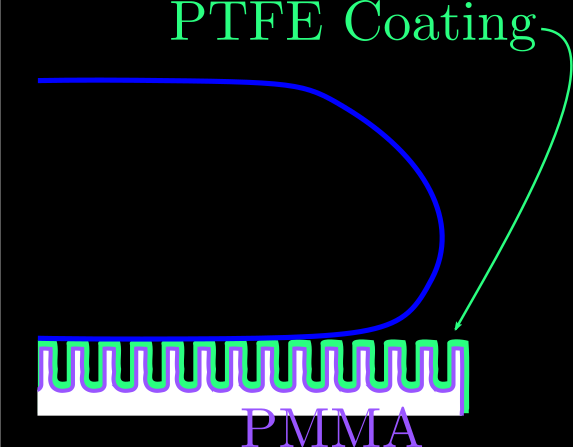
\includegraphics[width=0.75\textwidth]{../figures/schematic.pdf}
 \caption{A schematic representation of the droplet initial condition, resting on the superhydrophobic surface in the Cassie-Baxter state just prior to the drop tower experiment. The variables $q$, $\sigma$, and $V_d$ are the droplet net free charge, dielectric surface charge density, and droplet volume respectively.\label{fig:schematic}}
\end{figure}
\begin{figure}[ht]
 \centering
 \includegraphics[width=0.75\textwidth]{../figures/apparatus0.pdf}
 \caption{A schematic representation of a droplet electro-bounce experiment with labeled characteristic time and length scales, \hl{$t_c$, $y_c$} shown. Also shown are the dimensions of the superhydrophobic electret substrate.\label{fig:apparatus0}}
\end{figure}

\section{Experimental Methods}
The DDT uses a dual capsule design, inspired by the 2.2 s facility at NASA Glenn Research Center, which decouples drag acceleration felt by the external drag shield from the experiment. The experiment then experiences approximately $1 \times 10^{-6}$g of high quality free-fall for the 2.1s required for the rig/drag shield assembly to plummet to the bottom of drop tower 6 floors below. Single droplets of distilled water, in a range of volumes ($0.01 \leq R_d \leq 0.5$ mL), were very carefully deposited on the charged superhydrophobic surface using an grounded glass syringe with $\pm $1 $\mu$L accuracy, and then dropped in the drop tower. Red dye was added to improve thresholding accuracy in trajectory digitization. Droplet trajectories were recorded using a \emph{Panasonic} HC-WX970 Camera, at 120 fps and and 1/3000s shutter speed. In a few cases where higher frame rates were needed a \emph{Nikon} 1 J1 camera with a 30mm telephoto lens was used, shooting at 400 fps. The experimental test cell was illuminated with a 6000K LED strip, with a thin semi-opaque plastic film covering to make the light diffuse.  

Rather than haphazardly contact charge the surfaces with streams of water, as likely happened by accident in the experiments which inspired this inquiry, we strive for a more controlled, uniform surface charge distribution. Following from this desire, superhydrophobic electrets were prepared, with surface potentials $\varphi_s = 0.7$-$4.0$ kV. According to a review by Sessler \cite{_electrets_????}, an electret is a dielectric material with ``quasi-permanent'' electric charge in the sense that the characteristic decay period of the electret is much greater than a practical experiment time scale. Electret charge may be `true' charge in the form of surface or space charges, or polarization charges (such as bound charges). If the electret is not screened by a conductor then it produces an external electric field if the polarization and real charges do not uniformly compate each other throughout the volume of the electret. For this reason electrets are thought of as electrostatic analogs to permanent magnets (and the name \emph{electret} itself is a portmantau to that effect conjured by Heaviside in 1892 \cite{heaviside_electrical_2011}). Typical commerical electrets are Teflon type (PTFE) polymer films on the order of 10-50 $\mu$m thick with the charge being primarily real surface charge. Electrets have a plethora of applications, but most germanely they have been used in Electro-Wetting On Dielectric (EWOD) devices for low-voltage manipulation of small droplets \cite{wu_low-voltage_2010}. Real charge electrets can be produced by contact electrification, injection or deposition) of charge carriers by discharge or electron beam, ionizing radiation, or by frictional triboelectrification. Dipolar electrets by contrast are produced by a combination of polarization at elevated temperatures in a strong external electric field, followed by an annealing process. Effective surface charge densities are limited to the material dielectric strengths due to internal dielectric breakdown phenomenon (this typically occurs before external breakdown or Paschen breakdown). 

We use an isothermal electret formation process using a variation of the widely applied corona-charging technique. The typical corona-charging technique uses strong inhomogenous DC electric fields to produce discharge in air at ambient conditions; the dielectric substrate is atop a grounded electrode, and there is a screening potential electrode intermediately positioned to control the surface potential (the the surface potential of the dielectric will tend to saturate at this grid potential if the material is not space-charge current limited). The corona field is usually produced by pin-shaped electrode. In air the most common charge carriers thus produced are $\mbox{CO}_3^-$ ions. This approach is known to generally produce samples with fairly uniform surface charge densities. Some work by van Turnhout in 1975 showed, using Thermally Stimulated Current (TCS) measurements, that in 4.8 mm thick polymethyl methacrylate (PMMA) polarization of the dielectric is non-uniform, due to real space-charge mostly ($\sim$90\%) residing in a thin (0.1-0.2 mm) layer near the free-surface of the sample \cite{van_turnhout_thermally_1975}. In this work we use a balanced AC corona ion source (Ptec IN5120), to direct a net neutral stream of ions towards the dielectric target, which we polarize by an electrode with a $2$ kV$+$ (absolute reference) DC-DC converter. The ion stream compensates the surface and space bound charges arising due to the polarization of the dielectric. When the DC-DC converter is switched to ground, the deposited negative ions remain on the surface. 

The electret is lamina of 3-4 0.4 mm thick corona charged PMMA sheets. The electric field strength scales with the number of dielectric lamina as has also been shown in work on electret based vibrational energy harvesters \cite{wada_stacking_2012} and in water desalinization \cite{ni_desalination_2005}. 

The final, superhydropobic layer, is produced by laser etching PMMA, and depositing a thin layer of PTFE on the resulting roughness topology to increase the Young's angle. The surface charge density can be modulated during the experiment using the high-voltage DC-DC converter, which can re-polarize the dielectric substrate by means of an embedded electrode, and the resulting bound charge partially or fully neutralizes the electric field due to the surface ions deposited by corona charging of the electret. The high-voltage system is armed manually before the drop and is automatically safed by a high-voltage power switching relay, which switches the load across a 100 k$\Omega$ resistor when triggered by the resumption of 1-g conditions. The safing is set by an accelerometer pin-interrupt triggered microcontroller command. The rig with a mounted experiment is shown in Figure \ref{fig:rig}. 
\begin{figure}
    \centering
    \def\svgwidth{\columnwidth}
    \input{../figures/rig.pdf_tex}
    \caption{The droplet electro-bounce experiment hardware mounted on a drop tower rig.\label{fig:rig}}
\end{figure}

Contact angles of distilled water on the electret $\sim 150^{\circ}$. The hysteresis of the contact angle (the difference between the advancing and receding contact angles) is estimated from the roll-off angle using the method of Furmidge, 1962 \cite{furmidge_studies_1962}, and is found to be approximately $20^{\circ}$ when the surface is uncharged. The innate Young's angle hydrophobicity of the PTFE layer is enhanced by the underlying roughness length scales of the surface. We use a laser-etched pillared geometry with pillar heights $\sim 775$ $\mu$m, widths $\sim 70$ $\mu$m and pitch $\sim 100$ $\mu$m. An SEM image of the pillar geometry is shown in Figure \ref{fig:SEM}.
\begin{figure}
    \centering
    %% Creator: Matplotlib, PGF backend
%%
%% To include the figure in your LaTeX document, write
%%   \input{<filename>.pgf}
%%
%% Make sure the required packages are loaded in your preamble
%%   \usepackage{pgf}
%%
%% Figures using additional raster images can only be included by \input if
%% they are in the same directory as the main LaTeX file. For loading figures
%% from other directories you can use the `import` package
%%   \usepackage{import}
%% and then include the figures with
%%   \import{<path to file>}{<filename>.pgf}
%%
%% Matplotlib used the following preamble
%%   \usepackage{fontspec}
%%   \setmainfont{DejaVuSerif.ttf}[Path=/home/erin/anaconda3/lib/python3.6/site-packages/matplotlib/mpl-data/fonts/ttf/]
%%   \setsansfont{DejaVuSans.ttf}[Path=/home/erin/anaconda3/lib/python3.6/site-packages/matplotlib/mpl-data/fonts/ttf/]
%%   \setmonofont{DejaVuSansMono.ttf}[Path=/home/erin/anaconda3/lib/python3.6/site-packages/matplotlib/mpl-data/fonts/ttf/]
%%
\begingroup%
\makeatletter%
\begin{pgfpicture}%
\pgfpathrectangle{\pgfpointorigin}{\pgfqpoint{5.435744in}{3.749134in}}%
\pgfusepath{use as bounding box, clip}%
\begin{pgfscope}%
\pgfsetbuttcap%
\pgfsetmiterjoin%
\definecolor{currentfill}{rgb}{1.000000,1.000000,1.000000}%
\pgfsetfillcolor{currentfill}%
\pgfsetlinewidth{0.000000pt}%
\definecolor{currentstroke}{rgb}{1.000000,1.000000,1.000000}%
\pgfsetstrokecolor{currentstroke}%
\pgfsetdash{}{0pt}%
\pgfpathmoveto{\pgfqpoint{0.000000in}{0.000000in}}%
\pgfpathlineto{\pgfqpoint{5.435744in}{0.000000in}}%
\pgfpathlineto{\pgfqpoint{5.435744in}{3.749134in}}%
\pgfpathlineto{\pgfqpoint{0.000000in}{3.749134in}}%
\pgfpathclose%
\pgfusepath{fill}%
\end{pgfscope}%
\begin{pgfscope}%
\pgfsetbuttcap%
\pgfsetmiterjoin%
\definecolor{currentfill}{rgb}{1.000000,1.000000,1.000000}%
\pgfsetfillcolor{currentfill}%
\pgfsetlinewidth{0.000000pt}%
\definecolor{currentstroke}{rgb}{0.000000,0.000000,0.000000}%
\pgfsetstrokecolor{currentstroke}%
\pgfsetstrokeopacity{0.000000}%
\pgfsetdash{}{0pt}%
\pgfpathmoveto{\pgfqpoint{0.538871in}{0.629134in}}%
\pgfpathlineto{\pgfqpoint{5.188871in}{0.629134in}}%
\pgfpathlineto{\pgfqpoint{5.188871in}{3.649134in}}%
\pgfpathlineto{\pgfqpoint{0.538871in}{3.649134in}}%
\pgfpathclose%
\pgfusepath{fill}%
\end{pgfscope}%
\begin{pgfscope}%
\pgfpathrectangle{\pgfqpoint{0.538871in}{0.629134in}}{\pgfqpoint{4.650000in}{3.020000in}}%
\pgfusepath{clip}%
\pgfsetrectcap%
\pgfsetroundjoin%
\pgfsetlinewidth{1.505625pt}%
\definecolor{currentstroke}{rgb}{1.000000,0.000000,1.000000}%
\pgfsetstrokecolor{currentstroke}%
\pgfsetdash{}{0pt}%
\pgfpathmoveto{\pgfqpoint{0.535538in}{1.192634in}}%
\pgfpathlineto{\pgfqpoint{0.544090in}{1.192036in}}%
\pgfpathlineto{\pgfqpoint{0.596279in}{1.188353in}}%
\pgfpathlineto{\pgfqpoint{0.648467in}{1.184635in}}%
\pgfpathlineto{\pgfqpoint{0.700656in}{1.180883in}}%
\pgfpathlineto{\pgfqpoint{0.752844in}{1.177096in}}%
\pgfpathlineto{\pgfqpoint{0.805033in}{1.173276in}}%
\pgfpathlineto{\pgfqpoint{0.857221in}{1.169422in}}%
\pgfpathlineto{\pgfqpoint{0.909410in}{1.165534in}}%
\pgfpathlineto{\pgfqpoint{0.961599in}{1.161614in}}%
\pgfpathlineto{\pgfqpoint{1.013787in}{1.157660in}}%
\pgfpathlineto{\pgfqpoint{1.065976in}{1.153675in}}%
\pgfpathlineto{\pgfqpoint{1.118164in}{1.149657in}}%
\pgfpathlineto{\pgfqpoint{1.170353in}{1.145608in}}%
\pgfpathlineto{\pgfqpoint{1.222541in}{1.141527in}}%
\pgfpathlineto{\pgfqpoint{1.274730in}{1.137415in}}%
\pgfpathlineto{\pgfqpoint{1.326918in}{1.133272in}}%
\pgfpathlineto{\pgfqpoint{1.379107in}{1.129099in}}%
\pgfpathlineto{\pgfqpoint{1.431295in}{1.124896in}}%
\pgfpathlineto{\pgfqpoint{1.483484in}{1.120663in}}%
\pgfpathlineto{\pgfqpoint{1.535673in}{1.116400in}}%
\pgfpathlineto{\pgfqpoint{1.587861in}{1.112108in}}%
\pgfpathlineto{\pgfqpoint{1.640050in}{1.107787in}}%
\pgfpathlineto{\pgfqpoint{1.692238in}{1.103438in}}%
\pgfpathlineto{\pgfqpoint{1.744427in}{1.099061in}}%
\pgfpathlineto{\pgfqpoint{1.796615in}{1.094656in}}%
\pgfpathlineto{\pgfqpoint{1.848804in}{1.090223in}}%
\pgfpathlineto{\pgfqpoint{1.900992in}{1.085763in}}%
\pgfpathlineto{\pgfqpoint{1.953181in}{1.081277in}}%
\pgfpathlineto{\pgfqpoint{2.005370in}{1.076764in}}%
\pgfpathlineto{\pgfqpoint{2.057558in}{1.072225in}}%
\pgfpathlineto{\pgfqpoint{2.109747in}{1.067660in}}%
\pgfpathlineto{\pgfqpoint{2.161935in}{1.063070in}}%
\pgfpathlineto{\pgfqpoint{2.214124in}{1.058455in}}%
\pgfpathlineto{\pgfqpoint{2.266312in}{1.053815in}}%
\pgfpathlineto{\pgfqpoint{2.318501in}{1.049151in}}%
\pgfpathlineto{\pgfqpoint{2.370689in}{1.044463in}}%
\pgfpathlineto{\pgfqpoint{2.422878in}{1.039751in}}%
\pgfpathlineto{\pgfqpoint{2.475067in}{1.035017in}}%
\pgfpathlineto{\pgfqpoint{2.527255in}{1.030259in}}%
\pgfpathlineto{\pgfqpoint{2.579444in}{1.025479in}}%
\pgfpathlineto{\pgfqpoint{2.631632in}{1.020677in}}%
\pgfpathlineto{\pgfqpoint{2.683821in}{1.015853in}}%
\pgfpathlineto{\pgfqpoint{2.736009in}{1.011008in}}%
\pgfpathlineto{\pgfqpoint{2.788198in}{1.006142in}}%
\pgfpathlineto{\pgfqpoint{2.840386in}{1.001255in}}%
\pgfpathlineto{\pgfqpoint{2.892575in}{0.996348in}}%
\pgfpathlineto{\pgfqpoint{2.944764in}{0.991421in}}%
\pgfpathlineto{\pgfqpoint{2.996952in}{0.986475in}}%
\pgfpathlineto{\pgfqpoint{3.049141in}{0.981510in}}%
\pgfpathlineto{\pgfqpoint{3.101329in}{0.976526in}}%
\pgfpathlineto{\pgfqpoint{3.153518in}{0.971523in}}%
\pgfpathlineto{\pgfqpoint{3.205706in}{0.966503in}}%
\pgfpathlineto{\pgfqpoint{3.257895in}{0.961466in}}%
\pgfpathlineto{\pgfqpoint{3.310083in}{0.956411in}}%
\pgfpathlineto{\pgfqpoint{3.362272in}{0.951339in}}%
\pgfpathlineto{\pgfqpoint{3.414460in}{0.946251in}}%
\pgfpathlineto{\pgfqpoint{3.466649in}{0.941147in}}%
\pgfpathlineto{\pgfqpoint{3.518838in}{0.936028in}}%
\pgfpathlineto{\pgfqpoint{3.571026in}{0.930893in}}%
\pgfpathlineto{\pgfqpoint{3.623215in}{0.925744in}}%
\pgfpathlineto{\pgfqpoint{3.675403in}{0.920580in}}%
\pgfpathlineto{\pgfqpoint{3.727592in}{0.915403in}}%
\pgfpathlineto{\pgfqpoint{3.779780in}{0.910211in}}%
\pgfpathlineto{\pgfqpoint{3.831969in}{0.905007in}}%
\pgfpathlineto{\pgfqpoint{3.884157in}{0.899790in}}%
\pgfpathlineto{\pgfqpoint{3.936346in}{0.894560in}}%
\pgfpathlineto{\pgfqpoint{3.988535in}{0.889319in}}%
\pgfpathlineto{\pgfqpoint{4.040723in}{0.884066in}}%
\pgfpathlineto{\pgfqpoint{4.092912in}{0.878802in}}%
\pgfpathlineto{\pgfqpoint{4.145100in}{0.873527in}}%
\pgfpathlineto{\pgfqpoint{4.197289in}{0.868242in}}%
\pgfpathlineto{\pgfqpoint{4.249477in}{0.862947in}}%
\pgfpathlineto{\pgfqpoint{4.301666in}{0.857642in}}%
\pgfpathlineto{\pgfqpoint{4.353854in}{0.852328in}}%
\pgfpathlineto{\pgfqpoint{4.406043in}{0.847006in}}%
\pgfpathlineto{\pgfqpoint{4.458232in}{0.841675in}}%
\pgfpathlineto{\pgfqpoint{4.510420in}{0.836336in}}%
\pgfpathlineto{\pgfqpoint{4.562609in}{0.830990in}}%
\pgfpathlineto{\pgfqpoint{4.614797in}{0.825637in}}%
\pgfpathlineto{\pgfqpoint{4.666986in}{0.820278in}}%
\pgfpathlineto{\pgfqpoint{4.719174in}{0.814912in}}%
\pgfpathlineto{\pgfqpoint{4.771363in}{0.809540in}}%
\pgfpathlineto{\pgfqpoint{4.823551in}{0.804163in}}%
\pgfpathlineto{\pgfqpoint{4.875740in}{0.798781in}}%
\pgfpathlineto{\pgfqpoint{4.927928in}{0.793394in}}%
\pgfpathlineto{\pgfqpoint{4.980117in}{0.788003in}}%
\pgfpathlineto{\pgfqpoint{5.032306in}{0.782609in}}%
\pgfpathlineto{\pgfqpoint{5.084494in}{0.777211in}}%
\pgfpathlineto{\pgfqpoint{5.136683in}{0.771810in}}%
\pgfpathlineto{\pgfqpoint{5.188871in}{0.766407in}}%
\pgfusepath{stroke}%
\end{pgfscope}%
\begin{pgfscope}%
\pgfpathrectangle{\pgfqpoint{0.538871in}{0.629134in}}{\pgfqpoint{4.650000in}{3.020000in}}%
\pgfusepath{clip}%
\pgfsetrectcap%
\pgfsetroundjoin%
\pgfsetlinewidth{1.505625pt}%
\definecolor{currentstroke}{rgb}{0.749020,0.250980,1.000000}%
\pgfsetstrokecolor{currentstroke}%
\pgfsetdash{}{0pt}%
\pgfpathmoveto{\pgfqpoint{0.535538in}{1.682212in}}%
\pgfpathlineto{\pgfqpoint{0.544090in}{1.681068in}}%
\pgfpathlineto{\pgfqpoint{0.596279in}{1.674014in}}%
\pgfpathlineto{\pgfqpoint{0.648467in}{1.666888in}}%
\pgfpathlineto{\pgfqpoint{0.700656in}{1.659690in}}%
\pgfpathlineto{\pgfqpoint{0.752844in}{1.652422in}}%
\pgfpathlineto{\pgfqpoint{0.805033in}{1.645083in}}%
\pgfpathlineto{\pgfqpoint{0.857221in}{1.637675in}}%
\pgfpathlineto{\pgfqpoint{0.909410in}{1.630197in}}%
\pgfpathlineto{\pgfqpoint{0.961599in}{1.622651in}}%
\pgfpathlineto{\pgfqpoint{1.013787in}{1.615037in}}%
\pgfpathlineto{\pgfqpoint{1.065976in}{1.607355in}}%
\pgfpathlineto{\pgfqpoint{1.118164in}{1.599607in}}%
\pgfpathlineto{\pgfqpoint{1.170353in}{1.591793in}}%
\pgfpathlineto{\pgfqpoint{1.222541in}{1.583913in}}%
\pgfpathlineto{\pgfqpoint{1.274730in}{1.575968in}}%
\pgfpathlineto{\pgfqpoint{1.326918in}{1.567960in}}%
\pgfpathlineto{\pgfqpoint{1.379107in}{1.559887in}}%
\pgfpathlineto{\pgfqpoint{1.431295in}{1.551752in}}%
\pgfpathlineto{\pgfqpoint{1.483484in}{1.543554in}}%
\pgfpathlineto{\pgfqpoint{1.535673in}{1.535295in}}%
\pgfpathlineto{\pgfqpoint{1.587861in}{1.526975in}}%
\pgfpathlineto{\pgfqpoint{1.640050in}{1.518594in}}%
\pgfpathlineto{\pgfqpoint{1.692238in}{1.510154in}}%
\pgfpathlineto{\pgfqpoint{1.744427in}{1.501655in}}%
\pgfpathlineto{\pgfqpoint{1.796615in}{1.493097in}}%
\pgfpathlineto{\pgfqpoint{1.848804in}{1.484482in}}%
\pgfpathlineto{\pgfqpoint{1.900992in}{1.475810in}}%
\pgfpathlineto{\pgfqpoint{1.953181in}{1.467082in}}%
\pgfpathlineto{\pgfqpoint{2.005370in}{1.458298in}}%
\pgfpathlineto{\pgfqpoint{2.057558in}{1.449459in}}%
\pgfpathlineto{\pgfqpoint{2.109747in}{1.440566in}}%
\pgfpathlineto{\pgfqpoint{2.161935in}{1.431619in}}%
\pgfpathlineto{\pgfqpoint{2.214124in}{1.422620in}}%
\pgfpathlineto{\pgfqpoint{2.266312in}{1.413568in}}%
\pgfpathlineto{\pgfqpoint{2.318501in}{1.404466in}}%
\pgfpathlineto{\pgfqpoint{2.370689in}{1.395312in}}%
\pgfpathlineto{\pgfqpoint{2.422878in}{1.386108in}}%
\pgfpathlineto{\pgfqpoint{2.475067in}{1.376856in}}%
\pgfpathlineto{\pgfqpoint{2.527255in}{1.367554in}}%
\pgfpathlineto{\pgfqpoint{2.579444in}{1.358205in}}%
\pgfpathlineto{\pgfqpoint{2.631632in}{1.348809in}}%
\pgfpathlineto{\pgfqpoint{2.683821in}{1.339366in}}%
\pgfpathlineto{\pgfqpoint{2.736009in}{1.329878in}}%
\pgfpathlineto{\pgfqpoint{2.788198in}{1.320345in}}%
\pgfpathlineto{\pgfqpoint{2.840386in}{1.310767in}}%
\pgfpathlineto{\pgfqpoint{2.892575in}{1.301147in}}%
\pgfpathlineto{\pgfqpoint{2.944764in}{1.291483in}}%
\pgfpathlineto{\pgfqpoint{2.996952in}{1.281778in}}%
\pgfpathlineto{\pgfqpoint{3.049141in}{1.272032in}}%
\pgfpathlineto{\pgfqpoint{3.101329in}{1.262245in}}%
\pgfpathlineto{\pgfqpoint{3.153518in}{1.252418in}}%
\pgfpathlineto{\pgfqpoint{3.205706in}{1.242553in}}%
\pgfpathlineto{\pgfqpoint{3.257895in}{1.232649in}}%
\pgfpathlineto{\pgfqpoint{3.310083in}{1.222708in}}%
\pgfpathlineto{\pgfqpoint{3.362272in}{1.212731in}}%
\pgfpathlineto{\pgfqpoint{3.414460in}{1.202717in}}%
\pgfpathlineto{\pgfqpoint{3.466649in}{1.192669in}}%
\pgfpathlineto{\pgfqpoint{3.518838in}{1.182586in}}%
\pgfpathlineto{\pgfqpoint{3.571026in}{1.172469in}}%
\pgfpathlineto{\pgfqpoint{3.623215in}{1.162320in}}%
\pgfpathlineto{\pgfqpoint{3.675403in}{1.152139in}}%
\pgfpathlineto{\pgfqpoint{3.727592in}{1.141927in}}%
\pgfpathlineto{\pgfqpoint{3.779780in}{1.131684in}}%
\pgfpathlineto{\pgfqpoint{3.831969in}{1.121411in}}%
\pgfpathlineto{\pgfqpoint{3.884157in}{1.111110in}}%
\pgfpathlineto{\pgfqpoint{3.936346in}{1.100780in}}%
\pgfpathlineto{\pgfqpoint{3.988535in}{1.090424in}}%
\pgfpathlineto{\pgfqpoint{4.040723in}{1.080040in}}%
\pgfpathlineto{\pgfqpoint{4.092912in}{1.069631in}}%
\pgfpathlineto{\pgfqpoint{4.145100in}{1.059197in}}%
\pgfpathlineto{\pgfqpoint{4.197289in}{1.048739in}}%
\pgfpathlineto{\pgfqpoint{4.249477in}{1.038258in}}%
\pgfpathlineto{\pgfqpoint{4.301666in}{1.027754in}}%
\pgfpathlineto{\pgfqpoint{4.353854in}{1.017228in}}%
\pgfpathlineto{\pgfqpoint{4.406043in}{1.006681in}}%
\pgfpathlineto{\pgfqpoint{4.458232in}{0.996114in}}%
\pgfpathlineto{\pgfqpoint{4.510420in}{0.985528in}}%
\pgfpathlineto{\pgfqpoint{4.562609in}{0.974923in}}%
\pgfpathlineto{\pgfqpoint{4.614797in}{0.964301in}}%
\pgfpathlineto{\pgfqpoint{4.666986in}{0.953661in}}%
\pgfpathlineto{\pgfqpoint{4.719174in}{0.943006in}}%
\pgfpathlineto{\pgfqpoint{4.771363in}{0.932335in}}%
\pgfpathlineto{\pgfqpoint{4.823551in}{0.921649in}}%
\pgfpathlineto{\pgfqpoint{4.875740in}{0.910950in}}%
\pgfpathlineto{\pgfqpoint{4.927928in}{0.900238in}}%
\pgfpathlineto{\pgfqpoint{4.980117in}{0.889514in}}%
\pgfpathlineto{\pgfqpoint{5.032306in}{0.878778in}}%
\pgfpathlineto{\pgfqpoint{5.084494in}{0.868032in}}%
\pgfpathlineto{\pgfqpoint{5.136683in}{0.857277in}}%
\pgfpathlineto{\pgfqpoint{5.188871in}{0.846512in}}%
\pgfusepath{stroke}%
\end{pgfscope}%
\begin{pgfscope}%
\pgfpathrectangle{\pgfqpoint{0.538871in}{0.629134in}}{\pgfqpoint{4.650000in}{3.020000in}}%
\pgfusepath{clip}%
\pgfsetrectcap%
\pgfsetroundjoin%
\pgfsetlinewidth{1.505625pt}%
\definecolor{currentstroke}{rgb}{0.498039,0.501961,1.000000}%
\pgfsetstrokecolor{currentstroke}%
\pgfsetdash{}{0pt}%
\pgfpathmoveto{\pgfqpoint{0.535538in}{2.207784in}}%
\pgfpathlineto{\pgfqpoint{0.544090in}{2.206141in}}%
\pgfpathlineto{\pgfqpoint{0.596279in}{2.196001in}}%
\pgfpathlineto{\pgfqpoint{0.648467in}{2.185749in}}%
\pgfpathlineto{\pgfqpoint{0.700656in}{2.175387in}}%
\pgfpathlineto{\pgfqpoint{0.752844in}{2.164915in}}%
\pgfpathlineto{\pgfqpoint{0.805033in}{2.154333in}}%
\pgfpathlineto{\pgfqpoint{0.857221in}{2.143643in}}%
\pgfpathlineto{\pgfqpoint{0.909410in}{2.132847in}}%
\pgfpathlineto{\pgfqpoint{0.961599in}{2.121943in}}%
\pgfpathlineto{\pgfqpoint{1.013787in}{2.110935in}}%
\pgfpathlineto{\pgfqpoint{1.065976in}{2.099822in}}%
\pgfpathlineto{\pgfqpoint{1.118164in}{2.088605in}}%
\pgfpathlineto{\pgfqpoint{1.170353in}{2.077286in}}%
\pgfpathlineto{\pgfqpoint{1.222541in}{2.065865in}}%
\pgfpathlineto{\pgfqpoint{1.274730in}{2.054343in}}%
\pgfpathlineto{\pgfqpoint{1.326918in}{2.042722in}}%
\pgfpathlineto{\pgfqpoint{1.379107in}{2.031002in}}%
\pgfpathlineto{\pgfqpoint{1.431295in}{2.019184in}}%
\pgfpathlineto{\pgfqpoint{1.483484in}{2.007269in}}%
\pgfpathlineto{\pgfqpoint{1.535673in}{1.995258in}}%
\pgfpathlineto{\pgfqpoint{1.587861in}{1.983153in}}%
\pgfpathlineto{\pgfqpoint{1.640050in}{1.970953in}}%
\pgfpathlineto{\pgfqpoint{1.692238in}{1.958661in}}%
\pgfpathlineto{\pgfqpoint{1.744427in}{1.946276in}}%
\pgfpathlineto{\pgfqpoint{1.796615in}{1.933801in}}%
\pgfpathlineto{\pgfqpoint{1.848804in}{1.921236in}}%
\pgfpathlineto{\pgfqpoint{1.900992in}{1.908582in}}%
\pgfpathlineto{\pgfqpoint{1.953181in}{1.895840in}}%
\pgfpathlineto{\pgfqpoint{2.005370in}{1.883012in}}%
\pgfpathlineto{\pgfqpoint{2.057558in}{1.870098in}}%
\pgfpathlineto{\pgfqpoint{2.109747in}{1.857099in}}%
\pgfpathlineto{\pgfqpoint{2.161935in}{1.844016in}}%
\pgfpathlineto{\pgfqpoint{2.214124in}{1.830851in}}%
\pgfpathlineto{\pgfqpoint{2.266312in}{1.817604in}}%
\pgfpathlineto{\pgfqpoint{2.318501in}{1.804276in}}%
\pgfpathlineto{\pgfqpoint{2.370689in}{1.790869in}}%
\pgfpathlineto{\pgfqpoint{2.422878in}{1.777384in}}%
\pgfpathlineto{\pgfqpoint{2.475067in}{1.763821in}}%
\pgfpathlineto{\pgfqpoint{2.527255in}{1.750182in}}%
\pgfpathlineto{\pgfqpoint{2.579444in}{1.736468in}}%
\pgfpathlineto{\pgfqpoint{2.631632in}{1.722679in}}%
\pgfpathlineto{\pgfqpoint{2.683821in}{1.708818in}}%
\pgfpathlineto{\pgfqpoint{2.736009in}{1.694884in}}%
\pgfpathlineto{\pgfqpoint{2.788198in}{1.680880in}}%
\pgfpathlineto{\pgfqpoint{2.840386in}{1.666806in}}%
\pgfpathlineto{\pgfqpoint{2.892575in}{1.652663in}}%
\pgfpathlineto{\pgfqpoint{2.944764in}{1.638452in}}%
\pgfpathlineto{\pgfqpoint{2.996952in}{1.624175in}}%
\pgfpathlineto{\pgfqpoint{3.049141in}{1.609833in}}%
\pgfpathlineto{\pgfqpoint{3.101329in}{1.595426in}}%
\pgfpathlineto{\pgfqpoint{3.153518in}{1.580956in}}%
\pgfpathlineto{\pgfqpoint{3.205706in}{1.566424in}}%
\pgfpathlineto{\pgfqpoint{3.257895in}{1.551831in}}%
\pgfpathlineto{\pgfqpoint{3.310083in}{1.537179in}}%
\pgfpathlineto{\pgfqpoint{3.362272in}{1.522467in}}%
\pgfpathlineto{\pgfqpoint{3.414460in}{1.507698in}}%
\pgfpathlineto{\pgfqpoint{3.466649in}{1.492872in}}%
\pgfpathlineto{\pgfqpoint{3.518838in}{1.477991in}}%
\pgfpathlineto{\pgfqpoint{3.571026in}{1.463055in}}%
\pgfpathlineto{\pgfqpoint{3.623215in}{1.448067in}}%
\pgfpathlineto{\pgfqpoint{3.675403in}{1.433026in}}%
\pgfpathlineto{\pgfqpoint{3.727592in}{1.417935in}}%
\pgfpathlineto{\pgfqpoint{3.779780in}{1.402794in}}%
\pgfpathlineto{\pgfqpoint{3.831969in}{1.387604in}}%
\pgfpathlineto{\pgfqpoint{3.884157in}{1.372367in}}%
\pgfpathlineto{\pgfqpoint{3.936346in}{1.357084in}}%
\pgfpathlineto{\pgfqpoint{3.988535in}{1.341755in}}%
\pgfpathlineto{\pgfqpoint{4.040723in}{1.326383in}}%
\pgfpathlineto{\pgfqpoint{4.092912in}{1.310967in}}%
\pgfpathlineto{\pgfqpoint{4.145100in}{1.295510in}}%
\pgfpathlineto{\pgfqpoint{4.197289in}{1.280012in}}%
\pgfpathlineto{\pgfqpoint{4.249477in}{1.264475in}}%
\pgfpathlineto{\pgfqpoint{4.301666in}{1.248899in}}%
\pgfpathlineto{\pgfqpoint{4.353854in}{1.233287in}}%
\pgfpathlineto{\pgfqpoint{4.406043in}{1.217638in}}%
\pgfpathlineto{\pgfqpoint{4.458232in}{1.201955in}}%
\pgfpathlineto{\pgfqpoint{4.510420in}{1.186237in}}%
\pgfpathlineto{\pgfqpoint{4.562609in}{1.170488in}}%
\pgfpathlineto{\pgfqpoint{4.614797in}{1.154707in}}%
\pgfpathlineto{\pgfqpoint{4.666986in}{1.138896in}}%
\pgfpathlineto{\pgfqpoint{4.719174in}{1.123055in}}%
\pgfpathlineto{\pgfqpoint{4.771363in}{1.107187in}}%
\pgfpathlineto{\pgfqpoint{4.823551in}{1.091293in}}%
\pgfpathlineto{\pgfqpoint{4.875740in}{1.075372in}}%
\pgfpathlineto{\pgfqpoint{4.927928in}{1.059427in}}%
\pgfpathlineto{\pgfqpoint{4.980117in}{1.043459in}}%
\pgfpathlineto{\pgfqpoint{5.032306in}{1.027469in}}%
\pgfpathlineto{\pgfqpoint{5.084494in}{1.011459in}}%
\pgfpathlineto{\pgfqpoint{5.136683in}{0.995428in}}%
\pgfpathlineto{\pgfqpoint{5.188871in}{0.979379in}}%
\pgfusepath{stroke}%
\end{pgfscope}%
\begin{pgfscope}%
\pgfpathrectangle{\pgfqpoint{0.538871in}{0.629134in}}{\pgfqpoint{4.650000in}{3.020000in}}%
\pgfusepath{clip}%
\pgfsetrectcap%
\pgfsetroundjoin%
\pgfsetlinewidth{1.505625pt}%
\definecolor{currentstroke}{rgb}{0.247059,0.752941,1.000000}%
\pgfsetstrokecolor{currentstroke}%
\pgfsetdash{}{0pt}%
\pgfpathmoveto{\pgfqpoint{0.535538in}{2.769708in}}%
\pgfpathlineto{\pgfqpoint{0.544090in}{2.767606in}}%
\pgfpathlineto{\pgfqpoint{0.596279in}{2.754629in}}%
\pgfpathlineto{\pgfqpoint{0.648467in}{2.741498in}}%
\pgfpathlineto{\pgfqpoint{0.700656in}{2.728215in}}%
\pgfpathlineto{\pgfqpoint{0.752844in}{2.714779in}}%
\pgfpathlineto{\pgfqpoint{0.805033in}{2.701194in}}%
\pgfpathlineto{\pgfqpoint{0.857221in}{2.687460in}}%
\pgfpathlineto{\pgfqpoint{0.909410in}{2.673578in}}%
\pgfpathlineto{\pgfqpoint{0.961599in}{2.659550in}}%
\pgfpathlineto{\pgfqpoint{1.013787in}{2.645377in}}%
\pgfpathlineto{\pgfqpoint{1.065976in}{2.631060in}}%
\pgfpathlineto{\pgfqpoint{1.118164in}{2.616600in}}%
\pgfpathlineto{\pgfqpoint{1.170353in}{2.602000in}}%
\pgfpathlineto{\pgfqpoint{1.222541in}{2.587259in}}%
\pgfpathlineto{\pgfqpoint{1.274730in}{2.572380in}}%
\pgfpathlineto{\pgfqpoint{1.326918in}{2.557364in}}%
\pgfpathlineto{\pgfqpoint{1.379107in}{2.542211in}}%
\pgfpathlineto{\pgfqpoint{1.431295in}{2.526924in}}%
\pgfpathlineto{\pgfqpoint{1.483484in}{2.511504in}}%
\pgfpathlineto{\pgfqpoint{1.535673in}{2.495952in}}%
\pgfpathlineto{\pgfqpoint{1.587861in}{2.480270in}}%
\pgfpathlineto{\pgfqpoint{1.640050in}{2.464458in}}%
\pgfpathlineto{\pgfqpoint{1.692238in}{2.448518in}}%
\pgfpathlineto{\pgfqpoint{1.744427in}{2.432452in}}%
\pgfpathlineto{\pgfqpoint{1.796615in}{2.416261in}}%
\pgfpathlineto{\pgfqpoint{1.848804in}{2.399947in}}%
\pgfpathlineto{\pgfqpoint{1.900992in}{2.383510in}}%
\pgfpathlineto{\pgfqpoint{1.953181in}{2.366952in}}%
\pgfpathlineto{\pgfqpoint{2.005370in}{2.350274in}}%
\pgfpathlineto{\pgfqpoint{2.057558in}{2.333479in}}%
\pgfpathlineto{\pgfqpoint{2.109747in}{2.316567in}}%
\pgfpathlineto{\pgfqpoint{2.161935in}{2.299539in}}%
\pgfpathlineto{\pgfqpoint{2.214124in}{2.282398in}}%
\pgfpathlineto{\pgfqpoint{2.266312in}{2.265144in}}%
\pgfpathlineto{\pgfqpoint{2.318501in}{2.247779in}}%
\pgfpathlineto{\pgfqpoint{2.370689in}{2.230305in}}%
\pgfpathlineto{\pgfqpoint{2.422878in}{2.212722in}}%
\pgfpathlineto{\pgfqpoint{2.475067in}{2.195032in}}%
\pgfpathlineto{\pgfqpoint{2.527255in}{2.177238in}}%
\pgfpathlineto{\pgfqpoint{2.579444in}{2.159339in}}%
\pgfpathlineto{\pgfqpoint{2.631632in}{2.141338in}}%
\pgfpathlineto{\pgfqpoint{2.683821in}{2.123236in}}%
\pgfpathlineto{\pgfqpoint{2.736009in}{2.105034in}}%
\pgfpathlineto{\pgfqpoint{2.788198in}{2.086734in}}%
\pgfpathlineto{\pgfqpoint{2.840386in}{2.068338in}}%
\pgfpathlineto{\pgfqpoint{2.892575in}{2.049846in}}%
\pgfpathlineto{\pgfqpoint{2.944764in}{2.031260in}}%
\pgfpathlineto{\pgfqpoint{2.996952in}{2.012582in}}%
\pgfpathlineto{\pgfqpoint{3.049141in}{1.993813in}}%
\pgfpathlineto{\pgfqpoint{3.101329in}{1.974955in}}%
\pgfpathlineto{\pgfqpoint{3.153518in}{1.956009in}}%
\pgfpathlineto{\pgfqpoint{3.205706in}{1.936976in}}%
\pgfpathlineto{\pgfqpoint{3.257895in}{1.917858in}}%
\pgfpathlineto{\pgfqpoint{3.310083in}{1.898657in}}%
\pgfpathlineto{\pgfqpoint{3.362272in}{1.879374in}}%
\pgfpathlineto{\pgfqpoint{3.414460in}{1.860009in}}%
\pgfpathlineto{\pgfqpoint{3.466649in}{1.840566in}}%
\pgfpathlineto{\pgfqpoint{3.518838in}{1.821045in}}%
\pgfpathlineto{\pgfqpoint{3.571026in}{1.801448in}}%
\pgfpathlineto{\pgfqpoint{3.623215in}{1.781775in}}%
\pgfpathlineto{\pgfqpoint{3.675403in}{1.762030in}}%
\pgfpathlineto{\pgfqpoint{3.727592in}{1.742212in}}%
\pgfpathlineto{\pgfqpoint{3.779780in}{1.722325in}}%
\pgfpathlineto{\pgfqpoint{3.831969in}{1.702368in}}%
\pgfpathlineto{\pgfqpoint{3.884157in}{1.682344in}}%
\pgfpathlineto{\pgfqpoint{3.936346in}{1.662254in}}%
\pgfpathlineto{\pgfqpoint{3.988535in}{1.642099in}}%
\pgfpathlineto{\pgfqpoint{4.040723in}{1.621882in}}%
\pgfpathlineto{\pgfqpoint{4.092912in}{1.601602in}}%
\pgfpathlineto{\pgfqpoint{4.145100in}{1.581263in}}%
\pgfpathlineto{\pgfqpoint{4.197289in}{1.560865in}}%
\pgfpathlineto{\pgfqpoint{4.249477in}{1.540410in}}%
\pgfpathlineto{\pgfqpoint{4.301666in}{1.519899in}}%
\pgfpathlineto{\pgfqpoint{4.353854in}{1.499334in}}%
\pgfpathlineto{\pgfqpoint{4.406043in}{1.478717in}}%
\pgfpathlineto{\pgfqpoint{4.458232in}{1.458048in}}%
\pgfpathlineto{\pgfqpoint{4.510420in}{1.437329in}}%
\pgfpathlineto{\pgfqpoint{4.562609in}{1.416562in}}%
\pgfpathlineto{\pgfqpoint{4.614797in}{1.395748in}}%
\pgfpathlineto{\pgfqpoint{4.666986in}{1.374889in}}%
\pgfpathlineto{\pgfqpoint{4.719174in}{1.353986in}}%
\pgfpathlineto{\pgfqpoint{4.771363in}{1.333041in}}%
\pgfpathlineto{\pgfqpoint{4.823551in}{1.312054in}}%
\pgfpathlineto{\pgfqpoint{4.875740in}{1.291028in}}%
\pgfpathlineto{\pgfqpoint{4.927928in}{1.269964in}}%
\pgfpathlineto{\pgfqpoint{4.980117in}{1.248864in}}%
\pgfpathlineto{\pgfqpoint{5.032306in}{1.227729in}}%
\pgfpathlineto{\pgfqpoint{5.084494in}{1.206560in}}%
\pgfpathlineto{\pgfqpoint{5.136683in}{1.185359in}}%
\pgfpathlineto{\pgfqpoint{5.188871in}{1.164127in}}%
\pgfusepath{stroke}%
\end{pgfscope}%
\begin{pgfscope}%
\pgfpathrectangle{\pgfqpoint{0.538871in}{0.629134in}}{\pgfqpoint{4.650000in}{3.020000in}}%
\pgfusepath{clip}%
\pgfsetrectcap%
\pgfsetroundjoin%
\pgfsetlinewidth{1.505625pt}%
\definecolor{currentstroke}{rgb}{0.000000,1.000000,1.000000}%
\pgfsetstrokecolor{currentstroke}%
\pgfsetdash{}{0pt}%
\pgfpathmoveto{\pgfqpoint{0.535538in}{3.369582in}}%
\pgfpathlineto{\pgfqpoint{0.544090in}{3.367056in}}%
\pgfpathlineto{\pgfqpoint{0.596279in}{3.351445in}}%
\pgfpathlineto{\pgfqpoint{0.648467in}{3.335634in}}%
\pgfpathlineto{\pgfqpoint{0.700656in}{3.319626in}}%
\pgfpathlineto{\pgfqpoint{0.752844in}{3.303422in}}%
\pgfpathlineto{\pgfqpoint{0.805033in}{3.287024in}}%
\pgfpathlineto{\pgfqpoint{0.857221in}{3.270433in}}%
\pgfpathlineto{\pgfqpoint{0.909410in}{3.253652in}}%
\pgfpathlineto{\pgfqpoint{0.961599in}{3.236682in}}%
\pgfpathlineto{\pgfqpoint{1.013787in}{3.219524in}}%
\pgfpathlineto{\pgfqpoint{1.065976in}{3.202181in}}%
\pgfpathlineto{\pgfqpoint{1.118164in}{3.184654in}}%
\pgfpathlineto{\pgfqpoint{1.170353in}{3.166945in}}%
\pgfpathlineto{\pgfqpoint{1.222541in}{3.149056in}}%
\pgfpathlineto{\pgfqpoint{1.274730in}{3.130989in}}%
\pgfpathlineto{\pgfqpoint{1.326918in}{3.112744in}}%
\pgfpathlineto{\pgfqpoint{1.379107in}{3.094325in}}%
\pgfpathlineto{\pgfqpoint{1.431295in}{3.075733in}}%
\pgfpathlineto{\pgfqpoint{1.483484in}{3.056969in}}%
\pgfpathlineto{\pgfqpoint{1.535673in}{3.038035in}}%
\pgfpathlineto{\pgfqpoint{1.587861in}{3.018934in}}%
\pgfpathlineto{\pgfqpoint{1.640050in}{2.999667in}}%
\pgfpathlineto{\pgfqpoint{1.692238in}{2.980235in}}%
\pgfpathlineto{\pgfqpoint{1.744427in}{2.960641in}}%
\pgfpathlineto{\pgfqpoint{1.796615in}{2.940887in}}%
\pgfpathlineto{\pgfqpoint{1.848804in}{2.920974in}}%
\pgfpathlineto{\pgfqpoint{1.900992in}{2.900903in}}%
\pgfpathlineto{\pgfqpoint{1.953181in}{2.880678in}}%
\pgfpathlineto{\pgfqpoint{2.005370in}{2.860300in}}%
\pgfpathlineto{\pgfqpoint{2.057558in}{2.839770in}}%
\pgfpathlineto{\pgfqpoint{2.109747in}{2.819090in}}%
\pgfpathlineto{\pgfqpoint{2.161935in}{2.798263in}}%
\pgfpathlineto{\pgfqpoint{2.214124in}{2.777289in}}%
\pgfpathlineto{\pgfqpoint{2.266312in}{2.756172in}}%
\pgfpathlineto{\pgfqpoint{2.318501in}{2.734912in}}%
\pgfpathlineto{\pgfqpoint{2.370689in}{2.713511in}}%
\pgfpathlineto{\pgfqpoint{2.422878in}{2.691972in}}%
\pgfpathlineto{\pgfqpoint{2.475067in}{2.670297in}}%
\pgfpathlineto{\pgfqpoint{2.527255in}{2.648486in}}%
\pgfpathlineto{\pgfqpoint{2.579444in}{2.626542in}}%
\pgfpathlineto{\pgfqpoint{2.631632in}{2.604467in}}%
\pgfpathlineto{\pgfqpoint{2.683821in}{2.582262in}}%
\pgfpathlineto{\pgfqpoint{2.736009in}{2.559930in}}%
\pgfpathlineto{\pgfqpoint{2.788198in}{2.537472in}}%
\pgfpathlineto{\pgfqpoint{2.840386in}{2.514890in}}%
\pgfpathlineto{\pgfqpoint{2.892575in}{2.492185in}}%
\pgfpathlineto{\pgfqpoint{2.944764in}{2.469361in}}%
\pgfpathlineto{\pgfqpoint{2.996952in}{2.446418in}}%
\pgfpathlineto{\pgfqpoint{3.049141in}{2.423358in}}%
\pgfpathlineto{\pgfqpoint{3.101329in}{2.400183in}}%
\pgfpathlineto{\pgfqpoint{3.153518in}{2.376896in}}%
\pgfpathlineto{\pgfqpoint{3.205706in}{2.353497in}}%
\pgfpathlineto{\pgfqpoint{3.257895in}{2.329989in}}%
\pgfpathlineto{\pgfqpoint{3.310083in}{2.306373in}}%
\pgfpathlineto{\pgfqpoint{3.362272in}{2.282652in}}%
\pgfpathlineto{\pgfqpoint{3.414460in}{2.258826in}}%
\pgfpathlineto{\pgfqpoint{3.466649in}{2.234898in}}%
\pgfpathlineto{\pgfqpoint{3.518838in}{2.210871in}}%
\pgfpathlineto{\pgfqpoint{3.571026in}{2.186744in}}%
\pgfpathlineto{\pgfqpoint{3.623215in}{2.162521in}}%
\pgfpathlineto{\pgfqpoint{3.675403in}{2.138203in}}%
\pgfpathlineto{\pgfqpoint{3.727592in}{2.113792in}}%
\pgfpathlineto{\pgfqpoint{3.779780in}{2.089289in}}%
\pgfpathlineto{\pgfqpoint{3.831969in}{2.064697in}}%
\pgfpathlineto{\pgfqpoint{3.884157in}{2.040017in}}%
\pgfpathlineto{\pgfqpoint{3.936346in}{2.015252in}}%
\pgfpathlineto{\pgfqpoint{3.988535in}{1.990402in}}%
\pgfpathlineto{\pgfqpoint{4.040723in}{1.965469in}}%
\pgfpathlineto{\pgfqpoint{4.092912in}{1.940457in}}%
\pgfpathlineto{\pgfqpoint{4.145100in}{1.915365in}}%
\pgfpathlineto{\pgfqpoint{4.197289in}{1.890196in}}%
\pgfpathlineto{\pgfqpoint{4.249477in}{1.864952in}}%
\pgfpathlineto{\pgfqpoint{4.301666in}{1.839634in}}%
\pgfpathlineto{\pgfqpoint{4.353854in}{1.814245in}}%
\pgfpathlineto{\pgfqpoint{4.406043in}{1.788785in}}%
\pgfpathlineto{\pgfqpoint{4.458232in}{1.763257in}}%
\pgfpathlineto{\pgfqpoint{4.510420in}{1.737663in}}%
\pgfpathlineto{\pgfqpoint{4.562609in}{1.712004in}}%
\pgfpathlineto{\pgfqpoint{4.614797in}{1.686282in}}%
\pgfpathlineto{\pgfqpoint{4.666986in}{1.660499in}}%
\pgfpathlineto{\pgfqpoint{4.719174in}{1.634657in}}%
\pgfpathlineto{\pgfqpoint{4.771363in}{1.608756in}}%
\pgfpathlineto{\pgfqpoint{4.823551in}{1.582800in}}%
\pgfpathlineto{\pgfqpoint{4.875740in}{1.556789in}}%
\pgfpathlineto{\pgfqpoint{4.927928in}{1.530726in}}%
\pgfpathlineto{\pgfqpoint{4.980117in}{1.504612in}}%
\pgfpathlineto{\pgfqpoint{5.032306in}{1.478449in}}%
\pgfpathlineto{\pgfqpoint{5.084494in}{1.452239in}}%
\pgfpathlineto{\pgfqpoint{5.136683in}{1.425983in}}%
\pgfpathlineto{\pgfqpoint{5.188871in}{1.399683in}}%
\pgfusepath{stroke}%
\end{pgfscope}%
\begin{pgfscope}%
\pgfsetbuttcap%
\pgfsetroundjoin%
\definecolor{currentfill}{rgb}{0.000000,0.000000,0.000000}%
\pgfsetfillcolor{currentfill}%
\pgfsetlinewidth{0.803000pt}%
\definecolor{currentstroke}{rgb}{0.000000,0.000000,0.000000}%
\pgfsetstrokecolor{currentstroke}%
\pgfsetdash{}{0pt}%
\pgfsys@defobject{currentmarker}{\pgfqpoint{0.000000in}{-0.048611in}}{\pgfqpoint{0.000000in}{0.000000in}}{%
\pgfpathmoveto{\pgfqpoint{0.000000in}{0.000000in}}%
\pgfpathlineto{\pgfqpoint{0.000000in}{-0.048611in}}%
\pgfusepath{stroke,fill}%
}%
\begin{pgfscope}%
\pgfsys@transformshift{1.055538in}{0.629134in}%
\pgfsys@useobject{currentmarker}{}%
\end{pgfscope}%
\end{pgfscope}%
\begin{pgfscope}%
\definecolor{textcolor}{rgb}{0.000000,0.000000,0.000000}%
\pgfsetstrokecolor{textcolor}%
\pgfsetfillcolor{textcolor}%
\pgftext[x=1.055538in,y=0.531912in,,top]{\color{textcolor}\rmfamily\fontsize{14.000000}{16.800000}\selectfont \(\displaystyle 140\)}%
\end{pgfscope}%
\begin{pgfscope}%
\pgfsetbuttcap%
\pgfsetroundjoin%
\definecolor{currentfill}{rgb}{0.000000,0.000000,0.000000}%
\pgfsetfillcolor{currentfill}%
\pgfsetlinewidth{0.803000pt}%
\definecolor{currentstroke}{rgb}{0.000000,0.000000,0.000000}%
\pgfsetstrokecolor{currentstroke}%
\pgfsetdash{}{0pt}%
\pgfsys@defobject{currentmarker}{\pgfqpoint{0.000000in}{-0.048611in}}{\pgfqpoint{0.000000in}{0.000000in}}{%
\pgfpathmoveto{\pgfqpoint{0.000000in}{0.000000in}}%
\pgfpathlineto{\pgfqpoint{0.000000in}{-0.048611in}}%
\pgfusepath{stroke,fill}%
}%
\begin{pgfscope}%
\pgfsys@transformshift{2.088871in}{0.629134in}%
\pgfsys@useobject{currentmarker}{}%
\end{pgfscope}%
\end{pgfscope}%
\begin{pgfscope}%
\definecolor{textcolor}{rgb}{0.000000,0.000000,0.000000}%
\pgfsetstrokecolor{textcolor}%
\pgfsetfillcolor{textcolor}%
\pgftext[x=2.088871in,y=0.531912in,,top]{\color{textcolor}\rmfamily\fontsize{14.000000}{16.800000}\selectfont \(\displaystyle 150\)}%
\end{pgfscope}%
\begin{pgfscope}%
\pgfsetbuttcap%
\pgfsetroundjoin%
\definecolor{currentfill}{rgb}{0.000000,0.000000,0.000000}%
\pgfsetfillcolor{currentfill}%
\pgfsetlinewidth{0.803000pt}%
\definecolor{currentstroke}{rgb}{0.000000,0.000000,0.000000}%
\pgfsetstrokecolor{currentstroke}%
\pgfsetdash{}{0pt}%
\pgfsys@defobject{currentmarker}{\pgfqpoint{0.000000in}{-0.048611in}}{\pgfqpoint{0.000000in}{0.000000in}}{%
\pgfpathmoveto{\pgfqpoint{0.000000in}{0.000000in}}%
\pgfpathlineto{\pgfqpoint{0.000000in}{-0.048611in}}%
\pgfusepath{stroke,fill}%
}%
\begin{pgfscope}%
\pgfsys@transformshift{3.122205in}{0.629134in}%
\pgfsys@useobject{currentmarker}{}%
\end{pgfscope}%
\end{pgfscope}%
\begin{pgfscope}%
\definecolor{textcolor}{rgb}{0.000000,0.000000,0.000000}%
\pgfsetstrokecolor{textcolor}%
\pgfsetfillcolor{textcolor}%
\pgftext[x=3.122205in,y=0.531912in,,top]{\color{textcolor}\rmfamily\fontsize{14.000000}{16.800000}\selectfont \(\displaystyle 160\)}%
\end{pgfscope}%
\begin{pgfscope}%
\pgfsetbuttcap%
\pgfsetroundjoin%
\definecolor{currentfill}{rgb}{0.000000,0.000000,0.000000}%
\pgfsetfillcolor{currentfill}%
\pgfsetlinewidth{0.803000pt}%
\definecolor{currentstroke}{rgb}{0.000000,0.000000,0.000000}%
\pgfsetstrokecolor{currentstroke}%
\pgfsetdash{}{0pt}%
\pgfsys@defobject{currentmarker}{\pgfqpoint{0.000000in}{-0.048611in}}{\pgfqpoint{0.000000in}{0.000000in}}{%
\pgfpathmoveto{\pgfqpoint{0.000000in}{0.000000in}}%
\pgfpathlineto{\pgfqpoint{0.000000in}{-0.048611in}}%
\pgfusepath{stroke,fill}%
}%
\begin{pgfscope}%
\pgfsys@transformshift{4.155538in}{0.629134in}%
\pgfsys@useobject{currentmarker}{}%
\end{pgfscope}%
\end{pgfscope}%
\begin{pgfscope}%
\definecolor{textcolor}{rgb}{0.000000,0.000000,0.000000}%
\pgfsetstrokecolor{textcolor}%
\pgfsetfillcolor{textcolor}%
\pgftext[x=4.155538in,y=0.531912in,,top]{\color{textcolor}\rmfamily\fontsize{14.000000}{16.800000}\selectfont \(\displaystyle 170\)}%
\end{pgfscope}%
\begin{pgfscope}%
\pgfsetbuttcap%
\pgfsetroundjoin%
\definecolor{currentfill}{rgb}{0.000000,0.000000,0.000000}%
\pgfsetfillcolor{currentfill}%
\pgfsetlinewidth{0.803000pt}%
\definecolor{currentstroke}{rgb}{0.000000,0.000000,0.000000}%
\pgfsetstrokecolor{currentstroke}%
\pgfsetdash{}{0pt}%
\pgfsys@defobject{currentmarker}{\pgfqpoint{0.000000in}{-0.048611in}}{\pgfqpoint{0.000000in}{0.000000in}}{%
\pgfpathmoveto{\pgfqpoint{0.000000in}{0.000000in}}%
\pgfpathlineto{\pgfqpoint{0.000000in}{-0.048611in}}%
\pgfusepath{stroke,fill}%
}%
\begin{pgfscope}%
\pgfsys@transformshift{5.188871in}{0.629134in}%
\pgfsys@useobject{currentmarker}{}%
\end{pgfscope}%
\end{pgfscope}%
\begin{pgfscope}%
\definecolor{textcolor}{rgb}{0.000000,0.000000,0.000000}%
\pgfsetstrokecolor{textcolor}%
\pgfsetfillcolor{textcolor}%
\pgftext[x=5.188871in,y=0.531912in,,top]{\color{textcolor}\rmfamily\fontsize{14.000000}{16.800000}\selectfont \(\displaystyle 180\)}%
\end{pgfscope}%
\begin{pgfscope}%
\definecolor{textcolor}{rgb}{0.000000,0.000000,0.000000}%
\pgfsetstrokecolor{textcolor}%
\pgfsetfillcolor{textcolor}%
\pgftext[x=2.863871in,y=0.288178in,,top]{\color{textcolor}\rmfamily\fontsize{14.000000}{16.800000}\selectfont \(\displaystyle \theta\)}%
\end{pgfscope}%
\begin{pgfscope}%
\pgfsetbuttcap%
\pgfsetroundjoin%
\definecolor{currentfill}{rgb}{0.000000,0.000000,0.000000}%
\pgfsetfillcolor{currentfill}%
\pgfsetlinewidth{0.803000pt}%
\definecolor{currentstroke}{rgb}{0.000000,0.000000,0.000000}%
\pgfsetstrokecolor{currentstroke}%
\pgfsetdash{}{0pt}%
\pgfsys@defobject{currentmarker}{\pgfqpoint{-0.048611in}{0.000000in}}{\pgfqpoint{0.000000in}{0.000000in}}{%
\pgfpathmoveto{\pgfqpoint{0.000000in}{0.000000in}}%
\pgfpathlineto{\pgfqpoint{-0.048611in}{0.000000in}}%
\pgfusepath{stroke,fill}%
}%
\begin{pgfscope}%
\pgfsys@transformshift{0.538871in}{0.739638in}%
\pgfsys@useobject{currentmarker}{}%
\end{pgfscope}%
\end{pgfscope}%
\begin{pgfscope}%
\definecolor{textcolor}{rgb}{0.000000,0.000000,0.000000}%
\pgfsetstrokecolor{textcolor}%
\pgfsetfillcolor{textcolor}%
\pgftext[x=0.343734in,y=0.665772in,left,base]{\color{textcolor}\rmfamily\fontsize{14.000000}{16.800000}\selectfont \(\displaystyle 0\)}%
\end{pgfscope}%
\begin{pgfscope}%
\pgfsetbuttcap%
\pgfsetroundjoin%
\definecolor{currentfill}{rgb}{0.000000,0.000000,0.000000}%
\pgfsetfillcolor{currentfill}%
\pgfsetlinewidth{0.803000pt}%
\definecolor{currentstroke}{rgb}{0.000000,0.000000,0.000000}%
\pgfsetstrokecolor{currentstroke}%
\pgfsetdash{}{0pt}%
\pgfsys@defobject{currentmarker}{\pgfqpoint{-0.048611in}{0.000000in}}{\pgfqpoint{0.000000in}{0.000000in}}{%
\pgfpathmoveto{\pgfqpoint{0.000000in}{0.000000in}}%
\pgfpathlineto{\pgfqpoint{-0.048611in}{0.000000in}}%
\pgfusepath{stroke,fill}%
}%
\begin{pgfscope}%
\pgfsys@transformshift{0.538871in}{1.443087in}%
\pgfsys@useobject{currentmarker}{}%
\end{pgfscope}%
\end{pgfscope}%
\begin{pgfscope}%
\definecolor{textcolor}{rgb}{0.000000,0.000000,0.000000}%
\pgfsetstrokecolor{textcolor}%
\pgfsetfillcolor{textcolor}%
\pgftext[x=0.343734in,y=1.369220in,left,base]{\color{textcolor}\rmfamily\fontsize{14.000000}{16.800000}\selectfont \(\displaystyle 1\)}%
\end{pgfscope}%
\begin{pgfscope}%
\pgfsetbuttcap%
\pgfsetroundjoin%
\definecolor{currentfill}{rgb}{0.000000,0.000000,0.000000}%
\pgfsetfillcolor{currentfill}%
\pgfsetlinewidth{0.803000pt}%
\definecolor{currentstroke}{rgb}{0.000000,0.000000,0.000000}%
\pgfsetstrokecolor{currentstroke}%
\pgfsetdash{}{0pt}%
\pgfsys@defobject{currentmarker}{\pgfqpoint{-0.048611in}{0.000000in}}{\pgfqpoint{0.000000in}{0.000000in}}{%
\pgfpathmoveto{\pgfqpoint{0.000000in}{0.000000in}}%
\pgfpathlineto{\pgfqpoint{-0.048611in}{0.000000in}}%
\pgfusepath{stroke,fill}%
}%
\begin{pgfscope}%
\pgfsys@transformshift{0.538871in}{2.146535in}%
\pgfsys@useobject{currentmarker}{}%
\end{pgfscope}%
\end{pgfscope}%
\begin{pgfscope}%
\definecolor{textcolor}{rgb}{0.000000,0.000000,0.000000}%
\pgfsetstrokecolor{textcolor}%
\pgfsetfillcolor{textcolor}%
\pgftext[x=0.343734in,y=2.072669in,left,base]{\color{textcolor}\rmfamily\fontsize{14.000000}{16.800000}\selectfont \(\displaystyle 2\)}%
\end{pgfscope}%
\begin{pgfscope}%
\pgfsetbuttcap%
\pgfsetroundjoin%
\definecolor{currentfill}{rgb}{0.000000,0.000000,0.000000}%
\pgfsetfillcolor{currentfill}%
\pgfsetlinewidth{0.803000pt}%
\definecolor{currentstroke}{rgb}{0.000000,0.000000,0.000000}%
\pgfsetstrokecolor{currentstroke}%
\pgfsetdash{}{0pt}%
\pgfsys@defobject{currentmarker}{\pgfqpoint{-0.048611in}{0.000000in}}{\pgfqpoint{0.000000in}{0.000000in}}{%
\pgfpathmoveto{\pgfqpoint{0.000000in}{0.000000in}}%
\pgfpathlineto{\pgfqpoint{-0.048611in}{0.000000in}}%
\pgfusepath{stroke,fill}%
}%
\begin{pgfscope}%
\pgfsys@transformshift{0.538871in}{2.849983in}%
\pgfsys@useobject{currentmarker}{}%
\end{pgfscope}%
\end{pgfscope}%
\begin{pgfscope}%
\definecolor{textcolor}{rgb}{0.000000,0.000000,0.000000}%
\pgfsetstrokecolor{textcolor}%
\pgfsetfillcolor{textcolor}%
\pgftext[x=0.343734in,y=2.776117in,left,base]{\color{textcolor}\rmfamily\fontsize{14.000000}{16.800000}\selectfont \(\displaystyle 3\)}%
\end{pgfscope}%
\begin{pgfscope}%
\pgfsetbuttcap%
\pgfsetroundjoin%
\definecolor{currentfill}{rgb}{0.000000,0.000000,0.000000}%
\pgfsetfillcolor{currentfill}%
\pgfsetlinewidth{0.803000pt}%
\definecolor{currentstroke}{rgb}{0.000000,0.000000,0.000000}%
\pgfsetstrokecolor{currentstroke}%
\pgfsetdash{}{0pt}%
\pgfsys@defobject{currentmarker}{\pgfqpoint{-0.048611in}{0.000000in}}{\pgfqpoint{0.000000in}{0.000000in}}{%
\pgfpathmoveto{\pgfqpoint{0.000000in}{0.000000in}}%
\pgfpathlineto{\pgfqpoint{-0.048611in}{0.000000in}}%
\pgfusepath{stroke,fill}%
}%
\begin{pgfscope}%
\pgfsys@transformshift{0.538871in}{3.553431in}%
\pgfsys@useobject{currentmarker}{}%
\end{pgfscope}%
\end{pgfscope}%
\begin{pgfscope}%
\definecolor{textcolor}{rgb}{0.000000,0.000000,0.000000}%
\pgfsetstrokecolor{textcolor}%
\pgfsetfillcolor{textcolor}%
\pgftext[x=0.343734in,y=3.479565in,left,base]{\color{textcolor}\rmfamily\fontsize{14.000000}{16.800000}\selectfont \(\displaystyle 4\)}%
\end{pgfscope}%
\begin{pgfscope}%
\definecolor{textcolor}{rgb}{0.000000,0.000000,0.000000}%
\pgfsetstrokecolor{textcolor}%
\pgfsetfillcolor{textcolor}%
\pgftext[x=0.288178in,y=2.139134in,,bottom,rotate=90.000000]{\color{textcolor}\rmfamily\fontsize{14.000000}{16.800000}\selectfont \(\displaystyle \alpha\)}%
\end{pgfscope}%
\begin{pgfscope}%
\pgfpathrectangle{\pgfqpoint{0.538871in}{0.629134in}}{\pgfqpoint{4.650000in}{3.020000in}}%
\pgfusepath{clip}%
\pgfsetbuttcap%
\pgfsetroundjoin%
\definecolor{currentfill}{rgb}{1.000000,0.000000,0.000000}%
\pgfsetfillcolor{currentfill}%
\pgfsetlinewidth{1.003750pt}%
\definecolor{currentstroke}{rgb}{0.750000,0.000000,0.750000}%
\pgfsetstrokecolor{currentstroke}%
\pgfsetdash{}{0pt}%
\pgfpathmoveto{\pgfqpoint{1.882205in}{2.639849in}}%
\pgfpathlineto{\pgfqpoint{1.951649in}{2.778738in}}%
\pgfpathlineto{\pgfqpoint{1.812760in}{2.778738in}}%
\pgfpathclose%
\pgfusepath{stroke,fill}%
\end{pgfscope}%
\begin{pgfscope}%
\pgfpathrectangle{\pgfqpoint{0.538871in}{0.629134in}}{\pgfqpoint{4.650000in}{3.020000in}}%
\pgfusepath{clip}%
\pgfsetbuttcap%
\pgfsetroundjoin%
\definecolor{currentfill}{rgb}{1.000000,0.000000,0.000000}%
\pgfsetfillcolor{currentfill}%
\pgfsetlinewidth{1.003750pt}%
\definecolor{currentstroke}{rgb}{0.750000,0.000000,0.750000}%
\pgfsetstrokecolor{currentstroke}%
\pgfsetdash{}{0pt}%
\pgfpathmoveto{\pgfqpoint{0.848871in}{2.077090in}}%
\pgfpathlineto{\pgfqpoint{0.918316in}{2.215979in}}%
\pgfpathlineto{\pgfqpoint{0.779427in}{2.215979in}}%
\pgfpathclose%
\pgfusepath{stroke,fill}%
\end{pgfscope}%
\begin{pgfscope}%
\pgfpathrectangle{\pgfqpoint{0.538871in}{0.629134in}}{\pgfqpoint{4.650000in}{3.020000in}}%
\pgfusepath{clip}%
\pgfsetbuttcap%
\pgfsetroundjoin%
\definecolor{currentfill}{rgb}{0.000000,0.000000,1.000000}%
\pgfsetfillcolor{currentfill}%
\pgfsetlinewidth{1.003750pt}%
\definecolor{currentstroke}{rgb}{0.000000,0.750000,0.750000}%
\pgfsetstrokecolor{currentstroke}%
\pgfsetdash{}{0pt}%
\pgfpathmoveto{\pgfqpoint{2.915538in}{2.077090in}}%
\pgfpathcurveto{\pgfqpoint{2.933955in}{2.077090in}}{\pgfqpoint{2.951620in}{2.084407in}}{\pgfqpoint{2.964643in}{2.097430in}}%
\pgfpathcurveto{\pgfqpoint{2.977665in}{2.110453in}}{\pgfqpoint{2.984982in}{2.128118in}}{\pgfqpoint{2.984982in}{2.146535in}}%
\pgfpathcurveto{\pgfqpoint{2.984982in}{2.164952in}}{\pgfqpoint{2.977665in}{2.182617in}}{\pgfqpoint{2.964643in}{2.195639in}}%
\pgfpathcurveto{\pgfqpoint{2.951620in}{2.208662in}}{\pgfqpoint{2.933955in}{2.215979in}}{\pgfqpoint{2.915538in}{2.215979in}}%
\pgfpathcurveto{\pgfqpoint{2.897121in}{2.215979in}}{\pgfqpoint{2.879456in}{2.208662in}}{\pgfqpoint{2.866433in}{2.195639in}}%
\pgfpathcurveto{\pgfqpoint{2.853411in}{2.182617in}}{\pgfqpoint{2.846093in}{2.164952in}}{\pgfqpoint{2.846093in}{2.146535in}}%
\pgfpathcurveto{\pgfqpoint{2.846093in}{2.128118in}}{\pgfqpoint{2.853411in}{2.110453in}}{\pgfqpoint{2.866433in}{2.097430in}}%
\pgfpathcurveto{\pgfqpoint{2.879456in}{2.084407in}}{\pgfqpoint{2.897121in}{2.077090in}}{\pgfqpoint{2.915538in}{2.077090in}}%
\pgfpathclose%
\pgfusepath{stroke,fill}%
\end{pgfscope}%
\begin{pgfscope}%
\pgfsetrectcap%
\pgfsetmiterjoin%
\pgfsetlinewidth{0.803000pt}%
\definecolor{currentstroke}{rgb}{0.501961,0.501961,0.501961}%
\pgfsetstrokecolor{currentstroke}%
\pgfsetdash{}{0pt}%
\pgfpathmoveto{\pgfqpoint{0.538871in}{0.629134in}}%
\pgfpathlineto{\pgfqpoint{0.538871in}{3.649134in}}%
\pgfusepath{stroke}%
\end{pgfscope}%
\begin{pgfscope}%
\pgfsetrectcap%
\pgfsetmiterjoin%
\pgfsetlinewidth{0.803000pt}%
\definecolor{currentstroke}{rgb}{0.501961,0.501961,0.501961}%
\pgfsetstrokecolor{currentstroke}%
\pgfsetdash{}{0pt}%
\pgfpathmoveto{\pgfqpoint{5.188871in}{0.629134in}}%
\pgfpathlineto{\pgfqpoint{5.188871in}{3.649134in}}%
\pgfusepath{stroke}%
\end{pgfscope}%
\begin{pgfscope}%
\pgfsetrectcap%
\pgfsetmiterjoin%
\pgfsetlinewidth{0.803000pt}%
\definecolor{currentstroke}{rgb}{0.501961,0.501961,0.501961}%
\pgfsetstrokecolor{currentstroke}%
\pgfsetdash{}{0pt}%
\pgfpathmoveto{\pgfqpoint{0.538871in}{0.629134in}}%
\pgfpathlineto{\pgfqpoint{5.188871in}{0.629134in}}%
\pgfusepath{stroke}%
\end{pgfscope}%
\begin{pgfscope}%
\pgfsetrectcap%
\pgfsetmiterjoin%
\pgfsetlinewidth{0.803000pt}%
\definecolor{currentstroke}{rgb}{0.501961,0.501961,0.501961}%
\pgfsetstrokecolor{currentstroke}%
\pgfsetdash{}{0pt}%
\pgfpathmoveto{\pgfqpoint{0.538871in}{3.649134in}}%
\pgfpathlineto{\pgfqpoint{5.188871in}{3.649134in}}%
\pgfusepath{stroke}%
\end{pgfscope}%
\begin{pgfscope}%
\pgfsetroundcap%
\pgfsetroundjoin%
\pgfsetlinewidth{1.003750pt}%
\definecolor{currentstroke}{rgb}{0.000000,0.000000,0.000000}%
\pgfsetstrokecolor{currentstroke}%
\pgfsetdash{}{0pt}%
\pgfpathmoveto{\pgfqpoint{2.120302in}{3.038981in}}%
\pgfpathquadraticcurveto{\pgfqpoint{1.998193in}{2.915962in}}{\pgfqpoint{1.903255in}{2.747136in}}%
\pgfusepath{stroke}%
\end{pgfscope}%
\begin{pgfscope}%
\pgfsetroundcap%
\pgfsetroundjoin%
\pgfsetlinewidth{1.003750pt}%
\definecolor{currentstroke}{rgb}{0.000000,0.000000,0.000000}%
\pgfsetstrokecolor{currentstroke}%
\pgfsetdash{}{0pt}%
\pgfpathmoveto{\pgfqpoint{1.954698in}{2.781944in}}%
\pgfpathlineto{\pgfqpoint{1.903255in}{2.747136in}}%
\pgfpathlineto{\pgfqpoint{1.906273in}{2.809175in}}%
\pgfusepath{stroke}%
\end{pgfscope}%
\begin{pgfscope}%
\definecolor{textcolor}{rgb}{0.501961,0.501961,0.501961}%
\pgfsetstrokecolor{textcolor}%
\pgfsetfillcolor{textcolor}%
\pgftext[x=2.090538in,y=3.125960in,left,base]{\color{textcolor}\rmfamily\fontsize{10.000000}{12.000000}\selectfont laser-etched PMMA (\(\displaystyle R_q \sim 775 \mu m\))}%
\end{pgfscope}%
\begin{pgfscope}%
\pgfsetroundcap%
\pgfsetroundjoin%
\pgfsetlinewidth{1.003750pt}%
\definecolor{currentstroke}{rgb}{0.000000,0.000000,0.000000}%
\pgfsetstrokecolor{currentstroke}%
\pgfsetdash{}{0pt}%
\pgfpathmoveto{\pgfqpoint{2.003248in}{3.165007in}}%
\pgfpathquadraticcurveto{\pgfqpoint{1.240270in}{2.888863in}}{\pgfqpoint{0.868936in}{2.184913in}}%
\pgfusepath{stroke}%
\end{pgfscope}%
\begin{pgfscope}%
\pgfsetroundcap%
\pgfsetroundjoin%
\pgfsetlinewidth{1.003750pt}%
\definecolor{currentstroke}{rgb}{0.000000,0.000000,0.000000}%
\pgfsetstrokecolor{currentstroke}%
\pgfsetdash{}{0pt}%
\pgfpathmoveto{\pgfqpoint{0.919425in}{2.221091in}}%
\pgfpathlineto{\pgfqpoint{0.868936in}{2.184913in}}%
\pgfpathlineto{\pgfqpoint{0.870287in}{2.247011in}}%
\pgfusepath{stroke}%
\end{pgfscope}%
\begin{pgfscope}%
\pgfsetroundcap%
\pgfsetroundjoin%
\pgfsetlinewidth{1.003750pt}%
\definecolor{currentstroke}{rgb}{0.000000,0.000000,0.000000}%
\pgfsetstrokecolor{currentstroke}%
\pgfsetdash{}{0pt}%
\pgfpathmoveto{\pgfqpoint{3.111568in}{2.617657in}}%
\pgfpathquadraticcurveto{\pgfqpoint{2.940985in}{2.477927in}}{\pgfqpoint{2.918572in}{2.189730in}}%
\pgfusepath{stroke}%
\end{pgfscope}%
\begin{pgfscope}%
\pgfsetroundcap%
\pgfsetroundjoin%
\pgfsetlinewidth{1.003750pt}%
\definecolor{currentstroke}{rgb}{0.000000,0.000000,0.000000}%
\pgfsetstrokecolor{currentstroke}%
\pgfsetdash{}{0pt}%
\pgfpathmoveto{\pgfqpoint{2.950574in}{2.242965in}}%
\pgfpathlineto{\pgfqpoint{2.918572in}{2.189730in}}%
\pgfpathlineto{\pgfqpoint{2.895186in}{2.247272in}}%
\pgfusepath{stroke}%
\end{pgfscope}%
\begin{pgfscope}%
\definecolor{textcolor}{rgb}{0.501961,0.501961,0.501961}%
\pgfsetstrokecolor{textcolor}%
\pgfsetfillcolor{textcolor}%
\pgftext[x=2.776649in,y=2.702090in,left,base]{\color{textcolor}\rmfamily\fontsize{10.000000}{12.000000}\selectfont sandpaper (\(\displaystyle R_q \sim 30 \mu m\))}%
\end{pgfscope}%
\begin{pgfscope}%
\pgfsetbuttcap%
\pgfsetmiterjoin%
\definecolor{currentfill}{rgb}{1.000000,1.000000,1.000000}%
\pgfsetfillcolor{currentfill}%
\pgfsetfillopacity{0.800000}%
\pgfsetlinewidth{1.003750pt}%
\definecolor{currentstroke}{rgb}{0.800000,0.800000,0.800000}%
\pgfsetstrokecolor{currentstroke}%
\pgfsetstrokeopacity{0.800000}%
\pgfsetdash{}{0pt}%
\pgfpathmoveto{\pgfqpoint{4.183115in}{1.781177in}}%
\pgfpathlineto{\pgfqpoint{5.052760in}{1.781177in}}%
\pgfpathquadraticcurveto{\pgfqpoint{5.091649in}{1.781177in}}{\pgfqpoint{5.091649in}{1.820066in}}%
\pgfpathlineto{\pgfqpoint{5.091649in}{3.513023in}}%
\pgfpathquadraticcurveto{\pgfqpoint{5.091649in}{3.551912in}}{\pgfqpoint{5.052760in}{3.551912in}}%
\pgfpathlineto{\pgfqpoint{4.183115in}{3.551912in}}%
\pgfpathquadraticcurveto{\pgfqpoint{4.144226in}{3.551912in}}{\pgfqpoint{4.144226in}{3.513023in}}%
\pgfpathlineto{\pgfqpoint{4.144226in}{1.820066in}}%
\pgfpathquadraticcurveto{\pgfqpoint{4.144226in}{1.781177in}}{\pgfqpoint{4.183115in}{1.781177in}}%
\pgfpathclose%
\pgfusepath{stroke,fill}%
\end{pgfscope}%
\begin{pgfscope}%
\definecolor{textcolor}{rgb}{0.501961,0.501961,0.501961}%
\pgfsetstrokecolor{textcolor}%
\pgfsetfillcolor{textcolor}%
\pgftext[x=4.327544in,y=3.326402in,left,base]{\color{textcolor}\rmfamily\fontsize{14.000000}{16.800000}\selectfont \(\displaystyle \theta_r - \theta_a\)}%
\end{pgfscope}%
\begin{pgfscope}%
\pgfsetrectcap%
\pgfsetroundjoin%
\pgfsetlinewidth{1.505625pt}%
\definecolor{currentstroke}{rgb}{1.000000,0.000000,1.000000}%
\pgfsetstrokecolor{currentstroke}%
\pgfsetdash{}{0pt}%
\pgfpathmoveto{\pgfqpoint{4.222004in}{3.109057in}}%
\pgfpathlineto{\pgfqpoint{4.610893in}{3.109057in}}%
\pgfusepath{stroke}%
\end{pgfscope}%
\begin{pgfscope}%
\definecolor{textcolor}{rgb}{0.501961,0.501961,0.501961}%
\pgfsetstrokecolor{textcolor}%
\pgfsetfillcolor{textcolor}%
\pgftext[x=4.766448in,y=3.041001in,left,base]{\color{textcolor}\rmfamily\fontsize{14.000000}{16.800000}\selectfont 5}%
\end{pgfscope}%
\begin{pgfscope}%
\pgfsetrectcap%
\pgfsetroundjoin%
\pgfsetlinewidth{1.505625pt}%
\definecolor{currentstroke}{rgb}{0.749020,0.250980,1.000000}%
\pgfsetstrokecolor{currentstroke}%
\pgfsetdash{}{0pt}%
\pgfpathmoveto{\pgfqpoint{4.222004in}{2.823657in}}%
\pgfpathlineto{\pgfqpoint{4.610893in}{2.823657in}}%
\pgfusepath{stroke}%
\end{pgfscope}%
\begin{pgfscope}%
\definecolor{textcolor}{rgb}{0.501961,0.501961,0.501961}%
\pgfsetstrokecolor{textcolor}%
\pgfsetfillcolor{textcolor}%
\pgftext[x=4.766448in,y=2.755601in,left,base]{\color{textcolor}\rmfamily\fontsize{14.000000}{16.800000}\selectfont 10}%
\end{pgfscope}%
\begin{pgfscope}%
\pgfsetrectcap%
\pgfsetroundjoin%
\pgfsetlinewidth{1.505625pt}%
\definecolor{currentstroke}{rgb}{0.498039,0.501961,1.000000}%
\pgfsetstrokecolor{currentstroke}%
\pgfsetdash{}{0pt}%
\pgfpathmoveto{\pgfqpoint{4.222004in}{2.538256in}}%
\pgfpathlineto{\pgfqpoint{4.610893in}{2.538256in}}%
\pgfusepath{stroke}%
\end{pgfscope}%
\begin{pgfscope}%
\definecolor{textcolor}{rgb}{0.501961,0.501961,0.501961}%
\pgfsetstrokecolor{textcolor}%
\pgfsetfillcolor{textcolor}%
\pgftext[x=4.766448in,y=2.470201in,left,base]{\color{textcolor}\rmfamily\fontsize{14.000000}{16.800000}\selectfont 15}%
\end{pgfscope}%
\begin{pgfscope}%
\pgfsetrectcap%
\pgfsetroundjoin%
\pgfsetlinewidth{1.505625pt}%
\definecolor{currentstroke}{rgb}{0.247059,0.752941,1.000000}%
\pgfsetstrokecolor{currentstroke}%
\pgfsetdash{}{0pt}%
\pgfpathmoveto{\pgfqpoint{4.222004in}{2.252856in}}%
\pgfpathlineto{\pgfqpoint{4.610893in}{2.252856in}}%
\pgfusepath{stroke}%
\end{pgfscope}%
\begin{pgfscope}%
\definecolor{textcolor}{rgb}{0.501961,0.501961,0.501961}%
\pgfsetstrokecolor{textcolor}%
\pgfsetfillcolor{textcolor}%
\pgftext[x=4.766448in,y=2.184801in,left,base]{\color{textcolor}\rmfamily\fontsize{14.000000}{16.800000}\selectfont 20}%
\end{pgfscope}%
\begin{pgfscope}%
\pgfsetrectcap%
\pgfsetroundjoin%
\pgfsetlinewidth{1.505625pt}%
\definecolor{currentstroke}{rgb}{0.000000,1.000000,1.000000}%
\pgfsetstrokecolor{currentstroke}%
\pgfsetdash{}{0pt}%
\pgfpathmoveto{\pgfqpoint{4.222004in}{1.967456in}}%
\pgfpathlineto{\pgfqpoint{4.610893in}{1.967456in}}%
\pgfusepath{stroke}%
\end{pgfscope}%
\begin{pgfscope}%
\definecolor{textcolor}{rgb}{0.501961,0.501961,0.501961}%
\pgfsetstrokecolor{textcolor}%
\pgfsetfillcolor{textcolor}%
\pgftext[x=4.766448in,y=1.899400in,left,base]{\color{textcolor}\rmfamily\fontsize{14.000000}{16.800000}\selectfont 25}%
\end{pgfscope}%
\end{pgfpicture}%
\makeatother%
\endgroup%

       \caption{Hysteresis of the contact line plotted as a function of static contact angle and roll-off angle for $1$ mL droplets.\label{fig:hysteresis}}
\end{figure}

\begin{figure}[ht]
 \centering
 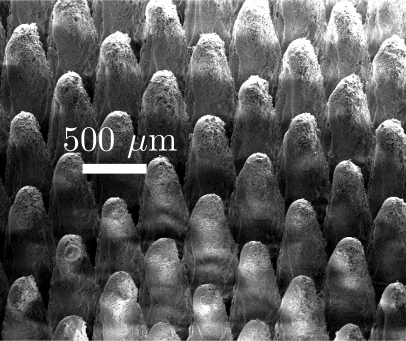
\includegraphics[width=0.75\textwidth]{../figures/SEM.pdf}
 \caption{SEM image of the superhydrophobic surface.\label{fig:SEM}}
\end{figure}

Surface potentials $\varphi_s$, were measured on the superhydrophobic surface using a \emph{Simco-Ion} FMX-004 electrostatic fieldmeter and the method for determination of surface charge density for low conductivity polymers described in Davies, 1967 \cite{davies_examination_1967}. This measurement was done with the superhydrophobic surfaces connected by a conductive ground plane by conductive tape, far away from the presence of other conductors. An ideal approach to determining surface charge on a dielectric surface is to screen perturbing effects of external electric fields. This is partly accomplished by grounding the fieldmeter, and by placing the dielectric sample on a grounded conductive plate backing. In this case the surface charge density is determined from
\[ \sigma = \frac{\varphi_s \kappa}{l}, \]
where $l$ and $\kappa$ are the thickness of the dielectric surface, and the absolute permitivity respectively. The measured surface voltage is a function of position away from the charged dielectric. In most cases this function is relatively constant at a distance about 1-2 cm away from the surface (there is some measurement error in surface voltage due to small mispositioning of the electrostatic fieldmeter, say by $\pm$1 mm). The relative dielectric constant of the PMMA sheet was measured by using a 65$\times$65 mm polished aluminum parallel plate capacitor with $C = \epsilon \epsilon_0 \frac{A}{l}$ where $C$ is the capacitance, and $A$ is the sheet area. Measuring the capacitance with 3 sample thicknesses using a GenRad 1657 RLC Digibridge, we found the relative permitivity to be $\epsilon = 3.5 \pm 0.4$.  

A further consideration is the possibility of the change in total charge during a typical experimental timescale. If we consider the drop rig to be a ground (which seems reasonable given that the rig is isolated from true ground, but is at some reference voltage with respect to the surface charges on the dielectric, it also has an abundance of free charge carriers, that is, if it is conductive), then there will be both bulk and surface decay of the charge on the dielectric. The evolution of the charge can in some cases be approximated by
\[ \sigma = \sigma_0 e^{\frac{-t}{\epsilon \rho}}, \]
where $\sigma_0$ is the initial surface charge density, and $\rho$ is the bulk resistivity (which can also be reframed in terms of conductivity by $\rho = 1/\gamma$, where $\gamma$ is the conductivity). For an example case of a surface with an initial surface charge density $\sigma = 2.4 \times (10^{-6})$ $C/m^2$, relative permittivity $\epsilon = 3.5$ and bulk resistivity $\rho = 1.6 \times (10^{16})$ $\Omega$cm such as with the case of 2.8 mm PMMA sheet, then the time constant $\tau = \kappa \rho$ is approximately 5000 s, which is a great deal longer than the typical time period for of a drop tower experiment. We measured the charge decay with a calibrated probe at periodic intervals. There are several charge decay mechanisms: internal ones, such as Ohmic resistence, and external ones such as compensation by envonmental ionic species. The relative magnitudes of these charge transport mechanisms, and therfore the stability of the electret varies drastically depending on its initial surface potential, material properties, environment, and charging method. In the case of unshielded electrets compensation by atmospheric ions is significant \cite{perlman_electrets_1973}. Because environmental convection will tend to  maintain a gradient of these ions, sealing an electret in a container from the atmosphere will effectively halt this decay mechanism. Atmospheric humidity and water droplet condensation also significantly increase charge decay (presumably by reducing the surface resistence) \cite{haenen_characteristic_1975}. Examples of this decay can be seen in Figure \ref{fig:charge_decay} for differing numbers of dielectric lamina used in this experiment. In looking at the trends in charge decay for our electrets we notice firstly, that the decay does not appear to be exponential, as in the model described above. Secondly, we plainly see a cross-over effect in the decay of the surface potential in our electret samples, whereby the samples charged to higher initial surface potentials decayed faster and reached the lower overall final potentials. This is a well known effect in polyethylenes charged by corona \cite{ferreira_corona_1992}.
\begin{figure}[htb!]
    \centering
    {%% Creator: Matplotlib, PGF backend
%%
%% To include the figure in your LaTeX document, write
%%   \input{<filename>.pgf}
%%
%% Make sure the required packages are loaded in your preamble
%%   \usepackage{pgf}
%%
%% Figures using additional raster images can only be included by \input if
%% they are in the same directory as the main LaTeX file. For loading figures
%% from other directories you can use the `import` package
%%   \usepackage{import}
%% and then include the figures with
%%   \import{<path to file>}{<filename>.pgf}
%%
%% Matplotlib used the following preamble
%%   \usepackage{fontspec}
%%   \setmainfont{DejaVu Serif}
%%   \setsansfont{DejaVu Sans}
%%   \setmonofont{DejaVu Sans Mono}
%%
\begingroup%
\makeatletter%
\begin{pgfpicture}%
\pgfpathrectangle{\pgfpointorigin}{\pgfqpoint{5.349660in}{3.676603in}}%
\pgfusepath{use as bounding box, clip}%
\begin{pgfscope}%
\pgfsetbuttcap%
\pgfsetmiterjoin%
\definecolor{currentfill}{rgb}{1.000000,1.000000,1.000000}%
\pgfsetfillcolor{currentfill}%
\pgfsetlinewidth{0.000000pt}%
\definecolor{currentstroke}{rgb}{1.000000,1.000000,1.000000}%
\pgfsetstrokecolor{currentstroke}%
\pgfsetdash{}{0pt}%
\pgfpathmoveto{\pgfqpoint{0.000000in}{0.000000in}}%
\pgfpathlineto{\pgfqpoint{5.349660in}{0.000000in}}%
\pgfpathlineto{\pgfqpoint{5.349660in}{3.676603in}}%
\pgfpathlineto{\pgfqpoint{0.000000in}{3.676603in}}%
\pgfpathclose%
\pgfusepath{fill}%
\end{pgfscope}%
\begin{pgfscope}%
\pgfsetbuttcap%
\pgfsetmiterjoin%
\definecolor{currentfill}{rgb}{1.000000,1.000000,1.000000}%
\pgfsetfillcolor{currentfill}%
\pgfsetlinewidth{0.000000pt}%
\definecolor{currentstroke}{rgb}{0.000000,0.000000,0.000000}%
\pgfsetstrokecolor{currentstroke}%
\pgfsetstrokeopacity{0.000000}%
\pgfsetdash{}{0pt}%
\pgfpathmoveto{\pgfqpoint{0.564660in}{0.521603in}}%
\pgfpathlineto{\pgfqpoint{5.214660in}{0.521603in}}%
\pgfpathlineto{\pgfqpoint{5.214660in}{3.541603in}}%
\pgfpathlineto{\pgfqpoint{0.564660in}{3.541603in}}%
\pgfpathclose%
\pgfusepath{fill}%
\end{pgfscope}%
\begin{pgfscope}%
\pgfsetbuttcap%
\pgfsetroundjoin%
\definecolor{currentfill}{rgb}{0.000000,0.000000,0.000000}%
\pgfsetfillcolor{currentfill}%
\pgfsetlinewidth{0.803000pt}%
\definecolor{currentstroke}{rgb}{0.000000,0.000000,0.000000}%
\pgfsetstrokecolor{currentstroke}%
\pgfsetdash{}{0pt}%
\pgfsys@defobject{currentmarker}{\pgfqpoint{0.000000in}{-0.048611in}}{\pgfqpoint{0.000000in}{0.000000in}}{%
\pgfpathmoveto{\pgfqpoint{0.000000in}{0.000000in}}%
\pgfpathlineto{\pgfqpoint{0.000000in}{-0.048611in}}%
\pgfusepath{stroke,fill}%
}%
\begin{pgfscope}%
\pgfsys@transformshift{0.776024in}{0.521603in}%
\pgfsys@useobject{currentmarker}{}%
\end{pgfscope}%
\end{pgfscope}%
\begin{pgfscope}%
\pgftext[x=0.776024in,y=0.424381in,,top]{\rmfamily\fontsize{10.000000}{12.000000}\selectfont \(\displaystyle 0\)}%
\end{pgfscope}%
\begin{pgfscope}%
\pgfsetbuttcap%
\pgfsetroundjoin%
\definecolor{currentfill}{rgb}{0.000000,0.000000,0.000000}%
\pgfsetfillcolor{currentfill}%
\pgfsetlinewidth{0.803000pt}%
\definecolor{currentstroke}{rgb}{0.000000,0.000000,0.000000}%
\pgfsetstrokecolor{currentstroke}%
\pgfsetdash{}{0pt}%
\pgfsys@defobject{currentmarker}{\pgfqpoint{0.000000in}{-0.048611in}}{\pgfqpoint{0.000000in}{0.000000in}}{%
\pgfpathmoveto{\pgfqpoint{0.000000in}{0.000000in}}%
\pgfpathlineto{\pgfqpoint{0.000000in}{-0.048611in}}%
\pgfusepath{stroke,fill}%
}%
\begin{pgfscope}%
\pgfsys@transformshift{1.351163in}{0.521603in}%
\pgfsys@useobject{currentmarker}{}%
\end{pgfscope}%
\end{pgfscope}%
\begin{pgfscope}%
\pgftext[x=1.351163in,y=0.424381in,,top]{\rmfamily\fontsize{10.000000}{12.000000}\selectfont \(\displaystyle 2000\)}%
\end{pgfscope}%
\begin{pgfscope}%
\pgfsetbuttcap%
\pgfsetroundjoin%
\definecolor{currentfill}{rgb}{0.000000,0.000000,0.000000}%
\pgfsetfillcolor{currentfill}%
\pgfsetlinewidth{0.803000pt}%
\definecolor{currentstroke}{rgb}{0.000000,0.000000,0.000000}%
\pgfsetstrokecolor{currentstroke}%
\pgfsetdash{}{0pt}%
\pgfsys@defobject{currentmarker}{\pgfqpoint{0.000000in}{-0.048611in}}{\pgfqpoint{0.000000in}{0.000000in}}{%
\pgfpathmoveto{\pgfqpoint{0.000000in}{0.000000in}}%
\pgfpathlineto{\pgfqpoint{0.000000in}{-0.048611in}}%
\pgfusepath{stroke,fill}%
}%
\begin{pgfscope}%
\pgfsys@transformshift{1.926302in}{0.521603in}%
\pgfsys@useobject{currentmarker}{}%
\end{pgfscope}%
\end{pgfscope}%
\begin{pgfscope}%
\pgftext[x=1.926302in,y=0.424381in,,top]{\rmfamily\fontsize{10.000000}{12.000000}\selectfont \(\displaystyle 4000\)}%
\end{pgfscope}%
\begin{pgfscope}%
\pgfsetbuttcap%
\pgfsetroundjoin%
\definecolor{currentfill}{rgb}{0.000000,0.000000,0.000000}%
\pgfsetfillcolor{currentfill}%
\pgfsetlinewidth{0.803000pt}%
\definecolor{currentstroke}{rgb}{0.000000,0.000000,0.000000}%
\pgfsetstrokecolor{currentstroke}%
\pgfsetdash{}{0pt}%
\pgfsys@defobject{currentmarker}{\pgfqpoint{0.000000in}{-0.048611in}}{\pgfqpoint{0.000000in}{0.000000in}}{%
\pgfpathmoveto{\pgfqpoint{0.000000in}{0.000000in}}%
\pgfpathlineto{\pgfqpoint{0.000000in}{-0.048611in}}%
\pgfusepath{stroke,fill}%
}%
\begin{pgfscope}%
\pgfsys@transformshift{2.501441in}{0.521603in}%
\pgfsys@useobject{currentmarker}{}%
\end{pgfscope}%
\end{pgfscope}%
\begin{pgfscope}%
\pgftext[x=2.501441in,y=0.424381in,,top]{\rmfamily\fontsize{10.000000}{12.000000}\selectfont \(\displaystyle 6000\)}%
\end{pgfscope}%
\begin{pgfscope}%
\pgfsetbuttcap%
\pgfsetroundjoin%
\definecolor{currentfill}{rgb}{0.000000,0.000000,0.000000}%
\pgfsetfillcolor{currentfill}%
\pgfsetlinewidth{0.803000pt}%
\definecolor{currentstroke}{rgb}{0.000000,0.000000,0.000000}%
\pgfsetstrokecolor{currentstroke}%
\pgfsetdash{}{0pt}%
\pgfsys@defobject{currentmarker}{\pgfqpoint{0.000000in}{-0.048611in}}{\pgfqpoint{0.000000in}{0.000000in}}{%
\pgfpathmoveto{\pgfqpoint{0.000000in}{0.000000in}}%
\pgfpathlineto{\pgfqpoint{0.000000in}{-0.048611in}}%
\pgfusepath{stroke,fill}%
}%
\begin{pgfscope}%
\pgfsys@transformshift{3.076581in}{0.521603in}%
\pgfsys@useobject{currentmarker}{}%
\end{pgfscope}%
\end{pgfscope}%
\begin{pgfscope}%
\pgftext[x=3.076581in,y=0.424381in,,top]{\rmfamily\fontsize{10.000000}{12.000000}\selectfont \(\displaystyle 8000\)}%
\end{pgfscope}%
\begin{pgfscope}%
\pgfsetbuttcap%
\pgfsetroundjoin%
\definecolor{currentfill}{rgb}{0.000000,0.000000,0.000000}%
\pgfsetfillcolor{currentfill}%
\pgfsetlinewidth{0.803000pt}%
\definecolor{currentstroke}{rgb}{0.000000,0.000000,0.000000}%
\pgfsetstrokecolor{currentstroke}%
\pgfsetdash{}{0pt}%
\pgfsys@defobject{currentmarker}{\pgfqpoint{0.000000in}{-0.048611in}}{\pgfqpoint{0.000000in}{0.000000in}}{%
\pgfpathmoveto{\pgfqpoint{0.000000in}{0.000000in}}%
\pgfpathlineto{\pgfqpoint{0.000000in}{-0.048611in}}%
\pgfusepath{stroke,fill}%
}%
\begin{pgfscope}%
\pgfsys@transformshift{3.651720in}{0.521603in}%
\pgfsys@useobject{currentmarker}{}%
\end{pgfscope}%
\end{pgfscope}%
\begin{pgfscope}%
\pgftext[x=3.651720in,y=0.424381in,,top]{\rmfamily\fontsize{10.000000}{12.000000}\selectfont \(\displaystyle 10000\)}%
\end{pgfscope}%
\begin{pgfscope}%
\pgfsetbuttcap%
\pgfsetroundjoin%
\definecolor{currentfill}{rgb}{0.000000,0.000000,0.000000}%
\pgfsetfillcolor{currentfill}%
\pgfsetlinewidth{0.803000pt}%
\definecolor{currentstroke}{rgb}{0.000000,0.000000,0.000000}%
\pgfsetstrokecolor{currentstroke}%
\pgfsetdash{}{0pt}%
\pgfsys@defobject{currentmarker}{\pgfqpoint{0.000000in}{-0.048611in}}{\pgfqpoint{0.000000in}{0.000000in}}{%
\pgfpathmoveto{\pgfqpoint{0.000000in}{0.000000in}}%
\pgfpathlineto{\pgfqpoint{0.000000in}{-0.048611in}}%
\pgfusepath{stroke,fill}%
}%
\begin{pgfscope}%
\pgfsys@transformshift{4.226859in}{0.521603in}%
\pgfsys@useobject{currentmarker}{}%
\end{pgfscope}%
\end{pgfscope}%
\begin{pgfscope}%
\pgftext[x=4.226859in,y=0.424381in,,top]{\rmfamily\fontsize{10.000000}{12.000000}\selectfont \(\displaystyle 12000\)}%
\end{pgfscope}%
\begin{pgfscope}%
\pgfsetbuttcap%
\pgfsetroundjoin%
\definecolor{currentfill}{rgb}{0.000000,0.000000,0.000000}%
\pgfsetfillcolor{currentfill}%
\pgfsetlinewidth{0.803000pt}%
\definecolor{currentstroke}{rgb}{0.000000,0.000000,0.000000}%
\pgfsetstrokecolor{currentstroke}%
\pgfsetdash{}{0pt}%
\pgfsys@defobject{currentmarker}{\pgfqpoint{0.000000in}{-0.048611in}}{\pgfqpoint{0.000000in}{0.000000in}}{%
\pgfpathmoveto{\pgfqpoint{0.000000in}{0.000000in}}%
\pgfpathlineto{\pgfqpoint{0.000000in}{-0.048611in}}%
\pgfusepath{stroke,fill}%
}%
\begin{pgfscope}%
\pgfsys@transformshift{4.801998in}{0.521603in}%
\pgfsys@useobject{currentmarker}{}%
\end{pgfscope}%
\end{pgfscope}%
\begin{pgfscope}%
\pgftext[x=4.801998in,y=0.424381in,,top]{\rmfamily\fontsize{10.000000}{12.000000}\selectfont \(\displaystyle 14000\)}%
\end{pgfscope}%
\begin{pgfscope}%
\pgftext[x=2.889660in,y=0.234413in,,top]{\rmfamily\fontsize{10.000000}{12.000000}\selectfont t (s)}%
\end{pgfscope}%
\begin{pgfscope}%
\pgfsetbuttcap%
\pgfsetroundjoin%
\definecolor{currentfill}{rgb}{0.000000,0.000000,0.000000}%
\pgfsetfillcolor{currentfill}%
\pgfsetlinewidth{0.803000pt}%
\definecolor{currentstroke}{rgb}{0.000000,0.000000,0.000000}%
\pgfsetstrokecolor{currentstroke}%
\pgfsetdash{}{0pt}%
\pgfsys@defobject{currentmarker}{\pgfqpoint{-0.048611in}{0.000000in}}{\pgfqpoint{0.000000in}{0.000000in}}{%
\pgfpathmoveto{\pgfqpoint{0.000000in}{0.000000in}}%
\pgfpathlineto{\pgfqpoint{-0.048611in}{0.000000in}}%
\pgfusepath{stroke,fill}%
}%
\begin{pgfscope}%
\pgfsys@transformshift{0.564660in}{0.747439in}%
\pgfsys@useobject{currentmarker}{}%
\end{pgfscope}%
\end{pgfscope}%
\begin{pgfscope}%
\pgftext[x=0.289968in,y=0.694678in,left,base]{\rmfamily\fontsize{10.000000}{12.000000}\selectfont \(\displaystyle 0.5\)}%
\end{pgfscope}%
\begin{pgfscope}%
\pgfsetbuttcap%
\pgfsetroundjoin%
\definecolor{currentfill}{rgb}{0.000000,0.000000,0.000000}%
\pgfsetfillcolor{currentfill}%
\pgfsetlinewidth{0.803000pt}%
\definecolor{currentstroke}{rgb}{0.000000,0.000000,0.000000}%
\pgfsetstrokecolor{currentstroke}%
\pgfsetdash{}{0pt}%
\pgfsys@defobject{currentmarker}{\pgfqpoint{-0.048611in}{0.000000in}}{\pgfqpoint{0.000000in}{0.000000in}}{%
\pgfpathmoveto{\pgfqpoint{0.000000in}{0.000000in}}%
\pgfpathlineto{\pgfqpoint{-0.048611in}{0.000000in}}%
\pgfusepath{stroke,fill}%
}%
\begin{pgfscope}%
\pgfsys@transformshift{0.564660in}{1.190254in}%
\pgfsys@useobject{currentmarker}{}%
\end{pgfscope}%
\end{pgfscope}%
\begin{pgfscope}%
\pgftext[x=0.289968in,y=1.137493in,left,base]{\rmfamily\fontsize{10.000000}{12.000000}\selectfont \(\displaystyle 1.0\)}%
\end{pgfscope}%
\begin{pgfscope}%
\pgfsetbuttcap%
\pgfsetroundjoin%
\definecolor{currentfill}{rgb}{0.000000,0.000000,0.000000}%
\pgfsetfillcolor{currentfill}%
\pgfsetlinewidth{0.803000pt}%
\definecolor{currentstroke}{rgb}{0.000000,0.000000,0.000000}%
\pgfsetstrokecolor{currentstroke}%
\pgfsetdash{}{0pt}%
\pgfsys@defobject{currentmarker}{\pgfqpoint{-0.048611in}{0.000000in}}{\pgfqpoint{0.000000in}{0.000000in}}{%
\pgfpathmoveto{\pgfqpoint{0.000000in}{0.000000in}}%
\pgfpathlineto{\pgfqpoint{-0.048611in}{0.000000in}}%
\pgfusepath{stroke,fill}%
}%
\begin{pgfscope}%
\pgfsys@transformshift{0.564660in}{1.633070in}%
\pgfsys@useobject{currentmarker}{}%
\end{pgfscope}%
\end{pgfscope}%
\begin{pgfscope}%
\pgftext[x=0.289968in,y=1.580308in,left,base]{\rmfamily\fontsize{10.000000}{12.000000}\selectfont \(\displaystyle 1.5\)}%
\end{pgfscope}%
\begin{pgfscope}%
\pgfsetbuttcap%
\pgfsetroundjoin%
\definecolor{currentfill}{rgb}{0.000000,0.000000,0.000000}%
\pgfsetfillcolor{currentfill}%
\pgfsetlinewidth{0.803000pt}%
\definecolor{currentstroke}{rgb}{0.000000,0.000000,0.000000}%
\pgfsetstrokecolor{currentstroke}%
\pgfsetdash{}{0pt}%
\pgfsys@defobject{currentmarker}{\pgfqpoint{-0.048611in}{0.000000in}}{\pgfqpoint{0.000000in}{0.000000in}}{%
\pgfpathmoveto{\pgfqpoint{0.000000in}{0.000000in}}%
\pgfpathlineto{\pgfqpoint{-0.048611in}{0.000000in}}%
\pgfusepath{stroke,fill}%
}%
\begin{pgfscope}%
\pgfsys@transformshift{0.564660in}{2.075885in}%
\pgfsys@useobject{currentmarker}{}%
\end{pgfscope}%
\end{pgfscope}%
\begin{pgfscope}%
\pgftext[x=0.289968in,y=2.023123in,left,base]{\rmfamily\fontsize{10.000000}{12.000000}\selectfont \(\displaystyle 2.0\)}%
\end{pgfscope}%
\begin{pgfscope}%
\pgfsetbuttcap%
\pgfsetroundjoin%
\definecolor{currentfill}{rgb}{0.000000,0.000000,0.000000}%
\pgfsetfillcolor{currentfill}%
\pgfsetlinewidth{0.803000pt}%
\definecolor{currentstroke}{rgb}{0.000000,0.000000,0.000000}%
\pgfsetstrokecolor{currentstroke}%
\pgfsetdash{}{0pt}%
\pgfsys@defobject{currentmarker}{\pgfqpoint{-0.048611in}{0.000000in}}{\pgfqpoint{0.000000in}{0.000000in}}{%
\pgfpathmoveto{\pgfqpoint{0.000000in}{0.000000in}}%
\pgfpathlineto{\pgfqpoint{-0.048611in}{0.000000in}}%
\pgfusepath{stroke,fill}%
}%
\begin{pgfscope}%
\pgfsys@transformshift{0.564660in}{2.518700in}%
\pgfsys@useobject{currentmarker}{}%
\end{pgfscope}%
\end{pgfscope}%
\begin{pgfscope}%
\pgftext[x=0.289968in,y=2.465939in,left,base]{\rmfamily\fontsize{10.000000}{12.000000}\selectfont \(\displaystyle 2.5\)}%
\end{pgfscope}%
\begin{pgfscope}%
\pgfsetbuttcap%
\pgfsetroundjoin%
\definecolor{currentfill}{rgb}{0.000000,0.000000,0.000000}%
\pgfsetfillcolor{currentfill}%
\pgfsetlinewidth{0.803000pt}%
\definecolor{currentstroke}{rgb}{0.000000,0.000000,0.000000}%
\pgfsetstrokecolor{currentstroke}%
\pgfsetdash{}{0pt}%
\pgfsys@defobject{currentmarker}{\pgfqpoint{-0.048611in}{0.000000in}}{\pgfqpoint{0.000000in}{0.000000in}}{%
\pgfpathmoveto{\pgfqpoint{0.000000in}{0.000000in}}%
\pgfpathlineto{\pgfqpoint{-0.048611in}{0.000000in}}%
\pgfusepath{stroke,fill}%
}%
\begin{pgfscope}%
\pgfsys@transformshift{0.564660in}{2.961515in}%
\pgfsys@useobject{currentmarker}{}%
\end{pgfscope}%
\end{pgfscope}%
\begin{pgfscope}%
\pgftext[x=0.289968in,y=2.908754in,left,base]{\rmfamily\fontsize{10.000000}{12.000000}\selectfont \(\displaystyle 3.0\)}%
\end{pgfscope}%
\begin{pgfscope}%
\pgfsetbuttcap%
\pgfsetroundjoin%
\definecolor{currentfill}{rgb}{0.000000,0.000000,0.000000}%
\pgfsetfillcolor{currentfill}%
\pgfsetlinewidth{0.803000pt}%
\definecolor{currentstroke}{rgb}{0.000000,0.000000,0.000000}%
\pgfsetstrokecolor{currentstroke}%
\pgfsetdash{}{0pt}%
\pgfsys@defobject{currentmarker}{\pgfqpoint{-0.048611in}{0.000000in}}{\pgfqpoint{0.000000in}{0.000000in}}{%
\pgfpathmoveto{\pgfqpoint{0.000000in}{0.000000in}}%
\pgfpathlineto{\pgfqpoint{-0.048611in}{0.000000in}}%
\pgfusepath{stroke,fill}%
}%
\begin{pgfscope}%
\pgfsys@transformshift{0.564660in}{3.404331in}%
\pgfsys@useobject{currentmarker}{}%
\end{pgfscope}%
\end{pgfscope}%
\begin{pgfscope}%
\pgftext[x=0.289968in,y=3.351569in,left,base]{\rmfamily\fontsize{10.000000}{12.000000}\selectfont \(\displaystyle 3.5\)}%
\end{pgfscope}%
\begin{pgfscope}%
\pgftext[x=0.234413in,y=2.031603in,,bottom,rotate=90.000000]{\rmfamily\fontsize{10.000000}{12.000000}\selectfont Surface potential (kV)}%
\end{pgfscope}%
\begin{pgfscope}%
\pgfpathrectangle{\pgfqpoint{0.564660in}{0.521603in}}{\pgfqpoint{4.650000in}{3.020000in}} %
\pgfusepath{clip}%
\pgfsetrectcap%
\pgfsetroundjoin%
\pgfsetlinewidth{1.505625pt}%
\definecolor{currentstroke}{rgb}{0.000000,0.750000,0.750000}%
\pgfsetstrokecolor{currentstroke}%
\pgfsetdash{}{0pt}%
\pgfpathmoveto{\pgfqpoint{0.776024in}{1.810196in}}%
\pgfpathlineto{\pgfqpoint{0.784651in}{1.633070in}}%
\pgfpathlineto{\pgfqpoint{0.793278in}{1.721633in}}%
\pgfpathlineto{\pgfqpoint{0.810532in}{1.633070in}}%
\pgfpathlineto{\pgfqpoint{0.819159in}{1.544507in}}%
\pgfpathlineto{\pgfqpoint{0.827786in}{1.633070in}}%
\pgfpathlineto{\pgfqpoint{0.836414in}{1.721633in}}%
\pgfpathlineto{\pgfqpoint{0.845041in}{1.455944in}}%
\pgfpathlineto{\pgfqpoint{0.853668in}{1.455944in}}%
\pgfpathlineto{\pgfqpoint{0.862295in}{1.544507in}}%
\pgfpathlineto{\pgfqpoint{1.034837in}{1.455944in}}%
\pgfpathlineto{\pgfqpoint{1.207378in}{1.367380in}}%
\pgfpathlineto{\pgfqpoint{1.379920in}{1.367380in}}%
\pgfpathlineto{\pgfqpoint{1.897545in}{1.190254in}}%
\pgfpathlineto{\pgfqpoint{2.415170in}{1.190254in}}%
\pgfpathlineto{\pgfqpoint{2.932796in}{1.101691in}}%
\pgfpathlineto{\pgfqpoint{3.450421in}{1.101691in}}%
\pgfpathlineto{\pgfqpoint{5.003297in}{1.101691in}}%
\pgfusepath{stroke}%
\end{pgfscope}%
\begin{pgfscope}%
\pgfpathrectangle{\pgfqpoint{0.564660in}{0.521603in}}{\pgfqpoint{4.650000in}{3.020000in}} %
\pgfusepath{clip}%
\pgfsetbuttcap%
\pgfsetmiterjoin%
\definecolor{currentfill}{rgb}{0.000000,0.750000,0.750000}%
\pgfsetfillcolor{currentfill}%
\pgfsetlinewidth{1.003750pt}%
\definecolor{currentstroke}{rgb}{0.000000,0.750000,0.750000}%
\pgfsetstrokecolor{currentstroke}%
\pgfsetdash{}{0pt}%
\pgfsys@defobject{currentmarker}{\pgfqpoint{-0.041667in}{-0.041667in}}{\pgfqpoint{0.041667in}{0.041667in}}{%
\pgfpathmoveto{\pgfqpoint{-0.000000in}{-0.041667in}}%
\pgfpathlineto{\pgfqpoint{0.041667in}{0.041667in}}%
\pgfpathlineto{\pgfqpoint{-0.041667in}{0.041667in}}%
\pgfpathclose%
\pgfusepath{stroke,fill}%
}%
\begin{pgfscope}%
\pgfsys@transformshift{0.776024in}{1.810196in}%
\pgfsys@useobject{currentmarker}{}%
\end{pgfscope}%
\begin{pgfscope}%
\pgfsys@transformshift{0.784651in}{1.633070in}%
\pgfsys@useobject{currentmarker}{}%
\end{pgfscope}%
\begin{pgfscope}%
\pgfsys@transformshift{0.793278in}{1.721633in}%
\pgfsys@useobject{currentmarker}{}%
\end{pgfscope}%
\begin{pgfscope}%
\pgfsys@transformshift{0.810532in}{1.633070in}%
\pgfsys@useobject{currentmarker}{}%
\end{pgfscope}%
\begin{pgfscope}%
\pgfsys@transformshift{0.819159in}{1.544507in}%
\pgfsys@useobject{currentmarker}{}%
\end{pgfscope}%
\begin{pgfscope}%
\pgfsys@transformshift{0.827786in}{1.633070in}%
\pgfsys@useobject{currentmarker}{}%
\end{pgfscope}%
\begin{pgfscope}%
\pgfsys@transformshift{0.836414in}{1.721633in}%
\pgfsys@useobject{currentmarker}{}%
\end{pgfscope}%
\begin{pgfscope}%
\pgfsys@transformshift{0.845041in}{1.455944in}%
\pgfsys@useobject{currentmarker}{}%
\end{pgfscope}%
\begin{pgfscope}%
\pgfsys@transformshift{0.853668in}{1.455944in}%
\pgfsys@useobject{currentmarker}{}%
\end{pgfscope}%
\begin{pgfscope}%
\pgfsys@transformshift{0.862295in}{1.544507in}%
\pgfsys@useobject{currentmarker}{}%
\end{pgfscope}%
\begin{pgfscope}%
\pgfsys@transformshift{1.034837in}{1.455944in}%
\pgfsys@useobject{currentmarker}{}%
\end{pgfscope}%
\begin{pgfscope}%
\pgfsys@transformshift{1.207378in}{1.367380in}%
\pgfsys@useobject{currentmarker}{}%
\end{pgfscope}%
\begin{pgfscope}%
\pgfsys@transformshift{1.379920in}{1.367380in}%
\pgfsys@useobject{currentmarker}{}%
\end{pgfscope}%
\begin{pgfscope}%
\pgfsys@transformshift{1.897545in}{1.190254in}%
\pgfsys@useobject{currentmarker}{}%
\end{pgfscope}%
\begin{pgfscope}%
\pgfsys@transformshift{2.415170in}{1.190254in}%
\pgfsys@useobject{currentmarker}{}%
\end{pgfscope}%
\begin{pgfscope}%
\pgfsys@transformshift{2.932796in}{1.101691in}%
\pgfsys@useobject{currentmarker}{}%
\end{pgfscope}%
\begin{pgfscope}%
\pgfsys@transformshift{3.450421in}{1.101691in}%
\pgfsys@useobject{currentmarker}{}%
\end{pgfscope}%
\begin{pgfscope}%
\pgfsys@transformshift{5.003297in}{1.101691in}%
\pgfsys@useobject{currentmarker}{}%
\end{pgfscope}%
\end{pgfscope}%
\begin{pgfscope}%
\pgfpathrectangle{\pgfqpoint{0.564660in}{0.521603in}}{\pgfqpoint{4.650000in}{3.020000in}} %
\pgfusepath{clip}%
\pgfsetrectcap%
\pgfsetroundjoin%
\pgfsetlinewidth{1.505625pt}%
\definecolor{currentstroke}{rgb}{0.000000,0.000000,1.000000}%
\pgfsetstrokecolor{currentstroke}%
\pgfsetdash{}{0pt}%
\pgfpathmoveto{\pgfqpoint{0.776024in}{2.430137in}}%
\pgfpathlineto{\pgfqpoint{0.784651in}{2.872952in}}%
\pgfpathlineto{\pgfqpoint{0.793278in}{2.784389in}}%
\pgfpathlineto{\pgfqpoint{0.801905in}{2.607263in}}%
\pgfpathlineto{\pgfqpoint{0.810532in}{2.607263in}}%
\pgfpathlineto{\pgfqpoint{0.819159in}{2.253011in}}%
\pgfpathlineto{\pgfqpoint{0.827786in}{2.253011in}}%
\pgfpathlineto{\pgfqpoint{0.836414in}{2.518700in}}%
\pgfpathlineto{\pgfqpoint{0.845041in}{2.430137in}}%
\pgfpathlineto{\pgfqpoint{0.853668in}{2.518700in}}%
\pgfpathlineto{\pgfqpoint{0.862295in}{2.430137in}}%
\pgfpathlineto{\pgfqpoint{1.034837in}{1.810196in}}%
\pgfpathlineto{\pgfqpoint{1.207378in}{1.633070in}}%
\pgfpathlineto{\pgfqpoint{1.379920in}{1.544507in}}%
\pgfpathlineto{\pgfqpoint{1.897545in}{1.101691in}}%
\pgfpathlineto{\pgfqpoint{2.415170in}{1.101691in}}%
\pgfpathlineto{\pgfqpoint{2.932796in}{1.013128in}}%
\pgfpathlineto{\pgfqpoint{3.450421in}{1.013128in}}%
\pgfpathlineto{\pgfqpoint{5.003297in}{0.924565in}}%
\pgfusepath{stroke}%
\end{pgfscope}%
\begin{pgfscope}%
\pgfpathrectangle{\pgfqpoint{0.564660in}{0.521603in}}{\pgfqpoint{4.650000in}{3.020000in}} %
\pgfusepath{clip}%
\pgfsetbuttcap%
\pgfsetroundjoin%
\definecolor{currentfill}{rgb}{0.000000,0.000000,1.000000}%
\pgfsetfillcolor{currentfill}%
\pgfsetlinewidth{1.003750pt}%
\definecolor{currentstroke}{rgb}{0.000000,0.000000,1.000000}%
\pgfsetstrokecolor{currentstroke}%
\pgfsetdash{}{0pt}%
\pgfsys@defobject{currentmarker}{\pgfqpoint{-0.041667in}{-0.041667in}}{\pgfqpoint{0.041667in}{0.041667in}}{%
\pgfpathmoveto{\pgfqpoint{0.000000in}{-0.041667in}}%
\pgfpathcurveto{\pgfqpoint{0.011050in}{-0.041667in}}{\pgfqpoint{0.021649in}{-0.037276in}}{\pgfqpoint{0.029463in}{-0.029463in}}%
\pgfpathcurveto{\pgfqpoint{0.037276in}{-0.021649in}}{\pgfqpoint{0.041667in}{-0.011050in}}{\pgfqpoint{0.041667in}{0.000000in}}%
\pgfpathcurveto{\pgfqpoint{0.041667in}{0.011050in}}{\pgfqpoint{0.037276in}{0.021649in}}{\pgfqpoint{0.029463in}{0.029463in}}%
\pgfpathcurveto{\pgfqpoint{0.021649in}{0.037276in}}{\pgfqpoint{0.011050in}{0.041667in}}{\pgfqpoint{0.000000in}{0.041667in}}%
\pgfpathcurveto{\pgfqpoint{-0.011050in}{0.041667in}}{\pgfqpoint{-0.021649in}{0.037276in}}{\pgfqpoint{-0.029463in}{0.029463in}}%
\pgfpathcurveto{\pgfqpoint{-0.037276in}{0.021649in}}{\pgfqpoint{-0.041667in}{0.011050in}}{\pgfqpoint{-0.041667in}{0.000000in}}%
\pgfpathcurveto{\pgfqpoint{-0.041667in}{-0.011050in}}{\pgfqpoint{-0.037276in}{-0.021649in}}{\pgfqpoint{-0.029463in}{-0.029463in}}%
\pgfpathcurveto{\pgfqpoint{-0.021649in}{-0.037276in}}{\pgfqpoint{-0.011050in}{-0.041667in}}{\pgfqpoint{0.000000in}{-0.041667in}}%
\pgfpathclose%
\pgfusepath{stroke,fill}%
}%
\begin{pgfscope}%
\pgfsys@transformshift{0.776024in}{2.430137in}%
\pgfsys@useobject{currentmarker}{}%
\end{pgfscope}%
\begin{pgfscope}%
\pgfsys@transformshift{0.784651in}{2.872952in}%
\pgfsys@useobject{currentmarker}{}%
\end{pgfscope}%
\begin{pgfscope}%
\pgfsys@transformshift{0.793278in}{2.784389in}%
\pgfsys@useobject{currentmarker}{}%
\end{pgfscope}%
\begin{pgfscope}%
\pgfsys@transformshift{0.801905in}{2.607263in}%
\pgfsys@useobject{currentmarker}{}%
\end{pgfscope}%
\begin{pgfscope}%
\pgfsys@transformshift{0.810532in}{2.607263in}%
\pgfsys@useobject{currentmarker}{}%
\end{pgfscope}%
\begin{pgfscope}%
\pgfsys@transformshift{0.819159in}{2.253011in}%
\pgfsys@useobject{currentmarker}{}%
\end{pgfscope}%
\begin{pgfscope}%
\pgfsys@transformshift{0.827786in}{2.253011in}%
\pgfsys@useobject{currentmarker}{}%
\end{pgfscope}%
\begin{pgfscope}%
\pgfsys@transformshift{0.836414in}{2.518700in}%
\pgfsys@useobject{currentmarker}{}%
\end{pgfscope}%
\begin{pgfscope}%
\pgfsys@transformshift{0.845041in}{2.430137in}%
\pgfsys@useobject{currentmarker}{}%
\end{pgfscope}%
\begin{pgfscope}%
\pgfsys@transformshift{0.853668in}{2.518700in}%
\pgfsys@useobject{currentmarker}{}%
\end{pgfscope}%
\begin{pgfscope}%
\pgfsys@transformshift{0.862295in}{2.430137in}%
\pgfsys@useobject{currentmarker}{}%
\end{pgfscope}%
\begin{pgfscope}%
\pgfsys@transformshift{1.034837in}{1.810196in}%
\pgfsys@useobject{currentmarker}{}%
\end{pgfscope}%
\begin{pgfscope}%
\pgfsys@transformshift{1.207378in}{1.633070in}%
\pgfsys@useobject{currentmarker}{}%
\end{pgfscope}%
\begin{pgfscope}%
\pgfsys@transformshift{1.379920in}{1.544507in}%
\pgfsys@useobject{currentmarker}{}%
\end{pgfscope}%
\begin{pgfscope}%
\pgfsys@transformshift{1.897545in}{1.101691in}%
\pgfsys@useobject{currentmarker}{}%
\end{pgfscope}%
\begin{pgfscope}%
\pgfsys@transformshift{2.415170in}{1.101691in}%
\pgfsys@useobject{currentmarker}{}%
\end{pgfscope}%
\begin{pgfscope}%
\pgfsys@transformshift{2.932796in}{1.013128in}%
\pgfsys@useobject{currentmarker}{}%
\end{pgfscope}%
\begin{pgfscope}%
\pgfsys@transformshift{3.450421in}{1.013128in}%
\pgfsys@useobject{currentmarker}{}%
\end{pgfscope}%
\begin{pgfscope}%
\pgfsys@transformshift{5.003297in}{0.924565in}%
\pgfsys@useobject{currentmarker}{}%
\end{pgfscope}%
\end{pgfscope}%
\begin{pgfscope}%
\pgfpathrectangle{\pgfqpoint{0.564660in}{0.521603in}}{\pgfqpoint{4.650000in}{3.020000in}} %
\pgfusepath{clip}%
\pgfsetrectcap%
\pgfsetroundjoin%
\pgfsetlinewidth{1.505625pt}%
\definecolor{currentstroke}{rgb}{1.000000,0.000000,0.000000}%
\pgfsetstrokecolor{currentstroke}%
\pgfsetdash{}{0pt}%
\pgfpathmoveto{\pgfqpoint{0.776024in}{3.050078in}}%
\pgfpathlineto{\pgfqpoint{0.784651in}{3.404331in}}%
\pgfpathlineto{\pgfqpoint{0.793278in}{3.315768in}}%
\pgfpathlineto{\pgfqpoint{0.801905in}{3.138641in}}%
\pgfpathlineto{\pgfqpoint{0.810532in}{2.961515in}}%
\pgfpathlineto{\pgfqpoint{0.819159in}{2.961515in}}%
\pgfpathlineto{\pgfqpoint{0.827786in}{2.784389in}}%
\pgfpathlineto{\pgfqpoint{0.836414in}{2.961515in}}%
\pgfpathlineto{\pgfqpoint{0.845041in}{2.961515in}}%
\pgfpathlineto{\pgfqpoint{0.853668in}{2.784389in}}%
\pgfpathlineto{\pgfqpoint{0.862295in}{2.872952in}}%
\pgfpathlineto{\pgfqpoint{1.034837in}{1.898759in}}%
\pgfpathlineto{\pgfqpoint{1.207378in}{1.633070in}}%
\pgfpathlineto{\pgfqpoint{1.379920in}{1.278817in}}%
\pgfpathlineto{\pgfqpoint{1.897545in}{1.101691in}}%
\pgfpathlineto{\pgfqpoint{2.415170in}{0.836002in}}%
\pgfpathlineto{\pgfqpoint{2.932796in}{0.836002in}}%
\pgfpathlineto{\pgfqpoint{3.450421in}{0.747439in}}%
\pgfpathlineto{\pgfqpoint{3.968046in}{0.658876in}}%
\pgfpathlineto{\pgfqpoint{4.485671in}{0.658876in}}%
\pgfpathlineto{\pgfqpoint{5.003297in}{0.658876in}}%
\pgfusepath{stroke}%
\end{pgfscope}%
\begin{pgfscope}%
\pgfpathrectangle{\pgfqpoint{0.564660in}{0.521603in}}{\pgfqpoint{4.650000in}{3.020000in}} %
\pgfusepath{clip}%
\pgfsetbuttcap%
\pgfsetmiterjoin%
\definecolor{currentfill}{rgb}{1.000000,0.000000,0.000000}%
\pgfsetfillcolor{currentfill}%
\pgfsetlinewidth{1.003750pt}%
\definecolor{currentstroke}{rgb}{1.000000,0.000000,0.000000}%
\pgfsetstrokecolor{currentstroke}%
\pgfsetdash{}{0pt}%
\pgfsys@defobject{currentmarker}{\pgfqpoint{-0.041667in}{-0.041667in}}{\pgfqpoint{0.041667in}{0.041667in}}{%
\pgfpathmoveto{\pgfqpoint{-0.041667in}{-0.041667in}}%
\pgfpathlineto{\pgfqpoint{0.041667in}{-0.041667in}}%
\pgfpathlineto{\pgfqpoint{0.041667in}{0.041667in}}%
\pgfpathlineto{\pgfqpoint{-0.041667in}{0.041667in}}%
\pgfpathclose%
\pgfusepath{stroke,fill}%
}%
\begin{pgfscope}%
\pgfsys@transformshift{0.776024in}{3.050078in}%
\pgfsys@useobject{currentmarker}{}%
\end{pgfscope}%
\begin{pgfscope}%
\pgfsys@transformshift{0.784651in}{3.404331in}%
\pgfsys@useobject{currentmarker}{}%
\end{pgfscope}%
\begin{pgfscope}%
\pgfsys@transformshift{0.793278in}{3.315768in}%
\pgfsys@useobject{currentmarker}{}%
\end{pgfscope}%
\begin{pgfscope}%
\pgfsys@transformshift{0.801905in}{3.138641in}%
\pgfsys@useobject{currentmarker}{}%
\end{pgfscope}%
\begin{pgfscope}%
\pgfsys@transformshift{0.810532in}{2.961515in}%
\pgfsys@useobject{currentmarker}{}%
\end{pgfscope}%
\begin{pgfscope}%
\pgfsys@transformshift{0.819159in}{2.961515in}%
\pgfsys@useobject{currentmarker}{}%
\end{pgfscope}%
\begin{pgfscope}%
\pgfsys@transformshift{0.827786in}{2.784389in}%
\pgfsys@useobject{currentmarker}{}%
\end{pgfscope}%
\begin{pgfscope}%
\pgfsys@transformshift{0.836414in}{2.961515in}%
\pgfsys@useobject{currentmarker}{}%
\end{pgfscope}%
\begin{pgfscope}%
\pgfsys@transformshift{0.845041in}{2.961515in}%
\pgfsys@useobject{currentmarker}{}%
\end{pgfscope}%
\begin{pgfscope}%
\pgfsys@transformshift{0.853668in}{2.784389in}%
\pgfsys@useobject{currentmarker}{}%
\end{pgfscope}%
\begin{pgfscope}%
\pgfsys@transformshift{0.862295in}{2.872952in}%
\pgfsys@useobject{currentmarker}{}%
\end{pgfscope}%
\begin{pgfscope}%
\pgfsys@transformshift{1.034837in}{1.898759in}%
\pgfsys@useobject{currentmarker}{}%
\end{pgfscope}%
\begin{pgfscope}%
\pgfsys@transformshift{1.207378in}{1.633070in}%
\pgfsys@useobject{currentmarker}{}%
\end{pgfscope}%
\begin{pgfscope}%
\pgfsys@transformshift{1.379920in}{1.278817in}%
\pgfsys@useobject{currentmarker}{}%
\end{pgfscope}%
\begin{pgfscope}%
\pgfsys@transformshift{1.897545in}{1.101691in}%
\pgfsys@useobject{currentmarker}{}%
\end{pgfscope}%
\begin{pgfscope}%
\pgfsys@transformshift{2.415170in}{0.836002in}%
\pgfsys@useobject{currentmarker}{}%
\end{pgfscope}%
\begin{pgfscope}%
\pgfsys@transformshift{2.932796in}{0.836002in}%
\pgfsys@useobject{currentmarker}{}%
\end{pgfscope}%
\begin{pgfscope}%
\pgfsys@transformshift{3.450421in}{0.747439in}%
\pgfsys@useobject{currentmarker}{}%
\end{pgfscope}%
\begin{pgfscope}%
\pgfsys@transformshift{3.968046in}{0.658876in}%
\pgfsys@useobject{currentmarker}{}%
\end{pgfscope}%
\begin{pgfscope}%
\pgfsys@transformshift{4.485671in}{0.658876in}%
\pgfsys@useobject{currentmarker}{}%
\end{pgfscope}%
\begin{pgfscope}%
\pgfsys@transformshift{5.003297in}{0.658876in}%
\pgfsys@useobject{currentmarker}{}%
\end{pgfscope}%
\end{pgfscope}%
\begin{pgfscope}%
\pgfsetrectcap%
\pgfsetmiterjoin%
\pgfsetlinewidth{0.803000pt}%
\definecolor{currentstroke}{rgb}{0.000000,0.000000,0.000000}%
\pgfsetstrokecolor{currentstroke}%
\pgfsetdash{}{0pt}%
\pgfpathmoveto{\pgfqpoint{0.564660in}{0.521603in}}%
\pgfpathlineto{\pgfqpoint{0.564660in}{3.541603in}}%
\pgfusepath{stroke}%
\end{pgfscope}%
\begin{pgfscope}%
\pgfsetrectcap%
\pgfsetmiterjoin%
\pgfsetlinewidth{0.803000pt}%
\definecolor{currentstroke}{rgb}{0.000000,0.000000,0.000000}%
\pgfsetstrokecolor{currentstroke}%
\pgfsetdash{}{0pt}%
\pgfpathmoveto{\pgfqpoint{5.214660in}{0.521603in}}%
\pgfpathlineto{\pgfqpoint{5.214660in}{3.541603in}}%
\pgfusepath{stroke}%
\end{pgfscope}%
\begin{pgfscope}%
\pgfsetrectcap%
\pgfsetmiterjoin%
\pgfsetlinewidth{0.803000pt}%
\definecolor{currentstroke}{rgb}{0.000000,0.000000,0.000000}%
\pgfsetstrokecolor{currentstroke}%
\pgfsetdash{}{0pt}%
\pgfpathmoveto{\pgfqpoint{0.564660in}{0.521603in}}%
\pgfpathlineto{\pgfqpoint{5.214660in}{0.521603in}}%
\pgfusepath{stroke}%
\end{pgfscope}%
\begin{pgfscope}%
\pgfsetrectcap%
\pgfsetmiterjoin%
\pgfsetlinewidth{0.803000pt}%
\definecolor{currentstroke}{rgb}{0.000000,0.000000,0.000000}%
\pgfsetstrokecolor{currentstroke}%
\pgfsetdash{}{0pt}%
\pgfpathmoveto{\pgfqpoint{0.564660in}{3.541603in}}%
\pgfpathlineto{\pgfqpoint{5.214660in}{3.541603in}}%
\pgfusepath{stroke}%
\end{pgfscope}%
\begin{pgfscope}%
\pgfsetbuttcap%
\pgfsetmiterjoin%
\definecolor{currentfill}{rgb}{1.000000,1.000000,1.000000}%
\pgfsetfillcolor{currentfill}%
\pgfsetfillopacity{0.800000}%
\pgfsetlinewidth{1.003750pt}%
\definecolor{currentstroke}{rgb}{0.800000,0.800000,0.800000}%
\pgfsetstrokecolor{currentstroke}%
\pgfsetstrokeopacity{0.800000}%
\pgfsetdash{}{0pt}%
\pgfpathmoveto{\pgfqpoint{4.114929in}{2.813021in}}%
\pgfpathlineto{\pgfqpoint{5.117438in}{2.813021in}}%
\pgfpathquadraticcurveto{\pgfqpoint{5.145216in}{2.813021in}}{\pgfqpoint{5.145216in}{2.840798in}}%
\pgfpathlineto{\pgfqpoint{5.145216in}{3.444381in}}%
\pgfpathquadraticcurveto{\pgfqpoint{5.145216in}{3.472159in}}{\pgfqpoint{5.117438in}{3.472159in}}%
\pgfpathlineto{\pgfqpoint{4.114929in}{3.472159in}}%
\pgfpathquadraticcurveto{\pgfqpoint{4.087151in}{3.472159in}}{\pgfqpoint{4.087151in}{3.444381in}}%
\pgfpathlineto{\pgfqpoint{4.087151in}{2.840798in}}%
\pgfpathquadraticcurveto{\pgfqpoint{4.087151in}{2.813021in}}{\pgfqpoint{4.114929in}{2.813021in}}%
\pgfpathclose%
\pgfusepath{stroke,fill}%
\end{pgfscope}%
\begin{pgfscope}%
\pgfsetrectcap%
\pgfsetroundjoin%
\pgfsetlinewidth{1.505625pt}%
\definecolor{currentstroke}{rgb}{0.000000,0.750000,0.750000}%
\pgfsetstrokecolor{currentstroke}%
\pgfsetdash{}{0pt}%
\pgfpathmoveto{\pgfqpoint{4.142707in}{3.359691in}}%
\pgfpathlineto{\pgfqpoint{4.420484in}{3.359691in}}%
\pgfusepath{stroke}%
\end{pgfscope}%
\begin{pgfscope}%
\pgfsetbuttcap%
\pgfsetmiterjoin%
\definecolor{currentfill}{rgb}{0.000000,0.750000,0.750000}%
\pgfsetfillcolor{currentfill}%
\pgfsetlinewidth{1.003750pt}%
\definecolor{currentstroke}{rgb}{0.000000,0.750000,0.750000}%
\pgfsetstrokecolor{currentstroke}%
\pgfsetdash{}{0pt}%
\pgfsys@defobject{currentmarker}{\pgfqpoint{-0.041667in}{-0.041667in}}{\pgfqpoint{0.041667in}{0.041667in}}{%
\pgfpathmoveto{\pgfqpoint{-0.000000in}{-0.041667in}}%
\pgfpathlineto{\pgfqpoint{0.041667in}{0.041667in}}%
\pgfpathlineto{\pgfqpoint{-0.041667in}{0.041667in}}%
\pgfpathclose%
\pgfusepath{stroke,fill}%
}%
\begin{pgfscope}%
\pgfsys@transformshift{4.281596in}{3.359691in}%
\pgfsys@useobject{currentmarker}{}%
\end{pgfscope}%
\end{pgfscope}%
\begin{pgfscope}%
\pgftext[x=4.531596in,y=3.311080in,left,base]{\rmfamily\fontsize{10.000000}{12.000000}\selectfont 1 layer}%
\end{pgfscope}%
\begin{pgfscope}%
\pgfsetrectcap%
\pgfsetroundjoin%
\pgfsetlinewidth{1.505625pt}%
\definecolor{currentstroke}{rgb}{0.000000,0.000000,1.000000}%
\pgfsetstrokecolor{currentstroke}%
\pgfsetdash{}{0pt}%
\pgfpathmoveto{\pgfqpoint{4.142707in}{3.153867in}}%
\pgfpathlineto{\pgfqpoint{4.420484in}{3.153867in}}%
\pgfusepath{stroke}%
\end{pgfscope}%
\begin{pgfscope}%
\pgfsetbuttcap%
\pgfsetroundjoin%
\definecolor{currentfill}{rgb}{0.000000,0.000000,1.000000}%
\pgfsetfillcolor{currentfill}%
\pgfsetlinewidth{1.003750pt}%
\definecolor{currentstroke}{rgb}{0.000000,0.000000,1.000000}%
\pgfsetstrokecolor{currentstroke}%
\pgfsetdash{}{0pt}%
\pgfsys@defobject{currentmarker}{\pgfqpoint{-0.041667in}{-0.041667in}}{\pgfqpoint{0.041667in}{0.041667in}}{%
\pgfpathmoveto{\pgfqpoint{0.000000in}{-0.041667in}}%
\pgfpathcurveto{\pgfqpoint{0.011050in}{-0.041667in}}{\pgfqpoint{0.021649in}{-0.037276in}}{\pgfqpoint{0.029463in}{-0.029463in}}%
\pgfpathcurveto{\pgfqpoint{0.037276in}{-0.021649in}}{\pgfqpoint{0.041667in}{-0.011050in}}{\pgfqpoint{0.041667in}{0.000000in}}%
\pgfpathcurveto{\pgfqpoint{0.041667in}{0.011050in}}{\pgfqpoint{0.037276in}{0.021649in}}{\pgfqpoint{0.029463in}{0.029463in}}%
\pgfpathcurveto{\pgfqpoint{0.021649in}{0.037276in}}{\pgfqpoint{0.011050in}{0.041667in}}{\pgfqpoint{0.000000in}{0.041667in}}%
\pgfpathcurveto{\pgfqpoint{-0.011050in}{0.041667in}}{\pgfqpoint{-0.021649in}{0.037276in}}{\pgfqpoint{-0.029463in}{0.029463in}}%
\pgfpathcurveto{\pgfqpoint{-0.037276in}{0.021649in}}{\pgfqpoint{-0.041667in}{0.011050in}}{\pgfqpoint{-0.041667in}{0.000000in}}%
\pgfpathcurveto{\pgfqpoint{-0.041667in}{-0.011050in}}{\pgfqpoint{-0.037276in}{-0.021649in}}{\pgfqpoint{-0.029463in}{-0.029463in}}%
\pgfpathcurveto{\pgfqpoint{-0.021649in}{-0.037276in}}{\pgfqpoint{-0.011050in}{-0.041667in}}{\pgfqpoint{0.000000in}{-0.041667in}}%
\pgfpathclose%
\pgfusepath{stroke,fill}%
}%
\begin{pgfscope}%
\pgfsys@transformshift{4.281596in}{3.153867in}%
\pgfsys@useobject{currentmarker}{}%
\end{pgfscope}%
\end{pgfscope}%
\begin{pgfscope}%
\pgftext[x=4.531596in,y=3.105256in,left,base]{\rmfamily\fontsize{10.000000}{12.000000}\selectfont 2 layers}%
\end{pgfscope}%
\begin{pgfscope}%
\pgfsetrectcap%
\pgfsetroundjoin%
\pgfsetlinewidth{1.505625pt}%
\definecolor{currentstroke}{rgb}{1.000000,0.000000,0.000000}%
\pgfsetstrokecolor{currentstroke}%
\pgfsetdash{}{0pt}%
\pgfpathmoveto{\pgfqpoint{4.142707in}{2.948044in}}%
\pgfpathlineto{\pgfqpoint{4.420484in}{2.948044in}}%
\pgfusepath{stroke}%
\end{pgfscope}%
\begin{pgfscope}%
\pgfsetbuttcap%
\pgfsetmiterjoin%
\definecolor{currentfill}{rgb}{1.000000,0.000000,0.000000}%
\pgfsetfillcolor{currentfill}%
\pgfsetlinewidth{1.003750pt}%
\definecolor{currentstroke}{rgb}{1.000000,0.000000,0.000000}%
\pgfsetstrokecolor{currentstroke}%
\pgfsetdash{}{0pt}%
\pgfsys@defobject{currentmarker}{\pgfqpoint{-0.041667in}{-0.041667in}}{\pgfqpoint{0.041667in}{0.041667in}}{%
\pgfpathmoveto{\pgfqpoint{-0.041667in}{-0.041667in}}%
\pgfpathlineto{\pgfqpoint{0.041667in}{-0.041667in}}%
\pgfpathlineto{\pgfqpoint{0.041667in}{0.041667in}}%
\pgfpathlineto{\pgfqpoint{-0.041667in}{0.041667in}}%
\pgfpathclose%
\pgfusepath{stroke,fill}%
}%
\begin{pgfscope}%
\pgfsys@transformshift{4.281596in}{2.948044in}%
\pgfsys@useobject{currentmarker}{}%
\end{pgfscope}%
\end{pgfscope}%
\begin{pgfscope}%
\pgftext[x=4.531596in,y=2.899432in,left,base]{\rmfamily\fontsize{10.000000}{12.000000}\selectfont 3 layers}%
\end{pgfscope}%
\end{pgfpicture}%
\makeatother%
\endgroup%
}
       \caption{Charge decay in the dielectric laminates for differing numbers of layers.\label{fig:charge_decay}}
\end{figure}
\newpage

\section{Data Munging}
Digitization of droplet trajectories requires several steps of post-processing. Video is first decomposed into a sequence of still images. Trajectories are captured using the particle tracking module in \emph{Fiji} \cite{schindelin_fiji:_2012}, a derivative of the popular \emph{ImageJ} \cite{schneider_nih_2012} package for scientific image analysis. The series is stabilized to remove the effect of drop transients from the kinetmatic data \cite{li_image_2008}. The series of still images is cropped, and the background (that is, the low-entropy pixels) of the series is removed using a built-in ``rolling ball'' algorithm. Each still is then split into its constituent RGB maps. In this case the green channel images contained the most information, so these were then globally thresholded using the Triangle algorithm to recover a map of the pixels corresponding to the droplet's approximate position in the original still. Ellipses are fitted to the pixel map stepping through the time series to determine the positions of the center of mass, and the semi-major and minor axes of the droplets during the drop. Finally, a perspective correction is applied to the center-of-mass positions. 

The code used in this work, as well as the raw data, and the make files for this thesis are archived on the open-source project portal Github \cite{schmidt_droplet_electro-bounce:_2017}.

\section{Parameter Estimation}
Using various scaling arguments we have gleaned from our simple model a series of non-dimensional numbers characteristic of droplet bounce apoapses and times of flight, but these dimensionless groups depend on a set of physical parameters. Unfortunately not all of these parameters are physically practical to accurately measure by experiment. Droplet free charge $q$, in particular, could in principle be directly measured by collecting the charged drops in a faraday cup under low-g and measuring the change in capacitance of the cup using a very high input-resistance electrometer, but this is a problematic experiment to set up in a drop tower from a practical standpoint. The other state variables we can directly measure by experiment with varying levels of accuracy. To measure the charge, $q$, we instead turn to parameter estimation techniques. Our work flow to identify this parameter is as follows:
\begin{enumerate}
\item Experimentally vary $V_d$, $\sigma$ and capture droplet trajectories using a high-speed camera.
\item Digitize droplet trajectories by using automatic tracking of ellipse-fitted centers of mass on the thresholded video.
\item Slice droplet trajectories by their bounce minima, and apply a smoothing filter.
\item Extract the droplet charge (and other experimental parameters) by maximizing the log-likelihood of the data given the dynamical model and parameters, by varying the parameter vector using a direct search optimization. 
\end{enumerate}

Mathematically we state that we find the parameters $\mathbf{x}$ that solve the inverse problem $G(\mathbf{x}) = \mathbf{d}$, using a direct search method (\emph{Nelder-Mead}). 
\[
\mbox{min} \hspace{2 mm} \chi^2 = \mbox{min} \hspace{2 mm} \sum^n_{i=1} \frac{\left({y_d(t)}_i - y_G(t, \mathbf{x})_i \right)^2}{y_G(t, \mathbf{x})_i}
\]
\begin{eqnarray*} \mbox{} \hspace{2 mm} \begin{split} \mathbf{x} = \left\{ \begin{array}{ll}      & q\\
		  &	V_d\\
          & \sigma 
          \end{array} \right. 
          \end{split} \hspace{2 mm} \mbox{subject to constraints} \hspace{2 mm} \begin{split}
          g = \left\{ \begin{array}{ll}
           V_d &\pm \hspace{2 mm} u_{exp}\\
      	   \sigma &\pm  \hspace{2 mm} u_{exp}\\
      	   y_0 &\pm \hspace{2 mm} u_{exp}\\
      	   t_0 &\pm \hspace{2 mm} u_{exp}\\
          \end{array} \right. 
          \end{split}
\end{eqnarray*}
where $y_G(t, \mathbf{x})$ is a numerical solution of the equation of motion
\[
m y'' = \frac{1}{2} \rho C_D A_d {y'}^2 + q E(y) + K q^2 y^{-2} \]

\subsection{Inverse Problems}
Suppose we have a model $G(\mathbf{x})$, with a vector of parameters $\mathbf{x}$, and set of (noiseless) observations $\mathbf{d}$, then we naturally expect there to exist a relationship 
\[G(\mathbf{x}) = \mathbf{d} ,\]
where the operator $G$ might be an ODE. Suppose the model $G(\mathbf{x})$ is the ODE
\[ y'(t) = f(t, \mathbf{y}; \mathbf{x}), \hspace{1 mm}  \mathbf{y} \in \mathbb{R}^n, \]
and a collection of $n$ measurements of experimental data
\[ \mathbf{d} = \left( t_1, \mathbf{y_1} \right), 
\left( t_2, \mathbf{y_2} \right), ... ,
\left( t_k, \mathbf{y_k} \right).\]
The process of fitting a function, defined by a collection of parameters, to a data set is called the discrete inverse, or parameter estimation problem (as opposed to the \emph{forward problem} to find $\mathbf{d}$ given $\mathbf{x}$ and $G(\mathbf{x})$). This is a familiar procedure when the determination of model parameters is done using linear or polynomial regression. However there are approaches even to fitting an arbitrary function to a noisy and sparse dataset. In this work we use the conventional Maximum Likelihood Estimate (MLE) method to identify the model parameters.

Using MLE we don't ask the question: ``what is the probability that my set of model parameters is correct?''(because the probability is very nearly zero!), but rather ``given my set of model parameters, what is the probability that this data set occurred (what is the likelihood of the parameters given the data)?''. Bayes' Theorem holds that
\[\mbox{prob}(X|D, I) = \frac{\mbox{prob}(D|X,I) \times \mbox{prob}(X|I)}{\mbox{prob}(D|I)}\]
where $D$ are our observations (dataset), $X$ is our vector of parameters, and $I$ is general background information about the problem including our mathematical model (for instance the ODE above), and 
\[\begin{array}{lll}
& \centering \mbox{prob}(X|D, I) & \mbox{posterior probability density function},\\
& \centering \mbox{prob}(D|X, I) & \mbox{likelihood function},\\
& \centering \mbox{prob}(X|I) &  \mbox{prior probability density function},\\
& \centering \mbox{prob}(D|I) &  \mbox{evidence}.
\end{array}
\]
The posterior probability density function (PDF) $\mbox{prob}(X|D, I)$, is ultimately what we want to estimate, the prior PDF $\mbox{prob}(X|I)$, reflects our knowledge of the system, and the evidence $\mbox{prob}(D|I)$, is the likelihood of the data based on our knowledge. We also note that since it only makes sense to compare the conditional PDF's for the same data, we can ignore the denominator (that is, the evidence). We further note that the prior $\mbox{prob}(X|I)$, is fixed before our observations and so can be
treated as invariant to our problem. We can therefore infer that $\mbox{prob}(X|D, I) \propto \mbox{prob}(D|X, I)$. The MLE for the the model parameters $\mathbf{x_0}$, then is given by the maximum of the posterior PDF, which is equivalent to the solution of the ODE given the the parameters $\mathbf{x}$, that produces the highest probability of the observed data. Since the likelihood $\mathcal{L}(\mathbf{x}) = \prod_i^n \mathcal{P}_i$, and the probability $\mathcal{P}$, of any single observation is less than one, then the total likelihood which is the product of a large number of probabilities tends to be vanishingly small. The more well behaved log-likelihood is given by
\[\mathcal{M} = \ln(\mathcal{L}) = \ln(\mbox{prob}(D|X, I)) = \mbox{const} - \frac{\chi^2}{2}\]
where 
\[
\chi^2 = \sum^n_{i=1} \frac{\left({y_d}_i - {y_G}_i \right)^2}{{\sigma_d}_i^2}
\]
is the $\chi^2$ goodness-of-fit, $y_d = y_d(t)$ is a observation of droplet position at a point in time, and $y_G =  y_G(t, \mathbf{x})$ is the droplet position predicted by the solution to the equation of motion at time $t$, and $\sigma$ is the standard error of the position measurement. If the number of data points $n$, is small was can use the Poisson error $\sigma_d^2 = {y_G}$. The optimal parameter set is the one with the highest probability of observing the data (the maximum of the posterior PDF) and can be determined by maximizing the log-likelihood $\mathcal{M}$ (or minimizing $\chi^2$) of the data $\mathbf{d}$ with respect to the parameter set $\mathbf{x}$. Thus parameter estimation is a variety of optimization problem.

\subsection{Smoothing}
All optimization methods, whether explicitly or implicitly, follow gradients towards an optimum. In a parameter estimation problem, if we approximate these gradients by finite differences, then the noise manifests itself as amplification of the roughness in the hyper-response surface. Gradient based optimizers do poorly in these situations because they tend to converge to local minima. While so called gradient free algorithms offer an improvement in this regard, speed of convergence and the quality of the MLE is improved by smoothing the objective function. This is equivalent to smoothing the underlying dataset.

Our choice of smoothing approach depends principally on the nature of the errors in the dataset. The sources of error include misalignment of the camera, error in the fiduciary length scale, perspective due to objects (subject or reference scale) being out of the photographic plane, and various errors arising in the digitization process (including the difference between the thresholded ellipse fitted centroid and the true centroid of the non-ellipse drop centroid). Some of these errors are systematic in origin and introduce consistent biases into the data (e.g. coherent spectral sources, rather than truly stochastic noise). Data smoothing does little to help systematic errors in that they are usually of lower frequency than the signal. Random errors, by contrast, are assumed to have a Gaussian distribution (by the central limit theorem), and are independent of the signal (which inherently results from a deterministic process).

We experimented with a variety of filters implemented in the \verb|scipy.signal| Python \emph{SciPy} \cite{oliphant_python_2007} module on a representative set of trajectory data; these methods include 1D Gaussian convolution, Wiener, Butterworth, and Savitsky-Golay filters. Qualitatively comparing these smoothing methods (by hand tuning filter orders and window sizes) we find that we loose too many data points in the smoothing process, large amplitudes are overly smoothed by repeated filtering passes, or there are significant end effects for most of these methods. A comparison of these smoothing approaches on a representative trajectory data set is shown in Figure \ref{fig:y_filtered}.
\begin{figure}
    \centering
    %% Creator: Matplotlib, PGF backend
%%
%% To include the figure in your LaTeX document, write
%%   \input{<filename>.pgf}
%%
%% Make sure the required packages are loaded in your preamble
%%   \usepackage{pgf}
%%
%% Figures using additional raster images can only be included by \input if
%% they are in the same directory as the main LaTeX file. For loading figures
%% from other directories you can use the `import` package
%%   \usepackage{import}
%% and then include the figures with
%%   \import{<path to file>}{<filename>.pgf}
%%
%% Matplotlib used the following preamble
%%   \usepackage{fontspec}
%%   \setmainfont{DejaVu Serif}
%%   \setsansfont{DejaVu Sans}
%%   \setmonofont{DejaVu Sans Mono}
%%
\begingroup%
\makeatletter%
\begin{pgfpicture}%
\pgfpathrectangle{\pgfpointorigin}{\pgfqpoint{5.066664in}{3.471851in}}%
\pgfusepath{use as bounding box, clip}%
\begin{pgfscope}%
\pgfsetbuttcap%
\pgfsetmiterjoin%
\definecolor{currentfill}{rgb}{1.000000,1.000000,1.000000}%
\pgfsetfillcolor{currentfill}%
\pgfsetlinewidth{0.000000pt}%
\definecolor{currentstroke}{rgb}{1.000000,1.000000,1.000000}%
\pgfsetstrokecolor{currentstroke}%
\pgfsetdash{}{0pt}%
\pgfpathmoveto{\pgfqpoint{0.000000in}{0.000000in}}%
\pgfpathlineto{\pgfqpoint{5.066664in}{0.000000in}}%
\pgfpathlineto{\pgfqpoint{5.066664in}{3.471851in}}%
\pgfpathlineto{\pgfqpoint{0.000000in}{3.471851in}}%
\pgfpathclose%
\pgfusepath{fill}%
\end{pgfscope}%
\begin{pgfscope}%
\pgfsetbuttcap%
\pgfsetmiterjoin%
\definecolor{currentfill}{rgb}{1.000000,1.000000,1.000000}%
\pgfsetfillcolor{currentfill}%
\pgfsetlinewidth{0.000000pt}%
\definecolor{currentstroke}{rgb}{0.000000,0.000000,0.000000}%
\pgfsetstrokecolor{currentstroke}%
\pgfsetstrokeopacity{0.000000}%
\pgfsetdash{}{0pt}%
\pgfpathmoveto{\pgfqpoint{0.281664in}{0.316851in}}%
\pgfpathlineto{\pgfqpoint{4.931664in}{0.316851in}}%
\pgfpathlineto{\pgfqpoint{4.931664in}{3.336851in}}%
\pgfpathlineto{\pgfqpoint{0.281664in}{3.336851in}}%
\pgfpathclose%
\pgfusepath{fill}%
\end{pgfscope}%
\begin{pgfscope}%
\pgftext[x=2.606664in,y=0.261295in,,top]{\rmfamily\fontsize{12.000000}{14.400000}\selectfont t}%
\end{pgfscope}%
\begin{pgfscope}%
\pgftext[x=0.142775in,y=1.826851in,,bottom]{\rmfamily\fontsize{12.000000}{14.400000}\selectfont \(\displaystyle y\)}%
\end{pgfscope}%
\begin{pgfscope}%
\pgfpathrectangle{\pgfqpoint{0.281664in}{0.316851in}}{\pgfqpoint{4.650000in}{3.020000in}} %
\pgfusepath{clip}%
\pgfsetbuttcap%
\pgfsetroundjoin%
\definecolor{currentfill}{rgb}{0.000000,0.000000,0.000000}%
\pgfsetfillcolor{currentfill}%
\pgfsetlinewidth{1.003750pt}%
\definecolor{currentstroke}{rgb}{0.000000,0.000000,0.000000}%
\pgfsetstrokecolor{currentstroke}%
\pgfsetdash{}{0pt}%
\pgfsys@defobject{currentmarker}{\pgfqpoint{-0.020833in}{-0.020833in}}{\pgfqpoint{0.020833in}{0.020833in}}{%
\pgfpathmoveto{\pgfqpoint{0.000000in}{-0.020833in}}%
\pgfpathcurveto{\pgfqpoint{0.005525in}{-0.020833in}}{\pgfqpoint{0.010825in}{-0.018638in}}{\pgfqpoint{0.014731in}{-0.014731in}}%
\pgfpathcurveto{\pgfqpoint{0.018638in}{-0.010825in}}{\pgfqpoint{0.020833in}{-0.005525in}}{\pgfqpoint{0.020833in}{0.000000in}}%
\pgfpathcurveto{\pgfqpoint{0.020833in}{0.005525in}}{\pgfqpoint{0.018638in}{0.010825in}}{\pgfqpoint{0.014731in}{0.014731in}}%
\pgfpathcurveto{\pgfqpoint{0.010825in}{0.018638in}}{\pgfqpoint{0.005525in}{0.020833in}}{\pgfqpoint{0.000000in}{0.020833in}}%
\pgfpathcurveto{\pgfqpoint{-0.005525in}{0.020833in}}{\pgfqpoint{-0.010825in}{0.018638in}}{\pgfqpoint{-0.014731in}{0.014731in}}%
\pgfpathcurveto{\pgfqpoint{-0.018638in}{0.010825in}}{\pgfqpoint{-0.020833in}{0.005525in}}{\pgfqpoint{-0.020833in}{0.000000in}}%
\pgfpathcurveto{\pgfqpoint{-0.020833in}{-0.005525in}}{\pgfqpoint{-0.018638in}{-0.010825in}}{\pgfqpoint{-0.014731in}{-0.014731in}}%
\pgfpathcurveto{\pgfqpoint{-0.010825in}{-0.018638in}}{\pgfqpoint{-0.005525in}{-0.020833in}}{\pgfqpoint{0.000000in}{-0.020833in}}%
\pgfpathclose%
\pgfusepath{stroke,fill}%
}%
\begin{pgfscope}%
\pgfsys@transformshift{0.493028in}{0.928679in}%
\pgfsys@useobject{currentmarker}{}%
\end{pgfscope}%
\begin{pgfscope}%
\pgfsys@transformshift{0.528852in}{1.000537in}%
\pgfsys@useobject{currentmarker}{}%
\end{pgfscope}%
\begin{pgfscope}%
\pgfsys@transformshift{0.564677in}{1.052538in}%
\pgfsys@useobject{currentmarker}{}%
\end{pgfscope}%
\begin{pgfscope}%
\pgfsys@transformshift{0.600501in}{1.137040in}%
\pgfsys@useobject{currentmarker}{}%
\end{pgfscope}%
\begin{pgfscope}%
\pgfsys@transformshift{0.636325in}{1.250622in}%
\pgfsys@useobject{currentmarker}{}%
\end{pgfscope}%
\begin{pgfscope}%
\pgfsys@transformshift{0.672150in}{1.335634in}%
\pgfsys@useobject{currentmarker}{}%
\end{pgfscope}%
\begin{pgfscope}%
\pgfsys@transformshift{0.707974in}{1.420754in}%
\pgfsys@useobject{currentmarker}{}%
\end{pgfscope}%
\begin{pgfscope}%
\pgfsys@transformshift{0.743798in}{1.470554in}%
\pgfsys@useobject{currentmarker}{}%
\end{pgfscope}%
\begin{pgfscope}%
\pgfsys@transformshift{0.779623in}{1.514713in}%
\pgfsys@useobject{currentmarker}{}%
\end{pgfscope}%
\begin{pgfscope}%
\pgfsys@transformshift{0.815447in}{1.568129in}%
\pgfsys@useobject{currentmarker}{}%
\end{pgfscope}%
\begin{pgfscope}%
\pgfsys@transformshift{0.851271in}{1.649470in}%
\pgfsys@useobject{currentmarker}{}%
\end{pgfscope}%
\begin{pgfscope}%
\pgfsys@transformshift{0.887096in}{1.737655in}%
\pgfsys@useobject{currentmarker}{}%
\end{pgfscope}%
\begin{pgfscope}%
\pgfsys@transformshift{0.922920in}{1.829330in}%
\pgfsys@useobject{currentmarker}{}%
\end{pgfscope}%
\begin{pgfscope}%
\pgfsys@transformshift{0.958744in}{1.883428in}%
\pgfsys@useobject{currentmarker}{}%
\end{pgfscope}%
\begin{pgfscope}%
\pgfsys@transformshift{0.994569in}{1.910614in}%
\pgfsys@useobject{currentmarker}{}%
\end{pgfscope}%
\begin{pgfscope}%
\pgfsys@transformshift{1.030393in}{1.962106in}%
\pgfsys@useobject{currentmarker}{}%
\end{pgfscope}%
\begin{pgfscope}%
\pgfsys@transformshift{1.066217in}{2.030846in}%
\pgfsys@useobject{currentmarker}{}%
\end{pgfscope}%
\begin{pgfscope}%
\pgfsys@transformshift{1.102042in}{2.111746in}%
\pgfsys@useobject{currentmarker}{}%
\end{pgfscope}%
\begin{pgfscope}%
\pgfsys@transformshift{1.137866in}{2.172149in}%
\pgfsys@useobject{currentmarker}{}%
\end{pgfscope}%
\begin{pgfscope}%
\pgfsys@transformshift{1.173690in}{2.201081in}%
\pgfsys@useobject{currentmarker}{}%
\end{pgfscope}%
\begin{pgfscope}%
\pgfsys@transformshift{1.209515in}{2.225526in}%
\pgfsys@useobject{currentmarker}{}%
\end{pgfscope}%
\begin{pgfscope}%
\pgfsys@transformshift{1.245339in}{2.259815in}%
\pgfsys@useobject{currentmarker}{}%
\end{pgfscope}%
\begin{pgfscope}%
\pgfsys@transformshift{1.281163in}{2.309263in}%
\pgfsys@useobject{currentmarker}{}%
\end{pgfscope}%
\begin{pgfscope}%
\pgfsys@transformshift{1.316988in}{2.385577in}%
\pgfsys@useobject{currentmarker}{}%
\end{pgfscope}%
\begin{pgfscope}%
\pgfsys@transformshift{1.352812in}{2.452705in}%
\pgfsys@useobject{currentmarker}{}%
\end{pgfscope}%
\begin{pgfscope}%
\pgfsys@transformshift{1.388637in}{2.481667in}%
\pgfsys@useobject{currentmarker}{}%
\end{pgfscope}%
\begin{pgfscope}%
\pgfsys@transformshift{1.424461in}{2.494290in}%
\pgfsys@useobject{currentmarker}{}%
\end{pgfscope}%
\begin{pgfscope}%
\pgfsys@transformshift{1.460285in}{2.526482in}%
\pgfsys@useobject{currentmarker}{}%
\end{pgfscope}%
\begin{pgfscope}%
\pgfsys@transformshift{1.496110in}{2.581446in}%
\pgfsys@useobject{currentmarker}{}%
\end{pgfscope}%
\begin{pgfscope}%
\pgfsys@transformshift{1.531934in}{2.642921in}%
\pgfsys@useobject{currentmarker}{}%
\end{pgfscope}%
\begin{pgfscope}%
\pgfsys@transformshift{1.567758in}{2.680748in}%
\pgfsys@useobject{currentmarker}{}%
\end{pgfscope}%
\begin{pgfscope}%
\pgfsys@transformshift{1.603583in}{2.703974in}%
\pgfsys@useobject{currentmarker}{}%
\end{pgfscope}%
\begin{pgfscope}%
\pgfsys@transformshift{1.639407in}{2.708222in}%
\pgfsys@useobject{currentmarker}{}%
\end{pgfscope}%
\begin{pgfscope}%
\pgfsys@transformshift{1.675231in}{2.722180in}%
\pgfsys@useobject{currentmarker}{}%
\end{pgfscope}%
\begin{pgfscope}%
\pgfsys@transformshift{1.711056in}{2.766227in}%
\pgfsys@useobject{currentmarker}{}%
\end{pgfscope}%
\begin{pgfscope}%
\pgfsys@transformshift{1.746880in}{2.820876in}%
\pgfsys@useobject{currentmarker}{}%
\end{pgfscope}%
\begin{pgfscope}%
\pgfsys@transformshift{1.782704in}{2.865133in}%
\pgfsys@useobject{currentmarker}{}%
\end{pgfscope}%
\begin{pgfscope}%
\pgfsys@transformshift{1.818529in}{2.879349in}%
\pgfsys@useobject{currentmarker}{}%
\end{pgfscope}%
\begin{pgfscope}%
\pgfsys@transformshift{1.854353in}{2.879949in}%
\pgfsys@useobject{currentmarker}{}%
\end{pgfscope}%
\begin{pgfscope}%
\pgfsys@transformshift{1.890177in}{2.898561in}%
\pgfsys@useobject{currentmarker}{}%
\end{pgfscope}%
\begin{pgfscope}%
\pgfsys@transformshift{1.926002in}{2.941603in}%
\pgfsys@useobject{currentmarker}{}%
\end{pgfscope}%
\begin{pgfscope}%
\pgfsys@transformshift{1.961826in}{2.983568in}%
\pgfsys@useobject{currentmarker}{}%
\end{pgfscope}%
\begin{pgfscope}%
\pgfsys@transformshift{1.997650in}{3.012917in}%
\pgfsys@useobject{currentmarker}{}%
\end{pgfscope}%
\begin{pgfscope}%
\pgfsys@transformshift{2.033475in}{3.015178in}%
\pgfsys@useobject{currentmarker}{}%
\end{pgfscope}%
\begin{pgfscope}%
\pgfsys@transformshift{2.069299in}{3.008037in}%
\pgfsys@useobject{currentmarker}{}%
\end{pgfscope}%
\begin{pgfscope}%
\pgfsys@transformshift{2.105123in}{3.014275in}%
\pgfsys@useobject{currentmarker}{}%
\end{pgfscope}%
\begin{pgfscope}%
\pgfsys@transformshift{2.140948in}{3.043740in}%
\pgfsys@useobject{currentmarker}{}%
\end{pgfscope}%
\begin{pgfscope}%
\pgfsys@transformshift{2.176772in}{3.084525in}%
\pgfsys@useobject{currentmarker}{}%
\end{pgfscope}%
\begin{pgfscope}%
\pgfsys@transformshift{2.212596in}{3.105812in}%
\pgfsys@useobject{currentmarker}{}%
\end{pgfscope}%
\begin{pgfscope}%
\pgfsys@transformshift{2.248421in}{3.105416in}%
\pgfsys@useobject{currentmarker}{}%
\end{pgfscope}%
\begin{pgfscope}%
\pgfsys@transformshift{2.284245in}{3.096852in}%
\pgfsys@useobject{currentmarker}{}%
\end{pgfscope}%
\begin{pgfscope}%
\pgfsys@transformshift{2.320069in}{3.106378in}%
\pgfsys@useobject{currentmarker}{}%
\end{pgfscope}%
\begin{pgfscope}%
\pgfsys@transformshift{2.355894in}{3.137411in}%
\pgfsys@useobject{currentmarker}{}%
\end{pgfscope}%
\begin{pgfscope}%
\pgfsys@transformshift{2.391718in}{3.169125in}%
\pgfsys@useobject{currentmarker}{}%
\end{pgfscope}%
\begin{pgfscope}%
\pgfsys@transformshift{2.427543in}{3.176838in}%
\pgfsys@useobject{currentmarker}{}%
\end{pgfscope}%
\begin{pgfscope}%
\pgfsys@transformshift{2.463367in}{3.166474in}%
\pgfsys@useobject{currentmarker}{}%
\end{pgfscope}%
\begin{pgfscope}%
\pgfsys@transformshift{2.499191in}{3.151557in}%
\pgfsys@useobject{currentmarker}{}%
\end{pgfscope}%
\begin{pgfscope}%
\pgfsys@transformshift{2.535016in}{3.147031in}%
\pgfsys@useobject{currentmarker}{}%
\end{pgfscope}%
\begin{pgfscope}%
\pgfsys@transformshift{2.570840in}{3.165847in}%
\pgfsys@useobject{currentmarker}{}%
\end{pgfscope}%
\begin{pgfscope}%
\pgfsys@transformshift{2.606664in}{3.195505in}%
\pgfsys@useobject{currentmarker}{}%
\end{pgfscope}%
\begin{pgfscope}%
\pgfsys@transformshift{2.642489in}{3.196283in}%
\pgfsys@useobject{currentmarker}{}%
\end{pgfscope}%
\begin{pgfscope}%
\pgfsys@transformshift{2.678313in}{3.181265in}%
\pgfsys@useobject{currentmarker}{}%
\end{pgfscope}%
\begin{pgfscope}%
\pgfsys@transformshift{2.714137in}{3.162399in}%
\pgfsys@useobject{currentmarker}{}%
\end{pgfscope}%
\begin{pgfscope}%
\pgfsys@transformshift{2.749962in}{3.166078in}%
\pgfsys@useobject{currentmarker}{}%
\end{pgfscope}%
\begin{pgfscope}%
\pgfsys@transformshift{2.785786in}{3.186534in}%
\pgfsys@useobject{currentmarker}{}%
\end{pgfscope}%
\begin{pgfscope}%
\pgfsys@transformshift{2.821610in}{3.199578in}%
\pgfsys@useobject{currentmarker}{}%
\end{pgfscope}%
\begin{pgfscope}%
\pgfsys@transformshift{2.857435in}{3.196022in}%
\pgfsys@useobject{currentmarker}{}%
\end{pgfscope}%
\begin{pgfscope}%
\pgfsys@transformshift{2.893259in}{3.172912in}%
\pgfsys@useobject{currentmarker}{}%
\end{pgfscope}%
\begin{pgfscope}%
\pgfsys@transformshift{2.929083in}{3.144159in}%
\pgfsys@useobject{currentmarker}{}%
\end{pgfscope}%
\begin{pgfscope}%
\pgfsys@transformshift{2.964908in}{3.134666in}%
\pgfsys@useobject{currentmarker}{}%
\end{pgfscope}%
\begin{pgfscope}%
\pgfsys@transformshift{3.000732in}{3.144276in}%
\pgfsys@useobject{currentmarker}{}%
\end{pgfscope}%
\begin{pgfscope}%
\pgfsys@transformshift{3.036556in}{3.155500in}%
\pgfsys@useobject{currentmarker}{}%
\end{pgfscope}%
\begin{pgfscope}%
\pgfsys@transformshift{3.072381in}{3.144574in}%
\pgfsys@useobject{currentmarker}{}%
\end{pgfscope}%
\begin{pgfscope}%
\pgfsys@transformshift{3.108205in}{3.110535in}%
\pgfsys@useobject{currentmarker}{}%
\end{pgfscope}%
\begin{pgfscope}%
\pgfsys@transformshift{3.144029in}{3.088562in}%
\pgfsys@useobject{currentmarker}{}%
\end{pgfscope}%
\begin{pgfscope}%
\pgfsys@transformshift{3.179854in}{3.082270in}%
\pgfsys@useobject{currentmarker}{}%
\end{pgfscope}%
\begin{pgfscope}%
\pgfsys@transformshift{3.215678in}{3.088172in}%
\pgfsys@useobject{currentmarker}{}%
\end{pgfscope}%
\begin{pgfscope}%
\pgfsys@transformshift{3.251502in}{3.088947in}%
\pgfsys@useobject{currentmarker}{}%
\end{pgfscope}%
\begin{pgfscope}%
\pgfsys@transformshift{3.287327in}{3.068084in}%
\pgfsys@useobject{currentmarker}{}%
\end{pgfscope}%
\begin{pgfscope}%
\pgfsys@transformshift{3.323151in}{3.030370in}%
\pgfsys@useobject{currentmarker}{}%
\end{pgfscope}%
\begin{pgfscope}%
\pgfsys@transformshift{3.358975in}{2.995229in}%
\pgfsys@useobject{currentmarker}{}%
\end{pgfscope}%
\begin{pgfscope}%
\pgfsys@transformshift{3.394800in}{2.977707in}%
\pgfsys@useobject{currentmarker}{}%
\end{pgfscope}%
\begin{pgfscope}%
\pgfsys@transformshift{3.430624in}{2.977950in}%
\pgfsys@useobject{currentmarker}{}%
\end{pgfscope}%
\begin{pgfscope}%
\pgfsys@transformshift{3.466449in}{2.967165in}%
\pgfsys@useobject{currentmarker}{}%
\end{pgfscope}%
\begin{pgfscope}%
\pgfsys@transformshift{3.502273in}{2.939776in}%
\pgfsys@useobject{currentmarker}{}%
\end{pgfscope}%
\begin{pgfscope}%
\pgfsys@transformshift{3.538097in}{2.896261in}%
\pgfsys@useobject{currentmarker}{}%
\end{pgfscope}%
\begin{pgfscope}%
\pgfsys@transformshift{3.573922in}{2.862819in}%
\pgfsys@useobject{currentmarker}{}%
\end{pgfscope}%
\begin{pgfscope}%
\pgfsys@transformshift{3.609746in}{2.847574in}%
\pgfsys@useobject{currentmarker}{}%
\end{pgfscope}%
\begin{pgfscope}%
\pgfsys@transformshift{3.645570in}{2.842148in}%
\pgfsys@useobject{currentmarker}{}%
\end{pgfscope}%
\begin{pgfscope}%
\pgfsys@transformshift{3.681395in}{2.822805in}%
\pgfsys@useobject{currentmarker}{}%
\end{pgfscope}%
\begin{pgfscope}%
\pgfsys@transformshift{3.717219in}{2.784820in}%
\pgfsys@useobject{currentmarker}{}%
\end{pgfscope}%
\begin{pgfscope}%
\pgfsys@transformshift{3.753043in}{2.735235in}%
\pgfsys@useobject{currentmarker}{}%
\end{pgfscope}%
\begin{pgfscope}%
\pgfsys@transformshift{3.788868in}{2.688874in}%
\pgfsys@useobject{currentmarker}{}%
\end{pgfscope}%
\begin{pgfscope}%
\pgfsys@transformshift{3.824692in}{2.665390in}%
\pgfsys@useobject{currentmarker}{}%
\end{pgfscope}%
\begin{pgfscope}%
\pgfsys@transformshift{3.860516in}{2.651989in}%
\pgfsys@useobject{currentmarker}{}%
\end{pgfscope}%
\begin{pgfscope}%
\pgfsys@transformshift{3.896341in}{2.624050in}%
\pgfsys@useobject{currentmarker}{}%
\end{pgfscope}%
\begin{pgfscope}%
\pgfsys@transformshift{3.932165in}{2.573173in}%
\pgfsys@useobject{currentmarker}{}%
\end{pgfscope}%
\begin{pgfscope}%
\pgfsys@transformshift{3.967989in}{2.516050in}%
\pgfsys@useobject{currentmarker}{}%
\end{pgfscope}%
\begin{pgfscope}%
\pgfsys@transformshift{4.003814in}{2.471636in}%
\pgfsys@useobject{currentmarker}{}%
\end{pgfscope}%
\begin{pgfscope}%
\pgfsys@transformshift{4.039638in}{2.446527in}%
\pgfsys@useobject{currentmarker}{}%
\end{pgfscope}%
\begin{pgfscope}%
\pgfsys@transformshift{4.075462in}{2.420950in}%
\pgfsys@useobject{currentmarker}{}%
\end{pgfscope}%
\begin{pgfscope}%
\pgfsys@transformshift{4.111287in}{2.383679in}%
\pgfsys@useobject{currentmarker}{}%
\end{pgfscope}%
\begin{pgfscope}%
\pgfsys@transformshift{4.147111in}{2.326908in}%
\pgfsys@useobject{currentmarker}{}%
\end{pgfscope}%
\begin{pgfscope}%
\pgfsys@transformshift{4.182935in}{2.258851in}%
\pgfsys@useobject{currentmarker}{}%
\end{pgfscope}%
\begin{pgfscope}%
\pgfsys@transformshift{4.218760in}{2.205708in}%
\pgfsys@useobject{currentmarker}{}%
\end{pgfscope}%
\begin{pgfscope}%
\pgfsys@transformshift{4.254584in}{2.170752in}%
\pgfsys@useobject{currentmarker}{}%
\end{pgfscope}%
\begin{pgfscope}%
\pgfsys@transformshift{4.290408in}{2.137112in}%
\pgfsys@useobject{currentmarker}{}%
\end{pgfscope}%
\begin{pgfscope}%
\pgfsys@transformshift{4.326233in}{2.085140in}%
\pgfsys@useobject{currentmarker}{}%
\end{pgfscope}%
\begin{pgfscope}%
\pgfsys@transformshift{4.362057in}{2.010225in}%
\pgfsys@useobject{currentmarker}{}%
\end{pgfscope}%
\begin{pgfscope}%
\pgfsys@transformshift{4.397881in}{1.938990in}%
\pgfsys@useobject{currentmarker}{}%
\end{pgfscope}%
\begin{pgfscope}%
\pgfsys@transformshift{4.433706in}{1.881144in}%
\pgfsys@useobject{currentmarker}{}%
\end{pgfscope}%
\begin{pgfscope}%
\pgfsys@transformshift{4.469530in}{1.836555in}%
\pgfsys@useobject{currentmarker}{}%
\end{pgfscope}%
\begin{pgfscope}%
\pgfsys@transformshift{4.505355in}{1.791362in}%
\pgfsys@useobject{currentmarker}{}%
\end{pgfscope}%
\begin{pgfscope}%
\pgfsys@transformshift{4.541179in}{1.729299in}%
\pgfsys@useobject{currentmarker}{}%
\end{pgfscope}%
\begin{pgfscope}%
\pgfsys@transformshift{4.577003in}{1.647511in}%
\pgfsys@useobject{currentmarker}{}%
\end{pgfscope}%
\begin{pgfscope}%
\pgfsys@transformshift{4.612828in}{1.561739in}%
\pgfsys@useobject{currentmarker}{}%
\end{pgfscope}%
\begin{pgfscope}%
\pgfsys@transformshift{4.648652in}{1.492396in}%
\pgfsys@useobject{currentmarker}{}%
\end{pgfscope}%
\begin{pgfscope}%
\pgfsys@transformshift{4.684476in}{1.436963in}%
\pgfsys@useobject{currentmarker}{}%
\end{pgfscope}%
\begin{pgfscope}%
\pgfsys@transformshift{4.720301in}{1.377489in}%
\pgfsys@useobject{currentmarker}{}%
\end{pgfscope}%
\end{pgfscope}%
\begin{pgfscope}%
\pgfpathrectangle{\pgfqpoint{0.281664in}{0.316851in}}{\pgfqpoint{4.650000in}{3.020000in}} %
\pgfusepath{clip}%
\pgfsetrectcap%
\pgfsetroundjoin%
\pgfsetlinewidth{1.505625pt}%
\definecolor{currentstroke}{rgb}{0.750000,0.000000,0.750000}%
\pgfsetstrokecolor{currentstroke}%
\pgfsetdash{}{0pt}%
\pgfpathmoveto{\pgfqpoint{0.493028in}{1.416680in}}%
\pgfpathlineto{\pgfqpoint{0.528852in}{1.421773in}}%
\pgfpathlineto{\pgfqpoint{0.564677in}{1.432125in}}%
\pgfpathlineto{\pgfqpoint{0.600501in}{1.447784in}}%
\pgfpathlineto{\pgfqpoint{0.636325in}{1.468633in}}%
\pgfpathlineto{\pgfqpoint{0.672150in}{1.494275in}}%
\pgfpathlineto{\pgfqpoint{0.707974in}{1.524039in}}%
\pgfpathlineto{\pgfqpoint{0.743798in}{1.557636in}}%
\pgfpathlineto{\pgfqpoint{0.779623in}{1.594996in}}%
\pgfpathlineto{\pgfqpoint{0.815447in}{1.635800in}}%
\pgfpathlineto{\pgfqpoint{0.851271in}{1.679629in}}%
\pgfpathlineto{\pgfqpoint{0.887096in}{1.725759in}}%
\pgfpathlineto{\pgfqpoint{0.922920in}{1.773646in}}%
\pgfpathlineto{\pgfqpoint{0.958744in}{1.822804in}}%
\pgfpathlineto{\pgfqpoint{0.994569in}{1.873101in}}%
\pgfpathlineto{\pgfqpoint{1.030393in}{1.924337in}}%
\pgfpathlineto{\pgfqpoint{1.066217in}{1.976417in}}%
\pgfpathlineto{\pgfqpoint{1.102042in}{2.028795in}}%
\pgfpathlineto{\pgfqpoint{1.137866in}{2.080832in}}%
\pgfpathlineto{\pgfqpoint{1.173690in}{2.132334in}}%
\pgfpathlineto{\pgfqpoint{1.209515in}{2.182792in}}%
\pgfpathlineto{\pgfqpoint{1.245339in}{2.231869in}}%
\pgfpathlineto{\pgfqpoint{1.281163in}{2.279704in}}%
\pgfpathlineto{\pgfqpoint{1.316988in}{2.326041in}}%
\pgfpathlineto{\pgfqpoint{1.352812in}{2.370577in}}%
\pgfpathlineto{\pgfqpoint{1.388637in}{2.413453in}}%
\pgfpathlineto{\pgfqpoint{1.424461in}{2.454756in}}%
\pgfpathlineto{\pgfqpoint{1.460285in}{2.494857in}}%
\pgfpathlineto{\pgfqpoint{1.496110in}{2.533873in}}%
\pgfpathlineto{\pgfqpoint{1.531934in}{2.571640in}}%
\pgfpathlineto{\pgfqpoint{1.567758in}{2.607869in}}%
\pgfpathlineto{\pgfqpoint{1.603583in}{2.642485in}}%
\pgfpathlineto{\pgfqpoint{1.639407in}{2.675613in}}%
\pgfpathlineto{\pgfqpoint{1.675231in}{2.707655in}}%
\pgfpathlineto{\pgfqpoint{1.711056in}{2.738796in}}%
\pgfpathlineto{\pgfqpoint{1.746880in}{2.768741in}}%
\pgfpathlineto{\pgfqpoint{1.782704in}{2.797281in}}%
\pgfpathlineto{\pgfqpoint{1.818529in}{2.824325in}}%
\pgfpathlineto{\pgfqpoint{1.854353in}{2.850073in}}%
\pgfpathlineto{\pgfqpoint{1.890177in}{2.874866in}}%
\pgfpathlineto{\pgfqpoint{1.926002in}{2.898805in}}%
\pgfpathlineto{\pgfqpoint{1.961826in}{2.921653in}}%
\pgfpathlineto{\pgfqpoint{1.997650in}{2.943214in}}%
\pgfpathlineto{\pgfqpoint{2.033475in}{2.963307in}}%
\pgfpathlineto{\pgfqpoint{2.069299in}{2.982161in}}%
\pgfpathlineto{\pgfqpoint{2.105123in}{3.000144in}}%
\pgfpathlineto{\pgfqpoint{2.140948in}{3.017316in}}%
\pgfpathlineto{\pgfqpoint{2.176772in}{3.033450in}}%
\pgfpathlineto{\pgfqpoint{2.212596in}{3.048289in}}%
\pgfpathlineto{\pgfqpoint{2.248421in}{3.061762in}}%
\pgfpathlineto{\pgfqpoint{2.284245in}{3.074142in}}%
\pgfpathlineto{\pgfqpoint{2.320069in}{3.085640in}}%
\pgfpathlineto{\pgfqpoint{2.355894in}{3.096387in}}%
\pgfpathlineto{\pgfqpoint{2.391718in}{3.106176in}}%
\pgfpathlineto{\pgfqpoint{2.427543in}{3.114666in}}%
\pgfpathlineto{\pgfqpoint{2.463367in}{3.121877in}}%
\pgfpathlineto{\pgfqpoint{2.499191in}{3.127995in}}%
\pgfpathlineto{\pgfqpoint{2.535016in}{3.133300in}}%
\pgfpathlineto{\pgfqpoint{2.570840in}{3.137847in}}%
\pgfpathlineto{\pgfqpoint{2.606664in}{3.141382in}}%
\pgfpathlineto{\pgfqpoint{2.642489in}{3.143647in}}%
\pgfpathlineto{\pgfqpoint{2.678313in}{3.144668in}}%
\pgfpathlineto{\pgfqpoint{2.714137in}{3.144636in}}%
\pgfpathlineto{\pgfqpoint{2.749962in}{3.143836in}}%
\pgfpathlineto{\pgfqpoint{2.785786in}{3.142248in}}%
\pgfpathlineto{\pgfqpoint{2.821610in}{3.139669in}}%
\pgfpathlineto{\pgfqpoint{2.857435in}{3.135844in}}%
\pgfpathlineto{\pgfqpoint{2.893259in}{3.130769in}}%
\pgfpathlineto{\pgfqpoint{2.929083in}{3.124696in}}%
\pgfpathlineto{\pgfqpoint{2.964908in}{3.117832in}}%
\pgfpathlineto{\pgfqpoint{3.000732in}{3.110137in}}%
\pgfpathlineto{\pgfqpoint{3.036556in}{3.101371in}}%
\pgfpathlineto{\pgfqpoint{3.072381in}{3.091321in}}%
\pgfpathlineto{\pgfqpoint{3.108205in}{3.080006in}}%
\pgfpathlineto{\pgfqpoint{3.144029in}{3.067719in}}%
\pgfpathlineto{\pgfqpoint{3.179854in}{3.054633in}}%
\pgfpathlineto{\pgfqpoint{3.215678in}{3.040678in}}%
\pgfpathlineto{\pgfqpoint{3.251502in}{3.025619in}}%
\pgfpathlineto{\pgfqpoint{3.287327in}{3.009254in}}%
\pgfpathlineto{\pgfqpoint{3.323151in}{2.991598in}}%
\pgfpathlineto{\pgfqpoint{3.358975in}{2.972963in}}%
\pgfpathlineto{\pgfqpoint{3.394800in}{2.953444in}}%
\pgfpathlineto{\pgfqpoint{3.430624in}{2.932980in}}%
\pgfpathlineto{\pgfqpoint{3.466449in}{2.911291in}}%
\pgfpathlineto{\pgfqpoint{3.502273in}{2.888193in}}%
\pgfpathlineto{\pgfqpoint{3.538097in}{2.863821in}}%
\pgfpathlineto{\pgfqpoint{3.573922in}{2.838392in}}%
\pgfpathlineto{\pgfqpoint{3.609746in}{2.812031in}}%
\pgfpathlineto{\pgfqpoint{3.645570in}{2.784637in}}%
\pgfpathlineto{\pgfqpoint{3.681395in}{2.755908in}}%
\pgfpathlineto{\pgfqpoint{3.717219in}{2.725728in}}%
\pgfpathlineto{\pgfqpoint{3.753043in}{2.694167in}}%
\pgfpathlineto{\pgfqpoint{3.788868in}{2.661450in}}%
\pgfpathlineto{\pgfqpoint{3.824692in}{2.627705in}}%
\pgfpathlineto{\pgfqpoint{3.860516in}{2.592728in}}%
\pgfpathlineto{\pgfqpoint{3.896341in}{2.556276in}}%
\pgfpathlineto{\pgfqpoint{3.932165in}{2.518226in}}%
\pgfpathlineto{\pgfqpoint{3.967989in}{2.478701in}}%
\pgfpathlineto{\pgfqpoint{4.003814in}{2.437917in}}%
\pgfpathlineto{\pgfqpoint{4.039638in}{2.395934in}}%
\pgfpathlineto{\pgfqpoint{4.075462in}{2.353126in}}%
\pgfpathlineto{\pgfqpoint{4.111287in}{2.309876in}}%
\pgfpathlineto{\pgfqpoint{4.147111in}{2.266250in}}%
\pgfpathlineto{\pgfqpoint{4.182935in}{2.222645in}}%
\pgfpathlineto{\pgfqpoint{4.218760in}{2.179539in}}%
\pgfpathlineto{\pgfqpoint{4.254584in}{2.137301in}}%
\pgfpathlineto{\pgfqpoint{4.290408in}{2.096052in}}%
\pgfpathlineto{\pgfqpoint{4.326233in}{2.055900in}}%
\pgfpathlineto{\pgfqpoint{4.362057in}{2.017132in}}%
\pgfpathlineto{\pgfqpoint{4.397881in}{1.980283in}}%
\pgfpathlineto{\pgfqpoint{4.433706in}{1.945923in}}%
\pgfpathlineto{\pgfqpoint{4.469530in}{1.914513in}}%
\pgfpathlineto{\pgfqpoint{4.505355in}{1.886235in}}%
\pgfpathlineto{\pgfqpoint{4.541179in}{1.861154in}}%
\pgfpathlineto{\pgfqpoint{4.577003in}{1.839519in}}%
\pgfpathlineto{\pgfqpoint{4.612828in}{1.821811in}}%
\pgfpathlineto{\pgfqpoint{4.648652in}{1.808501in}}%
\pgfpathlineto{\pgfqpoint{4.684476in}{1.799733in}}%
\pgfpathlineto{\pgfqpoint{4.720301in}{1.795416in}}%
\pgfusepath{stroke}%
\end{pgfscope}%
\begin{pgfscope}%
\pgfpathrectangle{\pgfqpoint{0.281664in}{0.316851in}}{\pgfqpoint{4.650000in}{3.020000in}} %
\pgfusepath{clip}%
\pgfsetrectcap%
\pgfsetroundjoin%
\pgfsetlinewidth{1.505625pt}%
\definecolor{currentstroke}{rgb}{0.000000,0.750000,0.750000}%
\pgfsetstrokecolor{currentstroke}%
\pgfsetdash{}{0pt}%
\pgfpathmoveto{\pgfqpoint{0.493028in}{0.454124in}}%
\pgfpathlineto{\pgfqpoint{0.528852in}{0.555674in}}%
\pgfpathlineto{\pgfqpoint{0.564677in}{0.653179in}}%
\pgfpathlineto{\pgfqpoint{0.600501in}{0.751316in}}%
\pgfpathlineto{\pgfqpoint{0.636325in}{0.849490in}}%
\pgfpathlineto{\pgfqpoint{0.672150in}{0.941040in}}%
\pgfpathlineto{\pgfqpoint{0.707974in}{1.027816in}}%
\pgfpathlineto{\pgfqpoint{0.743798in}{1.111564in}}%
\pgfpathlineto{\pgfqpoint{0.779623in}{1.212955in}}%
\pgfpathlineto{\pgfqpoint{0.815447in}{1.316978in}}%
\pgfpathlineto{\pgfqpoint{0.851271in}{1.423316in}}%
\pgfpathlineto{\pgfqpoint{0.887096in}{1.530652in}}%
\pgfpathlineto{\pgfqpoint{0.922920in}{1.638424in}}%
\pgfpathlineto{\pgfqpoint{0.958744in}{1.747306in}}%
\pgfpathlineto{\pgfqpoint{0.994569in}{1.858083in}}%
\pgfpathlineto{\pgfqpoint{1.030393in}{1.917194in}}%
\pgfpathlineto{\pgfqpoint{1.066217in}{1.975133in}}%
\pgfpathlineto{\pgfqpoint{1.102042in}{2.032079in}}%
\pgfpathlineto{\pgfqpoint{1.137866in}{2.086257in}}%
\pgfpathlineto{\pgfqpoint{1.173690in}{2.137001in}}%
\pgfpathlineto{\pgfqpoint{1.209515in}{2.186332in}}%
\pgfpathlineto{\pgfqpoint{1.245339in}{2.234612in}}%
\pgfpathlineto{\pgfqpoint{1.281163in}{2.282701in}}%
\pgfpathlineto{\pgfqpoint{1.316988in}{2.329757in}}%
\pgfpathlineto{\pgfqpoint{1.352812in}{2.374992in}}%
\pgfpathlineto{\pgfqpoint{1.388637in}{2.418064in}}%
\pgfpathlineto{\pgfqpoint{1.424461in}{2.459580in}}%
\pgfpathlineto{\pgfqpoint{1.460285in}{2.499381in}}%
\pgfpathlineto{\pgfqpoint{1.496110in}{2.538329in}}%
\pgfpathlineto{\pgfqpoint{1.531934in}{2.576417in}}%
\pgfpathlineto{\pgfqpoint{1.567758in}{2.612484in}}%
\pgfpathlineto{\pgfqpoint{1.603583in}{2.646395in}}%
\pgfpathlineto{\pgfqpoint{1.639407in}{2.678533in}}%
\pgfpathlineto{\pgfqpoint{1.675231in}{2.709994in}}%
\pgfpathlineto{\pgfqpoint{1.711056in}{2.741192in}}%
\pgfpathlineto{\pgfqpoint{1.746880in}{2.771533in}}%
\pgfpathlineto{\pgfqpoint{1.782704in}{2.800396in}}%
\pgfpathlineto{\pgfqpoint{1.818529in}{2.827883in}}%
\pgfpathlineto{\pgfqpoint{1.854353in}{2.853808in}}%
\pgfpathlineto{\pgfqpoint{1.890177in}{2.878512in}}%
\pgfpathlineto{\pgfqpoint{1.926002in}{2.902484in}}%
\pgfpathlineto{\pgfqpoint{1.961826in}{2.925663in}}%
\pgfpathlineto{\pgfqpoint{1.997650in}{2.947217in}}%
\pgfpathlineto{\pgfqpoint{2.033475in}{2.966720in}}%
\pgfpathlineto{\pgfqpoint{2.069299in}{2.984752in}}%
\pgfpathlineto{\pgfqpoint{2.105123in}{3.002502in}}%
\pgfpathlineto{\pgfqpoint{2.140948in}{3.019478in}}%
\pgfpathlineto{\pgfqpoint{2.176772in}{3.035790in}}%
\pgfpathlineto{\pgfqpoint{2.212596in}{3.050970in}}%
\pgfpathlineto{\pgfqpoint{2.248421in}{3.064758in}}%
\pgfpathlineto{\pgfqpoint{2.284245in}{3.077367in}}%
\pgfpathlineto{\pgfqpoint{2.320069in}{3.088899in}}%
\pgfpathlineto{\pgfqpoint{2.355894in}{3.099819in}}%
\pgfpathlineto{\pgfqpoint{2.391718in}{3.109921in}}%
\pgfpathlineto{\pgfqpoint{2.427543in}{3.118390in}}%
\pgfpathlineto{\pgfqpoint{2.463367in}{3.125048in}}%
\pgfpathlineto{\pgfqpoint{2.499191in}{3.130589in}}%
\pgfpathlineto{\pgfqpoint{2.535016in}{3.135506in}}%
\pgfpathlineto{\pgfqpoint{2.570840in}{3.139968in}}%
\pgfpathlineto{\pgfqpoint{2.606664in}{3.143502in}}%
\pgfpathlineto{\pgfqpoint{2.642489in}{3.146064in}}%
\pgfpathlineto{\pgfqpoint{2.678313in}{3.147392in}}%
\pgfpathlineto{\pgfqpoint{2.714137in}{3.147518in}}%
\pgfpathlineto{\pgfqpoint{2.749962in}{3.146937in}}%
\pgfpathlineto{\pgfqpoint{2.785786in}{3.145649in}}%
\pgfpathlineto{\pgfqpoint{2.821610in}{3.143357in}}%
\pgfpathlineto{\pgfqpoint{2.857435in}{3.139524in}}%
\pgfpathlineto{\pgfqpoint{2.893259in}{3.134017in}}%
\pgfpathlineto{\pgfqpoint{2.929083in}{3.127425in}}%
\pgfpathlineto{\pgfqpoint{2.964908in}{3.120195in}}%
\pgfpathlineto{\pgfqpoint{3.000732in}{3.112378in}}%
\pgfpathlineto{\pgfqpoint{3.036556in}{3.103574in}}%
\pgfpathlineto{\pgfqpoint{3.072381in}{3.093774in}}%
\pgfpathlineto{\pgfqpoint{3.108205in}{3.082799in}}%
\pgfpathlineto{\pgfqpoint{3.144029in}{3.070614in}}%
\pgfpathlineto{\pgfqpoint{3.179854in}{3.057736in}}%
\pgfpathlineto{\pgfqpoint{3.215678in}{3.044065in}}%
\pgfpathlineto{\pgfqpoint{3.251502in}{3.029335in}}%
\pgfpathlineto{\pgfqpoint{3.287327in}{3.012880in}}%
\pgfpathlineto{\pgfqpoint{3.323151in}{2.994910in}}%
\pgfpathlineto{\pgfqpoint{3.358975in}{2.976027in}}%
\pgfpathlineto{\pgfqpoint{3.394800in}{2.956304in}}%
\pgfpathlineto{\pgfqpoint{3.430624in}{2.935623in}}%
\pgfpathlineto{\pgfqpoint{3.466449in}{2.913964in}}%
\pgfpathlineto{\pgfqpoint{3.502273in}{2.891101in}}%
\pgfpathlineto{\pgfqpoint{3.538097in}{2.867041in}}%
\pgfpathlineto{\pgfqpoint{3.573922in}{2.841712in}}%
\pgfpathlineto{\pgfqpoint{3.609746in}{2.815474in}}%
\pgfpathlineto{\pgfqpoint{3.645570in}{2.788452in}}%
\pgfpathlineto{\pgfqpoint{3.681395in}{2.759842in}}%
\pgfpathlineto{\pgfqpoint{3.717219in}{2.729615in}}%
\pgfpathlineto{\pgfqpoint{3.753043in}{2.697980in}}%
\pgfpathlineto{\pgfqpoint{3.788868in}{2.665158in}}%
\pgfpathlineto{\pgfqpoint{3.824692in}{2.631264in}}%
\pgfpathlineto{\pgfqpoint{3.860516in}{2.596086in}}%
\pgfpathlineto{\pgfqpoint{3.896341in}{2.559664in}}%
\pgfpathlineto{\pgfqpoint{3.932165in}{2.521852in}}%
\pgfpathlineto{\pgfqpoint{3.967989in}{2.482493in}}%
\pgfpathlineto{\pgfqpoint{4.003814in}{2.441948in}}%
\pgfpathlineto{\pgfqpoint{4.039638in}{2.400208in}}%
\pgfpathlineto{\pgfqpoint{4.075462in}{2.357147in}}%
\pgfpathlineto{\pgfqpoint{4.111287in}{2.312283in}}%
\pgfpathlineto{\pgfqpoint{4.147111in}{2.265552in}}%
\pgfpathlineto{\pgfqpoint{4.182935in}{2.217098in}}%
\pgfpathlineto{\pgfqpoint{4.218760in}{2.167259in}}%
\pgfpathlineto{\pgfqpoint{4.254584in}{2.049469in}}%
\pgfpathlineto{\pgfqpoint{4.290408in}{1.933389in}}%
\pgfpathlineto{\pgfqpoint{4.326233in}{1.818908in}}%
\pgfpathlineto{\pgfqpoint{4.362057in}{1.705236in}}%
\pgfpathlineto{\pgfqpoint{4.397881in}{1.605093in}}%
\pgfpathlineto{\pgfqpoint{4.433706in}{1.531815in}}%
\pgfpathlineto{\pgfqpoint{4.469530in}{1.459679in}}%
\pgfpathlineto{\pgfqpoint{4.505355in}{1.387306in}}%
\pgfpathlineto{\pgfqpoint{4.541179in}{1.308862in}}%
\pgfpathlineto{\pgfqpoint{4.577003in}{1.220874in}}%
\pgfpathlineto{\pgfqpoint{4.612828in}{1.127160in}}%
\pgfpathlineto{\pgfqpoint{4.648652in}{1.034385in}}%
\pgfpathlineto{\pgfqpoint{4.684476in}{0.942463in}}%
\pgfpathlineto{\pgfqpoint{4.720301in}{0.845996in}}%
\pgfusepath{stroke}%
\end{pgfscope}%
\begin{pgfscope}%
\pgfpathrectangle{\pgfqpoint{0.281664in}{0.316851in}}{\pgfqpoint{4.650000in}{3.020000in}} %
\pgfusepath{clip}%
\pgfsetrectcap%
\pgfsetroundjoin%
\pgfsetlinewidth{1.505625pt}%
\definecolor{currentstroke}{rgb}{0.000000,0.000000,1.000000}%
\pgfsetstrokecolor{currentstroke}%
\pgfsetdash{}{0pt}%
\pgfpathmoveto{\pgfqpoint{0.493028in}{0.927729in}}%
\pgfpathlineto{\pgfqpoint{0.528852in}{1.008111in}}%
\pgfpathlineto{\pgfqpoint{0.564677in}{1.087668in}}%
\pgfpathlineto{\pgfqpoint{0.600501in}{1.166130in}}%
\pgfpathlineto{\pgfqpoint{0.636325in}{1.243281in}}%
\pgfpathlineto{\pgfqpoint{0.672150in}{1.318952in}}%
\pgfpathlineto{\pgfqpoint{0.707974in}{1.393017in}}%
\pgfpathlineto{\pgfqpoint{0.743798in}{1.465383in}}%
\pgfpathlineto{\pgfqpoint{0.779623in}{1.535986in}}%
\pgfpathlineto{\pgfqpoint{0.815447in}{1.604786in}}%
\pgfpathlineto{\pgfqpoint{0.851271in}{1.671758in}}%
\pgfpathlineto{\pgfqpoint{0.887096in}{1.736889in}}%
\pgfpathlineto{\pgfqpoint{0.922920in}{1.800178in}}%
\pgfpathlineto{\pgfqpoint{0.958744in}{1.861631in}}%
\pgfpathlineto{\pgfqpoint{0.994569in}{1.921261in}}%
\pgfpathlineto{\pgfqpoint{1.030393in}{1.979090in}}%
\pgfpathlineto{\pgfqpoint{1.066217in}{2.035147in}}%
\pgfpathlineto{\pgfqpoint{1.102042in}{2.089466in}}%
\pgfpathlineto{\pgfqpoint{1.137866in}{2.142087in}}%
\pgfpathlineto{\pgfqpoint{1.173690in}{2.193055in}}%
\pgfpathlineto{\pgfqpoint{1.209515in}{2.242417in}}%
\pgfpathlineto{\pgfqpoint{1.245339in}{2.290219in}}%
\pgfpathlineto{\pgfqpoint{1.281163in}{2.336506in}}%
\pgfpathlineto{\pgfqpoint{1.316988in}{2.381316in}}%
\pgfpathlineto{\pgfqpoint{1.352812in}{2.424687in}}%
\pgfpathlineto{\pgfqpoint{1.388637in}{2.466648in}}%
\pgfpathlineto{\pgfqpoint{1.424461in}{2.507228in}}%
\pgfpathlineto{\pgfqpoint{1.460285in}{2.546450in}}%
\pgfpathlineto{\pgfqpoint{1.496110in}{2.584338in}}%
\pgfpathlineto{\pgfqpoint{1.531934in}{2.620913in}}%
\pgfpathlineto{\pgfqpoint{1.567758in}{2.656196in}}%
\pgfpathlineto{\pgfqpoint{1.603583in}{2.690209in}}%
\pgfpathlineto{\pgfqpoint{1.639407in}{2.722973in}}%
\pgfpathlineto{\pgfqpoint{1.675231in}{2.754507in}}%
\pgfpathlineto{\pgfqpoint{1.711056in}{2.784830in}}%
\pgfpathlineto{\pgfqpoint{1.746880in}{2.813955in}}%
\pgfpathlineto{\pgfqpoint{1.782704in}{2.841895in}}%
\pgfpathlineto{\pgfqpoint{1.818529in}{2.868659in}}%
\pgfpathlineto{\pgfqpoint{1.854353in}{2.894256in}}%
\pgfpathlineto{\pgfqpoint{1.890177in}{2.918693in}}%
\pgfpathlineto{\pgfqpoint{1.926002in}{2.941979in}}%
\pgfpathlineto{\pgfqpoint{1.961826in}{2.964121in}}%
\pgfpathlineto{\pgfqpoint{1.997650in}{2.985132in}}%
\pgfpathlineto{\pgfqpoint{2.033475in}{3.005024in}}%
\pgfpathlineto{\pgfqpoint{2.069299in}{3.023811in}}%
\pgfpathlineto{\pgfqpoint{2.105123in}{3.041507in}}%
\pgfpathlineto{\pgfqpoint{2.140948in}{3.058126in}}%
\pgfpathlineto{\pgfqpoint{2.176772in}{3.073679in}}%
\pgfpathlineto{\pgfqpoint{2.212596in}{3.088177in}}%
\pgfpathlineto{\pgfqpoint{2.248421in}{3.101624in}}%
\pgfpathlineto{\pgfqpoint{2.284245in}{3.114026in}}%
\pgfpathlineto{\pgfqpoint{2.320069in}{3.125386in}}%
\pgfpathlineto{\pgfqpoint{2.355894in}{3.135704in}}%
\pgfpathlineto{\pgfqpoint{2.391718in}{3.144984in}}%
\pgfpathlineto{\pgfqpoint{2.427543in}{3.153229in}}%
\pgfpathlineto{\pgfqpoint{2.463367in}{3.160442in}}%
\pgfpathlineto{\pgfqpoint{2.499191in}{3.166631in}}%
\pgfpathlineto{\pgfqpoint{2.535016in}{3.171801in}}%
\pgfpathlineto{\pgfqpoint{2.570840in}{3.175961in}}%
\pgfpathlineto{\pgfqpoint{2.606664in}{3.179117in}}%
\pgfpathlineto{\pgfqpoint{2.642489in}{3.181274in}}%
\pgfpathlineto{\pgfqpoint{2.678313in}{3.182437in}}%
\pgfpathlineto{\pgfqpoint{2.714137in}{3.182609in}}%
\pgfpathlineto{\pgfqpoint{2.749962in}{3.181793in}}%
\pgfpathlineto{\pgfqpoint{2.785786in}{3.179991in}}%
\pgfpathlineto{\pgfqpoint{2.821610in}{3.177205in}}%
\pgfpathlineto{\pgfqpoint{2.857435in}{3.173436in}}%
\pgfpathlineto{\pgfqpoint{2.893259in}{3.168688in}}%
\pgfpathlineto{\pgfqpoint{2.929083in}{3.162961in}}%
\pgfpathlineto{\pgfqpoint{2.964908in}{3.156256in}}%
\pgfpathlineto{\pgfqpoint{3.000732in}{3.148571in}}%
\pgfpathlineto{\pgfqpoint{3.036556in}{3.139901in}}%
\pgfpathlineto{\pgfqpoint{3.072381in}{3.130236in}}%
\pgfpathlineto{\pgfqpoint{3.108205in}{3.119561in}}%
\pgfpathlineto{\pgfqpoint{3.144029in}{3.107860in}}%
\pgfpathlineto{\pgfqpoint{3.179854in}{3.095111in}}%
\pgfpathlineto{\pgfqpoint{3.215678in}{3.081292in}}%
\pgfpathlineto{\pgfqpoint{3.251502in}{3.066377in}}%
\pgfpathlineto{\pgfqpoint{3.287327in}{3.050345in}}%
\pgfpathlineto{\pgfqpoint{3.323151in}{3.033175in}}%
\pgfpathlineto{\pgfqpoint{3.358975in}{3.014849in}}%
\pgfpathlineto{\pgfqpoint{3.394800in}{2.995355in}}%
\pgfpathlineto{\pgfqpoint{3.430624in}{2.974684in}}%
\pgfpathlineto{\pgfqpoint{3.466449in}{2.952835in}}%
\pgfpathlineto{\pgfqpoint{3.502273in}{2.929812in}}%
\pgfpathlineto{\pgfqpoint{3.538097in}{2.905625in}}%
\pgfpathlineto{\pgfqpoint{3.573922in}{2.880292in}}%
\pgfpathlineto{\pgfqpoint{3.609746in}{2.853840in}}%
\pgfpathlineto{\pgfqpoint{3.645570in}{2.826297in}}%
\pgfpathlineto{\pgfqpoint{3.681395in}{2.797701in}}%
\pgfpathlineto{\pgfqpoint{3.717219in}{2.768088in}}%
\pgfpathlineto{\pgfqpoint{3.753043in}{2.737497in}}%
\pgfpathlineto{\pgfqpoint{3.788868in}{2.705957in}}%
\pgfpathlineto{\pgfqpoint{3.824692in}{2.673491in}}%
\pgfpathlineto{\pgfqpoint{3.860516in}{2.640100in}}%
\pgfpathlineto{\pgfqpoint{3.896341in}{2.605764in}}%
\pgfpathlineto{\pgfqpoint{3.932165in}{2.570437in}}%
\pgfpathlineto{\pgfqpoint{3.967989in}{2.534037in}}%
\pgfpathlineto{\pgfqpoint{4.003814in}{2.496449in}}%
\pgfpathlineto{\pgfqpoint{4.039638in}{2.457524in}}%
\pgfpathlineto{\pgfqpoint{4.075462in}{2.417077in}}%
\pgfpathlineto{\pgfqpoint{4.111287in}{2.374896in}}%
\pgfpathlineto{\pgfqpoint{4.147111in}{2.330754in}}%
\pgfpathlineto{\pgfqpoint{4.182935in}{2.284413in}}%
\pgfpathlineto{\pgfqpoint{4.218760in}{2.235646in}}%
\pgfpathlineto{\pgfqpoint{4.254584in}{2.184250in}}%
\pgfpathlineto{\pgfqpoint{4.290408in}{2.130071in}}%
\pgfpathlineto{\pgfqpoint{4.326233in}{2.073020in}}%
\pgfpathlineto{\pgfqpoint{4.362057in}{2.013097in}}%
\pgfpathlineto{\pgfqpoint{4.397881in}{1.950410in}}%
\pgfpathlineto{\pgfqpoint{4.433706in}{1.885193in}}%
\pgfpathlineto{\pgfqpoint{4.469530in}{1.817816in}}%
\pgfpathlineto{\pgfqpoint{4.505355in}{1.748793in}}%
\pgfpathlineto{\pgfqpoint{4.541179in}{1.678780in}}%
\pgfpathlineto{\pgfqpoint{4.577003in}{1.608564in}}%
\pgfpathlineto{\pgfqpoint{4.612828in}{1.539041in}}%
\pgfpathlineto{\pgfqpoint{4.648652in}{1.471186in}}%
\pgfpathlineto{\pgfqpoint{4.684476in}{1.406014in}}%
\pgfpathlineto{\pgfqpoint{4.720301in}{1.344527in}}%
\pgfusepath{stroke}%
\end{pgfscope}%
\begin{pgfscope}%
\pgfpathrectangle{\pgfqpoint{0.281664in}{0.316851in}}{\pgfqpoint{4.650000in}{3.020000in}} %
\pgfusepath{clip}%
\pgfsetrectcap%
\pgfsetroundjoin%
\pgfsetlinewidth{1.505625pt}%
\definecolor{currentstroke}{rgb}{1.000000,0.000000,0.000000}%
\pgfsetstrokecolor{currentstroke}%
\pgfsetdash{}{0pt}%
\pgfpathmoveto{\pgfqpoint{0.493028in}{0.912686in}}%
\pgfpathlineto{\pgfqpoint{0.528852in}{0.997437in}}%
\pgfpathlineto{\pgfqpoint{0.564677in}{1.080130in}}%
\pgfpathlineto{\pgfqpoint{0.600501in}{1.160788in}}%
\pgfpathlineto{\pgfqpoint{0.636325in}{1.239433in}}%
\pgfpathlineto{\pgfqpoint{0.672150in}{1.316089in}}%
\pgfpathlineto{\pgfqpoint{0.707974in}{1.390779in}}%
\pgfpathlineto{\pgfqpoint{0.743798in}{1.463525in}}%
\pgfpathlineto{\pgfqpoint{0.779623in}{1.534351in}}%
\pgfpathlineto{\pgfqpoint{0.815447in}{1.603279in}}%
\pgfpathlineto{\pgfqpoint{0.851271in}{1.670332in}}%
\pgfpathlineto{\pgfqpoint{0.887096in}{1.735533in}}%
\pgfpathlineto{\pgfqpoint{0.922920in}{1.798906in}}%
\pgfpathlineto{\pgfqpoint{0.958744in}{1.860460in}}%
\pgfpathlineto{\pgfqpoint{0.994569in}{1.920219in}}%
\pgfpathlineto{\pgfqpoint{1.030393in}{1.978208in}}%
\pgfpathlineto{\pgfqpoint{1.066217in}{2.034454in}}%
\pgfpathlineto{\pgfqpoint{1.102042in}{2.088986in}}%
\pgfpathlineto{\pgfqpoint{1.137866in}{2.141832in}}%
\pgfpathlineto{\pgfqpoint{1.173690in}{2.193022in}}%
\pgfpathlineto{\pgfqpoint{1.209515in}{2.242589in}}%
\pgfpathlineto{\pgfqpoint{1.245339in}{2.290569in}}%
\pgfpathlineto{\pgfqpoint{1.281163in}{2.337001in}}%
\pgfpathlineto{\pgfqpoint{1.316988in}{2.381921in}}%
\pgfpathlineto{\pgfqpoint{1.352812in}{2.425365in}}%
\pgfpathlineto{\pgfqpoint{1.388637in}{2.467368in}}%
\pgfpathlineto{\pgfqpoint{1.424461in}{2.507961in}}%
\pgfpathlineto{\pgfqpoint{1.460285in}{2.547175in}}%
\pgfpathlineto{\pgfqpoint{1.496110in}{2.585041in}}%
\pgfpathlineto{\pgfqpoint{1.531934in}{2.621584in}}%
\pgfpathlineto{\pgfqpoint{1.567758in}{2.656828in}}%
\pgfpathlineto{\pgfqpoint{1.603583in}{2.690795in}}%
\pgfpathlineto{\pgfqpoint{1.639407in}{2.723508in}}%
\pgfpathlineto{\pgfqpoint{1.675231in}{2.754989in}}%
\pgfpathlineto{\pgfqpoint{1.711056in}{2.785258in}}%
\pgfpathlineto{\pgfqpoint{1.746880in}{2.814331in}}%
\pgfpathlineto{\pgfqpoint{1.782704in}{2.842218in}}%
\pgfpathlineto{\pgfqpoint{1.818529in}{2.868930in}}%
\pgfpathlineto{\pgfqpoint{1.854353in}{2.894478in}}%
\pgfpathlineto{\pgfqpoint{1.890177in}{2.918875in}}%
\pgfpathlineto{\pgfqpoint{1.926002in}{2.942133in}}%
\pgfpathlineto{\pgfqpoint{1.961826in}{2.964259in}}%
\pgfpathlineto{\pgfqpoint{1.997650in}{2.985260in}}%
\pgfpathlineto{\pgfqpoint{2.033475in}{3.005147in}}%
\pgfpathlineto{\pgfqpoint{2.069299in}{3.023932in}}%
\pgfpathlineto{\pgfqpoint{2.105123in}{3.041630in}}%
\pgfpathlineto{\pgfqpoint{2.140948in}{3.058252in}}%
\pgfpathlineto{\pgfqpoint{2.176772in}{3.073807in}}%
\pgfpathlineto{\pgfqpoint{2.212596in}{3.088299in}}%
\pgfpathlineto{\pgfqpoint{2.248421in}{3.101734in}}%
\pgfpathlineto{\pgfqpoint{2.284245in}{3.114122in}}%
\pgfpathlineto{\pgfqpoint{2.320069in}{3.125470in}}%
\pgfpathlineto{\pgfqpoint{2.355894in}{3.135784in}}%
\pgfpathlineto{\pgfqpoint{2.391718in}{3.145068in}}%
\pgfpathlineto{\pgfqpoint{2.427543in}{3.153323in}}%
\pgfpathlineto{\pgfqpoint{2.463367in}{3.160556in}}%
\pgfpathlineto{\pgfqpoint{2.499191in}{3.166774in}}%
\pgfpathlineto{\pgfqpoint{2.535016in}{3.171986in}}%
\pgfpathlineto{\pgfqpoint{2.570840in}{3.176196in}}%
\pgfpathlineto{\pgfqpoint{2.606664in}{3.179404in}}%
\pgfpathlineto{\pgfqpoint{2.642489in}{3.181610in}}%
\pgfpathlineto{\pgfqpoint{2.678313in}{3.182815in}}%
\pgfpathlineto{\pgfqpoint{2.714137in}{3.183023in}}%
\pgfpathlineto{\pgfqpoint{2.749962in}{3.182235in}}%
\pgfpathlineto{\pgfqpoint{2.785786in}{3.180450in}}%
\pgfpathlineto{\pgfqpoint{2.821610in}{3.177664in}}%
\pgfpathlineto{\pgfqpoint{2.857435in}{3.173874in}}%
\pgfpathlineto{\pgfqpoint{2.893259in}{3.169080in}}%
\pgfpathlineto{\pgfqpoint{2.929083in}{3.163285in}}%
\pgfpathlineto{\pgfqpoint{2.964908in}{3.156489in}}%
\pgfpathlineto{\pgfqpoint{3.000732in}{3.148691in}}%
\pgfpathlineto{\pgfqpoint{3.036556in}{3.139884in}}%
\pgfpathlineto{\pgfqpoint{3.072381in}{3.130063in}}%
\pgfpathlineto{\pgfqpoint{3.108205in}{3.119222in}}%
\pgfpathlineto{\pgfqpoint{3.144029in}{3.107359in}}%
\pgfpathlineto{\pgfqpoint{3.179854in}{3.094468in}}%
\pgfpathlineto{\pgfqpoint{3.215678in}{3.080540in}}%
\pgfpathlineto{\pgfqpoint{3.251502in}{3.065567in}}%
\pgfpathlineto{\pgfqpoint{3.287327in}{3.049541in}}%
\pgfpathlineto{\pgfqpoint{3.323151in}{3.032456in}}%
\pgfpathlineto{\pgfqpoint{3.358975in}{3.014309in}}%
\pgfpathlineto{\pgfqpoint{3.394800in}{2.995095in}}%
\pgfpathlineto{\pgfqpoint{3.430624in}{2.974805in}}%
\pgfpathlineto{\pgfqpoint{3.466449in}{2.953425in}}%
\pgfpathlineto{\pgfqpoint{3.502273in}{2.930943in}}%
\pgfpathlineto{\pgfqpoint{3.538097in}{2.907348in}}%
\pgfpathlineto{\pgfqpoint{3.573922in}{2.882629in}}%
\pgfpathlineto{\pgfqpoint{3.609746in}{2.856770in}}%
\pgfpathlineto{\pgfqpoint{3.645570in}{2.829754in}}%
\pgfpathlineto{\pgfqpoint{3.681395in}{2.801562in}}%
\pgfpathlineto{\pgfqpoint{3.717219in}{2.772175in}}%
\pgfpathlineto{\pgfqpoint{3.753043in}{2.741578in}}%
\pgfpathlineto{\pgfqpoint{3.788868in}{2.709755in}}%
\pgfpathlineto{\pgfqpoint{3.824692in}{2.676684in}}%
\pgfpathlineto{\pgfqpoint{3.860516in}{2.642342in}}%
\pgfpathlineto{\pgfqpoint{3.896341in}{2.606701in}}%
\pgfpathlineto{\pgfqpoint{3.932165in}{2.569736in}}%
\pgfpathlineto{\pgfqpoint{3.967989in}{2.531421in}}%
\pgfpathlineto{\pgfqpoint{4.003814in}{2.491729in}}%
\pgfpathlineto{\pgfqpoint{4.039638in}{2.450632in}}%
\pgfpathlineto{\pgfqpoint{4.075462in}{2.408099in}}%
\pgfpathlineto{\pgfqpoint{4.111287in}{2.364101in}}%
\pgfpathlineto{\pgfqpoint{4.147111in}{2.318611in}}%
\pgfpathlineto{\pgfqpoint{4.182935in}{2.271601in}}%
\pgfpathlineto{\pgfqpoint{4.218760in}{2.223044in}}%
\pgfpathlineto{\pgfqpoint{4.254584in}{2.172910in}}%
\pgfpathlineto{\pgfqpoint{4.290408in}{2.121167in}}%
\pgfpathlineto{\pgfqpoint{4.326233in}{2.067786in}}%
\pgfpathlineto{\pgfqpoint{4.362057in}{2.012737in}}%
\pgfpathlineto{\pgfqpoint{4.397881in}{1.955991in}}%
\pgfpathlineto{\pgfqpoint{4.433706in}{1.897519in}}%
\pgfpathlineto{\pgfqpoint{4.469530in}{1.837292in}}%
\pgfpathlineto{\pgfqpoint{4.505355in}{1.775282in}}%
\pgfpathlineto{\pgfqpoint{4.541179in}{1.711458in}}%
\pgfpathlineto{\pgfqpoint{4.577003in}{1.645791in}}%
\pgfpathlineto{\pgfqpoint{4.612828in}{1.578253in}}%
\pgfpathlineto{\pgfqpoint{4.648652in}{1.508814in}}%
\pgfpathlineto{\pgfqpoint{4.684476in}{1.437446in}}%
\pgfpathlineto{\pgfqpoint{4.720301in}{1.364119in}}%
\pgfusepath{stroke}%
\end{pgfscope}%
\begin{pgfscope}%
\pgfsetrectcap%
\pgfsetmiterjoin%
\pgfsetlinewidth{0.803000pt}%
\definecolor{currentstroke}{rgb}{0.000000,0.000000,0.000000}%
\pgfsetstrokecolor{currentstroke}%
\pgfsetdash{}{0pt}%
\pgfpathmoveto{\pgfqpoint{0.281664in}{0.316851in}}%
\pgfpathlineto{\pgfqpoint{0.281664in}{3.336851in}}%
\pgfusepath{stroke}%
\end{pgfscope}%
\begin{pgfscope}%
\pgfsetrectcap%
\pgfsetmiterjoin%
\pgfsetlinewidth{0.803000pt}%
\definecolor{currentstroke}{rgb}{0.000000,0.000000,0.000000}%
\pgfsetstrokecolor{currentstroke}%
\pgfsetdash{}{0pt}%
\pgfpathmoveto{\pgfqpoint{4.931664in}{0.316851in}}%
\pgfpathlineto{\pgfqpoint{4.931664in}{3.336851in}}%
\pgfusepath{stroke}%
\end{pgfscope}%
\begin{pgfscope}%
\pgfsetrectcap%
\pgfsetmiterjoin%
\pgfsetlinewidth{0.803000pt}%
\definecolor{currentstroke}{rgb}{0.000000,0.000000,0.000000}%
\pgfsetstrokecolor{currentstroke}%
\pgfsetdash{}{0pt}%
\pgfpathmoveto{\pgfqpoint{0.281664in}{0.316851in}}%
\pgfpathlineto{\pgfqpoint{4.931664in}{0.316851in}}%
\pgfusepath{stroke}%
\end{pgfscope}%
\begin{pgfscope}%
\pgfsetrectcap%
\pgfsetmiterjoin%
\pgfsetlinewidth{0.803000pt}%
\definecolor{currentstroke}{rgb}{0.000000,0.000000,0.000000}%
\pgfsetstrokecolor{currentstroke}%
\pgfsetdash{}{0pt}%
\pgfpathmoveto{\pgfqpoint{0.281664in}{3.336851in}}%
\pgfpathlineto{\pgfqpoint{4.931664in}{3.336851in}}%
\pgfusepath{stroke}%
\end{pgfscope}%
\begin{pgfscope}%
\pgfsetbuttcap%
\pgfsetmiterjoin%
\definecolor{currentfill}{rgb}{1.000000,1.000000,1.000000}%
\pgfsetfillcolor{currentfill}%
\pgfsetfillopacity{0.800000}%
\pgfsetlinewidth{1.003750pt}%
\definecolor{currentstroke}{rgb}{0.800000,0.800000,0.800000}%
\pgfsetstrokecolor{currentstroke}%
\pgfsetstrokeopacity{0.800000}%
\pgfsetdash{}{0pt}%
\pgfpathmoveto{\pgfqpoint{1.509164in}{0.386295in}}%
\pgfpathlineto{\pgfqpoint{3.704165in}{0.386295in}}%
\pgfpathquadraticcurveto{\pgfqpoint{3.731942in}{0.386295in}}{\pgfqpoint{3.731942in}{0.414073in}}%
\pgfpathlineto{\pgfqpoint{3.731942in}{1.423404in}}%
\pgfpathquadraticcurveto{\pgfqpoint{3.731942in}{1.451182in}}{\pgfqpoint{3.704165in}{1.451182in}}%
\pgfpathlineto{\pgfqpoint{1.509164in}{1.451182in}}%
\pgfpathquadraticcurveto{\pgfqpoint{1.481386in}{1.451182in}}{\pgfqpoint{1.481386in}{1.423404in}}%
\pgfpathlineto{\pgfqpoint{1.481386in}{0.414073in}}%
\pgfpathquadraticcurveto{\pgfqpoint{1.481386in}{0.386295in}}{\pgfqpoint{1.509164in}{0.386295in}}%
\pgfpathclose%
\pgfusepath{stroke,fill}%
\end{pgfscope}%
\begin{pgfscope}%
\pgfsetbuttcap%
\pgfsetroundjoin%
\definecolor{currentfill}{rgb}{0.000000,0.000000,0.000000}%
\pgfsetfillcolor{currentfill}%
\pgfsetlinewidth{1.003750pt}%
\definecolor{currentstroke}{rgb}{0.000000,0.000000,0.000000}%
\pgfsetstrokecolor{currentstroke}%
\pgfsetdash{}{0pt}%
\pgfsys@defobject{currentmarker}{\pgfqpoint{-0.020833in}{-0.020833in}}{\pgfqpoint{0.020833in}{0.020833in}}{%
\pgfpathmoveto{\pgfqpoint{0.000000in}{-0.020833in}}%
\pgfpathcurveto{\pgfqpoint{0.005525in}{-0.020833in}}{\pgfqpoint{0.010825in}{-0.018638in}}{\pgfqpoint{0.014731in}{-0.014731in}}%
\pgfpathcurveto{\pgfqpoint{0.018638in}{-0.010825in}}{\pgfqpoint{0.020833in}{-0.005525in}}{\pgfqpoint{0.020833in}{0.000000in}}%
\pgfpathcurveto{\pgfqpoint{0.020833in}{0.005525in}}{\pgfqpoint{0.018638in}{0.010825in}}{\pgfqpoint{0.014731in}{0.014731in}}%
\pgfpathcurveto{\pgfqpoint{0.010825in}{0.018638in}}{\pgfqpoint{0.005525in}{0.020833in}}{\pgfqpoint{0.000000in}{0.020833in}}%
\pgfpathcurveto{\pgfqpoint{-0.005525in}{0.020833in}}{\pgfqpoint{-0.010825in}{0.018638in}}{\pgfqpoint{-0.014731in}{0.014731in}}%
\pgfpathcurveto{\pgfqpoint{-0.018638in}{0.010825in}}{\pgfqpoint{-0.020833in}{0.005525in}}{\pgfqpoint{-0.020833in}{0.000000in}}%
\pgfpathcurveto{\pgfqpoint{-0.020833in}{-0.005525in}}{\pgfqpoint{-0.018638in}{-0.010825in}}{\pgfqpoint{-0.014731in}{-0.014731in}}%
\pgfpathcurveto{\pgfqpoint{-0.010825in}{-0.018638in}}{\pgfqpoint{-0.005525in}{-0.020833in}}{\pgfqpoint{0.000000in}{-0.020833in}}%
\pgfpathclose%
\pgfusepath{stroke,fill}%
}%
\begin{pgfscope}%
\pgfsys@transformshift{1.675831in}{1.338714in}%
\pgfsys@useobject{currentmarker}{}%
\end{pgfscope}%
\end{pgfscope}%
\begin{pgfscope}%
\pgftext[x=1.925831in,y=1.290103in,left,base]{\rmfamily\fontsize{10.000000}{12.000000}\selectfont Raw signal}%
\end{pgfscope}%
\begin{pgfscope}%
\pgfsetrectcap%
\pgfsetroundjoin%
\pgfsetlinewidth{1.505625pt}%
\definecolor{currentstroke}{rgb}{0.750000,0.000000,0.750000}%
\pgfsetstrokecolor{currentstroke}%
\pgfsetdash{}{0pt}%
\pgfpathmoveto{\pgfqpoint{1.536942in}{1.132890in}}%
\pgfpathlineto{\pgfqpoint{1.814720in}{1.132890in}}%
\pgfusepath{stroke}%
\end{pgfscope}%
\begin{pgfscope}%
\pgftext[x=1.925831in,y=1.084279in,left,base]{\rmfamily\fontsize{10.000000}{12.000000}\selectfont 1D Gaussian convolution}%
\end{pgfscope}%
\begin{pgfscope}%
\pgfsetrectcap%
\pgfsetroundjoin%
\pgfsetlinewidth{1.505625pt}%
\definecolor{currentstroke}{rgb}{0.000000,0.750000,0.750000}%
\pgfsetstrokecolor{currentstroke}%
\pgfsetdash{}{0pt}%
\pgfpathmoveto{\pgfqpoint{1.536942in}{0.929033in}}%
\pgfpathlineto{\pgfqpoint{1.814720in}{0.929033in}}%
\pgfusepath{stroke}%
\end{pgfscope}%
\begin{pgfscope}%
\pgftext[x=1.925831in,y=0.880422in,left,base]{\rmfamily\fontsize{10.000000}{12.000000}\selectfont Wiener}%
\end{pgfscope}%
\begin{pgfscope}%
\pgfsetrectcap%
\pgfsetroundjoin%
\pgfsetlinewidth{1.505625pt}%
\definecolor{currentstroke}{rgb}{0.000000,0.000000,1.000000}%
\pgfsetstrokecolor{currentstroke}%
\pgfsetdash{}{0pt}%
\pgfpathmoveto{\pgfqpoint{1.536942in}{0.725176in}}%
\pgfpathlineto{\pgfqpoint{1.814720in}{0.725176in}}%
\pgfusepath{stroke}%
\end{pgfscope}%
\begin{pgfscope}%
\pgftext[x=1.925831in,y=0.676565in,left,base]{\rmfamily\fontsize{10.000000}{12.000000}\selectfont Butterworth}%
\end{pgfscope}%
\begin{pgfscope}%
\pgfsetrectcap%
\pgfsetroundjoin%
\pgfsetlinewidth{1.505625pt}%
\definecolor{currentstroke}{rgb}{1.000000,0.000000,0.000000}%
\pgfsetstrokecolor{currentstroke}%
\pgfsetdash{}{0pt}%
\pgfpathmoveto{\pgfqpoint{1.536942in}{0.521318in}}%
\pgfpathlineto{\pgfqpoint{1.814720in}{0.521318in}}%
\pgfusepath{stroke}%
\end{pgfscope}%
\begin{pgfscope}%
\pgftext[x=1.925831in,y=0.472707in,left,base]{\rmfamily\fontsize{10.000000}{12.000000}\selectfont Savitsky-Golay}%
\end{pgfscope}%
\end{pgfpicture}%
\makeatother%
\endgroup%

       \caption{The underlying signal is `noisy', due partially to deterministic errors in determining the center of mass position. These deterministic errors are largely due to droplet oscillations, especially the rapidly damped higher harmonics which do not have azimuthal symmetry. There is also Gaussian error in the ellipse fitting due to thresholding and noise in the video itself. We see that 1D Gaussian convolution and Wiener filters suffer from significant end effects. At this scale Butterworth and Savistsky-Golay filters are nearly indistinguishable.}
      \label{fig:y_filtered}
\end{figure}

\begin{figure}
    \centering
    %% Creator: Matplotlib, PGF backend
%%
%% To include the figure in your LaTeX document, write
%%   \input{<filename>.pgf}
%%
%% Make sure the required packages are loaded in your preamble
%%   \usepackage{pgf}
%%
%% Figures using additional raster images can only be included by \input if
%% they are in the same directory as the main LaTeX file. For loading figures
%% from other directories you can use the `import` package
%%   \usepackage{import}
%% and then include the figures with
%%   \import{<path to file>}{<filename>.pgf}
%%
%% Matplotlib used the following preamble
%%   \usepackage{fontspec}
%%   \setmainfont{DejaVu Serif}
%%   \setsansfont{DejaVu Sans}
%%   \setmonofont{DejaVu Sans Mono}
%%
\begingroup%
\makeatletter%
\begin{pgfpicture}%
\pgfpathrectangle{\pgfpointorigin}{\pgfqpoint{5.086147in}{3.471851in}}%
\pgfusepath{use as bounding box, clip}%
\begin{pgfscope}%
\pgfsetbuttcap%
\pgfsetmiterjoin%
\definecolor{currentfill}{rgb}{1.000000,1.000000,1.000000}%
\pgfsetfillcolor{currentfill}%
\pgfsetlinewidth{0.000000pt}%
\definecolor{currentstroke}{rgb}{1.000000,1.000000,1.000000}%
\pgfsetstrokecolor{currentstroke}%
\pgfsetdash{}{0pt}%
\pgfpathmoveto{\pgfqpoint{0.000000in}{0.000000in}}%
\pgfpathlineto{\pgfqpoint{5.086147in}{0.000000in}}%
\pgfpathlineto{\pgfqpoint{5.086147in}{3.471851in}}%
\pgfpathlineto{\pgfqpoint{0.000000in}{3.471851in}}%
\pgfpathclose%
\pgfusepath{fill}%
\end{pgfscope}%
\begin{pgfscope}%
\pgfsetbuttcap%
\pgfsetmiterjoin%
\definecolor{currentfill}{rgb}{1.000000,1.000000,1.000000}%
\pgfsetfillcolor{currentfill}%
\pgfsetlinewidth{0.000000pt}%
\definecolor{currentstroke}{rgb}{0.000000,0.000000,0.000000}%
\pgfsetstrokecolor{currentstroke}%
\pgfsetstrokeopacity{0.000000}%
\pgfsetdash{}{0pt}%
\pgfpathmoveto{\pgfqpoint{0.301147in}{0.316851in}}%
\pgfpathlineto{\pgfqpoint{4.951147in}{0.316851in}}%
\pgfpathlineto{\pgfqpoint{4.951147in}{3.336851in}}%
\pgfpathlineto{\pgfqpoint{0.301147in}{3.336851in}}%
\pgfpathclose%
\pgfusepath{fill}%
\end{pgfscope}%
\begin{pgfscope}%
\pgftext[x=2.626147in,y=0.261295in,,top]{\rmfamily\fontsize{12.000000}{14.400000}\selectfont t}%
\end{pgfscope}%
\begin{pgfscope}%
\pgftext[x=0.162258in,y=1.826851in,,bottom]{\rmfamily\fontsize{12.000000}{14.400000}\selectfont \(\displaystyle y'\)}%
\end{pgfscope}%
\begin{pgfscope}%
\pgfpathrectangle{\pgfqpoint{0.301147in}{0.316851in}}{\pgfqpoint{4.650000in}{3.020000in}} %
\pgfusepath{clip}%
\pgfsetbuttcap%
\pgfsetroundjoin%
\pgfsetlinewidth{1.505625pt}%
\definecolor{currentstroke}{rgb}{1.000000,0.000000,0.000000}%
\pgfsetstrokecolor{currentstroke}%
\pgfsetstrokeopacity{0.700000}%
\pgfsetdash{{5.550000pt}{2.400000pt}}{0.000000pt}%
\pgfpathmoveto{\pgfqpoint{0.512511in}{3.199578in}}%
\pgfpathlineto{\pgfqpoint{0.548335in}{3.163846in}}%
\pgfpathlineto{\pgfqpoint{0.584160in}{3.128531in}}%
\pgfpathlineto{\pgfqpoint{0.619984in}{3.093634in}}%
\pgfpathlineto{\pgfqpoint{0.655808in}{3.059154in}}%
\pgfpathlineto{\pgfqpoint{0.691633in}{3.025091in}}%
\pgfpathlineto{\pgfqpoint{0.727457in}{2.991446in}}%
\pgfpathlineto{\pgfqpoint{0.763281in}{2.958217in}}%
\pgfpathlineto{\pgfqpoint{0.799106in}{2.925406in}}%
\pgfpathlineto{\pgfqpoint{0.834930in}{2.893013in}}%
\pgfpathlineto{\pgfqpoint{0.870754in}{2.861036in}}%
\pgfpathlineto{\pgfqpoint{0.906579in}{2.829478in}}%
\pgfpathlineto{\pgfqpoint{0.942403in}{2.798336in}}%
\pgfpathlineto{\pgfqpoint{0.978227in}{2.767454in}}%
\pgfpathlineto{\pgfqpoint{1.014052in}{2.736988in}}%
\pgfpathlineto{\pgfqpoint{1.049876in}{2.706959in}}%
\pgfpathlineto{\pgfqpoint{1.085700in}{2.677394in}}%
\pgfpathlineto{\pgfqpoint{1.121525in}{2.648322in}}%
\pgfpathlineto{\pgfqpoint{1.157349in}{2.619771in}}%
\pgfpathlineto{\pgfqpoint{1.193173in}{2.591769in}}%
\pgfpathlineto{\pgfqpoint{1.228998in}{2.564337in}}%
\pgfpathlineto{\pgfqpoint{1.264822in}{2.537490in}}%
\pgfpathlineto{\pgfqpoint{1.300647in}{2.511236in}}%
\pgfpathlineto{\pgfqpoint{1.336471in}{2.485576in}}%
\pgfpathlineto{\pgfqpoint{1.372295in}{2.460503in}}%
\pgfpathlineto{\pgfqpoint{1.408120in}{2.436000in}}%
\pgfpathlineto{\pgfqpoint{1.443944in}{2.412047in}}%
\pgfpathlineto{\pgfqpoint{1.479768in}{2.388617in}}%
\pgfpathlineto{\pgfqpoint{1.515593in}{2.365679in}}%
\pgfpathlineto{\pgfqpoint{1.551417in}{2.343198in}}%
\pgfpathlineto{\pgfqpoint{1.587241in}{2.321139in}}%
\pgfpathlineto{\pgfqpoint{1.623066in}{2.299465in}}%
\pgfpathlineto{\pgfqpoint{1.658890in}{2.278141in}}%
\pgfpathlineto{\pgfqpoint{1.694714in}{2.257130in}}%
\pgfpathlineto{\pgfqpoint{1.730539in}{2.236404in}}%
\pgfpathlineto{\pgfqpoint{1.766363in}{2.215935in}}%
\pgfpathlineto{\pgfqpoint{1.802187in}{2.195703in}}%
\pgfpathlineto{\pgfqpoint{1.838012in}{2.175689in}}%
\pgfpathlineto{\pgfqpoint{1.873836in}{2.155880in}}%
\pgfpathlineto{\pgfqpoint{1.909660in}{2.136263in}}%
\pgfpathlineto{\pgfqpoint{1.945485in}{2.116828in}}%
\pgfpathlineto{\pgfqpoint{1.981309in}{2.097570in}}%
\pgfpathlineto{\pgfqpoint{2.017133in}{2.078482in}}%
\pgfpathlineto{\pgfqpoint{2.052958in}{2.059562in}}%
\pgfpathlineto{\pgfqpoint{2.088782in}{2.040805in}}%
\pgfpathlineto{\pgfqpoint{2.124606in}{2.022207in}}%
\pgfpathlineto{\pgfqpoint{2.160431in}{2.003761in}}%
\pgfpathlineto{\pgfqpoint{2.196255in}{1.985462in}}%
\pgfpathlineto{\pgfqpoint{2.232079in}{1.967303in}}%
\pgfpathlineto{\pgfqpoint{2.267904in}{1.949275in}}%
\pgfpathlineto{\pgfqpoint{2.303728in}{1.931372in}}%
\pgfpathlineto{\pgfqpoint{2.339553in}{1.913584in}}%
\pgfpathlineto{\pgfqpoint{2.375377in}{1.895901in}}%
\pgfpathlineto{\pgfqpoint{2.411201in}{1.878315in}}%
\pgfpathlineto{\pgfqpoint{2.447026in}{1.860818in}}%
\pgfpathlineto{\pgfqpoint{2.482850in}{1.843400in}}%
\pgfpathlineto{\pgfqpoint{2.518674in}{1.826054in}}%
\pgfpathlineto{\pgfqpoint{2.554499in}{1.808771in}}%
\pgfpathlineto{\pgfqpoint{2.590323in}{1.791541in}}%
\pgfpathlineto{\pgfqpoint{2.626147in}{1.774354in}}%
\pgfpathlineto{\pgfqpoint{2.661972in}{1.757203in}}%
\pgfpathlineto{\pgfqpoint{2.697796in}{1.740078in}}%
\pgfpathlineto{\pgfqpoint{2.733620in}{1.722970in}}%
\pgfpathlineto{\pgfqpoint{2.769445in}{1.705870in}}%
\pgfpathlineto{\pgfqpoint{2.805269in}{1.688769in}}%
\pgfpathlineto{\pgfqpoint{2.841093in}{1.671659in}}%
\pgfpathlineto{\pgfqpoint{2.876918in}{1.654530in}}%
\pgfpathlineto{\pgfqpoint{2.912742in}{1.637374in}}%
\pgfpathlineto{\pgfqpoint{2.948566in}{1.620183in}}%
\pgfpathlineto{\pgfqpoint{2.984391in}{1.602947in}}%
\pgfpathlineto{\pgfqpoint{3.020215in}{1.585657in}}%
\pgfpathlineto{\pgfqpoint{3.056039in}{1.568303in}}%
\pgfpathlineto{\pgfqpoint{3.091864in}{1.550877in}}%
\pgfpathlineto{\pgfqpoint{3.127688in}{1.533373in}}%
\pgfpathlineto{\pgfqpoint{3.163512in}{1.515782in}}%
\pgfpathlineto{\pgfqpoint{3.199337in}{1.498097in}}%
\pgfpathlineto{\pgfqpoint{3.235161in}{1.480309in}}%
\pgfpathlineto{\pgfqpoint{3.270986in}{1.462409in}}%
\pgfpathlineto{\pgfqpoint{3.306810in}{1.444389in}}%
\pgfpathlineto{\pgfqpoint{3.342634in}{1.426240in}}%
\pgfpathlineto{\pgfqpoint{3.378459in}{1.407951in}}%
\pgfpathlineto{\pgfqpoint{3.414283in}{1.389510in}}%
\pgfpathlineto{\pgfqpoint{3.450107in}{1.370905in}}%
\pgfpathlineto{\pgfqpoint{3.485932in}{1.352119in}}%
\pgfpathlineto{\pgfqpoint{3.521756in}{1.333137in}}%
\pgfpathlineto{\pgfqpoint{3.557580in}{1.313941in}}%
\pgfpathlineto{\pgfqpoint{3.593405in}{1.294514in}}%
\pgfpathlineto{\pgfqpoint{3.629229in}{1.274834in}}%
\pgfpathlineto{\pgfqpoint{3.665053in}{1.254878in}}%
\pgfpathlineto{\pgfqpoint{3.700878in}{1.234624in}}%
\pgfpathlineto{\pgfqpoint{3.736702in}{1.214051in}}%
\pgfpathlineto{\pgfqpoint{3.772526in}{1.193136in}}%
\pgfpathlineto{\pgfqpoint{3.808351in}{1.171859in}}%
\pgfpathlineto{\pgfqpoint{3.844175in}{1.150201in}}%
\pgfpathlineto{\pgfqpoint{3.879999in}{1.128140in}}%
\pgfpathlineto{\pgfqpoint{3.915824in}{1.105659in}}%
\pgfpathlineto{\pgfqpoint{3.951648in}{1.082738in}}%
\pgfpathlineto{\pgfqpoint{3.987472in}{1.059365in}}%
\pgfpathlineto{\pgfqpoint{4.023297in}{1.035525in}}%
\pgfpathlineto{\pgfqpoint{4.059121in}{1.011206in}}%
\pgfpathlineto{\pgfqpoint{4.094945in}{0.986398in}}%
\pgfpathlineto{\pgfqpoint{4.130770in}{0.961093in}}%
\pgfpathlineto{\pgfqpoint{4.166594in}{0.935288in}}%
\pgfpathlineto{\pgfqpoint{4.202418in}{0.908980in}}%
\pgfpathlineto{\pgfqpoint{4.238243in}{0.882171in}}%
\pgfpathlineto{\pgfqpoint{4.274067in}{0.854859in}}%
\pgfpathlineto{\pgfqpoint{4.309892in}{0.827045in}}%
\pgfpathlineto{\pgfqpoint{4.345716in}{0.798718in}}%
\pgfpathlineto{\pgfqpoint{4.381540in}{0.769891in}}%
\pgfpathlineto{\pgfqpoint{4.417365in}{0.740564in}}%
\pgfpathlineto{\pgfqpoint{4.453189in}{0.710737in}}%
\pgfpathlineto{\pgfqpoint{4.489013in}{0.680410in}}%
\pgfpathlineto{\pgfqpoint{4.524838in}{0.649583in}}%
\pgfpathlineto{\pgfqpoint{4.560662in}{0.618257in}}%
\pgfpathlineto{\pgfqpoint{4.596486in}{0.586430in}}%
\pgfpathlineto{\pgfqpoint{4.632311in}{0.554103in}}%
\pgfpathlineto{\pgfqpoint{4.668135in}{0.521277in}}%
\pgfpathlineto{\pgfqpoint{4.703959in}{0.487950in}}%
\pgfpathlineto{\pgfqpoint{4.739784in}{0.454124in}}%
\pgfusepath{stroke}%
\end{pgfscope}%
\begin{pgfscope}%
\pgfpathrectangle{\pgfqpoint{0.301147in}{0.316851in}}{\pgfqpoint{4.650000in}{3.020000in}} %
\pgfusepath{clip}%
\pgfsetbuttcap%
\pgfsetmiterjoin%
\definecolor{currentfill}{rgb}{1.000000,0.000000,0.000000}%
\pgfsetfillcolor{currentfill}%
\pgfsetfillopacity{0.700000}%
\pgfsetlinewidth{1.003750pt}%
\definecolor{currentstroke}{rgb}{1.000000,0.000000,0.000000}%
\pgfsetstrokecolor{currentstroke}%
\pgfsetstrokeopacity{0.700000}%
\pgfsetdash{}{0pt}%
\pgfsys@defobject{currentmarker}{\pgfqpoint{-0.041667in}{-0.041667in}}{\pgfqpoint{0.041667in}{0.041667in}}{%
\pgfpathmoveto{\pgfqpoint{-0.041667in}{-0.041667in}}%
\pgfpathlineto{\pgfqpoint{0.041667in}{-0.041667in}}%
\pgfpathlineto{\pgfqpoint{0.041667in}{0.041667in}}%
\pgfpathlineto{\pgfqpoint{-0.041667in}{0.041667in}}%
\pgfpathclose%
\pgfusepath{stroke,fill}%
}%
\begin{pgfscope}%
\pgfsys@transformshift{0.512511in}{3.199578in}%
\pgfsys@useobject{currentmarker}{}%
\end{pgfscope}%
\begin{pgfscope}%
\pgfsys@transformshift{0.799106in}{2.925406in}%
\pgfsys@useobject{currentmarker}{}%
\end{pgfscope}%
\begin{pgfscope}%
\pgfsys@transformshift{1.085700in}{2.677394in}%
\pgfsys@useobject{currentmarker}{}%
\end{pgfscope}%
\begin{pgfscope}%
\pgfsys@transformshift{1.372295in}{2.460503in}%
\pgfsys@useobject{currentmarker}{}%
\end{pgfscope}%
\begin{pgfscope}%
\pgfsys@transformshift{1.658890in}{2.278141in}%
\pgfsys@useobject{currentmarker}{}%
\end{pgfscope}%
\begin{pgfscope}%
\pgfsys@transformshift{1.945485in}{2.116828in}%
\pgfsys@useobject{currentmarker}{}%
\end{pgfscope}%
\begin{pgfscope}%
\pgfsys@transformshift{2.232079in}{1.967303in}%
\pgfsys@useobject{currentmarker}{}%
\end{pgfscope}%
\begin{pgfscope}%
\pgfsys@transformshift{2.518674in}{1.826054in}%
\pgfsys@useobject{currentmarker}{}%
\end{pgfscope}%
\begin{pgfscope}%
\pgfsys@transformshift{2.805269in}{1.688769in}%
\pgfsys@useobject{currentmarker}{}%
\end{pgfscope}%
\begin{pgfscope}%
\pgfsys@transformshift{3.091864in}{1.550877in}%
\pgfsys@useobject{currentmarker}{}%
\end{pgfscope}%
\begin{pgfscope}%
\pgfsys@transformshift{3.378459in}{1.407951in}%
\pgfsys@useobject{currentmarker}{}%
\end{pgfscope}%
\begin{pgfscope}%
\pgfsys@transformshift{3.665053in}{1.254878in}%
\pgfsys@useobject{currentmarker}{}%
\end{pgfscope}%
\begin{pgfscope}%
\pgfsys@transformshift{3.951648in}{1.082738in}%
\pgfsys@useobject{currentmarker}{}%
\end{pgfscope}%
\begin{pgfscope}%
\pgfsys@transformshift{4.238243in}{0.882171in}%
\pgfsys@useobject{currentmarker}{}%
\end{pgfscope}%
\begin{pgfscope}%
\pgfsys@transformshift{4.524838in}{0.649583in}%
\pgfsys@useobject{currentmarker}{}%
\end{pgfscope}%
\end{pgfscope}%
\begin{pgfscope}%
\pgfpathrectangle{\pgfqpoint{0.301147in}{0.316851in}}{\pgfqpoint{4.650000in}{3.020000in}} %
\pgfusepath{clip}%
\pgfsetrectcap%
\pgfsetroundjoin%
\pgfsetlinewidth{1.505625pt}%
\definecolor{currentstroke}{rgb}{0.000000,0.000000,1.000000}%
\pgfsetstrokecolor{currentstroke}%
\pgfsetstrokeopacity{0.700000}%
\pgfsetdash{}{0pt}%
\pgfpathmoveto{\pgfqpoint{0.548335in}{3.093309in}}%
\pgfpathlineto{\pgfqpoint{0.584160in}{3.077671in}}%
\pgfpathlineto{\pgfqpoint{0.619984in}{3.058612in}}%
\pgfpathlineto{\pgfqpoint{0.655808in}{3.036930in}}%
\pgfpathlineto{\pgfqpoint{0.691633in}{3.013250in}}%
\pgfpathlineto{\pgfqpoint{0.727457in}{2.988048in}}%
\pgfpathlineto{\pgfqpoint{0.763281in}{2.961671in}}%
\pgfpathlineto{\pgfqpoint{0.799106in}{2.934354in}}%
\pgfpathlineto{\pgfqpoint{0.834930in}{2.906235in}}%
\pgfpathlineto{\pgfqpoint{0.870754in}{2.877387in}}%
\pgfpathlineto{\pgfqpoint{0.906579in}{2.847853in}}%
\pgfpathlineto{\pgfqpoint{0.942403in}{2.817690in}}%
\pgfpathlineto{\pgfqpoint{0.978227in}{2.786999in}}%
\pgfpathlineto{\pgfqpoint{1.014052in}{2.755941in}}%
\pgfpathlineto{\pgfqpoint{1.049876in}{2.724725in}}%
\pgfpathlineto{\pgfqpoint{1.085700in}{2.693597in}}%
\pgfpathlineto{\pgfqpoint{1.121525in}{2.662812in}}%
\pgfpathlineto{\pgfqpoint{1.157349in}{2.632617in}}%
\pgfpathlineto{\pgfqpoint{1.193173in}{2.603218in}}%
\pgfpathlineto{\pgfqpoint{1.228998in}{2.574756in}}%
\pgfpathlineto{\pgfqpoint{1.264822in}{2.547293in}}%
\pgfpathlineto{\pgfqpoint{1.300647in}{2.520803in}}%
\pgfpathlineto{\pgfqpoint{1.336471in}{2.495199in}}%
\pgfpathlineto{\pgfqpoint{1.372295in}{2.470358in}}%
\pgfpathlineto{\pgfqpoint{1.408120in}{2.446158in}}%
\pgfpathlineto{\pgfqpoint{1.443944in}{2.422495in}}%
\pgfpathlineto{\pgfqpoint{1.479768in}{2.399293in}}%
\pgfpathlineto{\pgfqpoint{1.515593in}{2.376504in}}%
\pgfpathlineto{\pgfqpoint{1.551417in}{2.354108in}}%
\pgfpathlineto{\pgfqpoint{1.587241in}{2.332106in}}%
\pgfpathlineto{\pgfqpoint{1.623066in}{2.310508in}}%
\pgfpathlineto{\pgfqpoint{1.658890in}{2.289310in}}%
\pgfpathlineto{\pgfqpoint{1.694714in}{2.268483in}}%
\pgfpathlineto{\pgfqpoint{1.730539in}{2.247966in}}%
\pgfpathlineto{\pgfqpoint{1.766363in}{2.227674in}}%
\pgfpathlineto{\pgfqpoint{1.802187in}{2.207523in}}%
\pgfpathlineto{\pgfqpoint{1.838012in}{2.187445in}}%
\pgfpathlineto{\pgfqpoint{1.873836in}{2.167403in}}%
\pgfpathlineto{\pgfqpoint{1.909660in}{2.147392in}}%
\pgfpathlineto{\pgfqpoint{1.945485in}{2.127439in}}%
\pgfpathlineto{\pgfqpoint{1.981309in}{2.107595in}}%
\pgfpathlineto{\pgfqpoint{2.017133in}{2.087934in}}%
\pgfpathlineto{\pgfqpoint{2.052958in}{2.068534in}}%
\pgfpathlineto{\pgfqpoint{2.088782in}{2.049454in}}%
\pgfpathlineto{\pgfqpoint{2.124606in}{2.030722in}}%
\pgfpathlineto{\pgfqpoint{2.160431in}{2.012318in}}%
\pgfpathlineto{\pgfqpoint{2.196255in}{1.994188in}}%
\pgfpathlineto{\pgfqpoint{2.232079in}{1.976259in}}%
\pgfpathlineto{\pgfqpoint{2.267904in}{1.958453in}}%
\pgfpathlineto{\pgfqpoint{2.303728in}{1.940704in}}%
\pgfpathlineto{\pgfqpoint{2.339553in}{1.922965in}}%
\pgfpathlineto{\pgfqpoint{2.375377in}{1.905213in}}%
\pgfpathlineto{\pgfqpoint{2.411201in}{1.887456in}}%
\pgfpathlineto{\pgfqpoint{2.447026in}{1.869725in}}%
\pgfpathlineto{\pgfqpoint{2.482850in}{1.852071in}}%
\pgfpathlineto{\pgfqpoint{2.518674in}{1.834536in}}%
\pgfpathlineto{\pgfqpoint{2.554499in}{1.817145in}}%
\pgfpathlineto{\pgfqpoint{2.590323in}{1.799890in}}%
\pgfpathlineto{\pgfqpoint{2.626147in}{1.782738in}}%
\pgfpathlineto{\pgfqpoint{2.661972in}{1.765642in}}%
\pgfpathlineto{\pgfqpoint{2.697796in}{1.748554in}}%
\pgfpathlineto{\pgfqpoint{2.733620in}{1.731432in}}%
\pgfpathlineto{\pgfqpoint{2.769445in}{1.714251in}}%
\pgfpathlineto{\pgfqpoint{2.805269in}{1.697001in}}%
\pgfpathlineto{\pgfqpoint{2.841093in}{1.679703in}}%
\pgfpathlineto{\pgfqpoint{2.876918in}{1.662396in}}%
\pgfpathlineto{\pgfqpoint{2.912742in}{1.645135in}}%
\pgfpathlineto{\pgfqpoint{2.948566in}{1.627965in}}%
\pgfpathlineto{\pgfqpoint{2.984391in}{1.610910in}}%
\pgfpathlineto{\pgfqpoint{3.020215in}{1.593960in}}%
\pgfpathlineto{\pgfqpoint{3.056039in}{1.577078in}}%
\pgfpathlineto{\pgfqpoint{3.091864in}{1.560204in}}%
\pgfpathlineto{\pgfqpoint{3.127688in}{1.543274in}}%
\pgfpathlineto{\pgfqpoint{3.163512in}{1.526215in}}%
\pgfpathlineto{\pgfqpoint{3.199337in}{1.508963in}}%
\pgfpathlineto{\pgfqpoint{3.235161in}{1.491462in}}%
\pgfpathlineto{\pgfqpoint{3.270986in}{1.473675in}}%
\pgfpathlineto{\pgfqpoint{3.306810in}{1.455585in}}%
\pgfpathlineto{\pgfqpoint{3.342634in}{1.437188in}}%
\pgfpathlineto{\pgfqpoint{3.378459in}{1.418477in}}%
\pgfpathlineto{\pgfqpoint{3.414283in}{1.399439in}}%
\pgfpathlineto{\pgfqpoint{3.450107in}{1.380052in}}%
\pgfpathlineto{\pgfqpoint{3.485932in}{1.360293in}}%
\pgfpathlineto{\pgfqpoint{3.521756in}{1.340156in}}%
\pgfpathlineto{\pgfqpoint{3.557580in}{1.319658in}}%
\pgfpathlineto{\pgfqpoint{3.593405in}{1.298848in}}%
\pgfpathlineto{\pgfqpoint{3.629229in}{1.277818in}}%
\pgfpathlineto{\pgfqpoint{3.665053in}{1.256698in}}%
\pgfpathlineto{\pgfqpoint{3.700878in}{1.235659in}}%
\pgfpathlineto{\pgfqpoint{3.736702in}{1.214900in}}%
\pgfpathlineto{\pgfqpoint{3.772526in}{1.194617in}}%
\pgfpathlineto{\pgfqpoint{3.808351in}{1.174975in}}%
\pgfpathlineto{\pgfqpoint{3.844175in}{1.156072in}}%
\pgfpathlineto{\pgfqpoint{3.879999in}{1.137913in}}%
\pgfpathlineto{\pgfqpoint{3.915824in}{1.120396in}}%
\pgfpathlineto{\pgfqpoint{3.951648in}{1.103296in}}%
\pgfpathlineto{\pgfqpoint{3.987472in}{1.086262in}}%
\pgfpathlineto{\pgfqpoint{4.023297in}{1.068817in}}%
\pgfpathlineto{\pgfqpoint{4.059121in}{1.050374in}}%
\pgfpathlineto{\pgfqpoint{4.094945in}{1.030272in}}%
\pgfpathlineto{\pgfqpoint{4.130770in}{1.007819in}}%
\pgfpathlineto{\pgfqpoint{4.166594in}{0.982348in}}%
\pgfpathlineto{\pgfqpoint{4.202418in}{0.953272in}}%
\pgfpathlineto{\pgfqpoint{4.238243in}{0.920152in}}%
\pgfpathlineto{\pgfqpoint{4.274067in}{0.882769in}}%
\pgfpathlineto{\pgfqpoint{4.309892in}{0.841200in}}%
\pgfpathlineto{\pgfqpoint{4.345716in}{0.795893in}}%
\pgfpathlineto{\pgfqpoint{4.381540in}{0.747730in}}%
\pgfpathlineto{\pgfqpoint{4.417365in}{0.698056in}}%
\pgfpathlineto{\pgfqpoint{4.453189in}{0.648687in}}%
\pgfpathlineto{\pgfqpoint{4.489013in}{0.601885in}}%
\pgfpathlineto{\pgfqpoint{4.524838in}{0.560290in}}%
\pgfpathlineto{\pgfqpoint{4.560662in}{0.526811in}}%
\pgfpathlineto{\pgfqpoint{4.596486in}{0.504464in}}%
\pgfpathlineto{\pgfqpoint{4.632311in}{0.496161in}}%
\pgfpathlineto{\pgfqpoint{4.668135in}{0.504479in}}%
\pgfpathlineto{\pgfqpoint{4.703959in}{0.531410in}}%
\pgfpathlineto{\pgfqpoint{4.739784in}{0.578120in}}%
\pgfusepath{stroke}%
\end{pgfscope}%
\begin{pgfscope}%
\pgfpathrectangle{\pgfqpoint{0.301147in}{0.316851in}}{\pgfqpoint{4.650000in}{3.020000in}} %
\pgfusepath{clip}%
\pgfsetbuttcap%
\pgfsetroundjoin%
\definecolor{currentfill}{rgb}{0.000000,0.000000,1.000000}%
\pgfsetfillcolor{currentfill}%
\pgfsetfillopacity{0.700000}%
\pgfsetlinewidth{1.003750pt}%
\definecolor{currentstroke}{rgb}{0.000000,0.000000,1.000000}%
\pgfsetstrokecolor{currentstroke}%
\pgfsetstrokeopacity{0.700000}%
\pgfsetdash{}{0pt}%
\pgfsys@defobject{currentmarker}{\pgfqpoint{-0.041667in}{-0.041667in}}{\pgfqpoint{0.041667in}{0.041667in}}{%
\pgfpathmoveto{\pgfqpoint{0.000000in}{-0.041667in}}%
\pgfpathcurveto{\pgfqpoint{0.011050in}{-0.041667in}}{\pgfqpoint{0.021649in}{-0.037276in}}{\pgfqpoint{0.029463in}{-0.029463in}}%
\pgfpathcurveto{\pgfqpoint{0.037276in}{-0.021649in}}{\pgfqpoint{0.041667in}{-0.011050in}}{\pgfqpoint{0.041667in}{0.000000in}}%
\pgfpathcurveto{\pgfqpoint{0.041667in}{0.011050in}}{\pgfqpoint{0.037276in}{0.021649in}}{\pgfqpoint{0.029463in}{0.029463in}}%
\pgfpathcurveto{\pgfqpoint{0.021649in}{0.037276in}}{\pgfqpoint{0.011050in}{0.041667in}}{\pgfqpoint{0.000000in}{0.041667in}}%
\pgfpathcurveto{\pgfqpoint{-0.011050in}{0.041667in}}{\pgfqpoint{-0.021649in}{0.037276in}}{\pgfqpoint{-0.029463in}{0.029463in}}%
\pgfpathcurveto{\pgfqpoint{-0.037276in}{0.021649in}}{\pgfqpoint{-0.041667in}{0.011050in}}{\pgfqpoint{-0.041667in}{0.000000in}}%
\pgfpathcurveto{\pgfqpoint{-0.041667in}{-0.011050in}}{\pgfqpoint{-0.037276in}{-0.021649in}}{\pgfqpoint{-0.029463in}{-0.029463in}}%
\pgfpathcurveto{\pgfqpoint{-0.021649in}{-0.037276in}}{\pgfqpoint{-0.011050in}{-0.041667in}}{\pgfqpoint{0.000000in}{-0.041667in}}%
\pgfpathclose%
\pgfusepath{stroke,fill}%
}%
\begin{pgfscope}%
\pgfsys@transformshift{0.548335in}{3.093309in}%
\pgfsys@useobject{currentmarker}{}%
\end{pgfscope}%
\begin{pgfscope}%
\pgfsys@transformshift{0.834930in}{2.906235in}%
\pgfsys@useobject{currentmarker}{}%
\end{pgfscope}%
\begin{pgfscope}%
\pgfsys@transformshift{1.121525in}{2.662812in}%
\pgfsys@useobject{currentmarker}{}%
\end{pgfscope}%
\begin{pgfscope}%
\pgfsys@transformshift{1.408120in}{2.446158in}%
\pgfsys@useobject{currentmarker}{}%
\end{pgfscope}%
\begin{pgfscope}%
\pgfsys@transformshift{1.694714in}{2.268483in}%
\pgfsys@useobject{currentmarker}{}%
\end{pgfscope}%
\begin{pgfscope}%
\pgfsys@transformshift{1.981309in}{2.107595in}%
\pgfsys@useobject{currentmarker}{}%
\end{pgfscope}%
\begin{pgfscope}%
\pgfsys@transformshift{2.267904in}{1.958453in}%
\pgfsys@useobject{currentmarker}{}%
\end{pgfscope}%
\begin{pgfscope}%
\pgfsys@transformshift{2.554499in}{1.817145in}%
\pgfsys@useobject{currentmarker}{}%
\end{pgfscope}%
\begin{pgfscope}%
\pgfsys@transformshift{2.841093in}{1.679703in}%
\pgfsys@useobject{currentmarker}{}%
\end{pgfscope}%
\begin{pgfscope}%
\pgfsys@transformshift{3.127688in}{1.543274in}%
\pgfsys@useobject{currentmarker}{}%
\end{pgfscope}%
\begin{pgfscope}%
\pgfsys@transformshift{3.414283in}{1.399439in}%
\pgfsys@useobject{currentmarker}{}%
\end{pgfscope}%
\begin{pgfscope}%
\pgfsys@transformshift{3.700878in}{1.235659in}%
\pgfsys@useobject{currentmarker}{}%
\end{pgfscope}%
\begin{pgfscope}%
\pgfsys@transformshift{3.987472in}{1.086262in}%
\pgfsys@useobject{currentmarker}{}%
\end{pgfscope}%
\begin{pgfscope}%
\pgfsys@transformshift{4.274067in}{0.882769in}%
\pgfsys@useobject{currentmarker}{}%
\end{pgfscope}%
\begin{pgfscope}%
\pgfsys@transformshift{4.560662in}{0.526811in}%
\pgfsys@useobject{currentmarker}{}%
\end{pgfscope}%
\end{pgfscope}%
\begin{pgfscope}%
\pgfsetrectcap%
\pgfsetmiterjoin%
\pgfsetlinewidth{0.803000pt}%
\definecolor{currentstroke}{rgb}{0.000000,0.000000,0.000000}%
\pgfsetstrokecolor{currentstroke}%
\pgfsetdash{}{0pt}%
\pgfpathmoveto{\pgfqpoint{0.301147in}{0.316851in}}%
\pgfpathlineto{\pgfqpoint{0.301147in}{3.336851in}}%
\pgfusepath{stroke}%
\end{pgfscope}%
\begin{pgfscope}%
\pgfsetrectcap%
\pgfsetmiterjoin%
\pgfsetlinewidth{0.803000pt}%
\definecolor{currentstroke}{rgb}{0.000000,0.000000,0.000000}%
\pgfsetstrokecolor{currentstroke}%
\pgfsetdash{}{0pt}%
\pgfpathmoveto{\pgfqpoint{4.951147in}{0.316851in}}%
\pgfpathlineto{\pgfqpoint{4.951147in}{3.336851in}}%
\pgfusepath{stroke}%
\end{pgfscope}%
\begin{pgfscope}%
\pgfsetrectcap%
\pgfsetmiterjoin%
\pgfsetlinewidth{0.803000pt}%
\definecolor{currentstroke}{rgb}{0.000000,0.000000,0.000000}%
\pgfsetstrokecolor{currentstroke}%
\pgfsetdash{}{0pt}%
\pgfpathmoveto{\pgfqpoint{0.301147in}{0.316851in}}%
\pgfpathlineto{\pgfqpoint{4.951147in}{0.316851in}}%
\pgfusepath{stroke}%
\end{pgfscope}%
\begin{pgfscope}%
\pgfsetrectcap%
\pgfsetmiterjoin%
\pgfsetlinewidth{0.803000pt}%
\definecolor{currentstroke}{rgb}{0.000000,0.000000,0.000000}%
\pgfsetstrokecolor{currentstroke}%
\pgfsetdash{}{0pt}%
\pgfpathmoveto{\pgfqpoint{0.301147in}{3.336851in}}%
\pgfpathlineto{\pgfqpoint{4.951147in}{3.336851in}}%
\pgfusepath{stroke}%
\end{pgfscope}%
\begin{pgfscope}%
\pgfsetbuttcap%
\pgfsetmiterjoin%
\definecolor{currentfill}{rgb}{1.000000,1.000000,1.000000}%
\pgfsetfillcolor{currentfill}%
\pgfsetfillopacity{0.800000}%
\pgfsetlinewidth{1.003750pt}%
\definecolor{currentstroke}{rgb}{0.800000,0.800000,0.800000}%
\pgfsetstrokecolor{currentstroke}%
\pgfsetstrokeopacity{0.800000}%
\pgfsetdash{}{0pt}%
\pgfpathmoveto{\pgfqpoint{3.371747in}{2.816059in}}%
\pgfpathlineto{\pgfqpoint{4.853925in}{2.816059in}}%
\pgfpathquadraticcurveto{\pgfqpoint{4.881703in}{2.816059in}}{\pgfqpoint{4.881703in}{2.843837in}}%
\pgfpathlineto{\pgfqpoint{4.881703in}{3.239629in}}%
\pgfpathquadraticcurveto{\pgfqpoint{4.881703in}{3.267407in}}{\pgfqpoint{4.853925in}{3.267407in}}%
\pgfpathlineto{\pgfqpoint{3.371747in}{3.267407in}}%
\pgfpathquadraticcurveto{\pgfqpoint{3.343970in}{3.267407in}}{\pgfqpoint{3.343970in}{3.239629in}}%
\pgfpathlineto{\pgfqpoint{3.343970in}{2.843837in}}%
\pgfpathquadraticcurveto{\pgfqpoint{3.343970in}{2.816059in}}{\pgfqpoint{3.371747in}{2.816059in}}%
\pgfpathclose%
\pgfusepath{stroke,fill}%
\end{pgfscope}%
\begin{pgfscope}%
\pgfsetbuttcap%
\pgfsetroundjoin%
\pgfsetlinewidth{1.505625pt}%
\definecolor{currentstroke}{rgb}{1.000000,0.000000,0.000000}%
\pgfsetstrokecolor{currentstroke}%
\pgfsetstrokeopacity{0.700000}%
\pgfsetdash{{5.550000pt}{2.400000pt}}{0.000000pt}%
\pgfpathmoveto{\pgfqpoint{3.399525in}{3.154939in}}%
\pgfpathlineto{\pgfqpoint{3.677303in}{3.154939in}}%
\pgfusepath{stroke}%
\end{pgfscope}%
\begin{pgfscope}%
\pgfsetbuttcap%
\pgfsetmiterjoin%
\definecolor{currentfill}{rgb}{1.000000,0.000000,0.000000}%
\pgfsetfillcolor{currentfill}%
\pgfsetfillopacity{0.700000}%
\pgfsetlinewidth{1.003750pt}%
\definecolor{currentstroke}{rgb}{1.000000,0.000000,0.000000}%
\pgfsetstrokecolor{currentstroke}%
\pgfsetstrokeopacity{0.700000}%
\pgfsetdash{}{0pt}%
\pgfsys@defobject{currentmarker}{\pgfqpoint{-0.041667in}{-0.041667in}}{\pgfqpoint{0.041667in}{0.041667in}}{%
\pgfpathmoveto{\pgfqpoint{-0.041667in}{-0.041667in}}%
\pgfpathlineto{\pgfqpoint{0.041667in}{-0.041667in}}%
\pgfpathlineto{\pgfqpoint{0.041667in}{0.041667in}}%
\pgfpathlineto{\pgfqpoint{-0.041667in}{0.041667in}}%
\pgfpathclose%
\pgfusepath{stroke,fill}%
}%
\begin{pgfscope}%
\pgfsys@transformshift{3.538414in}{3.154939in}%
\pgfsys@useobject{currentmarker}{}%
\end{pgfscope}%
\end{pgfscope}%
\begin{pgfscope}%
\pgftext[x=3.788414in,y=3.106328in,left,base]{\rmfamily\fontsize{10.000000}{12.000000}\selectfont Savitsky-Golay}%
\end{pgfscope}%
\begin{pgfscope}%
\pgfsetrectcap%
\pgfsetroundjoin%
\pgfsetlinewidth{1.505625pt}%
\definecolor{currentstroke}{rgb}{0.000000,0.000000,1.000000}%
\pgfsetstrokecolor{currentstroke}%
\pgfsetstrokeopacity{0.700000}%
\pgfsetdash{}{0pt}%
\pgfpathmoveto{\pgfqpoint{3.399525in}{2.949115in}}%
\pgfpathlineto{\pgfqpoint{3.677303in}{2.949115in}}%
\pgfusepath{stroke}%
\end{pgfscope}%
\begin{pgfscope}%
\pgfsetbuttcap%
\pgfsetroundjoin%
\definecolor{currentfill}{rgb}{0.000000,0.000000,1.000000}%
\pgfsetfillcolor{currentfill}%
\pgfsetfillopacity{0.700000}%
\pgfsetlinewidth{1.003750pt}%
\definecolor{currentstroke}{rgb}{0.000000,0.000000,1.000000}%
\pgfsetstrokecolor{currentstroke}%
\pgfsetstrokeopacity{0.700000}%
\pgfsetdash{}{0pt}%
\pgfsys@defobject{currentmarker}{\pgfqpoint{-0.041667in}{-0.041667in}}{\pgfqpoint{0.041667in}{0.041667in}}{%
\pgfpathmoveto{\pgfqpoint{0.000000in}{-0.041667in}}%
\pgfpathcurveto{\pgfqpoint{0.011050in}{-0.041667in}}{\pgfqpoint{0.021649in}{-0.037276in}}{\pgfqpoint{0.029463in}{-0.029463in}}%
\pgfpathcurveto{\pgfqpoint{0.037276in}{-0.021649in}}{\pgfqpoint{0.041667in}{-0.011050in}}{\pgfqpoint{0.041667in}{0.000000in}}%
\pgfpathcurveto{\pgfqpoint{0.041667in}{0.011050in}}{\pgfqpoint{0.037276in}{0.021649in}}{\pgfqpoint{0.029463in}{0.029463in}}%
\pgfpathcurveto{\pgfqpoint{0.021649in}{0.037276in}}{\pgfqpoint{0.011050in}{0.041667in}}{\pgfqpoint{0.000000in}{0.041667in}}%
\pgfpathcurveto{\pgfqpoint{-0.011050in}{0.041667in}}{\pgfqpoint{-0.021649in}{0.037276in}}{\pgfqpoint{-0.029463in}{0.029463in}}%
\pgfpathcurveto{\pgfqpoint{-0.037276in}{0.021649in}}{\pgfqpoint{-0.041667in}{0.011050in}}{\pgfqpoint{-0.041667in}{0.000000in}}%
\pgfpathcurveto{\pgfqpoint{-0.041667in}{-0.011050in}}{\pgfqpoint{-0.037276in}{-0.021649in}}{\pgfqpoint{-0.029463in}{-0.029463in}}%
\pgfpathcurveto{\pgfqpoint{-0.021649in}{-0.037276in}}{\pgfqpoint{-0.011050in}{-0.041667in}}{\pgfqpoint{0.000000in}{-0.041667in}}%
\pgfpathclose%
\pgfusepath{stroke,fill}%
}%
\begin{pgfscope}%
\pgfsys@transformshift{3.538414in}{2.949115in}%
\pgfsys@useobject{currentmarker}{}%
\end{pgfscope}%
\end{pgfscope}%
\begin{pgfscope}%
\pgftext[x=3.788414in,y=2.900504in,left,base]{\rmfamily\fontsize{10.000000}{12.000000}\selectfont Butterworth}%
\end{pgfscope}%
\end{pgfpicture}%
\makeatother%
\endgroup%

    \caption{Comparing the first derivatives of the Butterworth and Savitsky-Golay filters we see that the Butterworth filter also suffers from a slight end effect. This implies that the optimization will find a different optima of the likelyhood depending on which type of filter is used.\label{fig:dy_filtered}}
\end{figure}

\begin{figure}
    \centering
    %% Creator: Matplotlib, PGF backend
%%
%% To include the figure in your LaTeX document, write
%%   \input{<filename>.pgf}
%%
%% Make sure the required packages are loaded in your preamble
%%   \usepackage{pgf}
%%
%% Figures using additional raster images can only be included by \input if
%% they are in the same directory as the main LaTeX file. For loading figures
%% from other directories you can use the `import` package
%%   \usepackage{import}
%% and then include the figures with
%%   \import{<path to file>}{<filename>.pgf}
%%
%% Matplotlib used the following preamble
%%   \usepackage{fontspec}
%%   \setmainfont{DejaVu Serif}
%%   \setsansfont{DejaVu Sans}
%%   \setmonofont{DejaVu Sans Mono}
%%
\begingroup%
\makeatletter%
\begin{pgfpicture}%
\pgfpathrectangle{\pgfpointorigin}{\pgfqpoint{5.270225in}{3.486635in}}%
\pgfusepath{use as bounding box, clip}%
\begin{pgfscope}%
\pgfsetbuttcap%
\pgfsetmiterjoin%
\definecolor{currentfill}{rgb}{1.000000,1.000000,1.000000}%
\pgfsetfillcolor{currentfill}%
\pgfsetlinewidth{0.000000pt}%
\definecolor{currentstroke}{rgb}{1.000000,1.000000,1.000000}%
\pgfsetstrokecolor{currentstroke}%
\pgfsetdash{}{0pt}%
\pgfpathmoveto{\pgfqpoint{0.000000in}{0.000000in}}%
\pgfpathlineto{\pgfqpoint{5.270225in}{0.000000in}}%
\pgfpathlineto{\pgfqpoint{5.270225in}{3.486635in}}%
\pgfpathlineto{\pgfqpoint{0.000000in}{3.486635in}}%
\pgfpathclose%
\pgfusepath{fill}%
\end{pgfscope}%
\begin{pgfscope}%
\pgfsetbuttcap%
\pgfsetmiterjoin%
\definecolor{currentfill}{rgb}{1.000000,1.000000,1.000000}%
\pgfsetfillcolor{currentfill}%
\pgfsetlinewidth{0.000000pt}%
\definecolor{currentstroke}{rgb}{0.000000,0.000000,0.000000}%
\pgfsetstrokecolor{currentstroke}%
\pgfsetstrokeopacity{0.000000}%
\pgfsetdash{}{0pt}%
\pgfpathmoveto{\pgfqpoint{0.485225in}{0.331635in}}%
\pgfpathlineto{\pgfqpoint{5.135225in}{0.331635in}}%
\pgfpathlineto{\pgfqpoint{5.135225in}{3.351635in}}%
\pgfpathlineto{\pgfqpoint{0.485225in}{3.351635in}}%
\pgfpathclose%
\pgfusepath{fill}%
\end{pgfscope}%
\begin{pgfscope}%
\pgfsetbuttcap%
\pgfsetroundjoin%
\definecolor{currentfill}{rgb}{0.000000,0.000000,0.000000}%
\pgfsetfillcolor{currentfill}%
\pgfsetlinewidth{0.803000pt}%
\definecolor{currentstroke}{rgb}{0.000000,0.000000,0.000000}%
\pgfsetstrokecolor{currentstroke}%
\pgfsetdash{}{0pt}%
\pgfsys@defobject{currentmarker}{\pgfqpoint{0.000000in}{-0.048611in}}{\pgfqpoint{0.000000in}{0.000000in}}{%
\pgfpathmoveto{\pgfqpoint{0.000000in}{0.000000in}}%
\pgfpathlineto{\pgfqpoint{0.000000in}{-0.048611in}}%
\pgfusepath{stroke,fill}%
}%
\begin{pgfscope}%
\pgfsys@transformshift{0.696588in}{0.331635in}%
\pgfsys@useobject{currentmarker}{}%
\end{pgfscope}%
\end{pgfscope}%
\begin{pgfscope}%
\pgftext[x=0.696588in,y=0.234413in,,top]{\rmfamily\fontsize{10.000000}{12.000000}\selectfont \(\displaystyle 0.0\)}%
\end{pgfscope}%
\begin{pgfscope}%
\pgfsetbuttcap%
\pgfsetroundjoin%
\definecolor{currentfill}{rgb}{0.000000,0.000000,0.000000}%
\pgfsetfillcolor{currentfill}%
\pgfsetlinewidth{0.803000pt}%
\definecolor{currentstroke}{rgb}{0.000000,0.000000,0.000000}%
\pgfsetstrokecolor{currentstroke}%
\pgfsetdash{}{0pt}%
\pgfsys@defobject{currentmarker}{\pgfqpoint{0.000000in}{-0.048611in}}{\pgfqpoint{0.000000in}{0.000000in}}{%
\pgfpathmoveto{\pgfqpoint{0.000000in}{0.000000in}}%
\pgfpathlineto{\pgfqpoint{0.000000in}{-0.048611in}}%
\pgfusepath{stroke,fill}%
}%
\begin{pgfscope}%
\pgfsys@transformshift{1.549208in}{0.331635in}%
\pgfsys@useobject{currentmarker}{}%
\end{pgfscope}%
\end{pgfscope}%
\begin{pgfscope}%
\pgftext[x=1.549208in,y=0.234413in,,top]{\rmfamily\fontsize{10.000000}{12.000000}\selectfont \(\displaystyle 0.1\)}%
\end{pgfscope}%
\begin{pgfscope}%
\pgfsetbuttcap%
\pgfsetroundjoin%
\definecolor{currentfill}{rgb}{0.000000,0.000000,0.000000}%
\pgfsetfillcolor{currentfill}%
\pgfsetlinewidth{0.803000pt}%
\definecolor{currentstroke}{rgb}{0.000000,0.000000,0.000000}%
\pgfsetstrokecolor{currentstroke}%
\pgfsetdash{}{0pt}%
\pgfsys@defobject{currentmarker}{\pgfqpoint{0.000000in}{-0.048611in}}{\pgfqpoint{0.000000in}{0.000000in}}{%
\pgfpathmoveto{\pgfqpoint{0.000000in}{0.000000in}}%
\pgfpathlineto{\pgfqpoint{0.000000in}{-0.048611in}}%
\pgfusepath{stroke,fill}%
}%
\begin{pgfscope}%
\pgfsys@transformshift{2.401827in}{0.331635in}%
\pgfsys@useobject{currentmarker}{}%
\end{pgfscope}%
\end{pgfscope}%
\begin{pgfscope}%
\pgftext[x=2.401827in,y=0.234413in,,top]{\rmfamily\fontsize{10.000000}{12.000000}\selectfont \(\displaystyle 0.2\)}%
\end{pgfscope}%
\begin{pgfscope}%
\pgfsetbuttcap%
\pgfsetroundjoin%
\definecolor{currentfill}{rgb}{0.000000,0.000000,0.000000}%
\pgfsetfillcolor{currentfill}%
\pgfsetlinewidth{0.803000pt}%
\definecolor{currentstroke}{rgb}{0.000000,0.000000,0.000000}%
\pgfsetstrokecolor{currentstroke}%
\pgfsetdash{}{0pt}%
\pgfsys@defobject{currentmarker}{\pgfqpoint{0.000000in}{-0.048611in}}{\pgfqpoint{0.000000in}{0.000000in}}{%
\pgfpathmoveto{\pgfqpoint{0.000000in}{0.000000in}}%
\pgfpathlineto{\pgfqpoint{0.000000in}{-0.048611in}}%
\pgfusepath{stroke,fill}%
}%
\begin{pgfscope}%
\pgfsys@transformshift{3.254447in}{0.331635in}%
\pgfsys@useobject{currentmarker}{}%
\end{pgfscope}%
\end{pgfscope}%
\begin{pgfscope}%
\pgftext[x=3.254447in,y=0.234413in,,top]{\rmfamily\fontsize{10.000000}{12.000000}\selectfont \(\displaystyle 0.3\)}%
\end{pgfscope}%
\begin{pgfscope}%
\pgfsetbuttcap%
\pgfsetroundjoin%
\definecolor{currentfill}{rgb}{0.000000,0.000000,0.000000}%
\pgfsetfillcolor{currentfill}%
\pgfsetlinewidth{0.803000pt}%
\definecolor{currentstroke}{rgb}{0.000000,0.000000,0.000000}%
\pgfsetstrokecolor{currentstroke}%
\pgfsetdash{}{0pt}%
\pgfsys@defobject{currentmarker}{\pgfqpoint{0.000000in}{-0.048611in}}{\pgfqpoint{0.000000in}{0.000000in}}{%
\pgfpathmoveto{\pgfqpoint{0.000000in}{0.000000in}}%
\pgfpathlineto{\pgfqpoint{0.000000in}{-0.048611in}}%
\pgfusepath{stroke,fill}%
}%
\begin{pgfscope}%
\pgfsys@transformshift{4.107066in}{0.331635in}%
\pgfsys@useobject{currentmarker}{}%
\end{pgfscope}%
\end{pgfscope}%
\begin{pgfscope}%
\pgftext[x=4.107066in,y=0.234413in,,top]{\rmfamily\fontsize{10.000000}{12.000000}\selectfont \(\displaystyle 0.4\)}%
\end{pgfscope}%
\begin{pgfscope}%
\pgfsetbuttcap%
\pgfsetroundjoin%
\definecolor{currentfill}{rgb}{0.000000,0.000000,0.000000}%
\pgfsetfillcolor{currentfill}%
\pgfsetlinewidth{0.803000pt}%
\definecolor{currentstroke}{rgb}{0.000000,0.000000,0.000000}%
\pgfsetstrokecolor{currentstroke}%
\pgfsetdash{}{0pt}%
\pgfsys@defobject{currentmarker}{\pgfqpoint{0.000000in}{-0.048611in}}{\pgfqpoint{0.000000in}{0.000000in}}{%
\pgfpathmoveto{\pgfqpoint{0.000000in}{0.000000in}}%
\pgfpathlineto{\pgfqpoint{0.000000in}{-0.048611in}}%
\pgfusepath{stroke,fill}%
}%
\begin{pgfscope}%
\pgfsys@transformshift{4.959685in}{0.331635in}%
\pgfsys@useobject{currentmarker}{}%
\end{pgfscope}%
\end{pgfscope}%
\begin{pgfscope}%
\pgftext[x=4.959685in,y=0.234413in,,top]{\rmfamily\fontsize{10.000000}{12.000000}\selectfont \(\displaystyle 0.5\)}%
\end{pgfscope}%
\begin{pgfscope}%
\pgfsetbuttcap%
\pgfsetroundjoin%
\definecolor{currentfill}{rgb}{0.000000,0.000000,0.000000}%
\pgfsetfillcolor{currentfill}%
\pgfsetlinewidth{0.803000pt}%
\definecolor{currentstroke}{rgb}{0.000000,0.000000,0.000000}%
\pgfsetstrokecolor{currentstroke}%
\pgfsetdash{}{0pt}%
\pgfsys@defobject{currentmarker}{\pgfqpoint{-0.048611in}{0.000000in}}{\pgfqpoint{0.000000in}{0.000000in}}{%
\pgfpathmoveto{\pgfqpoint{0.000000in}{0.000000in}}%
\pgfpathlineto{\pgfqpoint{-0.048611in}{0.000000in}}%
\pgfusepath{stroke,fill}%
}%
\begin{pgfscope}%
\pgfsys@transformshift{0.485225in}{0.380884in}%
\pgfsys@useobject{currentmarker}{}%
\end{pgfscope}%
\end{pgfscope}%
\begin{pgfscope}%
\pgftext[x=0.100000in,y=0.328122in,left,base]{\rmfamily\fontsize{10.000000}{12.000000}\selectfont \(\displaystyle 10^{-2}\)}%
\end{pgfscope}%
\begin{pgfscope}%
\pgfsetbuttcap%
\pgfsetroundjoin%
\definecolor{currentfill}{rgb}{0.000000,0.000000,0.000000}%
\pgfsetfillcolor{currentfill}%
\pgfsetlinewidth{0.803000pt}%
\definecolor{currentstroke}{rgb}{0.000000,0.000000,0.000000}%
\pgfsetstrokecolor{currentstroke}%
\pgfsetdash{}{0pt}%
\pgfsys@defobject{currentmarker}{\pgfqpoint{-0.048611in}{0.000000in}}{\pgfqpoint{0.000000in}{0.000000in}}{%
\pgfpathmoveto{\pgfqpoint{0.000000in}{0.000000in}}%
\pgfpathlineto{\pgfqpoint{-0.048611in}{0.000000in}}%
\pgfusepath{stroke,fill}%
}%
\begin{pgfscope}%
\pgfsys@transformshift{0.485225in}{0.797132in}%
\pgfsys@useobject{currentmarker}{}%
\end{pgfscope}%
\end{pgfscope}%
\begin{pgfscope}%
\pgftext[x=0.100000in,y=0.744370in,left,base]{\rmfamily\fontsize{10.000000}{12.000000}\selectfont \(\displaystyle 10^{-1}\)}%
\end{pgfscope}%
\begin{pgfscope}%
\pgfsetbuttcap%
\pgfsetroundjoin%
\definecolor{currentfill}{rgb}{0.000000,0.000000,0.000000}%
\pgfsetfillcolor{currentfill}%
\pgfsetlinewidth{0.803000pt}%
\definecolor{currentstroke}{rgb}{0.000000,0.000000,0.000000}%
\pgfsetstrokecolor{currentstroke}%
\pgfsetdash{}{0pt}%
\pgfsys@defobject{currentmarker}{\pgfqpoint{-0.048611in}{0.000000in}}{\pgfqpoint{0.000000in}{0.000000in}}{%
\pgfpathmoveto{\pgfqpoint{0.000000in}{0.000000in}}%
\pgfpathlineto{\pgfqpoint{-0.048611in}{0.000000in}}%
\pgfusepath{stroke,fill}%
}%
\begin{pgfscope}%
\pgfsys@transformshift{0.485225in}{1.213380in}%
\pgfsys@useobject{currentmarker}{}%
\end{pgfscope}%
\end{pgfscope}%
\begin{pgfscope}%
\pgftext[x=0.186806in,y=1.160619in,left,base]{\rmfamily\fontsize{10.000000}{12.000000}\selectfont \(\displaystyle 10^{0}\)}%
\end{pgfscope}%
\begin{pgfscope}%
\pgfsetbuttcap%
\pgfsetroundjoin%
\definecolor{currentfill}{rgb}{0.000000,0.000000,0.000000}%
\pgfsetfillcolor{currentfill}%
\pgfsetlinewidth{0.803000pt}%
\definecolor{currentstroke}{rgb}{0.000000,0.000000,0.000000}%
\pgfsetstrokecolor{currentstroke}%
\pgfsetdash{}{0pt}%
\pgfsys@defobject{currentmarker}{\pgfqpoint{-0.048611in}{0.000000in}}{\pgfqpoint{0.000000in}{0.000000in}}{%
\pgfpathmoveto{\pgfqpoint{0.000000in}{0.000000in}}%
\pgfpathlineto{\pgfqpoint{-0.048611in}{0.000000in}}%
\pgfusepath{stroke,fill}%
}%
\begin{pgfscope}%
\pgfsys@transformshift{0.485225in}{1.629628in}%
\pgfsys@useobject{currentmarker}{}%
\end{pgfscope}%
\end{pgfscope}%
\begin{pgfscope}%
\pgftext[x=0.186806in,y=1.576867in,left,base]{\rmfamily\fontsize{10.000000}{12.000000}\selectfont \(\displaystyle 10^{1}\)}%
\end{pgfscope}%
\begin{pgfscope}%
\pgfsetbuttcap%
\pgfsetroundjoin%
\definecolor{currentfill}{rgb}{0.000000,0.000000,0.000000}%
\pgfsetfillcolor{currentfill}%
\pgfsetlinewidth{0.803000pt}%
\definecolor{currentstroke}{rgb}{0.000000,0.000000,0.000000}%
\pgfsetstrokecolor{currentstroke}%
\pgfsetdash{}{0pt}%
\pgfsys@defobject{currentmarker}{\pgfqpoint{-0.048611in}{0.000000in}}{\pgfqpoint{0.000000in}{0.000000in}}{%
\pgfpathmoveto{\pgfqpoint{0.000000in}{0.000000in}}%
\pgfpathlineto{\pgfqpoint{-0.048611in}{0.000000in}}%
\pgfusepath{stroke,fill}%
}%
\begin{pgfscope}%
\pgfsys@transformshift{0.485225in}{2.045877in}%
\pgfsys@useobject{currentmarker}{}%
\end{pgfscope}%
\end{pgfscope}%
\begin{pgfscope}%
\pgftext[x=0.186806in,y=1.993115in,left,base]{\rmfamily\fontsize{10.000000}{12.000000}\selectfont \(\displaystyle 10^{2}\)}%
\end{pgfscope}%
\begin{pgfscope}%
\pgfsetbuttcap%
\pgfsetroundjoin%
\definecolor{currentfill}{rgb}{0.000000,0.000000,0.000000}%
\pgfsetfillcolor{currentfill}%
\pgfsetlinewidth{0.803000pt}%
\definecolor{currentstroke}{rgb}{0.000000,0.000000,0.000000}%
\pgfsetstrokecolor{currentstroke}%
\pgfsetdash{}{0pt}%
\pgfsys@defobject{currentmarker}{\pgfqpoint{-0.048611in}{0.000000in}}{\pgfqpoint{0.000000in}{0.000000in}}{%
\pgfpathmoveto{\pgfqpoint{0.000000in}{0.000000in}}%
\pgfpathlineto{\pgfqpoint{-0.048611in}{0.000000in}}%
\pgfusepath{stroke,fill}%
}%
\begin{pgfscope}%
\pgfsys@transformshift{0.485225in}{2.462125in}%
\pgfsys@useobject{currentmarker}{}%
\end{pgfscope}%
\end{pgfscope}%
\begin{pgfscope}%
\pgftext[x=0.186806in,y=2.409363in,left,base]{\rmfamily\fontsize{10.000000}{12.000000}\selectfont \(\displaystyle 10^{3}\)}%
\end{pgfscope}%
\begin{pgfscope}%
\pgfsetbuttcap%
\pgfsetroundjoin%
\definecolor{currentfill}{rgb}{0.000000,0.000000,0.000000}%
\pgfsetfillcolor{currentfill}%
\pgfsetlinewidth{0.803000pt}%
\definecolor{currentstroke}{rgb}{0.000000,0.000000,0.000000}%
\pgfsetstrokecolor{currentstroke}%
\pgfsetdash{}{0pt}%
\pgfsys@defobject{currentmarker}{\pgfqpoint{-0.048611in}{0.000000in}}{\pgfqpoint{0.000000in}{0.000000in}}{%
\pgfpathmoveto{\pgfqpoint{0.000000in}{0.000000in}}%
\pgfpathlineto{\pgfqpoint{-0.048611in}{0.000000in}}%
\pgfusepath{stroke,fill}%
}%
\begin{pgfscope}%
\pgfsys@transformshift{0.485225in}{2.878373in}%
\pgfsys@useobject{currentmarker}{}%
\end{pgfscope}%
\end{pgfscope}%
\begin{pgfscope}%
\pgftext[x=0.186806in,y=2.825612in,left,base]{\rmfamily\fontsize{10.000000}{12.000000}\selectfont \(\displaystyle 10^{4}\)}%
\end{pgfscope}%
\begin{pgfscope}%
\pgfsetbuttcap%
\pgfsetroundjoin%
\definecolor{currentfill}{rgb}{0.000000,0.000000,0.000000}%
\pgfsetfillcolor{currentfill}%
\pgfsetlinewidth{0.803000pt}%
\definecolor{currentstroke}{rgb}{0.000000,0.000000,0.000000}%
\pgfsetstrokecolor{currentstroke}%
\pgfsetdash{}{0pt}%
\pgfsys@defobject{currentmarker}{\pgfqpoint{-0.048611in}{0.000000in}}{\pgfqpoint{0.000000in}{0.000000in}}{%
\pgfpathmoveto{\pgfqpoint{0.000000in}{0.000000in}}%
\pgfpathlineto{\pgfqpoint{-0.048611in}{0.000000in}}%
\pgfusepath{stroke,fill}%
}%
\begin{pgfscope}%
\pgfsys@transformshift{0.485225in}{3.294621in}%
\pgfsys@useobject{currentmarker}{}%
\end{pgfscope}%
\end{pgfscope}%
\begin{pgfscope}%
\pgftext[x=0.186806in,y=3.241860in,left,base]{\rmfamily\fontsize{10.000000}{12.000000}\selectfont \(\displaystyle 10^{5}\)}%
\end{pgfscope}%
\begin{pgfscope}%
\pgfsetbuttcap%
\pgfsetroundjoin%
\definecolor{currentfill}{rgb}{0.000000,0.000000,0.000000}%
\pgfsetfillcolor{currentfill}%
\pgfsetlinewidth{0.602250pt}%
\definecolor{currentstroke}{rgb}{0.000000,0.000000,0.000000}%
\pgfsetstrokecolor{currentstroke}%
\pgfsetdash{}{0pt}%
\pgfsys@defobject{currentmarker}{\pgfqpoint{-0.027778in}{0.000000in}}{\pgfqpoint{0.000000in}{0.000000in}}{%
\pgfpathmoveto{\pgfqpoint{0.000000in}{0.000000in}}%
\pgfpathlineto{\pgfqpoint{-0.027778in}{0.000000in}}%
\pgfusepath{stroke,fill}%
}%
\begin{pgfscope}%
\pgfsys@transformshift{0.485225in}{0.340545in}%
\pgfsys@useobject{currentmarker}{}%
\end{pgfscope}%
\end{pgfscope}%
\begin{pgfscope}%
\pgfsetbuttcap%
\pgfsetroundjoin%
\definecolor{currentfill}{rgb}{0.000000,0.000000,0.000000}%
\pgfsetfillcolor{currentfill}%
\pgfsetlinewidth{0.602250pt}%
\definecolor{currentstroke}{rgb}{0.000000,0.000000,0.000000}%
\pgfsetstrokecolor{currentstroke}%
\pgfsetdash{}{0pt}%
\pgfsys@defobject{currentmarker}{\pgfqpoint{-0.027778in}{0.000000in}}{\pgfqpoint{0.000000in}{0.000000in}}{%
\pgfpathmoveto{\pgfqpoint{0.000000in}{0.000000in}}%
\pgfpathlineto{\pgfqpoint{-0.027778in}{0.000000in}}%
\pgfusepath{stroke,fill}%
}%
\begin{pgfscope}%
\pgfsys@transformshift{0.485225in}{0.361837in}%
\pgfsys@useobject{currentmarker}{}%
\end{pgfscope}%
\end{pgfscope}%
\begin{pgfscope}%
\pgfsetbuttcap%
\pgfsetroundjoin%
\definecolor{currentfill}{rgb}{0.000000,0.000000,0.000000}%
\pgfsetfillcolor{currentfill}%
\pgfsetlinewidth{0.602250pt}%
\definecolor{currentstroke}{rgb}{0.000000,0.000000,0.000000}%
\pgfsetstrokecolor{currentstroke}%
\pgfsetdash{}{0pt}%
\pgfsys@defobject{currentmarker}{\pgfqpoint{-0.027778in}{0.000000in}}{\pgfqpoint{0.000000in}{0.000000in}}{%
\pgfpathmoveto{\pgfqpoint{0.000000in}{0.000000in}}%
\pgfpathlineto{\pgfqpoint{-0.027778in}{0.000000in}}%
\pgfusepath{stroke,fill}%
}%
\begin{pgfscope}%
\pgfsys@transformshift{0.485225in}{0.506187in}%
\pgfsys@useobject{currentmarker}{}%
\end{pgfscope}%
\end{pgfscope}%
\begin{pgfscope}%
\pgfsetbuttcap%
\pgfsetroundjoin%
\definecolor{currentfill}{rgb}{0.000000,0.000000,0.000000}%
\pgfsetfillcolor{currentfill}%
\pgfsetlinewidth{0.602250pt}%
\definecolor{currentstroke}{rgb}{0.000000,0.000000,0.000000}%
\pgfsetstrokecolor{currentstroke}%
\pgfsetdash{}{0pt}%
\pgfsys@defobject{currentmarker}{\pgfqpoint{-0.027778in}{0.000000in}}{\pgfqpoint{0.000000in}{0.000000in}}{%
\pgfpathmoveto{\pgfqpoint{0.000000in}{0.000000in}}%
\pgfpathlineto{\pgfqpoint{-0.027778in}{0.000000in}}%
\pgfusepath{stroke,fill}%
}%
\begin{pgfscope}%
\pgfsys@transformshift{0.485225in}{0.579484in}%
\pgfsys@useobject{currentmarker}{}%
\end{pgfscope}%
\end{pgfscope}%
\begin{pgfscope}%
\pgfsetbuttcap%
\pgfsetroundjoin%
\definecolor{currentfill}{rgb}{0.000000,0.000000,0.000000}%
\pgfsetfillcolor{currentfill}%
\pgfsetlinewidth{0.602250pt}%
\definecolor{currentstroke}{rgb}{0.000000,0.000000,0.000000}%
\pgfsetstrokecolor{currentstroke}%
\pgfsetdash{}{0pt}%
\pgfsys@defobject{currentmarker}{\pgfqpoint{-0.027778in}{0.000000in}}{\pgfqpoint{0.000000in}{0.000000in}}{%
\pgfpathmoveto{\pgfqpoint{0.000000in}{0.000000in}}%
\pgfpathlineto{\pgfqpoint{-0.027778in}{0.000000in}}%
\pgfusepath{stroke,fill}%
}%
\begin{pgfscope}%
\pgfsys@transformshift{0.485225in}{0.631490in}%
\pgfsys@useobject{currentmarker}{}%
\end{pgfscope}%
\end{pgfscope}%
\begin{pgfscope}%
\pgfsetbuttcap%
\pgfsetroundjoin%
\definecolor{currentfill}{rgb}{0.000000,0.000000,0.000000}%
\pgfsetfillcolor{currentfill}%
\pgfsetlinewidth{0.602250pt}%
\definecolor{currentstroke}{rgb}{0.000000,0.000000,0.000000}%
\pgfsetstrokecolor{currentstroke}%
\pgfsetdash{}{0pt}%
\pgfsys@defobject{currentmarker}{\pgfqpoint{-0.027778in}{0.000000in}}{\pgfqpoint{0.000000in}{0.000000in}}{%
\pgfpathmoveto{\pgfqpoint{0.000000in}{0.000000in}}%
\pgfpathlineto{\pgfqpoint{-0.027778in}{0.000000in}}%
\pgfusepath{stroke,fill}%
}%
\begin{pgfscope}%
\pgfsys@transformshift{0.485225in}{0.671829in}%
\pgfsys@useobject{currentmarker}{}%
\end{pgfscope}%
\end{pgfscope}%
\begin{pgfscope}%
\pgfsetbuttcap%
\pgfsetroundjoin%
\definecolor{currentfill}{rgb}{0.000000,0.000000,0.000000}%
\pgfsetfillcolor{currentfill}%
\pgfsetlinewidth{0.602250pt}%
\definecolor{currentstroke}{rgb}{0.000000,0.000000,0.000000}%
\pgfsetstrokecolor{currentstroke}%
\pgfsetdash{}{0pt}%
\pgfsys@defobject{currentmarker}{\pgfqpoint{-0.027778in}{0.000000in}}{\pgfqpoint{0.000000in}{0.000000in}}{%
\pgfpathmoveto{\pgfqpoint{0.000000in}{0.000000in}}%
\pgfpathlineto{\pgfqpoint{-0.027778in}{0.000000in}}%
\pgfusepath{stroke,fill}%
}%
\begin{pgfscope}%
\pgfsys@transformshift{0.485225in}{0.704788in}%
\pgfsys@useobject{currentmarker}{}%
\end{pgfscope}%
\end{pgfscope}%
\begin{pgfscope}%
\pgfsetbuttcap%
\pgfsetroundjoin%
\definecolor{currentfill}{rgb}{0.000000,0.000000,0.000000}%
\pgfsetfillcolor{currentfill}%
\pgfsetlinewidth{0.602250pt}%
\definecolor{currentstroke}{rgb}{0.000000,0.000000,0.000000}%
\pgfsetstrokecolor{currentstroke}%
\pgfsetdash{}{0pt}%
\pgfsys@defobject{currentmarker}{\pgfqpoint{-0.027778in}{0.000000in}}{\pgfqpoint{0.000000in}{0.000000in}}{%
\pgfpathmoveto{\pgfqpoint{0.000000in}{0.000000in}}%
\pgfpathlineto{\pgfqpoint{-0.027778in}{0.000000in}}%
\pgfusepath{stroke,fill}%
}%
\begin{pgfscope}%
\pgfsys@transformshift{0.485225in}{0.732654in}%
\pgfsys@useobject{currentmarker}{}%
\end{pgfscope}%
\end{pgfscope}%
\begin{pgfscope}%
\pgfsetbuttcap%
\pgfsetroundjoin%
\definecolor{currentfill}{rgb}{0.000000,0.000000,0.000000}%
\pgfsetfillcolor{currentfill}%
\pgfsetlinewidth{0.602250pt}%
\definecolor{currentstroke}{rgb}{0.000000,0.000000,0.000000}%
\pgfsetstrokecolor{currentstroke}%
\pgfsetdash{}{0pt}%
\pgfsys@defobject{currentmarker}{\pgfqpoint{-0.027778in}{0.000000in}}{\pgfqpoint{0.000000in}{0.000000in}}{%
\pgfpathmoveto{\pgfqpoint{0.000000in}{0.000000in}}%
\pgfpathlineto{\pgfqpoint{-0.027778in}{0.000000in}}%
\pgfusepath{stroke,fill}%
}%
\begin{pgfscope}%
\pgfsys@transformshift{0.485225in}{0.756793in}%
\pgfsys@useobject{currentmarker}{}%
\end{pgfscope}%
\end{pgfscope}%
\begin{pgfscope}%
\pgfsetbuttcap%
\pgfsetroundjoin%
\definecolor{currentfill}{rgb}{0.000000,0.000000,0.000000}%
\pgfsetfillcolor{currentfill}%
\pgfsetlinewidth{0.602250pt}%
\definecolor{currentstroke}{rgb}{0.000000,0.000000,0.000000}%
\pgfsetstrokecolor{currentstroke}%
\pgfsetdash{}{0pt}%
\pgfsys@defobject{currentmarker}{\pgfqpoint{-0.027778in}{0.000000in}}{\pgfqpoint{0.000000in}{0.000000in}}{%
\pgfpathmoveto{\pgfqpoint{0.000000in}{0.000000in}}%
\pgfpathlineto{\pgfqpoint{-0.027778in}{0.000000in}}%
\pgfusepath{stroke,fill}%
}%
\begin{pgfscope}%
\pgfsys@transformshift{0.485225in}{0.778085in}%
\pgfsys@useobject{currentmarker}{}%
\end{pgfscope}%
\end{pgfscope}%
\begin{pgfscope}%
\pgfsetbuttcap%
\pgfsetroundjoin%
\definecolor{currentfill}{rgb}{0.000000,0.000000,0.000000}%
\pgfsetfillcolor{currentfill}%
\pgfsetlinewidth{0.602250pt}%
\definecolor{currentstroke}{rgb}{0.000000,0.000000,0.000000}%
\pgfsetstrokecolor{currentstroke}%
\pgfsetdash{}{0pt}%
\pgfsys@defobject{currentmarker}{\pgfqpoint{-0.027778in}{0.000000in}}{\pgfqpoint{0.000000in}{0.000000in}}{%
\pgfpathmoveto{\pgfqpoint{0.000000in}{0.000000in}}%
\pgfpathlineto{\pgfqpoint{-0.027778in}{0.000000in}}%
\pgfusepath{stroke,fill}%
}%
\begin{pgfscope}%
\pgfsys@transformshift{0.485225in}{0.922435in}%
\pgfsys@useobject{currentmarker}{}%
\end{pgfscope}%
\end{pgfscope}%
\begin{pgfscope}%
\pgfsetbuttcap%
\pgfsetroundjoin%
\definecolor{currentfill}{rgb}{0.000000,0.000000,0.000000}%
\pgfsetfillcolor{currentfill}%
\pgfsetlinewidth{0.602250pt}%
\definecolor{currentstroke}{rgb}{0.000000,0.000000,0.000000}%
\pgfsetstrokecolor{currentstroke}%
\pgfsetdash{}{0pt}%
\pgfsys@defobject{currentmarker}{\pgfqpoint{-0.027778in}{0.000000in}}{\pgfqpoint{0.000000in}{0.000000in}}{%
\pgfpathmoveto{\pgfqpoint{0.000000in}{0.000000in}}%
\pgfpathlineto{\pgfqpoint{-0.027778in}{0.000000in}}%
\pgfusepath{stroke,fill}%
}%
\begin{pgfscope}%
\pgfsys@transformshift{0.485225in}{0.995733in}%
\pgfsys@useobject{currentmarker}{}%
\end{pgfscope}%
\end{pgfscope}%
\begin{pgfscope}%
\pgfsetbuttcap%
\pgfsetroundjoin%
\definecolor{currentfill}{rgb}{0.000000,0.000000,0.000000}%
\pgfsetfillcolor{currentfill}%
\pgfsetlinewidth{0.602250pt}%
\definecolor{currentstroke}{rgb}{0.000000,0.000000,0.000000}%
\pgfsetstrokecolor{currentstroke}%
\pgfsetdash{}{0pt}%
\pgfsys@defobject{currentmarker}{\pgfqpoint{-0.027778in}{0.000000in}}{\pgfqpoint{0.000000in}{0.000000in}}{%
\pgfpathmoveto{\pgfqpoint{0.000000in}{0.000000in}}%
\pgfpathlineto{\pgfqpoint{-0.027778in}{0.000000in}}%
\pgfusepath{stroke,fill}%
}%
\begin{pgfscope}%
\pgfsys@transformshift{0.485225in}{1.047738in}%
\pgfsys@useobject{currentmarker}{}%
\end{pgfscope}%
\end{pgfscope}%
\begin{pgfscope}%
\pgfsetbuttcap%
\pgfsetroundjoin%
\definecolor{currentfill}{rgb}{0.000000,0.000000,0.000000}%
\pgfsetfillcolor{currentfill}%
\pgfsetlinewidth{0.602250pt}%
\definecolor{currentstroke}{rgb}{0.000000,0.000000,0.000000}%
\pgfsetstrokecolor{currentstroke}%
\pgfsetdash{}{0pt}%
\pgfsys@defobject{currentmarker}{\pgfqpoint{-0.027778in}{0.000000in}}{\pgfqpoint{0.000000in}{0.000000in}}{%
\pgfpathmoveto{\pgfqpoint{0.000000in}{0.000000in}}%
\pgfpathlineto{\pgfqpoint{-0.027778in}{0.000000in}}%
\pgfusepath{stroke,fill}%
}%
\begin{pgfscope}%
\pgfsys@transformshift{0.485225in}{1.088077in}%
\pgfsys@useobject{currentmarker}{}%
\end{pgfscope}%
\end{pgfscope}%
\begin{pgfscope}%
\pgfsetbuttcap%
\pgfsetroundjoin%
\definecolor{currentfill}{rgb}{0.000000,0.000000,0.000000}%
\pgfsetfillcolor{currentfill}%
\pgfsetlinewidth{0.602250pt}%
\definecolor{currentstroke}{rgb}{0.000000,0.000000,0.000000}%
\pgfsetstrokecolor{currentstroke}%
\pgfsetdash{}{0pt}%
\pgfsys@defobject{currentmarker}{\pgfqpoint{-0.027778in}{0.000000in}}{\pgfqpoint{0.000000in}{0.000000in}}{%
\pgfpathmoveto{\pgfqpoint{0.000000in}{0.000000in}}%
\pgfpathlineto{\pgfqpoint{-0.027778in}{0.000000in}}%
\pgfusepath{stroke,fill}%
}%
\begin{pgfscope}%
\pgfsys@transformshift{0.485225in}{1.121036in}%
\pgfsys@useobject{currentmarker}{}%
\end{pgfscope}%
\end{pgfscope}%
\begin{pgfscope}%
\pgfsetbuttcap%
\pgfsetroundjoin%
\definecolor{currentfill}{rgb}{0.000000,0.000000,0.000000}%
\pgfsetfillcolor{currentfill}%
\pgfsetlinewidth{0.602250pt}%
\definecolor{currentstroke}{rgb}{0.000000,0.000000,0.000000}%
\pgfsetstrokecolor{currentstroke}%
\pgfsetdash{}{0pt}%
\pgfsys@defobject{currentmarker}{\pgfqpoint{-0.027778in}{0.000000in}}{\pgfqpoint{0.000000in}{0.000000in}}{%
\pgfpathmoveto{\pgfqpoint{0.000000in}{0.000000in}}%
\pgfpathlineto{\pgfqpoint{-0.027778in}{0.000000in}}%
\pgfusepath{stroke,fill}%
}%
\begin{pgfscope}%
\pgfsys@transformshift{0.485225in}{1.148902in}%
\pgfsys@useobject{currentmarker}{}%
\end{pgfscope}%
\end{pgfscope}%
\begin{pgfscope}%
\pgfsetbuttcap%
\pgfsetroundjoin%
\definecolor{currentfill}{rgb}{0.000000,0.000000,0.000000}%
\pgfsetfillcolor{currentfill}%
\pgfsetlinewidth{0.602250pt}%
\definecolor{currentstroke}{rgb}{0.000000,0.000000,0.000000}%
\pgfsetstrokecolor{currentstroke}%
\pgfsetdash{}{0pt}%
\pgfsys@defobject{currentmarker}{\pgfqpoint{-0.027778in}{0.000000in}}{\pgfqpoint{0.000000in}{0.000000in}}{%
\pgfpathmoveto{\pgfqpoint{0.000000in}{0.000000in}}%
\pgfpathlineto{\pgfqpoint{-0.027778in}{0.000000in}}%
\pgfusepath{stroke,fill}%
}%
\begin{pgfscope}%
\pgfsys@transformshift{0.485225in}{1.173041in}%
\pgfsys@useobject{currentmarker}{}%
\end{pgfscope}%
\end{pgfscope}%
\begin{pgfscope}%
\pgfsetbuttcap%
\pgfsetroundjoin%
\definecolor{currentfill}{rgb}{0.000000,0.000000,0.000000}%
\pgfsetfillcolor{currentfill}%
\pgfsetlinewidth{0.602250pt}%
\definecolor{currentstroke}{rgb}{0.000000,0.000000,0.000000}%
\pgfsetstrokecolor{currentstroke}%
\pgfsetdash{}{0pt}%
\pgfsys@defobject{currentmarker}{\pgfqpoint{-0.027778in}{0.000000in}}{\pgfqpoint{0.000000in}{0.000000in}}{%
\pgfpathmoveto{\pgfqpoint{0.000000in}{0.000000in}}%
\pgfpathlineto{\pgfqpoint{-0.027778in}{0.000000in}}%
\pgfusepath{stroke,fill}%
}%
\begin{pgfscope}%
\pgfsys@transformshift{0.485225in}{1.194334in}%
\pgfsys@useobject{currentmarker}{}%
\end{pgfscope}%
\end{pgfscope}%
\begin{pgfscope}%
\pgfsetbuttcap%
\pgfsetroundjoin%
\definecolor{currentfill}{rgb}{0.000000,0.000000,0.000000}%
\pgfsetfillcolor{currentfill}%
\pgfsetlinewidth{0.602250pt}%
\definecolor{currentstroke}{rgb}{0.000000,0.000000,0.000000}%
\pgfsetstrokecolor{currentstroke}%
\pgfsetdash{}{0pt}%
\pgfsys@defobject{currentmarker}{\pgfqpoint{-0.027778in}{0.000000in}}{\pgfqpoint{0.000000in}{0.000000in}}{%
\pgfpathmoveto{\pgfqpoint{0.000000in}{0.000000in}}%
\pgfpathlineto{\pgfqpoint{-0.027778in}{0.000000in}}%
\pgfusepath{stroke,fill}%
}%
\begin{pgfscope}%
\pgfsys@transformshift{0.485225in}{1.338683in}%
\pgfsys@useobject{currentmarker}{}%
\end{pgfscope}%
\end{pgfscope}%
\begin{pgfscope}%
\pgfsetbuttcap%
\pgfsetroundjoin%
\definecolor{currentfill}{rgb}{0.000000,0.000000,0.000000}%
\pgfsetfillcolor{currentfill}%
\pgfsetlinewidth{0.602250pt}%
\definecolor{currentstroke}{rgb}{0.000000,0.000000,0.000000}%
\pgfsetstrokecolor{currentstroke}%
\pgfsetdash{}{0pt}%
\pgfsys@defobject{currentmarker}{\pgfqpoint{-0.027778in}{0.000000in}}{\pgfqpoint{0.000000in}{0.000000in}}{%
\pgfpathmoveto{\pgfqpoint{0.000000in}{0.000000in}}%
\pgfpathlineto{\pgfqpoint{-0.027778in}{0.000000in}}%
\pgfusepath{stroke,fill}%
}%
\begin{pgfscope}%
\pgfsys@transformshift{0.485225in}{1.411981in}%
\pgfsys@useobject{currentmarker}{}%
\end{pgfscope}%
\end{pgfscope}%
\begin{pgfscope}%
\pgfsetbuttcap%
\pgfsetroundjoin%
\definecolor{currentfill}{rgb}{0.000000,0.000000,0.000000}%
\pgfsetfillcolor{currentfill}%
\pgfsetlinewidth{0.602250pt}%
\definecolor{currentstroke}{rgb}{0.000000,0.000000,0.000000}%
\pgfsetstrokecolor{currentstroke}%
\pgfsetdash{}{0pt}%
\pgfsys@defobject{currentmarker}{\pgfqpoint{-0.027778in}{0.000000in}}{\pgfqpoint{0.000000in}{0.000000in}}{%
\pgfpathmoveto{\pgfqpoint{0.000000in}{0.000000in}}%
\pgfpathlineto{\pgfqpoint{-0.027778in}{0.000000in}}%
\pgfusepath{stroke,fill}%
}%
\begin{pgfscope}%
\pgfsys@transformshift{0.485225in}{1.463987in}%
\pgfsys@useobject{currentmarker}{}%
\end{pgfscope}%
\end{pgfscope}%
\begin{pgfscope}%
\pgfsetbuttcap%
\pgfsetroundjoin%
\definecolor{currentfill}{rgb}{0.000000,0.000000,0.000000}%
\pgfsetfillcolor{currentfill}%
\pgfsetlinewidth{0.602250pt}%
\definecolor{currentstroke}{rgb}{0.000000,0.000000,0.000000}%
\pgfsetstrokecolor{currentstroke}%
\pgfsetdash{}{0pt}%
\pgfsys@defobject{currentmarker}{\pgfqpoint{-0.027778in}{0.000000in}}{\pgfqpoint{0.000000in}{0.000000in}}{%
\pgfpathmoveto{\pgfqpoint{0.000000in}{0.000000in}}%
\pgfpathlineto{\pgfqpoint{-0.027778in}{0.000000in}}%
\pgfusepath{stroke,fill}%
}%
\begin{pgfscope}%
\pgfsys@transformshift{0.485225in}{1.504325in}%
\pgfsys@useobject{currentmarker}{}%
\end{pgfscope}%
\end{pgfscope}%
\begin{pgfscope}%
\pgfsetbuttcap%
\pgfsetroundjoin%
\definecolor{currentfill}{rgb}{0.000000,0.000000,0.000000}%
\pgfsetfillcolor{currentfill}%
\pgfsetlinewidth{0.602250pt}%
\definecolor{currentstroke}{rgb}{0.000000,0.000000,0.000000}%
\pgfsetstrokecolor{currentstroke}%
\pgfsetdash{}{0pt}%
\pgfsys@defobject{currentmarker}{\pgfqpoint{-0.027778in}{0.000000in}}{\pgfqpoint{0.000000in}{0.000000in}}{%
\pgfpathmoveto{\pgfqpoint{0.000000in}{0.000000in}}%
\pgfpathlineto{\pgfqpoint{-0.027778in}{0.000000in}}%
\pgfusepath{stroke,fill}%
}%
\begin{pgfscope}%
\pgfsys@transformshift{0.485225in}{1.537284in}%
\pgfsys@useobject{currentmarker}{}%
\end{pgfscope}%
\end{pgfscope}%
\begin{pgfscope}%
\pgfsetbuttcap%
\pgfsetroundjoin%
\definecolor{currentfill}{rgb}{0.000000,0.000000,0.000000}%
\pgfsetfillcolor{currentfill}%
\pgfsetlinewidth{0.602250pt}%
\definecolor{currentstroke}{rgb}{0.000000,0.000000,0.000000}%
\pgfsetstrokecolor{currentstroke}%
\pgfsetdash{}{0pt}%
\pgfsys@defobject{currentmarker}{\pgfqpoint{-0.027778in}{0.000000in}}{\pgfqpoint{0.000000in}{0.000000in}}{%
\pgfpathmoveto{\pgfqpoint{0.000000in}{0.000000in}}%
\pgfpathlineto{\pgfqpoint{-0.027778in}{0.000000in}}%
\pgfusepath{stroke,fill}%
}%
\begin{pgfscope}%
\pgfsys@transformshift{0.485225in}{1.565151in}%
\pgfsys@useobject{currentmarker}{}%
\end{pgfscope}%
\end{pgfscope}%
\begin{pgfscope}%
\pgfsetbuttcap%
\pgfsetroundjoin%
\definecolor{currentfill}{rgb}{0.000000,0.000000,0.000000}%
\pgfsetfillcolor{currentfill}%
\pgfsetlinewidth{0.602250pt}%
\definecolor{currentstroke}{rgb}{0.000000,0.000000,0.000000}%
\pgfsetstrokecolor{currentstroke}%
\pgfsetdash{}{0pt}%
\pgfsys@defobject{currentmarker}{\pgfqpoint{-0.027778in}{0.000000in}}{\pgfqpoint{0.000000in}{0.000000in}}{%
\pgfpathmoveto{\pgfqpoint{0.000000in}{0.000000in}}%
\pgfpathlineto{\pgfqpoint{-0.027778in}{0.000000in}}%
\pgfusepath{stroke,fill}%
}%
\begin{pgfscope}%
\pgfsys@transformshift{0.485225in}{1.589290in}%
\pgfsys@useobject{currentmarker}{}%
\end{pgfscope}%
\end{pgfscope}%
\begin{pgfscope}%
\pgfsetbuttcap%
\pgfsetroundjoin%
\definecolor{currentfill}{rgb}{0.000000,0.000000,0.000000}%
\pgfsetfillcolor{currentfill}%
\pgfsetlinewidth{0.602250pt}%
\definecolor{currentstroke}{rgb}{0.000000,0.000000,0.000000}%
\pgfsetstrokecolor{currentstroke}%
\pgfsetdash{}{0pt}%
\pgfsys@defobject{currentmarker}{\pgfqpoint{-0.027778in}{0.000000in}}{\pgfqpoint{0.000000in}{0.000000in}}{%
\pgfpathmoveto{\pgfqpoint{0.000000in}{0.000000in}}%
\pgfpathlineto{\pgfqpoint{-0.027778in}{0.000000in}}%
\pgfusepath{stroke,fill}%
}%
\begin{pgfscope}%
\pgfsys@transformshift{0.485225in}{1.610582in}%
\pgfsys@useobject{currentmarker}{}%
\end{pgfscope}%
\end{pgfscope}%
\begin{pgfscope}%
\pgfsetbuttcap%
\pgfsetroundjoin%
\definecolor{currentfill}{rgb}{0.000000,0.000000,0.000000}%
\pgfsetfillcolor{currentfill}%
\pgfsetlinewidth{0.602250pt}%
\definecolor{currentstroke}{rgb}{0.000000,0.000000,0.000000}%
\pgfsetstrokecolor{currentstroke}%
\pgfsetdash{}{0pt}%
\pgfsys@defobject{currentmarker}{\pgfqpoint{-0.027778in}{0.000000in}}{\pgfqpoint{0.000000in}{0.000000in}}{%
\pgfpathmoveto{\pgfqpoint{0.000000in}{0.000000in}}%
\pgfpathlineto{\pgfqpoint{-0.027778in}{0.000000in}}%
\pgfusepath{stroke,fill}%
}%
\begin{pgfscope}%
\pgfsys@transformshift{0.485225in}{1.754932in}%
\pgfsys@useobject{currentmarker}{}%
\end{pgfscope}%
\end{pgfscope}%
\begin{pgfscope}%
\pgfsetbuttcap%
\pgfsetroundjoin%
\definecolor{currentfill}{rgb}{0.000000,0.000000,0.000000}%
\pgfsetfillcolor{currentfill}%
\pgfsetlinewidth{0.602250pt}%
\definecolor{currentstroke}{rgb}{0.000000,0.000000,0.000000}%
\pgfsetstrokecolor{currentstroke}%
\pgfsetdash{}{0pt}%
\pgfsys@defobject{currentmarker}{\pgfqpoint{-0.027778in}{0.000000in}}{\pgfqpoint{0.000000in}{0.000000in}}{%
\pgfpathmoveto{\pgfqpoint{0.000000in}{0.000000in}}%
\pgfpathlineto{\pgfqpoint{-0.027778in}{0.000000in}}%
\pgfusepath{stroke,fill}%
}%
\begin{pgfscope}%
\pgfsys@transformshift{0.485225in}{1.828229in}%
\pgfsys@useobject{currentmarker}{}%
\end{pgfscope}%
\end{pgfscope}%
\begin{pgfscope}%
\pgfsetbuttcap%
\pgfsetroundjoin%
\definecolor{currentfill}{rgb}{0.000000,0.000000,0.000000}%
\pgfsetfillcolor{currentfill}%
\pgfsetlinewidth{0.602250pt}%
\definecolor{currentstroke}{rgb}{0.000000,0.000000,0.000000}%
\pgfsetstrokecolor{currentstroke}%
\pgfsetdash{}{0pt}%
\pgfsys@defobject{currentmarker}{\pgfqpoint{-0.027778in}{0.000000in}}{\pgfqpoint{0.000000in}{0.000000in}}{%
\pgfpathmoveto{\pgfqpoint{0.000000in}{0.000000in}}%
\pgfpathlineto{\pgfqpoint{-0.027778in}{0.000000in}}%
\pgfusepath{stroke,fill}%
}%
\begin{pgfscope}%
\pgfsys@transformshift{0.485225in}{1.880235in}%
\pgfsys@useobject{currentmarker}{}%
\end{pgfscope}%
\end{pgfscope}%
\begin{pgfscope}%
\pgfsetbuttcap%
\pgfsetroundjoin%
\definecolor{currentfill}{rgb}{0.000000,0.000000,0.000000}%
\pgfsetfillcolor{currentfill}%
\pgfsetlinewidth{0.602250pt}%
\definecolor{currentstroke}{rgb}{0.000000,0.000000,0.000000}%
\pgfsetstrokecolor{currentstroke}%
\pgfsetdash{}{0pt}%
\pgfsys@defobject{currentmarker}{\pgfqpoint{-0.027778in}{0.000000in}}{\pgfqpoint{0.000000in}{0.000000in}}{%
\pgfpathmoveto{\pgfqpoint{0.000000in}{0.000000in}}%
\pgfpathlineto{\pgfqpoint{-0.027778in}{0.000000in}}%
\pgfusepath{stroke,fill}%
}%
\begin{pgfscope}%
\pgfsys@transformshift{0.485225in}{1.920573in}%
\pgfsys@useobject{currentmarker}{}%
\end{pgfscope}%
\end{pgfscope}%
\begin{pgfscope}%
\pgfsetbuttcap%
\pgfsetroundjoin%
\definecolor{currentfill}{rgb}{0.000000,0.000000,0.000000}%
\pgfsetfillcolor{currentfill}%
\pgfsetlinewidth{0.602250pt}%
\definecolor{currentstroke}{rgb}{0.000000,0.000000,0.000000}%
\pgfsetstrokecolor{currentstroke}%
\pgfsetdash{}{0pt}%
\pgfsys@defobject{currentmarker}{\pgfqpoint{-0.027778in}{0.000000in}}{\pgfqpoint{0.000000in}{0.000000in}}{%
\pgfpathmoveto{\pgfqpoint{0.000000in}{0.000000in}}%
\pgfpathlineto{\pgfqpoint{-0.027778in}{0.000000in}}%
\pgfusepath{stroke,fill}%
}%
\begin{pgfscope}%
\pgfsys@transformshift{0.485225in}{1.953532in}%
\pgfsys@useobject{currentmarker}{}%
\end{pgfscope}%
\end{pgfscope}%
\begin{pgfscope}%
\pgfsetbuttcap%
\pgfsetroundjoin%
\definecolor{currentfill}{rgb}{0.000000,0.000000,0.000000}%
\pgfsetfillcolor{currentfill}%
\pgfsetlinewidth{0.602250pt}%
\definecolor{currentstroke}{rgb}{0.000000,0.000000,0.000000}%
\pgfsetstrokecolor{currentstroke}%
\pgfsetdash{}{0pt}%
\pgfsys@defobject{currentmarker}{\pgfqpoint{-0.027778in}{0.000000in}}{\pgfqpoint{0.000000in}{0.000000in}}{%
\pgfpathmoveto{\pgfqpoint{0.000000in}{0.000000in}}%
\pgfpathlineto{\pgfqpoint{-0.027778in}{0.000000in}}%
\pgfusepath{stroke,fill}%
}%
\begin{pgfscope}%
\pgfsys@transformshift{0.485225in}{1.981399in}%
\pgfsys@useobject{currentmarker}{}%
\end{pgfscope}%
\end{pgfscope}%
\begin{pgfscope}%
\pgfsetbuttcap%
\pgfsetroundjoin%
\definecolor{currentfill}{rgb}{0.000000,0.000000,0.000000}%
\pgfsetfillcolor{currentfill}%
\pgfsetlinewidth{0.602250pt}%
\definecolor{currentstroke}{rgb}{0.000000,0.000000,0.000000}%
\pgfsetstrokecolor{currentstroke}%
\pgfsetdash{}{0pt}%
\pgfsys@defobject{currentmarker}{\pgfqpoint{-0.027778in}{0.000000in}}{\pgfqpoint{0.000000in}{0.000000in}}{%
\pgfpathmoveto{\pgfqpoint{0.000000in}{0.000000in}}%
\pgfpathlineto{\pgfqpoint{-0.027778in}{0.000000in}}%
\pgfusepath{stroke,fill}%
}%
\begin{pgfscope}%
\pgfsys@transformshift{0.485225in}{2.005538in}%
\pgfsys@useobject{currentmarker}{}%
\end{pgfscope}%
\end{pgfscope}%
\begin{pgfscope}%
\pgfsetbuttcap%
\pgfsetroundjoin%
\definecolor{currentfill}{rgb}{0.000000,0.000000,0.000000}%
\pgfsetfillcolor{currentfill}%
\pgfsetlinewidth{0.602250pt}%
\definecolor{currentstroke}{rgb}{0.000000,0.000000,0.000000}%
\pgfsetstrokecolor{currentstroke}%
\pgfsetdash{}{0pt}%
\pgfsys@defobject{currentmarker}{\pgfqpoint{-0.027778in}{0.000000in}}{\pgfqpoint{0.000000in}{0.000000in}}{%
\pgfpathmoveto{\pgfqpoint{0.000000in}{0.000000in}}%
\pgfpathlineto{\pgfqpoint{-0.027778in}{0.000000in}}%
\pgfusepath{stroke,fill}%
}%
\begin{pgfscope}%
\pgfsys@transformshift{0.485225in}{2.026830in}%
\pgfsys@useobject{currentmarker}{}%
\end{pgfscope}%
\end{pgfscope}%
\begin{pgfscope}%
\pgfsetbuttcap%
\pgfsetroundjoin%
\definecolor{currentfill}{rgb}{0.000000,0.000000,0.000000}%
\pgfsetfillcolor{currentfill}%
\pgfsetlinewidth{0.602250pt}%
\definecolor{currentstroke}{rgb}{0.000000,0.000000,0.000000}%
\pgfsetstrokecolor{currentstroke}%
\pgfsetdash{}{0pt}%
\pgfsys@defobject{currentmarker}{\pgfqpoint{-0.027778in}{0.000000in}}{\pgfqpoint{0.000000in}{0.000000in}}{%
\pgfpathmoveto{\pgfqpoint{0.000000in}{0.000000in}}%
\pgfpathlineto{\pgfqpoint{-0.027778in}{0.000000in}}%
\pgfusepath{stroke,fill}%
}%
\begin{pgfscope}%
\pgfsys@transformshift{0.485225in}{2.171180in}%
\pgfsys@useobject{currentmarker}{}%
\end{pgfscope}%
\end{pgfscope}%
\begin{pgfscope}%
\pgfsetbuttcap%
\pgfsetroundjoin%
\definecolor{currentfill}{rgb}{0.000000,0.000000,0.000000}%
\pgfsetfillcolor{currentfill}%
\pgfsetlinewidth{0.602250pt}%
\definecolor{currentstroke}{rgb}{0.000000,0.000000,0.000000}%
\pgfsetstrokecolor{currentstroke}%
\pgfsetdash{}{0pt}%
\pgfsys@defobject{currentmarker}{\pgfqpoint{-0.027778in}{0.000000in}}{\pgfqpoint{0.000000in}{0.000000in}}{%
\pgfpathmoveto{\pgfqpoint{0.000000in}{0.000000in}}%
\pgfpathlineto{\pgfqpoint{-0.027778in}{0.000000in}}%
\pgfusepath{stroke,fill}%
}%
\begin{pgfscope}%
\pgfsys@transformshift{0.485225in}{2.244477in}%
\pgfsys@useobject{currentmarker}{}%
\end{pgfscope}%
\end{pgfscope}%
\begin{pgfscope}%
\pgfsetbuttcap%
\pgfsetroundjoin%
\definecolor{currentfill}{rgb}{0.000000,0.000000,0.000000}%
\pgfsetfillcolor{currentfill}%
\pgfsetlinewidth{0.602250pt}%
\definecolor{currentstroke}{rgb}{0.000000,0.000000,0.000000}%
\pgfsetstrokecolor{currentstroke}%
\pgfsetdash{}{0pt}%
\pgfsys@defobject{currentmarker}{\pgfqpoint{-0.027778in}{0.000000in}}{\pgfqpoint{0.000000in}{0.000000in}}{%
\pgfpathmoveto{\pgfqpoint{0.000000in}{0.000000in}}%
\pgfpathlineto{\pgfqpoint{-0.027778in}{0.000000in}}%
\pgfusepath{stroke,fill}%
}%
\begin{pgfscope}%
\pgfsys@transformshift{0.485225in}{2.296483in}%
\pgfsys@useobject{currentmarker}{}%
\end{pgfscope}%
\end{pgfscope}%
\begin{pgfscope}%
\pgfsetbuttcap%
\pgfsetroundjoin%
\definecolor{currentfill}{rgb}{0.000000,0.000000,0.000000}%
\pgfsetfillcolor{currentfill}%
\pgfsetlinewidth{0.602250pt}%
\definecolor{currentstroke}{rgb}{0.000000,0.000000,0.000000}%
\pgfsetstrokecolor{currentstroke}%
\pgfsetdash{}{0pt}%
\pgfsys@defobject{currentmarker}{\pgfqpoint{-0.027778in}{0.000000in}}{\pgfqpoint{0.000000in}{0.000000in}}{%
\pgfpathmoveto{\pgfqpoint{0.000000in}{0.000000in}}%
\pgfpathlineto{\pgfqpoint{-0.027778in}{0.000000in}}%
\pgfusepath{stroke,fill}%
}%
\begin{pgfscope}%
\pgfsys@transformshift{0.485225in}{2.336822in}%
\pgfsys@useobject{currentmarker}{}%
\end{pgfscope}%
\end{pgfscope}%
\begin{pgfscope}%
\pgfsetbuttcap%
\pgfsetroundjoin%
\definecolor{currentfill}{rgb}{0.000000,0.000000,0.000000}%
\pgfsetfillcolor{currentfill}%
\pgfsetlinewidth{0.602250pt}%
\definecolor{currentstroke}{rgb}{0.000000,0.000000,0.000000}%
\pgfsetstrokecolor{currentstroke}%
\pgfsetdash{}{0pt}%
\pgfsys@defobject{currentmarker}{\pgfqpoint{-0.027778in}{0.000000in}}{\pgfqpoint{0.000000in}{0.000000in}}{%
\pgfpathmoveto{\pgfqpoint{0.000000in}{0.000000in}}%
\pgfpathlineto{\pgfqpoint{-0.027778in}{0.000000in}}%
\pgfusepath{stroke,fill}%
}%
\begin{pgfscope}%
\pgfsys@transformshift{0.485225in}{2.369781in}%
\pgfsys@useobject{currentmarker}{}%
\end{pgfscope}%
\end{pgfscope}%
\begin{pgfscope}%
\pgfsetbuttcap%
\pgfsetroundjoin%
\definecolor{currentfill}{rgb}{0.000000,0.000000,0.000000}%
\pgfsetfillcolor{currentfill}%
\pgfsetlinewidth{0.602250pt}%
\definecolor{currentstroke}{rgb}{0.000000,0.000000,0.000000}%
\pgfsetstrokecolor{currentstroke}%
\pgfsetdash{}{0pt}%
\pgfsys@defobject{currentmarker}{\pgfqpoint{-0.027778in}{0.000000in}}{\pgfqpoint{0.000000in}{0.000000in}}{%
\pgfpathmoveto{\pgfqpoint{0.000000in}{0.000000in}}%
\pgfpathlineto{\pgfqpoint{-0.027778in}{0.000000in}}%
\pgfusepath{stroke,fill}%
}%
\begin{pgfscope}%
\pgfsys@transformshift{0.485225in}{2.397647in}%
\pgfsys@useobject{currentmarker}{}%
\end{pgfscope}%
\end{pgfscope}%
\begin{pgfscope}%
\pgfsetbuttcap%
\pgfsetroundjoin%
\definecolor{currentfill}{rgb}{0.000000,0.000000,0.000000}%
\pgfsetfillcolor{currentfill}%
\pgfsetlinewidth{0.602250pt}%
\definecolor{currentstroke}{rgb}{0.000000,0.000000,0.000000}%
\pgfsetstrokecolor{currentstroke}%
\pgfsetdash{}{0pt}%
\pgfsys@defobject{currentmarker}{\pgfqpoint{-0.027778in}{0.000000in}}{\pgfqpoint{0.000000in}{0.000000in}}{%
\pgfpathmoveto{\pgfqpoint{0.000000in}{0.000000in}}%
\pgfpathlineto{\pgfqpoint{-0.027778in}{0.000000in}}%
\pgfusepath{stroke,fill}%
}%
\begin{pgfscope}%
\pgfsys@transformshift{0.485225in}{2.421786in}%
\pgfsys@useobject{currentmarker}{}%
\end{pgfscope}%
\end{pgfscope}%
\begin{pgfscope}%
\pgfsetbuttcap%
\pgfsetroundjoin%
\definecolor{currentfill}{rgb}{0.000000,0.000000,0.000000}%
\pgfsetfillcolor{currentfill}%
\pgfsetlinewidth{0.602250pt}%
\definecolor{currentstroke}{rgb}{0.000000,0.000000,0.000000}%
\pgfsetstrokecolor{currentstroke}%
\pgfsetdash{}{0pt}%
\pgfsys@defobject{currentmarker}{\pgfqpoint{-0.027778in}{0.000000in}}{\pgfqpoint{0.000000in}{0.000000in}}{%
\pgfpathmoveto{\pgfqpoint{0.000000in}{0.000000in}}%
\pgfpathlineto{\pgfqpoint{-0.027778in}{0.000000in}}%
\pgfusepath{stroke,fill}%
}%
\begin{pgfscope}%
\pgfsys@transformshift{0.485225in}{2.443078in}%
\pgfsys@useobject{currentmarker}{}%
\end{pgfscope}%
\end{pgfscope}%
\begin{pgfscope}%
\pgfsetbuttcap%
\pgfsetroundjoin%
\definecolor{currentfill}{rgb}{0.000000,0.000000,0.000000}%
\pgfsetfillcolor{currentfill}%
\pgfsetlinewidth{0.602250pt}%
\definecolor{currentstroke}{rgb}{0.000000,0.000000,0.000000}%
\pgfsetstrokecolor{currentstroke}%
\pgfsetdash{}{0pt}%
\pgfsys@defobject{currentmarker}{\pgfqpoint{-0.027778in}{0.000000in}}{\pgfqpoint{0.000000in}{0.000000in}}{%
\pgfpathmoveto{\pgfqpoint{0.000000in}{0.000000in}}%
\pgfpathlineto{\pgfqpoint{-0.027778in}{0.000000in}}%
\pgfusepath{stroke,fill}%
}%
\begin{pgfscope}%
\pgfsys@transformshift{0.485225in}{2.587428in}%
\pgfsys@useobject{currentmarker}{}%
\end{pgfscope}%
\end{pgfscope}%
\begin{pgfscope}%
\pgfsetbuttcap%
\pgfsetroundjoin%
\definecolor{currentfill}{rgb}{0.000000,0.000000,0.000000}%
\pgfsetfillcolor{currentfill}%
\pgfsetlinewidth{0.602250pt}%
\definecolor{currentstroke}{rgb}{0.000000,0.000000,0.000000}%
\pgfsetstrokecolor{currentstroke}%
\pgfsetdash{}{0pt}%
\pgfsys@defobject{currentmarker}{\pgfqpoint{-0.027778in}{0.000000in}}{\pgfqpoint{0.000000in}{0.000000in}}{%
\pgfpathmoveto{\pgfqpoint{0.000000in}{0.000000in}}%
\pgfpathlineto{\pgfqpoint{-0.027778in}{0.000000in}}%
\pgfusepath{stroke,fill}%
}%
\begin{pgfscope}%
\pgfsys@transformshift{0.485225in}{2.660726in}%
\pgfsys@useobject{currentmarker}{}%
\end{pgfscope}%
\end{pgfscope}%
\begin{pgfscope}%
\pgfsetbuttcap%
\pgfsetroundjoin%
\definecolor{currentfill}{rgb}{0.000000,0.000000,0.000000}%
\pgfsetfillcolor{currentfill}%
\pgfsetlinewidth{0.602250pt}%
\definecolor{currentstroke}{rgb}{0.000000,0.000000,0.000000}%
\pgfsetstrokecolor{currentstroke}%
\pgfsetdash{}{0pt}%
\pgfsys@defobject{currentmarker}{\pgfqpoint{-0.027778in}{0.000000in}}{\pgfqpoint{0.000000in}{0.000000in}}{%
\pgfpathmoveto{\pgfqpoint{0.000000in}{0.000000in}}%
\pgfpathlineto{\pgfqpoint{-0.027778in}{0.000000in}}%
\pgfusepath{stroke,fill}%
}%
\begin{pgfscope}%
\pgfsys@transformshift{0.485225in}{2.712731in}%
\pgfsys@useobject{currentmarker}{}%
\end{pgfscope}%
\end{pgfscope}%
\begin{pgfscope}%
\pgfsetbuttcap%
\pgfsetroundjoin%
\definecolor{currentfill}{rgb}{0.000000,0.000000,0.000000}%
\pgfsetfillcolor{currentfill}%
\pgfsetlinewidth{0.602250pt}%
\definecolor{currentstroke}{rgb}{0.000000,0.000000,0.000000}%
\pgfsetstrokecolor{currentstroke}%
\pgfsetdash{}{0pt}%
\pgfsys@defobject{currentmarker}{\pgfqpoint{-0.027778in}{0.000000in}}{\pgfqpoint{0.000000in}{0.000000in}}{%
\pgfpathmoveto{\pgfqpoint{0.000000in}{0.000000in}}%
\pgfpathlineto{\pgfqpoint{-0.027778in}{0.000000in}}%
\pgfusepath{stroke,fill}%
}%
\begin{pgfscope}%
\pgfsys@transformshift{0.485225in}{2.753070in}%
\pgfsys@useobject{currentmarker}{}%
\end{pgfscope}%
\end{pgfscope}%
\begin{pgfscope}%
\pgfsetbuttcap%
\pgfsetroundjoin%
\definecolor{currentfill}{rgb}{0.000000,0.000000,0.000000}%
\pgfsetfillcolor{currentfill}%
\pgfsetlinewidth{0.602250pt}%
\definecolor{currentstroke}{rgb}{0.000000,0.000000,0.000000}%
\pgfsetstrokecolor{currentstroke}%
\pgfsetdash{}{0pt}%
\pgfsys@defobject{currentmarker}{\pgfqpoint{-0.027778in}{0.000000in}}{\pgfqpoint{0.000000in}{0.000000in}}{%
\pgfpathmoveto{\pgfqpoint{0.000000in}{0.000000in}}%
\pgfpathlineto{\pgfqpoint{-0.027778in}{0.000000in}}%
\pgfusepath{stroke,fill}%
}%
\begin{pgfscope}%
\pgfsys@transformshift{0.485225in}{2.786029in}%
\pgfsys@useobject{currentmarker}{}%
\end{pgfscope}%
\end{pgfscope}%
\begin{pgfscope}%
\pgfsetbuttcap%
\pgfsetroundjoin%
\definecolor{currentfill}{rgb}{0.000000,0.000000,0.000000}%
\pgfsetfillcolor{currentfill}%
\pgfsetlinewidth{0.602250pt}%
\definecolor{currentstroke}{rgb}{0.000000,0.000000,0.000000}%
\pgfsetstrokecolor{currentstroke}%
\pgfsetdash{}{0pt}%
\pgfsys@defobject{currentmarker}{\pgfqpoint{-0.027778in}{0.000000in}}{\pgfqpoint{0.000000in}{0.000000in}}{%
\pgfpathmoveto{\pgfqpoint{0.000000in}{0.000000in}}%
\pgfpathlineto{\pgfqpoint{-0.027778in}{0.000000in}}%
\pgfusepath{stroke,fill}%
}%
\begin{pgfscope}%
\pgfsys@transformshift{0.485225in}{2.813895in}%
\pgfsys@useobject{currentmarker}{}%
\end{pgfscope}%
\end{pgfscope}%
\begin{pgfscope}%
\pgfsetbuttcap%
\pgfsetroundjoin%
\definecolor{currentfill}{rgb}{0.000000,0.000000,0.000000}%
\pgfsetfillcolor{currentfill}%
\pgfsetlinewidth{0.602250pt}%
\definecolor{currentstroke}{rgb}{0.000000,0.000000,0.000000}%
\pgfsetstrokecolor{currentstroke}%
\pgfsetdash{}{0pt}%
\pgfsys@defobject{currentmarker}{\pgfqpoint{-0.027778in}{0.000000in}}{\pgfqpoint{0.000000in}{0.000000in}}{%
\pgfpathmoveto{\pgfqpoint{0.000000in}{0.000000in}}%
\pgfpathlineto{\pgfqpoint{-0.027778in}{0.000000in}}%
\pgfusepath{stroke,fill}%
}%
\begin{pgfscope}%
\pgfsys@transformshift{0.485225in}{2.838034in}%
\pgfsys@useobject{currentmarker}{}%
\end{pgfscope}%
\end{pgfscope}%
\begin{pgfscope}%
\pgfsetbuttcap%
\pgfsetroundjoin%
\definecolor{currentfill}{rgb}{0.000000,0.000000,0.000000}%
\pgfsetfillcolor{currentfill}%
\pgfsetlinewidth{0.602250pt}%
\definecolor{currentstroke}{rgb}{0.000000,0.000000,0.000000}%
\pgfsetstrokecolor{currentstroke}%
\pgfsetdash{}{0pt}%
\pgfsys@defobject{currentmarker}{\pgfqpoint{-0.027778in}{0.000000in}}{\pgfqpoint{0.000000in}{0.000000in}}{%
\pgfpathmoveto{\pgfqpoint{0.000000in}{0.000000in}}%
\pgfpathlineto{\pgfqpoint{-0.027778in}{0.000000in}}%
\pgfusepath{stroke,fill}%
}%
\begin{pgfscope}%
\pgfsys@transformshift{0.485225in}{2.859327in}%
\pgfsys@useobject{currentmarker}{}%
\end{pgfscope}%
\end{pgfscope}%
\begin{pgfscope}%
\pgfsetbuttcap%
\pgfsetroundjoin%
\definecolor{currentfill}{rgb}{0.000000,0.000000,0.000000}%
\pgfsetfillcolor{currentfill}%
\pgfsetlinewidth{0.602250pt}%
\definecolor{currentstroke}{rgb}{0.000000,0.000000,0.000000}%
\pgfsetstrokecolor{currentstroke}%
\pgfsetdash{}{0pt}%
\pgfsys@defobject{currentmarker}{\pgfqpoint{-0.027778in}{0.000000in}}{\pgfqpoint{0.000000in}{0.000000in}}{%
\pgfpathmoveto{\pgfqpoint{0.000000in}{0.000000in}}%
\pgfpathlineto{\pgfqpoint{-0.027778in}{0.000000in}}%
\pgfusepath{stroke,fill}%
}%
\begin{pgfscope}%
\pgfsys@transformshift{0.485225in}{3.003676in}%
\pgfsys@useobject{currentmarker}{}%
\end{pgfscope}%
\end{pgfscope}%
\begin{pgfscope}%
\pgfsetbuttcap%
\pgfsetroundjoin%
\definecolor{currentfill}{rgb}{0.000000,0.000000,0.000000}%
\pgfsetfillcolor{currentfill}%
\pgfsetlinewidth{0.602250pt}%
\definecolor{currentstroke}{rgb}{0.000000,0.000000,0.000000}%
\pgfsetstrokecolor{currentstroke}%
\pgfsetdash{}{0pt}%
\pgfsys@defobject{currentmarker}{\pgfqpoint{-0.027778in}{0.000000in}}{\pgfqpoint{0.000000in}{0.000000in}}{%
\pgfpathmoveto{\pgfqpoint{0.000000in}{0.000000in}}%
\pgfpathlineto{\pgfqpoint{-0.027778in}{0.000000in}}%
\pgfusepath{stroke,fill}%
}%
\begin{pgfscope}%
\pgfsys@transformshift{0.485225in}{3.076974in}%
\pgfsys@useobject{currentmarker}{}%
\end{pgfscope}%
\end{pgfscope}%
\begin{pgfscope}%
\pgfsetbuttcap%
\pgfsetroundjoin%
\definecolor{currentfill}{rgb}{0.000000,0.000000,0.000000}%
\pgfsetfillcolor{currentfill}%
\pgfsetlinewidth{0.602250pt}%
\definecolor{currentstroke}{rgb}{0.000000,0.000000,0.000000}%
\pgfsetstrokecolor{currentstroke}%
\pgfsetdash{}{0pt}%
\pgfsys@defobject{currentmarker}{\pgfqpoint{-0.027778in}{0.000000in}}{\pgfqpoint{0.000000in}{0.000000in}}{%
\pgfpathmoveto{\pgfqpoint{0.000000in}{0.000000in}}%
\pgfpathlineto{\pgfqpoint{-0.027778in}{0.000000in}}%
\pgfusepath{stroke,fill}%
}%
\begin{pgfscope}%
\pgfsys@transformshift{0.485225in}{3.128979in}%
\pgfsys@useobject{currentmarker}{}%
\end{pgfscope}%
\end{pgfscope}%
\begin{pgfscope}%
\pgfsetbuttcap%
\pgfsetroundjoin%
\definecolor{currentfill}{rgb}{0.000000,0.000000,0.000000}%
\pgfsetfillcolor{currentfill}%
\pgfsetlinewidth{0.602250pt}%
\definecolor{currentstroke}{rgb}{0.000000,0.000000,0.000000}%
\pgfsetstrokecolor{currentstroke}%
\pgfsetdash{}{0pt}%
\pgfsys@defobject{currentmarker}{\pgfqpoint{-0.027778in}{0.000000in}}{\pgfqpoint{0.000000in}{0.000000in}}{%
\pgfpathmoveto{\pgfqpoint{0.000000in}{0.000000in}}%
\pgfpathlineto{\pgfqpoint{-0.027778in}{0.000000in}}%
\pgfusepath{stroke,fill}%
}%
\begin{pgfscope}%
\pgfsys@transformshift{0.485225in}{3.169318in}%
\pgfsys@useobject{currentmarker}{}%
\end{pgfscope}%
\end{pgfscope}%
\begin{pgfscope}%
\pgfsetbuttcap%
\pgfsetroundjoin%
\definecolor{currentfill}{rgb}{0.000000,0.000000,0.000000}%
\pgfsetfillcolor{currentfill}%
\pgfsetlinewidth{0.602250pt}%
\definecolor{currentstroke}{rgb}{0.000000,0.000000,0.000000}%
\pgfsetstrokecolor{currentstroke}%
\pgfsetdash{}{0pt}%
\pgfsys@defobject{currentmarker}{\pgfqpoint{-0.027778in}{0.000000in}}{\pgfqpoint{0.000000in}{0.000000in}}{%
\pgfpathmoveto{\pgfqpoint{0.000000in}{0.000000in}}%
\pgfpathlineto{\pgfqpoint{-0.027778in}{0.000000in}}%
\pgfusepath{stroke,fill}%
}%
\begin{pgfscope}%
\pgfsys@transformshift{0.485225in}{3.202277in}%
\pgfsys@useobject{currentmarker}{}%
\end{pgfscope}%
\end{pgfscope}%
\begin{pgfscope}%
\pgfsetbuttcap%
\pgfsetroundjoin%
\definecolor{currentfill}{rgb}{0.000000,0.000000,0.000000}%
\pgfsetfillcolor{currentfill}%
\pgfsetlinewidth{0.602250pt}%
\definecolor{currentstroke}{rgb}{0.000000,0.000000,0.000000}%
\pgfsetstrokecolor{currentstroke}%
\pgfsetdash{}{0pt}%
\pgfsys@defobject{currentmarker}{\pgfqpoint{-0.027778in}{0.000000in}}{\pgfqpoint{0.000000in}{0.000000in}}{%
\pgfpathmoveto{\pgfqpoint{0.000000in}{0.000000in}}%
\pgfpathlineto{\pgfqpoint{-0.027778in}{0.000000in}}%
\pgfusepath{stroke,fill}%
}%
\begin{pgfscope}%
\pgfsys@transformshift{0.485225in}{3.230144in}%
\pgfsys@useobject{currentmarker}{}%
\end{pgfscope}%
\end{pgfscope}%
\begin{pgfscope}%
\pgfsetbuttcap%
\pgfsetroundjoin%
\definecolor{currentfill}{rgb}{0.000000,0.000000,0.000000}%
\pgfsetfillcolor{currentfill}%
\pgfsetlinewidth{0.602250pt}%
\definecolor{currentstroke}{rgb}{0.000000,0.000000,0.000000}%
\pgfsetstrokecolor{currentstroke}%
\pgfsetdash{}{0pt}%
\pgfsys@defobject{currentmarker}{\pgfqpoint{-0.027778in}{0.000000in}}{\pgfqpoint{0.000000in}{0.000000in}}{%
\pgfpathmoveto{\pgfqpoint{0.000000in}{0.000000in}}%
\pgfpathlineto{\pgfqpoint{-0.027778in}{0.000000in}}%
\pgfusepath{stroke,fill}%
}%
\begin{pgfscope}%
\pgfsys@transformshift{0.485225in}{3.254283in}%
\pgfsys@useobject{currentmarker}{}%
\end{pgfscope}%
\end{pgfscope}%
\begin{pgfscope}%
\pgfsetbuttcap%
\pgfsetroundjoin%
\definecolor{currentfill}{rgb}{0.000000,0.000000,0.000000}%
\pgfsetfillcolor{currentfill}%
\pgfsetlinewidth{0.602250pt}%
\definecolor{currentstroke}{rgb}{0.000000,0.000000,0.000000}%
\pgfsetstrokecolor{currentstroke}%
\pgfsetdash{}{0pt}%
\pgfsys@defobject{currentmarker}{\pgfqpoint{-0.027778in}{0.000000in}}{\pgfqpoint{0.000000in}{0.000000in}}{%
\pgfpathmoveto{\pgfqpoint{0.000000in}{0.000000in}}%
\pgfpathlineto{\pgfqpoint{-0.027778in}{0.000000in}}%
\pgfusepath{stroke,fill}%
}%
\begin{pgfscope}%
\pgfsys@transformshift{0.485225in}{3.275575in}%
\pgfsys@useobject{currentmarker}{}%
\end{pgfscope}%
\end{pgfscope}%
\begin{pgfscope}%
\pgfpathrectangle{\pgfqpoint{0.485225in}{0.331635in}}{\pgfqpoint{4.650000in}{3.020000in}} %
\pgfusepath{clip}%
\pgfsetrectcap%
\pgfsetroundjoin%
\pgfsetlinewidth{1.505625pt}%
\definecolor{currentstroke}{rgb}{0.000000,0.000000,0.000000}%
\pgfsetstrokecolor{currentstroke}%
\pgfsetdash{}{0pt}%
\pgfpathmoveto{\pgfqpoint{0.696588in}{3.214345in}}%
\pgfpathlineto{\pgfqpoint{0.768237in}{2.476851in}}%
\pgfpathlineto{\pgfqpoint{0.839886in}{2.036844in}}%
\pgfpathlineto{\pgfqpoint{0.911534in}{1.774177in}}%
\pgfpathlineto{\pgfqpoint{0.983183in}{1.592813in}}%
\pgfpathlineto{\pgfqpoint{1.054832in}{1.457134in}}%
\pgfpathlineto{\pgfqpoint{1.126481in}{1.350624in}}%
\pgfpathlineto{\pgfqpoint{1.198129in}{1.262420in}}%
\pgfpathlineto{\pgfqpoint{1.269778in}{1.183906in}}%
\pgfpathlineto{\pgfqpoint{1.341427in}{1.091660in}}%
\pgfpathlineto{\pgfqpoint{1.413075in}{1.121705in}}%
\pgfpathlineto{\pgfqpoint{1.484724in}{1.062389in}}%
\pgfpathlineto{\pgfqpoint{1.556373in}{1.038470in}}%
\pgfpathlineto{\pgfqpoint{1.628021in}{0.999533in}}%
\pgfpathlineto{\pgfqpoint{1.699670in}{0.964738in}}%
\pgfpathlineto{\pgfqpoint{1.771319in}{0.937934in}}%
\pgfpathlineto{\pgfqpoint{1.842967in}{0.916088in}}%
\pgfpathlineto{\pgfqpoint{1.914616in}{0.896156in}}%
\pgfpathlineto{\pgfqpoint{1.986265in}{0.890594in}}%
\pgfpathlineto{\pgfqpoint{2.057913in}{0.905743in}}%
\pgfpathlineto{\pgfqpoint{2.129562in}{1.080598in}}%
\pgfpathlineto{\pgfqpoint{2.201211in}{0.894557in}}%
\pgfpathlineto{\pgfqpoint{2.272860in}{0.812235in}}%
\pgfpathlineto{\pgfqpoint{2.344508in}{0.773444in}}%
\pgfpathlineto{\pgfqpoint{2.416157in}{0.747704in}}%
\pgfpathlineto{\pgfqpoint{2.487806in}{0.724696in}}%
\pgfpathlineto{\pgfqpoint{2.559454in}{0.709960in}}%
\pgfpathlineto{\pgfqpoint{2.631103in}{0.690233in}}%
\pgfpathlineto{\pgfqpoint{2.702752in}{0.671289in}}%
\pgfpathlineto{\pgfqpoint{2.774400in}{0.637692in}}%
\pgfpathlineto{\pgfqpoint{2.846049in}{0.544632in}}%
\pgfpathlineto{\pgfqpoint{2.917698in}{0.685051in}}%
\pgfpathlineto{\pgfqpoint{2.989346in}{0.655890in}}%
\pgfpathlineto{\pgfqpoint{3.060995in}{0.653301in}}%
\pgfpathlineto{\pgfqpoint{3.132644in}{0.578042in}}%
\pgfpathlineto{\pgfqpoint{3.204293in}{0.588368in}}%
\pgfpathlineto{\pgfqpoint{3.275941in}{0.592648in}}%
\pgfpathlineto{\pgfqpoint{3.347590in}{0.599107in}}%
\pgfpathlineto{\pgfqpoint{3.419239in}{0.571898in}}%
\pgfpathlineto{\pgfqpoint{3.490887in}{0.554253in}}%
\pgfpathlineto{\pgfqpoint{3.562536in}{0.565981in}}%
\pgfpathlineto{\pgfqpoint{3.634185in}{0.565512in}}%
\pgfpathlineto{\pgfqpoint{3.705833in}{0.583835in}}%
\pgfpathlineto{\pgfqpoint{3.777482in}{0.603623in}}%
\pgfpathlineto{\pgfqpoint{3.849131in}{0.641431in}}%
\pgfpathlineto{\pgfqpoint{3.920779in}{0.566192in}}%
\pgfpathlineto{\pgfqpoint{3.992428in}{0.570791in}}%
\pgfpathlineto{\pgfqpoint{4.064077in}{0.569026in}}%
\pgfpathlineto{\pgfqpoint{4.135725in}{0.553208in}}%
\pgfpathlineto{\pgfqpoint{4.207374in}{0.566303in}}%
\pgfpathlineto{\pgfqpoint{4.279023in}{0.567437in}}%
\pgfpathlineto{\pgfqpoint{4.350672in}{0.573053in}}%
\pgfpathlineto{\pgfqpoint{4.422320in}{0.593457in}}%
\pgfpathlineto{\pgfqpoint{4.493969in}{0.562572in}}%
\pgfpathlineto{\pgfqpoint{4.565618in}{0.548710in}}%
\pgfpathlineto{\pgfqpoint{4.637266in}{0.552117in}}%
\pgfpathlineto{\pgfqpoint{4.708915in}{0.536359in}}%
\pgfpathlineto{\pgfqpoint{4.780564in}{0.519165in}}%
\pgfpathlineto{\pgfqpoint{4.852212in}{0.501321in}}%
\pgfpathlineto{\pgfqpoint{4.923861in}{0.522179in}}%
\pgfusepath{stroke}%
\end{pgfscope}%
\begin{pgfscope}%
\pgfpathrectangle{\pgfqpoint{0.485225in}{0.331635in}}{\pgfqpoint{4.650000in}{3.020000in}} %
\pgfusepath{clip}%
\pgfsetrectcap%
\pgfsetroundjoin%
\pgfsetlinewidth{1.505625pt}%
\definecolor{currentstroke}{rgb}{0.750000,0.000000,0.750000}%
\pgfsetstrokecolor{currentstroke}%
\pgfsetdash{}{0pt}%
\pgfpathmoveto{\pgfqpoint{0.696588in}{3.214345in}}%
\pgfpathlineto{\pgfqpoint{0.768237in}{2.439333in}}%
\pgfpathlineto{\pgfqpoint{0.839886in}{1.895205in}}%
\pgfpathlineto{\pgfqpoint{0.911534in}{1.517115in}}%
\pgfpathlineto{\pgfqpoint{0.983183in}{1.315465in}}%
\pgfpathlineto{\pgfqpoint{1.054832in}{1.217142in}}%
\pgfpathlineto{\pgfqpoint{1.126481in}{1.145370in}}%
\pgfpathlineto{\pgfqpoint{1.198129in}{1.087560in}}%
\pgfpathlineto{\pgfqpoint{1.269778in}{1.039041in}}%
\pgfpathlineto{\pgfqpoint{1.341427in}{0.996054in}}%
\pgfpathlineto{\pgfqpoint{1.413075in}{0.958735in}}%
\pgfpathlineto{\pgfqpoint{1.484724in}{0.923240in}}%
\pgfpathlineto{\pgfqpoint{1.556373in}{0.891509in}}%
\pgfpathlineto{\pgfqpoint{1.628021in}{0.863748in}}%
\pgfpathlineto{\pgfqpoint{1.699670in}{0.838336in}}%
\pgfpathlineto{\pgfqpoint{1.771319in}{0.814666in}}%
\pgfpathlineto{\pgfqpoint{1.842967in}{0.792369in}}%
\pgfpathlineto{\pgfqpoint{1.914616in}{0.771838in}}%
\pgfpathlineto{\pgfqpoint{1.986265in}{0.753132in}}%
\pgfpathlineto{\pgfqpoint{2.057913in}{0.736698in}}%
\pgfpathlineto{\pgfqpoint{2.129562in}{0.711694in}}%
\pgfpathlineto{\pgfqpoint{2.201211in}{0.703124in}}%
\pgfpathlineto{\pgfqpoint{2.272860in}{0.686755in}}%
\pgfpathlineto{\pgfqpoint{2.344508in}{0.672277in}}%
\pgfpathlineto{\pgfqpoint{2.416157in}{0.658891in}}%
\pgfpathlineto{\pgfqpoint{2.487806in}{0.646239in}}%
\pgfpathlineto{\pgfqpoint{2.559454in}{0.634159in}}%
\pgfpathlineto{\pgfqpoint{2.631103in}{0.622556in}}%
\pgfpathlineto{\pgfqpoint{2.702752in}{0.611687in}}%
\pgfpathlineto{\pgfqpoint{2.774400in}{0.601705in}}%
\pgfpathlineto{\pgfqpoint{2.846049in}{0.592412in}}%
\pgfpathlineto{\pgfqpoint{2.917698in}{0.582881in}}%
\pgfpathlineto{\pgfqpoint{2.989346in}{0.574284in}}%
\pgfpathlineto{\pgfqpoint{3.060995in}{0.566074in}}%
\pgfpathlineto{\pgfqpoint{3.132644in}{0.558162in}}%
\pgfpathlineto{\pgfqpoint{3.204293in}{0.550745in}}%
\pgfpathlineto{\pgfqpoint{3.275941in}{0.543577in}}%
\pgfpathlineto{\pgfqpoint{3.347590in}{0.536943in}}%
\pgfpathlineto{\pgfqpoint{3.419239in}{0.530726in}}%
\pgfpathlineto{\pgfqpoint{3.490887in}{0.524895in}}%
\pgfpathlineto{\pgfqpoint{3.562536in}{0.519524in}}%
\pgfpathlineto{\pgfqpoint{3.634185in}{0.514157in}}%
\pgfpathlineto{\pgfqpoint{3.705833in}{0.508738in}}%
\pgfpathlineto{\pgfqpoint{3.777482in}{0.504050in}}%
\pgfpathlineto{\pgfqpoint{3.849131in}{0.500416in}}%
\pgfpathlineto{\pgfqpoint{3.920779in}{0.495983in}}%
\pgfpathlineto{\pgfqpoint{3.992428in}{0.492413in}}%
\pgfpathlineto{\pgfqpoint{4.064077in}{0.488986in}}%
\pgfpathlineto{\pgfqpoint{4.135725in}{0.485820in}}%
\pgfpathlineto{\pgfqpoint{4.207374in}{0.482864in}}%
\pgfpathlineto{\pgfqpoint{4.279023in}{0.480359in}}%
\pgfpathlineto{\pgfqpoint{4.350672in}{0.478147in}}%
\pgfpathlineto{\pgfqpoint{4.422320in}{0.476032in}}%
\pgfpathlineto{\pgfqpoint{4.493969in}{0.474301in}}%
\pgfpathlineto{\pgfqpoint{4.565618in}{0.472964in}}%
\pgfpathlineto{\pgfqpoint{4.637266in}{0.471753in}}%
\pgfpathlineto{\pgfqpoint{4.708915in}{0.470618in}}%
\pgfpathlineto{\pgfqpoint{4.780564in}{0.469650in}}%
\pgfpathlineto{\pgfqpoint{4.852212in}{0.469145in}}%
\pgfpathlineto{\pgfqpoint{4.923861in}{0.468908in}}%
\pgfusepath{stroke}%
\end{pgfscope}%
\begin{pgfscope}%
\pgfpathrectangle{\pgfqpoint{0.485225in}{0.331635in}}{\pgfqpoint{4.650000in}{3.020000in}} %
\pgfusepath{clip}%
\pgfsetrectcap%
\pgfsetroundjoin%
\pgfsetlinewidth{1.505625pt}%
\definecolor{currentstroke}{rgb}{0.000000,0.000000,1.000000}%
\pgfsetstrokecolor{currentstroke}%
\pgfsetdash{}{0pt}%
\pgfpathmoveto{\pgfqpoint{0.696588in}{3.214220in}}%
\pgfpathlineto{\pgfqpoint{0.768237in}{2.477830in}}%
\pgfpathlineto{\pgfqpoint{0.839886in}{2.040379in}}%
\pgfpathlineto{\pgfqpoint{0.911534in}{1.781631in}}%
\pgfpathlineto{\pgfqpoint{0.983183in}{1.599327in}}%
\pgfpathlineto{\pgfqpoint{1.054832in}{1.444138in}}%
\pgfpathlineto{\pgfqpoint{1.126481in}{1.314498in}}%
\pgfpathlineto{\pgfqpoint{1.198129in}{1.219825in}}%
\pgfpathlineto{\pgfqpoint{1.269778in}{1.148729in}}%
\pgfpathlineto{\pgfqpoint{1.341427in}{1.091489in}}%
\pgfpathlineto{\pgfqpoint{1.413075in}{1.043927in}}%
\pgfpathlineto{\pgfqpoint{1.484724in}{1.002313in}}%
\pgfpathlineto{\pgfqpoint{1.556373in}{0.965705in}}%
\pgfpathlineto{\pgfqpoint{1.628021in}{0.933001in}}%
\pgfpathlineto{\pgfqpoint{1.699670in}{0.903494in}}%
\pgfpathlineto{\pgfqpoint{1.771319in}{0.876646in}}%
\pgfpathlineto{\pgfqpoint{1.842967in}{0.852045in}}%
\pgfpathlineto{\pgfqpoint{1.914616in}{0.829375in}}%
\pgfpathlineto{\pgfqpoint{1.986265in}{0.808386in}}%
\pgfpathlineto{\pgfqpoint{2.057913in}{0.788874in}}%
\pgfpathlineto{\pgfqpoint{2.129562in}{0.770669in}}%
\pgfpathlineto{\pgfqpoint{2.201211in}{0.753650in}}%
\pgfpathlineto{\pgfqpoint{2.272860in}{0.737686in}}%
\pgfpathlineto{\pgfqpoint{2.344508in}{0.722684in}}%
\pgfpathlineto{\pgfqpoint{2.416157in}{0.708563in}}%
\pgfpathlineto{\pgfqpoint{2.487806in}{0.695250in}}%
\pgfpathlineto{\pgfqpoint{2.559454in}{0.682684in}}%
\pgfpathlineto{\pgfqpoint{2.631103in}{0.670811in}}%
\pgfpathlineto{\pgfqpoint{2.702752in}{0.659585in}}%
\pgfpathlineto{\pgfqpoint{2.774400in}{0.648963in}}%
\pgfpathlineto{\pgfqpoint{2.846049in}{0.638908in}}%
\pgfpathlineto{\pgfqpoint{2.917698in}{0.629389in}}%
\pgfpathlineto{\pgfqpoint{2.989346in}{0.620376in}}%
\pgfpathlineto{\pgfqpoint{3.060995in}{0.611843in}}%
\pgfpathlineto{\pgfqpoint{3.132644in}{0.603767in}}%
\pgfpathlineto{\pgfqpoint{3.204293in}{0.596126in}}%
\pgfpathlineto{\pgfqpoint{3.275941in}{0.588902in}}%
\pgfpathlineto{\pgfqpoint{3.347590in}{0.582078in}}%
\pgfpathlineto{\pgfqpoint{3.419239in}{0.575637in}}%
\pgfpathlineto{\pgfqpoint{3.490887in}{0.569566in}}%
\pgfpathlineto{\pgfqpoint{3.562536in}{0.563853in}}%
\pgfpathlineto{\pgfqpoint{3.634185in}{0.558484in}}%
\pgfpathlineto{\pgfqpoint{3.705833in}{0.553451in}}%
\pgfpathlineto{\pgfqpoint{3.777482in}{0.548743in}}%
\pgfpathlineto{\pgfqpoint{3.849131in}{0.544351in}}%
\pgfpathlineto{\pgfqpoint{3.920779in}{0.540268in}}%
\pgfpathlineto{\pgfqpoint{3.992428in}{0.536486in}}%
\pgfpathlineto{\pgfqpoint{4.064077in}{0.533000in}}%
\pgfpathlineto{\pgfqpoint{4.135725in}{0.529802in}}%
\pgfpathlineto{\pgfqpoint{4.207374in}{0.526888in}}%
\pgfpathlineto{\pgfqpoint{4.279023in}{0.524253in}}%
\pgfpathlineto{\pgfqpoint{4.350672in}{0.521894in}}%
\pgfpathlineto{\pgfqpoint{4.422320in}{0.519805in}}%
\pgfpathlineto{\pgfqpoint{4.493969in}{0.517984in}}%
\pgfpathlineto{\pgfqpoint{4.565618in}{0.516429in}}%
\pgfpathlineto{\pgfqpoint{4.637266in}{0.515136in}}%
\pgfpathlineto{\pgfqpoint{4.708915in}{0.514104in}}%
\pgfpathlineto{\pgfqpoint{4.780564in}{0.513331in}}%
\pgfpathlineto{\pgfqpoint{4.852212in}{0.512817in}}%
\pgfpathlineto{\pgfqpoint{4.923861in}{0.512560in}}%
\pgfusepath{stroke}%
\end{pgfscope}%
\begin{pgfscope}%
\pgfpathrectangle{\pgfqpoint{0.485225in}{0.331635in}}{\pgfqpoint{4.650000in}{3.020000in}} %
\pgfusepath{clip}%
\pgfsetrectcap%
\pgfsetroundjoin%
\pgfsetlinewidth{1.505625pt}%
\definecolor{currentstroke}{rgb}{0.000000,0.750000,0.750000}%
\pgfsetstrokecolor{currentstroke}%
\pgfsetdash{}{0pt}%
\pgfpathmoveto{\pgfqpoint{0.696588in}{3.201098in}}%
\pgfpathlineto{\pgfqpoint{0.768237in}{2.533064in}}%
\pgfpathlineto{\pgfqpoint{0.839886in}{2.163570in}}%
\pgfpathlineto{\pgfqpoint{0.911534in}{1.937617in}}%
\pgfpathlineto{\pgfqpoint{0.983183in}{1.734620in}}%
\pgfpathlineto{\pgfqpoint{1.054832in}{1.515049in}}%
\pgfpathlineto{\pgfqpoint{1.126481in}{1.292981in}}%
\pgfpathlineto{\pgfqpoint{1.198129in}{1.161712in}}%
\pgfpathlineto{\pgfqpoint{1.269778in}{1.122396in}}%
\pgfpathlineto{\pgfqpoint{1.341427in}{1.108709in}}%
\pgfpathlineto{\pgfqpoint{1.413075in}{1.132120in}}%
\pgfpathlineto{\pgfqpoint{1.484724in}{1.140365in}}%
\pgfpathlineto{\pgfqpoint{1.556373in}{1.112185in}}%
\pgfpathlineto{\pgfqpoint{1.628021in}{1.033663in}}%
\pgfpathlineto{\pgfqpoint{1.699670in}{0.913941in}}%
\pgfpathlineto{\pgfqpoint{1.771319in}{0.801451in}}%
\pgfpathlineto{\pgfqpoint{1.842967in}{0.767046in}}%
\pgfpathlineto{\pgfqpoint{1.914616in}{0.783505in}}%
\pgfpathlineto{\pgfqpoint{1.986265in}{0.807606in}}%
\pgfpathlineto{\pgfqpoint{2.057913in}{0.824463in}}%
\pgfpathlineto{\pgfqpoint{2.129562in}{0.804369in}}%
\pgfpathlineto{\pgfqpoint{2.201211in}{0.797809in}}%
\pgfpathlineto{\pgfqpoint{2.272860in}{0.752972in}}%
\pgfpathlineto{\pgfqpoint{2.344508in}{0.708435in}}%
\pgfpathlineto{\pgfqpoint{2.416157in}{0.677334in}}%
\pgfpathlineto{\pgfqpoint{2.487806in}{0.656619in}}%
\pgfpathlineto{\pgfqpoint{2.559454in}{0.644385in}}%
\pgfpathlineto{\pgfqpoint{2.631103in}{0.643085in}}%
\pgfpathlineto{\pgfqpoint{2.702752in}{0.643790in}}%
\pgfpathlineto{\pgfqpoint{2.774400in}{0.634068in}}%
\pgfpathlineto{\pgfqpoint{2.846049in}{0.617085in}}%
\pgfpathlineto{\pgfqpoint{2.917698in}{0.595304in}}%
\pgfpathlineto{\pgfqpoint{2.989346in}{0.595791in}}%
\pgfpathlineto{\pgfqpoint{3.060995in}{0.600336in}}%
\pgfpathlineto{\pgfqpoint{3.132644in}{0.600313in}}%
\pgfpathlineto{\pgfqpoint{3.204293in}{0.600628in}}%
\pgfpathlineto{\pgfqpoint{3.275941in}{0.596702in}}%
\pgfpathlineto{\pgfqpoint{3.347590in}{0.580210in}}%
\pgfpathlineto{\pgfqpoint{3.419239in}{0.551880in}}%
\pgfpathlineto{\pgfqpoint{3.490887in}{0.524969in}}%
\pgfpathlineto{\pgfqpoint{3.562536in}{0.513067in}}%
\pgfpathlineto{\pgfqpoint{3.634185in}{0.513766in}}%
\pgfpathlineto{\pgfqpoint{3.705833in}{0.516816in}}%
\pgfpathlineto{\pgfqpoint{3.777482in}{0.521985in}}%
\pgfpathlineto{\pgfqpoint{3.849131in}{0.528520in}}%
\pgfpathlineto{\pgfqpoint{3.920779in}{0.526734in}}%
\pgfpathlineto{\pgfqpoint{3.992428in}{0.518333in}}%
\pgfpathlineto{\pgfqpoint{4.064077in}{0.506507in}}%
\pgfpathlineto{\pgfqpoint{4.135725in}{0.501460in}}%
\pgfpathlineto{\pgfqpoint{4.207374in}{0.502116in}}%
\pgfpathlineto{\pgfqpoint{4.279023in}{0.503597in}}%
\pgfpathlineto{\pgfqpoint{4.350672in}{0.503346in}}%
\pgfpathlineto{\pgfqpoint{4.422320in}{0.502096in}}%
\pgfpathlineto{\pgfqpoint{4.493969in}{0.495680in}}%
\pgfpathlineto{\pgfqpoint{4.565618in}{0.485692in}}%
\pgfpathlineto{\pgfqpoint{4.637266in}{0.476700in}}%
\pgfpathlineto{\pgfqpoint{4.708915in}{0.477532in}}%
\pgfpathlineto{\pgfqpoint{4.780564in}{0.484448in}}%
\pgfpathlineto{\pgfqpoint{4.852212in}{0.487800in}}%
\pgfpathlineto{\pgfqpoint{4.923861in}{0.487671in}}%
\pgfusepath{stroke}%
\end{pgfscope}%
\begin{pgfscope}%
\pgfpathrectangle{\pgfqpoint{0.485225in}{0.331635in}}{\pgfqpoint{4.650000in}{3.020000in}} %
\pgfusepath{clip}%
\pgfsetrectcap%
\pgfsetroundjoin%
\pgfsetlinewidth{1.505625pt}%
\definecolor{currentstroke}{rgb}{1.000000,0.000000,0.000000}%
\pgfsetstrokecolor{currentstroke}%
\pgfsetdash{}{0pt}%
\pgfpathmoveto{\pgfqpoint{0.696588in}{3.214362in}}%
\pgfpathlineto{\pgfqpoint{0.768237in}{2.476903in}}%
\pgfpathlineto{\pgfqpoint{0.839886in}{2.037021in}}%
\pgfpathlineto{\pgfqpoint{0.911534in}{1.773769in}}%
\pgfpathlineto{\pgfqpoint{0.983183in}{1.590811in}}%
\pgfpathlineto{\pgfqpoint{1.054832in}{1.454126in}}%
\pgfpathlineto{\pgfqpoint{1.126481in}{1.348611in}}%
\pgfpathlineto{\pgfqpoint{1.198129in}{1.264552in}}%
\pgfpathlineto{\pgfqpoint{1.269778in}{1.195357in}}%
\pgfpathlineto{\pgfqpoint{1.341427in}{1.137008in}}%
\pgfpathlineto{\pgfqpoint{1.413075in}{1.086960in}}%
\pgfpathlineto{\pgfqpoint{1.484724in}{1.043255in}}%
\pgfpathlineto{\pgfqpoint{1.556373in}{1.004691in}}%
\pgfpathlineto{\pgfqpoint{1.628021in}{0.970254in}}%
\pgfpathlineto{\pgfqpoint{1.699670in}{0.939226in}}%
\pgfpathlineto{\pgfqpoint{1.771319in}{0.911053in}}%
\pgfpathlineto{\pgfqpoint{1.842967in}{0.885290in}}%
\pgfpathlineto{\pgfqpoint{1.914616in}{0.861605in}}%
\pgfpathlineto{\pgfqpoint{1.986265in}{0.839743in}}%
\pgfpathlineto{\pgfqpoint{2.057913in}{0.819475in}}%
\pgfpathlineto{\pgfqpoint{2.129562in}{0.800551in}}%
\pgfpathlineto{\pgfqpoint{2.201211in}{0.783045in}}%
\pgfpathlineto{\pgfqpoint{2.272860in}{0.766527in}}%
\pgfpathlineto{\pgfqpoint{2.344508in}{0.751063in}}%
\pgfpathlineto{\pgfqpoint{2.416157in}{0.736539in}}%
\pgfpathlineto{\pgfqpoint{2.487806in}{0.722865in}}%
\pgfpathlineto{\pgfqpoint{2.559454in}{0.709973in}}%
\pgfpathlineto{\pgfqpoint{2.631103in}{0.697804in}}%
\pgfpathlineto{\pgfqpoint{2.702752in}{0.686312in}}%
\pgfpathlineto{\pgfqpoint{2.774400in}{0.675453in}}%
\pgfpathlineto{\pgfqpoint{2.846049in}{0.665184in}}%
\pgfpathlineto{\pgfqpoint{2.917698in}{0.655477in}}%
\pgfpathlineto{\pgfqpoint{2.989346in}{0.646286in}}%
\pgfpathlineto{\pgfqpoint{3.060995in}{0.637595in}}%
\pgfpathlineto{\pgfqpoint{3.132644in}{0.629375in}}%
\pgfpathlineto{\pgfqpoint{3.204293in}{0.621602in}}%
\pgfpathlineto{\pgfqpoint{3.275941in}{0.614255in}}%
\pgfpathlineto{\pgfqpoint{3.347590in}{0.607317in}}%
\pgfpathlineto{\pgfqpoint{3.419239in}{0.600772in}}%
\pgfpathlineto{\pgfqpoint{3.490887in}{0.594608in}}%
\pgfpathlineto{\pgfqpoint{3.562536in}{0.588810in}}%
\pgfpathlineto{\pgfqpoint{3.634185in}{0.583365in}}%
\pgfpathlineto{\pgfqpoint{3.705833in}{0.578261in}}%
\pgfpathlineto{\pgfqpoint{3.777482in}{0.573489in}}%
\pgfpathlineto{\pgfqpoint{3.849131in}{0.569041in}}%
\pgfpathlineto{\pgfqpoint{3.920779in}{0.564904in}}%
\pgfpathlineto{\pgfqpoint{3.992428in}{0.561072in}}%
\pgfpathlineto{\pgfqpoint{4.064077in}{0.557539in}}%
\pgfpathlineto{\pgfqpoint{4.135725in}{0.554299in}}%
\pgfpathlineto{\pgfqpoint{4.207374in}{0.551349in}}%
\pgfpathlineto{\pgfqpoint{4.279023in}{0.548683in}}%
\pgfpathlineto{\pgfqpoint{4.350672in}{0.546294in}}%
\pgfpathlineto{\pgfqpoint{4.422320in}{0.544182in}}%
\pgfpathlineto{\pgfqpoint{4.493969in}{0.542342in}}%
\pgfpathlineto{\pgfqpoint{4.565618in}{0.540770in}}%
\pgfpathlineto{\pgfqpoint{4.637266in}{0.539462in}}%
\pgfpathlineto{\pgfqpoint{4.708915in}{0.538417in}}%
\pgfpathlineto{\pgfqpoint{4.780564in}{0.537633in}}%
\pgfpathlineto{\pgfqpoint{4.852212in}{0.537111in}}%
\pgfpathlineto{\pgfqpoint{4.923861in}{0.536851in}}%
\pgfusepath{stroke}%
\end{pgfscope}%
\begin{pgfscope}%
\pgfsetrectcap%
\pgfsetmiterjoin%
\pgfsetlinewidth{0.803000pt}%
\definecolor{currentstroke}{rgb}{0.000000,0.000000,0.000000}%
\pgfsetstrokecolor{currentstroke}%
\pgfsetdash{}{0pt}%
\pgfpathmoveto{\pgfqpoint{0.485225in}{0.331635in}}%
\pgfpathlineto{\pgfqpoint{0.485225in}{3.351635in}}%
\pgfusepath{stroke}%
\end{pgfscope}%
\begin{pgfscope}%
\pgfsetrectcap%
\pgfsetmiterjoin%
\pgfsetlinewidth{0.803000pt}%
\definecolor{currentstroke}{rgb}{0.000000,0.000000,0.000000}%
\pgfsetstrokecolor{currentstroke}%
\pgfsetdash{}{0pt}%
\pgfpathmoveto{\pgfqpoint{5.135225in}{0.331635in}}%
\pgfpathlineto{\pgfqpoint{5.135225in}{3.351635in}}%
\pgfusepath{stroke}%
\end{pgfscope}%
\begin{pgfscope}%
\pgfsetrectcap%
\pgfsetmiterjoin%
\pgfsetlinewidth{0.803000pt}%
\definecolor{currentstroke}{rgb}{0.000000,0.000000,0.000000}%
\pgfsetstrokecolor{currentstroke}%
\pgfsetdash{}{0pt}%
\pgfpathmoveto{\pgfqpoint{0.485225in}{0.331635in}}%
\pgfpathlineto{\pgfqpoint{5.135225in}{0.331635in}}%
\pgfusepath{stroke}%
\end{pgfscope}%
\begin{pgfscope}%
\pgfsetrectcap%
\pgfsetmiterjoin%
\pgfsetlinewidth{0.803000pt}%
\definecolor{currentstroke}{rgb}{0.000000,0.000000,0.000000}%
\pgfsetstrokecolor{currentstroke}%
\pgfsetdash{}{0pt}%
\pgfpathmoveto{\pgfqpoint{0.485225in}{3.351635in}}%
\pgfpathlineto{\pgfqpoint{5.135225in}{3.351635in}}%
\pgfusepath{stroke}%
\end{pgfscope}%
\begin{pgfscope}%
\pgfsetbuttcap%
\pgfsetmiterjoin%
\definecolor{currentfill}{rgb}{1.000000,1.000000,1.000000}%
\pgfsetfillcolor{currentfill}%
\pgfsetfillopacity{0.800000}%
\pgfsetlinewidth{1.003750pt}%
\definecolor{currentstroke}{rgb}{0.800000,0.800000,0.800000}%
\pgfsetstrokecolor{currentstroke}%
\pgfsetstrokeopacity{0.800000}%
\pgfsetdash{}{0pt}%
\pgfpathmoveto{\pgfqpoint{2.843002in}{2.217304in}}%
\pgfpathlineto{\pgfqpoint{5.038002in}{2.217304in}}%
\pgfpathquadraticcurveto{\pgfqpoint{5.065780in}{2.217304in}}{\pgfqpoint{5.065780in}{2.245082in}}%
\pgfpathlineto{\pgfqpoint{5.065780in}{3.254413in}}%
\pgfpathquadraticcurveto{\pgfqpoint{5.065780in}{3.282191in}}{\pgfqpoint{5.038002in}{3.282191in}}%
\pgfpathlineto{\pgfqpoint{2.843002in}{3.282191in}}%
\pgfpathquadraticcurveto{\pgfqpoint{2.815224in}{3.282191in}}{\pgfqpoint{2.815224in}{3.254413in}}%
\pgfpathlineto{\pgfqpoint{2.815224in}{2.245082in}}%
\pgfpathquadraticcurveto{\pgfqpoint{2.815224in}{2.217304in}}{\pgfqpoint{2.843002in}{2.217304in}}%
\pgfpathclose%
\pgfusepath{stroke,fill}%
\end{pgfscope}%
\begin{pgfscope}%
\pgfsetrectcap%
\pgfsetroundjoin%
\pgfsetlinewidth{1.505625pt}%
\definecolor{currentstroke}{rgb}{0.000000,0.000000,0.000000}%
\pgfsetstrokecolor{currentstroke}%
\pgfsetdash{}{0pt}%
\pgfpathmoveto{\pgfqpoint{2.870780in}{3.169723in}}%
\pgfpathlineto{\pgfqpoint{3.148557in}{3.169723in}}%
\pgfusepath{stroke}%
\end{pgfscope}%
\begin{pgfscope}%
\pgftext[x=3.259669in,y=3.121112in,left,base]{\rmfamily\fontsize{10.000000}{12.000000}\selectfont Raw signal}%
\end{pgfscope}%
\begin{pgfscope}%
\pgfsetrectcap%
\pgfsetroundjoin%
\pgfsetlinewidth{1.505625pt}%
\definecolor{currentstroke}{rgb}{0.750000,0.000000,0.750000}%
\pgfsetstrokecolor{currentstroke}%
\pgfsetdash{}{0pt}%
\pgfpathmoveto{\pgfqpoint{2.870780in}{2.963899in}}%
\pgfpathlineto{\pgfqpoint{3.148557in}{2.963899in}}%
\pgfusepath{stroke}%
\end{pgfscope}%
\begin{pgfscope}%
\pgftext[x=3.259669in,y=2.915288in,left,base]{\rmfamily\fontsize{10.000000}{12.000000}\selectfont 1D Gaussian convolution}%
\end{pgfscope}%
\begin{pgfscope}%
\pgfsetrectcap%
\pgfsetroundjoin%
\pgfsetlinewidth{1.505625pt}%
\definecolor{currentstroke}{rgb}{0.000000,0.000000,1.000000}%
\pgfsetstrokecolor{currentstroke}%
\pgfsetdash{}{0pt}%
\pgfpathmoveto{\pgfqpoint{2.870780in}{2.760042in}}%
\pgfpathlineto{\pgfqpoint{3.148557in}{2.760042in}}%
\pgfusepath{stroke}%
\end{pgfscope}%
\begin{pgfscope}%
\pgftext[x=3.259669in,y=2.711431in,left,base]{\rmfamily\fontsize{10.000000}{12.000000}\selectfont Butterworth}%
\end{pgfscope}%
\begin{pgfscope}%
\pgfsetrectcap%
\pgfsetroundjoin%
\pgfsetlinewidth{1.505625pt}%
\definecolor{currentstroke}{rgb}{0.000000,0.750000,0.750000}%
\pgfsetstrokecolor{currentstroke}%
\pgfsetdash{}{0pt}%
\pgfpathmoveto{\pgfqpoint{2.870780in}{2.556185in}}%
\pgfpathlineto{\pgfqpoint{3.148557in}{2.556185in}}%
\pgfusepath{stroke}%
\end{pgfscope}%
\begin{pgfscope}%
\pgftext[x=3.259669in,y=2.507574in,left,base]{\rmfamily\fontsize{10.000000}{12.000000}\selectfont Wiener}%
\end{pgfscope}%
\begin{pgfscope}%
\pgfsetrectcap%
\pgfsetroundjoin%
\pgfsetlinewidth{1.505625pt}%
\definecolor{currentstroke}{rgb}{1.000000,0.000000,0.000000}%
\pgfsetstrokecolor{currentstroke}%
\pgfsetdash{}{0pt}%
\pgfpathmoveto{\pgfqpoint{2.870780in}{2.352327in}}%
\pgfpathlineto{\pgfqpoint{3.148557in}{2.352327in}}%
\pgfusepath{stroke}%
\end{pgfscope}%
\begin{pgfscope}%
\pgftext[x=3.259669in,y=2.303716in,left,base]{\rmfamily\fontsize{10.000000}{12.000000}\selectfont Savitsky-Golay}%
\end{pgfscope}%
\end{pgfpicture}%
\makeatother%
\endgroup%

    \caption{The power spectra has a peak at 1 Hz, which is the droplet trajectory parabola itself, and smaller peaks in the kHz range corresponding to various noise frequencies. The Savitsky-Golay and Butterworth filters seem to have the least distortion of the power spectra of the true signal. Both also do a good job of attenuating the noise at the 2 kHz peak. \label{fig:power}}
\end{figure}
The Savitsky-Golay, and Butterworth filters both produce fairly smooth derivatives as can be seen in Figure \ref{fig:dy_filtered}; but the small window-size needed for Butterworth filter tends to also produce a noticeable end effect. The Savitsky-Golay filter essentially uses a moving-window based on local least-squares polynomial approximations. It was shown that fitting a polynomial to a set of input samples and then evaluating the resulting polynomial at a single point within the approximation interval is equivalent to discrete convolution with a fixed impulse response \cite{savitzky_smoothing_1964}. A beneficial property of this kind of low-pass filter is their tendency to maintain waveform amplitudes, and so they are attractive in applications having noisy signals with sharply pointed waveforms such as ultrasound or synthetic aperture radar \cite{schafer_what_2011}. Because Savitsky-Golay is a Finite Impulse Response (FIR) filter it requires data points to be equally spaced; to accommodate this requirement we interpolate points between the small gaps which sometime occur in the tracking results from image analysis. We use a moving window size slightly smaller than the length of the current bounce in a single drop jump data set. The windows are piecewise defined by partitioning the data set into a series of individual bounces (the dataset is sliced at minima identified after an initial rough smoothing pass, using the \verb|scipy.signal.argrelextrema()| function). The Savitsky-Golay polynomial order is 4. 

To understand how these filters differ it is useful to look at their frequency response. In Fourier space, convolution becomes a multiplication, and we can understand what a filter does by looking at which frequencies it lets pass through. We can do this using a Discrete Fourier Transform (though it is worth noting that our signal is not truly periodic). The power spectra for these same data are shown in Figure \ref{fig:power}. 

\subsection{Optimization}
Most generally a constrained optimization problem is stated as 
\[
\begin{array}{lll}
\mbox{minimize:} & \hspace{2 mm} f\left(\mathbf{x}\right) & \mbox{objective function}\\
\mbox{subject to:} & & \\
& \centering g_j \left( \mathbf{x} \right) \leq 0 & \mbox{inequality constraints}\\
& \centering h_k \left(\mathbf{x} \right) = 0 & \mbox{equality constraints}
\end{array}
 \]
\[ 
\begin{array}{ll}
\mbox{where} \hspace{2 mm} \mathbf{x} = \left\{ \begin{array}{ll}
x_1 & \\
x_2 & \\
\vdots &\\
x_n &
\end{array} \right. & \mbox{design variables}
\end{array}
\]

Mathematical optimization is the problem of finding minima of a function $f$. In this context the function is called the cost, or objective function. The field of mathematical optimization is as old as calculus itself, and the number of particular optimization techniques is correspondingly myriad; particular techniques lend themselves well to particular types of optimization problems. The minima of the objective function $f$ is sought on a domain $A$ specified by the constraints of the problem; this domain is usually called the feasible region. Minima of objective function $f: A \rightarrow \mathbb{R}^m$ are called feasible solutions. If the function $f$ is convex the feasible solution is the global minimum, otherwise additional local minima exist. The scale of the optimization problem is set ultimately by dimensionality of the objective function. Functions may not always be smooth in the sense of having continuous derivatives, and this is problematic in that optimization methods fundamentally rely on gradients of the objective function. Problems with anisotropic objective functions where there is strong covariance between the parameters, and the gradient vector generally to differ significantly from the Newton direction ($-\mathbf{H}^{-1} f' ( \mathbf{x} )^T$, where $\mathbf{H}$ is the Hessian matrix) are considered ill-conditioned. Ill-conditioned problems gradient based deterministic search tend to converge slowly as they take a zigzagging path determined by the local value of the gradient rather than following the Newton-direction vector which towards the minimum. Numerical optimization may deal with black box functions (where we do not have an explicit mathematical expression of the function we are optimizing). Black box problems are challenging because we do not have access to analytic gradients of the objective function, and approximating them by finite-differences is slow and noisy. In general, noisy, black box, non-linear, non-quadratic, non-convex, constrained, ill-conditioned, high-dimensional objective functions are problematic to optimize. Unfortunately, problems of this type are the essence of the parameter estimation, which often leads to its characterization as an `art' rather than a precise science (though we submit that it is a dark art).   

The equation of motion behaves stiffly due to the large disparity in Coulombic, image charge length scales. We integrate it numerically using the \verb|odeint| \emph{Scipy} module. This is a shake-and-bake Python wrapper for the venerable 1982 \emph{netlib ODEPACK} library double-precision \verb|lsoda| (Livermore Solver for Ordinary Differential equations with Automatic method switching for stiff and nonstiff problems) integrator \cite{hindmarsh_odepack_1983}. The function switches between Adams (nonstiff) and Backwards Differentiation Formulas (BDF, stiff) according to the dynamic value of a set of stiffness eigenvalues.

Our specific optimization problem is non-convex, mixed discrete-continuous black-box (noisy), and highly ill-conditioned which is essentially the worst case scenario for an optimization problem. The ill-conditioning arises due to the strong covariance between several of the model parameters (particularly $q=q(V_d, E_0)$). The non-convexity of the problem implies that there are many local minima of the objective function. While in principle a gradient-based optimizer (for instance using the quasi-Newton method of Broyden, Fletcher, Goldfarb, and Shanno (BFGS) \cite{_numerical_????}) could be used by using finite-differences to obtain approximate gradients of the $\chi^2$ objective function, in practice doing so is extremely problematic because the noise-to-signal ratio of the objective function scales like $\mathcal{O}(f)$ for $\frac{df}{dt}$ and $\mathcal{O}(f^2)$ for $\frac{d^2f}{ft^2}$ which will tend to cause convergence to a local minima which is only an artifact of the likelihood response surface \cite{wood_data_1982}. As a further practical matter, given the relatively expensive function-calls (which requires solving a stiff, non-linear ODE) gradient-free approaches tend to offer better performance regardless \cite{kolda_optimization_2003}.  

We use a gradient-free, direct-search approach: Nelder-Mead \cite{nelder_simplex_1965} implemented in \verb|scipy.optimize|. Nelder-Mead is robust to noise (relatively speaking), and is thrifty with our extremely expensive function-calls.  \emph{Nelder-Mead}, sometimes called simplex-search or downhill-simplex, is a heuristic search method, with no guarantee of optimal solutions, but is well-established and widely used despite that. \emph{Nelder-Mead} is based on the concept of a $N$-simplex, which generalizes a triangle into higher dimensions as a polytrope of $N + 1$ vertices in $N$ dimensions. It uses only-function calls and expands or contracts the simplex according to the function values at its vertices in a way visually reminiscent (in $\mathbb{R}^3$) of the oscillations of the jumping droplets themselves (in fact \emph{Nelder-Mead} is sometimes also called the ``amoeba method''). Very little is known about the convergence properties of the \emph{Nelder-Mead} algorithm in its classical form for non-smooth objective functions \cite{price_convergent_2002}, except that in general it doesn't satisfy the properties required for convergence by other direct search algorithms: that the simplex remains uniformly non-degenerate, and that some form of ``sufficient'' descent condition for function values at the vertices is required at each iteration. Scaling can help solve convergence problems and improve numerical stability. We precondition the optimization problem by minimizing $\ln(\chi^2)$, and using a naive scaling (scaling variables such that their magnitudes $\sim \mathcal{O}(1)$) of our constraints by their initial guesses. Here is goal is to make the problem equally sensitive to steps in any direction. \emph{Nelder-Mead} is not a global optimizer, though there are variants which use sequential local searches with probabilistic restarts to achieve globality. However global optimization usually comes at a tremendous computational cost. However, \emph{Nelder-Mead} behaves less locally than many gradient-based approaches. The convergence history of the parameter MLE using \emph{Nelder-Mead} for a single drop jump experiment is shown in Figure \ref{fig:convergence}. Results of the parameter estimation are shown in Figures \ref{fig:trajectories}, \ref{fig:inverse_problem}.

\begin{figure}[h]
    \centering
    %% Creator: Matplotlib, PGF backend
%%
%% To include the figure in your LaTeX document, write
%%   \input{<filename>.pgf}
%%
%% Make sure the required packages are loaded in your preamble
%%   \usepackage{pgf}
%%
%% Figures using additional raster images can only be included by \input if
%% they are in the same directory as the main LaTeX file. For loading figures
%% from other directories you can use the `import` package
%%   \usepackage{import}
%% and then include the figures with
%%   \import{<path to file>}{<filename>.pgf}
%%
%% Matplotlib used the following preamble
%%   \usepackage{fontspec}
%%   \setmainfont{DejaVu Serif}
%%   \setsansfont{DejaVu Sans}
%%   \setmonofont{DejaVu Sans Mono}
%%
\begingroup%
\makeatletter%
\begin{pgfpicture}%
\pgfpathrectangle{\pgfpointorigin}{\pgfqpoint{5.472787in}{3.676603in}}%
\pgfusepath{use as bounding box, clip}%
\begin{pgfscope}%
\pgfsetbuttcap%
\pgfsetmiterjoin%
\definecolor{currentfill}{rgb}{1.000000,1.000000,1.000000}%
\pgfsetfillcolor{currentfill}%
\pgfsetlinewidth{0.000000pt}%
\definecolor{currentstroke}{rgb}{1.000000,1.000000,1.000000}%
\pgfsetstrokecolor{currentstroke}%
\pgfsetdash{}{0pt}%
\pgfpathmoveto{\pgfqpoint{0.000000in}{0.000000in}}%
\pgfpathlineto{\pgfqpoint{5.472787in}{0.000000in}}%
\pgfpathlineto{\pgfqpoint{5.472787in}{3.676603in}}%
\pgfpathlineto{\pgfqpoint{0.000000in}{3.676603in}}%
\pgfpathclose%
\pgfusepath{fill}%
\end{pgfscope}%
\begin{pgfscope}%
\pgfsetbuttcap%
\pgfsetmiterjoin%
\definecolor{currentfill}{rgb}{1.000000,1.000000,1.000000}%
\pgfsetfillcolor{currentfill}%
\pgfsetlinewidth{0.000000pt}%
\definecolor{currentstroke}{rgb}{0.000000,0.000000,0.000000}%
\pgfsetstrokecolor{currentstroke}%
\pgfsetstrokeopacity{0.000000}%
\pgfsetdash{}{0pt}%
\pgfpathmoveto{\pgfqpoint{0.687787in}{0.521603in}}%
\pgfpathlineto{\pgfqpoint{5.337787in}{0.521603in}}%
\pgfpathlineto{\pgfqpoint{5.337787in}{3.541603in}}%
\pgfpathlineto{\pgfqpoint{0.687787in}{3.541603in}}%
\pgfpathclose%
\pgfusepath{fill}%
\end{pgfscope}%
\begin{pgfscope}%
\pgfsetbuttcap%
\pgfsetroundjoin%
\definecolor{currentfill}{rgb}{0.000000,0.000000,0.000000}%
\pgfsetfillcolor{currentfill}%
\pgfsetlinewidth{0.803000pt}%
\definecolor{currentstroke}{rgb}{0.000000,0.000000,0.000000}%
\pgfsetstrokecolor{currentstroke}%
\pgfsetdash{}{0pt}%
\pgfsys@defobject{currentmarker}{\pgfqpoint{0.000000in}{-0.048611in}}{\pgfqpoint{0.000000in}{0.000000in}}{%
\pgfpathmoveto{\pgfqpoint{0.000000in}{0.000000in}}%
\pgfpathlineto{\pgfqpoint{0.000000in}{-0.048611in}}%
\pgfusepath{stroke,fill}%
}%
\begin{pgfscope}%
\pgfsys@transformshift{0.899150in}{0.521603in}%
\pgfsys@useobject{currentmarker}{}%
\end{pgfscope}%
\end{pgfscope}%
\begin{pgfscope}%
\pgftext[x=0.899150in,y=0.424381in,,top]{\rmfamily\fontsize{10.000000}{12.000000}\selectfont \(\displaystyle 0\)}%
\end{pgfscope}%
\begin{pgfscope}%
\pgfsetbuttcap%
\pgfsetroundjoin%
\definecolor{currentfill}{rgb}{0.000000,0.000000,0.000000}%
\pgfsetfillcolor{currentfill}%
\pgfsetlinewidth{0.803000pt}%
\definecolor{currentstroke}{rgb}{0.000000,0.000000,0.000000}%
\pgfsetstrokecolor{currentstroke}%
\pgfsetdash{}{0pt}%
\pgfsys@defobject{currentmarker}{\pgfqpoint{0.000000in}{-0.048611in}}{\pgfqpoint{0.000000in}{0.000000in}}{%
\pgfpathmoveto{\pgfqpoint{0.000000in}{0.000000in}}%
\pgfpathlineto{\pgfqpoint{0.000000in}{-0.048611in}}%
\pgfusepath{stroke,fill}%
}%
\begin{pgfscope}%
\pgfsys@transformshift{1.606052in}{0.521603in}%
\pgfsys@useobject{currentmarker}{}%
\end{pgfscope}%
\end{pgfscope}%
\begin{pgfscope}%
\pgftext[x=1.606052in,y=0.424381in,,top]{\rmfamily\fontsize{10.000000}{12.000000}\selectfont \(\displaystyle 50\)}%
\end{pgfscope}%
\begin{pgfscope}%
\pgfsetbuttcap%
\pgfsetroundjoin%
\definecolor{currentfill}{rgb}{0.000000,0.000000,0.000000}%
\pgfsetfillcolor{currentfill}%
\pgfsetlinewidth{0.803000pt}%
\definecolor{currentstroke}{rgb}{0.000000,0.000000,0.000000}%
\pgfsetstrokecolor{currentstroke}%
\pgfsetdash{}{0pt}%
\pgfsys@defobject{currentmarker}{\pgfqpoint{0.000000in}{-0.048611in}}{\pgfqpoint{0.000000in}{0.000000in}}{%
\pgfpathmoveto{\pgfqpoint{0.000000in}{0.000000in}}%
\pgfpathlineto{\pgfqpoint{0.000000in}{-0.048611in}}%
\pgfusepath{stroke,fill}%
}%
\begin{pgfscope}%
\pgfsys@transformshift{2.312954in}{0.521603in}%
\pgfsys@useobject{currentmarker}{}%
\end{pgfscope}%
\end{pgfscope}%
\begin{pgfscope}%
\pgftext[x=2.312954in,y=0.424381in,,top]{\rmfamily\fontsize{10.000000}{12.000000}\selectfont \(\displaystyle 100\)}%
\end{pgfscope}%
\begin{pgfscope}%
\pgfsetbuttcap%
\pgfsetroundjoin%
\definecolor{currentfill}{rgb}{0.000000,0.000000,0.000000}%
\pgfsetfillcolor{currentfill}%
\pgfsetlinewidth{0.803000pt}%
\definecolor{currentstroke}{rgb}{0.000000,0.000000,0.000000}%
\pgfsetstrokecolor{currentstroke}%
\pgfsetdash{}{0pt}%
\pgfsys@defobject{currentmarker}{\pgfqpoint{0.000000in}{-0.048611in}}{\pgfqpoint{0.000000in}{0.000000in}}{%
\pgfpathmoveto{\pgfqpoint{0.000000in}{0.000000in}}%
\pgfpathlineto{\pgfqpoint{0.000000in}{-0.048611in}}%
\pgfusepath{stroke,fill}%
}%
\begin{pgfscope}%
\pgfsys@transformshift{3.019856in}{0.521603in}%
\pgfsys@useobject{currentmarker}{}%
\end{pgfscope}%
\end{pgfscope}%
\begin{pgfscope}%
\pgftext[x=3.019856in,y=0.424381in,,top]{\rmfamily\fontsize{10.000000}{12.000000}\selectfont \(\displaystyle 150\)}%
\end{pgfscope}%
\begin{pgfscope}%
\pgfsetbuttcap%
\pgfsetroundjoin%
\definecolor{currentfill}{rgb}{0.000000,0.000000,0.000000}%
\pgfsetfillcolor{currentfill}%
\pgfsetlinewidth{0.803000pt}%
\definecolor{currentstroke}{rgb}{0.000000,0.000000,0.000000}%
\pgfsetstrokecolor{currentstroke}%
\pgfsetdash{}{0pt}%
\pgfsys@defobject{currentmarker}{\pgfqpoint{0.000000in}{-0.048611in}}{\pgfqpoint{0.000000in}{0.000000in}}{%
\pgfpathmoveto{\pgfqpoint{0.000000in}{0.000000in}}%
\pgfpathlineto{\pgfqpoint{0.000000in}{-0.048611in}}%
\pgfusepath{stroke,fill}%
}%
\begin{pgfscope}%
\pgfsys@transformshift{3.726758in}{0.521603in}%
\pgfsys@useobject{currentmarker}{}%
\end{pgfscope}%
\end{pgfscope}%
\begin{pgfscope}%
\pgftext[x=3.726758in,y=0.424381in,,top]{\rmfamily\fontsize{10.000000}{12.000000}\selectfont \(\displaystyle 200\)}%
\end{pgfscope}%
\begin{pgfscope}%
\pgfsetbuttcap%
\pgfsetroundjoin%
\definecolor{currentfill}{rgb}{0.000000,0.000000,0.000000}%
\pgfsetfillcolor{currentfill}%
\pgfsetlinewidth{0.803000pt}%
\definecolor{currentstroke}{rgb}{0.000000,0.000000,0.000000}%
\pgfsetstrokecolor{currentstroke}%
\pgfsetdash{}{0pt}%
\pgfsys@defobject{currentmarker}{\pgfqpoint{0.000000in}{-0.048611in}}{\pgfqpoint{0.000000in}{0.000000in}}{%
\pgfpathmoveto{\pgfqpoint{0.000000in}{0.000000in}}%
\pgfpathlineto{\pgfqpoint{0.000000in}{-0.048611in}}%
\pgfusepath{stroke,fill}%
}%
\begin{pgfscope}%
\pgfsys@transformshift{4.433659in}{0.521603in}%
\pgfsys@useobject{currentmarker}{}%
\end{pgfscope}%
\end{pgfscope}%
\begin{pgfscope}%
\pgftext[x=4.433659in,y=0.424381in,,top]{\rmfamily\fontsize{10.000000}{12.000000}\selectfont \(\displaystyle 250\)}%
\end{pgfscope}%
\begin{pgfscope}%
\pgfsetbuttcap%
\pgfsetroundjoin%
\definecolor{currentfill}{rgb}{0.000000,0.000000,0.000000}%
\pgfsetfillcolor{currentfill}%
\pgfsetlinewidth{0.803000pt}%
\definecolor{currentstroke}{rgb}{0.000000,0.000000,0.000000}%
\pgfsetstrokecolor{currentstroke}%
\pgfsetdash{}{0pt}%
\pgfsys@defobject{currentmarker}{\pgfqpoint{0.000000in}{-0.048611in}}{\pgfqpoint{0.000000in}{0.000000in}}{%
\pgfpathmoveto{\pgfqpoint{0.000000in}{0.000000in}}%
\pgfpathlineto{\pgfqpoint{0.000000in}{-0.048611in}}%
\pgfusepath{stroke,fill}%
}%
\begin{pgfscope}%
\pgfsys@transformshift{5.140561in}{0.521603in}%
\pgfsys@useobject{currentmarker}{}%
\end{pgfscope}%
\end{pgfscope}%
\begin{pgfscope}%
\pgftext[x=5.140561in,y=0.424381in,,top]{\rmfamily\fontsize{10.000000}{12.000000}\selectfont \(\displaystyle 300\)}%
\end{pgfscope}%
\begin{pgfscope}%
\pgftext[x=3.012787in,y=0.234413in,,top]{\rmfamily\fontsize{10.000000}{12.000000}\selectfont Iteration number}%
\end{pgfscope}%
\begin{pgfscope}%
\pgfsetbuttcap%
\pgfsetroundjoin%
\definecolor{currentfill}{rgb}{0.000000,0.000000,0.000000}%
\pgfsetfillcolor{currentfill}%
\pgfsetlinewidth{0.803000pt}%
\definecolor{currentstroke}{rgb}{0.000000,0.000000,0.000000}%
\pgfsetstrokecolor{currentstroke}%
\pgfsetdash{}{0pt}%
\pgfsys@defobject{currentmarker}{\pgfqpoint{-0.048611in}{0.000000in}}{\pgfqpoint{0.000000in}{0.000000in}}{%
\pgfpathmoveto{\pgfqpoint{0.000000in}{0.000000in}}%
\pgfpathlineto{\pgfqpoint{-0.048611in}{0.000000in}}%
\pgfusepath{stroke,fill}%
}%
\begin{pgfscope}%
\pgfsys@transformshift{0.687787in}{0.826289in}%
\pgfsys@useobject{currentmarker}{}%
\end{pgfscope}%
\end{pgfscope}%
\begin{pgfscope}%
\pgftext[x=0.302562in,y=0.773527in,left,base]{\rmfamily\fontsize{10.000000}{12.000000}\selectfont \(\displaystyle 10^{-7}\)}%
\end{pgfscope}%
\begin{pgfscope}%
\pgfsetbuttcap%
\pgfsetroundjoin%
\definecolor{currentfill}{rgb}{0.000000,0.000000,0.000000}%
\pgfsetfillcolor{currentfill}%
\pgfsetlinewidth{0.803000pt}%
\definecolor{currentstroke}{rgb}{0.000000,0.000000,0.000000}%
\pgfsetstrokecolor{currentstroke}%
\pgfsetdash{}{0pt}%
\pgfsys@defobject{currentmarker}{\pgfqpoint{-0.048611in}{0.000000in}}{\pgfqpoint{0.000000in}{0.000000in}}{%
\pgfpathmoveto{\pgfqpoint{0.000000in}{0.000000in}}%
\pgfpathlineto{\pgfqpoint{-0.048611in}{0.000000in}}%
\pgfusepath{stroke,fill}%
}%
\begin{pgfscope}%
\pgfsys@transformshift{0.687787in}{1.693039in}%
\pgfsys@useobject{currentmarker}{}%
\end{pgfscope}%
\end{pgfscope}%
\begin{pgfscope}%
\pgftext[x=0.302562in,y=1.640278in,left,base]{\rmfamily\fontsize{10.000000}{12.000000}\selectfont \(\displaystyle 10^{-6}\)}%
\end{pgfscope}%
\begin{pgfscope}%
\pgfsetbuttcap%
\pgfsetroundjoin%
\definecolor{currentfill}{rgb}{0.000000,0.000000,0.000000}%
\pgfsetfillcolor{currentfill}%
\pgfsetlinewidth{0.803000pt}%
\definecolor{currentstroke}{rgb}{0.000000,0.000000,0.000000}%
\pgfsetstrokecolor{currentstroke}%
\pgfsetdash{}{0pt}%
\pgfsys@defobject{currentmarker}{\pgfqpoint{-0.048611in}{0.000000in}}{\pgfqpoint{0.000000in}{0.000000in}}{%
\pgfpathmoveto{\pgfqpoint{0.000000in}{0.000000in}}%
\pgfpathlineto{\pgfqpoint{-0.048611in}{0.000000in}}%
\pgfusepath{stroke,fill}%
}%
\begin{pgfscope}%
\pgfsys@transformshift{0.687787in}{2.559790in}%
\pgfsys@useobject{currentmarker}{}%
\end{pgfscope}%
\end{pgfscope}%
\begin{pgfscope}%
\pgftext[x=0.302562in,y=2.507029in,left,base]{\rmfamily\fontsize{10.000000}{12.000000}\selectfont \(\displaystyle 10^{-5}\)}%
\end{pgfscope}%
\begin{pgfscope}%
\pgfsetbuttcap%
\pgfsetroundjoin%
\definecolor{currentfill}{rgb}{0.000000,0.000000,0.000000}%
\pgfsetfillcolor{currentfill}%
\pgfsetlinewidth{0.803000pt}%
\definecolor{currentstroke}{rgb}{0.000000,0.000000,0.000000}%
\pgfsetstrokecolor{currentstroke}%
\pgfsetdash{}{0pt}%
\pgfsys@defobject{currentmarker}{\pgfqpoint{-0.048611in}{0.000000in}}{\pgfqpoint{0.000000in}{0.000000in}}{%
\pgfpathmoveto{\pgfqpoint{0.000000in}{0.000000in}}%
\pgfpathlineto{\pgfqpoint{-0.048611in}{0.000000in}}%
\pgfusepath{stroke,fill}%
}%
\begin{pgfscope}%
\pgfsys@transformshift{0.687787in}{3.426541in}%
\pgfsys@useobject{currentmarker}{}%
\end{pgfscope}%
\end{pgfscope}%
\begin{pgfscope}%
\pgftext[x=0.302562in,y=3.373779in,left,base]{\rmfamily\fontsize{10.000000}{12.000000}\selectfont \(\displaystyle 10^{-4}\)}%
\end{pgfscope}%
\begin{pgfscope}%
\pgfsetbuttcap%
\pgfsetroundjoin%
\definecolor{currentfill}{rgb}{0.000000,0.000000,0.000000}%
\pgfsetfillcolor{currentfill}%
\pgfsetlinewidth{0.602250pt}%
\definecolor{currentstroke}{rgb}{0.000000,0.000000,0.000000}%
\pgfsetstrokecolor{currentstroke}%
\pgfsetdash{}{0pt}%
\pgfsys@defobject{currentmarker}{\pgfqpoint{-0.027778in}{0.000000in}}{\pgfqpoint{0.000000in}{0.000000in}}{%
\pgfpathmoveto{\pgfqpoint{0.000000in}{0.000000in}}%
\pgfpathlineto{\pgfqpoint{-0.027778in}{0.000000in}}%
\pgfusepath{stroke,fill}%
}%
\begin{pgfscope}%
\pgfsys@transformshift{0.687787in}{0.565371in}%
\pgfsys@useobject{currentmarker}{}%
\end{pgfscope}%
\end{pgfscope}%
\begin{pgfscope}%
\pgfsetbuttcap%
\pgfsetroundjoin%
\definecolor{currentfill}{rgb}{0.000000,0.000000,0.000000}%
\pgfsetfillcolor{currentfill}%
\pgfsetlinewidth{0.602250pt}%
\definecolor{currentstroke}{rgb}{0.000000,0.000000,0.000000}%
\pgfsetstrokecolor{currentstroke}%
\pgfsetdash{}{0pt}%
\pgfsys@defobject{currentmarker}{\pgfqpoint{-0.027778in}{0.000000in}}{\pgfqpoint{0.000000in}{0.000000in}}{%
\pgfpathmoveto{\pgfqpoint{0.000000in}{0.000000in}}%
\pgfpathlineto{\pgfqpoint{-0.027778in}{0.000000in}}%
\pgfusepath{stroke,fill}%
}%
\begin{pgfscope}%
\pgfsys@transformshift{0.687787in}{0.634001in}%
\pgfsys@useobject{currentmarker}{}%
\end{pgfscope}%
\end{pgfscope}%
\begin{pgfscope}%
\pgfsetbuttcap%
\pgfsetroundjoin%
\definecolor{currentfill}{rgb}{0.000000,0.000000,0.000000}%
\pgfsetfillcolor{currentfill}%
\pgfsetlinewidth{0.602250pt}%
\definecolor{currentstroke}{rgb}{0.000000,0.000000,0.000000}%
\pgfsetstrokecolor{currentstroke}%
\pgfsetdash{}{0pt}%
\pgfsys@defobject{currentmarker}{\pgfqpoint{-0.027778in}{0.000000in}}{\pgfqpoint{0.000000in}{0.000000in}}{%
\pgfpathmoveto{\pgfqpoint{0.000000in}{0.000000in}}%
\pgfpathlineto{\pgfqpoint{-0.027778in}{0.000000in}}%
\pgfusepath{stroke,fill}%
}%
\begin{pgfscope}%
\pgfsys@transformshift{0.687787in}{0.692027in}%
\pgfsys@useobject{currentmarker}{}%
\end{pgfscope}%
\end{pgfscope}%
\begin{pgfscope}%
\pgfsetbuttcap%
\pgfsetroundjoin%
\definecolor{currentfill}{rgb}{0.000000,0.000000,0.000000}%
\pgfsetfillcolor{currentfill}%
\pgfsetlinewidth{0.602250pt}%
\definecolor{currentstroke}{rgb}{0.000000,0.000000,0.000000}%
\pgfsetstrokecolor{currentstroke}%
\pgfsetdash{}{0pt}%
\pgfsys@defobject{currentmarker}{\pgfqpoint{-0.027778in}{0.000000in}}{\pgfqpoint{0.000000in}{0.000000in}}{%
\pgfpathmoveto{\pgfqpoint{0.000000in}{0.000000in}}%
\pgfpathlineto{\pgfqpoint{-0.027778in}{0.000000in}}%
\pgfusepath{stroke,fill}%
}%
\begin{pgfscope}%
\pgfsys@transformshift{0.687787in}{0.742292in}%
\pgfsys@useobject{currentmarker}{}%
\end{pgfscope}%
\end{pgfscope}%
\begin{pgfscope}%
\pgfsetbuttcap%
\pgfsetroundjoin%
\definecolor{currentfill}{rgb}{0.000000,0.000000,0.000000}%
\pgfsetfillcolor{currentfill}%
\pgfsetlinewidth{0.602250pt}%
\definecolor{currentstroke}{rgb}{0.000000,0.000000,0.000000}%
\pgfsetstrokecolor{currentstroke}%
\pgfsetdash{}{0pt}%
\pgfsys@defobject{currentmarker}{\pgfqpoint{-0.027778in}{0.000000in}}{\pgfqpoint{0.000000in}{0.000000in}}{%
\pgfpathmoveto{\pgfqpoint{0.000000in}{0.000000in}}%
\pgfpathlineto{\pgfqpoint{-0.027778in}{0.000000in}}%
\pgfusepath{stroke,fill}%
}%
\begin{pgfscope}%
\pgfsys@transformshift{0.687787in}{0.786628in}%
\pgfsys@useobject{currentmarker}{}%
\end{pgfscope}%
\end{pgfscope}%
\begin{pgfscope}%
\pgfsetbuttcap%
\pgfsetroundjoin%
\definecolor{currentfill}{rgb}{0.000000,0.000000,0.000000}%
\pgfsetfillcolor{currentfill}%
\pgfsetlinewidth{0.602250pt}%
\definecolor{currentstroke}{rgb}{0.000000,0.000000,0.000000}%
\pgfsetstrokecolor{currentstroke}%
\pgfsetdash{}{0pt}%
\pgfsys@defobject{currentmarker}{\pgfqpoint{-0.027778in}{0.000000in}}{\pgfqpoint{0.000000in}{0.000000in}}{%
\pgfpathmoveto{\pgfqpoint{0.000000in}{0.000000in}}%
\pgfpathlineto{\pgfqpoint{-0.027778in}{0.000000in}}%
\pgfusepath{stroke,fill}%
}%
\begin{pgfscope}%
\pgfsys@transformshift{0.687787in}{1.087207in}%
\pgfsys@useobject{currentmarker}{}%
\end{pgfscope}%
\end{pgfscope}%
\begin{pgfscope}%
\pgfsetbuttcap%
\pgfsetroundjoin%
\definecolor{currentfill}{rgb}{0.000000,0.000000,0.000000}%
\pgfsetfillcolor{currentfill}%
\pgfsetlinewidth{0.602250pt}%
\definecolor{currentstroke}{rgb}{0.000000,0.000000,0.000000}%
\pgfsetstrokecolor{currentstroke}%
\pgfsetdash{}{0pt}%
\pgfsys@defobject{currentmarker}{\pgfqpoint{-0.027778in}{0.000000in}}{\pgfqpoint{0.000000in}{0.000000in}}{%
\pgfpathmoveto{\pgfqpoint{0.000000in}{0.000000in}}%
\pgfpathlineto{\pgfqpoint{-0.027778in}{0.000000in}}%
\pgfusepath{stroke,fill}%
}%
\begin{pgfscope}%
\pgfsys@transformshift{0.687787in}{1.239834in}%
\pgfsys@useobject{currentmarker}{}%
\end{pgfscope}%
\end{pgfscope}%
\begin{pgfscope}%
\pgfsetbuttcap%
\pgfsetroundjoin%
\definecolor{currentfill}{rgb}{0.000000,0.000000,0.000000}%
\pgfsetfillcolor{currentfill}%
\pgfsetlinewidth{0.602250pt}%
\definecolor{currentstroke}{rgb}{0.000000,0.000000,0.000000}%
\pgfsetstrokecolor{currentstroke}%
\pgfsetdash{}{0pt}%
\pgfsys@defobject{currentmarker}{\pgfqpoint{-0.027778in}{0.000000in}}{\pgfqpoint{0.000000in}{0.000000in}}{%
\pgfpathmoveto{\pgfqpoint{0.000000in}{0.000000in}}%
\pgfpathlineto{\pgfqpoint{-0.027778in}{0.000000in}}%
\pgfusepath{stroke,fill}%
}%
\begin{pgfscope}%
\pgfsys@transformshift{0.687787in}{1.348125in}%
\pgfsys@useobject{currentmarker}{}%
\end{pgfscope}%
\end{pgfscope}%
\begin{pgfscope}%
\pgfsetbuttcap%
\pgfsetroundjoin%
\definecolor{currentfill}{rgb}{0.000000,0.000000,0.000000}%
\pgfsetfillcolor{currentfill}%
\pgfsetlinewidth{0.602250pt}%
\definecolor{currentstroke}{rgb}{0.000000,0.000000,0.000000}%
\pgfsetstrokecolor{currentstroke}%
\pgfsetdash{}{0pt}%
\pgfsys@defobject{currentmarker}{\pgfqpoint{-0.027778in}{0.000000in}}{\pgfqpoint{0.000000in}{0.000000in}}{%
\pgfpathmoveto{\pgfqpoint{0.000000in}{0.000000in}}%
\pgfpathlineto{\pgfqpoint{-0.027778in}{0.000000in}}%
\pgfusepath{stroke,fill}%
}%
\begin{pgfscope}%
\pgfsys@transformshift{0.687787in}{1.432121in}%
\pgfsys@useobject{currentmarker}{}%
\end{pgfscope}%
\end{pgfscope}%
\begin{pgfscope}%
\pgfsetbuttcap%
\pgfsetroundjoin%
\definecolor{currentfill}{rgb}{0.000000,0.000000,0.000000}%
\pgfsetfillcolor{currentfill}%
\pgfsetlinewidth{0.602250pt}%
\definecolor{currentstroke}{rgb}{0.000000,0.000000,0.000000}%
\pgfsetstrokecolor{currentstroke}%
\pgfsetdash{}{0pt}%
\pgfsys@defobject{currentmarker}{\pgfqpoint{-0.027778in}{0.000000in}}{\pgfqpoint{0.000000in}{0.000000in}}{%
\pgfpathmoveto{\pgfqpoint{0.000000in}{0.000000in}}%
\pgfpathlineto{\pgfqpoint{-0.027778in}{0.000000in}}%
\pgfusepath{stroke,fill}%
}%
\begin{pgfscope}%
\pgfsys@transformshift{0.687787in}{1.500752in}%
\pgfsys@useobject{currentmarker}{}%
\end{pgfscope}%
\end{pgfscope}%
\begin{pgfscope}%
\pgfsetbuttcap%
\pgfsetroundjoin%
\definecolor{currentfill}{rgb}{0.000000,0.000000,0.000000}%
\pgfsetfillcolor{currentfill}%
\pgfsetlinewidth{0.602250pt}%
\definecolor{currentstroke}{rgb}{0.000000,0.000000,0.000000}%
\pgfsetstrokecolor{currentstroke}%
\pgfsetdash{}{0pt}%
\pgfsys@defobject{currentmarker}{\pgfqpoint{-0.027778in}{0.000000in}}{\pgfqpoint{0.000000in}{0.000000in}}{%
\pgfpathmoveto{\pgfqpoint{0.000000in}{0.000000in}}%
\pgfpathlineto{\pgfqpoint{-0.027778in}{0.000000in}}%
\pgfusepath{stroke,fill}%
}%
\begin{pgfscope}%
\pgfsys@transformshift{0.687787in}{1.558778in}%
\pgfsys@useobject{currentmarker}{}%
\end{pgfscope}%
\end{pgfscope}%
\begin{pgfscope}%
\pgfsetbuttcap%
\pgfsetroundjoin%
\definecolor{currentfill}{rgb}{0.000000,0.000000,0.000000}%
\pgfsetfillcolor{currentfill}%
\pgfsetlinewidth{0.602250pt}%
\definecolor{currentstroke}{rgb}{0.000000,0.000000,0.000000}%
\pgfsetstrokecolor{currentstroke}%
\pgfsetdash{}{0pt}%
\pgfsys@defobject{currentmarker}{\pgfqpoint{-0.027778in}{0.000000in}}{\pgfqpoint{0.000000in}{0.000000in}}{%
\pgfpathmoveto{\pgfqpoint{0.000000in}{0.000000in}}%
\pgfpathlineto{\pgfqpoint{-0.027778in}{0.000000in}}%
\pgfusepath{stroke,fill}%
}%
\begin{pgfscope}%
\pgfsys@transformshift{0.687787in}{1.609043in}%
\pgfsys@useobject{currentmarker}{}%
\end{pgfscope}%
\end{pgfscope}%
\begin{pgfscope}%
\pgfsetbuttcap%
\pgfsetroundjoin%
\definecolor{currentfill}{rgb}{0.000000,0.000000,0.000000}%
\pgfsetfillcolor{currentfill}%
\pgfsetlinewidth{0.602250pt}%
\definecolor{currentstroke}{rgb}{0.000000,0.000000,0.000000}%
\pgfsetstrokecolor{currentstroke}%
\pgfsetdash{}{0pt}%
\pgfsys@defobject{currentmarker}{\pgfqpoint{-0.027778in}{0.000000in}}{\pgfqpoint{0.000000in}{0.000000in}}{%
\pgfpathmoveto{\pgfqpoint{0.000000in}{0.000000in}}%
\pgfpathlineto{\pgfqpoint{-0.027778in}{0.000000in}}%
\pgfusepath{stroke,fill}%
}%
\begin{pgfscope}%
\pgfsys@transformshift{0.687787in}{1.653379in}%
\pgfsys@useobject{currentmarker}{}%
\end{pgfscope}%
\end{pgfscope}%
\begin{pgfscope}%
\pgfsetbuttcap%
\pgfsetroundjoin%
\definecolor{currentfill}{rgb}{0.000000,0.000000,0.000000}%
\pgfsetfillcolor{currentfill}%
\pgfsetlinewidth{0.602250pt}%
\definecolor{currentstroke}{rgb}{0.000000,0.000000,0.000000}%
\pgfsetstrokecolor{currentstroke}%
\pgfsetdash{}{0pt}%
\pgfsys@defobject{currentmarker}{\pgfqpoint{-0.027778in}{0.000000in}}{\pgfqpoint{0.000000in}{0.000000in}}{%
\pgfpathmoveto{\pgfqpoint{0.000000in}{0.000000in}}%
\pgfpathlineto{\pgfqpoint{-0.027778in}{0.000000in}}%
\pgfusepath{stroke,fill}%
}%
\begin{pgfscope}%
\pgfsys@transformshift{0.687787in}{1.953957in}%
\pgfsys@useobject{currentmarker}{}%
\end{pgfscope}%
\end{pgfscope}%
\begin{pgfscope}%
\pgfsetbuttcap%
\pgfsetroundjoin%
\definecolor{currentfill}{rgb}{0.000000,0.000000,0.000000}%
\pgfsetfillcolor{currentfill}%
\pgfsetlinewidth{0.602250pt}%
\definecolor{currentstroke}{rgb}{0.000000,0.000000,0.000000}%
\pgfsetstrokecolor{currentstroke}%
\pgfsetdash{}{0pt}%
\pgfsys@defobject{currentmarker}{\pgfqpoint{-0.027778in}{0.000000in}}{\pgfqpoint{0.000000in}{0.000000in}}{%
\pgfpathmoveto{\pgfqpoint{0.000000in}{0.000000in}}%
\pgfpathlineto{\pgfqpoint{-0.027778in}{0.000000in}}%
\pgfusepath{stroke,fill}%
}%
\begin{pgfscope}%
\pgfsys@transformshift{0.687787in}{2.106585in}%
\pgfsys@useobject{currentmarker}{}%
\end{pgfscope}%
\end{pgfscope}%
\begin{pgfscope}%
\pgfsetbuttcap%
\pgfsetroundjoin%
\definecolor{currentfill}{rgb}{0.000000,0.000000,0.000000}%
\pgfsetfillcolor{currentfill}%
\pgfsetlinewidth{0.602250pt}%
\definecolor{currentstroke}{rgb}{0.000000,0.000000,0.000000}%
\pgfsetstrokecolor{currentstroke}%
\pgfsetdash{}{0pt}%
\pgfsys@defobject{currentmarker}{\pgfqpoint{-0.027778in}{0.000000in}}{\pgfqpoint{0.000000in}{0.000000in}}{%
\pgfpathmoveto{\pgfqpoint{0.000000in}{0.000000in}}%
\pgfpathlineto{\pgfqpoint{-0.027778in}{0.000000in}}%
\pgfusepath{stroke,fill}%
}%
\begin{pgfscope}%
\pgfsys@transformshift{0.687787in}{2.214875in}%
\pgfsys@useobject{currentmarker}{}%
\end{pgfscope}%
\end{pgfscope}%
\begin{pgfscope}%
\pgfsetbuttcap%
\pgfsetroundjoin%
\definecolor{currentfill}{rgb}{0.000000,0.000000,0.000000}%
\pgfsetfillcolor{currentfill}%
\pgfsetlinewidth{0.602250pt}%
\definecolor{currentstroke}{rgb}{0.000000,0.000000,0.000000}%
\pgfsetstrokecolor{currentstroke}%
\pgfsetdash{}{0pt}%
\pgfsys@defobject{currentmarker}{\pgfqpoint{-0.027778in}{0.000000in}}{\pgfqpoint{0.000000in}{0.000000in}}{%
\pgfpathmoveto{\pgfqpoint{0.000000in}{0.000000in}}%
\pgfpathlineto{\pgfqpoint{-0.027778in}{0.000000in}}%
\pgfusepath{stroke,fill}%
}%
\begin{pgfscope}%
\pgfsys@transformshift{0.687787in}{2.298872in}%
\pgfsys@useobject{currentmarker}{}%
\end{pgfscope}%
\end{pgfscope}%
\begin{pgfscope}%
\pgfsetbuttcap%
\pgfsetroundjoin%
\definecolor{currentfill}{rgb}{0.000000,0.000000,0.000000}%
\pgfsetfillcolor{currentfill}%
\pgfsetlinewidth{0.602250pt}%
\definecolor{currentstroke}{rgb}{0.000000,0.000000,0.000000}%
\pgfsetstrokecolor{currentstroke}%
\pgfsetdash{}{0pt}%
\pgfsys@defobject{currentmarker}{\pgfqpoint{-0.027778in}{0.000000in}}{\pgfqpoint{0.000000in}{0.000000in}}{%
\pgfpathmoveto{\pgfqpoint{0.000000in}{0.000000in}}%
\pgfpathlineto{\pgfqpoint{-0.027778in}{0.000000in}}%
\pgfusepath{stroke,fill}%
}%
\begin{pgfscope}%
\pgfsys@transformshift{0.687787in}{2.367503in}%
\pgfsys@useobject{currentmarker}{}%
\end{pgfscope}%
\end{pgfscope}%
\begin{pgfscope}%
\pgfsetbuttcap%
\pgfsetroundjoin%
\definecolor{currentfill}{rgb}{0.000000,0.000000,0.000000}%
\pgfsetfillcolor{currentfill}%
\pgfsetlinewidth{0.602250pt}%
\definecolor{currentstroke}{rgb}{0.000000,0.000000,0.000000}%
\pgfsetstrokecolor{currentstroke}%
\pgfsetdash{}{0pt}%
\pgfsys@defobject{currentmarker}{\pgfqpoint{-0.027778in}{0.000000in}}{\pgfqpoint{0.000000in}{0.000000in}}{%
\pgfpathmoveto{\pgfqpoint{0.000000in}{0.000000in}}%
\pgfpathlineto{\pgfqpoint{-0.027778in}{0.000000in}}%
\pgfusepath{stroke,fill}%
}%
\begin{pgfscope}%
\pgfsys@transformshift{0.687787in}{2.425529in}%
\pgfsys@useobject{currentmarker}{}%
\end{pgfscope}%
\end{pgfscope}%
\begin{pgfscope}%
\pgfsetbuttcap%
\pgfsetroundjoin%
\definecolor{currentfill}{rgb}{0.000000,0.000000,0.000000}%
\pgfsetfillcolor{currentfill}%
\pgfsetlinewidth{0.602250pt}%
\definecolor{currentstroke}{rgb}{0.000000,0.000000,0.000000}%
\pgfsetstrokecolor{currentstroke}%
\pgfsetdash{}{0pt}%
\pgfsys@defobject{currentmarker}{\pgfqpoint{-0.027778in}{0.000000in}}{\pgfqpoint{0.000000in}{0.000000in}}{%
\pgfpathmoveto{\pgfqpoint{0.000000in}{0.000000in}}%
\pgfpathlineto{\pgfqpoint{-0.027778in}{0.000000in}}%
\pgfusepath{stroke,fill}%
}%
\begin{pgfscope}%
\pgfsys@transformshift{0.687787in}{2.475793in}%
\pgfsys@useobject{currentmarker}{}%
\end{pgfscope}%
\end{pgfscope}%
\begin{pgfscope}%
\pgfsetbuttcap%
\pgfsetroundjoin%
\definecolor{currentfill}{rgb}{0.000000,0.000000,0.000000}%
\pgfsetfillcolor{currentfill}%
\pgfsetlinewidth{0.602250pt}%
\definecolor{currentstroke}{rgb}{0.000000,0.000000,0.000000}%
\pgfsetstrokecolor{currentstroke}%
\pgfsetdash{}{0pt}%
\pgfsys@defobject{currentmarker}{\pgfqpoint{-0.027778in}{0.000000in}}{\pgfqpoint{0.000000in}{0.000000in}}{%
\pgfpathmoveto{\pgfqpoint{0.000000in}{0.000000in}}%
\pgfpathlineto{\pgfqpoint{-0.027778in}{0.000000in}}%
\pgfusepath{stroke,fill}%
}%
\begin{pgfscope}%
\pgfsys@transformshift{0.687787in}{2.520130in}%
\pgfsys@useobject{currentmarker}{}%
\end{pgfscope}%
\end{pgfscope}%
\begin{pgfscope}%
\pgfsetbuttcap%
\pgfsetroundjoin%
\definecolor{currentfill}{rgb}{0.000000,0.000000,0.000000}%
\pgfsetfillcolor{currentfill}%
\pgfsetlinewidth{0.602250pt}%
\definecolor{currentstroke}{rgb}{0.000000,0.000000,0.000000}%
\pgfsetstrokecolor{currentstroke}%
\pgfsetdash{}{0pt}%
\pgfsys@defobject{currentmarker}{\pgfqpoint{-0.027778in}{0.000000in}}{\pgfqpoint{0.000000in}{0.000000in}}{%
\pgfpathmoveto{\pgfqpoint{0.000000in}{0.000000in}}%
\pgfpathlineto{\pgfqpoint{-0.027778in}{0.000000in}}%
\pgfusepath{stroke,fill}%
}%
\begin{pgfscope}%
\pgfsys@transformshift{0.687787in}{2.820708in}%
\pgfsys@useobject{currentmarker}{}%
\end{pgfscope}%
\end{pgfscope}%
\begin{pgfscope}%
\pgfsetbuttcap%
\pgfsetroundjoin%
\definecolor{currentfill}{rgb}{0.000000,0.000000,0.000000}%
\pgfsetfillcolor{currentfill}%
\pgfsetlinewidth{0.602250pt}%
\definecolor{currentstroke}{rgb}{0.000000,0.000000,0.000000}%
\pgfsetstrokecolor{currentstroke}%
\pgfsetdash{}{0pt}%
\pgfsys@defobject{currentmarker}{\pgfqpoint{-0.027778in}{0.000000in}}{\pgfqpoint{0.000000in}{0.000000in}}{%
\pgfpathmoveto{\pgfqpoint{0.000000in}{0.000000in}}%
\pgfpathlineto{\pgfqpoint{-0.027778in}{0.000000in}}%
\pgfusepath{stroke,fill}%
}%
\begin{pgfscope}%
\pgfsys@transformshift{0.687787in}{2.973335in}%
\pgfsys@useobject{currentmarker}{}%
\end{pgfscope}%
\end{pgfscope}%
\begin{pgfscope}%
\pgfsetbuttcap%
\pgfsetroundjoin%
\definecolor{currentfill}{rgb}{0.000000,0.000000,0.000000}%
\pgfsetfillcolor{currentfill}%
\pgfsetlinewidth{0.602250pt}%
\definecolor{currentstroke}{rgb}{0.000000,0.000000,0.000000}%
\pgfsetstrokecolor{currentstroke}%
\pgfsetdash{}{0pt}%
\pgfsys@defobject{currentmarker}{\pgfqpoint{-0.027778in}{0.000000in}}{\pgfqpoint{0.000000in}{0.000000in}}{%
\pgfpathmoveto{\pgfqpoint{0.000000in}{0.000000in}}%
\pgfpathlineto{\pgfqpoint{-0.027778in}{0.000000in}}%
\pgfusepath{stroke,fill}%
}%
\begin{pgfscope}%
\pgfsys@transformshift{0.687787in}{3.081626in}%
\pgfsys@useobject{currentmarker}{}%
\end{pgfscope}%
\end{pgfscope}%
\begin{pgfscope}%
\pgfsetbuttcap%
\pgfsetroundjoin%
\definecolor{currentfill}{rgb}{0.000000,0.000000,0.000000}%
\pgfsetfillcolor{currentfill}%
\pgfsetlinewidth{0.602250pt}%
\definecolor{currentstroke}{rgb}{0.000000,0.000000,0.000000}%
\pgfsetstrokecolor{currentstroke}%
\pgfsetdash{}{0pt}%
\pgfsys@defobject{currentmarker}{\pgfqpoint{-0.027778in}{0.000000in}}{\pgfqpoint{0.000000in}{0.000000in}}{%
\pgfpathmoveto{\pgfqpoint{0.000000in}{0.000000in}}%
\pgfpathlineto{\pgfqpoint{-0.027778in}{0.000000in}}%
\pgfusepath{stroke,fill}%
}%
\begin{pgfscope}%
\pgfsys@transformshift{0.687787in}{3.165623in}%
\pgfsys@useobject{currentmarker}{}%
\end{pgfscope}%
\end{pgfscope}%
\begin{pgfscope}%
\pgfsetbuttcap%
\pgfsetroundjoin%
\definecolor{currentfill}{rgb}{0.000000,0.000000,0.000000}%
\pgfsetfillcolor{currentfill}%
\pgfsetlinewidth{0.602250pt}%
\definecolor{currentstroke}{rgb}{0.000000,0.000000,0.000000}%
\pgfsetstrokecolor{currentstroke}%
\pgfsetdash{}{0pt}%
\pgfsys@defobject{currentmarker}{\pgfqpoint{-0.027778in}{0.000000in}}{\pgfqpoint{0.000000in}{0.000000in}}{%
\pgfpathmoveto{\pgfqpoint{0.000000in}{0.000000in}}%
\pgfpathlineto{\pgfqpoint{-0.027778in}{0.000000in}}%
\pgfusepath{stroke,fill}%
}%
\begin{pgfscope}%
\pgfsys@transformshift{0.687787in}{3.234253in}%
\pgfsys@useobject{currentmarker}{}%
\end{pgfscope}%
\end{pgfscope}%
\begin{pgfscope}%
\pgfsetbuttcap%
\pgfsetroundjoin%
\definecolor{currentfill}{rgb}{0.000000,0.000000,0.000000}%
\pgfsetfillcolor{currentfill}%
\pgfsetlinewidth{0.602250pt}%
\definecolor{currentstroke}{rgb}{0.000000,0.000000,0.000000}%
\pgfsetstrokecolor{currentstroke}%
\pgfsetdash{}{0pt}%
\pgfsys@defobject{currentmarker}{\pgfqpoint{-0.027778in}{0.000000in}}{\pgfqpoint{0.000000in}{0.000000in}}{%
\pgfpathmoveto{\pgfqpoint{0.000000in}{0.000000in}}%
\pgfpathlineto{\pgfqpoint{-0.027778in}{0.000000in}}%
\pgfusepath{stroke,fill}%
}%
\begin{pgfscope}%
\pgfsys@transformshift{0.687787in}{3.292279in}%
\pgfsys@useobject{currentmarker}{}%
\end{pgfscope}%
\end{pgfscope}%
\begin{pgfscope}%
\pgfsetbuttcap%
\pgfsetroundjoin%
\definecolor{currentfill}{rgb}{0.000000,0.000000,0.000000}%
\pgfsetfillcolor{currentfill}%
\pgfsetlinewidth{0.602250pt}%
\definecolor{currentstroke}{rgb}{0.000000,0.000000,0.000000}%
\pgfsetstrokecolor{currentstroke}%
\pgfsetdash{}{0pt}%
\pgfsys@defobject{currentmarker}{\pgfqpoint{-0.027778in}{0.000000in}}{\pgfqpoint{0.000000in}{0.000000in}}{%
\pgfpathmoveto{\pgfqpoint{0.000000in}{0.000000in}}%
\pgfpathlineto{\pgfqpoint{-0.027778in}{0.000000in}}%
\pgfusepath{stroke,fill}%
}%
\begin{pgfscope}%
\pgfsys@transformshift{0.687787in}{3.342544in}%
\pgfsys@useobject{currentmarker}{}%
\end{pgfscope}%
\end{pgfscope}%
\begin{pgfscope}%
\pgfsetbuttcap%
\pgfsetroundjoin%
\definecolor{currentfill}{rgb}{0.000000,0.000000,0.000000}%
\pgfsetfillcolor{currentfill}%
\pgfsetlinewidth{0.602250pt}%
\definecolor{currentstroke}{rgb}{0.000000,0.000000,0.000000}%
\pgfsetstrokecolor{currentstroke}%
\pgfsetdash{}{0pt}%
\pgfsys@defobject{currentmarker}{\pgfqpoint{-0.027778in}{0.000000in}}{\pgfqpoint{0.000000in}{0.000000in}}{%
\pgfpathmoveto{\pgfqpoint{0.000000in}{0.000000in}}%
\pgfpathlineto{\pgfqpoint{-0.027778in}{0.000000in}}%
\pgfusepath{stroke,fill}%
}%
\begin{pgfscope}%
\pgfsys@transformshift{0.687787in}{3.386880in}%
\pgfsys@useobject{currentmarker}{}%
\end{pgfscope}%
\end{pgfscope}%
\begin{pgfscope}%
\pgftext[x=0.247007in,y=2.031603in,,bottom,rotate=90.000000]{\rmfamily\fontsize{10.000000}{12.000000}\selectfont \(\displaystyle \chi^2\)}%
\end{pgfscope}%
\begin{pgfscope}%
\pgfpathrectangle{\pgfqpoint{0.687787in}{0.521603in}}{\pgfqpoint{4.650000in}{3.020000in}} %
\pgfusepath{clip}%
\pgfsetrectcap%
\pgfsetroundjoin%
\pgfsetlinewidth{1.505625pt}%
\definecolor{currentstroke}{rgb}{0.000000,0.000000,0.000000}%
\pgfsetstrokecolor{currentstroke}%
\pgfsetdash{}{0pt}%
\pgfpathmoveto{\pgfqpoint{0.899150in}{3.404331in}}%
\pgfpathlineto{\pgfqpoint{0.913288in}{2.508828in}}%
\pgfpathlineto{\pgfqpoint{0.983979in}{2.508828in}}%
\pgfpathlineto{\pgfqpoint{0.998117in}{2.115305in}}%
\pgfpathlineto{\pgfqpoint{1.012255in}{1.762632in}}%
\pgfpathlineto{\pgfqpoint{1.068807in}{1.762632in}}%
\pgfpathlineto{\pgfqpoint{1.082945in}{1.688391in}}%
\pgfpathlineto{\pgfqpoint{1.111221in}{1.688391in}}%
\pgfpathlineto{\pgfqpoint{1.125359in}{1.584960in}}%
\pgfpathlineto{\pgfqpoint{1.139497in}{1.558568in}}%
\pgfpathlineto{\pgfqpoint{1.153635in}{1.550011in}}%
\pgfpathlineto{\pgfqpoint{1.167773in}{1.349172in}}%
\pgfpathlineto{\pgfqpoint{1.210187in}{1.349172in}}%
\pgfpathlineto{\pgfqpoint{1.224325in}{1.206799in}}%
\pgfpathlineto{\pgfqpoint{1.280877in}{1.206799in}}%
\pgfpathlineto{\pgfqpoint{1.295015in}{1.193792in}}%
\pgfpathlineto{\pgfqpoint{1.309153in}{1.193792in}}%
\pgfpathlineto{\pgfqpoint{1.323292in}{1.156043in}}%
\pgfpathlineto{\pgfqpoint{1.535362in}{1.155246in}}%
\pgfpathlineto{\pgfqpoint{1.549500in}{1.153778in}}%
\pgfpathlineto{\pgfqpoint{1.591914in}{1.153778in}}%
\pgfpathlineto{\pgfqpoint{1.606052in}{1.152373in}}%
\pgfpathlineto{\pgfqpoint{1.634328in}{1.152373in}}%
\pgfpathlineto{\pgfqpoint{1.648466in}{1.149873in}}%
\pgfpathlineto{\pgfqpoint{1.676742in}{1.149576in}}%
\pgfpathlineto{\pgfqpoint{1.690880in}{1.146418in}}%
\pgfpathlineto{\pgfqpoint{1.705018in}{1.140159in}}%
\pgfpathlineto{\pgfqpoint{1.719157in}{1.140159in}}%
\pgfpathlineto{\pgfqpoint{1.733295in}{1.136616in}}%
\pgfpathlineto{\pgfqpoint{1.747433in}{1.124170in}}%
\pgfpathlineto{\pgfqpoint{1.761571in}{1.124170in}}%
\pgfpathlineto{\pgfqpoint{1.775709in}{1.108891in}}%
\pgfpathlineto{\pgfqpoint{1.789847in}{1.108891in}}%
\pgfpathlineto{\pgfqpoint{1.818123in}{1.090164in}}%
\pgfpathlineto{\pgfqpoint{1.846399in}{1.090164in}}%
\pgfpathlineto{\pgfqpoint{1.860537in}{1.084855in}}%
\pgfpathlineto{\pgfqpoint{1.917089in}{1.084677in}}%
\pgfpathlineto{\pgfqpoint{1.931227in}{1.082102in}}%
\pgfpathlineto{\pgfqpoint{1.959503in}{1.082102in}}%
\pgfpathlineto{\pgfqpoint{1.973641in}{1.079000in}}%
\pgfpathlineto{\pgfqpoint{1.987779in}{1.079000in}}%
\pgfpathlineto{\pgfqpoint{2.001917in}{1.076517in}}%
\pgfpathlineto{\pgfqpoint{2.016055in}{1.076517in}}%
\pgfpathlineto{\pgfqpoint{2.030193in}{1.071018in}}%
\pgfpathlineto{\pgfqpoint{2.058469in}{1.071018in}}%
\pgfpathlineto{\pgfqpoint{2.072607in}{1.067436in}}%
\pgfpathlineto{\pgfqpoint{2.086745in}{1.062010in}}%
\pgfpathlineto{\pgfqpoint{2.100883in}{1.060684in}}%
\pgfpathlineto{\pgfqpoint{2.115022in}{1.058141in}}%
\pgfpathlineto{\pgfqpoint{2.129160in}{1.047314in}}%
\pgfpathlineto{\pgfqpoint{2.143298in}{1.028235in}}%
\pgfpathlineto{\pgfqpoint{2.171574in}{1.028235in}}%
\pgfpathlineto{\pgfqpoint{2.185712in}{1.007789in}}%
\pgfpathlineto{\pgfqpoint{2.199850in}{1.007789in}}%
\pgfpathlineto{\pgfqpoint{2.213988in}{0.981054in}}%
\pgfpathlineto{\pgfqpoint{2.242264in}{0.981054in}}%
\pgfpathlineto{\pgfqpoint{2.256402in}{0.977419in}}%
\pgfpathlineto{\pgfqpoint{2.284678in}{0.977419in}}%
\pgfpathlineto{\pgfqpoint{2.298816in}{0.951000in}}%
\pgfpathlineto{\pgfqpoint{2.327092in}{0.951000in}}%
\pgfpathlineto{\pgfqpoint{2.341230in}{0.944968in}}%
\pgfpathlineto{\pgfqpoint{2.355368in}{0.944968in}}%
\pgfpathlineto{\pgfqpoint{2.369506in}{0.942512in}}%
\pgfpathlineto{\pgfqpoint{2.383644in}{0.937011in}}%
\pgfpathlineto{\pgfqpoint{2.411920in}{0.936731in}}%
\pgfpathlineto{\pgfqpoint{2.426058in}{0.916625in}}%
\pgfpathlineto{\pgfqpoint{2.440196in}{0.914941in}}%
\pgfpathlineto{\pgfqpoint{2.468472in}{0.914941in}}%
\pgfpathlineto{\pgfqpoint{2.482610in}{0.913791in}}%
\pgfpathlineto{\pgfqpoint{2.510887in}{0.906470in}}%
\pgfpathlineto{\pgfqpoint{2.525025in}{0.906470in}}%
\pgfpathlineto{\pgfqpoint{2.539163in}{0.895320in}}%
\pgfpathlineto{\pgfqpoint{2.652267in}{0.894947in}}%
\pgfpathlineto{\pgfqpoint{2.666405in}{0.884891in}}%
\pgfpathlineto{\pgfqpoint{2.722957in}{0.884313in}}%
\pgfpathlineto{\pgfqpoint{2.737095in}{0.873523in}}%
\pgfpathlineto{\pgfqpoint{2.751233in}{0.873523in}}%
\pgfpathlineto{\pgfqpoint{2.765371in}{0.863835in}}%
\pgfpathlineto{\pgfqpoint{2.779509in}{0.863835in}}%
\pgfpathlineto{\pgfqpoint{2.793647in}{0.859925in}}%
\pgfpathlineto{\pgfqpoint{2.821923in}{0.859925in}}%
\pgfpathlineto{\pgfqpoint{2.836061in}{0.840328in}}%
\pgfpathlineto{\pgfqpoint{2.878475in}{0.840328in}}%
\pgfpathlineto{\pgfqpoint{2.892614in}{0.835663in}}%
\pgfpathlineto{\pgfqpoint{2.906752in}{0.826031in}}%
\pgfpathlineto{\pgfqpoint{2.920890in}{0.826031in}}%
\pgfpathlineto{\pgfqpoint{2.949166in}{0.816590in}}%
\pgfpathlineto{\pgfqpoint{2.963304in}{0.789137in}}%
\pgfpathlineto{\pgfqpoint{3.019856in}{0.789137in}}%
\pgfpathlineto{\pgfqpoint{3.033994in}{0.765863in}}%
\pgfpathlineto{\pgfqpoint{3.104684in}{0.765863in}}%
\pgfpathlineto{\pgfqpoint{3.118822in}{0.764308in}}%
\pgfpathlineto{\pgfqpoint{3.132960in}{0.759525in}}%
\pgfpathlineto{\pgfqpoint{3.147098in}{0.745955in}}%
\pgfpathlineto{\pgfqpoint{3.175374in}{0.745955in}}%
\pgfpathlineto{\pgfqpoint{3.189512in}{0.735875in}}%
\pgfpathlineto{\pgfqpoint{3.203650in}{0.735875in}}%
\pgfpathlineto{\pgfqpoint{3.217788in}{0.728870in}}%
\pgfpathlineto{\pgfqpoint{3.274340in}{0.727821in}}%
\pgfpathlineto{\pgfqpoint{3.288479in}{0.722138in}}%
\pgfpathlineto{\pgfqpoint{3.302617in}{0.722138in}}%
\pgfpathlineto{\pgfqpoint{3.316755in}{0.715443in}}%
\pgfpathlineto{\pgfqpoint{3.359169in}{0.715443in}}%
\pgfpathlineto{\pgfqpoint{3.373307in}{0.711192in}}%
\pgfpathlineto{\pgfqpoint{3.387445in}{0.709715in}}%
\pgfpathlineto{\pgfqpoint{3.401583in}{0.709715in}}%
\pgfpathlineto{\pgfqpoint{3.415721in}{0.707428in}}%
\pgfpathlineto{\pgfqpoint{3.429859in}{0.697603in}}%
\pgfpathlineto{\pgfqpoint{3.500549in}{0.697603in}}%
\pgfpathlineto{\pgfqpoint{3.514687in}{0.696488in}}%
\pgfpathlineto{\pgfqpoint{3.557101in}{0.695804in}}%
\pgfpathlineto{\pgfqpoint{3.571239in}{0.693290in}}%
\pgfpathlineto{\pgfqpoint{3.613653in}{0.693290in}}%
\pgfpathlineto{\pgfqpoint{3.627791in}{0.691372in}}%
\pgfpathlineto{\pgfqpoint{3.740896in}{0.690532in}}%
\pgfpathlineto{\pgfqpoint{3.769172in}{0.689609in}}%
\pgfpathlineto{\pgfqpoint{3.910552in}{0.688607in}}%
\pgfpathlineto{\pgfqpoint{3.995380in}{0.688396in}}%
\pgfpathlineto{\pgfqpoint{4.377107in}{0.687313in}}%
\pgfpathlineto{\pgfqpoint{4.518488in}{0.683393in}}%
\pgfpathlineto{\pgfqpoint{4.532626in}{0.681618in}}%
\pgfpathlineto{\pgfqpoint{4.589178in}{0.681277in}}%
\pgfpathlineto{\pgfqpoint{4.631592in}{0.679012in}}%
\pgfpathlineto{\pgfqpoint{4.674006in}{0.678358in}}%
\pgfpathlineto{\pgfqpoint{4.688144in}{0.677049in}}%
\pgfpathlineto{\pgfqpoint{4.772972in}{0.676567in}}%
\pgfpathlineto{\pgfqpoint{4.801248in}{0.675688in}}%
\pgfpathlineto{\pgfqpoint{4.829524in}{0.675688in}}%
\pgfpathlineto{\pgfqpoint{4.843662in}{0.674324in}}%
\pgfpathlineto{\pgfqpoint{4.914353in}{0.674324in}}%
\pgfpathlineto{\pgfqpoint{4.928491in}{0.673098in}}%
\pgfpathlineto{\pgfqpoint{4.970905in}{0.672562in}}%
\pgfpathlineto{\pgfqpoint{4.985043in}{0.670641in}}%
\pgfpathlineto{\pgfqpoint{5.013319in}{0.670641in}}%
\pgfpathlineto{\pgfqpoint{5.041595in}{0.666862in}}%
\pgfpathlineto{\pgfqpoint{5.055733in}{0.666862in}}%
\pgfpathlineto{\pgfqpoint{5.069871in}{0.665074in}}%
\pgfpathlineto{\pgfqpoint{5.084009in}{0.658876in}}%
\pgfpathlineto{\pgfqpoint{5.126423in}{0.658876in}}%
\pgfpathlineto{\pgfqpoint{5.126423in}{0.658876in}}%
\pgfusepath{stroke}%
\end{pgfscope}%
\begin{pgfscope}%
\pgfsetrectcap%
\pgfsetmiterjoin%
\pgfsetlinewidth{0.803000pt}%
\definecolor{currentstroke}{rgb}{0.000000,0.000000,0.000000}%
\pgfsetstrokecolor{currentstroke}%
\pgfsetdash{}{0pt}%
\pgfpathmoveto{\pgfqpoint{0.687787in}{0.521603in}}%
\pgfpathlineto{\pgfqpoint{0.687787in}{3.541603in}}%
\pgfusepath{stroke}%
\end{pgfscope}%
\begin{pgfscope}%
\pgfsetrectcap%
\pgfsetmiterjoin%
\pgfsetlinewidth{0.803000pt}%
\definecolor{currentstroke}{rgb}{0.000000,0.000000,0.000000}%
\pgfsetstrokecolor{currentstroke}%
\pgfsetdash{}{0pt}%
\pgfpathmoveto{\pgfqpoint{5.337787in}{0.521603in}}%
\pgfpathlineto{\pgfqpoint{5.337787in}{3.541603in}}%
\pgfusepath{stroke}%
\end{pgfscope}%
\begin{pgfscope}%
\pgfsetrectcap%
\pgfsetmiterjoin%
\pgfsetlinewidth{0.803000pt}%
\definecolor{currentstroke}{rgb}{0.000000,0.000000,0.000000}%
\pgfsetstrokecolor{currentstroke}%
\pgfsetdash{}{0pt}%
\pgfpathmoveto{\pgfqpoint{0.687787in}{0.521603in}}%
\pgfpathlineto{\pgfqpoint{5.337787in}{0.521603in}}%
\pgfusepath{stroke}%
\end{pgfscope}%
\begin{pgfscope}%
\pgfsetrectcap%
\pgfsetmiterjoin%
\pgfsetlinewidth{0.803000pt}%
\definecolor{currentstroke}{rgb}{0.000000,0.000000,0.000000}%
\pgfsetstrokecolor{currentstroke}%
\pgfsetdash{}{0pt}%
\pgfpathmoveto{\pgfqpoint{0.687787in}{3.541603in}}%
\pgfpathlineto{\pgfqpoint{5.337787in}{3.541603in}}%
\pgfusepath{stroke}%
\end{pgfscope}%
\end{pgfpicture}%
\makeatother%
\endgroup%

    \caption{As is typical with \emph{Nelder-Mead} much of the improvment in $\chi^2$ is realized in the first few iterations. Overall the rate of convergence is sub-linear, which is to be expected for non-linear constrained problems using an hueristic algorithem.\label{fig:convergence}}
\end{figure}

%\newpage
\begin{figure}[h]
    \centering
    \resizebox{\textwidth}{!}{%% Creator: Matplotlib, PGF backend
%%
%% To include the figure in your LaTeX document, write
%%   \input{<filename>.pgf}
%%
%% Make sure the required packages are loaded in your preamble
%%   \usepackage{pgf}
%%
%% Figures using additional raster images can only be included by \input if
%% they are in the same directory as the main LaTeX file. For loading figures
%% from other directories you can use the `import` package
%%   \usepackage{import}
%% and then include the figures with
%%   \import{<path to file>}{<filename>.pgf}
%%
%% Matplotlib used the following preamble
%%   \usepackage{fontspec}
%%   \setmainfont{DejaVuSerif.ttf}[Path=/home/erin/anaconda3/lib/python3.6/site-packages/matplotlib/mpl-data/fonts/ttf/]
%%   \setsansfont{DejaVuSans.ttf}[Path=/home/erin/anaconda3/lib/python3.6/site-packages/matplotlib/mpl-data/fonts/ttf/]
%%   \setmonofont{DejaVuSansMono.ttf}[Path=/home/erin/anaconda3/lib/python3.6/site-packages/matplotlib/mpl-data/fonts/ttf/]
%%
\begingroup%
\makeatletter%
\begin{pgfpicture}%
\pgfpathrectangle{\pgfpointorigin}{\pgfqpoint{12.226604in}{10.235605in}}%
\pgfusepath{use as bounding box, clip}%
\begin{pgfscope}%
\pgfsetbuttcap%
\pgfsetmiterjoin%
\definecolor{currentfill}{rgb}{1.000000,1.000000,1.000000}%
\pgfsetfillcolor{currentfill}%
\pgfsetlinewidth{0.000000pt}%
\definecolor{currentstroke}{rgb}{1.000000,1.000000,1.000000}%
\pgfsetstrokecolor{currentstroke}%
\pgfsetdash{}{0pt}%
\pgfpathmoveto{\pgfqpoint{0.000000in}{0.000000in}}%
\pgfpathlineto{\pgfqpoint{12.226604in}{0.000000in}}%
\pgfpathlineto{\pgfqpoint{12.226604in}{10.235605in}}%
\pgfpathlineto{\pgfqpoint{0.000000in}{10.235605in}}%
\pgfpathclose%
\pgfusepath{fill}%
\end{pgfscope}%
\begin{pgfscope}%
\pgfsetbuttcap%
\pgfsetmiterjoin%
\definecolor{currentfill}{rgb}{1.000000,1.000000,1.000000}%
\pgfsetfillcolor{currentfill}%
\pgfsetlinewidth{0.000000pt}%
\definecolor{currentstroke}{rgb}{0.000000,0.000000,0.000000}%
\pgfsetstrokecolor{currentstroke}%
\pgfsetstrokeopacity{0.000000}%
\pgfsetdash{}{0pt}%
\pgfpathmoveto{\pgfqpoint{0.984432in}{8.188487in}}%
\pgfpathlineto{\pgfqpoint{3.258074in}{8.188487in}}%
\pgfpathlineto{\pgfqpoint{3.258074in}{10.135605in}}%
\pgfpathlineto{\pgfqpoint{0.984432in}{10.135605in}}%
\pgfpathclose%
\pgfusepath{fill}%
\end{pgfscope}%
\begin{pgfscope}%
\pgfsetbuttcap%
\pgfsetroundjoin%
\definecolor{currentfill}{rgb}{0.000000,0.000000,0.000000}%
\pgfsetfillcolor{currentfill}%
\pgfsetlinewidth{0.803000pt}%
\definecolor{currentstroke}{rgb}{0.000000,0.000000,0.000000}%
\pgfsetstrokecolor{currentstroke}%
\pgfsetdash{}{0pt}%
\pgfsys@defobject{currentmarker}{\pgfqpoint{0.000000in}{-0.048611in}}{\pgfqpoint{0.000000in}{0.000000in}}{%
\pgfpathmoveto{\pgfqpoint{0.000000in}{0.000000in}}%
\pgfpathlineto{\pgfqpoint{0.000000in}{-0.048611in}}%
\pgfusepath{stroke,fill}%
}%
\begin{pgfscope}%
\pgfsys@transformshift{1.695705in}{8.188487in}%
\pgfsys@useobject{currentmarker}{}%
\end{pgfscope}%
\end{pgfscope}%
\begin{pgfscope}%
\definecolor{textcolor}{rgb}{0.000000,0.000000,0.000000}%
\pgfsetstrokecolor{textcolor}%
\pgfsetfillcolor{textcolor}%
\pgftext[x=1.695705in,y=8.091265in,,top]{\color{textcolor}\rmfamily\fontsize{14.000000}{16.800000}\selectfont \(\displaystyle 0.2\)}%
\end{pgfscope}%
\begin{pgfscope}%
\pgfsetbuttcap%
\pgfsetroundjoin%
\definecolor{currentfill}{rgb}{0.000000,0.000000,0.000000}%
\pgfsetfillcolor{currentfill}%
\pgfsetlinewidth{0.803000pt}%
\definecolor{currentstroke}{rgb}{0.000000,0.000000,0.000000}%
\pgfsetstrokecolor{currentstroke}%
\pgfsetdash{}{0pt}%
\pgfsys@defobject{currentmarker}{\pgfqpoint{0.000000in}{-0.048611in}}{\pgfqpoint{0.000000in}{0.000000in}}{%
\pgfpathmoveto{\pgfqpoint{0.000000in}{0.000000in}}%
\pgfpathlineto{\pgfqpoint{0.000000in}{-0.048611in}}%
\pgfusepath{stroke,fill}%
}%
\begin{pgfscope}%
\pgfsys@transformshift{2.668386in}{8.188487in}%
\pgfsys@useobject{currentmarker}{}%
\end{pgfscope}%
\end{pgfscope}%
\begin{pgfscope}%
\definecolor{textcolor}{rgb}{0.000000,0.000000,0.000000}%
\pgfsetstrokecolor{textcolor}%
\pgfsetfillcolor{textcolor}%
\pgftext[x=2.668386in,y=8.091265in,,top]{\color{textcolor}\rmfamily\fontsize{14.000000}{16.800000}\selectfont \(\displaystyle 0.4\)}%
\end{pgfscope}%
\begin{pgfscope}%
\pgfsetbuttcap%
\pgfsetroundjoin%
\definecolor{currentfill}{rgb}{0.000000,0.000000,0.000000}%
\pgfsetfillcolor{currentfill}%
\pgfsetlinewidth{0.803000pt}%
\definecolor{currentstroke}{rgb}{0.000000,0.000000,0.000000}%
\pgfsetstrokecolor{currentstroke}%
\pgfsetdash{}{0pt}%
\pgfsys@defobject{currentmarker}{\pgfqpoint{-0.048611in}{0.000000in}}{\pgfqpoint{0.000000in}{0.000000in}}{%
\pgfpathmoveto{\pgfqpoint{0.000000in}{0.000000in}}%
\pgfpathlineto{\pgfqpoint{-0.048611in}{0.000000in}}%
\pgfusepath{stroke,fill}%
}%
\begin{pgfscope}%
\pgfsys@transformshift{0.984432in}{8.564892in}%
\pgfsys@useobject{currentmarker}{}%
\end{pgfscope}%
\end{pgfscope}%
\begin{pgfscope}%
\definecolor{textcolor}{rgb}{0.000000,0.000000,0.000000}%
\pgfsetstrokecolor{textcolor}%
\pgfsetfillcolor{textcolor}%
\pgftext[x=0.636981in,y=8.491026in,left,base]{\color{textcolor}\rmfamily\fontsize{14.000000}{16.800000}\selectfont \(\displaystyle 0.3\)}%
\end{pgfscope}%
\begin{pgfscope}%
\pgfsetbuttcap%
\pgfsetroundjoin%
\definecolor{currentfill}{rgb}{0.000000,0.000000,0.000000}%
\pgfsetfillcolor{currentfill}%
\pgfsetlinewidth{0.803000pt}%
\definecolor{currentstroke}{rgb}{0.000000,0.000000,0.000000}%
\pgfsetstrokecolor{currentstroke}%
\pgfsetdash{}{0pt}%
\pgfsys@defobject{currentmarker}{\pgfqpoint{-0.048611in}{0.000000in}}{\pgfqpoint{0.000000in}{0.000000in}}{%
\pgfpathmoveto{\pgfqpoint{0.000000in}{0.000000in}}%
\pgfpathlineto{\pgfqpoint{-0.048611in}{0.000000in}}%
\pgfusepath{stroke,fill}%
}%
\begin{pgfscope}%
\pgfsys@transformshift{0.984432in}{9.287807in}%
\pgfsys@useobject{currentmarker}{}%
\end{pgfscope}%
\end{pgfscope}%
\begin{pgfscope}%
\definecolor{textcolor}{rgb}{0.000000,0.000000,0.000000}%
\pgfsetstrokecolor{textcolor}%
\pgfsetfillcolor{textcolor}%
\pgftext[x=0.636981in,y=9.213941in,left,base]{\color{textcolor}\rmfamily\fontsize{14.000000}{16.800000}\selectfont \(\displaystyle 0.4\)}%
\end{pgfscope}%
\begin{pgfscope}%
\pgfsetbuttcap%
\pgfsetroundjoin%
\definecolor{currentfill}{rgb}{0.000000,0.000000,0.000000}%
\pgfsetfillcolor{currentfill}%
\pgfsetlinewidth{0.803000pt}%
\definecolor{currentstroke}{rgb}{0.000000,0.000000,0.000000}%
\pgfsetstrokecolor{currentstroke}%
\pgfsetdash{}{0pt}%
\pgfsys@defobject{currentmarker}{\pgfqpoint{-0.048611in}{0.000000in}}{\pgfqpoint{0.000000in}{0.000000in}}{%
\pgfpathmoveto{\pgfqpoint{0.000000in}{0.000000in}}%
\pgfpathlineto{\pgfqpoint{-0.048611in}{0.000000in}}%
\pgfusepath{stroke,fill}%
}%
\begin{pgfscope}%
\pgfsys@transformshift{0.984432in}{10.010722in}%
\pgfsys@useobject{currentmarker}{}%
\end{pgfscope}%
\end{pgfscope}%
\begin{pgfscope}%
\definecolor{textcolor}{rgb}{0.000000,0.000000,0.000000}%
\pgfsetstrokecolor{textcolor}%
\pgfsetfillcolor{textcolor}%
\pgftext[x=0.636981in,y=9.936856in,left,base]{\color{textcolor}\rmfamily\fontsize{14.000000}{16.800000}\selectfont \(\displaystyle 0.5\)}%
\end{pgfscope}%
\begin{pgfscope}%
\pgfpathrectangle{\pgfqpoint{0.984432in}{8.188487in}}{\pgfqpoint{2.273643in}{1.947118in}}%
\pgfusepath{clip}%
\pgfsetbuttcap%
\pgfsetroundjoin%
\definecolor{currentfill}{rgb}{1.000000,1.000000,1.000000}%
\pgfsetfillcolor{currentfill}%
\pgfsetlinewidth{1.003750pt}%
\definecolor{currentstroke}{rgb}{0.000000,0.000000,0.000000}%
\pgfsetstrokecolor{currentstroke}%
\pgfsetdash{}{0pt}%
\pgfsys@defobject{currentmarker}{\pgfqpoint{-0.041667in}{-0.041667in}}{\pgfqpoint{0.041667in}{0.041667in}}{%
\pgfpathmoveto{\pgfqpoint{0.000000in}{-0.041667in}}%
\pgfpathcurveto{\pgfqpoint{0.011050in}{-0.041667in}}{\pgfqpoint{0.021649in}{-0.037276in}}{\pgfqpoint{0.029463in}{-0.029463in}}%
\pgfpathcurveto{\pgfqpoint{0.037276in}{-0.021649in}}{\pgfqpoint{0.041667in}{-0.011050in}}{\pgfqpoint{0.041667in}{0.000000in}}%
\pgfpathcurveto{\pgfqpoint{0.041667in}{0.011050in}}{\pgfqpoint{0.037276in}{0.021649in}}{\pgfqpoint{0.029463in}{0.029463in}}%
\pgfpathcurveto{\pgfqpoint{0.021649in}{0.037276in}}{\pgfqpoint{0.011050in}{0.041667in}}{\pgfqpoint{0.000000in}{0.041667in}}%
\pgfpathcurveto{\pgfqpoint{-0.011050in}{0.041667in}}{\pgfqpoint{-0.021649in}{0.037276in}}{\pgfqpoint{-0.029463in}{0.029463in}}%
\pgfpathcurveto{\pgfqpoint{-0.037276in}{0.021649in}}{\pgfqpoint{-0.041667in}{0.011050in}}{\pgfqpoint{-0.041667in}{0.000000in}}%
\pgfpathcurveto{\pgfqpoint{-0.041667in}{-0.011050in}}{\pgfqpoint{-0.037276in}{-0.021649in}}{\pgfqpoint{-0.029463in}{-0.029463in}}%
\pgfpathcurveto{\pgfqpoint{-0.021649in}{-0.037276in}}{\pgfqpoint{-0.011050in}{-0.041667in}}{\pgfqpoint{0.000000in}{-0.041667in}}%
\pgfpathclose%
\pgfusepath{stroke,fill}%
}%
\begin{pgfscope}%
\pgfsys@transformshift{1.087779in}{9.283258in}%
\pgfsys@useobject{currentmarker}{}%
\end{pgfscope}%
\begin{pgfscope}%
\pgfsys@transformshift{1.128307in}{9.391125in}%
\pgfsys@useobject{currentmarker}{}%
\end{pgfscope}%
\begin{pgfscope}%
\pgfsys@transformshift{1.168836in}{9.491378in}%
\pgfsys@useobject{currentmarker}{}%
\end{pgfscope}%
\begin{pgfscope}%
\pgfsys@transformshift{1.209364in}{9.583862in}%
\pgfsys@useobject{currentmarker}{}%
\end{pgfscope}%
\begin{pgfscope}%
\pgfsys@transformshift{1.249893in}{9.668419in}%
\pgfsys@useobject{currentmarker}{}%
\end{pgfscope}%
\begin{pgfscope}%
\pgfsys@transformshift{1.290421in}{9.744894in}%
\pgfsys@useobject{currentmarker}{}%
\end{pgfscope}%
\begin{pgfscope}%
\pgfsys@transformshift{1.330949in}{9.813129in}%
\pgfsys@useobject{currentmarker}{}%
\end{pgfscope}%
\begin{pgfscope}%
\pgfsys@transformshift{1.371478in}{9.872969in}%
\pgfsys@useobject{currentmarker}{}%
\end{pgfscope}%
\begin{pgfscope}%
\pgfsys@transformshift{1.412006in}{9.924256in}%
\pgfsys@useobject{currentmarker}{}%
\end{pgfscope}%
\begin{pgfscope}%
\pgfsys@transformshift{1.452534in}{9.966835in}%
\pgfsys@useobject{currentmarker}{}%
\end{pgfscope}%
\begin{pgfscope}%
\pgfsys@transformshift{1.493063in}{10.000549in}%
\pgfsys@useobject{currentmarker}{}%
\end{pgfscope}%
\begin{pgfscope}%
\pgfsys@transformshift{1.533591in}{10.025241in}%
\pgfsys@useobject{currentmarker}{}%
\end{pgfscope}%
\begin{pgfscope}%
\pgfsys@transformshift{1.574120in}{10.040756in}%
\pgfsys@useobject{currentmarker}{}%
\end{pgfscope}%
\begin{pgfscope}%
\pgfsys@transformshift{1.614648in}{10.047100in}%
\pgfsys@useobject{currentmarker}{}%
\end{pgfscope}%
\begin{pgfscope}%
\pgfsys@transformshift{1.655176in}{10.044053in}%
\pgfsys@useobject{currentmarker}{}%
\end{pgfscope}%
\begin{pgfscope}%
\pgfsys@transformshift{1.695705in}{10.031442in}%
\pgfsys@useobject{currentmarker}{}%
\end{pgfscope}%
\begin{pgfscope}%
\pgfsys@transformshift{1.736233in}{10.009076in}%
\pgfsys@useobject{currentmarker}{}%
\end{pgfscope}%
\begin{pgfscope}%
\pgfsys@transformshift{1.776762in}{9.976753in}%
\pgfsys@useobject{currentmarker}{}%
\end{pgfscope}%
\begin{pgfscope}%
\pgfsys@transformshift{1.817290in}{9.934255in}%
\pgfsys@useobject{currentmarker}{}%
\end{pgfscope}%
\begin{pgfscope}%
\pgfsys@transformshift{1.857818in}{9.881350in}%
\pgfsys@useobject{currentmarker}{}%
\end{pgfscope}%
\begin{pgfscope}%
\pgfsys@transformshift{1.898347in}{9.817852in}%
\pgfsys@useobject{currentmarker}{}%
\end{pgfscope}%
\begin{pgfscope}%
\pgfsys@transformshift{1.938875in}{9.743346in}%
\pgfsys@useobject{currentmarker}{}%
\end{pgfscope}%
\begin{pgfscope}%
\pgfsys@transformshift{1.979404in}{9.657583in}%
\pgfsys@useobject{currentmarker}{}%
\end{pgfscope}%
\begin{pgfscope}%
\pgfsys@transformshift{2.019932in}{9.560311in}%
\pgfsys@useobject{currentmarker}{}%
\end{pgfscope}%
\begin{pgfscope}%
\pgfsys@transformshift{2.060460in}{9.451281in}%
\pgfsys@useobject{currentmarker}{}%
\end{pgfscope}%
\begin{pgfscope}%
\pgfsys@transformshift{2.100989in}{9.330243in}%
\pgfsys@useobject{currentmarker}{}%
\end{pgfscope}%
\begin{pgfscope}%
\pgfsys@transformshift{2.141517in}{9.196947in}%
\pgfsys@useobject{currentmarker}{}%
\end{pgfscope}%
\begin{pgfscope}%
\pgfsys@transformshift{2.182046in}{9.051143in}%
\pgfsys@useobject{currentmarker}{}%
\end{pgfscope}%
\begin{pgfscope}%
\pgfsys@transformshift{2.222574in}{8.892580in}%
\pgfsys@useobject{currentmarker}{}%
\end{pgfscope}%
\begin{pgfscope}%
\pgfsys@transformshift{2.263102in}{8.721009in}%
\pgfsys@useobject{currentmarker}{}%
\end{pgfscope}%
\begin{pgfscope}%
\pgfsys@transformshift{2.303631in}{8.536178in}%
\pgfsys@useobject{currentmarker}{}%
\end{pgfscope}%
\begin{pgfscope}%
\pgfsys@transformshift{2.344159in}{8.337839in}%
\pgfsys@useobject{currentmarker}{}%
\end{pgfscope}%
\begin{pgfscope}%
\pgfsys@transformshift{2.627858in}{8.332874in}%
\pgfsys@useobject{currentmarker}{}%
\end{pgfscope}%
\begin{pgfscope}%
\pgfsys@transformshift{2.668386in}{8.476232in}%
\pgfsys@useobject{currentmarker}{}%
\end{pgfscope}%
\begin{pgfscope}%
\pgfsys@transformshift{2.708915in}{8.595011in}%
\pgfsys@useobject{currentmarker}{}%
\end{pgfscope}%
\begin{pgfscope}%
\pgfsys@transformshift{2.749443in}{8.689255in}%
\pgfsys@useobject{currentmarker}{}%
\end{pgfscope}%
\begin{pgfscope}%
\pgfsys@transformshift{2.789971in}{8.759007in}%
\pgfsys@useobject{currentmarker}{}%
\end{pgfscope}%
\begin{pgfscope}%
\pgfsys@transformshift{2.830500in}{8.804309in}%
\pgfsys@useobject{currentmarker}{}%
\end{pgfscope}%
\begin{pgfscope}%
\pgfsys@transformshift{2.871028in}{8.825401in}%
\pgfsys@useobject{currentmarker}{}%
\end{pgfscope}%
\begin{pgfscope}%
\pgfsys@transformshift{2.911557in}{8.822261in}%
\pgfsys@useobject{currentmarker}{}%
\end{pgfscope}%
\begin{pgfscope}%
\pgfsys@transformshift{2.952085in}{8.794724in}%
\pgfsys@useobject{currentmarker}{}%
\end{pgfscope}%
\begin{pgfscope}%
\pgfsys@transformshift{2.992613in}{8.742481in}%
\pgfsys@useobject{currentmarker}{}%
\end{pgfscope}%
\begin{pgfscope}%
\pgfsys@transformshift{3.033142in}{8.664960in}%
\pgfsys@useobject{currentmarker}{}%
\end{pgfscope}%
\begin{pgfscope}%
\pgfsys@transformshift{3.073670in}{8.561788in}%
\pgfsys@useobject{currentmarker}{}%
\end{pgfscope}%
\begin{pgfscope}%
\pgfsys@transformshift{3.114199in}{8.432590in}%
\pgfsys@useobject{currentmarker}{}%
\end{pgfscope}%
\begin{pgfscope}%
\pgfsys@transformshift{3.154727in}{8.276992in}%
\pgfsys@useobject{currentmarker}{}%
\end{pgfscope}%
\end{pgfscope}%
\begin{pgfscope}%
\pgfpathrectangle{\pgfqpoint{0.984432in}{8.188487in}}{\pgfqpoint{2.273643in}{1.947118in}}%
\pgfusepath{clip}%
\pgfsetbuttcap%
\pgfsetroundjoin%
\definecolor{currentfill}{rgb}{0.121569,0.466667,0.705882}%
\pgfsetfillcolor{currentfill}%
\pgfsetlinewidth{1.003750pt}%
\definecolor{currentstroke}{rgb}{0.121569,0.466667,0.705882}%
\pgfsetstrokecolor{currentstroke}%
\pgfsetdash{}{0pt}%
\pgfsys@defobject{currentmarker}{\pgfqpoint{-0.041667in}{-0.041667in}}{\pgfqpoint{0.041667in}{0.041667in}}{%
\pgfpathmoveto{\pgfqpoint{0.000000in}{-0.041667in}}%
\pgfpathcurveto{\pgfqpoint{0.011050in}{-0.041667in}}{\pgfqpoint{0.021649in}{-0.037276in}}{\pgfqpoint{0.029463in}{-0.029463in}}%
\pgfpathcurveto{\pgfqpoint{0.037276in}{-0.021649in}}{\pgfqpoint{0.041667in}{-0.011050in}}{\pgfqpoint{0.041667in}{0.000000in}}%
\pgfpathcurveto{\pgfqpoint{0.041667in}{0.011050in}}{\pgfqpoint{0.037276in}{0.021649in}}{\pgfqpoint{0.029463in}{0.029463in}}%
\pgfpathcurveto{\pgfqpoint{0.021649in}{0.037276in}}{\pgfqpoint{0.011050in}{0.041667in}}{\pgfqpoint{0.000000in}{0.041667in}}%
\pgfpathcurveto{\pgfqpoint{-0.011050in}{0.041667in}}{\pgfqpoint{-0.021649in}{0.037276in}}{\pgfqpoint{-0.029463in}{0.029463in}}%
\pgfpathcurveto{\pgfqpoint{-0.037276in}{0.021649in}}{\pgfqpoint{-0.041667in}{0.011050in}}{\pgfqpoint{-0.041667in}{0.000000in}}%
\pgfpathcurveto{\pgfqpoint{-0.041667in}{-0.011050in}}{\pgfqpoint{-0.037276in}{-0.021649in}}{\pgfqpoint{-0.029463in}{-0.029463in}}%
\pgfpathcurveto{\pgfqpoint{-0.021649in}{-0.037276in}}{\pgfqpoint{-0.011050in}{-0.041667in}}{\pgfqpoint{0.000000in}{-0.041667in}}%
\pgfpathclose%
\pgfusepath{stroke,fill}%
}%
\begin{pgfscope}%
\pgfsys@transformshift{1.087779in}{9.283258in}%
\pgfsys@useobject{currentmarker}{}%
\end{pgfscope}%
\begin{pgfscope}%
\pgfsys@transformshift{2.344159in}{8.337839in}%
\pgfsys@useobject{currentmarker}{}%
\end{pgfscope}%
\begin{pgfscope}%
\pgfsys@transformshift{2.627858in}{8.332874in}%
\pgfsys@useobject{currentmarker}{}%
\end{pgfscope}%
\begin{pgfscope}%
\pgfsys@transformshift{3.154727in}{8.276992in}%
\pgfsys@useobject{currentmarker}{}%
\end{pgfscope}%
\end{pgfscope}%
\begin{pgfscope}%
\pgfsetrectcap%
\pgfsetmiterjoin%
\pgfsetlinewidth{0.803000pt}%
\definecolor{currentstroke}{rgb}{0.501961,0.501961,0.501961}%
\pgfsetstrokecolor{currentstroke}%
\pgfsetdash{}{0pt}%
\pgfpathmoveto{\pgfqpoint{0.984432in}{8.188487in}}%
\pgfpathlineto{\pgfqpoint{0.984432in}{10.135605in}}%
\pgfusepath{stroke}%
\end{pgfscope}%
\begin{pgfscope}%
\pgfsetrectcap%
\pgfsetmiterjoin%
\pgfsetlinewidth{0.803000pt}%
\definecolor{currentstroke}{rgb}{0.501961,0.501961,0.501961}%
\pgfsetstrokecolor{currentstroke}%
\pgfsetdash{}{0pt}%
\pgfpathmoveto{\pgfqpoint{3.258074in}{8.188487in}}%
\pgfpathlineto{\pgfqpoint{3.258074in}{10.135605in}}%
\pgfusepath{stroke}%
\end{pgfscope}%
\begin{pgfscope}%
\pgfsetrectcap%
\pgfsetmiterjoin%
\pgfsetlinewidth{0.803000pt}%
\definecolor{currentstroke}{rgb}{0.501961,0.501961,0.501961}%
\pgfsetstrokecolor{currentstroke}%
\pgfsetdash{}{0pt}%
\pgfpathmoveto{\pgfqpoint{0.984432in}{8.188487in}}%
\pgfpathlineto{\pgfqpoint{3.258074in}{8.188487in}}%
\pgfusepath{stroke}%
\end{pgfscope}%
\begin{pgfscope}%
\pgfsetrectcap%
\pgfsetmiterjoin%
\pgfsetlinewidth{0.803000pt}%
\definecolor{currentstroke}{rgb}{0.501961,0.501961,0.501961}%
\pgfsetstrokecolor{currentstroke}%
\pgfsetdash{}{0pt}%
\pgfpathmoveto{\pgfqpoint{0.984432in}{10.135605in}}%
\pgfpathlineto{\pgfqpoint{3.258074in}{10.135605in}}%
\pgfusepath{stroke}%
\end{pgfscope}%
\begin{pgfscope}%
\pgfsetbuttcap%
\pgfsetmiterjoin%
\definecolor{currentfill}{rgb}{1.000000,1.000000,1.000000}%
\pgfsetfillcolor{currentfill}%
\pgfsetlinewidth{0.000000pt}%
\definecolor{currentstroke}{rgb}{0.000000,0.000000,0.000000}%
\pgfsetstrokecolor{currentstroke}%
\pgfsetstrokeopacity{0.000000}%
\pgfsetdash{}{0pt}%
\pgfpathmoveto{\pgfqpoint{3.934241in}{8.188487in}}%
\pgfpathlineto{\pgfqpoint{6.207884in}{8.188487in}}%
\pgfpathlineto{\pgfqpoint{6.207884in}{10.135605in}}%
\pgfpathlineto{\pgfqpoint{3.934241in}{10.135605in}}%
\pgfpathclose%
\pgfusepath{fill}%
\end{pgfscope}%
\begin{pgfscope}%
\pgfsetbuttcap%
\pgfsetroundjoin%
\definecolor{currentfill}{rgb}{0.000000,0.000000,0.000000}%
\pgfsetfillcolor{currentfill}%
\pgfsetlinewidth{0.803000pt}%
\definecolor{currentstroke}{rgb}{0.000000,0.000000,0.000000}%
\pgfsetstrokecolor{currentstroke}%
\pgfsetdash{}{0pt}%
\pgfsys@defobject{currentmarker}{\pgfqpoint{0.000000in}{-0.048611in}}{\pgfqpoint{0.000000in}{0.000000in}}{%
\pgfpathmoveto{\pgfqpoint{0.000000in}{0.000000in}}%
\pgfpathlineto{\pgfqpoint{0.000000in}{-0.048611in}}%
\pgfusepath{stroke,fill}%
}%
\begin{pgfscope}%
\pgfsys@transformshift{4.464101in}{8.188487in}%
\pgfsys@useobject{currentmarker}{}%
\end{pgfscope}%
\end{pgfscope}%
\begin{pgfscope}%
\definecolor{textcolor}{rgb}{0.000000,0.000000,0.000000}%
\pgfsetstrokecolor{textcolor}%
\pgfsetfillcolor{textcolor}%
\pgftext[x=4.464101in,y=8.091265in,,top]{\color{textcolor}\rmfamily\fontsize{14.000000}{16.800000}\selectfont \(\displaystyle 0.2\)}%
\end{pgfscope}%
\begin{pgfscope}%
\pgfsetbuttcap%
\pgfsetroundjoin%
\definecolor{currentfill}{rgb}{0.000000,0.000000,0.000000}%
\pgfsetfillcolor{currentfill}%
\pgfsetlinewidth{0.803000pt}%
\definecolor{currentstroke}{rgb}{0.000000,0.000000,0.000000}%
\pgfsetstrokecolor{currentstroke}%
\pgfsetdash{}{0pt}%
\pgfsys@defobject{currentmarker}{\pgfqpoint{0.000000in}{-0.048611in}}{\pgfqpoint{0.000000in}{0.000000in}}{%
\pgfpathmoveto{\pgfqpoint{0.000000in}{0.000000in}}%
\pgfpathlineto{\pgfqpoint{0.000000in}{-0.048611in}}%
\pgfusepath{stroke,fill}%
}%
\begin{pgfscope}%
\pgfsys@transformshift{5.251510in}{8.188487in}%
\pgfsys@useobject{currentmarker}{}%
\end{pgfscope}%
\end{pgfscope}%
\begin{pgfscope}%
\definecolor{textcolor}{rgb}{0.000000,0.000000,0.000000}%
\pgfsetstrokecolor{textcolor}%
\pgfsetfillcolor{textcolor}%
\pgftext[x=5.251510in,y=8.091265in,,top]{\color{textcolor}\rmfamily\fontsize{14.000000}{16.800000}\selectfont \(\displaystyle 0.4\)}%
\end{pgfscope}%
\begin{pgfscope}%
\pgfsetbuttcap%
\pgfsetroundjoin%
\definecolor{currentfill}{rgb}{0.000000,0.000000,0.000000}%
\pgfsetfillcolor{currentfill}%
\pgfsetlinewidth{0.803000pt}%
\definecolor{currentstroke}{rgb}{0.000000,0.000000,0.000000}%
\pgfsetstrokecolor{currentstroke}%
\pgfsetdash{}{0pt}%
\pgfsys@defobject{currentmarker}{\pgfqpoint{0.000000in}{-0.048611in}}{\pgfqpoint{0.000000in}{0.000000in}}{%
\pgfpathmoveto{\pgfqpoint{0.000000in}{0.000000in}}%
\pgfpathlineto{\pgfqpoint{0.000000in}{-0.048611in}}%
\pgfusepath{stroke,fill}%
}%
\begin{pgfscope}%
\pgfsys@transformshift{6.038919in}{8.188487in}%
\pgfsys@useobject{currentmarker}{}%
\end{pgfscope}%
\end{pgfscope}%
\begin{pgfscope}%
\definecolor{textcolor}{rgb}{0.000000,0.000000,0.000000}%
\pgfsetstrokecolor{textcolor}%
\pgfsetfillcolor{textcolor}%
\pgftext[x=6.038919in,y=8.091265in,,top]{\color{textcolor}\rmfamily\fontsize{14.000000}{16.800000}\selectfont \(\displaystyle 0.6\)}%
\end{pgfscope}%
\begin{pgfscope}%
\pgfsetbuttcap%
\pgfsetroundjoin%
\definecolor{currentfill}{rgb}{0.000000,0.000000,0.000000}%
\pgfsetfillcolor{currentfill}%
\pgfsetlinewidth{0.803000pt}%
\definecolor{currentstroke}{rgb}{0.000000,0.000000,0.000000}%
\pgfsetstrokecolor{currentstroke}%
\pgfsetdash{}{0pt}%
\pgfsys@defobject{currentmarker}{\pgfqpoint{-0.048611in}{0.000000in}}{\pgfqpoint{0.000000in}{0.000000in}}{%
\pgfpathmoveto{\pgfqpoint{0.000000in}{0.000000in}}%
\pgfpathlineto{\pgfqpoint{-0.048611in}{0.000000in}}%
\pgfusepath{stroke,fill}%
}%
\begin{pgfscope}%
\pgfsys@transformshift{3.934241in}{8.351853in}%
\pgfsys@useobject{currentmarker}{}%
\end{pgfscope}%
\end{pgfscope}%
\begin{pgfscope}%
\definecolor{textcolor}{rgb}{0.000000,0.000000,0.000000}%
\pgfsetstrokecolor{textcolor}%
\pgfsetfillcolor{textcolor}%
\pgftext[x=3.586791in,y=8.277986in,left,base]{\color{textcolor}\rmfamily\fontsize{14.000000}{16.800000}\selectfont \(\displaystyle 0.3\)}%
\end{pgfscope}%
\begin{pgfscope}%
\pgfsetbuttcap%
\pgfsetroundjoin%
\definecolor{currentfill}{rgb}{0.000000,0.000000,0.000000}%
\pgfsetfillcolor{currentfill}%
\pgfsetlinewidth{0.803000pt}%
\definecolor{currentstroke}{rgb}{0.000000,0.000000,0.000000}%
\pgfsetstrokecolor{currentstroke}%
\pgfsetdash{}{0pt}%
\pgfsys@defobject{currentmarker}{\pgfqpoint{-0.048611in}{0.000000in}}{\pgfqpoint{0.000000in}{0.000000in}}{%
\pgfpathmoveto{\pgfqpoint{0.000000in}{0.000000in}}%
\pgfpathlineto{\pgfqpoint{-0.048611in}{0.000000in}}%
\pgfusepath{stroke,fill}%
}%
\begin{pgfscope}%
\pgfsys@transformshift{3.934241in}{8.914927in}%
\pgfsys@useobject{currentmarker}{}%
\end{pgfscope}%
\end{pgfscope}%
\begin{pgfscope}%
\definecolor{textcolor}{rgb}{0.000000,0.000000,0.000000}%
\pgfsetstrokecolor{textcolor}%
\pgfsetfillcolor{textcolor}%
\pgftext[x=3.586791in,y=8.841061in,left,base]{\color{textcolor}\rmfamily\fontsize{14.000000}{16.800000}\selectfont \(\displaystyle 0.4\)}%
\end{pgfscope}%
\begin{pgfscope}%
\pgfsetbuttcap%
\pgfsetroundjoin%
\definecolor{currentfill}{rgb}{0.000000,0.000000,0.000000}%
\pgfsetfillcolor{currentfill}%
\pgfsetlinewidth{0.803000pt}%
\definecolor{currentstroke}{rgb}{0.000000,0.000000,0.000000}%
\pgfsetstrokecolor{currentstroke}%
\pgfsetdash{}{0pt}%
\pgfsys@defobject{currentmarker}{\pgfqpoint{-0.048611in}{0.000000in}}{\pgfqpoint{0.000000in}{0.000000in}}{%
\pgfpathmoveto{\pgfqpoint{0.000000in}{0.000000in}}%
\pgfpathlineto{\pgfqpoint{-0.048611in}{0.000000in}}%
\pgfusepath{stroke,fill}%
}%
\begin{pgfscope}%
\pgfsys@transformshift{3.934241in}{9.478001in}%
\pgfsys@useobject{currentmarker}{}%
\end{pgfscope}%
\end{pgfscope}%
\begin{pgfscope}%
\definecolor{textcolor}{rgb}{0.000000,0.000000,0.000000}%
\pgfsetstrokecolor{textcolor}%
\pgfsetfillcolor{textcolor}%
\pgftext[x=3.586791in,y=9.404135in,left,base]{\color{textcolor}\rmfamily\fontsize{14.000000}{16.800000}\selectfont \(\displaystyle 0.5\)}%
\end{pgfscope}%
\begin{pgfscope}%
\pgfsetbuttcap%
\pgfsetroundjoin%
\definecolor{currentfill}{rgb}{0.000000,0.000000,0.000000}%
\pgfsetfillcolor{currentfill}%
\pgfsetlinewidth{0.803000pt}%
\definecolor{currentstroke}{rgb}{0.000000,0.000000,0.000000}%
\pgfsetstrokecolor{currentstroke}%
\pgfsetdash{}{0pt}%
\pgfsys@defobject{currentmarker}{\pgfqpoint{-0.048611in}{0.000000in}}{\pgfqpoint{0.000000in}{0.000000in}}{%
\pgfpathmoveto{\pgfqpoint{0.000000in}{0.000000in}}%
\pgfpathlineto{\pgfqpoint{-0.048611in}{0.000000in}}%
\pgfusepath{stroke,fill}%
}%
\begin{pgfscope}%
\pgfsys@transformshift{3.934241in}{10.041075in}%
\pgfsys@useobject{currentmarker}{}%
\end{pgfscope}%
\end{pgfscope}%
\begin{pgfscope}%
\definecolor{textcolor}{rgb}{0.000000,0.000000,0.000000}%
\pgfsetstrokecolor{textcolor}%
\pgfsetfillcolor{textcolor}%
\pgftext[x=3.586791in,y=9.967209in,left,base]{\color{textcolor}\rmfamily\fontsize{14.000000}{16.800000}\selectfont \(\displaystyle 0.6\)}%
\end{pgfscope}%
\begin{pgfscope}%
\pgfpathrectangle{\pgfqpoint{3.934241in}{8.188487in}}{\pgfqpoint{2.273643in}{1.947118in}}%
\pgfusepath{clip}%
\pgfsetbuttcap%
\pgfsetroundjoin%
\definecolor{currentfill}{rgb}{1.000000,1.000000,1.000000}%
\pgfsetfillcolor{currentfill}%
\pgfsetlinewidth{1.003750pt}%
\definecolor{currentstroke}{rgb}{0.000000,0.000000,0.000000}%
\pgfsetstrokecolor{currentstroke}%
\pgfsetdash{}{0pt}%
\pgfsys@defobject{currentmarker}{\pgfqpoint{-0.041667in}{-0.041667in}}{\pgfqpoint{0.041667in}{0.041667in}}{%
\pgfpathmoveto{\pgfqpoint{0.000000in}{-0.041667in}}%
\pgfpathcurveto{\pgfqpoint{0.011050in}{-0.041667in}}{\pgfqpoint{0.021649in}{-0.037276in}}{\pgfqpoint{0.029463in}{-0.029463in}}%
\pgfpathcurveto{\pgfqpoint{0.037276in}{-0.021649in}}{\pgfqpoint{0.041667in}{-0.011050in}}{\pgfqpoint{0.041667in}{0.000000in}}%
\pgfpathcurveto{\pgfqpoint{0.041667in}{0.011050in}}{\pgfqpoint{0.037276in}{0.021649in}}{\pgfqpoint{0.029463in}{0.029463in}}%
\pgfpathcurveto{\pgfqpoint{0.021649in}{0.037276in}}{\pgfqpoint{0.011050in}{0.041667in}}{\pgfqpoint{0.000000in}{0.041667in}}%
\pgfpathcurveto{\pgfqpoint{-0.011050in}{0.041667in}}{\pgfqpoint{-0.021649in}{0.037276in}}{\pgfqpoint{-0.029463in}{0.029463in}}%
\pgfpathcurveto{\pgfqpoint{-0.037276in}{0.021649in}}{\pgfqpoint{-0.041667in}{0.011050in}}{\pgfqpoint{-0.041667in}{0.000000in}}%
\pgfpathcurveto{\pgfqpoint{-0.041667in}{-0.011050in}}{\pgfqpoint{-0.037276in}{-0.021649in}}{\pgfqpoint{-0.029463in}{-0.029463in}}%
\pgfpathcurveto{\pgfqpoint{-0.021649in}{-0.037276in}}{\pgfqpoint{-0.011050in}{-0.041667in}}{\pgfqpoint{0.000000in}{-0.041667in}}%
\pgfpathclose%
\pgfusepath{stroke,fill}%
}%
\begin{pgfscope}%
\pgfsys@transformshift{4.037588in}{9.374326in}%
\pgfsys@useobject{currentmarker}{}%
\end{pgfscope}%
\begin{pgfscope}%
\pgfsys@transformshift{4.070397in}{9.481804in}%
\pgfsys@useobject{currentmarker}{}%
\end{pgfscope}%
\begin{pgfscope}%
\pgfsys@transformshift{4.103206in}{9.580389in}%
\pgfsys@useobject{currentmarker}{}%
\end{pgfscope}%
\begin{pgfscope}%
\pgfsys@transformshift{4.136014in}{9.669947in}%
\pgfsys@useobject{currentmarker}{}%
\end{pgfscope}%
\begin{pgfscope}%
\pgfsys@transformshift{4.168823in}{9.750339in}%
\pgfsys@useobject{currentmarker}{}%
\end{pgfscope}%
\begin{pgfscope}%
\pgfsys@transformshift{4.201632in}{9.821429in}%
\pgfsys@useobject{currentmarker}{}%
\end{pgfscope}%
\begin{pgfscope}%
\pgfsys@transformshift{4.234441in}{9.883081in}%
\pgfsys@useobject{currentmarker}{}%
\end{pgfscope}%
\begin{pgfscope}%
\pgfsys@transformshift{4.267249in}{9.935156in}%
\pgfsys@useobject{currentmarker}{}%
\end{pgfscope}%
\begin{pgfscope}%
\pgfsys@transformshift{4.300058in}{9.977518in}%
\pgfsys@useobject{currentmarker}{}%
\end{pgfscope}%
\begin{pgfscope}%
\pgfsys@transformshift{4.332867in}{10.010030in}%
\pgfsys@useobject{currentmarker}{}%
\end{pgfscope}%
\begin{pgfscope}%
\pgfsys@transformshift{4.365675in}{10.032556in}%
\pgfsys@useobject{currentmarker}{}%
\end{pgfscope}%
\begin{pgfscope}%
\pgfsys@transformshift{4.398484in}{10.044958in}%
\pgfsys@useobject{currentmarker}{}%
\end{pgfscope}%
\begin{pgfscope}%
\pgfsys@transformshift{4.431293in}{10.047100in}%
\pgfsys@useobject{currentmarker}{}%
\end{pgfscope}%
\begin{pgfscope}%
\pgfsys@transformshift{4.464101in}{10.038925in}%
\pgfsys@useobject{currentmarker}{}%
\end{pgfscope}%
\begin{pgfscope}%
\pgfsys@transformshift{4.496910in}{10.020268in}%
\pgfsys@useobject{currentmarker}{}%
\end{pgfscope}%
\begin{pgfscope}%
\pgfsys@transformshift{4.529719in}{9.990981in}%
\pgfsys@useobject{currentmarker}{}%
\end{pgfscope}%
\begin{pgfscope}%
\pgfsys@transformshift{4.562528in}{9.950909in}%
\pgfsys@useobject{currentmarker}{}%
\end{pgfscope}%
\begin{pgfscope}%
\pgfsys@transformshift{4.595336in}{9.899889in}%
\pgfsys@useobject{currentmarker}{}%
\end{pgfscope}%
\begin{pgfscope}%
\pgfsys@transformshift{4.628145in}{9.837779in}%
\pgfsys@useobject{currentmarker}{}%
\end{pgfscope}%
\begin{pgfscope}%
\pgfsys@transformshift{4.660954in}{9.764322in}%
\pgfsys@useobject{currentmarker}{}%
\end{pgfscope}%
\begin{pgfscope}%
\pgfsys@transformshift{4.693762in}{9.679346in}%
\pgfsys@useobject{currentmarker}{}%
\end{pgfscope}%
\begin{pgfscope}%
\pgfsys@transformshift{4.726571in}{9.582679in}%
\pgfsys@useobject{currentmarker}{}%
\end{pgfscope}%
\begin{pgfscope}%
\pgfsys@transformshift{4.759380in}{9.474146in}%
\pgfsys@useobject{currentmarker}{}%
\end{pgfscope}%
\begin{pgfscope}%
\pgfsys@transformshift{4.792188in}{9.353575in}%
\pgfsys@useobject{currentmarker}{}%
\end{pgfscope}%
\begin{pgfscope}%
\pgfsys@transformshift{4.824997in}{9.220792in}%
\pgfsys@useobject{currentmarker}{}%
\end{pgfscope}%
\begin{pgfscope}%
\pgfsys@transformshift{4.857806in}{9.075625in}%
\pgfsys@useobject{currentmarker}{}%
\end{pgfscope}%
\begin{pgfscope}%
\pgfsys@transformshift{4.890615in}{8.917899in}%
\pgfsys@useobject{currentmarker}{}%
\end{pgfscope}%
\begin{pgfscope}%
\pgfsys@transformshift{4.923423in}{8.747443in}%
\pgfsys@useobject{currentmarker}{}%
\end{pgfscope}%
\begin{pgfscope}%
\pgfsys@transformshift{4.956232in}{8.564083in}%
\pgfsys@useobject{currentmarker}{}%
\end{pgfscope}%
\begin{pgfscope}%
\pgfsys@transformshift{4.989041in}{8.367646in}%
\pgfsys@useobject{currentmarker}{}%
\end{pgfscope}%
\begin{pgfscope}%
\pgfsys@transformshift{5.251510in}{8.417388in}%
\pgfsys@useobject{currentmarker}{}%
\end{pgfscope}%
\begin{pgfscope}%
\pgfsys@transformshift{5.284319in}{8.530460in}%
\pgfsys@useobject{currentmarker}{}%
\end{pgfscope}%
\begin{pgfscope}%
\pgfsys@transformshift{5.317128in}{8.617052in}%
\pgfsys@useobject{currentmarker}{}%
\end{pgfscope}%
\begin{pgfscope}%
\pgfsys@transformshift{5.349936in}{8.676948in}%
\pgfsys@useobject{currentmarker}{}%
\end{pgfscope}%
\begin{pgfscope}%
\pgfsys@transformshift{5.382745in}{8.709934in}%
\pgfsys@useobject{currentmarker}{}%
\end{pgfscope}%
\begin{pgfscope}%
\pgfsys@transformshift{5.415554in}{8.715793in}%
\pgfsys@useobject{currentmarker}{}%
\end{pgfscope}%
\begin{pgfscope}%
\pgfsys@transformshift{5.448362in}{8.694311in}%
\pgfsys@useobject{currentmarker}{}%
\end{pgfscope}%
\begin{pgfscope}%
\pgfsys@transformshift{5.481171in}{8.645270in}%
\pgfsys@useobject{currentmarker}{}%
\end{pgfscope}%
\begin{pgfscope}%
\pgfsys@transformshift{5.513980in}{8.568457in}%
\pgfsys@useobject{currentmarker}{}%
\end{pgfscope}%
\begin{pgfscope}%
\pgfsys@transformshift{5.546788in}{8.463654in}%
\pgfsys@useobject{currentmarker}{}%
\end{pgfscope}%
\begin{pgfscope}%
\pgfsys@transformshift{5.579597in}{8.330648in}%
\pgfsys@useobject{currentmarker}{}%
\end{pgfscope}%
\begin{pgfscope}%
\pgfsys@transformshift{5.809258in}{8.331668in}%
\pgfsys@useobject{currentmarker}{}%
\end{pgfscope}%
\begin{pgfscope}%
\pgfsys@transformshift{5.842067in}{8.446265in}%
\pgfsys@useobject{currentmarker}{}%
\end{pgfscope}%
\begin{pgfscope}%
\pgfsys@transformshift{5.874875in}{8.527748in}%
\pgfsys@useobject{currentmarker}{}%
\end{pgfscope}%
\begin{pgfscope}%
\pgfsys@transformshift{5.907684in}{8.578085in}%
\pgfsys@useobject{currentmarker}{}%
\end{pgfscope}%
\begin{pgfscope}%
\pgfsys@transformshift{5.940493in}{8.599830in}%
\pgfsys@useobject{currentmarker}{}%
\end{pgfscope}%
\begin{pgfscope}%
\pgfsys@transformshift{5.973302in}{8.594590in}%
\pgfsys@useobject{currentmarker}{}%
\end{pgfscope}%
\begin{pgfscope}%
\pgfsys@transformshift{6.006110in}{8.562154in}%
\pgfsys@useobject{currentmarker}{}%
\end{pgfscope}%
\begin{pgfscope}%
\pgfsys@transformshift{6.038919in}{8.500429in}%
\pgfsys@useobject{currentmarker}{}%
\end{pgfscope}%
\begin{pgfscope}%
\pgfsys@transformshift{6.071728in}{8.406226in}%
\pgfsys@useobject{currentmarker}{}%
\end{pgfscope}%
\begin{pgfscope}%
\pgfsys@transformshift{6.104536in}{8.276992in}%
\pgfsys@useobject{currentmarker}{}%
\end{pgfscope}%
\end{pgfscope}%
\begin{pgfscope}%
\pgfpathrectangle{\pgfqpoint{3.934241in}{8.188487in}}{\pgfqpoint{2.273643in}{1.947118in}}%
\pgfusepath{clip}%
\pgfsetbuttcap%
\pgfsetroundjoin%
\definecolor{currentfill}{rgb}{0.121569,0.466667,0.705882}%
\pgfsetfillcolor{currentfill}%
\pgfsetlinewidth{1.003750pt}%
\definecolor{currentstroke}{rgb}{0.121569,0.466667,0.705882}%
\pgfsetstrokecolor{currentstroke}%
\pgfsetdash{}{0pt}%
\pgfsys@defobject{currentmarker}{\pgfqpoint{-0.041667in}{-0.041667in}}{\pgfqpoint{0.041667in}{0.041667in}}{%
\pgfpathmoveto{\pgfqpoint{0.000000in}{-0.041667in}}%
\pgfpathcurveto{\pgfqpoint{0.011050in}{-0.041667in}}{\pgfqpoint{0.021649in}{-0.037276in}}{\pgfqpoint{0.029463in}{-0.029463in}}%
\pgfpathcurveto{\pgfqpoint{0.037276in}{-0.021649in}}{\pgfqpoint{0.041667in}{-0.011050in}}{\pgfqpoint{0.041667in}{0.000000in}}%
\pgfpathcurveto{\pgfqpoint{0.041667in}{0.011050in}}{\pgfqpoint{0.037276in}{0.021649in}}{\pgfqpoint{0.029463in}{0.029463in}}%
\pgfpathcurveto{\pgfqpoint{0.021649in}{0.037276in}}{\pgfqpoint{0.011050in}{0.041667in}}{\pgfqpoint{0.000000in}{0.041667in}}%
\pgfpathcurveto{\pgfqpoint{-0.011050in}{0.041667in}}{\pgfqpoint{-0.021649in}{0.037276in}}{\pgfqpoint{-0.029463in}{0.029463in}}%
\pgfpathcurveto{\pgfqpoint{-0.037276in}{0.021649in}}{\pgfqpoint{-0.041667in}{0.011050in}}{\pgfqpoint{-0.041667in}{0.000000in}}%
\pgfpathcurveto{\pgfqpoint{-0.041667in}{-0.011050in}}{\pgfqpoint{-0.037276in}{-0.021649in}}{\pgfqpoint{-0.029463in}{-0.029463in}}%
\pgfpathcurveto{\pgfqpoint{-0.021649in}{-0.037276in}}{\pgfqpoint{-0.011050in}{-0.041667in}}{\pgfqpoint{0.000000in}{-0.041667in}}%
\pgfpathclose%
\pgfusepath{stroke,fill}%
}%
\begin{pgfscope}%
\pgfsys@transformshift{4.037588in}{9.374326in}%
\pgfsys@useobject{currentmarker}{}%
\end{pgfscope}%
\begin{pgfscope}%
\pgfsys@transformshift{4.989041in}{8.367646in}%
\pgfsys@useobject{currentmarker}{}%
\end{pgfscope}%
\begin{pgfscope}%
\pgfsys@transformshift{5.251510in}{8.417388in}%
\pgfsys@useobject{currentmarker}{}%
\end{pgfscope}%
\begin{pgfscope}%
\pgfsys@transformshift{5.579597in}{8.330648in}%
\pgfsys@useobject{currentmarker}{}%
\end{pgfscope}%
\begin{pgfscope}%
\pgfsys@transformshift{5.809258in}{8.331668in}%
\pgfsys@useobject{currentmarker}{}%
\end{pgfscope}%
\begin{pgfscope}%
\pgfsys@transformshift{6.104536in}{8.276992in}%
\pgfsys@useobject{currentmarker}{}%
\end{pgfscope}%
\end{pgfscope}%
\begin{pgfscope}%
\pgfsetrectcap%
\pgfsetmiterjoin%
\pgfsetlinewidth{0.803000pt}%
\definecolor{currentstroke}{rgb}{0.501961,0.501961,0.501961}%
\pgfsetstrokecolor{currentstroke}%
\pgfsetdash{}{0pt}%
\pgfpathmoveto{\pgfqpoint{3.934241in}{8.188487in}}%
\pgfpathlineto{\pgfqpoint{3.934241in}{10.135605in}}%
\pgfusepath{stroke}%
\end{pgfscope}%
\begin{pgfscope}%
\pgfsetrectcap%
\pgfsetmiterjoin%
\pgfsetlinewidth{0.803000pt}%
\definecolor{currentstroke}{rgb}{0.501961,0.501961,0.501961}%
\pgfsetstrokecolor{currentstroke}%
\pgfsetdash{}{0pt}%
\pgfpathmoveto{\pgfqpoint{6.207884in}{8.188487in}}%
\pgfpathlineto{\pgfqpoint{6.207884in}{10.135605in}}%
\pgfusepath{stroke}%
\end{pgfscope}%
\begin{pgfscope}%
\pgfsetrectcap%
\pgfsetmiterjoin%
\pgfsetlinewidth{0.803000pt}%
\definecolor{currentstroke}{rgb}{0.501961,0.501961,0.501961}%
\pgfsetstrokecolor{currentstroke}%
\pgfsetdash{}{0pt}%
\pgfpathmoveto{\pgfqpoint{3.934241in}{8.188487in}}%
\pgfpathlineto{\pgfqpoint{6.207884in}{8.188487in}}%
\pgfusepath{stroke}%
\end{pgfscope}%
\begin{pgfscope}%
\pgfsetrectcap%
\pgfsetmiterjoin%
\pgfsetlinewidth{0.803000pt}%
\definecolor{currentstroke}{rgb}{0.501961,0.501961,0.501961}%
\pgfsetstrokecolor{currentstroke}%
\pgfsetdash{}{0pt}%
\pgfpathmoveto{\pgfqpoint{3.934241in}{10.135605in}}%
\pgfpathlineto{\pgfqpoint{6.207884in}{10.135605in}}%
\pgfusepath{stroke}%
\end{pgfscope}%
\begin{pgfscope}%
\pgfsetbuttcap%
\pgfsetmiterjoin%
\definecolor{currentfill}{rgb}{1.000000,1.000000,1.000000}%
\pgfsetfillcolor{currentfill}%
\pgfsetlinewidth{0.000000pt}%
\definecolor{currentstroke}{rgb}{0.000000,0.000000,0.000000}%
\pgfsetstrokecolor{currentstroke}%
\pgfsetstrokeopacity{0.000000}%
\pgfsetdash{}{0pt}%
\pgfpathmoveto{\pgfqpoint{6.884050in}{8.188487in}}%
\pgfpathlineto{\pgfqpoint{9.157693in}{8.188487in}}%
\pgfpathlineto{\pgfqpoint{9.157693in}{10.135605in}}%
\pgfpathlineto{\pgfqpoint{6.884050in}{10.135605in}}%
\pgfpathclose%
\pgfusepath{fill}%
\end{pgfscope}%
\begin{pgfscope}%
\pgfsetbuttcap%
\pgfsetroundjoin%
\definecolor{currentfill}{rgb}{0.000000,0.000000,0.000000}%
\pgfsetfillcolor{currentfill}%
\pgfsetlinewidth{0.803000pt}%
\definecolor{currentstroke}{rgb}{0.000000,0.000000,0.000000}%
\pgfsetstrokecolor{currentstroke}%
\pgfsetdash{}{0pt}%
\pgfsys@defobject{currentmarker}{\pgfqpoint{0.000000in}{-0.048611in}}{\pgfqpoint{0.000000in}{0.000000in}}{%
\pgfpathmoveto{\pgfqpoint{0.000000in}{0.000000in}}%
\pgfpathlineto{\pgfqpoint{0.000000in}{-0.048611in}}%
\pgfusepath{stroke,fill}%
}%
\begin{pgfscope}%
\pgfsys@transformshift{7.588692in}{8.188487in}%
\pgfsys@useobject{currentmarker}{}%
\end{pgfscope}%
\end{pgfscope}%
\begin{pgfscope}%
\definecolor{textcolor}{rgb}{0.000000,0.000000,0.000000}%
\pgfsetstrokecolor{textcolor}%
\pgfsetfillcolor{textcolor}%
\pgftext[x=7.588692in,y=8.091265in,,top]{\color{textcolor}\rmfamily\fontsize{14.000000}{16.800000}\selectfont \(\displaystyle 0.2\)}%
\end{pgfscope}%
\begin{pgfscope}%
\pgfsetbuttcap%
\pgfsetroundjoin%
\definecolor{currentfill}{rgb}{0.000000,0.000000,0.000000}%
\pgfsetfillcolor{currentfill}%
\pgfsetlinewidth{0.803000pt}%
\definecolor{currentstroke}{rgb}{0.000000,0.000000,0.000000}%
\pgfsetstrokecolor{currentstroke}%
\pgfsetdash{}{0pt}%
\pgfsys@defobject{currentmarker}{\pgfqpoint{0.000000in}{-0.048611in}}{\pgfqpoint{0.000000in}{0.000000in}}{%
\pgfpathmoveto{\pgfqpoint{0.000000in}{0.000000in}}%
\pgfpathlineto{\pgfqpoint{0.000000in}{-0.048611in}}%
\pgfusepath{stroke,fill}%
}%
\begin{pgfscope}%
\pgfsys@transformshift{8.490633in}{8.188487in}%
\pgfsys@useobject{currentmarker}{}%
\end{pgfscope}%
\end{pgfscope}%
\begin{pgfscope}%
\definecolor{textcolor}{rgb}{0.000000,0.000000,0.000000}%
\pgfsetstrokecolor{textcolor}%
\pgfsetfillcolor{textcolor}%
\pgftext[x=8.490633in,y=8.091265in,,top]{\color{textcolor}\rmfamily\fontsize{14.000000}{16.800000}\selectfont \(\displaystyle 0.4\)}%
\end{pgfscope}%
\begin{pgfscope}%
\pgfsetbuttcap%
\pgfsetroundjoin%
\definecolor{currentfill}{rgb}{0.000000,0.000000,0.000000}%
\pgfsetfillcolor{currentfill}%
\pgfsetlinewidth{0.803000pt}%
\definecolor{currentstroke}{rgb}{0.000000,0.000000,0.000000}%
\pgfsetstrokecolor{currentstroke}%
\pgfsetdash{}{0pt}%
\pgfsys@defobject{currentmarker}{\pgfqpoint{-0.048611in}{0.000000in}}{\pgfqpoint{0.000000in}{0.000000in}}{%
\pgfpathmoveto{\pgfqpoint{0.000000in}{0.000000in}}%
\pgfpathlineto{\pgfqpoint{-0.048611in}{0.000000in}}%
\pgfusepath{stroke,fill}%
}%
\begin{pgfscope}%
\pgfsys@transformshift{6.884050in}{8.626449in}%
\pgfsys@useobject{currentmarker}{}%
\end{pgfscope}%
\end{pgfscope}%
\begin{pgfscope}%
\definecolor{textcolor}{rgb}{0.000000,0.000000,0.000000}%
\pgfsetstrokecolor{textcolor}%
\pgfsetfillcolor{textcolor}%
\pgftext[x=6.536600in,y=8.552583in,left,base]{\color{textcolor}\rmfamily\fontsize{14.000000}{16.800000}\selectfont \(\displaystyle 0.5\)}%
\end{pgfscope}%
\begin{pgfscope}%
\pgfsetbuttcap%
\pgfsetroundjoin%
\definecolor{currentfill}{rgb}{0.000000,0.000000,0.000000}%
\pgfsetfillcolor{currentfill}%
\pgfsetlinewidth{0.803000pt}%
\definecolor{currentstroke}{rgb}{0.000000,0.000000,0.000000}%
\pgfsetstrokecolor{currentstroke}%
\pgfsetdash{}{0pt}%
\pgfsys@defobject{currentmarker}{\pgfqpoint{-0.048611in}{0.000000in}}{\pgfqpoint{0.000000in}{0.000000in}}{%
\pgfpathmoveto{\pgfqpoint{0.000000in}{0.000000in}}%
\pgfpathlineto{\pgfqpoint{-0.048611in}{0.000000in}}%
\pgfusepath{stroke,fill}%
}%
\begin{pgfscope}%
\pgfsys@transformshift{6.884050in}{9.088459in}%
\pgfsys@useobject{currentmarker}{}%
\end{pgfscope}%
\end{pgfscope}%
\begin{pgfscope}%
\definecolor{textcolor}{rgb}{0.000000,0.000000,0.000000}%
\pgfsetstrokecolor{textcolor}%
\pgfsetfillcolor{textcolor}%
\pgftext[x=6.536600in,y=9.014593in,left,base]{\color{textcolor}\rmfamily\fontsize{14.000000}{16.800000}\selectfont \(\displaystyle 0.6\)}%
\end{pgfscope}%
\begin{pgfscope}%
\pgfsetbuttcap%
\pgfsetroundjoin%
\definecolor{currentfill}{rgb}{0.000000,0.000000,0.000000}%
\pgfsetfillcolor{currentfill}%
\pgfsetlinewidth{0.803000pt}%
\definecolor{currentstroke}{rgb}{0.000000,0.000000,0.000000}%
\pgfsetstrokecolor{currentstroke}%
\pgfsetdash{}{0pt}%
\pgfsys@defobject{currentmarker}{\pgfqpoint{-0.048611in}{0.000000in}}{\pgfqpoint{0.000000in}{0.000000in}}{%
\pgfpathmoveto{\pgfqpoint{0.000000in}{0.000000in}}%
\pgfpathlineto{\pgfqpoint{-0.048611in}{0.000000in}}%
\pgfusepath{stroke,fill}%
}%
\begin{pgfscope}%
\pgfsys@transformshift{6.884050in}{9.550469in}%
\pgfsys@useobject{currentmarker}{}%
\end{pgfscope}%
\end{pgfscope}%
\begin{pgfscope}%
\definecolor{textcolor}{rgb}{0.000000,0.000000,0.000000}%
\pgfsetstrokecolor{textcolor}%
\pgfsetfillcolor{textcolor}%
\pgftext[x=6.536600in,y=9.476603in,left,base]{\color{textcolor}\rmfamily\fontsize{14.000000}{16.800000}\selectfont \(\displaystyle 0.7\)}%
\end{pgfscope}%
\begin{pgfscope}%
\pgfsetbuttcap%
\pgfsetroundjoin%
\definecolor{currentfill}{rgb}{0.000000,0.000000,0.000000}%
\pgfsetfillcolor{currentfill}%
\pgfsetlinewidth{0.803000pt}%
\definecolor{currentstroke}{rgb}{0.000000,0.000000,0.000000}%
\pgfsetstrokecolor{currentstroke}%
\pgfsetdash{}{0pt}%
\pgfsys@defobject{currentmarker}{\pgfqpoint{-0.048611in}{0.000000in}}{\pgfqpoint{0.000000in}{0.000000in}}{%
\pgfpathmoveto{\pgfqpoint{0.000000in}{0.000000in}}%
\pgfpathlineto{\pgfqpoint{-0.048611in}{0.000000in}}%
\pgfusepath{stroke,fill}%
}%
\begin{pgfscope}%
\pgfsys@transformshift{6.884050in}{10.012480in}%
\pgfsys@useobject{currentmarker}{}%
\end{pgfscope}%
\end{pgfscope}%
\begin{pgfscope}%
\definecolor{textcolor}{rgb}{0.000000,0.000000,0.000000}%
\pgfsetstrokecolor{textcolor}%
\pgfsetfillcolor{textcolor}%
\pgftext[x=6.536600in,y=9.938613in,left,base]{\color{textcolor}\rmfamily\fontsize{14.000000}{16.800000}\selectfont \(\displaystyle 0.8\)}%
\end{pgfscope}%
\begin{pgfscope}%
\pgfpathrectangle{\pgfqpoint{6.884050in}{8.188487in}}{\pgfqpoint{2.273643in}{1.947118in}}%
\pgfusepath{clip}%
\pgfsetbuttcap%
\pgfsetroundjoin%
\definecolor{currentfill}{rgb}{1.000000,1.000000,1.000000}%
\pgfsetfillcolor{currentfill}%
\pgfsetlinewidth{1.003750pt}%
\definecolor{currentstroke}{rgb}{0.000000,0.000000,0.000000}%
\pgfsetstrokecolor{currentstroke}%
\pgfsetdash{}{0pt}%
\pgfsys@defobject{currentmarker}{\pgfqpoint{-0.041667in}{-0.041667in}}{\pgfqpoint{0.041667in}{0.041667in}}{%
\pgfpathmoveto{\pgfqpoint{0.000000in}{-0.041667in}}%
\pgfpathcurveto{\pgfqpoint{0.011050in}{-0.041667in}}{\pgfqpoint{0.021649in}{-0.037276in}}{\pgfqpoint{0.029463in}{-0.029463in}}%
\pgfpathcurveto{\pgfqpoint{0.037276in}{-0.021649in}}{\pgfqpoint{0.041667in}{-0.011050in}}{\pgfqpoint{0.041667in}{0.000000in}}%
\pgfpathcurveto{\pgfqpoint{0.041667in}{0.011050in}}{\pgfqpoint{0.037276in}{0.021649in}}{\pgfqpoint{0.029463in}{0.029463in}}%
\pgfpathcurveto{\pgfqpoint{0.021649in}{0.037276in}}{\pgfqpoint{0.011050in}{0.041667in}}{\pgfqpoint{0.000000in}{0.041667in}}%
\pgfpathcurveto{\pgfqpoint{-0.011050in}{0.041667in}}{\pgfqpoint{-0.021649in}{0.037276in}}{\pgfqpoint{-0.029463in}{0.029463in}}%
\pgfpathcurveto{\pgfqpoint{-0.037276in}{0.021649in}}{\pgfqpoint{-0.041667in}{0.011050in}}{\pgfqpoint{-0.041667in}{0.000000in}}%
\pgfpathcurveto{\pgfqpoint{-0.041667in}{-0.011050in}}{\pgfqpoint{-0.037276in}{-0.021649in}}{\pgfqpoint{-0.029463in}{-0.029463in}}%
\pgfpathcurveto{\pgfqpoint{-0.021649in}{-0.037276in}}{\pgfqpoint{-0.011050in}{-0.041667in}}{\pgfqpoint{0.000000in}{-0.041667in}}%
\pgfpathclose%
\pgfusepath{stroke,fill}%
}%
\begin{pgfscope}%
\pgfsys@transformshift{6.987398in}{8.808938in}%
\pgfsys@useobject{currentmarker}{}%
\end{pgfscope}%
\begin{pgfscope}%
\pgfsys@transformshift{7.024979in}{8.982272in}%
\pgfsys@useobject{currentmarker}{}%
\end{pgfscope}%
\begin{pgfscope}%
\pgfsys@transformshift{7.062560in}{9.142566in}%
\pgfsys@useobject{currentmarker}{}%
\end{pgfscope}%
\begin{pgfscope}%
\pgfsys@transformshift{7.100140in}{9.289814in}%
\pgfsys@useobject{currentmarker}{}%
\end{pgfscope}%
\begin{pgfscope}%
\pgfsys@transformshift{7.137721in}{9.424011in}%
\pgfsys@useobject{currentmarker}{}%
\end{pgfscope}%
\begin{pgfscope}%
\pgfsys@transformshift{7.175302in}{9.545151in}%
\pgfsys@useobject{currentmarker}{}%
\end{pgfscope}%
\begin{pgfscope}%
\pgfsys@transformshift{7.212883in}{9.653226in}%
\pgfsys@useobject{currentmarker}{}%
\end{pgfscope}%
\begin{pgfscope}%
\pgfsys@transformshift{7.250464in}{9.748232in}%
\pgfsys@useobject{currentmarker}{}%
\end{pgfscope}%
\begin{pgfscope}%
\pgfsys@transformshift{7.288045in}{9.830161in}%
\pgfsys@useobject{currentmarker}{}%
\end{pgfscope}%
\begin{pgfscope}%
\pgfsys@transformshift{7.325626in}{9.899008in}%
\pgfsys@useobject{currentmarker}{}%
\end{pgfscope}%
\begin{pgfscope}%
\pgfsys@transformshift{7.363207in}{9.954766in}%
\pgfsys@useobject{currentmarker}{}%
\end{pgfscope}%
\begin{pgfscope}%
\pgfsys@transformshift{7.400787in}{9.997430in}%
\pgfsys@useobject{currentmarker}{}%
\end{pgfscope}%
\begin{pgfscope}%
\pgfsys@transformshift{7.438368in}{10.026992in}%
\pgfsys@useobject{currentmarker}{}%
\end{pgfscope}%
\begin{pgfscope}%
\pgfsys@transformshift{7.475949in}{10.043566in}%
\pgfsys@useobject{currentmarker}{}%
\end{pgfscope}%
\begin{pgfscope}%
\pgfsys@transformshift{7.513530in}{10.047100in}%
\pgfsys@useobject{currentmarker}{}%
\end{pgfscope}%
\begin{pgfscope}%
\pgfsys@transformshift{7.551111in}{10.037573in}%
\pgfsys@useobject{currentmarker}{}%
\end{pgfscope}%
\begin{pgfscope}%
\pgfsys@transformshift{7.588692in}{10.014954in}%
\pgfsys@useobject{currentmarker}{}%
\end{pgfscope}%
\begin{pgfscope}%
\pgfsys@transformshift{7.626273in}{9.979202in}%
\pgfsys@useobject{currentmarker}{}%
\end{pgfscope}%
\begin{pgfscope}%
\pgfsys@transformshift{7.663854in}{9.930266in}%
\pgfsys@useobject{currentmarker}{}%
\end{pgfscope}%
\begin{pgfscope}%
\pgfsys@transformshift{7.701434in}{9.868125in}%
\pgfsys@useobject{currentmarker}{}%
\end{pgfscope}%
\begin{pgfscope}%
\pgfsys@transformshift{7.739015in}{9.792595in}%
\pgfsys@useobject{currentmarker}{}%
\end{pgfscope}%
\begin{pgfscope}%
\pgfsys@transformshift{7.776596in}{9.703610in}%
\pgfsys@useobject{currentmarker}{}%
\end{pgfscope}%
\begin{pgfscope}%
\pgfsys@transformshift{7.814177in}{9.601104in}%
\pgfsys@useobject{currentmarker}{}%
\end{pgfscope}%
\begin{pgfscope}%
\pgfsys@transformshift{7.851758in}{9.485012in}%
\pgfsys@useobject{currentmarker}{}%
\end{pgfscope}%
\begin{pgfscope}%
\pgfsys@transformshift{7.889339in}{9.355267in}%
\pgfsys@useobject{currentmarker}{}%
\end{pgfscope}%
\begin{pgfscope}%
\pgfsys@transformshift{7.926920in}{9.211803in}%
\pgfsys@useobject{currentmarker}{}%
\end{pgfscope}%
\begin{pgfscope}%
\pgfsys@transformshift{7.964501in}{9.054555in}%
\pgfsys@useobject{currentmarker}{}%
\end{pgfscope}%
\begin{pgfscope}%
\pgfsys@transformshift{8.002081in}{8.883457in}%
\pgfsys@useobject{currentmarker}{}%
\end{pgfscope}%
\begin{pgfscope}%
\pgfsys@transformshift{8.039662in}{8.698444in}%
\pgfsys@useobject{currentmarker}{}%
\end{pgfscope}%
\begin{pgfscope}%
\pgfsys@transformshift{8.077243in}{8.499448in}%
\pgfsys@useobject{currentmarker}{}%
\end{pgfscope}%
\begin{pgfscope}%
\pgfsys@transformshift{8.114824in}{8.286404in}%
\pgfsys@useobject{currentmarker}{}%
\end{pgfscope}%
\begin{pgfscope}%
\pgfsys@transformshift{8.528214in}{8.399145in}%
\pgfsys@useobject{currentmarker}{}%
\end{pgfscope}%
\begin{pgfscope}%
\pgfsys@transformshift{8.565794in}{8.502716in}%
\pgfsys@useobject{currentmarker}{}%
\end{pgfscope}%
\begin{pgfscope}%
\pgfsys@transformshift{8.603375in}{8.591347in}%
\pgfsys@useobject{currentmarker}{}%
\end{pgfscope}%
\begin{pgfscope}%
\pgfsys@transformshift{8.640956in}{8.664455in}%
\pgfsys@useobject{currentmarker}{}%
\end{pgfscope}%
\begin{pgfscope}%
\pgfsys@transformshift{8.678537in}{8.721454in}%
\pgfsys@useobject{currentmarker}{}%
\end{pgfscope}%
\begin{pgfscope}%
\pgfsys@transformshift{8.716118in}{8.761761in}%
\pgfsys@useobject{currentmarker}{}%
\end{pgfscope}%
\begin{pgfscope}%
\pgfsys@transformshift{8.753699in}{8.784792in}%
\pgfsys@useobject{currentmarker}{}%
\end{pgfscope}%
\begin{pgfscope}%
\pgfsys@transformshift{8.791280in}{8.789962in}%
\pgfsys@useobject{currentmarker}{}%
\end{pgfscope}%
\begin{pgfscope}%
\pgfsys@transformshift{8.828861in}{8.776688in}%
\pgfsys@useobject{currentmarker}{}%
\end{pgfscope}%
\begin{pgfscope}%
\pgfsys@transformshift{8.866441in}{8.744385in}%
\pgfsys@useobject{currentmarker}{}%
\end{pgfscope}%
\begin{pgfscope}%
\pgfsys@transformshift{8.904022in}{8.692469in}%
\pgfsys@useobject{currentmarker}{}%
\end{pgfscope}%
\begin{pgfscope}%
\pgfsys@transformshift{8.941603in}{8.620356in}%
\pgfsys@useobject{currentmarker}{}%
\end{pgfscope}%
\begin{pgfscope}%
\pgfsys@transformshift{8.979184in}{8.527461in}%
\pgfsys@useobject{currentmarker}{}%
\end{pgfscope}%
\begin{pgfscope}%
\pgfsys@transformshift{9.016765in}{8.413201in}%
\pgfsys@useobject{currentmarker}{}%
\end{pgfscope}%
\begin{pgfscope}%
\pgfsys@transformshift{9.054346in}{8.276992in}%
\pgfsys@useobject{currentmarker}{}%
\end{pgfscope}%
\end{pgfscope}%
\begin{pgfscope}%
\pgfpathrectangle{\pgfqpoint{6.884050in}{8.188487in}}{\pgfqpoint{2.273643in}{1.947118in}}%
\pgfusepath{clip}%
\pgfsetbuttcap%
\pgfsetroundjoin%
\definecolor{currentfill}{rgb}{0.121569,0.466667,0.705882}%
\pgfsetfillcolor{currentfill}%
\pgfsetlinewidth{1.003750pt}%
\definecolor{currentstroke}{rgb}{0.121569,0.466667,0.705882}%
\pgfsetstrokecolor{currentstroke}%
\pgfsetdash{}{0pt}%
\pgfsys@defobject{currentmarker}{\pgfqpoint{-0.041667in}{-0.041667in}}{\pgfqpoint{0.041667in}{0.041667in}}{%
\pgfpathmoveto{\pgfqpoint{0.000000in}{-0.041667in}}%
\pgfpathcurveto{\pgfqpoint{0.011050in}{-0.041667in}}{\pgfqpoint{0.021649in}{-0.037276in}}{\pgfqpoint{0.029463in}{-0.029463in}}%
\pgfpathcurveto{\pgfqpoint{0.037276in}{-0.021649in}}{\pgfqpoint{0.041667in}{-0.011050in}}{\pgfqpoint{0.041667in}{0.000000in}}%
\pgfpathcurveto{\pgfqpoint{0.041667in}{0.011050in}}{\pgfqpoint{0.037276in}{0.021649in}}{\pgfqpoint{0.029463in}{0.029463in}}%
\pgfpathcurveto{\pgfqpoint{0.021649in}{0.037276in}}{\pgfqpoint{0.011050in}{0.041667in}}{\pgfqpoint{0.000000in}{0.041667in}}%
\pgfpathcurveto{\pgfqpoint{-0.011050in}{0.041667in}}{\pgfqpoint{-0.021649in}{0.037276in}}{\pgfqpoint{-0.029463in}{0.029463in}}%
\pgfpathcurveto{\pgfqpoint{-0.037276in}{0.021649in}}{\pgfqpoint{-0.041667in}{0.011050in}}{\pgfqpoint{-0.041667in}{0.000000in}}%
\pgfpathcurveto{\pgfqpoint{-0.041667in}{-0.011050in}}{\pgfqpoint{-0.037276in}{-0.021649in}}{\pgfqpoint{-0.029463in}{-0.029463in}}%
\pgfpathcurveto{\pgfqpoint{-0.021649in}{-0.037276in}}{\pgfqpoint{-0.011050in}{-0.041667in}}{\pgfqpoint{0.000000in}{-0.041667in}}%
\pgfpathclose%
\pgfusepath{stroke,fill}%
}%
\begin{pgfscope}%
\pgfsys@transformshift{6.987398in}{8.808938in}%
\pgfsys@useobject{currentmarker}{}%
\end{pgfscope}%
\begin{pgfscope}%
\pgfsys@transformshift{8.114824in}{8.286404in}%
\pgfsys@useobject{currentmarker}{}%
\end{pgfscope}%
\begin{pgfscope}%
\pgfsys@transformshift{8.528214in}{8.399145in}%
\pgfsys@useobject{currentmarker}{}%
\end{pgfscope}%
\begin{pgfscope}%
\pgfsys@transformshift{9.054346in}{8.276992in}%
\pgfsys@useobject{currentmarker}{}%
\end{pgfscope}%
\end{pgfscope}%
\begin{pgfscope}%
\pgfsetrectcap%
\pgfsetmiterjoin%
\pgfsetlinewidth{0.803000pt}%
\definecolor{currentstroke}{rgb}{0.501961,0.501961,0.501961}%
\pgfsetstrokecolor{currentstroke}%
\pgfsetdash{}{0pt}%
\pgfpathmoveto{\pgfqpoint{6.884050in}{8.188487in}}%
\pgfpathlineto{\pgfqpoint{6.884050in}{10.135605in}}%
\pgfusepath{stroke}%
\end{pgfscope}%
\begin{pgfscope}%
\pgfsetrectcap%
\pgfsetmiterjoin%
\pgfsetlinewidth{0.803000pt}%
\definecolor{currentstroke}{rgb}{0.501961,0.501961,0.501961}%
\pgfsetstrokecolor{currentstroke}%
\pgfsetdash{}{0pt}%
\pgfpathmoveto{\pgfqpoint{9.157693in}{8.188487in}}%
\pgfpathlineto{\pgfqpoint{9.157693in}{10.135605in}}%
\pgfusepath{stroke}%
\end{pgfscope}%
\begin{pgfscope}%
\pgfsetrectcap%
\pgfsetmiterjoin%
\pgfsetlinewidth{0.803000pt}%
\definecolor{currentstroke}{rgb}{0.501961,0.501961,0.501961}%
\pgfsetstrokecolor{currentstroke}%
\pgfsetdash{}{0pt}%
\pgfpathmoveto{\pgfqpoint{6.884050in}{8.188487in}}%
\pgfpathlineto{\pgfqpoint{9.157693in}{8.188487in}}%
\pgfusepath{stroke}%
\end{pgfscope}%
\begin{pgfscope}%
\pgfsetrectcap%
\pgfsetmiterjoin%
\pgfsetlinewidth{0.803000pt}%
\definecolor{currentstroke}{rgb}{0.501961,0.501961,0.501961}%
\pgfsetstrokecolor{currentstroke}%
\pgfsetdash{}{0pt}%
\pgfpathmoveto{\pgfqpoint{6.884050in}{10.135605in}}%
\pgfpathlineto{\pgfqpoint{9.157693in}{10.135605in}}%
\pgfusepath{stroke}%
\end{pgfscope}%
\begin{pgfscope}%
\pgfsetbuttcap%
\pgfsetmiterjoin%
\definecolor{currentfill}{rgb}{1.000000,1.000000,1.000000}%
\pgfsetfillcolor{currentfill}%
\pgfsetlinewidth{0.000000pt}%
\definecolor{currentstroke}{rgb}{0.000000,0.000000,0.000000}%
\pgfsetstrokecolor{currentstroke}%
\pgfsetstrokeopacity{0.000000}%
\pgfsetdash{}{0pt}%
\pgfpathmoveto{\pgfqpoint{9.833860in}{8.188487in}}%
\pgfpathlineto{\pgfqpoint{12.107503in}{8.188487in}}%
\pgfpathlineto{\pgfqpoint{12.107503in}{10.135605in}}%
\pgfpathlineto{\pgfqpoint{9.833860in}{10.135605in}}%
\pgfpathclose%
\pgfusepath{fill}%
\end{pgfscope}%
\begin{pgfscope}%
\pgfsetbuttcap%
\pgfsetroundjoin%
\definecolor{currentfill}{rgb}{0.000000,0.000000,0.000000}%
\pgfsetfillcolor{currentfill}%
\pgfsetlinewidth{0.803000pt}%
\definecolor{currentstroke}{rgb}{0.000000,0.000000,0.000000}%
\pgfsetstrokecolor{currentstroke}%
\pgfsetdash{}{0pt}%
\pgfsys@defobject{currentmarker}{\pgfqpoint{0.000000in}{-0.048611in}}{\pgfqpoint{0.000000in}{0.000000in}}{%
\pgfpathmoveto{\pgfqpoint{0.000000in}{0.000000in}}%
\pgfpathlineto{\pgfqpoint{0.000000in}{-0.048611in}}%
\pgfusepath{stroke,fill}%
}%
\begin{pgfscope}%
\pgfsys@transformshift{10.519446in}{8.188487in}%
\pgfsys@useobject{currentmarker}{}%
\end{pgfscope}%
\end{pgfscope}%
\begin{pgfscope}%
\definecolor{textcolor}{rgb}{0.000000,0.000000,0.000000}%
\pgfsetstrokecolor{textcolor}%
\pgfsetfillcolor{textcolor}%
\pgftext[x=10.519446in,y=8.091265in,,top]{\color{textcolor}\rmfamily\fontsize{14.000000}{16.800000}\selectfont \(\displaystyle 0.25\)}%
\end{pgfscope}%
\begin{pgfscope}%
\pgfsetbuttcap%
\pgfsetroundjoin%
\definecolor{currentfill}{rgb}{0.000000,0.000000,0.000000}%
\pgfsetfillcolor{currentfill}%
\pgfsetlinewidth{0.803000pt}%
\definecolor{currentstroke}{rgb}{0.000000,0.000000,0.000000}%
\pgfsetstrokecolor{currentstroke}%
\pgfsetdash{}{0pt}%
\pgfsys@defobject{currentmarker}{\pgfqpoint{0.000000in}{-0.048611in}}{\pgfqpoint{0.000000in}{0.000000in}}{%
\pgfpathmoveto{\pgfqpoint{0.000000in}{0.000000in}}%
\pgfpathlineto{\pgfqpoint{0.000000in}{-0.048611in}}%
\pgfusepath{stroke,fill}%
}%
\begin{pgfscope}%
\pgfsys@transformshift{11.392804in}{8.188487in}%
\pgfsys@useobject{currentmarker}{}%
\end{pgfscope}%
\end{pgfscope}%
\begin{pgfscope}%
\definecolor{textcolor}{rgb}{0.000000,0.000000,0.000000}%
\pgfsetstrokecolor{textcolor}%
\pgfsetfillcolor{textcolor}%
\pgftext[x=11.392804in,y=8.091265in,,top]{\color{textcolor}\rmfamily\fontsize{14.000000}{16.800000}\selectfont \(\displaystyle 0.50\)}%
\end{pgfscope}%
\begin{pgfscope}%
\pgfsetbuttcap%
\pgfsetroundjoin%
\definecolor{currentfill}{rgb}{0.000000,0.000000,0.000000}%
\pgfsetfillcolor{currentfill}%
\pgfsetlinewidth{0.803000pt}%
\definecolor{currentstroke}{rgb}{0.000000,0.000000,0.000000}%
\pgfsetstrokecolor{currentstroke}%
\pgfsetdash{}{0pt}%
\pgfsys@defobject{currentmarker}{\pgfqpoint{-0.048611in}{0.000000in}}{\pgfqpoint{0.000000in}{0.000000in}}{%
\pgfpathmoveto{\pgfqpoint{0.000000in}{0.000000in}}%
\pgfpathlineto{\pgfqpoint{-0.048611in}{0.000000in}}%
\pgfusepath{stroke,fill}%
}%
\begin{pgfscope}%
\pgfsys@transformshift{9.833860in}{8.644259in}%
\pgfsys@useobject{currentmarker}{}%
\end{pgfscope}%
\end{pgfscope}%
\begin{pgfscope}%
\definecolor{textcolor}{rgb}{0.000000,0.000000,0.000000}%
\pgfsetstrokecolor{textcolor}%
\pgfsetfillcolor{textcolor}%
\pgftext[x=9.486409in,y=8.570393in,left,base]{\color{textcolor}\rmfamily\fontsize{14.000000}{16.800000}\selectfont \(\displaystyle 0.7\)}%
\end{pgfscope}%
\begin{pgfscope}%
\pgfsetbuttcap%
\pgfsetroundjoin%
\definecolor{currentfill}{rgb}{0.000000,0.000000,0.000000}%
\pgfsetfillcolor{currentfill}%
\pgfsetlinewidth{0.803000pt}%
\definecolor{currentstroke}{rgb}{0.000000,0.000000,0.000000}%
\pgfsetstrokecolor{currentstroke}%
\pgfsetdash{}{0pt}%
\pgfsys@defobject{currentmarker}{\pgfqpoint{-0.048611in}{0.000000in}}{\pgfqpoint{0.000000in}{0.000000in}}{%
\pgfpathmoveto{\pgfqpoint{0.000000in}{0.000000in}}%
\pgfpathlineto{\pgfqpoint{-0.048611in}{0.000000in}}%
\pgfusepath{stroke,fill}%
}%
\begin{pgfscope}%
\pgfsys@transformshift{9.833860in}{9.104494in}%
\pgfsys@useobject{currentmarker}{}%
\end{pgfscope}%
\end{pgfscope}%
\begin{pgfscope}%
\definecolor{textcolor}{rgb}{0.000000,0.000000,0.000000}%
\pgfsetstrokecolor{textcolor}%
\pgfsetfillcolor{textcolor}%
\pgftext[x=9.486409in,y=9.030628in,left,base]{\color{textcolor}\rmfamily\fontsize{14.000000}{16.800000}\selectfont \(\displaystyle 0.8\)}%
\end{pgfscope}%
\begin{pgfscope}%
\pgfsetbuttcap%
\pgfsetroundjoin%
\definecolor{currentfill}{rgb}{0.000000,0.000000,0.000000}%
\pgfsetfillcolor{currentfill}%
\pgfsetlinewidth{0.803000pt}%
\definecolor{currentstroke}{rgb}{0.000000,0.000000,0.000000}%
\pgfsetstrokecolor{currentstroke}%
\pgfsetdash{}{0pt}%
\pgfsys@defobject{currentmarker}{\pgfqpoint{-0.048611in}{0.000000in}}{\pgfqpoint{0.000000in}{0.000000in}}{%
\pgfpathmoveto{\pgfqpoint{0.000000in}{0.000000in}}%
\pgfpathlineto{\pgfqpoint{-0.048611in}{0.000000in}}%
\pgfusepath{stroke,fill}%
}%
\begin{pgfscope}%
\pgfsys@transformshift{9.833860in}{9.564729in}%
\pgfsys@useobject{currentmarker}{}%
\end{pgfscope}%
\end{pgfscope}%
\begin{pgfscope}%
\definecolor{textcolor}{rgb}{0.000000,0.000000,0.000000}%
\pgfsetstrokecolor{textcolor}%
\pgfsetfillcolor{textcolor}%
\pgftext[x=9.486409in,y=9.490863in,left,base]{\color{textcolor}\rmfamily\fontsize{14.000000}{16.800000}\selectfont \(\displaystyle 0.9\)}%
\end{pgfscope}%
\begin{pgfscope}%
\pgfsetbuttcap%
\pgfsetroundjoin%
\definecolor{currentfill}{rgb}{0.000000,0.000000,0.000000}%
\pgfsetfillcolor{currentfill}%
\pgfsetlinewidth{0.803000pt}%
\definecolor{currentstroke}{rgb}{0.000000,0.000000,0.000000}%
\pgfsetstrokecolor{currentstroke}%
\pgfsetdash{}{0pt}%
\pgfsys@defobject{currentmarker}{\pgfqpoint{-0.048611in}{0.000000in}}{\pgfqpoint{0.000000in}{0.000000in}}{%
\pgfpathmoveto{\pgfqpoint{0.000000in}{0.000000in}}%
\pgfpathlineto{\pgfqpoint{-0.048611in}{0.000000in}}%
\pgfusepath{stroke,fill}%
}%
\begin{pgfscope}%
\pgfsys@transformshift{9.833860in}{10.024964in}%
\pgfsys@useobject{currentmarker}{}%
\end{pgfscope}%
\end{pgfscope}%
\begin{pgfscope}%
\definecolor{textcolor}{rgb}{0.000000,0.000000,0.000000}%
\pgfsetstrokecolor{textcolor}%
\pgfsetfillcolor{textcolor}%
\pgftext[x=9.486409in,y=9.951098in,left,base]{\color{textcolor}\rmfamily\fontsize{14.000000}{16.800000}\selectfont \(\displaystyle 1.0\)}%
\end{pgfscope}%
\begin{pgfscope}%
\pgfpathrectangle{\pgfqpoint{9.833860in}{8.188487in}}{\pgfqpoint{2.273643in}{1.947118in}}%
\pgfusepath{clip}%
\pgfsetbuttcap%
\pgfsetroundjoin%
\definecolor{currentfill}{rgb}{1.000000,1.000000,1.000000}%
\pgfsetfillcolor{currentfill}%
\pgfsetlinewidth{1.003750pt}%
\definecolor{currentstroke}{rgb}{0.000000,0.000000,0.000000}%
\pgfsetstrokecolor{currentstroke}%
\pgfsetdash{}{0pt}%
\pgfsys@defobject{currentmarker}{\pgfqpoint{-0.041667in}{-0.041667in}}{\pgfqpoint{0.041667in}{0.041667in}}{%
\pgfpathmoveto{\pgfqpoint{0.000000in}{-0.041667in}}%
\pgfpathcurveto{\pgfqpoint{0.011050in}{-0.041667in}}{\pgfqpoint{0.021649in}{-0.037276in}}{\pgfqpoint{0.029463in}{-0.029463in}}%
\pgfpathcurveto{\pgfqpoint{0.037276in}{-0.021649in}}{\pgfqpoint{0.041667in}{-0.011050in}}{\pgfqpoint{0.041667in}{0.000000in}}%
\pgfpathcurveto{\pgfqpoint{0.041667in}{0.011050in}}{\pgfqpoint{0.037276in}{0.021649in}}{\pgfqpoint{0.029463in}{0.029463in}}%
\pgfpathcurveto{\pgfqpoint{0.021649in}{0.037276in}}{\pgfqpoint{0.011050in}{0.041667in}}{\pgfqpoint{0.000000in}{0.041667in}}%
\pgfpathcurveto{\pgfqpoint{-0.011050in}{0.041667in}}{\pgfqpoint{-0.021649in}{0.037276in}}{\pgfqpoint{-0.029463in}{0.029463in}}%
\pgfpathcurveto{\pgfqpoint{-0.037276in}{0.021649in}}{\pgfqpoint{-0.041667in}{0.011050in}}{\pgfqpoint{-0.041667in}{0.000000in}}%
\pgfpathcurveto{\pgfqpoint{-0.041667in}{-0.011050in}}{\pgfqpoint{-0.037276in}{-0.021649in}}{\pgfqpoint{-0.029463in}{-0.029463in}}%
\pgfpathcurveto{\pgfqpoint{-0.021649in}{-0.037276in}}{\pgfqpoint{-0.011050in}{-0.041667in}}{\pgfqpoint{0.000000in}{-0.041667in}}%
\pgfpathclose%
\pgfusepath{stroke,fill}%
}%
\begin{pgfscope}%
\pgfsys@transformshift{9.937207in}{8.648679in}%
\pgfsys@useobject{currentmarker}{}%
\end{pgfscope}%
\begin{pgfscope}%
\pgfsys@transformshift{9.966319in}{8.838512in}%
\pgfsys@useobject{currentmarker}{}%
\end{pgfscope}%
\begin{pgfscope}%
\pgfsys@transformshift{9.995431in}{9.013984in}%
\pgfsys@useobject{currentmarker}{}%
\end{pgfscope}%
\begin{pgfscope}%
\pgfsys@transformshift{10.024543in}{9.175222in}%
\pgfsys@useobject{currentmarker}{}%
\end{pgfscope}%
\begin{pgfscope}%
\pgfsys@transformshift{10.053655in}{9.322354in}%
\pgfsys@useobject{currentmarker}{}%
\end{pgfscope}%
\begin{pgfscope}%
\pgfsys@transformshift{10.082767in}{9.455506in}%
\pgfsys@useobject{currentmarker}{}%
\end{pgfscope}%
\begin{pgfscope}%
\pgfsys@transformshift{10.111879in}{9.574806in}%
\pgfsys@useobject{currentmarker}{}%
\end{pgfscope}%
\begin{pgfscope}%
\pgfsys@transformshift{10.140991in}{9.680380in}%
\pgfsys@useobject{currentmarker}{}%
\end{pgfscope}%
\begin{pgfscope}%
\pgfsys@transformshift{10.170103in}{9.772355in}%
\pgfsys@useobject{currentmarker}{}%
\end{pgfscope}%
\begin{pgfscope}%
\pgfsys@transformshift{10.199215in}{9.850859in}%
\pgfsys@useobject{currentmarker}{}%
\end{pgfscope}%
\begin{pgfscope}%
\pgfsys@transformshift{10.228327in}{9.916018in}%
\pgfsys@useobject{currentmarker}{}%
\end{pgfscope}%
\begin{pgfscope}%
\pgfsys@transformshift{10.257439in}{9.967960in}%
\pgfsys@useobject{currentmarker}{}%
\end{pgfscope}%
\begin{pgfscope}%
\pgfsys@transformshift{10.286551in}{10.006812in}%
\pgfsys@useobject{currentmarker}{}%
\end{pgfscope}%
\begin{pgfscope}%
\pgfsys@transformshift{10.315663in}{10.032912in}%
\pgfsys@useobject{currentmarker}{}%
\end{pgfscope}%
\begin{pgfscope}%
\pgfsys@transformshift{10.344774in}{10.046308in}%
\pgfsys@useobject{currentmarker}{}%
\end{pgfscope}%
\begin{pgfscope}%
\pgfsys@transformshift{10.373886in}{10.047100in}%
\pgfsys@useobject{currentmarker}{}%
\end{pgfscope}%
\begin{pgfscope}%
\pgfsys@transformshift{10.402998in}{10.035370in}%
\pgfsys@useobject{currentmarker}{}%
\end{pgfscope}%
\begin{pgfscope}%
\pgfsys@transformshift{10.432110in}{10.011184in}%
\pgfsys@useobject{currentmarker}{}%
\end{pgfscope}%
\begin{pgfscope}%
\pgfsys@transformshift{10.461222in}{9.974587in}%
\pgfsys@useobject{currentmarker}{}%
\end{pgfscope}%
\begin{pgfscope}%
\pgfsys@transformshift{10.490334in}{9.925679in}%
\pgfsys@useobject{currentmarker}{}%
\end{pgfscope}%
\begin{pgfscope}%
\pgfsys@transformshift{10.519446in}{9.864269in}%
\pgfsys@useobject{currentmarker}{}%
\end{pgfscope}%
\begin{pgfscope}%
\pgfsys@transformshift{10.548558in}{9.790376in}%
\pgfsys@useobject{currentmarker}{}%
\end{pgfscope}%
\begin{pgfscope}%
\pgfsys@transformshift{10.577670in}{9.704020in}%
\pgfsys@useobject{currentmarker}{}%
\end{pgfscope}%
\begin{pgfscope}%
\pgfsys@transformshift{10.606782in}{9.605221in}%
\pgfsys@useobject{currentmarker}{}%
\end{pgfscope}%
\begin{pgfscope}%
\pgfsys@transformshift{10.635894in}{9.493999in}%
\pgfsys@useobject{currentmarker}{}%
\end{pgfscope}%
\begin{pgfscope}%
\pgfsys@transformshift{10.665006in}{9.370373in}%
\pgfsys@useobject{currentmarker}{}%
\end{pgfscope}%
\begin{pgfscope}%
\pgfsys@transformshift{10.694118in}{9.234363in}%
\pgfsys@useobject{currentmarker}{}%
\end{pgfscope}%
\begin{pgfscope}%
\pgfsys@transformshift{10.723230in}{9.085990in}%
\pgfsys@useobject{currentmarker}{}%
\end{pgfscope}%
\begin{pgfscope}%
\pgfsys@transformshift{10.752342in}{8.925274in}%
\pgfsys@useobject{currentmarker}{}%
\end{pgfscope}%
\begin{pgfscope}%
\pgfsys@transformshift{10.781454in}{8.752233in}%
\pgfsys@useobject{currentmarker}{}%
\end{pgfscope}%
\begin{pgfscope}%
\pgfsys@transformshift{10.810566in}{8.566888in}%
\pgfsys@useobject{currentmarker}{}%
\end{pgfscope}%
\begin{pgfscope}%
\pgfsys@transformshift{11.334581in}{8.539492in}%
\pgfsys@useobject{currentmarker}{}%
\end{pgfscope}%
\begin{pgfscope}%
\pgfsys@transformshift{11.363692in}{8.688790in}%
\pgfsys@useobject{currentmarker}{}%
\end{pgfscope}%
\begin{pgfscope}%
\pgfsys@transformshift{11.392804in}{8.823847in}%
\pgfsys@useobject{currentmarker}{}%
\end{pgfscope}%
\begin{pgfscope}%
\pgfsys@transformshift{11.421916in}{8.944609in}%
\pgfsys@useobject{currentmarker}{}%
\end{pgfscope}%
\begin{pgfscope}%
\pgfsys@transformshift{11.451028in}{9.051021in}%
\pgfsys@useobject{currentmarker}{}%
\end{pgfscope}%
\begin{pgfscope}%
\pgfsys@transformshift{11.480140in}{9.143030in}%
\pgfsys@useobject{currentmarker}{}%
\end{pgfscope}%
\begin{pgfscope}%
\pgfsys@transformshift{11.509252in}{9.220581in}%
\pgfsys@useobject{currentmarker}{}%
\end{pgfscope}%
\begin{pgfscope}%
\pgfsys@transformshift{11.538364in}{9.283620in}%
\pgfsys@useobject{currentmarker}{}%
\end{pgfscope}%
\begin{pgfscope}%
\pgfsys@transformshift{11.567476in}{9.332093in}%
\pgfsys@useobject{currentmarker}{}%
\end{pgfscope}%
\begin{pgfscope}%
\pgfsys@transformshift{11.596588in}{9.365945in}%
\pgfsys@useobject{currentmarker}{}%
\end{pgfscope}%
\begin{pgfscope}%
\pgfsys@transformshift{11.625700in}{9.385123in}%
\pgfsys@useobject{currentmarker}{}%
\end{pgfscope}%
\begin{pgfscope}%
\pgfsys@transformshift{11.654812in}{9.389541in}%
\pgfsys@useobject{currentmarker}{}%
\end{pgfscope}%
\begin{pgfscope}%
\pgfsys@transformshift{11.683924in}{9.379152in}%
\pgfsys@useobject{currentmarker}{}%
\end{pgfscope}%
\begin{pgfscope}%
\pgfsys@transformshift{11.713036in}{9.353908in}%
\pgfsys@useobject{currentmarker}{}%
\end{pgfscope}%
\begin{pgfscope}%
\pgfsys@transformshift{11.742148in}{9.313764in}%
\pgfsys@useobject{currentmarker}{}%
\end{pgfscope}%
\begin{pgfscope}%
\pgfsys@transformshift{11.771260in}{9.258713in}%
\pgfsys@useobject{currentmarker}{}%
\end{pgfscope}%
\begin{pgfscope}%
\pgfsys@transformshift{11.800372in}{9.188716in}%
\pgfsys@useobject{currentmarker}{}%
\end{pgfscope}%
\begin{pgfscope}%
\pgfsys@transformshift{11.829484in}{9.103734in}%
\pgfsys@useobject{currentmarker}{}%
\end{pgfscope}%
\begin{pgfscope}%
\pgfsys@transformshift{11.858596in}{9.003729in}%
\pgfsys@useobject{currentmarker}{}%
\end{pgfscope}%
\begin{pgfscope}%
\pgfsys@transformshift{11.887707in}{8.888661in}%
\pgfsys@useobject{currentmarker}{}%
\end{pgfscope}%
\begin{pgfscope}%
\pgfsys@transformshift{11.916819in}{8.758492in}%
\pgfsys@useobject{currentmarker}{}%
\end{pgfscope}%
\begin{pgfscope}%
\pgfsys@transformshift{11.945931in}{8.613184in}%
\pgfsys@useobject{currentmarker}{}%
\end{pgfscope}%
\begin{pgfscope}%
\pgfsys@transformshift{11.975043in}{8.452697in}%
\pgfsys@useobject{currentmarker}{}%
\end{pgfscope}%
\begin{pgfscope}%
\pgfsys@transformshift{12.004155in}{8.276992in}%
\pgfsys@useobject{currentmarker}{}%
\end{pgfscope}%
\end{pgfscope}%
\begin{pgfscope}%
\pgfpathrectangle{\pgfqpoint{9.833860in}{8.188487in}}{\pgfqpoint{2.273643in}{1.947118in}}%
\pgfusepath{clip}%
\pgfsetbuttcap%
\pgfsetroundjoin%
\definecolor{currentfill}{rgb}{0.121569,0.466667,0.705882}%
\pgfsetfillcolor{currentfill}%
\pgfsetlinewidth{1.003750pt}%
\definecolor{currentstroke}{rgb}{0.121569,0.466667,0.705882}%
\pgfsetstrokecolor{currentstroke}%
\pgfsetdash{}{0pt}%
\pgfsys@defobject{currentmarker}{\pgfqpoint{-0.041667in}{-0.041667in}}{\pgfqpoint{0.041667in}{0.041667in}}{%
\pgfpathmoveto{\pgfqpoint{0.000000in}{-0.041667in}}%
\pgfpathcurveto{\pgfqpoint{0.011050in}{-0.041667in}}{\pgfqpoint{0.021649in}{-0.037276in}}{\pgfqpoint{0.029463in}{-0.029463in}}%
\pgfpathcurveto{\pgfqpoint{0.037276in}{-0.021649in}}{\pgfqpoint{0.041667in}{-0.011050in}}{\pgfqpoint{0.041667in}{0.000000in}}%
\pgfpathcurveto{\pgfqpoint{0.041667in}{0.011050in}}{\pgfqpoint{0.037276in}{0.021649in}}{\pgfqpoint{0.029463in}{0.029463in}}%
\pgfpathcurveto{\pgfqpoint{0.021649in}{0.037276in}}{\pgfqpoint{0.011050in}{0.041667in}}{\pgfqpoint{0.000000in}{0.041667in}}%
\pgfpathcurveto{\pgfqpoint{-0.011050in}{0.041667in}}{\pgfqpoint{-0.021649in}{0.037276in}}{\pgfqpoint{-0.029463in}{0.029463in}}%
\pgfpathcurveto{\pgfqpoint{-0.037276in}{0.021649in}}{\pgfqpoint{-0.041667in}{0.011050in}}{\pgfqpoint{-0.041667in}{0.000000in}}%
\pgfpathcurveto{\pgfqpoint{-0.041667in}{-0.011050in}}{\pgfqpoint{-0.037276in}{-0.021649in}}{\pgfqpoint{-0.029463in}{-0.029463in}}%
\pgfpathcurveto{\pgfqpoint{-0.021649in}{-0.037276in}}{\pgfqpoint{-0.011050in}{-0.041667in}}{\pgfqpoint{0.000000in}{-0.041667in}}%
\pgfpathclose%
\pgfusepath{stroke,fill}%
}%
\begin{pgfscope}%
\pgfsys@transformshift{9.937207in}{8.648679in}%
\pgfsys@useobject{currentmarker}{}%
\end{pgfscope}%
\begin{pgfscope}%
\pgfsys@transformshift{10.810566in}{8.566888in}%
\pgfsys@useobject{currentmarker}{}%
\end{pgfscope}%
\begin{pgfscope}%
\pgfsys@transformshift{11.334581in}{8.539492in}%
\pgfsys@useobject{currentmarker}{}%
\end{pgfscope}%
\begin{pgfscope}%
\pgfsys@transformshift{12.004155in}{8.276992in}%
\pgfsys@useobject{currentmarker}{}%
\end{pgfscope}%
\end{pgfscope}%
\begin{pgfscope}%
\pgfsetrectcap%
\pgfsetmiterjoin%
\pgfsetlinewidth{0.803000pt}%
\definecolor{currentstroke}{rgb}{0.501961,0.501961,0.501961}%
\pgfsetstrokecolor{currentstroke}%
\pgfsetdash{}{0pt}%
\pgfpathmoveto{\pgfqpoint{9.833860in}{8.188487in}}%
\pgfpathlineto{\pgfqpoint{9.833860in}{10.135605in}}%
\pgfusepath{stroke}%
\end{pgfscope}%
\begin{pgfscope}%
\pgfsetrectcap%
\pgfsetmiterjoin%
\pgfsetlinewidth{0.803000pt}%
\definecolor{currentstroke}{rgb}{0.501961,0.501961,0.501961}%
\pgfsetstrokecolor{currentstroke}%
\pgfsetdash{}{0pt}%
\pgfpathmoveto{\pgfqpoint{12.107503in}{8.188487in}}%
\pgfpathlineto{\pgfqpoint{12.107503in}{10.135605in}}%
\pgfusepath{stroke}%
\end{pgfscope}%
\begin{pgfscope}%
\pgfsetrectcap%
\pgfsetmiterjoin%
\pgfsetlinewidth{0.803000pt}%
\definecolor{currentstroke}{rgb}{0.501961,0.501961,0.501961}%
\pgfsetstrokecolor{currentstroke}%
\pgfsetdash{}{0pt}%
\pgfpathmoveto{\pgfqpoint{9.833860in}{8.188487in}}%
\pgfpathlineto{\pgfqpoint{12.107503in}{8.188487in}}%
\pgfusepath{stroke}%
\end{pgfscope}%
\begin{pgfscope}%
\pgfsetrectcap%
\pgfsetmiterjoin%
\pgfsetlinewidth{0.803000pt}%
\definecolor{currentstroke}{rgb}{0.501961,0.501961,0.501961}%
\pgfsetstrokecolor{currentstroke}%
\pgfsetdash{}{0pt}%
\pgfpathmoveto{\pgfqpoint{9.833860in}{10.135605in}}%
\pgfpathlineto{\pgfqpoint{12.107503in}{10.135605in}}%
\pgfusepath{stroke}%
\end{pgfscope}%
\begin{pgfscope}%
\pgfsetbuttcap%
\pgfsetmiterjoin%
\definecolor{currentfill}{rgb}{1.000000,1.000000,1.000000}%
\pgfsetfillcolor{currentfill}%
\pgfsetlinewidth{0.000000pt}%
\definecolor{currentstroke}{rgb}{0.000000,0.000000,0.000000}%
\pgfsetstrokecolor{currentstroke}%
\pgfsetstrokeopacity{0.000000}%
\pgfsetdash{}{0pt}%
\pgfpathmoveto{\pgfqpoint{0.984432in}{5.734204in}}%
\pgfpathlineto{\pgfqpoint{3.258074in}{5.734204in}}%
\pgfpathlineto{\pgfqpoint{3.258074in}{7.681322in}}%
\pgfpathlineto{\pgfqpoint{0.984432in}{7.681322in}}%
\pgfpathclose%
\pgfusepath{fill}%
\end{pgfscope}%
\begin{pgfscope}%
\pgfsetbuttcap%
\pgfsetroundjoin%
\definecolor{currentfill}{rgb}{0.000000,0.000000,0.000000}%
\pgfsetfillcolor{currentfill}%
\pgfsetlinewidth{0.803000pt}%
\definecolor{currentstroke}{rgb}{0.000000,0.000000,0.000000}%
\pgfsetstrokecolor{currentstroke}%
\pgfsetdash{}{0pt}%
\pgfsys@defobject{currentmarker}{\pgfqpoint{0.000000in}{-0.048611in}}{\pgfqpoint{0.000000in}{0.000000in}}{%
\pgfpathmoveto{\pgfqpoint{0.000000in}{0.000000in}}%
\pgfpathlineto{\pgfqpoint{0.000000in}{-0.048611in}}%
\pgfusepath{stroke,fill}%
}%
\begin{pgfscope}%
\pgfsys@transformshift{1.617766in}{5.734204in}%
\pgfsys@useobject{currentmarker}{}%
\end{pgfscope}%
\end{pgfscope}%
\begin{pgfscope}%
\definecolor{textcolor}{rgb}{0.000000,0.000000,0.000000}%
\pgfsetstrokecolor{textcolor}%
\pgfsetfillcolor{textcolor}%
\pgftext[x=1.617766in,y=5.636982in,,top]{\color{textcolor}\rmfamily\fontsize{14.000000}{16.800000}\selectfont \(\displaystyle 0.25\)}%
\end{pgfscope}%
\begin{pgfscope}%
\pgfsetbuttcap%
\pgfsetroundjoin%
\definecolor{currentfill}{rgb}{0.000000,0.000000,0.000000}%
\pgfsetfillcolor{currentfill}%
\pgfsetlinewidth{0.803000pt}%
\definecolor{currentstroke}{rgb}{0.000000,0.000000,0.000000}%
\pgfsetstrokecolor{currentstroke}%
\pgfsetdash{}{0pt}%
\pgfsys@defobject{currentmarker}{\pgfqpoint{0.000000in}{-0.048611in}}{\pgfqpoint{0.000000in}{0.000000in}}{%
\pgfpathmoveto{\pgfqpoint{0.000000in}{0.000000in}}%
\pgfpathlineto{\pgfqpoint{0.000000in}{-0.048611in}}%
\pgfusepath{stroke,fill}%
}%
\begin{pgfscope}%
\pgfsys@transformshift{2.412746in}{5.734204in}%
\pgfsys@useobject{currentmarker}{}%
\end{pgfscope}%
\end{pgfscope}%
\begin{pgfscope}%
\definecolor{textcolor}{rgb}{0.000000,0.000000,0.000000}%
\pgfsetstrokecolor{textcolor}%
\pgfsetfillcolor{textcolor}%
\pgftext[x=2.412746in,y=5.636982in,,top]{\color{textcolor}\rmfamily\fontsize{14.000000}{16.800000}\selectfont \(\displaystyle 0.50\)}%
\end{pgfscope}%
\begin{pgfscope}%
\pgfsetbuttcap%
\pgfsetroundjoin%
\definecolor{currentfill}{rgb}{0.000000,0.000000,0.000000}%
\pgfsetfillcolor{currentfill}%
\pgfsetlinewidth{0.803000pt}%
\definecolor{currentstroke}{rgb}{0.000000,0.000000,0.000000}%
\pgfsetstrokecolor{currentstroke}%
\pgfsetdash{}{0pt}%
\pgfsys@defobject{currentmarker}{\pgfqpoint{0.000000in}{-0.048611in}}{\pgfqpoint{0.000000in}{0.000000in}}{%
\pgfpathmoveto{\pgfqpoint{0.000000in}{0.000000in}}%
\pgfpathlineto{\pgfqpoint{0.000000in}{-0.048611in}}%
\pgfusepath{stroke,fill}%
}%
\begin{pgfscope}%
\pgfsys@transformshift{3.207726in}{5.734204in}%
\pgfsys@useobject{currentmarker}{}%
\end{pgfscope}%
\end{pgfscope}%
\begin{pgfscope}%
\definecolor{textcolor}{rgb}{0.000000,0.000000,0.000000}%
\pgfsetstrokecolor{textcolor}%
\pgfsetfillcolor{textcolor}%
\pgftext[x=3.207726in,y=5.636982in,,top]{\color{textcolor}\rmfamily\fontsize{14.000000}{16.800000}\selectfont \(\displaystyle 0.75\)}%
\end{pgfscope}%
\begin{pgfscope}%
\pgfsetbuttcap%
\pgfsetroundjoin%
\definecolor{currentfill}{rgb}{0.000000,0.000000,0.000000}%
\pgfsetfillcolor{currentfill}%
\pgfsetlinewidth{0.803000pt}%
\definecolor{currentstroke}{rgb}{0.000000,0.000000,0.000000}%
\pgfsetstrokecolor{currentstroke}%
\pgfsetdash{}{0pt}%
\pgfsys@defobject{currentmarker}{\pgfqpoint{-0.048611in}{0.000000in}}{\pgfqpoint{0.000000in}{0.000000in}}{%
\pgfpathmoveto{\pgfqpoint{0.000000in}{0.000000in}}%
\pgfpathlineto{\pgfqpoint{-0.048611in}{0.000000in}}%
\pgfusepath{stroke,fill}%
}%
\begin{pgfscope}%
\pgfsys@transformshift{0.984432in}{5.943594in}%
\pgfsys@useobject{currentmarker}{}%
\end{pgfscope}%
\end{pgfscope}%
\begin{pgfscope}%
\definecolor{textcolor}{rgb}{0.000000,0.000000,0.000000}%
\pgfsetstrokecolor{textcolor}%
\pgfsetfillcolor{textcolor}%
\pgftext[x=0.636981in,y=5.869728in,left,base]{\color{textcolor}\rmfamily\fontsize{14.000000}{16.800000}\selectfont \(\displaystyle 0.4\)}%
\end{pgfscope}%
\begin{pgfscope}%
\pgfsetbuttcap%
\pgfsetroundjoin%
\definecolor{currentfill}{rgb}{0.000000,0.000000,0.000000}%
\pgfsetfillcolor{currentfill}%
\pgfsetlinewidth{0.803000pt}%
\definecolor{currentstroke}{rgb}{0.000000,0.000000,0.000000}%
\pgfsetstrokecolor{currentstroke}%
\pgfsetdash{}{0pt}%
\pgfsys@defobject{currentmarker}{\pgfqpoint{-0.048611in}{0.000000in}}{\pgfqpoint{0.000000in}{0.000000in}}{%
\pgfpathmoveto{\pgfqpoint{0.000000in}{0.000000in}}%
\pgfpathlineto{\pgfqpoint{-0.048611in}{0.000000in}}%
\pgfusepath{stroke,fill}%
}%
\begin{pgfscope}%
\pgfsys@transformshift{0.984432in}{6.468213in}%
\pgfsys@useobject{currentmarker}{}%
\end{pgfscope}%
\end{pgfscope}%
\begin{pgfscope}%
\definecolor{textcolor}{rgb}{0.000000,0.000000,0.000000}%
\pgfsetstrokecolor{textcolor}%
\pgfsetfillcolor{textcolor}%
\pgftext[x=0.636981in,y=6.394347in,left,base]{\color{textcolor}\rmfamily\fontsize{14.000000}{16.800000}\selectfont \(\displaystyle 0.6\)}%
\end{pgfscope}%
\begin{pgfscope}%
\pgfsetbuttcap%
\pgfsetroundjoin%
\definecolor{currentfill}{rgb}{0.000000,0.000000,0.000000}%
\pgfsetfillcolor{currentfill}%
\pgfsetlinewidth{0.803000pt}%
\definecolor{currentstroke}{rgb}{0.000000,0.000000,0.000000}%
\pgfsetstrokecolor{currentstroke}%
\pgfsetdash{}{0pt}%
\pgfsys@defobject{currentmarker}{\pgfqpoint{-0.048611in}{0.000000in}}{\pgfqpoint{0.000000in}{0.000000in}}{%
\pgfpathmoveto{\pgfqpoint{0.000000in}{0.000000in}}%
\pgfpathlineto{\pgfqpoint{-0.048611in}{0.000000in}}%
\pgfusepath{stroke,fill}%
}%
\begin{pgfscope}%
\pgfsys@transformshift{0.984432in}{6.992831in}%
\pgfsys@useobject{currentmarker}{}%
\end{pgfscope}%
\end{pgfscope}%
\begin{pgfscope}%
\definecolor{textcolor}{rgb}{0.000000,0.000000,0.000000}%
\pgfsetstrokecolor{textcolor}%
\pgfsetfillcolor{textcolor}%
\pgftext[x=0.636981in,y=6.918965in,left,base]{\color{textcolor}\rmfamily\fontsize{14.000000}{16.800000}\selectfont \(\displaystyle 0.8\)}%
\end{pgfscope}%
\begin{pgfscope}%
\pgfsetbuttcap%
\pgfsetroundjoin%
\definecolor{currentfill}{rgb}{0.000000,0.000000,0.000000}%
\pgfsetfillcolor{currentfill}%
\pgfsetlinewidth{0.803000pt}%
\definecolor{currentstroke}{rgb}{0.000000,0.000000,0.000000}%
\pgfsetstrokecolor{currentstroke}%
\pgfsetdash{}{0pt}%
\pgfsys@defobject{currentmarker}{\pgfqpoint{-0.048611in}{0.000000in}}{\pgfqpoint{0.000000in}{0.000000in}}{%
\pgfpathmoveto{\pgfqpoint{0.000000in}{0.000000in}}%
\pgfpathlineto{\pgfqpoint{-0.048611in}{0.000000in}}%
\pgfusepath{stroke,fill}%
}%
\begin{pgfscope}%
\pgfsys@transformshift{0.984432in}{7.517449in}%
\pgfsys@useobject{currentmarker}{}%
\end{pgfscope}%
\end{pgfscope}%
\begin{pgfscope}%
\definecolor{textcolor}{rgb}{0.000000,0.000000,0.000000}%
\pgfsetstrokecolor{textcolor}%
\pgfsetfillcolor{textcolor}%
\pgftext[x=0.636981in,y=7.443583in,left,base]{\color{textcolor}\rmfamily\fontsize{14.000000}{16.800000}\selectfont \(\displaystyle 1.0\)}%
\end{pgfscope}%
\begin{pgfscope}%
\pgfpathrectangle{\pgfqpoint{0.984432in}{5.734204in}}{\pgfqpoint{2.273643in}{1.947118in}}%
\pgfusepath{clip}%
\pgfsetbuttcap%
\pgfsetroundjoin%
\definecolor{currentfill}{rgb}{1.000000,1.000000,1.000000}%
\pgfsetfillcolor{currentfill}%
\pgfsetlinewidth{1.003750pt}%
\definecolor{currentstroke}{rgb}{0.000000,0.000000,0.000000}%
\pgfsetstrokecolor{currentstroke}%
\pgfsetdash{}{0pt}%
\pgfsys@defobject{currentmarker}{\pgfqpoint{-0.041667in}{-0.041667in}}{\pgfqpoint{0.041667in}{0.041667in}}{%
\pgfpathmoveto{\pgfqpoint{0.000000in}{-0.041667in}}%
\pgfpathcurveto{\pgfqpoint{0.011050in}{-0.041667in}}{\pgfqpoint{0.021649in}{-0.037276in}}{\pgfqpoint{0.029463in}{-0.029463in}}%
\pgfpathcurveto{\pgfqpoint{0.037276in}{-0.021649in}}{\pgfqpoint{0.041667in}{-0.011050in}}{\pgfqpoint{0.041667in}{0.000000in}}%
\pgfpathcurveto{\pgfqpoint{0.041667in}{0.011050in}}{\pgfqpoint{0.037276in}{0.021649in}}{\pgfqpoint{0.029463in}{0.029463in}}%
\pgfpathcurveto{\pgfqpoint{0.021649in}{0.037276in}}{\pgfqpoint{0.011050in}{0.041667in}}{\pgfqpoint{0.000000in}{0.041667in}}%
\pgfpathcurveto{\pgfqpoint{-0.011050in}{0.041667in}}{\pgfqpoint{-0.021649in}{0.037276in}}{\pgfqpoint{-0.029463in}{0.029463in}}%
\pgfpathcurveto{\pgfqpoint{-0.037276in}{0.021649in}}{\pgfqpoint{-0.041667in}{0.011050in}}{\pgfqpoint{-0.041667in}{0.000000in}}%
\pgfpathcurveto{\pgfqpoint{-0.041667in}{-0.011050in}}{\pgfqpoint{-0.037276in}{-0.021649in}}{\pgfqpoint{-0.029463in}{-0.029463in}}%
\pgfpathcurveto{\pgfqpoint{-0.021649in}{-0.037276in}}{\pgfqpoint{-0.011050in}{-0.041667in}}{\pgfqpoint{0.000000in}{-0.041667in}}%
\pgfpathclose%
\pgfusepath{stroke,fill}%
}%
\begin{pgfscope}%
\pgfsys@transformshift{1.087779in}{6.382630in}%
\pgfsys@useobject{currentmarker}{}%
\end{pgfscope}%
\begin{pgfscope}%
\pgfsys@transformshift{1.114278in}{6.480937in}%
\pgfsys@useobject{currentmarker}{}%
\end{pgfscope}%
\begin{pgfscope}%
\pgfsys@transformshift{1.140778in}{6.575012in}%
\pgfsys@useobject{currentmarker}{}%
\end{pgfscope}%
\begin{pgfscope}%
\pgfsys@transformshift{1.167277in}{6.664863in}%
\pgfsys@useobject{currentmarker}{}%
\end{pgfscope}%
\begin{pgfscope}%
\pgfsys@transformshift{1.193776in}{6.750501in}%
\pgfsys@useobject{currentmarker}{}%
\end{pgfscope}%
\begin{pgfscope}%
\pgfsys@transformshift{1.220276in}{6.831934in}%
\pgfsys@useobject{currentmarker}{}%
\end{pgfscope}%
\begin{pgfscope}%
\pgfsys@transformshift{1.246775in}{6.909172in}%
\pgfsys@useobject{currentmarker}{}%
\end{pgfscope}%
\begin{pgfscope}%
\pgfsys@transformshift{1.273274in}{6.982223in}%
\pgfsys@useobject{currentmarker}{}%
\end{pgfscope}%
\begin{pgfscope}%
\pgfsys@transformshift{1.299774in}{7.051097in}%
\pgfsys@useobject{currentmarker}{}%
\end{pgfscope}%
\begin{pgfscope}%
\pgfsys@transformshift{1.326273in}{7.115803in}%
\pgfsys@useobject{currentmarker}{}%
\end{pgfscope}%
\begin{pgfscope}%
\pgfsys@transformshift{1.352772in}{7.176350in}%
\pgfsys@useobject{currentmarker}{}%
\end{pgfscope}%
\begin{pgfscope}%
\pgfsys@transformshift{1.379272in}{7.232748in}%
\pgfsys@useobject{currentmarker}{}%
\end{pgfscope}%
\begin{pgfscope}%
\pgfsys@transformshift{1.405771in}{7.285005in}%
\pgfsys@useobject{currentmarker}{}%
\end{pgfscope}%
\begin{pgfscope}%
\pgfsys@transformshift{1.432270in}{7.333130in}%
\pgfsys@useobject{currentmarker}{}%
\end{pgfscope}%
\begin{pgfscope}%
\pgfsys@transformshift{1.458770in}{7.377131in}%
\pgfsys@useobject{currentmarker}{}%
\end{pgfscope}%
\begin{pgfscope}%
\pgfsys@transformshift{1.485269in}{7.417020in}%
\pgfsys@useobject{currentmarker}{}%
\end{pgfscope}%
\begin{pgfscope}%
\pgfsys@transformshift{1.511768in}{7.452806in}%
\pgfsys@useobject{currentmarker}{}%
\end{pgfscope}%
\begin{pgfscope}%
\pgfsys@transformshift{1.538268in}{7.484503in}%
\pgfsys@useobject{currentmarker}{}%
\end{pgfscope}%
\begin{pgfscope}%
\pgfsys@transformshift{1.564767in}{7.512120in}%
\pgfsys@useobject{currentmarker}{}%
\end{pgfscope}%
\begin{pgfscope}%
\pgfsys@transformshift{1.591266in}{7.535671in}%
\pgfsys@useobject{currentmarker}{}%
\end{pgfscope}%
\begin{pgfscope}%
\pgfsys@transformshift{1.617766in}{7.555167in}%
\pgfsys@useobject{currentmarker}{}%
\end{pgfscope}%
\begin{pgfscope}%
\pgfsys@transformshift{1.644265in}{7.570619in}%
\pgfsys@useobject{currentmarker}{}%
\end{pgfscope}%
\begin{pgfscope}%
\pgfsys@transformshift{1.670764in}{7.582039in}%
\pgfsys@useobject{currentmarker}{}%
\end{pgfscope}%
\begin{pgfscope}%
\pgfsys@transformshift{1.697264in}{7.589435in}%
\pgfsys@useobject{currentmarker}{}%
\end{pgfscope}%
\begin{pgfscope}%
\pgfsys@transformshift{1.723763in}{7.592817in}%
\pgfsys@useobject{currentmarker}{}%
\end{pgfscope}%
\begin{pgfscope}%
\pgfsys@transformshift{1.750262in}{7.592190in}%
\pgfsys@useobject{currentmarker}{}%
\end{pgfscope}%
\begin{pgfscope}%
\pgfsys@transformshift{1.776762in}{7.587557in}%
\pgfsys@useobject{currentmarker}{}%
\end{pgfscope}%
\begin{pgfscope}%
\pgfsys@transformshift{1.803261in}{7.578917in}%
\pgfsys@useobject{currentmarker}{}%
\end{pgfscope}%
\begin{pgfscope}%
\pgfsys@transformshift{1.829760in}{7.566265in}%
\pgfsys@useobject{currentmarker}{}%
\end{pgfscope}%
\begin{pgfscope}%
\pgfsys@transformshift{1.856260in}{7.549588in}%
\pgfsys@useobject{currentmarker}{}%
\end{pgfscope}%
\begin{pgfscope}%
\pgfsys@transformshift{1.882759in}{7.528874in}%
\pgfsys@useobject{currentmarker}{}%
\end{pgfscope}%
\begin{pgfscope}%
\pgfsys@transformshift{1.909258in}{7.504100in}%
\pgfsys@useobject{currentmarker}{}%
\end{pgfscope}%
\begin{pgfscope}%
\pgfsys@transformshift{1.935758in}{7.475238in}%
\pgfsys@useobject{currentmarker}{}%
\end{pgfscope}%
\begin{pgfscope}%
\pgfsys@transformshift{1.962257in}{7.442249in}%
\pgfsys@useobject{currentmarker}{}%
\end{pgfscope}%
\begin{pgfscope}%
\pgfsys@transformshift{1.988756in}{7.405084in}%
\pgfsys@useobject{currentmarker}{}%
\end{pgfscope}%
\begin{pgfscope}%
\pgfsys@transformshift{2.015256in}{7.363688in}%
\pgfsys@useobject{currentmarker}{}%
\end{pgfscope}%
\begin{pgfscope}%
\pgfsys@transformshift{2.041755in}{7.317997in}%
\pgfsys@useobject{currentmarker}{}%
\end{pgfscope}%
\begin{pgfscope}%
\pgfsys@transformshift{2.068254in}{7.267939in}%
\pgfsys@useobject{currentmarker}{}%
\end{pgfscope}%
\begin{pgfscope}%
\pgfsys@transformshift{2.094754in}{7.213435in}%
\pgfsys@useobject{currentmarker}{}%
\end{pgfscope}%
\begin{pgfscope}%
\pgfsys@transformshift{2.121253in}{7.154400in}%
\pgfsys@useobject{currentmarker}{}%
\end{pgfscope}%
\begin{pgfscope}%
\pgfsys@transformshift{2.147752in}{7.090743in}%
\pgfsys@useobject{currentmarker}{}%
\end{pgfscope}%
\begin{pgfscope}%
\pgfsys@transformshift{2.174252in}{7.022390in}%
\pgfsys@useobject{currentmarker}{}%
\end{pgfscope}%
\begin{pgfscope}%
\pgfsys@transformshift{2.200751in}{6.949185in}%
\pgfsys@useobject{currentmarker}{}%
\end{pgfscope}%
\begin{pgfscope}%
\pgfsys@transformshift{2.227250in}{6.871035in}%
\pgfsys@useobject{currentmarker}{}%
\end{pgfscope}%
\begin{pgfscope}%
\pgfsys@transformshift{2.253750in}{6.787845in}%
\pgfsys@useobject{currentmarker}{}%
\end{pgfscope}%
\begin{pgfscope}%
\pgfsys@transformshift{2.280249in}{6.699521in}%
\pgfsys@useobject{currentmarker}{}%
\end{pgfscope}%
\begin{pgfscope}%
\pgfsys@transformshift{2.306748in}{6.605972in}%
\pgfsys@useobject{currentmarker}{}%
\end{pgfscope}%
\begin{pgfscope}%
\pgfsys@transformshift{2.333248in}{6.507101in}%
\pgfsys@useobject{currentmarker}{}%
\end{pgfscope}%
\begin{pgfscope}%
\pgfsys@transformshift{2.359747in}{6.402818in}%
\pgfsys@useobject{currentmarker}{}%
\end{pgfscope}%
\begin{pgfscope}%
\pgfsys@transformshift{2.386246in}{6.293027in}%
\pgfsys@useobject{currentmarker}{}%
\end{pgfscope}%
\begin{pgfscope}%
\pgfsys@transformshift{2.412746in}{6.177635in}%
\pgfsys@useobject{currentmarker}{}%
\end{pgfscope}%
\begin{pgfscope}%
\pgfsys@transformshift{2.439245in}{6.056548in}%
\pgfsys@useobject{currentmarker}{}%
\end{pgfscope}%
\begin{pgfscope}%
\pgfsys@transformshift{2.465744in}{5.929674in}%
\pgfsys@useobject{currentmarker}{}%
\end{pgfscope}%
\begin{pgfscope}%
\pgfsys@transformshift{2.730738in}{5.978108in}%
\pgfsys@useobject{currentmarker}{}%
\end{pgfscope}%
\begin{pgfscope}%
\pgfsys@transformshift{2.757237in}{6.041053in}%
\pgfsys@useobject{currentmarker}{}%
\end{pgfscope}%
\begin{pgfscope}%
\pgfsys@transformshift{2.783736in}{6.095747in}%
\pgfsys@useobject{currentmarker}{}%
\end{pgfscope}%
\begin{pgfscope}%
\pgfsys@transformshift{2.810236in}{6.141882in}%
\pgfsys@useobject{currentmarker}{}%
\end{pgfscope}%
\begin{pgfscope}%
\pgfsys@transformshift{2.836735in}{6.179150in}%
\pgfsys@useobject{currentmarker}{}%
\end{pgfscope}%
\begin{pgfscope}%
\pgfsys@transformshift{2.863234in}{6.207243in}%
\pgfsys@useobject{currentmarker}{}%
\end{pgfscope}%
\begin{pgfscope}%
\pgfsys@transformshift{2.889734in}{6.225854in}%
\pgfsys@useobject{currentmarker}{}%
\end{pgfscope}%
\begin{pgfscope}%
\pgfsys@transformshift{2.916233in}{6.234675in}%
\pgfsys@useobject{currentmarker}{}%
\end{pgfscope}%
\begin{pgfscope}%
\pgfsys@transformshift{2.942732in}{6.233397in}%
\pgfsys@useobject{currentmarker}{}%
\end{pgfscope}%
\begin{pgfscope}%
\pgfsys@transformshift{2.969232in}{6.221714in}%
\pgfsys@useobject{currentmarker}{}%
\end{pgfscope}%
\begin{pgfscope}%
\pgfsys@transformshift{2.995731in}{6.199317in}%
\pgfsys@useobject{currentmarker}{}%
\end{pgfscope}%
\begin{pgfscope}%
\pgfsys@transformshift{3.022230in}{6.165898in}%
\pgfsys@useobject{currentmarker}{}%
\end{pgfscope}%
\begin{pgfscope}%
\pgfsys@transformshift{3.048730in}{6.121150in}%
\pgfsys@useobject{currentmarker}{}%
\end{pgfscope}%
\begin{pgfscope}%
\pgfsys@transformshift{3.075229in}{6.064765in}%
\pgfsys@useobject{currentmarker}{}%
\end{pgfscope}%
\begin{pgfscope}%
\pgfsys@transformshift{3.101728in}{5.996435in}%
\pgfsys@useobject{currentmarker}{}%
\end{pgfscope}%
\begin{pgfscope}%
\pgfsys@transformshift{3.128228in}{5.915853in}%
\pgfsys@useobject{currentmarker}{}%
\end{pgfscope}%
\begin{pgfscope}%
\pgfsys@transformshift{3.154727in}{5.822710in}%
\pgfsys@useobject{currentmarker}{}%
\end{pgfscope}%
\end{pgfscope}%
\begin{pgfscope}%
\pgfpathrectangle{\pgfqpoint{0.984432in}{5.734204in}}{\pgfqpoint{2.273643in}{1.947118in}}%
\pgfusepath{clip}%
\pgfsetbuttcap%
\pgfsetroundjoin%
\definecolor{currentfill}{rgb}{0.121569,0.466667,0.705882}%
\pgfsetfillcolor{currentfill}%
\pgfsetlinewidth{1.003750pt}%
\definecolor{currentstroke}{rgb}{0.121569,0.466667,0.705882}%
\pgfsetstrokecolor{currentstroke}%
\pgfsetdash{}{0pt}%
\pgfsys@defobject{currentmarker}{\pgfqpoint{-0.041667in}{-0.041667in}}{\pgfqpoint{0.041667in}{0.041667in}}{%
\pgfpathmoveto{\pgfqpoint{0.000000in}{-0.041667in}}%
\pgfpathcurveto{\pgfqpoint{0.011050in}{-0.041667in}}{\pgfqpoint{0.021649in}{-0.037276in}}{\pgfqpoint{0.029463in}{-0.029463in}}%
\pgfpathcurveto{\pgfqpoint{0.037276in}{-0.021649in}}{\pgfqpoint{0.041667in}{-0.011050in}}{\pgfqpoint{0.041667in}{0.000000in}}%
\pgfpathcurveto{\pgfqpoint{0.041667in}{0.011050in}}{\pgfqpoint{0.037276in}{0.021649in}}{\pgfqpoint{0.029463in}{0.029463in}}%
\pgfpathcurveto{\pgfqpoint{0.021649in}{0.037276in}}{\pgfqpoint{0.011050in}{0.041667in}}{\pgfqpoint{0.000000in}{0.041667in}}%
\pgfpathcurveto{\pgfqpoint{-0.011050in}{0.041667in}}{\pgfqpoint{-0.021649in}{0.037276in}}{\pgfqpoint{-0.029463in}{0.029463in}}%
\pgfpathcurveto{\pgfqpoint{-0.037276in}{0.021649in}}{\pgfqpoint{-0.041667in}{0.011050in}}{\pgfqpoint{-0.041667in}{0.000000in}}%
\pgfpathcurveto{\pgfqpoint{-0.041667in}{-0.011050in}}{\pgfqpoint{-0.037276in}{-0.021649in}}{\pgfqpoint{-0.029463in}{-0.029463in}}%
\pgfpathcurveto{\pgfqpoint{-0.021649in}{-0.037276in}}{\pgfqpoint{-0.011050in}{-0.041667in}}{\pgfqpoint{0.000000in}{-0.041667in}}%
\pgfpathclose%
\pgfusepath{stroke,fill}%
}%
\begin{pgfscope}%
\pgfsys@transformshift{1.087779in}{6.382630in}%
\pgfsys@useobject{currentmarker}{}%
\end{pgfscope}%
\begin{pgfscope}%
\pgfsys@transformshift{2.465744in}{5.929674in}%
\pgfsys@useobject{currentmarker}{}%
\end{pgfscope}%
\begin{pgfscope}%
\pgfsys@transformshift{2.730738in}{5.978108in}%
\pgfsys@useobject{currentmarker}{}%
\end{pgfscope}%
\begin{pgfscope}%
\pgfsys@transformshift{3.154727in}{5.822710in}%
\pgfsys@useobject{currentmarker}{}%
\end{pgfscope}%
\end{pgfscope}%
\begin{pgfscope}%
\pgfsetrectcap%
\pgfsetmiterjoin%
\pgfsetlinewidth{0.803000pt}%
\definecolor{currentstroke}{rgb}{0.501961,0.501961,0.501961}%
\pgfsetstrokecolor{currentstroke}%
\pgfsetdash{}{0pt}%
\pgfpathmoveto{\pgfqpoint{0.984432in}{5.734204in}}%
\pgfpathlineto{\pgfqpoint{0.984432in}{7.681322in}}%
\pgfusepath{stroke}%
\end{pgfscope}%
\begin{pgfscope}%
\pgfsetrectcap%
\pgfsetmiterjoin%
\pgfsetlinewidth{0.803000pt}%
\definecolor{currentstroke}{rgb}{0.501961,0.501961,0.501961}%
\pgfsetstrokecolor{currentstroke}%
\pgfsetdash{}{0pt}%
\pgfpathmoveto{\pgfqpoint{3.258074in}{5.734204in}}%
\pgfpathlineto{\pgfqpoint{3.258074in}{7.681322in}}%
\pgfusepath{stroke}%
\end{pgfscope}%
\begin{pgfscope}%
\pgfsetrectcap%
\pgfsetmiterjoin%
\pgfsetlinewidth{0.803000pt}%
\definecolor{currentstroke}{rgb}{0.501961,0.501961,0.501961}%
\pgfsetstrokecolor{currentstroke}%
\pgfsetdash{}{0pt}%
\pgfpathmoveto{\pgfqpoint{0.984432in}{5.734204in}}%
\pgfpathlineto{\pgfqpoint{3.258074in}{5.734204in}}%
\pgfusepath{stroke}%
\end{pgfscope}%
\begin{pgfscope}%
\pgfsetrectcap%
\pgfsetmiterjoin%
\pgfsetlinewidth{0.803000pt}%
\definecolor{currentstroke}{rgb}{0.501961,0.501961,0.501961}%
\pgfsetstrokecolor{currentstroke}%
\pgfsetdash{}{0pt}%
\pgfpathmoveto{\pgfqpoint{0.984432in}{7.681322in}}%
\pgfpathlineto{\pgfqpoint{3.258074in}{7.681322in}}%
\pgfusepath{stroke}%
\end{pgfscope}%
\begin{pgfscope}%
\pgfsetbuttcap%
\pgfsetmiterjoin%
\definecolor{currentfill}{rgb}{1.000000,1.000000,1.000000}%
\pgfsetfillcolor{currentfill}%
\pgfsetlinewidth{0.000000pt}%
\definecolor{currentstroke}{rgb}{0.000000,0.000000,0.000000}%
\pgfsetstrokecolor{currentstroke}%
\pgfsetstrokeopacity{0.000000}%
\pgfsetdash{}{0pt}%
\pgfpathmoveto{\pgfqpoint{3.934241in}{5.734204in}}%
\pgfpathlineto{\pgfqpoint{6.207884in}{5.734204in}}%
\pgfpathlineto{\pgfqpoint{6.207884in}{7.681322in}}%
\pgfpathlineto{\pgfqpoint{3.934241in}{7.681322in}}%
\pgfpathclose%
\pgfusepath{fill}%
\end{pgfscope}%
\begin{pgfscope}%
\pgfsetbuttcap%
\pgfsetroundjoin%
\definecolor{currentfill}{rgb}{0.000000,0.000000,0.000000}%
\pgfsetfillcolor{currentfill}%
\pgfsetlinewidth{0.803000pt}%
\definecolor{currentstroke}{rgb}{0.000000,0.000000,0.000000}%
\pgfsetstrokecolor{currentstroke}%
\pgfsetdash{}{0pt}%
\pgfsys@defobject{currentmarker}{\pgfqpoint{0.000000in}{-0.048611in}}{\pgfqpoint{0.000000in}{0.000000in}}{%
\pgfpathmoveto{\pgfqpoint{0.000000in}{0.000000in}}%
\pgfpathlineto{\pgfqpoint{0.000000in}{-0.048611in}}%
\pgfusepath{stroke,fill}%
}%
\begin{pgfscope}%
\pgfsys@transformshift{3.962083in}{5.734204in}%
\pgfsys@useobject{currentmarker}{}%
\end{pgfscope}%
\end{pgfscope}%
\begin{pgfscope}%
\definecolor{textcolor}{rgb}{0.000000,0.000000,0.000000}%
\pgfsetstrokecolor{textcolor}%
\pgfsetfillcolor{textcolor}%
\pgftext[x=3.962083in,y=5.636982in,,top]{\color{textcolor}\rmfamily\fontsize{14.000000}{16.800000}\selectfont \(\displaystyle 0\)}%
\end{pgfscope}%
\begin{pgfscope}%
\pgfsetbuttcap%
\pgfsetroundjoin%
\definecolor{currentfill}{rgb}{0.000000,0.000000,0.000000}%
\pgfsetfillcolor{currentfill}%
\pgfsetlinewidth{0.803000pt}%
\definecolor{currentstroke}{rgb}{0.000000,0.000000,0.000000}%
\pgfsetstrokecolor{currentstroke}%
\pgfsetdash{}{0pt}%
\pgfsys@defobject{currentmarker}{\pgfqpoint{0.000000in}{-0.048611in}}{\pgfqpoint{0.000000in}{0.000000in}}{%
\pgfpathmoveto{\pgfqpoint{0.000000in}{0.000000in}}%
\pgfpathlineto{\pgfqpoint{0.000000in}{-0.048611in}}%
\pgfusepath{stroke,fill}%
}%
\begin{pgfscope}%
\pgfsys@transformshift{5.094658in}{5.734204in}%
\pgfsys@useobject{currentmarker}{}%
\end{pgfscope}%
\end{pgfscope}%
\begin{pgfscope}%
\definecolor{textcolor}{rgb}{0.000000,0.000000,0.000000}%
\pgfsetstrokecolor{textcolor}%
\pgfsetfillcolor{textcolor}%
\pgftext[x=5.094658in,y=5.636982in,,top]{\color{textcolor}\rmfamily\fontsize{14.000000}{16.800000}\selectfont \(\displaystyle 1\)}%
\end{pgfscope}%
\begin{pgfscope}%
\pgfsetbuttcap%
\pgfsetroundjoin%
\definecolor{currentfill}{rgb}{0.000000,0.000000,0.000000}%
\pgfsetfillcolor{currentfill}%
\pgfsetlinewidth{0.803000pt}%
\definecolor{currentstroke}{rgb}{0.000000,0.000000,0.000000}%
\pgfsetstrokecolor{currentstroke}%
\pgfsetdash{}{0pt}%
\pgfsys@defobject{currentmarker}{\pgfqpoint{-0.048611in}{0.000000in}}{\pgfqpoint{0.000000in}{0.000000in}}{%
\pgfpathmoveto{\pgfqpoint{0.000000in}{0.000000in}}%
\pgfpathlineto{\pgfqpoint{-0.048611in}{0.000000in}}%
\pgfusepath{stroke,fill}%
}%
\begin{pgfscope}%
\pgfsys@transformshift{3.934241in}{6.044969in}%
\pgfsys@useobject{currentmarker}{}%
\end{pgfscope}%
\end{pgfscope}%
\begin{pgfscope}%
\definecolor{textcolor}{rgb}{0.000000,0.000000,0.000000}%
\pgfsetstrokecolor{textcolor}%
\pgfsetfillcolor{textcolor}%
\pgftext[x=3.586791in,y=5.971103in,left,base]{\color{textcolor}\rmfamily\fontsize{14.000000}{16.800000}\selectfont \(\displaystyle 0.4\)}%
\end{pgfscope}%
\begin{pgfscope}%
\pgfsetbuttcap%
\pgfsetroundjoin%
\definecolor{currentfill}{rgb}{0.000000,0.000000,0.000000}%
\pgfsetfillcolor{currentfill}%
\pgfsetlinewidth{0.803000pt}%
\definecolor{currentstroke}{rgb}{0.000000,0.000000,0.000000}%
\pgfsetstrokecolor{currentstroke}%
\pgfsetdash{}{0pt}%
\pgfsys@defobject{currentmarker}{\pgfqpoint{-0.048611in}{0.000000in}}{\pgfqpoint{0.000000in}{0.000000in}}{%
\pgfpathmoveto{\pgfqpoint{0.000000in}{0.000000in}}%
\pgfpathlineto{\pgfqpoint{-0.048611in}{0.000000in}}%
\pgfusepath{stroke,fill}%
}%
\begin{pgfscope}%
\pgfsys@transformshift{3.934241in}{6.474774in}%
\pgfsys@useobject{currentmarker}{}%
\end{pgfscope}%
\end{pgfscope}%
\begin{pgfscope}%
\definecolor{textcolor}{rgb}{0.000000,0.000000,0.000000}%
\pgfsetstrokecolor{textcolor}%
\pgfsetfillcolor{textcolor}%
\pgftext[x=3.586791in,y=6.400908in,left,base]{\color{textcolor}\rmfamily\fontsize{14.000000}{16.800000}\selectfont \(\displaystyle 0.6\)}%
\end{pgfscope}%
\begin{pgfscope}%
\pgfsetbuttcap%
\pgfsetroundjoin%
\definecolor{currentfill}{rgb}{0.000000,0.000000,0.000000}%
\pgfsetfillcolor{currentfill}%
\pgfsetlinewidth{0.803000pt}%
\definecolor{currentstroke}{rgb}{0.000000,0.000000,0.000000}%
\pgfsetstrokecolor{currentstroke}%
\pgfsetdash{}{0pt}%
\pgfsys@defobject{currentmarker}{\pgfqpoint{-0.048611in}{0.000000in}}{\pgfqpoint{0.000000in}{0.000000in}}{%
\pgfpathmoveto{\pgfqpoint{0.000000in}{0.000000in}}%
\pgfpathlineto{\pgfqpoint{-0.048611in}{0.000000in}}%
\pgfusepath{stroke,fill}%
}%
\begin{pgfscope}%
\pgfsys@transformshift{3.934241in}{6.904579in}%
\pgfsys@useobject{currentmarker}{}%
\end{pgfscope}%
\end{pgfscope}%
\begin{pgfscope}%
\definecolor{textcolor}{rgb}{0.000000,0.000000,0.000000}%
\pgfsetstrokecolor{textcolor}%
\pgfsetfillcolor{textcolor}%
\pgftext[x=3.586791in,y=6.830713in,left,base]{\color{textcolor}\rmfamily\fontsize{14.000000}{16.800000}\selectfont \(\displaystyle 0.8\)}%
\end{pgfscope}%
\begin{pgfscope}%
\pgfsetbuttcap%
\pgfsetroundjoin%
\definecolor{currentfill}{rgb}{0.000000,0.000000,0.000000}%
\pgfsetfillcolor{currentfill}%
\pgfsetlinewidth{0.803000pt}%
\definecolor{currentstroke}{rgb}{0.000000,0.000000,0.000000}%
\pgfsetstrokecolor{currentstroke}%
\pgfsetdash{}{0pt}%
\pgfsys@defobject{currentmarker}{\pgfqpoint{-0.048611in}{0.000000in}}{\pgfqpoint{0.000000in}{0.000000in}}{%
\pgfpathmoveto{\pgfqpoint{0.000000in}{0.000000in}}%
\pgfpathlineto{\pgfqpoint{-0.048611in}{0.000000in}}%
\pgfusepath{stroke,fill}%
}%
\begin{pgfscope}%
\pgfsys@transformshift{3.934241in}{7.334384in}%
\pgfsys@useobject{currentmarker}{}%
\end{pgfscope}%
\end{pgfscope}%
\begin{pgfscope}%
\definecolor{textcolor}{rgb}{0.000000,0.000000,0.000000}%
\pgfsetstrokecolor{textcolor}%
\pgfsetfillcolor{textcolor}%
\pgftext[x=3.586791in,y=7.260518in,left,base]{\color{textcolor}\rmfamily\fontsize{14.000000}{16.800000}\selectfont \(\displaystyle 1.0\)}%
\end{pgfscope}%
\begin{pgfscope}%
\pgfpathrectangle{\pgfqpoint{3.934241in}{5.734204in}}{\pgfqpoint{2.273643in}{1.947118in}}%
\pgfusepath{clip}%
\pgfsetbuttcap%
\pgfsetroundjoin%
\definecolor{currentfill}{rgb}{1.000000,1.000000,1.000000}%
\pgfsetfillcolor{currentfill}%
\pgfsetlinewidth{1.003750pt}%
\definecolor{currentstroke}{rgb}{0.000000,0.000000,0.000000}%
\pgfsetstrokecolor{currentstroke}%
\pgfsetdash{}{0pt}%
\pgfsys@defobject{currentmarker}{\pgfqpoint{-0.041667in}{-0.041667in}}{\pgfqpoint{0.041667in}{0.041667in}}{%
\pgfpathmoveto{\pgfqpoint{0.000000in}{-0.041667in}}%
\pgfpathcurveto{\pgfqpoint{0.011050in}{-0.041667in}}{\pgfqpoint{0.021649in}{-0.037276in}}{\pgfqpoint{0.029463in}{-0.029463in}}%
\pgfpathcurveto{\pgfqpoint{0.037276in}{-0.021649in}}{\pgfqpoint{0.041667in}{-0.011050in}}{\pgfqpoint{0.041667in}{0.000000in}}%
\pgfpathcurveto{\pgfqpoint{0.041667in}{0.011050in}}{\pgfqpoint{0.037276in}{0.021649in}}{\pgfqpoint{0.029463in}{0.029463in}}%
\pgfpathcurveto{\pgfqpoint{0.021649in}{0.037276in}}{\pgfqpoint{0.011050in}{0.041667in}}{\pgfqpoint{0.000000in}{0.041667in}}%
\pgfpathcurveto{\pgfqpoint{-0.011050in}{0.041667in}}{\pgfqpoint{-0.021649in}{0.037276in}}{\pgfqpoint{-0.029463in}{0.029463in}}%
\pgfpathcurveto{\pgfqpoint{-0.037276in}{0.021649in}}{\pgfqpoint{-0.041667in}{0.011050in}}{\pgfqpoint{-0.041667in}{0.000000in}}%
\pgfpathcurveto{\pgfqpoint{-0.041667in}{-0.011050in}}{\pgfqpoint{-0.037276in}{-0.021649in}}{\pgfqpoint{-0.029463in}{-0.029463in}}%
\pgfpathcurveto{\pgfqpoint{-0.021649in}{-0.037276in}}{\pgfqpoint{-0.011050in}{-0.041667in}}{\pgfqpoint{0.000000in}{-0.041667in}}%
\pgfpathclose%
\pgfusepath{stroke,fill}%
}%
\begin{pgfscope}%
\pgfsys@transformshift{4.037588in}{6.324316in}%
\pgfsys@useobject{currentmarker}{}%
\end{pgfscope}%
\begin{pgfscope}%
\pgfsys@transformshift{4.047026in}{6.416030in}%
\pgfsys@useobject{currentmarker}{}%
\end{pgfscope}%
\begin{pgfscope}%
\pgfsys@transformshift{4.056465in}{6.504000in}%
\pgfsys@useobject{currentmarker}{}%
\end{pgfscope}%
\begin{pgfscope}%
\pgfsys@transformshift{4.065903in}{6.588261in}%
\pgfsys@useobject{currentmarker}{}%
\end{pgfscope}%
\begin{pgfscope}%
\pgfsys@transformshift{4.075341in}{6.668849in}%
\pgfsys@useobject{currentmarker}{}%
\end{pgfscope}%
\begin{pgfscope}%
\pgfsys@transformshift{4.084779in}{6.745801in}%
\pgfsys@useobject{currentmarker}{}%
\end{pgfscope}%
\begin{pgfscope}%
\pgfsys@transformshift{4.094217in}{6.819151in}%
\pgfsys@useobject{currentmarker}{}%
\end{pgfscope}%
\begin{pgfscope}%
\pgfsys@transformshift{4.103655in}{6.888935in}%
\pgfsys@useobject{currentmarker}{}%
\end{pgfscope}%
\begin{pgfscope}%
\pgfsys@transformshift{4.113093in}{6.955190in}%
\pgfsys@useobject{currentmarker}{}%
\end{pgfscope}%
\begin{pgfscope}%
\pgfsys@transformshift{4.122531in}{7.017950in}%
\pgfsys@useobject{currentmarker}{}%
\end{pgfscope}%
\begin{pgfscope}%
\pgfsys@transformshift{4.131970in}{7.077252in}%
\pgfsys@useobject{currentmarker}{}%
\end{pgfscope}%
\begin{pgfscope}%
\pgfsys@transformshift{4.141408in}{7.133132in}%
\pgfsys@useobject{currentmarker}{}%
\end{pgfscope}%
\begin{pgfscope}%
\pgfsys@transformshift{4.150846in}{7.185624in}%
\pgfsys@useobject{currentmarker}{}%
\end{pgfscope}%
\begin{pgfscope}%
\pgfsys@transformshift{4.160284in}{7.234776in}%
\pgfsys@useobject{currentmarker}{}%
\end{pgfscope}%
\begin{pgfscope}%
\pgfsys@transformshift{4.169722in}{7.280619in}%
\pgfsys@useobject{currentmarker}{}%
\end{pgfscope}%
\begin{pgfscope}%
\pgfsys@transformshift{4.179160in}{7.323191in}%
\pgfsys@useobject{currentmarker}{}%
\end{pgfscope}%
\begin{pgfscope}%
\pgfsys@transformshift{4.188598in}{7.362527in}%
\pgfsys@useobject{currentmarker}{}%
\end{pgfscope}%
\begin{pgfscope}%
\pgfsys@transformshift{4.198036in}{7.398663in}%
\pgfsys@useobject{currentmarker}{}%
\end{pgfscope}%
\begin{pgfscope}%
\pgfsys@transformshift{4.207475in}{7.431631in}%
\pgfsys@useobject{currentmarker}{}%
\end{pgfscope}%
\begin{pgfscope}%
\pgfsys@transformshift{4.216913in}{7.461463in}%
\pgfsys@useobject{currentmarker}{}%
\end{pgfscope}%
\begin{pgfscope}%
\pgfsys@transformshift{4.226351in}{7.488188in}%
\pgfsys@useobject{currentmarker}{}%
\end{pgfscope}%
\begin{pgfscope}%
\pgfsys@transformshift{4.235789in}{7.511833in}%
\pgfsys@useobject{currentmarker}{}%
\end{pgfscope}%
\begin{pgfscope}%
\pgfsys@transformshift{4.245227in}{7.532423in}%
\pgfsys@useobject{currentmarker}{}%
\end{pgfscope}%
\begin{pgfscope}%
\pgfsys@transformshift{4.254665in}{7.549979in}%
\pgfsys@useobject{currentmarker}{}%
\end{pgfscope}%
\begin{pgfscope}%
\pgfsys@transformshift{4.264103in}{7.564520in}%
\pgfsys@useobject{currentmarker}{}%
\end{pgfscope}%
\begin{pgfscope}%
\pgfsys@transformshift{4.273541in}{7.576062in}%
\pgfsys@useobject{currentmarker}{}%
\end{pgfscope}%
\begin{pgfscope}%
\pgfsys@transformshift{4.282979in}{7.584619in}%
\pgfsys@useobject{currentmarker}{}%
\end{pgfscope}%
\begin{pgfscope}%
\pgfsys@transformshift{4.292418in}{7.590201in}%
\pgfsys@useobject{currentmarker}{}%
\end{pgfscope}%
\begin{pgfscope}%
\pgfsys@transformshift{4.301856in}{7.592817in}%
\pgfsys@useobject{currentmarker}{}%
\end{pgfscope}%
\begin{pgfscope}%
\pgfsys@transformshift{4.311294in}{7.592473in}%
\pgfsys@useobject{currentmarker}{}%
\end{pgfscope}%
\begin{pgfscope}%
\pgfsys@transformshift{4.320732in}{7.589174in}%
\pgfsys@useobject{currentmarker}{}%
\end{pgfscope}%
\begin{pgfscope}%
\pgfsys@transformshift{4.330170in}{7.582922in}%
\pgfsys@useobject{currentmarker}{}%
\end{pgfscope}%
\begin{pgfscope}%
\pgfsys@transformshift{4.339608in}{7.573717in}%
\pgfsys@useobject{currentmarker}{}%
\end{pgfscope}%
\begin{pgfscope}%
\pgfsys@transformshift{4.349046in}{7.561558in}%
\pgfsys@useobject{currentmarker}{}%
\end{pgfscope}%
\begin{pgfscope}%
\pgfsys@transformshift{4.358484in}{7.546440in}%
\pgfsys@useobject{currentmarker}{}%
\end{pgfscope}%
\begin{pgfscope}%
\pgfsys@transformshift{4.367923in}{7.528357in}%
\pgfsys@useobject{currentmarker}{}%
\end{pgfscope}%
\begin{pgfscope}%
\pgfsys@transformshift{4.377361in}{7.507299in}%
\pgfsys@useobject{currentmarker}{}%
\end{pgfscope}%
\begin{pgfscope}%
\pgfsys@transformshift{4.386799in}{7.483251in}%
\pgfsys@useobject{currentmarker}{}%
\end{pgfscope}%
\begin{pgfscope}%
\pgfsys@transformshift{4.396237in}{7.456197in}%
\pgfsys@useobject{currentmarker}{}%
\end{pgfscope}%
\begin{pgfscope}%
\pgfsys@transformshift{4.405675in}{7.426116in}%
\pgfsys@useobject{currentmarker}{}%
\end{pgfscope}%
\begin{pgfscope}%
\pgfsys@transformshift{4.415113in}{7.392977in}%
\pgfsys@useobject{currentmarker}{}%
\end{pgfscope}%
\begin{pgfscope}%
\pgfsys@transformshift{4.424551in}{7.356742in}%
\pgfsys@useobject{currentmarker}{}%
\end{pgfscope}%
\begin{pgfscope}%
\pgfsys@transformshift{4.433989in}{7.317366in}%
\pgfsys@useobject{currentmarker}{}%
\end{pgfscope}%
\begin{pgfscope}%
\pgfsys@transformshift{4.443427in}{7.274796in}%
\pgfsys@useobject{currentmarker}{}%
\end{pgfscope}%
\begin{pgfscope}%
\pgfsys@transformshift{4.452866in}{7.228970in}%
\pgfsys@useobject{currentmarker}{}%
\end{pgfscope}%
\begin{pgfscope}%
\pgfsys@transformshift{4.462304in}{7.179820in}%
\pgfsys@useobject{currentmarker}{}%
\end{pgfscope}%
\begin{pgfscope}%
\pgfsys@transformshift{4.471742in}{7.127268in}%
\pgfsys@useobject{currentmarker}{}%
\end{pgfscope}%
\begin{pgfscope}%
\pgfsys@transformshift{4.481180in}{7.071235in}%
\pgfsys@useobject{currentmarker}{}%
\end{pgfscope}%
\begin{pgfscope}%
\pgfsys@transformshift{4.490618in}{7.011630in}%
\pgfsys@useobject{currentmarker}{}%
\end{pgfscope}%
\begin{pgfscope}%
\pgfsys@transformshift{4.500056in}{6.948385in}%
\pgfsys@useobject{currentmarker}{}%
\end{pgfscope}%
\begin{pgfscope}%
\pgfsys@transformshift{4.509494in}{6.881345in}%
\pgfsys@useobject{currentmarker}{}%
\end{pgfscope}%
\begin{pgfscope}%
\pgfsys@transformshift{4.518932in}{6.810420in}%
\pgfsys@useobject{currentmarker}{}%
\end{pgfscope}%
\begin{pgfscope}%
\pgfsys@transformshift{4.528371in}{6.735518in}%
\pgfsys@useobject{currentmarker}{}%
\end{pgfscope}%
\begin{pgfscope}%
\pgfsys@transformshift{4.537809in}{6.656548in}%
\pgfsys@useobject{currentmarker}{}%
\end{pgfscope}%
\begin{pgfscope}%
\pgfsys@transformshift{4.547247in}{6.573420in}%
\pgfsys@useobject{currentmarker}{}%
\end{pgfscope}%
\begin{pgfscope}%
\pgfsys@transformshift{4.556685in}{6.486042in}%
\pgfsys@useobject{currentmarker}{}%
\end{pgfscope}%
\begin{pgfscope}%
\pgfsys@transformshift{4.566123in}{6.394324in}%
\pgfsys@useobject{currentmarker}{}%
\end{pgfscope}%
\begin{pgfscope}%
\pgfsys@transformshift{4.575561in}{6.298175in}%
\pgfsys@useobject{currentmarker}{}%
\end{pgfscope}%
\begin{pgfscope}%
\pgfsys@transformshift{4.584999in}{6.197503in}%
\pgfsys@useobject{currentmarker}{}%
\end{pgfscope}%
\begin{pgfscope}%
\pgfsys@transformshift{4.594437in}{6.092218in}%
\pgfsys@useobject{currentmarker}{}%
\end{pgfscope}%
\begin{pgfscope}%
\pgfsys@transformshift{4.603875in}{5.982229in}%
\pgfsys@useobject{currentmarker}{}%
\end{pgfscope}%
\begin{pgfscope}%
\pgfsys@transformshift{4.669942in}{5.895938in}%
\pgfsys@useobject{currentmarker}{}%
\end{pgfscope}%
\begin{pgfscope}%
\pgfsys@transformshift{4.679380in}{5.991455in}%
\pgfsys@useobject{currentmarker}{}%
\end{pgfscope}%
\begin{pgfscope}%
\pgfsys@transformshift{4.688819in}{6.081563in}%
\pgfsys@useobject{currentmarker}{}%
\end{pgfscope}%
\begin{pgfscope}%
\pgfsys@transformshift{4.698257in}{6.166378in}%
\pgfsys@useobject{currentmarker}{}%
\end{pgfscope}%
\begin{pgfscope}%
\pgfsys@transformshift{4.707695in}{6.246020in}%
\pgfsys@useobject{currentmarker}{}%
\end{pgfscope}%
\begin{pgfscope}%
\pgfsys@transformshift{4.717133in}{6.320605in}%
\pgfsys@useobject{currentmarker}{}%
\end{pgfscope}%
\begin{pgfscope}%
\pgfsys@transformshift{4.726571in}{6.390252in}%
\pgfsys@useobject{currentmarker}{}%
\end{pgfscope}%
\begin{pgfscope}%
\pgfsys@transformshift{4.736009in}{6.455077in}%
\pgfsys@useobject{currentmarker}{}%
\end{pgfscope}%
\begin{pgfscope}%
\pgfsys@transformshift{4.745447in}{6.515199in}%
\pgfsys@useobject{currentmarker}{}%
\end{pgfscope}%
\begin{pgfscope}%
\pgfsys@transformshift{4.754885in}{6.570736in}%
\pgfsys@useobject{currentmarker}{}%
\end{pgfscope}%
\begin{pgfscope}%
\pgfsys@transformshift{4.764324in}{6.621804in}%
\pgfsys@useobject{currentmarker}{}%
\end{pgfscope}%
\begin{pgfscope}%
\pgfsys@transformshift{4.773762in}{6.668521in}%
\pgfsys@useobject{currentmarker}{}%
\end{pgfscope}%
\begin{pgfscope}%
\pgfsys@transformshift{4.783200in}{6.711006in}%
\pgfsys@useobject{currentmarker}{}%
\end{pgfscope}%
\begin{pgfscope}%
\pgfsys@transformshift{4.792638in}{6.749464in}%
\pgfsys@useobject{currentmarker}{}%
\end{pgfscope}%
\begin{pgfscope}%
\pgfsys@transformshift{4.802076in}{6.783984in}%
\pgfsys@useobject{currentmarker}{}%
\end{pgfscope}%
\begin{pgfscope}%
\pgfsys@transformshift{4.811514in}{6.814679in}%
\pgfsys@useobject{currentmarker}{}%
\end{pgfscope}%
\begin{pgfscope}%
\pgfsys@transformshift{4.820952in}{6.841655in}%
\pgfsys@useobject{currentmarker}{}%
\end{pgfscope}%
\begin{pgfscope}%
\pgfsys@transformshift{4.830390in}{6.865009in}%
\pgfsys@useobject{currentmarker}{}%
\end{pgfscope}%
\begin{pgfscope}%
\pgfsys@transformshift{4.839828in}{6.884830in}%
\pgfsys@useobject{currentmarker}{}%
\end{pgfscope}%
\begin{pgfscope}%
\pgfsys@transformshift{4.849267in}{6.901195in}%
\pgfsys@useobject{currentmarker}{}%
\end{pgfscope}%
\begin{pgfscope}%
\pgfsys@transformshift{4.858705in}{6.914171in}%
\pgfsys@useobject{currentmarker}{}%
\end{pgfscope}%
\begin{pgfscope}%
\pgfsys@transformshift{4.868143in}{6.923815in}%
\pgfsys@useobject{currentmarker}{}%
\end{pgfscope}%
\begin{pgfscope}%
\pgfsys@transformshift{4.877581in}{6.930171in}%
\pgfsys@useobject{currentmarker}{}%
\end{pgfscope}%
\begin{pgfscope}%
\pgfsys@transformshift{4.887019in}{6.933272in}%
\pgfsys@useobject{currentmarker}{}%
\end{pgfscope}%
\begin{pgfscope}%
\pgfsys@transformshift{4.896457in}{6.933140in}%
\pgfsys@useobject{currentmarker}{}%
\end{pgfscope}%
\begin{pgfscope}%
\pgfsys@transformshift{4.905895in}{6.929783in}%
\pgfsys@useobject{currentmarker}{}%
\end{pgfscope}%
\begin{pgfscope}%
\pgfsys@transformshift{4.915333in}{6.923211in}%
\pgfsys@useobject{currentmarker}{}%
\end{pgfscope}%
\begin{pgfscope}%
\pgfsys@transformshift{4.924772in}{6.913421in}%
\pgfsys@useobject{currentmarker}{}%
\end{pgfscope}%
\begin{pgfscope}%
\pgfsys@transformshift{4.934210in}{6.900402in}%
\pgfsys@useobject{currentmarker}{}%
\end{pgfscope}%
\begin{pgfscope}%
\pgfsys@transformshift{4.943648in}{6.884131in}%
\pgfsys@useobject{currentmarker}{}%
\end{pgfscope}%
\begin{pgfscope}%
\pgfsys@transformshift{4.953086in}{6.864575in}%
\pgfsys@useobject{currentmarker}{}%
\end{pgfscope}%
\begin{pgfscope}%
\pgfsys@transformshift{4.962524in}{6.841695in}%
\pgfsys@useobject{currentmarker}{}%
\end{pgfscope}%
\begin{pgfscope}%
\pgfsys@transformshift{4.971962in}{6.815440in}%
\pgfsys@useobject{currentmarker}{}%
\end{pgfscope}%
\begin{pgfscope}%
\pgfsys@transformshift{4.981400in}{6.785756in}%
\pgfsys@useobject{currentmarker}{}%
\end{pgfscope}%
\begin{pgfscope}%
\pgfsys@transformshift{4.990838in}{6.752578in}%
\pgfsys@useobject{currentmarker}{}%
\end{pgfscope}%
\begin{pgfscope}%
\pgfsys@transformshift{5.000276in}{6.715836in}%
\pgfsys@useobject{currentmarker}{}%
\end{pgfscope}%
\begin{pgfscope}%
\pgfsys@transformshift{5.009715in}{6.675455in}%
\pgfsys@useobject{currentmarker}{}%
\end{pgfscope}%
\begin{pgfscope}%
\pgfsys@transformshift{5.019153in}{6.631377in}%
\pgfsys@useobject{currentmarker}{}%
\end{pgfscope}%
\begin{pgfscope}%
\pgfsys@transformshift{5.028591in}{6.583456in}%
\pgfsys@useobject{currentmarker}{}%
\end{pgfscope}%
\begin{pgfscope}%
\pgfsys@transformshift{5.038029in}{6.531613in}%
\pgfsys@useobject{currentmarker}{}%
\end{pgfscope}%
\begin{pgfscope}%
\pgfsys@transformshift{5.047467in}{6.475770in}%
\pgfsys@useobject{currentmarker}{}%
\end{pgfscope}%
\begin{pgfscope}%
\pgfsys@transformshift{5.056905in}{6.415846in}%
\pgfsys@useobject{currentmarker}{}%
\end{pgfscope}%
\begin{pgfscope}%
\pgfsys@transformshift{5.066343in}{6.351765in}%
\pgfsys@useobject{currentmarker}{}%
\end{pgfscope}%
\begin{pgfscope}%
\pgfsys@transformshift{5.075781in}{6.283446in}%
\pgfsys@useobject{currentmarker}{}%
\end{pgfscope}%
\begin{pgfscope}%
\pgfsys@transformshift{5.085220in}{6.210811in}%
\pgfsys@useobject{currentmarker}{}%
\end{pgfscope}%
\begin{pgfscope}%
\pgfsys@transformshift{5.094658in}{6.133782in}%
\pgfsys@useobject{currentmarker}{}%
\end{pgfscope}%
\begin{pgfscope}%
\pgfsys@transformshift{5.104096in}{6.052279in}%
\pgfsys@useobject{currentmarker}{}%
\end{pgfscope}%
\begin{pgfscope}%
\pgfsys@transformshift{5.113534in}{5.966225in}%
\pgfsys@useobject{currentmarker}{}%
\end{pgfscope}%
\begin{pgfscope}%
\pgfsys@transformshift{5.122972in}{5.875539in}%
\pgfsys@useobject{currentmarker}{}%
\end{pgfscope}%
\begin{pgfscope}%
\pgfsys@transformshift{5.189039in}{5.938797in}%
\pgfsys@useobject{currentmarker}{}%
\end{pgfscope}%
\begin{pgfscope}%
\pgfsys@transformshift{5.198477in}{6.009667in}%
\pgfsys@useobject{currentmarker}{}%
\end{pgfscope}%
\begin{pgfscope}%
\pgfsys@transformshift{5.207915in}{6.075775in}%
\pgfsys@useobject{currentmarker}{}%
\end{pgfscope}%
\begin{pgfscope}%
\pgfsys@transformshift{5.217353in}{6.137122in}%
\pgfsys@useobject{currentmarker}{}%
\end{pgfscope}%
\begin{pgfscope}%
\pgfsys@transformshift{5.226791in}{6.193705in}%
\pgfsys@useobject{currentmarker}{}%
\end{pgfscope}%
\begin{pgfscope}%
\pgfsys@transformshift{5.236229in}{6.245526in}%
\pgfsys@useobject{currentmarker}{}%
\end{pgfscope}%
\begin{pgfscope}%
\pgfsys@transformshift{5.245668in}{6.292582in}%
\pgfsys@useobject{currentmarker}{}%
\end{pgfscope}%
\begin{pgfscope}%
\pgfsys@transformshift{5.255106in}{6.334875in}%
\pgfsys@useobject{currentmarker}{}%
\end{pgfscope}%
\begin{pgfscope}%
\pgfsys@transformshift{5.264544in}{6.372402in}%
\pgfsys@useobject{currentmarker}{}%
\end{pgfscope}%
\begin{pgfscope}%
\pgfsys@transformshift{5.273982in}{6.405164in}%
\pgfsys@useobject{currentmarker}{}%
\end{pgfscope}%
\begin{pgfscope}%
\pgfsys@transformshift{5.283420in}{6.433159in}%
\pgfsys@useobject{currentmarker}{}%
\end{pgfscope}%
\begin{pgfscope}%
\pgfsys@transformshift{5.292858in}{6.456388in}%
\pgfsys@useobject{currentmarker}{}%
\end{pgfscope}%
\begin{pgfscope}%
\pgfsys@transformshift{5.302296in}{6.474850in}%
\pgfsys@useobject{currentmarker}{}%
\end{pgfscope}%
\begin{pgfscope}%
\pgfsys@transformshift{5.311734in}{6.488684in}%
\pgfsys@useobject{currentmarker}{}%
\end{pgfscope}%
\begin{pgfscope}%
\pgfsys@transformshift{5.321173in}{6.497835in}%
\pgfsys@useobject{currentmarker}{}%
\end{pgfscope}%
\begin{pgfscope}%
\pgfsys@transformshift{5.330611in}{6.502287in}%
\pgfsys@useobject{currentmarker}{}%
\end{pgfscope}%
\begin{pgfscope}%
\pgfsys@transformshift{5.340049in}{6.502013in}%
\pgfsys@useobject{currentmarker}{}%
\end{pgfscope}%
\begin{pgfscope}%
\pgfsys@transformshift{5.349487in}{6.496970in}%
\pgfsys@useobject{currentmarker}{}%
\end{pgfscope}%
\begin{pgfscope}%
\pgfsys@transformshift{5.358925in}{6.487107in}%
\pgfsys@useobject{currentmarker}{}%
\end{pgfscope}%
\begin{pgfscope}%
\pgfsys@transformshift{5.368363in}{6.472359in}%
\pgfsys@useobject{currentmarker}{}%
\end{pgfscope}%
\begin{pgfscope}%
\pgfsys@transformshift{5.377801in}{6.452699in}%
\pgfsys@useobject{currentmarker}{}%
\end{pgfscope}%
\begin{pgfscope}%
\pgfsys@transformshift{5.387239in}{6.427908in}%
\pgfsys@useobject{currentmarker}{}%
\end{pgfscope}%
\begin{pgfscope}%
\pgfsys@transformshift{5.396677in}{6.397903in}%
\pgfsys@useobject{currentmarker}{}%
\end{pgfscope}%
\begin{pgfscope}%
\pgfsys@transformshift{5.406116in}{6.362606in}%
\pgfsys@useobject{currentmarker}{}%
\end{pgfscope}%
\begin{pgfscope}%
\pgfsys@transformshift{5.415554in}{6.321936in}%
\pgfsys@useobject{currentmarker}{}%
\end{pgfscope}%
\begin{pgfscope}%
\pgfsys@transformshift{5.424992in}{6.275811in}%
\pgfsys@useobject{currentmarker}{}%
\end{pgfscope}%
\begin{pgfscope}%
\pgfsys@transformshift{5.434430in}{6.224152in}%
\pgfsys@useobject{currentmarker}{}%
\end{pgfscope}%
\begin{pgfscope}%
\pgfsys@transformshift{5.443868in}{6.166878in}%
\pgfsys@useobject{currentmarker}{}%
\end{pgfscope}%
\begin{pgfscope}%
\pgfsys@transformshift{5.453306in}{6.103909in}%
\pgfsys@useobject{currentmarker}{}%
\end{pgfscope}%
\begin{pgfscope}%
\pgfsys@transformshift{5.462744in}{6.035163in}%
\pgfsys@useobject{currentmarker}{}%
\end{pgfscope}%
\begin{pgfscope}%
\pgfsys@transformshift{5.472182in}{5.960562in}%
\pgfsys@useobject{currentmarker}{}%
\end{pgfscope}%
\begin{pgfscope}%
\pgfsys@transformshift{5.481621in}{5.880023in}%
\pgfsys@useobject{currentmarker}{}%
\end{pgfscope}%
\begin{pgfscope}%
\pgfsys@transformshift{5.547687in}{5.946085in}%
\pgfsys@useobject{currentmarker}{}%
\end{pgfscope}%
\begin{pgfscope}%
\pgfsys@transformshift{5.557125in}{6.006458in}%
\pgfsys@useobject{currentmarker}{}%
\end{pgfscope}%
\begin{pgfscope}%
\pgfsys@transformshift{5.566564in}{6.060842in}%
\pgfsys@useobject{currentmarker}{}%
\end{pgfscope}%
\begin{pgfscope}%
\pgfsys@transformshift{5.576002in}{6.109208in}%
\pgfsys@useobject{currentmarker}{}%
\end{pgfscope}%
\begin{pgfscope}%
\pgfsys@transformshift{5.585440in}{6.151527in}%
\pgfsys@useobject{currentmarker}{}%
\end{pgfscope}%
\begin{pgfscope}%
\pgfsys@transformshift{5.594878in}{6.187770in}%
\pgfsys@useobject{currentmarker}{}%
\end{pgfscope}%
\begin{pgfscope}%
\pgfsys@transformshift{5.604316in}{6.217907in}%
\pgfsys@useobject{currentmarker}{}%
\end{pgfscope}%
\begin{pgfscope}%
\pgfsys@transformshift{5.613754in}{6.241910in}%
\pgfsys@useobject{currentmarker}{}%
\end{pgfscope}%
\begin{pgfscope}%
\pgfsys@transformshift{5.623192in}{6.259749in}%
\pgfsys@useobject{currentmarker}{}%
\end{pgfscope}%
\begin{pgfscope}%
\pgfsys@transformshift{5.632630in}{6.271396in}%
\pgfsys@useobject{currentmarker}{}%
\end{pgfscope}%
\begin{pgfscope}%
\pgfsys@transformshift{5.642069in}{6.276820in}%
\pgfsys@useobject{currentmarker}{}%
\end{pgfscope}%
\begin{pgfscope}%
\pgfsys@transformshift{5.651507in}{6.275992in}%
\pgfsys@useobject{currentmarker}{}%
\end{pgfscope}%
\begin{pgfscope}%
\pgfsys@transformshift{5.660945in}{6.268885in}%
\pgfsys@useobject{currentmarker}{}%
\end{pgfscope}%
\begin{pgfscope}%
\pgfsys@transformshift{5.670383in}{6.255467in}%
\pgfsys@useobject{currentmarker}{}%
\end{pgfscope}%
\begin{pgfscope}%
\pgfsys@transformshift{5.679821in}{6.235711in}%
\pgfsys@useobject{currentmarker}{}%
\end{pgfscope}%
\begin{pgfscope}%
\pgfsys@transformshift{5.689259in}{6.209587in}%
\pgfsys@useobject{currentmarker}{}%
\end{pgfscope}%
\begin{pgfscope}%
\pgfsys@transformshift{5.698697in}{6.177066in}%
\pgfsys@useobject{currentmarker}{}%
\end{pgfscope}%
\begin{pgfscope}%
\pgfsys@transformshift{5.708135in}{6.138118in}%
\pgfsys@useobject{currentmarker}{}%
\end{pgfscope}%
\begin{pgfscope}%
\pgfsys@transformshift{5.717573in}{6.092714in}%
\pgfsys@useobject{currentmarker}{}%
\end{pgfscope}%
\begin{pgfscope}%
\pgfsys@transformshift{5.727012in}{6.040826in}%
\pgfsys@useobject{currentmarker}{}%
\end{pgfscope}%
\begin{pgfscope}%
\pgfsys@transformshift{5.736450in}{5.982425in}%
\pgfsys@useobject{currentmarker}{}%
\end{pgfscope}%
\begin{pgfscope}%
\pgfsys@transformshift{5.745888in}{5.917480in}%
\pgfsys@useobject{currentmarker}{}%
\end{pgfscope}%
\begin{pgfscope}%
\pgfsys@transformshift{5.755326in}{5.845962in}%
\pgfsys@useobject{currentmarker}{}%
\end{pgfscope}%
\begin{pgfscope}%
\pgfsys@transformshift{5.821393in}{5.909572in}%
\pgfsys@useobject{currentmarker}{}%
\end{pgfscope}%
\begin{pgfscope}%
\pgfsys@transformshift{5.830831in}{5.950324in}%
\pgfsys@useobject{currentmarker}{}%
\end{pgfscope}%
\begin{pgfscope}%
\pgfsys@transformshift{5.840269in}{5.983361in}%
\pgfsys@useobject{currentmarker}{}%
\end{pgfscope}%
\begin{pgfscope}%
\pgfsys@transformshift{5.849707in}{6.008548in}%
\pgfsys@useobject{currentmarker}{}%
\end{pgfscope}%
\begin{pgfscope}%
\pgfsys@transformshift{5.859145in}{6.025748in}%
\pgfsys@useobject{currentmarker}{}%
\end{pgfscope}%
\begin{pgfscope}%
\pgfsys@transformshift{5.868583in}{6.034828in}%
\pgfsys@useobject{currentmarker}{}%
\end{pgfscope}%
\begin{pgfscope}%
\pgfsys@transformshift{5.878022in}{6.035651in}%
\pgfsys@useobject{currentmarker}{}%
\end{pgfscope}%
\begin{pgfscope}%
\pgfsys@transformshift{5.887460in}{6.028083in}%
\pgfsys@useobject{currentmarker}{}%
\end{pgfscope}%
\begin{pgfscope}%
\pgfsys@transformshift{5.896898in}{6.011989in}%
\pgfsys@useobject{currentmarker}{}%
\end{pgfscope}%
\begin{pgfscope}%
\pgfsys@transformshift{5.906336in}{5.987233in}%
\pgfsys@useobject{currentmarker}{}%
\end{pgfscope}%
\begin{pgfscope}%
\pgfsys@transformshift{5.915774in}{5.953680in}%
\pgfsys@useobject{currentmarker}{}%
\end{pgfscope}%
\begin{pgfscope}%
\pgfsys@transformshift{5.925212in}{5.911196in}%
\pgfsys@useobject{currentmarker}{}%
\end{pgfscope}%
\begin{pgfscope}%
\pgfsys@transformshift{5.934650in}{5.859645in}%
\pgfsys@useobject{currentmarker}{}%
\end{pgfscope}%
\begin{pgfscope}%
\pgfsys@transformshift{5.991279in}{5.822710in}%
\pgfsys@useobject{currentmarker}{}%
\end{pgfscope}%
\begin{pgfscope}%
\pgfsys@transformshift{6.000717in}{5.874085in}%
\pgfsys@useobject{currentmarker}{}%
\end{pgfscope}%
\begin{pgfscope}%
\pgfsys@transformshift{6.010155in}{5.916626in}%
\pgfsys@useobject{currentmarker}{}%
\end{pgfscope}%
\begin{pgfscope}%
\pgfsys@transformshift{6.019593in}{5.950243in}%
\pgfsys@useobject{currentmarker}{}%
\end{pgfscope}%
\begin{pgfscope}%
\pgfsys@transformshift{6.029031in}{5.974846in}%
\pgfsys@useobject{currentmarker}{}%
\end{pgfscope}%
\begin{pgfscope}%
\pgfsys@transformshift{6.038470in}{5.990346in}%
\pgfsys@useobject{currentmarker}{}%
\end{pgfscope}%
\begin{pgfscope}%
\pgfsys@transformshift{6.047908in}{5.996652in}%
\pgfsys@useobject{currentmarker}{}%
\end{pgfscope}%
\begin{pgfscope}%
\pgfsys@transformshift{6.057346in}{5.993674in}%
\pgfsys@useobject{currentmarker}{}%
\end{pgfscope}%
\begin{pgfscope}%
\pgfsys@transformshift{6.066784in}{5.981323in}%
\pgfsys@useobject{currentmarker}{}%
\end{pgfscope}%
\begin{pgfscope}%
\pgfsys@transformshift{6.076222in}{5.959509in}%
\pgfsys@useobject{currentmarker}{}%
\end{pgfscope}%
\begin{pgfscope}%
\pgfsys@transformshift{6.085660in}{5.928142in}%
\pgfsys@useobject{currentmarker}{}%
\end{pgfscope}%
\begin{pgfscope}%
\pgfsys@transformshift{6.095098in}{5.887131in}%
\pgfsys@useobject{currentmarker}{}%
\end{pgfscope}%
\begin{pgfscope}%
\pgfsys@transformshift{6.104536in}{5.836388in}%
\pgfsys@useobject{currentmarker}{}%
\end{pgfscope}%
\end{pgfscope}%
\begin{pgfscope}%
\pgfpathrectangle{\pgfqpoint{3.934241in}{5.734204in}}{\pgfqpoint{2.273643in}{1.947118in}}%
\pgfusepath{clip}%
\pgfsetbuttcap%
\pgfsetroundjoin%
\definecolor{currentfill}{rgb}{0.121569,0.466667,0.705882}%
\pgfsetfillcolor{currentfill}%
\pgfsetlinewidth{1.003750pt}%
\definecolor{currentstroke}{rgb}{0.121569,0.466667,0.705882}%
\pgfsetstrokecolor{currentstroke}%
\pgfsetdash{}{0pt}%
\pgfsys@defobject{currentmarker}{\pgfqpoint{-0.041667in}{-0.041667in}}{\pgfqpoint{0.041667in}{0.041667in}}{%
\pgfpathmoveto{\pgfqpoint{0.000000in}{-0.041667in}}%
\pgfpathcurveto{\pgfqpoint{0.011050in}{-0.041667in}}{\pgfqpoint{0.021649in}{-0.037276in}}{\pgfqpoint{0.029463in}{-0.029463in}}%
\pgfpathcurveto{\pgfqpoint{0.037276in}{-0.021649in}}{\pgfqpoint{0.041667in}{-0.011050in}}{\pgfqpoint{0.041667in}{0.000000in}}%
\pgfpathcurveto{\pgfqpoint{0.041667in}{0.011050in}}{\pgfqpoint{0.037276in}{0.021649in}}{\pgfqpoint{0.029463in}{0.029463in}}%
\pgfpathcurveto{\pgfqpoint{0.021649in}{0.037276in}}{\pgfqpoint{0.011050in}{0.041667in}}{\pgfqpoint{0.000000in}{0.041667in}}%
\pgfpathcurveto{\pgfqpoint{-0.011050in}{0.041667in}}{\pgfqpoint{-0.021649in}{0.037276in}}{\pgfqpoint{-0.029463in}{0.029463in}}%
\pgfpathcurveto{\pgfqpoint{-0.037276in}{0.021649in}}{\pgfqpoint{-0.041667in}{0.011050in}}{\pgfqpoint{-0.041667in}{0.000000in}}%
\pgfpathcurveto{\pgfqpoint{-0.041667in}{-0.011050in}}{\pgfqpoint{-0.037276in}{-0.021649in}}{\pgfqpoint{-0.029463in}{-0.029463in}}%
\pgfpathcurveto{\pgfqpoint{-0.021649in}{-0.037276in}}{\pgfqpoint{-0.011050in}{-0.041667in}}{\pgfqpoint{0.000000in}{-0.041667in}}%
\pgfpathclose%
\pgfusepath{stroke,fill}%
}%
\begin{pgfscope}%
\pgfsys@transformshift{4.037588in}{6.324316in}%
\pgfsys@useobject{currentmarker}{}%
\end{pgfscope}%
\begin{pgfscope}%
\pgfsys@transformshift{4.603875in}{5.982229in}%
\pgfsys@useobject{currentmarker}{}%
\end{pgfscope}%
\begin{pgfscope}%
\pgfsys@transformshift{4.669942in}{5.895938in}%
\pgfsys@useobject{currentmarker}{}%
\end{pgfscope}%
\begin{pgfscope}%
\pgfsys@transformshift{5.122972in}{5.875539in}%
\pgfsys@useobject{currentmarker}{}%
\end{pgfscope}%
\begin{pgfscope}%
\pgfsys@transformshift{5.189039in}{5.938797in}%
\pgfsys@useobject{currentmarker}{}%
\end{pgfscope}%
\begin{pgfscope}%
\pgfsys@transformshift{5.481621in}{5.880023in}%
\pgfsys@useobject{currentmarker}{}%
\end{pgfscope}%
\begin{pgfscope}%
\pgfsys@transformshift{5.547687in}{5.946085in}%
\pgfsys@useobject{currentmarker}{}%
\end{pgfscope}%
\begin{pgfscope}%
\pgfsys@transformshift{5.755326in}{5.845962in}%
\pgfsys@useobject{currentmarker}{}%
\end{pgfscope}%
\begin{pgfscope}%
\pgfsys@transformshift{5.821393in}{5.909572in}%
\pgfsys@useobject{currentmarker}{}%
\end{pgfscope}%
\begin{pgfscope}%
\pgfsys@transformshift{5.934650in}{5.859645in}%
\pgfsys@useobject{currentmarker}{}%
\end{pgfscope}%
\begin{pgfscope}%
\pgfsys@transformshift{5.991279in}{5.822710in}%
\pgfsys@useobject{currentmarker}{}%
\end{pgfscope}%
\begin{pgfscope}%
\pgfsys@transformshift{6.104536in}{5.836388in}%
\pgfsys@useobject{currentmarker}{}%
\end{pgfscope}%
\end{pgfscope}%
\begin{pgfscope}%
\pgfsetrectcap%
\pgfsetmiterjoin%
\pgfsetlinewidth{0.803000pt}%
\definecolor{currentstroke}{rgb}{0.501961,0.501961,0.501961}%
\pgfsetstrokecolor{currentstroke}%
\pgfsetdash{}{0pt}%
\pgfpathmoveto{\pgfqpoint{3.934241in}{5.734204in}}%
\pgfpathlineto{\pgfqpoint{3.934241in}{7.681322in}}%
\pgfusepath{stroke}%
\end{pgfscope}%
\begin{pgfscope}%
\pgfsetrectcap%
\pgfsetmiterjoin%
\pgfsetlinewidth{0.803000pt}%
\definecolor{currentstroke}{rgb}{0.501961,0.501961,0.501961}%
\pgfsetstrokecolor{currentstroke}%
\pgfsetdash{}{0pt}%
\pgfpathmoveto{\pgfqpoint{6.207884in}{5.734204in}}%
\pgfpathlineto{\pgfqpoint{6.207884in}{7.681322in}}%
\pgfusepath{stroke}%
\end{pgfscope}%
\begin{pgfscope}%
\pgfsetrectcap%
\pgfsetmiterjoin%
\pgfsetlinewidth{0.803000pt}%
\definecolor{currentstroke}{rgb}{0.501961,0.501961,0.501961}%
\pgfsetstrokecolor{currentstroke}%
\pgfsetdash{}{0pt}%
\pgfpathmoveto{\pgfqpoint{3.934241in}{5.734204in}}%
\pgfpathlineto{\pgfqpoint{6.207884in}{5.734204in}}%
\pgfusepath{stroke}%
\end{pgfscope}%
\begin{pgfscope}%
\pgfsetrectcap%
\pgfsetmiterjoin%
\pgfsetlinewidth{0.803000pt}%
\definecolor{currentstroke}{rgb}{0.501961,0.501961,0.501961}%
\pgfsetstrokecolor{currentstroke}%
\pgfsetdash{}{0pt}%
\pgfpathmoveto{\pgfqpoint{3.934241in}{7.681322in}}%
\pgfpathlineto{\pgfqpoint{6.207884in}{7.681322in}}%
\pgfusepath{stroke}%
\end{pgfscope}%
\begin{pgfscope}%
\pgfsetbuttcap%
\pgfsetmiterjoin%
\definecolor{currentfill}{rgb}{1.000000,1.000000,1.000000}%
\pgfsetfillcolor{currentfill}%
\pgfsetlinewidth{0.000000pt}%
\definecolor{currentstroke}{rgb}{0.000000,0.000000,0.000000}%
\pgfsetstrokecolor{currentstroke}%
\pgfsetstrokeopacity{0.000000}%
\pgfsetdash{}{0pt}%
\pgfpathmoveto{\pgfqpoint{6.884050in}{5.734204in}}%
\pgfpathlineto{\pgfqpoint{9.157693in}{5.734204in}}%
\pgfpathlineto{\pgfqpoint{9.157693in}{7.681322in}}%
\pgfpathlineto{\pgfqpoint{6.884050in}{7.681322in}}%
\pgfpathclose%
\pgfusepath{fill}%
\end{pgfscope}%
\begin{pgfscope}%
\pgfsetbuttcap%
\pgfsetroundjoin%
\definecolor{currentfill}{rgb}{0.000000,0.000000,0.000000}%
\pgfsetfillcolor{currentfill}%
\pgfsetlinewidth{0.803000pt}%
\definecolor{currentstroke}{rgb}{0.000000,0.000000,0.000000}%
\pgfsetstrokecolor{currentstroke}%
\pgfsetdash{}{0pt}%
\pgfsys@defobject{currentmarker}{\pgfqpoint{0.000000in}{-0.048611in}}{\pgfqpoint{0.000000in}{0.000000in}}{%
\pgfpathmoveto{\pgfqpoint{0.000000in}{0.000000in}}%
\pgfpathlineto{\pgfqpoint{0.000000in}{-0.048611in}}%
\pgfusepath{stroke,fill}%
}%
\begin{pgfscope}%
\pgfsys@transformshift{7.810947in}{5.734204in}%
\pgfsys@useobject{currentmarker}{}%
\end{pgfscope}%
\end{pgfscope}%
\begin{pgfscope}%
\definecolor{textcolor}{rgb}{0.000000,0.000000,0.000000}%
\pgfsetstrokecolor{textcolor}%
\pgfsetfillcolor{textcolor}%
\pgftext[x=7.810947in,y=5.636982in,,top]{\color{textcolor}\rmfamily\fontsize{14.000000}{16.800000}\selectfont \(\displaystyle 0.5\)}%
\end{pgfscope}%
\begin{pgfscope}%
\pgfsetbuttcap%
\pgfsetroundjoin%
\definecolor{currentfill}{rgb}{0.000000,0.000000,0.000000}%
\pgfsetfillcolor{currentfill}%
\pgfsetlinewidth{0.803000pt}%
\definecolor{currentstroke}{rgb}{0.000000,0.000000,0.000000}%
\pgfsetstrokecolor{currentstroke}%
\pgfsetdash{}{0pt}%
\pgfsys@defobject{currentmarker}{\pgfqpoint{0.000000in}{-0.048611in}}{\pgfqpoint{0.000000in}{0.000000in}}{%
\pgfpathmoveto{\pgfqpoint{0.000000in}{0.000000in}}%
\pgfpathlineto{\pgfqpoint{0.000000in}{-0.048611in}}%
\pgfusepath{stroke,fill}%
}%
\begin{pgfscope}%
\pgfsys@transformshift{8.779829in}{5.734204in}%
\pgfsys@useobject{currentmarker}{}%
\end{pgfscope}%
\end{pgfscope}%
\begin{pgfscope}%
\definecolor{textcolor}{rgb}{0.000000,0.000000,0.000000}%
\pgfsetstrokecolor{textcolor}%
\pgfsetfillcolor{textcolor}%
\pgftext[x=8.779829in,y=5.636982in,,top]{\color{textcolor}\rmfamily\fontsize{14.000000}{16.800000}\selectfont \(\displaystyle 1.0\)}%
\end{pgfscope}%
\begin{pgfscope}%
\pgfsetbuttcap%
\pgfsetroundjoin%
\definecolor{currentfill}{rgb}{0.000000,0.000000,0.000000}%
\pgfsetfillcolor{currentfill}%
\pgfsetlinewidth{0.803000pt}%
\definecolor{currentstroke}{rgb}{0.000000,0.000000,0.000000}%
\pgfsetstrokecolor{currentstroke}%
\pgfsetdash{}{0pt}%
\pgfsys@defobject{currentmarker}{\pgfqpoint{-0.048611in}{0.000000in}}{\pgfqpoint{0.000000in}{0.000000in}}{%
\pgfpathmoveto{\pgfqpoint{0.000000in}{0.000000in}}%
\pgfpathlineto{\pgfqpoint{-0.048611in}{0.000000in}}%
\pgfusepath{stroke,fill}%
}%
\begin{pgfscope}%
\pgfsys@transformshift{6.884050in}{6.109857in}%
\pgfsys@useobject{currentmarker}{}%
\end{pgfscope}%
\end{pgfscope}%
\begin{pgfscope}%
\definecolor{textcolor}{rgb}{0.000000,0.000000,0.000000}%
\pgfsetstrokecolor{textcolor}%
\pgfsetfillcolor{textcolor}%
\pgftext[x=6.536600in,y=6.035990in,left,base]{\color{textcolor}\rmfamily\fontsize{14.000000}{16.800000}\selectfont \(\displaystyle 0.6\)}%
\end{pgfscope}%
\begin{pgfscope}%
\pgfsetbuttcap%
\pgfsetroundjoin%
\definecolor{currentfill}{rgb}{0.000000,0.000000,0.000000}%
\pgfsetfillcolor{currentfill}%
\pgfsetlinewidth{0.803000pt}%
\definecolor{currentstroke}{rgb}{0.000000,0.000000,0.000000}%
\pgfsetstrokecolor{currentstroke}%
\pgfsetdash{}{0pt}%
\pgfsys@defobject{currentmarker}{\pgfqpoint{-0.048611in}{0.000000in}}{\pgfqpoint{0.000000in}{0.000000in}}{%
\pgfpathmoveto{\pgfqpoint{0.000000in}{0.000000in}}%
\pgfpathlineto{\pgfqpoint{-0.048611in}{0.000000in}}%
\pgfusepath{stroke,fill}%
}%
\begin{pgfscope}%
\pgfsys@transformshift{6.884050in}{6.527465in}%
\pgfsys@useobject{currentmarker}{}%
\end{pgfscope}%
\end{pgfscope}%
\begin{pgfscope}%
\definecolor{textcolor}{rgb}{0.000000,0.000000,0.000000}%
\pgfsetstrokecolor{textcolor}%
\pgfsetfillcolor{textcolor}%
\pgftext[x=6.536600in,y=6.453599in,left,base]{\color{textcolor}\rmfamily\fontsize{14.000000}{16.800000}\selectfont \(\displaystyle 0.8\)}%
\end{pgfscope}%
\begin{pgfscope}%
\pgfsetbuttcap%
\pgfsetroundjoin%
\definecolor{currentfill}{rgb}{0.000000,0.000000,0.000000}%
\pgfsetfillcolor{currentfill}%
\pgfsetlinewidth{0.803000pt}%
\definecolor{currentstroke}{rgb}{0.000000,0.000000,0.000000}%
\pgfsetstrokecolor{currentstroke}%
\pgfsetdash{}{0pt}%
\pgfsys@defobject{currentmarker}{\pgfqpoint{-0.048611in}{0.000000in}}{\pgfqpoint{0.000000in}{0.000000in}}{%
\pgfpathmoveto{\pgfqpoint{0.000000in}{0.000000in}}%
\pgfpathlineto{\pgfqpoint{-0.048611in}{0.000000in}}%
\pgfusepath{stroke,fill}%
}%
\begin{pgfscope}%
\pgfsys@transformshift{6.884050in}{6.945073in}%
\pgfsys@useobject{currentmarker}{}%
\end{pgfscope}%
\end{pgfscope}%
\begin{pgfscope}%
\definecolor{textcolor}{rgb}{0.000000,0.000000,0.000000}%
\pgfsetstrokecolor{textcolor}%
\pgfsetfillcolor{textcolor}%
\pgftext[x=6.536600in,y=6.871207in,left,base]{\color{textcolor}\rmfamily\fontsize{14.000000}{16.800000}\selectfont \(\displaystyle 1.0\)}%
\end{pgfscope}%
\begin{pgfscope}%
\pgfsetbuttcap%
\pgfsetroundjoin%
\definecolor{currentfill}{rgb}{0.000000,0.000000,0.000000}%
\pgfsetfillcolor{currentfill}%
\pgfsetlinewidth{0.803000pt}%
\definecolor{currentstroke}{rgb}{0.000000,0.000000,0.000000}%
\pgfsetstrokecolor{currentstroke}%
\pgfsetdash{}{0pt}%
\pgfsys@defobject{currentmarker}{\pgfqpoint{-0.048611in}{0.000000in}}{\pgfqpoint{0.000000in}{0.000000in}}{%
\pgfpathmoveto{\pgfqpoint{0.000000in}{0.000000in}}%
\pgfpathlineto{\pgfqpoint{-0.048611in}{0.000000in}}%
\pgfusepath{stroke,fill}%
}%
\begin{pgfscope}%
\pgfsys@transformshift{6.884050in}{7.362682in}%
\pgfsys@useobject{currentmarker}{}%
\end{pgfscope}%
\end{pgfscope}%
\begin{pgfscope}%
\definecolor{textcolor}{rgb}{0.000000,0.000000,0.000000}%
\pgfsetstrokecolor{textcolor}%
\pgfsetfillcolor{textcolor}%
\pgftext[x=6.536600in,y=7.288816in,left,base]{\color{textcolor}\rmfamily\fontsize{14.000000}{16.800000}\selectfont \(\displaystyle 1.2\)}%
\end{pgfscope}%
\begin{pgfscope}%
\pgfpathrectangle{\pgfqpoint{6.884050in}{5.734204in}}{\pgfqpoint{2.273643in}{1.947118in}}%
\pgfusepath{clip}%
\pgfsetbuttcap%
\pgfsetroundjoin%
\definecolor{currentfill}{rgb}{1.000000,1.000000,1.000000}%
\pgfsetfillcolor{currentfill}%
\pgfsetlinewidth{1.003750pt}%
\definecolor{currentstroke}{rgb}{0.000000,0.000000,0.000000}%
\pgfsetstrokecolor{currentstroke}%
\pgfsetdash{}{0pt}%
\pgfsys@defobject{currentmarker}{\pgfqpoint{-0.041667in}{-0.041667in}}{\pgfqpoint{0.041667in}{0.041667in}}{%
\pgfpathmoveto{\pgfqpoint{0.000000in}{-0.041667in}}%
\pgfpathcurveto{\pgfqpoint{0.011050in}{-0.041667in}}{\pgfqpoint{0.021649in}{-0.037276in}}{\pgfqpoint{0.029463in}{-0.029463in}}%
\pgfpathcurveto{\pgfqpoint{0.037276in}{-0.021649in}}{\pgfqpoint{0.041667in}{-0.011050in}}{\pgfqpoint{0.041667in}{0.000000in}}%
\pgfpathcurveto{\pgfqpoint{0.041667in}{0.011050in}}{\pgfqpoint{0.037276in}{0.021649in}}{\pgfqpoint{0.029463in}{0.029463in}}%
\pgfpathcurveto{\pgfqpoint{0.021649in}{0.037276in}}{\pgfqpoint{0.011050in}{0.041667in}}{\pgfqpoint{0.000000in}{0.041667in}}%
\pgfpathcurveto{\pgfqpoint{-0.011050in}{0.041667in}}{\pgfqpoint{-0.021649in}{0.037276in}}{\pgfqpoint{-0.029463in}{0.029463in}}%
\pgfpathcurveto{\pgfqpoint{-0.037276in}{0.021649in}}{\pgfqpoint{-0.041667in}{0.011050in}}{\pgfqpoint{-0.041667in}{0.000000in}}%
\pgfpathcurveto{\pgfqpoint{-0.041667in}{-0.011050in}}{\pgfqpoint{-0.037276in}{-0.021649in}}{\pgfqpoint{-0.029463in}{-0.029463in}}%
\pgfpathcurveto{\pgfqpoint{-0.021649in}{-0.037276in}}{\pgfqpoint{-0.011050in}{-0.041667in}}{\pgfqpoint{0.000000in}{-0.041667in}}%
\pgfpathclose%
\pgfusepath{stroke,fill}%
}%
\begin{pgfscope}%
\pgfsys@transformshift{6.987398in}{6.191696in}%
\pgfsys@useobject{currentmarker}{}%
\end{pgfscope}%
\begin{pgfscope}%
\pgfsys@transformshift{7.003546in}{6.299908in}%
\pgfsys@useobject{currentmarker}{}%
\end{pgfscope}%
\begin{pgfscope}%
\pgfsys@transformshift{7.019694in}{6.403381in}%
\pgfsys@useobject{currentmarker}{}%
\end{pgfscope}%
\begin{pgfscope}%
\pgfsys@transformshift{7.035842in}{6.502164in}%
\pgfsys@useobject{currentmarker}{}%
\end{pgfscope}%
\begin{pgfscope}%
\pgfsys@transformshift{7.051990in}{6.596307in}%
\pgfsys@useobject{currentmarker}{}%
\end{pgfscope}%
\begin{pgfscope}%
\pgfsys@transformshift{7.068138in}{6.685859in}%
\pgfsys@useobject{currentmarker}{}%
\end{pgfscope}%
\begin{pgfscope}%
\pgfsys@transformshift{7.084286in}{6.770870in}%
\pgfsys@useobject{currentmarker}{}%
\end{pgfscope}%
\begin{pgfscope}%
\pgfsys@transformshift{7.100434in}{6.851388in}%
\pgfsys@useobject{currentmarker}{}%
\end{pgfscope}%
\begin{pgfscope}%
\pgfsys@transformshift{7.116582in}{6.927463in}%
\pgfsys@useobject{currentmarker}{}%
\end{pgfscope}%
\begin{pgfscope}%
\pgfsys@transformshift{7.132730in}{6.999145in}%
\pgfsys@useobject{currentmarker}{}%
\end{pgfscope}%
\begin{pgfscope}%
\pgfsys@transformshift{7.148878in}{7.066482in}%
\pgfsys@useobject{currentmarker}{}%
\end{pgfscope}%
\begin{pgfscope}%
\pgfsys@transformshift{7.165026in}{7.129524in}%
\pgfsys@useobject{currentmarker}{}%
\end{pgfscope}%
\begin{pgfscope}%
\pgfsys@transformshift{7.181174in}{7.188321in}%
\pgfsys@useobject{currentmarker}{}%
\end{pgfscope}%
\begin{pgfscope}%
\pgfsys@transformshift{7.197322in}{7.242945in}%
\pgfsys@useobject{currentmarker}{}%
\end{pgfscope}%
\begin{pgfscope}%
\pgfsys@transformshift{7.213470in}{7.293438in}%
\pgfsys@useobject{currentmarker}{}%
\end{pgfscope}%
\begin{pgfscope}%
\pgfsys@transformshift{7.229618in}{7.339849in}%
\pgfsys@useobject{currentmarker}{}%
\end{pgfscope}%
\begin{pgfscope}%
\pgfsys@transformshift{7.245766in}{7.382228in}%
\pgfsys@useobject{currentmarker}{}%
\end{pgfscope}%
\begin{pgfscope}%
\pgfsys@transformshift{7.261914in}{7.420619in}%
\pgfsys@useobject{currentmarker}{}%
\end{pgfscope}%
\begin{pgfscope}%
\pgfsys@transformshift{7.278062in}{7.455066in}%
\pgfsys@useobject{currentmarker}{}%
\end{pgfscope}%
\begin{pgfscope}%
\pgfsys@transformshift{7.294210in}{7.485609in}%
\pgfsys@useobject{currentmarker}{}%
\end{pgfscope}%
\begin{pgfscope}%
\pgfsys@transformshift{7.310358in}{7.512284in}%
\pgfsys@useobject{currentmarker}{}%
\end{pgfscope}%
\begin{pgfscope}%
\pgfsys@transformshift{7.326506in}{7.535123in}%
\pgfsys@useobject{currentmarker}{}%
\end{pgfscope}%
\begin{pgfscope}%
\pgfsys@transformshift{7.342655in}{7.554155in}%
\pgfsys@useobject{currentmarker}{}%
\end{pgfscope}%
\begin{pgfscope}%
\pgfsys@transformshift{7.358803in}{7.569401in}%
\pgfsys@useobject{currentmarker}{}%
\end{pgfscope}%
\begin{pgfscope}%
\pgfsys@transformshift{7.374951in}{7.580880in}%
\pgfsys@useobject{currentmarker}{}%
\end{pgfscope}%
\begin{pgfscope}%
\pgfsys@transformshift{7.391099in}{7.588605in}%
\pgfsys@useobject{currentmarker}{}%
\end{pgfscope}%
\begin{pgfscope}%
\pgfsys@transformshift{7.407247in}{7.592583in}%
\pgfsys@useobject{currentmarker}{}%
\end{pgfscope}%
\begin{pgfscope}%
\pgfsys@transformshift{7.423395in}{7.592817in}%
\pgfsys@useobject{currentmarker}{}%
\end{pgfscope}%
\begin{pgfscope}%
\pgfsys@transformshift{7.439543in}{7.589304in}%
\pgfsys@useobject{currentmarker}{}%
\end{pgfscope}%
\begin{pgfscope}%
\pgfsys@transformshift{7.455691in}{7.582035in}%
\pgfsys@useobject{currentmarker}{}%
\end{pgfscope}%
\begin{pgfscope}%
\pgfsys@transformshift{7.471839in}{7.570996in}%
\pgfsys@useobject{currentmarker}{}%
\end{pgfscope}%
\begin{pgfscope}%
\pgfsys@transformshift{7.487987in}{7.556165in}%
\pgfsys@useobject{currentmarker}{}%
\end{pgfscope}%
\begin{pgfscope}%
\pgfsys@transformshift{7.504135in}{7.537518in}%
\pgfsys@useobject{currentmarker}{}%
\end{pgfscope}%
\begin{pgfscope}%
\pgfsys@transformshift{7.520283in}{7.515021in}%
\pgfsys@useobject{currentmarker}{}%
\end{pgfscope}%
\begin{pgfscope}%
\pgfsys@transformshift{7.536431in}{7.488631in}%
\pgfsys@useobject{currentmarker}{}%
\end{pgfscope}%
\begin{pgfscope}%
\pgfsys@transformshift{7.552579in}{7.458297in}%
\pgfsys@useobject{currentmarker}{}%
\end{pgfscope}%
\begin{pgfscope}%
\pgfsys@transformshift{7.568727in}{7.423957in}%
\pgfsys@useobject{currentmarker}{}%
\end{pgfscope}%
\begin{pgfscope}%
\pgfsys@transformshift{7.584875in}{7.385540in}%
\pgfsys@useobject{currentmarker}{}%
\end{pgfscope}%
\begin{pgfscope}%
\pgfsys@transformshift{7.601023in}{7.342968in}%
\pgfsys@useobject{currentmarker}{}%
\end{pgfscope}%
\begin{pgfscope}%
\pgfsys@transformshift{7.617171in}{7.296152in}%
\pgfsys@useobject{currentmarker}{}%
\end{pgfscope}%
\begin{pgfscope}%
\pgfsys@transformshift{7.633319in}{7.244996in}%
\pgfsys@useobject{currentmarker}{}%
\end{pgfscope}%
\begin{pgfscope}%
\pgfsys@transformshift{7.649467in}{7.189398in}%
\pgfsys@useobject{currentmarker}{}%
\end{pgfscope}%
\begin{pgfscope}%
\pgfsys@transformshift{7.665615in}{7.129249in}%
\pgfsys@useobject{currentmarker}{}%
\end{pgfscope}%
\begin{pgfscope}%
\pgfsys@transformshift{7.681763in}{7.064460in}%
\pgfsys@useobject{currentmarker}{}%
\end{pgfscope}%
\begin{pgfscope}%
\pgfsys@transformshift{7.697911in}{6.994848in}%
\pgfsys@useobject{currentmarker}{}%
\end{pgfscope}%
\begin{pgfscope}%
\pgfsys@transformshift{7.714059in}{6.920300in}%
\pgfsys@useobject{currentmarker}{}%
\end{pgfscope}%
\begin{pgfscope}%
\pgfsys@transformshift{7.730207in}{6.840705in}%
\pgfsys@useobject{currentmarker}{}%
\end{pgfscope}%
\begin{pgfscope}%
\pgfsys@transformshift{7.746355in}{6.755950in}%
\pgfsys@useobject{currentmarker}{}%
\end{pgfscope}%
\begin{pgfscope}%
\pgfsys@transformshift{7.762503in}{6.665923in}%
\pgfsys@useobject{currentmarker}{}%
\end{pgfscope}%
\begin{pgfscope}%
\pgfsys@transformshift{7.778651in}{6.570513in}%
\pgfsys@useobject{currentmarker}{}%
\end{pgfscope}%
\begin{pgfscope}%
\pgfsys@transformshift{7.794799in}{6.469606in}%
\pgfsys@useobject{currentmarker}{}%
\end{pgfscope}%
\begin{pgfscope}%
\pgfsys@transformshift{7.810947in}{6.363091in}%
\pgfsys@useobject{currentmarker}{}%
\end{pgfscope}%
\begin{pgfscope}%
\pgfsys@transformshift{7.827095in}{6.250856in}%
\pgfsys@useobject{currentmarker}{}%
\end{pgfscope}%
\begin{pgfscope}%
\pgfsys@transformshift{7.843243in}{6.132789in}%
\pgfsys@useobject{currentmarker}{}%
\end{pgfscope}%
\begin{pgfscope}%
\pgfsys@transformshift{7.859391in}{6.008777in}%
\pgfsys@useobject{currentmarker}{}%
\end{pgfscope}%
\begin{pgfscope}%
\pgfsys@transformshift{8.053168in}{6.023890in}%
\pgfsys@useobject{currentmarker}{}%
\end{pgfscope}%
\begin{pgfscope}%
\pgfsys@transformshift{8.069316in}{6.120738in}%
\pgfsys@useobject{currentmarker}{}%
\end{pgfscope}%
\begin{pgfscope}%
\pgfsys@transformshift{8.085464in}{6.210871in}%
\pgfsys@useobject{currentmarker}{}%
\end{pgfscope}%
\begin{pgfscope}%
\pgfsys@transformshift{8.101612in}{6.294324in}%
\pgfsys@useobject{currentmarker}{}%
\end{pgfscope}%
\begin{pgfscope}%
\pgfsys@transformshift{8.117760in}{6.371132in}%
\pgfsys@useobject{currentmarker}{}%
\end{pgfscope}%
\begin{pgfscope}%
\pgfsys@transformshift{8.133908in}{6.441331in}%
\pgfsys@useobject{currentmarker}{}%
\end{pgfscope}%
\begin{pgfscope}%
\pgfsys@transformshift{8.150056in}{6.504958in}%
\pgfsys@useobject{currentmarker}{}%
\end{pgfscope}%
\begin{pgfscope}%
\pgfsys@transformshift{8.166204in}{6.562048in}%
\pgfsys@useobject{currentmarker}{}%
\end{pgfscope}%
\begin{pgfscope}%
\pgfsys@transformshift{8.182352in}{6.612637in}%
\pgfsys@useobject{currentmarker}{}%
\end{pgfscope}%
\begin{pgfscope}%
\pgfsys@transformshift{8.198500in}{6.656761in}%
\pgfsys@useobject{currentmarker}{}%
\end{pgfscope}%
\begin{pgfscope}%
\pgfsys@transformshift{8.214648in}{6.694456in}%
\pgfsys@useobject{currentmarker}{}%
\end{pgfscope}%
\begin{pgfscope}%
\pgfsys@transformshift{8.230796in}{6.725757in}%
\pgfsys@useobject{currentmarker}{}%
\end{pgfscope}%
\begin{pgfscope}%
\pgfsys@transformshift{8.246944in}{6.750700in}%
\pgfsys@useobject{currentmarker}{}%
\end{pgfscope}%
\begin{pgfscope}%
\pgfsys@transformshift{8.263092in}{6.769464in}%
\pgfsys@useobject{currentmarker}{}%
\end{pgfscope}%
\begin{pgfscope}%
\pgfsys@transformshift{8.279240in}{6.782031in}%
\pgfsys@useobject{currentmarker}{}%
\end{pgfscope}%
\begin{pgfscope}%
\pgfsys@transformshift{8.295388in}{6.788422in}%
\pgfsys@useobject{currentmarker}{}%
\end{pgfscope}%
\begin{pgfscope}%
\pgfsys@transformshift{8.311536in}{6.788647in}%
\pgfsys@useobject{currentmarker}{}%
\end{pgfscope}%
\begin{pgfscope}%
\pgfsys@transformshift{8.327684in}{6.782701in}%
\pgfsys@useobject{currentmarker}{}%
\end{pgfscope}%
\begin{pgfscope}%
\pgfsys@transformshift{8.343832in}{6.770567in}%
\pgfsys@useobject{currentmarker}{}%
\end{pgfscope}%
\begin{pgfscope}%
\pgfsys@transformshift{8.359980in}{6.752215in}%
\pgfsys@useobject{currentmarker}{}%
\end{pgfscope}%
\begin{pgfscope}%
\pgfsys@transformshift{8.376128in}{6.727604in}%
\pgfsys@useobject{currentmarker}{}%
\end{pgfscope}%
\begin{pgfscope}%
\pgfsys@transformshift{8.392277in}{6.696728in}%
\pgfsys@useobject{currentmarker}{}%
\end{pgfscope}%
\begin{pgfscope}%
\pgfsys@transformshift{8.408425in}{6.659390in}%
\pgfsys@useobject{currentmarker}{}%
\end{pgfscope}%
\begin{pgfscope}%
\pgfsys@transformshift{8.424573in}{6.615532in}%
\pgfsys@useobject{currentmarker}{}%
\end{pgfscope}%
\begin{pgfscope}%
\pgfsys@transformshift{8.440721in}{6.565098in}%
\pgfsys@useobject{currentmarker}{}%
\end{pgfscope}%
\begin{pgfscope}%
\pgfsys@transformshift{8.456869in}{6.508031in}%
\pgfsys@useobject{currentmarker}{}%
\end{pgfscope}%
\begin{pgfscope}%
\pgfsys@transformshift{8.473017in}{6.444273in}%
\pgfsys@useobject{currentmarker}{}%
\end{pgfscope}%
\begin{pgfscope}%
\pgfsys@transformshift{8.489165in}{6.373768in}%
\pgfsys@useobject{currentmarker}{}%
\end{pgfscope}%
\begin{pgfscope}%
\pgfsys@transformshift{8.505313in}{6.296459in}%
\pgfsys@useobject{currentmarker}{}%
\end{pgfscope}%
\begin{pgfscope}%
\pgfsys@transformshift{8.521461in}{6.212290in}%
\pgfsys@useobject{currentmarker}{}%
\end{pgfscope}%
\begin{pgfscope}%
\pgfsys@transformshift{8.537609in}{6.121202in}%
\pgfsys@useobject{currentmarker}{}%
\end{pgfscope}%
\begin{pgfscope}%
\pgfsys@transformshift{8.553757in}{6.023140in}%
\pgfsys@useobject{currentmarker}{}%
\end{pgfscope}%
\begin{pgfscope}%
\pgfsys@transformshift{8.569905in}{5.918046in}%
\pgfsys@useobject{currentmarker}{}%
\end{pgfscope}%
\begin{pgfscope}%
\pgfsys@transformshift{8.795977in}{6.078021in}%
\pgfsys@useobject{currentmarker}{}%
\end{pgfscope}%
\begin{pgfscope}%
\pgfsys@transformshift{8.812125in}{6.123215in}%
\pgfsys@useobject{currentmarker}{}%
\end{pgfscope}%
\begin{pgfscope}%
\pgfsys@transformshift{8.828273in}{6.161391in}%
\pgfsys@useobject{currentmarker}{}%
\end{pgfscope}%
\begin{pgfscope}%
\pgfsys@transformshift{8.844421in}{6.192304in}%
\pgfsys@useobject{currentmarker}{}%
\end{pgfscope}%
\begin{pgfscope}%
\pgfsys@transformshift{8.860569in}{6.215713in}%
\pgfsys@useobject{currentmarker}{}%
\end{pgfscope}%
\begin{pgfscope}%
\pgfsys@transformshift{8.876717in}{6.231373in}%
\pgfsys@useobject{currentmarker}{}%
\end{pgfscope}%
\begin{pgfscope}%
\pgfsys@transformshift{8.892865in}{6.239042in}%
\pgfsys@useobject{currentmarker}{}%
\end{pgfscope}%
\begin{pgfscope}%
\pgfsys@transformshift{8.909014in}{6.238477in}%
\pgfsys@useobject{currentmarker}{}%
\end{pgfscope}%
\begin{pgfscope}%
\pgfsys@transformshift{8.925162in}{6.229434in}%
\pgfsys@useobject{currentmarker}{}%
\end{pgfscope}%
\begin{pgfscope}%
\pgfsys@transformshift{8.941310in}{6.211670in}%
\pgfsys@useobject{currentmarker}{}%
\end{pgfscope}%
\begin{pgfscope}%
\pgfsys@transformshift{8.957458in}{6.184942in}%
\pgfsys@useobject{currentmarker}{}%
\end{pgfscope}%
\begin{pgfscope}%
\pgfsys@transformshift{8.973606in}{6.149007in}%
\pgfsys@useobject{currentmarker}{}%
\end{pgfscope}%
\begin{pgfscope}%
\pgfsys@transformshift{8.989754in}{6.103621in}%
\pgfsys@useobject{currentmarker}{}%
\end{pgfscope}%
\begin{pgfscope}%
\pgfsys@transformshift{9.005902in}{6.048542in}%
\pgfsys@useobject{currentmarker}{}%
\end{pgfscope}%
\begin{pgfscope}%
\pgfsys@transformshift{9.022050in}{5.983525in}%
\pgfsys@useobject{currentmarker}{}%
\end{pgfscope}%
\begin{pgfscope}%
\pgfsys@transformshift{9.038198in}{5.908329in}%
\pgfsys@useobject{currentmarker}{}%
\end{pgfscope}%
\begin{pgfscope}%
\pgfsys@transformshift{9.054346in}{5.822710in}%
\pgfsys@useobject{currentmarker}{}%
\end{pgfscope}%
\end{pgfscope}%
\begin{pgfscope}%
\pgfpathrectangle{\pgfqpoint{6.884050in}{5.734204in}}{\pgfqpoint{2.273643in}{1.947118in}}%
\pgfusepath{clip}%
\pgfsetbuttcap%
\pgfsetroundjoin%
\definecolor{currentfill}{rgb}{0.121569,0.466667,0.705882}%
\pgfsetfillcolor{currentfill}%
\pgfsetlinewidth{1.003750pt}%
\definecolor{currentstroke}{rgb}{0.121569,0.466667,0.705882}%
\pgfsetstrokecolor{currentstroke}%
\pgfsetdash{}{0pt}%
\pgfsys@defobject{currentmarker}{\pgfqpoint{-0.041667in}{-0.041667in}}{\pgfqpoint{0.041667in}{0.041667in}}{%
\pgfpathmoveto{\pgfqpoint{0.000000in}{-0.041667in}}%
\pgfpathcurveto{\pgfqpoint{0.011050in}{-0.041667in}}{\pgfqpoint{0.021649in}{-0.037276in}}{\pgfqpoint{0.029463in}{-0.029463in}}%
\pgfpathcurveto{\pgfqpoint{0.037276in}{-0.021649in}}{\pgfqpoint{0.041667in}{-0.011050in}}{\pgfqpoint{0.041667in}{0.000000in}}%
\pgfpathcurveto{\pgfqpoint{0.041667in}{0.011050in}}{\pgfqpoint{0.037276in}{0.021649in}}{\pgfqpoint{0.029463in}{0.029463in}}%
\pgfpathcurveto{\pgfqpoint{0.021649in}{0.037276in}}{\pgfqpoint{0.011050in}{0.041667in}}{\pgfqpoint{0.000000in}{0.041667in}}%
\pgfpathcurveto{\pgfqpoint{-0.011050in}{0.041667in}}{\pgfqpoint{-0.021649in}{0.037276in}}{\pgfqpoint{-0.029463in}{0.029463in}}%
\pgfpathcurveto{\pgfqpoint{-0.037276in}{0.021649in}}{\pgfqpoint{-0.041667in}{0.011050in}}{\pgfqpoint{-0.041667in}{0.000000in}}%
\pgfpathcurveto{\pgfqpoint{-0.041667in}{-0.011050in}}{\pgfqpoint{-0.037276in}{-0.021649in}}{\pgfqpoint{-0.029463in}{-0.029463in}}%
\pgfpathcurveto{\pgfqpoint{-0.021649in}{-0.037276in}}{\pgfqpoint{-0.011050in}{-0.041667in}}{\pgfqpoint{0.000000in}{-0.041667in}}%
\pgfpathclose%
\pgfusepath{stroke,fill}%
}%
\begin{pgfscope}%
\pgfsys@transformshift{6.987398in}{6.191696in}%
\pgfsys@useobject{currentmarker}{}%
\end{pgfscope}%
\begin{pgfscope}%
\pgfsys@transformshift{7.859391in}{6.008777in}%
\pgfsys@useobject{currentmarker}{}%
\end{pgfscope}%
\begin{pgfscope}%
\pgfsys@transformshift{8.053168in}{6.023890in}%
\pgfsys@useobject{currentmarker}{}%
\end{pgfscope}%
\begin{pgfscope}%
\pgfsys@transformshift{8.569905in}{5.918046in}%
\pgfsys@useobject{currentmarker}{}%
\end{pgfscope}%
\begin{pgfscope}%
\pgfsys@transformshift{8.795977in}{6.078021in}%
\pgfsys@useobject{currentmarker}{}%
\end{pgfscope}%
\begin{pgfscope}%
\pgfsys@transformshift{9.054346in}{5.822710in}%
\pgfsys@useobject{currentmarker}{}%
\end{pgfscope}%
\end{pgfscope}%
\begin{pgfscope}%
\pgfsetrectcap%
\pgfsetmiterjoin%
\pgfsetlinewidth{0.803000pt}%
\definecolor{currentstroke}{rgb}{0.501961,0.501961,0.501961}%
\pgfsetstrokecolor{currentstroke}%
\pgfsetdash{}{0pt}%
\pgfpathmoveto{\pgfqpoint{6.884050in}{5.734204in}}%
\pgfpathlineto{\pgfqpoint{6.884050in}{7.681322in}}%
\pgfusepath{stroke}%
\end{pgfscope}%
\begin{pgfscope}%
\pgfsetrectcap%
\pgfsetmiterjoin%
\pgfsetlinewidth{0.803000pt}%
\definecolor{currentstroke}{rgb}{0.501961,0.501961,0.501961}%
\pgfsetstrokecolor{currentstroke}%
\pgfsetdash{}{0pt}%
\pgfpathmoveto{\pgfqpoint{9.157693in}{5.734204in}}%
\pgfpathlineto{\pgfqpoint{9.157693in}{7.681322in}}%
\pgfusepath{stroke}%
\end{pgfscope}%
\begin{pgfscope}%
\pgfsetrectcap%
\pgfsetmiterjoin%
\pgfsetlinewidth{0.803000pt}%
\definecolor{currentstroke}{rgb}{0.501961,0.501961,0.501961}%
\pgfsetstrokecolor{currentstroke}%
\pgfsetdash{}{0pt}%
\pgfpathmoveto{\pgfqpoint{6.884050in}{5.734204in}}%
\pgfpathlineto{\pgfqpoint{9.157693in}{5.734204in}}%
\pgfusepath{stroke}%
\end{pgfscope}%
\begin{pgfscope}%
\pgfsetrectcap%
\pgfsetmiterjoin%
\pgfsetlinewidth{0.803000pt}%
\definecolor{currentstroke}{rgb}{0.501961,0.501961,0.501961}%
\pgfsetstrokecolor{currentstroke}%
\pgfsetdash{}{0pt}%
\pgfpathmoveto{\pgfqpoint{6.884050in}{7.681322in}}%
\pgfpathlineto{\pgfqpoint{9.157693in}{7.681322in}}%
\pgfusepath{stroke}%
\end{pgfscope}%
\begin{pgfscope}%
\pgfsetbuttcap%
\pgfsetmiterjoin%
\definecolor{currentfill}{rgb}{1.000000,1.000000,1.000000}%
\pgfsetfillcolor{currentfill}%
\pgfsetlinewidth{0.000000pt}%
\definecolor{currentstroke}{rgb}{0.000000,0.000000,0.000000}%
\pgfsetstrokecolor{currentstroke}%
\pgfsetstrokeopacity{0.000000}%
\pgfsetdash{}{0pt}%
\pgfpathmoveto{\pgfqpoint{9.833860in}{5.734204in}}%
\pgfpathlineto{\pgfqpoint{12.107503in}{5.734204in}}%
\pgfpathlineto{\pgfqpoint{12.107503in}{7.681322in}}%
\pgfpathlineto{\pgfqpoint{9.833860in}{7.681322in}}%
\pgfpathclose%
\pgfusepath{fill}%
\end{pgfscope}%
\begin{pgfscope}%
\pgfsetbuttcap%
\pgfsetroundjoin%
\definecolor{currentfill}{rgb}{0.000000,0.000000,0.000000}%
\pgfsetfillcolor{currentfill}%
\pgfsetlinewidth{0.803000pt}%
\definecolor{currentstroke}{rgb}{0.000000,0.000000,0.000000}%
\pgfsetstrokecolor{currentstroke}%
\pgfsetdash{}{0pt}%
\pgfsys@defobject{currentmarker}{\pgfqpoint{0.000000in}{-0.048611in}}{\pgfqpoint{0.000000in}{0.000000in}}{%
\pgfpathmoveto{\pgfqpoint{0.000000in}{0.000000in}}%
\pgfpathlineto{\pgfqpoint{0.000000in}{-0.048611in}}%
\pgfusepath{stroke,fill}%
}%
\begin{pgfscope}%
\pgfsys@transformshift{9.872902in}{5.734204in}%
\pgfsys@useobject{currentmarker}{}%
\end{pgfscope}%
\end{pgfscope}%
\begin{pgfscope}%
\definecolor{textcolor}{rgb}{0.000000,0.000000,0.000000}%
\pgfsetstrokecolor{textcolor}%
\pgfsetfillcolor{textcolor}%
\pgftext[x=9.872902in,y=5.636982in,,top]{\color{textcolor}\rmfamily\fontsize{14.000000}{16.800000}\selectfont \(\displaystyle 0\)}%
\end{pgfscope}%
\begin{pgfscope}%
\pgfsetbuttcap%
\pgfsetroundjoin%
\definecolor{currentfill}{rgb}{0.000000,0.000000,0.000000}%
\pgfsetfillcolor{currentfill}%
\pgfsetlinewidth{0.803000pt}%
\definecolor{currentstroke}{rgb}{0.000000,0.000000,0.000000}%
\pgfsetstrokecolor{currentstroke}%
\pgfsetdash{}{0pt}%
\pgfsys@defobject{currentmarker}{\pgfqpoint{0.000000in}{-0.048611in}}{\pgfqpoint{0.000000in}{0.000000in}}{%
\pgfpathmoveto{\pgfqpoint{0.000000in}{0.000000in}}%
\pgfpathlineto{\pgfqpoint{0.000000in}{-0.048611in}}%
\pgfusepath{stroke,fill}%
}%
\begin{pgfscope}%
\pgfsys@transformshift{10.975274in}{5.734204in}%
\pgfsys@useobject{currentmarker}{}%
\end{pgfscope}%
\end{pgfscope}%
\begin{pgfscope}%
\definecolor{textcolor}{rgb}{0.000000,0.000000,0.000000}%
\pgfsetstrokecolor{textcolor}%
\pgfsetfillcolor{textcolor}%
\pgftext[x=10.975274in,y=5.636982in,,top]{\color{textcolor}\rmfamily\fontsize{14.000000}{16.800000}\selectfont \(\displaystyle 1\)}%
\end{pgfscope}%
\begin{pgfscope}%
\pgfsetbuttcap%
\pgfsetroundjoin%
\definecolor{currentfill}{rgb}{0.000000,0.000000,0.000000}%
\pgfsetfillcolor{currentfill}%
\pgfsetlinewidth{0.803000pt}%
\definecolor{currentstroke}{rgb}{0.000000,0.000000,0.000000}%
\pgfsetstrokecolor{currentstroke}%
\pgfsetdash{}{0pt}%
\pgfsys@defobject{currentmarker}{\pgfqpoint{0.000000in}{-0.048611in}}{\pgfqpoint{0.000000in}{0.000000in}}{%
\pgfpathmoveto{\pgfqpoint{0.000000in}{0.000000in}}%
\pgfpathlineto{\pgfqpoint{0.000000in}{-0.048611in}}%
\pgfusepath{stroke,fill}%
}%
\begin{pgfscope}%
\pgfsys@transformshift{12.077647in}{5.734204in}%
\pgfsys@useobject{currentmarker}{}%
\end{pgfscope}%
\end{pgfscope}%
\begin{pgfscope}%
\definecolor{textcolor}{rgb}{0.000000,0.000000,0.000000}%
\pgfsetstrokecolor{textcolor}%
\pgfsetfillcolor{textcolor}%
\pgftext[x=12.077647in,y=5.636982in,,top]{\color{textcolor}\rmfamily\fontsize{14.000000}{16.800000}\selectfont \(\displaystyle 2\)}%
\end{pgfscope}%
\begin{pgfscope}%
\pgfsetbuttcap%
\pgfsetroundjoin%
\definecolor{currentfill}{rgb}{0.000000,0.000000,0.000000}%
\pgfsetfillcolor{currentfill}%
\pgfsetlinewidth{0.803000pt}%
\definecolor{currentstroke}{rgb}{0.000000,0.000000,0.000000}%
\pgfsetstrokecolor{currentstroke}%
\pgfsetdash{}{0pt}%
\pgfsys@defobject{currentmarker}{\pgfqpoint{-0.048611in}{0.000000in}}{\pgfqpoint{0.000000in}{0.000000in}}{%
\pgfpathmoveto{\pgfqpoint{0.000000in}{0.000000in}}%
\pgfpathlineto{\pgfqpoint{-0.048611in}{0.000000in}}%
\pgfusepath{stroke,fill}%
}%
\begin{pgfscope}%
\pgfsys@transformshift{9.833860in}{6.029531in}%
\pgfsys@useobject{currentmarker}{}%
\end{pgfscope}%
\end{pgfscope}%
\begin{pgfscope}%
\definecolor{textcolor}{rgb}{0.000000,0.000000,0.000000}%
\pgfsetstrokecolor{textcolor}%
\pgfsetfillcolor{textcolor}%
\pgftext[x=9.486409in,y=5.955664in,left,base]{\color{textcolor}\rmfamily\fontsize{14.000000}{16.800000}\selectfont \(\displaystyle 0.5\)}%
\end{pgfscope}%
\begin{pgfscope}%
\pgfsetbuttcap%
\pgfsetroundjoin%
\definecolor{currentfill}{rgb}{0.000000,0.000000,0.000000}%
\pgfsetfillcolor{currentfill}%
\pgfsetlinewidth{0.803000pt}%
\definecolor{currentstroke}{rgb}{0.000000,0.000000,0.000000}%
\pgfsetstrokecolor{currentstroke}%
\pgfsetdash{}{0pt}%
\pgfsys@defobject{currentmarker}{\pgfqpoint{-0.048611in}{0.000000in}}{\pgfqpoint{0.000000in}{0.000000in}}{%
\pgfpathmoveto{\pgfqpoint{0.000000in}{0.000000in}}%
\pgfpathlineto{\pgfqpoint{-0.048611in}{0.000000in}}%
\pgfusepath{stroke,fill}%
}%
\begin{pgfscope}%
\pgfsys@transformshift{9.833860in}{6.541529in}%
\pgfsys@useobject{currentmarker}{}%
\end{pgfscope}%
\end{pgfscope}%
\begin{pgfscope}%
\definecolor{textcolor}{rgb}{0.000000,0.000000,0.000000}%
\pgfsetstrokecolor{textcolor}%
\pgfsetfillcolor{textcolor}%
\pgftext[x=9.486409in,y=6.467663in,left,base]{\color{textcolor}\rmfamily\fontsize{14.000000}{16.800000}\selectfont \(\displaystyle 1.0\)}%
\end{pgfscope}%
\begin{pgfscope}%
\pgfsetbuttcap%
\pgfsetroundjoin%
\definecolor{currentfill}{rgb}{0.000000,0.000000,0.000000}%
\pgfsetfillcolor{currentfill}%
\pgfsetlinewidth{0.803000pt}%
\definecolor{currentstroke}{rgb}{0.000000,0.000000,0.000000}%
\pgfsetstrokecolor{currentstroke}%
\pgfsetdash{}{0pt}%
\pgfsys@defobject{currentmarker}{\pgfqpoint{-0.048611in}{0.000000in}}{\pgfqpoint{0.000000in}{0.000000in}}{%
\pgfpathmoveto{\pgfqpoint{0.000000in}{0.000000in}}%
\pgfpathlineto{\pgfqpoint{-0.048611in}{0.000000in}}%
\pgfusepath{stroke,fill}%
}%
\begin{pgfscope}%
\pgfsys@transformshift{9.833860in}{7.053528in}%
\pgfsys@useobject{currentmarker}{}%
\end{pgfscope}%
\end{pgfscope}%
\begin{pgfscope}%
\definecolor{textcolor}{rgb}{0.000000,0.000000,0.000000}%
\pgfsetstrokecolor{textcolor}%
\pgfsetfillcolor{textcolor}%
\pgftext[x=9.486409in,y=6.979662in,left,base]{\color{textcolor}\rmfamily\fontsize{14.000000}{16.800000}\selectfont \(\displaystyle 1.5\)}%
\end{pgfscope}%
\begin{pgfscope}%
\pgfsetbuttcap%
\pgfsetroundjoin%
\definecolor{currentfill}{rgb}{0.000000,0.000000,0.000000}%
\pgfsetfillcolor{currentfill}%
\pgfsetlinewidth{0.803000pt}%
\definecolor{currentstroke}{rgb}{0.000000,0.000000,0.000000}%
\pgfsetstrokecolor{currentstroke}%
\pgfsetdash{}{0pt}%
\pgfsys@defobject{currentmarker}{\pgfqpoint{-0.048611in}{0.000000in}}{\pgfqpoint{0.000000in}{0.000000in}}{%
\pgfpathmoveto{\pgfqpoint{0.000000in}{0.000000in}}%
\pgfpathlineto{\pgfqpoint{-0.048611in}{0.000000in}}%
\pgfusepath{stroke,fill}%
}%
\begin{pgfscope}%
\pgfsys@transformshift{9.833860in}{7.565526in}%
\pgfsys@useobject{currentmarker}{}%
\end{pgfscope}%
\end{pgfscope}%
\begin{pgfscope}%
\definecolor{textcolor}{rgb}{0.000000,0.000000,0.000000}%
\pgfsetstrokecolor{textcolor}%
\pgfsetfillcolor{textcolor}%
\pgftext[x=9.486409in,y=7.491660in,left,base]{\color{textcolor}\rmfamily\fontsize{14.000000}{16.800000}\selectfont \(\displaystyle 2.0\)}%
\end{pgfscope}%
\begin{pgfscope}%
\pgfpathrectangle{\pgfqpoint{9.833860in}{5.734204in}}{\pgfqpoint{2.273643in}{1.947118in}}%
\pgfusepath{clip}%
\pgfsetbuttcap%
\pgfsetroundjoin%
\definecolor{currentfill}{rgb}{1.000000,1.000000,1.000000}%
\pgfsetfillcolor{currentfill}%
\pgfsetlinewidth{1.003750pt}%
\definecolor{currentstroke}{rgb}{0.000000,0.000000,0.000000}%
\pgfsetstrokecolor{currentstroke}%
\pgfsetdash{}{0pt}%
\pgfsys@defobject{currentmarker}{\pgfqpoint{-0.041667in}{-0.041667in}}{\pgfqpoint{0.041667in}{0.041667in}}{%
\pgfpathmoveto{\pgfqpoint{0.000000in}{-0.041667in}}%
\pgfpathcurveto{\pgfqpoint{0.011050in}{-0.041667in}}{\pgfqpoint{0.021649in}{-0.037276in}}{\pgfqpoint{0.029463in}{-0.029463in}}%
\pgfpathcurveto{\pgfqpoint{0.037276in}{-0.021649in}}{\pgfqpoint{0.041667in}{-0.011050in}}{\pgfqpoint{0.041667in}{0.000000in}}%
\pgfpathcurveto{\pgfqpoint{0.041667in}{0.011050in}}{\pgfqpoint{0.037276in}{0.021649in}}{\pgfqpoint{0.029463in}{0.029463in}}%
\pgfpathcurveto{\pgfqpoint{0.021649in}{0.037276in}}{\pgfqpoint{0.011050in}{0.041667in}}{\pgfqpoint{0.000000in}{0.041667in}}%
\pgfpathcurveto{\pgfqpoint{-0.011050in}{0.041667in}}{\pgfqpoint{-0.021649in}{0.037276in}}{\pgfqpoint{-0.029463in}{0.029463in}}%
\pgfpathcurveto{\pgfqpoint{-0.037276in}{0.021649in}}{\pgfqpoint{-0.041667in}{0.011050in}}{\pgfqpoint{-0.041667in}{0.000000in}}%
\pgfpathcurveto{\pgfqpoint{-0.041667in}{-0.011050in}}{\pgfqpoint{-0.037276in}{-0.021649in}}{\pgfqpoint{-0.029463in}{-0.029463in}}%
\pgfpathcurveto{\pgfqpoint{-0.021649in}{-0.037276in}}{\pgfqpoint{-0.011050in}{-0.041667in}}{\pgfqpoint{0.000000in}{-0.041667in}}%
\pgfpathclose%
\pgfusepath{stroke,fill}%
}%
\begin{pgfscope}%
\pgfsys@transformshift{9.937207in}{5.943064in}%
\pgfsys@useobject{currentmarker}{}%
\end{pgfscope}%
\begin{pgfscope}%
\pgfsys@transformshift{9.946394in}{5.988032in}%
\pgfsys@useobject{currentmarker}{}%
\end{pgfscope}%
\begin{pgfscope}%
\pgfsys@transformshift{9.955580in}{6.032363in}%
\pgfsys@useobject{currentmarker}{}%
\end{pgfscope}%
\begin{pgfscope}%
\pgfsys@transformshift{9.964767in}{6.076052in}%
\pgfsys@useobject{currentmarker}{}%
\end{pgfscope}%
\begin{pgfscope}%
\pgfsys@transformshift{9.973953in}{6.119097in}%
\pgfsys@useobject{currentmarker}{}%
\end{pgfscope}%
\begin{pgfscope}%
\pgfsys@transformshift{9.983139in}{6.161491in}%
\pgfsys@useobject{currentmarker}{}%
\end{pgfscope}%
\begin{pgfscope}%
\pgfsys@transformshift{9.992326in}{6.203231in}%
\pgfsys@useobject{currentmarker}{}%
\end{pgfscope}%
\begin{pgfscope}%
\pgfsys@transformshift{10.001512in}{6.244313in}%
\pgfsys@useobject{currentmarker}{}%
\end{pgfscope}%
\begin{pgfscope}%
\pgfsys@transformshift{10.010699in}{6.284731in}%
\pgfsys@useobject{currentmarker}{}%
\end{pgfscope}%
\begin{pgfscope}%
\pgfsys@transformshift{10.019885in}{6.324483in}%
\pgfsys@useobject{currentmarker}{}%
\end{pgfscope}%
\begin{pgfscope}%
\pgfsys@transformshift{10.029072in}{6.363562in}%
\pgfsys@useobject{currentmarker}{}%
\end{pgfscope}%
\begin{pgfscope}%
\pgfsys@transformshift{10.038258in}{6.401966in}%
\pgfsys@useobject{currentmarker}{}%
\end{pgfscope}%
\begin{pgfscope}%
\pgfsys@transformshift{10.047444in}{6.439689in}%
\pgfsys@useobject{currentmarker}{}%
\end{pgfscope}%
\begin{pgfscope}%
\pgfsys@transformshift{10.056631in}{6.476712in}%
\pgfsys@useobject{currentmarker}{}%
\end{pgfscope}%
\begin{pgfscope}%
\pgfsys@transformshift{10.065817in}{6.513036in}%
\pgfsys@useobject{currentmarker}{}%
\end{pgfscope}%
\begin{pgfscope}%
\pgfsys@transformshift{10.075004in}{6.548657in}%
\pgfsys@useobject{currentmarker}{}%
\end{pgfscope}%
\begin{pgfscope}%
\pgfsys@transformshift{10.084190in}{6.583574in}%
\pgfsys@useobject{currentmarker}{}%
\end{pgfscope}%
\begin{pgfscope}%
\pgfsys@transformshift{10.093377in}{6.617787in}%
\pgfsys@useobject{currentmarker}{}%
\end{pgfscope}%
\begin{pgfscope}%
\pgfsys@transformshift{10.102563in}{6.651298in}%
\pgfsys@useobject{currentmarker}{}%
\end{pgfscope}%
\begin{pgfscope}%
\pgfsys@transformshift{10.111750in}{6.684109in}%
\pgfsys@useobject{currentmarker}{}%
\end{pgfscope}%
\begin{pgfscope}%
\pgfsys@transformshift{10.120936in}{6.716227in}%
\pgfsys@useobject{currentmarker}{}%
\end{pgfscope}%
\begin{pgfscope}%
\pgfsys@transformshift{10.130122in}{6.747656in}%
\pgfsys@useobject{currentmarker}{}%
\end{pgfscope}%
\begin{pgfscope}%
\pgfsys@transformshift{10.139309in}{6.778405in}%
\pgfsys@useobject{currentmarker}{}%
\end{pgfscope}%
\begin{pgfscope}%
\pgfsys@transformshift{10.148495in}{6.808483in}%
\pgfsys@useobject{currentmarker}{}%
\end{pgfscope}%
\begin{pgfscope}%
\pgfsys@transformshift{10.157682in}{6.837899in}%
\pgfsys@useobject{currentmarker}{}%
\end{pgfscope}%
\begin{pgfscope}%
\pgfsys@transformshift{10.166868in}{6.866664in}%
\pgfsys@useobject{currentmarker}{}%
\end{pgfscope}%
\begin{pgfscope}%
\pgfsys@transformshift{10.176055in}{6.894787in}%
\pgfsys@useobject{currentmarker}{}%
\end{pgfscope}%
\begin{pgfscope}%
\pgfsys@transformshift{10.185241in}{6.922276in}%
\pgfsys@useobject{currentmarker}{}%
\end{pgfscope}%
\begin{pgfscope}%
\pgfsys@transformshift{10.194427in}{6.949142in}%
\pgfsys@useobject{currentmarker}{}%
\end{pgfscope}%
\begin{pgfscope}%
\pgfsys@transformshift{10.203614in}{6.975391in}%
\pgfsys@useobject{currentmarker}{}%
\end{pgfscope}%
\begin{pgfscope}%
\pgfsys@transformshift{10.212800in}{7.001031in}%
\pgfsys@useobject{currentmarker}{}%
\end{pgfscope}%
\begin{pgfscope}%
\pgfsys@transformshift{10.221987in}{7.026070in}%
\pgfsys@useobject{currentmarker}{}%
\end{pgfscope}%
\begin{pgfscope}%
\pgfsys@transformshift{10.231173in}{7.050513in}%
\pgfsys@useobject{currentmarker}{}%
\end{pgfscope}%
\begin{pgfscope}%
\pgfsys@transformshift{10.240360in}{7.074366in}%
\pgfsys@useobject{currentmarker}{}%
\end{pgfscope}%
\begin{pgfscope}%
\pgfsys@transformshift{10.249546in}{7.097632in}%
\pgfsys@useobject{currentmarker}{}%
\end{pgfscope}%
\begin{pgfscope}%
\pgfsys@transformshift{10.258733in}{7.120316in}%
\pgfsys@useobject{currentmarker}{}%
\end{pgfscope}%
\begin{pgfscope}%
\pgfsys@transformshift{10.267919in}{7.142423in}%
\pgfsys@useobject{currentmarker}{}%
\end{pgfscope}%
\begin{pgfscope}%
\pgfsys@transformshift{10.277105in}{7.163955in}%
\pgfsys@useobject{currentmarker}{}%
\end{pgfscope}%
\begin{pgfscope}%
\pgfsys@transformshift{10.286292in}{7.184916in}%
\pgfsys@useobject{currentmarker}{}%
\end{pgfscope}%
\begin{pgfscope}%
\pgfsys@transformshift{10.295478in}{7.205311in}%
\pgfsys@useobject{currentmarker}{}%
\end{pgfscope}%
\begin{pgfscope}%
\pgfsys@transformshift{10.304665in}{7.225142in}%
\pgfsys@useobject{currentmarker}{}%
\end{pgfscope}%
\begin{pgfscope}%
\pgfsys@transformshift{10.313851in}{7.244414in}%
\pgfsys@useobject{currentmarker}{}%
\end{pgfscope}%
\begin{pgfscope}%
\pgfsys@transformshift{10.323038in}{7.263131in}%
\pgfsys@useobject{currentmarker}{}%
\end{pgfscope}%
\begin{pgfscope}%
\pgfsys@transformshift{10.332224in}{7.281296in}%
\pgfsys@useobject{currentmarker}{}%
\end{pgfscope}%
\begin{pgfscope}%
\pgfsys@transformshift{10.341410in}{7.298915in}%
\pgfsys@useobject{currentmarker}{}%
\end{pgfscope}%
\begin{pgfscope}%
\pgfsys@transformshift{10.350597in}{7.315990in}%
\pgfsys@useobject{currentmarker}{}%
\end{pgfscope}%
\begin{pgfscope}%
\pgfsys@transformshift{10.359783in}{7.332527in}%
\pgfsys@useobject{currentmarker}{}%
\end{pgfscope}%
\begin{pgfscope}%
\pgfsys@transformshift{10.368970in}{7.348529in}%
\pgfsys@useobject{currentmarker}{}%
\end{pgfscope}%
\begin{pgfscope}%
\pgfsys@transformshift{10.378156in}{7.364000in}%
\pgfsys@useobject{currentmarker}{}%
\end{pgfscope}%
\begin{pgfscope}%
\pgfsys@transformshift{10.387343in}{7.378945in}%
\pgfsys@useobject{currentmarker}{}%
\end{pgfscope}%
\begin{pgfscope}%
\pgfsys@transformshift{10.396529in}{7.393366in}%
\pgfsys@useobject{currentmarker}{}%
\end{pgfscope}%
\begin{pgfscope}%
\pgfsys@transformshift{10.405715in}{7.407266in}%
\pgfsys@useobject{currentmarker}{}%
\end{pgfscope}%
\begin{pgfscope}%
\pgfsys@transformshift{10.414902in}{7.420650in}%
\pgfsys@useobject{currentmarker}{}%
\end{pgfscope}%
\begin{pgfscope}%
\pgfsys@transformshift{10.424088in}{7.433518in}%
\pgfsys@useobject{currentmarker}{}%
\end{pgfscope}%
\begin{pgfscope}%
\pgfsys@transformshift{10.433275in}{7.445875in}%
\pgfsys@useobject{currentmarker}{}%
\end{pgfscope}%
\begin{pgfscope}%
\pgfsys@transformshift{10.442461in}{7.457721in}%
\pgfsys@useobject{currentmarker}{}%
\end{pgfscope}%
\begin{pgfscope}%
\pgfsys@transformshift{10.451648in}{7.469059in}%
\pgfsys@useobject{currentmarker}{}%
\end{pgfscope}%
\begin{pgfscope}%
\pgfsys@transformshift{10.460834in}{7.479890in}%
\pgfsys@useobject{currentmarker}{}%
\end{pgfscope}%
\begin{pgfscope}%
\pgfsys@transformshift{10.470021in}{7.490216in}%
\pgfsys@useobject{currentmarker}{}%
\end{pgfscope}%
\begin{pgfscope}%
\pgfsys@transformshift{10.479207in}{7.500039in}%
\pgfsys@useobject{currentmarker}{}%
\end{pgfscope}%
\begin{pgfscope}%
\pgfsys@transformshift{10.488393in}{7.509359in}%
\pgfsys@useobject{currentmarker}{}%
\end{pgfscope}%
\begin{pgfscope}%
\pgfsys@transformshift{10.497580in}{7.518178in}%
\pgfsys@useobject{currentmarker}{}%
\end{pgfscope}%
\begin{pgfscope}%
\pgfsys@transformshift{10.506766in}{7.526497in}%
\pgfsys@useobject{currentmarker}{}%
\end{pgfscope}%
\begin{pgfscope}%
\pgfsys@transformshift{10.515953in}{7.534318in}%
\pgfsys@useobject{currentmarker}{}%
\end{pgfscope}%
\begin{pgfscope}%
\pgfsys@transformshift{10.525139in}{7.541642in}%
\pgfsys@useobject{currentmarker}{}%
\end{pgfscope}%
\begin{pgfscope}%
\pgfsys@transformshift{10.534326in}{7.548470in}%
\pgfsys@useobject{currentmarker}{}%
\end{pgfscope}%
\begin{pgfscope}%
\pgfsys@transformshift{10.543512in}{7.554804in}%
\pgfsys@useobject{currentmarker}{}%
\end{pgfscope}%
\begin{pgfscope}%
\pgfsys@transformshift{10.552698in}{7.560645in}%
\pgfsys@useobject{currentmarker}{}%
\end{pgfscope}%
\begin{pgfscope}%
\pgfsys@transformshift{10.561885in}{7.565994in}%
\pgfsys@useobject{currentmarker}{}%
\end{pgfscope}%
\begin{pgfscope}%
\pgfsys@transformshift{10.571071in}{7.570854in}%
\pgfsys@useobject{currentmarker}{}%
\end{pgfscope}%
\begin{pgfscope}%
\pgfsys@transformshift{10.580258in}{7.575226in}%
\pgfsys@useobject{currentmarker}{}%
\end{pgfscope}%
\begin{pgfscope}%
\pgfsys@transformshift{10.589444in}{7.579111in}%
\pgfsys@useobject{currentmarker}{}%
\end{pgfscope}%
\begin{pgfscope}%
\pgfsys@transformshift{10.598631in}{7.582510in}%
\pgfsys@useobject{currentmarker}{}%
\end{pgfscope}%
\begin{pgfscope}%
\pgfsys@transformshift{10.607817in}{7.585427in}%
\pgfsys@useobject{currentmarker}{}%
\end{pgfscope}%
\begin{pgfscope}%
\pgfsys@transformshift{10.617003in}{7.587860in}%
\pgfsys@useobject{currentmarker}{}%
\end{pgfscope}%
\begin{pgfscope}%
\pgfsys@transformshift{10.626190in}{7.589812in}%
\pgfsys@useobject{currentmarker}{}%
\end{pgfscope}%
\begin{pgfscope}%
\pgfsys@transformshift{10.635376in}{7.591283in}%
\pgfsys@useobject{currentmarker}{}%
\end{pgfscope}%
\begin{pgfscope}%
\pgfsys@transformshift{10.644563in}{7.592274in}%
\pgfsys@useobject{currentmarker}{}%
\end{pgfscope}%
\begin{pgfscope}%
\pgfsys@transformshift{10.653749in}{7.592785in}%
\pgfsys@useobject{currentmarker}{}%
\end{pgfscope}%
\begin{pgfscope}%
\pgfsys@transformshift{10.662936in}{7.592817in}%
\pgfsys@useobject{currentmarker}{}%
\end{pgfscope}%
\begin{pgfscope}%
\pgfsys@transformshift{10.672122in}{7.592369in}%
\pgfsys@useobject{currentmarker}{}%
\end{pgfscope}%
\begin{pgfscope}%
\pgfsys@transformshift{10.681309in}{7.591440in}%
\pgfsys@useobject{currentmarker}{}%
\end{pgfscope}%
\begin{pgfscope}%
\pgfsys@transformshift{10.690495in}{7.590031in}%
\pgfsys@useobject{currentmarker}{}%
\end{pgfscope}%
\begin{pgfscope}%
\pgfsys@transformshift{10.699681in}{7.588139in}%
\pgfsys@useobject{currentmarker}{}%
\end{pgfscope}%
\begin{pgfscope}%
\pgfsys@transformshift{10.708868in}{7.585764in}%
\pgfsys@useobject{currentmarker}{}%
\end{pgfscope}%
\begin{pgfscope}%
\pgfsys@transformshift{10.718054in}{7.582904in}%
\pgfsys@useobject{currentmarker}{}%
\end{pgfscope}%
\begin{pgfscope}%
\pgfsys@transformshift{10.727241in}{7.579557in}%
\pgfsys@useobject{currentmarker}{}%
\end{pgfscope}%
\begin{pgfscope}%
\pgfsys@transformshift{10.736427in}{7.575723in}%
\pgfsys@useobject{currentmarker}{}%
\end{pgfscope}%
\begin{pgfscope}%
\pgfsys@transformshift{10.745614in}{7.571399in}%
\pgfsys@useobject{currentmarker}{}%
\end{pgfscope}%
\begin{pgfscope}%
\pgfsys@transformshift{10.754800in}{7.566583in}%
\pgfsys@useobject{currentmarker}{}%
\end{pgfscope}%
\begin{pgfscope}%
\pgfsys@transformshift{10.763986in}{7.561275in}%
\pgfsys@useobject{currentmarker}{}%
\end{pgfscope}%
\begin{pgfscope}%
\pgfsys@transformshift{10.773173in}{7.555471in}%
\pgfsys@useobject{currentmarker}{}%
\end{pgfscope}%
\begin{pgfscope}%
\pgfsys@transformshift{10.782359in}{7.549172in}%
\pgfsys@useobject{currentmarker}{}%
\end{pgfscope}%
\begin{pgfscope}%
\pgfsys@transformshift{10.791546in}{7.542374in}%
\pgfsys@useobject{currentmarker}{}%
\end{pgfscope}%
\begin{pgfscope}%
\pgfsys@transformshift{10.800732in}{7.535077in}%
\pgfsys@useobject{currentmarker}{}%
\end{pgfscope}%
\begin{pgfscope}%
\pgfsys@transformshift{10.809919in}{7.527280in}%
\pgfsys@useobject{currentmarker}{}%
\end{pgfscope}%
\begin{pgfscope}%
\pgfsys@transformshift{10.819105in}{7.518980in}%
\pgfsys@useobject{currentmarker}{}%
\end{pgfscope}%
\begin{pgfscope}%
\pgfsys@transformshift{10.828292in}{7.510177in}%
\pgfsys@useobject{currentmarker}{}%
\end{pgfscope}%
\begin{pgfscope}%
\pgfsys@transformshift{10.837478in}{7.500870in}%
\pgfsys@useobject{currentmarker}{}%
\end{pgfscope}%
\begin{pgfscope}%
\pgfsys@transformshift{10.846664in}{7.491056in}%
\pgfsys@useobject{currentmarker}{}%
\end{pgfscope}%
\begin{pgfscope}%
\pgfsys@transformshift{10.855851in}{7.480735in}%
\pgfsys@useobject{currentmarker}{}%
\end{pgfscope}%
\begin{pgfscope}%
\pgfsys@transformshift{10.865037in}{7.469906in}%
\pgfsys@useobject{currentmarker}{}%
\end{pgfscope}%
\begin{pgfscope}%
\pgfsys@transformshift{10.874224in}{7.458565in}%
\pgfsys@useobject{currentmarker}{}%
\end{pgfscope}%
\begin{pgfscope}%
\pgfsys@transformshift{10.883410in}{7.446713in}%
\pgfsys@useobject{currentmarker}{}%
\end{pgfscope}%
\begin{pgfscope}%
\pgfsys@transformshift{10.892597in}{7.434346in}%
\pgfsys@useobject{currentmarker}{}%
\end{pgfscope}%
\begin{pgfscope}%
\pgfsys@transformshift{10.901783in}{7.421462in}%
\pgfsys@useobject{currentmarker}{}%
\end{pgfscope}%
\begin{pgfscope}%
\pgfsys@transformshift{10.910969in}{7.408060in}%
\pgfsys@useobject{currentmarker}{}%
\end{pgfscope}%
\begin{pgfscope}%
\pgfsys@transformshift{10.920156in}{7.394136in}%
\pgfsys@useobject{currentmarker}{}%
\end{pgfscope}%
\begin{pgfscope}%
\pgfsys@transformshift{10.929342in}{7.379689in}%
\pgfsys@useobject{currentmarker}{}%
\end{pgfscope}%
\begin{pgfscope}%
\pgfsys@transformshift{10.938529in}{7.364714in}%
\pgfsys@useobject{currentmarker}{}%
\end{pgfscope}%
\begin{pgfscope}%
\pgfsys@transformshift{10.947715in}{7.349208in}%
\pgfsys@useobject{currentmarker}{}%
\end{pgfscope}%
\begin{pgfscope}%
\pgfsys@transformshift{10.956902in}{7.333169in}%
\pgfsys@useobject{currentmarker}{}%
\end{pgfscope}%
\begin{pgfscope}%
\pgfsys@transformshift{10.966088in}{7.316593in}%
\pgfsys@useobject{currentmarker}{}%
\end{pgfscope}%
\begin{pgfscope}%
\pgfsys@transformshift{10.975274in}{7.299476in}%
\pgfsys@useobject{currentmarker}{}%
\end{pgfscope}%
\begin{pgfscope}%
\pgfsys@transformshift{10.984461in}{7.281816in}%
\pgfsys@useobject{currentmarker}{}%
\end{pgfscope}%
\begin{pgfscope}%
\pgfsys@transformshift{10.993647in}{7.263607in}%
\pgfsys@useobject{currentmarker}{}%
\end{pgfscope}%
\begin{pgfscope}%
\pgfsys@transformshift{11.002834in}{7.244848in}%
\pgfsys@useobject{currentmarker}{}%
\end{pgfscope}%
\begin{pgfscope}%
\pgfsys@transformshift{11.012020in}{7.225533in}%
\pgfsys@useobject{currentmarker}{}%
\end{pgfscope}%
\begin{pgfscope}%
\pgfsys@transformshift{11.021207in}{7.205660in}%
\pgfsys@useobject{currentmarker}{}%
\end{pgfscope}%
\begin{pgfscope}%
\pgfsys@transformshift{11.030393in}{7.185225in}%
\pgfsys@useobject{currentmarker}{}%
\end{pgfscope}%
\begin{pgfscope}%
\pgfsys@transformshift{11.039580in}{7.164223in}%
\pgfsys@useobject{currentmarker}{}%
\end{pgfscope}%
\begin{pgfscope}%
\pgfsys@transformshift{11.048766in}{7.142652in}%
\pgfsys@useobject{currentmarker}{}%
\end{pgfscope}%
\begin{pgfscope}%
\pgfsys@transformshift{11.057952in}{7.120507in}%
\pgfsys@useobject{currentmarker}{}%
\end{pgfscope}%
\begin{pgfscope}%
\pgfsys@transformshift{11.067139in}{7.097785in}%
\pgfsys@useobject{currentmarker}{}%
\end{pgfscope}%
\begin{pgfscope}%
\pgfsys@transformshift{11.076325in}{7.074482in}%
\pgfsys@useobject{currentmarker}{}%
\end{pgfscope}%
\begin{pgfscope}%
\pgfsys@transformshift{11.085512in}{7.050595in}%
\pgfsys@useobject{currentmarker}{}%
\end{pgfscope}%
\begin{pgfscope}%
\pgfsys@transformshift{11.094698in}{7.026119in}%
\pgfsys@useobject{currentmarker}{}%
\end{pgfscope}%
\begin{pgfscope}%
\pgfsys@transformshift{11.103885in}{7.001052in}%
\pgfsys@useobject{currentmarker}{}%
\end{pgfscope}%
\begin{pgfscope}%
\pgfsys@transformshift{11.113071in}{6.975389in}%
\pgfsys@useobject{currentmarker}{}%
\end{pgfscope}%
\begin{pgfscope}%
\pgfsys@transformshift{11.122257in}{6.949128in}%
\pgfsys@useobject{currentmarker}{}%
\end{pgfscope}%
\begin{pgfscope}%
\pgfsys@transformshift{11.131444in}{6.922264in}%
\pgfsys@useobject{currentmarker}{}%
\end{pgfscope}%
\begin{pgfscope}%
\pgfsys@transformshift{11.140630in}{6.894796in}%
\pgfsys@useobject{currentmarker}{}%
\end{pgfscope}%
\begin{pgfscope}%
\pgfsys@transformshift{11.149817in}{6.866718in}%
\pgfsys@useobject{currentmarker}{}%
\end{pgfscope}%
\begin{pgfscope}%
\pgfsys@transformshift{11.159003in}{6.838029in}%
\pgfsys@useobject{currentmarker}{}%
\end{pgfscope}%
\begin{pgfscope}%
\pgfsys@transformshift{11.168190in}{6.808727in}%
\pgfsys@useobject{currentmarker}{}%
\end{pgfscope}%
\begin{pgfscope}%
\pgfsys@transformshift{11.177376in}{6.778807in}%
\pgfsys@useobject{currentmarker}{}%
\end{pgfscope}%
\begin{pgfscope}%
\pgfsys@transformshift{11.186562in}{6.748269in}%
\pgfsys@useobject{currentmarker}{}%
\end{pgfscope}%
\begin{pgfscope}%
\pgfsys@transformshift{11.195749in}{6.717109in}%
\pgfsys@useobject{currentmarker}{}%
\end{pgfscope}%
\begin{pgfscope}%
\pgfsys@transformshift{11.204935in}{6.685326in}%
\pgfsys@useobject{currentmarker}{}%
\end{pgfscope}%
\begin{pgfscope}%
\pgfsys@transformshift{11.214122in}{6.652917in}%
\pgfsys@useobject{currentmarker}{}%
\end{pgfscope}%
\begin{pgfscope}%
\pgfsys@transformshift{11.223308in}{6.619881in}%
\pgfsys@useobject{currentmarker}{}%
\end{pgfscope}%
\begin{pgfscope}%
\pgfsys@transformshift{11.232495in}{6.586215in}%
\pgfsys@useobject{currentmarker}{}%
\end{pgfscope}%
\begin{pgfscope}%
\pgfsys@transformshift{11.241681in}{6.551917in}%
\pgfsys@useobject{currentmarker}{}%
\end{pgfscope}%
\begin{pgfscope}%
\pgfsys@transformshift{11.250868in}{6.516985in}%
\pgfsys@useobject{currentmarker}{}%
\end{pgfscope}%
\begin{pgfscope}%
\pgfsys@transformshift{11.260054in}{6.481415in}%
\pgfsys@useobject{currentmarker}{}%
\end{pgfscope}%
\begin{pgfscope}%
\pgfsys@transformshift{11.269240in}{6.445206in}%
\pgfsys@useobject{currentmarker}{}%
\end{pgfscope}%
\begin{pgfscope}%
\pgfsys@transformshift{11.278427in}{6.408352in}%
\pgfsys@useobject{currentmarker}{}%
\end{pgfscope}%
\begin{pgfscope}%
\pgfsys@transformshift{11.287613in}{6.370853in}%
\pgfsys@useobject{currentmarker}{}%
\end{pgfscope}%
\begin{pgfscope}%
\pgfsys@transformshift{11.296800in}{6.332703in}%
\pgfsys@useobject{currentmarker}{}%
\end{pgfscope}%
\begin{pgfscope}%
\pgfsys@transformshift{11.305986in}{6.293900in}%
\pgfsys@useobject{currentmarker}{}%
\end{pgfscope}%
\begin{pgfscope}%
\pgfsys@transformshift{11.315173in}{6.254437in}%
\pgfsys@useobject{currentmarker}{}%
\end{pgfscope}%
\begin{pgfscope}%
\pgfsys@transformshift{11.324359in}{6.214311in}%
\pgfsys@useobject{currentmarker}{}%
\end{pgfscope}%
\begin{pgfscope}%
\pgfsys@transformshift{11.333545in}{6.173519in}%
\pgfsys@useobject{currentmarker}{}%
\end{pgfscope}%
\begin{pgfscope}%
\pgfsys@transformshift{11.342732in}{6.132056in}%
\pgfsys@useobject{currentmarker}{}%
\end{pgfscope}%
\begin{pgfscope}%
\pgfsys@transformshift{11.351918in}{6.089918in}%
\pgfsys@useobject{currentmarker}{}%
\end{pgfscope}%
\begin{pgfscope}%
\pgfsys@transformshift{11.361105in}{6.047101in}%
\pgfsys@useobject{currentmarker}{}%
\end{pgfscope}%
\begin{pgfscope}%
\pgfsys@transformshift{11.370291in}{6.003603in}%
\pgfsys@useobject{currentmarker}{}%
\end{pgfscope}%
\begin{pgfscope}%
\pgfsys@transformshift{11.379478in}{5.959418in}%
\pgfsys@useobject{currentmarker}{}%
\end{pgfscope}%
\begin{pgfscope}%
\pgfsys@transformshift{11.388664in}{5.914544in}%
\pgfsys@useobject{currentmarker}{}%
\end{pgfscope}%
\begin{pgfscope}%
\pgfsys@transformshift{11.397850in}{5.868975in}%
\pgfsys@useobject{currentmarker}{}%
\end{pgfscope}%
\begin{pgfscope}%
\pgfsys@transformshift{11.407037in}{5.822710in}%
\pgfsys@useobject{currentmarker}{}%
\end{pgfscope}%
\begin{pgfscope}%
\pgfsys@transformshift{11.489715in}{5.836464in}%
\pgfsys@useobject{currentmarker}{}%
\end{pgfscope}%
\begin{pgfscope}%
\pgfsys@transformshift{11.498901in}{5.867959in}%
\pgfsys@useobject{currentmarker}{}%
\end{pgfscope}%
\begin{pgfscope}%
\pgfsys@transformshift{11.508088in}{5.898875in}%
\pgfsys@useobject{currentmarker}{}%
\end{pgfscope}%
\begin{pgfscope}%
\pgfsys@transformshift{11.517274in}{5.929209in}%
\pgfsys@useobject{currentmarker}{}%
\end{pgfscope}%
\begin{pgfscope}%
\pgfsys@transformshift{11.526461in}{5.958958in}%
\pgfsys@useobject{currentmarker}{}%
\end{pgfscope}%
\begin{pgfscope}%
\pgfsys@transformshift{11.535647in}{5.988121in}%
\pgfsys@useobject{currentmarker}{}%
\end{pgfscope}%
\begin{pgfscope}%
\pgfsys@transformshift{11.544833in}{6.016694in}%
\pgfsys@useobject{currentmarker}{}%
\end{pgfscope}%
\begin{pgfscope}%
\pgfsys@transformshift{11.554020in}{6.044676in}%
\pgfsys@useobject{currentmarker}{}%
\end{pgfscope}%
\begin{pgfscope}%
\pgfsys@transformshift{11.563206in}{6.072063in}%
\pgfsys@useobject{currentmarker}{}%
\end{pgfscope}%
\begin{pgfscope}%
\pgfsys@transformshift{11.572393in}{6.098854in}%
\pgfsys@useobject{currentmarker}{}%
\end{pgfscope}%
\begin{pgfscope}%
\pgfsys@transformshift{11.581579in}{6.125046in}%
\pgfsys@useobject{currentmarker}{}%
\end{pgfscope}%
\begin{pgfscope}%
\pgfsys@transformshift{11.590766in}{6.150636in}%
\pgfsys@useobject{currentmarker}{}%
\end{pgfscope}%
\begin{pgfscope}%
\pgfsys@transformshift{11.599952in}{6.175623in}%
\pgfsys@useobject{currentmarker}{}%
\end{pgfscope}%
\begin{pgfscope}%
\pgfsys@transformshift{11.609139in}{6.200002in}%
\pgfsys@useobject{currentmarker}{}%
\end{pgfscope}%
\begin{pgfscope}%
\pgfsys@transformshift{11.618325in}{6.223772in}%
\pgfsys@useobject{currentmarker}{}%
\end{pgfscope}%
\begin{pgfscope}%
\pgfsys@transformshift{11.627511in}{6.246930in}%
\pgfsys@useobject{currentmarker}{}%
\end{pgfscope}%
\begin{pgfscope}%
\pgfsys@transformshift{11.636698in}{6.269474in}%
\pgfsys@useobject{currentmarker}{}%
\end{pgfscope}%
\begin{pgfscope}%
\pgfsys@transformshift{11.645884in}{6.291402in}%
\pgfsys@useobject{currentmarker}{}%
\end{pgfscope}%
\begin{pgfscope}%
\pgfsys@transformshift{11.655071in}{6.312712in}%
\pgfsys@useobject{currentmarker}{}%
\end{pgfscope}%
\begin{pgfscope}%
\pgfsys@transformshift{11.664257in}{6.333402in}%
\pgfsys@useobject{currentmarker}{}%
\end{pgfscope}%
\begin{pgfscope}%
\pgfsys@transformshift{11.673444in}{6.353470in}%
\pgfsys@useobject{currentmarker}{}%
\end{pgfscope}%
\begin{pgfscope}%
\pgfsys@transformshift{11.682630in}{6.372914in}%
\pgfsys@useobject{currentmarker}{}%
\end{pgfscope}%
\begin{pgfscope}%
\pgfsys@transformshift{11.691816in}{6.391733in}%
\pgfsys@useobject{currentmarker}{}%
\end{pgfscope}%
\begin{pgfscope}%
\pgfsys@transformshift{11.701003in}{6.409925in}%
\pgfsys@useobject{currentmarker}{}%
\end{pgfscope}%
\begin{pgfscope}%
\pgfsys@transformshift{11.710189in}{6.427488in}%
\pgfsys@useobject{currentmarker}{}%
\end{pgfscope}%
\begin{pgfscope}%
\pgfsys@transformshift{11.719376in}{6.444420in}%
\pgfsys@useobject{currentmarker}{}%
\end{pgfscope}%
\begin{pgfscope}%
\pgfsys@transformshift{11.728562in}{6.460720in}%
\pgfsys@useobject{currentmarker}{}%
\end{pgfscope}%
\begin{pgfscope}%
\pgfsys@transformshift{11.737749in}{6.476387in}%
\pgfsys@useobject{currentmarker}{}%
\end{pgfscope}%
\begin{pgfscope}%
\pgfsys@transformshift{11.746935in}{6.491418in}%
\pgfsys@useobject{currentmarker}{}%
\end{pgfscope}%
\begin{pgfscope}%
\pgfsys@transformshift{11.756121in}{6.505811in}%
\pgfsys@useobject{currentmarker}{}%
\end{pgfscope}%
\begin{pgfscope}%
\pgfsys@transformshift{11.765308in}{6.519565in}%
\pgfsys@useobject{currentmarker}{}%
\end{pgfscope}%
\begin{pgfscope}%
\pgfsys@transformshift{11.774494in}{6.532677in}%
\pgfsys@useobject{currentmarker}{}%
\end{pgfscope}%
\begin{pgfscope}%
\pgfsys@transformshift{11.783681in}{6.545147in}%
\pgfsys@useobject{currentmarker}{}%
\end{pgfscope}%
\begin{pgfscope}%
\pgfsys@transformshift{11.792867in}{6.556970in}%
\pgfsys@useobject{currentmarker}{}%
\end{pgfscope}%
\begin{pgfscope}%
\pgfsys@transformshift{11.802054in}{6.568146in}%
\pgfsys@useobject{currentmarker}{}%
\end{pgfscope}%
\begin{pgfscope}%
\pgfsys@transformshift{11.811240in}{6.578672in}%
\pgfsys@useobject{currentmarker}{}%
\end{pgfscope}%
\begin{pgfscope}%
\pgfsys@transformshift{11.820427in}{6.588545in}%
\pgfsys@useobject{currentmarker}{}%
\end{pgfscope}%
\begin{pgfscope}%
\pgfsys@transformshift{11.829613in}{6.597763in}%
\pgfsys@useobject{currentmarker}{}%
\end{pgfscope}%
\begin{pgfscope}%
\pgfsys@transformshift{11.838799in}{6.606324in}%
\pgfsys@useobject{currentmarker}{}%
\end{pgfscope}%
\begin{pgfscope}%
\pgfsys@transformshift{11.847986in}{6.614224in}%
\pgfsys@useobject{currentmarker}{}%
\end{pgfscope}%
\begin{pgfscope}%
\pgfsys@transformshift{11.857172in}{6.621462in}%
\pgfsys@useobject{currentmarker}{}%
\end{pgfscope}%
\begin{pgfscope}%
\pgfsys@transformshift{11.866359in}{6.628035in}%
\pgfsys@useobject{currentmarker}{}%
\end{pgfscope}%
\begin{pgfscope}%
\pgfsys@transformshift{11.875545in}{6.633939in}%
\pgfsys@useobject{currentmarker}{}%
\end{pgfscope}%
\begin{pgfscope}%
\pgfsys@transformshift{11.884732in}{6.639173in}%
\pgfsys@useobject{currentmarker}{}%
\end{pgfscope}%
\begin{pgfscope}%
\pgfsys@transformshift{11.893918in}{6.643733in}%
\pgfsys@useobject{currentmarker}{}%
\end{pgfscope}%
\begin{pgfscope}%
\pgfsys@transformshift{11.903104in}{6.647617in}%
\pgfsys@useobject{currentmarker}{}%
\end{pgfscope}%
\begin{pgfscope}%
\pgfsys@transformshift{11.912291in}{6.650821in}%
\pgfsys@useobject{currentmarker}{}%
\end{pgfscope}%
\begin{pgfscope}%
\pgfsys@transformshift{11.921477in}{6.653342in}%
\pgfsys@useobject{currentmarker}{}%
\end{pgfscope}%
\begin{pgfscope}%
\pgfsys@transformshift{11.930664in}{6.655179in}%
\pgfsys@useobject{currentmarker}{}%
\end{pgfscope}%
\begin{pgfscope}%
\pgfsys@transformshift{11.939850in}{6.656327in}%
\pgfsys@useobject{currentmarker}{}%
\end{pgfscope}%
\begin{pgfscope}%
\pgfsys@transformshift{11.949037in}{6.656783in}%
\pgfsys@useobject{currentmarker}{}%
\end{pgfscope}%
\begin{pgfscope}%
\pgfsys@transformshift{11.958223in}{6.656547in}%
\pgfsys@useobject{currentmarker}{}%
\end{pgfscope}%
\begin{pgfscope}%
\pgfsys@transformshift{11.967409in}{6.655613in}%
\pgfsys@useobject{currentmarker}{}%
\end{pgfscope}%
\begin{pgfscope}%
\pgfsys@transformshift{11.976596in}{6.653980in}%
\pgfsys@useobject{currentmarker}{}%
\end{pgfscope}%
\begin{pgfscope}%
\pgfsys@transformshift{11.985782in}{6.651644in}%
\pgfsys@useobject{currentmarker}{}%
\end{pgfscope}%
\begin{pgfscope}%
\pgfsys@transformshift{11.994969in}{6.648603in}%
\pgfsys@useobject{currentmarker}{}%
\end{pgfscope}%
\begin{pgfscope}%
\pgfsys@transformshift{12.004155in}{6.644854in}%
\pgfsys@useobject{currentmarker}{}%
\end{pgfscope}%
\end{pgfscope}%
\begin{pgfscope}%
\pgfpathrectangle{\pgfqpoint{9.833860in}{5.734204in}}{\pgfqpoint{2.273643in}{1.947118in}}%
\pgfusepath{clip}%
\pgfsetbuttcap%
\pgfsetroundjoin%
\definecolor{currentfill}{rgb}{0.121569,0.466667,0.705882}%
\pgfsetfillcolor{currentfill}%
\pgfsetlinewidth{1.003750pt}%
\definecolor{currentstroke}{rgb}{0.121569,0.466667,0.705882}%
\pgfsetstrokecolor{currentstroke}%
\pgfsetdash{}{0pt}%
\pgfsys@defobject{currentmarker}{\pgfqpoint{-0.041667in}{-0.041667in}}{\pgfqpoint{0.041667in}{0.041667in}}{%
\pgfpathmoveto{\pgfqpoint{0.000000in}{-0.041667in}}%
\pgfpathcurveto{\pgfqpoint{0.011050in}{-0.041667in}}{\pgfqpoint{0.021649in}{-0.037276in}}{\pgfqpoint{0.029463in}{-0.029463in}}%
\pgfpathcurveto{\pgfqpoint{0.037276in}{-0.021649in}}{\pgfqpoint{0.041667in}{-0.011050in}}{\pgfqpoint{0.041667in}{0.000000in}}%
\pgfpathcurveto{\pgfqpoint{0.041667in}{0.011050in}}{\pgfqpoint{0.037276in}{0.021649in}}{\pgfqpoint{0.029463in}{0.029463in}}%
\pgfpathcurveto{\pgfqpoint{0.021649in}{0.037276in}}{\pgfqpoint{0.011050in}{0.041667in}}{\pgfqpoint{0.000000in}{0.041667in}}%
\pgfpathcurveto{\pgfqpoint{-0.011050in}{0.041667in}}{\pgfqpoint{-0.021649in}{0.037276in}}{\pgfqpoint{-0.029463in}{0.029463in}}%
\pgfpathcurveto{\pgfqpoint{-0.037276in}{0.021649in}}{\pgfqpoint{-0.041667in}{0.011050in}}{\pgfqpoint{-0.041667in}{0.000000in}}%
\pgfpathcurveto{\pgfqpoint{-0.041667in}{-0.011050in}}{\pgfqpoint{-0.037276in}{-0.021649in}}{\pgfqpoint{-0.029463in}{-0.029463in}}%
\pgfpathcurveto{\pgfqpoint{-0.021649in}{-0.037276in}}{\pgfqpoint{-0.011050in}{-0.041667in}}{\pgfqpoint{0.000000in}{-0.041667in}}%
\pgfpathclose%
\pgfusepath{stroke,fill}%
}%
\begin{pgfscope}%
\pgfsys@transformshift{9.937207in}{5.943064in}%
\pgfsys@useobject{currentmarker}{}%
\end{pgfscope}%
\begin{pgfscope}%
\pgfsys@transformshift{11.407037in}{5.822710in}%
\pgfsys@useobject{currentmarker}{}%
\end{pgfscope}%
\begin{pgfscope}%
\pgfsys@transformshift{11.489715in}{5.836464in}%
\pgfsys@useobject{currentmarker}{}%
\end{pgfscope}%
\begin{pgfscope}%
\pgfsys@transformshift{12.004155in}{6.644854in}%
\pgfsys@useobject{currentmarker}{}%
\end{pgfscope}%
\end{pgfscope}%
\begin{pgfscope}%
\pgfsetrectcap%
\pgfsetmiterjoin%
\pgfsetlinewidth{0.803000pt}%
\definecolor{currentstroke}{rgb}{0.501961,0.501961,0.501961}%
\pgfsetstrokecolor{currentstroke}%
\pgfsetdash{}{0pt}%
\pgfpathmoveto{\pgfqpoint{9.833860in}{5.734204in}}%
\pgfpathlineto{\pgfqpoint{9.833860in}{7.681322in}}%
\pgfusepath{stroke}%
\end{pgfscope}%
\begin{pgfscope}%
\pgfsetrectcap%
\pgfsetmiterjoin%
\pgfsetlinewidth{0.803000pt}%
\definecolor{currentstroke}{rgb}{0.501961,0.501961,0.501961}%
\pgfsetstrokecolor{currentstroke}%
\pgfsetdash{}{0pt}%
\pgfpathmoveto{\pgfqpoint{12.107503in}{5.734204in}}%
\pgfpathlineto{\pgfqpoint{12.107503in}{7.681322in}}%
\pgfusepath{stroke}%
\end{pgfscope}%
\begin{pgfscope}%
\pgfsetrectcap%
\pgfsetmiterjoin%
\pgfsetlinewidth{0.803000pt}%
\definecolor{currentstroke}{rgb}{0.501961,0.501961,0.501961}%
\pgfsetstrokecolor{currentstroke}%
\pgfsetdash{}{0pt}%
\pgfpathmoveto{\pgfqpoint{9.833860in}{5.734204in}}%
\pgfpathlineto{\pgfqpoint{12.107503in}{5.734204in}}%
\pgfusepath{stroke}%
\end{pgfscope}%
\begin{pgfscope}%
\pgfsetrectcap%
\pgfsetmiterjoin%
\pgfsetlinewidth{0.803000pt}%
\definecolor{currentstroke}{rgb}{0.501961,0.501961,0.501961}%
\pgfsetstrokecolor{currentstroke}%
\pgfsetdash{}{0pt}%
\pgfpathmoveto{\pgfqpoint{9.833860in}{7.681322in}}%
\pgfpathlineto{\pgfqpoint{12.107503in}{7.681322in}}%
\pgfusepath{stroke}%
\end{pgfscope}%
\begin{pgfscope}%
\pgfsetbuttcap%
\pgfsetmiterjoin%
\definecolor{currentfill}{rgb}{1.000000,1.000000,1.000000}%
\pgfsetfillcolor{currentfill}%
\pgfsetlinewidth{0.000000pt}%
\definecolor{currentstroke}{rgb}{0.000000,0.000000,0.000000}%
\pgfsetstrokecolor{currentstroke}%
\pgfsetstrokeopacity{0.000000}%
\pgfsetdash{}{0pt}%
\pgfpathmoveto{\pgfqpoint{0.984432in}{3.279922in}}%
\pgfpathlineto{\pgfqpoint{3.258074in}{3.279922in}}%
\pgfpathlineto{\pgfqpoint{3.258074in}{5.227040in}}%
\pgfpathlineto{\pgfqpoint{0.984432in}{5.227040in}}%
\pgfpathclose%
\pgfusepath{fill}%
\end{pgfscope}%
\begin{pgfscope}%
\pgfsetbuttcap%
\pgfsetroundjoin%
\definecolor{currentfill}{rgb}{0.000000,0.000000,0.000000}%
\pgfsetfillcolor{currentfill}%
\pgfsetlinewidth{0.803000pt}%
\definecolor{currentstroke}{rgb}{0.000000,0.000000,0.000000}%
\pgfsetstrokecolor{currentstroke}%
\pgfsetdash{}{0pt}%
\pgfsys@defobject{currentmarker}{\pgfqpoint{0.000000in}{-0.048611in}}{\pgfqpoint{0.000000in}{0.000000in}}{%
\pgfpathmoveto{\pgfqpoint{0.000000in}{0.000000in}}%
\pgfpathlineto{\pgfqpoint{0.000000in}{-0.048611in}}%
\pgfusepath{stroke,fill}%
}%
\begin{pgfscope}%
\pgfsys@transformshift{1.014287in}{3.279922in}%
\pgfsys@useobject{currentmarker}{}%
\end{pgfscope}%
\end{pgfscope}%
\begin{pgfscope}%
\definecolor{textcolor}{rgb}{0.000000,0.000000,0.000000}%
\pgfsetstrokecolor{textcolor}%
\pgfsetfillcolor{textcolor}%
\pgftext[x=1.014287in,y=3.182699in,,top]{\color{textcolor}\rmfamily\fontsize{14.000000}{16.800000}\selectfont \(\displaystyle 0\)}%
\end{pgfscope}%
\begin{pgfscope}%
\pgfsetbuttcap%
\pgfsetroundjoin%
\definecolor{currentfill}{rgb}{0.000000,0.000000,0.000000}%
\pgfsetfillcolor{currentfill}%
\pgfsetlinewidth{0.803000pt}%
\definecolor{currentstroke}{rgb}{0.000000,0.000000,0.000000}%
\pgfsetstrokecolor{currentstroke}%
\pgfsetdash{}{0pt}%
\pgfsys@defobject{currentmarker}{\pgfqpoint{0.000000in}{-0.048611in}}{\pgfqpoint{0.000000in}{0.000000in}}{%
\pgfpathmoveto{\pgfqpoint{0.000000in}{0.000000in}}%
\pgfpathlineto{\pgfqpoint{0.000000in}{-0.048611in}}%
\pgfusepath{stroke,fill}%
}%
\begin{pgfscope}%
\pgfsys@transformshift{2.116660in}{3.279922in}%
\pgfsys@useobject{currentmarker}{}%
\end{pgfscope}%
\end{pgfscope}%
\begin{pgfscope}%
\definecolor{textcolor}{rgb}{0.000000,0.000000,0.000000}%
\pgfsetstrokecolor{textcolor}%
\pgfsetfillcolor{textcolor}%
\pgftext[x=2.116660in,y=3.182699in,,top]{\color{textcolor}\rmfamily\fontsize{14.000000}{16.800000}\selectfont \(\displaystyle 1\)}%
\end{pgfscope}%
\begin{pgfscope}%
\pgfsetbuttcap%
\pgfsetroundjoin%
\definecolor{currentfill}{rgb}{0.000000,0.000000,0.000000}%
\pgfsetfillcolor{currentfill}%
\pgfsetlinewidth{0.803000pt}%
\definecolor{currentstroke}{rgb}{0.000000,0.000000,0.000000}%
\pgfsetstrokecolor{currentstroke}%
\pgfsetdash{}{0pt}%
\pgfsys@defobject{currentmarker}{\pgfqpoint{0.000000in}{-0.048611in}}{\pgfqpoint{0.000000in}{0.000000in}}{%
\pgfpathmoveto{\pgfqpoint{0.000000in}{0.000000in}}%
\pgfpathlineto{\pgfqpoint{0.000000in}{-0.048611in}}%
\pgfusepath{stroke,fill}%
}%
\begin{pgfscope}%
\pgfsys@transformshift{3.219032in}{3.279922in}%
\pgfsys@useobject{currentmarker}{}%
\end{pgfscope}%
\end{pgfscope}%
\begin{pgfscope}%
\definecolor{textcolor}{rgb}{0.000000,0.000000,0.000000}%
\pgfsetstrokecolor{textcolor}%
\pgfsetfillcolor{textcolor}%
\pgftext[x=3.219032in,y=3.182699in,,top]{\color{textcolor}\rmfamily\fontsize{14.000000}{16.800000}\selectfont \(\displaystyle 2\)}%
\end{pgfscope}%
\begin{pgfscope}%
\pgfsetbuttcap%
\pgfsetroundjoin%
\definecolor{currentfill}{rgb}{0.000000,0.000000,0.000000}%
\pgfsetfillcolor{currentfill}%
\pgfsetlinewidth{0.803000pt}%
\definecolor{currentstroke}{rgb}{0.000000,0.000000,0.000000}%
\pgfsetstrokecolor{currentstroke}%
\pgfsetdash{}{0pt}%
\pgfsys@defobject{currentmarker}{\pgfqpoint{-0.048611in}{0.000000in}}{\pgfqpoint{0.000000in}{0.000000in}}{%
\pgfpathmoveto{\pgfqpoint{0.000000in}{0.000000in}}%
\pgfpathlineto{\pgfqpoint{-0.048611in}{0.000000in}}%
\pgfusepath{stroke,fill}%
}%
\begin{pgfscope}%
\pgfsys@transformshift{0.984432in}{3.492475in}%
\pgfsys@useobject{currentmarker}{}%
\end{pgfscope}%
\end{pgfscope}%
\begin{pgfscope}%
\definecolor{textcolor}{rgb}{0.000000,0.000000,0.000000}%
\pgfsetstrokecolor{textcolor}%
\pgfsetfillcolor{textcolor}%
\pgftext[x=0.636981in,y=3.418609in,left,base]{\color{textcolor}\rmfamily\fontsize{14.000000}{16.800000}\selectfont \(\displaystyle 0.5\)}%
\end{pgfscope}%
\begin{pgfscope}%
\pgfsetbuttcap%
\pgfsetroundjoin%
\definecolor{currentfill}{rgb}{0.000000,0.000000,0.000000}%
\pgfsetfillcolor{currentfill}%
\pgfsetlinewidth{0.803000pt}%
\definecolor{currentstroke}{rgb}{0.000000,0.000000,0.000000}%
\pgfsetstrokecolor{currentstroke}%
\pgfsetdash{}{0pt}%
\pgfsys@defobject{currentmarker}{\pgfqpoint{-0.048611in}{0.000000in}}{\pgfqpoint{0.000000in}{0.000000in}}{%
\pgfpathmoveto{\pgfqpoint{0.000000in}{0.000000in}}%
\pgfpathlineto{\pgfqpoint{-0.048611in}{0.000000in}}%
\pgfusepath{stroke,fill}%
}%
\begin{pgfscope}%
\pgfsys@transformshift{0.984432in}{3.987238in}%
\pgfsys@useobject{currentmarker}{}%
\end{pgfscope}%
\end{pgfscope}%
\begin{pgfscope}%
\definecolor{textcolor}{rgb}{0.000000,0.000000,0.000000}%
\pgfsetstrokecolor{textcolor}%
\pgfsetfillcolor{textcolor}%
\pgftext[x=0.636981in,y=3.913371in,left,base]{\color{textcolor}\rmfamily\fontsize{14.000000}{16.800000}\selectfont \(\displaystyle 1.0\)}%
\end{pgfscope}%
\begin{pgfscope}%
\pgfsetbuttcap%
\pgfsetroundjoin%
\definecolor{currentfill}{rgb}{0.000000,0.000000,0.000000}%
\pgfsetfillcolor{currentfill}%
\pgfsetlinewidth{0.803000pt}%
\definecolor{currentstroke}{rgb}{0.000000,0.000000,0.000000}%
\pgfsetstrokecolor{currentstroke}%
\pgfsetdash{}{0pt}%
\pgfsys@defobject{currentmarker}{\pgfqpoint{-0.048611in}{0.000000in}}{\pgfqpoint{0.000000in}{0.000000in}}{%
\pgfpathmoveto{\pgfqpoint{0.000000in}{0.000000in}}%
\pgfpathlineto{\pgfqpoint{-0.048611in}{0.000000in}}%
\pgfusepath{stroke,fill}%
}%
\begin{pgfscope}%
\pgfsys@transformshift{0.984432in}{4.482000in}%
\pgfsys@useobject{currentmarker}{}%
\end{pgfscope}%
\end{pgfscope}%
\begin{pgfscope}%
\definecolor{textcolor}{rgb}{0.000000,0.000000,0.000000}%
\pgfsetstrokecolor{textcolor}%
\pgfsetfillcolor{textcolor}%
\pgftext[x=0.636981in,y=4.408134in,left,base]{\color{textcolor}\rmfamily\fontsize{14.000000}{16.800000}\selectfont \(\displaystyle 1.5\)}%
\end{pgfscope}%
\begin{pgfscope}%
\pgfsetbuttcap%
\pgfsetroundjoin%
\definecolor{currentfill}{rgb}{0.000000,0.000000,0.000000}%
\pgfsetfillcolor{currentfill}%
\pgfsetlinewidth{0.803000pt}%
\definecolor{currentstroke}{rgb}{0.000000,0.000000,0.000000}%
\pgfsetstrokecolor{currentstroke}%
\pgfsetdash{}{0pt}%
\pgfsys@defobject{currentmarker}{\pgfqpoint{-0.048611in}{0.000000in}}{\pgfqpoint{0.000000in}{0.000000in}}{%
\pgfpathmoveto{\pgfqpoint{0.000000in}{0.000000in}}%
\pgfpathlineto{\pgfqpoint{-0.048611in}{0.000000in}}%
\pgfusepath{stroke,fill}%
}%
\begin{pgfscope}%
\pgfsys@transformshift{0.984432in}{4.976763in}%
\pgfsys@useobject{currentmarker}{}%
\end{pgfscope}%
\end{pgfscope}%
\begin{pgfscope}%
\definecolor{textcolor}{rgb}{0.000000,0.000000,0.000000}%
\pgfsetstrokecolor{textcolor}%
\pgfsetfillcolor{textcolor}%
\pgftext[x=0.636981in,y=4.902897in,left,base]{\color{textcolor}\rmfamily\fontsize{14.000000}{16.800000}\selectfont \(\displaystyle 2.0\)}%
\end{pgfscope}%
\begin{pgfscope}%
\pgfpathrectangle{\pgfqpoint{0.984432in}{3.279922in}}{\pgfqpoint{2.273643in}{1.947118in}}%
\pgfusepath{clip}%
\pgfsetbuttcap%
\pgfsetroundjoin%
\definecolor{currentfill}{rgb}{1.000000,1.000000,1.000000}%
\pgfsetfillcolor{currentfill}%
\pgfsetlinewidth{1.003750pt}%
\definecolor{currentstroke}{rgb}{0.000000,0.000000,0.000000}%
\pgfsetstrokecolor{currentstroke}%
\pgfsetdash{}{0pt}%
\pgfsys@defobject{currentmarker}{\pgfqpoint{-0.041667in}{-0.041667in}}{\pgfqpoint{0.041667in}{0.041667in}}{%
\pgfpathmoveto{\pgfqpoint{0.000000in}{-0.041667in}}%
\pgfpathcurveto{\pgfqpoint{0.011050in}{-0.041667in}}{\pgfqpoint{0.021649in}{-0.037276in}}{\pgfqpoint{0.029463in}{-0.029463in}}%
\pgfpathcurveto{\pgfqpoint{0.037276in}{-0.021649in}}{\pgfqpoint{0.041667in}{-0.011050in}}{\pgfqpoint{0.041667in}{0.000000in}}%
\pgfpathcurveto{\pgfqpoint{0.041667in}{0.011050in}}{\pgfqpoint{0.037276in}{0.021649in}}{\pgfqpoint{0.029463in}{0.029463in}}%
\pgfpathcurveto{\pgfqpoint{0.021649in}{0.037276in}}{\pgfqpoint{0.011050in}{0.041667in}}{\pgfqpoint{0.000000in}{0.041667in}}%
\pgfpathcurveto{\pgfqpoint{-0.011050in}{0.041667in}}{\pgfqpoint{-0.021649in}{0.037276in}}{\pgfqpoint{-0.029463in}{0.029463in}}%
\pgfpathcurveto{\pgfqpoint{-0.037276in}{0.021649in}}{\pgfqpoint{-0.041667in}{0.011050in}}{\pgfqpoint{-0.041667in}{0.000000in}}%
\pgfpathcurveto{\pgfqpoint{-0.041667in}{-0.011050in}}{\pgfqpoint{-0.037276in}{-0.021649in}}{\pgfqpoint{-0.029463in}{-0.029463in}}%
\pgfpathcurveto{\pgfqpoint{-0.021649in}{-0.037276in}}{\pgfqpoint{-0.011050in}{-0.041667in}}{\pgfqpoint{0.000000in}{-0.041667in}}%
\pgfpathclose%
\pgfusepath{stroke,fill}%
}%
\begin{pgfscope}%
\pgfsys@transformshift{1.087779in}{3.505828in}%
\pgfsys@useobject{currentmarker}{}%
\end{pgfscope}%
\begin{pgfscope}%
\pgfsys@transformshift{1.096965in}{3.554069in}%
\pgfsys@useobject{currentmarker}{}%
\end{pgfscope}%
\begin{pgfscope}%
\pgfsys@transformshift{1.106152in}{3.601428in}%
\pgfsys@useobject{currentmarker}{}%
\end{pgfscope}%
\begin{pgfscope}%
\pgfsys@transformshift{1.115338in}{3.647914in}%
\pgfsys@useobject{currentmarker}{}%
\end{pgfscope}%
\begin{pgfscope}%
\pgfsys@transformshift{1.124525in}{3.693534in}%
\pgfsys@useobject{currentmarker}{}%
\end{pgfscope}%
\begin{pgfscope}%
\pgfsys@transformshift{1.133711in}{3.738296in}%
\pgfsys@useobject{currentmarker}{}%
\end{pgfscope}%
\begin{pgfscope}%
\pgfsys@transformshift{1.142898in}{3.782207in}%
\pgfsys@useobject{currentmarker}{}%
\end{pgfscope}%
\begin{pgfscope}%
\pgfsys@transformshift{1.152084in}{3.825274in}%
\pgfsys@useobject{currentmarker}{}%
\end{pgfscope}%
\begin{pgfscope}%
\pgfsys@transformshift{1.161270in}{3.867507in}%
\pgfsys@useobject{currentmarker}{}%
\end{pgfscope}%
\begin{pgfscope}%
\pgfsys@transformshift{1.170457in}{3.908912in}%
\pgfsys@useobject{currentmarker}{}%
\end{pgfscope}%
\begin{pgfscope}%
\pgfsys@transformshift{1.179643in}{3.949496in}%
\pgfsys@useobject{currentmarker}{}%
\end{pgfscope}%
\begin{pgfscope}%
\pgfsys@transformshift{1.188830in}{3.989269in}%
\pgfsys@useobject{currentmarker}{}%
\end{pgfscope}%
\begin{pgfscope}%
\pgfsys@transformshift{1.198016in}{4.028236in}%
\pgfsys@useobject{currentmarker}{}%
\end{pgfscope}%
\begin{pgfscope}%
\pgfsys@transformshift{1.207203in}{4.066410in}%
\pgfsys@useobject{currentmarker}{}%
\end{pgfscope}%
\begin{pgfscope}%
\pgfsys@transformshift{1.216389in}{4.103796in}%
\pgfsys@useobject{currentmarker}{}%
\end{pgfscope}%
\begin{pgfscope}%
\pgfsys@transformshift{1.225575in}{4.140403in}%
\pgfsys@useobject{currentmarker}{}%
\end{pgfscope}%
\begin{pgfscope}%
\pgfsys@transformshift{1.234762in}{4.176236in}%
\pgfsys@useobject{currentmarker}{}%
\end{pgfscope}%
\begin{pgfscope}%
\pgfsys@transformshift{1.243948in}{4.211301in}%
\pgfsys@useobject{currentmarker}{}%
\end{pgfscope}%
\begin{pgfscope}%
\pgfsys@transformshift{1.253135in}{4.245606in}%
\pgfsys@useobject{currentmarker}{}%
\end{pgfscope}%
\begin{pgfscope}%
\pgfsys@transformshift{1.262321in}{4.279156in}%
\pgfsys@useobject{currentmarker}{}%
\end{pgfscope}%
\begin{pgfscope}%
\pgfsys@transformshift{1.271508in}{4.311956in}%
\pgfsys@useobject{currentmarker}{}%
\end{pgfscope}%
\begin{pgfscope}%
\pgfsys@transformshift{1.280694in}{4.344012in}%
\pgfsys@useobject{currentmarker}{}%
\end{pgfscope}%
\begin{pgfscope}%
\pgfsys@transformshift{1.289881in}{4.375330in}%
\pgfsys@useobject{currentmarker}{}%
\end{pgfscope}%
\begin{pgfscope}%
\pgfsys@transformshift{1.299067in}{4.405915in}%
\pgfsys@useobject{currentmarker}{}%
\end{pgfscope}%
\begin{pgfscope}%
\pgfsys@transformshift{1.308253in}{4.435773in}%
\pgfsys@useobject{currentmarker}{}%
\end{pgfscope}%
\begin{pgfscope}%
\pgfsys@transformshift{1.317440in}{4.464910in}%
\pgfsys@useobject{currentmarker}{}%
\end{pgfscope}%
\begin{pgfscope}%
\pgfsys@transformshift{1.326626in}{4.493333in}%
\pgfsys@useobject{currentmarker}{}%
\end{pgfscope}%
\begin{pgfscope}%
\pgfsys@transformshift{1.335813in}{4.521051in}%
\pgfsys@useobject{currentmarker}{}%
\end{pgfscope}%
\begin{pgfscope}%
\pgfsys@transformshift{1.344999in}{4.548070in}%
\pgfsys@useobject{currentmarker}{}%
\end{pgfscope}%
\begin{pgfscope}%
\pgfsys@transformshift{1.354186in}{4.574398in}%
\pgfsys@useobject{currentmarker}{}%
\end{pgfscope}%
\begin{pgfscope}%
\pgfsys@transformshift{1.363372in}{4.600045in}%
\pgfsys@useobject{currentmarker}{}%
\end{pgfscope}%
\begin{pgfscope}%
\pgfsys@transformshift{1.372558in}{4.625018in}%
\pgfsys@useobject{currentmarker}{}%
\end{pgfscope}%
\begin{pgfscope}%
\pgfsys@transformshift{1.381745in}{4.649327in}%
\pgfsys@useobject{currentmarker}{}%
\end{pgfscope}%
\begin{pgfscope}%
\pgfsys@transformshift{1.390931in}{4.672979in}%
\pgfsys@useobject{currentmarker}{}%
\end{pgfscope}%
\begin{pgfscope}%
\pgfsys@transformshift{1.400118in}{4.695984in}%
\pgfsys@useobject{currentmarker}{}%
\end{pgfscope}%
\begin{pgfscope}%
\pgfsys@transformshift{1.409304in}{4.718349in}%
\pgfsys@useobject{currentmarker}{}%
\end{pgfscope}%
\begin{pgfscope}%
\pgfsys@transformshift{1.418491in}{4.740083in}%
\pgfsys@useobject{currentmarker}{}%
\end{pgfscope}%
\begin{pgfscope}%
\pgfsys@transformshift{1.427677in}{4.761191in}%
\pgfsys@useobject{currentmarker}{}%
\end{pgfscope}%
\begin{pgfscope}%
\pgfsys@transformshift{1.436863in}{4.781682in}%
\pgfsys@useobject{currentmarker}{}%
\end{pgfscope}%
\begin{pgfscope}%
\pgfsys@transformshift{1.446050in}{4.801561in}%
\pgfsys@useobject{currentmarker}{}%
\end{pgfscope}%
\begin{pgfscope}%
\pgfsys@transformshift{1.455236in}{4.820833in}%
\pgfsys@useobject{currentmarker}{}%
\end{pgfscope}%
\begin{pgfscope}%
\pgfsys@transformshift{1.464423in}{4.839505in}%
\pgfsys@useobject{currentmarker}{}%
\end{pgfscope}%
\begin{pgfscope}%
\pgfsys@transformshift{1.473609in}{4.857579in}%
\pgfsys@useobject{currentmarker}{}%
\end{pgfscope}%
\begin{pgfscope}%
\pgfsys@transformshift{1.482796in}{4.875060in}%
\pgfsys@useobject{currentmarker}{}%
\end{pgfscope}%
\begin{pgfscope}%
\pgfsys@transformshift{1.491982in}{4.891952in}%
\pgfsys@useobject{currentmarker}{}%
\end{pgfscope}%
\begin{pgfscope}%
\pgfsys@transformshift{1.501169in}{4.908257in}%
\pgfsys@useobject{currentmarker}{}%
\end{pgfscope}%
\begin{pgfscope}%
\pgfsys@transformshift{1.510355in}{4.923979in}%
\pgfsys@useobject{currentmarker}{}%
\end{pgfscope}%
\begin{pgfscope}%
\pgfsys@transformshift{1.519541in}{4.939119in}%
\pgfsys@useobject{currentmarker}{}%
\end{pgfscope}%
\begin{pgfscope}%
\pgfsys@transformshift{1.528728in}{4.953681in}%
\pgfsys@useobject{currentmarker}{}%
\end{pgfscope}%
\begin{pgfscope}%
\pgfsys@transformshift{1.537914in}{4.967668in}%
\pgfsys@useobject{currentmarker}{}%
\end{pgfscope}%
\begin{pgfscope}%
\pgfsys@transformshift{1.547101in}{4.981082in}%
\pgfsys@useobject{currentmarker}{}%
\end{pgfscope}%
\begin{pgfscope}%
\pgfsys@transformshift{1.556287in}{4.993926in}%
\pgfsys@useobject{currentmarker}{}%
\end{pgfscope}%
\begin{pgfscope}%
\pgfsys@transformshift{1.565474in}{5.006202in}%
\pgfsys@useobject{currentmarker}{}%
\end{pgfscope}%
\begin{pgfscope}%
\pgfsys@transformshift{1.574660in}{5.017914in}%
\pgfsys@useobject{currentmarker}{}%
\end{pgfscope}%
\begin{pgfscope}%
\pgfsys@transformshift{1.583846in}{5.029064in}%
\pgfsys@useobject{currentmarker}{}%
\end{pgfscope}%
\begin{pgfscope}%
\pgfsys@transformshift{1.593033in}{5.039656in}%
\pgfsys@useobject{currentmarker}{}%
\end{pgfscope}%
\begin{pgfscope}%
\pgfsys@transformshift{1.602219in}{5.049693in}%
\pgfsys@useobject{currentmarker}{}%
\end{pgfscope}%
\begin{pgfscope}%
\pgfsys@transformshift{1.611406in}{5.059177in}%
\pgfsys@useobject{currentmarker}{}%
\end{pgfscope}%
\begin{pgfscope}%
\pgfsys@transformshift{1.620592in}{5.068112in}%
\pgfsys@useobject{currentmarker}{}%
\end{pgfscope}%
\begin{pgfscope}%
\pgfsys@transformshift{1.629779in}{5.076501in}%
\pgfsys@useobject{currentmarker}{}%
\end{pgfscope}%
\begin{pgfscope}%
\pgfsys@transformshift{1.638965in}{5.084348in}%
\pgfsys@useobject{currentmarker}{}%
\end{pgfscope}%
\begin{pgfscope}%
\pgfsys@transformshift{1.648151in}{5.091655in}%
\pgfsys@useobject{currentmarker}{}%
\end{pgfscope}%
\begin{pgfscope}%
\pgfsys@transformshift{1.657338in}{5.098426in}%
\pgfsys@useobject{currentmarker}{}%
\end{pgfscope}%
\begin{pgfscope}%
\pgfsys@transformshift{1.666524in}{5.104664in}%
\pgfsys@useobject{currentmarker}{}%
\end{pgfscope}%
\begin{pgfscope}%
\pgfsys@transformshift{1.675711in}{5.110370in}%
\pgfsys@useobject{currentmarker}{}%
\end{pgfscope}%
\begin{pgfscope}%
\pgfsys@transformshift{1.684897in}{5.115547in}%
\pgfsys@useobject{currentmarker}{}%
\end{pgfscope}%
\begin{pgfscope}%
\pgfsys@transformshift{1.694084in}{5.120197in}%
\pgfsys@useobject{currentmarker}{}%
\end{pgfscope}%
\begin{pgfscope}%
\pgfsys@transformshift{1.703270in}{5.124321in}%
\pgfsys@useobject{currentmarker}{}%
\end{pgfscope}%
\begin{pgfscope}%
\pgfsys@transformshift{1.712457in}{5.127920in}%
\pgfsys@useobject{currentmarker}{}%
\end{pgfscope}%
\begin{pgfscope}%
\pgfsys@transformshift{1.721643in}{5.130996in}%
\pgfsys@useobject{currentmarker}{}%
\end{pgfscope}%
\begin{pgfscope}%
\pgfsys@transformshift{1.730829in}{5.133549in}%
\pgfsys@useobject{currentmarker}{}%
\end{pgfscope}%
\begin{pgfscope}%
\pgfsys@transformshift{1.740016in}{5.135580in}%
\pgfsys@useobject{currentmarker}{}%
\end{pgfscope}%
\begin{pgfscope}%
\pgfsys@transformshift{1.749202in}{5.137087in}%
\pgfsys@useobject{currentmarker}{}%
\end{pgfscope}%
\begin{pgfscope}%
\pgfsys@transformshift{1.758389in}{5.138072in}%
\pgfsys@useobject{currentmarker}{}%
\end{pgfscope}%
\begin{pgfscope}%
\pgfsys@transformshift{1.767575in}{5.138534in}%
\pgfsys@useobject{currentmarker}{}%
\end{pgfscope}%
\begin{pgfscope}%
\pgfsys@transformshift{1.776762in}{5.138473in}%
\pgfsys@useobject{currentmarker}{}%
\end{pgfscope}%
\begin{pgfscope}%
\pgfsys@transformshift{1.785948in}{5.137886in}%
\pgfsys@useobject{currentmarker}{}%
\end{pgfscope}%
\begin{pgfscope}%
\pgfsys@transformshift{1.795134in}{5.136774in}%
\pgfsys@useobject{currentmarker}{}%
\end{pgfscope}%
\begin{pgfscope}%
\pgfsys@transformshift{1.804321in}{5.135135in}%
\pgfsys@useobject{currentmarker}{}%
\end{pgfscope}%
\begin{pgfscope}%
\pgfsys@transformshift{1.813507in}{5.132969in}%
\pgfsys@useobject{currentmarker}{}%
\end{pgfscope}%
\begin{pgfscope}%
\pgfsys@transformshift{1.822694in}{5.130273in}%
\pgfsys@useobject{currentmarker}{}%
\end{pgfscope}%
\begin{pgfscope}%
\pgfsys@transformshift{1.831880in}{5.127048in}%
\pgfsys@useobject{currentmarker}{}%
\end{pgfscope}%
\begin{pgfscope}%
\pgfsys@transformshift{1.841067in}{5.123291in}%
\pgfsys@useobject{currentmarker}{}%
\end{pgfscope}%
\begin{pgfscope}%
\pgfsys@transformshift{1.850253in}{5.119001in}%
\pgfsys@useobject{currentmarker}{}%
\end{pgfscope}%
\begin{pgfscope}%
\pgfsys@transformshift{1.859440in}{5.114177in}%
\pgfsys@useobject{currentmarker}{}%
\end{pgfscope}%
\begin{pgfscope}%
\pgfsys@transformshift{1.868626in}{5.108816in}%
\pgfsys@useobject{currentmarker}{}%
\end{pgfscope}%
\begin{pgfscope}%
\pgfsys@transformshift{1.877812in}{5.102917in}%
\pgfsys@useobject{currentmarker}{}%
\end{pgfscope}%
\begin{pgfscope}%
\pgfsys@transformshift{1.886999in}{5.096478in}%
\pgfsys@useobject{currentmarker}{}%
\end{pgfscope}%
\begin{pgfscope}%
\pgfsys@transformshift{1.896185in}{5.089496in}%
\pgfsys@useobject{currentmarker}{}%
\end{pgfscope}%
\begin{pgfscope}%
\pgfsys@transformshift{1.905372in}{5.081967in}%
\pgfsys@useobject{currentmarker}{}%
\end{pgfscope}%
\begin{pgfscope}%
\pgfsys@transformshift{1.914558in}{5.073890in}%
\pgfsys@useobject{currentmarker}{}%
\end{pgfscope}%
\begin{pgfscope}%
\pgfsys@transformshift{1.923745in}{5.065261in}%
\pgfsys@useobject{currentmarker}{}%
\end{pgfscope}%
\begin{pgfscope}%
\pgfsys@transformshift{1.932931in}{5.056077in}%
\pgfsys@useobject{currentmarker}{}%
\end{pgfscope}%
\begin{pgfscope}%
\pgfsys@transformshift{1.942117in}{5.046335in}%
\pgfsys@useobject{currentmarker}{}%
\end{pgfscope}%
\begin{pgfscope}%
\pgfsys@transformshift{1.951304in}{5.036032in}%
\pgfsys@useobject{currentmarker}{}%
\end{pgfscope}%
\begin{pgfscope}%
\pgfsys@transformshift{1.960490in}{5.025163in}%
\pgfsys@useobject{currentmarker}{}%
\end{pgfscope}%
\begin{pgfscope}%
\pgfsys@transformshift{1.969677in}{5.013727in}%
\pgfsys@useobject{currentmarker}{}%
\end{pgfscope}%
\begin{pgfscope}%
\pgfsys@transformshift{1.978863in}{5.001721in}%
\pgfsys@useobject{currentmarker}{}%
\end{pgfscope}%
\begin{pgfscope}%
\pgfsys@transformshift{1.988050in}{4.989140in}%
\pgfsys@useobject{currentmarker}{}%
\end{pgfscope}%
\begin{pgfscope}%
\pgfsys@transformshift{1.997236in}{4.975982in}%
\pgfsys@useobject{currentmarker}{}%
\end{pgfscope}%
\begin{pgfscope}%
\pgfsys@transformshift{2.006422in}{4.962244in}%
\pgfsys@useobject{currentmarker}{}%
\end{pgfscope}%
\begin{pgfscope}%
\pgfsys@transformshift{2.015609in}{4.947925in}%
\pgfsys@useobject{currentmarker}{}%
\end{pgfscope}%
\begin{pgfscope}%
\pgfsys@transformshift{2.024795in}{4.933020in}%
\pgfsys@useobject{currentmarker}{}%
\end{pgfscope}%
\begin{pgfscope}%
\pgfsys@transformshift{2.033982in}{4.917529in}%
\pgfsys@useobject{currentmarker}{}%
\end{pgfscope}%
\begin{pgfscope}%
\pgfsys@transformshift{2.043168in}{4.901448in}%
\pgfsys@useobject{currentmarker}{}%
\end{pgfscope}%
\begin{pgfscope}%
\pgfsys@transformshift{2.052355in}{4.884776in}%
\pgfsys@useobject{currentmarker}{}%
\end{pgfscope}%
\begin{pgfscope}%
\pgfsys@transformshift{2.061541in}{4.867509in}%
\pgfsys@useobject{currentmarker}{}%
\end{pgfscope}%
\begin{pgfscope}%
\pgfsys@transformshift{2.070728in}{4.849646in}%
\pgfsys@useobject{currentmarker}{}%
\end{pgfscope}%
\begin{pgfscope}%
\pgfsys@transformshift{2.079914in}{4.831183in}%
\pgfsys@useobject{currentmarker}{}%
\end{pgfscope}%
\begin{pgfscope}%
\pgfsys@transformshift{2.089100in}{4.812116in}%
\pgfsys@useobject{currentmarker}{}%
\end{pgfscope}%
\begin{pgfscope}%
\pgfsys@transformshift{2.098287in}{4.792442in}%
\pgfsys@useobject{currentmarker}{}%
\end{pgfscope}%
\begin{pgfscope}%
\pgfsys@transformshift{2.107473in}{4.772156in}%
\pgfsys@useobject{currentmarker}{}%
\end{pgfscope}%
\begin{pgfscope}%
\pgfsys@transformshift{2.116660in}{4.751254in}%
\pgfsys@useobject{currentmarker}{}%
\end{pgfscope}%
\begin{pgfscope}%
\pgfsys@transformshift{2.125846in}{4.729730in}%
\pgfsys@useobject{currentmarker}{}%
\end{pgfscope}%
\begin{pgfscope}%
\pgfsys@transformshift{2.135033in}{4.707578in}%
\pgfsys@useobject{currentmarker}{}%
\end{pgfscope}%
\begin{pgfscope}%
\pgfsys@transformshift{2.144219in}{4.684791in}%
\pgfsys@useobject{currentmarker}{}%
\end{pgfscope}%
\begin{pgfscope}%
\pgfsys@transformshift{2.153405in}{4.661365in}%
\pgfsys@useobject{currentmarker}{}%
\end{pgfscope}%
\begin{pgfscope}%
\pgfsys@transformshift{2.162592in}{4.637290in}%
\pgfsys@useobject{currentmarker}{}%
\end{pgfscope}%
\begin{pgfscope}%
\pgfsys@transformshift{2.171778in}{4.612562in}%
\pgfsys@useobject{currentmarker}{}%
\end{pgfscope}%
\begin{pgfscope}%
\pgfsys@transformshift{2.180965in}{4.587171in}%
\pgfsys@useobject{currentmarker}{}%
\end{pgfscope}%
\begin{pgfscope}%
\pgfsys@transformshift{2.190151in}{4.561112in}%
\pgfsys@useobject{currentmarker}{}%
\end{pgfscope}%
\begin{pgfscope}%
\pgfsys@transformshift{2.199338in}{4.534375in}%
\pgfsys@useobject{currentmarker}{}%
\end{pgfscope}%
\begin{pgfscope}%
\pgfsys@transformshift{2.208524in}{4.506954in}%
\pgfsys@useobject{currentmarker}{}%
\end{pgfscope}%
\begin{pgfscope}%
\pgfsys@transformshift{2.217710in}{4.478841in}%
\pgfsys@useobject{currentmarker}{}%
\end{pgfscope}%
\begin{pgfscope}%
\pgfsys@transformshift{2.226897in}{4.450029in}%
\pgfsys@useobject{currentmarker}{}%
\end{pgfscope}%
\begin{pgfscope}%
\pgfsys@transformshift{2.236083in}{4.420510in}%
\pgfsys@useobject{currentmarker}{}%
\end{pgfscope}%
\begin{pgfscope}%
\pgfsys@transformshift{2.245270in}{4.390277in}%
\pgfsys@useobject{currentmarker}{}%
\end{pgfscope}%
\begin{pgfscope}%
\pgfsys@transformshift{2.254456in}{4.359322in}%
\pgfsys@useobject{currentmarker}{}%
\end{pgfscope}%
\begin{pgfscope}%
\pgfsys@transformshift{2.263643in}{4.327636in}%
\pgfsys@useobject{currentmarker}{}%
\end{pgfscope}%
\begin{pgfscope}%
\pgfsys@transformshift{2.272829in}{4.295212in}%
\pgfsys@useobject{currentmarker}{}%
\end{pgfscope}%
\begin{pgfscope}%
\pgfsys@transformshift{2.282016in}{4.262041in}%
\pgfsys@useobject{currentmarker}{}%
\end{pgfscope}%
\begin{pgfscope}%
\pgfsys@transformshift{2.291202in}{4.228114in}%
\pgfsys@useobject{currentmarker}{}%
\end{pgfscope}%
\begin{pgfscope}%
\pgfsys@transformshift{2.300388in}{4.193420in}%
\pgfsys@useobject{currentmarker}{}%
\end{pgfscope}%
\begin{pgfscope}%
\pgfsys@transformshift{2.309575in}{4.157948in}%
\pgfsys@useobject{currentmarker}{}%
\end{pgfscope}%
\begin{pgfscope}%
\pgfsys@transformshift{2.318761in}{4.121685in}%
\pgfsys@useobject{currentmarker}{}%
\end{pgfscope}%
\begin{pgfscope}%
\pgfsys@transformshift{2.327948in}{4.084619in}%
\pgfsys@useobject{currentmarker}{}%
\end{pgfscope}%
\begin{pgfscope}%
\pgfsys@transformshift{2.337134in}{4.046736in}%
\pgfsys@useobject{currentmarker}{}%
\end{pgfscope}%
\begin{pgfscope}%
\pgfsys@transformshift{2.346321in}{4.008021in}%
\pgfsys@useobject{currentmarker}{}%
\end{pgfscope}%
\begin{pgfscope}%
\pgfsys@transformshift{2.355507in}{3.968458in}%
\pgfsys@useobject{currentmarker}{}%
\end{pgfscope}%
\begin{pgfscope}%
\pgfsys@transformshift{2.364693in}{3.928030in}%
\pgfsys@useobject{currentmarker}{}%
\end{pgfscope}%
\begin{pgfscope}%
\pgfsys@transformshift{2.373880in}{3.886725in}%
\pgfsys@useobject{currentmarker}{}%
\end{pgfscope}%
\begin{pgfscope}%
\pgfsys@transformshift{2.383066in}{3.844518in}%
\pgfsys@useobject{currentmarker}{}%
\end{pgfscope}%
\begin{pgfscope}%
\pgfsys@transformshift{2.392253in}{3.801391in}%
\pgfsys@useobject{currentmarker}{}%
\end{pgfscope}%
\begin{pgfscope}%
\pgfsys@transformshift{2.401439in}{3.757329in}%
\pgfsys@useobject{currentmarker}{}%
\end{pgfscope}%
\begin{pgfscope}%
\pgfsys@transformshift{2.410626in}{3.712314in}%
\pgfsys@useobject{currentmarker}{}%
\end{pgfscope}%
\begin{pgfscope}%
\pgfsys@transformshift{2.419812in}{3.666329in}%
\pgfsys@useobject{currentmarker}{}%
\end{pgfscope}%
\begin{pgfscope}%
\pgfsys@transformshift{2.428999in}{3.619359in}%
\pgfsys@useobject{currentmarker}{}%
\end{pgfscope}%
\begin{pgfscope}%
\pgfsys@transformshift{2.438185in}{3.571386in}%
\pgfsys@useobject{currentmarker}{}%
\end{pgfscope}%
\begin{pgfscope}%
\pgfsys@transformshift{2.447371in}{3.522394in}%
\pgfsys@useobject{currentmarker}{}%
\end{pgfscope}%
\begin{pgfscope}%
\pgfsys@transformshift{2.456558in}{3.472366in}%
\pgfsys@useobject{currentmarker}{}%
\end{pgfscope}%
\begin{pgfscope}%
\pgfsys@transformshift{2.465744in}{3.421285in}%
\pgfsys@useobject{currentmarker}{}%
\end{pgfscope}%
\begin{pgfscope}%
\pgfsys@transformshift{2.474931in}{3.369135in}%
\pgfsys@useobject{currentmarker}{}%
\end{pgfscope}%
\begin{pgfscope}%
\pgfsys@transformshift{2.566795in}{3.368427in}%
\pgfsys@useobject{currentmarker}{}%
\end{pgfscope}%
\begin{pgfscope}%
\pgfsys@transformshift{2.575981in}{3.404529in}%
\pgfsys@useobject{currentmarker}{}%
\end{pgfscope}%
\begin{pgfscope}%
\pgfsys@transformshift{2.585168in}{3.439327in}%
\pgfsys@useobject{currentmarker}{}%
\end{pgfscope}%
\begin{pgfscope}%
\pgfsys@transformshift{2.594354in}{3.472842in}%
\pgfsys@useobject{currentmarker}{}%
\end{pgfscope}%
\begin{pgfscope}%
\pgfsys@transformshift{2.603541in}{3.505091in}%
\pgfsys@useobject{currentmarker}{}%
\end{pgfscope}%
\begin{pgfscope}%
\pgfsys@transformshift{2.612727in}{3.536094in}%
\pgfsys@useobject{currentmarker}{}%
\end{pgfscope}%
\begin{pgfscope}%
\pgfsys@transformshift{2.621914in}{3.565869in}%
\pgfsys@useobject{currentmarker}{}%
\end{pgfscope}%
\begin{pgfscope}%
\pgfsys@transformshift{2.631100in}{3.594436in}%
\pgfsys@useobject{currentmarker}{}%
\end{pgfscope}%
\begin{pgfscope}%
\pgfsys@transformshift{2.640287in}{3.621814in}%
\pgfsys@useobject{currentmarker}{}%
\end{pgfscope}%
\begin{pgfscope}%
\pgfsys@transformshift{2.649473in}{3.648022in}%
\pgfsys@useobject{currentmarker}{}%
\end{pgfscope}%
\begin{pgfscope}%
\pgfsys@transformshift{2.658659in}{3.673078in}%
\pgfsys@useobject{currentmarker}{}%
\end{pgfscope}%
\begin{pgfscope}%
\pgfsys@transformshift{2.667846in}{3.697002in}%
\pgfsys@useobject{currentmarker}{}%
\end{pgfscope}%
\begin{pgfscope}%
\pgfsys@transformshift{2.677032in}{3.719812in}%
\pgfsys@useobject{currentmarker}{}%
\end{pgfscope}%
\begin{pgfscope}%
\pgfsys@transformshift{2.686219in}{3.741538in}%
\pgfsys@useobject{currentmarker}{}%
\end{pgfscope}%
\begin{pgfscope}%
\pgfsys@transformshift{2.695405in}{3.762195in}%
\pgfsys@useobject{currentmarker}{}%
\end{pgfscope}%
\begin{pgfscope}%
\pgfsys@transformshift{2.704592in}{3.781803in}%
\pgfsys@useobject{currentmarker}{}%
\end{pgfscope}%
\begin{pgfscope}%
\pgfsys@transformshift{2.713778in}{3.800380in}%
\pgfsys@useobject{currentmarker}{}%
\end{pgfscope}%
\begin{pgfscope}%
\pgfsys@transformshift{2.722964in}{3.817942in}%
\pgfsys@useobject{currentmarker}{}%
\end{pgfscope}%
\begin{pgfscope}%
\pgfsys@transformshift{2.732151in}{3.834505in}%
\pgfsys@useobject{currentmarker}{}%
\end{pgfscope}%
\begin{pgfscope}%
\pgfsys@transformshift{2.741337in}{3.850084in}%
\pgfsys@useobject{currentmarker}{}%
\end{pgfscope}%
\begin{pgfscope}%
\pgfsys@transformshift{2.750524in}{3.864691in}%
\pgfsys@useobject{currentmarker}{}%
\end{pgfscope}%
\begin{pgfscope}%
\pgfsys@transformshift{2.759710in}{3.878336in}%
\pgfsys@useobject{currentmarker}{}%
\end{pgfscope}%
\begin{pgfscope}%
\pgfsys@transformshift{2.768897in}{3.891031in}%
\pgfsys@useobject{currentmarker}{}%
\end{pgfscope}%
\begin{pgfscope}%
\pgfsys@transformshift{2.778083in}{3.902781in}%
\pgfsys@useobject{currentmarker}{}%
\end{pgfscope}%
\begin{pgfscope}%
\pgfsys@transformshift{2.787269in}{3.913593in}%
\pgfsys@useobject{currentmarker}{}%
\end{pgfscope}%
\begin{pgfscope}%
\pgfsys@transformshift{2.796456in}{3.923471in}%
\pgfsys@useobject{currentmarker}{}%
\end{pgfscope}%
\begin{pgfscope}%
\pgfsys@transformshift{2.805642in}{3.932419in}%
\pgfsys@useobject{currentmarker}{}%
\end{pgfscope}%
\begin{pgfscope}%
\pgfsys@transformshift{2.814829in}{3.940438in}%
\pgfsys@useobject{currentmarker}{}%
\end{pgfscope}%
\begin{pgfscope}%
\pgfsys@transformshift{2.824015in}{3.947531in}%
\pgfsys@useobject{currentmarker}{}%
\end{pgfscope}%
\begin{pgfscope}%
\pgfsys@transformshift{2.833202in}{3.953697in}%
\pgfsys@useobject{currentmarker}{}%
\end{pgfscope}%
\begin{pgfscope}%
\pgfsys@transformshift{2.842388in}{3.958935in}%
\pgfsys@useobject{currentmarker}{}%
\end{pgfscope}%
\begin{pgfscope}%
\pgfsys@transformshift{2.851575in}{3.963246in}%
\pgfsys@useobject{currentmarker}{}%
\end{pgfscope}%
\begin{pgfscope}%
\pgfsys@transformshift{2.860761in}{3.966626in}%
\pgfsys@useobject{currentmarker}{}%
\end{pgfscope}%
\begin{pgfscope}%
\pgfsys@transformshift{2.869947in}{3.969075in}%
\pgfsys@useobject{currentmarker}{}%
\end{pgfscope}%
\begin{pgfscope}%
\pgfsys@transformshift{2.879134in}{3.970588in}%
\pgfsys@useobject{currentmarker}{}%
\end{pgfscope}%
\begin{pgfscope}%
\pgfsys@transformshift{2.888320in}{3.971165in}%
\pgfsys@useobject{currentmarker}{}%
\end{pgfscope}%
\begin{pgfscope}%
\pgfsys@transformshift{2.897507in}{3.970802in}%
\pgfsys@useobject{currentmarker}{}%
\end{pgfscope}%
\begin{pgfscope}%
\pgfsys@transformshift{2.906693in}{3.969495in}%
\pgfsys@useobject{currentmarker}{}%
\end{pgfscope}%
\begin{pgfscope}%
\pgfsys@transformshift{2.915880in}{3.967242in}%
\pgfsys@useobject{currentmarker}{}%
\end{pgfscope}%
\begin{pgfscope}%
\pgfsys@transformshift{2.925066in}{3.964037in}%
\pgfsys@useobject{currentmarker}{}%
\end{pgfscope}%
\begin{pgfscope}%
\pgfsys@transformshift{2.934252in}{3.959876in}%
\pgfsys@useobject{currentmarker}{}%
\end{pgfscope}%
\begin{pgfscope}%
\pgfsys@transformshift{2.943439in}{3.954754in}%
\pgfsys@useobject{currentmarker}{}%
\end{pgfscope}%
\begin{pgfscope}%
\pgfsys@transformshift{2.952625in}{3.948662in}%
\pgfsys@useobject{currentmarker}{}%
\end{pgfscope}%
\begin{pgfscope}%
\pgfsys@transformshift{2.961812in}{3.941594in}%
\pgfsys@useobject{currentmarker}{}%
\end{pgfscope}%
\begin{pgfscope}%
\pgfsys@transformshift{2.970998in}{3.933541in}%
\pgfsys@useobject{currentmarker}{}%
\end{pgfscope}%
\begin{pgfscope}%
\pgfsys@transformshift{2.980185in}{3.924492in}%
\pgfsys@useobject{currentmarker}{}%
\end{pgfscope}%
\begin{pgfscope}%
\pgfsys@transformshift{2.989371in}{3.914434in}%
\pgfsys@useobject{currentmarker}{}%
\end{pgfscope}%
\begin{pgfscope}%
\pgfsys@transformshift{2.998558in}{3.903356in}%
\pgfsys@useobject{currentmarker}{}%
\end{pgfscope}%
\begin{pgfscope}%
\pgfsys@transformshift{3.007744in}{3.891243in}%
\pgfsys@useobject{currentmarker}{}%
\end{pgfscope}%
\begin{pgfscope}%
\pgfsys@transformshift{3.016930in}{3.878080in}%
\pgfsys@useobject{currentmarker}{}%
\end{pgfscope}%
\begin{pgfscope}%
\pgfsys@transformshift{3.026117in}{3.863850in}%
\pgfsys@useobject{currentmarker}{}%
\end{pgfscope}%
\begin{pgfscope}%
\pgfsys@transformshift{3.035303in}{3.848537in}%
\pgfsys@useobject{currentmarker}{}%
\end{pgfscope}%
\begin{pgfscope}%
\pgfsys@transformshift{3.044490in}{3.832122in}%
\pgfsys@useobject{currentmarker}{}%
\end{pgfscope}%
\begin{pgfscope}%
\pgfsys@transformshift{3.053676in}{3.814590in}%
\pgfsys@useobject{currentmarker}{}%
\end{pgfscope}%
\begin{pgfscope}%
\pgfsys@transformshift{3.062863in}{3.795915in}%
\pgfsys@useobject{currentmarker}{}%
\end{pgfscope}%
\begin{pgfscope}%
\pgfsys@transformshift{3.072049in}{3.776077in}%
\pgfsys@useobject{currentmarker}{}%
\end{pgfscope}%
\begin{pgfscope}%
\pgfsys@transformshift{3.081235in}{3.755059in}%
\pgfsys@useobject{currentmarker}{}%
\end{pgfscope}%
\begin{pgfscope}%
\pgfsys@transformshift{3.090422in}{3.732843in}%
\pgfsys@useobject{currentmarker}{}%
\end{pgfscope}%
\begin{pgfscope}%
\pgfsys@transformshift{3.099608in}{3.709411in}%
\pgfsys@useobject{currentmarker}{}%
\end{pgfscope}%
\begin{pgfscope}%
\pgfsys@transformshift{3.108795in}{3.684745in}%
\pgfsys@useobject{currentmarker}{}%
\end{pgfscope}%
\begin{pgfscope}%
\pgfsys@transformshift{3.117981in}{3.658825in}%
\pgfsys@useobject{currentmarker}{}%
\end{pgfscope}%
\begin{pgfscope}%
\pgfsys@transformshift{3.127168in}{3.631635in}%
\pgfsys@useobject{currentmarker}{}%
\end{pgfscope}%
\begin{pgfscope}%
\pgfsys@transformshift{3.136354in}{3.603156in}%
\pgfsys@useobject{currentmarker}{}%
\end{pgfscope}%
\begin{pgfscope}%
\pgfsys@transformshift{3.145540in}{3.573371in}%
\pgfsys@useobject{currentmarker}{}%
\end{pgfscope}%
\begin{pgfscope}%
\pgfsys@transformshift{3.154727in}{3.542259in}%
\pgfsys@useobject{currentmarker}{}%
\end{pgfscope}%
\end{pgfscope}%
\begin{pgfscope}%
\pgfpathrectangle{\pgfqpoint{0.984432in}{3.279922in}}{\pgfqpoint{2.273643in}{1.947118in}}%
\pgfusepath{clip}%
\pgfsetbuttcap%
\pgfsetroundjoin%
\definecolor{currentfill}{rgb}{0.121569,0.466667,0.705882}%
\pgfsetfillcolor{currentfill}%
\pgfsetlinewidth{1.003750pt}%
\definecolor{currentstroke}{rgb}{0.121569,0.466667,0.705882}%
\pgfsetstrokecolor{currentstroke}%
\pgfsetdash{}{0pt}%
\pgfsys@defobject{currentmarker}{\pgfqpoint{-0.041667in}{-0.041667in}}{\pgfqpoint{0.041667in}{0.041667in}}{%
\pgfpathmoveto{\pgfqpoint{0.000000in}{-0.041667in}}%
\pgfpathcurveto{\pgfqpoint{0.011050in}{-0.041667in}}{\pgfqpoint{0.021649in}{-0.037276in}}{\pgfqpoint{0.029463in}{-0.029463in}}%
\pgfpathcurveto{\pgfqpoint{0.037276in}{-0.021649in}}{\pgfqpoint{0.041667in}{-0.011050in}}{\pgfqpoint{0.041667in}{0.000000in}}%
\pgfpathcurveto{\pgfqpoint{0.041667in}{0.011050in}}{\pgfqpoint{0.037276in}{0.021649in}}{\pgfqpoint{0.029463in}{0.029463in}}%
\pgfpathcurveto{\pgfqpoint{0.021649in}{0.037276in}}{\pgfqpoint{0.011050in}{0.041667in}}{\pgfqpoint{0.000000in}{0.041667in}}%
\pgfpathcurveto{\pgfqpoint{-0.011050in}{0.041667in}}{\pgfqpoint{-0.021649in}{0.037276in}}{\pgfqpoint{-0.029463in}{0.029463in}}%
\pgfpathcurveto{\pgfqpoint{-0.037276in}{0.021649in}}{\pgfqpoint{-0.041667in}{0.011050in}}{\pgfqpoint{-0.041667in}{0.000000in}}%
\pgfpathcurveto{\pgfqpoint{-0.041667in}{-0.011050in}}{\pgfqpoint{-0.037276in}{-0.021649in}}{\pgfqpoint{-0.029463in}{-0.029463in}}%
\pgfpathcurveto{\pgfqpoint{-0.021649in}{-0.037276in}}{\pgfqpoint{-0.011050in}{-0.041667in}}{\pgfqpoint{0.000000in}{-0.041667in}}%
\pgfpathclose%
\pgfusepath{stroke,fill}%
}%
\begin{pgfscope}%
\pgfsys@transformshift{1.087779in}{3.505828in}%
\pgfsys@useobject{currentmarker}{}%
\end{pgfscope}%
\begin{pgfscope}%
\pgfsys@transformshift{2.474931in}{3.369135in}%
\pgfsys@useobject{currentmarker}{}%
\end{pgfscope}%
\begin{pgfscope}%
\pgfsys@transformshift{2.566795in}{3.368427in}%
\pgfsys@useobject{currentmarker}{}%
\end{pgfscope}%
\begin{pgfscope}%
\pgfsys@transformshift{3.154727in}{3.542259in}%
\pgfsys@useobject{currentmarker}{}%
\end{pgfscope}%
\end{pgfscope}%
\begin{pgfscope}%
\pgfsetrectcap%
\pgfsetmiterjoin%
\pgfsetlinewidth{0.803000pt}%
\definecolor{currentstroke}{rgb}{0.501961,0.501961,0.501961}%
\pgfsetstrokecolor{currentstroke}%
\pgfsetdash{}{0pt}%
\pgfpathmoveto{\pgfqpoint{0.984432in}{3.279922in}}%
\pgfpathlineto{\pgfqpoint{0.984432in}{5.227040in}}%
\pgfusepath{stroke}%
\end{pgfscope}%
\begin{pgfscope}%
\pgfsetrectcap%
\pgfsetmiterjoin%
\pgfsetlinewidth{0.803000pt}%
\definecolor{currentstroke}{rgb}{0.501961,0.501961,0.501961}%
\pgfsetstrokecolor{currentstroke}%
\pgfsetdash{}{0pt}%
\pgfpathmoveto{\pgfqpoint{3.258074in}{3.279922in}}%
\pgfpathlineto{\pgfqpoint{3.258074in}{5.227040in}}%
\pgfusepath{stroke}%
\end{pgfscope}%
\begin{pgfscope}%
\pgfsetrectcap%
\pgfsetmiterjoin%
\pgfsetlinewidth{0.803000pt}%
\definecolor{currentstroke}{rgb}{0.501961,0.501961,0.501961}%
\pgfsetstrokecolor{currentstroke}%
\pgfsetdash{}{0pt}%
\pgfpathmoveto{\pgfqpoint{0.984432in}{3.279922in}}%
\pgfpathlineto{\pgfqpoint{3.258074in}{3.279922in}}%
\pgfusepath{stroke}%
\end{pgfscope}%
\begin{pgfscope}%
\pgfsetrectcap%
\pgfsetmiterjoin%
\pgfsetlinewidth{0.803000pt}%
\definecolor{currentstroke}{rgb}{0.501961,0.501961,0.501961}%
\pgfsetstrokecolor{currentstroke}%
\pgfsetdash{}{0pt}%
\pgfpathmoveto{\pgfqpoint{0.984432in}{5.227040in}}%
\pgfpathlineto{\pgfqpoint{3.258074in}{5.227040in}}%
\pgfusepath{stroke}%
\end{pgfscope}%
\begin{pgfscope}%
\pgfsetbuttcap%
\pgfsetmiterjoin%
\definecolor{currentfill}{rgb}{1.000000,1.000000,1.000000}%
\pgfsetfillcolor{currentfill}%
\pgfsetlinewidth{0.000000pt}%
\definecolor{currentstroke}{rgb}{0.000000,0.000000,0.000000}%
\pgfsetstrokecolor{currentstroke}%
\pgfsetstrokeopacity{0.000000}%
\pgfsetdash{}{0pt}%
\pgfpathmoveto{\pgfqpoint{3.934241in}{3.279922in}}%
\pgfpathlineto{\pgfqpoint{6.207884in}{3.279922in}}%
\pgfpathlineto{\pgfqpoint{6.207884in}{5.227040in}}%
\pgfpathlineto{\pgfqpoint{3.934241in}{5.227040in}}%
\pgfpathclose%
\pgfusepath{fill}%
\end{pgfscope}%
\begin{pgfscope}%
\pgfsetbuttcap%
\pgfsetroundjoin%
\definecolor{currentfill}{rgb}{0.000000,0.000000,0.000000}%
\pgfsetfillcolor{currentfill}%
\pgfsetlinewidth{0.803000pt}%
\definecolor{currentstroke}{rgb}{0.000000,0.000000,0.000000}%
\pgfsetstrokecolor{currentstroke}%
\pgfsetdash{}{0pt}%
\pgfsys@defobject{currentmarker}{\pgfqpoint{0.000000in}{-0.048611in}}{\pgfqpoint{0.000000in}{0.000000in}}{%
\pgfpathmoveto{\pgfqpoint{0.000000in}{0.000000in}}%
\pgfpathlineto{\pgfqpoint{0.000000in}{-0.048611in}}%
\pgfusepath{stroke,fill}%
}%
\begin{pgfscope}%
\pgfsys@transformshift{3.972996in}{3.279922in}%
\pgfsys@useobject{currentmarker}{}%
\end{pgfscope}%
\end{pgfscope}%
\begin{pgfscope}%
\definecolor{textcolor}{rgb}{0.000000,0.000000,0.000000}%
\pgfsetstrokecolor{textcolor}%
\pgfsetfillcolor{textcolor}%
\pgftext[x=3.972996in,y=3.182699in,,top]{\color{textcolor}\rmfamily\fontsize{14.000000}{16.800000}\selectfont \(\displaystyle 0\)}%
\end{pgfscope}%
\begin{pgfscope}%
\pgfsetbuttcap%
\pgfsetroundjoin%
\definecolor{currentfill}{rgb}{0.000000,0.000000,0.000000}%
\pgfsetfillcolor{currentfill}%
\pgfsetlinewidth{0.803000pt}%
\definecolor{currentstroke}{rgb}{0.000000,0.000000,0.000000}%
\pgfsetstrokecolor{currentstroke}%
\pgfsetdash{}{0pt}%
\pgfsys@defobject{currentmarker}{\pgfqpoint{0.000000in}{-0.048611in}}{\pgfqpoint{0.000000in}{0.000000in}}{%
\pgfpathmoveto{\pgfqpoint{0.000000in}{0.000000in}}%
\pgfpathlineto{\pgfqpoint{0.000000in}{-0.048611in}}%
\pgfusepath{stroke,fill}%
}%
\begin{pgfscope}%
\pgfsys@transformshift{5.080290in}{3.279922in}%
\pgfsys@useobject{currentmarker}{}%
\end{pgfscope}%
\end{pgfscope}%
\begin{pgfscope}%
\definecolor{textcolor}{rgb}{0.000000,0.000000,0.000000}%
\pgfsetstrokecolor{textcolor}%
\pgfsetfillcolor{textcolor}%
\pgftext[x=5.080290in,y=3.182699in,,top]{\color{textcolor}\rmfamily\fontsize{14.000000}{16.800000}\selectfont \(\displaystyle 1\)}%
\end{pgfscope}%
\begin{pgfscope}%
\pgfsetbuttcap%
\pgfsetroundjoin%
\definecolor{currentfill}{rgb}{0.000000,0.000000,0.000000}%
\pgfsetfillcolor{currentfill}%
\pgfsetlinewidth{0.803000pt}%
\definecolor{currentstroke}{rgb}{0.000000,0.000000,0.000000}%
\pgfsetstrokecolor{currentstroke}%
\pgfsetdash{}{0pt}%
\pgfsys@defobject{currentmarker}{\pgfqpoint{0.000000in}{-0.048611in}}{\pgfqpoint{0.000000in}{0.000000in}}{%
\pgfpathmoveto{\pgfqpoint{0.000000in}{0.000000in}}%
\pgfpathlineto{\pgfqpoint{0.000000in}{-0.048611in}}%
\pgfusepath{stroke,fill}%
}%
\begin{pgfscope}%
\pgfsys@transformshift{6.187583in}{3.279922in}%
\pgfsys@useobject{currentmarker}{}%
\end{pgfscope}%
\end{pgfscope}%
\begin{pgfscope}%
\definecolor{textcolor}{rgb}{0.000000,0.000000,0.000000}%
\pgfsetstrokecolor{textcolor}%
\pgfsetfillcolor{textcolor}%
\pgftext[x=6.187583in,y=3.182699in,,top]{\color{textcolor}\rmfamily\fontsize{14.000000}{16.800000}\selectfont \(\displaystyle 2\)}%
\end{pgfscope}%
\begin{pgfscope}%
\pgfsetbuttcap%
\pgfsetroundjoin%
\definecolor{currentfill}{rgb}{0.000000,0.000000,0.000000}%
\pgfsetfillcolor{currentfill}%
\pgfsetlinewidth{0.803000pt}%
\definecolor{currentstroke}{rgb}{0.000000,0.000000,0.000000}%
\pgfsetstrokecolor{currentstroke}%
\pgfsetdash{}{0pt}%
\pgfsys@defobject{currentmarker}{\pgfqpoint{-0.048611in}{0.000000in}}{\pgfqpoint{0.000000in}{0.000000in}}{%
\pgfpathmoveto{\pgfqpoint{0.000000in}{0.000000in}}%
\pgfpathlineto{\pgfqpoint{-0.048611in}{0.000000in}}%
\pgfusepath{stroke,fill}%
}%
\begin{pgfscope}%
\pgfsys@transformshift{3.934241in}{3.349381in}%
\pgfsys@useobject{currentmarker}{}%
\end{pgfscope}%
\end{pgfscope}%
\begin{pgfscope}%
\definecolor{textcolor}{rgb}{0.000000,0.000000,0.000000}%
\pgfsetstrokecolor{textcolor}%
\pgfsetfillcolor{textcolor}%
\pgftext[x=3.586791in,y=3.275515in,left,base]{\color{textcolor}\rmfamily\fontsize{14.000000}{16.800000}\selectfont \(\displaystyle 0.5\)}%
\end{pgfscope}%
\begin{pgfscope}%
\pgfsetbuttcap%
\pgfsetroundjoin%
\definecolor{currentfill}{rgb}{0.000000,0.000000,0.000000}%
\pgfsetfillcolor{currentfill}%
\pgfsetlinewidth{0.803000pt}%
\definecolor{currentstroke}{rgb}{0.000000,0.000000,0.000000}%
\pgfsetstrokecolor{currentstroke}%
\pgfsetdash{}{0pt}%
\pgfsys@defobject{currentmarker}{\pgfqpoint{-0.048611in}{0.000000in}}{\pgfqpoint{0.000000in}{0.000000in}}{%
\pgfpathmoveto{\pgfqpoint{0.000000in}{0.000000in}}%
\pgfpathlineto{\pgfqpoint{-0.048611in}{0.000000in}}%
\pgfusepath{stroke,fill}%
}%
\begin{pgfscope}%
\pgfsys@transformshift{3.934241in}{3.862573in}%
\pgfsys@useobject{currentmarker}{}%
\end{pgfscope}%
\end{pgfscope}%
\begin{pgfscope}%
\definecolor{textcolor}{rgb}{0.000000,0.000000,0.000000}%
\pgfsetstrokecolor{textcolor}%
\pgfsetfillcolor{textcolor}%
\pgftext[x=3.586791in,y=3.788707in,left,base]{\color{textcolor}\rmfamily\fontsize{14.000000}{16.800000}\selectfont \(\displaystyle 1.0\)}%
\end{pgfscope}%
\begin{pgfscope}%
\pgfsetbuttcap%
\pgfsetroundjoin%
\definecolor{currentfill}{rgb}{0.000000,0.000000,0.000000}%
\pgfsetfillcolor{currentfill}%
\pgfsetlinewidth{0.803000pt}%
\definecolor{currentstroke}{rgb}{0.000000,0.000000,0.000000}%
\pgfsetstrokecolor{currentstroke}%
\pgfsetdash{}{0pt}%
\pgfsys@defobject{currentmarker}{\pgfqpoint{-0.048611in}{0.000000in}}{\pgfqpoint{0.000000in}{0.000000in}}{%
\pgfpathmoveto{\pgfqpoint{0.000000in}{0.000000in}}%
\pgfpathlineto{\pgfqpoint{-0.048611in}{0.000000in}}%
\pgfusepath{stroke,fill}%
}%
\begin{pgfscope}%
\pgfsys@transformshift{3.934241in}{4.375765in}%
\pgfsys@useobject{currentmarker}{}%
\end{pgfscope}%
\end{pgfscope}%
\begin{pgfscope}%
\definecolor{textcolor}{rgb}{0.000000,0.000000,0.000000}%
\pgfsetstrokecolor{textcolor}%
\pgfsetfillcolor{textcolor}%
\pgftext[x=3.586791in,y=4.301899in,left,base]{\color{textcolor}\rmfamily\fontsize{14.000000}{16.800000}\selectfont \(\displaystyle 1.5\)}%
\end{pgfscope}%
\begin{pgfscope}%
\pgfsetbuttcap%
\pgfsetroundjoin%
\definecolor{currentfill}{rgb}{0.000000,0.000000,0.000000}%
\pgfsetfillcolor{currentfill}%
\pgfsetlinewidth{0.803000pt}%
\definecolor{currentstroke}{rgb}{0.000000,0.000000,0.000000}%
\pgfsetstrokecolor{currentstroke}%
\pgfsetdash{}{0pt}%
\pgfsys@defobject{currentmarker}{\pgfqpoint{-0.048611in}{0.000000in}}{\pgfqpoint{0.000000in}{0.000000in}}{%
\pgfpathmoveto{\pgfqpoint{0.000000in}{0.000000in}}%
\pgfpathlineto{\pgfqpoint{-0.048611in}{0.000000in}}%
\pgfusepath{stroke,fill}%
}%
\begin{pgfscope}%
\pgfsys@transformshift{3.934241in}{4.888957in}%
\pgfsys@useobject{currentmarker}{}%
\end{pgfscope}%
\end{pgfscope}%
\begin{pgfscope}%
\definecolor{textcolor}{rgb}{0.000000,0.000000,0.000000}%
\pgfsetstrokecolor{textcolor}%
\pgfsetfillcolor{textcolor}%
\pgftext[x=3.586791in,y=4.815091in,left,base]{\color{textcolor}\rmfamily\fontsize{14.000000}{16.800000}\selectfont \(\displaystyle 2.0\)}%
\end{pgfscope}%
\begin{pgfscope}%
\pgfpathrectangle{\pgfqpoint{3.934241in}{3.279922in}}{\pgfqpoint{2.273643in}{1.947118in}}%
\pgfusepath{clip}%
\pgfsetbuttcap%
\pgfsetroundjoin%
\definecolor{currentfill}{rgb}{1.000000,1.000000,1.000000}%
\pgfsetfillcolor{currentfill}%
\pgfsetlinewidth{1.003750pt}%
\definecolor{currentstroke}{rgb}{0.000000,0.000000,0.000000}%
\pgfsetstrokecolor{currentstroke}%
\pgfsetdash{}{0pt}%
\pgfsys@defobject{currentmarker}{\pgfqpoint{-0.041667in}{-0.041667in}}{\pgfqpoint{0.041667in}{0.041667in}}{%
\pgfpathmoveto{\pgfqpoint{0.000000in}{-0.041667in}}%
\pgfpathcurveto{\pgfqpoint{0.011050in}{-0.041667in}}{\pgfqpoint{0.021649in}{-0.037276in}}{\pgfqpoint{0.029463in}{-0.029463in}}%
\pgfpathcurveto{\pgfqpoint{0.037276in}{-0.021649in}}{\pgfqpoint{0.041667in}{-0.011050in}}{\pgfqpoint{0.041667in}{0.000000in}}%
\pgfpathcurveto{\pgfqpoint{0.041667in}{0.011050in}}{\pgfqpoint{0.037276in}{0.021649in}}{\pgfqpoint{0.029463in}{0.029463in}}%
\pgfpathcurveto{\pgfqpoint{0.021649in}{0.037276in}}{\pgfqpoint{0.011050in}{0.041667in}}{\pgfqpoint{0.000000in}{0.041667in}}%
\pgfpathcurveto{\pgfqpoint{-0.011050in}{0.041667in}}{\pgfqpoint{-0.021649in}{0.037276in}}{\pgfqpoint{-0.029463in}{0.029463in}}%
\pgfpathcurveto{\pgfqpoint{-0.037276in}{0.021649in}}{\pgfqpoint{-0.041667in}{0.011050in}}{\pgfqpoint{-0.041667in}{0.000000in}}%
\pgfpathcurveto{\pgfqpoint{-0.041667in}{-0.011050in}}{\pgfqpoint{-0.037276in}{-0.021649in}}{\pgfqpoint{-0.029463in}{-0.029463in}}%
\pgfpathcurveto{\pgfqpoint{-0.021649in}{-0.037276in}}{\pgfqpoint{-0.011050in}{-0.041667in}}{\pgfqpoint{0.000000in}{-0.041667in}}%
\pgfpathclose%
\pgfusepath{stroke,fill}%
}%
\begin{pgfscope}%
\pgfsys@transformshift{4.037588in}{3.541113in}%
\pgfsys@useobject{currentmarker}{}%
\end{pgfscope}%
\begin{pgfscope}%
\pgfsys@transformshift{4.046816in}{3.612771in}%
\pgfsys@useobject{currentmarker}{}%
\end{pgfscope}%
\begin{pgfscope}%
\pgfsys@transformshift{4.056043in}{3.682070in}%
\pgfsys@useobject{currentmarker}{}%
\end{pgfscope}%
\begin{pgfscope}%
\pgfsys@transformshift{4.065271in}{3.749070in}%
\pgfsys@useobject{currentmarker}{}%
\end{pgfscope}%
\begin{pgfscope}%
\pgfsys@transformshift{4.074498in}{3.813829in}%
\pgfsys@useobject{currentmarker}{}%
\end{pgfscope}%
\begin{pgfscope}%
\pgfsys@transformshift{4.083726in}{3.876406in}%
\pgfsys@useobject{currentmarker}{}%
\end{pgfscope}%
\begin{pgfscope}%
\pgfsys@transformshift{4.092953in}{3.936859in}%
\pgfsys@useobject{currentmarker}{}%
\end{pgfscope}%
\begin{pgfscope}%
\pgfsys@transformshift{4.102181in}{3.995246in}%
\pgfsys@useobject{currentmarker}{}%
\end{pgfscope}%
\begin{pgfscope}%
\pgfsys@transformshift{4.111408in}{4.051627in}%
\pgfsys@useobject{currentmarker}{}%
\end{pgfscope}%
\begin{pgfscope}%
\pgfsys@transformshift{4.120635in}{4.106060in}%
\pgfsys@useobject{currentmarker}{}%
\end{pgfscope}%
\begin{pgfscope}%
\pgfsys@transformshift{4.129863in}{4.158604in}%
\pgfsys@useobject{currentmarker}{}%
\end{pgfscope}%
\begin{pgfscope}%
\pgfsys@transformshift{4.139090in}{4.209316in}%
\pgfsys@useobject{currentmarker}{}%
\end{pgfscope}%
\begin{pgfscope}%
\pgfsys@transformshift{4.148318in}{4.258256in}%
\pgfsys@useobject{currentmarker}{}%
\end{pgfscope}%
\begin{pgfscope}%
\pgfsys@transformshift{4.157545in}{4.305525in}%
\pgfsys@useobject{currentmarker}{}%
\end{pgfscope}%
\begin{pgfscope}%
\pgfsys@transformshift{4.166773in}{4.351167in}%
\pgfsys@useobject{currentmarker}{}%
\end{pgfscope}%
\begin{pgfscope}%
\pgfsys@transformshift{4.176000in}{4.395238in}%
\pgfsys@useobject{currentmarker}{}%
\end{pgfscope}%
\begin{pgfscope}%
\pgfsys@transformshift{4.185228in}{4.437790in}%
\pgfsys@useobject{currentmarker}{}%
\end{pgfscope}%
\begin{pgfscope}%
\pgfsys@transformshift{4.194455in}{4.478869in}%
\pgfsys@useobject{currentmarker}{}%
\end{pgfscope}%
\begin{pgfscope}%
\pgfsys@transformshift{4.203682in}{4.518520in}%
\pgfsys@useobject{currentmarker}{}%
\end{pgfscope}%
\begin{pgfscope}%
\pgfsys@transformshift{4.212910in}{4.556780in}%
\pgfsys@useobject{currentmarker}{}%
\end{pgfscope}%
\begin{pgfscope}%
\pgfsys@transformshift{4.222137in}{4.593684in}%
\pgfsys@useobject{currentmarker}{}%
\end{pgfscope}%
\begin{pgfscope}%
\pgfsys@transformshift{4.231365in}{4.629258in}%
\pgfsys@useobject{currentmarker}{}%
\end{pgfscope}%
\begin{pgfscope}%
\pgfsys@transformshift{4.240592in}{4.663525in}%
\pgfsys@useobject{currentmarker}{}%
\end{pgfscope}%
\begin{pgfscope}%
\pgfsys@transformshift{4.249820in}{4.696504in}%
\pgfsys@useobject{currentmarker}{}%
\end{pgfscope}%
\begin{pgfscope}%
\pgfsys@transformshift{4.259047in}{4.728212in}%
\pgfsys@useobject{currentmarker}{}%
\end{pgfscope}%
\begin{pgfscope}%
\pgfsys@transformshift{4.268275in}{4.758658in}%
\pgfsys@useobject{currentmarker}{}%
\end{pgfscope}%
\begin{pgfscope}%
\pgfsys@transformshift{4.277502in}{4.787854in}%
\pgfsys@useobject{currentmarker}{}%
\end{pgfscope}%
\begin{pgfscope}%
\pgfsys@transformshift{4.286729in}{4.815811in}%
\pgfsys@useobject{currentmarker}{}%
\end{pgfscope}%
\begin{pgfscope}%
\pgfsys@transformshift{4.295957in}{4.842539in}%
\pgfsys@useobject{currentmarker}{}%
\end{pgfscope}%
\begin{pgfscope}%
\pgfsys@transformshift{4.305184in}{4.868050in}%
\pgfsys@useobject{currentmarker}{}%
\end{pgfscope}%
\begin{pgfscope}%
\pgfsys@transformshift{4.314412in}{4.892351in}%
\pgfsys@useobject{currentmarker}{}%
\end{pgfscope}%
\begin{pgfscope}%
\pgfsys@transformshift{4.323639in}{4.915451in}%
\pgfsys@useobject{currentmarker}{}%
\end{pgfscope}%
\begin{pgfscope}%
\pgfsys@transformshift{4.332867in}{4.937359in}%
\pgfsys@useobject{currentmarker}{}%
\end{pgfscope}%
\begin{pgfscope}%
\pgfsys@transformshift{4.342094in}{4.958086in}%
\pgfsys@useobject{currentmarker}{}%
\end{pgfscope}%
\begin{pgfscope}%
\pgfsys@transformshift{4.351322in}{4.977640in}%
\pgfsys@useobject{currentmarker}{}%
\end{pgfscope}%
\begin{pgfscope}%
\pgfsys@transformshift{4.360549in}{4.996030in}%
\pgfsys@useobject{currentmarker}{}%
\end{pgfscope}%
\begin{pgfscope}%
\pgfsys@transformshift{4.369776in}{5.013266in}%
\pgfsys@useobject{currentmarker}{}%
\end{pgfscope}%
\begin{pgfscope}%
\pgfsys@transformshift{4.379004in}{5.029356in}%
\pgfsys@useobject{currentmarker}{}%
\end{pgfscope}%
\begin{pgfscope}%
\pgfsys@transformshift{4.388231in}{5.044311in}%
\pgfsys@useobject{currentmarker}{}%
\end{pgfscope}%
\begin{pgfscope}%
\pgfsys@transformshift{4.397459in}{5.058140in}%
\pgfsys@useobject{currentmarker}{}%
\end{pgfscope}%
\begin{pgfscope}%
\pgfsys@transformshift{4.406686in}{5.070850in}%
\pgfsys@useobject{currentmarker}{}%
\end{pgfscope}%
\begin{pgfscope}%
\pgfsys@transformshift{4.415914in}{5.082449in}%
\pgfsys@useobject{currentmarker}{}%
\end{pgfscope}%
\begin{pgfscope}%
\pgfsys@transformshift{4.425141in}{5.092945in}%
\pgfsys@useobject{currentmarker}{}%
\end{pgfscope}%
\begin{pgfscope}%
\pgfsys@transformshift{4.434369in}{5.102344in}%
\pgfsys@useobject{currentmarker}{}%
\end{pgfscope}%
\begin{pgfscope}%
\pgfsys@transformshift{4.443596in}{5.110652in}%
\pgfsys@useobject{currentmarker}{}%
\end{pgfscope}%
\begin{pgfscope}%
\pgfsys@transformshift{4.452823in}{5.117871in}%
\pgfsys@useobject{currentmarker}{}%
\end{pgfscope}%
\begin{pgfscope}%
\pgfsys@transformshift{4.462051in}{5.124007in}%
\pgfsys@useobject{currentmarker}{}%
\end{pgfscope}%
\begin{pgfscope}%
\pgfsys@transformshift{4.471278in}{5.129063in}%
\pgfsys@useobject{currentmarker}{}%
\end{pgfscope}%
\begin{pgfscope}%
\pgfsys@transformshift{4.480506in}{5.133043in}%
\pgfsys@useobject{currentmarker}{}%
\end{pgfscope}%
\begin{pgfscope}%
\pgfsys@transformshift{4.489733in}{5.135947in}%
\pgfsys@useobject{currentmarker}{}%
\end{pgfscope}%
\begin{pgfscope}%
\pgfsys@transformshift{4.498961in}{5.137777in}%
\pgfsys@useobject{currentmarker}{}%
\end{pgfscope}%
\begin{pgfscope}%
\pgfsys@transformshift{4.508188in}{5.138534in}%
\pgfsys@useobject{currentmarker}{}%
\end{pgfscope}%
\begin{pgfscope}%
\pgfsys@transformshift{4.517416in}{5.138220in}%
\pgfsys@useobject{currentmarker}{}%
\end{pgfscope}%
\begin{pgfscope}%
\pgfsys@transformshift{4.526643in}{5.136834in}%
\pgfsys@useobject{currentmarker}{}%
\end{pgfscope}%
\begin{pgfscope}%
\pgfsys@transformshift{4.535870in}{5.134373in}%
\pgfsys@useobject{currentmarker}{}%
\end{pgfscope}%
\begin{pgfscope}%
\pgfsys@transformshift{4.545098in}{5.130835in}%
\pgfsys@useobject{currentmarker}{}%
\end{pgfscope}%
\begin{pgfscope}%
\pgfsys@transformshift{4.554325in}{5.126219in}%
\pgfsys@useobject{currentmarker}{}%
\end{pgfscope}%
\begin{pgfscope}%
\pgfsys@transformshift{4.563553in}{5.120523in}%
\pgfsys@useobject{currentmarker}{}%
\end{pgfscope}%
\begin{pgfscope}%
\pgfsys@transformshift{4.572780in}{5.113744in}%
\pgfsys@useobject{currentmarker}{}%
\end{pgfscope}%
\begin{pgfscope}%
\pgfsys@transformshift{4.582008in}{5.105878in}%
\pgfsys@useobject{currentmarker}{}%
\end{pgfscope}%
\begin{pgfscope}%
\pgfsys@transformshift{4.591235in}{5.096921in}%
\pgfsys@useobject{currentmarker}{}%
\end{pgfscope}%
\begin{pgfscope}%
\pgfsys@transformshift{4.600463in}{5.086873in}%
\pgfsys@useobject{currentmarker}{}%
\end{pgfscope}%
\begin{pgfscope}%
\pgfsys@transformshift{4.609690in}{5.075729in}%
\pgfsys@useobject{currentmarker}{}%
\end{pgfscope}%
\begin{pgfscope}%
\pgfsys@transformshift{4.618917in}{5.063484in}%
\pgfsys@useobject{currentmarker}{}%
\end{pgfscope}%
\begin{pgfscope}%
\pgfsys@transformshift{4.628145in}{5.050134in}%
\pgfsys@useobject{currentmarker}{}%
\end{pgfscope}%
\begin{pgfscope}%
\pgfsys@transformshift{4.637372in}{5.035675in}%
\pgfsys@useobject{currentmarker}{}%
\end{pgfscope}%
\begin{pgfscope}%
\pgfsys@transformshift{4.646600in}{5.020102in}%
\pgfsys@useobject{currentmarker}{}%
\end{pgfscope}%
\begin{pgfscope}%
\pgfsys@transformshift{4.655827in}{5.003410in}%
\pgfsys@useobject{currentmarker}{}%
\end{pgfscope}%
\begin{pgfscope}%
\pgfsys@transformshift{4.665055in}{4.985591in}%
\pgfsys@useobject{currentmarker}{}%
\end{pgfscope}%
\begin{pgfscope}%
\pgfsys@transformshift{4.674282in}{4.966639in}%
\pgfsys@useobject{currentmarker}{}%
\end{pgfscope}%
\begin{pgfscope}%
\pgfsys@transformshift{4.683510in}{4.946546in}%
\pgfsys@useobject{currentmarker}{}%
\end{pgfscope}%
\begin{pgfscope}%
\pgfsys@transformshift{4.692737in}{4.925305in}%
\pgfsys@useobject{currentmarker}{}%
\end{pgfscope}%
\begin{pgfscope}%
\pgfsys@transformshift{4.701965in}{4.902904in}%
\pgfsys@useobject{currentmarker}{}%
\end{pgfscope}%
\begin{pgfscope}%
\pgfsys@transformshift{4.711192in}{4.879333in}%
\pgfsys@useobject{currentmarker}{}%
\end{pgfscope}%
\begin{pgfscope}%
\pgfsys@transformshift{4.720419in}{4.854581in}%
\pgfsys@useobject{currentmarker}{}%
\end{pgfscope}%
\begin{pgfscope}%
\pgfsys@transformshift{4.729647in}{4.828636in}%
\pgfsys@useobject{currentmarker}{}%
\end{pgfscope}%
\begin{pgfscope}%
\pgfsys@transformshift{4.738874in}{4.801484in}%
\pgfsys@useobject{currentmarker}{}%
\end{pgfscope}%
\begin{pgfscope}%
\pgfsys@transformshift{4.748102in}{4.773112in}%
\pgfsys@useobject{currentmarker}{}%
\end{pgfscope}%
\begin{pgfscope}%
\pgfsys@transformshift{4.757329in}{4.743504in}%
\pgfsys@useobject{currentmarker}{}%
\end{pgfscope}%
\begin{pgfscope}%
\pgfsys@transformshift{4.766557in}{4.712645in}%
\pgfsys@useobject{currentmarker}{}%
\end{pgfscope}%
\begin{pgfscope}%
\pgfsys@transformshift{4.775784in}{4.680517in}%
\pgfsys@useobject{currentmarker}{}%
\end{pgfscope}%
\begin{pgfscope}%
\pgfsys@transformshift{4.785012in}{4.647101in}%
\pgfsys@useobject{currentmarker}{}%
\end{pgfscope}%
\begin{pgfscope}%
\pgfsys@transformshift{4.794239in}{4.612376in}%
\pgfsys@useobject{currentmarker}{}%
\end{pgfscope}%
\begin{pgfscope}%
\pgfsys@transformshift{4.803466in}{4.576321in}%
\pgfsys@useobject{currentmarker}{}%
\end{pgfscope}%
\begin{pgfscope}%
\pgfsys@transformshift{4.812694in}{4.538911in}%
\pgfsys@useobject{currentmarker}{}%
\end{pgfscope}%
\begin{pgfscope}%
\pgfsys@transformshift{4.821921in}{4.500120in}%
\pgfsys@useobject{currentmarker}{}%
\end{pgfscope}%
\begin{pgfscope}%
\pgfsys@transformshift{4.831149in}{4.459916in}%
\pgfsys@useobject{currentmarker}{}%
\end{pgfscope}%
\begin{pgfscope}%
\pgfsys@transformshift{4.840376in}{4.418267in}%
\pgfsys@useobject{currentmarker}{}%
\end{pgfscope}%
\begin{pgfscope}%
\pgfsys@transformshift{4.849604in}{4.375136in}%
\pgfsys@useobject{currentmarker}{}%
\end{pgfscope}%
\begin{pgfscope}%
\pgfsys@transformshift{4.858831in}{4.330484in}%
\pgfsys@useobject{currentmarker}{}%
\end{pgfscope}%
\begin{pgfscope}%
\pgfsys@transformshift{4.868059in}{4.284267in}%
\pgfsys@useobject{currentmarker}{}%
\end{pgfscope}%
\begin{pgfscope}%
\pgfsys@transformshift{4.877286in}{4.236441in}%
\pgfsys@useobject{currentmarker}{}%
\end{pgfscope}%
\begin{pgfscope}%
\pgfsys@transformshift{4.886513in}{4.186958in}%
\pgfsys@useobject{currentmarker}{}%
\end{pgfscope}%
\begin{pgfscope}%
\pgfsys@transformshift{4.895741in}{4.135766in}%
\pgfsys@useobject{currentmarker}{}%
\end{pgfscope}%
\begin{pgfscope}%
\pgfsys@transformshift{4.904968in}{4.082823in}%
\pgfsys@useobject{currentmarker}{}%
\end{pgfscope}%
\begin{pgfscope}%
\pgfsys@transformshift{4.914196in}{4.028051in}%
\pgfsys@useobject{currentmarker}{}%
\end{pgfscope}%
\begin{pgfscope}%
\pgfsys@transformshift{4.923423in}{3.971400in}%
\pgfsys@useobject{currentmarker}{}%
\end{pgfscope}%
\begin{pgfscope}%
\pgfsys@transformshift{4.932651in}{3.912817in}%
\pgfsys@useobject{currentmarker}{}%
\end{pgfscope}%
\begin{pgfscope}%
\pgfsys@transformshift{4.941878in}{3.852251in}%
\pgfsys@useobject{currentmarker}{}%
\end{pgfscope}%
\begin{pgfscope}%
\pgfsys@transformshift{4.951106in}{3.789650in}%
\pgfsys@useobject{currentmarker}{}%
\end{pgfscope}%
\begin{pgfscope}%
\pgfsys@transformshift{4.960333in}{3.724963in}%
\pgfsys@useobject{currentmarker}{}%
\end{pgfscope}%
\begin{pgfscope}%
\pgfsys@transformshift{4.969560in}{3.658138in}%
\pgfsys@useobject{currentmarker}{}%
\end{pgfscope}%
\begin{pgfscope}%
\pgfsys@transformshift{4.978788in}{3.589124in}%
\pgfsys@useobject{currentmarker}{}%
\end{pgfscope}%
\begin{pgfscope}%
\pgfsys@transformshift{4.988015in}{3.517868in}%
\pgfsys@useobject{currentmarker}{}%
\end{pgfscope}%
\begin{pgfscope}%
\pgfsys@transformshift{4.997243in}{3.444320in}%
\pgfsys@useobject{currentmarker}{}%
\end{pgfscope}%
\begin{pgfscope}%
\pgfsys@transformshift{5.006470in}{3.368427in}%
\pgfsys@useobject{currentmarker}{}%
\end{pgfscope}%
\begin{pgfscope}%
\pgfsys@transformshift{5.117200in}{3.468374in}%
\pgfsys@useobject{currentmarker}{}%
\end{pgfscope}%
\begin{pgfscope}%
\pgfsys@transformshift{5.126427in}{3.521874in}%
\pgfsys@useobject{currentmarker}{}%
\end{pgfscope}%
\begin{pgfscope}%
\pgfsys@transformshift{5.135654in}{3.572996in}%
\pgfsys@useobject{currentmarker}{}%
\end{pgfscope}%
\begin{pgfscope}%
\pgfsys@transformshift{5.144882in}{3.621772in}%
\pgfsys@useobject{currentmarker}{}%
\end{pgfscope}%
\begin{pgfscope}%
\pgfsys@transformshift{5.154109in}{3.668235in}%
\pgfsys@useobject{currentmarker}{}%
\end{pgfscope}%
\begin{pgfscope}%
\pgfsys@transformshift{5.163337in}{3.712416in}%
\pgfsys@useobject{currentmarker}{}%
\end{pgfscope}%
\begin{pgfscope}%
\pgfsys@transformshift{5.172564in}{3.754348in}%
\pgfsys@useobject{currentmarker}{}%
\end{pgfscope}%
\begin{pgfscope}%
\pgfsys@transformshift{5.181792in}{3.794061in}%
\pgfsys@useobject{currentmarker}{}%
\end{pgfscope}%
\begin{pgfscope}%
\pgfsys@transformshift{5.191019in}{3.831589in}%
\pgfsys@useobject{currentmarker}{}%
\end{pgfscope}%
\begin{pgfscope}%
\pgfsys@transformshift{5.200247in}{3.866963in}%
\pgfsys@useobject{currentmarker}{}%
\end{pgfscope}%
\begin{pgfscope}%
\pgfsys@transformshift{5.209474in}{3.900214in}%
\pgfsys@useobject{currentmarker}{}%
\end{pgfscope}%
\begin{pgfscope}%
\pgfsys@transformshift{5.218702in}{3.931375in}%
\pgfsys@useobject{currentmarker}{}%
\end{pgfscope}%
\begin{pgfscope}%
\pgfsys@transformshift{5.227929in}{3.960478in}%
\pgfsys@useobject{currentmarker}{}%
\end{pgfscope}%
\begin{pgfscope}%
\pgfsys@transformshift{5.237156in}{3.987573in}%
\pgfsys@useobject{currentmarker}{}%
\end{pgfscope}%
\begin{pgfscope}%
\pgfsys@transformshift{5.246384in}{4.012685in}%
\pgfsys@useobject{currentmarker}{}%
\end{pgfscope}%
\begin{pgfscope}%
\pgfsys@transformshift{5.255611in}{4.035846in}%
\pgfsys@useobject{currentmarker}{}%
\end{pgfscope}%
\begin{pgfscope}%
\pgfsys@transformshift{5.264839in}{4.057086in}%
\pgfsys@useobject{currentmarker}{}%
\end{pgfscope}%
\begin{pgfscope}%
\pgfsys@transformshift{5.274066in}{4.076433in}%
\pgfsys@useobject{currentmarker}{}%
\end{pgfscope}%
\begin{pgfscope}%
\pgfsys@transformshift{5.283294in}{4.093913in}%
\pgfsys@useobject{currentmarker}{}%
\end{pgfscope}%
\begin{pgfscope}%
\pgfsys@transformshift{5.292521in}{4.109549in}%
\pgfsys@useobject{currentmarker}{}%
\end{pgfscope}%
\begin{pgfscope}%
\pgfsys@transformshift{5.301749in}{4.123364in}%
\pgfsys@useobject{currentmarker}{}%
\end{pgfscope}%
\begin{pgfscope}%
\pgfsys@transformshift{5.310976in}{4.135376in}%
\pgfsys@useobject{currentmarker}{}%
\end{pgfscope}%
\begin{pgfscope}%
\pgfsys@transformshift{5.320203in}{4.145603in}%
\pgfsys@useobject{currentmarker}{}%
\end{pgfscope}%
\begin{pgfscope}%
\pgfsys@transformshift{5.329431in}{4.154057in}%
\pgfsys@useobject{currentmarker}{}%
\end{pgfscope}%
\begin{pgfscope}%
\pgfsys@transformshift{5.338658in}{4.160751in}%
\pgfsys@useobject{currentmarker}{}%
\end{pgfscope}%
\begin{pgfscope}%
\pgfsys@transformshift{5.347886in}{4.165694in}%
\pgfsys@useobject{currentmarker}{}%
\end{pgfscope}%
\begin{pgfscope}%
\pgfsys@transformshift{5.357113in}{4.168895in}%
\pgfsys@useobject{currentmarker}{}%
\end{pgfscope}%
\begin{pgfscope}%
\pgfsys@transformshift{5.366341in}{4.170359in}%
\pgfsys@useobject{currentmarker}{}%
\end{pgfscope}%
\begin{pgfscope}%
\pgfsys@transformshift{5.375568in}{4.170089in}%
\pgfsys@useobject{currentmarker}{}%
\end{pgfscope}%
\begin{pgfscope}%
\pgfsys@transformshift{5.384796in}{4.168086in}%
\pgfsys@useobject{currentmarker}{}%
\end{pgfscope}%
\begin{pgfscope}%
\pgfsys@transformshift{5.394023in}{4.164348in}%
\pgfsys@useobject{currentmarker}{}%
\end{pgfscope}%
\begin{pgfscope}%
\pgfsys@transformshift{5.403250in}{4.158871in}%
\pgfsys@useobject{currentmarker}{}%
\end{pgfscope}%
\begin{pgfscope}%
\pgfsys@transformshift{5.412478in}{4.151645in}%
\pgfsys@useobject{currentmarker}{}%
\end{pgfscope}%
\begin{pgfscope}%
\pgfsys@transformshift{5.421705in}{4.142663in}%
\pgfsys@useobject{currentmarker}{}%
\end{pgfscope}%
\begin{pgfscope}%
\pgfsys@transformshift{5.430933in}{4.131907in}%
\pgfsys@useobject{currentmarker}{}%
\end{pgfscope}%
\begin{pgfscope}%
\pgfsys@transformshift{5.440160in}{4.119359in}%
\pgfsys@useobject{currentmarker}{}%
\end{pgfscope}%
\begin{pgfscope}%
\pgfsys@transformshift{5.449388in}{4.104993in}%
\pgfsys@useobject{currentmarker}{}%
\end{pgfscope}%
\begin{pgfscope}%
\pgfsys@transformshift{5.458615in}{4.088778in}%
\pgfsys@useobject{currentmarker}{}%
\end{pgfscope}%
\begin{pgfscope}%
\pgfsys@transformshift{5.467843in}{4.070678in}%
\pgfsys@useobject{currentmarker}{}%
\end{pgfscope}%
\begin{pgfscope}%
\pgfsys@transformshift{5.477070in}{4.050651in}%
\pgfsys@useobject{currentmarker}{}%
\end{pgfscope}%
\begin{pgfscope}%
\pgfsys@transformshift{5.486297in}{4.028652in}%
\pgfsys@useobject{currentmarker}{}%
\end{pgfscope}%
\begin{pgfscope}%
\pgfsys@transformshift{5.495525in}{4.004630in}%
\pgfsys@useobject{currentmarker}{}%
\end{pgfscope}%
\begin{pgfscope}%
\pgfsys@transformshift{5.504752in}{3.978531in}%
\pgfsys@useobject{currentmarker}{}%
\end{pgfscope}%
\begin{pgfscope}%
\pgfsys@transformshift{5.513980in}{3.950294in}%
\pgfsys@useobject{currentmarker}{}%
\end{pgfscope}%
\begin{pgfscope}%
\pgfsys@transformshift{5.523207in}{3.919875in}%
\pgfsys@useobject{currentmarker}{}%
\end{pgfscope}%
\begin{pgfscope}%
\pgfsys@transformshift{5.532435in}{3.887173in}%
\pgfsys@useobject{currentmarker}{}%
\end{pgfscope}%
\begin{pgfscope}%
\pgfsys@transformshift{5.541662in}{3.852129in}%
\pgfsys@useobject{currentmarker}{}%
\end{pgfscope}%
\begin{pgfscope}%
\pgfsys@transformshift{5.550890in}{3.814682in}%
\pgfsys@useobject{currentmarker}{}%
\end{pgfscope}%
\begin{pgfscope}%
\pgfsys@transformshift{5.560117in}{3.774774in}%
\pgfsys@useobject{currentmarker}{}%
\end{pgfscope}%
\begin{pgfscope}%
\pgfsys@transformshift{5.569344in}{3.732343in}%
\pgfsys@useobject{currentmarker}{}%
\end{pgfscope}%
\begin{pgfscope}%
\pgfsys@transformshift{5.578572in}{3.687331in}%
\pgfsys@useobject{currentmarker}{}%
\end{pgfscope}%
\begin{pgfscope}%
\pgfsys@transformshift{5.587799in}{3.639678in}%
\pgfsys@useobject{currentmarker}{}%
\end{pgfscope}%
\begin{pgfscope}%
\pgfsys@transformshift{5.597027in}{3.589324in}%
\pgfsys@useobject{currentmarker}{}%
\end{pgfscope}%
\begin{pgfscope}%
\pgfsys@transformshift{5.606254in}{3.536209in}%
\pgfsys@useobject{currentmarker}{}%
\end{pgfscope}%
\begin{pgfscope}%
\pgfsys@transformshift{5.615482in}{3.480273in}%
\pgfsys@useobject{currentmarker}{}%
\end{pgfscope}%
\begin{pgfscope}%
\pgfsys@transformshift{5.624709in}{3.421457in}%
\pgfsys@useobject{currentmarker}{}%
\end{pgfscope}%
\begin{pgfscope}%
\pgfsys@transformshift{5.735438in}{3.448133in}%
\pgfsys@useobject{currentmarker}{}%
\end{pgfscope}%
\begin{pgfscope}%
\pgfsys@transformshift{5.744666in}{3.498922in}%
\pgfsys@useobject{currentmarker}{}%
\end{pgfscope}%
\begin{pgfscope}%
\pgfsys@transformshift{5.753893in}{3.546595in}%
\pgfsys@useobject{currentmarker}{}%
\end{pgfscope}%
\begin{pgfscope}%
\pgfsys@transformshift{5.763121in}{3.591212in}%
\pgfsys@useobject{currentmarker}{}%
\end{pgfscope}%
\begin{pgfscope}%
\pgfsys@transformshift{5.772348in}{3.632834in}%
\pgfsys@useobject{currentmarker}{}%
\end{pgfscope}%
\begin{pgfscope}%
\pgfsys@transformshift{5.781576in}{3.671524in}%
\pgfsys@useobject{currentmarker}{}%
\end{pgfscope}%
\begin{pgfscope}%
\pgfsys@transformshift{5.790803in}{3.707342in}%
\pgfsys@useobject{currentmarker}{}%
\end{pgfscope}%
\begin{pgfscope}%
\pgfsys@transformshift{5.800031in}{3.740350in}%
\pgfsys@useobject{currentmarker}{}%
\end{pgfscope}%
\begin{pgfscope}%
\pgfsys@transformshift{5.809258in}{3.770610in}%
\pgfsys@useobject{currentmarker}{}%
\end{pgfscope}%
\begin{pgfscope}%
\pgfsys@transformshift{5.818486in}{3.798182in}%
\pgfsys@useobject{currentmarker}{}%
\end{pgfscope}%
\begin{pgfscope}%
\pgfsys@transformshift{5.827713in}{3.823127in}%
\pgfsys@useobject{currentmarker}{}%
\end{pgfscope}%
\begin{pgfscope}%
\pgfsys@transformshift{5.836940in}{3.845509in}%
\pgfsys@useobject{currentmarker}{}%
\end{pgfscope}%
\begin{pgfscope}%
\pgfsys@transformshift{5.846168in}{3.865386in}%
\pgfsys@useobject{currentmarker}{}%
\end{pgfscope}%
\begin{pgfscope}%
\pgfsys@transformshift{5.855395in}{3.882884in}%
\pgfsys@useobject{currentmarker}{}%
\end{pgfscope}%
\begin{pgfscope}%
\pgfsys@transformshift{5.864623in}{3.898044in}%
\pgfsys@useobject{currentmarker}{}%
\end{pgfscope}%
\begin{pgfscope}%
\pgfsys@transformshift{5.873850in}{3.910924in}%
\pgfsys@useobject{currentmarker}{}%
\end{pgfscope}%
\begin{pgfscope}%
\pgfsys@transformshift{5.883078in}{3.921579in}%
\pgfsys@useobject{currentmarker}{}%
\end{pgfscope}%
\begin{pgfscope}%
\pgfsys@transformshift{5.892305in}{3.930055in}%
\pgfsys@useobject{currentmarker}{}%
\end{pgfscope}%
\begin{pgfscope}%
\pgfsys@transformshift{5.901533in}{3.936394in}%
\pgfsys@useobject{currentmarker}{}%
\end{pgfscope}%
\begin{pgfscope}%
\pgfsys@transformshift{5.910760in}{3.940629in}%
\pgfsys@useobject{currentmarker}{}%
\end{pgfscope}%
\begin{pgfscope}%
\pgfsys@transformshift{5.919987in}{3.942782in}%
\pgfsys@useobject{currentmarker}{}%
\end{pgfscope}%
\begin{pgfscope}%
\pgfsys@transformshift{5.929215in}{3.942870in}%
\pgfsys@useobject{currentmarker}{}%
\end{pgfscope}%
\begin{pgfscope}%
\pgfsys@transformshift{5.938442in}{3.940896in}%
\pgfsys@useobject{currentmarker}{}%
\end{pgfscope}%
\begin{pgfscope}%
\pgfsys@transformshift{5.947670in}{3.936859in}%
\pgfsys@useobject{currentmarker}{}%
\end{pgfscope}%
\begin{pgfscope}%
\pgfsys@transformshift{5.956897in}{3.930745in}%
\pgfsys@useobject{currentmarker}{}%
\end{pgfscope}%
\begin{pgfscope}%
\pgfsys@transformshift{5.966125in}{3.922535in}%
\pgfsys@useobject{currentmarker}{}%
\end{pgfscope}%
\begin{pgfscope}%
\pgfsys@transformshift{5.975352in}{3.912207in}%
\pgfsys@useobject{currentmarker}{}%
\end{pgfscope}%
\begin{pgfscope}%
\pgfsys@transformshift{5.984580in}{3.899734in}%
\pgfsys@useobject{currentmarker}{}%
\end{pgfscope}%
\begin{pgfscope}%
\pgfsys@transformshift{5.993807in}{3.885084in}%
\pgfsys@useobject{currentmarker}{}%
\end{pgfscope}%
\begin{pgfscope}%
\pgfsys@transformshift{6.003034in}{3.868243in}%
\pgfsys@useobject{currentmarker}{}%
\end{pgfscope}%
\begin{pgfscope}%
\pgfsys@transformshift{6.012262in}{3.849134in}%
\pgfsys@useobject{currentmarker}{}%
\end{pgfscope}%
\begin{pgfscope}%
\pgfsys@transformshift{6.021489in}{3.827727in}%
\pgfsys@useobject{currentmarker}{}%
\end{pgfscope}%
\begin{pgfscope}%
\pgfsys@transformshift{6.030717in}{3.803993in}%
\pgfsys@useobject{currentmarker}{}%
\end{pgfscope}%
\begin{pgfscope}%
\pgfsys@transformshift{6.039944in}{3.777901in}%
\pgfsys@useobject{currentmarker}{}%
\end{pgfscope}%
\begin{pgfscope}%
\pgfsys@transformshift{6.049172in}{3.749420in}%
\pgfsys@useobject{currentmarker}{}%
\end{pgfscope}%
\begin{pgfscope}%
\pgfsys@transformshift{6.058399in}{3.718520in}%
\pgfsys@useobject{currentmarker}{}%
\end{pgfscope}%
\begin{pgfscope}%
\pgfsys@transformshift{6.067627in}{3.685171in}%
\pgfsys@useobject{currentmarker}{}%
\end{pgfscope}%
\begin{pgfscope}%
\pgfsys@transformshift{6.076854in}{3.649343in}%
\pgfsys@useobject{currentmarker}{}%
\end{pgfscope}%
\begin{pgfscope}%
\pgfsys@transformshift{6.086081in}{3.611006in}%
\pgfsys@useobject{currentmarker}{}%
\end{pgfscope}%
\begin{pgfscope}%
\pgfsys@transformshift{6.095309in}{3.570128in}%
\pgfsys@useobject{currentmarker}{}%
\end{pgfscope}%
\begin{pgfscope}%
\pgfsys@transformshift{6.104536in}{3.526681in}%
\pgfsys@useobject{currentmarker}{}%
\end{pgfscope}%
\end{pgfscope}%
\begin{pgfscope}%
\pgfpathrectangle{\pgfqpoint{3.934241in}{3.279922in}}{\pgfqpoint{2.273643in}{1.947118in}}%
\pgfusepath{clip}%
\pgfsetbuttcap%
\pgfsetroundjoin%
\definecolor{currentfill}{rgb}{0.121569,0.466667,0.705882}%
\pgfsetfillcolor{currentfill}%
\pgfsetlinewidth{1.003750pt}%
\definecolor{currentstroke}{rgb}{0.121569,0.466667,0.705882}%
\pgfsetstrokecolor{currentstroke}%
\pgfsetdash{}{0pt}%
\pgfsys@defobject{currentmarker}{\pgfqpoint{-0.041667in}{-0.041667in}}{\pgfqpoint{0.041667in}{0.041667in}}{%
\pgfpathmoveto{\pgfqpoint{0.000000in}{-0.041667in}}%
\pgfpathcurveto{\pgfqpoint{0.011050in}{-0.041667in}}{\pgfqpoint{0.021649in}{-0.037276in}}{\pgfqpoint{0.029463in}{-0.029463in}}%
\pgfpathcurveto{\pgfqpoint{0.037276in}{-0.021649in}}{\pgfqpoint{0.041667in}{-0.011050in}}{\pgfqpoint{0.041667in}{0.000000in}}%
\pgfpathcurveto{\pgfqpoint{0.041667in}{0.011050in}}{\pgfqpoint{0.037276in}{0.021649in}}{\pgfqpoint{0.029463in}{0.029463in}}%
\pgfpathcurveto{\pgfqpoint{0.021649in}{0.037276in}}{\pgfqpoint{0.011050in}{0.041667in}}{\pgfqpoint{0.000000in}{0.041667in}}%
\pgfpathcurveto{\pgfqpoint{-0.011050in}{0.041667in}}{\pgfqpoint{-0.021649in}{0.037276in}}{\pgfqpoint{-0.029463in}{0.029463in}}%
\pgfpathcurveto{\pgfqpoint{-0.037276in}{0.021649in}}{\pgfqpoint{-0.041667in}{0.011050in}}{\pgfqpoint{-0.041667in}{0.000000in}}%
\pgfpathcurveto{\pgfqpoint{-0.041667in}{-0.011050in}}{\pgfqpoint{-0.037276in}{-0.021649in}}{\pgfqpoint{-0.029463in}{-0.029463in}}%
\pgfpathcurveto{\pgfqpoint{-0.021649in}{-0.037276in}}{\pgfqpoint{-0.011050in}{-0.041667in}}{\pgfqpoint{0.000000in}{-0.041667in}}%
\pgfpathclose%
\pgfusepath{stroke,fill}%
}%
\begin{pgfscope}%
\pgfsys@transformshift{4.037588in}{3.541113in}%
\pgfsys@useobject{currentmarker}{}%
\end{pgfscope}%
\begin{pgfscope}%
\pgfsys@transformshift{5.006470in}{3.368427in}%
\pgfsys@useobject{currentmarker}{}%
\end{pgfscope}%
\begin{pgfscope}%
\pgfsys@transformshift{5.117200in}{3.468374in}%
\pgfsys@useobject{currentmarker}{}%
\end{pgfscope}%
\begin{pgfscope}%
\pgfsys@transformshift{5.624709in}{3.421457in}%
\pgfsys@useobject{currentmarker}{}%
\end{pgfscope}%
\begin{pgfscope}%
\pgfsys@transformshift{5.735438in}{3.448133in}%
\pgfsys@useobject{currentmarker}{}%
\end{pgfscope}%
\begin{pgfscope}%
\pgfsys@transformshift{6.104536in}{3.526681in}%
\pgfsys@useobject{currentmarker}{}%
\end{pgfscope}%
\end{pgfscope}%
\begin{pgfscope}%
\pgfsetrectcap%
\pgfsetmiterjoin%
\pgfsetlinewidth{0.803000pt}%
\definecolor{currentstroke}{rgb}{0.501961,0.501961,0.501961}%
\pgfsetstrokecolor{currentstroke}%
\pgfsetdash{}{0pt}%
\pgfpathmoveto{\pgfqpoint{3.934241in}{3.279922in}}%
\pgfpathlineto{\pgfqpoint{3.934241in}{5.227040in}}%
\pgfusepath{stroke}%
\end{pgfscope}%
\begin{pgfscope}%
\pgfsetrectcap%
\pgfsetmiterjoin%
\pgfsetlinewidth{0.803000pt}%
\definecolor{currentstroke}{rgb}{0.501961,0.501961,0.501961}%
\pgfsetstrokecolor{currentstroke}%
\pgfsetdash{}{0pt}%
\pgfpathmoveto{\pgfqpoint{6.207884in}{3.279922in}}%
\pgfpathlineto{\pgfqpoint{6.207884in}{5.227040in}}%
\pgfusepath{stroke}%
\end{pgfscope}%
\begin{pgfscope}%
\pgfsetrectcap%
\pgfsetmiterjoin%
\pgfsetlinewidth{0.803000pt}%
\definecolor{currentstroke}{rgb}{0.501961,0.501961,0.501961}%
\pgfsetstrokecolor{currentstroke}%
\pgfsetdash{}{0pt}%
\pgfpathmoveto{\pgfqpoint{3.934241in}{3.279922in}}%
\pgfpathlineto{\pgfqpoint{6.207884in}{3.279922in}}%
\pgfusepath{stroke}%
\end{pgfscope}%
\begin{pgfscope}%
\pgfsetrectcap%
\pgfsetmiterjoin%
\pgfsetlinewidth{0.803000pt}%
\definecolor{currentstroke}{rgb}{0.501961,0.501961,0.501961}%
\pgfsetstrokecolor{currentstroke}%
\pgfsetdash{}{0pt}%
\pgfpathmoveto{\pgfqpoint{3.934241in}{5.227040in}}%
\pgfpathlineto{\pgfqpoint{6.207884in}{5.227040in}}%
\pgfusepath{stroke}%
\end{pgfscope}%
\begin{pgfscope}%
\pgfsetbuttcap%
\pgfsetmiterjoin%
\definecolor{currentfill}{rgb}{1.000000,1.000000,1.000000}%
\pgfsetfillcolor{currentfill}%
\pgfsetlinewidth{0.000000pt}%
\definecolor{currentstroke}{rgb}{0.000000,0.000000,0.000000}%
\pgfsetstrokecolor{currentstroke}%
\pgfsetstrokeopacity{0.000000}%
\pgfsetdash{}{0pt}%
\pgfpathmoveto{\pgfqpoint{6.884050in}{3.279922in}}%
\pgfpathlineto{\pgfqpoint{9.157693in}{3.279922in}}%
\pgfpathlineto{\pgfqpoint{9.157693in}{5.227040in}}%
\pgfpathlineto{\pgfqpoint{6.884050in}{5.227040in}}%
\pgfpathclose%
\pgfusepath{fill}%
\end{pgfscope}%
\begin{pgfscope}%
\pgfsetbuttcap%
\pgfsetroundjoin%
\definecolor{currentfill}{rgb}{0.000000,0.000000,0.000000}%
\pgfsetfillcolor{currentfill}%
\pgfsetlinewidth{0.803000pt}%
\definecolor{currentstroke}{rgb}{0.000000,0.000000,0.000000}%
\pgfsetstrokecolor{currentstroke}%
\pgfsetdash{}{0pt}%
\pgfsys@defobject{currentmarker}{\pgfqpoint{0.000000in}{-0.048611in}}{\pgfqpoint{0.000000in}{0.000000in}}{%
\pgfpathmoveto{\pgfqpoint{0.000000in}{0.000000in}}%
\pgfpathlineto{\pgfqpoint{0.000000in}{-0.048611in}}%
\pgfusepath{stroke,fill}%
}%
\begin{pgfscope}%
\pgfsys@transformshift{6.899650in}{3.279922in}%
\pgfsys@useobject{currentmarker}{}%
\end{pgfscope}%
\end{pgfscope}%
\begin{pgfscope}%
\definecolor{textcolor}{rgb}{0.000000,0.000000,0.000000}%
\pgfsetstrokecolor{textcolor}%
\pgfsetfillcolor{textcolor}%
\pgftext[x=6.899650in,y=3.182699in,,top]{\color{textcolor}\rmfamily\fontsize{14.000000}{16.800000}\selectfont \(\displaystyle 0\)}%
\end{pgfscope}%
\begin{pgfscope}%
\pgfsetbuttcap%
\pgfsetroundjoin%
\definecolor{currentfill}{rgb}{0.000000,0.000000,0.000000}%
\pgfsetfillcolor{currentfill}%
\pgfsetlinewidth{0.803000pt}%
\definecolor{currentstroke}{rgb}{0.000000,0.000000,0.000000}%
\pgfsetstrokecolor{currentstroke}%
\pgfsetdash{}{0pt}%
\pgfsys@defobject{currentmarker}{\pgfqpoint{0.000000in}{-0.048611in}}{\pgfqpoint{0.000000in}{0.000000in}}{%
\pgfpathmoveto{\pgfqpoint{0.000000in}{0.000000in}}%
\pgfpathlineto{\pgfqpoint{0.000000in}{-0.048611in}}%
\pgfusepath{stroke,fill}%
}%
\begin{pgfscope}%
\pgfsys@transformshift{8.069621in}{3.279922in}%
\pgfsys@useobject{currentmarker}{}%
\end{pgfscope}%
\end{pgfscope}%
\begin{pgfscope}%
\definecolor{textcolor}{rgb}{0.000000,0.000000,0.000000}%
\pgfsetstrokecolor{textcolor}%
\pgfsetfillcolor{textcolor}%
\pgftext[x=8.069621in,y=3.182699in,,top]{\color{textcolor}\rmfamily\fontsize{14.000000}{16.800000}\selectfont \(\displaystyle 1\)}%
\end{pgfscope}%
\begin{pgfscope}%
\pgfsetbuttcap%
\pgfsetroundjoin%
\definecolor{currentfill}{rgb}{0.000000,0.000000,0.000000}%
\pgfsetfillcolor{currentfill}%
\pgfsetlinewidth{0.803000pt}%
\definecolor{currentstroke}{rgb}{0.000000,0.000000,0.000000}%
\pgfsetstrokecolor{currentstroke}%
\pgfsetdash{}{0pt}%
\pgfsys@defobject{currentmarker}{\pgfqpoint{-0.048611in}{0.000000in}}{\pgfqpoint{0.000000in}{0.000000in}}{%
\pgfpathmoveto{\pgfqpoint{0.000000in}{0.000000in}}%
\pgfpathlineto{\pgfqpoint{-0.048611in}{0.000000in}}%
\pgfusepath{stroke,fill}%
}%
\begin{pgfscope}%
\pgfsys@transformshift{6.884050in}{3.312069in}%
\pgfsys@useobject{currentmarker}{}%
\end{pgfscope}%
\end{pgfscope}%
\begin{pgfscope}%
\definecolor{textcolor}{rgb}{0.000000,0.000000,0.000000}%
\pgfsetstrokecolor{textcolor}%
\pgfsetfillcolor{textcolor}%
\pgftext[x=6.536600in,y=3.238203in,left,base]{\color{textcolor}\rmfamily\fontsize{14.000000}{16.800000}\selectfont \(\displaystyle 0.5\)}%
\end{pgfscope}%
\begin{pgfscope}%
\pgfsetbuttcap%
\pgfsetroundjoin%
\definecolor{currentfill}{rgb}{0.000000,0.000000,0.000000}%
\pgfsetfillcolor{currentfill}%
\pgfsetlinewidth{0.803000pt}%
\definecolor{currentstroke}{rgb}{0.000000,0.000000,0.000000}%
\pgfsetstrokecolor{currentstroke}%
\pgfsetdash{}{0pt}%
\pgfsys@defobject{currentmarker}{\pgfqpoint{-0.048611in}{0.000000in}}{\pgfqpoint{0.000000in}{0.000000in}}{%
\pgfpathmoveto{\pgfqpoint{0.000000in}{0.000000in}}%
\pgfpathlineto{\pgfqpoint{-0.048611in}{0.000000in}}%
\pgfusepath{stroke,fill}%
}%
\begin{pgfscope}%
\pgfsys@transformshift{6.884050in}{3.753589in}%
\pgfsys@useobject{currentmarker}{}%
\end{pgfscope}%
\end{pgfscope}%
\begin{pgfscope}%
\definecolor{textcolor}{rgb}{0.000000,0.000000,0.000000}%
\pgfsetstrokecolor{textcolor}%
\pgfsetfillcolor{textcolor}%
\pgftext[x=6.536600in,y=3.679723in,left,base]{\color{textcolor}\rmfamily\fontsize{14.000000}{16.800000}\selectfont \(\displaystyle 1.0\)}%
\end{pgfscope}%
\begin{pgfscope}%
\pgfsetbuttcap%
\pgfsetroundjoin%
\definecolor{currentfill}{rgb}{0.000000,0.000000,0.000000}%
\pgfsetfillcolor{currentfill}%
\pgfsetlinewidth{0.803000pt}%
\definecolor{currentstroke}{rgb}{0.000000,0.000000,0.000000}%
\pgfsetstrokecolor{currentstroke}%
\pgfsetdash{}{0pt}%
\pgfsys@defobject{currentmarker}{\pgfqpoint{-0.048611in}{0.000000in}}{\pgfqpoint{0.000000in}{0.000000in}}{%
\pgfpathmoveto{\pgfqpoint{0.000000in}{0.000000in}}%
\pgfpathlineto{\pgfqpoint{-0.048611in}{0.000000in}}%
\pgfusepath{stroke,fill}%
}%
\begin{pgfscope}%
\pgfsys@transformshift{6.884050in}{4.195109in}%
\pgfsys@useobject{currentmarker}{}%
\end{pgfscope}%
\end{pgfscope}%
\begin{pgfscope}%
\definecolor{textcolor}{rgb}{0.000000,0.000000,0.000000}%
\pgfsetstrokecolor{textcolor}%
\pgfsetfillcolor{textcolor}%
\pgftext[x=6.536600in,y=4.121243in,left,base]{\color{textcolor}\rmfamily\fontsize{14.000000}{16.800000}\selectfont \(\displaystyle 1.5\)}%
\end{pgfscope}%
\begin{pgfscope}%
\pgfsetbuttcap%
\pgfsetroundjoin%
\definecolor{currentfill}{rgb}{0.000000,0.000000,0.000000}%
\pgfsetfillcolor{currentfill}%
\pgfsetlinewidth{0.803000pt}%
\definecolor{currentstroke}{rgb}{0.000000,0.000000,0.000000}%
\pgfsetstrokecolor{currentstroke}%
\pgfsetdash{}{0pt}%
\pgfsys@defobject{currentmarker}{\pgfqpoint{-0.048611in}{0.000000in}}{\pgfqpoint{0.000000in}{0.000000in}}{%
\pgfpathmoveto{\pgfqpoint{0.000000in}{0.000000in}}%
\pgfpathlineto{\pgfqpoint{-0.048611in}{0.000000in}}%
\pgfusepath{stroke,fill}%
}%
\begin{pgfscope}%
\pgfsys@transformshift{6.884050in}{4.636629in}%
\pgfsys@useobject{currentmarker}{}%
\end{pgfscope}%
\end{pgfscope}%
\begin{pgfscope}%
\definecolor{textcolor}{rgb}{0.000000,0.000000,0.000000}%
\pgfsetstrokecolor{textcolor}%
\pgfsetfillcolor{textcolor}%
\pgftext[x=6.536600in,y=4.562763in,left,base]{\color{textcolor}\rmfamily\fontsize{14.000000}{16.800000}\selectfont \(\displaystyle 2.0\)}%
\end{pgfscope}%
\begin{pgfscope}%
\pgfsetbuttcap%
\pgfsetroundjoin%
\definecolor{currentfill}{rgb}{0.000000,0.000000,0.000000}%
\pgfsetfillcolor{currentfill}%
\pgfsetlinewidth{0.803000pt}%
\definecolor{currentstroke}{rgb}{0.000000,0.000000,0.000000}%
\pgfsetstrokecolor{currentstroke}%
\pgfsetdash{}{0pt}%
\pgfsys@defobject{currentmarker}{\pgfqpoint{-0.048611in}{0.000000in}}{\pgfqpoint{0.000000in}{0.000000in}}{%
\pgfpathmoveto{\pgfqpoint{0.000000in}{0.000000in}}%
\pgfpathlineto{\pgfqpoint{-0.048611in}{0.000000in}}%
\pgfusepath{stroke,fill}%
}%
\begin{pgfscope}%
\pgfsys@transformshift{6.884050in}{5.078150in}%
\pgfsys@useobject{currentmarker}{}%
\end{pgfscope}%
\end{pgfscope}%
\begin{pgfscope}%
\definecolor{textcolor}{rgb}{0.000000,0.000000,0.000000}%
\pgfsetstrokecolor{textcolor}%
\pgfsetfillcolor{textcolor}%
\pgftext[x=6.536600in,y=5.004284in,left,base]{\color{textcolor}\rmfamily\fontsize{14.000000}{16.800000}\selectfont \(\displaystyle 2.5\)}%
\end{pgfscope}%
\begin{pgfscope}%
\pgfpathrectangle{\pgfqpoint{6.884050in}{3.279922in}}{\pgfqpoint{2.273643in}{1.947118in}}%
\pgfusepath{clip}%
\pgfsetbuttcap%
\pgfsetroundjoin%
\definecolor{currentfill}{rgb}{1.000000,1.000000,1.000000}%
\pgfsetfillcolor{currentfill}%
\pgfsetlinewidth{1.003750pt}%
\definecolor{currentstroke}{rgb}{0.000000,0.000000,0.000000}%
\pgfsetstrokecolor{currentstroke}%
\pgfsetdash{}{0pt}%
\pgfsys@defobject{currentmarker}{\pgfqpoint{-0.041667in}{-0.041667in}}{\pgfqpoint{0.041667in}{0.041667in}}{%
\pgfpathmoveto{\pgfqpoint{0.000000in}{-0.041667in}}%
\pgfpathcurveto{\pgfqpoint{0.011050in}{-0.041667in}}{\pgfqpoint{0.021649in}{-0.037276in}}{\pgfqpoint{0.029463in}{-0.029463in}}%
\pgfpathcurveto{\pgfqpoint{0.037276in}{-0.021649in}}{\pgfqpoint{0.041667in}{-0.011050in}}{\pgfqpoint{0.041667in}{0.000000in}}%
\pgfpathcurveto{\pgfqpoint{0.041667in}{0.011050in}}{\pgfqpoint{0.037276in}{0.021649in}}{\pgfqpoint{0.029463in}{0.029463in}}%
\pgfpathcurveto{\pgfqpoint{0.021649in}{0.037276in}}{\pgfqpoint{0.011050in}{0.041667in}}{\pgfqpoint{0.000000in}{0.041667in}}%
\pgfpathcurveto{\pgfqpoint{-0.011050in}{0.041667in}}{\pgfqpoint{-0.021649in}{0.037276in}}{\pgfqpoint{-0.029463in}{0.029463in}}%
\pgfpathcurveto{\pgfqpoint{-0.037276in}{0.021649in}}{\pgfqpoint{-0.041667in}{0.011050in}}{\pgfqpoint{-0.041667in}{0.000000in}}%
\pgfpathcurveto{\pgfqpoint{-0.041667in}{-0.011050in}}{\pgfqpoint{-0.037276in}{-0.021649in}}{\pgfqpoint{-0.029463in}{-0.029463in}}%
\pgfpathcurveto{\pgfqpoint{-0.021649in}{-0.037276in}}{\pgfqpoint{-0.011050in}{-0.041667in}}{\pgfqpoint{0.000000in}{-0.041667in}}%
\pgfpathclose%
\pgfusepath{stroke,fill}%
}%
\begin{pgfscope}%
\pgfsys@transformshift{6.987398in}{3.596299in}%
\pgfsys@useobject{currentmarker}{}%
\end{pgfscope}%
\begin{pgfscope}%
\pgfsys@transformshift{6.997148in}{3.657624in}%
\pgfsys@useobject{currentmarker}{}%
\end{pgfscope}%
\begin{pgfscope}%
\pgfsys@transformshift{7.006897in}{3.716766in}%
\pgfsys@useobject{currentmarker}{}%
\end{pgfscope}%
\begin{pgfscope}%
\pgfsys@transformshift{7.016647in}{3.773798in}%
\pgfsys@useobject{currentmarker}{}%
\end{pgfscope}%
\begin{pgfscope}%
\pgfsys@transformshift{7.026397in}{3.828788in}%
\pgfsys@useobject{currentmarker}{}%
\end{pgfscope}%
\begin{pgfscope}%
\pgfsys@transformshift{7.036147in}{3.881808in}%
\pgfsys@useobject{currentmarker}{}%
\end{pgfscope}%
\begin{pgfscope}%
\pgfsys@transformshift{7.045896in}{3.932927in}%
\pgfsys@useobject{currentmarker}{}%
\end{pgfscope}%
\begin{pgfscope}%
\pgfsys@transformshift{7.055646in}{3.982217in}%
\pgfsys@useobject{currentmarker}{}%
\end{pgfscope}%
\begin{pgfscope}%
\pgfsys@transformshift{7.065396in}{4.029747in}%
\pgfsys@useobject{currentmarker}{}%
\end{pgfscope}%
\begin{pgfscope}%
\pgfsys@transformshift{7.075146in}{4.075589in}%
\pgfsys@useobject{currentmarker}{}%
\end{pgfscope}%
\begin{pgfscope}%
\pgfsys@transformshift{7.084895in}{4.119811in}%
\pgfsys@useobject{currentmarker}{}%
\end{pgfscope}%
\begin{pgfscope}%
\pgfsys@transformshift{7.094645in}{4.162485in}%
\pgfsys@useobject{currentmarker}{}%
\end{pgfscope}%
\begin{pgfscope}%
\pgfsys@transformshift{7.104395in}{4.203682in}%
\pgfsys@useobject{currentmarker}{}%
\end{pgfscope}%
\begin{pgfscope}%
\pgfsys@transformshift{7.114145in}{4.243523in}%
\pgfsys@useobject{currentmarker}{}%
\end{pgfscope}%
\begin{pgfscope}%
\pgfsys@transformshift{7.123894in}{4.282062in}%
\pgfsys@useobject{currentmarker}{}%
\end{pgfscope}%
\begin{pgfscope}%
\pgfsys@transformshift{7.133644in}{4.319365in}%
\pgfsys@useobject{currentmarker}{}%
\end{pgfscope}%
\begin{pgfscope}%
\pgfsys@transformshift{7.143394in}{4.355493in}%
\pgfsys@useobject{currentmarker}{}%
\end{pgfscope}%
\begin{pgfscope}%
\pgfsys@transformshift{7.153144in}{4.390504in}%
\pgfsys@useobject{currentmarker}{}%
\end{pgfscope}%
\begin{pgfscope}%
\pgfsys@transformshift{7.162893in}{4.424448in}%
\pgfsys@useobject{currentmarker}{}%
\end{pgfscope}%
\begin{pgfscope}%
\pgfsys@transformshift{7.172643in}{4.457373in}%
\pgfsys@useobject{currentmarker}{}%
\end{pgfscope}%
\begin{pgfscope}%
\pgfsys@transformshift{7.182393in}{4.489319in}%
\pgfsys@useobject{currentmarker}{}%
\end{pgfscope}%
\begin{pgfscope}%
\pgfsys@transformshift{7.192143in}{4.520320in}%
\pgfsys@useobject{currentmarker}{}%
\end{pgfscope}%
\begin{pgfscope}%
\pgfsys@transformshift{7.201892in}{4.550404in}%
\pgfsys@useobject{currentmarker}{}%
\end{pgfscope}%
\begin{pgfscope}%
\pgfsys@transformshift{7.211642in}{4.579595in}%
\pgfsys@useobject{currentmarker}{}%
\end{pgfscope}%
\begin{pgfscope}%
\pgfsys@transformshift{7.221392in}{4.607912in}%
\pgfsys@useobject{currentmarker}{}%
\end{pgfscope}%
\begin{pgfscope}%
\pgfsys@transformshift{7.231142in}{4.635370in}%
\pgfsys@useobject{currentmarker}{}%
\end{pgfscope}%
\begin{pgfscope}%
\pgfsys@transformshift{7.240891in}{4.661985in}%
\pgfsys@useobject{currentmarker}{}%
\end{pgfscope}%
\begin{pgfscope}%
\pgfsys@transformshift{7.250641in}{4.687768in}%
\pgfsys@useobject{currentmarker}{}%
\end{pgfscope}%
\begin{pgfscope}%
\pgfsys@transformshift{7.260391in}{4.712727in}%
\pgfsys@useobject{currentmarker}{}%
\end{pgfscope}%
\begin{pgfscope}%
\pgfsys@transformshift{7.270141in}{4.736873in}%
\pgfsys@useobject{currentmarker}{}%
\end{pgfscope}%
\begin{pgfscope}%
\pgfsys@transformshift{7.279890in}{4.760217in}%
\pgfsys@useobject{currentmarker}{}%
\end{pgfscope}%
\begin{pgfscope}%
\pgfsys@transformshift{7.289640in}{4.782770in}%
\pgfsys@useobject{currentmarker}{}%
\end{pgfscope}%
\begin{pgfscope}%
\pgfsys@transformshift{7.299390in}{4.804540in}%
\pgfsys@useobject{currentmarker}{}%
\end{pgfscope}%
\begin{pgfscope}%
\pgfsys@transformshift{7.309140in}{4.825537in}%
\pgfsys@useobject{currentmarker}{}%
\end{pgfscope}%
\begin{pgfscope}%
\pgfsys@transformshift{7.318889in}{4.845771in}%
\pgfsys@useobject{currentmarker}{}%
\end{pgfscope}%
\begin{pgfscope}%
\pgfsys@transformshift{7.328639in}{4.865254in}%
\pgfsys@useobject{currentmarker}{}%
\end{pgfscope}%
\begin{pgfscope}%
\pgfsys@transformshift{7.338389in}{4.883998in}%
\pgfsys@useobject{currentmarker}{}%
\end{pgfscope}%
\begin{pgfscope}%
\pgfsys@transformshift{7.348139in}{4.902016in}%
\pgfsys@useobject{currentmarker}{}%
\end{pgfscope}%
\begin{pgfscope}%
\pgfsys@transformshift{7.357888in}{4.919314in}%
\pgfsys@useobject{currentmarker}{}%
\end{pgfscope}%
\begin{pgfscope}%
\pgfsys@transformshift{7.367638in}{4.935902in}%
\pgfsys@useobject{currentmarker}{}%
\end{pgfscope}%
\begin{pgfscope}%
\pgfsys@transformshift{7.377388in}{4.951786in}%
\pgfsys@useobject{currentmarker}{}%
\end{pgfscope}%
\begin{pgfscope}%
\pgfsys@transformshift{7.387138in}{4.966975in}%
\pgfsys@useobject{currentmarker}{}%
\end{pgfscope}%
\begin{pgfscope}%
\pgfsys@transformshift{7.396888in}{4.981477in}%
\pgfsys@useobject{currentmarker}{}%
\end{pgfscope}%
\begin{pgfscope}%
\pgfsys@transformshift{7.406637in}{4.995302in}%
\pgfsys@useobject{currentmarker}{}%
\end{pgfscope}%
\begin{pgfscope}%
\pgfsys@transformshift{7.416387in}{5.008454in}%
\pgfsys@useobject{currentmarker}{}%
\end{pgfscope}%
\begin{pgfscope}%
\pgfsys@transformshift{7.426137in}{5.020939in}%
\pgfsys@useobject{currentmarker}{}%
\end{pgfscope}%
\begin{pgfscope}%
\pgfsys@transformshift{7.435887in}{5.032763in}%
\pgfsys@useobject{currentmarker}{}%
\end{pgfscope}%
\begin{pgfscope}%
\pgfsys@transformshift{7.445636in}{5.043933in}%
\pgfsys@useobject{currentmarker}{}%
\end{pgfscope}%
\begin{pgfscope}%
\pgfsys@transformshift{7.455386in}{5.054456in}%
\pgfsys@useobject{currentmarker}{}%
\end{pgfscope}%
\begin{pgfscope}%
\pgfsys@transformshift{7.465136in}{5.064341in}%
\pgfsys@useobject{currentmarker}{}%
\end{pgfscope}%
\begin{pgfscope}%
\pgfsys@transformshift{7.474886in}{5.073591in}%
\pgfsys@useobject{currentmarker}{}%
\end{pgfscope}%
\begin{pgfscope}%
\pgfsys@transformshift{7.484635in}{5.082209in}%
\pgfsys@useobject{currentmarker}{}%
\end{pgfscope}%
\begin{pgfscope}%
\pgfsys@transformshift{7.494385in}{5.090198in}%
\pgfsys@useobject{currentmarker}{}%
\end{pgfscope}%
\begin{pgfscope}%
\pgfsys@transformshift{7.504135in}{5.097564in}%
\pgfsys@useobject{currentmarker}{}%
\end{pgfscope}%
\begin{pgfscope}%
\pgfsys@transformshift{7.513885in}{5.104312in}%
\pgfsys@useobject{currentmarker}{}%
\end{pgfscope}%
\begin{pgfscope}%
\pgfsys@transformshift{7.523634in}{5.110445in}%
\pgfsys@useobject{currentmarker}{}%
\end{pgfscope}%
\begin{pgfscope}%
\pgfsys@transformshift{7.533384in}{5.115965in}%
\pgfsys@useobject{currentmarker}{}%
\end{pgfscope}%
\begin{pgfscope}%
\pgfsys@transformshift{7.543134in}{5.120874in}%
\pgfsys@useobject{currentmarker}{}%
\end{pgfscope}%
\begin{pgfscope}%
\pgfsys@transformshift{7.552884in}{5.125175in}%
\pgfsys@useobject{currentmarker}{}%
\end{pgfscope}%
\begin{pgfscope}%
\pgfsys@transformshift{7.562633in}{5.128873in}%
\pgfsys@useobject{currentmarker}{}%
\end{pgfscope}%
\begin{pgfscope}%
\pgfsys@transformshift{7.572383in}{5.131972in}%
\pgfsys@useobject{currentmarker}{}%
\end{pgfscope}%
\begin{pgfscope}%
\pgfsys@transformshift{7.582133in}{5.134475in}%
\pgfsys@useobject{currentmarker}{}%
\end{pgfscope}%
\begin{pgfscope}%
\pgfsys@transformshift{7.591883in}{5.136383in}%
\pgfsys@useobject{currentmarker}{}%
\end{pgfscope}%
\begin{pgfscope}%
\pgfsys@transformshift{7.601632in}{5.137694in}%
\pgfsys@useobject{currentmarker}{}%
\end{pgfscope}%
\begin{pgfscope}%
\pgfsys@transformshift{7.611382in}{5.138411in}%
\pgfsys@useobject{currentmarker}{}%
\end{pgfscope}%
\begin{pgfscope}%
\pgfsys@transformshift{7.621132in}{5.138534in}%
\pgfsys@useobject{currentmarker}{}%
\end{pgfscope}%
\begin{pgfscope}%
\pgfsys@transformshift{7.630882in}{5.138066in}%
\pgfsys@useobject{currentmarker}{}%
\end{pgfscope}%
\begin{pgfscope}%
\pgfsys@transformshift{7.640631in}{5.137004in}%
\pgfsys@useobject{currentmarker}{}%
\end{pgfscope}%
\begin{pgfscope}%
\pgfsys@transformshift{7.650381in}{5.135348in}%
\pgfsys@useobject{currentmarker}{}%
\end{pgfscope}%
\begin{pgfscope}%
\pgfsys@transformshift{7.660131in}{5.133094in}%
\pgfsys@useobject{currentmarker}{}%
\end{pgfscope}%
\begin{pgfscope}%
\pgfsys@transformshift{7.669881in}{5.130244in}%
\pgfsys@useobject{currentmarker}{}%
\end{pgfscope}%
\begin{pgfscope}%
\pgfsys@transformshift{7.679630in}{5.126798in}%
\pgfsys@useobject{currentmarker}{}%
\end{pgfscope}%
\begin{pgfscope}%
\pgfsys@transformshift{7.689380in}{5.122757in}%
\pgfsys@useobject{currentmarker}{}%
\end{pgfscope}%
\begin{pgfscope}%
\pgfsys@transformshift{7.699130in}{5.118120in}%
\pgfsys@useobject{currentmarker}{}%
\end{pgfscope}%
\begin{pgfscope}%
\pgfsys@transformshift{7.708880in}{5.112883in}%
\pgfsys@useobject{currentmarker}{}%
\end{pgfscope}%
\begin{pgfscope}%
\pgfsys@transformshift{7.718629in}{5.107043in}%
\pgfsys@useobject{currentmarker}{}%
\end{pgfscope}%
\begin{pgfscope}%
\pgfsys@transformshift{7.728379in}{5.100596in}%
\pgfsys@useobject{currentmarker}{}%
\end{pgfscope}%
\begin{pgfscope}%
\pgfsys@transformshift{7.738129in}{5.093541in}%
\pgfsys@useobject{currentmarker}{}%
\end{pgfscope}%
\begin{pgfscope}%
\pgfsys@transformshift{7.747879in}{5.085876in}%
\pgfsys@useobject{currentmarker}{}%
\end{pgfscope}%
\begin{pgfscope}%
\pgfsys@transformshift{7.757628in}{5.077595in}%
\pgfsys@useobject{currentmarker}{}%
\end{pgfscope}%
\begin{pgfscope}%
\pgfsys@transformshift{7.767378in}{5.068693in}%
\pgfsys@useobject{currentmarker}{}%
\end{pgfscope}%
\begin{pgfscope}%
\pgfsys@transformshift{7.777128in}{5.059165in}%
\pgfsys@useobject{currentmarker}{}%
\end{pgfscope}%
\begin{pgfscope}%
\pgfsys@transformshift{7.786878in}{5.049007in}%
\pgfsys@useobject{currentmarker}{}%
\end{pgfscope}%
\begin{pgfscope}%
\pgfsys@transformshift{7.796627in}{5.038217in}%
\pgfsys@useobject{currentmarker}{}%
\end{pgfscope}%
\begin{pgfscope}%
\pgfsys@transformshift{7.806377in}{5.026792in}%
\pgfsys@useobject{currentmarker}{}%
\end{pgfscope}%
\begin{pgfscope}%
\pgfsys@transformshift{7.816127in}{5.014726in}%
\pgfsys@useobject{currentmarker}{}%
\end{pgfscope}%
\begin{pgfscope}%
\pgfsys@transformshift{7.825877in}{5.002011in}%
\pgfsys@useobject{currentmarker}{}%
\end{pgfscope}%
\begin{pgfscope}%
\pgfsys@transformshift{7.835626in}{4.988639in}%
\pgfsys@useobject{currentmarker}{}%
\end{pgfscope}%
\begin{pgfscope}%
\pgfsys@transformshift{7.845376in}{4.974604in}%
\pgfsys@useobject{currentmarker}{}%
\end{pgfscope}%
\begin{pgfscope}%
\pgfsys@transformshift{7.855126in}{4.959899in}%
\pgfsys@useobject{currentmarker}{}%
\end{pgfscope}%
\begin{pgfscope}%
\pgfsys@transformshift{7.864876in}{4.944516in}%
\pgfsys@useobject{currentmarker}{}%
\end{pgfscope}%
\begin{pgfscope}%
\pgfsys@transformshift{7.874625in}{4.928443in}%
\pgfsys@useobject{currentmarker}{}%
\end{pgfscope}%
\begin{pgfscope}%
\pgfsys@transformshift{7.884375in}{4.911671in}%
\pgfsys@useobject{currentmarker}{}%
\end{pgfscope}%
\begin{pgfscope}%
\pgfsys@transformshift{7.894125in}{4.894188in}%
\pgfsys@useobject{currentmarker}{}%
\end{pgfscope}%
\begin{pgfscope}%
\pgfsys@transformshift{7.903875in}{4.875986in}%
\pgfsys@useobject{currentmarker}{}%
\end{pgfscope}%
\begin{pgfscope}%
\pgfsys@transformshift{7.913625in}{4.857056in}%
\pgfsys@useobject{currentmarker}{}%
\end{pgfscope}%
\begin{pgfscope}%
\pgfsys@transformshift{7.923374in}{4.837387in}%
\pgfsys@useobject{currentmarker}{}%
\end{pgfscope}%
\begin{pgfscope}%
\pgfsys@transformshift{7.933124in}{4.816967in}%
\pgfsys@useobject{currentmarker}{}%
\end{pgfscope}%
\begin{pgfscope}%
\pgfsys@transformshift{7.942874in}{4.795781in}%
\pgfsys@useobject{currentmarker}{}%
\end{pgfscope}%
\begin{pgfscope}%
\pgfsys@transformshift{7.952624in}{4.773817in}%
\pgfsys@useobject{currentmarker}{}%
\end{pgfscope}%
\begin{pgfscope}%
\pgfsys@transformshift{7.962373in}{4.751061in}%
\pgfsys@useobject{currentmarker}{}%
\end{pgfscope}%
\begin{pgfscope}%
\pgfsys@transformshift{7.972123in}{4.727500in}%
\pgfsys@useobject{currentmarker}{}%
\end{pgfscope}%
\begin{pgfscope}%
\pgfsys@transformshift{7.981873in}{4.703120in}%
\pgfsys@useobject{currentmarker}{}%
\end{pgfscope}%
\begin{pgfscope}%
\pgfsys@transformshift{7.991623in}{4.677906in}%
\pgfsys@useobject{currentmarker}{}%
\end{pgfscope}%
\begin{pgfscope}%
\pgfsys@transformshift{8.001372in}{4.651841in}%
\pgfsys@useobject{currentmarker}{}%
\end{pgfscope}%
\begin{pgfscope}%
\pgfsys@transformshift{8.011122in}{4.624910in}%
\pgfsys@useobject{currentmarker}{}%
\end{pgfscope}%
\begin{pgfscope}%
\pgfsys@transformshift{8.020872in}{4.597097in}%
\pgfsys@useobject{currentmarker}{}%
\end{pgfscope}%
\begin{pgfscope}%
\pgfsys@transformshift{8.030622in}{4.568386in}%
\pgfsys@useobject{currentmarker}{}%
\end{pgfscope}%
\begin{pgfscope}%
\pgfsys@transformshift{8.040371in}{4.538758in}%
\pgfsys@useobject{currentmarker}{}%
\end{pgfscope}%
\begin{pgfscope}%
\pgfsys@transformshift{8.050121in}{4.508189in}%
\pgfsys@useobject{currentmarker}{}%
\end{pgfscope}%
\begin{pgfscope}%
\pgfsys@transformshift{8.059871in}{4.476653in}%
\pgfsys@useobject{currentmarker}{}%
\end{pgfscope}%
\begin{pgfscope}%
\pgfsys@transformshift{8.069621in}{4.444124in}%
\pgfsys@useobject{currentmarker}{}%
\end{pgfscope}%
\begin{pgfscope}%
\pgfsys@transformshift{8.079370in}{4.410571in}%
\pgfsys@useobject{currentmarker}{}%
\end{pgfscope}%
\begin{pgfscope}%
\pgfsys@transformshift{8.089120in}{4.375959in}%
\pgfsys@useobject{currentmarker}{}%
\end{pgfscope}%
\begin{pgfscope}%
\pgfsys@transformshift{8.098870in}{4.340247in}%
\pgfsys@useobject{currentmarker}{}%
\end{pgfscope}%
\begin{pgfscope}%
\pgfsys@transformshift{8.108620in}{4.303388in}%
\pgfsys@useobject{currentmarker}{}%
\end{pgfscope}%
\begin{pgfscope}%
\pgfsys@transformshift{8.118369in}{4.265332in}%
\pgfsys@useobject{currentmarker}{}%
\end{pgfscope}%
\begin{pgfscope}%
\pgfsys@transformshift{8.128119in}{4.226023in}%
\pgfsys@useobject{currentmarker}{}%
\end{pgfscope}%
\begin{pgfscope}%
\pgfsys@transformshift{8.137869in}{4.185403in}%
\pgfsys@useobject{currentmarker}{}%
\end{pgfscope}%
\begin{pgfscope}%
\pgfsys@transformshift{8.147619in}{4.143407in}%
\pgfsys@useobject{currentmarker}{}%
\end{pgfscope}%
\begin{pgfscope}%
\pgfsys@transformshift{8.157368in}{4.099965in}%
\pgfsys@useobject{currentmarker}{}%
\end{pgfscope}%
\begin{pgfscope}%
\pgfsys@transformshift{8.167118in}{4.055004in}%
\pgfsys@useobject{currentmarker}{}%
\end{pgfscope}%
\begin{pgfscope}%
\pgfsys@transformshift{8.176868in}{4.008462in}%
\pgfsys@useobject{currentmarker}{}%
\end{pgfscope}%
\begin{pgfscope}%
\pgfsys@transformshift{8.186618in}{3.960227in}%
\pgfsys@useobject{currentmarker}{}%
\end{pgfscope}%
\begin{pgfscope}%
\pgfsys@transformshift{8.196367in}{3.910224in}%
\pgfsys@useobject{currentmarker}{}%
\end{pgfscope}%
\begin{pgfscope}%
\pgfsys@transformshift{8.206117in}{3.858379in}%
\pgfsys@useobject{currentmarker}{}%
\end{pgfscope}%
\begin{pgfscope}%
\pgfsys@transformshift{8.215867in}{3.804619in}%
\pgfsys@useobject{currentmarker}{}%
\end{pgfscope}%
\begin{pgfscope}%
\pgfsys@transformshift{8.225617in}{3.748869in}%
\pgfsys@useobject{currentmarker}{}%
\end{pgfscope}%
\begin{pgfscope}%
\pgfsys@transformshift{8.235366in}{3.691054in}%
\pgfsys@useobject{currentmarker}{}%
\end{pgfscope}%
\begin{pgfscope}%
\pgfsys@transformshift{8.245116in}{3.631102in}%
\pgfsys@useobject{currentmarker}{}%
\end{pgfscope}%
\begin{pgfscope}%
\pgfsys@transformshift{8.254866in}{3.568937in}%
\pgfsys@useobject{currentmarker}{}%
\end{pgfscope}%
\begin{pgfscope}%
\pgfsys@transformshift{8.264616in}{3.504486in}%
\pgfsys@useobject{currentmarker}{}%
\end{pgfscope}%
\begin{pgfscope}%
\pgfsys@transformshift{8.274365in}{3.437674in}%
\pgfsys@useobject{currentmarker}{}%
\end{pgfscope}%
\begin{pgfscope}%
\pgfsys@transformshift{8.284115in}{3.368427in}%
\pgfsys@useobject{currentmarker}{}%
\end{pgfscope}%
\begin{pgfscope}%
\pgfsys@transformshift{8.449861in}{3.545067in}%
\pgfsys@useobject{currentmarker}{}%
\end{pgfscope}%
\begin{pgfscope}%
\pgfsys@transformshift{8.459611in}{3.567972in}%
\pgfsys@useobject{currentmarker}{}%
\end{pgfscope}%
\begin{pgfscope}%
\pgfsys@transformshift{8.469361in}{3.588887in}%
\pgfsys@useobject{currentmarker}{}%
\end{pgfscope}%
\begin{pgfscope}%
\pgfsys@transformshift{8.479110in}{3.607756in}%
\pgfsys@useobject{currentmarker}{}%
\end{pgfscope}%
\begin{pgfscope}%
\pgfsys@transformshift{8.488860in}{3.624524in}%
\pgfsys@useobject{currentmarker}{}%
\end{pgfscope}%
\begin{pgfscope}%
\pgfsys@transformshift{8.498610in}{3.639138in}%
\pgfsys@useobject{currentmarker}{}%
\end{pgfscope}%
\begin{pgfscope}%
\pgfsys@transformshift{8.508360in}{3.651541in}%
\pgfsys@useobject{currentmarker}{}%
\end{pgfscope}%
\begin{pgfscope}%
\pgfsys@transformshift{8.518109in}{3.661679in}%
\pgfsys@useobject{currentmarker}{}%
\end{pgfscope}%
\begin{pgfscope}%
\pgfsys@transformshift{8.527859in}{3.669497in}%
\pgfsys@useobject{currentmarker}{}%
\end{pgfscope}%
\begin{pgfscope}%
\pgfsys@transformshift{8.537609in}{3.674940in}%
\pgfsys@useobject{currentmarker}{}%
\end{pgfscope}%
\begin{pgfscope}%
\pgfsys@transformshift{8.547359in}{3.677960in}%
\pgfsys@useobject{currentmarker}{}%
\end{pgfscope}%
\begin{pgfscope}%
\pgfsys@transformshift{8.557108in}{3.678503in}%
\pgfsys@useobject{currentmarker}{}%
\end{pgfscope}%
\begin{pgfscope}%
\pgfsys@transformshift{8.566858in}{3.676510in}%
\pgfsys@useobject{currentmarker}{}%
\end{pgfscope}%
\begin{pgfscope}%
\pgfsys@transformshift{8.576608in}{3.671923in}%
\pgfsys@useobject{currentmarker}{}%
\end{pgfscope}%
\begin{pgfscope}%
\pgfsys@transformshift{8.586358in}{3.664674in}%
\pgfsys@useobject{currentmarker}{}%
\end{pgfscope}%
\begin{pgfscope}%
\pgfsys@transformshift{8.596107in}{3.654701in}%
\pgfsys@useobject{currentmarker}{}%
\end{pgfscope}%
\begin{pgfscope}%
\pgfsys@transformshift{8.605857in}{3.641945in}%
\pgfsys@useobject{currentmarker}{}%
\end{pgfscope}%
\begin{pgfscope}%
\pgfsys@transformshift{8.615607in}{3.626345in}%
\pgfsys@useobject{currentmarker}{}%
\end{pgfscope}%
\begin{pgfscope}%
\pgfsys@transformshift{8.625357in}{3.607842in}%
\pgfsys@useobject{currentmarker}{}%
\end{pgfscope}%
\begin{pgfscope}%
\pgfsys@transformshift{8.635106in}{3.586374in}%
\pgfsys@useobject{currentmarker}{}%
\end{pgfscope}%
\begin{pgfscope}%
\pgfsys@transformshift{8.644856in}{3.561881in}%
\pgfsys@useobject{currentmarker}{}%
\end{pgfscope}%
\begin{pgfscope}%
\pgfsys@transformshift{8.654606in}{3.534304in}%
\pgfsys@useobject{currentmarker}{}%
\end{pgfscope}%
\begin{pgfscope}%
\pgfsys@transformshift{8.878850in}{3.526658in}%
\pgfsys@useobject{currentmarker}{}%
\end{pgfscope}%
\begin{pgfscope}%
\pgfsys@transformshift{8.888600in}{3.546669in}%
\pgfsys@useobject{currentmarker}{}%
\end{pgfscope}%
\begin{pgfscope}%
\pgfsys@transformshift{8.898350in}{3.564165in}%
\pgfsys@useobject{currentmarker}{}%
\end{pgfscope}%
\begin{pgfscope}%
\pgfsys@transformshift{8.908099in}{3.579110in}%
\pgfsys@useobject{currentmarker}{}%
\end{pgfscope}%
\begin{pgfscope}%
\pgfsys@transformshift{8.917849in}{3.591466in}%
\pgfsys@useobject{currentmarker}{}%
\end{pgfscope}%
\begin{pgfscope}%
\pgfsys@transformshift{8.927599in}{3.601194in}%
\pgfsys@useobject{currentmarker}{}%
\end{pgfscope}%
\begin{pgfscope}%
\pgfsys@transformshift{8.937349in}{3.608259in}%
\pgfsys@useobject{currentmarker}{}%
\end{pgfscope}%
\begin{pgfscope}%
\pgfsys@transformshift{8.947098in}{3.612621in}%
\pgfsys@useobject{currentmarker}{}%
\end{pgfscope}%
\begin{pgfscope}%
\pgfsys@transformshift{8.956848in}{3.614245in}%
\pgfsys@useobject{currentmarker}{}%
\end{pgfscope}%
\begin{pgfscope}%
\pgfsys@transformshift{8.966598in}{3.613092in}%
\pgfsys@useobject{currentmarker}{}%
\end{pgfscope}%
\begin{pgfscope}%
\pgfsys@transformshift{8.976348in}{3.609124in}%
\pgfsys@useobject{currentmarker}{}%
\end{pgfscope}%
\begin{pgfscope}%
\pgfsys@transformshift{8.986098in}{3.602305in}%
\pgfsys@useobject{currentmarker}{}%
\end{pgfscope}%
\begin{pgfscope}%
\pgfsys@transformshift{8.995847in}{3.592597in}%
\pgfsys@useobject{currentmarker}{}%
\end{pgfscope}%
\begin{pgfscope}%
\pgfsys@transformshift{9.005597in}{3.579962in}%
\pgfsys@useobject{currentmarker}{}%
\end{pgfscope}%
\begin{pgfscope}%
\pgfsys@transformshift{9.015347in}{3.564363in}%
\pgfsys@useobject{currentmarker}{}%
\end{pgfscope}%
\begin{pgfscope}%
\pgfsys@transformshift{9.025097in}{3.545762in}%
\pgfsys@useobject{currentmarker}{}%
\end{pgfscope}%
\begin{pgfscope}%
\pgfsys@transformshift{9.034846in}{3.524122in}%
\pgfsys@useobject{currentmarker}{}%
\end{pgfscope}%
\begin{pgfscope}%
\pgfsys@transformshift{9.044596in}{3.499406in}%
\pgfsys@useobject{currentmarker}{}%
\end{pgfscope}%
\begin{pgfscope}%
\pgfsys@transformshift{9.054346in}{3.471576in}%
\pgfsys@useobject{currentmarker}{}%
\end{pgfscope}%
\end{pgfscope}%
\begin{pgfscope}%
\pgfpathrectangle{\pgfqpoint{6.884050in}{3.279922in}}{\pgfqpoint{2.273643in}{1.947118in}}%
\pgfusepath{clip}%
\pgfsetbuttcap%
\pgfsetroundjoin%
\definecolor{currentfill}{rgb}{0.121569,0.466667,0.705882}%
\pgfsetfillcolor{currentfill}%
\pgfsetlinewidth{1.003750pt}%
\definecolor{currentstroke}{rgb}{0.121569,0.466667,0.705882}%
\pgfsetstrokecolor{currentstroke}%
\pgfsetdash{}{0pt}%
\pgfsys@defobject{currentmarker}{\pgfqpoint{-0.041667in}{-0.041667in}}{\pgfqpoint{0.041667in}{0.041667in}}{%
\pgfpathmoveto{\pgfqpoint{0.000000in}{-0.041667in}}%
\pgfpathcurveto{\pgfqpoint{0.011050in}{-0.041667in}}{\pgfqpoint{0.021649in}{-0.037276in}}{\pgfqpoint{0.029463in}{-0.029463in}}%
\pgfpathcurveto{\pgfqpoint{0.037276in}{-0.021649in}}{\pgfqpoint{0.041667in}{-0.011050in}}{\pgfqpoint{0.041667in}{0.000000in}}%
\pgfpathcurveto{\pgfqpoint{0.041667in}{0.011050in}}{\pgfqpoint{0.037276in}{0.021649in}}{\pgfqpoint{0.029463in}{0.029463in}}%
\pgfpathcurveto{\pgfqpoint{0.021649in}{0.037276in}}{\pgfqpoint{0.011050in}{0.041667in}}{\pgfqpoint{0.000000in}{0.041667in}}%
\pgfpathcurveto{\pgfqpoint{-0.011050in}{0.041667in}}{\pgfqpoint{-0.021649in}{0.037276in}}{\pgfqpoint{-0.029463in}{0.029463in}}%
\pgfpathcurveto{\pgfqpoint{-0.037276in}{0.021649in}}{\pgfqpoint{-0.041667in}{0.011050in}}{\pgfqpoint{-0.041667in}{0.000000in}}%
\pgfpathcurveto{\pgfqpoint{-0.041667in}{-0.011050in}}{\pgfqpoint{-0.037276in}{-0.021649in}}{\pgfqpoint{-0.029463in}{-0.029463in}}%
\pgfpathcurveto{\pgfqpoint{-0.021649in}{-0.037276in}}{\pgfqpoint{-0.011050in}{-0.041667in}}{\pgfqpoint{0.000000in}{-0.041667in}}%
\pgfpathclose%
\pgfusepath{stroke,fill}%
}%
\begin{pgfscope}%
\pgfsys@transformshift{6.987398in}{3.596299in}%
\pgfsys@useobject{currentmarker}{}%
\end{pgfscope}%
\begin{pgfscope}%
\pgfsys@transformshift{8.284115in}{3.368427in}%
\pgfsys@useobject{currentmarker}{}%
\end{pgfscope}%
\begin{pgfscope}%
\pgfsys@transformshift{8.449861in}{3.545067in}%
\pgfsys@useobject{currentmarker}{}%
\end{pgfscope}%
\begin{pgfscope}%
\pgfsys@transformshift{8.654606in}{3.534304in}%
\pgfsys@useobject{currentmarker}{}%
\end{pgfscope}%
\begin{pgfscope}%
\pgfsys@transformshift{8.878850in}{3.526658in}%
\pgfsys@useobject{currentmarker}{}%
\end{pgfscope}%
\begin{pgfscope}%
\pgfsys@transformshift{9.054346in}{3.471576in}%
\pgfsys@useobject{currentmarker}{}%
\end{pgfscope}%
\end{pgfscope}%
\begin{pgfscope}%
\pgfsetrectcap%
\pgfsetmiterjoin%
\pgfsetlinewidth{0.803000pt}%
\definecolor{currentstroke}{rgb}{0.501961,0.501961,0.501961}%
\pgfsetstrokecolor{currentstroke}%
\pgfsetdash{}{0pt}%
\pgfpathmoveto{\pgfqpoint{6.884050in}{3.279922in}}%
\pgfpathlineto{\pgfqpoint{6.884050in}{5.227040in}}%
\pgfusepath{stroke}%
\end{pgfscope}%
\begin{pgfscope}%
\pgfsetrectcap%
\pgfsetmiterjoin%
\pgfsetlinewidth{0.803000pt}%
\definecolor{currentstroke}{rgb}{0.501961,0.501961,0.501961}%
\pgfsetstrokecolor{currentstroke}%
\pgfsetdash{}{0pt}%
\pgfpathmoveto{\pgfqpoint{9.157693in}{3.279922in}}%
\pgfpathlineto{\pgfqpoint{9.157693in}{5.227040in}}%
\pgfusepath{stroke}%
\end{pgfscope}%
\begin{pgfscope}%
\pgfsetrectcap%
\pgfsetmiterjoin%
\pgfsetlinewidth{0.803000pt}%
\definecolor{currentstroke}{rgb}{0.501961,0.501961,0.501961}%
\pgfsetstrokecolor{currentstroke}%
\pgfsetdash{}{0pt}%
\pgfpathmoveto{\pgfqpoint{6.884050in}{3.279922in}}%
\pgfpathlineto{\pgfqpoint{9.157693in}{3.279922in}}%
\pgfusepath{stroke}%
\end{pgfscope}%
\begin{pgfscope}%
\pgfsetrectcap%
\pgfsetmiterjoin%
\pgfsetlinewidth{0.803000pt}%
\definecolor{currentstroke}{rgb}{0.501961,0.501961,0.501961}%
\pgfsetstrokecolor{currentstroke}%
\pgfsetdash{}{0pt}%
\pgfpathmoveto{\pgfqpoint{6.884050in}{5.227040in}}%
\pgfpathlineto{\pgfqpoint{9.157693in}{5.227040in}}%
\pgfusepath{stroke}%
\end{pgfscope}%
\begin{pgfscope}%
\pgfsetbuttcap%
\pgfsetmiterjoin%
\definecolor{currentfill}{rgb}{1.000000,1.000000,1.000000}%
\pgfsetfillcolor{currentfill}%
\pgfsetlinewidth{0.000000pt}%
\definecolor{currentstroke}{rgb}{0.000000,0.000000,0.000000}%
\pgfsetstrokecolor{currentstroke}%
\pgfsetstrokeopacity{0.000000}%
\pgfsetdash{}{0pt}%
\pgfpathmoveto{\pgfqpoint{9.833860in}{3.279922in}}%
\pgfpathlineto{\pgfqpoint{12.107503in}{3.279922in}}%
\pgfpathlineto{\pgfqpoint{12.107503in}{5.227040in}}%
\pgfpathlineto{\pgfqpoint{9.833860in}{5.227040in}}%
\pgfpathclose%
\pgfusepath{fill}%
\end{pgfscope}%
\begin{pgfscope}%
\pgfsetbuttcap%
\pgfsetroundjoin%
\definecolor{currentfill}{rgb}{0.000000,0.000000,0.000000}%
\pgfsetfillcolor{currentfill}%
\pgfsetlinewidth{0.803000pt}%
\definecolor{currentstroke}{rgb}{0.000000,0.000000,0.000000}%
\pgfsetstrokecolor{currentstroke}%
\pgfsetdash{}{0pt}%
\pgfsys@defobject{currentmarker}{\pgfqpoint{0.000000in}{-0.048611in}}{\pgfqpoint{0.000000in}{0.000000in}}{%
\pgfpathmoveto{\pgfqpoint{0.000000in}{0.000000in}}%
\pgfpathlineto{\pgfqpoint{0.000000in}{-0.048611in}}%
\pgfusepath{stroke,fill}%
}%
\begin{pgfscope}%
\pgfsys@transformshift{9.863716in}{3.279922in}%
\pgfsys@useobject{currentmarker}{}%
\end{pgfscope}%
\end{pgfscope}%
\begin{pgfscope}%
\definecolor{textcolor}{rgb}{0.000000,0.000000,0.000000}%
\pgfsetstrokecolor{textcolor}%
\pgfsetfillcolor{textcolor}%
\pgftext[x=9.863716in,y=3.182699in,,top]{\color{textcolor}\rmfamily\fontsize{14.000000}{16.800000}\selectfont \(\displaystyle 0\)}%
\end{pgfscope}%
\begin{pgfscope}%
\pgfsetbuttcap%
\pgfsetroundjoin%
\definecolor{currentfill}{rgb}{0.000000,0.000000,0.000000}%
\pgfsetfillcolor{currentfill}%
\pgfsetlinewidth{0.803000pt}%
\definecolor{currentstroke}{rgb}{0.000000,0.000000,0.000000}%
\pgfsetstrokecolor{currentstroke}%
\pgfsetdash{}{0pt}%
\pgfsys@defobject{currentmarker}{\pgfqpoint{0.000000in}{-0.048611in}}{\pgfqpoint{0.000000in}{0.000000in}}{%
\pgfpathmoveto{\pgfqpoint{0.000000in}{0.000000in}}%
\pgfpathlineto{\pgfqpoint{0.000000in}{-0.048611in}}%
\pgfusepath{stroke,fill}%
}%
\begin{pgfscope}%
\pgfsys@transformshift{10.966088in}{3.279922in}%
\pgfsys@useobject{currentmarker}{}%
\end{pgfscope}%
\end{pgfscope}%
\begin{pgfscope}%
\definecolor{textcolor}{rgb}{0.000000,0.000000,0.000000}%
\pgfsetstrokecolor{textcolor}%
\pgfsetfillcolor{textcolor}%
\pgftext[x=10.966088in,y=3.182699in,,top]{\color{textcolor}\rmfamily\fontsize{14.000000}{16.800000}\selectfont \(\displaystyle 1\)}%
\end{pgfscope}%
\begin{pgfscope}%
\pgfsetbuttcap%
\pgfsetroundjoin%
\definecolor{currentfill}{rgb}{0.000000,0.000000,0.000000}%
\pgfsetfillcolor{currentfill}%
\pgfsetlinewidth{0.803000pt}%
\definecolor{currentstroke}{rgb}{0.000000,0.000000,0.000000}%
\pgfsetstrokecolor{currentstroke}%
\pgfsetdash{}{0pt}%
\pgfsys@defobject{currentmarker}{\pgfqpoint{0.000000in}{-0.048611in}}{\pgfqpoint{0.000000in}{0.000000in}}{%
\pgfpathmoveto{\pgfqpoint{0.000000in}{0.000000in}}%
\pgfpathlineto{\pgfqpoint{0.000000in}{-0.048611in}}%
\pgfusepath{stroke,fill}%
}%
\begin{pgfscope}%
\pgfsys@transformshift{12.068460in}{3.279922in}%
\pgfsys@useobject{currentmarker}{}%
\end{pgfscope}%
\end{pgfscope}%
\begin{pgfscope}%
\definecolor{textcolor}{rgb}{0.000000,0.000000,0.000000}%
\pgfsetstrokecolor{textcolor}%
\pgfsetfillcolor{textcolor}%
\pgftext[x=12.068460in,y=3.182699in,,top]{\color{textcolor}\rmfamily\fontsize{14.000000}{16.800000}\selectfont \(\displaystyle 2\)}%
\end{pgfscope}%
\begin{pgfscope}%
\pgfsetbuttcap%
\pgfsetroundjoin%
\definecolor{currentfill}{rgb}{0.000000,0.000000,0.000000}%
\pgfsetfillcolor{currentfill}%
\pgfsetlinewidth{0.803000pt}%
\definecolor{currentstroke}{rgb}{0.000000,0.000000,0.000000}%
\pgfsetstrokecolor{currentstroke}%
\pgfsetdash{}{0pt}%
\pgfsys@defobject{currentmarker}{\pgfqpoint{-0.048611in}{0.000000in}}{\pgfqpoint{0.000000in}{0.000000in}}{%
\pgfpathmoveto{\pgfqpoint{0.000000in}{0.000000in}}%
\pgfpathlineto{\pgfqpoint{-0.048611in}{0.000000in}}%
\pgfusepath{stroke,fill}%
}%
\begin{pgfscope}%
\pgfsys@transformshift{9.833860in}{3.566564in}%
\pgfsys@useobject{currentmarker}{}%
\end{pgfscope}%
\end{pgfscope}%
\begin{pgfscope}%
\definecolor{textcolor}{rgb}{0.000000,0.000000,0.000000}%
\pgfsetstrokecolor{textcolor}%
\pgfsetfillcolor{textcolor}%
\pgftext[x=9.638722in,y=3.492698in,left,base]{\color{textcolor}\rmfamily\fontsize{14.000000}{16.800000}\selectfont \(\displaystyle 1\)}%
\end{pgfscope}%
\begin{pgfscope}%
\pgfsetbuttcap%
\pgfsetroundjoin%
\definecolor{currentfill}{rgb}{0.000000,0.000000,0.000000}%
\pgfsetfillcolor{currentfill}%
\pgfsetlinewidth{0.803000pt}%
\definecolor{currentstroke}{rgb}{0.000000,0.000000,0.000000}%
\pgfsetstrokecolor{currentstroke}%
\pgfsetdash{}{0pt}%
\pgfsys@defobject{currentmarker}{\pgfqpoint{-0.048611in}{0.000000in}}{\pgfqpoint{0.000000in}{0.000000in}}{%
\pgfpathmoveto{\pgfqpoint{0.000000in}{0.000000in}}%
\pgfpathlineto{\pgfqpoint{-0.048611in}{0.000000in}}%
\pgfusepath{stroke,fill}%
}%
\begin{pgfscope}%
\pgfsys@transformshift{9.833860in}{4.178831in}%
\pgfsys@useobject{currentmarker}{}%
\end{pgfscope}%
\end{pgfscope}%
\begin{pgfscope}%
\definecolor{textcolor}{rgb}{0.000000,0.000000,0.000000}%
\pgfsetstrokecolor{textcolor}%
\pgfsetfillcolor{textcolor}%
\pgftext[x=9.638722in,y=4.104965in,left,base]{\color{textcolor}\rmfamily\fontsize{14.000000}{16.800000}\selectfont \(\displaystyle 2\)}%
\end{pgfscope}%
\begin{pgfscope}%
\pgfsetbuttcap%
\pgfsetroundjoin%
\definecolor{currentfill}{rgb}{0.000000,0.000000,0.000000}%
\pgfsetfillcolor{currentfill}%
\pgfsetlinewidth{0.803000pt}%
\definecolor{currentstroke}{rgb}{0.000000,0.000000,0.000000}%
\pgfsetstrokecolor{currentstroke}%
\pgfsetdash{}{0pt}%
\pgfsys@defobject{currentmarker}{\pgfqpoint{-0.048611in}{0.000000in}}{\pgfqpoint{0.000000in}{0.000000in}}{%
\pgfpathmoveto{\pgfqpoint{0.000000in}{0.000000in}}%
\pgfpathlineto{\pgfqpoint{-0.048611in}{0.000000in}}%
\pgfusepath{stroke,fill}%
}%
\begin{pgfscope}%
\pgfsys@transformshift{9.833860in}{4.791099in}%
\pgfsys@useobject{currentmarker}{}%
\end{pgfscope}%
\end{pgfscope}%
\begin{pgfscope}%
\definecolor{textcolor}{rgb}{0.000000,0.000000,0.000000}%
\pgfsetstrokecolor{textcolor}%
\pgfsetfillcolor{textcolor}%
\pgftext[x=9.638722in,y=4.717233in,left,base]{\color{textcolor}\rmfamily\fontsize{14.000000}{16.800000}\selectfont \(\displaystyle 3\)}%
\end{pgfscope}%
\begin{pgfscope}%
\pgfpathrectangle{\pgfqpoint{9.833860in}{3.279922in}}{\pgfqpoint{2.273643in}{1.947118in}}%
\pgfusepath{clip}%
\pgfsetbuttcap%
\pgfsetroundjoin%
\definecolor{currentfill}{rgb}{1.000000,1.000000,1.000000}%
\pgfsetfillcolor{currentfill}%
\pgfsetlinewidth{1.003750pt}%
\definecolor{currentstroke}{rgb}{0.000000,0.000000,0.000000}%
\pgfsetstrokecolor{currentstroke}%
\pgfsetdash{}{0pt}%
\pgfsys@defobject{currentmarker}{\pgfqpoint{-0.041667in}{-0.041667in}}{\pgfqpoint{0.041667in}{0.041667in}}{%
\pgfpathmoveto{\pgfqpoint{0.000000in}{-0.041667in}}%
\pgfpathcurveto{\pgfqpoint{0.011050in}{-0.041667in}}{\pgfqpoint{0.021649in}{-0.037276in}}{\pgfqpoint{0.029463in}{-0.029463in}}%
\pgfpathcurveto{\pgfqpoint{0.037276in}{-0.021649in}}{\pgfqpoint{0.041667in}{-0.011050in}}{\pgfqpoint{0.041667in}{0.000000in}}%
\pgfpathcurveto{\pgfqpoint{0.041667in}{0.011050in}}{\pgfqpoint{0.037276in}{0.021649in}}{\pgfqpoint{0.029463in}{0.029463in}}%
\pgfpathcurveto{\pgfqpoint{0.021649in}{0.037276in}}{\pgfqpoint{0.011050in}{0.041667in}}{\pgfqpoint{0.000000in}{0.041667in}}%
\pgfpathcurveto{\pgfqpoint{-0.011050in}{0.041667in}}{\pgfqpoint{-0.021649in}{0.037276in}}{\pgfqpoint{-0.029463in}{0.029463in}}%
\pgfpathcurveto{\pgfqpoint{-0.037276in}{0.021649in}}{\pgfqpoint{-0.041667in}{0.011050in}}{\pgfqpoint{-0.041667in}{0.000000in}}%
\pgfpathcurveto{\pgfqpoint{-0.041667in}{-0.011050in}}{\pgfqpoint{-0.037276in}{-0.021649in}}{\pgfqpoint{-0.029463in}{-0.029463in}}%
\pgfpathcurveto{\pgfqpoint{-0.021649in}{-0.037276in}}{\pgfqpoint{-0.011050in}{-0.041667in}}{\pgfqpoint{0.000000in}{-0.041667in}}%
\pgfpathclose%
\pgfusepath{stroke,fill}%
}%
\begin{pgfscope}%
\pgfsys@transformshift{9.937207in}{3.368427in}%
\pgfsys@useobject{currentmarker}{}%
\end{pgfscope}%
\begin{pgfscope}%
\pgfsys@transformshift{9.946394in}{3.406076in}%
\pgfsys@useobject{currentmarker}{}%
\end{pgfscope}%
\begin{pgfscope}%
\pgfsys@transformshift{9.955580in}{3.443030in}%
\pgfsys@useobject{currentmarker}{}%
\end{pgfscope}%
\begin{pgfscope}%
\pgfsys@transformshift{9.964767in}{3.479300in}%
\pgfsys@useobject{currentmarker}{}%
\end{pgfscope}%
\begin{pgfscope}%
\pgfsys@transformshift{9.973953in}{3.514898in}%
\pgfsys@useobject{currentmarker}{}%
\end{pgfscope}%
\begin{pgfscope}%
\pgfsys@transformshift{9.983139in}{3.549833in}%
\pgfsys@useobject{currentmarker}{}%
\end{pgfscope}%
\begin{pgfscope}%
\pgfsys@transformshift{9.992326in}{3.584118in}%
\pgfsys@useobject{currentmarker}{}%
\end{pgfscope}%
\begin{pgfscope}%
\pgfsys@transformshift{10.001512in}{3.617764in}%
\pgfsys@useobject{currentmarker}{}%
\end{pgfscope}%
\begin{pgfscope}%
\pgfsys@transformshift{10.010699in}{3.650781in}%
\pgfsys@useobject{currentmarker}{}%
\end{pgfscope}%
\begin{pgfscope}%
\pgfsys@transformshift{10.019885in}{3.683182in}%
\pgfsys@useobject{currentmarker}{}%
\end{pgfscope}%
\begin{pgfscope}%
\pgfsys@transformshift{10.029072in}{3.714976in}%
\pgfsys@useobject{currentmarker}{}%
\end{pgfscope}%
\begin{pgfscope}%
\pgfsys@transformshift{10.038258in}{3.746175in}%
\pgfsys@useobject{currentmarker}{}%
\end{pgfscope}%
\begin{pgfscope}%
\pgfsys@transformshift{10.047444in}{3.776791in}%
\pgfsys@useobject{currentmarker}{}%
\end{pgfscope}%
\begin{pgfscope}%
\pgfsys@transformshift{10.056631in}{3.806830in}%
\pgfsys@useobject{currentmarker}{}%
\end{pgfscope}%
\begin{pgfscope}%
\pgfsys@transformshift{10.065817in}{3.836306in}%
\pgfsys@useobject{currentmarker}{}%
\end{pgfscope}%
\begin{pgfscope}%
\pgfsys@transformshift{10.075004in}{3.865230in}%
\pgfsys@useobject{currentmarker}{}%
\end{pgfscope}%
\begin{pgfscope}%
\pgfsys@transformshift{10.084190in}{3.893614in}%
\pgfsys@useobject{currentmarker}{}%
\end{pgfscope}%
\begin{pgfscope}%
\pgfsys@transformshift{10.093377in}{3.921471in}%
\pgfsys@useobject{currentmarker}{}%
\end{pgfscope}%
\begin{pgfscope}%
\pgfsys@transformshift{10.102563in}{3.948815in}%
\pgfsys@useobject{currentmarker}{}%
\end{pgfscope}%
\begin{pgfscope}%
\pgfsys@transformshift{10.111750in}{3.975657in}%
\pgfsys@useobject{currentmarker}{}%
\end{pgfscope}%
\begin{pgfscope}%
\pgfsys@transformshift{10.120936in}{4.002011in}%
\pgfsys@useobject{currentmarker}{}%
\end{pgfscope}%
\begin{pgfscope}%
\pgfsys@transformshift{10.130122in}{4.027890in}%
\pgfsys@useobject{currentmarker}{}%
\end{pgfscope}%
\begin{pgfscope}%
\pgfsys@transformshift{10.139309in}{4.053308in}%
\pgfsys@useobject{currentmarker}{}%
\end{pgfscope}%
\begin{pgfscope}%
\pgfsys@transformshift{10.148495in}{4.078278in}%
\pgfsys@useobject{currentmarker}{}%
\end{pgfscope}%
\begin{pgfscope}%
\pgfsys@transformshift{10.157682in}{4.102811in}%
\pgfsys@useobject{currentmarker}{}%
\end{pgfscope}%
\begin{pgfscope}%
\pgfsys@transformshift{10.166868in}{4.126920in}%
\pgfsys@useobject{currentmarker}{}%
\end{pgfscope}%
\begin{pgfscope}%
\pgfsys@transformshift{10.176055in}{4.150616in}%
\pgfsys@useobject{currentmarker}{}%
\end{pgfscope}%
\begin{pgfscope}%
\pgfsys@transformshift{10.185241in}{4.173909in}%
\pgfsys@useobject{currentmarker}{}%
\end{pgfscope}%
\begin{pgfscope}%
\pgfsys@transformshift{10.194427in}{4.196808in}%
\pgfsys@useobject{currentmarker}{}%
\end{pgfscope}%
\begin{pgfscope}%
\pgfsys@transformshift{10.203614in}{4.219322in}%
\pgfsys@useobject{currentmarker}{}%
\end{pgfscope}%
\begin{pgfscope}%
\pgfsys@transformshift{10.212800in}{4.241459in}%
\pgfsys@useobject{currentmarker}{}%
\end{pgfscope}%
\begin{pgfscope}%
\pgfsys@transformshift{10.221987in}{4.263225in}%
\pgfsys@useobject{currentmarker}{}%
\end{pgfscope}%
\begin{pgfscope}%
\pgfsys@transformshift{10.231173in}{4.284627in}%
\pgfsys@useobject{currentmarker}{}%
\end{pgfscope}%
\begin{pgfscope}%
\pgfsys@transformshift{10.240360in}{4.305671in}%
\pgfsys@useobject{currentmarker}{}%
\end{pgfscope}%
\begin{pgfscope}%
\pgfsys@transformshift{10.249546in}{4.326364in}%
\pgfsys@useobject{currentmarker}{}%
\end{pgfscope}%
\begin{pgfscope}%
\pgfsys@transformshift{10.258733in}{4.346709in}%
\pgfsys@useobject{currentmarker}{}%
\end{pgfscope}%
\begin{pgfscope}%
\pgfsys@transformshift{10.267919in}{4.366712in}%
\pgfsys@useobject{currentmarker}{}%
\end{pgfscope}%
\begin{pgfscope}%
\pgfsys@transformshift{10.277105in}{4.386377in}%
\pgfsys@useobject{currentmarker}{}%
\end{pgfscope}%
\begin{pgfscope}%
\pgfsys@transformshift{10.286292in}{4.405710in}%
\pgfsys@useobject{currentmarker}{}%
\end{pgfscope}%
\begin{pgfscope}%
\pgfsys@transformshift{10.295478in}{4.424715in}%
\pgfsys@useobject{currentmarker}{}%
\end{pgfscope}%
\begin{pgfscope}%
\pgfsys@transformshift{10.304665in}{4.443397in}%
\pgfsys@useobject{currentmarker}{}%
\end{pgfscope}%
\begin{pgfscope}%
\pgfsys@transformshift{10.313851in}{4.461760in}%
\pgfsys@useobject{currentmarker}{}%
\end{pgfscope}%
\begin{pgfscope}%
\pgfsys@transformshift{10.323038in}{4.479809in}%
\pgfsys@useobject{currentmarker}{}%
\end{pgfscope}%
\begin{pgfscope}%
\pgfsys@transformshift{10.332224in}{4.497548in}%
\pgfsys@useobject{currentmarker}{}%
\end{pgfscope}%
\begin{pgfscope}%
\pgfsys@transformshift{10.341410in}{4.514982in}%
\pgfsys@useobject{currentmarker}{}%
\end{pgfscope}%
\begin{pgfscope}%
\pgfsys@transformshift{10.350597in}{4.532115in}%
\pgfsys@useobject{currentmarker}{}%
\end{pgfscope}%
\begin{pgfscope}%
\pgfsys@transformshift{10.359783in}{4.548953in}%
\pgfsys@useobject{currentmarker}{}%
\end{pgfscope}%
\begin{pgfscope}%
\pgfsys@transformshift{10.368970in}{4.565498in}%
\pgfsys@useobject{currentmarker}{}%
\end{pgfscope}%
\begin{pgfscope}%
\pgfsys@transformshift{10.378156in}{4.581755in}%
\pgfsys@useobject{currentmarker}{}%
\end{pgfscope}%
\begin{pgfscope}%
\pgfsys@transformshift{10.387343in}{4.597729in}%
\pgfsys@useobject{currentmarker}{}%
\end{pgfscope}%
\begin{pgfscope}%
\pgfsys@transformshift{10.396529in}{4.613422in}%
\pgfsys@useobject{currentmarker}{}%
\end{pgfscope}%
\begin{pgfscope}%
\pgfsys@transformshift{10.405715in}{4.628837in}%
\pgfsys@useobject{currentmarker}{}%
\end{pgfscope}%
\begin{pgfscope}%
\pgfsys@transformshift{10.414902in}{4.643979in}%
\pgfsys@useobject{currentmarker}{}%
\end{pgfscope}%
\begin{pgfscope}%
\pgfsys@transformshift{10.424088in}{4.658851in}%
\pgfsys@useobject{currentmarker}{}%
\end{pgfscope}%
\begin{pgfscope}%
\pgfsys@transformshift{10.433275in}{4.673455in}%
\pgfsys@useobject{currentmarker}{}%
\end{pgfscope}%
\begin{pgfscope}%
\pgfsys@transformshift{10.442461in}{4.687794in}%
\pgfsys@useobject{currentmarker}{}%
\end{pgfscope}%
\begin{pgfscope}%
\pgfsys@transformshift{10.451648in}{4.701871in}%
\pgfsys@useobject{currentmarker}{}%
\end{pgfscope}%
\begin{pgfscope}%
\pgfsys@transformshift{10.460834in}{4.715688in}%
\pgfsys@useobject{currentmarker}{}%
\end{pgfscope}%
\begin{pgfscope}%
\pgfsys@transformshift{10.470021in}{4.729247in}%
\pgfsys@useobject{currentmarker}{}%
\end{pgfscope}%
\begin{pgfscope}%
\pgfsys@transformshift{10.479207in}{4.742552in}%
\pgfsys@useobject{currentmarker}{}%
\end{pgfscope}%
\begin{pgfscope}%
\pgfsys@transformshift{10.488393in}{4.755603in}%
\pgfsys@useobject{currentmarker}{}%
\end{pgfscope}%
\begin{pgfscope}%
\pgfsys@transformshift{10.497580in}{4.768404in}%
\pgfsys@useobject{currentmarker}{}%
\end{pgfscope}%
\begin{pgfscope}%
\pgfsys@transformshift{10.506766in}{4.780957in}%
\pgfsys@useobject{currentmarker}{}%
\end{pgfscope}%
\begin{pgfscope}%
\pgfsys@transformshift{10.515953in}{4.793264in}%
\pgfsys@useobject{currentmarker}{}%
\end{pgfscope}%
\begin{pgfscope}%
\pgfsys@transformshift{10.525139in}{4.805326in}%
\pgfsys@useobject{currentmarker}{}%
\end{pgfscope}%
\begin{pgfscope}%
\pgfsys@transformshift{10.534326in}{4.817146in}%
\pgfsys@useobject{currentmarker}{}%
\end{pgfscope}%
\begin{pgfscope}%
\pgfsys@transformshift{10.543512in}{4.828727in}%
\pgfsys@useobject{currentmarker}{}%
\end{pgfscope}%
\begin{pgfscope}%
\pgfsys@transformshift{10.552698in}{4.840070in}%
\pgfsys@useobject{currentmarker}{}%
\end{pgfscope}%
\begin{pgfscope}%
\pgfsys@transformshift{10.561885in}{4.851177in}%
\pgfsys@useobject{currentmarker}{}%
\end{pgfscope}%
\begin{pgfscope}%
\pgfsys@transformshift{10.571071in}{4.862051in}%
\pgfsys@useobject{currentmarker}{}%
\end{pgfscope}%
\begin{pgfscope}%
\pgfsys@transformshift{10.580258in}{4.872693in}%
\pgfsys@useobject{currentmarker}{}%
\end{pgfscope}%
\begin{pgfscope}%
\pgfsys@transformshift{10.589444in}{4.883106in}%
\pgfsys@useobject{currentmarker}{}%
\end{pgfscope}%
\begin{pgfscope}%
\pgfsys@transformshift{10.598631in}{4.893292in}%
\pgfsys@useobject{currentmarker}{}%
\end{pgfscope}%
\begin{pgfscope}%
\pgfsys@transformshift{10.607817in}{4.903252in}%
\pgfsys@useobject{currentmarker}{}%
\end{pgfscope}%
\begin{pgfscope}%
\pgfsys@transformshift{10.617003in}{4.912989in}%
\pgfsys@useobject{currentmarker}{}%
\end{pgfscope}%
\begin{pgfscope}%
\pgfsys@transformshift{10.626190in}{4.922504in}%
\pgfsys@useobject{currentmarker}{}%
\end{pgfscope}%
\begin{pgfscope}%
\pgfsys@transformshift{10.635376in}{4.931799in}%
\pgfsys@useobject{currentmarker}{}%
\end{pgfscope}%
\begin{pgfscope}%
\pgfsys@transformshift{10.644563in}{4.940875in}%
\pgfsys@useobject{currentmarker}{}%
\end{pgfscope}%
\begin{pgfscope}%
\pgfsys@transformshift{10.653749in}{4.949733in}%
\pgfsys@useobject{currentmarker}{}%
\end{pgfscope}%
\begin{pgfscope}%
\pgfsys@transformshift{10.662936in}{4.958376in}%
\pgfsys@useobject{currentmarker}{}%
\end{pgfscope}%
\begin{pgfscope}%
\pgfsys@transformshift{10.672122in}{4.966805in}%
\pgfsys@useobject{currentmarker}{}%
\end{pgfscope}%
\begin{pgfscope}%
\pgfsys@transformshift{10.681309in}{4.975019in}%
\pgfsys@useobject{currentmarker}{}%
\end{pgfscope}%
\begin{pgfscope}%
\pgfsys@transformshift{10.690495in}{4.983022in}%
\pgfsys@useobject{currentmarker}{}%
\end{pgfscope}%
\begin{pgfscope}%
\pgfsys@transformshift{10.699681in}{4.990812in}%
\pgfsys@useobject{currentmarker}{}%
\end{pgfscope}%
\begin{pgfscope}%
\pgfsys@transformshift{10.708868in}{4.998393in}%
\pgfsys@useobject{currentmarker}{}%
\end{pgfscope}%
\begin{pgfscope}%
\pgfsys@transformshift{10.718054in}{5.005764in}%
\pgfsys@useobject{currentmarker}{}%
\end{pgfscope}%
\begin{pgfscope}%
\pgfsys@transformshift{10.727241in}{5.012926in}%
\pgfsys@useobject{currentmarker}{}%
\end{pgfscope}%
\begin{pgfscope}%
\pgfsys@transformshift{10.736427in}{5.019881in}%
\pgfsys@useobject{currentmarker}{}%
\end{pgfscope}%
\begin{pgfscope}%
\pgfsys@transformshift{10.745614in}{5.026629in}%
\pgfsys@useobject{currentmarker}{}%
\end{pgfscope}%
\begin{pgfscope}%
\pgfsys@transformshift{10.754800in}{5.033171in}%
\pgfsys@useobject{currentmarker}{}%
\end{pgfscope}%
\begin{pgfscope}%
\pgfsys@transformshift{10.763986in}{5.039508in}%
\pgfsys@useobject{currentmarker}{}%
\end{pgfscope}%
\begin{pgfscope}%
\pgfsys@transformshift{10.773173in}{5.045642in}%
\pgfsys@useobject{currentmarker}{}%
\end{pgfscope}%
\begin{pgfscope}%
\pgfsys@transformshift{10.782359in}{5.051572in}%
\pgfsys@useobject{currentmarker}{}%
\end{pgfscope}%
\begin{pgfscope}%
\pgfsys@transformshift{10.791546in}{5.057300in}%
\pgfsys@useobject{currentmarker}{}%
\end{pgfscope}%
\begin{pgfscope}%
\pgfsys@transformshift{10.800732in}{5.062827in}%
\pgfsys@useobject{currentmarker}{}%
\end{pgfscope}%
\begin{pgfscope}%
\pgfsys@transformshift{10.809919in}{5.068154in}%
\pgfsys@useobject{currentmarker}{}%
\end{pgfscope}%
\begin{pgfscope}%
\pgfsys@transformshift{10.819105in}{5.073281in}%
\pgfsys@useobject{currentmarker}{}%
\end{pgfscope}%
\begin{pgfscope}%
\pgfsys@transformshift{10.828292in}{5.078209in}%
\pgfsys@useobject{currentmarker}{}%
\end{pgfscope}%
\begin{pgfscope}%
\pgfsys@transformshift{10.837478in}{5.082940in}%
\pgfsys@useobject{currentmarker}{}%
\end{pgfscope}%
\begin{pgfscope}%
\pgfsys@transformshift{10.846664in}{5.087474in}%
\pgfsys@useobject{currentmarker}{}%
\end{pgfscope}%
\begin{pgfscope}%
\pgfsys@transformshift{10.855851in}{5.091812in}%
\pgfsys@useobject{currentmarker}{}%
\end{pgfscope}%
\begin{pgfscope}%
\pgfsys@transformshift{10.865037in}{5.095954in}%
\pgfsys@useobject{currentmarker}{}%
\end{pgfscope}%
\begin{pgfscope}%
\pgfsys@transformshift{10.874224in}{5.099902in}%
\pgfsys@useobject{currentmarker}{}%
\end{pgfscope}%
\begin{pgfscope}%
\pgfsys@transformshift{10.883410in}{5.103655in}%
\pgfsys@useobject{currentmarker}{}%
\end{pgfscope}%
\begin{pgfscope}%
\pgfsys@transformshift{10.892597in}{5.107214in}%
\pgfsys@useobject{currentmarker}{}%
\end{pgfscope}%
\begin{pgfscope}%
\pgfsys@transformshift{10.901783in}{5.110579in}%
\pgfsys@useobject{currentmarker}{}%
\end{pgfscope}%
\begin{pgfscope}%
\pgfsys@transformshift{10.910969in}{5.113752in}%
\pgfsys@useobject{currentmarker}{}%
\end{pgfscope}%
\begin{pgfscope}%
\pgfsys@transformshift{10.920156in}{5.116732in}%
\pgfsys@useobject{currentmarker}{}%
\end{pgfscope}%
\begin{pgfscope}%
\pgfsys@transformshift{10.929342in}{5.119520in}%
\pgfsys@useobject{currentmarker}{}%
\end{pgfscope}%
\begin{pgfscope}%
\pgfsys@transformshift{10.938529in}{5.122117in}%
\pgfsys@useobject{currentmarker}{}%
\end{pgfscope}%
\begin{pgfscope}%
\pgfsys@transformshift{10.947715in}{5.124521in}%
\pgfsys@useobject{currentmarker}{}%
\end{pgfscope}%
\begin{pgfscope}%
\pgfsys@transformshift{10.956902in}{5.126735in}%
\pgfsys@useobject{currentmarker}{}%
\end{pgfscope}%
\begin{pgfscope}%
\pgfsys@transformshift{10.966088in}{5.128757in}%
\pgfsys@useobject{currentmarker}{}%
\end{pgfscope}%
\begin{pgfscope}%
\pgfsys@transformshift{10.975274in}{5.130589in}%
\pgfsys@useobject{currentmarker}{}%
\end{pgfscope}%
\begin{pgfscope}%
\pgfsys@transformshift{10.984461in}{5.132231in}%
\pgfsys@useobject{currentmarker}{}%
\end{pgfscope}%
\begin{pgfscope}%
\pgfsys@transformshift{10.993647in}{5.133683in}%
\pgfsys@useobject{currentmarker}{}%
\end{pgfscope}%
\begin{pgfscope}%
\pgfsys@transformshift{11.002834in}{5.134944in}%
\pgfsys@useobject{currentmarker}{}%
\end{pgfscope}%
\begin{pgfscope}%
\pgfsys@transformshift{11.012020in}{5.136016in}%
\pgfsys@useobject{currentmarker}{}%
\end{pgfscope}%
\begin{pgfscope}%
\pgfsys@transformshift{11.021207in}{5.136898in}%
\pgfsys@useobject{currentmarker}{}%
\end{pgfscope}%
\begin{pgfscope}%
\pgfsys@transformshift{11.030393in}{5.137591in}%
\pgfsys@useobject{currentmarker}{}%
\end{pgfscope}%
\begin{pgfscope}%
\pgfsys@transformshift{11.039580in}{5.138095in}%
\pgfsys@useobject{currentmarker}{}%
\end{pgfscope}%
\begin{pgfscope}%
\pgfsys@transformshift{11.048766in}{5.138409in}%
\pgfsys@useobject{currentmarker}{}%
\end{pgfscope}%
\begin{pgfscope}%
\pgfsys@transformshift{11.057952in}{5.138534in}%
\pgfsys@useobject{currentmarker}{}%
\end{pgfscope}%
\begin{pgfscope}%
\pgfsys@transformshift{11.067139in}{5.138470in}%
\pgfsys@useobject{currentmarker}{}%
\end{pgfscope}%
\begin{pgfscope}%
\pgfsys@transformshift{11.076325in}{5.138216in}%
\pgfsys@useobject{currentmarker}{}%
\end{pgfscope}%
\begin{pgfscope}%
\pgfsys@transformshift{11.085512in}{5.137772in}%
\pgfsys@useobject{currentmarker}{}%
\end{pgfscope}%
\begin{pgfscope}%
\pgfsys@transformshift{11.094698in}{5.137139in}%
\pgfsys@useobject{currentmarker}{}%
\end{pgfscope}%
\begin{pgfscope}%
\pgfsys@transformshift{11.103885in}{5.136314in}%
\pgfsys@useobject{currentmarker}{}%
\end{pgfscope}%
\begin{pgfscope}%
\pgfsys@transformshift{11.113071in}{5.135299in}%
\pgfsys@useobject{currentmarker}{}%
\end{pgfscope}%
\begin{pgfscope}%
\pgfsys@transformshift{11.122257in}{5.134092in}%
\pgfsys@useobject{currentmarker}{}%
\end{pgfscope}%
\begin{pgfscope}%
\pgfsys@transformshift{11.131444in}{5.132694in}%
\pgfsys@useobject{currentmarker}{}%
\end{pgfscope}%
\begin{pgfscope}%
\pgfsys@transformshift{11.140630in}{5.131103in}%
\pgfsys@useobject{currentmarker}{}%
\end{pgfscope}%
\begin{pgfscope}%
\pgfsys@transformshift{11.149817in}{5.129320in}%
\pgfsys@useobject{currentmarker}{}%
\end{pgfscope}%
\begin{pgfscope}%
\pgfsys@transformshift{11.159003in}{5.127343in}%
\pgfsys@useobject{currentmarker}{}%
\end{pgfscope}%
\begin{pgfscope}%
\pgfsys@transformshift{11.168190in}{5.125173in}%
\pgfsys@useobject{currentmarker}{}%
\end{pgfscope}%
\begin{pgfscope}%
\pgfsys@transformshift{11.177376in}{5.122807in}%
\pgfsys@useobject{currentmarker}{}%
\end{pgfscope}%
\begin{pgfscope}%
\pgfsys@transformshift{11.186562in}{5.120247in}%
\pgfsys@useobject{currentmarker}{}%
\end{pgfscope}%
\begin{pgfscope}%
\pgfsys@transformshift{11.195749in}{5.117492in}%
\pgfsys@useobject{currentmarker}{}%
\end{pgfscope}%
\begin{pgfscope}%
\pgfsys@transformshift{11.204935in}{5.114540in}%
\pgfsys@useobject{currentmarker}{}%
\end{pgfscope}%
\begin{pgfscope}%
\pgfsys@transformshift{11.214122in}{5.111390in}%
\pgfsys@useobject{currentmarker}{}%
\end{pgfscope}%
\begin{pgfscope}%
\pgfsys@transformshift{11.223308in}{5.108043in}%
\pgfsys@useobject{currentmarker}{}%
\end{pgfscope}%
\begin{pgfscope}%
\pgfsys@transformshift{11.232495in}{5.104497in}%
\pgfsys@useobject{currentmarker}{}%
\end{pgfscope}%
\begin{pgfscope}%
\pgfsys@transformshift{11.241681in}{5.100751in}%
\pgfsys@useobject{currentmarker}{}%
\end{pgfscope}%
\begin{pgfscope}%
\pgfsys@transformshift{11.250868in}{5.096804in}%
\pgfsys@useobject{currentmarker}{}%
\end{pgfscope}%
\begin{pgfscope}%
\pgfsys@transformshift{11.260054in}{5.092654in}%
\pgfsys@useobject{currentmarker}{}%
\end{pgfscope}%
\begin{pgfscope}%
\pgfsys@transformshift{11.269240in}{5.088301in}%
\pgfsys@useobject{currentmarker}{}%
\end{pgfscope}%
\begin{pgfscope}%
\pgfsys@transformshift{11.278427in}{5.083743in}%
\pgfsys@useobject{currentmarker}{}%
\end{pgfscope}%
\begin{pgfscope}%
\pgfsys@transformshift{11.287613in}{5.078977in}%
\pgfsys@useobject{currentmarker}{}%
\end{pgfscope}%
\begin{pgfscope}%
\pgfsys@transformshift{11.296800in}{5.074003in}%
\pgfsys@useobject{currentmarker}{}%
\end{pgfscope}%
\begin{pgfscope}%
\pgfsys@transformshift{11.305986in}{5.068818in}%
\pgfsys@useobject{currentmarker}{}%
\end{pgfscope}%
\begin{pgfscope}%
\pgfsys@transformshift{11.315173in}{5.063420in}%
\pgfsys@useobject{currentmarker}{}%
\end{pgfscope}%
\begin{pgfscope}%
\pgfsys@transformshift{11.324359in}{5.057807in}%
\pgfsys@useobject{currentmarker}{}%
\end{pgfscope}%
\begin{pgfscope}%
\pgfsys@transformshift{11.333545in}{5.051976in}%
\pgfsys@useobject{currentmarker}{}%
\end{pgfscope}%
\begin{pgfscope}%
\pgfsys@transformshift{11.342732in}{5.045927in}%
\pgfsys@useobject{currentmarker}{}%
\end{pgfscope}%
\begin{pgfscope}%
\pgfsys@transformshift{11.351918in}{5.039654in}%
\pgfsys@useobject{currentmarker}{}%
\end{pgfscope}%
\begin{pgfscope}%
\pgfsys@transformshift{11.361105in}{5.033158in}%
\pgfsys@useobject{currentmarker}{}%
\end{pgfscope}%
\begin{pgfscope}%
\pgfsys@transformshift{11.370291in}{5.026435in}%
\pgfsys@useobject{currentmarker}{}%
\end{pgfscope}%
\begin{pgfscope}%
\pgfsys@transformshift{11.379478in}{5.019482in}%
\pgfsys@useobject{currentmarker}{}%
\end{pgfscope}%
\begin{pgfscope}%
\pgfsys@transformshift{11.388664in}{5.012297in}%
\pgfsys@useobject{currentmarker}{}%
\end{pgfscope}%
\begin{pgfscope}%
\pgfsys@transformshift{11.397850in}{5.004878in}%
\pgfsys@useobject{currentmarker}{}%
\end{pgfscope}%
\begin{pgfscope}%
\pgfsys@transformshift{11.407037in}{4.997222in}%
\pgfsys@useobject{currentmarker}{}%
\end{pgfscope}%
\begin{pgfscope}%
\pgfsys@transformshift{11.416223in}{4.989326in}%
\pgfsys@useobject{currentmarker}{}%
\end{pgfscope}%
\begin{pgfscope}%
\pgfsys@transformshift{11.425410in}{4.981189in}%
\pgfsys@useobject{currentmarker}{}%
\end{pgfscope}%
\begin{pgfscope}%
\pgfsys@transformshift{11.434596in}{4.972808in}%
\pgfsys@useobject{currentmarker}{}%
\end{pgfscope}%
\begin{pgfscope}%
\pgfsys@transformshift{11.443783in}{4.964179in}%
\pgfsys@useobject{currentmarker}{}%
\end{pgfscope}%
\begin{pgfscope}%
\pgfsys@transformshift{11.452969in}{4.955302in}%
\pgfsys@useobject{currentmarker}{}%
\end{pgfscope}%
\begin{pgfscope}%
\pgfsys@transformshift{11.462156in}{4.946173in}%
\pgfsys@useobject{currentmarker}{}%
\end{pgfscope}%
\begin{pgfscope}%
\pgfsys@transformshift{11.471342in}{4.936790in}%
\pgfsys@useobject{currentmarker}{}%
\end{pgfscope}%
\begin{pgfscope}%
\pgfsys@transformshift{11.480528in}{4.927150in}%
\pgfsys@useobject{currentmarker}{}%
\end{pgfscope}%
\begin{pgfscope}%
\pgfsys@transformshift{11.489715in}{4.917252in}%
\pgfsys@useobject{currentmarker}{}%
\end{pgfscope}%
\begin{pgfscope}%
\pgfsys@transformshift{11.498901in}{4.907092in}%
\pgfsys@useobject{currentmarker}{}%
\end{pgfscope}%
\begin{pgfscope}%
\pgfsys@transformshift{11.508088in}{4.896669in}%
\pgfsys@useobject{currentmarker}{}%
\end{pgfscope}%
\begin{pgfscope}%
\pgfsys@transformshift{11.517274in}{4.885980in}%
\pgfsys@useobject{currentmarker}{}%
\end{pgfscope}%
\begin{pgfscope}%
\pgfsys@transformshift{11.526461in}{4.875022in}%
\pgfsys@useobject{currentmarker}{}%
\end{pgfscope}%
\begin{pgfscope}%
\pgfsys@transformshift{11.535647in}{4.863794in}%
\pgfsys@useobject{currentmarker}{}%
\end{pgfscope}%
\begin{pgfscope}%
\pgfsys@transformshift{11.544833in}{4.852293in}%
\pgfsys@useobject{currentmarker}{}%
\end{pgfscope}%
\begin{pgfscope}%
\pgfsys@transformshift{11.554020in}{4.840517in}%
\pgfsys@useobject{currentmarker}{}%
\end{pgfscope}%
\begin{pgfscope}%
\pgfsys@transformshift{11.563206in}{4.828465in}%
\pgfsys@useobject{currentmarker}{}%
\end{pgfscope}%
\begin{pgfscope}%
\pgfsys@transformshift{11.572393in}{4.816133in}%
\pgfsys@useobject{currentmarker}{}%
\end{pgfscope}%
\begin{pgfscope}%
\pgfsys@transformshift{11.581579in}{4.803521in}%
\pgfsys@useobject{currentmarker}{}%
\end{pgfscope}%
\begin{pgfscope}%
\pgfsys@transformshift{11.590766in}{4.790626in}%
\pgfsys@useobject{currentmarker}{}%
\end{pgfscope}%
\begin{pgfscope}%
\pgfsys@transformshift{11.599952in}{4.777447in}%
\pgfsys@useobject{currentmarker}{}%
\end{pgfscope}%
\begin{pgfscope}%
\pgfsys@transformshift{11.609139in}{4.763982in}%
\pgfsys@useobject{currentmarker}{}%
\end{pgfscope}%
\begin{pgfscope}%
\pgfsys@transformshift{11.618325in}{4.750230in}%
\pgfsys@useobject{currentmarker}{}%
\end{pgfscope}%
\begin{pgfscope}%
\pgfsys@transformshift{11.627511in}{4.736188in}%
\pgfsys@useobject{currentmarker}{}%
\end{pgfscope}%
\begin{pgfscope}%
\pgfsys@transformshift{11.636698in}{4.721857in}%
\pgfsys@useobject{currentmarker}{}%
\end{pgfscope}%
\begin{pgfscope}%
\pgfsys@transformshift{11.645884in}{4.707234in}%
\pgfsys@useobject{currentmarker}{}%
\end{pgfscope}%
\begin{pgfscope}%
\pgfsys@transformshift{11.655071in}{4.692318in}%
\pgfsys@useobject{currentmarker}{}%
\end{pgfscope}%
\begin{pgfscope}%
\pgfsys@transformshift{11.664257in}{4.677107in}%
\pgfsys@useobject{currentmarker}{}%
\end{pgfscope}%
\begin{pgfscope}%
\pgfsys@transformshift{11.673444in}{4.661600in}%
\pgfsys@useobject{currentmarker}{}%
\end{pgfscope}%
\begin{pgfscope}%
\pgfsys@transformshift{11.682630in}{4.645795in}%
\pgfsys@useobject{currentmarker}{}%
\end{pgfscope}%
\begin{pgfscope}%
\pgfsys@transformshift{11.691816in}{4.629692in}%
\pgfsys@useobject{currentmarker}{}%
\end{pgfscope}%
\begin{pgfscope}%
\pgfsys@transformshift{11.701003in}{4.613287in}%
\pgfsys@useobject{currentmarker}{}%
\end{pgfscope}%
\begin{pgfscope}%
\pgfsys@transformshift{11.710189in}{4.596580in}%
\pgfsys@useobject{currentmarker}{}%
\end{pgfscope}%
\begin{pgfscope}%
\pgfsys@transformshift{11.719376in}{4.579567in}%
\pgfsys@useobject{currentmarker}{}%
\end{pgfscope}%
\begin{pgfscope}%
\pgfsys@transformshift{11.728562in}{4.562248in}%
\pgfsys@useobject{currentmarker}{}%
\end{pgfscope}%
\begin{pgfscope}%
\pgfsys@transformshift{11.737749in}{4.544619in}%
\pgfsys@useobject{currentmarker}{}%
\end{pgfscope}%
\begin{pgfscope}%
\pgfsys@transformshift{11.746935in}{4.526679in}%
\pgfsys@useobject{currentmarker}{}%
\end{pgfscope}%
\begin{pgfscope}%
\pgfsys@transformshift{11.756121in}{4.508423in}%
\pgfsys@useobject{currentmarker}{}%
\end{pgfscope}%
\begin{pgfscope}%
\pgfsys@transformshift{11.765308in}{4.489850in}%
\pgfsys@useobject{currentmarker}{}%
\end{pgfscope}%
\begin{pgfscope}%
\pgfsys@transformshift{11.774494in}{4.470956in}%
\pgfsys@useobject{currentmarker}{}%
\end{pgfscope}%
\begin{pgfscope}%
\pgfsys@transformshift{11.783681in}{4.451739in}%
\pgfsys@useobject{currentmarker}{}%
\end{pgfscope}%
\begin{pgfscope}%
\pgfsys@transformshift{11.792867in}{4.432194in}%
\pgfsys@useobject{currentmarker}{}%
\end{pgfscope}%
\begin{pgfscope}%
\pgfsys@transformshift{11.802054in}{4.412317in}%
\pgfsys@useobject{currentmarker}{}%
\end{pgfscope}%
\begin{pgfscope}%
\pgfsys@transformshift{11.811240in}{4.392106in}%
\pgfsys@useobject{currentmarker}{}%
\end{pgfscope}%
\begin{pgfscope}%
\pgfsys@transformshift{11.820427in}{4.371555in}%
\pgfsys@useobject{currentmarker}{}%
\end{pgfscope}%
\begin{pgfscope}%
\pgfsys@transformshift{11.829613in}{4.350661in}%
\pgfsys@useobject{currentmarker}{}%
\end{pgfscope}%
\begin{pgfscope}%
\pgfsys@transformshift{11.838799in}{4.329418in}%
\pgfsys@useobject{currentmarker}{}%
\end{pgfscope}%
\begin{pgfscope}%
\pgfsys@transformshift{11.847986in}{4.307821in}%
\pgfsys@useobject{currentmarker}{}%
\end{pgfscope}%
\begin{pgfscope}%
\pgfsys@transformshift{11.857172in}{4.285866in}%
\pgfsys@useobject{currentmarker}{}%
\end{pgfscope}%
\begin{pgfscope}%
\pgfsys@transformshift{11.866359in}{4.263548in}%
\pgfsys@useobject{currentmarker}{}%
\end{pgfscope}%
\begin{pgfscope}%
\pgfsys@transformshift{11.875545in}{4.240859in}%
\pgfsys@useobject{currentmarker}{}%
\end{pgfscope}%
\begin{pgfscope}%
\pgfsys@transformshift{11.884732in}{4.217795in}%
\pgfsys@useobject{currentmarker}{}%
\end{pgfscope}%
\begin{pgfscope}%
\pgfsys@transformshift{11.893918in}{4.194350in}%
\pgfsys@useobject{currentmarker}{}%
\end{pgfscope}%
\begin{pgfscope}%
\pgfsys@transformshift{11.903104in}{4.170519in}%
\pgfsys@useobject{currentmarker}{}%
\end{pgfscope}%
\begin{pgfscope}%
\pgfsys@transformshift{11.912291in}{4.146293in}%
\pgfsys@useobject{currentmarker}{}%
\end{pgfscope}%
\begin{pgfscope}%
\pgfsys@transformshift{11.921477in}{4.121666in}%
\pgfsys@useobject{currentmarker}{}%
\end{pgfscope}%
\begin{pgfscope}%
\pgfsys@transformshift{11.930664in}{4.096633in}%
\pgfsys@useobject{currentmarker}{}%
\end{pgfscope}%
\begin{pgfscope}%
\pgfsys@transformshift{11.939850in}{4.071187in}%
\pgfsys@useobject{currentmarker}{}%
\end{pgfscope}%
\begin{pgfscope}%
\pgfsys@transformshift{11.949037in}{4.045323in}%
\pgfsys@useobject{currentmarker}{}%
\end{pgfscope}%
\begin{pgfscope}%
\pgfsys@transformshift{11.958223in}{4.019035in}%
\pgfsys@useobject{currentmarker}{}%
\end{pgfscope}%
\begin{pgfscope}%
\pgfsys@transformshift{11.967409in}{3.992316in}%
\pgfsys@useobject{currentmarker}{}%
\end{pgfscope}%
\begin{pgfscope}%
\pgfsys@transformshift{11.976596in}{3.965161in}%
\pgfsys@useobject{currentmarker}{}%
\end{pgfscope}%
\begin{pgfscope}%
\pgfsys@transformshift{11.985782in}{3.937564in}%
\pgfsys@useobject{currentmarker}{}%
\end{pgfscope}%
\begin{pgfscope}%
\pgfsys@transformshift{11.994969in}{3.909518in}%
\pgfsys@useobject{currentmarker}{}%
\end{pgfscope}%
\begin{pgfscope}%
\pgfsys@transformshift{12.004155in}{3.881017in}%
\pgfsys@useobject{currentmarker}{}%
\end{pgfscope}%
\end{pgfscope}%
\begin{pgfscope}%
\pgfpathrectangle{\pgfqpoint{9.833860in}{3.279922in}}{\pgfqpoint{2.273643in}{1.947118in}}%
\pgfusepath{clip}%
\pgfsetbuttcap%
\pgfsetroundjoin%
\definecolor{currentfill}{rgb}{0.121569,0.466667,0.705882}%
\pgfsetfillcolor{currentfill}%
\pgfsetlinewidth{1.003750pt}%
\definecolor{currentstroke}{rgb}{0.121569,0.466667,0.705882}%
\pgfsetstrokecolor{currentstroke}%
\pgfsetdash{}{0pt}%
\pgfsys@defobject{currentmarker}{\pgfqpoint{-0.041667in}{-0.041667in}}{\pgfqpoint{0.041667in}{0.041667in}}{%
\pgfpathmoveto{\pgfqpoint{0.000000in}{-0.041667in}}%
\pgfpathcurveto{\pgfqpoint{0.011050in}{-0.041667in}}{\pgfqpoint{0.021649in}{-0.037276in}}{\pgfqpoint{0.029463in}{-0.029463in}}%
\pgfpathcurveto{\pgfqpoint{0.037276in}{-0.021649in}}{\pgfqpoint{0.041667in}{-0.011050in}}{\pgfqpoint{0.041667in}{0.000000in}}%
\pgfpathcurveto{\pgfqpoint{0.041667in}{0.011050in}}{\pgfqpoint{0.037276in}{0.021649in}}{\pgfqpoint{0.029463in}{0.029463in}}%
\pgfpathcurveto{\pgfqpoint{0.021649in}{0.037276in}}{\pgfqpoint{0.011050in}{0.041667in}}{\pgfqpoint{0.000000in}{0.041667in}}%
\pgfpathcurveto{\pgfqpoint{-0.011050in}{0.041667in}}{\pgfqpoint{-0.021649in}{0.037276in}}{\pgfqpoint{-0.029463in}{0.029463in}}%
\pgfpathcurveto{\pgfqpoint{-0.037276in}{0.021649in}}{\pgfqpoint{-0.041667in}{0.011050in}}{\pgfqpoint{-0.041667in}{0.000000in}}%
\pgfpathcurveto{\pgfqpoint{-0.041667in}{-0.011050in}}{\pgfqpoint{-0.037276in}{-0.021649in}}{\pgfqpoint{-0.029463in}{-0.029463in}}%
\pgfpathcurveto{\pgfqpoint{-0.021649in}{-0.037276in}}{\pgfqpoint{-0.011050in}{-0.041667in}}{\pgfqpoint{0.000000in}{-0.041667in}}%
\pgfpathclose%
\pgfusepath{stroke,fill}%
}%
\begin{pgfscope}%
\pgfsys@transformshift{9.937207in}{3.368427in}%
\pgfsys@useobject{currentmarker}{}%
\end{pgfscope}%
\begin{pgfscope}%
\pgfsys@transformshift{12.004155in}{3.881017in}%
\pgfsys@useobject{currentmarker}{}%
\end{pgfscope}%
\end{pgfscope}%
\begin{pgfscope}%
\pgfsetrectcap%
\pgfsetmiterjoin%
\pgfsetlinewidth{0.803000pt}%
\definecolor{currentstroke}{rgb}{0.501961,0.501961,0.501961}%
\pgfsetstrokecolor{currentstroke}%
\pgfsetdash{}{0pt}%
\pgfpathmoveto{\pgfqpoint{9.833860in}{3.279922in}}%
\pgfpathlineto{\pgfqpoint{9.833860in}{5.227040in}}%
\pgfusepath{stroke}%
\end{pgfscope}%
\begin{pgfscope}%
\pgfsetrectcap%
\pgfsetmiterjoin%
\pgfsetlinewidth{0.803000pt}%
\definecolor{currentstroke}{rgb}{0.501961,0.501961,0.501961}%
\pgfsetstrokecolor{currentstroke}%
\pgfsetdash{}{0pt}%
\pgfpathmoveto{\pgfqpoint{12.107503in}{3.279922in}}%
\pgfpathlineto{\pgfqpoint{12.107503in}{5.227040in}}%
\pgfusepath{stroke}%
\end{pgfscope}%
\begin{pgfscope}%
\pgfsetrectcap%
\pgfsetmiterjoin%
\pgfsetlinewidth{0.803000pt}%
\definecolor{currentstroke}{rgb}{0.501961,0.501961,0.501961}%
\pgfsetstrokecolor{currentstroke}%
\pgfsetdash{}{0pt}%
\pgfpathmoveto{\pgfqpoint{9.833860in}{3.279922in}}%
\pgfpathlineto{\pgfqpoint{12.107503in}{3.279922in}}%
\pgfusepath{stroke}%
\end{pgfscope}%
\begin{pgfscope}%
\pgfsetrectcap%
\pgfsetmiterjoin%
\pgfsetlinewidth{0.803000pt}%
\definecolor{currentstroke}{rgb}{0.501961,0.501961,0.501961}%
\pgfsetstrokecolor{currentstroke}%
\pgfsetdash{}{0pt}%
\pgfpathmoveto{\pgfqpoint{9.833860in}{5.227040in}}%
\pgfpathlineto{\pgfqpoint{12.107503in}{5.227040in}}%
\pgfusepath{stroke}%
\end{pgfscope}%
\begin{pgfscope}%
\pgfsetbuttcap%
\pgfsetmiterjoin%
\definecolor{currentfill}{rgb}{1.000000,1.000000,1.000000}%
\pgfsetfillcolor{currentfill}%
\pgfsetlinewidth{0.000000pt}%
\definecolor{currentstroke}{rgb}{0.000000,0.000000,0.000000}%
\pgfsetstrokecolor{currentstroke}%
\pgfsetstrokeopacity{0.000000}%
\pgfsetdash{}{0pt}%
\pgfpathmoveto{\pgfqpoint{0.984432in}{0.825639in}}%
\pgfpathlineto{\pgfqpoint{3.258074in}{0.825639in}}%
\pgfpathlineto{\pgfqpoint{3.258074in}{2.772757in}}%
\pgfpathlineto{\pgfqpoint{0.984432in}{2.772757in}}%
\pgfpathclose%
\pgfusepath{fill}%
\end{pgfscope}%
\begin{pgfscope}%
\pgfsetbuttcap%
\pgfsetroundjoin%
\definecolor{currentfill}{rgb}{0.000000,0.000000,0.000000}%
\pgfsetfillcolor{currentfill}%
\pgfsetlinewidth{0.803000pt}%
\definecolor{currentstroke}{rgb}{0.000000,0.000000,0.000000}%
\pgfsetstrokecolor{currentstroke}%
\pgfsetdash{}{0pt}%
\pgfsys@defobject{currentmarker}{\pgfqpoint{0.000000in}{-0.048611in}}{\pgfqpoint{0.000000in}{0.000000in}}{%
\pgfpathmoveto{\pgfqpoint{0.000000in}{0.000000in}}%
\pgfpathlineto{\pgfqpoint{0.000000in}{-0.048611in}}%
\pgfusepath{stroke,fill}%
}%
\begin{pgfscope}%
\pgfsys@transformshift{1.024040in}{0.825639in}%
\pgfsys@useobject{currentmarker}{}%
\end{pgfscope}%
\end{pgfscope}%
\begin{pgfscope}%
\definecolor{textcolor}{rgb}{0.000000,0.000000,0.000000}%
\pgfsetstrokecolor{textcolor}%
\pgfsetfillcolor{textcolor}%
\pgftext[x=1.024040in,y=0.728417in,,top]{\color{textcolor}\rmfamily\fontsize{14.000000}{16.800000}\selectfont \(\displaystyle 0\)}%
\end{pgfscope}%
\begin{pgfscope}%
\pgfsetbuttcap%
\pgfsetroundjoin%
\definecolor{currentfill}{rgb}{0.000000,0.000000,0.000000}%
\pgfsetfillcolor{currentfill}%
\pgfsetlinewidth{0.803000pt}%
\definecolor{currentstroke}{rgb}{0.000000,0.000000,0.000000}%
\pgfsetstrokecolor{currentstroke}%
\pgfsetdash{}{0pt}%
\pgfsys@defobject{currentmarker}{\pgfqpoint{0.000000in}{-0.048611in}}{\pgfqpoint{0.000000in}{0.000000in}}{%
\pgfpathmoveto{\pgfqpoint{0.000000in}{0.000000in}}%
\pgfpathlineto{\pgfqpoint{0.000000in}{-0.048611in}}%
\pgfusepath{stroke,fill}%
}%
\begin{pgfscope}%
\pgfsys@transformshift{2.116700in}{0.825639in}%
\pgfsys@useobject{currentmarker}{}%
\end{pgfscope}%
\end{pgfscope}%
\begin{pgfscope}%
\definecolor{textcolor}{rgb}{0.000000,0.000000,0.000000}%
\pgfsetstrokecolor{textcolor}%
\pgfsetfillcolor{textcolor}%
\pgftext[x=2.116700in,y=0.728417in,,top]{\color{textcolor}\rmfamily\fontsize{14.000000}{16.800000}\selectfont \(\displaystyle 1\)}%
\end{pgfscope}%
\begin{pgfscope}%
\pgfsetbuttcap%
\pgfsetroundjoin%
\definecolor{currentfill}{rgb}{0.000000,0.000000,0.000000}%
\pgfsetfillcolor{currentfill}%
\pgfsetlinewidth{0.803000pt}%
\definecolor{currentstroke}{rgb}{0.000000,0.000000,0.000000}%
\pgfsetstrokecolor{currentstroke}%
\pgfsetdash{}{0pt}%
\pgfsys@defobject{currentmarker}{\pgfqpoint{0.000000in}{-0.048611in}}{\pgfqpoint{0.000000in}{0.000000in}}{%
\pgfpathmoveto{\pgfqpoint{0.000000in}{0.000000in}}%
\pgfpathlineto{\pgfqpoint{0.000000in}{-0.048611in}}%
\pgfusepath{stroke,fill}%
}%
\begin{pgfscope}%
\pgfsys@transformshift{3.209360in}{0.825639in}%
\pgfsys@useobject{currentmarker}{}%
\end{pgfscope}%
\end{pgfscope}%
\begin{pgfscope}%
\definecolor{textcolor}{rgb}{0.000000,0.000000,0.000000}%
\pgfsetstrokecolor{textcolor}%
\pgfsetfillcolor{textcolor}%
\pgftext[x=3.209360in,y=0.728417in,,top]{\color{textcolor}\rmfamily\fontsize{14.000000}{16.800000}\selectfont \(\displaystyle 2\)}%
\end{pgfscope}%
\begin{pgfscope}%
\pgfsetbuttcap%
\pgfsetroundjoin%
\definecolor{currentfill}{rgb}{0.000000,0.000000,0.000000}%
\pgfsetfillcolor{currentfill}%
\pgfsetlinewidth{0.803000pt}%
\definecolor{currentstroke}{rgb}{0.000000,0.000000,0.000000}%
\pgfsetstrokecolor{currentstroke}%
\pgfsetdash{}{0pt}%
\pgfsys@defobject{currentmarker}{\pgfqpoint{-0.048611in}{0.000000in}}{\pgfqpoint{0.000000in}{0.000000in}}{%
\pgfpathmoveto{\pgfqpoint{0.000000in}{0.000000in}}%
\pgfpathlineto{\pgfqpoint{-0.048611in}{0.000000in}}%
\pgfusepath{stroke,fill}%
}%
\begin{pgfscope}%
\pgfsys@transformshift{0.984432in}{1.163457in}%
\pgfsys@useobject{currentmarker}{}%
\end{pgfscope}%
\end{pgfscope}%
\begin{pgfscope}%
\definecolor{textcolor}{rgb}{0.000000,0.000000,0.000000}%
\pgfsetstrokecolor{textcolor}%
\pgfsetfillcolor{textcolor}%
\pgftext[x=0.789294in,y=1.089591in,left,base]{\color{textcolor}\rmfamily\fontsize{14.000000}{16.800000}\selectfont \(\displaystyle 1\)}%
\end{pgfscope}%
\begin{pgfscope}%
\pgfsetbuttcap%
\pgfsetroundjoin%
\definecolor{currentfill}{rgb}{0.000000,0.000000,0.000000}%
\pgfsetfillcolor{currentfill}%
\pgfsetlinewidth{0.803000pt}%
\definecolor{currentstroke}{rgb}{0.000000,0.000000,0.000000}%
\pgfsetstrokecolor{currentstroke}%
\pgfsetdash{}{0pt}%
\pgfsys@defobject{currentmarker}{\pgfqpoint{-0.048611in}{0.000000in}}{\pgfqpoint{0.000000in}{0.000000in}}{%
\pgfpathmoveto{\pgfqpoint{0.000000in}{0.000000in}}%
\pgfpathlineto{\pgfqpoint{-0.048611in}{0.000000in}}%
\pgfusepath{stroke,fill}%
}%
\begin{pgfscope}%
\pgfsys@transformshift{0.984432in}{1.660094in}%
\pgfsys@useobject{currentmarker}{}%
\end{pgfscope}%
\end{pgfscope}%
\begin{pgfscope}%
\definecolor{textcolor}{rgb}{0.000000,0.000000,0.000000}%
\pgfsetstrokecolor{textcolor}%
\pgfsetfillcolor{textcolor}%
\pgftext[x=0.789294in,y=1.586228in,left,base]{\color{textcolor}\rmfamily\fontsize{14.000000}{16.800000}\selectfont \(\displaystyle 2\)}%
\end{pgfscope}%
\begin{pgfscope}%
\pgfsetbuttcap%
\pgfsetroundjoin%
\definecolor{currentfill}{rgb}{0.000000,0.000000,0.000000}%
\pgfsetfillcolor{currentfill}%
\pgfsetlinewidth{0.803000pt}%
\definecolor{currentstroke}{rgb}{0.000000,0.000000,0.000000}%
\pgfsetstrokecolor{currentstroke}%
\pgfsetdash{}{0pt}%
\pgfsys@defobject{currentmarker}{\pgfqpoint{-0.048611in}{0.000000in}}{\pgfqpoint{0.000000in}{0.000000in}}{%
\pgfpathmoveto{\pgfqpoint{0.000000in}{0.000000in}}%
\pgfpathlineto{\pgfqpoint{-0.048611in}{0.000000in}}%
\pgfusepath{stroke,fill}%
}%
\begin{pgfscope}%
\pgfsys@transformshift{0.984432in}{2.156730in}%
\pgfsys@useobject{currentmarker}{}%
\end{pgfscope}%
\end{pgfscope}%
\begin{pgfscope}%
\definecolor{textcolor}{rgb}{0.000000,0.000000,0.000000}%
\pgfsetstrokecolor{textcolor}%
\pgfsetfillcolor{textcolor}%
\pgftext[x=0.789294in,y=2.082864in,left,base]{\color{textcolor}\rmfamily\fontsize{14.000000}{16.800000}\selectfont \(\displaystyle 3\)}%
\end{pgfscope}%
\begin{pgfscope}%
\pgfsetbuttcap%
\pgfsetroundjoin%
\definecolor{currentfill}{rgb}{0.000000,0.000000,0.000000}%
\pgfsetfillcolor{currentfill}%
\pgfsetlinewidth{0.803000pt}%
\definecolor{currentstroke}{rgb}{0.000000,0.000000,0.000000}%
\pgfsetstrokecolor{currentstroke}%
\pgfsetdash{}{0pt}%
\pgfsys@defobject{currentmarker}{\pgfqpoint{-0.048611in}{0.000000in}}{\pgfqpoint{0.000000in}{0.000000in}}{%
\pgfpathmoveto{\pgfqpoint{0.000000in}{0.000000in}}%
\pgfpathlineto{\pgfqpoint{-0.048611in}{0.000000in}}%
\pgfusepath{stroke,fill}%
}%
\begin{pgfscope}%
\pgfsys@transformshift{0.984432in}{2.653367in}%
\pgfsys@useobject{currentmarker}{}%
\end{pgfscope}%
\end{pgfscope}%
\begin{pgfscope}%
\definecolor{textcolor}{rgb}{0.000000,0.000000,0.000000}%
\pgfsetstrokecolor{textcolor}%
\pgfsetfillcolor{textcolor}%
\pgftext[x=0.789294in,y=2.579501in,left,base]{\color{textcolor}\rmfamily\fontsize{14.000000}{16.800000}\selectfont \(\displaystyle 4\)}%
\end{pgfscope}%
\begin{pgfscope}%
\pgfpathrectangle{\pgfqpoint{0.984432in}{0.825639in}}{\pgfqpoint{2.273643in}{1.947118in}}%
\pgfusepath{clip}%
\pgfsetbuttcap%
\pgfsetroundjoin%
\definecolor{currentfill}{rgb}{1.000000,1.000000,1.000000}%
\pgfsetfillcolor{currentfill}%
\pgfsetlinewidth{1.003750pt}%
\definecolor{currentstroke}{rgb}{0.000000,0.000000,0.000000}%
\pgfsetstrokecolor{currentstroke}%
\pgfsetdash{}{0pt}%
\pgfsys@defobject{currentmarker}{\pgfqpoint{-0.041667in}{-0.041667in}}{\pgfqpoint{0.041667in}{0.041667in}}{%
\pgfpathmoveto{\pgfqpoint{0.000000in}{-0.041667in}}%
\pgfpathcurveto{\pgfqpoint{0.011050in}{-0.041667in}}{\pgfqpoint{0.021649in}{-0.037276in}}{\pgfqpoint{0.029463in}{-0.029463in}}%
\pgfpathcurveto{\pgfqpoint{0.037276in}{-0.021649in}}{\pgfqpoint{0.041667in}{-0.011050in}}{\pgfqpoint{0.041667in}{0.000000in}}%
\pgfpathcurveto{\pgfqpoint{0.041667in}{0.011050in}}{\pgfqpoint{0.037276in}{0.021649in}}{\pgfqpoint{0.029463in}{0.029463in}}%
\pgfpathcurveto{\pgfqpoint{0.021649in}{0.037276in}}{\pgfqpoint{0.011050in}{0.041667in}}{\pgfqpoint{0.000000in}{0.041667in}}%
\pgfpathcurveto{\pgfqpoint{-0.011050in}{0.041667in}}{\pgfqpoint{-0.021649in}{0.037276in}}{\pgfqpoint{-0.029463in}{0.029463in}}%
\pgfpathcurveto{\pgfqpoint{-0.037276in}{0.021649in}}{\pgfqpoint{-0.041667in}{0.011050in}}{\pgfqpoint{-0.041667in}{0.000000in}}%
\pgfpathcurveto{\pgfqpoint{-0.041667in}{-0.011050in}}{\pgfqpoint{-0.037276in}{-0.021649in}}{\pgfqpoint{-0.029463in}{-0.029463in}}%
\pgfpathcurveto{\pgfqpoint{-0.021649in}{-0.037276in}}{\pgfqpoint{-0.011050in}{-0.041667in}}{\pgfqpoint{0.000000in}{-0.041667in}}%
\pgfpathclose%
\pgfusepath{stroke,fill}%
}%
\begin{pgfscope}%
\pgfsys@transformshift{1.087779in}{0.914144in}%
\pgfsys@useobject{currentmarker}{}%
\end{pgfscope}%
\begin{pgfscope}%
\pgfsys@transformshift{1.096884in}{0.940590in}%
\pgfsys@useobject{currentmarker}{}%
\end{pgfscope}%
\begin{pgfscope}%
\pgfsys@transformshift{1.105990in}{0.966682in}%
\pgfsys@useobject{currentmarker}{}%
\end{pgfscope}%
\begin{pgfscope}%
\pgfsys@transformshift{1.115095in}{0.992428in}%
\pgfsys@useobject{currentmarker}{}%
\end{pgfscope}%
\begin{pgfscope}%
\pgfsys@transformshift{1.124201in}{1.017831in}%
\pgfsys@useobject{currentmarker}{}%
\end{pgfscope}%
\begin{pgfscope}%
\pgfsys@transformshift{1.133306in}{1.042897in}%
\pgfsys@useobject{currentmarker}{}%
\end{pgfscope}%
\begin{pgfscope}%
\pgfsys@transformshift{1.142412in}{1.067631in}%
\pgfsys@useobject{currentmarker}{}%
\end{pgfscope}%
\begin{pgfscope}%
\pgfsys@transformshift{1.151517in}{1.092038in}%
\pgfsys@useobject{currentmarker}{}%
\end{pgfscope}%
\begin{pgfscope}%
\pgfsys@transformshift{1.160623in}{1.116124in}%
\pgfsys@useobject{currentmarker}{}%
\end{pgfscope}%
\begin{pgfscope}%
\pgfsys@transformshift{1.169728in}{1.139893in}%
\pgfsys@useobject{currentmarker}{}%
\end{pgfscope}%
\begin{pgfscope}%
\pgfsys@transformshift{1.178834in}{1.163351in}%
\pgfsys@useobject{currentmarker}{}%
\end{pgfscope}%
\begin{pgfscope}%
\pgfsys@transformshift{1.187939in}{1.186502in}%
\pgfsys@useobject{currentmarker}{}%
\end{pgfscope}%
\begin{pgfscope}%
\pgfsys@transformshift{1.197045in}{1.209353in}%
\pgfsys@useobject{currentmarker}{}%
\end{pgfscope}%
\begin{pgfscope}%
\pgfsys@transformshift{1.206150in}{1.231909in}%
\pgfsys@useobject{currentmarker}{}%
\end{pgfscope}%
\begin{pgfscope}%
\pgfsys@transformshift{1.215256in}{1.254175in}%
\pgfsys@useobject{currentmarker}{}%
\end{pgfscope}%
\begin{pgfscope}%
\pgfsys@transformshift{1.224361in}{1.276157in}%
\pgfsys@useobject{currentmarker}{}%
\end{pgfscope}%
\begin{pgfscope}%
\pgfsys@transformshift{1.233467in}{1.297859in}%
\pgfsys@useobject{currentmarker}{}%
\end{pgfscope}%
\begin{pgfscope}%
\pgfsys@transformshift{1.242572in}{1.319287in}%
\pgfsys@useobject{currentmarker}{}%
\end{pgfscope}%
\begin{pgfscope}%
\pgfsys@transformshift{1.251678in}{1.340444in}%
\pgfsys@useobject{currentmarker}{}%
\end{pgfscope}%
\begin{pgfscope}%
\pgfsys@transformshift{1.260783in}{1.361335in}%
\pgfsys@useobject{currentmarker}{}%
\end{pgfscope}%
\begin{pgfscope}%
\pgfsys@transformshift{1.269889in}{1.381965in}%
\pgfsys@useobject{currentmarker}{}%
\end{pgfscope}%
\begin{pgfscope}%
\pgfsys@transformshift{1.278994in}{1.402338in}%
\pgfsys@useobject{currentmarker}{}%
\end{pgfscope}%
\begin{pgfscope}%
\pgfsys@transformshift{1.288100in}{1.422457in}%
\pgfsys@useobject{currentmarker}{}%
\end{pgfscope}%
\begin{pgfscope}%
\pgfsys@transformshift{1.297205in}{1.442326in}%
\pgfsys@useobject{currentmarker}{}%
\end{pgfscope}%
\begin{pgfscope}%
\pgfsys@transformshift{1.306311in}{1.461949in}%
\pgfsys@useobject{currentmarker}{}%
\end{pgfscope}%
\begin{pgfscope}%
\pgfsys@transformshift{1.315416in}{1.481328in}%
\pgfsys@useobject{currentmarker}{}%
\end{pgfscope}%
\begin{pgfscope}%
\pgfsys@transformshift{1.324522in}{1.500468in}%
\pgfsys@useobject{currentmarker}{}%
\end{pgfscope}%
\begin{pgfscope}%
\pgfsys@transformshift{1.333627in}{1.519370in}%
\pgfsys@useobject{currentmarker}{}%
\end{pgfscope}%
\begin{pgfscope}%
\pgfsys@transformshift{1.342733in}{1.538037in}%
\pgfsys@useobject{currentmarker}{}%
\end{pgfscope}%
\begin{pgfscope}%
\pgfsys@transformshift{1.351838in}{1.556473in}%
\pgfsys@useobject{currentmarker}{}%
\end{pgfscope}%
\begin{pgfscope}%
\pgfsys@transformshift{1.360944in}{1.574680in}%
\pgfsys@useobject{currentmarker}{}%
\end{pgfscope}%
\begin{pgfscope}%
\pgfsys@transformshift{1.370049in}{1.592661in}%
\pgfsys@useobject{currentmarker}{}%
\end{pgfscope}%
\begin{pgfscope}%
\pgfsys@transformshift{1.379155in}{1.610419in}%
\pgfsys@useobject{currentmarker}{}%
\end{pgfscope}%
\begin{pgfscope}%
\pgfsys@transformshift{1.388260in}{1.627956in}%
\pgfsys@useobject{currentmarker}{}%
\end{pgfscope}%
\begin{pgfscope}%
\pgfsys@transformshift{1.397366in}{1.645276in}%
\pgfsys@useobject{currentmarker}{}%
\end{pgfscope}%
\begin{pgfscope}%
\pgfsys@transformshift{1.406471in}{1.662381in}%
\pgfsys@useobject{currentmarker}{}%
\end{pgfscope}%
\begin{pgfscope}%
\pgfsys@transformshift{1.415577in}{1.679274in}%
\pgfsys@useobject{currentmarker}{}%
\end{pgfscope}%
\begin{pgfscope}%
\pgfsys@transformshift{1.424682in}{1.695959in}%
\pgfsys@useobject{currentmarker}{}%
\end{pgfscope}%
\begin{pgfscope}%
\pgfsys@transformshift{1.433788in}{1.712439in}%
\pgfsys@useobject{currentmarker}{}%
\end{pgfscope}%
\begin{pgfscope}%
\pgfsys@transformshift{1.442893in}{1.728716in}%
\pgfsys@useobject{currentmarker}{}%
\end{pgfscope}%
\begin{pgfscope}%
\pgfsys@transformshift{1.451999in}{1.744793in}%
\pgfsys@useobject{currentmarker}{}%
\end{pgfscope}%
\begin{pgfscope}%
\pgfsys@transformshift{1.461104in}{1.760674in}%
\pgfsys@useobject{currentmarker}{}%
\end{pgfscope}%
\begin{pgfscope}%
\pgfsys@transformshift{1.470210in}{1.776362in}%
\pgfsys@useobject{currentmarker}{}%
\end{pgfscope}%
\begin{pgfscope}%
\pgfsys@transformshift{1.479315in}{1.791860in}%
\pgfsys@useobject{currentmarker}{}%
\end{pgfscope}%
\begin{pgfscope}%
\pgfsys@transformshift{1.488421in}{1.807169in}%
\pgfsys@useobject{currentmarker}{}%
\end{pgfscope}%
\begin{pgfscope}%
\pgfsys@transformshift{1.497526in}{1.822293in}%
\pgfsys@useobject{currentmarker}{}%
\end{pgfscope}%
\begin{pgfscope}%
\pgfsys@transformshift{1.506632in}{1.837235in}%
\pgfsys@useobject{currentmarker}{}%
\end{pgfscope}%
\begin{pgfscope}%
\pgfsys@transformshift{1.515737in}{1.851996in}%
\pgfsys@useobject{currentmarker}{}%
\end{pgfscope}%
\begin{pgfscope}%
\pgfsys@transformshift{1.524843in}{1.866579in}%
\pgfsys@useobject{currentmarker}{}%
\end{pgfscope}%
\begin{pgfscope}%
\pgfsys@transformshift{1.533948in}{1.880986in}%
\pgfsys@useobject{currentmarker}{}%
\end{pgfscope}%
\begin{pgfscope}%
\pgfsys@transformshift{1.543054in}{1.895218in}%
\pgfsys@useobject{currentmarker}{}%
\end{pgfscope}%
\begin{pgfscope}%
\pgfsys@transformshift{1.552159in}{1.909277in}%
\pgfsys@useobject{currentmarker}{}%
\end{pgfscope}%
\begin{pgfscope}%
\pgfsys@transformshift{1.561265in}{1.923164in}%
\pgfsys@useobject{currentmarker}{}%
\end{pgfscope}%
\begin{pgfscope}%
\pgfsys@transformshift{1.570370in}{1.936881in}%
\pgfsys@useobject{currentmarker}{}%
\end{pgfscope}%
\begin{pgfscope}%
\pgfsys@transformshift{1.579476in}{1.950429in}%
\pgfsys@useobject{currentmarker}{}%
\end{pgfscope}%
\begin{pgfscope}%
\pgfsys@transformshift{1.588581in}{1.963810in}%
\pgfsys@useobject{currentmarker}{}%
\end{pgfscope}%
\begin{pgfscope}%
\pgfsys@transformshift{1.597687in}{1.977024in}%
\pgfsys@useobject{currentmarker}{}%
\end{pgfscope}%
\begin{pgfscope}%
\pgfsys@transformshift{1.606792in}{1.990074in}%
\pgfsys@useobject{currentmarker}{}%
\end{pgfscope}%
\begin{pgfscope}%
\pgfsys@transformshift{1.615898in}{2.002959in}%
\pgfsys@useobject{currentmarker}{}%
\end{pgfscope}%
\begin{pgfscope}%
\pgfsys@transformshift{1.625003in}{2.015682in}%
\pgfsys@useobject{currentmarker}{}%
\end{pgfscope}%
\begin{pgfscope}%
\pgfsys@transformshift{1.634109in}{2.028244in}%
\pgfsys@useobject{currentmarker}{}%
\end{pgfscope}%
\begin{pgfscope}%
\pgfsys@transformshift{1.643214in}{2.040646in}%
\pgfsys@useobject{currentmarker}{}%
\end{pgfscope}%
\begin{pgfscope}%
\pgfsys@transformshift{1.652320in}{2.052890in}%
\pgfsys@useobject{currentmarker}{}%
\end{pgfscope}%
\begin{pgfscope}%
\pgfsys@transformshift{1.661425in}{2.064978in}%
\pgfsys@useobject{currentmarker}{}%
\end{pgfscope}%
\begin{pgfscope}%
\pgfsys@transformshift{1.670531in}{2.076909in}%
\pgfsys@useobject{currentmarker}{}%
\end{pgfscope}%
\begin{pgfscope}%
\pgfsys@transformshift{1.679636in}{2.088688in}%
\pgfsys@useobject{currentmarker}{}%
\end{pgfscope}%
\begin{pgfscope}%
\pgfsys@transformshift{1.688742in}{2.100314in}%
\pgfsys@useobject{currentmarker}{}%
\end{pgfscope}%
\begin{pgfscope}%
\pgfsys@transformshift{1.697847in}{2.111790in}%
\pgfsys@useobject{currentmarker}{}%
\end{pgfscope}%
\begin{pgfscope}%
\pgfsys@transformshift{1.706953in}{2.123117in}%
\pgfsys@useobject{currentmarker}{}%
\end{pgfscope}%
\begin{pgfscope}%
\pgfsys@transformshift{1.716058in}{2.134297in}%
\pgfsys@useobject{currentmarker}{}%
\end{pgfscope}%
\begin{pgfscope}%
\pgfsys@transformshift{1.725164in}{2.145331in}%
\pgfsys@useobject{currentmarker}{}%
\end{pgfscope}%
\begin{pgfscope}%
\pgfsys@transformshift{1.734269in}{2.156221in}%
\pgfsys@useobject{currentmarker}{}%
\end{pgfscope}%
\begin{pgfscope}%
\pgfsys@transformshift{1.743375in}{2.166969in}%
\pgfsys@useobject{currentmarker}{}%
\end{pgfscope}%
\begin{pgfscope}%
\pgfsys@transformshift{1.752480in}{2.177576in}%
\pgfsys@useobject{currentmarker}{}%
\end{pgfscope}%
\begin{pgfscope}%
\pgfsys@transformshift{1.761586in}{2.188042in}%
\pgfsys@useobject{currentmarker}{}%
\end{pgfscope}%
\begin{pgfscope}%
\pgfsys@transformshift{1.770691in}{2.198370in}%
\pgfsys@useobject{currentmarker}{}%
\end{pgfscope}%
\begin{pgfscope}%
\pgfsys@transformshift{1.779797in}{2.208561in}%
\pgfsys@useobject{currentmarker}{}%
\end{pgfscope}%
\begin{pgfscope}%
\pgfsys@transformshift{1.788902in}{2.218616in}%
\pgfsys@useobject{currentmarker}{}%
\end{pgfscope}%
\begin{pgfscope}%
\pgfsys@transformshift{1.798008in}{2.228535in}%
\pgfsys@useobject{currentmarker}{}%
\end{pgfscope}%
\begin{pgfscope}%
\pgfsys@transformshift{1.807113in}{2.238321in}%
\pgfsys@useobject{currentmarker}{}%
\end{pgfscope}%
\begin{pgfscope}%
\pgfsys@transformshift{1.816219in}{2.247975in}%
\pgfsys@useobject{currentmarker}{}%
\end{pgfscope}%
\begin{pgfscope}%
\pgfsys@transformshift{1.825324in}{2.257497in}%
\pgfsys@useobject{currentmarker}{}%
\end{pgfscope}%
\begin{pgfscope}%
\pgfsys@transformshift{1.834430in}{2.266889in}%
\pgfsys@useobject{currentmarker}{}%
\end{pgfscope}%
\begin{pgfscope}%
\pgfsys@transformshift{1.843535in}{2.276152in}%
\pgfsys@useobject{currentmarker}{}%
\end{pgfscope}%
\begin{pgfscope}%
\pgfsys@transformshift{1.852641in}{2.285287in}%
\pgfsys@useobject{currentmarker}{}%
\end{pgfscope}%
\begin{pgfscope}%
\pgfsys@transformshift{1.861746in}{2.294295in}%
\pgfsys@useobject{currentmarker}{}%
\end{pgfscope}%
\begin{pgfscope}%
\pgfsys@transformshift{1.870852in}{2.303178in}%
\pgfsys@useobject{currentmarker}{}%
\end{pgfscope}%
\begin{pgfscope}%
\pgfsys@transformshift{1.879957in}{2.311936in}%
\pgfsys@useobject{currentmarker}{}%
\end{pgfscope}%
\begin{pgfscope}%
\pgfsys@transformshift{1.889063in}{2.320572in}%
\pgfsys@useobject{currentmarker}{}%
\end{pgfscope}%
\begin{pgfscope}%
\pgfsys@transformshift{1.898168in}{2.329086in}%
\pgfsys@useobject{currentmarker}{}%
\end{pgfscope}%
\begin{pgfscope}%
\pgfsys@transformshift{1.907274in}{2.337480in}%
\pgfsys@useobject{currentmarker}{}%
\end{pgfscope}%
\begin{pgfscope}%
\pgfsys@transformshift{1.916379in}{2.345755in}%
\pgfsys@useobject{currentmarker}{}%
\end{pgfscope}%
\begin{pgfscope}%
\pgfsys@transformshift{1.925485in}{2.353913in}%
\pgfsys@useobject{currentmarker}{}%
\end{pgfscope}%
\begin{pgfscope}%
\pgfsys@transformshift{1.934590in}{2.361954in}%
\pgfsys@useobject{currentmarker}{}%
\end{pgfscope}%
\begin{pgfscope}%
\pgfsys@transformshift{1.943696in}{2.369880in}%
\pgfsys@useobject{currentmarker}{}%
\end{pgfscope}%
\begin{pgfscope}%
\pgfsys@transformshift{1.952801in}{2.377692in}%
\pgfsys@useobject{currentmarker}{}%
\end{pgfscope}%
\begin{pgfscope}%
\pgfsys@transformshift{1.961907in}{2.385392in}%
\pgfsys@useobject{currentmarker}{}%
\end{pgfscope}%
\begin{pgfscope}%
\pgfsys@transformshift{1.971012in}{2.392980in}%
\pgfsys@useobject{currentmarker}{}%
\end{pgfscope}%
\begin{pgfscope}%
\pgfsys@transformshift{1.980118in}{2.400457in}%
\pgfsys@useobject{currentmarker}{}%
\end{pgfscope}%
\begin{pgfscope}%
\pgfsys@transformshift{1.989223in}{2.407825in}%
\pgfsys@useobject{currentmarker}{}%
\end{pgfscope}%
\begin{pgfscope}%
\pgfsys@transformshift{1.998329in}{2.415084in}%
\pgfsys@useobject{currentmarker}{}%
\end{pgfscope}%
\begin{pgfscope}%
\pgfsys@transformshift{2.007434in}{2.422234in}%
\pgfsys@useobject{currentmarker}{}%
\end{pgfscope}%
\begin{pgfscope}%
\pgfsys@transformshift{2.016540in}{2.429278in}%
\pgfsys@useobject{currentmarker}{}%
\end{pgfscope}%
\begin{pgfscope}%
\pgfsys@transformshift{2.025645in}{2.436214in}%
\pgfsys@useobject{currentmarker}{}%
\end{pgfscope}%
\begin{pgfscope}%
\pgfsys@transformshift{2.034751in}{2.443044in}%
\pgfsys@useobject{currentmarker}{}%
\end{pgfscope}%
\begin{pgfscope}%
\pgfsys@transformshift{2.043856in}{2.449769in}%
\pgfsys@useobject{currentmarker}{}%
\end{pgfscope}%
\begin{pgfscope}%
\pgfsys@transformshift{2.052962in}{2.456389in}%
\pgfsys@useobject{currentmarker}{}%
\end{pgfscope}%
\begin{pgfscope}%
\pgfsys@transformshift{2.062067in}{2.462904in}%
\pgfsys@useobject{currentmarker}{}%
\end{pgfscope}%
\begin{pgfscope}%
\pgfsys@transformshift{2.071173in}{2.469315in}%
\pgfsys@useobject{currentmarker}{}%
\end{pgfscope}%
\begin{pgfscope}%
\pgfsys@transformshift{2.080278in}{2.475623in}%
\pgfsys@useobject{currentmarker}{}%
\end{pgfscope}%
\begin{pgfscope}%
\pgfsys@transformshift{2.089384in}{2.481828in}%
\pgfsys@useobject{currentmarker}{}%
\end{pgfscope}%
\begin{pgfscope}%
\pgfsys@transformshift{2.098489in}{2.487930in}%
\pgfsys@useobject{currentmarker}{}%
\end{pgfscope}%
\begin{pgfscope}%
\pgfsys@transformshift{2.107595in}{2.493931in}%
\pgfsys@useobject{currentmarker}{}%
\end{pgfscope}%
\begin{pgfscope}%
\pgfsys@transformshift{2.116700in}{2.499831in}%
\pgfsys@useobject{currentmarker}{}%
\end{pgfscope}%
\begin{pgfscope}%
\pgfsys@transformshift{2.125806in}{2.505631in}%
\pgfsys@useobject{currentmarker}{}%
\end{pgfscope}%
\begin{pgfscope}%
\pgfsys@transformshift{2.134911in}{2.511330in}%
\pgfsys@useobject{currentmarker}{}%
\end{pgfscope}%
\begin{pgfscope}%
\pgfsys@transformshift{2.144017in}{2.516930in}%
\pgfsys@useobject{currentmarker}{}%
\end{pgfscope}%
\begin{pgfscope}%
\pgfsys@transformshift{2.153122in}{2.522432in}%
\pgfsys@useobject{currentmarker}{}%
\end{pgfscope}%
\begin{pgfscope}%
\pgfsys@transformshift{2.162228in}{2.527835in}%
\pgfsys@useobject{currentmarker}{}%
\end{pgfscope}%
\begin{pgfscope}%
\pgfsys@transformshift{2.171333in}{2.533141in}%
\pgfsys@useobject{currentmarker}{}%
\end{pgfscope}%
\begin{pgfscope}%
\pgfsys@transformshift{2.180439in}{2.538350in}%
\pgfsys@useobject{currentmarker}{}%
\end{pgfscope}%
\begin{pgfscope}%
\pgfsys@transformshift{2.189544in}{2.543462in}%
\pgfsys@useobject{currentmarker}{}%
\end{pgfscope}%
\begin{pgfscope}%
\pgfsys@transformshift{2.198650in}{2.548478in}%
\pgfsys@useobject{currentmarker}{}%
\end{pgfscope}%
\begin{pgfscope}%
\pgfsys@transformshift{2.207755in}{2.553399in}%
\pgfsys@useobject{currentmarker}{}%
\end{pgfscope}%
\begin{pgfscope}%
\pgfsys@transformshift{2.216861in}{2.558224in}%
\pgfsys@useobject{currentmarker}{}%
\end{pgfscope}%
\begin{pgfscope}%
\pgfsys@transformshift{2.225966in}{2.562954in}%
\pgfsys@useobject{currentmarker}{}%
\end{pgfscope}%
\begin{pgfscope}%
\pgfsys@transformshift{2.235072in}{2.567589in}%
\pgfsys@useobject{currentmarker}{}%
\end{pgfscope}%
\begin{pgfscope}%
\pgfsys@transformshift{2.244177in}{2.572129in}%
\pgfsys@useobject{currentmarker}{}%
\end{pgfscope}%
\begin{pgfscope}%
\pgfsys@transformshift{2.253283in}{2.576575in}%
\pgfsys@useobject{currentmarker}{}%
\end{pgfscope}%
\begin{pgfscope}%
\pgfsys@transformshift{2.262388in}{2.580926in}%
\pgfsys@useobject{currentmarker}{}%
\end{pgfscope}%
\begin{pgfscope}%
\pgfsys@transformshift{2.271494in}{2.585184in}%
\pgfsys@useobject{currentmarker}{}%
\end{pgfscope}%
\begin{pgfscope}%
\pgfsys@transformshift{2.280599in}{2.589347in}%
\pgfsys@useobject{currentmarker}{}%
\end{pgfscope}%
\begin{pgfscope}%
\pgfsys@transformshift{2.289705in}{2.593417in}%
\pgfsys@useobject{currentmarker}{}%
\end{pgfscope}%
\begin{pgfscope}%
\pgfsys@transformshift{2.298810in}{2.597393in}%
\pgfsys@useobject{currentmarker}{}%
\end{pgfscope}%
\begin{pgfscope}%
\pgfsys@transformshift{2.307916in}{2.601277in}%
\pgfsys@useobject{currentmarker}{}%
\end{pgfscope}%
\begin{pgfscope}%
\pgfsys@transformshift{2.317021in}{2.605067in}%
\pgfsys@useobject{currentmarker}{}%
\end{pgfscope}%
\begin{pgfscope}%
\pgfsys@transformshift{2.326127in}{2.608765in}%
\pgfsys@useobject{currentmarker}{}%
\end{pgfscope}%
\begin{pgfscope}%
\pgfsys@transformshift{2.335232in}{2.612371in}%
\pgfsys@useobject{currentmarker}{}%
\end{pgfscope}%
\begin{pgfscope}%
\pgfsys@transformshift{2.344338in}{2.615886in}%
\pgfsys@useobject{currentmarker}{}%
\end{pgfscope}%
\begin{pgfscope}%
\pgfsys@transformshift{2.353443in}{2.619311in}%
\pgfsys@useobject{currentmarker}{}%
\end{pgfscope}%
\begin{pgfscope}%
\pgfsys@transformshift{2.362549in}{2.622645in}%
\pgfsys@useobject{currentmarker}{}%
\end{pgfscope}%
\begin{pgfscope}%
\pgfsys@transformshift{2.371654in}{2.625889in}%
\pgfsys@useobject{currentmarker}{}%
\end{pgfscope}%
\begin{pgfscope}%
\pgfsys@transformshift{2.380760in}{2.629046in}%
\pgfsys@useobject{currentmarker}{}%
\end{pgfscope}%
\begin{pgfscope}%
\pgfsys@transformshift{2.389865in}{2.632114in}%
\pgfsys@useobject{currentmarker}{}%
\end{pgfscope}%
\begin{pgfscope}%
\pgfsys@transformshift{2.398971in}{2.635094in}%
\pgfsys@useobject{currentmarker}{}%
\end{pgfscope}%
\begin{pgfscope}%
\pgfsys@transformshift{2.408076in}{2.637988in}%
\pgfsys@useobject{currentmarker}{}%
\end{pgfscope}%
\begin{pgfscope}%
\pgfsys@transformshift{2.417182in}{2.640795in}%
\pgfsys@useobject{currentmarker}{}%
\end{pgfscope}%
\begin{pgfscope}%
\pgfsys@transformshift{2.426287in}{2.643515in}%
\pgfsys@useobject{currentmarker}{}%
\end{pgfscope}%
\begin{pgfscope}%
\pgfsys@transformshift{2.435393in}{2.646150in}%
\pgfsys@useobject{currentmarker}{}%
\end{pgfscope}%
\begin{pgfscope}%
\pgfsys@transformshift{2.444498in}{2.648699in}%
\pgfsys@useobject{currentmarker}{}%
\end{pgfscope}%
\begin{pgfscope}%
\pgfsys@transformshift{2.453604in}{2.651162in}%
\pgfsys@useobject{currentmarker}{}%
\end{pgfscope}%
\begin{pgfscope}%
\pgfsys@transformshift{2.462709in}{2.653539in}%
\pgfsys@useobject{currentmarker}{}%
\end{pgfscope}%
\begin{pgfscope}%
\pgfsys@transformshift{2.471815in}{2.655829in}%
\pgfsys@useobject{currentmarker}{}%
\end{pgfscope}%
\begin{pgfscope}%
\pgfsys@transformshift{2.480920in}{2.658033in}%
\pgfsys@useobject{currentmarker}{}%
\end{pgfscope}%
\begin{pgfscope}%
\pgfsys@transformshift{2.490026in}{2.660150in}%
\pgfsys@useobject{currentmarker}{}%
\end{pgfscope}%
\begin{pgfscope}%
\pgfsys@transformshift{2.499131in}{2.662180in}%
\pgfsys@useobject{currentmarker}{}%
\end{pgfscope}%
\begin{pgfscope}%
\pgfsys@transformshift{2.508237in}{2.664122in}%
\pgfsys@useobject{currentmarker}{}%
\end{pgfscope}%
\begin{pgfscope}%
\pgfsys@transformshift{2.517342in}{2.665976in}%
\pgfsys@useobject{currentmarker}{}%
\end{pgfscope}%
\begin{pgfscope}%
\pgfsys@transformshift{2.526448in}{2.667741in}%
\pgfsys@useobject{currentmarker}{}%
\end{pgfscope}%
\begin{pgfscope}%
\pgfsys@transformshift{2.535553in}{2.669417in}%
\pgfsys@useobject{currentmarker}{}%
\end{pgfscope}%
\begin{pgfscope}%
\pgfsys@transformshift{2.544659in}{2.671005in}%
\pgfsys@useobject{currentmarker}{}%
\end{pgfscope}%
\begin{pgfscope}%
\pgfsys@transformshift{2.553764in}{2.672502in}%
\pgfsys@useobject{currentmarker}{}%
\end{pgfscope}%
\begin{pgfscope}%
\pgfsys@transformshift{2.562870in}{2.673910in}%
\pgfsys@useobject{currentmarker}{}%
\end{pgfscope}%
\begin{pgfscope}%
\pgfsys@transformshift{2.571975in}{2.675229in}%
\pgfsys@useobject{currentmarker}{}%
\end{pgfscope}%
\begin{pgfscope}%
\pgfsys@transformshift{2.581081in}{2.676457in}%
\pgfsys@useobject{currentmarker}{}%
\end{pgfscope}%
\begin{pgfscope}%
\pgfsys@transformshift{2.590186in}{2.677596in}%
\pgfsys@useobject{currentmarker}{}%
\end{pgfscope}%
\begin{pgfscope}%
\pgfsys@transformshift{2.599292in}{2.678645in}%
\pgfsys@useobject{currentmarker}{}%
\end{pgfscope}%
\begin{pgfscope}%
\pgfsys@transformshift{2.608397in}{2.679603in}%
\pgfsys@useobject{currentmarker}{}%
\end{pgfscope}%
\begin{pgfscope}%
\pgfsys@transformshift{2.617503in}{2.680472in}%
\pgfsys@useobject{currentmarker}{}%
\end{pgfscope}%
\begin{pgfscope}%
\pgfsys@transformshift{2.626608in}{2.681252in}%
\pgfsys@useobject{currentmarker}{}%
\end{pgfscope}%
\begin{pgfscope}%
\pgfsys@transformshift{2.635714in}{2.681941in}%
\pgfsys@useobject{currentmarker}{}%
\end{pgfscope}%
\begin{pgfscope}%
\pgfsys@transformshift{2.644819in}{2.682541in}%
\pgfsys@useobject{currentmarker}{}%
\end{pgfscope}%
\begin{pgfscope}%
\pgfsys@transformshift{2.653925in}{2.683050in}%
\pgfsys@useobject{currentmarker}{}%
\end{pgfscope}%
\begin{pgfscope}%
\pgfsys@transformshift{2.663030in}{2.683470in}%
\pgfsys@useobject{currentmarker}{}%
\end{pgfscope}%
\begin{pgfscope}%
\pgfsys@transformshift{2.672136in}{2.683800in}%
\pgfsys@useobject{currentmarker}{}%
\end{pgfscope}%
\begin{pgfscope}%
\pgfsys@transformshift{2.681241in}{2.684041in}%
\pgfsys@useobject{currentmarker}{}%
\end{pgfscope}%
\begin{pgfscope}%
\pgfsys@transformshift{2.690347in}{2.684191in}%
\pgfsys@useobject{currentmarker}{}%
\end{pgfscope}%
\begin{pgfscope}%
\pgfsys@transformshift{2.699452in}{2.684252in}%
\pgfsys@useobject{currentmarker}{}%
\end{pgfscope}%
\begin{pgfscope}%
\pgfsys@transformshift{2.708558in}{2.684223in}%
\pgfsys@useobject{currentmarker}{}%
\end{pgfscope}%
\begin{pgfscope}%
\pgfsys@transformshift{2.717663in}{2.684104in}%
\pgfsys@useobject{currentmarker}{}%
\end{pgfscope}%
\begin{pgfscope}%
\pgfsys@transformshift{2.726769in}{2.683895in}%
\pgfsys@useobject{currentmarker}{}%
\end{pgfscope}%
\begin{pgfscope}%
\pgfsys@transformshift{2.735874in}{2.683596in}%
\pgfsys@useobject{currentmarker}{}%
\end{pgfscope}%
\begin{pgfscope}%
\pgfsys@transformshift{2.744980in}{2.683207in}%
\pgfsys@useobject{currentmarker}{}%
\end{pgfscope}%
\begin{pgfscope}%
\pgfsys@transformshift{2.754085in}{2.682729in}%
\pgfsys@useobject{currentmarker}{}%
\end{pgfscope}%
\begin{pgfscope}%
\pgfsys@transformshift{2.763191in}{2.682160in}%
\pgfsys@useobject{currentmarker}{}%
\end{pgfscope}%
\begin{pgfscope}%
\pgfsys@transformshift{2.772296in}{2.681502in}%
\pgfsys@useobject{currentmarker}{}%
\end{pgfscope}%
\begin{pgfscope}%
\pgfsys@transformshift{2.781402in}{2.680753in}%
\pgfsys@useobject{currentmarker}{}%
\end{pgfscope}%
\begin{pgfscope}%
\pgfsys@transformshift{2.790507in}{2.679913in}%
\pgfsys@useobject{currentmarker}{}%
\end{pgfscope}%
\begin{pgfscope}%
\pgfsys@transformshift{2.799612in}{2.678983in}%
\pgfsys@useobject{currentmarker}{}%
\end{pgfscope}%
\begin{pgfscope}%
\pgfsys@transformshift{2.808718in}{2.677962in}%
\pgfsys@useobject{currentmarker}{}%
\end{pgfscope}%
\begin{pgfscope}%
\pgfsys@transformshift{2.817823in}{2.676849in}%
\pgfsys@useobject{currentmarker}{}%
\end{pgfscope}%
\begin{pgfscope}%
\pgfsys@transformshift{2.826929in}{2.675645in}%
\pgfsys@useobject{currentmarker}{}%
\end{pgfscope}%
\begin{pgfscope}%
\pgfsys@transformshift{2.836034in}{2.674348in}%
\pgfsys@useobject{currentmarker}{}%
\end{pgfscope}%
\begin{pgfscope}%
\pgfsys@transformshift{2.845140in}{2.672959in}%
\pgfsys@useobject{currentmarker}{}%
\end{pgfscope}%
\begin{pgfscope}%
\pgfsys@transformshift{2.854245in}{2.671476in}%
\pgfsys@useobject{currentmarker}{}%
\end{pgfscope}%
\begin{pgfscope}%
\pgfsys@transformshift{2.863351in}{2.669899in}%
\pgfsys@useobject{currentmarker}{}%
\end{pgfscope}%
\begin{pgfscope}%
\pgfsys@transformshift{2.872456in}{2.668228in}%
\pgfsys@useobject{currentmarker}{}%
\end{pgfscope}%
\begin{pgfscope}%
\pgfsys@transformshift{2.881562in}{2.666462in}%
\pgfsys@useobject{currentmarker}{}%
\end{pgfscope}%
\begin{pgfscope}%
\pgfsys@transformshift{2.890667in}{2.664600in}%
\pgfsys@useobject{currentmarker}{}%
\end{pgfscope}%
\begin{pgfscope}%
\pgfsys@transformshift{2.899773in}{2.662643in}%
\pgfsys@useobject{currentmarker}{}%
\end{pgfscope}%
\begin{pgfscope}%
\pgfsys@transformshift{2.908878in}{2.660590in}%
\pgfsys@useobject{currentmarker}{}%
\end{pgfscope}%
\begin{pgfscope}%
\pgfsys@transformshift{2.917984in}{2.658441in}%
\pgfsys@useobject{currentmarker}{}%
\end{pgfscope}%
\begin{pgfscope}%
\pgfsys@transformshift{2.927089in}{2.656194in}%
\pgfsys@useobject{currentmarker}{}%
\end{pgfscope}%
\begin{pgfscope}%
\pgfsys@transformshift{2.936195in}{2.653851in}%
\pgfsys@useobject{currentmarker}{}%
\end{pgfscope}%
\begin{pgfscope}%
\pgfsys@transformshift{2.945300in}{2.651410in}%
\pgfsys@useobject{currentmarker}{}%
\end{pgfscope}%
\begin{pgfscope}%
\pgfsys@transformshift{2.954406in}{2.648871in}%
\pgfsys@useobject{currentmarker}{}%
\end{pgfscope}%
\begin{pgfscope}%
\pgfsys@transformshift{2.963511in}{2.646233in}%
\pgfsys@useobject{currentmarker}{}%
\end{pgfscope}%
\begin{pgfscope}%
\pgfsys@transformshift{2.972617in}{2.643496in}%
\pgfsys@useobject{currentmarker}{}%
\end{pgfscope}%
\begin{pgfscope}%
\pgfsys@transformshift{2.981722in}{2.640659in}%
\pgfsys@useobject{currentmarker}{}%
\end{pgfscope}%
\begin{pgfscope}%
\pgfsys@transformshift{2.990828in}{2.637721in}%
\pgfsys@useobject{currentmarker}{}%
\end{pgfscope}%
\begin{pgfscope}%
\pgfsys@transformshift{2.999933in}{2.634681in}%
\pgfsys@useobject{currentmarker}{}%
\end{pgfscope}%
\begin{pgfscope}%
\pgfsys@transformshift{3.009039in}{2.631538in}%
\pgfsys@useobject{currentmarker}{}%
\end{pgfscope}%
\begin{pgfscope}%
\pgfsys@transformshift{3.018144in}{2.628291in}%
\pgfsys@useobject{currentmarker}{}%
\end{pgfscope}%
\begin{pgfscope}%
\pgfsys@transformshift{3.027250in}{2.624938in}%
\pgfsys@useobject{currentmarker}{}%
\end{pgfscope}%
\begin{pgfscope}%
\pgfsys@transformshift{3.036355in}{2.621478in}%
\pgfsys@useobject{currentmarker}{}%
\end{pgfscope}%
\begin{pgfscope}%
\pgfsys@transformshift{3.045461in}{2.617908in}%
\pgfsys@useobject{currentmarker}{}%
\end{pgfscope}%
\begin{pgfscope}%
\pgfsys@transformshift{3.054566in}{2.614228in}%
\pgfsys@useobject{currentmarker}{}%
\end{pgfscope}%
\begin{pgfscope}%
\pgfsys@transformshift{3.063672in}{2.610434in}%
\pgfsys@useobject{currentmarker}{}%
\end{pgfscope}%
\begin{pgfscope}%
\pgfsys@transformshift{3.072777in}{2.606526in}%
\pgfsys@useobject{currentmarker}{}%
\end{pgfscope}%
\begin{pgfscope}%
\pgfsys@transformshift{3.081883in}{2.602500in}%
\pgfsys@useobject{currentmarker}{}%
\end{pgfscope}%
\begin{pgfscope}%
\pgfsys@transformshift{3.090988in}{2.598356in}%
\pgfsys@useobject{currentmarker}{}%
\end{pgfscope}%
\begin{pgfscope}%
\pgfsys@transformshift{3.100094in}{2.594091in}%
\pgfsys@useobject{currentmarker}{}%
\end{pgfscope}%
\begin{pgfscope}%
\pgfsys@transformshift{3.109199in}{2.589704in}%
\pgfsys@useobject{currentmarker}{}%
\end{pgfscope}%
\begin{pgfscope}%
\pgfsys@transformshift{3.118305in}{2.585194in}%
\pgfsys@useobject{currentmarker}{}%
\end{pgfscope}%
\begin{pgfscope}%
\pgfsys@transformshift{3.127410in}{2.580557in}%
\pgfsys@useobject{currentmarker}{}%
\end{pgfscope}%
\begin{pgfscope}%
\pgfsys@transformshift{3.136516in}{2.575793in}%
\pgfsys@useobject{currentmarker}{}%
\end{pgfscope}%
\begin{pgfscope}%
\pgfsys@transformshift{3.145621in}{2.570901in}%
\pgfsys@useobject{currentmarker}{}%
\end{pgfscope}%
\begin{pgfscope}%
\pgfsys@transformshift{3.154727in}{2.565877in}%
\pgfsys@useobject{currentmarker}{}%
\end{pgfscope}%
\end{pgfscope}%
\begin{pgfscope}%
\pgfpathrectangle{\pgfqpoint{0.984432in}{0.825639in}}{\pgfqpoint{2.273643in}{1.947118in}}%
\pgfusepath{clip}%
\pgfsetbuttcap%
\pgfsetroundjoin%
\definecolor{currentfill}{rgb}{0.121569,0.466667,0.705882}%
\pgfsetfillcolor{currentfill}%
\pgfsetlinewidth{1.003750pt}%
\definecolor{currentstroke}{rgb}{0.121569,0.466667,0.705882}%
\pgfsetstrokecolor{currentstroke}%
\pgfsetdash{}{0pt}%
\pgfsys@defobject{currentmarker}{\pgfqpoint{-0.041667in}{-0.041667in}}{\pgfqpoint{0.041667in}{0.041667in}}{%
\pgfpathmoveto{\pgfqpoint{0.000000in}{-0.041667in}}%
\pgfpathcurveto{\pgfqpoint{0.011050in}{-0.041667in}}{\pgfqpoint{0.021649in}{-0.037276in}}{\pgfqpoint{0.029463in}{-0.029463in}}%
\pgfpathcurveto{\pgfqpoint{0.037276in}{-0.021649in}}{\pgfqpoint{0.041667in}{-0.011050in}}{\pgfqpoint{0.041667in}{0.000000in}}%
\pgfpathcurveto{\pgfqpoint{0.041667in}{0.011050in}}{\pgfqpoint{0.037276in}{0.021649in}}{\pgfqpoint{0.029463in}{0.029463in}}%
\pgfpathcurveto{\pgfqpoint{0.021649in}{0.037276in}}{\pgfqpoint{0.011050in}{0.041667in}}{\pgfqpoint{0.000000in}{0.041667in}}%
\pgfpathcurveto{\pgfqpoint{-0.011050in}{0.041667in}}{\pgfqpoint{-0.021649in}{0.037276in}}{\pgfqpoint{-0.029463in}{0.029463in}}%
\pgfpathcurveto{\pgfqpoint{-0.037276in}{0.021649in}}{\pgfqpoint{-0.041667in}{0.011050in}}{\pgfqpoint{-0.041667in}{0.000000in}}%
\pgfpathcurveto{\pgfqpoint{-0.041667in}{-0.011050in}}{\pgfqpoint{-0.037276in}{-0.021649in}}{\pgfqpoint{-0.029463in}{-0.029463in}}%
\pgfpathcurveto{\pgfqpoint{-0.021649in}{-0.037276in}}{\pgfqpoint{-0.011050in}{-0.041667in}}{\pgfqpoint{0.000000in}{-0.041667in}}%
\pgfpathclose%
\pgfusepath{stroke,fill}%
}%
\begin{pgfscope}%
\pgfsys@transformshift{1.087779in}{0.914144in}%
\pgfsys@useobject{currentmarker}{}%
\end{pgfscope}%
\begin{pgfscope}%
\pgfsys@transformshift{3.154727in}{2.565877in}%
\pgfsys@useobject{currentmarker}{}%
\end{pgfscope}%
\end{pgfscope}%
\begin{pgfscope}%
\pgfsetrectcap%
\pgfsetmiterjoin%
\pgfsetlinewidth{0.803000pt}%
\definecolor{currentstroke}{rgb}{0.501961,0.501961,0.501961}%
\pgfsetstrokecolor{currentstroke}%
\pgfsetdash{}{0pt}%
\pgfpathmoveto{\pgfqpoint{0.984432in}{0.825639in}}%
\pgfpathlineto{\pgfqpoint{0.984432in}{2.772757in}}%
\pgfusepath{stroke}%
\end{pgfscope}%
\begin{pgfscope}%
\pgfsetrectcap%
\pgfsetmiterjoin%
\pgfsetlinewidth{0.803000pt}%
\definecolor{currentstroke}{rgb}{0.501961,0.501961,0.501961}%
\pgfsetstrokecolor{currentstroke}%
\pgfsetdash{}{0pt}%
\pgfpathmoveto{\pgfqpoint{3.258074in}{0.825639in}}%
\pgfpathlineto{\pgfqpoint{3.258074in}{2.772757in}}%
\pgfusepath{stroke}%
\end{pgfscope}%
\begin{pgfscope}%
\pgfsetrectcap%
\pgfsetmiterjoin%
\pgfsetlinewidth{0.803000pt}%
\definecolor{currentstroke}{rgb}{0.501961,0.501961,0.501961}%
\pgfsetstrokecolor{currentstroke}%
\pgfsetdash{}{0pt}%
\pgfpathmoveto{\pgfqpoint{0.984432in}{0.825639in}}%
\pgfpathlineto{\pgfqpoint{3.258074in}{0.825639in}}%
\pgfusepath{stroke}%
\end{pgfscope}%
\begin{pgfscope}%
\pgfsetrectcap%
\pgfsetmiterjoin%
\pgfsetlinewidth{0.803000pt}%
\definecolor{currentstroke}{rgb}{0.501961,0.501961,0.501961}%
\pgfsetstrokecolor{currentstroke}%
\pgfsetdash{}{0pt}%
\pgfpathmoveto{\pgfqpoint{0.984432in}{2.772757in}}%
\pgfpathlineto{\pgfqpoint{3.258074in}{2.772757in}}%
\pgfusepath{stroke}%
\end{pgfscope}%
\begin{pgfscope}%
\pgfsetbuttcap%
\pgfsetmiterjoin%
\definecolor{currentfill}{rgb}{1.000000,1.000000,1.000000}%
\pgfsetfillcolor{currentfill}%
\pgfsetlinewidth{0.000000pt}%
\definecolor{currentstroke}{rgb}{0.000000,0.000000,0.000000}%
\pgfsetstrokecolor{currentstroke}%
\pgfsetstrokeopacity{0.000000}%
\pgfsetdash{}{0pt}%
\pgfpathmoveto{\pgfqpoint{3.934241in}{0.825639in}}%
\pgfpathlineto{\pgfqpoint{6.207884in}{0.825639in}}%
\pgfpathlineto{\pgfqpoint{6.207884in}{2.772757in}}%
\pgfpathlineto{\pgfqpoint{3.934241in}{2.772757in}}%
\pgfpathclose%
\pgfusepath{fill}%
\end{pgfscope}%
\begin{pgfscope}%
\pgfsetbuttcap%
\pgfsetroundjoin%
\definecolor{currentfill}{rgb}{0.000000,0.000000,0.000000}%
\pgfsetfillcolor{currentfill}%
\pgfsetlinewidth{0.803000pt}%
\definecolor{currentstroke}{rgb}{0.000000,0.000000,0.000000}%
\pgfsetstrokecolor{currentstroke}%
\pgfsetdash{}{0pt}%
\pgfsys@defobject{currentmarker}{\pgfqpoint{0.000000in}{-0.048611in}}{\pgfqpoint{0.000000in}{0.000000in}}{%
\pgfpathmoveto{\pgfqpoint{0.000000in}{0.000000in}}%
\pgfpathlineto{\pgfqpoint{0.000000in}{-0.048611in}}%
\pgfusepath{stroke,fill}%
}%
\begin{pgfscope}%
\pgfsys@transformshift{3.935631in}{0.825639in}%
\pgfsys@useobject{currentmarker}{}%
\end{pgfscope}%
\end{pgfscope}%
\begin{pgfscope}%
\definecolor{textcolor}{rgb}{0.000000,0.000000,0.000000}%
\pgfsetstrokecolor{textcolor}%
\pgfsetfillcolor{textcolor}%
\pgftext[x=3.935631in,y=0.728417in,,top]{\color{textcolor}\rmfamily\fontsize{14.000000}{16.800000}\selectfont \(\displaystyle 0\)}%
\end{pgfscope}%
\begin{pgfscope}%
\pgfsetbuttcap%
\pgfsetroundjoin%
\definecolor{currentfill}{rgb}{0.000000,0.000000,0.000000}%
\pgfsetfillcolor{currentfill}%
\pgfsetlinewidth{0.803000pt}%
\definecolor{currentstroke}{rgb}{0.000000,0.000000,0.000000}%
\pgfsetstrokecolor{currentstroke}%
\pgfsetdash{}{0pt}%
\pgfsys@defobject{currentmarker}{\pgfqpoint{0.000000in}{-0.048611in}}{\pgfqpoint{0.000000in}{0.000000in}}{%
\pgfpathmoveto{\pgfqpoint{0.000000in}{0.000000in}}%
\pgfpathlineto{\pgfqpoint{0.000000in}{-0.048611in}}%
\pgfusepath{stroke,fill}%
}%
\begin{pgfscope}%
\pgfsys@transformshift{5.047890in}{0.825639in}%
\pgfsys@useobject{currentmarker}{}%
\end{pgfscope}%
\end{pgfscope}%
\begin{pgfscope}%
\definecolor{textcolor}{rgb}{0.000000,0.000000,0.000000}%
\pgfsetstrokecolor{textcolor}%
\pgfsetfillcolor{textcolor}%
\pgftext[x=5.047890in,y=0.728417in,,top]{\color{textcolor}\rmfamily\fontsize{14.000000}{16.800000}\selectfont \(\displaystyle 1\)}%
\end{pgfscope}%
\begin{pgfscope}%
\pgfsetbuttcap%
\pgfsetroundjoin%
\definecolor{currentfill}{rgb}{0.000000,0.000000,0.000000}%
\pgfsetfillcolor{currentfill}%
\pgfsetlinewidth{0.803000pt}%
\definecolor{currentstroke}{rgb}{0.000000,0.000000,0.000000}%
\pgfsetstrokecolor{currentstroke}%
\pgfsetdash{}{0pt}%
\pgfsys@defobject{currentmarker}{\pgfqpoint{0.000000in}{-0.048611in}}{\pgfqpoint{0.000000in}{0.000000in}}{%
\pgfpathmoveto{\pgfqpoint{0.000000in}{0.000000in}}%
\pgfpathlineto{\pgfqpoint{0.000000in}{-0.048611in}}%
\pgfusepath{stroke,fill}%
}%
\begin{pgfscope}%
\pgfsys@transformshift{6.160149in}{0.825639in}%
\pgfsys@useobject{currentmarker}{}%
\end{pgfscope}%
\end{pgfscope}%
\begin{pgfscope}%
\definecolor{textcolor}{rgb}{0.000000,0.000000,0.000000}%
\pgfsetstrokecolor{textcolor}%
\pgfsetfillcolor{textcolor}%
\pgftext[x=6.160149in,y=0.728417in,,top]{\color{textcolor}\rmfamily\fontsize{14.000000}{16.800000}\selectfont \(\displaystyle 2\)}%
\end{pgfscope}%
\begin{pgfscope}%
\pgfsetbuttcap%
\pgfsetroundjoin%
\definecolor{currentfill}{rgb}{0.000000,0.000000,0.000000}%
\pgfsetfillcolor{currentfill}%
\pgfsetlinewidth{0.803000pt}%
\definecolor{currentstroke}{rgb}{0.000000,0.000000,0.000000}%
\pgfsetstrokecolor{currentstroke}%
\pgfsetdash{}{0pt}%
\pgfsys@defobject{currentmarker}{\pgfqpoint{-0.048611in}{0.000000in}}{\pgfqpoint{0.000000in}{0.000000in}}{%
\pgfpathmoveto{\pgfqpoint{0.000000in}{0.000000in}}%
\pgfpathlineto{\pgfqpoint{-0.048611in}{0.000000in}}%
\pgfusepath{stroke,fill}%
}%
\begin{pgfscope}%
\pgfsys@transformshift{3.934241in}{1.268021in}%
\pgfsys@useobject{currentmarker}{}%
\end{pgfscope}%
\end{pgfscope}%
\begin{pgfscope}%
\definecolor{textcolor}{rgb}{0.000000,0.000000,0.000000}%
\pgfsetstrokecolor{textcolor}%
\pgfsetfillcolor{textcolor}%
\pgftext[x=3.739103in,y=1.194155in,left,base]{\color{textcolor}\rmfamily\fontsize{14.000000}{16.800000}\selectfont \(\displaystyle 2\)}%
\end{pgfscope}%
\begin{pgfscope}%
\pgfsetbuttcap%
\pgfsetroundjoin%
\definecolor{currentfill}{rgb}{0.000000,0.000000,0.000000}%
\pgfsetfillcolor{currentfill}%
\pgfsetlinewidth{0.803000pt}%
\definecolor{currentstroke}{rgb}{0.000000,0.000000,0.000000}%
\pgfsetstrokecolor{currentstroke}%
\pgfsetdash{}{0pt}%
\pgfsys@defobject{currentmarker}{\pgfqpoint{-0.048611in}{0.000000in}}{\pgfqpoint{0.000000in}{0.000000in}}{%
\pgfpathmoveto{\pgfqpoint{0.000000in}{0.000000in}}%
\pgfpathlineto{\pgfqpoint{-0.048611in}{0.000000in}}%
\pgfusepath{stroke,fill}%
}%
\begin{pgfscope}%
\pgfsys@transformshift{3.934241in}{1.910043in}%
\pgfsys@useobject{currentmarker}{}%
\end{pgfscope}%
\end{pgfscope}%
\begin{pgfscope}%
\definecolor{textcolor}{rgb}{0.000000,0.000000,0.000000}%
\pgfsetstrokecolor{textcolor}%
\pgfsetfillcolor{textcolor}%
\pgftext[x=3.739103in,y=1.836177in,left,base]{\color{textcolor}\rmfamily\fontsize{14.000000}{16.800000}\selectfont \(\displaystyle 4\)}%
\end{pgfscope}%
\begin{pgfscope}%
\pgfsetbuttcap%
\pgfsetroundjoin%
\definecolor{currentfill}{rgb}{0.000000,0.000000,0.000000}%
\pgfsetfillcolor{currentfill}%
\pgfsetlinewidth{0.803000pt}%
\definecolor{currentstroke}{rgb}{0.000000,0.000000,0.000000}%
\pgfsetstrokecolor{currentstroke}%
\pgfsetdash{}{0pt}%
\pgfsys@defobject{currentmarker}{\pgfqpoint{-0.048611in}{0.000000in}}{\pgfqpoint{0.000000in}{0.000000in}}{%
\pgfpathmoveto{\pgfqpoint{0.000000in}{0.000000in}}%
\pgfpathlineto{\pgfqpoint{-0.048611in}{0.000000in}}%
\pgfusepath{stroke,fill}%
}%
\begin{pgfscope}%
\pgfsys@transformshift{3.934241in}{2.552066in}%
\pgfsys@useobject{currentmarker}{}%
\end{pgfscope}%
\end{pgfscope}%
\begin{pgfscope}%
\definecolor{textcolor}{rgb}{0.000000,0.000000,0.000000}%
\pgfsetstrokecolor{textcolor}%
\pgfsetfillcolor{textcolor}%
\pgftext[x=3.739103in,y=2.478200in,left,base]{\color{textcolor}\rmfamily\fontsize{14.000000}{16.800000}\selectfont \(\displaystyle 6\)}%
\end{pgfscope}%
\begin{pgfscope}%
\pgfpathrectangle{\pgfqpoint{3.934241in}{0.825639in}}{\pgfqpoint{2.273643in}{1.947118in}}%
\pgfusepath{clip}%
\pgfsetbuttcap%
\pgfsetroundjoin%
\definecolor{currentfill}{rgb}{1.000000,1.000000,1.000000}%
\pgfsetfillcolor{currentfill}%
\pgfsetlinewidth{1.003750pt}%
\definecolor{currentstroke}{rgb}{0.000000,0.000000,0.000000}%
\pgfsetstrokecolor{currentstroke}%
\pgfsetdash{}{0pt}%
\pgfsys@defobject{currentmarker}{\pgfqpoint{-0.041667in}{-0.041667in}}{\pgfqpoint{0.041667in}{0.041667in}}{%
\pgfpathmoveto{\pgfqpoint{0.000000in}{-0.041667in}}%
\pgfpathcurveto{\pgfqpoint{0.011050in}{-0.041667in}}{\pgfqpoint{0.021649in}{-0.037276in}}{\pgfqpoint{0.029463in}{-0.029463in}}%
\pgfpathcurveto{\pgfqpoint{0.037276in}{-0.021649in}}{\pgfqpoint{0.041667in}{-0.011050in}}{\pgfqpoint{0.041667in}{0.000000in}}%
\pgfpathcurveto{\pgfqpoint{0.041667in}{0.011050in}}{\pgfqpoint{0.037276in}{0.021649in}}{\pgfqpoint{0.029463in}{0.029463in}}%
\pgfpathcurveto{\pgfqpoint{0.021649in}{0.037276in}}{\pgfqpoint{0.011050in}{0.041667in}}{\pgfqpoint{0.000000in}{0.041667in}}%
\pgfpathcurveto{\pgfqpoint{-0.011050in}{0.041667in}}{\pgfqpoint{-0.021649in}{0.037276in}}{\pgfqpoint{-0.029463in}{0.029463in}}%
\pgfpathcurveto{\pgfqpoint{-0.037276in}{0.021649in}}{\pgfqpoint{-0.041667in}{0.011050in}}{\pgfqpoint{-0.041667in}{0.000000in}}%
\pgfpathcurveto{\pgfqpoint{-0.041667in}{-0.011050in}}{\pgfqpoint{-0.037276in}{-0.021649in}}{\pgfqpoint{-0.029463in}{-0.029463in}}%
\pgfpathcurveto{\pgfqpoint{-0.021649in}{-0.037276in}}{\pgfqpoint{-0.011050in}{-0.041667in}}{\pgfqpoint{0.000000in}{-0.041667in}}%
\pgfpathclose%
\pgfusepath{stroke,fill}%
}%
\begin{pgfscope}%
\pgfsys@transformshift{4.037588in}{0.914144in}%
\pgfsys@useobject{currentmarker}{}%
\end{pgfscope}%
\begin{pgfscope}%
\pgfsys@transformshift{4.046857in}{0.934379in}%
\pgfsys@useobject{currentmarker}{}%
\end{pgfscope}%
\begin{pgfscope}%
\pgfsys@transformshift{4.056126in}{0.954387in}%
\pgfsys@useobject{currentmarker}{}%
\end{pgfscope}%
\begin{pgfscope}%
\pgfsys@transformshift{4.065395in}{0.974168in}%
\pgfsys@useobject{currentmarker}{}%
\end{pgfscope}%
\begin{pgfscope}%
\pgfsys@transformshift{4.074664in}{0.993721in}%
\pgfsys@useobject{currentmarker}{}%
\end{pgfscope}%
\begin{pgfscope}%
\pgfsys@transformshift{4.083933in}{1.013047in}%
\pgfsys@useobject{currentmarker}{}%
\end{pgfscope}%
\begin{pgfscope}%
\pgfsys@transformshift{4.093201in}{1.032144in}%
\pgfsys@useobject{currentmarker}{}%
\end{pgfscope}%
\begin{pgfscope}%
\pgfsys@transformshift{4.102470in}{1.051013in}%
\pgfsys@useobject{currentmarker}{}%
\end{pgfscope}%
\begin{pgfscope}%
\pgfsys@transformshift{4.111739in}{1.069653in}%
\pgfsys@useobject{currentmarker}{}%
\end{pgfscope}%
\begin{pgfscope}%
\pgfsys@transformshift{4.121008in}{1.088063in}%
\pgfsys@useobject{currentmarker}{}%
\end{pgfscope}%
\begin{pgfscope}%
\pgfsys@transformshift{4.130277in}{1.106244in}%
\pgfsys@useobject{currentmarker}{}%
\end{pgfscope}%
\begin{pgfscope}%
\pgfsys@transformshift{4.139545in}{1.124195in}%
\pgfsys@useobject{currentmarker}{}%
\end{pgfscope}%
\begin{pgfscope}%
\pgfsys@transformshift{4.148814in}{1.141916in}%
\pgfsys@useobject{currentmarker}{}%
\end{pgfscope}%
\begin{pgfscope}%
\pgfsys@transformshift{4.158083in}{1.159398in}%
\pgfsys@useobject{currentmarker}{}%
\end{pgfscope}%
\begin{pgfscope}%
\pgfsys@transformshift{4.167352in}{1.176646in}%
\pgfsys@useobject{currentmarker}{}%
\end{pgfscope}%
\begin{pgfscope}%
\pgfsys@transformshift{4.176621in}{1.193658in}%
\pgfsys@useobject{currentmarker}{}%
\end{pgfscope}%
\begin{pgfscope}%
\pgfsys@transformshift{4.185890in}{1.210435in}%
\pgfsys@useobject{currentmarker}{}%
\end{pgfscope}%
\begin{pgfscope}%
\pgfsys@transformshift{4.195158in}{1.226980in}%
\pgfsys@useobject{currentmarker}{}%
\end{pgfscope}%
\begin{pgfscope}%
\pgfsys@transformshift{4.204427in}{1.243294in}%
\pgfsys@useobject{currentmarker}{}%
\end{pgfscope}%
\begin{pgfscope}%
\pgfsys@transformshift{4.213696in}{1.259382in}%
\pgfsys@useobject{currentmarker}{}%
\end{pgfscope}%
\begin{pgfscope}%
\pgfsys@transformshift{4.222965in}{1.275246in}%
\pgfsys@useobject{currentmarker}{}%
\end{pgfscope}%
\begin{pgfscope}%
\pgfsys@transformshift{4.232234in}{1.290892in}%
\pgfsys@useobject{currentmarker}{}%
\end{pgfscope}%
\begin{pgfscope}%
\pgfsys@transformshift{4.241503in}{1.306323in}%
\pgfsys@useobject{currentmarker}{}%
\end{pgfscope}%
\begin{pgfscope}%
\pgfsys@transformshift{4.250771in}{1.321547in}%
\pgfsys@useobject{currentmarker}{}%
\end{pgfscope}%
\begin{pgfscope}%
\pgfsys@transformshift{4.260040in}{1.336569in}%
\pgfsys@useobject{currentmarker}{}%
\end{pgfscope}%
\begin{pgfscope}%
\pgfsys@transformshift{4.269309in}{1.351395in}%
\pgfsys@useobject{currentmarker}{}%
\end{pgfscope}%
\begin{pgfscope}%
\pgfsys@transformshift{4.278578in}{1.366030in}%
\pgfsys@useobject{currentmarker}{}%
\end{pgfscope}%
\begin{pgfscope}%
\pgfsys@transformshift{4.287847in}{1.380479in}%
\pgfsys@useobject{currentmarker}{}%
\end{pgfscope}%
\begin{pgfscope}%
\pgfsys@transformshift{4.297115in}{1.394749in}%
\pgfsys@useobject{currentmarker}{}%
\end{pgfscope}%
\begin{pgfscope}%
\pgfsys@transformshift{4.306384in}{1.408843in}%
\pgfsys@useobject{currentmarker}{}%
\end{pgfscope}%
\begin{pgfscope}%
\pgfsys@transformshift{4.315653in}{1.422766in}%
\pgfsys@useobject{currentmarker}{}%
\end{pgfscope}%
\begin{pgfscope}%
\pgfsys@transformshift{4.324922in}{1.436522in}%
\pgfsys@useobject{currentmarker}{}%
\end{pgfscope}%
\begin{pgfscope}%
\pgfsys@transformshift{4.334191in}{1.450116in}%
\pgfsys@useobject{currentmarker}{}%
\end{pgfscope}%
\begin{pgfscope}%
\pgfsys@transformshift{4.343460in}{1.463550in}%
\pgfsys@useobject{currentmarker}{}%
\end{pgfscope}%
\begin{pgfscope}%
\pgfsys@transformshift{4.352728in}{1.476829in}%
\pgfsys@useobject{currentmarker}{}%
\end{pgfscope}%
\begin{pgfscope}%
\pgfsys@transformshift{4.361997in}{1.489954in}%
\pgfsys@useobject{currentmarker}{}%
\end{pgfscope}%
\begin{pgfscope}%
\pgfsys@transformshift{4.371266in}{1.502930in}%
\pgfsys@useobject{currentmarker}{}%
\end{pgfscope}%
\begin{pgfscope}%
\pgfsys@transformshift{4.380535in}{1.515758in}%
\pgfsys@useobject{currentmarker}{}%
\end{pgfscope}%
\begin{pgfscope}%
\pgfsys@transformshift{4.389804in}{1.528443in}%
\pgfsys@useobject{currentmarker}{}%
\end{pgfscope}%
\begin{pgfscope}%
\pgfsys@transformshift{4.399073in}{1.540985in}%
\pgfsys@useobject{currentmarker}{}%
\end{pgfscope}%
\begin{pgfscope}%
\pgfsys@transformshift{4.408341in}{1.553388in}%
\pgfsys@useobject{currentmarker}{}%
\end{pgfscope}%
\begin{pgfscope}%
\pgfsys@transformshift{4.417610in}{1.565655in}%
\pgfsys@useobject{currentmarker}{}%
\end{pgfscope}%
\begin{pgfscope}%
\pgfsys@transformshift{4.426879in}{1.577789in}%
\pgfsys@useobject{currentmarker}{}%
\end{pgfscope}%
\begin{pgfscope}%
\pgfsys@transformshift{4.436148in}{1.589792in}%
\pgfsys@useobject{currentmarker}{}%
\end{pgfscope}%
\begin{pgfscope}%
\pgfsys@transformshift{4.445417in}{1.601666in}%
\pgfsys@useobject{currentmarker}{}%
\end{pgfscope}%
\begin{pgfscope}%
\pgfsys@transformshift{4.454686in}{1.613414in}%
\pgfsys@useobject{currentmarker}{}%
\end{pgfscope}%
\begin{pgfscope}%
\pgfsys@transformshift{4.463954in}{1.625039in}%
\pgfsys@useobject{currentmarker}{}%
\end{pgfscope}%
\begin{pgfscope}%
\pgfsys@transformshift{4.473223in}{1.636544in}%
\pgfsys@useobject{currentmarker}{}%
\end{pgfscope}%
\begin{pgfscope}%
\pgfsys@transformshift{4.482492in}{1.647931in}%
\pgfsys@useobject{currentmarker}{}%
\end{pgfscope}%
\begin{pgfscope}%
\pgfsys@transformshift{4.491761in}{1.659202in}%
\pgfsys@useobject{currentmarker}{}%
\end{pgfscope}%
\begin{pgfscope}%
\pgfsys@transformshift{4.501030in}{1.670359in}%
\pgfsys@useobject{currentmarker}{}%
\end{pgfscope}%
\begin{pgfscope}%
\pgfsys@transformshift{4.510298in}{1.681405in}%
\pgfsys@useobject{currentmarker}{}%
\end{pgfscope}%
\begin{pgfscope}%
\pgfsys@transformshift{4.519567in}{1.692342in}%
\pgfsys@useobject{currentmarker}{}%
\end{pgfscope}%
\begin{pgfscope}%
\pgfsys@transformshift{4.528836in}{1.703172in}%
\pgfsys@useobject{currentmarker}{}%
\end{pgfscope}%
\begin{pgfscope}%
\pgfsys@transformshift{4.538105in}{1.713897in}%
\pgfsys@useobject{currentmarker}{}%
\end{pgfscope}%
\begin{pgfscope}%
\pgfsys@transformshift{4.547374in}{1.724519in}%
\pgfsys@useobject{currentmarker}{}%
\end{pgfscope}%
\begin{pgfscope}%
\pgfsys@transformshift{4.556643in}{1.735041in}%
\pgfsys@useobject{currentmarker}{}%
\end{pgfscope}%
\begin{pgfscope}%
\pgfsys@transformshift{4.565911in}{1.745463in}%
\pgfsys@useobject{currentmarker}{}%
\end{pgfscope}%
\begin{pgfscope}%
\pgfsys@transformshift{4.575180in}{1.755788in}%
\pgfsys@useobject{currentmarker}{}%
\end{pgfscope}%
\begin{pgfscope}%
\pgfsys@transformshift{4.584449in}{1.766017in}%
\pgfsys@useobject{currentmarker}{}%
\end{pgfscope}%
\begin{pgfscope}%
\pgfsys@transformshift{4.593718in}{1.776153in}%
\pgfsys@useobject{currentmarker}{}%
\end{pgfscope}%
\begin{pgfscope}%
\pgfsys@transformshift{4.602987in}{1.786197in}%
\pgfsys@useobject{currentmarker}{}%
\end{pgfscope}%
\begin{pgfscope}%
\pgfsys@transformshift{4.612256in}{1.796151in}%
\pgfsys@useobject{currentmarker}{}%
\end{pgfscope}%
\begin{pgfscope}%
\pgfsys@transformshift{4.621524in}{1.806015in}%
\pgfsys@useobject{currentmarker}{}%
\end{pgfscope}%
\begin{pgfscope}%
\pgfsys@transformshift{4.630793in}{1.815791in}%
\pgfsys@useobject{currentmarker}{}%
\end{pgfscope}%
\begin{pgfscope}%
\pgfsys@transformshift{4.640062in}{1.825481in}%
\pgfsys@useobject{currentmarker}{}%
\end{pgfscope}%
\begin{pgfscope}%
\pgfsys@transformshift{4.649331in}{1.835085in}%
\pgfsys@useobject{currentmarker}{}%
\end{pgfscope}%
\begin{pgfscope}%
\pgfsys@transformshift{4.658600in}{1.844605in}%
\pgfsys@useobject{currentmarker}{}%
\end{pgfscope}%
\begin{pgfscope}%
\pgfsys@transformshift{4.667868in}{1.854041in}%
\pgfsys@useobject{currentmarker}{}%
\end{pgfscope}%
\begin{pgfscope}%
\pgfsys@transformshift{4.677137in}{1.863395in}%
\pgfsys@useobject{currentmarker}{}%
\end{pgfscope}%
\begin{pgfscope}%
\pgfsys@transformshift{4.686406in}{1.872666in}%
\pgfsys@useobject{currentmarker}{}%
\end{pgfscope}%
\begin{pgfscope}%
\pgfsys@transformshift{4.695675in}{1.881857in}%
\pgfsys@useobject{currentmarker}{}%
\end{pgfscope}%
\begin{pgfscope}%
\pgfsys@transformshift{4.704944in}{1.890967in}%
\pgfsys@useobject{currentmarker}{}%
\end{pgfscope}%
\begin{pgfscope}%
\pgfsys@transformshift{4.714213in}{1.899997in}%
\pgfsys@useobject{currentmarker}{}%
\end{pgfscope}%
\begin{pgfscope}%
\pgfsys@transformshift{4.723481in}{1.908948in}%
\pgfsys@useobject{currentmarker}{}%
\end{pgfscope}%
\begin{pgfscope}%
\pgfsys@transformshift{4.732750in}{1.917821in}%
\pgfsys@useobject{currentmarker}{}%
\end{pgfscope}%
\begin{pgfscope}%
\pgfsys@transformshift{4.742019in}{1.926616in}%
\pgfsys@useobject{currentmarker}{}%
\end{pgfscope}%
\begin{pgfscope}%
\pgfsys@transformshift{4.751288in}{1.935334in}%
\pgfsys@useobject{currentmarker}{}%
\end{pgfscope}%
\begin{pgfscope}%
\pgfsys@transformshift{4.760557in}{1.943976in}%
\pgfsys@useobject{currentmarker}{}%
\end{pgfscope}%
\begin{pgfscope}%
\pgfsys@transformshift{4.769826in}{1.952542in}%
\pgfsys@useobject{currentmarker}{}%
\end{pgfscope}%
\begin{pgfscope}%
\pgfsys@transformshift{4.779094in}{1.961033in}%
\pgfsys@useobject{currentmarker}{}%
\end{pgfscope}%
\begin{pgfscope}%
\pgfsys@transformshift{4.788363in}{1.969451in}%
\pgfsys@useobject{currentmarker}{}%
\end{pgfscope}%
\begin{pgfscope}%
\pgfsys@transformshift{4.797632in}{1.977795in}%
\pgfsys@useobject{currentmarker}{}%
\end{pgfscope}%
\begin{pgfscope}%
\pgfsys@transformshift{4.806901in}{1.986068in}%
\pgfsys@useobject{currentmarker}{}%
\end{pgfscope}%
\begin{pgfscope}%
\pgfsys@transformshift{4.816170in}{1.994270in}%
\pgfsys@useobject{currentmarker}{}%
\end{pgfscope}%
\begin{pgfscope}%
\pgfsys@transformshift{4.825439in}{2.002401in}%
\pgfsys@useobject{currentmarker}{}%
\end{pgfscope}%
\begin{pgfscope}%
\pgfsys@transformshift{4.834707in}{2.010463in}%
\pgfsys@useobject{currentmarker}{}%
\end{pgfscope}%
\begin{pgfscope}%
\pgfsys@transformshift{4.843976in}{2.018457in}%
\pgfsys@useobject{currentmarker}{}%
\end{pgfscope}%
\begin{pgfscope}%
\pgfsys@transformshift{4.853245in}{2.026384in}%
\pgfsys@useobject{currentmarker}{}%
\end{pgfscope}%
\begin{pgfscope}%
\pgfsys@transformshift{4.862514in}{2.034243in}%
\pgfsys@useobject{currentmarker}{}%
\end{pgfscope}%
\begin{pgfscope}%
\pgfsys@transformshift{4.871783in}{2.042037in}%
\pgfsys@useobject{currentmarker}{}%
\end{pgfscope}%
\begin{pgfscope}%
\pgfsys@transformshift{4.881051in}{2.049767in}%
\pgfsys@useobject{currentmarker}{}%
\end{pgfscope}%
\begin{pgfscope}%
\pgfsys@transformshift{4.890320in}{2.057431in}%
\pgfsys@useobject{currentmarker}{}%
\end{pgfscope}%
\begin{pgfscope}%
\pgfsys@transformshift{4.899589in}{2.065033in}%
\pgfsys@useobject{currentmarker}{}%
\end{pgfscope}%
\begin{pgfscope}%
\pgfsys@transformshift{4.908858in}{2.072571in}%
\pgfsys@useobject{currentmarker}{}%
\end{pgfscope}%
\begin{pgfscope}%
\pgfsys@transformshift{4.918127in}{2.080046in}%
\pgfsys@useobject{currentmarker}{}%
\end{pgfscope}%
\begin{pgfscope}%
\pgfsys@transformshift{4.927396in}{2.087460in}%
\pgfsys@useobject{currentmarker}{}%
\end{pgfscope}%
\begin{pgfscope}%
\pgfsys@transformshift{4.936664in}{2.094813in}%
\pgfsys@useobject{currentmarker}{}%
\end{pgfscope}%
\begin{pgfscope}%
\pgfsys@transformshift{4.945933in}{2.102104in}%
\pgfsys@useobject{currentmarker}{}%
\end{pgfscope}%
\begin{pgfscope}%
\pgfsys@transformshift{4.955202in}{2.109336in}%
\pgfsys@useobject{currentmarker}{}%
\end{pgfscope}%
\begin{pgfscope}%
\pgfsys@transformshift{4.964471in}{2.116507in}%
\pgfsys@useobject{currentmarker}{}%
\end{pgfscope}%
\begin{pgfscope}%
\pgfsys@transformshift{4.973740in}{2.123620in}%
\pgfsys@useobject{currentmarker}{}%
\end{pgfscope}%
\begin{pgfscope}%
\pgfsys@transformshift{4.983009in}{2.130673in}%
\pgfsys@useobject{currentmarker}{}%
\end{pgfscope}%
\begin{pgfscope}%
\pgfsys@transformshift{4.992277in}{2.137669in}%
\pgfsys@useobject{currentmarker}{}%
\end{pgfscope}%
\begin{pgfscope}%
\pgfsys@transformshift{5.001546in}{2.144607in}%
\pgfsys@useobject{currentmarker}{}%
\end{pgfscope}%
\begin{pgfscope}%
\pgfsys@transformshift{5.010815in}{2.151488in}%
\pgfsys@useobject{currentmarker}{}%
\end{pgfscope}%
\begin{pgfscope}%
\pgfsys@transformshift{5.020084in}{2.158314in}%
\pgfsys@useobject{currentmarker}{}%
\end{pgfscope}%
\begin{pgfscope}%
\pgfsys@transformshift{5.029353in}{2.165084in}%
\pgfsys@useobject{currentmarker}{}%
\end{pgfscope}%
\begin{pgfscope}%
\pgfsys@transformshift{5.038621in}{2.171801in}%
\pgfsys@useobject{currentmarker}{}%
\end{pgfscope}%
\begin{pgfscope}%
\pgfsys@transformshift{5.047890in}{2.178464in}%
\pgfsys@useobject{currentmarker}{}%
\end{pgfscope}%
\begin{pgfscope}%
\pgfsys@transformshift{5.057159in}{2.185074in}%
\pgfsys@useobject{currentmarker}{}%
\end{pgfscope}%
\begin{pgfscope}%
\pgfsys@transformshift{5.066428in}{2.191633in}%
\pgfsys@useobject{currentmarker}{}%
\end{pgfscope}%
\begin{pgfscope}%
\pgfsys@transformshift{5.075697in}{2.198142in}%
\pgfsys@useobject{currentmarker}{}%
\end{pgfscope}%
\begin{pgfscope}%
\pgfsys@transformshift{5.084966in}{2.204601in}%
\pgfsys@useobject{currentmarker}{}%
\end{pgfscope}%
\begin{pgfscope}%
\pgfsys@transformshift{5.094234in}{2.211012in}%
\pgfsys@useobject{currentmarker}{}%
\end{pgfscope}%
\begin{pgfscope}%
\pgfsys@transformshift{5.103503in}{2.217375in}%
\pgfsys@useobject{currentmarker}{}%
\end{pgfscope}%
\begin{pgfscope}%
\pgfsys@transformshift{5.112772in}{2.223691in}%
\pgfsys@useobject{currentmarker}{}%
\end{pgfscope}%
\begin{pgfscope}%
\pgfsys@transformshift{5.122041in}{2.229961in}%
\pgfsys@useobject{currentmarker}{}%
\end{pgfscope}%
\begin{pgfscope}%
\pgfsys@transformshift{5.131310in}{2.236186in}%
\pgfsys@useobject{currentmarker}{}%
\end{pgfscope}%
\begin{pgfscope}%
\pgfsys@transformshift{5.140579in}{2.242366in}%
\pgfsys@useobject{currentmarker}{}%
\end{pgfscope}%
\begin{pgfscope}%
\pgfsys@transformshift{5.149847in}{2.248502in}%
\pgfsys@useobject{currentmarker}{}%
\end{pgfscope}%
\begin{pgfscope}%
\pgfsys@transformshift{5.159116in}{2.254595in}%
\pgfsys@useobject{currentmarker}{}%
\end{pgfscope}%
\begin{pgfscope}%
\pgfsys@transformshift{5.168385in}{2.260644in}%
\pgfsys@useobject{currentmarker}{}%
\end{pgfscope}%
\begin{pgfscope}%
\pgfsys@transformshift{5.177654in}{2.266651in}%
\pgfsys@useobject{currentmarker}{}%
\end{pgfscope}%
\begin{pgfscope}%
\pgfsys@transformshift{5.186923in}{2.272615in}%
\pgfsys@useobject{currentmarker}{}%
\end{pgfscope}%
\begin{pgfscope}%
\pgfsys@transformshift{5.196192in}{2.278536in}%
\pgfsys@useobject{currentmarker}{}%
\end{pgfscope}%
\begin{pgfscope}%
\pgfsys@transformshift{5.205460in}{2.284415in}%
\pgfsys@useobject{currentmarker}{}%
\end{pgfscope}%
\begin{pgfscope}%
\pgfsys@transformshift{5.214729in}{2.290251in}%
\pgfsys@useobject{currentmarker}{}%
\end{pgfscope}%
\begin{pgfscope}%
\pgfsys@transformshift{5.223998in}{2.296045in}%
\pgfsys@useobject{currentmarker}{}%
\end{pgfscope}%
\begin{pgfscope}%
\pgfsys@transformshift{5.233267in}{2.301796in}%
\pgfsys@useobject{currentmarker}{}%
\end{pgfscope}%
\begin{pgfscope}%
\pgfsys@transformshift{5.242536in}{2.307505in}%
\pgfsys@useobject{currentmarker}{}%
\end{pgfscope}%
\begin{pgfscope}%
\pgfsys@transformshift{5.251804in}{2.313171in}%
\pgfsys@useobject{currentmarker}{}%
\end{pgfscope}%
\begin{pgfscope}%
\pgfsys@transformshift{5.261073in}{2.318795in}%
\pgfsys@useobject{currentmarker}{}%
\end{pgfscope}%
\begin{pgfscope}%
\pgfsys@transformshift{5.270342in}{2.324375in}%
\pgfsys@useobject{currentmarker}{}%
\end{pgfscope}%
\begin{pgfscope}%
\pgfsys@transformshift{5.279611in}{2.329913in}%
\pgfsys@useobject{currentmarker}{}%
\end{pgfscope}%
\begin{pgfscope}%
\pgfsys@transformshift{5.288880in}{2.335408in}%
\pgfsys@useobject{currentmarker}{}%
\end{pgfscope}%
\begin{pgfscope}%
\pgfsys@transformshift{5.298149in}{2.340860in}%
\pgfsys@useobject{currentmarker}{}%
\end{pgfscope}%
\begin{pgfscope}%
\pgfsys@transformshift{5.307417in}{2.346270in}%
\pgfsys@useobject{currentmarker}{}%
\end{pgfscope}%
\begin{pgfscope}%
\pgfsys@transformshift{5.316686in}{2.351637in}%
\pgfsys@useobject{currentmarker}{}%
\end{pgfscope}%
\begin{pgfscope}%
\pgfsys@transformshift{5.325955in}{2.356962in}%
\pgfsys@useobject{currentmarker}{}%
\end{pgfscope}%
\begin{pgfscope}%
\pgfsys@transformshift{5.335224in}{2.362245in}%
\pgfsys@useobject{currentmarker}{}%
\end{pgfscope}%
\begin{pgfscope}%
\pgfsys@transformshift{5.344493in}{2.367487in}%
\pgfsys@useobject{currentmarker}{}%
\end{pgfscope}%
\begin{pgfscope}%
\pgfsys@transformshift{5.353762in}{2.372688in}%
\pgfsys@useobject{currentmarker}{}%
\end{pgfscope}%
\begin{pgfscope}%
\pgfsys@transformshift{5.363030in}{2.377848in}%
\pgfsys@useobject{currentmarker}{}%
\end{pgfscope}%
\begin{pgfscope}%
\pgfsys@transformshift{5.372299in}{2.382968in}%
\pgfsys@useobject{currentmarker}{}%
\end{pgfscope}%
\begin{pgfscope}%
\pgfsys@transformshift{5.381568in}{2.388048in}%
\pgfsys@useobject{currentmarker}{}%
\end{pgfscope}%
\begin{pgfscope}%
\pgfsys@transformshift{5.390837in}{2.393090in}%
\pgfsys@useobject{currentmarker}{}%
\end{pgfscope}%
\begin{pgfscope}%
\pgfsys@transformshift{5.400106in}{2.398093in}%
\pgfsys@useobject{currentmarker}{}%
\end{pgfscope}%
\begin{pgfscope}%
\pgfsys@transformshift{5.409374in}{2.403059in}%
\pgfsys@useobject{currentmarker}{}%
\end{pgfscope}%
\begin{pgfscope}%
\pgfsys@transformshift{5.418643in}{2.407987in}%
\pgfsys@useobject{currentmarker}{}%
\end{pgfscope}%
\begin{pgfscope}%
\pgfsys@transformshift{5.427912in}{2.412879in}%
\pgfsys@useobject{currentmarker}{}%
\end{pgfscope}%
\begin{pgfscope}%
\pgfsys@transformshift{5.437181in}{2.417735in}%
\pgfsys@useobject{currentmarker}{}%
\end{pgfscope}%
\begin{pgfscope}%
\pgfsys@transformshift{5.446450in}{2.422555in}%
\pgfsys@useobject{currentmarker}{}%
\end{pgfscope}%
\begin{pgfscope}%
\pgfsys@transformshift{5.455719in}{2.427340in}%
\pgfsys@useobject{currentmarker}{}%
\end{pgfscope}%
\begin{pgfscope}%
\pgfsys@transformshift{5.464987in}{2.432090in}%
\pgfsys@useobject{currentmarker}{}%
\end{pgfscope}%
\begin{pgfscope}%
\pgfsys@transformshift{5.474256in}{2.436806in}%
\pgfsys@useobject{currentmarker}{}%
\end{pgfscope}%
\begin{pgfscope}%
\pgfsys@transformshift{5.483525in}{2.441487in}%
\pgfsys@useobject{currentmarker}{}%
\end{pgfscope}%
\begin{pgfscope}%
\pgfsys@transformshift{5.492794in}{2.446134in}%
\pgfsys@useobject{currentmarker}{}%
\end{pgfscope}%
\begin{pgfscope}%
\pgfsys@transformshift{5.502063in}{2.450748in}%
\pgfsys@useobject{currentmarker}{}%
\end{pgfscope}%
\begin{pgfscope}%
\pgfsys@transformshift{5.511332in}{2.455327in}%
\pgfsys@useobject{currentmarker}{}%
\end{pgfscope}%
\begin{pgfscope}%
\pgfsys@transformshift{5.520600in}{2.459873in}%
\pgfsys@useobject{currentmarker}{}%
\end{pgfscope}%
\begin{pgfscope}%
\pgfsys@transformshift{5.529869in}{2.464385in}%
\pgfsys@useobject{currentmarker}{}%
\end{pgfscope}%
\begin{pgfscope}%
\pgfsys@transformshift{5.539138in}{2.468864in}%
\pgfsys@useobject{currentmarker}{}%
\end{pgfscope}%
\begin{pgfscope}%
\pgfsys@transformshift{5.548407in}{2.473309in}%
\pgfsys@useobject{currentmarker}{}%
\end{pgfscope}%
\begin{pgfscope}%
\pgfsys@transformshift{5.557676in}{2.477721in}%
\pgfsys@useobject{currentmarker}{}%
\end{pgfscope}%
\begin{pgfscope}%
\pgfsys@transformshift{5.566945in}{2.482099in}%
\pgfsys@useobject{currentmarker}{}%
\end{pgfscope}%
\begin{pgfscope}%
\pgfsys@transformshift{5.576213in}{2.486443in}%
\pgfsys@useobject{currentmarker}{}%
\end{pgfscope}%
\begin{pgfscope}%
\pgfsys@transformshift{5.585482in}{2.490755in}%
\pgfsys@useobject{currentmarker}{}%
\end{pgfscope}%
\begin{pgfscope}%
\pgfsys@transformshift{5.594751in}{2.495033in}%
\pgfsys@useobject{currentmarker}{}%
\end{pgfscope}%
\begin{pgfscope}%
\pgfsys@transformshift{5.604020in}{2.499277in}%
\pgfsys@useobject{currentmarker}{}%
\end{pgfscope}%
\begin{pgfscope}%
\pgfsys@transformshift{5.613289in}{2.503489in}%
\pgfsys@useobject{currentmarker}{}%
\end{pgfscope}%
\begin{pgfscope}%
\pgfsys@transformshift{5.622557in}{2.507667in}%
\pgfsys@useobject{currentmarker}{}%
\end{pgfscope}%
\begin{pgfscope}%
\pgfsys@transformshift{5.631826in}{2.511812in}%
\pgfsys@useobject{currentmarker}{}%
\end{pgfscope}%
\begin{pgfscope}%
\pgfsys@transformshift{5.641095in}{2.515925in}%
\pgfsys@useobject{currentmarker}{}%
\end{pgfscope}%
\begin{pgfscope}%
\pgfsys@transformshift{5.650364in}{2.520005in}%
\pgfsys@useobject{currentmarker}{}%
\end{pgfscope}%
\begin{pgfscope}%
\pgfsys@transformshift{5.659633in}{2.524052in}%
\pgfsys@useobject{currentmarker}{}%
\end{pgfscope}%
\begin{pgfscope}%
\pgfsys@transformshift{5.668902in}{2.528067in}%
\pgfsys@useobject{currentmarker}{}%
\end{pgfscope}%
\begin{pgfscope}%
\pgfsys@transformshift{5.678170in}{2.532049in}%
\pgfsys@useobject{currentmarker}{}%
\end{pgfscope}%
\begin{pgfscope}%
\pgfsys@transformshift{5.687439in}{2.536000in}%
\pgfsys@useobject{currentmarker}{}%
\end{pgfscope}%
\begin{pgfscope}%
\pgfsys@transformshift{5.696708in}{2.539918in}%
\pgfsys@useobject{currentmarker}{}%
\end{pgfscope}%
\begin{pgfscope}%
\pgfsys@transformshift{5.705977in}{2.543805in}%
\pgfsys@useobject{currentmarker}{}%
\end{pgfscope}%
\begin{pgfscope}%
\pgfsys@transformshift{5.715246in}{2.547660in}%
\pgfsys@useobject{currentmarker}{}%
\end{pgfscope}%
\begin{pgfscope}%
\pgfsys@transformshift{5.724515in}{2.551485in}%
\pgfsys@useobject{currentmarker}{}%
\end{pgfscope}%
\begin{pgfscope}%
\pgfsys@transformshift{5.733783in}{2.555278in}%
\pgfsys@useobject{currentmarker}{}%
\end{pgfscope}%
\begin{pgfscope}%
\pgfsys@transformshift{5.743052in}{2.559042in}%
\pgfsys@useobject{currentmarker}{}%
\end{pgfscope}%
\begin{pgfscope}%
\pgfsys@transformshift{5.752321in}{2.562775in}%
\pgfsys@useobject{currentmarker}{}%
\end{pgfscope}%
\begin{pgfscope}%
\pgfsys@transformshift{5.761590in}{2.566479in}%
\pgfsys@useobject{currentmarker}{}%
\end{pgfscope}%
\begin{pgfscope}%
\pgfsys@transformshift{5.770859in}{2.570153in}%
\pgfsys@useobject{currentmarker}{}%
\end{pgfscope}%
\begin{pgfscope}%
\pgfsys@transformshift{5.780127in}{2.573799in}%
\pgfsys@useobject{currentmarker}{}%
\end{pgfscope}%
\begin{pgfscope}%
\pgfsys@transformshift{5.789396in}{2.577415in}%
\pgfsys@useobject{currentmarker}{}%
\end{pgfscope}%
\begin{pgfscope}%
\pgfsys@transformshift{5.798665in}{2.581003in}%
\pgfsys@useobject{currentmarker}{}%
\end{pgfscope}%
\begin{pgfscope}%
\pgfsys@transformshift{5.807934in}{2.584564in}%
\pgfsys@useobject{currentmarker}{}%
\end{pgfscope}%
\begin{pgfscope}%
\pgfsys@transformshift{5.817203in}{2.588096in}%
\pgfsys@useobject{currentmarker}{}%
\end{pgfscope}%
\begin{pgfscope}%
\pgfsys@transformshift{5.826472in}{2.591600in}%
\pgfsys@useobject{currentmarker}{}%
\end{pgfscope}%
\begin{pgfscope}%
\pgfsys@transformshift{5.835740in}{2.595077in}%
\pgfsys@useobject{currentmarker}{}%
\end{pgfscope}%
\begin{pgfscope}%
\pgfsys@transformshift{5.845009in}{2.598526in}%
\pgfsys@useobject{currentmarker}{}%
\end{pgfscope}%
\begin{pgfscope}%
\pgfsys@transformshift{5.854278in}{2.601948in}%
\pgfsys@useobject{currentmarker}{}%
\end{pgfscope}%
\begin{pgfscope}%
\pgfsys@transformshift{5.863547in}{2.605343in}%
\pgfsys@useobject{currentmarker}{}%
\end{pgfscope}%
\begin{pgfscope}%
\pgfsys@transformshift{5.872816in}{2.608710in}%
\pgfsys@useobject{currentmarker}{}%
\end{pgfscope}%
\begin{pgfscope}%
\pgfsys@transformshift{5.882085in}{2.612049in}%
\pgfsys@useobject{currentmarker}{}%
\end{pgfscope}%
\begin{pgfscope}%
\pgfsys@transformshift{5.891353in}{2.615361in}%
\pgfsys@useobject{currentmarker}{}%
\end{pgfscope}%
\begin{pgfscope}%
\pgfsys@transformshift{5.900622in}{2.618645in}%
\pgfsys@useobject{currentmarker}{}%
\end{pgfscope}%
\begin{pgfscope}%
\pgfsys@transformshift{5.909891in}{2.621902in}%
\pgfsys@useobject{currentmarker}{}%
\end{pgfscope}%
\begin{pgfscope}%
\pgfsys@transformshift{5.919160in}{2.625131in}%
\pgfsys@useobject{currentmarker}{}%
\end{pgfscope}%
\begin{pgfscope}%
\pgfsys@transformshift{5.928429in}{2.628333in}%
\pgfsys@useobject{currentmarker}{}%
\end{pgfscope}%
\begin{pgfscope}%
\pgfsys@transformshift{5.937698in}{2.631508in}%
\pgfsys@useobject{currentmarker}{}%
\end{pgfscope}%
\begin{pgfscope}%
\pgfsys@transformshift{5.946966in}{2.634656in}%
\pgfsys@useobject{currentmarker}{}%
\end{pgfscope}%
\begin{pgfscope}%
\pgfsys@transformshift{5.956235in}{2.637776in}%
\pgfsys@useobject{currentmarker}{}%
\end{pgfscope}%
\begin{pgfscope}%
\pgfsys@transformshift{5.965504in}{2.640870in}%
\pgfsys@useobject{currentmarker}{}%
\end{pgfscope}%
\begin{pgfscope}%
\pgfsys@transformshift{5.974773in}{2.643937in}%
\pgfsys@useobject{currentmarker}{}%
\end{pgfscope}%
\begin{pgfscope}%
\pgfsys@transformshift{5.984042in}{2.646978in}%
\pgfsys@useobject{currentmarker}{}%
\end{pgfscope}%
\begin{pgfscope}%
\pgfsys@transformshift{5.993310in}{2.649993in}%
\pgfsys@useobject{currentmarker}{}%
\end{pgfscope}%
\begin{pgfscope}%
\pgfsys@transformshift{6.002579in}{2.652982in}%
\pgfsys@useobject{currentmarker}{}%
\end{pgfscope}%
\begin{pgfscope}%
\pgfsys@transformshift{6.011848in}{2.655946in}%
\pgfsys@useobject{currentmarker}{}%
\end{pgfscope}%
\begin{pgfscope}%
\pgfsys@transformshift{6.021117in}{2.658884in}%
\pgfsys@useobject{currentmarker}{}%
\end{pgfscope}%
\begin{pgfscope}%
\pgfsys@transformshift{6.030386in}{2.661798in}%
\pgfsys@useobject{currentmarker}{}%
\end{pgfscope}%
\begin{pgfscope}%
\pgfsys@transformshift{6.039655in}{2.664688in}%
\pgfsys@useobject{currentmarker}{}%
\end{pgfscope}%
\begin{pgfscope}%
\pgfsys@transformshift{6.048923in}{2.667553in}%
\pgfsys@useobject{currentmarker}{}%
\end{pgfscope}%
\begin{pgfscope}%
\pgfsys@transformshift{6.058192in}{2.670394in}%
\pgfsys@useobject{currentmarker}{}%
\end{pgfscope}%
\begin{pgfscope}%
\pgfsys@transformshift{6.067461in}{2.673212in}%
\pgfsys@useobject{currentmarker}{}%
\end{pgfscope}%
\begin{pgfscope}%
\pgfsys@transformshift{6.076730in}{2.676006in}%
\pgfsys@useobject{currentmarker}{}%
\end{pgfscope}%
\begin{pgfscope}%
\pgfsys@transformshift{6.085999in}{2.678777in}%
\pgfsys@useobject{currentmarker}{}%
\end{pgfscope}%
\begin{pgfscope}%
\pgfsys@transformshift{6.095268in}{2.681526in}%
\pgfsys@useobject{currentmarker}{}%
\end{pgfscope}%
\begin{pgfscope}%
\pgfsys@transformshift{6.104536in}{2.684252in}%
\pgfsys@useobject{currentmarker}{}%
\end{pgfscope}%
\end{pgfscope}%
\begin{pgfscope}%
\pgfpathrectangle{\pgfqpoint{3.934241in}{0.825639in}}{\pgfqpoint{2.273643in}{1.947118in}}%
\pgfusepath{clip}%
\pgfsetbuttcap%
\pgfsetroundjoin%
\definecolor{currentfill}{rgb}{0.121569,0.466667,0.705882}%
\pgfsetfillcolor{currentfill}%
\pgfsetlinewidth{1.003750pt}%
\definecolor{currentstroke}{rgb}{0.121569,0.466667,0.705882}%
\pgfsetstrokecolor{currentstroke}%
\pgfsetdash{}{0pt}%
\pgfsys@defobject{currentmarker}{\pgfqpoint{-0.041667in}{-0.041667in}}{\pgfqpoint{0.041667in}{0.041667in}}{%
\pgfpathmoveto{\pgfqpoint{0.000000in}{-0.041667in}}%
\pgfpathcurveto{\pgfqpoint{0.011050in}{-0.041667in}}{\pgfqpoint{0.021649in}{-0.037276in}}{\pgfqpoint{0.029463in}{-0.029463in}}%
\pgfpathcurveto{\pgfqpoint{0.037276in}{-0.021649in}}{\pgfqpoint{0.041667in}{-0.011050in}}{\pgfqpoint{0.041667in}{0.000000in}}%
\pgfpathcurveto{\pgfqpoint{0.041667in}{0.011050in}}{\pgfqpoint{0.037276in}{0.021649in}}{\pgfqpoint{0.029463in}{0.029463in}}%
\pgfpathcurveto{\pgfqpoint{0.021649in}{0.037276in}}{\pgfqpoint{0.011050in}{0.041667in}}{\pgfqpoint{0.000000in}{0.041667in}}%
\pgfpathcurveto{\pgfqpoint{-0.011050in}{0.041667in}}{\pgfqpoint{-0.021649in}{0.037276in}}{\pgfqpoint{-0.029463in}{0.029463in}}%
\pgfpathcurveto{\pgfqpoint{-0.037276in}{0.021649in}}{\pgfqpoint{-0.041667in}{0.011050in}}{\pgfqpoint{-0.041667in}{0.000000in}}%
\pgfpathcurveto{\pgfqpoint{-0.041667in}{-0.011050in}}{\pgfqpoint{-0.037276in}{-0.021649in}}{\pgfqpoint{-0.029463in}{-0.029463in}}%
\pgfpathcurveto{\pgfqpoint{-0.021649in}{-0.037276in}}{\pgfqpoint{-0.011050in}{-0.041667in}}{\pgfqpoint{0.000000in}{-0.041667in}}%
\pgfpathclose%
\pgfusepath{stroke,fill}%
}%
\begin{pgfscope}%
\pgfsys@transformshift{4.037588in}{0.914144in}%
\pgfsys@useobject{currentmarker}{}%
\end{pgfscope}%
\begin{pgfscope}%
\pgfsys@transformshift{6.104536in}{2.684252in}%
\pgfsys@useobject{currentmarker}{}%
\end{pgfscope}%
\end{pgfscope}%
\begin{pgfscope}%
\pgfsetrectcap%
\pgfsetmiterjoin%
\pgfsetlinewidth{0.803000pt}%
\definecolor{currentstroke}{rgb}{0.501961,0.501961,0.501961}%
\pgfsetstrokecolor{currentstroke}%
\pgfsetdash{}{0pt}%
\pgfpathmoveto{\pgfqpoint{3.934241in}{0.825639in}}%
\pgfpathlineto{\pgfqpoint{3.934241in}{2.772757in}}%
\pgfusepath{stroke}%
\end{pgfscope}%
\begin{pgfscope}%
\pgfsetrectcap%
\pgfsetmiterjoin%
\pgfsetlinewidth{0.803000pt}%
\definecolor{currentstroke}{rgb}{0.501961,0.501961,0.501961}%
\pgfsetstrokecolor{currentstroke}%
\pgfsetdash{}{0pt}%
\pgfpathmoveto{\pgfqpoint{6.207884in}{0.825639in}}%
\pgfpathlineto{\pgfqpoint{6.207884in}{2.772757in}}%
\pgfusepath{stroke}%
\end{pgfscope}%
\begin{pgfscope}%
\pgfsetrectcap%
\pgfsetmiterjoin%
\pgfsetlinewidth{0.803000pt}%
\definecolor{currentstroke}{rgb}{0.501961,0.501961,0.501961}%
\pgfsetstrokecolor{currentstroke}%
\pgfsetdash{}{0pt}%
\pgfpathmoveto{\pgfqpoint{3.934241in}{0.825639in}}%
\pgfpathlineto{\pgfqpoint{6.207884in}{0.825639in}}%
\pgfusepath{stroke}%
\end{pgfscope}%
\begin{pgfscope}%
\pgfsetrectcap%
\pgfsetmiterjoin%
\pgfsetlinewidth{0.803000pt}%
\definecolor{currentstroke}{rgb}{0.501961,0.501961,0.501961}%
\pgfsetstrokecolor{currentstroke}%
\pgfsetdash{}{0pt}%
\pgfpathmoveto{\pgfqpoint{3.934241in}{2.772757in}}%
\pgfpathlineto{\pgfqpoint{6.207884in}{2.772757in}}%
\pgfusepath{stroke}%
\end{pgfscope}%
\begin{pgfscope}%
\pgfsetbuttcap%
\pgfsetmiterjoin%
\definecolor{currentfill}{rgb}{1.000000,1.000000,1.000000}%
\pgfsetfillcolor{currentfill}%
\pgfsetlinewidth{0.000000pt}%
\definecolor{currentstroke}{rgb}{0.000000,0.000000,0.000000}%
\pgfsetstrokecolor{currentstroke}%
\pgfsetstrokeopacity{0.000000}%
\pgfsetdash{}{0pt}%
\pgfpathmoveto{\pgfqpoint{6.884050in}{0.825639in}}%
\pgfpathlineto{\pgfqpoint{9.157693in}{0.825639in}}%
\pgfpathlineto{\pgfqpoint{9.157693in}{2.772757in}}%
\pgfpathlineto{\pgfqpoint{6.884050in}{2.772757in}}%
\pgfpathclose%
\pgfusepath{fill}%
\end{pgfscope}%
\begin{pgfscope}%
\pgfsetbuttcap%
\pgfsetroundjoin%
\definecolor{currentfill}{rgb}{0.000000,0.000000,0.000000}%
\pgfsetfillcolor{currentfill}%
\pgfsetlinewidth{0.803000pt}%
\definecolor{currentstroke}{rgb}{0.000000,0.000000,0.000000}%
\pgfsetstrokecolor{currentstroke}%
\pgfsetdash{}{0pt}%
\pgfsys@defobject{currentmarker}{\pgfqpoint{0.000000in}{-0.048611in}}{\pgfqpoint{0.000000in}{0.000000in}}{%
\pgfpathmoveto{\pgfqpoint{0.000000in}{0.000000in}}%
\pgfpathlineto{\pgfqpoint{0.000000in}{-0.048611in}}%
\pgfusepath{stroke,fill}%
}%
\begin{pgfscope}%
\pgfsys@transformshift{6.898177in}{0.825639in}%
\pgfsys@useobject{currentmarker}{}%
\end{pgfscope}%
\end{pgfscope}%
\begin{pgfscope}%
\definecolor{textcolor}{rgb}{0.000000,0.000000,0.000000}%
\pgfsetstrokecolor{textcolor}%
\pgfsetfillcolor{textcolor}%
\pgftext[x=6.898177in,y=0.728417in,,top]{\color{textcolor}\rmfamily\fontsize{14.000000}{16.800000}\selectfont \(\displaystyle 0.0\)}%
\end{pgfscope}%
\begin{pgfscope}%
\pgfsetbuttcap%
\pgfsetroundjoin%
\definecolor{currentfill}{rgb}{0.000000,0.000000,0.000000}%
\pgfsetfillcolor{currentfill}%
\pgfsetlinewidth{0.803000pt}%
\definecolor{currentstroke}{rgb}{0.000000,0.000000,0.000000}%
\pgfsetstrokecolor{currentstroke}%
\pgfsetdash{}{0pt}%
\pgfsys@defobject{currentmarker}{\pgfqpoint{0.000000in}{-0.048611in}}{\pgfqpoint{0.000000in}{0.000000in}}{%
\pgfpathmoveto{\pgfqpoint{0.000000in}{0.000000in}}%
\pgfpathlineto{\pgfqpoint{0.000000in}{-0.048611in}}%
\pgfusepath{stroke,fill}%
}%
\begin{pgfscope}%
\pgfsys@transformshift{7.790385in}{0.825639in}%
\pgfsys@useobject{currentmarker}{}%
\end{pgfscope}%
\end{pgfscope}%
\begin{pgfscope}%
\definecolor{textcolor}{rgb}{0.000000,0.000000,0.000000}%
\pgfsetstrokecolor{textcolor}%
\pgfsetfillcolor{textcolor}%
\pgftext[x=7.790385in,y=0.728417in,,top]{\color{textcolor}\rmfamily\fontsize{14.000000}{16.800000}\selectfont \(\displaystyle 0.5\)}%
\end{pgfscope}%
\begin{pgfscope}%
\pgfsetbuttcap%
\pgfsetroundjoin%
\definecolor{currentfill}{rgb}{0.000000,0.000000,0.000000}%
\pgfsetfillcolor{currentfill}%
\pgfsetlinewidth{0.803000pt}%
\definecolor{currentstroke}{rgb}{0.000000,0.000000,0.000000}%
\pgfsetstrokecolor{currentstroke}%
\pgfsetdash{}{0pt}%
\pgfsys@defobject{currentmarker}{\pgfqpoint{0.000000in}{-0.048611in}}{\pgfqpoint{0.000000in}{0.000000in}}{%
\pgfpathmoveto{\pgfqpoint{0.000000in}{0.000000in}}%
\pgfpathlineto{\pgfqpoint{0.000000in}{-0.048611in}}%
\pgfusepath{stroke,fill}%
}%
\begin{pgfscope}%
\pgfsys@transformshift{8.682593in}{0.825639in}%
\pgfsys@useobject{currentmarker}{}%
\end{pgfscope}%
\end{pgfscope}%
\begin{pgfscope}%
\definecolor{textcolor}{rgb}{0.000000,0.000000,0.000000}%
\pgfsetstrokecolor{textcolor}%
\pgfsetfillcolor{textcolor}%
\pgftext[x=8.682593in,y=0.728417in,,top]{\color{textcolor}\rmfamily\fontsize{14.000000}{16.800000}\selectfont \(\displaystyle 1.0\)}%
\end{pgfscope}%
\begin{pgfscope}%
\pgfsetbuttcap%
\pgfsetroundjoin%
\definecolor{currentfill}{rgb}{0.000000,0.000000,0.000000}%
\pgfsetfillcolor{currentfill}%
\pgfsetlinewidth{0.803000pt}%
\definecolor{currentstroke}{rgb}{0.000000,0.000000,0.000000}%
\pgfsetstrokecolor{currentstroke}%
\pgfsetdash{}{0pt}%
\pgfsys@defobject{currentmarker}{\pgfqpoint{-0.048611in}{0.000000in}}{\pgfqpoint{0.000000in}{0.000000in}}{%
\pgfpathmoveto{\pgfqpoint{0.000000in}{0.000000in}}%
\pgfpathlineto{\pgfqpoint{-0.048611in}{0.000000in}}%
\pgfusepath{stroke,fill}%
}%
\begin{pgfscope}%
\pgfsys@transformshift{6.884050in}{1.282712in}%
\pgfsys@useobject{currentmarker}{}%
\end{pgfscope}%
\end{pgfscope}%
\begin{pgfscope}%
\definecolor{textcolor}{rgb}{0.000000,0.000000,0.000000}%
\pgfsetstrokecolor{textcolor}%
\pgfsetfillcolor{textcolor}%
\pgftext[x=6.688913in,y=1.208846in,left,base]{\color{textcolor}\rmfamily\fontsize{14.000000}{16.800000}\selectfont \(\displaystyle 2\)}%
\end{pgfscope}%
\begin{pgfscope}%
\pgfsetbuttcap%
\pgfsetroundjoin%
\definecolor{currentfill}{rgb}{0.000000,0.000000,0.000000}%
\pgfsetfillcolor{currentfill}%
\pgfsetlinewidth{0.803000pt}%
\definecolor{currentstroke}{rgb}{0.000000,0.000000,0.000000}%
\pgfsetstrokecolor{currentstroke}%
\pgfsetdash{}{0pt}%
\pgfsys@defobject{currentmarker}{\pgfqpoint{-0.048611in}{0.000000in}}{\pgfqpoint{0.000000in}{0.000000in}}{%
\pgfpathmoveto{\pgfqpoint{0.000000in}{0.000000in}}%
\pgfpathlineto{\pgfqpoint{-0.048611in}{0.000000in}}%
\pgfusepath{stroke,fill}%
}%
\begin{pgfscope}%
\pgfsys@transformshift{6.884050in}{1.804166in}%
\pgfsys@useobject{currentmarker}{}%
\end{pgfscope}%
\end{pgfscope}%
\begin{pgfscope}%
\definecolor{textcolor}{rgb}{0.000000,0.000000,0.000000}%
\pgfsetstrokecolor{textcolor}%
\pgfsetfillcolor{textcolor}%
\pgftext[x=6.688913in,y=1.730300in,left,base]{\color{textcolor}\rmfamily\fontsize{14.000000}{16.800000}\selectfont \(\displaystyle 4\)}%
\end{pgfscope}%
\begin{pgfscope}%
\pgfsetbuttcap%
\pgfsetroundjoin%
\definecolor{currentfill}{rgb}{0.000000,0.000000,0.000000}%
\pgfsetfillcolor{currentfill}%
\pgfsetlinewidth{0.803000pt}%
\definecolor{currentstroke}{rgb}{0.000000,0.000000,0.000000}%
\pgfsetstrokecolor{currentstroke}%
\pgfsetdash{}{0pt}%
\pgfsys@defobject{currentmarker}{\pgfqpoint{-0.048611in}{0.000000in}}{\pgfqpoint{0.000000in}{0.000000in}}{%
\pgfpathmoveto{\pgfqpoint{0.000000in}{0.000000in}}%
\pgfpathlineto{\pgfqpoint{-0.048611in}{0.000000in}}%
\pgfusepath{stroke,fill}%
}%
\begin{pgfscope}%
\pgfsys@transformshift{6.884050in}{2.325619in}%
\pgfsys@useobject{currentmarker}{}%
\end{pgfscope}%
\end{pgfscope}%
\begin{pgfscope}%
\definecolor{textcolor}{rgb}{0.000000,0.000000,0.000000}%
\pgfsetstrokecolor{textcolor}%
\pgfsetfillcolor{textcolor}%
\pgftext[x=6.688913in,y=2.251753in,left,base]{\color{textcolor}\rmfamily\fontsize{14.000000}{16.800000}\selectfont \(\displaystyle 6\)}%
\end{pgfscope}%
\begin{pgfscope}%
\pgfpathrectangle{\pgfqpoint{6.884050in}{0.825639in}}{\pgfqpoint{2.273643in}{1.947118in}}%
\pgfusepath{clip}%
\pgfsetbuttcap%
\pgfsetroundjoin%
\definecolor{currentfill}{rgb}{1.000000,1.000000,1.000000}%
\pgfsetfillcolor{currentfill}%
\pgfsetlinewidth{1.003750pt}%
\definecolor{currentstroke}{rgb}{0.000000,0.000000,0.000000}%
\pgfsetstrokecolor{currentstroke}%
\pgfsetdash{}{0pt}%
\pgfsys@defobject{currentmarker}{\pgfqpoint{-0.041667in}{-0.041667in}}{\pgfqpoint{0.041667in}{0.041667in}}{%
\pgfpathmoveto{\pgfqpoint{0.000000in}{-0.041667in}}%
\pgfpathcurveto{\pgfqpoint{0.011050in}{-0.041667in}}{\pgfqpoint{0.021649in}{-0.037276in}}{\pgfqpoint{0.029463in}{-0.029463in}}%
\pgfpathcurveto{\pgfqpoint{0.037276in}{-0.021649in}}{\pgfqpoint{0.041667in}{-0.011050in}}{\pgfqpoint{0.041667in}{0.000000in}}%
\pgfpathcurveto{\pgfqpoint{0.041667in}{0.011050in}}{\pgfqpoint{0.037276in}{0.021649in}}{\pgfqpoint{0.029463in}{0.029463in}}%
\pgfpathcurveto{\pgfqpoint{0.021649in}{0.037276in}}{\pgfqpoint{0.011050in}{0.041667in}}{\pgfqpoint{0.000000in}{0.041667in}}%
\pgfpathcurveto{\pgfqpoint{-0.011050in}{0.041667in}}{\pgfqpoint{-0.021649in}{0.037276in}}{\pgfqpoint{-0.029463in}{0.029463in}}%
\pgfpathcurveto{\pgfqpoint{-0.037276in}{0.021649in}}{\pgfqpoint{-0.041667in}{0.011050in}}{\pgfqpoint{-0.041667in}{0.000000in}}%
\pgfpathcurveto{\pgfqpoint{-0.041667in}{-0.011050in}}{\pgfqpoint{-0.037276in}{-0.021649in}}{\pgfqpoint{-0.029463in}{-0.029463in}}%
\pgfpathcurveto{\pgfqpoint{-0.021649in}{-0.037276in}}{\pgfqpoint{-0.011050in}{-0.041667in}}{\pgfqpoint{0.000000in}{-0.041667in}}%
\pgfpathclose%
\pgfusepath{stroke,fill}%
}%
\begin{pgfscope}%
\pgfsys@transformshift{6.987398in}{0.914144in}%
\pgfsys@useobject{currentmarker}{}%
\end{pgfscope}%
\begin{pgfscope}%
\pgfsys@transformshift{7.002268in}{0.931986in}%
\pgfsys@useobject{currentmarker}{}%
\end{pgfscope}%
\begin{pgfscope}%
\pgfsys@transformshift{7.017138in}{0.949664in}%
\pgfsys@useobject{currentmarker}{}%
\end{pgfscope}%
\begin{pgfscope}%
\pgfsys@transformshift{7.032008in}{0.967180in}%
\pgfsys@useobject{currentmarker}{}%
\end{pgfscope}%
\begin{pgfscope}%
\pgfsys@transformshift{7.046878in}{0.984538in}%
\pgfsys@useobject{currentmarker}{}%
\end{pgfscope}%
\begin{pgfscope}%
\pgfsys@transformshift{7.061748in}{1.001741in}%
\pgfsys@useobject{currentmarker}{}%
\end{pgfscope}%
\begin{pgfscope}%
\pgfsys@transformshift{7.076619in}{1.018792in}%
\pgfsys@useobject{currentmarker}{}%
\end{pgfscope}%
\begin{pgfscope}%
\pgfsys@transformshift{7.091489in}{1.035694in}%
\pgfsys@useobject{currentmarker}{}%
\end{pgfscope}%
\begin{pgfscope}%
\pgfsys@transformshift{7.106359in}{1.052450in}%
\pgfsys@useobject{currentmarker}{}%
\end{pgfscope}%
\begin{pgfscope}%
\pgfsys@transformshift{7.121229in}{1.069063in}%
\pgfsys@useobject{currentmarker}{}%
\end{pgfscope}%
\begin{pgfscope}%
\pgfsys@transformshift{7.136099in}{1.085538in}%
\pgfsys@useobject{currentmarker}{}%
\end{pgfscope}%
\begin{pgfscope}%
\pgfsys@transformshift{7.150969in}{1.101875in}%
\pgfsys@useobject{currentmarker}{}%
\end{pgfscope}%
\begin{pgfscope}%
\pgfsys@transformshift{7.165839in}{1.118080in}%
\pgfsys@useobject{currentmarker}{}%
\end{pgfscope}%
\begin{pgfscope}%
\pgfsys@transformshift{7.180710in}{1.134156in}%
\pgfsys@useobject{currentmarker}{}%
\end{pgfscope}%
\begin{pgfscope}%
\pgfsys@transformshift{7.195580in}{1.150106in}%
\pgfsys@useobject{currentmarker}{}%
\end{pgfscope}%
\begin{pgfscope}%
\pgfsys@transformshift{7.210450in}{1.165932in}%
\pgfsys@useobject{currentmarker}{}%
\end{pgfscope}%
\begin{pgfscope}%
\pgfsys@transformshift{7.225320in}{1.181639in}%
\pgfsys@useobject{currentmarker}{}%
\end{pgfscope}%
\begin{pgfscope}%
\pgfsys@transformshift{7.240190in}{1.197228in}%
\pgfsys@useobject{currentmarker}{}%
\end{pgfscope}%
\begin{pgfscope}%
\pgfsys@transformshift{7.255060in}{1.212702in}%
\pgfsys@useobject{currentmarker}{}%
\end{pgfscope}%
\begin{pgfscope}%
\pgfsys@transformshift{7.269930in}{1.228063in}%
\pgfsys@useobject{currentmarker}{}%
\end{pgfscope}%
\begin{pgfscope}%
\pgfsys@transformshift{7.284800in}{1.243315in}%
\pgfsys@useobject{currentmarker}{}%
\end{pgfscope}%
\begin{pgfscope}%
\pgfsys@transformshift{7.299671in}{1.258457in}%
\pgfsys@useobject{currentmarker}{}%
\end{pgfscope}%
\begin{pgfscope}%
\pgfsys@transformshift{7.314541in}{1.273494in}%
\pgfsys@useobject{currentmarker}{}%
\end{pgfscope}%
\begin{pgfscope}%
\pgfsys@transformshift{7.329411in}{1.288427in}%
\pgfsys@useobject{currentmarker}{}%
\end{pgfscope}%
\begin{pgfscope}%
\pgfsys@transformshift{7.344281in}{1.303259in}%
\pgfsys@useobject{currentmarker}{}%
\end{pgfscope}%
\begin{pgfscope}%
\pgfsys@transformshift{7.359151in}{1.317990in}%
\pgfsys@useobject{currentmarker}{}%
\end{pgfscope}%
\begin{pgfscope}%
\pgfsys@transformshift{7.374021in}{1.332623in}%
\pgfsys@useobject{currentmarker}{}%
\end{pgfscope}%
\begin{pgfscope}%
\pgfsys@transformshift{7.388891in}{1.347162in}%
\pgfsys@useobject{currentmarker}{}%
\end{pgfscope}%
\begin{pgfscope}%
\pgfsys@transformshift{7.403761in}{1.361608in}%
\pgfsys@useobject{currentmarker}{}%
\end{pgfscope}%
\begin{pgfscope}%
\pgfsys@transformshift{7.418632in}{1.375963in}%
\pgfsys@useobject{currentmarker}{}%
\end{pgfscope}%
\begin{pgfscope}%
\pgfsys@transformshift{7.433502in}{1.390230in}%
\pgfsys@useobject{currentmarker}{}%
\end{pgfscope}%
\begin{pgfscope}%
\pgfsys@transformshift{7.448372in}{1.404412in}%
\pgfsys@useobject{currentmarker}{}%
\end{pgfscope}%
\begin{pgfscope}%
\pgfsys@transformshift{7.463242in}{1.418510in}%
\pgfsys@useobject{currentmarker}{}%
\end{pgfscope}%
\begin{pgfscope}%
\pgfsys@transformshift{7.478112in}{1.432528in}%
\pgfsys@useobject{currentmarker}{}%
\end{pgfscope}%
\begin{pgfscope}%
\pgfsys@transformshift{7.492982in}{1.446468in}%
\pgfsys@useobject{currentmarker}{}%
\end{pgfscope}%
\begin{pgfscope}%
\pgfsys@transformshift{7.507852in}{1.460332in}%
\pgfsys@useobject{currentmarker}{}%
\end{pgfscope}%
\begin{pgfscope}%
\pgfsys@transformshift{7.522722in}{1.474123in}%
\pgfsys@useobject{currentmarker}{}%
\end{pgfscope}%
\begin{pgfscope}%
\pgfsys@transformshift{7.537593in}{1.487842in}%
\pgfsys@useobject{currentmarker}{}%
\end{pgfscope}%
\begin{pgfscope}%
\pgfsys@transformshift{7.552463in}{1.501491in}%
\pgfsys@useobject{currentmarker}{}%
\end{pgfscope}%
\begin{pgfscope}%
\pgfsys@transformshift{7.567333in}{1.515073in}%
\pgfsys@useobject{currentmarker}{}%
\end{pgfscope}%
\begin{pgfscope}%
\pgfsys@transformshift{7.582203in}{1.528590in}%
\pgfsys@useobject{currentmarker}{}%
\end{pgfscope}%
\begin{pgfscope}%
\pgfsys@transformshift{7.597073in}{1.542041in}%
\pgfsys@useobject{currentmarker}{}%
\end{pgfscope}%
\begin{pgfscope}%
\pgfsys@transformshift{7.611943in}{1.555430in}%
\pgfsys@useobject{currentmarker}{}%
\end{pgfscope}%
\begin{pgfscope}%
\pgfsys@transformshift{7.626813in}{1.568757in}%
\pgfsys@useobject{currentmarker}{}%
\end{pgfscope}%
\begin{pgfscope}%
\pgfsys@transformshift{7.641684in}{1.582023in}%
\pgfsys@useobject{currentmarker}{}%
\end{pgfscope}%
\begin{pgfscope}%
\pgfsys@transformshift{7.656554in}{1.595230in}%
\pgfsys@useobject{currentmarker}{}%
\end{pgfscope}%
\begin{pgfscope}%
\pgfsys@transformshift{7.671424in}{1.608377in}%
\pgfsys@useobject{currentmarker}{}%
\end{pgfscope}%
\begin{pgfscope}%
\pgfsys@transformshift{7.686294in}{1.621467in}%
\pgfsys@useobject{currentmarker}{}%
\end{pgfscope}%
\begin{pgfscope}%
\pgfsys@transformshift{7.701164in}{1.634500in}%
\pgfsys@useobject{currentmarker}{}%
\end{pgfscope}%
\begin{pgfscope}%
\pgfsys@transformshift{7.716034in}{1.647477in}%
\pgfsys@useobject{currentmarker}{}%
\end{pgfscope}%
\begin{pgfscope}%
\pgfsys@transformshift{7.730904in}{1.660398in}%
\pgfsys@useobject{currentmarker}{}%
\end{pgfscope}%
\begin{pgfscope}%
\pgfsys@transformshift{7.745774in}{1.673266in}%
\pgfsys@useobject{currentmarker}{}%
\end{pgfscope}%
\begin{pgfscope}%
\pgfsys@transformshift{7.760645in}{1.686080in}%
\pgfsys@useobject{currentmarker}{}%
\end{pgfscope}%
\begin{pgfscope}%
\pgfsys@transformshift{7.775515in}{1.698842in}%
\pgfsys@useobject{currentmarker}{}%
\end{pgfscope}%
\begin{pgfscope}%
\pgfsys@transformshift{7.790385in}{1.711554in}%
\pgfsys@useobject{currentmarker}{}%
\end{pgfscope}%
\begin{pgfscope}%
\pgfsys@transformshift{7.805255in}{1.724215in}%
\pgfsys@useobject{currentmarker}{}%
\end{pgfscope}%
\begin{pgfscope}%
\pgfsys@transformshift{7.820125in}{1.736827in}%
\pgfsys@useobject{currentmarker}{}%
\end{pgfscope}%
\begin{pgfscope}%
\pgfsys@transformshift{7.834995in}{1.749392in}%
\pgfsys@useobject{currentmarker}{}%
\end{pgfscope}%
\begin{pgfscope}%
\pgfsys@transformshift{7.849865in}{1.761911in}%
\pgfsys@useobject{currentmarker}{}%
\end{pgfscope}%
\begin{pgfscope}%
\pgfsys@transformshift{7.864735in}{1.774385in}%
\pgfsys@useobject{currentmarker}{}%
\end{pgfscope}%
\begin{pgfscope}%
\pgfsys@transformshift{7.879606in}{1.786814in}%
\pgfsys@useobject{currentmarker}{}%
\end{pgfscope}%
\begin{pgfscope}%
\pgfsys@transformshift{7.894476in}{1.799202in}%
\pgfsys@useobject{currentmarker}{}%
\end{pgfscope}%
\begin{pgfscope}%
\pgfsys@transformshift{7.909346in}{1.811548in}%
\pgfsys@useobject{currentmarker}{}%
\end{pgfscope}%
\begin{pgfscope}%
\pgfsys@transformshift{7.924216in}{1.823854in}%
\pgfsys@useobject{currentmarker}{}%
\end{pgfscope}%
\begin{pgfscope}%
\pgfsys@transformshift{7.939086in}{1.836122in}%
\pgfsys@useobject{currentmarker}{}%
\end{pgfscope}%
\begin{pgfscope}%
\pgfsys@transformshift{7.953956in}{1.848351in}%
\pgfsys@useobject{currentmarker}{}%
\end{pgfscope}%
\begin{pgfscope}%
\pgfsys@transformshift{7.968826in}{1.860543in}%
\pgfsys@useobject{currentmarker}{}%
\end{pgfscope}%
\begin{pgfscope}%
\pgfsys@transformshift{7.983696in}{1.872700in}%
\pgfsys@useobject{currentmarker}{}%
\end{pgfscope}%
\begin{pgfscope}%
\pgfsys@transformshift{7.998567in}{1.884822in}%
\pgfsys@useobject{currentmarker}{}%
\end{pgfscope}%
\begin{pgfscope}%
\pgfsys@transformshift{8.013437in}{1.896909in}%
\pgfsys@useobject{currentmarker}{}%
\end{pgfscope}%
\begin{pgfscope}%
\pgfsys@transformshift{8.028307in}{1.908964in}%
\pgfsys@useobject{currentmarker}{}%
\end{pgfscope}%
\begin{pgfscope}%
\pgfsys@transformshift{8.043177in}{1.920985in}%
\pgfsys@useobject{currentmarker}{}%
\end{pgfscope}%
\begin{pgfscope}%
\pgfsys@transformshift{8.058047in}{1.932975in}%
\pgfsys@useobject{currentmarker}{}%
\end{pgfscope}%
\begin{pgfscope}%
\pgfsys@transformshift{8.072917in}{1.944933in}%
\pgfsys@useobject{currentmarker}{}%
\end{pgfscope}%
\begin{pgfscope}%
\pgfsys@transformshift{8.087787in}{1.956860in}%
\pgfsys@useobject{currentmarker}{}%
\end{pgfscope}%
\begin{pgfscope}%
\pgfsys@transformshift{8.102658in}{1.968757in}%
\pgfsys@useobject{currentmarker}{}%
\end{pgfscope}%
\begin{pgfscope}%
\pgfsys@transformshift{8.117528in}{1.980625in}%
\pgfsys@useobject{currentmarker}{}%
\end{pgfscope}%
\begin{pgfscope}%
\pgfsys@transformshift{8.132398in}{1.992463in}%
\pgfsys@useobject{currentmarker}{}%
\end{pgfscope}%
\begin{pgfscope}%
\pgfsys@transformshift{8.147268in}{2.004273in}%
\pgfsys@useobject{currentmarker}{}%
\end{pgfscope}%
\begin{pgfscope}%
\pgfsys@transformshift{8.162138in}{2.016054in}%
\pgfsys@useobject{currentmarker}{}%
\end{pgfscope}%
\begin{pgfscope}%
\pgfsys@transformshift{8.177008in}{2.027808in}%
\pgfsys@useobject{currentmarker}{}%
\end{pgfscope}%
\begin{pgfscope}%
\pgfsys@transformshift{8.191878in}{2.039535in}%
\pgfsys@useobject{currentmarker}{}%
\end{pgfscope}%
\begin{pgfscope}%
\pgfsys@transformshift{8.206748in}{2.051235in}%
\pgfsys@useobject{currentmarker}{}%
\end{pgfscope}%
\begin{pgfscope}%
\pgfsys@transformshift{8.221619in}{2.062909in}%
\pgfsys@useobject{currentmarker}{}%
\end{pgfscope}%
\begin{pgfscope}%
\pgfsys@transformshift{8.236489in}{2.074557in}%
\pgfsys@useobject{currentmarker}{}%
\end{pgfscope}%
\begin{pgfscope}%
\pgfsys@transformshift{8.251359in}{2.086180in}%
\pgfsys@useobject{currentmarker}{}%
\end{pgfscope}%
\begin{pgfscope}%
\pgfsys@transformshift{8.266229in}{2.097778in}%
\pgfsys@useobject{currentmarker}{}%
\end{pgfscope}%
\begin{pgfscope}%
\pgfsys@transformshift{8.281099in}{2.109351in}%
\pgfsys@useobject{currentmarker}{}%
\end{pgfscope}%
\begin{pgfscope}%
\pgfsys@transformshift{8.295969in}{2.120901in}%
\pgfsys@useobject{currentmarker}{}%
\end{pgfscope}%
\begin{pgfscope}%
\pgfsys@transformshift{8.310839in}{2.132427in}%
\pgfsys@useobject{currentmarker}{}%
\end{pgfscope}%
\begin{pgfscope}%
\pgfsys@transformshift{8.325709in}{2.143929in}%
\pgfsys@useobject{currentmarker}{}%
\end{pgfscope}%
\begin{pgfscope}%
\pgfsys@transformshift{8.340580in}{2.155409in}%
\pgfsys@useobject{currentmarker}{}%
\end{pgfscope}%
\begin{pgfscope}%
\pgfsys@transformshift{8.355450in}{2.166866in}%
\pgfsys@useobject{currentmarker}{}%
\end{pgfscope}%
\begin{pgfscope}%
\pgfsys@transformshift{8.370320in}{2.178300in}%
\pgfsys@useobject{currentmarker}{}%
\end{pgfscope}%
\begin{pgfscope}%
\pgfsys@transformshift{8.385190in}{2.189713in}%
\pgfsys@useobject{currentmarker}{}%
\end{pgfscope}%
\begin{pgfscope}%
\pgfsys@transformshift{8.400060in}{2.201103in}%
\pgfsys@useobject{currentmarker}{}%
\end{pgfscope}%
\begin{pgfscope}%
\pgfsys@transformshift{8.414930in}{2.212472in}%
\pgfsys@useobject{currentmarker}{}%
\end{pgfscope}%
\begin{pgfscope}%
\pgfsys@transformshift{8.429800in}{2.223820in}%
\pgfsys@useobject{currentmarker}{}%
\end{pgfscope}%
\begin{pgfscope}%
\pgfsys@transformshift{8.444670in}{2.235146in}%
\pgfsys@useobject{currentmarker}{}%
\end{pgfscope}%
\begin{pgfscope}%
\pgfsys@transformshift{8.459541in}{2.246451in}%
\pgfsys@useobject{currentmarker}{}%
\end{pgfscope}%
\begin{pgfscope}%
\pgfsys@transformshift{8.474411in}{2.257735in}%
\pgfsys@useobject{currentmarker}{}%
\end{pgfscope}%
\begin{pgfscope}%
\pgfsys@transformshift{8.489281in}{2.268999in}%
\pgfsys@useobject{currentmarker}{}%
\end{pgfscope}%
\begin{pgfscope}%
\pgfsys@transformshift{8.504151in}{2.280243in}%
\pgfsys@useobject{currentmarker}{}%
\end{pgfscope}%
\begin{pgfscope}%
\pgfsys@transformshift{8.519021in}{2.291467in}%
\pgfsys@useobject{currentmarker}{}%
\end{pgfscope}%
\begin{pgfscope}%
\pgfsys@transformshift{8.533891in}{2.302671in}%
\pgfsys@useobject{currentmarker}{}%
\end{pgfscope}%
\begin{pgfscope}%
\pgfsys@transformshift{8.548761in}{2.313855in}%
\pgfsys@useobject{currentmarker}{}%
\end{pgfscope}%
\begin{pgfscope}%
\pgfsys@transformshift{8.563632in}{2.325020in}%
\pgfsys@useobject{currentmarker}{}%
\end{pgfscope}%
\begin{pgfscope}%
\pgfsys@transformshift{8.578502in}{2.336167in}%
\pgfsys@useobject{currentmarker}{}%
\end{pgfscope}%
\begin{pgfscope}%
\pgfsys@transformshift{8.593372in}{2.347295in}%
\pgfsys@useobject{currentmarker}{}%
\end{pgfscope}%
\begin{pgfscope}%
\pgfsys@transformshift{8.608242in}{2.358406in}%
\pgfsys@useobject{currentmarker}{}%
\end{pgfscope}%
\begin{pgfscope}%
\pgfsys@transformshift{8.623112in}{2.369498in}%
\pgfsys@useobject{currentmarker}{}%
\end{pgfscope}%
\begin{pgfscope}%
\pgfsys@transformshift{8.637982in}{2.380573in}%
\pgfsys@useobject{currentmarker}{}%
\end{pgfscope}%
\begin{pgfscope}%
\pgfsys@transformshift{8.652852in}{2.391631in}%
\pgfsys@useobject{currentmarker}{}%
\end{pgfscope}%
\begin{pgfscope}%
\pgfsys@transformshift{8.667722in}{2.402672in}%
\pgfsys@useobject{currentmarker}{}%
\end{pgfscope}%
\begin{pgfscope}%
\pgfsys@transformshift{8.682593in}{2.413697in}%
\pgfsys@useobject{currentmarker}{}%
\end{pgfscope}%
\begin{pgfscope}%
\pgfsys@transformshift{8.697463in}{2.424705in}%
\pgfsys@useobject{currentmarker}{}%
\end{pgfscope}%
\begin{pgfscope}%
\pgfsys@transformshift{8.712333in}{2.435698in}%
\pgfsys@useobject{currentmarker}{}%
\end{pgfscope}%
\begin{pgfscope}%
\pgfsys@transformshift{8.727203in}{2.446675in}%
\pgfsys@useobject{currentmarker}{}%
\end{pgfscope}%
\begin{pgfscope}%
\pgfsys@transformshift{8.742073in}{2.457636in}%
\pgfsys@useobject{currentmarker}{}%
\end{pgfscope}%
\begin{pgfscope}%
\pgfsys@transformshift{8.756943in}{2.468582in}%
\pgfsys@useobject{currentmarker}{}%
\end{pgfscope}%
\begin{pgfscope}%
\pgfsys@transformshift{8.771813in}{2.479512in}%
\pgfsys@useobject{currentmarker}{}%
\end{pgfscope}%
\begin{pgfscope}%
\pgfsys@transformshift{8.786683in}{2.490428in}%
\pgfsys@useobject{currentmarker}{}%
\end{pgfscope}%
\begin{pgfscope}%
\pgfsys@transformshift{8.801554in}{2.501328in}%
\pgfsys@useobject{currentmarker}{}%
\end{pgfscope}%
\begin{pgfscope}%
\pgfsys@transformshift{8.816424in}{2.512213in}%
\pgfsys@useobject{currentmarker}{}%
\end{pgfscope}%
\begin{pgfscope}%
\pgfsys@transformshift{8.831294in}{2.523083in}%
\pgfsys@useobject{currentmarker}{}%
\end{pgfscope}%
\begin{pgfscope}%
\pgfsys@transformshift{8.846164in}{2.533937in}%
\pgfsys@useobject{currentmarker}{}%
\end{pgfscope}%
\begin{pgfscope}%
\pgfsys@transformshift{8.861034in}{2.544777in}%
\pgfsys@useobject{currentmarker}{}%
\end{pgfscope}%
\begin{pgfscope}%
\pgfsys@transformshift{8.875904in}{2.555601in}%
\pgfsys@useobject{currentmarker}{}%
\end{pgfscope}%
\begin{pgfscope}%
\pgfsys@transformshift{8.890774in}{2.566409in}%
\pgfsys@useobject{currentmarker}{}%
\end{pgfscope}%
\begin{pgfscope}%
\pgfsys@transformshift{8.905645in}{2.577202in}%
\pgfsys@useobject{currentmarker}{}%
\end{pgfscope}%
\begin{pgfscope}%
\pgfsys@transformshift{8.920515in}{2.587980in}%
\pgfsys@useobject{currentmarker}{}%
\end{pgfscope}%
\begin{pgfscope}%
\pgfsys@transformshift{8.935385in}{2.598741in}%
\pgfsys@useobject{currentmarker}{}%
\end{pgfscope}%
\begin{pgfscope}%
\pgfsys@transformshift{8.950255in}{2.609486in}%
\pgfsys@useobject{currentmarker}{}%
\end{pgfscope}%
\begin{pgfscope}%
\pgfsys@transformshift{8.965125in}{2.620216in}%
\pgfsys@useobject{currentmarker}{}%
\end{pgfscope}%
\begin{pgfscope}%
\pgfsys@transformshift{8.979995in}{2.630929in}%
\pgfsys@useobject{currentmarker}{}%
\end{pgfscope}%
\begin{pgfscope}%
\pgfsys@transformshift{8.994865in}{2.641626in}%
\pgfsys@useobject{currentmarker}{}%
\end{pgfscope}%
\begin{pgfscope}%
\pgfsys@transformshift{9.009735in}{2.652307in}%
\pgfsys@useobject{currentmarker}{}%
\end{pgfscope}%
\begin{pgfscope}%
\pgfsys@transformshift{9.024606in}{2.662972in}%
\pgfsys@useobject{currentmarker}{}%
\end{pgfscope}%
\begin{pgfscope}%
\pgfsys@transformshift{9.039476in}{2.673620in}%
\pgfsys@useobject{currentmarker}{}%
\end{pgfscope}%
\begin{pgfscope}%
\pgfsys@transformshift{9.054346in}{2.684252in}%
\pgfsys@useobject{currentmarker}{}%
\end{pgfscope}%
\end{pgfscope}%
\begin{pgfscope}%
\pgfpathrectangle{\pgfqpoint{6.884050in}{0.825639in}}{\pgfqpoint{2.273643in}{1.947118in}}%
\pgfusepath{clip}%
\pgfsetbuttcap%
\pgfsetroundjoin%
\definecolor{currentfill}{rgb}{0.121569,0.466667,0.705882}%
\pgfsetfillcolor{currentfill}%
\pgfsetlinewidth{1.003750pt}%
\definecolor{currentstroke}{rgb}{0.121569,0.466667,0.705882}%
\pgfsetstrokecolor{currentstroke}%
\pgfsetdash{}{0pt}%
\pgfsys@defobject{currentmarker}{\pgfqpoint{-0.041667in}{-0.041667in}}{\pgfqpoint{0.041667in}{0.041667in}}{%
\pgfpathmoveto{\pgfqpoint{0.000000in}{-0.041667in}}%
\pgfpathcurveto{\pgfqpoint{0.011050in}{-0.041667in}}{\pgfqpoint{0.021649in}{-0.037276in}}{\pgfqpoint{0.029463in}{-0.029463in}}%
\pgfpathcurveto{\pgfqpoint{0.037276in}{-0.021649in}}{\pgfqpoint{0.041667in}{-0.011050in}}{\pgfqpoint{0.041667in}{0.000000in}}%
\pgfpathcurveto{\pgfqpoint{0.041667in}{0.011050in}}{\pgfqpoint{0.037276in}{0.021649in}}{\pgfqpoint{0.029463in}{0.029463in}}%
\pgfpathcurveto{\pgfqpoint{0.021649in}{0.037276in}}{\pgfqpoint{0.011050in}{0.041667in}}{\pgfqpoint{0.000000in}{0.041667in}}%
\pgfpathcurveto{\pgfqpoint{-0.011050in}{0.041667in}}{\pgfqpoint{-0.021649in}{0.037276in}}{\pgfqpoint{-0.029463in}{0.029463in}}%
\pgfpathcurveto{\pgfqpoint{-0.037276in}{0.021649in}}{\pgfqpoint{-0.041667in}{0.011050in}}{\pgfqpoint{-0.041667in}{0.000000in}}%
\pgfpathcurveto{\pgfqpoint{-0.041667in}{-0.011050in}}{\pgfqpoint{-0.037276in}{-0.021649in}}{\pgfqpoint{-0.029463in}{-0.029463in}}%
\pgfpathcurveto{\pgfqpoint{-0.021649in}{-0.037276in}}{\pgfqpoint{-0.011050in}{-0.041667in}}{\pgfqpoint{0.000000in}{-0.041667in}}%
\pgfpathclose%
\pgfusepath{stroke,fill}%
}%
\begin{pgfscope}%
\pgfsys@transformshift{6.987398in}{0.914144in}%
\pgfsys@useobject{currentmarker}{}%
\end{pgfscope}%
\begin{pgfscope}%
\pgfsys@transformshift{9.054346in}{2.684252in}%
\pgfsys@useobject{currentmarker}{}%
\end{pgfscope}%
\end{pgfscope}%
\begin{pgfscope}%
\pgfsetrectcap%
\pgfsetmiterjoin%
\pgfsetlinewidth{0.803000pt}%
\definecolor{currentstroke}{rgb}{0.501961,0.501961,0.501961}%
\pgfsetstrokecolor{currentstroke}%
\pgfsetdash{}{0pt}%
\pgfpathmoveto{\pgfqpoint{6.884050in}{0.825639in}}%
\pgfpathlineto{\pgfqpoint{6.884050in}{2.772757in}}%
\pgfusepath{stroke}%
\end{pgfscope}%
\begin{pgfscope}%
\pgfsetrectcap%
\pgfsetmiterjoin%
\pgfsetlinewidth{0.803000pt}%
\definecolor{currentstroke}{rgb}{0.501961,0.501961,0.501961}%
\pgfsetstrokecolor{currentstroke}%
\pgfsetdash{}{0pt}%
\pgfpathmoveto{\pgfqpoint{9.157693in}{0.825639in}}%
\pgfpathlineto{\pgfqpoint{9.157693in}{2.772757in}}%
\pgfusepath{stroke}%
\end{pgfscope}%
\begin{pgfscope}%
\pgfsetrectcap%
\pgfsetmiterjoin%
\pgfsetlinewidth{0.803000pt}%
\definecolor{currentstroke}{rgb}{0.501961,0.501961,0.501961}%
\pgfsetstrokecolor{currentstroke}%
\pgfsetdash{}{0pt}%
\pgfpathmoveto{\pgfqpoint{6.884050in}{0.825639in}}%
\pgfpathlineto{\pgfqpoint{9.157693in}{0.825639in}}%
\pgfusepath{stroke}%
\end{pgfscope}%
\begin{pgfscope}%
\pgfsetrectcap%
\pgfsetmiterjoin%
\pgfsetlinewidth{0.803000pt}%
\definecolor{currentstroke}{rgb}{0.501961,0.501961,0.501961}%
\pgfsetstrokecolor{currentstroke}%
\pgfsetdash{}{0pt}%
\pgfpathmoveto{\pgfqpoint{6.884050in}{2.772757in}}%
\pgfpathlineto{\pgfqpoint{9.157693in}{2.772757in}}%
\pgfusepath{stroke}%
\end{pgfscope}%
\begin{pgfscope}%
\pgfsetbuttcap%
\pgfsetmiterjoin%
\definecolor{currentfill}{rgb}{1.000000,1.000000,1.000000}%
\pgfsetfillcolor{currentfill}%
\pgfsetlinewidth{0.000000pt}%
\definecolor{currentstroke}{rgb}{0.000000,0.000000,0.000000}%
\pgfsetstrokecolor{currentstroke}%
\pgfsetstrokeopacity{0.000000}%
\pgfsetdash{}{0pt}%
\pgfpathmoveto{\pgfqpoint{9.833860in}{0.825639in}}%
\pgfpathlineto{\pgfqpoint{12.107503in}{0.825639in}}%
\pgfpathlineto{\pgfqpoint{12.107503in}{2.772757in}}%
\pgfpathlineto{\pgfqpoint{9.833860in}{2.772757in}}%
\pgfpathclose%
\pgfusepath{fill}%
\end{pgfscope}%
\begin{pgfscope}%
\pgfsetbuttcap%
\pgfsetroundjoin%
\definecolor{currentfill}{rgb}{0.000000,0.000000,0.000000}%
\pgfsetfillcolor{currentfill}%
\pgfsetlinewidth{0.803000pt}%
\definecolor{currentstroke}{rgb}{0.000000,0.000000,0.000000}%
\pgfsetstrokecolor{currentstroke}%
\pgfsetdash{}{0pt}%
\pgfsys@defobject{currentmarker}{\pgfqpoint{0.000000in}{-0.048611in}}{\pgfqpoint{0.000000in}{0.000000in}}{%
\pgfpathmoveto{\pgfqpoint{0.000000in}{0.000000in}}%
\pgfpathlineto{\pgfqpoint{0.000000in}{-0.048611in}}%
\pgfusepath{stroke,fill}%
}%
\begin{pgfscope}%
\pgfsys@transformshift{10.878407in}{0.825639in}%
\pgfsys@useobject{currentmarker}{}%
\end{pgfscope}%
\end{pgfscope}%
\begin{pgfscope}%
\definecolor{textcolor}{rgb}{0.000000,0.000000,0.000000}%
\pgfsetstrokecolor{textcolor}%
\pgfsetfillcolor{textcolor}%
\pgftext[x=10.878407in,y=0.728417in,,top]{\color{textcolor}\rmfamily\fontsize{14.000000}{16.800000}\selectfont \(\displaystyle 0.5\)}%
\end{pgfscope}%
\begin{pgfscope}%
\pgfsetbuttcap%
\pgfsetroundjoin%
\definecolor{currentfill}{rgb}{0.000000,0.000000,0.000000}%
\pgfsetfillcolor{currentfill}%
\pgfsetlinewidth{0.803000pt}%
\definecolor{currentstroke}{rgb}{0.000000,0.000000,0.000000}%
\pgfsetstrokecolor{currentstroke}%
\pgfsetdash{}{0pt}%
\pgfsys@defobject{currentmarker}{\pgfqpoint{0.000000in}{-0.048611in}}{\pgfqpoint{0.000000in}{0.000000in}}{%
\pgfpathmoveto{\pgfqpoint{0.000000in}{0.000000in}}%
\pgfpathlineto{\pgfqpoint{0.000000in}{-0.048611in}}%
\pgfusepath{stroke,fill}%
}%
\begin{pgfscope}%
\pgfsys@transformshift{11.985700in}{0.825639in}%
\pgfsys@useobject{currentmarker}{}%
\end{pgfscope}%
\end{pgfscope}%
\begin{pgfscope}%
\definecolor{textcolor}{rgb}{0.000000,0.000000,0.000000}%
\pgfsetstrokecolor{textcolor}%
\pgfsetfillcolor{textcolor}%
\pgftext[x=11.985700in,y=0.728417in,,top]{\color{textcolor}\rmfamily\fontsize{14.000000}{16.800000}\selectfont \(\displaystyle 1.0\)}%
\end{pgfscope}%
\begin{pgfscope}%
\pgfsetbuttcap%
\pgfsetroundjoin%
\definecolor{currentfill}{rgb}{0.000000,0.000000,0.000000}%
\pgfsetfillcolor{currentfill}%
\pgfsetlinewidth{0.803000pt}%
\definecolor{currentstroke}{rgb}{0.000000,0.000000,0.000000}%
\pgfsetstrokecolor{currentstroke}%
\pgfsetdash{}{0pt}%
\pgfsys@defobject{currentmarker}{\pgfqpoint{-0.048611in}{0.000000in}}{\pgfqpoint{0.000000in}{0.000000in}}{%
\pgfpathmoveto{\pgfqpoint{0.000000in}{0.000000in}}%
\pgfpathlineto{\pgfqpoint{-0.048611in}{0.000000in}}%
\pgfusepath{stroke,fill}%
}%
\begin{pgfscope}%
\pgfsys@transformshift{9.833860in}{1.188368in}%
\pgfsys@useobject{currentmarker}{}%
\end{pgfscope}%
\end{pgfscope}%
\begin{pgfscope}%
\definecolor{textcolor}{rgb}{0.000000,0.000000,0.000000}%
\pgfsetstrokecolor{textcolor}%
\pgfsetfillcolor{textcolor}%
\pgftext[x=9.638722in,y=1.114502in,left,base]{\color{textcolor}\rmfamily\fontsize{14.000000}{16.800000}\selectfont \(\displaystyle 2\)}%
\end{pgfscope}%
\begin{pgfscope}%
\pgfsetbuttcap%
\pgfsetroundjoin%
\definecolor{currentfill}{rgb}{0.000000,0.000000,0.000000}%
\pgfsetfillcolor{currentfill}%
\pgfsetlinewidth{0.803000pt}%
\definecolor{currentstroke}{rgb}{0.000000,0.000000,0.000000}%
\pgfsetstrokecolor{currentstroke}%
\pgfsetdash{}{0pt}%
\pgfsys@defobject{currentmarker}{\pgfqpoint{-0.048611in}{0.000000in}}{\pgfqpoint{0.000000in}{0.000000in}}{%
\pgfpathmoveto{\pgfqpoint{0.000000in}{0.000000in}}%
\pgfpathlineto{\pgfqpoint{-0.048611in}{0.000000in}}%
\pgfusepath{stroke,fill}%
}%
\begin{pgfscope}%
\pgfsys@transformshift{9.833860in}{1.717481in}%
\pgfsys@useobject{currentmarker}{}%
\end{pgfscope}%
\end{pgfscope}%
\begin{pgfscope}%
\definecolor{textcolor}{rgb}{0.000000,0.000000,0.000000}%
\pgfsetstrokecolor{textcolor}%
\pgfsetfillcolor{textcolor}%
\pgftext[x=9.638722in,y=1.643615in,left,base]{\color{textcolor}\rmfamily\fontsize{14.000000}{16.800000}\selectfont \(\displaystyle 4\)}%
\end{pgfscope}%
\begin{pgfscope}%
\pgfsetbuttcap%
\pgfsetroundjoin%
\definecolor{currentfill}{rgb}{0.000000,0.000000,0.000000}%
\pgfsetfillcolor{currentfill}%
\pgfsetlinewidth{0.803000pt}%
\definecolor{currentstroke}{rgb}{0.000000,0.000000,0.000000}%
\pgfsetstrokecolor{currentstroke}%
\pgfsetdash{}{0pt}%
\pgfsys@defobject{currentmarker}{\pgfqpoint{-0.048611in}{0.000000in}}{\pgfqpoint{0.000000in}{0.000000in}}{%
\pgfpathmoveto{\pgfqpoint{0.000000in}{0.000000in}}%
\pgfpathlineto{\pgfqpoint{-0.048611in}{0.000000in}}%
\pgfusepath{stroke,fill}%
}%
\begin{pgfscope}%
\pgfsys@transformshift{9.833860in}{2.246594in}%
\pgfsys@useobject{currentmarker}{}%
\end{pgfscope}%
\end{pgfscope}%
\begin{pgfscope}%
\definecolor{textcolor}{rgb}{0.000000,0.000000,0.000000}%
\pgfsetstrokecolor{textcolor}%
\pgfsetfillcolor{textcolor}%
\pgftext[x=9.638722in,y=2.172728in,left,base]{\color{textcolor}\rmfamily\fontsize{14.000000}{16.800000}\selectfont \(\displaystyle 6\)}%
\end{pgfscope}%
\begin{pgfscope}%
\pgfpathrectangle{\pgfqpoint{9.833860in}{0.825639in}}{\pgfqpoint{2.273643in}{1.947118in}}%
\pgfusepath{clip}%
\pgfsetbuttcap%
\pgfsetroundjoin%
\definecolor{currentfill}{rgb}{1.000000,1.000000,1.000000}%
\pgfsetfillcolor{currentfill}%
\pgfsetlinewidth{1.003750pt}%
\definecolor{currentstroke}{rgb}{0.000000,0.000000,0.000000}%
\pgfsetstrokecolor{currentstroke}%
\pgfsetdash{}{0pt}%
\pgfsys@defobject{currentmarker}{\pgfqpoint{-0.041667in}{-0.041667in}}{\pgfqpoint{0.041667in}{0.041667in}}{%
\pgfpathmoveto{\pgfqpoint{0.000000in}{-0.041667in}}%
\pgfpathcurveto{\pgfqpoint{0.011050in}{-0.041667in}}{\pgfqpoint{0.021649in}{-0.037276in}}{\pgfqpoint{0.029463in}{-0.029463in}}%
\pgfpathcurveto{\pgfqpoint{0.037276in}{-0.021649in}}{\pgfqpoint{0.041667in}{-0.011050in}}{\pgfqpoint{0.041667in}{0.000000in}}%
\pgfpathcurveto{\pgfqpoint{0.041667in}{0.011050in}}{\pgfqpoint{0.037276in}{0.021649in}}{\pgfqpoint{0.029463in}{0.029463in}}%
\pgfpathcurveto{\pgfqpoint{0.021649in}{0.037276in}}{\pgfqpoint{0.011050in}{0.041667in}}{\pgfqpoint{0.000000in}{0.041667in}}%
\pgfpathcurveto{\pgfqpoint{-0.011050in}{0.041667in}}{\pgfqpoint{-0.021649in}{0.037276in}}{\pgfqpoint{-0.029463in}{0.029463in}}%
\pgfpathcurveto{\pgfqpoint{-0.037276in}{0.021649in}}{\pgfqpoint{-0.041667in}{0.011050in}}{\pgfqpoint{-0.041667in}{0.000000in}}%
\pgfpathcurveto{\pgfqpoint{-0.041667in}{-0.011050in}}{\pgfqpoint{-0.037276in}{-0.021649in}}{\pgfqpoint{-0.029463in}{-0.029463in}}%
\pgfpathcurveto{\pgfqpoint{-0.021649in}{-0.037276in}}{\pgfqpoint{-0.011050in}{-0.041667in}}{\pgfqpoint{0.000000in}{-0.041667in}}%
\pgfpathclose%
\pgfusepath{stroke,fill}%
}%
\begin{pgfscope}%
\pgfsys@transformshift{9.937207in}{0.914144in}%
\pgfsys@useobject{currentmarker}{}%
\end{pgfscope}%
\begin{pgfscope}%
\pgfsys@transformshift{9.955662in}{0.932906in}%
\pgfsys@useobject{currentmarker}{}%
\end{pgfscope}%
\begin{pgfscope}%
\pgfsys@transformshift{9.974117in}{0.951620in}%
\pgfsys@useobject{currentmarker}{}%
\end{pgfscope}%
\begin{pgfscope}%
\pgfsys@transformshift{9.992572in}{0.970282in}%
\pgfsys@useobject{currentmarker}{}%
\end{pgfscope}%
\begin{pgfscope}%
\pgfsys@transformshift{10.011027in}{0.988890in}%
\pgfsys@useobject{currentmarker}{}%
\end{pgfscope}%
\begin{pgfscope}%
\pgfsys@transformshift{10.029482in}{1.007441in}%
\pgfsys@useobject{currentmarker}{}%
\end{pgfscope}%
\begin{pgfscope}%
\pgfsys@transformshift{10.047937in}{1.025934in}%
\pgfsys@useobject{currentmarker}{}%
\end{pgfscope}%
\begin{pgfscope}%
\pgfsys@transformshift{10.066392in}{1.044365in}%
\pgfsys@useobject{currentmarker}{}%
\end{pgfscope}%
\begin{pgfscope}%
\pgfsys@transformshift{10.084846in}{1.062733in}%
\pgfsys@useobject{currentmarker}{}%
\end{pgfscope}%
\begin{pgfscope}%
\pgfsys@transformshift{10.103301in}{1.081033in}%
\pgfsys@useobject{currentmarker}{}%
\end{pgfscope}%
\begin{pgfscope}%
\pgfsys@transformshift{10.121756in}{1.099264in}%
\pgfsys@useobject{currentmarker}{}%
\end{pgfscope}%
\begin{pgfscope}%
\pgfsys@transformshift{10.140211in}{1.117424in}%
\pgfsys@useobject{currentmarker}{}%
\end{pgfscope}%
\begin{pgfscope}%
\pgfsys@transformshift{10.158666in}{1.135509in}%
\pgfsys@useobject{currentmarker}{}%
\end{pgfscope}%
\begin{pgfscope}%
\pgfsys@transformshift{10.177121in}{1.153514in}%
\pgfsys@useobject{currentmarker}{}%
\end{pgfscope}%
\begin{pgfscope}%
\pgfsys@transformshift{10.195576in}{1.171437in}%
\pgfsys@useobject{currentmarker}{}%
\end{pgfscope}%
\begin{pgfscope}%
\pgfsys@transformshift{10.214031in}{1.189275in}%
\pgfsys@useobject{currentmarker}{}%
\end{pgfscope}%
\begin{pgfscope}%
\pgfsys@transformshift{10.232486in}{1.207027in}%
\pgfsys@useobject{currentmarker}{}%
\end{pgfscope}%
\begin{pgfscope}%
\pgfsys@transformshift{10.250940in}{1.224692in}%
\pgfsys@useobject{currentmarker}{}%
\end{pgfscope}%
\begin{pgfscope}%
\pgfsys@transformshift{10.269395in}{1.242267in}%
\pgfsys@useobject{currentmarker}{}%
\end{pgfscope}%
\begin{pgfscope}%
\pgfsys@transformshift{10.287850in}{1.259752in}%
\pgfsys@useobject{currentmarker}{}%
\end{pgfscope}%
\begin{pgfscope}%
\pgfsys@transformshift{10.306305in}{1.277146in}%
\pgfsys@useobject{currentmarker}{}%
\end{pgfscope}%
\begin{pgfscope}%
\pgfsys@transformshift{10.324760in}{1.294451in}%
\pgfsys@useobject{currentmarker}{}%
\end{pgfscope}%
\begin{pgfscope}%
\pgfsys@transformshift{10.343215in}{1.311665in}%
\pgfsys@useobject{currentmarker}{}%
\end{pgfscope}%
\begin{pgfscope}%
\pgfsys@transformshift{10.361670in}{1.328791in}%
\pgfsys@useobject{currentmarker}{}%
\end{pgfscope}%
\begin{pgfscope}%
\pgfsys@transformshift{10.380125in}{1.345830in}%
\pgfsys@useobject{currentmarker}{}%
\end{pgfscope}%
\begin{pgfscope}%
\pgfsys@transformshift{10.398580in}{1.362783in}%
\pgfsys@useobject{currentmarker}{}%
\end{pgfscope}%
\begin{pgfscope}%
\pgfsys@transformshift{10.417034in}{1.379653in}%
\pgfsys@useobject{currentmarker}{}%
\end{pgfscope}%
\begin{pgfscope}%
\pgfsys@transformshift{10.435489in}{1.396442in}%
\pgfsys@useobject{currentmarker}{}%
\end{pgfscope}%
\begin{pgfscope}%
\pgfsys@transformshift{10.453944in}{1.413152in}%
\pgfsys@useobject{currentmarker}{}%
\end{pgfscope}%
\begin{pgfscope}%
\pgfsys@transformshift{10.472399in}{1.429786in}%
\pgfsys@useobject{currentmarker}{}%
\end{pgfscope}%
\begin{pgfscope}%
\pgfsys@transformshift{10.490854in}{1.446347in}%
\pgfsys@useobject{currentmarker}{}%
\end{pgfscope}%
\begin{pgfscope}%
\pgfsys@transformshift{10.509309in}{1.462838in}%
\pgfsys@useobject{currentmarker}{}%
\end{pgfscope}%
\begin{pgfscope}%
\pgfsys@transformshift{10.527764in}{1.479261in}%
\pgfsys@useobject{currentmarker}{}%
\end{pgfscope}%
\begin{pgfscope}%
\pgfsys@transformshift{10.546219in}{1.495619in}%
\pgfsys@useobject{currentmarker}{}%
\end{pgfscope}%
\begin{pgfscope}%
\pgfsys@transformshift{10.564674in}{1.511914in}%
\pgfsys@useobject{currentmarker}{}%
\end{pgfscope}%
\begin{pgfscope}%
\pgfsys@transformshift{10.583129in}{1.528150in}%
\pgfsys@useobject{currentmarker}{}%
\end{pgfscope}%
\begin{pgfscope}%
\pgfsys@transformshift{10.601583in}{1.544329in}%
\pgfsys@useobject{currentmarker}{}%
\end{pgfscope}%
\begin{pgfscope}%
\pgfsys@transformshift{10.620038in}{1.560454in}%
\pgfsys@useobject{currentmarker}{}%
\end{pgfscope}%
\begin{pgfscope}%
\pgfsys@transformshift{10.638493in}{1.576527in}%
\pgfsys@useobject{currentmarker}{}%
\end{pgfscope}%
\begin{pgfscope}%
\pgfsys@transformshift{10.656948in}{1.592551in}%
\pgfsys@useobject{currentmarker}{}%
\end{pgfscope}%
\begin{pgfscope}%
\pgfsys@transformshift{10.675403in}{1.608526in}%
\pgfsys@useobject{currentmarker}{}%
\end{pgfscope}%
\begin{pgfscope}%
\pgfsys@transformshift{10.693858in}{1.624456in}%
\pgfsys@useobject{currentmarker}{}%
\end{pgfscope}%
\begin{pgfscope}%
\pgfsys@transformshift{10.712313in}{1.640342in}%
\pgfsys@useobject{currentmarker}{}%
\end{pgfscope}%
\begin{pgfscope}%
\pgfsys@transformshift{10.730768in}{1.656186in}%
\pgfsys@useobject{currentmarker}{}%
\end{pgfscope}%
\begin{pgfscope}%
\pgfsys@transformshift{10.749223in}{1.671990in}%
\pgfsys@useobject{currentmarker}{}%
\end{pgfscope}%
\begin{pgfscope}%
\pgfsys@transformshift{10.767677in}{1.687754in}%
\pgfsys@useobject{currentmarker}{}%
\end{pgfscope}%
\begin{pgfscope}%
\pgfsys@transformshift{10.786132in}{1.703481in}%
\pgfsys@useobject{currentmarker}{}%
\end{pgfscope}%
\begin{pgfscope}%
\pgfsys@transformshift{10.804587in}{1.719172in}%
\pgfsys@useobject{currentmarker}{}%
\end{pgfscope}%
\begin{pgfscope}%
\pgfsys@transformshift{10.823042in}{1.734826in}%
\pgfsys@useobject{currentmarker}{}%
\end{pgfscope}%
\begin{pgfscope}%
\pgfsys@transformshift{10.841497in}{1.750447in}%
\pgfsys@useobject{currentmarker}{}%
\end{pgfscope}%
\begin{pgfscope}%
\pgfsys@transformshift{10.859952in}{1.766035in}%
\pgfsys@useobject{currentmarker}{}%
\end{pgfscope}%
\begin{pgfscope}%
\pgfsys@transformshift{10.878407in}{1.781590in}%
\pgfsys@useobject{currentmarker}{}%
\end{pgfscope}%
\begin{pgfscope}%
\pgfsys@transformshift{10.896862in}{1.797115in}%
\pgfsys@useobject{currentmarker}{}%
\end{pgfscope}%
\begin{pgfscope}%
\pgfsys@transformshift{10.915317in}{1.812610in}%
\pgfsys@useobject{currentmarker}{}%
\end{pgfscope}%
\begin{pgfscope}%
\pgfsys@transformshift{10.933771in}{1.828076in}%
\pgfsys@useobject{currentmarker}{}%
\end{pgfscope}%
\begin{pgfscope}%
\pgfsys@transformshift{10.952226in}{1.843513in}%
\pgfsys@useobject{currentmarker}{}%
\end{pgfscope}%
\begin{pgfscope}%
\pgfsys@transformshift{10.970681in}{1.858921in}%
\pgfsys@useobject{currentmarker}{}%
\end{pgfscope}%
\begin{pgfscope}%
\pgfsys@transformshift{10.989136in}{1.874301in}%
\pgfsys@useobject{currentmarker}{}%
\end{pgfscope}%
\begin{pgfscope}%
\pgfsys@transformshift{11.007591in}{1.889653in}%
\pgfsys@useobject{currentmarker}{}%
\end{pgfscope}%
\begin{pgfscope}%
\pgfsys@transformshift{11.026046in}{1.904979in}%
\pgfsys@useobject{currentmarker}{}%
\end{pgfscope}%
\begin{pgfscope}%
\pgfsys@transformshift{11.044501in}{1.920278in}%
\pgfsys@useobject{currentmarker}{}%
\end{pgfscope}%
\begin{pgfscope}%
\pgfsys@transformshift{11.062956in}{1.935551in}%
\pgfsys@useobject{currentmarker}{}%
\end{pgfscope}%
\begin{pgfscope}%
\pgfsys@transformshift{11.081411in}{1.950796in}%
\pgfsys@useobject{currentmarker}{}%
\end{pgfscope}%
\begin{pgfscope}%
\pgfsys@transformshift{11.099866in}{1.966015in}%
\pgfsys@useobject{currentmarker}{}%
\end{pgfscope}%
\begin{pgfscope}%
\pgfsys@transformshift{11.118320in}{1.981206in}%
\pgfsys@useobject{currentmarker}{}%
\end{pgfscope}%
\begin{pgfscope}%
\pgfsys@transformshift{11.136775in}{1.996369in}%
\pgfsys@useobject{currentmarker}{}%
\end{pgfscope}%
\begin{pgfscope}%
\pgfsys@transformshift{11.155230in}{2.011505in}%
\pgfsys@useobject{currentmarker}{}%
\end{pgfscope}%
\begin{pgfscope}%
\pgfsys@transformshift{11.173685in}{2.026614in}%
\pgfsys@useobject{currentmarker}{}%
\end{pgfscope}%
\begin{pgfscope}%
\pgfsys@transformshift{11.192140in}{2.041695in}%
\pgfsys@useobject{currentmarker}{}%
\end{pgfscope}%
\begin{pgfscope}%
\pgfsys@transformshift{11.210595in}{2.056749in}%
\pgfsys@useobject{currentmarker}{}%
\end{pgfscope}%
\begin{pgfscope}%
\pgfsys@transformshift{11.229050in}{2.071774in}%
\pgfsys@useobject{currentmarker}{}%
\end{pgfscope}%
\begin{pgfscope}%
\pgfsys@transformshift{11.247505in}{2.086772in}%
\pgfsys@useobject{currentmarker}{}%
\end{pgfscope}%
\begin{pgfscope}%
\pgfsys@transformshift{11.265960in}{2.101742in}%
\pgfsys@useobject{currentmarker}{}%
\end{pgfscope}%
\begin{pgfscope}%
\pgfsys@transformshift{11.284414in}{2.116685in}%
\pgfsys@useobject{currentmarker}{}%
\end{pgfscope}%
\begin{pgfscope}%
\pgfsys@transformshift{11.302869in}{2.131602in}%
\pgfsys@useobject{currentmarker}{}%
\end{pgfscope}%
\begin{pgfscope}%
\pgfsys@transformshift{11.321324in}{2.146492in}%
\pgfsys@useobject{currentmarker}{}%
\end{pgfscope}%
\begin{pgfscope}%
\pgfsys@transformshift{11.339779in}{2.161357in}%
\pgfsys@useobject{currentmarker}{}%
\end{pgfscope}%
\begin{pgfscope}%
\pgfsys@transformshift{11.358234in}{2.176197in}%
\pgfsys@useobject{currentmarker}{}%
\end{pgfscope}%
\begin{pgfscope}%
\pgfsys@transformshift{11.376689in}{2.191012in}%
\pgfsys@useobject{currentmarker}{}%
\end{pgfscope}%
\begin{pgfscope}%
\pgfsys@transformshift{11.395144in}{2.205802in}%
\pgfsys@useobject{currentmarker}{}%
\end{pgfscope}%
\begin{pgfscope}%
\pgfsys@transformshift{11.413599in}{2.220568in}%
\pgfsys@useobject{currentmarker}{}%
\end{pgfscope}%
\begin{pgfscope}%
\pgfsys@transformshift{11.432054in}{2.235310in}%
\pgfsys@useobject{currentmarker}{}%
\end{pgfscope}%
\begin{pgfscope}%
\pgfsys@transformshift{11.450508in}{2.250029in}%
\pgfsys@useobject{currentmarker}{}%
\end{pgfscope}%
\begin{pgfscope}%
\pgfsys@transformshift{11.468963in}{2.264726in}%
\pgfsys@useobject{currentmarker}{}%
\end{pgfscope}%
\begin{pgfscope}%
\pgfsys@transformshift{11.487418in}{2.279399in}%
\pgfsys@useobject{currentmarker}{}%
\end{pgfscope}%
\begin{pgfscope}%
\pgfsys@transformshift{11.505873in}{2.294049in}%
\pgfsys@useobject{currentmarker}{}%
\end{pgfscope}%
\begin{pgfscope}%
\pgfsys@transformshift{11.524328in}{2.308676in}%
\pgfsys@useobject{currentmarker}{}%
\end{pgfscope}%
\begin{pgfscope}%
\pgfsys@transformshift{11.542783in}{2.323280in}%
\pgfsys@useobject{currentmarker}{}%
\end{pgfscope}%
\begin{pgfscope}%
\pgfsys@transformshift{11.561238in}{2.337859in}%
\pgfsys@useobject{currentmarker}{}%
\end{pgfscope}%
\begin{pgfscope}%
\pgfsys@transformshift{11.579693in}{2.352416in}%
\pgfsys@useobject{currentmarker}{}%
\end{pgfscope}%
\begin{pgfscope}%
\pgfsys@transformshift{11.598148in}{2.366948in}%
\pgfsys@useobject{currentmarker}{}%
\end{pgfscope}%
\begin{pgfscope}%
\pgfsys@transformshift{11.616602in}{2.381458in}%
\pgfsys@useobject{currentmarker}{}%
\end{pgfscope}%
\begin{pgfscope}%
\pgfsys@transformshift{11.635057in}{2.395944in}%
\pgfsys@useobject{currentmarker}{}%
\end{pgfscope}%
\begin{pgfscope}%
\pgfsys@transformshift{11.653512in}{2.410408in}%
\pgfsys@useobject{currentmarker}{}%
\end{pgfscope}%
\begin{pgfscope}%
\pgfsys@transformshift{11.671967in}{2.424849in}%
\pgfsys@useobject{currentmarker}{}%
\end{pgfscope}%
\begin{pgfscope}%
\pgfsys@transformshift{11.690422in}{2.439270in}%
\pgfsys@useobject{currentmarker}{}%
\end{pgfscope}%
\begin{pgfscope}%
\pgfsys@transformshift{11.708877in}{2.453673in}%
\pgfsys@useobject{currentmarker}{}%
\end{pgfscope}%
\begin{pgfscope}%
\pgfsys@transformshift{11.727332in}{2.468060in}%
\pgfsys@useobject{currentmarker}{}%
\end{pgfscope}%
\begin{pgfscope}%
\pgfsys@transformshift{11.745787in}{2.482433in}%
\pgfsys@useobject{currentmarker}{}%
\end{pgfscope}%
\begin{pgfscope}%
\pgfsys@transformshift{11.764242in}{2.496796in}%
\pgfsys@useobject{currentmarker}{}%
\end{pgfscope}%
\begin{pgfscope}%
\pgfsys@transformshift{11.782697in}{2.511151in}%
\pgfsys@useobject{currentmarker}{}%
\end{pgfscope}%
\begin{pgfscope}%
\pgfsys@transformshift{11.801151in}{2.525501in}%
\pgfsys@useobject{currentmarker}{}%
\end{pgfscope}%
\begin{pgfscope}%
\pgfsys@transformshift{11.819606in}{2.539853in}%
\pgfsys@useobject{currentmarker}{}%
\end{pgfscope}%
\begin{pgfscope}%
\pgfsys@transformshift{11.838061in}{2.554210in}%
\pgfsys@useobject{currentmarker}{}%
\end{pgfscope}%
\begin{pgfscope}%
\pgfsys@transformshift{11.856516in}{2.568576in}%
\pgfsys@useobject{currentmarker}{}%
\end{pgfscope}%
\begin{pgfscope}%
\pgfsys@transformshift{11.874971in}{2.582955in}%
\pgfsys@useobject{currentmarker}{}%
\end{pgfscope}%
\begin{pgfscope}%
\pgfsys@transformshift{11.893426in}{2.597350in}%
\pgfsys@useobject{currentmarker}{}%
\end{pgfscope}%
\begin{pgfscope}%
\pgfsys@transformshift{11.911881in}{2.611764in}%
\pgfsys@useobject{currentmarker}{}%
\end{pgfscope}%
\begin{pgfscope}%
\pgfsys@transformshift{11.930336in}{2.626201in}%
\pgfsys@useobject{currentmarker}{}%
\end{pgfscope}%
\begin{pgfscope}%
\pgfsys@transformshift{11.948791in}{2.640665in}%
\pgfsys@useobject{currentmarker}{}%
\end{pgfscope}%
\begin{pgfscope}%
\pgfsys@transformshift{11.967245in}{2.655159in}%
\pgfsys@useobject{currentmarker}{}%
\end{pgfscope}%
\begin{pgfscope}%
\pgfsys@transformshift{11.985700in}{2.669687in}%
\pgfsys@useobject{currentmarker}{}%
\end{pgfscope}%
\begin{pgfscope}%
\pgfsys@transformshift{12.004155in}{2.684252in}%
\pgfsys@useobject{currentmarker}{}%
\end{pgfscope}%
\end{pgfscope}%
\begin{pgfscope}%
\pgfpathrectangle{\pgfqpoint{9.833860in}{0.825639in}}{\pgfqpoint{2.273643in}{1.947118in}}%
\pgfusepath{clip}%
\pgfsetbuttcap%
\pgfsetroundjoin%
\definecolor{currentfill}{rgb}{0.121569,0.466667,0.705882}%
\pgfsetfillcolor{currentfill}%
\pgfsetlinewidth{1.003750pt}%
\definecolor{currentstroke}{rgb}{0.121569,0.466667,0.705882}%
\pgfsetstrokecolor{currentstroke}%
\pgfsetdash{}{0pt}%
\pgfsys@defobject{currentmarker}{\pgfqpoint{-0.041667in}{-0.041667in}}{\pgfqpoint{0.041667in}{0.041667in}}{%
\pgfpathmoveto{\pgfqpoint{0.000000in}{-0.041667in}}%
\pgfpathcurveto{\pgfqpoint{0.011050in}{-0.041667in}}{\pgfqpoint{0.021649in}{-0.037276in}}{\pgfqpoint{0.029463in}{-0.029463in}}%
\pgfpathcurveto{\pgfqpoint{0.037276in}{-0.021649in}}{\pgfqpoint{0.041667in}{-0.011050in}}{\pgfqpoint{0.041667in}{0.000000in}}%
\pgfpathcurveto{\pgfqpoint{0.041667in}{0.011050in}}{\pgfqpoint{0.037276in}{0.021649in}}{\pgfqpoint{0.029463in}{0.029463in}}%
\pgfpathcurveto{\pgfqpoint{0.021649in}{0.037276in}}{\pgfqpoint{0.011050in}{0.041667in}}{\pgfqpoint{0.000000in}{0.041667in}}%
\pgfpathcurveto{\pgfqpoint{-0.011050in}{0.041667in}}{\pgfqpoint{-0.021649in}{0.037276in}}{\pgfqpoint{-0.029463in}{0.029463in}}%
\pgfpathcurveto{\pgfqpoint{-0.037276in}{0.021649in}}{\pgfqpoint{-0.041667in}{0.011050in}}{\pgfqpoint{-0.041667in}{0.000000in}}%
\pgfpathcurveto{\pgfqpoint{-0.041667in}{-0.011050in}}{\pgfqpoint{-0.037276in}{-0.021649in}}{\pgfqpoint{-0.029463in}{-0.029463in}}%
\pgfpathcurveto{\pgfqpoint{-0.021649in}{-0.037276in}}{\pgfqpoint{-0.011050in}{-0.041667in}}{\pgfqpoint{0.000000in}{-0.041667in}}%
\pgfpathclose%
\pgfusepath{stroke,fill}%
}%
\begin{pgfscope}%
\pgfsys@transformshift{9.937207in}{0.914144in}%
\pgfsys@useobject{currentmarker}{}%
\end{pgfscope}%
\begin{pgfscope}%
\pgfsys@transformshift{12.004155in}{2.684252in}%
\pgfsys@useobject{currentmarker}{}%
\end{pgfscope}%
\end{pgfscope}%
\begin{pgfscope}%
\pgfsetrectcap%
\pgfsetmiterjoin%
\pgfsetlinewidth{0.803000pt}%
\definecolor{currentstroke}{rgb}{0.501961,0.501961,0.501961}%
\pgfsetstrokecolor{currentstroke}%
\pgfsetdash{}{0pt}%
\pgfpathmoveto{\pgfqpoint{9.833860in}{0.825639in}}%
\pgfpathlineto{\pgfqpoint{9.833860in}{2.772757in}}%
\pgfusepath{stroke}%
\end{pgfscope}%
\begin{pgfscope}%
\pgfsetrectcap%
\pgfsetmiterjoin%
\pgfsetlinewidth{0.803000pt}%
\definecolor{currentstroke}{rgb}{0.501961,0.501961,0.501961}%
\pgfsetstrokecolor{currentstroke}%
\pgfsetdash{}{0pt}%
\pgfpathmoveto{\pgfqpoint{12.107503in}{0.825639in}}%
\pgfpathlineto{\pgfqpoint{12.107503in}{2.772757in}}%
\pgfusepath{stroke}%
\end{pgfscope}%
\begin{pgfscope}%
\pgfsetrectcap%
\pgfsetmiterjoin%
\pgfsetlinewidth{0.803000pt}%
\definecolor{currentstroke}{rgb}{0.501961,0.501961,0.501961}%
\pgfsetstrokecolor{currentstroke}%
\pgfsetdash{}{0pt}%
\pgfpathmoveto{\pgfqpoint{9.833860in}{0.825639in}}%
\pgfpathlineto{\pgfqpoint{12.107503in}{0.825639in}}%
\pgfusepath{stroke}%
\end{pgfscope}%
\begin{pgfscope}%
\pgfsetrectcap%
\pgfsetmiterjoin%
\pgfsetlinewidth{0.803000pt}%
\definecolor{currentstroke}{rgb}{0.501961,0.501961,0.501961}%
\pgfsetstrokecolor{currentstroke}%
\pgfsetdash{}{0pt}%
\pgfpathmoveto{\pgfqpoint{9.833860in}{2.772757in}}%
\pgfpathlineto{\pgfqpoint{12.107503in}{2.772757in}}%
\pgfusepath{stroke}%
\end{pgfscope}%
\begin{pgfscope}%
\definecolor{textcolor}{rgb}{0.000000,0.000000,0.000000}%
\pgfsetstrokecolor{textcolor}%
\pgfsetfillcolor{textcolor}%
\pgftext[x=6.340000in,y=0.146224in,,base]{\color{textcolor}\rmfamily\fontsize{16.000000}{19.200000}\selectfont \(\displaystyle t\) (s)}%
\end{pgfscope}%
\begin{pgfscope}%
\definecolor{textcolor}{rgb}{0.000000,0.000000,0.000000}%
\pgfsetstrokecolor{textcolor}%
\pgfsetfillcolor{textcolor}%
\pgftext[x=0.268837in,y=4.995022in,left,base,rotate=90.000000]{\color{textcolor}\rmfamily\fontsize{16.000000}{19.200000}\selectfont \(\displaystyle y\) (cm)}%
\end{pgfscope}%
\end{pgfpicture}%
\makeatother%
\endgroup%
}
    \caption{A series of filtered droplet trajectories arranged by increasing apoapse. The blue dots represent either the beginning and end of the experiment, or points at which the droplet is either coming into, or leaving contact with the surface.}
    \label{fig:trajectories}
\end{figure}
%\newpage
\begin{figure}[h]
    \centering
    \resizebox{\textwidth}{!}{%% Creator: Matplotlib, PGF backend
%%
%% To include the figure in your LaTeX document, write
%%   \input{<filename>.pgf}
%%
%% Make sure the required packages are loaded in your preamble
%%   \usepackage{pgf}
%%
%% Figures using additional raster images can only be included by \input if
%% they are in the same directory as the main LaTeX file. For loading figures
%% from other directories you can use the `import` package
%%   \usepackage{import}
%% and then include the figures with
%%   \import{<path to file>}{<filename>.pgf}
%%
%% Matplotlib used the following preamble
%%   \usepackage{fontspec}
%%   \setmainfont{DejaVu Serif}
%%   \setsansfont{DejaVu Sans}
%%   \setmonofont{DejaVu Sans Mono}
%%
\begingroup%
\makeatletter%
\begin{pgfpicture}%
\pgfpathrectangle{\pgfpointorigin}{\pgfqpoint{12.481825in}{8.661939in}}%
\pgfusepath{use as bounding box, clip}%
\begin{pgfscope}%
\pgfsetbuttcap%
\pgfsetmiterjoin%
\definecolor{currentfill}{rgb}{1.000000,1.000000,1.000000}%
\pgfsetfillcolor{currentfill}%
\pgfsetlinewidth{0.000000pt}%
\definecolor{currentstroke}{rgb}{1.000000,1.000000,1.000000}%
\pgfsetstrokecolor{currentstroke}%
\pgfsetdash{}{0pt}%
\pgfpathmoveto{\pgfqpoint{0.000000in}{0.000000in}}%
\pgfpathlineto{\pgfqpoint{12.481825in}{0.000000in}}%
\pgfpathlineto{\pgfqpoint{12.481825in}{8.661939in}}%
\pgfpathlineto{\pgfqpoint{0.000000in}{8.661939in}}%
\pgfpathclose%
\pgfusepath{fill}%
\end{pgfscope}%
\begin{pgfscope}%
\pgfsetbuttcap%
\pgfsetmiterjoin%
\definecolor{currentfill}{rgb}{1.000000,1.000000,1.000000}%
\pgfsetfillcolor{currentfill}%
\pgfsetlinewidth{0.000000pt}%
\definecolor{currentstroke}{rgb}{0.000000,0.000000,0.000000}%
\pgfsetstrokecolor{currentstroke}%
\pgfsetstrokeopacity{0.000000}%
\pgfsetdash{}{0pt}%
\pgfpathmoveto{\pgfqpoint{0.880000in}{6.967719in}}%
\pgfpathlineto{\pgfqpoint{2.777959in}{6.967719in}}%
\pgfpathlineto{\pgfqpoint{2.777959in}{8.340446in}}%
\pgfpathlineto{\pgfqpoint{0.880000in}{8.340446in}}%
\pgfpathclose%
\pgfusepath{fill}%
\end{pgfscope}%
\begin{pgfscope}%
\pgfsetbuttcap%
\pgfsetroundjoin%
\definecolor{currentfill}{rgb}{0.000000,0.000000,0.000000}%
\pgfsetfillcolor{currentfill}%
\pgfsetlinewidth{0.803000pt}%
\definecolor{currentstroke}{rgb}{0.000000,0.000000,0.000000}%
\pgfsetstrokecolor{currentstroke}%
\pgfsetdash{}{0pt}%
\pgfsys@defobject{currentmarker}{\pgfqpoint{0.000000in}{-0.048611in}}{\pgfqpoint{0.000000in}{0.000000in}}{%
\pgfpathmoveto{\pgfqpoint{0.000000in}{0.000000in}}%
\pgfpathlineto{\pgfqpoint{0.000000in}{-0.048611in}}%
\pgfusepath{stroke,fill}%
}%
\begin{pgfscope}%
\pgfsys@transformshift{1.397625in}{6.967719in}%
\pgfsys@useobject{currentmarker}{}%
\end{pgfscope}%
\end{pgfscope}%
\begin{pgfscope}%
\pgftext[x=1.397625in,y=6.870496in,,top]{\rmfamily\fontsize{10.000000}{12.000000}\selectfont \(\displaystyle 0.10\)}%
\end{pgfscope}%
\begin{pgfscope}%
\pgfsetbuttcap%
\pgfsetroundjoin%
\definecolor{currentfill}{rgb}{0.000000,0.000000,0.000000}%
\pgfsetfillcolor{currentfill}%
\pgfsetlinewidth{0.803000pt}%
\definecolor{currentstroke}{rgb}{0.000000,0.000000,0.000000}%
\pgfsetstrokecolor{currentstroke}%
\pgfsetdash{}{0pt}%
\pgfsys@defobject{currentmarker}{\pgfqpoint{0.000000in}{-0.048611in}}{\pgfqpoint{0.000000in}{0.000000in}}{%
\pgfpathmoveto{\pgfqpoint{0.000000in}{0.000000in}}%
\pgfpathlineto{\pgfqpoint{0.000000in}{-0.048611in}}%
\pgfusepath{stroke,fill}%
}%
\begin{pgfscope}%
\pgfsys@transformshift{2.260334in}{6.967719in}%
\pgfsys@useobject{currentmarker}{}%
\end{pgfscope}%
\end{pgfscope}%
\begin{pgfscope}%
\pgftext[x=2.260334in,y=6.870496in,,top]{\rmfamily\fontsize{10.000000}{12.000000}\selectfont \(\displaystyle 0.15\)}%
\end{pgfscope}%
\begin{pgfscope}%
\pgfsetbuttcap%
\pgfsetroundjoin%
\definecolor{currentfill}{rgb}{0.000000,0.000000,0.000000}%
\pgfsetfillcolor{currentfill}%
\pgfsetlinewidth{0.803000pt}%
\definecolor{currentstroke}{rgb}{0.000000,0.000000,0.000000}%
\pgfsetstrokecolor{currentstroke}%
\pgfsetdash{}{0pt}%
\pgfsys@defobject{currentmarker}{\pgfqpoint{-0.048611in}{0.000000in}}{\pgfqpoint{0.000000in}{0.000000in}}{%
\pgfpathmoveto{\pgfqpoint{0.000000in}{0.000000in}}%
\pgfpathlineto{\pgfqpoint{-0.048611in}{0.000000in}}%
\pgfusepath{stroke,fill}%
}%
\begin{pgfscope}%
\pgfsys@transformshift{0.880000in}{7.037576in}%
\pgfsys@useobject{currentmarker}{}%
\end{pgfscope}%
\end{pgfscope}%
\begin{pgfscope}%
\pgftext[x=0.535863in,y=6.984814in,left,base]{\rmfamily\fontsize{10.000000}{12.000000}\selectfont \(\displaystyle 0.40\)}%
\end{pgfscope}%
\begin{pgfscope}%
\pgfsetbuttcap%
\pgfsetroundjoin%
\definecolor{currentfill}{rgb}{0.000000,0.000000,0.000000}%
\pgfsetfillcolor{currentfill}%
\pgfsetlinewidth{0.803000pt}%
\definecolor{currentstroke}{rgb}{0.000000,0.000000,0.000000}%
\pgfsetstrokecolor{currentstroke}%
\pgfsetdash{}{0pt}%
\pgfsys@defobject{currentmarker}{\pgfqpoint{-0.048611in}{0.000000in}}{\pgfqpoint{0.000000in}{0.000000in}}{%
\pgfpathmoveto{\pgfqpoint{0.000000in}{0.000000in}}%
\pgfpathlineto{\pgfqpoint{-0.048611in}{0.000000in}}%
\pgfusepath{stroke,fill}%
}%
\begin{pgfscope}%
\pgfsys@transformshift{0.880000in}{7.630402in}%
\pgfsys@useobject{currentmarker}{}%
\end{pgfscope}%
\end{pgfscope}%
\begin{pgfscope}%
\pgftext[x=0.535863in,y=7.577640in,left,base]{\rmfamily\fontsize{10.000000}{12.000000}\selectfont \(\displaystyle 0.45\)}%
\end{pgfscope}%
\begin{pgfscope}%
\pgfsetbuttcap%
\pgfsetroundjoin%
\definecolor{currentfill}{rgb}{0.000000,0.000000,0.000000}%
\pgfsetfillcolor{currentfill}%
\pgfsetlinewidth{0.803000pt}%
\definecolor{currentstroke}{rgb}{0.000000,0.000000,0.000000}%
\pgfsetstrokecolor{currentstroke}%
\pgfsetdash{}{0pt}%
\pgfsys@defobject{currentmarker}{\pgfqpoint{-0.048611in}{0.000000in}}{\pgfqpoint{0.000000in}{0.000000in}}{%
\pgfpathmoveto{\pgfqpoint{0.000000in}{0.000000in}}%
\pgfpathlineto{\pgfqpoint{-0.048611in}{0.000000in}}%
\pgfusepath{stroke,fill}%
}%
\begin{pgfscope}%
\pgfsys@transformshift{0.880000in}{8.223228in}%
\pgfsys@useobject{currentmarker}{}%
\end{pgfscope}%
\end{pgfscope}%
\begin{pgfscope}%
\pgftext[x=0.535863in,y=8.170467in,left,base]{\rmfamily\fontsize{10.000000}{12.000000}\selectfont \(\displaystyle 0.50\)}%
\end{pgfscope}%
\begin{pgfscope}%
\pgfpathrectangle{\pgfqpoint{0.880000in}{6.967719in}}{\pgfqpoint{1.897959in}{1.372727in}} %
\pgfusepath{clip}%
\pgfsetbuttcap%
\pgfsetroundjoin%
\definecolor{currentfill}{rgb}{1.000000,1.000000,1.000000}%
\pgfsetfillcolor{currentfill}%
\pgfsetlinewidth{1.003750pt}%
\definecolor{currentstroke}{rgb}{0.000000,0.000000,0.000000}%
\pgfsetstrokecolor{currentstroke}%
\pgfsetdash{}{0pt}%
\pgfsys@defobject{currentmarker}{\pgfqpoint{-0.041667in}{-0.041667in}}{\pgfqpoint{0.041667in}{0.041667in}}{%
\pgfpathmoveto{\pgfqpoint{0.000000in}{-0.041667in}}%
\pgfpathcurveto{\pgfqpoint{0.011050in}{-0.041667in}}{\pgfqpoint{0.021649in}{-0.037276in}}{\pgfqpoint{0.029463in}{-0.029463in}}%
\pgfpathcurveto{\pgfqpoint{0.037276in}{-0.021649in}}{\pgfqpoint{0.041667in}{-0.011050in}}{\pgfqpoint{0.041667in}{0.000000in}}%
\pgfpathcurveto{\pgfqpoint{0.041667in}{0.011050in}}{\pgfqpoint{0.037276in}{0.021649in}}{\pgfqpoint{0.029463in}{0.029463in}}%
\pgfpathcurveto{\pgfqpoint{0.021649in}{0.037276in}}{\pgfqpoint{0.011050in}{0.041667in}}{\pgfqpoint{0.000000in}{0.041667in}}%
\pgfpathcurveto{\pgfqpoint{-0.011050in}{0.041667in}}{\pgfqpoint{-0.021649in}{0.037276in}}{\pgfqpoint{-0.029463in}{0.029463in}}%
\pgfpathcurveto{\pgfqpoint{-0.037276in}{0.021649in}}{\pgfqpoint{-0.041667in}{0.011050in}}{\pgfqpoint{-0.041667in}{0.000000in}}%
\pgfpathcurveto{\pgfqpoint{-0.041667in}{-0.011050in}}{\pgfqpoint{-0.037276in}{-0.021649in}}{\pgfqpoint{-0.029463in}{-0.029463in}}%
\pgfpathcurveto{\pgfqpoint{-0.021649in}{-0.037276in}}{\pgfqpoint{-0.011050in}{-0.041667in}}{\pgfqpoint{0.000000in}{-0.041667in}}%
\pgfpathclose%
\pgfusepath{stroke,fill}%
}%
\begin{pgfscope}%
\pgfsys@transformshift{0.966271in}{7.030115in}%
\pgfsys@useobject{currentmarker}{}%
\end{pgfscope}%
\begin{pgfscope}%
\pgfsys@transformshift{1.110056in}{7.207027in}%
\pgfsys@useobject{currentmarker}{}%
\end{pgfscope}%
\begin{pgfscope}%
\pgfsys@transformshift{1.253840in}{7.371453in}%
\pgfsys@useobject{currentmarker}{}%
\end{pgfscope}%
\begin{pgfscope}%
\pgfsys@transformshift{1.397625in}{7.523135in}%
\pgfsys@useobject{currentmarker}{}%
\end{pgfscope}%
\begin{pgfscope}%
\pgfsys@transformshift{1.541410in}{7.661817in}%
\pgfsys@useobject{currentmarker}{}%
\end{pgfscope}%
\begin{pgfscope}%
\pgfsys@transformshift{1.685195in}{7.787243in}%
\pgfsys@useobject{currentmarker}{}%
\end{pgfscope}%
\begin{pgfscope}%
\pgfsys@transformshift{1.828980in}{7.899156in}%
\pgfsys@useobject{currentmarker}{}%
\end{pgfscope}%
\begin{pgfscope}%
\pgfsys@transformshift{1.972764in}{7.997298in}%
\pgfsys@useobject{currentmarker}{}%
\end{pgfscope}%
\begin{pgfscope}%
\pgfsys@transformshift{2.116549in}{8.081415in}%
\pgfsys@useobject{currentmarker}{}%
\end{pgfscope}%
\begin{pgfscope}%
\pgfsys@transformshift{2.260334in}{8.151249in}%
\pgfsys@useobject{currentmarker}{}%
\end{pgfscope}%
\begin{pgfscope}%
\pgfsys@transformshift{2.404119in}{8.206543in}%
\pgfsys@useobject{currentmarker}{}%
\end{pgfscope}%
\begin{pgfscope}%
\pgfsys@transformshift{2.547904in}{8.247041in}%
\pgfsys@useobject{currentmarker}{}%
\end{pgfscope}%
\begin{pgfscope}%
\pgfsys@transformshift{2.691688in}{8.272486in}%
\pgfsys@useobject{currentmarker}{}%
\end{pgfscope}%
\end{pgfscope}%
\begin{pgfscope}%
\pgfpathrectangle{\pgfqpoint{0.880000in}{6.967719in}}{\pgfqpoint{1.897959in}{1.372727in}} %
\pgfusepath{clip}%
\pgfsetrectcap%
\pgfsetroundjoin%
\pgfsetlinewidth{1.505625pt}%
\definecolor{currentstroke}{rgb}{1.000000,0.000000,0.000000}%
\pgfsetstrokecolor{currentstroke}%
\pgfsetdash{}{0pt}%
\pgfpathmoveto{\pgfqpoint{0.966271in}{7.030115in}}%
\pgfpathlineto{\pgfqpoint{1.110056in}{7.209810in}}%
\pgfpathlineto{\pgfqpoint{1.253840in}{7.375281in}}%
\pgfpathlineto{\pgfqpoint{1.397625in}{7.526708in}}%
\pgfpathlineto{\pgfqpoint{1.541410in}{7.664245in}}%
\pgfpathlineto{\pgfqpoint{1.685195in}{7.788031in}}%
\pgfpathlineto{\pgfqpoint{1.828980in}{7.898186in}}%
\pgfpathlineto{\pgfqpoint{1.972764in}{7.994818in}}%
\pgfpathlineto{\pgfqpoint{2.116549in}{8.078023in}}%
\pgfpathlineto{\pgfqpoint{2.260334in}{8.147885in}}%
\pgfpathlineto{\pgfqpoint{2.404119in}{8.204474in}}%
\pgfpathlineto{\pgfqpoint{2.547904in}{8.247855in}}%
\pgfpathlineto{\pgfqpoint{2.691688in}{8.278049in}}%
\pgfusepath{stroke}%
\end{pgfscope}%
\begin{pgfscope}%
\pgfsetrectcap%
\pgfsetmiterjoin%
\pgfsetlinewidth{0.803000pt}%
\definecolor{currentstroke}{rgb}{0.000000,0.000000,0.000000}%
\pgfsetstrokecolor{currentstroke}%
\pgfsetdash{}{0pt}%
\pgfpathmoveto{\pgfqpoint{0.880000in}{6.967719in}}%
\pgfpathlineto{\pgfqpoint{0.880000in}{8.340446in}}%
\pgfusepath{stroke}%
\end{pgfscope}%
\begin{pgfscope}%
\pgfsetrectcap%
\pgfsetmiterjoin%
\pgfsetlinewidth{0.803000pt}%
\definecolor{currentstroke}{rgb}{0.000000,0.000000,0.000000}%
\pgfsetstrokecolor{currentstroke}%
\pgfsetdash{}{0pt}%
\pgfpathmoveto{\pgfqpoint{2.777959in}{6.967719in}}%
\pgfpathlineto{\pgfqpoint{2.777959in}{8.340446in}}%
\pgfusepath{stroke}%
\end{pgfscope}%
\begin{pgfscope}%
\pgfsetrectcap%
\pgfsetmiterjoin%
\pgfsetlinewidth{0.803000pt}%
\definecolor{currentstroke}{rgb}{0.000000,0.000000,0.000000}%
\pgfsetstrokecolor{currentstroke}%
\pgfsetdash{}{0pt}%
\pgfpathmoveto{\pgfqpoint{0.880000in}{6.967719in}}%
\pgfpathlineto{\pgfqpoint{2.777959in}{6.967719in}}%
\pgfusepath{stroke}%
\end{pgfscope}%
\begin{pgfscope}%
\pgfsetrectcap%
\pgfsetmiterjoin%
\pgfsetlinewidth{0.803000pt}%
\definecolor{currentstroke}{rgb}{0.000000,0.000000,0.000000}%
\pgfsetstrokecolor{currentstroke}%
\pgfsetdash{}{0pt}%
\pgfpathmoveto{\pgfqpoint{0.880000in}{8.340446in}}%
\pgfpathlineto{\pgfqpoint{2.777959in}{8.340446in}}%
\pgfusepath{stroke}%
\end{pgfscope}%
\begin{pgfscope}%
\pgftext[x=1.828980in,y=8.423779in,,base]{\rmfamily\fontsize{12.000000}{14.400000}\selectfont \(\displaystyle \chi^2 =\) \(\displaystyle 2 \times 10^{-8}\)}%
\end{pgfscope}%
\begin{pgfscope}%
\pgfsetbuttcap%
\pgfsetmiterjoin%
\definecolor{currentfill}{rgb}{1.000000,1.000000,1.000000}%
\pgfsetfillcolor{currentfill}%
\pgfsetlinewidth{0.000000pt}%
\definecolor{currentstroke}{rgb}{0.000000,0.000000,0.000000}%
\pgfsetstrokecolor{currentstroke}%
\pgfsetstrokeopacity{0.000000}%
\pgfsetdash{}{0pt}%
\pgfpathmoveto{\pgfqpoint{3.347347in}{6.967719in}}%
\pgfpathlineto{\pgfqpoint{5.245306in}{6.967719in}}%
\pgfpathlineto{\pgfqpoint{5.245306in}{8.340446in}}%
\pgfpathlineto{\pgfqpoint{3.347347in}{8.340446in}}%
\pgfpathclose%
\pgfusepath{fill}%
\end{pgfscope}%
\begin{pgfscope}%
\pgfsetbuttcap%
\pgfsetroundjoin%
\definecolor{currentfill}{rgb}{0.000000,0.000000,0.000000}%
\pgfsetfillcolor{currentfill}%
\pgfsetlinewidth{0.803000pt}%
\definecolor{currentstroke}{rgb}{0.000000,0.000000,0.000000}%
\pgfsetstrokecolor{currentstroke}%
\pgfsetdash{}{0pt}%
\pgfsys@defobject{currentmarker}{\pgfqpoint{0.000000in}{-0.048611in}}{\pgfqpoint{0.000000in}{0.000000in}}{%
\pgfpathmoveto{\pgfqpoint{0.000000in}{0.000000in}}%
\pgfpathlineto{\pgfqpoint{0.000000in}{-0.048611in}}%
\pgfusepath{stroke,fill}%
}%
\begin{pgfscope}%
\pgfsys@transformshift{3.590474in}{6.967719in}%
\pgfsys@useobject{currentmarker}{}%
\end{pgfscope}%
\end{pgfscope}%
\begin{pgfscope}%
\pgftext[x=3.590474in,y=6.870496in,,top]{\rmfamily\fontsize{10.000000}{12.000000}\selectfont \(\displaystyle 0.10\)}%
\end{pgfscope}%
\begin{pgfscope}%
\pgfsetbuttcap%
\pgfsetroundjoin%
\definecolor{currentfill}{rgb}{0.000000,0.000000,0.000000}%
\pgfsetfillcolor{currentfill}%
\pgfsetlinewidth{0.803000pt}%
\definecolor{currentstroke}{rgb}{0.000000,0.000000,0.000000}%
\pgfsetstrokecolor{currentstroke}%
\pgfsetdash{}{0pt}%
\pgfsys@defobject{currentmarker}{\pgfqpoint{0.000000in}{-0.048611in}}{\pgfqpoint{0.000000in}{0.000000in}}{%
\pgfpathmoveto{\pgfqpoint{0.000000in}{0.000000in}}%
\pgfpathlineto{\pgfqpoint{0.000000in}{-0.048611in}}%
\pgfusepath{stroke,fill}%
}%
\begin{pgfscope}%
\pgfsys@transformshift{4.531611in}{6.967719in}%
\pgfsys@useobject{currentmarker}{}%
\end{pgfscope}%
\end{pgfscope}%
\begin{pgfscope}%
\pgftext[x=4.531611in,y=6.870496in,,top]{\rmfamily\fontsize{10.000000}{12.000000}\selectfont \(\displaystyle 0.15\)}%
\end{pgfscope}%
\begin{pgfscope}%
\pgfsetbuttcap%
\pgfsetroundjoin%
\definecolor{currentfill}{rgb}{0.000000,0.000000,0.000000}%
\pgfsetfillcolor{currentfill}%
\pgfsetlinewidth{0.803000pt}%
\definecolor{currentstroke}{rgb}{0.000000,0.000000,0.000000}%
\pgfsetstrokecolor{currentstroke}%
\pgfsetdash{}{0pt}%
\pgfsys@defobject{currentmarker}{\pgfqpoint{-0.048611in}{0.000000in}}{\pgfqpoint{0.000000in}{0.000000in}}{%
\pgfpathmoveto{\pgfqpoint{0.000000in}{0.000000in}}%
\pgfpathlineto{\pgfqpoint{-0.048611in}{0.000000in}}%
\pgfusepath{stroke,fill}%
}%
\begin{pgfscope}%
\pgfsys@transformshift{3.347347in}{7.222133in}%
\pgfsys@useobject{currentmarker}{}%
\end{pgfscope}%
\end{pgfscope}%
\begin{pgfscope}%
\pgftext[x=3.003210in,y=7.169372in,left,base]{\rmfamily\fontsize{10.000000}{12.000000}\selectfont \(\displaystyle 0.50\)}%
\end{pgfscope}%
\begin{pgfscope}%
\pgfsetbuttcap%
\pgfsetroundjoin%
\definecolor{currentfill}{rgb}{0.000000,0.000000,0.000000}%
\pgfsetfillcolor{currentfill}%
\pgfsetlinewidth{0.803000pt}%
\definecolor{currentstroke}{rgb}{0.000000,0.000000,0.000000}%
\pgfsetstrokecolor{currentstroke}%
\pgfsetdash{}{0pt}%
\pgfsys@defobject{currentmarker}{\pgfqpoint{-0.048611in}{0.000000in}}{\pgfqpoint{0.000000in}{0.000000in}}{%
\pgfpathmoveto{\pgfqpoint{0.000000in}{0.000000in}}%
\pgfpathlineto{\pgfqpoint{-0.048611in}{0.000000in}}%
\pgfusepath{stroke,fill}%
}%
\begin{pgfscope}%
\pgfsys@transformshift{3.347347in}{7.743575in}%
\pgfsys@useobject{currentmarker}{}%
\end{pgfscope}%
\end{pgfscope}%
\begin{pgfscope}%
\pgftext[x=3.003210in,y=7.690813in,left,base]{\rmfamily\fontsize{10.000000}{12.000000}\selectfont \(\displaystyle 0.55\)}%
\end{pgfscope}%
\begin{pgfscope}%
\pgfsetbuttcap%
\pgfsetroundjoin%
\definecolor{currentfill}{rgb}{0.000000,0.000000,0.000000}%
\pgfsetfillcolor{currentfill}%
\pgfsetlinewidth{0.803000pt}%
\definecolor{currentstroke}{rgb}{0.000000,0.000000,0.000000}%
\pgfsetstrokecolor{currentstroke}%
\pgfsetdash{}{0pt}%
\pgfsys@defobject{currentmarker}{\pgfqpoint{-0.048611in}{0.000000in}}{\pgfqpoint{0.000000in}{0.000000in}}{%
\pgfpathmoveto{\pgfqpoint{0.000000in}{0.000000in}}%
\pgfpathlineto{\pgfqpoint{-0.048611in}{0.000000in}}%
\pgfusepath{stroke,fill}%
}%
\begin{pgfscope}%
\pgfsys@transformshift{3.347347in}{8.265017in}%
\pgfsys@useobject{currentmarker}{}%
\end{pgfscope}%
\end{pgfscope}%
\begin{pgfscope}%
\pgftext[x=3.003210in,y=8.212255in,left,base]{\rmfamily\fontsize{10.000000}{12.000000}\selectfont \(\displaystyle 0.60\)}%
\end{pgfscope}%
\begin{pgfscope}%
\pgfpathrectangle{\pgfqpoint{3.347347in}{6.967719in}}{\pgfqpoint{1.897959in}{1.372727in}} %
\pgfusepath{clip}%
\pgfsetbuttcap%
\pgfsetroundjoin%
\definecolor{currentfill}{rgb}{1.000000,1.000000,1.000000}%
\pgfsetfillcolor{currentfill}%
\pgfsetlinewidth{1.003750pt}%
\definecolor{currentstroke}{rgb}{0.000000,0.000000,0.000000}%
\pgfsetstrokecolor{currentstroke}%
\pgfsetdash{}{0pt}%
\pgfsys@defobject{currentmarker}{\pgfqpoint{-0.041667in}{-0.041667in}}{\pgfqpoint{0.041667in}{0.041667in}}{%
\pgfpathmoveto{\pgfqpoint{0.000000in}{-0.041667in}}%
\pgfpathcurveto{\pgfqpoint{0.011050in}{-0.041667in}}{\pgfqpoint{0.021649in}{-0.037276in}}{\pgfqpoint{0.029463in}{-0.029463in}}%
\pgfpathcurveto{\pgfqpoint{0.037276in}{-0.021649in}}{\pgfqpoint{0.041667in}{-0.011050in}}{\pgfqpoint{0.041667in}{0.000000in}}%
\pgfpathcurveto{\pgfqpoint{0.041667in}{0.011050in}}{\pgfqpoint{0.037276in}{0.021649in}}{\pgfqpoint{0.029463in}{0.029463in}}%
\pgfpathcurveto{\pgfqpoint{0.021649in}{0.037276in}}{\pgfqpoint{0.011050in}{0.041667in}}{\pgfqpoint{0.000000in}{0.041667in}}%
\pgfpathcurveto{\pgfqpoint{-0.011050in}{0.041667in}}{\pgfqpoint{-0.021649in}{0.037276in}}{\pgfqpoint{-0.029463in}{0.029463in}}%
\pgfpathcurveto{\pgfqpoint{-0.037276in}{0.021649in}}{\pgfqpoint{-0.041667in}{0.011050in}}{\pgfqpoint{-0.041667in}{0.000000in}}%
\pgfpathcurveto{\pgfqpoint{-0.041667in}{-0.011050in}}{\pgfqpoint{-0.037276in}{-0.021649in}}{\pgfqpoint{-0.029463in}{-0.029463in}}%
\pgfpathcurveto{\pgfqpoint{-0.021649in}{-0.037276in}}{\pgfqpoint{-0.011050in}{-0.041667in}}{\pgfqpoint{0.000000in}{-0.041667in}}%
\pgfpathclose%
\pgfusepath{stroke,fill}%
}%
\begin{pgfscope}%
\pgfsys@transformshift{3.433618in}{7.030115in}%
\pgfsys@useobject{currentmarker}{}%
\end{pgfscope}%
\begin{pgfscope}%
\pgfsys@transformshift{3.590474in}{7.229177in}%
\pgfsys@useobject{currentmarker}{}%
\end{pgfscope}%
\begin{pgfscope}%
\pgfsys@transformshift{3.747330in}{7.411770in}%
\pgfsys@useobject{currentmarker}{}%
\end{pgfscope}%
\begin{pgfscope}%
\pgfsys@transformshift{3.904186in}{7.577642in}%
\pgfsys@useobject{currentmarker}{}%
\end{pgfscope}%
\begin{pgfscope}%
\pgfsys@transformshift{4.061042in}{7.726538in}%
\pgfsys@useobject{currentmarker}{}%
\end{pgfscope}%
\begin{pgfscope}%
\pgfsys@transformshift{4.217898in}{7.858206in}%
\pgfsys@useobject{currentmarker}{}%
\end{pgfscope}%
\begin{pgfscope}%
\pgfsys@transformshift{4.374755in}{7.972392in}%
\pgfsys@useobject{currentmarker}{}%
\end{pgfscope}%
\begin{pgfscope}%
\pgfsys@transformshift{4.531611in}{8.068842in}%
\pgfsys@useobject{currentmarker}{}%
\end{pgfscope}%
\begin{pgfscope}%
\pgfsys@transformshift{4.688467in}{8.147302in}%
\pgfsys@useobject{currentmarker}{}%
\end{pgfscope}%
\begin{pgfscope}%
\pgfsys@transformshift{4.845323in}{8.207519in}%
\pgfsys@useobject{currentmarker}{}%
\end{pgfscope}%
\begin{pgfscope}%
\pgfsys@transformshift{5.002179in}{8.249239in}%
\pgfsys@useobject{currentmarker}{}%
\end{pgfscope}%
\begin{pgfscope}%
\pgfsys@transformshift{5.159035in}{8.272210in}%
\pgfsys@useobject{currentmarker}{}%
\end{pgfscope}%
\end{pgfscope}%
\begin{pgfscope}%
\pgfpathrectangle{\pgfqpoint{3.347347in}{6.967719in}}{\pgfqpoint{1.897959in}{1.372727in}} %
\pgfusepath{clip}%
\pgfsetrectcap%
\pgfsetroundjoin%
\pgfsetlinewidth{1.505625pt}%
\definecolor{currentstroke}{rgb}{1.000000,0.000000,0.000000}%
\pgfsetstrokecolor{currentstroke}%
\pgfsetdash{}{0pt}%
\pgfpathmoveto{\pgfqpoint{3.433618in}{7.030115in}}%
\pgfpathlineto{\pgfqpoint{3.590474in}{7.233111in}}%
\pgfpathlineto{\pgfqpoint{3.747330in}{7.416797in}}%
\pgfpathlineto{\pgfqpoint{3.904186in}{7.581820in}}%
\pgfpathlineto{\pgfqpoint{4.061042in}{7.728712in}}%
\pgfpathlineto{\pgfqpoint{4.217898in}{7.857914in}}%
\pgfpathlineto{\pgfqpoint{4.374755in}{7.969793in}}%
\pgfpathlineto{\pgfqpoint{4.531611in}{8.064649in}}%
\pgfpathlineto{\pgfqpoint{4.688467in}{8.142730in}}%
\pgfpathlineto{\pgfqpoint{4.845323in}{8.204231in}}%
\pgfpathlineto{\pgfqpoint{5.002179in}{8.249306in}}%
\pgfpathlineto{\pgfqpoint{5.159035in}{8.278049in}}%
\pgfusepath{stroke}%
\end{pgfscope}%
\begin{pgfscope}%
\pgfsetrectcap%
\pgfsetmiterjoin%
\pgfsetlinewidth{0.803000pt}%
\definecolor{currentstroke}{rgb}{0.000000,0.000000,0.000000}%
\pgfsetstrokecolor{currentstroke}%
\pgfsetdash{}{0pt}%
\pgfpathmoveto{\pgfqpoint{3.347347in}{6.967719in}}%
\pgfpathlineto{\pgfqpoint{3.347347in}{8.340446in}}%
\pgfusepath{stroke}%
\end{pgfscope}%
\begin{pgfscope}%
\pgfsetrectcap%
\pgfsetmiterjoin%
\pgfsetlinewidth{0.803000pt}%
\definecolor{currentstroke}{rgb}{0.000000,0.000000,0.000000}%
\pgfsetstrokecolor{currentstroke}%
\pgfsetdash{}{0pt}%
\pgfpathmoveto{\pgfqpoint{5.245306in}{6.967719in}}%
\pgfpathlineto{\pgfqpoint{5.245306in}{8.340446in}}%
\pgfusepath{stroke}%
\end{pgfscope}%
\begin{pgfscope}%
\pgfsetrectcap%
\pgfsetmiterjoin%
\pgfsetlinewidth{0.803000pt}%
\definecolor{currentstroke}{rgb}{0.000000,0.000000,0.000000}%
\pgfsetstrokecolor{currentstroke}%
\pgfsetdash{}{0pt}%
\pgfpathmoveto{\pgfqpoint{3.347347in}{6.967719in}}%
\pgfpathlineto{\pgfqpoint{5.245306in}{6.967719in}}%
\pgfusepath{stroke}%
\end{pgfscope}%
\begin{pgfscope}%
\pgfsetrectcap%
\pgfsetmiterjoin%
\pgfsetlinewidth{0.803000pt}%
\definecolor{currentstroke}{rgb}{0.000000,0.000000,0.000000}%
\pgfsetstrokecolor{currentstroke}%
\pgfsetdash{}{0pt}%
\pgfpathmoveto{\pgfqpoint{3.347347in}{8.340446in}}%
\pgfpathlineto{\pgfqpoint{5.245306in}{8.340446in}}%
\pgfusepath{stroke}%
\end{pgfscope}%
\begin{pgfscope}%
\pgftext[x=4.296327in,y=8.423779in,,base]{\rmfamily\fontsize{12.000000}{14.400000}\selectfont \(\displaystyle \chi^2 =\) \(\displaystyle 3 \times 10^{-8}\)}%
\end{pgfscope}%
\begin{pgfscope}%
\pgfsetbuttcap%
\pgfsetmiterjoin%
\definecolor{currentfill}{rgb}{1.000000,1.000000,1.000000}%
\pgfsetfillcolor{currentfill}%
\pgfsetlinewidth{0.000000pt}%
\definecolor{currentstroke}{rgb}{0.000000,0.000000,0.000000}%
\pgfsetstrokecolor{currentstroke}%
\pgfsetstrokeopacity{0.000000}%
\pgfsetdash{}{0pt}%
\pgfpathmoveto{\pgfqpoint{5.814694in}{6.967719in}}%
\pgfpathlineto{\pgfqpoint{7.712653in}{6.967719in}}%
\pgfpathlineto{\pgfqpoint{7.712653in}{8.340446in}}%
\pgfpathlineto{\pgfqpoint{5.814694in}{8.340446in}}%
\pgfpathclose%
\pgfusepath{fill}%
\end{pgfscope}%
\begin{pgfscope}%
\pgfsetbuttcap%
\pgfsetroundjoin%
\definecolor{currentfill}{rgb}{0.000000,0.000000,0.000000}%
\pgfsetfillcolor{currentfill}%
\pgfsetlinewidth{0.803000pt}%
\definecolor{currentstroke}{rgb}{0.000000,0.000000,0.000000}%
\pgfsetstrokecolor{currentstroke}%
\pgfsetdash{}{0pt}%
\pgfsys@defobject{currentmarker}{\pgfqpoint{0.000000in}{-0.048611in}}{\pgfqpoint{0.000000in}{0.000000in}}{%
\pgfpathmoveto{\pgfqpoint{0.000000in}{0.000000in}}%
\pgfpathlineto{\pgfqpoint{0.000000in}{-0.048611in}}%
\pgfusepath{stroke,fill}%
}%
\begin{pgfscope}%
\pgfsys@transformshift{6.431862in}{6.967719in}%
\pgfsys@useobject{currentmarker}{}%
\end{pgfscope}%
\end{pgfscope}%
\begin{pgfscope}%
\pgftext[x=6.431862in,y=6.870496in,,top]{\rmfamily\fontsize{10.000000}{12.000000}\selectfont \(\displaystyle 0.10\)}%
\end{pgfscope}%
\begin{pgfscope}%
\pgfsetbuttcap%
\pgfsetroundjoin%
\definecolor{currentfill}{rgb}{0.000000,0.000000,0.000000}%
\pgfsetfillcolor{currentfill}%
\pgfsetlinewidth{0.803000pt}%
\definecolor{currentstroke}{rgb}{0.000000,0.000000,0.000000}%
\pgfsetstrokecolor{currentstroke}%
\pgfsetdash{}{0pt}%
\pgfsys@defobject{currentmarker}{\pgfqpoint{0.000000in}{-0.048611in}}{\pgfqpoint{0.000000in}{0.000000in}}{%
\pgfpathmoveto{\pgfqpoint{0.000000in}{0.000000in}}%
\pgfpathlineto{\pgfqpoint{0.000000in}{-0.048611in}}%
\pgfusepath{stroke,fill}%
}%
\begin{pgfscope}%
\pgfsys@transformshift{7.228209in}{6.967719in}%
\pgfsys@useobject{currentmarker}{}%
\end{pgfscope}%
\end{pgfscope}%
\begin{pgfscope}%
\pgftext[x=7.228209in,y=6.870496in,,top]{\rmfamily\fontsize{10.000000}{12.000000}\selectfont \(\displaystyle 0.15\)}%
\end{pgfscope}%
\begin{pgfscope}%
\pgfsetbuttcap%
\pgfsetroundjoin%
\definecolor{currentfill}{rgb}{0.000000,0.000000,0.000000}%
\pgfsetfillcolor{currentfill}%
\pgfsetlinewidth{0.803000pt}%
\definecolor{currentstroke}{rgb}{0.000000,0.000000,0.000000}%
\pgfsetstrokecolor{currentstroke}%
\pgfsetdash{}{0pt}%
\pgfsys@defobject{currentmarker}{\pgfqpoint{-0.048611in}{0.000000in}}{\pgfqpoint{0.000000in}{0.000000in}}{%
\pgfpathmoveto{\pgfqpoint{0.000000in}{0.000000in}}%
\pgfpathlineto{\pgfqpoint{-0.048611in}{0.000000in}}%
\pgfusepath{stroke,fill}%
}%
\begin{pgfscope}%
\pgfsys@transformshift{5.814694in}{7.311522in}%
\pgfsys@useobject{currentmarker}{}%
\end{pgfscope}%
\end{pgfscope}%
\begin{pgfscope}%
\pgftext[x=5.540002in,y=7.258760in,left,base]{\rmfamily\fontsize{10.000000}{12.000000}\selectfont \(\displaystyle 0.6\)}%
\end{pgfscope}%
\begin{pgfscope}%
\pgfsetbuttcap%
\pgfsetroundjoin%
\definecolor{currentfill}{rgb}{0.000000,0.000000,0.000000}%
\pgfsetfillcolor{currentfill}%
\pgfsetlinewidth{0.803000pt}%
\definecolor{currentstroke}{rgb}{0.000000,0.000000,0.000000}%
\pgfsetstrokecolor{currentstroke}%
\pgfsetdash{}{0pt}%
\pgfsys@defobject{currentmarker}{\pgfqpoint{-0.048611in}{0.000000in}}{\pgfqpoint{0.000000in}{0.000000in}}{%
\pgfpathmoveto{\pgfqpoint{0.000000in}{0.000000in}}%
\pgfpathlineto{\pgfqpoint{-0.048611in}{0.000000in}}%
\pgfusepath{stroke,fill}%
}%
\begin{pgfscope}%
\pgfsys@transformshift{5.814694in}{7.776648in}%
\pgfsys@useobject{currentmarker}{}%
\end{pgfscope}%
\end{pgfscope}%
\begin{pgfscope}%
\pgftext[x=5.540002in,y=7.723887in,left,base]{\rmfamily\fontsize{10.000000}{12.000000}\selectfont \(\displaystyle 0.7\)}%
\end{pgfscope}%
\begin{pgfscope}%
\pgfsetbuttcap%
\pgfsetroundjoin%
\definecolor{currentfill}{rgb}{0.000000,0.000000,0.000000}%
\pgfsetfillcolor{currentfill}%
\pgfsetlinewidth{0.803000pt}%
\definecolor{currentstroke}{rgb}{0.000000,0.000000,0.000000}%
\pgfsetstrokecolor{currentstroke}%
\pgfsetdash{}{0pt}%
\pgfsys@defobject{currentmarker}{\pgfqpoint{-0.048611in}{0.000000in}}{\pgfqpoint{0.000000in}{0.000000in}}{%
\pgfpathmoveto{\pgfqpoint{0.000000in}{0.000000in}}%
\pgfpathlineto{\pgfqpoint{-0.048611in}{0.000000in}}%
\pgfusepath{stroke,fill}%
}%
\begin{pgfscope}%
\pgfsys@transformshift{5.814694in}{8.241775in}%
\pgfsys@useobject{currentmarker}{}%
\end{pgfscope}%
\end{pgfscope}%
\begin{pgfscope}%
\pgftext[x=5.540002in,y=8.189013in,left,base]{\rmfamily\fontsize{10.000000}{12.000000}\selectfont \(\displaystyle 0.8\)}%
\end{pgfscope}%
\begin{pgfscope}%
\pgfpathrectangle{\pgfqpoint{5.814694in}{6.967719in}}{\pgfqpoint{1.897959in}{1.372727in}} %
\pgfusepath{clip}%
\pgfsetbuttcap%
\pgfsetroundjoin%
\definecolor{currentfill}{rgb}{1.000000,1.000000,1.000000}%
\pgfsetfillcolor{currentfill}%
\pgfsetlinewidth{1.003750pt}%
\definecolor{currentstroke}{rgb}{0.000000,0.000000,0.000000}%
\pgfsetstrokecolor{currentstroke}%
\pgfsetdash{}{0pt}%
\pgfsys@defobject{currentmarker}{\pgfqpoint{-0.041667in}{-0.041667in}}{\pgfqpoint{0.041667in}{0.041667in}}{%
\pgfpathmoveto{\pgfqpoint{0.000000in}{-0.041667in}}%
\pgfpathcurveto{\pgfqpoint{0.011050in}{-0.041667in}}{\pgfqpoint{0.021649in}{-0.037276in}}{\pgfqpoint{0.029463in}{-0.029463in}}%
\pgfpathcurveto{\pgfqpoint{0.037276in}{-0.021649in}}{\pgfqpoint{0.041667in}{-0.011050in}}{\pgfqpoint{0.041667in}{0.000000in}}%
\pgfpathcurveto{\pgfqpoint{0.041667in}{0.011050in}}{\pgfqpoint{0.037276in}{0.021649in}}{\pgfqpoint{0.029463in}{0.029463in}}%
\pgfpathcurveto{\pgfqpoint{0.021649in}{0.037276in}}{\pgfqpoint{0.011050in}{0.041667in}}{\pgfqpoint{0.000000in}{0.041667in}}%
\pgfpathcurveto{\pgfqpoint{-0.011050in}{0.041667in}}{\pgfqpoint{-0.021649in}{0.037276in}}{\pgfqpoint{-0.029463in}{0.029463in}}%
\pgfpathcurveto{\pgfqpoint{-0.037276in}{0.021649in}}{\pgfqpoint{-0.041667in}{0.011050in}}{\pgfqpoint{-0.041667in}{0.000000in}}%
\pgfpathcurveto{\pgfqpoint{-0.041667in}{-0.011050in}}{\pgfqpoint{-0.037276in}{-0.021649in}}{\pgfqpoint{-0.029463in}{-0.029463in}}%
\pgfpathcurveto{\pgfqpoint{-0.021649in}{-0.037276in}}{\pgfqpoint{-0.011050in}{-0.041667in}}{\pgfqpoint{0.000000in}{-0.041667in}}%
\pgfpathclose%
\pgfusepath{stroke,fill}%
}%
\begin{pgfscope}%
\pgfsys@transformshift{5.900965in}{7.030115in}%
\pgfsys@useobject{currentmarker}{}%
\end{pgfscope}%
\begin{pgfscope}%
\pgfsys@transformshift{6.033689in}{7.204618in}%
\pgfsys@useobject{currentmarker}{}%
\end{pgfscope}%
\begin{pgfscope}%
\pgfsys@transformshift{6.166414in}{7.365993in}%
\pgfsys@useobject{currentmarker}{}%
\end{pgfscope}%
\begin{pgfscope}%
\pgfsys@transformshift{6.299138in}{7.514235in}%
\pgfsys@useobject{currentmarker}{}%
\end{pgfscope}%
\begin{pgfscope}%
\pgfsys@transformshift{6.431862in}{7.649337in}%
\pgfsys@useobject{currentmarker}{}%
\end{pgfscope}%
\begin{pgfscope}%
\pgfsys@transformshift{6.564587in}{7.771294in}%
\pgfsys@useobject{currentmarker}{}%
\end{pgfscope}%
\begin{pgfscope}%
\pgfsys@transformshift{6.697311in}{7.880098in}%
\pgfsys@useobject{currentmarker}{}%
\end{pgfscope}%
\begin{pgfscope}%
\pgfsys@transformshift{6.830036in}{7.975745in}%
\pgfsys@useobject{currentmarker}{}%
\end{pgfscope}%
\begin{pgfscope}%
\pgfsys@transformshift{6.962760in}{8.058227in}%
\pgfsys@useobject{currentmarker}{}%
\end{pgfscope}%
\begin{pgfscope}%
\pgfsys@transformshift{7.095485in}{8.127538in}%
\pgfsys@useobject{currentmarker}{}%
\end{pgfscope}%
\begin{pgfscope}%
\pgfsys@transformshift{7.228209in}{8.183672in}%
\pgfsys@useobject{currentmarker}{}%
\end{pgfscope}%
\begin{pgfscope}%
\pgfsys@transformshift{7.360933in}{8.226623in}%
\pgfsys@useobject{currentmarker}{}%
\end{pgfscope}%
\begin{pgfscope}%
\pgfsys@transformshift{7.493658in}{8.256385in}%
\pgfsys@useobject{currentmarker}{}%
\end{pgfscope}%
\begin{pgfscope}%
\pgfsys@transformshift{7.626382in}{8.273071in}%
\pgfsys@useobject{currentmarker}{}%
\end{pgfscope}%
\end{pgfscope}%
\begin{pgfscope}%
\pgfpathrectangle{\pgfqpoint{5.814694in}{6.967719in}}{\pgfqpoint{1.897959in}{1.372727in}} %
\pgfusepath{clip}%
\pgfsetrectcap%
\pgfsetroundjoin%
\pgfsetlinewidth{1.505625pt}%
\definecolor{currentstroke}{rgb}{1.000000,0.000000,0.000000}%
\pgfsetstrokecolor{currentstroke}%
\pgfsetdash{}{0pt}%
\pgfpathmoveto{\pgfqpoint{5.900965in}{7.030115in}}%
\pgfpathlineto{\pgfqpoint{6.033689in}{7.208025in}}%
\pgfpathlineto{\pgfqpoint{6.166414in}{7.370508in}}%
\pgfpathlineto{\pgfqpoint{6.299138in}{7.518312in}}%
\pgfpathlineto{\pgfqpoint{6.431862in}{7.652033in}}%
\pgfpathlineto{\pgfqpoint{6.564587in}{7.772148in}}%
\pgfpathlineto{\pgfqpoint{6.697311in}{7.879047in}}%
\pgfpathlineto{\pgfqpoint{6.830036in}{7.973053in}}%
\pgfpathlineto{\pgfqpoint{6.962760in}{8.054426in}}%
\pgfpathlineto{\pgfqpoint{7.095485in}{8.123385in}}%
\pgfpathlineto{\pgfqpoint{7.228209in}{8.180103in}}%
\pgfpathlineto{\pgfqpoint{7.360933in}{8.224721in}}%
\pgfpathlineto{\pgfqpoint{7.493658in}{8.257346in}}%
\pgfpathlineto{\pgfqpoint{7.626382in}{8.278049in}}%
\pgfusepath{stroke}%
\end{pgfscope}%
\begin{pgfscope}%
\pgfsetrectcap%
\pgfsetmiterjoin%
\pgfsetlinewidth{0.803000pt}%
\definecolor{currentstroke}{rgb}{0.000000,0.000000,0.000000}%
\pgfsetstrokecolor{currentstroke}%
\pgfsetdash{}{0pt}%
\pgfpathmoveto{\pgfqpoint{5.814694in}{6.967719in}}%
\pgfpathlineto{\pgfqpoint{5.814694in}{8.340446in}}%
\pgfusepath{stroke}%
\end{pgfscope}%
\begin{pgfscope}%
\pgfsetrectcap%
\pgfsetmiterjoin%
\pgfsetlinewidth{0.803000pt}%
\definecolor{currentstroke}{rgb}{0.000000,0.000000,0.000000}%
\pgfsetstrokecolor{currentstroke}%
\pgfsetdash{}{0pt}%
\pgfpathmoveto{\pgfqpoint{7.712653in}{6.967719in}}%
\pgfpathlineto{\pgfqpoint{7.712653in}{8.340446in}}%
\pgfusepath{stroke}%
\end{pgfscope}%
\begin{pgfscope}%
\pgfsetrectcap%
\pgfsetmiterjoin%
\pgfsetlinewidth{0.803000pt}%
\definecolor{currentstroke}{rgb}{0.000000,0.000000,0.000000}%
\pgfsetstrokecolor{currentstroke}%
\pgfsetdash{}{0pt}%
\pgfpathmoveto{\pgfqpoint{5.814694in}{6.967719in}}%
\pgfpathlineto{\pgfqpoint{7.712653in}{6.967719in}}%
\pgfusepath{stroke}%
\end{pgfscope}%
\begin{pgfscope}%
\pgfsetrectcap%
\pgfsetmiterjoin%
\pgfsetlinewidth{0.803000pt}%
\definecolor{currentstroke}{rgb}{0.000000,0.000000,0.000000}%
\pgfsetstrokecolor{currentstroke}%
\pgfsetdash{}{0pt}%
\pgfpathmoveto{\pgfqpoint{5.814694in}{8.340446in}}%
\pgfpathlineto{\pgfqpoint{7.712653in}{8.340446in}}%
\pgfusepath{stroke}%
\end{pgfscope}%
\begin{pgfscope}%
\pgftext[x=6.763673in,y=8.423779in,,base]{\rmfamily\fontsize{12.000000}{14.400000}\selectfont \(\displaystyle \chi^2 =\) \(\displaystyle 9 \times 10^{-8}\)}%
\end{pgfscope}%
\begin{pgfscope}%
\pgfsetbuttcap%
\pgfsetmiterjoin%
\definecolor{currentfill}{rgb}{1.000000,1.000000,1.000000}%
\pgfsetfillcolor{currentfill}%
\pgfsetlinewidth{0.000000pt}%
\definecolor{currentstroke}{rgb}{0.000000,0.000000,0.000000}%
\pgfsetstrokecolor{currentstroke}%
\pgfsetstrokeopacity{0.000000}%
\pgfsetdash{}{0pt}%
\pgfpathmoveto{\pgfqpoint{8.282041in}{6.967719in}}%
\pgfpathlineto{\pgfqpoint{10.180000in}{6.967719in}}%
\pgfpathlineto{\pgfqpoint{10.180000in}{8.340446in}}%
\pgfpathlineto{\pgfqpoint{8.282041in}{8.340446in}}%
\pgfpathclose%
\pgfusepath{fill}%
\end{pgfscope}%
\begin{pgfscope}%
\pgfsetbuttcap%
\pgfsetroundjoin%
\definecolor{currentfill}{rgb}{0.000000,0.000000,0.000000}%
\pgfsetfillcolor{currentfill}%
\pgfsetlinewidth{0.803000pt}%
\definecolor{currentstroke}{rgb}{0.000000,0.000000,0.000000}%
\pgfsetstrokecolor{currentstroke}%
\pgfsetdash{}{0pt}%
\pgfsys@defobject{currentmarker}{\pgfqpoint{0.000000in}{-0.048611in}}{\pgfqpoint{0.000000in}{0.000000in}}{%
\pgfpathmoveto{\pgfqpoint{0.000000in}{0.000000in}}%
\pgfpathlineto{\pgfqpoint{0.000000in}{-0.048611in}}%
\pgfusepath{stroke,fill}%
}%
\begin{pgfscope}%
\pgfsys@transformshift{8.501036in}{6.967719in}%
\pgfsys@useobject{currentmarker}{}%
\end{pgfscope}%
\end{pgfscope}%
\begin{pgfscope}%
\pgftext[x=8.501036in,y=6.870496in,,top]{\rmfamily\fontsize{10.000000}{12.000000}\selectfont \(\displaystyle 0.10\)}%
\end{pgfscope}%
\begin{pgfscope}%
\pgfsetbuttcap%
\pgfsetroundjoin%
\definecolor{currentfill}{rgb}{0.000000,0.000000,0.000000}%
\pgfsetfillcolor{currentfill}%
\pgfsetlinewidth{0.803000pt}%
\definecolor{currentstroke}{rgb}{0.000000,0.000000,0.000000}%
\pgfsetstrokecolor{currentstroke}%
\pgfsetdash{}{0pt}%
\pgfsys@defobject{currentmarker}{\pgfqpoint{0.000000in}{-0.048611in}}{\pgfqpoint{0.000000in}{0.000000in}}{%
\pgfpathmoveto{\pgfqpoint{0.000000in}{0.000000in}}%
\pgfpathlineto{\pgfqpoint{0.000000in}{-0.048611in}}%
\pgfusepath{stroke,fill}%
}%
\begin{pgfscope}%
\pgfsys@transformshift{9.297383in}{6.967719in}%
\pgfsys@useobject{currentmarker}{}%
\end{pgfscope}%
\end{pgfscope}%
\begin{pgfscope}%
\pgftext[x=9.297383in,y=6.870496in,,top]{\rmfamily\fontsize{10.000000}{12.000000}\selectfont \(\displaystyle 0.15\)}%
\end{pgfscope}%
\begin{pgfscope}%
\pgfsetbuttcap%
\pgfsetroundjoin%
\definecolor{currentfill}{rgb}{0.000000,0.000000,0.000000}%
\pgfsetfillcolor{currentfill}%
\pgfsetlinewidth{0.803000pt}%
\definecolor{currentstroke}{rgb}{0.000000,0.000000,0.000000}%
\pgfsetstrokecolor{currentstroke}%
\pgfsetdash{}{0pt}%
\pgfsys@defobject{currentmarker}{\pgfqpoint{0.000000in}{-0.048611in}}{\pgfqpoint{0.000000in}{0.000000in}}{%
\pgfpathmoveto{\pgfqpoint{0.000000in}{0.000000in}}%
\pgfpathlineto{\pgfqpoint{0.000000in}{-0.048611in}}%
\pgfusepath{stroke,fill}%
}%
\begin{pgfscope}%
\pgfsys@transformshift{10.093729in}{6.967719in}%
\pgfsys@useobject{currentmarker}{}%
\end{pgfscope}%
\end{pgfscope}%
\begin{pgfscope}%
\pgftext[x=10.093729in,y=6.870496in,,top]{\rmfamily\fontsize{10.000000}{12.000000}\selectfont \(\displaystyle 0.20\)}%
\end{pgfscope}%
\begin{pgfscope}%
\pgfsetbuttcap%
\pgfsetroundjoin%
\definecolor{currentfill}{rgb}{0.000000,0.000000,0.000000}%
\pgfsetfillcolor{currentfill}%
\pgfsetlinewidth{0.803000pt}%
\definecolor{currentstroke}{rgb}{0.000000,0.000000,0.000000}%
\pgfsetstrokecolor{currentstroke}%
\pgfsetdash{}{0pt}%
\pgfsys@defobject{currentmarker}{\pgfqpoint{-0.048611in}{0.000000in}}{\pgfqpoint{0.000000in}{0.000000in}}{%
\pgfpathmoveto{\pgfqpoint{0.000000in}{0.000000in}}%
\pgfpathlineto{\pgfqpoint{-0.048611in}{0.000000in}}%
\pgfusepath{stroke,fill}%
}%
\begin{pgfscope}%
\pgfsys@transformshift{8.282041in}{7.261642in}%
\pgfsys@useobject{currentmarker}{}%
\end{pgfscope}%
\end{pgfscope}%
\begin{pgfscope}%
\pgftext[x=8.007349in,y=7.208880in,left,base]{\rmfamily\fontsize{10.000000}{12.000000}\selectfont \(\displaystyle 0.8\)}%
\end{pgfscope}%
\begin{pgfscope}%
\pgfsetbuttcap%
\pgfsetroundjoin%
\definecolor{currentfill}{rgb}{0.000000,0.000000,0.000000}%
\pgfsetfillcolor{currentfill}%
\pgfsetlinewidth{0.803000pt}%
\definecolor{currentstroke}{rgb}{0.000000,0.000000,0.000000}%
\pgfsetstrokecolor{currentstroke}%
\pgfsetdash{}{0pt}%
\pgfsys@defobject{currentmarker}{\pgfqpoint{-0.048611in}{0.000000in}}{\pgfqpoint{0.000000in}{0.000000in}}{%
\pgfpathmoveto{\pgfqpoint{0.000000in}{0.000000in}}%
\pgfpathlineto{\pgfqpoint{-0.048611in}{0.000000in}}%
\pgfusepath{stroke,fill}%
}%
\begin{pgfscope}%
\pgfsys@transformshift{8.282041in}{7.763282in}%
\pgfsys@useobject{currentmarker}{}%
\end{pgfscope}%
\end{pgfscope}%
\begin{pgfscope}%
\pgftext[x=8.007349in,y=7.710521in,left,base]{\rmfamily\fontsize{10.000000}{12.000000}\selectfont \(\displaystyle 0.9\)}%
\end{pgfscope}%
\begin{pgfscope}%
\pgfsetbuttcap%
\pgfsetroundjoin%
\definecolor{currentfill}{rgb}{0.000000,0.000000,0.000000}%
\pgfsetfillcolor{currentfill}%
\pgfsetlinewidth{0.803000pt}%
\definecolor{currentstroke}{rgb}{0.000000,0.000000,0.000000}%
\pgfsetstrokecolor{currentstroke}%
\pgfsetdash{}{0pt}%
\pgfsys@defobject{currentmarker}{\pgfqpoint{-0.048611in}{0.000000in}}{\pgfqpoint{0.000000in}{0.000000in}}{%
\pgfpathmoveto{\pgfqpoint{0.000000in}{0.000000in}}%
\pgfpathlineto{\pgfqpoint{-0.048611in}{0.000000in}}%
\pgfusepath{stroke,fill}%
}%
\begin{pgfscope}%
\pgfsys@transformshift{8.282041in}{8.264923in}%
\pgfsys@useobject{currentmarker}{}%
\end{pgfscope}%
\end{pgfscope}%
\begin{pgfscope}%
\pgftext[x=8.007349in,y=8.212162in,left,base]{\rmfamily\fontsize{10.000000}{12.000000}\selectfont \(\displaystyle 1.0\)}%
\end{pgfscope}%
\begin{pgfscope}%
\pgfpathrectangle{\pgfqpoint{8.282041in}{6.967719in}}{\pgfqpoint{1.897959in}{1.372727in}} %
\pgfusepath{clip}%
\pgfsetbuttcap%
\pgfsetroundjoin%
\definecolor{currentfill}{rgb}{1.000000,1.000000,1.000000}%
\pgfsetfillcolor{currentfill}%
\pgfsetlinewidth{1.003750pt}%
\definecolor{currentstroke}{rgb}{0.000000,0.000000,0.000000}%
\pgfsetstrokecolor{currentstroke}%
\pgfsetdash{}{0pt}%
\pgfsys@defobject{currentmarker}{\pgfqpoint{-0.041667in}{-0.041667in}}{\pgfqpoint{0.041667in}{0.041667in}}{%
\pgfpathmoveto{\pgfqpoint{0.000000in}{-0.041667in}}%
\pgfpathcurveto{\pgfqpoint{0.011050in}{-0.041667in}}{\pgfqpoint{0.021649in}{-0.037276in}}{\pgfqpoint{0.029463in}{-0.029463in}}%
\pgfpathcurveto{\pgfqpoint{0.037276in}{-0.021649in}}{\pgfqpoint{0.041667in}{-0.011050in}}{\pgfqpoint{0.041667in}{0.000000in}}%
\pgfpathcurveto{\pgfqpoint{0.041667in}{0.011050in}}{\pgfqpoint{0.037276in}{0.021649in}}{\pgfqpoint{0.029463in}{0.029463in}}%
\pgfpathcurveto{\pgfqpoint{0.021649in}{0.037276in}}{\pgfqpoint{0.011050in}{0.041667in}}{\pgfqpoint{0.000000in}{0.041667in}}%
\pgfpathcurveto{\pgfqpoint{-0.011050in}{0.041667in}}{\pgfqpoint{-0.021649in}{0.037276in}}{\pgfqpoint{-0.029463in}{0.029463in}}%
\pgfpathcurveto{\pgfqpoint{-0.037276in}{0.021649in}}{\pgfqpoint{-0.041667in}{0.011050in}}{\pgfqpoint{-0.041667in}{0.000000in}}%
\pgfpathcurveto{\pgfqpoint{-0.041667in}{-0.011050in}}{\pgfqpoint{-0.037276in}{-0.021649in}}{\pgfqpoint{-0.029463in}{-0.029463in}}%
\pgfpathcurveto{\pgfqpoint{-0.021649in}{-0.037276in}}{\pgfqpoint{-0.011050in}{-0.041667in}}{\pgfqpoint{0.000000in}{-0.041667in}}%
\pgfpathclose%
\pgfusepath{stroke,fill}%
}%
\begin{pgfscope}%
\pgfsys@transformshift{8.368312in}{7.030115in}%
\pgfsys@useobject{currentmarker}{}%
\end{pgfscope}%
\begin{pgfscope}%
\pgfsys@transformshift{8.501036in}{7.205546in}%
\pgfsys@useobject{currentmarker}{}%
\end{pgfscope}%
\begin{pgfscope}%
\pgfsys@transformshift{8.633761in}{7.367726in}%
\pgfsys@useobject{currentmarker}{}%
\end{pgfscope}%
\begin{pgfscope}%
\pgfsys@transformshift{8.766485in}{7.516642in}%
\pgfsys@useobject{currentmarker}{}%
\end{pgfscope}%
\begin{pgfscope}%
\pgfsys@transformshift{8.899209in}{7.652281in}%
\pgfsys@useobject{currentmarker}{}%
\end{pgfscope}%
\begin{pgfscope}%
\pgfsys@transformshift{9.031934in}{7.774626in}%
\pgfsys@useobject{currentmarker}{}%
\end{pgfscope}%
\begin{pgfscope}%
\pgfsys@transformshift{9.164658in}{7.883666in}%
\pgfsys@useobject{currentmarker}{}%
\end{pgfscope}%
\begin{pgfscope}%
\pgfsys@transformshift{9.297383in}{7.979386in}%
\pgfsys@useobject{currentmarker}{}%
\end{pgfscope}%
\begin{pgfscope}%
\pgfsys@transformshift{9.430107in}{8.061771in}%
\pgfsys@useobject{currentmarker}{}%
\end{pgfscope}%
\begin{pgfscope}%
\pgfsys@transformshift{9.562831in}{8.130809in}%
\pgfsys@useobject{currentmarker}{}%
\end{pgfscope}%
\begin{pgfscope}%
\pgfsys@transformshift{9.695556in}{8.186484in}%
\pgfsys@useobject{currentmarker}{}%
\end{pgfscope}%
\begin{pgfscope}%
\pgfsys@transformshift{9.828280in}{8.228783in}%
\pgfsys@useobject{currentmarker}{}%
\end{pgfscope}%
\begin{pgfscope}%
\pgfsys@transformshift{9.961005in}{8.257692in}%
\pgfsys@useobject{currentmarker}{}%
\end{pgfscope}%
\begin{pgfscope}%
\pgfsys@transformshift{10.093729in}{8.273178in}%
\pgfsys@useobject{currentmarker}{}%
\end{pgfscope}%
\end{pgfscope}%
\begin{pgfscope}%
\pgfpathrectangle{\pgfqpoint{8.282041in}{6.967719in}}{\pgfqpoint{1.897959in}{1.372727in}} %
\pgfusepath{clip}%
\pgfsetrectcap%
\pgfsetroundjoin%
\pgfsetlinewidth{1.505625pt}%
\definecolor{currentstroke}{rgb}{1.000000,0.000000,0.000000}%
\pgfsetstrokecolor{currentstroke}%
\pgfsetdash{}{0pt}%
\pgfpathmoveto{\pgfqpoint{8.368312in}{7.030115in}}%
\pgfpathlineto{\pgfqpoint{8.501036in}{7.208704in}}%
\pgfpathlineto{\pgfqpoint{8.633761in}{7.372038in}}%
\pgfpathlineto{\pgfqpoint{8.766485in}{7.520714in}}%
\pgfpathlineto{\pgfqpoint{8.899209in}{7.655224in}}%
\pgfpathlineto{\pgfqpoint{9.031934in}{7.775978in}}%
\pgfpathlineto{\pgfqpoint{9.164658in}{7.883321in}}%
\pgfpathlineto{\pgfqpoint{9.297383in}{7.977539in}}%
\pgfpathlineto{\pgfqpoint{9.430107in}{8.058875in}}%
\pgfpathlineto{\pgfqpoint{9.562831in}{8.127526in}}%
\pgfpathlineto{\pgfqpoint{9.695556in}{8.183655in}}%
\pgfpathlineto{\pgfqpoint{9.828280in}{8.227391in}}%
\pgfpathlineto{\pgfqpoint{9.961005in}{8.258834in}}%
\pgfpathlineto{\pgfqpoint{10.093729in}{8.278049in}}%
\pgfusepath{stroke}%
\end{pgfscope}%
\begin{pgfscope}%
\pgfsetrectcap%
\pgfsetmiterjoin%
\pgfsetlinewidth{0.803000pt}%
\definecolor{currentstroke}{rgb}{0.000000,0.000000,0.000000}%
\pgfsetstrokecolor{currentstroke}%
\pgfsetdash{}{0pt}%
\pgfpathmoveto{\pgfqpoint{8.282041in}{6.967719in}}%
\pgfpathlineto{\pgfqpoint{8.282041in}{8.340446in}}%
\pgfusepath{stroke}%
\end{pgfscope}%
\begin{pgfscope}%
\pgfsetrectcap%
\pgfsetmiterjoin%
\pgfsetlinewidth{0.803000pt}%
\definecolor{currentstroke}{rgb}{0.000000,0.000000,0.000000}%
\pgfsetstrokecolor{currentstroke}%
\pgfsetdash{}{0pt}%
\pgfpathmoveto{\pgfqpoint{10.180000in}{6.967719in}}%
\pgfpathlineto{\pgfqpoint{10.180000in}{8.340446in}}%
\pgfusepath{stroke}%
\end{pgfscope}%
\begin{pgfscope}%
\pgfsetrectcap%
\pgfsetmiterjoin%
\pgfsetlinewidth{0.803000pt}%
\definecolor{currentstroke}{rgb}{0.000000,0.000000,0.000000}%
\pgfsetstrokecolor{currentstroke}%
\pgfsetdash{}{0pt}%
\pgfpathmoveto{\pgfqpoint{8.282041in}{6.967719in}}%
\pgfpathlineto{\pgfqpoint{10.180000in}{6.967719in}}%
\pgfusepath{stroke}%
\end{pgfscope}%
\begin{pgfscope}%
\pgfsetrectcap%
\pgfsetmiterjoin%
\pgfsetlinewidth{0.803000pt}%
\definecolor{currentstroke}{rgb}{0.000000,0.000000,0.000000}%
\pgfsetstrokecolor{currentstroke}%
\pgfsetdash{}{0pt}%
\pgfpathmoveto{\pgfqpoint{8.282041in}{8.340446in}}%
\pgfpathlineto{\pgfqpoint{10.180000in}{8.340446in}}%
\pgfusepath{stroke}%
\end{pgfscope}%
\begin{pgfscope}%
\pgftext[x=9.231020in,y=8.423779in,,base]{\rmfamily\fontsize{12.000000}{14.400000}\selectfont \(\displaystyle \chi^2 =\) \(\displaystyle 5 \times 10^{-8}\)}%
\end{pgfscope}%
\begin{pgfscope}%
\pgfsetbuttcap%
\pgfsetmiterjoin%
\definecolor{currentfill}{rgb}{1.000000,1.000000,1.000000}%
\pgfsetfillcolor{currentfill}%
\pgfsetlinewidth{0.000000pt}%
\definecolor{currentstroke}{rgb}{0.000000,0.000000,0.000000}%
\pgfsetstrokecolor{currentstroke}%
\pgfsetstrokeopacity{0.000000}%
\pgfsetdash{}{0pt}%
\pgfpathmoveto{\pgfqpoint{0.880000in}{4.908628in}}%
\pgfpathlineto{\pgfqpoint{2.777959in}{4.908628in}}%
\pgfpathlineto{\pgfqpoint{2.777959in}{6.281355in}}%
\pgfpathlineto{\pgfqpoint{0.880000in}{6.281355in}}%
\pgfpathclose%
\pgfusepath{fill}%
\end{pgfscope}%
\begin{pgfscope}%
\pgfsetbuttcap%
\pgfsetroundjoin%
\definecolor{currentfill}{rgb}{0.000000,0.000000,0.000000}%
\pgfsetfillcolor{currentfill}%
\pgfsetlinewidth{0.803000pt}%
\definecolor{currentstroke}{rgb}{0.000000,0.000000,0.000000}%
\pgfsetstrokecolor{currentstroke}%
\pgfsetdash{}{0pt}%
\pgfsys@defobject{currentmarker}{\pgfqpoint{0.000000in}{-0.048611in}}{\pgfqpoint{0.000000in}{0.000000in}}{%
\pgfpathmoveto{\pgfqpoint{0.000000in}{0.000000in}}%
\pgfpathlineto{\pgfqpoint{0.000000in}{-0.048611in}}%
\pgfusepath{stroke,fill}%
}%
\begin{pgfscope}%
\pgfsys@transformshift{1.116307in}{4.908628in}%
\pgfsys@useobject{currentmarker}{}%
\end{pgfscope}%
\end{pgfscope}%
\begin{pgfscope}%
\pgftext[x=1.116307in,y=4.811405in,,top]{\rmfamily\fontsize{10.000000}{12.000000}\selectfont \(\displaystyle 0.1\)}%
\end{pgfscope}%
\begin{pgfscope}%
\pgfsetbuttcap%
\pgfsetroundjoin%
\definecolor{currentfill}{rgb}{0.000000,0.000000,0.000000}%
\pgfsetfillcolor{currentfill}%
\pgfsetlinewidth{0.803000pt}%
\definecolor{currentstroke}{rgb}{0.000000,0.000000,0.000000}%
\pgfsetstrokecolor{currentstroke}%
\pgfsetdash{}{0pt}%
\pgfsys@defobject{currentmarker}{\pgfqpoint{0.000000in}{-0.048611in}}{\pgfqpoint{0.000000in}{0.000000in}}{%
\pgfpathmoveto{\pgfqpoint{0.000000in}{0.000000in}}%
\pgfpathlineto{\pgfqpoint{0.000000in}{-0.048611in}}%
\pgfusepath{stroke,fill}%
}%
\begin{pgfscope}%
\pgfsys@transformshift{2.016525in}{4.908628in}%
\pgfsys@useobject{currentmarker}{}%
\end{pgfscope}%
\end{pgfscope}%
\begin{pgfscope}%
\pgftext[x=2.016525in,y=4.811405in,,top]{\rmfamily\fontsize{10.000000}{12.000000}\selectfont \(\displaystyle 0.2\)}%
\end{pgfscope}%
\begin{pgfscope}%
\pgfsetbuttcap%
\pgfsetroundjoin%
\definecolor{currentfill}{rgb}{0.000000,0.000000,0.000000}%
\pgfsetfillcolor{currentfill}%
\pgfsetlinewidth{0.803000pt}%
\definecolor{currentstroke}{rgb}{0.000000,0.000000,0.000000}%
\pgfsetstrokecolor{currentstroke}%
\pgfsetdash{}{0pt}%
\pgfsys@defobject{currentmarker}{\pgfqpoint{-0.048611in}{0.000000in}}{\pgfqpoint{0.000000in}{0.000000in}}{%
\pgfpathmoveto{\pgfqpoint{0.000000in}{0.000000in}}%
\pgfpathlineto{\pgfqpoint{-0.048611in}{0.000000in}}%
\pgfusepath{stroke,fill}%
}%
\begin{pgfscope}%
\pgfsys@transformshift{0.880000in}{5.059028in}%
\pgfsys@useobject{currentmarker}{}%
\end{pgfscope}%
\end{pgfscope}%
\begin{pgfscope}%
\pgftext[x=0.605308in,y=5.006266in,left,base]{\rmfamily\fontsize{10.000000}{12.000000}\selectfont \(\displaystyle 0.6\)}%
\end{pgfscope}%
\begin{pgfscope}%
\pgfsetbuttcap%
\pgfsetroundjoin%
\definecolor{currentfill}{rgb}{0.000000,0.000000,0.000000}%
\pgfsetfillcolor{currentfill}%
\pgfsetlinewidth{0.803000pt}%
\definecolor{currentstroke}{rgb}{0.000000,0.000000,0.000000}%
\pgfsetstrokecolor{currentstroke}%
\pgfsetdash{}{0pt}%
\pgfsys@defobject{currentmarker}{\pgfqpoint{-0.048611in}{0.000000in}}{\pgfqpoint{0.000000in}{0.000000in}}{%
\pgfpathmoveto{\pgfqpoint{0.000000in}{0.000000in}}%
\pgfpathlineto{\pgfqpoint{-0.048611in}{0.000000in}}%
\pgfusepath{stroke,fill}%
}%
\begin{pgfscope}%
\pgfsys@transformshift{0.880000in}{5.598484in}%
\pgfsys@useobject{currentmarker}{}%
\end{pgfscope}%
\end{pgfscope}%
\begin{pgfscope}%
\pgftext[x=0.605308in,y=5.545722in,left,base]{\rmfamily\fontsize{10.000000}{12.000000}\selectfont \(\displaystyle 0.8\)}%
\end{pgfscope}%
\begin{pgfscope}%
\pgfsetbuttcap%
\pgfsetroundjoin%
\definecolor{currentfill}{rgb}{0.000000,0.000000,0.000000}%
\pgfsetfillcolor{currentfill}%
\pgfsetlinewidth{0.803000pt}%
\definecolor{currentstroke}{rgb}{0.000000,0.000000,0.000000}%
\pgfsetstrokecolor{currentstroke}%
\pgfsetdash{}{0pt}%
\pgfsys@defobject{currentmarker}{\pgfqpoint{-0.048611in}{0.000000in}}{\pgfqpoint{0.000000in}{0.000000in}}{%
\pgfpathmoveto{\pgfqpoint{0.000000in}{0.000000in}}%
\pgfpathlineto{\pgfqpoint{-0.048611in}{0.000000in}}%
\pgfusepath{stroke,fill}%
}%
\begin{pgfscope}%
\pgfsys@transformshift{0.880000in}{6.137940in}%
\pgfsys@useobject{currentmarker}{}%
\end{pgfscope}%
\end{pgfscope}%
\begin{pgfscope}%
\pgftext[x=0.605308in,y=6.085178in,left,base]{\rmfamily\fontsize{10.000000}{12.000000}\selectfont \(\displaystyle 1.0\)}%
\end{pgfscope}%
\begin{pgfscope}%
\pgfpathrectangle{\pgfqpoint{0.880000in}{4.908628in}}{\pgfqpoint{1.897959in}{1.372727in}} %
\pgfusepath{clip}%
\pgfsetbuttcap%
\pgfsetroundjoin%
\definecolor{currentfill}{rgb}{1.000000,1.000000,1.000000}%
\pgfsetfillcolor{currentfill}%
\pgfsetlinewidth{1.003750pt}%
\definecolor{currentstroke}{rgb}{0.000000,0.000000,0.000000}%
\pgfsetstrokecolor{currentstroke}%
\pgfsetdash{}{0pt}%
\pgfsys@defobject{currentmarker}{\pgfqpoint{-0.041667in}{-0.041667in}}{\pgfqpoint{0.041667in}{0.041667in}}{%
\pgfpathmoveto{\pgfqpoint{0.000000in}{-0.041667in}}%
\pgfpathcurveto{\pgfqpoint{0.011050in}{-0.041667in}}{\pgfqpoint{0.021649in}{-0.037276in}}{\pgfqpoint{0.029463in}{-0.029463in}}%
\pgfpathcurveto{\pgfqpoint{0.037276in}{-0.021649in}}{\pgfqpoint{0.041667in}{-0.011050in}}{\pgfqpoint{0.041667in}{0.000000in}}%
\pgfpathcurveto{\pgfqpoint{0.041667in}{0.011050in}}{\pgfqpoint{0.037276in}{0.021649in}}{\pgfqpoint{0.029463in}{0.029463in}}%
\pgfpathcurveto{\pgfqpoint{0.021649in}{0.037276in}}{\pgfqpoint{0.011050in}{0.041667in}}{\pgfqpoint{0.000000in}{0.041667in}}%
\pgfpathcurveto{\pgfqpoint{-0.011050in}{0.041667in}}{\pgfqpoint{-0.021649in}{0.037276in}}{\pgfqpoint{-0.029463in}{0.029463in}}%
\pgfpathcurveto{\pgfqpoint{-0.037276in}{0.021649in}}{\pgfqpoint{-0.041667in}{0.011050in}}{\pgfqpoint{-0.041667in}{0.000000in}}%
\pgfpathcurveto{\pgfqpoint{-0.041667in}{-0.011050in}}{\pgfqpoint{-0.037276in}{-0.021649in}}{\pgfqpoint{-0.029463in}{-0.029463in}}%
\pgfpathcurveto{\pgfqpoint{-0.021649in}{-0.037276in}}{\pgfqpoint{-0.011050in}{-0.041667in}}{\pgfqpoint{0.000000in}{-0.041667in}}%
\pgfpathclose%
\pgfusepath{stroke,fill}%
}%
\begin{pgfscope}%
\pgfsys@transformshift{0.966271in}{4.971024in}%
\pgfsys@useobject{currentmarker}{}%
\end{pgfscope}%
\begin{pgfscope}%
\pgfsys@transformshift{1.041289in}{5.072112in}%
\pgfsys@useobject{currentmarker}{}%
\end{pgfscope}%
\begin{pgfscope}%
\pgfsys@transformshift{1.116307in}{5.168847in}%
\pgfsys@useobject{currentmarker}{}%
\end{pgfscope}%
\begin{pgfscope}%
\pgfsys@transformshift{1.191325in}{5.261240in}%
\pgfsys@useobject{currentmarker}{}%
\end{pgfscope}%
\begin{pgfscope}%
\pgfsys@transformshift{1.266343in}{5.349300in}%
\pgfsys@useobject{currentmarker}{}%
\end{pgfscope}%
\begin{pgfscope}%
\pgfsys@transformshift{1.341362in}{5.433036in}%
\pgfsys@useobject{currentmarker}{}%
\end{pgfscope}%
\begin{pgfscope}%
\pgfsys@transformshift{1.416380in}{5.512458in}%
\pgfsys@useobject{currentmarker}{}%
\end{pgfscope}%
\begin{pgfscope}%
\pgfsys@transformshift{1.491398in}{5.587575in}%
\pgfsys@useobject{currentmarker}{}%
\end{pgfscope}%
\begin{pgfscope}%
\pgfsys@transformshift{1.566416in}{5.658397in}%
\pgfsys@useobject{currentmarker}{}%
\end{pgfscope}%
\begin{pgfscope}%
\pgfsys@transformshift{1.641434in}{5.724934in}%
\pgfsys@useobject{currentmarker}{}%
\end{pgfscope}%
\begin{pgfscope}%
\pgfsys@transformshift{1.716452in}{5.787193in}%
\pgfsys@useobject{currentmarker}{}%
\end{pgfscope}%
\begin{pgfscope}%
\pgfsys@transformshift{1.791471in}{5.845186in}%
\pgfsys@useobject{currentmarker}{}%
\end{pgfscope}%
\begin{pgfscope}%
\pgfsys@transformshift{1.866489in}{5.898922in}%
\pgfsys@useobject{currentmarker}{}%
\end{pgfscope}%
\begin{pgfscope}%
\pgfsys@transformshift{1.941507in}{5.948408in}%
\pgfsys@useobject{currentmarker}{}%
\end{pgfscope}%
\begin{pgfscope}%
\pgfsys@transformshift{2.016525in}{5.993653in}%
\pgfsys@useobject{currentmarker}{}%
\end{pgfscope}%
\begin{pgfscope}%
\pgfsys@transformshift{2.091543in}{6.034670in}%
\pgfsys@useobject{currentmarker}{}%
\end{pgfscope}%
\begin{pgfscope}%
\pgfsys@transformshift{2.166561in}{6.071469in}%
\pgfsys@useobject{currentmarker}{}%
\end{pgfscope}%
\begin{pgfscope}%
\pgfsys@transformshift{2.241579in}{6.104061in}%
\pgfsys@useobject{currentmarker}{}%
\end{pgfscope}%
\begin{pgfscope}%
\pgfsys@transformshift{2.316598in}{6.132460in}%
\pgfsys@useobject{currentmarker}{}%
\end{pgfscope}%
\begin{pgfscope}%
\pgfsys@transformshift{2.391616in}{6.156677in}%
\pgfsys@useobject{currentmarker}{}%
\end{pgfscope}%
\begin{pgfscope}%
\pgfsys@transformshift{2.466634in}{6.176724in}%
\pgfsys@useobject{currentmarker}{}%
\end{pgfscope}%
\begin{pgfscope}%
\pgfsys@transformshift{2.541652in}{6.192614in}%
\pgfsys@useobject{currentmarker}{}%
\end{pgfscope}%
\begin{pgfscope}%
\pgfsys@transformshift{2.616670in}{6.204356in}%
\pgfsys@useobject{currentmarker}{}%
\end{pgfscope}%
\begin{pgfscope}%
\pgfsys@transformshift{2.691688in}{6.211962in}%
\pgfsys@useobject{currentmarker}{}%
\end{pgfscope}%
\end{pgfscope}%
\begin{pgfscope}%
\pgfpathrectangle{\pgfqpoint{0.880000in}{4.908628in}}{\pgfqpoint{1.897959in}{1.372727in}} %
\pgfusepath{clip}%
\pgfsetrectcap%
\pgfsetroundjoin%
\pgfsetlinewidth{1.505625pt}%
\definecolor{currentstroke}{rgb}{1.000000,0.000000,0.000000}%
\pgfsetstrokecolor{currentstroke}%
\pgfsetdash{}{0pt}%
\pgfpathmoveto{\pgfqpoint{0.966271in}{4.971024in}}%
\pgfpathlineto{\pgfqpoint{1.041289in}{5.074490in}}%
\pgfpathlineto{\pgfqpoint{1.116307in}{5.172664in}}%
\pgfpathlineto{\pgfqpoint{1.191325in}{5.265756in}}%
\pgfpathlineto{\pgfqpoint{1.266343in}{5.353943in}}%
\pgfpathlineto{\pgfqpoint{1.341362in}{5.437372in}}%
\pgfpathlineto{\pgfqpoint{1.416380in}{5.516171in}}%
\pgfpathlineto{\pgfqpoint{1.491398in}{5.590451in}}%
\pgfpathlineto{\pgfqpoint{1.566416in}{5.660311in}}%
\pgfpathlineto{\pgfqpoint{1.641434in}{5.725835in}}%
\pgfpathlineto{\pgfqpoint{1.716452in}{5.787101in}}%
\pgfpathlineto{\pgfqpoint{1.791471in}{5.844176in}}%
\pgfpathlineto{\pgfqpoint{1.866489in}{5.897121in}}%
\pgfpathlineto{\pgfqpoint{1.941507in}{5.945991in}}%
\pgfpathlineto{\pgfqpoint{2.016525in}{5.990834in}}%
\pgfpathlineto{\pgfqpoint{2.091543in}{6.031693in}}%
\pgfpathlineto{\pgfqpoint{2.166561in}{6.068608in}}%
\pgfpathlineto{\pgfqpoint{2.241579in}{6.101612in}}%
\pgfpathlineto{\pgfqpoint{2.316598in}{6.130737in}}%
\pgfpathlineto{\pgfqpoint{2.391616in}{6.156008in}}%
\pgfpathlineto{\pgfqpoint{2.466634in}{6.177448in}}%
\pgfpathlineto{\pgfqpoint{2.541652in}{6.195077in}}%
\pgfpathlineto{\pgfqpoint{2.616670in}{6.208912in}}%
\pgfpathlineto{\pgfqpoint{2.691688in}{6.218958in}}%
\pgfusepath{stroke}%
\end{pgfscope}%
\begin{pgfscope}%
\pgfsetrectcap%
\pgfsetmiterjoin%
\pgfsetlinewidth{0.803000pt}%
\definecolor{currentstroke}{rgb}{0.000000,0.000000,0.000000}%
\pgfsetstrokecolor{currentstroke}%
\pgfsetdash{}{0pt}%
\pgfpathmoveto{\pgfqpoint{0.880000in}{4.908628in}}%
\pgfpathlineto{\pgfqpoint{0.880000in}{6.281355in}}%
\pgfusepath{stroke}%
\end{pgfscope}%
\begin{pgfscope}%
\pgfsetrectcap%
\pgfsetmiterjoin%
\pgfsetlinewidth{0.803000pt}%
\definecolor{currentstroke}{rgb}{0.000000,0.000000,0.000000}%
\pgfsetstrokecolor{currentstroke}%
\pgfsetdash{}{0pt}%
\pgfpathmoveto{\pgfqpoint{2.777959in}{4.908628in}}%
\pgfpathlineto{\pgfqpoint{2.777959in}{6.281355in}}%
\pgfusepath{stroke}%
\end{pgfscope}%
\begin{pgfscope}%
\pgfsetrectcap%
\pgfsetmiterjoin%
\pgfsetlinewidth{0.803000pt}%
\definecolor{currentstroke}{rgb}{0.000000,0.000000,0.000000}%
\pgfsetstrokecolor{currentstroke}%
\pgfsetdash{}{0pt}%
\pgfpathmoveto{\pgfqpoint{0.880000in}{4.908628in}}%
\pgfpathlineto{\pgfqpoint{2.777959in}{4.908628in}}%
\pgfusepath{stroke}%
\end{pgfscope}%
\begin{pgfscope}%
\pgfsetrectcap%
\pgfsetmiterjoin%
\pgfsetlinewidth{0.803000pt}%
\definecolor{currentstroke}{rgb}{0.000000,0.000000,0.000000}%
\pgfsetstrokecolor{currentstroke}%
\pgfsetdash{}{0pt}%
\pgfpathmoveto{\pgfqpoint{0.880000in}{6.281355in}}%
\pgfpathlineto{\pgfqpoint{2.777959in}{6.281355in}}%
\pgfusepath{stroke}%
\end{pgfscope}%
\begin{pgfscope}%
\pgftext[x=1.828980in,y=6.364688in,,base]{\rmfamily\fontsize{12.000000}{14.400000}\selectfont \(\displaystyle \chi^2 =\) \(\displaystyle 4 \times 10^{-7}\)}%
\end{pgfscope}%
\begin{pgfscope}%
\pgfsetbuttcap%
\pgfsetmiterjoin%
\definecolor{currentfill}{rgb}{1.000000,1.000000,1.000000}%
\pgfsetfillcolor{currentfill}%
\pgfsetlinewidth{0.000000pt}%
\definecolor{currentstroke}{rgb}{0.000000,0.000000,0.000000}%
\pgfsetstrokecolor{currentstroke}%
\pgfsetstrokeopacity{0.000000}%
\pgfsetdash{}{0pt}%
\pgfpathmoveto{\pgfqpoint{3.347347in}{4.908628in}}%
\pgfpathlineto{\pgfqpoint{5.245306in}{4.908628in}}%
\pgfpathlineto{\pgfqpoint{5.245306in}{6.281355in}}%
\pgfpathlineto{\pgfqpoint{3.347347in}{6.281355in}}%
\pgfpathclose%
\pgfusepath{fill}%
\end{pgfscope}%
\begin{pgfscope}%
\pgfsetbuttcap%
\pgfsetroundjoin%
\definecolor{currentfill}{rgb}{0.000000,0.000000,0.000000}%
\pgfsetfillcolor{currentfill}%
\pgfsetlinewidth{0.803000pt}%
\definecolor{currentstroke}{rgb}{0.000000,0.000000,0.000000}%
\pgfsetstrokecolor{currentstroke}%
\pgfsetdash{}{0pt}%
\pgfsys@defobject{currentmarker}{\pgfqpoint{0.000000in}{-0.048611in}}{\pgfqpoint{0.000000in}{0.000000in}}{%
\pgfpathmoveto{\pgfqpoint{0.000000in}{0.000000in}}%
\pgfpathlineto{\pgfqpoint{0.000000in}{-0.048611in}}%
\pgfusepath{stroke,fill}%
}%
\begin{pgfscope}%
\pgfsys@transformshift{3.689235in}{4.908628in}%
\pgfsys@useobject{currentmarker}{}%
\end{pgfscope}%
\end{pgfscope}%
\begin{pgfscope}%
\pgftext[x=3.689235in,y=4.811405in,,top]{\rmfamily\fontsize{10.000000}{12.000000}\selectfont \(\displaystyle 0.1\)}%
\end{pgfscope}%
\begin{pgfscope}%
\pgfsetbuttcap%
\pgfsetroundjoin%
\definecolor{currentfill}{rgb}{0.000000,0.000000,0.000000}%
\pgfsetfillcolor{currentfill}%
\pgfsetlinewidth{0.803000pt}%
\definecolor{currentstroke}{rgb}{0.000000,0.000000,0.000000}%
\pgfsetstrokecolor{currentstroke}%
\pgfsetdash{}{0pt}%
\pgfsys@defobject{currentmarker}{\pgfqpoint{0.000000in}{-0.048611in}}{\pgfqpoint{0.000000in}{0.000000in}}{%
\pgfpathmoveto{\pgfqpoint{0.000000in}{0.000000in}}%
\pgfpathlineto{\pgfqpoint{0.000000in}{-0.048611in}}%
\pgfusepath{stroke,fill}%
}%
\begin{pgfscope}%
\pgfsys@transformshift{4.456087in}{4.908628in}%
\pgfsys@useobject{currentmarker}{}%
\end{pgfscope}%
\end{pgfscope}%
\begin{pgfscope}%
\pgftext[x=4.456087in,y=4.811405in,,top]{\rmfamily\fontsize{10.000000}{12.000000}\selectfont \(\displaystyle 0.2\)}%
\end{pgfscope}%
\begin{pgfscope}%
\pgfsetbuttcap%
\pgfsetroundjoin%
\definecolor{currentfill}{rgb}{0.000000,0.000000,0.000000}%
\pgfsetfillcolor{currentfill}%
\pgfsetlinewidth{0.803000pt}%
\definecolor{currentstroke}{rgb}{0.000000,0.000000,0.000000}%
\pgfsetstrokecolor{currentstroke}%
\pgfsetdash{}{0pt}%
\pgfsys@defobject{currentmarker}{\pgfqpoint{0.000000in}{-0.048611in}}{\pgfqpoint{0.000000in}{0.000000in}}{%
\pgfpathmoveto{\pgfqpoint{0.000000in}{0.000000in}}%
\pgfpathlineto{\pgfqpoint{0.000000in}{-0.048611in}}%
\pgfusepath{stroke,fill}%
}%
\begin{pgfscope}%
\pgfsys@transformshift{5.222940in}{4.908628in}%
\pgfsys@useobject{currentmarker}{}%
\end{pgfscope}%
\end{pgfscope}%
\begin{pgfscope}%
\pgftext[x=5.222940in,y=4.811405in,,top]{\rmfamily\fontsize{10.000000}{12.000000}\selectfont \(\displaystyle 0.3\)}%
\end{pgfscope}%
\begin{pgfscope}%
\pgfsetbuttcap%
\pgfsetroundjoin%
\definecolor{currentfill}{rgb}{0.000000,0.000000,0.000000}%
\pgfsetfillcolor{currentfill}%
\pgfsetlinewidth{0.803000pt}%
\definecolor{currentstroke}{rgb}{0.000000,0.000000,0.000000}%
\pgfsetstrokecolor{currentstroke}%
\pgfsetdash{}{0pt}%
\pgfsys@defobject{currentmarker}{\pgfqpoint{-0.048611in}{0.000000in}}{\pgfqpoint{0.000000in}{0.000000in}}{%
\pgfpathmoveto{\pgfqpoint{0.000000in}{0.000000in}}%
\pgfpathlineto{\pgfqpoint{-0.048611in}{0.000000in}}%
\pgfusepath{stroke,fill}%
}%
\begin{pgfscope}%
\pgfsys@transformshift{3.347347in}{5.118978in}%
\pgfsys@useobject{currentmarker}{}%
\end{pgfscope}%
\end{pgfscope}%
\begin{pgfscope}%
\pgftext[x=3.072655in,y=5.066217in,left,base]{\rmfamily\fontsize{10.000000}{12.000000}\selectfont \(\displaystyle 0.6\)}%
\end{pgfscope}%
\begin{pgfscope}%
\pgfsetbuttcap%
\pgfsetroundjoin%
\definecolor{currentfill}{rgb}{0.000000,0.000000,0.000000}%
\pgfsetfillcolor{currentfill}%
\pgfsetlinewidth{0.803000pt}%
\definecolor{currentstroke}{rgb}{0.000000,0.000000,0.000000}%
\pgfsetstrokecolor{currentstroke}%
\pgfsetdash{}{0pt}%
\pgfsys@defobject{currentmarker}{\pgfqpoint{-0.048611in}{0.000000in}}{\pgfqpoint{0.000000in}{0.000000in}}{%
\pgfpathmoveto{\pgfqpoint{0.000000in}{0.000000in}}%
\pgfpathlineto{\pgfqpoint{-0.048611in}{0.000000in}}%
\pgfusepath{stroke,fill}%
}%
\begin{pgfscope}%
\pgfsys@transformshift{3.347347in}{5.541630in}%
\pgfsys@useobject{currentmarker}{}%
\end{pgfscope}%
\end{pgfscope}%
\begin{pgfscope}%
\pgftext[x=3.072655in,y=5.488869in,left,base]{\rmfamily\fontsize{10.000000}{12.000000}\selectfont \(\displaystyle 0.8\)}%
\end{pgfscope}%
\begin{pgfscope}%
\pgfsetbuttcap%
\pgfsetroundjoin%
\definecolor{currentfill}{rgb}{0.000000,0.000000,0.000000}%
\pgfsetfillcolor{currentfill}%
\pgfsetlinewidth{0.803000pt}%
\definecolor{currentstroke}{rgb}{0.000000,0.000000,0.000000}%
\pgfsetstrokecolor{currentstroke}%
\pgfsetdash{}{0pt}%
\pgfsys@defobject{currentmarker}{\pgfqpoint{-0.048611in}{0.000000in}}{\pgfqpoint{0.000000in}{0.000000in}}{%
\pgfpathmoveto{\pgfqpoint{0.000000in}{0.000000in}}%
\pgfpathlineto{\pgfqpoint{-0.048611in}{0.000000in}}%
\pgfusepath{stroke,fill}%
}%
\begin{pgfscope}%
\pgfsys@transformshift{3.347347in}{5.964282in}%
\pgfsys@useobject{currentmarker}{}%
\end{pgfscope}%
\end{pgfscope}%
\begin{pgfscope}%
\pgftext[x=3.072655in,y=5.911521in,left,base]{\rmfamily\fontsize{10.000000}{12.000000}\selectfont \(\displaystyle 1.0\)}%
\end{pgfscope}%
\begin{pgfscope}%
\pgfpathrectangle{\pgfqpoint{3.347347in}{4.908628in}}{\pgfqpoint{1.897959in}{1.372727in}} %
\pgfusepath{clip}%
\pgfsetbuttcap%
\pgfsetroundjoin%
\definecolor{currentfill}{rgb}{1.000000,1.000000,1.000000}%
\pgfsetfillcolor{currentfill}%
\pgfsetlinewidth{1.003750pt}%
\definecolor{currentstroke}{rgb}{0.000000,0.000000,0.000000}%
\pgfsetstrokecolor{currentstroke}%
\pgfsetdash{}{0pt}%
\pgfsys@defobject{currentmarker}{\pgfqpoint{-0.041667in}{-0.041667in}}{\pgfqpoint{0.041667in}{0.041667in}}{%
\pgfpathmoveto{\pgfqpoint{0.000000in}{-0.041667in}}%
\pgfpathcurveto{\pgfqpoint{0.011050in}{-0.041667in}}{\pgfqpoint{0.021649in}{-0.037276in}}{\pgfqpoint{0.029463in}{-0.029463in}}%
\pgfpathcurveto{\pgfqpoint{0.037276in}{-0.021649in}}{\pgfqpoint{0.041667in}{-0.011050in}}{\pgfqpoint{0.041667in}{0.000000in}}%
\pgfpathcurveto{\pgfqpoint{0.041667in}{0.011050in}}{\pgfqpoint{0.037276in}{0.021649in}}{\pgfqpoint{0.029463in}{0.029463in}}%
\pgfpathcurveto{\pgfqpoint{0.021649in}{0.037276in}}{\pgfqpoint{0.011050in}{0.041667in}}{\pgfqpoint{0.000000in}{0.041667in}}%
\pgfpathcurveto{\pgfqpoint{-0.011050in}{0.041667in}}{\pgfqpoint{-0.021649in}{0.037276in}}{\pgfqpoint{-0.029463in}{0.029463in}}%
\pgfpathcurveto{\pgfqpoint{-0.037276in}{0.021649in}}{\pgfqpoint{-0.041667in}{0.011050in}}{\pgfqpoint{-0.041667in}{0.000000in}}%
\pgfpathcurveto{\pgfqpoint{-0.041667in}{-0.011050in}}{\pgfqpoint{-0.037276in}{-0.021649in}}{\pgfqpoint{-0.029463in}{-0.029463in}}%
\pgfpathcurveto{\pgfqpoint{-0.021649in}{-0.037276in}}{\pgfqpoint{-0.011050in}{-0.041667in}}{\pgfqpoint{0.000000in}{-0.041667in}}%
\pgfpathclose%
\pgfusepath{stroke,fill}%
}%
\begin{pgfscope}%
\pgfsys@transformshift{3.433618in}{4.971024in}%
\pgfsys@useobject{currentmarker}{}%
\end{pgfscope}%
\begin{pgfscope}%
\pgfsys@transformshift{3.497522in}{5.061212in}%
\pgfsys@useobject{currentmarker}{}%
\end{pgfscope}%
\begin{pgfscope}%
\pgfsys@transformshift{3.561427in}{5.147717in}%
\pgfsys@useobject{currentmarker}{}%
\end{pgfscope}%
\begin{pgfscope}%
\pgfsys@transformshift{3.625331in}{5.230576in}%
\pgfsys@useobject{currentmarker}{}%
\end{pgfscope}%
\begin{pgfscope}%
\pgfsys@transformshift{3.689235in}{5.309824in}%
\pgfsys@useobject{currentmarker}{}%
\end{pgfscope}%
\begin{pgfscope}%
\pgfsys@transformshift{3.753140in}{5.385494in}%
\pgfsys@useobject{currentmarker}{}%
\end{pgfscope}%
\begin{pgfscope}%
\pgfsys@transformshift{3.817044in}{5.457624in}%
\pgfsys@useobject{currentmarker}{}%
\end{pgfscope}%
\begin{pgfscope}%
\pgfsys@transformshift{3.880948in}{5.526247in}%
\pgfsys@useobject{currentmarker}{}%
\end{pgfscope}%
\begin{pgfscope}%
\pgfsys@transformshift{3.944853in}{5.591399in}%
\pgfsys@useobject{currentmarker}{}%
\end{pgfscope}%
\begin{pgfscope}%
\pgfsys@transformshift{4.008757in}{5.653115in}%
\pgfsys@useobject{currentmarker}{}%
\end{pgfscope}%
\begin{pgfscope}%
\pgfsys@transformshift{4.072661in}{5.711430in}%
\pgfsys@useobject{currentmarker}{}%
\end{pgfscope}%
\begin{pgfscope}%
\pgfsys@transformshift{4.136566in}{5.766379in}%
\pgfsys@useobject{currentmarker}{}%
\end{pgfscope}%
\begin{pgfscope}%
\pgfsys@transformshift{4.200470in}{5.817998in}%
\pgfsys@useobject{currentmarker}{}%
\end{pgfscope}%
\begin{pgfscope}%
\pgfsys@transformshift{4.264374in}{5.866332in}%
\pgfsys@useobject{currentmarker}{}%
\end{pgfscope}%
\begin{pgfscope}%
\pgfsys@transformshift{4.328279in}{5.911412in}%
\pgfsys@useobject{currentmarker}{}%
\end{pgfscope}%
\begin{pgfscope}%
\pgfsys@transformshift{4.392183in}{5.953275in}%
\pgfsys@useobject{currentmarker}{}%
\end{pgfscope}%
\begin{pgfscope}%
\pgfsys@transformshift{4.456087in}{5.991957in}%
\pgfsys@useobject{currentmarker}{}%
\end{pgfscope}%
\begin{pgfscope}%
\pgfsys@transformshift{4.519992in}{6.027491in}%
\pgfsys@useobject{currentmarker}{}%
\end{pgfscope}%
\begin{pgfscope}%
\pgfsys@transformshift{4.583896in}{6.059911in}%
\pgfsys@useobject{currentmarker}{}%
\end{pgfscope}%
\begin{pgfscope}%
\pgfsys@transformshift{4.647800in}{6.089246in}%
\pgfsys@useobject{currentmarker}{}%
\end{pgfscope}%
\begin{pgfscope}%
\pgfsys@transformshift{4.711705in}{6.115527in}%
\pgfsys@useobject{currentmarker}{}%
\end{pgfscope}%
\begin{pgfscope}%
\pgfsys@transformshift{4.775609in}{6.138779in}%
\pgfsys@useobject{currentmarker}{}%
\end{pgfscope}%
\begin{pgfscope}%
\pgfsys@transformshift{4.839514in}{6.159026in}%
\pgfsys@useobject{currentmarker}{}%
\end{pgfscope}%
\begin{pgfscope}%
\pgfsys@transformshift{4.903418in}{6.176290in}%
\pgfsys@useobject{currentmarker}{}%
\end{pgfscope}%
\begin{pgfscope}%
\pgfsys@transformshift{4.967322in}{6.190589in}%
\pgfsys@useobject{currentmarker}{}%
\end{pgfscope}%
\begin{pgfscope}%
\pgfsys@transformshift{5.031227in}{6.201938in}%
\pgfsys@useobject{currentmarker}{}%
\end{pgfscope}%
\begin{pgfscope}%
\pgfsys@transformshift{5.095131in}{6.210353in}%
\pgfsys@useobject{currentmarker}{}%
\end{pgfscope}%
\begin{pgfscope}%
\pgfsys@transformshift{5.159035in}{6.215842in}%
\pgfsys@useobject{currentmarker}{}%
\end{pgfscope}%
\end{pgfscope}%
\begin{pgfscope}%
\pgfpathrectangle{\pgfqpoint{3.347347in}{4.908628in}}{\pgfqpoint{1.897959in}{1.372727in}} %
\pgfusepath{clip}%
\pgfsetrectcap%
\pgfsetroundjoin%
\pgfsetlinewidth{1.505625pt}%
\definecolor{currentstroke}{rgb}{1.000000,0.000000,0.000000}%
\pgfsetstrokecolor{currentstroke}%
\pgfsetdash{}{0pt}%
\pgfpathmoveto{\pgfqpoint{3.433618in}{4.971024in}}%
\pgfpathlineto{\pgfqpoint{3.497522in}{5.062454in}}%
\pgfpathlineto{\pgfqpoint{3.561427in}{5.149658in}}%
\pgfpathlineto{\pgfqpoint{3.625331in}{5.232811in}}%
\pgfpathlineto{\pgfqpoint{3.689235in}{5.312055in}}%
\pgfpathlineto{\pgfqpoint{3.753140in}{5.387511in}}%
\pgfpathlineto{\pgfqpoint{3.817044in}{5.459286in}}%
\pgfpathlineto{\pgfqpoint{3.880948in}{5.527470in}}%
\pgfpathlineto{\pgfqpoint{3.944853in}{5.592143in}}%
\pgfpathlineto{\pgfqpoint{4.008757in}{5.653378in}}%
\pgfpathlineto{\pgfqpoint{4.072661in}{5.711239in}}%
\pgfpathlineto{\pgfqpoint{4.136566in}{5.765784in}}%
\pgfpathlineto{\pgfqpoint{4.200470in}{5.817065in}}%
\pgfpathlineto{\pgfqpoint{4.264374in}{5.865131in}}%
\pgfpathlineto{\pgfqpoint{4.328279in}{5.910025in}}%
\pgfpathlineto{\pgfqpoint{4.392183in}{5.951787in}}%
\pgfpathlineto{\pgfqpoint{4.456087in}{5.990453in}}%
\pgfpathlineto{\pgfqpoint{4.519992in}{6.026056in}}%
\pgfpathlineto{\pgfqpoint{4.583896in}{6.058626in}}%
\pgfpathlineto{\pgfqpoint{4.647800in}{6.088190in}}%
\pgfpathlineto{\pgfqpoint{4.711705in}{6.114774in}}%
\pgfpathlineto{\pgfqpoint{4.775609in}{6.138398in}}%
\pgfpathlineto{\pgfqpoint{4.839514in}{6.159083in}}%
\pgfpathlineto{\pgfqpoint{4.903418in}{6.176847in}}%
\pgfpathlineto{\pgfqpoint{4.967322in}{6.191705in}}%
\pgfpathlineto{\pgfqpoint{5.031227in}{6.203669in}}%
\pgfpathlineto{\pgfqpoint{5.095131in}{6.212753in}}%
\pgfpathlineto{\pgfqpoint{5.159035in}{6.218958in}}%
\pgfusepath{stroke}%
\end{pgfscope}%
\begin{pgfscope}%
\pgfsetrectcap%
\pgfsetmiterjoin%
\pgfsetlinewidth{0.803000pt}%
\definecolor{currentstroke}{rgb}{0.000000,0.000000,0.000000}%
\pgfsetstrokecolor{currentstroke}%
\pgfsetdash{}{0pt}%
\pgfpathmoveto{\pgfqpoint{3.347347in}{4.908628in}}%
\pgfpathlineto{\pgfqpoint{3.347347in}{6.281355in}}%
\pgfusepath{stroke}%
\end{pgfscope}%
\begin{pgfscope}%
\pgfsetrectcap%
\pgfsetmiterjoin%
\pgfsetlinewidth{0.803000pt}%
\definecolor{currentstroke}{rgb}{0.000000,0.000000,0.000000}%
\pgfsetstrokecolor{currentstroke}%
\pgfsetdash{}{0pt}%
\pgfpathmoveto{\pgfqpoint{5.245306in}{4.908628in}}%
\pgfpathlineto{\pgfqpoint{5.245306in}{6.281355in}}%
\pgfusepath{stroke}%
\end{pgfscope}%
\begin{pgfscope}%
\pgfsetrectcap%
\pgfsetmiterjoin%
\pgfsetlinewidth{0.803000pt}%
\definecolor{currentstroke}{rgb}{0.000000,0.000000,0.000000}%
\pgfsetstrokecolor{currentstroke}%
\pgfsetdash{}{0pt}%
\pgfpathmoveto{\pgfqpoint{3.347347in}{4.908628in}}%
\pgfpathlineto{\pgfqpoint{5.245306in}{4.908628in}}%
\pgfusepath{stroke}%
\end{pgfscope}%
\begin{pgfscope}%
\pgfsetrectcap%
\pgfsetmiterjoin%
\pgfsetlinewidth{0.803000pt}%
\definecolor{currentstroke}{rgb}{0.000000,0.000000,0.000000}%
\pgfsetstrokecolor{currentstroke}%
\pgfsetdash{}{0pt}%
\pgfpathmoveto{\pgfqpoint{3.347347in}{6.281355in}}%
\pgfpathlineto{\pgfqpoint{5.245306in}{6.281355in}}%
\pgfusepath{stroke}%
\end{pgfscope}%
\begin{pgfscope}%
\pgftext[x=4.296327in,y=6.364688in,,base]{\rmfamily\fontsize{12.000000}{14.400000}\selectfont \(\displaystyle \chi^2 =\) \(\displaystyle 2 \times 10^{-7}\)}%
\end{pgfscope}%
\begin{pgfscope}%
\pgfsetbuttcap%
\pgfsetmiterjoin%
\definecolor{currentfill}{rgb}{1.000000,1.000000,1.000000}%
\pgfsetfillcolor{currentfill}%
\pgfsetlinewidth{0.000000pt}%
\definecolor{currentstroke}{rgb}{0.000000,0.000000,0.000000}%
\pgfsetstrokecolor{currentstroke}%
\pgfsetstrokeopacity{0.000000}%
\pgfsetdash{}{0pt}%
\pgfpathmoveto{\pgfqpoint{5.814694in}{4.908628in}}%
\pgfpathlineto{\pgfqpoint{7.712653in}{4.908628in}}%
\pgfpathlineto{\pgfqpoint{7.712653in}{6.281355in}}%
\pgfpathlineto{\pgfqpoint{5.814694in}{6.281355in}}%
\pgfpathclose%
\pgfusepath{fill}%
\end{pgfscope}%
\begin{pgfscope}%
\pgfsetbuttcap%
\pgfsetroundjoin%
\definecolor{currentfill}{rgb}{0.000000,0.000000,0.000000}%
\pgfsetfillcolor{currentfill}%
\pgfsetlinewidth{0.803000pt}%
\definecolor{currentstroke}{rgb}{0.000000,0.000000,0.000000}%
\pgfsetstrokecolor{currentstroke}%
\pgfsetdash{}{0pt}%
\pgfsys@defobject{currentmarker}{\pgfqpoint{0.000000in}{-0.048611in}}{\pgfqpoint{0.000000in}{0.000000in}}{%
\pgfpathmoveto{\pgfqpoint{0.000000in}{0.000000in}}%
\pgfpathlineto{\pgfqpoint{0.000000in}{-0.048611in}}%
\pgfusepath{stroke,fill}%
}%
\begin{pgfscope}%
\pgfsys@transformshift{6.100051in}{4.908628in}%
\pgfsys@useobject{currentmarker}{}%
\end{pgfscope}%
\end{pgfscope}%
\begin{pgfscope}%
\pgftext[x=6.100051in,y=4.811405in,,top]{\rmfamily\fontsize{10.000000}{12.000000}\selectfont \(\displaystyle 0.1\)}%
\end{pgfscope}%
\begin{pgfscope}%
\pgfsetbuttcap%
\pgfsetroundjoin%
\definecolor{currentfill}{rgb}{0.000000,0.000000,0.000000}%
\pgfsetfillcolor{currentfill}%
\pgfsetlinewidth{0.803000pt}%
\definecolor{currentstroke}{rgb}{0.000000,0.000000,0.000000}%
\pgfsetstrokecolor{currentstroke}%
\pgfsetdash{}{0pt}%
\pgfsys@defobject{currentmarker}{\pgfqpoint{0.000000in}{-0.048611in}}{\pgfqpoint{0.000000in}{0.000000in}}{%
\pgfpathmoveto{\pgfqpoint{0.000000in}{0.000000in}}%
\pgfpathlineto{\pgfqpoint{0.000000in}{-0.048611in}}%
\pgfusepath{stroke,fill}%
}%
\begin{pgfscope}%
\pgfsys@transformshift{6.896398in}{4.908628in}%
\pgfsys@useobject{currentmarker}{}%
\end{pgfscope}%
\end{pgfscope}%
\begin{pgfscope}%
\pgftext[x=6.896398in,y=4.811405in,,top]{\rmfamily\fontsize{10.000000}{12.000000}\selectfont \(\displaystyle 0.2\)}%
\end{pgfscope}%
\begin{pgfscope}%
\pgfsetbuttcap%
\pgfsetroundjoin%
\definecolor{currentfill}{rgb}{0.000000,0.000000,0.000000}%
\pgfsetfillcolor{currentfill}%
\pgfsetlinewidth{0.803000pt}%
\definecolor{currentstroke}{rgb}{0.000000,0.000000,0.000000}%
\pgfsetstrokecolor{currentstroke}%
\pgfsetdash{}{0pt}%
\pgfsys@defobject{currentmarker}{\pgfqpoint{0.000000in}{-0.048611in}}{\pgfqpoint{0.000000in}{0.000000in}}{%
\pgfpathmoveto{\pgfqpoint{0.000000in}{0.000000in}}%
\pgfpathlineto{\pgfqpoint{0.000000in}{-0.048611in}}%
\pgfusepath{stroke,fill}%
}%
\begin{pgfscope}%
\pgfsys@transformshift{7.692744in}{4.908628in}%
\pgfsys@useobject{currentmarker}{}%
\end{pgfscope}%
\end{pgfscope}%
\begin{pgfscope}%
\pgftext[x=7.692744in,y=4.811405in,,top]{\rmfamily\fontsize{10.000000}{12.000000}\selectfont \(\displaystyle 0.3\)}%
\end{pgfscope}%
\begin{pgfscope}%
\pgfsetbuttcap%
\pgfsetroundjoin%
\definecolor{currentfill}{rgb}{0.000000,0.000000,0.000000}%
\pgfsetfillcolor{currentfill}%
\pgfsetlinewidth{0.803000pt}%
\definecolor{currentstroke}{rgb}{0.000000,0.000000,0.000000}%
\pgfsetstrokecolor{currentstroke}%
\pgfsetdash{}{0pt}%
\pgfsys@defobject{currentmarker}{\pgfqpoint{-0.048611in}{0.000000in}}{\pgfqpoint{0.000000in}{0.000000in}}{%
\pgfpathmoveto{\pgfqpoint{0.000000in}{0.000000in}}%
\pgfpathlineto{\pgfqpoint{-0.048611in}{0.000000in}}%
\pgfusepath{stroke,fill}%
}%
\begin{pgfscope}%
\pgfsys@transformshift{5.814694in}{5.268674in}%
\pgfsys@useobject{currentmarker}{}%
\end{pgfscope}%
\end{pgfscope}%
\begin{pgfscope}%
\pgftext[x=5.540002in,y=5.215912in,left,base]{\rmfamily\fontsize{10.000000}{12.000000}\selectfont \(\displaystyle 0.8\)}%
\end{pgfscope}%
\begin{pgfscope}%
\pgfsetbuttcap%
\pgfsetroundjoin%
\definecolor{currentfill}{rgb}{0.000000,0.000000,0.000000}%
\pgfsetfillcolor{currentfill}%
\pgfsetlinewidth{0.803000pt}%
\definecolor{currentstroke}{rgb}{0.000000,0.000000,0.000000}%
\pgfsetstrokecolor{currentstroke}%
\pgfsetdash{}{0pt}%
\pgfsys@defobject{currentmarker}{\pgfqpoint{-0.048611in}{0.000000in}}{\pgfqpoint{0.000000in}{0.000000in}}{%
\pgfpathmoveto{\pgfqpoint{0.000000in}{0.000000in}}%
\pgfpathlineto{\pgfqpoint{-0.048611in}{0.000000in}}%
\pgfusepath{stroke,fill}%
}%
\begin{pgfscope}%
\pgfsys@transformshift{5.814694in}{5.638872in}%
\pgfsys@useobject{currentmarker}{}%
\end{pgfscope}%
\end{pgfscope}%
\begin{pgfscope}%
\pgftext[x=5.540002in,y=5.586111in,left,base]{\rmfamily\fontsize{10.000000}{12.000000}\selectfont \(\displaystyle 1.0\)}%
\end{pgfscope}%
\begin{pgfscope}%
\pgfsetbuttcap%
\pgfsetroundjoin%
\definecolor{currentfill}{rgb}{0.000000,0.000000,0.000000}%
\pgfsetfillcolor{currentfill}%
\pgfsetlinewidth{0.803000pt}%
\definecolor{currentstroke}{rgb}{0.000000,0.000000,0.000000}%
\pgfsetstrokecolor{currentstroke}%
\pgfsetdash{}{0pt}%
\pgfsys@defobject{currentmarker}{\pgfqpoint{-0.048611in}{0.000000in}}{\pgfqpoint{0.000000in}{0.000000in}}{%
\pgfpathmoveto{\pgfqpoint{0.000000in}{0.000000in}}%
\pgfpathlineto{\pgfqpoint{-0.048611in}{0.000000in}}%
\pgfusepath{stroke,fill}%
}%
\begin{pgfscope}%
\pgfsys@transformshift{5.814694in}{6.009071in}%
\pgfsys@useobject{currentmarker}{}%
\end{pgfscope}%
\end{pgfscope}%
\begin{pgfscope}%
\pgftext[x=5.540002in,y=5.956309in,left,base]{\rmfamily\fontsize{10.000000}{12.000000}\selectfont \(\displaystyle 1.2\)}%
\end{pgfscope}%
\begin{pgfscope}%
\pgfpathrectangle{\pgfqpoint{5.814694in}{4.908628in}}{\pgfqpoint{1.897959in}{1.372727in}} %
\pgfusepath{clip}%
\pgfsetbuttcap%
\pgfsetroundjoin%
\definecolor{currentfill}{rgb}{1.000000,1.000000,1.000000}%
\pgfsetfillcolor{currentfill}%
\pgfsetlinewidth{1.003750pt}%
\definecolor{currentstroke}{rgb}{0.000000,0.000000,0.000000}%
\pgfsetstrokecolor{currentstroke}%
\pgfsetdash{}{0pt}%
\pgfsys@defobject{currentmarker}{\pgfqpoint{-0.041667in}{-0.041667in}}{\pgfqpoint{0.041667in}{0.041667in}}{%
\pgfpathmoveto{\pgfqpoint{0.000000in}{-0.041667in}}%
\pgfpathcurveto{\pgfqpoint{0.011050in}{-0.041667in}}{\pgfqpoint{0.021649in}{-0.037276in}}{\pgfqpoint{0.029463in}{-0.029463in}}%
\pgfpathcurveto{\pgfqpoint{0.037276in}{-0.021649in}}{\pgfqpoint{0.041667in}{-0.011050in}}{\pgfqpoint{0.041667in}{0.000000in}}%
\pgfpathcurveto{\pgfqpoint{0.041667in}{0.011050in}}{\pgfqpoint{0.037276in}{0.021649in}}{\pgfqpoint{0.029463in}{0.029463in}}%
\pgfpathcurveto{\pgfqpoint{0.021649in}{0.037276in}}{\pgfqpoint{0.011050in}{0.041667in}}{\pgfqpoint{0.000000in}{0.041667in}}%
\pgfpathcurveto{\pgfqpoint{-0.011050in}{0.041667in}}{\pgfqpoint{-0.021649in}{0.037276in}}{\pgfqpoint{-0.029463in}{0.029463in}}%
\pgfpathcurveto{\pgfqpoint{-0.037276in}{0.021649in}}{\pgfqpoint{-0.041667in}{0.011050in}}{\pgfqpoint{-0.041667in}{0.000000in}}%
\pgfpathcurveto{\pgfqpoint{-0.041667in}{-0.011050in}}{\pgfqpoint{-0.037276in}{-0.021649in}}{\pgfqpoint{-0.029463in}{-0.029463in}}%
\pgfpathcurveto{\pgfqpoint{-0.021649in}{-0.037276in}}{\pgfqpoint{-0.011050in}{-0.041667in}}{\pgfqpoint{0.000000in}{-0.041667in}}%
\pgfpathclose%
\pgfusepath{stroke,fill}%
}%
\begin{pgfscope}%
\pgfsys@transformshift{5.900965in}{4.971024in}%
\pgfsys@useobject{currentmarker}{}%
\end{pgfscope}%
\begin{pgfscope}%
\pgfsys@transformshift{5.967327in}{5.066951in}%
\pgfsys@useobject{currentmarker}{}%
\end{pgfscope}%
\begin{pgfscope}%
\pgfsys@transformshift{6.033689in}{5.158677in}%
\pgfsys@useobject{currentmarker}{}%
\end{pgfscope}%
\begin{pgfscope}%
\pgfsys@transformshift{6.100051in}{5.246245in}%
\pgfsys@useobject{currentmarker}{}%
\end{pgfscope}%
\begin{pgfscope}%
\pgfsys@transformshift{6.166414in}{5.329701in}%
\pgfsys@useobject{currentmarker}{}%
\end{pgfscope}%
\begin{pgfscope}%
\pgfsys@transformshift{6.232776in}{5.409086in}%
\pgfsys@useobject{currentmarker}{}%
\end{pgfscope}%
\begin{pgfscope}%
\pgfsys@transformshift{6.299138in}{5.484445in}%
\pgfsys@useobject{currentmarker}{}%
\end{pgfscope}%
\begin{pgfscope}%
\pgfsys@transformshift{6.365500in}{5.555823in}%
\pgfsys@useobject{currentmarker}{}%
\end{pgfscope}%
\begin{pgfscope}%
\pgfsys@transformshift{6.431862in}{5.623261in}%
\pgfsys@useobject{currentmarker}{}%
\end{pgfscope}%
\begin{pgfscope}%
\pgfsys@transformshift{6.498225in}{5.686805in}%
\pgfsys@useobject{currentmarker}{}%
\end{pgfscope}%
\begin{pgfscope}%
\pgfsys@transformshift{6.564587in}{5.746497in}%
\pgfsys@useobject{currentmarker}{}%
\end{pgfscope}%
\begin{pgfscope}%
\pgfsys@transformshift{6.630949in}{5.802383in}%
\pgfsys@useobject{currentmarker}{}%
\end{pgfscope}%
\begin{pgfscope}%
\pgfsys@transformshift{6.697311in}{5.854504in}%
\pgfsys@useobject{currentmarker}{}%
\end{pgfscope}%
\begin{pgfscope}%
\pgfsys@transformshift{6.763673in}{5.902927in}%
\pgfsys@useobject{currentmarker}{}%
\end{pgfscope}%
\begin{pgfscope}%
\pgfsys@transformshift{6.830036in}{5.947688in}%
\pgfsys@useobject{currentmarker}{}%
\end{pgfscope}%
\begin{pgfscope}%
\pgfsys@transformshift{6.896398in}{5.988830in}%
\pgfsys@useobject{currentmarker}{}%
\end{pgfscope}%
\begin{pgfscope}%
\pgfsys@transformshift{6.962760in}{6.026397in}%
\pgfsys@useobject{currentmarker}{}%
\end{pgfscope}%
\begin{pgfscope}%
\pgfsys@transformshift{7.029122in}{6.060430in}%
\pgfsys@useobject{currentmarker}{}%
\end{pgfscope}%
\begin{pgfscope}%
\pgfsys@transformshift{7.095485in}{6.090966in}%
\pgfsys@useobject{currentmarker}{}%
\end{pgfscope}%
\begin{pgfscope}%
\pgfsys@transformshift{7.161847in}{6.118042in}%
\pgfsys@useobject{currentmarker}{}%
\end{pgfscope}%
\begin{pgfscope}%
\pgfsys@transformshift{7.228209in}{6.141688in}%
\pgfsys@useobject{currentmarker}{}%
\end{pgfscope}%
\begin{pgfscope}%
\pgfsys@transformshift{7.294571in}{6.161935in}%
\pgfsys@useobject{currentmarker}{}%
\end{pgfscope}%
\begin{pgfscope}%
\pgfsys@transformshift{7.360933in}{6.178806in}%
\pgfsys@useobject{currentmarker}{}%
\end{pgfscope}%
\begin{pgfscope}%
\pgfsys@transformshift{7.427296in}{6.192321in}%
\pgfsys@useobject{currentmarker}{}%
\end{pgfscope}%
\begin{pgfscope}%
\pgfsys@transformshift{7.493658in}{6.202497in}%
\pgfsys@useobject{currentmarker}{}%
\end{pgfscope}%
\begin{pgfscope}%
\pgfsys@transformshift{7.560020in}{6.209345in}%
\pgfsys@useobject{currentmarker}{}%
\end{pgfscope}%
\begin{pgfscope}%
\pgfsys@transformshift{7.626382in}{6.212872in}%
\pgfsys@useobject{currentmarker}{}%
\end{pgfscope}%
\end{pgfscope}%
\begin{pgfscope}%
\pgfpathrectangle{\pgfqpoint{5.814694in}{4.908628in}}{\pgfqpoint{1.897959in}{1.372727in}} %
\pgfusepath{clip}%
\pgfsetrectcap%
\pgfsetroundjoin%
\pgfsetlinewidth{1.505625pt}%
\definecolor{currentstroke}{rgb}{1.000000,0.000000,0.000000}%
\pgfsetstrokecolor{currentstroke}%
\pgfsetdash{}{0pt}%
\pgfpathmoveto{\pgfqpoint{5.900965in}{4.971024in}}%
\pgfpathlineto{\pgfqpoint{5.967327in}{5.069329in}}%
\pgfpathlineto{\pgfqpoint{6.033689in}{5.162388in}}%
\pgfpathlineto{\pgfqpoint{6.100051in}{5.250517in}}%
\pgfpathlineto{\pgfqpoint{6.166414in}{5.333971in}}%
\pgfpathlineto{\pgfqpoint{6.232776in}{5.412959in}}%
\pgfpathlineto{\pgfqpoint{6.299138in}{5.487657in}}%
\pgfpathlineto{\pgfqpoint{6.365500in}{5.558214in}}%
\pgfpathlineto{\pgfqpoint{6.431862in}{5.624758in}}%
\pgfpathlineto{\pgfqpoint{6.498225in}{5.687403in}}%
\pgfpathlineto{\pgfqpoint{6.564587in}{5.746244in}}%
\pgfpathlineto{\pgfqpoint{6.630949in}{5.801370in}}%
\pgfpathlineto{\pgfqpoint{6.697311in}{5.852856in}}%
\pgfpathlineto{\pgfqpoint{6.763673in}{5.900771in}}%
\pgfpathlineto{\pgfqpoint{6.830036in}{5.945175in}}%
\pgfpathlineto{\pgfqpoint{6.896398in}{5.986124in}}%
\pgfpathlineto{\pgfqpoint{6.962760in}{6.023664in}}%
\pgfpathlineto{\pgfqpoint{7.029122in}{6.057839in}}%
\pgfpathlineto{\pgfqpoint{7.095485in}{6.088688in}}%
\pgfpathlineto{\pgfqpoint{7.161847in}{6.116244in}}%
\pgfpathlineto{\pgfqpoint{7.228209in}{6.140536in}}%
\pgfpathlineto{\pgfqpoint{7.294571in}{6.161591in}}%
\pgfpathlineto{\pgfqpoint{7.360933in}{6.179431in}}%
\pgfpathlineto{\pgfqpoint{7.427296in}{6.194075in}}%
\pgfpathlineto{\pgfqpoint{7.493658in}{6.205536in}}%
\pgfpathlineto{\pgfqpoint{7.560020in}{6.213829in}}%
\pgfpathlineto{\pgfqpoint{7.626382in}{6.218958in}}%
\pgfusepath{stroke}%
\end{pgfscope}%
\begin{pgfscope}%
\pgfsetrectcap%
\pgfsetmiterjoin%
\pgfsetlinewidth{0.803000pt}%
\definecolor{currentstroke}{rgb}{0.000000,0.000000,0.000000}%
\pgfsetstrokecolor{currentstroke}%
\pgfsetdash{}{0pt}%
\pgfpathmoveto{\pgfqpoint{5.814694in}{4.908628in}}%
\pgfpathlineto{\pgfqpoint{5.814694in}{6.281355in}}%
\pgfusepath{stroke}%
\end{pgfscope}%
\begin{pgfscope}%
\pgfsetrectcap%
\pgfsetmiterjoin%
\pgfsetlinewidth{0.803000pt}%
\definecolor{currentstroke}{rgb}{0.000000,0.000000,0.000000}%
\pgfsetstrokecolor{currentstroke}%
\pgfsetdash{}{0pt}%
\pgfpathmoveto{\pgfqpoint{7.712653in}{4.908628in}}%
\pgfpathlineto{\pgfqpoint{7.712653in}{6.281355in}}%
\pgfusepath{stroke}%
\end{pgfscope}%
\begin{pgfscope}%
\pgfsetrectcap%
\pgfsetmiterjoin%
\pgfsetlinewidth{0.803000pt}%
\definecolor{currentstroke}{rgb}{0.000000,0.000000,0.000000}%
\pgfsetstrokecolor{currentstroke}%
\pgfsetdash{}{0pt}%
\pgfpathmoveto{\pgfqpoint{5.814694in}{4.908628in}}%
\pgfpathlineto{\pgfqpoint{7.712653in}{4.908628in}}%
\pgfusepath{stroke}%
\end{pgfscope}%
\begin{pgfscope}%
\pgfsetrectcap%
\pgfsetmiterjoin%
\pgfsetlinewidth{0.803000pt}%
\definecolor{currentstroke}{rgb}{0.000000,0.000000,0.000000}%
\pgfsetstrokecolor{currentstroke}%
\pgfsetdash{}{0pt}%
\pgfpathmoveto{\pgfqpoint{5.814694in}{6.281355in}}%
\pgfpathlineto{\pgfqpoint{7.712653in}{6.281355in}}%
\pgfusepath{stroke}%
\end{pgfscope}%
\begin{pgfscope}%
\pgftext[x=6.763673in,y=6.364688in,,base]{\rmfamily\fontsize{12.000000}{14.400000}\selectfont \(\displaystyle \chi^2 =\) \(\displaystyle 6 \times 10^{-7}\)}%
\end{pgfscope}%
\begin{pgfscope}%
\pgfsetbuttcap%
\pgfsetmiterjoin%
\definecolor{currentfill}{rgb}{1.000000,1.000000,1.000000}%
\pgfsetfillcolor{currentfill}%
\pgfsetlinewidth{0.000000pt}%
\definecolor{currentstroke}{rgb}{0.000000,0.000000,0.000000}%
\pgfsetstrokecolor{currentstroke}%
\pgfsetstrokeopacity{0.000000}%
\pgfsetdash{}{0pt}%
\pgfpathmoveto{\pgfqpoint{8.282041in}{4.908628in}}%
\pgfpathlineto{\pgfqpoint{10.180000in}{4.908628in}}%
\pgfpathlineto{\pgfqpoint{10.180000in}{6.281355in}}%
\pgfpathlineto{\pgfqpoint{8.282041in}{6.281355in}}%
\pgfpathclose%
\pgfusepath{fill}%
\end{pgfscope}%
\begin{pgfscope}%
\pgfsetbuttcap%
\pgfsetroundjoin%
\definecolor{currentfill}{rgb}{0.000000,0.000000,0.000000}%
\pgfsetfillcolor{currentfill}%
\pgfsetlinewidth{0.803000pt}%
\definecolor{currentstroke}{rgb}{0.000000,0.000000,0.000000}%
\pgfsetstrokecolor{currentstroke}%
\pgfsetdash{}{0pt}%
\pgfsys@defobject{currentmarker}{\pgfqpoint{0.000000in}{-0.048611in}}{\pgfqpoint{0.000000in}{0.000000in}}{%
\pgfpathmoveto{\pgfqpoint{0.000000in}{0.000000in}}%
\pgfpathlineto{\pgfqpoint{0.000000in}{-0.048611in}}%
\pgfusepath{stroke,fill}%
}%
\begin{pgfscope}%
\pgfsys@transformshift{8.744364in}{4.908628in}%
\pgfsys@useobject{currentmarker}{}%
\end{pgfscope}%
\end{pgfscope}%
\begin{pgfscope}%
\pgftext[x=8.744364in,y=4.811405in,,top]{\rmfamily\fontsize{10.000000}{12.000000}\selectfont \(\displaystyle 0.2\)}%
\end{pgfscope}%
\begin{pgfscope}%
\pgfsetbuttcap%
\pgfsetroundjoin%
\definecolor{currentfill}{rgb}{0.000000,0.000000,0.000000}%
\pgfsetfillcolor{currentfill}%
\pgfsetlinewidth{0.803000pt}%
\definecolor{currentstroke}{rgb}{0.000000,0.000000,0.000000}%
\pgfsetstrokecolor{currentstroke}%
\pgfsetdash{}{0pt}%
\pgfsys@defobject{currentmarker}{\pgfqpoint{0.000000in}{-0.048611in}}{\pgfqpoint{0.000000in}{0.000000in}}{%
\pgfpathmoveto{\pgfqpoint{0.000000in}{0.000000in}}%
\pgfpathlineto{\pgfqpoint{0.000000in}{-0.048611in}}%
\pgfusepath{stroke,fill}%
}%
\begin{pgfscope}%
\pgfsys@transformshift{9.275262in}{4.908628in}%
\pgfsys@useobject{currentmarker}{}%
\end{pgfscope}%
\end{pgfscope}%
\begin{pgfscope}%
\pgftext[x=9.275262in,y=4.811405in,,top]{\rmfamily\fontsize{10.000000}{12.000000}\selectfont \(\displaystyle 0.4\)}%
\end{pgfscope}%
\begin{pgfscope}%
\pgfsetbuttcap%
\pgfsetroundjoin%
\definecolor{currentfill}{rgb}{0.000000,0.000000,0.000000}%
\pgfsetfillcolor{currentfill}%
\pgfsetlinewidth{0.803000pt}%
\definecolor{currentstroke}{rgb}{0.000000,0.000000,0.000000}%
\pgfsetstrokecolor{currentstroke}%
\pgfsetdash{}{0pt}%
\pgfsys@defobject{currentmarker}{\pgfqpoint{0.000000in}{-0.048611in}}{\pgfqpoint{0.000000in}{0.000000in}}{%
\pgfpathmoveto{\pgfqpoint{0.000000in}{0.000000in}}%
\pgfpathlineto{\pgfqpoint{0.000000in}{-0.048611in}}%
\pgfusepath{stroke,fill}%
}%
\begin{pgfscope}%
\pgfsys@transformshift{9.806160in}{4.908628in}%
\pgfsys@useobject{currentmarker}{}%
\end{pgfscope}%
\end{pgfscope}%
\begin{pgfscope}%
\pgftext[x=9.806160in,y=4.811405in,,top]{\rmfamily\fontsize{10.000000}{12.000000}\selectfont \(\displaystyle 0.6\)}%
\end{pgfscope}%
\begin{pgfscope}%
\pgfsetbuttcap%
\pgfsetroundjoin%
\definecolor{currentfill}{rgb}{0.000000,0.000000,0.000000}%
\pgfsetfillcolor{currentfill}%
\pgfsetlinewidth{0.803000pt}%
\definecolor{currentstroke}{rgb}{0.000000,0.000000,0.000000}%
\pgfsetstrokecolor{currentstroke}%
\pgfsetdash{}{0pt}%
\pgfsys@defobject{currentmarker}{\pgfqpoint{-0.048611in}{0.000000in}}{\pgfqpoint{0.000000in}{0.000000in}}{%
\pgfpathmoveto{\pgfqpoint{0.000000in}{0.000000in}}%
\pgfpathlineto{\pgfqpoint{-0.048611in}{0.000000in}}%
\pgfusepath{stroke,fill}%
}%
\begin{pgfscope}%
\pgfsys@transformshift{8.282041in}{5.036096in}%
\pgfsys@useobject{currentmarker}{}%
\end{pgfscope}%
\end{pgfscope}%
\begin{pgfscope}%
\pgftext[x=8.007349in,y=4.983335in,left,base]{\rmfamily\fontsize{10.000000}{12.000000}\selectfont \(\displaystyle 0.5\)}%
\end{pgfscope}%
\begin{pgfscope}%
\pgfsetbuttcap%
\pgfsetroundjoin%
\definecolor{currentfill}{rgb}{0.000000,0.000000,0.000000}%
\pgfsetfillcolor{currentfill}%
\pgfsetlinewidth{0.803000pt}%
\definecolor{currentstroke}{rgb}{0.000000,0.000000,0.000000}%
\pgfsetstrokecolor{currentstroke}%
\pgfsetdash{}{0pt}%
\pgfsys@defobject{currentmarker}{\pgfqpoint{-0.048611in}{0.000000in}}{\pgfqpoint{0.000000in}{0.000000in}}{%
\pgfpathmoveto{\pgfqpoint{0.000000in}{0.000000in}}%
\pgfpathlineto{\pgfqpoint{-0.048611in}{0.000000in}}%
\pgfusepath{stroke,fill}%
}%
\begin{pgfscope}%
\pgfsys@transformshift{8.282041in}{5.421413in}%
\pgfsys@useobject{currentmarker}{}%
\end{pgfscope}%
\end{pgfscope}%
\begin{pgfscope}%
\pgftext[x=8.007349in,y=5.368652in,left,base]{\rmfamily\fontsize{10.000000}{12.000000}\selectfont \(\displaystyle 1.0\)}%
\end{pgfscope}%
\begin{pgfscope}%
\pgfsetbuttcap%
\pgfsetroundjoin%
\definecolor{currentfill}{rgb}{0.000000,0.000000,0.000000}%
\pgfsetfillcolor{currentfill}%
\pgfsetlinewidth{0.803000pt}%
\definecolor{currentstroke}{rgb}{0.000000,0.000000,0.000000}%
\pgfsetstrokecolor{currentstroke}%
\pgfsetdash{}{0pt}%
\pgfsys@defobject{currentmarker}{\pgfqpoint{-0.048611in}{0.000000in}}{\pgfqpoint{0.000000in}{0.000000in}}{%
\pgfpathmoveto{\pgfqpoint{0.000000in}{0.000000in}}%
\pgfpathlineto{\pgfqpoint{-0.048611in}{0.000000in}}%
\pgfusepath{stroke,fill}%
}%
\begin{pgfscope}%
\pgfsys@transformshift{8.282041in}{5.806730in}%
\pgfsys@useobject{currentmarker}{}%
\end{pgfscope}%
\end{pgfscope}%
\begin{pgfscope}%
\pgftext[x=8.007349in,y=5.753968in,left,base]{\rmfamily\fontsize{10.000000}{12.000000}\selectfont \(\displaystyle 1.5\)}%
\end{pgfscope}%
\begin{pgfscope}%
\pgfsetbuttcap%
\pgfsetroundjoin%
\definecolor{currentfill}{rgb}{0.000000,0.000000,0.000000}%
\pgfsetfillcolor{currentfill}%
\pgfsetlinewidth{0.803000pt}%
\definecolor{currentstroke}{rgb}{0.000000,0.000000,0.000000}%
\pgfsetstrokecolor{currentstroke}%
\pgfsetdash{}{0pt}%
\pgfsys@defobject{currentmarker}{\pgfqpoint{-0.048611in}{0.000000in}}{\pgfqpoint{0.000000in}{0.000000in}}{%
\pgfpathmoveto{\pgfqpoint{0.000000in}{0.000000in}}%
\pgfpathlineto{\pgfqpoint{-0.048611in}{0.000000in}}%
\pgfusepath{stroke,fill}%
}%
\begin{pgfscope}%
\pgfsys@transformshift{8.282041in}{6.192046in}%
\pgfsys@useobject{currentmarker}{}%
\end{pgfscope}%
\end{pgfscope}%
\begin{pgfscope}%
\pgftext[x=8.007349in,y=6.139285in,left,base]{\rmfamily\fontsize{10.000000}{12.000000}\selectfont \(\displaystyle 2.0\)}%
\end{pgfscope}%
\begin{pgfscope}%
\pgfpathrectangle{\pgfqpoint{8.282041in}{4.908628in}}{\pgfqpoint{1.897959in}{1.372727in}} %
\pgfusepath{clip}%
\pgfsetbuttcap%
\pgfsetroundjoin%
\definecolor{currentfill}{rgb}{1.000000,1.000000,1.000000}%
\pgfsetfillcolor{currentfill}%
\pgfsetlinewidth{1.003750pt}%
\definecolor{currentstroke}{rgb}{0.000000,0.000000,0.000000}%
\pgfsetstrokecolor{currentstroke}%
\pgfsetdash{}{0pt}%
\pgfsys@defobject{currentmarker}{\pgfqpoint{-0.041667in}{-0.041667in}}{\pgfqpoint{0.041667in}{0.041667in}}{%
\pgfpathmoveto{\pgfqpoint{0.000000in}{-0.041667in}}%
\pgfpathcurveto{\pgfqpoint{0.011050in}{-0.041667in}}{\pgfqpoint{0.021649in}{-0.037276in}}{\pgfqpoint{0.029463in}{-0.029463in}}%
\pgfpathcurveto{\pgfqpoint{0.037276in}{-0.021649in}}{\pgfqpoint{0.041667in}{-0.011050in}}{\pgfqpoint{0.041667in}{0.000000in}}%
\pgfpathcurveto{\pgfqpoint{0.041667in}{0.011050in}}{\pgfqpoint{0.037276in}{0.021649in}}{\pgfqpoint{0.029463in}{0.029463in}}%
\pgfpathcurveto{\pgfqpoint{0.021649in}{0.037276in}}{\pgfqpoint{0.011050in}{0.041667in}}{\pgfqpoint{0.000000in}{0.041667in}}%
\pgfpathcurveto{\pgfqpoint{-0.011050in}{0.041667in}}{\pgfqpoint{-0.021649in}{0.037276in}}{\pgfqpoint{-0.029463in}{0.029463in}}%
\pgfpathcurveto{\pgfqpoint{-0.037276in}{0.021649in}}{\pgfqpoint{-0.041667in}{0.011050in}}{\pgfqpoint{-0.041667in}{0.000000in}}%
\pgfpathcurveto{\pgfqpoint{-0.041667in}{-0.011050in}}{\pgfqpoint{-0.037276in}{-0.021649in}}{\pgfqpoint{-0.029463in}{-0.029463in}}%
\pgfpathcurveto{\pgfqpoint{-0.021649in}{-0.037276in}}{\pgfqpoint{-0.011050in}{-0.041667in}}{\pgfqpoint{0.000000in}{-0.041667in}}%
\pgfpathclose%
\pgfusepath{stroke,fill}%
}%
\begin{pgfscope}%
\pgfsys@transformshift{8.368312in}{4.971024in}%
\pgfsys@useobject{currentmarker}{}%
\end{pgfscope}%
\begin{pgfscope}%
\pgfsys@transformshift{8.390432in}{5.004866in}%
\pgfsys@useobject{currentmarker}{}%
\end{pgfscope}%
\begin{pgfscope}%
\pgfsys@transformshift{8.412553in}{5.038228in}%
\pgfsys@useobject{currentmarker}{}%
\end{pgfscope}%
\begin{pgfscope}%
\pgfsys@transformshift{8.434674in}{5.071108in}%
\pgfsys@useobject{currentmarker}{}%
\end{pgfscope}%
\begin{pgfscope}%
\pgfsys@transformshift{8.456795in}{5.103502in}%
\pgfsys@useobject{currentmarker}{}%
\end{pgfscope}%
\begin{pgfscope}%
\pgfsys@transformshift{8.478915in}{5.135406in}%
\pgfsys@useobject{currentmarker}{}%
\end{pgfscope}%
\begin{pgfscope}%
\pgfsys@transformshift{8.501036in}{5.166819in}%
\pgfsys@useobject{currentmarker}{}%
\end{pgfscope}%
\begin{pgfscope}%
\pgfsys@transformshift{8.523157in}{5.197736in}%
\pgfsys@useobject{currentmarker}{}%
\end{pgfscope}%
\begin{pgfscope}%
\pgfsys@transformshift{8.545278in}{5.228154in}%
\pgfsys@useobject{currentmarker}{}%
\end{pgfscope}%
\begin{pgfscope}%
\pgfsys@transformshift{8.567398in}{5.258070in}%
\pgfsys@useobject{currentmarker}{}%
\end{pgfscope}%
\begin{pgfscope}%
\pgfsys@transformshift{8.589519in}{5.287480in}%
\pgfsys@useobject{currentmarker}{}%
\end{pgfscope}%
\begin{pgfscope}%
\pgfsys@transformshift{8.611640in}{5.316381in}%
\pgfsys@useobject{currentmarker}{}%
\end{pgfscope}%
\begin{pgfscope}%
\pgfsys@transformshift{8.633761in}{5.344771in}%
\pgfsys@useobject{currentmarker}{}%
\end{pgfscope}%
\begin{pgfscope}%
\pgfsys@transformshift{8.655881in}{5.372633in}%
\pgfsys@useobject{currentmarker}{}%
\end{pgfscope}%
\begin{pgfscope}%
\pgfsys@transformshift{8.678002in}{5.399970in}%
\pgfsys@useobject{currentmarker}{}%
\end{pgfscope}%
\begin{pgfscope}%
\pgfsys@transformshift{8.700123in}{5.426777in}%
\pgfsys@useobject{currentmarker}{}%
\end{pgfscope}%
\begin{pgfscope}%
\pgfsys@transformshift{8.722243in}{5.453055in}%
\pgfsys@useobject{currentmarker}{}%
\end{pgfscope}%
\begin{pgfscope}%
\pgfsys@transformshift{8.744364in}{5.478803in}%
\pgfsys@useobject{currentmarker}{}%
\end{pgfscope}%
\begin{pgfscope}%
\pgfsys@transformshift{8.766485in}{5.504022in}%
\pgfsys@useobject{currentmarker}{}%
\end{pgfscope}%
\begin{pgfscope}%
\pgfsys@transformshift{8.788606in}{5.528715in}%
\pgfsys@useobject{currentmarker}{}%
\end{pgfscope}%
\begin{pgfscope}%
\pgfsys@transformshift{8.810726in}{5.552886in}%
\pgfsys@useobject{currentmarker}{}%
\end{pgfscope}%
\begin{pgfscope}%
\pgfsys@transformshift{8.832847in}{5.576539in}%
\pgfsys@useobject{currentmarker}{}%
\end{pgfscope}%
\begin{pgfscope}%
\pgfsys@transformshift{8.854968in}{5.599680in}%
\pgfsys@useobject{currentmarker}{}%
\end{pgfscope}%
\begin{pgfscope}%
\pgfsys@transformshift{8.877089in}{5.622316in}%
\pgfsys@useobject{currentmarker}{}%
\end{pgfscope}%
\begin{pgfscope}%
\pgfsys@transformshift{8.899209in}{5.644453in}%
\pgfsys@useobject{currentmarker}{}%
\end{pgfscope}%
\begin{pgfscope}%
\pgfsys@transformshift{8.921330in}{5.666101in}%
\pgfsys@useobject{currentmarker}{}%
\end{pgfscope}%
\begin{pgfscope}%
\pgfsys@transformshift{8.943451in}{5.687265in}%
\pgfsys@useobject{currentmarker}{}%
\end{pgfscope}%
\begin{pgfscope}%
\pgfsys@transformshift{8.965572in}{5.707953in}%
\pgfsys@useobject{currentmarker}{}%
\end{pgfscope}%
\begin{pgfscope}%
\pgfsys@transformshift{8.987692in}{5.728171in}%
\pgfsys@useobject{currentmarker}{}%
\end{pgfscope}%
\begin{pgfscope}%
\pgfsys@transformshift{9.009813in}{5.747926in}%
\pgfsys@useobject{currentmarker}{}%
\end{pgfscope}%
\begin{pgfscope}%
\pgfsys@transformshift{9.031934in}{5.767222in}%
\pgfsys@useobject{currentmarker}{}%
\end{pgfscope}%
\begin{pgfscope}%
\pgfsys@transformshift{9.054055in}{5.786066in}%
\pgfsys@useobject{currentmarker}{}%
\end{pgfscope}%
\begin{pgfscope}%
\pgfsys@transformshift{9.076175in}{5.804461in}%
\pgfsys@useobject{currentmarker}{}%
\end{pgfscope}%
\begin{pgfscope}%
\pgfsys@transformshift{9.098296in}{5.822412in}%
\pgfsys@useobject{currentmarker}{}%
\end{pgfscope}%
\begin{pgfscope}%
\pgfsys@transformshift{9.120417in}{5.839921in}%
\pgfsys@useobject{currentmarker}{}%
\end{pgfscope}%
\begin{pgfscope}%
\pgfsys@transformshift{9.142537in}{5.856993in}%
\pgfsys@useobject{currentmarker}{}%
\end{pgfscope}%
\begin{pgfscope}%
\pgfsys@transformshift{9.164658in}{5.873630in}%
\pgfsys@useobject{currentmarker}{}%
\end{pgfscope}%
\begin{pgfscope}%
\pgfsys@transformshift{9.186779in}{5.889834in}%
\pgfsys@useobject{currentmarker}{}%
\end{pgfscope}%
\begin{pgfscope}%
\pgfsys@transformshift{9.208900in}{5.905609in}%
\pgfsys@useobject{currentmarker}{}%
\end{pgfscope}%
\begin{pgfscope}%
\pgfsys@transformshift{9.231020in}{5.920958in}%
\pgfsys@useobject{currentmarker}{}%
\end{pgfscope}%
\begin{pgfscope}%
\pgfsys@transformshift{9.253141in}{5.935882in}%
\pgfsys@useobject{currentmarker}{}%
\end{pgfscope}%
\begin{pgfscope}%
\pgfsys@transformshift{9.275262in}{5.950386in}%
\pgfsys@useobject{currentmarker}{}%
\end{pgfscope}%
\begin{pgfscope}%
\pgfsys@transformshift{9.297383in}{5.964472in}%
\pgfsys@useobject{currentmarker}{}%
\end{pgfscope}%
\begin{pgfscope}%
\pgfsys@transformshift{9.319503in}{5.978142in}%
\pgfsys@useobject{currentmarker}{}%
\end{pgfscope}%
\begin{pgfscope}%
\pgfsys@transformshift{9.341624in}{5.991401in}%
\pgfsys@useobject{currentmarker}{}%
\end{pgfscope}%
\begin{pgfscope}%
\pgfsys@transformshift{9.363745in}{6.004252in}%
\pgfsys@useobject{currentmarker}{}%
\end{pgfscope}%
\begin{pgfscope}%
\pgfsys@transformshift{9.385866in}{6.016697in}%
\pgfsys@useobject{currentmarker}{}%
\end{pgfscope}%
\begin{pgfscope}%
\pgfsys@transformshift{9.407986in}{6.028740in}%
\pgfsys@useobject{currentmarker}{}%
\end{pgfscope}%
\begin{pgfscope}%
\pgfsys@transformshift{9.430107in}{6.040383in}%
\pgfsys@useobject{currentmarker}{}%
\end{pgfscope}%
\begin{pgfscope}%
\pgfsys@transformshift{9.452228in}{6.051630in}%
\pgfsys@useobject{currentmarker}{}%
\end{pgfscope}%
\begin{pgfscope}%
\pgfsys@transformshift{9.474349in}{6.062483in}%
\pgfsys@useobject{currentmarker}{}%
\end{pgfscope}%
\begin{pgfscope}%
\pgfsys@transformshift{9.496469in}{6.072944in}%
\pgfsys@useobject{currentmarker}{}%
\end{pgfscope}%
\begin{pgfscope}%
\pgfsys@transformshift{9.518590in}{6.083016in}%
\pgfsys@useobject{currentmarker}{}%
\end{pgfscope}%
\begin{pgfscope}%
\pgfsys@transformshift{9.540711in}{6.092700in}%
\pgfsys@useobject{currentmarker}{}%
\end{pgfscope}%
\begin{pgfscope}%
\pgfsys@transformshift{9.562831in}{6.102000in}%
\pgfsys@useobject{currentmarker}{}%
\end{pgfscope}%
\begin{pgfscope}%
\pgfsys@transformshift{9.584952in}{6.110915in}%
\pgfsys@useobject{currentmarker}{}%
\end{pgfscope}%
\begin{pgfscope}%
\pgfsys@transformshift{9.607073in}{6.119447in}%
\pgfsys@useobject{currentmarker}{}%
\end{pgfscope}%
\begin{pgfscope}%
\pgfsys@transformshift{9.629194in}{6.127599in}%
\pgfsys@useobject{currentmarker}{}%
\end{pgfscope}%
\begin{pgfscope}%
\pgfsys@transformshift{9.651314in}{6.135370in}%
\pgfsys@useobject{currentmarker}{}%
\end{pgfscope}%
\begin{pgfscope}%
\pgfsys@transformshift{9.673435in}{6.142762in}%
\pgfsys@useobject{currentmarker}{}%
\end{pgfscope}%
\begin{pgfscope}%
\pgfsys@transformshift{9.695556in}{6.149776in}%
\pgfsys@useobject{currentmarker}{}%
\end{pgfscope}%
\begin{pgfscope}%
\pgfsys@transformshift{9.717677in}{6.156413in}%
\pgfsys@useobject{currentmarker}{}%
\end{pgfscope}%
\begin{pgfscope}%
\pgfsys@transformshift{9.739797in}{6.162674in}%
\pgfsys@useobject{currentmarker}{}%
\end{pgfscope}%
\begin{pgfscope}%
\pgfsys@transformshift{9.761918in}{6.168560in}%
\pgfsys@useobject{currentmarker}{}%
\end{pgfscope}%
\begin{pgfscope}%
\pgfsys@transformshift{9.784039in}{6.174072in}%
\pgfsys@useobject{currentmarker}{}%
\end{pgfscope}%
\begin{pgfscope}%
\pgfsys@transformshift{9.806160in}{6.179210in}%
\pgfsys@useobject{currentmarker}{}%
\end{pgfscope}%
\begin{pgfscope}%
\pgfsys@transformshift{9.828280in}{6.183977in}%
\pgfsys@useobject{currentmarker}{}%
\end{pgfscope}%
\begin{pgfscope}%
\pgfsys@transformshift{9.850401in}{6.188372in}%
\pgfsys@useobject{currentmarker}{}%
\end{pgfscope}%
\begin{pgfscope}%
\pgfsys@transformshift{9.872522in}{6.192398in}%
\pgfsys@useobject{currentmarker}{}%
\end{pgfscope}%
\begin{pgfscope}%
\pgfsys@transformshift{9.894643in}{6.196056in}%
\pgfsys@useobject{currentmarker}{}%
\end{pgfscope}%
\begin{pgfscope}%
\pgfsys@transformshift{9.916763in}{6.199346in}%
\pgfsys@useobject{currentmarker}{}%
\end{pgfscope}%
\begin{pgfscope}%
\pgfsys@transformshift{9.938884in}{6.202269in}%
\pgfsys@useobject{currentmarker}{}%
\end{pgfscope}%
\begin{pgfscope}%
\pgfsys@transformshift{9.961005in}{6.204828in}%
\pgfsys@useobject{currentmarker}{}%
\end{pgfscope}%
\begin{pgfscope}%
\pgfsys@transformshift{9.983125in}{6.207023in}%
\pgfsys@useobject{currentmarker}{}%
\end{pgfscope}%
\begin{pgfscope}%
\pgfsys@transformshift{10.005246in}{6.208854in}%
\pgfsys@useobject{currentmarker}{}%
\end{pgfscope}%
\begin{pgfscope}%
\pgfsys@transformshift{10.027367in}{6.210323in}%
\pgfsys@useobject{currentmarker}{}%
\end{pgfscope}%
\begin{pgfscope}%
\pgfsys@transformshift{10.049488in}{6.211430in}%
\pgfsys@useobject{currentmarker}{}%
\end{pgfscope}%
\begin{pgfscope}%
\pgfsys@transformshift{10.071608in}{6.212176in}%
\pgfsys@useobject{currentmarker}{}%
\end{pgfscope}%
\begin{pgfscope}%
\pgfsys@transformshift{10.093729in}{6.212561in}%
\pgfsys@useobject{currentmarker}{}%
\end{pgfscope}%
\end{pgfscope}%
\begin{pgfscope}%
\pgfpathrectangle{\pgfqpoint{8.282041in}{4.908628in}}{\pgfqpoint{1.897959in}{1.372727in}} %
\pgfusepath{clip}%
\pgfsetrectcap%
\pgfsetroundjoin%
\pgfsetlinewidth{1.505625pt}%
\definecolor{currentstroke}{rgb}{1.000000,0.000000,0.000000}%
\pgfsetstrokecolor{currentstroke}%
\pgfsetdash{}{0pt}%
\pgfpathmoveto{\pgfqpoint{8.368312in}{4.971024in}}%
\pgfpathlineto{\pgfqpoint{8.390432in}{5.006557in}}%
\pgfpathlineto{\pgfqpoint{8.412553in}{5.041263in}}%
\pgfpathlineto{\pgfqpoint{8.434674in}{5.075190in}}%
\pgfpathlineto{\pgfqpoint{8.456795in}{5.108374in}}%
\pgfpathlineto{\pgfqpoint{8.478915in}{5.140848in}}%
\pgfpathlineto{\pgfqpoint{8.501036in}{5.172636in}}%
\pgfpathlineto{\pgfqpoint{8.523157in}{5.203761in}}%
\pgfpathlineto{\pgfqpoint{8.545278in}{5.234242in}}%
\pgfpathlineto{\pgfqpoint{8.567398in}{5.264096in}}%
\pgfpathlineto{\pgfqpoint{8.589519in}{5.293339in}}%
\pgfpathlineto{\pgfqpoint{8.611640in}{5.321984in}}%
\pgfpathlineto{\pgfqpoint{8.633761in}{5.350044in}}%
\pgfpathlineto{\pgfqpoint{8.655881in}{5.377530in}}%
\pgfpathlineto{\pgfqpoint{8.678002in}{5.404455in}}%
\pgfpathlineto{\pgfqpoint{8.700123in}{5.430828in}}%
\pgfpathlineto{\pgfqpoint{8.722243in}{5.456658in}}%
\pgfpathlineto{\pgfqpoint{8.744364in}{5.481955in}}%
\pgfpathlineto{\pgfqpoint{8.766485in}{5.506727in}}%
\pgfpathlineto{\pgfqpoint{8.788606in}{5.530982in}}%
\pgfpathlineto{\pgfqpoint{8.810726in}{5.554728in}}%
\pgfpathlineto{\pgfqpoint{8.832847in}{5.577973in}}%
\pgfpathlineto{\pgfqpoint{8.854968in}{5.600723in}}%
\pgfpathlineto{\pgfqpoint{8.877089in}{5.622985in}}%
\pgfpathlineto{\pgfqpoint{8.899209in}{5.644766in}}%
\pgfpathlineto{\pgfqpoint{8.921330in}{5.666071in}}%
\pgfpathlineto{\pgfqpoint{8.943451in}{5.686907in}}%
\pgfpathlineto{\pgfqpoint{8.965572in}{5.707280in}}%
\pgfpathlineto{\pgfqpoint{8.987692in}{5.727194in}}%
\pgfpathlineto{\pgfqpoint{9.009813in}{5.746656in}}%
\pgfpathlineto{\pgfqpoint{9.031934in}{5.765669in}}%
\pgfpathlineto{\pgfqpoint{9.054055in}{5.784240in}}%
\pgfpathlineto{\pgfqpoint{9.076175in}{5.802373in}}%
\pgfpathlineto{\pgfqpoint{9.098296in}{5.820073in}}%
\pgfpathlineto{\pgfqpoint{9.120417in}{5.837343in}}%
\pgfpathlineto{\pgfqpoint{9.142537in}{5.854189in}}%
\pgfpathlineto{\pgfqpoint{9.164658in}{5.870614in}}%
\pgfpathlineto{\pgfqpoint{9.186779in}{5.886622in}}%
\pgfpathlineto{\pgfqpoint{9.208900in}{5.902218in}}%
\pgfpathlineto{\pgfqpoint{9.231020in}{5.917405in}}%
\pgfpathlineto{\pgfqpoint{9.253141in}{5.932186in}}%
\pgfpathlineto{\pgfqpoint{9.275262in}{5.946564in}}%
\pgfpathlineto{\pgfqpoint{9.297383in}{5.960545in}}%
\pgfpathlineto{\pgfqpoint{9.319503in}{5.974130in}}%
\pgfpathlineto{\pgfqpoint{9.341624in}{5.987323in}}%
\pgfpathlineto{\pgfqpoint{9.363745in}{6.000126in}}%
\pgfpathlineto{\pgfqpoint{9.385866in}{6.012543in}}%
\pgfpathlineto{\pgfqpoint{9.407986in}{6.024577in}}%
\pgfpathlineto{\pgfqpoint{9.430107in}{6.036230in}}%
\pgfpathlineto{\pgfqpoint{9.452228in}{6.047505in}}%
\pgfpathlineto{\pgfqpoint{9.474349in}{6.058405in}}%
\pgfpathlineto{\pgfqpoint{9.496469in}{6.068931in}}%
\pgfpathlineto{\pgfqpoint{9.518590in}{6.079087in}}%
\pgfpathlineto{\pgfqpoint{9.540711in}{6.088875in}}%
\pgfpathlineto{\pgfqpoint{9.562831in}{6.098296in}}%
\pgfpathlineto{\pgfqpoint{9.584952in}{6.107353in}}%
\pgfpathlineto{\pgfqpoint{9.607073in}{6.116048in}}%
\pgfpathlineto{\pgfqpoint{9.629194in}{6.124384in}}%
\pgfpathlineto{\pgfqpoint{9.651314in}{6.132361in}}%
\pgfpathlineto{\pgfqpoint{9.673435in}{6.139981in}}%
\pgfpathlineto{\pgfqpoint{9.695556in}{6.147247in}}%
\pgfpathlineto{\pgfqpoint{9.717677in}{6.154160in}}%
\pgfpathlineto{\pgfqpoint{9.739797in}{6.160722in}}%
\pgfpathlineto{\pgfqpoint{9.761918in}{6.166934in}}%
\pgfpathlineto{\pgfqpoint{9.784039in}{6.172797in}}%
\pgfpathlineto{\pgfqpoint{9.806160in}{6.178314in}}%
\pgfpathlineto{\pgfqpoint{9.828280in}{6.183485in}}%
\pgfpathlineto{\pgfqpoint{9.850401in}{6.188311in}}%
\pgfpathlineto{\pgfqpoint{9.872522in}{6.192794in}}%
\pgfpathlineto{\pgfqpoint{9.894643in}{6.196935in}}%
\pgfpathlineto{\pgfqpoint{9.916763in}{6.200735in}}%
\pgfpathlineto{\pgfqpoint{9.938884in}{6.204195in}}%
\pgfpathlineto{\pgfqpoint{9.961005in}{6.207315in}}%
\pgfpathlineto{\pgfqpoint{9.983125in}{6.210097in}}%
\pgfpathlineto{\pgfqpoint{10.005246in}{6.212542in}}%
\pgfpathlineto{\pgfqpoint{10.027367in}{6.214650in}}%
\pgfpathlineto{\pgfqpoint{10.049488in}{6.216422in}}%
\pgfpathlineto{\pgfqpoint{10.071608in}{6.217858in}}%
\pgfpathlineto{\pgfqpoint{10.093729in}{6.218958in}}%
\pgfusepath{stroke}%
\end{pgfscope}%
\begin{pgfscope}%
\pgfsetrectcap%
\pgfsetmiterjoin%
\pgfsetlinewidth{0.803000pt}%
\definecolor{currentstroke}{rgb}{0.000000,0.000000,0.000000}%
\pgfsetstrokecolor{currentstroke}%
\pgfsetdash{}{0pt}%
\pgfpathmoveto{\pgfqpoint{8.282041in}{4.908628in}}%
\pgfpathlineto{\pgfqpoint{8.282041in}{6.281355in}}%
\pgfusepath{stroke}%
\end{pgfscope}%
\begin{pgfscope}%
\pgfsetrectcap%
\pgfsetmiterjoin%
\pgfsetlinewidth{0.803000pt}%
\definecolor{currentstroke}{rgb}{0.000000,0.000000,0.000000}%
\pgfsetstrokecolor{currentstroke}%
\pgfsetdash{}{0pt}%
\pgfpathmoveto{\pgfqpoint{10.180000in}{4.908628in}}%
\pgfpathlineto{\pgfqpoint{10.180000in}{6.281355in}}%
\pgfusepath{stroke}%
\end{pgfscope}%
\begin{pgfscope}%
\pgfsetrectcap%
\pgfsetmiterjoin%
\pgfsetlinewidth{0.803000pt}%
\definecolor{currentstroke}{rgb}{0.000000,0.000000,0.000000}%
\pgfsetstrokecolor{currentstroke}%
\pgfsetdash{}{0pt}%
\pgfpathmoveto{\pgfqpoint{8.282041in}{4.908628in}}%
\pgfpathlineto{\pgfqpoint{10.180000in}{4.908628in}}%
\pgfusepath{stroke}%
\end{pgfscope}%
\begin{pgfscope}%
\pgfsetrectcap%
\pgfsetmiterjoin%
\pgfsetlinewidth{0.803000pt}%
\definecolor{currentstroke}{rgb}{0.000000,0.000000,0.000000}%
\pgfsetstrokecolor{currentstroke}%
\pgfsetdash{}{0pt}%
\pgfpathmoveto{\pgfqpoint{8.282041in}{6.281355in}}%
\pgfpathlineto{\pgfqpoint{10.180000in}{6.281355in}}%
\pgfusepath{stroke}%
\end{pgfscope}%
\begin{pgfscope}%
\pgftext[x=9.231020in,y=6.364688in,,base]{\rmfamily\fontsize{12.000000}{14.400000}\selectfont \(\displaystyle \chi^2 =\) \(\displaystyle 1 \times 10^{-5}\)}%
\end{pgfscope}%
\begin{pgfscope}%
\pgfsetbuttcap%
\pgfsetmiterjoin%
\definecolor{currentfill}{rgb}{1.000000,1.000000,1.000000}%
\pgfsetfillcolor{currentfill}%
\pgfsetlinewidth{0.000000pt}%
\definecolor{currentstroke}{rgb}{0.000000,0.000000,0.000000}%
\pgfsetstrokecolor{currentstroke}%
\pgfsetstrokeopacity{0.000000}%
\pgfsetdash{}{0pt}%
\pgfpathmoveto{\pgfqpoint{0.880000in}{2.849537in}}%
\pgfpathlineto{\pgfqpoint{2.777959in}{2.849537in}}%
\pgfpathlineto{\pgfqpoint{2.777959in}{4.222264in}}%
\pgfpathlineto{\pgfqpoint{0.880000in}{4.222264in}}%
\pgfpathclose%
\pgfusepath{fill}%
\end{pgfscope}%
\begin{pgfscope}%
\pgfsetbuttcap%
\pgfsetroundjoin%
\definecolor{currentfill}{rgb}{0.000000,0.000000,0.000000}%
\pgfsetfillcolor{currentfill}%
\pgfsetlinewidth{0.803000pt}%
\definecolor{currentstroke}{rgb}{0.000000,0.000000,0.000000}%
\pgfsetstrokecolor{currentstroke}%
\pgfsetdash{}{0pt}%
\pgfsys@defobject{currentmarker}{\pgfqpoint{0.000000in}{-0.048611in}}{\pgfqpoint{0.000000in}{0.000000in}}{%
\pgfpathmoveto{\pgfqpoint{0.000000in}{0.000000in}}%
\pgfpathlineto{\pgfqpoint{0.000000in}{-0.048611in}}%
\pgfusepath{stroke,fill}%
}%
\begin{pgfscope}%
\pgfsys@transformshift{1.344445in}{2.849537in}%
\pgfsys@useobject{currentmarker}{}%
\end{pgfscope}%
\end{pgfscope}%
\begin{pgfscope}%
\pgftext[x=1.344445in,y=2.752315in,,top]{\rmfamily\fontsize{10.000000}{12.000000}\selectfont \(\displaystyle 0.2\)}%
\end{pgfscope}%
\begin{pgfscope}%
\pgfsetbuttcap%
\pgfsetroundjoin%
\definecolor{currentfill}{rgb}{0.000000,0.000000,0.000000}%
\pgfsetfillcolor{currentfill}%
\pgfsetlinewidth{0.803000pt}%
\definecolor{currentstroke}{rgb}{0.000000,0.000000,0.000000}%
\pgfsetstrokecolor{currentstroke}%
\pgfsetdash{}{0pt}%
\pgfsys@defobject{currentmarker}{\pgfqpoint{0.000000in}{-0.048611in}}{\pgfqpoint{0.000000in}{0.000000in}}{%
\pgfpathmoveto{\pgfqpoint{0.000000in}{0.000000in}}%
\pgfpathlineto{\pgfqpoint{0.000000in}{-0.048611in}}%
\pgfusepath{stroke,fill}%
}%
\begin{pgfscope}%
\pgfsys@transformshift{1.911705in}{2.849537in}%
\pgfsys@useobject{currentmarker}{}%
\end{pgfscope}%
\end{pgfscope}%
\begin{pgfscope}%
\pgftext[x=1.911705in,y=2.752315in,,top]{\rmfamily\fontsize{10.000000}{12.000000}\selectfont \(\displaystyle 0.4\)}%
\end{pgfscope}%
\begin{pgfscope}%
\pgfsetbuttcap%
\pgfsetroundjoin%
\definecolor{currentfill}{rgb}{0.000000,0.000000,0.000000}%
\pgfsetfillcolor{currentfill}%
\pgfsetlinewidth{0.803000pt}%
\definecolor{currentstroke}{rgb}{0.000000,0.000000,0.000000}%
\pgfsetstrokecolor{currentstroke}%
\pgfsetdash{}{0pt}%
\pgfsys@defobject{currentmarker}{\pgfqpoint{0.000000in}{-0.048611in}}{\pgfqpoint{0.000000in}{0.000000in}}{%
\pgfpathmoveto{\pgfqpoint{0.000000in}{0.000000in}}%
\pgfpathlineto{\pgfqpoint{0.000000in}{-0.048611in}}%
\pgfusepath{stroke,fill}%
}%
\begin{pgfscope}%
\pgfsys@transformshift{2.478966in}{2.849537in}%
\pgfsys@useobject{currentmarker}{}%
\end{pgfscope}%
\end{pgfscope}%
\begin{pgfscope}%
\pgftext[x=2.478966in,y=2.752315in,,top]{\rmfamily\fontsize{10.000000}{12.000000}\selectfont \(\displaystyle 0.6\)}%
\end{pgfscope}%
\begin{pgfscope}%
\pgfsetbuttcap%
\pgfsetroundjoin%
\definecolor{currentfill}{rgb}{0.000000,0.000000,0.000000}%
\pgfsetfillcolor{currentfill}%
\pgfsetlinewidth{0.803000pt}%
\definecolor{currentstroke}{rgb}{0.000000,0.000000,0.000000}%
\pgfsetstrokecolor{currentstroke}%
\pgfsetdash{}{0pt}%
\pgfsys@defobject{currentmarker}{\pgfqpoint{-0.048611in}{0.000000in}}{\pgfqpoint{0.000000in}{0.000000in}}{%
\pgfpathmoveto{\pgfqpoint{0.000000in}{0.000000in}}%
\pgfpathlineto{\pgfqpoint{-0.048611in}{0.000000in}}%
\pgfusepath{stroke,fill}%
}%
\begin{pgfscope}%
\pgfsys@transformshift{0.880000in}{2.901748in}%
\pgfsys@useobject{currentmarker}{}%
\end{pgfscope}%
\end{pgfscope}%
\begin{pgfscope}%
\pgftext[x=0.605308in,y=2.848986in,left,base]{\rmfamily\fontsize{10.000000}{12.000000}\selectfont \(\displaystyle 0.5\)}%
\end{pgfscope}%
\begin{pgfscope}%
\pgfsetbuttcap%
\pgfsetroundjoin%
\definecolor{currentfill}{rgb}{0.000000,0.000000,0.000000}%
\pgfsetfillcolor{currentfill}%
\pgfsetlinewidth{0.803000pt}%
\definecolor{currentstroke}{rgb}{0.000000,0.000000,0.000000}%
\pgfsetstrokecolor{currentstroke}%
\pgfsetdash{}{0pt}%
\pgfsys@defobject{currentmarker}{\pgfqpoint{-0.048611in}{0.000000in}}{\pgfqpoint{0.000000in}{0.000000in}}{%
\pgfpathmoveto{\pgfqpoint{0.000000in}{0.000000in}}%
\pgfpathlineto{\pgfqpoint{-0.048611in}{0.000000in}}%
\pgfusepath{stroke,fill}%
}%
\begin{pgfscope}%
\pgfsys@transformshift{0.880000in}{3.279156in}%
\pgfsys@useobject{currentmarker}{}%
\end{pgfscope}%
\end{pgfscope}%
\begin{pgfscope}%
\pgftext[x=0.605308in,y=3.226395in,left,base]{\rmfamily\fontsize{10.000000}{12.000000}\selectfont \(\displaystyle 1.0\)}%
\end{pgfscope}%
\begin{pgfscope}%
\pgfsetbuttcap%
\pgfsetroundjoin%
\definecolor{currentfill}{rgb}{0.000000,0.000000,0.000000}%
\pgfsetfillcolor{currentfill}%
\pgfsetlinewidth{0.803000pt}%
\definecolor{currentstroke}{rgb}{0.000000,0.000000,0.000000}%
\pgfsetstrokecolor{currentstroke}%
\pgfsetdash{}{0pt}%
\pgfsys@defobject{currentmarker}{\pgfqpoint{-0.048611in}{0.000000in}}{\pgfqpoint{0.000000in}{0.000000in}}{%
\pgfpathmoveto{\pgfqpoint{0.000000in}{0.000000in}}%
\pgfpathlineto{\pgfqpoint{-0.048611in}{0.000000in}}%
\pgfusepath{stroke,fill}%
}%
\begin{pgfscope}%
\pgfsys@transformshift{0.880000in}{3.656565in}%
\pgfsys@useobject{currentmarker}{}%
\end{pgfscope}%
\end{pgfscope}%
\begin{pgfscope}%
\pgftext[x=0.605308in,y=3.603803in,left,base]{\rmfamily\fontsize{10.000000}{12.000000}\selectfont \(\displaystyle 1.5\)}%
\end{pgfscope}%
\begin{pgfscope}%
\pgfsetbuttcap%
\pgfsetroundjoin%
\definecolor{currentfill}{rgb}{0.000000,0.000000,0.000000}%
\pgfsetfillcolor{currentfill}%
\pgfsetlinewidth{0.803000pt}%
\definecolor{currentstroke}{rgb}{0.000000,0.000000,0.000000}%
\pgfsetstrokecolor{currentstroke}%
\pgfsetdash{}{0pt}%
\pgfsys@defobject{currentmarker}{\pgfqpoint{-0.048611in}{0.000000in}}{\pgfqpoint{0.000000in}{0.000000in}}{%
\pgfpathmoveto{\pgfqpoint{0.000000in}{0.000000in}}%
\pgfpathlineto{\pgfqpoint{-0.048611in}{0.000000in}}%
\pgfusepath{stroke,fill}%
}%
\begin{pgfscope}%
\pgfsys@transformshift{0.880000in}{4.033973in}%
\pgfsys@useobject{currentmarker}{}%
\end{pgfscope}%
\end{pgfscope}%
\begin{pgfscope}%
\pgftext[x=0.605308in,y=3.981211in,left,base]{\rmfamily\fontsize{10.000000}{12.000000}\selectfont \(\displaystyle 2.0\)}%
\end{pgfscope}%
\begin{pgfscope}%
\pgfpathrectangle{\pgfqpoint{0.880000in}{2.849537in}}{\pgfqpoint{1.897959in}{1.372727in}} %
\pgfusepath{clip}%
\pgfsetbuttcap%
\pgfsetroundjoin%
\definecolor{currentfill}{rgb}{1.000000,1.000000,1.000000}%
\pgfsetfillcolor{currentfill}%
\pgfsetlinewidth{1.003750pt}%
\definecolor{currentstroke}{rgb}{0.000000,0.000000,0.000000}%
\pgfsetstrokecolor{currentstroke}%
\pgfsetdash{}{0pt}%
\pgfsys@defobject{currentmarker}{\pgfqpoint{-0.041667in}{-0.041667in}}{\pgfqpoint{0.041667in}{0.041667in}}{%
\pgfpathmoveto{\pgfqpoint{0.000000in}{-0.041667in}}%
\pgfpathcurveto{\pgfqpoint{0.011050in}{-0.041667in}}{\pgfqpoint{0.021649in}{-0.037276in}}{\pgfqpoint{0.029463in}{-0.029463in}}%
\pgfpathcurveto{\pgfqpoint{0.037276in}{-0.021649in}}{\pgfqpoint{0.041667in}{-0.011050in}}{\pgfqpoint{0.041667in}{0.000000in}}%
\pgfpathcurveto{\pgfqpoint{0.041667in}{0.011050in}}{\pgfqpoint{0.037276in}{0.021649in}}{\pgfqpoint{0.029463in}{0.029463in}}%
\pgfpathcurveto{\pgfqpoint{0.021649in}{0.037276in}}{\pgfqpoint{0.011050in}{0.041667in}}{\pgfqpoint{0.000000in}{0.041667in}}%
\pgfpathcurveto{\pgfqpoint{-0.011050in}{0.041667in}}{\pgfqpoint{-0.021649in}{0.037276in}}{\pgfqpoint{-0.029463in}{0.029463in}}%
\pgfpathcurveto{\pgfqpoint{-0.037276in}{0.021649in}}{\pgfqpoint{-0.041667in}{0.011050in}}{\pgfqpoint{-0.041667in}{0.000000in}}%
\pgfpathcurveto{\pgfqpoint{-0.041667in}{-0.011050in}}{\pgfqpoint{-0.037276in}{-0.021649in}}{\pgfqpoint{-0.029463in}{-0.029463in}}%
\pgfpathcurveto{\pgfqpoint{-0.021649in}{-0.037276in}}{\pgfqpoint{-0.011050in}{-0.041667in}}{\pgfqpoint{0.000000in}{-0.041667in}}%
\pgfpathclose%
\pgfusepath{stroke,fill}%
}%
\begin{pgfscope}%
\pgfsys@transformshift{0.966271in}{2.911933in}%
\pgfsys@useobject{currentmarker}{}%
\end{pgfscope}%
\begin{pgfscope}%
\pgfsys@transformshift{0.989907in}{2.948732in}%
\pgfsys@useobject{currentmarker}{}%
\end{pgfscope}%
\begin{pgfscope}%
\pgfsys@transformshift{1.013543in}{2.984858in}%
\pgfsys@useobject{currentmarker}{}%
\end{pgfscope}%
\begin{pgfscope}%
\pgfsys@transformshift{1.037178in}{3.020318in}%
\pgfsys@useobject{currentmarker}{}%
\end{pgfscope}%
\begin{pgfscope}%
\pgfsys@transformshift{1.060814in}{3.055117in}%
\pgfsys@useobject{currentmarker}{}%
\end{pgfscope}%
\begin{pgfscope}%
\pgfsys@transformshift{1.084450in}{3.089262in}%
\pgfsys@useobject{currentmarker}{}%
\end{pgfscope}%
\begin{pgfscope}%
\pgfsys@transformshift{1.108086in}{3.122757in}%
\pgfsys@useobject{currentmarker}{}%
\end{pgfscope}%
\begin{pgfscope}%
\pgfsys@transformshift{1.131722in}{3.155610in}%
\pgfsys@useobject{currentmarker}{}%
\end{pgfscope}%
\begin{pgfscope}%
\pgfsys@transformshift{1.155358in}{3.187825in}%
\pgfsys@useobject{currentmarker}{}%
\end{pgfscope}%
\begin{pgfscope}%
\pgfsys@transformshift{1.178994in}{3.219409in}%
\pgfsys@useobject{currentmarker}{}%
\end{pgfscope}%
\begin{pgfscope}%
\pgfsys@transformshift{1.202629in}{3.250367in}%
\pgfsys@useobject{currentmarker}{}%
\end{pgfscope}%
\begin{pgfscope}%
\pgfsys@transformshift{1.226265in}{3.280706in}%
\pgfsys@useobject{currentmarker}{}%
\end{pgfscope}%
\begin{pgfscope}%
\pgfsys@transformshift{1.249901in}{3.310430in}%
\pgfsys@useobject{currentmarker}{}%
\end{pgfscope}%
\begin{pgfscope}%
\pgfsys@transformshift{1.273537in}{3.339549in}%
\pgfsys@useobject{currentmarker}{}%
\end{pgfscope}%
\begin{pgfscope}%
\pgfsys@transformshift{1.297173in}{3.368068in}%
\pgfsys@useobject{currentmarker}{}%
\end{pgfscope}%
\begin{pgfscope}%
\pgfsys@transformshift{1.320809in}{3.395992in}%
\pgfsys@useobject{currentmarker}{}%
\end{pgfscope}%
\begin{pgfscope}%
\pgfsys@transformshift{1.344445in}{3.423325in}%
\pgfsys@useobject{currentmarker}{}%
\end{pgfscope}%
\begin{pgfscope}%
\pgfsys@transformshift{1.368080in}{3.450074in}%
\pgfsys@useobject{currentmarker}{}%
\end{pgfscope}%
\begin{pgfscope}%
\pgfsys@transformshift{1.391716in}{3.476242in}%
\pgfsys@useobject{currentmarker}{}%
\end{pgfscope}%
\begin{pgfscope}%
\pgfsys@transformshift{1.415352in}{3.501833in}%
\pgfsys@useobject{currentmarker}{}%
\end{pgfscope}%
\begin{pgfscope}%
\pgfsys@transformshift{1.438988in}{3.526853in}%
\pgfsys@useobject{currentmarker}{}%
\end{pgfscope}%
\begin{pgfscope}%
\pgfsys@transformshift{1.462624in}{3.551306in}%
\pgfsys@useobject{currentmarker}{}%
\end{pgfscope}%
\begin{pgfscope}%
\pgfsys@transformshift{1.486260in}{3.575195in}%
\pgfsys@useobject{currentmarker}{}%
\end{pgfscope}%
\begin{pgfscope}%
\pgfsys@transformshift{1.509896in}{3.598526in}%
\pgfsys@useobject{currentmarker}{}%
\end{pgfscope}%
\begin{pgfscope}%
\pgfsys@transformshift{1.533531in}{3.621302in}%
\pgfsys@useobject{currentmarker}{}%
\end{pgfscope}%
\begin{pgfscope}%
\pgfsys@transformshift{1.557167in}{3.643528in}%
\pgfsys@useobject{currentmarker}{}%
\end{pgfscope}%
\begin{pgfscope}%
\pgfsys@transformshift{1.580803in}{3.665209in}%
\pgfsys@useobject{currentmarker}{}%
\end{pgfscope}%
\begin{pgfscope}%
\pgfsys@transformshift{1.604439in}{3.686352in}%
\pgfsys@useobject{currentmarker}{}%
\end{pgfscope}%
\begin{pgfscope}%
\pgfsys@transformshift{1.628075in}{3.706963in}%
\pgfsys@useobject{currentmarker}{}%
\end{pgfscope}%
\begin{pgfscope}%
\pgfsys@transformshift{1.651711in}{3.727046in}%
\pgfsys@useobject{currentmarker}{}%
\end{pgfscope}%
\begin{pgfscope}%
\pgfsys@transformshift{1.675347in}{3.746610in}%
\pgfsys@useobject{currentmarker}{}%
\end{pgfscope}%
\begin{pgfscope}%
\pgfsys@transformshift{1.698982in}{3.765659in}%
\pgfsys@useobject{currentmarker}{}%
\end{pgfscope}%
\begin{pgfscope}%
\pgfsys@transformshift{1.722618in}{3.784202in}%
\pgfsys@useobject{currentmarker}{}%
\end{pgfscope}%
\begin{pgfscope}%
\pgfsys@transformshift{1.746254in}{3.802245in}%
\pgfsys@useobject{currentmarker}{}%
\end{pgfscope}%
\begin{pgfscope}%
\pgfsys@transformshift{1.769890in}{3.819793in}%
\pgfsys@useobject{currentmarker}{}%
\end{pgfscope}%
\begin{pgfscope}%
\pgfsys@transformshift{1.793526in}{3.836853in}%
\pgfsys@useobject{currentmarker}{}%
\end{pgfscope}%
\begin{pgfscope}%
\pgfsys@transformshift{1.817162in}{3.853431in}%
\pgfsys@useobject{currentmarker}{}%
\end{pgfscope}%
\begin{pgfscope}%
\pgfsys@transformshift{1.840798in}{3.869533in}%
\pgfsys@useobject{currentmarker}{}%
\end{pgfscope}%
\begin{pgfscope}%
\pgfsys@transformshift{1.864433in}{3.885164in}%
\pgfsys@useobject{currentmarker}{}%
\end{pgfscope}%
\begin{pgfscope}%
\pgfsys@transformshift{1.888069in}{3.900327in}%
\pgfsys@useobject{currentmarker}{}%
\end{pgfscope}%
\begin{pgfscope}%
\pgfsys@transformshift{1.911705in}{3.915029in}%
\pgfsys@useobject{currentmarker}{}%
\end{pgfscope}%
\begin{pgfscope}%
\pgfsys@transformshift{1.935341in}{3.929271in}%
\pgfsys@useobject{currentmarker}{}%
\end{pgfscope}%
\begin{pgfscope}%
\pgfsys@transformshift{1.958977in}{3.943058in}%
\pgfsys@useobject{currentmarker}{}%
\end{pgfscope}%
\begin{pgfscope}%
\pgfsys@transformshift{1.982613in}{3.956393in}%
\pgfsys@useobject{currentmarker}{}%
\end{pgfscope}%
\begin{pgfscope}%
\pgfsys@transformshift{2.006249in}{3.969278in}%
\pgfsys@useobject{currentmarker}{}%
\end{pgfscope}%
\begin{pgfscope}%
\pgfsys@transformshift{2.029884in}{3.981716in}%
\pgfsys@useobject{currentmarker}{}%
\end{pgfscope}%
\begin{pgfscope}%
\pgfsys@transformshift{2.053520in}{3.993709in}%
\pgfsys@useobject{currentmarker}{}%
\end{pgfscope}%
\begin{pgfscope}%
\pgfsys@transformshift{2.077156in}{4.005258in}%
\pgfsys@useobject{currentmarker}{}%
\end{pgfscope}%
\begin{pgfscope}%
\pgfsys@transformshift{2.100792in}{4.016366in}%
\pgfsys@useobject{currentmarker}{}%
\end{pgfscope}%
\begin{pgfscope}%
\pgfsys@transformshift{2.124428in}{4.027035in}%
\pgfsys@useobject{currentmarker}{}%
\end{pgfscope}%
\begin{pgfscope}%
\pgfsys@transformshift{2.148064in}{4.037267in}%
\pgfsys@useobject{currentmarker}{}%
\end{pgfscope}%
\begin{pgfscope}%
\pgfsys@transformshift{2.171699in}{4.047065in}%
\pgfsys@useobject{currentmarker}{}%
\end{pgfscope}%
\begin{pgfscope}%
\pgfsys@transformshift{2.195335in}{4.056429in}%
\pgfsys@useobject{currentmarker}{}%
\end{pgfscope}%
\begin{pgfscope}%
\pgfsys@transformshift{2.218971in}{4.065363in}%
\pgfsys@useobject{currentmarker}{}%
\end{pgfscope}%
\begin{pgfscope}%
\pgfsys@transformshift{2.242607in}{4.073869in}%
\pgfsys@useobject{currentmarker}{}%
\end{pgfscope}%
\begin{pgfscope}%
\pgfsys@transformshift{2.266243in}{4.081948in}%
\pgfsys@useobject{currentmarker}{}%
\end{pgfscope}%
\begin{pgfscope}%
\pgfsys@transformshift{2.289879in}{4.089604in}%
\pgfsys@useobject{currentmarker}{}%
\end{pgfscope}%
\begin{pgfscope}%
\pgfsys@transformshift{2.313515in}{4.096839in}%
\pgfsys@useobject{currentmarker}{}%
\end{pgfscope}%
\begin{pgfscope}%
\pgfsys@transformshift{2.337150in}{4.103655in}%
\pgfsys@useobject{currentmarker}{}%
\end{pgfscope}%
\begin{pgfscope}%
\pgfsys@transformshift{2.360786in}{4.110054in}%
\pgfsys@useobject{currentmarker}{}%
\end{pgfscope}%
\begin{pgfscope}%
\pgfsys@transformshift{2.384422in}{4.116040in}%
\pgfsys@useobject{currentmarker}{}%
\end{pgfscope}%
\begin{pgfscope}%
\pgfsys@transformshift{2.408058in}{4.121614in}%
\pgfsys@useobject{currentmarker}{}%
\end{pgfscope}%
\begin{pgfscope}%
\pgfsys@transformshift{2.431694in}{4.126779in}%
\pgfsys@useobject{currentmarker}{}%
\end{pgfscope}%
\begin{pgfscope}%
\pgfsys@transformshift{2.455330in}{4.131537in}%
\pgfsys@useobject{currentmarker}{}%
\end{pgfscope}%
\begin{pgfscope}%
\pgfsys@transformshift{2.478966in}{4.135889in}%
\pgfsys@useobject{currentmarker}{}%
\end{pgfscope}%
\begin{pgfscope}%
\pgfsys@transformshift{2.502601in}{4.139838in}%
\pgfsys@useobject{currentmarker}{}%
\end{pgfscope}%
\begin{pgfscope}%
\pgfsys@transformshift{2.526237in}{4.143385in}%
\pgfsys@useobject{currentmarker}{}%
\end{pgfscope}%
\begin{pgfscope}%
\pgfsys@transformshift{2.549873in}{4.146531in}%
\pgfsys@useobject{currentmarker}{}%
\end{pgfscope}%
\begin{pgfscope}%
\pgfsys@transformshift{2.573509in}{4.149277in}%
\pgfsys@useobject{currentmarker}{}%
\end{pgfscope}%
\begin{pgfscope}%
\pgfsys@transformshift{2.597145in}{4.151623in}%
\pgfsys@useobject{currentmarker}{}%
\end{pgfscope}%
\begin{pgfscope}%
\pgfsys@transformshift{2.620781in}{4.153571in}%
\pgfsys@useobject{currentmarker}{}%
\end{pgfscope}%
\begin{pgfscope}%
\pgfsys@transformshift{2.644417in}{4.155119in}%
\pgfsys@useobject{currentmarker}{}%
\end{pgfscope}%
\begin{pgfscope}%
\pgfsys@transformshift{2.668052in}{4.156269in}%
\pgfsys@useobject{currentmarker}{}%
\end{pgfscope}%
\begin{pgfscope}%
\pgfsys@transformshift{2.691688in}{4.157021in}%
\pgfsys@useobject{currentmarker}{}%
\end{pgfscope}%
\end{pgfscope}%
\begin{pgfscope}%
\pgfpathrectangle{\pgfqpoint{0.880000in}{2.849537in}}{\pgfqpoint{1.897959in}{1.372727in}} %
\pgfusepath{clip}%
\pgfsetrectcap%
\pgfsetroundjoin%
\pgfsetlinewidth{1.505625pt}%
\definecolor{currentstroke}{rgb}{1.000000,0.000000,0.000000}%
\pgfsetstrokecolor{currentstroke}%
\pgfsetdash{}{0pt}%
\pgfpathmoveto{\pgfqpoint{0.966271in}{2.911933in}}%
\pgfpathlineto{\pgfqpoint{0.989907in}{2.949866in}}%
\pgfpathlineto{\pgfqpoint{1.013543in}{2.986871in}}%
\pgfpathlineto{\pgfqpoint{1.037178in}{3.022999in}}%
\pgfpathlineto{\pgfqpoint{1.060814in}{3.058291in}}%
\pgfpathlineto{\pgfqpoint{1.084450in}{3.092781in}}%
\pgfpathlineto{\pgfqpoint{1.108086in}{3.126496in}}%
\pgfpathlineto{\pgfqpoint{1.131722in}{3.159462in}}%
\pgfpathlineto{\pgfqpoint{1.155358in}{3.191701in}}%
\pgfpathlineto{\pgfqpoint{1.178994in}{3.223233in}}%
\pgfpathlineto{\pgfqpoint{1.202629in}{3.254076in}}%
\pgfpathlineto{\pgfqpoint{1.226265in}{3.284245in}}%
\pgfpathlineto{\pgfqpoint{1.249901in}{3.313756in}}%
\pgfpathlineto{\pgfqpoint{1.273537in}{3.342622in}}%
\pgfpathlineto{\pgfqpoint{1.297173in}{3.370856in}}%
\pgfpathlineto{\pgfqpoint{1.320809in}{3.398471in}}%
\pgfpathlineto{\pgfqpoint{1.344445in}{3.425476in}}%
\pgfpathlineto{\pgfqpoint{1.368080in}{3.451884in}}%
\pgfpathlineto{\pgfqpoint{1.391716in}{3.477703in}}%
\pgfpathlineto{\pgfqpoint{1.415352in}{3.502944in}}%
\pgfpathlineto{\pgfqpoint{1.438988in}{3.527614in}}%
\pgfpathlineto{\pgfqpoint{1.462624in}{3.551724in}}%
\pgfpathlineto{\pgfqpoint{1.486260in}{3.575280in}}%
\pgfpathlineto{\pgfqpoint{1.509896in}{3.598291in}}%
\pgfpathlineto{\pgfqpoint{1.533531in}{3.620764in}}%
\pgfpathlineto{\pgfqpoint{1.557167in}{3.642707in}}%
\pgfpathlineto{\pgfqpoint{1.580803in}{3.664125in}}%
\pgfpathlineto{\pgfqpoint{1.604439in}{3.685025in}}%
\pgfpathlineto{\pgfqpoint{1.628075in}{3.705414in}}%
\pgfpathlineto{\pgfqpoint{1.651711in}{3.725298in}}%
\pgfpathlineto{\pgfqpoint{1.675347in}{3.744682in}}%
\pgfpathlineto{\pgfqpoint{1.698982in}{3.763572in}}%
\pgfpathlineto{\pgfqpoint{1.722618in}{3.781974in}}%
\pgfpathlineto{\pgfqpoint{1.746254in}{3.799891in}}%
\pgfpathlineto{\pgfqpoint{1.769890in}{3.817330in}}%
\pgfpathlineto{\pgfqpoint{1.793526in}{3.834295in}}%
\pgfpathlineto{\pgfqpoint{1.817162in}{3.850790in}}%
\pgfpathlineto{\pgfqpoint{1.840798in}{3.866820in}}%
\pgfpathlineto{\pgfqpoint{1.864433in}{3.882389in}}%
\pgfpathlineto{\pgfqpoint{1.888069in}{3.897501in}}%
\pgfpathlineto{\pgfqpoint{1.911705in}{3.912160in}}%
\pgfpathlineto{\pgfqpoint{1.935341in}{3.926370in}}%
\pgfpathlineto{\pgfqpoint{1.958977in}{3.940134in}}%
\pgfpathlineto{\pgfqpoint{1.982613in}{3.953456in}}%
\pgfpathlineto{\pgfqpoint{2.006249in}{3.966339in}}%
\pgfpathlineto{\pgfqpoint{2.029884in}{3.978786in}}%
\pgfpathlineto{\pgfqpoint{2.053520in}{3.990801in}}%
\pgfpathlineto{\pgfqpoint{2.077156in}{4.002386in}}%
\pgfpathlineto{\pgfqpoint{2.100792in}{4.013544in}}%
\pgfpathlineto{\pgfqpoint{2.124428in}{4.024278in}}%
\pgfpathlineto{\pgfqpoint{2.148064in}{4.034590in}}%
\pgfpathlineto{\pgfqpoint{2.171699in}{4.044484in}}%
\pgfpathlineto{\pgfqpoint{2.195335in}{4.053960in}}%
\pgfpathlineto{\pgfqpoint{2.218971in}{4.063022in}}%
\pgfpathlineto{\pgfqpoint{2.242607in}{4.071672in}}%
\pgfpathlineto{\pgfqpoint{2.266243in}{4.079912in}}%
\pgfpathlineto{\pgfqpoint{2.289879in}{4.087743in}}%
\pgfpathlineto{\pgfqpoint{2.313515in}{4.095168in}}%
\pgfpathlineto{\pgfqpoint{2.337150in}{4.102188in}}%
\pgfpathlineto{\pgfqpoint{2.360786in}{4.108806in}}%
\pgfpathlineto{\pgfqpoint{2.384422in}{4.115022in}}%
\pgfpathlineto{\pgfqpoint{2.408058in}{4.120838in}}%
\pgfpathlineto{\pgfqpoint{2.431694in}{4.126256in}}%
\pgfpathlineto{\pgfqpoint{2.455330in}{4.131276in}}%
\pgfpathlineto{\pgfqpoint{2.478966in}{4.135901in}}%
\pgfpathlineto{\pgfqpoint{2.502601in}{4.140131in}}%
\pgfpathlineto{\pgfqpoint{2.526237in}{4.143967in}}%
\pgfpathlineto{\pgfqpoint{2.549873in}{4.147410in}}%
\pgfpathlineto{\pgfqpoint{2.573509in}{4.150462in}}%
\pgfpathlineto{\pgfqpoint{2.597145in}{4.153123in}}%
\pgfpathlineto{\pgfqpoint{2.620781in}{4.155393in}}%
\pgfpathlineto{\pgfqpoint{2.644417in}{4.157273in}}%
\pgfpathlineto{\pgfqpoint{2.668052in}{4.158765in}}%
\pgfpathlineto{\pgfqpoint{2.691688in}{4.159867in}}%
\pgfusepath{stroke}%
\end{pgfscope}%
\begin{pgfscope}%
\pgfsetrectcap%
\pgfsetmiterjoin%
\pgfsetlinewidth{0.803000pt}%
\definecolor{currentstroke}{rgb}{0.000000,0.000000,0.000000}%
\pgfsetstrokecolor{currentstroke}%
\pgfsetdash{}{0pt}%
\pgfpathmoveto{\pgfqpoint{0.880000in}{2.849537in}}%
\pgfpathlineto{\pgfqpoint{0.880000in}{4.222264in}}%
\pgfusepath{stroke}%
\end{pgfscope}%
\begin{pgfscope}%
\pgfsetrectcap%
\pgfsetmiterjoin%
\pgfsetlinewidth{0.803000pt}%
\definecolor{currentstroke}{rgb}{0.000000,0.000000,0.000000}%
\pgfsetstrokecolor{currentstroke}%
\pgfsetdash{}{0pt}%
\pgfpathmoveto{\pgfqpoint{2.777959in}{2.849537in}}%
\pgfpathlineto{\pgfqpoint{2.777959in}{4.222264in}}%
\pgfusepath{stroke}%
\end{pgfscope}%
\begin{pgfscope}%
\pgfsetrectcap%
\pgfsetmiterjoin%
\pgfsetlinewidth{0.803000pt}%
\definecolor{currentstroke}{rgb}{0.000000,0.000000,0.000000}%
\pgfsetstrokecolor{currentstroke}%
\pgfsetdash{}{0pt}%
\pgfpathmoveto{\pgfqpoint{0.880000in}{2.849537in}}%
\pgfpathlineto{\pgfqpoint{2.777959in}{2.849537in}}%
\pgfusepath{stroke}%
\end{pgfscope}%
\begin{pgfscope}%
\pgfsetrectcap%
\pgfsetmiterjoin%
\pgfsetlinewidth{0.803000pt}%
\definecolor{currentstroke}{rgb}{0.000000,0.000000,0.000000}%
\pgfsetstrokecolor{currentstroke}%
\pgfsetdash{}{0pt}%
\pgfpathmoveto{\pgfqpoint{0.880000in}{4.222264in}}%
\pgfpathlineto{\pgfqpoint{2.777959in}{4.222264in}}%
\pgfusepath{stroke}%
\end{pgfscope}%
\begin{pgfscope}%
\pgftext[x=1.828980in,y=4.305597in,,base]{\rmfamily\fontsize{12.000000}{14.400000}\selectfont \(\displaystyle \chi^2 =\) \(\displaystyle 6 \times 10^{-6}\)}%
\end{pgfscope}%
\begin{pgfscope}%
\pgfsetbuttcap%
\pgfsetmiterjoin%
\definecolor{currentfill}{rgb}{1.000000,1.000000,1.000000}%
\pgfsetfillcolor{currentfill}%
\pgfsetlinewidth{0.000000pt}%
\definecolor{currentstroke}{rgb}{0.000000,0.000000,0.000000}%
\pgfsetstrokecolor{currentstroke}%
\pgfsetstrokeopacity{0.000000}%
\pgfsetdash{}{0pt}%
\pgfpathmoveto{\pgfqpoint{3.347347in}{2.849537in}}%
\pgfpathlineto{\pgfqpoint{5.245306in}{2.849537in}}%
\pgfpathlineto{\pgfqpoint{5.245306in}{4.222264in}}%
\pgfpathlineto{\pgfqpoint{3.347347in}{4.222264in}}%
\pgfpathclose%
\pgfusepath{fill}%
\end{pgfscope}%
\begin{pgfscope}%
\pgfsetbuttcap%
\pgfsetroundjoin%
\definecolor{currentfill}{rgb}{0.000000,0.000000,0.000000}%
\pgfsetfillcolor{currentfill}%
\pgfsetlinewidth{0.803000pt}%
\definecolor{currentstroke}{rgb}{0.000000,0.000000,0.000000}%
\pgfsetstrokecolor{currentstroke}%
\pgfsetdash{}{0pt}%
\pgfsys@defobject{currentmarker}{\pgfqpoint{0.000000in}{-0.048611in}}{\pgfqpoint{0.000000in}{0.000000in}}{%
\pgfpathmoveto{\pgfqpoint{0.000000in}{0.000000in}}%
\pgfpathlineto{\pgfqpoint{0.000000in}{-0.048611in}}%
\pgfusepath{stroke,fill}%
}%
\begin{pgfscope}%
\pgfsys@transformshift{3.997019in}{2.849537in}%
\pgfsys@useobject{currentmarker}{}%
\end{pgfscope}%
\end{pgfscope}%
\begin{pgfscope}%
\pgftext[x=3.997019in,y=2.752315in,,top]{\rmfamily\fontsize{10.000000}{12.000000}\selectfont \(\displaystyle 0.2\)}%
\end{pgfscope}%
\begin{pgfscope}%
\pgfsetbuttcap%
\pgfsetroundjoin%
\definecolor{currentfill}{rgb}{0.000000,0.000000,0.000000}%
\pgfsetfillcolor{currentfill}%
\pgfsetlinewidth{0.803000pt}%
\definecolor{currentstroke}{rgb}{0.000000,0.000000,0.000000}%
\pgfsetstrokecolor{currentstroke}%
\pgfsetdash{}{0pt}%
\pgfsys@defobject{currentmarker}{\pgfqpoint{0.000000in}{-0.048611in}}{\pgfqpoint{0.000000in}{0.000000in}}{%
\pgfpathmoveto{\pgfqpoint{0.000000in}{0.000000in}}%
\pgfpathlineto{\pgfqpoint{0.000000in}{-0.048611in}}%
\pgfusepath{stroke,fill}%
}%
\begin{pgfscope}%
\pgfsys@transformshift{4.842122in}{2.849537in}%
\pgfsys@useobject{currentmarker}{}%
\end{pgfscope}%
\end{pgfscope}%
\begin{pgfscope}%
\pgftext[x=4.842122in,y=2.752315in,,top]{\rmfamily\fontsize{10.000000}{12.000000}\selectfont \(\displaystyle 0.4\)}%
\end{pgfscope}%
\begin{pgfscope}%
\pgfsetbuttcap%
\pgfsetroundjoin%
\definecolor{currentfill}{rgb}{0.000000,0.000000,0.000000}%
\pgfsetfillcolor{currentfill}%
\pgfsetlinewidth{0.803000pt}%
\definecolor{currentstroke}{rgb}{0.000000,0.000000,0.000000}%
\pgfsetstrokecolor{currentstroke}%
\pgfsetdash{}{0pt}%
\pgfsys@defobject{currentmarker}{\pgfqpoint{-0.048611in}{0.000000in}}{\pgfqpoint{0.000000in}{0.000000in}}{%
\pgfpathmoveto{\pgfqpoint{0.000000in}{0.000000in}}%
\pgfpathlineto{\pgfqpoint{-0.048611in}{0.000000in}}%
\pgfusepath{stroke,fill}%
}%
\begin{pgfscope}%
\pgfsys@transformshift{3.347347in}{3.106632in}%
\pgfsys@useobject{currentmarker}{}%
\end{pgfscope}%
\end{pgfscope}%
\begin{pgfscope}%
\pgftext[x=3.072655in,y=3.053870in,left,base]{\rmfamily\fontsize{10.000000}{12.000000}\selectfont \(\displaystyle 1.0\)}%
\end{pgfscope}%
\begin{pgfscope}%
\pgfsetbuttcap%
\pgfsetroundjoin%
\definecolor{currentfill}{rgb}{0.000000,0.000000,0.000000}%
\pgfsetfillcolor{currentfill}%
\pgfsetlinewidth{0.803000pt}%
\definecolor{currentstroke}{rgb}{0.000000,0.000000,0.000000}%
\pgfsetstrokecolor{currentstroke}%
\pgfsetdash{}{0pt}%
\pgfsys@defobject{currentmarker}{\pgfqpoint{-0.048611in}{0.000000in}}{\pgfqpoint{0.000000in}{0.000000in}}{%
\pgfpathmoveto{\pgfqpoint{0.000000in}{0.000000in}}%
\pgfpathlineto{\pgfqpoint{-0.048611in}{0.000000in}}%
\pgfusepath{stroke,fill}%
}%
\begin{pgfscope}%
\pgfsys@transformshift{3.347347in}{3.528815in}%
\pgfsys@useobject{currentmarker}{}%
\end{pgfscope}%
\end{pgfscope}%
\begin{pgfscope}%
\pgftext[x=3.072655in,y=3.476054in,left,base]{\rmfamily\fontsize{10.000000}{12.000000}\selectfont \(\displaystyle 1.5\)}%
\end{pgfscope}%
\begin{pgfscope}%
\pgfsetbuttcap%
\pgfsetroundjoin%
\definecolor{currentfill}{rgb}{0.000000,0.000000,0.000000}%
\pgfsetfillcolor{currentfill}%
\pgfsetlinewidth{0.803000pt}%
\definecolor{currentstroke}{rgb}{0.000000,0.000000,0.000000}%
\pgfsetstrokecolor{currentstroke}%
\pgfsetdash{}{0pt}%
\pgfsys@defobject{currentmarker}{\pgfqpoint{-0.048611in}{0.000000in}}{\pgfqpoint{0.000000in}{0.000000in}}{%
\pgfpathmoveto{\pgfqpoint{0.000000in}{0.000000in}}%
\pgfpathlineto{\pgfqpoint{-0.048611in}{0.000000in}}%
\pgfusepath{stroke,fill}%
}%
\begin{pgfscope}%
\pgfsys@transformshift{3.347347in}{3.950998in}%
\pgfsys@useobject{currentmarker}{}%
\end{pgfscope}%
\end{pgfscope}%
\begin{pgfscope}%
\pgftext[x=3.072655in,y=3.898237in,left,base]{\rmfamily\fontsize{10.000000}{12.000000}\selectfont \(\displaystyle 2.0\)}%
\end{pgfscope}%
\begin{pgfscope}%
\pgfpathrectangle{\pgfqpoint{3.347347in}{2.849537in}}{\pgfqpoint{1.897959in}{1.372727in}} %
\pgfusepath{clip}%
\pgfsetbuttcap%
\pgfsetroundjoin%
\definecolor{currentfill}{rgb}{1.000000,1.000000,1.000000}%
\pgfsetfillcolor{currentfill}%
\pgfsetlinewidth{1.003750pt}%
\definecolor{currentstroke}{rgb}{0.000000,0.000000,0.000000}%
\pgfsetstrokecolor{currentstroke}%
\pgfsetdash{}{0pt}%
\pgfsys@defobject{currentmarker}{\pgfqpoint{-0.041667in}{-0.041667in}}{\pgfqpoint{0.041667in}{0.041667in}}{%
\pgfpathmoveto{\pgfqpoint{0.000000in}{-0.041667in}}%
\pgfpathcurveto{\pgfqpoint{0.011050in}{-0.041667in}}{\pgfqpoint{0.021649in}{-0.037276in}}{\pgfqpoint{0.029463in}{-0.029463in}}%
\pgfpathcurveto{\pgfqpoint{0.037276in}{-0.021649in}}{\pgfqpoint{0.041667in}{-0.011050in}}{\pgfqpoint{0.041667in}{0.000000in}}%
\pgfpathcurveto{\pgfqpoint{0.041667in}{0.011050in}}{\pgfqpoint{0.037276in}{0.021649in}}{\pgfqpoint{0.029463in}{0.029463in}}%
\pgfpathcurveto{\pgfqpoint{0.021649in}{0.037276in}}{\pgfqpoint{0.011050in}{0.041667in}}{\pgfqpoint{0.000000in}{0.041667in}}%
\pgfpathcurveto{\pgfqpoint{-0.011050in}{0.041667in}}{\pgfqpoint{-0.021649in}{0.037276in}}{\pgfqpoint{-0.029463in}{0.029463in}}%
\pgfpathcurveto{\pgfqpoint{-0.037276in}{0.021649in}}{\pgfqpoint{-0.041667in}{0.011050in}}{\pgfqpoint{-0.041667in}{0.000000in}}%
\pgfpathcurveto{\pgfqpoint{-0.041667in}{-0.011050in}}{\pgfqpoint{-0.037276in}{-0.021649in}}{\pgfqpoint{-0.029463in}{-0.029463in}}%
\pgfpathcurveto{\pgfqpoint{-0.021649in}{-0.037276in}}{\pgfqpoint{-0.011050in}{-0.041667in}}{\pgfqpoint{0.000000in}{-0.041667in}}%
\pgfpathclose%
\pgfusepath{stroke,fill}%
}%
\begin{pgfscope}%
\pgfsys@transformshift{3.433618in}{2.911933in}%
\pgfsys@useobject{currentmarker}{}%
\end{pgfscope}%
\begin{pgfscope}%
\pgfsys@transformshift{3.468830in}{2.966024in}%
\pgfsys@useobject{currentmarker}{}%
\end{pgfscope}%
\begin{pgfscope}%
\pgfsys@transformshift{3.504043in}{3.018655in}%
\pgfsys@useobject{currentmarker}{}%
\end{pgfscope}%
\begin{pgfscope}%
\pgfsys@transformshift{3.539256in}{3.069845in}%
\pgfsys@useobject{currentmarker}{}%
\end{pgfscope}%
\begin{pgfscope}%
\pgfsys@transformshift{3.574468in}{3.119611in}%
\pgfsys@useobject{currentmarker}{}%
\end{pgfscope}%
\begin{pgfscope}%
\pgfsys@transformshift{3.609681in}{3.167973in}%
\pgfsys@useobject{currentmarker}{}%
\end{pgfscope}%
\begin{pgfscope}%
\pgfsys@transformshift{3.644893in}{3.214946in}%
\pgfsys@useobject{currentmarker}{}%
\end{pgfscope}%
\begin{pgfscope}%
\pgfsys@transformshift{3.680106in}{3.260551in}%
\pgfsys@useobject{currentmarker}{}%
\end{pgfscope}%
\begin{pgfscope}%
\pgfsys@transformshift{3.715319in}{3.304805in}%
\pgfsys@useobject{currentmarker}{}%
\end{pgfscope}%
\begin{pgfscope}%
\pgfsys@transformshift{3.750531in}{3.347726in}%
\pgfsys@useobject{currentmarker}{}%
\end{pgfscope}%
\begin{pgfscope}%
\pgfsys@transformshift{3.785744in}{3.389331in}%
\pgfsys@useobject{currentmarker}{}%
\end{pgfscope}%
\begin{pgfscope}%
\pgfsys@transformshift{3.820956in}{3.429640in}%
\pgfsys@useobject{currentmarker}{}%
\end{pgfscope}%
\begin{pgfscope}%
\pgfsys@transformshift{3.856169in}{3.468671in}%
\pgfsys@useobject{currentmarker}{}%
\end{pgfscope}%
\begin{pgfscope}%
\pgfsys@transformshift{3.891382in}{3.506441in}%
\pgfsys@useobject{currentmarker}{}%
\end{pgfscope}%
\begin{pgfscope}%
\pgfsys@transformshift{3.926594in}{3.542969in}%
\pgfsys@useobject{currentmarker}{}%
\end{pgfscope}%
\begin{pgfscope}%
\pgfsys@transformshift{3.961807in}{3.578275in}%
\pgfsys@useobject{currentmarker}{}%
\end{pgfscope}%
\begin{pgfscope}%
\pgfsys@transformshift{3.997019in}{3.612375in}%
\pgfsys@useobject{currentmarker}{}%
\end{pgfscope}%
\begin{pgfscope}%
\pgfsys@transformshift{4.032232in}{3.645288in}%
\pgfsys@useobject{currentmarker}{}%
\end{pgfscope}%
\begin{pgfscope}%
\pgfsys@transformshift{4.067445in}{3.677033in}%
\pgfsys@useobject{currentmarker}{}%
\end{pgfscope}%
\begin{pgfscope}%
\pgfsys@transformshift{4.102657in}{3.707628in}%
\pgfsys@useobject{currentmarker}{}%
\end{pgfscope}%
\begin{pgfscope}%
\pgfsys@transformshift{4.137870in}{3.737089in}%
\pgfsys@useobject{currentmarker}{}%
\end{pgfscope}%
\begin{pgfscope}%
\pgfsys@transformshift{4.173082in}{3.765434in}%
\pgfsys@useobject{currentmarker}{}%
\end{pgfscope}%
\begin{pgfscope}%
\pgfsys@transformshift{4.208295in}{3.792679in}%
\pgfsys@useobject{currentmarker}{}%
\end{pgfscope}%
\begin{pgfscope}%
\pgfsys@transformshift{4.243508in}{3.818841in}%
\pgfsys@useobject{currentmarker}{}%
\end{pgfscope}%
\begin{pgfscope}%
\pgfsys@transformshift{4.278720in}{3.843935in}%
\pgfsys@useobject{currentmarker}{}%
\end{pgfscope}%
\begin{pgfscope}%
\pgfsys@transformshift{4.313933in}{3.867977in}%
\pgfsys@useobject{currentmarker}{}%
\end{pgfscope}%
\begin{pgfscope}%
\pgfsys@transformshift{4.349145in}{3.890979in}%
\pgfsys@useobject{currentmarker}{}%
\end{pgfscope}%
\begin{pgfscope}%
\pgfsys@transformshift{4.384358in}{3.912956in}%
\pgfsys@useobject{currentmarker}{}%
\end{pgfscope}%
\begin{pgfscope}%
\pgfsys@transformshift{4.419571in}{3.933923in}%
\pgfsys@useobject{currentmarker}{}%
\end{pgfscope}%
\begin{pgfscope}%
\pgfsys@transformshift{4.454783in}{3.953889in}%
\pgfsys@useobject{currentmarker}{}%
\end{pgfscope}%
\begin{pgfscope}%
\pgfsys@transformshift{4.489996in}{3.972867in}%
\pgfsys@useobject{currentmarker}{}%
\end{pgfscope}%
\begin{pgfscope}%
\pgfsys@transformshift{4.525208in}{3.990866in}%
\pgfsys@useobject{currentmarker}{}%
\end{pgfscope}%
\begin{pgfscope}%
\pgfsys@transformshift{4.560421in}{4.007896in}%
\pgfsys@useobject{currentmarker}{}%
\end{pgfscope}%
\begin{pgfscope}%
\pgfsys@transformshift{4.595634in}{4.023966in}%
\pgfsys@useobject{currentmarker}{}%
\end{pgfscope}%
\begin{pgfscope}%
\pgfsys@transformshift{4.630846in}{4.039083in}%
\pgfsys@useobject{currentmarker}{}%
\end{pgfscope}%
\begin{pgfscope}%
\pgfsys@transformshift{4.666059in}{4.053254in}%
\pgfsys@useobject{currentmarker}{}%
\end{pgfscope}%
\begin{pgfscope}%
\pgfsys@transformshift{4.701271in}{4.066487in}%
\pgfsys@useobject{currentmarker}{}%
\end{pgfscope}%
\begin{pgfscope}%
\pgfsys@transformshift{4.736484in}{4.078789in}%
\pgfsys@useobject{currentmarker}{}%
\end{pgfscope}%
\begin{pgfscope}%
\pgfsys@transformshift{4.771697in}{4.090167in}%
\pgfsys@useobject{currentmarker}{}%
\end{pgfscope}%
\begin{pgfscope}%
\pgfsys@transformshift{4.806909in}{4.100626in}%
\pgfsys@useobject{currentmarker}{}%
\end{pgfscope}%
\begin{pgfscope}%
\pgfsys@transformshift{4.842122in}{4.110170in}%
\pgfsys@useobject{currentmarker}{}%
\end{pgfscope}%
\begin{pgfscope}%
\pgfsys@transformshift{4.877334in}{4.118807in}%
\pgfsys@useobject{currentmarker}{}%
\end{pgfscope}%
\begin{pgfscope}%
\pgfsys@transformshift{4.912547in}{4.126542in}%
\pgfsys@useobject{currentmarker}{}%
\end{pgfscope}%
\begin{pgfscope}%
\pgfsys@transformshift{4.947760in}{4.133378in}%
\pgfsys@useobject{currentmarker}{}%
\end{pgfscope}%
\begin{pgfscope}%
\pgfsys@transformshift{4.982972in}{4.139318in}%
\pgfsys@useobject{currentmarker}{}%
\end{pgfscope}%
\begin{pgfscope}%
\pgfsys@transformshift{5.018185in}{4.144365in}%
\pgfsys@useobject{currentmarker}{}%
\end{pgfscope}%
\begin{pgfscope}%
\pgfsys@transformshift{5.053397in}{4.148524in}%
\pgfsys@useobject{currentmarker}{}%
\end{pgfscope}%
\begin{pgfscope}%
\pgfsys@transformshift{5.088610in}{4.151798in}%
\pgfsys@useobject{currentmarker}{}%
\end{pgfscope}%
\begin{pgfscope}%
\pgfsys@transformshift{5.123823in}{4.154187in}%
\pgfsys@useobject{currentmarker}{}%
\end{pgfscope}%
\begin{pgfscope}%
\pgfsys@transformshift{5.159035in}{4.155692in}%
\pgfsys@useobject{currentmarker}{}%
\end{pgfscope}%
\end{pgfscope}%
\begin{pgfscope}%
\pgfpathrectangle{\pgfqpoint{3.347347in}{2.849537in}}{\pgfqpoint{1.897959in}{1.372727in}} %
\pgfusepath{clip}%
\pgfsetrectcap%
\pgfsetroundjoin%
\pgfsetlinewidth{1.505625pt}%
\definecolor{currentstroke}{rgb}{1.000000,0.000000,0.000000}%
\pgfsetstrokecolor{currentstroke}%
\pgfsetdash{}{0pt}%
\pgfpathmoveto{\pgfqpoint{3.433618in}{2.911933in}}%
\pgfpathlineto{\pgfqpoint{3.468830in}{2.967936in}}%
\pgfpathlineto{\pgfqpoint{3.504043in}{3.021914in}}%
\pgfpathlineto{\pgfqpoint{3.539256in}{3.074002in}}%
\pgfpathlineto{\pgfqpoint{3.574468in}{3.124310in}}%
\pgfpathlineto{\pgfqpoint{3.609681in}{3.172930in}}%
\pgfpathlineto{\pgfqpoint{3.644893in}{3.219938in}}%
\pgfpathlineto{\pgfqpoint{3.680106in}{3.265403in}}%
\pgfpathlineto{\pgfqpoint{3.715319in}{3.309383in}}%
\pgfpathlineto{\pgfqpoint{3.750531in}{3.351929in}}%
\pgfpathlineto{\pgfqpoint{3.785744in}{3.393089in}}%
\pgfpathlineto{\pgfqpoint{3.820956in}{3.432904in}}%
\pgfpathlineto{\pgfqpoint{3.856169in}{3.471411in}}%
\pgfpathlineto{\pgfqpoint{3.891382in}{3.508646in}}%
\pgfpathlineto{\pgfqpoint{3.926594in}{3.544640in}}%
\pgfpathlineto{\pgfqpoint{3.961807in}{3.579422in}}%
\pgfpathlineto{\pgfqpoint{3.997019in}{3.613019in}}%
\pgfpathlineto{\pgfqpoint{4.032232in}{3.645456in}}%
\pgfpathlineto{\pgfqpoint{4.067445in}{3.676755in}}%
\pgfpathlineto{\pgfqpoint{4.102657in}{3.706939in}}%
\pgfpathlineto{\pgfqpoint{4.137870in}{3.736027in}}%
\pgfpathlineto{\pgfqpoint{4.173082in}{3.764038in}}%
\pgfpathlineto{\pgfqpoint{4.208295in}{3.790989in}}%
\pgfpathlineto{\pgfqpoint{4.243508in}{3.816898in}}%
\pgfpathlineto{\pgfqpoint{4.278720in}{3.841779in}}%
\pgfpathlineto{\pgfqpoint{4.313933in}{3.865648in}}%
\pgfpathlineto{\pgfqpoint{4.349145in}{3.888516in}}%
\pgfpathlineto{\pgfqpoint{4.384358in}{3.910398in}}%
\pgfpathlineto{\pgfqpoint{4.419571in}{3.931305in}}%
\pgfpathlineto{\pgfqpoint{4.454783in}{3.951249in}}%
\pgfpathlineto{\pgfqpoint{4.489996in}{3.970240in}}%
\pgfpathlineto{\pgfqpoint{4.525208in}{3.988287in}}%
\pgfpathlineto{\pgfqpoint{4.560421in}{4.005400in}}%
\pgfpathlineto{\pgfqpoint{4.595634in}{4.021589in}}%
\pgfpathlineto{\pgfqpoint{4.630846in}{4.036860in}}%
\pgfpathlineto{\pgfqpoint{4.666059in}{4.051221in}}%
\pgfpathlineto{\pgfqpoint{4.701271in}{4.064680in}}%
\pgfpathlineto{\pgfqpoint{4.736484in}{4.077243in}}%
\pgfpathlineto{\pgfqpoint{4.771697in}{4.088916in}}%
\pgfpathlineto{\pgfqpoint{4.806909in}{4.099704in}}%
\pgfpathlineto{\pgfqpoint{4.842122in}{4.109613in}}%
\pgfpathlineto{\pgfqpoint{4.877334in}{4.118648in}}%
\pgfpathlineto{\pgfqpoint{4.912547in}{4.126813in}}%
\pgfpathlineto{\pgfqpoint{4.947760in}{4.134110in}}%
\pgfpathlineto{\pgfqpoint{4.982972in}{4.140545in}}%
\pgfpathlineto{\pgfqpoint{5.018185in}{4.146120in}}%
\pgfpathlineto{\pgfqpoint{5.053397in}{4.150838in}}%
\pgfpathlineto{\pgfqpoint{5.088610in}{4.154701in}}%
\pgfpathlineto{\pgfqpoint{5.123823in}{4.157710in}}%
\pgfpathlineto{\pgfqpoint{5.159035in}{4.159867in}}%
\pgfusepath{stroke}%
\end{pgfscope}%
\begin{pgfscope}%
\pgfsetrectcap%
\pgfsetmiterjoin%
\pgfsetlinewidth{0.803000pt}%
\definecolor{currentstroke}{rgb}{0.000000,0.000000,0.000000}%
\pgfsetstrokecolor{currentstroke}%
\pgfsetdash{}{0pt}%
\pgfpathmoveto{\pgfqpoint{3.347347in}{2.849537in}}%
\pgfpathlineto{\pgfqpoint{3.347347in}{4.222264in}}%
\pgfusepath{stroke}%
\end{pgfscope}%
\begin{pgfscope}%
\pgfsetrectcap%
\pgfsetmiterjoin%
\pgfsetlinewidth{0.803000pt}%
\definecolor{currentstroke}{rgb}{0.000000,0.000000,0.000000}%
\pgfsetstrokecolor{currentstroke}%
\pgfsetdash{}{0pt}%
\pgfpathmoveto{\pgfqpoint{5.245306in}{2.849537in}}%
\pgfpathlineto{\pgfqpoint{5.245306in}{4.222264in}}%
\pgfusepath{stroke}%
\end{pgfscope}%
\begin{pgfscope}%
\pgfsetrectcap%
\pgfsetmiterjoin%
\pgfsetlinewidth{0.803000pt}%
\definecolor{currentstroke}{rgb}{0.000000,0.000000,0.000000}%
\pgfsetstrokecolor{currentstroke}%
\pgfsetdash{}{0pt}%
\pgfpathmoveto{\pgfqpoint{3.347347in}{2.849537in}}%
\pgfpathlineto{\pgfqpoint{5.245306in}{2.849537in}}%
\pgfusepath{stroke}%
\end{pgfscope}%
\begin{pgfscope}%
\pgfsetrectcap%
\pgfsetmiterjoin%
\pgfsetlinewidth{0.803000pt}%
\definecolor{currentstroke}{rgb}{0.000000,0.000000,0.000000}%
\pgfsetstrokecolor{currentstroke}%
\pgfsetdash{}{0pt}%
\pgfpathmoveto{\pgfqpoint{3.347347in}{4.222264in}}%
\pgfpathlineto{\pgfqpoint{5.245306in}{4.222264in}}%
\pgfusepath{stroke}%
\end{pgfscope}%
\begin{pgfscope}%
\pgftext[x=4.296327in,y=4.305597in,,base]{\rmfamily\fontsize{12.000000}{14.400000}\selectfont \(\displaystyle \chi^2 =\) \(\displaystyle 3 \times 10^{-6}\)}%
\end{pgfscope}%
\begin{pgfscope}%
\pgfsetbuttcap%
\pgfsetmiterjoin%
\definecolor{currentfill}{rgb}{1.000000,1.000000,1.000000}%
\pgfsetfillcolor{currentfill}%
\pgfsetlinewidth{0.000000pt}%
\definecolor{currentstroke}{rgb}{0.000000,0.000000,0.000000}%
\pgfsetstrokecolor{currentstroke}%
\pgfsetstrokeopacity{0.000000}%
\pgfsetdash{}{0pt}%
\pgfpathmoveto{\pgfqpoint{5.814694in}{2.849537in}}%
\pgfpathlineto{\pgfqpoint{7.712653in}{2.849537in}}%
\pgfpathlineto{\pgfqpoint{7.712653in}{4.222264in}}%
\pgfpathlineto{\pgfqpoint{5.814694in}{4.222264in}}%
\pgfpathclose%
\pgfusepath{fill}%
\end{pgfscope}%
\begin{pgfscope}%
\pgfsetbuttcap%
\pgfsetroundjoin%
\definecolor{currentfill}{rgb}{0.000000,0.000000,0.000000}%
\pgfsetfillcolor{currentfill}%
\pgfsetlinewidth{0.803000pt}%
\definecolor{currentstroke}{rgb}{0.000000,0.000000,0.000000}%
\pgfsetstrokecolor{currentstroke}%
\pgfsetdash{}{0pt}%
\pgfsys@defobject{currentmarker}{\pgfqpoint{0.000000in}{-0.048611in}}{\pgfqpoint{0.000000in}{0.000000in}}{%
\pgfpathmoveto{\pgfqpoint{0.000000in}{0.000000in}}%
\pgfpathlineto{\pgfqpoint{0.000000in}{-0.048611in}}%
\pgfusepath{stroke,fill}%
}%
\begin{pgfscope}%
\pgfsys@transformshift{6.317445in}{2.849537in}%
\pgfsys@useobject{currentmarker}{}%
\end{pgfscope}%
\end{pgfscope}%
\begin{pgfscope}%
\pgftext[x=6.317445in,y=2.752315in,,top]{\rmfamily\fontsize{10.000000}{12.000000}\selectfont \(\displaystyle 0.2\)}%
\end{pgfscope}%
\begin{pgfscope}%
\pgfsetbuttcap%
\pgfsetroundjoin%
\definecolor{currentfill}{rgb}{0.000000,0.000000,0.000000}%
\pgfsetfillcolor{currentfill}%
\pgfsetlinewidth{0.803000pt}%
\definecolor{currentstroke}{rgb}{0.000000,0.000000,0.000000}%
\pgfsetstrokecolor{currentstroke}%
\pgfsetdash{}{0pt}%
\pgfsys@defobject{currentmarker}{\pgfqpoint{0.000000in}{-0.048611in}}{\pgfqpoint{0.000000in}{0.000000in}}{%
\pgfpathmoveto{\pgfqpoint{0.000000in}{0.000000in}}%
\pgfpathlineto{\pgfqpoint{0.000000in}{-0.048611in}}%
\pgfusepath{stroke,fill}%
}%
\begin{pgfscope}%
\pgfsys@transformshift{7.031411in}{2.849537in}%
\pgfsys@useobject{currentmarker}{}%
\end{pgfscope}%
\end{pgfscope}%
\begin{pgfscope}%
\pgftext[x=7.031411in,y=2.752315in,,top]{\rmfamily\fontsize{10.000000}{12.000000}\selectfont \(\displaystyle 0.4\)}%
\end{pgfscope}%
\begin{pgfscope}%
\pgfsetbuttcap%
\pgfsetroundjoin%
\definecolor{currentfill}{rgb}{0.000000,0.000000,0.000000}%
\pgfsetfillcolor{currentfill}%
\pgfsetlinewidth{0.803000pt}%
\definecolor{currentstroke}{rgb}{0.000000,0.000000,0.000000}%
\pgfsetstrokecolor{currentstroke}%
\pgfsetdash{}{0pt}%
\pgfsys@defobject{currentmarker}{\pgfqpoint{-0.048611in}{0.000000in}}{\pgfqpoint{0.000000in}{0.000000in}}{%
\pgfpathmoveto{\pgfqpoint{0.000000in}{0.000000in}}%
\pgfpathlineto{\pgfqpoint{-0.048611in}{0.000000in}}%
\pgfusepath{stroke,fill}%
}%
\begin{pgfscope}%
\pgfsys@transformshift{5.814694in}{2.986418in}%
\pgfsys@useobject{currentmarker}{}%
\end{pgfscope}%
\end{pgfscope}%
\begin{pgfscope}%
\pgftext[x=5.540002in,y=2.933656in,left,base]{\rmfamily\fontsize{10.000000}{12.000000}\selectfont \(\displaystyle 1.0\)}%
\end{pgfscope}%
\begin{pgfscope}%
\pgfsetbuttcap%
\pgfsetroundjoin%
\definecolor{currentfill}{rgb}{0.000000,0.000000,0.000000}%
\pgfsetfillcolor{currentfill}%
\pgfsetlinewidth{0.803000pt}%
\definecolor{currentstroke}{rgb}{0.000000,0.000000,0.000000}%
\pgfsetstrokecolor{currentstroke}%
\pgfsetdash{}{0pt}%
\pgfsys@defobject{currentmarker}{\pgfqpoint{-0.048611in}{0.000000in}}{\pgfqpoint{0.000000in}{0.000000in}}{%
\pgfpathmoveto{\pgfqpoint{0.000000in}{0.000000in}}%
\pgfpathlineto{\pgfqpoint{-0.048611in}{0.000000in}}%
\pgfusepath{stroke,fill}%
}%
\begin{pgfscope}%
\pgfsys@transformshift{5.814694in}{3.363963in}%
\pgfsys@useobject{currentmarker}{}%
\end{pgfscope}%
\end{pgfscope}%
\begin{pgfscope}%
\pgftext[x=5.540002in,y=3.311201in,left,base]{\rmfamily\fontsize{10.000000}{12.000000}\selectfont \(\displaystyle 1.5\)}%
\end{pgfscope}%
\begin{pgfscope}%
\pgfsetbuttcap%
\pgfsetroundjoin%
\definecolor{currentfill}{rgb}{0.000000,0.000000,0.000000}%
\pgfsetfillcolor{currentfill}%
\pgfsetlinewidth{0.803000pt}%
\definecolor{currentstroke}{rgb}{0.000000,0.000000,0.000000}%
\pgfsetstrokecolor{currentstroke}%
\pgfsetdash{}{0pt}%
\pgfsys@defobject{currentmarker}{\pgfqpoint{-0.048611in}{0.000000in}}{\pgfqpoint{0.000000in}{0.000000in}}{%
\pgfpathmoveto{\pgfqpoint{0.000000in}{0.000000in}}%
\pgfpathlineto{\pgfqpoint{-0.048611in}{0.000000in}}%
\pgfusepath{stroke,fill}%
}%
\begin{pgfscope}%
\pgfsys@transformshift{5.814694in}{3.741508in}%
\pgfsys@useobject{currentmarker}{}%
\end{pgfscope}%
\end{pgfscope}%
\begin{pgfscope}%
\pgftext[x=5.540002in,y=3.688747in,left,base]{\rmfamily\fontsize{10.000000}{12.000000}\selectfont \(\displaystyle 2.0\)}%
\end{pgfscope}%
\begin{pgfscope}%
\pgfsetbuttcap%
\pgfsetroundjoin%
\definecolor{currentfill}{rgb}{0.000000,0.000000,0.000000}%
\pgfsetfillcolor{currentfill}%
\pgfsetlinewidth{0.803000pt}%
\definecolor{currentstroke}{rgb}{0.000000,0.000000,0.000000}%
\pgfsetstrokecolor{currentstroke}%
\pgfsetdash{}{0pt}%
\pgfsys@defobject{currentmarker}{\pgfqpoint{-0.048611in}{0.000000in}}{\pgfqpoint{0.000000in}{0.000000in}}{%
\pgfpathmoveto{\pgfqpoint{0.000000in}{0.000000in}}%
\pgfpathlineto{\pgfqpoint{-0.048611in}{0.000000in}}%
\pgfusepath{stroke,fill}%
}%
\begin{pgfscope}%
\pgfsys@transformshift{5.814694in}{4.119054in}%
\pgfsys@useobject{currentmarker}{}%
\end{pgfscope}%
\end{pgfscope}%
\begin{pgfscope}%
\pgftext[x=5.540002in,y=4.066292in,left,base]{\rmfamily\fontsize{10.000000}{12.000000}\selectfont \(\displaystyle 2.5\)}%
\end{pgfscope}%
\begin{pgfscope}%
\pgfpathrectangle{\pgfqpoint{5.814694in}{2.849537in}}{\pgfqpoint{1.897959in}{1.372727in}} %
\pgfusepath{clip}%
\pgfsetbuttcap%
\pgfsetroundjoin%
\definecolor{currentfill}{rgb}{1.000000,1.000000,1.000000}%
\pgfsetfillcolor{currentfill}%
\pgfsetlinewidth{1.003750pt}%
\definecolor{currentstroke}{rgb}{0.000000,0.000000,0.000000}%
\pgfsetstrokecolor{currentstroke}%
\pgfsetdash{}{0pt}%
\pgfsys@defobject{currentmarker}{\pgfqpoint{-0.041667in}{-0.041667in}}{\pgfqpoint{0.041667in}{0.041667in}}{%
\pgfpathmoveto{\pgfqpoint{0.000000in}{-0.041667in}}%
\pgfpathcurveto{\pgfqpoint{0.011050in}{-0.041667in}}{\pgfqpoint{0.021649in}{-0.037276in}}{\pgfqpoint{0.029463in}{-0.029463in}}%
\pgfpathcurveto{\pgfqpoint{0.037276in}{-0.021649in}}{\pgfqpoint{0.041667in}{-0.011050in}}{\pgfqpoint{0.041667in}{0.000000in}}%
\pgfpathcurveto{\pgfqpoint{0.041667in}{0.011050in}}{\pgfqpoint{0.037276in}{0.021649in}}{\pgfqpoint{0.029463in}{0.029463in}}%
\pgfpathcurveto{\pgfqpoint{0.021649in}{0.037276in}}{\pgfqpoint{0.011050in}{0.041667in}}{\pgfqpoint{0.000000in}{0.041667in}}%
\pgfpathcurveto{\pgfqpoint{-0.011050in}{0.041667in}}{\pgfqpoint{-0.021649in}{0.037276in}}{\pgfqpoint{-0.029463in}{0.029463in}}%
\pgfpathcurveto{\pgfqpoint{-0.037276in}{0.021649in}}{\pgfqpoint{-0.041667in}{0.011050in}}{\pgfqpoint{-0.041667in}{0.000000in}}%
\pgfpathcurveto{\pgfqpoint{-0.041667in}{-0.011050in}}{\pgfqpoint{-0.037276in}{-0.021649in}}{\pgfqpoint{-0.029463in}{-0.029463in}}%
\pgfpathcurveto{\pgfqpoint{-0.021649in}{-0.037276in}}{\pgfqpoint{-0.011050in}{-0.041667in}}{\pgfqpoint{0.000000in}{-0.041667in}}%
\pgfpathclose%
\pgfusepath{stroke,fill}%
}%
\begin{pgfscope}%
\pgfsys@transformshift{5.900965in}{2.911933in}%
\pgfsys@useobject{currentmarker}{}%
\end{pgfscope}%
\begin{pgfscope}%
\pgfsys@transformshift{5.930713in}{2.960299in}%
\pgfsys@useobject{currentmarker}{}%
\end{pgfscope}%
\begin{pgfscope}%
\pgfsys@transformshift{5.960462in}{3.007199in}%
\pgfsys@useobject{currentmarker}{}%
\end{pgfscope}%
\begin{pgfscope}%
\pgfsys@transformshift{5.990210in}{3.052672in}%
\pgfsys@useobject{currentmarker}{}%
\end{pgfscope}%
\begin{pgfscope}%
\pgfsys@transformshift{6.019959in}{3.096751in}%
\pgfsys@useobject{currentmarker}{}%
\end{pgfscope}%
\begin{pgfscope}%
\pgfsys@transformshift{6.049708in}{3.139473in}%
\pgfsys@useobject{currentmarker}{}%
\end{pgfscope}%
\begin{pgfscope}%
\pgfsys@transformshift{6.079456in}{3.180872in}%
\pgfsys@useobject{currentmarker}{}%
\end{pgfscope}%
\begin{pgfscope}%
\pgfsys@transformshift{6.109205in}{3.220986in}%
\pgfsys@useobject{currentmarker}{}%
\end{pgfscope}%
\begin{pgfscope}%
\pgfsys@transformshift{6.138953in}{3.259850in}%
\pgfsys@useobject{currentmarker}{}%
\end{pgfscope}%
\begin{pgfscope}%
\pgfsys@transformshift{6.168702in}{3.297498in}%
\pgfsys@useobject{currentmarker}{}%
\end{pgfscope}%
\begin{pgfscope}%
\pgfsys@transformshift{6.198451in}{3.333967in}%
\pgfsys@useobject{currentmarker}{}%
\end{pgfscope}%
\begin{pgfscope}%
\pgfsys@transformshift{6.228199in}{3.369293in}%
\pgfsys@useobject{currentmarker}{}%
\end{pgfscope}%
\begin{pgfscope}%
\pgfsys@transformshift{6.257948in}{3.403510in}%
\pgfsys@useobject{currentmarker}{}%
\end{pgfscope}%
\begin{pgfscope}%
\pgfsys@transformshift{6.287696in}{3.436674in}%
\pgfsys@useobject{currentmarker}{}%
\end{pgfscope}%
\begin{pgfscope}%
\pgfsys@transformshift{6.317445in}{3.468812in}%
\pgfsys@useobject{currentmarker}{}%
\end{pgfscope}%
\begin{pgfscope}%
\pgfsys@transformshift{6.347193in}{3.499959in}%
\pgfsys@useobject{currentmarker}{}%
\end{pgfscope}%
\begin{pgfscope}%
\pgfsys@transformshift{6.376942in}{3.530146in}%
\pgfsys@useobject{currentmarker}{}%
\end{pgfscope}%
\begin{pgfscope}%
\pgfsys@transformshift{6.406691in}{3.559406in}%
\pgfsys@useobject{currentmarker}{}%
\end{pgfscope}%
\begin{pgfscope}%
\pgfsys@transformshift{6.436439in}{3.587769in}%
\pgfsys@useobject{currentmarker}{}%
\end{pgfscope}%
\begin{pgfscope}%
\pgfsys@transformshift{6.466188in}{3.615264in}%
\pgfsys@useobject{currentmarker}{}%
\end{pgfscope}%
\begin{pgfscope}%
\pgfsys@transformshift{6.495936in}{3.641916in}%
\pgfsys@useobject{currentmarker}{}%
\end{pgfscope}%
\begin{pgfscope}%
\pgfsys@transformshift{6.525685in}{3.667749in}%
\pgfsys@useobject{currentmarker}{}%
\end{pgfscope}%
\begin{pgfscope}%
\pgfsys@transformshift{6.555433in}{3.692785in}%
\pgfsys@useobject{currentmarker}{}%
\end{pgfscope}%
\begin{pgfscope}%
\pgfsys@transformshift{6.585182in}{3.717046in}%
\pgfsys@useobject{currentmarker}{}%
\end{pgfscope}%
\begin{pgfscope}%
\pgfsys@transformshift{6.614931in}{3.740550in}%
\pgfsys@useobject{currentmarker}{}%
\end{pgfscope}%
\begin{pgfscope}%
\pgfsys@transformshift{6.644679in}{3.763315in}%
\pgfsys@useobject{currentmarker}{}%
\end{pgfscope}%
\begin{pgfscope}%
\pgfsys@transformshift{6.674428in}{3.785352in}%
\pgfsys@useobject{currentmarker}{}%
\end{pgfscope}%
\begin{pgfscope}%
\pgfsys@transformshift{6.704176in}{3.806675in}%
\pgfsys@useobject{currentmarker}{}%
\end{pgfscope}%
\begin{pgfscope}%
\pgfsys@transformshift{6.733925in}{3.827297in}%
\pgfsys@useobject{currentmarker}{}%
\end{pgfscope}%
\begin{pgfscope}%
\pgfsys@transformshift{6.763673in}{3.847231in}%
\pgfsys@useobject{currentmarker}{}%
\end{pgfscope}%
\begin{pgfscope}%
\pgfsys@transformshift{6.793422in}{3.866488in}%
\pgfsys@useobject{currentmarker}{}%
\end{pgfscope}%
\begin{pgfscope}%
\pgfsys@transformshift{6.823171in}{3.885080in}%
\pgfsys@useobject{currentmarker}{}%
\end{pgfscope}%
\begin{pgfscope}%
\pgfsys@transformshift{6.852919in}{3.903016in}%
\pgfsys@useobject{currentmarker}{}%
\end{pgfscope}%
\begin{pgfscope}%
\pgfsys@transformshift{6.882668in}{3.920308in}%
\pgfsys@useobject{currentmarker}{}%
\end{pgfscope}%
\begin{pgfscope}%
\pgfsys@transformshift{6.912416in}{3.936967in}%
\pgfsys@useobject{currentmarker}{}%
\end{pgfscope}%
\begin{pgfscope}%
\pgfsys@transformshift{6.942165in}{3.953005in}%
\pgfsys@useobject{currentmarker}{}%
\end{pgfscope}%
\begin{pgfscope}%
\pgfsys@transformshift{6.971914in}{3.968431in}%
\pgfsys@useobject{currentmarker}{}%
\end{pgfscope}%
\begin{pgfscope}%
\pgfsys@transformshift{7.001662in}{3.983254in}%
\pgfsys@useobject{currentmarker}{}%
\end{pgfscope}%
\begin{pgfscope}%
\pgfsys@transformshift{7.031411in}{3.997481in}%
\pgfsys@useobject{currentmarker}{}%
\end{pgfscope}%
\begin{pgfscope}%
\pgfsys@transformshift{7.061159in}{4.011118in}%
\pgfsys@useobject{currentmarker}{}%
\end{pgfscope}%
\begin{pgfscope}%
\pgfsys@transformshift{7.090908in}{4.024170in}%
\pgfsys@useobject{currentmarker}{}%
\end{pgfscope}%
\begin{pgfscope}%
\pgfsys@transformshift{7.120656in}{4.036643in}%
\pgfsys@useobject{currentmarker}{}%
\end{pgfscope}%
\begin{pgfscope}%
\pgfsys@transformshift{7.150405in}{4.048540in}%
\pgfsys@useobject{currentmarker}{}%
\end{pgfscope}%
\begin{pgfscope}%
\pgfsys@transformshift{7.180154in}{4.059862in}%
\pgfsys@useobject{currentmarker}{}%
\end{pgfscope}%
\begin{pgfscope}%
\pgfsys@transformshift{7.209902in}{4.070610in}%
\pgfsys@useobject{currentmarker}{}%
\end{pgfscope}%
\begin{pgfscope}%
\pgfsys@transformshift{7.239651in}{4.080786in}%
\pgfsys@useobject{currentmarker}{}%
\end{pgfscope}%
\begin{pgfscope}%
\pgfsys@transformshift{7.269399in}{4.090389in}%
\pgfsys@useobject{currentmarker}{}%
\end{pgfscope}%
\begin{pgfscope}%
\pgfsys@transformshift{7.299148in}{4.099418in}%
\pgfsys@useobject{currentmarker}{}%
\end{pgfscope}%
\begin{pgfscope}%
\pgfsys@transformshift{7.328896in}{4.107877in}%
\pgfsys@useobject{currentmarker}{}%
\end{pgfscope}%
\begin{pgfscope}%
\pgfsys@transformshift{7.358645in}{4.115750in}%
\pgfsys@useobject{currentmarker}{}%
\end{pgfscope}%
\begin{pgfscope}%
\pgfsys@transformshift{7.388394in}{4.123035in}%
\pgfsys@useobject{currentmarker}{}%
\end{pgfscope}%
\begin{pgfscope}%
\pgfsys@transformshift{7.418142in}{4.129730in}%
\pgfsys@useobject{currentmarker}{}%
\end{pgfscope}%
\begin{pgfscope}%
\pgfsys@transformshift{7.447891in}{4.135832in}%
\pgfsys@useobject{currentmarker}{}%
\end{pgfscope}%
\begin{pgfscope}%
\pgfsys@transformshift{7.477639in}{4.141339in}%
\pgfsys@useobject{currentmarker}{}%
\end{pgfscope}%
\begin{pgfscope}%
\pgfsys@transformshift{7.507388in}{4.146249in}%
\pgfsys@useobject{currentmarker}{}%
\end{pgfscope}%
\begin{pgfscope}%
\pgfsys@transformshift{7.537136in}{4.150559in}%
\pgfsys@useobject{currentmarker}{}%
\end{pgfscope}%
\begin{pgfscope}%
\pgfsys@transformshift{7.566885in}{4.154267in}%
\pgfsys@useobject{currentmarker}{}%
\end{pgfscope}%
\begin{pgfscope}%
\pgfsys@transformshift{7.596634in}{4.157371in}%
\pgfsys@useobject{currentmarker}{}%
\end{pgfscope}%
\begin{pgfscope}%
\pgfsys@transformshift{7.626382in}{4.159867in}%
\pgfsys@useobject{currentmarker}{}%
\end{pgfscope}%
\end{pgfscope}%
\begin{pgfscope}%
\pgfpathrectangle{\pgfqpoint{5.814694in}{2.849537in}}{\pgfqpoint{1.897959in}{1.372727in}} %
\pgfusepath{clip}%
\pgfsetrectcap%
\pgfsetroundjoin%
\pgfsetlinewidth{1.505625pt}%
\definecolor{currentstroke}{rgb}{1.000000,0.000000,0.000000}%
\pgfsetstrokecolor{currentstroke}%
\pgfsetdash{}{0pt}%
\pgfpathmoveto{\pgfqpoint{5.900965in}{2.911933in}}%
\pgfpathlineto{\pgfqpoint{5.930713in}{2.960433in}}%
\pgfpathlineto{\pgfqpoint{5.960462in}{3.007221in}}%
\pgfpathlineto{\pgfqpoint{5.990210in}{3.052423in}}%
\pgfpathlineto{\pgfqpoint{6.019959in}{3.096144in}}%
\pgfpathlineto{\pgfqpoint{6.049708in}{3.138473in}}%
\pgfpathlineto{\pgfqpoint{6.079456in}{3.179483in}}%
\pgfpathlineto{\pgfqpoint{6.109205in}{3.219240in}}%
\pgfpathlineto{\pgfqpoint{6.138953in}{3.257801in}}%
\pgfpathlineto{\pgfqpoint{6.168702in}{3.295215in}}%
\pgfpathlineto{\pgfqpoint{6.198451in}{3.331527in}}%
\pgfpathlineto{\pgfqpoint{6.228199in}{3.366777in}}%
\pgfpathlineto{\pgfqpoint{6.257948in}{3.401001in}}%
\pgfpathlineto{\pgfqpoint{6.287696in}{3.434232in}}%
\pgfpathlineto{\pgfqpoint{6.317445in}{3.466498in}}%
\pgfpathlineto{\pgfqpoint{6.347193in}{3.497829in}}%
\pgfpathlineto{\pgfqpoint{6.376942in}{3.528247in}}%
\pgfpathlineto{\pgfqpoint{6.406691in}{3.557778in}}%
\pgfpathlineto{\pgfqpoint{6.436439in}{3.586442in}}%
\pgfpathlineto{\pgfqpoint{6.466188in}{3.614259in}}%
\pgfpathlineto{\pgfqpoint{6.495936in}{3.641247in}}%
\pgfpathlineto{\pgfqpoint{6.525685in}{3.667425in}}%
\pgfpathlineto{\pgfqpoint{6.555433in}{3.692807in}}%
\pgfpathlineto{\pgfqpoint{6.585182in}{3.717409in}}%
\pgfpathlineto{\pgfqpoint{6.614931in}{3.741245in}}%
\pgfpathlineto{\pgfqpoint{6.644679in}{3.764329in}}%
\pgfpathlineto{\pgfqpoint{6.674428in}{3.786673in}}%
\pgfpathlineto{\pgfqpoint{6.704176in}{3.808288in}}%
\pgfpathlineto{\pgfqpoint{6.733925in}{3.829186in}}%
\pgfpathlineto{\pgfqpoint{6.763673in}{3.849378in}}%
\pgfpathlineto{\pgfqpoint{6.793422in}{3.868872in}}%
\pgfpathlineto{\pgfqpoint{6.823171in}{3.887679in}}%
\pgfpathlineto{\pgfqpoint{6.852919in}{3.905807in}}%
\pgfpathlineto{\pgfqpoint{6.882668in}{3.923265in}}%
\pgfpathlineto{\pgfqpoint{6.912416in}{3.940060in}}%
\pgfpathlineto{\pgfqpoint{6.942165in}{3.956200in}}%
\pgfpathlineto{\pgfqpoint{6.971914in}{3.971691in}}%
\pgfpathlineto{\pgfqpoint{7.001662in}{3.986541in}}%
\pgfpathlineto{\pgfqpoint{7.031411in}{4.000755in}}%
\pgfpathlineto{\pgfqpoint{7.061159in}{4.014340in}}%
\pgfpathlineto{\pgfqpoint{7.090908in}{4.027301in}}%
\pgfpathlineto{\pgfqpoint{7.120656in}{4.039643in}}%
\pgfpathlineto{\pgfqpoint{7.150405in}{4.051372in}}%
\pgfpathlineto{\pgfqpoint{7.180154in}{4.062491in}}%
\pgfpathlineto{\pgfqpoint{7.209902in}{4.073005in}}%
\pgfpathlineto{\pgfqpoint{7.239651in}{4.082919in}}%
\pgfpathlineto{\pgfqpoint{7.269399in}{4.092236in}}%
\pgfpathlineto{\pgfqpoint{7.299148in}{4.100959in}}%
\pgfpathlineto{\pgfqpoint{7.328896in}{4.109092in}}%
\pgfpathlineto{\pgfqpoint{7.358645in}{4.116639in}}%
\pgfpathlineto{\pgfqpoint{7.388394in}{4.123600in}}%
\pgfpathlineto{\pgfqpoint{7.418142in}{4.129981in}}%
\pgfpathlineto{\pgfqpoint{7.447891in}{4.135782in}}%
\pgfpathlineto{\pgfqpoint{7.477639in}{4.141006in}}%
\pgfpathlineto{\pgfqpoint{7.507388in}{4.145654in}}%
\pgfpathlineto{\pgfqpoint{7.537136in}{4.149729in}}%
\pgfpathlineto{\pgfqpoint{7.566885in}{4.153233in}}%
\pgfpathlineto{\pgfqpoint{7.596634in}{4.156165in}}%
\pgfpathlineto{\pgfqpoint{7.626382in}{4.158527in}}%
\pgfusepath{stroke}%
\end{pgfscope}%
\begin{pgfscope}%
\pgfsetrectcap%
\pgfsetmiterjoin%
\pgfsetlinewidth{0.803000pt}%
\definecolor{currentstroke}{rgb}{0.000000,0.000000,0.000000}%
\pgfsetstrokecolor{currentstroke}%
\pgfsetdash{}{0pt}%
\pgfpathmoveto{\pgfqpoint{5.814694in}{2.849537in}}%
\pgfpathlineto{\pgfqpoint{5.814694in}{4.222264in}}%
\pgfusepath{stroke}%
\end{pgfscope}%
\begin{pgfscope}%
\pgfsetrectcap%
\pgfsetmiterjoin%
\pgfsetlinewidth{0.803000pt}%
\definecolor{currentstroke}{rgb}{0.000000,0.000000,0.000000}%
\pgfsetstrokecolor{currentstroke}%
\pgfsetdash{}{0pt}%
\pgfpathmoveto{\pgfqpoint{7.712653in}{2.849537in}}%
\pgfpathlineto{\pgfqpoint{7.712653in}{4.222264in}}%
\pgfusepath{stroke}%
\end{pgfscope}%
\begin{pgfscope}%
\pgfsetrectcap%
\pgfsetmiterjoin%
\pgfsetlinewidth{0.803000pt}%
\definecolor{currentstroke}{rgb}{0.000000,0.000000,0.000000}%
\pgfsetstrokecolor{currentstroke}%
\pgfsetdash{}{0pt}%
\pgfpathmoveto{\pgfqpoint{5.814694in}{2.849537in}}%
\pgfpathlineto{\pgfqpoint{7.712653in}{2.849537in}}%
\pgfusepath{stroke}%
\end{pgfscope}%
\begin{pgfscope}%
\pgfsetrectcap%
\pgfsetmiterjoin%
\pgfsetlinewidth{0.803000pt}%
\definecolor{currentstroke}{rgb}{0.000000,0.000000,0.000000}%
\pgfsetstrokecolor{currentstroke}%
\pgfsetdash{}{0pt}%
\pgfpathmoveto{\pgfqpoint{5.814694in}{4.222264in}}%
\pgfpathlineto{\pgfqpoint{7.712653in}{4.222264in}}%
\pgfusepath{stroke}%
\end{pgfscope}%
\begin{pgfscope}%
\pgftext[x=6.763673in,y=4.305597in,,base]{\rmfamily\fontsize{12.000000}{14.400000}\selectfont \(\displaystyle \chi^2 =\) \(\displaystyle 3 \times 10^{-6}\)}%
\end{pgfscope}%
\begin{pgfscope}%
\pgfsetbuttcap%
\pgfsetmiterjoin%
\definecolor{currentfill}{rgb}{1.000000,1.000000,1.000000}%
\pgfsetfillcolor{currentfill}%
\pgfsetlinewidth{0.000000pt}%
\definecolor{currentstroke}{rgb}{0.000000,0.000000,0.000000}%
\pgfsetstrokecolor{currentstroke}%
\pgfsetstrokeopacity{0.000000}%
\pgfsetdash{}{0pt}%
\pgfpathmoveto{\pgfqpoint{8.282041in}{2.849537in}}%
\pgfpathlineto{\pgfqpoint{10.180000in}{2.849537in}}%
\pgfpathlineto{\pgfqpoint{10.180000in}{4.222264in}}%
\pgfpathlineto{\pgfqpoint{8.282041in}{4.222264in}}%
\pgfpathclose%
\pgfusepath{fill}%
\end{pgfscope}%
\begin{pgfscope}%
\pgfsetbuttcap%
\pgfsetroundjoin%
\definecolor{currentfill}{rgb}{0.000000,0.000000,0.000000}%
\pgfsetfillcolor{currentfill}%
\pgfsetlinewidth{0.803000pt}%
\definecolor{currentstroke}{rgb}{0.000000,0.000000,0.000000}%
\pgfsetstrokecolor{currentstroke}%
\pgfsetdash{}{0pt}%
\pgfsys@defobject{currentmarker}{\pgfqpoint{0.000000in}{-0.048611in}}{\pgfqpoint{0.000000in}{0.000000in}}{%
\pgfpathmoveto{\pgfqpoint{0.000000in}{0.000000in}}%
\pgfpathlineto{\pgfqpoint{0.000000in}{-0.048611in}}%
\pgfusepath{stroke,fill}%
}%
\begin{pgfscope}%
\pgfsys@transformshift{9.109813in}{2.849537in}%
\pgfsys@useobject{currentmarker}{}%
\end{pgfscope}%
\end{pgfscope}%
\begin{pgfscope}%
\pgftext[x=9.109813in,y=2.752315in,,top]{\rmfamily\fontsize{10.000000}{12.000000}\selectfont \(\displaystyle 0.5\)}%
\end{pgfscope}%
\begin{pgfscope}%
\pgfsetbuttcap%
\pgfsetroundjoin%
\definecolor{currentfill}{rgb}{0.000000,0.000000,0.000000}%
\pgfsetfillcolor{currentfill}%
\pgfsetlinewidth{0.803000pt}%
\definecolor{currentstroke}{rgb}{0.000000,0.000000,0.000000}%
\pgfsetstrokecolor{currentstroke}%
\pgfsetdash{}{0pt}%
\pgfsys@defobject{currentmarker}{\pgfqpoint{0.000000in}{-0.048611in}}{\pgfqpoint{0.000000in}{0.000000in}}{%
\pgfpathmoveto{\pgfqpoint{0.000000in}{0.000000in}}%
\pgfpathlineto{\pgfqpoint{0.000000in}{-0.048611in}}%
\pgfusepath{stroke,fill}%
}%
\begin{pgfscope}%
\pgfsys@transformshift{9.965392in}{2.849537in}%
\pgfsys@useobject{currentmarker}{}%
\end{pgfscope}%
\end{pgfscope}%
\begin{pgfscope}%
\pgftext[x=9.965392in,y=2.752315in,,top]{\rmfamily\fontsize{10.000000}{12.000000}\selectfont \(\displaystyle 1.0\)}%
\end{pgfscope}%
\begin{pgfscope}%
\pgfsetbuttcap%
\pgfsetroundjoin%
\definecolor{currentfill}{rgb}{0.000000,0.000000,0.000000}%
\pgfsetfillcolor{currentfill}%
\pgfsetlinewidth{0.803000pt}%
\definecolor{currentstroke}{rgb}{0.000000,0.000000,0.000000}%
\pgfsetstrokecolor{currentstroke}%
\pgfsetdash{}{0pt}%
\pgfsys@defobject{currentmarker}{\pgfqpoint{-0.048611in}{0.000000in}}{\pgfqpoint{0.000000in}{0.000000in}}{%
\pgfpathmoveto{\pgfqpoint{0.000000in}{0.000000in}}%
\pgfpathlineto{\pgfqpoint{-0.048611in}{0.000000in}}%
\pgfusepath{stroke,fill}%
}%
\begin{pgfscope}%
\pgfsys@transformshift{8.282041in}{3.051631in}%
\pgfsys@useobject{currentmarker}{}%
\end{pgfscope}%
\end{pgfscope}%
\begin{pgfscope}%
\pgftext[x=8.115374in,y=2.998869in,left,base]{\rmfamily\fontsize{10.000000}{12.000000}\selectfont \(\displaystyle 1\)}%
\end{pgfscope}%
\begin{pgfscope}%
\pgfsetbuttcap%
\pgfsetroundjoin%
\definecolor{currentfill}{rgb}{0.000000,0.000000,0.000000}%
\pgfsetfillcolor{currentfill}%
\pgfsetlinewidth{0.803000pt}%
\definecolor{currentstroke}{rgb}{0.000000,0.000000,0.000000}%
\pgfsetstrokecolor{currentstroke}%
\pgfsetdash{}{0pt}%
\pgfsys@defobject{currentmarker}{\pgfqpoint{-0.048611in}{0.000000in}}{\pgfqpoint{0.000000in}{0.000000in}}{%
\pgfpathmoveto{\pgfqpoint{0.000000in}{0.000000in}}%
\pgfpathlineto{\pgfqpoint{-0.048611in}{0.000000in}}%
\pgfusepath{stroke,fill}%
}%
\begin{pgfscope}%
\pgfsys@transformshift{8.282041in}{3.483313in}%
\pgfsys@useobject{currentmarker}{}%
\end{pgfscope}%
\end{pgfscope}%
\begin{pgfscope}%
\pgftext[x=8.115374in,y=3.430551in,left,base]{\rmfamily\fontsize{10.000000}{12.000000}\selectfont \(\displaystyle 2\)}%
\end{pgfscope}%
\begin{pgfscope}%
\pgfsetbuttcap%
\pgfsetroundjoin%
\definecolor{currentfill}{rgb}{0.000000,0.000000,0.000000}%
\pgfsetfillcolor{currentfill}%
\pgfsetlinewidth{0.803000pt}%
\definecolor{currentstroke}{rgb}{0.000000,0.000000,0.000000}%
\pgfsetstrokecolor{currentstroke}%
\pgfsetdash{}{0pt}%
\pgfsys@defobject{currentmarker}{\pgfqpoint{-0.048611in}{0.000000in}}{\pgfqpoint{0.000000in}{0.000000in}}{%
\pgfpathmoveto{\pgfqpoint{0.000000in}{0.000000in}}%
\pgfpathlineto{\pgfqpoint{-0.048611in}{0.000000in}}%
\pgfusepath{stroke,fill}%
}%
\begin{pgfscope}%
\pgfsys@transformshift{8.282041in}{3.914994in}%
\pgfsys@useobject{currentmarker}{}%
\end{pgfscope}%
\end{pgfscope}%
\begin{pgfscope}%
\pgftext[x=8.115374in,y=3.862233in,left,base]{\rmfamily\fontsize{10.000000}{12.000000}\selectfont \(\displaystyle 3\)}%
\end{pgfscope}%
\begin{pgfscope}%
\pgfpathrectangle{\pgfqpoint{8.282041in}{2.849537in}}{\pgfqpoint{1.897959in}{1.372727in}} %
\pgfusepath{clip}%
\pgfsetbuttcap%
\pgfsetroundjoin%
\definecolor{currentfill}{rgb}{1.000000,1.000000,1.000000}%
\pgfsetfillcolor{currentfill}%
\pgfsetlinewidth{1.003750pt}%
\definecolor{currentstroke}{rgb}{0.000000,0.000000,0.000000}%
\pgfsetstrokecolor{currentstroke}%
\pgfsetdash{}{0pt}%
\pgfsys@defobject{currentmarker}{\pgfqpoint{-0.041667in}{-0.041667in}}{\pgfqpoint{0.041667in}{0.041667in}}{%
\pgfpathmoveto{\pgfqpoint{0.000000in}{-0.041667in}}%
\pgfpathcurveto{\pgfqpoint{0.011050in}{-0.041667in}}{\pgfqpoint{0.021649in}{-0.037276in}}{\pgfqpoint{0.029463in}{-0.029463in}}%
\pgfpathcurveto{\pgfqpoint{0.037276in}{-0.021649in}}{\pgfqpoint{0.041667in}{-0.011050in}}{\pgfqpoint{0.041667in}{0.000000in}}%
\pgfpathcurveto{\pgfqpoint{0.041667in}{0.011050in}}{\pgfqpoint{0.037276in}{0.021649in}}{\pgfqpoint{0.029463in}{0.029463in}}%
\pgfpathcurveto{\pgfqpoint{0.021649in}{0.037276in}}{\pgfqpoint{0.011050in}{0.041667in}}{\pgfqpoint{0.000000in}{0.041667in}}%
\pgfpathcurveto{\pgfqpoint{-0.011050in}{0.041667in}}{\pgfqpoint{-0.021649in}{0.037276in}}{\pgfqpoint{-0.029463in}{0.029463in}}%
\pgfpathcurveto{\pgfqpoint{-0.037276in}{0.021649in}}{\pgfqpoint{-0.041667in}{0.011050in}}{\pgfqpoint{-0.041667in}{0.000000in}}%
\pgfpathcurveto{\pgfqpoint{-0.041667in}{-0.011050in}}{\pgfqpoint{-0.037276in}{-0.021649in}}{\pgfqpoint{-0.029463in}{-0.029463in}}%
\pgfpathcurveto{\pgfqpoint{-0.021649in}{-0.037276in}}{\pgfqpoint{-0.011050in}{-0.041667in}}{\pgfqpoint{0.000000in}{-0.041667in}}%
\pgfpathclose%
\pgfusepath{stroke,fill}%
}%
\begin{pgfscope}%
\pgfsys@transformshift{8.368312in}{2.911933in}%
\pgfsys@useobject{currentmarker}{}%
\end{pgfscope}%
\begin{pgfscope}%
\pgfsys@transformshift{8.382571in}{2.938478in}%
\pgfsys@useobject{currentmarker}{}%
\end{pgfscope}%
\begin{pgfscope}%
\pgfsys@transformshift{8.396831in}{2.964533in}%
\pgfsys@useobject{currentmarker}{}%
\end{pgfscope}%
\begin{pgfscope}%
\pgfsys@transformshift{8.411091in}{2.990105in}%
\pgfsys@useobject{currentmarker}{}%
\end{pgfscope}%
\begin{pgfscope}%
\pgfsys@transformshift{8.425350in}{3.015203in}%
\pgfsys@useobject{currentmarker}{}%
\end{pgfscope}%
\begin{pgfscope}%
\pgfsys@transformshift{8.439610in}{3.039835in}%
\pgfsys@useobject{currentmarker}{}%
\end{pgfscope}%
\begin{pgfscope}%
\pgfsys@transformshift{8.453870in}{3.064008in}%
\pgfsys@useobject{currentmarker}{}%
\end{pgfscope}%
\begin{pgfscope}%
\pgfsys@transformshift{8.468129in}{3.087730in}%
\pgfsys@useobject{currentmarker}{}%
\end{pgfscope}%
\begin{pgfscope}%
\pgfsys@transformshift{8.482389in}{3.111009in}%
\pgfsys@useobject{currentmarker}{}%
\end{pgfscope}%
\begin{pgfscope}%
\pgfsys@transformshift{8.496649in}{3.133853in}%
\pgfsys@useobject{currentmarker}{}%
\end{pgfscope}%
\begin{pgfscope}%
\pgfsys@transformshift{8.510908in}{3.156269in}%
\pgfsys@useobject{currentmarker}{}%
\end{pgfscope}%
\begin{pgfscope}%
\pgfsys@transformshift{8.525168in}{3.178266in}%
\pgfsys@useobject{currentmarker}{}%
\end{pgfscope}%
\begin{pgfscope}%
\pgfsys@transformshift{8.539427in}{3.199852in}%
\pgfsys@useobject{currentmarker}{}%
\end{pgfscope}%
\begin{pgfscope}%
\pgfsys@transformshift{8.553687in}{3.221031in}%
\pgfsys@useobject{currentmarker}{}%
\end{pgfscope}%
\begin{pgfscope}%
\pgfsys@transformshift{8.567947in}{3.241814in}%
\pgfsys@useobject{currentmarker}{}%
\end{pgfscope}%
\begin{pgfscope}%
\pgfsys@transformshift{8.582206in}{3.262207in}%
\pgfsys@useobject{currentmarker}{}%
\end{pgfscope}%
\begin{pgfscope}%
\pgfsys@transformshift{8.596466in}{3.282219in}%
\pgfsys@useobject{currentmarker}{}%
\end{pgfscope}%
\begin{pgfscope}%
\pgfsys@transformshift{8.610726in}{3.301860in}%
\pgfsys@useobject{currentmarker}{}%
\end{pgfscope}%
\begin{pgfscope}%
\pgfsys@transformshift{8.624985in}{3.321138in}%
\pgfsys@useobject{currentmarker}{}%
\end{pgfscope}%
\begin{pgfscope}%
\pgfsys@transformshift{8.639245in}{3.340063in}%
\pgfsys@useobject{currentmarker}{}%
\end{pgfscope}%
\begin{pgfscope}%
\pgfsys@transformshift{8.653505in}{3.358644in}%
\pgfsys@useobject{currentmarker}{}%
\end{pgfscope}%
\begin{pgfscope}%
\pgfsys@transformshift{8.667764in}{3.376891in}%
\pgfsys@useobject{currentmarker}{}%
\end{pgfscope}%
\begin{pgfscope}%
\pgfsys@transformshift{8.682024in}{3.394812in}%
\pgfsys@useobject{currentmarker}{}%
\end{pgfscope}%
\begin{pgfscope}%
\pgfsys@transformshift{8.696284in}{3.412417in}%
\pgfsys@useobject{currentmarker}{}%
\end{pgfscope}%
\begin{pgfscope}%
\pgfsys@transformshift{8.710543in}{3.429714in}%
\pgfsys@useobject{currentmarker}{}%
\end{pgfscope}%
\begin{pgfscope}%
\pgfsys@transformshift{8.724803in}{3.446712in}%
\pgfsys@useobject{currentmarker}{}%
\end{pgfscope}%
\begin{pgfscope}%
\pgfsys@transformshift{8.739063in}{3.463419in}%
\pgfsys@useobject{currentmarker}{}%
\end{pgfscope}%
\begin{pgfscope}%
\pgfsys@transformshift{8.753322in}{3.479842in}%
\pgfsys@useobject{currentmarker}{}%
\end{pgfscope}%
\begin{pgfscope}%
\pgfsys@transformshift{8.767582in}{3.495987in}%
\pgfsys@useobject{currentmarker}{}%
\end{pgfscope}%
\begin{pgfscope}%
\pgfsys@transformshift{8.781841in}{3.511861in}%
\pgfsys@useobject{currentmarker}{}%
\end{pgfscope}%
\begin{pgfscope}%
\pgfsys@transformshift{8.796101in}{3.527468in}%
\pgfsys@useobject{currentmarker}{}%
\end{pgfscope}%
\begin{pgfscope}%
\pgfsys@transformshift{8.810361in}{3.542815in}%
\pgfsys@useobject{currentmarker}{}%
\end{pgfscope}%
\begin{pgfscope}%
\pgfsys@transformshift{8.824620in}{3.557904in}%
\pgfsys@useobject{currentmarker}{}%
\end{pgfscope}%
\begin{pgfscope}%
\pgfsys@transformshift{8.838880in}{3.572742in}%
\pgfsys@useobject{currentmarker}{}%
\end{pgfscope}%
\begin{pgfscope}%
\pgfsys@transformshift{8.853140in}{3.587331in}%
\pgfsys@useobject{currentmarker}{}%
\end{pgfscope}%
\begin{pgfscope}%
\pgfsys@transformshift{8.867399in}{3.601675in}%
\pgfsys@useobject{currentmarker}{}%
\end{pgfscope}%
\begin{pgfscope}%
\pgfsys@transformshift{8.881659in}{3.615778in}%
\pgfsys@useobject{currentmarker}{}%
\end{pgfscope}%
\begin{pgfscope}%
\pgfsys@transformshift{8.895919in}{3.629644in}%
\pgfsys@useobject{currentmarker}{}%
\end{pgfscope}%
\begin{pgfscope}%
\pgfsys@transformshift{8.910178in}{3.643275in}%
\pgfsys@useobject{currentmarker}{}%
\end{pgfscope}%
\begin{pgfscope}%
\pgfsys@transformshift{8.924438in}{3.656674in}%
\pgfsys@useobject{currentmarker}{}%
\end{pgfscope}%
\begin{pgfscope}%
\pgfsys@transformshift{8.938698in}{3.669846in}%
\pgfsys@useobject{currentmarker}{}%
\end{pgfscope}%
\begin{pgfscope}%
\pgfsys@transformshift{8.952957in}{3.682793in}%
\pgfsys@useobject{currentmarker}{}%
\end{pgfscope}%
\begin{pgfscope}%
\pgfsys@transformshift{8.967217in}{3.695518in}%
\pgfsys@useobject{currentmarker}{}%
\end{pgfscope}%
\begin{pgfscope}%
\pgfsys@transformshift{8.981477in}{3.708025in}%
\pgfsys@useobject{currentmarker}{}%
\end{pgfscope}%
\begin{pgfscope}%
\pgfsys@transformshift{8.995736in}{3.720317in}%
\pgfsys@useobject{currentmarker}{}%
\end{pgfscope}%
\begin{pgfscope}%
\pgfsys@transformshift{9.009996in}{3.732397in}%
\pgfsys@useobject{currentmarker}{}%
\end{pgfscope}%
\begin{pgfscope}%
\pgfsys@transformshift{9.024256in}{3.744268in}%
\pgfsys@useobject{currentmarker}{}%
\end{pgfscope}%
\begin{pgfscope}%
\pgfsys@transformshift{9.038515in}{3.755934in}%
\pgfsys@useobject{currentmarker}{}%
\end{pgfscope}%
\begin{pgfscope}%
\pgfsys@transformshift{9.052775in}{3.767396in}%
\pgfsys@useobject{currentmarker}{}%
\end{pgfscope}%
\begin{pgfscope}%
\pgfsys@transformshift{9.067034in}{3.778658in}%
\pgfsys@useobject{currentmarker}{}%
\end{pgfscope}%
\begin{pgfscope}%
\pgfsys@transformshift{9.081294in}{3.789722in}%
\pgfsys@useobject{currentmarker}{}%
\end{pgfscope}%
\begin{pgfscope}%
\pgfsys@transformshift{9.095554in}{3.800591in}%
\pgfsys@useobject{currentmarker}{}%
\end{pgfscope}%
\begin{pgfscope}%
\pgfsys@transformshift{9.109813in}{3.811267in}%
\pgfsys@useobject{currentmarker}{}%
\end{pgfscope}%
\begin{pgfscope}%
\pgfsys@transformshift{9.124073in}{3.821753in}%
\pgfsys@useobject{currentmarker}{}%
\end{pgfscope}%
\begin{pgfscope}%
\pgfsys@transformshift{9.138333in}{3.832049in}%
\pgfsys@useobject{currentmarker}{}%
\end{pgfscope}%
\begin{pgfscope}%
\pgfsys@transformshift{9.152592in}{3.842159in}%
\pgfsys@useobject{currentmarker}{}%
\end{pgfscope}%
\begin{pgfscope}%
\pgfsys@transformshift{9.166852in}{3.852084in}%
\pgfsys@useobject{currentmarker}{}%
\end{pgfscope}%
\begin{pgfscope}%
\pgfsys@transformshift{9.181112in}{3.861826in}%
\pgfsys@useobject{currentmarker}{}%
\end{pgfscope}%
\begin{pgfscope}%
\pgfsys@transformshift{9.195371in}{3.871386in}%
\pgfsys@useobject{currentmarker}{}%
\end{pgfscope}%
\begin{pgfscope}%
\pgfsys@transformshift{9.209631in}{3.880766in}%
\pgfsys@useobject{currentmarker}{}%
\end{pgfscope}%
\begin{pgfscope}%
\pgfsys@transformshift{9.223891in}{3.889968in}%
\pgfsys@useobject{currentmarker}{}%
\end{pgfscope}%
\begin{pgfscope}%
\pgfsys@transformshift{9.238150in}{3.898994in}%
\pgfsys@useobject{currentmarker}{}%
\end{pgfscope}%
\begin{pgfscope}%
\pgfsys@transformshift{9.252410in}{3.907844in}%
\pgfsys@useobject{currentmarker}{}%
\end{pgfscope}%
\begin{pgfscope}%
\pgfsys@transformshift{9.266670in}{3.916521in}%
\pgfsys@useobject{currentmarker}{}%
\end{pgfscope}%
\begin{pgfscope}%
\pgfsys@transformshift{9.280929in}{3.925025in}%
\pgfsys@useobject{currentmarker}{}%
\end{pgfscope}%
\begin{pgfscope}%
\pgfsys@transformshift{9.295189in}{3.933360in}%
\pgfsys@useobject{currentmarker}{}%
\end{pgfscope}%
\begin{pgfscope}%
\pgfsys@transformshift{9.309448in}{3.941524in}%
\pgfsys@useobject{currentmarker}{}%
\end{pgfscope}%
\begin{pgfscope}%
\pgfsys@transformshift{9.323708in}{3.949522in}%
\pgfsys@useobject{currentmarker}{}%
\end{pgfscope}%
\begin{pgfscope}%
\pgfsys@transformshift{9.337968in}{3.957353in}%
\pgfsys@useobject{currentmarker}{}%
\end{pgfscope}%
\begin{pgfscope}%
\pgfsys@transformshift{9.352227in}{3.965020in}%
\pgfsys@useobject{currentmarker}{}%
\end{pgfscope}%
\begin{pgfscope}%
\pgfsys@transformshift{9.366487in}{3.972523in}%
\pgfsys@useobject{currentmarker}{}%
\end{pgfscope}%
\begin{pgfscope}%
\pgfsys@transformshift{9.380747in}{3.979865in}%
\pgfsys@useobject{currentmarker}{}%
\end{pgfscope}%
\begin{pgfscope}%
\pgfsys@transformshift{9.395006in}{3.987046in}%
\pgfsys@useobject{currentmarker}{}%
\end{pgfscope}%
\begin{pgfscope}%
\pgfsys@transformshift{9.409266in}{3.994069in}%
\pgfsys@useobject{currentmarker}{}%
\end{pgfscope}%
\begin{pgfscope}%
\pgfsys@transformshift{9.423526in}{4.000934in}%
\pgfsys@useobject{currentmarker}{}%
\end{pgfscope}%
\begin{pgfscope}%
\pgfsys@transformshift{9.437785in}{4.007642in}%
\pgfsys@useobject{currentmarker}{}%
\end{pgfscope}%
\begin{pgfscope}%
\pgfsys@transformshift{9.452045in}{4.014196in}%
\pgfsys@useobject{currentmarker}{}%
\end{pgfscope}%
\begin{pgfscope}%
\pgfsys@transformshift{9.466305in}{4.020595in}%
\pgfsys@useobject{currentmarker}{}%
\end{pgfscope}%
\begin{pgfscope}%
\pgfsys@transformshift{9.480564in}{4.026841in}%
\pgfsys@useobject{currentmarker}{}%
\end{pgfscope}%
\begin{pgfscope}%
\pgfsys@transformshift{9.494824in}{4.032934in}%
\pgfsys@useobject{currentmarker}{}%
\end{pgfscope}%
\begin{pgfscope}%
\pgfsys@transformshift{9.509084in}{4.038877in}%
\pgfsys@useobject{currentmarker}{}%
\end{pgfscope}%
\begin{pgfscope}%
\pgfsys@transformshift{9.523343in}{4.044669in}%
\pgfsys@useobject{currentmarker}{}%
\end{pgfscope}%
\begin{pgfscope}%
\pgfsys@transformshift{9.537603in}{4.050310in}%
\pgfsys@useobject{currentmarker}{}%
\end{pgfscope}%
\begin{pgfscope}%
\pgfsys@transformshift{9.551862in}{4.055803in}%
\pgfsys@useobject{currentmarker}{}%
\end{pgfscope}%
\begin{pgfscope}%
\pgfsys@transformshift{9.566122in}{4.061148in}%
\pgfsys@useobject{currentmarker}{}%
\end{pgfscope}%
\begin{pgfscope}%
\pgfsys@transformshift{9.580382in}{4.066345in}%
\pgfsys@useobject{currentmarker}{}%
\end{pgfscope}%
\begin{pgfscope}%
\pgfsys@transformshift{9.594641in}{4.071395in}%
\pgfsys@useobject{currentmarker}{}%
\end{pgfscope}%
\begin{pgfscope}%
\pgfsys@transformshift{9.608901in}{4.076298in}%
\pgfsys@useobject{currentmarker}{}%
\end{pgfscope}%
\begin{pgfscope}%
\pgfsys@transformshift{9.623161in}{4.081056in}%
\pgfsys@useobject{currentmarker}{}%
\end{pgfscope}%
\begin{pgfscope}%
\pgfsys@transformshift{9.637420in}{4.085669in}%
\pgfsys@useobject{currentmarker}{}%
\end{pgfscope}%
\begin{pgfscope}%
\pgfsys@transformshift{9.651680in}{4.090137in}%
\pgfsys@useobject{currentmarker}{}%
\end{pgfscope}%
\begin{pgfscope}%
\pgfsys@transformshift{9.665940in}{4.094461in}%
\pgfsys@useobject{currentmarker}{}%
\end{pgfscope}%
\begin{pgfscope}%
\pgfsys@transformshift{9.680199in}{4.098642in}%
\pgfsys@useobject{currentmarker}{}%
\end{pgfscope}%
\begin{pgfscope}%
\pgfsys@transformshift{9.694459in}{4.102681in}%
\pgfsys@useobject{currentmarker}{}%
\end{pgfscope}%
\begin{pgfscope}%
\pgfsys@transformshift{9.708719in}{4.106578in}%
\pgfsys@useobject{currentmarker}{}%
\end{pgfscope}%
\begin{pgfscope}%
\pgfsys@transformshift{9.722978in}{4.110333in}%
\pgfsys@useobject{currentmarker}{}%
\end{pgfscope}%
\begin{pgfscope}%
\pgfsys@transformshift{9.737238in}{4.113948in}%
\pgfsys@useobject{currentmarker}{}%
\end{pgfscope}%
\begin{pgfscope}%
\pgfsys@transformshift{9.751498in}{4.117423in}%
\pgfsys@useobject{currentmarker}{}%
\end{pgfscope}%
\begin{pgfscope}%
\pgfsys@transformshift{9.765757in}{4.120759in}%
\pgfsys@useobject{currentmarker}{}%
\end{pgfscope}%
\begin{pgfscope}%
\pgfsys@transformshift{9.780017in}{4.123955in}%
\pgfsys@useobject{currentmarker}{}%
\end{pgfscope}%
\begin{pgfscope}%
\pgfsys@transformshift{9.794277in}{4.127014in}%
\pgfsys@useobject{currentmarker}{}%
\end{pgfscope}%
\begin{pgfscope}%
\pgfsys@transformshift{9.808536in}{4.129934in}%
\pgfsys@useobject{currentmarker}{}%
\end{pgfscope}%
\begin{pgfscope}%
\pgfsys@transformshift{9.822796in}{4.132717in}%
\pgfsys@useobject{currentmarker}{}%
\end{pgfscope}%
\begin{pgfscope}%
\pgfsys@transformshift{9.837055in}{4.135363in}%
\pgfsys@useobject{currentmarker}{}%
\end{pgfscope}%
\begin{pgfscope}%
\pgfsys@transformshift{9.851315in}{4.137873in}%
\pgfsys@useobject{currentmarker}{}%
\end{pgfscope}%
\begin{pgfscope}%
\pgfsys@transformshift{9.865575in}{4.140246in}%
\pgfsys@useobject{currentmarker}{}%
\end{pgfscope}%
\begin{pgfscope}%
\pgfsys@transformshift{9.879834in}{4.142483in}%
\pgfsys@useobject{currentmarker}{}%
\end{pgfscope}%
\begin{pgfscope}%
\pgfsys@transformshift{9.894094in}{4.144584in}%
\pgfsys@useobject{currentmarker}{}%
\end{pgfscope}%
\begin{pgfscope}%
\pgfsys@transformshift{9.908354in}{4.146550in}%
\pgfsys@useobject{currentmarker}{}%
\end{pgfscope}%
\begin{pgfscope}%
\pgfsys@transformshift{9.922613in}{4.148380in}%
\pgfsys@useobject{currentmarker}{}%
\end{pgfscope}%
\begin{pgfscope}%
\pgfsys@transformshift{9.936873in}{4.150076in}%
\pgfsys@useobject{currentmarker}{}%
\end{pgfscope}%
\begin{pgfscope}%
\pgfsys@transformshift{9.951133in}{4.151636in}%
\pgfsys@useobject{currentmarker}{}%
\end{pgfscope}%
\begin{pgfscope}%
\pgfsys@transformshift{9.965392in}{4.153062in}%
\pgfsys@useobject{currentmarker}{}%
\end{pgfscope}%
\begin{pgfscope}%
\pgfsys@transformshift{9.979652in}{4.154354in}%
\pgfsys@useobject{currentmarker}{}%
\end{pgfscope}%
\begin{pgfscope}%
\pgfsys@transformshift{9.993912in}{4.155511in}%
\pgfsys@useobject{currentmarker}{}%
\end{pgfscope}%
\begin{pgfscope}%
\pgfsys@transformshift{10.008171in}{4.156535in}%
\pgfsys@useobject{currentmarker}{}%
\end{pgfscope}%
\begin{pgfscope}%
\pgfsys@transformshift{10.022431in}{4.157424in}%
\pgfsys@useobject{currentmarker}{}%
\end{pgfscope}%
\begin{pgfscope}%
\pgfsys@transformshift{10.036691in}{4.158180in}%
\pgfsys@useobject{currentmarker}{}%
\end{pgfscope}%
\begin{pgfscope}%
\pgfsys@transformshift{10.050950in}{4.158802in}%
\pgfsys@useobject{currentmarker}{}%
\end{pgfscope}%
\begin{pgfscope}%
\pgfsys@transformshift{10.065210in}{4.159291in}%
\pgfsys@useobject{currentmarker}{}%
\end{pgfscope}%
\begin{pgfscope}%
\pgfsys@transformshift{10.079469in}{4.159646in}%
\pgfsys@useobject{currentmarker}{}%
\end{pgfscope}%
\begin{pgfscope}%
\pgfsys@transformshift{10.093729in}{4.159867in}%
\pgfsys@useobject{currentmarker}{}%
\end{pgfscope}%
\end{pgfscope}%
\begin{pgfscope}%
\pgfpathrectangle{\pgfqpoint{8.282041in}{2.849537in}}{\pgfqpoint{1.897959in}{1.372727in}} %
\pgfusepath{clip}%
\pgfsetrectcap%
\pgfsetroundjoin%
\pgfsetlinewidth{1.505625pt}%
\definecolor{currentstroke}{rgb}{1.000000,0.000000,0.000000}%
\pgfsetstrokecolor{currentstroke}%
\pgfsetdash{}{0pt}%
\pgfpathmoveto{\pgfqpoint{8.368312in}{2.911933in}}%
\pgfpathlineto{\pgfqpoint{8.382571in}{2.938541in}}%
\pgfpathlineto{\pgfqpoint{8.396831in}{2.964528in}}%
\pgfpathlineto{\pgfqpoint{8.411091in}{2.989938in}}%
\pgfpathlineto{\pgfqpoint{8.425350in}{3.014807in}}%
\pgfpathlineto{\pgfqpoint{8.439610in}{3.039166in}}%
\pgfpathlineto{\pgfqpoint{8.453870in}{3.063039in}}%
\pgfpathlineto{\pgfqpoint{8.468129in}{3.086450in}}%
\pgfpathlineto{\pgfqpoint{8.482389in}{3.109416in}}%
\pgfpathlineto{\pgfqpoint{8.496649in}{3.131955in}}%
\pgfpathlineto{\pgfqpoint{8.510908in}{3.154081in}}%
\pgfpathlineto{\pgfqpoint{8.525168in}{3.175809in}}%
\pgfpathlineto{\pgfqpoint{8.539427in}{3.197151in}}%
\pgfpathlineto{\pgfqpoint{8.553687in}{3.218118in}}%
\pgfpathlineto{\pgfqpoint{8.567947in}{3.238720in}}%
\pgfpathlineto{\pgfqpoint{8.582206in}{3.258967in}}%
\pgfpathlineto{\pgfqpoint{8.596466in}{3.278869in}}%
\pgfpathlineto{\pgfqpoint{8.610726in}{3.298433in}}%
\pgfpathlineto{\pgfqpoint{8.624985in}{3.317667in}}%
\pgfpathlineto{\pgfqpoint{8.639245in}{3.336580in}}%
\pgfpathlineto{\pgfqpoint{8.653505in}{3.355177in}}%
\pgfpathlineto{\pgfqpoint{8.667764in}{3.373465in}}%
\pgfpathlineto{\pgfqpoint{8.682024in}{3.391451in}}%
\pgfpathlineto{\pgfqpoint{8.696284in}{3.409140in}}%
\pgfpathlineto{\pgfqpoint{8.710543in}{3.426539in}}%
\pgfpathlineto{\pgfqpoint{8.724803in}{3.443653in}}%
\pgfpathlineto{\pgfqpoint{8.739063in}{3.460486in}}%
\pgfpathlineto{\pgfqpoint{8.753322in}{3.477043in}}%
\pgfpathlineto{\pgfqpoint{8.767582in}{3.493331in}}%
\pgfpathlineto{\pgfqpoint{8.781841in}{3.509352in}}%
\pgfpathlineto{\pgfqpoint{8.796101in}{3.525111in}}%
\pgfpathlineto{\pgfqpoint{8.810361in}{3.540613in}}%
\pgfpathlineto{\pgfqpoint{8.824620in}{3.555861in}}%
\pgfpathlineto{\pgfqpoint{8.838880in}{3.570859in}}%
\pgfpathlineto{\pgfqpoint{8.853140in}{3.585612in}}%
\pgfpathlineto{\pgfqpoint{8.867399in}{3.600121in}}%
\pgfpathlineto{\pgfqpoint{8.881659in}{3.614392in}}%
\pgfpathlineto{\pgfqpoint{8.895919in}{3.628427in}}%
\pgfpathlineto{\pgfqpoint{8.910178in}{3.642229in}}%
\pgfpathlineto{\pgfqpoint{8.924438in}{3.655802in}}%
\pgfpathlineto{\pgfqpoint{8.938698in}{3.669148in}}%
\pgfpathlineto{\pgfqpoint{8.952957in}{3.682271in}}%
\pgfpathlineto{\pgfqpoint{8.967217in}{3.695173in}}%
\pgfpathlineto{\pgfqpoint{8.981477in}{3.707856in}}%
\pgfpathlineto{\pgfqpoint{8.995736in}{3.720324in}}%
\pgfpathlineto{\pgfqpoint{9.009996in}{3.732579in}}%
\pgfpathlineto{\pgfqpoint{9.024256in}{3.744624in}}%
\pgfpathlineto{\pgfqpoint{9.038515in}{3.756460in}}%
\pgfpathlineto{\pgfqpoint{9.052775in}{3.768090in}}%
\pgfpathlineto{\pgfqpoint{9.067034in}{3.779517in}}%
\pgfpathlineto{\pgfqpoint{9.081294in}{3.790742in}}%
\pgfpathlineto{\pgfqpoint{9.095554in}{3.801767in}}%
\pgfpathlineto{\pgfqpoint{9.109813in}{3.812595in}}%
\pgfpathlineto{\pgfqpoint{9.124073in}{3.823228in}}%
\pgfpathlineto{\pgfqpoint{9.138333in}{3.833667in}}%
\pgfpathlineto{\pgfqpoint{9.152592in}{3.843914in}}%
\pgfpathlineto{\pgfqpoint{9.166852in}{3.853972in}}%
\pgfpathlineto{\pgfqpoint{9.181112in}{3.863841in}}%
\pgfpathlineto{\pgfqpoint{9.195371in}{3.873523in}}%
\pgfpathlineto{\pgfqpoint{9.209631in}{3.883021in}}%
\pgfpathlineto{\pgfqpoint{9.223891in}{3.892335in}}%
\pgfpathlineto{\pgfqpoint{9.238150in}{3.901468in}}%
\pgfpathlineto{\pgfqpoint{9.252410in}{3.910420in}}%
\pgfpathlineto{\pgfqpoint{9.266670in}{3.919193in}}%
\pgfpathlineto{\pgfqpoint{9.280929in}{3.927789in}}%
\pgfpathlineto{\pgfqpoint{9.295189in}{3.936209in}}%
\pgfpathlineto{\pgfqpoint{9.309448in}{3.944455in}}%
\pgfpathlineto{\pgfqpoint{9.323708in}{3.952527in}}%
\pgfpathlineto{\pgfqpoint{9.337968in}{3.960427in}}%
\pgfpathlineto{\pgfqpoint{9.352227in}{3.968155in}}%
\pgfpathlineto{\pgfqpoint{9.366487in}{3.975714in}}%
\pgfpathlineto{\pgfqpoint{9.380747in}{3.983105in}}%
\pgfpathlineto{\pgfqpoint{9.395006in}{3.990328in}}%
\pgfpathlineto{\pgfqpoint{9.409266in}{3.997384in}}%
\pgfpathlineto{\pgfqpoint{9.423526in}{4.004276in}}%
\pgfpathlineto{\pgfqpoint{9.437785in}{4.011002in}}%
\pgfpathlineto{\pgfqpoint{9.452045in}{4.017566in}}%
\pgfpathlineto{\pgfqpoint{9.466305in}{4.023967in}}%
\pgfpathlineto{\pgfqpoint{9.480564in}{4.030207in}}%
\pgfpathlineto{\pgfqpoint{9.494824in}{4.036286in}}%
\pgfpathlineto{\pgfqpoint{9.509084in}{4.042205in}}%
\pgfpathlineto{\pgfqpoint{9.523343in}{4.047965in}}%
\pgfpathlineto{\pgfqpoint{9.537603in}{4.053568in}}%
\pgfpathlineto{\pgfqpoint{9.551862in}{4.059013in}}%
\pgfpathlineto{\pgfqpoint{9.566122in}{4.064302in}}%
\pgfpathlineto{\pgfqpoint{9.580382in}{4.069434in}}%
\pgfpathlineto{\pgfqpoint{9.594641in}{4.074412in}}%
\pgfpathlineto{\pgfqpoint{9.608901in}{4.079236in}}%
\pgfpathlineto{\pgfqpoint{9.623161in}{4.083906in}}%
\pgfpathlineto{\pgfqpoint{9.637420in}{4.088423in}}%
\pgfpathlineto{\pgfqpoint{9.651680in}{4.092787in}}%
\pgfpathlineto{\pgfqpoint{9.665940in}{4.097000in}}%
\pgfpathlineto{\pgfqpoint{9.680199in}{4.101061in}}%
\pgfpathlineto{\pgfqpoint{9.694459in}{4.104972in}}%
\pgfpathlineto{\pgfqpoint{9.708719in}{4.108732in}}%
\pgfpathlineto{\pgfqpoint{9.722978in}{4.112343in}}%
\pgfpathlineto{\pgfqpoint{9.737238in}{4.115805in}}%
\pgfpathlineto{\pgfqpoint{9.751498in}{4.119118in}}%
\pgfpathlineto{\pgfqpoint{9.765757in}{4.122283in}}%
\pgfpathlineto{\pgfqpoint{9.780017in}{4.125300in}}%
\pgfpathlineto{\pgfqpoint{9.794277in}{4.128170in}}%
\pgfpathlineto{\pgfqpoint{9.808536in}{4.130893in}}%
\pgfpathlineto{\pgfqpoint{9.822796in}{4.133469in}}%
\pgfpathlineto{\pgfqpoint{9.837055in}{4.135899in}}%
\pgfpathlineto{\pgfqpoint{9.851315in}{4.138183in}}%
\pgfpathlineto{\pgfqpoint{9.865575in}{4.140322in}}%
\pgfpathlineto{\pgfqpoint{9.879834in}{4.142315in}}%
\pgfpathlineto{\pgfqpoint{9.894094in}{4.144163in}}%
\pgfpathlineto{\pgfqpoint{9.908354in}{4.145866in}}%
\pgfpathlineto{\pgfqpoint{9.922613in}{4.147425in}}%
\pgfpathlineto{\pgfqpoint{9.936873in}{4.148840in}}%
\pgfpathlineto{\pgfqpoint{9.951133in}{4.150111in}}%
\pgfpathlineto{\pgfqpoint{9.965392in}{4.151237in}}%
\pgfpathlineto{\pgfqpoint{9.979652in}{4.152220in}}%
\pgfpathlineto{\pgfqpoint{9.993912in}{4.153060in}}%
\pgfpathlineto{\pgfqpoint{10.008171in}{4.153756in}}%
\pgfpathlineto{\pgfqpoint{10.022431in}{4.154308in}}%
\pgfpathlineto{\pgfqpoint{10.036691in}{4.154718in}}%
\pgfpathlineto{\pgfqpoint{10.050950in}{4.154984in}}%
\pgfpathlineto{\pgfqpoint{10.065210in}{4.155107in}}%
\pgfpathlineto{\pgfqpoint{10.079469in}{4.155088in}}%
\pgfpathlineto{\pgfqpoint{10.093729in}{4.154925in}}%
\pgfusepath{stroke}%
\end{pgfscope}%
\begin{pgfscope}%
\pgfsetrectcap%
\pgfsetmiterjoin%
\pgfsetlinewidth{0.803000pt}%
\definecolor{currentstroke}{rgb}{0.000000,0.000000,0.000000}%
\pgfsetstrokecolor{currentstroke}%
\pgfsetdash{}{0pt}%
\pgfpathmoveto{\pgfqpoint{8.282041in}{2.849537in}}%
\pgfpathlineto{\pgfqpoint{8.282041in}{4.222264in}}%
\pgfusepath{stroke}%
\end{pgfscope}%
\begin{pgfscope}%
\pgfsetrectcap%
\pgfsetmiterjoin%
\pgfsetlinewidth{0.803000pt}%
\definecolor{currentstroke}{rgb}{0.000000,0.000000,0.000000}%
\pgfsetstrokecolor{currentstroke}%
\pgfsetdash{}{0pt}%
\pgfpathmoveto{\pgfqpoint{10.180000in}{2.849537in}}%
\pgfpathlineto{\pgfqpoint{10.180000in}{4.222264in}}%
\pgfusepath{stroke}%
\end{pgfscope}%
\begin{pgfscope}%
\pgfsetrectcap%
\pgfsetmiterjoin%
\pgfsetlinewidth{0.803000pt}%
\definecolor{currentstroke}{rgb}{0.000000,0.000000,0.000000}%
\pgfsetstrokecolor{currentstroke}%
\pgfsetdash{}{0pt}%
\pgfpathmoveto{\pgfqpoint{8.282041in}{2.849537in}}%
\pgfpathlineto{\pgfqpoint{10.180000in}{2.849537in}}%
\pgfusepath{stroke}%
\end{pgfscope}%
\begin{pgfscope}%
\pgfsetrectcap%
\pgfsetmiterjoin%
\pgfsetlinewidth{0.803000pt}%
\definecolor{currentstroke}{rgb}{0.000000,0.000000,0.000000}%
\pgfsetstrokecolor{currentstroke}%
\pgfsetdash{}{0pt}%
\pgfpathmoveto{\pgfqpoint{8.282041in}{4.222264in}}%
\pgfpathlineto{\pgfqpoint{10.180000in}{4.222264in}}%
\pgfusepath{stroke}%
\end{pgfscope}%
\begin{pgfscope}%
\pgftext[x=9.231020in,y=4.305597in,,base]{\rmfamily\fontsize{12.000000}{14.400000}\selectfont \(\displaystyle \chi^2 =\) \(\displaystyle 2 \times 10^{-5}\)}%
\end{pgfscope}%
\begin{pgfscope}%
\pgfsetbuttcap%
\pgfsetmiterjoin%
\definecolor{currentfill}{rgb}{1.000000,1.000000,1.000000}%
\pgfsetfillcolor{currentfill}%
\pgfsetlinewidth{0.000000pt}%
\definecolor{currentstroke}{rgb}{0.000000,0.000000,0.000000}%
\pgfsetstrokecolor{currentstroke}%
\pgfsetstrokeopacity{0.000000}%
\pgfsetdash{}{0pt}%
\pgfpathmoveto{\pgfqpoint{0.880000in}{0.790446in}}%
\pgfpathlineto{\pgfqpoint{2.777959in}{0.790446in}}%
\pgfpathlineto{\pgfqpoint{2.777959in}{2.163173in}}%
\pgfpathlineto{\pgfqpoint{0.880000in}{2.163173in}}%
\pgfpathclose%
\pgfusepath{fill}%
\end{pgfscope}%
\begin{pgfscope}%
\pgfsetbuttcap%
\pgfsetroundjoin%
\definecolor{currentfill}{rgb}{0.000000,0.000000,0.000000}%
\pgfsetfillcolor{currentfill}%
\pgfsetlinewidth{0.803000pt}%
\definecolor{currentstroke}{rgb}{0.000000,0.000000,0.000000}%
\pgfsetstrokecolor{currentstroke}%
\pgfsetdash{}{0pt}%
\pgfsys@defobject{currentmarker}{\pgfqpoint{0.000000in}{-0.048611in}}{\pgfqpoint{0.000000in}{0.000000in}}{%
\pgfpathmoveto{\pgfqpoint{0.000000in}{0.000000in}}%
\pgfpathlineto{\pgfqpoint{0.000000in}{-0.048611in}}%
\pgfusepath{stroke,fill}%
}%
\begin{pgfscope}%
\pgfsys@transformshift{0.897646in}{0.790446in}%
\pgfsys@useobject{currentmarker}{}%
\end{pgfscope}%
\end{pgfscope}%
\begin{pgfscope}%
\pgftext[x=0.897646in,y=0.693224in,,top]{\rmfamily\fontsize{10.000000}{12.000000}\selectfont \(\displaystyle 0.0\)}%
\end{pgfscope}%
\begin{pgfscope}%
\pgfsetbuttcap%
\pgfsetroundjoin%
\definecolor{currentfill}{rgb}{0.000000,0.000000,0.000000}%
\pgfsetfillcolor{currentfill}%
\pgfsetlinewidth{0.803000pt}%
\definecolor{currentstroke}{rgb}{0.000000,0.000000,0.000000}%
\pgfsetstrokecolor{currentstroke}%
\pgfsetdash{}{0pt}%
\pgfsys@defobject{currentmarker}{\pgfqpoint{0.000000in}{-0.048611in}}{\pgfqpoint{0.000000in}{0.000000in}}{%
\pgfpathmoveto{\pgfqpoint{0.000000in}{0.000000in}}%
\pgfpathlineto{\pgfqpoint{0.000000in}{-0.048611in}}%
\pgfusepath{stroke,fill}%
}%
\begin{pgfscope}%
\pgfsys@transformshift{1.485857in}{0.790446in}%
\pgfsys@useobject{currentmarker}{}%
\end{pgfscope}%
\end{pgfscope}%
\begin{pgfscope}%
\pgftext[x=1.485857in,y=0.693224in,,top]{\rmfamily\fontsize{10.000000}{12.000000}\selectfont \(\displaystyle 0.5\)}%
\end{pgfscope}%
\begin{pgfscope}%
\pgfsetbuttcap%
\pgfsetroundjoin%
\definecolor{currentfill}{rgb}{0.000000,0.000000,0.000000}%
\pgfsetfillcolor{currentfill}%
\pgfsetlinewidth{0.803000pt}%
\definecolor{currentstroke}{rgb}{0.000000,0.000000,0.000000}%
\pgfsetstrokecolor{currentstroke}%
\pgfsetdash{}{0pt}%
\pgfsys@defobject{currentmarker}{\pgfqpoint{0.000000in}{-0.048611in}}{\pgfqpoint{0.000000in}{0.000000in}}{%
\pgfpathmoveto{\pgfqpoint{0.000000in}{0.000000in}}%
\pgfpathlineto{\pgfqpoint{0.000000in}{-0.048611in}}%
\pgfusepath{stroke,fill}%
}%
\begin{pgfscope}%
\pgfsys@transformshift{2.074067in}{0.790446in}%
\pgfsys@useobject{currentmarker}{}%
\end{pgfscope}%
\end{pgfscope}%
\begin{pgfscope}%
\pgftext[x=2.074067in,y=0.693224in,,top]{\rmfamily\fontsize{10.000000}{12.000000}\selectfont \(\displaystyle 1.0\)}%
\end{pgfscope}%
\begin{pgfscope}%
\pgfsetbuttcap%
\pgfsetroundjoin%
\definecolor{currentfill}{rgb}{0.000000,0.000000,0.000000}%
\pgfsetfillcolor{currentfill}%
\pgfsetlinewidth{0.803000pt}%
\definecolor{currentstroke}{rgb}{0.000000,0.000000,0.000000}%
\pgfsetstrokecolor{currentstroke}%
\pgfsetdash{}{0pt}%
\pgfsys@defobject{currentmarker}{\pgfqpoint{0.000000in}{-0.048611in}}{\pgfqpoint{0.000000in}{0.000000in}}{%
\pgfpathmoveto{\pgfqpoint{0.000000in}{0.000000in}}%
\pgfpathlineto{\pgfqpoint{0.000000in}{-0.048611in}}%
\pgfusepath{stroke,fill}%
}%
\begin{pgfscope}%
\pgfsys@transformshift{2.662278in}{0.790446in}%
\pgfsys@useobject{currentmarker}{}%
\end{pgfscope}%
\end{pgfscope}%
\begin{pgfscope}%
\pgftext[x=2.662278in,y=0.693224in,,top]{\rmfamily\fontsize{10.000000}{12.000000}\selectfont \(\displaystyle 1.5\)}%
\end{pgfscope}%
\begin{pgfscope}%
\pgfsetbuttcap%
\pgfsetroundjoin%
\definecolor{currentfill}{rgb}{0.000000,0.000000,0.000000}%
\pgfsetfillcolor{currentfill}%
\pgfsetlinewidth{0.803000pt}%
\definecolor{currentstroke}{rgb}{0.000000,0.000000,0.000000}%
\pgfsetstrokecolor{currentstroke}%
\pgfsetdash{}{0pt}%
\pgfsys@defobject{currentmarker}{\pgfqpoint{-0.048611in}{0.000000in}}{\pgfqpoint{0.000000in}{0.000000in}}{%
\pgfpathmoveto{\pgfqpoint{0.000000in}{0.000000in}}%
\pgfpathlineto{\pgfqpoint{-0.048611in}{0.000000in}}%
\pgfusepath{stroke,fill}%
}%
\begin{pgfscope}%
\pgfsys@transformshift{0.880000in}{1.028615in}%
\pgfsys@useobject{currentmarker}{}%
\end{pgfscope}%
\end{pgfscope}%
\begin{pgfscope}%
\pgftext[x=0.713333in,y=0.975854in,left,base]{\rmfamily\fontsize{10.000000}{12.000000}\selectfont \(\displaystyle 1\)}%
\end{pgfscope}%
\begin{pgfscope}%
\pgfsetbuttcap%
\pgfsetroundjoin%
\definecolor{currentfill}{rgb}{0.000000,0.000000,0.000000}%
\pgfsetfillcolor{currentfill}%
\pgfsetlinewidth{0.803000pt}%
\definecolor{currentstroke}{rgb}{0.000000,0.000000,0.000000}%
\pgfsetstrokecolor{currentstroke}%
\pgfsetdash{}{0pt}%
\pgfsys@defobject{currentmarker}{\pgfqpoint{-0.048611in}{0.000000in}}{\pgfqpoint{0.000000in}{0.000000in}}{%
\pgfpathmoveto{\pgfqpoint{0.000000in}{0.000000in}}%
\pgfpathlineto{\pgfqpoint{-0.048611in}{0.000000in}}%
\pgfusepath{stroke,fill}%
}%
\begin{pgfscope}%
\pgfsys@transformshift{0.880000in}{1.378758in}%
\pgfsys@useobject{currentmarker}{}%
\end{pgfscope}%
\end{pgfscope}%
\begin{pgfscope}%
\pgftext[x=0.713333in,y=1.325997in,left,base]{\rmfamily\fontsize{10.000000}{12.000000}\selectfont \(\displaystyle 2\)}%
\end{pgfscope}%
\begin{pgfscope}%
\pgfsetbuttcap%
\pgfsetroundjoin%
\definecolor{currentfill}{rgb}{0.000000,0.000000,0.000000}%
\pgfsetfillcolor{currentfill}%
\pgfsetlinewidth{0.803000pt}%
\definecolor{currentstroke}{rgb}{0.000000,0.000000,0.000000}%
\pgfsetstrokecolor{currentstroke}%
\pgfsetdash{}{0pt}%
\pgfsys@defobject{currentmarker}{\pgfqpoint{-0.048611in}{0.000000in}}{\pgfqpoint{0.000000in}{0.000000in}}{%
\pgfpathmoveto{\pgfqpoint{0.000000in}{0.000000in}}%
\pgfpathlineto{\pgfqpoint{-0.048611in}{0.000000in}}%
\pgfusepath{stroke,fill}%
}%
\begin{pgfscope}%
\pgfsys@transformshift{0.880000in}{1.728901in}%
\pgfsys@useobject{currentmarker}{}%
\end{pgfscope}%
\end{pgfscope}%
\begin{pgfscope}%
\pgftext[x=0.713333in,y=1.676140in,left,base]{\rmfamily\fontsize{10.000000}{12.000000}\selectfont \(\displaystyle 3\)}%
\end{pgfscope}%
\begin{pgfscope}%
\pgfsetbuttcap%
\pgfsetroundjoin%
\definecolor{currentfill}{rgb}{0.000000,0.000000,0.000000}%
\pgfsetfillcolor{currentfill}%
\pgfsetlinewidth{0.803000pt}%
\definecolor{currentstroke}{rgb}{0.000000,0.000000,0.000000}%
\pgfsetstrokecolor{currentstroke}%
\pgfsetdash{}{0pt}%
\pgfsys@defobject{currentmarker}{\pgfqpoint{-0.048611in}{0.000000in}}{\pgfqpoint{0.000000in}{0.000000in}}{%
\pgfpathmoveto{\pgfqpoint{0.000000in}{0.000000in}}%
\pgfpathlineto{\pgfqpoint{-0.048611in}{0.000000in}}%
\pgfusepath{stroke,fill}%
}%
\begin{pgfscope}%
\pgfsys@transformshift{0.880000in}{2.079044in}%
\pgfsys@useobject{currentmarker}{}%
\end{pgfscope}%
\end{pgfscope}%
\begin{pgfscope}%
\pgftext[x=0.713333in,y=2.026283in,left,base]{\rmfamily\fontsize{10.000000}{12.000000}\selectfont \(\displaystyle 4\)}%
\end{pgfscope}%
\begin{pgfscope}%
\pgfpathrectangle{\pgfqpoint{0.880000in}{0.790446in}}{\pgfqpoint{1.897959in}{1.372727in}} %
\pgfusepath{clip}%
\pgfsetbuttcap%
\pgfsetroundjoin%
\definecolor{currentfill}{rgb}{1.000000,1.000000,1.000000}%
\pgfsetfillcolor{currentfill}%
\pgfsetlinewidth{1.003750pt}%
\definecolor{currentstroke}{rgb}{0.000000,0.000000,0.000000}%
\pgfsetstrokecolor{currentstroke}%
\pgfsetdash{}{0pt}%
\pgfsys@defobject{currentmarker}{\pgfqpoint{-0.041667in}{-0.041667in}}{\pgfqpoint{0.041667in}{0.041667in}}{%
\pgfpathmoveto{\pgfqpoint{0.000000in}{-0.041667in}}%
\pgfpathcurveto{\pgfqpoint{0.011050in}{-0.041667in}}{\pgfqpoint{0.021649in}{-0.037276in}}{\pgfqpoint{0.029463in}{-0.029463in}}%
\pgfpathcurveto{\pgfqpoint{0.037276in}{-0.021649in}}{\pgfqpoint{0.041667in}{-0.011050in}}{\pgfqpoint{0.041667in}{0.000000in}}%
\pgfpathcurveto{\pgfqpoint{0.041667in}{0.011050in}}{\pgfqpoint{0.037276in}{0.021649in}}{\pgfqpoint{0.029463in}{0.029463in}}%
\pgfpathcurveto{\pgfqpoint{0.021649in}{0.037276in}}{\pgfqpoint{0.011050in}{0.041667in}}{\pgfqpoint{0.000000in}{0.041667in}}%
\pgfpathcurveto{\pgfqpoint{-0.011050in}{0.041667in}}{\pgfqpoint{-0.021649in}{0.037276in}}{\pgfqpoint{-0.029463in}{0.029463in}}%
\pgfpathcurveto{\pgfqpoint{-0.037276in}{0.021649in}}{\pgfqpoint{-0.041667in}{0.011050in}}{\pgfqpoint{-0.041667in}{0.000000in}}%
\pgfpathcurveto{\pgfqpoint{-0.041667in}{-0.011050in}}{\pgfqpoint{-0.037276in}{-0.021649in}}{\pgfqpoint{-0.029463in}{-0.029463in}}%
\pgfpathcurveto{\pgfqpoint{-0.021649in}{-0.037276in}}{\pgfqpoint{-0.011050in}{-0.041667in}}{\pgfqpoint{0.000000in}{-0.041667in}}%
\pgfpathclose%
\pgfusepath{stroke,fill}%
}%
\begin{pgfscope}%
\pgfsys@transformshift{0.966271in}{0.852843in}%
\pgfsys@useobject{currentmarker}{}%
\end{pgfscope}%
\begin{pgfscope}%
\pgfsys@transformshift{0.976074in}{0.871487in}%
\pgfsys@useobject{currentmarker}{}%
\end{pgfscope}%
\begin{pgfscope}%
\pgfsys@transformshift{0.985878in}{0.889883in}%
\pgfsys@useobject{currentmarker}{}%
\end{pgfscope}%
\begin{pgfscope}%
\pgfsys@transformshift{0.995681in}{0.908035in}%
\pgfsys@useobject{currentmarker}{}%
\end{pgfscope}%
\begin{pgfscope}%
\pgfsys@transformshift{1.005485in}{0.925944in}%
\pgfsys@useobject{currentmarker}{}%
\end{pgfscope}%
\begin{pgfscope}%
\pgfsys@transformshift{1.015288in}{0.943617in}%
\pgfsys@useobject{currentmarker}{}%
\end{pgfscope}%
\begin{pgfscope}%
\pgfsys@transformshift{1.025092in}{0.961055in}%
\pgfsys@useobject{currentmarker}{}%
\end{pgfscope}%
\begin{pgfscope}%
\pgfsys@transformshift{1.034895in}{0.978263in}%
\pgfsys@useobject{currentmarker}{}%
\end{pgfscope}%
\begin{pgfscope}%
\pgfsys@transformshift{1.044699in}{0.995244in}%
\pgfsys@useobject{currentmarker}{}%
\end{pgfscope}%
\begin{pgfscope}%
\pgfsys@transformshift{1.054502in}{1.012002in}%
\pgfsys@useobject{currentmarker}{}%
\end{pgfscope}%
\begin{pgfscope}%
\pgfsys@transformshift{1.064306in}{1.028540in}%
\pgfsys@useobject{currentmarker}{}%
\end{pgfscope}%
\begin{pgfscope}%
\pgfsys@transformshift{1.074109in}{1.044863in}%
\pgfsys@useobject{currentmarker}{}%
\end{pgfscope}%
\begin{pgfscope}%
\pgfsys@transformshift{1.083913in}{1.060973in}%
\pgfsys@useobject{currentmarker}{}%
\end{pgfscope}%
\begin{pgfscope}%
\pgfsys@transformshift{1.093716in}{1.076876in}%
\pgfsys@useobject{currentmarker}{}%
\end{pgfscope}%
\begin{pgfscope}%
\pgfsys@transformshift{1.103520in}{1.092574in}%
\pgfsys@useobject{currentmarker}{}%
\end{pgfscope}%
\begin{pgfscope}%
\pgfsys@transformshift{1.113323in}{1.108072in}%
\pgfsys@useobject{currentmarker}{}%
\end{pgfscope}%
\begin{pgfscope}%
\pgfsys@transformshift{1.123127in}{1.123373in}%
\pgfsys@useobject{currentmarker}{}%
\end{pgfscope}%
\begin{pgfscope}%
\pgfsys@transformshift{1.132931in}{1.138479in}%
\pgfsys@useobject{currentmarker}{}%
\end{pgfscope}%
\begin{pgfscope}%
\pgfsys@transformshift{1.142734in}{1.153396in}%
\pgfsys@useobject{currentmarker}{}%
\end{pgfscope}%
\begin{pgfscope}%
\pgfsys@transformshift{1.152538in}{1.168125in}%
\pgfsys@useobject{currentmarker}{}%
\end{pgfscope}%
\begin{pgfscope}%
\pgfsys@transformshift{1.162341in}{1.182670in}%
\pgfsys@useobject{currentmarker}{}%
\end{pgfscope}%
\begin{pgfscope}%
\pgfsys@transformshift{1.172145in}{1.197033in}%
\pgfsys@useobject{currentmarker}{}%
\end{pgfscope}%
\begin{pgfscope}%
\pgfsys@transformshift{1.181948in}{1.211217in}%
\pgfsys@useobject{currentmarker}{}%
\end{pgfscope}%
\begin{pgfscope}%
\pgfsys@transformshift{1.191752in}{1.225226in}%
\pgfsys@useobject{currentmarker}{}%
\end{pgfscope}%
\begin{pgfscope}%
\pgfsys@transformshift{1.201555in}{1.239060in}%
\pgfsys@useobject{currentmarker}{}%
\end{pgfscope}%
\begin{pgfscope}%
\pgfsys@transformshift{1.211359in}{1.252724in}%
\pgfsys@useobject{currentmarker}{}%
\end{pgfscope}%
\begin{pgfscope}%
\pgfsys@transformshift{1.221162in}{1.266217in}%
\pgfsys@useobject{currentmarker}{}%
\end{pgfscope}%
\begin{pgfscope}%
\pgfsys@transformshift{1.230966in}{1.279544in}%
\pgfsys@useobject{currentmarker}{}%
\end{pgfscope}%
\begin{pgfscope}%
\pgfsys@transformshift{1.240769in}{1.292705in}%
\pgfsys@useobject{currentmarker}{}%
\end{pgfscope}%
\begin{pgfscope}%
\pgfsys@transformshift{1.250573in}{1.305703in}%
\pgfsys@useobject{currentmarker}{}%
\end{pgfscope}%
\begin{pgfscope}%
\pgfsys@transformshift{1.260376in}{1.318539in}%
\pgfsys@useobject{currentmarker}{}%
\end{pgfscope}%
\begin{pgfscope}%
\pgfsys@transformshift{1.270180in}{1.331216in}%
\pgfsys@useobject{currentmarker}{}%
\end{pgfscope}%
\begin{pgfscope}%
\pgfsys@transformshift{1.279983in}{1.343736in}%
\pgfsys@useobject{currentmarker}{}%
\end{pgfscope}%
\begin{pgfscope}%
\pgfsys@transformshift{1.289787in}{1.356100in}%
\pgfsys@useobject{currentmarker}{}%
\end{pgfscope}%
\begin{pgfscope}%
\pgfsys@transformshift{1.299590in}{1.368311in}%
\pgfsys@useobject{currentmarker}{}%
\end{pgfscope}%
\begin{pgfscope}%
\pgfsys@transformshift{1.309394in}{1.380371in}%
\pgfsys@useobject{currentmarker}{}%
\end{pgfscope}%
\begin{pgfscope}%
\pgfsys@transformshift{1.319197in}{1.392281in}%
\pgfsys@useobject{currentmarker}{}%
\end{pgfscope}%
\begin{pgfscope}%
\pgfsys@transformshift{1.329001in}{1.404045in}%
\pgfsys@useobject{currentmarker}{}%
\end{pgfscope}%
\begin{pgfscope}%
\pgfsys@transformshift{1.338804in}{1.415663in}%
\pgfsys@useobject{currentmarker}{}%
\end{pgfscope}%
\begin{pgfscope}%
\pgfsys@transformshift{1.348608in}{1.427139in}%
\pgfsys@useobject{currentmarker}{}%
\end{pgfscope}%
\begin{pgfscope}%
\pgfsys@transformshift{1.358411in}{1.438474in}%
\pgfsys@useobject{currentmarker}{}%
\end{pgfscope}%
\begin{pgfscope}%
\pgfsys@transformshift{1.368215in}{1.449671in}%
\pgfsys@useobject{currentmarker}{}%
\end{pgfscope}%
\begin{pgfscope}%
\pgfsys@transformshift{1.378018in}{1.460731in}%
\pgfsys@useobject{currentmarker}{}%
\end{pgfscope}%
\begin{pgfscope}%
\pgfsys@transformshift{1.387822in}{1.471657in}%
\pgfsys@useobject{currentmarker}{}%
\end{pgfscope}%
\begin{pgfscope}%
\pgfsys@transformshift{1.397625in}{1.482451in}%
\pgfsys@useobject{currentmarker}{}%
\end{pgfscope}%
\begin{pgfscope}%
\pgfsys@transformshift{1.407429in}{1.493114in}%
\pgfsys@useobject{currentmarker}{}%
\end{pgfscope}%
\begin{pgfscope}%
\pgfsys@transformshift{1.417232in}{1.503648in}%
\pgfsys@useobject{currentmarker}{}%
\end{pgfscope}%
\begin{pgfscope}%
\pgfsys@transformshift{1.427036in}{1.514055in}%
\pgfsys@useobject{currentmarker}{}%
\end{pgfscope}%
\begin{pgfscope}%
\pgfsys@transformshift{1.436839in}{1.524337in}%
\pgfsys@useobject{currentmarker}{}%
\end{pgfscope}%
\begin{pgfscope}%
\pgfsys@transformshift{1.446643in}{1.534494in}%
\pgfsys@useobject{currentmarker}{}%
\end{pgfscope}%
\begin{pgfscope}%
\pgfsys@transformshift{1.456446in}{1.544527in}%
\pgfsys@useobject{currentmarker}{}%
\end{pgfscope}%
\begin{pgfscope}%
\pgfsys@transformshift{1.466250in}{1.554439in}%
\pgfsys@useobject{currentmarker}{}%
\end{pgfscope}%
\begin{pgfscope}%
\pgfsys@transformshift{1.476053in}{1.564230in}%
\pgfsys@useobject{currentmarker}{}%
\end{pgfscope}%
\begin{pgfscope}%
\pgfsys@transformshift{1.485857in}{1.573901in}%
\pgfsys@useobject{currentmarker}{}%
\end{pgfscope}%
\begin{pgfscope}%
\pgfsys@transformshift{1.495660in}{1.583453in}%
\pgfsys@useobject{currentmarker}{}%
\end{pgfscope}%
\begin{pgfscope}%
\pgfsys@transformshift{1.505464in}{1.592887in}%
\pgfsys@useobject{currentmarker}{}%
\end{pgfscope}%
\begin{pgfscope}%
\pgfsys@transformshift{1.515267in}{1.602203in}%
\pgfsys@useobject{currentmarker}{}%
\end{pgfscope}%
\begin{pgfscope}%
\pgfsys@transformshift{1.525071in}{1.611404in}%
\pgfsys@useobject{currentmarker}{}%
\end{pgfscope}%
\begin{pgfscope}%
\pgfsys@transformshift{1.534874in}{1.620488in}%
\pgfsys@useobject{currentmarker}{}%
\end{pgfscope}%
\begin{pgfscope}%
\pgfsys@transformshift{1.544678in}{1.629458in}%
\pgfsys@useobject{currentmarker}{}%
\end{pgfscope}%
\begin{pgfscope}%
\pgfsys@transformshift{1.554481in}{1.638315in}%
\pgfsys@useobject{currentmarker}{}%
\end{pgfscope}%
\begin{pgfscope}%
\pgfsys@transformshift{1.564285in}{1.647059in}%
\pgfsys@useobject{currentmarker}{}%
\end{pgfscope}%
\begin{pgfscope}%
\pgfsys@transformshift{1.574088in}{1.655691in}%
\pgfsys@useobject{currentmarker}{}%
\end{pgfscope}%
\begin{pgfscope}%
\pgfsys@transformshift{1.583892in}{1.664213in}%
\pgfsys@useobject{currentmarker}{}%
\end{pgfscope}%
\begin{pgfscope}%
\pgfsys@transformshift{1.593695in}{1.672625in}%
\pgfsys@useobject{currentmarker}{}%
\end{pgfscope}%
\begin{pgfscope}%
\pgfsys@transformshift{1.603499in}{1.680929in}%
\pgfsys@useobject{currentmarker}{}%
\end{pgfscope}%
\begin{pgfscope}%
\pgfsys@transformshift{1.613302in}{1.689126in}%
\pgfsys@useobject{currentmarker}{}%
\end{pgfscope}%
\begin{pgfscope}%
\pgfsys@transformshift{1.623106in}{1.697217in}%
\pgfsys@useobject{currentmarker}{}%
\end{pgfscope}%
\begin{pgfscope}%
\pgfsys@transformshift{1.632909in}{1.705203in}%
\pgfsys@useobject{currentmarker}{}%
\end{pgfscope}%
\begin{pgfscope}%
\pgfsys@transformshift{1.642713in}{1.713085in}%
\pgfsys@useobject{currentmarker}{}%
\end{pgfscope}%
\begin{pgfscope}%
\pgfsys@transformshift{1.652516in}{1.720865in}%
\pgfsys@useobject{currentmarker}{}%
\end{pgfscope}%
\begin{pgfscope}%
\pgfsys@transformshift{1.662320in}{1.728543in}%
\pgfsys@useobject{currentmarker}{}%
\end{pgfscope}%
\begin{pgfscope}%
\pgfsys@transformshift{1.672123in}{1.736120in}%
\pgfsys@useobject{currentmarker}{}%
\end{pgfscope}%
\begin{pgfscope}%
\pgfsys@transformshift{1.681927in}{1.743598in}%
\pgfsys@useobject{currentmarker}{}%
\end{pgfscope}%
\begin{pgfscope}%
\pgfsys@transformshift{1.691730in}{1.750977in}%
\pgfsys@useobject{currentmarker}{}%
\end{pgfscope}%
\begin{pgfscope}%
\pgfsys@transformshift{1.701534in}{1.758259in}%
\pgfsys@useobject{currentmarker}{}%
\end{pgfscope}%
\begin{pgfscope}%
\pgfsys@transformshift{1.711337in}{1.765443in}%
\pgfsys@useobject{currentmarker}{}%
\end{pgfscope}%
\begin{pgfscope}%
\pgfsys@transformshift{1.721141in}{1.772532in}%
\pgfsys@useobject{currentmarker}{}%
\end{pgfscope}%
\begin{pgfscope}%
\pgfsys@transformshift{1.730945in}{1.779526in}%
\pgfsys@useobject{currentmarker}{}%
\end{pgfscope}%
\begin{pgfscope}%
\pgfsys@transformshift{1.740748in}{1.786425in}%
\pgfsys@useobject{currentmarker}{}%
\end{pgfscope}%
\begin{pgfscope}%
\pgfsys@transformshift{1.750552in}{1.793231in}%
\pgfsys@useobject{currentmarker}{}%
\end{pgfscope}%
\begin{pgfscope}%
\pgfsys@transformshift{1.760355in}{1.799945in}%
\pgfsys@useobject{currentmarker}{}%
\end{pgfscope}%
\begin{pgfscope}%
\pgfsys@transformshift{1.770159in}{1.806566in}%
\pgfsys@useobject{currentmarker}{}%
\end{pgfscope}%
\begin{pgfscope}%
\pgfsys@transformshift{1.779962in}{1.813097in}%
\pgfsys@useobject{currentmarker}{}%
\end{pgfscope}%
\begin{pgfscope}%
\pgfsys@transformshift{1.789766in}{1.819537in}%
\pgfsys@useobject{currentmarker}{}%
\end{pgfscope}%
\begin{pgfscope}%
\pgfsys@transformshift{1.799569in}{1.825888in}%
\pgfsys@useobject{currentmarker}{}%
\end{pgfscope}%
\begin{pgfscope}%
\pgfsys@transformshift{1.809373in}{1.832151in}%
\pgfsys@useobject{currentmarker}{}%
\end{pgfscope}%
\begin{pgfscope}%
\pgfsys@transformshift{1.819176in}{1.838326in}%
\pgfsys@useobject{currentmarker}{}%
\end{pgfscope}%
\begin{pgfscope}%
\pgfsys@transformshift{1.828980in}{1.844414in}%
\pgfsys@useobject{currentmarker}{}%
\end{pgfscope}%
\begin{pgfscope}%
\pgfsys@transformshift{1.838783in}{1.850417in}%
\pgfsys@useobject{currentmarker}{}%
\end{pgfscope}%
\begin{pgfscope}%
\pgfsys@transformshift{1.848587in}{1.856335in}%
\pgfsys@useobject{currentmarker}{}%
\end{pgfscope}%
\begin{pgfscope}%
\pgfsys@transformshift{1.858390in}{1.862169in}%
\pgfsys@useobject{currentmarker}{}%
\end{pgfscope}%
\begin{pgfscope}%
\pgfsys@transformshift{1.868194in}{1.867920in}%
\pgfsys@useobject{currentmarker}{}%
\end{pgfscope}%
\begin{pgfscope}%
\pgfsys@transformshift{1.877997in}{1.873590in}%
\pgfsys@useobject{currentmarker}{}%
\end{pgfscope}%
\begin{pgfscope}%
\pgfsys@transformshift{1.887801in}{1.879178in}%
\pgfsys@useobject{currentmarker}{}%
\end{pgfscope}%
\begin{pgfscope}%
\pgfsys@transformshift{1.897604in}{1.884686in}%
\pgfsys@useobject{currentmarker}{}%
\end{pgfscope}%
\begin{pgfscope}%
\pgfsys@transformshift{1.907408in}{1.890114in}%
\pgfsys@useobject{currentmarker}{}%
\end{pgfscope}%
\begin{pgfscope}%
\pgfsys@transformshift{1.917211in}{1.895464in}%
\pgfsys@useobject{currentmarker}{}%
\end{pgfscope}%
\begin{pgfscope}%
\pgfsys@transformshift{1.927015in}{1.900736in}%
\pgfsys@useobject{currentmarker}{}%
\end{pgfscope}%
\begin{pgfscope}%
\pgfsys@transformshift{1.936818in}{1.905930in}%
\pgfsys@useobject{currentmarker}{}%
\end{pgfscope}%
\begin{pgfscope}%
\pgfsys@transformshift{1.946622in}{1.911048in}%
\pgfsys@useobject{currentmarker}{}%
\end{pgfscope}%
\begin{pgfscope}%
\pgfsys@transformshift{1.956425in}{1.916089in}%
\pgfsys@useobject{currentmarker}{}%
\end{pgfscope}%
\begin{pgfscope}%
\pgfsys@transformshift{1.966229in}{1.921055in}%
\pgfsys@useobject{currentmarker}{}%
\end{pgfscope}%
\begin{pgfscope}%
\pgfsys@transformshift{1.976032in}{1.925945in}%
\pgfsys@useobject{currentmarker}{}%
\end{pgfscope}%
\begin{pgfscope}%
\pgfsys@transformshift{1.985836in}{1.930761in}%
\pgfsys@useobject{currentmarker}{}%
\end{pgfscope}%
\begin{pgfscope}%
\pgfsys@transformshift{1.995639in}{1.935502in}%
\pgfsys@useobject{currentmarker}{}%
\end{pgfscope}%
\begin{pgfscope}%
\pgfsys@transformshift{2.005443in}{1.940169in}%
\pgfsys@useobject{currentmarker}{}%
\end{pgfscope}%
\begin{pgfscope}%
\pgfsys@transformshift{2.015246in}{1.944762in}%
\pgfsys@useobject{currentmarker}{}%
\end{pgfscope}%
\begin{pgfscope}%
\pgfsys@transformshift{2.025050in}{1.949282in}%
\pgfsys@useobject{currentmarker}{}%
\end{pgfscope}%
\begin{pgfscope}%
\pgfsys@transformshift{2.034853in}{1.953730in}%
\pgfsys@useobject{currentmarker}{}%
\end{pgfscope}%
\begin{pgfscope}%
\pgfsys@transformshift{2.044657in}{1.958104in}%
\pgfsys@useobject{currentmarker}{}%
\end{pgfscope}%
\begin{pgfscope}%
\pgfsys@transformshift{2.054460in}{1.962407in}%
\pgfsys@useobject{currentmarker}{}%
\end{pgfscope}%
\begin{pgfscope}%
\pgfsys@transformshift{2.064264in}{1.966638in}%
\pgfsys@useobject{currentmarker}{}%
\end{pgfscope}%
\begin{pgfscope}%
\pgfsys@transformshift{2.074067in}{1.970797in}%
\pgfsys@useobject{currentmarker}{}%
\end{pgfscope}%
\begin{pgfscope}%
\pgfsys@transformshift{2.083871in}{1.974886in}%
\pgfsys@useobject{currentmarker}{}%
\end{pgfscope}%
\begin{pgfscope}%
\pgfsys@transformshift{2.093674in}{1.978904in}%
\pgfsys@useobject{currentmarker}{}%
\end{pgfscope}%
\begin{pgfscope}%
\pgfsys@transformshift{2.103478in}{1.982853in}%
\pgfsys@useobject{currentmarker}{}%
\end{pgfscope}%
\begin{pgfscope}%
\pgfsys@transformshift{2.113281in}{1.986732in}%
\pgfsys@useobject{currentmarker}{}%
\end{pgfscope}%
\begin{pgfscope}%
\pgfsys@transformshift{2.123085in}{1.990541in}%
\pgfsys@useobject{currentmarker}{}%
\end{pgfscope}%
\begin{pgfscope}%
\pgfsys@transformshift{2.132888in}{1.994282in}%
\pgfsys@useobject{currentmarker}{}%
\end{pgfscope}%
\begin{pgfscope}%
\pgfsys@transformshift{2.142692in}{1.997954in}%
\pgfsys@useobject{currentmarker}{}%
\end{pgfscope}%
\begin{pgfscope}%
\pgfsys@transformshift{2.152495in}{2.001558in}%
\pgfsys@useobject{currentmarker}{}%
\end{pgfscope}%
\begin{pgfscope}%
\pgfsys@transformshift{2.162299in}{2.005095in}%
\pgfsys@useobject{currentmarker}{}%
\end{pgfscope}%
\begin{pgfscope}%
\pgfsys@transformshift{2.172102in}{2.008564in}%
\pgfsys@useobject{currentmarker}{}%
\end{pgfscope}%
\begin{pgfscope}%
\pgfsys@transformshift{2.181906in}{2.011966in}%
\pgfsys@useobject{currentmarker}{}%
\end{pgfscope}%
\begin{pgfscope}%
\pgfsys@transformshift{2.191709in}{2.015300in}%
\pgfsys@useobject{currentmarker}{}%
\end{pgfscope}%
\begin{pgfscope}%
\pgfsys@transformshift{2.201513in}{2.018568in}%
\pgfsys@useobject{currentmarker}{}%
\end{pgfscope}%
\begin{pgfscope}%
\pgfsys@transformshift{2.211316in}{2.021769in}%
\pgfsys@useobject{currentmarker}{}%
\end{pgfscope}%
\begin{pgfscope}%
\pgfsys@transformshift{2.221120in}{2.024904in}%
\pgfsys@useobject{currentmarker}{}%
\end{pgfscope}%
\begin{pgfscope}%
\pgfsys@transformshift{2.230923in}{2.027972in}%
\pgfsys@useobject{currentmarker}{}%
\end{pgfscope}%
\begin{pgfscope}%
\pgfsys@transformshift{2.240727in}{2.030973in}%
\pgfsys@useobject{currentmarker}{}%
\end{pgfscope}%
\begin{pgfscope}%
\pgfsys@transformshift{2.250530in}{2.033909in}%
\pgfsys@useobject{currentmarker}{}%
\end{pgfscope}%
\begin{pgfscope}%
\pgfsys@transformshift{2.260334in}{2.036778in}%
\pgfsys@useobject{currentmarker}{}%
\end{pgfscope}%
\begin{pgfscope}%
\pgfsys@transformshift{2.270137in}{2.039581in}%
\pgfsys@useobject{currentmarker}{}%
\end{pgfscope}%
\begin{pgfscope}%
\pgfsys@transformshift{2.279941in}{2.042319in}%
\pgfsys@useobject{currentmarker}{}%
\end{pgfscope}%
\begin{pgfscope}%
\pgfsys@transformshift{2.289744in}{2.044992in}%
\pgfsys@useobject{currentmarker}{}%
\end{pgfscope}%
\begin{pgfscope}%
\pgfsys@transformshift{2.299548in}{2.047599in}%
\pgfsys@useobject{currentmarker}{}%
\end{pgfscope}%
\begin{pgfscope}%
\pgfsys@transformshift{2.309351in}{2.050141in}%
\pgfsys@useobject{currentmarker}{}%
\end{pgfscope}%
\begin{pgfscope}%
\pgfsys@transformshift{2.319155in}{2.052619in}%
\pgfsys@useobject{currentmarker}{}%
\end{pgfscope}%
\begin{pgfscope}%
\pgfsys@transformshift{2.328959in}{2.055034in}%
\pgfsys@useobject{currentmarker}{}%
\end{pgfscope}%
\begin{pgfscope}%
\pgfsys@transformshift{2.338762in}{2.057384in}%
\pgfsys@useobject{currentmarker}{}%
\end{pgfscope}%
\begin{pgfscope}%
\pgfsys@transformshift{2.348566in}{2.059672in}%
\pgfsys@useobject{currentmarker}{}%
\end{pgfscope}%
\begin{pgfscope}%
\pgfsys@transformshift{2.358369in}{2.061897in}%
\pgfsys@useobject{currentmarker}{}%
\end{pgfscope}%
\begin{pgfscope}%
\pgfsys@transformshift{2.368173in}{2.064060in}%
\pgfsys@useobject{currentmarker}{}%
\end{pgfscope}%
\begin{pgfscope}%
\pgfsys@transformshift{2.377976in}{2.066162in}%
\pgfsys@useobject{currentmarker}{}%
\end{pgfscope}%
\begin{pgfscope}%
\pgfsys@transformshift{2.387780in}{2.068202in}%
\pgfsys@useobject{currentmarker}{}%
\end{pgfscope}%
\begin{pgfscope}%
\pgfsys@transformshift{2.397583in}{2.070181in}%
\pgfsys@useobject{currentmarker}{}%
\end{pgfscope}%
\begin{pgfscope}%
\pgfsys@transformshift{2.407387in}{2.072099in}%
\pgfsys@useobject{currentmarker}{}%
\end{pgfscope}%
\begin{pgfscope}%
\pgfsys@transformshift{2.417190in}{2.073956in}%
\pgfsys@useobject{currentmarker}{}%
\end{pgfscope}%
\begin{pgfscope}%
\pgfsys@transformshift{2.426994in}{2.075753in}%
\pgfsys@useobject{currentmarker}{}%
\end{pgfscope}%
\begin{pgfscope}%
\pgfsys@transformshift{2.436797in}{2.077490in}%
\pgfsys@useobject{currentmarker}{}%
\end{pgfscope}%
\begin{pgfscope}%
\pgfsys@transformshift{2.446601in}{2.079166in}%
\pgfsys@useobject{currentmarker}{}%
\end{pgfscope}%
\begin{pgfscope}%
\pgfsys@transformshift{2.456404in}{2.080780in}%
\pgfsys@useobject{currentmarker}{}%
\end{pgfscope}%
\begin{pgfscope}%
\pgfsys@transformshift{2.466208in}{2.082334in}%
\pgfsys@useobject{currentmarker}{}%
\end{pgfscope}%
\begin{pgfscope}%
\pgfsys@transformshift{2.476011in}{2.083827in}%
\pgfsys@useobject{currentmarker}{}%
\end{pgfscope}%
\begin{pgfscope}%
\pgfsys@transformshift{2.485815in}{2.085258in}%
\pgfsys@useobject{currentmarker}{}%
\end{pgfscope}%
\begin{pgfscope}%
\pgfsys@transformshift{2.495618in}{2.086627in}%
\pgfsys@useobject{currentmarker}{}%
\end{pgfscope}%
\begin{pgfscope}%
\pgfsys@transformshift{2.505422in}{2.087934in}%
\pgfsys@useobject{currentmarker}{}%
\end{pgfscope}%
\begin{pgfscope}%
\pgfsys@transformshift{2.515225in}{2.089179in}%
\pgfsys@useobject{currentmarker}{}%
\end{pgfscope}%
\begin{pgfscope}%
\pgfsys@transformshift{2.525029in}{2.090361in}%
\pgfsys@useobject{currentmarker}{}%
\end{pgfscope}%
\begin{pgfscope}%
\pgfsys@transformshift{2.534832in}{2.091480in}%
\pgfsys@useobject{currentmarker}{}%
\end{pgfscope}%
\begin{pgfscope}%
\pgfsys@transformshift{2.544636in}{2.092535in}%
\pgfsys@useobject{currentmarker}{}%
\end{pgfscope}%
\begin{pgfscope}%
\pgfsys@transformshift{2.554439in}{2.093528in}%
\pgfsys@useobject{currentmarker}{}%
\end{pgfscope}%
\begin{pgfscope}%
\pgfsys@transformshift{2.564243in}{2.094458in}%
\pgfsys@useobject{currentmarker}{}%
\end{pgfscope}%
\begin{pgfscope}%
\pgfsys@transformshift{2.574046in}{2.095324in}%
\pgfsys@useobject{currentmarker}{}%
\end{pgfscope}%
\begin{pgfscope}%
\pgfsys@transformshift{2.583850in}{2.096126in}%
\pgfsys@useobject{currentmarker}{}%
\end{pgfscope}%
\begin{pgfscope}%
\pgfsys@transformshift{2.593653in}{2.096866in}%
\pgfsys@useobject{currentmarker}{}%
\end{pgfscope}%
\begin{pgfscope}%
\pgfsys@transformshift{2.603457in}{2.097542in}%
\pgfsys@useobject{currentmarker}{}%
\end{pgfscope}%
\begin{pgfscope}%
\pgfsys@transformshift{2.613260in}{2.098155in}%
\pgfsys@useobject{currentmarker}{}%
\end{pgfscope}%
\begin{pgfscope}%
\pgfsys@transformshift{2.623064in}{2.098704in}%
\pgfsys@useobject{currentmarker}{}%
\end{pgfscope}%
\begin{pgfscope}%
\pgfsys@transformshift{2.632867in}{2.099190in}%
\pgfsys@useobject{currentmarker}{}%
\end{pgfscope}%
\begin{pgfscope}%
\pgfsys@transformshift{2.642671in}{2.099613in}%
\pgfsys@useobject{currentmarker}{}%
\end{pgfscope}%
\begin{pgfscope}%
\pgfsys@transformshift{2.652474in}{2.099972in}%
\pgfsys@useobject{currentmarker}{}%
\end{pgfscope}%
\begin{pgfscope}%
\pgfsys@transformshift{2.662278in}{2.100268in}%
\pgfsys@useobject{currentmarker}{}%
\end{pgfscope}%
\begin{pgfscope}%
\pgfsys@transformshift{2.672081in}{2.100501in}%
\pgfsys@useobject{currentmarker}{}%
\end{pgfscope}%
\begin{pgfscope}%
\pgfsys@transformshift{2.681885in}{2.100670in}%
\pgfsys@useobject{currentmarker}{}%
\end{pgfscope}%
\begin{pgfscope}%
\pgfsys@transformshift{2.691688in}{2.100776in}%
\pgfsys@useobject{currentmarker}{}%
\end{pgfscope}%
\end{pgfscope}%
\begin{pgfscope}%
\pgfpathrectangle{\pgfqpoint{0.880000in}{0.790446in}}{\pgfqpoint{1.897959in}{1.372727in}} %
\pgfusepath{clip}%
\pgfsetrectcap%
\pgfsetroundjoin%
\pgfsetlinewidth{1.505625pt}%
\definecolor{currentstroke}{rgb}{1.000000,0.000000,0.000000}%
\pgfsetstrokecolor{currentstroke}%
\pgfsetdash{}{0pt}%
\pgfpathmoveto{\pgfqpoint{0.966271in}{0.852843in}}%
\pgfpathlineto{\pgfqpoint{1.005485in}{0.926365in}}%
\pgfpathlineto{\pgfqpoint{1.044699in}{0.995556in}}%
\pgfpathlineto{\pgfqpoint{1.083913in}{1.060989in}}%
\pgfpathlineto{\pgfqpoint{1.132931in}{1.138048in}}%
\pgfpathlineto{\pgfqpoint{1.181948in}{1.210331in}}%
\pgfpathlineto{\pgfqpoint{1.230966in}{1.278248in}}%
\pgfpathlineto{\pgfqpoint{1.279983in}{1.342133in}}%
\pgfpathlineto{\pgfqpoint{1.329001in}{1.402273in}}%
\pgfpathlineto{\pgfqpoint{1.378018in}{1.458912in}}%
\pgfpathlineto{\pgfqpoint{1.427036in}{1.512264in}}%
\pgfpathlineto{\pgfqpoint{1.476053in}{1.562516in}}%
\pgfpathlineto{\pgfqpoint{1.525071in}{1.609834in}}%
\pgfpathlineto{\pgfqpoint{1.574088in}{1.654366in}}%
\pgfpathlineto{\pgfqpoint{1.623106in}{1.696241in}}%
\pgfpathlineto{\pgfqpoint{1.672123in}{1.735578in}}%
\pgfpathlineto{\pgfqpoint{1.721141in}{1.772482in}}%
\pgfpathlineto{\pgfqpoint{1.770159in}{1.807048in}}%
\pgfpathlineto{\pgfqpoint{1.828980in}{1.845558in}}%
\pgfpathlineto{\pgfqpoint{1.887801in}{1.880955in}}%
\pgfpathlineto{\pgfqpoint{1.946622in}{1.913354in}}%
\pgfpathlineto{\pgfqpoint{2.005443in}{1.942858in}}%
\pgfpathlineto{\pgfqpoint{2.064264in}{1.969560in}}%
\pgfpathlineto{\pgfqpoint{2.123085in}{1.993539in}}%
\pgfpathlineto{\pgfqpoint{2.181906in}{2.014867in}}%
\pgfpathlineto{\pgfqpoint{2.240727in}{2.033607in}}%
\pgfpathlineto{\pgfqpoint{2.299548in}{2.049814in}}%
\pgfpathlineto{\pgfqpoint{2.358369in}{2.063534in}}%
\pgfpathlineto{\pgfqpoint{2.417190in}{2.074810in}}%
\pgfpathlineto{\pgfqpoint{2.476011in}{2.083674in}}%
\pgfpathlineto{\pgfqpoint{2.534832in}{2.090156in}}%
\pgfpathlineto{\pgfqpoint{2.593653in}{2.094277in}}%
\pgfpathlineto{\pgfqpoint{2.652474in}{2.096055in}}%
\pgfpathlineto{\pgfqpoint{2.691688in}{2.095943in}}%
\pgfpathlineto{\pgfqpoint{2.691688in}{2.095943in}}%
\pgfusepath{stroke}%
\end{pgfscope}%
\begin{pgfscope}%
\pgfsetrectcap%
\pgfsetmiterjoin%
\pgfsetlinewidth{0.803000pt}%
\definecolor{currentstroke}{rgb}{0.000000,0.000000,0.000000}%
\pgfsetstrokecolor{currentstroke}%
\pgfsetdash{}{0pt}%
\pgfpathmoveto{\pgfqpoint{0.880000in}{0.790446in}}%
\pgfpathlineto{\pgfqpoint{0.880000in}{2.163173in}}%
\pgfusepath{stroke}%
\end{pgfscope}%
\begin{pgfscope}%
\pgfsetrectcap%
\pgfsetmiterjoin%
\pgfsetlinewidth{0.803000pt}%
\definecolor{currentstroke}{rgb}{0.000000,0.000000,0.000000}%
\pgfsetstrokecolor{currentstroke}%
\pgfsetdash{}{0pt}%
\pgfpathmoveto{\pgfqpoint{2.777959in}{0.790446in}}%
\pgfpathlineto{\pgfqpoint{2.777959in}{2.163173in}}%
\pgfusepath{stroke}%
\end{pgfscope}%
\begin{pgfscope}%
\pgfsetrectcap%
\pgfsetmiterjoin%
\pgfsetlinewidth{0.803000pt}%
\definecolor{currentstroke}{rgb}{0.000000,0.000000,0.000000}%
\pgfsetstrokecolor{currentstroke}%
\pgfsetdash{}{0pt}%
\pgfpathmoveto{\pgfqpoint{0.880000in}{0.790446in}}%
\pgfpathlineto{\pgfqpoint{2.777959in}{0.790446in}}%
\pgfusepath{stroke}%
\end{pgfscope}%
\begin{pgfscope}%
\pgfsetrectcap%
\pgfsetmiterjoin%
\pgfsetlinewidth{0.803000pt}%
\definecolor{currentstroke}{rgb}{0.000000,0.000000,0.000000}%
\pgfsetstrokecolor{currentstroke}%
\pgfsetdash{}{0pt}%
\pgfpathmoveto{\pgfqpoint{0.880000in}{2.163173in}}%
\pgfpathlineto{\pgfqpoint{2.777959in}{2.163173in}}%
\pgfusepath{stroke}%
\end{pgfscope}%
\begin{pgfscope}%
\pgftext[x=1.828980in,y=2.246506in,,base]{\rmfamily\fontsize{12.000000}{14.400000}\selectfont \(\displaystyle \chi^2 =\) \(\displaystyle 2 \times 10^{-5}\)}%
\end{pgfscope}%
\begin{pgfscope}%
\pgfsetbuttcap%
\pgfsetmiterjoin%
\definecolor{currentfill}{rgb}{1.000000,1.000000,1.000000}%
\pgfsetfillcolor{currentfill}%
\pgfsetlinewidth{0.000000pt}%
\definecolor{currentstroke}{rgb}{0.000000,0.000000,0.000000}%
\pgfsetstrokecolor{currentstroke}%
\pgfsetstrokeopacity{0.000000}%
\pgfsetdash{}{0pt}%
\pgfpathmoveto{\pgfqpoint{3.347347in}{0.790446in}}%
\pgfpathlineto{\pgfqpoint{5.245306in}{0.790446in}}%
\pgfpathlineto{\pgfqpoint{5.245306in}{2.163173in}}%
\pgfpathlineto{\pgfqpoint{3.347347in}{2.163173in}}%
\pgfpathclose%
\pgfusepath{fill}%
\end{pgfscope}%
\begin{pgfscope}%
\pgfsetbuttcap%
\pgfsetroundjoin%
\definecolor{currentfill}{rgb}{0.000000,0.000000,0.000000}%
\pgfsetfillcolor{currentfill}%
\pgfsetlinewidth{0.803000pt}%
\definecolor{currentstroke}{rgb}{0.000000,0.000000,0.000000}%
\pgfsetstrokecolor{currentstroke}%
\pgfsetdash{}{0pt}%
\pgfsys@defobject{currentmarker}{\pgfqpoint{0.000000in}{-0.048611in}}{\pgfqpoint{0.000000in}{0.000000in}}{%
\pgfpathmoveto{\pgfqpoint{0.000000in}{0.000000in}}%
\pgfpathlineto{\pgfqpoint{0.000000in}{-0.048611in}}%
\pgfusepath{stroke,fill}%
}%
\begin{pgfscope}%
\pgfsys@transformshift{3.348124in}{0.790446in}%
\pgfsys@useobject{currentmarker}{}%
\end{pgfscope}%
\end{pgfscope}%
\begin{pgfscope}%
\pgftext[x=3.348124in,y=0.693224in,,top]{\rmfamily\fontsize{10.000000}{12.000000}\selectfont \(\displaystyle 0\)}%
\end{pgfscope}%
\begin{pgfscope}%
\pgfsetbuttcap%
\pgfsetroundjoin%
\definecolor{currentfill}{rgb}{0.000000,0.000000,0.000000}%
\pgfsetfillcolor{currentfill}%
\pgfsetlinewidth{0.803000pt}%
\definecolor{currentstroke}{rgb}{0.000000,0.000000,0.000000}%
\pgfsetstrokecolor{currentstroke}%
\pgfsetdash{}{0pt}%
\pgfsys@defobject{currentmarker}{\pgfqpoint{0.000000in}{-0.048611in}}{\pgfqpoint{0.000000in}{0.000000in}}{%
\pgfpathmoveto{\pgfqpoint{0.000000in}{0.000000in}}%
\pgfpathlineto{\pgfqpoint{0.000000in}{-0.048611in}}%
\pgfusepath{stroke,fill}%
}%
\begin{pgfscope}%
\pgfsys@transformshift{4.280782in}{0.790446in}%
\pgfsys@useobject{currentmarker}{}%
\end{pgfscope}%
\end{pgfscope}%
\begin{pgfscope}%
\pgftext[x=4.280782in,y=0.693224in,,top]{\rmfamily\fontsize{10.000000}{12.000000}\selectfont \(\displaystyle 1\)}%
\end{pgfscope}%
\begin{pgfscope}%
\pgfsetbuttcap%
\pgfsetroundjoin%
\definecolor{currentfill}{rgb}{0.000000,0.000000,0.000000}%
\pgfsetfillcolor{currentfill}%
\pgfsetlinewidth{0.803000pt}%
\definecolor{currentstroke}{rgb}{0.000000,0.000000,0.000000}%
\pgfsetstrokecolor{currentstroke}%
\pgfsetdash{}{0pt}%
\pgfsys@defobject{currentmarker}{\pgfqpoint{0.000000in}{-0.048611in}}{\pgfqpoint{0.000000in}{0.000000in}}{%
\pgfpathmoveto{\pgfqpoint{0.000000in}{0.000000in}}%
\pgfpathlineto{\pgfqpoint{0.000000in}{-0.048611in}}%
\pgfusepath{stroke,fill}%
}%
\begin{pgfscope}%
\pgfsys@transformshift{5.213440in}{0.790446in}%
\pgfsys@useobject{currentmarker}{}%
\end{pgfscope}%
\end{pgfscope}%
\begin{pgfscope}%
\pgftext[x=5.213440in,y=0.693224in,,top]{\rmfamily\fontsize{10.000000}{12.000000}\selectfont \(\displaystyle 2\)}%
\end{pgfscope}%
\begin{pgfscope}%
\pgfsetbuttcap%
\pgfsetroundjoin%
\definecolor{currentfill}{rgb}{0.000000,0.000000,0.000000}%
\pgfsetfillcolor{currentfill}%
\pgfsetlinewidth{0.803000pt}%
\definecolor{currentstroke}{rgb}{0.000000,0.000000,0.000000}%
\pgfsetstrokecolor{currentstroke}%
\pgfsetdash{}{0pt}%
\pgfsys@defobject{currentmarker}{\pgfqpoint{-0.048611in}{0.000000in}}{\pgfqpoint{0.000000in}{0.000000in}}{%
\pgfpathmoveto{\pgfqpoint{0.000000in}{0.000000in}}%
\pgfpathlineto{\pgfqpoint{-0.048611in}{0.000000in}}%
\pgfusepath{stroke,fill}%
}%
\begin{pgfscope}%
\pgfsys@transformshift{3.347347in}{1.102712in}%
\pgfsys@useobject{currentmarker}{}%
\end{pgfscope}%
\end{pgfscope}%
\begin{pgfscope}%
\pgftext[x=3.180680in,y=1.049950in,left,base]{\rmfamily\fontsize{10.000000}{12.000000}\selectfont \(\displaystyle 2\)}%
\end{pgfscope}%
\begin{pgfscope}%
\pgfsetbuttcap%
\pgfsetroundjoin%
\definecolor{currentfill}{rgb}{0.000000,0.000000,0.000000}%
\pgfsetfillcolor{currentfill}%
\pgfsetlinewidth{0.803000pt}%
\definecolor{currentstroke}{rgb}{0.000000,0.000000,0.000000}%
\pgfsetstrokecolor{currentstroke}%
\pgfsetdash{}{0pt}%
\pgfsys@defobject{currentmarker}{\pgfqpoint{-0.048611in}{0.000000in}}{\pgfqpoint{0.000000in}{0.000000in}}{%
\pgfpathmoveto{\pgfqpoint{0.000000in}{0.000000in}}%
\pgfpathlineto{\pgfqpoint{-0.048611in}{0.000000in}}%
\pgfusepath{stroke,fill}%
}%
\begin{pgfscope}%
\pgfsys@transformshift{3.347347in}{1.556039in}%
\pgfsys@useobject{currentmarker}{}%
\end{pgfscope}%
\end{pgfscope}%
\begin{pgfscope}%
\pgftext[x=3.180680in,y=1.503277in,left,base]{\rmfamily\fontsize{10.000000}{12.000000}\selectfont \(\displaystyle 4\)}%
\end{pgfscope}%
\begin{pgfscope}%
\pgfsetbuttcap%
\pgfsetroundjoin%
\definecolor{currentfill}{rgb}{0.000000,0.000000,0.000000}%
\pgfsetfillcolor{currentfill}%
\pgfsetlinewidth{0.803000pt}%
\definecolor{currentstroke}{rgb}{0.000000,0.000000,0.000000}%
\pgfsetstrokecolor{currentstroke}%
\pgfsetdash{}{0pt}%
\pgfsys@defobject{currentmarker}{\pgfqpoint{-0.048611in}{0.000000in}}{\pgfqpoint{0.000000in}{0.000000in}}{%
\pgfpathmoveto{\pgfqpoint{0.000000in}{0.000000in}}%
\pgfpathlineto{\pgfqpoint{-0.048611in}{0.000000in}}%
\pgfusepath{stroke,fill}%
}%
\begin{pgfscope}%
\pgfsys@transformshift{3.347347in}{2.009366in}%
\pgfsys@useobject{currentmarker}{}%
\end{pgfscope}%
\end{pgfscope}%
\begin{pgfscope}%
\pgftext[x=3.180680in,y=1.956604in,left,base]{\rmfamily\fontsize{10.000000}{12.000000}\selectfont \(\displaystyle 6\)}%
\end{pgfscope}%
\begin{pgfscope}%
\pgfpathrectangle{\pgfqpoint{3.347347in}{0.790446in}}{\pgfqpoint{1.897959in}{1.372727in}} %
\pgfusepath{clip}%
\pgfsetbuttcap%
\pgfsetroundjoin%
\definecolor{currentfill}{rgb}{1.000000,1.000000,1.000000}%
\pgfsetfillcolor{currentfill}%
\pgfsetlinewidth{1.003750pt}%
\definecolor{currentstroke}{rgb}{0.000000,0.000000,0.000000}%
\pgfsetstrokecolor{currentstroke}%
\pgfsetdash{}{0pt}%
\pgfsys@defobject{currentmarker}{\pgfqpoint{-0.041667in}{-0.041667in}}{\pgfqpoint{0.041667in}{0.041667in}}{%
\pgfpathmoveto{\pgfqpoint{0.000000in}{-0.041667in}}%
\pgfpathcurveto{\pgfqpoint{0.011050in}{-0.041667in}}{\pgfqpoint{0.021649in}{-0.037276in}}{\pgfqpoint{0.029463in}{-0.029463in}}%
\pgfpathcurveto{\pgfqpoint{0.037276in}{-0.021649in}}{\pgfqpoint{0.041667in}{-0.011050in}}{\pgfqpoint{0.041667in}{0.000000in}}%
\pgfpathcurveto{\pgfqpoint{0.041667in}{0.011050in}}{\pgfqpoint{0.037276in}{0.021649in}}{\pgfqpoint{0.029463in}{0.029463in}}%
\pgfpathcurveto{\pgfqpoint{0.021649in}{0.037276in}}{\pgfqpoint{0.011050in}{0.041667in}}{\pgfqpoint{0.000000in}{0.041667in}}%
\pgfpathcurveto{\pgfqpoint{-0.011050in}{0.041667in}}{\pgfqpoint{-0.021649in}{0.037276in}}{\pgfqpoint{-0.029463in}{0.029463in}}%
\pgfpathcurveto{\pgfqpoint{-0.037276in}{0.021649in}}{\pgfqpoint{-0.041667in}{0.011050in}}{\pgfqpoint{-0.041667in}{0.000000in}}%
\pgfpathcurveto{\pgfqpoint{-0.041667in}{-0.011050in}}{\pgfqpoint{-0.037276in}{-0.021649in}}{\pgfqpoint{-0.029463in}{-0.029463in}}%
\pgfpathcurveto{\pgfqpoint{-0.021649in}{-0.037276in}}{\pgfqpoint{-0.011050in}{-0.041667in}}{\pgfqpoint{0.000000in}{-0.041667in}}%
\pgfpathclose%
\pgfusepath{stroke,fill}%
}%
\begin{pgfscope}%
\pgfsys@transformshift{3.433618in}{0.852843in}%
\pgfsys@useobject{currentmarker}{}%
\end{pgfscope}%
\begin{pgfscope}%
\pgfsys@transformshift{3.441390in}{0.867130in}%
\pgfsys@useobject{currentmarker}{}%
\end{pgfscope}%
\begin{pgfscope}%
\pgfsys@transformshift{3.449162in}{0.881258in}%
\pgfsys@useobject{currentmarker}{}%
\end{pgfscope}%
\begin{pgfscope}%
\pgfsys@transformshift{3.456934in}{0.895225in}%
\pgfsys@useobject{currentmarker}{}%
\end{pgfscope}%
\begin{pgfscope}%
\pgfsys@transformshift{3.464706in}{0.909031in}%
\pgfsys@useobject{currentmarker}{}%
\end{pgfscope}%
\begin{pgfscope}%
\pgfsys@transformshift{3.472479in}{0.922677in}%
\pgfsys@useobject{currentmarker}{}%
\end{pgfscope}%
\begin{pgfscope}%
\pgfsys@transformshift{3.480251in}{0.936161in}%
\pgfsys@useobject{currentmarker}{}%
\end{pgfscope}%
\begin{pgfscope}%
\pgfsys@transformshift{3.488023in}{0.949484in}%
\pgfsys@useobject{currentmarker}{}%
\end{pgfscope}%
\begin{pgfscope}%
\pgfsys@transformshift{3.495795in}{0.962646in}%
\pgfsys@useobject{currentmarker}{}%
\end{pgfscope}%
\begin{pgfscope}%
\pgfsys@transformshift{3.503567in}{0.975645in}%
\pgfsys@useobject{currentmarker}{}%
\end{pgfscope}%
\begin{pgfscope}%
\pgfsys@transformshift{3.511339in}{0.988483in}%
\pgfsys@useobject{currentmarker}{}%
\end{pgfscope}%
\begin{pgfscope}%
\pgfsys@transformshift{3.519111in}{1.001158in}%
\pgfsys@useobject{currentmarker}{}%
\end{pgfscope}%
\begin{pgfscope}%
\pgfsys@transformshift{3.526884in}{1.013670in}%
\pgfsys@useobject{currentmarker}{}%
\end{pgfscope}%
\begin{pgfscope}%
\pgfsys@transformshift{3.534656in}{1.026014in}%
\pgfsys@useobject{currentmarker}{}%
\end{pgfscope}%
\begin{pgfscope}%
\pgfsys@transformshift{3.542428in}{1.038193in}%
\pgfsys@useobject{currentmarker}{}%
\end{pgfscope}%
\begin{pgfscope}%
\pgfsys@transformshift{3.550200in}{1.050205in}%
\pgfsys@useobject{currentmarker}{}%
\end{pgfscope}%
\begin{pgfscope}%
\pgfsys@transformshift{3.557972in}{1.062051in}%
\pgfsys@useobject{currentmarker}{}%
\end{pgfscope}%
\begin{pgfscope}%
\pgfsys@transformshift{3.565744in}{1.073733in}%
\pgfsys@useobject{currentmarker}{}%
\end{pgfscope}%
\begin{pgfscope}%
\pgfsys@transformshift{3.573517in}{1.085253in}%
\pgfsys@useobject{currentmarker}{}%
\end{pgfscope}%
\begin{pgfscope}%
\pgfsys@transformshift{3.581289in}{1.096612in}%
\pgfsys@useobject{currentmarker}{}%
\end{pgfscope}%
\begin{pgfscope}%
\pgfsys@transformshift{3.589061in}{1.107814in}%
\pgfsys@useobject{currentmarker}{}%
\end{pgfscope}%
\begin{pgfscope}%
\pgfsys@transformshift{3.596833in}{1.118861in}%
\pgfsys@useobject{currentmarker}{}%
\end{pgfscope}%
\begin{pgfscope}%
\pgfsys@transformshift{3.604605in}{1.129757in}%
\pgfsys@useobject{currentmarker}{}%
\end{pgfscope}%
\begin{pgfscope}%
\pgfsys@transformshift{3.612377in}{1.140506in}%
\pgfsys@useobject{currentmarker}{}%
\end{pgfscope}%
\begin{pgfscope}%
\pgfsys@transformshift{3.620149in}{1.151113in}%
\pgfsys@useobject{currentmarker}{}%
\end{pgfscope}%
\begin{pgfscope}%
\pgfsys@transformshift{3.627922in}{1.161582in}%
\pgfsys@useobject{currentmarker}{}%
\end{pgfscope}%
\begin{pgfscope}%
\pgfsys@transformshift{3.635694in}{1.171915in}%
\pgfsys@useobject{currentmarker}{}%
\end{pgfscope}%
\begin{pgfscope}%
\pgfsys@transformshift{3.643466in}{1.182118in}%
\pgfsys@useobject{currentmarker}{}%
\end{pgfscope}%
\begin{pgfscope}%
\pgfsys@transformshift{3.651238in}{1.192193in}%
\pgfsys@useobject{currentmarker}{}%
\end{pgfscope}%
\begin{pgfscope}%
\pgfsys@transformshift{3.659010in}{1.202145in}%
\pgfsys@useobject{currentmarker}{}%
\end{pgfscope}%
\begin{pgfscope}%
\pgfsys@transformshift{3.666782in}{1.211976in}%
\pgfsys@useobject{currentmarker}{}%
\end{pgfscope}%
\begin{pgfscope}%
\pgfsys@transformshift{3.674554in}{1.221689in}%
\pgfsys@useobject{currentmarker}{}%
\end{pgfscope}%
\begin{pgfscope}%
\pgfsys@transformshift{3.682327in}{1.231288in}%
\pgfsys@useobject{currentmarker}{}%
\end{pgfscope}%
\begin{pgfscope}%
\pgfsys@transformshift{3.690099in}{1.240774in}%
\pgfsys@useobject{currentmarker}{}%
\end{pgfscope}%
\begin{pgfscope}%
\pgfsys@transformshift{3.697871in}{1.250149in}%
\pgfsys@useobject{currentmarker}{}%
\end{pgfscope}%
\begin{pgfscope}%
\pgfsys@transformshift{3.705643in}{1.259417in}%
\pgfsys@useobject{currentmarker}{}%
\end{pgfscope}%
\begin{pgfscope}%
\pgfsys@transformshift{3.713415in}{1.268579in}%
\pgfsys@useobject{currentmarker}{}%
\end{pgfscope}%
\begin{pgfscope}%
\pgfsys@transformshift{3.721187in}{1.277637in}%
\pgfsys@useobject{currentmarker}{}%
\end{pgfscope}%
\begin{pgfscope}%
\pgfsys@transformshift{3.728960in}{1.286594in}%
\pgfsys@useobject{currentmarker}{}%
\end{pgfscope}%
\begin{pgfscope}%
\pgfsys@transformshift{3.736732in}{1.295450in}%
\pgfsys@useobject{currentmarker}{}%
\end{pgfscope}%
\begin{pgfscope}%
\pgfsys@transformshift{3.744504in}{1.304208in}%
\pgfsys@useobject{currentmarker}{}%
\end{pgfscope}%
\begin{pgfscope}%
\pgfsys@transformshift{3.752276in}{1.312869in}%
\pgfsys@useobject{currentmarker}{}%
\end{pgfscope}%
\begin{pgfscope}%
\pgfsys@transformshift{3.760048in}{1.321437in}%
\pgfsys@useobject{currentmarker}{}%
\end{pgfscope}%
\begin{pgfscope}%
\pgfsys@transformshift{3.767820in}{1.329911in}%
\pgfsys@useobject{currentmarker}{}%
\end{pgfscope}%
\begin{pgfscope}%
\pgfsys@transformshift{3.775592in}{1.338296in}%
\pgfsys@useobject{currentmarker}{}%
\end{pgfscope}%
\begin{pgfscope}%
\pgfsys@transformshift{3.783365in}{1.346591in}%
\pgfsys@useobject{currentmarker}{}%
\end{pgfscope}%
\begin{pgfscope}%
\pgfsys@transformshift{3.791137in}{1.354800in}%
\pgfsys@useobject{currentmarker}{}%
\end{pgfscope}%
\begin{pgfscope}%
\pgfsys@transformshift{3.798909in}{1.362923in}%
\pgfsys@useobject{currentmarker}{}%
\end{pgfscope}%
\begin{pgfscope}%
\pgfsys@transformshift{3.806681in}{1.370963in}%
\pgfsys@useobject{currentmarker}{}%
\end{pgfscope}%
\begin{pgfscope}%
\pgfsys@transformshift{3.814453in}{1.378922in}%
\pgfsys@useobject{currentmarker}{}%
\end{pgfscope}%
\begin{pgfscope}%
\pgfsys@transformshift{3.822225in}{1.386800in}%
\pgfsys@useobject{currentmarker}{}%
\end{pgfscope}%
\begin{pgfscope}%
\pgfsys@transformshift{3.829997in}{1.394599in}%
\pgfsys@useobject{currentmarker}{}%
\end{pgfscope}%
\begin{pgfscope}%
\pgfsys@transformshift{3.837770in}{1.402322in}%
\pgfsys@useobject{currentmarker}{}%
\end{pgfscope}%
\begin{pgfscope}%
\pgfsys@transformshift{3.845542in}{1.409969in}%
\pgfsys@useobject{currentmarker}{}%
\end{pgfscope}%
\begin{pgfscope}%
\pgfsys@transformshift{3.853314in}{1.417541in}%
\pgfsys@useobject{currentmarker}{}%
\end{pgfscope}%
\begin{pgfscope}%
\pgfsys@transformshift{3.861086in}{1.425042in}%
\pgfsys@useobject{currentmarker}{}%
\end{pgfscope}%
\begin{pgfscope}%
\pgfsys@transformshift{3.868858in}{1.432471in}%
\pgfsys@useobject{currentmarker}{}%
\end{pgfscope}%
\begin{pgfscope}%
\pgfsys@transformshift{3.876630in}{1.439830in}%
\pgfsys@useobject{currentmarker}{}%
\end{pgfscope}%
\begin{pgfscope}%
\pgfsys@transformshift{3.884403in}{1.447120in}%
\pgfsys@useobject{currentmarker}{}%
\end{pgfscope}%
\begin{pgfscope}%
\pgfsys@transformshift{3.892175in}{1.454343in}%
\pgfsys@useobject{currentmarker}{}%
\end{pgfscope}%
\begin{pgfscope}%
\pgfsys@transformshift{3.899947in}{1.461500in}%
\pgfsys@useobject{currentmarker}{}%
\end{pgfscope}%
\begin{pgfscope}%
\pgfsys@transformshift{3.907719in}{1.468592in}%
\pgfsys@useobject{currentmarker}{}%
\end{pgfscope}%
\begin{pgfscope}%
\pgfsys@transformshift{3.915491in}{1.475620in}%
\pgfsys@useobject{currentmarker}{}%
\end{pgfscope}%
\begin{pgfscope}%
\pgfsys@transformshift{3.923263in}{1.482585in}%
\pgfsys@useobject{currentmarker}{}%
\end{pgfscope}%
\begin{pgfscope}%
\pgfsys@transformshift{3.931035in}{1.489488in}%
\pgfsys@useobject{currentmarker}{}%
\end{pgfscope}%
\begin{pgfscope}%
\pgfsys@transformshift{3.938808in}{1.496330in}%
\pgfsys@useobject{currentmarker}{}%
\end{pgfscope}%
\begin{pgfscope}%
\pgfsys@transformshift{3.946580in}{1.503111in}%
\pgfsys@useobject{currentmarker}{}%
\end{pgfscope}%
\begin{pgfscope}%
\pgfsys@transformshift{3.954352in}{1.509833in}%
\pgfsys@useobject{currentmarker}{}%
\end{pgfscope}%
\begin{pgfscope}%
\pgfsys@transformshift{3.962124in}{1.516496in}%
\pgfsys@useobject{currentmarker}{}%
\end{pgfscope}%
\begin{pgfscope}%
\pgfsys@transformshift{3.969896in}{1.523100in}%
\pgfsys@useobject{currentmarker}{}%
\end{pgfscope}%
\begin{pgfscope}%
\pgfsys@transformshift{3.977668in}{1.529647in}%
\pgfsys@useobject{currentmarker}{}%
\end{pgfscope}%
\begin{pgfscope}%
\pgfsys@transformshift{3.985441in}{1.536136in}%
\pgfsys@useobject{currentmarker}{}%
\end{pgfscope}%
\begin{pgfscope}%
\pgfsys@transformshift{3.993213in}{1.542569in}%
\pgfsys@useobject{currentmarker}{}%
\end{pgfscope}%
\begin{pgfscope}%
\pgfsys@transformshift{4.000985in}{1.548945in}%
\pgfsys@useobject{currentmarker}{}%
\end{pgfscope}%
\begin{pgfscope}%
\pgfsys@transformshift{4.008757in}{1.555266in}%
\pgfsys@useobject{currentmarker}{}%
\end{pgfscope}%
\begin{pgfscope}%
\pgfsys@transformshift{4.016529in}{1.561531in}%
\pgfsys@useobject{currentmarker}{}%
\end{pgfscope}%
\begin{pgfscope}%
\pgfsys@transformshift{4.024301in}{1.567741in}%
\pgfsys@useobject{currentmarker}{}%
\end{pgfscope}%
\begin{pgfscope}%
\pgfsys@transformshift{4.032073in}{1.573896in}%
\pgfsys@useobject{currentmarker}{}%
\end{pgfscope}%
\begin{pgfscope}%
\pgfsys@transformshift{4.039846in}{1.579998in}%
\pgfsys@useobject{currentmarker}{}%
\end{pgfscope}%
\begin{pgfscope}%
\pgfsys@transformshift{4.047618in}{1.586047in}%
\pgfsys@useobject{currentmarker}{}%
\end{pgfscope}%
\begin{pgfscope}%
\pgfsys@transformshift{4.055390in}{1.592042in}%
\pgfsys@useobject{currentmarker}{}%
\end{pgfscope}%
\begin{pgfscope}%
\pgfsys@transformshift{4.063162in}{1.597986in}%
\pgfsys@useobject{currentmarker}{}%
\end{pgfscope}%
\begin{pgfscope}%
\pgfsys@transformshift{4.070934in}{1.603878in}%
\pgfsys@useobject{currentmarker}{}%
\end{pgfscope}%
\begin{pgfscope}%
\pgfsys@transformshift{4.078706in}{1.609719in}%
\pgfsys@useobject{currentmarker}{}%
\end{pgfscope}%
\begin{pgfscope}%
\pgfsys@transformshift{4.086478in}{1.615510in}%
\pgfsys@useobject{currentmarker}{}%
\end{pgfscope}%
\begin{pgfscope}%
\pgfsys@transformshift{4.094251in}{1.621252in}%
\pgfsys@useobject{currentmarker}{}%
\end{pgfscope}%
\begin{pgfscope}%
\pgfsys@transformshift{4.102023in}{1.626944in}%
\pgfsys@useobject{currentmarker}{}%
\end{pgfscope}%
\begin{pgfscope}%
\pgfsys@transformshift{4.109795in}{1.632589in}%
\pgfsys@useobject{currentmarker}{}%
\end{pgfscope}%
\begin{pgfscope}%
\pgfsys@transformshift{4.117567in}{1.638186in}%
\pgfsys@useobject{currentmarker}{}%
\end{pgfscope}%
\begin{pgfscope}%
\pgfsys@transformshift{4.125339in}{1.643735in}%
\pgfsys@useobject{currentmarker}{}%
\end{pgfscope}%
\begin{pgfscope}%
\pgfsys@transformshift{4.133111in}{1.649239in}%
\pgfsys@useobject{currentmarker}{}%
\end{pgfscope}%
\begin{pgfscope}%
\pgfsys@transformshift{4.140884in}{1.654696in}%
\pgfsys@useobject{currentmarker}{}%
\end{pgfscope}%
\begin{pgfscope}%
\pgfsys@transformshift{4.148656in}{1.660108in}%
\pgfsys@useobject{currentmarker}{}%
\end{pgfscope}%
\begin{pgfscope}%
\pgfsys@transformshift{4.156428in}{1.665475in}%
\pgfsys@useobject{currentmarker}{}%
\end{pgfscope}%
\begin{pgfscope}%
\pgfsys@transformshift{4.164200in}{1.670798in}%
\pgfsys@useobject{currentmarker}{}%
\end{pgfscope}%
\begin{pgfscope}%
\pgfsys@transformshift{4.171972in}{1.676076in}%
\pgfsys@useobject{currentmarker}{}%
\end{pgfscope}%
\begin{pgfscope}%
\pgfsys@transformshift{4.179744in}{1.681311in}%
\pgfsys@useobject{currentmarker}{}%
\end{pgfscope}%
\begin{pgfscope}%
\pgfsys@transformshift{4.187516in}{1.686503in}%
\pgfsys@useobject{currentmarker}{}%
\end{pgfscope}%
\begin{pgfscope}%
\pgfsys@transformshift{4.195289in}{1.691652in}%
\pgfsys@useobject{currentmarker}{}%
\end{pgfscope}%
\begin{pgfscope}%
\pgfsys@transformshift{4.203061in}{1.696758in}%
\pgfsys@useobject{currentmarker}{}%
\end{pgfscope}%
\begin{pgfscope}%
\pgfsys@transformshift{4.210833in}{1.701821in}%
\pgfsys@useobject{currentmarker}{}%
\end{pgfscope}%
\begin{pgfscope}%
\pgfsys@transformshift{4.218605in}{1.706843in}%
\pgfsys@useobject{currentmarker}{}%
\end{pgfscope}%
\begin{pgfscope}%
\pgfsys@transformshift{4.226377in}{1.711824in}%
\pgfsys@useobject{currentmarker}{}%
\end{pgfscope}%
\begin{pgfscope}%
\pgfsys@transformshift{4.234149in}{1.716763in}%
\pgfsys@useobject{currentmarker}{}%
\end{pgfscope}%
\begin{pgfscope}%
\pgfsys@transformshift{4.241921in}{1.721662in}%
\pgfsys@useobject{currentmarker}{}%
\end{pgfscope}%
\begin{pgfscope}%
\pgfsys@transformshift{4.249694in}{1.726521in}%
\pgfsys@useobject{currentmarker}{}%
\end{pgfscope}%
\begin{pgfscope}%
\pgfsys@transformshift{4.257466in}{1.731341in}%
\pgfsys@useobject{currentmarker}{}%
\end{pgfscope}%
\begin{pgfscope}%
\pgfsys@transformshift{4.265238in}{1.736121in}%
\pgfsys@useobject{currentmarker}{}%
\end{pgfscope}%
\begin{pgfscope}%
\pgfsys@transformshift{4.273010in}{1.740863in}%
\pgfsys@useobject{currentmarker}{}%
\end{pgfscope}%
\begin{pgfscope}%
\pgfsys@transformshift{4.280782in}{1.745568in}%
\pgfsys@useobject{currentmarker}{}%
\end{pgfscope}%
\begin{pgfscope}%
\pgfsys@transformshift{4.288554in}{1.750236in}%
\pgfsys@useobject{currentmarker}{}%
\end{pgfscope}%
\begin{pgfscope}%
\pgfsys@transformshift{4.296327in}{1.754867in}%
\pgfsys@useobject{currentmarker}{}%
\end{pgfscope}%
\begin{pgfscope}%
\pgfsys@transformshift{4.304099in}{1.759463in}%
\pgfsys@useobject{currentmarker}{}%
\end{pgfscope}%
\begin{pgfscope}%
\pgfsys@transformshift{4.311871in}{1.764024in}%
\pgfsys@useobject{currentmarker}{}%
\end{pgfscope}%
\begin{pgfscope}%
\pgfsys@transformshift{4.319643in}{1.768550in}%
\pgfsys@useobject{currentmarker}{}%
\end{pgfscope}%
\begin{pgfscope}%
\pgfsys@transformshift{4.327415in}{1.773043in}%
\pgfsys@useobject{currentmarker}{}%
\end{pgfscope}%
\begin{pgfscope}%
\pgfsys@transformshift{4.335187in}{1.777503in}%
\pgfsys@useobject{currentmarker}{}%
\end{pgfscope}%
\begin{pgfscope}%
\pgfsys@transformshift{4.342959in}{1.781930in}%
\pgfsys@useobject{currentmarker}{}%
\end{pgfscope}%
\begin{pgfscope}%
\pgfsys@transformshift{4.350732in}{1.786325in}%
\pgfsys@useobject{currentmarker}{}%
\end{pgfscope}%
\begin{pgfscope}%
\pgfsys@transformshift{4.358504in}{1.790689in}%
\pgfsys@useobject{currentmarker}{}%
\end{pgfscope}%
\begin{pgfscope}%
\pgfsys@transformshift{4.366276in}{1.795022in}%
\pgfsys@useobject{currentmarker}{}%
\end{pgfscope}%
\begin{pgfscope}%
\pgfsys@transformshift{4.374048in}{1.799324in}%
\pgfsys@useobject{currentmarker}{}%
\end{pgfscope}%
\begin{pgfscope}%
\pgfsys@transformshift{4.381820in}{1.803595in}%
\pgfsys@useobject{currentmarker}{}%
\end{pgfscope}%
\begin{pgfscope}%
\pgfsys@transformshift{4.389592in}{1.807836in}%
\pgfsys@useobject{currentmarker}{}%
\end{pgfscope}%
\begin{pgfscope}%
\pgfsys@transformshift{4.397364in}{1.812047in}%
\pgfsys@useobject{currentmarker}{}%
\end{pgfscope}%
\begin{pgfscope}%
\pgfsys@transformshift{4.405137in}{1.816228in}%
\pgfsys@useobject{currentmarker}{}%
\end{pgfscope}%
\begin{pgfscope}%
\pgfsys@transformshift{4.412909in}{1.820379in}%
\pgfsys@useobject{currentmarker}{}%
\end{pgfscope}%
\begin{pgfscope}%
\pgfsys@transformshift{4.420681in}{1.824500in}%
\pgfsys@useobject{currentmarker}{}%
\end{pgfscope}%
\begin{pgfscope}%
\pgfsys@transformshift{4.428453in}{1.828591in}%
\pgfsys@useobject{currentmarker}{}%
\end{pgfscope}%
\begin{pgfscope}%
\pgfsys@transformshift{4.436225in}{1.832652in}%
\pgfsys@useobject{currentmarker}{}%
\end{pgfscope}%
\begin{pgfscope}%
\pgfsys@transformshift{4.443997in}{1.836683in}%
\pgfsys@useobject{currentmarker}{}%
\end{pgfscope}%
\begin{pgfscope}%
\pgfsys@transformshift{4.451770in}{1.840684in}%
\pgfsys@useobject{currentmarker}{}%
\end{pgfscope}%
\begin{pgfscope}%
\pgfsys@transformshift{4.459542in}{1.844655in}%
\pgfsys@useobject{currentmarker}{}%
\end{pgfscope}%
\begin{pgfscope}%
\pgfsys@transformshift{4.467314in}{1.848595in}%
\pgfsys@useobject{currentmarker}{}%
\end{pgfscope}%
\begin{pgfscope}%
\pgfsys@transformshift{4.475086in}{1.852505in}%
\pgfsys@useobject{currentmarker}{}%
\end{pgfscope}%
\begin{pgfscope}%
\pgfsys@transformshift{4.482858in}{1.856385in}%
\pgfsys@useobject{currentmarker}{}%
\end{pgfscope}%
\begin{pgfscope}%
\pgfsys@transformshift{4.490630in}{1.860235in}%
\pgfsys@useobject{currentmarker}{}%
\end{pgfscope}%
\begin{pgfscope}%
\pgfsys@transformshift{4.498402in}{1.864055in}%
\pgfsys@useobject{currentmarker}{}%
\end{pgfscope}%
\begin{pgfscope}%
\pgfsys@transformshift{4.506175in}{1.867844in}%
\pgfsys@useobject{currentmarker}{}%
\end{pgfscope}%
\begin{pgfscope}%
\pgfsys@transformshift{4.513947in}{1.871604in}%
\pgfsys@useobject{currentmarker}{}%
\end{pgfscope}%
\begin{pgfscope}%
\pgfsys@transformshift{4.521719in}{1.875335in}%
\pgfsys@useobject{currentmarker}{}%
\end{pgfscope}%
\begin{pgfscope}%
\pgfsys@transformshift{4.529491in}{1.879036in}%
\pgfsys@useobject{currentmarker}{}%
\end{pgfscope}%
\begin{pgfscope}%
\pgfsys@transformshift{4.537263in}{1.882708in}%
\pgfsys@useobject{currentmarker}{}%
\end{pgfscope}%
\begin{pgfscope}%
\pgfsys@transformshift{4.545035in}{1.886352in}%
\pgfsys@useobject{currentmarker}{}%
\end{pgfscope}%
\begin{pgfscope}%
\pgfsys@transformshift{4.552808in}{1.889967in}%
\pgfsys@useobject{currentmarker}{}%
\end{pgfscope}%
\begin{pgfscope}%
\pgfsys@transformshift{4.560580in}{1.893554in}%
\pgfsys@useobject{currentmarker}{}%
\end{pgfscope}%
\begin{pgfscope}%
\pgfsys@transformshift{4.568352in}{1.897114in}%
\pgfsys@useobject{currentmarker}{}%
\end{pgfscope}%
\begin{pgfscope}%
\pgfsys@transformshift{4.576124in}{1.900647in}%
\pgfsys@useobject{currentmarker}{}%
\end{pgfscope}%
\begin{pgfscope}%
\pgfsys@transformshift{4.583896in}{1.904153in}%
\pgfsys@useobject{currentmarker}{}%
\end{pgfscope}%
\begin{pgfscope}%
\pgfsys@transformshift{4.591668in}{1.907633in}%
\pgfsys@useobject{currentmarker}{}%
\end{pgfscope}%
\begin{pgfscope}%
\pgfsys@transformshift{4.599440in}{1.911087in}%
\pgfsys@useobject{currentmarker}{}%
\end{pgfscope}%
\begin{pgfscope}%
\pgfsys@transformshift{4.607213in}{1.914516in}%
\pgfsys@useobject{currentmarker}{}%
\end{pgfscope}%
\begin{pgfscope}%
\pgfsys@transformshift{4.614985in}{1.917919in}%
\pgfsys@useobject{currentmarker}{}%
\end{pgfscope}%
\begin{pgfscope}%
\pgfsys@transformshift{4.622757in}{1.921298in}%
\pgfsys@useobject{currentmarker}{}%
\end{pgfscope}%
\begin{pgfscope}%
\pgfsys@transformshift{4.630529in}{1.924652in}%
\pgfsys@useobject{currentmarker}{}%
\end{pgfscope}%
\begin{pgfscope}%
\pgfsys@transformshift{4.638301in}{1.927982in}%
\pgfsys@useobject{currentmarker}{}%
\end{pgfscope}%
\begin{pgfscope}%
\pgfsys@transformshift{4.646073in}{1.931287in}%
\pgfsys@useobject{currentmarker}{}%
\end{pgfscope}%
\begin{pgfscope}%
\pgfsys@transformshift{4.653845in}{1.934568in}%
\pgfsys@useobject{currentmarker}{}%
\end{pgfscope}%
\begin{pgfscope}%
\pgfsys@transformshift{4.661618in}{1.937826in}%
\pgfsys@useobject{currentmarker}{}%
\end{pgfscope}%
\begin{pgfscope}%
\pgfsys@transformshift{4.669390in}{1.941059in}%
\pgfsys@useobject{currentmarker}{}%
\end{pgfscope}%
\begin{pgfscope}%
\pgfsys@transformshift{4.677162in}{1.944269in}%
\pgfsys@useobject{currentmarker}{}%
\end{pgfscope}%
\begin{pgfscope}%
\pgfsys@transformshift{4.684934in}{1.947455in}%
\pgfsys@useobject{currentmarker}{}%
\end{pgfscope}%
\begin{pgfscope}%
\pgfsys@transformshift{4.692706in}{1.950617in}%
\pgfsys@useobject{currentmarker}{}%
\end{pgfscope}%
\begin{pgfscope}%
\pgfsys@transformshift{4.700478in}{1.953756in}%
\pgfsys@useobject{currentmarker}{}%
\end{pgfscope}%
\begin{pgfscope}%
\pgfsys@transformshift{4.708251in}{1.956871in}%
\pgfsys@useobject{currentmarker}{}%
\end{pgfscope}%
\begin{pgfscope}%
\pgfsys@transformshift{4.716023in}{1.959963in}%
\pgfsys@useobject{currentmarker}{}%
\end{pgfscope}%
\begin{pgfscope}%
\pgfsys@transformshift{4.723795in}{1.963030in}%
\pgfsys@useobject{currentmarker}{}%
\end{pgfscope}%
\begin{pgfscope}%
\pgfsys@transformshift{4.731567in}{1.966074in}%
\pgfsys@useobject{currentmarker}{}%
\end{pgfscope}%
\begin{pgfscope}%
\pgfsys@transformshift{4.739339in}{1.969095in}%
\pgfsys@useobject{currentmarker}{}%
\end{pgfscope}%
\begin{pgfscope}%
\pgfsys@transformshift{4.747111in}{1.972092in}%
\pgfsys@useobject{currentmarker}{}%
\end{pgfscope}%
\begin{pgfscope}%
\pgfsys@transformshift{4.754883in}{1.975066in}%
\pgfsys@useobject{currentmarker}{}%
\end{pgfscope}%
\begin{pgfscope}%
\pgfsys@transformshift{4.762656in}{1.978016in}%
\pgfsys@useobject{currentmarker}{}%
\end{pgfscope}%
\begin{pgfscope}%
\pgfsys@transformshift{4.770428in}{1.980943in}%
\pgfsys@useobject{currentmarker}{}%
\end{pgfscope}%
\begin{pgfscope}%
\pgfsys@transformshift{4.778200in}{1.983847in}%
\pgfsys@useobject{currentmarker}{}%
\end{pgfscope}%
\begin{pgfscope}%
\pgfsys@transformshift{4.785972in}{1.986728in}%
\pgfsys@useobject{currentmarker}{}%
\end{pgfscope}%
\begin{pgfscope}%
\pgfsys@transformshift{4.793744in}{1.989585in}%
\pgfsys@useobject{currentmarker}{}%
\end{pgfscope}%
\begin{pgfscope}%
\pgfsys@transformshift{4.801516in}{1.992420in}%
\pgfsys@useobject{currentmarker}{}%
\end{pgfscope}%
\begin{pgfscope}%
\pgfsys@transformshift{4.809288in}{1.995232in}%
\pgfsys@useobject{currentmarker}{}%
\end{pgfscope}%
\begin{pgfscope}%
\pgfsys@transformshift{4.817061in}{1.998021in}%
\pgfsys@useobject{currentmarker}{}%
\end{pgfscope}%
\begin{pgfscope}%
\pgfsys@transformshift{4.824833in}{2.000788in}%
\pgfsys@useobject{currentmarker}{}%
\end{pgfscope}%
\begin{pgfscope}%
\pgfsys@transformshift{4.832605in}{2.003533in}%
\pgfsys@useobject{currentmarker}{}%
\end{pgfscope}%
\begin{pgfscope}%
\pgfsys@transformshift{4.840377in}{2.006255in}%
\pgfsys@useobject{currentmarker}{}%
\end{pgfscope}%
\begin{pgfscope}%
\pgfsys@transformshift{4.848149in}{2.008955in}%
\pgfsys@useobject{currentmarker}{}%
\end{pgfscope}%
\begin{pgfscope}%
\pgfsys@transformshift{4.855921in}{2.011634in}%
\pgfsys@useobject{currentmarker}{}%
\end{pgfscope}%
\begin{pgfscope}%
\pgfsys@transformshift{4.863694in}{2.014291in}%
\pgfsys@useobject{currentmarker}{}%
\end{pgfscope}%
\begin{pgfscope}%
\pgfsys@transformshift{4.871466in}{2.016927in}%
\pgfsys@useobject{currentmarker}{}%
\end{pgfscope}%
\begin{pgfscope}%
\pgfsys@transformshift{4.879238in}{2.019543in}%
\pgfsys@useobject{currentmarker}{}%
\end{pgfscope}%
\begin{pgfscope}%
\pgfsys@transformshift{4.887010in}{2.022137in}%
\pgfsys@useobject{currentmarker}{}%
\end{pgfscope}%
\begin{pgfscope}%
\pgfsys@transformshift{4.894782in}{2.024711in}%
\pgfsys@useobject{currentmarker}{}%
\end{pgfscope}%
\begin{pgfscope}%
\pgfsys@transformshift{4.902554in}{2.027265in}%
\pgfsys@useobject{currentmarker}{}%
\end{pgfscope}%
\begin{pgfscope}%
\pgfsys@transformshift{4.910326in}{2.029798in}%
\pgfsys@useobject{currentmarker}{}%
\end{pgfscope}%
\begin{pgfscope}%
\pgfsys@transformshift{4.918099in}{2.032312in}%
\pgfsys@useobject{currentmarker}{}%
\end{pgfscope}%
\begin{pgfscope}%
\pgfsys@transformshift{4.925871in}{2.034806in}%
\pgfsys@useobject{currentmarker}{}%
\end{pgfscope}%
\begin{pgfscope}%
\pgfsys@transformshift{4.933643in}{2.037281in}%
\pgfsys@useobject{currentmarker}{}%
\end{pgfscope}%
\begin{pgfscope}%
\pgfsys@transformshift{4.941415in}{2.039736in}%
\pgfsys@useobject{currentmarker}{}%
\end{pgfscope}%
\begin{pgfscope}%
\pgfsys@transformshift{4.949187in}{2.042171in}%
\pgfsys@useobject{currentmarker}{}%
\end{pgfscope}%
\begin{pgfscope}%
\pgfsys@transformshift{4.956959in}{2.044587in}%
\pgfsys@useobject{currentmarker}{}%
\end{pgfscope}%
\begin{pgfscope}%
\pgfsys@transformshift{4.964731in}{2.046984in}%
\pgfsys@useobject{currentmarker}{}%
\end{pgfscope}%
\begin{pgfscope}%
\pgfsys@transformshift{4.972504in}{2.049361in}%
\pgfsys@useobject{currentmarker}{}%
\end{pgfscope}%
\begin{pgfscope}%
\pgfsys@transformshift{4.980276in}{2.051719in}%
\pgfsys@useobject{currentmarker}{}%
\end{pgfscope}%
\begin{pgfscope}%
\pgfsys@transformshift{4.988048in}{2.054058in}%
\pgfsys@useobject{currentmarker}{}%
\end{pgfscope}%
\begin{pgfscope}%
\pgfsys@transformshift{4.995820in}{2.056377in}%
\pgfsys@useobject{currentmarker}{}%
\end{pgfscope}%
\begin{pgfscope}%
\pgfsys@transformshift{5.003592in}{2.058676in}%
\pgfsys@useobject{currentmarker}{}%
\end{pgfscope}%
\begin{pgfscope}%
\pgfsys@transformshift{5.011364in}{2.060957in}%
\pgfsys@useobject{currentmarker}{}%
\end{pgfscope}%
\begin{pgfscope}%
\pgfsys@transformshift{5.019137in}{2.063218in}%
\pgfsys@useobject{currentmarker}{}%
\end{pgfscope}%
\begin{pgfscope}%
\pgfsys@transformshift{5.026909in}{2.065459in}%
\pgfsys@useobject{currentmarker}{}%
\end{pgfscope}%
\begin{pgfscope}%
\pgfsys@transformshift{5.034681in}{2.067682in}%
\pgfsys@useobject{currentmarker}{}%
\end{pgfscope}%
\begin{pgfscope}%
\pgfsys@transformshift{5.042453in}{2.069885in}%
\pgfsys@useobject{currentmarker}{}%
\end{pgfscope}%
\begin{pgfscope}%
\pgfsys@transformshift{5.050225in}{2.072070in}%
\pgfsys@useobject{currentmarker}{}%
\end{pgfscope}%
\begin{pgfscope}%
\pgfsys@transformshift{5.057997in}{2.074235in}%
\pgfsys@useobject{currentmarker}{}%
\end{pgfscope}%
\begin{pgfscope}%
\pgfsys@transformshift{5.065769in}{2.076382in}%
\pgfsys@useobject{currentmarker}{}%
\end{pgfscope}%
\begin{pgfscope}%
\pgfsys@transformshift{5.073542in}{2.078511in}%
\pgfsys@useobject{currentmarker}{}%
\end{pgfscope}%
\begin{pgfscope}%
\pgfsys@transformshift{5.081314in}{2.080622in}%
\pgfsys@useobject{currentmarker}{}%
\end{pgfscope}%
\begin{pgfscope}%
\pgfsys@transformshift{5.089086in}{2.082714in}%
\pgfsys@useobject{currentmarker}{}%
\end{pgfscope}%
\begin{pgfscope}%
\pgfsys@transformshift{5.096858in}{2.084789in}%
\pgfsys@useobject{currentmarker}{}%
\end{pgfscope}%
\begin{pgfscope}%
\pgfsys@transformshift{5.104630in}{2.086847in}%
\pgfsys@useobject{currentmarker}{}%
\end{pgfscope}%
\begin{pgfscope}%
\pgfsys@transformshift{5.112402in}{2.088887in}%
\pgfsys@useobject{currentmarker}{}%
\end{pgfscope}%
\begin{pgfscope}%
\pgfsys@transformshift{5.120174in}{2.090910in}%
\pgfsys@useobject{currentmarker}{}%
\end{pgfscope}%
\begin{pgfscope}%
\pgfsys@transformshift{5.127947in}{2.092916in}%
\pgfsys@useobject{currentmarker}{}%
\end{pgfscope}%
\begin{pgfscope}%
\pgfsys@transformshift{5.135719in}{2.094906in}%
\pgfsys@useobject{currentmarker}{}%
\end{pgfscope}%
\begin{pgfscope}%
\pgfsys@transformshift{5.143491in}{2.096879in}%
\pgfsys@useobject{currentmarker}{}%
\end{pgfscope}%
\begin{pgfscope}%
\pgfsys@transformshift{5.151263in}{2.098836in}%
\pgfsys@useobject{currentmarker}{}%
\end{pgfscope}%
\begin{pgfscope}%
\pgfsys@transformshift{5.159035in}{2.100776in}%
\pgfsys@useobject{currentmarker}{}%
\end{pgfscope}%
\end{pgfscope}%
\begin{pgfscope}%
\pgfpathrectangle{\pgfqpoint{3.347347in}{0.790446in}}{\pgfqpoint{1.897959in}{1.372727in}} %
\pgfusepath{clip}%
\pgfsetrectcap%
\pgfsetroundjoin%
\pgfsetlinewidth{1.505625pt}%
\definecolor{currentstroke}{rgb}{1.000000,0.000000,0.000000}%
\pgfsetstrokecolor{currentstroke}%
\pgfsetdash{}{0pt}%
\pgfpathmoveto{\pgfqpoint{3.433618in}{0.852843in}}%
\pgfpathlineto{\pgfqpoint{3.472479in}{0.920428in}}%
\pgfpathlineto{\pgfqpoint{3.511339in}{0.983518in}}%
\pgfpathlineto{\pgfqpoint{3.550200in}{1.042797in}}%
\pgfpathlineto{\pgfqpoint{3.596833in}{1.109552in}}%
\pgfpathlineto{\pgfqpoint{3.643466in}{1.172090in}}%
\pgfpathlineto{\pgfqpoint{3.690099in}{1.230873in}}%
\pgfpathlineto{\pgfqpoint{3.736732in}{1.286273in}}%
\pgfpathlineto{\pgfqpoint{3.783365in}{1.338593in}}%
\pgfpathlineto{\pgfqpoint{3.837770in}{1.396080in}}%
\pgfpathlineto{\pgfqpoint{3.892175in}{1.450061in}}%
\pgfpathlineto{\pgfqpoint{3.946580in}{1.500821in}}%
\pgfpathlineto{\pgfqpoint{4.000985in}{1.548600in}}%
\pgfpathlineto{\pgfqpoint{4.055390in}{1.593603in}}%
\pgfpathlineto{\pgfqpoint{4.109795in}{1.636007in}}%
\pgfpathlineto{\pgfqpoint{4.171972in}{1.681484in}}%
\pgfpathlineto{\pgfqpoint{4.234149in}{1.723965in}}%
\pgfpathlineto{\pgfqpoint{4.296327in}{1.763622in}}%
\pgfpathlineto{\pgfqpoint{4.358504in}{1.800605in}}%
\pgfpathlineto{\pgfqpoint{4.420681in}{1.835042in}}%
\pgfpathlineto{\pgfqpoint{4.482858in}{1.867049in}}%
\pgfpathlineto{\pgfqpoint{4.545035in}{1.896726in}}%
\pgfpathlineto{\pgfqpoint{4.607213in}{1.924161in}}%
\pgfpathlineto{\pgfqpoint{4.677162in}{1.952443in}}%
\pgfpathlineto{\pgfqpoint{4.747111in}{1.978084in}}%
\pgfpathlineto{\pgfqpoint{4.817061in}{2.001171in}}%
\pgfpathlineto{\pgfqpoint{4.887010in}{2.021776in}}%
\pgfpathlineto{\pgfqpoint{4.956959in}{2.039966in}}%
\pgfpathlineto{\pgfqpoint{5.026909in}{2.055796in}}%
\pgfpathlineto{\pgfqpoint{5.096858in}{2.069314in}}%
\pgfpathlineto{\pgfqpoint{5.159035in}{2.079420in}}%
\pgfpathlineto{\pgfqpoint{5.159035in}{2.079420in}}%
\pgfusepath{stroke}%
\end{pgfscope}%
\begin{pgfscope}%
\pgfsetrectcap%
\pgfsetmiterjoin%
\pgfsetlinewidth{0.803000pt}%
\definecolor{currentstroke}{rgb}{0.000000,0.000000,0.000000}%
\pgfsetstrokecolor{currentstroke}%
\pgfsetdash{}{0pt}%
\pgfpathmoveto{\pgfqpoint{3.347347in}{0.790446in}}%
\pgfpathlineto{\pgfqpoint{3.347347in}{2.163173in}}%
\pgfusepath{stroke}%
\end{pgfscope}%
\begin{pgfscope}%
\pgfsetrectcap%
\pgfsetmiterjoin%
\pgfsetlinewidth{0.803000pt}%
\definecolor{currentstroke}{rgb}{0.000000,0.000000,0.000000}%
\pgfsetstrokecolor{currentstroke}%
\pgfsetdash{}{0pt}%
\pgfpathmoveto{\pgfqpoint{5.245306in}{0.790446in}}%
\pgfpathlineto{\pgfqpoint{5.245306in}{2.163173in}}%
\pgfusepath{stroke}%
\end{pgfscope}%
\begin{pgfscope}%
\pgfsetrectcap%
\pgfsetmiterjoin%
\pgfsetlinewidth{0.803000pt}%
\definecolor{currentstroke}{rgb}{0.000000,0.000000,0.000000}%
\pgfsetstrokecolor{currentstroke}%
\pgfsetdash{}{0pt}%
\pgfpathmoveto{\pgfqpoint{3.347347in}{0.790446in}}%
\pgfpathlineto{\pgfqpoint{5.245306in}{0.790446in}}%
\pgfusepath{stroke}%
\end{pgfscope}%
\begin{pgfscope}%
\pgfsetrectcap%
\pgfsetmiterjoin%
\pgfsetlinewidth{0.803000pt}%
\definecolor{currentstroke}{rgb}{0.000000,0.000000,0.000000}%
\pgfsetstrokecolor{currentstroke}%
\pgfsetdash{}{0pt}%
\pgfpathmoveto{\pgfqpoint{3.347347in}{2.163173in}}%
\pgfpathlineto{\pgfqpoint{5.245306in}{2.163173in}}%
\pgfusepath{stroke}%
\end{pgfscope}%
\begin{pgfscope}%
\pgftext[x=4.296327in,y=2.246506in,,base]{\rmfamily\fontsize{12.000000}{14.400000}\selectfont \(\displaystyle \chi^2 =\) \(\displaystyle 7 \times 10^{-4}\)}%
\end{pgfscope}%
\begin{pgfscope}%
\pgfsetbuttcap%
\pgfsetmiterjoin%
\definecolor{currentfill}{rgb}{1.000000,1.000000,1.000000}%
\pgfsetfillcolor{currentfill}%
\pgfsetlinewidth{0.000000pt}%
\definecolor{currentstroke}{rgb}{0.000000,0.000000,0.000000}%
\pgfsetstrokecolor{currentstroke}%
\pgfsetstrokeopacity{0.000000}%
\pgfsetdash{}{0pt}%
\pgfpathmoveto{\pgfqpoint{5.814694in}{0.790446in}}%
\pgfpathlineto{\pgfqpoint{7.712653in}{0.790446in}}%
\pgfpathlineto{\pgfqpoint{7.712653in}{2.163173in}}%
\pgfpathlineto{\pgfqpoint{5.814694in}{2.163173in}}%
\pgfpathclose%
\pgfusepath{fill}%
\end{pgfscope}%
\begin{pgfscope}%
\pgfsetbuttcap%
\pgfsetroundjoin%
\definecolor{currentfill}{rgb}{0.000000,0.000000,0.000000}%
\pgfsetfillcolor{currentfill}%
\pgfsetlinewidth{0.803000pt}%
\definecolor{currentstroke}{rgb}{0.000000,0.000000,0.000000}%
\pgfsetstrokecolor{currentstroke}%
\pgfsetdash{}{0pt}%
\pgfsys@defobject{currentmarker}{\pgfqpoint{0.000000in}{-0.048611in}}{\pgfqpoint{0.000000in}{0.000000in}}{%
\pgfpathmoveto{\pgfqpoint{0.000000in}{0.000000in}}%
\pgfpathlineto{\pgfqpoint{0.000000in}{-0.048611in}}%
\pgfusepath{stroke,fill}%
}%
\begin{pgfscope}%
\pgfsys@transformshift{5.825947in}{0.790446in}%
\pgfsys@useobject{currentmarker}{}%
\end{pgfscope}%
\end{pgfscope}%
\begin{pgfscope}%
\pgftext[x=5.825947in,y=0.693224in,,top]{\rmfamily\fontsize{10.000000}{12.000000}\selectfont \(\displaystyle 0.0\)}%
\end{pgfscope}%
\begin{pgfscope}%
\pgfsetbuttcap%
\pgfsetroundjoin%
\definecolor{currentfill}{rgb}{0.000000,0.000000,0.000000}%
\pgfsetfillcolor{currentfill}%
\pgfsetlinewidth{0.803000pt}%
\definecolor{currentstroke}{rgb}{0.000000,0.000000,0.000000}%
\pgfsetstrokecolor{currentstroke}%
\pgfsetdash{}{0pt}%
\pgfsys@defobject{currentmarker}{\pgfqpoint{0.000000in}{-0.048611in}}{\pgfqpoint{0.000000in}{0.000000in}}{%
\pgfpathmoveto{\pgfqpoint{0.000000in}{0.000000in}}%
\pgfpathlineto{\pgfqpoint{0.000000in}{-0.048611in}}%
\pgfusepath{stroke,fill}%
}%
\begin{pgfscope}%
\pgfsys@transformshift{6.576128in}{0.790446in}%
\pgfsys@useobject{currentmarker}{}%
\end{pgfscope}%
\end{pgfscope}%
\begin{pgfscope}%
\pgftext[x=6.576128in,y=0.693224in,,top]{\rmfamily\fontsize{10.000000}{12.000000}\selectfont \(\displaystyle 0.5\)}%
\end{pgfscope}%
\begin{pgfscope}%
\pgfsetbuttcap%
\pgfsetroundjoin%
\definecolor{currentfill}{rgb}{0.000000,0.000000,0.000000}%
\pgfsetfillcolor{currentfill}%
\pgfsetlinewidth{0.803000pt}%
\definecolor{currentstroke}{rgb}{0.000000,0.000000,0.000000}%
\pgfsetstrokecolor{currentstroke}%
\pgfsetdash{}{0pt}%
\pgfsys@defobject{currentmarker}{\pgfqpoint{0.000000in}{-0.048611in}}{\pgfqpoint{0.000000in}{0.000000in}}{%
\pgfpathmoveto{\pgfqpoint{0.000000in}{0.000000in}}%
\pgfpathlineto{\pgfqpoint{0.000000in}{-0.048611in}}%
\pgfusepath{stroke,fill}%
}%
\begin{pgfscope}%
\pgfsys@transformshift{7.326310in}{0.790446in}%
\pgfsys@useobject{currentmarker}{}%
\end{pgfscope}%
\end{pgfscope}%
\begin{pgfscope}%
\pgftext[x=7.326310in,y=0.693224in,,top]{\rmfamily\fontsize{10.000000}{12.000000}\selectfont \(\displaystyle 1.0\)}%
\end{pgfscope}%
\begin{pgfscope}%
\pgfsetbuttcap%
\pgfsetroundjoin%
\definecolor{currentfill}{rgb}{0.000000,0.000000,0.000000}%
\pgfsetfillcolor{currentfill}%
\pgfsetlinewidth{0.803000pt}%
\definecolor{currentstroke}{rgb}{0.000000,0.000000,0.000000}%
\pgfsetstrokecolor{currentstroke}%
\pgfsetdash{}{0pt}%
\pgfsys@defobject{currentmarker}{\pgfqpoint{-0.048611in}{0.000000in}}{\pgfqpoint{0.000000in}{0.000000in}}{%
\pgfpathmoveto{\pgfqpoint{0.000000in}{0.000000in}}%
\pgfpathlineto{\pgfqpoint{-0.048611in}{0.000000in}}%
\pgfusepath{stroke,fill}%
}%
\begin{pgfscope}%
\pgfsys@transformshift{5.814694in}{1.114255in}%
\pgfsys@useobject{currentmarker}{}%
\end{pgfscope}%
\end{pgfscope}%
\begin{pgfscope}%
\pgftext[x=5.648027in,y=1.061493in,left,base]{\rmfamily\fontsize{10.000000}{12.000000}\selectfont \(\displaystyle 2\)}%
\end{pgfscope}%
\begin{pgfscope}%
\pgfsetbuttcap%
\pgfsetroundjoin%
\definecolor{currentfill}{rgb}{0.000000,0.000000,0.000000}%
\pgfsetfillcolor{currentfill}%
\pgfsetlinewidth{0.803000pt}%
\definecolor{currentstroke}{rgb}{0.000000,0.000000,0.000000}%
\pgfsetstrokecolor{currentstroke}%
\pgfsetdash{}{0pt}%
\pgfsys@defobject{currentmarker}{\pgfqpoint{-0.048611in}{0.000000in}}{\pgfqpoint{0.000000in}{0.000000in}}{%
\pgfpathmoveto{\pgfqpoint{0.000000in}{0.000000in}}%
\pgfpathlineto{\pgfqpoint{-0.048611in}{0.000000in}}%
\pgfusepath{stroke,fill}%
}%
\begin{pgfscope}%
\pgfsys@transformshift{5.814694in}{1.484103in}%
\pgfsys@useobject{currentmarker}{}%
\end{pgfscope}%
\end{pgfscope}%
\begin{pgfscope}%
\pgftext[x=5.648027in,y=1.431342in,left,base]{\rmfamily\fontsize{10.000000}{12.000000}\selectfont \(\displaystyle 4\)}%
\end{pgfscope}%
\begin{pgfscope}%
\pgfsetbuttcap%
\pgfsetroundjoin%
\definecolor{currentfill}{rgb}{0.000000,0.000000,0.000000}%
\pgfsetfillcolor{currentfill}%
\pgfsetlinewidth{0.803000pt}%
\definecolor{currentstroke}{rgb}{0.000000,0.000000,0.000000}%
\pgfsetstrokecolor{currentstroke}%
\pgfsetdash{}{0pt}%
\pgfsys@defobject{currentmarker}{\pgfqpoint{-0.048611in}{0.000000in}}{\pgfqpoint{0.000000in}{0.000000in}}{%
\pgfpathmoveto{\pgfqpoint{0.000000in}{0.000000in}}%
\pgfpathlineto{\pgfqpoint{-0.048611in}{0.000000in}}%
\pgfusepath{stroke,fill}%
}%
\begin{pgfscope}%
\pgfsys@transformshift{5.814694in}{1.853952in}%
\pgfsys@useobject{currentmarker}{}%
\end{pgfscope}%
\end{pgfscope}%
\begin{pgfscope}%
\pgftext[x=5.648027in,y=1.801190in,left,base]{\rmfamily\fontsize{10.000000}{12.000000}\selectfont \(\displaystyle 6\)}%
\end{pgfscope}%
\begin{pgfscope}%
\pgfpathrectangle{\pgfqpoint{5.814694in}{0.790446in}}{\pgfqpoint{1.897959in}{1.372727in}} %
\pgfusepath{clip}%
\pgfsetbuttcap%
\pgfsetroundjoin%
\definecolor{currentfill}{rgb}{1.000000,1.000000,1.000000}%
\pgfsetfillcolor{currentfill}%
\pgfsetlinewidth{1.003750pt}%
\definecolor{currentstroke}{rgb}{0.000000,0.000000,0.000000}%
\pgfsetstrokecolor{currentstroke}%
\pgfsetdash{}{0pt}%
\pgfsys@defobject{currentmarker}{\pgfqpoint{-0.041667in}{-0.041667in}}{\pgfqpoint{0.041667in}{0.041667in}}{%
\pgfpathmoveto{\pgfqpoint{0.000000in}{-0.041667in}}%
\pgfpathcurveto{\pgfqpoint{0.011050in}{-0.041667in}}{\pgfqpoint{0.021649in}{-0.037276in}}{\pgfqpoint{0.029463in}{-0.029463in}}%
\pgfpathcurveto{\pgfqpoint{0.037276in}{-0.021649in}}{\pgfqpoint{0.041667in}{-0.011050in}}{\pgfqpoint{0.041667in}{0.000000in}}%
\pgfpathcurveto{\pgfqpoint{0.041667in}{0.011050in}}{\pgfqpoint{0.037276in}{0.021649in}}{\pgfqpoint{0.029463in}{0.029463in}}%
\pgfpathcurveto{\pgfqpoint{0.021649in}{0.037276in}}{\pgfqpoint{0.011050in}{0.041667in}}{\pgfqpoint{0.000000in}{0.041667in}}%
\pgfpathcurveto{\pgfqpoint{-0.011050in}{0.041667in}}{\pgfqpoint{-0.021649in}{0.037276in}}{\pgfqpoint{-0.029463in}{0.029463in}}%
\pgfpathcurveto{\pgfqpoint{-0.037276in}{0.021649in}}{\pgfqpoint{-0.041667in}{0.011050in}}{\pgfqpoint{-0.041667in}{0.000000in}}%
\pgfpathcurveto{\pgfqpoint{-0.041667in}{-0.011050in}}{\pgfqpoint{-0.037276in}{-0.021649in}}{\pgfqpoint{-0.029463in}{-0.029463in}}%
\pgfpathcurveto{\pgfqpoint{-0.021649in}{-0.037276in}}{\pgfqpoint{-0.011050in}{-0.041667in}}{\pgfqpoint{0.000000in}{-0.041667in}}%
\pgfpathclose%
\pgfusepath{stroke,fill}%
}%
\begin{pgfscope}%
\pgfsys@transformshift{5.900965in}{0.852843in}%
\pgfsys@useobject{currentmarker}{}%
\end{pgfscope}%
\begin{pgfscope}%
\pgfsys@transformshift{5.913468in}{0.865497in}%
\pgfsys@useobject{currentmarker}{}%
\end{pgfscope}%
\begin{pgfscope}%
\pgfsys@transformshift{5.925971in}{0.878035in}%
\pgfsys@useobject{currentmarker}{}%
\end{pgfscope}%
\begin{pgfscope}%
\pgfsys@transformshift{5.938474in}{0.890459in}%
\pgfsys@useobject{currentmarker}{}%
\end{pgfscope}%
\begin{pgfscope}%
\pgfsys@transformshift{5.950977in}{0.902770in}%
\pgfsys@useobject{currentmarker}{}%
\end{pgfscope}%
\begin{pgfscope}%
\pgfsys@transformshift{5.963480in}{0.914972in}%
\pgfsys@useobject{currentmarker}{}%
\end{pgfscope}%
\begin{pgfscope}%
\pgfsys@transformshift{5.975983in}{0.927065in}%
\pgfsys@useobject{currentmarker}{}%
\end{pgfscope}%
\begin{pgfscope}%
\pgfsys@transformshift{5.988486in}{0.939053in}%
\pgfsys@useobject{currentmarker}{}%
\end{pgfscope}%
\begin{pgfscope}%
\pgfsys@transformshift{6.000989in}{0.950938in}%
\pgfsys@useobject{currentmarker}{}%
\end{pgfscope}%
\begin{pgfscope}%
\pgfsys@transformshift{6.013492in}{0.962721in}%
\pgfsys@useobject{currentmarker}{}%
\end{pgfscope}%
\begin{pgfscope}%
\pgfsys@transformshift{6.025995in}{0.974406in}%
\pgfsys@useobject{currentmarker}{}%
\end{pgfscope}%
\begin{pgfscope}%
\pgfsys@transformshift{6.038498in}{0.985994in}%
\pgfsys@useobject{currentmarker}{}%
\end{pgfscope}%
\begin{pgfscope}%
\pgfsys@transformshift{6.051001in}{0.997487in}%
\pgfsys@useobject{currentmarker}{}%
\end{pgfscope}%
\begin{pgfscope}%
\pgfsys@transformshift{6.063504in}{1.008889in}%
\pgfsys@useobject{currentmarker}{}%
\end{pgfscope}%
\begin{pgfscope}%
\pgfsys@transformshift{6.076007in}{1.020202in}%
\pgfsys@useobject{currentmarker}{}%
\end{pgfscope}%
\begin{pgfscope}%
\pgfsys@transformshift{6.088510in}{1.031427in}%
\pgfsys@useobject{currentmarker}{}%
\end{pgfscope}%
\begin{pgfscope}%
\pgfsys@transformshift{6.101013in}{1.042567in}%
\pgfsys@useobject{currentmarker}{}%
\end{pgfscope}%
\begin{pgfscope}%
\pgfsys@transformshift{6.113516in}{1.053624in}%
\pgfsys@useobject{currentmarker}{}%
\end{pgfscope}%
\begin{pgfscope}%
\pgfsys@transformshift{6.126019in}{1.064599in}%
\pgfsys@useobject{currentmarker}{}%
\end{pgfscope}%
\begin{pgfscope}%
\pgfsys@transformshift{6.138522in}{1.075494in}%
\pgfsys@useobject{currentmarker}{}%
\end{pgfscope}%
\begin{pgfscope}%
\pgfsys@transformshift{6.151025in}{1.086311in}%
\pgfsys@useobject{currentmarker}{}%
\end{pgfscope}%
\begin{pgfscope}%
\pgfsys@transformshift{6.163528in}{1.097052in}%
\pgfsys@useobject{currentmarker}{}%
\end{pgfscope}%
\begin{pgfscope}%
\pgfsys@transformshift{6.176031in}{1.107717in}%
\pgfsys@useobject{currentmarker}{}%
\end{pgfscope}%
\begin{pgfscope}%
\pgfsys@transformshift{6.188534in}{1.118308in}%
\pgfsys@useobject{currentmarker}{}%
\end{pgfscope}%
\begin{pgfscope}%
\pgfsys@transformshift{6.201037in}{1.128827in}%
\pgfsys@useobject{currentmarker}{}%
\end{pgfscope}%
\begin{pgfscope}%
\pgfsys@transformshift{6.213540in}{1.139276in}%
\pgfsys@useobject{currentmarker}{}%
\end{pgfscope}%
\begin{pgfscope}%
\pgfsys@transformshift{6.226043in}{1.149655in}%
\pgfsys@useobject{currentmarker}{}%
\end{pgfscope}%
\begin{pgfscope}%
\pgfsys@transformshift{6.238546in}{1.159967in}%
\pgfsys@useobject{currentmarker}{}%
\end{pgfscope}%
\begin{pgfscope}%
\pgfsys@transformshift{6.251049in}{1.170212in}%
\pgfsys@useobject{currentmarker}{}%
\end{pgfscope}%
\begin{pgfscope}%
\pgfsys@transformshift{6.263552in}{1.180394in}%
\pgfsys@useobject{currentmarker}{}%
\end{pgfscope}%
\begin{pgfscope}%
\pgfsys@transformshift{6.276055in}{1.190513in}%
\pgfsys@useobject{currentmarker}{}%
\end{pgfscope}%
\begin{pgfscope}%
\pgfsys@transformshift{6.288559in}{1.200572in}%
\pgfsys@useobject{currentmarker}{}%
\end{pgfscope}%
\begin{pgfscope}%
\pgfsys@transformshift{6.301062in}{1.210571in}%
\pgfsys@useobject{currentmarker}{}%
\end{pgfscope}%
\begin{pgfscope}%
\pgfsys@transformshift{6.313565in}{1.220514in}%
\pgfsys@useobject{currentmarker}{}%
\end{pgfscope}%
\begin{pgfscope}%
\pgfsys@transformshift{6.326068in}{1.230401in}%
\pgfsys@useobject{currentmarker}{}%
\end{pgfscope}%
\begin{pgfscope}%
\pgfsys@transformshift{6.338571in}{1.240234in}%
\pgfsys@useobject{currentmarker}{}%
\end{pgfscope}%
\begin{pgfscope}%
\pgfsys@transformshift{6.351074in}{1.250015in}%
\pgfsys@useobject{currentmarker}{}%
\end{pgfscope}%
\begin{pgfscope}%
\pgfsys@transformshift{6.363577in}{1.259746in}%
\pgfsys@useobject{currentmarker}{}%
\end{pgfscope}%
\begin{pgfscope}%
\pgfsys@transformshift{6.376080in}{1.269427in}%
\pgfsys@useobject{currentmarker}{}%
\end{pgfscope}%
\begin{pgfscope}%
\pgfsys@transformshift{6.388583in}{1.279060in}%
\pgfsys@useobject{currentmarker}{}%
\end{pgfscope}%
\begin{pgfscope}%
\pgfsys@transformshift{6.401086in}{1.288647in}%
\pgfsys@useobject{currentmarker}{}%
\end{pgfscope}%
\begin{pgfscope}%
\pgfsys@transformshift{6.413589in}{1.298188in}%
\pgfsys@useobject{currentmarker}{}%
\end{pgfscope}%
\begin{pgfscope}%
\pgfsys@transformshift{6.426092in}{1.307684in}%
\pgfsys@useobject{currentmarker}{}%
\end{pgfscope}%
\begin{pgfscope}%
\pgfsys@transformshift{6.438595in}{1.317136in}%
\pgfsys@useobject{currentmarker}{}%
\end{pgfscope}%
\begin{pgfscope}%
\pgfsys@transformshift{6.451098in}{1.326545in}%
\pgfsys@useobject{currentmarker}{}%
\end{pgfscope}%
\begin{pgfscope}%
\pgfsys@transformshift{6.463601in}{1.335912in}%
\pgfsys@useobject{currentmarker}{}%
\end{pgfscope}%
\begin{pgfscope}%
\pgfsys@transformshift{6.476104in}{1.345237in}%
\pgfsys@useobject{currentmarker}{}%
\end{pgfscope}%
\begin{pgfscope}%
\pgfsys@transformshift{6.488607in}{1.354521in}%
\pgfsys@useobject{currentmarker}{}%
\end{pgfscope}%
\begin{pgfscope}%
\pgfsys@transformshift{6.501110in}{1.363765in}%
\pgfsys@useobject{currentmarker}{}%
\end{pgfscope}%
\begin{pgfscope}%
\pgfsys@transformshift{6.513613in}{1.372969in}%
\pgfsys@useobject{currentmarker}{}%
\end{pgfscope}%
\begin{pgfscope}%
\pgfsys@transformshift{6.526116in}{1.382134in}%
\pgfsys@useobject{currentmarker}{}%
\end{pgfscope}%
\begin{pgfscope}%
\pgfsys@transformshift{6.538619in}{1.391261in}%
\pgfsys@useobject{currentmarker}{}%
\end{pgfscope}%
\begin{pgfscope}%
\pgfsys@transformshift{6.551122in}{1.400349in}%
\pgfsys@useobject{currentmarker}{}%
\end{pgfscope}%
\begin{pgfscope}%
\pgfsys@transformshift{6.563625in}{1.409401in}%
\pgfsys@useobject{currentmarker}{}%
\end{pgfscope}%
\begin{pgfscope}%
\pgfsys@transformshift{6.576128in}{1.418417in}%
\pgfsys@useobject{currentmarker}{}%
\end{pgfscope}%
\begin{pgfscope}%
\pgfsys@transformshift{6.588631in}{1.427397in}%
\pgfsys@useobject{currentmarker}{}%
\end{pgfscope}%
\begin{pgfscope}%
\pgfsys@transformshift{6.601134in}{1.436342in}%
\pgfsys@useobject{currentmarker}{}%
\end{pgfscope}%
\begin{pgfscope}%
\pgfsys@transformshift{6.613637in}{1.445254in}%
\pgfsys@useobject{currentmarker}{}%
\end{pgfscope}%
\begin{pgfscope}%
\pgfsys@transformshift{6.626140in}{1.454133in}%
\pgfsys@useobject{currentmarker}{}%
\end{pgfscope}%
\begin{pgfscope}%
\pgfsys@transformshift{6.638643in}{1.462980in}%
\pgfsys@useobject{currentmarker}{}%
\end{pgfscope}%
\begin{pgfscope}%
\pgfsys@transformshift{6.651146in}{1.471797in}%
\pgfsys@useobject{currentmarker}{}%
\end{pgfscope}%
\begin{pgfscope}%
\pgfsys@transformshift{6.663649in}{1.480583in}%
\pgfsys@useobject{currentmarker}{}%
\end{pgfscope}%
\begin{pgfscope}%
\pgfsys@transformshift{6.676152in}{1.489339in}%
\pgfsys@useobject{currentmarker}{}%
\end{pgfscope}%
\begin{pgfscope}%
\pgfsys@transformshift{6.688655in}{1.498068in}%
\pgfsys@useobject{currentmarker}{}%
\end{pgfscope}%
\begin{pgfscope}%
\pgfsys@transformshift{6.701158in}{1.506768in}%
\pgfsys@useobject{currentmarker}{}%
\end{pgfscope}%
\begin{pgfscope}%
\pgfsys@transformshift{6.713661in}{1.515442in}%
\pgfsys@useobject{currentmarker}{}%
\end{pgfscope}%
\begin{pgfscope}%
\pgfsys@transformshift{6.726164in}{1.524090in}%
\pgfsys@useobject{currentmarker}{}%
\end{pgfscope}%
\begin{pgfscope}%
\pgfsys@transformshift{6.738667in}{1.532712in}%
\pgfsys@useobject{currentmarker}{}%
\end{pgfscope}%
\begin{pgfscope}%
\pgfsys@transformshift{6.751170in}{1.541310in}%
\pgfsys@useobject{currentmarker}{}%
\end{pgfscope}%
\begin{pgfscope}%
\pgfsys@transformshift{6.763673in}{1.549883in}%
\pgfsys@useobject{currentmarker}{}%
\end{pgfscope}%
\begin{pgfscope}%
\pgfsys@transformshift{6.776176in}{1.558433in}%
\pgfsys@useobject{currentmarker}{}%
\end{pgfscope}%
\begin{pgfscope}%
\pgfsys@transformshift{6.788680in}{1.566959in}%
\pgfsys@useobject{currentmarker}{}%
\end{pgfscope}%
\begin{pgfscope}%
\pgfsys@transformshift{6.801183in}{1.575463in}%
\pgfsys@useobject{currentmarker}{}%
\end{pgfscope}%
\begin{pgfscope}%
\pgfsys@transformshift{6.813686in}{1.583944in}%
\pgfsys@useobject{currentmarker}{}%
\end{pgfscope}%
\begin{pgfscope}%
\pgfsys@transformshift{6.826189in}{1.592404in}%
\pgfsys@useobject{currentmarker}{}%
\end{pgfscope}%
\begin{pgfscope}%
\pgfsys@transformshift{6.838692in}{1.600842in}%
\pgfsys@useobject{currentmarker}{}%
\end{pgfscope}%
\begin{pgfscope}%
\pgfsys@transformshift{6.851195in}{1.609259in}%
\pgfsys@useobject{currentmarker}{}%
\end{pgfscope}%
\begin{pgfscope}%
\pgfsys@transformshift{6.863698in}{1.617656in}%
\pgfsys@useobject{currentmarker}{}%
\end{pgfscope}%
\begin{pgfscope}%
\pgfsys@transformshift{6.876201in}{1.626032in}%
\pgfsys@useobject{currentmarker}{}%
\end{pgfscope}%
\begin{pgfscope}%
\pgfsys@transformshift{6.888704in}{1.634388in}%
\pgfsys@useobject{currentmarker}{}%
\end{pgfscope}%
\begin{pgfscope}%
\pgfsys@transformshift{6.901207in}{1.642725in}%
\pgfsys@useobject{currentmarker}{}%
\end{pgfscope}%
\begin{pgfscope}%
\pgfsys@transformshift{6.913710in}{1.651042in}%
\pgfsys@useobject{currentmarker}{}%
\end{pgfscope}%
\begin{pgfscope}%
\pgfsys@transformshift{6.926213in}{1.659340in}%
\pgfsys@useobject{currentmarker}{}%
\end{pgfscope}%
\begin{pgfscope}%
\pgfsys@transformshift{6.938716in}{1.667620in}%
\pgfsys@useobject{currentmarker}{}%
\end{pgfscope}%
\begin{pgfscope}%
\pgfsys@transformshift{6.951219in}{1.675882in}%
\pgfsys@useobject{currentmarker}{}%
\end{pgfscope}%
\begin{pgfscope}%
\pgfsys@transformshift{6.963722in}{1.684126in}%
\pgfsys@useobject{currentmarker}{}%
\end{pgfscope}%
\begin{pgfscope}%
\pgfsys@transformshift{6.976225in}{1.692352in}%
\pgfsys@useobject{currentmarker}{}%
\end{pgfscope}%
\begin{pgfscope}%
\pgfsys@transformshift{6.988728in}{1.700560in}%
\pgfsys@useobject{currentmarker}{}%
\end{pgfscope}%
\begin{pgfscope}%
\pgfsys@transformshift{7.001231in}{1.708752in}%
\pgfsys@useobject{currentmarker}{}%
\end{pgfscope}%
\begin{pgfscope}%
\pgfsys@transformshift{7.013734in}{1.716927in}%
\pgfsys@useobject{currentmarker}{}%
\end{pgfscope}%
\begin{pgfscope}%
\pgfsys@transformshift{7.026237in}{1.725085in}%
\pgfsys@useobject{currentmarker}{}%
\end{pgfscope}%
\begin{pgfscope}%
\pgfsys@transformshift{7.038740in}{1.733227in}%
\pgfsys@useobject{currentmarker}{}%
\end{pgfscope}%
\begin{pgfscope}%
\pgfsys@transformshift{7.051243in}{1.741354in}%
\pgfsys@useobject{currentmarker}{}%
\end{pgfscope}%
\begin{pgfscope}%
\pgfsys@transformshift{7.063746in}{1.749464in}%
\pgfsys@useobject{currentmarker}{}%
\end{pgfscope}%
\begin{pgfscope}%
\pgfsys@transformshift{7.076249in}{1.757558in}%
\pgfsys@useobject{currentmarker}{}%
\end{pgfscope}%
\begin{pgfscope}%
\pgfsys@transformshift{7.088752in}{1.765637in}%
\pgfsys@useobject{currentmarker}{}%
\end{pgfscope}%
\begin{pgfscope}%
\pgfsys@transformshift{7.101255in}{1.773700in}%
\pgfsys@useobject{currentmarker}{}%
\end{pgfscope}%
\begin{pgfscope}%
\pgfsys@transformshift{7.113758in}{1.781749in}%
\pgfsys@useobject{currentmarker}{}%
\end{pgfscope}%
\begin{pgfscope}%
\pgfsys@transformshift{7.126261in}{1.789782in}%
\pgfsys@useobject{currentmarker}{}%
\end{pgfscope}%
\begin{pgfscope}%
\pgfsys@transformshift{7.138764in}{1.797800in}%
\pgfsys@useobject{currentmarker}{}%
\end{pgfscope}%
\begin{pgfscope}%
\pgfsys@transformshift{7.151267in}{1.805804in}%
\pgfsys@useobject{currentmarker}{}%
\end{pgfscope}%
\begin{pgfscope}%
\pgfsys@transformshift{7.163770in}{1.813793in}%
\pgfsys@useobject{currentmarker}{}%
\end{pgfscope}%
\begin{pgfscope}%
\pgfsys@transformshift{7.176273in}{1.821768in}%
\pgfsys@useobject{currentmarker}{}%
\end{pgfscope}%
\begin{pgfscope}%
\pgfsys@transformshift{7.188776in}{1.829728in}%
\pgfsys@useobject{currentmarker}{}%
\end{pgfscope}%
\begin{pgfscope}%
\pgfsys@transformshift{7.201279in}{1.837675in}%
\pgfsys@useobject{currentmarker}{}%
\end{pgfscope}%
\begin{pgfscope}%
\pgfsys@transformshift{7.213782in}{1.845608in}%
\pgfsys@useobject{currentmarker}{}%
\end{pgfscope}%
\begin{pgfscope}%
\pgfsys@transformshift{7.226285in}{1.853527in}%
\pgfsys@useobject{currentmarker}{}%
\end{pgfscope}%
\begin{pgfscope}%
\pgfsys@transformshift{7.238788in}{1.861433in}%
\pgfsys@useobject{currentmarker}{}%
\end{pgfscope}%
\begin{pgfscope}%
\pgfsys@transformshift{7.251291in}{1.869326in}%
\pgfsys@useobject{currentmarker}{}%
\end{pgfscope}%
\begin{pgfscope}%
\pgfsys@transformshift{7.263794in}{1.877206in}%
\pgfsys@useobject{currentmarker}{}%
\end{pgfscope}%
\begin{pgfscope}%
\pgfsys@transformshift{7.276297in}{1.885073in}%
\pgfsys@useobject{currentmarker}{}%
\end{pgfscope}%
\begin{pgfscope}%
\pgfsys@transformshift{7.288801in}{1.892928in}%
\pgfsys@useobject{currentmarker}{}%
\end{pgfscope}%
\begin{pgfscope}%
\pgfsys@transformshift{7.301304in}{1.900771in}%
\pgfsys@useobject{currentmarker}{}%
\end{pgfscope}%
\begin{pgfscope}%
\pgfsys@transformshift{7.313807in}{1.908603in}%
\pgfsys@useobject{currentmarker}{}%
\end{pgfscope}%
\begin{pgfscope}%
\pgfsys@transformshift{7.326310in}{1.916422in}%
\pgfsys@useobject{currentmarker}{}%
\end{pgfscope}%
\begin{pgfscope}%
\pgfsys@transformshift{7.338813in}{1.924230in}%
\pgfsys@useobject{currentmarker}{}%
\end{pgfscope}%
\begin{pgfscope}%
\pgfsys@transformshift{7.351316in}{1.932027in}%
\pgfsys@useobject{currentmarker}{}%
\end{pgfscope}%
\begin{pgfscope}%
\pgfsys@transformshift{7.363819in}{1.939812in}%
\pgfsys@useobject{currentmarker}{}%
\end{pgfscope}%
\begin{pgfscope}%
\pgfsys@transformshift{7.376322in}{1.947586in}%
\pgfsys@useobject{currentmarker}{}%
\end{pgfscope}%
\begin{pgfscope}%
\pgfsys@transformshift{7.388825in}{1.955350in}%
\pgfsys@useobject{currentmarker}{}%
\end{pgfscope}%
\begin{pgfscope}%
\pgfsys@transformshift{7.401328in}{1.963103in}%
\pgfsys@useobject{currentmarker}{}%
\end{pgfscope}%
\begin{pgfscope}%
\pgfsys@transformshift{7.413831in}{1.970845in}%
\pgfsys@useobject{currentmarker}{}%
\end{pgfscope}%
\begin{pgfscope}%
\pgfsys@transformshift{7.426334in}{1.978576in}%
\pgfsys@useobject{currentmarker}{}%
\end{pgfscope}%
\begin{pgfscope}%
\pgfsys@transformshift{7.438837in}{1.986296in}%
\pgfsys@useobject{currentmarker}{}%
\end{pgfscope}%
\begin{pgfscope}%
\pgfsys@transformshift{7.451340in}{1.994006in}%
\pgfsys@useobject{currentmarker}{}%
\end{pgfscope}%
\begin{pgfscope}%
\pgfsys@transformshift{7.463843in}{2.001704in}%
\pgfsys@useobject{currentmarker}{}%
\end{pgfscope}%
\begin{pgfscope}%
\pgfsys@transformshift{7.476346in}{2.009392in}%
\pgfsys@useobject{currentmarker}{}%
\end{pgfscope}%
\begin{pgfscope}%
\pgfsys@transformshift{7.488849in}{2.017070in}%
\pgfsys@useobject{currentmarker}{}%
\end{pgfscope}%
\begin{pgfscope}%
\pgfsys@transformshift{7.501352in}{2.024736in}%
\pgfsys@useobject{currentmarker}{}%
\end{pgfscope}%
\begin{pgfscope}%
\pgfsys@transformshift{7.513855in}{2.032391in}%
\pgfsys@useobject{currentmarker}{}%
\end{pgfscope}%
\begin{pgfscope}%
\pgfsys@transformshift{7.526358in}{2.040035in}%
\pgfsys@useobject{currentmarker}{}%
\end{pgfscope}%
\begin{pgfscope}%
\pgfsys@transformshift{7.538861in}{2.047667in}%
\pgfsys@useobject{currentmarker}{}%
\end{pgfscope}%
\begin{pgfscope}%
\pgfsys@transformshift{7.551364in}{2.055289in}%
\pgfsys@useobject{currentmarker}{}%
\end{pgfscope}%
\begin{pgfscope}%
\pgfsys@transformshift{7.563867in}{2.062899in}%
\pgfsys@useobject{currentmarker}{}%
\end{pgfscope}%
\begin{pgfscope}%
\pgfsys@transformshift{7.576370in}{2.070497in}%
\pgfsys@useobject{currentmarker}{}%
\end{pgfscope}%
\begin{pgfscope}%
\pgfsys@transformshift{7.588873in}{2.078084in}%
\pgfsys@useobject{currentmarker}{}%
\end{pgfscope}%
\begin{pgfscope}%
\pgfsys@transformshift{7.601376in}{2.085660in}%
\pgfsys@useobject{currentmarker}{}%
\end{pgfscope}%
\begin{pgfscope}%
\pgfsys@transformshift{7.613879in}{2.093224in}%
\pgfsys@useobject{currentmarker}{}%
\end{pgfscope}%
\begin{pgfscope}%
\pgfsys@transformshift{7.626382in}{2.100776in}%
\pgfsys@useobject{currentmarker}{}%
\end{pgfscope}%
\end{pgfscope}%
\begin{pgfscope}%
\pgfpathrectangle{\pgfqpoint{5.814694in}{0.790446in}}{\pgfqpoint{1.897959in}{1.372727in}} %
\pgfusepath{clip}%
\pgfsetrectcap%
\pgfsetroundjoin%
\pgfsetlinewidth{1.505625pt}%
\definecolor{currentstroke}{rgb}{1.000000,0.000000,0.000000}%
\pgfsetstrokecolor{currentstroke}%
\pgfsetdash{}{0pt}%
\pgfpathmoveto{\pgfqpoint{5.900965in}{0.852843in}}%
\pgfpathlineto{\pgfqpoint{5.963480in}{0.914678in}}%
\pgfpathlineto{\pgfqpoint{6.025995in}{0.973525in}}%
\pgfpathlineto{\pgfqpoint{6.101013in}{1.041116in}}%
\pgfpathlineto{\pgfqpoint{6.188534in}{1.116556in}}%
\pgfpathlineto{\pgfqpoint{6.276055in}{1.188909in}}%
\pgfpathlineto{\pgfqpoint{6.376080in}{1.268391in}}%
\pgfpathlineto{\pgfqpoint{6.476104in}{1.344932in}}%
\pgfpathlineto{\pgfqpoint{6.588631in}{1.428011in}}%
\pgfpathlineto{\pgfqpoint{6.701158in}{1.508300in}}%
\pgfpathlineto{\pgfqpoint{6.826189in}{1.594655in}}%
\pgfpathlineto{\pgfqpoint{6.951219in}{1.678370in}}%
\pgfpathlineto{\pgfqpoint{7.088752in}{1.767765in}}%
\pgfpathlineto{\pgfqpoint{7.238788in}{1.862438in}}%
\pgfpathlineto{\pgfqpoint{7.388825in}{1.954468in}}%
\pgfpathlineto{\pgfqpoint{7.551364in}{2.051500in}}%
\pgfpathlineto{\pgfqpoint{7.626382in}{2.095419in}}%
\pgfpathlineto{\pgfqpoint{7.626382in}{2.095419in}}%
\pgfusepath{stroke}%
\end{pgfscope}%
\begin{pgfscope}%
\pgfsetrectcap%
\pgfsetmiterjoin%
\pgfsetlinewidth{0.803000pt}%
\definecolor{currentstroke}{rgb}{0.000000,0.000000,0.000000}%
\pgfsetstrokecolor{currentstroke}%
\pgfsetdash{}{0pt}%
\pgfpathmoveto{\pgfqpoint{5.814694in}{0.790446in}}%
\pgfpathlineto{\pgfqpoint{5.814694in}{2.163173in}}%
\pgfusepath{stroke}%
\end{pgfscope}%
\begin{pgfscope}%
\pgfsetrectcap%
\pgfsetmiterjoin%
\pgfsetlinewidth{0.803000pt}%
\definecolor{currentstroke}{rgb}{0.000000,0.000000,0.000000}%
\pgfsetstrokecolor{currentstroke}%
\pgfsetdash{}{0pt}%
\pgfpathmoveto{\pgfqpoint{7.712653in}{0.790446in}}%
\pgfpathlineto{\pgfqpoint{7.712653in}{2.163173in}}%
\pgfusepath{stroke}%
\end{pgfscope}%
\begin{pgfscope}%
\pgfsetrectcap%
\pgfsetmiterjoin%
\pgfsetlinewidth{0.803000pt}%
\definecolor{currentstroke}{rgb}{0.000000,0.000000,0.000000}%
\pgfsetstrokecolor{currentstroke}%
\pgfsetdash{}{0pt}%
\pgfpathmoveto{\pgfqpoint{5.814694in}{0.790446in}}%
\pgfpathlineto{\pgfqpoint{7.712653in}{0.790446in}}%
\pgfusepath{stroke}%
\end{pgfscope}%
\begin{pgfscope}%
\pgfsetrectcap%
\pgfsetmiterjoin%
\pgfsetlinewidth{0.803000pt}%
\definecolor{currentstroke}{rgb}{0.000000,0.000000,0.000000}%
\pgfsetstrokecolor{currentstroke}%
\pgfsetdash{}{0pt}%
\pgfpathmoveto{\pgfqpoint{5.814694in}{2.163173in}}%
\pgfpathlineto{\pgfqpoint{7.712653in}{2.163173in}}%
\pgfusepath{stroke}%
\end{pgfscope}%
\begin{pgfscope}%
\pgftext[x=6.763673in,y=2.246506in,,base]{\rmfamily\fontsize{12.000000}{14.400000}\selectfont \(\displaystyle \chi^2 =\) \(\displaystyle 3 \times 10^{-5}\)}%
\end{pgfscope}%
\begin{pgfscope}%
\pgfsetbuttcap%
\pgfsetmiterjoin%
\definecolor{currentfill}{rgb}{1.000000,1.000000,1.000000}%
\pgfsetfillcolor{currentfill}%
\pgfsetlinewidth{0.000000pt}%
\definecolor{currentstroke}{rgb}{0.000000,0.000000,0.000000}%
\pgfsetstrokecolor{currentstroke}%
\pgfsetstrokeopacity{0.000000}%
\pgfsetdash{}{0pt}%
\pgfpathmoveto{\pgfqpoint{8.282041in}{0.790446in}}%
\pgfpathlineto{\pgfqpoint{10.180000in}{0.790446in}}%
\pgfpathlineto{\pgfqpoint{10.180000in}{2.163173in}}%
\pgfpathlineto{\pgfqpoint{8.282041in}{2.163173in}}%
\pgfpathclose%
\pgfusepath{fill}%
\end{pgfscope}%
\begin{pgfscope}%
\pgfsetbuttcap%
\pgfsetroundjoin%
\definecolor{currentfill}{rgb}{0.000000,0.000000,0.000000}%
\pgfsetfillcolor{currentfill}%
\pgfsetlinewidth{0.803000pt}%
\definecolor{currentstroke}{rgb}{0.000000,0.000000,0.000000}%
\pgfsetstrokecolor{currentstroke}%
\pgfsetdash{}{0pt}%
\pgfsys@defobject{currentmarker}{\pgfqpoint{0.000000in}{-0.048611in}}{\pgfqpoint{0.000000in}{0.000000in}}{%
\pgfpathmoveto{\pgfqpoint{0.000000in}{0.000000in}}%
\pgfpathlineto{\pgfqpoint{0.000000in}{-0.048611in}}%
\pgfusepath{stroke,fill}%
}%
\begin{pgfscope}%
\pgfsys@transformshift{9.161071in}{0.790446in}%
\pgfsys@useobject{currentmarker}{}%
\end{pgfscope}%
\end{pgfscope}%
\begin{pgfscope}%
\pgftext[x=9.161071in,y=0.693224in,,top]{\rmfamily\fontsize{10.000000}{12.000000}\selectfont \(\displaystyle 0.5\)}%
\end{pgfscope}%
\begin{pgfscope}%
\pgfsetbuttcap%
\pgfsetroundjoin%
\definecolor{currentfill}{rgb}{0.000000,0.000000,0.000000}%
\pgfsetfillcolor{currentfill}%
\pgfsetlinewidth{0.803000pt}%
\definecolor{currentstroke}{rgb}{0.000000,0.000000,0.000000}%
\pgfsetstrokecolor{currentstroke}%
\pgfsetdash{}{0pt}%
\pgfsys@defobject{currentmarker}{\pgfqpoint{0.000000in}{-0.048611in}}{\pgfqpoint{0.000000in}{0.000000in}}{%
\pgfpathmoveto{\pgfqpoint{0.000000in}{0.000000in}}%
\pgfpathlineto{\pgfqpoint{0.000000in}{-0.048611in}}%
\pgfusepath{stroke,fill}%
}%
\begin{pgfscope}%
\pgfsys@transformshift{10.093729in}{0.790446in}%
\pgfsys@useobject{currentmarker}{}%
\end{pgfscope}%
\end{pgfscope}%
\begin{pgfscope}%
\pgftext[x=10.093729in,y=0.693224in,,top]{\rmfamily\fontsize{10.000000}{12.000000}\selectfont \(\displaystyle 1.0\)}%
\end{pgfscope}%
\begin{pgfscope}%
\pgfsetbuttcap%
\pgfsetroundjoin%
\definecolor{currentfill}{rgb}{0.000000,0.000000,0.000000}%
\pgfsetfillcolor{currentfill}%
\pgfsetlinewidth{0.803000pt}%
\definecolor{currentstroke}{rgb}{0.000000,0.000000,0.000000}%
\pgfsetstrokecolor{currentstroke}%
\pgfsetdash{}{0pt}%
\pgfsys@defobject{currentmarker}{\pgfqpoint{-0.048611in}{0.000000in}}{\pgfqpoint{0.000000in}{0.000000in}}{%
\pgfpathmoveto{\pgfqpoint{0.000000in}{0.000000in}}%
\pgfpathlineto{\pgfqpoint{-0.048611in}{0.000000in}}%
\pgfusepath{stroke,fill}%
}%
\begin{pgfscope}%
\pgfsys@transformshift{8.282041in}{1.047776in}%
\pgfsys@useobject{currentmarker}{}%
\end{pgfscope}%
\end{pgfscope}%
\begin{pgfscope}%
\pgftext[x=8.115374in,y=0.995014in,left,base]{\rmfamily\fontsize{10.000000}{12.000000}\selectfont \(\displaystyle 2\)}%
\end{pgfscope}%
\begin{pgfscope}%
\pgfsetbuttcap%
\pgfsetroundjoin%
\definecolor{currentfill}{rgb}{0.000000,0.000000,0.000000}%
\pgfsetfillcolor{currentfill}%
\pgfsetlinewidth{0.803000pt}%
\definecolor{currentstroke}{rgb}{0.000000,0.000000,0.000000}%
\pgfsetstrokecolor{currentstroke}%
\pgfsetdash{}{0pt}%
\pgfsys@defobject{currentmarker}{\pgfqpoint{-0.048611in}{0.000000in}}{\pgfqpoint{0.000000in}{0.000000in}}{%
\pgfpathmoveto{\pgfqpoint{0.000000in}{0.000000in}}%
\pgfpathlineto{\pgfqpoint{-0.048611in}{0.000000in}}%
\pgfusepath{stroke,fill}%
}%
\begin{pgfscope}%
\pgfsys@transformshift{8.282041in}{1.423897in}%
\pgfsys@useobject{currentmarker}{}%
\end{pgfscope}%
\end{pgfscope}%
\begin{pgfscope}%
\pgftext[x=8.115374in,y=1.371136in,left,base]{\rmfamily\fontsize{10.000000}{12.000000}\selectfont \(\displaystyle 4\)}%
\end{pgfscope}%
\begin{pgfscope}%
\pgfsetbuttcap%
\pgfsetroundjoin%
\definecolor{currentfill}{rgb}{0.000000,0.000000,0.000000}%
\pgfsetfillcolor{currentfill}%
\pgfsetlinewidth{0.803000pt}%
\definecolor{currentstroke}{rgb}{0.000000,0.000000,0.000000}%
\pgfsetstrokecolor{currentstroke}%
\pgfsetdash{}{0pt}%
\pgfsys@defobject{currentmarker}{\pgfqpoint{-0.048611in}{0.000000in}}{\pgfqpoint{0.000000in}{0.000000in}}{%
\pgfpathmoveto{\pgfqpoint{0.000000in}{0.000000in}}%
\pgfpathlineto{\pgfqpoint{-0.048611in}{0.000000in}}%
\pgfusepath{stroke,fill}%
}%
\begin{pgfscope}%
\pgfsys@transformshift{8.282041in}{1.800019in}%
\pgfsys@useobject{currentmarker}{}%
\end{pgfscope}%
\end{pgfscope}%
\begin{pgfscope}%
\pgftext[x=8.115374in,y=1.747257in,left,base]{\rmfamily\fontsize{10.000000}{12.000000}\selectfont \(\displaystyle 6\)}%
\end{pgfscope}%
\begin{pgfscope}%
\pgfpathrectangle{\pgfqpoint{8.282041in}{0.790446in}}{\pgfqpoint{1.897959in}{1.372727in}} %
\pgfusepath{clip}%
\pgfsetbuttcap%
\pgfsetroundjoin%
\definecolor{currentfill}{rgb}{1.000000,1.000000,1.000000}%
\pgfsetfillcolor{currentfill}%
\pgfsetlinewidth{1.003750pt}%
\definecolor{currentstroke}{rgb}{0.000000,0.000000,0.000000}%
\pgfsetstrokecolor{currentstroke}%
\pgfsetdash{}{0pt}%
\pgfsys@defobject{currentmarker}{\pgfqpoint{-0.041667in}{-0.041667in}}{\pgfqpoint{0.041667in}{0.041667in}}{%
\pgfpathmoveto{\pgfqpoint{0.000000in}{-0.041667in}}%
\pgfpathcurveto{\pgfqpoint{0.011050in}{-0.041667in}}{\pgfqpoint{0.021649in}{-0.037276in}}{\pgfqpoint{0.029463in}{-0.029463in}}%
\pgfpathcurveto{\pgfqpoint{0.037276in}{-0.021649in}}{\pgfqpoint{0.041667in}{-0.011050in}}{\pgfqpoint{0.041667in}{0.000000in}}%
\pgfpathcurveto{\pgfqpoint{0.041667in}{0.011050in}}{\pgfqpoint{0.037276in}{0.021649in}}{\pgfqpoint{0.029463in}{0.029463in}}%
\pgfpathcurveto{\pgfqpoint{0.021649in}{0.037276in}}{\pgfqpoint{0.011050in}{0.041667in}}{\pgfqpoint{0.000000in}{0.041667in}}%
\pgfpathcurveto{\pgfqpoint{-0.011050in}{0.041667in}}{\pgfqpoint{-0.021649in}{0.037276in}}{\pgfqpoint{-0.029463in}{0.029463in}}%
\pgfpathcurveto{\pgfqpoint{-0.037276in}{0.021649in}}{\pgfqpoint{-0.041667in}{0.011050in}}{\pgfqpoint{-0.041667in}{0.000000in}}%
\pgfpathcurveto{\pgfqpoint{-0.041667in}{-0.011050in}}{\pgfqpoint{-0.037276in}{-0.021649in}}{\pgfqpoint{-0.029463in}{-0.029463in}}%
\pgfpathcurveto{\pgfqpoint{-0.021649in}{-0.037276in}}{\pgfqpoint{-0.011050in}{-0.041667in}}{\pgfqpoint{0.000000in}{-0.041667in}}%
\pgfpathclose%
\pgfusepath{stroke,fill}%
}%
\begin{pgfscope}%
\pgfsys@transformshift{8.368312in}{0.852843in}%
\pgfsys@useobject{currentmarker}{}%
\end{pgfscope}%
\begin{pgfscope}%
\pgfsys@transformshift{8.383856in}{0.866180in}%
\pgfsys@useobject{currentmarker}{}%
\end{pgfscope}%
\begin{pgfscope}%
\pgfsys@transformshift{8.399400in}{0.879482in}%
\pgfsys@useobject{currentmarker}{}%
\end{pgfscope}%
\begin{pgfscope}%
\pgfsys@transformshift{8.414945in}{0.892748in}%
\pgfsys@useobject{currentmarker}{}%
\end{pgfscope}%
\begin{pgfscope}%
\pgfsys@transformshift{8.430489in}{0.905976in}%
\pgfsys@useobject{currentmarker}{}%
\end{pgfscope}%
\begin{pgfscope}%
\pgfsys@transformshift{8.446033in}{0.919163in}%
\pgfsys@useobject{currentmarker}{}%
\end{pgfscope}%
\begin{pgfscope}%
\pgfsys@transformshift{8.461577in}{0.932309in}%
\pgfsys@useobject{currentmarker}{}%
\end{pgfscope}%
\begin{pgfscope}%
\pgfsys@transformshift{8.477122in}{0.945411in}%
\pgfsys@useobject{currentmarker}{}%
\end{pgfscope}%
\begin{pgfscope}%
\pgfsys@transformshift{8.492666in}{0.958467in}%
\pgfsys@useobject{currentmarker}{}%
\end{pgfscope}%
\begin{pgfscope}%
\pgfsys@transformshift{8.508210in}{0.971476in}%
\pgfsys@useobject{currentmarker}{}%
\end{pgfscope}%
\begin{pgfscope}%
\pgfsys@transformshift{8.523755in}{0.984436in}%
\pgfsys@useobject{currentmarker}{}%
\end{pgfscope}%
\begin{pgfscope}%
\pgfsys@transformshift{8.539299in}{0.997344in}%
\pgfsys@useobject{currentmarker}{}%
\end{pgfscope}%
\begin{pgfscope}%
\pgfsys@transformshift{8.554843in}{1.010200in}%
\pgfsys@useobject{currentmarker}{}%
\end{pgfscope}%
\begin{pgfscope}%
\pgfsys@transformshift{8.570388in}{1.022999in}%
\pgfsys@useobject{currentmarker}{}%
\end{pgfscope}%
\begin{pgfscope}%
\pgfsys@transformshift{8.585932in}{1.035740in}%
\pgfsys@useobject{currentmarker}{}%
\end{pgfscope}%
\begin{pgfscope}%
\pgfsys@transformshift{8.601476in}{1.048420in}%
\pgfsys@useobject{currentmarker}{}%
\end{pgfscope}%
\begin{pgfscope}%
\pgfsys@transformshift{8.617021in}{1.061039in}%
\pgfsys@useobject{currentmarker}{}%
\end{pgfscope}%
\begin{pgfscope}%
\pgfsys@transformshift{8.632565in}{1.073596in}%
\pgfsys@useobject{currentmarker}{}%
\end{pgfscope}%
\begin{pgfscope}%
\pgfsys@transformshift{8.648109in}{1.086089in}%
\pgfsys@useobject{currentmarker}{}%
\end{pgfscope}%
\begin{pgfscope}%
\pgfsys@transformshift{8.663653in}{1.098519in}%
\pgfsys@useobject{currentmarker}{}%
\end{pgfscope}%
\begin{pgfscope}%
\pgfsys@transformshift{8.679198in}{1.110884in}%
\pgfsys@useobject{currentmarker}{}%
\end{pgfscope}%
\begin{pgfscope}%
\pgfsys@transformshift{8.694742in}{1.123185in}%
\pgfsys@useobject{currentmarker}{}%
\end{pgfscope}%
\begin{pgfscope}%
\pgfsys@transformshift{8.710286in}{1.135422in}%
\pgfsys@useobject{currentmarker}{}%
\end{pgfscope}%
\begin{pgfscope}%
\pgfsys@transformshift{8.725831in}{1.147596in}%
\pgfsys@useobject{currentmarker}{}%
\end{pgfscope}%
\begin{pgfscope}%
\pgfsys@transformshift{8.741375in}{1.159708in}%
\pgfsys@useobject{currentmarker}{}%
\end{pgfscope}%
\begin{pgfscope}%
\pgfsys@transformshift{8.756919in}{1.171759in}%
\pgfsys@useobject{currentmarker}{}%
\end{pgfscope}%
\begin{pgfscope}%
\pgfsys@transformshift{8.772464in}{1.183751in}%
\pgfsys@useobject{currentmarker}{}%
\end{pgfscope}%
\begin{pgfscope}%
\pgfsys@transformshift{8.788008in}{1.195685in}%
\pgfsys@useobject{currentmarker}{}%
\end{pgfscope}%
\begin{pgfscope}%
\pgfsys@transformshift{8.803552in}{1.207564in}%
\pgfsys@useobject{currentmarker}{}%
\end{pgfscope}%
\begin{pgfscope}%
\pgfsys@transformshift{8.819096in}{1.219388in}%
\pgfsys@useobject{currentmarker}{}%
\end{pgfscope}%
\begin{pgfscope}%
\pgfsys@transformshift{8.834641in}{1.231161in}%
\pgfsys@useobject{currentmarker}{}%
\end{pgfscope}%
\begin{pgfscope}%
\pgfsys@transformshift{8.850185in}{1.242883in}%
\pgfsys@useobject{currentmarker}{}%
\end{pgfscope}%
\begin{pgfscope}%
\pgfsys@transformshift{8.865729in}{1.254558in}%
\pgfsys@useobject{currentmarker}{}%
\end{pgfscope}%
\begin{pgfscope}%
\pgfsys@transformshift{8.881274in}{1.266186in}%
\pgfsys@useobject{currentmarker}{}%
\end{pgfscope}%
\begin{pgfscope}%
\pgfsys@transformshift{8.896818in}{1.277769in}%
\pgfsys@useobject{currentmarker}{}%
\end{pgfscope}%
\begin{pgfscope}%
\pgfsys@transformshift{8.912362in}{1.289311in}%
\pgfsys@useobject{currentmarker}{}%
\end{pgfscope}%
\begin{pgfscope}%
\pgfsys@transformshift{8.927907in}{1.300812in}%
\pgfsys@useobject{currentmarker}{}%
\end{pgfscope}%
\begin{pgfscope}%
\pgfsys@transformshift{8.943451in}{1.312274in}%
\pgfsys@useobject{currentmarker}{}%
\end{pgfscope}%
\begin{pgfscope}%
\pgfsys@transformshift{8.958995in}{1.323700in}%
\pgfsys@useobject{currentmarker}{}%
\end{pgfscope}%
\begin{pgfscope}%
\pgfsys@transformshift{8.974539in}{1.335090in}%
\pgfsys@useobject{currentmarker}{}%
\end{pgfscope}%
\begin{pgfscope}%
\pgfsys@transformshift{8.990084in}{1.346447in}%
\pgfsys@useobject{currentmarker}{}%
\end{pgfscope}%
\begin{pgfscope}%
\pgfsys@transformshift{9.005628in}{1.357770in}%
\pgfsys@useobject{currentmarker}{}%
\end{pgfscope}%
\begin{pgfscope}%
\pgfsys@transformshift{9.021172in}{1.369063in}%
\pgfsys@useobject{currentmarker}{}%
\end{pgfscope}%
\begin{pgfscope}%
\pgfsys@transformshift{9.036717in}{1.380326in}%
\pgfsys@useobject{currentmarker}{}%
\end{pgfscope}%
\begin{pgfscope}%
\pgfsys@transformshift{9.052261in}{1.391560in}%
\pgfsys@useobject{currentmarker}{}%
\end{pgfscope}%
\begin{pgfscope}%
\pgfsys@transformshift{9.067805in}{1.402766in}%
\pgfsys@useobject{currentmarker}{}%
\end{pgfscope}%
\begin{pgfscope}%
\pgfsys@transformshift{9.083350in}{1.413945in}%
\pgfsys@useobject{currentmarker}{}%
\end{pgfscope}%
\begin{pgfscope}%
\pgfsys@transformshift{9.098894in}{1.425099in}%
\pgfsys@useobject{currentmarker}{}%
\end{pgfscope}%
\begin{pgfscope}%
\pgfsys@transformshift{9.114438in}{1.436227in}%
\pgfsys@useobject{currentmarker}{}%
\end{pgfscope}%
\begin{pgfscope}%
\pgfsys@transformshift{9.129982in}{1.447331in}%
\pgfsys@useobject{currentmarker}{}%
\end{pgfscope}%
\begin{pgfscope}%
\pgfsys@transformshift{9.145527in}{1.458412in}%
\pgfsys@useobject{currentmarker}{}%
\end{pgfscope}%
\begin{pgfscope}%
\pgfsys@transformshift{9.161071in}{1.469470in}%
\pgfsys@useobject{currentmarker}{}%
\end{pgfscope}%
\begin{pgfscope}%
\pgfsys@transformshift{9.176615in}{1.480506in}%
\pgfsys@useobject{currentmarker}{}%
\end{pgfscope}%
\begin{pgfscope}%
\pgfsys@transformshift{9.192160in}{1.491520in}%
\pgfsys@useobject{currentmarker}{}%
\end{pgfscope}%
\begin{pgfscope}%
\pgfsys@transformshift{9.207704in}{1.502514in}%
\pgfsys@useobject{currentmarker}{}%
\end{pgfscope}%
\begin{pgfscope}%
\pgfsys@transformshift{9.223248in}{1.513487in}%
\pgfsys@useobject{currentmarker}{}%
\end{pgfscope}%
\begin{pgfscope}%
\pgfsys@transformshift{9.238793in}{1.524440in}%
\pgfsys@useobject{currentmarker}{}%
\end{pgfscope}%
\begin{pgfscope}%
\pgfsys@transformshift{9.254337in}{1.535373in}%
\pgfsys@useobject{currentmarker}{}%
\end{pgfscope}%
\begin{pgfscope}%
\pgfsys@transformshift{9.269881in}{1.546287in}%
\pgfsys@useobject{currentmarker}{}%
\end{pgfscope}%
\begin{pgfscope}%
\pgfsys@transformshift{9.285425in}{1.557181in}%
\pgfsys@useobject{currentmarker}{}%
\end{pgfscope}%
\begin{pgfscope}%
\pgfsys@transformshift{9.300970in}{1.568057in}%
\pgfsys@useobject{currentmarker}{}%
\end{pgfscope}%
\begin{pgfscope}%
\pgfsys@transformshift{9.316514in}{1.578913in}%
\pgfsys@useobject{currentmarker}{}%
\end{pgfscope}%
\begin{pgfscope}%
\pgfsys@transformshift{9.332058in}{1.589750in}%
\pgfsys@useobject{currentmarker}{}%
\end{pgfscope}%
\begin{pgfscope}%
\pgfsys@transformshift{9.347603in}{1.600569in}%
\pgfsys@useobject{currentmarker}{}%
\end{pgfscope}%
\begin{pgfscope}%
\pgfsys@transformshift{9.363147in}{1.611367in}%
\pgfsys@useobject{currentmarker}{}%
\end{pgfscope}%
\begin{pgfscope}%
\pgfsys@transformshift{9.378691in}{1.622146in}%
\pgfsys@useobject{currentmarker}{}%
\end{pgfscope}%
\begin{pgfscope}%
\pgfsys@transformshift{9.394236in}{1.632905in}%
\pgfsys@useobject{currentmarker}{}%
\end{pgfscope}%
\begin{pgfscope}%
\pgfsys@transformshift{9.409780in}{1.643645in}%
\pgfsys@useobject{currentmarker}{}%
\end{pgfscope}%
\begin{pgfscope}%
\pgfsys@transformshift{9.425324in}{1.654366in}%
\pgfsys@useobject{currentmarker}{}%
\end{pgfscope}%
\begin{pgfscope}%
\pgfsys@transformshift{9.440868in}{1.665067in}%
\pgfsys@useobject{currentmarker}{}%
\end{pgfscope}%
\begin{pgfscope}%
\pgfsys@transformshift{9.456413in}{1.675748in}%
\pgfsys@useobject{currentmarker}{}%
\end{pgfscope}%
\begin{pgfscope}%
\pgfsys@transformshift{9.471957in}{1.686409in}%
\pgfsys@useobject{currentmarker}{}%
\end{pgfscope}%
\begin{pgfscope}%
\pgfsys@transformshift{9.487501in}{1.697051in}%
\pgfsys@useobject{currentmarker}{}%
\end{pgfscope}%
\begin{pgfscope}%
\pgfsys@transformshift{9.503046in}{1.707673in}%
\pgfsys@useobject{currentmarker}{}%
\end{pgfscope}%
\begin{pgfscope}%
\pgfsys@transformshift{9.518590in}{1.718277in}%
\pgfsys@useobject{currentmarker}{}%
\end{pgfscope}%
\begin{pgfscope}%
\pgfsys@transformshift{9.534134in}{1.728862in}%
\pgfsys@useobject{currentmarker}{}%
\end{pgfscope}%
\begin{pgfscope}%
\pgfsys@transformshift{9.549679in}{1.739428in}%
\pgfsys@useobject{currentmarker}{}%
\end{pgfscope}%
\begin{pgfscope}%
\pgfsys@transformshift{9.565223in}{1.749977in}%
\pgfsys@useobject{currentmarker}{}%
\end{pgfscope}%
\begin{pgfscope}%
\pgfsys@transformshift{9.580767in}{1.760509in}%
\pgfsys@useobject{currentmarker}{}%
\end{pgfscope}%
\begin{pgfscope}%
\pgfsys@transformshift{9.596311in}{1.771022in}%
\pgfsys@useobject{currentmarker}{}%
\end{pgfscope}%
\begin{pgfscope}%
\pgfsys@transformshift{9.611856in}{1.781519in}%
\pgfsys@useobject{currentmarker}{}%
\end{pgfscope}%
\begin{pgfscope}%
\pgfsys@transformshift{9.627400in}{1.791998in}%
\pgfsys@useobject{currentmarker}{}%
\end{pgfscope}%
\begin{pgfscope}%
\pgfsys@transformshift{9.642944in}{1.802461in}%
\pgfsys@useobject{currentmarker}{}%
\end{pgfscope}%
\begin{pgfscope}%
\pgfsys@transformshift{9.658489in}{1.812908in}%
\pgfsys@useobject{currentmarker}{}%
\end{pgfscope}%
\begin{pgfscope}%
\pgfsys@transformshift{9.674033in}{1.823339in}%
\pgfsys@useobject{currentmarker}{}%
\end{pgfscope}%
\begin{pgfscope}%
\pgfsys@transformshift{9.689577in}{1.833753in}%
\pgfsys@useobject{currentmarker}{}%
\end{pgfscope}%
\begin{pgfscope}%
\pgfsys@transformshift{9.705122in}{1.844151in}%
\pgfsys@useobject{currentmarker}{}%
\end{pgfscope}%
\begin{pgfscope}%
\pgfsys@transformshift{9.720666in}{1.854532in}%
\pgfsys@useobject{currentmarker}{}%
\end{pgfscope}%
\begin{pgfscope}%
\pgfsys@transformshift{9.736210in}{1.864896in}%
\pgfsys@useobject{currentmarker}{}%
\end{pgfscope}%
\begin{pgfscope}%
\pgfsys@transformshift{9.751755in}{1.875243in}%
\pgfsys@useobject{currentmarker}{}%
\end{pgfscope}%
\begin{pgfscope}%
\pgfsys@transformshift{9.767299in}{1.885574in}%
\pgfsys@useobject{currentmarker}{}%
\end{pgfscope}%
\begin{pgfscope}%
\pgfsys@transformshift{9.782843in}{1.895888in}%
\pgfsys@useobject{currentmarker}{}%
\end{pgfscope}%
\begin{pgfscope}%
\pgfsys@transformshift{9.798387in}{1.906185in}%
\pgfsys@useobject{currentmarker}{}%
\end{pgfscope}%
\begin{pgfscope}%
\pgfsys@transformshift{9.813932in}{1.916467in}%
\pgfsys@useobject{currentmarker}{}%
\end{pgfscope}%
\begin{pgfscope}%
\pgfsys@transformshift{9.829476in}{1.926733in}%
\pgfsys@useobject{currentmarker}{}%
\end{pgfscope}%
\begin{pgfscope}%
\pgfsys@transformshift{9.845020in}{1.936984in}%
\pgfsys@useobject{currentmarker}{}%
\end{pgfscope}%
\begin{pgfscope}%
\pgfsys@transformshift{9.860565in}{1.947222in}%
\pgfsys@useobject{currentmarker}{}%
\end{pgfscope}%
\begin{pgfscope}%
\pgfsys@transformshift{9.876109in}{1.957449in}%
\pgfsys@useobject{currentmarker}{}%
\end{pgfscope}%
\begin{pgfscope}%
\pgfsys@transformshift{9.891653in}{1.967667in}%
\pgfsys@useobject{currentmarker}{}%
\end{pgfscope}%
\begin{pgfscope}%
\pgfsys@transformshift{9.907198in}{1.977876in}%
\pgfsys@useobject{currentmarker}{}%
\end{pgfscope}%
\begin{pgfscope}%
\pgfsys@transformshift{9.922742in}{1.988081in}%
\pgfsys@useobject{currentmarker}{}%
\end{pgfscope}%
\begin{pgfscope}%
\pgfsys@transformshift{9.938286in}{1.998281in}%
\pgfsys@useobject{currentmarker}{}%
\end{pgfscope}%
\begin{pgfscope}%
\pgfsys@transformshift{9.953830in}{2.008483in}%
\pgfsys@useobject{currentmarker}{}%
\end{pgfscope}%
\begin{pgfscope}%
\pgfsys@transformshift{9.969375in}{2.018689in}%
\pgfsys@useobject{currentmarker}{}%
\end{pgfscope}%
\begin{pgfscope}%
\pgfsys@transformshift{9.984919in}{2.028902in}%
\pgfsys@useobject{currentmarker}{}%
\end{pgfscope}%
\begin{pgfscope}%
\pgfsys@transformshift{10.000463in}{2.039123in}%
\pgfsys@useobject{currentmarker}{}%
\end{pgfscope}%
\begin{pgfscope}%
\pgfsys@transformshift{10.016008in}{2.049355in}%
\pgfsys@useobject{currentmarker}{}%
\end{pgfscope}%
\begin{pgfscope}%
\pgfsys@transformshift{10.031552in}{2.059602in}%
\pgfsys@useobject{currentmarker}{}%
\end{pgfscope}%
\begin{pgfscope}%
\pgfsys@transformshift{10.047096in}{2.069864in}%
\pgfsys@useobject{currentmarker}{}%
\end{pgfscope}%
\begin{pgfscope}%
\pgfsys@transformshift{10.062641in}{2.080146in}%
\pgfsys@useobject{currentmarker}{}%
\end{pgfscope}%
\begin{pgfscope}%
\pgfsys@transformshift{10.078185in}{2.090449in}%
\pgfsys@useobject{currentmarker}{}%
\end{pgfscope}%
\begin{pgfscope}%
\pgfsys@transformshift{10.093729in}{2.100776in}%
\pgfsys@useobject{currentmarker}{}%
\end{pgfscope}%
\end{pgfscope}%
\begin{pgfscope}%
\pgfpathrectangle{\pgfqpoint{8.282041in}{0.790446in}}{\pgfqpoint{1.897959in}{1.372727in}} %
\pgfusepath{clip}%
\pgfsetrectcap%
\pgfsetroundjoin%
\pgfsetlinewidth{1.505625pt}%
\definecolor{currentstroke}{rgb}{1.000000,0.000000,0.000000}%
\pgfsetstrokecolor{currentstroke}%
\pgfsetdash{}{0pt}%
\pgfpathmoveto{\pgfqpoint{8.368312in}{0.852843in}}%
\pgfpathlineto{\pgfqpoint{8.383856in}{0.866392in}}%
\pgfpathlineto{\pgfqpoint{8.399400in}{0.879851in}}%
\pgfpathlineto{\pgfqpoint{8.414945in}{0.893225in}}%
\pgfpathlineto{\pgfqpoint{8.430489in}{0.906515in}}%
\pgfpathlineto{\pgfqpoint{8.446033in}{0.919727in}}%
\pgfpathlineto{\pgfqpoint{8.461577in}{0.932862in}}%
\pgfpathlineto{\pgfqpoint{8.477122in}{0.945923in}}%
\pgfpathlineto{\pgfqpoint{8.492666in}{0.958913in}}%
\pgfpathlineto{\pgfqpoint{8.508210in}{0.971835in}}%
\pgfpathlineto{\pgfqpoint{8.523755in}{0.984689in}}%
\pgfpathlineto{\pgfqpoint{8.539299in}{0.997479in}}%
\pgfpathlineto{\pgfqpoint{8.554843in}{1.010205in}}%
\pgfpathlineto{\pgfqpoint{8.570388in}{1.022870in}}%
\pgfpathlineto{\pgfqpoint{8.585932in}{1.035476in}}%
\pgfpathlineto{\pgfqpoint{8.601476in}{1.048024in}}%
\pgfpathlineto{\pgfqpoint{8.617021in}{1.060515in}}%
\pgfpathlineto{\pgfqpoint{8.632565in}{1.072951in}}%
\pgfpathlineto{\pgfqpoint{8.648109in}{1.085333in}}%
\pgfpathlineto{\pgfqpoint{8.663653in}{1.097663in}}%
\pgfpathlineto{\pgfqpoint{8.679198in}{1.109942in}}%
\pgfpathlineto{\pgfqpoint{8.694742in}{1.122170in}}%
\pgfpathlineto{\pgfqpoint{8.710286in}{1.134350in}}%
\pgfpathlineto{\pgfqpoint{8.725831in}{1.146482in}}%
\pgfpathlineto{\pgfqpoint{8.741375in}{1.158567in}}%
\pgfpathlineto{\pgfqpoint{8.756919in}{1.170607in}}%
\pgfpathlineto{\pgfqpoint{8.772464in}{1.182602in}}%
\pgfpathlineto{\pgfqpoint{8.788008in}{1.194553in}}%
\pgfpathlineto{\pgfqpoint{8.803552in}{1.206461in}}%
\pgfpathlineto{\pgfqpoint{8.819096in}{1.218328in}}%
\pgfpathlineto{\pgfqpoint{8.834641in}{1.230154in}}%
\pgfpathlineto{\pgfqpoint{8.850185in}{1.241939in}}%
\pgfpathlineto{\pgfqpoint{8.865729in}{1.253685in}}%
\pgfpathlineto{\pgfqpoint{8.881274in}{1.265392in}}%
\pgfpathlineto{\pgfqpoint{8.896818in}{1.277061in}}%
\pgfpathlineto{\pgfqpoint{8.912362in}{1.288693in}}%
\pgfpathlineto{\pgfqpoint{8.927907in}{1.300289in}}%
\pgfpathlineto{\pgfqpoint{8.943451in}{1.311849in}}%
\pgfpathlineto{\pgfqpoint{8.958995in}{1.323374in}}%
\pgfpathlineto{\pgfqpoint{8.974539in}{1.334864in}}%
\pgfpathlineto{\pgfqpoint{8.990084in}{1.346321in}}%
\pgfpathlineto{\pgfqpoint{9.005628in}{1.357744in}}%
\pgfpathlineto{\pgfqpoint{9.021172in}{1.369134in}}%
\pgfpathlineto{\pgfqpoint{9.036717in}{1.380493in}}%
\pgfpathlineto{\pgfqpoint{9.052261in}{1.391820in}}%
\pgfpathlineto{\pgfqpoint{9.067805in}{1.403116in}}%
\pgfpathlineto{\pgfqpoint{9.083350in}{1.414381in}}%
\pgfpathlineto{\pgfqpoint{9.098894in}{1.425616in}}%
\pgfpathlineto{\pgfqpoint{9.114438in}{1.436822in}}%
\pgfpathlineto{\pgfqpoint{9.129982in}{1.447999in}}%
\pgfpathlineto{\pgfqpoint{9.145527in}{1.459147in}}%
\pgfpathlineto{\pgfqpoint{9.161071in}{1.470268in}}%
\pgfpathlineto{\pgfqpoint{9.176615in}{1.481360in}}%
\pgfpathlineto{\pgfqpoint{9.192160in}{1.492425in}}%
\pgfpathlineto{\pgfqpoint{9.207704in}{1.503464in}}%
\pgfpathlineto{\pgfqpoint{9.223248in}{1.514476in}}%
\pgfpathlineto{\pgfqpoint{9.238793in}{1.525462in}}%
\pgfpathlineto{\pgfqpoint{9.254337in}{1.536422in}}%
\pgfpathlineto{\pgfqpoint{9.269881in}{1.547357in}}%
\pgfpathlineto{\pgfqpoint{9.285425in}{1.558268in}}%
\pgfpathlineto{\pgfqpoint{9.300970in}{1.569153in}}%
\pgfpathlineto{\pgfqpoint{9.316514in}{1.580015in}}%
\pgfpathlineto{\pgfqpoint{9.332058in}{1.590852in}}%
\pgfpathlineto{\pgfqpoint{9.347603in}{1.601666in}}%
\pgfpathlineto{\pgfqpoint{9.363147in}{1.612457in}}%
\pgfpathlineto{\pgfqpoint{9.378691in}{1.623225in}}%
\pgfpathlineto{\pgfqpoint{9.394236in}{1.633970in}}%
\pgfpathlineto{\pgfqpoint{9.409780in}{1.644693in}}%
\pgfpathlineto{\pgfqpoint{9.425324in}{1.655394in}}%
\pgfpathlineto{\pgfqpoint{9.440868in}{1.666074in}}%
\pgfpathlineto{\pgfqpoint{9.456413in}{1.676731in}}%
\pgfpathlineto{\pgfqpoint{9.471957in}{1.687368in}}%
\pgfpathlineto{\pgfqpoint{9.487501in}{1.697984in}}%
\pgfpathlineto{\pgfqpoint{9.503046in}{1.708579in}}%
\pgfpathlineto{\pgfqpoint{9.518590in}{1.719153in}}%
\pgfpathlineto{\pgfqpoint{9.534134in}{1.729708in}}%
\pgfpathlineto{\pgfqpoint{9.549679in}{1.740242in}}%
\pgfpathlineto{\pgfqpoint{9.565223in}{1.750757in}}%
\pgfpathlineto{\pgfqpoint{9.580767in}{1.761252in}}%
\pgfpathlineto{\pgfqpoint{9.596311in}{1.771728in}}%
\pgfpathlineto{\pgfqpoint{9.611856in}{1.782186in}}%
\pgfpathlineto{\pgfqpoint{9.627400in}{1.792624in}}%
\pgfpathlineto{\pgfqpoint{9.642944in}{1.803044in}}%
\pgfpathlineto{\pgfqpoint{9.658489in}{1.813445in}}%
\pgfpathlineto{\pgfqpoint{9.674033in}{1.823828in}}%
\pgfpathlineto{\pgfqpoint{9.689577in}{1.834193in}}%
\pgfpathlineto{\pgfqpoint{9.705122in}{1.844541in}}%
\pgfpathlineto{\pgfqpoint{9.720666in}{1.854870in}}%
\pgfpathlineto{\pgfqpoint{9.736210in}{1.865183in}}%
\pgfpathlineto{\pgfqpoint{9.751755in}{1.875478in}}%
\pgfpathlineto{\pgfqpoint{9.767299in}{1.885756in}}%
\pgfpathlineto{\pgfqpoint{9.782843in}{1.896017in}}%
\pgfpathlineto{\pgfqpoint{9.798387in}{1.906262in}}%
\pgfpathlineto{\pgfqpoint{9.813932in}{1.916490in}}%
\pgfpathlineto{\pgfqpoint{9.829476in}{1.926701in}}%
\pgfpathlineto{\pgfqpoint{9.845020in}{1.936896in}}%
\pgfpathlineto{\pgfqpoint{9.860565in}{1.947076in}}%
\pgfpathlineto{\pgfqpoint{9.876109in}{1.957239in}}%
\pgfpathlineto{\pgfqpoint{9.891653in}{1.967386in}}%
\pgfpathlineto{\pgfqpoint{9.907198in}{1.977518in}}%
\pgfpathlineto{\pgfqpoint{9.922742in}{1.987635in}}%
\pgfpathlineto{\pgfqpoint{9.938286in}{1.997736in}}%
\pgfpathlineto{\pgfqpoint{9.953830in}{2.007822in}}%
\pgfpathlineto{\pgfqpoint{9.969375in}{2.017893in}}%
\pgfpathlineto{\pgfqpoint{9.984919in}{2.027949in}}%
\pgfpathlineto{\pgfqpoint{10.000463in}{2.037990in}}%
\pgfpathlineto{\pgfqpoint{10.016008in}{2.048017in}}%
\pgfpathlineto{\pgfqpoint{10.031552in}{2.058029in}}%
\pgfpathlineto{\pgfqpoint{10.047096in}{2.068027in}}%
\pgfpathlineto{\pgfqpoint{10.062641in}{2.078010in}}%
\pgfpathlineto{\pgfqpoint{10.078185in}{2.087979in}}%
\pgfpathlineto{\pgfqpoint{10.093729in}{2.097922in}}%
\pgfusepath{stroke}%
\end{pgfscope}%
\begin{pgfscope}%
\pgfsetrectcap%
\pgfsetmiterjoin%
\pgfsetlinewidth{0.803000pt}%
\definecolor{currentstroke}{rgb}{0.000000,0.000000,0.000000}%
\pgfsetstrokecolor{currentstroke}%
\pgfsetdash{}{0pt}%
\pgfpathmoveto{\pgfqpoint{8.282041in}{0.790446in}}%
\pgfpathlineto{\pgfqpoint{8.282041in}{2.163173in}}%
\pgfusepath{stroke}%
\end{pgfscope}%
\begin{pgfscope}%
\pgfsetrectcap%
\pgfsetmiterjoin%
\pgfsetlinewidth{0.803000pt}%
\definecolor{currentstroke}{rgb}{0.000000,0.000000,0.000000}%
\pgfsetstrokecolor{currentstroke}%
\pgfsetdash{}{0pt}%
\pgfpathmoveto{\pgfqpoint{10.180000in}{0.790446in}}%
\pgfpathlineto{\pgfqpoint{10.180000in}{2.163173in}}%
\pgfusepath{stroke}%
\end{pgfscope}%
\begin{pgfscope}%
\pgfsetrectcap%
\pgfsetmiterjoin%
\pgfsetlinewidth{0.803000pt}%
\definecolor{currentstroke}{rgb}{0.000000,0.000000,0.000000}%
\pgfsetstrokecolor{currentstroke}%
\pgfsetdash{}{0pt}%
\pgfpathmoveto{\pgfqpoint{8.282041in}{0.790446in}}%
\pgfpathlineto{\pgfqpoint{10.180000in}{0.790446in}}%
\pgfusepath{stroke}%
\end{pgfscope}%
\begin{pgfscope}%
\pgfsetrectcap%
\pgfsetmiterjoin%
\pgfsetlinewidth{0.803000pt}%
\definecolor{currentstroke}{rgb}{0.000000,0.000000,0.000000}%
\pgfsetstrokecolor{currentstroke}%
\pgfsetdash{}{0pt}%
\pgfpathmoveto{\pgfqpoint{8.282041in}{2.163173in}}%
\pgfpathlineto{\pgfqpoint{10.180000in}{2.163173in}}%
\pgfusepath{stroke}%
\end{pgfscope}%
\begin{pgfscope}%
\pgftext[x=9.231020in,y=2.246506in,,base]{\rmfamily\fontsize{12.000000}{14.400000}\selectfont \(\displaystyle \chi^2 =\) \(\displaystyle 5 \times 10^{-6}\)}%
\end{pgfscope}%
\begin{pgfscope}%
\pgfsetbuttcap%
\pgfsetmiterjoin%
\definecolor{currentfill}{rgb}{1.000000,1.000000,1.000000}%
\pgfsetfillcolor{currentfill}%
\pgfsetfillopacity{0.800000}%
\pgfsetlinewidth{1.003750pt}%
\definecolor{currentstroke}{rgb}{0.800000,0.800000,0.800000}%
\pgfsetstrokecolor{currentstroke}%
\pgfsetstrokeopacity{0.800000}%
\pgfsetdash{}{0pt}%
\pgfpathmoveto{\pgfqpoint{10.598481in}{4.290900in}}%
\pgfpathlineto{\pgfqpoint{12.342936in}{4.290900in}}%
\pgfpathquadraticcurveto{\pgfqpoint{12.381825in}{4.290900in}}{\pgfqpoint{12.381825in}{4.329789in}}%
\pgfpathlineto{\pgfqpoint{12.381825in}{4.881145in}}%
\pgfpathquadraticcurveto{\pgfqpoint{12.381825in}{4.920034in}}{\pgfqpoint{12.342936in}{4.920034in}}%
\pgfpathlineto{\pgfqpoint{10.598481in}{4.920034in}}%
\pgfpathquadraticcurveto{\pgfqpoint{10.559592in}{4.920034in}}{\pgfqpoint{10.559592in}{4.881145in}}%
\pgfpathlineto{\pgfqpoint{10.559592in}{4.329789in}}%
\pgfpathquadraticcurveto{\pgfqpoint{10.559592in}{4.290900in}}{\pgfqpoint{10.598481in}{4.290900in}}%
\pgfpathclose%
\pgfusepath{stroke,fill}%
\end{pgfscope}%
\begin{pgfscope}%
\pgfsetbuttcap%
\pgfsetroundjoin%
\definecolor{currentfill}{rgb}{1.000000,1.000000,1.000000}%
\pgfsetfillcolor{currentfill}%
\pgfsetlinewidth{1.003750pt}%
\definecolor{currentstroke}{rgb}{0.000000,0.000000,0.000000}%
\pgfsetstrokecolor{currentstroke}%
\pgfsetdash{}{0pt}%
\pgfsys@defobject{currentmarker}{\pgfqpoint{-0.041667in}{-0.041667in}}{\pgfqpoint{0.041667in}{0.041667in}}{%
\pgfpathmoveto{\pgfqpoint{0.000000in}{-0.041667in}}%
\pgfpathcurveto{\pgfqpoint{0.011050in}{-0.041667in}}{\pgfqpoint{0.021649in}{-0.037276in}}{\pgfqpoint{0.029463in}{-0.029463in}}%
\pgfpathcurveto{\pgfqpoint{0.037276in}{-0.021649in}}{\pgfqpoint{0.041667in}{-0.011050in}}{\pgfqpoint{0.041667in}{0.000000in}}%
\pgfpathcurveto{\pgfqpoint{0.041667in}{0.011050in}}{\pgfqpoint{0.037276in}{0.021649in}}{\pgfqpoint{0.029463in}{0.029463in}}%
\pgfpathcurveto{\pgfqpoint{0.021649in}{0.037276in}}{\pgfqpoint{0.011050in}{0.041667in}}{\pgfqpoint{0.000000in}{0.041667in}}%
\pgfpathcurveto{\pgfqpoint{-0.011050in}{0.041667in}}{\pgfqpoint{-0.021649in}{0.037276in}}{\pgfqpoint{-0.029463in}{0.029463in}}%
\pgfpathcurveto{\pgfqpoint{-0.037276in}{0.021649in}}{\pgfqpoint{-0.041667in}{0.011050in}}{\pgfqpoint{-0.041667in}{0.000000in}}%
\pgfpathcurveto{\pgfqpoint{-0.041667in}{-0.011050in}}{\pgfqpoint{-0.037276in}{-0.021649in}}{\pgfqpoint{-0.029463in}{-0.029463in}}%
\pgfpathcurveto{\pgfqpoint{-0.021649in}{-0.037276in}}{\pgfqpoint{-0.011050in}{-0.041667in}}{\pgfqpoint{0.000000in}{-0.041667in}}%
\pgfpathclose%
\pgfusepath{stroke,fill}%
}%
\begin{pgfscope}%
\pgfsys@transformshift{10.831814in}{4.762580in}%
\pgfsys@useobject{currentmarker}{}%
\end{pgfscope}%
\end{pgfscope}%
\begin{pgfscope}%
\pgftext[x=11.181814in,y=4.694524in,left,base]{\rmfamily\fontsize{14.000000}{16.800000}\selectfont experiment}%
\end{pgfscope}%
\begin{pgfscope}%
\pgfsetrectcap%
\pgfsetroundjoin%
\pgfsetlinewidth{1.505625pt}%
\definecolor{currentstroke}{rgb}{1.000000,0.000000,0.000000}%
\pgfsetstrokecolor{currentstroke}%
\pgfsetdash{}{0pt}%
\pgfpathmoveto{\pgfqpoint{10.637370in}{4.477180in}}%
\pgfpathlineto{\pgfqpoint{11.026259in}{4.477180in}}%
\pgfusepath{stroke}%
\end{pgfscope}%
\begin{pgfscope}%
\pgftext[x=11.181814in,y=4.409124in,left,base]{\rmfamily\fontsize{14.000000}{16.800000}\selectfont model}%
\end{pgfscope}%
\begin{pgfscope}%
\pgftext[x=5.380000in,y=0.140446in,,base]{\rmfamily\fontsize{14.000000}{16.800000}\selectfont \(\displaystyle t\) (s)}%
\end{pgfscope}%
\begin{pgfscope}%
\pgftext[x=0.247732in,y=4.235711in,left,base,rotate=90.000000]{\rmfamily\fontsize{14.000000}{16.800000}\selectfont \(\displaystyle y\) (cm)}%
\end{pgfscope}%
\end{pgfpicture}%
\makeatother%
\endgroup%
}
    \caption{A series of droplet trajectories showing the results of the parameter estimation. The trajectories are shown only up to the apoapse of the first bounce. The red lines show the ODE solution with given the MLE parameter vector. $\chi^2$ goodness-of-fit varies between $1 \times 10^{-5}$ and $1 \times 10^{-8}$ with the better fit occurring typically for the droplets with the lowest apoapses.}
    \label{fig:inverse_problem}
\end{figure}
%\newpage

\subsection{Identifiability}
That we are capable of fitting any arbitrary model to a dataset given sufficient degrees of freedom in our parameters is admittedly a disconcerting issue, begging the question ``given the structure of the model is it possible to uniquely estimate the unknown parameters?'' This question is called the problem of identifiability. However, some of the inverse model parameters are constrained by our experimental observations of them and their associated measurement uncertainties. This, we hope, makes the specter of an over fit model less frightening, but does convert our unconstrained optimization problem to an constrained one which raises special difficulties of its own, which we discuss below. 

The \emph{Nelder-Mead} direct search method cannot be used with explicitly constrained problems. However, there are various implicit approaches to (approximately) solving general constrained problems using unconstrained algorithms. Generally, this is achieved by domain transformations or the use of penalty functions.  By the addition of a penalty function which depends in some way on the values of the constraints to the objective function, we minimize a pseudo-objective function where the in feasibility of the constraints is minimized simultaneously to the objective function. 

There are various penalty function schemes. We use an Exterior Penalty Function as a simple way of converting converting the constrained problem into an unconstrained one. These are are especially useful in cases where the constraints are not ``hard'' in the sense that they need to be satisfied precisely. General penalty functions, which are sequential unconstrained minimization techniques, reformulate the general constrained problem as the pseudo-objective function given by

\[ \phi(\mathbf{x}, r_p ) = F(\mathbf{x}) + r_p P(\mathbf{x}) \]
where $P \left( \mathbf{x} \right)$ the penalty function, is given by
\begin{equation} \label{exterior}
 P( \mathbf{x} ) = \sum_{j = 1}^m \left\lbrace \mbox{max} \left[ 0, g_j(\mathbf{x} ) \right] \right\rbrace^2 + 
\sum_{k = 1}^l \left[ h_k( \mathbf{x}) \right]^2 .
\end{equation}
We see from Equation \ref{exterior} that there is no penalty if the constraints $g_j(\mathbf{x})$, and $h_k(\mathbf{x})$ are satisfied.
 
The Exterior Penalty Function specifically (and all Penalty Function approaches in general) do have several drawbacks. Namely these include the possibility of the objective function being undefined outside of the set of feasible solutions. Additionally, by naively ``encouraging'' feasibility of the solution using large values of the penalty parameter, $r_p$, we will tend to ill-condition the unconstrained formulation of the problem (though in our implementation the preconditioning tends to make the pseudo-objective function less and less sensitive to the constraints as the likelihood is approaches a maximum). We use the the measured values of $u_0$, $V_d$, and $E_0$, and the informed guess $q \approx k V_d^{2/3} E_0$ where k is a constant $k \approx 1 \time 10^{-11}$ as an initial guess for the parameter vector $\mathbf{x}$. We stop the optimization after 300 iterations rather than waiting for convergence.

We're interested in the variance and co-variance as a means to determine the quality if the parameter estimate. The $\left( i, j \right)$-th element of the matrix $\sigma (\mathbf{x}, \mathbf{y})$ is equal to the covariance $\mbox{cov}(X_i, Y_j)$ between the $i$-th scalar component of $\mathbf{x}$ and the $j$-th scalar component of $\mathbf{y}$. Here the concept of error bars in linear correlation associated with a covariance matrix are not suitable. We might try to generalize the idea of confidence intervals to a multidimensional space, but it is likely difficult to describe the surface of the (smallest) hyper-volume containing 90\% of the probability with just a few numbers. The situation becomes worse if the probability density function has several maxima. However, there is another approach to find the covariance matrix [ref] 
\[ \left[\sigma^2 \right]_{ij} = -\left[ \left( \nabla^2 \mathcal{L}\right)^{-1}\right]_{ij} = 2 \left[ \nabla^2 \left( \chi^2\right)\right]_{ij}^{-1} = -\left[H^{-1} \right]_{ij}\]
where $H$ refers to the Hessian matrix and $\left[\sigma^2 \right]_{ij}$ is the covariance matrix $C$. The issue of identifiability is especially fraught for non-linear, black box type problems were it is difficult to explicitly evaluate the Hessian. 
The likelihood function (and thus the posterior probability density function) are defined completely by the optimal solution $\mathbf{x}$ and the second derivative of $\mathcal{L}$ at the maximum, which corresponds to the covariance matrix $C$. The standard errors (marginal variances) are the square roots of the diagonal of the covariance matrix. The Hessian matrix must be negative definite for $\mathcal{L}$ to have a maximum at $\mathbf{x_0}$. We obtain an approximate Hessian using the approach suggested in Nelder's original paper, by fitting quadratics to the simplex vertices and midpoints \cite{nelder_simplex_1965}\cite{spendley_sequential_1962}. We can use the condition number
\[ \mbox{cond} (H) = \frac{\mbox{max}[\mbox{eig}(H)]}{\mbox{min}[\mbox{eig}(H)]} \]
to make a qualitative assesment of the stability of the problem. We find typical condition numbers $\sim \mathcal{O}(10^{27})$. In fact, in many cases our Hessian is not negative definite, or invertible at the minmia $\mathbf{x}_0$, which implies negative values of the variances (which is impossible). These issues indicate the problem is extremely ill-conditioned near the minima $\mathbf{x_0}$. Given that the parameter estimates are highly colinear, it is unsuprising that the Hessian matrix is near-singular and its inversion is either impossible or involves significant numerical error. Posteriori verification of the results is crucial to bound the identifiability of the parameter estimation problem, but it remains as future work. Several sources suggest senstivity analysis of the parameter estimates by generation of synthetic Monte Carlo data sets as a means of establishing identifiability \cite{bevington_data_1969}\cite{jaqaman_linking_2006}.

\chapter{Results}
\section{Charge Estimates}
We found the distribution of mostly likely experimental net charges for a population of the droplets jumped in low-gravity. A covariance plot of the model variables is shown in Figure \ref{fig:scatter}. The multicollinear dependence of charge on droplet surface area, $A$, and the characteristic electric field, $E_0$, is evident. Assuming the main effect is the interaction between charge and electric field, a Robust Least Squares model fit $q \sim kAE_0$ (using the Python \verb|statsmodels.formula.api.RLM| function), with the non-linear transformation $A = V_d^{2/3}$, found that $k=5.01 \times 10^{-11} \pm  2.85 \times 10^{-11}$ with $R^2 = 0.946$. This model uses Huber's T norm, median absolute scaling, and H1 covariance estimation. A contour plot showing the estimated droplet free charge as a function of $V_d$ and $\varphi_s$ is shown in Figure \ref{fig:charge}.
\begin{figure}[htb]
    \centering
    \resizebox{12cm}{!}{%% Creator: Matplotlib, PGF backend
%%
%% To include the figure in your LaTeX document, write
%%   \input{<filename>.pgf}
%%
%% Make sure the required packages are loaded in your preamble
%%   \usepackage{pgf}
%%
%% Figures using additional raster images can only be included by \input if
%% they are in the same directory as the main LaTeX file. For loading figures
%% from other directories you can use the `import` package
%%   \usepackage{import}
%% and then include the figures with
%%   \import{<path to file>}{<filename>.pgf}
%%
%% Matplotlib used the following preamble
%%   \usepackage{fontspec}
%%   \setmainfont{DejaVu Serif}
%%   \setsansfont{DejaVu Sans}
%%   \setmonofont{DejaVu Sans Mono}
%%
\begingroup%
\makeatletter%
\begin{pgfpicture}%
\pgfpathrectangle{\pgfpointorigin}{\pgfqpoint{5.674225in}{4.068832in}}%
\pgfusepath{use as bounding box, clip}%
\begin{pgfscope}%
\pgfsetbuttcap%
\pgfsetmiterjoin%
\definecolor{currentfill}{rgb}{1.000000,1.000000,1.000000}%
\pgfsetfillcolor{currentfill}%
\pgfsetlinewidth{0.000000pt}%
\definecolor{currentstroke}{rgb}{1.000000,1.000000,1.000000}%
\pgfsetstrokecolor{currentstroke}%
\pgfsetdash{}{0pt}%
\pgfpathmoveto{\pgfqpoint{0.000000in}{0.000000in}}%
\pgfpathlineto{\pgfqpoint{5.674225in}{0.000000in}}%
\pgfpathlineto{\pgfqpoint{5.674225in}{4.068832in}}%
\pgfpathlineto{\pgfqpoint{0.000000in}{4.068832in}}%
\pgfpathclose%
\pgfusepath{fill}%
\end{pgfscope}%
\begin{pgfscope}%
\pgfsetbuttcap%
\pgfsetmiterjoin%
\definecolor{currentfill}{rgb}{1.000000,1.000000,1.000000}%
\pgfsetfillcolor{currentfill}%
\pgfsetlinewidth{0.000000pt}%
\definecolor{currentstroke}{rgb}{0.000000,0.000000,0.000000}%
\pgfsetstrokecolor{currentstroke}%
\pgfsetstrokeopacity{0.000000}%
\pgfsetdash{}{0pt}%
\pgfpathmoveto{\pgfqpoint{0.889225in}{3.178832in}}%
\pgfpathlineto{\pgfqpoint{2.051725in}{3.178832in}}%
\pgfpathlineto{\pgfqpoint{2.051725in}{3.933832in}}%
\pgfpathlineto{\pgfqpoint{0.889225in}{3.933832in}}%
\pgfpathclose%
\pgfusepath{fill}%
\end{pgfscope}%
\begin{pgfscope}%
\pgfsetbuttcap%
\pgfsetroundjoin%
\definecolor{currentfill}{rgb}{0.000000,0.000000,0.000000}%
\pgfsetfillcolor{currentfill}%
\pgfsetlinewidth{0.803000pt}%
\definecolor{currentstroke}{rgb}{0.000000,0.000000,0.000000}%
\pgfsetstrokecolor{currentstroke}%
\pgfsetdash{}{0pt}%
\pgfsys@defobject{currentmarker}{\pgfqpoint{-0.048611in}{0.000000in}}{\pgfqpoint{0.000000in}{0.000000in}}{%
\pgfpathmoveto{\pgfqpoint{0.000000in}{0.000000in}}%
\pgfpathlineto{\pgfqpoint{-0.048611in}{0.000000in}}%
\pgfusepath{stroke,fill}%
}%
\begin{pgfscope}%
\pgfsys@transformshift{0.889225in}{3.404583in}%
\pgfsys@useobject{currentmarker}{}%
\end{pgfscope}%
\end{pgfscope}%
\begin{pgfscope}%
\pgftext[x=0.370616in,y=3.362373in,left,base]{\rmfamily\fontsize{8.000000}{9.600000}\selectfont 2.5e-05}%
\end{pgfscope}%
\begin{pgfscope}%
\pgfsetbuttcap%
\pgfsetroundjoin%
\definecolor{currentfill}{rgb}{0.000000,0.000000,0.000000}%
\pgfsetfillcolor{currentfill}%
\pgfsetlinewidth{0.803000pt}%
\definecolor{currentstroke}{rgb}{0.000000,0.000000,0.000000}%
\pgfsetstrokecolor{currentstroke}%
\pgfsetdash{}{0pt}%
\pgfsys@defobject{currentmarker}{\pgfqpoint{-0.048611in}{0.000000in}}{\pgfqpoint{0.000000in}{0.000000in}}{%
\pgfpathmoveto{\pgfqpoint{0.000000in}{0.000000in}}%
\pgfpathlineto{\pgfqpoint{-0.048611in}{0.000000in}}%
\pgfusepath{stroke,fill}%
}%
\begin{pgfscope}%
\pgfsys@transformshift{0.889225in}{3.743297in}%
\pgfsys@useobject{currentmarker}{}%
\end{pgfscope}%
\end{pgfscope}%
\begin{pgfscope}%
\pgftext[x=0.476627in,y=3.701087in,left,base]{\rmfamily\fontsize{8.000000}{9.600000}\selectfont 5e-05}%
\end{pgfscope}%
\begin{pgfscope}%
\pgftext[x=0.315061in,y=3.556332in,,bottom,rotate=90.000000]{\rmfamily\fontsize{16.000000}{19.200000}\selectfont area}%
\end{pgfscope}%
\begin{pgfscope}%
\pgfpathrectangle{\pgfqpoint{0.889225in}{3.178832in}}{\pgfqpoint{1.162500in}{0.755000in}}%
\pgfusepath{clip}%
\pgfsetrectcap%
\pgfsetroundjoin%
\pgfsetlinewidth{1.505625pt}%
\definecolor{currentstroke}{rgb}{0.121569,0.466667,0.705882}%
\pgfsetstrokecolor{currentstroke}%
\pgfsetdash{}{0pt}%
\pgfpathmoveto{\pgfqpoint{0.916904in}{3.605762in}}%
\pgfpathlineto{\pgfqpoint{0.947935in}{3.674214in}}%
\pgfpathlineto{\pgfqpoint{0.973424in}{3.725304in}}%
\pgfpathlineto{\pgfqpoint{0.995589in}{3.765054in}}%
\pgfpathlineto{\pgfqpoint{1.016646in}{3.798265in}}%
\pgfpathlineto{\pgfqpoint{1.035486in}{3.823954in}}%
\pgfpathlineto{\pgfqpoint{1.053218in}{3.844547in}}%
\pgfpathlineto{\pgfqpoint{1.069842in}{3.860681in}}%
\pgfpathlineto{\pgfqpoint{1.086466in}{3.873795in}}%
\pgfpathlineto{\pgfqpoint{1.103090in}{3.883997in}}%
\pgfpathlineto{\pgfqpoint{1.119714in}{3.891448in}}%
\pgfpathlineto{\pgfqpoint{1.136337in}{3.896349in}}%
\pgfpathlineto{\pgfqpoint{1.152961in}{3.898936in}}%
\pgfpathlineto{\pgfqpoint{1.170693in}{3.899439in}}%
\pgfpathlineto{\pgfqpoint{1.189533in}{3.897784in}}%
\pgfpathlineto{\pgfqpoint{1.211698in}{3.893479in}}%
\pgfpathlineto{\pgfqpoint{1.237188in}{3.886125in}}%
\pgfpathlineto{\pgfqpoint{1.269327in}{3.874363in}}%
\pgfpathlineto{\pgfqpoint{1.312549in}{3.855975in}}%
\pgfpathlineto{\pgfqpoint{1.362421in}{3.832368in}}%
\pgfpathlineto{\pgfqpoint{1.402318in}{3.811182in}}%
\pgfpathlineto{\pgfqpoint{1.435565in}{3.791115in}}%
\pgfpathlineto{\pgfqpoint{1.466596in}{3.769769in}}%
\pgfpathlineto{\pgfqpoint{1.496519in}{3.746420in}}%
\pgfpathlineto{\pgfqpoint{1.526442in}{3.720247in}}%
\pgfpathlineto{\pgfqpoint{1.558581in}{3.689172in}}%
\pgfpathlineto{\pgfqpoint{1.596262in}{3.649514in}}%
\pgfpathlineto{\pgfqpoint{1.649458in}{3.589904in}}%
\pgfpathlineto{\pgfqpoint{1.740334in}{3.487986in}}%
\pgfpathlineto{\pgfqpoint{1.790205in}{3.435782in}}%
\pgfpathlineto{\pgfqpoint{1.842293in}{3.384616in}}%
\pgfpathlineto{\pgfqpoint{1.920979in}{3.310990in}}%
\pgfpathlineto{\pgfqpoint{2.010747in}{3.226056in}}%
\pgfpathlineto{\pgfqpoint{2.024046in}{3.213151in}}%
\pgfpathlineto{\pgfqpoint{2.024046in}{3.213151in}}%
\pgfusepath{stroke}%
\end{pgfscope}%
\begin{pgfscope}%
\pgfsetrectcap%
\pgfsetmiterjoin%
\pgfsetlinewidth{0.803000pt}%
\definecolor{currentstroke}{rgb}{0.501961,0.501961,0.501961}%
\pgfsetstrokecolor{currentstroke}%
\pgfsetdash{}{0pt}%
\pgfpathmoveto{\pgfqpoint{0.889225in}{3.178832in}}%
\pgfpathlineto{\pgfqpoint{0.889225in}{3.933832in}}%
\pgfusepath{stroke}%
\end{pgfscope}%
\begin{pgfscope}%
\pgfsetrectcap%
\pgfsetmiterjoin%
\pgfsetlinewidth{0.803000pt}%
\definecolor{currentstroke}{rgb}{0.501961,0.501961,0.501961}%
\pgfsetstrokecolor{currentstroke}%
\pgfsetdash{}{0pt}%
\pgfpathmoveto{\pgfqpoint{2.051725in}{3.178832in}}%
\pgfpathlineto{\pgfqpoint{2.051725in}{3.933832in}}%
\pgfusepath{stroke}%
\end{pgfscope}%
\begin{pgfscope}%
\pgfsetrectcap%
\pgfsetmiterjoin%
\pgfsetlinewidth{0.803000pt}%
\definecolor{currentstroke}{rgb}{0.501961,0.501961,0.501961}%
\pgfsetstrokecolor{currentstroke}%
\pgfsetdash{}{0pt}%
\pgfpathmoveto{\pgfqpoint{0.889225in}{3.178832in}}%
\pgfpathlineto{\pgfqpoint{2.051725in}{3.178832in}}%
\pgfusepath{stroke}%
\end{pgfscope}%
\begin{pgfscope}%
\pgfsetrectcap%
\pgfsetmiterjoin%
\pgfsetlinewidth{0.803000pt}%
\definecolor{currentstroke}{rgb}{0.501961,0.501961,0.501961}%
\pgfsetstrokecolor{currentstroke}%
\pgfsetdash{}{0pt}%
\pgfpathmoveto{\pgfqpoint{0.889225in}{3.933832in}}%
\pgfpathlineto{\pgfqpoint{2.051725in}{3.933832in}}%
\pgfusepath{stroke}%
\end{pgfscope}%
\begin{pgfscope}%
\pgfsetbuttcap%
\pgfsetmiterjoin%
\definecolor{currentfill}{rgb}{1.000000,1.000000,1.000000}%
\pgfsetfillcolor{currentfill}%
\pgfsetlinewidth{0.000000pt}%
\definecolor{currentstroke}{rgb}{0.000000,0.000000,0.000000}%
\pgfsetstrokecolor{currentstroke}%
\pgfsetstrokeopacity{0.000000}%
\pgfsetdash{}{0pt}%
\pgfpathmoveto{\pgfqpoint{2.051725in}{3.178832in}}%
\pgfpathlineto{\pgfqpoint{3.214225in}{3.178832in}}%
\pgfpathlineto{\pgfqpoint{3.214225in}{3.933832in}}%
\pgfpathlineto{\pgfqpoint{2.051725in}{3.933832in}}%
\pgfpathclose%
\pgfusepath{fill}%
\end{pgfscope}%
\begin{pgfscope}%
\pgfpathrectangle{\pgfqpoint{2.051725in}{3.178832in}}{\pgfqpoint{1.162500in}{0.755000in}}%
\pgfusepath{clip}%
\pgfsetbuttcap%
\pgfsetroundjoin%
\definecolor{currentfill}{rgb}{0.000000,0.000000,0.000000}%
\pgfsetfillcolor{currentfill}%
\pgfsetfillopacity{0.500000}%
\pgfsetlinewidth{0.000000pt}%
\definecolor{currentstroke}{rgb}{0.000000,0.000000,0.000000}%
\pgfsetstrokecolor{currentstroke}%
\pgfsetdash{}{0pt}%
\pgfpathmoveto{\pgfqpoint{3.107569in}{3.810398in}}%
\pgfpathcurveto{\pgfqpoint{3.113094in}{3.810398in}}{\pgfqpoint{3.118394in}{3.812593in}}{\pgfqpoint{3.122301in}{3.816499in}}%
\pgfpathcurveto{\pgfqpoint{3.126207in}{3.820406in}}{\pgfqpoint{3.128403in}{3.825706in}}{\pgfqpoint{3.128403in}{3.831231in}}%
\pgfpathcurveto{\pgfqpoint{3.128403in}{3.836756in}}{\pgfqpoint{3.126207in}{3.842055in}}{\pgfqpoint{3.122301in}{3.845962in}}%
\pgfpathcurveto{\pgfqpoint{3.118394in}{3.849869in}}{\pgfqpoint{3.113094in}{3.852064in}}{\pgfqpoint{3.107569in}{3.852064in}}%
\pgfpathcurveto{\pgfqpoint{3.102044in}{3.852064in}}{\pgfqpoint{3.096745in}{3.849869in}}{\pgfqpoint{3.092838in}{3.845962in}}%
\pgfpathcurveto{\pgfqpoint{3.088931in}{3.842055in}}{\pgfqpoint{3.086736in}{3.836756in}}{\pgfqpoint{3.086736in}{3.831231in}}%
\pgfpathcurveto{\pgfqpoint{3.086736in}{3.825706in}}{\pgfqpoint{3.088931in}{3.820406in}}{\pgfqpoint{3.092838in}{3.816499in}}%
\pgfpathcurveto{\pgfqpoint{3.096745in}{3.812593in}}{\pgfqpoint{3.102044in}{3.810398in}}{\pgfqpoint{3.107569in}{3.810398in}}%
\pgfpathclose%
\pgfusepath{fill}%
\end{pgfscope}%
\begin{pgfscope}%
\pgfpathrectangle{\pgfqpoint{2.051725in}{3.178832in}}{\pgfqpoint{1.162500in}{0.755000in}}%
\pgfusepath{clip}%
\pgfsetbuttcap%
\pgfsetroundjoin%
\definecolor{currentfill}{rgb}{0.000000,0.000000,0.000000}%
\pgfsetfillcolor{currentfill}%
\pgfsetfillopacity{0.500000}%
\pgfsetlinewidth{0.000000pt}%
\definecolor{currentstroke}{rgb}{0.000000,0.000000,0.000000}%
\pgfsetstrokecolor{currentstroke}%
\pgfsetdash{}{0pt}%
\pgfpathmoveto{\pgfqpoint{2.270173in}{3.539667in}}%
\pgfpathcurveto{\pgfqpoint{2.275698in}{3.539667in}}{\pgfqpoint{2.280997in}{3.541862in}}{\pgfqpoint{2.284904in}{3.545769in}}%
\pgfpathcurveto{\pgfqpoint{2.288811in}{3.549675in}}{\pgfqpoint{2.291006in}{3.554975in}}{\pgfqpoint{2.291006in}{3.560500in}}%
\pgfpathcurveto{\pgfqpoint{2.291006in}{3.566025in}}{\pgfqpoint{2.288811in}{3.571325in}}{\pgfqpoint{2.284904in}{3.575231in}}%
\pgfpathcurveto{\pgfqpoint{2.280997in}{3.579138in}}{\pgfqpoint{2.275698in}{3.581333in}}{\pgfqpoint{2.270173in}{3.581333in}}%
\pgfpathcurveto{\pgfqpoint{2.264648in}{3.581333in}}{\pgfqpoint{2.259348in}{3.579138in}}{\pgfqpoint{2.255441in}{3.575231in}}%
\pgfpathcurveto{\pgfqpoint{2.251535in}{3.571325in}}{\pgfqpoint{2.249339in}{3.566025in}}{\pgfqpoint{2.249339in}{3.560500in}}%
\pgfpathcurveto{\pgfqpoint{2.249339in}{3.554975in}}{\pgfqpoint{2.251535in}{3.549675in}}{\pgfqpoint{2.255441in}{3.545769in}}%
\pgfpathcurveto{\pgfqpoint{2.259348in}{3.541862in}}{\pgfqpoint{2.264648in}{3.539667in}}{\pgfqpoint{2.270173in}{3.539667in}}%
\pgfpathclose%
\pgfusepath{fill}%
\end{pgfscope}%
\begin{pgfscope}%
\pgfpathrectangle{\pgfqpoint{2.051725in}{3.178832in}}{\pgfqpoint{1.162500in}{0.755000in}}%
\pgfusepath{clip}%
\pgfsetbuttcap%
\pgfsetroundjoin%
\definecolor{currentfill}{rgb}{0.000000,0.000000,0.000000}%
\pgfsetfillcolor{currentfill}%
\pgfsetfillopacity{0.500000}%
\pgfsetlinewidth{0.000000pt}%
\definecolor{currentstroke}{rgb}{0.000000,0.000000,0.000000}%
\pgfsetstrokecolor{currentstroke}%
\pgfsetdash{}{0pt}%
\pgfpathmoveto{\pgfqpoint{2.264867in}{3.541019in}}%
\pgfpathcurveto{\pgfqpoint{2.270392in}{3.541019in}}{\pgfqpoint{2.275692in}{3.543214in}}{\pgfqpoint{2.279599in}{3.547121in}}%
\pgfpathcurveto{\pgfqpoint{2.283506in}{3.551028in}}{\pgfqpoint{2.285701in}{3.556327in}}{\pgfqpoint{2.285701in}{3.561852in}}%
\pgfpathcurveto{\pgfqpoint{2.285701in}{3.567377in}}{\pgfqpoint{2.283506in}{3.572677in}}{\pgfqpoint{2.279599in}{3.576584in}}%
\pgfpathcurveto{\pgfqpoint{2.275692in}{3.580490in}}{\pgfqpoint{2.270392in}{3.582685in}}{\pgfqpoint{2.264867in}{3.582685in}}%
\pgfpathcurveto{\pgfqpoint{2.259342in}{3.582685in}}{\pgfqpoint{2.254043in}{3.580490in}}{\pgfqpoint{2.250136in}{3.576584in}}%
\pgfpathcurveto{\pgfqpoint{2.246229in}{3.572677in}}{\pgfqpoint{2.244034in}{3.567377in}}{\pgfqpoint{2.244034in}{3.561852in}}%
\pgfpathcurveto{\pgfqpoint{2.244034in}{3.556327in}}{\pgfqpoint{2.246229in}{3.551028in}}{\pgfqpoint{2.250136in}{3.547121in}}%
\pgfpathcurveto{\pgfqpoint{2.254043in}{3.543214in}}{\pgfqpoint{2.259342in}{3.541019in}}{\pgfqpoint{2.264867in}{3.541019in}}%
\pgfpathclose%
\pgfusepath{fill}%
\end{pgfscope}%
\begin{pgfscope}%
\pgfpathrectangle{\pgfqpoint{2.051725in}{3.178832in}}{\pgfqpoint{1.162500in}{0.755000in}}%
\pgfusepath{clip}%
\pgfsetbuttcap%
\pgfsetroundjoin%
\definecolor{currentfill}{rgb}{0.000000,0.000000,0.000000}%
\pgfsetfillcolor{currentfill}%
\pgfsetfillopacity{0.500000}%
\pgfsetlinewidth{0.000000pt}%
\definecolor{currentstroke}{rgb}{0.000000,0.000000,0.000000}%
\pgfsetstrokecolor{currentstroke}%
\pgfsetdash{}{0pt}%
\pgfpathmoveto{\pgfqpoint{2.154193in}{3.308342in}}%
\pgfpathcurveto{\pgfqpoint{2.159718in}{3.308342in}}{\pgfqpoint{2.165018in}{3.310537in}}{\pgfqpoint{2.168924in}{3.314444in}}%
\pgfpathcurveto{\pgfqpoint{2.172831in}{3.318351in}}{\pgfqpoint{2.175026in}{3.323651in}}{\pgfqpoint{2.175026in}{3.329176in}}%
\pgfpathcurveto{\pgfqpoint{2.175026in}{3.334701in}}{\pgfqpoint{2.172831in}{3.340000in}}{\pgfqpoint{2.168924in}{3.343907in}}%
\pgfpathcurveto{\pgfqpoint{2.165018in}{3.347814in}}{\pgfqpoint{2.159718in}{3.350009in}}{\pgfqpoint{2.154193in}{3.350009in}}%
\pgfpathcurveto{\pgfqpoint{2.148668in}{3.350009in}}{\pgfqpoint{2.143368in}{3.347814in}}{\pgfqpoint{2.139462in}{3.343907in}}%
\pgfpathcurveto{\pgfqpoint{2.135555in}{3.340000in}}{\pgfqpoint{2.133360in}{3.334701in}}{\pgfqpoint{2.133360in}{3.329176in}}%
\pgfpathcurveto{\pgfqpoint{2.133360in}{3.323651in}}{\pgfqpoint{2.135555in}{3.318351in}}{\pgfqpoint{2.139462in}{3.314444in}}%
\pgfpathcurveto{\pgfqpoint{2.143368in}{3.310537in}}{\pgfqpoint{2.148668in}{3.308342in}}{\pgfqpoint{2.154193in}{3.308342in}}%
\pgfpathclose%
\pgfusepath{fill}%
\end{pgfscope}%
\begin{pgfscope}%
\pgfpathrectangle{\pgfqpoint{2.051725in}{3.178832in}}{\pgfqpoint{1.162500in}{0.755000in}}%
\pgfusepath{clip}%
\pgfsetbuttcap%
\pgfsetroundjoin%
\definecolor{currentfill}{rgb}{0.000000,0.000000,0.000000}%
\pgfsetfillcolor{currentfill}%
\pgfsetfillopacity{0.500000}%
\pgfsetlinewidth{0.000000pt}%
\definecolor{currentstroke}{rgb}{0.000000,0.000000,0.000000}%
\pgfsetstrokecolor{currentstroke}%
\pgfsetdash{}{0pt}%
\pgfpathmoveto{\pgfqpoint{2.183344in}{3.311937in}}%
\pgfpathcurveto{\pgfqpoint{2.188869in}{3.311937in}}{\pgfqpoint{2.194169in}{3.314132in}}{\pgfqpoint{2.198076in}{3.318039in}}%
\pgfpathcurveto{\pgfqpoint{2.201982in}{3.321945in}}{\pgfqpoint{2.204178in}{3.327245in}}{\pgfqpoint{2.204178in}{3.332770in}}%
\pgfpathcurveto{\pgfqpoint{2.204178in}{3.338295in}}{\pgfqpoint{2.201982in}{3.343595in}}{\pgfqpoint{2.198076in}{3.347501in}}%
\pgfpathcurveto{\pgfqpoint{2.194169in}{3.351408in}}{\pgfqpoint{2.188869in}{3.353603in}}{\pgfqpoint{2.183344in}{3.353603in}}%
\pgfpathcurveto{\pgfqpoint{2.177819in}{3.353603in}}{\pgfqpoint{2.172520in}{3.351408in}}{\pgfqpoint{2.168613in}{3.347501in}}%
\pgfpathcurveto{\pgfqpoint{2.164706in}{3.343595in}}{\pgfqpoint{2.162511in}{3.338295in}}{\pgfqpoint{2.162511in}{3.332770in}}%
\pgfpathcurveto{\pgfqpoint{2.162511in}{3.327245in}}{\pgfqpoint{2.164706in}{3.321945in}}{\pgfqpoint{2.168613in}{3.318039in}}%
\pgfpathcurveto{\pgfqpoint{2.172520in}{3.314132in}}{\pgfqpoint{2.177819in}{3.311937in}}{\pgfqpoint{2.183344in}{3.311937in}}%
\pgfpathclose%
\pgfusepath{fill}%
\end{pgfscope}%
\begin{pgfscope}%
\pgfpathrectangle{\pgfqpoint{2.051725in}{3.178832in}}{\pgfqpoint{1.162500in}{0.755000in}}%
\pgfusepath{clip}%
\pgfsetbuttcap%
\pgfsetroundjoin%
\definecolor{currentfill}{rgb}{0.000000,0.000000,0.000000}%
\pgfsetfillcolor{currentfill}%
\pgfsetfillopacity{0.500000}%
\pgfsetlinewidth{0.000000pt}%
\definecolor{currentstroke}{rgb}{0.000000,0.000000,0.000000}%
\pgfsetstrokecolor{currentstroke}%
\pgfsetdash{}{0pt}%
\pgfpathmoveto{\pgfqpoint{2.082232in}{3.215463in}}%
\pgfpathcurveto{\pgfqpoint{2.087757in}{3.215463in}}{\pgfqpoint{2.093056in}{3.217658in}}{\pgfqpoint{2.096963in}{3.221565in}}%
\pgfpathcurveto{\pgfqpoint{2.100870in}{3.225471in}}{\pgfqpoint{2.103065in}{3.230771in}}{\pgfqpoint{2.103065in}{3.236296in}}%
\pgfpathcurveto{\pgfqpoint{2.103065in}{3.241821in}}{\pgfqpoint{2.100870in}{3.247121in}}{\pgfqpoint{2.096963in}{3.251027in}}%
\pgfpathcurveto{\pgfqpoint{2.093056in}{3.254934in}}{\pgfqpoint{2.087757in}{3.257129in}}{\pgfqpoint{2.082232in}{3.257129in}}%
\pgfpathcurveto{\pgfqpoint{2.076707in}{3.257129in}}{\pgfqpoint{2.071407in}{3.254934in}}{\pgfqpoint{2.067500in}{3.251027in}}%
\pgfpathcurveto{\pgfqpoint{2.063594in}{3.247121in}}{\pgfqpoint{2.061398in}{3.241821in}}{\pgfqpoint{2.061398in}{3.236296in}}%
\pgfpathcurveto{\pgfqpoint{2.061398in}{3.230771in}}{\pgfqpoint{2.063594in}{3.225471in}}{\pgfqpoint{2.067500in}{3.221565in}}%
\pgfpathcurveto{\pgfqpoint{2.071407in}{3.217658in}}{\pgfqpoint{2.076707in}{3.215463in}}{\pgfqpoint{2.082232in}{3.215463in}}%
\pgfpathclose%
\pgfusepath{fill}%
\end{pgfscope}%
\begin{pgfscope}%
\pgfpathrectangle{\pgfqpoint{2.051725in}{3.178832in}}{\pgfqpoint{1.162500in}{0.755000in}}%
\pgfusepath{clip}%
\pgfsetbuttcap%
\pgfsetroundjoin%
\definecolor{currentfill}{rgb}{0.000000,0.000000,0.000000}%
\pgfsetfillcolor{currentfill}%
\pgfsetfillopacity{0.500000}%
\pgfsetlinewidth{0.000000pt}%
\definecolor{currentstroke}{rgb}{0.000000,0.000000,0.000000}%
\pgfsetstrokecolor{currentstroke}%
\pgfsetdash{}{0pt}%
\pgfpathmoveto{\pgfqpoint{2.079404in}{3.175975in}}%
\pgfpathcurveto{\pgfqpoint{2.084929in}{3.175975in}}{\pgfqpoint{2.090228in}{3.178170in}}{\pgfqpoint{2.094135in}{3.182077in}}%
\pgfpathcurveto{\pgfqpoint{2.098042in}{3.185984in}}{\pgfqpoint{2.100237in}{3.191283in}}{\pgfqpoint{2.100237in}{3.196809in}}%
\pgfpathcurveto{\pgfqpoint{2.100237in}{3.202334in}}{\pgfqpoint{2.098042in}{3.207633in}}{\pgfqpoint{2.094135in}{3.211540in}}%
\pgfpathcurveto{\pgfqpoint{2.090228in}{3.215447in}}{\pgfqpoint{2.084929in}{3.217642in}}{\pgfqpoint{2.079404in}{3.217642in}}%
\pgfpathcurveto{\pgfqpoint{2.073879in}{3.217642in}}{\pgfqpoint{2.068579in}{3.215447in}}{\pgfqpoint{2.064672in}{3.211540in}}%
\pgfpathcurveto{\pgfqpoint{2.060765in}{3.207633in}}{\pgfqpoint{2.058570in}{3.202334in}}{\pgfqpoint{2.058570in}{3.196809in}}%
\pgfpathcurveto{\pgfqpoint{2.058570in}{3.191283in}}{\pgfqpoint{2.060765in}{3.185984in}}{\pgfqpoint{2.064672in}{3.182077in}}%
\pgfpathcurveto{\pgfqpoint{2.068579in}{3.178170in}}{\pgfqpoint{2.073879in}{3.175975in}}{\pgfqpoint{2.079404in}{3.175975in}}%
\pgfpathclose%
\pgfusepath{fill}%
\end{pgfscope}%
\begin{pgfscope}%
\pgfpathrectangle{\pgfqpoint{2.051725in}{3.178832in}}{\pgfqpoint{1.162500in}{0.755000in}}%
\pgfusepath{clip}%
\pgfsetbuttcap%
\pgfsetroundjoin%
\definecolor{currentfill}{rgb}{0.000000,0.000000,0.000000}%
\pgfsetfillcolor{currentfill}%
\pgfsetfillopacity{0.500000}%
\pgfsetlinewidth{0.000000pt}%
\definecolor{currentstroke}{rgb}{0.000000,0.000000,0.000000}%
\pgfsetstrokecolor{currentstroke}%
\pgfsetdash{}{0pt}%
\pgfpathmoveto{\pgfqpoint{2.536683in}{3.678982in}}%
\pgfpathcurveto{\pgfqpoint{2.542208in}{3.678982in}}{\pgfqpoint{2.547508in}{3.681177in}}{\pgfqpoint{2.551415in}{3.685084in}}%
\pgfpathcurveto{\pgfqpoint{2.555322in}{3.688990in}}{\pgfqpoint{2.557517in}{3.694290in}}{\pgfqpoint{2.557517in}{3.699815in}}%
\pgfpathcurveto{\pgfqpoint{2.557517in}{3.705340in}}{\pgfqpoint{2.555322in}{3.710640in}}{\pgfqpoint{2.551415in}{3.714546in}}%
\pgfpathcurveto{\pgfqpoint{2.547508in}{3.718453in}}{\pgfqpoint{2.542208in}{3.720648in}}{\pgfqpoint{2.536683in}{3.720648in}}%
\pgfpathcurveto{\pgfqpoint{2.531158in}{3.720648in}}{\pgfqpoint{2.525859in}{3.718453in}}{\pgfqpoint{2.521952in}{3.714546in}}%
\pgfpathcurveto{\pgfqpoint{2.518045in}{3.710640in}}{\pgfqpoint{2.515850in}{3.705340in}}{\pgfqpoint{2.515850in}{3.699815in}}%
\pgfpathcurveto{\pgfqpoint{2.515850in}{3.694290in}}{\pgfqpoint{2.518045in}{3.688990in}}{\pgfqpoint{2.521952in}{3.685084in}}%
\pgfpathcurveto{\pgfqpoint{2.525859in}{3.681177in}}{\pgfqpoint{2.531158in}{3.678982in}}{\pgfqpoint{2.536683in}{3.678982in}}%
\pgfpathclose%
\pgfusepath{fill}%
\end{pgfscope}%
\begin{pgfscope}%
\pgfpathrectangle{\pgfqpoint{2.051725in}{3.178832in}}{\pgfqpoint{1.162500in}{0.755000in}}%
\pgfusepath{clip}%
\pgfsetbuttcap%
\pgfsetroundjoin%
\definecolor{currentfill}{rgb}{0.000000,0.000000,0.000000}%
\pgfsetfillcolor{currentfill}%
\pgfsetfillopacity{0.500000}%
\pgfsetlinewidth{0.000000pt}%
\definecolor{currentstroke}{rgb}{0.000000,0.000000,0.000000}%
\pgfsetstrokecolor{currentstroke}%
\pgfsetdash{}{0pt}%
\pgfpathmoveto{\pgfqpoint{2.417381in}{3.528997in}}%
\pgfpathcurveto{\pgfqpoint{2.422906in}{3.528997in}}{\pgfqpoint{2.428205in}{3.531192in}}{\pgfqpoint{2.432112in}{3.535099in}}%
\pgfpathcurveto{\pgfqpoint{2.436019in}{3.539005in}}{\pgfqpoint{2.438214in}{3.544305in}}{\pgfqpoint{2.438214in}{3.549830in}}%
\pgfpathcurveto{\pgfqpoint{2.438214in}{3.555355in}}{\pgfqpoint{2.436019in}{3.560655in}}{\pgfqpoint{2.432112in}{3.564561in}}%
\pgfpathcurveto{\pgfqpoint{2.428205in}{3.568468in}}{\pgfqpoint{2.422906in}{3.570663in}}{\pgfqpoint{2.417381in}{3.570663in}}%
\pgfpathcurveto{\pgfqpoint{2.411856in}{3.570663in}}{\pgfqpoint{2.406556in}{3.568468in}}{\pgfqpoint{2.402649in}{3.564561in}}%
\pgfpathcurveto{\pgfqpoint{2.398743in}{3.560655in}}{\pgfqpoint{2.396547in}{3.555355in}}{\pgfqpoint{2.396547in}{3.549830in}}%
\pgfpathcurveto{\pgfqpoint{2.396547in}{3.544305in}}{\pgfqpoint{2.398743in}{3.539005in}}{\pgfqpoint{2.402649in}{3.535099in}}%
\pgfpathcurveto{\pgfqpoint{2.406556in}{3.531192in}}{\pgfqpoint{2.411856in}{3.528997in}}{\pgfqpoint{2.417381in}{3.528997in}}%
\pgfpathclose%
\pgfusepath{fill}%
\end{pgfscope}%
\begin{pgfscope}%
\pgfpathrectangle{\pgfqpoint{2.051725in}{3.178832in}}{\pgfqpoint{1.162500in}{0.755000in}}%
\pgfusepath{clip}%
\pgfsetbuttcap%
\pgfsetroundjoin%
\definecolor{currentfill}{rgb}{0.000000,0.000000,0.000000}%
\pgfsetfillcolor{currentfill}%
\pgfsetfillopacity{0.500000}%
\pgfsetlinewidth{0.000000pt}%
\definecolor{currentstroke}{rgb}{0.000000,0.000000,0.000000}%
\pgfsetstrokecolor{currentstroke}%
\pgfsetdash{}{0pt}%
\pgfpathmoveto{\pgfqpoint{2.412630in}{3.426855in}}%
\pgfpathcurveto{\pgfqpoint{2.418155in}{3.426855in}}{\pgfqpoint{2.423454in}{3.429051in}}{\pgfqpoint{2.427361in}{3.432957in}}%
\pgfpathcurveto{\pgfqpoint{2.431268in}{3.436864in}}{\pgfqpoint{2.433463in}{3.442164in}}{\pgfqpoint{2.433463in}{3.447689in}}%
\pgfpathcurveto{\pgfqpoint{2.433463in}{3.453214in}}{\pgfqpoint{2.431268in}{3.458513in}}{\pgfqpoint{2.427361in}{3.462420in}}%
\pgfpathcurveto{\pgfqpoint{2.423454in}{3.466327in}}{\pgfqpoint{2.418155in}{3.468522in}}{\pgfqpoint{2.412630in}{3.468522in}}%
\pgfpathcurveto{\pgfqpoint{2.407105in}{3.468522in}}{\pgfqpoint{2.401805in}{3.466327in}}{\pgfqpoint{2.397898in}{3.462420in}}%
\pgfpathcurveto{\pgfqpoint{2.393991in}{3.458513in}}{\pgfqpoint{2.391796in}{3.453214in}}{\pgfqpoint{2.391796in}{3.447689in}}%
\pgfpathcurveto{\pgfqpoint{2.391796in}{3.442164in}}{\pgfqpoint{2.393991in}{3.436864in}}{\pgfqpoint{2.397898in}{3.432957in}}%
\pgfpathcurveto{\pgfqpoint{2.401805in}{3.429051in}}{\pgfqpoint{2.407105in}{3.426855in}}{\pgfqpoint{2.412630in}{3.426855in}}%
\pgfpathclose%
\pgfusepath{fill}%
\end{pgfscope}%
\begin{pgfscope}%
\pgfpathrectangle{\pgfqpoint{2.051725in}{3.178832in}}{\pgfqpoint{1.162500in}{0.755000in}}%
\pgfusepath{clip}%
\pgfsetbuttcap%
\pgfsetroundjoin%
\definecolor{currentfill}{rgb}{0.000000,0.000000,0.000000}%
\pgfsetfillcolor{currentfill}%
\pgfsetfillopacity{0.500000}%
\pgfsetlinewidth{0.000000pt}%
\definecolor{currentstroke}{rgb}{0.000000,0.000000,0.000000}%
\pgfsetstrokecolor{currentstroke}%
\pgfsetdash{}{0pt}%
\pgfpathmoveto{\pgfqpoint{2.478188in}{3.677650in}}%
\pgfpathcurveto{\pgfqpoint{2.483713in}{3.677650in}}{\pgfqpoint{2.489012in}{3.679845in}}{\pgfqpoint{2.492919in}{3.683752in}}%
\pgfpathcurveto{\pgfqpoint{2.496826in}{3.687659in}}{\pgfqpoint{2.499021in}{3.692959in}}{\pgfqpoint{2.499021in}{3.698484in}}%
\pgfpathcurveto{\pgfqpoint{2.499021in}{3.704009in}}{\pgfqpoint{2.496826in}{3.709308in}}{\pgfqpoint{2.492919in}{3.713215in}}%
\pgfpathcurveto{\pgfqpoint{2.489012in}{3.717122in}}{\pgfqpoint{2.483713in}{3.719317in}}{\pgfqpoint{2.478188in}{3.719317in}}%
\pgfpathcurveto{\pgfqpoint{2.472663in}{3.719317in}}{\pgfqpoint{2.467363in}{3.717122in}}{\pgfqpoint{2.463456in}{3.713215in}}%
\pgfpathcurveto{\pgfqpoint{2.459549in}{3.709308in}}{\pgfqpoint{2.457354in}{3.704009in}}{\pgfqpoint{2.457354in}{3.698484in}}%
\pgfpathcurveto{\pgfqpoint{2.457354in}{3.692959in}}{\pgfqpoint{2.459549in}{3.687659in}}{\pgfqpoint{2.463456in}{3.683752in}}%
\pgfpathcurveto{\pgfqpoint{2.467363in}{3.679845in}}{\pgfqpoint{2.472663in}{3.677650in}}{\pgfqpoint{2.478188in}{3.677650in}}%
\pgfpathclose%
\pgfusepath{fill}%
\end{pgfscope}%
\begin{pgfscope}%
\pgfpathrectangle{\pgfqpoint{2.051725in}{3.178832in}}{\pgfqpoint{1.162500in}{0.755000in}}%
\pgfusepath{clip}%
\pgfsetbuttcap%
\pgfsetroundjoin%
\definecolor{currentfill}{rgb}{0.000000,0.000000,0.000000}%
\pgfsetfillcolor{currentfill}%
\pgfsetfillopacity{0.500000}%
\pgfsetlinewidth{0.000000pt}%
\definecolor{currentstroke}{rgb}{0.000000,0.000000,0.000000}%
\pgfsetstrokecolor{currentstroke}%
\pgfsetdash{}{0pt}%
\pgfpathmoveto{\pgfqpoint{2.172291in}{3.296446in}}%
\pgfpathcurveto{\pgfqpoint{2.177816in}{3.296446in}}{\pgfqpoint{2.183116in}{3.298641in}}{\pgfqpoint{2.187022in}{3.302548in}}%
\pgfpathcurveto{\pgfqpoint{2.190929in}{3.306455in}}{\pgfqpoint{2.193124in}{3.311754in}}{\pgfqpoint{2.193124in}{3.317279in}}%
\pgfpathcurveto{\pgfqpoint{2.193124in}{3.322804in}}{\pgfqpoint{2.190929in}{3.328104in}}{\pgfqpoint{2.187022in}{3.332011in}}%
\pgfpathcurveto{\pgfqpoint{2.183116in}{3.335917in}}{\pgfqpoint{2.177816in}{3.338112in}}{\pgfqpoint{2.172291in}{3.338112in}}%
\pgfpathcurveto{\pgfqpoint{2.166766in}{3.338112in}}{\pgfqpoint{2.161467in}{3.335917in}}{\pgfqpoint{2.157560in}{3.332011in}}%
\pgfpathcurveto{\pgfqpoint{2.153653in}{3.328104in}}{\pgfqpoint{2.151458in}{3.322804in}}{\pgfqpoint{2.151458in}{3.317279in}}%
\pgfpathcurveto{\pgfqpoint{2.151458in}{3.311754in}}{\pgfqpoint{2.153653in}{3.306455in}}{\pgfqpoint{2.157560in}{3.302548in}}%
\pgfpathcurveto{\pgfqpoint{2.161467in}{3.298641in}}{\pgfqpoint{2.166766in}{3.296446in}}{\pgfqpoint{2.172291in}{3.296446in}}%
\pgfpathclose%
\pgfusepath{fill}%
\end{pgfscope}%
\begin{pgfscope}%
\pgfpathrectangle{\pgfqpoint{2.051725in}{3.178832in}}{\pgfqpoint{1.162500in}{0.755000in}}%
\pgfusepath{clip}%
\pgfsetbuttcap%
\pgfsetroundjoin%
\definecolor{currentfill}{rgb}{0.000000,0.000000,0.000000}%
\pgfsetfillcolor{currentfill}%
\pgfsetfillopacity{0.500000}%
\pgfsetlinewidth{0.000000pt}%
\definecolor{currentstroke}{rgb}{0.000000,0.000000,0.000000}%
\pgfsetstrokecolor{currentstroke}%
\pgfsetdash{}{0pt}%
\pgfpathmoveto{\pgfqpoint{2.205718in}{3.322937in}}%
\pgfpathcurveto{\pgfqpoint{2.211243in}{3.322937in}}{\pgfqpoint{2.216543in}{3.325133in}}{\pgfqpoint{2.220450in}{3.329039in}}%
\pgfpathcurveto{\pgfqpoint{2.224357in}{3.332946in}}{\pgfqpoint{2.226552in}{3.338246in}}{\pgfqpoint{2.226552in}{3.343771in}}%
\pgfpathcurveto{\pgfqpoint{2.226552in}{3.349296in}}{\pgfqpoint{2.224357in}{3.354595in}}{\pgfqpoint{2.220450in}{3.358502in}}%
\pgfpathcurveto{\pgfqpoint{2.216543in}{3.362409in}}{\pgfqpoint{2.211243in}{3.364604in}}{\pgfqpoint{2.205718in}{3.364604in}}%
\pgfpathcurveto{\pgfqpoint{2.200193in}{3.364604in}}{\pgfqpoint{2.194894in}{3.362409in}}{\pgfqpoint{2.190987in}{3.358502in}}%
\pgfpathcurveto{\pgfqpoint{2.187080in}{3.354595in}}{\pgfqpoint{2.184885in}{3.349296in}}{\pgfqpoint{2.184885in}{3.343771in}}%
\pgfpathcurveto{\pgfqpoint{2.184885in}{3.338246in}}{\pgfqpoint{2.187080in}{3.332946in}}{\pgfqpoint{2.190987in}{3.329039in}}%
\pgfpathcurveto{\pgfqpoint{2.194894in}{3.325133in}}{\pgfqpoint{2.200193in}{3.322937in}}{\pgfqpoint{2.205718in}{3.322937in}}%
\pgfpathclose%
\pgfusepath{fill}%
\end{pgfscope}%
\begin{pgfscope}%
\pgfpathrectangle{\pgfqpoint{2.051725in}{3.178832in}}{\pgfqpoint{1.162500in}{0.755000in}}%
\pgfusepath{clip}%
\pgfsetbuttcap%
\pgfsetroundjoin%
\definecolor{currentfill}{rgb}{0.000000,0.000000,0.000000}%
\pgfsetfillcolor{currentfill}%
\pgfsetfillopacity{0.500000}%
\pgfsetlinewidth{0.000000pt}%
\definecolor{currentstroke}{rgb}{0.000000,0.000000,0.000000}%
\pgfsetstrokecolor{currentstroke}%
\pgfsetdash{}{0pt}%
\pgfpathmoveto{\pgfqpoint{3.186546in}{3.895023in}}%
\pgfpathcurveto{\pgfqpoint{3.192071in}{3.895023in}}{\pgfqpoint{3.197371in}{3.897218in}}{\pgfqpoint{3.201278in}{3.901125in}}%
\pgfpathcurveto{\pgfqpoint{3.205185in}{3.905032in}}{\pgfqpoint{3.207380in}{3.910331in}}{\pgfqpoint{3.207380in}{3.915856in}}%
\pgfpathcurveto{\pgfqpoint{3.207380in}{3.921381in}}{\pgfqpoint{3.205185in}{3.926681in}}{\pgfqpoint{3.201278in}{3.930588in}}%
\pgfpathcurveto{\pgfqpoint{3.197371in}{3.934494in}}{\pgfqpoint{3.192071in}{3.936690in}}{\pgfqpoint{3.186546in}{3.936690in}}%
\pgfpathcurveto{\pgfqpoint{3.181021in}{3.936690in}}{\pgfqpoint{3.175722in}{3.934494in}}{\pgfqpoint{3.171815in}{3.930588in}}%
\pgfpathcurveto{\pgfqpoint{3.167908in}{3.926681in}}{\pgfqpoint{3.165713in}{3.921381in}}{\pgfqpoint{3.165713in}{3.915856in}}%
\pgfpathcurveto{\pgfqpoint{3.165713in}{3.910331in}}{\pgfqpoint{3.167908in}{3.905032in}}{\pgfqpoint{3.171815in}{3.901125in}}%
\pgfpathcurveto{\pgfqpoint{3.175722in}{3.897218in}}{\pgfqpoint{3.181021in}{3.895023in}}{\pgfqpoint{3.186546in}{3.895023in}}%
\pgfpathclose%
\pgfusepath{fill}%
\end{pgfscope}%
\begin{pgfscope}%
\pgfpathrectangle{\pgfqpoint{2.051725in}{3.178832in}}{\pgfqpoint{1.162500in}{0.755000in}}%
\pgfusepath{clip}%
\pgfsetbuttcap%
\pgfsetroundjoin%
\definecolor{currentfill}{rgb}{0.000000,0.000000,0.000000}%
\pgfsetfillcolor{currentfill}%
\pgfsetfillopacity{0.500000}%
\pgfsetlinewidth{0.000000pt}%
\definecolor{currentstroke}{rgb}{0.000000,0.000000,0.000000}%
\pgfsetstrokecolor{currentstroke}%
\pgfsetdash{}{0pt}%
\pgfpathmoveto{\pgfqpoint{2.394110in}{3.491212in}}%
\pgfpathcurveto{\pgfqpoint{2.399635in}{3.491212in}}{\pgfqpoint{2.404935in}{3.493407in}}{\pgfqpoint{2.408842in}{3.497314in}}%
\pgfpathcurveto{\pgfqpoint{2.412749in}{3.501221in}}{\pgfqpoint{2.414944in}{3.506520in}}{\pgfqpoint{2.414944in}{3.512045in}}%
\pgfpathcurveto{\pgfqpoint{2.414944in}{3.517571in}}{\pgfqpoint{2.412749in}{3.522870in}}{\pgfqpoint{2.408842in}{3.526777in}}%
\pgfpathcurveto{\pgfqpoint{2.404935in}{3.530684in}}{\pgfqpoint{2.399635in}{3.532879in}}{\pgfqpoint{2.394110in}{3.532879in}}%
\pgfpathcurveto{\pgfqpoint{2.388585in}{3.532879in}}{\pgfqpoint{2.383286in}{3.530684in}}{\pgfqpoint{2.379379in}{3.526777in}}%
\pgfpathcurveto{\pgfqpoint{2.375472in}{3.522870in}}{\pgfqpoint{2.373277in}{3.517571in}}{\pgfqpoint{2.373277in}{3.512045in}}%
\pgfpathcurveto{\pgfqpoint{2.373277in}{3.506520in}}{\pgfqpoint{2.375472in}{3.501221in}}{\pgfqpoint{2.379379in}{3.497314in}}%
\pgfpathcurveto{\pgfqpoint{2.383286in}{3.493407in}}{\pgfqpoint{2.388585in}{3.491212in}}{\pgfqpoint{2.394110in}{3.491212in}}%
\pgfpathclose%
\pgfusepath{fill}%
\end{pgfscope}%
\begin{pgfscope}%
\pgfpathrectangle{\pgfqpoint{2.051725in}{3.178832in}}{\pgfqpoint{1.162500in}{0.755000in}}%
\pgfusepath{clip}%
\pgfsetbuttcap%
\pgfsetroundjoin%
\definecolor{currentfill}{rgb}{0.000000,0.000000,0.000000}%
\pgfsetfillcolor{currentfill}%
\pgfsetfillopacity{0.500000}%
\pgfsetlinewidth{0.000000pt}%
\definecolor{currentstroke}{rgb}{0.000000,0.000000,0.000000}%
\pgfsetstrokecolor{currentstroke}%
\pgfsetdash{}{0pt}%
\pgfpathmoveto{\pgfqpoint{2.125339in}{3.212721in}}%
\pgfpathcurveto{\pgfqpoint{2.130865in}{3.212721in}}{\pgfqpoint{2.136164in}{3.214917in}}{\pgfqpoint{2.140071in}{3.218823in}}%
\pgfpathcurveto{\pgfqpoint{2.143978in}{3.222730in}}{\pgfqpoint{2.146173in}{3.228030in}}{\pgfqpoint{2.146173in}{3.233555in}}%
\pgfpathcurveto{\pgfqpoint{2.146173in}{3.239080in}}{\pgfqpoint{2.143978in}{3.244379in}}{\pgfqpoint{2.140071in}{3.248286in}}%
\pgfpathcurveto{\pgfqpoint{2.136164in}{3.252193in}}{\pgfqpoint{2.130865in}{3.254388in}}{\pgfqpoint{2.125339in}{3.254388in}}%
\pgfpathcurveto{\pgfqpoint{2.119814in}{3.254388in}}{\pgfqpoint{2.114515in}{3.252193in}}{\pgfqpoint{2.110608in}{3.248286in}}%
\pgfpathcurveto{\pgfqpoint{2.106701in}{3.244379in}}{\pgfqpoint{2.104506in}{3.239080in}}{\pgfqpoint{2.104506in}{3.233555in}}%
\pgfpathcurveto{\pgfqpoint{2.104506in}{3.228030in}}{\pgfqpoint{2.106701in}{3.222730in}}{\pgfqpoint{2.110608in}{3.218823in}}%
\pgfpathcurveto{\pgfqpoint{2.114515in}{3.214917in}}{\pgfqpoint{2.119814in}{3.212721in}}{\pgfqpoint{2.125339in}{3.212721in}}%
\pgfpathclose%
\pgfusepath{fill}%
\end{pgfscope}%
\begin{pgfscope}%
\pgfsetrectcap%
\pgfsetmiterjoin%
\pgfsetlinewidth{0.803000pt}%
\definecolor{currentstroke}{rgb}{0.501961,0.501961,0.501961}%
\pgfsetstrokecolor{currentstroke}%
\pgfsetdash{}{0pt}%
\pgfpathmoveto{\pgfqpoint{2.051725in}{3.178832in}}%
\pgfpathlineto{\pgfqpoint{2.051725in}{3.933832in}}%
\pgfusepath{stroke}%
\end{pgfscope}%
\begin{pgfscope}%
\pgfsetrectcap%
\pgfsetmiterjoin%
\pgfsetlinewidth{0.803000pt}%
\definecolor{currentstroke}{rgb}{0.501961,0.501961,0.501961}%
\pgfsetstrokecolor{currentstroke}%
\pgfsetdash{}{0pt}%
\pgfpathmoveto{\pgfqpoint{3.214225in}{3.178832in}}%
\pgfpathlineto{\pgfqpoint{3.214225in}{3.933832in}}%
\pgfusepath{stroke}%
\end{pgfscope}%
\begin{pgfscope}%
\pgfsetrectcap%
\pgfsetmiterjoin%
\pgfsetlinewidth{0.803000pt}%
\definecolor{currentstroke}{rgb}{0.501961,0.501961,0.501961}%
\pgfsetstrokecolor{currentstroke}%
\pgfsetdash{}{0pt}%
\pgfpathmoveto{\pgfqpoint{2.051725in}{3.178832in}}%
\pgfpathlineto{\pgfqpoint{3.214225in}{3.178832in}}%
\pgfusepath{stroke}%
\end{pgfscope}%
\begin{pgfscope}%
\pgfsetrectcap%
\pgfsetmiterjoin%
\pgfsetlinewidth{0.803000pt}%
\definecolor{currentstroke}{rgb}{0.501961,0.501961,0.501961}%
\pgfsetstrokecolor{currentstroke}%
\pgfsetdash{}{0pt}%
\pgfpathmoveto{\pgfqpoint{2.051725in}{3.933832in}}%
\pgfpathlineto{\pgfqpoint{3.214225in}{3.933832in}}%
\pgfusepath{stroke}%
\end{pgfscope}%
\begin{pgfscope}%
\pgfsetbuttcap%
\pgfsetmiterjoin%
\definecolor{currentfill}{rgb}{1.000000,1.000000,1.000000}%
\pgfsetfillcolor{currentfill}%
\pgfsetlinewidth{0.000000pt}%
\definecolor{currentstroke}{rgb}{0.000000,0.000000,0.000000}%
\pgfsetstrokecolor{currentstroke}%
\pgfsetstrokeopacity{0.000000}%
\pgfsetdash{}{0pt}%
\pgfpathmoveto{\pgfqpoint{3.214225in}{3.178832in}}%
\pgfpathlineto{\pgfqpoint{4.376725in}{3.178832in}}%
\pgfpathlineto{\pgfqpoint{4.376725in}{3.933832in}}%
\pgfpathlineto{\pgfqpoint{3.214225in}{3.933832in}}%
\pgfpathclose%
\pgfusepath{fill}%
\end{pgfscope}%
\begin{pgfscope}%
\pgfpathrectangle{\pgfqpoint{3.214225in}{3.178832in}}{\pgfqpoint{1.162500in}{0.755000in}}%
\pgfusepath{clip}%
\pgfsetbuttcap%
\pgfsetroundjoin%
\definecolor{currentfill}{rgb}{0.000000,0.000000,0.000000}%
\pgfsetfillcolor{currentfill}%
\pgfsetfillopacity{0.500000}%
\pgfsetlinewidth{0.000000pt}%
\definecolor{currentstroke}{rgb}{0.000000,0.000000,0.000000}%
\pgfsetstrokecolor{currentstroke}%
\pgfsetdash{}{0pt}%
\pgfpathmoveto{\pgfqpoint{3.656364in}{3.810398in}}%
\pgfpathcurveto{\pgfqpoint{3.661889in}{3.810398in}}{\pgfqpoint{3.667189in}{3.812593in}}{\pgfqpoint{3.671096in}{3.816499in}}%
\pgfpathcurveto{\pgfqpoint{3.675002in}{3.820406in}}{\pgfqpoint{3.677198in}{3.825706in}}{\pgfqpoint{3.677198in}{3.831231in}}%
\pgfpathcurveto{\pgfqpoint{3.677198in}{3.836756in}}{\pgfqpoint{3.675002in}{3.842055in}}{\pgfqpoint{3.671096in}{3.845962in}}%
\pgfpathcurveto{\pgfqpoint{3.667189in}{3.849869in}}{\pgfqpoint{3.661889in}{3.852064in}}{\pgfqpoint{3.656364in}{3.852064in}}%
\pgfpathcurveto{\pgfqpoint{3.650839in}{3.852064in}}{\pgfqpoint{3.645540in}{3.849869in}}{\pgfqpoint{3.641633in}{3.845962in}}%
\pgfpathcurveto{\pgfqpoint{3.637726in}{3.842055in}}{\pgfqpoint{3.635531in}{3.836756in}}{\pgfqpoint{3.635531in}{3.831231in}}%
\pgfpathcurveto{\pgfqpoint{3.635531in}{3.825706in}}{\pgfqpoint{3.637726in}{3.820406in}}{\pgfqpoint{3.641633in}{3.816499in}}%
\pgfpathcurveto{\pgfqpoint{3.645540in}{3.812593in}}{\pgfqpoint{3.650839in}{3.810398in}}{\pgfqpoint{3.656364in}{3.810398in}}%
\pgfpathclose%
\pgfusepath{fill}%
\end{pgfscope}%
\begin{pgfscope}%
\pgfpathrectangle{\pgfqpoint{3.214225in}{3.178832in}}{\pgfqpoint{1.162500in}{0.755000in}}%
\pgfusepath{clip}%
\pgfsetbuttcap%
\pgfsetroundjoin%
\definecolor{currentfill}{rgb}{0.000000,0.000000,0.000000}%
\pgfsetfillcolor{currentfill}%
\pgfsetfillopacity{0.500000}%
\pgfsetlinewidth{0.000000pt}%
\definecolor{currentstroke}{rgb}{0.000000,0.000000,0.000000}%
\pgfsetstrokecolor{currentstroke}%
\pgfsetdash{}{0pt}%
\pgfpathmoveto{\pgfqpoint{4.259629in}{3.539667in}}%
\pgfpathcurveto{\pgfqpoint{4.265154in}{3.539667in}}{\pgfqpoint{4.270454in}{3.541862in}}{\pgfqpoint{4.274361in}{3.545769in}}%
\pgfpathcurveto{\pgfqpoint{4.278268in}{3.549675in}}{\pgfqpoint{4.280463in}{3.554975in}}{\pgfqpoint{4.280463in}{3.560500in}}%
\pgfpathcurveto{\pgfqpoint{4.280463in}{3.566025in}}{\pgfqpoint{4.278268in}{3.571325in}}{\pgfqpoint{4.274361in}{3.575231in}}%
\pgfpathcurveto{\pgfqpoint{4.270454in}{3.579138in}}{\pgfqpoint{4.265154in}{3.581333in}}{\pgfqpoint{4.259629in}{3.581333in}}%
\pgfpathcurveto{\pgfqpoint{4.254104in}{3.581333in}}{\pgfqpoint{4.248805in}{3.579138in}}{\pgfqpoint{4.244898in}{3.575231in}}%
\pgfpathcurveto{\pgfqpoint{4.240991in}{3.571325in}}{\pgfqpoint{4.238796in}{3.566025in}}{\pgfqpoint{4.238796in}{3.560500in}}%
\pgfpathcurveto{\pgfqpoint{4.238796in}{3.554975in}}{\pgfqpoint{4.240991in}{3.549675in}}{\pgfqpoint{4.244898in}{3.545769in}}%
\pgfpathcurveto{\pgfqpoint{4.248805in}{3.541862in}}{\pgfqpoint{4.254104in}{3.539667in}}{\pgfqpoint{4.259629in}{3.539667in}}%
\pgfpathclose%
\pgfusepath{fill}%
\end{pgfscope}%
\begin{pgfscope}%
\pgfpathrectangle{\pgfqpoint{3.214225in}{3.178832in}}{\pgfqpoint{1.162500in}{0.755000in}}%
\pgfusepath{clip}%
\pgfsetbuttcap%
\pgfsetroundjoin%
\definecolor{currentfill}{rgb}{0.000000,0.000000,0.000000}%
\pgfsetfillcolor{currentfill}%
\pgfsetfillopacity{0.500000}%
\pgfsetlinewidth{0.000000pt}%
\definecolor{currentstroke}{rgb}{0.000000,0.000000,0.000000}%
\pgfsetstrokecolor{currentstroke}%
\pgfsetdash{}{0pt}%
\pgfpathmoveto{\pgfqpoint{4.349046in}{3.541019in}}%
\pgfpathcurveto{\pgfqpoint{4.354571in}{3.541019in}}{\pgfqpoint{4.359871in}{3.543214in}}{\pgfqpoint{4.363778in}{3.547121in}}%
\pgfpathcurveto{\pgfqpoint{4.367685in}{3.551028in}}{\pgfqpoint{4.369880in}{3.556327in}}{\pgfqpoint{4.369880in}{3.561852in}}%
\pgfpathcurveto{\pgfqpoint{4.369880in}{3.567377in}}{\pgfqpoint{4.367685in}{3.572677in}}{\pgfqpoint{4.363778in}{3.576584in}}%
\pgfpathcurveto{\pgfqpoint{4.359871in}{3.580490in}}{\pgfqpoint{4.354571in}{3.582685in}}{\pgfqpoint{4.349046in}{3.582685in}}%
\pgfpathcurveto{\pgfqpoint{4.343521in}{3.582685in}}{\pgfqpoint{4.338222in}{3.580490in}}{\pgfqpoint{4.334315in}{3.576584in}}%
\pgfpathcurveto{\pgfqpoint{4.330408in}{3.572677in}}{\pgfqpoint{4.328213in}{3.567377in}}{\pgfqpoint{4.328213in}{3.561852in}}%
\pgfpathcurveto{\pgfqpoint{4.328213in}{3.556327in}}{\pgfqpoint{4.330408in}{3.551028in}}{\pgfqpoint{4.334315in}{3.547121in}}%
\pgfpathcurveto{\pgfqpoint{4.338222in}{3.543214in}}{\pgfqpoint{4.343521in}{3.541019in}}{\pgfqpoint{4.349046in}{3.541019in}}%
\pgfpathclose%
\pgfusepath{fill}%
\end{pgfscope}%
\begin{pgfscope}%
\pgfpathrectangle{\pgfqpoint{3.214225in}{3.178832in}}{\pgfqpoint{1.162500in}{0.755000in}}%
\pgfusepath{clip}%
\pgfsetbuttcap%
\pgfsetroundjoin%
\definecolor{currentfill}{rgb}{0.000000,0.000000,0.000000}%
\pgfsetfillcolor{currentfill}%
\pgfsetfillopacity{0.500000}%
\pgfsetlinewidth{0.000000pt}%
\definecolor{currentstroke}{rgb}{0.000000,0.000000,0.000000}%
\pgfsetstrokecolor{currentstroke}%
\pgfsetdash{}{0pt}%
\pgfpathmoveto{\pgfqpoint{3.915823in}{3.308342in}}%
\pgfpathcurveto{\pgfqpoint{3.921348in}{3.308342in}}{\pgfqpoint{3.926648in}{3.310537in}}{\pgfqpoint{3.930554in}{3.314444in}}%
\pgfpathcurveto{\pgfqpoint{3.934461in}{3.318351in}}{\pgfqpoint{3.936656in}{3.323651in}}{\pgfqpoint{3.936656in}{3.329176in}}%
\pgfpathcurveto{\pgfqpoint{3.936656in}{3.334701in}}{\pgfqpoint{3.934461in}{3.340000in}}{\pgfqpoint{3.930554in}{3.343907in}}%
\pgfpathcurveto{\pgfqpoint{3.926648in}{3.347814in}}{\pgfqpoint{3.921348in}{3.350009in}}{\pgfqpoint{3.915823in}{3.350009in}}%
\pgfpathcurveto{\pgfqpoint{3.910298in}{3.350009in}}{\pgfqpoint{3.904998in}{3.347814in}}{\pgfqpoint{3.901092in}{3.343907in}}%
\pgfpathcurveto{\pgfqpoint{3.897185in}{3.340000in}}{\pgfqpoint{3.894990in}{3.334701in}}{\pgfqpoint{3.894990in}{3.329176in}}%
\pgfpathcurveto{\pgfqpoint{3.894990in}{3.323651in}}{\pgfqpoint{3.897185in}{3.318351in}}{\pgfqpoint{3.901092in}{3.314444in}}%
\pgfpathcurveto{\pgfqpoint{3.904998in}{3.310537in}}{\pgfqpoint{3.910298in}{3.308342in}}{\pgfqpoint{3.915823in}{3.308342in}}%
\pgfpathclose%
\pgfusepath{fill}%
\end{pgfscope}%
\begin{pgfscope}%
\pgfpathrectangle{\pgfqpoint{3.214225in}{3.178832in}}{\pgfqpoint{1.162500in}{0.755000in}}%
\pgfusepath{clip}%
\pgfsetbuttcap%
\pgfsetroundjoin%
\definecolor{currentfill}{rgb}{0.000000,0.000000,0.000000}%
\pgfsetfillcolor{currentfill}%
\pgfsetfillopacity{0.500000}%
\pgfsetlinewidth{0.000000pt}%
\definecolor{currentstroke}{rgb}{0.000000,0.000000,0.000000}%
\pgfsetstrokecolor{currentstroke}%
\pgfsetdash{}{0pt}%
\pgfpathmoveto{\pgfqpoint{3.986481in}{3.311937in}}%
\pgfpathcurveto{\pgfqpoint{3.992006in}{3.311937in}}{\pgfqpoint{3.997306in}{3.314132in}}{\pgfqpoint{4.001213in}{3.318039in}}%
\pgfpathcurveto{\pgfqpoint{4.005120in}{3.321945in}}{\pgfqpoint{4.007315in}{3.327245in}}{\pgfqpoint{4.007315in}{3.332770in}}%
\pgfpathcurveto{\pgfqpoint{4.007315in}{3.338295in}}{\pgfqpoint{4.005120in}{3.343595in}}{\pgfqpoint{4.001213in}{3.347501in}}%
\pgfpathcurveto{\pgfqpoint{3.997306in}{3.351408in}}{\pgfqpoint{3.992006in}{3.353603in}}{\pgfqpoint{3.986481in}{3.353603in}}%
\pgfpathcurveto{\pgfqpoint{3.980956in}{3.353603in}}{\pgfqpoint{3.975657in}{3.351408in}}{\pgfqpoint{3.971750in}{3.347501in}}%
\pgfpathcurveto{\pgfqpoint{3.967843in}{3.343595in}}{\pgfqpoint{3.965648in}{3.338295in}}{\pgfqpoint{3.965648in}{3.332770in}}%
\pgfpathcurveto{\pgfqpoint{3.965648in}{3.327245in}}{\pgfqpoint{3.967843in}{3.321945in}}{\pgfqpoint{3.971750in}{3.318039in}}%
\pgfpathcurveto{\pgfqpoint{3.975657in}{3.314132in}}{\pgfqpoint{3.980956in}{3.311937in}}{\pgfqpoint{3.986481in}{3.311937in}}%
\pgfpathclose%
\pgfusepath{fill}%
\end{pgfscope}%
\begin{pgfscope}%
\pgfpathrectangle{\pgfqpoint{3.214225in}{3.178832in}}{\pgfqpoint{1.162500in}{0.755000in}}%
\pgfusepath{clip}%
\pgfsetbuttcap%
\pgfsetroundjoin%
\definecolor{currentfill}{rgb}{0.000000,0.000000,0.000000}%
\pgfsetfillcolor{currentfill}%
\pgfsetfillopacity{0.500000}%
\pgfsetlinewidth{0.000000pt}%
\definecolor{currentstroke}{rgb}{0.000000,0.000000,0.000000}%
\pgfsetstrokecolor{currentstroke}%
\pgfsetdash{}{0pt}%
\pgfpathmoveto{\pgfqpoint{3.831974in}{3.215463in}}%
\pgfpathcurveto{\pgfqpoint{3.837499in}{3.215463in}}{\pgfqpoint{3.842798in}{3.217658in}}{\pgfqpoint{3.846705in}{3.221565in}}%
\pgfpathcurveto{\pgfqpoint{3.850612in}{3.225471in}}{\pgfqpoint{3.852807in}{3.230771in}}{\pgfqpoint{3.852807in}{3.236296in}}%
\pgfpathcurveto{\pgfqpoint{3.852807in}{3.241821in}}{\pgfqpoint{3.850612in}{3.247121in}}{\pgfqpoint{3.846705in}{3.251027in}}%
\pgfpathcurveto{\pgfqpoint{3.842798in}{3.254934in}}{\pgfqpoint{3.837499in}{3.257129in}}{\pgfqpoint{3.831974in}{3.257129in}}%
\pgfpathcurveto{\pgfqpoint{3.826449in}{3.257129in}}{\pgfqpoint{3.821149in}{3.254934in}}{\pgfqpoint{3.817242in}{3.251027in}}%
\pgfpathcurveto{\pgfqpoint{3.813336in}{3.247121in}}{\pgfqpoint{3.811140in}{3.241821in}}{\pgfqpoint{3.811140in}{3.236296in}}%
\pgfpathcurveto{\pgfqpoint{3.811140in}{3.230771in}}{\pgfqpoint{3.813336in}{3.225471in}}{\pgfqpoint{3.817242in}{3.221565in}}%
\pgfpathcurveto{\pgfqpoint{3.821149in}{3.217658in}}{\pgfqpoint{3.826449in}{3.215463in}}{\pgfqpoint{3.831974in}{3.215463in}}%
\pgfpathclose%
\pgfusepath{fill}%
\end{pgfscope}%
\begin{pgfscope}%
\pgfpathrectangle{\pgfqpoint{3.214225in}{3.178832in}}{\pgfqpoint{1.162500in}{0.755000in}}%
\pgfusepath{clip}%
\pgfsetbuttcap%
\pgfsetroundjoin%
\definecolor{currentfill}{rgb}{0.000000,0.000000,0.000000}%
\pgfsetfillcolor{currentfill}%
\pgfsetfillopacity{0.500000}%
\pgfsetlinewidth{0.000000pt}%
\definecolor{currentstroke}{rgb}{0.000000,0.000000,0.000000}%
\pgfsetstrokecolor{currentstroke}%
\pgfsetdash{}{0pt}%
\pgfpathmoveto{\pgfqpoint{3.241904in}{3.175975in}}%
\pgfpathcurveto{\pgfqpoint{3.247429in}{3.175975in}}{\pgfqpoint{3.252728in}{3.178170in}}{\pgfqpoint{3.256635in}{3.182077in}}%
\pgfpathcurveto{\pgfqpoint{3.260542in}{3.185984in}}{\pgfqpoint{3.262737in}{3.191283in}}{\pgfqpoint{3.262737in}{3.196809in}}%
\pgfpathcurveto{\pgfqpoint{3.262737in}{3.202334in}}{\pgfqpoint{3.260542in}{3.207633in}}{\pgfqpoint{3.256635in}{3.211540in}}%
\pgfpathcurveto{\pgfqpoint{3.252728in}{3.215447in}}{\pgfqpoint{3.247429in}{3.217642in}}{\pgfqpoint{3.241904in}{3.217642in}}%
\pgfpathcurveto{\pgfqpoint{3.236379in}{3.217642in}}{\pgfqpoint{3.231079in}{3.215447in}}{\pgfqpoint{3.227172in}{3.211540in}}%
\pgfpathcurveto{\pgfqpoint{3.223265in}{3.207633in}}{\pgfqpoint{3.221070in}{3.202334in}}{\pgfqpoint{3.221070in}{3.196809in}}%
\pgfpathcurveto{\pgfqpoint{3.221070in}{3.191283in}}{\pgfqpoint{3.223265in}{3.185984in}}{\pgfqpoint{3.227172in}{3.182077in}}%
\pgfpathcurveto{\pgfqpoint{3.231079in}{3.178170in}}{\pgfqpoint{3.236379in}{3.175975in}}{\pgfqpoint{3.241904in}{3.175975in}}%
\pgfpathclose%
\pgfusepath{fill}%
\end{pgfscope}%
\begin{pgfscope}%
\pgfpathrectangle{\pgfqpoint{3.214225in}{3.178832in}}{\pgfqpoint{1.162500in}{0.755000in}}%
\pgfusepath{clip}%
\pgfsetbuttcap%
\pgfsetroundjoin%
\definecolor{currentfill}{rgb}{0.000000,0.000000,0.000000}%
\pgfsetfillcolor{currentfill}%
\pgfsetfillopacity{0.500000}%
\pgfsetlinewidth{0.000000pt}%
\definecolor{currentstroke}{rgb}{0.000000,0.000000,0.000000}%
\pgfsetstrokecolor{currentstroke}%
\pgfsetdash{}{0pt}%
\pgfpathmoveto{\pgfqpoint{4.220724in}{3.678982in}}%
\pgfpathcurveto{\pgfqpoint{4.226249in}{3.678982in}}{\pgfqpoint{4.231548in}{3.681177in}}{\pgfqpoint{4.235455in}{3.685084in}}%
\pgfpathcurveto{\pgfqpoint{4.239362in}{3.688990in}}{\pgfqpoint{4.241557in}{3.694290in}}{\pgfqpoint{4.241557in}{3.699815in}}%
\pgfpathcurveto{\pgfqpoint{4.241557in}{3.705340in}}{\pgfqpoint{4.239362in}{3.710640in}}{\pgfqpoint{4.235455in}{3.714546in}}%
\pgfpathcurveto{\pgfqpoint{4.231548in}{3.718453in}}{\pgfqpoint{4.226249in}{3.720648in}}{\pgfqpoint{4.220724in}{3.720648in}}%
\pgfpathcurveto{\pgfqpoint{4.215199in}{3.720648in}}{\pgfqpoint{4.209899in}{3.718453in}}{\pgfqpoint{4.205992in}{3.714546in}}%
\pgfpathcurveto{\pgfqpoint{4.202086in}{3.710640in}}{\pgfqpoint{4.199890in}{3.705340in}}{\pgfqpoint{4.199890in}{3.699815in}}%
\pgfpathcurveto{\pgfqpoint{4.199890in}{3.694290in}}{\pgfqpoint{4.202086in}{3.688990in}}{\pgfqpoint{4.205992in}{3.685084in}}%
\pgfpathcurveto{\pgfqpoint{4.209899in}{3.681177in}}{\pgfqpoint{4.215199in}{3.678982in}}{\pgfqpoint{4.220724in}{3.678982in}}%
\pgfpathclose%
\pgfusepath{fill}%
\end{pgfscope}%
\begin{pgfscope}%
\pgfpathrectangle{\pgfqpoint{3.214225in}{3.178832in}}{\pgfqpoint{1.162500in}{0.755000in}}%
\pgfusepath{clip}%
\pgfsetbuttcap%
\pgfsetroundjoin%
\definecolor{currentfill}{rgb}{0.000000,0.000000,0.000000}%
\pgfsetfillcolor{currentfill}%
\pgfsetfillopacity{0.500000}%
\pgfsetlinewidth{0.000000pt}%
\definecolor{currentstroke}{rgb}{0.000000,0.000000,0.000000}%
\pgfsetstrokecolor{currentstroke}%
\pgfsetdash{}{0pt}%
\pgfpathmoveto{\pgfqpoint{3.980838in}{3.528997in}}%
\pgfpathcurveto{\pgfqpoint{3.986364in}{3.528997in}}{\pgfqpoint{3.991663in}{3.531192in}}{\pgfqpoint{3.995570in}{3.535099in}}%
\pgfpathcurveto{\pgfqpoint{3.999477in}{3.539005in}}{\pgfqpoint{4.001672in}{3.544305in}}{\pgfqpoint{4.001672in}{3.549830in}}%
\pgfpathcurveto{\pgfqpoint{4.001672in}{3.555355in}}{\pgfqpoint{3.999477in}{3.560655in}}{\pgfqpoint{3.995570in}{3.564561in}}%
\pgfpathcurveto{\pgfqpoint{3.991663in}{3.568468in}}{\pgfqpoint{3.986364in}{3.570663in}}{\pgfqpoint{3.980838in}{3.570663in}}%
\pgfpathcurveto{\pgfqpoint{3.975313in}{3.570663in}}{\pgfqpoint{3.970014in}{3.568468in}}{\pgfqpoint{3.966107in}{3.564561in}}%
\pgfpathcurveto{\pgfqpoint{3.962200in}{3.560655in}}{\pgfqpoint{3.960005in}{3.555355in}}{\pgfqpoint{3.960005in}{3.549830in}}%
\pgfpathcurveto{\pgfqpoint{3.960005in}{3.544305in}}{\pgfqpoint{3.962200in}{3.539005in}}{\pgfqpoint{3.966107in}{3.535099in}}%
\pgfpathcurveto{\pgfqpoint{3.970014in}{3.531192in}}{\pgfqpoint{3.975313in}{3.528997in}}{\pgfqpoint{3.980838in}{3.528997in}}%
\pgfpathclose%
\pgfusepath{fill}%
\end{pgfscope}%
\begin{pgfscope}%
\pgfpathrectangle{\pgfqpoint{3.214225in}{3.178832in}}{\pgfqpoint{1.162500in}{0.755000in}}%
\pgfusepath{clip}%
\pgfsetbuttcap%
\pgfsetroundjoin%
\definecolor{currentfill}{rgb}{0.000000,0.000000,0.000000}%
\pgfsetfillcolor{currentfill}%
\pgfsetfillopacity{0.500000}%
\pgfsetlinewidth{0.000000pt}%
\definecolor{currentstroke}{rgb}{0.000000,0.000000,0.000000}%
\pgfsetstrokecolor{currentstroke}%
\pgfsetdash{}{0pt}%
\pgfpathmoveto{\pgfqpoint{3.708643in}{3.426855in}}%
\pgfpathcurveto{\pgfqpoint{3.714168in}{3.426855in}}{\pgfqpoint{3.719468in}{3.429051in}}{\pgfqpoint{3.723375in}{3.432957in}}%
\pgfpathcurveto{\pgfqpoint{3.727282in}{3.436864in}}{\pgfqpoint{3.729477in}{3.442164in}}{\pgfqpoint{3.729477in}{3.447689in}}%
\pgfpathcurveto{\pgfqpoint{3.729477in}{3.453214in}}{\pgfqpoint{3.727282in}{3.458513in}}{\pgfqpoint{3.723375in}{3.462420in}}%
\pgfpathcurveto{\pgfqpoint{3.719468in}{3.466327in}}{\pgfqpoint{3.714168in}{3.468522in}}{\pgfqpoint{3.708643in}{3.468522in}}%
\pgfpathcurveto{\pgfqpoint{3.703118in}{3.468522in}}{\pgfqpoint{3.697819in}{3.466327in}}{\pgfqpoint{3.693912in}{3.462420in}}%
\pgfpathcurveto{\pgfqpoint{3.690005in}{3.458513in}}{\pgfqpoint{3.687810in}{3.453214in}}{\pgfqpoint{3.687810in}{3.447689in}}%
\pgfpathcurveto{\pgfqpoint{3.687810in}{3.442164in}}{\pgfqpoint{3.690005in}{3.436864in}}{\pgfqpoint{3.693912in}{3.432957in}}%
\pgfpathcurveto{\pgfqpoint{3.697819in}{3.429051in}}{\pgfqpoint{3.703118in}{3.426855in}}{\pgfqpoint{3.708643in}{3.426855in}}%
\pgfpathclose%
\pgfusepath{fill}%
\end{pgfscope}%
\begin{pgfscope}%
\pgfpathrectangle{\pgfqpoint{3.214225in}{3.178832in}}{\pgfqpoint{1.162500in}{0.755000in}}%
\pgfusepath{clip}%
\pgfsetbuttcap%
\pgfsetroundjoin%
\definecolor{currentfill}{rgb}{0.000000,0.000000,0.000000}%
\pgfsetfillcolor{currentfill}%
\pgfsetfillopacity{0.500000}%
\pgfsetlinewidth{0.000000pt}%
\definecolor{currentstroke}{rgb}{0.000000,0.000000,0.000000}%
\pgfsetstrokecolor{currentstroke}%
\pgfsetdash{}{0pt}%
\pgfpathmoveto{\pgfqpoint{4.124371in}{3.677650in}}%
\pgfpathcurveto{\pgfqpoint{4.129896in}{3.677650in}}{\pgfqpoint{4.135195in}{3.679845in}}{\pgfqpoint{4.139102in}{3.683752in}}%
\pgfpathcurveto{\pgfqpoint{4.143009in}{3.687659in}}{\pgfqpoint{4.145204in}{3.692959in}}{\pgfqpoint{4.145204in}{3.698484in}}%
\pgfpathcurveto{\pgfqpoint{4.145204in}{3.704009in}}{\pgfqpoint{4.143009in}{3.709308in}}{\pgfqpoint{4.139102in}{3.713215in}}%
\pgfpathcurveto{\pgfqpoint{4.135195in}{3.717122in}}{\pgfqpoint{4.129896in}{3.719317in}}{\pgfqpoint{4.124371in}{3.719317in}}%
\pgfpathcurveto{\pgfqpoint{4.118846in}{3.719317in}}{\pgfqpoint{4.113546in}{3.717122in}}{\pgfqpoint{4.109639in}{3.713215in}}%
\pgfpathcurveto{\pgfqpoint{4.105732in}{3.709308in}}{\pgfqpoint{4.103537in}{3.704009in}}{\pgfqpoint{4.103537in}{3.698484in}}%
\pgfpathcurveto{\pgfqpoint{4.103537in}{3.692959in}}{\pgfqpoint{4.105732in}{3.687659in}}{\pgfqpoint{4.109639in}{3.683752in}}%
\pgfpathcurveto{\pgfqpoint{4.113546in}{3.679845in}}{\pgfqpoint{4.118846in}{3.677650in}}{\pgfqpoint{4.124371in}{3.677650in}}%
\pgfpathclose%
\pgfusepath{fill}%
\end{pgfscope}%
\begin{pgfscope}%
\pgfpathrectangle{\pgfqpoint{3.214225in}{3.178832in}}{\pgfqpoint{1.162500in}{0.755000in}}%
\pgfusepath{clip}%
\pgfsetbuttcap%
\pgfsetroundjoin%
\definecolor{currentfill}{rgb}{0.000000,0.000000,0.000000}%
\pgfsetfillcolor{currentfill}%
\pgfsetfillopacity{0.500000}%
\pgfsetlinewidth{0.000000pt}%
\definecolor{currentstroke}{rgb}{0.000000,0.000000,0.000000}%
\pgfsetstrokecolor{currentstroke}%
\pgfsetdash{}{0pt}%
\pgfpathmoveto{\pgfqpoint{3.695649in}{3.296446in}}%
\pgfpathcurveto{\pgfqpoint{3.701174in}{3.296446in}}{\pgfqpoint{3.706474in}{3.298641in}}{\pgfqpoint{3.710381in}{3.302548in}}%
\pgfpathcurveto{\pgfqpoint{3.714288in}{3.306455in}}{\pgfqpoint{3.716483in}{3.311754in}}{\pgfqpoint{3.716483in}{3.317279in}}%
\pgfpathcurveto{\pgfqpoint{3.716483in}{3.322804in}}{\pgfqpoint{3.714288in}{3.328104in}}{\pgfqpoint{3.710381in}{3.332011in}}%
\pgfpathcurveto{\pgfqpoint{3.706474in}{3.335917in}}{\pgfqpoint{3.701174in}{3.338112in}}{\pgfqpoint{3.695649in}{3.338112in}}%
\pgfpathcurveto{\pgfqpoint{3.690124in}{3.338112in}}{\pgfqpoint{3.684825in}{3.335917in}}{\pgfqpoint{3.680918in}{3.332011in}}%
\pgfpathcurveto{\pgfqpoint{3.677011in}{3.328104in}}{\pgfqpoint{3.674816in}{3.322804in}}{\pgfqpoint{3.674816in}{3.317279in}}%
\pgfpathcurveto{\pgfqpoint{3.674816in}{3.311754in}}{\pgfqpoint{3.677011in}{3.306455in}}{\pgfqpoint{3.680918in}{3.302548in}}%
\pgfpathcurveto{\pgfqpoint{3.684825in}{3.298641in}}{\pgfqpoint{3.690124in}{3.296446in}}{\pgfqpoint{3.695649in}{3.296446in}}%
\pgfpathclose%
\pgfusepath{fill}%
\end{pgfscope}%
\begin{pgfscope}%
\pgfpathrectangle{\pgfqpoint{3.214225in}{3.178832in}}{\pgfqpoint{1.162500in}{0.755000in}}%
\pgfusepath{clip}%
\pgfsetbuttcap%
\pgfsetroundjoin%
\definecolor{currentfill}{rgb}{0.000000,0.000000,0.000000}%
\pgfsetfillcolor{currentfill}%
\pgfsetfillopacity{0.500000}%
\pgfsetlinewidth{0.000000pt}%
\definecolor{currentstroke}{rgb}{0.000000,0.000000,0.000000}%
\pgfsetstrokecolor{currentstroke}%
\pgfsetdash{}{0pt}%
\pgfpathmoveto{\pgfqpoint{3.329643in}{3.322937in}}%
\pgfpathcurveto{\pgfqpoint{3.335168in}{3.322937in}}{\pgfqpoint{3.340468in}{3.325133in}}{\pgfqpoint{3.344375in}{3.329039in}}%
\pgfpathcurveto{\pgfqpoint{3.348281in}{3.332946in}}{\pgfqpoint{3.350476in}{3.338246in}}{\pgfqpoint{3.350476in}{3.343771in}}%
\pgfpathcurveto{\pgfqpoint{3.350476in}{3.349296in}}{\pgfqpoint{3.348281in}{3.354595in}}{\pgfqpoint{3.344375in}{3.358502in}}%
\pgfpathcurveto{\pgfqpoint{3.340468in}{3.362409in}}{\pgfqpoint{3.335168in}{3.364604in}}{\pgfqpoint{3.329643in}{3.364604in}}%
\pgfpathcurveto{\pgfqpoint{3.324118in}{3.364604in}}{\pgfqpoint{3.318819in}{3.362409in}}{\pgfqpoint{3.314912in}{3.358502in}}%
\pgfpathcurveto{\pgfqpoint{3.311005in}{3.354595in}}{\pgfqpoint{3.308810in}{3.349296in}}{\pgfqpoint{3.308810in}{3.343771in}}%
\pgfpathcurveto{\pgfqpoint{3.308810in}{3.338246in}}{\pgfqpoint{3.311005in}{3.332946in}}{\pgfqpoint{3.314912in}{3.329039in}}%
\pgfpathcurveto{\pgfqpoint{3.318819in}{3.325133in}}{\pgfqpoint{3.324118in}{3.322937in}}{\pgfqpoint{3.329643in}{3.322937in}}%
\pgfpathclose%
\pgfusepath{fill}%
\end{pgfscope}%
\begin{pgfscope}%
\pgfpathrectangle{\pgfqpoint{3.214225in}{3.178832in}}{\pgfqpoint{1.162500in}{0.755000in}}%
\pgfusepath{clip}%
\pgfsetbuttcap%
\pgfsetroundjoin%
\definecolor{currentfill}{rgb}{0.000000,0.000000,0.000000}%
\pgfsetfillcolor{currentfill}%
\pgfsetfillopacity{0.500000}%
\pgfsetlinewidth{0.000000pt}%
\definecolor{currentstroke}{rgb}{0.000000,0.000000,0.000000}%
\pgfsetstrokecolor{currentstroke}%
\pgfsetdash{}{0pt}%
\pgfpathmoveto{\pgfqpoint{4.167862in}{3.895023in}}%
\pgfpathcurveto{\pgfqpoint{4.173387in}{3.895023in}}{\pgfqpoint{4.178687in}{3.897218in}}{\pgfqpoint{4.182593in}{3.901125in}}%
\pgfpathcurveto{\pgfqpoint{4.186500in}{3.905032in}}{\pgfqpoint{4.188695in}{3.910331in}}{\pgfqpoint{4.188695in}{3.915856in}}%
\pgfpathcurveto{\pgfqpoint{4.188695in}{3.921381in}}{\pgfqpoint{4.186500in}{3.926681in}}{\pgfqpoint{4.182593in}{3.930588in}}%
\pgfpathcurveto{\pgfqpoint{4.178687in}{3.934494in}}{\pgfqpoint{4.173387in}{3.936690in}}{\pgfqpoint{4.167862in}{3.936690in}}%
\pgfpathcurveto{\pgfqpoint{4.162337in}{3.936690in}}{\pgfqpoint{4.157037in}{3.934494in}}{\pgfqpoint{4.153131in}{3.930588in}}%
\pgfpathcurveto{\pgfqpoint{4.149224in}{3.926681in}}{\pgfqpoint{4.147029in}{3.921381in}}{\pgfqpoint{4.147029in}{3.915856in}}%
\pgfpathcurveto{\pgfqpoint{4.147029in}{3.910331in}}{\pgfqpoint{4.149224in}{3.905032in}}{\pgfqpoint{4.153131in}{3.901125in}}%
\pgfpathcurveto{\pgfqpoint{4.157037in}{3.897218in}}{\pgfqpoint{4.162337in}{3.895023in}}{\pgfqpoint{4.167862in}{3.895023in}}%
\pgfpathclose%
\pgfusepath{fill}%
\end{pgfscope}%
\begin{pgfscope}%
\pgfpathrectangle{\pgfqpoint{3.214225in}{3.178832in}}{\pgfqpoint{1.162500in}{0.755000in}}%
\pgfusepath{clip}%
\pgfsetbuttcap%
\pgfsetroundjoin%
\definecolor{currentfill}{rgb}{0.000000,0.000000,0.000000}%
\pgfsetfillcolor{currentfill}%
\pgfsetfillopacity{0.500000}%
\pgfsetlinewidth{0.000000pt}%
\definecolor{currentstroke}{rgb}{0.000000,0.000000,0.000000}%
\pgfsetstrokecolor{currentstroke}%
\pgfsetdash{}{0pt}%
\pgfpathmoveto{\pgfqpoint{4.120816in}{3.491212in}}%
\pgfpathcurveto{\pgfqpoint{4.126341in}{3.491212in}}{\pgfqpoint{4.131641in}{3.493407in}}{\pgfqpoint{4.135548in}{3.497314in}}%
\pgfpathcurveto{\pgfqpoint{4.139455in}{3.501221in}}{\pgfqpoint{4.141650in}{3.506520in}}{\pgfqpoint{4.141650in}{3.512045in}}%
\pgfpathcurveto{\pgfqpoint{4.141650in}{3.517571in}}{\pgfqpoint{4.139455in}{3.522870in}}{\pgfqpoint{4.135548in}{3.526777in}}%
\pgfpathcurveto{\pgfqpoint{4.131641in}{3.530684in}}{\pgfqpoint{4.126341in}{3.532879in}}{\pgfqpoint{4.120816in}{3.532879in}}%
\pgfpathcurveto{\pgfqpoint{4.115291in}{3.532879in}}{\pgfqpoint{4.109992in}{3.530684in}}{\pgfqpoint{4.106085in}{3.526777in}}%
\pgfpathcurveto{\pgfqpoint{4.102178in}{3.522870in}}{\pgfqpoint{4.099983in}{3.517571in}}{\pgfqpoint{4.099983in}{3.512045in}}%
\pgfpathcurveto{\pgfqpoint{4.099983in}{3.506520in}}{\pgfqpoint{4.102178in}{3.501221in}}{\pgfqpoint{4.106085in}{3.497314in}}%
\pgfpathcurveto{\pgfqpoint{4.109992in}{3.493407in}}{\pgfqpoint{4.115291in}{3.491212in}}{\pgfqpoint{4.120816in}{3.491212in}}%
\pgfpathclose%
\pgfusepath{fill}%
\end{pgfscope}%
\begin{pgfscope}%
\pgfpathrectangle{\pgfqpoint{3.214225in}{3.178832in}}{\pgfqpoint{1.162500in}{0.755000in}}%
\pgfusepath{clip}%
\pgfsetbuttcap%
\pgfsetroundjoin%
\definecolor{currentfill}{rgb}{0.000000,0.000000,0.000000}%
\pgfsetfillcolor{currentfill}%
\pgfsetfillopacity{0.500000}%
\pgfsetlinewidth{0.000000pt}%
\definecolor{currentstroke}{rgb}{0.000000,0.000000,0.000000}%
\pgfsetstrokecolor{currentstroke}%
\pgfsetdash{}{0pt}%
\pgfpathmoveto{\pgfqpoint{3.792736in}{3.212721in}}%
\pgfpathcurveto{\pgfqpoint{3.798261in}{3.212721in}}{\pgfqpoint{3.803560in}{3.214917in}}{\pgfqpoint{3.807467in}{3.218823in}}%
\pgfpathcurveto{\pgfqpoint{3.811374in}{3.222730in}}{\pgfqpoint{3.813569in}{3.228030in}}{\pgfqpoint{3.813569in}{3.233555in}}%
\pgfpathcurveto{\pgfqpoint{3.813569in}{3.239080in}}{\pgfqpoint{3.811374in}{3.244379in}}{\pgfqpoint{3.807467in}{3.248286in}}%
\pgfpathcurveto{\pgfqpoint{3.803560in}{3.252193in}}{\pgfqpoint{3.798261in}{3.254388in}}{\pgfqpoint{3.792736in}{3.254388in}}%
\pgfpathcurveto{\pgfqpoint{3.787211in}{3.254388in}}{\pgfqpoint{3.781911in}{3.252193in}}{\pgfqpoint{3.778004in}{3.248286in}}%
\pgfpathcurveto{\pgfqpoint{3.774097in}{3.244379in}}{\pgfqpoint{3.771902in}{3.239080in}}{\pgfqpoint{3.771902in}{3.233555in}}%
\pgfpathcurveto{\pgfqpoint{3.771902in}{3.228030in}}{\pgfqpoint{3.774097in}{3.222730in}}{\pgfqpoint{3.778004in}{3.218823in}}%
\pgfpathcurveto{\pgfqpoint{3.781911in}{3.214917in}}{\pgfqpoint{3.787211in}{3.212721in}}{\pgfqpoint{3.792736in}{3.212721in}}%
\pgfpathclose%
\pgfusepath{fill}%
\end{pgfscope}%
\begin{pgfscope}%
\pgfsetrectcap%
\pgfsetmiterjoin%
\pgfsetlinewidth{0.803000pt}%
\definecolor{currentstroke}{rgb}{0.501961,0.501961,0.501961}%
\pgfsetstrokecolor{currentstroke}%
\pgfsetdash{}{0pt}%
\pgfpathmoveto{\pgfqpoint{3.214225in}{3.178832in}}%
\pgfpathlineto{\pgfqpoint{3.214225in}{3.933832in}}%
\pgfusepath{stroke}%
\end{pgfscope}%
\begin{pgfscope}%
\pgfsetrectcap%
\pgfsetmiterjoin%
\pgfsetlinewidth{0.803000pt}%
\definecolor{currentstroke}{rgb}{0.501961,0.501961,0.501961}%
\pgfsetstrokecolor{currentstroke}%
\pgfsetdash{}{0pt}%
\pgfpathmoveto{\pgfqpoint{4.376725in}{3.178832in}}%
\pgfpathlineto{\pgfqpoint{4.376725in}{3.933832in}}%
\pgfusepath{stroke}%
\end{pgfscope}%
\begin{pgfscope}%
\pgfsetrectcap%
\pgfsetmiterjoin%
\pgfsetlinewidth{0.803000pt}%
\definecolor{currentstroke}{rgb}{0.501961,0.501961,0.501961}%
\pgfsetstrokecolor{currentstroke}%
\pgfsetdash{}{0pt}%
\pgfpathmoveto{\pgfqpoint{3.214225in}{3.178832in}}%
\pgfpathlineto{\pgfqpoint{4.376725in}{3.178832in}}%
\pgfusepath{stroke}%
\end{pgfscope}%
\begin{pgfscope}%
\pgfsetrectcap%
\pgfsetmiterjoin%
\pgfsetlinewidth{0.803000pt}%
\definecolor{currentstroke}{rgb}{0.501961,0.501961,0.501961}%
\pgfsetstrokecolor{currentstroke}%
\pgfsetdash{}{0pt}%
\pgfpathmoveto{\pgfqpoint{3.214225in}{3.933832in}}%
\pgfpathlineto{\pgfqpoint{4.376725in}{3.933832in}}%
\pgfusepath{stroke}%
\end{pgfscope}%
\begin{pgfscope}%
\pgfsetbuttcap%
\pgfsetmiterjoin%
\definecolor{currentfill}{rgb}{1.000000,1.000000,1.000000}%
\pgfsetfillcolor{currentfill}%
\pgfsetlinewidth{0.000000pt}%
\definecolor{currentstroke}{rgb}{0.000000,0.000000,0.000000}%
\pgfsetstrokecolor{currentstroke}%
\pgfsetstrokeopacity{0.000000}%
\pgfsetdash{}{0pt}%
\pgfpathmoveto{\pgfqpoint{4.376725in}{3.178832in}}%
\pgfpathlineto{\pgfqpoint{5.539225in}{3.178832in}}%
\pgfpathlineto{\pgfqpoint{5.539225in}{3.933832in}}%
\pgfpathlineto{\pgfqpoint{4.376725in}{3.933832in}}%
\pgfpathclose%
\pgfusepath{fill}%
\end{pgfscope}%
\begin{pgfscope}%
\pgfpathrectangle{\pgfqpoint{4.376725in}{3.178832in}}{\pgfqpoint{1.162500in}{0.755000in}}%
\pgfusepath{clip}%
\pgfsetbuttcap%
\pgfsetroundjoin%
\definecolor{currentfill}{rgb}{0.000000,0.000000,0.000000}%
\pgfsetfillcolor{currentfill}%
\pgfsetfillopacity{0.500000}%
\pgfsetlinewidth{0.000000pt}%
\definecolor{currentstroke}{rgb}{0.000000,0.000000,0.000000}%
\pgfsetstrokecolor{currentstroke}%
\pgfsetdash{}{0pt}%
\pgfpathmoveto{\pgfqpoint{5.214960in}{3.810398in}}%
\pgfpathcurveto{\pgfqpoint{5.220485in}{3.810398in}}{\pgfqpoint{5.225785in}{3.812593in}}{\pgfqpoint{5.229692in}{3.816499in}}%
\pgfpathcurveto{\pgfqpoint{5.233598in}{3.820406in}}{\pgfqpoint{5.235794in}{3.825706in}}{\pgfqpoint{5.235794in}{3.831231in}}%
\pgfpathcurveto{\pgfqpoint{5.235794in}{3.836756in}}{\pgfqpoint{5.233598in}{3.842055in}}{\pgfqpoint{5.229692in}{3.845962in}}%
\pgfpathcurveto{\pgfqpoint{5.225785in}{3.849869in}}{\pgfqpoint{5.220485in}{3.852064in}}{\pgfqpoint{5.214960in}{3.852064in}}%
\pgfpathcurveto{\pgfqpoint{5.209435in}{3.852064in}}{\pgfqpoint{5.204136in}{3.849869in}}{\pgfqpoint{5.200229in}{3.845962in}}%
\pgfpathcurveto{\pgfqpoint{5.196322in}{3.842055in}}{\pgfqpoint{5.194127in}{3.836756in}}{\pgfqpoint{5.194127in}{3.831231in}}%
\pgfpathcurveto{\pgfqpoint{5.194127in}{3.825706in}}{\pgfqpoint{5.196322in}{3.820406in}}{\pgfqpoint{5.200229in}{3.816499in}}%
\pgfpathcurveto{\pgfqpoint{5.204136in}{3.812593in}}{\pgfqpoint{5.209435in}{3.810398in}}{\pgfqpoint{5.214960in}{3.810398in}}%
\pgfpathclose%
\pgfusepath{fill}%
\end{pgfscope}%
\begin{pgfscope}%
\pgfpathrectangle{\pgfqpoint{4.376725in}{3.178832in}}{\pgfqpoint{1.162500in}{0.755000in}}%
\pgfusepath{clip}%
\pgfsetbuttcap%
\pgfsetroundjoin%
\definecolor{currentfill}{rgb}{0.000000,0.000000,0.000000}%
\pgfsetfillcolor{currentfill}%
\pgfsetfillopacity{0.500000}%
\pgfsetlinewidth{0.000000pt}%
\definecolor{currentstroke}{rgb}{0.000000,0.000000,0.000000}%
\pgfsetstrokecolor{currentstroke}%
\pgfsetdash{}{0pt}%
\pgfpathmoveto{\pgfqpoint{4.521739in}{3.539667in}}%
\pgfpathcurveto{\pgfqpoint{4.527264in}{3.539667in}}{\pgfqpoint{4.532563in}{3.541862in}}{\pgfqpoint{4.536470in}{3.545769in}}%
\pgfpathcurveto{\pgfqpoint{4.540377in}{3.549675in}}{\pgfqpoint{4.542572in}{3.554975in}}{\pgfqpoint{4.542572in}{3.560500in}}%
\pgfpathcurveto{\pgfqpoint{4.542572in}{3.566025in}}{\pgfqpoint{4.540377in}{3.571325in}}{\pgfqpoint{4.536470in}{3.575231in}}%
\pgfpathcurveto{\pgfqpoint{4.532563in}{3.579138in}}{\pgfqpoint{4.527264in}{3.581333in}}{\pgfqpoint{4.521739in}{3.581333in}}%
\pgfpathcurveto{\pgfqpoint{4.516214in}{3.581333in}}{\pgfqpoint{4.510914in}{3.579138in}}{\pgfqpoint{4.507007in}{3.575231in}}%
\pgfpathcurveto{\pgfqpoint{4.503101in}{3.571325in}}{\pgfqpoint{4.500905in}{3.566025in}}{\pgfqpoint{4.500905in}{3.560500in}}%
\pgfpathcurveto{\pgfqpoint{4.500905in}{3.554975in}}{\pgfqpoint{4.503101in}{3.549675in}}{\pgfqpoint{4.507007in}{3.545769in}}%
\pgfpathcurveto{\pgfqpoint{4.510914in}{3.541862in}}{\pgfqpoint{4.516214in}{3.539667in}}{\pgfqpoint{4.521739in}{3.539667in}}%
\pgfpathclose%
\pgfusepath{fill}%
\end{pgfscope}%
\begin{pgfscope}%
\pgfpathrectangle{\pgfqpoint{4.376725in}{3.178832in}}{\pgfqpoint{1.162500in}{0.755000in}}%
\pgfusepath{clip}%
\pgfsetbuttcap%
\pgfsetroundjoin%
\definecolor{currentfill}{rgb}{0.000000,0.000000,0.000000}%
\pgfsetfillcolor{currentfill}%
\pgfsetfillopacity{0.500000}%
\pgfsetlinewidth{0.000000pt}%
\definecolor{currentstroke}{rgb}{0.000000,0.000000,0.000000}%
\pgfsetstrokecolor{currentstroke}%
\pgfsetdash{}{0pt}%
\pgfpathmoveto{\pgfqpoint{4.448919in}{3.541019in}}%
\pgfpathcurveto{\pgfqpoint{4.454444in}{3.541019in}}{\pgfqpoint{4.459744in}{3.543214in}}{\pgfqpoint{4.463650in}{3.547121in}}%
\pgfpathcurveto{\pgfqpoint{4.467557in}{3.551028in}}{\pgfqpoint{4.469752in}{3.556327in}}{\pgfqpoint{4.469752in}{3.561852in}}%
\pgfpathcurveto{\pgfqpoint{4.469752in}{3.567377in}}{\pgfqpoint{4.467557in}{3.572677in}}{\pgfqpoint{4.463650in}{3.576584in}}%
\pgfpathcurveto{\pgfqpoint{4.459744in}{3.580490in}}{\pgfqpoint{4.454444in}{3.582685in}}{\pgfqpoint{4.448919in}{3.582685in}}%
\pgfpathcurveto{\pgfqpoint{4.443394in}{3.582685in}}{\pgfqpoint{4.438094in}{3.580490in}}{\pgfqpoint{4.434188in}{3.576584in}}%
\pgfpathcurveto{\pgfqpoint{4.430281in}{3.572677in}}{\pgfqpoint{4.428086in}{3.567377in}}{\pgfqpoint{4.428086in}{3.561852in}}%
\pgfpathcurveto{\pgfqpoint{4.428086in}{3.556327in}}{\pgfqpoint{4.430281in}{3.551028in}}{\pgfqpoint{4.434188in}{3.547121in}}%
\pgfpathcurveto{\pgfqpoint{4.438094in}{3.543214in}}{\pgfqpoint{4.443394in}{3.541019in}}{\pgfqpoint{4.448919in}{3.541019in}}%
\pgfpathclose%
\pgfusepath{fill}%
\end{pgfscope}%
\begin{pgfscope}%
\pgfpathrectangle{\pgfqpoint{4.376725in}{3.178832in}}{\pgfqpoint{1.162500in}{0.755000in}}%
\pgfusepath{clip}%
\pgfsetbuttcap%
\pgfsetroundjoin%
\definecolor{currentfill}{rgb}{0.000000,0.000000,0.000000}%
\pgfsetfillcolor{currentfill}%
\pgfsetfillopacity{0.500000}%
\pgfsetlinewidth{0.000000pt}%
\definecolor{currentstroke}{rgb}{0.000000,0.000000,0.000000}%
\pgfsetstrokecolor{currentstroke}%
\pgfsetdash{}{0pt}%
\pgfpathmoveto{\pgfqpoint{4.704251in}{3.308342in}}%
\pgfpathcurveto{\pgfqpoint{4.709776in}{3.308342in}}{\pgfqpoint{4.715075in}{3.310537in}}{\pgfqpoint{4.718982in}{3.314444in}}%
\pgfpathcurveto{\pgfqpoint{4.722889in}{3.318351in}}{\pgfqpoint{4.725084in}{3.323651in}}{\pgfqpoint{4.725084in}{3.329176in}}%
\pgfpathcurveto{\pgfqpoint{4.725084in}{3.334701in}}{\pgfqpoint{4.722889in}{3.340000in}}{\pgfqpoint{4.718982in}{3.343907in}}%
\pgfpathcurveto{\pgfqpoint{4.715075in}{3.347814in}}{\pgfqpoint{4.709776in}{3.350009in}}{\pgfqpoint{4.704251in}{3.350009in}}%
\pgfpathcurveto{\pgfqpoint{4.698726in}{3.350009in}}{\pgfqpoint{4.693426in}{3.347814in}}{\pgfqpoint{4.689519in}{3.343907in}}%
\pgfpathcurveto{\pgfqpoint{4.685612in}{3.340000in}}{\pgfqpoint{4.683417in}{3.334701in}}{\pgfqpoint{4.683417in}{3.329176in}}%
\pgfpathcurveto{\pgfqpoint{4.683417in}{3.323651in}}{\pgfqpoint{4.685612in}{3.318351in}}{\pgfqpoint{4.689519in}{3.314444in}}%
\pgfpathcurveto{\pgfqpoint{4.693426in}{3.310537in}}{\pgfqpoint{4.698726in}{3.308342in}}{\pgfqpoint{4.704251in}{3.308342in}}%
\pgfpathclose%
\pgfusepath{fill}%
\end{pgfscope}%
\begin{pgfscope}%
\pgfpathrectangle{\pgfqpoint{4.376725in}{3.178832in}}{\pgfqpoint{1.162500in}{0.755000in}}%
\pgfusepath{clip}%
\pgfsetbuttcap%
\pgfsetroundjoin%
\definecolor{currentfill}{rgb}{0.000000,0.000000,0.000000}%
\pgfsetfillcolor{currentfill}%
\pgfsetfillopacity{0.500000}%
\pgfsetlinewidth{0.000000pt}%
\definecolor{currentstroke}{rgb}{0.000000,0.000000,0.000000}%
\pgfsetstrokecolor{currentstroke}%
\pgfsetdash{}{0pt}%
\pgfpathmoveto{\pgfqpoint{4.404404in}{3.311937in}}%
\pgfpathcurveto{\pgfqpoint{4.409929in}{3.311937in}}{\pgfqpoint{4.415228in}{3.314132in}}{\pgfqpoint{4.419135in}{3.318039in}}%
\pgfpathcurveto{\pgfqpoint{4.423042in}{3.321945in}}{\pgfqpoint{4.425237in}{3.327245in}}{\pgfqpoint{4.425237in}{3.332770in}}%
\pgfpathcurveto{\pgfqpoint{4.425237in}{3.338295in}}{\pgfqpoint{4.423042in}{3.343595in}}{\pgfqpoint{4.419135in}{3.347501in}}%
\pgfpathcurveto{\pgfqpoint{4.415228in}{3.351408in}}{\pgfqpoint{4.409929in}{3.353603in}}{\pgfqpoint{4.404404in}{3.353603in}}%
\pgfpathcurveto{\pgfqpoint{4.398879in}{3.353603in}}{\pgfqpoint{4.393579in}{3.351408in}}{\pgfqpoint{4.389672in}{3.347501in}}%
\pgfpathcurveto{\pgfqpoint{4.385765in}{3.343595in}}{\pgfqpoint{4.383570in}{3.338295in}}{\pgfqpoint{4.383570in}{3.332770in}}%
\pgfpathcurveto{\pgfqpoint{4.383570in}{3.327245in}}{\pgfqpoint{4.385765in}{3.321945in}}{\pgfqpoint{4.389672in}{3.318039in}}%
\pgfpathcurveto{\pgfqpoint{4.393579in}{3.314132in}}{\pgfqpoint{4.398879in}{3.311937in}}{\pgfqpoint{4.404404in}{3.311937in}}%
\pgfpathclose%
\pgfusepath{fill}%
\end{pgfscope}%
\begin{pgfscope}%
\pgfpathrectangle{\pgfqpoint{4.376725in}{3.178832in}}{\pgfqpoint{1.162500in}{0.755000in}}%
\pgfusepath{clip}%
\pgfsetbuttcap%
\pgfsetroundjoin%
\definecolor{currentfill}{rgb}{0.000000,0.000000,0.000000}%
\pgfsetfillcolor{currentfill}%
\pgfsetfillopacity{0.500000}%
\pgfsetlinewidth{0.000000pt}%
\definecolor{currentstroke}{rgb}{0.000000,0.000000,0.000000}%
\pgfsetstrokecolor{currentstroke}%
\pgfsetdash{}{0pt}%
\pgfpathmoveto{\pgfqpoint{4.607580in}{3.215463in}}%
\pgfpathcurveto{\pgfqpoint{4.613105in}{3.215463in}}{\pgfqpoint{4.618405in}{3.217658in}}{\pgfqpoint{4.622312in}{3.221565in}}%
\pgfpathcurveto{\pgfqpoint{4.626218in}{3.225471in}}{\pgfqpoint{4.628414in}{3.230771in}}{\pgfqpoint{4.628414in}{3.236296in}}%
\pgfpathcurveto{\pgfqpoint{4.628414in}{3.241821in}}{\pgfqpoint{4.626218in}{3.247121in}}{\pgfqpoint{4.622312in}{3.251027in}}%
\pgfpathcurveto{\pgfqpoint{4.618405in}{3.254934in}}{\pgfqpoint{4.613105in}{3.257129in}}{\pgfqpoint{4.607580in}{3.257129in}}%
\pgfpathcurveto{\pgfqpoint{4.602055in}{3.257129in}}{\pgfqpoint{4.596756in}{3.254934in}}{\pgfqpoint{4.592849in}{3.251027in}}%
\pgfpathcurveto{\pgfqpoint{4.588942in}{3.247121in}}{\pgfqpoint{4.586747in}{3.241821in}}{\pgfqpoint{4.586747in}{3.236296in}}%
\pgfpathcurveto{\pgfqpoint{4.586747in}{3.230771in}}{\pgfqpoint{4.588942in}{3.225471in}}{\pgfqpoint{4.592849in}{3.221565in}}%
\pgfpathcurveto{\pgfqpoint{4.596756in}{3.217658in}}{\pgfqpoint{4.602055in}{3.215463in}}{\pgfqpoint{4.607580in}{3.215463in}}%
\pgfpathclose%
\pgfusepath{fill}%
\end{pgfscope}%
\begin{pgfscope}%
\pgfpathrectangle{\pgfqpoint{4.376725in}{3.178832in}}{\pgfqpoint{1.162500in}{0.755000in}}%
\pgfusepath{clip}%
\pgfsetbuttcap%
\pgfsetroundjoin%
\definecolor{currentfill}{rgb}{0.000000,0.000000,0.000000}%
\pgfsetfillcolor{currentfill}%
\pgfsetfillopacity{0.500000}%
\pgfsetlinewidth{0.000000pt}%
\definecolor{currentstroke}{rgb}{0.000000,0.000000,0.000000}%
\pgfsetstrokecolor{currentstroke}%
\pgfsetdash{}{0pt}%
\pgfpathmoveto{\pgfqpoint{4.596304in}{3.175975in}}%
\pgfpathcurveto{\pgfqpoint{4.601829in}{3.175975in}}{\pgfqpoint{4.607129in}{3.178170in}}{\pgfqpoint{4.611036in}{3.182077in}}%
\pgfpathcurveto{\pgfqpoint{4.614942in}{3.185984in}}{\pgfqpoint{4.617137in}{3.191283in}}{\pgfqpoint{4.617137in}{3.196809in}}%
\pgfpathcurveto{\pgfqpoint{4.617137in}{3.202334in}}{\pgfqpoint{4.614942in}{3.207633in}}{\pgfqpoint{4.611036in}{3.211540in}}%
\pgfpathcurveto{\pgfqpoint{4.607129in}{3.215447in}}{\pgfqpoint{4.601829in}{3.217642in}}{\pgfqpoint{4.596304in}{3.217642in}}%
\pgfpathcurveto{\pgfqpoint{4.590779in}{3.217642in}}{\pgfqpoint{4.585480in}{3.215447in}}{\pgfqpoint{4.581573in}{3.211540in}}%
\pgfpathcurveto{\pgfqpoint{4.577666in}{3.207633in}}{\pgfqpoint{4.575471in}{3.202334in}}{\pgfqpoint{4.575471in}{3.196809in}}%
\pgfpathcurveto{\pgfqpoint{4.575471in}{3.191283in}}{\pgfqpoint{4.577666in}{3.185984in}}{\pgfqpoint{4.581573in}{3.182077in}}%
\pgfpathcurveto{\pgfqpoint{4.585480in}{3.178170in}}{\pgfqpoint{4.590779in}{3.175975in}}{\pgfqpoint{4.596304in}{3.175975in}}%
\pgfpathclose%
\pgfusepath{fill}%
\end{pgfscope}%
\begin{pgfscope}%
\pgfpathrectangle{\pgfqpoint{4.376725in}{3.178832in}}{\pgfqpoint{1.162500in}{0.755000in}}%
\pgfusepath{clip}%
\pgfsetbuttcap%
\pgfsetroundjoin%
\definecolor{currentfill}{rgb}{0.000000,0.000000,0.000000}%
\pgfsetfillcolor{currentfill}%
\pgfsetfillopacity{0.500000}%
\pgfsetlinewidth{0.000000pt}%
\definecolor{currentstroke}{rgb}{0.000000,0.000000,0.000000}%
\pgfsetstrokecolor{currentstroke}%
\pgfsetdash{}{0pt}%
\pgfpathmoveto{\pgfqpoint{5.423123in}{3.678982in}}%
\pgfpathcurveto{\pgfqpoint{5.428649in}{3.678982in}}{\pgfqpoint{5.433948in}{3.681177in}}{\pgfqpoint{5.437855in}{3.685084in}}%
\pgfpathcurveto{\pgfqpoint{5.441762in}{3.688990in}}{\pgfqpoint{5.443957in}{3.694290in}}{\pgfqpoint{5.443957in}{3.699815in}}%
\pgfpathcurveto{\pgfqpoint{5.443957in}{3.705340in}}{\pgfqpoint{5.441762in}{3.710640in}}{\pgfqpoint{5.437855in}{3.714546in}}%
\pgfpathcurveto{\pgfqpoint{5.433948in}{3.718453in}}{\pgfqpoint{5.428649in}{3.720648in}}{\pgfqpoint{5.423123in}{3.720648in}}%
\pgfpathcurveto{\pgfqpoint{5.417598in}{3.720648in}}{\pgfqpoint{5.412299in}{3.718453in}}{\pgfqpoint{5.408392in}{3.714546in}}%
\pgfpathcurveto{\pgfqpoint{5.404485in}{3.710640in}}{\pgfqpoint{5.402290in}{3.705340in}}{\pgfqpoint{5.402290in}{3.699815in}}%
\pgfpathcurveto{\pgfqpoint{5.402290in}{3.694290in}}{\pgfqpoint{5.404485in}{3.688990in}}{\pgfqpoint{5.408392in}{3.685084in}}%
\pgfpathcurveto{\pgfqpoint{5.412299in}{3.681177in}}{\pgfqpoint{5.417598in}{3.678982in}}{\pgfqpoint{5.423123in}{3.678982in}}%
\pgfpathclose%
\pgfusepath{fill}%
\end{pgfscope}%
\begin{pgfscope}%
\pgfpathrectangle{\pgfqpoint{4.376725in}{3.178832in}}{\pgfqpoint{1.162500in}{0.755000in}}%
\pgfusepath{clip}%
\pgfsetbuttcap%
\pgfsetroundjoin%
\definecolor{currentfill}{rgb}{0.000000,0.000000,0.000000}%
\pgfsetfillcolor{currentfill}%
\pgfsetfillopacity{0.500000}%
\pgfsetlinewidth{0.000000pt}%
\definecolor{currentstroke}{rgb}{0.000000,0.000000,0.000000}%
\pgfsetstrokecolor{currentstroke}%
\pgfsetdash{}{0pt}%
\pgfpathmoveto{\pgfqpoint{5.511546in}{3.528997in}}%
\pgfpathcurveto{\pgfqpoint{5.517071in}{3.528997in}}{\pgfqpoint{5.522371in}{3.531192in}}{\pgfqpoint{5.526278in}{3.535099in}}%
\pgfpathcurveto{\pgfqpoint{5.530185in}{3.539005in}}{\pgfqpoint{5.532380in}{3.544305in}}{\pgfqpoint{5.532380in}{3.549830in}}%
\pgfpathcurveto{\pgfqpoint{5.532380in}{3.555355in}}{\pgfqpoint{5.530185in}{3.560655in}}{\pgfqpoint{5.526278in}{3.564561in}}%
\pgfpathcurveto{\pgfqpoint{5.522371in}{3.568468in}}{\pgfqpoint{5.517071in}{3.570663in}}{\pgfqpoint{5.511546in}{3.570663in}}%
\pgfpathcurveto{\pgfqpoint{5.506021in}{3.570663in}}{\pgfqpoint{5.500722in}{3.568468in}}{\pgfqpoint{5.496815in}{3.564561in}}%
\pgfpathcurveto{\pgfqpoint{5.492908in}{3.560655in}}{\pgfqpoint{5.490713in}{3.555355in}}{\pgfqpoint{5.490713in}{3.549830in}}%
\pgfpathcurveto{\pgfqpoint{5.490713in}{3.544305in}}{\pgfqpoint{5.492908in}{3.539005in}}{\pgfqpoint{5.496815in}{3.535099in}}%
\pgfpathcurveto{\pgfqpoint{5.500722in}{3.531192in}}{\pgfqpoint{5.506021in}{3.528997in}}{\pgfqpoint{5.511546in}{3.528997in}}%
\pgfpathclose%
\pgfusepath{fill}%
\end{pgfscope}%
\begin{pgfscope}%
\pgfpathrectangle{\pgfqpoint{4.376725in}{3.178832in}}{\pgfqpoint{1.162500in}{0.755000in}}%
\pgfusepath{clip}%
\pgfsetbuttcap%
\pgfsetroundjoin%
\definecolor{currentfill}{rgb}{0.000000,0.000000,0.000000}%
\pgfsetfillcolor{currentfill}%
\pgfsetfillopacity{0.500000}%
\pgfsetlinewidth{0.000000pt}%
\definecolor{currentstroke}{rgb}{0.000000,0.000000,0.000000}%
\pgfsetstrokecolor{currentstroke}%
\pgfsetdash{}{0pt}%
\pgfpathmoveto{\pgfqpoint{5.286995in}{3.426855in}}%
\pgfpathcurveto{\pgfqpoint{5.292520in}{3.426855in}}{\pgfqpoint{5.297820in}{3.429051in}}{\pgfqpoint{5.301726in}{3.432957in}}%
\pgfpathcurveto{\pgfqpoint{5.305633in}{3.436864in}}{\pgfqpoint{5.307828in}{3.442164in}}{\pgfqpoint{5.307828in}{3.447689in}}%
\pgfpathcurveto{\pgfqpoint{5.307828in}{3.453214in}}{\pgfqpoint{5.305633in}{3.458513in}}{\pgfqpoint{5.301726in}{3.462420in}}%
\pgfpathcurveto{\pgfqpoint{5.297820in}{3.466327in}}{\pgfqpoint{5.292520in}{3.468522in}}{\pgfqpoint{5.286995in}{3.468522in}}%
\pgfpathcurveto{\pgfqpoint{5.281470in}{3.468522in}}{\pgfqpoint{5.276170in}{3.466327in}}{\pgfqpoint{5.272264in}{3.462420in}}%
\pgfpathcurveto{\pgfqpoint{5.268357in}{3.458513in}}{\pgfqpoint{5.266162in}{3.453214in}}{\pgfqpoint{5.266162in}{3.447689in}}%
\pgfpathcurveto{\pgfqpoint{5.266162in}{3.442164in}}{\pgfqpoint{5.268357in}{3.436864in}}{\pgfqpoint{5.272264in}{3.432957in}}%
\pgfpathcurveto{\pgfqpoint{5.276170in}{3.429051in}}{\pgfqpoint{5.281470in}{3.426855in}}{\pgfqpoint{5.286995in}{3.426855in}}%
\pgfpathclose%
\pgfusepath{fill}%
\end{pgfscope}%
\begin{pgfscope}%
\pgfpathrectangle{\pgfqpoint{4.376725in}{3.178832in}}{\pgfqpoint{1.162500in}{0.755000in}}%
\pgfusepath{clip}%
\pgfsetbuttcap%
\pgfsetroundjoin%
\definecolor{currentfill}{rgb}{0.000000,0.000000,0.000000}%
\pgfsetfillcolor{currentfill}%
\pgfsetfillopacity{0.500000}%
\pgfsetlinewidth{0.000000pt}%
\definecolor{currentstroke}{rgb}{0.000000,0.000000,0.000000}%
\pgfsetstrokecolor{currentstroke}%
\pgfsetdash{}{0pt}%
\pgfpathmoveto{\pgfqpoint{4.645822in}{3.677650in}}%
\pgfpathcurveto{\pgfqpoint{4.651348in}{3.677650in}}{\pgfqpoint{4.656647in}{3.679845in}}{\pgfqpoint{4.660554in}{3.683752in}}%
\pgfpathcurveto{\pgfqpoint{4.664461in}{3.687659in}}{\pgfqpoint{4.666656in}{3.692959in}}{\pgfqpoint{4.666656in}{3.698484in}}%
\pgfpathcurveto{\pgfqpoint{4.666656in}{3.704009in}}{\pgfqpoint{4.664461in}{3.709308in}}{\pgfqpoint{4.660554in}{3.713215in}}%
\pgfpathcurveto{\pgfqpoint{4.656647in}{3.717122in}}{\pgfqpoint{4.651348in}{3.719317in}}{\pgfqpoint{4.645822in}{3.719317in}}%
\pgfpathcurveto{\pgfqpoint{4.640297in}{3.719317in}}{\pgfqpoint{4.634998in}{3.717122in}}{\pgfqpoint{4.631091in}{3.713215in}}%
\pgfpathcurveto{\pgfqpoint{4.627184in}{3.709308in}}{\pgfqpoint{4.624989in}{3.704009in}}{\pgfqpoint{4.624989in}{3.698484in}}%
\pgfpathcurveto{\pgfqpoint{4.624989in}{3.692959in}}{\pgfqpoint{4.627184in}{3.687659in}}{\pgfqpoint{4.631091in}{3.683752in}}%
\pgfpathcurveto{\pgfqpoint{4.634998in}{3.679845in}}{\pgfqpoint{4.640297in}{3.677650in}}{\pgfqpoint{4.645822in}{3.677650in}}%
\pgfpathclose%
\pgfusepath{fill}%
\end{pgfscope}%
\begin{pgfscope}%
\pgfpathrectangle{\pgfqpoint{4.376725in}{3.178832in}}{\pgfqpoint{1.162500in}{0.755000in}}%
\pgfusepath{clip}%
\pgfsetbuttcap%
\pgfsetroundjoin%
\definecolor{currentfill}{rgb}{0.000000,0.000000,0.000000}%
\pgfsetfillcolor{currentfill}%
\pgfsetfillopacity{0.500000}%
\pgfsetlinewidth{0.000000pt}%
\definecolor{currentstroke}{rgb}{0.000000,0.000000,0.000000}%
\pgfsetstrokecolor{currentstroke}%
\pgfsetdash{}{0pt}%
\pgfpathmoveto{\pgfqpoint{5.069839in}{3.296446in}}%
\pgfpathcurveto{\pgfqpoint{5.075364in}{3.296446in}}{\pgfqpoint{5.080663in}{3.298641in}}{\pgfqpoint{5.084570in}{3.302548in}}%
\pgfpathcurveto{\pgfqpoint{5.088477in}{3.306455in}}{\pgfqpoint{5.090672in}{3.311754in}}{\pgfqpoint{5.090672in}{3.317279in}}%
\pgfpathcurveto{\pgfqpoint{5.090672in}{3.322804in}}{\pgfqpoint{5.088477in}{3.328104in}}{\pgfqpoint{5.084570in}{3.332011in}}%
\pgfpathcurveto{\pgfqpoint{5.080663in}{3.335917in}}{\pgfqpoint{5.075364in}{3.338112in}}{\pgfqpoint{5.069839in}{3.338112in}}%
\pgfpathcurveto{\pgfqpoint{5.064313in}{3.338112in}}{\pgfqpoint{5.059014in}{3.335917in}}{\pgfqpoint{5.055107in}{3.332011in}}%
\pgfpathcurveto{\pgfqpoint{5.051200in}{3.328104in}}{\pgfqpoint{5.049005in}{3.322804in}}{\pgfqpoint{5.049005in}{3.317279in}}%
\pgfpathcurveto{\pgfqpoint{5.049005in}{3.311754in}}{\pgfqpoint{5.051200in}{3.306455in}}{\pgfqpoint{5.055107in}{3.302548in}}%
\pgfpathcurveto{\pgfqpoint{5.059014in}{3.298641in}}{\pgfqpoint{5.064313in}{3.296446in}}{\pgfqpoint{5.069839in}{3.296446in}}%
\pgfpathclose%
\pgfusepath{fill}%
\end{pgfscope}%
\begin{pgfscope}%
\pgfpathrectangle{\pgfqpoint{4.376725in}{3.178832in}}{\pgfqpoint{1.162500in}{0.755000in}}%
\pgfusepath{clip}%
\pgfsetbuttcap%
\pgfsetroundjoin%
\definecolor{currentfill}{rgb}{0.000000,0.000000,0.000000}%
\pgfsetfillcolor{currentfill}%
\pgfsetfillopacity{0.500000}%
\pgfsetlinewidth{0.000000pt}%
\definecolor{currentstroke}{rgb}{0.000000,0.000000,0.000000}%
\pgfsetstrokecolor{currentstroke}%
\pgfsetdash{}{0pt}%
\pgfpathmoveto{\pgfqpoint{4.941375in}{3.322937in}}%
\pgfpathcurveto{\pgfqpoint{4.946900in}{3.322937in}}{\pgfqpoint{4.952199in}{3.325133in}}{\pgfqpoint{4.956106in}{3.329039in}}%
\pgfpathcurveto{\pgfqpoint{4.960013in}{3.332946in}}{\pgfqpoint{4.962208in}{3.338246in}}{\pgfqpoint{4.962208in}{3.343771in}}%
\pgfpathcurveto{\pgfqpoint{4.962208in}{3.349296in}}{\pgfqpoint{4.960013in}{3.354595in}}{\pgfqpoint{4.956106in}{3.358502in}}%
\pgfpathcurveto{\pgfqpoint{4.952199in}{3.362409in}}{\pgfqpoint{4.946900in}{3.364604in}}{\pgfqpoint{4.941375in}{3.364604in}}%
\pgfpathcurveto{\pgfqpoint{4.935850in}{3.364604in}}{\pgfqpoint{4.930550in}{3.362409in}}{\pgfqpoint{4.926643in}{3.358502in}}%
\pgfpathcurveto{\pgfqpoint{4.922736in}{3.354595in}}{\pgfqpoint{4.920541in}{3.349296in}}{\pgfqpoint{4.920541in}{3.343771in}}%
\pgfpathcurveto{\pgfqpoint{4.920541in}{3.338246in}}{\pgfqpoint{4.922736in}{3.332946in}}{\pgfqpoint{4.926643in}{3.329039in}}%
\pgfpathcurveto{\pgfqpoint{4.930550in}{3.325133in}}{\pgfqpoint{4.935850in}{3.322937in}}{\pgfqpoint{4.941375in}{3.322937in}}%
\pgfpathclose%
\pgfusepath{fill}%
\end{pgfscope}%
\begin{pgfscope}%
\pgfpathrectangle{\pgfqpoint{4.376725in}{3.178832in}}{\pgfqpoint{1.162500in}{0.755000in}}%
\pgfusepath{clip}%
\pgfsetbuttcap%
\pgfsetroundjoin%
\definecolor{currentfill}{rgb}{0.000000,0.000000,0.000000}%
\pgfsetfillcolor{currentfill}%
\pgfsetfillopacity{0.500000}%
\pgfsetlinewidth{0.000000pt}%
\definecolor{currentstroke}{rgb}{0.000000,0.000000,0.000000}%
\pgfsetstrokecolor{currentstroke}%
\pgfsetdash{}{0pt}%
\pgfpathmoveto{\pgfqpoint{4.799153in}{3.895023in}}%
\pgfpathcurveto{\pgfqpoint{4.804678in}{3.895023in}}{\pgfqpoint{4.809977in}{3.897218in}}{\pgfqpoint{4.813884in}{3.901125in}}%
\pgfpathcurveto{\pgfqpoint{4.817791in}{3.905032in}}{\pgfqpoint{4.819986in}{3.910331in}}{\pgfqpoint{4.819986in}{3.915856in}}%
\pgfpathcurveto{\pgfqpoint{4.819986in}{3.921381in}}{\pgfqpoint{4.817791in}{3.926681in}}{\pgfqpoint{4.813884in}{3.930588in}}%
\pgfpathcurveto{\pgfqpoint{4.809977in}{3.934494in}}{\pgfqpoint{4.804678in}{3.936690in}}{\pgfqpoint{4.799153in}{3.936690in}}%
\pgfpathcurveto{\pgfqpoint{4.793628in}{3.936690in}}{\pgfqpoint{4.788328in}{3.934494in}}{\pgfqpoint{4.784421in}{3.930588in}}%
\pgfpathcurveto{\pgfqpoint{4.780515in}{3.926681in}}{\pgfqpoint{4.778320in}{3.921381in}}{\pgfqpoint{4.778320in}{3.915856in}}%
\pgfpathcurveto{\pgfqpoint{4.778320in}{3.910331in}}{\pgfqpoint{4.780515in}{3.905032in}}{\pgfqpoint{4.784421in}{3.901125in}}%
\pgfpathcurveto{\pgfqpoint{4.788328in}{3.897218in}}{\pgfqpoint{4.793628in}{3.895023in}}{\pgfqpoint{4.799153in}{3.895023in}}%
\pgfpathclose%
\pgfusepath{fill}%
\end{pgfscope}%
\begin{pgfscope}%
\pgfpathrectangle{\pgfqpoint{4.376725in}{3.178832in}}{\pgfqpoint{1.162500in}{0.755000in}}%
\pgfusepath{clip}%
\pgfsetbuttcap%
\pgfsetroundjoin%
\definecolor{currentfill}{rgb}{0.000000,0.000000,0.000000}%
\pgfsetfillcolor{currentfill}%
\pgfsetfillopacity{0.500000}%
\pgfsetlinewidth{0.000000pt}%
\definecolor{currentstroke}{rgb}{0.000000,0.000000,0.000000}%
\pgfsetstrokecolor{currentstroke}%
\pgfsetdash{}{0pt}%
\pgfpathmoveto{\pgfqpoint{4.595218in}{3.491212in}}%
\pgfpathcurveto{\pgfqpoint{4.600743in}{3.491212in}}{\pgfqpoint{4.606043in}{3.493407in}}{\pgfqpoint{4.609950in}{3.497314in}}%
\pgfpathcurveto{\pgfqpoint{4.613857in}{3.501221in}}{\pgfqpoint{4.616052in}{3.506520in}}{\pgfqpoint{4.616052in}{3.512045in}}%
\pgfpathcurveto{\pgfqpoint{4.616052in}{3.517571in}}{\pgfqpoint{4.613857in}{3.522870in}}{\pgfqpoint{4.609950in}{3.526777in}}%
\pgfpathcurveto{\pgfqpoint{4.606043in}{3.530684in}}{\pgfqpoint{4.600743in}{3.532879in}}{\pgfqpoint{4.595218in}{3.532879in}}%
\pgfpathcurveto{\pgfqpoint{4.589693in}{3.532879in}}{\pgfqpoint{4.584394in}{3.530684in}}{\pgfqpoint{4.580487in}{3.526777in}}%
\pgfpathcurveto{\pgfqpoint{4.576580in}{3.522870in}}{\pgfqpoint{4.574385in}{3.517571in}}{\pgfqpoint{4.574385in}{3.512045in}}%
\pgfpathcurveto{\pgfqpoint{4.574385in}{3.506520in}}{\pgfqpoint{4.576580in}{3.501221in}}{\pgfqpoint{4.580487in}{3.497314in}}%
\pgfpathcurveto{\pgfqpoint{4.584394in}{3.493407in}}{\pgfqpoint{4.589693in}{3.491212in}}{\pgfqpoint{4.595218in}{3.491212in}}%
\pgfpathclose%
\pgfusepath{fill}%
\end{pgfscope}%
\begin{pgfscope}%
\pgfpathrectangle{\pgfqpoint{4.376725in}{3.178832in}}{\pgfqpoint{1.162500in}{0.755000in}}%
\pgfusepath{clip}%
\pgfsetbuttcap%
\pgfsetroundjoin%
\definecolor{currentfill}{rgb}{0.000000,0.000000,0.000000}%
\pgfsetfillcolor{currentfill}%
\pgfsetfillopacity{0.500000}%
\pgfsetlinewidth{0.000000pt}%
\definecolor{currentstroke}{rgb}{0.000000,0.000000,0.000000}%
\pgfsetstrokecolor{currentstroke}%
\pgfsetdash{}{0pt}%
\pgfpathmoveto{\pgfqpoint{4.834270in}{3.212721in}}%
\pgfpathcurveto{\pgfqpoint{4.839795in}{3.212721in}}{\pgfqpoint{4.845094in}{3.214917in}}{\pgfqpoint{4.849001in}{3.218823in}}%
\pgfpathcurveto{\pgfqpoint{4.852908in}{3.222730in}}{\pgfqpoint{4.855103in}{3.228030in}}{\pgfqpoint{4.855103in}{3.233555in}}%
\pgfpathcurveto{\pgfqpoint{4.855103in}{3.239080in}}{\pgfqpoint{4.852908in}{3.244379in}}{\pgfqpoint{4.849001in}{3.248286in}}%
\pgfpathcurveto{\pgfqpoint{4.845094in}{3.252193in}}{\pgfqpoint{4.839795in}{3.254388in}}{\pgfqpoint{4.834270in}{3.254388in}}%
\pgfpathcurveto{\pgfqpoint{4.828745in}{3.254388in}}{\pgfqpoint{4.823445in}{3.252193in}}{\pgfqpoint{4.819538in}{3.248286in}}%
\pgfpathcurveto{\pgfqpoint{4.815632in}{3.244379in}}{\pgfqpoint{4.813437in}{3.239080in}}{\pgfqpoint{4.813437in}{3.233555in}}%
\pgfpathcurveto{\pgfqpoint{4.813437in}{3.228030in}}{\pgfqpoint{4.815632in}{3.222730in}}{\pgfqpoint{4.819538in}{3.218823in}}%
\pgfpathcurveto{\pgfqpoint{4.823445in}{3.214917in}}{\pgfqpoint{4.828745in}{3.212721in}}{\pgfqpoint{4.834270in}{3.212721in}}%
\pgfpathclose%
\pgfusepath{fill}%
\end{pgfscope}%
\begin{pgfscope}%
\pgfsetrectcap%
\pgfsetmiterjoin%
\pgfsetlinewidth{0.803000pt}%
\definecolor{currentstroke}{rgb}{0.501961,0.501961,0.501961}%
\pgfsetstrokecolor{currentstroke}%
\pgfsetdash{}{0pt}%
\pgfpathmoveto{\pgfqpoint{4.376725in}{3.178832in}}%
\pgfpathlineto{\pgfqpoint{4.376725in}{3.933832in}}%
\pgfusepath{stroke}%
\end{pgfscope}%
\begin{pgfscope}%
\pgfsetrectcap%
\pgfsetmiterjoin%
\pgfsetlinewidth{0.803000pt}%
\definecolor{currentstroke}{rgb}{0.501961,0.501961,0.501961}%
\pgfsetstrokecolor{currentstroke}%
\pgfsetdash{}{0pt}%
\pgfpathmoveto{\pgfqpoint{5.539225in}{3.178832in}}%
\pgfpathlineto{\pgfqpoint{5.539225in}{3.933832in}}%
\pgfusepath{stroke}%
\end{pgfscope}%
\begin{pgfscope}%
\pgfsetrectcap%
\pgfsetmiterjoin%
\pgfsetlinewidth{0.803000pt}%
\definecolor{currentstroke}{rgb}{0.501961,0.501961,0.501961}%
\pgfsetstrokecolor{currentstroke}%
\pgfsetdash{}{0pt}%
\pgfpathmoveto{\pgfqpoint{4.376725in}{3.178832in}}%
\pgfpathlineto{\pgfqpoint{5.539225in}{3.178832in}}%
\pgfusepath{stroke}%
\end{pgfscope}%
\begin{pgfscope}%
\pgfsetrectcap%
\pgfsetmiterjoin%
\pgfsetlinewidth{0.803000pt}%
\definecolor{currentstroke}{rgb}{0.501961,0.501961,0.501961}%
\pgfsetstrokecolor{currentstroke}%
\pgfsetdash{}{0pt}%
\pgfpathmoveto{\pgfqpoint{4.376725in}{3.933832in}}%
\pgfpathlineto{\pgfqpoint{5.539225in}{3.933832in}}%
\pgfusepath{stroke}%
\end{pgfscope}%
\begin{pgfscope}%
\pgfsetbuttcap%
\pgfsetmiterjoin%
\definecolor{currentfill}{rgb}{1.000000,1.000000,1.000000}%
\pgfsetfillcolor{currentfill}%
\pgfsetlinewidth{0.000000pt}%
\definecolor{currentstroke}{rgb}{0.000000,0.000000,0.000000}%
\pgfsetstrokecolor{currentstroke}%
\pgfsetstrokeopacity{0.000000}%
\pgfsetdash{}{0pt}%
\pgfpathmoveto{\pgfqpoint{0.889225in}{2.423832in}}%
\pgfpathlineto{\pgfqpoint{2.051725in}{2.423832in}}%
\pgfpathlineto{\pgfqpoint{2.051725in}{3.178832in}}%
\pgfpathlineto{\pgfqpoint{0.889225in}{3.178832in}}%
\pgfpathclose%
\pgfusepath{fill}%
\end{pgfscope}%
\begin{pgfscope}%
\pgfpathrectangle{\pgfqpoint{0.889225in}{2.423832in}}{\pgfqpoint{1.162500in}{0.755000in}}%
\pgfusepath{clip}%
\pgfsetbuttcap%
\pgfsetroundjoin%
\definecolor{currentfill}{rgb}{0.000000,0.000000,0.000000}%
\pgfsetfillcolor{currentfill}%
\pgfsetfillopacity{0.500000}%
\pgfsetlinewidth{0.000000pt}%
\definecolor{currentstroke}{rgb}{0.000000,0.000000,0.000000}%
\pgfsetstrokecolor{currentstroke}%
\pgfsetdash{}{0pt}%
\pgfpathmoveto{\pgfqpoint{1.893746in}{3.088730in}}%
\pgfpathcurveto{\pgfqpoint{1.899271in}{3.088730in}}{\pgfqpoint{1.904570in}{3.090925in}}{\pgfqpoint{1.908477in}{3.094832in}}%
\pgfpathcurveto{\pgfqpoint{1.912384in}{3.098739in}}{\pgfqpoint{1.914579in}{3.104038in}}{\pgfqpoint{1.914579in}{3.109563in}}%
\pgfpathcurveto{\pgfqpoint{1.914579in}{3.115089in}}{\pgfqpoint{1.912384in}{3.120388in}}{\pgfqpoint{1.908477in}{3.124295in}}%
\pgfpathcurveto{\pgfqpoint{1.904570in}{3.128202in}}{\pgfqpoint{1.899271in}{3.130397in}}{\pgfqpoint{1.893746in}{3.130397in}}%
\pgfpathcurveto{\pgfqpoint{1.888221in}{3.130397in}}{\pgfqpoint{1.882921in}{3.128202in}}{\pgfqpoint{1.879015in}{3.124295in}}%
\pgfpathcurveto{\pgfqpoint{1.875108in}{3.120388in}}{\pgfqpoint{1.872913in}{3.115089in}}{\pgfqpoint{1.872913in}{3.109563in}}%
\pgfpathcurveto{\pgfqpoint{1.872913in}{3.104038in}}{\pgfqpoint{1.875108in}{3.098739in}}{\pgfqpoint{1.879015in}{3.094832in}}%
\pgfpathcurveto{\pgfqpoint{1.882921in}{3.090925in}}{\pgfqpoint{1.888221in}{3.088730in}}{\pgfqpoint{1.893746in}{3.088730in}}%
\pgfpathclose%
\pgfusepath{fill}%
\end{pgfscope}%
\begin{pgfscope}%
\pgfpathrectangle{\pgfqpoint{0.889225in}{2.423832in}}{\pgfqpoint{1.162500in}{0.755000in}}%
\pgfusepath{clip}%
\pgfsetbuttcap%
\pgfsetroundjoin%
\definecolor{currentfill}{rgb}{0.000000,0.000000,0.000000}%
\pgfsetfillcolor{currentfill}%
\pgfsetfillopacity{0.500000}%
\pgfsetlinewidth{0.000000pt}%
\definecolor{currentstroke}{rgb}{0.000000,0.000000,0.000000}%
\pgfsetstrokecolor{currentstroke}%
\pgfsetdash{}{0pt}%
\pgfpathmoveto{\pgfqpoint{1.476892in}{2.544873in}}%
\pgfpathcurveto{\pgfqpoint{1.482417in}{2.544873in}}{\pgfqpoint{1.487717in}{2.547068in}}{\pgfqpoint{1.491623in}{2.550975in}}%
\pgfpathcurveto{\pgfqpoint{1.495530in}{2.554881in}}{\pgfqpoint{1.497725in}{2.560181in}}{\pgfqpoint{1.497725in}{2.565706in}}%
\pgfpathcurveto{\pgfqpoint{1.497725in}{2.571231in}}{\pgfqpoint{1.495530in}{2.576531in}}{\pgfqpoint{1.491623in}{2.580437in}}%
\pgfpathcurveto{\pgfqpoint{1.487717in}{2.584344in}}{\pgfqpoint{1.482417in}{2.586539in}}{\pgfqpoint{1.476892in}{2.586539in}}%
\pgfpathcurveto{\pgfqpoint{1.471367in}{2.586539in}}{\pgfqpoint{1.466067in}{2.584344in}}{\pgfqpoint{1.462161in}{2.580437in}}%
\pgfpathcurveto{\pgfqpoint{1.458254in}{2.576531in}}{\pgfqpoint{1.456059in}{2.571231in}}{\pgfqpoint{1.456059in}{2.565706in}}%
\pgfpathcurveto{\pgfqpoint{1.456059in}{2.560181in}}{\pgfqpoint{1.458254in}{2.554881in}}{\pgfqpoint{1.462161in}{2.550975in}}%
\pgfpathcurveto{\pgfqpoint{1.466067in}{2.547068in}}{\pgfqpoint{1.471367in}{2.544873in}}{\pgfqpoint{1.476892in}{2.544873in}}%
\pgfpathclose%
\pgfusepath{fill}%
\end{pgfscope}%
\begin{pgfscope}%
\pgfpathrectangle{\pgfqpoint{0.889225in}{2.423832in}}{\pgfqpoint{1.162500in}{0.755000in}}%
\pgfusepath{clip}%
\pgfsetbuttcap%
\pgfsetroundjoin%
\definecolor{currentfill}{rgb}{0.000000,0.000000,0.000000}%
\pgfsetfillcolor{currentfill}%
\pgfsetfillopacity{0.500000}%
\pgfsetlinewidth{0.000000pt}%
\definecolor{currentstroke}{rgb}{0.000000,0.000000,0.000000}%
\pgfsetstrokecolor{currentstroke}%
\pgfsetdash{}{0pt}%
\pgfpathmoveto{\pgfqpoint{1.478974in}{2.541427in}}%
\pgfpathcurveto{\pgfqpoint{1.484499in}{2.541427in}}{\pgfqpoint{1.489799in}{2.543622in}}{\pgfqpoint{1.493705in}{2.547529in}}%
\pgfpathcurveto{\pgfqpoint{1.497612in}{2.551436in}}{\pgfqpoint{1.499807in}{2.556735in}}{\pgfqpoint{1.499807in}{2.562260in}}%
\pgfpathcurveto{\pgfqpoint{1.499807in}{2.567785in}}{\pgfqpoint{1.497612in}{2.573085in}}{\pgfqpoint{1.493705in}{2.576992in}}%
\pgfpathcurveto{\pgfqpoint{1.489799in}{2.580899in}}{\pgfqpoint{1.484499in}{2.583094in}}{\pgfqpoint{1.478974in}{2.583094in}}%
\pgfpathcurveto{\pgfqpoint{1.473449in}{2.583094in}}{\pgfqpoint{1.468149in}{2.580899in}}{\pgfqpoint{1.464243in}{2.576992in}}%
\pgfpathcurveto{\pgfqpoint{1.460336in}{2.573085in}}{\pgfqpoint{1.458141in}{2.567785in}}{\pgfqpoint{1.458141in}{2.562260in}}%
\pgfpathcurveto{\pgfqpoint{1.458141in}{2.556735in}}{\pgfqpoint{1.460336in}{2.551436in}}{\pgfqpoint{1.464243in}{2.547529in}}%
\pgfpathcurveto{\pgfqpoint{1.468149in}{2.543622in}}{\pgfqpoint{1.473449in}{2.541427in}}{\pgfqpoint{1.478974in}{2.541427in}}%
\pgfpathclose%
\pgfusepath{fill}%
\end{pgfscope}%
\begin{pgfscope}%
\pgfpathrectangle{\pgfqpoint{0.889225in}{2.423832in}}{\pgfqpoint{1.162500in}{0.755000in}}%
\pgfusepath{clip}%
\pgfsetbuttcap%
\pgfsetroundjoin%
\definecolor{currentfill}{rgb}{0.000000,0.000000,0.000000}%
\pgfsetfillcolor{currentfill}%
\pgfsetfillopacity{0.500000}%
\pgfsetlinewidth{0.000000pt}%
\definecolor{currentstroke}{rgb}{0.000000,0.000000,0.000000}%
\pgfsetstrokecolor{currentstroke}%
\pgfsetdash{}{0pt}%
\pgfpathmoveto{\pgfqpoint{1.120714in}{2.469548in}}%
\pgfpathcurveto{\pgfqpoint{1.126239in}{2.469548in}}{\pgfqpoint{1.131538in}{2.471743in}}{\pgfqpoint{1.135445in}{2.475650in}}%
\pgfpathcurveto{\pgfqpoint{1.139352in}{2.479557in}}{\pgfqpoint{1.141547in}{2.484856in}}{\pgfqpoint{1.141547in}{2.490381in}}%
\pgfpathcurveto{\pgfqpoint{1.141547in}{2.495907in}}{\pgfqpoint{1.139352in}{2.501206in}}{\pgfqpoint{1.135445in}{2.505113in}}%
\pgfpathcurveto{\pgfqpoint{1.131538in}{2.509020in}}{\pgfqpoint{1.126239in}{2.511215in}}{\pgfqpoint{1.120714in}{2.511215in}}%
\pgfpathcurveto{\pgfqpoint{1.115189in}{2.511215in}}{\pgfqpoint{1.109889in}{2.509020in}}{\pgfqpoint{1.105982in}{2.505113in}}%
\pgfpathcurveto{\pgfqpoint{1.102076in}{2.501206in}}{\pgfqpoint{1.099881in}{2.495907in}}{\pgfqpoint{1.099881in}{2.490381in}}%
\pgfpathcurveto{\pgfqpoint{1.099881in}{2.484856in}}{\pgfqpoint{1.102076in}{2.479557in}}{\pgfqpoint{1.105982in}{2.475650in}}%
\pgfpathcurveto{\pgfqpoint{1.109889in}{2.471743in}}{\pgfqpoint{1.115189in}{2.469548in}}{\pgfqpoint{1.120714in}{2.469548in}}%
\pgfpathclose%
\pgfusepath{fill}%
\end{pgfscope}%
\begin{pgfscope}%
\pgfpathrectangle{\pgfqpoint{0.889225in}{2.423832in}}{\pgfqpoint{1.162500in}{0.755000in}}%
\pgfusepath{clip}%
\pgfsetbuttcap%
\pgfsetroundjoin%
\definecolor{currentfill}{rgb}{0.000000,0.000000,0.000000}%
\pgfsetfillcolor{currentfill}%
\pgfsetfillopacity{0.500000}%
\pgfsetlinewidth{0.000000pt}%
\definecolor{currentstroke}{rgb}{0.000000,0.000000,0.000000}%
\pgfsetstrokecolor{currentstroke}%
\pgfsetdash{}{0pt}%
\pgfpathmoveto{\pgfqpoint{1.126248in}{2.488481in}}%
\pgfpathcurveto{\pgfqpoint{1.131773in}{2.488481in}}{\pgfqpoint{1.137073in}{2.490676in}}{\pgfqpoint{1.140980in}{2.494583in}}%
\pgfpathcurveto{\pgfqpoint{1.144886in}{2.498489in}}{\pgfqpoint{1.147082in}{2.503789in}}{\pgfqpoint{1.147082in}{2.509314in}}%
\pgfpathcurveto{\pgfqpoint{1.147082in}{2.514839in}}{\pgfqpoint{1.144886in}{2.520139in}}{\pgfqpoint{1.140980in}{2.524045in}}%
\pgfpathcurveto{\pgfqpoint{1.137073in}{2.527952in}}{\pgfqpoint{1.131773in}{2.530147in}}{\pgfqpoint{1.126248in}{2.530147in}}%
\pgfpathcurveto{\pgfqpoint{1.120723in}{2.530147in}}{\pgfqpoint{1.115424in}{2.527952in}}{\pgfqpoint{1.111517in}{2.524045in}}%
\pgfpathcurveto{\pgfqpoint{1.107610in}{2.520139in}}{\pgfqpoint{1.105415in}{2.514839in}}{\pgfqpoint{1.105415in}{2.509314in}}%
\pgfpathcurveto{\pgfqpoint{1.105415in}{2.503789in}}{\pgfqpoint{1.107610in}{2.498489in}}{\pgfqpoint{1.111517in}{2.494583in}}%
\pgfpathcurveto{\pgfqpoint{1.115424in}{2.490676in}}{\pgfqpoint{1.120723in}{2.488481in}}{\pgfqpoint{1.126248in}{2.488481in}}%
\pgfpathclose%
\pgfusepath{fill}%
\end{pgfscope}%
\begin{pgfscope}%
\pgfpathrectangle{\pgfqpoint{0.889225in}{2.423832in}}{\pgfqpoint{1.162500in}{0.755000in}}%
\pgfusepath{clip}%
\pgfsetbuttcap%
\pgfsetroundjoin%
\definecolor{currentfill}{rgb}{0.000000,0.000000,0.000000}%
\pgfsetfillcolor{currentfill}%
\pgfsetfillopacity{0.500000}%
\pgfsetlinewidth{0.000000pt}%
\definecolor{currentstroke}{rgb}{0.000000,0.000000,0.000000}%
\pgfsetstrokecolor{currentstroke}%
\pgfsetdash{}{0pt}%
\pgfpathmoveto{\pgfqpoint{0.977704in}{2.422812in}}%
\pgfpathcurveto{\pgfqpoint{0.983229in}{2.422812in}}{\pgfqpoint{0.988528in}{2.425007in}}{\pgfqpoint{0.992435in}{2.428914in}}%
\pgfpathcurveto{\pgfqpoint{0.996342in}{2.432821in}}{\pgfqpoint{0.998537in}{2.438120in}}{\pgfqpoint{0.998537in}{2.443645in}}%
\pgfpathcurveto{\pgfqpoint{0.998537in}{2.449170in}}{\pgfqpoint{0.996342in}{2.454470in}}{\pgfqpoint{0.992435in}{2.458377in}}%
\pgfpathcurveto{\pgfqpoint{0.988528in}{2.462284in}}{\pgfqpoint{0.983229in}{2.464479in}}{\pgfqpoint{0.977704in}{2.464479in}}%
\pgfpathcurveto{\pgfqpoint{0.972179in}{2.464479in}}{\pgfqpoint{0.966879in}{2.462284in}}{\pgfqpoint{0.962972in}{2.458377in}}%
\pgfpathcurveto{\pgfqpoint{0.959066in}{2.454470in}}{\pgfqpoint{0.956870in}{2.449170in}}{\pgfqpoint{0.956870in}{2.443645in}}%
\pgfpathcurveto{\pgfqpoint{0.956870in}{2.438120in}}{\pgfqpoint{0.959066in}{2.432821in}}{\pgfqpoint{0.962972in}{2.428914in}}%
\pgfpathcurveto{\pgfqpoint{0.966879in}{2.425007in}}{\pgfqpoint{0.972179in}{2.422812in}}{\pgfqpoint{0.977704in}{2.422812in}}%
\pgfpathclose%
\pgfusepath{fill}%
\end{pgfscope}%
\begin{pgfscope}%
\pgfpathrectangle{\pgfqpoint{0.889225in}{2.423832in}}{\pgfqpoint{1.162500in}{0.755000in}}%
\pgfusepath{clip}%
\pgfsetbuttcap%
\pgfsetroundjoin%
\definecolor{currentfill}{rgb}{0.000000,0.000000,0.000000}%
\pgfsetfillcolor{currentfill}%
\pgfsetfillopacity{0.500000}%
\pgfsetlinewidth{0.000000pt}%
\definecolor{currentstroke}{rgb}{0.000000,0.000000,0.000000}%
\pgfsetstrokecolor{currentstroke}%
\pgfsetdash{}{0pt}%
\pgfpathmoveto{\pgfqpoint{0.916904in}{2.420975in}}%
\pgfpathcurveto{\pgfqpoint{0.922429in}{2.420975in}}{\pgfqpoint{0.927728in}{2.423170in}}{\pgfqpoint{0.931635in}{2.427077in}}%
\pgfpathcurveto{\pgfqpoint{0.935542in}{2.430984in}}{\pgfqpoint{0.937737in}{2.436283in}}{\pgfqpoint{0.937737in}{2.441809in}}%
\pgfpathcurveto{\pgfqpoint{0.937737in}{2.447334in}}{\pgfqpoint{0.935542in}{2.452633in}}{\pgfqpoint{0.931635in}{2.456540in}}%
\pgfpathcurveto{\pgfqpoint{0.927728in}{2.460447in}}{\pgfqpoint{0.922429in}{2.462642in}}{\pgfqpoint{0.916904in}{2.462642in}}%
\pgfpathcurveto{\pgfqpoint{0.911379in}{2.462642in}}{\pgfqpoint{0.906079in}{2.460447in}}{\pgfqpoint{0.902172in}{2.456540in}}%
\pgfpathcurveto{\pgfqpoint{0.898265in}{2.452633in}}{\pgfqpoint{0.896070in}{2.447334in}}{\pgfqpoint{0.896070in}{2.441809in}}%
\pgfpathcurveto{\pgfqpoint{0.896070in}{2.436283in}}{\pgfqpoint{0.898265in}{2.430984in}}{\pgfqpoint{0.902172in}{2.427077in}}%
\pgfpathcurveto{\pgfqpoint{0.906079in}{2.423170in}}{\pgfqpoint{0.911379in}{2.420975in}}{\pgfqpoint{0.916904in}{2.420975in}}%
\pgfpathclose%
\pgfusepath{fill}%
\end{pgfscope}%
\begin{pgfscope}%
\pgfpathrectangle{\pgfqpoint{0.889225in}{2.423832in}}{\pgfqpoint{1.162500in}{0.755000in}}%
\pgfusepath{clip}%
\pgfsetbuttcap%
\pgfsetroundjoin%
\definecolor{currentfill}{rgb}{0.000000,0.000000,0.000000}%
\pgfsetfillcolor{currentfill}%
\pgfsetfillopacity{0.500000}%
\pgfsetlinewidth{0.000000pt}%
\definecolor{currentstroke}{rgb}{0.000000,0.000000,0.000000}%
\pgfsetstrokecolor{currentstroke}%
\pgfsetdash{}{0pt}%
\pgfpathmoveto{\pgfqpoint{1.691400in}{2.717961in}}%
\pgfpathcurveto{\pgfqpoint{1.696925in}{2.717961in}}{\pgfqpoint{1.702225in}{2.720156in}}{\pgfqpoint{1.706132in}{2.724063in}}%
\pgfpathcurveto{\pgfqpoint{1.710038in}{2.727970in}}{\pgfqpoint{1.712234in}{2.733269in}}{\pgfqpoint{1.712234in}{2.738795in}}%
\pgfpathcurveto{\pgfqpoint{1.712234in}{2.744320in}}{\pgfqpoint{1.710038in}{2.749619in}}{\pgfqpoint{1.706132in}{2.753526in}}%
\pgfpathcurveto{\pgfqpoint{1.702225in}{2.757433in}}{\pgfqpoint{1.696925in}{2.759628in}}{\pgfqpoint{1.691400in}{2.759628in}}%
\pgfpathcurveto{\pgfqpoint{1.685875in}{2.759628in}}{\pgfqpoint{1.680576in}{2.757433in}}{\pgfqpoint{1.676669in}{2.753526in}}%
\pgfpathcurveto{\pgfqpoint{1.672762in}{2.749619in}}{\pgfqpoint{1.670567in}{2.744320in}}{\pgfqpoint{1.670567in}{2.738795in}}%
\pgfpathcurveto{\pgfqpoint{1.670567in}{2.733269in}}{\pgfqpoint{1.672762in}{2.727970in}}{\pgfqpoint{1.676669in}{2.724063in}}%
\pgfpathcurveto{\pgfqpoint{1.680576in}{2.720156in}}{\pgfqpoint{1.685875in}{2.717961in}}{\pgfqpoint{1.691400in}{2.717961in}}%
\pgfpathclose%
\pgfusepath{fill}%
\end{pgfscope}%
\begin{pgfscope}%
\pgfpathrectangle{\pgfqpoint{0.889225in}{2.423832in}}{\pgfqpoint{1.162500in}{0.755000in}}%
\pgfusepath{clip}%
\pgfsetbuttcap%
\pgfsetroundjoin%
\definecolor{currentfill}{rgb}{0.000000,0.000000,0.000000}%
\pgfsetfillcolor{currentfill}%
\pgfsetfillopacity{0.500000}%
\pgfsetlinewidth{0.000000pt}%
\definecolor{currentstroke}{rgb}{0.000000,0.000000,0.000000}%
\pgfsetstrokecolor{currentstroke}%
\pgfsetdash{}{0pt}%
\pgfpathmoveto{\pgfqpoint{1.460463in}{2.640479in}}%
\pgfpathcurveto{\pgfqpoint{1.465988in}{2.640479in}}{\pgfqpoint{1.471288in}{2.642674in}}{\pgfqpoint{1.475194in}{2.646581in}}%
\pgfpathcurveto{\pgfqpoint{1.479101in}{2.650487in}}{\pgfqpoint{1.481296in}{2.655787in}}{\pgfqpoint{1.481296in}{2.661312in}}%
\pgfpathcurveto{\pgfqpoint{1.481296in}{2.666837in}}{\pgfqpoint{1.479101in}{2.672137in}}{\pgfqpoint{1.475194in}{2.676043in}}%
\pgfpathcurveto{\pgfqpoint{1.471288in}{2.679950in}}{\pgfqpoint{1.465988in}{2.682145in}}{\pgfqpoint{1.460463in}{2.682145in}}%
\pgfpathcurveto{\pgfqpoint{1.454938in}{2.682145in}}{\pgfqpoint{1.449638in}{2.679950in}}{\pgfqpoint{1.445732in}{2.676043in}}%
\pgfpathcurveto{\pgfqpoint{1.441825in}{2.672137in}}{\pgfqpoint{1.439630in}{2.666837in}}{\pgfqpoint{1.439630in}{2.661312in}}%
\pgfpathcurveto{\pgfqpoint{1.439630in}{2.655787in}}{\pgfqpoint{1.441825in}{2.650487in}}{\pgfqpoint{1.445732in}{2.646581in}}%
\pgfpathcurveto{\pgfqpoint{1.449638in}{2.642674in}}{\pgfqpoint{1.454938in}{2.640479in}}{\pgfqpoint{1.460463in}{2.640479in}}%
\pgfpathclose%
\pgfusepath{fill}%
\end{pgfscope}%
\begin{pgfscope}%
\pgfpathrectangle{\pgfqpoint{0.889225in}{2.423832in}}{\pgfqpoint{1.162500in}{0.755000in}}%
\pgfusepath{clip}%
\pgfsetbuttcap%
\pgfsetroundjoin%
\definecolor{currentfill}{rgb}{0.000000,0.000000,0.000000}%
\pgfsetfillcolor{currentfill}%
\pgfsetfillopacity{0.500000}%
\pgfsetlinewidth{0.000000pt}%
\definecolor{currentstroke}{rgb}{0.000000,0.000000,0.000000}%
\pgfsetstrokecolor{currentstroke}%
\pgfsetdash{}{0pt}%
\pgfpathmoveto{\pgfqpoint{1.303193in}{2.637393in}}%
\pgfpathcurveto{\pgfqpoint{1.308718in}{2.637393in}}{\pgfqpoint{1.314017in}{2.639588in}}{\pgfqpoint{1.317924in}{2.643495in}}%
\pgfpathcurveto{\pgfqpoint{1.321831in}{2.647402in}}{\pgfqpoint{1.324026in}{2.652701in}}{\pgfqpoint{1.324026in}{2.658226in}}%
\pgfpathcurveto{\pgfqpoint{1.324026in}{2.663751in}}{\pgfqpoint{1.321831in}{2.669051in}}{\pgfqpoint{1.317924in}{2.672958in}}%
\pgfpathcurveto{\pgfqpoint{1.314017in}{2.676865in}}{\pgfqpoint{1.308718in}{2.679060in}}{\pgfqpoint{1.303193in}{2.679060in}}%
\pgfpathcurveto{\pgfqpoint{1.297667in}{2.679060in}}{\pgfqpoint{1.292368in}{2.676865in}}{\pgfqpoint{1.288461in}{2.672958in}}%
\pgfpathcurveto{\pgfqpoint{1.284554in}{2.669051in}}{\pgfqpoint{1.282359in}{2.663751in}}{\pgfqpoint{1.282359in}{2.658226in}}%
\pgfpathcurveto{\pgfqpoint{1.282359in}{2.652701in}}{\pgfqpoint{1.284554in}{2.647402in}}{\pgfqpoint{1.288461in}{2.643495in}}%
\pgfpathcurveto{\pgfqpoint{1.292368in}{2.639588in}}{\pgfqpoint{1.297667in}{2.637393in}}{\pgfqpoint{1.303193in}{2.637393in}}%
\pgfpathclose%
\pgfusepath{fill}%
\end{pgfscope}%
\begin{pgfscope}%
\pgfpathrectangle{\pgfqpoint{0.889225in}{2.423832in}}{\pgfqpoint{1.162500in}{0.755000in}}%
\pgfusepath{clip}%
\pgfsetbuttcap%
\pgfsetroundjoin%
\definecolor{currentfill}{rgb}{0.000000,0.000000,0.000000}%
\pgfsetfillcolor{currentfill}%
\pgfsetfillopacity{0.500000}%
\pgfsetlinewidth{0.000000pt}%
\definecolor{currentstroke}{rgb}{0.000000,0.000000,0.000000}%
\pgfsetstrokecolor{currentstroke}%
\pgfsetdash{}{0pt}%
\pgfpathmoveto{\pgfqpoint{1.689350in}{2.679970in}}%
\pgfpathcurveto{\pgfqpoint{1.694875in}{2.679970in}}{\pgfqpoint{1.700175in}{2.682166in}}{\pgfqpoint{1.704082in}{2.686072in}}%
\pgfpathcurveto{\pgfqpoint{1.707989in}{2.689979in}}{\pgfqpoint{1.710184in}{2.695279in}}{\pgfqpoint{1.710184in}{2.700804in}}%
\pgfpathcurveto{\pgfqpoint{1.710184in}{2.706329in}}{\pgfqpoint{1.707989in}{2.711628in}}{\pgfqpoint{1.704082in}{2.715535in}}%
\pgfpathcurveto{\pgfqpoint{1.700175in}{2.719442in}}{\pgfqpoint{1.694875in}{2.721637in}}{\pgfqpoint{1.689350in}{2.721637in}}%
\pgfpathcurveto{\pgfqpoint{1.683825in}{2.721637in}}{\pgfqpoint{1.678526in}{2.719442in}}{\pgfqpoint{1.674619in}{2.715535in}}%
\pgfpathcurveto{\pgfqpoint{1.670712in}{2.711628in}}{\pgfqpoint{1.668517in}{2.706329in}}{\pgfqpoint{1.668517in}{2.700804in}}%
\pgfpathcurveto{\pgfqpoint{1.668517in}{2.695279in}}{\pgfqpoint{1.670712in}{2.689979in}}{\pgfqpoint{1.674619in}{2.686072in}}%
\pgfpathcurveto{\pgfqpoint{1.678526in}{2.682166in}}{\pgfqpoint{1.683825in}{2.679970in}}{\pgfqpoint{1.689350in}{2.679970in}}%
\pgfpathclose%
\pgfusepath{fill}%
\end{pgfscope}%
\begin{pgfscope}%
\pgfpathrectangle{\pgfqpoint{0.889225in}{2.423832in}}{\pgfqpoint{1.162500in}{0.755000in}}%
\pgfusepath{clip}%
\pgfsetbuttcap%
\pgfsetroundjoin%
\definecolor{currentfill}{rgb}{0.000000,0.000000,0.000000}%
\pgfsetfillcolor{currentfill}%
\pgfsetfillopacity{0.500000}%
\pgfsetlinewidth{0.000000pt}%
\definecolor{currentstroke}{rgb}{0.000000,0.000000,0.000000}%
\pgfsetstrokecolor{currentstroke}%
\pgfsetdash{}{0pt}%
\pgfpathmoveto{\pgfqpoint{1.102396in}{2.481302in}}%
\pgfpathcurveto{\pgfqpoint{1.107921in}{2.481302in}}{\pgfqpoint{1.113221in}{2.483497in}}{\pgfqpoint{1.117128in}{2.487404in}}%
\pgfpathcurveto{\pgfqpoint{1.121035in}{2.491311in}}{\pgfqpoint{1.123230in}{2.496610in}}{\pgfqpoint{1.123230in}{2.502135in}}%
\pgfpathcurveto{\pgfqpoint{1.123230in}{2.507661in}}{\pgfqpoint{1.121035in}{2.512960in}}{\pgfqpoint{1.117128in}{2.516867in}}%
\pgfpathcurveto{\pgfqpoint{1.113221in}{2.520774in}}{\pgfqpoint{1.107921in}{2.522969in}}{\pgfqpoint{1.102396in}{2.522969in}}%
\pgfpathcurveto{\pgfqpoint{1.096871in}{2.522969in}}{\pgfqpoint{1.091572in}{2.520774in}}{\pgfqpoint{1.087665in}{2.516867in}}%
\pgfpathcurveto{\pgfqpoint{1.083758in}{2.512960in}}{\pgfqpoint{1.081563in}{2.507661in}}{\pgfqpoint{1.081563in}{2.502135in}}%
\pgfpathcurveto{\pgfqpoint{1.081563in}{2.496610in}}{\pgfqpoint{1.083758in}{2.491311in}}{\pgfqpoint{1.087665in}{2.487404in}}%
\pgfpathcurveto{\pgfqpoint{1.091572in}{2.483497in}}{\pgfqpoint{1.096871in}{2.481302in}}{\pgfqpoint{1.102396in}{2.481302in}}%
\pgfpathclose%
\pgfusepath{fill}%
\end{pgfscope}%
\begin{pgfscope}%
\pgfpathrectangle{\pgfqpoint{0.889225in}{2.423832in}}{\pgfqpoint{1.162500in}{0.755000in}}%
\pgfusepath{clip}%
\pgfsetbuttcap%
\pgfsetroundjoin%
\definecolor{currentfill}{rgb}{0.000000,0.000000,0.000000}%
\pgfsetfillcolor{currentfill}%
\pgfsetfillopacity{0.500000}%
\pgfsetlinewidth{0.000000pt}%
\definecolor{currentstroke}{rgb}{0.000000,0.000000,0.000000}%
\pgfsetstrokecolor{currentstroke}%
\pgfsetdash{}{0pt}%
\pgfpathmoveto{\pgfqpoint{1.143186in}{2.503012in}}%
\pgfpathcurveto{\pgfqpoint{1.148711in}{2.503012in}}{\pgfqpoint{1.154011in}{2.505207in}}{\pgfqpoint{1.157918in}{2.509114in}}%
\pgfpathcurveto{\pgfqpoint{1.161825in}{2.513021in}}{\pgfqpoint{1.164020in}{2.518320in}}{\pgfqpoint{1.164020in}{2.523845in}}%
\pgfpathcurveto{\pgfqpoint{1.164020in}{2.529370in}}{\pgfqpoint{1.161825in}{2.534670in}}{\pgfqpoint{1.157918in}{2.538577in}}%
\pgfpathcurveto{\pgfqpoint{1.154011in}{2.542483in}}{\pgfqpoint{1.148711in}{2.544679in}}{\pgfqpoint{1.143186in}{2.544679in}}%
\pgfpathcurveto{\pgfqpoint{1.137661in}{2.544679in}}{\pgfqpoint{1.132362in}{2.542483in}}{\pgfqpoint{1.128455in}{2.538577in}}%
\pgfpathcurveto{\pgfqpoint{1.124548in}{2.534670in}}{\pgfqpoint{1.122353in}{2.529370in}}{\pgfqpoint{1.122353in}{2.523845in}}%
\pgfpathcurveto{\pgfqpoint{1.122353in}{2.518320in}}{\pgfqpoint{1.124548in}{2.513021in}}{\pgfqpoint{1.128455in}{2.509114in}}%
\pgfpathcurveto{\pgfqpoint{1.132362in}{2.505207in}}{\pgfqpoint{1.137661in}{2.503012in}}{\pgfqpoint{1.143186in}{2.503012in}}%
\pgfpathclose%
\pgfusepath{fill}%
\end{pgfscope}%
\begin{pgfscope}%
\pgfpathrectangle{\pgfqpoint{0.889225in}{2.423832in}}{\pgfqpoint{1.162500in}{0.755000in}}%
\pgfusepath{clip}%
\pgfsetbuttcap%
\pgfsetroundjoin%
\definecolor{currentfill}{rgb}{0.000000,0.000000,0.000000}%
\pgfsetfillcolor{currentfill}%
\pgfsetfillopacity{0.500000}%
\pgfsetlinewidth{0.000000pt}%
\definecolor{currentstroke}{rgb}{0.000000,0.000000,0.000000}%
\pgfsetstrokecolor{currentstroke}%
\pgfsetdash{}{0pt}%
\pgfpathmoveto{\pgfqpoint{2.024046in}{3.140023in}}%
\pgfpathcurveto{\pgfqpoint{2.029571in}{3.140023in}}{\pgfqpoint{2.034871in}{3.142218in}}{\pgfqpoint{2.038778in}{3.146125in}}%
\pgfpathcurveto{\pgfqpoint{2.042685in}{3.150032in}}{\pgfqpoint{2.044880in}{3.155331in}}{\pgfqpoint{2.044880in}{3.160856in}}%
\pgfpathcurveto{\pgfqpoint{2.044880in}{3.166381in}}{\pgfqpoint{2.042685in}{3.171681in}}{\pgfqpoint{2.038778in}{3.175588in}}%
\pgfpathcurveto{\pgfqpoint{2.034871in}{3.179494in}}{\pgfqpoint{2.029571in}{3.181690in}}{\pgfqpoint{2.024046in}{3.181690in}}%
\pgfpathcurveto{\pgfqpoint{2.018521in}{3.181690in}}{\pgfqpoint{2.013222in}{3.179494in}}{\pgfqpoint{2.009315in}{3.175588in}}%
\pgfpathcurveto{\pgfqpoint{2.005408in}{3.171681in}}{\pgfqpoint{2.003213in}{3.166381in}}{\pgfqpoint{2.003213in}{3.160856in}}%
\pgfpathcurveto{\pgfqpoint{2.003213in}{3.155331in}}{\pgfqpoint{2.005408in}{3.150032in}}{\pgfqpoint{2.009315in}{3.146125in}}%
\pgfpathcurveto{\pgfqpoint{2.013222in}{3.142218in}}{\pgfqpoint{2.018521in}{3.140023in}}{\pgfqpoint{2.024046in}{3.140023in}}%
\pgfpathclose%
\pgfusepath{fill}%
\end{pgfscope}%
\begin{pgfscope}%
\pgfpathrectangle{\pgfqpoint{0.889225in}{2.423832in}}{\pgfqpoint{1.162500in}{0.755000in}}%
\pgfusepath{clip}%
\pgfsetbuttcap%
\pgfsetroundjoin%
\definecolor{currentfill}{rgb}{0.000000,0.000000,0.000000}%
\pgfsetfillcolor{currentfill}%
\pgfsetfillopacity{0.500000}%
\pgfsetlinewidth{0.000000pt}%
\definecolor{currentstroke}{rgb}{0.000000,0.000000,0.000000}%
\pgfsetstrokecolor{currentstroke}%
\pgfsetdash{}{0pt}%
\pgfpathmoveto{\pgfqpoint{1.402285in}{2.625365in}}%
\pgfpathcurveto{\pgfqpoint{1.407810in}{2.625365in}}{\pgfqpoint{1.413110in}{2.627561in}}{\pgfqpoint{1.417016in}{2.631467in}}%
\pgfpathcurveto{\pgfqpoint{1.420923in}{2.635374in}}{\pgfqpoint{1.423118in}{2.640674in}}{\pgfqpoint{1.423118in}{2.646199in}}%
\pgfpathcurveto{\pgfqpoint{1.423118in}{2.651724in}}{\pgfqpoint{1.420923in}{2.657023in}}{\pgfqpoint{1.417016in}{2.660930in}}%
\pgfpathcurveto{\pgfqpoint{1.413110in}{2.664837in}}{\pgfqpoint{1.407810in}{2.667032in}}{\pgfqpoint{1.402285in}{2.667032in}}%
\pgfpathcurveto{\pgfqpoint{1.396760in}{2.667032in}}{\pgfqpoint{1.391460in}{2.664837in}}{\pgfqpoint{1.387554in}{2.660930in}}%
\pgfpathcurveto{\pgfqpoint{1.383647in}{2.657023in}}{\pgfqpoint{1.381452in}{2.651724in}}{\pgfqpoint{1.381452in}{2.646199in}}%
\pgfpathcurveto{\pgfqpoint{1.381452in}{2.640674in}}{\pgfqpoint{1.383647in}{2.635374in}}{\pgfqpoint{1.387554in}{2.631467in}}%
\pgfpathcurveto{\pgfqpoint{1.391460in}{2.627561in}}{\pgfqpoint{1.396760in}{2.625365in}}{\pgfqpoint{1.402285in}{2.625365in}}%
\pgfpathclose%
\pgfusepath{fill}%
\end{pgfscope}%
\begin{pgfscope}%
\pgfpathrectangle{\pgfqpoint{0.889225in}{2.423832in}}{\pgfqpoint{1.162500in}{0.755000in}}%
\pgfusepath{clip}%
\pgfsetbuttcap%
\pgfsetroundjoin%
\definecolor{currentfill}{rgb}{0.000000,0.000000,0.000000}%
\pgfsetfillcolor{currentfill}%
\pgfsetfillopacity{0.500000}%
\pgfsetlinewidth{0.000000pt}%
\definecolor{currentstroke}{rgb}{0.000000,0.000000,0.000000}%
\pgfsetstrokecolor{currentstroke}%
\pgfsetdash{}{0pt}%
\pgfpathmoveto{\pgfqpoint{0.973483in}{2.450809in}}%
\pgfpathcurveto{\pgfqpoint{0.979008in}{2.450809in}}{\pgfqpoint{0.984308in}{2.453004in}}{\pgfqpoint{0.988214in}{2.456911in}}%
\pgfpathcurveto{\pgfqpoint{0.992121in}{2.460818in}}{\pgfqpoint{0.994316in}{2.466117in}}{\pgfqpoint{0.994316in}{2.471642in}}%
\pgfpathcurveto{\pgfqpoint{0.994316in}{2.477167in}}{\pgfqpoint{0.992121in}{2.482467in}}{\pgfqpoint{0.988214in}{2.486374in}}%
\pgfpathcurveto{\pgfqpoint{0.984308in}{2.490280in}}{\pgfqpoint{0.979008in}{2.492476in}}{\pgfqpoint{0.973483in}{2.492476in}}%
\pgfpathcurveto{\pgfqpoint{0.967958in}{2.492476in}}{\pgfqpoint{0.962658in}{2.490280in}}{\pgfqpoint{0.958752in}{2.486374in}}%
\pgfpathcurveto{\pgfqpoint{0.954845in}{2.482467in}}{\pgfqpoint{0.952650in}{2.477167in}}{\pgfqpoint{0.952650in}{2.471642in}}%
\pgfpathcurveto{\pgfqpoint{0.952650in}{2.466117in}}{\pgfqpoint{0.954845in}{2.460818in}}{\pgfqpoint{0.958752in}{2.456911in}}%
\pgfpathcurveto{\pgfqpoint{0.962658in}{2.453004in}}{\pgfqpoint{0.967958in}{2.450809in}}{\pgfqpoint{0.973483in}{2.450809in}}%
\pgfpathclose%
\pgfusepath{fill}%
\end{pgfscope}%
\begin{pgfscope}%
\pgfsetbuttcap%
\pgfsetroundjoin%
\definecolor{currentfill}{rgb}{0.000000,0.000000,0.000000}%
\pgfsetfillcolor{currentfill}%
\pgfsetlinewidth{0.803000pt}%
\definecolor{currentstroke}{rgb}{0.000000,0.000000,0.000000}%
\pgfsetstrokecolor{currentstroke}%
\pgfsetdash{}{0pt}%
\pgfsys@defobject{currentmarker}{\pgfqpoint{-0.048611in}{0.000000in}}{\pgfqpoint{0.000000in}{0.000000in}}{%
\pgfpathmoveto{\pgfqpoint{0.000000in}{0.000000in}}%
\pgfpathlineto{\pgfqpoint{-0.048611in}{0.000000in}}%
\pgfusepath{stroke,fill}%
}%
\begin{pgfscope}%
\pgfsys@transformshift{0.889225in}{2.691122in}%
\pgfsys@useobject{currentmarker}{}%
\end{pgfscope}%
\end{pgfscope}%
\begin{pgfscope}%
\pgftext[x=0.641152in,y=2.648913in,left,base]{\rmfamily\fontsize{8.000000}{9.600000}\selectfont \(\displaystyle 0.5\)}%
\end{pgfscope}%
\begin{pgfscope}%
\pgfsetbuttcap%
\pgfsetroundjoin%
\definecolor{currentfill}{rgb}{0.000000,0.000000,0.000000}%
\pgfsetfillcolor{currentfill}%
\pgfsetlinewidth{0.803000pt}%
\definecolor{currentstroke}{rgb}{0.000000,0.000000,0.000000}%
\pgfsetstrokecolor{currentstroke}%
\pgfsetdash{}{0pt}%
\pgfsys@defobject{currentmarker}{\pgfqpoint{-0.048611in}{0.000000in}}{\pgfqpoint{0.000000in}{0.000000in}}{%
\pgfpathmoveto{\pgfqpoint{0.000000in}{0.000000in}}%
\pgfpathlineto{\pgfqpoint{-0.048611in}{0.000000in}}%
\pgfusepath{stroke,fill}%
}%
\begin{pgfscope}%
\pgfsys@transformshift{0.889225in}{2.985310in}%
\pgfsys@useobject{currentmarker}{}%
\end{pgfscope}%
\end{pgfscope}%
\begin{pgfscope}%
\pgftext[x=0.641152in,y=2.943101in,left,base]{\rmfamily\fontsize{8.000000}{9.600000}\selectfont \(\displaystyle 1.0\)}%
\end{pgfscope}%
\begin{pgfscope}%
\pgftext[x=0.585596in,y=2.801332in,,bottom,rotate=90.000000]{\rmfamily\fontsize{16.000000}{19.200000}\selectfont charge}%
\end{pgfscope}%
\begin{pgfscope}%
\pgftext[x=0.889225in,y=3.220499in,left,base]{\rmfamily\fontsize{16.000000}{19.200000}\selectfont \(\displaystyle \times10^{-9}\)}%
\end{pgfscope}%
\begin{pgfscope}%
\pgfsetrectcap%
\pgfsetmiterjoin%
\pgfsetlinewidth{0.803000pt}%
\definecolor{currentstroke}{rgb}{0.501961,0.501961,0.501961}%
\pgfsetstrokecolor{currentstroke}%
\pgfsetdash{}{0pt}%
\pgfpathmoveto{\pgfqpoint{0.889225in}{2.423832in}}%
\pgfpathlineto{\pgfqpoint{0.889225in}{3.178832in}}%
\pgfusepath{stroke}%
\end{pgfscope}%
\begin{pgfscope}%
\pgfsetrectcap%
\pgfsetmiterjoin%
\pgfsetlinewidth{0.803000pt}%
\definecolor{currentstroke}{rgb}{0.501961,0.501961,0.501961}%
\pgfsetstrokecolor{currentstroke}%
\pgfsetdash{}{0pt}%
\pgfpathmoveto{\pgfqpoint{2.051725in}{2.423832in}}%
\pgfpathlineto{\pgfqpoint{2.051725in}{3.178832in}}%
\pgfusepath{stroke}%
\end{pgfscope}%
\begin{pgfscope}%
\pgfsetrectcap%
\pgfsetmiterjoin%
\pgfsetlinewidth{0.803000pt}%
\definecolor{currentstroke}{rgb}{0.501961,0.501961,0.501961}%
\pgfsetstrokecolor{currentstroke}%
\pgfsetdash{}{0pt}%
\pgfpathmoveto{\pgfqpoint{0.889225in}{2.423832in}}%
\pgfpathlineto{\pgfqpoint{2.051725in}{2.423832in}}%
\pgfusepath{stroke}%
\end{pgfscope}%
\begin{pgfscope}%
\pgfsetrectcap%
\pgfsetmiterjoin%
\pgfsetlinewidth{0.803000pt}%
\definecolor{currentstroke}{rgb}{0.501961,0.501961,0.501961}%
\pgfsetstrokecolor{currentstroke}%
\pgfsetdash{}{0pt}%
\pgfpathmoveto{\pgfqpoint{0.889225in}{3.178832in}}%
\pgfpathlineto{\pgfqpoint{2.051725in}{3.178832in}}%
\pgfusepath{stroke}%
\end{pgfscope}%
\begin{pgfscope}%
\pgfsetbuttcap%
\pgfsetmiterjoin%
\definecolor{currentfill}{rgb}{1.000000,1.000000,1.000000}%
\pgfsetfillcolor{currentfill}%
\pgfsetlinewidth{0.000000pt}%
\definecolor{currentstroke}{rgb}{0.000000,0.000000,0.000000}%
\pgfsetstrokecolor{currentstroke}%
\pgfsetstrokeopacity{0.000000}%
\pgfsetdash{}{0pt}%
\pgfpathmoveto{\pgfqpoint{2.051725in}{2.423832in}}%
\pgfpathlineto{\pgfqpoint{3.214225in}{2.423832in}}%
\pgfpathlineto{\pgfqpoint{3.214225in}{3.178832in}}%
\pgfpathlineto{\pgfqpoint{2.051725in}{3.178832in}}%
\pgfpathclose%
\pgfusepath{fill}%
\end{pgfscope}%
\begin{pgfscope}%
\pgfpathrectangle{\pgfqpoint{2.051725in}{2.423832in}}{\pgfqpoint{1.162500in}{0.755000in}}%
\pgfusepath{clip}%
\pgfsetrectcap%
\pgfsetroundjoin%
\pgfsetlinewidth{1.505625pt}%
\definecolor{currentstroke}{rgb}{0.121569,0.466667,0.705882}%
\pgfsetstrokecolor{currentstroke}%
\pgfsetdash{}{0pt}%
\pgfpathmoveto{\pgfqpoint{2.079404in}{2.981458in}}%
\pgfpathlineto{\pgfqpoint{2.103785in}{3.023270in}}%
\pgfpathlineto{\pgfqpoint{2.124842in}{3.055299in}}%
\pgfpathlineto{\pgfqpoint{2.143682in}{3.080259in}}%
\pgfpathlineto{\pgfqpoint{2.161414in}{3.100257in}}%
\pgfpathlineto{\pgfqpoint{2.178038in}{3.115741in}}%
\pgfpathlineto{\pgfqpoint{2.193553in}{3.127237in}}%
\pgfpathlineto{\pgfqpoint{2.207961in}{3.135306in}}%
\pgfpathlineto{\pgfqpoint{2.222368in}{3.140849in}}%
\pgfpathlineto{\pgfqpoint{2.235667in}{3.143732in}}%
\pgfpathlineto{\pgfqpoint{2.248966in}{3.144496in}}%
\pgfpathlineto{\pgfqpoint{2.262265in}{3.143183in}}%
\pgfpathlineto{\pgfqpoint{2.276672in}{3.139480in}}%
\pgfpathlineto{\pgfqpoint{2.291080in}{3.133489in}}%
\pgfpathlineto{\pgfqpoint{2.306595in}{3.124594in}}%
\pgfpathlineto{\pgfqpoint{2.323219in}{3.112404in}}%
\pgfpathlineto{\pgfqpoint{2.340951in}{3.096574in}}%
\pgfpathlineto{\pgfqpoint{2.360899in}{3.075567in}}%
\pgfpathlineto{\pgfqpoint{2.381956in}{3.050096in}}%
\pgfpathlineto{\pgfqpoint{2.406338in}{3.016922in}}%
\pgfpathlineto{\pgfqpoint{2.434044in}{2.975246in}}%
\pgfpathlineto{\pgfqpoint{2.467291in}{2.920995in}}%
\pgfpathlineto{\pgfqpoint{2.514946in}{2.838468in}}%
\pgfpathlineto{\pgfqpoint{2.590307in}{2.707949in}}%
\pgfpathlineto{\pgfqpoint{2.625771in}{2.651279in}}%
\pgfpathlineto{\pgfqpoint{2.654586in}{2.609241in}}%
\pgfpathlineto{\pgfqpoint{2.680076in}{2.575738in}}%
\pgfpathlineto{\pgfqpoint{2.704457in}{2.547348in}}%
\pgfpathlineto{\pgfqpoint{2.726622in}{2.524875in}}%
\pgfpathlineto{\pgfqpoint{2.747679in}{2.506592in}}%
\pgfpathlineto{\pgfqpoint{2.767628in}{2.492072in}}%
\pgfpathlineto{\pgfqpoint{2.787576in}{2.480266in}}%
\pgfpathlineto{\pgfqpoint{2.807525in}{2.471117in}}%
\pgfpathlineto{\pgfqpoint{2.827473in}{2.464520in}}%
\pgfpathlineto{\pgfqpoint{2.847422in}{2.460331in}}%
\pgfpathlineto{\pgfqpoint{2.867370in}{2.458366in}}%
\pgfpathlineto{\pgfqpoint{2.888427in}{2.458462in}}%
\pgfpathlineto{\pgfqpoint{2.911700in}{2.460809in}}%
\pgfpathlineto{\pgfqpoint{2.938298in}{2.465819in}}%
\pgfpathlineto{\pgfqpoint{2.971546in}{2.474517in}}%
\pgfpathlineto{\pgfqpoint{3.079046in}{2.504560in}}%
\pgfpathlineto{\pgfqpoint{3.107861in}{2.509223in}}%
\pgfpathlineto{\pgfqpoint{3.134459in}{2.511245in}}%
\pgfpathlineto{\pgfqpoint{3.159948in}{2.510915in}}%
\pgfpathlineto{\pgfqpoint{3.185438in}{2.508314in}}%
\pgfpathlineto{\pgfqpoint{3.186546in}{2.508151in}}%
\pgfpathlineto{\pgfqpoint{3.186546in}{2.508151in}}%
\pgfusepath{stroke}%
\end{pgfscope}%
\begin{pgfscope}%
\pgfsetrectcap%
\pgfsetmiterjoin%
\pgfsetlinewidth{0.803000pt}%
\definecolor{currentstroke}{rgb}{0.501961,0.501961,0.501961}%
\pgfsetstrokecolor{currentstroke}%
\pgfsetdash{}{0pt}%
\pgfpathmoveto{\pgfqpoint{2.051725in}{2.423832in}}%
\pgfpathlineto{\pgfqpoint{2.051725in}{3.178832in}}%
\pgfusepath{stroke}%
\end{pgfscope}%
\begin{pgfscope}%
\pgfsetrectcap%
\pgfsetmiterjoin%
\pgfsetlinewidth{0.803000pt}%
\definecolor{currentstroke}{rgb}{0.501961,0.501961,0.501961}%
\pgfsetstrokecolor{currentstroke}%
\pgfsetdash{}{0pt}%
\pgfpathmoveto{\pgfqpoint{3.214225in}{2.423832in}}%
\pgfpathlineto{\pgfqpoint{3.214225in}{3.178832in}}%
\pgfusepath{stroke}%
\end{pgfscope}%
\begin{pgfscope}%
\pgfsetrectcap%
\pgfsetmiterjoin%
\pgfsetlinewidth{0.803000pt}%
\definecolor{currentstroke}{rgb}{0.501961,0.501961,0.501961}%
\pgfsetstrokecolor{currentstroke}%
\pgfsetdash{}{0pt}%
\pgfpathmoveto{\pgfqpoint{2.051725in}{2.423832in}}%
\pgfpathlineto{\pgfqpoint{3.214225in}{2.423832in}}%
\pgfusepath{stroke}%
\end{pgfscope}%
\begin{pgfscope}%
\pgfsetrectcap%
\pgfsetmiterjoin%
\pgfsetlinewidth{0.803000pt}%
\definecolor{currentstroke}{rgb}{0.501961,0.501961,0.501961}%
\pgfsetstrokecolor{currentstroke}%
\pgfsetdash{}{0pt}%
\pgfpathmoveto{\pgfqpoint{2.051725in}{3.178832in}}%
\pgfpathlineto{\pgfqpoint{3.214225in}{3.178832in}}%
\pgfusepath{stroke}%
\end{pgfscope}%
\begin{pgfscope}%
\pgfsetbuttcap%
\pgfsetmiterjoin%
\definecolor{currentfill}{rgb}{1.000000,1.000000,1.000000}%
\pgfsetfillcolor{currentfill}%
\pgfsetlinewidth{0.000000pt}%
\definecolor{currentstroke}{rgb}{0.000000,0.000000,0.000000}%
\pgfsetstrokecolor{currentstroke}%
\pgfsetstrokeopacity{0.000000}%
\pgfsetdash{}{0pt}%
\pgfpathmoveto{\pgfqpoint{3.214225in}{2.423832in}}%
\pgfpathlineto{\pgfqpoint{4.376725in}{2.423832in}}%
\pgfpathlineto{\pgfqpoint{4.376725in}{3.178832in}}%
\pgfpathlineto{\pgfqpoint{3.214225in}{3.178832in}}%
\pgfpathclose%
\pgfusepath{fill}%
\end{pgfscope}%
\begin{pgfscope}%
\pgfpathrectangle{\pgfqpoint{3.214225in}{2.423832in}}{\pgfqpoint{1.162500in}{0.755000in}}%
\pgfusepath{clip}%
\pgfsetbuttcap%
\pgfsetroundjoin%
\definecolor{currentfill}{rgb}{0.000000,0.000000,0.000000}%
\pgfsetfillcolor{currentfill}%
\pgfsetfillopacity{0.500000}%
\pgfsetlinewidth{0.000000pt}%
\definecolor{currentstroke}{rgb}{0.000000,0.000000,0.000000}%
\pgfsetstrokecolor{currentstroke}%
\pgfsetdash{}{0pt}%
\pgfpathmoveto{\pgfqpoint{3.656364in}{3.088730in}}%
\pgfpathcurveto{\pgfqpoint{3.661889in}{3.088730in}}{\pgfqpoint{3.667189in}{3.090925in}}{\pgfqpoint{3.671096in}{3.094832in}}%
\pgfpathcurveto{\pgfqpoint{3.675002in}{3.098739in}}{\pgfqpoint{3.677198in}{3.104038in}}{\pgfqpoint{3.677198in}{3.109563in}}%
\pgfpathcurveto{\pgfqpoint{3.677198in}{3.115089in}}{\pgfqpoint{3.675002in}{3.120388in}}{\pgfqpoint{3.671096in}{3.124295in}}%
\pgfpathcurveto{\pgfqpoint{3.667189in}{3.128202in}}{\pgfqpoint{3.661889in}{3.130397in}}{\pgfqpoint{3.656364in}{3.130397in}}%
\pgfpathcurveto{\pgfqpoint{3.650839in}{3.130397in}}{\pgfqpoint{3.645540in}{3.128202in}}{\pgfqpoint{3.641633in}{3.124295in}}%
\pgfpathcurveto{\pgfqpoint{3.637726in}{3.120388in}}{\pgfqpoint{3.635531in}{3.115089in}}{\pgfqpoint{3.635531in}{3.109563in}}%
\pgfpathcurveto{\pgfqpoint{3.635531in}{3.104038in}}{\pgfqpoint{3.637726in}{3.098739in}}{\pgfqpoint{3.641633in}{3.094832in}}%
\pgfpathcurveto{\pgfqpoint{3.645540in}{3.090925in}}{\pgfqpoint{3.650839in}{3.088730in}}{\pgfqpoint{3.656364in}{3.088730in}}%
\pgfpathclose%
\pgfusepath{fill}%
\end{pgfscope}%
\begin{pgfscope}%
\pgfpathrectangle{\pgfqpoint{3.214225in}{2.423832in}}{\pgfqpoint{1.162500in}{0.755000in}}%
\pgfusepath{clip}%
\pgfsetbuttcap%
\pgfsetroundjoin%
\definecolor{currentfill}{rgb}{0.000000,0.000000,0.000000}%
\pgfsetfillcolor{currentfill}%
\pgfsetfillopacity{0.500000}%
\pgfsetlinewidth{0.000000pt}%
\definecolor{currentstroke}{rgb}{0.000000,0.000000,0.000000}%
\pgfsetstrokecolor{currentstroke}%
\pgfsetdash{}{0pt}%
\pgfpathmoveto{\pgfqpoint{4.259629in}{2.544873in}}%
\pgfpathcurveto{\pgfqpoint{4.265154in}{2.544873in}}{\pgfqpoint{4.270454in}{2.547068in}}{\pgfqpoint{4.274361in}{2.550975in}}%
\pgfpathcurveto{\pgfqpoint{4.278268in}{2.554881in}}{\pgfqpoint{4.280463in}{2.560181in}}{\pgfqpoint{4.280463in}{2.565706in}}%
\pgfpathcurveto{\pgfqpoint{4.280463in}{2.571231in}}{\pgfqpoint{4.278268in}{2.576531in}}{\pgfqpoint{4.274361in}{2.580437in}}%
\pgfpathcurveto{\pgfqpoint{4.270454in}{2.584344in}}{\pgfqpoint{4.265154in}{2.586539in}}{\pgfqpoint{4.259629in}{2.586539in}}%
\pgfpathcurveto{\pgfqpoint{4.254104in}{2.586539in}}{\pgfqpoint{4.248805in}{2.584344in}}{\pgfqpoint{4.244898in}{2.580437in}}%
\pgfpathcurveto{\pgfqpoint{4.240991in}{2.576531in}}{\pgfqpoint{4.238796in}{2.571231in}}{\pgfqpoint{4.238796in}{2.565706in}}%
\pgfpathcurveto{\pgfqpoint{4.238796in}{2.560181in}}{\pgfqpoint{4.240991in}{2.554881in}}{\pgfqpoint{4.244898in}{2.550975in}}%
\pgfpathcurveto{\pgfqpoint{4.248805in}{2.547068in}}{\pgfqpoint{4.254104in}{2.544873in}}{\pgfqpoint{4.259629in}{2.544873in}}%
\pgfpathclose%
\pgfusepath{fill}%
\end{pgfscope}%
\begin{pgfscope}%
\pgfpathrectangle{\pgfqpoint{3.214225in}{2.423832in}}{\pgfqpoint{1.162500in}{0.755000in}}%
\pgfusepath{clip}%
\pgfsetbuttcap%
\pgfsetroundjoin%
\definecolor{currentfill}{rgb}{0.000000,0.000000,0.000000}%
\pgfsetfillcolor{currentfill}%
\pgfsetfillopacity{0.500000}%
\pgfsetlinewidth{0.000000pt}%
\definecolor{currentstroke}{rgb}{0.000000,0.000000,0.000000}%
\pgfsetstrokecolor{currentstroke}%
\pgfsetdash{}{0pt}%
\pgfpathmoveto{\pgfqpoint{4.349046in}{2.541427in}}%
\pgfpathcurveto{\pgfqpoint{4.354571in}{2.541427in}}{\pgfqpoint{4.359871in}{2.543622in}}{\pgfqpoint{4.363778in}{2.547529in}}%
\pgfpathcurveto{\pgfqpoint{4.367685in}{2.551436in}}{\pgfqpoint{4.369880in}{2.556735in}}{\pgfqpoint{4.369880in}{2.562260in}}%
\pgfpathcurveto{\pgfqpoint{4.369880in}{2.567785in}}{\pgfqpoint{4.367685in}{2.573085in}}{\pgfqpoint{4.363778in}{2.576992in}}%
\pgfpathcurveto{\pgfqpoint{4.359871in}{2.580899in}}{\pgfqpoint{4.354571in}{2.583094in}}{\pgfqpoint{4.349046in}{2.583094in}}%
\pgfpathcurveto{\pgfqpoint{4.343521in}{2.583094in}}{\pgfqpoint{4.338222in}{2.580899in}}{\pgfqpoint{4.334315in}{2.576992in}}%
\pgfpathcurveto{\pgfqpoint{4.330408in}{2.573085in}}{\pgfqpoint{4.328213in}{2.567785in}}{\pgfqpoint{4.328213in}{2.562260in}}%
\pgfpathcurveto{\pgfqpoint{4.328213in}{2.556735in}}{\pgfqpoint{4.330408in}{2.551436in}}{\pgfqpoint{4.334315in}{2.547529in}}%
\pgfpathcurveto{\pgfqpoint{4.338222in}{2.543622in}}{\pgfqpoint{4.343521in}{2.541427in}}{\pgfqpoint{4.349046in}{2.541427in}}%
\pgfpathclose%
\pgfusepath{fill}%
\end{pgfscope}%
\begin{pgfscope}%
\pgfpathrectangle{\pgfqpoint{3.214225in}{2.423832in}}{\pgfqpoint{1.162500in}{0.755000in}}%
\pgfusepath{clip}%
\pgfsetbuttcap%
\pgfsetroundjoin%
\definecolor{currentfill}{rgb}{0.000000,0.000000,0.000000}%
\pgfsetfillcolor{currentfill}%
\pgfsetfillopacity{0.500000}%
\pgfsetlinewidth{0.000000pt}%
\definecolor{currentstroke}{rgb}{0.000000,0.000000,0.000000}%
\pgfsetstrokecolor{currentstroke}%
\pgfsetdash{}{0pt}%
\pgfpathmoveto{\pgfqpoint{3.915823in}{2.469548in}}%
\pgfpathcurveto{\pgfqpoint{3.921348in}{2.469548in}}{\pgfqpoint{3.926648in}{2.471743in}}{\pgfqpoint{3.930554in}{2.475650in}}%
\pgfpathcurveto{\pgfqpoint{3.934461in}{2.479557in}}{\pgfqpoint{3.936656in}{2.484856in}}{\pgfqpoint{3.936656in}{2.490381in}}%
\pgfpathcurveto{\pgfqpoint{3.936656in}{2.495907in}}{\pgfqpoint{3.934461in}{2.501206in}}{\pgfqpoint{3.930554in}{2.505113in}}%
\pgfpathcurveto{\pgfqpoint{3.926648in}{2.509020in}}{\pgfqpoint{3.921348in}{2.511215in}}{\pgfqpoint{3.915823in}{2.511215in}}%
\pgfpathcurveto{\pgfqpoint{3.910298in}{2.511215in}}{\pgfqpoint{3.904998in}{2.509020in}}{\pgfqpoint{3.901092in}{2.505113in}}%
\pgfpathcurveto{\pgfqpoint{3.897185in}{2.501206in}}{\pgfqpoint{3.894990in}{2.495907in}}{\pgfqpoint{3.894990in}{2.490381in}}%
\pgfpathcurveto{\pgfqpoint{3.894990in}{2.484856in}}{\pgfqpoint{3.897185in}{2.479557in}}{\pgfqpoint{3.901092in}{2.475650in}}%
\pgfpathcurveto{\pgfqpoint{3.904998in}{2.471743in}}{\pgfqpoint{3.910298in}{2.469548in}}{\pgfqpoint{3.915823in}{2.469548in}}%
\pgfpathclose%
\pgfusepath{fill}%
\end{pgfscope}%
\begin{pgfscope}%
\pgfpathrectangle{\pgfqpoint{3.214225in}{2.423832in}}{\pgfqpoint{1.162500in}{0.755000in}}%
\pgfusepath{clip}%
\pgfsetbuttcap%
\pgfsetroundjoin%
\definecolor{currentfill}{rgb}{0.000000,0.000000,0.000000}%
\pgfsetfillcolor{currentfill}%
\pgfsetfillopacity{0.500000}%
\pgfsetlinewidth{0.000000pt}%
\definecolor{currentstroke}{rgb}{0.000000,0.000000,0.000000}%
\pgfsetstrokecolor{currentstroke}%
\pgfsetdash{}{0pt}%
\pgfpathmoveto{\pgfqpoint{3.986481in}{2.488481in}}%
\pgfpathcurveto{\pgfqpoint{3.992006in}{2.488481in}}{\pgfqpoint{3.997306in}{2.490676in}}{\pgfqpoint{4.001213in}{2.494583in}}%
\pgfpathcurveto{\pgfqpoint{4.005120in}{2.498489in}}{\pgfqpoint{4.007315in}{2.503789in}}{\pgfqpoint{4.007315in}{2.509314in}}%
\pgfpathcurveto{\pgfqpoint{4.007315in}{2.514839in}}{\pgfqpoint{4.005120in}{2.520139in}}{\pgfqpoint{4.001213in}{2.524045in}}%
\pgfpathcurveto{\pgfqpoint{3.997306in}{2.527952in}}{\pgfqpoint{3.992006in}{2.530147in}}{\pgfqpoint{3.986481in}{2.530147in}}%
\pgfpathcurveto{\pgfqpoint{3.980956in}{2.530147in}}{\pgfqpoint{3.975657in}{2.527952in}}{\pgfqpoint{3.971750in}{2.524045in}}%
\pgfpathcurveto{\pgfqpoint{3.967843in}{2.520139in}}{\pgfqpoint{3.965648in}{2.514839in}}{\pgfqpoint{3.965648in}{2.509314in}}%
\pgfpathcurveto{\pgfqpoint{3.965648in}{2.503789in}}{\pgfqpoint{3.967843in}{2.498489in}}{\pgfqpoint{3.971750in}{2.494583in}}%
\pgfpathcurveto{\pgfqpoint{3.975657in}{2.490676in}}{\pgfqpoint{3.980956in}{2.488481in}}{\pgfqpoint{3.986481in}{2.488481in}}%
\pgfpathclose%
\pgfusepath{fill}%
\end{pgfscope}%
\begin{pgfscope}%
\pgfpathrectangle{\pgfqpoint{3.214225in}{2.423832in}}{\pgfqpoint{1.162500in}{0.755000in}}%
\pgfusepath{clip}%
\pgfsetbuttcap%
\pgfsetroundjoin%
\definecolor{currentfill}{rgb}{0.000000,0.000000,0.000000}%
\pgfsetfillcolor{currentfill}%
\pgfsetfillopacity{0.500000}%
\pgfsetlinewidth{0.000000pt}%
\definecolor{currentstroke}{rgb}{0.000000,0.000000,0.000000}%
\pgfsetstrokecolor{currentstroke}%
\pgfsetdash{}{0pt}%
\pgfpathmoveto{\pgfqpoint{3.831974in}{2.422812in}}%
\pgfpathcurveto{\pgfqpoint{3.837499in}{2.422812in}}{\pgfqpoint{3.842798in}{2.425007in}}{\pgfqpoint{3.846705in}{2.428914in}}%
\pgfpathcurveto{\pgfqpoint{3.850612in}{2.432821in}}{\pgfqpoint{3.852807in}{2.438120in}}{\pgfqpoint{3.852807in}{2.443645in}}%
\pgfpathcurveto{\pgfqpoint{3.852807in}{2.449170in}}{\pgfqpoint{3.850612in}{2.454470in}}{\pgfqpoint{3.846705in}{2.458377in}}%
\pgfpathcurveto{\pgfqpoint{3.842798in}{2.462284in}}{\pgfqpoint{3.837499in}{2.464479in}}{\pgfqpoint{3.831974in}{2.464479in}}%
\pgfpathcurveto{\pgfqpoint{3.826449in}{2.464479in}}{\pgfqpoint{3.821149in}{2.462284in}}{\pgfqpoint{3.817242in}{2.458377in}}%
\pgfpathcurveto{\pgfqpoint{3.813336in}{2.454470in}}{\pgfqpoint{3.811140in}{2.449170in}}{\pgfqpoint{3.811140in}{2.443645in}}%
\pgfpathcurveto{\pgfqpoint{3.811140in}{2.438120in}}{\pgfqpoint{3.813336in}{2.432821in}}{\pgfqpoint{3.817242in}{2.428914in}}%
\pgfpathcurveto{\pgfqpoint{3.821149in}{2.425007in}}{\pgfqpoint{3.826449in}{2.422812in}}{\pgfqpoint{3.831974in}{2.422812in}}%
\pgfpathclose%
\pgfusepath{fill}%
\end{pgfscope}%
\begin{pgfscope}%
\pgfpathrectangle{\pgfqpoint{3.214225in}{2.423832in}}{\pgfqpoint{1.162500in}{0.755000in}}%
\pgfusepath{clip}%
\pgfsetbuttcap%
\pgfsetroundjoin%
\definecolor{currentfill}{rgb}{0.000000,0.000000,0.000000}%
\pgfsetfillcolor{currentfill}%
\pgfsetfillopacity{0.500000}%
\pgfsetlinewidth{0.000000pt}%
\definecolor{currentstroke}{rgb}{0.000000,0.000000,0.000000}%
\pgfsetstrokecolor{currentstroke}%
\pgfsetdash{}{0pt}%
\pgfpathmoveto{\pgfqpoint{3.241904in}{2.420975in}}%
\pgfpathcurveto{\pgfqpoint{3.247429in}{2.420975in}}{\pgfqpoint{3.252728in}{2.423170in}}{\pgfqpoint{3.256635in}{2.427077in}}%
\pgfpathcurveto{\pgfqpoint{3.260542in}{2.430984in}}{\pgfqpoint{3.262737in}{2.436283in}}{\pgfqpoint{3.262737in}{2.441809in}}%
\pgfpathcurveto{\pgfqpoint{3.262737in}{2.447334in}}{\pgfqpoint{3.260542in}{2.452633in}}{\pgfqpoint{3.256635in}{2.456540in}}%
\pgfpathcurveto{\pgfqpoint{3.252728in}{2.460447in}}{\pgfqpoint{3.247429in}{2.462642in}}{\pgfqpoint{3.241904in}{2.462642in}}%
\pgfpathcurveto{\pgfqpoint{3.236379in}{2.462642in}}{\pgfqpoint{3.231079in}{2.460447in}}{\pgfqpoint{3.227172in}{2.456540in}}%
\pgfpathcurveto{\pgfqpoint{3.223265in}{2.452633in}}{\pgfqpoint{3.221070in}{2.447334in}}{\pgfqpoint{3.221070in}{2.441809in}}%
\pgfpathcurveto{\pgfqpoint{3.221070in}{2.436283in}}{\pgfqpoint{3.223265in}{2.430984in}}{\pgfqpoint{3.227172in}{2.427077in}}%
\pgfpathcurveto{\pgfqpoint{3.231079in}{2.423170in}}{\pgfqpoint{3.236379in}{2.420975in}}{\pgfqpoint{3.241904in}{2.420975in}}%
\pgfpathclose%
\pgfusepath{fill}%
\end{pgfscope}%
\begin{pgfscope}%
\pgfpathrectangle{\pgfqpoint{3.214225in}{2.423832in}}{\pgfqpoint{1.162500in}{0.755000in}}%
\pgfusepath{clip}%
\pgfsetbuttcap%
\pgfsetroundjoin%
\definecolor{currentfill}{rgb}{0.000000,0.000000,0.000000}%
\pgfsetfillcolor{currentfill}%
\pgfsetfillopacity{0.500000}%
\pgfsetlinewidth{0.000000pt}%
\definecolor{currentstroke}{rgb}{0.000000,0.000000,0.000000}%
\pgfsetstrokecolor{currentstroke}%
\pgfsetdash{}{0pt}%
\pgfpathmoveto{\pgfqpoint{4.220724in}{2.717961in}}%
\pgfpathcurveto{\pgfqpoint{4.226249in}{2.717961in}}{\pgfqpoint{4.231548in}{2.720156in}}{\pgfqpoint{4.235455in}{2.724063in}}%
\pgfpathcurveto{\pgfqpoint{4.239362in}{2.727970in}}{\pgfqpoint{4.241557in}{2.733269in}}{\pgfqpoint{4.241557in}{2.738795in}}%
\pgfpathcurveto{\pgfqpoint{4.241557in}{2.744320in}}{\pgfqpoint{4.239362in}{2.749619in}}{\pgfqpoint{4.235455in}{2.753526in}}%
\pgfpathcurveto{\pgfqpoint{4.231548in}{2.757433in}}{\pgfqpoint{4.226249in}{2.759628in}}{\pgfqpoint{4.220724in}{2.759628in}}%
\pgfpathcurveto{\pgfqpoint{4.215199in}{2.759628in}}{\pgfqpoint{4.209899in}{2.757433in}}{\pgfqpoint{4.205992in}{2.753526in}}%
\pgfpathcurveto{\pgfqpoint{4.202086in}{2.749619in}}{\pgfqpoint{4.199890in}{2.744320in}}{\pgfqpoint{4.199890in}{2.738795in}}%
\pgfpathcurveto{\pgfqpoint{4.199890in}{2.733269in}}{\pgfqpoint{4.202086in}{2.727970in}}{\pgfqpoint{4.205992in}{2.724063in}}%
\pgfpathcurveto{\pgfqpoint{4.209899in}{2.720156in}}{\pgfqpoint{4.215199in}{2.717961in}}{\pgfqpoint{4.220724in}{2.717961in}}%
\pgfpathclose%
\pgfusepath{fill}%
\end{pgfscope}%
\begin{pgfscope}%
\pgfpathrectangle{\pgfqpoint{3.214225in}{2.423832in}}{\pgfqpoint{1.162500in}{0.755000in}}%
\pgfusepath{clip}%
\pgfsetbuttcap%
\pgfsetroundjoin%
\definecolor{currentfill}{rgb}{0.000000,0.000000,0.000000}%
\pgfsetfillcolor{currentfill}%
\pgfsetfillopacity{0.500000}%
\pgfsetlinewidth{0.000000pt}%
\definecolor{currentstroke}{rgb}{0.000000,0.000000,0.000000}%
\pgfsetstrokecolor{currentstroke}%
\pgfsetdash{}{0pt}%
\pgfpathmoveto{\pgfqpoint{3.980838in}{2.640479in}}%
\pgfpathcurveto{\pgfqpoint{3.986364in}{2.640479in}}{\pgfqpoint{3.991663in}{2.642674in}}{\pgfqpoint{3.995570in}{2.646581in}}%
\pgfpathcurveto{\pgfqpoint{3.999477in}{2.650487in}}{\pgfqpoint{4.001672in}{2.655787in}}{\pgfqpoint{4.001672in}{2.661312in}}%
\pgfpathcurveto{\pgfqpoint{4.001672in}{2.666837in}}{\pgfqpoint{3.999477in}{2.672137in}}{\pgfqpoint{3.995570in}{2.676043in}}%
\pgfpathcurveto{\pgfqpoint{3.991663in}{2.679950in}}{\pgfqpoint{3.986364in}{2.682145in}}{\pgfqpoint{3.980838in}{2.682145in}}%
\pgfpathcurveto{\pgfqpoint{3.975313in}{2.682145in}}{\pgfqpoint{3.970014in}{2.679950in}}{\pgfqpoint{3.966107in}{2.676043in}}%
\pgfpathcurveto{\pgfqpoint{3.962200in}{2.672137in}}{\pgfqpoint{3.960005in}{2.666837in}}{\pgfqpoint{3.960005in}{2.661312in}}%
\pgfpathcurveto{\pgfqpoint{3.960005in}{2.655787in}}{\pgfqpoint{3.962200in}{2.650487in}}{\pgfqpoint{3.966107in}{2.646581in}}%
\pgfpathcurveto{\pgfqpoint{3.970014in}{2.642674in}}{\pgfqpoint{3.975313in}{2.640479in}}{\pgfqpoint{3.980838in}{2.640479in}}%
\pgfpathclose%
\pgfusepath{fill}%
\end{pgfscope}%
\begin{pgfscope}%
\pgfpathrectangle{\pgfqpoint{3.214225in}{2.423832in}}{\pgfqpoint{1.162500in}{0.755000in}}%
\pgfusepath{clip}%
\pgfsetbuttcap%
\pgfsetroundjoin%
\definecolor{currentfill}{rgb}{0.000000,0.000000,0.000000}%
\pgfsetfillcolor{currentfill}%
\pgfsetfillopacity{0.500000}%
\pgfsetlinewidth{0.000000pt}%
\definecolor{currentstroke}{rgb}{0.000000,0.000000,0.000000}%
\pgfsetstrokecolor{currentstroke}%
\pgfsetdash{}{0pt}%
\pgfpathmoveto{\pgfqpoint{3.708643in}{2.637393in}}%
\pgfpathcurveto{\pgfqpoint{3.714168in}{2.637393in}}{\pgfqpoint{3.719468in}{2.639588in}}{\pgfqpoint{3.723375in}{2.643495in}}%
\pgfpathcurveto{\pgfqpoint{3.727282in}{2.647402in}}{\pgfqpoint{3.729477in}{2.652701in}}{\pgfqpoint{3.729477in}{2.658226in}}%
\pgfpathcurveto{\pgfqpoint{3.729477in}{2.663751in}}{\pgfqpoint{3.727282in}{2.669051in}}{\pgfqpoint{3.723375in}{2.672958in}}%
\pgfpathcurveto{\pgfqpoint{3.719468in}{2.676865in}}{\pgfqpoint{3.714168in}{2.679060in}}{\pgfqpoint{3.708643in}{2.679060in}}%
\pgfpathcurveto{\pgfqpoint{3.703118in}{2.679060in}}{\pgfqpoint{3.697819in}{2.676865in}}{\pgfqpoint{3.693912in}{2.672958in}}%
\pgfpathcurveto{\pgfqpoint{3.690005in}{2.669051in}}{\pgfqpoint{3.687810in}{2.663751in}}{\pgfqpoint{3.687810in}{2.658226in}}%
\pgfpathcurveto{\pgfqpoint{3.687810in}{2.652701in}}{\pgfqpoint{3.690005in}{2.647402in}}{\pgfqpoint{3.693912in}{2.643495in}}%
\pgfpathcurveto{\pgfqpoint{3.697819in}{2.639588in}}{\pgfqpoint{3.703118in}{2.637393in}}{\pgfqpoint{3.708643in}{2.637393in}}%
\pgfpathclose%
\pgfusepath{fill}%
\end{pgfscope}%
\begin{pgfscope}%
\pgfpathrectangle{\pgfqpoint{3.214225in}{2.423832in}}{\pgfqpoint{1.162500in}{0.755000in}}%
\pgfusepath{clip}%
\pgfsetbuttcap%
\pgfsetroundjoin%
\definecolor{currentfill}{rgb}{0.000000,0.000000,0.000000}%
\pgfsetfillcolor{currentfill}%
\pgfsetfillopacity{0.500000}%
\pgfsetlinewidth{0.000000pt}%
\definecolor{currentstroke}{rgb}{0.000000,0.000000,0.000000}%
\pgfsetstrokecolor{currentstroke}%
\pgfsetdash{}{0pt}%
\pgfpathmoveto{\pgfqpoint{4.124371in}{2.679970in}}%
\pgfpathcurveto{\pgfqpoint{4.129896in}{2.679970in}}{\pgfqpoint{4.135195in}{2.682166in}}{\pgfqpoint{4.139102in}{2.686072in}}%
\pgfpathcurveto{\pgfqpoint{4.143009in}{2.689979in}}{\pgfqpoint{4.145204in}{2.695279in}}{\pgfqpoint{4.145204in}{2.700804in}}%
\pgfpathcurveto{\pgfqpoint{4.145204in}{2.706329in}}{\pgfqpoint{4.143009in}{2.711628in}}{\pgfqpoint{4.139102in}{2.715535in}}%
\pgfpathcurveto{\pgfqpoint{4.135195in}{2.719442in}}{\pgfqpoint{4.129896in}{2.721637in}}{\pgfqpoint{4.124371in}{2.721637in}}%
\pgfpathcurveto{\pgfqpoint{4.118846in}{2.721637in}}{\pgfqpoint{4.113546in}{2.719442in}}{\pgfqpoint{4.109639in}{2.715535in}}%
\pgfpathcurveto{\pgfqpoint{4.105732in}{2.711628in}}{\pgfqpoint{4.103537in}{2.706329in}}{\pgfqpoint{4.103537in}{2.700804in}}%
\pgfpathcurveto{\pgfqpoint{4.103537in}{2.695279in}}{\pgfqpoint{4.105732in}{2.689979in}}{\pgfqpoint{4.109639in}{2.686072in}}%
\pgfpathcurveto{\pgfqpoint{4.113546in}{2.682166in}}{\pgfqpoint{4.118846in}{2.679970in}}{\pgfqpoint{4.124371in}{2.679970in}}%
\pgfpathclose%
\pgfusepath{fill}%
\end{pgfscope}%
\begin{pgfscope}%
\pgfpathrectangle{\pgfqpoint{3.214225in}{2.423832in}}{\pgfqpoint{1.162500in}{0.755000in}}%
\pgfusepath{clip}%
\pgfsetbuttcap%
\pgfsetroundjoin%
\definecolor{currentfill}{rgb}{0.000000,0.000000,0.000000}%
\pgfsetfillcolor{currentfill}%
\pgfsetfillopacity{0.500000}%
\pgfsetlinewidth{0.000000pt}%
\definecolor{currentstroke}{rgb}{0.000000,0.000000,0.000000}%
\pgfsetstrokecolor{currentstroke}%
\pgfsetdash{}{0pt}%
\pgfpathmoveto{\pgfqpoint{3.695649in}{2.481302in}}%
\pgfpathcurveto{\pgfqpoint{3.701174in}{2.481302in}}{\pgfqpoint{3.706474in}{2.483497in}}{\pgfqpoint{3.710381in}{2.487404in}}%
\pgfpathcurveto{\pgfqpoint{3.714288in}{2.491311in}}{\pgfqpoint{3.716483in}{2.496610in}}{\pgfqpoint{3.716483in}{2.502135in}}%
\pgfpathcurveto{\pgfqpoint{3.716483in}{2.507661in}}{\pgfqpoint{3.714288in}{2.512960in}}{\pgfqpoint{3.710381in}{2.516867in}}%
\pgfpathcurveto{\pgfqpoint{3.706474in}{2.520774in}}{\pgfqpoint{3.701174in}{2.522969in}}{\pgfqpoint{3.695649in}{2.522969in}}%
\pgfpathcurveto{\pgfqpoint{3.690124in}{2.522969in}}{\pgfqpoint{3.684825in}{2.520774in}}{\pgfqpoint{3.680918in}{2.516867in}}%
\pgfpathcurveto{\pgfqpoint{3.677011in}{2.512960in}}{\pgfqpoint{3.674816in}{2.507661in}}{\pgfqpoint{3.674816in}{2.502135in}}%
\pgfpathcurveto{\pgfqpoint{3.674816in}{2.496610in}}{\pgfqpoint{3.677011in}{2.491311in}}{\pgfqpoint{3.680918in}{2.487404in}}%
\pgfpathcurveto{\pgfqpoint{3.684825in}{2.483497in}}{\pgfqpoint{3.690124in}{2.481302in}}{\pgfqpoint{3.695649in}{2.481302in}}%
\pgfpathclose%
\pgfusepath{fill}%
\end{pgfscope}%
\begin{pgfscope}%
\pgfpathrectangle{\pgfqpoint{3.214225in}{2.423832in}}{\pgfqpoint{1.162500in}{0.755000in}}%
\pgfusepath{clip}%
\pgfsetbuttcap%
\pgfsetroundjoin%
\definecolor{currentfill}{rgb}{0.000000,0.000000,0.000000}%
\pgfsetfillcolor{currentfill}%
\pgfsetfillopacity{0.500000}%
\pgfsetlinewidth{0.000000pt}%
\definecolor{currentstroke}{rgb}{0.000000,0.000000,0.000000}%
\pgfsetstrokecolor{currentstroke}%
\pgfsetdash{}{0pt}%
\pgfpathmoveto{\pgfqpoint{3.329643in}{2.503012in}}%
\pgfpathcurveto{\pgfqpoint{3.335168in}{2.503012in}}{\pgfqpoint{3.340468in}{2.505207in}}{\pgfqpoint{3.344375in}{2.509114in}}%
\pgfpathcurveto{\pgfqpoint{3.348281in}{2.513021in}}{\pgfqpoint{3.350476in}{2.518320in}}{\pgfqpoint{3.350476in}{2.523845in}}%
\pgfpathcurveto{\pgfqpoint{3.350476in}{2.529370in}}{\pgfqpoint{3.348281in}{2.534670in}}{\pgfqpoint{3.344375in}{2.538577in}}%
\pgfpathcurveto{\pgfqpoint{3.340468in}{2.542483in}}{\pgfqpoint{3.335168in}{2.544679in}}{\pgfqpoint{3.329643in}{2.544679in}}%
\pgfpathcurveto{\pgfqpoint{3.324118in}{2.544679in}}{\pgfqpoint{3.318819in}{2.542483in}}{\pgfqpoint{3.314912in}{2.538577in}}%
\pgfpathcurveto{\pgfqpoint{3.311005in}{2.534670in}}{\pgfqpoint{3.308810in}{2.529370in}}{\pgfqpoint{3.308810in}{2.523845in}}%
\pgfpathcurveto{\pgfqpoint{3.308810in}{2.518320in}}{\pgfqpoint{3.311005in}{2.513021in}}{\pgfqpoint{3.314912in}{2.509114in}}%
\pgfpathcurveto{\pgfqpoint{3.318819in}{2.505207in}}{\pgfqpoint{3.324118in}{2.503012in}}{\pgfqpoint{3.329643in}{2.503012in}}%
\pgfpathclose%
\pgfusepath{fill}%
\end{pgfscope}%
\begin{pgfscope}%
\pgfpathrectangle{\pgfqpoint{3.214225in}{2.423832in}}{\pgfqpoint{1.162500in}{0.755000in}}%
\pgfusepath{clip}%
\pgfsetbuttcap%
\pgfsetroundjoin%
\definecolor{currentfill}{rgb}{0.000000,0.000000,0.000000}%
\pgfsetfillcolor{currentfill}%
\pgfsetfillopacity{0.500000}%
\pgfsetlinewidth{0.000000pt}%
\definecolor{currentstroke}{rgb}{0.000000,0.000000,0.000000}%
\pgfsetstrokecolor{currentstroke}%
\pgfsetdash{}{0pt}%
\pgfpathmoveto{\pgfqpoint{4.167862in}{3.140023in}}%
\pgfpathcurveto{\pgfqpoint{4.173387in}{3.140023in}}{\pgfqpoint{4.178687in}{3.142218in}}{\pgfqpoint{4.182593in}{3.146125in}}%
\pgfpathcurveto{\pgfqpoint{4.186500in}{3.150032in}}{\pgfqpoint{4.188695in}{3.155331in}}{\pgfqpoint{4.188695in}{3.160856in}}%
\pgfpathcurveto{\pgfqpoint{4.188695in}{3.166381in}}{\pgfqpoint{4.186500in}{3.171681in}}{\pgfqpoint{4.182593in}{3.175588in}}%
\pgfpathcurveto{\pgfqpoint{4.178687in}{3.179494in}}{\pgfqpoint{4.173387in}{3.181690in}}{\pgfqpoint{4.167862in}{3.181690in}}%
\pgfpathcurveto{\pgfqpoint{4.162337in}{3.181690in}}{\pgfqpoint{4.157037in}{3.179494in}}{\pgfqpoint{4.153131in}{3.175588in}}%
\pgfpathcurveto{\pgfqpoint{4.149224in}{3.171681in}}{\pgfqpoint{4.147029in}{3.166381in}}{\pgfqpoint{4.147029in}{3.160856in}}%
\pgfpathcurveto{\pgfqpoint{4.147029in}{3.155331in}}{\pgfqpoint{4.149224in}{3.150032in}}{\pgfqpoint{4.153131in}{3.146125in}}%
\pgfpathcurveto{\pgfqpoint{4.157037in}{3.142218in}}{\pgfqpoint{4.162337in}{3.140023in}}{\pgfqpoint{4.167862in}{3.140023in}}%
\pgfpathclose%
\pgfusepath{fill}%
\end{pgfscope}%
\begin{pgfscope}%
\pgfpathrectangle{\pgfqpoint{3.214225in}{2.423832in}}{\pgfqpoint{1.162500in}{0.755000in}}%
\pgfusepath{clip}%
\pgfsetbuttcap%
\pgfsetroundjoin%
\definecolor{currentfill}{rgb}{0.000000,0.000000,0.000000}%
\pgfsetfillcolor{currentfill}%
\pgfsetfillopacity{0.500000}%
\pgfsetlinewidth{0.000000pt}%
\definecolor{currentstroke}{rgb}{0.000000,0.000000,0.000000}%
\pgfsetstrokecolor{currentstroke}%
\pgfsetdash{}{0pt}%
\pgfpathmoveto{\pgfqpoint{4.120816in}{2.625365in}}%
\pgfpathcurveto{\pgfqpoint{4.126341in}{2.625365in}}{\pgfqpoint{4.131641in}{2.627561in}}{\pgfqpoint{4.135548in}{2.631467in}}%
\pgfpathcurveto{\pgfqpoint{4.139455in}{2.635374in}}{\pgfqpoint{4.141650in}{2.640674in}}{\pgfqpoint{4.141650in}{2.646199in}}%
\pgfpathcurveto{\pgfqpoint{4.141650in}{2.651724in}}{\pgfqpoint{4.139455in}{2.657023in}}{\pgfqpoint{4.135548in}{2.660930in}}%
\pgfpathcurveto{\pgfqpoint{4.131641in}{2.664837in}}{\pgfqpoint{4.126341in}{2.667032in}}{\pgfqpoint{4.120816in}{2.667032in}}%
\pgfpathcurveto{\pgfqpoint{4.115291in}{2.667032in}}{\pgfqpoint{4.109992in}{2.664837in}}{\pgfqpoint{4.106085in}{2.660930in}}%
\pgfpathcurveto{\pgfqpoint{4.102178in}{2.657023in}}{\pgfqpoint{4.099983in}{2.651724in}}{\pgfqpoint{4.099983in}{2.646199in}}%
\pgfpathcurveto{\pgfqpoint{4.099983in}{2.640674in}}{\pgfqpoint{4.102178in}{2.635374in}}{\pgfqpoint{4.106085in}{2.631467in}}%
\pgfpathcurveto{\pgfqpoint{4.109992in}{2.627561in}}{\pgfqpoint{4.115291in}{2.625365in}}{\pgfqpoint{4.120816in}{2.625365in}}%
\pgfpathclose%
\pgfusepath{fill}%
\end{pgfscope}%
\begin{pgfscope}%
\pgfpathrectangle{\pgfqpoint{3.214225in}{2.423832in}}{\pgfqpoint{1.162500in}{0.755000in}}%
\pgfusepath{clip}%
\pgfsetbuttcap%
\pgfsetroundjoin%
\definecolor{currentfill}{rgb}{0.000000,0.000000,0.000000}%
\pgfsetfillcolor{currentfill}%
\pgfsetfillopacity{0.500000}%
\pgfsetlinewidth{0.000000pt}%
\definecolor{currentstroke}{rgb}{0.000000,0.000000,0.000000}%
\pgfsetstrokecolor{currentstroke}%
\pgfsetdash{}{0pt}%
\pgfpathmoveto{\pgfqpoint{3.792736in}{2.450809in}}%
\pgfpathcurveto{\pgfqpoint{3.798261in}{2.450809in}}{\pgfqpoint{3.803560in}{2.453004in}}{\pgfqpoint{3.807467in}{2.456911in}}%
\pgfpathcurveto{\pgfqpoint{3.811374in}{2.460818in}}{\pgfqpoint{3.813569in}{2.466117in}}{\pgfqpoint{3.813569in}{2.471642in}}%
\pgfpathcurveto{\pgfqpoint{3.813569in}{2.477167in}}{\pgfqpoint{3.811374in}{2.482467in}}{\pgfqpoint{3.807467in}{2.486374in}}%
\pgfpathcurveto{\pgfqpoint{3.803560in}{2.490280in}}{\pgfqpoint{3.798261in}{2.492476in}}{\pgfqpoint{3.792736in}{2.492476in}}%
\pgfpathcurveto{\pgfqpoint{3.787211in}{2.492476in}}{\pgfqpoint{3.781911in}{2.490280in}}{\pgfqpoint{3.778004in}{2.486374in}}%
\pgfpathcurveto{\pgfqpoint{3.774097in}{2.482467in}}{\pgfqpoint{3.771902in}{2.477167in}}{\pgfqpoint{3.771902in}{2.471642in}}%
\pgfpathcurveto{\pgfqpoint{3.771902in}{2.466117in}}{\pgfqpoint{3.774097in}{2.460818in}}{\pgfqpoint{3.778004in}{2.456911in}}%
\pgfpathcurveto{\pgfqpoint{3.781911in}{2.453004in}}{\pgfqpoint{3.787211in}{2.450809in}}{\pgfqpoint{3.792736in}{2.450809in}}%
\pgfpathclose%
\pgfusepath{fill}%
\end{pgfscope}%
\begin{pgfscope}%
\pgfsetrectcap%
\pgfsetmiterjoin%
\pgfsetlinewidth{0.803000pt}%
\definecolor{currentstroke}{rgb}{0.501961,0.501961,0.501961}%
\pgfsetstrokecolor{currentstroke}%
\pgfsetdash{}{0pt}%
\pgfpathmoveto{\pgfqpoint{3.214225in}{2.423832in}}%
\pgfpathlineto{\pgfqpoint{3.214225in}{3.178832in}}%
\pgfusepath{stroke}%
\end{pgfscope}%
\begin{pgfscope}%
\pgfsetrectcap%
\pgfsetmiterjoin%
\pgfsetlinewidth{0.803000pt}%
\definecolor{currentstroke}{rgb}{0.501961,0.501961,0.501961}%
\pgfsetstrokecolor{currentstroke}%
\pgfsetdash{}{0pt}%
\pgfpathmoveto{\pgfqpoint{4.376725in}{2.423832in}}%
\pgfpathlineto{\pgfqpoint{4.376725in}{3.178832in}}%
\pgfusepath{stroke}%
\end{pgfscope}%
\begin{pgfscope}%
\pgfsetrectcap%
\pgfsetmiterjoin%
\pgfsetlinewidth{0.803000pt}%
\definecolor{currentstroke}{rgb}{0.501961,0.501961,0.501961}%
\pgfsetstrokecolor{currentstroke}%
\pgfsetdash{}{0pt}%
\pgfpathmoveto{\pgfqpoint{3.214225in}{2.423832in}}%
\pgfpathlineto{\pgfqpoint{4.376725in}{2.423832in}}%
\pgfusepath{stroke}%
\end{pgfscope}%
\begin{pgfscope}%
\pgfsetrectcap%
\pgfsetmiterjoin%
\pgfsetlinewidth{0.803000pt}%
\definecolor{currentstroke}{rgb}{0.501961,0.501961,0.501961}%
\pgfsetstrokecolor{currentstroke}%
\pgfsetdash{}{0pt}%
\pgfpathmoveto{\pgfqpoint{3.214225in}{3.178832in}}%
\pgfpathlineto{\pgfqpoint{4.376725in}{3.178832in}}%
\pgfusepath{stroke}%
\end{pgfscope}%
\begin{pgfscope}%
\pgfsetbuttcap%
\pgfsetmiterjoin%
\definecolor{currentfill}{rgb}{1.000000,1.000000,1.000000}%
\pgfsetfillcolor{currentfill}%
\pgfsetlinewidth{0.000000pt}%
\definecolor{currentstroke}{rgb}{0.000000,0.000000,0.000000}%
\pgfsetstrokecolor{currentstroke}%
\pgfsetstrokeopacity{0.000000}%
\pgfsetdash{}{0pt}%
\pgfpathmoveto{\pgfqpoint{4.376725in}{2.423832in}}%
\pgfpathlineto{\pgfqpoint{5.539225in}{2.423832in}}%
\pgfpathlineto{\pgfqpoint{5.539225in}{3.178832in}}%
\pgfpathlineto{\pgfqpoint{4.376725in}{3.178832in}}%
\pgfpathclose%
\pgfusepath{fill}%
\end{pgfscope}%
\begin{pgfscope}%
\pgfpathrectangle{\pgfqpoint{4.376725in}{2.423832in}}{\pgfqpoint{1.162500in}{0.755000in}}%
\pgfusepath{clip}%
\pgfsetbuttcap%
\pgfsetroundjoin%
\definecolor{currentfill}{rgb}{0.000000,0.000000,0.000000}%
\pgfsetfillcolor{currentfill}%
\pgfsetfillopacity{0.500000}%
\pgfsetlinewidth{0.000000pt}%
\definecolor{currentstroke}{rgb}{0.000000,0.000000,0.000000}%
\pgfsetstrokecolor{currentstroke}%
\pgfsetdash{}{0pt}%
\pgfpathmoveto{\pgfqpoint{5.214960in}{3.088730in}}%
\pgfpathcurveto{\pgfqpoint{5.220485in}{3.088730in}}{\pgfqpoint{5.225785in}{3.090925in}}{\pgfqpoint{5.229692in}{3.094832in}}%
\pgfpathcurveto{\pgfqpoint{5.233598in}{3.098739in}}{\pgfqpoint{5.235794in}{3.104038in}}{\pgfqpoint{5.235794in}{3.109563in}}%
\pgfpathcurveto{\pgfqpoint{5.235794in}{3.115089in}}{\pgfqpoint{5.233598in}{3.120388in}}{\pgfqpoint{5.229692in}{3.124295in}}%
\pgfpathcurveto{\pgfqpoint{5.225785in}{3.128202in}}{\pgfqpoint{5.220485in}{3.130397in}}{\pgfqpoint{5.214960in}{3.130397in}}%
\pgfpathcurveto{\pgfqpoint{5.209435in}{3.130397in}}{\pgfqpoint{5.204136in}{3.128202in}}{\pgfqpoint{5.200229in}{3.124295in}}%
\pgfpathcurveto{\pgfqpoint{5.196322in}{3.120388in}}{\pgfqpoint{5.194127in}{3.115089in}}{\pgfqpoint{5.194127in}{3.109563in}}%
\pgfpathcurveto{\pgfqpoint{5.194127in}{3.104038in}}{\pgfqpoint{5.196322in}{3.098739in}}{\pgfqpoint{5.200229in}{3.094832in}}%
\pgfpathcurveto{\pgfqpoint{5.204136in}{3.090925in}}{\pgfqpoint{5.209435in}{3.088730in}}{\pgfqpoint{5.214960in}{3.088730in}}%
\pgfpathclose%
\pgfusepath{fill}%
\end{pgfscope}%
\begin{pgfscope}%
\pgfpathrectangle{\pgfqpoint{4.376725in}{2.423832in}}{\pgfqpoint{1.162500in}{0.755000in}}%
\pgfusepath{clip}%
\pgfsetbuttcap%
\pgfsetroundjoin%
\definecolor{currentfill}{rgb}{0.000000,0.000000,0.000000}%
\pgfsetfillcolor{currentfill}%
\pgfsetfillopacity{0.500000}%
\pgfsetlinewidth{0.000000pt}%
\definecolor{currentstroke}{rgb}{0.000000,0.000000,0.000000}%
\pgfsetstrokecolor{currentstroke}%
\pgfsetdash{}{0pt}%
\pgfpathmoveto{\pgfqpoint{4.521739in}{2.544873in}}%
\pgfpathcurveto{\pgfqpoint{4.527264in}{2.544873in}}{\pgfqpoint{4.532563in}{2.547068in}}{\pgfqpoint{4.536470in}{2.550975in}}%
\pgfpathcurveto{\pgfqpoint{4.540377in}{2.554881in}}{\pgfqpoint{4.542572in}{2.560181in}}{\pgfqpoint{4.542572in}{2.565706in}}%
\pgfpathcurveto{\pgfqpoint{4.542572in}{2.571231in}}{\pgfqpoint{4.540377in}{2.576531in}}{\pgfqpoint{4.536470in}{2.580437in}}%
\pgfpathcurveto{\pgfqpoint{4.532563in}{2.584344in}}{\pgfqpoint{4.527264in}{2.586539in}}{\pgfqpoint{4.521739in}{2.586539in}}%
\pgfpathcurveto{\pgfqpoint{4.516214in}{2.586539in}}{\pgfqpoint{4.510914in}{2.584344in}}{\pgfqpoint{4.507007in}{2.580437in}}%
\pgfpathcurveto{\pgfqpoint{4.503101in}{2.576531in}}{\pgfqpoint{4.500905in}{2.571231in}}{\pgfqpoint{4.500905in}{2.565706in}}%
\pgfpathcurveto{\pgfqpoint{4.500905in}{2.560181in}}{\pgfqpoint{4.503101in}{2.554881in}}{\pgfqpoint{4.507007in}{2.550975in}}%
\pgfpathcurveto{\pgfqpoint{4.510914in}{2.547068in}}{\pgfqpoint{4.516214in}{2.544873in}}{\pgfqpoint{4.521739in}{2.544873in}}%
\pgfpathclose%
\pgfusepath{fill}%
\end{pgfscope}%
\begin{pgfscope}%
\pgfpathrectangle{\pgfqpoint{4.376725in}{2.423832in}}{\pgfqpoint{1.162500in}{0.755000in}}%
\pgfusepath{clip}%
\pgfsetbuttcap%
\pgfsetroundjoin%
\definecolor{currentfill}{rgb}{0.000000,0.000000,0.000000}%
\pgfsetfillcolor{currentfill}%
\pgfsetfillopacity{0.500000}%
\pgfsetlinewidth{0.000000pt}%
\definecolor{currentstroke}{rgb}{0.000000,0.000000,0.000000}%
\pgfsetstrokecolor{currentstroke}%
\pgfsetdash{}{0pt}%
\pgfpathmoveto{\pgfqpoint{4.448919in}{2.541427in}}%
\pgfpathcurveto{\pgfqpoint{4.454444in}{2.541427in}}{\pgfqpoint{4.459744in}{2.543622in}}{\pgfqpoint{4.463650in}{2.547529in}}%
\pgfpathcurveto{\pgfqpoint{4.467557in}{2.551436in}}{\pgfqpoint{4.469752in}{2.556735in}}{\pgfqpoint{4.469752in}{2.562260in}}%
\pgfpathcurveto{\pgfqpoint{4.469752in}{2.567785in}}{\pgfqpoint{4.467557in}{2.573085in}}{\pgfqpoint{4.463650in}{2.576992in}}%
\pgfpathcurveto{\pgfqpoint{4.459744in}{2.580899in}}{\pgfqpoint{4.454444in}{2.583094in}}{\pgfqpoint{4.448919in}{2.583094in}}%
\pgfpathcurveto{\pgfqpoint{4.443394in}{2.583094in}}{\pgfqpoint{4.438094in}{2.580899in}}{\pgfqpoint{4.434188in}{2.576992in}}%
\pgfpathcurveto{\pgfqpoint{4.430281in}{2.573085in}}{\pgfqpoint{4.428086in}{2.567785in}}{\pgfqpoint{4.428086in}{2.562260in}}%
\pgfpathcurveto{\pgfqpoint{4.428086in}{2.556735in}}{\pgfqpoint{4.430281in}{2.551436in}}{\pgfqpoint{4.434188in}{2.547529in}}%
\pgfpathcurveto{\pgfqpoint{4.438094in}{2.543622in}}{\pgfqpoint{4.443394in}{2.541427in}}{\pgfqpoint{4.448919in}{2.541427in}}%
\pgfpathclose%
\pgfusepath{fill}%
\end{pgfscope}%
\begin{pgfscope}%
\pgfpathrectangle{\pgfqpoint{4.376725in}{2.423832in}}{\pgfqpoint{1.162500in}{0.755000in}}%
\pgfusepath{clip}%
\pgfsetbuttcap%
\pgfsetroundjoin%
\definecolor{currentfill}{rgb}{0.000000,0.000000,0.000000}%
\pgfsetfillcolor{currentfill}%
\pgfsetfillopacity{0.500000}%
\pgfsetlinewidth{0.000000pt}%
\definecolor{currentstroke}{rgb}{0.000000,0.000000,0.000000}%
\pgfsetstrokecolor{currentstroke}%
\pgfsetdash{}{0pt}%
\pgfpathmoveto{\pgfqpoint{4.704251in}{2.469548in}}%
\pgfpathcurveto{\pgfqpoint{4.709776in}{2.469548in}}{\pgfqpoint{4.715075in}{2.471743in}}{\pgfqpoint{4.718982in}{2.475650in}}%
\pgfpathcurveto{\pgfqpoint{4.722889in}{2.479557in}}{\pgfqpoint{4.725084in}{2.484856in}}{\pgfqpoint{4.725084in}{2.490381in}}%
\pgfpathcurveto{\pgfqpoint{4.725084in}{2.495907in}}{\pgfqpoint{4.722889in}{2.501206in}}{\pgfqpoint{4.718982in}{2.505113in}}%
\pgfpathcurveto{\pgfqpoint{4.715075in}{2.509020in}}{\pgfqpoint{4.709776in}{2.511215in}}{\pgfqpoint{4.704251in}{2.511215in}}%
\pgfpathcurveto{\pgfqpoint{4.698726in}{2.511215in}}{\pgfqpoint{4.693426in}{2.509020in}}{\pgfqpoint{4.689519in}{2.505113in}}%
\pgfpathcurveto{\pgfqpoint{4.685612in}{2.501206in}}{\pgfqpoint{4.683417in}{2.495907in}}{\pgfqpoint{4.683417in}{2.490381in}}%
\pgfpathcurveto{\pgfqpoint{4.683417in}{2.484856in}}{\pgfqpoint{4.685612in}{2.479557in}}{\pgfqpoint{4.689519in}{2.475650in}}%
\pgfpathcurveto{\pgfqpoint{4.693426in}{2.471743in}}{\pgfqpoint{4.698726in}{2.469548in}}{\pgfqpoint{4.704251in}{2.469548in}}%
\pgfpathclose%
\pgfusepath{fill}%
\end{pgfscope}%
\begin{pgfscope}%
\pgfpathrectangle{\pgfqpoint{4.376725in}{2.423832in}}{\pgfqpoint{1.162500in}{0.755000in}}%
\pgfusepath{clip}%
\pgfsetbuttcap%
\pgfsetroundjoin%
\definecolor{currentfill}{rgb}{0.000000,0.000000,0.000000}%
\pgfsetfillcolor{currentfill}%
\pgfsetfillopacity{0.500000}%
\pgfsetlinewidth{0.000000pt}%
\definecolor{currentstroke}{rgb}{0.000000,0.000000,0.000000}%
\pgfsetstrokecolor{currentstroke}%
\pgfsetdash{}{0pt}%
\pgfpathmoveto{\pgfqpoint{4.404404in}{2.488481in}}%
\pgfpathcurveto{\pgfqpoint{4.409929in}{2.488481in}}{\pgfqpoint{4.415228in}{2.490676in}}{\pgfqpoint{4.419135in}{2.494583in}}%
\pgfpathcurveto{\pgfqpoint{4.423042in}{2.498489in}}{\pgfqpoint{4.425237in}{2.503789in}}{\pgfqpoint{4.425237in}{2.509314in}}%
\pgfpathcurveto{\pgfqpoint{4.425237in}{2.514839in}}{\pgfqpoint{4.423042in}{2.520139in}}{\pgfqpoint{4.419135in}{2.524045in}}%
\pgfpathcurveto{\pgfqpoint{4.415228in}{2.527952in}}{\pgfqpoint{4.409929in}{2.530147in}}{\pgfqpoint{4.404404in}{2.530147in}}%
\pgfpathcurveto{\pgfqpoint{4.398879in}{2.530147in}}{\pgfqpoint{4.393579in}{2.527952in}}{\pgfqpoint{4.389672in}{2.524045in}}%
\pgfpathcurveto{\pgfqpoint{4.385765in}{2.520139in}}{\pgfqpoint{4.383570in}{2.514839in}}{\pgfqpoint{4.383570in}{2.509314in}}%
\pgfpathcurveto{\pgfqpoint{4.383570in}{2.503789in}}{\pgfqpoint{4.385765in}{2.498489in}}{\pgfqpoint{4.389672in}{2.494583in}}%
\pgfpathcurveto{\pgfqpoint{4.393579in}{2.490676in}}{\pgfqpoint{4.398879in}{2.488481in}}{\pgfqpoint{4.404404in}{2.488481in}}%
\pgfpathclose%
\pgfusepath{fill}%
\end{pgfscope}%
\begin{pgfscope}%
\pgfpathrectangle{\pgfqpoint{4.376725in}{2.423832in}}{\pgfqpoint{1.162500in}{0.755000in}}%
\pgfusepath{clip}%
\pgfsetbuttcap%
\pgfsetroundjoin%
\definecolor{currentfill}{rgb}{0.000000,0.000000,0.000000}%
\pgfsetfillcolor{currentfill}%
\pgfsetfillopacity{0.500000}%
\pgfsetlinewidth{0.000000pt}%
\definecolor{currentstroke}{rgb}{0.000000,0.000000,0.000000}%
\pgfsetstrokecolor{currentstroke}%
\pgfsetdash{}{0pt}%
\pgfpathmoveto{\pgfqpoint{4.607580in}{2.422812in}}%
\pgfpathcurveto{\pgfqpoint{4.613105in}{2.422812in}}{\pgfqpoint{4.618405in}{2.425007in}}{\pgfqpoint{4.622312in}{2.428914in}}%
\pgfpathcurveto{\pgfqpoint{4.626218in}{2.432821in}}{\pgfqpoint{4.628414in}{2.438120in}}{\pgfqpoint{4.628414in}{2.443645in}}%
\pgfpathcurveto{\pgfqpoint{4.628414in}{2.449170in}}{\pgfqpoint{4.626218in}{2.454470in}}{\pgfqpoint{4.622312in}{2.458377in}}%
\pgfpathcurveto{\pgfqpoint{4.618405in}{2.462284in}}{\pgfqpoint{4.613105in}{2.464479in}}{\pgfqpoint{4.607580in}{2.464479in}}%
\pgfpathcurveto{\pgfqpoint{4.602055in}{2.464479in}}{\pgfqpoint{4.596756in}{2.462284in}}{\pgfqpoint{4.592849in}{2.458377in}}%
\pgfpathcurveto{\pgfqpoint{4.588942in}{2.454470in}}{\pgfqpoint{4.586747in}{2.449170in}}{\pgfqpoint{4.586747in}{2.443645in}}%
\pgfpathcurveto{\pgfqpoint{4.586747in}{2.438120in}}{\pgfqpoint{4.588942in}{2.432821in}}{\pgfqpoint{4.592849in}{2.428914in}}%
\pgfpathcurveto{\pgfqpoint{4.596756in}{2.425007in}}{\pgfqpoint{4.602055in}{2.422812in}}{\pgfqpoint{4.607580in}{2.422812in}}%
\pgfpathclose%
\pgfusepath{fill}%
\end{pgfscope}%
\begin{pgfscope}%
\pgfpathrectangle{\pgfqpoint{4.376725in}{2.423832in}}{\pgfqpoint{1.162500in}{0.755000in}}%
\pgfusepath{clip}%
\pgfsetbuttcap%
\pgfsetroundjoin%
\definecolor{currentfill}{rgb}{0.000000,0.000000,0.000000}%
\pgfsetfillcolor{currentfill}%
\pgfsetfillopacity{0.500000}%
\pgfsetlinewidth{0.000000pt}%
\definecolor{currentstroke}{rgb}{0.000000,0.000000,0.000000}%
\pgfsetstrokecolor{currentstroke}%
\pgfsetdash{}{0pt}%
\pgfpathmoveto{\pgfqpoint{4.596304in}{2.420975in}}%
\pgfpathcurveto{\pgfqpoint{4.601829in}{2.420975in}}{\pgfqpoint{4.607129in}{2.423170in}}{\pgfqpoint{4.611036in}{2.427077in}}%
\pgfpathcurveto{\pgfqpoint{4.614942in}{2.430984in}}{\pgfqpoint{4.617137in}{2.436283in}}{\pgfqpoint{4.617137in}{2.441809in}}%
\pgfpathcurveto{\pgfqpoint{4.617137in}{2.447334in}}{\pgfqpoint{4.614942in}{2.452633in}}{\pgfqpoint{4.611036in}{2.456540in}}%
\pgfpathcurveto{\pgfqpoint{4.607129in}{2.460447in}}{\pgfqpoint{4.601829in}{2.462642in}}{\pgfqpoint{4.596304in}{2.462642in}}%
\pgfpathcurveto{\pgfqpoint{4.590779in}{2.462642in}}{\pgfqpoint{4.585480in}{2.460447in}}{\pgfqpoint{4.581573in}{2.456540in}}%
\pgfpathcurveto{\pgfqpoint{4.577666in}{2.452633in}}{\pgfqpoint{4.575471in}{2.447334in}}{\pgfqpoint{4.575471in}{2.441809in}}%
\pgfpathcurveto{\pgfqpoint{4.575471in}{2.436283in}}{\pgfqpoint{4.577666in}{2.430984in}}{\pgfqpoint{4.581573in}{2.427077in}}%
\pgfpathcurveto{\pgfqpoint{4.585480in}{2.423170in}}{\pgfqpoint{4.590779in}{2.420975in}}{\pgfqpoint{4.596304in}{2.420975in}}%
\pgfpathclose%
\pgfusepath{fill}%
\end{pgfscope}%
\begin{pgfscope}%
\pgfpathrectangle{\pgfqpoint{4.376725in}{2.423832in}}{\pgfqpoint{1.162500in}{0.755000in}}%
\pgfusepath{clip}%
\pgfsetbuttcap%
\pgfsetroundjoin%
\definecolor{currentfill}{rgb}{0.000000,0.000000,0.000000}%
\pgfsetfillcolor{currentfill}%
\pgfsetfillopacity{0.500000}%
\pgfsetlinewidth{0.000000pt}%
\definecolor{currentstroke}{rgb}{0.000000,0.000000,0.000000}%
\pgfsetstrokecolor{currentstroke}%
\pgfsetdash{}{0pt}%
\pgfpathmoveto{\pgfqpoint{5.423123in}{2.717961in}}%
\pgfpathcurveto{\pgfqpoint{5.428649in}{2.717961in}}{\pgfqpoint{5.433948in}{2.720156in}}{\pgfqpoint{5.437855in}{2.724063in}}%
\pgfpathcurveto{\pgfqpoint{5.441762in}{2.727970in}}{\pgfqpoint{5.443957in}{2.733269in}}{\pgfqpoint{5.443957in}{2.738795in}}%
\pgfpathcurveto{\pgfqpoint{5.443957in}{2.744320in}}{\pgfqpoint{5.441762in}{2.749619in}}{\pgfqpoint{5.437855in}{2.753526in}}%
\pgfpathcurveto{\pgfqpoint{5.433948in}{2.757433in}}{\pgfqpoint{5.428649in}{2.759628in}}{\pgfqpoint{5.423123in}{2.759628in}}%
\pgfpathcurveto{\pgfqpoint{5.417598in}{2.759628in}}{\pgfqpoint{5.412299in}{2.757433in}}{\pgfqpoint{5.408392in}{2.753526in}}%
\pgfpathcurveto{\pgfqpoint{5.404485in}{2.749619in}}{\pgfqpoint{5.402290in}{2.744320in}}{\pgfqpoint{5.402290in}{2.738795in}}%
\pgfpathcurveto{\pgfqpoint{5.402290in}{2.733269in}}{\pgfqpoint{5.404485in}{2.727970in}}{\pgfqpoint{5.408392in}{2.724063in}}%
\pgfpathcurveto{\pgfqpoint{5.412299in}{2.720156in}}{\pgfqpoint{5.417598in}{2.717961in}}{\pgfqpoint{5.423123in}{2.717961in}}%
\pgfpathclose%
\pgfusepath{fill}%
\end{pgfscope}%
\begin{pgfscope}%
\pgfpathrectangle{\pgfqpoint{4.376725in}{2.423832in}}{\pgfqpoint{1.162500in}{0.755000in}}%
\pgfusepath{clip}%
\pgfsetbuttcap%
\pgfsetroundjoin%
\definecolor{currentfill}{rgb}{0.000000,0.000000,0.000000}%
\pgfsetfillcolor{currentfill}%
\pgfsetfillopacity{0.500000}%
\pgfsetlinewidth{0.000000pt}%
\definecolor{currentstroke}{rgb}{0.000000,0.000000,0.000000}%
\pgfsetstrokecolor{currentstroke}%
\pgfsetdash{}{0pt}%
\pgfpathmoveto{\pgfqpoint{5.511546in}{2.640479in}}%
\pgfpathcurveto{\pgfqpoint{5.517071in}{2.640479in}}{\pgfqpoint{5.522371in}{2.642674in}}{\pgfqpoint{5.526278in}{2.646581in}}%
\pgfpathcurveto{\pgfqpoint{5.530185in}{2.650487in}}{\pgfqpoint{5.532380in}{2.655787in}}{\pgfqpoint{5.532380in}{2.661312in}}%
\pgfpathcurveto{\pgfqpoint{5.532380in}{2.666837in}}{\pgfqpoint{5.530185in}{2.672137in}}{\pgfqpoint{5.526278in}{2.676043in}}%
\pgfpathcurveto{\pgfqpoint{5.522371in}{2.679950in}}{\pgfqpoint{5.517071in}{2.682145in}}{\pgfqpoint{5.511546in}{2.682145in}}%
\pgfpathcurveto{\pgfqpoint{5.506021in}{2.682145in}}{\pgfqpoint{5.500722in}{2.679950in}}{\pgfqpoint{5.496815in}{2.676043in}}%
\pgfpathcurveto{\pgfqpoint{5.492908in}{2.672137in}}{\pgfqpoint{5.490713in}{2.666837in}}{\pgfqpoint{5.490713in}{2.661312in}}%
\pgfpathcurveto{\pgfqpoint{5.490713in}{2.655787in}}{\pgfqpoint{5.492908in}{2.650487in}}{\pgfqpoint{5.496815in}{2.646581in}}%
\pgfpathcurveto{\pgfqpoint{5.500722in}{2.642674in}}{\pgfqpoint{5.506021in}{2.640479in}}{\pgfqpoint{5.511546in}{2.640479in}}%
\pgfpathclose%
\pgfusepath{fill}%
\end{pgfscope}%
\begin{pgfscope}%
\pgfpathrectangle{\pgfqpoint{4.376725in}{2.423832in}}{\pgfqpoint{1.162500in}{0.755000in}}%
\pgfusepath{clip}%
\pgfsetbuttcap%
\pgfsetroundjoin%
\definecolor{currentfill}{rgb}{0.000000,0.000000,0.000000}%
\pgfsetfillcolor{currentfill}%
\pgfsetfillopacity{0.500000}%
\pgfsetlinewidth{0.000000pt}%
\definecolor{currentstroke}{rgb}{0.000000,0.000000,0.000000}%
\pgfsetstrokecolor{currentstroke}%
\pgfsetdash{}{0pt}%
\pgfpathmoveto{\pgfqpoint{5.286995in}{2.637393in}}%
\pgfpathcurveto{\pgfqpoint{5.292520in}{2.637393in}}{\pgfqpoint{5.297820in}{2.639588in}}{\pgfqpoint{5.301726in}{2.643495in}}%
\pgfpathcurveto{\pgfqpoint{5.305633in}{2.647402in}}{\pgfqpoint{5.307828in}{2.652701in}}{\pgfqpoint{5.307828in}{2.658226in}}%
\pgfpathcurveto{\pgfqpoint{5.307828in}{2.663751in}}{\pgfqpoint{5.305633in}{2.669051in}}{\pgfqpoint{5.301726in}{2.672958in}}%
\pgfpathcurveto{\pgfqpoint{5.297820in}{2.676865in}}{\pgfqpoint{5.292520in}{2.679060in}}{\pgfqpoint{5.286995in}{2.679060in}}%
\pgfpathcurveto{\pgfqpoint{5.281470in}{2.679060in}}{\pgfqpoint{5.276170in}{2.676865in}}{\pgfqpoint{5.272264in}{2.672958in}}%
\pgfpathcurveto{\pgfqpoint{5.268357in}{2.669051in}}{\pgfqpoint{5.266162in}{2.663751in}}{\pgfqpoint{5.266162in}{2.658226in}}%
\pgfpathcurveto{\pgfqpoint{5.266162in}{2.652701in}}{\pgfqpoint{5.268357in}{2.647402in}}{\pgfqpoint{5.272264in}{2.643495in}}%
\pgfpathcurveto{\pgfqpoint{5.276170in}{2.639588in}}{\pgfqpoint{5.281470in}{2.637393in}}{\pgfqpoint{5.286995in}{2.637393in}}%
\pgfpathclose%
\pgfusepath{fill}%
\end{pgfscope}%
\begin{pgfscope}%
\pgfpathrectangle{\pgfqpoint{4.376725in}{2.423832in}}{\pgfqpoint{1.162500in}{0.755000in}}%
\pgfusepath{clip}%
\pgfsetbuttcap%
\pgfsetroundjoin%
\definecolor{currentfill}{rgb}{0.000000,0.000000,0.000000}%
\pgfsetfillcolor{currentfill}%
\pgfsetfillopacity{0.500000}%
\pgfsetlinewidth{0.000000pt}%
\definecolor{currentstroke}{rgb}{0.000000,0.000000,0.000000}%
\pgfsetstrokecolor{currentstroke}%
\pgfsetdash{}{0pt}%
\pgfpathmoveto{\pgfqpoint{4.645822in}{2.679970in}}%
\pgfpathcurveto{\pgfqpoint{4.651348in}{2.679970in}}{\pgfqpoint{4.656647in}{2.682166in}}{\pgfqpoint{4.660554in}{2.686072in}}%
\pgfpathcurveto{\pgfqpoint{4.664461in}{2.689979in}}{\pgfqpoint{4.666656in}{2.695279in}}{\pgfqpoint{4.666656in}{2.700804in}}%
\pgfpathcurveto{\pgfqpoint{4.666656in}{2.706329in}}{\pgfqpoint{4.664461in}{2.711628in}}{\pgfqpoint{4.660554in}{2.715535in}}%
\pgfpathcurveto{\pgfqpoint{4.656647in}{2.719442in}}{\pgfqpoint{4.651348in}{2.721637in}}{\pgfqpoint{4.645822in}{2.721637in}}%
\pgfpathcurveto{\pgfqpoint{4.640297in}{2.721637in}}{\pgfqpoint{4.634998in}{2.719442in}}{\pgfqpoint{4.631091in}{2.715535in}}%
\pgfpathcurveto{\pgfqpoint{4.627184in}{2.711628in}}{\pgfqpoint{4.624989in}{2.706329in}}{\pgfqpoint{4.624989in}{2.700804in}}%
\pgfpathcurveto{\pgfqpoint{4.624989in}{2.695279in}}{\pgfqpoint{4.627184in}{2.689979in}}{\pgfqpoint{4.631091in}{2.686072in}}%
\pgfpathcurveto{\pgfqpoint{4.634998in}{2.682166in}}{\pgfqpoint{4.640297in}{2.679970in}}{\pgfqpoint{4.645822in}{2.679970in}}%
\pgfpathclose%
\pgfusepath{fill}%
\end{pgfscope}%
\begin{pgfscope}%
\pgfpathrectangle{\pgfqpoint{4.376725in}{2.423832in}}{\pgfqpoint{1.162500in}{0.755000in}}%
\pgfusepath{clip}%
\pgfsetbuttcap%
\pgfsetroundjoin%
\definecolor{currentfill}{rgb}{0.000000,0.000000,0.000000}%
\pgfsetfillcolor{currentfill}%
\pgfsetfillopacity{0.500000}%
\pgfsetlinewidth{0.000000pt}%
\definecolor{currentstroke}{rgb}{0.000000,0.000000,0.000000}%
\pgfsetstrokecolor{currentstroke}%
\pgfsetdash{}{0pt}%
\pgfpathmoveto{\pgfqpoint{5.069839in}{2.481302in}}%
\pgfpathcurveto{\pgfqpoint{5.075364in}{2.481302in}}{\pgfqpoint{5.080663in}{2.483497in}}{\pgfqpoint{5.084570in}{2.487404in}}%
\pgfpathcurveto{\pgfqpoint{5.088477in}{2.491311in}}{\pgfqpoint{5.090672in}{2.496610in}}{\pgfqpoint{5.090672in}{2.502135in}}%
\pgfpathcurveto{\pgfqpoint{5.090672in}{2.507661in}}{\pgfqpoint{5.088477in}{2.512960in}}{\pgfqpoint{5.084570in}{2.516867in}}%
\pgfpathcurveto{\pgfqpoint{5.080663in}{2.520774in}}{\pgfqpoint{5.075364in}{2.522969in}}{\pgfqpoint{5.069839in}{2.522969in}}%
\pgfpathcurveto{\pgfqpoint{5.064313in}{2.522969in}}{\pgfqpoint{5.059014in}{2.520774in}}{\pgfqpoint{5.055107in}{2.516867in}}%
\pgfpathcurveto{\pgfqpoint{5.051200in}{2.512960in}}{\pgfqpoint{5.049005in}{2.507661in}}{\pgfqpoint{5.049005in}{2.502135in}}%
\pgfpathcurveto{\pgfqpoint{5.049005in}{2.496610in}}{\pgfqpoint{5.051200in}{2.491311in}}{\pgfqpoint{5.055107in}{2.487404in}}%
\pgfpathcurveto{\pgfqpoint{5.059014in}{2.483497in}}{\pgfqpoint{5.064313in}{2.481302in}}{\pgfqpoint{5.069839in}{2.481302in}}%
\pgfpathclose%
\pgfusepath{fill}%
\end{pgfscope}%
\begin{pgfscope}%
\pgfpathrectangle{\pgfqpoint{4.376725in}{2.423832in}}{\pgfqpoint{1.162500in}{0.755000in}}%
\pgfusepath{clip}%
\pgfsetbuttcap%
\pgfsetroundjoin%
\definecolor{currentfill}{rgb}{0.000000,0.000000,0.000000}%
\pgfsetfillcolor{currentfill}%
\pgfsetfillopacity{0.500000}%
\pgfsetlinewidth{0.000000pt}%
\definecolor{currentstroke}{rgb}{0.000000,0.000000,0.000000}%
\pgfsetstrokecolor{currentstroke}%
\pgfsetdash{}{0pt}%
\pgfpathmoveto{\pgfqpoint{4.941375in}{2.503012in}}%
\pgfpathcurveto{\pgfqpoint{4.946900in}{2.503012in}}{\pgfqpoint{4.952199in}{2.505207in}}{\pgfqpoint{4.956106in}{2.509114in}}%
\pgfpathcurveto{\pgfqpoint{4.960013in}{2.513021in}}{\pgfqpoint{4.962208in}{2.518320in}}{\pgfqpoint{4.962208in}{2.523845in}}%
\pgfpathcurveto{\pgfqpoint{4.962208in}{2.529370in}}{\pgfqpoint{4.960013in}{2.534670in}}{\pgfqpoint{4.956106in}{2.538577in}}%
\pgfpathcurveto{\pgfqpoint{4.952199in}{2.542483in}}{\pgfqpoint{4.946900in}{2.544679in}}{\pgfqpoint{4.941375in}{2.544679in}}%
\pgfpathcurveto{\pgfqpoint{4.935850in}{2.544679in}}{\pgfqpoint{4.930550in}{2.542483in}}{\pgfqpoint{4.926643in}{2.538577in}}%
\pgfpathcurveto{\pgfqpoint{4.922736in}{2.534670in}}{\pgfqpoint{4.920541in}{2.529370in}}{\pgfqpoint{4.920541in}{2.523845in}}%
\pgfpathcurveto{\pgfqpoint{4.920541in}{2.518320in}}{\pgfqpoint{4.922736in}{2.513021in}}{\pgfqpoint{4.926643in}{2.509114in}}%
\pgfpathcurveto{\pgfqpoint{4.930550in}{2.505207in}}{\pgfqpoint{4.935850in}{2.503012in}}{\pgfqpoint{4.941375in}{2.503012in}}%
\pgfpathclose%
\pgfusepath{fill}%
\end{pgfscope}%
\begin{pgfscope}%
\pgfpathrectangle{\pgfqpoint{4.376725in}{2.423832in}}{\pgfqpoint{1.162500in}{0.755000in}}%
\pgfusepath{clip}%
\pgfsetbuttcap%
\pgfsetroundjoin%
\definecolor{currentfill}{rgb}{0.000000,0.000000,0.000000}%
\pgfsetfillcolor{currentfill}%
\pgfsetfillopacity{0.500000}%
\pgfsetlinewidth{0.000000pt}%
\definecolor{currentstroke}{rgb}{0.000000,0.000000,0.000000}%
\pgfsetstrokecolor{currentstroke}%
\pgfsetdash{}{0pt}%
\pgfpathmoveto{\pgfqpoint{4.799153in}{3.140023in}}%
\pgfpathcurveto{\pgfqpoint{4.804678in}{3.140023in}}{\pgfqpoint{4.809977in}{3.142218in}}{\pgfqpoint{4.813884in}{3.146125in}}%
\pgfpathcurveto{\pgfqpoint{4.817791in}{3.150032in}}{\pgfqpoint{4.819986in}{3.155331in}}{\pgfqpoint{4.819986in}{3.160856in}}%
\pgfpathcurveto{\pgfqpoint{4.819986in}{3.166381in}}{\pgfqpoint{4.817791in}{3.171681in}}{\pgfqpoint{4.813884in}{3.175588in}}%
\pgfpathcurveto{\pgfqpoint{4.809977in}{3.179494in}}{\pgfqpoint{4.804678in}{3.181690in}}{\pgfqpoint{4.799153in}{3.181690in}}%
\pgfpathcurveto{\pgfqpoint{4.793628in}{3.181690in}}{\pgfqpoint{4.788328in}{3.179494in}}{\pgfqpoint{4.784421in}{3.175588in}}%
\pgfpathcurveto{\pgfqpoint{4.780515in}{3.171681in}}{\pgfqpoint{4.778320in}{3.166381in}}{\pgfqpoint{4.778320in}{3.160856in}}%
\pgfpathcurveto{\pgfqpoint{4.778320in}{3.155331in}}{\pgfqpoint{4.780515in}{3.150032in}}{\pgfqpoint{4.784421in}{3.146125in}}%
\pgfpathcurveto{\pgfqpoint{4.788328in}{3.142218in}}{\pgfqpoint{4.793628in}{3.140023in}}{\pgfqpoint{4.799153in}{3.140023in}}%
\pgfpathclose%
\pgfusepath{fill}%
\end{pgfscope}%
\begin{pgfscope}%
\pgfpathrectangle{\pgfqpoint{4.376725in}{2.423832in}}{\pgfqpoint{1.162500in}{0.755000in}}%
\pgfusepath{clip}%
\pgfsetbuttcap%
\pgfsetroundjoin%
\definecolor{currentfill}{rgb}{0.000000,0.000000,0.000000}%
\pgfsetfillcolor{currentfill}%
\pgfsetfillopacity{0.500000}%
\pgfsetlinewidth{0.000000pt}%
\definecolor{currentstroke}{rgb}{0.000000,0.000000,0.000000}%
\pgfsetstrokecolor{currentstroke}%
\pgfsetdash{}{0pt}%
\pgfpathmoveto{\pgfqpoint{4.595218in}{2.625365in}}%
\pgfpathcurveto{\pgfqpoint{4.600743in}{2.625365in}}{\pgfqpoint{4.606043in}{2.627561in}}{\pgfqpoint{4.609950in}{2.631467in}}%
\pgfpathcurveto{\pgfqpoint{4.613857in}{2.635374in}}{\pgfqpoint{4.616052in}{2.640674in}}{\pgfqpoint{4.616052in}{2.646199in}}%
\pgfpathcurveto{\pgfqpoint{4.616052in}{2.651724in}}{\pgfqpoint{4.613857in}{2.657023in}}{\pgfqpoint{4.609950in}{2.660930in}}%
\pgfpathcurveto{\pgfqpoint{4.606043in}{2.664837in}}{\pgfqpoint{4.600743in}{2.667032in}}{\pgfqpoint{4.595218in}{2.667032in}}%
\pgfpathcurveto{\pgfqpoint{4.589693in}{2.667032in}}{\pgfqpoint{4.584394in}{2.664837in}}{\pgfqpoint{4.580487in}{2.660930in}}%
\pgfpathcurveto{\pgfqpoint{4.576580in}{2.657023in}}{\pgfqpoint{4.574385in}{2.651724in}}{\pgfqpoint{4.574385in}{2.646199in}}%
\pgfpathcurveto{\pgfqpoint{4.574385in}{2.640674in}}{\pgfqpoint{4.576580in}{2.635374in}}{\pgfqpoint{4.580487in}{2.631467in}}%
\pgfpathcurveto{\pgfqpoint{4.584394in}{2.627561in}}{\pgfqpoint{4.589693in}{2.625365in}}{\pgfqpoint{4.595218in}{2.625365in}}%
\pgfpathclose%
\pgfusepath{fill}%
\end{pgfscope}%
\begin{pgfscope}%
\pgfpathrectangle{\pgfqpoint{4.376725in}{2.423832in}}{\pgfqpoint{1.162500in}{0.755000in}}%
\pgfusepath{clip}%
\pgfsetbuttcap%
\pgfsetroundjoin%
\definecolor{currentfill}{rgb}{0.000000,0.000000,0.000000}%
\pgfsetfillcolor{currentfill}%
\pgfsetfillopacity{0.500000}%
\pgfsetlinewidth{0.000000pt}%
\definecolor{currentstroke}{rgb}{0.000000,0.000000,0.000000}%
\pgfsetstrokecolor{currentstroke}%
\pgfsetdash{}{0pt}%
\pgfpathmoveto{\pgfqpoint{4.834270in}{2.450809in}}%
\pgfpathcurveto{\pgfqpoint{4.839795in}{2.450809in}}{\pgfqpoint{4.845094in}{2.453004in}}{\pgfqpoint{4.849001in}{2.456911in}}%
\pgfpathcurveto{\pgfqpoint{4.852908in}{2.460818in}}{\pgfqpoint{4.855103in}{2.466117in}}{\pgfqpoint{4.855103in}{2.471642in}}%
\pgfpathcurveto{\pgfqpoint{4.855103in}{2.477167in}}{\pgfqpoint{4.852908in}{2.482467in}}{\pgfqpoint{4.849001in}{2.486374in}}%
\pgfpathcurveto{\pgfqpoint{4.845094in}{2.490280in}}{\pgfqpoint{4.839795in}{2.492476in}}{\pgfqpoint{4.834270in}{2.492476in}}%
\pgfpathcurveto{\pgfqpoint{4.828745in}{2.492476in}}{\pgfqpoint{4.823445in}{2.490280in}}{\pgfqpoint{4.819538in}{2.486374in}}%
\pgfpathcurveto{\pgfqpoint{4.815632in}{2.482467in}}{\pgfqpoint{4.813437in}{2.477167in}}{\pgfqpoint{4.813437in}{2.471642in}}%
\pgfpathcurveto{\pgfqpoint{4.813437in}{2.466117in}}{\pgfqpoint{4.815632in}{2.460818in}}{\pgfqpoint{4.819538in}{2.456911in}}%
\pgfpathcurveto{\pgfqpoint{4.823445in}{2.453004in}}{\pgfqpoint{4.828745in}{2.450809in}}{\pgfqpoint{4.834270in}{2.450809in}}%
\pgfpathclose%
\pgfusepath{fill}%
\end{pgfscope}%
\begin{pgfscope}%
\pgfsetrectcap%
\pgfsetmiterjoin%
\pgfsetlinewidth{0.803000pt}%
\definecolor{currentstroke}{rgb}{0.501961,0.501961,0.501961}%
\pgfsetstrokecolor{currentstroke}%
\pgfsetdash{}{0pt}%
\pgfpathmoveto{\pgfqpoint{4.376725in}{2.423832in}}%
\pgfpathlineto{\pgfqpoint{4.376725in}{3.178832in}}%
\pgfusepath{stroke}%
\end{pgfscope}%
\begin{pgfscope}%
\pgfsetrectcap%
\pgfsetmiterjoin%
\pgfsetlinewidth{0.803000pt}%
\definecolor{currentstroke}{rgb}{0.501961,0.501961,0.501961}%
\pgfsetstrokecolor{currentstroke}%
\pgfsetdash{}{0pt}%
\pgfpathmoveto{\pgfqpoint{5.539225in}{2.423832in}}%
\pgfpathlineto{\pgfqpoint{5.539225in}{3.178832in}}%
\pgfusepath{stroke}%
\end{pgfscope}%
\begin{pgfscope}%
\pgfsetrectcap%
\pgfsetmiterjoin%
\pgfsetlinewidth{0.803000pt}%
\definecolor{currentstroke}{rgb}{0.501961,0.501961,0.501961}%
\pgfsetstrokecolor{currentstroke}%
\pgfsetdash{}{0pt}%
\pgfpathmoveto{\pgfqpoint{4.376725in}{2.423832in}}%
\pgfpathlineto{\pgfqpoint{5.539225in}{2.423832in}}%
\pgfusepath{stroke}%
\end{pgfscope}%
\begin{pgfscope}%
\pgfsetrectcap%
\pgfsetmiterjoin%
\pgfsetlinewidth{0.803000pt}%
\definecolor{currentstroke}{rgb}{0.501961,0.501961,0.501961}%
\pgfsetstrokecolor{currentstroke}%
\pgfsetdash{}{0pt}%
\pgfpathmoveto{\pgfqpoint{4.376725in}{3.178832in}}%
\pgfpathlineto{\pgfqpoint{5.539225in}{3.178832in}}%
\pgfusepath{stroke}%
\end{pgfscope}%
\begin{pgfscope}%
\pgfsetbuttcap%
\pgfsetmiterjoin%
\definecolor{currentfill}{rgb}{1.000000,1.000000,1.000000}%
\pgfsetfillcolor{currentfill}%
\pgfsetlinewidth{0.000000pt}%
\definecolor{currentstroke}{rgb}{0.000000,0.000000,0.000000}%
\pgfsetstrokecolor{currentstroke}%
\pgfsetstrokeopacity{0.000000}%
\pgfsetdash{}{0pt}%
\pgfpathmoveto{\pgfqpoint{0.889225in}{1.668832in}}%
\pgfpathlineto{\pgfqpoint{2.051725in}{1.668832in}}%
\pgfpathlineto{\pgfqpoint{2.051725in}{2.423832in}}%
\pgfpathlineto{\pgfqpoint{0.889225in}{2.423832in}}%
\pgfpathclose%
\pgfusepath{fill}%
\end{pgfscope}%
\begin{pgfscope}%
\pgfpathrectangle{\pgfqpoint{0.889225in}{1.668832in}}{\pgfqpoint{1.162500in}{0.755000in}}%
\pgfusepath{clip}%
\pgfsetbuttcap%
\pgfsetroundjoin%
\definecolor{currentfill}{rgb}{0.000000,0.000000,0.000000}%
\pgfsetfillcolor{currentfill}%
\pgfsetfillopacity{0.500000}%
\pgfsetlinewidth{0.000000pt}%
\definecolor{currentstroke}{rgb}{0.000000,0.000000,0.000000}%
\pgfsetstrokecolor{currentstroke}%
\pgfsetdash{}{0pt}%
\pgfpathmoveto{\pgfqpoint{1.893746in}{1.935152in}}%
\pgfpathcurveto{\pgfqpoint{1.899271in}{1.935152in}}{\pgfqpoint{1.904570in}{1.937347in}}{\pgfqpoint{1.908477in}{1.941254in}}%
\pgfpathcurveto{\pgfqpoint{1.912384in}{1.945161in}}{\pgfqpoint{1.914579in}{1.950460in}}{\pgfqpoint{1.914579in}{1.955985in}}%
\pgfpathcurveto{\pgfqpoint{1.914579in}{1.961510in}}{\pgfqpoint{1.912384in}{1.966810in}}{\pgfqpoint{1.908477in}{1.970717in}}%
\pgfpathcurveto{\pgfqpoint{1.904570in}{1.974623in}}{\pgfqpoint{1.899271in}{1.976819in}}{\pgfqpoint{1.893746in}{1.976819in}}%
\pgfpathcurveto{\pgfqpoint{1.888221in}{1.976819in}}{\pgfqpoint{1.882921in}{1.974623in}}{\pgfqpoint{1.879015in}{1.970717in}}%
\pgfpathcurveto{\pgfqpoint{1.875108in}{1.966810in}}{\pgfqpoint{1.872913in}{1.961510in}}{\pgfqpoint{1.872913in}{1.955985in}}%
\pgfpathcurveto{\pgfqpoint{1.872913in}{1.950460in}}{\pgfqpoint{1.875108in}{1.945161in}}{\pgfqpoint{1.879015in}{1.941254in}}%
\pgfpathcurveto{\pgfqpoint{1.882921in}{1.937347in}}{\pgfqpoint{1.888221in}{1.935152in}}{\pgfqpoint{1.893746in}{1.935152in}}%
\pgfpathclose%
\pgfusepath{fill}%
\end{pgfscope}%
\begin{pgfscope}%
\pgfpathrectangle{\pgfqpoint{0.889225in}{1.668832in}}{\pgfqpoint{1.162500in}{0.755000in}}%
\pgfusepath{clip}%
\pgfsetbuttcap%
\pgfsetroundjoin%
\definecolor{currentfill}{rgb}{0.000000,0.000000,0.000000}%
\pgfsetfillcolor{currentfill}%
\pgfsetfillopacity{0.500000}%
\pgfsetlinewidth{0.000000pt}%
\definecolor{currentstroke}{rgb}{0.000000,0.000000,0.000000}%
\pgfsetstrokecolor{currentstroke}%
\pgfsetdash{}{0pt}%
\pgfpathmoveto{\pgfqpoint{1.476892in}{2.326950in}}%
\pgfpathcurveto{\pgfqpoint{1.482417in}{2.326950in}}{\pgfqpoint{1.487717in}{2.329145in}}{\pgfqpoint{1.491623in}{2.333052in}}%
\pgfpathcurveto{\pgfqpoint{1.495530in}{2.336959in}}{\pgfqpoint{1.497725in}{2.342258in}}{\pgfqpoint{1.497725in}{2.347783in}}%
\pgfpathcurveto{\pgfqpoint{1.497725in}{2.353308in}}{\pgfqpoint{1.495530in}{2.358608in}}{\pgfqpoint{1.491623in}{2.362515in}}%
\pgfpathcurveto{\pgfqpoint{1.487717in}{2.366421in}}{\pgfqpoint{1.482417in}{2.368616in}}{\pgfqpoint{1.476892in}{2.368616in}}%
\pgfpathcurveto{\pgfqpoint{1.471367in}{2.368616in}}{\pgfqpoint{1.466067in}{2.366421in}}{\pgfqpoint{1.462161in}{2.362515in}}%
\pgfpathcurveto{\pgfqpoint{1.458254in}{2.358608in}}{\pgfqpoint{1.456059in}{2.353308in}}{\pgfqpoint{1.456059in}{2.347783in}}%
\pgfpathcurveto{\pgfqpoint{1.456059in}{2.342258in}}{\pgfqpoint{1.458254in}{2.336959in}}{\pgfqpoint{1.462161in}{2.333052in}}%
\pgfpathcurveto{\pgfqpoint{1.466067in}{2.329145in}}{\pgfqpoint{1.471367in}{2.326950in}}{\pgfqpoint{1.476892in}{2.326950in}}%
\pgfpathclose%
\pgfusepath{fill}%
\end{pgfscope}%
\begin{pgfscope}%
\pgfpathrectangle{\pgfqpoint{0.889225in}{1.668832in}}{\pgfqpoint{1.162500in}{0.755000in}}%
\pgfusepath{clip}%
\pgfsetbuttcap%
\pgfsetroundjoin%
\definecolor{currentfill}{rgb}{0.000000,0.000000,0.000000}%
\pgfsetfillcolor{currentfill}%
\pgfsetfillopacity{0.500000}%
\pgfsetlinewidth{0.000000pt}%
\definecolor{currentstroke}{rgb}{0.000000,0.000000,0.000000}%
\pgfsetstrokecolor{currentstroke}%
\pgfsetdash{}{0pt}%
\pgfpathmoveto{\pgfqpoint{1.478974in}{2.385023in}}%
\pgfpathcurveto{\pgfqpoint{1.484499in}{2.385023in}}{\pgfqpoint{1.489799in}{2.387218in}}{\pgfqpoint{1.493705in}{2.391125in}}%
\pgfpathcurveto{\pgfqpoint{1.497612in}{2.395032in}}{\pgfqpoint{1.499807in}{2.400331in}}{\pgfqpoint{1.499807in}{2.405856in}}%
\pgfpathcurveto{\pgfqpoint{1.499807in}{2.411381in}}{\pgfqpoint{1.497612in}{2.416681in}}{\pgfqpoint{1.493705in}{2.420588in}}%
\pgfpathcurveto{\pgfqpoint{1.489799in}{2.424494in}}{\pgfqpoint{1.484499in}{2.426690in}}{\pgfqpoint{1.478974in}{2.426690in}}%
\pgfpathcurveto{\pgfqpoint{1.473449in}{2.426690in}}{\pgfqpoint{1.468149in}{2.424494in}}{\pgfqpoint{1.464243in}{2.420588in}}%
\pgfpathcurveto{\pgfqpoint{1.460336in}{2.416681in}}{\pgfqpoint{1.458141in}{2.411381in}}{\pgfqpoint{1.458141in}{2.405856in}}%
\pgfpathcurveto{\pgfqpoint{1.458141in}{2.400331in}}{\pgfqpoint{1.460336in}{2.395032in}}{\pgfqpoint{1.464243in}{2.391125in}}%
\pgfpathcurveto{\pgfqpoint{1.468149in}{2.387218in}}{\pgfqpoint{1.473449in}{2.385023in}}{\pgfqpoint{1.478974in}{2.385023in}}%
\pgfpathclose%
\pgfusepath{fill}%
\end{pgfscope}%
\begin{pgfscope}%
\pgfpathrectangle{\pgfqpoint{0.889225in}{1.668832in}}{\pgfqpoint{1.162500in}{0.755000in}}%
\pgfusepath{clip}%
\pgfsetbuttcap%
\pgfsetroundjoin%
\definecolor{currentfill}{rgb}{0.000000,0.000000,0.000000}%
\pgfsetfillcolor{currentfill}%
\pgfsetfillopacity{0.500000}%
\pgfsetlinewidth{0.000000pt}%
\definecolor{currentstroke}{rgb}{0.000000,0.000000,0.000000}%
\pgfsetstrokecolor{currentstroke}%
\pgfsetdash{}{0pt}%
\pgfpathmoveto{\pgfqpoint{1.120714in}{2.103661in}}%
\pgfpathcurveto{\pgfqpoint{1.126239in}{2.103661in}}{\pgfqpoint{1.131538in}{2.105856in}}{\pgfqpoint{1.135445in}{2.109762in}}%
\pgfpathcurveto{\pgfqpoint{1.139352in}{2.113669in}}{\pgfqpoint{1.141547in}{2.118969in}}{\pgfqpoint{1.141547in}{2.124494in}}%
\pgfpathcurveto{\pgfqpoint{1.141547in}{2.130019in}}{\pgfqpoint{1.139352in}{2.135318in}}{\pgfqpoint{1.135445in}{2.139225in}}%
\pgfpathcurveto{\pgfqpoint{1.131538in}{2.143132in}}{\pgfqpoint{1.126239in}{2.145327in}}{\pgfqpoint{1.120714in}{2.145327in}}%
\pgfpathcurveto{\pgfqpoint{1.115189in}{2.145327in}}{\pgfqpoint{1.109889in}{2.143132in}}{\pgfqpoint{1.105982in}{2.139225in}}%
\pgfpathcurveto{\pgfqpoint{1.102076in}{2.135318in}}{\pgfqpoint{1.099881in}{2.130019in}}{\pgfqpoint{1.099881in}{2.124494in}}%
\pgfpathcurveto{\pgfqpoint{1.099881in}{2.118969in}}{\pgfqpoint{1.102076in}{2.113669in}}{\pgfqpoint{1.105982in}{2.109762in}}%
\pgfpathcurveto{\pgfqpoint{1.109889in}{2.105856in}}{\pgfqpoint{1.115189in}{2.103661in}}{\pgfqpoint{1.120714in}{2.103661in}}%
\pgfpathclose%
\pgfusepath{fill}%
\end{pgfscope}%
\begin{pgfscope}%
\pgfpathrectangle{\pgfqpoint{0.889225in}{1.668832in}}{\pgfqpoint{1.162500in}{0.755000in}}%
\pgfusepath{clip}%
\pgfsetbuttcap%
\pgfsetroundjoin%
\definecolor{currentfill}{rgb}{0.000000,0.000000,0.000000}%
\pgfsetfillcolor{currentfill}%
\pgfsetfillopacity{0.500000}%
\pgfsetlinewidth{0.000000pt}%
\definecolor{currentstroke}{rgb}{0.000000,0.000000,0.000000}%
\pgfsetstrokecolor{currentstroke}%
\pgfsetdash{}{0pt}%
\pgfpathmoveto{\pgfqpoint{1.126248in}{2.149550in}}%
\pgfpathcurveto{\pgfqpoint{1.131773in}{2.149550in}}{\pgfqpoint{1.137073in}{2.151746in}}{\pgfqpoint{1.140980in}{2.155652in}}%
\pgfpathcurveto{\pgfqpoint{1.144886in}{2.159559in}}{\pgfqpoint{1.147082in}{2.164859in}}{\pgfqpoint{1.147082in}{2.170384in}}%
\pgfpathcurveto{\pgfqpoint{1.147082in}{2.175909in}}{\pgfqpoint{1.144886in}{2.181208in}}{\pgfqpoint{1.140980in}{2.185115in}}%
\pgfpathcurveto{\pgfqpoint{1.137073in}{2.189022in}}{\pgfqpoint{1.131773in}{2.191217in}}{\pgfqpoint{1.126248in}{2.191217in}}%
\pgfpathcurveto{\pgfqpoint{1.120723in}{2.191217in}}{\pgfqpoint{1.115424in}{2.189022in}}{\pgfqpoint{1.111517in}{2.185115in}}%
\pgfpathcurveto{\pgfqpoint{1.107610in}{2.181208in}}{\pgfqpoint{1.105415in}{2.175909in}}{\pgfqpoint{1.105415in}{2.170384in}}%
\pgfpathcurveto{\pgfqpoint{1.105415in}{2.164859in}}{\pgfqpoint{1.107610in}{2.159559in}}{\pgfqpoint{1.111517in}{2.155652in}}%
\pgfpathcurveto{\pgfqpoint{1.115424in}{2.151746in}}{\pgfqpoint{1.120723in}{2.149550in}}{\pgfqpoint{1.126248in}{2.149550in}}%
\pgfpathclose%
\pgfusepath{fill}%
\end{pgfscope}%
\begin{pgfscope}%
\pgfpathrectangle{\pgfqpoint{0.889225in}{1.668832in}}{\pgfqpoint{1.162500in}{0.755000in}}%
\pgfusepath{clip}%
\pgfsetbuttcap%
\pgfsetroundjoin%
\definecolor{currentfill}{rgb}{0.000000,0.000000,0.000000}%
\pgfsetfillcolor{currentfill}%
\pgfsetfillopacity{0.500000}%
\pgfsetlinewidth{0.000000pt}%
\definecolor{currentstroke}{rgb}{0.000000,0.000000,0.000000}%
\pgfsetstrokecolor{currentstroke}%
\pgfsetdash{}{0pt}%
\pgfpathmoveto{\pgfqpoint{0.977704in}{2.049204in}}%
\pgfpathcurveto{\pgfqpoint{0.983229in}{2.049204in}}{\pgfqpoint{0.988528in}{2.051399in}}{\pgfqpoint{0.992435in}{2.055306in}}%
\pgfpathcurveto{\pgfqpoint{0.996342in}{2.059212in}}{\pgfqpoint{0.998537in}{2.064512in}}{\pgfqpoint{0.998537in}{2.070037in}}%
\pgfpathcurveto{\pgfqpoint{0.998537in}{2.075562in}}{\pgfqpoint{0.996342in}{2.080862in}}{\pgfqpoint{0.992435in}{2.084768in}}%
\pgfpathcurveto{\pgfqpoint{0.988528in}{2.088675in}}{\pgfqpoint{0.983229in}{2.090870in}}{\pgfqpoint{0.977704in}{2.090870in}}%
\pgfpathcurveto{\pgfqpoint{0.972179in}{2.090870in}}{\pgfqpoint{0.966879in}{2.088675in}}{\pgfqpoint{0.962972in}{2.084768in}}%
\pgfpathcurveto{\pgfqpoint{0.959066in}{2.080862in}}{\pgfqpoint{0.956870in}{2.075562in}}{\pgfqpoint{0.956870in}{2.070037in}}%
\pgfpathcurveto{\pgfqpoint{0.956870in}{2.064512in}}{\pgfqpoint{0.959066in}{2.059212in}}{\pgfqpoint{0.962972in}{2.055306in}}%
\pgfpathcurveto{\pgfqpoint{0.966879in}{2.051399in}}{\pgfqpoint{0.972179in}{2.049204in}}{\pgfqpoint{0.977704in}{2.049204in}}%
\pgfpathclose%
\pgfusepath{fill}%
\end{pgfscope}%
\begin{pgfscope}%
\pgfpathrectangle{\pgfqpoint{0.889225in}{1.668832in}}{\pgfqpoint{1.162500in}{0.755000in}}%
\pgfusepath{clip}%
\pgfsetbuttcap%
\pgfsetroundjoin%
\definecolor{currentfill}{rgb}{0.000000,0.000000,0.000000}%
\pgfsetfillcolor{currentfill}%
\pgfsetfillopacity{0.500000}%
\pgfsetlinewidth{0.000000pt}%
\definecolor{currentstroke}{rgb}{0.000000,0.000000,0.000000}%
\pgfsetstrokecolor{currentstroke}%
\pgfsetdash{}{0pt}%
\pgfpathmoveto{\pgfqpoint{0.916904in}{1.665975in}}%
\pgfpathcurveto{\pgfqpoint{0.922429in}{1.665975in}}{\pgfqpoint{0.927728in}{1.668170in}}{\pgfqpoint{0.931635in}{1.672077in}}%
\pgfpathcurveto{\pgfqpoint{0.935542in}{1.675984in}}{\pgfqpoint{0.937737in}{1.681283in}}{\pgfqpoint{0.937737in}{1.686809in}}%
\pgfpathcurveto{\pgfqpoint{0.937737in}{1.692334in}}{\pgfqpoint{0.935542in}{1.697633in}}{\pgfqpoint{0.931635in}{1.701540in}}%
\pgfpathcurveto{\pgfqpoint{0.927728in}{1.705447in}}{\pgfqpoint{0.922429in}{1.707642in}}{\pgfqpoint{0.916904in}{1.707642in}}%
\pgfpathcurveto{\pgfqpoint{0.911379in}{1.707642in}}{\pgfqpoint{0.906079in}{1.705447in}}{\pgfqpoint{0.902172in}{1.701540in}}%
\pgfpathcurveto{\pgfqpoint{0.898265in}{1.697633in}}{\pgfqpoint{0.896070in}{1.692334in}}{\pgfqpoint{0.896070in}{1.686809in}}%
\pgfpathcurveto{\pgfqpoint{0.896070in}{1.681283in}}{\pgfqpoint{0.898265in}{1.675984in}}{\pgfqpoint{0.902172in}{1.672077in}}%
\pgfpathcurveto{\pgfqpoint{0.906079in}{1.668170in}}{\pgfqpoint{0.911379in}{1.665975in}}{\pgfqpoint{0.916904in}{1.665975in}}%
\pgfpathclose%
\pgfusepath{fill}%
\end{pgfscope}%
\begin{pgfscope}%
\pgfpathrectangle{\pgfqpoint{0.889225in}{1.668832in}}{\pgfqpoint{1.162500in}{0.755000in}}%
\pgfusepath{clip}%
\pgfsetbuttcap%
\pgfsetroundjoin%
\definecolor{currentfill}{rgb}{0.000000,0.000000,0.000000}%
\pgfsetfillcolor{currentfill}%
\pgfsetfillopacity{0.500000}%
\pgfsetlinewidth{0.000000pt}%
\definecolor{currentstroke}{rgb}{0.000000,0.000000,0.000000}%
\pgfsetstrokecolor{currentstroke}%
\pgfsetdash{}{0pt}%
\pgfpathmoveto{\pgfqpoint{1.691400in}{2.301682in}}%
\pgfpathcurveto{\pgfqpoint{1.696925in}{2.301682in}}{\pgfqpoint{1.702225in}{2.303877in}}{\pgfqpoint{1.706132in}{2.307784in}}%
\pgfpathcurveto{\pgfqpoint{1.710038in}{2.311691in}}{\pgfqpoint{1.712234in}{2.316990in}}{\pgfqpoint{1.712234in}{2.322515in}}%
\pgfpathcurveto{\pgfqpoint{1.712234in}{2.328041in}}{\pgfqpoint{1.710038in}{2.333340in}}{\pgfqpoint{1.706132in}{2.337247in}}%
\pgfpathcurveto{\pgfqpoint{1.702225in}{2.341154in}}{\pgfqpoint{1.696925in}{2.343349in}}{\pgfqpoint{1.691400in}{2.343349in}}%
\pgfpathcurveto{\pgfqpoint{1.685875in}{2.343349in}}{\pgfqpoint{1.680576in}{2.341154in}}{\pgfqpoint{1.676669in}{2.337247in}}%
\pgfpathcurveto{\pgfqpoint{1.672762in}{2.333340in}}{\pgfqpoint{1.670567in}{2.328041in}}{\pgfqpoint{1.670567in}{2.322515in}}%
\pgfpathcurveto{\pgfqpoint{1.670567in}{2.316990in}}{\pgfqpoint{1.672762in}{2.311691in}}{\pgfqpoint{1.676669in}{2.307784in}}%
\pgfpathcurveto{\pgfqpoint{1.680576in}{2.303877in}}{\pgfqpoint{1.685875in}{2.301682in}}{\pgfqpoint{1.691400in}{2.301682in}}%
\pgfpathclose%
\pgfusepath{fill}%
\end{pgfscope}%
\begin{pgfscope}%
\pgfpathrectangle{\pgfqpoint{0.889225in}{1.668832in}}{\pgfqpoint{1.162500in}{0.755000in}}%
\pgfusepath{clip}%
\pgfsetbuttcap%
\pgfsetroundjoin%
\definecolor{currentfill}{rgb}{0.000000,0.000000,0.000000}%
\pgfsetfillcolor{currentfill}%
\pgfsetfillopacity{0.500000}%
\pgfsetlinewidth{0.000000pt}%
\definecolor{currentstroke}{rgb}{0.000000,0.000000,0.000000}%
\pgfsetstrokecolor{currentstroke}%
\pgfsetdash{}{0pt}%
\pgfpathmoveto{\pgfqpoint{1.460463in}{2.145886in}}%
\pgfpathcurveto{\pgfqpoint{1.465988in}{2.145886in}}{\pgfqpoint{1.471288in}{2.148081in}}{\pgfqpoint{1.475194in}{2.151988in}}%
\pgfpathcurveto{\pgfqpoint{1.479101in}{2.155894in}}{\pgfqpoint{1.481296in}{2.161194in}}{\pgfqpoint{1.481296in}{2.166719in}}%
\pgfpathcurveto{\pgfqpoint{1.481296in}{2.172244in}}{\pgfqpoint{1.479101in}{2.177544in}}{\pgfqpoint{1.475194in}{2.181450in}}%
\pgfpathcurveto{\pgfqpoint{1.471288in}{2.185357in}}{\pgfqpoint{1.465988in}{2.187552in}}{\pgfqpoint{1.460463in}{2.187552in}}%
\pgfpathcurveto{\pgfqpoint{1.454938in}{2.187552in}}{\pgfqpoint{1.449638in}{2.185357in}}{\pgfqpoint{1.445732in}{2.181450in}}%
\pgfpathcurveto{\pgfqpoint{1.441825in}{2.177544in}}{\pgfqpoint{1.439630in}{2.172244in}}{\pgfqpoint{1.439630in}{2.166719in}}%
\pgfpathcurveto{\pgfqpoint{1.439630in}{2.161194in}}{\pgfqpoint{1.441825in}{2.155894in}}{\pgfqpoint{1.445732in}{2.151988in}}%
\pgfpathcurveto{\pgfqpoint{1.449638in}{2.148081in}}{\pgfqpoint{1.454938in}{2.145886in}}{\pgfqpoint{1.460463in}{2.145886in}}%
\pgfpathclose%
\pgfusepath{fill}%
\end{pgfscope}%
\begin{pgfscope}%
\pgfpathrectangle{\pgfqpoint{0.889225in}{1.668832in}}{\pgfqpoint{1.162500in}{0.755000in}}%
\pgfusepath{clip}%
\pgfsetbuttcap%
\pgfsetroundjoin%
\definecolor{currentfill}{rgb}{0.000000,0.000000,0.000000}%
\pgfsetfillcolor{currentfill}%
\pgfsetfillopacity{0.500000}%
\pgfsetlinewidth{0.000000pt}%
\definecolor{currentstroke}{rgb}{0.000000,0.000000,0.000000}%
\pgfsetstrokecolor{currentstroke}%
\pgfsetdash{}{0pt}%
\pgfpathmoveto{\pgfqpoint{1.303193in}{1.969105in}}%
\pgfpathcurveto{\pgfqpoint{1.308718in}{1.969105in}}{\pgfqpoint{1.314017in}{1.971300in}}{\pgfqpoint{1.317924in}{1.975207in}}%
\pgfpathcurveto{\pgfqpoint{1.321831in}{1.979114in}}{\pgfqpoint{1.324026in}{1.984413in}}{\pgfqpoint{1.324026in}{1.989939in}}%
\pgfpathcurveto{\pgfqpoint{1.324026in}{1.995464in}}{\pgfqpoint{1.321831in}{2.000763in}}{\pgfqpoint{1.317924in}{2.004670in}}%
\pgfpathcurveto{\pgfqpoint{1.314017in}{2.008577in}}{\pgfqpoint{1.308718in}{2.010772in}}{\pgfqpoint{1.303193in}{2.010772in}}%
\pgfpathcurveto{\pgfqpoint{1.297667in}{2.010772in}}{\pgfqpoint{1.292368in}{2.008577in}}{\pgfqpoint{1.288461in}{2.004670in}}%
\pgfpathcurveto{\pgfqpoint{1.284554in}{2.000763in}}{\pgfqpoint{1.282359in}{1.995464in}}{\pgfqpoint{1.282359in}{1.989939in}}%
\pgfpathcurveto{\pgfqpoint{1.282359in}{1.984413in}}{\pgfqpoint{1.284554in}{1.979114in}}{\pgfqpoint{1.288461in}{1.975207in}}%
\pgfpathcurveto{\pgfqpoint{1.292368in}{1.971300in}}{\pgfqpoint{1.297667in}{1.969105in}}{\pgfqpoint{1.303193in}{1.969105in}}%
\pgfpathclose%
\pgfusepath{fill}%
\end{pgfscope}%
\begin{pgfscope}%
\pgfpathrectangle{\pgfqpoint{0.889225in}{1.668832in}}{\pgfqpoint{1.162500in}{0.755000in}}%
\pgfusepath{clip}%
\pgfsetbuttcap%
\pgfsetroundjoin%
\definecolor{currentfill}{rgb}{0.000000,0.000000,0.000000}%
\pgfsetfillcolor{currentfill}%
\pgfsetfillopacity{0.500000}%
\pgfsetlinewidth{0.000000pt}%
\definecolor{currentstroke}{rgb}{0.000000,0.000000,0.000000}%
\pgfsetstrokecolor{currentstroke}%
\pgfsetdash{}{0pt}%
\pgfpathmoveto{\pgfqpoint{1.689350in}{2.239104in}}%
\pgfpathcurveto{\pgfqpoint{1.694875in}{2.239104in}}{\pgfqpoint{1.700175in}{2.241300in}}{\pgfqpoint{1.704082in}{2.245206in}}%
\pgfpathcurveto{\pgfqpoint{1.707989in}{2.249113in}}{\pgfqpoint{1.710184in}{2.254413in}}{\pgfqpoint{1.710184in}{2.259938in}}%
\pgfpathcurveto{\pgfqpoint{1.710184in}{2.265463in}}{\pgfqpoint{1.707989in}{2.270762in}}{\pgfqpoint{1.704082in}{2.274669in}}%
\pgfpathcurveto{\pgfqpoint{1.700175in}{2.278576in}}{\pgfqpoint{1.694875in}{2.280771in}}{\pgfqpoint{1.689350in}{2.280771in}}%
\pgfpathcurveto{\pgfqpoint{1.683825in}{2.280771in}}{\pgfqpoint{1.678526in}{2.278576in}}{\pgfqpoint{1.674619in}{2.274669in}}%
\pgfpathcurveto{\pgfqpoint{1.670712in}{2.270762in}}{\pgfqpoint{1.668517in}{2.265463in}}{\pgfqpoint{1.668517in}{2.259938in}}%
\pgfpathcurveto{\pgfqpoint{1.668517in}{2.254413in}}{\pgfqpoint{1.670712in}{2.249113in}}{\pgfqpoint{1.674619in}{2.245206in}}%
\pgfpathcurveto{\pgfqpoint{1.678526in}{2.241300in}}{\pgfqpoint{1.683825in}{2.239104in}}{\pgfqpoint{1.689350in}{2.239104in}}%
\pgfpathclose%
\pgfusepath{fill}%
\end{pgfscope}%
\begin{pgfscope}%
\pgfpathrectangle{\pgfqpoint{0.889225in}{1.668832in}}{\pgfqpoint{1.162500in}{0.755000in}}%
\pgfusepath{clip}%
\pgfsetbuttcap%
\pgfsetroundjoin%
\definecolor{currentfill}{rgb}{0.000000,0.000000,0.000000}%
\pgfsetfillcolor{currentfill}%
\pgfsetfillopacity{0.500000}%
\pgfsetlinewidth{0.000000pt}%
\definecolor{currentstroke}{rgb}{0.000000,0.000000,0.000000}%
\pgfsetstrokecolor{currentstroke}%
\pgfsetdash{}{0pt}%
\pgfpathmoveto{\pgfqpoint{1.102396in}{1.960666in}}%
\pgfpathcurveto{\pgfqpoint{1.107921in}{1.960666in}}{\pgfqpoint{1.113221in}{1.962861in}}{\pgfqpoint{1.117128in}{1.966768in}}%
\pgfpathcurveto{\pgfqpoint{1.121035in}{1.970675in}}{\pgfqpoint{1.123230in}{1.975974in}}{\pgfqpoint{1.123230in}{1.981499in}}%
\pgfpathcurveto{\pgfqpoint{1.123230in}{1.987024in}}{\pgfqpoint{1.121035in}{1.992324in}}{\pgfqpoint{1.117128in}{1.996231in}}%
\pgfpathcurveto{\pgfqpoint{1.113221in}{2.000138in}}{\pgfqpoint{1.107921in}{2.002333in}}{\pgfqpoint{1.102396in}{2.002333in}}%
\pgfpathcurveto{\pgfqpoint{1.096871in}{2.002333in}}{\pgfqpoint{1.091572in}{2.000138in}}{\pgfqpoint{1.087665in}{1.996231in}}%
\pgfpathcurveto{\pgfqpoint{1.083758in}{1.992324in}}{\pgfqpoint{1.081563in}{1.987024in}}{\pgfqpoint{1.081563in}{1.981499in}}%
\pgfpathcurveto{\pgfqpoint{1.081563in}{1.975974in}}{\pgfqpoint{1.083758in}{1.970675in}}{\pgfqpoint{1.087665in}{1.966768in}}%
\pgfpathcurveto{\pgfqpoint{1.091572in}{1.962861in}}{\pgfqpoint{1.096871in}{1.960666in}}{\pgfqpoint{1.102396in}{1.960666in}}%
\pgfpathclose%
\pgfusepath{fill}%
\end{pgfscope}%
\begin{pgfscope}%
\pgfpathrectangle{\pgfqpoint{0.889225in}{1.668832in}}{\pgfqpoint{1.162500in}{0.755000in}}%
\pgfusepath{clip}%
\pgfsetbuttcap%
\pgfsetroundjoin%
\definecolor{currentfill}{rgb}{0.000000,0.000000,0.000000}%
\pgfsetfillcolor{currentfill}%
\pgfsetfillopacity{0.500000}%
\pgfsetlinewidth{0.000000pt}%
\definecolor{currentstroke}{rgb}{0.000000,0.000000,0.000000}%
\pgfsetstrokecolor{currentstroke}%
\pgfsetdash{}{0pt}%
\pgfpathmoveto{\pgfqpoint{1.143186in}{1.722959in}}%
\pgfpathcurveto{\pgfqpoint{1.148711in}{1.722959in}}{\pgfqpoint{1.154011in}{1.725154in}}{\pgfqpoint{1.157918in}{1.729061in}}%
\pgfpathcurveto{\pgfqpoint{1.161825in}{1.732968in}}{\pgfqpoint{1.164020in}{1.738267in}}{\pgfqpoint{1.164020in}{1.743792in}}%
\pgfpathcurveto{\pgfqpoint{1.164020in}{1.749317in}}{\pgfqpoint{1.161825in}{1.754617in}}{\pgfqpoint{1.157918in}{1.758523in}}%
\pgfpathcurveto{\pgfqpoint{1.154011in}{1.762430in}}{\pgfqpoint{1.148711in}{1.764625in}}{\pgfqpoint{1.143186in}{1.764625in}}%
\pgfpathcurveto{\pgfqpoint{1.137661in}{1.764625in}}{\pgfqpoint{1.132362in}{1.762430in}}{\pgfqpoint{1.128455in}{1.758523in}}%
\pgfpathcurveto{\pgfqpoint{1.124548in}{1.754617in}}{\pgfqpoint{1.122353in}{1.749317in}}{\pgfqpoint{1.122353in}{1.743792in}}%
\pgfpathcurveto{\pgfqpoint{1.122353in}{1.738267in}}{\pgfqpoint{1.124548in}{1.732968in}}{\pgfqpoint{1.128455in}{1.729061in}}%
\pgfpathcurveto{\pgfqpoint{1.132362in}{1.725154in}}{\pgfqpoint{1.137661in}{1.722959in}}{\pgfqpoint{1.143186in}{1.722959in}}%
\pgfpathclose%
\pgfusepath{fill}%
\end{pgfscope}%
\begin{pgfscope}%
\pgfpathrectangle{\pgfqpoint{0.889225in}{1.668832in}}{\pgfqpoint{1.162500in}{0.755000in}}%
\pgfusepath{clip}%
\pgfsetbuttcap%
\pgfsetroundjoin%
\definecolor{currentfill}{rgb}{0.000000,0.000000,0.000000}%
\pgfsetfillcolor{currentfill}%
\pgfsetfillopacity{0.500000}%
\pgfsetlinewidth{0.000000pt}%
\definecolor{currentstroke}{rgb}{0.000000,0.000000,0.000000}%
\pgfsetstrokecolor{currentstroke}%
\pgfsetdash{}{0pt}%
\pgfpathmoveto{\pgfqpoint{2.024046in}{2.267350in}}%
\pgfpathcurveto{\pgfqpoint{2.029571in}{2.267350in}}{\pgfqpoint{2.034871in}{2.269545in}}{\pgfqpoint{2.038778in}{2.273452in}}%
\pgfpathcurveto{\pgfqpoint{2.042685in}{2.277359in}}{\pgfqpoint{2.044880in}{2.282659in}}{\pgfqpoint{2.044880in}{2.288184in}}%
\pgfpathcurveto{\pgfqpoint{2.044880in}{2.293709in}}{\pgfqpoint{2.042685in}{2.299008in}}{\pgfqpoint{2.038778in}{2.302915in}}%
\pgfpathcurveto{\pgfqpoint{2.034871in}{2.306822in}}{\pgfqpoint{2.029571in}{2.309017in}}{\pgfqpoint{2.024046in}{2.309017in}}%
\pgfpathcurveto{\pgfqpoint{2.018521in}{2.309017in}}{\pgfqpoint{2.013222in}{2.306822in}}{\pgfqpoint{2.009315in}{2.302915in}}%
\pgfpathcurveto{\pgfqpoint{2.005408in}{2.299008in}}{\pgfqpoint{2.003213in}{2.293709in}}{\pgfqpoint{2.003213in}{2.288184in}}%
\pgfpathcurveto{\pgfqpoint{2.003213in}{2.282659in}}{\pgfqpoint{2.005408in}{2.277359in}}{\pgfqpoint{2.009315in}{2.273452in}}%
\pgfpathcurveto{\pgfqpoint{2.013222in}{2.269545in}}{\pgfqpoint{2.018521in}{2.267350in}}{\pgfqpoint{2.024046in}{2.267350in}}%
\pgfpathclose%
\pgfusepath{fill}%
\end{pgfscope}%
\begin{pgfscope}%
\pgfpathrectangle{\pgfqpoint{0.889225in}{1.668832in}}{\pgfqpoint{1.162500in}{0.755000in}}%
\pgfusepath{clip}%
\pgfsetbuttcap%
\pgfsetroundjoin%
\definecolor{currentfill}{rgb}{0.000000,0.000000,0.000000}%
\pgfsetfillcolor{currentfill}%
\pgfsetfillopacity{0.500000}%
\pgfsetlinewidth{0.000000pt}%
\definecolor{currentstroke}{rgb}{0.000000,0.000000,0.000000}%
\pgfsetstrokecolor{currentstroke}%
\pgfsetdash{}{0pt}%
\pgfpathmoveto{\pgfqpoint{1.402285in}{2.236796in}}%
\pgfpathcurveto{\pgfqpoint{1.407810in}{2.236796in}}{\pgfqpoint{1.413110in}{2.238991in}}{\pgfqpoint{1.417016in}{2.242898in}}%
\pgfpathcurveto{\pgfqpoint{1.420923in}{2.246805in}}{\pgfqpoint{1.423118in}{2.252104in}}{\pgfqpoint{1.423118in}{2.257629in}}%
\pgfpathcurveto{\pgfqpoint{1.423118in}{2.263154in}}{\pgfqpoint{1.420923in}{2.268454in}}{\pgfqpoint{1.417016in}{2.272361in}}%
\pgfpathcurveto{\pgfqpoint{1.413110in}{2.276267in}}{\pgfqpoint{1.407810in}{2.278463in}}{\pgfqpoint{1.402285in}{2.278463in}}%
\pgfpathcurveto{\pgfqpoint{1.396760in}{2.278463in}}{\pgfqpoint{1.391460in}{2.276267in}}{\pgfqpoint{1.387554in}{2.272361in}}%
\pgfpathcurveto{\pgfqpoint{1.383647in}{2.268454in}}{\pgfqpoint{1.381452in}{2.263154in}}{\pgfqpoint{1.381452in}{2.257629in}}%
\pgfpathcurveto{\pgfqpoint{1.381452in}{2.252104in}}{\pgfqpoint{1.383647in}{2.246805in}}{\pgfqpoint{1.387554in}{2.242898in}}%
\pgfpathcurveto{\pgfqpoint{1.391460in}{2.238991in}}{\pgfqpoint{1.396760in}{2.236796in}}{\pgfqpoint{1.402285in}{2.236796in}}%
\pgfpathclose%
\pgfusepath{fill}%
\end{pgfscope}%
\begin{pgfscope}%
\pgfpathrectangle{\pgfqpoint{0.889225in}{1.668832in}}{\pgfqpoint{1.162500in}{0.755000in}}%
\pgfusepath{clip}%
\pgfsetbuttcap%
\pgfsetroundjoin%
\definecolor{currentfill}{rgb}{0.000000,0.000000,0.000000}%
\pgfsetfillcolor{currentfill}%
\pgfsetfillopacity{0.500000}%
\pgfsetlinewidth{0.000000pt}%
\definecolor{currentstroke}{rgb}{0.000000,0.000000,0.000000}%
\pgfsetstrokecolor{currentstroke}%
\pgfsetdash{}{0pt}%
\pgfpathmoveto{\pgfqpoint{0.973483in}{2.023720in}}%
\pgfpathcurveto{\pgfqpoint{0.979008in}{2.023720in}}{\pgfqpoint{0.984308in}{2.025915in}}{\pgfqpoint{0.988214in}{2.029822in}}%
\pgfpathcurveto{\pgfqpoint{0.992121in}{2.033729in}}{\pgfqpoint{0.994316in}{2.039028in}}{\pgfqpoint{0.994316in}{2.044553in}}%
\pgfpathcurveto{\pgfqpoint{0.994316in}{2.050078in}}{\pgfqpoint{0.992121in}{2.055378in}}{\pgfqpoint{0.988214in}{2.059285in}}%
\pgfpathcurveto{\pgfqpoint{0.984308in}{2.063191in}}{\pgfqpoint{0.979008in}{2.065387in}}{\pgfqpoint{0.973483in}{2.065387in}}%
\pgfpathcurveto{\pgfqpoint{0.967958in}{2.065387in}}{\pgfqpoint{0.962658in}{2.063191in}}{\pgfqpoint{0.958752in}{2.059285in}}%
\pgfpathcurveto{\pgfqpoint{0.954845in}{2.055378in}}{\pgfqpoint{0.952650in}{2.050078in}}{\pgfqpoint{0.952650in}{2.044553in}}%
\pgfpathcurveto{\pgfqpoint{0.952650in}{2.039028in}}{\pgfqpoint{0.954845in}{2.033729in}}{\pgfqpoint{0.958752in}{2.029822in}}%
\pgfpathcurveto{\pgfqpoint{0.962658in}{2.025915in}}{\pgfqpoint{0.967958in}{2.023720in}}{\pgfqpoint{0.973483in}{2.023720in}}%
\pgfpathclose%
\pgfusepath{fill}%
\end{pgfscope}%
\begin{pgfscope}%
\pgfsetbuttcap%
\pgfsetroundjoin%
\definecolor{currentfill}{rgb}{0.000000,0.000000,0.000000}%
\pgfsetfillcolor{currentfill}%
\pgfsetlinewidth{0.803000pt}%
\definecolor{currentstroke}{rgb}{0.000000,0.000000,0.000000}%
\pgfsetstrokecolor{currentstroke}%
\pgfsetdash{}{0pt}%
\pgfsys@defobject{currentmarker}{\pgfqpoint{-0.048611in}{0.000000in}}{\pgfqpoint{0.000000in}{0.000000in}}{%
\pgfpathmoveto{\pgfqpoint{0.000000in}{0.000000in}}%
\pgfpathlineto{\pgfqpoint{-0.048611in}{0.000000in}}%
\pgfusepath{stroke,fill}%
}%
\begin{pgfscope}%
\pgfsys@transformshift{0.889225in}{1.751846in}%
\pgfsys@useobject{currentmarker}{}%
\end{pgfscope}%
\end{pgfscope}%
\begin{pgfscope}%
\pgftext[x=0.523095in,y=1.709636in,left,base]{\rmfamily\fontsize{8.000000}{9.600000}\selectfont \(\displaystyle 0.025\)}%
\end{pgfscope}%
\begin{pgfscope}%
\pgfsetbuttcap%
\pgfsetroundjoin%
\definecolor{currentfill}{rgb}{0.000000,0.000000,0.000000}%
\pgfsetfillcolor{currentfill}%
\pgfsetlinewidth{0.803000pt}%
\definecolor{currentstroke}{rgb}{0.000000,0.000000,0.000000}%
\pgfsetstrokecolor{currentstroke}%
\pgfsetdash{}{0pt}%
\pgfsys@defobject{currentmarker}{\pgfqpoint{-0.048611in}{0.000000in}}{\pgfqpoint{0.000000in}{0.000000in}}{%
\pgfpathmoveto{\pgfqpoint{0.000000in}{0.000000in}}%
\pgfpathlineto{\pgfqpoint{-0.048611in}{0.000000in}}%
\pgfusepath{stroke,fill}%
}%
\begin{pgfscope}%
\pgfsys@transformshift{0.889225in}{2.018356in}%
\pgfsys@useobject{currentmarker}{}%
\end{pgfscope}%
\end{pgfscope}%
\begin{pgfscope}%
\pgftext[x=0.523095in,y=1.976147in,left,base]{\rmfamily\fontsize{8.000000}{9.600000}\selectfont \(\displaystyle 0.050\)}%
\end{pgfscope}%
\begin{pgfscope}%
\pgfsetbuttcap%
\pgfsetroundjoin%
\definecolor{currentfill}{rgb}{0.000000,0.000000,0.000000}%
\pgfsetfillcolor{currentfill}%
\pgfsetlinewidth{0.803000pt}%
\definecolor{currentstroke}{rgb}{0.000000,0.000000,0.000000}%
\pgfsetstrokecolor{currentstroke}%
\pgfsetdash{}{0pt}%
\pgfsys@defobject{currentmarker}{\pgfqpoint{-0.048611in}{0.000000in}}{\pgfqpoint{0.000000in}{0.000000in}}{%
\pgfpathmoveto{\pgfqpoint{0.000000in}{0.000000in}}%
\pgfpathlineto{\pgfqpoint{-0.048611in}{0.000000in}}%
\pgfusepath{stroke,fill}%
}%
\begin{pgfscope}%
\pgfsys@transformshift{0.889225in}{2.284867in}%
\pgfsys@useobject{currentmarker}{}%
\end{pgfscope}%
\end{pgfscope}%
\begin{pgfscope}%
\pgftext[x=0.523095in,y=2.242658in,left,base]{\rmfamily\fontsize{8.000000}{9.600000}\selectfont \(\displaystyle 0.075\)}%
\end{pgfscope}%
\begin{pgfscope}%
\pgftext[x=0.467539in,y=2.046332in,,bottom,rotate=90.000000]{\rmfamily\fontsize{16.000000}{19.200000}\selectfont u0}%
\end{pgfscope}%
\begin{pgfscope}%
\pgfsetrectcap%
\pgfsetmiterjoin%
\pgfsetlinewidth{0.803000pt}%
\definecolor{currentstroke}{rgb}{0.501961,0.501961,0.501961}%
\pgfsetstrokecolor{currentstroke}%
\pgfsetdash{}{0pt}%
\pgfpathmoveto{\pgfqpoint{0.889225in}{1.668832in}}%
\pgfpathlineto{\pgfqpoint{0.889225in}{2.423832in}}%
\pgfusepath{stroke}%
\end{pgfscope}%
\begin{pgfscope}%
\pgfsetrectcap%
\pgfsetmiterjoin%
\pgfsetlinewidth{0.803000pt}%
\definecolor{currentstroke}{rgb}{0.501961,0.501961,0.501961}%
\pgfsetstrokecolor{currentstroke}%
\pgfsetdash{}{0pt}%
\pgfpathmoveto{\pgfqpoint{2.051725in}{1.668832in}}%
\pgfpathlineto{\pgfqpoint{2.051725in}{2.423832in}}%
\pgfusepath{stroke}%
\end{pgfscope}%
\begin{pgfscope}%
\pgfsetrectcap%
\pgfsetmiterjoin%
\pgfsetlinewidth{0.803000pt}%
\definecolor{currentstroke}{rgb}{0.501961,0.501961,0.501961}%
\pgfsetstrokecolor{currentstroke}%
\pgfsetdash{}{0pt}%
\pgfpathmoveto{\pgfqpoint{0.889225in}{1.668832in}}%
\pgfpathlineto{\pgfqpoint{2.051725in}{1.668832in}}%
\pgfusepath{stroke}%
\end{pgfscope}%
\begin{pgfscope}%
\pgfsetrectcap%
\pgfsetmiterjoin%
\pgfsetlinewidth{0.803000pt}%
\definecolor{currentstroke}{rgb}{0.501961,0.501961,0.501961}%
\pgfsetstrokecolor{currentstroke}%
\pgfsetdash{}{0pt}%
\pgfpathmoveto{\pgfqpoint{0.889225in}{2.423832in}}%
\pgfpathlineto{\pgfqpoint{2.051725in}{2.423832in}}%
\pgfusepath{stroke}%
\end{pgfscope}%
\begin{pgfscope}%
\pgfsetbuttcap%
\pgfsetmiterjoin%
\definecolor{currentfill}{rgb}{1.000000,1.000000,1.000000}%
\pgfsetfillcolor{currentfill}%
\pgfsetlinewidth{0.000000pt}%
\definecolor{currentstroke}{rgb}{0.000000,0.000000,0.000000}%
\pgfsetstrokecolor{currentstroke}%
\pgfsetstrokeopacity{0.000000}%
\pgfsetdash{}{0pt}%
\pgfpathmoveto{\pgfqpoint{2.051725in}{1.668832in}}%
\pgfpathlineto{\pgfqpoint{3.214225in}{1.668832in}}%
\pgfpathlineto{\pgfqpoint{3.214225in}{2.423832in}}%
\pgfpathlineto{\pgfqpoint{2.051725in}{2.423832in}}%
\pgfpathclose%
\pgfusepath{fill}%
\end{pgfscope}%
\begin{pgfscope}%
\pgfpathrectangle{\pgfqpoint{2.051725in}{1.668832in}}{\pgfqpoint{1.162500in}{0.755000in}}%
\pgfusepath{clip}%
\pgfsetbuttcap%
\pgfsetroundjoin%
\definecolor{currentfill}{rgb}{0.000000,0.000000,0.000000}%
\pgfsetfillcolor{currentfill}%
\pgfsetfillopacity{0.500000}%
\pgfsetlinewidth{0.000000pt}%
\definecolor{currentstroke}{rgb}{0.000000,0.000000,0.000000}%
\pgfsetstrokecolor{currentstroke}%
\pgfsetdash{}{0pt}%
\pgfpathmoveto{\pgfqpoint{3.107569in}{1.935152in}}%
\pgfpathcurveto{\pgfqpoint{3.113094in}{1.935152in}}{\pgfqpoint{3.118394in}{1.937347in}}{\pgfqpoint{3.122301in}{1.941254in}}%
\pgfpathcurveto{\pgfqpoint{3.126207in}{1.945161in}}{\pgfqpoint{3.128403in}{1.950460in}}{\pgfqpoint{3.128403in}{1.955985in}}%
\pgfpathcurveto{\pgfqpoint{3.128403in}{1.961510in}}{\pgfqpoint{3.126207in}{1.966810in}}{\pgfqpoint{3.122301in}{1.970717in}}%
\pgfpathcurveto{\pgfqpoint{3.118394in}{1.974623in}}{\pgfqpoint{3.113094in}{1.976819in}}{\pgfqpoint{3.107569in}{1.976819in}}%
\pgfpathcurveto{\pgfqpoint{3.102044in}{1.976819in}}{\pgfqpoint{3.096745in}{1.974623in}}{\pgfqpoint{3.092838in}{1.970717in}}%
\pgfpathcurveto{\pgfqpoint{3.088931in}{1.966810in}}{\pgfqpoint{3.086736in}{1.961510in}}{\pgfqpoint{3.086736in}{1.955985in}}%
\pgfpathcurveto{\pgfqpoint{3.086736in}{1.950460in}}{\pgfqpoint{3.088931in}{1.945161in}}{\pgfqpoint{3.092838in}{1.941254in}}%
\pgfpathcurveto{\pgfqpoint{3.096745in}{1.937347in}}{\pgfqpoint{3.102044in}{1.935152in}}{\pgfqpoint{3.107569in}{1.935152in}}%
\pgfpathclose%
\pgfusepath{fill}%
\end{pgfscope}%
\begin{pgfscope}%
\pgfpathrectangle{\pgfqpoint{2.051725in}{1.668832in}}{\pgfqpoint{1.162500in}{0.755000in}}%
\pgfusepath{clip}%
\pgfsetbuttcap%
\pgfsetroundjoin%
\definecolor{currentfill}{rgb}{0.000000,0.000000,0.000000}%
\pgfsetfillcolor{currentfill}%
\pgfsetfillopacity{0.500000}%
\pgfsetlinewidth{0.000000pt}%
\definecolor{currentstroke}{rgb}{0.000000,0.000000,0.000000}%
\pgfsetstrokecolor{currentstroke}%
\pgfsetdash{}{0pt}%
\pgfpathmoveto{\pgfqpoint{2.270173in}{2.326950in}}%
\pgfpathcurveto{\pgfqpoint{2.275698in}{2.326950in}}{\pgfqpoint{2.280997in}{2.329145in}}{\pgfqpoint{2.284904in}{2.333052in}}%
\pgfpathcurveto{\pgfqpoint{2.288811in}{2.336959in}}{\pgfqpoint{2.291006in}{2.342258in}}{\pgfqpoint{2.291006in}{2.347783in}}%
\pgfpathcurveto{\pgfqpoint{2.291006in}{2.353308in}}{\pgfqpoint{2.288811in}{2.358608in}}{\pgfqpoint{2.284904in}{2.362515in}}%
\pgfpathcurveto{\pgfqpoint{2.280997in}{2.366421in}}{\pgfqpoint{2.275698in}{2.368616in}}{\pgfqpoint{2.270173in}{2.368616in}}%
\pgfpathcurveto{\pgfqpoint{2.264648in}{2.368616in}}{\pgfqpoint{2.259348in}{2.366421in}}{\pgfqpoint{2.255441in}{2.362515in}}%
\pgfpathcurveto{\pgfqpoint{2.251535in}{2.358608in}}{\pgfqpoint{2.249339in}{2.353308in}}{\pgfqpoint{2.249339in}{2.347783in}}%
\pgfpathcurveto{\pgfqpoint{2.249339in}{2.342258in}}{\pgfqpoint{2.251535in}{2.336959in}}{\pgfqpoint{2.255441in}{2.333052in}}%
\pgfpathcurveto{\pgfqpoint{2.259348in}{2.329145in}}{\pgfqpoint{2.264648in}{2.326950in}}{\pgfqpoint{2.270173in}{2.326950in}}%
\pgfpathclose%
\pgfusepath{fill}%
\end{pgfscope}%
\begin{pgfscope}%
\pgfpathrectangle{\pgfqpoint{2.051725in}{1.668832in}}{\pgfqpoint{1.162500in}{0.755000in}}%
\pgfusepath{clip}%
\pgfsetbuttcap%
\pgfsetroundjoin%
\definecolor{currentfill}{rgb}{0.000000,0.000000,0.000000}%
\pgfsetfillcolor{currentfill}%
\pgfsetfillopacity{0.500000}%
\pgfsetlinewidth{0.000000pt}%
\definecolor{currentstroke}{rgb}{0.000000,0.000000,0.000000}%
\pgfsetstrokecolor{currentstroke}%
\pgfsetdash{}{0pt}%
\pgfpathmoveto{\pgfqpoint{2.264867in}{2.385023in}}%
\pgfpathcurveto{\pgfqpoint{2.270392in}{2.385023in}}{\pgfqpoint{2.275692in}{2.387218in}}{\pgfqpoint{2.279599in}{2.391125in}}%
\pgfpathcurveto{\pgfqpoint{2.283506in}{2.395032in}}{\pgfqpoint{2.285701in}{2.400331in}}{\pgfqpoint{2.285701in}{2.405856in}}%
\pgfpathcurveto{\pgfqpoint{2.285701in}{2.411381in}}{\pgfqpoint{2.283506in}{2.416681in}}{\pgfqpoint{2.279599in}{2.420588in}}%
\pgfpathcurveto{\pgfqpoint{2.275692in}{2.424494in}}{\pgfqpoint{2.270392in}{2.426690in}}{\pgfqpoint{2.264867in}{2.426690in}}%
\pgfpathcurveto{\pgfqpoint{2.259342in}{2.426690in}}{\pgfqpoint{2.254043in}{2.424494in}}{\pgfqpoint{2.250136in}{2.420588in}}%
\pgfpathcurveto{\pgfqpoint{2.246229in}{2.416681in}}{\pgfqpoint{2.244034in}{2.411381in}}{\pgfqpoint{2.244034in}{2.405856in}}%
\pgfpathcurveto{\pgfqpoint{2.244034in}{2.400331in}}{\pgfqpoint{2.246229in}{2.395032in}}{\pgfqpoint{2.250136in}{2.391125in}}%
\pgfpathcurveto{\pgfqpoint{2.254043in}{2.387218in}}{\pgfqpoint{2.259342in}{2.385023in}}{\pgfqpoint{2.264867in}{2.385023in}}%
\pgfpathclose%
\pgfusepath{fill}%
\end{pgfscope}%
\begin{pgfscope}%
\pgfpathrectangle{\pgfqpoint{2.051725in}{1.668832in}}{\pgfqpoint{1.162500in}{0.755000in}}%
\pgfusepath{clip}%
\pgfsetbuttcap%
\pgfsetroundjoin%
\definecolor{currentfill}{rgb}{0.000000,0.000000,0.000000}%
\pgfsetfillcolor{currentfill}%
\pgfsetfillopacity{0.500000}%
\pgfsetlinewidth{0.000000pt}%
\definecolor{currentstroke}{rgb}{0.000000,0.000000,0.000000}%
\pgfsetstrokecolor{currentstroke}%
\pgfsetdash{}{0pt}%
\pgfpathmoveto{\pgfqpoint{2.154193in}{2.103661in}}%
\pgfpathcurveto{\pgfqpoint{2.159718in}{2.103661in}}{\pgfqpoint{2.165018in}{2.105856in}}{\pgfqpoint{2.168924in}{2.109762in}}%
\pgfpathcurveto{\pgfqpoint{2.172831in}{2.113669in}}{\pgfqpoint{2.175026in}{2.118969in}}{\pgfqpoint{2.175026in}{2.124494in}}%
\pgfpathcurveto{\pgfqpoint{2.175026in}{2.130019in}}{\pgfqpoint{2.172831in}{2.135318in}}{\pgfqpoint{2.168924in}{2.139225in}}%
\pgfpathcurveto{\pgfqpoint{2.165018in}{2.143132in}}{\pgfqpoint{2.159718in}{2.145327in}}{\pgfqpoint{2.154193in}{2.145327in}}%
\pgfpathcurveto{\pgfqpoint{2.148668in}{2.145327in}}{\pgfqpoint{2.143368in}{2.143132in}}{\pgfqpoint{2.139462in}{2.139225in}}%
\pgfpathcurveto{\pgfqpoint{2.135555in}{2.135318in}}{\pgfqpoint{2.133360in}{2.130019in}}{\pgfqpoint{2.133360in}{2.124494in}}%
\pgfpathcurveto{\pgfqpoint{2.133360in}{2.118969in}}{\pgfqpoint{2.135555in}{2.113669in}}{\pgfqpoint{2.139462in}{2.109762in}}%
\pgfpathcurveto{\pgfqpoint{2.143368in}{2.105856in}}{\pgfqpoint{2.148668in}{2.103661in}}{\pgfqpoint{2.154193in}{2.103661in}}%
\pgfpathclose%
\pgfusepath{fill}%
\end{pgfscope}%
\begin{pgfscope}%
\pgfpathrectangle{\pgfqpoint{2.051725in}{1.668832in}}{\pgfqpoint{1.162500in}{0.755000in}}%
\pgfusepath{clip}%
\pgfsetbuttcap%
\pgfsetroundjoin%
\definecolor{currentfill}{rgb}{0.000000,0.000000,0.000000}%
\pgfsetfillcolor{currentfill}%
\pgfsetfillopacity{0.500000}%
\pgfsetlinewidth{0.000000pt}%
\definecolor{currentstroke}{rgb}{0.000000,0.000000,0.000000}%
\pgfsetstrokecolor{currentstroke}%
\pgfsetdash{}{0pt}%
\pgfpathmoveto{\pgfqpoint{2.183344in}{2.149550in}}%
\pgfpathcurveto{\pgfqpoint{2.188869in}{2.149550in}}{\pgfqpoint{2.194169in}{2.151746in}}{\pgfqpoint{2.198076in}{2.155652in}}%
\pgfpathcurveto{\pgfqpoint{2.201982in}{2.159559in}}{\pgfqpoint{2.204178in}{2.164859in}}{\pgfqpoint{2.204178in}{2.170384in}}%
\pgfpathcurveto{\pgfqpoint{2.204178in}{2.175909in}}{\pgfqpoint{2.201982in}{2.181208in}}{\pgfqpoint{2.198076in}{2.185115in}}%
\pgfpathcurveto{\pgfqpoint{2.194169in}{2.189022in}}{\pgfqpoint{2.188869in}{2.191217in}}{\pgfqpoint{2.183344in}{2.191217in}}%
\pgfpathcurveto{\pgfqpoint{2.177819in}{2.191217in}}{\pgfqpoint{2.172520in}{2.189022in}}{\pgfqpoint{2.168613in}{2.185115in}}%
\pgfpathcurveto{\pgfqpoint{2.164706in}{2.181208in}}{\pgfqpoint{2.162511in}{2.175909in}}{\pgfqpoint{2.162511in}{2.170384in}}%
\pgfpathcurveto{\pgfqpoint{2.162511in}{2.164859in}}{\pgfqpoint{2.164706in}{2.159559in}}{\pgfqpoint{2.168613in}{2.155652in}}%
\pgfpathcurveto{\pgfqpoint{2.172520in}{2.151746in}}{\pgfqpoint{2.177819in}{2.149550in}}{\pgfqpoint{2.183344in}{2.149550in}}%
\pgfpathclose%
\pgfusepath{fill}%
\end{pgfscope}%
\begin{pgfscope}%
\pgfpathrectangle{\pgfqpoint{2.051725in}{1.668832in}}{\pgfqpoint{1.162500in}{0.755000in}}%
\pgfusepath{clip}%
\pgfsetbuttcap%
\pgfsetroundjoin%
\definecolor{currentfill}{rgb}{0.000000,0.000000,0.000000}%
\pgfsetfillcolor{currentfill}%
\pgfsetfillopacity{0.500000}%
\pgfsetlinewidth{0.000000pt}%
\definecolor{currentstroke}{rgb}{0.000000,0.000000,0.000000}%
\pgfsetstrokecolor{currentstroke}%
\pgfsetdash{}{0pt}%
\pgfpathmoveto{\pgfqpoint{2.082232in}{2.049204in}}%
\pgfpathcurveto{\pgfqpoint{2.087757in}{2.049204in}}{\pgfqpoint{2.093056in}{2.051399in}}{\pgfqpoint{2.096963in}{2.055306in}}%
\pgfpathcurveto{\pgfqpoint{2.100870in}{2.059212in}}{\pgfqpoint{2.103065in}{2.064512in}}{\pgfqpoint{2.103065in}{2.070037in}}%
\pgfpathcurveto{\pgfqpoint{2.103065in}{2.075562in}}{\pgfqpoint{2.100870in}{2.080862in}}{\pgfqpoint{2.096963in}{2.084768in}}%
\pgfpathcurveto{\pgfqpoint{2.093056in}{2.088675in}}{\pgfqpoint{2.087757in}{2.090870in}}{\pgfqpoint{2.082232in}{2.090870in}}%
\pgfpathcurveto{\pgfqpoint{2.076707in}{2.090870in}}{\pgfqpoint{2.071407in}{2.088675in}}{\pgfqpoint{2.067500in}{2.084768in}}%
\pgfpathcurveto{\pgfqpoint{2.063594in}{2.080862in}}{\pgfqpoint{2.061398in}{2.075562in}}{\pgfqpoint{2.061398in}{2.070037in}}%
\pgfpathcurveto{\pgfqpoint{2.061398in}{2.064512in}}{\pgfqpoint{2.063594in}{2.059212in}}{\pgfqpoint{2.067500in}{2.055306in}}%
\pgfpathcurveto{\pgfqpoint{2.071407in}{2.051399in}}{\pgfqpoint{2.076707in}{2.049204in}}{\pgfqpoint{2.082232in}{2.049204in}}%
\pgfpathclose%
\pgfusepath{fill}%
\end{pgfscope}%
\begin{pgfscope}%
\pgfpathrectangle{\pgfqpoint{2.051725in}{1.668832in}}{\pgfqpoint{1.162500in}{0.755000in}}%
\pgfusepath{clip}%
\pgfsetbuttcap%
\pgfsetroundjoin%
\definecolor{currentfill}{rgb}{0.000000,0.000000,0.000000}%
\pgfsetfillcolor{currentfill}%
\pgfsetfillopacity{0.500000}%
\pgfsetlinewidth{0.000000pt}%
\definecolor{currentstroke}{rgb}{0.000000,0.000000,0.000000}%
\pgfsetstrokecolor{currentstroke}%
\pgfsetdash{}{0pt}%
\pgfpathmoveto{\pgfqpoint{2.079404in}{1.665975in}}%
\pgfpathcurveto{\pgfqpoint{2.084929in}{1.665975in}}{\pgfqpoint{2.090228in}{1.668170in}}{\pgfqpoint{2.094135in}{1.672077in}}%
\pgfpathcurveto{\pgfqpoint{2.098042in}{1.675984in}}{\pgfqpoint{2.100237in}{1.681283in}}{\pgfqpoint{2.100237in}{1.686809in}}%
\pgfpathcurveto{\pgfqpoint{2.100237in}{1.692334in}}{\pgfqpoint{2.098042in}{1.697633in}}{\pgfqpoint{2.094135in}{1.701540in}}%
\pgfpathcurveto{\pgfqpoint{2.090228in}{1.705447in}}{\pgfqpoint{2.084929in}{1.707642in}}{\pgfqpoint{2.079404in}{1.707642in}}%
\pgfpathcurveto{\pgfqpoint{2.073879in}{1.707642in}}{\pgfqpoint{2.068579in}{1.705447in}}{\pgfqpoint{2.064672in}{1.701540in}}%
\pgfpathcurveto{\pgfqpoint{2.060765in}{1.697633in}}{\pgfqpoint{2.058570in}{1.692334in}}{\pgfqpoint{2.058570in}{1.686809in}}%
\pgfpathcurveto{\pgfqpoint{2.058570in}{1.681283in}}{\pgfqpoint{2.060765in}{1.675984in}}{\pgfqpoint{2.064672in}{1.672077in}}%
\pgfpathcurveto{\pgfqpoint{2.068579in}{1.668170in}}{\pgfqpoint{2.073879in}{1.665975in}}{\pgfqpoint{2.079404in}{1.665975in}}%
\pgfpathclose%
\pgfusepath{fill}%
\end{pgfscope}%
\begin{pgfscope}%
\pgfpathrectangle{\pgfqpoint{2.051725in}{1.668832in}}{\pgfqpoint{1.162500in}{0.755000in}}%
\pgfusepath{clip}%
\pgfsetbuttcap%
\pgfsetroundjoin%
\definecolor{currentfill}{rgb}{0.000000,0.000000,0.000000}%
\pgfsetfillcolor{currentfill}%
\pgfsetfillopacity{0.500000}%
\pgfsetlinewidth{0.000000pt}%
\definecolor{currentstroke}{rgb}{0.000000,0.000000,0.000000}%
\pgfsetstrokecolor{currentstroke}%
\pgfsetdash{}{0pt}%
\pgfpathmoveto{\pgfqpoint{2.536683in}{2.301682in}}%
\pgfpathcurveto{\pgfqpoint{2.542208in}{2.301682in}}{\pgfqpoint{2.547508in}{2.303877in}}{\pgfqpoint{2.551415in}{2.307784in}}%
\pgfpathcurveto{\pgfqpoint{2.555322in}{2.311691in}}{\pgfqpoint{2.557517in}{2.316990in}}{\pgfqpoint{2.557517in}{2.322515in}}%
\pgfpathcurveto{\pgfqpoint{2.557517in}{2.328041in}}{\pgfqpoint{2.555322in}{2.333340in}}{\pgfqpoint{2.551415in}{2.337247in}}%
\pgfpathcurveto{\pgfqpoint{2.547508in}{2.341154in}}{\pgfqpoint{2.542208in}{2.343349in}}{\pgfqpoint{2.536683in}{2.343349in}}%
\pgfpathcurveto{\pgfqpoint{2.531158in}{2.343349in}}{\pgfqpoint{2.525859in}{2.341154in}}{\pgfqpoint{2.521952in}{2.337247in}}%
\pgfpathcurveto{\pgfqpoint{2.518045in}{2.333340in}}{\pgfqpoint{2.515850in}{2.328041in}}{\pgfqpoint{2.515850in}{2.322515in}}%
\pgfpathcurveto{\pgfqpoint{2.515850in}{2.316990in}}{\pgfqpoint{2.518045in}{2.311691in}}{\pgfqpoint{2.521952in}{2.307784in}}%
\pgfpathcurveto{\pgfqpoint{2.525859in}{2.303877in}}{\pgfqpoint{2.531158in}{2.301682in}}{\pgfqpoint{2.536683in}{2.301682in}}%
\pgfpathclose%
\pgfusepath{fill}%
\end{pgfscope}%
\begin{pgfscope}%
\pgfpathrectangle{\pgfqpoint{2.051725in}{1.668832in}}{\pgfqpoint{1.162500in}{0.755000in}}%
\pgfusepath{clip}%
\pgfsetbuttcap%
\pgfsetroundjoin%
\definecolor{currentfill}{rgb}{0.000000,0.000000,0.000000}%
\pgfsetfillcolor{currentfill}%
\pgfsetfillopacity{0.500000}%
\pgfsetlinewidth{0.000000pt}%
\definecolor{currentstroke}{rgb}{0.000000,0.000000,0.000000}%
\pgfsetstrokecolor{currentstroke}%
\pgfsetdash{}{0pt}%
\pgfpathmoveto{\pgfqpoint{2.417381in}{2.145886in}}%
\pgfpathcurveto{\pgfqpoint{2.422906in}{2.145886in}}{\pgfqpoint{2.428205in}{2.148081in}}{\pgfqpoint{2.432112in}{2.151988in}}%
\pgfpathcurveto{\pgfqpoint{2.436019in}{2.155894in}}{\pgfqpoint{2.438214in}{2.161194in}}{\pgfqpoint{2.438214in}{2.166719in}}%
\pgfpathcurveto{\pgfqpoint{2.438214in}{2.172244in}}{\pgfqpoint{2.436019in}{2.177544in}}{\pgfqpoint{2.432112in}{2.181450in}}%
\pgfpathcurveto{\pgfqpoint{2.428205in}{2.185357in}}{\pgfqpoint{2.422906in}{2.187552in}}{\pgfqpoint{2.417381in}{2.187552in}}%
\pgfpathcurveto{\pgfqpoint{2.411856in}{2.187552in}}{\pgfqpoint{2.406556in}{2.185357in}}{\pgfqpoint{2.402649in}{2.181450in}}%
\pgfpathcurveto{\pgfqpoint{2.398743in}{2.177544in}}{\pgfqpoint{2.396547in}{2.172244in}}{\pgfqpoint{2.396547in}{2.166719in}}%
\pgfpathcurveto{\pgfqpoint{2.396547in}{2.161194in}}{\pgfqpoint{2.398743in}{2.155894in}}{\pgfqpoint{2.402649in}{2.151988in}}%
\pgfpathcurveto{\pgfqpoint{2.406556in}{2.148081in}}{\pgfqpoint{2.411856in}{2.145886in}}{\pgfqpoint{2.417381in}{2.145886in}}%
\pgfpathclose%
\pgfusepath{fill}%
\end{pgfscope}%
\begin{pgfscope}%
\pgfpathrectangle{\pgfqpoint{2.051725in}{1.668832in}}{\pgfqpoint{1.162500in}{0.755000in}}%
\pgfusepath{clip}%
\pgfsetbuttcap%
\pgfsetroundjoin%
\definecolor{currentfill}{rgb}{0.000000,0.000000,0.000000}%
\pgfsetfillcolor{currentfill}%
\pgfsetfillopacity{0.500000}%
\pgfsetlinewidth{0.000000pt}%
\definecolor{currentstroke}{rgb}{0.000000,0.000000,0.000000}%
\pgfsetstrokecolor{currentstroke}%
\pgfsetdash{}{0pt}%
\pgfpathmoveto{\pgfqpoint{2.412630in}{1.969105in}}%
\pgfpathcurveto{\pgfqpoint{2.418155in}{1.969105in}}{\pgfqpoint{2.423454in}{1.971300in}}{\pgfqpoint{2.427361in}{1.975207in}}%
\pgfpathcurveto{\pgfqpoint{2.431268in}{1.979114in}}{\pgfqpoint{2.433463in}{1.984413in}}{\pgfqpoint{2.433463in}{1.989939in}}%
\pgfpathcurveto{\pgfqpoint{2.433463in}{1.995464in}}{\pgfqpoint{2.431268in}{2.000763in}}{\pgfqpoint{2.427361in}{2.004670in}}%
\pgfpathcurveto{\pgfqpoint{2.423454in}{2.008577in}}{\pgfqpoint{2.418155in}{2.010772in}}{\pgfqpoint{2.412630in}{2.010772in}}%
\pgfpathcurveto{\pgfqpoint{2.407105in}{2.010772in}}{\pgfqpoint{2.401805in}{2.008577in}}{\pgfqpoint{2.397898in}{2.004670in}}%
\pgfpathcurveto{\pgfqpoint{2.393991in}{2.000763in}}{\pgfqpoint{2.391796in}{1.995464in}}{\pgfqpoint{2.391796in}{1.989939in}}%
\pgfpathcurveto{\pgfqpoint{2.391796in}{1.984413in}}{\pgfqpoint{2.393991in}{1.979114in}}{\pgfqpoint{2.397898in}{1.975207in}}%
\pgfpathcurveto{\pgfqpoint{2.401805in}{1.971300in}}{\pgfqpoint{2.407105in}{1.969105in}}{\pgfqpoint{2.412630in}{1.969105in}}%
\pgfpathclose%
\pgfusepath{fill}%
\end{pgfscope}%
\begin{pgfscope}%
\pgfpathrectangle{\pgfqpoint{2.051725in}{1.668832in}}{\pgfqpoint{1.162500in}{0.755000in}}%
\pgfusepath{clip}%
\pgfsetbuttcap%
\pgfsetroundjoin%
\definecolor{currentfill}{rgb}{0.000000,0.000000,0.000000}%
\pgfsetfillcolor{currentfill}%
\pgfsetfillopacity{0.500000}%
\pgfsetlinewidth{0.000000pt}%
\definecolor{currentstroke}{rgb}{0.000000,0.000000,0.000000}%
\pgfsetstrokecolor{currentstroke}%
\pgfsetdash{}{0pt}%
\pgfpathmoveto{\pgfqpoint{2.478188in}{2.239104in}}%
\pgfpathcurveto{\pgfqpoint{2.483713in}{2.239104in}}{\pgfqpoint{2.489012in}{2.241300in}}{\pgfqpoint{2.492919in}{2.245206in}}%
\pgfpathcurveto{\pgfqpoint{2.496826in}{2.249113in}}{\pgfqpoint{2.499021in}{2.254413in}}{\pgfqpoint{2.499021in}{2.259938in}}%
\pgfpathcurveto{\pgfqpoint{2.499021in}{2.265463in}}{\pgfqpoint{2.496826in}{2.270762in}}{\pgfqpoint{2.492919in}{2.274669in}}%
\pgfpathcurveto{\pgfqpoint{2.489012in}{2.278576in}}{\pgfqpoint{2.483713in}{2.280771in}}{\pgfqpoint{2.478188in}{2.280771in}}%
\pgfpathcurveto{\pgfqpoint{2.472663in}{2.280771in}}{\pgfqpoint{2.467363in}{2.278576in}}{\pgfqpoint{2.463456in}{2.274669in}}%
\pgfpathcurveto{\pgfqpoint{2.459549in}{2.270762in}}{\pgfqpoint{2.457354in}{2.265463in}}{\pgfqpoint{2.457354in}{2.259938in}}%
\pgfpathcurveto{\pgfqpoint{2.457354in}{2.254413in}}{\pgfqpoint{2.459549in}{2.249113in}}{\pgfqpoint{2.463456in}{2.245206in}}%
\pgfpathcurveto{\pgfqpoint{2.467363in}{2.241300in}}{\pgfqpoint{2.472663in}{2.239104in}}{\pgfqpoint{2.478188in}{2.239104in}}%
\pgfpathclose%
\pgfusepath{fill}%
\end{pgfscope}%
\begin{pgfscope}%
\pgfpathrectangle{\pgfqpoint{2.051725in}{1.668832in}}{\pgfqpoint{1.162500in}{0.755000in}}%
\pgfusepath{clip}%
\pgfsetbuttcap%
\pgfsetroundjoin%
\definecolor{currentfill}{rgb}{0.000000,0.000000,0.000000}%
\pgfsetfillcolor{currentfill}%
\pgfsetfillopacity{0.500000}%
\pgfsetlinewidth{0.000000pt}%
\definecolor{currentstroke}{rgb}{0.000000,0.000000,0.000000}%
\pgfsetstrokecolor{currentstroke}%
\pgfsetdash{}{0pt}%
\pgfpathmoveto{\pgfqpoint{2.172291in}{1.960666in}}%
\pgfpathcurveto{\pgfqpoint{2.177816in}{1.960666in}}{\pgfqpoint{2.183116in}{1.962861in}}{\pgfqpoint{2.187022in}{1.966768in}}%
\pgfpathcurveto{\pgfqpoint{2.190929in}{1.970675in}}{\pgfqpoint{2.193124in}{1.975974in}}{\pgfqpoint{2.193124in}{1.981499in}}%
\pgfpathcurveto{\pgfqpoint{2.193124in}{1.987024in}}{\pgfqpoint{2.190929in}{1.992324in}}{\pgfqpoint{2.187022in}{1.996231in}}%
\pgfpathcurveto{\pgfqpoint{2.183116in}{2.000138in}}{\pgfqpoint{2.177816in}{2.002333in}}{\pgfqpoint{2.172291in}{2.002333in}}%
\pgfpathcurveto{\pgfqpoint{2.166766in}{2.002333in}}{\pgfqpoint{2.161467in}{2.000138in}}{\pgfqpoint{2.157560in}{1.996231in}}%
\pgfpathcurveto{\pgfqpoint{2.153653in}{1.992324in}}{\pgfqpoint{2.151458in}{1.987024in}}{\pgfqpoint{2.151458in}{1.981499in}}%
\pgfpathcurveto{\pgfqpoint{2.151458in}{1.975974in}}{\pgfqpoint{2.153653in}{1.970675in}}{\pgfqpoint{2.157560in}{1.966768in}}%
\pgfpathcurveto{\pgfqpoint{2.161467in}{1.962861in}}{\pgfqpoint{2.166766in}{1.960666in}}{\pgfqpoint{2.172291in}{1.960666in}}%
\pgfpathclose%
\pgfusepath{fill}%
\end{pgfscope}%
\begin{pgfscope}%
\pgfpathrectangle{\pgfqpoint{2.051725in}{1.668832in}}{\pgfqpoint{1.162500in}{0.755000in}}%
\pgfusepath{clip}%
\pgfsetbuttcap%
\pgfsetroundjoin%
\definecolor{currentfill}{rgb}{0.000000,0.000000,0.000000}%
\pgfsetfillcolor{currentfill}%
\pgfsetfillopacity{0.500000}%
\pgfsetlinewidth{0.000000pt}%
\definecolor{currentstroke}{rgb}{0.000000,0.000000,0.000000}%
\pgfsetstrokecolor{currentstroke}%
\pgfsetdash{}{0pt}%
\pgfpathmoveto{\pgfqpoint{2.205718in}{1.722959in}}%
\pgfpathcurveto{\pgfqpoint{2.211243in}{1.722959in}}{\pgfqpoint{2.216543in}{1.725154in}}{\pgfqpoint{2.220450in}{1.729061in}}%
\pgfpathcurveto{\pgfqpoint{2.224357in}{1.732968in}}{\pgfqpoint{2.226552in}{1.738267in}}{\pgfqpoint{2.226552in}{1.743792in}}%
\pgfpathcurveto{\pgfqpoint{2.226552in}{1.749317in}}{\pgfqpoint{2.224357in}{1.754617in}}{\pgfqpoint{2.220450in}{1.758523in}}%
\pgfpathcurveto{\pgfqpoint{2.216543in}{1.762430in}}{\pgfqpoint{2.211243in}{1.764625in}}{\pgfqpoint{2.205718in}{1.764625in}}%
\pgfpathcurveto{\pgfqpoint{2.200193in}{1.764625in}}{\pgfqpoint{2.194894in}{1.762430in}}{\pgfqpoint{2.190987in}{1.758523in}}%
\pgfpathcurveto{\pgfqpoint{2.187080in}{1.754617in}}{\pgfqpoint{2.184885in}{1.749317in}}{\pgfqpoint{2.184885in}{1.743792in}}%
\pgfpathcurveto{\pgfqpoint{2.184885in}{1.738267in}}{\pgfqpoint{2.187080in}{1.732968in}}{\pgfqpoint{2.190987in}{1.729061in}}%
\pgfpathcurveto{\pgfqpoint{2.194894in}{1.725154in}}{\pgfqpoint{2.200193in}{1.722959in}}{\pgfqpoint{2.205718in}{1.722959in}}%
\pgfpathclose%
\pgfusepath{fill}%
\end{pgfscope}%
\begin{pgfscope}%
\pgfpathrectangle{\pgfqpoint{2.051725in}{1.668832in}}{\pgfqpoint{1.162500in}{0.755000in}}%
\pgfusepath{clip}%
\pgfsetbuttcap%
\pgfsetroundjoin%
\definecolor{currentfill}{rgb}{0.000000,0.000000,0.000000}%
\pgfsetfillcolor{currentfill}%
\pgfsetfillopacity{0.500000}%
\pgfsetlinewidth{0.000000pt}%
\definecolor{currentstroke}{rgb}{0.000000,0.000000,0.000000}%
\pgfsetstrokecolor{currentstroke}%
\pgfsetdash{}{0pt}%
\pgfpathmoveto{\pgfqpoint{3.186546in}{2.267350in}}%
\pgfpathcurveto{\pgfqpoint{3.192071in}{2.267350in}}{\pgfqpoint{3.197371in}{2.269545in}}{\pgfqpoint{3.201278in}{2.273452in}}%
\pgfpathcurveto{\pgfqpoint{3.205185in}{2.277359in}}{\pgfqpoint{3.207380in}{2.282659in}}{\pgfqpoint{3.207380in}{2.288184in}}%
\pgfpathcurveto{\pgfqpoint{3.207380in}{2.293709in}}{\pgfqpoint{3.205185in}{2.299008in}}{\pgfqpoint{3.201278in}{2.302915in}}%
\pgfpathcurveto{\pgfqpoint{3.197371in}{2.306822in}}{\pgfqpoint{3.192071in}{2.309017in}}{\pgfqpoint{3.186546in}{2.309017in}}%
\pgfpathcurveto{\pgfqpoint{3.181021in}{2.309017in}}{\pgfqpoint{3.175722in}{2.306822in}}{\pgfqpoint{3.171815in}{2.302915in}}%
\pgfpathcurveto{\pgfqpoint{3.167908in}{2.299008in}}{\pgfqpoint{3.165713in}{2.293709in}}{\pgfqpoint{3.165713in}{2.288184in}}%
\pgfpathcurveto{\pgfqpoint{3.165713in}{2.282659in}}{\pgfqpoint{3.167908in}{2.277359in}}{\pgfqpoint{3.171815in}{2.273452in}}%
\pgfpathcurveto{\pgfqpoint{3.175722in}{2.269545in}}{\pgfqpoint{3.181021in}{2.267350in}}{\pgfqpoint{3.186546in}{2.267350in}}%
\pgfpathclose%
\pgfusepath{fill}%
\end{pgfscope}%
\begin{pgfscope}%
\pgfpathrectangle{\pgfqpoint{2.051725in}{1.668832in}}{\pgfqpoint{1.162500in}{0.755000in}}%
\pgfusepath{clip}%
\pgfsetbuttcap%
\pgfsetroundjoin%
\definecolor{currentfill}{rgb}{0.000000,0.000000,0.000000}%
\pgfsetfillcolor{currentfill}%
\pgfsetfillopacity{0.500000}%
\pgfsetlinewidth{0.000000pt}%
\definecolor{currentstroke}{rgb}{0.000000,0.000000,0.000000}%
\pgfsetstrokecolor{currentstroke}%
\pgfsetdash{}{0pt}%
\pgfpathmoveto{\pgfqpoint{2.394110in}{2.236796in}}%
\pgfpathcurveto{\pgfqpoint{2.399635in}{2.236796in}}{\pgfqpoint{2.404935in}{2.238991in}}{\pgfqpoint{2.408842in}{2.242898in}}%
\pgfpathcurveto{\pgfqpoint{2.412749in}{2.246805in}}{\pgfqpoint{2.414944in}{2.252104in}}{\pgfqpoint{2.414944in}{2.257629in}}%
\pgfpathcurveto{\pgfqpoint{2.414944in}{2.263154in}}{\pgfqpoint{2.412749in}{2.268454in}}{\pgfqpoint{2.408842in}{2.272361in}}%
\pgfpathcurveto{\pgfqpoint{2.404935in}{2.276267in}}{\pgfqpoint{2.399635in}{2.278463in}}{\pgfqpoint{2.394110in}{2.278463in}}%
\pgfpathcurveto{\pgfqpoint{2.388585in}{2.278463in}}{\pgfqpoint{2.383286in}{2.276267in}}{\pgfqpoint{2.379379in}{2.272361in}}%
\pgfpathcurveto{\pgfqpoint{2.375472in}{2.268454in}}{\pgfqpoint{2.373277in}{2.263154in}}{\pgfqpoint{2.373277in}{2.257629in}}%
\pgfpathcurveto{\pgfqpoint{2.373277in}{2.252104in}}{\pgfqpoint{2.375472in}{2.246805in}}{\pgfqpoint{2.379379in}{2.242898in}}%
\pgfpathcurveto{\pgfqpoint{2.383286in}{2.238991in}}{\pgfqpoint{2.388585in}{2.236796in}}{\pgfqpoint{2.394110in}{2.236796in}}%
\pgfpathclose%
\pgfusepath{fill}%
\end{pgfscope}%
\begin{pgfscope}%
\pgfpathrectangle{\pgfqpoint{2.051725in}{1.668832in}}{\pgfqpoint{1.162500in}{0.755000in}}%
\pgfusepath{clip}%
\pgfsetbuttcap%
\pgfsetroundjoin%
\definecolor{currentfill}{rgb}{0.000000,0.000000,0.000000}%
\pgfsetfillcolor{currentfill}%
\pgfsetfillopacity{0.500000}%
\pgfsetlinewidth{0.000000pt}%
\definecolor{currentstroke}{rgb}{0.000000,0.000000,0.000000}%
\pgfsetstrokecolor{currentstroke}%
\pgfsetdash{}{0pt}%
\pgfpathmoveto{\pgfqpoint{2.125339in}{2.023720in}}%
\pgfpathcurveto{\pgfqpoint{2.130865in}{2.023720in}}{\pgfqpoint{2.136164in}{2.025915in}}{\pgfqpoint{2.140071in}{2.029822in}}%
\pgfpathcurveto{\pgfqpoint{2.143978in}{2.033729in}}{\pgfqpoint{2.146173in}{2.039028in}}{\pgfqpoint{2.146173in}{2.044553in}}%
\pgfpathcurveto{\pgfqpoint{2.146173in}{2.050078in}}{\pgfqpoint{2.143978in}{2.055378in}}{\pgfqpoint{2.140071in}{2.059285in}}%
\pgfpathcurveto{\pgfqpoint{2.136164in}{2.063191in}}{\pgfqpoint{2.130865in}{2.065387in}}{\pgfqpoint{2.125339in}{2.065387in}}%
\pgfpathcurveto{\pgfqpoint{2.119814in}{2.065387in}}{\pgfqpoint{2.114515in}{2.063191in}}{\pgfqpoint{2.110608in}{2.059285in}}%
\pgfpathcurveto{\pgfqpoint{2.106701in}{2.055378in}}{\pgfqpoint{2.104506in}{2.050078in}}{\pgfqpoint{2.104506in}{2.044553in}}%
\pgfpathcurveto{\pgfqpoint{2.104506in}{2.039028in}}{\pgfqpoint{2.106701in}{2.033729in}}{\pgfqpoint{2.110608in}{2.029822in}}%
\pgfpathcurveto{\pgfqpoint{2.114515in}{2.025915in}}{\pgfqpoint{2.119814in}{2.023720in}}{\pgfqpoint{2.125339in}{2.023720in}}%
\pgfpathclose%
\pgfusepath{fill}%
\end{pgfscope}%
\begin{pgfscope}%
\pgfsetrectcap%
\pgfsetmiterjoin%
\pgfsetlinewidth{0.803000pt}%
\definecolor{currentstroke}{rgb}{0.501961,0.501961,0.501961}%
\pgfsetstrokecolor{currentstroke}%
\pgfsetdash{}{0pt}%
\pgfpathmoveto{\pgfqpoint{2.051725in}{1.668832in}}%
\pgfpathlineto{\pgfqpoint{2.051725in}{2.423832in}}%
\pgfusepath{stroke}%
\end{pgfscope}%
\begin{pgfscope}%
\pgfsetrectcap%
\pgfsetmiterjoin%
\pgfsetlinewidth{0.803000pt}%
\definecolor{currentstroke}{rgb}{0.501961,0.501961,0.501961}%
\pgfsetstrokecolor{currentstroke}%
\pgfsetdash{}{0pt}%
\pgfpathmoveto{\pgfqpoint{3.214225in}{1.668832in}}%
\pgfpathlineto{\pgfqpoint{3.214225in}{2.423832in}}%
\pgfusepath{stroke}%
\end{pgfscope}%
\begin{pgfscope}%
\pgfsetrectcap%
\pgfsetmiterjoin%
\pgfsetlinewidth{0.803000pt}%
\definecolor{currentstroke}{rgb}{0.501961,0.501961,0.501961}%
\pgfsetstrokecolor{currentstroke}%
\pgfsetdash{}{0pt}%
\pgfpathmoveto{\pgfqpoint{2.051725in}{1.668832in}}%
\pgfpathlineto{\pgfqpoint{3.214225in}{1.668832in}}%
\pgfusepath{stroke}%
\end{pgfscope}%
\begin{pgfscope}%
\pgfsetrectcap%
\pgfsetmiterjoin%
\pgfsetlinewidth{0.803000pt}%
\definecolor{currentstroke}{rgb}{0.501961,0.501961,0.501961}%
\pgfsetstrokecolor{currentstroke}%
\pgfsetdash{}{0pt}%
\pgfpathmoveto{\pgfqpoint{2.051725in}{2.423832in}}%
\pgfpathlineto{\pgfqpoint{3.214225in}{2.423832in}}%
\pgfusepath{stroke}%
\end{pgfscope}%
\begin{pgfscope}%
\pgfsetbuttcap%
\pgfsetmiterjoin%
\definecolor{currentfill}{rgb}{1.000000,1.000000,1.000000}%
\pgfsetfillcolor{currentfill}%
\pgfsetlinewidth{0.000000pt}%
\definecolor{currentstroke}{rgb}{0.000000,0.000000,0.000000}%
\pgfsetstrokecolor{currentstroke}%
\pgfsetstrokeopacity{0.000000}%
\pgfsetdash{}{0pt}%
\pgfpathmoveto{\pgfqpoint{3.214225in}{1.668832in}}%
\pgfpathlineto{\pgfqpoint{4.376725in}{1.668832in}}%
\pgfpathlineto{\pgfqpoint{4.376725in}{2.423832in}}%
\pgfpathlineto{\pgfqpoint{3.214225in}{2.423832in}}%
\pgfpathclose%
\pgfusepath{fill}%
\end{pgfscope}%
\begin{pgfscope}%
\pgfpathrectangle{\pgfqpoint{3.214225in}{1.668832in}}{\pgfqpoint{1.162500in}{0.755000in}}%
\pgfusepath{clip}%
\pgfsetrectcap%
\pgfsetroundjoin%
\pgfsetlinewidth{1.505625pt}%
\definecolor{currentstroke}{rgb}{0.121569,0.466667,0.705882}%
\pgfsetstrokecolor{currentstroke}%
\pgfsetdash{}{0pt}%
\pgfpathmoveto{\pgfqpoint{3.241904in}{1.703151in}}%
\pgfpathlineto{\pgfqpoint{3.274043in}{1.719497in}}%
\pgfpathlineto{\pgfqpoint{3.312832in}{1.736554in}}%
\pgfpathlineto{\pgfqpoint{3.382651in}{1.766730in}}%
\pgfpathlineto{\pgfqpoint{3.409249in}{1.781089in}}%
\pgfpathlineto{\pgfqpoint{3.432523in}{1.796220in}}%
\pgfpathlineto{\pgfqpoint{3.454688in}{1.813410in}}%
\pgfpathlineto{\pgfqpoint{3.475745in}{1.832588in}}%
\pgfpathlineto{\pgfqpoint{3.496801in}{1.854715in}}%
\pgfpathlineto{\pgfqpoint{3.518966in}{1.881209in}}%
\pgfpathlineto{\pgfqpoint{3.543348in}{1.913943in}}%
\pgfpathlineto{\pgfqpoint{3.571054in}{1.955094in}}%
\pgfpathlineto{\pgfqpoint{3.605410in}{2.010375in}}%
\pgfpathlineto{\pgfqpoint{3.705153in}{2.173572in}}%
\pgfpathlineto{\pgfqpoint{3.733967in}{2.215073in}}%
\pgfpathlineto{\pgfqpoint{3.759457in}{2.248062in}}%
\pgfpathlineto{\pgfqpoint{3.783838in}{2.276027in}}%
\pgfpathlineto{\pgfqpoint{3.807112in}{2.299374in}}%
\pgfpathlineto{\pgfqpoint{3.830385in}{2.319532in}}%
\pgfpathlineto{\pgfqpoint{3.853658in}{2.336684in}}%
\pgfpathlineto{\pgfqpoint{3.876931in}{2.351073in}}%
\pgfpathlineto{\pgfqpoint{3.901313in}{2.363461in}}%
\pgfpathlineto{\pgfqpoint{3.925695in}{2.373347in}}%
\pgfpathlineto{\pgfqpoint{3.950076in}{2.380899in}}%
\pgfpathlineto{\pgfqpoint{3.974458in}{2.386158in}}%
\pgfpathlineto{\pgfqpoint{3.997731in}{2.388954in}}%
\pgfpathlineto{\pgfqpoint{4.019896in}{2.389411in}}%
\pgfpathlineto{\pgfqpoint{4.040953in}{2.387609in}}%
\pgfpathlineto{\pgfqpoint{4.060901in}{2.383634in}}%
\pgfpathlineto{\pgfqpoint{4.079741in}{2.377611in}}%
\pgfpathlineto{\pgfqpoint{4.098582in}{2.369147in}}%
\pgfpathlineto{\pgfqpoint{4.116314in}{2.358752in}}%
\pgfpathlineto{\pgfqpoint{4.134046in}{2.345834in}}%
\pgfpathlineto{\pgfqpoint{4.151778in}{2.330258in}}%
\pgfpathlineto{\pgfqpoint{4.170618in}{2.310693in}}%
\pgfpathlineto{\pgfqpoint{4.190567in}{2.286536in}}%
\pgfpathlineto{\pgfqpoint{4.210515in}{2.258869in}}%
\pgfpathlineto{\pgfqpoint{4.232680in}{2.224164in}}%
\pgfpathlineto{\pgfqpoint{4.257062in}{2.181540in}}%
\pgfpathlineto{\pgfqpoint{4.283660in}{2.130435in}}%
\pgfpathlineto{\pgfqpoint{4.316907in}{2.061369in}}%
\pgfpathlineto{\pgfqpoint{4.349046in}{1.991285in}}%
\pgfpathlineto{\pgfqpoint{4.349046in}{1.991285in}}%
\pgfusepath{stroke}%
\end{pgfscope}%
\begin{pgfscope}%
\pgfsetrectcap%
\pgfsetmiterjoin%
\pgfsetlinewidth{0.803000pt}%
\definecolor{currentstroke}{rgb}{0.501961,0.501961,0.501961}%
\pgfsetstrokecolor{currentstroke}%
\pgfsetdash{}{0pt}%
\pgfpathmoveto{\pgfqpoint{3.214225in}{1.668832in}}%
\pgfpathlineto{\pgfqpoint{3.214225in}{2.423832in}}%
\pgfusepath{stroke}%
\end{pgfscope}%
\begin{pgfscope}%
\pgfsetrectcap%
\pgfsetmiterjoin%
\pgfsetlinewidth{0.803000pt}%
\definecolor{currentstroke}{rgb}{0.501961,0.501961,0.501961}%
\pgfsetstrokecolor{currentstroke}%
\pgfsetdash{}{0pt}%
\pgfpathmoveto{\pgfqpoint{4.376725in}{1.668832in}}%
\pgfpathlineto{\pgfqpoint{4.376725in}{2.423832in}}%
\pgfusepath{stroke}%
\end{pgfscope}%
\begin{pgfscope}%
\pgfsetrectcap%
\pgfsetmiterjoin%
\pgfsetlinewidth{0.803000pt}%
\definecolor{currentstroke}{rgb}{0.501961,0.501961,0.501961}%
\pgfsetstrokecolor{currentstroke}%
\pgfsetdash{}{0pt}%
\pgfpathmoveto{\pgfqpoint{3.214225in}{1.668832in}}%
\pgfpathlineto{\pgfqpoint{4.376725in}{1.668832in}}%
\pgfusepath{stroke}%
\end{pgfscope}%
\begin{pgfscope}%
\pgfsetrectcap%
\pgfsetmiterjoin%
\pgfsetlinewidth{0.803000pt}%
\definecolor{currentstroke}{rgb}{0.501961,0.501961,0.501961}%
\pgfsetstrokecolor{currentstroke}%
\pgfsetdash{}{0pt}%
\pgfpathmoveto{\pgfqpoint{3.214225in}{2.423832in}}%
\pgfpathlineto{\pgfqpoint{4.376725in}{2.423832in}}%
\pgfusepath{stroke}%
\end{pgfscope}%
\begin{pgfscope}%
\pgfsetbuttcap%
\pgfsetmiterjoin%
\definecolor{currentfill}{rgb}{1.000000,1.000000,1.000000}%
\pgfsetfillcolor{currentfill}%
\pgfsetlinewidth{0.000000pt}%
\definecolor{currentstroke}{rgb}{0.000000,0.000000,0.000000}%
\pgfsetstrokecolor{currentstroke}%
\pgfsetstrokeopacity{0.000000}%
\pgfsetdash{}{0pt}%
\pgfpathmoveto{\pgfqpoint{4.376725in}{1.668832in}}%
\pgfpathlineto{\pgfqpoint{5.539225in}{1.668832in}}%
\pgfpathlineto{\pgfqpoint{5.539225in}{2.423832in}}%
\pgfpathlineto{\pgfqpoint{4.376725in}{2.423832in}}%
\pgfpathclose%
\pgfusepath{fill}%
\end{pgfscope}%
\begin{pgfscope}%
\pgfpathrectangle{\pgfqpoint{4.376725in}{1.668832in}}{\pgfqpoint{1.162500in}{0.755000in}}%
\pgfusepath{clip}%
\pgfsetbuttcap%
\pgfsetroundjoin%
\definecolor{currentfill}{rgb}{0.000000,0.000000,0.000000}%
\pgfsetfillcolor{currentfill}%
\pgfsetfillopacity{0.500000}%
\pgfsetlinewidth{0.000000pt}%
\definecolor{currentstroke}{rgb}{0.000000,0.000000,0.000000}%
\pgfsetstrokecolor{currentstroke}%
\pgfsetdash{}{0pt}%
\pgfpathmoveto{\pgfqpoint{5.214960in}{1.935152in}}%
\pgfpathcurveto{\pgfqpoint{5.220485in}{1.935152in}}{\pgfqpoint{5.225785in}{1.937347in}}{\pgfqpoint{5.229692in}{1.941254in}}%
\pgfpathcurveto{\pgfqpoint{5.233598in}{1.945161in}}{\pgfqpoint{5.235794in}{1.950460in}}{\pgfqpoint{5.235794in}{1.955985in}}%
\pgfpathcurveto{\pgfqpoint{5.235794in}{1.961510in}}{\pgfqpoint{5.233598in}{1.966810in}}{\pgfqpoint{5.229692in}{1.970717in}}%
\pgfpathcurveto{\pgfqpoint{5.225785in}{1.974623in}}{\pgfqpoint{5.220485in}{1.976819in}}{\pgfqpoint{5.214960in}{1.976819in}}%
\pgfpathcurveto{\pgfqpoint{5.209435in}{1.976819in}}{\pgfqpoint{5.204136in}{1.974623in}}{\pgfqpoint{5.200229in}{1.970717in}}%
\pgfpathcurveto{\pgfqpoint{5.196322in}{1.966810in}}{\pgfqpoint{5.194127in}{1.961510in}}{\pgfqpoint{5.194127in}{1.955985in}}%
\pgfpathcurveto{\pgfqpoint{5.194127in}{1.950460in}}{\pgfqpoint{5.196322in}{1.945161in}}{\pgfqpoint{5.200229in}{1.941254in}}%
\pgfpathcurveto{\pgfqpoint{5.204136in}{1.937347in}}{\pgfqpoint{5.209435in}{1.935152in}}{\pgfqpoint{5.214960in}{1.935152in}}%
\pgfpathclose%
\pgfusepath{fill}%
\end{pgfscope}%
\begin{pgfscope}%
\pgfpathrectangle{\pgfqpoint{4.376725in}{1.668832in}}{\pgfqpoint{1.162500in}{0.755000in}}%
\pgfusepath{clip}%
\pgfsetbuttcap%
\pgfsetroundjoin%
\definecolor{currentfill}{rgb}{0.000000,0.000000,0.000000}%
\pgfsetfillcolor{currentfill}%
\pgfsetfillopacity{0.500000}%
\pgfsetlinewidth{0.000000pt}%
\definecolor{currentstroke}{rgb}{0.000000,0.000000,0.000000}%
\pgfsetstrokecolor{currentstroke}%
\pgfsetdash{}{0pt}%
\pgfpathmoveto{\pgfqpoint{4.521739in}{2.326950in}}%
\pgfpathcurveto{\pgfqpoint{4.527264in}{2.326950in}}{\pgfqpoint{4.532563in}{2.329145in}}{\pgfqpoint{4.536470in}{2.333052in}}%
\pgfpathcurveto{\pgfqpoint{4.540377in}{2.336959in}}{\pgfqpoint{4.542572in}{2.342258in}}{\pgfqpoint{4.542572in}{2.347783in}}%
\pgfpathcurveto{\pgfqpoint{4.542572in}{2.353308in}}{\pgfqpoint{4.540377in}{2.358608in}}{\pgfqpoint{4.536470in}{2.362515in}}%
\pgfpathcurveto{\pgfqpoint{4.532563in}{2.366421in}}{\pgfqpoint{4.527264in}{2.368616in}}{\pgfqpoint{4.521739in}{2.368616in}}%
\pgfpathcurveto{\pgfqpoint{4.516214in}{2.368616in}}{\pgfqpoint{4.510914in}{2.366421in}}{\pgfqpoint{4.507007in}{2.362515in}}%
\pgfpathcurveto{\pgfqpoint{4.503101in}{2.358608in}}{\pgfqpoint{4.500905in}{2.353308in}}{\pgfqpoint{4.500905in}{2.347783in}}%
\pgfpathcurveto{\pgfqpoint{4.500905in}{2.342258in}}{\pgfqpoint{4.503101in}{2.336959in}}{\pgfqpoint{4.507007in}{2.333052in}}%
\pgfpathcurveto{\pgfqpoint{4.510914in}{2.329145in}}{\pgfqpoint{4.516214in}{2.326950in}}{\pgfqpoint{4.521739in}{2.326950in}}%
\pgfpathclose%
\pgfusepath{fill}%
\end{pgfscope}%
\begin{pgfscope}%
\pgfpathrectangle{\pgfqpoint{4.376725in}{1.668832in}}{\pgfqpoint{1.162500in}{0.755000in}}%
\pgfusepath{clip}%
\pgfsetbuttcap%
\pgfsetroundjoin%
\definecolor{currentfill}{rgb}{0.000000,0.000000,0.000000}%
\pgfsetfillcolor{currentfill}%
\pgfsetfillopacity{0.500000}%
\pgfsetlinewidth{0.000000pt}%
\definecolor{currentstroke}{rgb}{0.000000,0.000000,0.000000}%
\pgfsetstrokecolor{currentstroke}%
\pgfsetdash{}{0pt}%
\pgfpathmoveto{\pgfqpoint{4.448919in}{2.385023in}}%
\pgfpathcurveto{\pgfqpoint{4.454444in}{2.385023in}}{\pgfqpoint{4.459744in}{2.387218in}}{\pgfqpoint{4.463650in}{2.391125in}}%
\pgfpathcurveto{\pgfqpoint{4.467557in}{2.395032in}}{\pgfqpoint{4.469752in}{2.400331in}}{\pgfqpoint{4.469752in}{2.405856in}}%
\pgfpathcurveto{\pgfqpoint{4.469752in}{2.411381in}}{\pgfqpoint{4.467557in}{2.416681in}}{\pgfqpoint{4.463650in}{2.420588in}}%
\pgfpathcurveto{\pgfqpoint{4.459744in}{2.424494in}}{\pgfqpoint{4.454444in}{2.426690in}}{\pgfqpoint{4.448919in}{2.426690in}}%
\pgfpathcurveto{\pgfqpoint{4.443394in}{2.426690in}}{\pgfqpoint{4.438094in}{2.424494in}}{\pgfqpoint{4.434188in}{2.420588in}}%
\pgfpathcurveto{\pgfqpoint{4.430281in}{2.416681in}}{\pgfqpoint{4.428086in}{2.411381in}}{\pgfqpoint{4.428086in}{2.405856in}}%
\pgfpathcurveto{\pgfqpoint{4.428086in}{2.400331in}}{\pgfqpoint{4.430281in}{2.395032in}}{\pgfqpoint{4.434188in}{2.391125in}}%
\pgfpathcurveto{\pgfqpoint{4.438094in}{2.387218in}}{\pgfqpoint{4.443394in}{2.385023in}}{\pgfqpoint{4.448919in}{2.385023in}}%
\pgfpathclose%
\pgfusepath{fill}%
\end{pgfscope}%
\begin{pgfscope}%
\pgfpathrectangle{\pgfqpoint{4.376725in}{1.668832in}}{\pgfqpoint{1.162500in}{0.755000in}}%
\pgfusepath{clip}%
\pgfsetbuttcap%
\pgfsetroundjoin%
\definecolor{currentfill}{rgb}{0.000000,0.000000,0.000000}%
\pgfsetfillcolor{currentfill}%
\pgfsetfillopacity{0.500000}%
\pgfsetlinewidth{0.000000pt}%
\definecolor{currentstroke}{rgb}{0.000000,0.000000,0.000000}%
\pgfsetstrokecolor{currentstroke}%
\pgfsetdash{}{0pt}%
\pgfpathmoveto{\pgfqpoint{4.704251in}{2.103661in}}%
\pgfpathcurveto{\pgfqpoint{4.709776in}{2.103661in}}{\pgfqpoint{4.715075in}{2.105856in}}{\pgfqpoint{4.718982in}{2.109762in}}%
\pgfpathcurveto{\pgfqpoint{4.722889in}{2.113669in}}{\pgfqpoint{4.725084in}{2.118969in}}{\pgfqpoint{4.725084in}{2.124494in}}%
\pgfpathcurveto{\pgfqpoint{4.725084in}{2.130019in}}{\pgfqpoint{4.722889in}{2.135318in}}{\pgfqpoint{4.718982in}{2.139225in}}%
\pgfpathcurveto{\pgfqpoint{4.715075in}{2.143132in}}{\pgfqpoint{4.709776in}{2.145327in}}{\pgfqpoint{4.704251in}{2.145327in}}%
\pgfpathcurveto{\pgfqpoint{4.698726in}{2.145327in}}{\pgfqpoint{4.693426in}{2.143132in}}{\pgfqpoint{4.689519in}{2.139225in}}%
\pgfpathcurveto{\pgfqpoint{4.685612in}{2.135318in}}{\pgfqpoint{4.683417in}{2.130019in}}{\pgfqpoint{4.683417in}{2.124494in}}%
\pgfpathcurveto{\pgfqpoint{4.683417in}{2.118969in}}{\pgfqpoint{4.685612in}{2.113669in}}{\pgfqpoint{4.689519in}{2.109762in}}%
\pgfpathcurveto{\pgfqpoint{4.693426in}{2.105856in}}{\pgfqpoint{4.698726in}{2.103661in}}{\pgfqpoint{4.704251in}{2.103661in}}%
\pgfpathclose%
\pgfusepath{fill}%
\end{pgfscope}%
\begin{pgfscope}%
\pgfpathrectangle{\pgfqpoint{4.376725in}{1.668832in}}{\pgfqpoint{1.162500in}{0.755000in}}%
\pgfusepath{clip}%
\pgfsetbuttcap%
\pgfsetroundjoin%
\definecolor{currentfill}{rgb}{0.000000,0.000000,0.000000}%
\pgfsetfillcolor{currentfill}%
\pgfsetfillopacity{0.500000}%
\pgfsetlinewidth{0.000000pt}%
\definecolor{currentstroke}{rgb}{0.000000,0.000000,0.000000}%
\pgfsetstrokecolor{currentstroke}%
\pgfsetdash{}{0pt}%
\pgfpathmoveto{\pgfqpoint{4.404404in}{2.149550in}}%
\pgfpathcurveto{\pgfqpoint{4.409929in}{2.149550in}}{\pgfqpoint{4.415228in}{2.151746in}}{\pgfqpoint{4.419135in}{2.155652in}}%
\pgfpathcurveto{\pgfqpoint{4.423042in}{2.159559in}}{\pgfqpoint{4.425237in}{2.164859in}}{\pgfqpoint{4.425237in}{2.170384in}}%
\pgfpathcurveto{\pgfqpoint{4.425237in}{2.175909in}}{\pgfqpoint{4.423042in}{2.181208in}}{\pgfqpoint{4.419135in}{2.185115in}}%
\pgfpathcurveto{\pgfqpoint{4.415228in}{2.189022in}}{\pgfqpoint{4.409929in}{2.191217in}}{\pgfqpoint{4.404404in}{2.191217in}}%
\pgfpathcurveto{\pgfqpoint{4.398879in}{2.191217in}}{\pgfqpoint{4.393579in}{2.189022in}}{\pgfqpoint{4.389672in}{2.185115in}}%
\pgfpathcurveto{\pgfqpoint{4.385765in}{2.181208in}}{\pgfqpoint{4.383570in}{2.175909in}}{\pgfqpoint{4.383570in}{2.170384in}}%
\pgfpathcurveto{\pgfqpoint{4.383570in}{2.164859in}}{\pgfqpoint{4.385765in}{2.159559in}}{\pgfqpoint{4.389672in}{2.155652in}}%
\pgfpathcurveto{\pgfqpoint{4.393579in}{2.151746in}}{\pgfqpoint{4.398879in}{2.149550in}}{\pgfqpoint{4.404404in}{2.149550in}}%
\pgfpathclose%
\pgfusepath{fill}%
\end{pgfscope}%
\begin{pgfscope}%
\pgfpathrectangle{\pgfqpoint{4.376725in}{1.668832in}}{\pgfqpoint{1.162500in}{0.755000in}}%
\pgfusepath{clip}%
\pgfsetbuttcap%
\pgfsetroundjoin%
\definecolor{currentfill}{rgb}{0.000000,0.000000,0.000000}%
\pgfsetfillcolor{currentfill}%
\pgfsetfillopacity{0.500000}%
\pgfsetlinewidth{0.000000pt}%
\definecolor{currentstroke}{rgb}{0.000000,0.000000,0.000000}%
\pgfsetstrokecolor{currentstroke}%
\pgfsetdash{}{0pt}%
\pgfpathmoveto{\pgfqpoint{4.607580in}{2.049204in}}%
\pgfpathcurveto{\pgfqpoint{4.613105in}{2.049204in}}{\pgfqpoint{4.618405in}{2.051399in}}{\pgfqpoint{4.622312in}{2.055306in}}%
\pgfpathcurveto{\pgfqpoint{4.626218in}{2.059212in}}{\pgfqpoint{4.628414in}{2.064512in}}{\pgfqpoint{4.628414in}{2.070037in}}%
\pgfpathcurveto{\pgfqpoint{4.628414in}{2.075562in}}{\pgfqpoint{4.626218in}{2.080862in}}{\pgfqpoint{4.622312in}{2.084768in}}%
\pgfpathcurveto{\pgfqpoint{4.618405in}{2.088675in}}{\pgfqpoint{4.613105in}{2.090870in}}{\pgfqpoint{4.607580in}{2.090870in}}%
\pgfpathcurveto{\pgfqpoint{4.602055in}{2.090870in}}{\pgfqpoint{4.596756in}{2.088675in}}{\pgfqpoint{4.592849in}{2.084768in}}%
\pgfpathcurveto{\pgfqpoint{4.588942in}{2.080862in}}{\pgfqpoint{4.586747in}{2.075562in}}{\pgfqpoint{4.586747in}{2.070037in}}%
\pgfpathcurveto{\pgfqpoint{4.586747in}{2.064512in}}{\pgfqpoint{4.588942in}{2.059212in}}{\pgfqpoint{4.592849in}{2.055306in}}%
\pgfpathcurveto{\pgfqpoint{4.596756in}{2.051399in}}{\pgfqpoint{4.602055in}{2.049204in}}{\pgfqpoint{4.607580in}{2.049204in}}%
\pgfpathclose%
\pgfusepath{fill}%
\end{pgfscope}%
\begin{pgfscope}%
\pgfpathrectangle{\pgfqpoint{4.376725in}{1.668832in}}{\pgfqpoint{1.162500in}{0.755000in}}%
\pgfusepath{clip}%
\pgfsetbuttcap%
\pgfsetroundjoin%
\definecolor{currentfill}{rgb}{0.000000,0.000000,0.000000}%
\pgfsetfillcolor{currentfill}%
\pgfsetfillopacity{0.500000}%
\pgfsetlinewidth{0.000000pt}%
\definecolor{currentstroke}{rgb}{0.000000,0.000000,0.000000}%
\pgfsetstrokecolor{currentstroke}%
\pgfsetdash{}{0pt}%
\pgfpathmoveto{\pgfqpoint{4.596304in}{1.665975in}}%
\pgfpathcurveto{\pgfqpoint{4.601829in}{1.665975in}}{\pgfqpoint{4.607129in}{1.668170in}}{\pgfqpoint{4.611036in}{1.672077in}}%
\pgfpathcurveto{\pgfqpoint{4.614942in}{1.675984in}}{\pgfqpoint{4.617137in}{1.681283in}}{\pgfqpoint{4.617137in}{1.686809in}}%
\pgfpathcurveto{\pgfqpoint{4.617137in}{1.692334in}}{\pgfqpoint{4.614942in}{1.697633in}}{\pgfqpoint{4.611036in}{1.701540in}}%
\pgfpathcurveto{\pgfqpoint{4.607129in}{1.705447in}}{\pgfqpoint{4.601829in}{1.707642in}}{\pgfqpoint{4.596304in}{1.707642in}}%
\pgfpathcurveto{\pgfqpoint{4.590779in}{1.707642in}}{\pgfqpoint{4.585480in}{1.705447in}}{\pgfqpoint{4.581573in}{1.701540in}}%
\pgfpathcurveto{\pgfqpoint{4.577666in}{1.697633in}}{\pgfqpoint{4.575471in}{1.692334in}}{\pgfqpoint{4.575471in}{1.686809in}}%
\pgfpathcurveto{\pgfqpoint{4.575471in}{1.681283in}}{\pgfqpoint{4.577666in}{1.675984in}}{\pgfqpoint{4.581573in}{1.672077in}}%
\pgfpathcurveto{\pgfqpoint{4.585480in}{1.668170in}}{\pgfqpoint{4.590779in}{1.665975in}}{\pgfqpoint{4.596304in}{1.665975in}}%
\pgfpathclose%
\pgfusepath{fill}%
\end{pgfscope}%
\begin{pgfscope}%
\pgfpathrectangle{\pgfqpoint{4.376725in}{1.668832in}}{\pgfqpoint{1.162500in}{0.755000in}}%
\pgfusepath{clip}%
\pgfsetbuttcap%
\pgfsetroundjoin%
\definecolor{currentfill}{rgb}{0.000000,0.000000,0.000000}%
\pgfsetfillcolor{currentfill}%
\pgfsetfillopacity{0.500000}%
\pgfsetlinewidth{0.000000pt}%
\definecolor{currentstroke}{rgb}{0.000000,0.000000,0.000000}%
\pgfsetstrokecolor{currentstroke}%
\pgfsetdash{}{0pt}%
\pgfpathmoveto{\pgfqpoint{5.423123in}{2.301682in}}%
\pgfpathcurveto{\pgfqpoint{5.428649in}{2.301682in}}{\pgfqpoint{5.433948in}{2.303877in}}{\pgfqpoint{5.437855in}{2.307784in}}%
\pgfpathcurveto{\pgfqpoint{5.441762in}{2.311691in}}{\pgfqpoint{5.443957in}{2.316990in}}{\pgfqpoint{5.443957in}{2.322515in}}%
\pgfpathcurveto{\pgfqpoint{5.443957in}{2.328041in}}{\pgfqpoint{5.441762in}{2.333340in}}{\pgfqpoint{5.437855in}{2.337247in}}%
\pgfpathcurveto{\pgfqpoint{5.433948in}{2.341154in}}{\pgfqpoint{5.428649in}{2.343349in}}{\pgfqpoint{5.423123in}{2.343349in}}%
\pgfpathcurveto{\pgfqpoint{5.417598in}{2.343349in}}{\pgfqpoint{5.412299in}{2.341154in}}{\pgfqpoint{5.408392in}{2.337247in}}%
\pgfpathcurveto{\pgfqpoint{5.404485in}{2.333340in}}{\pgfqpoint{5.402290in}{2.328041in}}{\pgfqpoint{5.402290in}{2.322515in}}%
\pgfpathcurveto{\pgfqpoint{5.402290in}{2.316990in}}{\pgfqpoint{5.404485in}{2.311691in}}{\pgfqpoint{5.408392in}{2.307784in}}%
\pgfpathcurveto{\pgfqpoint{5.412299in}{2.303877in}}{\pgfqpoint{5.417598in}{2.301682in}}{\pgfqpoint{5.423123in}{2.301682in}}%
\pgfpathclose%
\pgfusepath{fill}%
\end{pgfscope}%
\begin{pgfscope}%
\pgfpathrectangle{\pgfqpoint{4.376725in}{1.668832in}}{\pgfqpoint{1.162500in}{0.755000in}}%
\pgfusepath{clip}%
\pgfsetbuttcap%
\pgfsetroundjoin%
\definecolor{currentfill}{rgb}{0.000000,0.000000,0.000000}%
\pgfsetfillcolor{currentfill}%
\pgfsetfillopacity{0.500000}%
\pgfsetlinewidth{0.000000pt}%
\definecolor{currentstroke}{rgb}{0.000000,0.000000,0.000000}%
\pgfsetstrokecolor{currentstroke}%
\pgfsetdash{}{0pt}%
\pgfpathmoveto{\pgfqpoint{5.511546in}{2.145886in}}%
\pgfpathcurveto{\pgfqpoint{5.517071in}{2.145886in}}{\pgfqpoint{5.522371in}{2.148081in}}{\pgfqpoint{5.526278in}{2.151988in}}%
\pgfpathcurveto{\pgfqpoint{5.530185in}{2.155894in}}{\pgfqpoint{5.532380in}{2.161194in}}{\pgfqpoint{5.532380in}{2.166719in}}%
\pgfpathcurveto{\pgfqpoint{5.532380in}{2.172244in}}{\pgfqpoint{5.530185in}{2.177544in}}{\pgfqpoint{5.526278in}{2.181450in}}%
\pgfpathcurveto{\pgfqpoint{5.522371in}{2.185357in}}{\pgfqpoint{5.517071in}{2.187552in}}{\pgfqpoint{5.511546in}{2.187552in}}%
\pgfpathcurveto{\pgfqpoint{5.506021in}{2.187552in}}{\pgfqpoint{5.500722in}{2.185357in}}{\pgfqpoint{5.496815in}{2.181450in}}%
\pgfpathcurveto{\pgfqpoint{5.492908in}{2.177544in}}{\pgfqpoint{5.490713in}{2.172244in}}{\pgfqpoint{5.490713in}{2.166719in}}%
\pgfpathcurveto{\pgfqpoint{5.490713in}{2.161194in}}{\pgfqpoint{5.492908in}{2.155894in}}{\pgfqpoint{5.496815in}{2.151988in}}%
\pgfpathcurveto{\pgfqpoint{5.500722in}{2.148081in}}{\pgfqpoint{5.506021in}{2.145886in}}{\pgfqpoint{5.511546in}{2.145886in}}%
\pgfpathclose%
\pgfusepath{fill}%
\end{pgfscope}%
\begin{pgfscope}%
\pgfpathrectangle{\pgfqpoint{4.376725in}{1.668832in}}{\pgfqpoint{1.162500in}{0.755000in}}%
\pgfusepath{clip}%
\pgfsetbuttcap%
\pgfsetroundjoin%
\definecolor{currentfill}{rgb}{0.000000,0.000000,0.000000}%
\pgfsetfillcolor{currentfill}%
\pgfsetfillopacity{0.500000}%
\pgfsetlinewidth{0.000000pt}%
\definecolor{currentstroke}{rgb}{0.000000,0.000000,0.000000}%
\pgfsetstrokecolor{currentstroke}%
\pgfsetdash{}{0pt}%
\pgfpathmoveto{\pgfqpoint{5.286995in}{1.969105in}}%
\pgfpathcurveto{\pgfqpoint{5.292520in}{1.969105in}}{\pgfqpoint{5.297820in}{1.971300in}}{\pgfqpoint{5.301726in}{1.975207in}}%
\pgfpathcurveto{\pgfqpoint{5.305633in}{1.979114in}}{\pgfqpoint{5.307828in}{1.984413in}}{\pgfqpoint{5.307828in}{1.989939in}}%
\pgfpathcurveto{\pgfqpoint{5.307828in}{1.995464in}}{\pgfqpoint{5.305633in}{2.000763in}}{\pgfqpoint{5.301726in}{2.004670in}}%
\pgfpathcurveto{\pgfqpoint{5.297820in}{2.008577in}}{\pgfqpoint{5.292520in}{2.010772in}}{\pgfqpoint{5.286995in}{2.010772in}}%
\pgfpathcurveto{\pgfqpoint{5.281470in}{2.010772in}}{\pgfqpoint{5.276170in}{2.008577in}}{\pgfqpoint{5.272264in}{2.004670in}}%
\pgfpathcurveto{\pgfqpoint{5.268357in}{2.000763in}}{\pgfqpoint{5.266162in}{1.995464in}}{\pgfqpoint{5.266162in}{1.989939in}}%
\pgfpathcurveto{\pgfqpoint{5.266162in}{1.984413in}}{\pgfqpoint{5.268357in}{1.979114in}}{\pgfqpoint{5.272264in}{1.975207in}}%
\pgfpathcurveto{\pgfqpoint{5.276170in}{1.971300in}}{\pgfqpoint{5.281470in}{1.969105in}}{\pgfqpoint{5.286995in}{1.969105in}}%
\pgfpathclose%
\pgfusepath{fill}%
\end{pgfscope}%
\begin{pgfscope}%
\pgfpathrectangle{\pgfqpoint{4.376725in}{1.668832in}}{\pgfqpoint{1.162500in}{0.755000in}}%
\pgfusepath{clip}%
\pgfsetbuttcap%
\pgfsetroundjoin%
\definecolor{currentfill}{rgb}{0.000000,0.000000,0.000000}%
\pgfsetfillcolor{currentfill}%
\pgfsetfillopacity{0.500000}%
\pgfsetlinewidth{0.000000pt}%
\definecolor{currentstroke}{rgb}{0.000000,0.000000,0.000000}%
\pgfsetstrokecolor{currentstroke}%
\pgfsetdash{}{0pt}%
\pgfpathmoveto{\pgfqpoint{4.645822in}{2.239104in}}%
\pgfpathcurveto{\pgfqpoint{4.651348in}{2.239104in}}{\pgfqpoint{4.656647in}{2.241300in}}{\pgfqpoint{4.660554in}{2.245206in}}%
\pgfpathcurveto{\pgfqpoint{4.664461in}{2.249113in}}{\pgfqpoint{4.666656in}{2.254413in}}{\pgfqpoint{4.666656in}{2.259938in}}%
\pgfpathcurveto{\pgfqpoint{4.666656in}{2.265463in}}{\pgfqpoint{4.664461in}{2.270762in}}{\pgfqpoint{4.660554in}{2.274669in}}%
\pgfpathcurveto{\pgfqpoint{4.656647in}{2.278576in}}{\pgfqpoint{4.651348in}{2.280771in}}{\pgfqpoint{4.645822in}{2.280771in}}%
\pgfpathcurveto{\pgfqpoint{4.640297in}{2.280771in}}{\pgfqpoint{4.634998in}{2.278576in}}{\pgfqpoint{4.631091in}{2.274669in}}%
\pgfpathcurveto{\pgfqpoint{4.627184in}{2.270762in}}{\pgfqpoint{4.624989in}{2.265463in}}{\pgfqpoint{4.624989in}{2.259938in}}%
\pgfpathcurveto{\pgfqpoint{4.624989in}{2.254413in}}{\pgfqpoint{4.627184in}{2.249113in}}{\pgfqpoint{4.631091in}{2.245206in}}%
\pgfpathcurveto{\pgfqpoint{4.634998in}{2.241300in}}{\pgfqpoint{4.640297in}{2.239104in}}{\pgfqpoint{4.645822in}{2.239104in}}%
\pgfpathclose%
\pgfusepath{fill}%
\end{pgfscope}%
\begin{pgfscope}%
\pgfpathrectangle{\pgfqpoint{4.376725in}{1.668832in}}{\pgfqpoint{1.162500in}{0.755000in}}%
\pgfusepath{clip}%
\pgfsetbuttcap%
\pgfsetroundjoin%
\definecolor{currentfill}{rgb}{0.000000,0.000000,0.000000}%
\pgfsetfillcolor{currentfill}%
\pgfsetfillopacity{0.500000}%
\pgfsetlinewidth{0.000000pt}%
\definecolor{currentstroke}{rgb}{0.000000,0.000000,0.000000}%
\pgfsetstrokecolor{currentstroke}%
\pgfsetdash{}{0pt}%
\pgfpathmoveto{\pgfqpoint{5.069839in}{1.960666in}}%
\pgfpathcurveto{\pgfqpoint{5.075364in}{1.960666in}}{\pgfqpoint{5.080663in}{1.962861in}}{\pgfqpoint{5.084570in}{1.966768in}}%
\pgfpathcurveto{\pgfqpoint{5.088477in}{1.970675in}}{\pgfqpoint{5.090672in}{1.975974in}}{\pgfqpoint{5.090672in}{1.981499in}}%
\pgfpathcurveto{\pgfqpoint{5.090672in}{1.987024in}}{\pgfqpoint{5.088477in}{1.992324in}}{\pgfqpoint{5.084570in}{1.996231in}}%
\pgfpathcurveto{\pgfqpoint{5.080663in}{2.000138in}}{\pgfqpoint{5.075364in}{2.002333in}}{\pgfqpoint{5.069839in}{2.002333in}}%
\pgfpathcurveto{\pgfqpoint{5.064313in}{2.002333in}}{\pgfqpoint{5.059014in}{2.000138in}}{\pgfqpoint{5.055107in}{1.996231in}}%
\pgfpathcurveto{\pgfqpoint{5.051200in}{1.992324in}}{\pgfqpoint{5.049005in}{1.987024in}}{\pgfqpoint{5.049005in}{1.981499in}}%
\pgfpathcurveto{\pgfqpoint{5.049005in}{1.975974in}}{\pgfqpoint{5.051200in}{1.970675in}}{\pgfqpoint{5.055107in}{1.966768in}}%
\pgfpathcurveto{\pgfqpoint{5.059014in}{1.962861in}}{\pgfqpoint{5.064313in}{1.960666in}}{\pgfqpoint{5.069839in}{1.960666in}}%
\pgfpathclose%
\pgfusepath{fill}%
\end{pgfscope}%
\begin{pgfscope}%
\pgfpathrectangle{\pgfqpoint{4.376725in}{1.668832in}}{\pgfqpoint{1.162500in}{0.755000in}}%
\pgfusepath{clip}%
\pgfsetbuttcap%
\pgfsetroundjoin%
\definecolor{currentfill}{rgb}{0.000000,0.000000,0.000000}%
\pgfsetfillcolor{currentfill}%
\pgfsetfillopacity{0.500000}%
\pgfsetlinewidth{0.000000pt}%
\definecolor{currentstroke}{rgb}{0.000000,0.000000,0.000000}%
\pgfsetstrokecolor{currentstroke}%
\pgfsetdash{}{0pt}%
\pgfpathmoveto{\pgfqpoint{4.941375in}{1.722959in}}%
\pgfpathcurveto{\pgfqpoint{4.946900in}{1.722959in}}{\pgfqpoint{4.952199in}{1.725154in}}{\pgfqpoint{4.956106in}{1.729061in}}%
\pgfpathcurveto{\pgfqpoint{4.960013in}{1.732968in}}{\pgfqpoint{4.962208in}{1.738267in}}{\pgfqpoint{4.962208in}{1.743792in}}%
\pgfpathcurveto{\pgfqpoint{4.962208in}{1.749317in}}{\pgfqpoint{4.960013in}{1.754617in}}{\pgfqpoint{4.956106in}{1.758523in}}%
\pgfpathcurveto{\pgfqpoint{4.952199in}{1.762430in}}{\pgfqpoint{4.946900in}{1.764625in}}{\pgfqpoint{4.941375in}{1.764625in}}%
\pgfpathcurveto{\pgfqpoint{4.935850in}{1.764625in}}{\pgfqpoint{4.930550in}{1.762430in}}{\pgfqpoint{4.926643in}{1.758523in}}%
\pgfpathcurveto{\pgfqpoint{4.922736in}{1.754617in}}{\pgfqpoint{4.920541in}{1.749317in}}{\pgfqpoint{4.920541in}{1.743792in}}%
\pgfpathcurveto{\pgfqpoint{4.920541in}{1.738267in}}{\pgfqpoint{4.922736in}{1.732968in}}{\pgfqpoint{4.926643in}{1.729061in}}%
\pgfpathcurveto{\pgfqpoint{4.930550in}{1.725154in}}{\pgfqpoint{4.935850in}{1.722959in}}{\pgfqpoint{4.941375in}{1.722959in}}%
\pgfpathclose%
\pgfusepath{fill}%
\end{pgfscope}%
\begin{pgfscope}%
\pgfpathrectangle{\pgfqpoint{4.376725in}{1.668832in}}{\pgfqpoint{1.162500in}{0.755000in}}%
\pgfusepath{clip}%
\pgfsetbuttcap%
\pgfsetroundjoin%
\definecolor{currentfill}{rgb}{0.000000,0.000000,0.000000}%
\pgfsetfillcolor{currentfill}%
\pgfsetfillopacity{0.500000}%
\pgfsetlinewidth{0.000000pt}%
\definecolor{currentstroke}{rgb}{0.000000,0.000000,0.000000}%
\pgfsetstrokecolor{currentstroke}%
\pgfsetdash{}{0pt}%
\pgfpathmoveto{\pgfqpoint{4.799153in}{2.267350in}}%
\pgfpathcurveto{\pgfqpoint{4.804678in}{2.267350in}}{\pgfqpoint{4.809977in}{2.269545in}}{\pgfqpoint{4.813884in}{2.273452in}}%
\pgfpathcurveto{\pgfqpoint{4.817791in}{2.277359in}}{\pgfqpoint{4.819986in}{2.282659in}}{\pgfqpoint{4.819986in}{2.288184in}}%
\pgfpathcurveto{\pgfqpoint{4.819986in}{2.293709in}}{\pgfqpoint{4.817791in}{2.299008in}}{\pgfqpoint{4.813884in}{2.302915in}}%
\pgfpathcurveto{\pgfqpoint{4.809977in}{2.306822in}}{\pgfqpoint{4.804678in}{2.309017in}}{\pgfqpoint{4.799153in}{2.309017in}}%
\pgfpathcurveto{\pgfqpoint{4.793628in}{2.309017in}}{\pgfqpoint{4.788328in}{2.306822in}}{\pgfqpoint{4.784421in}{2.302915in}}%
\pgfpathcurveto{\pgfqpoint{4.780515in}{2.299008in}}{\pgfqpoint{4.778320in}{2.293709in}}{\pgfqpoint{4.778320in}{2.288184in}}%
\pgfpathcurveto{\pgfqpoint{4.778320in}{2.282659in}}{\pgfqpoint{4.780515in}{2.277359in}}{\pgfqpoint{4.784421in}{2.273452in}}%
\pgfpathcurveto{\pgfqpoint{4.788328in}{2.269545in}}{\pgfqpoint{4.793628in}{2.267350in}}{\pgfqpoint{4.799153in}{2.267350in}}%
\pgfpathclose%
\pgfusepath{fill}%
\end{pgfscope}%
\begin{pgfscope}%
\pgfpathrectangle{\pgfqpoint{4.376725in}{1.668832in}}{\pgfqpoint{1.162500in}{0.755000in}}%
\pgfusepath{clip}%
\pgfsetbuttcap%
\pgfsetroundjoin%
\definecolor{currentfill}{rgb}{0.000000,0.000000,0.000000}%
\pgfsetfillcolor{currentfill}%
\pgfsetfillopacity{0.500000}%
\pgfsetlinewidth{0.000000pt}%
\definecolor{currentstroke}{rgb}{0.000000,0.000000,0.000000}%
\pgfsetstrokecolor{currentstroke}%
\pgfsetdash{}{0pt}%
\pgfpathmoveto{\pgfqpoint{4.595218in}{2.236796in}}%
\pgfpathcurveto{\pgfqpoint{4.600743in}{2.236796in}}{\pgfqpoint{4.606043in}{2.238991in}}{\pgfqpoint{4.609950in}{2.242898in}}%
\pgfpathcurveto{\pgfqpoint{4.613857in}{2.246805in}}{\pgfqpoint{4.616052in}{2.252104in}}{\pgfqpoint{4.616052in}{2.257629in}}%
\pgfpathcurveto{\pgfqpoint{4.616052in}{2.263154in}}{\pgfqpoint{4.613857in}{2.268454in}}{\pgfqpoint{4.609950in}{2.272361in}}%
\pgfpathcurveto{\pgfqpoint{4.606043in}{2.276267in}}{\pgfqpoint{4.600743in}{2.278463in}}{\pgfqpoint{4.595218in}{2.278463in}}%
\pgfpathcurveto{\pgfqpoint{4.589693in}{2.278463in}}{\pgfqpoint{4.584394in}{2.276267in}}{\pgfqpoint{4.580487in}{2.272361in}}%
\pgfpathcurveto{\pgfqpoint{4.576580in}{2.268454in}}{\pgfqpoint{4.574385in}{2.263154in}}{\pgfqpoint{4.574385in}{2.257629in}}%
\pgfpathcurveto{\pgfqpoint{4.574385in}{2.252104in}}{\pgfqpoint{4.576580in}{2.246805in}}{\pgfqpoint{4.580487in}{2.242898in}}%
\pgfpathcurveto{\pgfqpoint{4.584394in}{2.238991in}}{\pgfqpoint{4.589693in}{2.236796in}}{\pgfqpoint{4.595218in}{2.236796in}}%
\pgfpathclose%
\pgfusepath{fill}%
\end{pgfscope}%
\begin{pgfscope}%
\pgfpathrectangle{\pgfqpoint{4.376725in}{1.668832in}}{\pgfqpoint{1.162500in}{0.755000in}}%
\pgfusepath{clip}%
\pgfsetbuttcap%
\pgfsetroundjoin%
\definecolor{currentfill}{rgb}{0.000000,0.000000,0.000000}%
\pgfsetfillcolor{currentfill}%
\pgfsetfillopacity{0.500000}%
\pgfsetlinewidth{0.000000pt}%
\definecolor{currentstroke}{rgb}{0.000000,0.000000,0.000000}%
\pgfsetstrokecolor{currentstroke}%
\pgfsetdash{}{0pt}%
\pgfpathmoveto{\pgfqpoint{4.834270in}{2.023720in}}%
\pgfpathcurveto{\pgfqpoint{4.839795in}{2.023720in}}{\pgfqpoint{4.845094in}{2.025915in}}{\pgfqpoint{4.849001in}{2.029822in}}%
\pgfpathcurveto{\pgfqpoint{4.852908in}{2.033729in}}{\pgfqpoint{4.855103in}{2.039028in}}{\pgfqpoint{4.855103in}{2.044553in}}%
\pgfpathcurveto{\pgfqpoint{4.855103in}{2.050078in}}{\pgfqpoint{4.852908in}{2.055378in}}{\pgfqpoint{4.849001in}{2.059285in}}%
\pgfpathcurveto{\pgfqpoint{4.845094in}{2.063191in}}{\pgfqpoint{4.839795in}{2.065387in}}{\pgfqpoint{4.834270in}{2.065387in}}%
\pgfpathcurveto{\pgfqpoint{4.828745in}{2.065387in}}{\pgfqpoint{4.823445in}{2.063191in}}{\pgfqpoint{4.819538in}{2.059285in}}%
\pgfpathcurveto{\pgfqpoint{4.815632in}{2.055378in}}{\pgfqpoint{4.813437in}{2.050078in}}{\pgfqpoint{4.813437in}{2.044553in}}%
\pgfpathcurveto{\pgfqpoint{4.813437in}{2.039028in}}{\pgfqpoint{4.815632in}{2.033729in}}{\pgfqpoint{4.819538in}{2.029822in}}%
\pgfpathcurveto{\pgfqpoint{4.823445in}{2.025915in}}{\pgfqpoint{4.828745in}{2.023720in}}{\pgfqpoint{4.834270in}{2.023720in}}%
\pgfpathclose%
\pgfusepath{fill}%
\end{pgfscope}%
\begin{pgfscope}%
\pgfsetrectcap%
\pgfsetmiterjoin%
\pgfsetlinewidth{0.803000pt}%
\definecolor{currentstroke}{rgb}{0.501961,0.501961,0.501961}%
\pgfsetstrokecolor{currentstroke}%
\pgfsetdash{}{0pt}%
\pgfpathmoveto{\pgfqpoint{4.376725in}{1.668832in}}%
\pgfpathlineto{\pgfqpoint{4.376725in}{2.423832in}}%
\pgfusepath{stroke}%
\end{pgfscope}%
\begin{pgfscope}%
\pgfsetrectcap%
\pgfsetmiterjoin%
\pgfsetlinewidth{0.803000pt}%
\definecolor{currentstroke}{rgb}{0.501961,0.501961,0.501961}%
\pgfsetstrokecolor{currentstroke}%
\pgfsetdash{}{0pt}%
\pgfpathmoveto{\pgfqpoint{5.539225in}{1.668832in}}%
\pgfpathlineto{\pgfqpoint{5.539225in}{2.423832in}}%
\pgfusepath{stroke}%
\end{pgfscope}%
\begin{pgfscope}%
\pgfsetrectcap%
\pgfsetmiterjoin%
\pgfsetlinewidth{0.803000pt}%
\definecolor{currentstroke}{rgb}{0.501961,0.501961,0.501961}%
\pgfsetstrokecolor{currentstroke}%
\pgfsetdash{}{0pt}%
\pgfpathmoveto{\pgfqpoint{4.376725in}{1.668832in}}%
\pgfpathlineto{\pgfqpoint{5.539225in}{1.668832in}}%
\pgfusepath{stroke}%
\end{pgfscope}%
\begin{pgfscope}%
\pgfsetrectcap%
\pgfsetmiterjoin%
\pgfsetlinewidth{0.803000pt}%
\definecolor{currentstroke}{rgb}{0.501961,0.501961,0.501961}%
\pgfsetstrokecolor{currentstroke}%
\pgfsetdash{}{0pt}%
\pgfpathmoveto{\pgfqpoint{4.376725in}{2.423832in}}%
\pgfpathlineto{\pgfqpoint{5.539225in}{2.423832in}}%
\pgfusepath{stroke}%
\end{pgfscope}%
\begin{pgfscope}%
\pgfsetbuttcap%
\pgfsetmiterjoin%
\definecolor{currentfill}{rgb}{1.000000,1.000000,1.000000}%
\pgfsetfillcolor{currentfill}%
\pgfsetlinewidth{0.000000pt}%
\definecolor{currentstroke}{rgb}{0.000000,0.000000,0.000000}%
\pgfsetstrokecolor{currentstroke}%
\pgfsetstrokeopacity{0.000000}%
\pgfsetdash{}{0pt}%
\pgfpathmoveto{\pgfqpoint{0.889225in}{0.913832in}}%
\pgfpathlineto{\pgfqpoint{2.051725in}{0.913832in}}%
\pgfpathlineto{\pgfqpoint{2.051725in}{1.668832in}}%
\pgfpathlineto{\pgfqpoint{0.889225in}{1.668832in}}%
\pgfpathclose%
\pgfusepath{fill}%
\end{pgfscope}%
\begin{pgfscope}%
\pgfpathrectangle{\pgfqpoint{0.889225in}{0.913832in}}{\pgfqpoint{1.162500in}{0.755000in}}%
\pgfusepath{clip}%
\pgfsetbuttcap%
\pgfsetroundjoin%
\definecolor{currentfill}{rgb}{0.000000,0.000000,0.000000}%
\pgfsetfillcolor{currentfill}%
\pgfsetfillopacity{0.500000}%
\pgfsetlinewidth{0.000000pt}%
\definecolor{currentstroke}{rgb}{0.000000,0.000000,0.000000}%
\pgfsetstrokecolor{currentstroke}%
\pgfsetdash{}{0pt}%
\pgfpathmoveto{\pgfqpoint{1.893746in}{1.437401in}}%
\pgfpathcurveto{\pgfqpoint{1.899271in}{1.437401in}}{\pgfqpoint{1.904570in}{1.439596in}}{\pgfqpoint{1.908477in}{1.443503in}}%
\pgfpathcurveto{\pgfqpoint{1.912384in}{1.447410in}}{\pgfqpoint{1.914579in}{1.452710in}}{\pgfqpoint{1.914579in}{1.458235in}}%
\pgfpathcurveto{\pgfqpoint{1.914579in}{1.463760in}}{\pgfqpoint{1.912384in}{1.469059in}}{\pgfqpoint{1.908477in}{1.472966in}}%
\pgfpathcurveto{\pgfqpoint{1.904570in}{1.476873in}}{\pgfqpoint{1.899271in}{1.479068in}}{\pgfqpoint{1.893746in}{1.479068in}}%
\pgfpathcurveto{\pgfqpoint{1.888221in}{1.479068in}}{\pgfqpoint{1.882921in}{1.476873in}}{\pgfqpoint{1.879015in}{1.472966in}}%
\pgfpathcurveto{\pgfqpoint{1.875108in}{1.469059in}}{\pgfqpoint{1.872913in}{1.463760in}}{\pgfqpoint{1.872913in}{1.458235in}}%
\pgfpathcurveto{\pgfqpoint{1.872913in}{1.452710in}}{\pgfqpoint{1.875108in}{1.447410in}}{\pgfqpoint{1.879015in}{1.443503in}}%
\pgfpathcurveto{\pgfqpoint{1.882921in}{1.439596in}}{\pgfqpoint{1.888221in}{1.437401in}}{\pgfqpoint{1.893746in}{1.437401in}}%
\pgfpathclose%
\pgfusepath{fill}%
\end{pgfscope}%
\begin{pgfscope}%
\pgfpathrectangle{\pgfqpoint{0.889225in}{0.913832in}}{\pgfqpoint{1.162500in}{0.755000in}}%
\pgfusepath{clip}%
\pgfsetbuttcap%
\pgfsetroundjoin%
\definecolor{currentfill}{rgb}{0.000000,0.000000,0.000000}%
\pgfsetfillcolor{currentfill}%
\pgfsetfillopacity{0.500000}%
\pgfsetlinewidth{0.000000pt}%
\definecolor{currentstroke}{rgb}{0.000000,0.000000,0.000000}%
\pgfsetstrokecolor{currentstroke}%
\pgfsetdash{}{0pt}%
\pgfpathmoveto{\pgfqpoint{1.476892in}{0.987180in}}%
\pgfpathcurveto{\pgfqpoint{1.482417in}{0.987180in}}{\pgfqpoint{1.487717in}{0.989375in}}{\pgfqpoint{1.491623in}{0.993282in}}%
\pgfpathcurveto{\pgfqpoint{1.495530in}{0.997189in}}{\pgfqpoint{1.497725in}{1.002488in}}{\pgfqpoint{1.497725in}{1.008013in}}%
\pgfpathcurveto{\pgfqpoint{1.497725in}{1.013538in}}{\pgfqpoint{1.495530in}{1.018838in}}{\pgfqpoint{1.491623in}{1.022745in}}%
\pgfpathcurveto{\pgfqpoint{1.487717in}{1.026652in}}{\pgfqpoint{1.482417in}{1.028847in}}{\pgfqpoint{1.476892in}{1.028847in}}%
\pgfpathcurveto{\pgfqpoint{1.471367in}{1.028847in}}{\pgfqpoint{1.466067in}{1.026652in}}{\pgfqpoint{1.462161in}{1.022745in}}%
\pgfpathcurveto{\pgfqpoint{1.458254in}{1.018838in}}{\pgfqpoint{1.456059in}{1.013538in}}{\pgfqpoint{1.456059in}{1.008013in}}%
\pgfpathcurveto{\pgfqpoint{1.456059in}{1.002488in}}{\pgfqpoint{1.458254in}{0.997189in}}{\pgfqpoint{1.462161in}{0.993282in}}%
\pgfpathcurveto{\pgfqpoint{1.466067in}{0.989375in}}{\pgfqpoint{1.471367in}{0.987180in}}{\pgfqpoint{1.476892in}{0.987180in}}%
\pgfpathclose%
\pgfusepath{fill}%
\end{pgfscope}%
\begin{pgfscope}%
\pgfpathrectangle{\pgfqpoint{0.889225in}{0.913832in}}{\pgfqpoint{1.162500in}{0.755000in}}%
\pgfusepath{clip}%
\pgfsetbuttcap%
\pgfsetroundjoin%
\definecolor{currentfill}{rgb}{0.000000,0.000000,0.000000}%
\pgfsetfillcolor{currentfill}%
\pgfsetfillopacity{0.500000}%
\pgfsetlinewidth{0.000000pt}%
\definecolor{currentstroke}{rgb}{0.000000,0.000000,0.000000}%
\pgfsetstrokecolor{currentstroke}%
\pgfsetdash{}{0pt}%
\pgfpathmoveto{\pgfqpoint{1.478974in}{0.939886in}}%
\pgfpathcurveto{\pgfqpoint{1.484499in}{0.939886in}}{\pgfqpoint{1.489799in}{0.942081in}}{\pgfqpoint{1.493705in}{0.945988in}}%
\pgfpathcurveto{\pgfqpoint{1.497612in}{0.949895in}}{\pgfqpoint{1.499807in}{0.955195in}}{\pgfqpoint{1.499807in}{0.960720in}}%
\pgfpathcurveto{\pgfqpoint{1.499807in}{0.966245in}}{\pgfqpoint{1.497612in}{0.971544in}}{\pgfqpoint{1.493705in}{0.975451in}}%
\pgfpathcurveto{\pgfqpoint{1.489799in}{0.979358in}}{\pgfqpoint{1.484499in}{0.981553in}}{\pgfqpoint{1.478974in}{0.981553in}}%
\pgfpathcurveto{\pgfqpoint{1.473449in}{0.981553in}}{\pgfqpoint{1.468149in}{0.979358in}}{\pgfqpoint{1.464243in}{0.975451in}}%
\pgfpathcurveto{\pgfqpoint{1.460336in}{0.971544in}}{\pgfqpoint{1.458141in}{0.966245in}}{\pgfqpoint{1.458141in}{0.960720in}}%
\pgfpathcurveto{\pgfqpoint{1.458141in}{0.955195in}}{\pgfqpoint{1.460336in}{0.949895in}}{\pgfqpoint{1.464243in}{0.945988in}}%
\pgfpathcurveto{\pgfqpoint{1.468149in}{0.942081in}}{\pgfqpoint{1.473449in}{0.939886in}}{\pgfqpoint{1.478974in}{0.939886in}}%
\pgfpathclose%
\pgfusepath{fill}%
\end{pgfscope}%
\begin{pgfscope}%
\pgfpathrectangle{\pgfqpoint{0.889225in}{0.913832in}}{\pgfqpoint{1.162500in}{0.755000in}}%
\pgfusepath{clip}%
\pgfsetbuttcap%
\pgfsetroundjoin%
\definecolor{currentfill}{rgb}{0.000000,0.000000,0.000000}%
\pgfsetfillcolor{currentfill}%
\pgfsetfillopacity{0.500000}%
\pgfsetlinewidth{0.000000pt}%
\definecolor{currentstroke}{rgb}{0.000000,0.000000,0.000000}%
\pgfsetstrokecolor{currentstroke}%
\pgfsetdash{}{0pt}%
\pgfpathmoveto{\pgfqpoint{1.120714in}{1.105715in}}%
\pgfpathcurveto{\pgfqpoint{1.126239in}{1.105715in}}{\pgfqpoint{1.131538in}{1.107910in}}{\pgfqpoint{1.135445in}{1.111817in}}%
\pgfpathcurveto{\pgfqpoint{1.139352in}{1.115723in}}{\pgfqpoint{1.141547in}{1.121023in}}{\pgfqpoint{1.141547in}{1.126548in}}%
\pgfpathcurveto{\pgfqpoint{1.141547in}{1.132073in}}{\pgfqpoint{1.139352in}{1.137372in}}{\pgfqpoint{1.135445in}{1.141279in}}%
\pgfpathcurveto{\pgfqpoint{1.131538in}{1.145186in}}{\pgfqpoint{1.126239in}{1.147381in}}{\pgfqpoint{1.120714in}{1.147381in}}%
\pgfpathcurveto{\pgfqpoint{1.115189in}{1.147381in}}{\pgfqpoint{1.109889in}{1.145186in}}{\pgfqpoint{1.105982in}{1.141279in}}%
\pgfpathcurveto{\pgfqpoint{1.102076in}{1.137372in}}{\pgfqpoint{1.099881in}{1.132073in}}{\pgfqpoint{1.099881in}{1.126548in}}%
\pgfpathcurveto{\pgfqpoint{1.099881in}{1.121023in}}{\pgfqpoint{1.102076in}{1.115723in}}{\pgfqpoint{1.105982in}{1.111817in}}%
\pgfpathcurveto{\pgfqpoint{1.109889in}{1.107910in}}{\pgfqpoint{1.115189in}{1.105715in}}{\pgfqpoint{1.120714in}{1.105715in}}%
\pgfpathclose%
\pgfusepath{fill}%
\end{pgfscope}%
\begin{pgfscope}%
\pgfpathrectangle{\pgfqpoint{0.889225in}{0.913832in}}{\pgfqpoint{1.162500in}{0.755000in}}%
\pgfusepath{clip}%
\pgfsetbuttcap%
\pgfsetroundjoin%
\definecolor{currentfill}{rgb}{0.000000,0.000000,0.000000}%
\pgfsetfillcolor{currentfill}%
\pgfsetfillopacity{0.500000}%
\pgfsetlinewidth{0.000000pt}%
\definecolor{currentstroke}{rgb}{0.000000,0.000000,0.000000}%
\pgfsetstrokecolor{currentstroke}%
\pgfsetdash{}{0pt}%
\pgfpathmoveto{\pgfqpoint{1.126248in}{0.910975in}}%
\pgfpathcurveto{\pgfqpoint{1.131773in}{0.910975in}}{\pgfqpoint{1.137073in}{0.913170in}}{\pgfqpoint{1.140980in}{0.917077in}}%
\pgfpathcurveto{\pgfqpoint{1.144886in}{0.920984in}}{\pgfqpoint{1.147082in}{0.926283in}}{\pgfqpoint{1.147082in}{0.931809in}}%
\pgfpathcurveto{\pgfqpoint{1.147082in}{0.937334in}}{\pgfqpoint{1.144886in}{0.942633in}}{\pgfqpoint{1.140980in}{0.946540in}}%
\pgfpathcurveto{\pgfqpoint{1.137073in}{0.950447in}}{\pgfqpoint{1.131773in}{0.952642in}}{\pgfqpoint{1.126248in}{0.952642in}}%
\pgfpathcurveto{\pgfqpoint{1.120723in}{0.952642in}}{\pgfqpoint{1.115424in}{0.950447in}}{\pgfqpoint{1.111517in}{0.946540in}}%
\pgfpathcurveto{\pgfqpoint{1.107610in}{0.942633in}}{\pgfqpoint{1.105415in}{0.937334in}}{\pgfqpoint{1.105415in}{0.931809in}}%
\pgfpathcurveto{\pgfqpoint{1.105415in}{0.926283in}}{\pgfqpoint{1.107610in}{0.920984in}}{\pgfqpoint{1.111517in}{0.917077in}}%
\pgfpathcurveto{\pgfqpoint{1.115424in}{0.913170in}}{\pgfqpoint{1.120723in}{0.910975in}}{\pgfqpoint{1.126248in}{0.910975in}}%
\pgfpathclose%
\pgfusepath{fill}%
\end{pgfscope}%
\begin{pgfscope}%
\pgfpathrectangle{\pgfqpoint{0.889225in}{0.913832in}}{\pgfqpoint{1.162500in}{0.755000in}}%
\pgfusepath{clip}%
\pgfsetbuttcap%
\pgfsetroundjoin%
\definecolor{currentfill}{rgb}{0.000000,0.000000,0.000000}%
\pgfsetfillcolor{currentfill}%
\pgfsetfillopacity{0.500000}%
\pgfsetlinewidth{0.000000pt}%
\definecolor{currentstroke}{rgb}{0.000000,0.000000,0.000000}%
\pgfsetstrokecolor{currentstroke}%
\pgfsetdash{}{0pt}%
\pgfpathmoveto{\pgfqpoint{0.977704in}{1.042931in}}%
\pgfpathcurveto{\pgfqpoint{0.983229in}{1.042931in}}{\pgfqpoint{0.988528in}{1.045126in}}{\pgfqpoint{0.992435in}{1.049033in}}%
\pgfpathcurveto{\pgfqpoint{0.996342in}{1.052940in}}{\pgfqpoint{0.998537in}{1.058239in}}{\pgfqpoint{0.998537in}{1.063764in}}%
\pgfpathcurveto{\pgfqpoint{0.998537in}{1.069289in}}{\pgfqpoint{0.996342in}{1.074589in}}{\pgfqpoint{0.992435in}{1.078495in}}%
\pgfpathcurveto{\pgfqpoint{0.988528in}{1.082402in}}{\pgfqpoint{0.983229in}{1.084597in}}{\pgfqpoint{0.977704in}{1.084597in}}%
\pgfpathcurveto{\pgfqpoint{0.972179in}{1.084597in}}{\pgfqpoint{0.966879in}{1.082402in}}{\pgfqpoint{0.962972in}{1.078495in}}%
\pgfpathcurveto{\pgfqpoint{0.959066in}{1.074589in}}{\pgfqpoint{0.956870in}{1.069289in}}{\pgfqpoint{0.956870in}{1.063764in}}%
\pgfpathcurveto{\pgfqpoint{0.956870in}{1.058239in}}{\pgfqpoint{0.959066in}{1.052940in}}{\pgfqpoint{0.962972in}{1.049033in}}%
\pgfpathcurveto{\pgfqpoint{0.966879in}{1.045126in}}{\pgfqpoint{0.972179in}{1.042931in}}{\pgfqpoint{0.977704in}{1.042931in}}%
\pgfpathclose%
\pgfusepath{fill}%
\end{pgfscope}%
\begin{pgfscope}%
\pgfpathrectangle{\pgfqpoint{0.889225in}{0.913832in}}{\pgfqpoint{1.162500in}{0.755000in}}%
\pgfusepath{clip}%
\pgfsetbuttcap%
\pgfsetroundjoin%
\definecolor{currentfill}{rgb}{0.000000,0.000000,0.000000}%
\pgfsetfillcolor{currentfill}%
\pgfsetfillopacity{0.500000}%
\pgfsetlinewidth{0.000000pt}%
\definecolor{currentstroke}{rgb}{0.000000,0.000000,0.000000}%
\pgfsetstrokecolor{currentstroke}%
\pgfsetdash{}{0pt}%
\pgfpathmoveto{\pgfqpoint{0.916904in}{1.035607in}}%
\pgfpathcurveto{\pgfqpoint{0.922429in}{1.035607in}}{\pgfqpoint{0.927728in}{1.037803in}}{\pgfqpoint{0.931635in}{1.041709in}}%
\pgfpathcurveto{\pgfqpoint{0.935542in}{1.045616in}}{\pgfqpoint{0.937737in}{1.050916in}}{\pgfqpoint{0.937737in}{1.056441in}}%
\pgfpathcurveto{\pgfqpoint{0.937737in}{1.061966in}}{\pgfqpoint{0.935542in}{1.067265in}}{\pgfqpoint{0.931635in}{1.071172in}}%
\pgfpathcurveto{\pgfqpoint{0.927728in}{1.075079in}}{\pgfqpoint{0.922429in}{1.077274in}}{\pgfqpoint{0.916904in}{1.077274in}}%
\pgfpathcurveto{\pgfqpoint{0.911379in}{1.077274in}}{\pgfqpoint{0.906079in}{1.075079in}}{\pgfqpoint{0.902172in}{1.071172in}}%
\pgfpathcurveto{\pgfqpoint{0.898265in}{1.067265in}}{\pgfqpoint{0.896070in}{1.061966in}}{\pgfqpoint{0.896070in}{1.056441in}}%
\pgfpathcurveto{\pgfqpoint{0.896070in}{1.050916in}}{\pgfqpoint{0.898265in}{1.045616in}}{\pgfqpoint{0.902172in}{1.041709in}}%
\pgfpathcurveto{\pgfqpoint{0.906079in}{1.037803in}}{\pgfqpoint{0.911379in}{1.035607in}}{\pgfqpoint{0.916904in}{1.035607in}}%
\pgfpathclose%
\pgfusepath{fill}%
\end{pgfscope}%
\begin{pgfscope}%
\pgfpathrectangle{\pgfqpoint{0.889225in}{0.913832in}}{\pgfqpoint{1.162500in}{0.755000in}}%
\pgfusepath{clip}%
\pgfsetbuttcap%
\pgfsetroundjoin%
\definecolor{currentfill}{rgb}{0.000000,0.000000,0.000000}%
\pgfsetfillcolor{currentfill}%
\pgfsetfillopacity{0.500000}%
\pgfsetlinewidth{0.000000pt}%
\definecolor{currentstroke}{rgb}{0.000000,0.000000,0.000000}%
\pgfsetstrokecolor{currentstroke}%
\pgfsetdash{}{0pt}%
\pgfpathmoveto{\pgfqpoint{1.691400in}{1.572595in}}%
\pgfpathcurveto{\pgfqpoint{1.696925in}{1.572595in}}{\pgfqpoint{1.702225in}{1.574791in}}{\pgfqpoint{1.706132in}{1.578697in}}%
\pgfpathcurveto{\pgfqpoint{1.710038in}{1.582604in}}{\pgfqpoint{1.712234in}{1.587904in}}{\pgfqpoint{1.712234in}{1.593429in}}%
\pgfpathcurveto{\pgfqpoint{1.712234in}{1.598954in}}{\pgfqpoint{1.710038in}{1.604253in}}{\pgfqpoint{1.706132in}{1.608160in}}%
\pgfpathcurveto{\pgfqpoint{1.702225in}{1.612067in}}{\pgfqpoint{1.696925in}{1.614262in}}{\pgfqpoint{1.691400in}{1.614262in}}%
\pgfpathcurveto{\pgfqpoint{1.685875in}{1.614262in}}{\pgfqpoint{1.680576in}{1.612067in}}{\pgfqpoint{1.676669in}{1.608160in}}%
\pgfpathcurveto{\pgfqpoint{1.672762in}{1.604253in}}{\pgfqpoint{1.670567in}{1.598954in}}{\pgfqpoint{1.670567in}{1.593429in}}%
\pgfpathcurveto{\pgfqpoint{1.670567in}{1.587904in}}{\pgfqpoint{1.672762in}{1.582604in}}{\pgfqpoint{1.676669in}{1.578697in}}%
\pgfpathcurveto{\pgfqpoint{1.680576in}{1.574791in}}{\pgfqpoint{1.685875in}{1.572595in}}{\pgfqpoint{1.691400in}{1.572595in}}%
\pgfpathclose%
\pgfusepath{fill}%
\end{pgfscope}%
\begin{pgfscope}%
\pgfpathrectangle{\pgfqpoint{0.889225in}{0.913832in}}{\pgfqpoint{1.162500in}{0.755000in}}%
\pgfusepath{clip}%
\pgfsetbuttcap%
\pgfsetroundjoin%
\definecolor{currentfill}{rgb}{0.000000,0.000000,0.000000}%
\pgfsetfillcolor{currentfill}%
\pgfsetfillopacity{0.500000}%
\pgfsetlinewidth{0.000000pt}%
\definecolor{currentstroke}{rgb}{0.000000,0.000000,0.000000}%
\pgfsetstrokecolor{currentstroke}%
\pgfsetdash{}{0pt}%
\pgfpathmoveto{\pgfqpoint{1.460463in}{1.630023in}}%
\pgfpathcurveto{\pgfqpoint{1.465988in}{1.630023in}}{\pgfqpoint{1.471288in}{1.632218in}}{\pgfqpoint{1.475194in}{1.636125in}}%
\pgfpathcurveto{\pgfqpoint{1.479101in}{1.640032in}}{\pgfqpoint{1.481296in}{1.645331in}}{\pgfqpoint{1.481296in}{1.650856in}}%
\pgfpathcurveto{\pgfqpoint{1.481296in}{1.656381in}}{\pgfqpoint{1.479101in}{1.661681in}}{\pgfqpoint{1.475194in}{1.665588in}}%
\pgfpathcurveto{\pgfqpoint{1.471288in}{1.669494in}}{\pgfqpoint{1.465988in}{1.671690in}}{\pgfqpoint{1.460463in}{1.671690in}}%
\pgfpathcurveto{\pgfqpoint{1.454938in}{1.671690in}}{\pgfqpoint{1.449638in}{1.669494in}}{\pgfqpoint{1.445732in}{1.665588in}}%
\pgfpathcurveto{\pgfqpoint{1.441825in}{1.661681in}}{\pgfqpoint{1.439630in}{1.656381in}}{\pgfqpoint{1.439630in}{1.650856in}}%
\pgfpathcurveto{\pgfqpoint{1.439630in}{1.645331in}}{\pgfqpoint{1.441825in}{1.640032in}}{\pgfqpoint{1.445732in}{1.636125in}}%
\pgfpathcurveto{\pgfqpoint{1.449638in}{1.632218in}}{\pgfqpoint{1.454938in}{1.630023in}}{\pgfqpoint{1.460463in}{1.630023in}}%
\pgfpathclose%
\pgfusepath{fill}%
\end{pgfscope}%
\begin{pgfscope}%
\pgfpathrectangle{\pgfqpoint{0.889225in}{0.913832in}}{\pgfqpoint{1.162500in}{0.755000in}}%
\pgfusepath{clip}%
\pgfsetbuttcap%
\pgfsetroundjoin%
\definecolor{currentfill}{rgb}{0.000000,0.000000,0.000000}%
\pgfsetfillcolor{currentfill}%
\pgfsetfillopacity{0.500000}%
\pgfsetlinewidth{0.000000pt}%
\definecolor{currentstroke}{rgb}{0.000000,0.000000,0.000000}%
\pgfsetstrokecolor{currentstroke}%
\pgfsetdash{}{0pt}%
\pgfpathmoveto{\pgfqpoint{1.303193in}{1.484185in}}%
\pgfpathcurveto{\pgfqpoint{1.308718in}{1.484185in}}{\pgfqpoint{1.314017in}{1.486380in}}{\pgfqpoint{1.317924in}{1.490287in}}%
\pgfpathcurveto{\pgfqpoint{1.321831in}{1.494194in}}{\pgfqpoint{1.324026in}{1.499493in}}{\pgfqpoint{1.324026in}{1.505018in}}%
\pgfpathcurveto{\pgfqpoint{1.324026in}{1.510544in}}{\pgfqpoint{1.321831in}{1.515843in}}{\pgfqpoint{1.317924in}{1.519750in}}%
\pgfpathcurveto{\pgfqpoint{1.314017in}{1.523657in}}{\pgfqpoint{1.308718in}{1.525852in}}{\pgfqpoint{1.303193in}{1.525852in}}%
\pgfpathcurveto{\pgfqpoint{1.297667in}{1.525852in}}{\pgfqpoint{1.292368in}{1.523657in}}{\pgfqpoint{1.288461in}{1.519750in}}%
\pgfpathcurveto{\pgfqpoint{1.284554in}{1.515843in}}{\pgfqpoint{1.282359in}{1.510544in}}{\pgfqpoint{1.282359in}{1.505018in}}%
\pgfpathcurveto{\pgfqpoint{1.282359in}{1.499493in}}{\pgfqpoint{1.284554in}{1.494194in}}{\pgfqpoint{1.288461in}{1.490287in}}%
\pgfpathcurveto{\pgfqpoint{1.292368in}{1.486380in}}{\pgfqpoint{1.297667in}{1.484185in}}{\pgfqpoint{1.303193in}{1.484185in}}%
\pgfpathclose%
\pgfusepath{fill}%
\end{pgfscope}%
\begin{pgfscope}%
\pgfpathrectangle{\pgfqpoint{0.889225in}{0.913832in}}{\pgfqpoint{1.162500in}{0.755000in}}%
\pgfusepath{clip}%
\pgfsetbuttcap%
\pgfsetroundjoin%
\definecolor{currentfill}{rgb}{0.000000,0.000000,0.000000}%
\pgfsetfillcolor{currentfill}%
\pgfsetfillopacity{0.500000}%
\pgfsetlinewidth{0.000000pt}%
\definecolor{currentstroke}{rgb}{0.000000,0.000000,0.000000}%
\pgfsetstrokecolor{currentstroke}%
\pgfsetdash{}{0pt}%
\pgfpathmoveto{\pgfqpoint{1.689350in}{1.067768in}}%
\pgfpathcurveto{\pgfqpoint{1.694875in}{1.067768in}}{\pgfqpoint{1.700175in}{1.069963in}}{\pgfqpoint{1.704082in}{1.073870in}}%
\pgfpathcurveto{\pgfqpoint{1.707989in}{1.077776in}}{\pgfqpoint{1.710184in}{1.083076in}}{\pgfqpoint{1.710184in}{1.088601in}}%
\pgfpathcurveto{\pgfqpoint{1.710184in}{1.094126in}}{\pgfqpoint{1.707989in}{1.099426in}}{\pgfqpoint{1.704082in}{1.103332in}}%
\pgfpathcurveto{\pgfqpoint{1.700175in}{1.107239in}}{\pgfqpoint{1.694875in}{1.109434in}}{\pgfqpoint{1.689350in}{1.109434in}}%
\pgfpathcurveto{\pgfqpoint{1.683825in}{1.109434in}}{\pgfqpoint{1.678526in}{1.107239in}}{\pgfqpoint{1.674619in}{1.103332in}}%
\pgfpathcurveto{\pgfqpoint{1.670712in}{1.099426in}}{\pgfqpoint{1.668517in}{1.094126in}}{\pgfqpoint{1.668517in}{1.088601in}}%
\pgfpathcurveto{\pgfqpoint{1.668517in}{1.083076in}}{\pgfqpoint{1.670712in}{1.077776in}}{\pgfqpoint{1.674619in}{1.073870in}}%
\pgfpathcurveto{\pgfqpoint{1.678526in}{1.069963in}}{\pgfqpoint{1.683825in}{1.067768in}}{\pgfqpoint{1.689350in}{1.067768in}}%
\pgfpathclose%
\pgfusepath{fill}%
\end{pgfscope}%
\begin{pgfscope}%
\pgfpathrectangle{\pgfqpoint{0.889225in}{0.913832in}}{\pgfqpoint{1.162500in}{0.755000in}}%
\pgfusepath{clip}%
\pgfsetbuttcap%
\pgfsetroundjoin%
\definecolor{currentfill}{rgb}{0.000000,0.000000,0.000000}%
\pgfsetfillcolor{currentfill}%
\pgfsetfillopacity{0.500000}%
\pgfsetlinewidth{0.000000pt}%
\definecolor{currentstroke}{rgb}{0.000000,0.000000,0.000000}%
\pgfsetstrokecolor{currentstroke}%
\pgfsetdash{}{0pt}%
\pgfpathmoveto{\pgfqpoint{1.102396in}{1.343150in}}%
\pgfpathcurveto{\pgfqpoint{1.107921in}{1.343150in}}{\pgfqpoint{1.113221in}{1.345345in}}{\pgfqpoint{1.117128in}{1.349252in}}%
\pgfpathcurveto{\pgfqpoint{1.121035in}{1.353159in}}{\pgfqpoint{1.123230in}{1.358458in}}{\pgfqpoint{1.123230in}{1.363984in}}%
\pgfpathcurveto{\pgfqpoint{1.123230in}{1.369509in}}{\pgfqpoint{1.121035in}{1.374808in}}{\pgfqpoint{1.117128in}{1.378715in}}%
\pgfpathcurveto{\pgfqpoint{1.113221in}{1.382622in}}{\pgfqpoint{1.107921in}{1.384817in}}{\pgfqpoint{1.102396in}{1.384817in}}%
\pgfpathcurveto{\pgfqpoint{1.096871in}{1.384817in}}{\pgfqpoint{1.091572in}{1.382622in}}{\pgfqpoint{1.087665in}{1.378715in}}%
\pgfpathcurveto{\pgfqpoint{1.083758in}{1.374808in}}{\pgfqpoint{1.081563in}{1.369509in}}{\pgfqpoint{1.081563in}{1.363984in}}%
\pgfpathcurveto{\pgfqpoint{1.081563in}{1.358458in}}{\pgfqpoint{1.083758in}{1.353159in}}{\pgfqpoint{1.087665in}{1.349252in}}%
\pgfpathcurveto{\pgfqpoint{1.091572in}{1.345345in}}{\pgfqpoint{1.096871in}{1.343150in}}{\pgfqpoint{1.102396in}{1.343150in}}%
\pgfpathclose%
\pgfusepath{fill}%
\end{pgfscope}%
\begin{pgfscope}%
\pgfpathrectangle{\pgfqpoint{0.889225in}{0.913832in}}{\pgfqpoint{1.162500in}{0.755000in}}%
\pgfusepath{clip}%
\pgfsetbuttcap%
\pgfsetroundjoin%
\definecolor{currentfill}{rgb}{0.000000,0.000000,0.000000}%
\pgfsetfillcolor{currentfill}%
\pgfsetfillopacity{0.500000}%
\pgfsetlinewidth{0.000000pt}%
\definecolor{currentstroke}{rgb}{0.000000,0.000000,0.000000}%
\pgfsetstrokecolor{currentstroke}%
\pgfsetdash{}{0pt}%
\pgfpathmoveto{\pgfqpoint{1.143186in}{1.259718in}}%
\pgfpathcurveto{\pgfqpoint{1.148711in}{1.259718in}}{\pgfqpoint{1.154011in}{1.261913in}}{\pgfqpoint{1.157918in}{1.265820in}}%
\pgfpathcurveto{\pgfqpoint{1.161825in}{1.269726in}}{\pgfqpoint{1.164020in}{1.275026in}}{\pgfqpoint{1.164020in}{1.280551in}}%
\pgfpathcurveto{\pgfqpoint{1.164020in}{1.286076in}}{\pgfqpoint{1.161825in}{1.291376in}}{\pgfqpoint{1.157918in}{1.295282in}}%
\pgfpathcurveto{\pgfqpoint{1.154011in}{1.299189in}}{\pgfqpoint{1.148711in}{1.301384in}}{\pgfqpoint{1.143186in}{1.301384in}}%
\pgfpathcurveto{\pgfqpoint{1.137661in}{1.301384in}}{\pgfqpoint{1.132362in}{1.299189in}}{\pgfqpoint{1.128455in}{1.295282in}}%
\pgfpathcurveto{\pgfqpoint{1.124548in}{1.291376in}}{\pgfqpoint{1.122353in}{1.286076in}}{\pgfqpoint{1.122353in}{1.280551in}}%
\pgfpathcurveto{\pgfqpoint{1.122353in}{1.275026in}}{\pgfqpoint{1.124548in}{1.269726in}}{\pgfqpoint{1.128455in}{1.265820in}}%
\pgfpathcurveto{\pgfqpoint{1.132362in}{1.261913in}}{\pgfqpoint{1.137661in}{1.259718in}}{\pgfqpoint{1.143186in}{1.259718in}}%
\pgfpathclose%
\pgfusepath{fill}%
\end{pgfscope}%
\begin{pgfscope}%
\pgfpathrectangle{\pgfqpoint{0.889225in}{0.913832in}}{\pgfqpoint{1.162500in}{0.755000in}}%
\pgfusepath{clip}%
\pgfsetbuttcap%
\pgfsetroundjoin%
\definecolor{currentfill}{rgb}{0.000000,0.000000,0.000000}%
\pgfsetfillcolor{currentfill}%
\pgfsetfillopacity{0.500000}%
\pgfsetlinewidth{0.000000pt}%
\definecolor{currentstroke}{rgb}{0.000000,0.000000,0.000000}%
\pgfsetstrokecolor{currentstroke}%
\pgfsetdash{}{0pt}%
\pgfpathmoveto{\pgfqpoint{2.024046in}{1.167350in}}%
\pgfpathcurveto{\pgfqpoint{2.029571in}{1.167350in}}{\pgfqpoint{2.034871in}{1.169545in}}{\pgfqpoint{2.038778in}{1.173452in}}%
\pgfpathcurveto{\pgfqpoint{2.042685in}{1.177359in}}{\pgfqpoint{2.044880in}{1.182658in}}{\pgfqpoint{2.044880in}{1.188183in}}%
\pgfpathcurveto{\pgfqpoint{2.044880in}{1.193708in}}{\pgfqpoint{2.042685in}{1.199008in}}{\pgfqpoint{2.038778in}{1.202915in}}%
\pgfpathcurveto{\pgfqpoint{2.034871in}{1.206822in}}{\pgfqpoint{2.029571in}{1.209017in}}{\pgfqpoint{2.024046in}{1.209017in}}%
\pgfpathcurveto{\pgfqpoint{2.018521in}{1.209017in}}{\pgfqpoint{2.013222in}{1.206822in}}{\pgfqpoint{2.009315in}{1.202915in}}%
\pgfpathcurveto{\pgfqpoint{2.005408in}{1.199008in}}{\pgfqpoint{2.003213in}{1.193708in}}{\pgfqpoint{2.003213in}{1.188183in}}%
\pgfpathcurveto{\pgfqpoint{2.003213in}{1.182658in}}{\pgfqpoint{2.005408in}{1.177359in}}{\pgfqpoint{2.009315in}{1.173452in}}%
\pgfpathcurveto{\pgfqpoint{2.013222in}{1.169545in}}{\pgfqpoint{2.018521in}{1.167350in}}{\pgfqpoint{2.024046in}{1.167350in}}%
\pgfpathclose%
\pgfusepath{fill}%
\end{pgfscope}%
\begin{pgfscope}%
\pgfpathrectangle{\pgfqpoint{0.889225in}{0.913832in}}{\pgfqpoint{1.162500in}{0.755000in}}%
\pgfusepath{clip}%
\pgfsetbuttcap%
\pgfsetroundjoin%
\definecolor{currentfill}{rgb}{0.000000,0.000000,0.000000}%
\pgfsetfillcolor{currentfill}%
\pgfsetfillopacity{0.500000}%
\pgfsetlinewidth{0.000000pt}%
\definecolor{currentstroke}{rgb}{0.000000,0.000000,0.000000}%
\pgfsetstrokecolor{currentstroke}%
\pgfsetdash{}{0pt}%
\pgfpathmoveto{\pgfqpoint{1.402285in}{1.034902in}}%
\pgfpathcurveto{\pgfqpoint{1.407810in}{1.034902in}}{\pgfqpoint{1.413110in}{1.037097in}}{\pgfqpoint{1.417016in}{1.041004in}}%
\pgfpathcurveto{\pgfqpoint{1.420923in}{1.044911in}}{\pgfqpoint{1.423118in}{1.050211in}}{\pgfqpoint{1.423118in}{1.055736in}}%
\pgfpathcurveto{\pgfqpoint{1.423118in}{1.061261in}}{\pgfqpoint{1.420923in}{1.066560in}}{\pgfqpoint{1.417016in}{1.070467in}}%
\pgfpathcurveto{\pgfqpoint{1.413110in}{1.074374in}}{\pgfqpoint{1.407810in}{1.076569in}}{\pgfqpoint{1.402285in}{1.076569in}}%
\pgfpathcurveto{\pgfqpoint{1.396760in}{1.076569in}}{\pgfqpoint{1.391460in}{1.074374in}}{\pgfqpoint{1.387554in}{1.070467in}}%
\pgfpathcurveto{\pgfqpoint{1.383647in}{1.066560in}}{\pgfqpoint{1.381452in}{1.061261in}}{\pgfqpoint{1.381452in}{1.055736in}}%
\pgfpathcurveto{\pgfqpoint{1.381452in}{1.050211in}}{\pgfqpoint{1.383647in}{1.044911in}}{\pgfqpoint{1.387554in}{1.041004in}}%
\pgfpathcurveto{\pgfqpoint{1.391460in}{1.037097in}}{\pgfqpoint{1.396760in}{1.034902in}}{\pgfqpoint{1.402285in}{1.034902in}}%
\pgfpathclose%
\pgfusepath{fill}%
\end{pgfscope}%
\begin{pgfscope}%
\pgfpathrectangle{\pgfqpoint{0.889225in}{0.913832in}}{\pgfqpoint{1.162500in}{0.755000in}}%
\pgfusepath{clip}%
\pgfsetbuttcap%
\pgfsetroundjoin%
\definecolor{currentfill}{rgb}{0.000000,0.000000,0.000000}%
\pgfsetfillcolor{currentfill}%
\pgfsetfillopacity{0.500000}%
\pgfsetlinewidth{0.000000pt}%
\definecolor{currentstroke}{rgb}{0.000000,0.000000,0.000000}%
\pgfsetstrokecolor{currentstroke}%
\pgfsetdash{}{0pt}%
\pgfpathmoveto{\pgfqpoint{0.973483in}{1.190157in}}%
\pgfpathcurveto{\pgfqpoint{0.979008in}{1.190157in}}{\pgfqpoint{0.984308in}{1.192352in}}{\pgfqpoint{0.988214in}{1.196259in}}%
\pgfpathcurveto{\pgfqpoint{0.992121in}{1.200166in}}{\pgfqpoint{0.994316in}{1.205465in}}{\pgfqpoint{0.994316in}{1.210991in}}%
\pgfpathcurveto{\pgfqpoint{0.994316in}{1.216516in}}{\pgfqpoint{0.992121in}{1.221815in}}{\pgfqpoint{0.988214in}{1.225722in}}%
\pgfpathcurveto{\pgfqpoint{0.984308in}{1.229629in}}{\pgfqpoint{0.979008in}{1.231824in}}{\pgfqpoint{0.973483in}{1.231824in}}%
\pgfpathcurveto{\pgfqpoint{0.967958in}{1.231824in}}{\pgfqpoint{0.962658in}{1.229629in}}{\pgfqpoint{0.958752in}{1.225722in}}%
\pgfpathcurveto{\pgfqpoint{0.954845in}{1.221815in}}{\pgfqpoint{0.952650in}{1.216516in}}{\pgfqpoint{0.952650in}{1.210991in}}%
\pgfpathcurveto{\pgfqpoint{0.952650in}{1.205465in}}{\pgfqpoint{0.954845in}{1.200166in}}{\pgfqpoint{0.958752in}{1.196259in}}%
\pgfpathcurveto{\pgfqpoint{0.962658in}{1.192352in}}{\pgfqpoint{0.967958in}{1.190157in}}{\pgfqpoint{0.973483in}{1.190157in}}%
\pgfpathclose%
\pgfusepath{fill}%
\end{pgfscope}%
\begin{pgfscope}%
\pgfsetbuttcap%
\pgfsetroundjoin%
\definecolor{currentfill}{rgb}{0.000000,0.000000,0.000000}%
\pgfsetfillcolor{currentfill}%
\pgfsetlinewidth{0.803000pt}%
\definecolor{currentstroke}{rgb}{0.000000,0.000000,0.000000}%
\pgfsetstrokecolor{currentstroke}%
\pgfsetdash{}{0pt}%
\pgfsys@defobject{currentmarker}{\pgfqpoint{0.000000in}{-0.048611in}}{\pgfqpoint{0.000000in}{0.000000in}}{%
\pgfpathmoveto{\pgfqpoint{0.000000in}{0.000000in}}%
\pgfpathlineto{\pgfqpoint{0.000000in}{-0.048611in}}%
\pgfusepath{stroke,fill}%
}%
\begin{pgfscope}%
\pgfsys@transformshift{1.236821in}{0.913832in}%
\pgfsys@useobject{currentmarker}{}%
\end{pgfscope}%
\end{pgfscope}%
\begin{pgfscope}%
\pgftext[x=1.267474in,y=0.370616in,left,base,rotate=90.000000]{\rmfamily\fontsize{8.000000}{9.600000}\selectfont \(\displaystyle 0.000025\)}%
\end{pgfscope}%
\begin{pgfscope}%
\pgfsetbuttcap%
\pgfsetroundjoin%
\definecolor{currentfill}{rgb}{0.000000,0.000000,0.000000}%
\pgfsetfillcolor{currentfill}%
\pgfsetlinewidth{0.803000pt}%
\definecolor{currentstroke}{rgb}{0.000000,0.000000,0.000000}%
\pgfsetstrokecolor{currentstroke}%
\pgfsetdash{}{0pt}%
\pgfsys@defobject{currentmarker}{\pgfqpoint{0.000000in}{-0.048611in}}{\pgfqpoint{0.000000in}{0.000000in}}{%
\pgfpathmoveto{\pgfqpoint{0.000000in}{0.000000in}}%
\pgfpathlineto{\pgfqpoint{0.000000in}{-0.048611in}}%
\pgfusepath{stroke,fill}%
}%
\begin{pgfscope}%
\pgfsys@transformshift{1.758350in}{0.913832in}%
\pgfsys@useobject{currentmarker}{}%
\end{pgfscope}%
\end{pgfscope}%
\begin{pgfscope}%
\pgftext[x=1.789004in,y=0.370616in,left,base,rotate=90.000000]{\rmfamily\fontsize{8.000000}{9.600000}\selectfont \(\displaystyle 0.000050\)}%
\end{pgfscope}%
\begin{pgfscope}%
\pgftext[x=1.470475in,y=0.315061in,,top]{\rmfamily\fontsize{16.000000}{19.200000}\selectfont area}%
\end{pgfscope}%
\begin{pgfscope}%
\pgfsetbuttcap%
\pgfsetroundjoin%
\definecolor{currentfill}{rgb}{0.000000,0.000000,0.000000}%
\pgfsetfillcolor{currentfill}%
\pgfsetlinewidth{0.803000pt}%
\definecolor{currentstroke}{rgb}{0.000000,0.000000,0.000000}%
\pgfsetstrokecolor{currentstroke}%
\pgfsetdash{}{0pt}%
\pgfsys@defobject{currentmarker}{\pgfqpoint{-0.048611in}{0.000000in}}{\pgfqpoint{0.000000in}{0.000000in}}{%
\pgfpathmoveto{\pgfqpoint{0.000000in}{0.000000in}}%
\pgfpathlineto{\pgfqpoint{-0.048611in}{0.000000in}}%
\pgfusepath{stroke,fill}%
}%
\begin{pgfscope}%
\pgfsys@transformshift{0.889225in}{0.965005in}%
\pgfsys@useobject{currentmarker}{}%
\end{pgfscope}%
\end{pgfscope}%
\begin{pgfscope}%
\pgftext[x=0.641152in,y=0.922796in,left,base]{\rmfamily\fontsize{8.000000}{9.600000}\selectfont \(\displaystyle 0.5\)}%
\end{pgfscope}%
\begin{pgfscope}%
\pgfsetbuttcap%
\pgfsetroundjoin%
\definecolor{currentfill}{rgb}{0.000000,0.000000,0.000000}%
\pgfsetfillcolor{currentfill}%
\pgfsetlinewidth{0.803000pt}%
\definecolor{currentstroke}{rgb}{0.000000,0.000000,0.000000}%
\pgfsetstrokecolor{currentstroke}%
\pgfsetdash{}{0pt}%
\pgfsys@defobject{currentmarker}{\pgfqpoint{-0.048611in}{0.000000in}}{\pgfqpoint{0.000000in}{0.000000in}}{%
\pgfpathmoveto{\pgfqpoint{0.000000in}{0.000000in}}%
\pgfpathlineto{\pgfqpoint{-0.048611in}{0.000000in}}%
\pgfusepath{stroke,fill}%
}%
\begin{pgfscope}%
\pgfsys@transformshift{0.889225in}{1.260040in}%
\pgfsys@useobject{currentmarker}{}%
\end{pgfscope}%
\end{pgfscope}%
\begin{pgfscope}%
\pgftext[x=0.641152in,y=1.217831in,left,base]{\rmfamily\fontsize{8.000000}{9.600000}\selectfont \(\displaystyle 1.0\)}%
\end{pgfscope}%
\begin{pgfscope}%
\pgfsetbuttcap%
\pgfsetroundjoin%
\definecolor{currentfill}{rgb}{0.000000,0.000000,0.000000}%
\pgfsetfillcolor{currentfill}%
\pgfsetlinewidth{0.803000pt}%
\definecolor{currentstroke}{rgb}{0.000000,0.000000,0.000000}%
\pgfsetstrokecolor{currentstroke}%
\pgfsetdash{}{0pt}%
\pgfsys@defobject{currentmarker}{\pgfqpoint{-0.048611in}{0.000000in}}{\pgfqpoint{0.000000in}{0.000000in}}{%
\pgfpathmoveto{\pgfqpoint{0.000000in}{0.000000in}}%
\pgfpathlineto{\pgfqpoint{-0.048611in}{0.000000in}}%
\pgfusepath{stroke,fill}%
}%
\begin{pgfscope}%
\pgfsys@transformshift{0.889225in}{1.555075in}%
\pgfsys@useobject{currentmarker}{}%
\end{pgfscope}%
\end{pgfscope}%
\begin{pgfscope}%
\pgftext[x=0.641152in,y=1.512866in,left,base]{\rmfamily\fontsize{8.000000}{9.600000}\selectfont \(\displaystyle 1.5\)}%
\end{pgfscope}%
\begin{pgfscope}%
\pgftext[x=0.585596in,y=1.291332in,,bottom,rotate=90.000000]{\rmfamily\fontsize{16.000000}{19.200000}\selectfont Ef0}%
\end{pgfscope}%
\begin{pgfscope}%
\pgfsetrectcap%
\pgfsetmiterjoin%
\pgfsetlinewidth{0.803000pt}%
\definecolor{currentstroke}{rgb}{0.501961,0.501961,0.501961}%
\pgfsetstrokecolor{currentstroke}%
\pgfsetdash{}{0pt}%
\pgfpathmoveto{\pgfqpoint{0.889225in}{0.913832in}}%
\pgfpathlineto{\pgfqpoint{0.889225in}{1.668832in}}%
\pgfusepath{stroke}%
\end{pgfscope}%
\begin{pgfscope}%
\pgfsetrectcap%
\pgfsetmiterjoin%
\pgfsetlinewidth{0.803000pt}%
\definecolor{currentstroke}{rgb}{0.501961,0.501961,0.501961}%
\pgfsetstrokecolor{currentstroke}%
\pgfsetdash{}{0pt}%
\pgfpathmoveto{\pgfqpoint{2.051725in}{0.913832in}}%
\pgfpathlineto{\pgfqpoint{2.051725in}{1.668832in}}%
\pgfusepath{stroke}%
\end{pgfscope}%
\begin{pgfscope}%
\pgfsetrectcap%
\pgfsetmiterjoin%
\pgfsetlinewidth{0.803000pt}%
\definecolor{currentstroke}{rgb}{0.501961,0.501961,0.501961}%
\pgfsetstrokecolor{currentstroke}%
\pgfsetdash{}{0pt}%
\pgfpathmoveto{\pgfqpoint{0.889225in}{0.913832in}}%
\pgfpathlineto{\pgfqpoint{2.051725in}{0.913832in}}%
\pgfusepath{stroke}%
\end{pgfscope}%
\begin{pgfscope}%
\pgfsetrectcap%
\pgfsetmiterjoin%
\pgfsetlinewidth{0.803000pt}%
\definecolor{currentstroke}{rgb}{0.501961,0.501961,0.501961}%
\pgfsetstrokecolor{currentstroke}%
\pgfsetdash{}{0pt}%
\pgfpathmoveto{\pgfqpoint{0.889225in}{1.668832in}}%
\pgfpathlineto{\pgfqpoint{2.051725in}{1.668832in}}%
\pgfusepath{stroke}%
\end{pgfscope}%
\begin{pgfscope}%
\pgfsetbuttcap%
\pgfsetmiterjoin%
\definecolor{currentfill}{rgb}{1.000000,1.000000,1.000000}%
\pgfsetfillcolor{currentfill}%
\pgfsetlinewidth{0.000000pt}%
\definecolor{currentstroke}{rgb}{0.000000,0.000000,0.000000}%
\pgfsetstrokecolor{currentstroke}%
\pgfsetstrokeopacity{0.000000}%
\pgfsetdash{}{0pt}%
\pgfpathmoveto{\pgfqpoint{2.051725in}{0.913832in}}%
\pgfpathlineto{\pgfqpoint{3.214225in}{0.913832in}}%
\pgfpathlineto{\pgfqpoint{3.214225in}{1.668832in}}%
\pgfpathlineto{\pgfqpoint{2.051725in}{1.668832in}}%
\pgfpathclose%
\pgfusepath{fill}%
\end{pgfscope}%
\begin{pgfscope}%
\pgfpathrectangle{\pgfqpoint{2.051725in}{0.913832in}}{\pgfqpoint{1.162500in}{0.755000in}}%
\pgfusepath{clip}%
\pgfsetbuttcap%
\pgfsetroundjoin%
\definecolor{currentfill}{rgb}{0.000000,0.000000,0.000000}%
\pgfsetfillcolor{currentfill}%
\pgfsetfillopacity{0.500000}%
\pgfsetlinewidth{0.000000pt}%
\definecolor{currentstroke}{rgb}{0.000000,0.000000,0.000000}%
\pgfsetstrokecolor{currentstroke}%
\pgfsetdash{}{0pt}%
\pgfpathmoveto{\pgfqpoint{3.107569in}{1.437401in}}%
\pgfpathcurveto{\pgfqpoint{3.113094in}{1.437401in}}{\pgfqpoint{3.118394in}{1.439596in}}{\pgfqpoint{3.122301in}{1.443503in}}%
\pgfpathcurveto{\pgfqpoint{3.126207in}{1.447410in}}{\pgfqpoint{3.128403in}{1.452710in}}{\pgfqpoint{3.128403in}{1.458235in}}%
\pgfpathcurveto{\pgfqpoint{3.128403in}{1.463760in}}{\pgfqpoint{3.126207in}{1.469059in}}{\pgfqpoint{3.122301in}{1.472966in}}%
\pgfpathcurveto{\pgfqpoint{3.118394in}{1.476873in}}{\pgfqpoint{3.113094in}{1.479068in}}{\pgfqpoint{3.107569in}{1.479068in}}%
\pgfpathcurveto{\pgfqpoint{3.102044in}{1.479068in}}{\pgfqpoint{3.096745in}{1.476873in}}{\pgfqpoint{3.092838in}{1.472966in}}%
\pgfpathcurveto{\pgfqpoint{3.088931in}{1.469059in}}{\pgfqpoint{3.086736in}{1.463760in}}{\pgfqpoint{3.086736in}{1.458235in}}%
\pgfpathcurveto{\pgfqpoint{3.086736in}{1.452710in}}{\pgfqpoint{3.088931in}{1.447410in}}{\pgfqpoint{3.092838in}{1.443503in}}%
\pgfpathcurveto{\pgfqpoint{3.096745in}{1.439596in}}{\pgfqpoint{3.102044in}{1.437401in}}{\pgfqpoint{3.107569in}{1.437401in}}%
\pgfpathclose%
\pgfusepath{fill}%
\end{pgfscope}%
\begin{pgfscope}%
\pgfpathrectangle{\pgfqpoint{2.051725in}{0.913832in}}{\pgfqpoint{1.162500in}{0.755000in}}%
\pgfusepath{clip}%
\pgfsetbuttcap%
\pgfsetroundjoin%
\definecolor{currentfill}{rgb}{0.000000,0.000000,0.000000}%
\pgfsetfillcolor{currentfill}%
\pgfsetfillopacity{0.500000}%
\pgfsetlinewidth{0.000000pt}%
\definecolor{currentstroke}{rgb}{0.000000,0.000000,0.000000}%
\pgfsetstrokecolor{currentstroke}%
\pgfsetdash{}{0pt}%
\pgfpathmoveto{\pgfqpoint{2.270173in}{0.987180in}}%
\pgfpathcurveto{\pgfqpoint{2.275698in}{0.987180in}}{\pgfqpoint{2.280997in}{0.989375in}}{\pgfqpoint{2.284904in}{0.993282in}}%
\pgfpathcurveto{\pgfqpoint{2.288811in}{0.997189in}}{\pgfqpoint{2.291006in}{1.002488in}}{\pgfqpoint{2.291006in}{1.008013in}}%
\pgfpathcurveto{\pgfqpoint{2.291006in}{1.013538in}}{\pgfqpoint{2.288811in}{1.018838in}}{\pgfqpoint{2.284904in}{1.022745in}}%
\pgfpathcurveto{\pgfqpoint{2.280997in}{1.026652in}}{\pgfqpoint{2.275698in}{1.028847in}}{\pgfqpoint{2.270173in}{1.028847in}}%
\pgfpathcurveto{\pgfqpoint{2.264648in}{1.028847in}}{\pgfqpoint{2.259348in}{1.026652in}}{\pgfqpoint{2.255441in}{1.022745in}}%
\pgfpathcurveto{\pgfqpoint{2.251535in}{1.018838in}}{\pgfqpoint{2.249339in}{1.013538in}}{\pgfqpoint{2.249339in}{1.008013in}}%
\pgfpathcurveto{\pgfqpoint{2.249339in}{1.002488in}}{\pgfqpoint{2.251535in}{0.997189in}}{\pgfqpoint{2.255441in}{0.993282in}}%
\pgfpathcurveto{\pgfqpoint{2.259348in}{0.989375in}}{\pgfqpoint{2.264648in}{0.987180in}}{\pgfqpoint{2.270173in}{0.987180in}}%
\pgfpathclose%
\pgfusepath{fill}%
\end{pgfscope}%
\begin{pgfscope}%
\pgfpathrectangle{\pgfqpoint{2.051725in}{0.913832in}}{\pgfqpoint{1.162500in}{0.755000in}}%
\pgfusepath{clip}%
\pgfsetbuttcap%
\pgfsetroundjoin%
\definecolor{currentfill}{rgb}{0.000000,0.000000,0.000000}%
\pgfsetfillcolor{currentfill}%
\pgfsetfillopacity{0.500000}%
\pgfsetlinewidth{0.000000pt}%
\definecolor{currentstroke}{rgb}{0.000000,0.000000,0.000000}%
\pgfsetstrokecolor{currentstroke}%
\pgfsetdash{}{0pt}%
\pgfpathmoveto{\pgfqpoint{2.264867in}{0.939886in}}%
\pgfpathcurveto{\pgfqpoint{2.270392in}{0.939886in}}{\pgfqpoint{2.275692in}{0.942081in}}{\pgfqpoint{2.279599in}{0.945988in}}%
\pgfpathcurveto{\pgfqpoint{2.283506in}{0.949895in}}{\pgfqpoint{2.285701in}{0.955195in}}{\pgfqpoint{2.285701in}{0.960720in}}%
\pgfpathcurveto{\pgfqpoint{2.285701in}{0.966245in}}{\pgfqpoint{2.283506in}{0.971544in}}{\pgfqpoint{2.279599in}{0.975451in}}%
\pgfpathcurveto{\pgfqpoint{2.275692in}{0.979358in}}{\pgfqpoint{2.270392in}{0.981553in}}{\pgfqpoint{2.264867in}{0.981553in}}%
\pgfpathcurveto{\pgfqpoint{2.259342in}{0.981553in}}{\pgfqpoint{2.254043in}{0.979358in}}{\pgfqpoint{2.250136in}{0.975451in}}%
\pgfpathcurveto{\pgfqpoint{2.246229in}{0.971544in}}{\pgfqpoint{2.244034in}{0.966245in}}{\pgfqpoint{2.244034in}{0.960720in}}%
\pgfpathcurveto{\pgfqpoint{2.244034in}{0.955195in}}{\pgfqpoint{2.246229in}{0.949895in}}{\pgfqpoint{2.250136in}{0.945988in}}%
\pgfpathcurveto{\pgfqpoint{2.254043in}{0.942081in}}{\pgfqpoint{2.259342in}{0.939886in}}{\pgfqpoint{2.264867in}{0.939886in}}%
\pgfpathclose%
\pgfusepath{fill}%
\end{pgfscope}%
\begin{pgfscope}%
\pgfpathrectangle{\pgfqpoint{2.051725in}{0.913832in}}{\pgfqpoint{1.162500in}{0.755000in}}%
\pgfusepath{clip}%
\pgfsetbuttcap%
\pgfsetroundjoin%
\definecolor{currentfill}{rgb}{0.000000,0.000000,0.000000}%
\pgfsetfillcolor{currentfill}%
\pgfsetfillopacity{0.500000}%
\pgfsetlinewidth{0.000000pt}%
\definecolor{currentstroke}{rgb}{0.000000,0.000000,0.000000}%
\pgfsetstrokecolor{currentstroke}%
\pgfsetdash{}{0pt}%
\pgfpathmoveto{\pgfqpoint{2.154193in}{1.105715in}}%
\pgfpathcurveto{\pgfqpoint{2.159718in}{1.105715in}}{\pgfqpoint{2.165018in}{1.107910in}}{\pgfqpoint{2.168924in}{1.111817in}}%
\pgfpathcurveto{\pgfqpoint{2.172831in}{1.115723in}}{\pgfqpoint{2.175026in}{1.121023in}}{\pgfqpoint{2.175026in}{1.126548in}}%
\pgfpathcurveto{\pgfqpoint{2.175026in}{1.132073in}}{\pgfqpoint{2.172831in}{1.137372in}}{\pgfqpoint{2.168924in}{1.141279in}}%
\pgfpathcurveto{\pgfqpoint{2.165018in}{1.145186in}}{\pgfqpoint{2.159718in}{1.147381in}}{\pgfqpoint{2.154193in}{1.147381in}}%
\pgfpathcurveto{\pgfqpoint{2.148668in}{1.147381in}}{\pgfqpoint{2.143368in}{1.145186in}}{\pgfqpoint{2.139462in}{1.141279in}}%
\pgfpathcurveto{\pgfqpoint{2.135555in}{1.137372in}}{\pgfqpoint{2.133360in}{1.132073in}}{\pgfqpoint{2.133360in}{1.126548in}}%
\pgfpathcurveto{\pgfqpoint{2.133360in}{1.121023in}}{\pgfqpoint{2.135555in}{1.115723in}}{\pgfqpoint{2.139462in}{1.111817in}}%
\pgfpathcurveto{\pgfqpoint{2.143368in}{1.107910in}}{\pgfqpoint{2.148668in}{1.105715in}}{\pgfqpoint{2.154193in}{1.105715in}}%
\pgfpathclose%
\pgfusepath{fill}%
\end{pgfscope}%
\begin{pgfscope}%
\pgfpathrectangle{\pgfqpoint{2.051725in}{0.913832in}}{\pgfqpoint{1.162500in}{0.755000in}}%
\pgfusepath{clip}%
\pgfsetbuttcap%
\pgfsetroundjoin%
\definecolor{currentfill}{rgb}{0.000000,0.000000,0.000000}%
\pgfsetfillcolor{currentfill}%
\pgfsetfillopacity{0.500000}%
\pgfsetlinewidth{0.000000pt}%
\definecolor{currentstroke}{rgb}{0.000000,0.000000,0.000000}%
\pgfsetstrokecolor{currentstroke}%
\pgfsetdash{}{0pt}%
\pgfpathmoveto{\pgfqpoint{2.183344in}{0.910975in}}%
\pgfpathcurveto{\pgfqpoint{2.188869in}{0.910975in}}{\pgfqpoint{2.194169in}{0.913170in}}{\pgfqpoint{2.198076in}{0.917077in}}%
\pgfpathcurveto{\pgfqpoint{2.201982in}{0.920984in}}{\pgfqpoint{2.204178in}{0.926283in}}{\pgfqpoint{2.204178in}{0.931809in}}%
\pgfpathcurveto{\pgfqpoint{2.204178in}{0.937334in}}{\pgfqpoint{2.201982in}{0.942633in}}{\pgfqpoint{2.198076in}{0.946540in}}%
\pgfpathcurveto{\pgfqpoint{2.194169in}{0.950447in}}{\pgfqpoint{2.188869in}{0.952642in}}{\pgfqpoint{2.183344in}{0.952642in}}%
\pgfpathcurveto{\pgfqpoint{2.177819in}{0.952642in}}{\pgfqpoint{2.172520in}{0.950447in}}{\pgfqpoint{2.168613in}{0.946540in}}%
\pgfpathcurveto{\pgfqpoint{2.164706in}{0.942633in}}{\pgfqpoint{2.162511in}{0.937334in}}{\pgfqpoint{2.162511in}{0.931809in}}%
\pgfpathcurveto{\pgfqpoint{2.162511in}{0.926283in}}{\pgfqpoint{2.164706in}{0.920984in}}{\pgfqpoint{2.168613in}{0.917077in}}%
\pgfpathcurveto{\pgfqpoint{2.172520in}{0.913170in}}{\pgfqpoint{2.177819in}{0.910975in}}{\pgfqpoint{2.183344in}{0.910975in}}%
\pgfpathclose%
\pgfusepath{fill}%
\end{pgfscope}%
\begin{pgfscope}%
\pgfpathrectangle{\pgfqpoint{2.051725in}{0.913832in}}{\pgfqpoint{1.162500in}{0.755000in}}%
\pgfusepath{clip}%
\pgfsetbuttcap%
\pgfsetroundjoin%
\definecolor{currentfill}{rgb}{0.000000,0.000000,0.000000}%
\pgfsetfillcolor{currentfill}%
\pgfsetfillopacity{0.500000}%
\pgfsetlinewidth{0.000000pt}%
\definecolor{currentstroke}{rgb}{0.000000,0.000000,0.000000}%
\pgfsetstrokecolor{currentstroke}%
\pgfsetdash{}{0pt}%
\pgfpathmoveto{\pgfqpoint{2.082232in}{1.042931in}}%
\pgfpathcurveto{\pgfqpoint{2.087757in}{1.042931in}}{\pgfqpoint{2.093056in}{1.045126in}}{\pgfqpoint{2.096963in}{1.049033in}}%
\pgfpathcurveto{\pgfqpoint{2.100870in}{1.052940in}}{\pgfqpoint{2.103065in}{1.058239in}}{\pgfqpoint{2.103065in}{1.063764in}}%
\pgfpathcurveto{\pgfqpoint{2.103065in}{1.069289in}}{\pgfqpoint{2.100870in}{1.074589in}}{\pgfqpoint{2.096963in}{1.078495in}}%
\pgfpathcurveto{\pgfqpoint{2.093056in}{1.082402in}}{\pgfqpoint{2.087757in}{1.084597in}}{\pgfqpoint{2.082232in}{1.084597in}}%
\pgfpathcurveto{\pgfqpoint{2.076707in}{1.084597in}}{\pgfqpoint{2.071407in}{1.082402in}}{\pgfqpoint{2.067500in}{1.078495in}}%
\pgfpathcurveto{\pgfqpoint{2.063594in}{1.074589in}}{\pgfqpoint{2.061398in}{1.069289in}}{\pgfqpoint{2.061398in}{1.063764in}}%
\pgfpathcurveto{\pgfqpoint{2.061398in}{1.058239in}}{\pgfqpoint{2.063594in}{1.052940in}}{\pgfqpoint{2.067500in}{1.049033in}}%
\pgfpathcurveto{\pgfqpoint{2.071407in}{1.045126in}}{\pgfqpoint{2.076707in}{1.042931in}}{\pgfqpoint{2.082232in}{1.042931in}}%
\pgfpathclose%
\pgfusepath{fill}%
\end{pgfscope}%
\begin{pgfscope}%
\pgfpathrectangle{\pgfqpoint{2.051725in}{0.913832in}}{\pgfqpoint{1.162500in}{0.755000in}}%
\pgfusepath{clip}%
\pgfsetbuttcap%
\pgfsetroundjoin%
\definecolor{currentfill}{rgb}{0.000000,0.000000,0.000000}%
\pgfsetfillcolor{currentfill}%
\pgfsetfillopacity{0.500000}%
\pgfsetlinewidth{0.000000pt}%
\definecolor{currentstroke}{rgb}{0.000000,0.000000,0.000000}%
\pgfsetstrokecolor{currentstroke}%
\pgfsetdash{}{0pt}%
\pgfpathmoveto{\pgfqpoint{2.079404in}{1.035607in}}%
\pgfpathcurveto{\pgfqpoint{2.084929in}{1.035607in}}{\pgfqpoint{2.090228in}{1.037803in}}{\pgfqpoint{2.094135in}{1.041709in}}%
\pgfpathcurveto{\pgfqpoint{2.098042in}{1.045616in}}{\pgfqpoint{2.100237in}{1.050916in}}{\pgfqpoint{2.100237in}{1.056441in}}%
\pgfpathcurveto{\pgfqpoint{2.100237in}{1.061966in}}{\pgfqpoint{2.098042in}{1.067265in}}{\pgfqpoint{2.094135in}{1.071172in}}%
\pgfpathcurveto{\pgfqpoint{2.090228in}{1.075079in}}{\pgfqpoint{2.084929in}{1.077274in}}{\pgfqpoint{2.079404in}{1.077274in}}%
\pgfpathcurveto{\pgfqpoint{2.073879in}{1.077274in}}{\pgfqpoint{2.068579in}{1.075079in}}{\pgfqpoint{2.064672in}{1.071172in}}%
\pgfpathcurveto{\pgfqpoint{2.060765in}{1.067265in}}{\pgfqpoint{2.058570in}{1.061966in}}{\pgfqpoint{2.058570in}{1.056441in}}%
\pgfpathcurveto{\pgfqpoint{2.058570in}{1.050916in}}{\pgfqpoint{2.060765in}{1.045616in}}{\pgfqpoint{2.064672in}{1.041709in}}%
\pgfpathcurveto{\pgfqpoint{2.068579in}{1.037803in}}{\pgfqpoint{2.073879in}{1.035607in}}{\pgfqpoint{2.079404in}{1.035607in}}%
\pgfpathclose%
\pgfusepath{fill}%
\end{pgfscope}%
\begin{pgfscope}%
\pgfpathrectangle{\pgfqpoint{2.051725in}{0.913832in}}{\pgfqpoint{1.162500in}{0.755000in}}%
\pgfusepath{clip}%
\pgfsetbuttcap%
\pgfsetroundjoin%
\definecolor{currentfill}{rgb}{0.000000,0.000000,0.000000}%
\pgfsetfillcolor{currentfill}%
\pgfsetfillopacity{0.500000}%
\pgfsetlinewidth{0.000000pt}%
\definecolor{currentstroke}{rgb}{0.000000,0.000000,0.000000}%
\pgfsetstrokecolor{currentstroke}%
\pgfsetdash{}{0pt}%
\pgfpathmoveto{\pgfqpoint{2.536683in}{1.572595in}}%
\pgfpathcurveto{\pgfqpoint{2.542208in}{1.572595in}}{\pgfqpoint{2.547508in}{1.574791in}}{\pgfqpoint{2.551415in}{1.578697in}}%
\pgfpathcurveto{\pgfqpoint{2.555322in}{1.582604in}}{\pgfqpoint{2.557517in}{1.587904in}}{\pgfqpoint{2.557517in}{1.593429in}}%
\pgfpathcurveto{\pgfqpoint{2.557517in}{1.598954in}}{\pgfqpoint{2.555322in}{1.604253in}}{\pgfqpoint{2.551415in}{1.608160in}}%
\pgfpathcurveto{\pgfqpoint{2.547508in}{1.612067in}}{\pgfqpoint{2.542208in}{1.614262in}}{\pgfqpoint{2.536683in}{1.614262in}}%
\pgfpathcurveto{\pgfqpoint{2.531158in}{1.614262in}}{\pgfqpoint{2.525859in}{1.612067in}}{\pgfqpoint{2.521952in}{1.608160in}}%
\pgfpathcurveto{\pgfqpoint{2.518045in}{1.604253in}}{\pgfqpoint{2.515850in}{1.598954in}}{\pgfqpoint{2.515850in}{1.593429in}}%
\pgfpathcurveto{\pgfqpoint{2.515850in}{1.587904in}}{\pgfqpoint{2.518045in}{1.582604in}}{\pgfqpoint{2.521952in}{1.578697in}}%
\pgfpathcurveto{\pgfqpoint{2.525859in}{1.574791in}}{\pgfqpoint{2.531158in}{1.572595in}}{\pgfqpoint{2.536683in}{1.572595in}}%
\pgfpathclose%
\pgfusepath{fill}%
\end{pgfscope}%
\begin{pgfscope}%
\pgfpathrectangle{\pgfqpoint{2.051725in}{0.913832in}}{\pgfqpoint{1.162500in}{0.755000in}}%
\pgfusepath{clip}%
\pgfsetbuttcap%
\pgfsetroundjoin%
\definecolor{currentfill}{rgb}{0.000000,0.000000,0.000000}%
\pgfsetfillcolor{currentfill}%
\pgfsetfillopacity{0.500000}%
\pgfsetlinewidth{0.000000pt}%
\definecolor{currentstroke}{rgb}{0.000000,0.000000,0.000000}%
\pgfsetstrokecolor{currentstroke}%
\pgfsetdash{}{0pt}%
\pgfpathmoveto{\pgfqpoint{2.417381in}{1.630023in}}%
\pgfpathcurveto{\pgfqpoint{2.422906in}{1.630023in}}{\pgfqpoint{2.428205in}{1.632218in}}{\pgfqpoint{2.432112in}{1.636125in}}%
\pgfpathcurveto{\pgfqpoint{2.436019in}{1.640032in}}{\pgfqpoint{2.438214in}{1.645331in}}{\pgfqpoint{2.438214in}{1.650856in}}%
\pgfpathcurveto{\pgfqpoint{2.438214in}{1.656381in}}{\pgfqpoint{2.436019in}{1.661681in}}{\pgfqpoint{2.432112in}{1.665588in}}%
\pgfpathcurveto{\pgfqpoint{2.428205in}{1.669494in}}{\pgfqpoint{2.422906in}{1.671690in}}{\pgfqpoint{2.417381in}{1.671690in}}%
\pgfpathcurveto{\pgfqpoint{2.411856in}{1.671690in}}{\pgfqpoint{2.406556in}{1.669494in}}{\pgfqpoint{2.402649in}{1.665588in}}%
\pgfpathcurveto{\pgfqpoint{2.398743in}{1.661681in}}{\pgfqpoint{2.396547in}{1.656381in}}{\pgfqpoint{2.396547in}{1.650856in}}%
\pgfpathcurveto{\pgfqpoint{2.396547in}{1.645331in}}{\pgfqpoint{2.398743in}{1.640032in}}{\pgfqpoint{2.402649in}{1.636125in}}%
\pgfpathcurveto{\pgfqpoint{2.406556in}{1.632218in}}{\pgfqpoint{2.411856in}{1.630023in}}{\pgfqpoint{2.417381in}{1.630023in}}%
\pgfpathclose%
\pgfusepath{fill}%
\end{pgfscope}%
\begin{pgfscope}%
\pgfpathrectangle{\pgfqpoint{2.051725in}{0.913832in}}{\pgfqpoint{1.162500in}{0.755000in}}%
\pgfusepath{clip}%
\pgfsetbuttcap%
\pgfsetroundjoin%
\definecolor{currentfill}{rgb}{0.000000,0.000000,0.000000}%
\pgfsetfillcolor{currentfill}%
\pgfsetfillopacity{0.500000}%
\pgfsetlinewidth{0.000000pt}%
\definecolor{currentstroke}{rgb}{0.000000,0.000000,0.000000}%
\pgfsetstrokecolor{currentstroke}%
\pgfsetdash{}{0pt}%
\pgfpathmoveto{\pgfqpoint{2.412630in}{1.484185in}}%
\pgfpathcurveto{\pgfqpoint{2.418155in}{1.484185in}}{\pgfqpoint{2.423454in}{1.486380in}}{\pgfqpoint{2.427361in}{1.490287in}}%
\pgfpathcurveto{\pgfqpoint{2.431268in}{1.494194in}}{\pgfqpoint{2.433463in}{1.499493in}}{\pgfqpoint{2.433463in}{1.505018in}}%
\pgfpathcurveto{\pgfqpoint{2.433463in}{1.510544in}}{\pgfqpoint{2.431268in}{1.515843in}}{\pgfqpoint{2.427361in}{1.519750in}}%
\pgfpathcurveto{\pgfqpoint{2.423454in}{1.523657in}}{\pgfqpoint{2.418155in}{1.525852in}}{\pgfqpoint{2.412630in}{1.525852in}}%
\pgfpathcurveto{\pgfqpoint{2.407105in}{1.525852in}}{\pgfqpoint{2.401805in}{1.523657in}}{\pgfqpoint{2.397898in}{1.519750in}}%
\pgfpathcurveto{\pgfqpoint{2.393991in}{1.515843in}}{\pgfqpoint{2.391796in}{1.510544in}}{\pgfqpoint{2.391796in}{1.505018in}}%
\pgfpathcurveto{\pgfqpoint{2.391796in}{1.499493in}}{\pgfqpoint{2.393991in}{1.494194in}}{\pgfqpoint{2.397898in}{1.490287in}}%
\pgfpathcurveto{\pgfqpoint{2.401805in}{1.486380in}}{\pgfqpoint{2.407105in}{1.484185in}}{\pgfqpoint{2.412630in}{1.484185in}}%
\pgfpathclose%
\pgfusepath{fill}%
\end{pgfscope}%
\begin{pgfscope}%
\pgfpathrectangle{\pgfqpoint{2.051725in}{0.913832in}}{\pgfqpoint{1.162500in}{0.755000in}}%
\pgfusepath{clip}%
\pgfsetbuttcap%
\pgfsetroundjoin%
\definecolor{currentfill}{rgb}{0.000000,0.000000,0.000000}%
\pgfsetfillcolor{currentfill}%
\pgfsetfillopacity{0.500000}%
\pgfsetlinewidth{0.000000pt}%
\definecolor{currentstroke}{rgb}{0.000000,0.000000,0.000000}%
\pgfsetstrokecolor{currentstroke}%
\pgfsetdash{}{0pt}%
\pgfpathmoveto{\pgfqpoint{2.478188in}{1.067768in}}%
\pgfpathcurveto{\pgfqpoint{2.483713in}{1.067768in}}{\pgfqpoint{2.489012in}{1.069963in}}{\pgfqpoint{2.492919in}{1.073870in}}%
\pgfpathcurveto{\pgfqpoint{2.496826in}{1.077776in}}{\pgfqpoint{2.499021in}{1.083076in}}{\pgfqpoint{2.499021in}{1.088601in}}%
\pgfpathcurveto{\pgfqpoint{2.499021in}{1.094126in}}{\pgfqpoint{2.496826in}{1.099426in}}{\pgfqpoint{2.492919in}{1.103332in}}%
\pgfpathcurveto{\pgfqpoint{2.489012in}{1.107239in}}{\pgfqpoint{2.483713in}{1.109434in}}{\pgfqpoint{2.478188in}{1.109434in}}%
\pgfpathcurveto{\pgfqpoint{2.472663in}{1.109434in}}{\pgfqpoint{2.467363in}{1.107239in}}{\pgfqpoint{2.463456in}{1.103332in}}%
\pgfpathcurveto{\pgfqpoint{2.459549in}{1.099426in}}{\pgfqpoint{2.457354in}{1.094126in}}{\pgfqpoint{2.457354in}{1.088601in}}%
\pgfpathcurveto{\pgfqpoint{2.457354in}{1.083076in}}{\pgfqpoint{2.459549in}{1.077776in}}{\pgfqpoint{2.463456in}{1.073870in}}%
\pgfpathcurveto{\pgfqpoint{2.467363in}{1.069963in}}{\pgfqpoint{2.472663in}{1.067768in}}{\pgfqpoint{2.478188in}{1.067768in}}%
\pgfpathclose%
\pgfusepath{fill}%
\end{pgfscope}%
\begin{pgfscope}%
\pgfpathrectangle{\pgfqpoint{2.051725in}{0.913832in}}{\pgfqpoint{1.162500in}{0.755000in}}%
\pgfusepath{clip}%
\pgfsetbuttcap%
\pgfsetroundjoin%
\definecolor{currentfill}{rgb}{0.000000,0.000000,0.000000}%
\pgfsetfillcolor{currentfill}%
\pgfsetfillopacity{0.500000}%
\pgfsetlinewidth{0.000000pt}%
\definecolor{currentstroke}{rgb}{0.000000,0.000000,0.000000}%
\pgfsetstrokecolor{currentstroke}%
\pgfsetdash{}{0pt}%
\pgfpathmoveto{\pgfqpoint{2.172291in}{1.343150in}}%
\pgfpathcurveto{\pgfqpoint{2.177816in}{1.343150in}}{\pgfqpoint{2.183116in}{1.345345in}}{\pgfqpoint{2.187022in}{1.349252in}}%
\pgfpathcurveto{\pgfqpoint{2.190929in}{1.353159in}}{\pgfqpoint{2.193124in}{1.358458in}}{\pgfqpoint{2.193124in}{1.363984in}}%
\pgfpathcurveto{\pgfqpoint{2.193124in}{1.369509in}}{\pgfqpoint{2.190929in}{1.374808in}}{\pgfqpoint{2.187022in}{1.378715in}}%
\pgfpathcurveto{\pgfqpoint{2.183116in}{1.382622in}}{\pgfqpoint{2.177816in}{1.384817in}}{\pgfqpoint{2.172291in}{1.384817in}}%
\pgfpathcurveto{\pgfqpoint{2.166766in}{1.384817in}}{\pgfqpoint{2.161467in}{1.382622in}}{\pgfqpoint{2.157560in}{1.378715in}}%
\pgfpathcurveto{\pgfqpoint{2.153653in}{1.374808in}}{\pgfqpoint{2.151458in}{1.369509in}}{\pgfqpoint{2.151458in}{1.363984in}}%
\pgfpathcurveto{\pgfqpoint{2.151458in}{1.358458in}}{\pgfqpoint{2.153653in}{1.353159in}}{\pgfqpoint{2.157560in}{1.349252in}}%
\pgfpathcurveto{\pgfqpoint{2.161467in}{1.345345in}}{\pgfqpoint{2.166766in}{1.343150in}}{\pgfqpoint{2.172291in}{1.343150in}}%
\pgfpathclose%
\pgfusepath{fill}%
\end{pgfscope}%
\begin{pgfscope}%
\pgfpathrectangle{\pgfqpoint{2.051725in}{0.913832in}}{\pgfqpoint{1.162500in}{0.755000in}}%
\pgfusepath{clip}%
\pgfsetbuttcap%
\pgfsetroundjoin%
\definecolor{currentfill}{rgb}{0.000000,0.000000,0.000000}%
\pgfsetfillcolor{currentfill}%
\pgfsetfillopacity{0.500000}%
\pgfsetlinewidth{0.000000pt}%
\definecolor{currentstroke}{rgb}{0.000000,0.000000,0.000000}%
\pgfsetstrokecolor{currentstroke}%
\pgfsetdash{}{0pt}%
\pgfpathmoveto{\pgfqpoint{2.205718in}{1.259718in}}%
\pgfpathcurveto{\pgfqpoint{2.211243in}{1.259718in}}{\pgfqpoint{2.216543in}{1.261913in}}{\pgfqpoint{2.220450in}{1.265820in}}%
\pgfpathcurveto{\pgfqpoint{2.224357in}{1.269726in}}{\pgfqpoint{2.226552in}{1.275026in}}{\pgfqpoint{2.226552in}{1.280551in}}%
\pgfpathcurveto{\pgfqpoint{2.226552in}{1.286076in}}{\pgfqpoint{2.224357in}{1.291376in}}{\pgfqpoint{2.220450in}{1.295282in}}%
\pgfpathcurveto{\pgfqpoint{2.216543in}{1.299189in}}{\pgfqpoint{2.211243in}{1.301384in}}{\pgfqpoint{2.205718in}{1.301384in}}%
\pgfpathcurveto{\pgfqpoint{2.200193in}{1.301384in}}{\pgfqpoint{2.194894in}{1.299189in}}{\pgfqpoint{2.190987in}{1.295282in}}%
\pgfpathcurveto{\pgfqpoint{2.187080in}{1.291376in}}{\pgfqpoint{2.184885in}{1.286076in}}{\pgfqpoint{2.184885in}{1.280551in}}%
\pgfpathcurveto{\pgfqpoint{2.184885in}{1.275026in}}{\pgfqpoint{2.187080in}{1.269726in}}{\pgfqpoint{2.190987in}{1.265820in}}%
\pgfpathcurveto{\pgfqpoint{2.194894in}{1.261913in}}{\pgfqpoint{2.200193in}{1.259718in}}{\pgfqpoint{2.205718in}{1.259718in}}%
\pgfpathclose%
\pgfusepath{fill}%
\end{pgfscope}%
\begin{pgfscope}%
\pgfpathrectangle{\pgfqpoint{2.051725in}{0.913832in}}{\pgfqpoint{1.162500in}{0.755000in}}%
\pgfusepath{clip}%
\pgfsetbuttcap%
\pgfsetroundjoin%
\definecolor{currentfill}{rgb}{0.000000,0.000000,0.000000}%
\pgfsetfillcolor{currentfill}%
\pgfsetfillopacity{0.500000}%
\pgfsetlinewidth{0.000000pt}%
\definecolor{currentstroke}{rgb}{0.000000,0.000000,0.000000}%
\pgfsetstrokecolor{currentstroke}%
\pgfsetdash{}{0pt}%
\pgfpathmoveto{\pgfqpoint{3.186546in}{1.167350in}}%
\pgfpathcurveto{\pgfqpoint{3.192071in}{1.167350in}}{\pgfqpoint{3.197371in}{1.169545in}}{\pgfqpoint{3.201278in}{1.173452in}}%
\pgfpathcurveto{\pgfqpoint{3.205185in}{1.177359in}}{\pgfqpoint{3.207380in}{1.182658in}}{\pgfqpoint{3.207380in}{1.188183in}}%
\pgfpathcurveto{\pgfqpoint{3.207380in}{1.193708in}}{\pgfqpoint{3.205185in}{1.199008in}}{\pgfqpoint{3.201278in}{1.202915in}}%
\pgfpathcurveto{\pgfqpoint{3.197371in}{1.206822in}}{\pgfqpoint{3.192071in}{1.209017in}}{\pgfqpoint{3.186546in}{1.209017in}}%
\pgfpathcurveto{\pgfqpoint{3.181021in}{1.209017in}}{\pgfqpoint{3.175722in}{1.206822in}}{\pgfqpoint{3.171815in}{1.202915in}}%
\pgfpathcurveto{\pgfqpoint{3.167908in}{1.199008in}}{\pgfqpoint{3.165713in}{1.193708in}}{\pgfqpoint{3.165713in}{1.188183in}}%
\pgfpathcurveto{\pgfqpoint{3.165713in}{1.182658in}}{\pgfqpoint{3.167908in}{1.177359in}}{\pgfqpoint{3.171815in}{1.173452in}}%
\pgfpathcurveto{\pgfqpoint{3.175722in}{1.169545in}}{\pgfqpoint{3.181021in}{1.167350in}}{\pgfqpoint{3.186546in}{1.167350in}}%
\pgfpathclose%
\pgfusepath{fill}%
\end{pgfscope}%
\begin{pgfscope}%
\pgfpathrectangle{\pgfqpoint{2.051725in}{0.913832in}}{\pgfqpoint{1.162500in}{0.755000in}}%
\pgfusepath{clip}%
\pgfsetbuttcap%
\pgfsetroundjoin%
\definecolor{currentfill}{rgb}{0.000000,0.000000,0.000000}%
\pgfsetfillcolor{currentfill}%
\pgfsetfillopacity{0.500000}%
\pgfsetlinewidth{0.000000pt}%
\definecolor{currentstroke}{rgb}{0.000000,0.000000,0.000000}%
\pgfsetstrokecolor{currentstroke}%
\pgfsetdash{}{0pt}%
\pgfpathmoveto{\pgfqpoint{2.394110in}{1.034902in}}%
\pgfpathcurveto{\pgfqpoint{2.399635in}{1.034902in}}{\pgfqpoint{2.404935in}{1.037097in}}{\pgfqpoint{2.408842in}{1.041004in}}%
\pgfpathcurveto{\pgfqpoint{2.412749in}{1.044911in}}{\pgfqpoint{2.414944in}{1.050211in}}{\pgfqpoint{2.414944in}{1.055736in}}%
\pgfpathcurveto{\pgfqpoint{2.414944in}{1.061261in}}{\pgfqpoint{2.412749in}{1.066560in}}{\pgfqpoint{2.408842in}{1.070467in}}%
\pgfpathcurveto{\pgfqpoint{2.404935in}{1.074374in}}{\pgfqpoint{2.399635in}{1.076569in}}{\pgfqpoint{2.394110in}{1.076569in}}%
\pgfpathcurveto{\pgfqpoint{2.388585in}{1.076569in}}{\pgfqpoint{2.383286in}{1.074374in}}{\pgfqpoint{2.379379in}{1.070467in}}%
\pgfpathcurveto{\pgfqpoint{2.375472in}{1.066560in}}{\pgfqpoint{2.373277in}{1.061261in}}{\pgfqpoint{2.373277in}{1.055736in}}%
\pgfpathcurveto{\pgfqpoint{2.373277in}{1.050211in}}{\pgfqpoint{2.375472in}{1.044911in}}{\pgfqpoint{2.379379in}{1.041004in}}%
\pgfpathcurveto{\pgfqpoint{2.383286in}{1.037097in}}{\pgfqpoint{2.388585in}{1.034902in}}{\pgfqpoint{2.394110in}{1.034902in}}%
\pgfpathclose%
\pgfusepath{fill}%
\end{pgfscope}%
\begin{pgfscope}%
\pgfpathrectangle{\pgfqpoint{2.051725in}{0.913832in}}{\pgfqpoint{1.162500in}{0.755000in}}%
\pgfusepath{clip}%
\pgfsetbuttcap%
\pgfsetroundjoin%
\definecolor{currentfill}{rgb}{0.000000,0.000000,0.000000}%
\pgfsetfillcolor{currentfill}%
\pgfsetfillopacity{0.500000}%
\pgfsetlinewidth{0.000000pt}%
\definecolor{currentstroke}{rgb}{0.000000,0.000000,0.000000}%
\pgfsetstrokecolor{currentstroke}%
\pgfsetdash{}{0pt}%
\pgfpathmoveto{\pgfqpoint{2.125339in}{1.190157in}}%
\pgfpathcurveto{\pgfqpoint{2.130865in}{1.190157in}}{\pgfqpoint{2.136164in}{1.192352in}}{\pgfqpoint{2.140071in}{1.196259in}}%
\pgfpathcurveto{\pgfqpoint{2.143978in}{1.200166in}}{\pgfqpoint{2.146173in}{1.205465in}}{\pgfqpoint{2.146173in}{1.210991in}}%
\pgfpathcurveto{\pgfqpoint{2.146173in}{1.216516in}}{\pgfqpoint{2.143978in}{1.221815in}}{\pgfqpoint{2.140071in}{1.225722in}}%
\pgfpathcurveto{\pgfqpoint{2.136164in}{1.229629in}}{\pgfqpoint{2.130865in}{1.231824in}}{\pgfqpoint{2.125339in}{1.231824in}}%
\pgfpathcurveto{\pgfqpoint{2.119814in}{1.231824in}}{\pgfqpoint{2.114515in}{1.229629in}}{\pgfqpoint{2.110608in}{1.225722in}}%
\pgfpathcurveto{\pgfqpoint{2.106701in}{1.221815in}}{\pgfqpoint{2.104506in}{1.216516in}}{\pgfqpoint{2.104506in}{1.210991in}}%
\pgfpathcurveto{\pgfqpoint{2.104506in}{1.205465in}}{\pgfqpoint{2.106701in}{1.200166in}}{\pgfqpoint{2.110608in}{1.196259in}}%
\pgfpathcurveto{\pgfqpoint{2.114515in}{1.192352in}}{\pgfqpoint{2.119814in}{1.190157in}}{\pgfqpoint{2.125339in}{1.190157in}}%
\pgfpathclose%
\pgfusepath{fill}%
\end{pgfscope}%
\begin{pgfscope}%
\pgfsetbuttcap%
\pgfsetroundjoin%
\definecolor{currentfill}{rgb}{0.000000,0.000000,0.000000}%
\pgfsetfillcolor{currentfill}%
\pgfsetlinewidth{0.803000pt}%
\definecolor{currentstroke}{rgb}{0.000000,0.000000,0.000000}%
\pgfsetstrokecolor{currentstroke}%
\pgfsetdash{}{0pt}%
\pgfsys@defobject{currentmarker}{\pgfqpoint{0.000000in}{-0.048611in}}{\pgfqpoint{0.000000in}{0.000000in}}{%
\pgfpathmoveto{\pgfqpoint{0.000000in}{0.000000in}}%
\pgfpathlineto{\pgfqpoint{0.000000in}{-0.048611in}}%
\pgfusepath{stroke,fill}%
}%
\begin{pgfscope}%
\pgfsys@transformshift{2.463280in}{0.913832in}%
\pgfsys@useobject{currentmarker}{}%
\end{pgfscope}%
\end{pgfscope}%
\begin{pgfscope}%
\pgftext[x=2.493933in,y=0.665759in,left,base,rotate=90.000000]{\rmfamily\fontsize{8.000000}{9.600000}\selectfont \(\displaystyle 0.5\)}%
\end{pgfscope}%
\begin{pgfscope}%
\pgfsetbuttcap%
\pgfsetroundjoin%
\definecolor{currentfill}{rgb}{0.000000,0.000000,0.000000}%
\pgfsetfillcolor{currentfill}%
\pgfsetlinewidth{0.803000pt}%
\definecolor{currentstroke}{rgb}{0.000000,0.000000,0.000000}%
\pgfsetstrokecolor{currentstroke}%
\pgfsetdash{}{0pt}%
\pgfsys@defobject{currentmarker}{\pgfqpoint{0.000000in}{-0.048611in}}{\pgfqpoint{0.000000in}{0.000000in}}{%
\pgfpathmoveto{\pgfqpoint{0.000000in}{0.000000in}}%
\pgfpathlineto{\pgfqpoint{0.000000in}{-0.048611in}}%
\pgfusepath{stroke,fill}%
}%
\begin{pgfscope}%
\pgfsys@transformshift{2.916252in}{0.913832in}%
\pgfsys@useobject{currentmarker}{}%
\end{pgfscope}%
\end{pgfscope}%
\begin{pgfscope}%
\pgftext[x=2.946906in,y=0.665759in,left,base,rotate=90.000000]{\rmfamily\fontsize{8.000000}{9.600000}\selectfont \(\displaystyle 1.0\)}%
\end{pgfscope}%
\begin{pgfscope}%
\pgftext[x=2.632975in,y=0.610204in,,top]{\rmfamily\fontsize{16.000000}{19.200000}\selectfont charge}%
\end{pgfscope}%
\begin{pgfscope}%
\pgftext[x=3.214225in,y=0.624092in,right,top]{\rmfamily\fontsize{16.000000}{19.200000}\selectfont \(\displaystyle \times10^{-9}\)}%
\end{pgfscope}%
\begin{pgfscope}%
\pgfsetrectcap%
\pgfsetmiterjoin%
\pgfsetlinewidth{0.803000pt}%
\definecolor{currentstroke}{rgb}{0.501961,0.501961,0.501961}%
\pgfsetstrokecolor{currentstroke}%
\pgfsetdash{}{0pt}%
\pgfpathmoveto{\pgfqpoint{2.051725in}{0.913832in}}%
\pgfpathlineto{\pgfqpoint{2.051725in}{1.668832in}}%
\pgfusepath{stroke}%
\end{pgfscope}%
\begin{pgfscope}%
\pgfsetrectcap%
\pgfsetmiterjoin%
\pgfsetlinewidth{0.803000pt}%
\definecolor{currentstroke}{rgb}{0.501961,0.501961,0.501961}%
\pgfsetstrokecolor{currentstroke}%
\pgfsetdash{}{0pt}%
\pgfpathmoveto{\pgfqpoint{3.214225in}{0.913832in}}%
\pgfpathlineto{\pgfqpoint{3.214225in}{1.668832in}}%
\pgfusepath{stroke}%
\end{pgfscope}%
\begin{pgfscope}%
\pgfsetrectcap%
\pgfsetmiterjoin%
\pgfsetlinewidth{0.803000pt}%
\definecolor{currentstroke}{rgb}{0.501961,0.501961,0.501961}%
\pgfsetstrokecolor{currentstroke}%
\pgfsetdash{}{0pt}%
\pgfpathmoveto{\pgfqpoint{2.051725in}{0.913832in}}%
\pgfpathlineto{\pgfqpoint{3.214225in}{0.913832in}}%
\pgfusepath{stroke}%
\end{pgfscope}%
\begin{pgfscope}%
\pgfsetrectcap%
\pgfsetmiterjoin%
\pgfsetlinewidth{0.803000pt}%
\definecolor{currentstroke}{rgb}{0.501961,0.501961,0.501961}%
\pgfsetstrokecolor{currentstroke}%
\pgfsetdash{}{0pt}%
\pgfpathmoveto{\pgfqpoint{2.051725in}{1.668832in}}%
\pgfpathlineto{\pgfqpoint{3.214225in}{1.668832in}}%
\pgfusepath{stroke}%
\end{pgfscope}%
\begin{pgfscope}%
\pgfsetbuttcap%
\pgfsetmiterjoin%
\definecolor{currentfill}{rgb}{1.000000,1.000000,1.000000}%
\pgfsetfillcolor{currentfill}%
\pgfsetlinewidth{0.000000pt}%
\definecolor{currentstroke}{rgb}{0.000000,0.000000,0.000000}%
\pgfsetstrokecolor{currentstroke}%
\pgfsetstrokeopacity{0.000000}%
\pgfsetdash{}{0pt}%
\pgfpathmoveto{\pgfqpoint{3.214225in}{0.913832in}}%
\pgfpathlineto{\pgfqpoint{4.376725in}{0.913832in}}%
\pgfpathlineto{\pgfqpoint{4.376725in}{1.668832in}}%
\pgfpathlineto{\pgfqpoint{3.214225in}{1.668832in}}%
\pgfpathclose%
\pgfusepath{fill}%
\end{pgfscope}%
\begin{pgfscope}%
\pgfpathrectangle{\pgfqpoint{3.214225in}{0.913832in}}{\pgfqpoint{1.162500in}{0.755000in}}%
\pgfusepath{clip}%
\pgfsetbuttcap%
\pgfsetroundjoin%
\definecolor{currentfill}{rgb}{0.000000,0.000000,0.000000}%
\pgfsetfillcolor{currentfill}%
\pgfsetfillopacity{0.500000}%
\pgfsetlinewidth{0.000000pt}%
\definecolor{currentstroke}{rgb}{0.000000,0.000000,0.000000}%
\pgfsetstrokecolor{currentstroke}%
\pgfsetdash{}{0pt}%
\pgfpathmoveto{\pgfqpoint{3.656364in}{1.437401in}}%
\pgfpathcurveto{\pgfqpoint{3.661889in}{1.437401in}}{\pgfqpoint{3.667189in}{1.439596in}}{\pgfqpoint{3.671096in}{1.443503in}}%
\pgfpathcurveto{\pgfqpoint{3.675002in}{1.447410in}}{\pgfqpoint{3.677198in}{1.452710in}}{\pgfqpoint{3.677198in}{1.458235in}}%
\pgfpathcurveto{\pgfqpoint{3.677198in}{1.463760in}}{\pgfqpoint{3.675002in}{1.469059in}}{\pgfqpoint{3.671096in}{1.472966in}}%
\pgfpathcurveto{\pgfqpoint{3.667189in}{1.476873in}}{\pgfqpoint{3.661889in}{1.479068in}}{\pgfqpoint{3.656364in}{1.479068in}}%
\pgfpathcurveto{\pgfqpoint{3.650839in}{1.479068in}}{\pgfqpoint{3.645540in}{1.476873in}}{\pgfqpoint{3.641633in}{1.472966in}}%
\pgfpathcurveto{\pgfqpoint{3.637726in}{1.469059in}}{\pgfqpoint{3.635531in}{1.463760in}}{\pgfqpoint{3.635531in}{1.458235in}}%
\pgfpathcurveto{\pgfqpoint{3.635531in}{1.452710in}}{\pgfqpoint{3.637726in}{1.447410in}}{\pgfqpoint{3.641633in}{1.443503in}}%
\pgfpathcurveto{\pgfqpoint{3.645540in}{1.439596in}}{\pgfqpoint{3.650839in}{1.437401in}}{\pgfqpoint{3.656364in}{1.437401in}}%
\pgfpathclose%
\pgfusepath{fill}%
\end{pgfscope}%
\begin{pgfscope}%
\pgfpathrectangle{\pgfqpoint{3.214225in}{0.913832in}}{\pgfqpoint{1.162500in}{0.755000in}}%
\pgfusepath{clip}%
\pgfsetbuttcap%
\pgfsetroundjoin%
\definecolor{currentfill}{rgb}{0.000000,0.000000,0.000000}%
\pgfsetfillcolor{currentfill}%
\pgfsetfillopacity{0.500000}%
\pgfsetlinewidth{0.000000pt}%
\definecolor{currentstroke}{rgb}{0.000000,0.000000,0.000000}%
\pgfsetstrokecolor{currentstroke}%
\pgfsetdash{}{0pt}%
\pgfpathmoveto{\pgfqpoint{4.259629in}{0.987180in}}%
\pgfpathcurveto{\pgfqpoint{4.265154in}{0.987180in}}{\pgfqpoint{4.270454in}{0.989375in}}{\pgfqpoint{4.274361in}{0.993282in}}%
\pgfpathcurveto{\pgfqpoint{4.278268in}{0.997189in}}{\pgfqpoint{4.280463in}{1.002488in}}{\pgfqpoint{4.280463in}{1.008013in}}%
\pgfpathcurveto{\pgfqpoint{4.280463in}{1.013538in}}{\pgfqpoint{4.278268in}{1.018838in}}{\pgfqpoint{4.274361in}{1.022745in}}%
\pgfpathcurveto{\pgfqpoint{4.270454in}{1.026652in}}{\pgfqpoint{4.265154in}{1.028847in}}{\pgfqpoint{4.259629in}{1.028847in}}%
\pgfpathcurveto{\pgfqpoint{4.254104in}{1.028847in}}{\pgfqpoint{4.248805in}{1.026652in}}{\pgfqpoint{4.244898in}{1.022745in}}%
\pgfpathcurveto{\pgfqpoint{4.240991in}{1.018838in}}{\pgfqpoint{4.238796in}{1.013538in}}{\pgfqpoint{4.238796in}{1.008013in}}%
\pgfpathcurveto{\pgfqpoint{4.238796in}{1.002488in}}{\pgfqpoint{4.240991in}{0.997189in}}{\pgfqpoint{4.244898in}{0.993282in}}%
\pgfpathcurveto{\pgfqpoint{4.248805in}{0.989375in}}{\pgfqpoint{4.254104in}{0.987180in}}{\pgfqpoint{4.259629in}{0.987180in}}%
\pgfpathclose%
\pgfusepath{fill}%
\end{pgfscope}%
\begin{pgfscope}%
\pgfpathrectangle{\pgfqpoint{3.214225in}{0.913832in}}{\pgfqpoint{1.162500in}{0.755000in}}%
\pgfusepath{clip}%
\pgfsetbuttcap%
\pgfsetroundjoin%
\definecolor{currentfill}{rgb}{0.000000,0.000000,0.000000}%
\pgfsetfillcolor{currentfill}%
\pgfsetfillopacity{0.500000}%
\pgfsetlinewidth{0.000000pt}%
\definecolor{currentstroke}{rgb}{0.000000,0.000000,0.000000}%
\pgfsetstrokecolor{currentstroke}%
\pgfsetdash{}{0pt}%
\pgfpathmoveto{\pgfqpoint{4.349046in}{0.939886in}}%
\pgfpathcurveto{\pgfqpoint{4.354571in}{0.939886in}}{\pgfqpoint{4.359871in}{0.942081in}}{\pgfqpoint{4.363778in}{0.945988in}}%
\pgfpathcurveto{\pgfqpoint{4.367685in}{0.949895in}}{\pgfqpoint{4.369880in}{0.955195in}}{\pgfqpoint{4.369880in}{0.960720in}}%
\pgfpathcurveto{\pgfqpoint{4.369880in}{0.966245in}}{\pgfqpoint{4.367685in}{0.971544in}}{\pgfqpoint{4.363778in}{0.975451in}}%
\pgfpathcurveto{\pgfqpoint{4.359871in}{0.979358in}}{\pgfqpoint{4.354571in}{0.981553in}}{\pgfqpoint{4.349046in}{0.981553in}}%
\pgfpathcurveto{\pgfqpoint{4.343521in}{0.981553in}}{\pgfqpoint{4.338222in}{0.979358in}}{\pgfqpoint{4.334315in}{0.975451in}}%
\pgfpathcurveto{\pgfqpoint{4.330408in}{0.971544in}}{\pgfqpoint{4.328213in}{0.966245in}}{\pgfqpoint{4.328213in}{0.960720in}}%
\pgfpathcurveto{\pgfqpoint{4.328213in}{0.955195in}}{\pgfqpoint{4.330408in}{0.949895in}}{\pgfqpoint{4.334315in}{0.945988in}}%
\pgfpathcurveto{\pgfqpoint{4.338222in}{0.942081in}}{\pgfqpoint{4.343521in}{0.939886in}}{\pgfqpoint{4.349046in}{0.939886in}}%
\pgfpathclose%
\pgfusepath{fill}%
\end{pgfscope}%
\begin{pgfscope}%
\pgfpathrectangle{\pgfqpoint{3.214225in}{0.913832in}}{\pgfqpoint{1.162500in}{0.755000in}}%
\pgfusepath{clip}%
\pgfsetbuttcap%
\pgfsetroundjoin%
\definecolor{currentfill}{rgb}{0.000000,0.000000,0.000000}%
\pgfsetfillcolor{currentfill}%
\pgfsetfillopacity{0.500000}%
\pgfsetlinewidth{0.000000pt}%
\definecolor{currentstroke}{rgb}{0.000000,0.000000,0.000000}%
\pgfsetstrokecolor{currentstroke}%
\pgfsetdash{}{0pt}%
\pgfpathmoveto{\pgfqpoint{3.915823in}{1.105715in}}%
\pgfpathcurveto{\pgfqpoint{3.921348in}{1.105715in}}{\pgfqpoint{3.926648in}{1.107910in}}{\pgfqpoint{3.930554in}{1.111817in}}%
\pgfpathcurveto{\pgfqpoint{3.934461in}{1.115723in}}{\pgfqpoint{3.936656in}{1.121023in}}{\pgfqpoint{3.936656in}{1.126548in}}%
\pgfpathcurveto{\pgfqpoint{3.936656in}{1.132073in}}{\pgfqpoint{3.934461in}{1.137372in}}{\pgfqpoint{3.930554in}{1.141279in}}%
\pgfpathcurveto{\pgfqpoint{3.926648in}{1.145186in}}{\pgfqpoint{3.921348in}{1.147381in}}{\pgfqpoint{3.915823in}{1.147381in}}%
\pgfpathcurveto{\pgfqpoint{3.910298in}{1.147381in}}{\pgfqpoint{3.904998in}{1.145186in}}{\pgfqpoint{3.901092in}{1.141279in}}%
\pgfpathcurveto{\pgfqpoint{3.897185in}{1.137372in}}{\pgfqpoint{3.894990in}{1.132073in}}{\pgfqpoint{3.894990in}{1.126548in}}%
\pgfpathcurveto{\pgfqpoint{3.894990in}{1.121023in}}{\pgfqpoint{3.897185in}{1.115723in}}{\pgfqpoint{3.901092in}{1.111817in}}%
\pgfpathcurveto{\pgfqpoint{3.904998in}{1.107910in}}{\pgfqpoint{3.910298in}{1.105715in}}{\pgfqpoint{3.915823in}{1.105715in}}%
\pgfpathclose%
\pgfusepath{fill}%
\end{pgfscope}%
\begin{pgfscope}%
\pgfpathrectangle{\pgfqpoint{3.214225in}{0.913832in}}{\pgfqpoint{1.162500in}{0.755000in}}%
\pgfusepath{clip}%
\pgfsetbuttcap%
\pgfsetroundjoin%
\definecolor{currentfill}{rgb}{0.000000,0.000000,0.000000}%
\pgfsetfillcolor{currentfill}%
\pgfsetfillopacity{0.500000}%
\pgfsetlinewidth{0.000000pt}%
\definecolor{currentstroke}{rgb}{0.000000,0.000000,0.000000}%
\pgfsetstrokecolor{currentstroke}%
\pgfsetdash{}{0pt}%
\pgfpathmoveto{\pgfqpoint{3.986481in}{0.910975in}}%
\pgfpathcurveto{\pgfqpoint{3.992006in}{0.910975in}}{\pgfqpoint{3.997306in}{0.913170in}}{\pgfqpoint{4.001213in}{0.917077in}}%
\pgfpathcurveto{\pgfqpoint{4.005120in}{0.920984in}}{\pgfqpoint{4.007315in}{0.926283in}}{\pgfqpoint{4.007315in}{0.931809in}}%
\pgfpathcurveto{\pgfqpoint{4.007315in}{0.937334in}}{\pgfqpoint{4.005120in}{0.942633in}}{\pgfqpoint{4.001213in}{0.946540in}}%
\pgfpathcurveto{\pgfqpoint{3.997306in}{0.950447in}}{\pgfqpoint{3.992006in}{0.952642in}}{\pgfqpoint{3.986481in}{0.952642in}}%
\pgfpathcurveto{\pgfqpoint{3.980956in}{0.952642in}}{\pgfqpoint{3.975657in}{0.950447in}}{\pgfqpoint{3.971750in}{0.946540in}}%
\pgfpathcurveto{\pgfqpoint{3.967843in}{0.942633in}}{\pgfqpoint{3.965648in}{0.937334in}}{\pgfqpoint{3.965648in}{0.931809in}}%
\pgfpathcurveto{\pgfqpoint{3.965648in}{0.926283in}}{\pgfqpoint{3.967843in}{0.920984in}}{\pgfqpoint{3.971750in}{0.917077in}}%
\pgfpathcurveto{\pgfqpoint{3.975657in}{0.913170in}}{\pgfqpoint{3.980956in}{0.910975in}}{\pgfqpoint{3.986481in}{0.910975in}}%
\pgfpathclose%
\pgfusepath{fill}%
\end{pgfscope}%
\begin{pgfscope}%
\pgfpathrectangle{\pgfqpoint{3.214225in}{0.913832in}}{\pgfqpoint{1.162500in}{0.755000in}}%
\pgfusepath{clip}%
\pgfsetbuttcap%
\pgfsetroundjoin%
\definecolor{currentfill}{rgb}{0.000000,0.000000,0.000000}%
\pgfsetfillcolor{currentfill}%
\pgfsetfillopacity{0.500000}%
\pgfsetlinewidth{0.000000pt}%
\definecolor{currentstroke}{rgb}{0.000000,0.000000,0.000000}%
\pgfsetstrokecolor{currentstroke}%
\pgfsetdash{}{0pt}%
\pgfpathmoveto{\pgfqpoint{3.831974in}{1.042931in}}%
\pgfpathcurveto{\pgfqpoint{3.837499in}{1.042931in}}{\pgfqpoint{3.842798in}{1.045126in}}{\pgfqpoint{3.846705in}{1.049033in}}%
\pgfpathcurveto{\pgfqpoint{3.850612in}{1.052940in}}{\pgfqpoint{3.852807in}{1.058239in}}{\pgfqpoint{3.852807in}{1.063764in}}%
\pgfpathcurveto{\pgfqpoint{3.852807in}{1.069289in}}{\pgfqpoint{3.850612in}{1.074589in}}{\pgfqpoint{3.846705in}{1.078495in}}%
\pgfpathcurveto{\pgfqpoint{3.842798in}{1.082402in}}{\pgfqpoint{3.837499in}{1.084597in}}{\pgfqpoint{3.831974in}{1.084597in}}%
\pgfpathcurveto{\pgfqpoint{3.826449in}{1.084597in}}{\pgfqpoint{3.821149in}{1.082402in}}{\pgfqpoint{3.817242in}{1.078495in}}%
\pgfpathcurveto{\pgfqpoint{3.813336in}{1.074589in}}{\pgfqpoint{3.811140in}{1.069289in}}{\pgfqpoint{3.811140in}{1.063764in}}%
\pgfpathcurveto{\pgfqpoint{3.811140in}{1.058239in}}{\pgfqpoint{3.813336in}{1.052940in}}{\pgfqpoint{3.817242in}{1.049033in}}%
\pgfpathcurveto{\pgfqpoint{3.821149in}{1.045126in}}{\pgfqpoint{3.826449in}{1.042931in}}{\pgfqpoint{3.831974in}{1.042931in}}%
\pgfpathclose%
\pgfusepath{fill}%
\end{pgfscope}%
\begin{pgfscope}%
\pgfpathrectangle{\pgfqpoint{3.214225in}{0.913832in}}{\pgfqpoint{1.162500in}{0.755000in}}%
\pgfusepath{clip}%
\pgfsetbuttcap%
\pgfsetroundjoin%
\definecolor{currentfill}{rgb}{0.000000,0.000000,0.000000}%
\pgfsetfillcolor{currentfill}%
\pgfsetfillopacity{0.500000}%
\pgfsetlinewidth{0.000000pt}%
\definecolor{currentstroke}{rgb}{0.000000,0.000000,0.000000}%
\pgfsetstrokecolor{currentstroke}%
\pgfsetdash{}{0pt}%
\pgfpathmoveto{\pgfqpoint{3.241904in}{1.035607in}}%
\pgfpathcurveto{\pgfqpoint{3.247429in}{1.035607in}}{\pgfqpoint{3.252728in}{1.037803in}}{\pgfqpoint{3.256635in}{1.041709in}}%
\pgfpathcurveto{\pgfqpoint{3.260542in}{1.045616in}}{\pgfqpoint{3.262737in}{1.050916in}}{\pgfqpoint{3.262737in}{1.056441in}}%
\pgfpathcurveto{\pgfqpoint{3.262737in}{1.061966in}}{\pgfqpoint{3.260542in}{1.067265in}}{\pgfqpoint{3.256635in}{1.071172in}}%
\pgfpathcurveto{\pgfqpoint{3.252728in}{1.075079in}}{\pgfqpoint{3.247429in}{1.077274in}}{\pgfqpoint{3.241904in}{1.077274in}}%
\pgfpathcurveto{\pgfqpoint{3.236379in}{1.077274in}}{\pgfqpoint{3.231079in}{1.075079in}}{\pgfqpoint{3.227172in}{1.071172in}}%
\pgfpathcurveto{\pgfqpoint{3.223265in}{1.067265in}}{\pgfqpoint{3.221070in}{1.061966in}}{\pgfqpoint{3.221070in}{1.056441in}}%
\pgfpathcurveto{\pgfqpoint{3.221070in}{1.050916in}}{\pgfqpoint{3.223265in}{1.045616in}}{\pgfqpoint{3.227172in}{1.041709in}}%
\pgfpathcurveto{\pgfqpoint{3.231079in}{1.037803in}}{\pgfqpoint{3.236379in}{1.035607in}}{\pgfqpoint{3.241904in}{1.035607in}}%
\pgfpathclose%
\pgfusepath{fill}%
\end{pgfscope}%
\begin{pgfscope}%
\pgfpathrectangle{\pgfqpoint{3.214225in}{0.913832in}}{\pgfqpoint{1.162500in}{0.755000in}}%
\pgfusepath{clip}%
\pgfsetbuttcap%
\pgfsetroundjoin%
\definecolor{currentfill}{rgb}{0.000000,0.000000,0.000000}%
\pgfsetfillcolor{currentfill}%
\pgfsetfillopacity{0.500000}%
\pgfsetlinewidth{0.000000pt}%
\definecolor{currentstroke}{rgb}{0.000000,0.000000,0.000000}%
\pgfsetstrokecolor{currentstroke}%
\pgfsetdash{}{0pt}%
\pgfpathmoveto{\pgfqpoint{4.220724in}{1.572595in}}%
\pgfpathcurveto{\pgfqpoint{4.226249in}{1.572595in}}{\pgfqpoint{4.231548in}{1.574791in}}{\pgfqpoint{4.235455in}{1.578697in}}%
\pgfpathcurveto{\pgfqpoint{4.239362in}{1.582604in}}{\pgfqpoint{4.241557in}{1.587904in}}{\pgfqpoint{4.241557in}{1.593429in}}%
\pgfpathcurveto{\pgfqpoint{4.241557in}{1.598954in}}{\pgfqpoint{4.239362in}{1.604253in}}{\pgfqpoint{4.235455in}{1.608160in}}%
\pgfpathcurveto{\pgfqpoint{4.231548in}{1.612067in}}{\pgfqpoint{4.226249in}{1.614262in}}{\pgfqpoint{4.220724in}{1.614262in}}%
\pgfpathcurveto{\pgfqpoint{4.215199in}{1.614262in}}{\pgfqpoint{4.209899in}{1.612067in}}{\pgfqpoint{4.205992in}{1.608160in}}%
\pgfpathcurveto{\pgfqpoint{4.202086in}{1.604253in}}{\pgfqpoint{4.199890in}{1.598954in}}{\pgfqpoint{4.199890in}{1.593429in}}%
\pgfpathcurveto{\pgfqpoint{4.199890in}{1.587904in}}{\pgfqpoint{4.202086in}{1.582604in}}{\pgfqpoint{4.205992in}{1.578697in}}%
\pgfpathcurveto{\pgfqpoint{4.209899in}{1.574791in}}{\pgfqpoint{4.215199in}{1.572595in}}{\pgfqpoint{4.220724in}{1.572595in}}%
\pgfpathclose%
\pgfusepath{fill}%
\end{pgfscope}%
\begin{pgfscope}%
\pgfpathrectangle{\pgfqpoint{3.214225in}{0.913832in}}{\pgfqpoint{1.162500in}{0.755000in}}%
\pgfusepath{clip}%
\pgfsetbuttcap%
\pgfsetroundjoin%
\definecolor{currentfill}{rgb}{0.000000,0.000000,0.000000}%
\pgfsetfillcolor{currentfill}%
\pgfsetfillopacity{0.500000}%
\pgfsetlinewidth{0.000000pt}%
\definecolor{currentstroke}{rgb}{0.000000,0.000000,0.000000}%
\pgfsetstrokecolor{currentstroke}%
\pgfsetdash{}{0pt}%
\pgfpathmoveto{\pgfqpoint{3.980838in}{1.630023in}}%
\pgfpathcurveto{\pgfqpoint{3.986364in}{1.630023in}}{\pgfqpoint{3.991663in}{1.632218in}}{\pgfqpoint{3.995570in}{1.636125in}}%
\pgfpathcurveto{\pgfqpoint{3.999477in}{1.640032in}}{\pgfqpoint{4.001672in}{1.645331in}}{\pgfqpoint{4.001672in}{1.650856in}}%
\pgfpathcurveto{\pgfqpoint{4.001672in}{1.656381in}}{\pgfqpoint{3.999477in}{1.661681in}}{\pgfqpoint{3.995570in}{1.665588in}}%
\pgfpathcurveto{\pgfqpoint{3.991663in}{1.669494in}}{\pgfqpoint{3.986364in}{1.671690in}}{\pgfqpoint{3.980838in}{1.671690in}}%
\pgfpathcurveto{\pgfqpoint{3.975313in}{1.671690in}}{\pgfqpoint{3.970014in}{1.669494in}}{\pgfqpoint{3.966107in}{1.665588in}}%
\pgfpathcurveto{\pgfqpoint{3.962200in}{1.661681in}}{\pgfqpoint{3.960005in}{1.656381in}}{\pgfqpoint{3.960005in}{1.650856in}}%
\pgfpathcurveto{\pgfqpoint{3.960005in}{1.645331in}}{\pgfqpoint{3.962200in}{1.640032in}}{\pgfqpoint{3.966107in}{1.636125in}}%
\pgfpathcurveto{\pgfqpoint{3.970014in}{1.632218in}}{\pgfqpoint{3.975313in}{1.630023in}}{\pgfqpoint{3.980838in}{1.630023in}}%
\pgfpathclose%
\pgfusepath{fill}%
\end{pgfscope}%
\begin{pgfscope}%
\pgfpathrectangle{\pgfqpoint{3.214225in}{0.913832in}}{\pgfqpoint{1.162500in}{0.755000in}}%
\pgfusepath{clip}%
\pgfsetbuttcap%
\pgfsetroundjoin%
\definecolor{currentfill}{rgb}{0.000000,0.000000,0.000000}%
\pgfsetfillcolor{currentfill}%
\pgfsetfillopacity{0.500000}%
\pgfsetlinewidth{0.000000pt}%
\definecolor{currentstroke}{rgb}{0.000000,0.000000,0.000000}%
\pgfsetstrokecolor{currentstroke}%
\pgfsetdash{}{0pt}%
\pgfpathmoveto{\pgfqpoint{3.708643in}{1.484185in}}%
\pgfpathcurveto{\pgfqpoint{3.714168in}{1.484185in}}{\pgfqpoint{3.719468in}{1.486380in}}{\pgfqpoint{3.723375in}{1.490287in}}%
\pgfpathcurveto{\pgfqpoint{3.727282in}{1.494194in}}{\pgfqpoint{3.729477in}{1.499493in}}{\pgfqpoint{3.729477in}{1.505018in}}%
\pgfpathcurveto{\pgfqpoint{3.729477in}{1.510544in}}{\pgfqpoint{3.727282in}{1.515843in}}{\pgfqpoint{3.723375in}{1.519750in}}%
\pgfpathcurveto{\pgfqpoint{3.719468in}{1.523657in}}{\pgfqpoint{3.714168in}{1.525852in}}{\pgfqpoint{3.708643in}{1.525852in}}%
\pgfpathcurveto{\pgfqpoint{3.703118in}{1.525852in}}{\pgfqpoint{3.697819in}{1.523657in}}{\pgfqpoint{3.693912in}{1.519750in}}%
\pgfpathcurveto{\pgfqpoint{3.690005in}{1.515843in}}{\pgfqpoint{3.687810in}{1.510544in}}{\pgfqpoint{3.687810in}{1.505018in}}%
\pgfpathcurveto{\pgfqpoint{3.687810in}{1.499493in}}{\pgfqpoint{3.690005in}{1.494194in}}{\pgfqpoint{3.693912in}{1.490287in}}%
\pgfpathcurveto{\pgfqpoint{3.697819in}{1.486380in}}{\pgfqpoint{3.703118in}{1.484185in}}{\pgfqpoint{3.708643in}{1.484185in}}%
\pgfpathclose%
\pgfusepath{fill}%
\end{pgfscope}%
\begin{pgfscope}%
\pgfpathrectangle{\pgfqpoint{3.214225in}{0.913832in}}{\pgfqpoint{1.162500in}{0.755000in}}%
\pgfusepath{clip}%
\pgfsetbuttcap%
\pgfsetroundjoin%
\definecolor{currentfill}{rgb}{0.000000,0.000000,0.000000}%
\pgfsetfillcolor{currentfill}%
\pgfsetfillopacity{0.500000}%
\pgfsetlinewidth{0.000000pt}%
\definecolor{currentstroke}{rgb}{0.000000,0.000000,0.000000}%
\pgfsetstrokecolor{currentstroke}%
\pgfsetdash{}{0pt}%
\pgfpathmoveto{\pgfqpoint{4.124371in}{1.067768in}}%
\pgfpathcurveto{\pgfqpoint{4.129896in}{1.067768in}}{\pgfqpoint{4.135195in}{1.069963in}}{\pgfqpoint{4.139102in}{1.073870in}}%
\pgfpathcurveto{\pgfqpoint{4.143009in}{1.077776in}}{\pgfqpoint{4.145204in}{1.083076in}}{\pgfqpoint{4.145204in}{1.088601in}}%
\pgfpathcurveto{\pgfqpoint{4.145204in}{1.094126in}}{\pgfqpoint{4.143009in}{1.099426in}}{\pgfqpoint{4.139102in}{1.103332in}}%
\pgfpathcurveto{\pgfqpoint{4.135195in}{1.107239in}}{\pgfqpoint{4.129896in}{1.109434in}}{\pgfqpoint{4.124371in}{1.109434in}}%
\pgfpathcurveto{\pgfqpoint{4.118846in}{1.109434in}}{\pgfqpoint{4.113546in}{1.107239in}}{\pgfqpoint{4.109639in}{1.103332in}}%
\pgfpathcurveto{\pgfqpoint{4.105732in}{1.099426in}}{\pgfqpoint{4.103537in}{1.094126in}}{\pgfqpoint{4.103537in}{1.088601in}}%
\pgfpathcurveto{\pgfqpoint{4.103537in}{1.083076in}}{\pgfqpoint{4.105732in}{1.077776in}}{\pgfqpoint{4.109639in}{1.073870in}}%
\pgfpathcurveto{\pgfqpoint{4.113546in}{1.069963in}}{\pgfqpoint{4.118846in}{1.067768in}}{\pgfqpoint{4.124371in}{1.067768in}}%
\pgfpathclose%
\pgfusepath{fill}%
\end{pgfscope}%
\begin{pgfscope}%
\pgfpathrectangle{\pgfqpoint{3.214225in}{0.913832in}}{\pgfqpoint{1.162500in}{0.755000in}}%
\pgfusepath{clip}%
\pgfsetbuttcap%
\pgfsetroundjoin%
\definecolor{currentfill}{rgb}{0.000000,0.000000,0.000000}%
\pgfsetfillcolor{currentfill}%
\pgfsetfillopacity{0.500000}%
\pgfsetlinewidth{0.000000pt}%
\definecolor{currentstroke}{rgb}{0.000000,0.000000,0.000000}%
\pgfsetstrokecolor{currentstroke}%
\pgfsetdash{}{0pt}%
\pgfpathmoveto{\pgfqpoint{3.695649in}{1.343150in}}%
\pgfpathcurveto{\pgfqpoint{3.701174in}{1.343150in}}{\pgfqpoint{3.706474in}{1.345345in}}{\pgfqpoint{3.710381in}{1.349252in}}%
\pgfpathcurveto{\pgfqpoint{3.714288in}{1.353159in}}{\pgfqpoint{3.716483in}{1.358458in}}{\pgfqpoint{3.716483in}{1.363984in}}%
\pgfpathcurveto{\pgfqpoint{3.716483in}{1.369509in}}{\pgfqpoint{3.714288in}{1.374808in}}{\pgfqpoint{3.710381in}{1.378715in}}%
\pgfpathcurveto{\pgfqpoint{3.706474in}{1.382622in}}{\pgfqpoint{3.701174in}{1.384817in}}{\pgfqpoint{3.695649in}{1.384817in}}%
\pgfpathcurveto{\pgfqpoint{3.690124in}{1.384817in}}{\pgfqpoint{3.684825in}{1.382622in}}{\pgfqpoint{3.680918in}{1.378715in}}%
\pgfpathcurveto{\pgfqpoint{3.677011in}{1.374808in}}{\pgfqpoint{3.674816in}{1.369509in}}{\pgfqpoint{3.674816in}{1.363984in}}%
\pgfpathcurveto{\pgfqpoint{3.674816in}{1.358458in}}{\pgfqpoint{3.677011in}{1.353159in}}{\pgfqpoint{3.680918in}{1.349252in}}%
\pgfpathcurveto{\pgfqpoint{3.684825in}{1.345345in}}{\pgfqpoint{3.690124in}{1.343150in}}{\pgfqpoint{3.695649in}{1.343150in}}%
\pgfpathclose%
\pgfusepath{fill}%
\end{pgfscope}%
\begin{pgfscope}%
\pgfpathrectangle{\pgfqpoint{3.214225in}{0.913832in}}{\pgfqpoint{1.162500in}{0.755000in}}%
\pgfusepath{clip}%
\pgfsetbuttcap%
\pgfsetroundjoin%
\definecolor{currentfill}{rgb}{0.000000,0.000000,0.000000}%
\pgfsetfillcolor{currentfill}%
\pgfsetfillopacity{0.500000}%
\pgfsetlinewidth{0.000000pt}%
\definecolor{currentstroke}{rgb}{0.000000,0.000000,0.000000}%
\pgfsetstrokecolor{currentstroke}%
\pgfsetdash{}{0pt}%
\pgfpathmoveto{\pgfqpoint{3.329643in}{1.259718in}}%
\pgfpathcurveto{\pgfqpoint{3.335168in}{1.259718in}}{\pgfqpoint{3.340468in}{1.261913in}}{\pgfqpoint{3.344375in}{1.265820in}}%
\pgfpathcurveto{\pgfqpoint{3.348281in}{1.269726in}}{\pgfqpoint{3.350476in}{1.275026in}}{\pgfqpoint{3.350476in}{1.280551in}}%
\pgfpathcurveto{\pgfqpoint{3.350476in}{1.286076in}}{\pgfqpoint{3.348281in}{1.291376in}}{\pgfqpoint{3.344375in}{1.295282in}}%
\pgfpathcurveto{\pgfqpoint{3.340468in}{1.299189in}}{\pgfqpoint{3.335168in}{1.301384in}}{\pgfqpoint{3.329643in}{1.301384in}}%
\pgfpathcurveto{\pgfqpoint{3.324118in}{1.301384in}}{\pgfqpoint{3.318819in}{1.299189in}}{\pgfqpoint{3.314912in}{1.295282in}}%
\pgfpathcurveto{\pgfqpoint{3.311005in}{1.291376in}}{\pgfqpoint{3.308810in}{1.286076in}}{\pgfqpoint{3.308810in}{1.280551in}}%
\pgfpathcurveto{\pgfqpoint{3.308810in}{1.275026in}}{\pgfqpoint{3.311005in}{1.269726in}}{\pgfqpoint{3.314912in}{1.265820in}}%
\pgfpathcurveto{\pgfqpoint{3.318819in}{1.261913in}}{\pgfqpoint{3.324118in}{1.259718in}}{\pgfqpoint{3.329643in}{1.259718in}}%
\pgfpathclose%
\pgfusepath{fill}%
\end{pgfscope}%
\begin{pgfscope}%
\pgfpathrectangle{\pgfqpoint{3.214225in}{0.913832in}}{\pgfqpoint{1.162500in}{0.755000in}}%
\pgfusepath{clip}%
\pgfsetbuttcap%
\pgfsetroundjoin%
\definecolor{currentfill}{rgb}{0.000000,0.000000,0.000000}%
\pgfsetfillcolor{currentfill}%
\pgfsetfillopacity{0.500000}%
\pgfsetlinewidth{0.000000pt}%
\definecolor{currentstroke}{rgb}{0.000000,0.000000,0.000000}%
\pgfsetstrokecolor{currentstroke}%
\pgfsetdash{}{0pt}%
\pgfpathmoveto{\pgfqpoint{4.167862in}{1.167350in}}%
\pgfpathcurveto{\pgfqpoint{4.173387in}{1.167350in}}{\pgfqpoint{4.178687in}{1.169545in}}{\pgfqpoint{4.182593in}{1.173452in}}%
\pgfpathcurveto{\pgfqpoint{4.186500in}{1.177359in}}{\pgfqpoint{4.188695in}{1.182658in}}{\pgfqpoint{4.188695in}{1.188183in}}%
\pgfpathcurveto{\pgfqpoint{4.188695in}{1.193708in}}{\pgfqpoint{4.186500in}{1.199008in}}{\pgfqpoint{4.182593in}{1.202915in}}%
\pgfpathcurveto{\pgfqpoint{4.178687in}{1.206822in}}{\pgfqpoint{4.173387in}{1.209017in}}{\pgfqpoint{4.167862in}{1.209017in}}%
\pgfpathcurveto{\pgfqpoint{4.162337in}{1.209017in}}{\pgfqpoint{4.157037in}{1.206822in}}{\pgfqpoint{4.153131in}{1.202915in}}%
\pgfpathcurveto{\pgfqpoint{4.149224in}{1.199008in}}{\pgfqpoint{4.147029in}{1.193708in}}{\pgfqpoint{4.147029in}{1.188183in}}%
\pgfpathcurveto{\pgfqpoint{4.147029in}{1.182658in}}{\pgfqpoint{4.149224in}{1.177359in}}{\pgfqpoint{4.153131in}{1.173452in}}%
\pgfpathcurveto{\pgfqpoint{4.157037in}{1.169545in}}{\pgfqpoint{4.162337in}{1.167350in}}{\pgfqpoint{4.167862in}{1.167350in}}%
\pgfpathclose%
\pgfusepath{fill}%
\end{pgfscope}%
\begin{pgfscope}%
\pgfpathrectangle{\pgfqpoint{3.214225in}{0.913832in}}{\pgfqpoint{1.162500in}{0.755000in}}%
\pgfusepath{clip}%
\pgfsetbuttcap%
\pgfsetroundjoin%
\definecolor{currentfill}{rgb}{0.000000,0.000000,0.000000}%
\pgfsetfillcolor{currentfill}%
\pgfsetfillopacity{0.500000}%
\pgfsetlinewidth{0.000000pt}%
\definecolor{currentstroke}{rgb}{0.000000,0.000000,0.000000}%
\pgfsetstrokecolor{currentstroke}%
\pgfsetdash{}{0pt}%
\pgfpathmoveto{\pgfqpoint{4.120816in}{1.034902in}}%
\pgfpathcurveto{\pgfqpoint{4.126341in}{1.034902in}}{\pgfqpoint{4.131641in}{1.037097in}}{\pgfqpoint{4.135548in}{1.041004in}}%
\pgfpathcurveto{\pgfqpoint{4.139455in}{1.044911in}}{\pgfqpoint{4.141650in}{1.050211in}}{\pgfqpoint{4.141650in}{1.055736in}}%
\pgfpathcurveto{\pgfqpoint{4.141650in}{1.061261in}}{\pgfqpoint{4.139455in}{1.066560in}}{\pgfqpoint{4.135548in}{1.070467in}}%
\pgfpathcurveto{\pgfqpoint{4.131641in}{1.074374in}}{\pgfqpoint{4.126341in}{1.076569in}}{\pgfqpoint{4.120816in}{1.076569in}}%
\pgfpathcurveto{\pgfqpoint{4.115291in}{1.076569in}}{\pgfqpoint{4.109992in}{1.074374in}}{\pgfqpoint{4.106085in}{1.070467in}}%
\pgfpathcurveto{\pgfqpoint{4.102178in}{1.066560in}}{\pgfqpoint{4.099983in}{1.061261in}}{\pgfqpoint{4.099983in}{1.055736in}}%
\pgfpathcurveto{\pgfqpoint{4.099983in}{1.050211in}}{\pgfqpoint{4.102178in}{1.044911in}}{\pgfqpoint{4.106085in}{1.041004in}}%
\pgfpathcurveto{\pgfqpoint{4.109992in}{1.037097in}}{\pgfqpoint{4.115291in}{1.034902in}}{\pgfqpoint{4.120816in}{1.034902in}}%
\pgfpathclose%
\pgfusepath{fill}%
\end{pgfscope}%
\begin{pgfscope}%
\pgfpathrectangle{\pgfqpoint{3.214225in}{0.913832in}}{\pgfqpoint{1.162500in}{0.755000in}}%
\pgfusepath{clip}%
\pgfsetbuttcap%
\pgfsetroundjoin%
\definecolor{currentfill}{rgb}{0.000000,0.000000,0.000000}%
\pgfsetfillcolor{currentfill}%
\pgfsetfillopacity{0.500000}%
\pgfsetlinewidth{0.000000pt}%
\definecolor{currentstroke}{rgb}{0.000000,0.000000,0.000000}%
\pgfsetstrokecolor{currentstroke}%
\pgfsetdash{}{0pt}%
\pgfpathmoveto{\pgfqpoint{3.792736in}{1.190157in}}%
\pgfpathcurveto{\pgfqpoint{3.798261in}{1.190157in}}{\pgfqpoint{3.803560in}{1.192352in}}{\pgfqpoint{3.807467in}{1.196259in}}%
\pgfpathcurveto{\pgfqpoint{3.811374in}{1.200166in}}{\pgfqpoint{3.813569in}{1.205465in}}{\pgfqpoint{3.813569in}{1.210991in}}%
\pgfpathcurveto{\pgfqpoint{3.813569in}{1.216516in}}{\pgfqpoint{3.811374in}{1.221815in}}{\pgfqpoint{3.807467in}{1.225722in}}%
\pgfpathcurveto{\pgfqpoint{3.803560in}{1.229629in}}{\pgfqpoint{3.798261in}{1.231824in}}{\pgfqpoint{3.792736in}{1.231824in}}%
\pgfpathcurveto{\pgfqpoint{3.787211in}{1.231824in}}{\pgfqpoint{3.781911in}{1.229629in}}{\pgfqpoint{3.778004in}{1.225722in}}%
\pgfpathcurveto{\pgfqpoint{3.774097in}{1.221815in}}{\pgfqpoint{3.771902in}{1.216516in}}{\pgfqpoint{3.771902in}{1.210991in}}%
\pgfpathcurveto{\pgfqpoint{3.771902in}{1.205465in}}{\pgfqpoint{3.774097in}{1.200166in}}{\pgfqpoint{3.778004in}{1.196259in}}%
\pgfpathcurveto{\pgfqpoint{3.781911in}{1.192352in}}{\pgfqpoint{3.787211in}{1.190157in}}{\pgfqpoint{3.792736in}{1.190157in}}%
\pgfpathclose%
\pgfusepath{fill}%
\end{pgfscope}%
\begin{pgfscope}%
\pgfsetbuttcap%
\pgfsetroundjoin%
\definecolor{currentfill}{rgb}{0.000000,0.000000,0.000000}%
\pgfsetfillcolor{currentfill}%
\pgfsetlinewidth{0.803000pt}%
\definecolor{currentstroke}{rgb}{0.000000,0.000000,0.000000}%
\pgfsetstrokecolor{currentstroke}%
\pgfsetdash{}{0pt}%
\pgfsys@defobject{currentmarker}{\pgfqpoint{0.000000in}{-0.048611in}}{\pgfqpoint{0.000000in}{0.000000in}}{%
\pgfpathmoveto{\pgfqpoint{0.000000in}{0.000000in}}%
\pgfpathlineto{\pgfqpoint{0.000000in}{-0.048611in}}%
\pgfusepath{stroke,fill}%
}%
\begin{pgfscope}%
\pgfsys@transformshift{3.342043in}{0.913832in}%
\pgfsys@useobject{currentmarker}{}%
\end{pgfscope}%
\end{pgfscope}%
\begin{pgfscope}%
\pgftext[x=3.372697in,y=0.547702in,left,base,rotate=90.000000]{\rmfamily\fontsize{8.000000}{9.600000}\selectfont \(\displaystyle 0.025\)}%
\end{pgfscope}%
\begin{pgfscope}%
\pgfsetbuttcap%
\pgfsetroundjoin%
\definecolor{currentfill}{rgb}{0.000000,0.000000,0.000000}%
\pgfsetfillcolor{currentfill}%
\pgfsetlinewidth{0.803000pt}%
\definecolor{currentstroke}{rgb}{0.000000,0.000000,0.000000}%
\pgfsetstrokecolor{currentstroke}%
\pgfsetdash{}{0pt}%
\pgfsys@defobject{currentmarker}{\pgfqpoint{0.000000in}{-0.048611in}}{\pgfqpoint{0.000000in}{0.000000in}}{%
\pgfpathmoveto{\pgfqpoint{0.000000in}{0.000000in}}%
\pgfpathlineto{\pgfqpoint{0.000000in}{-0.048611in}}%
\pgfusepath{stroke,fill}%
}%
\begin{pgfscope}%
\pgfsys@transformshift{3.752399in}{0.913832in}%
\pgfsys@useobject{currentmarker}{}%
\end{pgfscope}%
\end{pgfscope}%
\begin{pgfscope}%
\pgftext[x=3.783053in,y=0.547702in,left,base,rotate=90.000000]{\rmfamily\fontsize{8.000000}{9.600000}\selectfont \(\displaystyle 0.050\)}%
\end{pgfscope}%
\begin{pgfscope}%
\pgfsetbuttcap%
\pgfsetroundjoin%
\definecolor{currentfill}{rgb}{0.000000,0.000000,0.000000}%
\pgfsetfillcolor{currentfill}%
\pgfsetlinewidth{0.803000pt}%
\definecolor{currentstroke}{rgb}{0.000000,0.000000,0.000000}%
\pgfsetstrokecolor{currentstroke}%
\pgfsetdash{}{0pt}%
\pgfsys@defobject{currentmarker}{\pgfqpoint{0.000000in}{-0.048611in}}{\pgfqpoint{0.000000in}{0.000000in}}{%
\pgfpathmoveto{\pgfqpoint{0.000000in}{0.000000in}}%
\pgfpathlineto{\pgfqpoint{0.000000in}{-0.048611in}}%
\pgfusepath{stroke,fill}%
}%
\begin{pgfscope}%
\pgfsys@transformshift{4.162756in}{0.913832in}%
\pgfsys@useobject{currentmarker}{}%
\end{pgfscope}%
\end{pgfscope}%
\begin{pgfscope}%
\pgftext[x=4.193409in,y=0.547702in,left,base,rotate=90.000000]{\rmfamily\fontsize{8.000000}{9.600000}\selectfont \(\displaystyle 0.075\)}%
\end{pgfscope}%
\begin{pgfscope}%
\pgftext[x=3.795475in,y=0.492146in,,top]{\rmfamily\fontsize{16.000000}{19.200000}\selectfont u0}%
\end{pgfscope}%
\begin{pgfscope}%
\pgfsetrectcap%
\pgfsetmiterjoin%
\pgfsetlinewidth{0.803000pt}%
\definecolor{currentstroke}{rgb}{0.501961,0.501961,0.501961}%
\pgfsetstrokecolor{currentstroke}%
\pgfsetdash{}{0pt}%
\pgfpathmoveto{\pgfqpoint{3.214225in}{0.913832in}}%
\pgfpathlineto{\pgfqpoint{3.214225in}{1.668832in}}%
\pgfusepath{stroke}%
\end{pgfscope}%
\begin{pgfscope}%
\pgfsetrectcap%
\pgfsetmiterjoin%
\pgfsetlinewidth{0.803000pt}%
\definecolor{currentstroke}{rgb}{0.501961,0.501961,0.501961}%
\pgfsetstrokecolor{currentstroke}%
\pgfsetdash{}{0pt}%
\pgfpathmoveto{\pgfqpoint{4.376725in}{0.913832in}}%
\pgfpathlineto{\pgfqpoint{4.376725in}{1.668832in}}%
\pgfusepath{stroke}%
\end{pgfscope}%
\begin{pgfscope}%
\pgfsetrectcap%
\pgfsetmiterjoin%
\pgfsetlinewidth{0.803000pt}%
\definecolor{currentstroke}{rgb}{0.501961,0.501961,0.501961}%
\pgfsetstrokecolor{currentstroke}%
\pgfsetdash{}{0pt}%
\pgfpathmoveto{\pgfqpoint{3.214225in}{0.913832in}}%
\pgfpathlineto{\pgfqpoint{4.376725in}{0.913832in}}%
\pgfusepath{stroke}%
\end{pgfscope}%
\begin{pgfscope}%
\pgfsetrectcap%
\pgfsetmiterjoin%
\pgfsetlinewidth{0.803000pt}%
\definecolor{currentstroke}{rgb}{0.501961,0.501961,0.501961}%
\pgfsetstrokecolor{currentstroke}%
\pgfsetdash{}{0pt}%
\pgfpathmoveto{\pgfqpoint{3.214225in}{1.668832in}}%
\pgfpathlineto{\pgfqpoint{4.376725in}{1.668832in}}%
\pgfusepath{stroke}%
\end{pgfscope}%
\begin{pgfscope}%
\pgfsetbuttcap%
\pgfsetmiterjoin%
\definecolor{currentfill}{rgb}{1.000000,1.000000,1.000000}%
\pgfsetfillcolor{currentfill}%
\pgfsetlinewidth{0.000000pt}%
\definecolor{currentstroke}{rgb}{0.000000,0.000000,0.000000}%
\pgfsetstrokecolor{currentstroke}%
\pgfsetstrokeopacity{0.000000}%
\pgfsetdash{}{0pt}%
\pgfpathmoveto{\pgfqpoint{4.376725in}{0.913832in}}%
\pgfpathlineto{\pgfqpoint{5.539225in}{0.913832in}}%
\pgfpathlineto{\pgfqpoint{5.539225in}{1.668832in}}%
\pgfpathlineto{\pgfqpoint{4.376725in}{1.668832in}}%
\pgfpathclose%
\pgfusepath{fill}%
\end{pgfscope}%
\begin{pgfscope}%
\pgfsetbuttcap%
\pgfsetroundjoin%
\definecolor{currentfill}{rgb}{0.000000,0.000000,0.000000}%
\pgfsetfillcolor{currentfill}%
\pgfsetlinewidth{0.803000pt}%
\definecolor{currentstroke}{rgb}{0.000000,0.000000,0.000000}%
\pgfsetstrokecolor{currentstroke}%
\pgfsetdash{}{0pt}%
\pgfsys@defobject{currentmarker}{\pgfqpoint{0.000000in}{-0.048611in}}{\pgfqpoint{0.000000in}{0.000000in}}{%
\pgfpathmoveto{\pgfqpoint{0.000000in}{0.000000in}}%
\pgfpathlineto{\pgfqpoint{0.000000in}{-0.048611in}}%
\pgfusepath{stroke,fill}%
}%
\begin{pgfscope}%
\pgfsys@transformshift{4.455518in}{0.913832in}%
\pgfsys@useobject{currentmarker}{}%
\end{pgfscope}%
\end{pgfscope}%
\begin{pgfscope}%
\pgftext[x=4.486171in,y=0.665759in,left,base,rotate=90.000000]{\rmfamily\fontsize{8.000000}{9.600000}\selectfont \(\displaystyle 0.5\)}%
\end{pgfscope}%
\begin{pgfscope}%
\pgfsetbuttcap%
\pgfsetroundjoin%
\definecolor{currentfill}{rgb}{0.000000,0.000000,0.000000}%
\pgfsetfillcolor{currentfill}%
\pgfsetlinewidth{0.803000pt}%
\definecolor{currentstroke}{rgb}{0.000000,0.000000,0.000000}%
\pgfsetstrokecolor{currentstroke}%
\pgfsetdash{}{0pt}%
\pgfsys@defobject{currentmarker}{\pgfqpoint{0.000000in}{-0.048611in}}{\pgfqpoint{0.000000in}{0.000000in}}{%
\pgfpathmoveto{\pgfqpoint{0.000000in}{0.000000in}}%
\pgfpathlineto{\pgfqpoint{0.000000in}{-0.048611in}}%
\pgfusepath{stroke,fill}%
}%
\begin{pgfscope}%
\pgfsys@transformshift{4.909793in}{0.913832in}%
\pgfsys@useobject{currentmarker}{}%
\end{pgfscope}%
\end{pgfscope}%
\begin{pgfscope}%
\pgftext[x=4.940447in,y=0.665759in,left,base,rotate=90.000000]{\rmfamily\fontsize{8.000000}{9.600000}\selectfont \(\displaystyle 1.0\)}%
\end{pgfscope}%
\begin{pgfscope}%
\pgfsetbuttcap%
\pgfsetroundjoin%
\definecolor{currentfill}{rgb}{0.000000,0.000000,0.000000}%
\pgfsetfillcolor{currentfill}%
\pgfsetlinewidth{0.803000pt}%
\definecolor{currentstroke}{rgb}{0.000000,0.000000,0.000000}%
\pgfsetstrokecolor{currentstroke}%
\pgfsetdash{}{0pt}%
\pgfsys@defobject{currentmarker}{\pgfqpoint{0.000000in}{-0.048611in}}{\pgfqpoint{0.000000in}{0.000000in}}{%
\pgfpathmoveto{\pgfqpoint{0.000000in}{0.000000in}}%
\pgfpathlineto{\pgfqpoint{0.000000in}{-0.048611in}}%
\pgfusepath{stroke,fill}%
}%
\begin{pgfscope}%
\pgfsys@transformshift{5.364069in}{0.913832in}%
\pgfsys@useobject{currentmarker}{}%
\end{pgfscope}%
\end{pgfscope}%
\begin{pgfscope}%
\pgftext[x=5.394722in,y=0.665759in,left,base,rotate=90.000000]{\rmfamily\fontsize{8.000000}{9.600000}\selectfont \(\displaystyle 1.5\)}%
\end{pgfscope}%
\begin{pgfscope}%
\pgftext[x=4.957975in,y=0.610204in,,top]{\rmfamily\fontsize{16.000000}{19.200000}\selectfont Ef0}%
\end{pgfscope}%
\begin{pgfscope}%
\pgfpathrectangle{\pgfqpoint{4.376725in}{0.913832in}}{\pgfqpoint{1.162500in}{0.755000in}}%
\pgfusepath{clip}%
\pgfsetrectcap%
\pgfsetroundjoin%
\pgfsetlinewidth{1.505625pt}%
\definecolor{currentstroke}{rgb}{0.121569,0.466667,0.705882}%
\pgfsetstrokecolor{currentstroke}%
\pgfsetdash{}{0pt}%
\pgfpathmoveto{\pgfqpoint{4.404404in}{1.292854in}}%
\pgfpathlineto{\pgfqpoint{4.443192in}{1.385258in}}%
\pgfpathlineto{\pgfqpoint{4.470899in}{1.445863in}}%
\pgfpathlineto{\pgfqpoint{4.495280in}{1.493940in}}%
\pgfpathlineto{\pgfqpoint{4.516337in}{1.530674in}}%
\pgfpathlineto{\pgfqpoint{4.535177in}{1.559293in}}%
\pgfpathlineto{\pgfqpoint{4.552909in}{1.582261in}}%
\pgfpathlineto{\pgfqpoint{4.569533in}{1.600110in}}%
\pgfpathlineto{\pgfqpoint{4.585049in}{1.613447in}}%
\pgfpathlineto{\pgfqpoint{4.599456in}{1.622913in}}%
\pgfpathlineto{\pgfqpoint{4.612755in}{1.629148in}}%
\pgfpathlineto{\pgfqpoint{4.626054in}{1.632994in}}%
\pgfpathlineto{\pgfqpoint{4.639353in}{1.634490in}}%
\pgfpathlineto{\pgfqpoint{4.652652in}{1.633693in}}%
\pgfpathlineto{\pgfqpoint{4.665951in}{1.630682in}}%
\pgfpathlineto{\pgfqpoint{4.680358in}{1.625032in}}%
\pgfpathlineto{\pgfqpoint{4.695874in}{1.616332in}}%
\pgfpathlineto{\pgfqpoint{4.712497in}{1.604229in}}%
\pgfpathlineto{\pgfqpoint{4.730229in}{1.588458in}}%
\pgfpathlineto{\pgfqpoint{4.750178in}{1.567637in}}%
\pgfpathlineto{\pgfqpoint{4.773451in}{1.539943in}}%
\pgfpathlineto{\pgfqpoint{4.802266in}{1.501880in}}%
\pgfpathlineto{\pgfqpoint{4.844379in}{1.442067in}}%
\pgfpathlineto{\pgfqpoint{4.908658in}{1.351028in}}%
\pgfpathlineto{\pgfqpoint{4.941905in}{1.307935in}}%
\pgfpathlineto{\pgfqpoint{4.970720in}{1.274145in}}%
\pgfpathlineto{\pgfqpoint{4.997318in}{1.246340in}}%
\pgfpathlineto{\pgfqpoint{5.022808in}{1.222922in}}%
\pgfpathlineto{\pgfqpoint{5.047189in}{1.203484in}}%
\pgfpathlineto{\pgfqpoint{5.071571in}{1.186825in}}%
\pgfpathlineto{\pgfqpoint{5.097061in}{1.172140in}}%
\pgfpathlineto{\pgfqpoint{5.123659in}{1.159413in}}%
\pgfpathlineto{\pgfqpoint{5.153581in}{1.147648in}}%
\pgfpathlineto{\pgfqpoint{5.190154in}{1.135777in}}%
\pgfpathlineto{\pgfqpoint{5.293221in}{1.103752in}}%
\pgfpathlineto{\pgfqpoint{5.324252in}{1.090901in}}%
\pgfpathlineto{\pgfqpoint{5.353067in}{1.076511in}}%
\pgfpathlineto{\pgfqpoint{5.380773in}{1.060111in}}%
\pgfpathlineto{\pgfqpoint{5.408479in}{1.041034in}}%
\pgfpathlineto{\pgfqpoint{5.437294in}{1.018351in}}%
\pgfpathlineto{\pgfqpoint{5.467216in}{0.991904in}}%
\pgfpathlineto{\pgfqpoint{5.500464in}{0.959524in}}%
\pgfpathlineto{\pgfqpoint{5.511546in}{0.948151in}}%
\pgfpathlineto{\pgfqpoint{5.511546in}{0.948151in}}%
\pgfusepath{stroke}%
\end{pgfscope}%
\begin{pgfscope}%
\pgfsetrectcap%
\pgfsetmiterjoin%
\pgfsetlinewidth{0.803000pt}%
\definecolor{currentstroke}{rgb}{0.501961,0.501961,0.501961}%
\pgfsetstrokecolor{currentstroke}%
\pgfsetdash{}{0pt}%
\pgfpathmoveto{\pgfqpoint{4.376725in}{0.913832in}}%
\pgfpathlineto{\pgfqpoint{4.376725in}{1.668832in}}%
\pgfusepath{stroke}%
\end{pgfscope}%
\begin{pgfscope}%
\pgfsetrectcap%
\pgfsetmiterjoin%
\pgfsetlinewidth{0.803000pt}%
\definecolor{currentstroke}{rgb}{0.501961,0.501961,0.501961}%
\pgfsetstrokecolor{currentstroke}%
\pgfsetdash{}{0pt}%
\pgfpathmoveto{\pgfqpoint{5.539225in}{0.913832in}}%
\pgfpathlineto{\pgfqpoint{5.539225in}{1.668832in}}%
\pgfusepath{stroke}%
\end{pgfscope}%
\begin{pgfscope}%
\pgfsetrectcap%
\pgfsetmiterjoin%
\pgfsetlinewidth{0.803000pt}%
\definecolor{currentstroke}{rgb}{0.501961,0.501961,0.501961}%
\pgfsetstrokecolor{currentstroke}%
\pgfsetdash{}{0pt}%
\pgfpathmoveto{\pgfqpoint{4.376725in}{0.913832in}}%
\pgfpathlineto{\pgfqpoint{5.539225in}{0.913832in}}%
\pgfusepath{stroke}%
\end{pgfscope}%
\begin{pgfscope}%
\pgfsetrectcap%
\pgfsetmiterjoin%
\pgfsetlinewidth{0.803000pt}%
\definecolor{currentstroke}{rgb}{0.501961,0.501961,0.501961}%
\pgfsetstrokecolor{currentstroke}%
\pgfsetdash{}{0pt}%
\pgfpathmoveto{\pgfqpoint{4.376725in}{1.668832in}}%
\pgfpathlineto{\pgfqpoint{5.539225in}{1.668832in}}%
\pgfusepath{stroke}%
\end{pgfscope}%
\end{pgfpicture}%
\makeatother%
\endgroup%
}
    \caption{A simple EMA plot.\label{fig:scatter}}
\end{figure}
\begin{figure}[htb]
    \centering
    %% Creator: Matplotlib, PGF backend
%%
%% To include the figure in your LaTeX document, write
%%   \input{<filename>.pgf}
%%
%% Make sure the required packages are loaded in your preamble
%%   \usepackage{pgf}
%%
%% Figures using additional raster images can only be included by \input if
%% they are in the same directory as the main LaTeX file. For loading figures
%% from other directories you can use the `import` package
%%   \usepackage{import}
%% and then include the figures with
%%   \import{<path to file>}{<filename>.pgf}
%%
%% Matplotlib used the following preamble
%%   \usepackage{fontspec}
%%   \setmainfont{DejaVuSerif.ttf}[Path=/home/erin/anaconda3/lib/python3.6/site-packages/matplotlib/mpl-data/fonts/ttf/]
%%   \setsansfont{DejaVuSans.ttf}[Path=/home/erin/anaconda3/lib/python3.6/site-packages/matplotlib/mpl-data/fonts/ttf/]
%%   \setmonofont{DejaVuSansMono.ttf}[Path=/home/erin/anaconda3/lib/python3.6/site-packages/matplotlib/mpl-data/fonts/ttf/]
%%
\begingroup%
\makeatletter%
\begin{pgfpicture}%
\pgfpathrectangle{\pgfpointorigin}{\pgfqpoint{5.232821in}{3.788793in}}%
\pgfusepath{use as bounding box, clip}%
\begin{pgfscope}%
\pgfsetbuttcap%
\pgfsetmiterjoin%
\definecolor{currentfill}{rgb}{1.000000,1.000000,1.000000}%
\pgfsetfillcolor{currentfill}%
\pgfsetlinewidth{0.000000pt}%
\definecolor{currentstroke}{rgb}{1.000000,1.000000,1.000000}%
\pgfsetstrokecolor{currentstroke}%
\pgfsetdash{}{0pt}%
\pgfpathmoveto{\pgfqpoint{0.000000in}{0.000000in}}%
\pgfpathlineto{\pgfqpoint{5.232821in}{0.000000in}}%
\pgfpathlineto{\pgfqpoint{5.232821in}{3.788793in}}%
\pgfpathlineto{\pgfqpoint{0.000000in}{3.788793in}}%
\pgfpathclose%
\pgfusepath{fill}%
\end{pgfscope}%
\begin{pgfscope}%
\pgfsetbuttcap%
\pgfsetmiterjoin%
\definecolor{currentfill}{rgb}{1.000000,1.000000,1.000000}%
\pgfsetfillcolor{currentfill}%
\pgfsetlinewidth{0.000000pt}%
\definecolor{currentstroke}{rgb}{0.000000,0.000000,0.000000}%
\pgfsetstrokecolor{currentstroke}%
\pgfsetstrokeopacity{0.000000}%
\pgfsetdash{}{0pt}%
\pgfpathmoveto{\pgfqpoint{0.564660in}{0.521603in}}%
\pgfpathlineto{\pgfqpoint{4.284660in}{0.521603in}}%
\pgfpathlineto{\pgfqpoint{4.284660in}{3.541603in}}%
\pgfpathlineto{\pgfqpoint{0.564660in}{3.541603in}}%
\pgfpathclose%
\pgfusepath{fill}%
\end{pgfscope}%
\begin{pgfscope}%
\pgfpathrectangle{\pgfqpoint{0.564660in}{0.521603in}}{\pgfqpoint{3.720000in}{3.020000in}}%
\pgfusepath{clip}%
\pgfsetbuttcap%
\pgfsetroundjoin%
\definecolor{currentfill}{rgb}{0.061765,0.061765,0.085934}%
\pgfsetfillcolor{currentfill}%
\pgfsetlinewidth{0.000000pt}%
\definecolor{currentstroke}{rgb}{0.000000,0.000000,0.000000}%
\pgfsetstrokecolor{currentstroke}%
\pgfsetdash{}{0pt}%
\pgfpathmoveto{\pgfqpoint{1.238132in}{0.750263in}}%
\pgfpathlineto{\pgfqpoint{1.305934in}{0.750263in}}%
\pgfpathlineto{\pgfqpoint{1.373735in}{0.750263in}}%
\pgfpathlineto{\pgfqpoint{1.441537in}{0.750263in}}%
\pgfpathlineto{\pgfqpoint{1.509338in}{0.750263in}}%
\pgfpathlineto{\pgfqpoint{1.577140in}{0.804788in}}%
\pgfpathlineto{\pgfqpoint{1.644942in}{0.804788in}}%
\pgfpathlineto{\pgfqpoint{1.712743in}{0.804788in}}%
\pgfpathlineto{\pgfqpoint{1.780545in}{0.859313in}}%
\pgfpathlineto{\pgfqpoint{1.848347in}{0.859313in}}%
\pgfpathlineto{\pgfqpoint{1.916148in}{0.913838in}}%
\pgfpathlineto{\pgfqpoint{1.983950in}{0.913838in}}%
\pgfpathlineto{\pgfqpoint{2.051751in}{0.913838in}}%
\pgfpathlineto{\pgfqpoint{2.119553in}{0.968363in}}%
\pgfpathlineto{\pgfqpoint{2.187355in}{0.968363in}}%
\pgfpathlineto{\pgfqpoint{2.255156in}{1.022888in}}%
\pgfpathlineto{\pgfqpoint{2.264819in}{1.022888in}}%
\pgfpathlineto{\pgfqpoint{2.255156in}{1.025047in}}%
\pgfpathlineto{\pgfqpoint{2.187355in}{1.025510in}}%
\pgfpathlineto{\pgfqpoint{2.119553in}{1.024502in}}%
\pgfpathlineto{\pgfqpoint{2.078575in}{1.022888in}}%
\pgfpathlineto{\pgfqpoint{2.051751in}{1.021485in}}%
\pgfpathlineto{\pgfqpoint{1.983950in}{1.014951in}}%
\pgfpathlineto{\pgfqpoint{1.916148in}{1.008416in}}%
\pgfpathlineto{\pgfqpoint{1.885240in}{1.022888in}}%
\pgfpathlineto{\pgfqpoint{1.848347in}{1.047771in}}%
\pgfpathlineto{\pgfqpoint{1.805159in}{1.077414in}}%
\pgfpathlineto{\pgfqpoint{1.780545in}{1.090266in}}%
\pgfpathlineto{\pgfqpoint{1.712743in}{1.125668in}}%
\pgfpathlineto{\pgfqpoint{1.700735in}{1.131939in}}%
\pgfpathlineto{\pgfqpoint{1.644942in}{1.161071in}}%
\pgfpathlineto{\pgfqpoint{1.613824in}{1.186464in}}%
\pgfpathlineto{\pgfqpoint{1.577140in}{1.212962in}}%
\pgfpathlineto{\pgfqpoint{1.532843in}{1.240989in}}%
\pgfpathlineto{\pgfqpoint{1.509338in}{1.260474in}}%
\pgfpathlineto{\pgfqpoint{1.441537in}{1.291166in}}%
\pgfpathlineto{\pgfqpoint{1.430114in}{1.295514in}}%
\pgfpathlineto{\pgfqpoint{1.373735in}{1.316975in}}%
\pgfpathlineto{\pgfqpoint{1.305934in}{1.342785in}}%
\pgfpathlineto{\pgfqpoint{1.282780in}{1.295514in}}%
\pgfpathlineto{\pgfqpoint{1.272931in}{1.240989in}}%
\pgfpathlineto{\pgfqpoint{1.268059in}{1.186464in}}%
\pgfpathlineto{\pgfqpoint{1.263374in}{1.131939in}}%
\pgfpathlineto{\pgfqpoint{1.249947in}{1.077414in}}%
\pgfpathlineto{\pgfqpoint{1.238132in}{1.033194in}}%
\pgfpathlineto{\pgfqpoint{1.170330in}{1.023200in}}%
\pgfpathlineto{\pgfqpoint{1.102529in}{1.027231in}}%
\pgfpathlineto{\pgfqpoint{1.034727in}{1.031263in}}%
\pgfpathlineto{\pgfqpoint{0.966926in}{1.035294in}}%
\pgfpathlineto{\pgfqpoint{0.899124in}{1.039326in}}%
\pgfpathlineto{\pgfqpoint{0.831322in}{1.043357in}}%
\pgfpathlineto{\pgfqpoint{0.831322in}{1.022888in}}%
\pgfpathlineto{\pgfqpoint{0.899124in}{0.968363in}}%
\pgfpathlineto{\pgfqpoint{0.966926in}{0.913838in}}%
\pgfpathlineto{\pgfqpoint{1.034727in}{0.913838in}}%
\pgfpathlineto{\pgfqpoint{1.102529in}{0.859313in}}%
\pgfpathlineto{\pgfqpoint{1.170330in}{0.804788in}}%
\pgfpathclose%
\pgfusepath{fill}%
\end{pgfscope}%
\begin{pgfscope}%
\pgfpathrectangle{\pgfqpoint{0.564660in}{0.521603in}}{\pgfqpoint{3.720000in}{3.020000in}}%
\pgfusepath{clip}%
\pgfsetbuttcap%
\pgfsetroundjoin%
\definecolor{currentfill}{rgb}{0.185294,0.185294,0.257801}%
\pgfsetfillcolor{currentfill}%
\pgfsetlinewidth{0.000000pt}%
\definecolor{currentstroke}{rgb}{0.000000,0.000000,0.000000}%
\pgfsetstrokecolor{currentstroke}%
\pgfsetdash{}{0pt}%
\pgfpathmoveto{\pgfqpoint{1.916148in}{1.008416in}}%
\pgfpathlineto{\pgfqpoint{1.983950in}{1.014951in}}%
\pgfpathlineto{\pgfqpoint{2.051751in}{1.021485in}}%
\pgfpathlineto{\pgfqpoint{2.078575in}{1.022888in}}%
\pgfpathlineto{\pgfqpoint{2.119553in}{1.024502in}}%
\pgfpathlineto{\pgfqpoint{2.187355in}{1.025510in}}%
\pgfpathlineto{\pgfqpoint{2.255156in}{1.025047in}}%
\pgfpathlineto{\pgfqpoint{2.264819in}{1.022888in}}%
\pgfpathlineto{\pgfqpoint{2.322958in}{1.022888in}}%
\pgfpathlineto{\pgfqpoint{2.390759in}{1.077414in}}%
\pgfpathlineto{\pgfqpoint{2.458561in}{1.131939in}}%
\pgfpathlineto{\pgfqpoint{2.526363in}{1.186464in}}%
\pgfpathlineto{\pgfqpoint{2.594164in}{1.186464in}}%
\pgfpathlineto{\pgfqpoint{2.661966in}{1.240989in}}%
\pgfpathlineto{\pgfqpoint{2.729768in}{1.295514in}}%
\pgfpathlineto{\pgfqpoint{2.756979in}{1.317397in}}%
\pgfpathlineto{\pgfqpoint{2.729768in}{1.323475in}}%
\pgfpathlineto{\pgfqpoint{2.661966in}{1.338621in}}%
\pgfpathlineto{\pgfqpoint{2.610848in}{1.350039in}}%
\pgfpathlineto{\pgfqpoint{2.594164in}{1.353766in}}%
\pgfpathlineto{\pgfqpoint{2.526363in}{1.368911in}}%
\pgfpathlineto{\pgfqpoint{2.458561in}{1.384057in}}%
\pgfpathlineto{\pgfqpoint{2.390759in}{1.399202in}}%
\pgfpathlineto{\pgfqpoint{2.366754in}{1.404564in}}%
\pgfpathlineto{\pgfqpoint{2.322958in}{1.414347in}}%
\pgfpathlineto{\pgfqpoint{2.255156in}{1.429493in}}%
\pgfpathlineto{\pgfqpoint{2.187355in}{1.444638in}}%
\pgfpathlineto{\pgfqpoint{2.119553in}{1.452237in}}%
\pgfpathlineto{\pgfqpoint{2.051751in}{1.451228in}}%
\pgfpathlineto{\pgfqpoint{1.983950in}{1.450219in}}%
\pgfpathlineto{\pgfqpoint{1.916148in}{1.449211in}}%
\pgfpathlineto{\pgfqpoint{1.905252in}{1.459089in}}%
\pgfpathlineto{\pgfqpoint{1.848347in}{1.505259in}}%
\pgfpathlineto{\pgfqpoint{1.840382in}{1.513615in}}%
\pgfpathlineto{\pgfqpoint{1.788412in}{1.568140in}}%
\pgfpathlineto{\pgfqpoint{1.780545in}{1.576394in}}%
\pgfpathlineto{\pgfqpoint{1.736442in}{1.622665in}}%
\pgfpathlineto{\pgfqpoint{1.712743in}{1.647529in}}%
\pgfpathlineto{\pgfqpoint{1.684473in}{1.677190in}}%
\pgfpathlineto{\pgfqpoint{1.644942in}{1.718664in}}%
\pgfpathlineto{\pgfqpoint{1.631711in}{1.731715in}}%
\pgfpathlineto{\pgfqpoint{1.580533in}{1.786240in}}%
\pgfpathlineto{\pgfqpoint{1.577140in}{1.789800in}}%
\pgfpathlineto{\pgfqpoint{1.519093in}{1.840765in}}%
\pgfpathlineto{\pgfqpoint{1.509338in}{1.851646in}}%
\pgfpathlineto{\pgfqpoint{1.441537in}{1.890104in}}%
\pgfpathlineto{\pgfqpoint{1.433944in}{1.895291in}}%
\pgfpathlineto{\pgfqpoint{1.373735in}{1.931697in}}%
\pgfpathlineto{\pgfqpoint{1.351722in}{1.949816in}}%
\pgfpathlineto{\pgfqpoint{1.305934in}{1.987504in}}%
\pgfpathlineto{\pgfqpoint{1.285478in}{2.004341in}}%
\pgfpathlineto{\pgfqpoint{1.238132in}{2.043312in}}%
\pgfpathlineto{\pgfqpoint{1.196249in}{2.058866in}}%
\pgfpathlineto{\pgfqpoint{1.170330in}{2.067546in}}%
\pgfpathlineto{\pgfqpoint{1.102529in}{2.062611in}}%
\pgfpathlineto{\pgfqpoint{1.102529in}{2.058866in}}%
\pgfpathlineto{\pgfqpoint{1.102529in}{2.004341in}}%
\pgfpathlineto{\pgfqpoint{1.034727in}{1.949816in}}%
\pgfpathlineto{\pgfqpoint{1.034727in}{1.895291in}}%
\pgfpathlineto{\pgfqpoint{0.966926in}{1.840765in}}%
\pgfpathlineto{\pgfqpoint{0.966926in}{1.786240in}}%
\pgfpathlineto{\pgfqpoint{0.966926in}{1.731715in}}%
\pgfpathlineto{\pgfqpoint{0.966926in}{1.677190in}}%
\pgfpathlineto{\pgfqpoint{0.966926in}{1.622665in}}%
\pgfpathlineto{\pgfqpoint{0.899124in}{1.568140in}}%
\pgfpathlineto{\pgfqpoint{0.899124in}{1.513615in}}%
\pgfpathlineto{\pgfqpoint{0.899124in}{1.459089in}}%
\pgfpathlineto{\pgfqpoint{0.899124in}{1.404564in}}%
\pgfpathlineto{\pgfqpoint{0.899124in}{1.350039in}}%
\pgfpathlineto{\pgfqpoint{0.831322in}{1.295514in}}%
\pgfpathlineto{\pgfqpoint{0.831322in}{1.240989in}}%
\pgfpathlineto{\pgfqpoint{0.831322in}{1.186464in}}%
\pgfpathlineto{\pgfqpoint{0.831322in}{1.131939in}}%
\pgfpathlineto{\pgfqpoint{0.831322in}{1.077414in}}%
\pgfpathlineto{\pgfqpoint{0.831322in}{1.043357in}}%
\pgfpathlineto{\pgfqpoint{0.899124in}{1.039326in}}%
\pgfpathlineto{\pgfqpoint{0.966926in}{1.035294in}}%
\pgfpathlineto{\pgfqpoint{1.034727in}{1.031263in}}%
\pgfpathlineto{\pgfqpoint{1.102529in}{1.027231in}}%
\pgfpathlineto{\pgfqpoint{1.170330in}{1.023200in}}%
\pgfpathlineto{\pgfqpoint{1.238132in}{1.033194in}}%
\pgfpathlineto{\pgfqpoint{1.249947in}{1.077414in}}%
\pgfpathlineto{\pgfqpoint{1.263374in}{1.131939in}}%
\pgfpathlineto{\pgfqpoint{1.268059in}{1.186464in}}%
\pgfpathlineto{\pgfqpoint{1.272931in}{1.240989in}}%
\pgfpathlineto{\pgfqpoint{1.282780in}{1.295514in}}%
\pgfpathlineto{\pgfqpoint{1.305934in}{1.342785in}}%
\pgfpathlineto{\pgfqpoint{1.373735in}{1.316975in}}%
\pgfpathlineto{\pgfqpoint{1.430114in}{1.295514in}}%
\pgfpathlineto{\pgfqpoint{1.441537in}{1.291166in}}%
\pgfpathlineto{\pgfqpoint{1.509338in}{1.260474in}}%
\pgfpathlineto{\pgfqpoint{1.532843in}{1.240989in}}%
\pgfpathlineto{\pgfqpoint{1.577140in}{1.212962in}}%
\pgfpathlineto{\pgfqpoint{1.613824in}{1.186464in}}%
\pgfpathlineto{\pgfqpoint{1.644942in}{1.161071in}}%
\pgfpathlineto{\pgfqpoint{1.700735in}{1.131939in}}%
\pgfpathlineto{\pgfqpoint{1.712743in}{1.125668in}}%
\pgfpathlineto{\pgfqpoint{1.780545in}{1.090266in}}%
\pgfpathlineto{\pgfqpoint{1.805159in}{1.077414in}}%
\pgfpathlineto{\pgfqpoint{1.848347in}{1.047771in}}%
\pgfpathlineto{\pgfqpoint{1.885240in}{1.022888in}}%
\pgfpathclose%
\pgfpathmoveto{\pgfqpoint{1.091247in}{1.568140in}}%
\pgfpathlineto{\pgfqpoint{1.101834in}{1.622665in}}%
\pgfpathlineto{\pgfqpoint{1.102529in}{1.623097in}}%
\pgfpathlineto{\pgfqpoint{1.102695in}{1.622665in}}%
\pgfpathlineto{\pgfqpoint{1.105105in}{1.568140in}}%
\pgfpathlineto{\pgfqpoint{1.102529in}{1.554543in}}%
\pgfpathclose%
\pgfusepath{fill}%
\end{pgfscope}%
\begin{pgfscope}%
\pgfpathrectangle{\pgfqpoint{0.564660in}{0.521603in}}{\pgfqpoint{3.720000in}{3.020000in}}%
\pgfusepath{clip}%
\pgfsetbuttcap%
\pgfsetroundjoin%
\definecolor{currentfill}{rgb}{0.185294,0.185294,0.257801}%
\pgfsetfillcolor{currentfill}%
\pgfsetlinewidth{0.000000pt}%
\definecolor{currentstroke}{rgb}{0.000000,0.000000,0.000000}%
\pgfsetstrokecolor{currentstroke}%
\pgfsetdash{}{0pt}%
\pgfpathmoveto{\pgfqpoint{2.933172in}{1.404564in}}%
\pgfpathlineto{\pgfqpoint{2.939480in}{1.409637in}}%
\pgfpathlineto{\pgfqpoint{2.933172in}{1.408107in}}%
\pgfpathlineto{\pgfqpoint{2.927424in}{1.404564in}}%
\pgfpathclose%
\pgfusepath{fill}%
\end{pgfscope}%
\begin{pgfscope}%
\pgfpathrectangle{\pgfqpoint{0.564660in}{0.521603in}}{\pgfqpoint{3.720000in}{3.020000in}}%
\pgfusepath{clip}%
\pgfsetbuttcap%
\pgfsetroundjoin%
\definecolor{currentfill}{rgb}{0.312255,0.312255,0.434442}%
\pgfsetfillcolor{currentfill}%
\pgfsetlinewidth{0.000000pt}%
\definecolor{currentstroke}{rgb}{0.000000,0.000000,0.000000}%
\pgfsetstrokecolor{currentstroke}%
\pgfsetdash{}{0pt}%
\pgfpathmoveto{\pgfqpoint{2.661966in}{1.338621in}}%
\pgfpathlineto{\pgfqpoint{2.729768in}{1.323475in}}%
\pgfpathlineto{\pgfqpoint{2.756979in}{1.317397in}}%
\pgfpathlineto{\pgfqpoint{2.797569in}{1.350039in}}%
\pgfpathlineto{\pgfqpoint{2.865371in}{1.404564in}}%
\pgfpathlineto{\pgfqpoint{2.927424in}{1.404564in}}%
\pgfpathlineto{\pgfqpoint{2.933172in}{1.408107in}}%
\pgfpathlineto{\pgfqpoint{2.939480in}{1.409637in}}%
\pgfpathlineto{\pgfqpoint{3.000974in}{1.459089in}}%
\pgfpathlineto{\pgfqpoint{3.068776in}{1.513615in}}%
\pgfpathlineto{\pgfqpoint{3.136577in}{1.568140in}}%
\pgfpathlineto{\pgfqpoint{3.204379in}{1.568140in}}%
\pgfpathlineto{\pgfqpoint{3.272180in}{1.622665in}}%
\pgfpathlineto{\pgfqpoint{3.339982in}{1.677190in}}%
\pgfpathlineto{\pgfqpoint{3.407784in}{1.731715in}}%
\pgfpathlineto{\pgfqpoint{3.475585in}{1.731715in}}%
\pgfpathlineto{\pgfqpoint{3.543387in}{1.786240in}}%
\pgfpathlineto{\pgfqpoint{3.543387in}{1.840765in}}%
\pgfpathlineto{\pgfqpoint{3.611189in}{1.895291in}}%
\pgfpathlineto{\pgfqpoint{3.678990in}{1.949816in}}%
\pgfpathlineto{\pgfqpoint{3.746792in}{2.004341in}}%
\pgfpathlineto{\pgfqpoint{3.746792in}{2.058866in}}%
\pgfpathlineto{\pgfqpoint{3.814593in}{2.113391in}}%
\pgfpathlineto{\pgfqpoint{3.882395in}{2.167916in}}%
\pgfpathlineto{\pgfqpoint{3.950197in}{2.222441in}}%
\pgfpathlineto{\pgfqpoint{3.950197in}{2.276966in}}%
\pgfpathlineto{\pgfqpoint{4.017998in}{2.331492in}}%
\pgfpathlineto{\pgfqpoint{4.017998in}{2.339530in}}%
\pgfpathlineto{\pgfqpoint{4.006327in}{2.331492in}}%
\pgfpathlineto{\pgfqpoint{3.950197in}{2.292831in}}%
\pgfpathlineto{\pgfqpoint{3.927163in}{2.276966in}}%
\pgfpathlineto{\pgfqpoint{3.882395in}{2.246132in}}%
\pgfpathlineto{\pgfqpoint{3.847998in}{2.222441in}}%
\pgfpathlineto{\pgfqpoint{3.814593in}{2.199433in}}%
\pgfpathlineto{\pgfqpoint{3.768834in}{2.167916in}}%
\pgfpathlineto{\pgfqpoint{3.746792in}{2.152734in}}%
\pgfpathlineto{\pgfqpoint{3.689670in}{2.113391in}}%
\pgfpathlineto{\pgfqpoint{3.678990in}{2.106035in}}%
\pgfpathlineto{\pgfqpoint{3.611189in}{2.059336in}}%
\pgfpathlineto{\pgfqpoint{3.610505in}{2.058866in}}%
\pgfpathlineto{\pgfqpoint{3.543387in}{2.012638in}}%
\pgfpathlineto{\pgfqpoint{3.530445in}{2.004341in}}%
\pgfpathlineto{\pgfqpoint{3.475585in}{1.969319in}}%
\pgfpathlineto{\pgfqpoint{3.440935in}{1.949816in}}%
\pgfpathlineto{\pgfqpoint{3.407784in}{1.931156in}}%
\pgfpathlineto{\pgfqpoint{3.344064in}{1.895291in}}%
\pgfpathlineto{\pgfqpoint{3.339982in}{1.892993in}}%
\pgfpathlineto{\pgfqpoint{3.272180in}{1.854830in}}%
\pgfpathlineto{\pgfqpoint{3.247194in}{1.840765in}}%
\pgfpathlineto{\pgfqpoint{3.204379in}{1.816666in}}%
\pgfpathlineto{\pgfqpoint{3.150323in}{1.786240in}}%
\pgfpathlineto{\pgfqpoint{3.136577in}{1.778503in}}%
\pgfpathlineto{\pgfqpoint{3.068776in}{1.740340in}}%
\pgfpathlineto{\pgfqpoint{3.051071in}{1.731715in}}%
\pgfpathlineto{\pgfqpoint{3.000974in}{1.704773in}}%
\pgfpathlineto{\pgfqpoint{2.933172in}{1.707964in}}%
\pgfpathlineto{\pgfqpoint{2.865371in}{1.716699in}}%
\pgfpathlineto{\pgfqpoint{2.797569in}{1.725434in}}%
\pgfpathlineto{\pgfqpoint{2.748816in}{1.731715in}}%
\pgfpathlineto{\pgfqpoint{2.729768in}{1.734169in}}%
\pgfpathlineto{\pgfqpoint{2.661966in}{1.743597in}}%
\pgfpathlineto{\pgfqpoint{2.594164in}{1.758212in}}%
\pgfpathlineto{\pgfqpoint{2.526363in}{1.773357in}}%
\pgfpathlineto{\pgfqpoint{2.468688in}{1.786240in}}%
\pgfpathlineto{\pgfqpoint{2.458561in}{1.788502in}}%
\pgfpathlineto{\pgfqpoint{2.390759in}{1.803648in}}%
\pgfpathlineto{\pgfqpoint{2.322958in}{1.818793in}}%
\pgfpathlineto{\pgfqpoint{2.255156in}{1.833938in}}%
\pgfpathlineto{\pgfqpoint{2.224593in}{1.840765in}}%
\pgfpathlineto{\pgfqpoint{2.187355in}{1.849084in}}%
\pgfpathlineto{\pgfqpoint{2.119553in}{1.864229in}}%
\pgfpathlineto{\pgfqpoint{2.051751in}{1.878612in}}%
\pgfpathlineto{\pgfqpoint{1.983950in}{1.877955in}}%
\pgfpathlineto{\pgfqpoint{1.916148in}{1.876946in}}%
\pgfpathlineto{\pgfqpoint{1.848347in}{1.888029in}}%
\pgfpathlineto{\pgfqpoint{1.841425in}{1.895291in}}%
\pgfpathlineto{\pgfqpoint{1.789455in}{1.949816in}}%
\pgfpathlineto{\pgfqpoint{1.780545in}{1.959164in}}%
\pgfpathlineto{\pgfqpoint{1.737486in}{2.004341in}}%
\pgfpathlineto{\pgfqpoint{1.712743in}{2.030299in}}%
\pgfpathlineto{\pgfqpoint{1.685516in}{2.058866in}}%
\pgfpathlineto{\pgfqpoint{1.644942in}{2.101435in}}%
\pgfpathlineto{\pgfqpoint{1.633546in}{2.113391in}}%
\pgfpathlineto{\pgfqpoint{1.581576in}{2.167916in}}%
\pgfpathlineto{\pgfqpoint{1.577140in}{2.172570in}}%
\pgfpathlineto{\pgfqpoint{1.529606in}{2.222441in}}%
\pgfpathlineto{\pgfqpoint{1.509338in}{2.243705in}}%
\pgfpathlineto{\pgfqpoint{1.477636in}{2.276966in}}%
\pgfpathlineto{\pgfqpoint{1.441537in}{2.314840in}}%
\pgfpathlineto{\pgfqpoint{1.425666in}{2.331492in}}%
\pgfpathlineto{\pgfqpoint{1.373735in}{2.385975in}}%
\pgfpathlineto{\pgfqpoint{1.373696in}{2.386017in}}%
\pgfpathlineto{\pgfqpoint{1.321726in}{2.440542in}}%
\pgfpathlineto{\pgfqpoint{1.305934in}{2.446237in}}%
\pgfpathlineto{\pgfqpoint{1.305934in}{2.440542in}}%
\pgfpathlineto{\pgfqpoint{1.295552in}{2.432193in}}%
\pgfpathlineto{\pgfqpoint{1.276312in}{2.386017in}}%
\pgfpathlineto{\pgfqpoint{1.238132in}{2.363523in}}%
\pgfpathlineto{\pgfqpoint{1.238132in}{2.331492in}}%
\pgfpathlineto{\pgfqpoint{1.238132in}{2.276966in}}%
\pgfpathlineto{\pgfqpoint{1.170330in}{2.222441in}}%
\pgfpathlineto{\pgfqpoint{1.170330in}{2.167916in}}%
\pgfpathlineto{\pgfqpoint{1.102529in}{2.113391in}}%
\pgfpathlineto{\pgfqpoint{1.102529in}{2.062611in}}%
\pgfpathlineto{\pgfqpoint{1.170330in}{2.067546in}}%
\pgfpathlineto{\pgfqpoint{1.196249in}{2.058866in}}%
\pgfpathlineto{\pgfqpoint{1.238132in}{2.043312in}}%
\pgfpathlineto{\pgfqpoint{1.285478in}{2.004341in}}%
\pgfpathlineto{\pgfqpoint{1.305934in}{1.987504in}}%
\pgfpathlineto{\pgfqpoint{1.351722in}{1.949816in}}%
\pgfpathlineto{\pgfqpoint{1.373735in}{1.931697in}}%
\pgfpathlineto{\pgfqpoint{1.433944in}{1.895291in}}%
\pgfpathlineto{\pgfqpoint{1.441537in}{1.890104in}}%
\pgfpathlineto{\pgfqpoint{1.509338in}{1.851646in}}%
\pgfpathlineto{\pgfqpoint{1.519093in}{1.840765in}}%
\pgfpathlineto{\pgfqpoint{1.577140in}{1.789800in}}%
\pgfpathlineto{\pgfqpoint{1.580533in}{1.786240in}}%
\pgfpathlineto{\pgfqpoint{1.631711in}{1.731715in}}%
\pgfpathlineto{\pgfqpoint{1.644942in}{1.718664in}}%
\pgfpathlineto{\pgfqpoint{1.684473in}{1.677190in}}%
\pgfpathlineto{\pgfqpoint{1.712743in}{1.647529in}}%
\pgfpathlineto{\pgfqpoint{1.736442in}{1.622665in}}%
\pgfpathlineto{\pgfqpoint{1.780545in}{1.576394in}}%
\pgfpathlineto{\pgfqpoint{1.788412in}{1.568140in}}%
\pgfpathlineto{\pgfqpoint{1.840382in}{1.513615in}}%
\pgfpathlineto{\pgfqpoint{1.848347in}{1.505259in}}%
\pgfpathlineto{\pgfqpoint{1.905252in}{1.459089in}}%
\pgfpathlineto{\pgfqpoint{1.916148in}{1.449211in}}%
\pgfpathlineto{\pgfqpoint{1.983950in}{1.450219in}}%
\pgfpathlineto{\pgfqpoint{2.051751in}{1.451228in}}%
\pgfpathlineto{\pgfqpoint{2.119553in}{1.452237in}}%
\pgfpathlineto{\pgfqpoint{2.187355in}{1.444638in}}%
\pgfpathlineto{\pgfqpoint{2.255156in}{1.429493in}}%
\pgfpathlineto{\pgfqpoint{2.322958in}{1.414347in}}%
\pgfpathlineto{\pgfqpoint{2.366754in}{1.404564in}}%
\pgfpathlineto{\pgfqpoint{2.390759in}{1.399202in}}%
\pgfpathlineto{\pgfqpoint{2.458561in}{1.384057in}}%
\pgfpathlineto{\pgfqpoint{2.526363in}{1.368911in}}%
\pgfpathlineto{\pgfqpoint{2.594164in}{1.353766in}}%
\pgfpathlineto{\pgfqpoint{2.610848in}{1.350039in}}%
\pgfpathclose%
\pgfusepath{fill}%
\end{pgfscope}%
\begin{pgfscope}%
\pgfpathrectangle{\pgfqpoint{0.564660in}{0.521603in}}{\pgfqpoint{3.720000in}{3.020000in}}%
\pgfusepath{clip}%
\pgfsetbuttcap%
\pgfsetroundjoin%
\definecolor{currentfill}{rgb}{0.312255,0.312255,0.434442}%
\pgfsetfillcolor{currentfill}%
\pgfsetlinewidth{0.000000pt}%
\definecolor{currentstroke}{rgb}{0.000000,0.000000,0.000000}%
\pgfsetstrokecolor{currentstroke}%
\pgfsetdash{}{0pt}%
\pgfpathmoveto{\pgfqpoint{1.102529in}{1.554543in}}%
\pgfpathlineto{\pgfqpoint{1.105105in}{1.568140in}}%
\pgfpathlineto{\pgfqpoint{1.102695in}{1.622665in}}%
\pgfpathlineto{\pgfqpoint{1.102529in}{1.623097in}}%
\pgfpathlineto{\pgfqpoint{1.101834in}{1.622665in}}%
\pgfpathlineto{\pgfqpoint{1.091247in}{1.568140in}}%
\pgfpathclose%
\pgfusepath{fill}%
\end{pgfscope}%
\begin{pgfscope}%
\pgfpathrectangle{\pgfqpoint{0.564660in}{0.521603in}}{\pgfqpoint{3.720000in}{3.020000in}}%
\pgfusepath{clip}%
\pgfsetbuttcap%
\pgfsetroundjoin%
\definecolor{currentfill}{rgb}{0.439216,0.484130,0.564216}%
\pgfsetfillcolor{currentfill}%
\pgfsetlinewidth{0.000000pt}%
\definecolor{currentstroke}{rgb}{0.000000,0.000000,0.000000}%
\pgfsetstrokecolor{currentstroke}%
\pgfsetdash{}{0pt}%
\pgfpathmoveto{\pgfqpoint{2.797569in}{1.725434in}}%
\pgfpathlineto{\pgfqpoint{2.865371in}{1.716699in}}%
\pgfpathlineto{\pgfqpoint{2.933172in}{1.707964in}}%
\pgfpathlineto{\pgfqpoint{3.000974in}{1.704773in}}%
\pgfpathlineto{\pgfqpoint{3.051071in}{1.731715in}}%
\pgfpathlineto{\pgfqpoint{3.068776in}{1.740340in}}%
\pgfpathlineto{\pgfqpoint{3.136577in}{1.778503in}}%
\pgfpathlineto{\pgfqpoint{3.150323in}{1.786240in}}%
\pgfpathlineto{\pgfqpoint{3.204379in}{1.816666in}}%
\pgfpathlineto{\pgfqpoint{3.247194in}{1.840765in}}%
\pgfpathlineto{\pgfqpoint{3.272180in}{1.854830in}}%
\pgfpathlineto{\pgfqpoint{3.339982in}{1.892993in}}%
\pgfpathlineto{\pgfqpoint{3.344064in}{1.895291in}}%
\pgfpathlineto{\pgfqpoint{3.407784in}{1.931156in}}%
\pgfpathlineto{\pgfqpoint{3.440935in}{1.949816in}}%
\pgfpathlineto{\pgfqpoint{3.475585in}{1.969319in}}%
\pgfpathlineto{\pgfqpoint{3.530445in}{2.004341in}}%
\pgfpathlineto{\pgfqpoint{3.543387in}{2.012638in}}%
\pgfpathlineto{\pgfqpoint{3.610505in}{2.058866in}}%
\pgfpathlineto{\pgfqpoint{3.611189in}{2.059336in}}%
\pgfpathlineto{\pgfqpoint{3.678990in}{2.106035in}}%
\pgfpathlineto{\pgfqpoint{3.689670in}{2.113391in}}%
\pgfpathlineto{\pgfqpoint{3.746792in}{2.152734in}}%
\pgfpathlineto{\pgfqpoint{3.768834in}{2.167916in}}%
\pgfpathlineto{\pgfqpoint{3.814593in}{2.199433in}}%
\pgfpathlineto{\pgfqpoint{3.847998in}{2.222441in}}%
\pgfpathlineto{\pgfqpoint{3.882395in}{2.246132in}}%
\pgfpathlineto{\pgfqpoint{3.927163in}{2.276966in}}%
\pgfpathlineto{\pgfqpoint{3.950197in}{2.292831in}}%
\pgfpathlineto{\pgfqpoint{4.006327in}{2.331492in}}%
\pgfpathlineto{\pgfqpoint{4.017998in}{2.339530in}}%
\pgfpathlineto{\pgfqpoint{4.017998in}{2.386017in}}%
\pgfpathlineto{\pgfqpoint{3.950197in}{2.440542in}}%
\pgfpathlineto{\pgfqpoint{3.882395in}{2.495067in}}%
\pgfpathlineto{\pgfqpoint{3.882395in}{2.549592in}}%
\pgfpathlineto{\pgfqpoint{3.868264in}{2.560956in}}%
\pgfpathlineto{\pgfqpoint{3.851765in}{2.549592in}}%
\pgfpathlineto{\pgfqpoint{3.814593in}{2.523990in}}%
\pgfpathlineto{\pgfqpoint{3.772600in}{2.495067in}}%
\pgfpathlineto{\pgfqpoint{3.746792in}{2.477291in}}%
\pgfpathlineto{\pgfqpoint{3.693436in}{2.440542in}}%
\pgfpathlineto{\pgfqpoint{3.678990in}{2.430592in}}%
\pgfpathlineto{\pgfqpoint{3.614272in}{2.386017in}}%
\pgfpathlineto{\pgfqpoint{3.611189in}{2.383893in}}%
\pgfpathlineto{\pgfqpoint{3.543387in}{2.337194in}}%
\pgfpathlineto{\pgfqpoint{3.534764in}{2.331492in}}%
\pgfpathlineto{\pgfqpoint{3.475585in}{2.292518in}}%
\pgfpathlineto{\pgfqpoint{3.447956in}{2.276966in}}%
\pgfpathlineto{\pgfqpoint{3.407784in}{2.254355in}}%
\pgfpathlineto{\pgfqpoint{3.351085in}{2.222441in}}%
\pgfpathlineto{\pgfqpoint{3.339982in}{2.216192in}}%
\pgfpathlineto{\pgfqpoint{3.272180in}{2.178028in}}%
\pgfpathlineto{\pgfqpoint{3.254215in}{2.167916in}}%
\pgfpathlineto{\pgfqpoint{3.204379in}{2.139865in}}%
\pgfpathlineto{\pgfqpoint{3.139209in}{2.113391in}}%
\pgfpathlineto{\pgfqpoint{3.136577in}{2.112063in}}%
\pgfpathlineto{\pgfqpoint{3.125530in}{2.113391in}}%
\pgfpathlineto{\pgfqpoint{3.068776in}{2.120703in}}%
\pgfpathlineto{\pgfqpoint{3.000974in}{2.129438in}}%
\pgfpathlineto{\pgfqpoint{2.933172in}{2.138173in}}%
\pgfpathlineto{\pgfqpoint{2.865371in}{2.146908in}}%
\pgfpathlineto{\pgfqpoint{2.797569in}{2.155643in}}%
\pgfpathlineto{\pgfqpoint{2.729768in}{2.164378in}}%
\pgfpathlineto{\pgfqpoint{2.702308in}{2.167916in}}%
\pgfpathlineto{\pgfqpoint{2.661966in}{2.173114in}}%
\pgfpathlineto{\pgfqpoint{2.594164in}{2.181849in}}%
\pgfpathlineto{\pgfqpoint{2.526363in}{2.190584in}}%
\pgfpathlineto{\pgfqpoint{2.458561in}{2.199319in}}%
\pgfpathlineto{\pgfqpoint{2.390759in}{2.208709in}}%
\pgfpathlineto{\pgfqpoint{2.326733in}{2.222441in}}%
\pgfpathlineto{\pgfqpoint{2.322958in}{2.223239in}}%
\pgfpathlineto{\pgfqpoint{2.255156in}{2.238384in}}%
\pgfpathlineto{\pgfqpoint{2.187355in}{2.253529in}}%
\pgfpathlineto{\pgfqpoint{2.119553in}{2.268675in}}%
\pgfpathlineto{\pgfqpoint{2.082433in}{2.276966in}}%
\pgfpathlineto{\pgfqpoint{2.051751in}{2.283820in}}%
\pgfpathlineto{\pgfqpoint{1.983950in}{2.298965in}}%
\pgfpathlineto{\pgfqpoint{1.916148in}{2.304681in}}%
\pgfpathlineto{\pgfqpoint{1.848347in}{2.303672in}}%
\pgfpathlineto{\pgfqpoint{1.800582in}{2.331492in}}%
\pgfpathlineto{\pgfqpoint{1.780545in}{2.341934in}}%
\pgfpathlineto{\pgfqpoint{1.738529in}{2.386017in}}%
\pgfpathlineto{\pgfqpoint{1.712743in}{2.413070in}}%
\pgfpathlineto{\pgfqpoint{1.686559in}{2.440542in}}%
\pgfpathlineto{\pgfqpoint{1.644942in}{2.484205in}}%
\pgfpathlineto{\pgfqpoint{1.634589in}{2.495067in}}%
\pgfpathlineto{\pgfqpoint{1.582619in}{2.549592in}}%
\pgfpathlineto{\pgfqpoint{1.577140in}{2.555340in}}%
\pgfpathlineto{\pgfqpoint{1.530649in}{2.604117in}}%
\pgfpathlineto{\pgfqpoint{1.509338in}{2.626475in}}%
\pgfpathlineto{\pgfqpoint{1.478679in}{2.658642in}}%
\pgfpathlineto{\pgfqpoint{1.441537in}{2.697610in}}%
\pgfpathlineto{\pgfqpoint{1.404225in}{2.658642in}}%
\pgfpathlineto{\pgfqpoint{1.373735in}{2.649805in}}%
\pgfpathlineto{\pgfqpoint{1.373735in}{2.604117in}}%
\pgfpathlineto{\pgfqpoint{1.373735in}{2.549592in}}%
\pgfpathlineto{\pgfqpoint{1.305934in}{2.495067in}}%
\pgfpathlineto{\pgfqpoint{1.305934in}{2.446237in}}%
\pgfpathlineto{\pgfqpoint{1.321726in}{2.440542in}}%
\pgfpathlineto{\pgfqpoint{1.373696in}{2.386017in}}%
\pgfpathlineto{\pgfqpoint{1.373735in}{2.385975in}}%
\pgfpathlineto{\pgfqpoint{1.425666in}{2.331492in}}%
\pgfpathlineto{\pgfqpoint{1.441537in}{2.314840in}}%
\pgfpathlineto{\pgfqpoint{1.477636in}{2.276966in}}%
\pgfpathlineto{\pgfqpoint{1.509338in}{2.243705in}}%
\pgfpathlineto{\pgfqpoint{1.529606in}{2.222441in}}%
\pgfpathlineto{\pgfqpoint{1.577140in}{2.172570in}}%
\pgfpathlineto{\pgfqpoint{1.581576in}{2.167916in}}%
\pgfpathlineto{\pgfqpoint{1.633546in}{2.113391in}}%
\pgfpathlineto{\pgfqpoint{1.644942in}{2.101435in}}%
\pgfpathlineto{\pgfqpoint{1.685516in}{2.058866in}}%
\pgfpathlineto{\pgfqpoint{1.712743in}{2.030299in}}%
\pgfpathlineto{\pgfqpoint{1.737486in}{2.004341in}}%
\pgfpathlineto{\pgfqpoint{1.780545in}{1.959164in}}%
\pgfpathlineto{\pgfqpoint{1.789455in}{1.949816in}}%
\pgfpathlineto{\pgfqpoint{1.841425in}{1.895291in}}%
\pgfpathlineto{\pgfqpoint{1.848347in}{1.888029in}}%
\pgfpathlineto{\pgfqpoint{1.916148in}{1.876946in}}%
\pgfpathlineto{\pgfqpoint{1.983950in}{1.877955in}}%
\pgfpathlineto{\pgfqpoint{2.051751in}{1.878612in}}%
\pgfpathlineto{\pgfqpoint{2.119553in}{1.864229in}}%
\pgfpathlineto{\pgfqpoint{2.187355in}{1.849084in}}%
\pgfpathlineto{\pgfqpoint{2.224593in}{1.840765in}}%
\pgfpathlineto{\pgfqpoint{2.255156in}{1.833938in}}%
\pgfpathlineto{\pgfqpoint{2.322958in}{1.818793in}}%
\pgfpathlineto{\pgfqpoint{2.390759in}{1.803648in}}%
\pgfpathlineto{\pgfqpoint{2.458561in}{1.788502in}}%
\pgfpathlineto{\pgfqpoint{2.468688in}{1.786240in}}%
\pgfpathlineto{\pgfqpoint{2.526363in}{1.773357in}}%
\pgfpathlineto{\pgfqpoint{2.594164in}{1.758212in}}%
\pgfpathlineto{\pgfqpoint{2.661966in}{1.743597in}}%
\pgfpathlineto{\pgfqpoint{2.729768in}{1.734169in}}%
\pgfpathlineto{\pgfqpoint{2.748816in}{1.731715in}}%
\pgfpathclose%
\pgfusepath{fill}%
\end{pgfscope}%
\begin{pgfscope}%
\pgfpathrectangle{\pgfqpoint{0.564660in}{0.521603in}}{\pgfqpoint{3.720000in}{3.020000in}}%
\pgfusepath{clip}%
\pgfsetbuttcap%
\pgfsetroundjoin%
\definecolor{currentfill}{rgb}{0.439216,0.484130,0.564216}%
\pgfsetfillcolor{currentfill}%
\pgfsetlinewidth{0.000000pt}%
\definecolor{currentstroke}{rgb}{0.000000,0.000000,0.000000}%
\pgfsetstrokecolor{currentstroke}%
\pgfsetdash{}{0pt}%
\pgfpathmoveto{\pgfqpoint{1.276312in}{2.386017in}}%
\pgfpathlineto{\pgfqpoint{1.295552in}{2.432193in}}%
\pgfpathlineto{\pgfqpoint{1.238132in}{2.386017in}}%
\pgfpathlineto{\pgfqpoint{1.238132in}{2.363523in}}%
\pgfpathclose%
\pgfusepath{fill}%
\end{pgfscope}%
\begin{pgfscope}%
\pgfpathrectangle{\pgfqpoint{0.564660in}{0.521603in}}{\pgfqpoint{3.720000in}{3.020000in}}%
\pgfusepath{clip}%
\pgfsetbuttcap%
\pgfsetroundjoin%
\definecolor{currentfill}{rgb}{0.562745,0.653983,0.687745}%
\pgfsetfillcolor{currentfill}%
\pgfsetlinewidth{0.000000pt}%
\definecolor{currentstroke}{rgb}{0.000000,0.000000,0.000000}%
\pgfsetstrokecolor{currentstroke}%
\pgfsetdash{}{0pt}%
\pgfpathmoveto{\pgfqpoint{3.136577in}{2.112063in}}%
\pgfpathlineto{\pgfqpoint{3.139209in}{2.113391in}}%
\pgfpathlineto{\pgfqpoint{3.204379in}{2.139865in}}%
\pgfpathlineto{\pgfqpoint{3.254215in}{2.167916in}}%
\pgfpathlineto{\pgfqpoint{3.272180in}{2.178028in}}%
\pgfpathlineto{\pgfqpoint{3.339982in}{2.216192in}}%
\pgfpathlineto{\pgfqpoint{3.351085in}{2.222441in}}%
\pgfpathlineto{\pgfqpoint{3.407784in}{2.254355in}}%
\pgfpathlineto{\pgfqpoint{3.447956in}{2.276966in}}%
\pgfpathlineto{\pgfqpoint{3.475585in}{2.292518in}}%
\pgfpathlineto{\pgfqpoint{3.534764in}{2.331492in}}%
\pgfpathlineto{\pgfqpoint{3.543387in}{2.337194in}}%
\pgfpathlineto{\pgfqpoint{3.611189in}{2.383893in}}%
\pgfpathlineto{\pgfqpoint{3.614272in}{2.386017in}}%
\pgfpathlineto{\pgfqpoint{3.678990in}{2.430592in}}%
\pgfpathlineto{\pgfqpoint{3.693436in}{2.440542in}}%
\pgfpathlineto{\pgfqpoint{3.746792in}{2.477291in}}%
\pgfpathlineto{\pgfqpoint{3.772600in}{2.495067in}}%
\pgfpathlineto{\pgfqpoint{3.814593in}{2.523990in}}%
\pgfpathlineto{\pgfqpoint{3.851765in}{2.549592in}}%
\pgfpathlineto{\pgfqpoint{3.868264in}{2.560956in}}%
\pgfpathlineto{\pgfqpoint{3.814593in}{2.604117in}}%
\pgfpathlineto{\pgfqpoint{3.746792in}{2.658642in}}%
\pgfpathlineto{\pgfqpoint{3.678990in}{2.713167in}}%
\pgfpathlineto{\pgfqpoint{3.650870in}{2.735781in}}%
\pgfpathlineto{\pgfqpoint{3.618038in}{2.713167in}}%
\pgfpathlineto{\pgfqpoint{3.611189in}{2.708450in}}%
\pgfpathlineto{\pgfqpoint{3.543387in}{2.661751in}}%
\pgfpathlineto{\pgfqpoint{3.538827in}{2.658642in}}%
\pgfpathlineto{\pgfqpoint{3.475585in}{2.615717in}}%
\pgfpathlineto{\pgfqpoint{3.454977in}{2.604117in}}%
\pgfpathlineto{\pgfqpoint{3.407784in}{2.577554in}}%
\pgfpathlineto{\pgfqpoint{3.358106in}{2.549592in}}%
\pgfpathlineto{\pgfqpoint{3.339982in}{2.539390in}}%
\pgfpathlineto{\pgfqpoint{3.272180in}{2.524707in}}%
\pgfpathlineto{\pgfqpoint{3.204379in}{2.533442in}}%
\pgfpathlineto{\pgfqpoint{3.136577in}{2.542177in}}%
\pgfpathlineto{\pgfqpoint{3.079023in}{2.549592in}}%
\pgfpathlineto{\pgfqpoint{3.068776in}{2.550912in}}%
\pgfpathlineto{\pgfqpoint{3.000974in}{2.559647in}}%
\pgfpathlineto{\pgfqpoint{2.933172in}{2.568382in}}%
\pgfpathlineto{\pgfqpoint{2.865371in}{2.577118in}}%
\pgfpathlineto{\pgfqpoint{2.797569in}{2.585853in}}%
\pgfpathlineto{\pgfqpoint{2.729768in}{2.594588in}}%
\pgfpathlineto{\pgfqpoint{2.661966in}{2.603323in}}%
\pgfpathlineto{\pgfqpoint{2.655801in}{2.604117in}}%
\pgfpathlineto{\pgfqpoint{2.594164in}{2.612058in}}%
\pgfpathlineto{\pgfqpoint{2.526363in}{2.620793in}}%
\pgfpathlineto{\pgfqpoint{2.458561in}{2.629528in}}%
\pgfpathlineto{\pgfqpoint{2.390759in}{2.638263in}}%
\pgfpathlineto{\pgfqpoint{2.322958in}{2.646998in}}%
\pgfpathlineto{\pgfqpoint{2.255156in}{2.655734in}}%
\pgfpathlineto{\pgfqpoint{2.232579in}{2.658642in}}%
\pgfpathlineto{\pgfqpoint{2.187355in}{2.664469in}}%
\pgfpathlineto{\pgfqpoint{2.119553in}{2.673809in}}%
\pgfpathlineto{\pgfqpoint{2.051751in}{2.688266in}}%
\pgfpathlineto{\pgfqpoint{1.983950in}{2.703411in}}%
\pgfpathlineto{\pgfqpoint{1.940273in}{2.713167in}}%
\pgfpathlineto{\pgfqpoint{1.916148in}{2.718556in}}%
\pgfpathlineto{\pgfqpoint{1.848347in}{2.731408in}}%
\pgfpathlineto{\pgfqpoint{1.780545in}{2.730399in}}%
\pgfpathlineto{\pgfqpoint{1.743764in}{2.767693in}}%
\pgfpathlineto{\pgfqpoint{1.712743in}{2.795840in}}%
\pgfpathlineto{\pgfqpoint{1.687602in}{2.822218in}}%
\pgfpathlineto{\pgfqpoint{1.644942in}{2.866975in}}%
\pgfpathlineto{\pgfqpoint{1.635632in}{2.876743in}}%
\pgfpathlineto{\pgfqpoint{1.583662in}{2.931268in}}%
\pgfpathlineto{\pgfqpoint{1.577140in}{2.938110in}}%
\pgfpathlineto{\pgfqpoint{1.534395in}{2.951418in}}%
\pgfpathlineto{\pgfqpoint{1.509338in}{2.931268in}}%
\pgfpathlineto{\pgfqpoint{1.509338in}{2.876743in}}%
\pgfpathlineto{\pgfqpoint{1.509338in}{2.822218in}}%
\pgfpathlineto{\pgfqpoint{1.441537in}{2.767693in}}%
\pgfpathlineto{\pgfqpoint{1.441537in}{2.713167in}}%
\pgfpathlineto{\pgfqpoint{1.373735in}{2.658642in}}%
\pgfpathlineto{\pgfqpoint{1.373735in}{2.649805in}}%
\pgfpathlineto{\pgfqpoint{1.404225in}{2.658642in}}%
\pgfpathlineto{\pgfqpoint{1.441537in}{2.697610in}}%
\pgfpathlineto{\pgfqpoint{1.478679in}{2.658642in}}%
\pgfpathlineto{\pgfqpoint{1.509338in}{2.626475in}}%
\pgfpathlineto{\pgfqpoint{1.530649in}{2.604117in}}%
\pgfpathlineto{\pgfqpoint{1.577140in}{2.555340in}}%
\pgfpathlineto{\pgfqpoint{1.582619in}{2.549592in}}%
\pgfpathlineto{\pgfqpoint{1.634589in}{2.495067in}}%
\pgfpathlineto{\pgfqpoint{1.644942in}{2.484205in}}%
\pgfpathlineto{\pgfqpoint{1.686559in}{2.440542in}}%
\pgfpathlineto{\pgfqpoint{1.712743in}{2.413070in}}%
\pgfpathlineto{\pgfqpoint{1.738529in}{2.386017in}}%
\pgfpathlineto{\pgfqpoint{1.780545in}{2.341934in}}%
\pgfpathlineto{\pgfqpoint{1.800582in}{2.331492in}}%
\pgfpathlineto{\pgfqpoint{1.848347in}{2.303672in}}%
\pgfpathlineto{\pgfqpoint{1.916148in}{2.304681in}}%
\pgfpathlineto{\pgfqpoint{1.983950in}{2.298965in}}%
\pgfpathlineto{\pgfqpoint{2.051751in}{2.283820in}}%
\pgfpathlineto{\pgfqpoint{2.082433in}{2.276966in}}%
\pgfpathlineto{\pgfqpoint{2.119553in}{2.268675in}}%
\pgfpathlineto{\pgfqpoint{2.187355in}{2.253529in}}%
\pgfpathlineto{\pgfqpoint{2.255156in}{2.238384in}}%
\pgfpathlineto{\pgfqpoint{2.322958in}{2.223239in}}%
\pgfpathlineto{\pgfqpoint{2.326733in}{2.222441in}}%
\pgfpathlineto{\pgfqpoint{2.390759in}{2.208709in}}%
\pgfpathlineto{\pgfqpoint{2.458561in}{2.199319in}}%
\pgfpathlineto{\pgfqpoint{2.526363in}{2.190584in}}%
\pgfpathlineto{\pgfqpoint{2.594164in}{2.181849in}}%
\pgfpathlineto{\pgfqpoint{2.661966in}{2.173114in}}%
\pgfpathlineto{\pgfqpoint{2.702308in}{2.167916in}}%
\pgfpathlineto{\pgfqpoint{2.729768in}{2.164378in}}%
\pgfpathlineto{\pgfqpoint{2.797569in}{2.155643in}}%
\pgfpathlineto{\pgfqpoint{2.865371in}{2.146908in}}%
\pgfpathlineto{\pgfqpoint{2.933172in}{2.138173in}}%
\pgfpathlineto{\pgfqpoint{3.000974in}{2.129438in}}%
\pgfpathlineto{\pgfqpoint{3.068776in}{2.120703in}}%
\pgfpathlineto{\pgfqpoint{3.125530in}{2.113391in}}%
\pgfpathclose%
\pgfusepath{fill}%
\end{pgfscope}%
\begin{pgfscope}%
\pgfpathrectangle{\pgfqpoint{0.564660in}{0.521603in}}{\pgfqpoint{3.720000in}{3.020000in}}%
\pgfusepath{clip}%
\pgfsetbuttcap%
\pgfsetroundjoin%
\definecolor{currentfill}{rgb}{0.710478,0.814706,0.814706}%
\pgfsetfillcolor{currentfill}%
\pgfsetlinewidth{0.000000pt}%
\definecolor{currentstroke}{rgb}{0.000000,0.000000,0.000000}%
\pgfsetstrokecolor{currentstroke}%
\pgfsetdash{}{0pt}%
\pgfpathmoveto{\pgfqpoint{3.136577in}{2.542177in}}%
\pgfpathlineto{\pgfqpoint{3.204379in}{2.533442in}}%
\pgfpathlineto{\pgfqpoint{3.272180in}{2.524707in}}%
\pgfpathlineto{\pgfqpoint{3.339982in}{2.539390in}}%
\pgfpathlineto{\pgfqpoint{3.358106in}{2.549592in}}%
\pgfpathlineto{\pgfqpoint{3.407784in}{2.577554in}}%
\pgfpathlineto{\pgfqpoint{3.454977in}{2.604117in}}%
\pgfpathlineto{\pgfqpoint{3.475585in}{2.615717in}}%
\pgfpathlineto{\pgfqpoint{3.538827in}{2.658642in}}%
\pgfpathlineto{\pgfqpoint{3.543387in}{2.661751in}}%
\pgfpathlineto{\pgfqpoint{3.611189in}{2.708450in}}%
\pgfpathlineto{\pgfqpoint{3.618038in}{2.713167in}}%
\pgfpathlineto{\pgfqpoint{3.650870in}{2.735781in}}%
\pgfpathlineto{\pgfqpoint{3.611189in}{2.767693in}}%
\pgfpathlineto{\pgfqpoint{3.543387in}{2.822218in}}%
\pgfpathlineto{\pgfqpoint{3.543387in}{2.876743in}}%
\pgfpathlineto{\pgfqpoint{3.475585in}{2.931268in}}%
\pgfpathlineto{\pgfqpoint{3.407784in}{2.931268in}}%
\pgfpathlineto{\pgfqpoint{3.339982in}{2.931268in}}%
\pgfpathlineto{\pgfqpoint{3.317900in}{2.949026in}}%
\pgfpathlineto{\pgfqpoint{3.272180in}{2.954916in}}%
\pgfpathlineto{\pgfqpoint{3.204379in}{2.963651in}}%
\pgfpathlineto{\pgfqpoint{3.136577in}{2.972386in}}%
\pgfpathlineto{\pgfqpoint{3.068776in}{2.981122in}}%
\pgfpathlineto{\pgfqpoint{3.032515in}{2.985793in}}%
\pgfpathlineto{\pgfqpoint{3.000974in}{2.989857in}}%
\pgfpathlineto{\pgfqpoint{2.933172in}{2.998592in}}%
\pgfpathlineto{\pgfqpoint{2.865371in}{3.007327in}}%
\pgfpathlineto{\pgfqpoint{2.797569in}{3.016062in}}%
\pgfpathlineto{\pgfqpoint{2.729768in}{3.024797in}}%
\pgfpathlineto{\pgfqpoint{2.661966in}{3.033532in}}%
\pgfpathlineto{\pgfqpoint{2.609293in}{3.040318in}}%
\pgfpathlineto{\pgfqpoint{2.594164in}{3.042267in}}%
\pgfpathlineto{\pgfqpoint{2.526363in}{3.051002in}}%
\pgfpathlineto{\pgfqpoint{2.458561in}{3.059738in}}%
\pgfpathlineto{\pgfqpoint{2.390759in}{3.068473in}}%
\pgfpathlineto{\pgfqpoint{2.322958in}{3.077208in}}%
\pgfpathlineto{\pgfqpoint{2.255156in}{3.085943in}}%
\pgfpathlineto{\pgfqpoint{2.187355in}{3.094678in}}%
\pgfpathlineto{\pgfqpoint{2.186072in}{3.094843in}}%
\pgfpathlineto{\pgfqpoint{2.119553in}{3.103413in}}%
\pgfpathlineto{\pgfqpoint{2.051751in}{3.112148in}}%
\pgfpathlineto{\pgfqpoint{1.983950in}{3.120883in}}%
\pgfpathlineto{\pgfqpoint{1.916148in}{3.129618in}}%
\pgfpathlineto{\pgfqpoint{1.848347in}{3.138846in}}%
\pgfpathlineto{\pgfqpoint{1.799178in}{3.149368in}}%
\pgfpathlineto{\pgfqpoint{1.780545in}{3.153293in}}%
\pgfpathlineto{\pgfqpoint{1.712743in}{3.178610in}}%
\pgfpathlineto{\pgfqpoint{1.688645in}{3.203894in}}%
\pgfpathlineto{\pgfqpoint{1.669682in}{3.223789in}}%
\pgfpathlineto{\pgfqpoint{1.644942in}{3.203894in}}%
\pgfpathlineto{\pgfqpoint{1.644942in}{3.149368in}}%
\pgfpathlineto{\pgfqpoint{1.644942in}{3.094843in}}%
\pgfpathlineto{\pgfqpoint{1.577140in}{3.040318in}}%
\pgfpathlineto{\pgfqpoint{1.577140in}{2.985793in}}%
\pgfpathlineto{\pgfqpoint{1.534395in}{2.951418in}}%
\pgfpathlineto{\pgfqpoint{1.577140in}{2.938110in}}%
\pgfpathlineto{\pgfqpoint{1.583662in}{2.931268in}}%
\pgfpathlineto{\pgfqpoint{1.635632in}{2.876743in}}%
\pgfpathlineto{\pgfqpoint{1.644942in}{2.866975in}}%
\pgfpathlineto{\pgfqpoint{1.687602in}{2.822218in}}%
\pgfpathlineto{\pgfqpoint{1.712743in}{2.795840in}}%
\pgfpathlineto{\pgfqpoint{1.743764in}{2.767693in}}%
\pgfpathlineto{\pgfqpoint{1.780545in}{2.730399in}}%
\pgfpathlineto{\pgfqpoint{1.848347in}{2.731408in}}%
\pgfpathlineto{\pgfqpoint{1.916148in}{2.718556in}}%
\pgfpathlineto{\pgfqpoint{1.940273in}{2.713167in}}%
\pgfpathlineto{\pgfqpoint{1.983950in}{2.703411in}}%
\pgfpathlineto{\pgfqpoint{2.051751in}{2.688266in}}%
\pgfpathlineto{\pgfqpoint{2.119553in}{2.673809in}}%
\pgfpathlineto{\pgfqpoint{2.187355in}{2.664469in}}%
\pgfpathlineto{\pgfqpoint{2.232579in}{2.658642in}}%
\pgfpathlineto{\pgfqpoint{2.255156in}{2.655734in}}%
\pgfpathlineto{\pgfqpoint{2.322958in}{2.646998in}}%
\pgfpathlineto{\pgfqpoint{2.390759in}{2.638263in}}%
\pgfpathlineto{\pgfqpoint{2.458561in}{2.629528in}}%
\pgfpathlineto{\pgfqpoint{2.526363in}{2.620793in}}%
\pgfpathlineto{\pgfqpoint{2.594164in}{2.612058in}}%
\pgfpathlineto{\pgfqpoint{2.655801in}{2.604117in}}%
\pgfpathlineto{\pgfqpoint{2.661966in}{2.603323in}}%
\pgfpathlineto{\pgfqpoint{2.729768in}{2.594588in}}%
\pgfpathlineto{\pgfqpoint{2.797569in}{2.585853in}}%
\pgfpathlineto{\pgfqpoint{2.865371in}{2.577118in}}%
\pgfpathlineto{\pgfqpoint{2.933172in}{2.568382in}}%
\pgfpathlineto{\pgfqpoint{3.000974in}{2.559647in}}%
\pgfpathlineto{\pgfqpoint{3.068776in}{2.550912in}}%
\pgfpathlineto{\pgfqpoint{3.079023in}{2.549592in}}%
\pgfpathclose%
\pgfusepath{fill}%
\end{pgfscope}%
\begin{pgfscope}%
\pgfpathrectangle{\pgfqpoint{0.564660in}{0.521603in}}{\pgfqpoint{3.720000in}{3.020000in}}%
\pgfusepath{clip}%
\pgfsetbuttcap%
\pgfsetroundjoin%
\definecolor{currentfill}{rgb}{0.903493,0.938235,0.938235}%
\pgfsetfillcolor{currentfill}%
\pgfsetlinewidth{0.000000pt}%
\definecolor{currentstroke}{rgb}{0.000000,0.000000,0.000000}%
\pgfsetstrokecolor{currentstroke}%
\pgfsetdash{}{0pt}%
\pgfpathmoveto{\pgfqpoint{3.068776in}{2.981122in}}%
\pgfpathlineto{\pgfqpoint{3.136577in}{2.972386in}}%
\pgfpathlineto{\pgfqpoint{3.204379in}{2.963651in}}%
\pgfpathlineto{\pgfqpoint{3.272180in}{2.954916in}}%
\pgfpathlineto{\pgfqpoint{3.317900in}{2.949026in}}%
\pgfpathlineto{\pgfqpoint{3.272180in}{2.985793in}}%
\pgfpathlineto{\pgfqpoint{3.204379in}{2.985793in}}%
\pgfpathlineto{\pgfqpoint{3.136577in}{2.985793in}}%
\pgfpathlineto{\pgfqpoint{3.068776in}{3.040318in}}%
\pgfpathlineto{\pgfqpoint{3.000974in}{3.040318in}}%
\pgfpathlineto{\pgfqpoint{2.933172in}{3.040318in}}%
\pgfpathlineto{\pgfqpoint{2.865371in}{3.094843in}}%
\pgfpathlineto{\pgfqpoint{2.797569in}{3.094843in}}%
\pgfpathlineto{\pgfqpoint{2.729768in}{3.094843in}}%
\pgfpathlineto{\pgfqpoint{2.661966in}{3.094843in}}%
\pgfpathlineto{\pgfqpoint{2.594164in}{3.149368in}}%
\pgfpathlineto{\pgfqpoint{2.526363in}{3.149368in}}%
\pgfpathlineto{\pgfqpoint{2.458561in}{3.149368in}}%
\pgfpathlineto{\pgfqpoint{2.390759in}{3.203894in}}%
\pgfpathlineto{\pgfqpoint{2.322958in}{3.203894in}}%
\pgfpathlineto{\pgfqpoint{2.255156in}{3.203894in}}%
\pgfpathlineto{\pgfqpoint{2.187355in}{3.203894in}}%
\pgfpathlineto{\pgfqpoint{2.119553in}{3.258419in}}%
\pgfpathlineto{\pgfqpoint{2.051751in}{3.258419in}}%
\pgfpathlineto{\pgfqpoint{1.983950in}{3.258419in}}%
\pgfpathlineto{\pgfqpoint{1.916148in}{3.312944in}}%
\pgfpathlineto{\pgfqpoint{1.848347in}{3.312944in}}%
\pgfpathlineto{\pgfqpoint{1.780545in}{3.312944in}}%
\pgfpathlineto{\pgfqpoint{1.712743in}{3.312944in}}%
\pgfpathlineto{\pgfqpoint{1.712743in}{3.258419in}}%
\pgfpathlineto{\pgfqpoint{1.669682in}{3.223789in}}%
\pgfpathlineto{\pgfqpoint{1.688645in}{3.203894in}}%
\pgfpathlineto{\pgfqpoint{1.712743in}{3.178610in}}%
\pgfpathlineto{\pgfqpoint{1.780545in}{3.153293in}}%
\pgfpathlineto{\pgfqpoint{1.799178in}{3.149368in}}%
\pgfpathlineto{\pgfqpoint{1.848347in}{3.138846in}}%
\pgfpathlineto{\pgfqpoint{1.916148in}{3.129618in}}%
\pgfpathlineto{\pgfqpoint{1.983950in}{3.120883in}}%
\pgfpathlineto{\pgfqpoint{2.051751in}{3.112148in}}%
\pgfpathlineto{\pgfqpoint{2.119553in}{3.103413in}}%
\pgfpathlineto{\pgfqpoint{2.186072in}{3.094843in}}%
\pgfpathlineto{\pgfqpoint{2.187355in}{3.094678in}}%
\pgfpathlineto{\pgfqpoint{2.255156in}{3.085943in}}%
\pgfpathlineto{\pgfqpoint{2.322958in}{3.077208in}}%
\pgfpathlineto{\pgfqpoint{2.390759in}{3.068473in}}%
\pgfpathlineto{\pgfqpoint{2.458561in}{3.059738in}}%
\pgfpathlineto{\pgfqpoint{2.526363in}{3.051002in}}%
\pgfpathlineto{\pgfqpoint{2.594164in}{3.042267in}}%
\pgfpathlineto{\pgfqpoint{2.609293in}{3.040318in}}%
\pgfpathlineto{\pgfqpoint{2.661966in}{3.033532in}}%
\pgfpathlineto{\pgfqpoint{2.729768in}{3.024797in}}%
\pgfpathlineto{\pgfqpoint{2.797569in}{3.016062in}}%
\pgfpathlineto{\pgfqpoint{2.865371in}{3.007327in}}%
\pgfpathlineto{\pgfqpoint{2.933172in}{2.998592in}}%
\pgfpathlineto{\pgfqpoint{3.000974in}{2.989857in}}%
\pgfpathlineto{\pgfqpoint{3.032515in}{2.985793in}}%
\pgfpathclose%
\pgfusepath{fill}%
\end{pgfscope}%
\begin{pgfscope}%
\pgfpathrectangle{\pgfqpoint{0.564660in}{0.521603in}}{\pgfqpoint{3.720000in}{3.020000in}}%
\pgfusepath{clip}%
\pgfsetbuttcap%
\pgfsetroundjoin%
\definecolor{currentfill}{rgb}{1.000000,1.000000,1.000000}%
\pgfsetfillcolor{currentfill}%
\pgfsetlinewidth{1.003750pt}%
\definecolor{currentstroke}{rgb}{0.000000,0.000000,0.000000}%
\pgfsetstrokecolor{currentstroke}%
\pgfsetdash{}{0pt}%
\pgfpathmoveto{\pgfqpoint{3.469480in}{2.911879in}}%
\pgfpathcurveto{\pgfqpoint{3.480530in}{2.911879in}}{\pgfqpoint{3.491129in}{2.916269in}}{\pgfqpoint{3.498943in}{2.924083in}}%
\pgfpathcurveto{\pgfqpoint{3.506756in}{2.931896in}}{\pgfqpoint{3.511147in}{2.942495in}}{\pgfqpoint{3.511147in}{2.953545in}}%
\pgfpathcurveto{\pgfqpoint{3.511147in}{2.964596in}}{\pgfqpoint{3.506756in}{2.975195in}}{\pgfqpoint{3.498943in}{2.983008in}}%
\pgfpathcurveto{\pgfqpoint{3.491129in}{2.990822in}}{\pgfqpoint{3.480530in}{2.995212in}}{\pgfqpoint{3.469480in}{2.995212in}}%
\pgfpathcurveto{\pgfqpoint{3.458430in}{2.995212in}}{\pgfqpoint{3.447831in}{2.990822in}}{\pgfqpoint{3.440017in}{2.983008in}}%
\pgfpathcurveto{\pgfqpoint{3.432204in}{2.975195in}}{\pgfqpoint{3.427813in}{2.964596in}}{\pgfqpoint{3.427813in}{2.953545in}}%
\pgfpathcurveto{\pgfqpoint{3.427813in}{2.942495in}}{\pgfqpoint{3.432204in}{2.931896in}}{\pgfqpoint{3.440017in}{2.924083in}}%
\pgfpathcurveto{\pgfqpoint{3.447831in}{2.916269in}}{\pgfqpoint{3.458430in}{2.911879in}}{\pgfqpoint{3.469480in}{2.911879in}}%
\pgfpathclose%
\pgfusepath{stroke,fill}%
\end{pgfscope}%
\begin{pgfscope}%
\pgfpathrectangle{\pgfqpoint{0.564660in}{0.521603in}}{\pgfqpoint{3.720000in}{3.020000in}}%
\pgfusepath{clip}%
\pgfsetbuttcap%
\pgfsetroundjoin%
\definecolor{currentfill}{rgb}{1.000000,1.000000,1.000000}%
\pgfsetfillcolor{currentfill}%
\pgfsetlinewidth{1.003750pt}%
\definecolor{currentstroke}{rgb}{0.000000,0.000000,0.000000}%
\pgfsetstrokecolor{currentstroke}%
\pgfsetdash{}{0pt}%
\pgfpathmoveto{\pgfqpoint{1.171593in}{1.744492in}}%
\pgfpathcurveto{\pgfqpoint{1.182643in}{1.744492in}}{\pgfqpoint{1.193242in}{1.748882in}}{\pgfqpoint{1.201056in}{1.756696in}}%
\pgfpathcurveto{\pgfqpoint{1.208869in}{1.764510in}}{\pgfqpoint{1.213260in}{1.775109in}}{\pgfqpoint{1.213260in}{1.786159in}}%
\pgfpathcurveto{\pgfqpoint{1.213260in}{1.797209in}}{\pgfqpoint{1.208869in}{1.807808in}}{\pgfqpoint{1.201056in}{1.815622in}}%
\pgfpathcurveto{\pgfqpoint{1.193242in}{1.823435in}}{\pgfqpoint{1.182643in}{1.827826in}}{\pgfqpoint{1.171593in}{1.827826in}}%
\pgfpathcurveto{\pgfqpoint{1.160543in}{1.827826in}}{\pgfqpoint{1.149944in}{1.823435in}}{\pgfqpoint{1.142130in}{1.815622in}}%
\pgfpathcurveto{\pgfqpoint{1.134317in}{1.807808in}}{\pgfqpoint{1.129926in}{1.797209in}}{\pgfqpoint{1.129926in}{1.786159in}}%
\pgfpathcurveto{\pgfqpoint{1.129926in}{1.775109in}}{\pgfqpoint{1.134317in}{1.764510in}}{\pgfqpoint{1.142130in}{1.756696in}}%
\pgfpathcurveto{\pgfqpoint{1.149944in}{1.748882in}}{\pgfqpoint{1.160543in}{1.744492in}}{\pgfqpoint{1.171593in}{1.744492in}}%
\pgfpathclose%
\pgfusepath{stroke,fill}%
\end{pgfscope}%
\begin{pgfscope}%
\pgfpathrectangle{\pgfqpoint{0.564660in}{0.521603in}}{\pgfqpoint{3.720000in}{3.020000in}}%
\pgfusepath{clip}%
\pgfsetbuttcap%
\pgfsetroundjoin%
\definecolor{currentfill}{rgb}{1.000000,1.000000,1.000000}%
\pgfsetfillcolor{currentfill}%
\pgfsetlinewidth{1.003750pt}%
\definecolor{currentstroke}{rgb}{0.000000,0.000000,0.000000}%
\pgfsetstrokecolor{currentstroke}%
\pgfsetdash{}{0pt}%
\pgfpathmoveto{\pgfqpoint{0.941940in}{1.749672in}}%
\pgfpathcurveto{\pgfqpoint{0.952990in}{1.749672in}}{\pgfqpoint{0.963589in}{1.754062in}}{\pgfqpoint{0.971403in}{1.761876in}}%
\pgfpathcurveto{\pgfqpoint{0.979216in}{1.769689in}}{\pgfqpoint{0.983606in}{1.780289in}}{\pgfqpoint{0.983606in}{1.791339in}}%
\pgfpathcurveto{\pgfqpoint{0.983606in}{1.802389in}}{\pgfqpoint{0.979216in}{1.812988in}}{\pgfqpoint{0.971403in}{1.820801in}}%
\pgfpathcurveto{\pgfqpoint{0.963589in}{1.828615in}}{\pgfqpoint{0.952990in}{1.833005in}}{\pgfqpoint{0.941940in}{1.833005in}}%
\pgfpathcurveto{\pgfqpoint{0.930890in}{1.833005in}}{\pgfqpoint{0.920291in}{1.828615in}}{\pgfqpoint{0.912477in}{1.820801in}}%
\pgfpathcurveto{\pgfqpoint{0.904663in}{1.812988in}}{\pgfqpoint{0.900273in}{1.802389in}}{\pgfqpoint{0.900273in}{1.791339in}}%
\pgfpathcurveto{\pgfqpoint{0.900273in}{1.780289in}}{\pgfqpoint{0.904663in}{1.769689in}}{\pgfqpoint{0.912477in}{1.761876in}}%
\pgfpathcurveto{\pgfqpoint{0.920291in}{1.754062in}}{\pgfqpoint{0.930890in}{1.749672in}}{\pgfqpoint{0.941940in}{1.749672in}}%
\pgfpathclose%
\pgfusepath{stroke,fill}%
\end{pgfscope}%
\begin{pgfscope}%
\pgfpathrectangle{\pgfqpoint{0.564660in}{0.521603in}}{\pgfqpoint{3.720000in}{3.020000in}}%
\pgfusepath{clip}%
\pgfsetbuttcap%
\pgfsetroundjoin%
\definecolor{currentfill}{rgb}{1.000000,1.000000,1.000000}%
\pgfsetfillcolor{currentfill}%
\pgfsetlinewidth{1.003750pt}%
\definecolor{currentstroke}{rgb}{0.000000,0.000000,0.000000}%
\pgfsetstrokecolor{currentstroke}%
\pgfsetdash{}{0pt}%
\pgfpathmoveto{\pgfqpoint{1.680850in}{0.972425in}}%
\pgfpathcurveto{\pgfqpoint{1.691900in}{0.972425in}}{\pgfqpoint{1.702499in}{0.976815in}}{\pgfqpoint{1.710313in}{0.984629in}}%
\pgfpathcurveto{\pgfqpoint{1.718127in}{0.992443in}}{\pgfqpoint{1.722517in}{1.003042in}}{\pgfqpoint{1.722517in}{1.014092in}}%
\pgfpathcurveto{\pgfqpoint{1.722517in}{1.025142in}}{\pgfqpoint{1.718127in}{1.035741in}}{\pgfqpoint{1.710313in}{1.043555in}}%
\pgfpathcurveto{\pgfqpoint{1.702499in}{1.051368in}}{\pgfqpoint{1.691900in}{1.055759in}}{\pgfqpoint{1.680850in}{1.055759in}}%
\pgfpathcurveto{\pgfqpoint{1.669800in}{1.055759in}}{\pgfqpoint{1.659201in}{1.051368in}}{\pgfqpoint{1.651387in}{1.043555in}}%
\pgfpathcurveto{\pgfqpoint{1.643574in}{1.035741in}}{\pgfqpoint{1.639183in}{1.025142in}}{\pgfqpoint{1.639183in}{1.014092in}}%
\pgfpathcurveto{\pgfqpoint{1.639183in}{1.003042in}}{\pgfqpoint{1.643574in}{0.992443in}}{\pgfqpoint{1.651387in}{0.984629in}}%
\pgfpathcurveto{\pgfqpoint{1.659201in}{0.976815in}}{\pgfqpoint{1.669800in}{0.972425in}}{\pgfqpoint{1.680850in}{0.972425in}}%
\pgfpathclose%
\pgfusepath{stroke,fill}%
\end{pgfscope}%
\begin{pgfscope}%
\pgfpathrectangle{\pgfqpoint{0.564660in}{0.521603in}}{\pgfqpoint{3.720000in}{3.020000in}}%
\pgfusepath{clip}%
\pgfsetbuttcap%
\pgfsetroundjoin%
\definecolor{currentfill}{rgb}{1.000000,1.000000,1.000000}%
\pgfsetfillcolor{currentfill}%
\pgfsetlinewidth{1.003750pt}%
\definecolor{currentstroke}{rgb}{0.000000,0.000000,0.000000}%
\pgfsetstrokecolor{currentstroke}%
\pgfsetdash{}{0pt}%
\pgfpathmoveto{\pgfqpoint{0.763521in}{0.982499in}}%
\pgfpathcurveto{\pgfqpoint{0.774571in}{0.982499in}}{\pgfqpoint{0.785170in}{0.986889in}}{\pgfqpoint{0.792983in}{0.994702in}}%
\pgfpathcurveto{\pgfqpoint{0.800797in}{1.002516in}}{\pgfqpoint{0.805187in}{1.013115in}}{\pgfqpoint{0.805187in}{1.024165in}}%
\pgfpathcurveto{\pgfqpoint{0.805187in}{1.035215in}}{\pgfqpoint{0.800797in}{1.045814in}}{\pgfqpoint{0.792983in}{1.053628in}}%
\pgfpathcurveto{\pgfqpoint{0.785170in}{1.061442in}}{\pgfqpoint{0.774571in}{1.065832in}}{\pgfqpoint{0.763521in}{1.065832in}}%
\pgfpathcurveto{\pgfqpoint{0.752471in}{1.065832in}}{\pgfqpoint{0.741872in}{1.061442in}}{\pgfqpoint{0.734058in}{1.053628in}}%
\pgfpathcurveto{\pgfqpoint{0.726244in}{1.045814in}}{\pgfqpoint{0.721854in}{1.035215in}}{\pgfqpoint{0.721854in}{1.024165in}}%
\pgfpathcurveto{\pgfqpoint{0.721854in}{1.013115in}}{\pgfqpoint{0.726244in}{1.002516in}}{\pgfqpoint{0.734058in}{0.994702in}}%
\pgfpathcurveto{\pgfqpoint{0.741872in}{0.986889in}}{\pgfqpoint{0.752471in}{0.982499in}}{\pgfqpoint{0.763521in}{0.982499in}}%
\pgfpathclose%
\pgfusepath{stroke,fill}%
\end{pgfscope}%
\begin{pgfscope}%
\pgfpathrectangle{\pgfqpoint{0.564660in}{0.521603in}}{\pgfqpoint{3.720000in}{3.020000in}}%
\pgfusepath{clip}%
\pgfsetbuttcap%
\pgfsetroundjoin%
\definecolor{currentfill}{rgb}{1.000000,1.000000,1.000000}%
\pgfsetfillcolor{currentfill}%
\pgfsetlinewidth{1.003750pt}%
\definecolor{currentstroke}{rgb}{0.000000,0.000000,0.000000}%
\pgfsetstrokecolor{currentstroke}%
\pgfsetdash{}{0pt}%
\pgfpathmoveto{\pgfqpoint{1.355680in}{0.737445in}}%
\pgfpathcurveto{\pgfqpoint{1.366730in}{0.737445in}}{\pgfqpoint{1.377329in}{0.741835in}}{\pgfqpoint{1.385143in}{0.749649in}}%
\pgfpathcurveto{\pgfqpoint{1.392956in}{0.757463in}}{\pgfqpoint{1.397346in}{0.768062in}}{\pgfqpoint{1.397346in}{0.779112in}}%
\pgfpathcurveto{\pgfqpoint{1.397346in}{0.790162in}}{\pgfqpoint{1.392956in}{0.800761in}}{\pgfqpoint{1.385143in}{0.808575in}}%
\pgfpathcurveto{\pgfqpoint{1.377329in}{0.816388in}}{\pgfqpoint{1.366730in}{0.820779in}}{\pgfqpoint{1.355680in}{0.820779in}}%
\pgfpathcurveto{\pgfqpoint{1.344630in}{0.820779in}}{\pgfqpoint{1.334031in}{0.816388in}}{\pgfqpoint{1.326217in}{0.808575in}}%
\pgfpathcurveto{\pgfqpoint{1.318403in}{0.800761in}}{\pgfqpoint{1.314013in}{0.790162in}}{\pgfqpoint{1.314013in}{0.779112in}}%
\pgfpathcurveto{\pgfqpoint{1.314013in}{0.768062in}}{\pgfqpoint{1.318403in}{0.757463in}}{\pgfqpoint{1.326217in}{0.749649in}}%
\pgfpathcurveto{\pgfqpoint{1.334031in}{0.741835in}}{\pgfqpoint{1.344630in}{0.737445in}}{\pgfqpoint{1.355680in}{0.737445in}}%
\pgfpathclose%
\pgfusepath{stroke,fill}%
\end{pgfscope}%
\begin{pgfscope}%
\pgfpathrectangle{\pgfqpoint{0.564660in}{0.521603in}}{\pgfqpoint{3.720000in}{3.020000in}}%
\pgfusepath{clip}%
\pgfsetbuttcap%
\pgfsetroundjoin%
\definecolor{currentfill}{rgb}{1.000000,1.000000,1.000000}%
\pgfsetfillcolor{currentfill}%
\pgfsetlinewidth{1.003750pt}%
\definecolor{currentstroke}{rgb}{0.000000,0.000000,0.000000}%
\pgfsetstrokecolor{currentstroke}%
\pgfsetdash{}{0pt}%
\pgfpathmoveto{\pgfqpoint{1.307448in}{0.654071in}}%
\pgfpathcurveto{\pgfqpoint{1.318498in}{0.654071in}}{\pgfqpoint{1.329097in}{0.658461in}}{\pgfqpoint{1.336910in}{0.666275in}}%
\pgfpathcurveto{\pgfqpoint{1.344724in}{0.674089in}}{\pgfqpoint{1.349114in}{0.684688in}}{\pgfqpoint{1.349114in}{0.695738in}}%
\pgfpathcurveto{\pgfqpoint{1.349114in}{0.706788in}}{\pgfqpoint{1.344724in}{0.717387in}}{\pgfqpoint{1.336910in}{0.725200in}}%
\pgfpathcurveto{\pgfqpoint{1.329097in}{0.733014in}}{\pgfqpoint{1.318498in}{0.737404in}}{\pgfqpoint{1.307448in}{0.737404in}}%
\pgfpathcurveto{\pgfqpoint{1.296398in}{0.737404in}}{\pgfqpoint{1.285799in}{0.733014in}}{\pgfqpoint{1.277985in}{0.725200in}}%
\pgfpathcurveto{\pgfqpoint{1.270171in}{0.717387in}}{\pgfqpoint{1.265781in}{0.706788in}}{\pgfqpoint{1.265781in}{0.695738in}}%
\pgfpathcurveto{\pgfqpoint{1.265781in}{0.684688in}}{\pgfqpoint{1.270171in}{0.674089in}}{\pgfqpoint{1.277985in}{0.666275in}}%
\pgfpathcurveto{\pgfqpoint{1.285799in}{0.658461in}}{\pgfqpoint{1.296398in}{0.654071in}}{\pgfqpoint{1.307448in}{0.654071in}}%
\pgfpathclose%
\pgfusepath{stroke,fill}%
\end{pgfscope}%
\begin{pgfscope}%
\pgfpathrectangle{\pgfqpoint{0.564660in}{0.521603in}}{\pgfqpoint{3.720000in}{3.020000in}}%
\pgfusepath{clip}%
\pgfsetbuttcap%
\pgfsetroundjoin%
\definecolor{currentfill}{rgb}{1.000000,1.000000,1.000000}%
\pgfsetfillcolor{currentfill}%
\pgfsetlinewidth{1.003750pt}%
\definecolor{currentstroke}{rgb}{0.000000,0.000000,0.000000}%
\pgfsetstrokecolor{currentstroke}%
\pgfsetdash{}{0pt}%
\pgfpathmoveto{\pgfqpoint{4.085800in}{2.313769in}}%
\pgfpathcurveto{\pgfqpoint{4.096850in}{2.313769in}}{\pgfqpoint{4.107449in}{2.318159in}}{\pgfqpoint{4.115263in}{2.325973in}}%
\pgfpathcurveto{\pgfqpoint{4.123076in}{2.333786in}}{\pgfqpoint{4.127467in}{2.344385in}}{\pgfqpoint{4.127467in}{2.355435in}}%
\pgfpathcurveto{\pgfqpoint{4.127467in}{2.366486in}}{\pgfqpoint{4.123076in}{2.377085in}}{\pgfqpoint{4.115263in}{2.384898in}}%
\pgfpathcurveto{\pgfqpoint{4.107449in}{2.392712in}}{\pgfqpoint{4.096850in}{2.397102in}}{\pgfqpoint{4.085800in}{2.397102in}}%
\pgfpathcurveto{\pgfqpoint{4.074750in}{2.397102in}}{\pgfqpoint{4.064151in}{2.392712in}}{\pgfqpoint{4.056337in}{2.384898in}}%
\pgfpathcurveto{\pgfqpoint{4.048523in}{2.377085in}}{\pgfqpoint{4.044133in}{2.366486in}}{\pgfqpoint{4.044133in}{2.355435in}}%
\pgfpathcurveto{\pgfqpoint{4.044133in}{2.344385in}}{\pgfqpoint{4.048523in}{2.333786in}}{\pgfqpoint{4.056337in}{2.325973in}}%
\pgfpathcurveto{\pgfqpoint{4.064151in}{2.318159in}}{\pgfqpoint{4.074750in}{2.313769in}}{\pgfqpoint{4.085800in}{2.313769in}}%
\pgfpathclose%
\pgfusepath{stroke,fill}%
\end{pgfscope}%
\begin{pgfscope}%
\pgfpathrectangle{\pgfqpoint{0.564660in}{0.521603in}}{\pgfqpoint{3.720000in}{3.020000in}}%
\pgfusepath{clip}%
\pgfsetbuttcap%
\pgfsetroundjoin%
\definecolor{currentfill}{rgb}{1.000000,1.000000,1.000000}%
\pgfsetfillcolor{currentfill}%
\pgfsetlinewidth{1.003750pt}%
\definecolor{currentstroke}{rgb}{0.000000,0.000000,0.000000}%
\pgfsetstrokecolor{currentstroke}%
\pgfsetdash{}{0pt}%
\pgfpathmoveto{\pgfqpoint{3.510562in}{1.703866in}}%
\pgfpathcurveto{\pgfqpoint{3.521612in}{1.703866in}}{\pgfqpoint{3.532211in}{1.708257in}}{\pgfqpoint{3.540025in}{1.716070in}}%
\pgfpathcurveto{\pgfqpoint{3.547839in}{1.723884in}}{\pgfqpoint{3.552229in}{1.734483in}}{\pgfqpoint{3.552229in}{1.745533in}}%
\pgfpathcurveto{\pgfqpoint{3.552229in}{1.756583in}}{\pgfqpoint{3.547839in}{1.767182in}}{\pgfqpoint{3.540025in}{1.774996in}}%
\pgfpathcurveto{\pgfqpoint{3.532211in}{1.782810in}}{\pgfqpoint{3.521612in}{1.787200in}}{\pgfqpoint{3.510562in}{1.787200in}}%
\pgfpathcurveto{\pgfqpoint{3.499512in}{1.787200in}}{\pgfqpoint{3.488913in}{1.782810in}}{\pgfqpoint{3.481099in}{1.774996in}}%
\pgfpathcurveto{\pgfqpoint{3.473286in}{1.767182in}}{\pgfqpoint{3.468895in}{1.756583in}}{\pgfqpoint{3.468895in}{1.745533in}}%
\pgfpathcurveto{\pgfqpoint{3.468895in}{1.734483in}}{\pgfqpoint{3.473286in}{1.723884in}}{\pgfqpoint{3.481099in}{1.716070in}}%
\pgfpathcurveto{\pgfqpoint{3.488913in}{1.708257in}}{\pgfqpoint{3.499512in}{1.703866in}}{\pgfqpoint{3.510562in}{1.703866in}}%
\pgfpathclose%
\pgfusepath{stroke,fill}%
\end{pgfscope}%
\begin{pgfscope}%
\pgfpathrectangle{\pgfqpoint{0.564660in}{0.521603in}}{\pgfqpoint{3.720000in}{3.020000in}}%
\pgfusepath{clip}%
\pgfsetbuttcap%
\pgfsetroundjoin%
\definecolor{currentfill}{rgb}{1.000000,1.000000,1.000000}%
\pgfsetfillcolor{currentfill}%
\pgfsetlinewidth{1.003750pt}%
\definecolor{currentstroke}{rgb}{0.000000,0.000000,0.000000}%
\pgfsetstrokecolor{currentstroke}%
\pgfsetdash{}{0pt}%
\pgfpathmoveto{\pgfqpoint{2.876111in}{1.338281in}}%
\pgfpathcurveto{\pgfqpoint{2.887161in}{1.338281in}}{\pgfqpoint{2.897760in}{1.342671in}}{\pgfqpoint{2.905574in}{1.350485in}}%
\pgfpathcurveto{\pgfqpoint{2.913387in}{1.358299in}}{\pgfqpoint{2.917777in}{1.368898in}}{\pgfqpoint{2.917777in}{1.379948in}}%
\pgfpathcurveto{\pgfqpoint{2.917777in}{1.390998in}}{\pgfqpoint{2.913387in}{1.401597in}}{\pgfqpoint{2.905574in}{1.409410in}}%
\pgfpathcurveto{\pgfqpoint{2.897760in}{1.417224in}}{\pgfqpoint{2.887161in}{1.421614in}}{\pgfqpoint{2.876111in}{1.421614in}}%
\pgfpathcurveto{\pgfqpoint{2.865061in}{1.421614in}}{\pgfqpoint{2.854462in}{1.417224in}}{\pgfqpoint{2.846648in}{1.409410in}}%
\pgfpathcurveto{\pgfqpoint{2.838834in}{1.401597in}}{\pgfqpoint{2.834444in}{1.390998in}}{\pgfqpoint{2.834444in}{1.379948in}}%
\pgfpathcurveto{\pgfqpoint{2.834444in}{1.368898in}}{\pgfqpoint{2.838834in}{1.358299in}}{\pgfqpoint{2.846648in}{1.350485in}}%
\pgfpathcurveto{\pgfqpoint{2.854462in}{1.342671in}}{\pgfqpoint{2.865061in}{1.338281in}}{\pgfqpoint{2.876111in}{1.338281in}}%
\pgfpathclose%
\pgfusepath{stroke,fill}%
\end{pgfscope}%
\begin{pgfscope}%
\pgfpathrectangle{\pgfqpoint{0.564660in}{0.521603in}}{\pgfqpoint{3.720000in}{3.020000in}}%
\pgfusepath{clip}%
\pgfsetbuttcap%
\pgfsetroundjoin%
\definecolor{currentfill}{rgb}{1.000000,1.000000,1.000000}%
\pgfsetfillcolor{currentfill}%
\pgfsetlinewidth{1.003750pt}%
\definecolor{currentstroke}{rgb}{0.000000,0.000000,0.000000}%
\pgfsetstrokecolor{currentstroke}%
\pgfsetdash{}{0pt}%
\pgfpathmoveto{\pgfqpoint{1.255941in}{2.308002in}}%
\pgfpathcurveto{\pgfqpoint{1.266991in}{2.308002in}}{\pgfqpoint{1.277590in}{2.312392in}}{\pgfqpoint{1.285404in}{2.320206in}}%
\pgfpathcurveto{\pgfqpoint{1.293218in}{2.328020in}}{\pgfqpoint{1.297608in}{2.338619in}}{\pgfqpoint{1.297608in}{2.349669in}}%
\pgfpathcurveto{\pgfqpoint{1.297608in}{2.360719in}}{\pgfqpoint{1.293218in}{2.371318in}}{\pgfqpoint{1.285404in}{2.379132in}}%
\pgfpathcurveto{\pgfqpoint{1.277590in}{2.386945in}}{\pgfqpoint{1.266991in}{2.391336in}}{\pgfqpoint{1.255941in}{2.391336in}}%
\pgfpathcurveto{\pgfqpoint{1.244891in}{2.391336in}}{\pgfqpoint{1.234292in}{2.386945in}}{\pgfqpoint{1.226478in}{2.379132in}}%
\pgfpathcurveto{\pgfqpoint{1.218665in}{2.371318in}}{\pgfqpoint{1.214275in}{2.360719in}}{\pgfqpoint{1.214275in}{2.349669in}}%
\pgfpathcurveto{\pgfqpoint{1.214275in}{2.338619in}}{\pgfqpoint{1.218665in}{2.328020in}}{\pgfqpoint{1.226478in}{2.320206in}}%
\pgfpathcurveto{\pgfqpoint{1.234292in}{2.312392in}}{\pgfqpoint{1.244891in}{2.308002in}}{\pgfqpoint{1.255941in}{2.308002in}}%
\pgfpathclose%
\pgfusepath{stroke,fill}%
\end{pgfscope}%
\begin{pgfscope}%
\pgfpathrectangle{\pgfqpoint{0.564660in}{0.521603in}}{\pgfqpoint{3.720000in}{3.020000in}}%
\pgfusepath{clip}%
\pgfsetbuttcap%
\pgfsetroundjoin%
\definecolor{currentfill}{rgb}{1.000000,1.000000,1.000000}%
\pgfsetfillcolor{currentfill}%
\pgfsetlinewidth{1.003750pt}%
\definecolor{currentstroke}{rgb}{0.000000,0.000000,0.000000}%
\pgfsetstrokecolor{currentstroke}%
\pgfsetdash{}{0pt}%
\pgfpathmoveto{\pgfqpoint{2.259339in}{0.939575in}}%
\pgfpathcurveto{\pgfqpoint{2.270389in}{0.939575in}}{\pgfqpoint{2.280988in}{0.943966in}}{\pgfqpoint{2.288801in}{0.951779in}}%
\pgfpathcurveto{\pgfqpoint{2.296615in}{0.959593in}}{\pgfqpoint{2.301005in}{0.970192in}}{\pgfqpoint{2.301005in}{0.981242in}}%
\pgfpathcurveto{\pgfqpoint{2.301005in}{0.992292in}}{\pgfqpoint{2.296615in}{1.002891in}}{\pgfqpoint{2.288801in}{1.010705in}}%
\pgfpathcurveto{\pgfqpoint{2.280988in}{1.018518in}}{\pgfqpoint{2.270389in}{1.022909in}}{\pgfqpoint{2.259339in}{1.022909in}}%
\pgfpathcurveto{\pgfqpoint{2.248289in}{1.022909in}}{\pgfqpoint{2.237690in}{1.018518in}}{\pgfqpoint{2.229876in}{1.010705in}}%
\pgfpathcurveto{\pgfqpoint{2.222062in}{1.002891in}}{\pgfqpoint{2.217672in}{0.992292in}}{\pgfqpoint{2.217672in}{0.981242in}}%
\pgfpathcurveto{\pgfqpoint{2.217672in}{0.970192in}}{\pgfqpoint{2.222062in}{0.959593in}}{\pgfqpoint{2.229876in}{0.951779in}}%
\pgfpathcurveto{\pgfqpoint{2.237690in}{0.943966in}}{\pgfqpoint{2.248289in}{0.939575in}}{\pgfqpoint{2.259339in}{0.939575in}}%
\pgfpathclose%
\pgfusepath{stroke,fill}%
\end{pgfscope}%
\begin{pgfscope}%
\pgfpathrectangle{\pgfqpoint{0.564660in}{0.521603in}}{\pgfqpoint{3.720000in}{3.020000in}}%
\pgfusepath{clip}%
\pgfsetbuttcap%
\pgfsetroundjoin%
\definecolor{currentfill}{rgb}{1.000000,1.000000,1.000000}%
\pgfsetfillcolor{currentfill}%
\pgfsetlinewidth{1.003750pt}%
\definecolor{currentstroke}{rgb}{0.000000,0.000000,0.000000}%
\pgfsetstrokecolor{currentstroke}%
\pgfsetdash{}{0pt}%
\pgfpathmoveto{\pgfqpoint{1.940911in}{1.013750in}}%
\pgfpathcurveto{\pgfqpoint{1.951961in}{1.013750in}}{\pgfqpoint{1.962560in}{1.018140in}}{\pgfqpoint{1.970374in}{1.025954in}}%
\pgfpathcurveto{\pgfqpoint{1.978187in}{1.033768in}}{\pgfqpoint{1.982578in}{1.044367in}}{\pgfqpoint{1.982578in}{1.055417in}}%
\pgfpathcurveto{\pgfqpoint{1.982578in}{1.066467in}}{\pgfqpoint{1.978187in}{1.077066in}}{\pgfqpoint{1.970374in}{1.084880in}}%
\pgfpathcurveto{\pgfqpoint{1.962560in}{1.092693in}}{\pgfqpoint{1.951961in}{1.097083in}}{\pgfqpoint{1.940911in}{1.097083in}}%
\pgfpathcurveto{\pgfqpoint{1.929861in}{1.097083in}}{\pgfqpoint{1.919262in}{1.092693in}}{\pgfqpoint{1.911448in}{1.084880in}}%
\pgfpathcurveto{\pgfqpoint{1.903635in}{1.077066in}}{\pgfqpoint{1.899244in}{1.066467in}}{\pgfqpoint{1.899244in}{1.055417in}}%
\pgfpathcurveto{\pgfqpoint{1.899244in}{1.044367in}}{\pgfqpoint{1.903635in}{1.033768in}}{\pgfqpoint{1.911448in}{1.025954in}}%
\pgfpathcurveto{\pgfqpoint{1.919262in}{1.018140in}}{\pgfqpoint{1.929861in}{1.013750in}}{\pgfqpoint{1.940911in}{1.013750in}}%
\pgfpathclose%
\pgfusepath{stroke,fill}%
\end{pgfscope}%
\begin{pgfscope}%
\pgfpathrectangle{\pgfqpoint{0.564660in}{0.521603in}}{\pgfqpoint{3.720000in}{3.020000in}}%
\pgfusepath{clip}%
\pgfsetbuttcap%
\pgfsetroundjoin%
\definecolor{currentfill}{rgb}{1.000000,1.000000,1.000000}%
\pgfsetfillcolor{currentfill}%
\pgfsetlinewidth{1.003750pt}%
\definecolor{currentstroke}{rgb}{0.000000,0.000000,0.000000}%
\pgfsetstrokecolor{currentstroke}%
\pgfsetdash{}{0pt}%
\pgfpathmoveto{\pgfqpoint{1.712153in}{3.325802in}}%
\pgfpathcurveto{\pgfqpoint{1.723203in}{3.325802in}}{\pgfqpoint{1.733802in}{3.330193in}}{\pgfqpoint{1.741616in}{3.338006in}}%
\pgfpathcurveto{\pgfqpoint{1.749429in}{3.345820in}}{\pgfqpoint{1.753820in}{3.356419in}}{\pgfqpoint{1.753820in}{3.367469in}}%
\pgfpathcurveto{\pgfqpoint{1.753820in}{3.378519in}}{\pgfqpoint{1.749429in}{3.389118in}}{\pgfqpoint{1.741616in}{3.396932in}}%
\pgfpathcurveto{\pgfqpoint{1.733802in}{3.404745in}}{\pgfqpoint{1.723203in}{3.409136in}}{\pgfqpoint{1.712153in}{3.409136in}}%
\pgfpathcurveto{\pgfqpoint{1.701103in}{3.409136in}}{\pgfqpoint{1.690504in}{3.404745in}}{\pgfqpoint{1.682690in}{3.396932in}}%
\pgfpathcurveto{\pgfqpoint{1.674876in}{3.389118in}}{\pgfqpoint{1.670486in}{3.378519in}}{\pgfqpoint{1.670486in}{3.367469in}}%
\pgfpathcurveto{\pgfqpoint{1.670486in}{3.356419in}}{\pgfqpoint{1.674876in}{3.345820in}}{\pgfqpoint{1.682690in}{3.338006in}}%
\pgfpathcurveto{\pgfqpoint{1.690504in}{3.330193in}}{\pgfqpoint{1.701103in}{3.325802in}}{\pgfqpoint{1.712153in}{3.325802in}}%
\pgfpathclose%
\pgfusepath{stroke,fill}%
\end{pgfscope}%
\begin{pgfscope}%
\pgfpathrectangle{\pgfqpoint{0.564660in}{0.521603in}}{\pgfqpoint{3.720000in}{3.020000in}}%
\pgfusepath{clip}%
\pgfsetbuttcap%
\pgfsetroundjoin%
\definecolor{currentfill}{rgb}{1.000000,1.000000,1.000000}%
\pgfsetfillcolor{currentfill}%
\pgfsetlinewidth{1.003750pt}%
\definecolor{currentstroke}{rgb}{0.000000,0.000000,0.000000}%
\pgfsetstrokecolor{currentstroke}%
\pgfsetdash{}{0pt}%
\pgfpathmoveto{\pgfqpoint{1.087553in}{1.563620in}}%
\pgfpathcurveto{\pgfqpoint{1.098603in}{1.563620in}}{\pgfqpoint{1.109202in}{1.568010in}}{\pgfqpoint{1.117016in}{1.575823in}}%
\pgfpathcurveto{\pgfqpoint{1.124830in}{1.583637in}}{\pgfqpoint{1.129220in}{1.594236in}}{\pgfqpoint{1.129220in}{1.605286in}}%
\pgfpathcurveto{\pgfqpoint{1.129220in}{1.616336in}}{\pgfqpoint{1.124830in}{1.626935in}}{\pgfqpoint{1.117016in}{1.634749in}}%
\pgfpathcurveto{\pgfqpoint{1.109202in}{1.642563in}}{\pgfqpoint{1.098603in}{1.646953in}}{\pgfqpoint{1.087553in}{1.646953in}}%
\pgfpathcurveto{\pgfqpoint{1.076503in}{1.646953in}}{\pgfqpoint{1.065904in}{1.642563in}}{\pgfqpoint{1.058090in}{1.634749in}}%
\pgfpathcurveto{\pgfqpoint{1.050277in}{1.626935in}}{\pgfqpoint{1.045886in}{1.616336in}}{\pgfqpoint{1.045886in}{1.605286in}}%
\pgfpathcurveto{\pgfqpoint{1.045886in}{1.594236in}}{\pgfqpoint{1.050277in}{1.583637in}}{\pgfqpoint{1.058090in}{1.575823in}}%
\pgfpathcurveto{\pgfqpoint{1.065904in}{1.568010in}}{\pgfqpoint{1.076503in}{1.563620in}}{\pgfqpoint{1.087553in}{1.563620in}}%
\pgfpathclose%
\pgfusepath{stroke,fill}%
\end{pgfscope}%
\begin{pgfscope}%
\pgfpathrectangle{\pgfqpoint{0.564660in}{0.521603in}}{\pgfqpoint{3.720000in}{3.020000in}}%
\pgfusepath{clip}%
\pgfsetbuttcap%
\pgfsetroundjoin%
\definecolor{currentfill}{rgb}{1.000000,1.000000,1.000000}%
\pgfsetfillcolor{currentfill}%
\pgfsetlinewidth{1.003750pt}%
\definecolor{currentstroke}{rgb}{0.000000,0.000000,0.000000}%
\pgfsetstrokecolor{currentstroke}%
\pgfsetdash{}{0pt}%
\pgfpathmoveto{\pgfqpoint{1.626658in}{0.731310in}}%
\pgfpathcurveto{\pgfqpoint{1.637708in}{0.731310in}}{\pgfqpoint{1.648307in}{0.735701in}}{\pgfqpoint{1.656121in}{0.743514in}}%
\pgfpathcurveto{\pgfqpoint{1.663934in}{0.751328in}}{\pgfqpoint{1.668325in}{0.761927in}}{\pgfqpoint{1.668325in}{0.772977in}}%
\pgfpathcurveto{\pgfqpoint{1.668325in}{0.784027in}}{\pgfqpoint{1.663934in}{0.794626in}}{\pgfqpoint{1.656121in}{0.802440in}}%
\pgfpathcurveto{\pgfqpoint{1.648307in}{0.810253in}}{\pgfqpoint{1.637708in}{0.814644in}}{\pgfqpoint{1.626658in}{0.814644in}}%
\pgfpathcurveto{\pgfqpoint{1.615608in}{0.814644in}}{\pgfqpoint{1.605009in}{0.810253in}}{\pgfqpoint{1.597195in}{0.802440in}}%
\pgfpathcurveto{\pgfqpoint{1.589382in}{0.794626in}}{\pgfqpoint{1.584991in}{0.784027in}}{\pgfqpoint{1.584991in}{0.772977in}}%
\pgfpathcurveto{\pgfqpoint{1.584991in}{0.761927in}}{\pgfqpoint{1.589382in}{0.751328in}}{\pgfqpoint{1.597195in}{0.743514in}}%
\pgfpathcurveto{\pgfqpoint{1.605009in}{0.735701in}}{\pgfqpoint{1.615608in}{0.731310in}}{\pgfqpoint{1.626658in}{0.731310in}}%
\pgfpathclose%
\pgfusepath{stroke,fill}%
\end{pgfscope}%
\begin{pgfscope}%
\pgfsetbuttcap%
\pgfsetroundjoin%
\definecolor{currentfill}{rgb}{0.000000,0.000000,0.000000}%
\pgfsetfillcolor{currentfill}%
\pgfsetlinewidth{0.803000pt}%
\definecolor{currentstroke}{rgb}{0.000000,0.000000,0.000000}%
\pgfsetstrokecolor{currentstroke}%
\pgfsetdash{}{0pt}%
\pgfsys@defobject{currentmarker}{\pgfqpoint{0.000000in}{-0.048611in}}{\pgfqpoint{0.000000in}{0.000000in}}{%
\pgfpathmoveto{\pgfqpoint{0.000000in}{0.000000in}}%
\pgfpathlineto{\pgfqpoint{0.000000in}{-0.048611in}}%
\pgfusepath{stroke,fill}%
}%
\begin{pgfscope}%
\pgfsys@transformshift{1.061822in}{0.521603in}%
\pgfsys@useobject{currentmarker}{}%
\end{pgfscope}%
\end{pgfscope}%
\begin{pgfscope}%
\definecolor{textcolor}{rgb}{0.000000,0.000000,0.000000}%
\pgfsetstrokecolor{textcolor}%
\pgfsetfillcolor{textcolor}%
\pgftext[x=1.061822in,y=0.424381in,,top]{\color{textcolor}\rmfamily\fontsize{10.000000}{12.000000}\selectfont \(\displaystyle 0.6\)}%
\end{pgfscope}%
\begin{pgfscope}%
\pgfsetbuttcap%
\pgfsetroundjoin%
\definecolor{currentfill}{rgb}{0.000000,0.000000,0.000000}%
\pgfsetfillcolor{currentfill}%
\pgfsetlinewidth{0.803000pt}%
\definecolor{currentstroke}{rgb}{0.000000,0.000000,0.000000}%
\pgfsetstrokecolor{currentstroke}%
\pgfsetdash{}{0pt}%
\pgfsys@defobject{currentmarker}{\pgfqpoint{0.000000in}{-0.048611in}}{\pgfqpoint{0.000000in}{0.000000in}}{%
\pgfpathmoveto{\pgfqpoint{0.000000in}{0.000000in}}%
\pgfpathlineto{\pgfqpoint{0.000000in}{-0.048611in}}%
\pgfusepath{stroke,fill}%
}%
\begin{pgfscope}%
\pgfsys@transformshift{1.572925in}{0.521603in}%
\pgfsys@useobject{currentmarker}{}%
\end{pgfscope}%
\end{pgfscope}%
\begin{pgfscope}%
\definecolor{textcolor}{rgb}{0.000000,0.000000,0.000000}%
\pgfsetstrokecolor{textcolor}%
\pgfsetfillcolor{textcolor}%
\pgftext[x=1.572925in,y=0.424381in,,top]{\color{textcolor}\rmfamily\fontsize{10.000000}{12.000000}\selectfont \(\displaystyle 0.8\)}%
\end{pgfscope}%
\begin{pgfscope}%
\pgfsetbuttcap%
\pgfsetroundjoin%
\definecolor{currentfill}{rgb}{0.000000,0.000000,0.000000}%
\pgfsetfillcolor{currentfill}%
\pgfsetlinewidth{0.803000pt}%
\definecolor{currentstroke}{rgb}{0.000000,0.000000,0.000000}%
\pgfsetstrokecolor{currentstroke}%
\pgfsetdash{}{0pt}%
\pgfsys@defobject{currentmarker}{\pgfqpoint{0.000000in}{-0.048611in}}{\pgfqpoint{0.000000in}{0.000000in}}{%
\pgfpathmoveto{\pgfqpoint{0.000000in}{0.000000in}}%
\pgfpathlineto{\pgfqpoint{0.000000in}{-0.048611in}}%
\pgfusepath{stroke,fill}%
}%
\begin{pgfscope}%
\pgfsys@transformshift{2.084027in}{0.521603in}%
\pgfsys@useobject{currentmarker}{}%
\end{pgfscope}%
\end{pgfscope}%
\begin{pgfscope}%
\definecolor{textcolor}{rgb}{0.000000,0.000000,0.000000}%
\pgfsetstrokecolor{textcolor}%
\pgfsetfillcolor{textcolor}%
\pgftext[x=2.084027in,y=0.424381in,,top]{\color{textcolor}\rmfamily\fontsize{10.000000}{12.000000}\selectfont \(\displaystyle 1.0\)}%
\end{pgfscope}%
\begin{pgfscope}%
\pgfsetbuttcap%
\pgfsetroundjoin%
\definecolor{currentfill}{rgb}{0.000000,0.000000,0.000000}%
\pgfsetfillcolor{currentfill}%
\pgfsetlinewidth{0.803000pt}%
\definecolor{currentstroke}{rgb}{0.000000,0.000000,0.000000}%
\pgfsetstrokecolor{currentstroke}%
\pgfsetdash{}{0pt}%
\pgfsys@defobject{currentmarker}{\pgfqpoint{0.000000in}{-0.048611in}}{\pgfqpoint{0.000000in}{0.000000in}}{%
\pgfpathmoveto{\pgfqpoint{0.000000in}{0.000000in}}%
\pgfpathlineto{\pgfqpoint{0.000000in}{-0.048611in}}%
\pgfusepath{stroke,fill}%
}%
\begin{pgfscope}%
\pgfsys@transformshift{2.595130in}{0.521603in}%
\pgfsys@useobject{currentmarker}{}%
\end{pgfscope}%
\end{pgfscope}%
\begin{pgfscope}%
\definecolor{textcolor}{rgb}{0.000000,0.000000,0.000000}%
\pgfsetstrokecolor{textcolor}%
\pgfsetfillcolor{textcolor}%
\pgftext[x=2.595130in,y=0.424381in,,top]{\color{textcolor}\rmfamily\fontsize{10.000000}{12.000000}\selectfont \(\displaystyle 1.2\)}%
\end{pgfscope}%
\begin{pgfscope}%
\pgfsetbuttcap%
\pgfsetroundjoin%
\definecolor{currentfill}{rgb}{0.000000,0.000000,0.000000}%
\pgfsetfillcolor{currentfill}%
\pgfsetlinewidth{0.803000pt}%
\definecolor{currentstroke}{rgb}{0.000000,0.000000,0.000000}%
\pgfsetstrokecolor{currentstroke}%
\pgfsetdash{}{0pt}%
\pgfsys@defobject{currentmarker}{\pgfqpoint{0.000000in}{-0.048611in}}{\pgfqpoint{0.000000in}{0.000000in}}{%
\pgfpathmoveto{\pgfqpoint{0.000000in}{0.000000in}}%
\pgfpathlineto{\pgfqpoint{0.000000in}{-0.048611in}}%
\pgfusepath{stroke,fill}%
}%
\begin{pgfscope}%
\pgfsys@transformshift{3.106233in}{0.521603in}%
\pgfsys@useobject{currentmarker}{}%
\end{pgfscope}%
\end{pgfscope}%
\begin{pgfscope}%
\definecolor{textcolor}{rgb}{0.000000,0.000000,0.000000}%
\pgfsetstrokecolor{textcolor}%
\pgfsetfillcolor{textcolor}%
\pgftext[x=3.106233in,y=0.424381in,,top]{\color{textcolor}\rmfamily\fontsize{10.000000}{12.000000}\selectfont \(\displaystyle 1.4\)}%
\end{pgfscope}%
\begin{pgfscope}%
\pgfsetbuttcap%
\pgfsetroundjoin%
\definecolor{currentfill}{rgb}{0.000000,0.000000,0.000000}%
\pgfsetfillcolor{currentfill}%
\pgfsetlinewidth{0.803000pt}%
\definecolor{currentstroke}{rgb}{0.000000,0.000000,0.000000}%
\pgfsetstrokecolor{currentstroke}%
\pgfsetdash{}{0pt}%
\pgfsys@defobject{currentmarker}{\pgfqpoint{0.000000in}{-0.048611in}}{\pgfqpoint{0.000000in}{0.000000in}}{%
\pgfpathmoveto{\pgfqpoint{0.000000in}{0.000000in}}%
\pgfpathlineto{\pgfqpoint{0.000000in}{-0.048611in}}%
\pgfusepath{stroke,fill}%
}%
\begin{pgfscope}%
\pgfsys@transformshift{3.617336in}{0.521603in}%
\pgfsys@useobject{currentmarker}{}%
\end{pgfscope}%
\end{pgfscope}%
\begin{pgfscope}%
\definecolor{textcolor}{rgb}{0.000000,0.000000,0.000000}%
\pgfsetstrokecolor{textcolor}%
\pgfsetfillcolor{textcolor}%
\pgftext[x=3.617336in,y=0.424381in,,top]{\color{textcolor}\rmfamily\fontsize{10.000000}{12.000000}\selectfont \(\displaystyle 1.6\)}%
\end{pgfscope}%
\begin{pgfscope}%
\pgfsetbuttcap%
\pgfsetroundjoin%
\definecolor{currentfill}{rgb}{0.000000,0.000000,0.000000}%
\pgfsetfillcolor{currentfill}%
\pgfsetlinewidth{0.803000pt}%
\definecolor{currentstroke}{rgb}{0.000000,0.000000,0.000000}%
\pgfsetstrokecolor{currentstroke}%
\pgfsetdash{}{0pt}%
\pgfsys@defobject{currentmarker}{\pgfqpoint{0.000000in}{-0.048611in}}{\pgfqpoint{0.000000in}{0.000000in}}{%
\pgfpathmoveto{\pgfqpoint{0.000000in}{0.000000in}}%
\pgfpathlineto{\pgfqpoint{0.000000in}{-0.048611in}}%
\pgfusepath{stroke,fill}%
}%
\begin{pgfscope}%
\pgfsys@transformshift{4.128439in}{0.521603in}%
\pgfsys@useobject{currentmarker}{}%
\end{pgfscope}%
\end{pgfscope}%
\begin{pgfscope}%
\definecolor{textcolor}{rgb}{0.000000,0.000000,0.000000}%
\pgfsetstrokecolor{textcolor}%
\pgfsetfillcolor{textcolor}%
\pgftext[x=4.128439in,y=0.424381in,,top]{\color{textcolor}\rmfamily\fontsize{10.000000}{12.000000}\selectfont \(\displaystyle 1.8\)}%
\end{pgfscope}%
\begin{pgfscope}%
\definecolor{textcolor}{rgb}{0.000000,0.000000,0.000000}%
\pgfsetstrokecolor{textcolor}%
\pgfsetfillcolor{textcolor}%
\pgftext[x=2.424660in,y=0.234413in,,top]{\color{textcolor}\rmfamily\fontsize{10.000000}{12.000000}\selectfont \(\displaystyle \varphi_s\) (kV)}%
\end{pgfscope}%
\begin{pgfscope}%
\pgfsetbuttcap%
\pgfsetroundjoin%
\definecolor{currentfill}{rgb}{0.000000,0.000000,0.000000}%
\pgfsetfillcolor{currentfill}%
\pgfsetlinewidth{0.803000pt}%
\definecolor{currentstroke}{rgb}{0.000000,0.000000,0.000000}%
\pgfsetstrokecolor{currentstroke}%
\pgfsetdash{}{0pt}%
\pgfsys@defobject{currentmarker}{\pgfqpoint{-0.048611in}{0.000000in}}{\pgfqpoint{0.000000in}{0.000000in}}{%
\pgfpathmoveto{\pgfqpoint{0.000000in}{0.000000in}}%
\pgfpathlineto{\pgfqpoint{-0.048611in}{0.000000in}}%
\pgfusepath{stroke,fill}%
}%
\begin{pgfscope}%
\pgfsys@transformshift{0.564660in}{0.523802in}%
\pgfsys@useobject{currentmarker}{}%
\end{pgfscope}%
\end{pgfscope}%
\begin{pgfscope}%
\definecolor{textcolor}{rgb}{0.000000,0.000000,0.000000}%
\pgfsetstrokecolor{textcolor}%
\pgfsetfillcolor{textcolor}%
\pgftext[x=0.289968in,y=0.471040in,left,base]{\color{textcolor}\rmfamily\fontsize{10.000000}{12.000000}\selectfont \(\displaystyle 0.0\)}%
\end{pgfscope}%
\begin{pgfscope}%
\pgfsetbuttcap%
\pgfsetroundjoin%
\definecolor{currentfill}{rgb}{0.000000,0.000000,0.000000}%
\pgfsetfillcolor{currentfill}%
\pgfsetlinewidth{0.803000pt}%
\definecolor{currentstroke}{rgb}{0.000000,0.000000,0.000000}%
\pgfsetstrokecolor{currentstroke}%
\pgfsetdash{}{0pt}%
\pgfsys@defobject{currentmarker}{\pgfqpoint{-0.048611in}{0.000000in}}{\pgfqpoint{0.000000in}{0.000000in}}{%
\pgfpathmoveto{\pgfqpoint{0.000000in}{0.000000in}}%
\pgfpathlineto{\pgfqpoint{-0.048611in}{0.000000in}}%
\pgfusepath{stroke,fill}%
}%
\begin{pgfscope}%
\pgfsys@transformshift{0.564660in}{1.096070in}%
\pgfsys@useobject{currentmarker}{}%
\end{pgfscope}%
\end{pgfscope}%
\begin{pgfscope}%
\definecolor{textcolor}{rgb}{0.000000,0.000000,0.000000}%
\pgfsetstrokecolor{textcolor}%
\pgfsetfillcolor{textcolor}%
\pgftext[x=0.289968in,y=1.043308in,left,base]{\color{textcolor}\rmfamily\fontsize{10.000000}{12.000000}\selectfont \(\displaystyle 0.1\)}%
\end{pgfscope}%
\begin{pgfscope}%
\pgfsetbuttcap%
\pgfsetroundjoin%
\definecolor{currentfill}{rgb}{0.000000,0.000000,0.000000}%
\pgfsetfillcolor{currentfill}%
\pgfsetlinewidth{0.803000pt}%
\definecolor{currentstroke}{rgb}{0.000000,0.000000,0.000000}%
\pgfsetstrokecolor{currentstroke}%
\pgfsetdash{}{0pt}%
\pgfsys@defobject{currentmarker}{\pgfqpoint{-0.048611in}{0.000000in}}{\pgfqpoint{0.000000in}{0.000000in}}{%
\pgfpathmoveto{\pgfqpoint{0.000000in}{0.000000in}}%
\pgfpathlineto{\pgfqpoint{-0.048611in}{0.000000in}}%
\pgfusepath{stroke,fill}%
}%
\begin{pgfscope}%
\pgfsys@transformshift{0.564660in}{1.668338in}%
\pgfsys@useobject{currentmarker}{}%
\end{pgfscope}%
\end{pgfscope}%
\begin{pgfscope}%
\definecolor{textcolor}{rgb}{0.000000,0.000000,0.000000}%
\pgfsetstrokecolor{textcolor}%
\pgfsetfillcolor{textcolor}%
\pgftext[x=0.289968in,y=1.615576in,left,base]{\color{textcolor}\rmfamily\fontsize{10.000000}{12.000000}\selectfont \(\displaystyle 0.2\)}%
\end{pgfscope}%
\begin{pgfscope}%
\pgfsetbuttcap%
\pgfsetroundjoin%
\definecolor{currentfill}{rgb}{0.000000,0.000000,0.000000}%
\pgfsetfillcolor{currentfill}%
\pgfsetlinewidth{0.803000pt}%
\definecolor{currentstroke}{rgb}{0.000000,0.000000,0.000000}%
\pgfsetstrokecolor{currentstroke}%
\pgfsetdash{}{0pt}%
\pgfsys@defobject{currentmarker}{\pgfqpoint{-0.048611in}{0.000000in}}{\pgfqpoint{0.000000in}{0.000000in}}{%
\pgfpathmoveto{\pgfqpoint{0.000000in}{0.000000in}}%
\pgfpathlineto{\pgfqpoint{-0.048611in}{0.000000in}}%
\pgfusepath{stroke,fill}%
}%
\begin{pgfscope}%
\pgfsys@transformshift{0.564660in}{2.240606in}%
\pgfsys@useobject{currentmarker}{}%
\end{pgfscope}%
\end{pgfscope}%
\begin{pgfscope}%
\definecolor{textcolor}{rgb}{0.000000,0.000000,0.000000}%
\pgfsetstrokecolor{textcolor}%
\pgfsetfillcolor{textcolor}%
\pgftext[x=0.289968in,y=2.187844in,left,base]{\color{textcolor}\rmfamily\fontsize{10.000000}{12.000000}\selectfont \(\displaystyle 0.3\)}%
\end{pgfscope}%
\begin{pgfscope}%
\pgfsetbuttcap%
\pgfsetroundjoin%
\definecolor{currentfill}{rgb}{0.000000,0.000000,0.000000}%
\pgfsetfillcolor{currentfill}%
\pgfsetlinewidth{0.803000pt}%
\definecolor{currentstroke}{rgb}{0.000000,0.000000,0.000000}%
\pgfsetstrokecolor{currentstroke}%
\pgfsetdash{}{0pt}%
\pgfsys@defobject{currentmarker}{\pgfqpoint{-0.048611in}{0.000000in}}{\pgfqpoint{0.000000in}{0.000000in}}{%
\pgfpathmoveto{\pgfqpoint{0.000000in}{0.000000in}}%
\pgfpathlineto{\pgfqpoint{-0.048611in}{0.000000in}}%
\pgfusepath{stroke,fill}%
}%
\begin{pgfscope}%
\pgfsys@transformshift{0.564660in}{2.812874in}%
\pgfsys@useobject{currentmarker}{}%
\end{pgfscope}%
\end{pgfscope}%
\begin{pgfscope}%
\definecolor{textcolor}{rgb}{0.000000,0.000000,0.000000}%
\pgfsetstrokecolor{textcolor}%
\pgfsetfillcolor{textcolor}%
\pgftext[x=0.289968in,y=2.760112in,left,base]{\color{textcolor}\rmfamily\fontsize{10.000000}{12.000000}\selectfont \(\displaystyle 0.4\)}%
\end{pgfscope}%
\begin{pgfscope}%
\pgfsetbuttcap%
\pgfsetroundjoin%
\definecolor{currentfill}{rgb}{0.000000,0.000000,0.000000}%
\pgfsetfillcolor{currentfill}%
\pgfsetlinewidth{0.803000pt}%
\definecolor{currentstroke}{rgb}{0.000000,0.000000,0.000000}%
\pgfsetstrokecolor{currentstroke}%
\pgfsetdash{}{0pt}%
\pgfsys@defobject{currentmarker}{\pgfqpoint{-0.048611in}{0.000000in}}{\pgfqpoint{0.000000in}{0.000000in}}{%
\pgfpathmoveto{\pgfqpoint{0.000000in}{0.000000in}}%
\pgfpathlineto{\pgfqpoint{-0.048611in}{0.000000in}}%
\pgfusepath{stroke,fill}%
}%
\begin{pgfscope}%
\pgfsys@transformshift{0.564660in}{3.385142in}%
\pgfsys@useobject{currentmarker}{}%
\end{pgfscope}%
\end{pgfscope}%
\begin{pgfscope}%
\definecolor{textcolor}{rgb}{0.000000,0.000000,0.000000}%
\pgfsetstrokecolor{textcolor}%
\pgfsetfillcolor{textcolor}%
\pgftext[x=0.289968in,y=3.332380in,left,base]{\color{textcolor}\rmfamily\fontsize{10.000000}{12.000000}\selectfont \(\displaystyle 0.5\)}%
\end{pgfscope}%
\begin{pgfscope}%
\definecolor{textcolor}{rgb}{0.000000,0.000000,0.000000}%
\pgfsetstrokecolor{textcolor}%
\pgfsetfillcolor{textcolor}%
\pgftext[x=0.234413in,y=2.031603in,,bottom,rotate=90.000000]{\color{textcolor}\rmfamily\fontsize{10.000000}{12.000000}\selectfont \(\displaystyle V_d\) (mL)}%
\end{pgfscope}%
\begin{pgfscope}%
\pgfsetrectcap%
\pgfsetmiterjoin%
\pgfsetlinewidth{0.803000pt}%
\definecolor{currentstroke}{rgb}{0.501961,0.501961,0.501961}%
\pgfsetstrokecolor{currentstroke}%
\pgfsetdash{}{0pt}%
\pgfpathmoveto{\pgfqpoint{0.564660in}{0.521603in}}%
\pgfpathlineto{\pgfqpoint{0.564660in}{3.541603in}}%
\pgfusepath{stroke}%
\end{pgfscope}%
\begin{pgfscope}%
\pgfsetrectcap%
\pgfsetmiterjoin%
\pgfsetlinewidth{0.803000pt}%
\definecolor{currentstroke}{rgb}{0.501961,0.501961,0.501961}%
\pgfsetstrokecolor{currentstroke}%
\pgfsetdash{}{0pt}%
\pgfpathmoveto{\pgfqpoint{4.284660in}{0.521603in}}%
\pgfpathlineto{\pgfqpoint{4.284660in}{3.541603in}}%
\pgfusepath{stroke}%
\end{pgfscope}%
\begin{pgfscope}%
\pgfsetrectcap%
\pgfsetmiterjoin%
\pgfsetlinewidth{0.803000pt}%
\definecolor{currentstroke}{rgb}{0.501961,0.501961,0.501961}%
\pgfsetstrokecolor{currentstroke}%
\pgfsetdash{}{0pt}%
\pgfpathmoveto{\pgfqpoint{0.564660in}{0.521603in}}%
\pgfpathlineto{\pgfqpoint{4.284660in}{0.521603in}}%
\pgfusepath{stroke}%
\end{pgfscope}%
\begin{pgfscope}%
\pgfsetrectcap%
\pgfsetmiterjoin%
\pgfsetlinewidth{0.803000pt}%
\definecolor{currentstroke}{rgb}{0.501961,0.501961,0.501961}%
\pgfsetstrokecolor{currentstroke}%
\pgfsetdash{}{0pt}%
\pgfpathmoveto{\pgfqpoint{0.564660in}{3.541603in}}%
\pgfpathlineto{\pgfqpoint{4.284660in}{3.541603in}}%
\pgfusepath{stroke}%
\end{pgfscope}%
\begin{pgfscope}%
\pgfpathrectangle{\pgfqpoint{4.517160in}{0.521603in}}{\pgfqpoint{0.151000in}{3.020000in}}%
\pgfusepath{clip}%
\pgfsetbuttcap%
\pgfsetmiterjoin%
\definecolor{currentfill}{rgb}{1.000000,1.000000,1.000000}%
\pgfsetfillcolor{currentfill}%
\pgfsetlinewidth{0.010037pt}%
\definecolor{currentstroke}{rgb}{1.000000,1.000000,1.000000}%
\pgfsetstrokecolor{currentstroke}%
\pgfsetdash{}{0pt}%
\pgfpathmoveto{\pgfqpoint{4.517160in}{0.521603in}}%
\pgfpathlineto{\pgfqpoint{4.517160in}{0.953032in}}%
\pgfpathlineto{\pgfqpoint{4.517160in}{3.110175in}}%
\pgfpathlineto{\pgfqpoint{4.517160in}{3.541603in}}%
\pgfpathlineto{\pgfqpoint{4.668160in}{3.541603in}}%
\pgfpathlineto{\pgfqpoint{4.668160in}{3.110175in}}%
\pgfpathlineto{\pgfqpoint{4.668160in}{0.953032in}}%
\pgfpathlineto{\pgfqpoint{4.668160in}{0.521603in}}%
\pgfpathclose%
\pgfusepath{stroke,fill}%
\end{pgfscope}%
\begin{pgfscope}%
\pgfpathrectangle{\pgfqpoint{4.517160in}{0.521603in}}{\pgfqpoint{0.151000in}{3.020000in}}%
\pgfusepath{clip}%
\pgfsetbuttcap%
\pgfsetroundjoin%
\definecolor{currentfill}{rgb}{0.061765,0.061765,0.085934}%
\pgfsetfillcolor{currentfill}%
\pgfsetlinewidth{0.000000pt}%
\definecolor{currentstroke}{rgb}{0.000000,0.000000,0.000000}%
\pgfsetstrokecolor{currentstroke}%
\pgfsetdash{}{0pt}%
\pgfpathmoveto{\pgfqpoint{4.517160in}{0.521603in}}%
\pgfpathlineto{\pgfqpoint{4.668160in}{0.521603in}}%
\pgfpathlineto{\pgfqpoint{4.668160in}{0.953032in}}%
\pgfpathlineto{\pgfqpoint{4.517160in}{0.953032in}}%
\pgfpathlineto{\pgfqpoint{4.517160in}{0.521603in}}%
\pgfusepath{fill}%
\end{pgfscope}%
\begin{pgfscope}%
\pgfpathrectangle{\pgfqpoint{4.517160in}{0.521603in}}{\pgfqpoint{0.151000in}{3.020000in}}%
\pgfusepath{clip}%
\pgfsetbuttcap%
\pgfsetroundjoin%
\definecolor{currentfill}{rgb}{0.185294,0.185294,0.257801}%
\pgfsetfillcolor{currentfill}%
\pgfsetlinewidth{0.000000pt}%
\definecolor{currentstroke}{rgb}{0.000000,0.000000,0.000000}%
\pgfsetstrokecolor{currentstroke}%
\pgfsetdash{}{0pt}%
\pgfpathmoveto{\pgfqpoint{4.517160in}{0.953032in}}%
\pgfpathlineto{\pgfqpoint{4.668160in}{0.953032in}}%
\pgfpathlineto{\pgfqpoint{4.668160in}{1.384460in}}%
\pgfpathlineto{\pgfqpoint{4.517160in}{1.384460in}}%
\pgfpathlineto{\pgfqpoint{4.517160in}{0.953032in}}%
\pgfusepath{fill}%
\end{pgfscope}%
\begin{pgfscope}%
\pgfpathrectangle{\pgfqpoint{4.517160in}{0.521603in}}{\pgfqpoint{0.151000in}{3.020000in}}%
\pgfusepath{clip}%
\pgfsetbuttcap%
\pgfsetroundjoin%
\definecolor{currentfill}{rgb}{0.312255,0.312255,0.434442}%
\pgfsetfillcolor{currentfill}%
\pgfsetlinewidth{0.000000pt}%
\definecolor{currentstroke}{rgb}{0.000000,0.000000,0.000000}%
\pgfsetstrokecolor{currentstroke}%
\pgfsetdash{}{0pt}%
\pgfpathmoveto{\pgfqpoint{4.517160in}{1.384460in}}%
\pgfpathlineto{\pgfqpoint{4.668160in}{1.384460in}}%
\pgfpathlineto{\pgfqpoint{4.668160in}{1.815889in}}%
\pgfpathlineto{\pgfqpoint{4.517160in}{1.815889in}}%
\pgfpathlineto{\pgfqpoint{4.517160in}{1.384460in}}%
\pgfusepath{fill}%
\end{pgfscope}%
\begin{pgfscope}%
\pgfpathrectangle{\pgfqpoint{4.517160in}{0.521603in}}{\pgfqpoint{0.151000in}{3.020000in}}%
\pgfusepath{clip}%
\pgfsetbuttcap%
\pgfsetroundjoin%
\definecolor{currentfill}{rgb}{0.439216,0.484130,0.564216}%
\pgfsetfillcolor{currentfill}%
\pgfsetlinewidth{0.000000pt}%
\definecolor{currentstroke}{rgb}{0.000000,0.000000,0.000000}%
\pgfsetstrokecolor{currentstroke}%
\pgfsetdash{}{0pt}%
\pgfpathmoveto{\pgfqpoint{4.517160in}{1.815889in}}%
\pgfpathlineto{\pgfqpoint{4.668160in}{1.815889in}}%
\pgfpathlineto{\pgfqpoint{4.668160in}{2.247318in}}%
\pgfpathlineto{\pgfqpoint{4.517160in}{2.247318in}}%
\pgfpathlineto{\pgfqpoint{4.517160in}{1.815889in}}%
\pgfusepath{fill}%
\end{pgfscope}%
\begin{pgfscope}%
\pgfpathrectangle{\pgfqpoint{4.517160in}{0.521603in}}{\pgfqpoint{0.151000in}{3.020000in}}%
\pgfusepath{clip}%
\pgfsetbuttcap%
\pgfsetroundjoin%
\definecolor{currentfill}{rgb}{0.562745,0.653983,0.687745}%
\pgfsetfillcolor{currentfill}%
\pgfsetlinewidth{0.000000pt}%
\definecolor{currentstroke}{rgb}{0.000000,0.000000,0.000000}%
\pgfsetstrokecolor{currentstroke}%
\pgfsetdash{}{0pt}%
\pgfpathmoveto{\pgfqpoint{4.517160in}{2.247318in}}%
\pgfpathlineto{\pgfqpoint{4.668160in}{2.247318in}}%
\pgfpathlineto{\pgfqpoint{4.668160in}{2.678746in}}%
\pgfpathlineto{\pgfqpoint{4.517160in}{2.678746in}}%
\pgfpathlineto{\pgfqpoint{4.517160in}{2.247318in}}%
\pgfusepath{fill}%
\end{pgfscope}%
\begin{pgfscope}%
\pgfpathrectangle{\pgfqpoint{4.517160in}{0.521603in}}{\pgfqpoint{0.151000in}{3.020000in}}%
\pgfusepath{clip}%
\pgfsetbuttcap%
\pgfsetroundjoin%
\definecolor{currentfill}{rgb}{0.710478,0.814706,0.814706}%
\pgfsetfillcolor{currentfill}%
\pgfsetlinewidth{0.000000pt}%
\definecolor{currentstroke}{rgb}{0.000000,0.000000,0.000000}%
\pgfsetstrokecolor{currentstroke}%
\pgfsetdash{}{0pt}%
\pgfpathmoveto{\pgfqpoint{4.517160in}{2.678746in}}%
\pgfpathlineto{\pgfqpoint{4.668160in}{2.678746in}}%
\pgfpathlineto{\pgfqpoint{4.668160in}{3.110175in}}%
\pgfpathlineto{\pgfqpoint{4.517160in}{3.110175in}}%
\pgfpathlineto{\pgfqpoint{4.517160in}{2.678746in}}%
\pgfusepath{fill}%
\end{pgfscope}%
\begin{pgfscope}%
\pgfpathrectangle{\pgfqpoint{4.517160in}{0.521603in}}{\pgfqpoint{0.151000in}{3.020000in}}%
\pgfusepath{clip}%
\pgfsetbuttcap%
\pgfsetroundjoin%
\definecolor{currentfill}{rgb}{0.903493,0.938235,0.938235}%
\pgfsetfillcolor{currentfill}%
\pgfsetlinewidth{0.000000pt}%
\definecolor{currentstroke}{rgb}{0.000000,0.000000,0.000000}%
\pgfsetstrokecolor{currentstroke}%
\pgfsetdash{}{0pt}%
\pgfpathmoveto{\pgfqpoint{4.517160in}{3.110175in}}%
\pgfpathlineto{\pgfqpoint{4.668160in}{3.110175in}}%
\pgfpathlineto{\pgfqpoint{4.668160in}{3.541603in}}%
\pgfpathlineto{\pgfqpoint{4.517160in}{3.541603in}}%
\pgfpathlineto{\pgfqpoint{4.517160in}{3.110175in}}%
\pgfusepath{fill}%
\end{pgfscope}%
\begin{pgfscope}%
\pgfsetbuttcap%
\pgfsetroundjoin%
\definecolor{currentfill}{rgb}{0.000000,0.000000,0.000000}%
\pgfsetfillcolor{currentfill}%
\pgfsetlinewidth{0.803000pt}%
\definecolor{currentstroke}{rgb}{0.000000,0.000000,0.000000}%
\pgfsetstrokecolor{currentstroke}%
\pgfsetdash{}{0pt}%
\pgfsys@defobject{currentmarker}{\pgfqpoint{0.000000in}{0.000000in}}{\pgfqpoint{0.048611in}{0.000000in}}{%
\pgfpathmoveto{\pgfqpoint{0.000000in}{0.000000in}}%
\pgfpathlineto{\pgfqpoint{0.048611in}{0.000000in}}%
\pgfusepath{stroke,fill}%
}%
\begin{pgfscope}%
\pgfsys@transformshift{4.668160in}{0.521603in}%
\pgfsys@useobject{currentmarker}{}%
\end{pgfscope}%
\end{pgfscope}%
\begin{pgfscope}%
\definecolor{textcolor}{rgb}{0.000000,0.000000,0.000000}%
\pgfsetstrokecolor{textcolor}%
\pgfsetfillcolor{textcolor}%
\pgftext[x=4.765383in,y=0.468842in,left,base]{\color{textcolor}\rmfamily\fontsize{10.000000}{12.000000}\selectfont \(\displaystyle 0.0\)}%
\end{pgfscope}%
\begin{pgfscope}%
\pgfsetbuttcap%
\pgfsetroundjoin%
\definecolor{currentfill}{rgb}{0.000000,0.000000,0.000000}%
\pgfsetfillcolor{currentfill}%
\pgfsetlinewidth{0.803000pt}%
\definecolor{currentstroke}{rgb}{0.000000,0.000000,0.000000}%
\pgfsetstrokecolor{currentstroke}%
\pgfsetdash{}{0pt}%
\pgfsys@defobject{currentmarker}{\pgfqpoint{0.000000in}{0.000000in}}{\pgfqpoint{0.048611in}{0.000000in}}{%
\pgfpathmoveto{\pgfqpoint{0.000000in}{0.000000in}}%
\pgfpathlineto{\pgfqpoint{0.048611in}{0.000000in}}%
\pgfusepath{stroke,fill}%
}%
\begin{pgfscope}%
\pgfsys@transformshift{4.668160in}{0.953032in}%
\pgfsys@useobject{currentmarker}{}%
\end{pgfscope}%
\end{pgfscope}%
\begin{pgfscope}%
\definecolor{textcolor}{rgb}{0.000000,0.000000,0.000000}%
\pgfsetstrokecolor{textcolor}%
\pgfsetfillcolor{textcolor}%
\pgftext[x=4.765383in,y=0.900270in,left,base]{\color{textcolor}\rmfamily\fontsize{10.000000}{12.000000}\selectfont \(\displaystyle 0.2\)}%
\end{pgfscope}%
\begin{pgfscope}%
\pgfsetbuttcap%
\pgfsetroundjoin%
\definecolor{currentfill}{rgb}{0.000000,0.000000,0.000000}%
\pgfsetfillcolor{currentfill}%
\pgfsetlinewidth{0.803000pt}%
\definecolor{currentstroke}{rgb}{0.000000,0.000000,0.000000}%
\pgfsetstrokecolor{currentstroke}%
\pgfsetdash{}{0pt}%
\pgfsys@defobject{currentmarker}{\pgfqpoint{0.000000in}{0.000000in}}{\pgfqpoint{0.048611in}{0.000000in}}{%
\pgfpathmoveto{\pgfqpoint{0.000000in}{0.000000in}}%
\pgfpathlineto{\pgfqpoint{0.048611in}{0.000000in}}%
\pgfusepath{stroke,fill}%
}%
\begin{pgfscope}%
\pgfsys@transformshift{4.668160in}{1.384460in}%
\pgfsys@useobject{currentmarker}{}%
\end{pgfscope}%
\end{pgfscope}%
\begin{pgfscope}%
\definecolor{textcolor}{rgb}{0.000000,0.000000,0.000000}%
\pgfsetstrokecolor{textcolor}%
\pgfsetfillcolor{textcolor}%
\pgftext[x=4.765383in,y=1.331699in,left,base]{\color{textcolor}\rmfamily\fontsize{10.000000}{12.000000}\selectfont \(\displaystyle 0.4\)}%
\end{pgfscope}%
\begin{pgfscope}%
\pgfsetbuttcap%
\pgfsetroundjoin%
\definecolor{currentfill}{rgb}{0.000000,0.000000,0.000000}%
\pgfsetfillcolor{currentfill}%
\pgfsetlinewidth{0.803000pt}%
\definecolor{currentstroke}{rgb}{0.000000,0.000000,0.000000}%
\pgfsetstrokecolor{currentstroke}%
\pgfsetdash{}{0pt}%
\pgfsys@defobject{currentmarker}{\pgfqpoint{0.000000in}{0.000000in}}{\pgfqpoint{0.048611in}{0.000000in}}{%
\pgfpathmoveto{\pgfqpoint{0.000000in}{0.000000in}}%
\pgfpathlineto{\pgfqpoint{0.048611in}{0.000000in}}%
\pgfusepath{stroke,fill}%
}%
\begin{pgfscope}%
\pgfsys@transformshift{4.668160in}{1.815889in}%
\pgfsys@useobject{currentmarker}{}%
\end{pgfscope}%
\end{pgfscope}%
\begin{pgfscope}%
\definecolor{textcolor}{rgb}{0.000000,0.000000,0.000000}%
\pgfsetstrokecolor{textcolor}%
\pgfsetfillcolor{textcolor}%
\pgftext[x=4.765383in,y=1.763128in,left,base]{\color{textcolor}\rmfamily\fontsize{10.000000}{12.000000}\selectfont \(\displaystyle 0.6\)}%
\end{pgfscope}%
\begin{pgfscope}%
\pgfsetbuttcap%
\pgfsetroundjoin%
\definecolor{currentfill}{rgb}{0.000000,0.000000,0.000000}%
\pgfsetfillcolor{currentfill}%
\pgfsetlinewidth{0.803000pt}%
\definecolor{currentstroke}{rgb}{0.000000,0.000000,0.000000}%
\pgfsetstrokecolor{currentstroke}%
\pgfsetdash{}{0pt}%
\pgfsys@defobject{currentmarker}{\pgfqpoint{0.000000in}{0.000000in}}{\pgfqpoint{0.048611in}{0.000000in}}{%
\pgfpathmoveto{\pgfqpoint{0.000000in}{0.000000in}}%
\pgfpathlineto{\pgfqpoint{0.048611in}{0.000000in}}%
\pgfusepath{stroke,fill}%
}%
\begin{pgfscope}%
\pgfsys@transformshift{4.668160in}{2.247318in}%
\pgfsys@useobject{currentmarker}{}%
\end{pgfscope}%
\end{pgfscope}%
\begin{pgfscope}%
\definecolor{textcolor}{rgb}{0.000000,0.000000,0.000000}%
\pgfsetstrokecolor{textcolor}%
\pgfsetfillcolor{textcolor}%
\pgftext[x=4.765383in,y=2.194556in,left,base]{\color{textcolor}\rmfamily\fontsize{10.000000}{12.000000}\selectfont \(\displaystyle 0.8\)}%
\end{pgfscope}%
\begin{pgfscope}%
\pgfsetbuttcap%
\pgfsetroundjoin%
\definecolor{currentfill}{rgb}{0.000000,0.000000,0.000000}%
\pgfsetfillcolor{currentfill}%
\pgfsetlinewidth{0.803000pt}%
\definecolor{currentstroke}{rgb}{0.000000,0.000000,0.000000}%
\pgfsetstrokecolor{currentstroke}%
\pgfsetdash{}{0pt}%
\pgfsys@defobject{currentmarker}{\pgfqpoint{0.000000in}{0.000000in}}{\pgfqpoint{0.048611in}{0.000000in}}{%
\pgfpathmoveto{\pgfqpoint{0.000000in}{0.000000in}}%
\pgfpathlineto{\pgfqpoint{0.048611in}{0.000000in}}%
\pgfusepath{stroke,fill}%
}%
\begin{pgfscope}%
\pgfsys@transformshift{4.668160in}{2.678746in}%
\pgfsys@useobject{currentmarker}{}%
\end{pgfscope}%
\end{pgfscope}%
\begin{pgfscope}%
\definecolor{textcolor}{rgb}{0.000000,0.000000,0.000000}%
\pgfsetstrokecolor{textcolor}%
\pgfsetfillcolor{textcolor}%
\pgftext[x=4.765383in,y=2.625985in,left,base]{\color{textcolor}\rmfamily\fontsize{10.000000}{12.000000}\selectfont \(\displaystyle 1.0\)}%
\end{pgfscope}%
\begin{pgfscope}%
\pgfsetbuttcap%
\pgfsetroundjoin%
\definecolor{currentfill}{rgb}{0.000000,0.000000,0.000000}%
\pgfsetfillcolor{currentfill}%
\pgfsetlinewidth{0.803000pt}%
\definecolor{currentstroke}{rgb}{0.000000,0.000000,0.000000}%
\pgfsetstrokecolor{currentstroke}%
\pgfsetdash{}{0pt}%
\pgfsys@defobject{currentmarker}{\pgfqpoint{0.000000in}{0.000000in}}{\pgfqpoint{0.048611in}{0.000000in}}{%
\pgfpathmoveto{\pgfqpoint{0.000000in}{0.000000in}}%
\pgfpathlineto{\pgfqpoint{0.048611in}{0.000000in}}%
\pgfusepath{stroke,fill}%
}%
\begin{pgfscope}%
\pgfsys@transformshift{4.668160in}{3.110175in}%
\pgfsys@useobject{currentmarker}{}%
\end{pgfscope}%
\end{pgfscope}%
\begin{pgfscope}%
\definecolor{textcolor}{rgb}{0.000000,0.000000,0.000000}%
\pgfsetstrokecolor{textcolor}%
\pgfsetfillcolor{textcolor}%
\pgftext[x=4.765383in,y=3.057413in,left,base]{\color{textcolor}\rmfamily\fontsize{10.000000}{12.000000}\selectfont \(\displaystyle 1.2\)}%
\end{pgfscope}%
\begin{pgfscope}%
\pgfsetbuttcap%
\pgfsetroundjoin%
\definecolor{currentfill}{rgb}{0.000000,0.000000,0.000000}%
\pgfsetfillcolor{currentfill}%
\pgfsetlinewidth{0.803000pt}%
\definecolor{currentstroke}{rgb}{0.000000,0.000000,0.000000}%
\pgfsetstrokecolor{currentstroke}%
\pgfsetdash{}{0pt}%
\pgfsys@defobject{currentmarker}{\pgfqpoint{0.000000in}{0.000000in}}{\pgfqpoint{0.048611in}{0.000000in}}{%
\pgfpathmoveto{\pgfqpoint{0.000000in}{0.000000in}}%
\pgfpathlineto{\pgfqpoint{0.048611in}{0.000000in}}%
\pgfusepath{stroke,fill}%
}%
\begin{pgfscope}%
\pgfsys@transformshift{4.668160in}{3.541603in}%
\pgfsys@useobject{currentmarker}{}%
\end{pgfscope}%
\end{pgfscope}%
\begin{pgfscope}%
\definecolor{textcolor}{rgb}{0.000000,0.000000,0.000000}%
\pgfsetstrokecolor{textcolor}%
\pgfsetfillcolor{textcolor}%
\pgftext[x=4.765383in,y=3.488842in,left,base]{\color{textcolor}\rmfamily\fontsize{10.000000}{12.000000}\selectfont \(\displaystyle 1.4\)}%
\end{pgfscope}%
\begin{pgfscope}%
\definecolor{textcolor}{rgb}{0.000000,0.000000,0.000000}%
\pgfsetstrokecolor{textcolor}%
\pgfsetfillcolor{textcolor}%
\pgftext[x=4.998408in,y=2.031603in,,top,rotate=90.000000]{\color{textcolor}\rmfamily\fontsize{10.000000}{12.000000}\selectfont \(\displaystyle q\) (C)}%
\end{pgfscope}%
\begin{pgfscope}%
\definecolor{textcolor}{rgb}{0.000000,0.000000,0.000000}%
\pgfsetstrokecolor{textcolor}%
\pgfsetfillcolor{textcolor}%
\pgftext[x=4.668160in,y=3.583270in,right,base]{\color{textcolor}\rmfamily\fontsize{10.000000}{12.000000}\selectfont \(\displaystyle \times10^{-9}\)}%
\end{pgfscope}%
\begin{pgfscope}%
\pgfsetbuttcap%
\pgfsetmiterjoin%
\pgfsetlinewidth{0.803000pt}%
\definecolor{currentstroke}{rgb}{0.501961,0.501961,0.501961}%
\pgfsetstrokecolor{currentstroke}%
\pgfsetdash{}{0pt}%
\pgfpathmoveto{\pgfqpoint{4.517160in}{0.521603in}}%
\pgfpathlineto{\pgfqpoint{4.517160in}{0.953032in}}%
\pgfpathlineto{\pgfqpoint{4.517160in}{3.110175in}}%
\pgfpathlineto{\pgfqpoint{4.517160in}{3.541603in}}%
\pgfpathlineto{\pgfqpoint{4.668160in}{3.541603in}}%
\pgfpathlineto{\pgfqpoint{4.668160in}{3.110175in}}%
\pgfpathlineto{\pgfqpoint{4.668160in}{0.953032in}}%
\pgfpathlineto{\pgfqpoint{4.668160in}{0.521603in}}%
\pgfpathclose%
\pgfusepath{stroke}%
\end{pgfscope}%
\end{pgfpicture}%
\makeatother%
\endgroup%

    \caption{A simple EMA plot.\label{fig:charge}}
\end{figure}

A two-ways T-test comparison of charge distributions between the droplet bounce experiment and a corollary experiment with zero electric field at the time of droplet deposition on the superhydrophobic surface suggests that the droplet charge is induced by the electric field, rather than through contact charging on the PTFE layer ($t = 5.11, p = 0.0002$). The T-test informs us that the charge distribution  are about 5 times more different from each other as they are within each other, and there is a 0.02$\%$ probability that this result happened by chance. This corollary experiment is documented in Appendix \ref{sec.drop_charge}.

The model $q \sim kAE_0$ is incidentally very similar to the classical solution for the surface charge density of a half-spherical conductor with a field induced dipole \cite{david_j._griffiths_introduction_1999}
\begin{eqnarray*}
q &=& 3 \epsilon_0 E_0 \int_A \cos \theta dA \\
&=& 3 \pi^{1/3} 6 \left(6 V_d \right)^{2/3} \epsilon_0 E_0 \int^{4 \pi/2}_{\pi / 2} \cos \theta d\theta \\
&=& k E_0 V_d^{2/3}
\end{eqnarray*}
with $k \approx 1.3 \times 10^{-10}$. This is also of a similar form to the charge found by Takamatsu and coauthors for droplets falling from a grounded nozzle in an external electric field \cite{takamatsu_theoretical_1981}
\[q = 4 \pi \epsilon_0 \beta E_0 R_d^2 \]
with $\beta \approx 2.63$.

\section{Scale Quantities}
The dielectrophoretic force plays a very small role when droplets have net charge in a DC field; the condition to neglect the DEP force was satisfied for all experiments in the dataset. Dimensional droplet apoapses scale closely with $\mathbb{E}\mbox{u}$ as seen in Figure \ref{fig:series_s_eu}. The relative magnitudes of the simulated forces felt by the droplets is shown in Figure \ref{fig:forces}. Forces acting on the drops vary in magnitude between $\mathcal{O}(10^{-6})-\mathcal{O}(10^{-4})$ N. We see that, of the drops in the experimental dataset only the two with the largest $\mathbb{E}\mbox{u}$, $\mathbb{E}\mbox{u} \sim \mathcal{O}(1)$ could appropriately be said to be in the inertial electro-viscous regime. In all other cases image forces are much stronger than drag. For these drops $\mathbb{E}\mbox{u} \gg 1/8 \pi$, and are likely on escape trajectories. The image forces themselves rapidly become small compared to Coulomb forces for drops with apoapses $\mbox{max}\left( y\right) \gtrapprox L$, thus it is reasonable to claim that for intermediate drops Coulomb force scales as inertia, and we can neglect the effects of drag and image forces.

\begin{figure}[htb]
    \centering
    \input{../figures/series_s_eu.pgf}
    \caption{Droplet trajectories as a function of $\mathbb{E}\mbox{u}$.\label{fig:series_s_eu}}
\end{figure}
\begin{figure}[htb]
    \centering
    \resizebox{14cm}{!}{%% Creator: Matplotlib, PGF backend
%%
%% To include the figure in your LaTeX document, write
%%   \input{<filename>.pgf}
%%
%% Make sure the required packages are loaded in your preamble
%%   \usepackage{pgf}
%%
%% Figures using additional raster images can only be included by \input if
%% they are in the same directory as the main LaTeX file. For loading figures
%% from other directories you can use the `import` package
%%   \usepackage{import}
%% and then include the figures with
%%   \import{<path to file>}{<filename>.pgf}
%%
%% Matplotlib used the following preamble
%%   \usepackage{fontspec}
%%   \setmainfont{DejaVu Serif}
%%   \setsansfont{DejaVu Sans}
%%   \setmonofont{DejaVu Sans Mono}
%%
\begingroup%
\makeatletter%
\begin{pgfpicture}%
\pgfpathrectangle{\pgfpointorigin}{\pgfqpoint{12.806532in}{8.493808in}}%
\pgfusepath{use as bounding box, clip}%
\begin{pgfscope}%
\pgfsetbuttcap%
\pgfsetmiterjoin%
\definecolor{currentfill}{rgb}{1.000000,1.000000,1.000000}%
\pgfsetfillcolor{currentfill}%
\pgfsetlinewidth{0.000000pt}%
\definecolor{currentstroke}{rgb}{1.000000,1.000000,1.000000}%
\pgfsetstrokecolor{currentstroke}%
\pgfsetdash{}{0pt}%
\pgfpathmoveto{\pgfqpoint{0.000000in}{0.000000in}}%
\pgfpathlineto{\pgfqpoint{12.806532in}{0.000000in}}%
\pgfpathlineto{\pgfqpoint{12.806532in}{8.493808in}}%
\pgfpathlineto{\pgfqpoint{0.000000in}{8.493808in}}%
\pgfpathclose%
\pgfusepath{fill}%
\end{pgfscope}%
\begin{pgfscope}%
\pgfsetbuttcap%
\pgfsetmiterjoin%
\definecolor{currentfill}{rgb}{1.000000,1.000000,1.000000}%
\pgfsetfillcolor{currentfill}%
\pgfsetlinewidth{0.000000pt}%
\definecolor{currentstroke}{rgb}{0.000000,0.000000,0.000000}%
\pgfsetstrokecolor{currentstroke}%
\pgfsetstrokeopacity{0.000000}%
\pgfsetdash{}{0pt}%
\pgfpathmoveto{\pgfqpoint{0.880000in}{6.967719in}}%
\pgfpathlineto{\pgfqpoint{2.777959in}{6.967719in}}%
\pgfpathlineto{\pgfqpoint{2.777959in}{8.340446in}}%
\pgfpathlineto{\pgfqpoint{0.880000in}{8.340446in}}%
\pgfpathclose%
\pgfusepath{fill}%
\end{pgfscope}%
\begin{pgfscope}%
\pgfsetbuttcap%
\pgfsetroundjoin%
\definecolor{currentfill}{rgb}{0.000000,0.000000,0.000000}%
\pgfsetfillcolor{currentfill}%
\pgfsetlinewidth{0.803000pt}%
\definecolor{currentstroke}{rgb}{0.000000,0.000000,0.000000}%
\pgfsetstrokecolor{currentstroke}%
\pgfsetdash{}{0pt}%
\pgfsys@defobject{currentmarker}{\pgfqpoint{0.000000in}{-0.048611in}}{\pgfqpoint{0.000000in}{0.000000in}}{%
\pgfpathmoveto{\pgfqpoint{0.000000in}{0.000000in}}%
\pgfpathlineto{\pgfqpoint{0.000000in}{-0.048611in}}%
\pgfusepath{stroke,fill}%
}%
\begin{pgfscope}%
\pgfsys@transformshift{0.966271in}{6.967719in}%
\pgfsys@useobject{currentmarker}{}%
\end{pgfscope}%
\end{pgfscope}%
\begin{pgfscope}%
\pgftext[x=0.966271in,y=6.870496in,,top]{\rmfamily\fontsize{10.000000}{12.000000}\selectfont \(\displaystyle 0.075\)}%
\end{pgfscope}%
\begin{pgfscope}%
\pgfsetbuttcap%
\pgfsetroundjoin%
\definecolor{currentfill}{rgb}{0.000000,0.000000,0.000000}%
\pgfsetfillcolor{currentfill}%
\pgfsetlinewidth{0.803000pt}%
\definecolor{currentstroke}{rgb}{0.000000,0.000000,0.000000}%
\pgfsetstrokecolor{currentstroke}%
\pgfsetdash{}{0pt}%
\pgfsys@defobject{currentmarker}{\pgfqpoint{0.000000in}{-0.048611in}}{\pgfqpoint{0.000000in}{0.000000in}}{%
\pgfpathmoveto{\pgfqpoint{0.000000in}{0.000000in}}%
\pgfpathlineto{\pgfqpoint{0.000000in}{-0.048611in}}%
\pgfusepath{stroke,fill}%
}%
\begin{pgfscope}%
\pgfsys@transformshift{1.541410in}{6.967719in}%
\pgfsys@useobject{currentmarker}{}%
\end{pgfscope}%
\end{pgfscope}%
\begin{pgfscope}%
\pgftext[x=1.541410in,y=6.870496in,,top]{\rmfamily\fontsize{10.000000}{12.000000}\selectfont \(\displaystyle 0.100\)}%
\end{pgfscope}%
\begin{pgfscope}%
\pgfsetbuttcap%
\pgfsetroundjoin%
\definecolor{currentfill}{rgb}{0.000000,0.000000,0.000000}%
\pgfsetfillcolor{currentfill}%
\pgfsetlinewidth{0.803000pt}%
\definecolor{currentstroke}{rgb}{0.000000,0.000000,0.000000}%
\pgfsetstrokecolor{currentstroke}%
\pgfsetdash{}{0pt}%
\pgfsys@defobject{currentmarker}{\pgfqpoint{0.000000in}{-0.048611in}}{\pgfqpoint{0.000000in}{0.000000in}}{%
\pgfpathmoveto{\pgfqpoint{0.000000in}{0.000000in}}%
\pgfpathlineto{\pgfqpoint{0.000000in}{-0.048611in}}%
\pgfusepath{stroke,fill}%
}%
\begin{pgfscope}%
\pgfsys@transformshift{2.116549in}{6.967719in}%
\pgfsys@useobject{currentmarker}{}%
\end{pgfscope}%
\end{pgfscope}%
\begin{pgfscope}%
\pgftext[x=2.116549in,y=6.870496in,,top]{\rmfamily\fontsize{10.000000}{12.000000}\selectfont \(\displaystyle 0.125\)}%
\end{pgfscope}%
\begin{pgfscope}%
\pgfsetbuttcap%
\pgfsetroundjoin%
\definecolor{currentfill}{rgb}{0.000000,0.000000,0.000000}%
\pgfsetfillcolor{currentfill}%
\pgfsetlinewidth{0.803000pt}%
\definecolor{currentstroke}{rgb}{0.000000,0.000000,0.000000}%
\pgfsetstrokecolor{currentstroke}%
\pgfsetdash{}{0pt}%
\pgfsys@defobject{currentmarker}{\pgfqpoint{0.000000in}{-0.048611in}}{\pgfqpoint{0.000000in}{0.000000in}}{%
\pgfpathmoveto{\pgfqpoint{0.000000in}{0.000000in}}%
\pgfpathlineto{\pgfqpoint{0.000000in}{-0.048611in}}%
\pgfusepath{stroke,fill}%
}%
\begin{pgfscope}%
\pgfsys@transformshift{2.691688in}{6.967719in}%
\pgfsys@useobject{currentmarker}{}%
\end{pgfscope}%
\end{pgfscope}%
\begin{pgfscope}%
\pgftext[x=2.691688in,y=6.870496in,,top]{\rmfamily\fontsize{10.000000}{12.000000}\selectfont \(\displaystyle 0.150\)}%
\end{pgfscope}%
\begin{pgfscope}%
\pgfsetbuttcap%
\pgfsetroundjoin%
\definecolor{currentfill}{rgb}{0.000000,0.000000,0.000000}%
\pgfsetfillcolor{currentfill}%
\pgfsetlinewidth{0.803000pt}%
\definecolor{currentstroke}{rgb}{0.000000,0.000000,0.000000}%
\pgfsetstrokecolor{currentstroke}%
\pgfsetdash{}{0pt}%
\pgfsys@defobject{currentmarker}{\pgfqpoint{-0.048611in}{0.000000in}}{\pgfqpoint{0.000000in}{0.000000in}}{%
\pgfpathmoveto{\pgfqpoint{0.000000in}{0.000000in}}%
\pgfpathlineto{\pgfqpoint{-0.048611in}{0.000000in}}%
\pgfusepath{stroke,fill}%
}%
\begin{pgfscope}%
\pgfsys@transformshift{0.880000in}{7.505067in}%
\pgfsys@useobject{currentmarker}{}%
\end{pgfscope}%
\end{pgfscope}%
\begin{pgfscope}%
\pgftext[x=0.494775in,y=7.452305in,left,base]{\rmfamily\fontsize{10.000000}{12.000000}\selectfont \(\displaystyle 10^{-7}\)}%
\end{pgfscope}%
\begin{pgfscope}%
\pgfsetbuttcap%
\pgfsetroundjoin%
\definecolor{currentfill}{rgb}{0.000000,0.000000,0.000000}%
\pgfsetfillcolor{currentfill}%
\pgfsetlinewidth{0.803000pt}%
\definecolor{currentstroke}{rgb}{0.000000,0.000000,0.000000}%
\pgfsetstrokecolor{currentstroke}%
\pgfsetdash{}{0pt}%
\pgfsys@defobject{currentmarker}{\pgfqpoint{-0.048611in}{0.000000in}}{\pgfqpoint{0.000000in}{0.000000in}}{%
\pgfpathmoveto{\pgfqpoint{0.000000in}{0.000000in}}%
\pgfpathlineto{\pgfqpoint{-0.048611in}{0.000000in}}%
\pgfusepath{stroke,fill}%
}%
\begin{pgfscope}%
\pgfsys@transformshift{0.880000in}{8.094310in}%
\pgfsys@useobject{currentmarker}{}%
\end{pgfscope}%
\end{pgfscope}%
\begin{pgfscope}%
\pgftext[x=0.494775in,y=8.041548in,left,base]{\rmfamily\fontsize{10.000000}{12.000000}\selectfont \(\displaystyle 10^{-6}\)}%
\end{pgfscope}%
\begin{pgfscope}%
\pgfsetbuttcap%
\pgfsetroundjoin%
\definecolor{currentfill}{rgb}{0.000000,0.000000,0.000000}%
\pgfsetfillcolor{currentfill}%
\pgfsetlinewidth{0.602250pt}%
\definecolor{currentstroke}{rgb}{0.000000,0.000000,0.000000}%
\pgfsetstrokecolor{currentstroke}%
\pgfsetdash{}{0pt}%
\pgfsys@defobject{currentmarker}{\pgfqpoint{-0.027778in}{0.000000in}}{\pgfqpoint{0.000000in}{0.000000in}}{%
\pgfpathmoveto{\pgfqpoint{0.000000in}{0.000000in}}%
\pgfpathlineto{\pgfqpoint{-0.027778in}{0.000000in}}%
\pgfusepath{stroke,fill}%
}%
\begin{pgfscope}%
\pgfsys@transformshift{0.880000in}{7.093203in}%
\pgfsys@useobject{currentmarker}{}%
\end{pgfscope}%
\end{pgfscope}%
\begin{pgfscope}%
\pgfsetbuttcap%
\pgfsetroundjoin%
\definecolor{currentfill}{rgb}{0.000000,0.000000,0.000000}%
\pgfsetfillcolor{currentfill}%
\pgfsetlinewidth{0.602250pt}%
\definecolor{currentstroke}{rgb}{0.000000,0.000000,0.000000}%
\pgfsetstrokecolor{currentstroke}%
\pgfsetdash{}{0pt}%
\pgfsys@defobject{currentmarker}{\pgfqpoint{-0.027778in}{0.000000in}}{\pgfqpoint{0.000000in}{0.000000in}}{%
\pgfpathmoveto{\pgfqpoint{0.000000in}{0.000000in}}%
\pgfpathlineto{\pgfqpoint{-0.027778in}{0.000000in}}%
\pgfusepath{stroke,fill}%
}%
\begin{pgfscope}%
\pgfsys@transformshift{0.880000in}{7.196964in}%
\pgfsys@useobject{currentmarker}{}%
\end{pgfscope}%
\end{pgfscope}%
\begin{pgfscope}%
\pgfsetbuttcap%
\pgfsetroundjoin%
\definecolor{currentfill}{rgb}{0.000000,0.000000,0.000000}%
\pgfsetfillcolor{currentfill}%
\pgfsetlinewidth{0.602250pt}%
\definecolor{currentstroke}{rgb}{0.000000,0.000000,0.000000}%
\pgfsetstrokecolor{currentstroke}%
\pgfsetdash{}{0pt}%
\pgfsys@defobject{currentmarker}{\pgfqpoint{-0.027778in}{0.000000in}}{\pgfqpoint{0.000000in}{0.000000in}}{%
\pgfpathmoveto{\pgfqpoint{0.000000in}{0.000000in}}%
\pgfpathlineto{\pgfqpoint{-0.027778in}{0.000000in}}%
\pgfusepath{stroke,fill}%
}%
\begin{pgfscope}%
\pgfsys@transformshift{0.880000in}{7.270583in}%
\pgfsys@useobject{currentmarker}{}%
\end{pgfscope}%
\end{pgfscope}%
\begin{pgfscope}%
\pgfsetbuttcap%
\pgfsetroundjoin%
\definecolor{currentfill}{rgb}{0.000000,0.000000,0.000000}%
\pgfsetfillcolor{currentfill}%
\pgfsetlinewidth{0.602250pt}%
\definecolor{currentstroke}{rgb}{0.000000,0.000000,0.000000}%
\pgfsetstrokecolor{currentstroke}%
\pgfsetdash{}{0pt}%
\pgfsys@defobject{currentmarker}{\pgfqpoint{-0.027778in}{0.000000in}}{\pgfqpoint{0.000000in}{0.000000in}}{%
\pgfpathmoveto{\pgfqpoint{0.000000in}{0.000000in}}%
\pgfpathlineto{\pgfqpoint{-0.027778in}{0.000000in}}%
\pgfusepath{stroke,fill}%
}%
\begin{pgfscope}%
\pgfsys@transformshift{0.880000in}{7.327687in}%
\pgfsys@useobject{currentmarker}{}%
\end{pgfscope}%
\end{pgfscope}%
\begin{pgfscope}%
\pgfsetbuttcap%
\pgfsetroundjoin%
\definecolor{currentfill}{rgb}{0.000000,0.000000,0.000000}%
\pgfsetfillcolor{currentfill}%
\pgfsetlinewidth{0.602250pt}%
\definecolor{currentstroke}{rgb}{0.000000,0.000000,0.000000}%
\pgfsetstrokecolor{currentstroke}%
\pgfsetdash{}{0pt}%
\pgfsys@defobject{currentmarker}{\pgfqpoint{-0.027778in}{0.000000in}}{\pgfqpoint{0.000000in}{0.000000in}}{%
\pgfpathmoveto{\pgfqpoint{0.000000in}{0.000000in}}%
\pgfpathlineto{\pgfqpoint{-0.027778in}{0.000000in}}%
\pgfusepath{stroke,fill}%
}%
\begin{pgfscope}%
\pgfsys@transformshift{0.880000in}{7.374344in}%
\pgfsys@useobject{currentmarker}{}%
\end{pgfscope}%
\end{pgfscope}%
\begin{pgfscope}%
\pgfsetbuttcap%
\pgfsetroundjoin%
\definecolor{currentfill}{rgb}{0.000000,0.000000,0.000000}%
\pgfsetfillcolor{currentfill}%
\pgfsetlinewidth{0.602250pt}%
\definecolor{currentstroke}{rgb}{0.000000,0.000000,0.000000}%
\pgfsetstrokecolor{currentstroke}%
\pgfsetdash{}{0pt}%
\pgfsys@defobject{currentmarker}{\pgfqpoint{-0.027778in}{0.000000in}}{\pgfqpoint{0.000000in}{0.000000in}}{%
\pgfpathmoveto{\pgfqpoint{0.000000in}{0.000000in}}%
\pgfpathlineto{\pgfqpoint{-0.027778in}{0.000000in}}%
\pgfusepath{stroke,fill}%
}%
\begin{pgfscope}%
\pgfsys@transformshift{0.880000in}{7.413792in}%
\pgfsys@useobject{currentmarker}{}%
\end{pgfscope}%
\end{pgfscope}%
\begin{pgfscope}%
\pgfsetbuttcap%
\pgfsetroundjoin%
\definecolor{currentfill}{rgb}{0.000000,0.000000,0.000000}%
\pgfsetfillcolor{currentfill}%
\pgfsetlinewidth{0.602250pt}%
\definecolor{currentstroke}{rgb}{0.000000,0.000000,0.000000}%
\pgfsetstrokecolor{currentstroke}%
\pgfsetdash{}{0pt}%
\pgfsys@defobject{currentmarker}{\pgfqpoint{-0.027778in}{0.000000in}}{\pgfqpoint{0.000000in}{0.000000in}}{%
\pgfpathmoveto{\pgfqpoint{0.000000in}{0.000000in}}%
\pgfpathlineto{\pgfqpoint{-0.027778in}{0.000000in}}%
\pgfusepath{stroke,fill}%
}%
\begin{pgfscope}%
\pgfsys@transformshift{0.880000in}{7.447963in}%
\pgfsys@useobject{currentmarker}{}%
\end{pgfscope}%
\end{pgfscope}%
\begin{pgfscope}%
\pgfsetbuttcap%
\pgfsetroundjoin%
\definecolor{currentfill}{rgb}{0.000000,0.000000,0.000000}%
\pgfsetfillcolor{currentfill}%
\pgfsetlinewidth{0.602250pt}%
\definecolor{currentstroke}{rgb}{0.000000,0.000000,0.000000}%
\pgfsetstrokecolor{currentstroke}%
\pgfsetdash{}{0pt}%
\pgfsys@defobject{currentmarker}{\pgfqpoint{-0.027778in}{0.000000in}}{\pgfqpoint{0.000000in}{0.000000in}}{%
\pgfpathmoveto{\pgfqpoint{0.000000in}{0.000000in}}%
\pgfpathlineto{\pgfqpoint{-0.027778in}{0.000000in}}%
\pgfusepath{stroke,fill}%
}%
\begin{pgfscope}%
\pgfsys@transformshift{0.880000in}{7.478104in}%
\pgfsys@useobject{currentmarker}{}%
\end{pgfscope}%
\end{pgfscope}%
\begin{pgfscope}%
\pgfsetbuttcap%
\pgfsetroundjoin%
\definecolor{currentfill}{rgb}{0.000000,0.000000,0.000000}%
\pgfsetfillcolor{currentfill}%
\pgfsetlinewidth{0.602250pt}%
\definecolor{currentstroke}{rgb}{0.000000,0.000000,0.000000}%
\pgfsetstrokecolor{currentstroke}%
\pgfsetdash{}{0pt}%
\pgfsys@defobject{currentmarker}{\pgfqpoint{-0.027778in}{0.000000in}}{\pgfqpoint{0.000000in}{0.000000in}}{%
\pgfpathmoveto{\pgfqpoint{0.000000in}{0.000000in}}%
\pgfpathlineto{\pgfqpoint{-0.027778in}{0.000000in}}%
\pgfusepath{stroke,fill}%
}%
\begin{pgfscope}%
\pgfsys@transformshift{0.880000in}{7.682446in}%
\pgfsys@useobject{currentmarker}{}%
\end{pgfscope}%
\end{pgfscope}%
\begin{pgfscope}%
\pgfsetbuttcap%
\pgfsetroundjoin%
\definecolor{currentfill}{rgb}{0.000000,0.000000,0.000000}%
\pgfsetfillcolor{currentfill}%
\pgfsetlinewidth{0.602250pt}%
\definecolor{currentstroke}{rgb}{0.000000,0.000000,0.000000}%
\pgfsetstrokecolor{currentstroke}%
\pgfsetdash{}{0pt}%
\pgfsys@defobject{currentmarker}{\pgfqpoint{-0.027778in}{0.000000in}}{\pgfqpoint{0.000000in}{0.000000in}}{%
\pgfpathmoveto{\pgfqpoint{0.000000in}{0.000000in}}%
\pgfpathlineto{\pgfqpoint{-0.027778in}{0.000000in}}%
\pgfusepath{stroke,fill}%
}%
\begin{pgfscope}%
\pgfsys@transformshift{0.880000in}{7.786207in}%
\pgfsys@useobject{currentmarker}{}%
\end{pgfscope}%
\end{pgfscope}%
\begin{pgfscope}%
\pgfsetbuttcap%
\pgfsetroundjoin%
\definecolor{currentfill}{rgb}{0.000000,0.000000,0.000000}%
\pgfsetfillcolor{currentfill}%
\pgfsetlinewidth{0.602250pt}%
\definecolor{currentstroke}{rgb}{0.000000,0.000000,0.000000}%
\pgfsetstrokecolor{currentstroke}%
\pgfsetdash{}{0pt}%
\pgfsys@defobject{currentmarker}{\pgfqpoint{-0.027778in}{0.000000in}}{\pgfqpoint{0.000000in}{0.000000in}}{%
\pgfpathmoveto{\pgfqpoint{0.000000in}{0.000000in}}%
\pgfpathlineto{\pgfqpoint{-0.027778in}{0.000000in}}%
\pgfusepath{stroke,fill}%
}%
\begin{pgfscope}%
\pgfsys@transformshift{0.880000in}{7.859826in}%
\pgfsys@useobject{currentmarker}{}%
\end{pgfscope}%
\end{pgfscope}%
\begin{pgfscope}%
\pgfsetbuttcap%
\pgfsetroundjoin%
\definecolor{currentfill}{rgb}{0.000000,0.000000,0.000000}%
\pgfsetfillcolor{currentfill}%
\pgfsetlinewidth{0.602250pt}%
\definecolor{currentstroke}{rgb}{0.000000,0.000000,0.000000}%
\pgfsetstrokecolor{currentstroke}%
\pgfsetdash{}{0pt}%
\pgfsys@defobject{currentmarker}{\pgfqpoint{-0.027778in}{0.000000in}}{\pgfqpoint{0.000000in}{0.000000in}}{%
\pgfpathmoveto{\pgfqpoint{0.000000in}{0.000000in}}%
\pgfpathlineto{\pgfqpoint{-0.027778in}{0.000000in}}%
\pgfusepath{stroke,fill}%
}%
\begin{pgfscope}%
\pgfsys@transformshift{0.880000in}{7.916930in}%
\pgfsys@useobject{currentmarker}{}%
\end{pgfscope}%
\end{pgfscope}%
\begin{pgfscope}%
\pgfsetbuttcap%
\pgfsetroundjoin%
\definecolor{currentfill}{rgb}{0.000000,0.000000,0.000000}%
\pgfsetfillcolor{currentfill}%
\pgfsetlinewidth{0.602250pt}%
\definecolor{currentstroke}{rgb}{0.000000,0.000000,0.000000}%
\pgfsetstrokecolor{currentstroke}%
\pgfsetdash{}{0pt}%
\pgfsys@defobject{currentmarker}{\pgfqpoint{-0.027778in}{0.000000in}}{\pgfqpoint{0.000000in}{0.000000in}}{%
\pgfpathmoveto{\pgfqpoint{0.000000in}{0.000000in}}%
\pgfpathlineto{\pgfqpoint{-0.027778in}{0.000000in}}%
\pgfusepath{stroke,fill}%
}%
\begin{pgfscope}%
\pgfsys@transformshift{0.880000in}{7.963587in}%
\pgfsys@useobject{currentmarker}{}%
\end{pgfscope}%
\end{pgfscope}%
\begin{pgfscope}%
\pgfsetbuttcap%
\pgfsetroundjoin%
\definecolor{currentfill}{rgb}{0.000000,0.000000,0.000000}%
\pgfsetfillcolor{currentfill}%
\pgfsetlinewidth{0.602250pt}%
\definecolor{currentstroke}{rgb}{0.000000,0.000000,0.000000}%
\pgfsetstrokecolor{currentstroke}%
\pgfsetdash{}{0pt}%
\pgfsys@defobject{currentmarker}{\pgfqpoint{-0.027778in}{0.000000in}}{\pgfqpoint{0.000000in}{0.000000in}}{%
\pgfpathmoveto{\pgfqpoint{0.000000in}{0.000000in}}%
\pgfpathlineto{\pgfqpoint{-0.027778in}{0.000000in}}%
\pgfusepath{stroke,fill}%
}%
\begin{pgfscope}%
\pgfsys@transformshift{0.880000in}{8.003035in}%
\pgfsys@useobject{currentmarker}{}%
\end{pgfscope}%
\end{pgfscope}%
\begin{pgfscope}%
\pgfsetbuttcap%
\pgfsetroundjoin%
\definecolor{currentfill}{rgb}{0.000000,0.000000,0.000000}%
\pgfsetfillcolor{currentfill}%
\pgfsetlinewidth{0.602250pt}%
\definecolor{currentstroke}{rgb}{0.000000,0.000000,0.000000}%
\pgfsetstrokecolor{currentstroke}%
\pgfsetdash{}{0pt}%
\pgfsys@defobject{currentmarker}{\pgfqpoint{-0.027778in}{0.000000in}}{\pgfqpoint{0.000000in}{0.000000in}}{%
\pgfpathmoveto{\pgfqpoint{0.000000in}{0.000000in}}%
\pgfpathlineto{\pgfqpoint{-0.027778in}{0.000000in}}%
\pgfusepath{stroke,fill}%
}%
\begin{pgfscope}%
\pgfsys@transformshift{0.880000in}{8.037206in}%
\pgfsys@useobject{currentmarker}{}%
\end{pgfscope}%
\end{pgfscope}%
\begin{pgfscope}%
\pgfsetbuttcap%
\pgfsetroundjoin%
\definecolor{currentfill}{rgb}{0.000000,0.000000,0.000000}%
\pgfsetfillcolor{currentfill}%
\pgfsetlinewidth{0.602250pt}%
\definecolor{currentstroke}{rgb}{0.000000,0.000000,0.000000}%
\pgfsetstrokecolor{currentstroke}%
\pgfsetdash{}{0pt}%
\pgfsys@defobject{currentmarker}{\pgfqpoint{-0.027778in}{0.000000in}}{\pgfqpoint{0.000000in}{0.000000in}}{%
\pgfpathmoveto{\pgfqpoint{0.000000in}{0.000000in}}%
\pgfpathlineto{\pgfqpoint{-0.027778in}{0.000000in}}%
\pgfusepath{stroke,fill}%
}%
\begin{pgfscope}%
\pgfsys@transformshift{0.880000in}{8.067347in}%
\pgfsys@useobject{currentmarker}{}%
\end{pgfscope}%
\end{pgfscope}%
\begin{pgfscope}%
\pgfsetbuttcap%
\pgfsetroundjoin%
\definecolor{currentfill}{rgb}{0.000000,0.000000,0.000000}%
\pgfsetfillcolor{currentfill}%
\pgfsetlinewidth{0.602250pt}%
\definecolor{currentstroke}{rgb}{0.000000,0.000000,0.000000}%
\pgfsetstrokecolor{currentstroke}%
\pgfsetdash{}{0pt}%
\pgfsys@defobject{currentmarker}{\pgfqpoint{-0.027778in}{0.000000in}}{\pgfqpoint{0.000000in}{0.000000in}}{%
\pgfpathmoveto{\pgfqpoint{0.000000in}{0.000000in}}%
\pgfpathlineto{\pgfqpoint{-0.027778in}{0.000000in}}%
\pgfusepath{stroke,fill}%
}%
\begin{pgfscope}%
\pgfsys@transformshift{0.880000in}{8.271690in}%
\pgfsys@useobject{currentmarker}{}%
\end{pgfscope}%
\end{pgfscope}%
\begin{pgfscope}%
\pgfpathrectangle{\pgfqpoint{0.880000in}{6.967719in}}{\pgfqpoint{1.897959in}{1.372727in}} %
\pgfusepath{clip}%
\pgfsetbuttcap%
\pgfsetroundjoin%
\pgfsetlinewidth{1.505625pt}%
\definecolor{currentstroke}{rgb}{1.000000,0.000000,0.000000}%
\pgfsetstrokecolor{currentstroke}%
\pgfsetdash{{5.550000pt}{2.400000pt}}{0.000000pt}%
\pgfpathmoveto{\pgfqpoint{0.966271in}{8.242165in}}%
\pgfpathlineto{\pgfqpoint{1.157984in}{8.240978in}}%
\pgfpathlineto{\pgfqpoint{1.349697in}{8.239882in}}%
\pgfpathlineto{\pgfqpoint{1.541410in}{8.238877in}}%
\pgfpathlineto{\pgfqpoint{1.733123in}{8.237961in}}%
\pgfpathlineto{\pgfqpoint{1.924836in}{8.237135in}}%
\pgfpathlineto{\pgfqpoint{2.116549in}{8.236398in}}%
\pgfpathlineto{\pgfqpoint{2.308262in}{8.235751in}}%
\pgfpathlineto{\pgfqpoint{2.499975in}{8.235193in}}%
\pgfpathlineto{\pgfqpoint{2.691688in}{8.234723in}}%
\pgfusepath{stroke}%
\end{pgfscope}%
\begin{pgfscope}%
\pgfpathrectangle{\pgfqpoint{0.880000in}{6.967719in}}{\pgfqpoint{1.897959in}{1.372727in}} %
\pgfusepath{clip}%
\pgfsetbuttcap%
\pgfsetmiterjoin%
\definecolor{currentfill}{rgb}{1.000000,0.000000,0.000000}%
\pgfsetfillcolor{currentfill}%
\pgfsetlinewidth{1.003750pt}%
\definecolor{currentstroke}{rgb}{1.000000,0.000000,0.000000}%
\pgfsetstrokecolor{currentstroke}%
\pgfsetdash{}{0pt}%
\pgfsys@defobject{currentmarker}{\pgfqpoint{-0.041667in}{-0.041667in}}{\pgfqpoint{0.041667in}{0.041667in}}{%
\pgfpathmoveto{\pgfqpoint{-0.041667in}{-0.041667in}}%
\pgfpathlineto{\pgfqpoint{0.041667in}{-0.041667in}}%
\pgfpathlineto{\pgfqpoint{0.041667in}{0.041667in}}%
\pgfpathlineto{\pgfqpoint{-0.041667in}{0.041667in}}%
\pgfpathclose%
\pgfusepath{stroke,fill}%
}%
\begin{pgfscope}%
\pgfsys@transformshift{0.966271in}{8.242165in}%
\pgfsys@useobject{currentmarker}{}%
\end{pgfscope}%
\begin{pgfscope}%
\pgfsys@transformshift{1.349697in}{8.239882in}%
\pgfsys@useobject{currentmarker}{}%
\end{pgfscope}%
\begin{pgfscope}%
\pgfsys@transformshift{1.733123in}{8.237961in}%
\pgfsys@useobject{currentmarker}{}%
\end{pgfscope}%
\begin{pgfscope}%
\pgfsys@transformshift{2.116549in}{8.236398in}%
\pgfsys@useobject{currentmarker}{}%
\end{pgfscope}%
\begin{pgfscope}%
\pgfsys@transformshift{2.499975in}{8.235193in}%
\pgfsys@useobject{currentmarker}{}%
\end{pgfscope}%
\end{pgfscope}%
\begin{pgfscope}%
\pgfpathrectangle{\pgfqpoint{0.880000in}{6.967719in}}{\pgfqpoint{1.897959in}{1.372727in}} %
\pgfusepath{clip}%
\pgfsetrectcap%
\pgfsetroundjoin%
\pgfsetlinewidth{1.505625pt}%
\definecolor{currentstroke}{rgb}{0.000000,0.000000,1.000000}%
\pgfsetstrokecolor{currentstroke}%
\pgfsetdash{}{0pt}%
\pgfpathmoveto{\pgfqpoint{0.966271in}{7.344411in}}%
\pgfpathlineto{\pgfqpoint{1.157984in}{7.320663in}}%
\pgfpathlineto{\pgfqpoint{1.349697in}{7.295335in}}%
\pgfpathlineto{\pgfqpoint{1.541410in}{7.268119in}}%
\pgfpathlineto{\pgfqpoint{1.733123in}{7.238624in}}%
\pgfpathlineto{\pgfqpoint{1.924836in}{7.206340in}}%
\pgfpathlineto{\pgfqpoint{2.116549in}{7.170577in}}%
\pgfpathlineto{\pgfqpoint{2.308262in}{7.130367in}}%
\pgfpathlineto{\pgfqpoint{2.499975in}{7.084288in}}%
\pgfpathlineto{\pgfqpoint{2.691688in}{7.030115in}}%
\pgfusepath{stroke}%
\end{pgfscope}%
\begin{pgfscope}%
\pgfpathrectangle{\pgfqpoint{0.880000in}{6.967719in}}{\pgfqpoint{1.897959in}{1.372727in}} %
\pgfusepath{clip}%
\pgfsetbuttcap%
\pgfsetroundjoin%
\definecolor{currentfill}{rgb}{0.000000,0.000000,1.000000}%
\pgfsetfillcolor{currentfill}%
\pgfsetlinewidth{1.003750pt}%
\definecolor{currentstroke}{rgb}{0.000000,0.000000,1.000000}%
\pgfsetstrokecolor{currentstroke}%
\pgfsetdash{}{0pt}%
\pgfsys@defobject{currentmarker}{\pgfqpoint{-0.041667in}{-0.041667in}}{\pgfqpoint{0.041667in}{0.041667in}}{%
\pgfpathmoveto{\pgfqpoint{0.000000in}{-0.041667in}}%
\pgfpathcurveto{\pgfqpoint{0.011050in}{-0.041667in}}{\pgfqpoint{0.021649in}{-0.037276in}}{\pgfqpoint{0.029463in}{-0.029463in}}%
\pgfpathcurveto{\pgfqpoint{0.037276in}{-0.021649in}}{\pgfqpoint{0.041667in}{-0.011050in}}{\pgfqpoint{0.041667in}{0.000000in}}%
\pgfpathcurveto{\pgfqpoint{0.041667in}{0.011050in}}{\pgfqpoint{0.037276in}{0.021649in}}{\pgfqpoint{0.029463in}{0.029463in}}%
\pgfpathcurveto{\pgfqpoint{0.021649in}{0.037276in}}{\pgfqpoint{0.011050in}{0.041667in}}{\pgfqpoint{0.000000in}{0.041667in}}%
\pgfpathcurveto{\pgfqpoint{-0.011050in}{0.041667in}}{\pgfqpoint{-0.021649in}{0.037276in}}{\pgfqpoint{-0.029463in}{0.029463in}}%
\pgfpathcurveto{\pgfqpoint{-0.037276in}{0.021649in}}{\pgfqpoint{-0.041667in}{0.011050in}}{\pgfqpoint{-0.041667in}{0.000000in}}%
\pgfpathcurveto{\pgfqpoint{-0.041667in}{-0.011050in}}{\pgfqpoint{-0.037276in}{-0.021649in}}{\pgfqpoint{-0.029463in}{-0.029463in}}%
\pgfpathcurveto{\pgfqpoint{-0.021649in}{-0.037276in}}{\pgfqpoint{-0.011050in}{-0.041667in}}{\pgfqpoint{0.000000in}{-0.041667in}}%
\pgfpathclose%
\pgfusepath{stroke,fill}%
}%
\begin{pgfscope}%
\pgfsys@transformshift{0.966271in}{7.344411in}%
\pgfsys@useobject{currentmarker}{}%
\end{pgfscope}%
\begin{pgfscope}%
\pgfsys@transformshift{1.349697in}{7.295335in}%
\pgfsys@useobject{currentmarker}{}%
\end{pgfscope}%
\begin{pgfscope}%
\pgfsys@transformshift{1.733123in}{7.238624in}%
\pgfsys@useobject{currentmarker}{}%
\end{pgfscope}%
\begin{pgfscope}%
\pgfsys@transformshift{2.116549in}{7.170577in}%
\pgfsys@useobject{currentmarker}{}%
\end{pgfscope}%
\begin{pgfscope}%
\pgfsys@transformshift{2.499975in}{7.084288in}%
\pgfsys@useobject{currentmarker}{}%
\end{pgfscope}%
\end{pgfscope}%
\begin{pgfscope}%
\pgfpathrectangle{\pgfqpoint{0.880000in}{6.967719in}}{\pgfqpoint{1.897959in}{1.372727in}} %
\pgfusepath{clip}%
\pgfsetbuttcap%
\pgfsetroundjoin%
\pgfsetlinewidth{1.505625pt}%
\definecolor{currentstroke}{rgb}{0.000000,0.750000,0.750000}%
\pgfsetstrokecolor{currentstroke}%
\pgfsetdash{{9.600000pt}{2.400000pt}{1.500000pt}{2.400000pt}}{0.000000pt}%
\pgfpathmoveto{\pgfqpoint{0.966271in}{7.702201in}}%
\pgfpathlineto{\pgfqpoint{1.157984in}{7.683138in}}%
\pgfpathlineto{\pgfqpoint{1.349697in}{7.666190in}}%
\pgfpathlineto{\pgfqpoint{1.541410in}{7.651157in}}%
\pgfpathlineto{\pgfqpoint{1.733123in}{7.637876in}}%
\pgfpathlineto{\pgfqpoint{1.924836in}{7.626211in}}%
\pgfpathlineto{\pgfqpoint{2.116549in}{7.616049in}}%
\pgfpathlineto{\pgfqpoint{2.308262in}{7.607297in}}%
\pgfpathlineto{\pgfqpoint{2.499975in}{7.599880in}}%
\pgfpathlineto{\pgfqpoint{2.691688in}{7.593734in}}%
\pgfusepath{stroke}%
\end{pgfscope}%
\begin{pgfscope}%
\pgfpathrectangle{\pgfqpoint{0.880000in}{6.967719in}}{\pgfqpoint{1.897959in}{1.372727in}} %
\pgfusepath{clip}%
\pgfsetbuttcap%
\pgfsetmiterjoin%
\definecolor{currentfill}{rgb}{0.000000,0.750000,0.750000}%
\pgfsetfillcolor{currentfill}%
\pgfsetlinewidth{1.003750pt}%
\definecolor{currentstroke}{rgb}{0.000000,0.750000,0.750000}%
\pgfsetstrokecolor{currentstroke}%
\pgfsetdash{}{0pt}%
\pgfsys@defobject{currentmarker}{\pgfqpoint{-0.041667in}{-0.041667in}}{\pgfqpoint{0.041667in}{0.041667in}}{%
\pgfpathmoveto{\pgfqpoint{-0.000000in}{-0.041667in}}%
\pgfpathlineto{\pgfqpoint{0.041667in}{0.041667in}}%
\pgfpathlineto{\pgfqpoint{-0.041667in}{0.041667in}}%
\pgfpathclose%
\pgfusepath{stroke,fill}%
}%
\begin{pgfscope}%
\pgfsys@transformshift{0.966271in}{7.702201in}%
\pgfsys@useobject{currentmarker}{}%
\end{pgfscope}%
\begin{pgfscope}%
\pgfsys@transformshift{1.349697in}{7.666190in}%
\pgfsys@useobject{currentmarker}{}%
\end{pgfscope}%
\begin{pgfscope}%
\pgfsys@transformshift{1.733123in}{7.637876in}%
\pgfsys@useobject{currentmarker}{}%
\end{pgfscope}%
\begin{pgfscope}%
\pgfsys@transformshift{2.116549in}{7.616049in}%
\pgfsys@useobject{currentmarker}{}%
\end{pgfscope}%
\begin{pgfscope}%
\pgfsys@transformshift{2.499975in}{7.599880in}%
\pgfsys@useobject{currentmarker}{}%
\end{pgfscope}%
\end{pgfscope}%
\begin{pgfscope}%
\pgfpathrectangle{\pgfqpoint{0.880000in}{6.967719in}}{\pgfqpoint{1.897959in}{1.372727in}} %
\pgfusepath{clip}%
\pgfsetbuttcap%
\pgfsetroundjoin%
\pgfsetlinewidth{1.505625pt}%
\definecolor{currentstroke}{rgb}{0.000000,0.000000,0.000000}%
\pgfsetstrokecolor{currentstroke}%
\pgfsetdash{{1.500000pt}{2.475000pt}}{0.000000pt}%
\pgfpathmoveto{\pgfqpoint{0.966271in}{8.278049in}}%
\pgfpathlineto{\pgfqpoint{1.157984in}{8.274690in}}%
\pgfpathlineto{\pgfqpoint{1.349697in}{8.271493in}}%
\pgfpathlineto{\pgfqpoint{1.541410in}{8.268643in}}%
\pgfpathlineto{\pgfqpoint{1.733123in}{8.266093in}}%
\pgfpathlineto{\pgfqpoint{1.924836in}{8.263813in}}%
\pgfpathlineto{\pgfqpoint{2.116549in}{8.261778in}}%
\pgfpathlineto{\pgfqpoint{2.308262in}{8.259969in}}%
\pgfpathlineto{\pgfqpoint{2.499975in}{8.258373in}}%
\pgfpathlineto{\pgfqpoint{2.691688in}{8.256980in}}%
\pgfusepath{stroke}%
\end{pgfscope}%
\begin{pgfscope}%
\pgfpathrectangle{\pgfqpoint{0.880000in}{6.967719in}}{\pgfqpoint{1.897959in}{1.372727in}} %
\pgfusepath{clip}%
\pgfsetbuttcap%
\pgfsetroundjoin%
\definecolor{currentfill}{rgb}{0.000000,0.000000,0.000000}%
\pgfsetfillcolor{currentfill}%
\pgfsetlinewidth{1.003750pt}%
\definecolor{currentstroke}{rgb}{0.000000,0.000000,0.000000}%
\pgfsetstrokecolor{currentstroke}%
\pgfsetdash{}{0pt}%
\pgfsys@defobject{currentmarker}{\pgfqpoint{-0.041667in}{-0.041667in}}{\pgfqpoint{0.041667in}{0.041667in}}{%
\pgfpathmoveto{\pgfqpoint{-0.041667in}{0.000000in}}%
\pgfpathlineto{\pgfqpoint{0.041667in}{0.000000in}}%
\pgfpathmoveto{\pgfqpoint{0.000000in}{-0.041667in}}%
\pgfpathlineto{\pgfqpoint{0.000000in}{0.041667in}}%
\pgfusepath{stroke,fill}%
}%
\begin{pgfscope}%
\pgfsys@transformshift{0.966271in}{8.278049in}%
\pgfsys@useobject{currentmarker}{}%
\end{pgfscope}%
\begin{pgfscope}%
\pgfsys@transformshift{1.349697in}{8.271493in}%
\pgfsys@useobject{currentmarker}{}%
\end{pgfscope}%
\begin{pgfscope}%
\pgfsys@transformshift{1.733123in}{8.266093in}%
\pgfsys@useobject{currentmarker}{}%
\end{pgfscope}%
\begin{pgfscope}%
\pgfsys@transformshift{2.116549in}{8.261778in}%
\pgfsys@useobject{currentmarker}{}%
\end{pgfscope}%
\begin{pgfscope}%
\pgfsys@transformshift{2.499975in}{8.258373in}%
\pgfsys@useobject{currentmarker}{}%
\end{pgfscope}%
\end{pgfscope}%
\begin{pgfscope}%
\pgfsetrectcap%
\pgfsetmiterjoin%
\pgfsetlinewidth{0.803000pt}%
\definecolor{currentstroke}{rgb}{0.000000,0.000000,0.000000}%
\pgfsetstrokecolor{currentstroke}%
\pgfsetdash{}{0pt}%
\pgfpathmoveto{\pgfqpoint{0.880000in}{6.967719in}}%
\pgfpathlineto{\pgfqpoint{0.880000in}{8.340446in}}%
\pgfusepath{stroke}%
\end{pgfscope}%
\begin{pgfscope}%
\pgfsetrectcap%
\pgfsetmiterjoin%
\pgfsetlinewidth{0.803000pt}%
\definecolor{currentstroke}{rgb}{0.000000,0.000000,0.000000}%
\pgfsetstrokecolor{currentstroke}%
\pgfsetdash{}{0pt}%
\pgfpathmoveto{\pgfqpoint{2.777959in}{6.967719in}}%
\pgfpathlineto{\pgfqpoint{2.777959in}{8.340446in}}%
\pgfusepath{stroke}%
\end{pgfscope}%
\begin{pgfscope}%
\pgfsetrectcap%
\pgfsetmiterjoin%
\pgfsetlinewidth{0.803000pt}%
\definecolor{currentstroke}{rgb}{0.000000,0.000000,0.000000}%
\pgfsetstrokecolor{currentstroke}%
\pgfsetdash{}{0pt}%
\pgfpathmoveto{\pgfqpoint{0.880000in}{6.967719in}}%
\pgfpathlineto{\pgfqpoint{2.777959in}{6.967719in}}%
\pgfusepath{stroke}%
\end{pgfscope}%
\begin{pgfscope}%
\pgfsetrectcap%
\pgfsetmiterjoin%
\pgfsetlinewidth{0.803000pt}%
\definecolor{currentstroke}{rgb}{0.000000,0.000000,0.000000}%
\pgfsetstrokecolor{currentstroke}%
\pgfsetdash{}{0pt}%
\pgfpathmoveto{\pgfqpoint{0.880000in}{8.340446in}}%
\pgfpathlineto{\pgfqpoint{2.777959in}{8.340446in}}%
\pgfusepath{stroke}%
\end{pgfscope}%
\begin{pgfscope}%
\pgfsetbuttcap%
\pgfsetmiterjoin%
\definecolor{currentfill}{rgb}{1.000000,1.000000,1.000000}%
\pgfsetfillcolor{currentfill}%
\pgfsetlinewidth{0.000000pt}%
\definecolor{currentstroke}{rgb}{0.000000,0.000000,0.000000}%
\pgfsetstrokecolor{currentstroke}%
\pgfsetstrokeopacity{0.000000}%
\pgfsetdash{}{0pt}%
\pgfpathmoveto{\pgfqpoint{3.347347in}{6.967719in}}%
\pgfpathlineto{\pgfqpoint{5.245306in}{6.967719in}}%
\pgfpathlineto{\pgfqpoint{5.245306in}{8.340446in}}%
\pgfpathlineto{\pgfqpoint{3.347347in}{8.340446in}}%
\pgfpathclose%
\pgfusepath{fill}%
\end{pgfscope}%
\begin{pgfscope}%
\pgfsetbuttcap%
\pgfsetroundjoin%
\definecolor{currentfill}{rgb}{0.000000,0.000000,0.000000}%
\pgfsetfillcolor{currentfill}%
\pgfsetlinewidth{0.803000pt}%
\definecolor{currentstroke}{rgb}{0.000000,0.000000,0.000000}%
\pgfsetstrokecolor{currentstroke}%
\pgfsetdash{}{0pt}%
\pgfsys@defobject{currentmarker}{\pgfqpoint{0.000000in}{-0.048611in}}{\pgfqpoint{0.000000in}{0.000000in}}{%
\pgfpathmoveto{\pgfqpoint{0.000000in}{0.000000in}}%
\pgfpathlineto{\pgfqpoint{0.000000in}{-0.048611in}}%
\pgfusepath{stroke,fill}%
}%
\begin{pgfscope}%
\pgfsys@transformshift{3.649295in}{6.967719in}%
\pgfsys@useobject{currentmarker}{}%
\end{pgfscope}%
\end{pgfscope}%
\begin{pgfscope}%
\pgftext[x=3.649295in,y=6.870496in,,top]{\rmfamily\fontsize{10.000000}{12.000000}\selectfont \(\displaystyle 0.10\)}%
\end{pgfscope}%
\begin{pgfscope}%
\pgfsetbuttcap%
\pgfsetroundjoin%
\definecolor{currentfill}{rgb}{0.000000,0.000000,0.000000}%
\pgfsetfillcolor{currentfill}%
\pgfsetlinewidth{0.803000pt}%
\definecolor{currentstroke}{rgb}{0.000000,0.000000,0.000000}%
\pgfsetstrokecolor{currentstroke}%
\pgfsetdash{}{0pt}%
\pgfsys@defobject{currentmarker}{\pgfqpoint{0.000000in}{-0.048611in}}{\pgfqpoint{0.000000in}{0.000000in}}{%
\pgfpathmoveto{\pgfqpoint{0.000000in}{0.000000in}}%
\pgfpathlineto{\pgfqpoint{0.000000in}{-0.048611in}}%
\pgfusepath{stroke,fill}%
}%
\begin{pgfscope}%
\pgfsys@transformshift{4.166920in}{6.967719in}%
\pgfsys@useobject{currentmarker}{}%
\end{pgfscope}%
\end{pgfscope}%
\begin{pgfscope}%
\pgftext[x=4.166920in,y=6.870496in,,top]{\rmfamily\fontsize{10.000000}{12.000000}\selectfont \(\displaystyle 0.12\)}%
\end{pgfscope}%
\begin{pgfscope}%
\pgfsetbuttcap%
\pgfsetroundjoin%
\definecolor{currentfill}{rgb}{0.000000,0.000000,0.000000}%
\pgfsetfillcolor{currentfill}%
\pgfsetlinewidth{0.803000pt}%
\definecolor{currentstroke}{rgb}{0.000000,0.000000,0.000000}%
\pgfsetstrokecolor{currentstroke}%
\pgfsetdash{}{0pt}%
\pgfsys@defobject{currentmarker}{\pgfqpoint{0.000000in}{-0.048611in}}{\pgfqpoint{0.000000in}{0.000000in}}{%
\pgfpathmoveto{\pgfqpoint{0.000000in}{0.000000in}}%
\pgfpathlineto{\pgfqpoint{0.000000in}{-0.048611in}}%
\pgfusepath{stroke,fill}%
}%
\begin{pgfscope}%
\pgfsys@transformshift{4.684545in}{6.967719in}%
\pgfsys@useobject{currentmarker}{}%
\end{pgfscope}%
\end{pgfscope}%
\begin{pgfscope}%
\pgftext[x=4.684545in,y=6.870496in,,top]{\rmfamily\fontsize{10.000000}{12.000000}\selectfont \(\displaystyle 0.14\)}%
\end{pgfscope}%
\begin{pgfscope}%
\pgfsetbuttcap%
\pgfsetroundjoin%
\definecolor{currentfill}{rgb}{0.000000,0.000000,0.000000}%
\pgfsetfillcolor{currentfill}%
\pgfsetlinewidth{0.803000pt}%
\definecolor{currentstroke}{rgb}{0.000000,0.000000,0.000000}%
\pgfsetstrokecolor{currentstroke}%
\pgfsetdash{}{0pt}%
\pgfsys@defobject{currentmarker}{\pgfqpoint{0.000000in}{-0.048611in}}{\pgfqpoint{0.000000in}{0.000000in}}{%
\pgfpathmoveto{\pgfqpoint{0.000000in}{0.000000in}}%
\pgfpathlineto{\pgfqpoint{0.000000in}{-0.048611in}}%
\pgfusepath{stroke,fill}%
}%
\begin{pgfscope}%
\pgfsys@transformshift{5.202171in}{6.967719in}%
\pgfsys@useobject{currentmarker}{}%
\end{pgfscope}%
\end{pgfscope}%
\begin{pgfscope}%
\pgftext[x=5.202171in,y=6.870496in,,top]{\rmfamily\fontsize{10.000000}{12.000000}\selectfont \(\displaystyle 0.16\)}%
\end{pgfscope}%
\begin{pgfscope}%
\pgfsetbuttcap%
\pgfsetroundjoin%
\definecolor{currentfill}{rgb}{0.000000,0.000000,0.000000}%
\pgfsetfillcolor{currentfill}%
\pgfsetlinewidth{0.803000pt}%
\definecolor{currentstroke}{rgb}{0.000000,0.000000,0.000000}%
\pgfsetstrokecolor{currentstroke}%
\pgfsetdash{}{0pt}%
\pgfsys@defobject{currentmarker}{\pgfqpoint{-0.048611in}{0.000000in}}{\pgfqpoint{0.000000in}{0.000000in}}{%
\pgfpathmoveto{\pgfqpoint{0.000000in}{0.000000in}}%
\pgfpathlineto{\pgfqpoint{-0.048611in}{0.000000in}}%
\pgfusepath{stroke,fill}%
}%
\begin{pgfscope}%
\pgfsys@transformshift{3.347347in}{7.221568in}%
\pgfsys@useobject{currentmarker}{}%
\end{pgfscope}%
\end{pgfscope}%
\begin{pgfscope}%
\pgftext[x=2.962122in,y=7.168806in,left,base]{\rmfamily\fontsize{10.000000}{12.000000}\selectfont \(\displaystyle 10^{-7}\)}%
\end{pgfscope}%
\begin{pgfscope}%
\pgfsetbuttcap%
\pgfsetroundjoin%
\definecolor{currentfill}{rgb}{0.000000,0.000000,0.000000}%
\pgfsetfillcolor{currentfill}%
\pgfsetlinewidth{0.803000pt}%
\definecolor{currentstroke}{rgb}{0.000000,0.000000,0.000000}%
\pgfsetstrokecolor{currentstroke}%
\pgfsetdash{}{0pt}%
\pgfsys@defobject{currentmarker}{\pgfqpoint{-0.048611in}{0.000000in}}{\pgfqpoint{0.000000in}{0.000000in}}{%
\pgfpathmoveto{\pgfqpoint{0.000000in}{0.000000in}}%
\pgfpathlineto{\pgfqpoint{-0.048611in}{0.000000in}}%
\pgfusepath{stroke,fill}%
}%
\begin{pgfscope}%
\pgfsys@transformshift{3.347347in}{7.687308in}%
\pgfsys@useobject{currentmarker}{}%
\end{pgfscope}%
\end{pgfscope}%
\begin{pgfscope}%
\pgftext[x=2.962122in,y=7.634546in,left,base]{\rmfamily\fontsize{10.000000}{12.000000}\selectfont \(\displaystyle 10^{-6}\)}%
\end{pgfscope}%
\begin{pgfscope}%
\pgfsetbuttcap%
\pgfsetroundjoin%
\definecolor{currentfill}{rgb}{0.000000,0.000000,0.000000}%
\pgfsetfillcolor{currentfill}%
\pgfsetlinewidth{0.803000pt}%
\definecolor{currentstroke}{rgb}{0.000000,0.000000,0.000000}%
\pgfsetstrokecolor{currentstroke}%
\pgfsetdash{}{0pt}%
\pgfsys@defobject{currentmarker}{\pgfqpoint{-0.048611in}{0.000000in}}{\pgfqpoint{0.000000in}{0.000000in}}{%
\pgfpathmoveto{\pgfqpoint{0.000000in}{0.000000in}}%
\pgfpathlineto{\pgfqpoint{-0.048611in}{0.000000in}}%
\pgfusepath{stroke,fill}%
}%
\begin{pgfscope}%
\pgfsys@transformshift{3.347347in}{8.153048in}%
\pgfsys@useobject{currentmarker}{}%
\end{pgfscope}%
\end{pgfscope}%
\begin{pgfscope}%
\pgftext[x=2.962122in,y=8.100286in,left,base]{\rmfamily\fontsize{10.000000}{12.000000}\selectfont \(\displaystyle 10^{-5}\)}%
\end{pgfscope}%
\begin{pgfscope}%
\pgfsetbuttcap%
\pgfsetroundjoin%
\definecolor{currentfill}{rgb}{0.000000,0.000000,0.000000}%
\pgfsetfillcolor{currentfill}%
\pgfsetlinewidth{0.602250pt}%
\definecolor{currentstroke}{rgb}{0.000000,0.000000,0.000000}%
\pgfsetstrokecolor{currentstroke}%
\pgfsetdash{}{0pt}%
\pgfsys@defobject{currentmarker}{\pgfqpoint{-0.027778in}{0.000000in}}{\pgfqpoint{0.000000in}{0.000000in}}{%
\pgfpathmoveto{\pgfqpoint{0.000000in}{0.000000in}}%
\pgfpathlineto{\pgfqpoint{-0.027778in}{0.000000in}}%
\pgfusepath{stroke,fill}%
}%
\begin{pgfscope}%
\pgfsys@transformshift{3.347347in}{6.978042in}%
\pgfsys@useobject{currentmarker}{}%
\end{pgfscope}%
\end{pgfscope}%
\begin{pgfscope}%
\pgfsetbuttcap%
\pgfsetroundjoin%
\definecolor{currentfill}{rgb}{0.000000,0.000000,0.000000}%
\pgfsetfillcolor{currentfill}%
\pgfsetlinewidth{0.602250pt}%
\definecolor{currentstroke}{rgb}{0.000000,0.000000,0.000000}%
\pgfsetstrokecolor{currentstroke}%
\pgfsetdash{}{0pt}%
\pgfsys@defobject{currentmarker}{\pgfqpoint{-0.027778in}{0.000000in}}{\pgfqpoint{0.000000in}{0.000000in}}{%
\pgfpathmoveto{\pgfqpoint{0.000000in}{0.000000in}}%
\pgfpathlineto{\pgfqpoint{-0.027778in}{0.000000in}}%
\pgfusepath{stroke,fill}%
}%
\begin{pgfscope}%
\pgfsys@transformshift{3.347347in}{7.036231in}%
\pgfsys@useobject{currentmarker}{}%
\end{pgfscope}%
\end{pgfscope}%
\begin{pgfscope}%
\pgfsetbuttcap%
\pgfsetroundjoin%
\definecolor{currentfill}{rgb}{0.000000,0.000000,0.000000}%
\pgfsetfillcolor{currentfill}%
\pgfsetlinewidth{0.602250pt}%
\definecolor{currentstroke}{rgb}{0.000000,0.000000,0.000000}%
\pgfsetstrokecolor{currentstroke}%
\pgfsetdash{}{0pt}%
\pgfsys@defobject{currentmarker}{\pgfqpoint{-0.027778in}{0.000000in}}{\pgfqpoint{0.000000in}{0.000000in}}{%
\pgfpathmoveto{\pgfqpoint{0.000000in}{0.000000in}}%
\pgfpathlineto{\pgfqpoint{-0.027778in}{0.000000in}}%
\pgfusepath{stroke,fill}%
}%
\begin{pgfscope}%
\pgfsys@transformshift{3.347347in}{7.081366in}%
\pgfsys@useobject{currentmarker}{}%
\end{pgfscope}%
\end{pgfscope}%
\begin{pgfscope}%
\pgfsetbuttcap%
\pgfsetroundjoin%
\definecolor{currentfill}{rgb}{0.000000,0.000000,0.000000}%
\pgfsetfillcolor{currentfill}%
\pgfsetlinewidth{0.602250pt}%
\definecolor{currentstroke}{rgb}{0.000000,0.000000,0.000000}%
\pgfsetstrokecolor{currentstroke}%
\pgfsetdash{}{0pt}%
\pgfsys@defobject{currentmarker}{\pgfqpoint{-0.027778in}{0.000000in}}{\pgfqpoint{0.000000in}{0.000000in}}{%
\pgfpathmoveto{\pgfqpoint{0.000000in}{0.000000in}}%
\pgfpathlineto{\pgfqpoint{-0.027778in}{0.000000in}}%
\pgfusepath{stroke,fill}%
}%
\begin{pgfscope}%
\pgfsys@transformshift{3.347347in}{7.118244in}%
\pgfsys@useobject{currentmarker}{}%
\end{pgfscope}%
\end{pgfscope}%
\begin{pgfscope}%
\pgfsetbuttcap%
\pgfsetroundjoin%
\definecolor{currentfill}{rgb}{0.000000,0.000000,0.000000}%
\pgfsetfillcolor{currentfill}%
\pgfsetlinewidth{0.602250pt}%
\definecolor{currentstroke}{rgb}{0.000000,0.000000,0.000000}%
\pgfsetstrokecolor{currentstroke}%
\pgfsetdash{}{0pt}%
\pgfsys@defobject{currentmarker}{\pgfqpoint{-0.027778in}{0.000000in}}{\pgfqpoint{0.000000in}{0.000000in}}{%
\pgfpathmoveto{\pgfqpoint{0.000000in}{0.000000in}}%
\pgfpathlineto{\pgfqpoint{-0.027778in}{0.000000in}}%
\pgfusepath{stroke,fill}%
}%
\begin{pgfscope}%
\pgfsys@transformshift{3.347347in}{7.149424in}%
\pgfsys@useobject{currentmarker}{}%
\end{pgfscope}%
\end{pgfscope}%
\begin{pgfscope}%
\pgfsetbuttcap%
\pgfsetroundjoin%
\definecolor{currentfill}{rgb}{0.000000,0.000000,0.000000}%
\pgfsetfillcolor{currentfill}%
\pgfsetlinewidth{0.602250pt}%
\definecolor{currentstroke}{rgb}{0.000000,0.000000,0.000000}%
\pgfsetstrokecolor{currentstroke}%
\pgfsetdash{}{0pt}%
\pgfsys@defobject{currentmarker}{\pgfqpoint{-0.027778in}{0.000000in}}{\pgfqpoint{0.000000in}{0.000000in}}{%
\pgfpathmoveto{\pgfqpoint{0.000000in}{0.000000in}}%
\pgfpathlineto{\pgfqpoint{-0.027778in}{0.000000in}}%
\pgfusepath{stroke,fill}%
}%
\begin{pgfscope}%
\pgfsys@transformshift{3.347347in}{7.176433in}%
\pgfsys@useobject{currentmarker}{}%
\end{pgfscope}%
\end{pgfscope}%
\begin{pgfscope}%
\pgfsetbuttcap%
\pgfsetroundjoin%
\definecolor{currentfill}{rgb}{0.000000,0.000000,0.000000}%
\pgfsetfillcolor{currentfill}%
\pgfsetlinewidth{0.602250pt}%
\definecolor{currentstroke}{rgb}{0.000000,0.000000,0.000000}%
\pgfsetstrokecolor{currentstroke}%
\pgfsetdash{}{0pt}%
\pgfsys@defobject{currentmarker}{\pgfqpoint{-0.027778in}{0.000000in}}{\pgfqpoint{0.000000in}{0.000000in}}{%
\pgfpathmoveto{\pgfqpoint{0.000000in}{0.000000in}}%
\pgfpathlineto{\pgfqpoint{-0.027778in}{0.000000in}}%
\pgfusepath{stroke,fill}%
}%
\begin{pgfscope}%
\pgfsys@transformshift{3.347347in}{7.200257in}%
\pgfsys@useobject{currentmarker}{}%
\end{pgfscope}%
\end{pgfscope}%
\begin{pgfscope}%
\pgfsetbuttcap%
\pgfsetroundjoin%
\definecolor{currentfill}{rgb}{0.000000,0.000000,0.000000}%
\pgfsetfillcolor{currentfill}%
\pgfsetlinewidth{0.602250pt}%
\definecolor{currentstroke}{rgb}{0.000000,0.000000,0.000000}%
\pgfsetstrokecolor{currentstroke}%
\pgfsetdash{}{0pt}%
\pgfsys@defobject{currentmarker}{\pgfqpoint{-0.027778in}{0.000000in}}{\pgfqpoint{0.000000in}{0.000000in}}{%
\pgfpathmoveto{\pgfqpoint{0.000000in}{0.000000in}}%
\pgfpathlineto{\pgfqpoint{-0.027778in}{0.000000in}}%
\pgfusepath{stroke,fill}%
}%
\begin{pgfscope}%
\pgfsys@transformshift{3.347347in}{7.361769in}%
\pgfsys@useobject{currentmarker}{}%
\end{pgfscope}%
\end{pgfscope}%
\begin{pgfscope}%
\pgfsetbuttcap%
\pgfsetroundjoin%
\definecolor{currentfill}{rgb}{0.000000,0.000000,0.000000}%
\pgfsetfillcolor{currentfill}%
\pgfsetlinewidth{0.602250pt}%
\definecolor{currentstroke}{rgb}{0.000000,0.000000,0.000000}%
\pgfsetstrokecolor{currentstroke}%
\pgfsetdash{}{0pt}%
\pgfsys@defobject{currentmarker}{\pgfqpoint{-0.027778in}{0.000000in}}{\pgfqpoint{0.000000in}{0.000000in}}{%
\pgfpathmoveto{\pgfqpoint{0.000000in}{0.000000in}}%
\pgfpathlineto{\pgfqpoint{-0.027778in}{0.000000in}}%
\pgfusepath{stroke,fill}%
}%
\begin{pgfscope}%
\pgfsys@transformshift{3.347347in}{7.443782in}%
\pgfsys@useobject{currentmarker}{}%
\end{pgfscope}%
\end{pgfscope}%
\begin{pgfscope}%
\pgfsetbuttcap%
\pgfsetroundjoin%
\definecolor{currentfill}{rgb}{0.000000,0.000000,0.000000}%
\pgfsetfillcolor{currentfill}%
\pgfsetlinewidth{0.602250pt}%
\definecolor{currentstroke}{rgb}{0.000000,0.000000,0.000000}%
\pgfsetstrokecolor{currentstroke}%
\pgfsetdash{}{0pt}%
\pgfsys@defobject{currentmarker}{\pgfqpoint{-0.027778in}{0.000000in}}{\pgfqpoint{0.000000in}{0.000000in}}{%
\pgfpathmoveto{\pgfqpoint{0.000000in}{0.000000in}}%
\pgfpathlineto{\pgfqpoint{-0.027778in}{0.000000in}}%
\pgfusepath{stroke,fill}%
}%
\begin{pgfscope}%
\pgfsys@transformshift{3.347347in}{7.501971in}%
\pgfsys@useobject{currentmarker}{}%
\end{pgfscope}%
\end{pgfscope}%
\begin{pgfscope}%
\pgfsetbuttcap%
\pgfsetroundjoin%
\definecolor{currentfill}{rgb}{0.000000,0.000000,0.000000}%
\pgfsetfillcolor{currentfill}%
\pgfsetlinewidth{0.602250pt}%
\definecolor{currentstroke}{rgb}{0.000000,0.000000,0.000000}%
\pgfsetstrokecolor{currentstroke}%
\pgfsetdash{}{0pt}%
\pgfsys@defobject{currentmarker}{\pgfqpoint{-0.027778in}{0.000000in}}{\pgfqpoint{0.000000in}{0.000000in}}{%
\pgfpathmoveto{\pgfqpoint{0.000000in}{0.000000in}}%
\pgfpathlineto{\pgfqpoint{-0.027778in}{0.000000in}}%
\pgfusepath{stroke,fill}%
}%
\begin{pgfscope}%
\pgfsys@transformshift{3.347347in}{7.547106in}%
\pgfsys@useobject{currentmarker}{}%
\end{pgfscope}%
\end{pgfscope}%
\begin{pgfscope}%
\pgfsetbuttcap%
\pgfsetroundjoin%
\definecolor{currentfill}{rgb}{0.000000,0.000000,0.000000}%
\pgfsetfillcolor{currentfill}%
\pgfsetlinewidth{0.602250pt}%
\definecolor{currentstroke}{rgb}{0.000000,0.000000,0.000000}%
\pgfsetstrokecolor{currentstroke}%
\pgfsetdash{}{0pt}%
\pgfsys@defobject{currentmarker}{\pgfqpoint{-0.027778in}{0.000000in}}{\pgfqpoint{0.000000in}{0.000000in}}{%
\pgfpathmoveto{\pgfqpoint{0.000000in}{0.000000in}}%
\pgfpathlineto{\pgfqpoint{-0.027778in}{0.000000in}}%
\pgfusepath{stroke,fill}%
}%
\begin{pgfscope}%
\pgfsys@transformshift{3.347347in}{7.583984in}%
\pgfsys@useobject{currentmarker}{}%
\end{pgfscope}%
\end{pgfscope}%
\begin{pgfscope}%
\pgfsetbuttcap%
\pgfsetroundjoin%
\definecolor{currentfill}{rgb}{0.000000,0.000000,0.000000}%
\pgfsetfillcolor{currentfill}%
\pgfsetlinewidth{0.602250pt}%
\definecolor{currentstroke}{rgb}{0.000000,0.000000,0.000000}%
\pgfsetstrokecolor{currentstroke}%
\pgfsetdash{}{0pt}%
\pgfsys@defobject{currentmarker}{\pgfqpoint{-0.027778in}{0.000000in}}{\pgfqpoint{0.000000in}{0.000000in}}{%
\pgfpathmoveto{\pgfqpoint{0.000000in}{0.000000in}}%
\pgfpathlineto{\pgfqpoint{-0.027778in}{0.000000in}}%
\pgfusepath{stroke,fill}%
}%
\begin{pgfscope}%
\pgfsys@transformshift{3.347347in}{7.615164in}%
\pgfsys@useobject{currentmarker}{}%
\end{pgfscope}%
\end{pgfscope}%
\begin{pgfscope}%
\pgfsetbuttcap%
\pgfsetroundjoin%
\definecolor{currentfill}{rgb}{0.000000,0.000000,0.000000}%
\pgfsetfillcolor{currentfill}%
\pgfsetlinewidth{0.602250pt}%
\definecolor{currentstroke}{rgb}{0.000000,0.000000,0.000000}%
\pgfsetstrokecolor{currentstroke}%
\pgfsetdash{}{0pt}%
\pgfsys@defobject{currentmarker}{\pgfqpoint{-0.027778in}{0.000000in}}{\pgfqpoint{0.000000in}{0.000000in}}{%
\pgfpathmoveto{\pgfqpoint{0.000000in}{0.000000in}}%
\pgfpathlineto{\pgfqpoint{-0.027778in}{0.000000in}}%
\pgfusepath{stroke,fill}%
}%
\begin{pgfscope}%
\pgfsys@transformshift{3.347347in}{7.642173in}%
\pgfsys@useobject{currentmarker}{}%
\end{pgfscope}%
\end{pgfscope}%
\begin{pgfscope}%
\pgfsetbuttcap%
\pgfsetroundjoin%
\definecolor{currentfill}{rgb}{0.000000,0.000000,0.000000}%
\pgfsetfillcolor{currentfill}%
\pgfsetlinewidth{0.602250pt}%
\definecolor{currentstroke}{rgb}{0.000000,0.000000,0.000000}%
\pgfsetstrokecolor{currentstroke}%
\pgfsetdash{}{0pt}%
\pgfsys@defobject{currentmarker}{\pgfqpoint{-0.027778in}{0.000000in}}{\pgfqpoint{0.000000in}{0.000000in}}{%
\pgfpathmoveto{\pgfqpoint{0.000000in}{0.000000in}}%
\pgfpathlineto{\pgfqpoint{-0.027778in}{0.000000in}}%
\pgfusepath{stroke,fill}%
}%
\begin{pgfscope}%
\pgfsys@transformshift{3.347347in}{7.665997in}%
\pgfsys@useobject{currentmarker}{}%
\end{pgfscope}%
\end{pgfscope}%
\begin{pgfscope}%
\pgfsetbuttcap%
\pgfsetroundjoin%
\definecolor{currentfill}{rgb}{0.000000,0.000000,0.000000}%
\pgfsetfillcolor{currentfill}%
\pgfsetlinewidth{0.602250pt}%
\definecolor{currentstroke}{rgb}{0.000000,0.000000,0.000000}%
\pgfsetstrokecolor{currentstroke}%
\pgfsetdash{}{0pt}%
\pgfsys@defobject{currentmarker}{\pgfqpoint{-0.027778in}{0.000000in}}{\pgfqpoint{0.000000in}{0.000000in}}{%
\pgfpathmoveto{\pgfqpoint{0.000000in}{0.000000in}}%
\pgfpathlineto{\pgfqpoint{-0.027778in}{0.000000in}}%
\pgfusepath{stroke,fill}%
}%
\begin{pgfscope}%
\pgfsys@transformshift{3.347347in}{7.827509in}%
\pgfsys@useobject{currentmarker}{}%
\end{pgfscope}%
\end{pgfscope}%
\begin{pgfscope}%
\pgfsetbuttcap%
\pgfsetroundjoin%
\definecolor{currentfill}{rgb}{0.000000,0.000000,0.000000}%
\pgfsetfillcolor{currentfill}%
\pgfsetlinewidth{0.602250pt}%
\definecolor{currentstroke}{rgb}{0.000000,0.000000,0.000000}%
\pgfsetstrokecolor{currentstroke}%
\pgfsetdash{}{0pt}%
\pgfsys@defobject{currentmarker}{\pgfqpoint{-0.027778in}{0.000000in}}{\pgfqpoint{0.000000in}{0.000000in}}{%
\pgfpathmoveto{\pgfqpoint{0.000000in}{0.000000in}}%
\pgfpathlineto{\pgfqpoint{-0.027778in}{0.000000in}}%
\pgfusepath{stroke,fill}%
}%
\begin{pgfscope}%
\pgfsys@transformshift{3.347347in}{7.909522in}%
\pgfsys@useobject{currentmarker}{}%
\end{pgfscope}%
\end{pgfscope}%
\begin{pgfscope}%
\pgfsetbuttcap%
\pgfsetroundjoin%
\definecolor{currentfill}{rgb}{0.000000,0.000000,0.000000}%
\pgfsetfillcolor{currentfill}%
\pgfsetlinewidth{0.602250pt}%
\definecolor{currentstroke}{rgb}{0.000000,0.000000,0.000000}%
\pgfsetstrokecolor{currentstroke}%
\pgfsetdash{}{0pt}%
\pgfsys@defobject{currentmarker}{\pgfqpoint{-0.027778in}{0.000000in}}{\pgfqpoint{0.000000in}{0.000000in}}{%
\pgfpathmoveto{\pgfqpoint{0.000000in}{0.000000in}}%
\pgfpathlineto{\pgfqpoint{-0.027778in}{0.000000in}}%
\pgfusepath{stroke,fill}%
}%
\begin{pgfscope}%
\pgfsys@transformshift{3.347347in}{7.967711in}%
\pgfsys@useobject{currentmarker}{}%
\end{pgfscope}%
\end{pgfscope}%
\begin{pgfscope}%
\pgfsetbuttcap%
\pgfsetroundjoin%
\definecolor{currentfill}{rgb}{0.000000,0.000000,0.000000}%
\pgfsetfillcolor{currentfill}%
\pgfsetlinewidth{0.602250pt}%
\definecolor{currentstroke}{rgb}{0.000000,0.000000,0.000000}%
\pgfsetstrokecolor{currentstroke}%
\pgfsetdash{}{0pt}%
\pgfsys@defobject{currentmarker}{\pgfqpoint{-0.027778in}{0.000000in}}{\pgfqpoint{0.000000in}{0.000000in}}{%
\pgfpathmoveto{\pgfqpoint{0.000000in}{0.000000in}}%
\pgfpathlineto{\pgfqpoint{-0.027778in}{0.000000in}}%
\pgfusepath{stroke,fill}%
}%
\begin{pgfscope}%
\pgfsys@transformshift{3.347347in}{8.012846in}%
\pgfsys@useobject{currentmarker}{}%
\end{pgfscope}%
\end{pgfscope}%
\begin{pgfscope}%
\pgfsetbuttcap%
\pgfsetroundjoin%
\definecolor{currentfill}{rgb}{0.000000,0.000000,0.000000}%
\pgfsetfillcolor{currentfill}%
\pgfsetlinewidth{0.602250pt}%
\definecolor{currentstroke}{rgb}{0.000000,0.000000,0.000000}%
\pgfsetstrokecolor{currentstroke}%
\pgfsetdash{}{0pt}%
\pgfsys@defobject{currentmarker}{\pgfqpoint{-0.027778in}{0.000000in}}{\pgfqpoint{0.000000in}{0.000000in}}{%
\pgfpathmoveto{\pgfqpoint{0.000000in}{0.000000in}}%
\pgfpathlineto{\pgfqpoint{-0.027778in}{0.000000in}}%
\pgfusepath{stroke,fill}%
}%
\begin{pgfscope}%
\pgfsys@transformshift{3.347347in}{8.049724in}%
\pgfsys@useobject{currentmarker}{}%
\end{pgfscope}%
\end{pgfscope}%
\begin{pgfscope}%
\pgfsetbuttcap%
\pgfsetroundjoin%
\definecolor{currentfill}{rgb}{0.000000,0.000000,0.000000}%
\pgfsetfillcolor{currentfill}%
\pgfsetlinewidth{0.602250pt}%
\definecolor{currentstroke}{rgb}{0.000000,0.000000,0.000000}%
\pgfsetstrokecolor{currentstroke}%
\pgfsetdash{}{0pt}%
\pgfsys@defobject{currentmarker}{\pgfqpoint{-0.027778in}{0.000000in}}{\pgfqpoint{0.000000in}{0.000000in}}{%
\pgfpathmoveto{\pgfqpoint{0.000000in}{0.000000in}}%
\pgfpathlineto{\pgfqpoint{-0.027778in}{0.000000in}}%
\pgfusepath{stroke,fill}%
}%
\begin{pgfscope}%
\pgfsys@transformshift{3.347347in}{8.080904in}%
\pgfsys@useobject{currentmarker}{}%
\end{pgfscope}%
\end{pgfscope}%
\begin{pgfscope}%
\pgfsetbuttcap%
\pgfsetroundjoin%
\definecolor{currentfill}{rgb}{0.000000,0.000000,0.000000}%
\pgfsetfillcolor{currentfill}%
\pgfsetlinewidth{0.602250pt}%
\definecolor{currentstroke}{rgb}{0.000000,0.000000,0.000000}%
\pgfsetstrokecolor{currentstroke}%
\pgfsetdash{}{0pt}%
\pgfsys@defobject{currentmarker}{\pgfqpoint{-0.027778in}{0.000000in}}{\pgfqpoint{0.000000in}{0.000000in}}{%
\pgfpathmoveto{\pgfqpoint{0.000000in}{0.000000in}}%
\pgfpathlineto{\pgfqpoint{-0.027778in}{0.000000in}}%
\pgfusepath{stroke,fill}%
}%
\begin{pgfscope}%
\pgfsys@transformshift{3.347347in}{8.107913in}%
\pgfsys@useobject{currentmarker}{}%
\end{pgfscope}%
\end{pgfscope}%
\begin{pgfscope}%
\pgfsetbuttcap%
\pgfsetroundjoin%
\definecolor{currentfill}{rgb}{0.000000,0.000000,0.000000}%
\pgfsetfillcolor{currentfill}%
\pgfsetlinewidth{0.602250pt}%
\definecolor{currentstroke}{rgb}{0.000000,0.000000,0.000000}%
\pgfsetstrokecolor{currentstroke}%
\pgfsetdash{}{0pt}%
\pgfsys@defobject{currentmarker}{\pgfqpoint{-0.027778in}{0.000000in}}{\pgfqpoint{0.000000in}{0.000000in}}{%
\pgfpathmoveto{\pgfqpoint{0.000000in}{0.000000in}}%
\pgfpathlineto{\pgfqpoint{-0.027778in}{0.000000in}}%
\pgfusepath{stroke,fill}%
}%
\begin{pgfscope}%
\pgfsys@transformshift{3.347347in}{8.131737in}%
\pgfsys@useobject{currentmarker}{}%
\end{pgfscope}%
\end{pgfscope}%
\begin{pgfscope}%
\pgfsetbuttcap%
\pgfsetroundjoin%
\definecolor{currentfill}{rgb}{0.000000,0.000000,0.000000}%
\pgfsetfillcolor{currentfill}%
\pgfsetlinewidth{0.602250pt}%
\definecolor{currentstroke}{rgb}{0.000000,0.000000,0.000000}%
\pgfsetstrokecolor{currentstroke}%
\pgfsetdash{}{0pt}%
\pgfsys@defobject{currentmarker}{\pgfqpoint{-0.027778in}{0.000000in}}{\pgfqpoint{0.000000in}{0.000000in}}{%
\pgfpathmoveto{\pgfqpoint{0.000000in}{0.000000in}}%
\pgfpathlineto{\pgfqpoint{-0.027778in}{0.000000in}}%
\pgfusepath{stroke,fill}%
}%
\begin{pgfscope}%
\pgfsys@transformshift{3.347347in}{8.293250in}%
\pgfsys@useobject{currentmarker}{}%
\end{pgfscope}%
\end{pgfscope}%
\begin{pgfscope}%
\pgfpathrectangle{\pgfqpoint{3.347347in}{6.967719in}}{\pgfqpoint{1.897959in}{1.372727in}} %
\pgfusepath{clip}%
\pgfsetbuttcap%
\pgfsetroundjoin%
\pgfsetlinewidth{1.505625pt}%
\definecolor{currentstroke}{rgb}{1.000000,0.000000,0.000000}%
\pgfsetstrokecolor{currentstroke}%
\pgfsetdash{{5.550000pt}{2.400000pt}}{0.000000pt}%
\pgfpathmoveto{\pgfqpoint{3.433618in}{8.151508in}}%
\pgfpathlineto{\pgfqpoint{3.649295in}{8.150283in}}%
\pgfpathlineto{\pgfqpoint{3.864972in}{8.149170in}}%
\pgfpathlineto{\pgfqpoint{4.080649in}{8.148166in}}%
\pgfpathlineto{\pgfqpoint{4.296327in}{8.147271in}}%
\pgfpathlineto{\pgfqpoint{4.512004in}{8.146482in}}%
\pgfpathlineto{\pgfqpoint{4.727681in}{8.145796in}}%
\pgfpathlineto{\pgfqpoint{4.943358in}{8.145214in}}%
\pgfpathlineto{\pgfqpoint{5.159035in}{8.144735in}}%
\pgfusepath{stroke}%
\end{pgfscope}%
\begin{pgfscope}%
\pgfpathrectangle{\pgfqpoint{3.347347in}{6.967719in}}{\pgfqpoint{1.897959in}{1.372727in}} %
\pgfusepath{clip}%
\pgfsetbuttcap%
\pgfsetmiterjoin%
\definecolor{currentfill}{rgb}{1.000000,0.000000,0.000000}%
\pgfsetfillcolor{currentfill}%
\pgfsetlinewidth{1.003750pt}%
\definecolor{currentstroke}{rgb}{1.000000,0.000000,0.000000}%
\pgfsetstrokecolor{currentstroke}%
\pgfsetdash{}{0pt}%
\pgfsys@defobject{currentmarker}{\pgfqpoint{-0.041667in}{-0.041667in}}{\pgfqpoint{0.041667in}{0.041667in}}{%
\pgfpathmoveto{\pgfqpoint{-0.041667in}{-0.041667in}}%
\pgfpathlineto{\pgfqpoint{0.041667in}{-0.041667in}}%
\pgfpathlineto{\pgfqpoint{0.041667in}{0.041667in}}%
\pgfpathlineto{\pgfqpoint{-0.041667in}{0.041667in}}%
\pgfpathclose%
\pgfusepath{stroke,fill}%
}%
\begin{pgfscope}%
\pgfsys@transformshift{3.433618in}{8.151508in}%
\pgfsys@useobject{currentmarker}{}%
\end{pgfscope}%
\begin{pgfscope}%
\pgfsys@transformshift{3.864972in}{8.149170in}%
\pgfsys@useobject{currentmarker}{}%
\end{pgfscope}%
\begin{pgfscope}%
\pgfsys@transformshift{4.296327in}{8.147271in}%
\pgfsys@useobject{currentmarker}{}%
\end{pgfscope}%
\begin{pgfscope}%
\pgfsys@transformshift{4.727681in}{8.145796in}%
\pgfsys@useobject{currentmarker}{}%
\end{pgfscope}%
\begin{pgfscope}%
\pgfsys@transformshift{5.159035in}{8.144735in}%
\pgfsys@useobject{currentmarker}{}%
\end{pgfscope}%
\end{pgfscope}%
\begin{pgfscope}%
\pgfpathrectangle{\pgfqpoint{3.347347in}{6.967719in}}{\pgfqpoint{1.897959in}{1.372727in}} %
\pgfusepath{clip}%
\pgfsetrectcap%
\pgfsetroundjoin%
\pgfsetlinewidth{1.505625pt}%
\definecolor{currentstroke}{rgb}{0.000000,0.000000,1.000000}%
\pgfsetstrokecolor{currentstroke}%
\pgfsetdash{}{0pt}%
\pgfpathmoveto{\pgfqpoint{3.433618in}{7.298527in}}%
\pgfpathlineto{\pgfqpoint{3.649295in}{7.274379in}}%
\pgfpathlineto{\pgfqpoint{3.864972in}{7.248840in}}%
\pgfpathlineto{\pgfqpoint{4.080649in}{7.221496in}}%
\pgfpathlineto{\pgfqpoint{4.296327in}{7.191822in}}%
\pgfpathlineto{\pgfqpoint{4.512004in}{7.159119in}}%
\pgfpathlineto{\pgfqpoint{4.727681in}{7.122400in}}%
\pgfpathlineto{\pgfqpoint{4.943358in}{7.080193in}}%
\pgfpathlineto{\pgfqpoint{5.159035in}{7.030115in}}%
\pgfusepath{stroke}%
\end{pgfscope}%
\begin{pgfscope}%
\pgfpathrectangle{\pgfqpoint{3.347347in}{6.967719in}}{\pgfqpoint{1.897959in}{1.372727in}} %
\pgfusepath{clip}%
\pgfsetbuttcap%
\pgfsetroundjoin%
\definecolor{currentfill}{rgb}{0.000000,0.000000,1.000000}%
\pgfsetfillcolor{currentfill}%
\pgfsetlinewidth{1.003750pt}%
\definecolor{currentstroke}{rgb}{0.000000,0.000000,1.000000}%
\pgfsetstrokecolor{currentstroke}%
\pgfsetdash{}{0pt}%
\pgfsys@defobject{currentmarker}{\pgfqpoint{-0.041667in}{-0.041667in}}{\pgfqpoint{0.041667in}{0.041667in}}{%
\pgfpathmoveto{\pgfqpoint{0.000000in}{-0.041667in}}%
\pgfpathcurveto{\pgfqpoint{0.011050in}{-0.041667in}}{\pgfqpoint{0.021649in}{-0.037276in}}{\pgfqpoint{0.029463in}{-0.029463in}}%
\pgfpathcurveto{\pgfqpoint{0.037276in}{-0.021649in}}{\pgfqpoint{0.041667in}{-0.011050in}}{\pgfqpoint{0.041667in}{0.000000in}}%
\pgfpathcurveto{\pgfqpoint{0.041667in}{0.011050in}}{\pgfqpoint{0.037276in}{0.021649in}}{\pgfqpoint{0.029463in}{0.029463in}}%
\pgfpathcurveto{\pgfqpoint{0.021649in}{0.037276in}}{\pgfqpoint{0.011050in}{0.041667in}}{\pgfqpoint{0.000000in}{0.041667in}}%
\pgfpathcurveto{\pgfqpoint{-0.011050in}{0.041667in}}{\pgfqpoint{-0.021649in}{0.037276in}}{\pgfqpoint{-0.029463in}{0.029463in}}%
\pgfpathcurveto{\pgfqpoint{-0.037276in}{0.021649in}}{\pgfqpoint{-0.041667in}{0.011050in}}{\pgfqpoint{-0.041667in}{0.000000in}}%
\pgfpathcurveto{\pgfqpoint{-0.041667in}{-0.011050in}}{\pgfqpoint{-0.037276in}{-0.021649in}}{\pgfqpoint{-0.029463in}{-0.029463in}}%
\pgfpathcurveto{\pgfqpoint{-0.021649in}{-0.037276in}}{\pgfqpoint{-0.011050in}{-0.041667in}}{\pgfqpoint{0.000000in}{-0.041667in}}%
\pgfpathclose%
\pgfusepath{stroke,fill}%
}%
\begin{pgfscope}%
\pgfsys@transformshift{3.433618in}{7.298527in}%
\pgfsys@useobject{currentmarker}{}%
\end{pgfscope}%
\begin{pgfscope}%
\pgfsys@transformshift{3.864972in}{7.248840in}%
\pgfsys@useobject{currentmarker}{}%
\end{pgfscope}%
\begin{pgfscope}%
\pgfsys@transformshift{4.296327in}{7.191822in}%
\pgfsys@useobject{currentmarker}{}%
\end{pgfscope}%
\begin{pgfscope}%
\pgfsys@transformshift{4.727681in}{7.122400in}%
\pgfsys@useobject{currentmarker}{}%
\end{pgfscope}%
\begin{pgfscope}%
\pgfsys@transformshift{5.159035in}{7.030115in}%
\pgfsys@useobject{currentmarker}{}%
\end{pgfscope}%
\end{pgfscope}%
\begin{pgfscope}%
\pgfpathrectangle{\pgfqpoint{3.347347in}{6.967719in}}{\pgfqpoint{1.897959in}{1.372727in}} %
\pgfusepath{clip}%
\pgfsetbuttcap%
\pgfsetroundjoin%
\pgfsetlinewidth{1.505625pt}%
\definecolor{currentstroke}{rgb}{0.000000,0.750000,0.750000}%
\pgfsetstrokecolor{currentstroke}%
\pgfsetdash{{9.600000pt}{2.400000pt}{1.500000pt}{2.400000pt}}{0.000000pt}%
\pgfpathmoveto{\pgfqpoint{3.433618in}{8.120839in}}%
\pgfpathlineto{\pgfqpoint{3.649295in}{8.104810in}}%
\pgfpathlineto{\pgfqpoint{3.864972in}{8.090833in}}%
\pgfpathlineto{\pgfqpoint{4.080649in}{8.078676in}}%
\pgfpathlineto{\pgfqpoint{4.296327in}{8.068154in}}%
\pgfpathlineto{\pgfqpoint{4.512004in}{8.059119in}}%
\pgfpathlineto{\pgfqpoint{4.727681in}{8.051456in}}%
\pgfpathlineto{\pgfqpoint{4.943358in}{8.045071in}}%
\pgfpathlineto{\pgfqpoint{5.159035in}{8.039889in}}%
\pgfusepath{stroke}%
\end{pgfscope}%
\begin{pgfscope}%
\pgfpathrectangle{\pgfqpoint{3.347347in}{6.967719in}}{\pgfqpoint{1.897959in}{1.372727in}} %
\pgfusepath{clip}%
\pgfsetbuttcap%
\pgfsetmiterjoin%
\definecolor{currentfill}{rgb}{0.000000,0.750000,0.750000}%
\pgfsetfillcolor{currentfill}%
\pgfsetlinewidth{1.003750pt}%
\definecolor{currentstroke}{rgb}{0.000000,0.750000,0.750000}%
\pgfsetstrokecolor{currentstroke}%
\pgfsetdash{}{0pt}%
\pgfsys@defobject{currentmarker}{\pgfqpoint{-0.041667in}{-0.041667in}}{\pgfqpoint{0.041667in}{0.041667in}}{%
\pgfpathmoveto{\pgfqpoint{-0.000000in}{-0.041667in}}%
\pgfpathlineto{\pgfqpoint{0.041667in}{0.041667in}}%
\pgfpathlineto{\pgfqpoint{-0.041667in}{0.041667in}}%
\pgfpathclose%
\pgfusepath{stroke,fill}%
}%
\begin{pgfscope}%
\pgfsys@transformshift{3.433618in}{8.120839in}%
\pgfsys@useobject{currentmarker}{}%
\end{pgfscope}%
\begin{pgfscope}%
\pgfsys@transformshift{3.864972in}{8.090833in}%
\pgfsys@useobject{currentmarker}{}%
\end{pgfscope}%
\begin{pgfscope}%
\pgfsys@transformshift{4.296327in}{8.068154in}%
\pgfsys@useobject{currentmarker}{}%
\end{pgfscope}%
\begin{pgfscope}%
\pgfsys@transformshift{4.727681in}{8.051456in}%
\pgfsys@useobject{currentmarker}{}%
\end{pgfscope}%
\begin{pgfscope}%
\pgfsys@transformshift{5.159035in}{8.039889in}%
\pgfsys@useobject{currentmarker}{}%
\end{pgfscope}%
\end{pgfscope}%
\begin{pgfscope}%
\pgfpathrectangle{\pgfqpoint{3.347347in}{6.967719in}}{\pgfqpoint{1.897959in}{1.372727in}} %
\pgfusepath{clip}%
\pgfsetbuttcap%
\pgfsetroundjoin%
\pgfsetlinewidth{1.505625pt}%
\definecolor{currentstroke}{rgb}{0.000000,0.000000,0.000000}%
\pgfsetstrokecolor{currentstroke}%
\pgfsetdash{{1.500000pt}{2.475000pt}}{0.000000pt}%
\pgfpathmoveto{\pgfqpoint{3.433618in}{8.278049in}}%
\pgfpathlineto{\pgfqpoint{3.649295in}{8.270743in}}%
\pgfpathlineto{\pgfqpoint{3.864972in}{8.263845in}}%
\pgfpathlineto{\pgfqpoint{4.080649in}{8.257970in}}%
\pgfpathlineto{\pgfqpoint{4.296327in}{8.252971in}}%
\pgfpathlineto{\pgfqpoint{4.512004in}{8.248735in}}%
\pgfpathlineto{\pgfqpoint{4.727681in}{8.245176in}}%
\pgfpathlineto{\pgfqpoint{4.943358in}{8.242226in}}%
\pgfpathlineto{\pgfqpoint{5.159035in}{8.239834in}}%
\pgfusepath{stroke}%
\end{pgfscope}%
\begin{pgfscope}%
\pgfpathrectangle{\pgfqpoint{3.347347in}{6.967719in}}{\pgfqpoint{1.897959in}{1.372727in}} %
\pgfusepath{clip}%
\pgfsetbuttcap%
\pgfsetroundjoin%
\definecolor{currentfill}{rgb}{0.000000,0.000000,0.000000}%
\pgfsetfillcolor{currentfill}%
\pgfsetlinewidth{1.003750pt}%
\definecolor{currentstroke}{rgb}{0.000000,0.000000,0.000000}%
\pgfsetstrokecolor{currentstroke}%
\pgfsetdash{}{0pt}%
\pgfsys@defobject{currentmarker}{\pgfqpoint{-0.041667in}{-0.041667in}}{\pgfqpoint{0.041667in}{0.041667in}}{%
\pgfpathmoveto{\pgfqpoint{-0.041667in}{0.000000in}}%
\pgfpathlineto{\pgfqpoint{0.041667in}{0.000000in}}%
\pgfpathmoveto{\pgfqpoint{0.000000in}{-0.041667in}}%
\pgfpathlineto{\pgfqpoint{0.000000in}{0.041667in}}%
\pgfusepath{stroke,fill}%
}%
\begin{pgfscope}%
\pgfsys@transformshift{3.433618in}{8.278049in}%
\pgfsys@useobject{currentmarker}{}%
\end{pgfscope}%
\begin{pgfscope}%
\pgfsys@transformshift{3.864972in}{8.263845in}%
\pgfsys@useobject{currentmarker}{}%
\end{pgfscope}%
\begin{pgfscope}%
\pgfsys@transformshift{4.296327in}{8.252971in}%
\pgfsys@useobject{currentmarker}{}%
\end{pgfscope}%
\begin{pgfscope}%
\pgfsys@transformshift{4.727681in}{8.245176in}%
\pgfsys@useobject{currentmarker}{}%
\end{pgfscope}%
\begin{pgfscope}%
\pgfsys@transformshift{5.159035in}{8.239834in}%
\pgfsys@useobject{currentmarker}{}%
\end{pgfscope}%
\end{pgfscope}%
\begin{pgfscope}%
\pgfsetrectcap%
\pgfsetmiterjoin%
\pgfsetlinewidth{0.803000pt}%
\definecolor{currentstroke}{rgb}{0.000000,0.000000,0.000000}%
\pgfsetstrokecolor{currentstroke}%
\pgfsetdash{}{0pt}%
\pgfpathmoveto{\pgfqpoint{3.347347in}{6.967719in}}%
\pgfpathlineto{\pgfqpoint{3.347347in}{8.340446in}}%
\pgfusepath{stroke}%
\end{pgfscope}%
\begin{pgfscope}%
\pgfsetrectcap%
\pgfsetmiterjoin%
\pgfsetlinewidth{0.803000pt}%
\definecolor{currentstroke}{rgb}{0.000000,0.000000,0.000000}%
\pgfsetstrokecolor{currentstroke}%
\pgfsetdash{}{0pt}%
\pgfpathmoveto{\pgfqpoint{5.245306in}{6.967719in}}%
\pgfpathlineto{\pgfqpoint{5.245306in}{8.340446in}}%
\pgfusepath{stroke}%
\end{pgfscope}%
\begin{pgfscope}%
\pgfsetrectcap%
\pgfsetmiterjoin%
\pgfsetlinewidth{0.803000pt}%
\definecolor{currentstroke}{rgb}{0.000000,0.000000,0.000000}%
\pgfsetstrokecolor{currentstroke}%
\pgfsetdash{}{0pt}%
\pgfpathmoveto{\pgfqpoint{3.347347in}{6.967719in}}%
\pgfpathlineto{\pgfqpoint{5.245306in}{6.967719in}}%
\pgfusepath{stroke}%
\end{pgfscope}%
\begin{pgfscope}%
\pgfsetrectcap%
\pgfsetmiterjoin%
\pgfsetlinewidth{0.803000pt}%
\definecolor{currentstroke}{rgb}{0.000000,0.000000,0.000000}%
\pgfsetstrokecolor{currentstroke}%
\pgfsetdash{}{0pt}%
\pgfpathmoveto{\pgfqpoint{3.347347in}{8.340446in}}%
\pgfpathlineto{\pgfqpoint{5.245306in}{8.340446in}}%
\pgfusepath{stroke}%
\end{pgfscope}%
\begin{pgfscope}%
\pgfsetbuttcap%
\pgfsetmiterjoin%
\definecolor{currentfill}{rgb}{1.000000,1.000000,1.000000}%
\pgfsetfillcolor{currentfill}%
\pgfsetlinewidth{0.000000pt}%
\definecolor{currentstroke}{rgb}{0.000000,0.000000,0.000000}%
\pgfsetstrokecolor{currentstroke}%
\pgfsetstrokeopacity{0.000000}%
\pgfsetdash{}{0pt}%
\pgfpathmoveto{\pgfqpoint{5.814694in}{6.967719in}}%
\pgfpathlineto{\pgfqpoint{7.712653in}{6.967719in}}%
\pgfpathlineto{\pgfqpoint{7.712653in}{8.340446in}}%
\pgfpathlineto{\pgfqpoint{5.814694in}{8.340446in}}%
\pgfpathclose%
\pgfusepath{fill}%
\end{pgfscope}%
\begin{pgfscope}%
\pgfsetbuttcap%
\pgfsetroundjoin%
\definecolor{currentfill}{rgb}{0.000000,0.000000,0.000000}%
\pgfsetfillcolor{currentfill}%
\pgfsetlinewidth{0.803000pt}%
\definecolor{currentstroke}{rgb}{0.000000,0.000000,0.000000}%
\pgfsetstrokecolor{currentstroke}%
\pgfsetdash{}{0pt}%
\pgfsys@defobject{currentmarker}{\pgfqpoint{0.000000in}{-0.048611in}}{\pgfqpoint{0.000000in}{0.000000in}}{%
\pgfpathmoveto{\pgfqpoint{0.000000in}{0.000000in}}%
\pgfpathlineto{\pgfqpoint{0.000000in}{-0.048611in}}%
\pgfusepath{stroke,fill}%
}%
\begin{pgfscope}%
\pgfsys@transformshift{6.073506in}{6.967719in}%
\pgfsys@useobject{currentmarker}{}%
\end{pgfscope}%
\end{pgfscope}%
\begin{pgfscope}%
\pgftext[x=6.073506in,y=6.870496in,,top]{\rmfamily\fontsize{10.000000}{12.000000}\selectfont \(\displaystyle 0.075\)}%
\end{pgfscope}%
\begin{pgfscope}%
\pgfsetbuttcap%
\pgfsetroundjoin%
\definecolor{currentfill}{rgb}{0.000000,0.000000,0.000000}%
\pgfsetfillcolor{currentfill}%
\pgfsetlinewidth{0.803000pt}%
\definecolor{currentstroke}{rgb}{0.000000,0.000000,0.000000}%
\pgfsetstrokecolor{currentstroke}%
\pgfsetdash{}{0pt}%
\pgfsys@defobject{currentmarker}{\pgfqpoint{0.000000in}{-0.048611in}}{\pgfqpoint{0.000000in}{0.000000in}}{%
\pgfpathmoveto{\pgfqpoint{0.000000in}{0.000000in}}%
\pgfpathlineto{\pgfqpoint{0.000000in}{-0.048611in}}%
\pgfusepath{stroke,fill}%
}%
\begin{pgfscope}%
\pgfsys@transformshift{6.591132in}{6.967719in}%
\pgfsys@useobject{currentmarker}{}%
\end{pgfscope}%
\end{pgfscope}%
\begin{pgfscope}%
\pgftext[x=6.591132in,y=6.870496in,,top]{\rmfamily\fontsize{10.000000}{12.000000}\selectfont \(\displaystyle 0.100\)}%
\end{pgfscope}%
\begin{pgfscope}%
\pgfsetbuttcap%
\pgfsetroundjoin%
\definecolor{currentfill}{rgb}{0.000000,0.000000,0.000000}%
\pgfsetfillcolor{currentfill}%
\pgfsetlinewidth{0.803000pt}%
\definecolor{currentstroke}{rgb}{0.000000,0.000000,0.000000}%
\pgfsetstrokecolor{currentstroke}%
\pgfsetdash{}{0pt}%
\pgfsys@defobject{currentmarker}{\pgfqpoint{0.000000in}{-0.048611in}}{\pgfqpoint{0.000000in}{0.000000in}}{%
\pgfpathmoveto{\pgfqpoint{0.000000in}{0.000000in}}%
\pgfpathlineto{\pgfqpoint{0.000000in}{-0.048611in}}%
\pgfusepath{stroke,fill}%
}%
\begin{pgfscope}%
\pgfsys@transformshift{7.108757in}{6.967719in}%
\pgfsys@useobject{currentmarker}{}%
\end{pgfscope}%
\end{pgfscope}%
\begin{pgfscope}%
\pgftext[x=7.108757in,y=6.870496in,,top]{\rmfamily\fontsize{10.000000}{12.000000}\selectfont \(\displaystyle 0.125\)}%
\end{pgfscope}%
\begin{pgfscope}%
\pgfsetbuttcap%
\pgfsetroundjoin%
\definecolor{currentfill}{rgb}{0.000000,0.000000,0.000000}%
\pgfsetfillcolor{currentfill}%
\pgfsetlinewidth{0.803000pt}%
\definecolor{currentstroke}{rgb}{0.000000,0.000000,0.000000}%
\pgfsetstrokecolor{currentstroke}%
\pgfsetdash{}{0pt}%
\pgfsys@defobject{currentmarker}{\pgfqpoint{0.000000in}{-0.048611in}}{\pgfqpoint{0.000000in}{0.000000in}}{%
\pgfpathmoveto{\pgfqpoint{0.000000in}{0.000000in}}%
\pgfpathlineto{\pgfqpoint{0.000000in}{-0.048611in}}%
\pgfusepath{stroke,fill}%
}%
\begin{pgfscope}%
\pgfsys@transformshift{7.626382in}{6.967719in}%
\pgfsys@useobject{currentmarker}{}%
\end{pgfscope}%
\end{pgfscope}%
\begin{pgfscope}%
\pgftext[x=7.626382in,y=6.870496in,,top]{\rmfamily\fontsize{10.000000}{12.000000}\selectfont \(\displaystyle 0.150\)}%
\end{pgfscope}%
\begin{pgfscope}%
\pgfsetbuttcap%
\pgfsetroundjoin%
\definecolor{currentfill}{rgb}{0.000000,0.000000,0.000000}%
\pgfsetfillcolor{currentfill}%
\pgfsetlinewidth{0.803000pt}%
\definecolor{currentstroke}{rgb}{0.000000,0.000000,0.000000}%
\pgfsetstrokecolor{currentstroke}%
\pgfsetdash{}{0pt}%
\pgfsys@defobject{currentmarker}{\pgfqpoint{-0.048611in}{0.000000in}}{\pgfqpoint{0.000000in}{0.000000in}}{%
\pgfpathmoveto{\pgfqpoint{0.000000in}{0.000000in}}%
\pgfpathlineto{\pgfqpoint{-0.048611in}{0.000000in}}%
\pgfusepath{stroke,fill}%
}%
\begin{pgfscope}%
\pgfsys@transformshift{5.814694in}{7.045423in}%
\pgfsys@useobject{currentmarker}{}%
\end{pgfscope}%
\end{pgfscope}%
\begin{pgfscope}%
\pgftext[x=5.429469in,y=6.992662in,left,base]{\rmfamily\fontsize{10.000000}{12.000000}\selectfont \(\displaystyle 10^{-7}\)}%
\end{pgfscope}%
\begin{pgfscope}%
\pgfsetbuttcap%
\pgfsetroundjoin%
\definecolor{currentfill}{rgb}{0.000000,0.000000,0.000000}%
\pgfsetfillcolor{currentfill}%
\pgfsetlinewidth{0.803000pt}%
\definecolor{currentstroke}{rgb}{0.000000,0.000000,0.000000}%
\pgfsetstrokecolor{currentstroke}%
\pgfsetdash{}{0pt}%
\pgfsys@defobject{currentmarker}{\pgfqpoint{-0.048611in}{0.000000in}}{\pgfqpoint{0.000000in}{0.000000in}}{%
\pgfpathmoveto{\pgfqpoint{0.000000in}{0.000000in}}%
\pgfpathlineto{\pgfqpoint{-0.048611in}{0.000000in}}%
\pgfusepath{stroke,fill}%
}%
\begin{pgfscope}%
\pgfsys@transformshift{5.814694in}{7.477298in}%
\pgfsys@useobject{currentmarker}{}%
\end{pgfscope}%
\end{pgfscope}%
\begin{pgfscope}%
\pgftext[x=5.429469in,y=7.424536in,left,base]{\rmfamily\fontsize{10.000000}{12.000000}\selectfont \(\displaystyle 10^{-6}\)}%
\end{pgfscope}%
\begin{pgfscope}%
\pgfsetbuttcap%
\pgfsetroundjoin%
\definecolor{currentfill}{rgb}{0.000000,0.000000,0.000000}%
\pgfsetfillcolor{currentfill}%
\pgfsetlinewidth{0.803000pt}%
\definecolor{currentstroke}{rgb}{0.000000,0.000000,0.000000}%
\pgfsetstrokecolor{currentstroke}%
\pgfsetdash{}{0pt}%
\pgfsys@defobject{currentmarker}{\pgfqpoint{-0.048611in}{0.000000in}}{\pgfqpoint{0.000000in}{0.000000in}}{%
\pgfpathmoveto{\pgfqpoint{0.000000in}{0.000000in}}%
\pgfpathlineto{\pgfqpoint{-0.048611in}{0.000000in}}%
\pgfusepath{stroke,fill}%
}%
\begin{pgfscope}%
\pgfsys@transformshift{5.814694in}{7.909172in}%
\pgfsys@useobject{currentmarker}{}%
\end{pgfscope}%
\end{pgfscope}%
\begin{pgfscope}%
\pgftext[x=5.429469in,y=7.856411in,left,base]{\rmfamily\fontsize{10.000000}{12.000000}\selectfont \(\displaystyle 10^{-5}\)}%
\end{pgfscope}%
\begin{pgfscope}%
\pgfsetbuttcap%
\pgfsetroundjoin%
\definecolor{currentfill}{rgb}{0.000000,0.000000,0.000000}%
\pgfsetfillcolor{currentfill}%
\pgfsetlinewidth{0.803000pt}%
\definecolor{currentstroke}{rgb}{0.000000,0.000000,0.000000}%
\pgfsetstrokecolor{currentstroke}%
\pgfsetdash{}{0pt}%
\pgfsys@defobject{currentmarker}{\pgfqpoint{-0.048611in}{0.000000in}}{\pgfqpoint{0.000000in}{0.000000in}}{%
\pgfpathmoveto{\pgfqpoint{0.000000in}{0.000000in}}%
\pgfpathlineto{\pgfqpoint{-0.048611in}{0.000000in}}%
\pgfusepath{stroke,fill}%
}%
\begin{pgfscope}%
\pgfsys@transformshift{5.814694in}{8.341047in}%
\pgfsys@useobject{currentmarker}{}%
\end{pgfscope}%
\end{pgfscope}%
\begin{pgfscope}%
\pgftext[x=5.429469in,y=8.288285in,left,base]{\rmfamily\fontsize{10.000000}{12.000000}\selectfont \(\displaystyle 10^{-4}\)}%
\end{pgfscope}%
\begin{pgfscope}%
\pgfsetbuttcap%
\pgfsetroundjoin%
\definecolor{currentfill}{rgb}{0.000000,0.000000,0.000000}%
\pgfsetfillcolor{currentfill}%
\pgfsetlinewidth{0.602250pt}%
\definecolor{currentstroke}{rgb}{0.000000,0.000000,0.000000}%
\pgfsetstrokecolor{currentstroke}%
\pgfsetdash{}{0pt}%
\pgfsys@defobject{currentmarker}{\pgfqpoint{-0.027778in}{0.000000in}}{\pgfqpoint{0.000000in}{0.000000in}}{%
\pgfpathmoveto{\pgfqpoint{0.000000in}{0.000000in}}%
\pgfpathlineto{\pgfqpoint{-0.027778in}{0.000000in}}%
\pgfusepath{stroke,fill}%
}%
\begin{pgfscope}%
\pgfsys@transformshift{5.814694in}{6.978525in}%
\pgfsys@useobject{currentmarker}{}%
\end{pgfscope}%
\end{pgfscope}%
\begin{pgfscope}%
\pgfsetbuttcap%
\pgfsetroundjoin%
\definecolor{currentfill}{rgb}{0.000000,0.000000,0.000000}%
\pgfsetfillcolor{currentfill}%
\pgfsetlinewidth{0.602250pt}%
\definecolor{currentstroke}{rgb}{0.000000,0.000000,0.000000}%
\pgfsetstrokecolor{currentstroke}%
\pgfsetdash{}{0pt}%
\pgfsys@defobject{currentmarker}{\pgfqpoint{-0.027778in}{0.000000in}}{\pgfqpoint{0.000000in}{0.000000in}}{%
\pgfpathmoveto{\pgfqpoint{0.000000in}{0.000000in}}%
\pgfpathlineto{\pgfqpoint{-0.027778in}{0.000000in}}%
\pgfusepath{stroke,fill}%
}%
\begin{pgfscope}%
\pgfsys@transformshift{5.814694in}{7.003570in}%
\pgfsys@useobject{currentmarker}{}%
\end{pgfscope}%
\end{pgfscope}%
\begin{pgfscope}%
\pgfsetbuttcap%
\pgfsetroundjoin%
\definecolor{currentfill}{rgb}{0.000000,0.000000,0.000000}%
\pgfsetfillcolor{currentfill}%
\pgfsetlinewidth{0.602250pt}%
\definecolor{currentstroke}{rgb}{0.000000,0.000000,0.000000}%
\pgfsetstrokecolor{currentstroke}%
\pgfsetdash{}{0pt}%
\pgfsys@defobject{currentmarker}{\pgfqpoint{-0.027778in}{0.000000in}}{\pgfqpoint{0.000000in}{0.000000in}}{%
\pgfpathmoveto{\pgfqpoint{0.000000in}{0.000000in}}%
\pgfpathlineto{\pgfqpoint{-0.027778in}{0.000000in}}%
\pgfusepath{stroke,fill}%
}%
\begin{pgfscope}%
\pgfsys@transformshift{5.814694in}{7.025662in}%
\pgfsys@useobject{currentmarker}{}%
\end{pgfscope}%
\end{pgfscope}%
\begin{pgfscope}%
\pgfsetbuttcap%
\pgfsetroundjoin%
\definecolor{currentfill}{rgb}{0.000000,0.000000,0.000000}%
\pgfsetfillcolor{currentfill}%
\pgfsetlinewidth{0.602250pt}%
\definecolor{currentstroke}{rgb}{0.000000,0.000000,0.000000}%
\pgfsetstrokecolor{currentstroke}%
\pgfsetdash{}{0pt}%
\pgfsys@defobject{currentmarker}{\pgfqpoint{-0.027778in}{0.000000in}}{\pgfqpoint{0.000000in}{0.000000in}}{%
\pgfpathmoveto{\pgfqpoint{0.000000in}{0.000000in}}%
\pgfpathlineto{\pgfqpoint{-0.027778in}{0.000000in}}%
\pgfusepath{stroke,fill}%
}%
\begin{pgfscope}%
\pgfsys@transformshift{5.814694in}{7.175431in}%
\pgfsys@useobject{currentmarker}{}%
\end{pgfscope}%
\end{pgfscope}%
\begin{pgfscope}%
\pgfsetbuttcap%
\pgfsetroundjoin%
\definecolor{currentfill}{rgb}{0.000000,0.000000,0.000000}%
\pgfsetfillcolor{currentfill}%
\pgfsetlinewidth{0.602250pt}%
\definecolor{currentstroke}{rgb}{0.000000,0.000000,0.000000}%
\pgfsetstrokecolor{currentstroke}%
\pgfsetdash{}{0pt}%
\pgfsys@defobject{currentmarker}{\pgfqpoint{-0.027778in}{0.000000in}}{\pgfqpoint{0.000000in}{0.000000in}}{%
\pgfpathmoveto{\pgfqpoint{0.000000in}{0.000000in}}%
\pgfpathlineto{\pgfqpoint{-0.027778in}{0.000000in}}%
\pgfusepath{stroke,fill}%
}%
\begin{pgfscope}%
\pgfsys@transformshift{5.814694in}{7.251480in}%
\pgfsys@useobject{currentmarker}{}%
\end{pgfscope}%
\end{pgfscope}%
\begin{pgfscope}%
\pgfsetbuttcap%
\pgfsetroundjoin%
\definecolor{currentfill}{rgb}{0.000000,0.000000,0.000000}%
\pgfsetfillcolor{currentfill}%
\pgfsetlinewidth{0.602250pt}%
\definecolor{currentstroke}{rgb}{0.000000,0.000000,0.000000}%
\pgfsetstrokecolor{currentstroke}%
\pgfsetdash{}{0pt}%
\pgfsys@defobject{currentmarker}{\pgfqpoint{-0.027778in}{0.000000in}}{\pgfqpoint{0.000000in}{0.000000in}}{%
\pgfpathmoveto{\pgfqpoint{0.000000in}{0.000000in}}%
\pgfpathlineto{\pgfqpoint{-0.027778in}{0.000000in}}%
\pgfusepath{stroke,fill}%
}%
\begin{pgfscope}%
\pgfsys@transformshift{5.814694in}{7.305438in}%
\pgfsys@useobject{currentmarker}{}%
\end{pgfscope}%
\end{pgfscope}%
\begin{pgfscope}%
\pgfsetbuttcap%
\pgfsetroundjoin%
\definecolor{currentfill}{rgb}{0.000000,0.000000,0.000000}%
\pgfsetfillcolor{currentfill}%
\pgfsetlinewidth{0.602250pt}%
\definecolor{currentstroke}{rgb}{0.000000,0.000000,0.000000}%
\pgfsetstrokecolor{currentstroke}%
\pgfsetdash{}{0pt}%
\pgfsys@defobject{currentmarker}{\pgfqpoint{-0.027778in}{0.000000in}}{\pgfqpoint{0.000000in}{0.000000in}}{%
\pgfpathmoveto{\pgfqpoint{0.000000in}{0.000000in}}%
\pgfpathlineto{\pgfqpoint{-0.027778in}{0.000000in}}%
\pgfusepath{stroke,fill}%
}%
\begin{pgfscope}%
\pgfsys@transformshift{5.814694in}{7.347291in}%
\pgfsys@useobject{currentmarker}{}%
\end{pgfscope}%
\end{pgfscope}%
\begin{pgfscope}%
\pgfsetbuttcap%
\pgfsetroundjoin%
\definecolor{currentfill}{rgb}{0.000000,0.000000,0.000000}%
\pgfsetfillcolor{currentfill}%
\pgfsetlinewidth{0.602250pt}%
\definecolor{currentstroke}{rgb}{0.000000,0.000000,0.000000}%
\pgfsetstrokecolor{currentstroke}%
\pgfsetdash{}{0pt}%
\pgfsys@defobject{currentmarker}{\pgfqpoint{-0.027778in}{0.000000in}}{\pgfqpoint{0.000000in}{0.000000in}}{%
\pgfpathmoveto{\pgfqpoint{0.000000in}{0.000000in}}%
\pgfpathlineto{\pgfqpoint{-0.027778in}{0.000000in}}%
\pgfusepath{stroke,fill}%
}%
\begin{pgfscope}%
\pgfsys@transformshift{5.814694in}{7.381487in}%
\pgfsys@useobject{currentmarker}{}%
\end{pgfscope}%
\end{pgfscope}%
\begin{pgfscope}%
\pgfsetbuttcap%
\pgfsetroundjoin%
\definecolor{currentfill}{rgb}{0.000000,0.000000,0.000000}%
\pgfsetfillcolor{currentfill}%
\pgfsetlinewidth{0.602250pt}%
\definecolor{currentstroke}{rgb}{0.000000,0.000000,0.000000}%
\pgfsetstrokecolor{currentstroke}%
\pgfsetdash{}{0pt}%
\pgfsys@defobject{currentmarker}{\pgfqpoint{-0.027778in}{0.000000in}}{\pgfqpoint{0.000000in}{0.000000in}}{%
\pgfpathmoveto{\pgfqpoint{0.000000in}{0.000000in}}%
\pgfpathlineto{\pgfqpoint{-0.027778in}{0.000000in}}%
\pgfusepath{stroke,fill}%
}%
\begin{pgfscope}%
\pgfsys@transformshift{5.814694in}{7.410400in}%
\pgfsys@useobject{currentmarker}{}%
\end{pgfscope}%
\end{pgfscope}%
\begin{pgfscope}%
\pgfsetbuttcap%
\pgfsetroundjoin%
\definecolor{currentfill}{rgb}{0.000000,0.000000,0.000000}%
\pgfsetfillcolor{currentfill}%
\pgfsetlinewidth{0.602250pt}%
\definecolor{currentstroke}{rgb}{0.000000,0.000000,0.000000}%
\pgfsetstrokecolor{currentstroke}%
\pgfsetdash{}{0pt}%
\pgfsys@defobject{currentmarker}{\pgfqpoint{-0.027778in}{0.000000in}}{\pgfqpoint{0.000000in}{0.000000in}}{%
\pgfpathmoveto{\pgfqpoint{0.000000in}{0.000000in}}%
\pgfpathlineto{\pgfqpoint{-0.027778in}{0.000000in}}%
\pgfusepath{stroke,fill}%
}%
\begin{pgfscope}%
\pgfsys@transformshift{5.814694in}{7.435445in}%
\pgfsys@useobject{currentmarker}{}%
\end{pgfscope}%
\end{pgfscope}%
\begin{pgfscope}%
\pgfsetbuttcap%
\pgfsetroundjoin%
\definecolor{currentfill}{rgb}{0.000000,0.000000,0.000000}%
\pgfsetfillcolor{currentfill}%
\pgfsetlinewidth{0.602250pt}%
\definecolor{currentstroke}{rgb}{0.000000,0.000000,0.000000}%
\pgfsetstrokecolor{currentstroke}%
\pgfsetdash{}{0pt}%
\pgfsys@defobject{currentmarker}{\pgfqpoint{-0.027778in}{0.000000in}}{\pgfqpoint{0.000000in}{0.000000in}}{%
\pgfpathmoveto{\pgfqpoint{0.000000in}{0.000000in}}%
\pgfpathlineto{\pgfqpoint{-0.027778in}{0.000000in}}%
\pgfusepath{stroke,fill}%
}%
\begin{pgfscope}%
\pgfsys@transformshift{5.814694in}{7.457536in}%
\pgfsys@useobject{currentmarker}{}%
\end{pgfscope}%
\end{pgfscope}%
\begin{pgfscope}%
\pgfsetbuttcap%
\pgfsetroundjoin%
\definecolor{currentfill}{rgb}{0.000000,0.000000,0.000000}%
\pgfsetfillcolor{currentfill}%
\pgfsetlinewidth{0.602250pt}%
\definecolor{currentstroke}{rgb}{0.000000,0.000000,0.000000}%
\pgfsetstrokecolor{currentstroke}%
\pgfsetdash{}{0pt}%
\pgfsys@defobject{currentmarker}{\pgfqpoint{-0.027778in}{0.000000in}}{\pgfqpoint{0.000000in}{0.000000in}}{%
\pgfpathmoveto{\pgfqpoint{0.000000in}{0.000000in}}%
\pgfpathlineto{\pgfqpoint{-0.027778in}{0.000000in}}%
\pgfusepath{stroke,fill}%
}%
\begin{pgfscope}%
\pgfsys@transformshift{5.814694in}{7.607305in}%
\pgfsys@useobject{currentmarker}{}%
\end{pgfscope}%
\end{pgfscope}%
\begin{pgfscope}%
\pgfsetbuttcap%
\pgfsetroundjoin%
\definecolor{currentfill}{rgb}{0.000000,0.000000,0.000000}%
\pgfsetfillcolor{currentfill}%
\pgfsetlinewidth{0.602250pt}%
\definecolor{currentstroke}{rgb}{0.000000,0.000000,0.000000}%
\pgfsetstrokecolor{currentstroke}%
\pgfsetdash{}{0pt}%
\pgfsys@defobject{currentmarker}{\pgfqpoint{-0.027778in}{0.000000in}}{\pgfqpoint{0.000000in}{0.000000in}}{%
\pgfpathmoveto{\pgfqpoint{0.000000in}{0.000000in}}%
\pgfpathlineto{\pgfqpoint{-0.027778in}{0.000000in}}%
\pgfusepath{stroke,fill}%
}%
\begin{pgfscope}%
\pgfsys@transformshift{5.814694in}{7.683354in}%
\pgfsys@useobject{currentmarker}{}%
\end{pgfscope}%
\end{pgfscope}%
\begin{pgfscope}%
\pgfsetbuttcap%
\pgfsetroundjoin%
\definecolor{currentfill}{rgb}{0.000000,0.000000,0.000000}%
\pgfsetfillcolor{currentfill}%
\pgfsetlinewidth{0.602250pt}%
\definecolor{currentstroke}{rgb}{0.000000,0.000000,0.000000}%
\pgfsetstrokecolor{currentstroke}%
\pgfsetdash{}{0pt}%
\pgfsys@defobject{currentmarker}{\pgfqpoint{-0.027778in}{0.000000in}}{\pgfqpoint{0.000000in}{0.000000in}}{%
\pgfpathmoveto{\pgfqpoint{0.000000in}{0.000000in}}%
\pgfpathlineto{\pgfqpoint{-0.027778in}{0.000000in}}%
\pgfusepath{stroke,fill}%
}%
\begin{pgfscope}%
\pgfsys@transformshift{5.814694in}{7.737312in}%
\pgfsys@useobject{currentmarker}{}%
\end{pgfscope}%
\end{pgfscope}%
\begin{pgfscope}%
\pgfsetbuttcap%
\pgfsetroundjoin%
\definecolor{currentfill}{rgb}{0.000000,0.000000,0.000000}%
\pgfsetfillcolor{currentfill}%
\pgfsetlinewidth{0.602250pt}%
\definecolor{currentstroke}{rgb}{0.000000,0.000000,0.000000}%
\pgfsetstrokecolor{currentstroke}%
\pgfsetdash{}{0pt}%
\pgfsys@defobject{currentmarker}{\pgfqpoint{-0.027778in}{0.000000in}}{\pgfqpoint{0.000000in}{0.000000in}}{%
\pgfpathmoveto{\pgfqpoint{0.000000in}{0.000000in}}%
\pgfpathlineto{\pgfqpoint{-0.027778in}{0.000000in}}%
\pgfusepath{stroke,fill}%
}%
\begin{pgfscope}%
\pgfsys@transformshift{5.814694in}{7.779165in}%
\pgfsys@useobject{currentmarker}{}%
\end{pgfscope}%
\end{pgfscope}%
\begin{pgfscope}%
\pgfsetbuttcap%
\pgfsetroundjoin%
\definecolor{currentfill}{rgb}{0.000000,0.000000,0.000000}%
\pgfsetfillcolor{currentfill}%
\pgfsetlinewidth{0.602250pt}%
\definecolor{currentstroke}{rgb}{0.000000,0.000000,0.000000}%
\pgfsetstrokecolor{currentstroke}%
\pgfsetdash{}{0pt}%
\pgfsys@defobject{currentmarker}{\pgfqpoint{-0.027778in}{0.000000in}}{\pgfqpoint{0.000000in}{0.000000in}}{%
\pgfpathmoveto{\pgfqpoint{0.000000in}{0.000000in}}%
\pgfpathlineto{\pgfqpoint{-0.027778in}{0.000000in}}%
\pgfusepath{stroke,fill}%
}%
\begin{pgfscope}%
\pgfsys@transformshift{5.814694in}{7.813362in}%
\pgfsys@useobject{currentmarker}{}%
\end{pgfscope}%
\end{pgfscope}%
\begin{pgfscope}%
\pgfsetbuttcap%
\pgfsetroundjoin%
\definecolor{currentfill}{rgb}{0.000000,0.000000,0.000000}%
\pgfsetfillcolor{currentfill}%
\pgfsetlinewidth{0.602250pt}%
\definecolor{currentstroke}{rgb}{0.000000,0.000000,0.000000}%
\pgfsetstrokecolor{currentstroke}%
\pgfsetdash{}{0pt}%
\pgfsys@defobject{currentmarker}{\pgfqpoint{-0.027778in}{0.000000in}}{\pgfqpoint{0.000000in}{0.000000in}}{%
\pgfpathmoveto{\pgfqpoint{0.000000in}{0.000000in}}%
\pgfpathlineto{\pgfqpoint{-0.027778in}{0.000000in}}%
\pgfusepath{stroke,fill}%
}%
\begin{pgfscope}%
\pgfsys@transformshift{5.814694in}{7.842274in}%
\pgfsys@useobject{currentmarker}{}%
\end{pgfscope}%
\end{pgfscope}%
\begin{pgfscope}%
\pgfsetbuttcap%
\pgfsetroundjoin%
\definecolor{currentfill}{rgb}{0.000000,0.000000,0.000000}%
\pgfsetfillcolor{currentfill}%
\pgfsetlinewidth{0.602250pt}%
\definecolor{currentstroke}{rgb}{0.000000,0.000000,0.000000}%
\pgfsetstrokecolor{currentstroke}%
\pgfsetdash{}{0pt}%
\pgfsys@defobject{currentmarker}{\pgfqpoint{-0.027778in}{0.000000in}}{\pgfqpoint{0.000000in}{0.000000in}}{%
\pgfpathmoveto{\pgfqpoint{0.000000in}{0.000000in}}%
\pgfpathlineto{\pgfqpoint{-0.027778in}{0.000000in}}%
\pgfusepath{stroke,fill}%
}%
\begin{pgfscope}%
\pgfsys@transformshift{5.814694in}{7.867319in}%
\pgfsys@useobject{currentmarker}{}%
\end{pgfscope}%
\end{pgfscope}%
\begin{pgfscope}%
\pgfsetbuttcap%
\pgfsetroundjoin%
\definecolor{currentfill}{rgb}{0.000000,0.000000,0.000000}%
\pgfsetfillcolor{currentfill}%
\pgfsetlinewidth{0.602250pt}%
\definecolor{currentstroke}{rgb}{0.000000,0.000000,0.000000}%
\pgfsetstrokecolor{currentstroke}%
\pgfsetdash{}{0pt}%
\pgfsys@defobject{currentmarker}{\pgfqpoint{-0.027778in}{0.000000in}}{\pgfqpoint{0.000000in}{0.000000in}}{%
\pgfpathmoveto{\pgfqpoint{0.000000in}{0.000000in}}%
\pgfpathlineto{\pgfqpoint{-0.027778in}{0.000000in}}%
\pgfusepath{stroke,fill}%
}%
\begin{pgfscope}%
\pgfsys@transformshift{5.814694in}{7.889411in}%
\pgfsys@useobject{currentmarker}{}%
\end{pgfscope}%
\end{pgfscope}%
\begin{pgfscope}%
\pgfsetbuttcap%
\pgfsetroundjoin%
\definecolor{currentfill}{rgb}{0.000000,0.000000,0.000000}%
\pgfsetfillcolor{currentfill}%
\pgfsetlinewidth{0.602250pt}%
\definecolor{currentstroke}{rgb}{0.000000,0.000000,0.000000}%
\pgfsetstrokecolor{currentstroke}%
\pgfsetdash{}{0pt}%
\pgfsys@defobject{currentmarker}{\pgfqpoint{-0.027778in}{0.000000in}}{\pgfqpoint{0.000000in}{0.000000in}}{%
\pgfpathmoveto{\pgfqpoint{0.000000in}{0.000000in}}%
\pgfpathlineto{\pgfqpoint{-0.027778in}{0.000000in}}%
\pgfusepath{stroke,fill}%
}%
\begin{pgfscope}%
\pgfsys@transformshift{5.814694in}{8.039180in}%
\pgfsys@useobject{currentmarker}{}%
\end{pgfscope}%
\end{pgfscope}%
\begin{pgfscope}%
\pgfsetbuttcap%
\pgfsetroundjoin%
\definecolor{currentfill}{rgb}{0.000000,0.000000,0.000000}%
\pgfsetfillcolor{currentfill}%
\pgfsetlinewidth{0.602250pt}%
\definecolor{currentstroke}{rgb}{0.000000,0.000000,0.000000}%
\pgfsetstrokecolor{currentstroke}%
\pgfsetdash{}{0pt}%
\pgfsys@defobject{currentmarker}{\pgfqpoint{-0.027778in}{0.000000in}}{\pgfqpoint{0.000000in}{0.000000in}}{%
\pgfpathmoveto{\pgfqpoint{0.000000in}{0.000000in}}%
\pgfpathlineto{\pgfqpoint{-0.027778in}{0.000000in}}%
\pgfusepath{stroke,fill}%
}%
\begin{pgfscope}%
\pgfsys@transformshift{5.814694in}{8.115229in}%
\pgfsys@useobject{currentmarker}{}%
\end{pgfscope}%
\end{pgfscope}%
\begin{pgfscope}%
\pgfsetbuttcap%
\pgfsetroundjoin%
\definecolor{currentfill}{rgb}{0.000000,0.000000,0.000000}%
\pgfsetfillcolor{currentfill}%
\pgfsetlinewidth{0.602250pt}%
\definecolor{currentstroke}{rgb}{0.000000,0.000000,0.000000}%
\pgfsetstrokecolor{currentstroke}%
\pgfsetdash{}{0pt}%
\pgfsys@defobject{currentmarker}{\pgfqpoint{-0.027778in}{0.000000in}}{\pgfqpoint{0.000000in}{0.000000in}}{%
\pgfpathmoveto{\pgfqpoint{0.000000in}{0.000000in}}%
\pgfpathlineto{\pgfqpoint{-0.027778in}{0.000000in}}%
\pgfusepath{stroke,fill}%
}%
\begin{pgfscope}%
\pgfsys@transformshift{5.814694in}{8.169187in}%
\pgfsys@useobject{currentmarker}{}%
\end{pgfscope}%
\end{pgfscope}%
\begin{pgfscope}%
\pgfsetbuttcap%
\pgfsetroundjoin%
\definecolor{currentfill}{rgb}{0.000000,0.000000,0.000000}%
\pgfsetfillcolor{currentfill}%
\pgfsetlinewidth{0.602250pt}%
\definecolor{currentstroke}{rgb}{0.000000,0.000000,0.000000}%
\pgfsetstrokecolor{currentstroke}%
\pgfsetdash{}{0pt}%
\pgfsys@defobject{currentmarker}{\pgfqpoint{-0.027778in}{0.000000in}}{\pgfqpoint{0.000000in}{0.000000in}}{%
\pgfpathmoveto{\pgfqpoint{0.000000in}{0.000000in}}%
\pgfpathlineto{\pgfqpoint{-0.027778in}{0.000000in}}%
\pgfusepath{stroke,fill}%
}%
\begin{pgfscope}%
\pgfsys@transformshift{5.814694in}{8.211040in}%
\pgfsys@useobject{currentmarker}{}%
\end{pgfscope}%
\end{pgfscope}%
\begin{pgfscope}%
\pgfsetbuttcap%
\pgfsetroundjoin%
\definecolor{currentfill}{rgb}{0.000000,0.000000,0.000000}%
\pgfsetfillcolor{currentfill}%
\pgfsetlinewidth{0.602250pt}%
\definecolor{currentstroke}{rgb}{0.000000,0.000000,0.000000}%
\pgfsetstrokecolor{currentstroke}%
\pgfsetdash{}{0pt}%
\pgfsys@defobject{currentmarker}{\pgfqpoint{-0.027778in}{0.000000in}}{\pgfqpoint{0.000000in}{0.000000in}}{%
\pgfpathmoveto{\pgfqpoint{0.000000in}{0.000000in}}%
\pgfpathlineto{\pgfqpoint{-0.027778in}{0.000000in}}%
\pgfusepath{stroke,fill}%
}%
\begin{pgfscope}%
\pgfsys@transformshift{5.814694in}{8.245236in}%
\pgfsys@useobject{currentmarker}{}%
\end{pgfscope}%
\end{pgfscope}%
\begin{pgfscope}%
\pgfsetbuttcap%
\pgfsetroundjoin%
\definecolor{currentfill}{rgb}{0.000000,0.000000,0.000000}%
\pgfsetfillcolor{currentfill}%
\pgfsetlinewidth{0.602250pt}%
\definecolor{currentstroke}{rgb}{0.000000,0.000000,0.000000}%
\pgfsetstrokecolor{currentstroke}%
\pgfsetdash{}{0pt}%
\pgfsys@defobject{currentmarker}{\pgfqpoint{-0.027778in}{0.000000in}}{\pgfqpoint{0.000000in}{0.000000in}}{%
\pgfpathmoveto{\pgfqpoint{0.000000in}{0.000000in}}%
\pgfpathlineto{\pgfqpoint{-0.027778in}{0.000000in}}%
\pgfusepath{stroke,fill}%
}%
\begin{pgfscope}%
\pgfsys@transformshift{5.814694in}{8.274149in}%
\pgfsys@useobject{currentmarker}{}%
\end{pgfscope}%
\end{pgfscope}%
\begin{pgfscope}%
\pgfsetbuttcap%
\pgfsetroundjoin%
\definecolor{currentfill}{rgb}{0.000000,0.000000,0.000000}%
\pgfsetfillcolor{currentfill}%
\pgfsetlinewidth{0.602250pt}%
\definecolor{currentstroke}{rgb}{0.000000,0.000000,0.000000}%
\pgfsetstrokecolor{currentstroke}%
\pgfsetdash{}{0pt}%
\pgfsys@defobject{currentmarker}{\pgfqpoint{-0.027778in}{0.000000in}}{\pgfqpoint{0.000000in}{0.000000in}}{%
\pgfpathmoveto{\pgfqpoint{0.000000in}{0.000000in}}%
\pgfpathlineto{\pgfqpoint{-0.027778in}{0.000000in}}%
\pgfusepath{stroke,fill}%
}%
\begin{pgfscope}%
\pgfsys@transformshift{5.814694in}{8.299194in}%
\pgfsys@useobject{currentmarker}{}%
\end{pgfscope}%
\end{pgfscope}%
\begin{pgfscope}%
\pgfsetbuttcap%
\pgfsetroundjoin%
\definecolor{currentfill}{rgb}{0.000000,0.000000,0.000000}%
\pgfsetfillcolor{currentfill}%
\pgfsetlinewidth{0.602250pt}%
\definecolor{currentstroke}{rgb}{0.000000,0.000000,0.000000}%
\pgfsetstrokecolor{currentstroke}%
\pgfsetdash{}{0pt}%
\pgfsys@defobject{currentmarker}{\pgfqpoint{-0.027778in}{0.000000in}}{\pgfqpoint{0.000000in}{0.000000in}}{%
\pgfpathmoveto{\pgfqpoint{0.000000in}{0.000000in}}%
\pgfpathlineto{\pgfqpoint{-0.027778in}{0.000000in}}%
\pgfusepath{stroke,fill}%
}%
\begin{pgfscope}%
\pgfsys@transformshift{5.814694in}{8.321285in}%
\pgfsys@useobject{currentmarker}{}%
\end{pgfscope}%
\end{pgfscope}%
\begin{pgfscope}%
\pgfpathrectangle{\pgfqpoint{5.814694in}{6.967719in}}{\pgfqpoint{1.897959in}{1.372727in}} %
\pgfusepath{clip}%
\pgfsetbuttcap%
\pgfsetroundjoin%
\pgfsetlinewidth{1.505625pt}%
\definecolor{currentstroke}{rgb}{1.000000,0.000000,0.000000}%
\pgfsetstrokecolor{currentstroke}%
\pgfsetdash{{5.550000pt}{2.400000pt}}{0.000000pt}%
\pgfpathmoveto{\pgfqpoint{5.900965in}{8.182145in}}%
\pgfpathlineto{\pgfqpoint{6.073506in}{8.179883in}}%
\pgfpathlineto{\pgfqpoint{6.246048in}{8.177803in}}%
\pgfpathlineto{\pgfqpoint{6.418590in}{8.175900in}}%
\pgfpathlineto{\pgfqpoint{6.591132in}{8.174169in}}%
\pgfpathlineto{\pgfqpoint{6.763673in}{8.172607in}}%
\pgfpathlineto{\pgfqpoint{6.936215in}{8.171211in}}%
\pgfpathlineto{\pgfqpoint{7.108757in}{8.169980in}}%
\pgfpathlineto{\pgfqpoint{7.281299in}{8.168910in}}%
\pgfpathlineto{\pgfqpoint{7.453840in}{8.168002in}}%
\pgfpathlineto{\pgfqpoint{7.626382in}{8.167253in}}%
\pgfusepath{stroke}%
\end{pgfscope}%
\begin{pgfscope}%
\pgfpathrectangle{\pgfqpoint{5.814694in}{6.967719in}}{\pgfqpoint{1.897959in}{1.372727in}} %
\pgfusepath{clip}%
\pgfsetbuttcap%
\pgfsetmiterjoin%
\definecolor{currentfill}{rgb}{1.000000,0.000000,0.000000}%
\pgfsetfillcolor{currentfill}%
\pgfsetlinewidth{1.003750pt}%
\definecolor{currentstroke}{rgb}{1.000000,0.000000,0.000000}%
\pgfsetstrokecolor{currentstroke}%
\pgfsetdash{}{0pt}%
\pgfsys@defobject{currentmarker}{\pgfqpoint{-0.041667in}{-0.041667in}}{\pgfqpoint{0.041667in}{0.041667in}}{%
\pgfpathmoveto{\pgfqpoint{-0.041667in}{-0.041667in}}%
\pgfpathlineto{\pgfqpoint{0.041667in}{-0.041667in}}%
\pgfpathlineto{\pgfqpoint{0.041667in}{0.041667in}}%
\pgfpathlineto{\pgfqpoint{-0.041667in}{0.041667in}}%
\pgfpathclose%
\pgfusepath{stroke,fill}%
}%
\begin{pgfscope}%
\pgfsys@transformshift{5.900965in}{8.182145in}%
\pgfsys@useobject{currentmarker}{}%
\end{pgfscope}%
\begin{pgfscope}%
\pgfsys@transformshift{6.246048in}{8.177803in}%
\pgfsys@useobject{currentmarker}{}%
\end{pgfscope}%
\begin{pgfscope}%
\pgfsys@transformshift{6.591132in}{8.174169in}%
\pgfsys@useobject{currentmarker}{}%
\end{pgfscope}%
\begin{pgfscope}%
\pgfsys@transformshift{6.936215in}{8.171211in}%
\pgfsys@useobject{currentmarker}{}%
\end{pgfscope}%
\begin{pgfscope}%
\pgfsys@transformshift{7.281299in}{8.168910in}%
\pgfsys@useobject{currentmarker}{}%
\end{pgfscope}%
\begin{pgfscope}%
\pgfsys@transformshift{7.626382in}{8.167253in}%
\pgfsys@useobject{currentmarker}{}%
\end{pgfscope}%
\end{pgfscope}%
\begin{pgfscope}%
\pgfpathrectangle{\pgfqpoint{5.814694in}{6.967719in}}{\pgfqpoint{1.897959in}{1.372727in}} %
\pgfusepath{clip}%
\pgfsetrectcap%
\pgfsetroundjoin%
\pgfsetlinewidth{1.505625pt}%
\definecolor{currentstroke}{rgb}{0.000000,0.000000,1.000000}%
\pgfsetstrokecolor{currentstroke}%
\pgfsetdash{}{0pt}%
\pgfpathmoveto{\pgfqpoint{5.900965in}{7.338250in}}%
\pgfpathlineto{\pgfqpoint{6.073506in}{7.316061in}}%
\pgfpathlineto{\pgfqpoint{6.246048in}{7.293235in}}%
\pgfpathlineto{\pgfqpoint{6.418590in}{7.269439in}}%
\pgfpathlineto{\pgfqpoint{6.591132in}{7.244315in}}%
\pgfpathlineto{\pgfqpoint{6.763673in}{7.217451in}}%
\pgfpathlineto{\pgfqpoint{6.936215in}{7.188329in}}%
\pgfpathlineto{\pgfqpoint{7.108757in}{7.156268in}}%
\pgfpathlineto{\pgfqpoint{7.281299in}{7.120311in}}%
\pgfpathlineto{\pgfqpoint{7.453840in}{7.079028in}}%
\pgfpathlineto{\pgfqpoint{7.626382in}{7.030115in}}%
\pgfusepath{stroke}%
\end{pgfscope}%
\begin{pgfscope}%
\pgfpathrectangle{\pgfqpoint{5.814694in}{6.967719in}}{\pgfqpoint{1.897959in}{1.372727in}} %
\pgfusepath{clip}%
\pgfsetbuttcap%
\pgfsetroundjoin%
\definecolor{currentfill}{rgb}{0.000000,0.000000,1.000000}%
\pgfsetfillcolor{currentfill}%
\pgfsetlinewidth{1.003750pt}%
\definecolor{currentstroke}{rgb}{0.000000,0.000000,1.000000}%
\pgfsetstrokecolor{currentstroke}%
\pgfsetdash{}{0pt}%
\pgfsys@defobject{currentmarker}{\pgfqpoint{-0.041667in}{-0.041667in}}{\pgfqpoint{0.041667in}{0.041667in}}{%
\pgfpathmoveto{\pgfqpoint{0.000000in}{-0.041667in}}%
\pgfpathcurveto{\pgfqpoint{0.011050in}{-0.041667in}}{\pgfqpoint{0.021649in}{-0.037276in}}{\pgfqpoint{0.029463in}{-0.029463in}}%
\pgfpathcurveto{\pgfqpoint{0.037276in}{-0.021649in}}{\pgfqpoint{0.041667in}{-0.011050in}}{\pgfqpoint{0.041667in}{0.000000in}}%
\pgfpathcurveto{\pgfqpoint{0.041667in}{0.011050in}}{\pgfqpoint{0.037276in}{0.021649in}}{\pgfqpoint{0.029463in}{0.029463in}}%
\pgfpathcurveto{\pgfqpoint{0.021649in}{0.037276in}}{\pgfqpoint{0.011050in}{0.041667in}}{\pgfqpoint{0.000000in}{0.041667in}}%
\pgfpathcurveto{\pgfqpoint{-0.011050in}{0.041667in}}{\pgfqpoint{-0.021649in}{0.037276in}}{\pgfqpoint{-0.029463in}{0.029463in}}%
\pgfpathcurveto{\pgfqpoint{-0.037276in}{0.021649in}}{\pgfqpoint{-0.041667in}{0.011050in}}{\pgfqpoint{-0.041667in}{0.000000in}}%
\pgfpathcurveto{\pgfqpoint{-0.041667in}{-0.011050in}}{\pgfqpoint{-0.037276in}{-0.021649in}}{\pgfqpoint{-0.029463in}{-0.029463in}}%
\pgfpathcurveto{\pgfqpoint{-0.021649in}{-0.037276in}}{\pgfqpoint{-0.011050in}{-0.041667in}}{\pgfqpoint{0.000000in}{-0.041667in}}%
\pgfpathclose%
\pgfusepath{stroke,fill}%
}%
\begin{pgfscope}%
\pgfsys@transformshift{5.900965in}{7.338250in}%
\pgfsys@useobject{currentmarker}{}%
\end{pgfscope}%
\begin{pgfscope}%
\pgfsys@transformshift{6.246048in}{7.293235in}%
\pgfsys@useobject{currentmarker}{}%
\end{pgfscope}%
\begin{pgfscope}%
\pgfsys@transformshift{6.591132in}{7.244315in}%
\pgfsys@useobject{currentmarker}{}%
\end{pgfscope}%
\begin{pgfscope}%
\pgfsys@transformshift{6.936215in}{7.188329in}%
\pgfsys@useobject{currentmarker}{}%
\end{pgfscope}%
\begin{pgfscope}%
\pgfsys@transformshift{7.281299in}{7.120311in}%
\pgfsys@useobject{currentmarker}{}%
\end{pgfscope}%
\begin{pgfscope}%
\pgfsys@transformshift{7.626382in}{7.030115in}%
\pgfsys@useobject{currentmarker}{}%
\end{pgfscope}%
\end{pgfscope}%
\begin{pgfscope}%
\pgfpathrectangle{\pgfqpoint{5.814694in}{6.967719in}}{\pgfqpoint{1.897959in}{1.372727in}} %
\pgfusepath{clip}%
\pgfsetbuttcap%
\pgfsetroundjoin%
\pgfsetlinewidth{1.505625pt}%
\definecolor{currentstroke}{rgb}{0.000000,0.750000,0.750000}%
\pgfsetstrokecolor{currentstroke}%
\pgfsetdash{{9.600000pt}{2.400000pt}{1.500000pt}{2.400000pt}}{0.000000pt}%
\pgfpathmoveto{\pgfqpoint{5.900965in}{8.105465in}}%
\pgfpathlineto{\pgfqpoint{6.073506in}{8.079770in}}%
\pgfpathlineto{\pgfqpoint{6.246048in}{8.057748in}}%
\pgfpathlineto{\pgfqpoint{6.418590in}{8.038780in}}%
\pgfpathlineto{\pgfqpoint{6.591132in}{8.022408in}}%
\pgfpathlineto{\pgfqpoint{6.763673in}{8.008288in}}%
\pgfpathlineto{\pgfqpoint{6.936215in}{7.996153in}}%
\pgfpathlineto{\pgfqpoint{7.108757in}{7.985797in}}%
\pgfpathlineto{\pgfqpoint{7.281299in}{7.977057in}}%
\pgfpathlineto{\pgfqpoint{7.453840in}{7.969807in}}%
\pgfpathlineto{\pgfqpoint{7.626382in}{7.963948in}}%
\pgfusepath{stroke}%
\end{pgfscope}%
\begin{pgfscope}%
\pgfpathrectangle{\pgfqpoint{5.814694in}{6.967719in}}{\pgfqpoint{1.897959in}{1.372727in}} %
\pgfusepath{clip}%
\pgfsetbuttcap%
\pgfsetmiterjoin%
\definecolor{currentfill}{rgb}{0.000000,0.750000,0.750000}%
\pgfsetfillcolor{currentfill}%
\pgfsetlinewidth{1.003750pt}%
\definecolor{currentstroke}{rgb}{0.000000,0.750000,0.750000}%
\pgfsetstrokecolor{currentstroke}%
\pgfsetdash{}{0pt}%
\pgfsys@defobject{currentmarker}{\pgfqpoint{-0.041667in}{-0.041667in}}{\pgfqpoint{0.041667in}{0.041667in}}{%
\pgfpathmoveto{\pgfqpoint{-0.000000in}{-0.041667in}}%
\pgfpathlineto{\pgfqpoint{0.041667in}{0.041667in}}%
\pgfpathlineto{\pgfqpoint{-0.041667in}{0.041667in}}%
\pgfpathclose%
\pgfusepath{stroke,fill}%
}%
\begin{pgfscope}%
\pgfsys@transformshift{5.900965in}{8.105465in}%
\pgfsys@useobject{currentmarker}{}%
\end{pgfscope}%
\begin{pgfscope}%
\pgfsys@transformshift{6.246048in}{8.057748in}%
\pgfsys@useobject{currentmarker}{}%
\end{pgfscope}%
\begin{pgfscope}%
\pgfsys@transformshift{6.591132in}{8.022408in}%
\pgfsys@useobject{currentmarker}{}%
\end{pgfscope}%
\begin{pgfscope}%
\pgfsys@transformshift{6.936215in}{7.996153in}%
\pgfsys@useobject{currentmarker}{}%
\end{pgfscope}%
\begin{pgfscope}%
\pgfsys@transformshift{7.281299in}{7.977057in}%
\pgfsys@useobject{currentmarker}{}%
\end{pgfscope}%
\begin{pgfscope}%
\pgfsys@transformshift{7.626382in}{7.963948in}%
\pgfsys@useobject{currentmarker}{}%
\end{pgfscope}%
\end{pgfscope}%
\begin{pgfscope}%
\pgfpathrectangle{\pgfqpoint{5.814694in}{6.967719in}}{\pgfqpoint{1.897959in}{1.372727in}} %
\pgfusepath{clip}%
\pgfsetbuttcap%
\pgfsetroundjoin%
\pgfsetlinewidth{1.505625pt}%
\definecolor{currentstroke}{rgb}{0.000000,0.000000,0.000000}%
\pgfsetstrokecolor{currentstroke}%
\pgfsetdash{{1.500000pt}{2.475000pt}}{0.000000pt}%
\pgfpathmoveto{\pgfqpoint{5.900965in}{8.278049in}}%
\pgfpathlineto{\pgfqpoint{6.073506in}{8.268048in}}%
\pgfpathlineto{\pgfqpoint{6.246048in}{8.258651in}}%
\pgfpathlineto{\pgfqpoint{6.418590in}{8.250866in}}%
\pgfpathlineto{\pgfqpoint{6.591132in}{8.244355in}}%
\pgfpathlineto{\pgfqpoint{6.763673in}{8.238877in}}%
\pgfpathlineto{\pgfqpoint{6.936215in}{8.234261in}}%
\pgfpathlineto{\pgfqpoint{7.108757in}{8.230379in}}%
\pgfpathlineto{\pgfqpoint{7.281299in}{8.227137in}}%
\pgfpathlineto{\pgfqpoint{7.453840in}{8.224465in}}%
\pgfpathlineto{\pgfqpoint{7.626382in}{8.222311in}}%
\pgfusepath{stroke}%
\end{pgfscope}%
\begin{pgfscope}%
\pgfpathrectangle{\pgfqpoint{5.814694in}{6.967719in}}{\pgfqpoint{1.897959in}{1.372727in}} %
\pgfusepath{clip}%
\pgfsetbuttcap%
\pgfsetroundjoin%
\definecolor{currentfill}{rgb}{0.000000,0.000000,0.000000}%
\pgfsetfillcolor{currentfill}%
\pgfsetlinewidth{1.003750pt}%
\definecolor{currentstroke}{rgb}{0.000000,0.000000,0.000000}%
\pgfsetstrokecolor{currentstroke}%
\pgfsetdash{}{0pt}%
\pgfsys@defobject{currentmarker}{\pgfqpoint{-0.041667in}{-0.041667in}}{\pgfqpoint{0.041667in}{0.041667in}}{%
\pgfpathmoveto{\pgfqpoint{-0.041667in}{0.000000in}}%
\pgfpathlineto{\pgfqpoint{0.041667in}{0.000000in}}%
\pgfpathmoveto{\pgfqpoint{0.000000in}{-0.041667in}}%
\pgfpathlineto{\pgfqpoint{0.000000in}{0.041667in}}%
\pgfusepath{stroke,fill}%
}%
\begin{pgfscope}%
\pgfsys@transformshift{5.900965in}{8.278049in}%
\pgfsys@useobject{currentmarker}{}%
\end{pgfscope}%
\begin{pgfscope}%
\pgfsys@transformshift{6.246048in}{8.258651in}%
\pgfsys@useobject{currentmarker}{}%
\end{pgfscope}%
\begin{pgfscope}%
\pgfsys@transformshift{6.591132in}{8.244355in}%
\pgfsys@useobject{currentmarker}{}%
\end{pgfscope}%
\begin{pgfscope}%
\pgfsys@transformshift{6.936215in}{8.234261in}%
\pgfsys@useobject{currentmarker}{}%
\end{pgfscope}%
\begin{pgfscope}%
\pgfsys@transformshift{7.281299in}{8.227137in}%
\pgfsys@useobject{currentmarker}{}%
\end{pgfscope}%
\begin{pgfscope}%
\pgfsys@transformshift{7.626382in}{8.222311in}%
\pgfsys@useobject{currentmarker}{}%
\end{pgfscope}%
\end{pgfscope}%
\begin{pgfscope}%
\pgfsetrectcap%
\pgfsetmiterjoin%
\pgfsetlinewidth{0.803000pt}%
\definecolor{currentstroke}{rgb}{0.000000,0.000000,0.000000}%
\pgfsetstrokecolor{currentstroke}%
\pgfsetdash{}{0pt}%
\pgfpathmoveto{\pgfqpoint{5.814694in}{6.967719in}}%
\pgfpathlineto{\pgfqpoint{5.814694in}{8.340446in}}%
\pgfusepath{stroke}%
\end{pgfscope}%
\begin{pgfscope}%
\pgfsetrectcap%
\pgfsetmiterjoin%
\pgfsetlinewidth{0.803000pt}%
\definecolor{currentstroke}{rgb}{0.000000,0.000000,0.000000}%
\pgfsetstrokecolor{currentstroke}%
\pgfsetdash{}{0pt}%
\pgfpathmoveto{\pgfqpoint{7.712653in}{6.967719in}}%
\pgfpathlineto{\pgfqpoint{7.712653in}{8.340446in}}%
\pgfusepath{stroke}%
\end{pgfscope}%
\begin{pgfscope}%
\pgfsetrectcap%
\pgfsetmiterjoin%
\pgfsetlinewidth{0.803000pt}%
\definecolor{currentstroke}{rgb}{0.000000,0.000000,0.000000}%
\pgfsetstrokecolor{currentstroke}%
\pgfsetdash{}{0pt}%
\pgfpathmoveto{\pgfqpoint{5.814694in}{6.967719in}}%
\pgfpathlineto{\pgfqpoint{7.712653in}{6.967719in}}%
\pgfusepath{stroke}%
\end{pgfscope}%
\begin{pgfscope}%
\pgfsetrectcap%
\pgfsetmiterjoin%
\pgfsetlinewidth{0.803000pt}%
\definecolor{currentstroke}{rgb}{0.000000,0.000000,0.000000}%
\pgfsetstrokecolor{currentstroke}%
\pgfsetdash{}{0pt}%
\pgfpathmoveto{\pgfqpoint{5.814694in}{8.340446in}}%
\pgfpathlineto{\pgfqpoint{7.712653in}{8.340446in}}%
\pgfusepath{stroke}%
\end{pgfscope}%
\begin{pgfscope}%
\pgfsetbuttcap%
\pgfsetmiterjoin%
\definecolor{currentfill}{rgb}{1.000000,1.000000,1.000000}%
\pgfsetfillcolor{currentfill}%
\pgfsetlinewidth{0.000000pt}%
\definecolor{currentstroke}{rgb}{0.000000,0.000000,0.000000}%
\pgfsetstrokecolor{currentstroke}%
\pgfsetstrokeopacity{0.000000}%
\pgfsetdash{}{0pt}%
\pgfpathmoveto{\pgfqpoint{8.282041in}{6.967719in}}%
\pgfpathlineto{\pgfqpoint{10.180000in}{6.967719in}}%
\pgfpathlineto{\pgfqpoint{10.180000in}{8.340446in}}%
\pgfpathlineto{\pgfqpoint{8.282041in}{8.340446in}}%
\pgfpathclose%
\pgfusepath{fill}%
\end{pgfscope}%
\begin{pgfscope}%
\pgfsetbuttcap%
\pgfsetroundjoin%
\definecolor{currentfill}{rgb}{0.000000,0.000000,0.000000}%
\pgfsetfillcolor{currentfill}%
\pgfsetlinewidth{0.803000pt}%
\definecolor{currentstroke}{rgb}{0.000000,0.000000,0.000000}%
\pgfsetstrokecolor{currentstroke}%
\pgfsetdash{}{0pt}%
\pgfsys@defobject{currentmarker}{\pgfqpoint{0.000000in}{-0.048611in}}{\pgfqpoint{0.000000in}{0.000000in}}{%
\pgfpathmoveto{\pgfqpoint{0.000000in}{0.000000in}}%
\pgfpathlineto{\pgfqpoint{0.000000in}{-0.048611in}}%
\pgfusepath{stroke,fill}%
}%
\begin{pgfscope}%
\pgfsys@transformshift{8.540853in}{6.967719in}%
\pgfsys@useobject{currentmarker}{}%
\end{pgfscope}%
\end{pgfscope}%
\begin{pgfscope}%
\pgftext[x=8.540853in,y=6.870496in,,top]{\rmfamily\fontsize{10.000000}{12.000000}\selectfont \(\displaystyle 0.100\)}%
\end{pgfscope}%
\begin{pgfscope}%
\pgfsetbuttcap%
\pgfsetroundjoin%
\definecolor{currentfill}{rgb}{0.000000,0.000000,0.000000}%
\pgfsetfillcolor{currentfill}%
\pgfsetlinewidth{0.803000pt}%
\definecolor{currentstroke}{rgb}{0.000000,0.000000,0.000000}%
\pgfsetstrokecolor{currentstroke}%
\pgfsetdash{}{0pt}%
\pgfsys@defobject{currentmarker}{\pgfqpoint{0.000000in}{-0.048611in}}{\pgfqpoint{0.000000in}{0.000000in}}{%
\pgfpathmoveto{\pgfqpoint{0.000000in}{0.000000in}}%
\pgfpathlineto{\pgfqpoint{0.000000in}{-0.048611in}}%
\pgfusepath{stroke,fill}%
}%
\begin{pgfscope}%
\pgfsys@transformshift{9.058479in}{6.967719in}%
\pgfsys@useobject{currentmarker}{}%
\end{pgfscope}%
\end{pgfscope}%
\begin{pgfscope}%
\pgftext[x=9.058479in,y=6.870496in,,top]{\rmfamily\fontsize{10.000000}{12.000000}\selectfont \(\displaystyle 0.125\)}%
\end{pgfscope}%
\begin{pgfscope}%
\pgfsetbuttcap%
\pgfsetroundjoin%
\definecolor{currentfill}{rgb}{0.000000,0.000000,0.000000}%
\pgfsetfillcolor{currentfill}%
\pgfsetlinewidth{0.803000pt}%
\definecolor{currentstroke}{rgb}{0.000000,0.000000,0.000000}%
\pgfsetstrokecolor{currentstroke}%
\pgfsetdash{}{0pt}%
\pgfsys@defobject{currentmarker}{\pgfqpoint{0.000000in}{-0.048611in}}{\pgfqpoint{0.000000in}{0.000000in}}{%
\pgfpathmoveto{\pgfqpoint{0.000000in}{0.000000in}}%
\pgfpathlineto{\pgfqpoint{0.000000in}{-0.048611in}}%
\pgfusepath{stroke,fill}%
}%
\begin{pgfscope}%
\pgfsys@transformshift{9.576104in}{6.967719in}%
\pgfsys@useobject{currentmarker}{}%
\end{pgfscope}%
\end{pgfscope}%
\begin{pgfscope}%
\pgftext[x=9.576104in,y=6.870496in,,top]{\rmfamily\fontsize{10.000000}{12.000000}\selectfont \(\displaystyle 0.150\)}%
\end{pgfscope}%
\begin{pgfscope}%
\pgfsetbuttcap%
\pgfsetroundjoin%
\definecolor{currentfill}{rgb}{0.000000,0.000000,0.000000}%
\pgfsetfillcolor{currentfill}%
\pgfsetlinewidth{0.803000pt}%
\definecolor{currentstroke}{rgb}{0.000000,0.000000,0.000000}%
\pgfsetstrokecolor{currentstroke}%
\pgfsetdash{}{0pt}%
\pgfsys@defobject{currentmarker}{\pgfqpoint{0.000000in}{-0.048611in}}{\pgfqpoint{0.000000in}{0.000000in}}{%
\pgfpathmoveto{\pgfqpoint{0.000000in}{0.000000in}}%
\pgfpathlineto{\pgfqpoint{0.000000in}{-0.048611in}}%
\pgfusepath{stroke,fill}%
}%
\begin{pgfscope}%
\pgfsys@transformshift{10.093729in}{6.967719in}%
\pgfsys@useobject{currentmarker}{}%
\end{pgfscope}%
\end{pgfscope}%
\begin{pgfscope}%
\pgftext[x=10.093729in,y=6.870496in,,top]{\rmfamily\fontsize{10.000000}{12.000000}\selectfont \(\displaystyle 0.175\)}%
\end{pgfscope}%
\begin{pgfscope}%
\pgfsetbuttcap%
\pgfsetroundjoin%
\definecolor{currentfill}{rgb}{0.000000,0.000000,0.000000}%
\pgfsetfillcolor{currentfill}%
\pgfsetlinewidth{0.803000pt}%
\definecolor{currentstroke}{rgb}{0.000000,0.000000,0.000000}%
\pgfsetstrokecolor{currentstroke}%
\pgfsetdash{}{0pt}%
\pgfsys@defobject{currentmarker}{\pgfqpoint{-0.048611in}{0.000000in}}{\pgfqpoint{0.000000in}{0.000000in}}{%
\pgfpathmoveto{\pgfqpoint{0.000000in}{0.000000in}}%
\pgfpathlineto{\pgfqpoint{-0.048611in}{0.000000in}}%
\pgfusepath{stroke,fill}%
}%
\begin{pgfscope}%
\pgfsys@transformshift{8.282041in}{6.987653in}%
\pgfsys@useobject{currentmarker}{}%
\end{pgfscope}%
\end{pgfscope}%
\begin{pgfscope}%
\pgftext[x=7.896816in,y=6.934892in,left,base]{\rmfamily\fontsize{10.000000}{12.000000}\selectfont \(\displaystyle 10^{-7}\)}%
\end{pgfscope}%
\begin{pgfscope}%
\pgfsetbuttcap%
\pgfsetroundjoin%
\definecolor{currentfill}{rgb}{0.000000,0.000000,0.000000}%
\pgfsetfillcolor{currentfill}%
\pgfsetlinewidth{0.803000pt}%
\definecolor{currentstroke}{rgb}{0.000000,0.000000,0.000000}%
\pgfsetstrokecolor{currentstroke}%
\pgfsetdash{}{0pt}%
\pgfsys@defobject{currentmarker}{\pgfqpoint{-0.048611in}{0.000000in}}{\pgfqpoint{0.000000in}{0.000000in}}{%
\pgfpathmoveto{\pgfqpoint{0.000000in}{0.000000in}}%
\pgfpathlineto{\pgfqpoint{-0.048611in}{0.000000in}}%
\pgfusepath{stroke,fill}%
}%
\begin{pgfscope}%
\pgfsys@transformshift{8.282041in}{7.380664in}%
\pgfsys@useobject{currentmarker}{}%
\end{pgfscope}%
\end{pgfscope}%
\begin{pgfscope}%
\pgftext[x=7.896816in,y=7.327903in,left,base]{\rmfamily\fontsize{10.000000}{12.000000}\selectfont \(\displaystyle 10^{-6}\)}%
\end{pgfscope}%
\begin{pgfscope}%
\pgfsetbuttcap%
\pgfsetroundjoin%
\definecolor{currentfill}{rgb}{0.000000,0.000000,0.000000}%
\pgfsetfillcolor{currentfill}%
\pgfsetlinewidth{0.803000pt}%
\definecolor{currentstroke}{rgb}{0.000000,0.000000,0.000000}%
\pgfsetstrokecolor{currentstroke}%
\pgfsetdash{}{0pt}%
\pgfsys@defobject{currentmarker}{\pgfqpoint{-0.048611in}{0.000000in}}{\pgfqpoint{0.000000in}{0.000000in}}{%
\pgfpathmoveto{\pgfqpoint{0.000000in}{0.000000in}}%
\pgfpathlineto{\pgfqpoint{-0.048611in}{0.000000in}}%
\pgfusepath{stroke,fill}%
}%
\begin{pgfscope}%
\pgfsys@transformshift{8.282041in}{7.773676in}%
\pgfsys@useobject{currentmarker}{}%
\end{pgfscope}%
\end{pgfscope}%
\begin{pgfscope}%
\pgftext[x=7.896816in,y=7.720914in,left,base]{\rmfamily\fontsize{10.000000}{12.000000}\selectfont \(\displaystyle 10^{-5}\)}%
\end{pgfscope}%
\begin{pgfscope}%
\pgfsetbuttcap%
\pgfsetroundjoin%
\definecolor{currentfill}{rgb}{0.000000,0.000000,0.000000}%
\pgfsetfillcolor{currentfill}%
\pgfsetlinewidth{0.803000pt}%
\definecolor{currentstroke}{rgb}{0.000000,0.000000,0.000000}%
\pgfsetstrokecolor{currentstroke}%
\pgfsetdash{}{0pt}%
\pgfsys@defobject{currentmarker}{\pgfqpoint{-0.048611in}{0.000000in}}{\pgfqpoint{0.000000in}{0.000000in}}{%
\pgfpathmoveto{\pgfqpoint{0.000000in}{0.000000in}}%
\pgfpathlineto{\pgfqpoint{-0.048611in}{0.000000in}}%
\pgfusepath{stroke,fill}%
}%
\begin{pgfscope}%
\pgfsys@transformshift{8.282041in}{8.166687in}%
\pgfsys@useobject{currentmarker}{}%
\end{pgfscope}%
\end{pgfscope}%
\begin{pgfscope}%
\pgftext[x=7.896816in,y=8.113926in,left,base]{\rmfamily\fontsize{10.000000}{12.000000}\selectfont \(\displaystyle 10^{-4}\)}%
\end{pgfscope}%
\begin{pgfscope}%
\pgfsetbuttcap%
\pgfsetroundjoin%
\definecolor{currentfill}{rgb}{0.000000,0.000000,0.000000}%
\pgfsetfillcolor{currentfill}%
\pgfsetlinewidth{0.602250pt}%
\definecolor{currentstroke}{rgb}{0.000000,0.000000,0.000000}%
\pgfsetstrokecolor{currentstroke}%
\pgfsetdash{}{0pt}%
\pgfsys@defobject{currentmarker}{\pgfqpoint{-0.027778in}{0.000000in}}{\pgfqpoint{0.000000in}{0.000000in}}{%
\pgfpathmoveto{\pgfqpoint{0.000000in}{0.000000in}}%
\pgfpathlineto{\pgfqpoint{-0.027778in}{0.000000in}}%
\pgfusepath{stroke,fill}%
}%
\begin{pgfscope}%
\pgfsys@transformshift{8.282041in}{6.969670in}%
\pgfsys@useobject{currentmarker}{}%
\end{pgfscope}%
\end{pgfscope}%
\begin{pgfscope}%
\pgfsetbuttcap%
\pgfsetroundjoin%
\definecolor{currentfill}{rgb}{0.000000,0.000000,0.000000}%
\pgfsetfillcolor{currentfill}%
\pgfsetlinewidth{0.602250pt}%
\definecolor{currentstroke}{rgb}{0.000000,0.000000,0.000000}%
\pgfsetstrokecolor{currentstroke}%
\pgfsetdash{}{0pt}%
\pgfsys@defobject{currentmarker}{\pgfqpoint{-0.027778in}{0.000000in}}{\pgfqpoint{0.000000in}{0.000000in}}{%
\pgfpathmoveto{\pgfqpoint{0.000000in}{0.000000in}}%
\pgfpathlineto{\pgfqpoint{-0.027778in}{0.000000in}}%
\pgfusepath{stroke,fill}%
}%
\begin{pgfscope}%
\pgfsys@transformshift{8.282041in}{7.105961in}%
\pgfsys@useobject{currentmarker}{}%
\end{pgfscope}%
\end{pgfscope}%
\begin{pgfscope}%
\pgfsetbuttcap%
\pgfsetroundjoin%
\definecolor{currentfill}{rgb}{0.000000,0.000000,0.000000}%
\pgfsetfillcolor{currentfill}%
\pgfsetlinewidth{0.602250pt}%
\definecolor{currentstroke}{rgb}{0.000000,0.000000,0.000000}%
\pgfsetstrokecolor{currentstroke}%
\pgfsetdash{}{0pt}%
\pgfsys@defobject{currentmarker}{\pgfqpoint{-0.027778in}{0.000000in}}{\pgfqpoint{0.000000in}{0.000000in}}{%
\pgfpathmoveto{\pgfqpoint{0.000000in}{0.000000in}}%
\pgfpathlineto{\pgfqpoint{-0.027778in}{0.000000in}}%
\pgfusepath{stroke,fill}%
}%
\begin{pgfscope}%
\pgfsys@transformshift{8.282041in}{7.175167in}%
\pgfsys@useobject{currentmarker}{}%
\end{pgfscope}%
\end{pgfscope}%
\begin{pgfscope}%
\pgfsetbuttcap%
\pgfsetroundjoin%
\definecolor{currentfill}{rgb}{0.000000,0.000000,0.000000}%
\pgfsetfillcolor{currentfill}%
\pgfsetlinewidth{0.602250pt}%
\definecolor{currentstroke}{rgb}{0.000000,0.000000,0.000000}%
\pgfsetstrokecolor{currentstroke}%
\pgfsetdash{}{0pt}%
\pgfsys@defobject{currentmarker}{\pgfqpoint{-0.027778in}{0.000000in}}{\pgfqpoint{0.000000in}{0.000000in}}{%
\pgfpathmoveto{\pgfqpoint{0.000000in}{0.000000in}}%
\pgfpathlineto{\pgfqpoint{-0.027778in}{0.000000in}}%
\pgfusepath{stroke,fill}%
}%
\begin{pgfscope}%
\pgfsys@transformshift{8.282041in}{7.224270in}%
\pgfsys@useobject{currentmarker}{}%
\end{pgfscope}%
\end{pgfscope}%
\begin{pgfscope}%
\pgfsetbuttcap%
\pgfsetroundjoin%
\definecolor{currentfill}{rgb}{0.000000,0.000000,0.000000}%
\pgfsetfillcolor{currentfill}%
\pgfsetlinewidth{0.602250pt}%
\definecolor{currentstroke}{rgb}{0.000000,0.000000,0.000000}%
\pgfsetstrokecolor{currentstroke}%
\pgfsetdash{}{0pt}%
\pgfsys@defobject{currentmarker}{\pgfqpoint{-0.027778in}{0.000000in}}{\pgfqpoint{0.000000in}{0.000000in}}{%
\pgfpathmoveto{\pgfqpoint{0.000000in}{0.000000in}}%
\pgfpathlineto{\pgfqpoint{-0.027778in}{0.000000in}}%
\pgfusepath{stroke,fill}%
}%
\begin{pgfscope}%
\pgfsys@transformshift{8.282041in}{7.262356in}%
\pgfsys@useobject{currentmarker}{}%
\end{pgfscope}%
\end{pgfscope}%
\begin{pgfscope}%
\pgfsetbuttcap%
\pgfsetroundjoin%
\definecolor{currentfill}{rgb}{0.000000,0.000000,0.000000}%
\pgfsetfillcolor{currentfill}%
\pgfsetlinewidth{0.602250pt}%
\definecolor{currentstroke}{rgb}{0.000000,0.000000,0.000000}%
\pgfsetstrokecolor{currentstroke}%
\pgfsetdash{}{0pt}%
\pgfsys@defobject{currentmarker}{\pgfqpoint{-0.027778in}{0.000000in}}{\pgfqpoint{0.000000in}{0.000000in}}{%
\pgfpathmoveto{\pgfqpoint{0.000000in}{0.000000in}}%
\pgfpathlineto{\pgfqpoint{-0.027778in}{0.000000in}}%
\pgfusepath{stroke,fill}%
}%
\begin{pgfscope}%
\pgfsys@transformshift{8.282041in}{7.293475in}%
\pgfsys@useobject{currentmarker}{}%
\end{pgfscope}%
\end{pgfscope}%
\begin{pgfscope}%
\pgfsetbuttcap%
\pgfsetroundjoin%
\definecolor{currentfill}{rgb}{0.000000,0.000000,0.000000}%
\pgfsetfillcolor{currentfill}%
\pgfsetlinewidth{0.602250pt}%
\definecolor{currentstroke}{rgb}{0.000000,0.000000,0.000000}%
\pgfsetstrokecolor{currentstroke}%
\pgfsetdash{}{0pt}%
\pgfsys@defobject{currentmarker}{\pgfqpoint{-0.027778in}{0.000000in}}{\pgfqpoint{0.000000in}{0.000000in}}{%
\pgfpathmoveto{\pgfqpoint{0.000000in}{0.000000in}}%
\pgfpathlineto{\pgfqpoint{-0.027778in}{0.000000in}}%
\pgfusepath{stroke,fill}%
}%
\begin{pgfscope}%
\pgfsys@transformshift{8.282041in}{7.319786in}%
\pgfsys@useobject{currentmarker}{}%
\end{pgfscope}%
\end{pgfscope}%
\begin{pgfscope}%
\pgfsetbuttcap%
\pgfsetroundjoin%
\definecolor{currentfill}{rgb}{0.000000,0.000000,0.000000}%
\pgfsetfillcolor{currentfill}%
\pgfsetlinewidth{0.602250pt}%
\definecolor{currentstroke}{rgb}{0.000000,0.000000,0.000000}%
\pgfsetstrokecolor{currentstroke}%
\pgfsetdash{}{0pt}%
\pgfsys@defobject{currentmarker}{\pgfqpoint{-0.027778in}{0.000000in}}{\pgfqpoint{0.000000in}{0.000000in}}{%
\pgfpathmoveto{\pgfqpoint{0.000000in}{0.000000in}}%
\pgfpathlineto{\pgfqpoint{-0.027778in}{0.000000in}}%
\pgfusepath{stroke,fill}%
}%
\begin{pgfscope}%
\pgfsys@transformshift{8.282041in}{7.342578in}%
\pgfsys@useobject{currentmarker}{}%
\end{pgfscope}%
\end{pgfscope}%
\begin{pgfscope}%
\pgfsetbuttcap%
\pgfsetroundjoin%
\definecolor{currentfill}{rgb}{0.000000,0.000000,0.000000}%
\pgfsetfillcolor{currentfill}%
\pgfsetlinewidth{0.602250pt}%
\definecolor{currentstroke}{rgb}{0.000000,0.000000,0.000000}%
\pgfsetstrokecolor{currentstroke}%
\pgfsetdash{}{0pt}%
\pgfsys@defobject{currentmarker}{\pgfqpoint{-0.027778in}{0.000000in}}{\pgfqpoint{0.000000in}{0.000000in}}{%
\pgfpathmoveto{\pgfqpoint{0.000000in}{0.000000in}}%
\pgfpathlineto{\pgfqpoint{-0.027778in}{0.000000in}}%
\pgfusepath{stroke,fill}%
}%
\begin{pgfscope}%
\pgfsys@transformshift{8.282041in}{7.362681in}%
\pgfsys@useobject{currentmarker}{}%
\end{pgfscope}%
\end{pgfscope}%
\begin{pgfscope}%
\pgfsetbuttcap%
\pgfsetroundjoin%
\definecolor{currentfill}{rgb}{0.000000,0.000000,0.000000}%
\pgfsetfillcolor{currentfill}%
\pgfsetlinewidth{0.602250pt}%
\definecolor{currentstroke}{rgb}{0.000000,0.000000,0.000000}%
\pgfsetstrokecolor{currentstroke}%
\pgfsetdash{}{0pt}%
\pgfsys@defobject{currentmarker}{\pgfqpoint{-0.027778in}{0.000000in}}{\pgfqpoint{0.000000in}{0.000000in}}{%
\pgfpathmoveto{\pgfqpoint{0.000000in}{0.000000in}}%
\pgfpathlineto{\pgfqpoint{-0.027778in}{0.000000in}}%
\pgfusepath{stroke,fill}%
}%
\begin{pgfscope}%
\pgfsys@transformshift{8.282041in}{7.498973in}%
\pgfsys@useobject{currentmarker}{}%
\end{pgfscope}%
\end{pgfscope}%
\begin{pgfscope}%
\pgfsetbuttcap%
\pgfsetroundjoin%
\definecolor{currentfill}{rgb}{0.000000,0.000000,0.000000}%
\pgfsetfillcolor{currentfill}%
\pgfsetlinewidth{0.602250pt}%
\definecolor{currentstroke}{rgb}{0.000000,0.000000,0.000000}%
\pgfsetstrokecolor{currentstroke}%
\pgfsetdash{}{0pt}%
\pgfsys@defobject{currentmarker}{\pgfqpoint{-0.027778in}{0.000000in}}{\pgfqpoint{0.000000in}{0.000000in}}{%
\pgfpathmoveto{\pgfqpoint{0.000000in}{0.000000in}}%
\pgfpathlineto{\pgfqpoint{-0.027778in}{0.000000in}}%
\pgfusepath{stroke,fill}%
}%
\begin{pgfscope}%
\pgfsys@transformshift{8.282041in}{7.568179in}%
\pgfsys@useobject{currentmarker}{}%
\end{pgfscope}%
\end{pgfscope}%
\begin{pgfscope}%
\pgfsetbuttcap%
\pgfsetroundjoin%
\definecolor{currentfill}{rgb}{0.000000,0.000000,0.000000}%
\pgfsetfillcolor{currentfill}%
\pgfsetlinewidth{0.602250pt}%
\definecolor{currentstroke}{rgb}{0.000000,0.000000,0.000000}%
\pgfsetstrokecolor{currentstroke}%
\pgfsetdash{}{0pt}%
\pgfsys@defobject{currentmarker}{\pgfqpoint{-0.027778in}{0.000000in}}{\pgfqpoint{0.000000in}{0.000000in}}{%
\pgfpathmoveto{\pgfqpoint{0.000000in}{0.000000in}}%
\pgfpathlineto{\pgfqpoint{-0.027778in}{0.000000in}}%
\pgfusepath{stroke,fill}%
}%
\begin{pgfscope}%
\pgfsys@transformshift{8.282041in}{7.617281in}%
\pgfsys@useobject{currentmarker}{}%
\end{pgfscope}%
\end{pgfscope}%
\begin{pgfscope}%
\pgfsetbuttcap%
\pgfsetroundjoin%
\definecolor{currentfill}{rgb}{0.000000,0.000000,0.000000}%
\pgfsetfillcolor{currentfill}%
\pgfsetlinewidth{0.602250pt}%
\definecolor{currentstroke}{rgb}{0.000000,0.000000,0.000000}%
\pgfsetstrokecolor{currentstroke}%
\pgfsetdash{}{0pt}%
\pgfsys@defobject{currentmarker}{\pgfqpoint{-0.027778in}{0.000000in}}{\pgfqpoint{0.000000in}{0.000000in}}{%
\pgfpathmoveto{\pgfqpoint{0.000000in}{0.000000in}}%
\pgfpathlineto{\pgfqpoint{-0.027778in}{0.000000in}}%
\pgfusepath{stroke,fill}%
}%
\begin{pgfscope}%
\pgfsys@transformshift{8.282041in}{7.655368in}%
\pgfsys@useobject{currentmarker}{}%
\end{pgfscope}%
\end{pgfscope}%
\begin{pgfscope}%
\pgfsetbuttcap%
\pgfsetroundjoin%
\definecolor{currentfill}{rgb}{0.000000,0.000000,0.000000}%
\pgfsetfillcolor{currentfill}%
\pgfsetlinewidth{0.602250pt}%
\definecolor{currentstroke}{rgb}{0.000000,0.000000,0.000000}%
\pgfsetstrokecolor{currentstroke}%
\pgfsetdash{}{0pt}%
\pgfsys@defobject{currentmarker}{\pgfqpoint{-0.027778in}{0.000000in}}{\pgfqpoint{0.000000in}{0.000000in}}{%
\pgfpathmoveto{\pgfqpoint{0.000000in}{0.000000in}}%
\pgfpathlineto{\pgfqpoint{-0.027778in}{0.000000in}}%
\pgfusepath{stroke,fill}%
}%
\begin{pgfscope}%
\pgfsys@transformshift{8.282041in}{7.686487in}%
\pgfsys@useobject{currentmarker}{}%
\end{pgfscope}%
\end{pgfscope}%
\begin{pgfscope}%
\pgfsetbuttcap%
\pgfsetroundjoin%
\definecolor{currentfill}{rgb}{0.000000,0.000000,0.000000}%
\pgfsetfillcolor{currentfill}%
\pgfsetlinewidth{0.602250pt}%
\definecolor{currentstroke}{rgb}{0.000000,0.000000,0.000000}%
\pgfsetstrokecolor{currentstroke}%
\pgfsetdash{}{0pt}%
\pgfsys@defobject{currentmarker}{\pgfqpoint{-0.027778in}{0.000000in}}{\pgfqpoint{0.000000in}{0.000000in}}{%
\pgfpathmoveto{\pgfqpoint{0.000000in}{0.000000in}}%
\pgfpathlineto{\pgfqpoint{-0.027778in}{0.000000in}}%
\pgfusepath{stroke,fill}%
}%
\begin{pgfscope}%
\pgfsys@transformshift{8.282041in}{7.712798in}%
\pgfsys@useobject{currentmarker}{}%
\end{pgfscope}%
\end{pgfscope}%
\begin{pgfscope}%
\pgfsetbuttcap%
\pgfsetroundjoin%
\definecolor{currentfill}{rgb}{0.000000,0.000000,0.000000}%
\pgfsetfillcolor{currentfill}%
\pgfsetlinewidth{0.602250pt}%
\definecolor{currentstroke}{rgb}{0.000000,0.000000,0.000000}%
\pgfsetstrokecolor{currentstroke}%
\pgfsetdash{}{0pt}%
\pgfsys@defobject{currentmarker}{\pgfqpoint{-0.027778in}{0.000000in}}{\pgfqpoint{0.000000in}{0.000000in}}{%
\pgfpathmoveto{\pgfqpoint{0.000000in}{0.000000in}}%
\pgfpathlineto{\pgfqpoint{-0.027778in}{0.000000in}}%
\pgfusepath{stroke,fill}%
}%
\begin{pgfscope}%
\pgfsys@transformshift{8.282041in}{7.735589in}%
\pgfsys@useobject{currentmarker}{}%
\end{pgfscope}%
\end{pgfscope}%
\begin{pgfscope}%
\pgfsetbuttcap%
\pgfsetroundjoin%
\definecolor{currentfill}{rgb}{0.000000,0.000000,0.000000}%
\pgfsetfillcolor{currentfill}%
\pgfsetlinewidth{0.602250pt}%
\definecolor{currentstroke}{rgb}{0.000000,0.000000,0.000000}%
\pgfsetstrokecolor{currentstroke}%
\pgfsetdash{}{0pt}%
\pgfsys@defobject{currentmarker}{\pgfqpoint{-0.027778in}{0.000000in}}{\pgfqpoint{0.000000in}{0.000000in}}{%
\pgfpathmoveto{\pgfqpoint{0.000000in}{0.000000in}}%
\pgfpathlineto{\pgfqpoint{-0.027778in}{0.000000in}}%
\pgfusepath{stroke,fill}%
}%
\begin{pgfscope}%
\pgfsys@transformshift{8.282041in}{7.755693in}%
\pgfsys@useobject{currentmarker}{}%
\end{pgfscope}%
\end{pgfscope}%
\begin{pgfscope}%
\pgfsetbuttcap%
\pgfsetroundjoin%
\definecolor{currentfill}{rgb}{0.000000,0.000000,0.000000}%
\pgfsetfillcolor{currentfill}%
\pgfsetlinewidth{0.602250pt}%
\definecolor{currentstroke}{rgb}{0.000000,0.000000,0.000000}%
\pgfsetstrokecolor{currentstroke}%
\pgfsetdash{}{0pt}%
\pgfsys@defobject{currentmarker}{\pgfqpoint{-0.027778in}{0.000000in}}{\pgfqpoint{0.000000in}{0.000000in}}{%
\pgfpathmoveto{\pgfqpoint{0.000000in}{0.000000in}}%
\pgfpathlineto{\pgfqpoint{-0.027778in}{0.000000in}}%
\pgfusepath{stroke,fill}%
}%
\begin{pgfscope}%
\pgfsys@transformshift{8.282041in}{7.891984in}%
\pgfsys@useobject{currentmarker}{}%
\end{pgfscope}%
\end{pgfscope}%
\begin{pgfscope}%
\pgfsetbuttcap%
\pgfsetroundjoin%
\definecolor{currentfill}{rgb}{0.000000,0.000000,0.000000}%
\pgfsetfillcolor{currentfill}%
\pgfsetlinewidth{0.602250pt}%
\definecolor{currentstroke}{rgb}{0.000000,0.000000,0.000000}%
\pgfsetstrokecolor{currentstroke}%
\pgfsetdash{}{0pt}%
\pgfsys@defobject{currentmarker}{\pgfqpoint{-0.027778in}{0.000000in}}{\pgfqpoint{0.000000in}{0.000000in}}{%
\pgfpathmoveto{\pgfqpoint{0.000000in}{0.000000in}}%
\pgfpathlineto{\pgfqpoint{-0.027778in}{0.000000in}}%
\pgfusepath{stroke,fill}%
}%
\begin{pgfscope}%
\pgfsys@transformshift{8.282041in}{7.961190in}%
\pgfsys@useobject{currentmarker}{}%
\end{pgfscope}%
\end{pgfscope}%
\begin{pgfscope}%
\pgfsetbuttcap%
\pgfsetroundjoin%
\definecolor{currentfill}{rgb}{0.000000,0.000000,0.000000}%
\pgfsetfillcolor{currentfill}%
\pgfsetlinewidth{0.602250pt}%
\definecolor{currentstroke}{rgb}{0.000000,0.000000,0.000000}%
\pgfsetstrokecolor{currentstroke}%
\pgfsetdash{}{0pt}%
\pgfsys@defobject{currentmarker}{\pgfqpoint{-0.027778in}{0.000000in}}{\pgfqpoint{0.000000in}{0.000000in}}{%
\pgfpathmoveto{\pgfqpoint{0.000000in}{0.000000in}}%
\pgfpathlineto{\pgfqpoint{-0.027778in}{0.000000in}}%
\pgfusepath{stroke,fill}%
}%
\begin{pgfscope}%
\pgfsys@transformshift{8.282041in}{8.010292in}%
\pgfsys@useobject{currentmarker}{}%
\end{pgfscope}%
\end{pgfscope}%
\begin{pgfscope}%
\pgfsetbuttcap%
\pgfsetroundjoin%
\definecolor{currentfill}{rgb}{0.000000,0.000000,0.000000}%
\pgfsetfillcolor{currentfill}%
\pgfsetlinewidth{0.602250pt}%
\definecolor{currentstroke}{rgb}{0.000000,0.000000,0.000000}%
\pgfsetstrokecolor{currentstroke}%
\pgfsetdash{}{0pt}%
\pgfsys@defobject{currentmarker}{\pgfqpoint{-0.027778in}{0.000000in}}{\pgfqpoint{0.000000in}{0.000000in}}{%
\pgfpathmoveto{\pgfqpoint{0.000000in}{0.000000in}}%
\pgfpathlineto{\pgfqpoint{-0.027778in}{0.000000in}}%
\pgfusepath{stroke,fill}%
}%
\begin{pgfscope}%
\pgfsys@transformshift{8.282041in}{8.048379in}%
\pgfsys@useobject{currentmarker}{}%
\end{pgfscope}%
\end{pgfscope}%
\begin{pgfscope}%
\pgfsetbuttcap%
\pgfsetroundjoin%
\definecolor{currentfill}{rgb}{0.000000,0.000000,0.000000}%
\pgfsetfillcolor{currentfill}%
\pgfsetlinewidth{0.602250pt}%
\definecolor{currentstroke}{rgb}{0.000000,0.000000,0.000000}%
\pgfsetstrokecolor{currentstroke}%
\pgfsetdash{}{0pt}%
\pgfsys@defobject{currentmarker}{\pgfqpoint{-0.027778in}{0.000000in}}{\pgfqpoint{0.000000in}{0.000000in}}{%
\pgfpathmoveto{\pgfqpoint{0.000000in}{0.000000in}}%
\pgfpathlineto{\pgfqpoint{-0.027778in}{0.000000in}}%
\pgfusepath{stroke,fill}%
}%
\begin{pgfscope}%
\pgfsys@transformshift{8.282041in}{8.079498in}%
\pgfsys@useobject{currentmarker}{}%
\end{pgfscope}%
\end{pgfscope}%
\begin{pgfscope}%
\pgfsetbuttcap%
\pgfsetroundjoin%
\definecolor{currentfill}{rgb}{0.000000,0.000000,0.000000}%
\pgfsetfillcolor{currentfill}%
\pgfsetlinewidth{0.602250pt}%
\definecolor{currentstroke}{rgb}{0.000000,0.000000,0.000000}%
\pgfsetstrokecolor{currentstroke}%
\pgfsetdash{}{0pt}%
\pgfsys@defobject{currentmarker}{\pgfqpoint{-0.027778in}{0.000000in}}{\pgfqpoint{0.000000in}{0.000000in}}{%
\pgfpathmoveto{\pgfqpoint{0.000000in}{0.000000in}}%
\pgfpathlineto{\pgfqpoint{-0.027778in}{0.000000in}}%
\pgfusepath{stroke,fill}%
}%
\begin{pgfscope}%
\pgfsys@transformshift{8.282041in}{8.105809in}%
\pgfsys@useobject{currentmarker}{}%
\end{pgfscope}%
\end{pgfscope}%
\begin{pgfscope}%
\pgfsetbuttcap%
\pgfsetroundjoin%
\definecolor{currentfill}{rgb}{0.000000,0.000000,0.000000}%
\pgfsetfillcolor{currentfill}%
\pgfsetlinewidth{0.602250pt}%
\definecolor{currentstroke}{rgb}{0.000000,0.000000,0.000000}%
\pgfsetstrokecolor{currentstroke}%
\pgfsetdash{}{0pt}%
\pgfsys@defobject{currentmarker}{\pgfqpoint{-0.027778in}{0.000000in}}{\pgfqpoint{0.000000in}{0.000000in}}{%
\pgfpathmoveto{\pgfqpoint{0.000000in}{0.000000in}}%
\pgfpathlineto{\pgfqpoint{-0.027778in}{0.000000in}}%
\pgfusepath{stroke,fill}%
}%
\begin{pgfscope}%
\pgfsys@transformshift{8.282041in}{8.128601in}%
\pgfsys@useobject{currentmarker}{}%
\end{pgfscope}%
\end{pgfscope}%
\begin{pgfscope}%
\pgfsetbuttcap%
\pgfsetroundjoin%
\definecolor{currentfill}{rgb}{0.000000,0.000000,0.000000}%
\pgfsetfillcolor{currentfill}%
\pgfsetlinewidth{0.602250pt}%
\definecolor{currentstroke}{rgb}{0.000000,0.000000,0.000000}%
\pgfsetstrokecolor{currentstroke}%
\pgfsetdash{}{0pt}%
\pgfsys@defobject{currentmarker}{\pgfqpoint{-0.027778in}{0.000000in}}{\pgfqpoint{0.000000in}{0.000000in}}{%
\pgfpathmoveto{\pgfqpoint{0.000000in}{0.000000in}}%
\pgfpathlineto{\pgfqpoint{-0.027778in}{0.000000in}}%
\pgfusepath{stroke,fill}%
}%
\begin{pgfscope}%
\pgfsys@transformshift{8.282041in}{8.148704in}%
\pgfsys@useobject{currentmarker}{}%
\end{pgfscope}%
\end{pgfscope}%
\begin{pgfscope}%
\pgfsetbuttcap%
\pgfsetroundjoin%
\definecolor{currentfill}{rgb}{0.000000,0.000000,0.000000}%
\pgfsetfillcolor{currentfill}%
\pgfsetlinewidth{0.602250pt}%
\definecolor{currentstroke}{rgb}{0.000000,0.000000,0.000000}%
\pgfsetstrokecolor{currentstroke}%
\pgfsetdash{}{0pt}%
\pgfsys@defobject{currentmarker}{\pgfqpoint{-0.027778in}{0.000000in}}{\pgfqpoint{0.000000in}{0.000000in}}{%
\pgfpathmoveto{\pgfqpoint{0.000000in}{0.000000in}}%
\pgfpathlineto{\pgfqpoint{-0.027778in}{0.000000in}}%
\pgfusepath{stroke,fill}%
}%
\begin{pgfscope}%
\pgfsys@transformshift{8.282041in}{8.284995in}%
\pgfsys@useobject{currentmarker}{}%
\end{pgfscope}%
\end{pgfscope}%
\begin{pgfscope}%
\pgfpathrectangle{\pgfqpoint{8.282041in}{6.967719in}}{\pgfqpoint{1.897959in}{1.372727in}} %
\pgfusepath{clip}%
\pgfsetbuttcap%
\pgfsetroundjoin%
\pgfsetlinewidth{1.505625pt}%
\definecolor{currentstroke}{rgb}{1.000000,0.000000,0.000000}%
\pgfsetstrokecolor{currentstroke}%
\pgfsetdash{{5.550000pt}{2.400000pt}}{0.000000pt}%
\pgfpathmoveto{\pgfqpoint{8.368312in}{8.179801in}}%
\pgfpathlineto{\pgfqpoint{8.540853in}{8.177814in}}%
\pgfpathlineto{\pgfqpoint{8.713395in}{8.175988in}}%
\pgfpathlineto{\pgfqpoint{8.885937in}{8.174318in}}%
\pgfpathlineto{\pgfqpoint{9.058479in}{8.172802in}}%
\pgfpathlineto{\pgfqpoint{9.231020in}{8.171435in}}%
\pgfpathlineto{\pgfqpoint{9.403562in}{8.170217in}}%
\pgfpathlineto{\pgfqpoint{9.576104in}{8.169145in}}%
\pgfpathlineto{\pgfqpoint{9.748646in}{8.168217in}}%
\pgfpathlineto{\pgfqpoint{9.921187in}{8.167433in}}%
\pgfpathlineto{\pgfqpoint{10.093729in}{8.166791in}}%
\pgfusepath{stroke}%
\end{pgfscope}%
\begin{pgfscope}%
\pgfpathrectangle{\pgfqpoint{8.282041in}{6.967719in}}{\pgfqpoint{1.897959in}{1.372727in}} %
\pgfusepath{clip}%
\pgfsetbuttcap%
\pgfsetmiterjoin%
\definecolor{currentfill}{rgb}{1.000000,0.000000,0.000000}%
\pgfsetfillcolor{currentfill}%
\pgfsetlinewidth{1.003750pt}%
\definecolor{currentstroke}{rgb}{1.000000,0.000000,0.000000}%
\pgfsetstrokecolor{currentstroke}%
\pgfsetdash{}{0pt}%
\pgfsys@defobject{currentmarker}{\pgfqpoint{-0.041667in}{-0.041667in}}{\pgfqpoint{0.041667in}{0.041667in}}{%
\pgfpathmoveto{\pgfqpoint{-0.041667in}{-0.041667in}}%
\pgfpathlineto{\pgfqpoint{0.041667in}{-0.041667in}}%
\pgfpathlineto{\pgfqpoint{0.041667in}{0.041667in}}%
\pgfpathlineto{\pgfqpoint{-0.041667in}{0.041667in}}%
\pgfpathclose%
\pgfusepath{stroke,fill}%
}%
\begin{pgfscope}%
\pgfsys@transformshift{8.368312in}{8.179801in}%
\pgfsys@useobject{currentmarker}{}%
\end{pgfscope}%
\begin{pgfscope}%
\pgfsys@transformshift{8.713395in}{8.175988in}%
\pgfsys@useobject{currentmarker}{}%
\end{pgfscope}%
\begin{pgfscope}%
\pgfsys@transformshift{9.058479in}{8.172802in}%
\pgfsys@useobject{currentmarker}{}%
\end{pgfscope}%
\begin{pgfscope}%
\pgfsys@transformshift{9.403562in}{8.170217in}%
\pgfsys@useobject{currentmarker}{}%
\end{pgfscope}%
\begin{pgfscope}%
\pgfsys@transformshift{9.748646in}{8.168217in}%
\pgfsys@useobject{currentmarker}{}%
\end{pgfscope}%
\begin{pgfscope}%
\pgfsys@transformshift{10.093729in}{8.166791in}%
\pgfsys@useobject{currentmarker}{}%
\end{pgfscope}%
\end{pgfscope}%
\begin{pgfscope}%
\pgfpathrectangle{\pgfqpoint{8.282041in}{6.967719in}}{\pgfqpoint{1.897959in}{1.372727in}} %
\pgfusepath{clip}%
\pgfsetrectcap%
\pgfsetroundjoin%
\pgfsetlinewidth{1.505625pt}%
\definecolor{currentstroke}{rgb}{0.000000,0.000000,1.000000}%
\pgfsetstrokecolor{currentstroke}%
\pgfsetdash{}{0pt}%
\pgfpathmoveto{\pgfqpoint{8.368312in}{7.320746in}}%
\pgfpathlineto{\pgfqpoint{8.540853in}{7.300476in}}%
\pgfpathlineto{\pgfqpoint{8.713395in}{7.279407in}}%
\pgfpathlineto{\pgfqpoint{8.885937in}{7.257276in}}%
\pgfpathlineto{\pgfqpoint{9.058479in}{7.233777in}}%
\pgfpathlineto{\pgfqpoint{9.231020in}{7.208534in}}%
\pgfpathlineto{\pgfqpoint{9.403562in}{7.181061in}}%
\pgfpathlineto{\pgfqpoint{9.576104in}{7.150703in}}%
\pgfpathlineto{\pgfqpoint{9.748646in}{7.116523in}}%
\pgfpathlineto{\pgfqpoint{9.921187in}{7.077102in}}%
\pgfpathlineto{\pgfqpoint{10.093729in}{7.030115in}}%
\pgfusepath{stroke}%
\end{pgfscope}%
\begin{pgfscope}%
\pgfpathrectangle{\pgfqpoint{8.282041in}{6.967719in}}{\pgfqpoint{1.897959in}{1.372727in}} %
\pgfusepath{clip}%
\pgfsetbuttcap%
\pgfsetroundjoin%
\definecolor{currentfill}{rgb}{0.000000,0.000000,1.000000}%
\pgfsetfillcolor{currentfill}%
\pgfsetlinewidth{1.003750pt}%
\definecolor{currentstroke}{rgb}{0.000000,0.000000,1.000000}%
\pgfsetstrokecolor{currentstroke}%
\pgfsetdash{}{0pt}%
\pgfsys@defobject{currentmarker}{\pgfqpoint{-0.041667in}{-0.041667in}}{\pgfqpoint{0.041667in}{0.041667in}}{%
\pgfpathmoveto{\pgfqpoint{0.000000in}{-0.041667in}}%
\pgfpathcurveto{\pgfqpoint{0.011050in}{-0.041667in}}{\pgfqpoint{0.021649in}{-0.037276in}}{\pgfqpoint{0.029463in}{-0.029463in}}%
\pgfpathcurveto{\pgfqpoint{0.037276in}{-0.021649in}}{\pgfqpoint{0.041667in}{-0.011050in}}{\pgfqpoint{0.041667in}{0.000000in}}%
\pgfpathcurveto{\pgfqpoint{0.041667in}{0.011050in}}{\pgfqpoint{0.037276in}{0.021649in}}{\pgfqpoint{0.029463in}{0.029463in}}%
\pgfpathcurveto{\pgfqpoint{0.021649in}{0.037276in}}{\pgfqpoint{0.011050in}{0.041667in}}{\pgfqpoint{0.000000in}{0.041667in}}%
\pgfpathcurveto{\pgfqpoint{-0.011050in}{0.041667in}}{\pgfqpoint{-0.021649in}{0.037276in}}{\pgfqpoint{-0.029463in}{0.029463in}}%
\pgfpathcurveto{\pgfqpoint{-0.037276in}{0.021649in}}{\pgfqpoint{-0.041667in}{0.011050in}}{\pgfqpoint{-0.041667in}{0.000000in}}%
\pgfpathcurveto{\pgfqpoint{-0.041667in}{-0.011050in}}{\pgfqpoint{-0.037276in}{-0.021649in}}{\pgfqpoint{-0.029463in}{-0.029463in}}%
\pgfpathcurveto{\pgfqpoint{-0.021649in}{-0.037276in}}{\pgfqpoint{-0.011050in}{-0.041667in}}{\pgfqpoint{0.000000in}{-0.041667in}}%
\pgfpathclose%
\pgfusepath{stroke,fill}%
}%
\begin{pgfscope}%
\pgfsys@transformshift{8.368312in}{7.320746in}%
\pgfsys@useobject{currentmarker}{}%
\end{pgfscope}%
\begin{pgfscope}%
\pgfsys@transformshift{8.713395in}{7.279407in}%
\pgfsys@useobject{currentmarker}{}%
\end{pgfscope}%
\begin{pgfscope}%
\pgfsys@transformshift{9.058479in}{7.233777in}%
\pgfsys@useobject{currentmarker}{}%
\end{pgfscope}%
\begin{pgfscope}%
\pgfsys@transformshift{9.403562in}{7.181061in}%
\pgfsys@useobject{currentmarker}{}%
\end{pgfscope}%
\begin{pgfscope}%
\pgfsys@transformshift{9.748646in}{7.116523in}%
\pgfsys@useobject{currentmarker}{}%
\end{pgfscope}%
\begin{pgfscope}%
\pgfsys@transformshift{10.093729in}{7.030115in}%
\pgfsys@useobject{currentmarker}{}%
\end{pgfscope}%
\end{pgfscope}%
\begin{pgfscope}%
\pgfpathrectangle{\pgfqpoint{8.282041in}{6.967719in}}{\pgfqpoint{1.897959in}{1.372727in}} %
\pgfusepath{clip}%
\pgfsetbuttcap%
\pgfsetroundjoin%
\pgfsetlinewidth{1.505625pt}%
\definecolor{currentstroke}{rgb}{0.000000,0.750000,0.750000}%
\pgfsetstrokecolor{currentstroke}%
\pgfsetdash{{9.600000pt}{2.400000pt}{1.500000pt}{2.400000pt}}{0.000000pt}%
\pgfpathmoveto{\pgfqpoint{8.368312in}{8.136715in}}%
\pgfpathlineto{\pgfqpoint{8.540853in}{8.120963in}}%
\pgfpathlineto{\pgfqpoint{8.713395in}{8.107166in}}%
\pgfpathlineto{\pgfqpoint{8.885937in}{8.095075in}}%
\pgfpathlineto{\pgfqpoint{9.058479in}{8.084493in}}%
\pgfpathlineto{\pgfqpoint{9.231020in}{8.075264in}}%
\pgfpathlineto{\pgfqpoint{9.403562in}{8.067265in}}%
\pgfpathlineto{\pgfqpoint{9.576104in}{8.060395in}}%
\pgfpathlineto{\pgfqpoint{9.748646in}{8.054574in}}%
\pgfpathlineto{\pgfqpoint{9.921187in}{8.049737in}}%
\pgfpathlineto{\pgfqpoint{10.093729in}{8.045832in}}%
\pgfusepath{stroke}%
\end{pgfscope}%
\begin{pgfscope}%
\pgfpathrectangle{\pgfqpoint{8.282041in}{6.967719in}}{\pgfqpoint{1.897959in}{1.372727in}} %
\pgfusepath{clip}%
\pgfsetbuttcap%
\pgfsetmiterjoin%
\definecolor{currentfill}{rgb}{0.000000,0.750000,0.750000}%
\pgfsetfillcolor{currentfill}%
\pgfsetlinewidth{1.003750pt}%
\definecolor{currentstroke}{rgb}{0.000000,0.750000,0.750000}%
\pgfsetstrokecolor{currentstroke}%
\pgfsetdash{}{0pt}%
\pgfsys@defobject{currentmarker}{\pgfqpoint{-0.041667in}{-0.041667in}}{\pgfqpoint{0.041667in}{0.041667in}}{%
\pgfpathmoveto{\pgfqpoint{-0.000000in}{-0.041667in}}%
\pgfpathlineto{\pgfqpoint{0.041667in}{0.041667in}}%
\pgfpathlineto{\pgfqpoint{-0.041667in}{0.041667in}}%
\pgfpathclose%
\pgfusepath{stroke,fill}%
}%
\begin{pgfscope}%
\pgfsys@transformshift{8.368312in}{8.136715in}%
\pgfsys@useobject{currentmarker}{}%
\end{pgfscope}%
\begin{pgfscope}%
\pgfsys@transformshift{8.713395in}{8.107166in}%
\pgfsys@useobject{currentmarker}{}%
\end{pgfscope}%
\begin{pgfscope}%
\pgfsys@transformshift{9.058479in}{8.084493in}%
\pgfsys@useobject{currentmarker}{}%
\end{pgfscope}%
\begin{pgfscope}%
\pgfsys@transformshift{9.403562in}{8.067265in}%
\pgfsys@useobject{currentmarker}{}%
\end{pgfscope}%
\begin{pgfscope}%
\pgfsys@transformshift{9.748646in}{8.054574in}%
\pgfsys@useobject{currentmarker}{}%
\end{pgfscope}%
\begin{pgfscope}%
\pgfsys@transformshift{10.093729in}{8.045832in}%
\pgfsys@useobject{currentmarker}{}%
\end{pgfscope}%
\end{pgfscope}%
\begin{pgfscope}%
\pgfpathrectangle{\pgfqpoint{8.282041in}{6.967719in}}{\pgfqpoint{1.897959in}{1.372727in}} %
\pgfusepath{clip}%
\pgfsetbuttcap%
\pgfsetroundjoin%
\pgfsetlinewidth{1.505625pt}%
\definecolor{currentstroke}{rgb}{0.000000,0.000000,0.000000}%
\pgfsetstrokecolor{currentstroke}%
\pgfsetdash{{1.500000pt}{2.475000pt}}{0.000000pt}%
\pgfpathmoveto{\pgfqpoint{8.368312in}{8.278049in}}%
\pgfpathlineto{\pgfqpoint{8.540853in}{8.270877in}}%
\pgfpathlineto{\pgfqpoint{8.713395in}{8.264063in}}%
\pgfpathlineto{\pgfqpoint{8.885937in}{8.258212in}}%
\pgfpathlineto{\pgfqpoint{9.058479in}{8.253177in}}%
\pgfpathlineto{\pgfqpoint{9.231020in}{8.248847in}}%
\pgfpathlineto{\pgfqpoint{9.403562in}{8.245134in}}%
\pgfpathlineto{\pgfqpoint{9.576104in}{8.241974in}}%
\pgfpathlineto{\pgfqpoint{9.748646in}{8.239312in}}%
\pgfpathlineto{\pgfqpoint{9.921187in}{8.237109in}}%
\pgfpathlineto{\pgfqpoint{10.093729in}{8.235333in}}%
\pgfusepath{stroke}%
\end{pgfscope}%
\begin{pgfscope}%
\pgfpathrectangle{\pgfqpoint{8.282041in}{6.967719in}}{\pgfqpoint{1.897959in}{1.372727in}} %
\pgfusepath{clip}%
\pgfsetbuttcap%
\pgfsetroundjoin%
\definecolor{currentfill}{rgb}{0.000000,0.000000,0.000000}%
\pgfsetfillcolor{currentfill}%
\pgfsetlinewidth{1.003750pt}%
\definecolor{currentstroke}{rgb}{0.000000,0.000000,0.000000}%
\pgfsetstrokecolor{currentstroke}%
\pgfsetdash{}{0pt}%
\pgfsys@defobject{currentmarker}{\pgfqpoint{-0.041667in}{-0.041667in}}{\pgfqpoint{0.041667in}{0.041667in}}{%
\pgfpathmoveto{\pgfqpoint{-0.041667in}{0.000000in}}%
\pgfpathlineto{\pgfqpoint{0.041667in}{0.000000in}}%
\pgfpathmoveto{\pgfqpoint{0.000000in}{-0.041667in}}%
\pgfpathlineto{\pgfqpoint{0.000000in}{0.041667in}}%
\pgfusepath{stroke,fill}%
}%
\begin{pgfscope}%
\pgfsys@transformshift{8.368312in}{8.278049in}%
\pgfsys@useobject{currentmarker}{}%
\end{pgfscope}%
\begin{pgfscope}%
\pgfsys@transformshift{8.713395in}{8.264063in}%
\pgfsys@useobject{currentmarker}{}%
\end{pgfscope}%
\begin{pgfscope}%
\pgfsys@transformshift{9.058479in}{8.253177in}%
\pgfsys@useobject{currentmarker}{}%
\end{pgfscope}%
\begin{pgfscope}%
\pgfsys@transformshift{9.403562in}{8.245134in}%
\pgfsys@useobject{currentmarker}{}%
\end{pgfscope}%
\begin{pgfscope}%
\pgfsys@transformshift{9.748646in}{8.239312in}%
\pgfsys@useobject{currentmarker}{}%
\end{pgfscope}%
\begin{pgfscope}%
\pgfsys@transformshift{10.093729in}{8.235333in}%
\pgfsys@useobject{currentmarker}{}%
\end{pgfscope}%
\end{pgfscope}%
\begin{pgfscope}%
\pgfsetrectcap%
\pgfsetmiterjoin%
\pgfsetlinewidth{0.803000pt}%
\definecolor{currentstroke}{rgb}{0.000000,0.000000,0.000000}%
\pgfsetstrokecolor{currentstroke}%
\pgfsetdash{}{0pt}%
\pgfpathmoveto{\pgfqpoint{8.282041in}{6.967719in}}%
\pgfpathlineto{\pgfqpoint{8.282041in}{8.340446in}}%
\pgfusepath{stroke}%
\end{pgfscope}%
\begin{pgfscope}%
\pgfsetrectcap%
\pgfsetmiterjoin%
\pgfsetlinewidth{0.803000pt}%
\definecolor{currentstroke}{rgb}{0.000000,0.000000,0.000000}%
\pgfsetstrokecolor{currentstroke}%
\pgfsetdash{}{0pt}%
\pgfpathmoveto{\pgfqpoint{10.180000in}{6.967719in}}%
\pgfpathlineto{\pgfqpoint{10.180000in}{8.340446in}}%
\pgfusepath{stroke}%
\end{pgfscope}%
\begin{pgfscope}%
\pgfsetrectcap%
\pgfsetmiterjoin%
\pgfsetlinewidth{0.803000pt}%
\definecolor{currentstroke}{rgb}{0.000000,0.000000,0.000000}%
\pgfsetstrokecolor{currentstroke}%
\pgfsetdash{}{0pt}%
\pgfpathmoveto{\pgfqpoint{8.282041in}{6.967719in}}%
\pgfpathlineto{\pgfqpoint{10.180000in}{6.967719in}}%
\pgfusepath{stroke}%
\end{pgfscope}%
\begin{pgfscope}%
\pgfsetrectcap%
\pgfsetmiterjoin%
\pgfsetlinewidth{0.803000pt}%
\definecolor{currentstroke}{rgb}{0.000000,0.000000,0.000000}%
\pgfsetstrokecolor{currentstroke}%
\pgfsetdash{}{0pt}%
\pgfpathmoveto{\pgfqpoint{8.282041in}{8.340446in}}%
\pgfpathlineto{\pgfqpoint{10.180000in}{8.340446in}}%
\pgfusepath{stroke}%
\end{pgfscope}%
\begin{pgfscope}%
\pgfsetbuttcap%
\pgfsetmiterjoin%
\definecolor{currentfill}{rgb}{1.000000,1.000000,1.000000}%
\pgfsetfillcolor{currentfill}%
\pgfsetlinewidth{0.000000pt}%
\definecolor{currentstroke}{rgb}{0.000000,0.000000,0.000000}%
\pgfsetstrokecolor{currentstroke}%
\pgfsetstrokeopacity{0.000000}%
\pgfsetdash{}{0pt}%
\pgfpathmoveto{\pgfqpoint{0.880000in}{4.908628in}}%
\pgfpathlineto{\pgfqpoint{2.777959in}{4.908628in}}%
\pgfpathlineto{\pgfqpoint{2.777959in}{6.281355in}}%
\pgfpathlineto{\pgfqpoint{0.880000in}{6.281355in}}%
\pgfpathclose%
\pgfusepath{fill}%
\end{pgfscope}%
\begin{pgfscope}%
\pgfsetbuttcap%
\pgfsetroundjoin%
\definecolor{currentfill}{rgb}{0.000000,0.000000,0.000000}%
\pgfsetfillcolor{currentfill}%
\pgfsetlinewidth{0.803000pt}%
\definecolor{currentstroke}{rgb}{0.000000,0.000000,0.000000}%
\pgfsetstrokecolor{currentstroke}%
\pgfsetdash{}{0pt}%
\pgfsys@defobject{currentmarker}{\pgfqpoint{0.000000in}{-0.048611in}}{\pgfqpoint{0.000000in}{0.000000in}}{%
\pgfpathmoveto{\pgfqpoint{0.000000in}{0.000000in}}%
\pgfpathlineto{\pgfqpoint{0.000000in}{-0.048611in}}%
\pgfusepath{stroke,fill}%
}%
\begin{pgfscope}%
\pgfsys@transformshift{1.138813in}{4.908628in}%
\pgfsys@useobject{currentmarker}{}%
\end{pgfscope}%
\end{pgfscope}%
\begin{pgfscope}%
\pgftext[x=1.138813in,y=4.811405in,,top]{\rmfamily\fontsize{10.000000}{12.000000}\selectfont \(\displaystyle 0.10\)}%
\end{pgfscope}%
\begin{pgfscope}%
\pgfsetbuttcap%
\pgfsetroundjoin%
\definecolor{currentfill}{rgb}{0.000000,0.000000,0.000000}%
\pgfsetfillcolor{currentfill}%
\pgfsetlinewidth{0.803000pt}%
\definecolor{currentstroke}{rgb}{0.000000,0.000000,0.000000}%
\pgfsetstrokecolor{currentstroke}%
\pgfsetdash{}{0pt}%
\pgfsys@defobject{currentmarker}{\pgfqpoint{0.000000in}{-0.048611in}}{\pgfqpoint{0.000000in}{0.000000in}}{%
\pgfpathmoveto{\pgfqpoint{0.000000in}{0.000000in}}%
\pgfpathlineto{\pgfqpoint{0.000000in}{-0.048611in}}%
\pgfusepath{stroke,fill}%
}%
\begin{pgfscope}%
\pgfsys@transformshift{1.656438in}{4.908628in}%
\pgfsys@useobject{currentmarker}{}%
\end{pgfscope}%
\end{pgfscope}%
\begin{pgfscope}%
\pgftext[x=1.656438in,y=4.811405in,,top]{\rmfamily\fontsize{10.000000}{12.000000}\selectfont \(\displaystyle 0.15\)}%
\end{pgfscope}%
\begin{pgfscope}%
\pgfsetbuttcap%
\pgfsetroundjoin%
\definecolor{currentfill}{rgb}{0.000000,0.000000,0.000000}%
\pgfsetfillcolor{currentfill}%
\pgfsetlinewidth{0.803000pt}%
\definecolor{currentstroke}{rgb}{0.000000,0.000000,0.000000}%
\pgfsetstrokecolor{currentstroke}%
\pgfsetdash{}{0pt}%
\pgfsys@defobject{currentmarker}{\pgfqpoint{0.000000in}{-0.048611in}}{\pgfqpoint{0.000000in}{0.000000in}}{%
\pgfpathmoveto{\pgfqpoint{0.000000in}{0.000000in}}%
\pgfpathlineto{\pgfqpoint{0.000000in}{-0.048611in}}%
\pgfusepath{stroke,fill}%
}%
\begin{pgfscope}%
\pgfsys@transformshift{2.174063in}{4.908628in}%
\pgfsys@useobject{currentmarker}{}%
\end{pgfscope}%
\end{pgfscope}%
\begin{pgfscope}%
\pgftext[x=2.174063in,y=4.811405in,,top]{\rmfamily\fontsize{10.000000}{12.000000}\selectfont \(\displaystyle 0.20\)}%
\end{pgfscope}%
\begin{pgfscope}%
\pgfsetbuttcap%
\pgfsetroundjoin%
\definecolor{currentfill}{rgb}{0.000000,0.000000,0.000000}%
\pgfsetfillcolor{currentfill}%
\pgfsetlinewidth{0.803000pt}%
\definecolor{currentstroke}{rgb}{0.000000,0.000000,0.000000}%
\pgfsetstrokecolor{currentstroke}%
\pgfsetdash{}{0pt}%
\pgfsys@defobject{currentmarker}{\pgfqpoint{0.000000in}{-0.048611in}}{\pgfqpoint{0.000000in}{0.000000in}}{%
\pgfpathmoveto{\pgfqpoint{0.000000in}{0.000000in}}%
\pgfpathlineto{\pgfqpoint{0.000000in}{-0.048611in}}%
\pgfusepath{stroke,fill}%
}%
\begin{pgfscope}%
\pgfsys@transformshift{2.691688in}{4.908628in}%
\pgfsys@useobject{currentmarker}{}%
\end{pgfscope}%
\end{pgfscope}%
\begin{pgfscope}%
\pgftext[x=2.691688in,y=4.811405in,,top]{\rmfamily\fontsize{10.000000}{12.000000}\selectfont \(\displaystyle 0.25\)}%
\end{pgfscope}%
\begin{pgfscope}%
\pgfsetbuttcap%
\pgfsetroundjoin%
\definecolor{currentfill}{rgb}{0.000000,0.000000,0.000000}%
\pgfsetfillcolor{currentfill}%
\pgfsetlinewidth{0.803000pt}%
\definecolor{currentstroke}{rgb}{0.000000,0.000000,0.000000}%
\pgfsetstrokecolor{currentstroke}%
\pgfsetdash{}{0pt}%
\pgfsys@defobject{currentmarker}{\pgfqpoint{-0.048611in}{0.000000in}}{\pgfqpoint{0.000000in}{0.000000in}}{%
\pgfpathmoveto{\pgfqpoint{0.000000in}{0.000000in}}%
\pgfpathlineto{\pgfqpoint{-0.048611in}{0.000000in}}%
\pgfusepath{stroke,fill}%
}%
\begin{pgfscope}%
\pgfsys@transformshift{0.880000in}{5.127687in}%
\pgfsys@useobject{currentmarker}{}%
\end{pgfscope}%
\end{pgfscope}%
\begin{pgfscope}%
\pgftext[x=0.494775in,y=5.074926in,left,base]{\rmfamily\fontsize{10.000000}{12.000000}\selectfont \(\displaystyle 10^{-7}\)}%
\end{pgfscope}%
\begin{pgfscope}%
\pgfsetbuttcap%
\pgfsetroundjoin%
\definecolor{currentfill}{rgb}{0.000000,0.000000,0.000000}%
\pgfsetfillcolor{currentfill}%
\pgfsetlinewidth{0.803000pt}%
\definecolor{currentstroke}{rgb}{0.000000,0.000000,0.000000}%
\pgfsetstrokecolor{currentstroke}%
\pgfsetdash{}{0pt}%
\pgfsys@defobject{currentmarker}{\pgfqpoint{-0.048611in}{0.000000in}}{\pgfqpoint{0.000000in}{0.000000in}}{%
\pgfpathmoveto{\pgfqpoint{0.000000in}{0.000000in}}%
\pgfpathlineto{\pgfqpoint{-0.048611in}{0.000000in}}%
\pgfusepath{stroke,fill}%
}%
\begin{pgfscope}%
\pgfsys@transformshift{0.880000in}{5.587098in}%
\pgfsys@useobject{currentmarker}{}%
\end{pgfscope}%
\end{pgfscope}%
\begin{pgfscope}%
\pgftext[x=0.494775in,y=5.534337in,left,base]{\rmfamily\fontsize{10.000000}{12.000000}\selectfont \(\displaystyle 10^{-6}\)}%
\end{pgfscope}%
\begin{pgfscope}%
\pgfsetbuttcap%
\pgfsetroundjoin%
\definecolor{currentfill}{rgb}{0.000000,0.000000,0.000000}%
\pgfsetfillcolor{currentfill}%
\pgfsetlinewidth{0.803000pt}%
\definecolor{currentstroke}{rgb}{0.000000,0.000000,0.000000}%
\pgfsetstrokecolor{currentstroke}%
\pgfsetdash{}{0pt}%
\pgfsys@defobject{currentmarker}{\pgfqpoint{-0.048611in}{0.000000in}}{\pgfqpoint{0.000000in}{0.000000in}}{%
\pgfpathmoveto{\pgfqpoint{0.000000in}{0.000000in}}%
\pgfpathlineto{\pgfqpoint{-0.048611in}{0.000000in}}%
\pgfusepath{stroke,fill}%
}%
\begin{pgfscope}%
\pgfsys@transformshift{0.880000in}{6.046509in}%
\pgfsys@useobject{currentmarker}{}%
\end{pgfscope}%
\end{pgfscope}%
\begin{pgfscope}%
\pgftext[x=0.494775in,y=5.993748in,left,base]{\rmfamily\fontsize{10.000000}{12.000000}\selectfont \(\displaystyle 10^{-5}\)}%
\end{pgfscope}%
\begin{pgfscope}%
\pgfsetbuttcap%
\pgfsetroundjoin%
\definecolor{currentfill}{rgb}{0.000000,0.000000,0.000000}%
\pgfsetfillcolor{currentfill}%
\pgfsetlinewidth{0.602250pt}%
\definecolor{currentstroke}{rgb}{0.000000,0.000000,0.000000}%
\pgfsetstrokecolor{currentstroke}%
\pgfsetdash{}{0pt}%
\pgfsys@defobject{currentmarker}{\pgfqpoint{-0.027778in}{0.000000in}}{\pgfqpoint{0.000000in}{0.000000in}}{%
\pgfpathmoveto{\pgfqpoint{0.000000in}{0.000000in}}%
\pgfpathlineto{\pgfqpoint{-0.027778in}{0.000000in}}%
\pgfusepath{stroke,fill}%
}%
\begin{pgfscope}%
\pgfsys@transformshift{0.880000in}{4.944869in}%
\pgfsys@useobject{currentmarker}{}%
\end{pgfscope}%
\end{pgfscope}%
\begin{pgfscope}%
\pgfsetbuttcap%
\pgfsetroundjoin%
\definecolor{currentfill}{rgb}{0.000000,0.000000,0.000000}%
\pgfsetfillcolor{currentfill}%
\pgfsetlinewidth{0.602250pt}%
\definecolor{currentstroke}{rgb}{0.000000,0.000000,0.000000}%
\pgfsetstrokecolor{currentstroke}%
\pgfsetdash{}{0pt}%
\pgfsys@defobject{currentmarker}{\pgfqpoint{-0.027778in}{0.000000in}}{\pgfqpoint{0.000000in}{0.000000in}}{%
\pgfpathmoveto{\pgfqpoint{0.000000in}{0.000000in}}%
\pgfpathlineto{\pgfqpoint{-0.027778in}{0.000000in}}%
\pgfusepath{stroke,fill}%
}%
\begin{pgfscope}%
\pgfsys@transformshift{0.880000in}{4.989391in}%
\pgfsys@useobject{currentmarker}{}%
\end{pgfscope}%
\end{pgfscope}%
\begin{pgfscope}%
\pgfsetbuttcap%
\pgfsetroundjoin%
\definecolor{currentfill}{rgb}{0.000000,0.000000,0.000000}%
\pgfsetfillcolor{currentfill}%
\pgfsetlinewidth{0.602250pt}%
\definecolor{currentstroke}{rgb}{0.000000,0.000000,0.000000}%
\pgfsetstrokecolor{currentstroke}%
\pgfsetdash{}{0pt}%
\pgfsys@defobject{currentmarker}{\pgfqpoint{-0.027778in}{0.000000in}}{\pgfqpoint{0.000000in}{0.000000in}}{%
\pgfpathmoveto{\pgfqpoint{0.000000in}{0.000000in}}%
\pgfpathlineto{\pgfqpoint{-0.027778in}{0.000000in}}%
\pgfusepath{stroke,fill}%
}%
\begin{pgfscope}%
\pgfsys@transformshift{0.880000in}{5.025767in}%
\pgfsys@useobject{currentmarker}{}%
\end{pgfscope}%
\end{pgfscope}%
\begin{pgfscope}%
\pgfsetbuttcap%
\pgfsetroundjoin%
\definecolor{currentfill}{rgb}{0.000000,0.000000,0.000000}%
\pgfsetfillcolor{currentfill}%
\pgfsetlinewidth{0.602250pt}%
\definecolor{currentstroke}{rgb}{0.000000,0.000000,0.000000}%
\pgfsetstrokecolor{currentstroke}%
\pgfsetdash{}{0pt}%
\pgfsys@defobject{currentmarker}{\pgfqpoint{-0.027778in}{0.000000in}}{\pgfqpoint{0.000000in}{0.000000in}}{%
\pgfpathmoveto{\pgfqpoint{0.000000in}{0.000000in}}%
\pgfpathlineto{\pgfqpoint{-0.027778in}{0.000000in}}%
\pgfusepath{stroke,fill}%
}%
\begin{pgfscope}%
\pgfsys@transformshift{0.880000in}{5.056523in}%
\pgfsys@useobject{currentmarker}{}%
\end{pgfscope}%
\end{pgfscope}%
\begin{pgfscope}%
\pgfsetbuttcap%
\pgfsetroundjoin%
\definecolor{currentfill}{rgb}{0.000000,0.000000,0.000000}%
\pgfsetfillcolor{currentfill}%
\pgfsetlinewidth{0.602250pt}%
\definecolor{currentstroke}{rgb}{0.000000,0.000000,0.000000}%
\pgfsetstrokecolor{currentstroke}%
\pgfsetdash{}{0pt}%
\pgfsys@defobject{currentmarker}{\pgfqpoint{-0.027778in}{0.000000in}}{\pgfqpoint{0.000000in}{0.000000in}}{%
\pgfpathmoveto{\pgfqpoint{0.000000in}{0.000000in}}%
\pgfpathlineto{\pgfqpoint{-0.027778in}{0.000000in}}%
\pgfusepath{stroke,fill}%
}%
\begin{pgfscope}%
\pgfsys@transformshift{0.880000in}{5.083166in}%
\pgfsys@useobject{currentmarker}{}%
\end{pgfscope}%
\end{pgfscope}%
\begin{pgfscope}%
\pgfsetbuttcap%
\pgfsetroundjoin%
\definecolor{currentfill}{rgb}{0.000000,0.000000,0.000000}%
\pgfsetfillcolor{currentfill}%
\pgfsetlinewidth{0.602250pt}%
\definecolor{currentstroke}{rgb}{0.000000,0.000000,0.000000}%
\pgfsetstrokecolor{currentstroke}%
\pgfsetdash{}{0pt}%
\pgfsys@defobject{currentmarker}{\pgfqpoint{-0.027778in}{0.000000in}}{\pgfqpoint{0.000000in}{0.000000in}}{%
\pgfpathmoveto{\pgfqpoint{0.000000in}{0.000000in}}%
\pgfpathlineto{\pgfqpoint{-0.027778in}{0.000000in}}%
\pgfusepath{stroke,fill}%
}%
\begin{pgfscope}%
\pgfsys@transformshift{0.880000in}{5.106666in}%
\pgfsys@useobject{currentmarker}{}%
\end{pgfscope}%
\end{pgfscope}%
\begin{pgfscope}%
\pgfsetbuttcap%
\pgfsetroundjoin%
\definecolor{currentfill}{rgb}{0.000000,0.000000,0.000000}%
\pgfsetfillcolor{currentfill}%
\pgfsetlinewidth{0.602250pt}%
\definecolor{currentstroke}{rgb}{0.000000,0.000000,0.000000}%
\pgfsetstrokecolor{currentstroke}%
\pgfsetdash{}{0pt}%
\pgfsys@defobject{currentmarker}{\pgfqpoint{-0.027778in}{0.000000in}}{\pgfqpoint{0.000000in}{0.000000in}}{%
\pgfpathmoveto{\pgfqpoint{0.000000in}{0.000000in}}%
\pgfpathlineto{\pgfqpoint{-0.027778in}{0.000000in}}%
\pgfusepath{stroke,fill}%
}%
\begin{pgfscope}%
\pgfsys@transformshift{0.880000in}{5.265984in}%
\pgfsys@useobject{currentmarker}{}%
\end{pgfscope}%
\end{pgfscope}%
\begin{pgfscope}%
\pgfsetbuttcap%
\pgfsetroundjoin%
\definecolor{currentfill}{rgb}{0.000000,0.000000,0.000000}%
\pgfsetfillcolor{currentfill}%
\pgfsetlinewidth{0.602250pt}%
\definecolor{currentstroke}{rgb}{0.000000,0.000000,0.000000}%
\pgfsetstrokecolor{currentstroke}%
\pgfsetdash{}{0pt}%
\pgfsys@defobject{currentmarker}{\pgfqpoint{-0.027778in}{0.000000in}}{\pgfqpoint{0.000000in}{0.000000in}}{%
\pgfpathmoveto{\pgfqpoint{0.000000in}{0.000000in}}%
\pgfpathlineto{\pgfqpoint{-0.027778in}{0.000000in}}%
\pgfusepath{stroke,fill}%
}%
\begin{pgfscope}%
\pgfsys@transformshift{0.880000in}{5.346882in}%
\pgfsys@useobject{currentmarker}{}%
\end{pgfscope}%
\end{pgfscope}%
\begin{pgfscope}%
\pgfsetbuttcap%
\pgfsetroundjoin%
\definecolor{currentfill}{rgb}{0.000000,0.000000,0.000000}%
\pgfsetfillcolor{currentfill}%
\pgfsetlinewidth{0.602250pt}%
\definecolor{currentstroke}{rgb}{0.000000,0.000000,0.000000}%
\pgfsetstrokecolor{currentstroke}%
\pgfsetdash{}{0pt}%
\pgfsys@defobject{currentmarker}{\pgfqpoint{-0.027778in}{0.000000in}}{\pgfqpoint{0.000000in}{0.000000in}}{%
\pgfpathmoveto{\pgfqpoint{0.000000in}{0.000000in}}%
\pgfpathlineto{\pgfqpoint{-0.027778in}{0.000000in}}%
\pgfusepath{stroke,fill}%
}%
\begin{pgfscope}%
\pgfsys@transformshift{0.880000in}{5.404280in}%
\pgfsys@useobject{currentmarker}{}%
\end{pgfscope}%
\end{pgfscope}%
\begin{pgfscope}%
\pgfsetbuttcap%
\pgfsetroundjoin%
\definecolor{currentfill}{rgb}{0.000000,0.000000,0.000000}%
\pgfsetfillcolor{currentfill}%
\pgfsetlinewidth{0.602250pt}%
\definecolor{currentstroke}{rgb}{0.000000,0.000000,0.000000}%
\pgfsetstrokecolor{currentstroke}%
\pgfsetdash{}{0pt}%
\pgfsys@defobject{currentmarker}{\pgfqpoint{-0.027778in}{0.000000in}}{\pgfqpoint{0.000000in}{0.000000in}}{%
\pgfpathmoveto{\pgfqpoint{0.000000in}{0.000000in}}%
\pgfpathlineto{\pgfqpoint{-0.027778in}{0.000000in}}%
\pgfusepath{stroke,fill}%
}%
\begin{pgfscope}%
\pgfsys@transformshift{0.880000in}{5.448802in}%
\pgfsys@useobject{currentmarker}{}%
\end{pgfscope}%
\end{pgfscope}%
\begin{pgfscope}%
\pgfsetbuttcap%
\pgfsetroundjoin%
\definecolor{currentfill}{rgb}{0.000000,0.000000,0.000000}%
\pgfsetfillcolor{currentfill}%
\pgfsetlinewidth{0.602250pt}%
\definecolor{currentstroke}{rgb}{0.000000,0.000000,0.000000}%
\pgfsetstrokecolor{currentstroke}%
\pgfsetdash{}{0pt}%
\pgfsys@defobject{currentmarker}{\pgfqpoint{-0.027778in}{0.000000in}}{\pgfqpoint{0.000000in}{0.000000in}}{%
\pgfpathmoveto{\pgfqpoint{0.000000in}{0.000000in}}%
\pgfpathlineto{\pgfqpoint{-0.027778in}{0.000000in}}%
\pgfusepath{stroke,fill}%
}%
\begin{pgfscope}%
\pgfsys@transformshift{0.880000in}{5.485178in}%
\pgfsys@useobject{currentmarker}{}%
\end{pgfscope}%
\end{pgfscope}%
\begin{pgfscope}%
\pgfsetbuttcap%
\pgfsetroundjoin%
\definecolor{currentfill}{rgb}{0.000000,0.000000,0.000000}%
\pgfsetfillcolor{currentfill}%
\pgfsetlinewidth{0.602250pt}%
\definecolor{currentstroke}{rgb}{0.000000,0.000000,0.000000}%
\pgfsetstrokecolor{currentstroke}%
\pgfsetdash{}{0pt}%
\pgfsys@defobject{currentmarker}{\pgfqpoint{-0.027778in}{0.000000in}}{\pgfqpoint{0.000000in}{0.000000in}}{%
\pgfpathmoveto{\pgfqpoint{0.000000in}{0.000000in}}%
\pgfpathlineto{\pgfqpoint{-0.027778in}{0.000000in}}%
\pgfusepath{stroke,fill}%
}%
\begin{pgfscope}%
\pgfsys@transformshift{0.880000in}{5.515934in}%
\pgfsys@useobject{currentmarker}{}%
\end{pgfscope}%
\end{pgfscope}%
\begin{pgfscope}%
\pgfsetbuttcap%
\pgfsetroundjoin%
\definecolor{currentfill}{rgb}{0.000000,0.000000,0.000000}%
\pgfsetfillcolor{currentfill}%
\pgfsetlinewidth{0.602250pt}%
\definecolor{currentstroke}{rgb}{0.000000,0.000000,0.000000}%
\pgfsetstrokecolor{currentstroke}%
\pgfsetdash{}{0pt}%
\pgfsys@defobject{currentmarker}{\pgfqpoint{-0.027778in}{0.000000in}}{\pgfqpoint{0.000000in}{0.000000in}}{%
\pgfpathmoveto{\pgfqpoint{0.000000in}{0.000000in}}%
\pgfpathlineto{\pgfqpoint{-0.027778in}{0.000000in}}%
\pgfusepath{stroke,fill}%
}%
\begin{pgfscope}%
\pgfsys@transformshift{0.880000in}{5.542577in}%
\pgfsys@useobject{currentmarker}{}%
\end{pgfscope}%
\end{pgfscope}%
\begin{pgfscope}%
\pgfsetbuttcap%
\pgfsetroundjoin%
\definecolor{currentfill}{rgb}{0.000000,0.000000,0.000000}%
\pgfsetfillcolor{currentfill}%
\pgfsetlinewidth{0.602250pt}%
\definecolor{currentstroke}{rgb}{0.000000,0.000000,0.000000}%
\pgfsetstrokecolor{currentstroke}%
\pgfsetdash{}{0pt}%
\pgfsys@defobject{currentmarker}{\pgfqpoint{-0.027778in}{0.000000in}}{\pgfqpoint{0.000000in}{0.000000in}}{%
\pgfpathmoveto{\pgfqpoint{0.000000in}{0.000000in}}%
\pgfpathlineto{\pgfqpoint{-0.027778in}{0.000000in}}%
\pgfusepath{stroke,fill}%
}%
\begin{pgfscope}%
\pgfsys@transformshift{0.880000in}{5.566077in}%
\pgfsys@useobject{currentmarker}{}%
\end{pgfscope}%
\end{pgfscope}%
\begin{pgfscope}%
\pgfsetbuttcap%
\pgfsetroundjoin%
\definecolor{currentfill}{rgb}{0.000000,0.000000,0.000000}%
\pgfsetfillcolor{currentfill}%
\pgfsetlinewidth{0.602250pt}%
\definecolor{currentstroke}{rgb}{0.000000,0.000000,0.000000}%
\pgfsetstrokecolor{currentstroke}%
\pgfsetdash{}{0pt}%
\pgfsys@defobject{currentmarker}{\pgfqpoint{-0.027778in}{0.000000in}}{\pgfqpoint{0.000000in}{0.000000in}}{%
\pgfpathmoveto{\pgfqpoint{0.000000in}{0.000000in}}%
\pgfpathlineto{\pgfqpoint{-0.027778in}{0.000000in}}%
\pgfusepath{stroke,fill}%
}%
\begin{pgfscope}%
\pgfsys@transformshift{0.880000in}{5.725395in}%
\pgfsys@useobject{currentmarker}{}%
\end{pgfscope}%
\end{pgfscope}%
\begin{pgfscope}%
\pgfsetbuttcap%
\pgfsetroundjoin%
\definecolor{currentfill}{rgb}{0.000000,0.000000,0.000000}%
\pgfsetfillcolor{currentfill}%
\pgfsetlinewidth{0.602250pt}%
\definecolor{currentstroke}{rgb}{0.000000,0.000000,0.000000}%
\pgfsetstrokecolor{currentstroke}%
\pgfsetdash{}{0pt}%
\pgfsys@defobject{currentmarker}{\pgfqpoint{-0.027778in}{0.000000in}}{\pgfqpoint{0.000000in}{0.000000in}}{%
\pgfpathmoveto{\pgfqpoint{0.000000in}{0.000000in}}%
\pgfpathlineto{\pgfqpoint{-0.027778in}{0.000000in}}%
\pgfusepath{stroke,fill}%
}%
\begin{pgfscope}%
\pgfsys@transformshift{0.880000in}{5.806293in}%
\pgfsys@useobject{currentmarker}{}%
\end{pgfscope}%
\end{pgfscope}%
\begin{pgfscope}%
\pgfsetbuttcap%
\pgfsetroundjoin%
\definecolor{currentfill}{rgb}{0.000000,0.000000,0.000000}%
\pgfsetfillcolor{currentfill}%
\pgfsetlinewidth{0.602250pt}%
\definecolor{currentstroke}{rgb}{0.000000,0.000000,0.000000}%
\pgfsetstrokecolor{currentstroke}%
\pgfsetdash{}{0pt}%
\pgfsys@defobject{currentmarker}{\pgfqpoint{-0.027778in}{0.000000in}}{\pgfqpoint{0.000000in}{0.000000in}}{%
\pgfpathmoveto{\pgfqpoint{0.000000in}{0.000000in}}%
\pgfpathlineto{\pgfqpoint{-0.027778in}{0.000000in}}%
\pgfusepath{stroke,fill}%
}%
\begin{pgfscope}%
\pgfsys@transformshift{0.880000in}{5.863691in}%
\pgfsys@useobject{currentmarker}{}%
\end{pgfscope}%
\end{pgfscope}%
\begin{pgfscope}%
\pgfsetbuttcap%
\pgfsetroundjoin%
\definecolor{currentfill}{rgb}{0.000000,0.000000,0.000000}%
\pgfsetfillcolor{currentfill}%
\pgfsetlinewidth{0.602250pt}%
\definecolor{currentstroke}{rgb}{0.000000,0.000000,0.000000}%
\pgfsetstrokecolor{currentstroke}%
\pgfsetdash{}{0pt}%
\pgfsys@defobject{currentmarker}{\pgfqpoint{-0.027778in}{0.000000in}}{\pgfqpoint{0.000000in}{0.000000in}}{%
\pgfpathmoveto{\pgfqpoint{0.000000in}{0.000000in}}%
\pgfpathlineto{\pgfqpoint{-0.027778in}{0.000000in}}%
\pgfusepath{stroke,fill}%
}%
\begin{pgfscope}%
\pgfsys@transformshift{0.880000in}{5.908213in}%
\pgfsys@useobject{currentmarker}{}%
\end{pgfscope}%
\end{pgfscope}%
\begin{pgfscope}%
\pgfsetbuttcap%
\pgfsetroundjoin%
\definecolor{currentfill}{rgb}{0.000000,0.000000,0.000000}%
\pgfsetfillcolor{currentfill}%
\pgfsetlinewidth{0.602250pt}%
\definecolor{currentstroke}{rgb}{0.000000,0.000000,0.000000}%
\pgfsetstrokecolor{currentstroke}%
\pgfsetdash{}{0pt}%
\pgfsys@defobject{currentmarker}{\pgfqpoint{-0.027778in}{0.000000in}}{\pgfqpoint{0.000000in}{0.000000in}}{%
\pgfpathmoveto{\pgfqpoint{0.000000in}{0.000000in}}%
\pgfpathlineto{\pgfqpoint{-0.027778in}{0.000000in}}%
\pgfusepath{stroke,fill}%
}%
\begin{pgfscope}%
\pgfsys@transformshift{0.880000in}{5.944589in}%
\pgfsys@useobject{currentmarker}{}%
\end{pgfscope}%
\end{pgfscope}%
\begin{pgfscope}%
\pgfsetbuttcap%
\pgfsetroundjoin%
\definecolor{currentfill}{rgb}{0.000000,0.000000,0.000000}%
\pgfsetfillcolor{currentfill}%
\pgfsetlinewidth{0.602250pt}%
\definecolor{currentstroke}{rgb}{0.000000,0.000000,0.000000}%
\pgfsetstrokecolor{currentstroke}%
\pgfsetdash{}{0pt}%
\pgfsys@defobject{currentmarker}{\pgfqpoint{-0.027778in}{0.000000in}}{\pgfqpoint{0.000000in}{0.000000in}}{%
\pgfpathmoveto{\pgfqpoint{0.000000in}{0.000000in}}%
\pgfpathlineto{\pgfqpoint{-0.027778in}{0.000000in}}%
\pgfusepath{stroke,fill}%
}%
\begin{pgfscope}%
\pgfsys@transformshift{0.880000in}{5.975346in}%
\pgfsys@useobject{currentmarker}{}%
\end{pgfscope}%
\end{pgfscope}%
\begin{pgfscope}%
\pgfsetbuttcap%
\pgfsetroundjoin%
\definecolor{currentfill}{rgb}{0.000000,0.000000,0.000000}%
\pgfsetfillcolor{currentfill}%
\pgfsetlinewidth{0.602250pt}%
\definecolor{currentstroke}{rgb}{0.000000,0.000000,0.000000}%
\pgfsetstrokecolor{currentstroke}%
\pgfsetdash{}{0pt}%
\pgfsys@defobject{currentmarker}{\pgfqpoint{-0.027778in}{0.000000in}}{\pgfqpoint{0.000000in}{0.000000in}}{%
\pgfpathmoveto{\pgfqpoint{0.000000in}{0.000000in}}%
\pgfpathlineto{\pgfqpoint{-0.027778in}{0.000000in}}%
\pgfusepath{stroke,fill}%
}%
\begin{pgfscope}%
\pgfsys@transformshift{0.880000in}{6.001988in}%
\pgfsys@useobject{currentmarker}{}%
\end{pgfscope}%
\end{pgfscope}%
\begin{pgfscope}%
\pgfsetbuttcap%
\pgfsetroundjoin%
\definecolor{currentfill}{rgb}{0.000000,0.000000,0.000000}%
\pgfsetfillcolor{currentfill}%
\pgfsetlinewidth{0.602250pt}%
\definecolor{currentstroke}{rgb}{0.000000,0.000000,0.000000}%
\pgfsetstrokecolor{currentstroke}%
\pgfsetdash{}{0pt}%
\pgfsys@defobject{currentmarker}{\pgfqpoint{-0.027778in}{0.000000in}}{\pgfqpoint{0.000000in}{0.000000in}}{%
\pgfpathmoveto{\pgfqpoint{0.000000in}{0.000000in}}%
\pgfpathlineto{\pgfqpoint{-0.027778in}{0.000000in}}%
\pgfusepath{stroke,fill}%
}%
\begin{pgfscope}%
\pgfsys@transformshift{0.880000in}{6.025488in}%
\pgfsys@useobject{currentmarker}{}%
\end{pgfscope}%
\end{pgfscope}%
\begin{pgfscope}%
\pgfsetbuttcap%
\pgfsetroundjoin%
\definecolor{currentfill}{rgb}{0.000000,0.000000,0.000000}%
\pgfsetfillcolor{currentfill}%
\pgfsetlinewidth{0.602250pt}%
\definecolor{currentstroke}{rgb}{0.000000,0.000000,0.000000}%
\pgfsetstrokecolor{currentstroke}%
\pgfsetdash{}{0pt}%
\pgfsys@defobject{currentmarker}{\pgfqpoint{-0.027778in}{0.000000in}}{\pgfqpoint{0.000000in}{0.000000in}}{%
\pgfpathmoveto{\pgfqpoint{0.000000in}{0.000000in}}%
\pgfpathlineto{\pgfqpoint{-0.027778in}{0.000000in}}%
\pgfusepath{stroke,fill}%
}%
\begin{pgfscope}%
\pgfsys@transformshift{0.880000in}{6.184806in}%
\pgfsys@useobject{currentmarker}{}%
\end{pgfscope}%
\end{pgfscope}%
\begin{pgfscope}%
\pgfsetbuttcap%
\pgfsetroundjoin%
\definecolor{currentfill}{rgb}{0.000000,0.000000,0.000000}%
\pgfsetfillcolor{currentfill}%
\pgfsetlinewidth{0.602250pt}%
\definecolor{currentstroke}{rgb}{0.000000,0.000000,0.000000}%
\pgfsetstrokecolor{currentstroke}%
\pgfsetdash{}{0pt}%
\pgfsys@defobject{currentmarker}{\pgfqpoint{-0.027778in}{0.000000in}}{\pgfqpoint{0.000000in}{0.000000in}}{%
\pgfpathmoveto{\pgfqpoint{0.000000in}{0.000000in}}%
\pgfpathlineto{\pgfqpoint{-0.027778in}{0.000000in}}%
\pgfusepath{stroke,fill}%
}%
\begin{pgfscope}%
\pgfsys@transformshift{0.880000in}{6.265704in}%
\pgfsys@useobject{currentmarker}{}%
\end{pgfscope}%
\end{pgfscope}%
\begin{pgfscope}%
\pgfpathrectangle{\pgfqpoint{0.880000in}{4.908628in}}{\pgfqpoint{1.897959in}{1.372727in}} %
\pgfusepath{clip}%
\pgfsetbuttcap%
\pgfsetroundjoin%
\pgfsetlinewidth{1.505625pt}%
\definecolor{currentstroke}{rgb}{1.000000,0.000000,0.000000}%
\pgfsetstrokecolor{currentstroke}%
\pgfsetdash{{5.550000pt}{2.400000pt}}{0.000000pt}%
\pgfpathmoveto{\pgfqpoint{0.966271in}{6.144224in}}%
\pgfpathlineto{\pgfqpoint{1.052542in}{6.141798in}}%
\pgfpathlineto{\pgfqpoint{1.138813in}{6.139481in}}%
\pgfpathlineto{\pgfqpoint{1.225083in}{6.137270in}}%
\pgfpathlineto{\pgfqpoint{1.311354in}{6.135164in}}%
\pgfpathlineto{\pgfqpoint{1.397625in}{6.133162in}}%
\pgfpathlineto{\pgfqpoint{1.483896in}{6.131261in}}%
\pgfpathlineto{\pgfqpoint{1.570167in}{6.129461in}}%
\pgfpathlineto{\pgfqpoint{1.656438in}{6.127762in}}%
\pgfpathlineto{\pgfqpoint{1.742709in}{6.126163in}}%
\pgfpathlineto{\pgfqpoint{1.828980in}{6.124662in}}%
\pgfpathlineto{\pgfqpoint{1.915250in}{6.123260in}}%
\pgfpathlineto{\pgfqpoint{2.001521in}{6.121956in}}%
\pgfpathlineto{\pgfqpoint{2.087792in}{6.120749in}}%
\pgfpathlineto{\pgfqpoint{2.174063in}{6.119639in}}%
\pgfpathlineto{\pgfqpoint{2.260334in}{6.118626in}}%
\pgfpathlineto{\pgfqpoint{2.346605in}{6.117709in}}%
\pgfpathlineto{\pgfqpoint{2.432876in}{6.116887in}}%
\pgfpathlineto{\pgfqpoint{2.519147in}{6.116162in}}%
\pgfpathlineto{\pgfqpoint{2.605417in}{6.115531in}}%
\pgfpathlineto{\pgfqpoint{2.691688in}{6.114996in}}%
\pgfusepath{stroke}%
\end{pgfscope}%
\begin{pgfscope}%
\pgfpathrectangle{\pgfqpoint{0.880000in}{4.908628in}}{\pgfqpoint{1.897959in}{1.372727in}} %
\pgfusepath{clip}%
\pgfsetbuttcap%
\pgfsetmiterjoin%
\definecolor{currentfill}{rgb}{1.000000,0.000000,0.000000}%
\pgfsetfillcolor{currentfill}%
\pgfsetlinewidth{1.003750pt}%
\definecolor{currentstroke}{rgb}{1.000000,0.000000,0.000000}%
\pgfsetstrokecolor{currentstroke}%
\pgfsetdash{}{0pt}%
\pgfsys@defobject{currentmarker}{\pgfqpoint{-0.041667in}{-0.041667in}}{\pgfqpoint{0.041667in}{0.041667in}}{%
\pgfpathmoveto{\pgfqpoint{-0.041667in}{-0.041667in}}%
\pgfpathlineto{\pgfqpoint{0.041667in}{-0.041667in}}%
\pgfpathlineto{\pgfqpoint{0.041667in}{0.041667in}}%
\pgfpathlineto{\pgfqpoint{-0.041667in}{0.041667in}}%
\pgfpathclose%
\pgfusepath{stroke,fill}%
}%
\begin{pgfscope}%
\pgfsys@transformshift{0.966271in}{6.144224in}%
\pgfsys@useobject{currentmarker}{}%
\end{pgfscope}%
\begin{pgfscope}%
\pgfsys@transformshift{1.311354in}{6.135164in}%
\pgfsys@useobject{currentmarker}{}%
\end{pgfscope}%
\begin{pgfscope}%
\pgfsys@transformshift{1.656438in}{6.127762in}%
\pgfsys@useobject{currentmarker}{}%
\end{pgfscope}%
\begin{pgfscope}%
\pgfsys@transformshift{2.001521in}{6.121956in}%
\pgfsys@useobject{currentmarker}{}%
\end{pgfscope}%
\begin{pgfscope}%
\pgfsys@transformshift{2.346605in}{6.117709in}%
\pgfsys@useobject{currentmarker}{}%
\end{pgfscope}%
\begin{pgfscope}%
\pgfsys@transformshift{2.691688in}{6.114996in}%
\pgfsys@useobject{currentmarker}{}%
\end{pgfscope}%
\end{pgfscope}%
\begin{pgfscope}%
\pgfpathrectangle{\pgfqpoint{0.880000in}{4.908628in}}{\pgfqpoint{1.897959in}{1.372727in}} %
\pgfusepath{clip}%
\pgfsetrectcap%
\pgfsetroundjoin%
\pgfsetlinewidth{1.505625pt}%
\definecolor{currentstroke}{rgb}{0.000000,0.000000,1.000000}%
\pgfsetstrokecolor{currentstroke}%
\pgfsetdash{}{0pt}%
\pgfpathmoveto{\pgfqpoint{0.966271in}{5.385505in}}%
\pgfpathlineto{\pgfqpoint{1.052542in}{5.371885in}}%
\pgfpathlineto{\pgfqpoint{1.138813in}{5.358203in}}%
\pgfpathlineto{\pgfqpoint{1.225083in}{5.344366in}}%
\pgfpathlineto{\pgfqpoint{1.311354in}{5.330293in}}%
\pgfpathlineto{\pgfqpoint{1.397625in}{5.315905in}}%
\pgfpathlineto{\pgfqpoint{1.483896in}{5.301127in}}%
\pgfpathlineto{\pgfqpoint{1.570167in}{5.285878in}}%
\pgfpathlineto{\pgfqpoint{1.656438in}{5.270073in}}%
\pgfpathlineto{\pgfqpoint{1.742709in}{5.253616in}}%
\pgfpathlineto{\pgfqpoint{1.828980in}{5.236400in}}%
\pgfpathlineto{\pgfqpoint{1.915250in}{5.218298in}}%
\pgfpathlineto{\pgfqpoint{2.001521in}{5.199162in}}%
\pgfpathlineto{\pgfqpoint{2.087792in}{5.178811in}}%
\pgfpathlineto{\pgfqpoint{2.174063in}{5.157019in}}%
\pgfpathlineto{\pgfqpoint{2.260334in}{5.133503in}}%
\pgfpathlineto{\pgfqpoint{2.346605in}{5.107892in}}%
\pgfpathlineto{\pgfqpoint{2.432876in}{5.079695in}}%
\pgfpathlineto{\pgfqpoint{2.519147in}{5.048227in}}%
\pgfpathlineto{\pgfqpoint{2.605417in}{5.012504in}}%
\pgfpathlineto{\pgfqpoint{2.691688in}{4.971024in}}%
\pgfusepath{stroke}%
\end{pgfscope}%
\begin{pgfscope}%
\pgfpathrectangle{\pgfqpoint{0.880000in}{4.908628in}}{\pgfqpoint{1.897959in}{1.372727in}} %
\pgfusepath{clip}%
\pgfsetbuttcap%
\pgfsetroundjoin%
\definecolor{currentfill}{rgb}{0.000000,0.000000,1.000000}%
\pgfsetfillcolor{currentfill}%
\pgfsetlinewidth{1.003750pt}%
\definecolor{currentstroke}{rgb}{0.000000,0.000000,1.000000}%
\pgfsetstrokecolor{currentstroke}%
\pgfsetdash{}{0pt}%
\pgfsys@defobject{currentmarker}{\pgfqpoint{-0.041667in}{-0.041667in}}{\pgfqpoint{0.041667in}{0.041667in}}{%
\pgfpathmoveto{\pgfqpoint{0.000000in}{-0.041667in}}%
\pgfpathcurveto{\pgfqpoint{0.011050in}{-0.041667in}}{\pgfqpoint{0.021649in}{-0.037276in}}{\pgfqpoint{0.029463in}{-0.029463in}}%
\pgfpathcurveto{\pgfqpoint{0.037276in}{-0.021649in}}{\pgfqpoint{0.041667in}{-0.011050in}}{\pgfqpoint{0.041667in}{0.000000in}}%
\pgfpathcurveto{\pgfqpoint{0.041667in}{0.011050in}}{\pgfqpoint{0.037276in}{0.021649in}}{\pgfqpoint{0.029463in}{0.029463in}}%
\pgfpathcurveto{\pgfqpoint{0.021649in}{0.037276in}}{\pgfqpoint{0.011050in}{0.041667in}}{\pgfqpoint{0.000000in}{0.041667in}}%
\pgfpathcurveto{\pgfqpoint{-0.011050in}{0.041667in}}{\pgfqpoint{-0.021649in}{0.037276in}}{\pgfqpoint{-0.029463in}{0.029463in}}%
\pgfpathcurveto{\pgfqpoint{-0.037276in}{0.021649in}}{\pgfqpoint{-0.041667in}{0.011050in}}{\pgfqpoint{-0.041667in}{0.000000in}}%
\pgfpathcurveto{\pgfqpoint{-0.041667in}{-0.011050in}}{\pgfqpoint{-0.037276in}{-0.021649in}}{\pgfqpoint{-0.029463in}{-0.029463in}}%
\pgfpathcurveto{\pgfqpoint{-0.021649in}{-0.037276in}}{\pgfqpoint{-0.011050in}{-0.041667in}}{\pgfqpoint{0.000000in}{-0.041667in}}%
\pgfpathclose%
\pgfusepath{stroke,fill}%
}%
\begin{pgfscope}%
\pgfsys@transformshift{0.966271in}{5.385505in}%
\pgfsys@useobject{currentmarker}{}%
\end{pgfscope}%
\begin{pgfscope}%
\pgfsys@transformshift{1.311354in}{5.330293in}%
\pgfsys@useobject{currentmarker}{}%
\end{pgfscope}%
\begin{pgfscope}%
\pgfsys@transformshift{1.656438in}{5.270073in}%
\pgfsys@useobject{currentmarker}{}%
\end{pgfscope}%
\begin{pgfscope}%
\pgfsys@transformshift{2.001521in}{5.199162in}%
\pgfsys@useobject{currentmarker}{}%
\end{pgfscope}%
\begin{pgfscope}%
\pgfsys@transformshift{2.346605in}{5.107892in}%
\pgfsys@useobject{currentmarker}{}%
\end{pgfscope}%
\begin{pgfscope}%
\pgfsys@transformshift{2.691688in}{4.971024in}%
\pgfsys@useobject{currentmarker}{}%
\end{pgfscope}%
\end{pgfscope}%
\begin{pgfscope}%
\pgfpathrectangle{\pgfqpoint{0.880000in}{4.908628in}}{\pgfqpoint{1.897959in}{1.372727in}} %
\pgfusepath{clip}%
\pgfsetbuttcap%
\pgfsetroundjoin%
\pgfsetlinewidth{1.505625pt}%
\definecolor{currentstroke}{rgb}{0.000000,0.750000,0.750000}%
\pgfsetstrokecolor{currentstroke}%
\pgfsetdash{{9.600000pt}{2.400000pt}{1.500000pt}{2.400000pt}}{0.000000pt}%
\pgfpathmoveto{\pgfqpoint{0.966271in}{5.978793in}}%
\pgfpathlineto{\pgfqpoint{1.052542in}{5.952688in}}%
\pgfpathlineto{\pgfqpoint{1.138813in}{5.929403in}}%
\pgfpathlineto{\pgfqpoint{1.225083in}{5.908512in}}%
\pgfpathlineto{\pgfqpoint{1.311354in}{5.889682in}}%
\pgfpathlineto{\pgfqpoint{1.397625in}{5.872650in}}%
\pgfpathlineto{\pgfqpoint{1.483896in}{5.857205in}}%
\pgfpathlineto{\pgfqpoint{1.570167in}{5.843174in}}%
\pgfpathlineto{\pgfqpoint{1.656438in}{5.830413in}}%
\pgfpathlineto{\pgfqpoint{1.742709in}{5.818804in}}%
\pgfpathlineto{\pgfqpoint{1.828980in}{5.808246in}}%
\pgfpathlineto{\pgfqpoint{1.915250in}{5.798656in}}%
\pgfpathlineto{\pgfqpoint{2.001521in}{5.789961in}}%
\pgfpathlineto{\pgfqpoint{2.087792in}{5.782101in}}%
\pgfpathlineto{\pgfqpoint{2.174063in}{5.775022in}}%
\pgfpathlineto{\pgfqpoint{2.260334in}{5.768679in}}%
\pgfpathlineto{\pgfqpoint{2.346605in}{5.763034in}}%
\pgfpathlineto{\pgfqpoint{2.432876in}{5.758053in}}%
\pgfpathlineto{\pgfqpoint{2.519147in}{5.753710in}}%
\pgfpathlineto{\pgfqpoint{2.605417in}{5.749978in}}%
\pgfpathlineto{\pgfqpoint{2.691688in}{5.746840in}}%
\pgfusepath{stroke}%
\end{pgfscope}%
\begin{pgfscope}%
\pgfpathrectangle{\pgfqpoint{0.880000in}{4.908628in}}{\pgfqpoint{1.897959in}{1.372727in}} %
\pgfusepath{clip}%
\pgfsetbuttcap%
\pgfsetmiterjoin%
\definecolor{currentfill}{rgb}{0.000000,0.750000,0.750000}%
\pgfsetfillcolor{currentfill}%
\pgfsetlinewidth{1.003750pt}%
\definecolor{currentstroke}{rgb}{0.000000,0.750000,0.750000}%
\pgfsetstrokecolor{currentstroke}%
\pgfsetdash{}{0pt}%
\pgfsys@defobject{currentmarker}{\pgfqpoint{-0.041667in}{-0.041667in}}{\pgfqpoint{0.041667in}{0.041667in}}{%
\pgfpathmoveto{\pgfqpoint{-0.000000in}{-0.041667in}}%
\pgfpathlineto{\pgfqpoint{0.041667in}{0.041667in}}%
\pgfpathlineto{\pgfqpoint{-0.041667in}{0.041667in}}%
\pgfpathclose%
\pgfusepath{stroke,fill}%
}%
\begin{pgfscope}%
\pgfsys@transformshift{0.966271in}{5.978793in}%
\pgfsys@useobject{currentmarker}{}%
\end{pgfscope}%
\begin{pgfscope}%
\pgfsys@transformshift{1.311354in}{5.889682in}%
\pgfsys@useobject{currentmarker}{}%
\end{pgfscope}%
\begin{pgfscope}%
\pgfsys@transformshift{1.656438in}{5.830413in}%
\pgfsys@useobject{currentmarker}{}%
\end{pgfscope}%
\begin{pgfscope}%
\pgfsys@transformshift{2.001521in}{5.789961in}%
\pgfsys@useobject{currentmarker}{}%
\end{pgfscope}%
\begin{pgfscope}%
\pgfsys@transformshift{2.346605in}{5.763034in}%
\pgfsys@useobject{currentmarker}{}%
\end{pgfscope}%
\begin{pgfscope}%
\pgfsys@transformshift{2.691688in}{5.746840in}%
\pgfsys@useobject{currentmarker}{}%
\end{pgfscope}%
\end{pgfscope}%
\begin{pgfscope}%
\pgfpathrectangle{\pgfqpoint{0.880000in}{4.908628in}}{\pgfqpoint{1.897959in}{1.372727in}} %
\pgfusepath{clip}%
\pgfsetbuttcap%
\pgfsetroundjoin%
\pgfsetlinewidth{1.505625pt}%
\definecolor{currentstroke}{rgb}{0.000000,0.000000,0.000000}%
\pgfsetstrokecolor{currentstroke}%
\pgfsetdash{{1.500000pt}{2.475000pt}}{0.000000pt}%
\pgfpathmoveto{\pgfqpoint{0.966271in}{6.218958in}}%
\pgfpathlineto{\pgfqpoint{1.052542in}{6.210451in}}%
\pgfpathlineto{\pgfqpoint{1.138813in}{6.202347in}}%
\pgfpathlineto{\pgfqpoint{1.225083in}{6.195324in}}%
\pgfpathlineto{\pgfqpoint{1.311354in}{6.189167in}}%
\pgfpathlineto{\pgfqpoint{1.397625in}{6.183719in}}%
\pgfpathlineto{\pgfqpoint{1.483896in}{6.178860in}}%
\pgfpathlineto{\pgfqpoint{1.570167in}{6.174503in}}%
\pgfpathlineto{\pgfqpoint{1.656438in}{6.170576in}}%
\pgfpathlineto{\pgfqpoint{1.742709in}{6.167025in}}%
\pgfpathlineto{\pgfqpoint{1.828980in}{6.163808in}}%
\pgfpathlineto{\pgfqpoint{1.915250in}{6.160890in}}%
\pgfpathlineto{\pgfqpoint{2.001521in}{6.158244in}}%
\pgfpathlineto{\pgfqpoint{2.087792in}{6.155847in}}%
\pgfpathlineto{\pgfqpoint{2.174063in}{6.153681in}}%
\pgfpathlineto{\pgfqpoint{2.260334in}{6.151730in}}%
\pgfpathlineto{\pgfqpoint{2.346605in}{6.149983in}}%
\pgfpathlineto{\pgfqpoint{2.432876in}{6.148428in}}%
\pgfpathlineto{\pgfqpoint{2.519147in}{6.147058in}}%
\pgfpathlineto{\pgfqpoint{2.605417in}{6.145867in}}%
\pgfpathlineto{\pgfqpoint{2.691688in}{6.144848in}}%
\pgfusepath{stroke}%
\end{pgfscope}%
\begin{pgfscope}%
\pgfpathrectangle{\pgfqpoint{0.880000in}{4.908628in}}{\pgfqpoint{1.897959in}{1.372727in}} %
\pgfusepath{clip}%
\pgfsetbuttcap%
\pgfsetroundjoin%
\definecolor{currentfill}{rgb}{0.000000,0.000000,0.000000}%
\pgfsetfillcolor{currentfill}%
\pgfsetlinewidth{1.003750pt}%
\definecolor{currentstroke}{rgb}{0.000000,0.000000,0.000000}%
\pgfsetstrokecolor{currentstroke}%
\pgfsetdash{}{0pt}%
\pgfsys@defobject{currentmarker}{\pgfqpoint{-0.041667in}{-0.041667in}}{\pgfqpoint{0.041667in}{0.041667in}}{%
\pgfpathmoveto{\pgfqpoint{-0.041667in}{0.000000in}}%
\pgfpathlineto{\pgfqpoint{0.041667in}{0.000000in}}%
\pgfpathmoveto{\pgfqpoint{0.000000in}{-0.041667in}}%
\pgfpathlineto{\pgfqpoint{0.000000in}{0.041667in}}%
\pgfusepath{stroke,fill}%
}%
\begin{pgfscope}%
\pgfsys@transformshift{0.966271in}{6.218958in}%
\pgfsys@useobject{currentmarker}{}%
\end{pgfscope}%
\begin{pgfscope}%
\pgfsys@transformshift{1.311354in}{6.189167in}%
\pgfsys@useobject{currentmarker}{}%
\end{pgfscope}%
\begin{pgfscope}%
\pgfsys@transformshift{1.656438in}{6.170576in}%
\pgfsys@useobject{currentmarker}{}%
\end{pgfscope}%
\begin{pgfscope}%
\pgfsys@transformshift{2.001521in}{6.158244in}%
\pgfsys@useobject{currentmarker}{}%
\end{pgfscope}%
\begin{pgfscope}%
\pgfsys@transformshift{2.346605in}{6.149983in}%
\pgfsys@useobject{currentmarker}{}%
\end{pgfscope}%
\begin{pgfscope}%
\pgfsys@transformshift{2.691688in}{6.144848in}%
\pgfsys@useobject{currentmarker}{}%
\end{pgfscope}%
\end{pgfscope}%
\begin{pgfscope}%
\pgfsetrectcap%
\pgfsetmiterjoin%
\pgfsetlinewidth{0.803000pt}%
\definecolor{currentstroke}{rgb}{0.000000,0.000000,0.000000}%
\pgfsetstrokecolor{currentstroke}%
\pgfsetdash{}{0pt}%
\pgfpathmoveto{\pgfqpoint{0.880000in}{4.908628in}}%
\pgfpathlineto{\pgfqpoint{0.880000in}{6.281355in}}%
\pgfusepath{stroke}%
\end{pgfscope}%
\begin{pgfscope}%
\pgfsetrectcap%
\pgfsetmiterjoin%
\pgfsetlinewidth{0.803000pt}%
\definecolor{currentstroke}{rgb}{0.000000,0.000000,0.000000}%
\pgfsetstrokecolor{currentstroke}%
\pgfsetdash{}{0pt}%
\pgfpathmoveto{\pgfqpoint{2.777959in}{4.908628in}}%
\pgfpathlineto{\pgfqpoint{2.777959in}{6.281355in}}%
\pgfusepath{stroke}%
\end{pgfscope}%
\begin{pgfscope}%
\pgfsetrectcap%
\pgfsetmiterjoin%
\pgfsetlinewidth{0.803000pt}%
\definecolor{currentstroke}{rgb}{0.000000,0.000000,0.000000}%
\pgfsetstrokecolor{currentstroke}%
\pgfsetdash{}{0pt}%
\pgfpathmoveto{\pgfqpoint{0.880000in}{4.908628in}}%
\pgfpathlineto{\pgfqpoint{2.777959in}{4.908628in}}%
\pgfusepath{stroke}%
\end{pgfscope}%
\begin{pgfscope}%
\pgfsetrectcap%
\pgfsetmiterjoin%
\pgfsetlinewidth{0.803000pt}%
\definecolor{currentstroke}{rgb}{0.000000,0.000000,0.000000}%
\pgfsetstrokecolor{currentstroke}%
\pgfsetdash{}{0pt}%
\pgfpathmoveto{\pgfqpoint{0.880000in}{6.281355in}}%
\pgfpathlineto{\pgfqpoint{2.777959in}{6.281355in}}%
\pgfusepath{stroke}%
\end{pgfscope}%
\begin{pgfscope}%
\pgfsetbuttcap%
\pgfsetmiterjoin%
\definecolor{currentfill}{rgb}{1.000000,1.000000,1.000000}%
\pgfsetfillcolor{currentfill}%
\pgfsetlinewidth{0.000000pt}%
\definecolor{currentstroke}{rgb}{0.000000,0.000000,0.000000}%
\pgfsetstrokecolor{currentstroke}%
\pgfsetstrokeopacity{0.000000}%
\pgfsetdash{}{0pt}%
\pgfpathmoveto{\pgfqpoint{3.347347in}{4.908628in}}%
\pgfpathlineto{\pgfqpoint{5.245306in}{4.908628in}}%
\pgfpathlineto{\pgfqpoint{5.245306in}{6.281355in}}%
\pgfpathlineto{\pgfqpoint{3.347347in}{6.281355in}}%
\pgfpathclose%
\pgfusepath{fill}%
\end{pgfscope}%
\begin{pgfscope}%
\pgfsetbuttcap%
\pgfsetroundjoin%
\definecolor{currentfill}{rgb}{0.000000,0.000000,0.000000}%
\pgfsetfillcolor{currentfill}%
\pgfsetlinewidth{0.803000pt}%
\definecolor{currentstroke}{rgb}{0.000000,0.000000,0.000000}%
\pgfsetstrokecolor{currentstroke}%
\pgfsetdash{}{0pt}%
\pgfsys@defobject{currentmarker}{\pgfqpoint{0.000000in}{-0.048611in}}{\pgfqpoint{0.000000in}{0.000000in}}{%
\pgfpathmoveto{\pgfqpoint{0.000000in}{0.000000in}}%
\pgfpathlineto{\pgfqpoint{0.000000in}{-0.048611in}}%
\pgfusepath{stroke,fill}%
}%
\begin{pgfscope}%
\pgfsys@transformshift{3.721187in}{4.908628in}%
\pgfsys@useobject{currentmarker}{}%
\end{pgfscope}%
\end{pgfscope}%
\begin{pgfscope}%
\pgftext[x=3.721187in,y=4.811405in,,top]{\rmfamily\fontsize{10.000000}{12.000000}\selectfont \(\displaystyle 0.1\)}%
\end{pgfscope}%
\begin{pgfscope}%
\pgfsetbuttcap%
\pgfsetroundjoin%
\definecolor{currentfill}{rgb}{0.000000,0.000000,0.000000}%
\pgfsetfillcolor{currentfill}%
\pgfsetlinewidth{0.803000pt}%
\definecolor{currentstroke}{rgb}{0.000000,0.000000,0.000000}%
\pgfsetstrokecolor{currentstroke}%
\pgfsetdash{}{0pt}%
\pgfsys@defobject{currentmarker}{\pgfqpoint{0.000000in}{-0.048611in}}{\pgfqpoint{0.000000in}{0.000000in}}{%
\pgfpathmoveto{\pgfqpoint{0.000000in}{0.000000in}}%
\pgfpathlineto{\pgfqpoint{0.000000in}{-0.048611in}}%
\pgfusepath{stroke,fill}%
}%
\begin{pgfscope}%
\pgfsys@transformshift{4.583896in}{4.908628in}%
\pgfsys@useobject{currentmarker}{}%
\end{pgfscope}%
\end{pgfscope}%
\begin{pgfscope}%
\pgftext[x=4.583896in,y=4.811405in,,top]{\rmfamily\fontsize{10.000000}{12.000000}\selectfont \(\displaystyle 0.2\)}%
\end{pgfscope}%
\begin{pgfscope}%
\pgfsetbuttcap%
\pgfsetroundjoin%
\definecolor{currentfill}{rgb}{0.000000,0.000000,0.000000}%
\pgfsetfillcolor{currentfill}%
\pgfsetlinewidth{0.803000pt}%
\definecolor{currentstroke}{rgb}{0.000000,0.000000,0.000000}%
\pgfsetstrokecolor{currentstroke}%
\pgfsetdash{}{0pt}%
\pgfsys@defobject{currentmarker}{\pgfqpoint{-0.048611in}{0.000000in}}{\pgfqpoint{0.000000in}{0.000000in}}{%
\pgfpathmoveto{\pgfqpoint{0.000000in}{0.000000in}}%
\pgfpathlineto{\pgfqpoint{-0.048611in}{0.000000in}}%
\pgfusepath{stroke,fill}%
}%
\begin{pgfscope}%
\pgfsys@transformshift{3.347347in}{5.277214in}%
\pgfsys@useobject{currentmarker}{}%
\end{pgfscope}%
\end{pgfscope}%
\begin{pgfscope}%
\pgftext[x=2.962122in,y=5.224452in,left,base]{\rmfamily\fontsize{10.000000}{12.000000}\selectfont \(\displaystyle 10^{-7}\)}%
\end{pgfscope}%
\begin{pgfscope}%
\pgfsetbuttcap%
\pgfsetroundjoin%
\definecolor{currentfill}{rgb}{0.000000,0.000000,0.000000}%
\pgfsetfillcolor{currentfill}%
\pgfsetlinewidth{0.803000pt}%
\definecolor{currentstroke}{rgb}{0.000000,0.000000,0.000000}%
\pgfsetstrokecolor{currentstroke}%
\pgfsetdash{}{0pt}%
\pgfsys@defobject{currentmarker}{\pgfqpoint{-0.048611in}{0.000000in}}{\pgfqpoint{0.000000in}{0.000000in}}{%
\pgfpathmoveto{\pgfqpoint{0.000000in}{0.000000in}}%
\pgfpathlineto{\pgfqpoint{-0.048611in}{0.000000in}}%
\pgfusepath{stroke,fill}%
}%
\begin{pgfscope}%
\pgfsys@transformshift{3.347347in}{5.783107in}%
\pgfsys@useobject{currentmarker}{}%
\end{pgfscope}%
\end{pgfscope}%
\begin{pgfscope}%
\pgftext[x=2.962122in,y=5.730345in,left,base]{\rmfamily\fontsize{10.000000}{12.000000}\selectfont \(\displaystyle 10^{-6}\)}%
\end{pgfscope}%
\begin{pgfscope}%
\pgfsetbuttcap%
\pgfsetroundjoin%
\definecolor{currentfill}{rgb}{0.000000,0.000000,0.000000}%
\pgfsetfillcolor{currentfill}%
\pgfsetlinewidth{0.602250pt}%
\definecolor{currentstroke}{rgb}{0.000000,0.000000,0.000000}%
\pgfsetstrokecolor{currentstroke}%
\pgfsetdash{}{0pt}%
\pgfsys@defobject{currentmarker}{\pgfqpoint{-0.027778in}{0.000000in}}{\pgfqpoint{0.000000in}{0.000000in}}{%
\pgfpathmoveto{\pgfqpoint{0.000000in}{0.000000in}}%
\pgfpathlineto{\pgfqpoint{-0.027778in}{0.000000in}}%
\pgfusepath{stroke,fill}%
}%
\begin{pgfscope}%
\pgfsys@transformshift{3.347347in}{4.923609in}%
\pgfsys@useobject{currentmarker}{}%
\end{pgfscope}%
\end{pgfscope}%
\begin{pgfscope}%
\pgfsetbuttcap%
\pgfsetroundjoin%
\definecolor{currentfill}{rgb}{0.000000,0.000000,0.000000}%
\pgfsetfillcolor{currentfill}%
\pgfsetlinewidth{0.602250pt}%
\definecolor{currentstroke}{rgb}{0.000000,0.000000,0.000000}%
\pgfsetstrokecolor{currentstroke}%
\pgfsetdash{}{0pt}%
\pgfsys@defobject{currentmarker}{\pgfqpoint{-0.027778in}{0.000000in}}{\pgfqpoint{0.000000in}{0.000000in}}{%
\pgfpathmoveto{\pgfqpoint{0.000000in}{0.000000in}}%
\pgfpathlineto{\pgfqpoint{-0.027778in}{0.000000in}}%
\pgfusepath{stroke,fill}%
}%
\begin{pgfscope}%
\pgfsys@transformshift{3.347347in}{5.012693in}%
\pgfsys@useobject{currentmarker}{}%
\end{pgfscope}%
\end{pgfscope}%
\begin{pgfscope}%
\pgfsetbuttcap%
\pgfsetroundjoin%
\definecolor{currentfill}{rgb}{0.000000,0.000000,0.000000}%
\pgfsetfillcolor{currentfill}%
\pgfsetlinewidth{0.602250pt}%
\definecolor{currentstroke}{rgb}{0.000000,0.000000,0.000000}%
\pgfsetstrokecolor{currentstroke}%
\pgfsetdash{}{0pt}%
\pgfsys@defobject{currentmarker}{\pgfqpoint{-0.027778in}{0.000000in}}{\pgfqpoint{0.000000in}{0.000000in}}{%
\pgfpathmoveto{\pgfqpoint{0.000000in}{0.000000in}}%
\pgfpathlineto{\pgfqpoint{-0.027778in}{0.000000in}}%
\pgfusepath{stroke,fill}%
}%
\begin{pgfscope}%
\pgfsys@transformshift{3.347347in}{5.075898in}%
\pgfsys@useobject{currentmarker}{}%
\end{pgfscope}%
\end{pgfscope}%
\begin{pgfscope}%
\pgfsetbuttcap%
\pgfsetroundjoin%
\definecolor{currentfill}{rgb}{0.000000,0.000000,0.000000}%
\pgfsetfillcolor{currentfill}%
\pgfsetlinewidth{0.602250pt}%
\definecolor{currentstroke}{rgb}{0.000000,0.000000,0.000000}%
\pgfsetstrokecolor{currentstroke}%
\pgfsetdash{}{0pt}%
\pgfsys@defobject{currentmarker}{\pgfqpoint{-0.027778in}{0.000000in}}{\pgfqpoint{0.000000in}{0.000000in}}{%
\pgfpathmoveto{\pgfqpoint{0.000000in}{0.000000in}}%
\pgfpathlineto{\pgfqpoint{-0.027778in}{0.000000in}}%
\pgfusepath{stroke,fill}%
}%
\begin{pgfscope}%
\pgfsys@transformshift{3.347347in}{5.124925in}%
\pgfsys@useobject{currentmarker}{}%
\end{pgfscope}%
\end{pgfscope}%
\begin{pgfscope}%
\pgfsetbuttcap%
\pgfsetroundjoin%
\definecolor{currentfill}{rgb}{0.000000,0.000000,0.000000}%
\pgfsetfillcolor{currentfill}%
\pgfsetlinewidth{0.602250pt}%
\definecolor{currentstroke}{rgb}{0.000000,0.000000,0.000000}%
\pgfsetstrokecolor{currentstroke}%
\pgfsetdash{}{0pt}%
\pgfsys@defobject{currentmarker}{\pgfqpoint{-0.027778in}{0.000000in}}{\pgfqpoint{0.000000in}{0.000000in}}{%
\pgfpathmoveto{\pgfqpoint{0.000000in}{0.000000in}}%
\pgfpathlineto{\pgfqpoint{-0.027778in}{0.000000in}}%
\pgfusepath{stroke,fill}%
}%
\begin{pgfscope}%
\pgfsys@transformshift{3.347347in}{5.164982in}%
\pgfsys@useobject{currentmarker}{}%
\end{pgfscope}%
\end{pgfscope}%
\begin{pgfscope}%
\pgfsetbuttcap%
\pgfsetroundjoin%
\definecolor{currentfill}{rgb}{0.000000,0.000000,0.000000}%
\pgfsetfillcolor{currentfill}%
\pgfsetlinewidth{0.602250pt}%
\definecolor{currentstroke}{rgb}{0.000000,0.000000,0.000000}%
\pgfsetstrokecolor{currentstroke}%
\pgfsetdash{}{0pt}%
\pgfsys@defobject{currentmarker}{\pgfqpoint{-0.027778in}{0.000000in}}{\pgfqpoint{0.000000in}{0.000000in}}{%
\pgfpathmoveto{\pgfqpoint{0.000000in}{0.000000in}}%
\pgfpathlineto{\pgfqpoint{-0.027778in}{0.000000in}}%
\pgfusepath{stroke,fill}%
}%
\begin{pgfscope}%
\pgfsys@transformshift{3.347347in}{5.198850in}%
\pgfsys@useobject{currentmarker}{}%
\end{pgfscope}%
\end{pgfscope}%
\begin{pgfscope}%
\pgfsetbuttcap%
\pgfsetroundjoin%
\definecolor{currentfill}{rgb}{0.000000,0.000000,0.000000}%
\pgfsetfillcolor{currentfill}%
\pgfsetlinewidth{0.602250pt}%
\definecolor{currentstroke}{rgb}{0.000000,0.000000,0.000000}%
\pgfsetstrokecolor{currentstroke}%
\pgfsetdash{}{0pt}%
\pgfsys@defobject{currentmarker}{\pgfqpoint{-0.027778in}{0.000000in}}{\pgfqpoint{0.000000in}{0.000000in}}{%
\pgfpathmoveto{\pgfqpoint{0.000000in}{0.000000in}}%
\pgfpathlineto{\pgfqpoint{-0.027778in}{0.000000in}}%
\pgfusepath{stroke,fill}%
}%
\begin{pgfscope}%
\pgfsys@transformshift{3.347347in}{5.228188in}%
\pgfsys@useobject{currentmarker}{}%
\end{pgfscope}%
\end{pgfscope}%
\begin{pgfscope}%
\pgfsetbuttcap%
\pgfsetroundjoin%
\definecolor{currentfill}{rgb}{0.000000,0.000000,0.000000}%
\pgfsetfillcolor{currentfill}%
\pgfsetlinewidth{0.602250pt}%
\definecolor{currentstroke}{rgb}{0.000000,0.000000,0.000000}%
\pgfsetstrokecolor{currentstroke}%
\pgfsetdash{}{0pt}%
\pgfsys@defobject{currentmarker}{\pgfqpoint{-0.027778in}{0.000000in}}{\pgfqpoint{0.000000in}{0.000000in}}{%
\pgfpathmoveto{\pgfqpoint{0.000000in}{0.000000in}}%
\pgfpathlineto{\pgfqpoint{-0.027778in}{0.000000in}}%
\pgfusepath{stroke,fill}%
}%
\begin{pgfscope}%
\pgfsys@transformshift{3.347347in}{5.254065in}%
\pgfsys@useobject{currentmarker}{}%
\end{pgfscope}%
\end{pgfscope}%
\begin{pgfscope}%
\pgfsetbuttcap%
\pgfsetroundjoin%
\definecolor{currentfill}{rgb}{0.000000,0.000000,0.000000}%
\pgfsetfillcolor{currentfill}%
\pgfsetlinewidth{0.602250pt}%
\definecolor{currentstroke}{rgb}{0.000000,0.000000,0.000000}%
\pgfsetstrokecolor{currentstroke}%
\pgfsetdash{}{0pt}%
\pgfsys@defobject{currentmarker}{\pgfqpoint{-0.027778in}{0.000000in}}{\pgfqpoint{0.000000in}{0.000000in}}{%
\pgfpathmoveto{\pgfqpoint{0.000000in}{0.000000in}}%
\pgfpathlineto{\pgfqpoint{-0.027778in}{0.000000in}}%
\pgfusepath{stroke,fill}%
}%
\begin{pgfscope}%
\pgfsys@transformshift{3.347347in}{5.429503in}%
\pgfsys@useobject{currentmarker}{}%
\end{pgfscope}%
\end{pgfscope}%
\begin{pgfscope}%
\pgfsetbuttcap%
\pgfsetroundjoin%
\definecolor{currentfill}{rgb}{0.000000,0.000000,0.000000}%
\pgfsetfillcolor{currentfill}%
\pgfsetlinewidth{0.602250pt}%
\definecolor{currentstroke}{rgb}{0.000000,0.000000,0.000000}%
\pgfsetstrokecolor{currentstroke}%
\pgfsetdash{}{0pt}%
\pgfsys@defobject{currentmarker}{\pgfqpoint{-0.027778in}{0.000000in}}{\pgfqpoint{0.000000in}{0.000000in}}{%
\pgfpathmoveto{\pgfqpoint{0.000000in}{0.000000in}}%
\pgfpathlineto{\pgfqpoint{-0.027778in}{0.000000in}}%
\pgfusepath{stroke,fill}%
}%
\begin{pgfscope}%
\pgfsys@transformshift{3.347347in}{5.518586in}%
\pgfsys@useobject{currentmarker}{}%
\end{pgfscope}%
\end{pgfscope}%
\begin{pgfscope}%
\pgfsetbuttcap%
\pgfsetroundjoin%
\definecolor{currentfill}{rgb}{0.000000,0.000000,0.000000}%
\pgfsetfillcolor{currentfill}%
\pgfsetlinewidth{0.602250pt}%
\definecolor{currentstroke}{rgb}{0.000000,0.000000,0.000000}%
\pgfsetstrokecolor{currentstroke}%
\pgfsetdash{}{0pt}%
\pgfsys@defobject{currentmarker}{\pgfqpoint{-0.027778in}{0.000000in}}{\pgfqpoint{0.000000in}{0.000000in}}{%
\pgfpathmoveto{\pgfqpoint{0.000000in}{0.000000in}}%
\pgfpathlineto{\pgfqpoint{-0.027778in}{0.000000in}}%
\pgfusepath{stroke,fill}%
}%
\begin{pgfscope}%
\pgfsys@transformshift{3.347347in}{5.581792in}%
\pgfsys@useobject{currentmarker}{}%
\end{pgfscope}%
\end{pgfscope}%
\begin{pgfscope}%
\pgfsetbuttcap%
\pgfsetroundjoin%
\definecolor{currentfill}{rgb}{0.000000,0.000000,0.000000}%
\pgfsetfillcolor{currentfill}%
\pgfsetlinewidth{0.602250pt}%
\definecolor{currentstroke}{rgb}{0.000000,0.000000,0.000000}%
\pgfsetstrokecolor{currentstroke}%
\pgfsetdash{}{0pt}%
\pgfsys@defobject{currentmarker}{\pgfqpoint{-0.027778in}{0.000000in}}{\pgfqpoint{0.000000in}{0.000000in}}{%
\pgfpathmoveto{\pgfqpoint{0.000000in}{0.000000in}}%
\pgfpathlineto{\pgfqpoint{-0.027778in}{0.000000in}}%
\pgfusepath{stroke,fill}%
}%
\begin{pgfscope}%
\pgfsys@transformshift{3.347347in}{5.630818in}%
\pgfsys@useobject{currentmarker}{}%
\end{pgfscope}%
\end{pgfscope}%
\begin{pgfscope}%
\pgfsetbuttcap%
\pgfsetroundjoin%
\definecolor{currentfill}{rgb}{0.000000,0.000000,0.000000}%
\pgfsetfillcolor{currentfill}%
\pgfsetlinewidth{0.602250pt}%
\definecolor{currentstroke}{rgb}{0.000000,0.000000,0.000000}%
\pgfsetstrokecolor{currentstroke}%
\pgfsetdash{}{0pt}%
\pgfsys@defobject{currentmarker}{\pgfqpoint{-0.027778in}{0.000000in}}{\pgfqpoint{0.000000in}{0.000000in}}{%
\pgfpathmoveto{\pgfqpoint{0.000000in}{0.000000in}}%
\pgfpathlineto{\pgfqpoint{-0.027778in}{0.000000in}}%
\pgfusepath{stroke,fill}%
}%
\begin{pgfscope}%
\pgfsys@transformshift{3.347347in}{5.670875in}%
\pgfsys@useobject{currentmarker}{}%
\end{pgfscope}%
\end{pgfscope}%
\begin{pgfscope}%
\pgfsetbuttcap%
\pgfsetroundjoin%
\definecolor{currentfill}{rgb}{0.000000,0.000000,0.000000}%
\pgfsetfillcolor{currentfill}%
\pgfsetlinewidth{0.602250pt}%
\definecolor{currentstroke}{rgb}{0.000000,0.000000,0.000000}%
\pgfsetstrokecolor{currentstroke}%
\pgfsetdash{}{0pt}%
\pgfsys@defobject{currentmarker}{\pgfqpoint{-0.027778in}{0.000000in}}{\pgfqpoint{0.000000in}{0.000000in}}{%
\pgfpathmoveto{\pgfqpoint{0.000000in}{0.000000in}}%
\pgfpathlineto{\pgfqpoint{-0.027778in}{0.000000in}}%
\pgfusepath{stroke,fill}%
}%
\begin{pgfscope}%
\pgfsys@transformshift{3.347347in}{5.704743in}%
\pgfsys@useobject{currentmarker}{}%
\end{pgfscope}%
\end{pgfscope}%
\begin{pgfscope}%
\pgfsetbuttcap%
\pgfsetroundjoin%
\definecolor{currentfill}{rgb}{0.000000,0.000000,0.000000}%
\pgfsetfillcolor{currentfill}%
\pgfsetlinewidth{0.602250pt}%
\definecolor{currentstroke}{rgb}{0.000000,0.000000,0.000000}%
\pgfsetstrokecolor{currentstroke}%
\pgfsetdash{}{0pt}%
\pgfsys@defobject{currentmarker}{\pgfqpoint{-0.027778in}{0.000000in}}{\pgfqpoint{0.000000in}{0.000000in}}{%
\pgfpathmoveto{\pgfqpoint{0.000000in}{0.000000in}}%
\pgfpathlineto{\pgfqpoint{-0.027778in}{0.000000in}}%
\pgfusepath{stroke,fill}%
}%
\begin{pgfscope}%
\pgfsys@transformshift{3.347347in}{5.734081in}%
\pgfsys@useobject{currentmarker}{}%
\end{pgfscope}%
\end{pgfscope}%
\begin{pgfscope}%
\pgfsetbuttcap%
\pgfsetroundjoin%
\definecolor{currentfill}{rgb}{0.000000,0.000000,0.000000}%
\pgfsetfillcolor{currentfill}%
\pgfsetlinewidth{0.602250pt}%
\definecolor{currentstroke}{rgb}{0.000000,0.000000,0.000000}%
\pgfsetstrokecolor{currentstroke}%
\pgfsetdash{}{0pt}%
\pgfsys@defobject{currentmarker}{\pgfqpoint{-0.027778in}{0.000000in}}{\pgfqpoint{0.000000in}{0.000000in}}{%
\pgfpathmoveto{\pgfqpoint{0.000000in}{0.000000in}}%
\pgfpathlineto{\pgfqpoint{-0.027778in}{0.000000in}}%
\pgfusepath{stroke,fill}%
}%
\begin{pgfscope}%
\pgfsys@transformshift{3.347347in}{5.759959in}%
\pgfsys@useobject{currentmarker}{}%
\end{pgfscope}%
\end{pgfscope}%
\begin{pgfscope}%
\pgfsetbuttcap%
\pgfsetroundjoin%
\definecolor{currentfill}{rgb}{0.000000,0.000000,0.000000}%
\pgfsetfillcolor{currentfill}%
\pgfsetlinewidth{0.602250pt}%
\definecolor{currentstroke}{rgb}{0.000000,0.000000,0.000000}%
\pgfsetstrokecolor{currentstroke}%
\pgfsetdash{}{0pt}%
\pgfsys@defobject{currentmarker}{\pgfqpoint{-0.027778in}{0.000000in}}{\pgfqpoint{0.000000in}{0.000000in}}{%
\pgfpathmoveto{\pgfqpoint{0.000000in}{0.000000in}}%
\pgfpathlineto{\pgfqpoint{-0.027778in}{0.000000in}}%
\pgfusepath{stroke,fill}%
}%
\begin{pgfscope}%
\pgfsys@transformshift{3.347347in}{5.935396in}%
\pgfsys@useobject{currentmarker}{}%
\end{pgfscope}%
\end{pgfscope}%
\begin{pgfscope}%
\pgfsetbuttcap%
\pgfsetroundjoin%
\definecolor{currentfill}{rgb}{0.000000,0.000000,0.000000}%
\pgfsetfillcolor{currentfill}%
\pgfsetlinewidth{0.602250pt}%
\definecolor{currentstroke}{rgb}{0.000000,0.000000,0.000000}%
\pgfsetstrokecolor{currentstroke}%
\pgfsetdash{}{0pt}%
\pgfsys@defobject{currentmarker}{\pgfqpoint{-0.027778in}{0.000000in}}{\pgfqpoint{0.000000in}{0.000000in}}{%
\pgfpathmoveto{\pgfqpoint{0.000000in}{0.000000in}}%
\pgfpathlineto{\pgfqpoint{-0.027778in}{0.000000in}}%
\pgfusepath{stroke,fill}%
}%
\begin{pgfscope}%
\pgfsys@transformshift{3.347347in}{6.024479in}%
\pgfsys@useobject{currentmarker}{}%
\end{pgfscope}%
\end{pgfscope}%
\begin{pgfscope}%
\pgfsetbuttcap%
\pgfsetroundjoin%
\definecolor{currentfill}{rgb}{0.000000,0.000000,0.000000}%
\pgfsetfillcolor{currentfill}%
\pgfsetlinewidth{0.602250pt}%
\definecolor{currentstroke}{rgb}{0.000000,0.000000,0.000000}%
\pgfsetstrokecolor{currentstroke}%
\pgfsetdash{}{0pt}%
\pgfsys@defobject{currentmarker}{\pgfqpoint{-0.027778in}{0.000000in}}{\pgfqpoint{0.000000in}{0.000000in}}{%
\pgfpathmoveto{\pgfqpoint{0.000000in}{0.000000in}}%
\pgfpathlineto{\pgfqpoint{-0.027778in}{0.000000in}}%
\pgfusepath{stroke,fill}%
}%
\begin{pgfscope}%
\pgfsys@transformshift{3.347347in}{6.087685in}%
\pgfsys@useobject{currentmarker}{}%
\end{pgfscope}%
\end{pgfscope}%
\begin{pgfscope}%
\pgfsetbuttcap%
\pgfsetroundjoin%
\definecolor{currentfill}{rgb}{0.000000,0.000000,0.000000}%
\pgfsetfillcolor{currentfill}%
\pgfsetlinewidth{0.602250pt}%
\definecolor{currentstroke}{rgb}{0.000000,0.000000,0.000000}%
\pgfsetstrokecolor{currentstroke}%
\pgfsetdash{}{0pt}%
\pgfsys@defobject{currentmarker}{\pgfqpoint{-0.027778in}{0.000000in}}{\pgfqpoint{0.000000in}{0.000000in}}{%
\pgfpathmoveto{\pgfqpoint{0.000000in}{0.000000in}}%
\pgfpathlineto{\pgfqpoint{-0.027778in}{0.000000in}}%
\pgfusepath{stroke,fill}%
}%
\begin{pgfscope}%
\pgfsys@transformshift{3.347347in}{6.136711in}%
\pgfsys@useobject{currentmarker}{}%
\end{pgfscope}%
\end{pgfscope}%
\begin{pgfscope}%
\pgfsetbuttcap%
\pgfsetroundjoin%
\definecolor{currentfill}{rgb}{0.000000,0.000000,0.000000}%
\pgfsetfillcolor{currentfill}%
\pgfsetlinewidth{0.602250pt}%
\definecolor{currentstroke}{rgb}{0.000000,0.000000,0.000000}%
\pgfsetstrokecolor{currentstroke}%
\pgfsetdash{}{0pt}%
\pgfsys@defobject{currentmarker}{\pgfqpoint{-0.027778in}{0.000000in}}{\pgfqpoint{0.000000in}{0.000000in}}{%
\pgfpathmoveto{\pgfqpoint{0.000000in}{0.000000in}}%
\pgfpathlineto{\pgfqpoint{-0.027778in}{0.000000in}}%
\pgfusepath{stroke,fill}%
}%
\begin{pgfscope}%
\pgfsys@transformshift{3.347347in}{6.176768in}%
\pgfsys@useobject{currentmarker}{}%
\end{pgfscope}%
\end{pgfscope}%
\begin{pgfscope}%
\pgfsetbuttcap%
\pgfsetroundjoin%
\definecolor{currentfill}{rgb}{0.000000,0.000000,0.000000}%
\pgfsetfillcolor{currentfill}%
\pgfsetlinewidth{0.602250pt}%
\definecolor{currentstroke}{rgb}{0.000000,0.000000,0.000000}%
\pgfsetstrokecolor{currentstroke}%
\pgfsetdash{}{0pt}%
\pgfsys@defobject{currentmarker}{\pgfqpoint{-0.027778in}{0.000000in}}{\pgfqpoint{0.000000in}{0.000000in}}{%
\pgfpathmoveto{\pgfqpoint{0.000000in}{0.000000in}}%
\pgfpathlineto{\pgfqpoint{-0.027778in}{0.000000in}}%
\pgfusepath{stroke,fill}%
}%
\begin{pgfscope}%
\pgfsys@transformshift{3.347347in}{6.210636in}%
\pgfsys@useobject{currentmarker}{}%
\end{pgfscope}%
\end{pgfscope}%
\begin{pgfscope}%
\pgfsetbuttcap%
\pgfsetroundjoin%
\definecolor{currentfill}{rgb}{0.000000,0.000000,0.000000}%
\pgfsetfillcolor{currentfill}%
\pgfsetlinewidth{0.602250pt}%
\definecolor{currentstroke}{rgb}{0.000000,0.000000,0.000000}%
\pgfsetstrokecolor{currentstroke}%
\pgfsetdash{}{0pt}%
\pgfsys@defobject{currentmarker}{\pgfqpoint{-0.027778in}{0.000000in}}{\pgfqpoint{0.000000in}{0.000000in}}{%
\pgfpathmoveto{\pgfqpoint{0.000000in}{0.000000in}}%
\pgfpathlineto{\pgfqpoint{-0.027778in}{0.000000in}}%
\pgfusepath{stroke,fill}%
}%
\begin{pgfscope}%
\pgfsys@transformshift{3.347347in}{6.239974in}%
\pgfsys@useobject{currentmarker}{}%
\end{pgfscope}%
\end{pgfscope}%
\begin{pgfscope}%
\pgfsetbuttcap%
\pgfsetroundjoin%
\definecolor{currentfill}{rgb}{0.000000,0.000000,0.000000}%
\pgfsetfillcolor{currentfill}%
\pgfsetlinewidth{0.602250pt}%
\definecolor{currentstroke}{rgb}{0.000000,0.000000,0.000000}%
\pgfsetstrokecolor{currentstroke}%
\pgfsetdash{}{0pt}%
\pgfsys@defobject{currentmarker}{\pgfqpoint{-0.027778in}{0.000000in}}{\pgfqpoint{0.000000in}{0.000000in}}{%
\pgfpathmoveto{\pgfqpoint{0.000000in}{0.000000in}}%
\pgfpathlineto{\pgfqpoint{-0.027778in}{0.000000in}}%
\pgfusepath{stroke,fill}%
}%
\begin{pgfscope}%
\pgfsys@transformshift{3.347347in}{6.265852in}%
\pgfsys@useobject{currentmarker}{}%
\end{pgfscope}%
\end{pgfscope}%
\begin{pgfscope}%
\pgfpathrectangle{\pgfqpoint{3.347347in}{4.908628in}}{\pgfqpoint{1.897959in}{1.372727in}} %
\pgfusepath{clip}%
\pgfsetbuttcap%
\pgfsetroundjoin%
\pgfsetlinewidth{1.505625pt}%
\definecolor{currentstroke}{rgb}{1.000000,0.000000,0.000000}%
\pgfsetstrokecolor{currentstroke}%
\pgfsetdash{{5.550000pt}{2.400000pt}}{0.000000pt}%
\pgfpathmoveto{\pgfqpoint{3.433618in}{6.146045in}}%
\pgfpathlineto{\pgfqpoint{3.505510in}{6.143051in}}%
\pgfpathlineto{\pgfqpoint{3.577403in}{6.140174in}}%
\pgfpathlineto{\pgfqpoint{3.649295in}{6.137411in}}%
\pgfpathlineto{\pgfqpoint{3.721187in}{6.134760in}}%
\pgfpathlineto{\pgfqpoint{3.793080in}{6.132221in}}%
\pgfpathlineto{\pgfqpoint{3.864972in}{6.129792in}}%
\pgfpathlineto{\pgfqpoint{3.936865in}{6.127472in}}%
\pgfpathlineto{\pgfqpoint{4.008757in}{6.125262in}}%
\pgfpathlineto{\pgfqpoint{4.080649in}{6.123160in}}%
\pgfpathlineto{\pgfqpoint{4.152542in}{6.121166in}}%
\pgfpathlineto{\pgfqpoint{4.224434in}{6.119279in}}%
\pgfpathlineto{\pgfqpoint{4.296327in}{6.117500in}}%
\pgfpathlineto{\pgfqpoint{4.368219in}{6.115827in}}%
\pgfpathlineto{\pgfqpoint{4.440111in}{6.114260in}}%
\pgfpathlineto{\pgfqpoint{4.512004in}{6.112798in}}%
\pgfpathlineto{\pgfqpoint{4.583896in}{6.111442in}}%
\pgfpathlineto{\pgfqpoint{4.655788in}{6.110191in}}%
\pgfpathlineto{\pgfqpoint{4.727681in}{6.109044in}}%
\pgfpathlineto{\pgfqpoint{4.799573in}{6.108002in}}%
\pgfpathlineto{\pgfqpoint{4.871466in}{6.107063in}}%
\pgfpathlineto{\pgfqpoint{4.943358in}{6.106227in}}%
\pgfpathlineto{\pgfqpoint{5.015250in}{6.105495in}}%
\pgfpathlineto{\pgfqpoint{5.087143in}{6.104865in}}%
\pgfpathlineto{\pgfqpoint{5.159035in}{6.104338in}}%
\pgfusepath{stroke}%
\end{pgfscope}%
\begin{pgfscope}%
\pgfpathrectangle{\pgfqpoint{3.347347in}{4.908628in}}{\pgfqpoint{1.897959in}{1.372727in}} %
\pgfusepath{clip}%
\pgfsetbuttcap%
\pgfsetmiterjoin%
\definecolor{currentfill}{rgb}{1.000000,0.000000,0.000000}%
\pgfsetfillcolor{currentfill}%
\pgfsetlinewidth{1.003750pt}%
\definecolor{currentstroke}{rgb}{1.000000,0.000000,0.000000}%
\pgfsetstrokecolor{currentstroke}%
\pgfsetdash{}{0pt}%
\pgfsys@defobject{currentmarker}{\pgfqpoint{-0.041667in}{-0.041667in}}{\pgfqpoint{0.041667in}{0.041667in}}{%
\pgfpathmoveto{\pgfqpoint{-0.041667in}{-0.041667in}}%
\pgfpathlineto{\pgfqpoint{0.041667in}{-0.041667in}}%
\pgfpathlineto{\pgfqpoint{0.041667in}{0.041667in}}%
\pgfpathlineto{\pgfqpoint{-0.041667in}{0.041667in}}%
\pgfpathclose%
\pgfusepath{stroke,fill}%
}%
\begin{pgfscope}%
\pgfsys@transformshift{3.433618in}{6.146045in}%
\pgfsys@useobject{currentmarker}{}%
\end{pgfscope}%
\begin{pgfscope}%
\pgfsys@transformshift{3.793080in}{6.132221in}%
\pgfsys@useobject{currentmarker}{}%
\end{pgfscope}%
\begin{pgfscope}%
\pgfsys@transformshift{4.152542in}{6.121166in}%
\pgfsys@useobject{currentmarker}{}%
\end{pgfscope}%
\begin{pgfscope}%
\pgfsys@transformshift{4.512004in}{6.112798in}%
\pgfsys@useobject{currentmarker}{}%
\end{pgfscope}%
\begin{pgfscope}%
\pgfsys@transformshift{4.871466in}{6.107063in}%
\pgfsys@useobject{currentmarker}{}%
\end{pgfscope}%
\end{pgfscope}%
\begin{pgfscope}%
\pgfpathrectangle{\pgfqpoint{3.347347in}{4.908628in}}{\pgfqpoint{1.897959in}{1.372727in}} %
\pgfusepath{clip}%
\pgfsetrectcap%
\pgfsetroundjoin%
\pgfsetlinewidth{1.505625pt}%
\definecolor{currentstroke}{rgb}{0.000000,0.000000,1.000000}%
\pgfsetstrokecolor{currentstroke}%
\pgfsetdash{}{0pt}%
\pgfpathmoveto{\pgfqpoint{3.433618in}{5.480609in}}%
\pgfpathlineto{\pgfqpoint{3.505510in}{5.467353in}}%
\pgfpathlineto{\pgfqpoint{3.577403in}{5.454121in}}%
\pgfpathlineto{\pgfqpoint{3.649295in}{5.440820in}}%
\pgfpathlineto{\pgfqpoint{3.721187in}{5.427376in}}%
\pgfpathlineto{\pgfqpoint{3.793080in}{5.413722in}}%
\pgfpathlineto{\pgfqpoint{3.864972in}{5.399797in}}%
\pgfpathlineto{\pgfqpoint{3.936865in}{5.385540in}}%
\pgfpathlineto{\pgfqpoint{4.008757in}{5.370889in}}%
\pgfpathlineto{\pgfqpoint{4.080649in}{5.355781in}}%
\pgfpathlineto{\pgfqpoint{4.152542in}{5.340144in}}%
\pgfpathlineto{\pgfqpoint{4.224434in}{5.323901in}}%
\pgfpathlineto{\pgfqpoint{4.296327in}{5.306963in}}%
\pgfpathlineto{\pgfqpoint{4.368219in}{5.289228in}}%
\pgfpathlineto{\pgfqpoint{4.440111in}{5.270577in}}%
\pgfpathlineto{\pgfqpoint{4.512004in}{5.250866in}}%
\pgfpathlineto{\pgfqpoint{4.583896in}{5.229922in}}%
\pgfpathlineto{\pgfqpoint{4.655788in}{5.207531in}}%
\pgfpathlineto{\pgfqpoint{4.727681in}{5.183423in}}%
\pgfpathlineto{\pgfqpoint{4.799573in}{5.157251in}}%
\pgfpathlineto{\pgfqpoint{4.871466in}{5.128556in}}%
\pgfpathlineto{\pgfqpoint{4.943358in}{5.096715in}}%
\pgfpathlineto{\pgfqpoint{5.015250in}{5.060844in}}%
\pgfpathlineto{\pgfqpoint{5.087143in}{5.019635in}}%
\pgfpathlineto{\pgfqpoint{5.159035in}{4.971024in}}%
\pgfusepath{stroke}%
\end{pgfscope}%
\begin{pgfscope}%
\pgfpathrectangle{\pgfqpoint{3.347347in}{4.908628in}}{\pgfqpoint{1.897959in}{1.372727in}} %
\pgfusepath{clip}%
\pgfsetbuttcap%
\pgfsetroundjoin%
\definecolor{currentfill}{rgb}{0.000000,0.000000,1.000000}%
\pgfsetfillcolor{currentfill}%
\pgfsetlinewidth{1.003750pt}%
\definecolor{currentstroke}{rgb}{0.000000,0.000000,1.000000}%
\pgfsetstrokecolor{currentstroke}%
\pgfsetdash{}{0pt}%
\pgfsys@defobject{currentmarker}{\pgfqpoint{-0.041667in}{-0.041667in}}{\pgfqpoint{0.041667in}{0.041667in}}{%
\pgfpathmoveto{\pgfqpoint{0.000000in}{-0.041667in}}%
\pgfpathcurveto{\pgfqpoint{0.011050in}{-0.041667in}}{\pgfqpoint{0.021649in}{-0.037276in}}{\pgfqpoint{0.029463in}{-0.029463in}}%
\pgfpathcurveto{\pgfqpoint{0.037276in}{-0.021649in}}{\pgfqpoint{0.041667in}{-0.011050in}}{\pgfqpoint{0.041667in}{0.000000in}}%
\pgfpathcurveto{\pgfqpoint{0.041667in}{0.011050in}}{\pgfqpoint{0.037276in}{0.021649in}}{\pgfqpoint{0.029463in}{0.029463in}}%
\pgfpathcurveto{\pgfqpoint{0.021649in}{0.037276in}}{\pgfqpoint{0.011050in}{0.041667in}}{\pgfqpoint{0.000000in}{0.041667in}}%
\pgfpathcurveto{\pgfqpoint{-0.011050in}{0.041667in}}{\pgfqpoint{-0.021649in}{0.037276in}}{\pgfqpoint{-0.029463in}{0.029463in}}%
\pgfpathcurveto{\pgfqpoint{-0.037276in}{0.021649in}}{\pgfqpoint{-0.041667in}{0.011050in}}{\pgfqpoint{-0.041667in}{0.000000in}}%
\pgfpathcurveto{\pgfqpoint{-0.041667in}{-0.011050in}}{\pgfqpoint{-0.037276in}{-0.021649in}}{\pgfqpoint{-0.029463in}{-0.029463in}}%
\pgfpathcurveto{\pgfqpoint{-0.021649in}{-0.037276in}}{\pgfqpoint{-0.011050in}{-0.041667in}}{\pgfqpoint{0.000000in}{-0.041667in}}%
\pgfpathclose%
\pgfusepath{stroke,fill}%
}%
\begin{pgfscope}%
\pgfsys@transformshift{3.433618in}{5.480609in}%
\pgfsys@useobject{currentmarker}{}%
\end{pgfscope}%
\begin{pgfscope}%
\pgfsys@transformshift{3.793080in}{5.413722in}%
\pgfsys@useobject{currentmarker}{}%
\end{pgfscope}%
\begin{pgfscope}%
\pgfsys@transformshift{4.152542in}{5.340144in}%
\pgfsys@useobject{currentmarker}{}%
\end{pgfscope}%
\begin{pgfscope}%
\pgfsys@transformshift{4.512004in}{5.250866in}%
\pgfsys@useobject{currentmarker}{}%
\end{pgfscope}%
\begin{pgfscope}%
\pgfsys@transformshift{4.871466in}{5.128556in}%
\pgfsys@useobject{currentmarker}{}%
\end{pgfscope}%
\end{pgfscope}%
\begin{pgfscope}%
\pgfpathrectangle{\pgfqpoint{3.347347in}{4.908628in}}{\pgfqpoint{1.897959in}{1.372727in}} %
\pgfusepath{clip}%
\pgfsetbuttcap%
\pgfsetroundjoin%
\pgfsetlinewidth{1.505625pt}%
\definecolor{currentstroke}{rgb}{0.000000,0.750000,0.750000}%
\pgfsetstrokecolor{currentstroke}%
\pgfsetdash{{9.600000pt}{2.400000pt}{1.500000pt}{2.400000pt}}{0.000000pt}%
\pgfpathmoveto{\pgfqpoint{3.433618in}{5.915312in}}%
\pgfpathlineto{\pgfqpoint{3.505510in}{5.880830in}}%
\pgfpathlineto{\pgfqpoint{3.577403in}{5.850286in}}%
\pgfpathlineto{\pgfqpoint{3.649295in}{5.823014in}}%
\pgfpathlineto{\pgfqpoint{3.721187in}{5.798510in}}%
\pgfpathlineto{\pgfqpoint{3.793080in}{5.776383in}}%
\pgfpathlineto{\pgfqpoint{3.864972in}{5.756321in}}%
\pgfpathlineto{\pgfqpoint{3.936865in}{5.738076in}}%
\pgfpathlineto{\pgfqpoint{4.008757in}{5.721444in}}%
\pgfpathlineto{\pgfqpoint{4.080649in}{5.706255in}}%
\pgfpathlineto{\pgfqpoint{4.152542in}{5.692370in}}%
\pgfpathlineto{\pgfqpoint{4.224434in}{5.679671in}}%
\pgfpathlineto{\pgfqpoint{4.296327in}{5.668058in}}%
\pgfpathlineto{\pgfqpoint{4.368219in}{5.657444in}}%
\pgfpathlineto{\pgfqpoint{4.440111in}{5.647757in}}%
\pgfpathlineto{\pgfqpoint{4.512004in}{5.638934in}}%
\pgfpathlineto{\pgfqpoint{4.583896in}{5.630920in}}%
\pgfpathlineto{\pgfqpoint{4.655788in}{5.623667in}}%
\pgfpathlineto{\pgfqpoint{4.727681in}{5.617136in}}%
\pgfpathlineto{\pgfqpoint{4.799573in}{5.611291in}}%
\pgfpathlineto{\pgfqpoint{4.871466in}{5.606100in}}%
\pgfpathlineto{\pgfqpoint{4.943358in}{5.601538in}}%
\pgfpathlineto{\pgfqpoint{5.015250in}{5.597582in}}%
\pgfpathlineto{\pgfqpoint{5.087143in}{5.594213in}}%
\pgfpathlineto{\pgfqpoint{5.159035in}{5.591415in}}%
\pgfusepath{stroke}%
\end{pgfscope}%
\begin{pgfscope}%
\pgfpathrectangle{\pgfqpoint{3.347347in}{4.908628in}}{\pgfqpoint{1.897959in}{1.372727in}} %
\pgfusepath{clip}%
\pgfsetbuttcap%
\pgfsetmiterjoin%
\definecolor{currentfill}{rgb}{0.000000,0.750000,0.750000}%
\pgfsetfillcolor{currentfill}%
\pgfsetlinewidth{1.003750pt}%
\definecolor{currentstroke}{rgb}{0.000000,0.750000,0.750000}%
\pgfsetstrokecolor{currentstroke}%
\pgfsetdash{}{0pt}%
\pgfsys@defobject{currentmarker}{\pgfqpoint{-0.041667in}{-0.041667in}}{\pgfqpoint{0.041667in}{0.041667in}}{%
\pgfpathmoveto{\pgfqpoint{-0.000000in}{-0.041667in}}%
\pgfpathlineto{\pgfqpoint{0.041667in}{0.041667in}}%
\pgfpathlineto{\pgfqpoint{-0.041667in}{0.041667in}}%
\pgfpathclose%
\pgfusepath{stroke,fill}%
}%
\begin{pgfscope}%
\pgfsys@transformshift{3.433618in}{5.915312in}%
\pgfsys@useobject{currentmarker}{}%
\end{pgfscope}%
\begin{pgfscope}%
\pgfsys@transformshift{3.793080in}{5.776383in}%
\pgfsys@useobject{currentmarker}{}%
\end{pgfscope}%
\begin{pgfscope}%
\pgfsys@transformshift{4.152542in}{5.692370in}%
\pgfsys@useobject{currentmarker}{}%
\end{pgfscope}%
\begin{pgfscope}%
\pgfsys@transformshift{4.512004in}{5.638934in}%
\pgfsys@useobject{currentmarker}{}%
\end{pgfscope}%
\begin{pgfscope}%
\pgfsys@transformshift{4.871466in}{5.606100in}%
\pgfsys@useobject{currentmarker}{}%
\end{pgfscope}%
\end{pgfscope}%
\begin{pgfscope}%
\pgfpathrectangle{\pgfqpoint{3.347347in}{4.908628in}}{\pgfqpoint{1.897959in}{1.372727in}} %
\pgfusepath{clip}%
\pgfsetbuttcap%
\pgfsetroundjoin%
\pgfsetlinewidth{1.505625pt}%
\definecolor{currentstroke}{rgb}{0.000000,0.000000,0.000000}%
\pgfsetstrokecolor{currentstroke}%
\pgfsetdash{{1.500000pt}{2.475000pt}}{0.000000pt}%
\pgfpathmoveto{\pgfqpoint{3.433618in}{6.218958in}}%
\pgfpathlineto{\pgfqpoint{3.505510in}{6.209228in}}%
\pgfpathlineto{\pgfqpoint{3.577403in}{6.199988in}}%
\pgfpathlineto{\pgfqpoint{3.649295in}{6.192033in}}%
\pgfpathlineto{\pgfqpoint{3.721187in}{6.185071in}}%
\pgfpathlineto{\pgfqpoint{3.793080in}{6.178898in}}%
\pgfpathlineto{\pgfqpoint{3.864972in}{6.173367in}}%
\pgfpathlineto{\pgfqpoint{3.936865in}{6.168368in}}%
\pgfpathlineto{\pgfqpoint{4.008757in}{6.163819in}}%
\pgfpathlineto{\pgfqpoint{4.080649in}{6.159658in}}%
\pgfpathlineto{\pgfqpoint{4.152542in}{6.155838in}}%
\pgfpathlineto{\pgfqpoint{4.224434in}{6.152319in}}%
\pgfpathlineto{\pgfqpoint{4.296327in}{6.149073in}}%
\pgfpathlineto{\pgfqpoint{4.368219in}{6.146075in}}%
\pgfpathlineto{\pgfqpoint{4.440111in}{6.143306in}}%
\pgfpathlineto{\pgfqpoint{4.512004in}{6.140750in}}%
\pgfpathlineto{\pgfqpoint{4.583896in}{6.138394in}}%
\pgfpathlineto{\pgfqpoint{4.655788in}{6.136229in}}%
\pgfpathlineto{\pgfqpoint{4.727681in}{6.134244in}}%
\pgfpathlineto{\pgfqpoint{4.799573in}{6.132434in}}%
\pgfpathlineto{\pgfqpoint{4.871466in}{6.130792in}}%
\pgfpathlineto{\pgfqpoint{4.943358in}{6.129313in}}%
\pgfpathlineto{\pgfqpoint{5.015250in}{6.127994in}}%
\pgfpathlineto{\pgfqpoint{5.087143in}{6.126832in}}%
\pgfpathlineto{\pgfqpoint{5.159035in}{6.125824in}}%
\pgfusepath{stroke}%
\end{pgfscope}%
\begin{pgfscope}%
\pgfpathrectangle{\pgfqpoint{3.347347in}{4.908628in}}{\pgfqpoint{1.897959in}{1.372727in}} %
\pgfusepath{clip}%
\pgfsetbuttcap%
\pgfsetroundjoin%
\definecolor{currentfill}{rgb}{0.000000,0.000000,0.000000}%
\pgfsetfillcolor{currentfill}%
\pgfsetlinewidth{1.003750pt}%
\definecolor{currentstroke}{rgb}{0.000000,0.000000,0.000000}%
\pgfsetstrokecolor{currentstroke}%
\pgfsetdash{}{0pt}%
\pgfsys@defobject{currentmarker}{\pgfqpoint{-0.041667in}{-0.041667in}}{\pgfqpoint{0.041667in}{0.041667in}}{%
\pgfpathmoveto{\pgfqpoint{-0.041667in}{0.000000in}}%
\pgfpathlineto{\pgfqpoint{0.041667in}{0.000000in}}%
\pgfpathmoveto{\pgfqpoint{0.000000in}{-0.041667in}}%
\pgfpathlineto{\pgfqpoint{0.000000in}{0.041667in}}%
\pgfusepath{stroke,fill}%
}%
\begin{pgfscope}%
\pgfsys@transformshift{3.433618in}{6.218958in}%
\pgfsys@useobject{currentmarker}{}%
\end{pgfscope}%
\begin{pgfscope}%
\pgfsys@transformshift{3.793080in}{6.178898in}%
\pgfsys@useobject{currentmarker}{}%
\end{pgfscope}%
\begin{pgfscope}%
\pgfsys@transformshift{4.152542in}{6.155838in}%
\pgfsys@useobject{currentmarker}{}%
\end{pgfscope}%
\begin{pgfscope}%
\pgfsys@transformshift{4.512004in}{6.140750in}%
\pgfsys@useobject{currentmarker}{}%
\end{pgfscope}%
\begin{pgfscope}%
\pgfsys@transformshift{4.871466in}{6.130792in}%
\pgfsys@useobject{currentmarker}{}%
\end{pgfscope}%
\end{pgfscope}%
\begin{pgfscope}%
\pgfsetrectcap%
\pgfsetmiterjoin%
\pgfsetlinewidth{0.803000pt}%
\definecolor{currentstroke}{rgb}{0.000000,0.000000,0.000000}%
\pgfsetstrokecolor{currentstroke}%
\pgfsetdash{}{0pt}%
\pgfpathmoveto{\pgfqpoint{3.347347in}{4.908628in}}%
\pgfpathlineto{\pgfqpoint{3.347347in}{6.281355in}}%
\pgfusepath{stroke}%
\end{pgfscope}%
\begin{pgfscope}%
\pgfsetrectcap%
\pgfsetmiterjoin%
\pgfsetlinewidth{0.803000pt}%
\definecolor{currentstroke}{rgb}{0.000000,0.000000,0.000000}%
\pgfsetstrokecolor{currentstroke}%
\pgfsetdash{}{0pt}%
\pgfpathmoveto{\pgfqpoint{5.245306in}{4.908628in}}%
\pgfpathlineto{\pgfqpoint{5.245306in}{6.281355in}}%
\pgfusepath{stroke}%
\end{pgfscope}%
\begin{pgfscope}%
\pgfsetrectcap%
\pgfsetmiterjoin%
\pgfsetlinewidth{0.803000pt}%
\definecolor{currentstroke}{rgb}{0.000000,0.000000,0.000000}%
\pgfsetstrokecolor{currentstroke}%
\pgfsetdash{}{0pt}%
\pgfpathmoveto{\pgfqpoint{3.347347in}{4.908628in}}%
\pgfpathlineto{\pgfqpoint{5.245306in}{4.908628in}}%
\pgfusepath{stroke}%
\end{pgfscope}%
\begin{pgfscope}%
\pgfsetrectcap%
\pgfsetmiterjoin%
\pgfsetlinewidth{0.803000pt}%
\definecolor{currentstroke}{rgb}{0.000000,0.000000,0.000000}%
\pgfsetstrokecolor{currentstroke}%
\pgfsetdash{}{0pt}%
\pgfpathmoveto{\pgfqpoint{3.347347in}{6.281355in}}%
\pgfpathlineto{\pgfqpoint{5.245306in}{6.281355in}}%
\pgfusepath{stroke}%
\end{pgfscope}%
\begin{pgfscope}%
\pgfsetbuttcap%
\pgfsetmiterjoin%
\definecolor{currentfill}{rgb}{1.000000,1.000000,1.000000}%
\pgfsetfillcolor{currentfill}%
\pgfsetlinewidth{0.000000pt}%
\definecolor{currentstroke}{rgb}{0.000000,0.000000,0.000000}%
\pgfsetstrokecolor{currentstroke}%
\pgfsetstrokeopacity{0.000000}%
\pgfsetdash{}{0pt}%
\pgfpathmoveto{\pgfqpoint{5.814694in}{4.908628in}}%
\pgfpathlineto{\pgfqpoint{7.712653in}{4.908628in}}%
\pgfpathlineto{\pgfqpoint{7.712653in}{6.281355in}}%
\pgfpathlineto{\pgfqpoint{5.814694in}{6.281355in}}%
\pgfpathclose%
\pgfusepath{fill}%
\end{pgfscope}%
\begin{pgfscope}%
\pgfsetbuttcap%
\pgfsetroundjoin%
\definecolor{currentfill}{rgb}{0.000000,0.000000,0.000000}%
\pgfsetfillcolor{currentfill}%
\pgfsetlinewidth{0.803000pt}%
\definecolor{currentstroke}{rgb}{0.000000,0.000000,0.000000}%
\pgfsetstrokecolor{currentstroke}%
\pgfsetdash{}{0pt}%
\pgfsys@defobject{currentmarker}{\pgfqpoint{0.000000in}{-0.048611in}}{\pgfqpoint{0.000000in}{0.000000in}}{%
\pgfpathmoveto{\pgfqpoint{0.000000in}{0.000000in}}%
\pgfpathlineto{\pgfqpoint{0.000000in}{-0.048611in}}%
\pgfusepath{stroke,fill}%
}%
\begin{pgfscope}%
\pgfsys@transformshift{6.126019in}{4.908628in}%
\pgfsys@useobject{currentmarker}{}%
\end{pgfscope}%
\end{pgfscope}%
\begin{pgfscope}%
\pgftext[x=6.126019in,y=4.811405in,,top]{\rmfamily\fontsize{10.000000}{12.000000}\selectfont \(\displaystyle 0.1\)}%
\end{pgfscope}%
\begin{pgfscope}%
\pgfsetbuttcap%
\pgfsetroundjoin%
\definecolor{currentfill}{rgb}{0.000000,0.000000,0.000000}%
\pgfsetfillcolor{currentfill}%
\pgfsetlinewidth{0.803000pt}%
\definecolor{currentstroke}{rgb}{0.000000,0.000000,0.000000}%
\pgfsetstrokecolor{currentstroke}%
\pgfsetdash{}{0pt}%
\pgfsys@defobject{currentmarker}{\pgfqpoint{0.000000in}{-0.048611in}}{\pgfqpoint{0.000000in}{0.000000in}}{%
\pgfpathmoveto{\pgfqpoint{0.000000in}{0.000000in}}%
\pgfpathlineto{\pgfqpoint{0.000000in}{-0.048611in}}%
\pgfusepath{stroke,fill}%
}%
\begin{pgfscope}%
\pgfsys@transformshift{7.026237in}{4.908628in}%
\pgfsys@useobject{currentmarker}{}%
\end{pgfscope}%
\end{pgfscope}%
\begin{pgfscope}%
\pgftext[x=7.026237in,y=4.811405in,,top]{\rmfamily\fontsize{10.000000}{12.000000}\selectfont \(\displaystyle 0.2\)}%
\end{pgfscope}%
\begin{pgfscope}%
\pgfsetbuttcap%
\pgfsetroundjoin%
\definecolor{currentfill}{rgb}{0.000000,0.000000,0.000000}%
\pgfsetfillcolor{currentfill}%
\pgfsetlinewidth{0.803000pt}%
\definecolor{currentstroke}{rgb}{0.000000,0.000000,0.000000}%
\pgfsetstrokecolor{currentstroke}%
\pgfsetdash{}{0pt}%
\pgfsys@defobject{currentmarker}{\pgfqpoint{-0.048611in}{0.000000in}}{\pgfqpoint{0.000000in}{0.000000in}}{%
\pgfpathmoveto{\pgfqpoint{0.000000in}{0.000000in}}%
\pgfpathlineto{\pgfqpoint{-0.048611in}{0.000000in}}%
\pgfusepath{stroke,fill}%
}%
\begin{pgfscope}%
\pgfsys@transformshift{5.814694in}{5.051496in}%
\pgfsys@useobject{currentmarker}{}%
\end{pgfscope}%
\end{pgfscope}%
\begin{pgfscope}%
\pgftext[x=5.429469in,y=4.998734in,left,base]{\rmfamily\fontsize{10.000000}{12.000000}\selectfont \(\displaystyle 10^{-7}\)}%
\end{pgfscope}%
\begin{pgfscope}%
\pgfsetbuttcap%
\pgfsetroundjoin%
\definecolor{currentfill}{rgb}{0.000000,0.000000,0.000000}%
\pgfsetfillcolor{currentfill}%
\pgfsetlinewidth{0.803000pt}%
\definecolor{currentstroke}{rgb}{0.000000,0.000000,0.000000}%
\pgfsetstrokecolor{currentstroke}%
\pgfsetdash{}{0pt}%
\pgfsys@defobject{currentmarker}{\pgfqpoint{-0.048611in}{0.000000in}}{\pgfqpoint{0.000000in}{0.000000in}}{%
\pgfpathmoveto{\pgfqpoint{0.000000in}{0.000000in}}%
\pgfpathlineto{\pgfqpoint{-0.048611in}{0.000000in}}%
\pgfusepath{stroke,fill}%
}%
\begin{pgfscope}%
\pgfsys@transformshift{5.814694in}{5.449072in}%
\pgfsys@useobject{currentmarker}{}%
\end{pgfscope}%
\end{pgfscope}%
\begin{pgfscope}%
\pgftext[x=5.429469in,y=5.396311in,left,base]{\rmfamily\fontsize{10.000000}{12.000000}\selectfont \(\displaystyle 10^{-6}\)}%
\end{pgfscope}%
\begin{pgfscope}%
\pgfsetbuttcap%
\pgfsetroundjoin%
\definecolor{currentfill}{rgb}{0.000000,0.000000,0.000000}%
\pgfsetfillcolor{currentfill}%
\pgfsetlinewidth{0.803000pt}%
\definecolor{currentstroke}{rgb}{0.000000,0.000000,0.000000}%
\pgfsetstrokecolor{currentstroke}%
\pgfsetdash{}{0pt}%
\pgfsys@defobject{currentmarker}{\pgfqpoint{-0.048611in}{0.000000in}}{\pgfqpoint{0.000000in}{0.000000in}}{%
\pgfpathmoveto{\pgfqpoint{0.000000in}{0.000000in}}%
\pgfpathlineto{\pgfqpoint{-0.048611in}{0.000000in}}%
\pgfusepath{stroke,fill}%
}%
\begin{pgfscope}%
\pgfsys@transformshift{5.814694in}{5.846649in}%
\pgfsys@useobject{currentmarker}{}%
\end{pgfscope}%
\end{pgfscope}%
\begin{pgfscope}%
\pgftext[x=5.429469in,y=5.793887in,left,base]{\rmfamily\fontsize{10.000000}{12.000000}\selectfont \(\displaystyle 10^{-5}\)}%
\end{pgfscope}%
\begin{pgfscope}%
\pgfsetbuttcap%
\pgfsetroundjoin%
\definecolor{currentfill}{rgb}{0.000000,0.000000,0.000000}%
\pgfsetfillcolor{currentfill}%
\pgfsetlinewidth{0.803000pt}%
\definecolor{currentstroke}{rgb}{0.000000,0.000000,0.000000}%
\pgfsetstrokecolor{currentstroke}%
\pgfsetdash{}{0pt}%
\pgfsys@defobject{currentmarker}{\pgfqpoint{-0.048611in}{0.000000in}}{\pgfqpoint{0.000000in}{0.000000in}}{%
\pgfpathmoveto{\pgfqpoint{0.000000in}{0.000000in}}%
\pgfpathlineto{\pgfqpoint{-0.048611in}{0.000000in}}%
\pgfusepath{stroke,fill}%
}%
\begin{pgfscope}%
\pgfsys@transformshift{5.814694in}{6.244225in}%
\pgfsys@useobject{currentmarker}{}%
\end{pgfscope}%
\end{pgfscope}%
\begin{pgfscope}%
\pgftext[x=5.429469in,y=6.191464in,left,base]{\rmfamily\fontsize{10.000000}{12.000000}\selectfont \(\displaystyle 10^{-4}\)}%
\end{pgfscope}%
\begin{pgfscope}%
\pgfsetbuttcap%
\pgfsetroundjoin%
\definecolor{currentfill}{rgb}{0.000000,0.000000,0.000000}%
\pgfsetfillcolor{currentfill}%
\pgfsetlinewidth{0.602250pt}%
\definecolor{currentstroke}{rgb}{0.000000,0.000000,0.000000}%
\pgfsetstrokecolor{currentstroke}%
\pgfsetdash{}{0pt}%
\pgfsys@defobject{currentmarker}{\pgfqpoint{-0.027778in}{0.000000in}}{\pgfqpoint{0.000000in}{0.000000in}}{%
\pgfpathmoveto{\pgfqpoint{0.000000in}{0.000000in}}%
\pgfpathlineto{\pgfqpoint{-0.027778in}{0.000000in}}%
\pgfusepath{stroke,fill}%
}%
\begin{pgfscope}%
\pgfsys@transformshift{5.814694in}{4.931814in}%
\pgfsys@useobject{currentmarker}{}%
\end{pgfscope}%
\end{pgfscope}%
\begin{pgfscope}%
\pgfsetbuttcap%
\pgfsetroundjoin%
\definecolor{currentfill}{rgb}{0.000000,0.000000,0.000000}%
\pgfsetfillcolor{currentfill}%
\pgfsetlinewidth{0.602250pt}%
\definecolor{currentstroke}{rgb}{0.000000,0.000000,0.000000}%
\pgfsetstrokecolor{currentstroke}%
\pgfsetdash{}{0pt}%
\pgfsys@defobject{currentmarker}{\pgfqpoint{-0.027778in}{0.000000in}}{\pgfqpoint{0.000000in}{0.000000in}}{%
\pgfpathmoveto{\pgfqpoint{0.000000in}{0.000000in}}%
\pgfpathlineto{\pgfqpoint{-0.027778in}{0.000000in}}%
\pgfusepath{stroke,fill}%
}%
\begin{pgfscope}%
\pgfsys@transformshift{5.814694in}{4.963294in}%
\pgfsys@useobject{currentmarker}{}%
\end{pgfscope}%
\end{pgfscope}%
\begin{pgfscope}%
\pgfsetbuttcap%
\pgfsetroundjoin%
\definecolor{currentfill}{rgb}{0.000000,0.000000,0.000000}%
\pgfsetfillcolor{currentfill}%
\pgfsetlinewidth{0.602250pt}%
\definecolor{currentstroke}{rgb}{0.000000,0.000000,0.000000}%
\pgfsetstrokecolor{currentstroke}%
\pgfsetdash{}{0pt}%
\pgfsys@defobject{currentmarker}{\pgfqpoint{-0.027778in}{0.000000in}}{\pgfqpoint{0.000000in}{0.000000in}}{%
\pgfpathmoveto{\pgfqpoint{0.000000in}{0.000000in}}%
\pgfpathlineto{\pgfqpoint{-0.027778in}{0.000000in}}%
\pgfusepath{stroke,fill}%
}%
\begin{pgfscope}%
\pgfsys@transformshift{5.814694in}{4.989911in}%
\pgfsys@useobject{currentmarker}{}%
\end{pgfscope}%
\end{pgfscope}%
\begin{pgfscope}%
\pgfsetbuttcap%
\pgfsetroundjoin%
\definecolor{currentfill}{rgb}{0.000000,0.000000,0.000000}%
\pgfsetfillcolor{currentfill}%
\pgfsetlinewidth{0.602250pt}%
\definecolor{currentstroke}{rgb}{0.000000,0.000000,0.000000}%
\pgfsetstrokecolor{currentstroke}%
\pgfsetdash{}{0pt}%
\pgfsys@defobject{currentmarker}{\pgfqpoint{-0.027778in}{0.000000in}}{\pgfqpoint{0.000000in}{0.000000in}}{%
\pgfpathmoveto{\pgfqpoint{0.000000in}{0.000000in}}%
\pgfpathlineto{\pgfqpoint{-0.027778in}{0.000000in}}%
\pgfusepath{stroke,fill}%
}%
\begin{pgfscope}%
\pgfsys@transformshift{5.814694in}{5.012967in}%
\pgfsys@useobject{currentmarker}{}%
\end{pgfscope}%
\end{pgfscope}%
\begin{pgfscope}%
\pgfsetbuttcap%
\pgfsetroundjoin%
\definecolor{currentfill}{rgb}{0.000000,0.000000,0.000000}%
\pgfsetfillcolor{currentfill}%
\pgfsetlinewidth{0.602250pt}%
\definecolor{currentstroke}{rgb}{0.000000,0.000000,0.000000}%
\pgfsetstrokecolor{currentstroke}%
\pgfsetdash{}{0pt}%
\pgfsys@defobject{currentmarker}{\pgfqpoint{-0.027778in}{0.000000in}}{\pgfqpoint{0.000000in}{0.000000in}}{%
\pgfpathmoveto{\pgfqpoint{0.000000in}{0.000000in}}%
\pgfpathlineto{\pgfqpoint{-0.027778in}{0.000000in}}%
\pgfusepath{stroke,fill}%
}%
\begin{pgfscope}%
\pgfsys@transformshift{5.814694in}{5.033304in}%
\pgfsys@useobject{currentmarker}{}%
\end{pgfscope}%
\end{pgfscope}%
\begin{pgfscope}%
\pgfsetbuttcap%
\pgfsetroundjoin%
\definecolor{currentfill}{rgb}{0.000000,0.000000,0.000000}%
\pgfsetfillcolor{currentfill}%
\pgfsetlinewidth{0.602250pt}%
\definecolor{currentstroke}{rgb}{0.000000,0.000000,0.000000}%
\pgfsetstrokecolor{currentstroke}%
\pgfsetdash{}{0pt}%
\pgfsys@defobject{currentmarker}{\pgfqpoint{-0.027778in}{0.000000in}}{\pgfqpoint{0.000000in}{0.000000in}}{%
\pgfpathmoveto{\pgfqpoint{0.000000in}{0.000000in}}%
\pgfpathlineto{\pgfqpoint{-0.027778in}{0.000000in}}%
\pgfusepath{stroke,fill}%
}%
\begin{pgfscope}%
\pgfsys@transformshift{5.814694in}{5.171178in}%
\pgfsys@useobject{currentmarker}{}%
\end{pgfscope}%
\end{pgfscope}%
\begin{pgfscope}%
\pgfsetbuttcap%
\pgfsetroundjoin%
\definecolor{currentfill}{rgb}{0.000000,0.000000,0.000000}%
\pgfsetfillcolor{currentfill}%
\pgfsetlinewidth{0.602250pt}%
\definecolor{currentstroke}{rgb}{0.000000,0.000000,0.000000}%
\pgfsetstrokecolor{currentstroke}%
\pgfsetdash{}{0pt}%
\pgfsys@defobject{currentmarker}{\pgfqpoint{-0.027778in}{0.000000in}}{\pgfqpoint{0.000000in}{0.000000in}}{%
\pgfpathmoveto{\pgfqpoint{0.000000in}{0.000000in}}%
\pgfpathlineto{\pgfqpoint{-0.027778in}{0.000000in}}%
\pgfusepath{stroke,fill}%
}%
\begin{pgfscope}%
\pgfsys@transformshift{5.814694in}{5.241188in}%
\pgfsys@useobject{currentmarker}{}%
\end{pgfscope}%
\end{pgfscope}%
\begin{pgfscope}%
\pgfsetbuttcap%
\pgfsetroundjoin%
\definecolor{currentfill}{rgb}{0.000000,0.000000,0.000000}%
\pgfsetfillcolor{currentfill}%
\pgfsetlinewidth{0.602250pt}%
\definecolor{currentstroke}{rgb}{0.000000,0.000000,0.000000}%
\pgfsetstrokecolor{currentstroke}%
\pgfsetdash{}{0pt}%
\pgfsys@defobject{currentmarker}{\pgfqpoint{-0.027778in}{0.000000in}}{\pgfqpoint{0.000000in}{0.000000in}}{%
\pgfpathmoveto{\pgfqpoint{0.000000in}{0.000000in}}%
\pgfpathlineto{\pgfqpoint{-0.027778in}{0.000000in}}%
\pgfusepath{stroke,fill}%
}%
\begin{pgfscope}%
\pgfsys@transformshift{5.814694in}{5.290861in}%
\pgfsys@useobject{currentmarker}{}%
\end{pgfscope}%
\end{pgfscope}%
\begin{pgfscope}%
\pgfsetbuttcap%
\pgfsetroundjoin%
\definecolor{currentfill}{rgb}{0.000000,0.000000,0.000000}%
\pgfsetfillcolor{currentfill}%
\pgfsetlinewidth{0.602250pt}%
\definecolor{currentstroke}{rgb}{0.000000,0.000000,0.000000}%
\pgfsetstrokecolor{currentstroke}%
\pgfsetdash{}{0pt}%
\pgfsys@defobject{currentmarker}{\pgfqpoint{-0.027778in}{0.000000in}}{\pgfqpoint{0.000000in}{0.000000in}}{%
\pgfpathmoveto{\pgfqpoint{0.000000in}{0.000000in}}%
\pgfpathlineto{\pgfqpoint{-0.027778in}{0.000000in}}%
\pgfusepath{stroke,fill}%
}%
\begin{pgfscope}%
\pgfsys@transformshift{5.814694in}{5.329390in}%
\pgfsys@useobject{currentmarker}{}%
\end{pgfscope}%
\end{pgfscope}%
\begin{pgfscope}%
\pgfsetbuttcap%
\pgfsetroundjoin%
\definecolor{currentfill}{rgb}{0.000000,0.000000,0.000000}%
\pgfsetfillcolor{currentfill}%
\pgfsetlinewidth{0.602250pt}%
\definecolor{currentstroke}{rgb}{0.000000,0.000000,0.000000}%
\pgfsetstrokecolor{currentstroke}%
\pgfsetdash{}{0pt}%
\pgfsys@defobject{currentmarker}{\pgfqpoint{-0.027778in}{0.000000in}}{\pgfqpoint{0.000000in}{0.000000in}}{%
\pgfpathmoveto{\pgfqpoint{0.000000in}{0.000000in}}%
\pgfpathlineto{\pgfqpoint{-0.027778in}{0.000000in}}%
\pgfusepath{stroke,fill}%
}%
\begin{pgfscope}%
\pgfsys@transformshift{5.814694in}{5.360871in}%
\pgfsys@useobject{currentmarker}{}%
\end{pgfscope}%
\end{pgfscope}%
\begin{pgfscope}%
\pgfsetbuttcap%
\pgfsetroundjoin%
\definecolor{currentfill}{rgb}{0.000000,0.000000,0.000000}%
\pgfsetfillcolor{currentfill}%
\pgfsetlinewidth{0.602250pt}%
\definecolor{currentstroke}{rgb}{0.000000,0.000000,0.000000}%
\pgfsetstrokecolor{currentstroke}%
\pgfsetdash{}{0pt}%
\pgfsys@defobject{currentmarker}{\pgfqpoint{-0.027778in}{0.000000in}}{\pgfqpoint{0.000000in}{0.000000in}}{%
\pgfpathmoveto{\pgfqpoint{0.000000in}{0.000000in}}%
\pgfpathlineto{\pgfqpoint{-0.027778in}{0.000000in}}%
\pgfusepath{stroke,fill}%
}%
\begin{pgfscope}%
\pgfsys@transformshift{5.814694in}{5.387487in}%
\pgfsys@useobject{currentmarker}{}%
\end{pgfscope}%
\end{pgfscope}%
\begin{pgfscope}%
\pgfsetbuttcap%
\pgfsetroundjoin%
\definecolor{currentfill}{rgb}{0.000000,0.000000,0.000000}%
\pgfsetfillcolor{currentfill}%
\pgfsetlinewidth{0.602250pt}%
\definecolor{currentstroke}{rgb}{0.000000,0.000000,0.000000}%
\pgfsetstrokecolor{currentstroke}%
\pgfsetdash{}{0pt}%
\pgfsys@defobject{currentmarker}{\pgfqpoint{-0.027778in}{0.000000in}}{\pgfqpoint{0.000000in}{0.000000in}}{%
\pgfpathmoveto{\pgfqpoint{0.000000in}{0.000000in}}%
\pgfpathlineto{\pgfqpoint{-0.027778in}{0.000000in}}%
\pgfusepath{stroke,fill}%
}%
\begin{pgfscope}%
\pgfsys@transformshift{5.814694in}{5.410543in}%
\pgfsys@useobject{currentmarker}{}%
\end{pgfscope}%
\end{pgfscope}%
\begin{pgfscope}%
\pgfsetbuttcap%
\pgfsetroundjoin%
\definecolor{currentfill}{rgb}{0.000000,0.000000,0.000000}%
\pgfsetfillcolor{currentfill}%
\pgfsetlinewidth{0.602250pt}%
\definecolor{currentstroke}{rgb}{0.000000,0.000000,0.000000}%
\pgfsetstrokecolor{currentstroke}%
\pgfsetdash{}{0pt}%
\pgfsys@defobject{currentmarker}{\pgfqpoint{-0.027778in}{0.000000in}}{\pgfqpoint{0.000000in}{0.000000in}}{%
\pgfpathmoveto{\pgfqpoint{0.000000in}{0.000000in}}%
\pgfpathlineto{\pgfqpoint{-0.027778in}{0.000000in}}%
\pgfusepath{stroke,fill}%
}%
\begin{pgfscope}%
\pgfsys@transformshift{5.814694in}{5.430880in}%
\pgfsys@useobject{currentmarker}{}%
\end{pgfscope}%
\end{pgfscope}%
\begin{pgfscope}%
\pgfsetbuttcap%
\pgfsetroundjoin%
\definecolor{currentfill}{rgb}{0.000000,0.000000,0.000000}%
\pgfsetfillcolor{currentfill}%
\pgfsetlinewidth{0.602250pt}%
\definecolor{currentstroke}{rgb}{0.000000,0.000000,0.000000}%
\pgfsetstrokecolor{currentstroke}%
\pgfsetdash{}{0pt}%
\pgfsys@defobject{currentmarker}{\pgfqpoint{-0.027778in}{0.000000in}}{\pgfqpoint{0.000000in}{0.000000in}}{%
\pgfpathmoveto{\pgfqpoint{0.000000in}{0.000000in}}%
\pgfpathlineto{\pgfqpoint{-0.027778in}{0.000000in}}%
\pgfusepath{stroke,fill}%
}%
\begin{pgfscope}%
\pgfsys@transformshift{5.814694in}{5.568755in}%
\pgfsys@useobject{currentmarker}{}%
\end{pgfscope}%
\end{pgfscope}%
\begin{pgfscope}%
\pgfsetbuttcap%
\pgfsetroundjoin%
\definecolor{currentfill}{rgb}{0.000000,0.000000,0.000000}%
\pgfsetfillcolor{currentfill}%
\pgfsetlinewidth{0.602250pt}%
\definecolor{currentstroke}{rgb}{0.000000,0.000000,0.000000}%
\pgfsetstrokecolor{currentstroke}%
\pgfsetdash{}{0pt}%
\pgfsys@defobject{currentmarker}{\pgfqpoint{-0.027778in}{0.000000in}}{\pgfqpoint{0.000000in}{0.000000in}}{%
\pgfpathmoveto{\pgfqpoint{0.000000in}{0.000000in}}%
\pgfpathlineto{\pgfqpoint{-0.027778in}{0.000000in}}%
\pgfusepath{stroke,fill}%
}%
\begin{pgfscope}%
\pgfsys@transformshift{5.814694in}{5.638765in}%
\pgfsys@useobject{currentmarker}{}%
\end{pgfscope}%
\end{pgfscope}%
\begin{pgfscope}%
\pgfsetbuttcap%
\pgfsetroundjoin%
\definecolor{currentfill}{rgb}{0.000000,0.000000,0.000000}%
\pgfsetfillcolor{currentfill}%
\pgfsetlinewidth{0.602250pt}%
\definecolor{currentstroke}{rgb}{0.000000,0.000000,0.000000}%
\pgfsetstrokecolor{currentstroke}%
\pgfsetdash{}{0pt}%
\pgfsys@defobject{currentmarker}{\pgfqpoint{-0.027778in}{0.000000in}}{\pgfqpoint{0.000000in}{0.000000in}}{%
\pgfpathmoveto{\pgfqpoint{0.000000in}{0.000000in}}%
\pgfpathlineto{\pgfqpoint{-0.027778in}{0.000000in}}%
\pgfusepath{stroke,fill}%
}%
\begin{pgfscope}%
\pgfsys@transformshift{5.814694in}{5.688437in}%
\pgfsys@useobject{currentmarker}{}%
\end{pgfscope}%
\end{pgfscope}%
\begin{pgfscope}%
\pgfsetbuttcap%
\pgfsetroundjoin%
\definecolor{currentfill}{rgb}{0.000000,0.000000,0.000000}%
\pgfsetfillcolor{currentfill}%
\pgfsetlinewidth{0.602250pt}%
\definecolor{currentstroke}{rgb}{0.000000,0.000000,0.000000}%
\pgfsetstrokecolor{currentstroke}%
\pgfsetdash{}{0pt}%
\pgfsys@defobject{currentmarker}{\pgfqpoint{-0.027778in}{0.000000in}}{\pgfqpoint{0.000000in}{0.000000in}}{%
\pgfpathmoveto{\pgfqpoint{0.000000in}{0.000000in}}%
\pgfpathlineto{\pgfqpoint{-0.027778in}{0.000000in}}%
\pgfusepath{stroke,fill}%
}%
\begin{pgfscope}%
\pgfsys@transformshift{5.814694in}{5.726966in}%
\pgfsys@useobject{currentmarker}{}%
\end{pgfscope}%
\end{pgfscope}%
\begin{pgfscope}%
\pgfsetbuttcap%
\pgfsetroundjoin%
\definecolor{currentfill}{rgb}{0.000000,0.000000,0.000000}%
\pgfsetfillcolor{currentfill}%
\pgfsetlinewidth{0.602250pt}%
\definecolor{currentstroke}{rgb}{0.000000,0.000000,0.000000}%
\pgfsetstrokecolor{currentstroke}%
\pgfsetdash{}{0pt}%
\pgfsys@defobject{currentmarker}{\pgfqpoint{-0.027778in}{0.000000in}}{\pgfqpoint{0.000000in}{0.000000in}}{%
\pgfpathmoveto{\pgfqpoint{0.000000in}{0.000000in}}%
\pgfpathlineto{\pgfqpoint{-0.027778in}{0.000000in}}%
\pgfusepath{stroke,fill}%
}%
\begin{pgfscope}%
\pgfsys@transformshift{5.814694in}{5.758447in}%
\pgfsys@useobject{currentmarker}{}%
\end{pgfscope}%
\end{pgfscope}%
\begin{pgfscope}%
\pgfsetbuttcap%
\pgfsetroundjoin%
\definecolor{currentfill}{rgb}{0.000000,0.000000,0.000000}%
\pgfsetfillcolor{currentfill}%
\pgfsetlinewidth{0.602250pt}%
\definecolor{currentstroke}{rgb}{0.000000,0.000000,0.000000}%
\pgfsetstrokecolor{currentstroke}%
\pgfsetdash{}{0pt}%
\pgfsys@defobject{currentmarker}{\pgfqpoint{-0.027778in}{0.000000in}}{\pgfqpoint{0.000000in}{0.000000in}}{%
\pgfpathmoveto{\pgfqpoint{0.000000in}{0.000000in}}%
\pgfpathlineto{\pgfqpoint{-0.027778in}{0.000000in}}%
\pgfusepath{stroke,fill}%
}%
\begin{pgfscope}%
\pgfsys@transformshift{5.814694in}{5.785063in}%
\pgfsys@useobject{currentmarker}{}%
\end{pgfscope}%
\end{pgfscope}%
\begin{pgfscope}%
\pgfsetbuttcap%
\pgfsetroundjoin%
\definecolor{currentfill}{rgb}{0.000000,0.000000,0.000000}%
\pgfsetfillcolor{currentfill}%
\pgfsetlinewidth{0.602250pt}%
\definecolor{currentstroke}{rgb}{0.000000,0.000000,0.000000}%
\pgfsetstrokecolor{currentstroke}%
\pgfsetdash{}{0pt}%
\pgfsys@defobject{currentmarker}{\pgfqpoint{-0.027778in}{0.000000in}}{\pgfqpoint{0.000000in}{0.000000in}}{%
\pgfpathmoveto{\pgfqpoint{0.000000in}{0.000000in}}%
\pgfpathlineto{\pgfqpoint{-0.027778in}{0.000000in}}%
\pgfusepath{stroke,fill}%
}%
\begin{pgfscope}%
\pgfsys@transformshift{5.814694in}{5.808120in}%
\pgfsys@useobject{currentmarker}{}%
\end{pgfscope}%
\end{pgfscope}%
\begin{pgfscope}%
\pgfsetbuttcap%
\pgfsetroundjoin%
\definecolor{currentfill}{rgb}{0.000000,0.000000,0.000000}%
\pgfsetfillcolor{currentfill}%
\pgfsetlinewidth{0.602250pt}%
\definecolor{currentstroke}{rgb}{0.000000,0.000000,0.000000}%
\pgfsetstrokecolor{currentstroke}%
\pgfsetdash{}{0pt}%
\pgfsys@defobject{currentmarker}{\pgfqpoint{-0.027778in}{0.000000in}}{\pgfqpoint{0.000000in}{0.000000in}}{%
\pgfpathmoveto{\pgfqpoint{0.000000in}{0.000000in}}%
\pgfpathlineto{\pgfqpoint{-0.027778in}{0.000000in}}%
\pgfusepath{stroke,fill}%
}%
\begin{pgfscope}%
\pgfsys@transformshift{5.814694in}{5.828457in}%
\pgfsys@useobject{currentmarker}{}%
\end{pgfscope}%
\end{pgfscope}%
\begin{pgfscope}%
\pgfsetbuttcap%
\pgfsetroundjoin%
\definecolor{currentfill}{rgb}{0.000000,0.000000,0.000000}%
\pgfsetfillcolor{currentfill}%
\pgfsetlinewidth{0.602250pt}%
\definecolor{currentstroke}{rgb}{0.000000,0.000000,0.000000}%
\pgfsetstrokecolor{currentstroke}%
\pgfsetdash{}{0pt}%
\pgfsys@defobject{currentmarker}{\pgfqpoint{-0.027778in}{0.000000in}}{\pgfqpoint{0.000000in}{0.000000in}}{%
\pgfpathmoveto{\pgfqpoint{0.000000in}{0.000000in}}%
\pgfpathlineto{\pgfqpoint{-0.027778in}{0.000000in}}%
\pgfusepath{stroke,fill}%
}%
\begin{pgfscope}%
\pgfsys@transformshift{5.814694in}{5.966331in}%
\pgfsys@useobject{currentmarker}{}%
\end{pgfscope}%
\end{pgfscope}%
\begin{pgfscope}%
\pgfsetbuttcap%
\pgfsetroundjoin%
\definecolor{currentfill}{rgb}{0.000000,0.000000,0.000000}%
\pgfsetfillcolor{currentfill}%
\pgfsetlinewidth{0.602250pt}%
\definecolor{currentstroke}{rgb}{0.000000,0.000000,0.000000}%
\pgfsetstrokecolor{currentstroke}%
\pgfsetdash{}{0pt}%
\pgfsys@defobject{currentmarker}{\pgfqpoint{-0.027778in}{0.000000in}}{\pgfqpoint{0.000000in}{0.000000in}}{%
\pgfpathmoveto{\pgfqpoint{0.000000in}{0.000000in}}%
\pgfpathlineto{\pgfqpoint{-0.027778in}{0.000000in}}%
\pgfusepath{stroke,fill}%
}%
\begin{pgfscope}%
\pgfsys@transformshift{5.814694in}{6.036341in}%
\pgfsys@useobject{currentmarker}{}%
\end{pgfscope}%
\end{pgfscope}%
\begin{pgfscope}%
\pgfsetbuttcap%
\pgfsetroundjoin%
\definecolor{currentfill}{rgb}{0.000000,0.000000,0.000000}%
\pgfsetfillcolor{currentfill}%
\pgfsetlinewidth{0.602250pt}%
\definecolor{currentstroke}{rgb}{0.000000,0.000000,0.000000}%
\pgfsetstrokecolor{currentstroke}%
\pgfsetdash{}{0pt}%
\pgfsys@defobject{currentmarker}{\pgfqpoint{-0.027778in}{0.000000in}}{\pgfqpoint{0.000000in}{0.000000in}}{%
\pgfpathmoveto{\pgfqpoint{0.000000in}{0.000000in}}%
\pgfpathlineto{\pgfqpoint{-0.027778in}{0.000000in}}%
\pgfusepath{stroke,fill}%
}%
\begin{pgfscope}%
\pgfsys@transformshift{5.814694in}{6.086014in}%
\pgfsys@useobject{currentmarker}{}%
\end{pgfscope}%
\end{pgfscope}%
\begin{pgfscope}%
\pgfsetbuttcap%
\pgfsetroundjoin%
\definecolor{currentfill}{rgb}{0.000000,0.000000,0.000000}%
\pgfsetfillcolor{currentfill}%
\pgfsetlinewidth{0.602250pt}%
\definecolor{currentstroke}{rgb}{0.000000,0.000000,0.000000}%
\pgfsetstrokecolor{currentstroke}%
\pgfsetdash{}{0pt}%
\pgfsys@defobject{currentmarker}{\pgfqpoint{-0.027778in}{0.000000in}}{\pgfqpoint{0.000000in}{0.000000in}}{%
\pgfpathmoveto{\pgfqpoint{0.000000in}{0.000000in}}%
\pgfpathlineto{\pgfqpoint{-0.027778in}{0.000000in}}%
\pgfusepath{stroke,fill}%
}%
\begin{pgfscope}%
\pgfsys@transformshift{5.814694in}{6.124543in}%
\pgfsys@useobject{currentmarker}{}%
\end{pgfscope}%
\end{pgfscope}%
\begin{pgfscope}%
\pgfsetbuttcap%
\pgfsetroundjoin%
\definecolor{currentfill}{rgb}{0.000000,0.000000,0.000000}%
\pgfsetfillcolor{currentfill}%
\pgfsetlinewidth{0.602250pt}%
\definecolor{currentstroke}{rgb}{0.000000,0.000000,0.000000}%
\pgfsetstrokecolor{currentstroke}%
\pgfsetdash{}{0pt}%
\pgfsys@defobject{currentmarker}{\pgfqpoint{-0.027778in}{0.000000in}}{\pgfqpoint{0.000000in}{0.000000in}}{%
\pgfpathmoveto{\pgfqpoint{0.000000in}{0.000000in}}%
\pgfpathlineto{\pgfqpoint{-0.027778in}{0.000000in}}%
\pgfusepath{stroke,fill}%
}%
\begin{pgfscope}%
\pgfsys@transformshift{5.814694in}{6.156023in}%
\pgfsys@useobject{currentmarker}{}%
\end{pgfscope}%
\end{pgfscope}%
\begin{pgfscope}%
\pgfsetbuttcap%
\pgfsetroundjoin%
\definecolor{currentfill}{rgb}{0.000000,0.000000,0.000000}%
\pgfsetfillcolor{currentfill}%
\pgfsetlinewidth{0.602250pt}%
\definecolor{currentstroke}{rgb}{0.000000,0.000000,0.000000}%
\pgfsetstrokecolor{currentstroke}%
\pgfsetdash{}{0pt}%
\pgfsys@defobject{currentmarker}{\pgfqpoint{-0.027778in}{0.000000in}}{\pgfqpoint{0.000000in}{0.000000in}}{%
\pgfpathmoveto{\pgfqpoint{0.000000in}{0.000000in}}%
\pgfpathlineto{\pgfqpoint{-0.027778in}{0.000000in}}%
\pgfusepath{stroke,fill}%
}%
\begin{pgfscope}%
\pgfsys@transformshift{5.814694in}{6.182640in}%
\pgfsys@useobject{currentmarker}{}%
\end{pgfscope}%
\end{pgfscope}%
\begin{pgfscope}%
\pgfsetbuttcap%
\pgfsetroundjoin%
\definecolor{currentfill}{rgb}{0.000000,0.000000,0.000000}%
\pgfsetfillcolor{currentfill}%
\pgfsetlinewidth{0.602250pt}%
\definecolor{currentstroke}{rgb}{0.000000,0.000000,0.000000}%
\pgfsetstrokecolor{currentstroke}%
\pgfsetdash{}{0pt}%
\pgfsys@defobject{currentmarker}{\pgfqpoint{-0.027778in}{0.000000in}}{\pgfqpoint{0.000000in}{0.000000in}}{%
\pgfpathmoveto{\pgfqpoint{0.000000in}{0.000000in}}%
\pgfpathlineto{\pgfqpoint{-0.027778in}{0.000000in}}%
\pgfusepath{stroke,fill}%
}%
\begin{pgfscope}%
\pgfsys@transformshift{5.814694in}{6.205696in}%
\pgfsys@useobject{currentmarker}{}%
\end{pgfscope}%
\end{pgfscope}%
\begin{pgfscope}%
\pgfsetbuttcap%
\pgfsetroundjoin%
\definecolor{currentfill}{rgb}{0.000000,0.000000,0.000000}%
\pgfsetfillcolor{currentfill}%
\pgfsetlinewidth{0.602250pt}%
\definecolor{currentstroke}{rgb}{0.000000,0.000000,0.000000}%
\pgfsetstrokecolor{currentstroke}%
\pgfsetdash{}{0pt}%
\pgfsys@defobject{currentmarker}{\pgfqpoint{-0.027778in}{0.000000in}}{\pgfqpoint{0.000000in}{0.000000in}}{%
\pgfpathmoveto{\pgfqpoint{0.000000in}{0.000000in}}%
\pgfpathlineto{\pgfqpoint{-0.027778in}{0.000000in}}%
\pgfusepath{stroke,fill}%
}%
\begin{pgfscope}%
\pgfsys@transformshift{5.814694in}{6.226033in}%
\pgfsys@useobject{currentmarker}{}%
\end{pgfscope}%
\end{pgfscope}%
\begin{pgfscope}%
\pgfpathrectangle{\pgfqpoint{5.814694in}{4.908628in}}{\pgfqpoint{1.897959in}{1.372727in}} %
\pgfusepath{clip}%
\pgfsetbuttcap%
\pgfsetroundjoin%
\pgfsetlinewidth{1.505625pt}%
\definecolor{currentstroke}{rgb}{1.000000,0.000000,0.000000}%
\pgfsetstrokecolor{currentstroke}%
\pgfsetdash{{5.550000pt}{2.400000pt}}{0.000000pt}%
\pgfpathmoveto{\pgfqpoint{5.900965in}{6.125484in}}%
\pgfpathlineto{\pgfqpoint{5.975983in}{6.122537in}}%
\pgfpathlineto{\pgfqpoint{6.051001in}{6.119723in}}%
\pgfpathlineto{\pgfqpoint{6.126019in}{6.117037in}}%
\pgfpathlineto{\pgfqpoint{6.201037in}{6.114477in}}%
\pgfpathlineto{\pgfqpoint{6.276055in}{6.112038in}}%
\pgfpathlineto{\pgfqpoint{6.351074in}{6.109718in}}%
\pgfpathlineto{\pgfqpoint{6.426092in}{6.107516in}}%
\pgfpathlineto{\pgfqpoint{6.501110in}{6.105429in}}%
\pgfpathlineto{\pgfqpoint{6.576128in}{6.103456in}}%
\pgfpathlineto{\pgfqpoint{6.651146in}{6.101596in}}%
\pgfpathlineto{\pgfqpoint{6.726164in}{6.099848in}}%
\pgfpathlineto{\pgfqpoint{6.801183in}{6.098210in}}%
\pgfpathlineto{\pgfqpoint{6.876201in}{6.096681in}}%
\pgfpathlineto{\pgfqpoint{6.951219in}{6.095261in}}%
\pgfpathlineto{\pgfqpoint{7.026237in}{6.093948in}}%
\pgfpathlineto{\pgfqpoint{7.101255in}{6.092743in}}%
\pgfpathlineto{\pgfqpoint{7.176273in}{6.091643in}}%
\pgfpathlineto{\pgfqpoint{7.251291in}{6.090649in}}%
\pgfpathlineto{\pgfqpoint{7.326310in}{6.089760in}}%
\pgfpathlineto{\pgfqpoint{7.401328in}{6.088975in}}%
\pgfpathlineto{\pgfqpoint{7.476346in}{6.088294in}}%
\pgfpathlineto{\pgfqpoint{7.551364in}{6.087717in}}%
\pgfpathlineto{\pgfqpoint{7.626382in}{6.087243in}}%
\pgfusepath{stroke}%
\end{pgfscope}%
\begin{pgfscope}%
\pgfpathrectangle{\pgfqpoint{5.814694in}{4.908628in}}{\pgfqpoint{1.897959in}{1.372727in}} %
\pgfusepath{clip}%
\pgfsetbuttcap%
\pgfsetmiterjoin%
\definecolor{currentfill}{rgb}{1.000000,0.000000,0.000000}%
\pgfsetfillcolor{currentfill}%
\pgfsetlinewidth{1.003750pt}%
\definecolor{currentstroke}{rgb}{1.000000,0.000000,0.000000}%
\pgfsetstrokecolor{currentstroke}%
\pgfsetdash{}{0pt}%
\pgfsys@defobject{currentmarker}{\pgfqpoint{-0.041667in}{-0.041667in}}{\pgfqpoint{0.041667in}{0.041667in}}{%
\pgfpathmoveto{\pgfqpoint{-0.041667in}{-0.041667in}}%
\pgfpathlineto{\pgfqpoint{0.041667in}{-0.041667in}}%
\pgfpathlineto{\pgfqpoint{0.041667in}{0.041667in}}%
\pgfpathlineto{\pgfqpoint{-0.041667in}{0.041667in}}%
\pgfpathclose%
\pgfusepath{stroke,fill}%
}%
\begin{pgfscope}%
\pgfsys@transformshift{5.900965in}{6.125484in}%
\pgfsys@useobject{currentmarker}{}%
\end{pgfscope}%
\begin{pgfscope}%
\pgfsys@transformshift{6.276055in}{6.112038in}%
\pgfsys@useobject{currentmarker}{}%
\end{pgfscope}%
\begin{pgfscope}%
\pgfsys@transformshift{6.651146in}{6.101596in}%
\pgfsys@useobject{currentmarker}{}%
\end{pgfscope}%
\begin{pgfscope}%
\pgfsys@transformshift{7.026237in}{6.093948in}%
\pgfsys@useobject{currentmarker}{}%
\end{pgfscope}%
\begin{pgfscope}%
\pgfsys@transformshift{7.401328in}{6.088975in}%
\pgfsys@useobject{currentmarker}{}%
\end{pgfscope}%
\end{pgfscope}%
\begin{pgfscope}%
\pgfpathrectangle{\pgfqpoint{5.814694in}{4.908628in}}{\pgfqpoint{1.897959in}{1.372727in}} %
\pgfusepath{clip}%
\pgfsetrectcap%
\pgfsetroundjoin%
\pgfsetlinewidth{1.505625pt}%
\definecolor{currentstroke}{rgb}{0.000000,0.000000,1.000000}%
\pgfsetstrokecolor{currentstroke}%
\pgfsetdash{}{0pt}%
\pgfpathmoveto{\pgfqpoint{5.900965in}{5.420144in}}%
\pgfpathlineto{\pgfqpoint{5.975983in}{5.407002in}}%
\pgfpathlineto{\pgfqpoint{6.051001in}{5.394089in}}%
\pgfpathlineto{\pgfqpoint{6.126019in}{5.381273in}}%
\pgfpathlineto{\pgfqpoint{6.201037in}{5.368448in}}%
\pgfpathlineto{\pgfqpoint{6.276055in}{5.355526in}}%
\pgfpathlineto{\pgfqpoint{6.351074in}{5.342430in}}%
\pgfpathlineto{\pgfqpoint{6.426092in}{5.329086in}}%
\pgfpathlineto{\pgfqpoint{6.501110in}{5.315421in}}%
\pgfpathlineto{\pgfqpoint{6.576128in}{5.301362in}}%
\pgfpathlineto{\pgfqpoint{6.651146in}{5.286829in}}%
\pgfpathlineto{\pgfqpoint{6.726164in}{5.271735in}}%
\pgfpathlineto{\pgfqpoint{6.801183in}{5.255981in}}%
\pgfpathlineto{\pgfqpoint{6.876201in}{5.239453in}}%
\pgfpathlineto{\pgfqpoint{6.951219in}{5.222016in}}%
\pgfpathlineto{\pgfqpoint{7.026237in}{5.203506in}}%
\pgfpathlineto{\pgfqpoint{7.101255in}{5.183721in}}%
\pgfpathlineto{\pgfqpoint{7.176273in}{5.162406in}}%
\pgfpathlineto{\pgfqpoint{7.251291in}{5.139227in}}%
\pgfpathlineto{\pgfqpoint{7.326310in}{5.113742in}}%
\pgfpathlineto{\pgfqpoint{7.401328in}{5.085338in}}%
\pgfpathlineto{\pgfqpoint{7.476346in}{5.053129in}}%
\pgfpathlineto{\pgfqpoint{7.551364in}{5.015764in}}%
\pgfpathlineto{\pgfqpoint{7.626382in}{4.971024in}}%
\pgfusepath{stroke}%
\end{pgfscope}%
\begin{pgfscope}%
\pgfpathrectangle{\pgfqpoint{5.814694in}{4.908628in}}{\pgfqpoint{1.897959in}{1.372727in}} %
\pgfusepath{clip}%
\pgfsetbuttcap%
\pgfsetroundjoin%
\definecolor{currentfill}{rgb}{0.000000,0.000000,1.000000}%
\pgfsetfillcolor{currentfill}%
\pgfsetlinewidth{1.003750pt}%
\definecolor{currentstroke}{rgb}{0.000000,0.000000,1.000000}%
\pgfsetstrokecolor{currentstroke}%
\pgfsetdash{}{0pt}%
\pgfsys@defobject{currentmarker}{\pgfqpoint{-0.041667in}{-0.041667in}}{\pgfqpoint{0.041667in}{0.041667in}}{%
\pgfpathmoveto{\pgfqpoint{0.000000in}{-0.041667in}}%
\pgfpathcurveto{\pgfqpoint{0.011050in}{-0.041667in}}{\pgfqpoint{0.021649in}{-0.037276in}}{\pgfqpoint{0.029463in}{-0.029463in}}%
\pgfpathcurveto{\pgfqpoint{0.037276in}{-0.021649in}}{\pgfqpoint{0.041667in}{-0.011050in}}{\pgfqpoint{0.041667in}{0.000000in}}%
\pgfpathcurveto{\pgfqpoint{0.041667in}{0.011050in}}{\pgfqpoint{0.037276in}{0.021649in}}{\pgfqpoint{0.029463in}{0.029463in}}%
\pgfpathcurveto{\pgfqpoint{0.021649in}{0.037276in}}{\pgfqpoint{0.011050in}{0.041667in}}{\pgfqpoint{0.000000in}{0.041667in}}%
\pgfpathcurveto{\pgfqpoint{-0.011050in}{0.041667in}}{\pgfqpoint{-0.021649in}{0.037276in}}{\pgfqpoint{-0.029463in}{0.029463in}}%
\pgfpathcurveto{\pgfqpoint{-0.037276in}{0.021649in}}{\pgfqpoint{-0.041667in}{0.011050in}}{\pgfqpoint{-0.041667in}{0.000000in}}%
\pgfpathcurveto{\pgfqpoint{-0.041667in}{-0.011050in}}{\pgfqpoint{-0.037276in}{-0.021649in}}{\pgfqpoint{-0.029463in}{-0.029463in}}%
\pgfpathcurveto{\pgfqpoint{-0.021649in}{-0.037276in}}{\pgfqpoint{-0.011050in}{-0.041667in}}{\pgfqpoint{0.000000in}{-0.041667in}}%
\pgfpathclose%
\pgfusepath{stroke,fill}%
}%
\begin{pgfscope}%
\pgfsys@transformshift{5.900965in}{5.420144in}%
\pgfsys@useobject{currentmarker}{}%
\end{pgfscope}%
\begin{pgfscope}%
\pgfsys@transformshift{6.276055in}{5.355526in}%
\pgfsys@useobject{currentmarker}{}%
\end{pgfscope}%
\begin{pgfscope}%
\pgfsys@transformshift{6.651146in}{5.286829in}%
\pgfsys@useobject{currentmarker}{}%
\end{pgfscope}%
\begin{pgfscope}%
\pgfsys@transformshift{7.026237in}{5.203506in}%
\pgfsys@useobject{currentmarker}{}%
\end{pgfscope}%
\begin{pgfscope}%
\pgfsys@transformshift{7.401328in}{5.085338in}%
\pgfsys@useobject{currentmarker}{}%
\end{pgfscope}%
\end{pgfscope}%
\begin{pgfscope}%
\pgfpathrectangle{\pgfqpoint{5.814694in}{4.908628in}}{\pgfqpoint{1.897959in}{1.372727in}} %
\pgfusepath{clip}%
\pgfsetbuttcap%
\pgfsetroundjoin%
\pgfsetlinewidth{1.505625pt}%
\definecolor{currentstroke}{rgb}{0.000000,0.750000,0.750000}%
\pgfsetstrokecolor{currentstroke}%
\pgfsetdash{{9.600000pt}{2.400000pt}{1.500000pt}{2.400000pt}}{0.000000pt}%
\pgfpathmoveto{\pgfqpoint{5.900965in}{6.066668in}}%
\pgfpathlineto{\pgfqpoint{5.975983in}{6.039105in}}%
\pgfpathlineto{\pgfqpoint{6.051001in}{6.014896in}}%
\pgfpathlineto{\pgfqpoint{6.126019in}{5.993435in}}%
\pgfpathlineto{\pgfqpoint{6.201037in}{5.974273in}}%
\pgfpathlineto{\pgfqpoint{6.276055in}{5.957067in}}%
\pgfpathlineto{\pgfqpoint{6.351074in}{5.941547in}}%
\pgfpathlineto{\pgfqpoint{6.426092in}{5.927502in}}%
\pgfpathlineto{\pgfqpoint{6.501110in}{5.914760in}}%
\pgfpathlineto{\pgfqpoint{6.576128in}{5.903179in}}%
\pgfpathlineto{\pgfqpoint{6.651146in}{5.892644in}}%
\pgfpathlineto{\pgfqpoint{6.726164in}{5.883058in}}%
\pgfpathlineto{\pgfqpoint{6.801183in}{5.874338in}}%
\pgfpathlineto{\pgfqpoint{6.876201in}{5.866417in}}%
\pgfpathlineto{\pgfqpoint{6.951219in}{5.859235in}}%
\pgfpathlineto{\pgfqpoint{7.026237in}{5.852741in}}%
\pgfpathlineto{\pgfqpoint{7.101255in}{5.846894in}}%
\pgfpathlineto{\pgfqpoint{7.176273in}{5.841655in}}%
\pgfpathlineto{\pgfqpoint{7.251291in}{5.836994in}}%
\pgfpathlineto{\pgfqpoint{7.326310in}{5.832883in}}%
\pgfpathlineto{\pgfqpoint{7.401328in}{5.829298in}}%
\pgfpathlineto{\pgfqpoint{7.476346in}{5.826221in}}%
\pgfpathlineto{\pgfqpoint{7.551364in}{5.823636in}}%
\pgfpathlineto{\pgfqpoint{7.626382in}{5.821528in}}%
\pgfusepath{stroke}%
\end{pgfscope}%
\begin{pgfscope}%
\pgfpathrectangle{\pgfqpoint{5.814694in}{4.908628in}}{\pgfqpoint{1.897959in}{1.372727in}} %
\pgfusepath{clip}%
\pgfsetbuttcap%
\pgfsetmiterjoin%
\definecolor{currentfill}{rgb}{0.000000,0.750000,0.750000}%
\pgfsetfillcolor{currentfill}%
\pgfsetlinewidth{1.003750pt}%
\definecolor{currentstroke}{rgb}{0.000000,0.750000,0.750000}%
\pgfsetstrokecolor{currentstroke}%
\pgfsetdash{}{0pt}%
\pgfsys@defobject{currentmarker}{\pgfqpoint{-0.041667in}{-0.041667in}}{\pgfqpoint{0.041667in}{0.041667in}}{%
\pgfpathmoveto{\pgfqpoint{-0.000000in}{-0.041667in}}%
\pgfpathlineto{\pgfqpoint{0.041667in}{0.041667in}}%
\pgfpathlineto{\pgfqpoint{-0.041667in}{0.041667in}}%
\pgfpathclose%
\pgfusepath{stroke,fill}%
}%
\begin{pgfscope}%
\pgfsys@transformshift{5.900965in}{6.066668in}%
\pgfsys@useobject{currentmarker}{}%
\end{pgfscope}%
\begin{pgfscope}%
\pgfsys@transformshift{6.276055in}{5.957067in}%
\pgfsys@useobject{currentmarker}{}%
\end{pgfscope}%
\begin{pgfscope}%
\pgfsys@transformshift{6.651146in}{5.892644in}%
\pgfsys@useobject{currentmarker}{}%
\end{pgfscope}%
\begin{pgfscope}%
\pgfsys@transformshift{7.026237in}{5.852741in}%
\pgfsys@useobject{currentmarker}{}%
\end{pgfscope}%
\begin{pgfscope}%
\pgfsys@transformshift{7.401328in}{5.829298in}%
\pgfsys@useobject{currentmarker}{}%
\end{pgfscope}%
\end{pgfscope}%
\begin{pgfscope}%
\pgfpathrectangle{\pgfqpoint{5.814694in}{4.908628in}}{\pgfqpoint{1.897959in}{1.372727in}} %
\pgfusepath{clip}%
\pgfsetbuttcap%
\pgfsetroundjoin%
\pgfsetlinewidth{1.505625pt}%
\definecolor{currentstroke}{rgb}{0.000000,0.000000,0.000000}%
\pgfsetstrokecolor{currentstroke}%
\pgfsetdash{{1.500000pt}{2.475000pt}}{0.000000pt}%
\pgfpathmoveto{\pgfqpoint{5.900965in}{6.218958in}}%
\pgfpathlineto{\pgfqpoint{5.975983in}{6.207656in}}%
\pgfpathlineto{\pgfqpoint{6.051001in}{6.196848in}}%
\pgfpathlineto{\pgfqpoint{6.126019in}{6.187653in}}%
\pgfpathlineto{\pgfqpoint{6.201037in}{6.179711in}}%
\pgfpathlineto{\pgfqpoint{6.276055in}{6.172768in}}%
\pgfpathlineto{\pgfqpoint{6.351074in}{6.166637in}}%
\pgfpathlineto{\pgfqpoint{6.426092in}{6.161179in}}%
\pgfpathlineto{\pgfqpoint{6.501110in}{6.156290in}}%
\pgfpathlineto{\pgfqpoint{6.576128in}{6.151888in}}%
\pgfpathlineto{\pgfqpoint{6.651146in}{6.147911in}}%
\pgfpathlineto{\pgfqpoint{6.726164in}{6.144308in}}%
\pgfpathlineto{\pgfqpoint{6.801183in}{6.141039in}}%
\pgfpathlineto{\pgfqpoint{6.876201in}{6.138074in}}%
\pgfpathlineto{\pgfqpoint{6.951219in}{6.135385in}}%
\pgfpathlineto{\pgfqpoint{7.026237in}{6.132950in}}%
\pgfpathlineto{\pgfqpoint{7.101255in}{6.130754in}}%
\pgfpathlineto{\pgfqpoint{7.176273in}{6.128779in}}%
\pgfpathlineto{\pgfqpoint{7.251291in}{6.127016in}}%
\pgfpathlineto{\pgfqpoint{7.326310in}{6.125453in}}%
\pgfpathlineto{\pgfqpoint{7.401328in}{6.124083in}}%
\pgfpathlineto{\pgfqpoint{7.476346in}{6.122898in}}%
\pgfpathlineto{\pgfqpoint{7.551364in}{6.121893in}}%
\pgfpathlineto{\pgfqpoint{7.626382in}{6.121064in}}%
\pgfusepath{stroke}%
\end{pgfscope}%
\begin{pgfscope}%
\pgfpathrectangle{\pgfqpoint{5.814694in}{4.908628in}}{\pgfqpoint{1.897959in}{1.372727in}} %
\pgfusepath{clip}%
\pgfsetbuttcap%
\pgfsetroundjoin%
\definecolor{currentfill}{rgb}{0.000000,0.000000,0.000000}%
\pgfsetfillcolor{currentfill}%
\pgfsetlinewidth{1.003750pt}%
\definecolor{currentstroke}{rgb}{0.000000,0.000000,0.000000}%
\pgfsetstrokecolor{currentstroke}%
\pgfsetdash{}{0pt}%
\pgfsys@defobject{currentmarker}{\pgfqpoint{-0.041667in}{-0.041667in}}{\pgfqpoint{0.041667in}{0.041667in}}{%
\pgfpathmoveto{\pgfqpoint{-0.041667in}{0.000000in}}%
\pgfpathlineto{\pgfqpoint{0.041667in}{0.000000in}}%
\pgfpathmoveto{\pgfqpoint{0.000000in}{-0.041667in}}%
\pgfpathlineto{\pgfqpoint{0.000000in}{0.041667in}}%
\pgfusepath{stroke,fill}%
}%
\begin{pgfscope}%
\pgfsys@transformshift{5.900965in}{6.218958in}%
\pgfsys@useobject{currentmarker}{}%
\end{pgfscope}%
\begin{pgfscope}%
\pgfsys@transformshift{6.276055in}{6.172768in}%
\pgfsys@useobject{currentmarker}{}%
\end{pgfscope}%
\begin{pgfscope}%
\pgfsys@transformshift{6.651146in}{6.147911in}%
\pgfsys@useobject{currentmarker}{}%
\end{pgfscope}%
\begin{pgfscope}%
\pgfsys@transformshift{7.026237in}{6.132950in}%
\pgfsys@useobject{currentmarker}{}%
\end{pgfscope}%
\begin{pgfscope}%
\pgfsys@transformshift{7.401328in}{6.124083in}%
\pgfsys@useobject{currentmarker}{}%
\end{pgfscope}%
\end{pgfscope}%
\begin{pgfscope}%
\pgfsetrectcap%
\pgfsetmiterjoin%
\pgfsetlinewidth{0.803000pt}%
\definecolor{currentstroke}{rgb}{0.000000,0.000000,0.000000}%
\pgfsetstrokecolor{currentstroke}%
\pgfsetdash{}{0pt}%
\pgfpathmoveto{\pgfqpoint{5.814694in}{4.908628in}}%
\pgfpathlineto{\pgfqpoint{5.814694in}{6.281355in}}%
\pgfusepath{stroke}%
\end{pgfscope}%
\begin{pgfscope}%
\pgfsetrectcap%
\pgfsetmiterjoin%
\pgfsetlinewidth{0.803000pt}%
\definecolor{currentstroke}{rgb}{0.000000,0.000000,0.000000}%
\pgfsetstrokecolor{currentstroke}%
\pgfsetdash{}{0pt}%
\pgfpathmoveto{\pgfqpoint{7.712653in}{4.908628in}}%
\pgfpathlineto{\pgfqpoint{7.712653in}{6.281355in}}%
\pgfusepath{stroke}%
\end{pgfscope}%
\begin{pgfscope}%
\pgfsetrectcap%
\pgfsetmiterjoin%
\pgfsetlinewidth{0.803000pt}%
\definecolor{currentstroke}{rgb}{0.000000,0.000000,0.000000}%
\pgfsetstrokecolor{currentstroke}%
\pgfsetdash{}{0pt}%
\pgfpathmoveto{\pgfqpoint{5.814694in}{4.908628in}}%
\pgfpathlineto{\pgfqpoint{7.712653in}{4.908628in}}%
\pgfusepath{stroke}%
\end{pgfscope}%
\begin{pgfscope}%
\pgfsetrectcap%
\pgfsetmiterjoin%
\pgfsetlinewidth{0.803000pt}%
\definecolor{currentstroke}{rgb}{0.000000,0.000000,0.000000}%
\pgfsetstrokecolor{currentstroke}%
\pgfsetdash{}{0pt}%
\pgfpathmoveto{\pgfqpoint{5.814694in}{6.281355in}}%
\pgfpathlineto{\pgfqpoint{7.712653in}{6.281355in}}%
\pgfusepath{stroke}%
\end{pgfscope}%
\begin{pgfscope}%
\pgfsetbuttcap%
\pgfsetmiterjoin%
\definecolor{currentfill}{rgb}{1.000000,1.000000,1.000000}%
\pgfsetfillcolor{currentfill}%
\pgfsetlinewidth{0.000000pt}%
\definecolor{currentstroke}{rgb}{0.000000,0.000000,0.000000}%
\pgfsetstrokecolor{currentstroke}%
\pgfsetstrokeopacity{0.000000}%
\pgfsetdash{}{0pt}%
\pgfpathmoveto{\pgfqpoint{8.282041in}{4.908628in}}%
\pgfpathlineto{\pgfqpoint{10.180000in}{4.908628in}}%
\pgfpathlineto{\pgfqpoint{10.180000in}{6.281355in}}%
\pgfpathlineto{\pgfqpoint{8.282041in}{6.281355in}}%
\pgfpathclose%
\pgfusepath{fill}%
\end{pgfscope}%
\begin{pgfscope}%
\pgfsetbuttcap%
\pgfsetroundjoin%
\definecolor{currentfill}{rgb}{0.000000,0.000000,0.000000}%
\pgfsetfillcolor{currentfill}%
\pgfsetlinewidth{0.803000pt}%
\definecolor{currentstroke}{rgb}{0.000000,0.000000,0.000000}%
\pgfsetstrokecolor{currentstroke}%
\pgfsetdash{}{0pt}%
\pgfsys@defobject{currentmarker}{\pgfqpoint{0.000000in}{-0.048611in}}{\pgfqpoint{0.000000in}{0.000000in}}{%
\pgfpathmoveto{\pgfqpoint{0.000000in}{0.000000in}}%
\pgfpathlineto{\pgfqpoint{0.000000in}{-0.048611in}}%
\pgfusepath{stroke,fill}%
}%
\begin{pgfscope}%
\pgfsys@transformshift{8.759406in}{4.908628in}%
\pgfsys@useobject{currentmarker}{}%
\end{pgfscope}%
\end{pgfscope}%
\begin{pgfscope}%
\pgftext[x=8.759406in,y=4.811405in,,top]{\rmfamily\fontsize{10.000000}{12.000000}\selectfont \(\displaystyle 0.2\)}%
\end{pgfscope}%
\begin{pgfscope}%
\pgfsetbuttcap%
\pgfsetroundjoin%
\definecolor{currentfill}{rgb}{0.000000,0.000000,0.000000}%
\pgfsetfillcolor{currentfill}%
\pgfsetlinewidth{0.803000pt}%
\definecolor{currentstroke}{rgb}{0.000000,0.000000,0.000000}%
\pgfsetstrokecolor{currentstroke}%
\pgfsetdash{}{0pt}%
\pgfsys@defobject{currentmarker}{\pgfqpoint{0.000000in}{-0.048611in}}{\pgfqpoint{0.000000in}{0.000000in}}{%
\pgfpathmoveto{\pgfqpoint{0.000000in}{0.000000in}}%
\pgfpathlineto{\pgfqpoint{0.000000in}{-0.048611in}}%
\pgfusepath{stroke,fill}%
}%
\begin{pgfscope}%
\pgfsys@transformshift{9.311540in}{4.908628in}%
\pgfsys@useobject{currentmarker}{}%
\end{pgfscope}%
\end{pgfscope}%
\begin{pgfscope}%
\pgftext[x=9.311540in,y=4.811405in,,top]{\rmfamily\fontsize{10.000000}{12.000000}\selectfont \(\displaystyle 0.4\)}%
\end{pgfscope}%
\begin{pgfscope}%
\pgfsetbuttcap%
\pgfsetroundjoin%
\definecolor{currentfill}{rgb}{0.000000,0.000000,0.000000}%
\pgfsetfillcolor{currentfill}%
\pgfsetlinewidth{0.803000pt}%
\definecolor{currentstroke}{rgb}{0.000000,0.000000,0.000000}%
\pgfsetstrokecolor{currentstroke}%
\pgfsetdash{}{0pt}%
\pgfsys@defobject{currentmarker}{\pgfqpoint{0.000000in}{-0.048611in}}{\pgfqpoint{0.000000in}{0.000000in}}{%
\pgfpathmoveto{\pgfqpoint{0.000000in}{0.000000in}}%
\pgfpathlineto{\pgfqpoint{0.000000in}{-0.048611in}}%
\pgfusepath{stroke,fill}%
}%
\begin{pgfscope}%
\pgfsys@transformshift{9.863673in}{4.908628in}%
\pgfsys@useobject{currentmarker}{}%
\end{pgfscope}%
\end{pgfscope}%
\begin{pgfscope}%
\pgftext[x=9.863673in,y=4.811405in,,top]{\rmfamily\fontsize{10.000000}{12.000000}\selectfont \(\displaystyle 0.6\)}%
\end{pgfscope}%
\begin{pgfscope}%
\pgfsetbuttcap%
\pgfsetroundjoin%
\definecolor{currentfill}{rgb}{0.000000,0.000000,0.000000}%
\pgfsetfillcolor{currentfill}%
\pgfsetlinewidth{0.803000pt}%
\definecolor{currentstroke}{rgb}{0.000000,0.000000,0.000000}%
\pgfsetstrokecolor{currentstroke}%
\pgfsetdash{}{0pt}%
\pgfsys@defobject{currentmarker}{\pgfqpoint{-0.048611in}{0.000000in}}{\pgfqpoint{0.000000in}{0.000000in}}{%
\pgfpathmoveto{\pgfqpoint{0.000000in}{0.000000in}}%
\pgfpathlineto{\pgfqpoint{-0.048611in}{0.000000in}}%
\pgfusepath{stroke,fill}%
}%
\begin{pgfscope}%
\pgfsys@transformshift{8.282041in}{4.975720in}%
\pgfsys@useobject{currentmarker}{}%
\end{pgfscope}%
\end{pgfscope}%
\begin{pgfscope}%
\pgftext[x=7.896816in,y=4.922959in,left,base]{\rmfamily\fontsize{10.000000}{12.000000}\selectfont \(\displaystyle 10^{-8}\)}%
\end{pgfscope}%
\begin{pgfscope}%
\pgfsetbuttcap%
\pgfsetroundjoin%
\definecolor{currentfill}{rgb}{0.000000,0.000000,0.000000}%
\pgfsetfillcolor{currentfill}%
\pgfsetlinewidth{0.803000pt}%
\definecolor{currentstroke}{rgb}{0.000000,0.000000,0.000000}%
\pgfsetstrokecolor{currentstroke}%
\pgfsetdash{}{0pt}%
\pgfsys@defobject{currentmarker}{\pgfqpoint{-0.048611in}{0.000000in}}{\pgfqpoint{0.000000in}{0.000000in}}{%
\pgfpathmoveto{\pgfqpoint{0.000000in}{0.000000in}}%
\pgfpathlineto{\pgfqpoint{-0.048611in}{0.000000in}}%
\pgfusepath{stroke,fill}%
}%
\begin{pgfscope}%
\pgfsys@transformshift{8.282041in}{5.435532in}%
\pgfsys@useobject{currentmarker}{}%
\end{pgfscope}%
\end{pgfscope}%
\begin{pgfscope}%
\pgftext[x=7.896816in,y=5.382770in,left,base]{\rmfamily\fontsize{10.000000}{12.000000}\selectfont \(\displaystyle 10^{-7}\)}%
\end{pgfscope}%
\begin{pgfscope}%
\pgfsetbuttcap%
\pgfsetroundjoin%
\definecolor{currentfill}{rgb}{0.000000,0.000000,0.000000}%
\pgfsetfillcolor{currentfill}%
\pgfsetlinewidth{0.803000pt}%
\definecolor{currentstroke}{rgb}{0.000000,0.000000,0.000000}%
\pgfsetstrokecolor{currentstroke}%
\pgfsetdash{}{0pt}%
\pgfsys@defobject{currentmarker}{\pgfqpoint{-0.048611in}{0.000000in}}{\pgfqpoint{0.000000in}{0.000000in}}{%
\pgfpathmoveto{\pgfqpoint{0.000000in}{0.000000in}}%
\pgfpathlineto{\pgfqpoint{-0.048611in}{0.000000in}}%
\pgfusepath{stroke,fill}%
}%
\begin{pgfscope}%
\pgfsys@transformshift{8.282041in}{5.895344in}%
\pgfsys@useobject{currentmarker}{}%
\end{pgfscope}%
\end{pgfscope}%
\begin{pgfscope}%
\pgftext[x=7.896816in,y=5.842582in,left,base]{\rmfamily\fontsize{10.000000}{12.000000}\selectfont \(\displaystyle 10^{-6}\)}%
\end{pgfscope}%
\begin{pgfscope}%
\pgfsetbuttcap%
\pgfsetroundjoin%
\definecolor{currentfill}{rgb}{0.000000,0.000000,0.000000}%
\pgfsetfillcolor{currentfill}%
\pgfsetlinewidth{0.602250pt}%
\definecolor{currentstroke}{rgb}{0.000000,0.000000,0.000000}%
\pgfsetstrokecolor{currentstroke}%
\pgfsetdash{}{0pt}%
\pgfsys@defobject{currentmarker}{\pgfqpoint{-0.027778in}{0.000000in}}{\pgfqpoint{0.000000in}{0.000000in}}{%
\pgfpathmoveto{\pgfqpoint{0.000000in}{0.000000in}}%
\pgfpathlineto{\pgfqpoint{-0.027778in}{0.000000in}}%
\pgfusepath{stroke,fill}%
}%
\begin{pgfscope}%
\pgfsys@transformshift{8.282041in}{4.904495in}%
\pgfsys@useobject{currentmarker}{}%
\end{pgfscope}%
\end{pgfscope}%
\begin{pgfscope}%
\pgfsetbuttcap%
\pgfsetroundjoin%
\definecolor{currentfill}{rgb}{0.000000,0.000000,0.000000}%
\pgfsetfillcolor{currentfill}%
\pgfsetlinewidth{0.602250pt}%
\definecolor{currentstroke}{rgb}{0.000000,0.000000,0.000000}%
\pgfsetstrokecolor{currentstroke}%
\pgfsetdash{}{0pt}%
\pgfsys@defobject{currentmarker}{\pgfqpoint{-0.027778in}{0.000000in}}{\pgfqpoint{0.000000in}{0.000000in}}{%
\pgfpathmoveto{\pgfqpoint{0.000000in}{0.000000in}}%
\pgfpathlineto{\pgfqpoint{-0.027778in}{0.000000in}}%
\pgfusepath{stroke,fill}%
}%
\begin{pgfscope}%
\pgfsys@transformshift{8.282041in}{4.931160in}%
\pgfsys@useobject{currentmarker}{}%
\end{pgfscope}%
\end{pgfscope}%
\begin{pgfscope}%
\pgfsetbuttcap%
\pgfsetroundjoin%
\definecolor{currentfill}{rgb}{0.000000,0.000000,0.000000}%
\pgfsetfillcolor{currentfill}%
\pgfsetlinewidth{0.602250pt}%
\definecolor{currentstroke}{rgb}{0.000000,0.000000,0.000000}%
\pgfsetstrokecolor{currentstroke}%
\pgfsetdash{}{0pt}%
\pgfsys@defobject{currentmarker}{\pgfqpoint{-0.027778in}{0.000000in}}{\pgfqpoint{0.000000in}{0.000000in}}{%
\pgfpathmoveto{\pgfqpoint{0.000000in}{0.000000in}}%
\pgfpathlineto{\pgfqpoint{-0.027778in}{0.000000in}}%
\pgfusepath{stroke,fill}%
}%
\begin{pgfscope}%
\pgfsys@transformshift{8.282041in}{4.954681in}%
\pgfsys@useobject{currentmarker}{}%
\end{pgfscope}%
\end{pgfscope}%
\begin{pgfscope}%
\pgfsetbuttcap%
\pgfsetroundjoin%
\definecolor{currentfill}{rgb}{0.000000,0.000000,0.000000}%
\pgfsetfillcolor{currentfill}%
\pgfsetlinewidth{0.602250pt}%
\definecolor{currentstroke}{rgb}{0.000000,0.000000,0.000000}%
\pgfsetstrokecolor{currentstroke}%
\pgfsetdash{}{0pt}%
\pgfsys@defobject{currentmarker}{\pgfqpoint{-0.027778in}{0.000000in}}{\pgfqpoint{0.000000in}{0.000000in}}{%
\pgfpathmoveto{\pgfqpoint{0.000000in}{0.000000in}}%
\pgfpathlineto{\pgfqpoint{-0.027778in}{0.000000in}}%
\pgfusepath{stroke,fill}%
}%
\begin{pgfscope}%
\pgfsys@transformshift{8.282041in}{5.114137in}%
\pgfsys@useobject{currentmarker}{}%
\end{pgfscope}%
\end{pgfscope}%
\begin{pgfscope}%
\pgfsetbuttcap%
\pgfsetroundjoin%
\definecolor{currentfill}{rgb}{0.000000,0.000000,0.000000}%
\pgfsetfillcolor{currentfill}%
\pgfsetlinewidth{0.602250pt}%
\definecolor{currentstroke}{rgb}{0.000000,0.000000,0.000000}%
\pgfsetstrokecolor{currentstroke}%
\pgfsetdash{}{0pt}%
\pgfsys@defobject{currentmarker}{\pgfqpoint{-0.027778in}{0.000000in}}{\pgfqpoint{0.000000in}{0.000000in}}{%
\pgfpathmoveto{\pgfqpoint{0.000000in}{0.000000in}}%
\pgfpathlineto{\pgfqpoint{-0.027778in}{0.000000in}}%
\pgfusepath{stroke,fill}%
}%
\begin{pgfscope}%
\pgfsys@transformshift{8.282041in}{5.195106in}%
\pgfsys@useobject{currentmarker}{}%
\end{pgfscope}%
\end{pgfscope}%
\begin{pgfscope}%
\pgfsetbuttcap%
\pgfsetroundjoin%
\definecolor{currentfill}{rgb}{0.000000,0.000000,0.000000}%
\pgfsetfillcolor{currentfill}%
\pgfsetlinewidth{0.602250pt}%
\definecolor{currentstroke}{rgb}{0.000000,0.000000,0.000000}%
\pgfsetstrokecolor{currentstroke}%
\pgfsetdash{}{0pt}%
\pgfsys@defobject{currentmarker}{\pgfqpoint{-0.027778in}{0.000000in}}{\pgfqpoint{0.000000in}{0.000000in}}{%
\pgfpathmoveto{\pgfqpoint{0.000000in}{0.000000in}}%
\pgfpathlineto{\pgfqpoint{-0.027778in}{0.000000in}}%
\pgfusepath{stroke,fill}%
}%
\begin{pgfscope}%
\pgfsys@transformshift{8.282041in}{5.252554in}%
\pgfsys@useobject{currentmarker}{}%
\end{pgfscope}%
\end{pgfscope}%
\begin{pgfscope}%
\pgfsetbuttcap%
\pgfsetroundjoin%
\definecolor{currentfill}{rgb}{0.000000,0.000000,0.000000}%
\pgfsetfillcolor{currentfill}%
\pgfsetlinewidth{0.602250pt}%
\definecolor{currentstroke}{rgb}{0.000000,0.000000,0.000000}%
\pgfsetstrokecolor{currentstroke}%
\pgfsetdash{}{0pt}%
\pgfsys@defobject{currentmarker}{\pgfqpoint{-0.027778in}{0.000000in}}{\pgfqpoint{0.000000in}{0.000000in}}{%
\pgfpathmoveto{\pgfqpoint{0.000000in}{0.000000in}}%
\pgfpathlineto{\pgfqpoint{-0.027778in}{0.000000in}}%
\pgfusepath{stroke,fill}%
}%
\begin{pgfscope}%
\pgfsys@transformshift{8.282041in}{5.297115in}%
\pgfsys@useobject{currentmarker}{}%
\end{pgfscope}%
\end{pgfscope}%
\begin{pgfscope}%
\pgfsetbuttcap%
\pgfsetroundjoin%
\definecolor{currentfill}{rgb}{0.000000,0.000000,0.000000}%
\pgfsetfillcolor{currentfill}%
\pgfsetlinewidth{0.602250pt}%
\definecolor{currentstroke}{rgb}{0.000000,0.000000,0.000000}%
\pgfsetstrokecolor{currentstroke}%
\pgfsetdash{}{0pt}%
\pgfsys@defobject{currentmarker}{\pgfqpoint{-0.027778in}{0.000000in}}{\pgfqpoint{0.000000in}{0.000000in}}{%
\pgfpathmoveto{\pgfqpoint{0.000000in}{0.000000in}}%
\pgfpathlineto{\pgfqpoint{-0.027778in}{0.000000in}}%
\pgfusepath{stroke,fill}%
}%
\begin{pgfscope}%
\pgfsys@transformshift{8.282041in}{5.333523in}%
\pgfsys@useobject{currentmarker}{}%
\end{pgfscope}%
\end{pgfscope}%
\begin{pgfscope}%
\pgfsetbuttcap%
\pgfsetroundjoin%
\definecolor{currentfill}{rgb}{0.000000,0.000000,0.000000}%
\pgfsetfillcolor{currentfill}%
\pgfsetlinewidth{0.602250pt}%
\definecolor{currentstroke}{rgb}{0.000000,0.000000,0.000000}%
\pgfsetstrokecolor{currentstroke}%
\pgfsetdash{}{0pt}%
\pgfsys@defobject{currentmarker}{\pgfqpoint{-0.027778in}{0.000000in}}{\pgfqpoint{0.000000in}{0.000000in}}{%
\pgfpathmoveto{\pgfqpoint{0.000000in}{0.000000in}}%
\pgfpathlineto{\pgfqpoint{-0.027778in}{0.000000in}}%
\pgfusepath{stroke,fill}%
}%
\begin{pgfscope}%
\pgfsys@transformshift{8.282041in}{5.364306in}%
\pgfsys@useobject{currentmarker}{}%
\end{pgfscope}%
\end{pgfscope}%
\begin{pgfscope}%
\pgfsetbuttcap%
\pgfsetroundjoin%
\definecolor{currentfill}{rgb}{0.000000,0.000000,0.000000}%
\pgfsetfillcolor{currentfill}%
\pgfsetlinewidth{0.602250pt}%
\definecolor{currentstroke}{rgb}{0.000000,0.000000,0.000000}%
\pgfsetstrokecolor{currentstroke}%
\pgfsetdash{}{0pt}%
\pgfsys@defobject{currentmarker}{\pgfqpoint{-0.027778in}{0.000000in}}{\pgfqpoint{0.000000in}{0.000000in}}{%
\pgfpathmoveto{\pgfqpoint{0.000000in}{0.000000in}}%
\pgfpathlineto{\pgfqpoint{-0.027778in}{0.000000in}}%
\pgfusepath{stroke,fill}%
}%
\begin{pgfscope}%
\pgfsys@transformshift{8.282041in}{5.390972in}%
\pgfsys@useobject{currentmarker}{}%
\end{pgfscope}%
\end{pgfscope}%
\begin{pgfscope}%
\pgfsetbuttcap%
\pgfsetroundjoin%
\definecolor{currentfill}{rgb}{0.000000,0.000000,0.000000}%
\pgfsetfillcolor{currentfill}%
\pgfsetlinewidth{0.602250pt}%
\definecolor{currentstroke}{rgb}{0.000000,0.000000,0.000000}%
\pgfsetstrokecolor{currentstroke}%
\pgfsetdash{}{0pt}%
\pgfsys@defobject{currentmarker}{\pgfqpoint{-0.027778in}{0.000000in}}{\pgfqpoint{0.000000in}{0.000000in}}{%
\pgfpathmoveto{\pgfqpoint{0.000000in}{0.000000in}}%
\pgfpathlineto{\pgfqpoint{-0.027778in}{0.000000in}}%
\pgfusepath{stroke,fill}%
}%
\begin{pgfscope}%
\pgfsys@transformshift{8.282041in}{5.414492in}%
\pgfsys@useobject{currentmarker}{}%
\end{pgfscope}%
\end{pgfscope}%
\begin{pgfscope}%
\pgfsetbuttcap%
\pgfsetroundjoin%
\definecolor{currentfill}{rgb}{0.000000,0.000000,0.000000}%
\pgfsetfillcolor{currentfill}%
\pgfsetlinewidth{0.602250pt}%
\definecolor{currentstroke}{rgb}{0.000000,0.000000,0.000000}%
\pgfsetstrokecolor{currentstroke}%
\pgfsetdash{}{0pt}%
\pgfsys@defobject{currentmarker}{\pgfqpoint{-0.027778in}{0.000000in}}{\pgfqpoint{0.000000in}{0.000000in}}{%
\pgfpathmoveto{\pgfqpoint{0.000000in}{0.000000in}}%
\pgfpathlineto{\pgfqpoint{-0.027778in}{0.000000in}}%
\pgfusepath{stroke,fill}%
}%
\begin{pgfscope}%
\pgfsys@transformshift{8.282041in}{5.573949in}%
\pgfsys@useobject{currentmarker}{}%
\end{pgfscope}%
\end{pgfscope}%
\begin{pgfscope}%
\pgfsetbuttcap%
\pgfsetroundjoin%
\definecolor{currentfill}{rgb}{0.000000,0.000000,0.000000}%
\pgfsetfillcolor{currentfill}%
\pgfsetlinewidth{0.602250pt}%
\definecolor{currentstroke}{rgb}{0.000000,0.000000,0.000000}%
\pgfsetstrokecolor{currentstroke}%
\pgfsetdash{}{0pt}%
\pgfsys@defobject{currentmarker}{\pgfqpoint{-0.027778in}{0.000000in}}{\pgfqpoint{0.000000in}{0.000000in}}{%
\pgfpathmoveto{\pgfqpoint{0.000000in}{0.000000in}}%
\pgfpathlineto{\pgfqpoint{-0.027778in}{0.000000in}}%
\pgfusepath{stroke,fill}%
}%
\begin{pgfscope}%
\pgfsys@transformshift{8.282041in}{5.654918in}%
\pgfsys@useobject{currentmarker}{}%
\end{pgfscope}%
\end{pgfscope}%
\begin{pgfscope}%
\pgfsetbuttcap%
\pgfsetroundjoin%
\definecolor{currentfill}{rgb}{0.000000,0.000000,0.000000}%
\pgfsetfillcolor{currentfill}%
\pgfsetlinewidth{0.602250pt}%
\definecolor{currentstroke}{rgb}{0.000000,0.000000,0.000000}%
\pgfsetstrokecolor{currentstroke}%
\pgfsetdash{}{0pt}%
\pgfsys@defobject{currentmarker}{\pgfqpoint{-0.027778in}{0.000000in}}{\pgfqpoint{0.000000in}{0.000000in}}{%
\pgfpathmoveto{\pgfqpoint{0.000000in}{0.000000in}}%
\pgfpathlineto{\pgfqpoint{-0.027778in}{0.000000in}}%
\pgfusepath{stroke,fill}%
}%
\begin{pgfscope}%
\pgfsys@transformshift{8.282041in}{5.712366in}%
\pgfsys@useobject{currentmarker}{}%
\end{pgfscope}%
\end{pgfscope}%
\begin{pgfscope}%
\pgfsetbuttcap%
\pgfsetroundjoin%
\definecolor{currentfill}{rgb}{0.000000,0.000000,0.000000}%
\pgfsetfillcolor{currentfill}%
\pgfsetlinewidth{0.602250pt}%
\definecolor{currentstroke}{rgb}{0.000000,0.000000,0.000000}%
\pgfsetstrokecolor{currentstroke}%
\pgfsetdash{}{0pt}%
\pgfsys@defobject{currentmarker}{\pgfqpoint{-0.027778in}{0.000000in}}{\pgfqpoint{0.000000in}{0.000000in}}{%
\pgfpathmoveto{\pgfqpoint{0.000000in}{0.000000in}}%
\pgfpathlineto{\pgfqpoint{-0.027778in}{0.000000in}}%
\pgfusepath{stroke,fill}%
}%
\begin{pgfscope}%
\pgfsys@transformshift{8.282041in}{5.756926in}%
\pgfsys@useobject{currentmarker}{}%
\end{pgfscope}%
\end{pgfscope}%
\begin{pgfscope}%
\pgfsetbuttcap%
\pgfsetroundjoin%
\definecolor{currentfill}{rgb}{0.000000,0.000000,0.000000}%
\pgfsetfillcolor{currentfill}%
\pgfsetlinewidth{0.602250pt}%
\definecolor{currentstroke}{rgb}{0.000000,0.000000,0.000000}%
\pgfsetstrokecolor{currentstroke}%
\pgfsetdash{}{0pt}%
\pgfsys@defobject{currentmarker}{\pgfqpoint{-0.027778in}{0.000000in}}{\pgfqpoint{0.000000in}{0.000000in}}{%
\pgfpathmoveto{\pgfqpoint{0.000000in}{0.000000in}}%
\pgfpathlineto{\pgfqpoint{-0.027778in}{0.000000in}}%
\pgfusepath{stroke,fill}%
}%
\begin{pgfscope}%
\pgfsys@transformshift{8.282041in}{5.793335in}%
\pgfsys@useobject{currentmarker}{}%
\end{pgfscope}%
\end{pgfscope}%
\begin{pgfscope}%
\pgfsetbuttcap%
\pgfsetroundjoin%
\definecolor{currentfill}{rgb}{0.000000,0.000000,0.000000}%
\pgfsetfillcolor{currentfill}%
\pgfsetlinewidth{0.602250pt}%
\definecolor{currentstroke}{rgb}{0.000000,0.000000,0.000000}%
\pgfsetstrokecolor{currentstroke}%
\pgfsetdash{}{0pt}%
\pgfsys@defobject{currentmarker}{\pgfqpoint{-0.027778in}{0.000000in}}{\pgfqpoint{0.000000in}{0.000000in}}{%
\pgfpathmoveto{\pgfqpoint{0.000000in}{0.000000in}}%
\pgfpathlineto{\pgfqpoint{-0.027778in}{0.000000in}}%
\pgfusepath{stroke,fill}%
}%
\begin{pgfscope}%
\pgfsys@transformshift{8.282041in}{5.824118in}%
\pgfsys@useobject{currentmarker}{}%
\end{pgfscope}%
\end{pgfscope}%
\begin{pgfscope}%
\pgfsetbuttcap%
\pgfsetroundjoin%
\definecolor{currentfill}{rgb}{0.000000,0.000000,0.000000}%
\pgfsetfillcolor{currentfill}%
\pgfsetlinewidth{0.602250pt}%
\definecolor{currentstroke}{rgb}{0.000000,0.000000,0.000000}%
\pgfsetstrokecolor{currentstroke}%
\pgfsetdash{}{0pt}%
\pgfsys@defobject{currentmarker}{\pgfqpoint{-0.027778in}{0.000000in}}{\pgfqpoint{0.000000in}{0.000000in}}{%
\pgfpathmoveto{\pgfqpoint{0.000000in}{0.000000in}}%
\pgfpathlineto{\pgfqpoint{-0.027778in}{0.000000in}}%
\pgfusepath{stroke,fill}%
}%
\begin{pgfscope}%
\pgfsys@transformshift{8.282041in}{5.850783in}%
\pgfsys@useobject{currentmarker}{}%
\end{pgfscope}%
\end{pgfscope}%
\begin{pgfscope}%
\pgfsetbuttcap%
\pgfsetroundjoin%
\definecolor{currentfill}{rgb}{0.000000,0.000000,0.000000}%
\pgfsetfillcolor{currentfill}%
\pgfsetlinewidth{0.602250pt}%
\definecolor{currentstroke}{rgb}{0.000000,0.000000,0.000000}%
\pgfsetstrokecolor{currentstroke}%
\pgfsetdash{}{0pt}%
\pgfsys@defobject{currentmarker}{\pgfqpoint{-0.027778in}{0.000000in}}{\pgfqpoint{0.000000in}{0.000000in}}{%
\pgfpathmoveto{\pgfqpoint{0.000000in}{0.000000in}}%
\pgfpathlineto{\pgfqpoint{-0.027778in}{0.000000in}}%
\pgfusepath{stroke,fill}%
}%
\begin{pgfscope}%
\pgfsys@transformshift{8.282041in}{5.874304in}%
\pgfsys@useobject{currentmarker}{}%
\end{pgfscope}%
\end{pgfscope}%
\begin{pgfscope}%
\pgfsetbuttcap%
\pgfsetroundjoin%
\definecolor{currentfill}{rgb}{0.000000,0.000000,0.000000}%
\pgfsetfillcolor{currentfill}%
\pgfsetlinewidth{0.602250pt}%
\definecolor{currentstroke}{rgb}{0.000000,0.000000,0.000000}%
\pgfsetstrokecolor{currentstroke}%
\pgfsetdash{}{0pt}%
\pgfsys@defobject{currentmarker}{\pgfqpoint{-0.027778in}{0.000000in}}{\pgfqpoint{0.000000in}{0.000000in}}{%
\pgfpathmoveto{\pgfqpoint{0.000000in}{0.000000in}}%
\pgfpathlineto{\pgfqpoint{-0.027778in}{0.000000in}}%
\pgfusepath{stroke,fill}%
}%
\begin{pgfscope}%
\pgfsys@transformshift{8.282041in}{6.033761in}%
\pgfsys@useobject{currentmarker}{}%
\end{pgfscope}%
\end{pgfscope}%
\begin{pgfscope}%
\pgfsetbuttcap%
\pgfsetroundjoin%
\definecolor{currentfill}{rgb}{0.000000,0.000000,0.000000}%
\pgfsetfillcolor{currentfill}%
\pgfsetlinewidth{0.602250pt}%
\definecolor{currentstroke}{rgb}{0.000000,0.000000,0.000000}%
\pgfsetstrokecolor{currentstroke}%
\pgfsetdash{}{0pt}%
\pgfsys@defobject{currentmarker}{\pgfqpoint{-0.027778in}{0.000000in}}{\pgfqpoint{0.000000in}{0.000000in}}{%
\pgfpathmoveto{\pgfqpoint{0.000000in}{0.000000in}}%
\pgfpathlineto{\pgfqpoint{-0.027778in}{0.000000in}}%
\pgfusepath{stroke,fill}%
}%
\begin{pgfscope}%
\pgfsys@transformshift{8.282041in}{6.114729in}%
\pgfsys@useobject{currentmarker}{}%
\end{pgfscope}%
\end{pgfscope}%
\begin{pgfscope}%
\pgfsetbuttcap%
\pgfsetroundjoin%
\definecolor{currentfill}{rgb}{0.000000,0.000000,0.000000}%
\pgfsetfillcolor{currentfill}%
\pgfsetlinewidth{0.602250pt}%
\definecolor{currentstroke}{rgb}{0.000000,0.000000,0.000000}%
\pgfsetstrokecolor{currentstroke}%
\pgfsetdash{}{0pt}%
\pgfsys@defobject{currentmarker}{\pgfqpoint{-0.027778in}{0.000000in}}{\pgfqpoint{0.000000in}{0.000000in}}{%
\pgfpathmoveto{\pgfqpoint{0.000000in}{0.000000in}}%
\pgfpathlineto{\pgfqpoint{-0.027778in}{0.000000in}}%
\pgfusepath{stroke,fill}%
}%
\begin{pgfscope}%
\pgfsys@transformshift{8.282041in}{6.172178in}%
\pgfsys@useobject{currentmarker}{}%
\end{pgfscope}%
\end{pgfscope}%
\begin{pgfscope}%
\pgfsetbuttcap%
\pgfsetroundjoin%
\definecolor{currentfill}{rgb}{0.000000,0.000000,0.000000}%
\pgfsetfillcolor{currentfill}%
\pgfsetlinewidth{0.602250pt}%
\definecolor{currentstroke}{rgb}{0.000000,0.000000,0.000000}%
\pgfsetstrokecolor{currentstroke}%
\pgfsetdash{}{0pt}%
\pgfsys@defobject{currentmarker}{\pgfqpoint{-0.027778in}{0.000000in}}{\pgfqpoint{0.000000in}{0.000000in}}{%
\pgfpathmoveto{\pgfqpoint{0.000000in}{0.000000in}}%
\pgfpathlineto{\pgfqpoint{-0.027778in}{0.000000in}}%
\pgfusepath{stroke,fill}%
}%
\begin{pgfscope}%
\pgfsys@transformshift{8.282041in}{6.216738in}%
\pgfsys@useobject{currentmarker}{}%
\end{pgfscope}%
\end{pgfscope}%
\begin{pgfscope}%
\pgfsetbuttcap%
\pgfsetroundjoin%
\definecolor{currentfill}{rgb}{0.000000,0.000000,0.000000}%
\pgfsetfillcolor{currentfill}%
\pgfsetlinewidth{0.602250pt}%
\definecolor{currentstroke}{rgb}{0.000000,0.000000,0.000000}%
\pgfsetstrokecolor{currentstroke}%
\pgfsetdash{}{0pt}%
\pgfsys@defobject{currentmarker}{\pgfqpoint{-0.027778in}{0.000000in}}{\pgfqpoint{0.000000in}{0.000000in}}{%
\pgfpathmoveto{\pgfqpoint{0.000000in}{0.000000in}}%
\pgfpathlineto{\pgfqpoint{-0.027778in}{0.000000in}}%
\pgfusepath{stroke,fill}%
}%
\begin{pgfscope}%
\pgfsys@transformshift{8.282041in}{6.253146in}%
\pgfsys@useobject{currentmarker}{}%
\end{pgfscope}%
\end{pgfscope}%
\begin{pgfscope}%
\pgfsetbuttcap%
\pgfsetroundjoin%
\definecolor{currentfill}{rgb}{0.000000,0.000000,0.000000}%
\pgfsetfillcolor{currentfill}%
\pgfsetlinewidth{0.602250pt}%
\definecolor{currentstroke}{rgb}{0.000000,0.000000,0.000000}%
\pgfsetstrokecolor{currentstroke}%
\pgfsetdash{}{0pt}%
\pgfsys@defobject{currentmarker}{\pgfqpoint{-0.027778in}{0.000000in}}{\pgfqpoint{0.000000in}{0.000000in}}{%
\pgfpathmoveto{\pgfqpoint{0.000000in}{0.000000in}}%
\pgfpathlineto{\pgfqpoint{-0.027778in}{0.000000in}}%
\pgfusepath{stroke,fill}%
}%
\begin{pgfscope}%
\pgfsys@transformshift{8.282041in}{6.283929in}%
\pgfsys@useobject{currentmarker}{}%
\end{pgfscope}%
\end{pgfscope}%
\begin{pgfscope}%
\pgfpathrectangle{\pgfqpoint{8.282041in}{4.908628in}}{\pgfqpoint{1.897959in}{1.372727in}} %
\pgfusepath{clip}%
\pgfsetbuttcap%
\pgfsetroundjoin%
\pgfsetlinewidth{1.505625pt}%
\definecolor{currentstroke}{rgb}{1.000000,0.000000,0.000000}%
\pgfsetstrokecolor{currentstroke}%
\pgfsetdash{{5.550000pt}{2.400000pt}}{0.000000pt}%
\pgfpathmoveto{\pgfqpoint{8.368312in}{6.127938in}}%
\pgfpathlineto{\pgfqpoint{8.391317in}{6.125102in}}%
\pgfpathlineto{\pgfqpoint{8.414323in}{6.122307in}}%
\pgfpathlineto{\pgfqpoint{8.437328in}{6.119551in}}%
\pgfpathlineto{\pgfqpoint{8.460334in}{6.116832in}}%
\pgfpathlineto{\pgfqpoint{8.483340in}{6.114152in}}%
\pgfpathlineto{\pgfqpoint{8.506345in}{6.111509in}}%
\pgfpathlineto{\pgfqpoint{8.529351in}{6.108903in}}%
\pgfpathlineto{\pgfqpoint{8.552356in}{6.106335in}}%
\pgfpathlineto{\pgfqpoint{8.575362in}{6.103804in}}%
\pgfpathlineto{\pgfqpoint{8.598367in}{6.101310in}}%
\pgfpathlineto{\pgfqpoint{8.621373in}{6.098855in}}%
\pgfpathlineto{\pgfqpoint{8.644378in}{6.096437in}}%
\pgfpathlineto{\pgfqpoint{8.667384in}{6.094058in}}%
\pgfpathlineto{\pgfqpoint{8.690390in}{6.091716in}}%
\pgfpathlineto{\pgfqpoint{8.713395in}{6.089413in}}%
\pgfpathlineto{\pgfqpoint{8.736401in}{6.087148in}}%
\pgfpathlineto{\pgfqpoint{8.759406in}{6.084922in}}%
\pgfpathlineto{\pgfqpoint{8.782412in}{6.082734in}}%
\pgfpathlineto{\pgfqpoint{8.805417in}{6.080585in}}%
\pgfpathlineto{\pgfqpoint{8.828423in}{6.078474in}}%
\pgfpathlineto{\pgfqpoint{8.851429in}{6.076402in}}%
\pgfpathlineto{\pgfqpoint{8.874434in}{6.074369in}}%
\pgfpathlineto{\pgfqpoint{8.897440in}{6.072374in}}%
\pgfpathlineto{\pgfqpoint{8.920445in}{6.070418in}}%
\pgfpathlineto{\pgfqpoint{8.943451in}{6.068500in}}%
\pgfpathlineto{\pgfqpoint{8.966456in}{6.066620in}}%
\pgfpathlineto{\pgfqpoint{8.989462in}{6.064779in}}%
\pgfpathlineto{\pgfqpoint{9.012468in}{6.062976in}}%
\pgfpathlineto{\pgfqpoint{9.035473in}{6.061211in}}%
\pgfpathlineto{\pgfqpoint{9.058479in}{6.059483in}}%
\pgfpathlineto{\pgfqpoint{9.081484in}{6.057794in}}%
\pgfpathlineto{\pgfqpoint{9.104490in}{6.056142in}}%
\pgfpathlineto{\pgfqpoint{9.127495in}{6.054527in}}%
\pgfpathlineto{\pgfqpoint{9.150501in}{6.052950in}}%
\pgfpathlineto{\pgfqpoint{9.173506in}{6.051410in}}%
\pgfpathlineto{\pgfqpoint{9.196512in}{6.049907in}}%
\pgfpathlineto{\pgfqpoint{9.219518in}{6.048441in}}%
\pgfpathlineto{\pgfqpoint{9.242523in}{6.047011in}}%
\pgfpathlineto{\pgfqpoint{9.265529in}{6.045618in}}%
\pgfpathlineto{\pgfqpoint{9.288534in}{6.044261in}}%
\pgfpathlineto{\pgfqpoint{9.311540in}{6.042940in}}%
\pgfpathlineto{\pgfqpoint{9.334545in}{6.041655in}}%
\pgfpathlineto{\pgfqpoint{9.357551in}{6.040405in}}%
\pgfpathlineto{\pgfqpoint{9.380557in}{6.039191in}}%
\pgfpathlineto{\pgfqpoint{9.403562in}{6.038012in}}%
\pgfpathlineto{\pgfqpoint{9.426568in}{6.036868in}}%
\pgfpathlineto{\pgfqpoint{9.449573in}{6.035759in}}%
\pgfpathlineto{\pgfqpoint{9.472579in}{6.034685in}}%
\pgfpathlineto{\pgfqpoint{9.495584in}{6.033645in}}%
\pgfpathlineto{\pgfqpoint{9.518590in}{6.032640in}}%
\pgfpathlineto{\pgfqpoint{9.541596in}{6.031669in}}%
\pgfpathlineto{\pgfqpoint{9.564601in}{6.030732in}}%
\pgfpathlineto{\pgfqpoint{9.587607in}{6.029828in}}%
\pgfpathlineto{\pgfqpoint{9.610612in}{6.028959in}}%
\pgfpathlineto{\pgfqpoint{9.633618in}{6.028122in}}%
\pgfpathlineto{\pgfqpoint{9.656623in}{6.027319in}}%
\pgfpathlineto{\pgfqpoint{9.679629in}{6.026550in}}%
\pgfpathlineto{\pgfqpoint{9.702635in}{6.025813in}}%
\pgfpathlineto{\pgfqpoint{9.725640in}{6.025109in}}%
\pgfpathlineto{\pgfqpoint{9.748646in}{6.024437in}}%
\pgfpathlineto{\pgfqpoint{9.771651in}{6.023799in}}%
\pgfpathlineto{\pgfqpoint{9.794657in}{6.023192in}}%
\pgfpathlineto{\pgfqpoint{9.817662in}{6.022619in}}%
\pgfpathlineto{\pgfqpoint{9.840668in}{6.022077in}}%
\pgfpathlineto{\pgfqpoint{9.863673in}{6.021567in}}%
\pgfpathlineto{\pgfqpoint{9.886679in}{6.021089in}}%
\pgfpathlineto{\pgfqpoint{9.909685in}{6.020643in}}%
\pgfpathlineto{\pgfqpoint{9.932690in}{6.020229in}}%
\pgfpathlineto{\pgfqpoint{9.955696in}{6.019846in}}%
\pgfpathlineto{\pgfqpoint{9.978701in}{6.019495in}}%
\pgfpathlineto{\pgfqpoint{10.001707in}{6.019175in}}%
\pgfpathlineto{\pgfqpoint{10.024712in}{6.018887in}}%
\pgfpathlineto{\pgfqpoint{10.047718in}{6.018630in}}%
\pgfpathlineto{\pgfqpoint{10.070724in}{6.018404in}}%
\pgfpathlineto{\pgfqpoint{10.093729in}{6.018209in}}%
\pgfusepath{stroke}%
\end{pgfscope}%
\begin{pgfscope}%
\pgfpathrectangle{\pgfqpoint{8.282041in}{4.908628in}}{\pgfqpoint{1.897959in}{1.372727in}} %
\pgfusepath{clip}%
\pgfsetbuttcap%
\pgfsetmiterjoin%
\definecolor{currentfill}{rgb}{1.000000,0.000000,0.000000}%
\pgfsetfillcolor{currentfill}%
\pgfsetlinewidth{1.003750pt}%
\definecolor{currentstroke}{rgb}{1.000000,0.000000,0.000000}%
\pgfsetstrokecolor{currentstroke}%
\pgfsetdash{}{0pt}%
\pgfsys@defobject{currentmarker}{\pgfqpoint{-0.041667in}{-0.041667in}}{\pgfqpoint{0.041667in}{0.041667in}}{%
\pgfpathmoveto{\pgfqpoint{-0.041667in}{-0.041667in}}%
\pgfpathlineto{\pgfqpoint{0.041667in}{-0.041667in}}%
\pgfpathlineto{\pgfqpoint{0.041667in}{0.041667in}}%
\pgfpathlineto{\pgfqpoint{-0.041667in}{0.041667in}}%
\pgfpathclose%
\pgfusepath{stroke,fill}%
}%
\begin{pgfscope}%
\pgfsys@transformshift{8.368312in}{6.127938in}%
\pgfsys@useobject{currentmarker}{}%
\end{pgfscope}%
\begin{pgfscope}%
\pgfsys@transformshift{8.713395in}{6.089413in}%
\pgfsys@useobject{currentmarker}{}%
\end{pgfscope}%
\begin{pgfscope}%
\pgfsys@transformshift{9.058479in}{6.059483in}%
\pgfsys@useobject{currentmarker}{}%
\end{pgfscope}%
\begin{pgfscope}%
\pgfsys@transformshift{9.403562in}{6.038012in}%
\pgfsys@useobject{currentmarker}{}%
\end{pgfscope}%
\begin{pgfscope}%
\pgfsys@transformshift{9.748646in}{6.024437in}%
\pgfsys@useobject{currentmarker}{}%
\end{pgfscope}%
\begin{pgfscope}%
\pgfsys@transformshift{10.093729in}{6.018209in}%
\pgfsys@useobject{currentmarker}{}%
\end{pgfscope}%
\end{pgfscope}%
\begin{pgfscope}%
\pgfpathrectangle{\pgfqpoint{8.282041in}{4.908628in}}{\pgfqpoint{1.897959in}{1.372727in}} %
\pgfusepath{clip}%
\pgfsetrectcap%
\pgfsetroundjoin%
\pgfsetlinewidth{1.505625pt}%
\definecolor{currentstroke}{rgb}{0.000000,0.000000,1.000000}%
\pgfsetstrokecolor{currentstroke}%
\pgfsetdash{}{0pt}%
\pgfpathmoveto{\pgfqpoint{8.368312in}{5.654281in}}%
\pgfpathlineto{\pgfqpoint{8.391317in}{5.648078in}}%
\pgfpathlineto{\pgfqpoint{8.414323in}{5.642141in}}%
\pgfpathlineto{\pgfqpoint{8.437328in}{5.636395in}}%
\pgfpathlineto{\pgfqpoint{8.460334in}{5.630792in}}%
\pgfpathlineto{\pgfqpoint{8.483340in}{5.625297in}}%
\pgfpathlineto{\pgfqpoint{8.506345in}{5.619884in}}%
\pgfpathlineto{\pgfqpoint{8.529351in}{5.614533in}}%
\pgfpathlineto{\pgfqpoint{8.552356in}{5.609229in}}%
\pgfpathlineto{\pgfqpoint{8.575362in}{5.603961in}}%
\pgfpathlineto{\pgfqpoint{8.598367in}{5.598717in}}%
\pgfpathlineto{\pgfqpoint{8.621373in}{5.593491in}}%
\pgfpathlineto{\pgfqpoint{8.644378in}{5.588274in}}%
\pgfpathlineto{\pgfqpoint{8.667384in}{5.583062in}}%
\pgfpathlineto{\pgfqpoint{8.690390in}{5.577848in}}%
\pgfpathlineto{\pgfqpoint{8.713395in}{5.572628in}}%
\pgfpathlineto{\pgfqpoint{8.736401in}{5.567398in}}%
\pgfpathlineto{\pgfqpoint{8.759406in}{5.562153in}}%
\pgfpathlineto{\pgfqpoint{8.782412in}{5.556889in}}%
\pgfpathlineto{\pgfqpoint{8.805417in}{5.551604in}}%
\pgfpathlineto{\pgfqpoint{8.828423in}{5.546294in}}%
\pgfpathlineto{\pgfqpoint{8.851429in}{5.540955in}}%
\pgfpathlineto{\pgfqpoint{8.874434in}{5.535584in}}%
\pgfpathlineto{\pgfqpoint{8.897440in}{5.530177in}}%
\pgfpathlineto{\pgfqpoint{8.920445in}{5.524732in}}%
\pgfpathlineto{\pgfqpoint{8.943451in}{5.519246in}}%
\pgfpathlineto{\pgfqpoint{8.966456in}{5.513714in}}%
\pgfpathlineto{\pgfqpoint{8.989462in}{5.508134in}}%
\pgfpathlineto{\pgfqpoint{9.012468in}{5.502501in}}%
\pgfpathlineto{\pgfqpoint{9.035473in}{5.496813in}}%
\pgfpathlineto{\pgfqpoint{9.058479in}{5.491066in}}%
\pgfpathlineto{\pgfqpoint{9.081484in}{5.485256in}}%
\pgfpathlineto{\pgfqpoint{9.104490in}{5.479378in}}%
\pgfpathlineto{\pgfqpoint{9.127495in}{5.473429in}}%
\pgfpathlineto{\pgfqpoint{9.150501in}{5.467405in}}%
\pgfpathlineto{\pgfqpoint{9.173506in}{5.461300in}}%
\pgfpathlineto{\pgfqpoint{9.196512in}{5.455111in}}%
\pgfpathlineto{\pgfqpoint{9.219518in}{5.448831in}}%
\pgfpathlineto{\pgfqpoint{9.242523in}{5.442456in}}%
\pgfpathlineto{\pgfqpoint{9.265529in}{5.435979in}}%
\pgfpathlineto{\pgfqpoint{9.288534in}{5.429395in}}%
\pgfpathlineto{\pgfqpoint{9.311540in}{5.422697in}}%
\pgfpathlineto{\pgfqpoint{9.334545in}{5.415878in}}%
\pgfpathlineto{\pgfqpoint{9.357551in}{5.408931in}}%
\pgfpathlineto{\pgfqpoint{9.380557in}{5.401848in}}%
\pgfpathlineto{\pgfqpoint{9.403562in}{5.394619in}}%
\pgfpathlineto{\pgfqpoint{9.426568in}{5.387237in}}%
\pgfpathlineto{\pgfqpoint{9.449573in}{5.379690in}}%
\pgfpathlineto{\pgfqpoint{9.472579in}{5.371967in}}%
\pgfpathlineto{\pgfqpoint{9.495584in}{5.364058in}}%
\pgfpathlineto{\pgfqpoint{9.518590in}{5.355948in}}%
\pgfpathlineto{\pgfqpoint{9.541596in}{5.347623in}}%
\pgfpathlineto{\pgfqpoint{9.564601in}{5.339068in}}%
\pgfpathlineto{\pgfqpoint{9.587607in}{5.330266in}}%
\pgfpathlineto{\pgfqpoint{9.610612in}{5.321197in}}%
\pgfpathlineto{\pgfqpoint{9.633618in}{5.311840in}}%
\pgfpathlineto{\pgfqpoint{9.656623in}{5.302171in}}%
\pgfpathlineto{\pgfqpoint{9.679629in}{5.292163in}}%
\pgfpathlineto{\pgfqpoint{9.702635in}{5.281787in}}%
\pgfpathlineto{\pgfqpoint{9.725640in}{5.271008in}}%
\pgfpathlineto{\pgfqpoint{9.748646in}{5.259789in}}%
\pgfpathlineto{\pgfqpoint{9.771651in}{5.248084in}}%
\pgfpathlineto{\pgfqpoint{9.794657in}{5.235842in}}%
\pgfpathlineto{\pgfqpoint{9.817662in}{5.223004in}}%
\pgfpathlineto{\pgfqpoint{9.840668in}{5.209501in}}%
\pgfpathlineto{\pgfqpoint{9.863673in}{5.195249in}}%
\pgfpathlineto{\pgfqpoint{9.886679in}{5.180152in}}%
\pgfpathlineto{\pgfqpoint{9.909685in}{5.164090in}}%
\pgfpathlineto{\pgfqpoint{9.932690in}{5.146918in}}%
\pgfpathlineto{\pgfqpoint{9.955696in}{5.128456in}}%
\pgfpathlineto{\pgfqpoint{9.978701in}{5.108476in}}%
\pgfpathlineto{\pgfqpoint{10.001707in}{5.086685in}}%
\pgfpathlineto{\pgfqpoint{10.024712in}{5.062693in}}%
\pgfpathlineto{\pgfqpoint{10.047718in}{5.035975in}}%
\pgfpathlineto{\pgfqpoint{10.070724in}{5.005784in}}%
\pgfpathlineto{\pgfqpoint{10.093729in}{4.971024in}}%
\pgfusepath{stroke}%
\end{pgfscope}%
\begin{pgfscope}%
\pgfpathrectangle{\pgfqpoint{8.282041in}{4.908628in}}{\pgfqpoint{1.897959in}{1.372727in}} %
\pgfusepath{clip}%
\pgfsetbuttcap%
\pgfsetroundjoin%
\definecolor{currentfill}{rgb}{0.000000,0.000000,1.000000}%
\pgfsetfillcolor{currentfill}%
\pgfsetlinewidth{1.003750pt}%
\definecolor{currentstroke}{rgb}{0.000000,0.000000,1.000000}%
\pgfsetstrokecolor{currentstroke}%
\pgfsetdash{}{0pt}%
\pgfsys@defobject{currentmarker}{\pgfqpoint{-0.041667in}{-0.041667in}}{\pgfqpoint{0.041667in}{0.041667in}}{%
\pgfpathmoveto{\pgfqpoint{0.000000in}{-0.041667in}}%
\pgfpathcurveto{\pgfqpoint{0.011050in}{-0.041667in}}{\pgfqpoint{0.021649in}{-0.037276in}}{\pgfqpoint{0.029463in}{-0.029463in}}%
\pgfpathcurveto{\pgfqpoint{0.037276in}{-0.021649in}}{\pgfqpoint{0.041667in}{-0.011050in}}{\pgfqpoint{0.041667in}{0.000000in}}%
\pgfpathcurveto{\pgfqpoint{0.041667in}{0.011050in}}{\pgfqpoint{0.037276in}{0.021649in}}{\pgfqpoint{0.029463in}{0.029463in}}%
\pgfpathcurveto{\pgfqpoint{0.021649in}{0.037276in}}{\pgfqpoint{0.011050in}{0.041667in}}{\pgfqpoint{0.000000in}{0.041667in}}%
\pgfpathcurveto{\pgfqpoint{-0.011050in}{0.041667in}}{\pgfqpoint{-0.021649in}{0.037276in}}{\pgfqpoint{-0.029463in}{0.029463in}}%
\pgfpathcurveto{\pgfqpoint{-0.037276in}{0.021649in}}{\pgfqpoint{-0.041667in}{0.011050in}}{\pgfqpoint{-0.041667in}{0.000000in}}%
\pgfpathcurveto{\pgfqpoint{-0.041667in}{-0.011050in}}{\pgfqpoint{-0.037276in}{-0.021649in}}{\pgfqpoint{-0.029463in}{-0.029463in}}%
\pgfpathcurveto{\pgfqpoint{-0.021649in}{-0.037276in}}{\pgfqpoint{-0.011050in}{-0.041667in}}{\pgfqpoint{0.000000in}{-0.041667in}}%
\pgfpathclose%
\pgfusepath{stroke,fill}%
}%
\begin{pgfscope}%
\pgfsys@transformshift{8.368312in}{5.654281in}%
\pgfsys@useobject{currentmarker}{}%
\end{pgfscope}%
\begin{pgfscope}%
\pgfsys@transformshift{8.713395in}{5.572628in}%
\pgfsys@useobject{currentmarker}{}%
\end{pgfscope}%
\begin{pgfscope}%
\pgfsys@transformshift{9.058479in}{5.491066in}%
\pgfsys@useobject{currentmarker}{}%
\end{pgfscope}%
\begin{pgfscope}%
\pgfsys@transformshift{9.403562in}{5.394619in}%
\pgfsys@useobject{currentmarker}{}%
\end{pgfscope}%
\begin{pgfscope}%
\pgfsys@transformshift{9.748646in}{5.259789in}%
\pgfsys@useobject{currentmarker}{}%
\end{pgfscope}%
\begin{pgfscope}%
\pgfsys@transformshift{10.093729in}{4.971024in}%
\pgfsys@useobject{currentmarker}{}%
\end{pgfscope}%
\end{pgfscope}%
\begin{pgfscope}%
\pgfpathrectangle{\pgfqpoint{8.282041in}{4.908628in}}{\pgfqpoint{1.897959in}{1.372727in}} %
\pgfusepath{clip}%
\pgfsetbuttcap%
\pgfsetroundjoin%
\pgfsetlinewidth{1.505625pt}%
\definecolor{currentstroke}{rgb}{0.000000,0.750000,0.750000}%
\pgfsetstrokecolor{currentstroke}%
\pgfsetdash{{9.600000pt}{2.400000pt}{1.500000pt}{2.400000pt}}{0.000000pt}%
\pgfpathmoveto{\pgfqpoint{8.368312in}{5.987072in}}%
\pgfpathlineto{\pgfqpoint{8.391317in}{5.945048in}}%
\pgfpathlineto{\pgfqpoint{8.414323in}{5.907873in}}%
\pgfpathlineto{\pgfqpoint{8.437328in}{5.874598in}}%
\pgfpathlineto{\pgfqpoint{8.460334in}{5.844531in}}%
\pgfpathlineto{\pgfqpoint{8.483340in}{5.817148in}}%
\pgfpathlineto{\pgfqpoint{8.506345in}{5.792048in}}%
\pgfpathlineto{\pgfqpoint{8.529351in}{5.768910in}}%
\pgfpathlineto{\pgfqpoint{8.552356in}{5.747481in}}%
\pgfpathlineto{\pgfqpoint{8.575362in}{5.727551in}}%
\pgfpathlineto{\pgfqpoint{8.598367in}{5.708949in}}%
\pgfpathlineto{\pgfqpoint{8.621373in}{5.691530in}}%
\pgfpathlineto{\pgfqpoint{8.644378in}{5.675173in}}%
\pgfpathlineto{\pgfqpoint{8.667384in}{5.659774in}}%
\pgfpathlineto{\pgfqpoint{8.690390in}{5.645245in}}%
\pgfpathlineto{\pgfqpoint{8.713395in}{5.631509in}}%
\pgfpathlineto{\pgfqpoint{8.736401in}{5.618498in}}%
\pgfpathlineto{\pgfqpoint{8.759406in}{5.606154in}}%
\pgfpathlineto{\pgfqpoint{8.782412in}{5.594425in}}%
\pgfpathlineto{\pgfqpoint{8.805417in}{5.583264in}}%
\pgfpathlineto{\pgfqpoint{8.828423in}{5.572632in}}%
\pgfpathlineto{\pgfqpoint{8.851429in}{5.562492in}}%
\pgfpathlineto{\pgfqpoint{8.874434in}{5.552811in}}%
\pgfpathlineto{\pgfqpoint{8.897440in}{5.543559in}}%
\pgfpathlineto{\pgfqpoint{8.920445in}{5.534710in}}%
\pgfpathlineto{\pgfqpoint{8.943451in}{5.526240in}}%
\pgfpathlineto{\pgfqpoint{8.966456in}{5.518127in}}%
\pgfpathlineto{\pgfqpoint{8.989462in}{5.510350in}}%
\pgfpathlineto{\pgfqpoint{9.012468in}{5.502892in}}%
\pgfpathlineto{\pgfqpoint{9.035473in}{5.495736in}}%
\pgfpathlineto{\pgfqpoint{9.058479in}{5.488865in}}%
\pgfpathlineto{\pgfqpoint{9.081484in}{5.482268in}}%
\pgfpathlineto{\pgfqpoint{9.104490in}{5.475929in}}%
\pgfpathlineto{\pgfqpoint{9.127495in}{5.469837in}}%
\pgfpathlineto{\pgfqpoint{9.150501in}{5.463981in}}%
\pgfpathlineto{\pgfqpoint{9.173506in}{5.458351in}}%
\pgfpathlineto{\pgfqpoint{9.196512in}{5.452937in}}%
\pgfpathlineto{\pgfqpoint{9.219518in}{5.447730in}}%
\pgfpathlineto{\pgfqpoint{9.242523in}{5.442721in}}%
\pgfpathlineto{\pgfqpoint{9.265529in}{5.437904in}}%
\pgfpathlineto{\pgfqpoint{9.288534in}{5.433270in}}%
\pgfpathlineto{\pgfqpoint{9.311540in}{5.428813in}}%
\pgfpathlineto{\pgfqpoint{9.334545in}{5.424527in}}%
\pgfpathlineto{\pgfqpoint{9.357551in}{5.420406in}}%
\pgfpathlineto{\pgfqpoint{9.380557in}{5.416444in}}%
\pgfpathlineto{\pgfqpoint{9.403562in}{5.412636in}}%
\pgfpathlineto{\pgfqpoint{9.426568in}{5.408978in}}%
\pgfpathlineto{\pgfqpoint{9.449573in}{5.405464in}}%
\pgfpathlineto{\pgfqpoint{9.472579in}{5.402091in}}%
\pgfpathlineto{\pgfqpoint{9.495584in}{5.398853in}}%
\pgfpathlineto{\pgfqpoint{9.518590in}{5.395749in}}%
\pgfpathlineto{\pgfqpoint{9.541596in}{5.392773in}}%
\pgfpathlineto{\pgfqpoint{9.564601in}{5.389923in}}%
\pgfpathlineto{\pgfqpoint{9.587607in}{5.387196in}}%
\pgfpathlineto{\pgfqpoint{9.610612in}{5.384588in}}%
\pgfpathlineto{\pgfqpoint{9.633618in}{5.382097in}}%
\pgfpathlineto{\pgfqpoint{9.656623in}{5.379720in}}%
\pgfpathlineto{\pgfqpoint{9.679629in}{5.377454in}}%
\pgfpathlineto{\pgfqpoint{9.702635in}{5.375298in}}%
\pgfpathlineto{\pgfqpoint{9.725640in}{5.373249in}}%
\pgfpathlineto{\pgfqpoint{9.748646in}{5.371305in}}%
\pgfpathlineto{\pgfqpoint{9.771651in}{5.369464in}}%
\pgfpathlineto{\pgfqpoint{9.794657in}{5.367725in}}%
\pgfpathlineto{\pgfqpoint{9.817662in}{5.366085in}}%
\pgfpathlineto{\pgfqpoint{9.840668in}{5.364544in}}%
\pgfpathlineto{\pgfqpoint{9.863673in}{5.363099in}}%
\pgfpathlineto{\pgfqpoint{9.886679in}{5.361749in}}%
\pgfpathlineto{\pgfqpoint{9.909685in}{5.360493in}}%
\pgfpathlineto{\pgfqpoint{9.932690in}{5.359331in}}%
\pgfpathlineto{\pgfqpoint{9.955696in}{5.358259in}}%
\pgfpathlineto{\pgfqpoint{9.978701in}{5.357279in}}%
\pgfpathlineto{\pgfqpoint{10.001707in}{5.356389in}}%
\pgfpathlineto{\pgfqpoint{10.024712in}{5.355587in}}%
\pgfpathlineto{\pgfqpoint{10.047718in}{5.354874in}}%
\pgfpathlineto{\pgfqpoint{10.070724in}{5.354248in}}%
\pgfpathlineto{\pgfqpoint{10.093729in}{5.353710in}}%
\pgfusepath{stroke}%
\end{pgfscope}%
\begin{pgfscope}%
\pgfpathrectangle{\pgfqpoint{8.282041in}{4.908628in}}{\pgfqpoint{1.897959in}{1.372727in}} %
\pgfusepath{clip}%
\pgfsetbuttcap%
\pgfsetmiterjoin%
\definecolor{currentfill}{rgb}{0.000000,0.750000,0.750000}%
\pgfsetfillcolor{currentfill}%
\pgfsetlinewidth{1.003750pt}%
\definecolor{currentstroke}{rgb}{0.000000,0.750000,0.750000}%
\pgfsetstrokecolor{currentstroke}%
\pgfsetdash{}{0pt}%
\pgfsys@defobject{currentmarker}{\pgfqpoint{-0.041667in}{-0.041667in}}{\pgfqpoint{0.041667in}{0.041667in}}{%
\pgfpathmoveto{\pgfqpoint{-0.000000in}{-0.041667in}}%
\pgfpathlineto{\pgfqpoint{0.041667in}{0.041667in}}%
\pgfpathlineto{\pgfqpoint{-0.041667in}{0.041667in}}%
\pgfpathclose%
\pgfusepath{stroke,fill}%
}%
\begin{pgfscope}%
\pgfsys@transformshift{8.368312in}{5.987072in}%
\pgfsys@useobject{currentmarker}{}%
\end{pgfscope}%
\begin{pgfscope}%
\pgfsys@transformshift{8.713395in}{5.631509in}%
\pgfsys@useobject{currentmarker}{}%
\end{pgfscope}%
\begin{pgfscope}%
\pgfsys@transformshift{9.058479in}{5.488865in}%
\pgfsys@useobject{currentmarker}{}%
\end{pgfscope}%
\begin{pgfscope}%
\pgfsys@transformshift{9.403562in}{5.412636in}%
\pgfsys@useobject{currentmarker}{}%
\end{pgfscope}%
\begin{pgfscope}%
\pgfsys@transformshift{9.748646in}{5.371305in}%
\pgfsys@useobject{currentmarker}{}%
\end{pgfscope}%
\begin{pgfscope}%
\pgfsys@transformshift{10.093729in}{5.353710in}%
\pgfsys@useobject{currentmarker}{}%
\end{pgfscope}%
\end{pgfscope}%
\begin{pgfscope}%
\pgfpathrectangle{\pgfqpoint{8.282041in}{4.908628in}}{\pgfqpoint{1.897959in}{1.372727in}} %
\pgfusepath{clip}%
\pgfsetbuttcap%
\pgfsetroundjoin%
\pgfsetlinewidth{1.505625pt}%
\definecolor{currentstroke}{rgb}{0.000000,0.000000,0.000000}%
\pgfsetstrokecolor{currentstroke}%
\pgfsetdash{{1.500000pt}{2.475000pt}}{0.000000pt}%
\pgfpathmoveto{\pgfqpoint{8.368312in}{6.218958in}}%
\pgfpathlineto{\pgfqpoint{8.391317in}{6.206345in}}%
\pgfpathlineto{\pgfqpoint{8.414323in}{6.194429in}}%
\pgfpathlineto{\pgfqpoint{8.437328in}{6.184498in}}%
\pgfpathlineto{\pgfqpoint{8.460334in}{6.176016in}}%
\pgfpathlineto{\pgfqpoint{8.483340in}{6.168623in}}%
\pgfpathlineto{\pgfqpoint{8.506345in}{6.162067in}}%
\pgfpathlineto{\pgfqpoint{8.529351in}{6.156166in}}%
\pgfpathlineto{\pgfqpoint{8.552356in}{6.150788in}}%
\pgfpathlineto{\pgfqpoint{8.575362in}{6.145834in}}%
\pgfpathlineto{\pgfqpoint{8.598367in}{6.141231in}}%
\pgfpathlineto{\pgfqpoint{8.621373in}{6.136921in}}%
\pgfpathlineto{\pgfqpoint{8.644378in}{6.132858in}}%
\pgfpathlineto{\pgfqpoint{8.667384in}{6.129009in}}%
\pgfpathlineto{\pgfqpoint{8.690390in}{6.125346in}}%
\pgfpathlineto{\pgfqpoint{8.713395in}{6.121844in}}%
\pgfpathlineto{\pgfqpoint{8.736401in}{6.118487in}}%
\pgfpathlineto{\pgfqpoint{8.759406in}{6.115259in}}%
\pgfpathlineto{\pgfqpoint{8.782412in}{6.112147in}}%
\pgfpathlineto{\pgfqpoint{8.805417in}{6.109142in}}%
\pgfpathlineto{\pgfqpoint{8.828423in}{6.106234in}}%
\pgfpathlineto{\pgfqpoint{8.851429in}{6.103417in}}%
\pgfpathlineto{\pgfqpoint{8.874434in}{6.100683in}}%
\pgfpathlineto{\pgfqpoint{8.897440in}{6.098028in}}%
\pgfpathlineto{\pgfqpoint{8.920445in}{6.095446in}}%
\pgfpathlineto{\pgfqpoint{8.943451in}{6.092934in}}%
\pgfpathlineto{\pgfqpoint{8.966456in}{6.090489in}}%
\pgfpathlineto{\pgfqpoint{8.989462in}{6.088107in}}%
\pgfpathlineto{\pgfqpoint{9.012468in}{6.085786in}}%
\pgfpathlineto{\pgfqpoint{9.035473in}{6.083523in}}%
\pgfpathlineto{\pgfqpoint{9.058479in}{6.081317in}}%
\pgfpathlineto{\pgfqpoint{9.081484in}{6.079165in}}%
\pgfpathlineto{\pgfqpoint{9.104490in}{6.077065in}}%
\pgfpathlineto{\pgfqpoint{9.127495in}{6.075016in}}%
\pgfpathlineto{\pgfqpoint{9.150501in}{6.073018in}}%
\pgfpathlineto{\pgfqpoint{9.173506in}{6.071068in}}%
\pgfpathlineto{\pgfqpoint{9.196512in}{6.069165in}}%
\pgfpathlineto{\pgfqpoint{9.219518in}{6.067309in}}%
\pgfpathlineto{\pgfqpoint{9.242523in}{6.065499in}}%
\pgfpathlineto{\pgfqpoint{9.265529in}{6.063733in}}%
\pgfpathlineto{\pgfqpoint{9.288534in}{6.062011in}}%
\pgfpathlineto{\pgfqpoint{9.311540in}{6.060333in}}%
\pgfpathlineto{\pgfqpoint{9.334545in}{6.058697in}}%
\pgfpathlineto{\pgfqpoint{9.357551in}{6.057103in}}%
\pgfpathlineto{\pgfqpoint{9.380557in}{6.055551in}}%
\pgfpathlineto{\pgfqpoint{9.403562in}{6.054039in}}%
\pgfpathlineto{\pgfqpoint{9.426568in}{6.052569in}}%
\pgfpathlineto{\pgfqpoint{9.449573in}{6.051138in}}%
\pgfpathlineto{\pgfqpoint{9.472579in}{6.049746in}}%
\pgfpathlineto{\pgfqpoint{9.495584in}{6.048394in}}%
\pgfpathlineto{\pgfqpoint{9.518590in}{6.047081in}}%
\pgfpathlineto{\pgfqpoint{9.541596in}{6.045806in}}%
\pgfpathlineto{\pgfqpoint{9.564601in}{6.044570in}}%
\pgfpathlineto{\pgfqpoint{9.587607in}{6.043371in}}%
\pgfpathlineto{\pgfqpoint{9.610612in}{6.042211in}}%
\pgfpathlineto{\pgfqpoint{9.633618in}{6.041087in}}%
\pgfpathlineto{\pgfqpoint{9.656623in}{6.040001in}}%
\pgfpathlineto{\pgfqpoint{9.679629in}{6.038952in}}%
\pgfpathlineto{\pgfqpoint{9.702635in}{6.037940in}}%
\pgfpathlineto{\pgfqpoint{9.725640in}{6.036964in}}%
\pgfpathlineto{\pgfqpoint{9.748646in}{6.036025in}}%
\pgfpathlineto{\pgfqpoint{9.771651in}{6.035123in}}%
\pgfpathlineto{\pgfqpoint{9.794657in}{6.034256in}}%
\pgfpathlineto{\pgfqpoint{9.817662in}{6.033426in}}%
\pgfpathlineto{\pgfqpoint{9.840668in}{6.032632in}}%
\pgfpathlineto{\pgfqpoint{9.863673in}{6.031874in}}%
\pgfpathlineto{\pgfqpoint{9.886679in}{6.031152in}}%
\pgfpathlineto{\pgfqpoint{9.909685in}{6.030465in}}%
\pgfpathlineto{\pgfqpoint{9.932690in}{6.029815in}}%
\pgfpathlineto{\pgfqpoint{9.955696in}{6.029200in}}%
\pgfpathlineto{\pgfqpoint{9.978701in}{6.028622in}}%
\pgfpathlineto{\pgfqpoint{10.001707in}{6.028079in}}%
\pgfpathlineto{\pgfqpoint{10.024712in}{6.027573in}}%
\pgfpathlineto{\pgfqpoint{10.047718in}{6.027102in}}%
\pgfpathlineto{\pgfqpoint{10.070724in}{6.026668in}}%
\pgfpathlineto{\pgfqpoint{10.093729in}{6.026270in}}%
\pgfusepath{stroke}%
\end{pgfscope}%
\begin{pgfscope}%
\pgfpathrectangle{\pgfqpoint{8.282041in}{4.908628in}}{\pgfqpoint{1.897959in}{1.372727in}} %
\pgfusepath{clip}%
\pgfsetbuttcap%
\pgfsetroundjoin%
\definecolor{currentfill}{rgb}{0.000000,0.000000,0.000000}%
\pgfsetfillcolor{currentfill}%
\pgfsetlinewidth{1.003750pt}%
\definecolor{currentstroke}{rgb}{0.000000,0.000000,0.000000}%
\pgfsetstrokecolor{currentstroke}%
\pgfsetdash{}{0pt}%
\pgfsys@defobject{currentmarker}{\pgfqpoint{-0.041667in}{-0.041667in}}{\pgfqpoint{0.041667in}{0.041667in}}{%
\pgfpathmoveto{\pgfqpoint{-0.041667in}{0.000000in}}%
\pgfpathlineto{\pgfqpoint{0.041667in}{0.000000in}}%
\pgfpathmoveto{\pgfqpoint{0.000000in}{-0.041667in}}%
\pgfpathlineto{\pgfqpoint{0.000000in}{0.041667in}}%
\pgfusepath{stroke,fill}%
}%
\begin{pgfscope}%
\pgfsys@transformshift{8.368312in}{6.218958in}%
\pgfsys@useobject{currentmarker}{}%
\end{pgfscope}%
\begin{pgfscope}%
\pgfsys@transformshift{8.713395in}{6.121844in}%
\pgfsys@useobject{currentmarker}{}%
\end{pgfscope}%
\begin{pgfscope}%
\pgfsys@transformshift{9.058479in}{6.081317in}%
\pgfsys@useobject{currentmarker}{}%
\end{pgfscope}%
\begin{pgfscope}%
\pgfsys@transformshift{9.403562in}{6.054039in}%
\pgfsys@useobject{currentmarker}{}%
\end{pgfscope}%
\begin{pgfscope}%
\pgfsys@transformshift{9.748646in}{6.036025in}%
\pgfsys@useobject{currentmarker}{}%
\end{pgfscope}%
\begin{pgfscope}%
\pgfsys@transformshift{10.093729in}{6.026270in}%
\pgfsys@useobject{currentmarker}{}%
\end{pgfscope}%
\end{pgfscope}%
\begin{pgfscope}%
\pgfsetrectcap%
\pgfsetmiterjoin%
\pgfsetlinewidth{0.803000pt}%
\definecolor{currentstroke}{rgb}{0.000000,0.000000,0.000000}%
\pgfsetstrokecolor{currentstroke}%
\pgfsetdash{}{0pt}%
\pgfpathmoveto{\pgfqpoint{8.282041in}{4.908628in}}%
\pgfpathlineto{\pgfqpoint{8.282041in}{6.281355in}}%
\pgfusepath{stroke}%
\end{pgfscope}%
\begin{pgfscope}%
\pgfsetrectcap%
\pgfsetmiterjoin%
\pgfsetlinewidth{0.803000pt}%
\definecolor{currentstroke}{rgb}{0.000000,0.000000,0.000000}%
\pgfsetstrokecolor{currentstroke}%
\pgfsetdash{}{0pt}%
\pgfpathmoveto{\pgfqpoint{10.180000in}{4.908628in}}%
\pgfpathlineto{\pgfqpoint{10.180000in}{6.281355in}}%
\pgfusepath{stroke}%
\end{pgfscope}%
\begin{pgfscope}%
\pgfsetrectcap%
\pgfsetmiterjoin%
\pgfsetlinewidth{0.803000pt}%
\definecolor{currentstroke}{rgb}{0.000000,0.000000,0.000000}%
\pgfsetstrokecolor{currentstroke}%
\pgfsetdash{}{0pt}%
\pgfpathmoveto{\pgfqpoint{8.282041in}{4.908628in}}%
\pgfpathlineto{\pgfqpoint{10.180000in}{4.908628in}}%
\pgfusepath{stroke}%
\end{pgfscope}%
\begin{pgfscope}%
\pgfsetrectcap%
\pgfsetmiterjoin%
\pgfsetlinewidth{0.803000pt}%
\definecolor{currentstroke}{rgb}{0.000000,0.000000,0.000000}%
\pgfsetstrokecolor{currentstroke}%
\pgfsetdash{}{0pt}%
\pgfpathmoveto{\pgfqpoint{8.282041in}{6.281355in}}%
\pgfpathlineto{\pgfqpoint{10.180000in}{6.281355in}}%
\pgfusepath{stroke}%
\end{pgfscope}%
\begin{pgfscope}%
\pgfsetbuttcap%
\pgfsetmiterjoin%
\definecolor{currentfill}{rgb}{1.000000,1.000000,1.000000}%
\pgfsetfillcolor{currentfill}%
\pgfsetlinewidth{0.000000pt}%
\definecolor{currentstroke}{rgb}{0.000000,0.000000,0.000000}%
\pgfsetstrokecolor{currentstroke}%
\pgfsetstrokeopacity{0.000000}%
\pgfsetdash{}{0pt}%
\pgfpathmoveto{\pgfqpoint{0.880000in}{2.849537in}}%
\pgfpathlineto{\pgfqpoint{2.777959in}{2.849537in}}%
\pgfpathlineto{\pgfqpoint{2.777959in}{4.222264in}}%
\pgfpathlineto{\pgfqpoint{0.880000in}{4.222264in}}%
\pgfpathclose%
\pgfusepath{fill}%
\end{pgfscope}%
\begin{pgfscope}%
\pgfsetbuttcap%
\pgfsetroundjoin%
\definecolor{currentfill}{rgb}{0.000000,0.000000,0.000000}%
\pgfsetfillcolor{currentfill}%
\pgfsetlinewidth{0.803000pt}%
\definecolor{currentstroke}{rgb}{0.000000,0.000000,0.000000}%
\pgfsetstrokecolor{currentstroke}%
\pgfsetdash{}{0pt}%
\pgfsys@defobject{currentmarker}{\pgfqpoint{0.000000in}{-0.048611in}}{\pgfqpoint{0.000000in}{0.000000in}}{%
\pgfpathmoveto{\pgfqpoint{0.000000in}{0.000000in}}%
\pgfpathlineto{\pgfqpoint{0.000000in}{-0.048611in}}%
\pgfusepath{stroke,fill}%
}%
\begin{pgfscope}%
\pgfsys@transformshift{1.360652in}{2.849537in}%
\pgfsys@useobject{currentmarker}{}%
\end{pgfscope}%
\end{pgfscope}%
\begin{pgfscope}%
\pgftext[x=1.360652in,y=2.752315in,,top]{\rmfamily\fontsize{10.000000}{12.000000}\selectfont \(\displaystyle 0.2\)}%
\end{pgfscope}%
\begin{pgfscope}%
\pgfsetbuttcap%
\pgfsetroundjoin%
\definecolor{currentfill}{rgb}{0.000000,0.000000,0.000000}%
\pgfsetfillcolor{currentfill}%
\pgfsetlinewidth{0.803000pt}%
\definecolor{currentstroke}{rgb}{0.000000,0.000000,0.000000}%
\pgfsetstrokecolor{currentstroke}%
\pgfsetdash{}{0pt}%
\pgfsys@defobject{currentmarker}{\pgfqpoint{0.000000in}{-0.048611in}}{\pgfqpoint{0.000000in}{0.000000in}}{%
\pgfpathmoveto{\pgfqpoint{0.000000in}{0.000000in}}%
\pgfpathlineto{\pgfqpoint{0.000000in}{-0.048611in}}%
\pgfusepath{stroke,fill}%
}%
\begin{pgfscope}%
\pgfsys@transformshift{1.952224in}{2.849537in}%
\pgfsys@useobject{currentmarker}{}%
\end{pgfscope}%
\end{pgfscope}%
\begin{pgfscope}%
\pgftext[x=1.952224in,y=2.752315in,,top]{\rmfamily\fontsize{10.000000}{12.000000}\selectfont \(\displaystyle 0.4\)}%
\end{pgfscope}%
\begin{pgfscope}%
\pgfsetbuttcap%
\pgfsetroundjoin%
\definecolor{currentfill}{rgb}{0.000000,0.000000,0.000000}%
\pgfsetfillcolor{currentfill}%
\pgfsetlinewidth{0.803000pt}%
\definecolor{currentstroke}{rgb}{0.000000,0.000000,0.000000}%
\pgfsetstrokecolor{currentstroke}%
\pgfsetdash{}{0pt}%
\pgfsys@defobject{currentmarker}{\pgfqpoint{0.000000in}{-0.048611in}}{\pgfqpoint{0.000000in}{0.000000in}}{%
\pgfpathmoveto{\pgfqpoint{0.000000in}{0.000000in}}%
\pgfpathlineto{\pgfqpoint{0.000000in}{-0.048611in}}%
\pgfusepath{stroke,fill}%
}%
\begin{pgfscope}%
\pgfsys@transformshift{2.543795in}{2.849537in}%
\pgfsys@useobject{currentmarker}{}%
\end{pgfscope}%
\end{pgfscope}%
\begin{pgfscope}%
\pgftext[x=2.543795in,y=2.752315in,,top]{\rmfamily\fontsize{10.000000}{12.000000}\selectfont \(\displaystyle 0.6\)}%
\end{pgfscope}%
\begin{pgfscope}%
\pgfsetbuttcap%
\pgfsetroundjoin%
\definecolor{currentfill}{rgb}{0.000000,0.000000,0.000000}%
\pgfsetfillcolor{currentfill}%
\pgfsetlinewidth{0.803000pt}%
\definecolor{currentstroke}{rgb}{0.000000,0.000000,0.000000}%
\pgfsetstrokecolor{currentstroke}%
\pgfsetdash{}{0pt}%
\pgfsys@defobject{currentmarker}{\pgfqpoint{-0.048611in}{0.000000in}}{\pgfqpoint{0.000000in}{0.000000in}}{%
\pgfpathmoveto{\pgfqpoint{0.000000in}{0.000000in}}%
\pgfpathlineto{\pgfqpoint{-0.048611in}{0.000000in}}%
\pgfusepath{stroke,fill}%
}%
\begin{pgfscope}%
\pgfsys@transformshift{0.880000in}{3.238450in}%
\pgfsys@useobject{currentmarker}{}%
\end{pgfscope}%
\end{pgfscope}%
\begin{pgfscope}%
\pgftext[x=0.494775in,y=3.185688in,left,base]{\rmfamily\fontsize{10.000000}{12.000000}\selectfont \(\displaystyle 10^{-7}\)}%
\end{pgfscope}%
\begin{pgfscope}%
\pgfsetbuttcap%
\pgfsetroundjoin%
\definecolor{currentfill}{rgb}{0.000000,0.000000,0.000000}%
\pgfsetfillcolor{currentfill}%
\pgfsetlinewidth{0.803000pt}%
\definecolor{currentstroke}{rgb}{0.000000,0.000000,0.000000}%
\pgfsetstrokecolor{currentstroke}%
\pgfsetdash{}{0pt}%
\pgfsys@defobject{currentmarker}{\pgfqpoint{-0.048611in}{0.000000in}}{\pgfqpoint{0.000000in}{0.000000in}}{%
\pgfpathmoveto{\pgfqpoint{0.000000in}{0.000000in}}%
\pgfpathlineto{\pgfqpoint{-0.048611in}{0.000000in}}%
\pgfusepath{stroke,fill}%
}%
\begin{pgfscope}%
\pgfsys@transformshift{0.880000in}{3.649957in}%
\pgfsys@useobject{currentmarker}{}%
\end{pgfscope}%
\end{pgfscope}%
\begin{pgfscope}%
\pgftext[x=0.494775in,y=3.597196in,left,base]{\rmfamily\fontsize{10.000000}{12.000000}\selectfont \(\displaystyle 10^{-6}\)}%
\end{pgfscope}%
\begin{pgfscope}%
\pgfsetbuttcap%
\pgfsetroundjoin%
\definecolor{currentfill}{rgb}{0.000000,0.000000,0.000000}%
\pgfsetfillcolor{currentfill}%
\pgfsetlinewidth{0.803000pt}%
\definecolor{currentstroke}{rgb}{0.000000,0.000000,0.000000}%
\pgfsetstrokecolor{currentstroke}%
\pgfsetdash{}{0pt}%
\pgfsys@defobject{currentmarker}{\pgfqpoint{-0.048611in}{0.000000in}}{\pgfqpoint{0.000000in}{0.000000in}}{%
\pgfpathmoveto{\pgfqpoint{0.000000in}{0.000000in}}%
\pgfpathlineto{\pgfqpoint{-0.048611in}{0.000000in}}%
\pgfusepath{stroke,fill}%
}%
\begin{pgfscope}%
\pgfsys@transformshift{0.880000in}{4.061464in}%
\pgfsys@useobject{currentmarker}{}%
\end{pgfscope}%
\end{pgfscope}%
\begin{pgfscope}%
\pgftext[x=0.494775in,y=4.008703in,left,base]{\rmfamily\fontsize{10.000000}{12.000000}\selectfont \(\displaystyle 10^{-5}\)}%
\end{pgfscope}%
\begin{pgfscope}%
\pgfsetbuttcap%
\pgfsetroundjoin%
\definecolor{currentfill}{rgb}{0.000000,0.000000,0.000000}%
\pgfsetfillcolor{currentfill}%
\pgfsetlinewidth{0.602250pt}%
\definecolor{currentstroke}{rgb}{0.000000,0.000000,0.000000}%
\pgfsetstrokecolor{currentstroke}%
\pgfsetdash{}{0pt}%
\pgfsys@defobject{currentmarker}{\pgfqpoint{-0.027778in}{0.000000in}}{\pgfqpoint{0.000000in}{0.000000in}}{%
\pgfpathmoveto{\pgfqpoint{0.000000in}{0.000000in}}%
\pgfpathlineto{\pgfqpoint{-0.027778in}{0.000000in}}%
\pgfusepath{stroke,fill}%
}%
\begin{pgfscope}%
\pgfsys@transformshift{0.880000in}{2.950819in}%
\pgfsys@useobject{currentmarker}{}%
\end{pgfscope}%
\end{pgfscope}%
\begin{pgfscope}%
\pgfsetbuttcap%
\pgfsetroundjoin%
\definecolor{currentfill}{rgb}{0.000000,0.000000,0.000000}%
\pgfsetfillcolor{currentfill}%
\pgfsetlinewidth{0.602250pt}%
\definecolor{currentstroke}{rgb}{0.000000,0.000000,0.000000}%
\pgfsetstrokecolor{currentstroke}%
\pgfsetdash{}{0pt}%
\pgfsys@defobject{currentmarker}{\pgfqpoint{-0.027778in}{0.000000in}}{\pgfqpoint{0.000000in}{0.000000in}}{%
\pgfpathmoveto{\pgfqpoint{0.000000in}{0.000000in}}%
\pgfpathlineto{\pgfqpoint{-0.027778in}{0.000000in}}%
\pgfusepath{stroke,fill}%
}%
\begin{pgfscope}%
\pgfsys@transformshift{0.880000in}{3.023282in}%
\pgfsys@useobject{currentmarker}{}%
\end{pgfscope}%
\end{pgfscope}%
\begin{pgfscope}%
\pgfsetbuttcap%
\pgfsetroundjoin%
\definecolor{currentfill}{rgb}{0.000000,0.000000,0.000000}%
\pgfsetfillcolor{currentfill}%
\pgfsetlinewidth{0.602250pt}%
\definecolor{currentstroke}{rgb}{0.000000,0.000000,0.000000}%
\pgfsetstrokecolor{currentstroke}%
\pgfsetdash{}{0pt}%
\pgfsys@defobject{currentmarker}{\pgfqpoint{-0.027778in}{0.000000in}}{\pgfqpoint{0.000000in}{0.000000in}}{%
\pgfpathmoveto{\pgfqpoint{0.000000in}{0.000000in}}%
\pgfpathlineto{\pgfqpoint{-0.027778in}{0.000000in}}%
\pgfusepath{stroke,fill}%
}%
\begin{pgfscope}%
\pgfsys@transformshift{0.880000in}{3.074695in}%
\pgfsys@useobject{currentmarker}{}%
\end{pgfscope}%
\end{pgfscope}%
\begin{pgfscope}%
\pgfsetbuttcap%
\pgfsetroundjoin%
\definecolor{currentfill}{rgb}{0.000000,0.000000,0.000000}%
\pgfsetfillcolor{currentfill}%
\pgfsetlinewidth{0.602250pt}%
\definecolor{currentstroke}{rgb}{0.000000,0.000000,0.000000}%
\pgfsetstrokecolor{currentstroke}%
\pgfsetdash{}{0pt}%
\pgfsys@defobject{currentmarker}{\pgfqpoint{-0.027778in}{0.000000in}}{\pgfqpoint{0.000000in}{0.000000in}}{%
\pgfpathmoveto{\pgfqpoint{0.000000in}{0.000000in}}%
\pgfpathlineto{\pgfqpoint{-0.027778in}{0.000000in}}%
\pgfusepath{stroke,fill}%
}%
\begin{pgfscope}%
\pgfsys@transformshift{0.880000in}{3.114574in}%
\pgfsys@useobject{currentmarker}{}%
\end{pgfscope}%
\end{pgfscope}%
\begin{pgfscope}%
\pgfsetbuttcap%
\pgfsetroundjoin%
\definecolor{currentfill}{rgb}{0.000000,0.000000,0.000000}%
\pgfsetfillcolor{currentfill}%
\pgfsetlinewidth{0.602250pt}%
\definecolor{currentstroke}{rgb}{0.000000,0.000000,0.000000}%
\pgfsetstrokecolor{currentstroke}%
\pgfsetdash{}{0pt}%
\pgfsys@defobject{currentmarker}{\pgfqpoint{-0.027778in}{0.000000in}}{\pgfqpoint{0.000000in}{0.000000in}}{%
\pgfpathmoveto{\pgfqpoint{0.000000in}{0.000000in}}%
\pgfpathlineto{\pgfqpoint{-0.027778in}{0.000000in}}%
\pgfusepath{stroke,fill}%
}%
\begin{pgfscope}%
\pgfsys@transformshift{0.880000in}{3.147158in}%
\pgfsys@useobject{currentmarker}{}%
\end{pgfscope}%
\end{pgfscope}%
\begin{pgfscope}%
\pgfsetbuttcap%
\pgfsetroundjoin%
\definecolor{currentfill}{rgb}{0.000000,0.000000,0.000000}%
\pgfsetfillcolor{currentfill}%
\pgfsetlinewidth{0.602250pt}%
\definecolor{currentstroke}{rgb}{0.000000,0.000000,0.000000}%
\pgfsetstrokecolor{currentstroke}%
\pgfsetdash{}{0pt}%
\pgfsys@defobject{currentmarker}{\pgfqpoint{-0.027778in}{0.000000in}}{\pgfqpoint{0.000000in}{0.000000in}}{%
\pgfpathmoveto{\pgfqpoint{0.000000in}{0.000000in}}%
\pgfpathlineto{\pgfqpoint{-0.027778in}{0.000000in}}%
\pgfusepath{stroke,fill}%
}%
\begin{pgfscope}%
\pgfsys@transformshift{0.880000in}{3.174707in}%
\pgfsys@useobject{currentmarker}{}%
\end{pgfscope}%
\end{pgfscope}%
\begin{pgfscope}%
\pgfsetbuttcap%
\pgfsetroundjoin%
\definecolor{currentfill}{rgb}{0.000000,0.000000,0.000000}%
\pgfsetfillcolor{currentfill}%
\pgfsetlinewidth{0.602250pt}%
\definecolor{currentstroke}{rgb}{0.000000,0.000000,0.000000}%
\pgfsetstrokecolor{currentstroke}%
\pgfsetdash{}{0pt}%
\pgfsys@defobject{currentmarker}{\pgfqpoint{-0.027778in}{0.000000in}}{\pgfqpoint{0.000000in}{0.000000in}}{%
\pgfpathmoveto{\pgfqpoint{0.000000in}{0.000000in}}%
\pgfpathlineto{\pgfqpoint{-0.027778in}{0.000000in}}%
\pgfusepath{stroke,fill}%
}%
\begin{pgfscope}%
\pgfsys@transformshift{0.880000in}{3.198571in}%
\pgfsys@useobject{currentmarker}{}%
\end{pgfscope}%
\end{pgfscope}%
\begin{pgfscope}%
\pgfsetbuttcap%
\pgfsetroundjoin%
\definecolor{currentfill}{rgb}{0.000000,0.000000,0.000000}%
\pgfsetfillcolor{currentfill}%
\pgfsetlinewidth{0.602250pt}%
\definecolor{currentstroke}{rgb}{0.000000,0.000000,0.000000}%
\pgfsetstrokecolor{currentstroke}%
\pgfsetdash{}{0pt}%
\pgfsys@defobject{currentmarker}{\pgfqpoint{-0.027778in}{0.000000in}}{\pgfqpoint{0.000000in}{0.000000in}}{%
\pgfpathmoveto{\pgfqpoint{0.000000in}{0.000000in}}%
\pgfpathlineto{\pgfqpoint{-0.027778in}{0.000000in}}%
\pgfusepath{stroke,fill}%
}%
\begin{pgfscope}%
\pgfsys@transformshift{0.880000in}{3.219620in}%
\pgfsys@useobject{currentmarker}{}%
\end{pgfscope}%
\end{pgfscope}%
\begin{pgfscope}%
\pgfsetbuttcap%
\pgfsetroundjoin%
\definecolor{currentfill}{rgb}{0.000000,0.000000,0.000000}%
\pgfsetfillcolor{currentfill}%
\pgfsetlinewidth{0.602250pt}%
\definecolor{currentstroke}{rgb}{0.000000,0.000000,0.000000}%
\pgfsetstrokecolor{currentstroke}%
\pgfsetdash{}{0pt}%
\pgfsys@defobject{currentmarker}{\pgfqpoint{-0.027778in}{0.000000in}}{\pgfqpoint{0.000000in}{0.000000in}}{%
\pgfpathmoveto{\pgfqpoint{0.000000in}{0.000000in}}%
\pgfpathlineto{\pgfqpoint{-0.027778in}{0.000000in}}%
\pgfusepath{stroke,fill}%
}%
\begin{pgfscope}%
\pgfsys@transformshift{0.880000in}{3.362326in}%
\pgfsys@useobject{currentmarker}{}%
\end{pgfscope}%
\end{pgfscope}%
\begin{pgfscope}%
\pgfsetbuttcap%
\pgfsetroundjoin%
\definecolor{currentfill}{rgb}{0.000000,0.000000,0.000000}%
\pgfsetfillcolor{currentfill}%
\pgfsetlinewidth{0.602250pt}%
\definecolor{currentstroke}{rgb}{0.000000,0.000000,0.000000}%
\pgfsetstrokecolor{currentstroke}%
\pgfsetdash{}{0pt}%
\pgfsys@defobject{currentmarker}{\pgfqpoint{-0.027778in}{0.000000in}}{\pgfqpoint{0.000000in}{0.000000in}}{%
\pgfpathmoveto{\pgfqpoint{0.000000in}{0.000000in}}%
\pgfpathlineto{\pgfqpoint{-0.027778in}{0.000000in}}%
\pgfusepath{stroke,fill}%
}%
\begin{pgfscope}%
\pgfsys@transformshift{0.880000in}{3.434789in}%
\pgfsys@useobject{currentmarker}{}%
\end{pgfscope}%
\end{pgfscope}%
\begin{pgfscope}%
\pgfsetbuttcap%
\pgfsetroundjoin%
\definecolor{currentfill}{rgb}{0.000000,0.000000,0.000000}%
\pgfsetfillcolor{currentfill}%
\pgfsetlinewidth{0.602250pt}%
\definecolor{currentstroke}{rgb}{0.000000,0.000000,0.000000}%
\pgfsetstrokecolor{currentstroke}%
\pgfsetdash{}{0pt}%
\pgfsys@defobject{currentmarker}{\pgfqpoint{-0.027778in}{0.000000in}}{\pgfqpoint{0.000000in}{0.000000in}}{%
\pgfpathmoveto{\pgfqpoint{0.000000in}{0.000000in}}%
\pgfpathlineto{\pgfqpoint{-0.027778in}{0.000000in}}%
\pgfusepath{stroke,fill}%
}%
\begin{pgfscope}%
\pgfsys@transformshift{0.880000in}{3.486202in}%
\pgfsys@useobject{currentmarker}{}%
\end{pgfscope}%
\end{pgfscope}%
\begin{pgfscope}%
\pgfsetbuttcap%
\pgfsetroundjoin%
\definecolor{currentfill}{rgb}{0.000000,0.000000,0.000000}%
\pgfsetfillcolor{currentfill}%
\pgfsetlinewidth{0.602250pt}%
\definecolor{currentstroke}{rgb}{0.000000,0.000000,0.000000}%
\pgfsetstrokecolor{currentstroke}%
\pgfsetdash{}{0pt}%
\pgfsys@defobject{currentmarker}{\pgfqpoint{-0.027778in}{0.000000in}}{\pgfqpoint{0.000000in}{0.000000in}}{%
\pgfpathmoveto{\pgfqpoint{0.000000in}{0.000000in}}%
\pgfpathlineto{\pgfqpoint{-0.027778in}{0.000000in}}%
\pgfusepath{stroke,fill}%
}%
\begin{pgfscope}%
\pgfsys@transformshift{0.880000in}{3.526081in}%
\pgfsys@useobject{currentmarker}{}%
\end{pgfscope}%
\end{pgfscope}%
\begin{pgfscope}%
\pgfsetbuttcap%
\pgfsetroundjoin%
\definecolor{currentfill}{rgb}{0.000000,0.000000,0.000000}%
\pgfsetfillcolor{currentfill}%
\pgfsetlinewidth{0.602250pt}%
\definecolor{currentstroke}{rgb}{0.000000,0.000000,0.000000}%
\pgfsetstrokecolor{currentstroke}%
\pgfsetdash{}{0pt}%
\pgfsys@defobject{currentmarker}{\pgfqpoint{-0.027778in}{0.000000in}}{\pgfqpoint{0.000000in}{0.000000in}}{%
\pgfpathmoveto{\pgfqpoint{0.000000in}{0.000000in}}%
\pgfpathlineto{\pgfqpoint{-0.027778in}{0.000000in}}%
\pgfusepath{stroke,fill}%
}%
\begin{pgfscope}%
\pgfsys@transformshift{0.880000in}{3.558665in}%
\pgfsys@useobject{currentmarker}{}%
\end{pgfscope}%
\end{pgfscope}%
\begin{pgfscope}%
\pgfsetbuttcap%
\pgfsetroundjoin%
\definecolor{currentfill}{rgb}{0.000000,0.000000,0.000000}%
\pgfsetfillcolor{currentfill}%
\pgfsetlinewidth{0.602250pt}%
\definecolor{currentstroke}{rgb}{0.000000,0.000000,0.000000}%
\pgfsetstrokecolor{currentstroke}%
\pgfsetdash{}{0pt}%
\pgfsys@defobject{currentmarker}{\pgfqpoint{-0.027778in}{0.000000in}}{\pgfqpoint{0.000000in}{0.000000in}}{%
\pgfpathmoveto{\pgfqpoint{0.000000in}{0.000000in}}%
\pgfpathlineto{\pgfqpoint{-0.027778in}{0.000000in}}%
\pgfusepath{stroke,fill}%
}%
\begin{pgfscope}%
\pgfsys@transformshift{0.880000in}{3.586214in}%
\pgfsys@useobject{currentmarker}{}%
\end{pgfscope}%
\end{pgfscope}%
\begin{pgfscope}%
\pgfsetbuttcap%
\pgfsetroundjoin%
\definecolor{currentfill}{rgb}{0.000000,0.000000,0.000000}%
\pgfsetfillcolor{currentfill}%
\pgfsetlinewidth{0.602250pt}%
\definecolor{currentstroke}{rgb}{0.000000,0.000000,0.000000}%
\pgfsetstrokecolor{currentstroke}%
\pgfsetdash{}{0pt}%
\pgfsys@defobject{currentmarker}{\pgfqpoint{-0.027778in}{0.000000in}}{\pgfqpoint{0.000000in}{0.000000in}}{%
\pgfpathmoveto{\pgfqpoint{0.000000in}{0.000000in}}%
\pgfpathlineto{\pgfqpoint{-0.027778in}{0.000000in}}%
\pgfusepath{stroke,fill}%
}%
\begin{pgfscope}%
\pgfsys@transformshift{0.880000in}{3.610078in}%
\pgfsys@useobject{currentmarker}{}%
\end{pgfscope}%
\end{pgfscope}%
\begin{pgfscope}%
\pgfsetbuttcap%
\pgfsetroundjoin%
\definecolor{currentfill}{rgb}{0.000000,0.000000,0.000000}%
\pgfsetfillcolor{currentfill}%
\pgfsetlinewidth{0.602250pt}%
\definecolor{currentstroke}{rgb}{0.000000,0.000000,0.000000}%
\pgfsetstrokecolor{currentstroke}%
\pgfsetdash{}{0pt}%
\pgfsys@defobject{currentmarker}{\pgfqpoint{-0.027778in}{0.000000in}}{\pgfqpoint{0.000000in}{0.000000in}}{%
\pgfpathmoveto{\pgfqpoint{0.000000in}{0.000000in}}%
\pgfpathlineto{\pgfqpoint{-0.027778in}{0.000000in}}%
\pgfusepath{stroke,fill}%
}%
\begin{pgfscope}%
\pgfsys@transformshift{0.880000in}{3.631128in}%
\pgfsys@useobject{currentmarker}{}%
\end{pgfscope}%
\end{pgfscope}%
\begin{pgfscope}%
\pgfsetbuttcap%
\pgfsetroundjoin%
\definecolor{currentfill}{rgb}{0.000000,0.000000,0.000000}%
\pgfsetfillcolor{currentfill}%
\pgfsetlinewidth{0.602250pt}%
\definecolor{currentstroke}{rgb}{0.000000,0.000000,0.000000}%
\pgfsetstrokecolor{currentstroke}%
\pgfsetdash{}{0pt}%
\pgfsys@defobject{currentmarker}{\pgfqpoint{-0.027778in}{0.000000in}}{\pgfqpoint{0.000000in}{0.000000in}}{%
\pgfpathmoveto{\pgfqpoint{0.000000in}{0.000000in}}%
\pgfpathlineto{\pgfqpoint{-0.027778in}{0.000000in}}%
\pgfusepath{stroke,fill}%
}%
\begin{pgfscope}%
\pgfsys@transformshift{0.880000in}{3.773833in}%
\pgfsys@useobject{currentmarker}{}%
\end{pgfscope}%
\end{pgfscope}%
\begin{pgfscope}%
\pgfsetbuttcap%
\pgfsetroundjoin%
\definecolor{currentfill}{rgb}{0.000000,0.000000,0.000000}%
\pgfsetfillcolor{currentfill}%
\pgfsetlinewidth{0.602250pt}%
\definecolor{currentstroke}{rgb}{0.000000,0.000000,0.000000}%
\pgfsetstrokecolor{currentstroke}%
\pgfsetdash{}{0pt}%
\pgfsys@defobject{currentmarker}{\pgfqpoint{-0.027778in}{0.000000in}}{\pgfqpoint{0.000000in}{0.000000in}}{%
\pgfpathmoveto{\pgfqpoint{0.000000in}{0.000000in}}%
\pgfpathlineto{\pgfqpoint{-0.027778in}{0.000000in}}%
\pgfusepath{stroke,fill}%
}%
\begin{pgfscope}%
\pgfsys@transformshift{0.880000in}{3.846296in}%
\pgfsys@useobject{currentmarker}{}%
\end{pgfscope}%
\end{pgfscope}%
\begin{pgfscope}%
\pgfsetbuttcap%
\pgfsetroundjoin%
\definecolor{currentfill}{rgb}{0.000000,0.000000,0.000000}%
\pgfsetfillcolor{currentfill}%
\pgfsetlinewidth{0.602250pt}%
\definecolor{currentstroke}{rgb}{0.000000,0.000000,0.000000}%
\pgfsetstrokecolor{currentstroke}%
\pgfsetdash{}{0pt}%
\pgfsys@defobject{currentmarker}{\pgfqpoint{-0.027778in}{0.000000in}}{\pgfqpoint{0.000000in}{0.000000in}}{%
\pgfpathmoveto{\pgfqpoint{0.000000in}{0.000000in}}%
\pgfpathlineto{\pgfqpoint{-0.027778in}{0.000000in}}%
\pgfusepath{stroke,fill}%
}%
\begin{pgfscope}%
\pgfsys@transformshift{0.880000in}{3.897709in}%
\pgfsys@useobject{currentmarker}{}%
\end{pgfscope}%
\end{pgfscope}%
\begin{pgfscope}%
\pgfsetbuttcap%
\pgfsetroundjoin%
\definecolor{currentfill}{rgb}{0.000000,0.000000,0.000000}%
\pgfsetfillcolor{currentfill}%
\pgfsetlinewidth{0.602250pt}%
\definecolor{currentstroke}{rgb}{0.000000,0.000000,0.000000}%
\pgfsetstrokecolor{currentstroke}%
\pgfsetdash{}{0pt}%
\pgfsys@defobject{currentmarker}{\pgfqpoint{-0.027778in}{0.000000in}}{\pgfqpoint{0.000000in}{0.000000in}}{%
\pgfpathmoveto{\pgfqpoint{0.000000in}{0.000000in}}%
\pgfpathlineto{\pgfqpoint{-0.027778in}{0.000000in}}%
\pgfusepath{stroke,fill}%
}%
\begin{pgfscope}%
\pgfsys@transformshift{0.880000in}{3.937588in}%
\pgfsys@useobject{currentmarker}{}%
\end{pgfscope}%
\end{pgfscope}%
\begin{pgfscope}%
\pgfsetbuttcap%
\pgfsetroundjoin%
\definecolor{currentfill}{rgb}{0.000000,0.000000,0.000000}%
\pgfsetfillcolor{currentfill}%
\pgfsetlinewidth{0.602250pt}%
\definecolor{currentstroke}{rgb}{0.000000,0.000000,0.000000}%
\pgfsetstrokecolor{currentstroke}%
\pgfsetdash{}{0pt}%
\pgfsys@defobject{currentmarker}{\pgfqpoint{-0.027778in}{0.000000in}}{\pgfqpoint{0.000000in}{0.000000in}}{%
\pgfpathmoveto{\pgfqpoint{0.000000in}{0.000000in}}%
\pgfpathlineto{\pgfqpoint{-0.027778in}{0.000000in}}%
\pgfusepath{stroke,fill}%
}%
\begin{pgfscope}%
\pgfsys@transformshift{0.880000in}{3.970172in}%
\pgfsys@useobject{currentmarker}{}%
\end{pgfscope}%
\end{pgfscope}%
\begin{pgfscope}%
\pgfsetbuttcap%
\pgfsetroundjoin%
\definecolor{currentfill}{rgb}{0.000000,0.000000,0.000000}%
\pgfsetfillcolor{currentfill}%
\pgfsetlinewidth{0.602250pt}%
\definecolor{currentstroke}{rgb}{0.000000,0.000000,0.000000}%
\pgfsetstrokecolor{currentstroke}%
\pgfsetdash{}{0pt}%
\pgfsys@defobject{currentmarker}{\pgfqpoint{-0.027778in}{0.000000in}}{\pgfqpoint{0.000000in}{0.000000in}}{%
\pgfpathmoveto{\pgfqpoint{0.000000in}{0.000000in}}%
\pgfpathlineto{\pgfqpoint{-0.027778in}{0.000000in}}%
\pgfusepath{stroke,fill}%
}%
\begin{pgfscope}%
\pgfsys@transformshift{0.880000in}{3.997721in}%
\pgfsys@useobject{currentmarker}{}%
\end{pgfscope}%
\end{pgfscope}%
\begin{pgfscope}%
\pgfsetbuttcap%
\pgfsetroundjoin%
\definecolor{currentfill}{rgb}{0.000000,0.000000,0.000000}%
\pgfsetfillcolor{currentfill}%
\pgfsetlinewidth{0.602250pt}%
\definecolor{currentstroke}{rgb}{0.000000,0.000000,0.000000}%
\pgfsetstrokecolor{currentstroke}%
\pgfsetdash{}{0pt}%
\pgfsys@defobject{currentmarker}{\pgfqpoint{-0.027778in}{0.000000in}}{\pgfqpoint{0.000000in}{0.000000in}}{%
\pgfpathmoveto{\pgfqpoint{0.000000in}{0.000000in}}%
\pgfpathlineto{\pgfqpoint{-0.027778in}{0.000000in}}%
\pgfusepath{stroke,fill}%
}%
\begin{pgfscope}%
\pgfsys@transformshift{0.880000in}{4.021585in}%
\pgfsys@useobject{currentmarker}{}%
\end{pgfscope}%
\end{pgfscope}%
\begin{pgfscope}%
\pgfsetbuttcap%
\pgfsetroundjoin%
\definecolor{currentfill}{rgb}{0.000000,0.000000,0.000000}%
\pgfsetfillcolor{currentfill}%
\pgfsetlinewidth{0.602250pt}%
\definecolor{currentstroke}{rgb}{0.000000,0.000000,0.000000}%
\pgfsetstrokecolor{currentstroke}%
\pgfsetdash{}{0pt}%
\pgfsys@defobject{currentmarker}{\pgfqpoint{-0.027778in}{0.000000in}}{\pgfqpoint{0.000000in}{0.000000in}}{%
\pgfpathmoveto{\pgfqpoint{0.000000in}{0.000000in}}%
\pgfpathlineto{\pgfqpoint{-0.027778in}{0.000000in}}%
\pgfusepath{stroke,fill}%
}%
\begin{pgfscope}%
\pgfsys@transformshift{0.880000in}{4.042635in}%
\pgfsys@useobject{currentmarker}{}%
\end{pgfscope}%
\end{pgfscope}%
\begin{pgfscope}%
\pgfsetbuttcap%
\pgfsetroundjoin%
\definecolor{currentfill}{rgb}{0.000000,0.000000,0.000000}%
\pgfsetfillcolor{currentfill}%
\pgfsetlinewidth{0.602250pt}%
\definecolor{currentstroke}{rgb}{0.000000,0.000000,0.000000}%
\pgfsetstrokecolor{currentstroke}%
\pgfsetdash{}{0pt}%
\pgfsys@defobject{currentmarker}{\pgfqpoint{-0.027778in}{0.000000in}}{\pgfqpoint{0.000000in}{0.000000in}}{%
\pgfpathmoveto{\pgfqpoint{0.000000in}{0.000000in}}%
\pgfpathlineto{\pgfqpoint{-0.027778in}{0.000000in}}%
\pgfusepath{stroke,fill}%
}%
\begin{pgfscope}%
\pgfsys@transformshift{0.880000in}{4.185341in}%
\pgfsys@useobject{currentmarker}{}%
\end{pgfscope}%
\end{pgfscope}%
\begin{pgfscope}%
\pgfpathrectangle{\pgfqpoint{0.880000in}{2.849537in}}{\pgfqpoint{1.897959in}{1.372727in}} %
\pgfusepath{clip}%
\pgfsetbuttcap%
\pgfsetroundjoin%
\pgfsetlinewidth{1.505625pt}%
\definecolor{currentstroke}{rgb}{1.000000,0.000000,0.000000}%
\pgfsetstrokecolor{currentstroke}%
\pgfsetdash{{5.550000pt}{2.400000pt}}{0.000000pt}%
\pgfpathmoveto{\pgfqpoint{0.966271in}{4.087056in}}%
\pgfpathlineto{\pgfqpoint{0.990920in}{4.084235in}}%
\pgfpathlineto{\pgfqpoint{1.015569in}{4.081457in}}%
\pgfpathlineto{\pgfqpoint{1.040217in}{4.078722in}}%
\pgfpathlineto{\pgfqpoint{1.064866in}{4.076028in}}%
\pgfpathlineto{\pgfqpoint{1.089515in}{4.073376in}}%
\pgfpathlineto{\pgfqpoint{1.114164in}{4.070765in}}%
\pgfpathlineto{\pgfqpoint{1.138813in}{4.068195in}}%
\pgfpathlineto{\pgfqpoint{1.163461in}{4.065666in}}%
\pgfpathlineto{\pgfqpoint{1.188110in}{4.063178in}}%
\pgfpathlineto{\pgfqpoint{1.212759in}{4.060732in}}%
\pgfpathlineto{\pgfqpoint{1.237408in}{4.058327in}}%
\pgfpathlineto{\pgfqpoint{1.262057in}{4.055963in}}%
\pgfpathlineto{\pgfqpoint{1.286706in}{4.053641in}}%
\pgfpathlineto{\pgfqpoint{1.311354in}{4.051361in}}%
\pgfpathlineto{\pgfqpoint{1.336003in}{4.049122in}}%
\pgfpathlineto{\pgfqpoint{1.360652in}{4.046925in}}%
\pgfpathlineto{\pgfqpoint{1.385301in}{4.044770in}}%
\pgfpathlineto{\pgfqpoint{1.409950in}{4.042656in}}%
\pgfpathlineto{\pgfqpoint{1.434598in}{4.040584in}}%
\pgfpathlineto{\pgfqpoint{1.459247in}{4.038554in}}%
\pgfpathlineto{\pgfqpoint{1.483896in}{4.036564in}}%
\pgfpathlineto{\pgfqpoint{1.508545in}{4.034616in}}%
\pgfpathlineto{\pgfqpoint{1.533194in}{4.032710in}}%
\pgfpathlineto{\pgfqpoint{1.557843in}{4.030844in}}%
\pgfpathlineto{\pgfqpoint{1.582491in}{4.029019in}}%
\pgfpathlineto{\pgfqpoint{1.607140in}{4.027235in}}%
\pgfpathlineto{\pgfqpoint{1.631789in}{4.025492in}}%
\pgfpathlineto{\pgfqpoint{1.656438in}{4.023788in}}%
\pgfpathlineto{\pgfqpoint{1.681087in}{4.022126in}}%
\pgfpathlineto{\pgfqpoint{1.705735in}{4.020503in}}%
\pgfpathlineto{\pgfqpoint{1.730384in}{4.018919in}}%
\pgfpathlineto{\pgfqpoint{1.755033in}{4.017376in}}%
\pgfpathlineto{\pgfqpoint{1.779682in}{4.015871in}}%
\pgfpathlineto{\pgfqpoint{1.804331in}{4.014406in}}%
\pgfpathlineto{\pgfqpoint{1.828980in}{4.012979in}}%
\pgfpathlineto{\pgfqpoint{1.853628in}{4.011591in}}%
\pgfpathlineto{\pgfqpoint{1.878277in}{4.010242in}}%
\pgfpathlineto{\pgfqpoint{1.902926in}{4.008931in}}%
\pgfpathlineto{\pgfqpoint{1.927575in}{4.007657in}}%
\pgfpathlineto{\pgfqpoint{1.952224in}{4.006422in}}%
\pgfpathlineto{\pgfqpoint{1.976873in}{4.005224in}}%
\pgfpathlineto{\pgfqpoint{2.001521in}{4.004063in}}%
\pgfpathlineto{\pgfqpoint{2.026170in}{4.002939in}}%
\pgfpathlineto{\pgfqpoint{2.050819in}{4.001852in}}%
\pgfpathlineto{\pgfqpoint{2.075468in}{4.000801in}}%
\pgfpathlineto{\pgfqpoint{2.100117in}{3.999787in}}%
\pgfpathlineto{\pgfqpoint{2.124765in}{3.998809in}}%
\pgfpathlineto{\pgfqpoint{2.149414in}{3.997867in}}%
\pgfpathlineto{\pgfqpoint{2.174063in}{3.996961in}}%
\pgfpathlineto{\pgfqpoint{2.198712in}{3.996090in}}%
\pgfpathlineto{\pgfqpoint{2.223361in}{3.995255in}}%
\pgfpathlineto{\pgfqpoint{2.248010in}{3.994454in}}%
\pgfpathlineto{\pgfqpoint{2.272658in}{3.993689in}}%
\pgfpathlineto{\pgfqpoint{2.297307in}{3.992959in}}%
\pgfpathlineto{\pgfqpoint{2.321956in}{3.992263in}}%
\pgfpathlineto{\pgfqpoint{2.346605in}{3.991602in}}%
\pgfpathlineto{\pgfqpoint{2.371254in}{3.990975in}}%
\pgfpathlineto{\pgfqpoint{2.395902in}{3.990382in}}%
\pgfpathlineto{\pgfqpoint{2.420551in}{3.989824in}}%
\pgfpathlineto{\pgfqpoint{2.445200in}{3.989299in}}%
\pgfpathlineto{\pgfqpoint{2.469849in}{3.988808in}}%
\pgfpathlineto{\pgfqpoint{2.494498in}{3.988351in}}%
\pgfpathlineto{\pgfqpoint{2.519147in}{3.987927in}}%
\pgfpathlineto{\pgfqpoint{2.543795in}{3.987536in}}%
\pgfpathlineto{\pgfqpoint{2.568444in}{3.987179in}}%
\pgfpathlineto{\pgfqpoint{2.593093in}{3.986856in}}%
\pgfpathlineto{\pgfqpoint{2.617742in}{3.986565in}}%
\pgfpathlineto{\pgfqpoint{2.642391in}{3.986308in}}%
\pgfpathlineto{\pgfqpoint{2.667039in}{3.986083in}}%
\pgfpathlineto{\pgfqpoint{2.691688in}{3.985892in}}%
\pgfusepath{stroke}%
\end{pgfscope}%
\begin{pgfscope}%
\pgfpathrectangle{\pgfqpoint{0.880000in}{2.849537in}}{\pgfqpoint{1.897959in}{1.372727in}} %
\pgfusepath{clip}%
\pgfsetbuttcap%
\pgfsetmiterjoin%
\definecolor{currentfill}{rgb}{1.000000,0.000000,0.000000}%
\pgfsetfillcolor{currentfill}%
\pgfsetlinewidth{1.003750pt}%
\definecolor{currentstroke}{rgb}{1.000000,0.000000,0.000000}%
\pgfsetstrokecolor{currentstroke}%
\pgfsetdash{}{0pt}%
\pgfsys@defobject{currentmarker}{\pgfqpoint{-0.041667in}{-0.041667in}}{\pgfqpoint{0.041667in}{0.041667in}}{%
\pgfpathmoveto{\pgfqpoint{-0.041667in}{-0.041667in}}%
\pgfpathlineto{\pgfqpoint{0.041667in}{-0.041667in}}%
\pgfpathlineto{\pgfqpoint{0.041667in}{0.041667in}}%
\pgfpathlineto{\pgfqpoint{-0.041667in}{0.041667in}}%
\pgfpathclose%
\pgfusepath{stroke,fill}%
}%
\begin{pgfscope}%
\pgfsys@transformshift{0.966271in}{4.087056in}%
\pgfsys@useobject{currentmarker}{}%
\end{pgfscope}%
\begin{pgfscope}%
\pgfsys@transformshift{1.311354in}{4.051361in}%
\pgfsys@useobject{currentmarker}{}%
\end{pgfscope}%
\begin{pgfscope}%
\pgfsys@transformshift{1.656438in}{4.023788in}%
\pgfsys@useobject{currentmarker}{}%
\end{pgfscope}%
\begin{pgfscope}%
\pgfsys@transformshift{2.001521in}{4.004063in}%
\pgfsys@useobject{currentmarker}{}%
\end{pgfscope}%
\begin{pgfscope}%
\pgfsys@transformshift{2.346605in}{3.991602in}%
\pgfsys@useobject{currentmarker}{}%
\end{pgfscope}%
\begin{pgfscope}%
\pgfsys@transformshift{2.691688in}{3.985892in}%
\pgfsys@useobject{currentmarker}{}%
\end{pgfscope}%
\end{pgfscope}%
\begin{pgfscope}%
\pgfpathrectangle{\pgfqpoint{0.880000in}{2.849537in}}{\pgfqpoint{1.897959in}{1.372727in}} %
\pgfusepath{clip}%
\pgfsetrectcap%
\pgfsetroundjoin%
\pgfsetlinewidth{1.505625pt}%
\definecolor{currentstroke}{rgb}{0.000000,0.000000,1.000000}%
\pgfsetstrokecolor{currentstroke}%
\pgfsetdash{}{0pt}%
\pgfpathmoveto{\pgfqpoint{0.966271in}{3.541127in}}%
\pgfpathlineto{\pgfqpoint{0.990920in}{3.535088in}}%
\pgfpathlineto{\pgfqpoint{1.015569in}{3.529271in}}%
\pgfpathlineto{\pgfqpoint{1.040217in}{3.523620in}}%
\pgfpathlineto{\pgfqpoint{1.064866in}{3.518096in}}%
\pgfpathlineto{\pgfqpoint{1.089515in}{3.512667in}}%
\pgfpathlineto{\pgfqpoint{1.114164in}{3.507313in}}%
\pgfpathlineto{\pgfqpoint{1.138813in}{3.502015in}}%
\pgfpathlineto{\pgfqpoint{1.163461in}{3.496761in}}%
\pgfpathlineto{\pgfqpoint{1.188110in}{3.491538in}}%
\pgfpathlineto{\pgfqpoint{1.212759in}{3.486338in}}%
\pgfpathlineto{\pgfqpoint{1.237408in}{3.481153in}}%
\pgfpathlineto{\pgfqpoint{1.262057in}{3.475975in}}%
\pgfpathlineto{\pgfqpoint{1.286706in}{3.470799in}}%
\pgfpathlineto{\pgfqpoint{1.311354in}{3.465619in}}%
\pgfpathlineto{\pgfqpoint{1.336003in}{3.460431in}}%
\pgfpathlineto{\pgfqpoint{1.360652in}{3.455229in}}%
\pgfpathlineto{\pgfqpoint{1.385301in}{3.450009in}}%
\pgfpathlineto{\pgfqpoint{1.409950in}{3.444768in}}%
\pgfpathlineto{\pgfqpoint{1.434598in}{3.439501in}}%
\pgfpathlineto{\pgfqpoint{1.459247in}{3.434204in}}%
\pgfpathlineto{\pgfqpoint{1.483896in}{3.428874in}}%
\pgfpathlineto{\pgfqpoint{1.508545in}{3.423506in}}%
\pgfpathlineto{\pgfqpoint{1.533194in}{3.418098in}}%
\pgfpathlineto{\pgfqpoint{1.557843in}{3.412644in}}%
\pgfpathlineto{\pgfqpoint{1.582491in}{3.407142in}}%
\pgfpathlineto{\pgfqpoint{1.607140in}{3.401587in}}%
\pgfpathlineto{\pgfqpoint{1.631789in}{3.395975in}}%
\pgfpathlineto{\pgfqpoint{1.656438in}{3.390302in}}%
\pgfpathlineto{\pgfqpoint{1.681087in}{3.384563in}}%
\pgfpathlineto{\pgfqpoint{1.705735in}{3.378755in}}%
\pgfpathlineto{\pgfqpoint{1.730384in}{3.372871in}}%
\pgfpathlineto{\pgfqpoint{1.755033in}{3.366907in}}%
\pgfpathlineto{\pgfqpoint{1.779682in}{3.360859in}}%
\pgfpathlineto{\pgfqpoint{1.804331in}{3.354719in}}%
\pgfpathlineto{\pgfqpoint{1.828980in}{3.348482in}}%
\pgfpathlineto{\pgfqpoint{1.853628in}{3.342142in}}%
\pgfpathlineto{\pgfqpoint{1.878277in}{3.335692in}}%
\pgfpathlineto{\pgfqpoint{1.902926in}{3.329126in}}%
\pgfpathlineto{\pgfqpoint{1.927575in}{3.322434in}}%
\pgfpathlineto{\pgfqpoint{1.952224in}{3.315609in}}%
\pgfpathlineto{\pgfqpoint{1.976873in}{3.308641in}}%
\pgfpathlineto{\pgfqpoint{2.001521in}{3.301522in}}%
\pgfpathlineto{\pgfqpoint{2.026170in}{3.294241in}}%
\pgfpathlineto{\pgfqpoint{2.050819in}{3.286785in}}%
\pgfpathlineto{\pgfqpoint{2.075468in}{3.279143in}}%
\pgfpathlineto{\pgfqpoint{2.100117in}{3.271301in}}%
\pgfpathlineto{\pgfqpoint{2.124765in}{3.263243in}}%
\pgfpathlineto{\pgfqpoint{2.149414in}{3.254954in}}%
\pgfpathlineto{\pgfqpoint{2.174063in}{3.246414in}}%
\pgfpathlineto{\pgfqpoint{2.198712in}{3.237603in}}%
\pgfpathlineto{\pgfqpoint{2.223361in}{3.228498in}}%
\pgfpathlineto{\pgfqpoint{2.248010in}{3.219074in}}%
\pgfpathlineto{\pgfqpoint{2.272658in}{3.209301in}}%
\pgfpathlineto{\pgfqpoint{2.297307in}{3.199146in}}%
\pgfpathlineto{\pgfqpoint{2.321956in}{3.188572in}}%
\pgfpathlineto{\pgfqpoint{2.346605in}{3.177536in}}%
\pgfpathlineto{\pgfqpoint{2.371254in}{3.165988in}}%
\pgfpathlineto{\pgfqpoint{2.395902in}{3.153869in}}%
\pgfpathlineto{\pgfqpoint{2.420551in}{3.141112in}}%
\pgfpathlineto{\pgfqpoint{2.445200in}{3.127635in}}%
\pgfpathlineto{\pgfqpoint{2.469849in}{3.113341in}}%
\pgfpathlineto{\pgfqpoint{2.494498in}{3.098112in}}%
\pgfpathlineto{\pgfqpoint{2.519147in}{3.081802in}}%
\pgfpathlineto{\pgfqpoint{2.543795in}{3.064230in}}%
\pgfpathlineto{\pgfqpoint{2.568444in}{3.045165in}}%
\pgfpathlineto{\pgfqpoint{2.593093in}{3.024304in}}%
\pgfpathlineto{\pgfqpoint{2.617742in}{3.001245in}}%
\pgfpathlineto{\pgfqpoint{2.642391in}{2.975431in}}%
\pgfpathlineto{\pgfqpoint{2.667039in}{2.946063in}}%
\pgfpathlineto{\pgfqpoint{2.691688in}{2.911933in}}%
\pgfusepath{stroke}%
\end{pgfscope}%
\begin{pgfscope}%
\pgfpathrectangle{\pgfqpoint{0.880000in}{2.849537in}}{\pgfqpoint{1.897959in}{1.372727in}} %
\pgfusepath{clip}%
\pgfsetbuttcap%
\pgfsetroundjoin%
\definecolor{currentfill}{rgb}{0.000000,0.000000,1.000000}%
\pgfsetfillcolor{currentfill}%
\pgfsetlinewidth{1.003750pt}%
\definecolor{currentstroke}{rgb}{0.000000,0.000000,1.000000}%
\pgfsetstrokecolor{currentstroke}%
\pgfsetdash{}{0pt}%
\pgfsys@defobject{currentmarker}{\pgfqpoint{-0.041667in}{-0.041667in}}{\pgfqpoint{0.041667in}{0.041667in}}{%
\pgfpathmoveto{\pgfqpoint{0.000000in}{-0.041667in}}%
\pgfpathcurveto{\pgfqpoint{0.011050in}{-0.041667in}}{\pgfqpoint{0.021649in}{-0.037276in}}{\pgfqpoint{0.029463in}{-0.029463in}}%
\pgfpathcurveto{\pgfqpoint{0.037276in}{-0.021649in}}{\pgfqpoint{0.041667in}{-0.011050in}}{\pgfqpoint{0.041667in}{0.000000in}}%
\pgfpathcurveto{\pgfqpoint{0.041667in}{0.011050in}}{\pgfqpoint{0.037276in}{0.021649in}}{\pgfqpoint{0.029463in}{0.029463in}}%
\pgfpathcurveto{\pgfqpoint{0.021649in}{0.037276in}}{\pgfqpoint{0.011050in}{0.041667in}}{\pgfqpoint{0.000000in}{0.041667in}}%
\pgfpathcurveto{\pgfqpoint{-0.011050in}{0.041667in}}{\pgfqpoint{-0.021649in}{0.037276in}}{\pgfqpoint{-0.029463in}{0.029463in}}%
\pgfpathcurveto{\pgfqpoint{-0.037276in}{0.021649in}}{\pgfqpoint{-0.041667in}{0.011050in}}{\pgfqpoint{-0.041667in}{0.000000in}}%
\pgfpathcurveto{\pgfqpoint{-0.041667in}{-0.011050in}}{\pgfqpoint{-0.037276in}{-0.021649in}}{\pgfqpoint{-0.029463in}{-0.029463in}}%
\pgfpathcurveto{\pgfqpoint{-0.021649in}{-0.037276in}}{\pgfqpoint{-0.011050in}{-0.041667in}}{\pgfqpoint{0.000000in}{-0.041667in}}%
\pgfpathclose%
\pgfusepath{stroke,fill}%
}%
\begin{pgfscope}%
\pgfsys@transformshift{0.966271in}{3.541127in}%
\pgfsys@useobject{currentmarker}{}%
\end{pgfscope}%
\begin{pgfscope}%
\pgfsys@transformshift{1.311354in}{3.465619in}%
\pgfsys@useobject{currentmarker}{}%
\end{pgfscope}%
\begin{pgfscope}%
\pgfsys@transformshift{1.656438in}{3.390302in}%
\pgfsys@useobject{currentmarker}{}%
\end{pgfscope}%
\begin{pgfscope}%
\pgfsys@transformshift{2.001521in}{3.301522in}%
\pgfsys@useobject{currentmarker}{}%
\end{pgfscope}%
\begin{pgfscope}%
\pgfsys@transformshift{2.346605in}{3.177536in}%
\pgfsys@useobject{currentmarker}{}%
\end{pgfscope}%
\begin{pgfscope}%
\pgfsys@transformshift{2.691688in}{2.911933in}%
\pgfsys@useobject{currentmarker}{}%
\end{pgfscope}%
\end{pgfscope}%
\begin{pgfscope}%
\pgfpathrectangle{\pgfqpoint{0.880000in}{2.849537in}}{\pgfqpoint{1.897959in}{1.372727in}} %
\pgfusepath{clip}%
\pgfsetbuttcap%
\pgfsetroundjoin%
\pgfsetlinewidth{1.505625pt}%
\definecolor{currentstroke}{rgb}{0.000000,0.750000,0.750000}%
\pgfsetstrokecolor{currentstroke}%
\pgfsetdash{{9.600000pt}{2.400000pt}{1.500000pt}{2.400000pt}}{0.000000pt}%
\pgfpathmoveto{\pgfqpoint{0.966271in}{3.949557in}}%
\pgfpathlineto{\pgfqpoint{0.990920in}{3.916184in}}%
\pgfpathlineto{\pgfqpoint{1.015569in}{3.886378in}}%
\pgfpathlineto{\pgfqpoint{1.040217in}{3.859496in}}%
\pgfpathlineto{\pgfqpoint{1.064866in}{3.835055in}}%
\pgfpathlineto{\pgfqpoint{1.089515in}{3.812682in}}%
\pgfpathlineto{\pgfqpoint{1.114164in}{3.792087in}}%
\pgfpathlineto{\pgfqpoint{1.138813in}{3.773036in}}%
\pgfpathlineto{\pgfqpoint{1.163461in}{3.755338in}}%
\pgfpathlineto{\pgfqpoint{1.188110in}{3.738837in}}%
\pgfpathlineto{\pgfqpoint{1.212759in}{3.723401in}}%
\pgfpathlineto{\pgfqpoint{1.237408in}{3.708921in}}%
\pgfpathlineto{\pgfqpoint{1.262057in}{3.695303in}}%
\pgfpathlineto{\pgfqpoint{1.286706in}{3.682467in}}%
\pgfpathlineto{\pgfqpoint{1.311354in}{3.670342in}}%
\pgfpathlineto{\pgfqpoint{1.336003in}{3.658868in}}%
\pgfpathlineto{\pgfqpoint{1.360652in}{3.647993in}}%
\pgfpathlineto{\pgfqpoint{1.385301in}{3.637669in}}%
\pgfpathlineto{\pgfqpoint{1.409950in}{3.627855in}}%
\pgfpathlineto{\pgfqpoint{1.434598in}{3.618515in}}%
\pgfpathlineto{\pgfqpoint{1.459247in}{3.609616in}}%
\pgfpathlineto{\pgfqpoint{1.483896in}{3.601129in}}%
\pgfpathlineto{\pgfqpoint{1.508545in}{3.593026in}}%
\pgfpathlineto{\pgfqpoint{1.533194in}{3.585284in}}%
\pgfpathlineto{\pgfqpoint{1.557843in}{3.577882in}}%
\pgfpathlineto{\pgfqpoint{1.582491in}{3.570799in}}%
\pgfpathlineto{\pgfqpoint{1.607140in}{3.564019in}}%
\pgfpathlineto{\pgfqpoint{1.631789in}{3.557524in}}%
\pgfpathlineto{\pgfqpoint{1.656438in}{3.551300in}}%
\pgfpathlineto{\pgfqpoint{1.681087in}{3.545332in}}%
\pgfpathlineto{\pgfqpoint{1.705735in}{3.539609in}}%
\pgfpathlineto{\pgfqpoint{1.730384in}{3.534119in}}%
\pgfpathlineto{\pgfqpoint{1.755033in}{3.528850in}}%
\pgfpathlineto{\pgfqpoint{1.779682in}{3.523794in}}%
\pgfpathlineto{\pgfqpoint{1.804331in}{3.518940in}}%
\pgfpathlineto{\pgfqpoint{1.828980in}{3.514281in}}%
\pgfpathlineto{\pgfqpoint{1.853628in}{3.509809in}}%
\pgfpathlineto{\pgfqpoint{1.878277in}{3.505515in}}%
\pgfpathlineto{\pgfqpoint{1.902926in}{3.501394in}}%
\pgfpathlineto{\pgfqpoint{1.927575in}{3.497438in}}%
\pgfpathlineto{\pgfqpoint{1.952224in}{3.493643in}}%
\pgfpathlineto{\pgfqpoint{1.976873in}{3.490001in}}%
\pgfpathlineto{\pgfqpoint{2.001521in}{3.486510in}}%
\pgfpathlineto{\pgfqpoint{2.026170in}{3.483162in}}%
\pgfpathlineto{\pgfqpoint{2.050819in}{3.479954in}}%
\pgfpathlineto{\pgfqpoint{2.075468in}{3.476882in}}%
\pgfpathlineto{\pgfqpoint{2.100117in}{3.473942in}}%
\pgfpathlineto{\pgfqpoint{2.124765in}{3.471129in}}%
\pgfpathlineto{\pgfqpoint{2.149414in}{3.468441in}}%
\pgfpathlineto{\pgfqpoint{2.174063in}{3.465874in}}%
\pgfpathlineto{\pgfqpoint{2.198712in}{3.463425in}}%
\pgfpathlineto{\pgfqpoint{2.223361in}{3.461091in}}%
\pgfpathlineto{\pgfqpoint{2.248010in}{3.458870in}}%
\pgfpathlineto{\pgfqpoint{2.272658in}{3.456759in}}%
\pgfpathlineto{\pgfqpoint{2.297307in}{3.454755in}}%
\pgfpathlineto{\pgfqpoint{2.321956in}{3.452857in}}%
\pgfpathlineto{\pgfqpoint{2.346605in}{3.451062in}}%
\pgfpathlineto{\pgfqpoint{2.371254in}{3.449368in}}%
\pgfpathlineto{\pgfqpoint{2.395902in}{3.447774in}}%
\pgfpathlineto{\pgfqpoint{2.420551in}{3.446278in}}%
\pgfpathlineto{\pgfqpoint{2.445200in}{3.444879in}}%
\pgfpathlineto{\pgfqpoint{2.469849in}{3.443574in}}%
\pgfpathlineto{\pgfqpoint{2.494498in}{3.442363in}}%
\pgfpathlineto{\pgfqpoint{2.519147in}{3.441245in}}%
\pgfpathlineto{\pgfqpoint{2.543795in}{3.440218in}}%
\pgfpathlineto{\pgfqpoint{2.568444in}{3.439281in}}%
\pgfpathlineto{\pgfqpoint{2.593093in}{3.438433in}}%
\pgfpathlineto{\pgfqpoint{2.617742in}{3.437674in}}%
\pgfpathlineto{\pgfqpoint{2.642391in}{3.437003in}}%
\pgfpathlineto{\pgfqpoint{2.667039in}{3.436418in}}%
\pgfpathlineto{\pgfqpoint{2.691688in}{3.435921in}}%
\pgfusepath{stroke}%
\end{pgfscope}%
\begin{pgfscope}%
\pgfpathrectangle{\pgfqpoint{0.880000in}{2.849537in}}{\pgfqpoint{1.897959in}{1.372727in}} %
\pgfusepath{clip}%
\pgfsetbuttcap%
\pgfsetmiterjoin%
\definecolor{currentfill}{rgb}{0.000000,0.750000,0.750000}%
\pgfsetfillcolor{currentfill}%
\pgfsetlinewidth{1.003750pt}%
\definecolor{currentstroke}{rgb}{0.000000,0.750000,0.750000}%
\pgfsetstrokecolor{currentstroke}%
\pgfsetdash{}{0pt}%
\pgfsys@defobject{currentmarker}{\pgfqpoint{-0.041667in}{-0.041667in}}{\pgfqpoint{0.041667in}{0.041667in}}{%
\pgfpathmoveto{\pgfqpoint{-0.000000in}{-0.041667in}}%
\pgfpathlineto{\pgfqpoint{0.041667in}{0.041667in}}%
\pgfpathlineto{\pgfqpoint{-0.041667in}{0.041667in}}%
\pgfpathclose%
\pgfusepath{stroke,fill}%
}%
\begin{pgfscope}%
\pgfsys@transformshift{0.966271in}{3.949557in}%
\pgfsys@useobject{currentmarker}{}%
\end{pgfscope}%
\begin{pgfscope}%
\pgfsys@transformshift{1.311354in}{3.670342in}%
\pgfsys@useobject{currentmarker}{}%
\end{pgfscope}%
\begin{pgfscope}%
\pgfsys@transformshift{1.656438in}{3.551300in}%
\pgfsys@useobject{currentmarker}{}%
\end{pgfscope}%
\begin{pgfscope}%
\pgfsys@transformshift{2.001521in}{3.486510in}%
\pgfsys@useobject{currentmarker}{}%
\end{pgfscope}%
\begin{pgfscope}%
\pgfsys@transformshift{2.346605in}{3.451062in}%
\pgfsys@useobject{currentmarker}{}%
\end{pgfscope}%
\begin{pgfscope}%
\pgfsys@transformshift{2.691688in}{3.435921in}%
\pgfsys@useobject{currentmarker}{}%
\end{pgfscope}%
\end{pgfscope}%
\begin{pgfscope}%
\pgfpathrectangle{\pgfqpoint{0.880000in}{2.849537in}}{\pgfqpoint{1.897959in}{1.372727in}} %
\pgfusepath{clip}%
\pgfsetbuttcap%
\pgfsetroundjoin%
\pgfsetlinewidth{1.505625pt}%
\definecolor{currentstroke}{rgb}{0.000000,0.000000,0.000000}%
\pgfsetstrokecolor{currentstroke}%
\pgfsetdash{{1.500000pt}{2.475000pt}}{0.000000pt}%
\pgfpathmoveto{\pgfqpoint{0.966271in}{4.159867in}}%
\pgfpathlineto{\pgfqpoint{0.990920in}{4.149431in}}%
\pgfpathlineto{\pgfqpoint{1.015569in}{4.139488in}}%
\pgfpathlineto{\pgfqpoint{1.040217in}{4.131002in}}%
\pgfpathlineto{\pgfqpoint{1.064866in}{4.123612in}}%
\pgfpathlineto{\pgfqpoint{1.089515in}{4.117068in}}%
\pgfpathlineto{\pgfqpoint{1.114164in}{4.111189in}}%
\pgfpathlineto{\pgfqpoint{1.138813in}{4.105843in}}%
\pgfpathlineto{\pgfqpoint{1.163461in}{4.100931in}}%
\pgfpathlineto{\pgfqpoint{1.188110in}{4.096377in}}%
\pgfpathlineto{\pgfqpoint{1.212759in}{4.092124in}}%
\pgfpathlineto{\pgfqpoint{1.237408in}{4.088127in}}%
\pgfpathlineto{\pgfqpoint{1.262057in}{4.084352in}}%
\pgfpathlineto{\pgfqpoint{1.286706in}{4.080768in}}%
\pgfpathlineto{\pgfqpoint{1.311354in}{4.077354in}}%
\pgfpathlineto{\pgfqpoint{1.336003in}{4.074090in}}%
\pgfpathlineto{\pgfqpoint{1.360652in}{4.070962in}}%
\pgfpathlineto{\pgfqpoint{1.385301in}{4.067956in}}%
\pgfpathlineto{\pgfqpoint{1.409950in}{4.065063in}}%
\pgfpathlineto{\pgfqpoint{1.434598in}{4.062272in}}%
\pgfpathlineto{\pgfqpoint{1.459247in}{4.059577in}}%
\pgfpathlineto{\pgfqpoint{1.483896in}{4.056970in}}%
\pgfpathlineto{\pgfqpoint{1.508545in}{4.054447in}}%
\pgfpathlineto{\pgfqpoint{1.533194in}{4.052003in}}%
\pgfpathlineto{\pgfqpoint{1.557843in}{4.049633in}}%
\pgfpathlineto{\pgfqpoint{1.582491in}{4.047334in}}%
\pgfpathlineto{\pgfqpoint{1.607140in}{4.045102in}}%
\pgfpathlineto{\pgfqpoint{1.631789in}{4.042935in}}%
\pgfpathlineto{\pgfqpoint{1.656438in}{4.040831in}}%
\pgfpathlineto{\pgfqpoint{1.681087in}{4.038786in}}%
\pgfpathlineto{\pgfqpoint{1.705735in}{4.036799in}}%
\pgfpathlineto{\pgfqpoint{1.730384in}{4.034869in}}%
\pgfpathlineto{\pgfqpoint{1.755033in}{4.032993in}}%
\pgfpathlineto{\pgfqpoint{1.779682in}{4.031171in}}%
\pgfpathlineto{\pgfqpoint{1.804331in}{4.029400in}}%
\pgfpathlineto{\pgfqpoint{1.828980in}{4.027680in}}%
\pgfpathlineto{\pgfqpoint{1.853628in}{4.026010in}}%
\pgfpathlineto{\pgfqpoint{1.878277in}{4.024388in}}%
\pgfpathlineto{\pgfqpoint{1.902926in}{4.022813in}}%
\pgfpathlineto{\pgfqpoint{1.927575in}{4.021285in}}%
\pgfpathlineto{\pgfqpoint{1.952224in}{4.019804in}}%
\pgfpathlineto{\pgfqpoint{1.976873in}{4.018367in}}%
\pgfpathlineto{\pgfqpoint{2.001521in}{4.016975in}}%
\pgfpathlineto{\pgfqpoint{2.026170in}{4.015626in}}%
\pgfpathlineto{\pgfqpoint{2.050819in}{4.014321in}}%
\pgfpathlineto{\pgfqpoint{2.075468in}{4.013059in}}%
\pgfpathlineto{\pgfqpoint{2.100117in}{4.011839in}}%
\pgfpathlineto{\pgfqpoint{2.124765in}{4.010660in}}%
\pgfpathlineto{\pgfqpoint{2.149414in}{4.009523in}}%
\pgfpathlineto{\pgfqpoint{2.174063in}{4.008427in}}%
\pgfpathlineto{\pgfqpoint{2.198712in}{4.007371in}}%
\pgfpathlineto{\pgfqpoint{2.223361in}{4.006356in}}%
\pgfpathlineto{\pgfqpoint{2.248010in}{4.005380in}}%
\pgfpathlineto{\pgfqpoint{2.272658in}{4.004444in}}%
\pgfpathlineto{\pgfqpoint{2.297307in}{4.003547in}}%
\pgfpathlineto{\pgfqpoint{2.321956in}{4.002689in}}%
\pgfpathlineto{\pgfqpoint{2.346605in}{4.001869in}}%
\pgfpathlineto{\pgfqpoint{2.371254in}{4.001088in}}%
\pgfpathlineto{\pgfqpoint{2.395902in}{4.000345in}}%
\pgfpathlineto{\pgfqpoint{2.420551in}{3.999641in}}%
\pgfpathlineto{\pgfqpoint{2.445200in}{3.998974in}}%
\pgfpathlineto{\pgfqpoint{2.469849in}{3.998345in}}%
\pgfpathlineto{\pgfqpoint{2.494498in}{3.997754in}}%
\pgfpathlineto{\pgfqpoint{2.519147in}{3.997200in}}%
\pgfpathlineto{\pgfqpoint{2.543795in}{3.996683in}}%
\pgfpathlineto{\pgfqpoint{2.568444in}{3.996204in}}%
\pgfpathlineto{\pgfqpoint{2.593093in}{3.995762in}}%
\pgfpathlineto{\pgfqpoint{2.617742in}{3.995358in}}%
\pgfpathlineto{\pgfqpoint{2.642391in}{3.994991in}}%
\pgfpathlineto{\pgfqpoint{2.667039in}{3.994661in}}%
\pgfpathlineto{\pgfqpoint{2.691688in}{3.994368in}}%
\pgfusepath{stroke}%
\end{pgfscope}%
\begin{pgfscope}%
\pgfpathrectangle{\pgfqpoint{0.880000in}{2.849537in}}{\pgfqpoint{1.897959in}{1.372727in}} %
\pgfusepath{clip}%
\pgfsetbuttcap%
\pgfsetroundjoin%
\definecolor{currentfill}{rgb}{0.000000,0.000000,0.000000}%
\pgfsetfillcolor{currentfill}%
\pgfsetlinewidth{1.003750pt}%
\definecolor{currentstroke}{rgb}{0.000000,0.000000,0.000000}%
\pgfsetstrokecolor{currentstroke}%
\pgfsetdash{}{0pt}%
\pgfsys@defobject{currentmarker}{\pgfqpoint{-0.041667in}{-0.041667in}}{\pgfqpoint{0.041667in}{0.041667in}}{%
\pgfpathmoveto{\pgfqpoint{-0.041667in}{0.000000in}}%
\pgfpathlineto{\pgfqpoint{0.041667in}{0.000000in}}%
\pgfpathmoveto{\pgfqpoint{0.000000in}{-0.041667in}}%
\pgfpathlineto{\pgfqpoint{0.000000in}{0.041667in}}%
\pgfusepath{stroke,fill}%
}%
\begin{pgfscope}%
\pgfsys@transformshift{0.966271in}{4.159867in}%
\pgfsys@useobject{currentmarker}{}%
\end{pgfscope}%
\begin{pgfscope}%
\pgfsys@transformshift{1.311354in}{4.077354in}%
\pgfsys@useobject{currentmarker}{}%
\end{pgfscope}%
\begin{pgfscope}%
\pgfsys@transformshift{1.656438in}{4.040831in}%
\pgfsys@useobject{currentmarker}{}%
\end{pgfscope}%
\begin{pgfscope}%
\pgfsys@transformshift{2.001521in}{4.016975in}%
\pgfsys@useobject{currentmarker}{}%
\end{pgfscope}%
\begin{pgfscope}%
\pgfsys@transformshift{2.346605in}{4.001869in}%
\pgfsys@useobject{currentmarker}{}%
\end{pgfscope}%
\begin{pgfscope}%
\pgfsys@transformshift{2.691688in}{3.994368in}%
\pgfsys@useobject{currentmarker}{}%
\end{pgfscope}%
\end{pgfscope}%
\begin{pgfscope}%
\pgfsetrectcap%
\pgfsetmiterjoin%
\pgfsetlinewidth{0.803000pt}%
\definecolor{currentstroke}{rgb}{0.000000,0.000000,0.000000}%
\pgfsetstrokecolor{currentstroke}%
\pgfsetdash{}{0pt}%
\pgfpathmoveto{\pgfqpoint{0.880000in}{2.849537in}}%
\pgfpathlineto{\pgfqpoint{0.880000in}{4.222264in}}%
\pgfusepath{stroke}%
\end{pgfscope}%
\begin{pgfscope}%
\pgfsetrectcap%
\pgfsetmiterjoin%
\pgfsetlinewidth{0.803000pt}%
\definecolor{currentstroke}{rgb}{0.000000,0.000000,0.000000}%
\pgfsetstrokecolor{currentstroke}%
\pgfsetdash{}{0pt}%
\pgfpathmoveto{\pgfqpoint{2.777959in}{2.849537in}}%
\pgfpathlineto{\pgfqpoint{2.777959in}{4.222264in}}%
\pgfusepath{stroke}%
\end{pgfscope}%
\begin{pgfscope}%
\pgfsetrectcap%
\pgfsetmiterjoin%
\pgfsetlinewidth{0.803000pt}%
\definecolor{currentstroke}{rgb}{0.000000,0.000000,0.000000}%
\pgfsetstrokecolor{currentstroke}%
\pgfsetdash{}{0pt}%
\pgfpathmoveto{\pgfqpoint{0.880000in}{2.849537in}}%
\pgfpathlineto{\pgfqpoint{2.777959in}{2.849537in}}%
\pgfusepath{stroke}%
\end{pgfscope}%
\begin{pgfscope}%
\pgfsetrectcap%
\pgfsetmiterjoin%
\pgfsetlinewidth{0.803000pt}%
\definecolor{currentstroke}{rgb}{0.000000,0.000000,0.000000}%
\pgfsetstrokecolor{currentstroke}%
\pgfsetdash{}{0pt}%
\pgfpathmoveto{\pgfqpoint{0.880000in}{4.222264in}}%
\pgfpathlineto{\pgfqpoint{2.777959in}{4.222264in}}%
\pgfusepath{stroke}%
\end{pgfscope}%
\begin{pgfscope}%
\pgfsetbuttcap%
\pgfsetmiterjoin%
\definecolor{currentfill}{rgb}{1.000000,1.000000,1.000000}%
\pgfsetfillcolor{currentfill}%
\pgfsetlinewidth{0.000000pt}%
\definecolor{currentstroke}{rgb}{0.000000,0.000000,0.000000}%
\pgfsetstrokecolor{currentstroke}%
\pgfsetstrokeopacity{0.000000}%
\pgfsetdash{}{0pt}%
\pgfpathmoveto{\pgfqpoint{3.347347in}{2.849537in}}%
\pgfpathlineto{\pgfqpoint{5.245306in}{2.849537in}}%
\pgfpathlineto{\pgfqpoint{5.245306in}{4.222264in}}%
\pgfpathlineto{\pgfqpoint{3.347347in}{4.222264in}}%
\pgfpathclose%
\pgfusepath{fill}%
\end{pgfscope}%
\begin{pgfscope}%
\pgfsetbuttcap%
\pgfsetroundjoin%
\definecolor{currentfill}{rgb}{0.000000,0.000000,0.000000}%
\pgfsetfillcolor{currentfill}%
\pgfsetlinewidth{0.803000pt}%
\definecolor{currentstroke}{rgb}{0.000000,0.000000,0.000000}%
\pgfsetstrokecolor{currentstroke}%
\pgfsetdash{}{0pt}%
\pgfsys@defobject{currentmarker}{\pgfqpoint{0.000000in}{-0.048611in}}{\pgfqpoint{0.000000in}{0.000000in}}{%
\pgfpathmoveto{\pgfqpoint{0.000000in}{0.000000in}}%
\pgfpathlineto{\pgfqpoint{0.000000in}{-0.048611in}}%
\pgfusepath{stroke,fill}%
}%
\begin{pgfscope}%
\pgfsys@transformshift{4.033763in}{2.849537in}%
\pgfsys@useobject{currentmarker}{}%
\end{pgfscope}%
\end{pgfscope}%
\begin{pgfscope}%
\pgftext[x=4.033763in,y=2.752315in,,top]{\rmfamily\fontsize{10.000000}{12.000000}\selectfont \(\displaystyle 0.2\)}%
\end{pgfscope}%
\begin{pgfscope}%
\pgfsetbuttcap%
\pgfsetroundjoin%
\definecolor{currentfill}{rgb}{0.000000,0.000000,0.000000}%
\pgfsetfillcolor{currentfill}%
\pgfsetlinewidth{0.803000pt}%
\definecolor{currentstroke}{rgb}{0.000000,0.000000,0.000000}%
\pgfsetstrokecolor{currentstroke}%
\pgfsetdash{}{0pt}%
\pgfsys@defobject{currentmarker}{\pgfqpoint{0.000000in}{-0.048611in}}{\pgfqpoint{0.000000in}{0.000000in}}{%
\pgfpathmoveto{\pgfqpoint{0.000000in}{0.000000in}}%
\pgfpathlineto{\pgfqpoint{0.000000in}{-0.048611in}}%
\pgfusepath{stroke,fill}%
}%
\begin{pgfscope}%
\pgfsys@transformshift{4.933981in}{2.849537in}%
\pgfsys@useobject{currentmarker}{}%
\end{pgfscope}%
\end{pgfscope}%
\begin{pgfscope}%
\pgftext[x=4.933981in,y=2.752315in,,top]{\rmfamily\fontsize{10.000000}{12.000000}\selectfont \(\displaystyle 0.4\)}%
\end{pgfscope}%
\begin{pgfscope}%
\pgfsetbuttcap%
\pgfsetroundjoin%
\definecolor{currentfill}{rgb}{0.000000,0.000000,0.000000}%
\pgfsetfillcolor{currentfill}%
\pgfsetlinewidth{0.803000pt}%
\definecolor{currentstroke}{rgb}{0.000000,0.000000,0.000000}%
\pgfsetstrokecolor{currentstroke}%
\pgfsetdash{}{0pt}%
\pgfsys@defobject{currentmarker}{\pgfqpoint{-0.048611in}{0.000000in}}{\pgfqpoint{0.000000in}{0.000000in}}{%
\pgfpathmoveto{\pgfqpoint{0.000000in}{0.000000in}}%
\pgfpathlineto{\pgfqpoint{-0.048611in}{0.000000in}}%
\pgfusepath{stroke,fill}%
}%
\begin{pgfscope}%
\pgfsys@transformshift{3.347347in}{3.020671in}%
\pgfsys@useobject{currentmarker}{}%
\end{pgfscope}%
\end{pgfscope}%
\begin{pgfscope}%
\pgftext[x=2.962122in,y=2.967909in,left,base]{\rmfamily\fontsize{10.000000}{12.000000}\selectfont \(\displaystyle 10^{-7}\)}%
\end{pgfscope}%
\begin{pgfscope}%
\pgfsetbuttcap%
\pgfsetroundjoin%
\definecolor{currentfill}{rgb}{0.000000,0.000000,0.000000}%
\pgfsetfillcolor{currentfill}%
\pgfsetlinewidth{0.803000pt}%
\definecolor{currentstroke}{rgb}{0.000000,0.000000,0.000000}%
\pgfsetstrokecolor{currentstroke}%
\pgfsetdash{}{0pt}%
\pgfsys@defobject{currentmarker}{\pgfqpoint{-0.048611in}{0.000000in}}{\pgfqpoint{0.000000in}{0.000000in}}{%
\pgfpathmoveto{\pgfqpoint{0.000000in}{0.000000in}}%
\pgfpathlineto{\pgfqpoint{-0.048611in}{0.000000in}}%
\pgfusepath{stroke,fill}%
}%
\begin{pgfscope}%
\pgfsys@transformshift{3.347347in}{3.392614in}%
\pgfsys@useobject{currentmarker}{}%
\end{pgfscope}%
\end{pgfscope}%
\begin{pgfscope}%
\pgftext[x=2.962122in,y=3.339853in,left,base]{\rmfamily\fontsize{10.000000}{12.000000}\selectfont \(\displaystyle 10^{-6}\)}%
\end{pgfscope}%
\begin{pgfscope}%
\pgfsetbuttcap%
\pgfsetroundjoin%
\definecolor{currentfill}{rgb}{0.000000,0.000000,0.000000}%
\pgfsetfillcolor{currentfill}%
\pgfsetlinewidth{0.803000pt}%
\definecolor{currentstroke}{rgb}{0.000000,0.000000,0.000000}%
\pgfsetstrokecolor{currentstroke}%
\pgfsetdash{}{0pt}%
\pgfsys@defobject{currentmarker}{\pgfqpoint{-0.048611in}{0.000000in}}{\pgfqpoint{0.000000in}{0.000000in}}{%
\pgfpathmoveto{\pgfqpoint{0.000000in}{0.000000in}}%
\pgfpathlineto{\pgfqpoint{-0.048611in}{0.000000in}}%
\pgfusepath{stroke,fill}%
}%
\begin{pgfscope}%
\pgfsys@transformshift{3.347347in}{3.764558in}%
\pgfsys@useobject{currentmarker}{}%
\end{pgfscope}%
\end{pgfscope}%
\begin{pgfscope}%
\pgftext[x=2.962122in,y=3.711796in,left,base]{\rmfamily\fontsize{10.000000}{12.000000}\selectfont \(\displaystyle 10^{-5}\)}%
\end{pgfscope}%
\begin{pgfscope}%
\pgfsetbuttcap%
\pgfsetroundjoin%
\definecolor{currentfill}{rgb}{0.000000,0.000000,0.000000}%
\pgfsetfillcolor{currentfill}%
\pgfsetlinewidth{0.803000pt}%
\definecolor{currentstroke}{rgb}{0.000000,0.000000,0.000000}%
\pgfsetstrokecolor{currentstroke}%
\pgfsetdash{}{0pt}%
\pgfsys@defobject{currentmarker}{\pgfqpoint{-0.048611in}{0.000000in}}{\pgfqpoint{0.000000in}{0.000000in}}{%
\pgfpathmoveto{\pgfqpoint{0.000000in}{0.000000in}}%
\pgfpathlineto{\pgfqpoint{-0.048611in}{0.000000in}}%
\pgfusepath{stroke,fill}%
}%
\begin{pgfscope}%
\pgfsys@transformshift{3.347347in}{4.136501in}%
\pgfsys@useobject{currentmarker}{}%
\end{pgfscope}%
\end{pgfscope}%
\begin{pgfscope}%
\pgftext[x=2.962122in,y=4.083740in,left,base]{\rmfamily\fontsize{10.000000}{12.000000}\selectfont \(\displaystyle 10^{-4}\)}%
\end{pgfscope}%
\begin{pgfscope}%
\pgfsetbuttcap%
\pgfsetroundjoin%
\definecolor{currentfill}{rgb}{0.000000,0.000000,0.000000}%
\pgfsetfillcolor{currentfill}%
\pgfsetlinewidth{0.602250pt}%
\definecolor{currentstroke}{rgb}{0.000000,0.000000,0.000000}%
\pgfsetstrokecolor{currentstroke}%
\pgfsetdash{}{0pt}%
\pgfsys@defobject{currentmarker}{\pgfqpoint{-0.027778in}{0.000000in}}{\pgfqpoint{0.000000in}{0.000000in}}{%
\pgfpathmoveto{\pgfqpoint{0.000000in}{0.000000in}}%
\pgfpathlineto{\pgfqpoint{-0.027778in}{0.000000in}}%
\pgfusepath{stroke,fill}%
}%
\begin{pgfscope}%
\pgfsys@transformshift{3.347347in}{2.872659in}%
\pgfsys@useobject{currentmarker}{}%
\end{pgfscope}%
\end{pgfscope}%
\begin{pgfscope}%
\pgfsetbuttcap%
\pgfsetroundjoin%
\definecolor{currentfill}{rgb}{0.000000,0.000000,0.000000}%
\pgfsetfillcolor{currentfill}%
\pgfsetlinewidth{0.602250pt}%
\definecolor{currentstroke}{rgb}{0.000000,0.000000,0.000000}%
\pgfsetstrokecolor{currentstroke}%
\pgfsetdash{}{0pt}%
\pgfsys@defobject{currentmarker}{\pgfqpoint{-0.027778in}{0.000000in}}{\pgfqpoint{0.000000in}{0.000000in}}{%
\pgfpathmoveto{\pgfqpoint{0.000000in}{0.000000in}}%
\pgfpathlineto{\pgfqpoint{-0.027778in}{0.000000in}}%
\pgfusepath{stroke,fill}%
}%
\begin{pgfscope}%
\pgfsys@transformshift{3.347347in}{2.908704in}%
\pgfsys@useobject{currentmarker}{}%
\end{pgfscope}%
\end{pgfscope}%
\begin{pgfscope}%
\pgfsetbuttcap%
\pgfsetroundjoin%
\definecolor{currentfill}{rgb}{0.000000,0.000000,0.000000}%
\pgfsetfillcolor{currentfill}%
\pgfsetlinewidth{0.602250pt}%
\definecolor{currentstroke}{rgb}{0.000000,0.000000,0.000000}%
\pgfsetstrokecolor{currentstroke}%
\pgfsetdash{}{0pt}%
\pgfsys@defobject{currentmarker}{\pgfqpoint{-0.027778in}{0.000000in}}{\pgfqpoint{0.000000in}{0.000000in}}{%
\pgfpathmoveto{\pgfqpoint{0.000000in}{0.000000in}}%
\pgfpathlineto{\pgfqpoint{-0.027778in}{0.000000in}}%
\pgfusepath{stroke,fill}%
}%
\begin{pgfscope}%
\pgfsys@transformshift{3.347347in}{2.938155in}%
\pgfsys@useobject{currentmarker}{}%
\end{pgfscope}%
\end{pgfscope}%
\begin{pgfscope}%
\pgfsetbuttcap%
\pgfsetroundjoin%
\definecolor{currentfill}{rgb}{0.000000,0.000000,0.000000}%
\pgfsetfillcolor{currentfill}%
\pgfsetlinewidth{0.602250pt}%
\definecolor{currentstroke}{rgb}{0.000000,0.000000,0.000000}%
\pgfsetstrokecolor{currentstroke}%
\pgfsetdash{}{0pt}%
\pgfsys@defobject{currentmarker}{\pgfqpoint{-0.027778in}{0.000000in}}{\pgfqpoint{0.000000in}{0.000000in}}{%
\pgfpathmoveto{\pgfqpoint{0.000000in}{0.000000in}}%
\pgfpathlineto{\pgfqpoint{-0.027778in}{0.000000in}}%
\pgfusepath{stroke,fill}%
}%
\begin{pgfscope}%
\pgfsys@transformshift{3.347347in}{2.963056in}%
\pgfsys@useobject{currentmarker}{}%
\end{pgfscope}%
\end{pgfscope}%
\begin{pgfscope}%
\pgfsetbuttcap%
\pgfsetroundjoin%
\definecolor{currentfill}{rgb}{0.000000,0.000000,0.000000}%
\pgfsetfillcolor{currentfill}%
\pgfsetlinewidth{0.602250pt}%
\definecolor{currentstroke}{rgb}{0.000000,0.000000,0.000000}%
\pgfsetstrokecolor{currentstroke}%
\pgfsetdash{}{0pt}%
\pgfsys@defobject{currentmarker}{\pgfqpoint{-0.027778in}{0.000000in}}{\pgfqpoint{0.000000in}{0.000000in}}{%
\pgfpathmoveto{\pgfqpoint{0.000000in}{0.000000in}}%
\pgfpathlineto{\pgfqpoint{-0.027778in}{0.000000in}}%
\pgfusepath{stroke,fill}%
}%
\begin{pgfscope}%
\pgfsys@transformshift{3.347347in}{2.984626in}%
\pgfsys@useobject{currentmarker}{}%
\end{pgfscope}%
\end{pgfscope}%
\begin{pgfscope}%
\pgfsetbuttcap%
\pgfsetroundjoin%
\definecolor{currentfill}{rgb}{0.000000,0.000000,0.000000}%
\pgfsetfillcolor{currentfill}%
\pgfsetlinewidth{0.602250pt}%
\definecolor{currentstroke}{rgb}{0.000000,0.000000,0.000000}%
\pgfsetstrokecolor{currentstroke}%
\pgfsetdash{}{0pt}%
\pgfsys@defobject{currentmarker}{\pgfqpoint{-0.027778in}{0.000000in}}{\pgfqpoint{0.000000in}{0.000000in}}{%
\pgfpathmoveto{\pgfqpoint{0.000000in}{0.000000in}}%
\pgfpathlineto{\pgfqpoint{-0.027778in}{0.000000in}}%
\pgfusepath{stroke,fill}%
}%
\begin{pgfscope}%
\pgfsys@transformshift{3.347347in}{3.003651in}%
\pgfsys@useobject{currentmarker}{}%
\end{pgfscope}%
\end{pgfscope}%
\begin{pgfscope}%
\pgfsetbuttcap%
\pgfsetroundjoin%
\definecolor{currentfill}{rgb}{0.000000,0.000000,0.000000}%
\pgfsetfillcolor{currentfill}%
\pgfsetlinewidth{0.602250pt}%
\definecolor{currentstroke}{rgb}{0.000000,0.000000,0.000000}%
\pgfsetstrokecolor{currentstroke}%
\pgfsetdash{}{0pt}%
\pgfsys@defobject{currentmarker}{\pgfqpoint{-0.027778in}{0.000000in}}{\pgfqpoint{0.000000in}{0.000000in}}{%
\pgfpathmoveto{\pgfqpoint{0.000000in}{0.000000in}}%
\pgfpathlineto{\pgfqpoint{-0.027778in}{0.000000in}}%
\pgfusepath{stroke,fill}%
}%
\begin{pgfscope}%
\pgfsys@transformshift{3.347347in}{3.132637in}%
\pgfsys@useobject{currentmarker}{}%
\end{pgfscope}%
\end{pgfscope}%
\begin{pgfscope}%
\pgfsetbuttcap%
\pgfsetroundjoin%
\definecolor{currentfill}{rgb}{0.000000,0.000000,0.000000}%
\pgfsetfillcolor{currentfill}%
\pgfsetlinewidth{0.602250pt}%
\definecolor{currentstroke}{rgb}{0.000000,0.000000,0.000000}%
\pgfsetstrokecolor{currentstroke}%
\pgfsetdash{}{0pt}%
\pgfsys@defobject{currentmarker}{\pgfqpoint{-0.027778in}{0.000000in}}{\pgfqpoint{0.000000in}{0.000000in}}{%
\pgfpathmoveto{\pgfqpoint{0.000000in}{0.000000in}}%
\pgfpathlineto{\pgfqpoint{-0.027778in}{0.000000in}}%
\pgfusepath{stroke,fill}%
}%
\begin{pgfscope}%
\pgfsys@transformshift{3.347347in}{3.198133in}%
\pgfsys@useobject{currentmarker}{}%
\end{pgfscope}%
\end{pgfscope}%
\begin{pgfscope}%
\pgfsetbuttcap%
\pgfsetroundjoin%
\definecolor{currentfill}{rgb}{0.000000,0.000000,0.000000}%
\pgfsetfillcolor{currentfill}%
\pgfsetlinewidth{0.602250pt}%
\definecolor{currentstroke}{rgb}{0.000000,0.000000,0.000000}%
\pgfsetstrokecolor{currentstroke}%
\pgfsetdash{}{0pt}%
\pgfsys@defobject{currentmarker}{\pgfqpoint{-0.027778in}{0.000000in}}{\pgfqpoint{0.000000in}{0.000000in}}{%
\pgfpathmoveto{\pgfqpoint{0.000000in}{0.000000in}}%
\pgfpathlineto{\pgfqpoint{-0.027778in}{0.000000in}}%
\pgfusepath{stroke,fill}%
}%
\begin{pgfscope}%
\pgfsys@transformshift{3.347347in}{3.244603in}%
\pgfsys@useobject{currentmarker}{}%
\end{pgfscope}%
\end{pgfscope}%
\begin{pgfscope}%
\pgfsetbuttcap%
\pgfsetroundjoin%
\definecolor{currentfill}{rgb}{0.000000,0.000000,0.000000}%
\pgfsetfillcolor{currentfill}%
\pgfsetlinewidth{0.602250pt}%
\definecolor{currentstroke}{rgb}{0.000000,0.000000,0.000000}%
\pgfsetstrokecolor{currentstroke}%
\pgfsetdash{}{0pt}%
\pgfsys@defobject{currentmarker}{\pgfqpoint{-0.027778in}{0.000000in}}{\pgfqpoint{0.000000in}{0.000000in}}{%
\pgfpathmoveto{\pgfqpoint{0.000000in}{0.000000in}}%
\pgfpathlineto{\pgfqpoint{-0.027778in}{0.000000in}}%
\pgfusepath{stroke,fill}%
}%
\begin{pgfscope}%
\pgfsys@transformshift{3.347347in}{3.280648in}%
\pgfsys@useobject{currentmarker}{}%
\end{pgfscope}%
\end{pgfscope}%
\begin{pgfscope}%
\pgfsetbuttcap%
\pgfsetroundjoin%
\definecolor{currentfill}{rgb}{0.000000,0.000000,0.000000}%
\pgfsetfillcolor{currentfill}%
\pgfsetlinewidth{0.602250pt}%
\definecolor{currentstroke}{rgb}{0.000000,0.000000,0.000000}%
\pgfsetstrokecolor{currentstroke}%
\pgfsetdash{}{0pt}%
\pgfsys@defobject{currentmarker}{\pgfqpoint{-0.027778in}{0.000000in}}{\pgfqpoint{0.000000in}{0.000000in}}{%
\pgfpathmoveto{\pgfqpoint{0.000000in}{0.000000in}}%
\pgfpathlineto{\pgfqpoint{-0.027778in}{0.000000in}}%
\pgfusepath{stroke,fill}%
}%
\begin{pgfscope}%
\pgfsys@transformshift{3.347347in}{3.310099in}%
\pgfsys@useobject{currentmarker}{}%
\end{pgfscope}%
\end{pgfscope}%
\begin{pgfscope}%
\pgfsetbuttcap%
\pgfsetroundjoin%
\definecolor{currentfill}{rgb}{0.000000,0.000000,0.000000}%
\pgfsetfillcolor{currentfill}%
\pgfsetlinewidth{0.602250pt}%
\definecolor{currentstroke}{rgb}{0.000000,0.000000,0.000000}%
\pgfsetstrokecolor{currentstroke}%
\pgfsetdash{}{0pt}%
\pgfsys@defobject{currentmarker}{\pgfqpoint{-0.027778in}{0.000000in}}{\pgfqpoint{0.000000in}{0.000000in}}{%
\pgfpathmoveto{\pgfqpoint{0.000000in}{0.000000in}}%
\pgfpathlineto{\pgfqpoint{-0.027778in}{0.000000in}}%
\pgfusepath{stroke,fill}%
}%
\begin{pgfscope}%
\pgfsys@transformshift{3.347347in}{3.334999in}%
\pgfsys@useobject{currentmarker}{}%
\end{pgfscope}%
\end{pgfscope}%
\begin{pgfscope}%
\pgfsetbuttcap%
\pgfsetroundjoin%
\definecolor{currentfill}{rgb}{0.000000,0.000000,0.000000}%
\pgfsetfillcolor{currentfill}%
\pgfsetlinewidth{0.602250pt}%
\definecolor{currentstroke}{rgb}{0.000000,0.000000,0.000000}%
\pgfsetstrokecolor{currentstroke}%
\pgfsetdash{}{0pt}%
\pgfsys@defobject{currentmarker}{\pgfqpoint{-0.027778in}{0.000000in}}{\pgfqpoint{0.000000in}{0.000000in}}{%
\pgfpathmoveto{\pgfqpoint{0.000000in}{0.000000in}}%
\pgfpathlineto{\pgfqpoint{-0.027778in}{0.000000in}}%
\pgfusepath{stroke,fill}%
}%
\begin{pgfscope}%
\pgfsys@transformshift{3.347347in}{3.356569in}%
\pgfsys@useobject{currentmarker}{}%
\end{pgfscope}%
\end{pgfscope}%
\begin{pgfscope}%
\pgfsetbuttcap%
\pgfsetroundjoin%
\definecolor{currentfill}{rgb}{0.000000,0.000000,0.000000}%
\pgfsetfillcolor{currentfill}%
\pgfsetlinewidth{0.602250pt}%
\definecolor{currentstroke}{rgb}{0.000000,0.000000,0.000000}%
\pgfsetstrokecolor{currentstroke}%
\pgfsetdash{}{0pt}%
\pgfsys@defobject{currentmarker}{\pgfqpoint{-0.027778in}{0.000000in}}{\pgfqpoint{0.000000in}{0.000000in}}{%
\pgfpathmoveto{\pgfqpoint{0.000000in}{0.000000in}}%
\pgfpathlineto{\pgfqpoint{-0.027778in}{0.000000in}}%
\pgfusepath{stroke,fill}%
}%
\begin{pgfscope}%
\pgfsys@transformshift{3.347347in}{3.375595in}%
\pgfsys@useobject{currentmarker}{}%
\end{pgfscope}%
\end{pgfscope}%
\begin{pgfscope}%
\pgfsetbuttcap%
\pgfsetroundjoin%
\definecolor{currentfill}{rgb}{0.000000,0.000000,0.000000}%
\pgfsetfillcolor{currentfill}%
\pgfsetlinewidth{0.602250pt}%
\definecolor{currentstroke}{rgb}{0.000000,0.000000,0.000000}%
\pgfsetstrokecolor{currentstroke}%
\pgfsetdash{}{0pt}%
\pgfsys@defobject{currentmarker}{\pgfqpoint{-0.027778in}{0.000000in}}{\pgfqpoint{0.000000in}{0.000000in}}{%
\pgfpathmoveto{\pgfqpoint{0.000000in}{0.000000in}}%
\pgfpathlineto{\pgfqpoint{-0.027778in}{0.000000in}}%
\pgfusepath{stroke,fill}%
}%
\begin{pgfscope}%
\pgfsys@transformshift{3.347347in}{3.504580in}%
\pgfsys@useobject{currentmarker}{}%
\end{pgfscope}%
\end{pgfscope}%
\begin{pgfscope}%
\pgfsetbuttcap%
\pgfsetroundjoin%
\definecolor{currentfill}{rgb}{0.000000,0.000000,0.000000}%
\pgfsetfillcolor{currentfill}%
\pgfsetlinewidth{0.602250pt}%
\definecolor{currentstroke}{rgb}{0.000000,0.000000,0.000000}%
\pgfsetstrokecolor{currentstroke}%
\pgfsetdash{}{0pt}%
\pgfsys@defobject{currentmarker}{\pgfqpoint{-0.027778in}{0.000000in}}{\pgfqpoint{0.000000in}{0.000000in}}{%
\pgfpathmoveto{\pgfqpoint{0.000000in}{0.000000in}}%
\pgfpathlineto{\pgfqpoint{-0.027778in}{0.000000in}}%
\pgfusepath{stroke,fill}%
}%
\begin{pgfscope}%
\pgfsys@transformshift{3.347347in}{3.570076in}%
\pgfsys@useobject{currentmarker}{}%
\end{pgfscope}%
\end{pgfscope}%
\begin{pgfscope}%
\pgfsetbuttcap%
\pgfsetroundjoin%
\definecolor{currentfill}{rgb}{0.000000,0.000000,0.000000}%
\pgfsetfillcolor{currentfill}%
\pgfsetlinewidth{0.602250pt}%
\definecolor{currentstroke}{rgb}{0.000000,0.000000,0.000000}%
\pgfsetstrokecolor{currentstroke}%
\pgfsetdash{}{0pt}%
\pgfsys@defobject{currentmarker}{\pgfqpoint{-0.027778in}{0.000000in}}{\pgfqpoint{0.000000in}{0.000000in}}{%
\pgfpathmoveto{\pgfqpoint{0.000000in}{0.000000in}}%
\pgfpathlineto{\pgfqpoint{-0.027778in}{0.000000in}}%
\pgfusepath{stroke,fill}%
}%
\begin{pgfscope}%
\pgfsys@transformshift{3.347347in}{3.616546in}%
\pgfsys@useobject{currentmarker}{}%
\end{pgfscope}%
\end{pgfscope}%
\begin{pgfscope}%
\pgfsetbuttcap%
\pgfsetroundjoin%
\definecolor{currentfill}{rgb}{0.000000,0.000000,0.000000}%
\pgfsetfillcolor{currentfill}%
\pgfsetlinewidth{0.602250pt}%
\definecolor{currentstroke}{rgb}{0.000000,0.000000,0.000000}%
\pgfsetstrokecolor{currentstroke}%
\pgfsetdash{}{0pt}%
\pgfsys@defobject{currentmarker}{\pgfqpoint{-0.027778in}{0.000000in}}{\pgfqpoint{0.000000in}{0.000000in}}{%
\pgfpathmoveto{\pgfqpoint{0.000000in}{0.000000in}}%
\pgfpathlineto{\pgfqpoint{-0.027778in}{0.000000in}}%
\pgfusepath{stroke,fill}%
}%
\begin{pgfscope}%
\pgfsys@transformshift{3.347347in}{3.652591in}%
\pgfsys@useobject{currentmarker}{}%
\end{pgfscope}%
\end{pgfscope}%
\begin{pgfscope}%
\pgfsetbuttcap%
\pgfsetroundjoin%
\definecolor{currentfill}{rgb}{0.000000,0.000000,0.000000}%
\pgfsetfillcolor{currentfill}%
\pgfsetlinewidth{0.602250pt}%
\definecolor{currentstroke}{rgb}{0.000000,0.000000,0.000000}%
\pgfsetstrokecolor{currentstroke}%
\pgfsetdash{}{0pt}%
\pgfsys@defobject{currentmarker}{\pgfqpoint{-0.027778in}{0.000000in}}{\pgfqpoint{0.000000in}{0.000000in}}{%
\pgfpathmoveto{\pgfqpoint{0.000000in}{0.000000in}}%
\pgfpathlineto{\pgfqpoint{-0.027778in}{0.000000in}}%
\pgfusepath{stroke,fill}%
}%
\begin{pgfscope}%
\pgfsys@transformshift{3.347347in}{3.682042in}%
\pgfsys@useobject{currentmarker}{}%
\end{pgfscope}%
\end{pgfscope}%
\begin{pgfscope}%
\pgfsetbuttcap%
\pgfsetroundjoin%
\definecolor{currentfill}{rgb}{0.000000,0.000000,0.000000}%
\pgfsetfillcolor{currentfill}%
\pgfsetlinewidth{0.602250pt}%
\definecolor{currentstroke}{rgb}{0.000000,0.000000,0.000000}%
\pgfsetstrokecolor{currentstroke}%
\pgfsetdash{}{0pt}%
\pgfsys@defobject{currentmarker}{\pgfqpoint{-0.027778in}{0.000000in}}{\pgfqpoint{0.000000in}{0.000000in}}{%
\pgfpathmoveto{\pgfqpoint{0.000000in}{0.000000in}}%
\pgfpathlineto{\pgfqpoint{-0.027778in}{0.000000in}}%
\pgfusepath{stroke,fill}%
}%
\begin{pgfscope}%
\pgfsys@transformshift{3.347347in}{3.706943in}%
\pgfsys@useobject{currentmarker}{}%
\end{pgfscope}%
\end{pgfscope}%
\begin{pgfscope}%
\pgfsetbuttcap%
\pgfsetroundjoin%
\definecolor{currentfill}{rgb}{0.000000,0.000000,0.000000}%
\pgfsetfillcolor{currentfill}%
\pgfsetlinewidth{0.602250pt}%
\definecolor{currentstroke}{rgb}{0.000000,0.000000,0.000000}%
\pgfsetstrokecolor{currentstroke}%
\pgfsetdash{}{0pt}%
\pgfsys@defobject{currentmarker}{\pgfqpoint{-0.027778in}{0.000000in}}{\pgfqpoint{0.000000in}{0.000000in}}{%
\pgfpathmoveto{\pgfqpoint{0.000000in}{0.000000in}}%
\pgfpathlineto{\pgfqpoint{-0.027778in}{0.000000in}}%
\pgfusepath{stroke,fill}%
}%
\begin{pgfscope}%
\pgfsys@transformshift{3.347347in}{3.728513in}%
\pgfsys@useobject{currentmarker}{}%
\end{pgfscope}%
\end{pgfscope}%
\begin{pgfscope}%
\pgfsetbuttcap%
\pgfsetroundjoin%
\definecolor{currentfill}{rgb}{0.000000,0.000000,0.000000}%
\pgfsetfillcolor{currentfill}%
\pgfsetlinewidth{0.602250pt}%
\definecolor{currentstroke}{rgb}{0.000000,0.000000,0.000000}%
\pgfsetstrokecolor{currentstroke}%
\pgfsetdash{}{0pt}%
\pgfsys@defobject{currentmarker}{\pgfqpoint{-0.027778in}{0.000000in}}{\pgfqpoint{0.000000in}{0.000000in}}{%
\pgfpathmoveto{\pgfqpoint{0.000000in}{0.000000in}}%
\pgfpathlineto{\pgfqpoint{-0.027778in}{0.000000in}}%
\pgfusepath{stroke,fill}%
}%
\begin{pgfscope}%
\pgfsys@transformshift{3.347347in}{3.747538in}%
\pgfsys@useobject{currentmarker}{}%
\end{pgfscope}%
\end{pgfscope}%
\begin{pgfscope}%
\pgfsetbuttcap%
\pgfsetroundjoin%
\definecolor{currentfill}{rgb}{0.000000,0.000000,0.000000}%
\pgfsetfillcolor{currentfill}%
\pgfsetlinewidth{0.602250pt}%
\definecolor{currentstroke}{rgb}{0.000000,0.000000,0.000000}%
\pgfsetstrokecolor{currentstroke}%
\pgfsetdash{}{0pt}%
\pgfsys@defobject{currentmarker}{\pgfqpoint{-0.027778in}{0.000000in}}{\pgfqpoint{0.000000in}{0.000000in}}{%
\pgfpathmoveto{\pgfqpoint{0.000000in}{0.000000in}}%
\pgfpathlineto{\pgfqpoint{-0.027778in}{0.000000in}}%
\pgfusepath{stroke,fill}%
}%
\begin{pgfscope}%
\pgfsys@transformshift{3.347347in}{3.876524in}%
\pgfsys@useobject{currentmarker}{}%
\end{pgfscope}%
\end{pgfscope}%
\begin{pgfscope}%
\pgfsetbuttcap%
\pgfsetroundjoin%
\definecolor{currentfill}{rgb}{0.000000,0.000000,0.000000}%
\pgfsetfillcolor{currentfill}%
\pgfsetlinewidth{0.602250pt}%
\definecolor{currentstroke}{rgb}{0.000000,0.000000,0.000000}%
\pgfsetstrokecolor{currentstroke}%
\pgfsetdash{}{0pt}%
\pgfsys@defobject{currentmarker}{\pgfqpoint{-0.027778in}{0.000000in}}{\pgfqpoint{0.000000in}{0.000000in}}{%
\pgfpathmoveto{\pgfqpoint{0.000000in}{0.000000in}}%
\pgfpathlineto{\pgfqpoint{-0.027778in}{0.000000in}}%
\pgfusepath{stroke,fill}%
}%
\begin{pgfscope}%
\pgfsys@transformshift{3.347347in}{3.942020in}%
\pgfsys@useobject{currentmarker}{}%
\end{pgfscope}%
\end{pgfscope}%
\begin{pgfscope}%
\pgfsetbuttcap%
\pgfsetroundjoin%
\definecolor{currentfill}{rgb}{0.000000,0.000000,0.000000}%
\pgfsetfillcolor{currentfill}%
\pgfsetlinewidth{0.602250pt}%
\definecolor{currentstroke}{rgb}{0.000000,0.000000,0.000000}%
\pgfsetstrokecolor{currentstroke}%
\pgfsetdash{}{0pt}%
\pgfsys@defobject{currentmarker}{\pgfqpoint{-0.027778in}{0.000000in}}{\pgfqpoint{0.000000in}{0.000000in}}{%
\pgfpathmoveto{\pgfqpoint{0.000000in}{0.000000in}}%
\pgfpathlineto{\pgfqpoint{-0.027778in}{0.000000in}}%
\pgfusepath{stroke,fill}%
}%
\begin{pgfscope}%
\pgfsys@transformshift{3.347347in}{3.988490in}%
\pgfsys@useobject{currentmarker}{}%
\end{pgfscope}%
\end{pgfscope}%
\begin{pgfscope}%
\pgfsetbuttcap%
\pgfsetroundjoin%
\definecolor{currentfill}{rgb}{0.000000,0.000000,0.000000}%
\pgfsetfillcolor{currentfill}%
\pgfsetlinewidth{0.602250pt}%
\definecolor{currentstroke}{rgb}{0.000000,0.000000,0.000000}%
\pgfsetstrokecolor{currentstroke}%
\pgfsetdash{}{0pt}%
\pgfsys@defobject{currentmarker}{\pgfqpoint{-0.027778in}{0.000000in}}{\pgfqpoint{0.000000in}{0.000000in}}{%
\pgfpathmoveto{\pgfqpoint{0.000000in}{0.000000in}}%
\pgfpathlineto{\pgfqpoint{-0.027778in}{0.000000in}}%
\pgfusepath{stroke,fill}%
}%
\begin{pgfscope}%
\pgfsys@transformshift{3.347347in}{4.024535in}%
\pgfsys@useobject{currentmarker}{}%
\end{pgfscope}%
\end{pgfscope}%
\begin{pgfscope}%
\pgfsetbuttcap%
\pgfsetroundjoin%
\definecolor{currentfill}{rgb}{0.000000,0.000000,0.000000}%
\pgfsetfillcolor{currentfill}%
\pgfsetlinewidth{0.602250pt}%
\definecolor{currentstroke}{rgb}{0.000000,0.000000,0.000000}%
\pgfsetstrokecolor{currentstroke}%
\pgfsetdash{}{0pt}%
\pgfsys@defobject{currentmarker}{\pgfqpoint{-0.027778in}{0.000000in}}{\pgfqpoint{0.000000in}{0.000000in}}{%
\pgfpathmoveto{\pgfqpoint{0.000000in}{0.000000in}}%
\pgfpathlineto{\pgfqpoint{-0.027778in}{0.000000in}}%
\pgfusepath{stroke,fill}%
}%
\begin{pgfscope}%
\pgfsys@transformshift{3.347347in}{4.053986in}%
\pgfsys@useobject{currentmarker}{}%
\end{pgfscope}%
\end{pgfscope}%
\begin{pgfscope}%
\pgfsetbuttcap%
\pgfsetroundjoin%
\definecolor{currentfill}{rgb}{0.000000,0.000000,0.000000}%
\pgfsetfillcolor{currentfill}%
\pgfsetlinewidth{0.602250pt}%
\definecolor{currentstroke}{rgb}{0.000000,0.000000,0.000000}%
\pgfsetstrokecolor{currentstroke}%
\pgfsetdash{}{0pt}%
\pgfsys@defobject{currentmarker}{\pgfqpoint{-0.027778in}{0.000000in}}{\pgfqpoint{0.000000in}{0.000000in}}{%
\pgfpathmoveto{\pgfqpoint{0.000000in}{0.000000in}}%
\pgfpathlineto{\pgfqpoint{-0.027778in}{0.000000in}}%
\pgfusepath{stroke,fill}%
}%
\begin{pgfscope}%
\pgfsys@transformshift{3.347347in}{4.078886in}%
\pgfsys@useobject{currentmarker}{}%
\end{pgfscope}%
\end{pgfscope}%
\begin{pgfscope}%
\pgfsetbuttcap%
\pgfsetroundjoin%
\definecolor{currentfill}{rgb}{0.000000,0.000000,0.000000}%
\pgfsetfillcolor{currentfill}%
\pgfsetlinewidth{0.602250pt}%
\definecolor{currentstroke}{rgb}{0.000000,0.000000,0.000000}%
\pgfsetstrokecolor{currentstroke}%
\pgfsetdash{}{0pt}%
\pgfsys@defobject{currentmarker}{\pgfqpoint{-0.027778in}{0.000000in}}{\pgfqpoint{0.000000in}{0.000000in}}{%
\pgfpathmoveto{\pgfqpoint{0.000000in}{0.000000in}}%
\pgfpathlineto{\pgfqpoint{-0.027778in}{0.000000in}}%
\pgfusepath{stroke,fill}%
}%
\begin{pgfscope}%
\pgfsys@transformshift{3.347347in}{4.100456in}%
\pgfsys@useobject{currentmarker}{}%
\end{pgfscope}%
\end{pgfscope}%
\begin{pgfscope}%
\pgfsetbuttcap%
\pgfsetroundjoin%
\definecolor{currentfill}{rgb}{0.000000,0.000000,0.000000}%
\pgfsetfillcolor{currentfill}%
\pgfsetlinewidth{0.602250pt}%
\definecolor{currentstroke}{rgb}{0.000000,0.000000,0.000000}%
\pgfsetstrokecolor{currentstroke}%
\pgfsetdash{}{0pt}%
\pgfsys@defobject{currentmarker}{\pgfqpoint{-0.027778in}{0.000000in}}{\pgfqpoint{0.000000in}{0.000000in}}{%
\pgfpathmoveto{\pgfqpoint{0.000000in}{0.000000in}}%
\pgfpathlineto{\pgfqpoint{-0.027778in}{0.000000in}}%
\pgfusepath{stroke,fill}%
}%
\begin{pgfscope}%
\pgfsys@transformshift{3.347347in}{4.119482in}%
\pgfsys@useobject{currentmarker}{}%
\end{pgfscope}%
\end{pgfscope}%
\begin{pgfscope}%
\pgfpathrectangle{\pgfqpoint{3.347347in}{2.849537in}}{\pgfqpoint{1.897959in}{1.372727in}} %
\pgfusepath{clip}%
\pgfsetbuttcap%
\pgfsetroundjoin%
\pgfsetlinewidth{1.505625pt}%
\definecolor{currentstroke}{rgb}{1.000000,0.000000,0.000000}%
\pgfsetstrokecolor{currentstroke}%
\pgfsetdash{{5.550000pt}{2.400000pt}}{0.000000pt}%
\pgfpathmoveto{\pgfqpoint{3.433618in}{4.069185in}}%
\pgfpathlineto{\pgfqpoint{3.471127in}{4.065666in}}%
\pgfpathlineto{\pgfqpoint{3.508636in}{4.062243in}}%
\pgfpathlineto{\pgfqpoint{3.546145in}{4.058912in}}%
\pgfpathlineto{\pgfqpoint{3.583654in}{4.055670in}}%
\pgfpathlineto{\pgfqpoint{3.621163in}{4.052515in}}%
\pgfpathlineto{\pgfqpoint{3.658672in}{4.049446in}}%
\pgfpathlineto{\pgfqpoint{3.696181in}{4.046462in}}%
\pgfpathlineto{\pgfqpoint{3.733690in}{4.043561in}}%
\pgfpathlineto{\pgfqpoint{3.771199in}{4.040742in}}%
\pgfpathlineto{\pgfqpoint{3.808709in}{4.038004in}}%
\pgfpathlineto{\pgfqpoint{3.846218in}{4.035346in}}%
\pgfpathlineto{\pgfqpoint{3.883727in}{4.032768in}}%
\pgfpathlineto{\pgfqpoint{3.921236in}{4.030268in}}%
\pgfpathlineto{\pgfqpoint{3.958745in}{4.027845in}}%
\pgfpathlineto{\pgfqpoint{3.996254in}{4.025499in}}%
\pgfpathlineto{\pgfqpoint{4.033763in}{4.023228in}}%
\pgfpathlineto{\pgfqpoint{4.071272in}{4.021033in}}%
\pgfpathlineto{\pgfqpoint{4.108781in}{4.018911in}}%
\pgfpathlineto{\pgfqpoint{4.146290in}{4.016862in}}%
\pgfpathlineto{\pgfqpoint{4.183799in}{4.014886in}}%
\pgfpathlineto{\pgfqpoint{4.221308in}{4.012981in}}%
\pgfpathlineto{\pgfqpoint{4.258817in}{4.011146in}}%
\pgfpathlineto{\pgfqpoint{4.296327in}{4.009382in}}%
\pgfpathlineto{\pgfqpoint{4.333836in}{4.007687in}}%
\pgfpathlineto{\pgfqpoint{4.371345in}{4.006060in}}%
\pgfpathlineto{\pgfqpoint{4.408854in}{4.004500in}}%
\pgfpathlineto{\pgfqpoint{4.446363in}{4.003008in}}%
\pgfpathlineto{\pgfqpoint{4.483872in}{4.001582in}}%
\pgfpathlineto{\pgfqpoint{4.521381in}{4.000221in}}%
\pgfpathlineto{\pgfqpoint{4.558890in}{3.998925in}}%
\pgfpathlineto{\pgfqpoint{4.596399in}{3.997694in}}%
\pgfpathlineto{\pgfqpoint{4.633908in}{3.996526in}}%
\pgfpathlineto{\pgfqpoint{4.671417in}{3.995422in}}%
\pgfpathlineto{\pgfqpoint{4.708926in}{3.994380in}}%
\pgfpathlineto{\pgfqpoint{4.746435in}{3.993401in}}%
\pgfpathlineto{\pgfqpoint{4.783945in}{3.992483in}}%
\pgfpathlineto{\pgfqpoint{4.821454in}{3.991626in}}%
\pgfpathlineto{\pgfqpoint{4.858963in}{3.990830in}}%
\pgfpathlineto{\pgfqpoint{4.896472in}{3.990095in}}%
\pgfpathlineto{\pgfqpoint{4.933981in}{3.989419in}}%
\pgfpathlineto{\pgfqpoint{4.971490in}{3.988804in}}%
\pgfpathlineto{\pgfqpoint{5.008999in}{3.988247in}}%
\pgfpathlineto{\pgfqpoint{5.046508in}{3.987750in}}%
\pgfpathlineto{\pgfqpoint{5.084017in}{3.987312in}}%
\pgfpathlineto{\pgfqpoint{5.121526in}{3.986932in}}%
\pgfpathlineto{\pgfqpoint{5.159035in}{3.986611in}}%
\pgfusepath{stroke}%
\end{pgfscope}%
\begin{pgfscope}%
\pgfpathrectangle{\pgfqpoint{3.347347in}{2.849537in}}{\pgfqpoint{1.897959in}{1.372727in}} %
\pgfusepath{clip}%
\pgfsetbuttcap%
\pgfsetmiterjoin%
\definecolor{currentfill}{rgb}{1.000000,0.000000,0.000000}%
\pgfsetfillcolor{currentfill}%
\pgfsetlinewidth{1.003750pt}%
\definecolor{currentstroke}{rgb}{1.000000,0.000000,0.000000}%
\pgfsetstrokecolor{currentstroke}%
\pgfsetdash{}{0pt}%
\pgfsys@defobject{currentmarker}{\pgfqpoint{-0.041667in}{-0.041667in}}{\pgfqpoint{0.041667in}{0.041667in}}{%
\pgfpathmoveto{\pgfqpoint{-0.041667in}{-0.041667in}}%
\pgfpathlineto{\pgfqpoint{0.041667in}{-0.041667in}}%
\pgfpathlineto{\pgfqpoint{0.041667in}{0.041667in}}%
\pgfpathlineto{\pgfqpoint{-0.041667in}{0.041667in}}%
\pgfpathclose%
\pgfusepath{stroke,fill}%
}%
\begin{pgfscope}%
\pgfsys@transformshift{3.433618in}{4.069185in}%
\pgfsys@useobject{currentmarker}{}%
\end{pgfscope}%
\begin{pgfscope}%
\pgfsys@transformshift{3.808709in}{4.038004in}%
\pgfsys@useobject{currentmarker}{}%
\end{pgfscope}%
\begin{pgfscope}%
\pgfsys@transformshift{4.183799in}{4.014886in}%
\pgfsys@useobject{currentmarker}{}%
\end{pgfscope}%
\begin{pgfscope}%
\pgfsys@transformshift{4.558890in}{3.998925in}%
\pgfsys@useobject{currentmarker}{}%
\end{pgfscope}%
\begin{pgfscope}%
\pgfsys@transformshift{4.933981in}{3.989419in}%
\pgfsys@useobject{currentmarker}{}%
\end{pgfscope}%
\end{pgfscope}%
\begin{pgfscope}%
\pgfpathrectangle{\pgfqpoint{3.347347in}{2.849537in}}{\pgfqpoint{1.897959in}{1.372727in}} %
\pgfusepath{clip}%
\pgfsetrectcap%
\pgfsetroundjoin%
\pgfsetlinewidth{1.505625pt}%
\definecolor{currentstroke}{rgb}{0.000000,0.000000,1.000000}%
\pgfsetstrokecolor{currentstroke}%
\pgfsetdash{}{0pt}%
\pgfpathmoveto{\pgfqpoint{3.433618in}{3.448135in}}%
\pgfpathlineto{\pgfqpoint{3.471127in}{3.439500in}}%
\pgfpathlineto{\pgfqpoint{3.508636in}{3.431208in}}%
\pgfpathlineto{\pgfqpoint{3.546145in}{3.423172in}}%
\pgfpathlineto{\pgfqpoint{3.583654in}{3.415329in}}%
\pgfpathlineto{\pgfqpoint{3.621163in}{3.407630in}}%
\pgfpathlineto{\pgfqpoint{3.658672in}{3.400038in}}%
\pgfpathlineto{\pgfqpoint{3.696181in}{3.392522in}}%
\pgfpathlineto{\pgfqpoint{3.733690in}{3.385057in}}%
\pgfpathlineto{\pgfqpoint{3.771199in}{3.377622in}}%
\pgfpathlineto{\pgfqpoint{3.808709in}{3.370198in}}%
\pgfpathlineto{\pgfqpoint{3.846218in}{3.362768in}}%
\pgfpathlineto{\pgfqpoint{3.883727in}{3.355317in}}%
\pgfpathlineto{\pgfqpoint{3.921236in}{3.347830in}}%
\pgfpathlineto{\pgfqpoint{3.958745in}{3.340294in}}%
\pgfpathlineto{\pgfqpoint{3.996254in}{3.332696in}}%
\pgfpathlineto{\pgfqpoint{4.033763in}{3.325023in}}%
\pgfpathlineto{\pgfqpoint{4.071272in}{3.317262in}}%
\pgfpathlineto{\pgfqpoint{4.108781in}{3.309398in}}%
\pgfpathlineto{\pgfqpoint{4.146290in}{3.301420in}}%
\pgfpathlineto{\pgfqpoint{4.183799in}{3.293313in}}%
\pgfpathlineto{\pgfqpoint{4.221308in}{3.285061in}}%
\pgfpathlineto{\pgfqpoint{4.258817in}{3.276649in}}%
\pgfpathlineto{\pgfqpoint{4.296327in}{3.268060in}}%
\pgfpathlineto{\pgfqpoint{4.333836in}{3.259275in}}%
\pgfpathlineto{\pgfqpoint{4.371345in}{3.250276in}}%
\pgfpathlineto{\pgfqpoint{4.408854in}{3.241039in}}%
\pgfpathlineto{\pgfqpoint{4.446363in}{3.231541in}}%
\pgfpathlineto{\pgfqpoint{4.483872in}{3.221755in}}%
\pgfpathlineto{\pgfqpoint{4.521381in}{3.211651in}}%
\pgfpathlineto{\pgfqpoint{4.558890in}{3.201196in}}%
\pgfpathlineto{\pgfqpoint{4.596399in}{3.190350in}}%
\pgfpathlineto{\pgfqpoint{4.633908in}{3.179071in}}%
\pgfpathlineto{\pgfqpoint{4.671417in}{3.167308in}}%
\pgfpathlineto{\pgfqpoint{4.708926in}{3.155002in}}%
\pgfpathlineto{\pgfqpoint{4.746435in}{3.142084in}}%
\pgfpathlineto{\pgfqpoint{4.783945in}{3.128472in}}%
\pgfpathlineto{\pgfqpoint{4.821454in}{3.114069in}}%
\pgfpathlineto{\pgfqpoint{4.858963in}{3.098754in}}%
\pgfpathlineto{\pgfqpoint{4.896472in}{3.082382in}}%
\pgfpathlineto{\pgfqpoint{4.933981in}{3.064767in}}%
\pgfpathlineto{\pgfqpoint{4.971490in}{3.045673in}}%
\pgfpathlineto{\pgfqpoint{5.008999in}{3.024791in}}%
\pgfpathlineto{\pgfqpoint{5.046508in}{3.001706in}}%
\pgfpathlineto{\pgfqpoint{5.084017in}{2.975838in}}%
\pgfpathlineto{\pgfqpoint{5.121526in}{2.946346in}}%
\pgfpathlineto{\pgfqpoint{5.159035in}{2.911933in}}%
\pgfusepath{stroke}%
\end{pgfscope}%
\begin{pgfscope}%
\pgfpathrectangle{\pgfqpoint{3.347347in}{2.849537in}}{\pgfqpoint{1.897959in}{1.372727in}} %
\pgfusepath{clip}%
\pgfsetbuttcap%
\pgfsetroundjoin%
\definecolor{currentfill}{rgb}{0.000000,0.000000,1.000000}%
\pgfsetfillcolor{currentfill}%
\pgfsetlinewidth{1.003750pt}%
\definecolor{currentstroke}{rgb}{0.000000,0.000000,1.000000}%
\pgfsetstrokecolor{currentstroke}%
\pgfsetdash{}{0pt}%
\pgfsys@defobject{currentmarker}{\pgfqpoint{-0.041667in}{-0.041667in}}{\pgfqpoint{0.041667in}{0.041667in}}{%
\pgfpathmoveto{\pgfqpoint{0.000000in}{-0.041667in}}%
\pgfpathcurveto{\pgfqpoint{0.011050in}{-0.041667in}}{\pgfqpoint{0.021649in}{-0.037276in}}{\pgfqpoint{0.029463in}{-0.029463in}}%
\pgfpathcurveto{\pgfqpoint{0.037276in}{-0.021649in}}{\pgfqpoint{0.041667in}{-0.011050in}}{\pgfqpoint{0.041667in}{0.000000in}}%
\pgfpathcurveto{\pgfqpoint{0.041667in}{0.011050in}}{\pgfqpoint{0.037276in}{0.021649in}}{\pgfqpoint{0.029463in}{0.029463in}}%
\pgfpathcurveto{\pgfqpoint{0.021649in}{0.037276in}}{\pgfqpoint{0.011050in}{0.041667in}}{\pgfqpoint{0.000000in}{0.041667in}}%
\pgfpathcurveto{\pgfqpoint{-0.011050in}{0.041667in}}{\pgfqpoint{-0.021649in}{0.037276in}}{\pgfqpoint{-0.029463in}{0.029463in}}%
\pgfpathcurveto{\pgfqpoint{-0.037276in}{0.021649in}}{\pgfqpoint{-0.041667in}{0.011050in}}{\pgfqpoint{-0.041667in}{0.000000in}}%
\pgfpathcurveto{\pgfqpoint{-0.041667in}{-0.011050in}}{\pgfqpoint{-0.037276in}{-0.021649in}}{\pgfqpoint{-0.029463in}{-0.029463in}}%
\pgfpathcurveto{\pgfqpoint{-0.021649in}{-0.037276in}}{\pgfqpoint{-0.011050in}{-0.041667in}}{\pgfqpoint{0.000000in}{-0.041667in}}%
\pgfpathclose%
\pgfusepath{stroke,fill}%
}%
\begin{pgfscope}%
\pgfsys@transformshift{3.433618in}{3.448135in}%
\pgfsys@useobject{currentmarker}{}%
\end{pgfscope}%
\begin{pgfscope}%
\pgfsys@transformshift{3.808709in}{3.370198in}%
\pgfsys@useobject{currentmarker}{}%
\end{pgfscope}%
\begin{pgfscope}%
\pgfsys@transformshift{4.183799in}{3.293313in}%
\pgfsys@useobject{currentmarker}{}%
\end{pgfscope}%
\begin{pgfscope}%
\pgfsys@transformshift{4.558890in}{3.201196in}%
\pgfsys@useobject{currentmarker}{}%
\end{pgfscope}%
\begin{pgfscope}%
\pgfsys@transformshift{4.933981in}{3.064767in}%
\pgfsys@useobject{currentmarker}{}%
\end{pgfscope}%
\end{pgfscope}%
\begin{pgfscope}%
\pgfpathrectangle{\pgfqpoint{3.347347in}{2.849537in}}{\pgfqpoint{1.897959in}{1.372727in}} %
\pgfusepath{clip}%
\pgfsetbuttcap%
\pgfsetroundjoin%
\pgfsetlinewidth{1.505625pt}%
\definecolor{currentstroke}{rgb}{0.000000,0.750000,0.750000}%
\pgfsetstrokecolor{currentstroke}%
\pgfsetdash{{9.600000pt}{2.400000pt}{1.500000pt}{2.400000pt}}{0.000000pt}%
\pgfpathmoveto{\pgfqpoint{3.433618in}{4.020969in}}%
\pgfpathlineto{\pgfqpoint{3.471127in}{3.994255in}}%
\pgfpathlineto{\pgfqpoint{3.508636in}{3.970443in}}%
\pgfpathlineto{\pgfqpoint{3.546145in}{3.949017in}}%
\pgfpathlineto{\pgfqpoint{3.583654in}{3.929591in}}%
\pgfpathlineto{\pgfqpoint{3.621163in}{3.911865in}}%
\pgfpathlineto{\pgfqpoint{3.658672in}{3.895605in}}%
\pgfpathlineto{\pgfqpoint{3.696181in}{3.880620in}}%
\pgfpathlineto{\pgfqpoint{3.733690in}{3.866758in}}%
\pgfpathlineto{\pgfqpoint{3.771199in}{3.853891in}}%
\pgfpathlineto{\pgfqpoint{3.808709in}{3.841913in}}%
\pgfpathlineto{\pgfqpoint{3.846218in}{3.830734in}}%
\pgfpathlineto{\pgfqpoint{3.883727in}{3.820277in}}%
\pgfpathlineto{\pgfqpoint{3.921236in}{3.810479in}}%
\pgfpathlineto{\pgfqpoint{3.958745in}{3.801281in}}%
\pgfpathlineto{\pgfqpoint{3.996254in}{3.792636in}}%
\pgfpathlineto{\pgfqpoint{4.033763in}{3.784498in}}%
\pgfpathlineto{\pgfqpoint{4.071272in}{3.776832in}}%
\pgfpathlineto{\pgfqpoint{4.108781in}{3.769603in}}%
\pgfpathlineto{\pgfqpoint{4.146290in}{3.762782in}}%
\pgfpathlineto{\pgfqpoint{4.183799in}{3.756342in}}%
\pgfpathlineto{\pgfqpoint{4.221308in}{3.750259in}}%
\pgfpathlineto{\pgfqpoint{4.258817in}{3.744512in}}%
\pgfpathlineto{\pgfqpoint{4.296327in}{3.739083in}}%
\pgfpathlineto{\pgfqpoint{4.333836in}{3.733953in}}%
\pgfpathlineto{\pgfqpoint{4.371345in}{3.729108in}}%
\pgfpathlineto{\pgfqpoint{4.408854in}{3.724533in}}%
\pgfpathlineto{\pgfqpoint{4.446363in}{3.720215in}}%
\pgfpathlineto{\pgfqpoint{4.483872in}{3.716142in}}%
\pgfpathlineto{\pgfqpoint{4.521381in}{3.712305in}}%
\pgfpathlineto{\pgfqpoint{4.558890in}{3.708692in}}%
\pgfpathlineto{\pgfqpoint{4.596399in}{3.705297in}}%
\pgfpathlineto{\pgfqpoint{4.633908in}{3.702109in}}%
\pgfpathlineto{\pgfqpoint{4.671417in}{3.699123in}}%
\pgfpathlineto{\pgfqpoint{4.708926in}{3.696331in}}%
\pgfpathlineto{\pgfqpoint{4.746435in}{3.693727in}}%
\pgfpathlineto{\pgfqpoint{4.783945in}{3.691305in}}%
\pgfpathlineto{\pgfqpoint{4.821454in}{3.689061in}}%
\pgfpathlineto{\pgfqpoint{4.858963in}{3.686990in}}%
\pgfpathlineto{\pgfqpoint{4.896472in}{3.685088in}}%
\pgfpathlineto{\pgfqpoint{4.933981in}{3.683350in}}%
\pgfpathlineto{\pgfqpoint{4.971490in}{3.681774in}}%
\pgfpathlineto{\pgfqpoint{5.008999in}{3.680356in}}%
\pgfpathlineto{\pgfqpoint{5.046508in}{3.679094in}}%
\pgfpathlineto{\pgfqpoint{5.084017in}{3.677986in}}%
\pgfpathlineto{\pgfqpoint{5.121526in}{3.677028in}}%
\pgfpathlineto{\pgfqpoint{5.159035in}{3.676220in}}%
\pgfusepath{stroke}%
\end{pgfscope}%
\begin{pgfscope}%
\pgfpathrectangle{\pgfqpoint{3.347347in}{2.849537in}}{\pgfqpoint{1.897959in}{1.372727in}} %
\pgfusepath{clip}%
\pgfsetbuttcap%
\pgfsetmiterjoin%
\definecolor{currentfill}{rgb}{0.000000,0.750000,0.750000}%
\pgfsetfillcolor{currentfill}%
\pgfsetlinewidth{1.003750pt}%
\definecolor{currentstroke}{rgb}{0.000000,0.750000,0.750000}%
\pgfsetstrokecolor{currentstroke}%
\pgfsetdash{}{0pt}%
\pgfsys@defobject{currentmarker}{\pgfqpoint{-0.041667in}{-0.041667in}}{\pgfqpoint{0.041667in}{0.041667in}}{%
\pgfpathmoveto{\pgfqpoint{-0.000000in}{-0.041667in}}%
\pgfpathlineto{\pgfqpoint{0.041667in}{0.041667in}}%
\pgfpathlineto{\pgfqpoint{-0.041667in}{0.041667in}}%
\pgfpathclose%
\pgfusepath{stroke,fill}%
}%
\begin{pgfscope}%
\pgfsys@transformshift{3.433618in}{4.020969in}%
\pgfsys@useobject{currentmarker}{}%
\end{pgfscope}%
\begin{pgfscope}%
\pgfsys@transformshift{3.808709in}{3.841913in}%
\pgfsys@useobject{currentmarker}{}%
\end{pgfscope}%
\begin{pgfscope}%
\pgfsys@transformshift{4.183799in}{3.756342in}%
\pgfsys@useobject{currentmarker}{}%
\end{pgfscope}%
\begin{pgfscope}%
\pgfsys@transformshift{4.558890in}{3.708692in}%
\pgfsys@useobject{currentmarker}{}%
\end{pgfscope}%
\begin{pgfscope}%
\pgfsys@transformshift{4.933981in}{3.683350in}%
\pgfsys@useobject{currentmarker}{}%
\end{pgfscope}%
\end{pgfscope}%
\begin{pgfscope}%
\pgfpathrectangle{\pgfqpoint{3.347347in}{2.849537in}}{\pgfqpoint{1.897959in}{1.372727in}} %
\pgfusepath{clip}%
\pgfsetbuttcap%
\pgfsetroundjoin%
\pgfsetlinewidth{1.505625pt}%
\definecolor{currentstroke}{rgb}{0.000000,0.000000,0.000000}%
\pgfsetstrokecolor{currentstroke}%
\pgfsetdash{{1.500000pt}{2.475000pt}}{0.000000pt}%
\pgfpathmoveto{\pgfqpoint{3.433618in}{4.159867in}}%
\pgfpathlineto{\pgfqpoint{3.471127in}{4.148327in}}%
\pgfpathlineto{\pgfqpoint{3.508636in}{4.137154in}}%
\pgfpathlineto{\pgfqpoint{3.546145in}{4.127454in}}%
\pgfpathlineto{\pgfqpoint{3.583654in}{4.118903in}}%
\pgfpathlineto{\pgfqpoint{3.621163in}{4.111268in}}%
\pgfpathlineto{\pgfqpoint{3.658672in}{4.104377in}}%
\pgfpathlineto{\pgfqpoint{3.696181in}{4.098101in}}%
\pgfpathlineto{\pgfqpoint{3.733690in}{4.092340in}}%
\pgfpathlineto{\pgfqpoint{3.771199in}{4.087018in}}%
\pgfpathlineto{\pgfqpoint{3.808709in}{4.082075in}}%
\pgfpathlineto{\pgfqpoint{3.846218in}{4.077461in}}%
\pgfpathlineto{\pgfqpoint{3.883727in}{4.073138in}}%
\pgfpathlineto{\pgfqpoint{3.921236in}{4.069074in}}%
\pgfpathlineto{\pgfqpoint{3.958745in}{4.065244in}}%
\pgfpathlineto{\pgfqpoint{3.996254in}{4.061624in}}%
\pgfpathlineto{\pgfqpoint{4.033763in}{4.058197in}}%
\pgfpathlineto{\pgfqpoint{4.071272in}{4.054948in}}%
\pgfpathlineto{\pgfqpoint{4.108781in}{4.051863in}}%
\pgfpathlineto{\pgfqpoint{4.146290in}{4.048931in}}%
\pgfpathlineto{\pgfqpoint{4.183799in}{4.046142in}}%
\pgfpathlineto{\pgfqpoint{4.221308in}{4.043489in}}%
\pgfpathlineto{\pgfqpoint{4.258817in}{4.040963in}}%
\pgfpathlineto{\pgfqpoint{4.296327in}{4.038559in}}%
\pgfpathlineto{\pgfqpoint{4.333836in}{4.036270in}}%
\pgfpathlineto{\pgfqpoint{4.371345in}{4.034091in}}%
\pgfpathlineto{\pgfqpoint{4.408854in}{4.032019in}}%
\pgfpathlineto{\pgfqpoint{4.446363in}{4.030049in}}%
\pgfpathlineto{\pgfqpoint{4.483872in}{4.028178in}}%
\pgfpathlineto{\pgfqpoint{4.521381in}{4.026402in}}%
\pgfpathlineto{\pgfqpoint{4.558890in}{4.024718in}}%
\pgfpathlineto{\pgfqpoint{4.596399in}{4.023125in}}%
\pgfpathlineto{\pgfqpoint{4.633908in}{4.021619in}}%
\pgfpathlineto{\pgfqpoint{4.671417in}{4.020199in}}%
\pgfpathlineto{\pgfqpoint{4.708926in}{4.018863in}}%
\pgfpathlineto{\pgfqpoint{4.746435in}{4.017608in}}%
\pgfpathlineto{\pgfqpoint{4.783945in}{4.016434in}}%
\pgfpathlineto{\pgfqpoint{4.821454in}{4.015339in}}%
\pgfpathlineto{\pgfqpoint{4.858963in}{4.014322in}}%
\pgfpathlineto{\pgfqpoint{4.896472in}{4.013381in}}%
\pgfpathlineto{\pgfqpoint{4.933981in}{4.012516in}}%
\pgfpathlineto{\pgfqpoint{4.971490in}{4.011726in}}%
\pgfpathlineto{\pgfqpoint{5.008999in}{4.011009in}}%
\pgfpathlineto{\pgfqpoint{5.046508in}{4.010366in}}%
\pgfpathlineto{\pgfqpoint{5.084017in}{4.009796in}}%
\pgfpathlineto{\pgfqpoint{5.121526in}{4.009298in}}%
\pgfpathlineto{\pgfqpoint{5.159035in}{4.008872in}}%
\pgfusepath{stroke}%
\end{pgfscope}%
\begin{pgfscope}%
\pgfpathrectangle{\pgfqpoint{3.347347in}{2.849537in}}{\pgfqpoint{1.897959in}{1.372727in}} %
\pgfusepath{clip}%
\pgfsetbuttcap%
\pgfsetroundjoin%
\definecolor{currentfill}{rgb}{0.000000,0.000000,0.000000}%
\pgfsetfillcolor{currentfill}%
\pgfsetlinewidth{1.003750pt}%
\definecolor{currentstroke}{rgb}{0.000000,0.000000,0.000000}%
\pgfsetstrokecolor{currentstroke}%
\pgfsetdash{}{0pt}%
\pgfsys@defobject{currentmarker}{\pgfqpoint{-0.041667in}{-0.041667in}}{\pgfqpoint{0.041667in}{0.041667in}}{%
\pgfpathmoveto{\pgfqpoint{-0.041667in}{0.000000in}}%
\pgfpathlineto{\pgfqpoint{0.041667in}{0.000000in}}%
\pgfpathmoveto{\pgfqpoint{0.000000in}{-0.041667in}}%
\pgfpathlineto{\pgfqpoint{0.000000in}{0.041667in}}%
\pgfusepath{stroke,fill}%
}%
\begin{pgfscope}%
\pgfsys@transformshift{3.433618in}{4.159867in}%
\pgfsys@useobject{currentmarker}{}%
\end{pgfscope}%
\begin{pgfscope}%
\pgfsys@transformshift{3.808709in}{4.082075in}%
\pgfsys@useobject{currentmarker}{}%
\end{pgfscope}%
\begin{pgfscope}%
\pgfsys@transformshift{4.183799in}{4.046142in}%
\pgfsys@useobject{currentmarker}{}%
\end{pgfscope}%
\begin{pgfscope}%
\pgfsys@transformshift{4.558890in}{4.024718in}%
\pgfsys@useobject{currentmarker}{}%
\end{pgfscope}%
\begin{pgfscope}%
\pgfsys@transformshift{4.933981in}{4.012516in}%
\pgfsys@useobject{currentmarker}{}%
\end{pgfscope}%
\end{pgfscope}%
\begin{pgfscope}%
\pgfsetrectcap%
\pgfsetmiterjoin%
\pgfsetlinewidth{0.803000pt}%
\definecolor{currentstroke}{rgb}{0.000000,0.000000,0.000000}%
\pgfsetstrokecolor{currentstroke}%
\pgfsetdash{}{0pt}%
\pgfpathmoveto{\pgfqpoint{3.347347in}{2.849537in}}%
\pgfpathlineto{\pgfqpoint{3.347347in}{4.222264in}}%
\pgfusepath{stroke}%
\end{pgfscope}%
\begin{pgfscope}%
\pgfsetrectcap%
\pgfsetmiterjoin%
\pgfsetlinewidth{0.803000pt}%
\definecolor{currentstroke}{rgb}{0.000000,0.000000,0.000000}%
\pgfsetstrokecolor{currentstroke}%
\pgfsetdash{}{0pt}%
\pgfpathmoveto{\pgfqpoint{5.245306in}{2.849537in}}%
\pgfpathlineto{\pgfqpoint{5.245306in}{4.222264in}}%
\pgfusepath{stroke}%
\end{pgfscope}%
\begin{pgfscope}%
\pgfsetrectcap%
\pgfsetmiterjoin%
\pgfsetlinewidth{0.803000pt}%
\definecolor{currentstroke}{rgb}{0.000000,0.000000,0.000000}%
\pgfsetstrokecolor{currentstroke}%
\pgfsetdash{}{0pt}%
\pgfpathmoveto{\pgfqpoint{3.347347in}{2.849537in}}%
\pgfpathlineto{\pgfqpoint{5.245306in}{2.849537in}}%
\pgfusepath{stroke}%
\end{pgfscope}%
\begin{pgfscope}%
\pgfsetrectcap%
\pgfsetmiterjoin%
\pgfsetlinewidth{0.803000pt}%
\definecolor{currentstroke}{rgb}{0.000000,0.000000,0.000000}%
\pgfsetstrokecolor{currentstroke}%
\pgfsetdash{}{0pt}%
\pgfpathmoveto{\pgfqpoint{3.347347in}{4.222264in}}%
\pgfpathlineto{\pgfqpoint{5.245306in}{4.222264in}}%
\pgfusepath{stroke}%
\end{pgfscope}%
\begin{pgfscope}%
\pgfsetbuttcap%
\pgfsetmiterjoin%
\definecolor{currentfill}{rgb}{1.000000,1.000000,1.000000}%
\pgfsetfillcolor{currentfill}%
\pgfsetlinewidth{0.000000pt}%
\definecolor{currentstroke}{rgb}{0.000000,0.000000,0.000000}%
\pgfsetstrokecolor{currentstroke}%
\pgfsetstrokeopacity{0.000000}%
\pgfsetdash{}{0pt}%
\pgfpathmoveto{\pgfqpoint{5.814694in}{2.849537in}}%
\pgfpathlineto{\pgfqpoint{7.712653in}{2.849537in}}%
\pgfpathlineto{\pgfqpoint{7.712653in}{4.222264in}}%
\pgfpathlineto{\pgfqpoint{5.814694in}{4.222264in}}%
\pgfpathclose%
\pgfusepath{fill}%
\end{pgfscope}%
\begin{pgfscope}%
\pgfsetbuttcap%
\pgfsetroundjoin%
\definecolor{currentfill}{rgb}{0.000000,0.000000,0.000000}%
\pgfsetfillcolor{currentfill}%
\pgfsetlinewidth{0.803000pt}%
\definecolor{currentstroke}{rgb}{0.000000,0.000000,0.000000}%
\pgfsetstrokecolor{currentstroke}%
\pgfsetdash{}{0pt}%
\pgfsys@defobject{currentmarker}{\pgfqpoint{0.000000in}{-0.048611in}}{\pgfqpoint{0.000000in}{0.000000in}}{%
\pgfpathmoveto{\pgfqpoint{0.000000in}{0.000000in}}%
\pgfpathlineto{\pgfqpoint{0.000000in}{-0.048611in}}%
\pgfusepath{stroke,fill}%
}%
\begin{pgfscope}%
\pgfsys@transformshift{6.340162in}{2.849537in}%
\pgfsys@useobject{currentmarker}{}%
\end{pgfscope}%
\end{pgfscope}%
\begin{pgfscope}%
\pgftext[x=6.340162in,y=2.752315in,,top]{\rmfamily\fontsize{10.000000}{12.000000}\selectfont \(\displaystyle 0.2\)}%
\end{pgfscope}%
\begin{pgfscope}%
\pgfsetbuttcap%
\pgfsetroundjoin%
\definecolor{currentfill}{rgb}{0.000000,0.000000,0.000000}%
\pgfsetfillcolor{currentfill}%
\pgfsetlinewidth{0.803000pt}%
\definecolor{currentstroke}{rgb}{0.000000,0.000000,0.000000}%
\pgfsetstrokecolor{currentstroke}%
\pgfsetdash{}{0pt}%
\pgfsys@defobject{currentmarker}{\pgfqpoint{0.000000in}{-0.048611in}}{\pgfqpoint{0.000000in}{0.000000in}}{%
\pgfpathmoveto{\pgfqpoint{0.000000in}{0.000000in}}%
\pgfpathlineto{\pgfqpoint{0.000000in}{-0.048611in}}%
\pgfusepath{stroke,fill}%
}%
\begin{pgfscope}%
\pgfsys@transformshift{7.093071in}{2.849537in}%
\pgfsys@useobject{currentmarker}{}%
\end{pgfscope}%
\end{pgfscope}%
\begin{pgfscope}%
\pgftext[x=7.093071in,y=2.752315in,,top]{\rmfamily\fontsize{10.000000}{12.000000}\selectfont \(\displaystyle 0.4\)}%
\end{pgfscope}%
\begin{pgfscope}%
\pgfsetbuttcap%
\pgfsetroundjoin%
\definecolor{currentfill}{rgb}{0.000000,0.000000,0.000000}%
\pgfsetfillcolor{currentfill}%
\pgfsetlinewidth{0.803000pt}%
\definecolor{currentstroke}{rgb}{0.000000,0.000000,0.000000}%
\pgfsetstrokecolor{currentstroke}%
\pgfsetdash{}{0pt}%
\pgfsys@defobject{currentmarker}{\pgfqpoint{-0.048611in}{0.000000in}}{\pgfqpoint{0.000000in}{0.000000in}}{%
\pgfpathmoveto{\pgfqpoint{0.000000in}{0.000000in}}%
\pgfpathlineto{\pgfqpoint{-0.048611in}{0.000000in}}%
\pgfusepath{stroke,fill}%
}%
\begin{pgfscope}%
\pgfsys@transformshift{5.814694in}{2.977681in}%
\pgfsys@useobject{currentmarker}{}%
\end{pgfscope}%
\end{pgfscope}%
\begin{pgfscope}%
\pgftext[x=5.429469in,y=2.924920in,left,base]{\rmfamily\fontsize{10.000000}{12.000000}\selectfont \(\displaystyle 10^{-7}\)}%
\end{pgfscope}%
\begin{pgfscope}%
\pgfsetbuttcap%
\pgfsetroundjoin%
\definecolor{currentfill}{rgb}{0.000000,0.000000,0.000000}%
\pgfsetfillcolor{currentfill}%
\pgfsetlinewidth{0.803000pt}%
\definecolor{currentstroke}{rgb}{0.000000,0.000000,0.000000}%
\pgfsetstrokecolor{currentstroke}%
\pgfsetdash{}{0pt}%
\pgfsys@defobject{currentmarker}{\pgfqpoint{-0.048611in}{0.000000in}}{\pgfqpoint{0.000000in}{0.000000in}}{%
\pgfpathmoveto{\pgfqpoint{0.000000in}{0.000000in}}%
\pgfpathlineto{\pgfqpoint{-0.048611in}{0.000000in}}%
\pgfusepath{stroke,fill}%
}%
\begin{pgfscope}%
\pgfsys@transformshift{5.814694in}{3.332507in}%
\pgfsys@useobject{currentmarker}{}%
\end{pgfscope}%
\end{pgfscope}%
\begin{pgfscope}%
\pgftext[x=5.429469in,y=3.279746in,left,base]{\rmfamily\fontsize{10.000000}{12.000000}\selectfont \(\displaystyle 10^{-6}\)}%
\end{pgfscope}%
\begin{pgfscope}%
\pgfsetbuttcap%
\pgfsetroundjoin%
\definecolor{currentfill}{rgb}{0.000000,0.000000,0.000000}%
\pgfsetfillcolor{currentfill}%
\pgfsetlinewidth{0.803000pt}%
\definecolor{currentstroke}{rgb}{0.000000,0.000000,0.000000}%
\pgfsetstrokecolor{currentstroke}%
\pgfsetdash{}{0pt}%
\pgfsys@defobject{currentmarker}{\pgfqpoint{-0.048611in}{0.000000in}}{\pgfqpoint{0.000000in}{0.000000in}}{%
\pgfpathmoveto{\pgfqpoint{0.000000in}{0.000000in}}%
\pgfpathlineto{\pgfqpoint{-0.048611in}{0.000000in}}%
\pgfusepath{stroke,fill}%
}%
\begin{pgfscope}%
\pgfsys@transformshift{5.814694in}{3.687334in}%
\pgfsys@useobject{currentmarker}{}%
\end{pgfscope}%
\end{pgfscope}%
\begin{pgfscope}%
\pgftext[x=5.429469in,y=3.634572in,left,base]{\rmfamily\fontsize{10.000000}{12.000000}\selectfont \(\displaystyle 10^{-5}\)}%
\end{pgfscope}%
\begin{pgfscope}%
\pgfsetbuttcap%
\pgfsetroundjoin%
\definecolor{currentfill}{rgb}{0.000000,0.000000,0.000000}%
\pgfsetfillcolor{currentfill}%
\pgfsetlinewidth{0.803000pt}%
\definecolor{currentstroke}{rgb}{0.000000,0.000000,0.000000}%
\pgfsetstrokecolor{currentstroke}%
\pgfsetdash{}{0pt}%
\pgfsys@defobject{currentmarker}{\pgfqpoint{-0.048611in}{0.000000in}}{\pgfqpoint{0.000000in}{0.000000in}}{%
\pgfpathmoveto{\pgfqpoint{0.000000in}{0.000000in}}%
\pgfpathlineto{\pgfqpoint{-0.048611in}{0.000000in}}%
\pgfusepath{stroke,fill}%
}%
\begin{pgfscope}%
\pgfsys@transformshift{5.814694in}{4.042160in}%
\pgfsys@useobject{currentmarker}{}%
\end{pgfscope}%
\end{pgfscope}%
\begin{pgfscope}%
\pgftext[x=5.429469in,y=3.989399in,left,base]{\rmfamily\fontsize{10.000000}{12.000000}\selectfont \(\displaystyle 10^{-4}\)}%
\end{pgfscope}%
\begin{pgfscope}%
\pgfsetbuttcap%
\pgfsetroundjoin%
\definecolor{currentfill}{rgb}{0.000000,0.000000,0.000000}%
\pgfsetfillcolor{currentfill}%
\pgfsetlinewidth{0.602250pt}%
\definecolor{currentstroke}{rgb}{0.000000,0.000000,0.000000}%
\pgfsetstrokecolor{currentstroke}%
\pgfsetdash{}{0pt}%
\pgfsys@defobject{currentmarker}{\pgfqpoint{-0.027778in}{0.000000in}}{\pgfqpoint{0.000000in}{0.000000in}}{%
\pgfpathmoveto{\pgfqpoint{0.000000in}{0.000000in}}%
\pgfpathlineto{\pgfqpoint{-0.027778in}{0.000000in}}%
\pgfusepath{stroke,fill}%
}%
\begin{pgfscope}%
\pgfsys@transformshift{5.814694in}{2.870868in}%
\pgfsys@useobject{currentmarker}{}%
\end{pgfscope}%
\end{pgfscope}%
\begin{pgfscope}%
\pgfsetbuttcap%
\pgfsetroundjoin%
\definecolor{currentfill}{rgb}{0.000000,0.000000,0.000000}%
\pgfsetfillcolor{currentfill}%
\pgfsetlinewidth{0.602250pt}%
\definecolor{currentstroke}{rgb}{0.000000,0.000000,0.000000}%
\pgfsetstrokecolor{currentstroke}%
\pgfsetdash{}{0pt}%
\pgfsys@defobject{currentmarker}{\pgfqpoint{-0.027778in}{0.000000in}}{\pgfqpoint{0.000000in}{0.000000in}}{%
\pgfpathmoveto{\pgfqpoint{0.000000in}{0.000000in}}%
\pgfpathlineto{\pgfqpoint{-0.027778in}{0.000000in}}%
\pgfusepath{stroke,fill}%
}%
\begin{pgfscope}%
\pgfsys@transformshift{5.814694in}{2.898963in}%
\pgfsys@useobject{currentmarker}{}%
\end{pgfscope}%
\end{pgfscope}%
\begin{pgfscope}%
\pgfsetbuttcap%
\pgfsetroundjoin%
\definecolor{currentfill}{rgb}{0.000000,0.000000,0.000000}%
\pgfsetfillcolor{currentfill}%
\pgfsetlinewidth{0.602250pt}%
\definecolor{currentstroke}{rgb}{0.000000,0.000000,0.000000}%
\pgfsetstrokecolor{currentstroke}%
\pgfsetdash{}{0pt}%
\pgfsys@defobject{currentmarker}{\pgfqpoint{-0.027778in}{0.000000in}}{\pgfqpoint{0.000000in}{0.000000in}}{%
\pgfpathmoveto{\pgfqpoint{0.000000in}{0.000000in}}%
\pgfpathlineto{\pgfqpoint{-0.027778in}{0.000000in}}%
\pgfusepath{stroke,fill}%
}%
\begin{pgfscope}%
\pgfsys@transformshift{5.814694in}{2.922718in}%
\pgfsys@useobject{currentmarker}{}%
\end{pgfscope}%
\end{pgfscope}%
\begin{pgfscope}%
\pgfsetbuttcap%
\pgfsetroundjoin%
\definecolor{currentfill}{rgb}{0.000000,0.000000,0.000000}%
\pgfsetfillcolor{currentfill}%
\pgfsetlinewidth{0.602250pt}%
\definecolor{currentstroke}{rgb}{0.000000,0.000000,0.000000}%
\pgfsetstrokecolor{currentstroke}%
\pgfsetdash{}{0pt}%
\pgfsys@defobject{currentmarker}{\pgfqpoint{-0.027778in}{0.000000in}}{\pgfqpoint{0.000000in}{0.000000in}}{%
\pgfpathmoveto{\pgfqpoint{0.000000in}{0.000000in}}%
\pgfpathlineto{\pgfqpoint{-0.027778in}{0.000000in}}%
\pgfusepath{stroke,fill}%
}%
\begin{pgfscope}%
\pgfsys@transformshift{5.814694in}{2.943295in}%
\pgfsys@useobject{currentmarker}{}%
\end{pgfscope}%
\end{pgfscope}%
\begin{pgfscope}%
\pgfsetbuttcap%
\pgfsetroundjoin%
\definecolor{currentfill}{rgb}{0.000000,0.000000,0.000000}%
\pgfsetfillcolor{currentfill}%
\pgfsetlinewidth{0.602250pt}%
\definecolor{currentstroke}{rgb}{0.000000,0.000000,0.000000}%
\pgfsetstrokecolor{currentstroke}%
\pgfsetdash{}{0pt}%
\pgfsys@defobject{currentmarker}{\pgfqpoint{-0.027778in}{0.000000in}}{\pgfqpoint{0.000000in}{0.000000in}}{%
\pgfpathmoveto{\pgfqpoint{0.000000in}{0.000000in}}%
\pgfpathlineto{\pgfqpoint{-0.027778in}{0.000000in}}%
\pgfusepath{stroke,fill}%
}%
\begin{pgfscope}%
\pgfsys@transformshift{5.814694in}{2.961445in}%
\pgfsys@useobject{currentmarker}{}%
\end{pgfscope}%
\end{pgfscope}%
\begin{pgfscope}%
\pgfsetbuttcap%
\pgfsetroundjoin%
\definecolor{currentfill}{rgb}{0.000000,0.000000,0.000000}%
\pgfsetfillcolor{currentfill}%
\pgfsetlinewidth{0.602250pt}%
\definecolor{currentstroke}{rgb}{0.000000,0.000000,0.000000}%
\pgfsetstrokecolor{currentstroke}%
\pgfsetdash{}{0pt}%
\pgfsys@defobject{currentmarker}{\pgfqpoint{-0.027778in}{0.000000in}}{\pgfqpoint{0.000000in}{0.000000in}}{%
\pgfpathmoveto{\pgfqpoint{0.000000in}{0.000000in}}%
\pgfpathlineto{\pgfqpoint{-0.027778in}{0.000000in}}%
\pgfusepath{stroke,fill}%
}%
\begin{pgfscope}%
\pgfsys@transformshift{5.814694in}{3.084494in}%
\pgfsys@useobject{currentmarker}{}%
\end{pgfscope}%
\end{pgfscope}%
\begin{pgfscope}%
\pgfsetbuttcap%
\pgfsetroundjoin%
\definecolor{currentfill}{rgb}{0.000000,0.000000,0.000000}%
\pgfsetfillcolor{currentfill}%
\pgfsetlinewidth{0.602250pt}%
\definecolor{currentstroke}{rgb}{0.000000,0.000000,0.000000}%
\pgfsetstrokecolor{currentstroke}%
\pgfsetdash{}{0pt}%
\pgfsys@defobject{currentmarker}{\pgfqpoint{-0.027778in}{0.000000in}}{\pgfqpoint{0.000000in}{0.000000in}}{%
\pgfpathmoveto{\pgfqpoint{0.000000in}{0.000000in}}%
\pgfpathlineto{\pgfqpoint{-0.027778in}{0.000000in}}%
\pgfusepath{stroke,fill}%
}%
\begin{pgfscope}%
\pgfsys@transformshift{5.814694in}{3.146976in}%
\pgfsys@useobject{currentmarker}{}%
\end{pgfscope}%
\end{pgfscope}%
\begin{pgfscope}%
\pgfsetbuttcap%
\pgfsetroundjoin%
\definecolor{currentfill}{rgb}{0.000000,0.000000,0.000000}%
\pgfsetfillcolor{currentfill}%
\pgfsetlinewidth{0.602250pt}%
\definecolor{currentstroke}{rgb}{0.000000,0.000000,0.000000}%
\pgfsetstrokecolor{currentstroke}%
\pgfsetdash{}{0pt}%
\pgfsys@defobject{currentmarker}{\pgfqpoint{-0.027778in}{0.000000in}}{\pgfqpoint{0.000000in}{0.000000in}}{%
\pgfpathmoveto{\pgfqpoint{0.000000in}{0.000000in}}%
\pgfpathlineto{\pgfqpoint{-0.027778in}{0.000000in}}%
\pgfusepath{stroke,fill}%
}%
\begin{pgfscope}%
\pgfsys@transformshift{5.814694in}{3.191308in}%
\pgfsys@useobject{currentmarker}{}%
\end{pgfscope}%
\end{pgfscope}%
\begin{pgfscope}%
\pgfsetbuttcap%
\pgfsetroundjoin%
\definecolor{currentfill}{rgb}{0.000000,0.000000,0.000000}%
\pgfsetfillcolor{currentfill}%
\pgfsetlinewidth{0.602250pt}%
\definecolor{currentstroke}{rgb}{0.000000,0.000000,0.000000}%
\pgfsetstrokecolor{currentstroke}%
\pgfsetdash{}{0pt}%
\pgfsys@defobject{currentmarker}{\pgfqpoint{-0.027778in}{0.000000in}}{\pgfqpoint{0.000000in}{0.000000in}}{%
\pgfpathmoveto{\pgfqpoint{0.000000in}{0.000000in}}%
\pgfpathlineto{\pgfqpoint{-0.027778in}{0.000000in}}%
\pgfusepath{stroke,fill}%
}%
\begin{pgfscope}%
\pgfsys@transformshift{5.814694in}{3.225694in}%
\pgfsys@useobject{currentmarker}{}%
\end{pgfscope}%
\end{pgfscope}%
\begin{pgfscope}%
\pgfsetbuttcap%
\pgfsetroundjoin%
\definecolor{currentfill}{rgb}{0.000000,0.000000,0.000000}%
\pgfsetfillcolor{currentfill}%
\pgfsetlinewidth{0.602250pt}%
\definecolor{currentstroke}{rgb}{0.000000,0.000000,0.000000}%
\pgfsetstrokecolor{currentstroke}%
\pgfsetdash{}{0pt}%
\pgfsys@defobject{currentmarker}{\pgfqpoint{-0.027778in}{0.000000in}}{\pgfqpoint{0.000000in}{0.000000in}}{%
\pgfpathmoveto{\pgfqpoint{0.000000in}{0.000000in}}%
\pgfpathlineto{\pgfqpoint{-0.027778in}{0.000000in}}%
\pgfusepath{stroke,fill}%
}%
\begin{pgfscope}%
\pgfsys@transformshift{5.814694in}{3.253790in}%
\pgfsys@useobject{currentmarker}{}%
\end{pgfscope}%
\end{pgfscope}%
\begin{pgfscope}%
\pgfsetbuttcap%
\pgfsetroundjoin%
\definecolor{currentfill}{rgb}{0.000000,0.000000,0.000000}%
\pgfsetfillcolor{currentfill}%
\pgfsetlinewidth{0.602250pt}%
\definecolor{currentstroke}{rgb}{0.000000,0.000000,0.000000}%
\pgfsetstrokecolor{currentstroke}%
\pgfsetdash{}{0pt}%
\pgfsys@defobject{currentmarker}{\pgfqpoint{-0.027778in}{0.000000in}}{\pgfqpoint{0.000000in}{0.000000in}}{%
\pgfpathmoveto{\pgfqpoint{0.000000in}{0.000000in}}%
\pgfpathlineto{\pgfqpoint{-0.027778in}{0.000000in}}%
\pgfusepath{stroke,fill}%
}%
\begin{pgfscope}%
\pgfsys@transformshift{5.814694in}{3.277544in}%
\pgfsys@useobject{currentmarker}{}%
\end{pgfscope}%
\end{pgfscope}%
\begin{pgfscope}%
\pgfsetbuttcap%
\pgfsetroundjoin%
\definecolor{currentfill}{rgb}{0.000000,0.000000,0.000000}%
\pgfsetfillcolor{currentfill}%
\pgfsetlinewidth{0.602250pt}%
\definecolor{currentstroke}{rgb}{0.000000,0.000000,0.000000}%
\pgfsetstrokecolor{currentstroke}%
\pgfsetdash{}{0pt}%
\pgfsys@defobject{currentmarker}{\pgfqpoint{-0.027778in}{0.000000in}}{\pgfqpoint{0.000000in}{0.000000in}}{%
\pgfpathmoveto{\pgfqpoint{0.000000in}{0.000000in}}%
\pgfpathlineto{\pgfqpoint{-0.027778in}{0.000000in}}%
\pgfusepath{stroke,fill}%
}%
\begin{pgfscope}%
\pgfsys@transformshift{5.814694in}{3.298121in}%
\pgfsys@useobject{currentmarker}{}%
\end{pgfscope}%
\end{pgfscope}%
\begin{pgfscope}%
\pgfsetbuttcap%
\pgfsetroundjoin%
\definecolor{currentfill}{rgb}{0.000000,0.000000,0.000000}%
\pgfsetfillcolor{currentfill}%
\pgfsetlinewidth{0.602250pt}%
\definecolor{currentstroke}{rgb}{0.000000,0.000000,0.000000}%
\pgfsetstrokecolor{currentstroke}%
\pgfsetdash{}{0pt}%
\pgfsys@defobject{currentmarker}{\pgfqpoint{-0.027778in}{0.000000in}}{\pgfqpoint{0.000000in}{0.000000in}}{%
\pgfpathmoveto{\pgfqpoint{0.000000in}{0.000000in}}%
\pgfpathlineto{\pgfqpoint{-0.027778in}{0.000000in}}%
\pgfusepath{stroke,fill}%
}%
\begin{pgfscope}%
\pgfsys@transformshift{5.814694in}{3.316271in}%
\pgfsys@useobject{currentmarker}{}%
\end{pgfscope}%
\end{pgfscope}%
\begin{pgfscope}%
\pgfsetbuttcap%
\pgfsetroundjoin%
\definecolor{currentfill}{rgb}{0.000000,0.000000,0.000000}%
\pgfsetfillcolor{currentfill}%
\pgfsetlinewidth{0.602250pt}%
\definecolor{currentstroke}{rgb}{0.000000,0.000000,0.000000}%
\pgfsetstrokecolor{currentstroke}%
\pgfsetdash{}{0pt}%
\pgfsys@defobject{currentmarker}{\pgfqpoint{-0.027778in}{0.000000in}}{\pgfqpoint{0.000000in}{0.000000in}}{%
\pgfpathmoveto{\pgfqpoint{0.000000in}{0.000000in}}%
\pgfpathlineto{\pgfqpoint{-0.027778in}{0.000000in}}%
\pgfusepath{stroke,fill}%
}%
\begin{pgfscope}%
\pgfsys@transformshift{5.814694in}{3.439321in}%
\pgfsys@useobject{currentmarker}{}%
\end{pgfscope}%
\end{pgfscope}%
\begin{pgfscope}%
\pgfsetbuttcap%
\pgfsetroundjoin%
\definecolor{currentfill}{rgb}{0.000000,0.000000,0.000000}%
\pgfsetfillcolor{currentfill}%
\pgfsetlinewidth{0.602250pt}%
\definecolor{currentstroke}{rgb}{0.000000,0.000000,0.000000}%
\pgfsetstrokecolor{currentstroke}%
\pgfsetdash{}{0pt}%
\pgfsys@defobject{currentmarker}{\pgfqpoint{-0.027778in}{0.000000in}}{\pgfqpoint{0.000000in}{0.000000in}}{%
\pgfpathmoveto{\pgfqpoint{0.000000in}{0.000000in}}%
\pgfpathlineto{\pgfqpoint{-0.027778in}{0.000000in}}%
\pgfusepath{stroke,fill}%
}%
\begin{pgfscope}%
\pgfsys@transformshift{5.814694in}{3.501803in}%
\pgfsys@useobject{currentmarker}{}%
\end{pgfscope}%
\end{pgfscope}%
\begin{pgfscope}%
\pgfsetbuttcap%
\pgfsetroundjoin%
\definecolor{currentfill}{rgb}{0.000000,0.000000,0.000000}%
\pgfsetfillcolor{currentfill}%
\pgfsetlinewidth{0.602250pt}%
\definecolor{currentstroke}{rgb}{0.000000,0.000000,0.000000}%
\pgfsetstrokecolor{currentstroke}%
\pgfsetdash{}{0pt}%
\pgfsys@defobject{currentmarker}{\pgfqpoint{-0.027778in}{0.000000in}}{\pgfqpoint{0.000000in}{0.000000in}}{%
\pgfpathmoveto{\pgfqpoint{0.000000in}{0.000000in}}%
\pgfpathlineto{\pgfqpoint{-0.027778in}{0.000000in}}%
\pgfusepath{stroke,fill}%
}%
\begin{pgfscope}%
\pgfsys@transformshift{5.814694in}{3.546134in}%
\pgfsys@useobject{currentmarker}{}%
\end{pgfscope}%
\end{pgfscope}%
\begin{pgfscope}%
\pgfsetbuttcap%
\pgfsetroundjoin%
\definecolor{currentfill}{rgb}{0.000000,0.000000,0.000000}%
\pgfsetfillcolor{currentfill}%
\pgfsetlinewidth{0.602250pt}%
\definecolor{currentstroke}{rgb}{0.000000,0.000000,0.000000}%
\pgfsetstrokecolor{currentstroke}%
\pgfsetdash{}{0pt}%
\pgfsys@defobject{currentmarker}{\pgfqpoint{-0.027778in}{0.000000in}}{\pgfqpoint{0.000000in}{0.000000in}}{%
\pgfpathmoveto{\pgfqpoint{0.000000in}{0.000000in}}%
\pgfpathlineto{\pgfqpoint{-0.027778in}{0.000000in}}%
\pgfusepath{stroke,fill}%
}%
\begin{pgfscope}%
\pgfsys@transformshift{5.814694in}{3.580520in}%
\pgfsys@useobject{currentmarker}{}%
\end{pgfscope}%
\end{pgfscope}%
\begin{pgfscope}%
\pgfsetbuttcap%
\pgfsetroundjoin%
\definecolor{currentfill}{rgb}{0.000000,0.000000,0.000000}%
\pgfsetfillcolor{currentfill}%
\pgfsetlinewidth{0.602250pt}%
\definecolor{currentstroke}{rgb}{0.000000,0.000000,0.000000}%
\pgfsetstrokecolor{currentstroke}%
\pgfsetdash{}{0pt}%
\pgfsys@defobject{currentmarker}{\pgfqpoint{-0.027778in}{0.000000in}}{\pgfqpoint{0.000000in}{0.000000in}}{%
\pgfpathmoveto{\pgfqpoint{0.000000in}{0.000000in}}%
\pgfpathlineto{\pgfqpoint{-0.027778in}{0.000000in}}%
\pgfusepath{stroke,fill}%
}%
\begin{pgfscope}%
\pgfsys@transformshift{5.814694in}{3.608616in}%
\pgfsys@useobject{currentmarker}{}%
\end{pgfscope}%
\end{pgfscope}%
\begin{pgfscope}%
\pgfsetbuttcap%
\pgfsetroundjoin%
\definecolor{currentfill}{rgb}{0.000000,0.000000,0.000000}%
\pgfsetfillcolor{currentfill}%
\pgfsetlinewidth{0.602250pt}%
\definecolor{currentstroke}{rgb}{0.000000,0.000000,0.000000}%
\pgfsetstrokecolor{currentstroke}%
\pgfsetdash{}{0pt}%
\pgfsys@defobject{currentmarker}{\pgfqpoint{-0.027778in}{0.000000in}}{\pgfqpoint{0.000000in}{0.000000in}}{%
\pgfpathmoveto{\pgfqpoint{0.000000in}{0.000000in}}%
\pgfpathlineto{\pgfqpoint{-0.027778in}{0.000000in}}%
\pgfusepath{stroke,fill}%
}%
\begin{pgfscope}%
\pgfsys@transformshift{5.814694in}{3.632371in}%
\pgfsys@useobject{currentmarker}{}%
\end{pgfscope}%
\end{pgfscope}%
\begin{pgfscope}%
\pgfsetbuttcap%
\pgfsetroundjoin%
\definecolor{currentfill}{rgb}{0.000000,0.000000,0.000000}%
\pgfsetfillcolor{currentfill}%
\pgfsetlinewidth{0.602250pt}%
\definecolor{currentstroke}{rgb}{0.000000,0.000000,0.000000}%
\pgfsetstrokecolor{currentstroke}%
\pgfsetdash{}{0pt}%
\pgfsys@defobject{currentmarker}{\pgfqpoint{-0.027778in}{0.000000in}}{\pgfqpoint{0.000000in}{0.000000in}}{%
\pgfpathmoveto{\pgfqpoint{0.000000in}{0.000000in}}%
\pgfpathlineto{\pgfqpoint{-0.027778in}{0.000000in}}%
\pgfusepath{stroke,fill}%
}%
\begin{pgfscope}%
\pgfsys@transformshift{5.814694in}{3.652948in}%
\pgfsys@useobject{currentmarker}{}%
\end{pgfscope}%
\end{pgfscope}%
\begin{pgfscope}%
\pgfsetbuttcap%
\pgfsetroundjoin%
\definecolor{currentfill}{rgb}{0.000000,0.000000,0.000000}%
\pgfsetfillcolor{currentfill}%
\pgfsetlinewidth{0.602250pt}%
\definecolor{currentstroke}{rgb}{0.000000,0.000000,0.000000}%
\pgfsetstrokecolor{currentstroke}%
\pgfsetdash{}{0pt}%
\pgfsys@defobject{currentmarker}{\pgfqpoint{-0.027778in}{0.000000in}}{\pgfqpoint{0.000000in}{0.000000in}}{%
\pgfpathmoveto{\pgfqpoint{0.000000in}{0.000000in}}%
\pgfpathlineto{\pgfqpoint{-0.027778in}{0.000000in}}%
\pgfusepath{stroke,fill}%
}%
\begin{pgfscope}%
\pgfsys@transformshift{5.814694in}{3.671098in}%
\pgfsys@useobject{currentmarker}{}%
\end{pgfscope}%
\end{pgfscope}%
\begin{pgfscope}%
\pgfsetbuttcap%
\pgfsetroundjoin%
\definecolor{currentfill}{rgb}{0.000000,0.000000,0.000000}%
\pgfsetfillcolor{currentfill}%
\pgfsetlinewidth{0.602250pt}%
\definecolor{currentstroke}{rgb}{0.000000,0.000000,0.000000}%
\pgfsetstrokecolor{currentstroke}%
\pgfsetdash{}{0pt}%
\pgfsys@defobject{currentmarker}{\pgfqpoint{-0.027778in}{0.000000in}}{\pgfqpoint{0.000000in}{0.000000in}}{%
\pgfpathmoveto{\pgfqpoint{0.000000in}{0.000000in}}%
\pgfpathlineto{\pgfqpoint{-0.027778in}{0.000000in}}%
\pgfusepath{stroke,fill}%
}%
\begin{pgfscope}%
\pgfsys@transformshift{5.814694in}{3.794147in}%
\pgfsys@useobject{currentmarker}{}%
\end{pgfscope}%
\end{pgfscope}%
\begin{pgfscope}%
\pgfsetbuttcap%
\pgfsetroundjoin%
\definecolor{currentfill}{rgb}{0.000000,0.000000,0.000000}%
\pgfsetfillcolor{currentfill}%
\pgfsetlinewidth{0.602250pt}%
\definecolor{currentstroke}{rgb}{0.000000,0.000000,0.000000}%
\pgfsetstrokecolor{currentstroke}%
\pgfsetdash{}{0pt}%
\pgfsys@defobject{currentmarker}{\pgfqpoint{-0.027778in}{0.000000in}}{\pgfqpoint{0.000000in}{0.000000in}}{%
\pgfpathmoveto{\pgfqpoint{0.000000in}{0.000000in}}%
\pgfpathlineto{\pgfqpoint{-0.027778in}{0.000000in}}%
\pgfusepath{stroke,fill}%
}%
\begin{pgfscope}%
\pgfsys@transformshift{5.814694in}{3.856629in}%
\pgfsys@useobject{currentmarker}{}%
\end{pgfscope}%
\end{pgfscope}%
\begin{pgfscope}%
\pgfsetbuttcap%
\pgfsetroundjoin%
\definecolor{currentfill}{rgb}{0.000000,0.000000,0.000000}%
\pgfsetfillcolor{currentfill}%
\pgfsetlinewidth{0.602250pt}%
\definecolor{currentstroke}{rgb}{0.000000,0.000000,0.000000}%
\pgfsetstrokecolor{currentstroke}%
\pgfsetdash{}{0pt}%
\pgfsys@defobject{currentmarker}{\pgfqpoint{-0.027778in}{0.000000in}}{\pgfqpoint{0.000000in}{0.000000in}}{%
\pgfpathmoveto{\pgfqpoint{0.000000in}{0.000000in}}%
\pgfpathlineto{\pgfqpoint{-0.027778in}{0.000000in}}%
\pgfusepath{stroke,fill}%
}%
\begin{pgfscope}%
\pgfsys@transformshift{5.814694in}{3.900961in}%
\pgfsys@useobject{currentmarker}{}%
\end{pgfscope}%
\end{pgfscope}%
\begin{pgfscope}%
\pgfsetbuttcap%
\pgfsetroundjoin%
\definecolor{currentfill}{rgb}{0.000000,0.000000,0.000000}%
\pgfsetfillcolor{currentfill}%
\pgfsetlinewidth{0.602250pt}%
\definecolor{currentstroke}{rgb}{0.000000,0.000000,0.000000}%
\pgfsetstrokecolor{currentstroke}%
\pgfsetdash{}{0pt}%
\pgfsys@defobject{currentmarker}{\pgfqpoint{-0.027778in}{0.000000in}}{\pgfqpoint{0.000000in}{0.000000in}}{%
\pgfpathmoveto{\pgfqpoint{0.000000in}{0.000000in}}%
\pgfpathlineto{\pgfqpoint{-0.027778in}{0.000000in}}%
\pgfusepath{stroke,fill}%
}%
\begin{pgfscope}%
\pgfsys@transformshift{5.814694in}{3.935347in}%
\pgfsys@useobject{currentmarker}{}%
\end{pgfscope}%
\end{pgfscope}%
\begin{pgfscope}%
\pgfsetbuttcap%
\pgfsetroundjoin%
\definecolor{currentfill}{rgb}{0.000000,0.000000,0.000000}%
\pgfsetfillcolor{currentfill}%
\pgfsetlinewidth{0.602250pt}%
\definecolor{currentstroke}{rgb}{0.000000,0.000000,0.000000}%
\pgfsetstrokecolor{currentstroke}%
\pgfsetdash{}{0pt}%
\pgfsys@defobject{currentmarker}{\pgfqpoint{-0.027778in}{0.000000in}}{\pgfqpoint{0.000000in}{0.000000in}}{%
\pgfpathmoveto{\pgfqpoint{0.000000in}{0.000000in}}%
\pgfpathlineto{\pgfqpoint{-0.027778in}{0.000000in}}%
\pgfusepath{stroke,fill}%
}%
\begin{pgfscope}%
\pgfsys@transformshift{5.814694in}{3.963443in}%
\pgfsys@useobject{currentmarker}{}%
\end{pgfscope}%
\end{pgfscope}%
\begin{pgfscope}%
\pgfsetbuttcap%
\pgfsetroundjoin%
\definecolor{currentfill}{rgb}{0.000000,0.000000,0.000000}%
\pgfsetfillcolor{currentfill}%
\pgfsetlinewidth{0.602250pt}%
\definecolor{currentstroke}{rgb}{0.000000,0.000000,0.000000}%
\pgfsetstrokecolor{currentstroke}%
\pgfsetdash{}{0pt}%
\pgfsys@defobject{currentmarker}{\pgfqpoint{-0.027778in}{0.000000in}}{\pgfqpoint{0.000000in}{0.000000in}}{%
\pgfpathmoveto{\pgfqpoint{0.000000in}{0.000000in}}%
\pgfpathlineto{\pgfqpoint{-0.027778in}{0.000000in}}%
\pgfusepath{stroke,fill}%
}%
\begin{pgfscope}%
\pgfsys@transformshift{5.814694in}{3.987197in}%
\pgfsys@useobject{currentmarker}{}%
\end{pgfscope}%
\end{pgfscope}%
\begin{pgfscope}%
\pgfsetbuttcap%
\pgfsetroundjoin%
\definecolor{currentfill}{rgb}{0.000000,0.000000,0.000000}%
\pgfsetfillcolor{currentfill}%
\pgfsetlinewidth{0.602250pt}%
\definecolor{currentstroke}{rgb}{0.000000,0.000000,0.000000}%
\pgfsetstrokecolor{currentstroke}%
\pgfsetdash{}{0pt}%
\pgfsys@defobject{currentmarker}{\pgfqpoint{-0.027778in}{0.000000in}}{\pgfqpoint{0.000000in}{0.000000in}}{%
\pgfpathmoveto{\pgfqpoint{0.000000in}{0.000000in}}%
\pgfpathlineto{\pgfqpoint{-0.027778in}{0.000000in}}%
\pgfusepath{stroke,fill}%
}%
\begin{pgfscope}%
\pgfsys@transformshift{5.814694in}{4.007774in}%
\pgfsys@useobject{currentmarker}{}%
\end{pgfscope}%
\end{pgfscope}%
\begin{pgfscope}%
\pgfsetbuttcap%
\pgfsetroundjoin%
\definecolor{currentfill}{rgb}{0.000000,0.000000,0.000000}%
\pgfsetfillcolor{currentfill}%
\pgfsetlinewidth{0.602250pt}%
\definecolor{currentstroke}{rgb}{0.000000,0.000000,0.000000}%
\pgfsetstrokecolor{currentstroke}%
\pgfsetdash{}{0pt}%
\pgfsys@defobject{currentmarker}{\pgfqpoint{-0.027778in}{0.000000in}}{\pgfqpoint{0.000000in}{0.000000in}}{%
\pgfpathmoveto{\pgfqpoint{0.000000in}{0.000000in}}%
\pgfpathlineto{\pgfqpoint{-0.027778in}{0.000000in}}%
\pgfusepath{stroke,fill}%
}%
\begin{pgfscope}%
\pgfsys@transformshift{5.814694in}{4.025924in}%
\pgfsys@useobject{currentmarker}{}%
\end{pgfscope}%
\end{pgfscope}%
\begin{pgfscope}%
\pgfsetbuttcap%
\pgfsetroundjoin%
\definecolor{currentfill}{rgb}{0.000000,0.000000,0.000000}%
\pgfsetfillcolor{currentfill}%
\pgfsetlinewidth{0.602250pt}%
\definecolor{currentstroke}{rgb}{0.000000,0.000000,0.000000}%
\pgfsetstrokecolor{currentstroke}%
\pgfsetdash{}{0pt}%
\pgfsys@defobject{currentmarker}{\pgfqpoint{-0.027778in}{0.000000in}}{\pgfqpoint{0.000000in}{0.000000in}}{%
\pgfpathmoveto{\pgfqpoint{0.000000in}{0.000000in}}%
\pgfpathlineto{\pgfqpoint{-0.027778in}{0.000000in}}%
\pgfusepath{stroke,fill}%
}%
\begin{pgfscope}%
\pgfsys@transformshift{5.814694in}{4.148974in}%
\pgfsys@useobject{currentmarker}{}%
\end{pgfscope}%
\end{pgfscope}%
\begin{pgfscope}%
\pgfsetbuttcap%
\pgfsetroundjoin%
\definecolor{currentfill}{rgb}{0.000000,0.000000,0.000000}%
\pgfsetfillcolor{currentfill}%
\pgfsetlinewidth{0.602250pt}%
\definecolor{currentstroke}{rgb}{0.000000,0.000000,0.000000}%
\pgfsetstrokecolor{currentstroke}%
\pgfsetdash{}{0pt}%
\pgfsys@defobject{currentmarker}{\pgfqpoint{-0.027778in}{0.000000in}}{\pgfqpoint{0.000000in}{0.000000in}}{%
\pgfpathmoveto{\pgfqpoint{0.000000in}{0.000000in}}%
\pgfpathlineto{\pgfqpoint{-0.027778in}{0.000000in}}%
\pgfusepath{stroke,fill}%
}%
\begin{pgfscope}%
\pgfsys@transformshift{5.814694in}{4.211456in}%
\pgfsys@useobject{currentmarker}{}%
\end{pgfscope}%
\end{pgfscope}%
\begin{pgfscope}%
\pgfpathrectangle{\pgfqpoint{5.814694in}{2.849537in}}{\pgfqpoint{1.897959in}{1.372727in}} %
\pgfusepath{clip}%
\pgfsetbuttcap%
\pgfsetroundjoin%
\pgfsetlinewidth{1.505625pt}%
\definecolor{currentstroke}{rgb}{1.000000,0.000000,0.000000}%
\pgfsetstrokecolor{currentstroke}%
\pgfsetdash{{5.550000pt}{2.400000pt}}{0.000000pt}%
\pgfpathmoveto{\pgfqpoint{5.900965in}{4.025621in}}%
\pgfpathlineto{\pgfqpoint{5.932336in}{4.022311in}}%
\pgfpathlineto{\pgfqpoint{5.963707in}{4.019092in}}%
\pgfpathlineto{\pgfqpoint{5.995078in}{4.015961in}}%
\pgfpathlineto{\pgfqpoint{6.026450in}{4.012913in}}%
\pgfpathlineto{\pgfqpoint{6.057821in}{4.009946in}}%
\pgfpathlineto{\pgfqpoint{6.089192in}{4.007056in}}%
\pgfpathlineto{\pgfqpoint{6.120563in}{4.004242in}}%
\pgfpathlineto{\pgfqpoint{6.151935in}{4.001502in}}%
\pgfpathlineto{\pgfqpoint{6.183306in}{3.998834in}}%
\pgfpathlineto{\pgfqpoint{6.214677in}{3.996237in}}%
\pgfpathlineto{\pgfqpoint{6.246048in}{3.993708in}}%
\pgfpathlineto{\pgfqpoint{6.277419in}{3.991247in}}%
\pgfpathlineto{\pgfqpoint{6.308791in}{3.988852in}}%
\pgfpathlineto{\pgfqpoint{6.340162in}{3.986522in}}%
\pgfpathlineto{\pgfqpoint{6.371533in}{3.984257in}}%
\pgfpathlineto{\pgfqpoint{6.402904in}{3.982054in}}%
\pgfpathlineto{\pgfqpoint{6.434276in}{3.979913in}}%
\pgfpathlineto{\pgfqpoint{6.465647in}{3.977833in}}%
\pgfpathlineto{\pgfqpoint{6.497018in}{3.975812in}}%
\pgfpathlineto{\pgfqpoint{6.528389in}{3.973851in}}%
\pgfpathlineto{\pgfqpoint{6.559760in}{3.971947in}}%
\pgfpathlineto{\pgfqpoint{6.591132in}{3.970101in}}%
\pgfpathlineto{\pgfqpoint{6.622503in}{3.968310in}}%
\pgfpathlineto{\pgfqpoint{6.653874in}{3.966576in}}%
\pgfpathlineto{\pgfqpoint{6.685245in}{3.964896in}}%
\pgfpathlineto{\pgfqpoint{6.716617in}{3.963269in}}%
\pgfpathlineto{\pgfqpoint{6.747988in}{3.961696in}}%
\pgfpathlineto{\pgfqpoint{6.779359in}{3.960176in}}%
\pgfpathlineto{\pgfqpoint{6.810730in}{3.958707in}}%
\pgfpathlineto{\pgfqpoint{6.842102in}{3.957289in}}%
\pgfpathlineto{\pgfqpoint{6.873473in}{3.955921in}}%
\pgfpathlineto{\pgfqpoint{6.904844in}{3.954604in}}%
\pgfpathlineto{\pgfqpoint{6.936215in}{3.953335in}}%
\pgfpathlineto{\pgfqpoint{6.967586in}{3.952115in}}%
\pgfpathlineto{\pgfqpoint{6.998958in}{3.950944in}}%
\pgfpathlineto{\pgfqpoint{7.030329in}{3.949819in}}%
\pgfpathlineto{\pgfqpoint{7.061700in}{3.948742in}}%
\pgfpathlineto{\pgfqpoint{7.093071in}{3.947712in}}%
\pgfpathlineto{\pgfqpoint{7.124443in}{3.946727in}}%
\pgfpathlineto{\pgfqpoint{7.155814in}{3.945788in}}%
\pgfpathlineto{\pgfqpoint{7.187185in}{3.944895in}}%
\pgfpathlineto{\pgfqpoint{7.218556in}{3.944046in}}%
\pgfpathlineto{\pgfqpoint{7.249927in}{3.943241in}}%
\pgfpathlineto{\pgfqpoint{7.281299in}{3.942481in}}%
\pgfpathlineto{\pgfqpoint{7.312670in}{3.941764in}}%
\pgfpathlineto{\pgfqpoint{7.344041in}{3.941091in}}%
\pgfpathlineto{\pgfqpoint{7.375412in}{3.940461in}}%
\pgfpathlineto{\pgfqpoint{7.406784in}{3.939874in}}%
\pgfpathlineto{\pgfqpoint{7.438155in}{3.939330in}}%
\pgfpathlineto{\pgfqpoint{7.469526in}{3.938827in}}%
\pgfpathlineto{\pgfqpoint{7.500897in}{3.938367in}}%
\pgfpathlineto{\pgfqpoint{7.532269in}{3.937949in}}%
\pgfpathlineto{\pgfqpoint{7.563640in}{3.937572in}}%
\pgfpathlineto{\pgfqpoint{7.595011in}{3.937237in}}%
\pgfpathlineto{\pgfqpoint{7.626382in}{3.936944in}}%
\pgfusepath{stroke}%
\end{pgfscope}%
\begin{pgfscope}%
\pgfpathrectangle{\pgfqpoint{5.814694in}{2.849537in}}{\pgfqpoint{1.897959in}{1.372727in}} %
\pgfusepath{clip}%
\pgfsetbuttcap%
\pgfsetmiterjoin%
\definecolor{currentfill}{rgb}{1.000000,0.000000,0.000000}%
\pgfsetfillcolor{currentfill}%
\pgfsetlinewidth{1.003750pt}%
\definecolor{currentstroke}{rgb}{1.000000,0.000000,0.000000}%
\pgfsetstrokecolor{currentstroke}%
\pgfsetdash{}{0pt}%
\pgfsys@defobject{currentmarker}{\pgfqpoint{-0.041667in}{-0.041667in}}{\pgfqpoint{0.041667in}{0.041667in}}{%
\pgfpathmoveto{\pgfqpoint{-0.041667in}{-0.041667in}}%
\pgfpathlineto{\pgfqpoint{0.041667in}{-0.041667in}}%
\pgfpathlineto{\pgfqpoint{0.041667in}{0.041667in}}%
\pgfpathlineto{\pgfqpoint{-0.041667in}{0.041667in}}%
\pgfpathclose%
\pgfusepath{stroke,fill}%
}%
\begin{pgfscope}%
\pgfsys@transformshift{5.900965in}{4.025621in}%
\pgfsys@useobject{currentmarker}{}%
\end{pgfscope}%
\begin{pgfscope}%
\pgfsys@transformshift{6.246048in}{3.993708in}%
\pgfsys@useobject{currentmarker}{}%
\end{pgfscope}%
\begin{pgfscope}%
\pgfsys@transformshift{6.591132in}{3.970101in}%
\pgfsys@useobject{currentmarker}{}%
\end{pgfscope}%
\begin{pgfscope}%
\pgfsys@transformshift{6.936215in}{3.953335in}%
\pgfsys@useobject{currentmarker}{}%
\end{pgfscope}%
\begin{pgfscope}%
\pgfsys@transformshift{7.281299in}{3.942481in}%
\pgfsys@useobject{currentmarker}{}%
\end{pgfscope}%
\begin{pgfscope}%
\pgfsys@transformshift{7.626382in}{3.936944in}%
\pgfsys@useobject{currentmarker}{}%
\end{pgfscope}%
\end{pgfscope}%
\begin{pgfscope}%
\pgfpathrectangle{\pgfqpoint{5.814694in}{2.849537in}}{\pgfqpoint{1.897959in}{1.372727in}} %
\pgfusepath{clip}%
\pgfsetrectcap%
\pgfsetroundjoin%
\pgfsetlinewidth{1.505625pt}%
\definecolor{currentstroke}{rgb}{0.000000,0.000000,1.000000}%
\pgfsetstrokecolor{currentstroke}%
\pgfsetdash{}{0pt}%
\pgfpathmoveto{\pgfqpoint{5.900965in}{3.427663in}}%
\pgfpathlineto{\pgfqpoint{5.932336in}{3.419454in}}%
\pgfpathlineto{\pgfqpoint{5.963707in}{3.411636in}}%
\pgfpathlineto{\pgfqpoint{5.995078in}{3.404129in}}%
\pgfpathlineto{\pgfqpoint{6.026450in}{3.396873in}}%
\pgfpathlineto{\pgfqpoint{6.057821in}{3.389822in}}%
\pgfpathlineto{\pgfqpoint{6.089192in}{3.382937in}}%
\pgfpathlineto{\pgfqpoint{6.120563in}{3.376187in}}%
\pgfpathlineto{\pgfqpoint{6.151935in}{3.369549in}}%
\pgfpathlineto{\pgfqpoint{6.183306in}{3.363000in}}%
\pgfpathlineto{\pgfqpoint{6.214677in}{3.356522in}}%
\pgfpathlineto{\pgfqpoint{6.246048in}{3.350099in}}%
\pgfpathlineto{\pgfqpoint{6.277419in}{3.343718in}}%
\pgfpathlineto{\pgfqpoint{6.308791in}{3.337365in}}%
\pgfpathlineto{\pgfqpoint{6.340162in}{3.331029in}}%
\pgfpathlineto{\pgfqpoint{6.371533in}{3.324700in}}%
\pgfpathlineto{\pgfqpoint{6.402904in}{3.318367in}}%
\pgfpathlineto{\pgfqpoint{6.434276in}{3.312022in}}%
\pgfpathlineto{\pgfqpoint{6.465647in}{3.305656in}}%
\pgfpathlineto{\pgfqpoint{6.497018in}{3.299259in}}%
\pgfpathlineto{\pgfqpoint{6.528389in}{3.292824in}}%
\pgfpathlineto{\pgfqpoint{6.559760in}{3.286341in}}%
\pgfpathlineto{\pgfqpoint{6.591132in}{3.279803in}}%
\pgfpathlineto{\pgfqpoint{6.622503in}{3.273201in}}%
\pgfpathlineto{\pgfqpoint{6.653874in}{3.266526in}}%
\pgfpathlineto{\pgfqpoint{6.685245in}{3.259770in}}%
\pgfpathlineto{\pgfqpoint{6.716617in}{3.252922in}}%
\pgfpathlineto{\pgfqpoint{6.747988in}{3.245974in}}%
\pgfpathlineto{\pgfqpoint{6.779359in}{3.238915in}}%
\pgfpathlineto{\pgfqpoint{6.810730in}{3.231735in}}%
\pgfpathlineto{\pgfqpoint{6.842102in}{3.224421in}}%
\pgfpathlineto{\pgfqpoint{6.873473in}{3.216963in}}%
\pgfpathlineto{\pgfqpoint{6.904844in}{3.209345in}}%
\pgfpathlineto{\pgfqpoint{6.936215in}{3.201555in}}%
\pgfpathlineto{\pgfqpoint{6.967586in}{3.193576in}}%
\pgfpathlineto{\pgfqpoint{6.998958in}{3.185392in}}%
\pgfpathlineto{\pgfqpoint{7.030329in}{3.176984in}}%
\pgfpathlineto{\pgfqpoint{7.061700in}{3.168330in}}%
\pgfpathlineto{\pgfqpoint{7.093071in}{3.159408in}}%
\pgfpathlineto{\pgfqpoint{7.124443in}{3.150191in}}%
\pgfpathlineto{\pgfqpoint{7.155814in}{3.140651in}}%
\pgfpathlineto{\pgfqpoint{7.187185in}{3.130754in}}%
\pgfpathlineto{\pgfqpoint{7.218556in}{3.120462in}}%
\pgfpathlineto{\pgfqpoint{7.249927in}{3.109732in}}%
\pgfpathlineto{\pgfqpoint{7.281299in}{3.098514in}}%
\pgfpathlineto{\pgfqpoint{7.312670in}{3.086749in}}%
\pgfpathlineto{\pgfqpoint{7.344041in}{3.074366in}}%
\pgfpathlineto{\pgfqpoint{7.375412in}{3.061284in}}%
\pgfpathlineto{\pgfqpoint{7.406784in}{3.047402in}}%
\pgfpathlineto{\pgfqpoint{7.438155in}{3.032597in}}%
\pgfpathlineto{\pgfqpoint{7.469526in}{3.016719in}}%
\pgfpathlineto{\pgfqpoint{7.500897in}{2.999575in}}%
\pgfpathlineto{\pgfqpoint{7.532269in}{2.980918in}}%
\pgfpathlineto{\pgfqpoint{7.563640in}{2.960420in}}%
\pgfpathlineto{\pgfqpoint{7.595011in}{2.937636in}}%
\pgfpathlineto{\pgfqpoint{7.626382in}{2.911933in}}%
\pgfusepath{stroke}%
\end{pgfscope}%
\begin{pgfscope}%
\pgfpathrectangle{\pgfqpoint{5.814694in}{2.849537in}}{\pgfqpoint{1.897959in}{1.372727in}} %
\pgfusepath{clip}%
\pgfsetbuttcap%
\pgfsetroundjoin%
\definecolor{currentfill}{rgb}{0.000000,0.000000,1.000000}%
\pgfsetfillcolor{currentfill}%
\pgfsetlinewidth{1.003750pt}%
\definecolor{currentstroke}{rgb}{0.000000,0.000000,1.000000}%
\pgfsetstrokecolor{currentstroke}%
\pgfsetdash{}{0pt}%
\pgfsys@defobject{currentmarker}{\pgfqpoint{-0.041667in}{-0.041667in}}{\pgfqpoint{0.041667in}{0.041667in}}{%
\pgfpathmoveto{\pgfqpoint{0.000000in}{-0.041667in}}%
\pgfpathcurveto{\pgfqpoint{0.011050in}{-0.041667in}}{\pgfqpoint{0.021649in}{-0.037276in}}{\pgfqpoint{0.029463in}{-0.029463in}}%
\pgfpathcurveto{\pgfqpoint{0.037276in}{-0.021649in}}{\pgfqpoint{0.041667in}{-0.011050in}}{\pgfqpoint{0.041667in}{0.000000in}}%
\pgfpathcurveto{\pgfqpoint{0.041667in}{0.011050in}}{\pgfqpoint{0.037276in}{0.021649in}}{\pgfqpoint{0.029463in}{0.029463in}}%
\pgfpathcurveto{\pgfqpoint{0.021649in}{0.037276in}}{\pgfqpoint{0.011050in}{0.041667in}}{\pgfqpoint{0.000000in}{0.041667in}}%
\pgfpathcurveto{\pgfqpoint{-0.011050in}{0.041667in}}{\pgfqpoint{-0.021649in}{0.037276in}}{\pgfqpoint{-0.029463in}{0.029463in}}%
\pgfpathcurveto{\pgfqpoint{-0.037276in}{0.021649in}}{\pgfqpoint{-0.041667in}{0.011050in}}{\pgfqpoint{-0.041667in}{0.000000in}}%
\pgfpathcurveto{\pgfqpoint{-0.041667in}{-0.011050in}}{\pgfqpoint{-0.037276in}{-0.021649in}}{\pgfqpoint{-0.029463in}{-0.029463in}}%
\pgfpathcurveto{\pgfqpoint{-0.021649in}{-0.037276in}}{\pgfqpoint{-0.011050in}{-0.041667in}}{\pgfqpoint{0.000000in}{-0.041667in}}%
\pgfpathclose%
\pgfusepath{stroke,fill}%
}%
\begin{pgfscope}%
\pgfsys@transformshift{5.900965in}{3.427663in}%
\pgfsys@useobject{currentmarker}{}%
\end{pgfscope}%
\begin{pgfscope}%
\pgfsys@transformshift{6.246048in}{3.350099in}%
\pgfsys@useobject{currentmarker}{}%
\end{pgfscope}%
\begin{pgfscope}%
\pgfsys@transformshift{6.591132in}{3.279803in}%
\pgfsys@useobject{currentmarker}{}%
\end{pgfscope}%
\begin{pgfscope}%
\pgfsys@transformshift{6.936215in}{3.201555in}%
\pgfsys@useobject{currentmarker}{}%
\end{pgfscope}%
\begin{pgfscope}%
\pgfsys@transformshift{7.281299in}{3.098514in}%
\pgfsys@useobject{currentmarker}{}%
\end{pgfscope}%
\begin{pgfscope}%
\pgfsys@transformshift{7.626382in}{2.911933in}%
\pgfsys@useobject{currentmarker}{}%
\end{pgfscope}%
\end{pgfscope}%
\begin{pgfscope}%
\pgfpathrectangle{\pgfqpoint{5.814694in}{2.849537in}}{\pgfqpoint{1.897959in}{1.372727in}} %
\pgfusepath{clip}%
\pgfsetbuttcap%
\pgfsetroundjoin%
\pgfsetlinewidth{1.505625pt}%
\definecolor{currentstroke}{rgb}{0.000000,0.750000,0.750000}%
\pgfsetstrokecolor{currentstroke}%
\pgfsetdash{{9.600000pt}{2.400000pt}{1.500000pt}{2.400000pt}}{0.000000pt}%
\pgfpathmoveto{\pgfqpoint{5.900965in}{4.075564in}}%
\pgfpathlineto{\pgfqpoint{5.932336in}{4.054350in}}%
\pgfpathlineto{\pgfqpoint{5.963707in}{4.035181in}}%
\pgfpathlineto{\pgfqpoint{5.995078in}{4.017729in}}%
\pgfpathlineto{\pgfqpoint{6.026450in}{4.001740in}}%
\pgfpathlineto{\pgfqpoint{6.057821in}{3.987013in}}%
\pgfpathlineto{\pgfqpoint{6.089192in}{3.973386in}}%
\pgfpathlineto{\pgfqpoint{6.120563in}{3.960726in}}%
\pgfpathlineto{\pgfqpoint{6.151935in}{3.948925in}}%
\pgfpathlineto{\pgfqpoint{6.183306in}{3.937892in}}%
\pgfpathlineto{\pgfqpoint{6.214677in}{3.927548in}}%
\pgfpathlineto{\pgfqpoint{6.246048in}{3.917828in}}%
\pgfpathlineto{\pgfqpoint{6.277419in}{3.908676in}}%
\pgfpathlineto{\pgfqpoint{6.308791in}{3.900042in}}%
\pgfpathlineto{\pgfqpoint{6.340162in}{3.891884in}}%
\pgfpathlineto{\pgfqpoint{6.371533in}{3.884164in}}%
\pgfpathlineto{\pgfqpoint{6.402904in}{3.876849in}}%
\pgfpathlineto{\pgfqpoint{6.434276in}{3.869910in}}%
\pgfpathlineto{\pgfqpoint{6.465647in}{3.863321in}}%
\pgfpathlineto{\pgfqpoint{6.497018in}{3.857059in}}%
\pgfpathlineto{\pgfqpoint{6.528389in}{3.851102in}}%
\pgfpathlineto{\pgfqpoint{6.559760in}{3.845433in}}%
\pgfpathlineto{\pgfqpoint{6.591132in}{3.840033in}}%
\pgfpathlineto{\pgfqpoint{6.622503in}{3.834888in}}%
\pgfpathlineto{\pgfqpoint{6.653874in}{3.829984in}}%
\pgfpathlineto{\pgfqpoint{6.685245in}{3.825308in}}%
\pgfpathlineto{\pgfqpoint{6.716617in}{3.820848in}}%
\pgfpathlineto{\pgfqpoint{6.747988in}{3.816594in}}%
\pgfpathlineto{\pgfqpoint{6.779359in}{3.812537in}}%
\pgfpathlineto{\pgfqpoint{6.810730in}{3.808667in}}%
\pgfpathlineto{\pgfqpoint{6.842102in}{3.804976in}}%
\pgfpathlineto{\pgfqpoint{6.873473in}{3.801456in}}%
\pgfpathlineto{\pgfqpoint{6.904844in}{3.798101in}}%
\pgfpathlineto{\pgfqpoint{6.936215in}{3.794905in}}%
\pgfpathlineto{\pgfqpoint{6.967586in}{3.791861in}}%
\pgfpathlineto{\pgfqpoint{6.998958in}{3.788963in}}%
\pgfpathlineto{\pgfqpoint{7.030329in}{3.786208in}}%
\pgfpathlineto{\pgfqpoint{7.061700in}{3.783589in}}%
\pgfpathlineto{\pgfqpoint{7.093071in}{3.781103in}}%
\pgfpathlineto{\pgfqpoint{7.124443in}{3.778746in}}%
\pgfpathlineto{\pgfqpoint{7.155814in}{3.776514in}}%
\pgfpathlineto{\pgfqpoint{7.187185in}{3.774403in}}%
\pgfpathlineto{\pgfqpoint{7.218556in}{3.772411in}}%
\pgfpathlineto{\pgfqpoint{7.249927in}{3.770533in}}%
\pgfpathlineto{\pgfqpoint{7.281299in}{3.768769in}}%
\pgfpathlineto{\pgfqpoint{7.312670in}{3.767114in}}%
\pgfpathlineto{\pgfqpoint{7.344041in}{3.765567in}}%
\pgfpathlineto{\pgfqpoint{7.375412in}{3.764126in}}%
\pgfpathlineto{\pgfqpoint{7.406784in}{3.762788in}}%
\pgfpathlineto{\pgfqpoint{7.438155in}{3.761552in}}%
\pgfpathlineto{\pgfqpoint{7.469526in}{3.760416in}}%
\pgfpathlineto{\pgfqpoint{7.500897in}{3.759379in}}%
\pgfpathlineto{\pgfqpoint{7.532269in}{3.758439in}}%
\pgfpathlineto{\pgfqpoint{7.563640in}{3.757594in}}%
\pgfpathlineto{\pgfqpoint{7.595011in}{3.756845in}}%
\pgfpathlineto{\pgfqpoint{7.626382in}{3.756190in}}%
\pgfusepath{stroke}%
\end{pgfscope}%
\begin{pgfscope}%
\pgfpathrectangle{\pgfqpoint{5.814694in}{2.849537in}}{\pgfqpoint{1.897959in}{1.372727in}} %
\pgfusepath{clip}%
\pgfsetbuttcap%
\pgfsetmiterjoin%
\definecolor{currentfill}{rgb}{0.000000,0.750000,0.750000}%
\pgfsetfillcolor{currentfill}%
\pgfsetlinewidth{1.003750pt}%
\definecolor{currentstroke}{rgb}{0.000000,0.750000,0.750000}%
\pgfsetstrokecolor{currentstroke}%
\pgfsetdash{}{0pt}%
\pgfsys@defobject{currentmarker}{\pgfqpoint{-0.041667in}{-0.041667in}}{\pgfqpoint{0.041667in}{0.041667in}}{%
\pgfpathmoveto{\pgfqpoint{-0.000000in}{-0.041667in}}%
\pgfpathlineto{\pgfqpoint{0.041667in}{0.041667in}}%
\pgfpathlineto{\pgfqpoint{-0.041667in}{0.041667in}}%
\pgfpathclose%
\pgfusepath{stroke,fill}%
}%
\begin{pgfscope}%
\pgfsys@transformshift{5.900965in}{4.075564in}%
\pgfsys@useobject{currentmarker}{}%
\end{pgfscope}%
\begin{pgfscope}%
\pgfsys@transformshift{6.246048in}{3.917828in}%
\pgfsys@useobject{currentmarker}{}%
\end{pgfscope}%
\begin{pgfscope}%
\pgfsys@transformshift{6.591132in}{3.840033in}%
\pgfsys@useobject{currentmarker}{}%
\end{pgfscope}%
\begin{pgfscope}%
\pgfsys@transformshift{6.936215in}{3.794905in}%
\pgfsys@useobject{currentmarker}{}%
\end{pgfscope}%
\begin{pgfscope}%
\pgfsys@transformshift{7.281299in}{3.768769in}%
\pgfsys@useobject{currentmarker}{}%
\end{pgfscope}%
\begin{pgfscope}%
\pgfsys@transformshift{7.626382in}{3.756190in}%
\pgfsys@useobject{currentmarker}{}%
\end{pgfscope}%
\end{pgfscope}%
\begin{pgfscope}%
\pgfpathrectangle{\pgfqpoint{5.814694in}{2.849537in}}{\pgfqpoint{1.897959in}{1.372727in}} %
\pgfusepath{clip}%
\pgfsetbuttcap%
\pgfsetroundjoin%
\pgfsetlinewidth{1.505625pt}%
\definecolor{currentstroke}{rgb}{0.000000,0.000000,0.000000}%
\pgfsetstrokecolor{currentstroke}%
\pgfsetdash{{1.500000pt}{2.475000pt}}{0.000000pt}%
\pgfpathmoveto{\pgfqpoint{5.900965in}{4.159867in}}%
\pgfpathlineto{\pgfqpoint{5.932336in}{4.147790in}}%
\pgfpathlineto{\pgfqpoint{5.963707in}{4.135922in}}%
\pgfpathlineto{\pgfqpoint{5.995078in}{4.125385in}}%
\pgfpathlineto{\pgfqpoint{6.026450in}{4.115935in}}%
\pgfpathlineto{\pgfqpoint{6.057821in}{4.107388in}}%
\pgfpathlineto{\pgfqpoint{6.089192in}{4.099599in}}%
\pgfpathlineto{\pgfqpoint{6.120563in}{4.092456in}}%
\pgfpathlineto{\pgfqpoint{6.151935in}{4.085866in}}%
\pgfpathlineto{\pgfqpoint{6.183306in}{4.079756in}}%
\pgfpathlineto{\pgfqpoint{6.214677in}{4.074068in}}%
\pgfpathlineto{\pgfqpoint{6.246048in}{4.068750in}}%
\pgfpathlineto{\pgfqpoint{6.277419in}{4.063763in}}%
\pgfpathlineto{\pgfqpoint{6.308791in}{4.059071in}}%
\pgfpathlineto{\pgfqpoint{6.340162in}{4.054645in}}%
\pgfpathlineto{\pgfqpoint{6.371533in}{4.050461in}}%
\pgfpathlineto{\pgfqpoint{6.402904in}{4.046497in}}%
\pgfpathlineto{\pgfqpoint{6.434276in}{4.042735in}}%
\pgfpathlineto{\pgfqpoint{6.465647in}{4.039159in}}%
\pgfpathlineto{\pgfqpoint{6.497018in}{4.035755in}}%
\pgfpathlineto{\pgfqpoint{6.528389in}{4.032511in}}%
\pgfpathlineto{\pgfqpoint{6.559760in}{4.029417in}}%
\pgfpathlineto{\pgfqpoint{6.591132in}{4.026462in}}%
\pgfpathlineto{\pgfqpoint{6.622503in}{4.023639in}}%
\pgfpathlineto{\pgfqpoint{6.653874in}{4.020940in}}%
\pgfpathlineto{\pgfqpoint{6.685245in}{4.018359in}}%
\pgfpathlineto{\pgfqpoint{6.716617in}{4.015890in}}%
\pgfpathlineto{\pgfqpoint{6.747988in}{4.013526in}}%
\pgfpathlineto{\pgfqpoint{6.779359in}{4.011264in}}%
\pgfpathlineto{\pgfqpoint{6.810730in}{4.009099in}}%
\pgfpathlineto{\pgfqpoint{6.842102in}{4.007027in}}%
\pgfpathlineto{\pgfqpoint{6.873473in}{4.005044in}}%
\pgfpathlineto{\pgfqpoint{6.904844in}{4.003147in}}%
\pgfpathlineto{\pgfqpoint{6.936215in}{4.001333in}}%
\pgfpathlineto{\pgfqpoint{6.967586in}{3.999600in}}%
\pgfpathlineto{\pgfqpoint{6.998958in}{3.997944in}}%
\pgfpathlineto{\pgfqpoint{7.030329in}{3.996364in}}%
\pgfpathlineto{\pgfqpoint{7.061700in}{3.994857in}}%
\pgfpathlineto{\pgfqpoint{7.093071in}{3.993422in}}%
\pgfpathlineto{\pgfqpoint{7.124443in}{3.992056in}}%
\pgfpathlineto{\pgfqpoint{7.155814in}{3.990758in}}%
\pgfpathlineto{\pgfqpoint{7.187185in}{3.989527in}}%
\pgfpathlineto{\pgfqpoint{7.218556in}{3.988360in}}%
\pgfpathlineto{\pgfqpoint{7.249927in}{3.987258in}}%
\pgfpathlineto{\pgfqpoint{7.281299in}{3.986218in}}%
\pgfpathlineto{\pgfqpoint{7.312670in}{3.985239in}}%
\pgfpathlineto{\pgfqpoint{7.344041in}{3.984321in}}%
\pgfpathlineto{\pgfqpoint{7.375412in}{3.983462in}}%
\pgfpathlineto{\pgfqpoint{7.406784in}{3.982662in}}%
\pgfpathlineto{\pgfqpoint{7.438155in}{3.981920in}}%
\pgfpathlineto{\pgfqpoint{7.469526in}{3.981235in}}%
\pgfpathlineto{\pgfqpoint{7.500897in}{3.980607in}}%
\pgfpathlineto{\pgfqpoint{7.532269in}{3.980035in}}%
\pgfpathlineto{\pgfqpoint{7.563640in}{3.979518in}}%
\pgfpathlineto{\pgfqpoint{7.595011in}{3.979057in}}%
\pgfpathlineto{\pgfqpoint{7.626382in}{3.978651in}}%
\pgfusepath{stroke}%
\end{pgfscope}%
\begin{pgfscope}%
\pgfpathrectangle{\pgfqpoint{5.814694in}{2.849537in}}{\pgfqpoint{1.897959in}{1.372727in}} %
\pgfusepath{clip}%
\pgfsetbuttcap%
\pgfsetroundjoin%
\definecolor{currentfill}{rgb}{0.000000,0.000000,0.000000}%
\pgfsetfillcolor{currentfill}%
\pgfsetlinewidth{1.003750pt}%
\definecolor{currentstroke}{rgb}{0.000000,0.000000,0.000000}%
\pgfsetstrokecolor{currentstroke}%
\pgfsetdash{}{0pt}%
\pgfsys@defobject{currentmarker}{\pgfqpoint{-0.041667in}{-0.041667in}}{\pgfqpoint{0.041667in}{0.041667in}}{%
\pgfpathmoveto{\pgfqpoint{-0.041667in}{0.000000in}}%
\pgfpathlineto{\pgfqpoint{0.041667in}{0.000000in}}%
\pgfpathmoveto{\pgfqpoint{0.000000in}{-0.041667in}}%
\pgfpathlineto{\pgfqpoint{0.000000in}{0.041667in}}%
\pgfusepath{stroke,fill}%
}%
\begin{pgfscope}%
\pgfsys@transformshift{5.900965in}{4.159867in}%
\pgfsys@useobject{currentmarker}{}%
\end{pgfscope}%
\begin{pgfscope}%
\pgfsys@transformshift{6.246048in}{4.068750in}%
\pgfsys@useobject{currentmarker}{}%
\end{pgfscope}%
\begin{pgfscope}%
\pgfsys@transformshift{6.591132in}{4.026462in}%
\pgfsys@useobject{currentmarker}{}%
\end{pgfscope}%
\begin{pgfscope}%
\pgfsys@transformshift{6.936215in}{4.001333in}%
\pgfsys@useobject{currentmarker}{}%
\end{pgfscope}%
\begin{pgfscope}%
\pgfsys@transformshift{7.281299in}{3.986218in}%
\pgfsys@useobject{currentmarker}{}%
\end{pgfscope}%
\begin{pgfscope}%
\pgfsys@transformshift{7.626382in}{3.978651in}%
\pgfsys@useobject{currentmarker}{}%
\end{pgfscope}%
\end{pgfscope}%
\begin{pgfscope}%
\pgfsetrectcap%
\pgfsetmiterjoin%
\pgfsetlinewidth{0.803000pt}%
\definecolor{currentstroke}{rgb}{0.000000,0.000000,0.000000}%
\pgfsetstrokecolor{currentstroke}%
\pgfsetdash{}{0pt}%
\pgfpathmoveto{\pgfqpoint{5.814694in}{2.849537in}}%
\pgfpathlineto{\pgfqpoint{5.814694in}{4.222264in}}%
\pgfusepath{stroke}%
\end{pgfscope}%
\begin{pgfscope}%
\pgfsetrectcap%
\pgfsetmiterjoin%
\pgfsetlinewidth{0.803000pt}%
\definecolor{currentstroke}{rgb}{0.000000,0.000000,0.000000}%
\pgfsetstrokecolor{currentstroke}%
\pgfsetdash{}{0pt}%
\pgfpathmoveto{\pgfqpoint{7.712653in}{2.849537in}}%
\pgfpathlineto{\pgfqpoint{7.712653in}{4.222264in}}%
\pgfusepath{stroke}%
\end{pgfscope}%
\begin{pgfscope}%
\pgfsetrectcap%
\pgfsetmiterjoin%
\pgfsetlinewidth{0.803000pt}%
\definecolor{currentstroke}{rgb}{0.000000,0.000000,0.000000}%
\pgfsetstrokecolor{currentstroke}%
\pgfsetdash{}{0pt}%
\pgfpathmoveto{\pgfqpoint{5.814694in}{2.849537in}}%
\pgfpathlineto{\pgfqpoint{7.712653in}{2.849537in}}%
\pgfusepath{stroke}%
\end{pgfscope}%
\begin{pgfscope}%
\pgfsetrectcap%
\pgfsetmiterjoin%
\pgfsetlinewidth{0.803000pt}%
\definecolor{currentstroke}{rgb}{0.000000,0.000000,0.000000}%
\pgfsetstrokecolor{currentstroke}%
\pgfsetdash{}{0pt}%
\pgfpathmoveto{\pgfqpoint{5.814694in}{4.222264in}}%
\pgfpathlineto{\pgfqpoint{7.712653in}{4.222264in}}%
\pgfusepath{stroke}%
\end{pgfscope}%
\begin{pgfscope}%
\pgfsetbuttcap%
\pgfsetmiterjoin%
\definecolor{currentfill}{rgb}{1.000000,1.000000,1.000000}%
\pgfsetfillcolor{currentfill}%
\pgfsetlinewidth{0.000000pt}%
\definecolor{currentstroke}{rgb}{0.000000,0.000000,0.000000}%
\pgfsetstrokecolor{currentstroke}%
\pgfsetstrokeopacity{0.000000}%
\pgfsetdash{}{0pt}%
\pgfpathmoveto{\pgfqpoint{8.282041in}{2.849537in}}%
\pgfpathlineto{\pgfqpoint{10.180000in}{2.849537in}}%
\pgfpathlineto{\pgfqpoint{10.180000in}{4.222264in}}%
\pgfpathlineto{\pgfqpoint{8.282041in}{4.222264in}}%
\pgfpathclose%
\pgfusepath{fill}%
\end{pgfscope}%
\begin{pgfscope}%
\pgfsetbuttcap%
\pgfsetroundjoin%
\definecolor{currentfill}{rgb}{0.000000,0.000000,0.000000}%
\pgfsetfillcolor{currentfill}%
\pgfsetlinewidth{0.803000pt}%
\definecolor{currentstroke}{rgb}{0.000000,0.000000,0.000000}%
\pgfsetstrokecolor{currentstroke}%
\pgfsetdash{}{0pt}%
\pgfsys@defobject{currentmarker}{\pgfqpoint{0.000000in}{-0.048611in}}{\pgfqpoint{0.000000in}{0.000000in}}{%
\pgfpathmoveto{\pgfqpoint{0.000000in}{0.000000in}}%
\pgfpathlineto{\pgfqpoint{0.000000in}{-0.048611in}}%
\pgfusepath{stroke,fill}%
}%
\begin{pgfscope}%
\pgfsys@transformshift{9.128665in}{2.849537in}%
\pgfsys@useobject{currentmarker}{}%
\end{pgfscope}%
\end{pgfscope}%
\begin{pgfscope}%
\pgftext[x=9.128665in,y=2.752315in,,top]{\rmfamily\fontsize{10.000000}{12.000000}\selectfont \(\displaystyle 0.5\)}%
\end{pgfscope}%
\begin{pgfscope}%
\pgfsetbuttcap%
\pgfsetroundjoin%
\definecolor{currentfill}{rgb}{0.000000,0.000000,0.000000}%
\pgfsetfillcolor{currentfill}%
\pgfsetlinewidth{0.803000pt}%
\definecolor{currentstroke}{rgb}{0.000000,0.000000,0.000000}%
\pgfsetstrokecolor{currentstroke}%
\pgfsetdash{}{0pt}%
\pgfsys@defobject{currentmarker}{\pgfqpoint{0.000000in}{-0.048611in}}{\pgfqpoint{0.000000in}{0.000000in}}{%
\pgfpathmoveto{\pgfqpoint{0.000000in}{0.000000in}}%
\pgfpathlineto{\pgfqpoint{0.000000in}{-0.048611in}}%
\pgfusepath{stroke,fill}%
}%
\begin{pgfscope}%
\pgfsys@transformshift{10.005996in}{2.849537in}%
\pgfsys@useobject{currentmarker}{}%
\end{pgfscope}%
\end{pgfscope}%
\begin{pgfscope}%
\pgftext[x=10.005996in,y=2.752315in,,top]{\rmfamily\fontsize{10.000000}{12.000000}\selectfont \(\displaystyle 1.0\)}%
\end{pgfscope}%
\begin{pgfscope}%
\pgfsetbuttcap%
\pgfsetroundjoin%
\definecolor{currentfill}{rgb}{0.000000,0.000000,0.000000}%
\pgfsetfillcolor{currentfill}%
\pgfsetlinewidth{0.803000pt}%
\definecolor{currentstroke}{rgb}{0.000000,0.000000,0.000000}%
\pgfsetstrokecolor{currentstroke}%
\pgfsetdash{}{0pt}%
\pgfsys@defobject{currentmarker}{\pgfqpoint{-0.048611in}{0.000000in}}{\pgfqpoint{0.000000in}{0.000000in}}{%
\pgfpathmoveto{\pgfqpoint{0.000000in}{0.000000in}}%
\pgfpathlineto{\pgfqpoint{-0.048611in}{0.000000in}}%
\pgfusepath{stroke,fill}%
}%
\begin{pgfscope}%
\pgfsys@transformshift{8.282041in}{3.062033in}%
\pgfsys@useobject{currentmarker}{}%
\end{pgfscope}%
\end{pgfscope}%
\begin{pgfscope}%
\pgftext[x=7.896816in,y=3.009271in,left,base]{\rmfamily\fontsize{10.000000}{12.000000}\selectfont \(\displaystyle 10^{-8}\)}%
\end{pgfscope}%
\begin{pgfscope}%
\pgfsetbuttcap%
\pgfsetroundjoin%
\definecolor{currentfill}{rgb}{0.000000,0.000000,0.000000}%
\pgfsetfillcolor{currentfill}%
\pgfsetlinewidth{0.803000pt}%
\definecolor{currentstroke}{rgb}{0.000000,0.000000,0.000000}%
\pgfsetstrokecolor{currentstroke}%
\pgfsetdash{}{0pt}%
\pgfsys@defobject{currentmarker}{\pgfqpoint{-0.048611in}{0.000000in}}{\pgfqpoint{0.000000in}{0.000000in}}{%
\pgfpathmoveto{\pgfqpoint{0.000000in}{0.000000in}}%
\pgfpathlineto{\pgfqpoint{-0.048611in}{0.000000in}}%
\pgfusepath{stroke,fill}%
}%
\begin{pgfscope}%
\pgfsys@transformshift{8.282041in}{3.359739in}%
\pgfsys@useobject{currentmarker}{}%
\end{pgfscope}%
\end{pgfscope}%
\begin{pgfscope}%
\pgftext[x=7.896816in,y=3.306977in,left,base]{\rmfamily\fontsize{10.000000}{12.000000}\selectfont \(\displaystyle 10^{-7}\)}%
\end{pgfscope}%
\begin{pgfscope}%
\pgfsetbuttcap%
\pgfsetroundjoin%
\definecolor{currentfill}{rgb}{0.000000,0.000000,0.000000}%
\pgfsetfillcolor{currentfill}%
\pgfsetlinewidth{0.803000pt}%
\definecolor{currentstroke}{rgb}{0.000000,0.000000,0.000000}%
\pgfsetstrokecolor{currentstroke}%
\pgfsetdash{}{0pt}%
\pgfsys@defobject{currentmarker}{\pgfqpoint{-0.048611in}{0.000000in}}{\pgfqpoint{0.000000in}{0.000000in}}{%
\pgfpathmoveto{\pgfqpoint{0.000000in}{0.000000in}}%
\pgfpathlineto{\pgfqpoint{-0.048611in}{0.000000in}}%
\pgfusepath{stroke,fill}%
}%
\begin{pgfscope}%
\pgfsys@transformshift{8.282041in}{3.657445in}%
\pgfsys@useobject{currentmarker}{}%
\end{pgfscope}%
\end{pgfscope}%
\begin{pgfscope}%
\pgftext[x=7.896816in,y=3.604683in,left,base]{\rmfamily\fontsize{10.000000}{12.000000}\selectfont \(\displaystyle 10^{-6}\)}%
\end{pgfscope}%
\begin{pgfscope}%
\pgfsetbuttcap%
\pgfsetroundjoin%
\definecolor{currentfill}{rgb}{0.000000,0.000000,0.000000}%
\pgfsetfillcolor{currentfill}%
\pgfsetlinewidth{0.803000pt}%
\definecolor{currentstroke}{rgb}{0.000000,0.000000,0.000000}%
\pgfsetstrokecolor{currentstroke}%
\pgfsetdash{}{0pt}%
\pgfsys@defobject{currentmarker}{\pgfqpoint{-0.048611in}{0.000000in}}{\pgfqpoint{0.000000in}{0.000000in}}{%
\pgfpathmoveto{\pgfqpoint{0.000000in}{0.000000in}}%
\pgfpathlineto{\pgfqpoint{-0.048611in}{0.000000in}}%
\pgfusepath{stroke,fill}%
}%
\begin{pgfscope}%
\pgfsys@transformshift{8.282041in}{3.955151in}%
\pgfsys@useobject{currentmarker}{}%
\end{pgfscope}%
\end{pgfscope}%
\begin{pgfscope}%
\pgftext[x=7.896816in,y=3.902390in,left,base]{\rmfamily\fontsize{10.000000}{12.000000}\selectfont \(\displaystyle 10^{-5}\)}%
\end{pgfscope}%
\begin{pgfscope}%
\pgfsetbuttcap%
\pgfsetroundjoin%
\definecolor{currentfill}{rgb}{0.000000,0.000000,0.000000}%
\pgfsetfillcolor{currentfill}%
\pgfsetlinewidth{0.602250pt}%
\definecolor{currentstroke}{rgb}{0.000000,0.000000,0.000000}%
\pgfsetstrokecolor{currentstroke}%
\pgfsetdash{}{0pt}%
\pgfsys@defobject{currentmarker}{\pgfqpoint{-0.027778in}{0.000000in}}{\pgfqpoint{0.000000in}{0.000000in}}{%
\pgfpathmoveto{\pgfqpoint{0.000000in}{0.000000in}}%
\pgfpathlineto{\pgfqpoint{-0.027778in}{0.000000in}}%
\pgfusepath{stroke,fill}%
}%
\begin{pgfscope}%
\pgfsys@transformshift{8.282041in}{2.853945in}%
\pgfsys@useobject{currentmarker}{}%
\end{pgfscope}%
\end{pgfscope}%
\begin{pgfscope}%
\pgfsetbuttcap%
\pgfsetroundjoin%
\definecolor{currentfill}{rgb}{0.000000,0.000000,0.000000}%
\pgfsetfillcolor{currentfill}%
\pgfsetlinewidth{0.602250pt}%
\definecolor{currentstroke}{rgb}{0.000000,0.000000,0.000000}%
\pgfsetstrokecolor{currentstroke}%
\pgfsetdash{}{0pt}%
\pgfsys@defobject{currentmarker}{\pgfqpoint{-0.027778in}{0.000000in}}{\pgfqpoint{0.000000in}{0.000000in}}{%
\pgfpathmoveto{\pgfqpoint{0.000000in}{0.000000in}}%
\pgfpathlineto{\pgfqpoint{-0.027778in}{0.000000in}}%
\pgfusepath{stroke,fill}%
}%
\begin{pgfscope}%
\pgfsys@transformshift{8.282041in}{2.906368in}%
\pgfsys@useobject{currentmarker}{}%
\end{pgfscope}%
\end{pgfscope}%
\begin{pgfscope}%
\pgfsetbuttcap%
\pgfsetroundjoin%
\definecolor{currentfill}{rgb}{0.000000,0.000000,0.000000}%
\pgfsetfillcolor{currentfill}%
\pgfsetlinewidth{0.602250pt}%
\definecolor{currentstroke}{rgb}{0.000000,0.000000,0.000000}%
\pgfsetstrokecolor{currentstroke}%
\pgfsetdash{}{0pt}%
\pgfsys@defobject{currentmarker}{\pgfqpoint{-0.027778in}{0.000000in}}{\pgfqpoint{0.000000in}{0.000000in}}{%
\pgfpathmoveto{\pgfqpoint{0.000000in}{0.000000in}}%
\pgfpathlineto{\pgfqpoint{-0.027778in}{0.000000in}}%
\pgfusepath{stroke,fill}%
}%
\begin{pgfscope}%
\pgfsys@transformshift{8.282041in}{2.943563in}%
\pgfsys@useobject{currentmarker}{}%
\end{pgfscope}%
\end{pgfscope}%
\begin{pgfscope}%
\pgfsetbuttcap%
\pgfsetroundjoin%
\definecolor{currentfill}{rgb}{0.000000,0.000000,0.000000}%
\pgfsetfillcolor{currentfill}%
\pgfsetlinewidth{0.602250pt}%
\definecolor{currentstroke}{rgb}{0.000000,0.000000,0.000000}%
\pgfsetstrokecolor{currentstroke}%
\pgfsetdash{}{0pt}%
\pgfsys@defobject{currentmarker}{\pgfqpoint{-0.027778in}{0.000000in}}{\pgfqpoint{0.000000in}{0.000000in}}{%
\pgfpathmoveto{\pgfqpoint{0.000000in}{0.000000in}}%
\pgfpathlineto{\pgfqpoint{-0.027778in}{0.000000in}}%
\pgfusepath{stroke,fill}%
}%
\begin{pgfscope}%
\pgfsys@transformshift{8.282041in}{2.972414in}%
\pgfsys@useobject{currentmarker}{}%
\end{pgfscope}%
\end{pgfscope}%
\begin{pgfscope}%
\pgfsetbuttcap%
\pgfsetroundjoin%
\definecolor{currentfill}{rgb}{0.000000,0.000000,0.000000}%
\pgfsetfillcolor{currentfill}%
\pgfsetlinewidth{0.602250pt}%
\definecolor{currentstroke}{rgb}{0.000000,0.000000,0.000000}%
\pgfsetstrokecolor{currentstroke}%
\pgfsetdash{}{0pt}%
\pgfsys@defobject{currentmarker}{\pgfqpoint{-0.027778in}{0.000000in}}{\pgfqpoint{0.000000in}{0.000000in}}{%
\pgfpathmoveto{\pgfqpoint{0.000000in}{0.000000in}}%
\pgfpathlineto{\pgfqpoint{-0.027778in}{0.000000in}}%
\pgfusepath{stroke,fill}%
}%
\begin{pgfscope}%
\pgfsys@transformshift{8.282041in}{2.995987in}%
\pgfsys@useobject{currentmarker}{}%
\end{pgfscope}%
\end{pgfscope}%
\begin{pgfscope}%
\pgfsetbuttcap%
\pgfsetroundjoin%
\definecolor{currentfill}{rgb}{0.000000,0.000000,0.000000}%
\pgfsetfillcolor{currentfill}%
\pgfsetlinewidth{0.602250pt}%
\definecolor{currentstroke}{rgb}{0.000000,0.000000,0.000000}%
\pgfsetstrokecolor{currentstroke}%
\pgfsetdash{}{0pt}%
\pgfsys@defobject{currentmarker}{\pgfqpoint{-0.027778in}{0.000000in}}{\pgfqpoint{0.000000in}{0.000000in}}{%
\pgfpathmoveto{\pgfqpoint{0.000000in}{0.000000in}}%
\pgfpathlineto{\pgfqpoint{-0.027778in}{0.000000in}}%
\pgfusepath{stroke,fill}%
}%
\begin{pgfscope}%
\pgfsys@transformshift{8.282041in}{3.015917in}%
\pgfsys@useobject{currentmarker}{}%
\end{pgfscope}%
\end{pgfscope}%
\begin{pgfscope}%
\pgfsetbuttcap%
\pgfsetroundjoin%
\definecolor{currentfill}{rgb}{0.000000,0.000000,0.000000}%
\pgfsetfillcolor{currentfill}%
\pgfsetlinewidth{0.602250pt}%
\definecolor{currentstroke}{rgb}{0.000000,0.000000,0.000000}%
\pgfsetstrokecolor{currentstroke}%
\pgfsetdash{}{0pt}%
\pgfsys@defobject{currentmarker}{\pgfqpoint{-0.027778in}{0.000000in}}{\pgfqpoint{0.000000in}{0.000000in}}{%
\pgfpathmoveto{\pgfqpoint{0.000000in}{0.000000in}}%
\pgfpathlineto{\pgfqpoint{-0.027778in}{0.000000in}}%
\pgfusepath{stroke,fill}%
}%
\begin{pgfscope}%
\pgfsys@transformshift{8.282041in}{3.033182in}%
\pgfsys@useobject{currentmarker}{}%
\end{pgfscope}%
\end{pgfscope}%
\begin{pgfscope}%
\pgfsetbuttcap%
\pgfsetroundjoin%
\definecolor{currentfill}{rgb}{0.000000,0.000000,0.000000}%
\pgfsetfillcolor{currentfill}%
\pgfsetlinewidth{0.602250pt}%
\definecolor{currentstroke}{rgb}{0.000000,0.000000,0.000000}%
\pgfsetstrokecolor{currentstroke}%
\pgfsetdash{}{0pt}%
\pgfsys@defobject{currentmarker}{\pgfqpoint{-0.027778in}{0.000000in}}{\pgfqpoint{0.000000in}{0.000000in}}{%
\pgfpathmoveto{\pgfqpoint{0.000000in}{0.000000in}}%
\pgfpathlineto{\pgfqpoint{-0.027778in}{0.000000in}}%
\pgfusepath{stroke,fill}%
}%
\begin{pgfscope}%
\pgfsys@transformshift{8.282041in}{3.048410in}%
\pgfsys@useobject{currentmarker}{}%
\end{pgfscope}%
\end{pgfscope}%
\begin{pgfscope}%
\pgfsetbuttcap%
\pgfsetroundjoin%
\definecolor{currentfill}{rgb}{0.000000,0.000000,0.000000}%
\pgfsetfillcolor{currentfill}%
\pgfsetlinewidth{0.602250pt}%
\definecolor{currentstroke}{rgb}{0.000000,0.000000,0.000000}%
\pgfsetstrokecolor{currentstroke}%
\pgfsetdash{}{0pt}%
\pgfsys@defobject{currentmarker}{\pgfqpoint{-0.027778in}{0.000000in}}{\pgfqpoint{0.000000in}{0.000000in}}{%
\pgfpathmoveto{\pgfqpoint{0.000000in}{0.000000in}}%
\pgfpathlineto{\pgfqpoint{-0.027778in}{0.000000in}}%
\pgfusepath{stroke,fill}%
}%
\begin{pgfscope}%
\pgfsys@transformshift{8.282041in}{3.151651in}%
\pgfsys@useobject{currentmarker}{}%
\end{pgfscope}%
\end{pgfscope}%
\begin{pgfscope}%
\pgfsetbuttcap%
\pgfsetroundjoin%
\definecolor{currentfill}{rgb}{0.000000,0.000000,0.000000}%
\pgfsetfillcolor{currentfill}%
\pgfsetlinewidth{0.602250pt}%
\definecolor{currentstroke}{rgb}{0.000000,0.000000,0.000000}%
\pgfsetstrokecolor{currentstroke}%
\pgfsetdash{}{0pt}%
\pgfsys@defobject{currentmarker}{\pgfqpoint{-0.027778in}{0.000000in}}{\pgfqpoint{0.000000in}{0.000000in}}{%
\pgfpathmoveto{\pgfqpoint{0.000000in}{0.000000in}}%
\pgfpathlineto{\pgfqpoint{-0.027778in}{0.000000in}}%
\pgfusepath{stroke,fill}%
}%
\begin{pgfscope}%
\pgfsys@transformshift{8.282041in}{3.204074in}%
\pgfsys@useobject{currentmarker}{}%
\end{pgfscope}%
\end{pgfscope}%
\begin{pgfscope}%
\pgfsetbuttcap%
\pgfsetroundjoin%
\definecolor{currentfill}{rgb}{0.000000,0.000000,0.000000}%
\pgfsetfillcolor{currentfill}%
\pgfsetlinewidth{0.602250pt}%
\definecolor{currentstroke}{rgb}{0.000000,0.000000,0.000000}%
\pgfsetstrokecolor{currentstroke}%
\pgfsetdash{}{0pt}%
\pgfsys@defobject{currentmarker}{\pgfqpoint{-0.027778in}{0.000000in}}{\pgfqpoint{0.000000in}{0.000000in}}{%
\pgfpathmoveto{\pgfqpoint{0.000000in}{0.000000in}}%
\pgfpathlineto{\pgfqpoint{-0.027778in}{0.000000in}}%
\pgfusepath{stroke,fill}%
}%
\begin{pgfscope}%
\pgfsys@transformshift{8.282041in}{3.241269in}%
\pgfsys@useobject{currentmarker}{}%
\end{pgfscope}%
\end{pgfscope}%
\begin{pgfscope}%
\pgfsetbuttcap%
\pgfsetroundjoin%
\definecolor{currentfill}{rgb}{0.000000,0.000000,0.000000}%
\pgfsetfillcolor{currentfill}%
\pgfsetlinewidth{0.602250pt}%
\definecolor{currentstroke}{rgb}{0.000000,0.000000,0.000000}%
\pgfsetstrokecolor{currentstroke}%
\pgfsetdash{}{0pt}%
\pgfsys@defobject{currentmarker}{\pgfqpoint{-0.027778in}{0.000000in}}{\pgfqpoint{0.000000in}{0.000000in}}{%
\pgfpathmoveto{\pgfqpoint{0.000000in}{0.000000in}}%
\pgfpathlineto{\pgfqpoint{-0.027778in}{0.000000in}}%
\pgfusepath{stroke,fill}%
}%
\begin{pgfscope}%
\pgfsys@transformshift{8.282041in}{3.270120in}%
\pgfsys@useobject{currentmarker}{}%
\end{pgfscope}%
\end{pgfscope}%
\begin{pgfscope}%
\pgfsetbuttcap%
\pgfsetroundjoin%
\definecolor{currentfill}{rgb}{0.000000,0.000000,0.000000}%
\pgfsetfillcolor{currentfill}%
\pgfsetlinewidth{0.602250pt}%
\definecolor{currentstroke}{rgb}{0.000000,0.000000,0.000000}%
\pgfsetstrokecolor{currentstroke}%
\pgfsetdash{}{0pt}%
\pgfsys@defobject{currentmarker}{\pgfqpoint{-0.027778in}{0.000000in}}{\pgfqpoint{0.000000in}{0.000000in}}{%
\pgfpathmoveto{\pgfqpoint{0.000000in}{0.000000in}}%
\pgfpathlineto{\pgfqpoint{-0.027778in}{0.000000in}}%
\pgfusepath{stroke,fill}%
}%
\begin{pgfscope}%
\pgfsys@transformshift{8.282041in}{3.293693in}%
\pgfsys@useobject{currentmarker}{}%
\end{pgfscope}%
\end{pgfscope}%
\begin{pgfscope}%
\pgfsetbuttcap%
\pgfsetroundjoin%
\definecolor{currentfill}{rgb}{0.000000,0.000000,0.000000}%
\pgfsetfillcolor{currentfill}%
\pgfsetlinewidth{0.602250pt}%
\definecolor{currentstroke}{rgb}{0.000000,0.000000,0.000000}%
\pgfsetstrokecolor{currentstroke}%
\pgfsetdash{}{0pt}%
\pgfsys@defobject{currentmarker}{\pgfqpoint{-0.027778in}{0.000000in}}{\pgfqpoint{0.000000in}{0.000000in}}{%
\pgfpathmoveto{\pgfqpoint{0.000000in}{0.000000in}}%
\pgfpathlineto{\pgfqpoint{-0.027778in}{0.000000in}}%
\pgfusepath{stroke,fill}%
}%
\begin{pgfscope}%
\pgfsys@transformshift{8.282041in}{3.313623in}%
\pgfsys@useobject{currentmarker}{}%
\end{pgfscope}%
\end{pgfscope}%
\begin{pgfscope}%
\pgfsetbuttcap%
\pgfsetroundjoin%
\definecolor{currentfill}{rgb}{0.000000,0.000000,0.000000}%
\pgfsetfillcolor{currentfill}%
\pgfsetlinewidth{0.602250pt}%
\definecolor{currentstroke}{rgb}{0.000000,0.000000,0.000000}%
\pgfsetstrokecolor{currentstroke}%
\pgfsetdash{}{0pt}%
\pgfsys@defobject{currentmarker}{\pgfqpoint{-0.027778in}{0.000000in}}{\pgfqpoint{0.000000in}{0.000000in}}{%
\pgfpathmoveto{\pgfqpoint{0.000000in}{0.000000in}}%
\pgfpathlineto{\pgfqpoint{-0.027778in}{0.000000in}}%
\pgfusepath{stroke,fill}%
}%
\begin{pgfscope}%
\pgfsys@transformshift{8.282041in}{3.330888in}%
\pgfsys@useobject{currentmarker}{}%
\end{pgfscope}%
\end{pgfscope}%
\begin{pgfscope}%
\pgfsetbuttcap%
\pgfsetroundjoin%
\definecolor{currentfill}{rgb}{0.000000,0.000000,0.000000}%
\pgfsetfillcolor{currentfill}%
\pgfsetlinewidth{0.602250pt}%
\definecolor{currentstroke}{rgb}{0.000000,0.000000,0.000000}%
\pgfsetstrokecolor{currentstroke}%
\pgfsetdash{}{0pt}%
\pgfsys@defobject{currentmarker}{\pgfqpoint{-0.027778in}{0.000000in}}{\pgfqpoint{0.000000in}{0.000000in}}{%
\pgfpathmoveto{\pgfqpoint{0.000000in}{0.000000in}}%
\pgfpathlineto{\pgfqpoint{-0.027778in}{0.000000in}}%
\pgfusepath{stroke,fill}%
}%
\begin{pgfscope}%
\pgfsys@transformshift{8.282041in}{3.346116in}%
\pgfsys@useobject{currentmarker}{}%
\end{pgfscope}%
\end{pgfscope}%
\begin{pgfscope}%
\pgfsetbuttcap%
\pgfsetroundjoin%
\definecolor{currentfill}{rgb}{0.000000,0.000000,0.000000}%
\pgfsetfillcolor{currentfill}%
\pgfsetlinewidth{0.602250pt}%
\definecolor{currentstroke}{rgb}{0.000000,0.000000,0.000000}%
\pgfsetstrokecolor{currentstroke}%
\pgfsetdash{}{0pt}%
\pgfsys@defobject{currentmarker}{\pgfqpoint{-0.027778in}{0.000000in}}{\pgfqpoint{0.000000in}{0.000000in}}{%
\pgfpathmoveto{\pgfqpoint{0.000000in}{0.000000in}}%
\pgfpathlineto{\pgfqpoint{-0.027778in}{0.000000in}}%
\pgfusepath{stroke,fill}%
}%
\begin{pgfscope}%
\pgfsys@transformshift{8.282041in}{3.449357in}%
\pgfsys@useobject{currentmarker}{}%
\end{pgfscope}%
\end{pgfscope}%
\begin{pgfscope}%
\pgfsetbuttcap%
\pgfsetroundjoin%
\definecolor{currentfill}{rgb}{0.000000,0.000000,0.000000}%
\pgfsetfillcolor{currentfill}%
\pgfsetlinewidth{0.602250pt}%
\definecolor{currentstroke}{rgb}{0.000000,0.000000,0.000000}%
\pgfsetstrokecolor{currentstroke}%
\pgfsetdash{}{0pt}%
\pgfsys@defobject{currentmarker}{\pgfqpoint{-0.027778in}{0.000000in}}{\pgfqpoint{0.000000in}{0.000000in}}{%
\pgfpathmoveto{\pgfqpoint{0.000000in}{0.000000in}}%
\pgfpathlineto{\pgfqpoint{-0.027778in}{0.000000in}}%
\pgfusepath{stroke,fill}%
}%
\begin{pgfscope}%
\pgfsys@transformshift{8.282041in}{3.501781in}%
\pgfsys@useobject{currentmarker}{}%
\end{pgfscope}%
\end{pgfscope}%
\begin{pgfscope}%
\pgfsetbuttcap%
\pgfsetroundjoin%
\definecolor{currentfill}{rgb}{0.000000,0.000000,0.000000}%
\pgfsetfillcolor{currentfill}%
\pgfsetlinewidth{0.602250pt}%
\definecolor{currentstroke}{rgb}{0.000000,0.000000,0.000000}%
\pgfsetstrokecolor{currentstroke}%
\pgfsetdash{}{0pt}%
\pgfsys@defobject{currentmarker}{\pgfqpoint{-0.027778in}{0.000000in}}{\pgfqpoint{0.000000in}{0.000000in}}{%
\pgfpathmoveto{\pgfqpoint{0.000000in}{0.000000in}}%
\pgfpathlineto{\pgfqpoint{-0.027778in}{0.000000in}}%
\pgfusepath{stroke,fill}%
}%
\begin{pgfscope}%
\pgfsys@transformshift{8.282041in}{3.538976in}%
\pgfsys@useobject{currentmarker}{}%
\end{pgfscope}%
\end{pgfscope}%
\begin{pgfscope}%
\pgfsetbuttcap%
\pgfsetroundjoin%
\definecolor{currentfill}{rgb}{0.000000,0.000000,0.000000}%
\pgfsetfillcolor{currentfill}%
\pgfsetlinewidth{0.602250pt}%
\definecolor{currentstroke}{rgb}{0.000000,0.000000,0.000000}%
\pgfsetstrokecolor{currentstroke}%
\pgfsetdash{}{0pt}%
\pgfsys@defobject{currentmarker}{\pgfqpoint{-0.027778in}{0.000000in}}{\pgfqpoint{0.000000in}{0.000000in}}{%
\pgfpathmoveto{\pgfqpoint{0.000000in}{0.000000in}}%
\pgfpathlineto{\pgfqpoint{-0.027778in}{0.000000in}}%
\pgfusepath{stroke,fill}%
}%
\begin{pgfscope}%
\pgfsys@transformshift{8.282041in}{3.567826in}%
\pgfsys@useobject{currentmarker}{}%
\end{pgfscope}%
\end{pgfscope}%
\begin{pgfscope}%
\pgfsetbuttcap%
\pgfsetroundjoin%
\definecolor{currentfill}{rgb}{0.000000,0.000000,0.000000}%
\pgfsetfillcolor{currentfill}%
\pgfsetlinewidth{0.602250pt}%
\definecolor{currentstroke}{rgb}{0.000000,0.000000,0.000000}%
\pgfsetstrokecolor{currentstroke}%
\pgfsetdash{}{0pt}%
\pgfsys@defobject{currentmarker}{\pgfqpoint{-0.027778in}{0.000000in}}{\pgfqpoint{0.000000in}{0.000000in}}{%
\pgfpathmoveto{\pgfqpoint{0.000000in}{0.000000in}}%
\pgfpathlineto{\pgfqpoint{-0.027778in}{0.000000in}}%
\pgfusepath{stroke,fill}%
}%
\begin{pgfscope}%
\pgfsys@transformshift{8.282041in}{3.591399in}%
\pgfsys@useobject{currentmarker}{}%
\end{pgfscope}%
\end{pgfscope}%
\begin{pgfscope}%
\pgfsetbuttcap%
\pgfsetroundjoin%
\definecolor{currentfill}{rgb}{0.000000,0.000000,0.000000}%
\pgfsetfillcolor{currentfill}%
\pgfsetlinewidth{0.602250pt}%
\definecolor{currentstroke}{rgb}{0.000000,0.000000,0.000000}%
\pgfsetstrokecolor{currentstroke}%
\pgfsetdash{}{0pt}%
\pgfsys@defobject{currentmarker}{\pgfqpoint{-0.027778in}{0.000000in}}{\pgfqpoint{0.000000in}{0.000000in}}{%
\pgfpathmoveto{\pgfqpoint{0.000000in}{0.000000in}}%
\pgfpathlineto{\pgfqpoint{-0.027778in}{0.000000in}}%
\pgfusepath{stroke,fill}%
}%
\begin{pgfscope}%
\pgfsys@transformshift{8.282041in}{3.611330in}%
\pgfsys@useobject{currentmarker}{}%
\end{pgfscope}%
\end{pgfscope}%
\begin{pgfscope}%
\pgfsetbuttcap%
\pgfsetroundjoin%
\definecolor{currentfill}{rgb}{0.000000,0.000000,0.000000}%
\pgfsetfillcolor{currentfill}%
\pgfsetlinewidth{0.602250pt}%
\definecolor{currentstroke}{rgb}{0.000000,0.000000,0.000000}%
\pgfsetstrokecolor{currentstroke}%
\pgfsetdash{}{0pt}%
\pgfsys@defobject{currentmarker}{\pgfqpoint{-0.027778in}{0.000000in}}{\pgfqpoint{0.000000in}{0.000000in}}{%
\pgfpathmoveto{\pgfqpoint{0.000000in}{0.000000in}}%
\pgfpathlineto{\pgfqpoint{-0.027778in}{0.000000in}}%
\pgfusepath{stroke,fill}%
}%
\begin{pgfscope}%
\pgfsys@transformshift{8.282041in}{3.628594in}%
\pgfsys@useobject{currentmarker}{}%
\end{pgfscope}%
\end{pgfscope}%
\begin{pgfscope}%
\pgfsetbuttcap%
\pgfsetroundjoin%
\definecolor{currentfill}{rgb}{0.000000,0.000000,0.000000}%
\pgfsetfillcolor{currentfill}%
\pgfsetlinewidth{0.602250pt}%
\definecolor{currentstroke}{rgb}{0.000000,0.000000,0.000000}%
\pgfsetstrokecolor{currentstroke}%
\pgfsetdash{}{0pt}%
\pgfsys@defobject{currentmarker}{\pgfqpoint{-0.027778in}{0.000000in}}{\pgfqpoint{0.000000in}{0.000000in}}{%
\pgfpathmoveto{\pgfqpoint{0.000000in}{0.000000in}}%
\pgfpathlineto{\pgfqpoint{-0.027778in}{0.000000in}}%
\pgfusepath{stroke,fill}%
}%
\begin{pgfscope}%
\pgfsys@transformshift{8.282041in}{3.643823in}%
\pgfsys@useobject{currentmarker}{}%
\end{pgfscope}%
\end{pgfscope}%
\begin{pgfscope}%
\pgfsetbuttcap%
\pgfsetroundjoin%
\definecolor{currentfill}{rgb}{0.000000,0.000000,0.000000}%
\pgfsetfillcolor{currentfill}%
\pgfsetlinewidth{0.602250pt}%
\definecolor{currentstroke}{rgb}{0.000000,0.000000,0.000000}%
\pgfsetstrokecolor{currentstroke}%
\pgfsetdash{}{0pt}%
\pgfsys@defobject{currentmarker}{\pgfqpoint{-0.027778in}{0.000000in}}{\pgfqpoint{0.000000in}{0.000000in}}{%
\pgfpathmoveto{\pgfqpoint{0.000000in}{0.000000in}}%
\pgfpathlineto{\pgfqpoint{-0.027778in}{0.000000in}}%
\pgfusepath{stroke,fill}%
}%
\begin{pgfscope}%
\pgfsys@transformshift{8.282041in}{3.747063in}%
\pgfsys@useobject{currentmarker}{}%
\end{pgfscope}%
\end{pgfscope}%
\begin{pgfscope}%
\pgfsetbuttcap%
\pgfsetroundjoin%
\definecolor{currentfill}{rgb}{0.000000,0.000000,0.000000}%
\pgfsetfillcolor{currentfill}%
\pgfsetlinewidth{0.602250pt}%
\definecolor{currentstroke}{rgb}{0.000000,0.000000,0.000000}%
\pgfsetstrokecolor{currentstroke}%
\pgfsetdash{}{0pt}%
\pgfsys@defobject{currentmarker}{\pgfqpoint{-0.027778in}{0.000000in}}{\pgfqpoint{0.000000in}{0.000000in}}{%
\pgfpathmoveto{\pgfqpoint{0.000000in}{0.000000in}}%
\pgfpathlineto{\pgfqpoint{-0.027778in}{0.000000in}}%
\pgfusepath{stroke,fill}%
}%
\begin{pgfscope}%
\pgfsys@transformshift{8.282041in}{3.799487in}%
\pgfsys@useobject{currentmarker}{}%
\end{pgfscope}%
\end{pgfscope}%
\begin{pgfscope}%
\pgfsetbuttcap%
\pgfsetroundjoin%
\definecolor{currentfill}{rgb}{0.000000,0.000000,0.000000}%
\pgfsetfillcolor{currentfill}%
\pgfsetlinewidth{0.602250pt}%
\definecolor{currentstroke}{rgb}{0.000000,0.000000,0.000000}%
\pgfsetstrokecolor{currentstroke}%
\pgfsetdash{}{0pt}%
\pgfsys@defobject{currentmarker}{\pgfqpoint{-0.027778in}{0.000000in}}{\pgfqpoint{0.000000in}{0.000000in}}{%
\pgfpathmoveto{\pgfqpoint{0.000000in}{0.000000in}}%
\pgfpathlineto{\pgfqpoint{-0.027778in}{0.000000in}}%
\pgfusepath{stroke,fill}%
}%
\begin{pgfscope}%
\pgfsys@transformshift{8.282041in}{3.836682in}%
\pgfsys@useobject{currentmarker}{}%
\end{pgfscope}%
\end{pgfscope}%
\begin{pgfscope}%
\pgfsetbuttcap%
\pgfsetroundjoin%
\definecolor{currentfill}{rgb}{0.000000,0.000000,0.000000}%
\pgfsetfillcolor{currentfill}%
\pgfsetlinewidth{0.602250pt}%
\definecolor{currentstroke}{rgb}{0.000000,0.000000,0.000000}%
\pgfsetstrokecolor{currentstroke}%
\pgfsetdash{}{0pt}%
\pgfsys@defobject{currentmarker}{\pgfqpoint{-0.027778in}{0.000000in}}{\pgfqpoint{0.000000in}{0.000000in}}{%
\pgfpathmoveto{\pgfqpoint{0.000000in}{0.000000in}}%
\pgfpathlineto{\pgfqpoint{-0.027778in}{0.000000in}}%
\pgfusepath{stroke,fill}%
}%
\begin{pgfscope}%
\pgfsys@transformshift{8.282041in}{3.865533in}%
\pgfsys@useobject{currentmarker}{}%
\end{pgfscope}%
\end{pgfscope}%
\begin{pgfscope}%
\pgfsetbuttcap%
\pgfsetroundjoin%
\definecolor{currentfill}{rgb}{0.000000,0.000000,0.000000}%
\pgfsetfillcolor{currentfill}%
\pgfsetlinewidth{0.602250pt}%
\definecolor{currentstroke}{rgb}{0.000000,0.000000,0.000000}%
\pgfsetstrokecolor{currentstroke}%
\pgfsetdash{}{0pt}%
\pgfsys@defobject{currentmarker}{\pgfqpoint{-0.027778in}{0.000000in}}{\pgfqpoint{0.000000in}{0.000000in}}{%
\pgfpathmoveto{\pgfqpoint{0.000000in}{0.000000in}}%
\pgfpathlineto{\pgfqpoint{-0.027778in}{0.000000in}}%
\pgfusepath{stroke,fill}%
}%
\begin{pgfscope}%
\pgfsys@transformshift{8.282041in}{3.889105in}%
\pgfsys@useobject{currentmarker}{}%
\end{pgfscope}%
\end{pgfscope}%
\begin{pgfscope}%
\pgfsetbuttcap%
\pgfsetroundjoin%
\definecolor{currentfill}{rgb}{0.000000,0.000000,0.000000}%
\pgfsetfillcolor{currentfill}%
\pgfsetlinewidth{0.602250pt}%
\definecolor{currentstroke}{rgb}{0.000000,0.000000,0.000000}%
\pgfsetstrokecolor{currentstroke}%
\pgfsetdash{}{0pt}%
\pgfsys@defobject{currentmarker}{\pgfqpoint{-0.027778in}{0.000000in}}{\pgfqpoint{0.000000in}{0.000000in}}{%
\pgfpathmoveto{\pgfqpoint{0.000000in}{0.000000in}}%
\pgfpathlineto{\pgfqpoint{-0.027778in}{0.000000in}}%
\pgfusepath{stroke,fill}%
}%
\begin{pgfscope}%
\pgfsys@transformshift{8.282041in}{3.909036in}%
\pgfsys@useobject{currentmarker}{}%
\end{pgfscope}%
\end{pgfscope}%
\begin{pgfscope}%
\pgfsetbuttcap%
\pgfsetroundjoin%
\definecolor{currentfill}{rgb}{0.000000,0.000000,0.000000}%
\pgfsetfillcolor{currentfill}%
\pgfsetlinewidth{0.602250pt}%
\definecolor{currentstroke}{rgb}{0.000000,0.000000,0.000000}%
\pgfsetstrokecolor{currentstroke}%
\pgfsetdash{}{0pt}%
\pgfsys@defobject{currentmarker}{\pgfqpoint{-0.027778in}{0.000000in}}{\pgfqpoint{0.000000in}{0.000000in}}{%
\pgfpathmoveto{\pgfqpoint{0.000000in}{0.000000in}}%
\pgfpathlineto{\pgfqpoint{-0.027778in}{0.000000in}}%
\pgfusepath{stroke,fill}%
}%
\begin{pgfscope}%
\pgfsys@transformshift{8.282041in}{3.926300in}%
\pgfsys@useobject{currentmarker}{}%
\end{pgfscope}%
\end{pgfscope}%
\begin{pgfscope}%
\pgfsetbuttcap%
\pgfsetroundjoin%
\definecolor{currentfill}{rgb}{0.000000,0.000000,0.000000}%
\pgfsetfillcolor{currentfill}%
\pgfsetlinewidth{0.602250pt}%
\definecolor{currentstroke}{rgb}{0.000000,0.000000,0.000000}%
\pgfsetstrokecolor{currentstroke}%
\pgfsetdash{}{0pt}%
\pgfsys@defobject{currentmarker}{\pgfqpoint{-0.027778in}{0.000000in}}{\pgfqpoint{0.000000in}{0.000000in}}{%
\pgfpathmoveto{\pgfqpoint{0.000000in}{0.000000in}}%
\pgfpathlineto{\pgfqpoint{-0.027778in}{0.000000in}}%
\pgfusepath{stroke,fill}%
}%
\begin{pgfscope}%
\pgfsys@transformshift{8.282041in}{3.941529in}%
\pgfsys@useobject{currentmarker}{}%
\end{pgfscope}%
\end{pgfscope}%
\begin{pgfscope}%
\pgfsetbuttcap%
\pgfsetroundjoin%
\definecolor{currentfill}{rgb}{0.000000,0.000000,0.000000}%
\pgfsetfillcolor{currentfill}%
\pgfsetlinewidth{0.602250pt}%
\definecolor{currentstroke}{rgb}{0.000000,0.000000,0.000000}%
\pgfsetstrokecolor{currentstroke}%
\pgfsetdash{}{0pt}%
\pgfsys@defobject{currentmarker}{\pgfqpoint{-0.027778in}{0.000000in}}{\pgfqpoint{0.000000in}{0.000000in}}{%
\pgfpathmoveto{\pgfqpoint{0.000000in}{0.000000in}}%
\pgfpathlineto{\pgfqpoint{-0.027778in}{0.000000in}}%
\pgfusepath{stroke,fill}%
}%
\begin{pgfscope}%
\pgfsys@transformshift{8.282041in}{4.044770in}%
\pgfsys@useobject{currentmarker}{}%
\end{pgfscope}%
\end{pgfscope}%
\begin{pgfscope}%
\pgfsetbuttcap%
\pgfsetroundjoin%
\definecolor{currentfill}{rgb}{0.000000,0.000000,0.000000}%
\pgfsetfillcolor{currentfill}%
\pgfsetlinewidth{0.602250pt}%
\definecolor{currentstroke}{rgb}{0.000000,0.000000,0.000000}%
\pgfsetstrokecolor{currentstroke}%
\pgfsetdash{}{0pt}%
\pgfsys@defobject{currentmarker}{\pgfqpoint{-0.027778in}{0.000000in}}{\pgfqpoint{0.000000in}{0.000000in}}{%
\pgfpathmoveto{\pgfqpoint{0.000000in}{0.000000in}}%
\pgfpathlineto{\pgfqpoint{-0.027778in}{0.000000in}}%
\pgfusepath{stroke,fill}%
}%
\begin{pgfscope}%
\pgfsys@transformshift{8.282041in}{4.097193in}%
\pgfsys@useobject{currentmarker}{}%
\end{pgfscope}%
\end{pgfscope}%
\begin{pgfscope}%
\pgfsetbuttcap%
\pgfsetroundjoin%
\definecolor{currentfill}{rgb}{0.000000,0.000000,0.000000}%
\pgfsetfillcolor{currentfill}%
\pgfsetlinewidth{0.602250pt}%
\definecolor{currentstroke}{rgb}{0.000000,0.000000,0.000000}%
\pgfsetstrokecolor{currentstroke}%
\pgfsetdash{}{0pt}%
\pgfsys@defobject{currentmarker}{\pgfqpoint{-0.027778in}{0.000000in}}{\pgfqpoint{0.000000in}{0.000000in}}{%
\pgfpathmoveto{\pgfqpoint{0.000000in}{0.000000in}}%
\pgfpathlineto{\pgfqpoint{-0.027778in}{0.000000in}}%
\pgfusepath{stroke,fill}%
}%
\begin{pgfscope}%
\pgfsys@transformshift{8.282041in}{4.134388in}%
\pgfsys@useobject{currentmarker}{}%
\end{pgfscope}%
\end{pgfscope}%
\begin{pgfscope}%
\pgfsetbuttcap%
\pgfsetroundjoin%
\definecolor{currentfill}{rgb}{0.000000,0.000000,0.000000}%
\pgfsetfillcolor{currentfill}%
\pgfsetlinewidth{0.602250pt}%
\definecolor{currentstroke}{rgb}{0.000000,0.000000,0.000000}%
\pgfsetstrokecolor{currentstroke}%
\pgfsetdash{}{0pt}%
\pgfsys@defobject{currentmarker}{\pgfqpoint{-0.027778in}{0.000000in}}{\pgfqpoint{0.000000in}{0.000000in}}{%
\pgfpathmoveto{\pgfqpoint{0.000000in}{0.000000in}}%
\pgfpathlineto{\pgfqpoint{-0.027778in}{0.000000in}}%
\pgfusepath{stroke,fill}%
}%
\begin{pgfscope}%
\pgfsys@transformshift{8.282041in}{4.163239in}%
\pgfsys@useobject{currentmarker}{}%
\end{pgfscope}%
\end{pgfscope}%
\begin{pgfscope}%
\pgfsetbuttcap%
\pgfsetroundjoin%
\definecolor{currentfill}{rgb}{0.000000,0.000000,0.000000}%
\pgfsetfillcolor{currentfill}%
\pgfsetlinewidth{0.602250pt}%
\definecolor{currentstroke}{rgb}{0.000000,0.000000,0.000000}%
\pgfsetstrokecolor{currentstroke}%
\pgfsetdash{}{0pt}%
\pgfsys@defobject{currentmarker}{\pgfqpoint{-0.027778in}{0.000000in}}{\pgfqpoint{0.000000in}{0.000000in}}{%
\pgfpathmoveto{\pgfqpoint{0.000000in}{0.000000in}}%
\pgfpathlineto{\pgfqpoint{-0.027778in}{0.000000in}}%
\pgfusepath{stroke,fill}%
}%
\begin{pgfscope}%
\pgfsys@transformshift{8.282041in}{4.186812in}%
\pgfsys@useobject{currentmarker}{}%
\end{pgfscope}%
\end{pgfscope}%
\begin{pgfscope}%
\pgfsetbuttcap%
\pgfsetroundjoin%
\definecolor{currentfill}{rgb}{0.000000,0.000000,0.000000}%
\pgfsetfillcolor{currentfill}%
\pgfsetlinewidth{0.602250pt}%
\definecolor{currentstroke}{rgb}{0.000000,0.000000,0.000000}%
\pgfsetstrokecolor{currentstroke}%
\pgfsetdash{}{0pt}%
\pgfsys@defobject{currentmarker}{\pgfqpoint{-0.027778in}{0.000000in}}{\pgfqpoint{0.000000in}{0.000000in}}{%
\pgfpathmoveto{\pgfqpoint{0.000000in}{0.000000in}}%
\pgfpathlineto{\pgfqpoint{-0.027778in}{0.000000in}}%
\pgfusepath{stroke,fill}%
}%
\begin{pgfscope}%
\pgfsys@transformshift{8.282041in}{4.206742in}%
\pgfsys@useobject{currentmarker}{}%
\end{pgfscope}%
\end{pgfscope}%
\begin{pgfscope}%
\pgfsetbuttcap%
\pgfsetroundjoin%
\definecolor{currentfill}{rgb}{0.000000,0.000000,0.000000}%
\pgfsetfillcolor{currentfill}%
\pgfsetlinewidth{0.602250pt}%
\definecolor{currentstroke}{rgb}{0.000000,0.000000,0.000000}%
\pgfsetstrokecolor{currentstroke}%
\pgfsetdash{}{0pt}%
\pgfsys@defobject{currentmarker}{\pgfqpoint{-0.027778in}{0.000000in}}{\pgfqpoint{0.000000in}{0.000000in}}{%
\pgfpathmoveto{\pgfqpoint{0.000000in}{0.000000in}}%
\pgfpathlineto{\pgfqpoint{-0.027778in}{0.000000in}}%
\pgfusepath{stroke,fill}%
}%
\begin{pgfscope}%
\pgfsys@transformshift{8.282041in}{4.224007in}%
\pgfsys@useobject{currentmarker}{}%
\end{pgfscope}%
\end{pgfscope}%
\begin{pgfscope}%
\pgfpathrectangle{\pgfqpoint{8.282041in}{2.849537in}}{\pgfqpoint{1.897959in}{1.372727in}} %
\pgfusepath{clip}%
\pgfsetbuttcap%
\pgfsetroundjoin%
\pgfsetlinewidth{1.505625pt}%
\definecolor{currentstroke}{rgb}{1.000000,0.000000,0.000000}%
\pgfsetstrokecolor{currentstroke}%
\pgfsetdash{{5.550000pt}{2.400000pt}}{0.000000pt}%
\pgfpathmoveto{\pgfqpoint{8.368312in}{4.078457in}}%
\pgfpathlineto{\pgfqpoint{8.382934in}{4.075878in}}%
\pgfpathlineto{\pgfqpoint{8.397556in}{4.073335in}}%
\pgfpathlineto{\pgfqpoint{8.412178in}{4.070827in}}%
\pgfpathlineto{\pgfqpoint{8.426800in}{4.068351in}}%
\pgfpathlineto{\pgfqpoint{8.441423in}{4.065908in}}%
\pgfpathlineto{\pgfqpoint{8.456045in}{4.063497in}}%
\pgfpathlineto{\pgfqpoint{8.470667in}{4.061118in}}%
\pgfpathlineto{\pgfqpoint{8.485289in}{4.058771in}}%
\pgfpathlineto{\pgfqpoint{8.499911in}{4.056455in}}%
\pgfpathlineto{\pgfqpoint{8.514534in}{4.054170in}}%
\pgfpathlineto{\pgfqpoint{8.529156in}{4.051917in}}%
\pgfpathlineto{\pgfqpoint{8.543778in}{4.049695in}}%
\pgfpathlineto{\pgfqpoint{8.558400in}{4.047504in}}%
\pgfpathlineto{\pgfqpoint{8.573022in}{4.045344in}}%
\pgfpathlineto{\pgfqpoint{8.587644in}{4.043216in}}%
\pgfpathlineto{\pgfqpoint{8.602267in}{4.041118in}}%
\pgfpathlineto{\pgfqpoint{8.616889in}{4.039051in}}%
\pgfpathlineto{\pgfqpoint{8.631511in}{4.037014in}}%
\pgfpathlineto{\pgfqpoint{8.646133in}{4.035008in}}%
\pgfpathlineto{\pgfqpoint{8.660755in}{4.033033in}}%
\pgfpathlineto{\pgfqpoint{8.675378in}{4.031088in}}%
\pgfpathlineto{\pgfqpoint{8.690000in}{4.029173in}}%
\pgfpathlineto{\pgfqpoint{8.704622in}{4.027287in}}%
\pgfpathlineto{\pgfqpoint{8.719244in}{4.025431in}}%
\pgfpathlineto{\pgfqpoint{8.733866in}{4.023605in}}%
\pgfpathlineto{\pgfqpoint{8.748488in}{4.021808in}}%
\pgfpathlineto{\pgfqpoint{8.763111in}{4.020039in}}%
\pgfpathlineto{\pgfqpoint{8.777733in}{4.018300in}}%
\pgfpathlineto{\pgfqpoint{8.792355in}{4.016588in}}%
\pgfpathlineto{\pgfqpoint{8.806977in}{4.014905in}}%
\pgfpathlineto{\pgfqpoint{8.821599in}{4.013250in}}%
\pgfpathlineto{\pgfqpoint{8.836222in}{4.011622in}}%
\pgfpathlineto{\pgfqpoint{8.850844in}{4.010022in}}%
\pgfpathlineto{\pgfqpoint{8.865466in}{4.008448in}}%
\pgfpathlineto{\pgfqpoint{8.880088in}{4.006902in}}%
\pgfpathlineto{\pgfqpoint{8.894710in}{4.005382in}}%
\pgfpathlineto{\pgfqpoint{8.909332in}{4.003888in}}%
\pgfpathlineto{\pgfqpoint{8.923955in}{4.002420in}}%
\pgfpathlineto{\pgfqpoint{8.938577in}{4.000977in}}%
\pgfpathlineto{\pgfqpoint{8.953199in}{3.999560in}}%
\pgfpathlineto{\pgfqpoint{8.967821in}{3.998168in}}%
\pgfpathlineto{\pgfqpoint{8.982443in}{3.996801in}}%
\pgfpathlineto{\pgfqpoint{8.997066in}{3.995458in}}%
\pgfpathlineto{\pgfqpoint{9.011688in}{3.994140in}}%
\pgfpathlineto{\pgfqpoint{9.026310in}{3.992845in}}%
\pgfpathlineto{\pgfqpoint{9.040932in}{3.991574in}}%
\pgfpathlineto{\pgfqpoint{9.055554in}{3.990327in}}%
\pgfpathlineto{\pgfqpoint{9.070176in}{3.989102in}}%
\pgfpathlineto{\pgfqpoint{9.084799in}{3.987901in}}%
\pgfpathlineto{\pgfqpoint{9.099421in}{3.986722in}}%
\pgfpathlineto{\pgfqpoint{9.114043in}{3.985566in}}%
\pgfpathlineto{\pgfqpoint{9.128665in}{3.984431in}}%
\pgfpathlineto{\pgfqpoint{9.143287in}{3.983319in}}%
\pgfpathlineto{\pgfqpoint{9.157909in}{3.982228in}}%
\pgfpathlineto{\pgfqpoint{9.172532in}{3.981158in}}%
\pgfpathlineto{\pgfqpoint{9.187154in}{3.980110in}}%
\pgfpathlineto{\pgfqpoint{9.201776in}{3.979083in}}%
\pgfpathlineto{\pgfqpoint{9.216398in}{3.978076in}}%
\pgfpathlineto{\pgfqpoint{9.231020in}{3.977090in}}%
\pgfpathlineto{\pgfqpoint{9.245643in}{3.976124in}}%
\pgfpathlineto{\pgfqpoint{9.260265in}{3.975178in}}%
\pgfpathlineto{\pgfqpoint{9.274887in}{3.974252in}}%
\pgfpathlineto{\pgfqpoint{9.289509in}{3.973345in}}%
\pgfpathlineto{\pgfqpoint{9.304131in}{3.972458in}}%
\pgfpathlineto{\pgfqpoint{9.318753in}{3.971591in}}%
\pgfpathlineto{\pgfqpoint{9.333376in}{3.970742in}}%
\pgfpathlineto{\pgfqpoint{9.347998in}{3.969912in}}%
\pgfpathlineto{\pgfqpoint{9.362620in}{3.969101in}}%
\pgfpathlineto{\pgfqpoint{9.377242in}{3.968308in}}%
\pgfpathlineto{\pgfqpoint{9.391864in}{3.967534in}}%
\pgfpathlineto{\pgfqpoint{9.406487in}{3.966777in}}%
\pgfpathlineto{\pgfqpoint{9.421109in}{3.966039in}}%
\pgfpathlineto{\pgfqpoint{9.435731in}{3.965319in}}%
\pgfpathlineto{\pgfqpoint{9.450353in}{3.964616in}}%
\pgfpathlineto{\pgfqpoint{9.464975in}{3.963931in}}%
\pgfpathlineto{\pgfqpoint{9.479597in}{3.963263in}}%
\pgfpathlineto{\pgfqpoint{9.494220in}{3.962612in}}%
\pgfpathlineto{\pgfqpoint{9.508842in}{3.961978in}}%
\pgfpathlineto{\pgfqpoint{9.523464in}{3.961362in}}%
\pgfpathlineto{\pgfqpoint{9.538086in}{3.960762in}}%
\pgfpathlineto{\pgfqpoint{9.552708in}{3.960179in}}%
\pgfpathlineto{\pgfqpoint{9.567331in}{3.959612in}}%
\pgfpathlineto{\pgfqpoint{9.581953in}{3.959062in}}%
\pgfpathlineto{\pgfqpoint{9.596575in}{3.958528in}}%
\pgfpathlineto{\pgfqpoint{9.611197in}{3.958010in}}%
\pgfpathlineto{\pgfqpoint{9.625819in}{3.957508in}}%
\pgfpathlineto{\pgfqpoint{9.640441in}{3.957023in}}%
\pgfpathlineto{\pgfqpoint{9.655064in}{3.956553in}}%
\pgfpathlineto{\pgfqpoint{9.669686in}{3.956099in}}%
\pgfpathlineto{\pgfqpoint{9.684308in}{3.955660in}}%
\pgfpathlineto{\pgfqpoint{9.698930in}{3.955237in}}%
\pgfpathlineto{\pgfqpoint{9.713552in}{3.954830in}}%
\pgfpathlineto{\pgfqpoint{9.728175in}{3.954438in}}%
\pgfpathlineto{\pgfqpoint{9.742797in}{3.954061in}}%
\pgfpathlineto{\pgfqpoint{9.757419in}{3.953700in}}%
\pgfpathlineto{\pgfqpoint{9.772041in}{3.953354in}}%
\pgfpathlineto{\pgfqpoint{9.786663in}{3.953023in}}%
\pgfpathlineto{\pgfqpoint{9.801285in}{3.952706in}}%
\pgfpathlineto{\pgfqpoint{9.815908in}{3.952405in}}%
\pgfpathlineto{\pgfqpoint{9.830530in}{3.952119in}}%
\pgfpathlineto{\pgfqpoint{9.845152in}{3.951847in}}%
\pgfpathlineto{\pgfqpoint{9.859774in}{3.951590in}}%
\pgfpathlineto{\pgfqpoint{9.874396in}{3.951348in}}%
\pgfpathlineto{\pgfqpoint{9.889019in}{3.951120in}}%
\pgfpathlineto{\pgfqpoint{9.903641in}{3.950907in}}%
\pgfpathlineto{\pgfqpoint{9.918263in}{3.950709in}}%
\pgfpathlineto{\pgfqpoint{9.932885in}{3.950525in}}%
\pgfpathlineto{\pgfqpoint{9.947507in}{3.950356in}}%
\pgfpathlineto{\pgfqpoint{9.962129in}{3.950201in}}%
\pgfpathlineto{\pgfqpoint{9.976752in}{3.950060in}}%
\pgfpathlineto{\pgfqpoint{9.991374in}{3.949934in}}%
\pgfpathlineto{\pgfqpoint{10.005996in}{3.949822in}}%
\pgfpathlineto{\pgfqpoint{10.020618in}{3.949724in}}%
\pgfpathlineto{\pgfqpoint{10.035240in}{3.949641in}}%
\pgfpathlineto{\pgfqpoint{10.049863in}{3.949572in}}%
\pgfpathlineto{\pgfqpoint{10.064485in}{3.949517in}}%
\pgfpathlineto{\pgfqpoint{10.079107in}{3.949476in}}%
\pgfpathlineto{\pgfqpoint{10.093729in}{3.949450in}}%
\pgfusepath{stroke}%
\end{pgfscope}%
\begin{pgfscope}%
\pgfpathrectangle{\pgfqpoint{8.282041in}{2.849537in}}{\pgfqpoint{1.897959in}{1.372727in}} %
\pgfusepath{clip}%
\pgfsetbuttcap%
\pgfsetmiterjoin%
\definecolor{currentfill}{rgb}{1.000000,0.000000,0.000000}%
\pgfsetfillcolor{currentfill}%
\pgfsetlinewidth{1.003750pt}%
\definecolor{currentstroke}{rgb}{1.000000,0.000000,0.000000}%
\pgfsetstrokecolor{currentstroke}%
\pgfsetdash{}{0pt}%
\pgfsys@defobject{currentmarker}{\pgfqpoint{-0.041667in}{-0.041667in}}{\pgfqpoint{0.041667in}{0.041667in}}{%
\pgfpathmoveto{\pgfqpoint{-0.041667in}{-0.041667in}}%
\pgfpathlineto{\pgfqpoint{0.041667in}{-0.041667in}}%
\pgfpathlineto{\pgfqpoint{0.041667in}{0.041667in}}%
\pgfpathlineto{\pgfqpoint{-0.041667in}{0.041667in}}%
\pgfpathclose%
\pgfusepath{stroke,fill}%
}%
\begin{pgfscope}%
\pgfsys@transformshift{8.368312in}{4.078457in}%
\pgfsys@useobject{currentmarker}{}%
\end{pgfscope}%
\begin{pgfscope}%
\pgfsys@transformshift{8.719244in}{4.025431in}%
\pgfsys@useobject{currentmarker}{}%
\end{pgfscope}%
\begin{pgfscope}%
\pgfsys@transformshift{9.070176in}{3.989102in}%
\pgfsys@useobject{currentmarker}{}%
\end{pgfscope}%
\begin{pgfscope}%
\pgfsys@transformshift{9.421109in}{3.966039in}%
\pgfsys@useobject{currentmarker}{}%
\end{pgfscope}%
\begin{pgfscope}%
\pgfsys@transformshift{9.772041in}{3.953354in}%
\pgfsys@useobject{currentmarker}{}%
\end{pgfscope}%
\end{pgfscope}%
\begin{pgfscope}%
\pgfpathrectangle{\pgfqpoint{8.282041in}{2.849537in}}{\pgfqpoint{1.897959in}{1.372727in}} %
\pgfusepath{clip}%
\pgfsetrectcap%
\pgfsetroundjoin%
\pgfsetlinewidth{1.505625pt}%
\definecolor{currentstroke}{rgb}{0.000000,0.000000,1.000000}%
\pgfsetstrokecolor{currentstroke}%
\pgfsetdash{}{0pt}%
\pgfpathmoveto{\pgfqpoint{8.368312in}{3.665392in}}%
\pgfpathlineto{\pgfqpoint{8.382934in}{3.660990in}}%
\pgfpathlineto{\pgfqpoint{8.397556in}{3.656839in}}%
\pgfpathlineto{\pgfqpoint{8.412178in}{3.652885in}}%
\pgfpathlineto{\pgfqpoint{8.426800in}{3.649090in}}%
\pgfpathlineto{\pgfqpoint{8.441423in}{3.645424in}}%
\pgfpathlineto{\pgfqpoint{8.456045in}{3.641868in}}%
\pgfpathlineto{\pgfqpoint{8.470667in}{3.638402in}}%
\pgfpathlineto{\pgfqpoint{8.485289in}{3.635015in}}%
\pgfpathlineto{\pgfqpoint{8.499911in}{3.631695in}}%
\pgfpathlineto{\pgfqpoint{8.514534in}{3.628434in}}%
\pgfpathlineto{\pgfqpoint{8.529156in}{3.625225in}}%
\pgfpathlineto{\pgfqpoint{8.543778in}{3.622061in}}%
\pgfpathlineto{\pgfqpoint{8.558400in}{3.618937in}}%
\pgfpathlineto{\pgfqpoint{8.573022in}{3.615848in}}%
\pgfpathlineto{\pgfqpoint{8.587644in}{3.612792in}}%
\pgfpathlineto{\pgfqpoint{8.602267in}{3.609764in}}%
\pgfpathlineto{\pgfqpoint{8.616889in}{3.606762in}}%
\pgfpathlineto{\pgfqpoint{8.631511in}{3.603782in}}%
\pgfpathlineto{\pgfqpoint{8.646133in}{3.600823in}}%
\pgfpathlineto{\pgfqpoint{8.660755in}{3.597882in}}%
\pgfpathlineto{\pgfqpoint{8.675378in}{3.594957in}}%
\pgfpathlineto{\pgfqpoint{8.690000in}{3.592047in}}%
\pgfpathlineto{\pgfqpoint{8.704622in}{3.589149in}}%
\pgfpathlineto{\pgfqpoint{8.719244in}{3.586263in}}%
\pgfpathlineto{\pgfqpoint{8.733866in}{3.583386in}}%
\pgfpathlineto{\pgfqpoint{8.748488in}{3.580517in}}%
\pgfpathlineto{\pgfqpoint{8.763111in}{3.577655in}}%
\pgfpathlineto{\pgfqpoint{8.777733in}{3.574799in}}%
\pgfpathlineto{\pgfqpoint{8.792355in}{3.571948in}}%
\pgfpathlineto{\pgfqpoint{8.806977in}{3.569099in}}%
\pgfpathlineto{\pgfqpoint{8.821599in}{3.566253in}}%
\pgfpathlineto{\pgfqpoint{8.836222in}{3.563408in}}%
\pgfpathlineto{\pgfqpoint{8.850844in}{3.560563in}}%
\pgfpathlineto{\pgfqpoint{8.865466in}{3.557716in}}%
\pgfpathlineto{\pgfqpoint{8.880088in}{3.554868in}}%
\pgfpathlineto{\pgfqpoint{8.894710in}{3.552016in}}%
\pgfpathlineto{\pgfqpoint{8.909332in}{3.549161in}}%
\pgfpathlineto{\pgfqpoint{8.923955in}{3.546300in}}%
\pgfpathlineto{\pgfqpoint{8.938577in}{3.543433in}}%
\pgfpathlineto{\pgfqpoint{8.953199in}{3.540559in}}%
\pgfpathlineto{\pgfqpoint{8.967821in}{3.537677in}}%
\pgfpathlineto{\pgfqpoint{8.982443in}{3.534786in}}%
\pgfpathlineto{\pgfqpoint{8.997066in}{3.531884in}}%
\pgfpathlineto{\pgfqpoint{9.011688in}{3.528972in}}%
\pgfpathlineto{\pgfqpoint{9.026310in}{3.526048in}}%
\pgfpathlineto{\pgfqpoint{9.040932in}{3.523110in}}%
\pgfpathlineto{\pgfqpoint{9.055554in}{3.520159in}}%
\pgfpathlineto{\pgfqpoint{9.070176in}{3.517192in}}%
\pgfpathlineto{\pgfqpoint{9.084799in}{3.514209in}}%
\pgfpathlineto{\pgfqpoint{9.099421in}{3.511208in}}%
\pgfpathlineto{\pgfqpoint{9.114043in}{3.508189in}}%
\pgfpathlineto{\pgfqpoint{9.128665in}{3.505151in}}%
\pgfpathlineto{\pgfqpoint{9.143287in}{3.502091in}}%
\pgfpathlineto{\pgfqpoint{9.157909in}{3.499010in}}%
\pgfpathlineto{\pgfqpoint{9.172532in}{3.495905in}}%
\pgfpathlineto{\pgfqpoint{9.187154in}{3.492775in}}%
\pgfpathlineto{\pgfqpoint{9.201776in}{3.489620in}}%
\pgfpathlineto{\pgfqpoint{9.216398in}{3.486437in}}%
\pgfpathlineto{\pgfqpoint{9.231020in}{3.483226in}}%
\pgfpathlineto{\pgfqpoint{9.245643in}{3.479984in}}%
\pgfpathlineto{\pgfqpoint{9.260265in}{3.476711in}}%
\pgfpathlineto{\pgfqpoint{9.274887in}{3.473404in}}%
\pgfpathlineto{\pgfqpoint{9.289509in}{3.470062in}}%
\pgfpathlineto{\pgfqpoint{9.304131in}{3.466683in}}%
\pgfpathlineto{\pgfqpoint{9.318753in}{3.463266in}}%
\pgfpathlineto{\pgfqpoint{9.333376in}{3.459808in}}%
\pgfpathlineto{\pgfqpoint{9.347998in}{3.456307in}}%
\pgfpathlineto{\pgfqpoint{9.362620in}{3.452762in}}%
\pgfpathlineto{\pgfqpoint{9.377242in}{3.449170in}}%
\pgfpathlineto{\pgfqpoint{9.391864in}{3.445529in}}%
\pgfpathlineto{\pgfqpoint{9.406487in}{3.441836in}}%
\pgfpathlineto{\pgfqpoint{9.421109in}{3.438089in}}%
\pgfpathlineto{\pgfqpoint{9.435731in}{3.434285in}}%
\pgfpathlineto{\pgfqpoint{9.450353in}{3.430421in}}%
\pgfpathlineto{\pgfqpoint{9.464975in}{3.426493in}}%
\pgfpathlineto{\pgfqpoint{9.479597in}{3.422500in}}%
\pgfpathlineto{\pgfqpoint{9.494220in}{3.418436in}}%
\pgfpathlineto{\pgfqpoint{9.508842in}{3.414299in}}%
\pgfpathlineto{\pgfqpoint{9.523464in}{3.410084in}}%
\pgfpathlineto{\pgfqpoint{9.538086in}{3.405787in}}%
\pgfpathlineto{\pgfqpoint{9.552708in}{3.401403in}}%
\pgfpathlineto{\pgfqpoint{9.567331in}{3.396928in}}%
\pgfpathlineto{\pgfqpoint{9.581953in}{3.392356in}}%
\pgfpathlineto{\pgfqpoint{9.596575in}{3.387681in}}%
\pgfpathlineto{\pgfqpoint{9.611197in}{3.382898in}}%
\pgfpathlineto{\pgfqpoint{9.625819in}{3.377998in}}%
\pgfpathlineto{\pgfqpoint{9.640441in}{3.372975in}}%
\pgfpathlineto{\pgfqpoint{9.655064in}{3.367821in}}%
\pgfpathlineto{\pgfqpoint{9.669686in}{3.362527in}}%
\pgfpathlineto{\pgfqpoint{9.684308in}{3.357083in}}%
\pgfpathlineto{\pgfqpoint{9.698930in}{3.351479in}}%
\pgfpathlineto{\pgfqpoint{9.713552in}{3.345701in}}%
\pgfpathlineto{\pgfqpoint{9.728175in}{3.339739in}}%
\pgfpathlineto{\pgfqpoint{9.742797in}{3.333576in}}%
\pgfpathlineto{\pgfqpoint{9.757419in}{3.327197in}}%
\pgfpathlineto{\pgfqpoint{9.772041in}{3.320583in}}%
\pgfpathlineto{\pgfqpoint{9.786663in}{3.313713in}}%
\pgfpathlineto{\pgfqpoint{9.801285in}{3.306564in}}%
\pgfpathlineto{\pgfqpoint{9.815908in}{3.299109in}}%
\pgfpathlineto{\pgfqpoint{9.830530in}{3.291317in}}%
\pgfpathlineto{\pgfqpoint{9.845152in}{3.283153in}}%
\pgfpathlineto{\pgfqpoint{9.859774in}{3.274574in}}%
\pgfpathlineto{\pgfqpoint{9.874396in}{3.265533in}}%
\pgfpathlineto{\pgfqpoint{9.889019in}{3.255969in}}%
\pgfpathlineto{\pgfqpoint{9.903641in}{3.245815in}}%
\pgfpathlineto{\pgfqpoint{9.918263in}{3.234986in}}%
\pgfpathlineto{\pgfqpoint{9.932885in}{3.223377in}}%
\pgfpathlineto{\pgfqpoint{9.947507in}{3.210857in}}%
\pgfpathlineto{\pgfqpoint{9.962129in}{3.197262in}}%
\pgfpathlineto{\pgfqpoint{9.976752in}{3.182375in}}%
\pgfpathlineto{\pgfqpoint{9.991374in}{3.165908in}}%
\pgfpathlineto{\pgfqpoint{10.005996in}{3.147462in}}%
\pgfpathlineto{\pgfqpoint{10.020618in}{3.126466in}}%
\pgfpathlineto{\pgfqpoint{10.035240in}{3.102057in}}%
\pgfpathlineto{\pgfqpoint{10.049863in}{3.072835in}}%
\pgfpathlineto{\pgfqpoint{10.064485in}{3.036310in}}%
\pgfpathlineto{\pgfqpoint{10.079107in}{2.987320in}}%
\pgfpathlineto{\pgfqpoint{10.093729in}{2.911933in}}%
\pgfusepath{stroke}%
\end{pgfscope}%
\begin{pgfscope}%
\pgfpathrectangle{\pgfqpoint{8.282041in}{2.849537in}}{\pgfqpoint{1.897959in}{1.372727in}} %
\pgfusepath{clip}%
\pgfsetbuttcap%
\pgfsetroundjoin%
\definecolor{currentfill}{rgb}{0.000000,0.000000,1.000000}%
\pgfsetfillcolor{currentfill}%
\pgfsetlinewidth{1.003750pt}%
\definecolor{currentstroke}{rgb}{0.000000,0.000000,1.000000}%
\pgfsetstrokecolor{currentstroke}%
\pgfsetdash{}{0pt}%
\pgfsys@defobject{currentmarker}{\pgfqpoint{-0.041667in}{-0.041667in}}{\pgfqpoint{0.041667in}{0.041667in}}{%
\pgfpathmoveto{\pgfqpoint{0.000000in}{-0.041667in}}%
\pgfpathcurveto{\pgfqpoint{0.011050in}{-0.041667in}}{\pgfqpoint{0.021649in}{-0.037276in}}{\pgfqpoint{0.029463in}{-0.029463in}}%
\pgfpathcurveto{\pgfqpoint{0.037276in}{-0.021649in}}{\pgfqpoint{0.041667in}{-0.011050in}}{\pgfqpoint{0.041667in}{0.000000in}}%
\pgfpathcurveto{\pgfqpoint{0.041667in}{0.011050in}}{\pgfqpoint{0.037276in}{0.021649in}}{\pgfqpoint{0.029463in}{0.029463in}}%
\pgfpathcurveto{\pgfqpoint{0.021649in}{0.037276in}}{\pgfqpoint{0.011050in}{0.041667in}}{\pgfqpoint{0.000000in}{0.041667in}}%
\pgfpathcurveto{\pgfqpoint{-0.011050in}{0.041667in}}{\pgfqpoint{-0.021649in}{0.037276in}}{\pgfqpoint{-0.029463in}{0.029463in}}%
\pgfpathcurveto{\pgfqpoint{-0.037276in}{0.021649in}}{\pgfqpoint{-0.041667in}{0.011050in}}{\pgfqpoint{-0.041667in}{0.000000in}}%
\pgfpathcurveto{\pgfqpoint{-0.041667in}{-0.011050in}}{\pgfqpoint{-0.037276in}{-0.021649in}}{\pgfqpoint{-0.029463in}{-0.029463in}}%
\pgfpathcurveto{\pgfqpoint{-0.021649in}{-0.037276in}}{\pgfqpoint{-0.011050in}{-0.041667in}}{\pgfqpoint{0.000000in}{-0.041667in}}%
\pgfpathclose%
\pgfusepath{stroke,fill}%
}%
\begin{pgfscope}%
\pgfsys@transformshift{8.368312in}{3.665392in}%
\pgfsys@useobject{currentmarker}{}%
\end{pgfscope}%
\begin{pgfscope}%
\pgfsys@transformshift{8.719244in}{3.586263in}%
\pgfsys@useobject{currentmarker}{}%
\end{pgfscope}%
\begin{pgfscope}%
\pgfsys@transformshift{9.070176in}{3.517192in}%
\pgfsys@useobject{currentmarker}{}%
\end{pgfscope}%
\begin{pgfscope}%
\pgfsys@transformshift{9.421109in}{3.438089in}%
\pgfsys@useobject{currentmarker}{}%
\end{pgfscope}%
\begin{pgfscope}%
\pgfsys@transformshift{9.772041in}{3.320583in}%
\pgfsys@useobject{currentmarker}{}%
\end{pgfscope}%
\end{pgfscope}%
\begin{pgfscope}%
\pgfpathrectangle{\pgfqpoint{8.282041in}{2.849537in}}{\pgfqpoint{1.897959in}{1.372727in}} %
\pgfusepath{clip}%
\pgfsetbuttcap%
\pgfsetroundjoin%
\pgfsetlinewidth{1.505625pt}%
\definecolor{currentstroke}{rgb}{0.000000,0.750000,0.750000}%
\pgfsetstrokecolor{currentstroke}%
\pgfsetdash{{9.600000pt}{2.400000pt}{1.500000pt}{2.400000pt}}{0.000000pt}%
\pgfpathmoveto{\pgfqpoint{8.368312in}{4.057155in}}%
\pgfpathlineto{\pgfqpoint{8.382934in}{4.034604in}}%
\pgfpathlineto{\pgfqpoint{8.397556in}{4.014328in}}%
\pgfpathlineto{\pgfqpoint{8.412178in}{3.995930in}}%
\pgfpathlineto{\pgfqpoint{8.426800in}{3.979108in}}%
\pgfpathlineto{\pgfqpoint{8.441423in}{3.963629in}}%
\pgfpathlineto{\pgfqpoint{8.456045in}{3.949307in}}%
\pgfpathlineto{\pgfqpoint{8.470667in}{3.935993in}}%
\pgfpathlineto{\pgfqpoint{8.485289in}{3.923566in}}%
\pgfpathlineto{\pgfqpoint{8.499911in}{3.911925in}}%
\pgfpathlineto{\pgfqpoint{8.514534in}{3.900985in}}%
\pgfpathlineto{\pgfqpoint{8.529156in}{3.890674in}}%
\pgfpathlineto{\pgfqpoint{8.543778in}{3.880932in}}%
\pgfpathlineto{\pgfqpoint{8.558400in}{3.871706in}}%
\pgfpathlineto{\pgfqpoint{8.573022in}{3.862949in}}%
\pgfpathlineto{\pgfqpoint{8.587644in}{3.854624in}}%
\pgfpathlineto{\pgfqpoint{8.602267in}{3.846693in}}%
\pgfpathlineto{\pgfqpoint{8.616889in}{3.839127in}}%
\pgfpathlineto{\pgfqpoint{8.631511in}{3.831899in}}%
\pgfpathlineto{\pgfqpoint{8.646133in}{3.824983in}}%
\pgfpathlineto{\pgfqpoint{8.660755in}{3.818358in}}%
\pgfpathlineto{\pgfqpoint{8.675378in}{3.812005in}}%
\pgfpathlineto{\pgfqpoint{8.690000in}{3.805905in}}%
\pgfpathlineto{\pgfqpoint{8.704622in}{3.800043in}}%
\pgfpathlineto{\pgfqpoint{8.719244in}{3.794404in}}%
\pgfpathlineto{\pgfqpoint{8.733866in}{3.788975in}}%
\pgfpathlineto{\pgfqpoint{8.748488in}{3.783744in}}%
\pgfpathlineto{\pgfqpoint{8.763111in}{3.778699in}}%
\pgfpathlineto{\pgfqpoint{8.777733in}{3.773832in}}%
\pgfpathlineto{\pgfqpoint{8.792355in}{3.769131in}}%
\pgfpathlineto{\pgfqpoint{8.806977in}{3.764589in}}%
\pgfpathlineto{\pgfqpoint{8.821599in}{3.760198in}}%
\pgfpathlineto{\pgfqpoint{8.836222in}{3.755951in}}%
\pgfpathlineto{\pgfqpoint{8.850844in}{3.751840in}}%
\pgfpathlineto{\pgfqpoint{8.865466in}{3.747859in}}%
\pgfpathlineto{\pgfqpoint{8.880088in}{3.744002in}}%
\pgfpathlineto{\pgfqpoint{8.894710in}{3.740265in}}%
\pgfpathlineto{\pgfqpoint{8.909332in}{3.736641in}}%
\pgfpathlineto{\pgfqpoint{8.923955in}{3.733126in}}%
\pgfpathlineto{\pgfqpoint{8.938577in}{3.729715in}}%
\pgfpathlineto{\pgfqpoint{8.953199in}{3.726405in}}%
\pgfpathlineto{\pgfqpoint{8.967821in}{3.723191in}}%
\pgfpathlineto{\pgfqpoint{8.982443in}{3.720069in}}%
\pgfpathlineto{\pgfqpoint{8.997066in}{3.717037in}}%
\pgfpathlineto{\pgfqpoint{9.011688in}{3.714090in}}%
\pgfpathlineto{\pgfqpoint{9.026310in}{3.711226in}}%
\pgfpathlineto{\pgfqpoint{9.040932in}{3.708442in}}%
\pgfpathlineto{\pgfqpoint{9.055554in}{3.705735in}}%
\pgfpathlineto{\pgfqpoint{9.070176in}{3.703102in}}%
\pgfpathlineto{\pgfqpoint{9.084799in}{3.700541in}}%
\pgfpathlineto{\pgfqpoint{9.099421in}{3.698050in}}%
\pgfpathlineto{\pgfqpoint{9.114043in}{3.695626in}}%
\pgfpathlineto{\pgfqpoint{9.128665in}{3.693268in}}%
\pgfpathlineto{\pgfqpoint{9.143287in}{3.690973in}}%
\pgfpathlineto{\pgfqpoint{9.157909in}{3.688739in}}%
\pgfpathlineto{\pgfqpoint{9.172532in}{3.686565in}}%
\pgfpathlineto{\pgfqpoint{9.187154in}{3.684449in}}%
\pgfpathlineto{\pgfqpoint{9.201776in}{3.682389in}}%
\pgfpathlineto{\pgfqpoint{9.216398in}{3.680384in}}%
\pgfpathlineto{\pgfqpoint{9.231020in}{3.678432in}}%
\pgfpathlineto{\pgfqpoint{9.245643in}{3.676532in}}%
\pgfpathlineto{\pgfqpoint{9.260265in}{3.674683in}}%
\pgfpathlineto{\pgfqpoint{9.274887in}{3.672883in}}%
\pgfpathlineto{\pgfqpoint{9.289509in}{3.671131in}}%
\pgfpathlineto{\pgfqpoint{9.304131in}{3.669426in}}%
\pgfpathlineto{\pgfqpoint{9.318753in}{3.667766in}}%
\pgfpathlineto{\pgfqpoint{9.333376in}{3.666151in}}%
\pgfpathlineto{\pgfqpoint{9.347998in}{3.664580in}}%
\pgfpathlineto{\pgfqpoint{9.362620in}{3.663052in}}%
\pgfpathlineto{\pgfqpoint{9.377242in}{3.661565in}}%
\pgfpathlineto{\pgfqpoint{9.391864in}{3.660120in}}%
\pgfpathlineto{\pgfqpoint{9.406487in}{3.658714in}}%
\pgfpathlineto{\pgfqpoint{9.421109in}{3.657347in}}%
\pgfpathlineto{\pgfqpoint{9.435731in}{3.656019in}}%
\pgfpathlineto{\pgfqpoint{9.450353in}{3.654729in}}%
\pgfpathlineto{\pgfqpoint{9.464975in}{3.653475in}}%
\pgfpathlineto{\pgfqpoint{9.479597in}{3.652258in}}%
\pgfpathlineto{\pgfqpoint{9.494220in}{3.651076in}}%
\pgfpathlineto{\pgfqpoint{9.508842in}{3.649930in}}%
\pgfpathlineto{\pgfqpoint{9.523464in}{3.648817in}}%
\pgfpathlineto{\pgfqpoint{9.538086in}{3.647739in}}%
\pgfpathlineto{\pgfqpoint{9.552708in}{3.646694in}}%
\pgfpathlineto{\pgfqpoint{9.567331in}{3.645681in}}%
\pgfpathlineto{\pgfqpoint{9.581953in}{3.644701in}}%
\pgfpathlineto{\pgfqpoint{9.596575in}{3.643752in}}%
\pgfpathlineto{\pgfqpoint{9.611197in}{3.642835in}}%
\pgfpathlineto{\pgfqpoint{9.625819in}{3.641949in}}%
\pgfpathlineto{\pgfqpoint{9.640441in}{3.641092in}}%
\pgfpathlineto{\pgfqpoint{9.655064in}{3.640266in}}%
\pgfpathlineto{\pgfqpoint{9.669686in}{3.639470in}}%
\pgfpathlineto{\pgfqpoint{9.684308in}{3.638702in}}%
\pgfpathlineto{\pgfqpoint{9.698930in}{3.637964in}}%
\pgfpathlineto{\pgfqpoint{9.713552in}{3.637254in}}%
\pgfpathlineto{\pgfqpoint{9.728175in}{3.636572in}}%
\pgfpathlineto{\pgfqpoint{9.742797in}{3.635918in}}%
\pgfpathlineto{\pgfqpoint{9.757419in}{3.635291in}}%
\pgfpathlineto{\pgfqpoint{9.772041in}{3.634692in}}%
\pgfpathlineto{\pgfqpoint{9.786663in}{3.634120in}}%
\pgfpathlineto{\pgfqpoint{9.801285in}{3.633575in}}%
\pgfpathlineto{\pgfqpoint{9.815908in}{3.633056in}}%
\pgfpathlineto{\pgfqpoint{9.830530in}{3.632564in}}%
\pgfpathlineto{\pgfqpoint{9.845152in}{3.632097in}}%
\pgfpathlineto{\pgfqpoint{9.859774in}{3.631657in}}%
\pgfpathlineto{\pgfqpoint{9.874396in}{3.631242in}}%
\pgfpathlineto{\pgfqpoint{9.889019in}{3.630853in}}%
\pgfpathlineto{\pgfqpoint{9.903641in}{3.630489in}}%
\pgfpathlineto{\pgfqpoint{9.918263in}{3.630150in}}%
\pgfpathlineto{\pgfqpoint{9.932885in}{3.629836in}}%
\pgfpathlineto{\pgfqpoint{9.947507in}{3.629547in}}%
\pgfpathlineto{\pgfqpoint{9.962129in}{3.629283in}}%
\pgfpathlineto{\pgfqpoint{9.976752in}{3.629044in}}%
\pgfpathlineto{\pgfqpoint{9.991374in}{3.628829in}}%
\pgfpathlineto{\pgfqpoint{10.005996in}{3.628639in}}%
\pgfpathlineto{\pgfqpoint{10.020618in}{3.628473in}}%
\pgfpathlineto{\pgfqpoint{10.035240in}{3.628331in}}%
\pgfpathlineto{\pgfqpoint{10.049863in}{3.628214in}}%
\pgfpathlineto{\pgfqpoint{10.064485in}{3.628121in}}%
\pgfpathlineto{\pgfqpoint{10.079107in}{3.628052in}}%
\pgfpathlineto{\pgfqpoint{10.093729in}{3.628007in}}%
\pgfusepath{stroke}%
\end{pgfscope}%
\begin{pgfscope}%
\pgfpathrectangle{\pgfqpoint{8.282041in}{2.849537in}}{\pgfqpoint{1.897959in}{1.372727in}} %
\pgfusepath{clip}%
\pgfsetbuttcap%
\pgfsetmiterjoin%
\definecolor{currentfill}{rgb}{0.000000,0.750000,0.750000}%
\pgfsetfillcolor{currentfill}%
\pgfsetlinewidth{1.003750pt}%
\definecolor{currentstroke}{rgb}{0.000000,0.750000,0.750000}%
\pgfsetstrokecolor{currentstroke}%
\pgfsetdash{}{0pt}%
\pgfsys@defobject{currentmarker}{\pgfqpoint{-0.041667in}{-0.041667in}}{\pgfqpoint{0.041667in}{0.041667in}}{%
\pgfpathmoveto{\pgfqpoint{-0.000000in}{-0.041667in}}%
\pgfpathlineto{\pgfqpoint{0.041667in}{0.041667in}}%
\pgfpathlineto{\pgfqpoint{-0.041667in}{0.041667in}}%
\pgfpathclose%
\pgfusepath{stroke,fill}%
}%
\begin{pgfscope}%
\pgfsys@transformshift{8.368312in}{4.057155in}%
\pgfsys@useobject{currentmarker}{}%
\end{pgfscope}%
\begin{pgfscope}%
\pgfsys@transformshift{8.719244in}{3.794404in}%
\pgfsys@useobject{currentmarker}{}%
\end{pgfscope}%
\begin{pgfscope}%
\pgfsys@transformshift{9.070176in}{3.703102in}%
\pgfsys@useobject{currentmarker}{}%
\end{pgfscope}%
\begin{pgfscope}%
\pgfsys@transformshift{9.421109in}{3.657347in}%
\pgfsys@useobject{currentmarker}{}%
\end{pgfscope}%
\begin{pgfscope}%
\pgfsys@transformshift{9.772041in}{3.634692in}%
\pgfsys@useobject{currentmarker}{}%
\end{pgfscope}%
\end{pgfscope}%
\begin{pgfscope}%
\pgfpathrectangle{\pgfqpoint{8.282041in}{2.849537in}}{\pgfqpoint{1.897959in}{1.372727in}} %
\pgfusepath{clip}%
\pgfsetbuttcap%
\pgfsetroundjoin%
\pgfsetlinewidth{1.505625pt}%
\definecolor{currentstroke}{rgb}{0.000000,0.000000,0.000000}%
\pgfsetstrokecolor{currentstroke}%
\pgfsetdash{{1.500000pt}{2.475000pt}}{0.000000pt}%
\pgfpathmoveto{\pgfqpoint{8.368312in}{4.159867in}}%
\pgfpathlineto{\pgfqpoint{8.382934in}{4.149899in}}%
\pgfpathlineto{\pgfqpoint{8.397556in}{4.140219in}}%
\pgfpathlineto{\pgfqpoint{8.412178in}{4.131817in}}%
\pgfpathlineto{\pgfqpoint{8.426800in}{4.124412in}}%
\pgfpathlineto{\pgfqpoint{8.441423in}{4.117799in}}%
\pgfpathlineto{\pgfqpoint{8.456045in}{4.111826in}}%
\pgfpathlineto{\pgfqpoint{8.470667in}{4.106376in}}%
\pgfpathlineto{\pgfqpoint{8.485289in}{4.101359in}}%
\pgfpathlineto{\pgfqpoint{8.499911in}{4.096706in}}%
\pgfpathlineto{\pgfqpoint{8.514534in}{4.092361in}}%
\pgfpathlineto{\pgfqpoint{8.529156in}{4.088282in}}%
\pgfpathlineto{\pgfqpoint{8.543778in}{4.084432in}}%
\pgfpathlineto{\pgfqpoint{8.558400in}{4.080781in}}%
\pgfpathlineto{\pgfqpoint{8.573022in}{4.077307in}}%
\pgfpathlineto{\pgfqpoint{8.587644in}{4.073990in}}%
\pgfpathlineto{\pgfqpoint{8.602267in}{4.070812in}}%
\pgfpathlineto{\pgfqpoint{8.616889in}{4.067761in}}%
\pgfpathlineto{\pgfqpoint{8.631511in}{4.064824in}}%
\pgfpathlineto{\pgfqpoint{8.646133in}{4.061991in}}%
\pgfpathlineto{\pgfqpoint{8.660755in}{4.059254in}}%
\pgfpathlineto{\pgfqpoint{8.675378in}{4.056605in}}%
\pgfpathlineto{\pgfqpoint{8.690000in}{4.054038in}}%
\pgfpathlineto{\pgfqpoint{8.704622in}{4.051547in}}%
\pgfpathlineto{\pgfqpoint{8.719244in}{4.049126in}}%
\pgfpathlineto{\pgfqpoint{8.733866in}{4.046773in}}%
\pgfpathlineto{\pgfqpoint{8.748488in}{4.044483in}}%
\pgfpathlineto{\pgfqpoint{8.763111in}{4.042252in}}%
\pgfpathlineto{\pgfqpoint{8.777733in}{4.040078in}}%
\pgfpathlineto{\pgfqpoint{8.792355in}{4.037958in}}%
\pgfpathlineto{\pgfqpoint{8.806977in}{4.035888in}}%
\pgfpathlineto{\pgfqpoint{8.821599in}{4.033868in}}%
\pgfpathlineto{\pgfqpoint{8.836222in}{4.031894in}}%
\pgfpathlineto{\pgfqpoint{8.850844in}{4.029965in}}%
\pgfpathlineto{\pgfqpoint{8.865466in}{4.028080in}}%
\pgfpathlineto{\pgfqpoint{8.880088in}{4.026236in}}%
\pgfpathlineto{\pgfqpoint{8.894710in}{4.024433in}}%
\pgfpathlineto{\pgfqpoint{8.909332in}{4.022669in}}%
\pgfpathlineto{\pgfqpoint{8.923955in}{4.020942in}}%
\pgfpathlineto{\pgfqpoint{8.938577in}{4.019252in}}%
\pgfpathlineto{\pgfqpoint{8.953199in}{4.017598in}}%
\pgfpathlineto{\pgfqpoint{8.967821in}{4.015978in}}%
\pgfpathlineto{\pgfqpoint{8.982443in}{4.014392in}}%
\pgfpathlineto{\pgfqpoint{8.997066in}{4.012839in}}%
\pgfpathlineto{\pgfqpoint{9.011688in}{4.011317in}}%
\pgfpathlineto{\pgfqpoint{9.026310in}{4.009827in}}%
\pgfpathlineto{\pgfqpoint{9.040932in}{4.008367in}}%
\pgfpathlineto{\pgfqpoint{9.055554in}{4.006937in}}%
\pgfpathlineto{\pgfqpoint{9.070176in}{4.005536in}}%
\pgfpathlineto{\pgfqpoint{9.084799in}{4.004163in}}%
\pgfpathlineto{\pgfqpoint{9.099421in}{4.002818in}}%
\pgfpathlineto{\pgfqpoint{9.114043in}{4.001501in}}%
\pgfpathlineto{\pgfqpoint{9.128665in}{4.000210in}}%
\pgfpathlineto{\pgfqpoint{9.143287in}{3.998946in}}%
\pgfpathlineto{\pgfqpoint{9.157909in}{3.997707in}}%
\pgfpathlineto{\pgfqpoint{9.172532in}{3.996494in}}%
\pgfpathlineto{\pgfqpoint{9.187154in}{3.995305in}}%
\pgfpathlineto{\pgfqpoint{9.201776in}{3.994142in}}%
\pgfpathlineto{\pgfqpoint{9.216398in}{3.993002in}}%
\pgfpathlineto{\pgfqpoint{9.231020in}{3.991886in}}%
\pgfpathlineto{\pgfqpoint{9.245643in}{3.990793in}}%
\pgfpathlineto{\pgfqpoint{9.260265in}{3.989724in}}%
\pgfpathlineto{\pgfqpoint{9.274887in}{3.988677in}}%
\pgfpathlineto{\pgfqpoint{9.289509in}{3.987652in}}%
\pgfpathlineto{\pgfqpoint{9.304131in}{3.986649in}}%
\pgfpathlineto{\pgfqpoint{9.318753in}{3.985668in}}%
\pgfpathlineto{\pgfqpoint{9.333376in}{3.984708in}}%
\pgfpathlineto{\pgfqpoint{9.347998in}{3.983770in}}%
\pgfpathlineto{\pgfqpoint{9.362620in}{3.982852in}}%
\pgfpathlineto{\pgfqpoint{9.377242in}{3.981955in}}%
\pgfpathlineto{\pgfqpoint{9.391864in}{3.981078in}}%
\pgfpathlineto{\pgfqpoint{9.406487in}{3.980222in}}%
\pgfpathlineto{\pgfqpoint{9.421109in}{3.979385in}}%
\pgfpathlineto{\pgfqpoint{9.435731in}{3.978568in}}%
\pgfpathlineto{\pgfqpoint{9.450353in}{3.977770in}}%
\pgfpathlineto{\pgfqpoint{9.464975in}{3.976992in}}%
\pgfpathlineto{\pgfqpoint{9.479597in}{3.976233in}}%
\pgfpathlineto{\pgfqpoint{9.494220in}{3.975492in}}%
\pgfpathlineto{\pgfqpoint{9.508842in}{3.974770in}}%
\pgfpathlineto{\pgfqpoint{9.523464in}{3.974067in}}%
\pgfpathlineto{\pgfqpoint{9.538086in}{3.973382in}}%
\pgfpathlineto{\pgfqpoint{9.552708in}{3.972715in}}%
\pgfpathlineto{\pgfqpoint{9.567331in}{3.972066in}}%
\pgfpathlineto{\pgfqpoint{9.581953in}{3.971435in}}%
\pgfpathlineto{\pgfqpoint{9.596575in}{3.970821in}}%
\pgfpathlineto{\pgfqpoint{9.611197in}{3.970226in}}%
\pgfpathlineto{\pgfqpoint{9.625819in}{3.969648in}}%
\pgfpathlineto{\pgfqpoint{9.640441in}{3.969087in}}%
\pgfpathlineto{\pgfqpoint{9.655064in}{3.968543in}}%
\pgfpathlineto{\pgfqpoint{9.669686in}{3.968016in}}%
\pgfpathlineto{\pgfqpoint{9.684308in}{3.967506in}}%
\pgfpathlineto{\pgfqpoint{9.698930in}{3.967013in}}%
\pgfpathlineto{\pgfqpoint{9.713552in}{3.966537in}}%
\pgfpathlineto{\pgfqpoint{9.728175in}{3.966078in}}%
\pgfpathlineto{\pgfqpoint{9.742797in}{3.965635in}}%
\pgfpathlineto{\pgfqpoint{9.757419in}{3.965208in}}%
\pgfpathlineto{\pgfqpoint{9.772041in}{3.964798in}}%
\pgfpathlineto{\pgfqpoint{9.786663in}{3.964405in}}%
\pgfpathlineto{\pgfqpoint{9.801285in}{3.964027in}}%
\pgfpathlineto{\pgfqpoint{9.815908in}{3.963666in}}%
\pgfpathlineto{\pgfqpoint{9.830530in}{3.963321in}}%
\pgfpathlineto{\pgfqpoint{9.845152in}{3.962992in}}%
\pgfpathlineto{\pgfqpoint{9.859774in}{3.962679in}}%
\pgfpathlineto{\pgfqpoint{9.874396in}{3.962382in}}%
\pgfpathlineto{\pgfqpoint{9.889019in}{3.962100in}}%
\pgfpathlineto{\pgfqpoint{9.903641in}{3.961835in}}%
\pgfpathlineto{\pgfqpoint{9.918263in}{3.961586in}}%
\pgfpathlineto{\pgfqpoint{9.932885in}{3.961352in}}%
\pgfpathlineto{\pgfqpoint{9.947507in}{3.961134in}}%
\pgfpathlineto{\pgfqpoint{9.962129in}{3.960932in}}%
\pgfpathlineto{\pgfqpoint{9.976752in}{3.960746in}}%
\pgfpathlineto{\pgfqpoint{9.991374in}{3.960576in}}%
\pgfpathlineto{\pgfqpoint{10.005996in}{3.960421in}}%
\pgfpathlineto{\pgfqpoint{10.020618in}{3.960283in}}%
\pgfpathlineto{\pgfqpoint{10.035240in}{3.960160in}}%
\pgfpathlineto{\pgfqpoint{10.049863in}{3.960053in}}%
\pgfpathlineto{\pgfqpoint{10.064485in}{3.959962in}}%
\pgfpathlineto{\pgfqpoint{10.079107in}{3.959887in}}%
\pgfpathlineto{\pgfqpoint{10.093729in}{3.959828in}}%
\pgfusepath{stroke}%
\end{pgfscope}%
\begin{pgfscope}%
\pgfpathrectangle{\pgfqpoint{8.282041in}{2.849537in}}{\pgfqpoint{1.897959in}{1.372727in}} %
\pgfusepath{clip}%
\pgfsetbuttcap%
\pgfsetroundjoin%
\definecolor{currentfill}{rgb}{0.000000,0.000000,0.000000}%
\pgfsetfillcolor{currentfill}%
\pgfsetlinewidth{1.003750pt}%
\definecolor{currentstroke}{rgb}{0.000000,0.000000,0.000000}%
\pgfsetstrokecolor{currentstroke}%
\pgfsetdash{}{0pt}%
\pgfsys@defobject{currentmarker}{\pgfqpoint{-0.041667in}{-0.041667in}}{\pgfqpoint{0.041667in}{0.041667in}}{%
\pgfpathmoveto{\pgfqpoint{-0.041667in}{0.000000in}}%
\pgfpathlineto{\pgfqpoint{0.041667in}{0.000000in}}%
\pgfpathmoveto{\pgfqpoint{0.000000in}{-0.041667in}}%
\pgfpathlineto{\pgfqpoint{0.000000in}{0.041667in}}%
\pgfusepath{stroke,fill}%
}%
\begin{pgfscope}%
\pgfsys@transformshift{8.368312in}{4.159867in}%
\pgfsys@useobject{currentmarker}{}%
\end{pgfscope}%
\begin{pgfscope}%
\pgfsys@transformshift{8.719244in}{4.049126in}%
\pgfsys@useobject{currentmarker}{}%
\end{pgfscope}%
\begin{pgfscope}%
\pgfsys@transformshift{9.070176in}{4.005536in}%
\pgfsys@useobject{currentmarker}{}%
\end{pgfscope}%
\begin{pgfscope}%
\pgfsys@transformshift{9.421109in}{3.979385in}%
\pgfsys@useobject{currentmarker}{}%
\end{pgfscope}%
\begin{pgfscope}%
\pgfsys@transformshift{9.772041in}{3.964798in}%
\pgfsys@useobject{currentmarker}{}%
\end{pgfscope}%
\end{pgfscope}%
\begin{pgfscope}%
\pgfsetrectcap%
\pgfsetmiterjoin%
\pgfsetlinewidth{0.803000pt}%
\definecolor{currentstroke}{rgb}{0.000000,0.000000,0.000000}%
\pgfsetstrokecolor{currentstroke}%
\pgfsetdash{}{0pt}%
\pgfpathmoveto{\pgfqpoint{8.282041in}{2.849537in}}%
\pgfpathlineto{\pgfqpoint{8.282041in}{4.222264in}}%
\pgfusepath{stroke}%
\end{pgfscope}%
\begin{pgfscope}%
\pgfsetrectcap%
\pgfsetmiterjoin%
\pgfsetlinewidth{0.803000pt}%
\definecolor{currentstroke}{rgb}{0.000000,0.000000,0.000000}%
\pgfsetstrokecolor{currentstroke}%
\pgfsetdash{}{0pt}%
\pgfpathmoveto{\pgfqpoint{10.180000in}{2.849537in}}%
\pgfpathlineto{\pgfqpoint{10.180000in}{4.222264in}}%
\pgfusepath{stroke}%
\end{pgfscope}%
\begin{pgfscope}%
\pgfsetrectcap%
\pgfsetmiterjoin%
\pgfsetlinewidth{0.803000pt}%
\definecolor{currentstroke}{rgb}{0.000000,0.000000,0.000000}%
\pgfsetstrokecolor{currentstroke}%
\pgfsetdash{}{0pt}%
\pgfpathmoveto{\pgfqpoint{8.282041in}{2.849537in}}%
\pgfpathlineto{\pgfqpoint{10.180000in}{2.849537in}}%
\pgfusepath{stroke}%
\end{pgfscope}%
\begin{pgfscope}%
\pgfsetrectcap%
\pgfsetmiterjoin%
\pgfsetlinewidth{0.803000pt}%
\definecolor{currentstroke}{rgb}{0.000000,0.000000,0.000000}%
\pgfsetstrokecolor{currentstroke}%
\pgfsetdash{}{0pt}%
\pgfpathmoveto{\pgfqpoint{8.282041in}{4.222264in}}%
\pgfpathlineto{\pgfqpoint{10.180000in}{4.222264in}}%
\pgfusepath{stroke}%
\end{pgfscope}%
\begin{pgfscope}%
\pgfsetbuttcap%
\pgfsetmiterjoin%
\definecolor{currentfill}{rgb}{1.000000,1.000000,1.000000}%
\pgfsetfillcolor{currentfill}%
\pgfsetlinewidth{0.000000pt}%
\definecolor{currentstroke}{rgb}{0.000000,0.000000,0.000000}%
\pgfsetstrokecolor{currentstroke}%
\pgfsetstrokeopacity{0.000000}%
\pgfsetdash{}{0pt}%
\pgfpathmoveto{\pgfqpoint{0.880000in}{0.790446in}}%
\pgfpathlineto{\pgfqpoint{2.777959in}{0.790446in}}%
\pgfpathlineto{\pgfqpoint{2.777959in}{2.163173in}}%
\pgfpathlineto{\pgfqpoint{0.880000in}{2.163173in}}%
\pgfpathclose%
\pgfusepath{fill}%
\end{pgfscope}%
\begin{pgfscope}%
\pgfsetbuttcap%
\pgfsetroundjoin%
\definecolor{currentfill}{rgb}{0.000000,0.000000,0.000000}%
\pgfsetfillcolor{currentfill}%
\pgfsetlinewidth{0.803000pt}%
\definecolor{currentstroke}{rgb}{0.000000,0.000000,0.000000}%
\pgfsetstrokecolor{currentstroke}%
\pgfsetdash{}{0pt}%
\pgfsys@defobject{currentmarker}{\pgfqpoint{0.000000in}{-0.048611in}}{\pgfqpoint{0.000000in}{0.000000in}}{%
\pgfpathmoveto{\pgfqpoint{0.000000in}{0.000000in}}%
\pgfpathlineto{\pgfqpoint{0.000000in}{-0.048611in}}%
\pgfusepath{stroke,fill}%
}%
\begin{pgfscope}%
\pgfsys@transformshift{0.896456in}{0.790446in}%
\pgfsys@useobject{currentmarker}{}%
\end{pgfscope}%
\end{pgfscope}%
\begin{pgfscope}%
\pgftext[x=0.896456in,y=0.693224in,,top]{\rmfamily\fontsize{10.000000}{12.000000}\selectfont \(\displaystyle 0.0\)}%
\end{pgfscope}%
\begin{pgfscope}%
\pgfsetbuttcap%
\pgfsetroundjoin%
\definecolor{currentfill}{rgb}{0.000000,0.000000,0.000000}%
\pgfsetfillcolor{currentfill}%
\pgfsetlinewidth{0.803000pt}%
\definecolor{currentstroke}{rgb}{0.000000,0.000000,0.000000}%
\pgfsetstrokecolor{currentstroke}%
\pgfsetdash{}{0pt}%
\pgfsys@defobject{currentmarker}{\pgfqpoint{0.000000in}{-0.048611in}}{\pgfqpoint{0.000000in}{0.000000in}}{%
\pgfpathmoveto{\pgfqpoint{0.000000in}{0.000000in}}%
\pgfpathlineto{\pgfqpoint{0.000000in}{-0.048611in}}%
\pgfusepath{stroke,fill}%
}%
\begin{pgfscope}%
\pgfsys@transformshift{1.494867in}{0.790446in}%
\pgfsys@useobject{currentmarker}{}%
\end{pgfscope}%
\end{pgfscope}%
\begin{pgfscope}%
\pgftext[x=1.494867in,y=0.693224in,,top]{\rmfamily\fontsize{10.000000}{12.000000}\selectfont \(\displaystyle 0.5\)}%
\end{pgfscope}%
\begin{pgfscope}%
\pgfsetbuttcap%
\pgfsetroundjoin%
\definecolor{currentfill}{rgb}{0.000000,0.000000,0.000000}%
\pgfsetfillcolor{currentfill}%
\pgfsetlinewidth{0.803000pt}%
\definecolor{currentstroke}{rgb}{0.000000,0.000000,0.000000}%
\pgfsetstrokecolor{currentstroke}%
\pgfsetdash{}{0pt}%
\pgfsys@defobject{currentmarker}{\pgfqpoint{0.000000in}{-0.048611in}}{\pgfqpoint{0.000000in}{0.000000in}}{%
\pgfpathmoveto{\pgfqpoint{0.000000in}{0.000000in}}%
\pgfpathlineto{\pgfqpoint{0.000000in}{-0.048611in}}%
\pgfusepath{stroke,fill}%
}%
\begin{pgfscope}%
\pgfsys@transformshift{2.093278in}{0.790446in}%
\pgfsys@useobject{currentmarker}{}%
\end{pgfscope}%
\end{pgfscope}%
\begin{pgfscope}%
\pgftext[x=2.093278in,y=0.693224in,,top]{\rmfamily\fontsize{10.000000}{12.000000}\selectfont \(\displaystyle 1.0\)}%
\end{pgfscope}%
\begin{pgfscope}%
\pgfsetbuttcap%
\pgfsetroundjoin%
\definecolor{currentfill}{rgb}{0.000000,0.000000,0.000000}%
\pgfsetfillcolor{currentfill}%
\pgfsetlinewidth{0.803000pt}%
\definecolor{currentstroke}{rgb}{0.000000,0.000000,0.000000}%
\pgfsetstrokecolor{currentstroke}%
\pgfsetdash{}{0pt}%
\pgfsys@defobject{currentmarker}{\pgfqpoint{0.000000in}{-0.048611in}}{\pgfqpoint{0.000000in}{0.000000in}}{%
\pgfpathmoveto{\pgfqpoint{0.000000in}{0.000000in}}%
\pgfpathlineto{\pgfqpoint{0.000000in}{-0.048611in}}%
\pgfusepath{stroke,fill}%
}%
\begin{pgfscope}%
\pgfsys@transformshift{2.691688in}{0.790446in}%
\pgfsys@useobject{currentmarker}{}%
\end{pgfscope}%
\end{pgfscope}%
\begin{pgfscope}%
\pgftext[x=2.691688in,y=0.693224in,,top]{\rmfamily\fontsize{10.000000}{12.000000}\selectfont \(\displaystyle 1.5\)}%
\end{pgfscope}%
\begin{pgfscope}%
\pgfsetbuttcap%
\pgfsetroundjoin%
\definecolor{currentfill}{rgb}{0.000000,0.000000,0.000000}%
\pgfsetfillcolor{currentfill}%
\pgfsetlinewidth{0.803000pt}%
\definecolor{currentstroke}{rgb}{0.000000,0.000000,0.000000}%
\pgfsetstrokecolor{currentstroke}%
\pgfsetdash{}{0pt}%
\pgfsys@defobject{currentmarker}{\pgfqpoint{-0.048611in}{0.000000in}}{\pgfqpoint{0.000000in}{0.000000in}}{%
\pgfpathmoveto{\pgfqpoint{0.000000in}{0.000000in}}%
\pgfpathlineto{\pgfqpoint{-0.048611in}{0.000000in}}%
\pgfusepath{stroke,fill}%
}%
\begin{pgfscope}%
\pgfsys@transformshift{0.880000in}{1.236240in}%
\pgfsys@useobject{currentmarker}{}%
\end{pgfscope}%
\end{pgfscope}%
\begin{pgfscope}%
\pgftext[x=0.494775in,y=1.183479in,left,base]{\rmfamily\fontsize{10.000000}{12.000000}\selectfont \(\displaystyle 10^{-8}\)}%
\end{pgfscope}%
\begin{pgfscope}%
\pgfsetbuttcap%
\pgfsetroundjoin%
\definecolor{currentfill}{rgb}{0.000000,0.000000,0.000000}%
\pgfsetfillcolor{currentfill}%
\pgfsetlinewidth{0.803000pt}%
\definecolor{currentstroke}{rgb}{0.000000,0.000000,0.000000}%
\pgfsetstrokecolor{currentstroke}%
\pgfsetdash{}{0pt}%
\pgfsys@defobject{currentmarker}{\pgfqpoint{-0.048611in}{0.000000in}}{\pgfqpoint{0.000000in}{0.000000in}}{%
\pgfpathmoveto{\pgfqpoint{0.000000in}{0.000000in}}%
\pgfpathlineto{\pgfqpoint{-0.048611in}{0.000000in}}%
\pgfusepath{stroke,fill}%
}%
\begin{pgfscope}%
\pgfsys@transformshift{0.880000in}{1.814659in}%
\pgfsys@useobject{currentmarker}{}%
\end{pgfscope}%
\end{pgfscope}%
\begin{pgfscope}%
\pgftext[x=0.494775in,y=1.761897in,left,base]{\rmfamily\fontsize{10.000000}{12.000000}\selectfont \(\displaystyle 10^{-6}\)}%
\end{pgfscope}%
\begin{pgfscope}%
\pgfpathrectangle{\pgfqpoint{0.880000in}{0.790446in}}{\pgfqpoint{1.897959in}{1.372727in}} %
\pgfusepath{clip}%
\pgfsetbuttcap%
\pgfsetroundjoin%
\pgfsetlinewidth{1.505625pt}%
\definecolor{currentstroke}{rgb}{1.000000,0.000000,0.000000}%
\pgfsetstrokecolor{currentstroke}%
\pgfsetdash{{5.550000pt}{2.400000pt}}{0.000000pt}%
\pgfpathmoveto{\pgfqpoint{0.966271in}{2.043665in}}%
\pgfpathlineto{\pgfqpoint{1.095927in}{2.017278in}}%
\pgfpathlineto{\pgfqpoint{1.205635in}{1.997116in}}%
\pgfpathlineto{\pgfqpoint{1.315344in}{1.979177in}}%
\pgfpathlineto{\pgfqpoint{1.425052in}{1.963437in}}%
\pgfpathlineto{\pgfqpoint{1.544735in}{1.948600in}}%
\pgfpathlineto{\pgfqpoint{1.664417in}{1.935959in}}%
\pgfpathlineto{\pgfqpoint{1.794072in}{1.924464in}}%
\pgfpathlineto{\pgfqpoint{1.933701in}{1.914344in}}%
\pgfpathlineto{\pgfqpoint{2.083304in}{1.905798in}}%
\pgfpathlineto{\pgfqpoint{2.242880in}{1.899013in}}%
\pgfpathlineto{\pgfqpoint{2.402456in}{1.894406in}}%
\pgfpathlineto{\pgfqpoint{2.572006in}{1.891722in}}%
\pgfpathlineto{\pgfqpoint{2.691688in}{1.891138in}}%
\pgfpathlineto{\pgfqpoint{2.691688in}{1.891138in}}%
\pgfusepath{stroke}%
\end{pgfscope}%
\begin{pgfscope}%
\pgfpathrectangle{\pgfqpoint{0.880000in}{0.790446in}}{\pgfqpoint{1.897959in}{1.372727in}} %
\pgfusepath{clip}%
\pgfsetbuttcap%
\pgfsetmiterjoin%
\definecolor{currentfill}{rgb}{1.000000,0.000000,0.000000}%
\pgfsetfillcolor{currentfill}%
\pgfsetlinewidth{1.003750pt}%
\definecolor{currentstroke}{rgb}{1.000000,0.000000,0.000000}%
\pgfsetstrokecolor{currentstroke}%
\pgfsetdash{}{0pt}%
\pgfsys@defobject{currentmarker}{\pgfqpoint{-0.041667in}{-0.041667in}}{\pgfqpoint{0.041667in}{0.041667in}}{%
\pgfpathmoveto{\pgfqpoint{-0.041667in}{-0.041667in}}%
\pgfpathlineto{\pgfqpoint{0.041667in}{-0.041667in}}%
\pgfpathlineto{\pgfqpoint{0.041667in}{0.041667in}}%
\pgfpathlineto{\pgfqpoint{-0.041667in}{0.041667in}}%
\pgfpathclose%
\pgfusepath{stroke,fill}%
}%
\begin{pgfscope}%
\pgfsys@transformshift{0.966271in}{2.043665in}%
\pgfsys@useobject{currentmarker}{}%
\end{pgfscope}%
\begin{pgfscope}%
\pgfsys@transformshift{1.315344in}{1.979177in}%
\pgfsys@useobject{currentmarker}{}%
\end{pgfscope}%
\begin{pgfscope}%
\pgfsys@transformshift{1.664417in}{1.935959in}%
\pgfsys@useobject{currentmarker}{}%
\end{pgfscope}%
\begin{pgfscope}%
\pgfsys@transformshift{2.013490in}{1.909508in}%
\pgfsys@useobject{currentmarker}{}%
\end{pgfscope}%
\begin{pgfscope}%
\pgfsys@transformshift{2.362562in}{1.895363in}%
\pgfsys@useobject{currentmarker}{}%
\end{pgfscope}%
\end{pgfscope}%
\begin{pgfscope}%
\pgfpathrectangle{\pgfqpoint{0.880000in}{0.790446in}}{\pgfqpoint{1.897959in}{1.372727in}} %
\pgfusepath{clip}%
\pgfsetrectcap%
\pgfsetroundjoin%
\pgfsetlinewidth{1.505625pt}%
\definecolor{currentstroke}{rgb}{0.000000,0.000000,1.000000}%
\pgfsetstrokecolor{currentstroke}%
\pgfsetdash{}{0pt}%
\pgfpathmoveto{\pgfqpoint{0.966271in}{1.734005in}}%
\pgfpathlineto{\pgfqpoint{1.016138in}{1.720666in}}%
\pgfpathlineto{\pgfqpoint{1.095927in}{1.702318in}}%
\pgfpathlineto{\pgfqpoint{1.215609in}{1.677315in}}%
\pgfpathlineto{\pgfqpoint{1.415079in}{1.638292in}}%
\pgfpathlineto{\pgfqpoint{1.734231in}{1.575956in}}%
\pgfpathlineto{\pgfqpoint{1.873860in}{1.546401in}}%
\pgfpathlineto{\pgfqpoint{1.983569in}{1.521106in}}%
\pgfpathlineto{\pgfqpoint{2.073331in}{1.498399in}}%
\pgfpathlineto{\pgfqpoint{2.153119in}{1.476099in}}%
\pgfpathlineto{\pgfqpoint{2.222933in}{1.454369in}}%
\pgfpathlineto{\pgfqpoint{2.282774in}{1.433536in}}%
\pgfpathlineto{\pgfqpoint{2.332642in}{1.414117in}}%
\pgfpathlineto{\pgfqpoint{2.382509in}{1.392219in}}%
\pgfpathlineto{\pgfqpoint{2.422404in}{1.372344in}}%
\pgfpathlineto{\pgfqpoint{2.462298in}{1.349657in}}%
\pgfpathlineto{\pgfqpoint{2.492218in}{1.330185in}}%
\pgfpathlineto{\pgfqpoint{2.522139in}{1.307870in}}%
\pgfpathlineto{\pgfqpoint{2.542086in}{1.290914in}}%
\pgfpathlineto{\pgfqpoint{2.562033in}{1.271765in}}%
\pgfpathlineto{\pgfqpoint{2.581980in}{1.249727in}}%
\pgfpathlineto{\pgfqpoint{2.601927in}{1.223709in}}%
\pgfpathlineto{\pgfqpoint{2.621874in}{1.191850in}}%
\pgfpathlineto{\pgfqpoint{2.631847in}{1.172730in}}%
\pgfpathlineto{\pgfqpoint{2.641821in}{1.150563in}}%
\pgfpathlineto{\pgfqpoint{2.651794in}{1.124145in}}%
\pgfpathlineto{\pgfqpoint{2.661768in}{1.091381in}}%
\pgfpathlineto{\pgfqpoint{2.671741in}{1.048081in}}%
\pgfpathlineto{\pgfqpoint{2.681715in}{0.983699in}}%
\pgfpathlineto{\pgfqpoint{2.691688in}{0.852843in}}%
\pgfpathlineto{\pgfqpoint{2.691688in}{0.852843in}}%
\pgfusepath{stroke}%
\end{pgfscope}%
\begin{pgfscope}%
\pgfpathrectangle{\pgfqpoint{0.880000in}{0.790446in}}{\pgfqpoint{1.897959in}{1.372727in}} %
\pgfusepath{clip}%
\pgfsetbuttcap%
\pgfsetroundjoin%
\definecolor{currentfill}{rgb}{0.000000,0.000000,1.000000}%
\pgfsetfillcolor{currentfill}%
\pgfsetlinewidth{1.003750pt}%
\definecolor{currentstroke}{rgb}{0.000000,0.000000,1.000000}%
\pgfsetstrokecolor{currentstroke}%
\pgfsetdash{}{0pt}%
\pgfsys@defobject{currentmarker}{\pgfqpoint{-0.041667in}{-0.041667in}}{\pgfqpoint{0.041667in}{0.041667in}}{%
\pgfpathmoveto{\pgfqpoint{0.000000in}{-0.041667in}}%
\pgfpathcurveto{\pgfqpoint{0.011050in}{-0.041667in}}{\pgfqpoint{0.021649in}{-0.037276in}}{\pgfqpoint{0.029463in}{-0.029463in}}%
\pgfpathcurveto{\pgfqpoint{0.037276in}{-0.021649in}}{\pgfqpoint{0.041667in}{-0.011050in}}{\pgfqpoint{0.041667in}{0.000000in}}%
\pgfpathcurveto{\pgfqpoint{0.041667in}{0.011050in}}{\pgfqpoint{0.037276in}{0.021649in}}{\pgfqpoint{0.029463in}{0.029463in}}%
\pgfpathcurveto{\pgfqpoint{0.021649in}{0.037276in}}{\pgfqpoint{0.011050in}{0.041667in}}{\pgfqpoint{0.000000in}{0.041667in}}%
\pgfpathcurveto{\pgfqpoint{-0.011050in}{0.041667in}}{\pgfqpoint{-0.021649in}{0.037276in}}{\pgfqpoint{-0.029463in}{0.029463in}}%
\pgfpathcurveto{\pgfqpoint{-0.037276in}{0.021649in}}{\pgfqpoint{-0.041667in}{0.011050in}}{\pgfqpoint{-0.041667in}{0.000000in}}%
\pgfpathcurveto{\pgfqpoint{-0.041667in}{-0.011050in}}{\pgfqpoint{-0.037276in}{-0.021649in}}{\pgfqpoint{-0.029463in}{-0.029463in}}%
\pgfpathcurveto{\pgfqpoint{-0.021649in}{-0.037276in}}{\pgfqpoint{-0.011050in}{-0.041667in}}{\pgfqpoint{0.000000in}{-0.041667in}}%
\pgfpathclose%
\pgfusepath{stroke,fill}%
}%
\begin{pgfscope}%
\pgfsys@transformshift{0.966271in}{1.734005in}%
\pgfsys@useobject{currentmarker}{}%
\end{pgfscope}%
\begin{pgfscope}%
\pgfsys@transformshift{1.315344in}{1.657568in}%
\pgfsys@useobject{currentmarker}{}%
\end{pgfscope}%
\begin{pgfscope}%
\pgfsys@transformshift{1.664417in}{1.589995in}%
\pgfsys@useobject{currentmarker}{}%
\end{pgfscope}%
\begin{pgfscope}%
\pgfsys@transformshift{2.013490in}{1.513772in}%
\pgfsys@useobject{currentmarker}{}%
\end{pgfscope}%
\begin{pgfscope}%
\pgfsys@transformshift{2.362562in}{1.401323in}%
\pgfsys@useobject{currentmarker}{}%
\end{pgfscope}%
\end{pgfscope}%
\begin{pgfscope}%
\pgfpathrectangle{\pgfqpoint{0.880000in}{0.790446in}}{\pgfqpoint{1.897959in}{1.372727in}} %
\pgfusepath{clip}%
\pgfsetbuttcap%
\pgfsetroundjoin%
\pgfsetlinewidth{1.505625pt}%
\definecolor{currentstroke}{rgb}{0.000000,0.750000,0.750000}%
\pgfsetstrokecolor{currentstroke}%
\pgfsetdash{{9.600000pt}{2.400000pt}{1.500000pt}{2.400000pt}}{0.000000pt}%
\pgfpathmoveto{\pgfqpoint{0.966271in}{1.956604in}}%
\pgfpathlineto{\pgfqpoint{0.986218in}{1.907845in}}%
\pgfpathlineto{\pgfqpoint{1.006165in}{1.868227in}}%
\pgfpathlineto{\pgfqpoint{1.026112in}{1.834967in}}%
\pgfpathlineto{\pgfqpoint{1.046059in}{1.806388in}}%
\pgfpathlineto{\pgfqpoint{1.066006in}{1.781402in}}%
\pgfpathlineto{\pgfqpoint{1.085953in}{1.759260in}}%
\pgfpathlineto{\pgfqpoint{1.115874in}{1.730245in}}%
\pgfpathlineto{\pgfqpoint{1.145794in}{1.705181in}}%
\pgfpathlineto{\pgfqpoint{1.175715in}{1.683209in}}%
\pgfpathlineto{\pgfqpoint{1.205635in}{1.663721in}}%
\pgfpathlineto{\pgfqpoint{1.245529in}{1.640850in}}%
\pgfpathlineto{\pgfqpoint{1.285423in}{1.620847in}}%
\pgfpathlineto{\pgfqpoint{1.325317in}{1.603165in}}%
\pgfpathlineto{\pgfqpoint{1.375185in}{1.583715in}}%
\pgfpathlineto{\pgfqpoint{1.425052in}{1.566678in}}%
\pgfpathlineto{\pgfqpoint{1.484893in}{1.548818in}}%
\pgfpathlineto{\pgfqpoint{1.544735in}{1.533271in}}%
\pgfpathlineto{\pgfqpoint{1.614549in}{1.517524in}}%
\pgfpathlineto{\pgfqpoint{1.694337in}{1.502114in}}%
\pgfpathlineto{\pgfqpoint{1.774125in}{1.488976in}}%
\pgfpathlineto{\pgfqpoint{1.863887in}{1.476445in}}%
\pgfpathlineto{\pgfqpoint{1.963622in}{1.464860in}}%
\pgfpathlineto{\pgfqpoint{2.073331in}{1.454509in}}%
\pgfpathlineto{\pgfqpoint{2.193013in}{1.445650in}}%
\pgfpathlineto{\pgfqpoint{2.312695in}{1.438994in}}%
\pgfpathlineto{\pgfqpoint{2.442351in}{1.433993in}}%
\pgfpathlineto{\pgfqpoint{2.581980in}{1.430956in}}%
\pgfpathlineto{\pgfqpoint{2.691688in}{1.430187in}}%
\pgfpathlineto{\pgfqpoint{2.691688in}{1.430187in}}%
\pgfusepath{stroke}%
\end{pgfscope}%
\begin{pgfscope}%
\pgfpathrectangle{\pgfqpoint{0.880000in}{0.790446in}}{\pgfqpoint{1.897959in}{1.372727in}} %
\pgfusepath{clip}%
\pgfsetbuttcap%
\pgfsetmiterjoin%
\definecolor{currentfill}{rgb}{0.000000,0.750000,0.750000}%
\pgfsetfillcolor{currentfill}%
\pgfsetlinewidth{1.003750pt}%
\definecolor{currentstroke}{rgb}{0.000000,0.750000,0.750000}%
\pgfsetstrokecolor{currentstroke}%
\pgfsetdash{}{0pt}%
\pgfsys@defobject{currentmarker}{\pgfqpoint{-0.041667in}{-0.041667in}}{\pgfqpoint{0.041667in}{0.041667in}}{%
\pgfpathmoveto{\pgfqpoint{-0.000000in}{-0.041667in}}%
\pgfpathlineto{\pgfqpoint{0.041667in}{0.041667in}}%
\pgfpathlineto{\pgfqpoint{-0.041667in}{0.041667in}}%
\pgfpathclose%
\pgfusepath{stroke,fill}%
}%
\begin{pgfscope}%
\pgfsys@transformshift{0.966271in}{1.956604in}%
\pgfsys@useobject{currentmarker}{}%
\end{pgfscope}%
\begin{pgfscope}%
\pgfsys@transformshift{1.315344in}{1.607392in}%
\pgfsys@useobject{currentmarker}{}%
\end{pgfscope}%
\begin{pgfscope}%
\pgfsys@transformshift{1.664417in}{1.507602in}%
\pgfsys@useobject{currentmarker}{}%
\end{pgfscope}%
\begin{pgfscope}%
\pgfsys@transformshift{2.013490in}{1.459868in}%
\pgfsys@useobject{currentmarker}{}%
\end{pgfscope}%
\begin{pgfscope}%
\pgfsys@transformshift{2.362562in}{1.436810in}%
\pgfsys@useobject{currentmarker}{}%
\end{pgfscope}%
\end{pgfscope}%
\begin{pgfscope}%
\pgfpathrectangle{\pgfqpoint{0.880000in}{0.790446in}}{\pgfqpoint{1.897959in}{1.372727in}} %
\pgfusepath{clip}%
\pgfsetbuttcap%
\pgfsetroundjoin%
\pgfsetlinewidth{1.505625pt}%
\definecolor{currentstroke}{rgb}{0.000000,0.000000,0.000000}%
\pgfsetstrokecolor{currentstroke}%
\pgfsetdash{{1.500000pt}{2.475000pt}}{0.000000pt}%
\pgfpathmoveto{\pgfqpoint{0.966271in}{2.100776in}}%
\pgfpathlineto{\pgfqpoint{0.986218in}{2.085041in}}%
\pgfpathlineto{\pgfqpoint{1.006165in}{2.072915in}}%
\pgfpathlineto{\pgfqpoint{1.026112in}{2.063490in}}%
\pgfpathlineto{\pgfqpoint{1.056032in}{2.052227in}}%
\pgfpathlineto{\pgfqpoint{1.095927in}{2.040172in}}%
\pgfpathlineto{\pgfqpoint{1.145794in}{2.027637in}}%
\pgfpathlineto{\pgfqpoint{1.215609in}{2.012678in}}%
\pgfpathlineto{\pgfqpoint{1.295397in}{1.997853in}}%
\pgfpathlineto{\pgfqpoint{1.395132in}{1.981701in}}%
\pgfpathlineto{\pgfqpoint{1.504840in}{1.966318in}}%
\pgfpathlineto{\pgfqpoint{1.624523in}{1.951885in}}%
\pgfpathlineto{\pgfqpoint{1.754178in}{1.938595in}}%
\pgfpathlineto{\pgfqpoint{1.893807in}{1.926634in}}%
\pgfpathlineto{\pgfqpoint{2.043410in}{1.916182in}}%
\pgfpathlineto{\pgfqpoint{2.193013in}{1.907915in}}%
\pgfpathlineto{\pgfqpoint{2.352589in}{1.901300in}}%
\pgfpathlineto{\pgfqpoint{2.512165in}{1.896831in}}%
\pgfpathlineto{\pgfqpoint{2.671741in}{1.894473in}}%
\pgfpathlineto{\pgfqpoint{2.691688in}{1.894345in}}%
\pgfpathlineto{\pgfqpoint{2.691688in}{1.894345in}}%
\pgfusepath{stroke}%
\end{pgfscope}%
\begin{pgfscope}%
\pgfpathrectangle{\pgfqpoint{0.880000in}{0.790446in}}{\pgfqpoint{1.897959in}{1.372727in}} %
\pgfusepath{clip}%
\pgfsetbuttcap%
\pgfsetroundjoin%
\definecolor{currentfill}{rgb}{0.000000,0.000000,0.000000}%
\pgfsetfillcolor{currentfill}%
\pgfsetlinewidth{1.003750pt}%
\definecolor{currentstroke}{rgb}{0.000000,0.000000,0.000000}%
\pgfsetstrokecolor{currentstroke}%
\pgfsetdash{}{0pt}%
\pgfsys@defobject{currentmarker}{\pgfqpoint{-0.041667in}{-0.041667in}}{\pgfqpoint{0.041667in}{0.041667in}}{%
\pgfpathmoveto{\pgfqpoint{-0.041667in}{0.000000in}}%
\pgfpathlineto{\pgfqpoint{0.041667in}{0.000000in}}%
\pgfpathmoveto{\pgfqpoint{0.000000in}{-0.041667in}}%
\pgfpathlineto{\pgfqpoint{0.000000in}{0.041667in}}%
\pgfusepath{stroke,fill}%
}%
\begin{pgfscope}%
\pgfsys@transformshift{0.966271in}{2.100776in}%
\pgfsys@useobject{currentmarker}{}%
\end{pgfscope}%
\begin{pgfscope}%
\pgfsys@transformshift{1.315344in}{1.994433in}%
\pgfsys@useobject{currentmarker}{}%
\end{pgfscope}%
\begin{pgfscope}%
\pgfsys@transformshift{1.664417in}{1.947553in}%
\pgfsys@useobject{currentmarker}{}%
\end{pgfscope}%
\begin{pgfscope}%
\pgfsys@transformshift{2.013490in}{1.918091in}%
\pgfsys@useobject{currentmarker}{}%
\end{pgfscope}%
\begin{pgfscope}%
\pgfsys@transformshift{2.362562in}{1.900959in}%
\pgfsys@useobject{currentmarker}{}%
\end{pgfscope}%
\end{pgfscope}%
\begin{pgfscope}%
\pgfsetrectcap%
\pgfsetmiterjoin%
\pgfsetlinewidth{0.803000pt}%
\definecolor{currentstroke}{rgb}{0.000000,0.000000,0.000000}%
\pgfsetstrokecolor{currentstroke}%
\pgfsetdash{}{0pt}%
\pgfpathmoveto{\pgfqpoint{0.880000in}{0.790446in}}%
\pgfpathlineto{\pgfqpoint{0.880000in}{2.163173in}}%
\pgfusepath{stroke}%
\end{pgfscope}%
\begin{pgfscope}%
\pgfsetrectcap%
\pgfsetmiterjoin%
\pgfsetlinewidth{0.803000pt}%
\definecolor{currentstroke}{rgb}{0.000000,0.000000,0.000000}%
\pgfsetstrokecolor{currentstroke}%
\pgfsetdash{}{0pt}%
\pgfpathmoveto{\pgfqpoint{2.777959in}{0.790446in}}%
\pgfpathlineto{\pgfqpoint{2.777959in}{2.163173in}}%
\pgfusepath{stroke}%
\end{pgfscope}%
\begin{pgfscope}%
\pgfsetrectcap%
\pgfsetmiterjoin%
\pgfsetlinewidth{0.803000pt}%
\definecolor{currentstroke}{rgb}{0.000000,0.000000,0.000000}%
\pgfsetstrokecolor{currentstroke}%
\pgfsetdash{}{0pt}%
\pgfpathmoveto{\pgfqpoint{0.880000in}{0.790446in}}%
\pgfpathlineto{\pgfqpoint{2.777959in}{0.790446in}}%
\pgfusepath{stroke}%
\end{pgfscope}%
\begin{pgfscope}%
\pgfsetrectcap%
\pgfsetmiterjoin%
\pgfsetlinewidth{0.803000pt}%
\definecolor{currentstroke}{rgb}{0.000000,0.000000,0.000000}%
\pgfsetstrokecolor{currentstroke}%
\pgfsetdash{}{0pt}%
\pgfpathmoveto{\pgfqpoint{0.880000in}{2.163173in}}%
\pgfpathlineto{\pgfqpoint{2.777959in}{2.163173in}}%
\pgfusepath{stroke}%
\end{pgfscope}%
\begin{pgfscope}%
\pgfsetbuttcap%
\pgfsetmiterjoin%
\definecolor{currentfill}{rgb}{1.000000,1.000000,1.000000}%
\pgfsetfillcolor{currentfill}%
\pgfsetlinewidth{0.000000pt}%
\definecolor{currentstroke}{rgb}{0.000000,0.000000,0.000000}%
\pgfsetstrokecolor{currentstroke}%
\pgfsetstrokeopacity{0.000000}%
\pgfsetdash{}{0pt}%
\pgfpathmoveto{\pgfqpoint{3.347347in}{0.790446in}}%
\pgfpathlineto{\pgfqpoint{5.245306in}{0.790446in}}%
\pgfpathlineto{\pgfqpoint{5.245306in}{2.163173in}}%
\pgfpathlineto{\pgfqpoint{3.347347in}{2.163173in}}%
\pgfpathclose%
\pgfusepath{fill}%
\end{pgfscope}%
\begin{pgfscope}%
\pgfsetbuttcap%
\pgfsetroundjoin%
\definecolor{currentfill}{rgb}{0.000000,0.000000,0.000000}%
\pgfsetfillcolor{currentfill}%
\pgfsetlinewidth{0.803000pt}%
\definecolor{currentstroke}{rgb}{0.000000,0.000000,0.000000}%
\pgfsetstrokecolor{currentstroke}%
\pgfsetdash{}{0pt}%
\pgfsys@defobject{currentmarker}{\pgfqpoint{0.000000in}{-0.048611in}}{\pgfqpoint{0.000000in}{0.000000in}}{%
\pgfpathmoveto{\pgfqpoint{0.000000in}{0.000000in}}%
\pgfpathlineto{\pgfqpoint{0.000000in}{-0.048611in}}%
\pgfusepath{stroke,fill}%
}%
\begin{pgfscope}%
\pgfsys@transformshift{3.346953in}{0.790446in}%
\pgfsys@useobject{currentmarker}{}%
\end{pgfscope}%
\end{pgfscope}%
\begin{pgfscope}%
\pgftext[x=3.346953in,y=0.693224in,,top]{\rmfamily\fontsize{10.000000}{12.000000}\selectfont \(\displaystyle 0\)}%
\end{pgfscope}%
\begin{pgfscope}%
\pgfsetbuttcap%
\pgfsetroundjoin%
\definecolor{currentfill}{rgb}{0.000000,0.000000,0.000000}%
\pgfsetfillcolor{currentfill}%
\pgfsetlinewidth{0.803000pt}%
\definecolor{currentstroke}{rgb}{0.000000,0.000000,0.000000}%
\pgfsetstrokecolor{currentstroke}%
\pgfsetdash{}{0pt}%
\pgfsys@defobject{currentmarker}{\pgfqpoint{0.000000in}{-0.048611in}}{\pgfqpoint{0.000000in}{0.000000in}}{%
\pgfpathmoveto{\pgfqpoint{0.000000in}{0.000000in}}%
\pgfpathlineto{\pgfqpoint{0.000000in}{-0.048611in}}%
\pgfusepath{stroke,fill}%
}%
\begin{pgfscope}%
\pgfsys@transformshift{4.292387in}{0.790446in}%
\pgfsys@useobject{currentmarker}{}%
\end{pgfscope}%
\end{pgfscope}%
\begin{pgfscope}%
\pgftext[x=4.292387in,y=0.693224in,,top]{\rmfamily\fontsize{10.000000}{12.000000}\selectfont \(\displaystyle 1\)}%
\end{pgfscope}%
\begin{pgfscope}%
\pgfsetbuttcap%
\pgfsetroundjoin%
\definecolor{currentfill}{rgb}{0.000000,0.000000,0.000000}%
\pgfsetfillcolor{currentfill}%
\pgfsetlinewidth{0.803000pt}%
\definecolor{currentstroke}{rgb}{0.000000,0.000000,0.000000}%
\pgfsetstrokecolor{currentstroke}%
\pgfsetdash{}{0pt}%
\pgfsys@defobject{currentmarker}{\pgfqpoint{0.000000in}{-0.048611in}}{\pgfqpoint{0.000000in}{0.000000in}}{%
\pgfpathmoveto{\pgfqpoint{0.000000in}{0.000000in}}%
\pgfpathlineto{\pgfqpoint{0.000000in}{-0.048611in}}%
\pgfusepath{stroke,fill}%
}%
\begin{pgfscope}%
\pgfsys@transformshift{5.237821in}{0.790446in}%
\pgfsys@useobject{currentmarker}{}%
\end{pgfscope}%
\end{pgfscope}%
\begin{pgfscope}%
\pgftext[x=5.237821in,y=0.693224in,,top]{\rmfamily\fontsize{10.000000}{12.000000}\selectfont \(\displaystyle 2\)}%
\end{pgfscope}%
\begin{pgfscope}%
\pgfsetbuttcap%
\pgfsetroundjoin%
\definecolor{currentfill}{rgb}{0.000000,0.000000,0.000000}%
\pgfsetfillcolor{currentfill}%
\pgfsetlinewidth{0.803000pt}%
\definecolor{currentstroke}{rgb}{0.000000,0.000000,0.000000}%
\pgfsetstrokecolor{currentstroke}%
\pgfsetdash{}{0pt}%
\pgfsys@defobject{currentmarker}{\pgfqpoint{-0.048611in}{0.000000in}}{\pgfqpoint{0.000000in}{0.000000in}}{%
\pgfpathmoveto{\pgfqpoint{0.000000in}{0.000000in}}%
\pgfpathlineto{\pgfqpoint{-0.048611in}{0.000000in}}%
\pgfusepath{stroke,fill}%
}%
\begin{pgfscope}%
\pgfsys@transformshift{3.347347in}{0.954399in}%
\pgfsys@useobject{currentmarker}{}%
\end{pgfscope}%
\end{pgfscope}%
\begin{pgfscope}%
\pgftext[x=2.962122in,y=0.901638in,left,base]{\rmfamily\fontsize{10.000000}{12.000000}\selectfont \(\displaystyle 10^{-7}\)}%
\end{pgfscope}%
\begin{pgfscope}%
\pgfsetbuttcap%
\pgfsetroundjoin%
\definecolor{currentfill}{rgb}{0.000000,0.000000,0.000000}%
\pgfsetfillcolor{currentfill}%
\pgfsetlinewidth{0.803000pt}%
\definecolor{currentstroke}{rgb}{0.000000,0.000000,0.000000}%
\pgfsetstrokecolor{currentstroke}%
\pgfsetdash{}{0pt}%
\pgfsys@defobject{currentmarker}{\pgfqpoint{-0.048611in}{0.000000in}}{\pgfqpoint{0.000000in}{0.000000in}}{%
\pgfpathmoveto{\pgfqpoint{0.000000in}{0.000000in}}%
\pgfpathlineto{\pgfqpoint{-0.048611in}{0.000000in}}%
\pgfusepath{stroke,fill}%
}%
\begin{pgfscope}%
\pgfsys@transformshift{3.347347in}{1.380173in}%
\pgfsys@useobject{currentmarker}{}%
\end{pgfscope}%
\end{pgfscope}%
\begin{pgfscope}%
\pgftext[x=2.962122in,y=1.327412in,left,base]{\rmfamily\fontsize{10.000000}{12.000000}\selectfont \(\displaystyle 10^{-6}\)}%
\end{pgfscope}%
\begin{pgfscope}%
\pgfsetbuttcap%
\pgfsetroundjoin%
\definecolor{currentfill}{rgb}{0.000000,0.000000,0.000000}%
\pgfsetfillcolor{currentfill}%
\pgfsetlinewidth{0.803000pt}%
\definecolor{currentstroke}{rgb}{0.000000,0.000000,0.000000}%
\pgfsetstrokecolor{currentstroke}%
\pgfsetdash{}{0pt}%
\pgfsys@defobject{currentmarker}{\pgfqpoint{-0.048611in}{0.000000in}}{\pgfqpoint{0.000000in}{0.000000in}}{%
\pgfpathmoveto{\pgfqpoint{0.000000in}{0.000000in}}%
\pgfpathlineto{\pgfqpoint{-0.048611in}{0.000000in}}%
\pgfusepath{stroke,fill}%
}%
\begin{pgfscope}%
\pgfsys@transformshift{3.347347in}{1.805947in}%
\pgfsys@useobject{currentmarker}{}%
\end{pgfscope}%
\end{pgfscope}%
\begin{pgfscope}%
\pgftext[x=2.962122in,y=1.753185in,left,base]{\rmfamily\fontsize{10.000000}{12.000000}\selectfont \(\displaystyle 10^{-5}\)}%
\end{pgfscope}%
\begin{pgfscope}%
\pgfsetbuttcap%
\pgfsetroundjoin%
\definecolor{currentfill}{rgb}{0.000000,0.000000,0.000000}%
\pgfsetfillcolor{currentfill}%
\pgfsetlinewidth{0.602250pt}%
\definecolor{currentstroke}{rgb}{0.000000,0.000000,0.000000}%
\pgfsetstrokecolor{currentstroke}%
\pgfsetdash{}{0pt}%
\pgfsys@defobject{currentmarker}{\pgfqpoint{-0.027778in}{0.000000in}}{\pgfqpoint{0.000000in}{0.000000in}}{%
\pgfpathmoveto{\pgfqpoint{0.000000in}{0.000000in}}%
\pgfpathlineto{\pgfqpoint{-0.027778in}{0.000000in}}%
\pgfusepath{stroke,fill}%
}%
\begin{pgfscope}%
\pgfsys@transformshift{3.347347in}{0.826229in}%
\pgfsys@useobject{currentmarker}{}%
\end{pgfscope}%
\end{pgfscope}%
\begin{pgfscope}%
\pgfsetbuttcap%
\pgfsetroundjoin%
\definecolor{currentfill}{rgb}{0.000000,0.000000,0.000000}%
\pgfsetfillcolor{currentfill}%
\pgfsetlinewidth{0.602250pt}%
\definecolor{currentstroke}{rgb}{0.000000,0.000000,0.000000}%
\pgfsetstrokecolor{currentstroke}%
\pgfsetdash{}{0pt}%
\pgfsys@defobject{currentmarker}{\pgfqpoint{-0.027778in}{0.000000in}}{\pgfqpoint{0.000000in}{0.000000in}}{%
\pgfpathmoveto{\pgfqpoint{0.000000in}{0.000000in}}%
\pgfpathlineto{\pgfqpoint{-0.027778in}{0.000000in}}%
\pgfusepath{stroke,fill}%
}%
\begin{pgfscope}%
\pgfsys@transformshift{3.347347in}{0.859942in}%
\pgfsys@useobject{currentmarker}{}%
\end{pgfscope}%
\end{pgfscope}%
\begin{pgfscope}%
\pgfsetbuttcap%
\pgfsetroundjoin%
\definecolor{currentfill}{rgb}{0.000000,0.000000,0.000000}%
\pgfsetfillcolor{currentfill}%
\pgfsetlinewidth{0.602250pt}%
\definecolor{currentstroke}{rgb}{0.000000,0.000000,0.000000}%
\pgfsetstrokecolor{currentstroke}%
\pgfsetdash{}{0pt}%
\pgfsys@defobject{currentmarker}{\pgfqpoint{-0.027778in}{0.000000in}}{\pgfqpoint{0.000000in}{0.000000in}}{%
\pgfpathmoveto{\pgfqpoint{0.000000in}{0.000000in}}%
\pgfpathlineto{\pgfqpoint{-0.027778in}{0.000000in}}%
\pgfusepath{stroke,fill}%
}%
\begin{pgfscope}%
\pgfsys@transformshift{3.347347in}{0.888446in}%
\pgfsys@useobject{currentmarker}{}%
\end{pgfscope}%
\end{pgfscope}%
\begin{pgfscope}%
\pgfsetbuttcap%
\pgfsetroundjoin%
\definecolor{currentfill}{rgb}{0.000000,0.000000,0.000000}%
\pgfsetfillcolor{currentfill}%
\pgfsetlinewidth{0.602250pt}%
\definecolor{currentstroke}{rgb}{0.000000,0.000000,0.000000}%
\pgfsetstrokecolor{currentstroke}%
\pgfsetdash{}{0pt}%
\pgfsys@defobject{currentmarker}{\pgfqpoint{-0.027778in}{0.000000in}}{\pgfqpoint{0.000000in}{0.000000in}}{%
\pgfpathmoveto{\pgfqpoint{0.000000in}{0.000000in}}%
\pgfpathlineto{\pgfqpoint{-0.027778in}{0.000000in}}%
\pgfusepath{stroke,fill}%
}%
\begin{pgfscope}%
\pgfsys@transformshift{3.347347in}{0.913138in}%
\pgfsys@useobject{currentmarker}{}%
\end{pgfscope}%
\end{pgfscope}%
\begin{pgfscope}%
\pgfsetbuttcap%
\pgfsetroundjoin%
\definecolor{currentfill}{rgb}{0.000000,0.000000,0.000000}%
\pgfsetfillcolor{currentfill}%
\pgfsetlinewidth{0.602250pt}%
\definecolor{currentstroke}{rgb}{0.000000,0.000000,0.000000}%
\pgfsetstrokecolor{currentstroke}%
\pgfsetdash{}{0pt}%
\pgfsys@defobject{currentmarker}{\pgfqpoint{-0.027778in}{0.000000in}}{\pgfqpoint{0.000000in}{0.000000in}}{%
\pgfpathmoveto{\pgfqpoint{0.000000in}{0.000000in}}%
\pgfpathlineto{\pgfqpoint{-0.027778in}{0.000000in}}%
\pgfusepath{stroke,fill}%
}%
\begin{pgfscope}%
\pgfsys@transformshift{3.347347in}{0.934917in}%
\pgfsys@useobject{currentmarker}{}%
\end{pgfscope}%
\end{pgfscope}%
\begin{pgfscope}%
\pgfsetbuttcap%
\pgfsetroundjoin%
\definecolor{currentfill}{rgb}{0.000000,0.000000,0.000000}%
\pgfsetfillcolor{currentfill}%
\pgfsetlinewidth{0.602250pt}%
\definecolor{currentstroke}{rgb}{0.000000,0.000000,0.000000}%
\pgfsetstrokecolor{currentstroke}%
\pgfsetdash{}{0pt}%
\pgfsys@defobject{currentmarker}{\pgfqpoint{-0.027778in}{0.000000in}}{\pgfqpoint{0.000000in}{0.000000in}}{%
\pgfpathmoveto{\pgfqpoint{0.000000in}{0.000000in}}%
\pgfpathlineto{\pgfqpoint{-0.027778in}{0.000000in}}%
\pgfusepath{stroke,fill}%
}%
\begin{pgfscope}%
\pgfsys@transformshift{3.347347in}{1.082570in}%
\pgfsys@useobject{currentmarker}{}%
\end{pgfscope}%
\end{pgfscope}%
\begin{pgfscope}%
\pgfsetbuttcap%
\pgfsetroundjoin%
\definecolor{currentfill}{rgb}{0.000000,0.000000,0.000000}%
\pgfsetfillcolor{currentfill}%
\pgfsetlinewidth{0.602250pt}%
\definecolor{currentstroke}{rgb}{0.000000,0.000000,0.000000}%
\pgfsetstrokecolor{currentstroke}%
\pgfsetdash{}{0pt}%
\pgfsys@defobject{currentmarker}{\pgfqpoint{-0.027778in}{0.000000in}}{\pgfqpoint{0.000000in}{0.000000in}}{%
\pgfpathmoveto{\pgfqpoint{0.000000in}{0.000000in}}%
\pgfpathlineto{\pgfqpoint{-0.027778in}{0.000000in}}%
\pgfusepath{stroke,fill}%
}%
\begin{pgfscope}%
\pgfsys@transformshift{3.347347in}{1.157545in}%
\pgfsys@useobject{currentmarker}{}%
\end{pgfscope}%
\end{pgfscope}%
\begin{pgfscope}%
\pgfsetbuttcap%
\pgfsetroundjoin%
\definecolor{currentfill}{rgb}{0.000000,0.000000,0.000000}%
\pgfsetfillcolor{currentfill}%
\pgfsetlinewidth{0.602250pt}%
\definecolor{currentstroke}{rgb}{0.000000,0.000000,0.000000}%
\pgfsetstrokecolor{currentstroke}%
\pgfsetdash{}{0pt}%
\pgfsys@defobject{currentmarker}{\pgfqpoint{-0.027778in}{0.000000in}}{\pgfqpoint{0.000000in}{0.000000in}}{%
\pgfpathmoveto{\pgfqpoint{0.000000in}{0.000000in}}%
\pgfpathlineto{\pgfqpoint{-0.027778in}{0.000000in}}%
\pgfusepath{stroke,fill}%
}%
\begin{pgfscope}%
\pgfsys@transformshift{3.347347in}{1.210741in}%
\pgfsys@useobject{currentmarker}{}%
\end{pgfscope}%
\end{pgfscope}%
\begin{pgfscope}%
\pgfsetbuttcap%
\pgfsetroundjoin%
\definecolor{currentfill}{rgb}{0.000000,0.000000,0.000000}%
\pgfsetfillcolor{currentfill}%
\pgfsetlinewidth{0.602250pt}%
\definecolor{currentstroke}{rgb}{0.000000,0.000000,0.000000}%
\pgfsetstrokecolor{currentstroke}%
\pgfsetdash{}{0pt}%
\pgfsys@defobject{currentmarker}{\pgfqpoint{-0.027778in}{0.000000in}}{\pgfqpoint{0.000000in}{0.000000in}}{%
\pgfpathmoveto{\pgfqpoint{0.000000in}{0.000000in}}%
\pgfpathlineto{\pgfqpoint{-0.027778in}{0.000000in}}%
\pgfusepath{stroke,fill}%
}%
\begin{pgfscope}%
\pgfsys@transformshift{3.347347in}{1.252002in}%
\pgfsys@useobject{currentmarker}{}%
\end{pgfscope}%
\end{pgfscope}%
\begin{pgfscope}%
\pgfsetbuttcap%
\pgfsetroundjoin%
\definecolor{currentfill}{rgb}{0.000000,0.000000,0.000000}%
\pgfsetfillcolor{currentfill}%
\pgfsetlinewidth{0.602250pt}%
\definecolor{currentstroke}{rgb}{0.000000,0.000000,0.000000}%
\pgfsetstrokecolor{currentstroke}%
\pgfsetdash{}{0pt}%
\pgfsys@defobject{currentmarker}{\pgfqpoint{-0.027778in}{0.000000in}}{\pgfqpoint{0.000000in}{0.000000in}}{%
\pgfpathmoveto{\pgfqpoint{0.000000in}{0.000000in}}%
\pgfpathlineto{\pgfqpoint{-0.027778in}{0.000000in}}%
\pgfusepath{stroke,fill}%
}%
\begin{pgfscope}%
\pgfsys@transformshift{3.347347in}{1.285716in}%
\pgfsys@useobject{currentmarker}{}%
\end{pgfscope}%
\end{pgfscope}%
\begin{pgfscope}%
\pgfsetbuttcap%
\pgfsetroundjoin%
\definecolor{currentfill}{rgb}{0.000000,0.000000,0.000000}%
\pgfsetfillcolor{currentfill}%
\pgfsetlinewidth{0.602250pt}%
\definecolor{currentstroke}{rgb}{0.000000,0.000000,0.000000}%
\pgfsetstrokecolor{currentstroke}%
\pgfsetdash{}{0pt}%
\pgfsys@defobject{currentmarker}{\pgfqpoint{-0.027778in}{0.000000in}}{\pgfqpoint{0.000000in}{0.000000in}}{%
\pgfpathmoveto{\pgfqpoint{0.000000in}{0.000000in}}%
\pgfpathlineto{\pgfqpoint{-0.027778in}{0.000000in}}%
\pgfusepath{stroke,fill}%
}%
\begin{pgfscope}%
\pgfsys@transformshift{3.347347in}{1.314220in}%
\pgfsys@useobject{currentmarker}{}%
\end{pgfscope}%
\end{pgfscope}%
\begin{pgfscope}%
\pgfsetbuttcap%
\pgfsetroundjoin%
\definecolor{currentfill}{rgb}{0.000000,0.000000,0.000000}%
\pgfsetfillcolor{currentfill}%
\pgfsetlinewidth{0.602250pt}%
\definecolor{currentstroke}{rgb}{0.000000,0.000000,0.000000}%
\pgfsetstrokecolor{currentstroke}%
\pgfsetdash{}{0pt}%
\pgfsys@defobject{currentmarker}{\pgfqpoint{-0.027778in}{0.000000in}}{\pgfqpoint{0.000000in}{0.000000in}}{%
\pgfpathmoveto{\pgfqpoint{0.000000in}{0.000000in}}%
\pgfpathlineto{\pgfqpoint{-0.027778in}{0.000000in}}%
\pgfusepath{stroke,fill}%
}%
\begin{pgfscope}%
\pgfsys@transformshift{3.347347in}{1.338911in}%
\pgfsys@useobject{currentmarker}{}%
\end{pgfscope}%
\end{pgfscope}%
\begin{pgfscope}%
\pgfsetbuttcap%
\pgfsetroundjoin%
\definecolor{currentfill}{rgb}{0.000000,0.000000,0.000000}%
\pgfsetfillcolor{currentfill}%
\pgfsetlinewidth{0.602250pt}%
\definecolor{currentstroke}{rgb}{0.000000,0.000000,0.000000}%
\pgfsetstrokecolor{currentstroke}%
\pgfsetdash{}{0pt}%
\pgfsys@defobject{currentmarker}{\pgfqpoint{-0.027778in}{0.000000in}}{\pgfqpoint{0.000000in}{0.000000in}}{%
\pgfpathmoveto{\pgfqpoint{0.000000in}{0.000000in}}%
\pgfpathlineto{\pgfqpoint{-0.027778in}{0.000000in}}%
\pgfusepath{stroke,fill}%
}%
\begin{pgfscope}%
\pgfsys@transformshift{3.347347in}{1.360691in}%
\pgfsys@useobject{currentmarker}{}%
\end{pgfscope}%
\end{pgfscope}%
\begin{pgfscope}%
\pgfsetbuttcap%
\pgfsetroundjoin%
\definecolor{currentfill}{rgb}{0.000000,0.000000,0.000000}%
\pgfsetfillcolor{currentfill}%
\pgfsetlinewidth{0.602250pt}%
\definecolor{currentstroke}{rgb}{0.000000,0.000000,0.000000}%
\pgfsetstrokecolor{currentstroke}%
\pgfsetdash{}{0pt}%
\pgfsys@defobject{currentmarker}{\pgfqpoint{-0.027778in}{0.000000in}}{\pgfqpoint{0.000000in}{0.000000in}}{%
\pgfpathmoveto{\pgfqpoint{0.000000in}{0.000000in}}%
\pgfpathlineto{\pgfqpoint{-0.027778in}{0.000000in}}%
\pgfusepath{stroke,fill}%
}%
\begin{pgfscope}%
\pgfsys@transformshift{3.347347in}{1.508344in}%
\pgfsys@useobject{currentmarker}{}%
\end{pgfscope}%
\end{pgfscope}%
\begin{pgfscope}%
\pgfsetbuttcap%
\pgfsetroundjoin%
\definecolor{currentfill}{rgb}{0.000000,0.000000,0.000000}%
\pgfsetfillcolor{currentfill}%
\pgfsetlinewidth{0.602250pt}%
\definecolor{currentstroke}{rgb}{0.000000,0.000000,0.000000}%
\pgfsetstrokecolor{currentstroke}%
\pgfsetdash{}{0pt}%
\pgfsys@defobject{currentmarker}{\pgfqpoint{-0.027778in}{0.000000in}}{\pgfqpoint{0.000000in}{0.000000in}}{%
\pgfpathmoveto{\pgfqpoint{0.000000in}{0.000000in}}%
\pgfpathlineto{\pgfqpoint{-0.027778in}{0.000000in}}%
\pgfusepath{stroke,fill}%
}%
\begin{pgfscope}%
\pgfsys@transformshift{3.347347in}{1.583319in}%
\pgfsys@useobject{currentmarker}{}%
\end{pgfscope}%
\end{pgfscope}%
\begin{pgfscope}%
\pgfsetbuttcap%
\pgfsetroundjoin%
\definecolor{currentfill}{rgb}{0.000000,0.000000,0.000000}%
\pgfsetfillcolor{currentfill}%
\pgfsetlinewidth{0.602250pt}%
\definecolor{currentstroke}{rgb}{0.000000,0.000000,0.000000}%
\pgfsetstrokecolor{currentstroke}%
\pgfsetdash{}{0pt}%
\pgfsys@defobject{currentmarker}{\pgfqpoint{-0.027778in}{0.000000in}}{\pgfqpoint{0.000000in}{0.000000in}}{%
\pgfpathmoveto{\pgfqpoint{0.000000in}{0.000000in}}%
\pgfpathlineto{\pgfqpoint{-0.027778in}{0.000000in}}%
\pgfusepath{stroke,fill}%
}%
\begin{pgfscope}%
\pgfsys@transformshift{3.347347in}{1.636514in}%
\pgfsys@useobject{currentmarker}{}%
\end{pgfscope}%
\end{pgfscope}%
\begin{pgfscope}%
\pgfsetbuttcap%
\pgfsetroundjoin%
\definecolor{currentfill}{rgb}{0.000000,0.000000,0.000000}%
\pgfsetfillcolor{currentfill}%
\pgfsetlinewidth{0.602250pt}%
\definecolor{currentstroke}{rgb}{0.000000,0.000000,0.000000}%
\pgfsetstrokecolor{currentstroke}%
\pgfsetdash{}{0pt}%
\pgfsys@defobject{currentmarker}{\pgfqpoint{-0.027778in}{0.000000in}}{\pgfqpoint{0.000000in}{0.000000in}}{%
\pgfpathmoveto{\pgfqpoint{0.000000in}{0.000000in}}%
\pgfpathlineto{\pgfqpoint{-0.027778in}{0.000000in}}%
\pgfusepath{stroke,fill}%
}%
\begin{pgfscope}%
\pgfsys@transformshift{3.347347in}{1.677776in}%
\pgfsys@useobject{currentmarker}{}%
\end{pgfscope}%
\end{pgfscope}%
\begin{pgfscope}%
\pgfsetbuttcap%
\pgfsetroundjoin%
\definecolor{currentfill}{rgb}{0.000000,0.000000,0.000000}%
\pgfsetfillcolor{currentfill}%
\pgfsetlinewidth{0.602250pt}%
\definecolor{currentstroke}{rgb}{0.000000,0.000000,0.000000}%
\pgfsetstrokecolor{currentstroke}%
\pgfsetdash{}{0pt}%
\pgfsys@defobject{currentmarker}{\pgfqpoint{-0.027778in}{0.000000in}}{\pgfqpoint{0.000000in}{0.000000in}}{%
\pgfpathmoveto{\pgfqpoint{0.000000in}{0.000000in}}%
\pgfpathlineto{\pgfqpoint{-0.027778in}{0.000000in}}%
\pgfusepath{stroke,fill}%
}%
\begin{pgfscope}%
\pgfsys@transformshift{3.347347in}{1.711490in}%
\pgfsys@useobject{currentmarker}{}%
\end{pgfscope}%
\end{pgfscope}%
\begin{pgfscope}%
\pgfsetbuttcap%
\pgfsetroundjoin%
\definecolor{currentfill}{rgb}{0.000000,0.000000,0.000000}%
\pgfsetfillcolor{currentfill}%
\pgfsetlinewidth{0.602250pt}%
\definecolor{currentstroke}{rgb}{0.000000,0.000000,0.000000}%
\pgfsetstrokecolor{currentstroke}%
\pgfsetdash{}{0pt}%
\pgfsys@defobject{currentmarker}{\pgfqpoint{-0.027778in}{0.000000in}}{\pgfqpoint{0.000000in}{0.000000in}}{%
\pgfpathmoveto{\pgfqpoint{0.000000in}{0.000000in}}%
\pgfpathlineto{\pgfqpoint{-0.027778in}{0.000000in}}%
\pgfusepath{stroke,fill}%
}%
\begin{pgfscope}%
\pgfsys@transformshift{3.347347in}{1.739994in}%
\pgfsys@useobject{currentmarker}{}%
\end{pgfscope}%
\end{pgfscope}%
\begin{pgfscope}%
\pgfsetbuttcap%
\pgfsetroundjoin%
\definecolor{currentfill}{rgb}{0.000000,0.000000,0.000000}%
\pgfsetfillcolor{currentfill}%
\pgfsetlinewidth{0.602250pt}%
\definecolor{currentstroke}{rgb}{0.000000,0.000000,0.000000}%
\pgfsetstrokecolor{currentstroke}%
\pgfsetdash{}{0pt}%
\pgfsys@defobject{currentmarker}{\pgfqpoint{-0.027778in}{0.000000in}}{\pgfqpoint{0.000000in}{0.000000in}}{%
\pgfpathmoveto{\pgfqpoint{0.000000in}{0.000000in}}%
\pgfpathlineto{\pgfqpoint{-0.027778in}{0.000000in}}%
\pgfusepath{stroke,fill}%
}%
\begin{pgfscope}%
\pgfsys@transformshift{3.347347in}{1.764685in}%
\pgfsys@useobject{currentmarker}{}%
\end{pgfscope}%
\end{pgfscope}%
\begin{pgfscope}%
\pgfsetbuttcap%
\pgfsetroundjoin%
\definecolor{currentfill}{rgb}{0.000000,0.000000,0.000000}%
\pgfsetfillcolor{currentfill}%
\pgfsetlinewidth{0.602250pt}%
\definecolor{currentstroke}{rgb}{0.000000,0.000000,0.000000}%
\pgfsetstrokecolor{currentstroke}%
\pgfsetdash{}{0pt}%
\pgfsys@defobject{currentmarker}{\pgfqpoint{-0.027778in}{0.000000in}}{\pgfqpoint{0.000000in}{0.000000in}}{%
\pgfpathmoveto{\pgfqpoint{0.000000in}{0.000000in}}%
\pgfpathlineto{\pgfqpoint{-0.027778in}{0.000000in}}%
\pgfusepath{stroke,fill}%
}%
\begin{pgfscope}%
\pgfsys@transformshift{3.347347in}{1.786465in}%
\pgfsys@useobject{currentmarker}{}%
\end{pgfscope}%
\end{pgfscope}%
\begin{pgfscope}%
\pgfsetbuttcap%
\pgfsetroundjoin%
\definecolor{currentfill}{rgb}{0.000000,0.000000,0.000000}%
\pgfsetfillcolor{currentfill}%
\pgfsetlinewidth{0.602250pt}%
\definecolor{currentstroke}{rgb}{0.000000,0.000000,0.000000}%
\pgfsetstrokecolor{currentstroke}%
\pgfsetdash{}{0pt}%
\pgfsys@defobject{currentmarker}{\pgfqpoint{-0.027778in}{0.000000in}}{\pgfqpoint{0.000000in}{0.000000in}}{%
\pgfpathmoveto{\pgfqpoint{0.000000in}{0.000000in}}%
\pgfpathlineto{\pgfqpoint{-0.027778in}{0.000000in}}%
\pgfusepath{stroke,fill}%
}%
\begin{pgfscope}%
\pgfsys@transformshift{3.347347in}{1.934118in}%
\pgfsys@useobject{currentmarker}{}%
\end{pgfscope}%
\end{pgfscope}%
\begin{pgfscope}%
\pgfsetbuttcap%
\pgfsetroundjoin%
\definecolor{currentfill}{rgb}{0.000000,0.000000,0.000000}%
\pgfsetfillcolor{currentfill}%
\pgfsetlinewidth{0.602250pt}%
\definecolor{currentstroke}{rgb}{0.000000,0.000000,0.000000}%
\pgfsetstrokecolor{currentstroke}%
\pgfsetdash{}{0pt}%
\pgfsys@defobject{currentmarker}{\pgfqpoint{-0.027778in}{0.000000in}}{\pgfqpoint{0.000000in}{0.000000in}}{%
\pgfpathmoveto{\pgfqpoint{0.000000in}{0.000000in}}%
\pgfpathlineto{\pgfqpoint{-0.027778in}{0.000000in}}%
\pgfusepath{stroke,fill}%
}%
\begin{pgfscope}%
\pgfsys@transformshift{3.347347in}{2.009093in}%
\pgfsys@useobject{currentmarker}{}%
\end{pgfscope}%
\end{pgfscope}%
\begin{pgfscope}%
\pgfsetbuttcap%
\pgfsetroundjoin%
\definecolor{currentfill}{rgb}{0.000000,0.000000,0.000000}%
\pgfsetfillcolor{currentfill}%
\pgfsetlinewidth{0.602250pt}%
\definecolor{currentstroke}{rgb}{0.000000,0.000000,0.000000}%
\pgfsetstrokecolor{currentstroke}%
\pgfsetdash{}{0pt}%
\pgfsys@defobject{currentmarker}{\pgfqpoint{-0.027778in}{0.000000in}}{\pgfqpoint{0.000000in}{0.000000in}}{%
\pgfpathmoveto{\pgfqpoint{0.000000in}{0.000000in}}%
\pgfpathlineto{\pgfqpoint{-0.027778in}{0.000000in}}%
\pgfusepath{stroke,fill}%
}%
\begin{pgfscope}%
\pgfsys@transformshift{3.347347in}{2.062288in}%
\pgfsys@useobject{currentmarker}{}%
\end{pgfscope}%
\end{pgfscope}%
\begin{pgfscope}%
\pgfsetbuttcap%
\pgfsetroundjoin%
\definecolor{currentfill}{rgb}{0.000000,0.000000,0.000000}%
\pgfsetfillcolor{currentfill}%
\pgfsetlinewidth{0.602250pt}%
\definecolor{currentstroke}{rgb}{0.000000,0.000000,0.000000}%
\pgfsetstrokecolor{currentstroke}%
\pgfsetdash{}{0pt}%
\pgfsys@defobject{currentmarker}{\pgfqpoint{-0.027778in}{0.000000in}}{\pgfqpoint{0.000000in}{0.000000in}}{%
\pgfpathmoveto{\pgfqpoint{0.000000in}{0.000000in}}%
\pgfpathlineto{\pgfqpoint{-0.027778in}{0.000000in}}%
\pgfusepath{stroke,fill}%
}%
\begin{pgfscope}%
\pgfsys@transformshift{3.347347in}{2.103550in}%
\pgfsys@useobject{currentmarker}{}%
\end{pgfscope}%
\end{pgfscope}%
\begin{pgfscope}%
\pgfsetbuttcap%
\pgfsetroundjoin%
\definecolor{currentfill}{rgb}{0.000000,0.000000,0.000000}%
\pgfsetfillcolor{currentfill}%
\pgfsetlinewidth{0.602250pt}%
\definecolor{currentstroke}{rgb}{0.000000,0.000000,0.000000}%
\pgfsetstrokecolor{currentstroke}%
\pgfsetdash{}{0pt}%
\pgfsys@defobject{currentmarker}{\pgfqpoint{-0.027778in}{0.000000in}}{\pgfqpoint{0.000000in}{0.000000in}}{%
\pgfpathmoveto{\pgfqpoint{0.000000in}{0.000000in}}%
\pgfpathlineto{\pgfqpoint{-0.027778in}{0.000000in}}%
\pgfusepath{stroke,fill}%
}%
\begin{pgfscope}%
\pgfsys@transformshift{3.347347in}{2.137263in}%
\pgfsys@useobject{currentmarker}{}%
\end{pgfscope}%
\end{pgfscope}%
\begin{pgfscope}%
\pgfsetbuttcap%
\pgfsetroundjoin%
\definecolor{currentfill}{rgb}{0.000000,0.000000,0.000000}%
\pgfsetfillcolor{currentfill}%
\pgfsetlinewidth{0.602250pt}%
\definecolor{currentstroke}{rgb}{0.000000,0.000000,0.000000}%
\pgfsetstrokecolor{currentstroke}%
\pgfsetdash{}{0pt}%
\pgfsys@defobject{currentmarker}{\pgfqpoint{-0.027778in}{0.000000in}}{\pgfqpoint{0.000000in}{0.000000in}}{%
\pgfpathmoveto{\pgfqpoint{0.000000in}{0.000000in}}%
\pgfpathlineto{\pgfqpoint{-0.027778in}{0.000000in}}%
\pgfusepath{stroke,fill}%
}%
\begin{pgfscope}%
\pgfsys@transformshift{3.347347in}{2.165768in}%
\pgfsys@useobject{currentmarker}{}%
\end{pgfscope}%
\end{pgfscope}%
\begin{pgfscope}%
\pgfpathrectangle{\pgfqpoint{3.347347in}{0.790446in}}{\pgfqpoint{1.897959in}{1.372727in}} %
\pgfusepath{clip}%
\pgfsetbuttcap%
\pgfsetroundjoin%
\pgfsetlinewidth{1.505625pt}%
\definecolor{currentstroke}{rgb}{1.000000,0.000000,0.000000}%
\pgfsetstrokecolor{currentstroke}%
\pgfsetdash{{5.550000pt}{2.400000pt}}{0.000000pt}%
\pgfpathmoveto{\pgfqpoint{3.433618in}{2.022449in}}%
\pgfpathlineto{\pgfqpoint{3.504525in}{1.989368in}}%
\pgfpathlineto{\pgfqpoint{3.575433in}{1.958899in}}%
\pgfpathlineto{\pgfqpoint{3.638462in}{1.934124in}}%
\pgfpathlineto{\pgfqpoint{3.709369in}{1.908785in}}%
\pgfpathlineto{\pgfqpoint{3.780277in}{1.885944in}}%
\pgfpathlineto{\pgfqpoint{3.851185in}{1.865367in}}%
\pgfpathlineto{\pgfqpoint{3.929971in}{1.844868in}}%
\pgfpathlineto{\pgfqpoint{4.008757in}{1.826566in}}%
\pgfpathlineto{\pgfqpoint{4.095422in}{1.808656in}}%
\pgfpathlineto{\pgfqpoint{4.189965in}{1.791434in}}%
\pgfpathlineto{\pgfqpoint{4.292387in}{1.775141in}}%
\pgfpathlineto{\pgfqpoint{4.402688in}{1.759980in}}%
\pgfpathlineto{\pgfqpoint{4.520867in}{1.746116in}}%
\pgfpathlineto{\pgfqpoint{4.646925in}{1.733695in}}%
\pgfpathlineto{\pgfqpoint{4.780862in}{1.722851in}}%
\pgfpathlineto{\pgfqpoint{4.922677in}{1.713718in}}%
\pgfpathlineto{\pgfqpoint{5.072370in}{1.706438in}}%
\pgfpathlineto{\pgfqpoint{5.159035in}{1.703252in}}%
\pgfpathlineto{\pgfqpoint{5.159035in}{1.703252in}}%
\pgfusepath{stroke}%
\end{pgfscope}%
\begin{pgfscope}%
\pgfpathrectangle{\pgfqpoint{3.347347in}{0.790446in}}{\pgfqpoint{1.897959in}{1.372727in}} %
\pgfusepath{clip}%
\pgfsetbuttcap%
\pgfsetmiterjoin%
\definecolor{currentfill}{rgb}{1.000000,0.000000,0.000000}%
\pgfsetfillcolor{currentfill}%
\pgfsetlinewidth{1.003750pt}%
\definecolor{currentstroke}{rgb}{1.000000,0.000000,0.000000}%
\pgfsetstrokecolor{currentstroke}%
\pgfsetdash{}{0pt}%
\pgfsys@defobject{currentmarker}{\pgfqpoint{-0.041667in}{-0.041667in}}{\pgfqpoint{0.041667in}{0.041667in}}{%
\pgfpathmoveto{\pgfqpoint{-0.041667in}{-0.041667in}}%
\pgfpathlineto{\pgfqpoint{0.041667in}{-0.041667in}}%
\pgfpathlineto{\pgfqpoint{0.041667in}{0.041667in}}%
\pgfpathlineto{\pgfqpoint{-0.041667in}{0.041667in}}%
\pgfpathclose%
\pgfusepath{stroke,fill}%
}%
\begin{pgfscope}%
\pgfsys@transformshift{3.433618in}{2.022449in}%
\pgfsys@useobject{currentmarker}{}%
\end{pgfscope}%
\begin{pgfscope}%
\pgfsys@transformshift{3.780277in}{1.885944in}%
\pgfsys@useobject{currentmarker}{}%
\end{pgfscope}%
\begin{pgfscope}%
\pgfsys@transformshift{4.126936in}{1.802663in}%
\pgfsys@useobject{currentmarker}{}%
\end{pgfscope}%
\begin{pgfscope}%
\pgfsys@transformshift{4.473595in}{1.751387in}%
\pgfsys@useobject{currentmarker}{}%
\end{pgfscope}%
\begin{pgfscope}%
\pgfsys@transformshift{4.820255in}{1.720083in}%
\pgfsys@useobject{currentmarker}{}%
\end{pgfscope}%
\end{pgfscope}%
\begin{pgfscope}%
\pgfpathrectangle{\pgfqpoint{3.347347in}{0.790446in}}{\pgfqpoint{1.897959in}{1.372727in}} %
\pgfusepath{clip}%
\pgfsetrectcap%
\pgfsetroundjoin%
\pgfsetlinewidth{1.505625pt}%
\definecolor{currentstroke}{rgb}{0.000000,0.000000,1.000000}%
\pgfsetstrokecolor{currentstroke}%
\pgfsetdash{}{0pt}%
\pgfpathmoveto{\pgfqpoint{3.433618in}{1.430064in}}%
\pgfpathlineto{\pgfqpoint{3.465132in}{1.414454in}}%
\pgfpathlineto{\pgfqpoint{3.512404in}{1.393935in}}%
\pgfpathlineto{\pgfqpoint{3.567554in}{1.372539in}}%
\pgfpathlineto{\pgfqpoint{3.638462in}{1.347570in}}%
\pgfpathlineto{\pgfqpoint{3.725127in}{1.319669in}}%
\pgfpathlineto{\pgfqpoint{3.827549in}{1.289210in}}%
\pgfpathlineto{\pgfqpoint{3.953607in}{1.254120in}}%
\pgfpathlineto{\pgfqpoint{4.150572in}{1.201950in}}%
\pgfpathlineto{\pgfqpoint{4.434202in}{1.126673in}}%
\pgfpathlineto{\pgfqpoint{4.568139in}{1.088819in}}%
\pgfpathlineto{\pgfqpoint{4.678440in}{1.055432in}}%
\pgfpathlineto{\pgfqpoint{4.772983in}{1.024523in}}%
\pgfpathlineto{\pgfqpoint{4.851769in}{0.996587in}}%
\pgfpathlineto{\pgfqpoint{4.922677in}{0.969233in}}%
\pgfpathlineto{\pgfqpoint{4.985706in}{0.942663in}}%
\pgfpathlineto{\pgfqpoint{5.040856in}{0.917205in}}%
\pgfpathlineto{\pgfqpoint{5.096006in}{0.889128in}}%
\pgfpathlineto{\pgfqpoint{5.143278in}{0.862409in}}%
\pgfpathlineto{\pgfqpoint{5.159035in}{0.852843in}}%
\pgfpathlineto{\pgfqpoint{5.159035in}{0.852843in}}%
\pgfusepath{stroke}%
\end{pgfscope}%
\begin{pgfscope}%
\pgfpathrectangle{\pgfqpoint{3.347347in}{0.790446in}}{\pgfqpoint{1.897959in}{1.372727in}} %
\pgfusepath{clip}%
\pgfsetbuttcap%
\pgfsetroundjoin%
\definecolor{currentfill}{rgb}{0.000000,0.000000,1.000000}%
\pgfsetfillcolor{currentfill}%
\pgfsetlinewidth{1.003750pt}%
\definecolor{currentstroke}{rgb}{0.000000,0.000000,1.000000}%
\pgfsetstrokecolor{currentstroke}%
\pgfsetdash{}{0pt}%
\pgfsys@defobject{currentmarker}{\pgfqpoint{-0.041667in}{-0.041667in}}{\pgfqpoint{0.041667in}{0.041667in}}{%
\pgfpathmoveto{\pgfqpoint{0.000000in}{-0.041667in}}%
\pgfpathcurveto{\pgfqpoint{0.011050in}{-0.041667in}}{\pgfqpoint{0.021649in}{-0.037276in}}{\pgfqpoint{0.029463in}{-0.029463in}}%
\pgfpathcurveto{\pgfqpoint{0.037276in}{-0.021649in}}{\pgfqpoint{0.041667in}{-0.011050in}}{\pgfqpoint{0.041667in}{0.000000in}}%
\pgfpathcurveto{\pgfqpoint{0.041667in}{0.011050in}}{\pgfqpoint{0.037276in}{0.021649in}}{\pgfqpoint{0.029463in}{0.029463in}}%
\pgfpathcurveto{\pgfqpoint{0.021649in}{0.037276in}}{\pgfqpoint{0.011050in}{0.041667in}}{\pgfqpoint{0.000000in}{0.041667in}}%
\pgfpathcurveto{\pgfqpoint{-0.011050in}{0.041667in}}{\pgfqpoint{-0.021649in}{0.037276in}}{\pgfqpoint{-0.029463in}{0.029463in}}%
\pgfpathcurveto{\pgfqpoint{-0.037276in}{0.021649in}}{\pgfqpoint{-0.041667in}{0.011050in}}{\pgfqpoint{-0.041667in}{0.000000in}}%
\pgfpathcurveto{\pgfqpoint{-0.041667in}{-0.011050in}}{\pgfqpoint{-0.037276in}{-0.021649in}}{\pgfqpoint{-0.029463in}{-0.029463in}}%
\pgfpathcurveto{\pgfqpoint{-0.021649in}{-0.037276in}}{\pgfqpoint{-0.011050in}{-0.041667in}}{\pgfqpoint{0.000000in}{-0.041667in}}%
\pgfpathclose%
\pgfusepath{stroke,fill}%
}%
\begin{pgfscope}%
\pgfsys@transformshift{3.433618in}{1.430064in}%
\pgfsys@useobject{currentmarker}{}%
\end{pgfscope}%
\begin{pgfscope}%
\pgfsys@transformshift{3.780277in}{1.302994in}%
\pgfsys@useobject{currentmarker}{}%
\end{pgfscope}%
\begin{pgfscope}%
\pgfsys@transformshift{4.126936in}{1.208134in}%
\pgfsys@useobject{currentmarker}{}%
\end{pgfscope}%
\begin{pgfscope}%
\pgfsys@transformshift{4.473595in}{1.115778in}%
\pgfsys@useobject{currentmarker}{}%
\end{pgfscope}%
\begin{pgfscope}%
\pgfsys@transformshift{4.820255in}{1.008037in}%
\pgfsys@useobject{currentmarker}{}%
\end{pgfscope}%
\end{pgfscope}%
\begin{pgfscope}%
\pgfpathrectangle{\pgfqpoint{3.347347in}{0.790446in}}{\pgfqpoint{1.897959in}{1.372727in}} %
\pgfusepath{clip}%
\pgfsetbuttcap%
\pgfsetroundjoin%
\pgfsetlinewidth{1.505625pt}%
\definecolor{currentstroke}{rgb}{0.000000,0.750000,0.750000}%
\pgfsetstrokecolor{currentstroke}%
\pgfsetdash{{9.600000pt}{2.400000pt}{1.500000pt}{2.400000pt}}{0.000000pt}%
\pgfpathmoveto{\pgfqpoint{3.433618in}{1.890956in}}%
\pgfpathlineto{\pgfqpoint{3.449375in}{1.843858in}}%
\pgfpathlineto{\pgfqpoint{3.465132in}{1.803246in}}%
\pgfpathlineto{\pgfqpoint{3.480890in}{1.767621in}}%
\pgfpathlineto{\pgfqpoint{3.496647in}{1.735952in}}%
\pgfpathlineto{\pgfqpoint{3.520283in}{1.694292in}}%
\pgfpathlineto{\pgfqpoint{3.543918in}{1.658140in}}%
\pgfpathlineto{\pgfqpoint{3.567554in}{1.626302in}}%
\pgfpathlineto{\pgfqpoint{3.591190in}{1.597931in}}%
\pgfpathlineto{\pgfqpoint{3.614826in}{1.572407in}}%
\pgfpathlineto{\pgfqpoint{3.646341in}{1.542007in}}%
\pgfpathlineto{\pgfqpoint{3.677855in}{1.515012in}}%
\pgfpathlineto{\pgfqpoint{3.709369in}{1.490810in}}%
\pgfpathlineto{\pgfqpoint{3.748763in}{1.463791in}}%
\pgfpathlineto{\pgfqpoint{3.788156in}{1.439741in}}%
\pgfpathlineto{\pgfqpoint{3.827549in}{1.418151in}}%
\pgfpathlineto{\pgfqpoint{3.874820in}{1.394948in}}%
\pgfpathlineto{\pgfqpoint{3.922092in}{1.374215in}}%
\pgfpathlineto{\pgfqpoint{3.977242in}{1.352629in}}%
\pgfpathlineto{\pgfqpoint{4.032393in}{1.333395in}}%
\pgfpathlineto{\pgfqpoint{4.095422in}{1.313828in}}%
\pgfpathlineto{\pgfqpoint{4.166329in}{1.294397in}}%
\pgfpathlineto{\pgfqpoint{4.237237in}{1.277265in}}%
\pgfpathlineto{\pgfqpoint{4.316023in}{1.260507in}}%
\pgfpathlineto{\pgfqpoint{4.402688in}{1.244421in}}%
\pgfpathlineto{\pgfqpoint{4.497231in}{1.229258in}}%
\pgfpathlineto{\pgfqpoint{4.599653in}{1.215228in}}%
\pgfpathlineto{\pgfqpoint{4.709954in}{1.202515in}}%
\pgfpathlineto{\pgfqpoint{4.828133in}{1.191283in}}%
\pgfpathlineto{\pgfqpoint{4.954191in}{1.181696in}}%
\pgfpathlineto{\pgfqpoint{5.080249in}{1.174314in}}%
\pgfpathlineto{\pgfqpoint{5.159035in}{1.170731in}}%
\pgfpathlineto{\pgfqpoint{5.159035in}{1.170731in}}%
\pgfusepath{stroke}%
\end{pgfscope}%
\begin{pgfscope}%
\pgfpathrectangle{\pgfqpoint{3.347347in}{0.790446in}}{\pgfqpoint{1.897959in}{1.372727in}} %
\pgfusepath{clip}%
\pgfsetbuttcap%
\pgfsetmiterjoin%
\definecolor{currentfill}{rgb}{0.000000,0.750000,0.750000}%
\pgfsetfillcolor{currentfill}%
\pgfsetlinewidth{1.003750pt}%
\definecolor{currentstroke}{rgb}{0.000000,0.750000,0.750000}%
\pgfsetstrokecolor{currentstroke}%
\pgfsetdash{}{0pt}%
\pgfsys@defobject{currentmarker}{\pgfqpoint{-0.041667in}{-0.041667in}}{\pgfqpoint{0.041667in}{0.041667in}}{%
\pgfpathmoveto{\pgfqpoint{-0.000000in}{-0.041667in}}%
\pgfpathlineto{\pgfqpoint{0.041667in}{0.041667in}}%
\pgfpathlineto{\pgfqpoint{-0.041667in}{0.041667in}}%
\pgfpathclose%
\pgfusepath{stroke,fill}%
}%
\begin{pgfscope}%
\pgfsys@transformshift{3.433618in}{1.890956in}%
\pgfsys@useobject{currentmarker}{}%
\end{pgfscope}%
\begin{pgfscope}%
\pgfsys@transformshift{3.780277in}{1.444340in}%
\pgfsys@useobject{currentmarker}{}%
\end{pgfscope}%
\begin{pgfscope}%
\pgfsys@transformshift{4.126936in}{1.304881in}%
\pgfsys@useobject{currentmarker}{}%
\end{pgfscope}%
\begin{pgfscope}%
\pgfsys@transformshift{4.473595in}{1.232836in}%
\pgfsys@useobject{currentmarker}{}%
\end{pgfscope}%
\begin{pgfscope}%
\pgfsys@transformshift{4.820255in}{1.191961in}%
\pgfsys@useobject{currentmarker}{}%
\end{pgfscope}%
\end{pgfscope}%
\begin{pgfscope}%
\pgfpathrectangle{\pgfqpoint{3.347347in}{0.790446in}}{\pgfqpoint{1.897959in}{1.372727in}} %
\pgfusepath{clip}%
\pgfsetbuttcap%
\pgfsetroundjoin%
\pgfsetlinewidth{1.505625pt}%
\definecolor{currentstroke}{rgb}{0.000000,0.000000,0.000000}%
\pgfsetstrokecolor{currentstroke}%
\pgfsetdash{{1.500000pt}{2.475000pt}}{0.000000pt}%
\pgfpathmoveto{\pgfqpoint{3.433618in}{2.100776in}}%
\pgfpathlineto{\pgfqpoint{3.457254in}{2.073759in}}%
\pgfpathlineto{\pgfqpoint{3.473011in}{2.058916in}}%
\pgfpathlineto{\pgfqpoint{3.496647in}{2.040049in}}%
\pgfpathlineto{\pgfqpoint{3.520283in}{2.023882in}}%
\pgfpathlineto{\pgfqpoint{3.551797in}{2.005056in}}%
\pgfpathlineto{\pgfqpoint{3.591190in}{1.984453in}}%
\pgfpathlineto{\pgfqpoint{3.638462in}{1.962651in}}%
\pgfpathlineto{\pgfqpoint{3.693612in}{1.940103in}}%
\pgfpathlineto{\pgfqpoint{3.748763in}{1.919934in}}%
\pgfpathlineto{\pgfqpoint{3.811791in}{1.899225in}}%
\pgfpathlineto{\pgfqpoint{3.882699in}{1.878395in}}%
\pgfpathlineto{\pgfqpoint{3.961485in}{1.857813in}}%
\pgfpathlineto{\pgfqpoint{4.040271in}{1.839509in}}%
\pgfpathlineto{\pgfqpoint{4.126936in}{1.821613in}}%
\pgfpathlineto{\pgfqpoint{4.221480in}{1.804381in}}%
\pgfpathlineto{\pgfqpoint{4.323902in}{1.788025in}}%
\pgfpathlineto{\pgfqpoint{4.434202in}{1.772726in}}%
\pgfpathlineto{\pgfqpoint{4.552382in}{1.758641in}}%
\pgfpathlineto{\pgfqpoint{4.678440in}{1.745917in}}%
\pgfpathlineto{\pgfqpoint{4.812376in}{1.734694in}}%
\pgfpathlineto{\pgfqpoint{4.954191in}{1.725126in}}%
\pgfpathlineto{\pgfqpoint{5.096006in}{1.717733in}}%
\pgfpathlineto{\pgfqpoint{5.159035in}{1.715106in}}%
\pgfpathlineto{\pgfqpoint{5.159035in}{1.715106in}}%
\pgfusepath{stroke}%
\end{pgfscope}%
\begin{pgfscope}%
\pgfpathrectangle{\pgfqpoint{3.347347in}{0.790446in}}{\pgfqpoint{1.897959in}{1.372727in}} %
\pgfusepath{clip}%
\pgfsetbuttcap%
\pgfsetroundjoin%
\definecolor{currentfill}{rgb}{0.000000,0.000000,0.000000}%
\pgfsetfillcolor{currentfill}%
\pgfsetlinewidth{1.003750pt}%
\definecolor{currentstroke}{rgb}{0.000000,0.000000,0.000000}%
\pgfsetstrokecolor{currentstroke}%
\pgfsetdash{}{0pt}%
\pgfsys@defobject{currentmarker}{\pgfqpoint{-0.041667in}{-0.041667in}}{\pgfqpoint{0.041667in}{0.041667in}}{%
\pgfpathmoveto{\pgfqpoint{-0.041667in}{0.000000in}}%
\pgfpathlineto{\pgfqpoint{0.041667in}{0.000000in}}%
\pgfpathmoveto{\pgfqpoint{0.000000in}{-0.041667in}}%
\pgfpathlineto{\pgfqpoint{0.000000in}{0.041667in}}%
\pgfusepath{stroke,fill}%
}%
\begin{pgfscope}%
\pgfsys@transformshift{3.433618in}{2.100776in}%
\pgfsys@useobject{currentmarker}{}%
\end{pgfscope}%
\begin{pgfscope}%
\pgfsys@transformshift{3.780277in}{1.909296in}%
\pgfsys@useobject{currentmarker}{}%
\end{pgfscope}%
\begin{pgfscope}%
\pgfsys@transformshift{4.126936in}{1.821613in}%
\pgfsys@useobject{currentmarker}{}%
\end{pgfscope}%
\begin{pgfscope}%
\pgfsys@transformshift{4.473595in}{1.767781in}%
\pgfsys@useobject{currentmarker}{}%
\end{pgfscope}%
\begin{pgfscope}%
\pgfsys@transformshift{4.820255in}{1.734103in}%
\pgfsys@useobject{currentmarker}{}%
\end{pgfscope}%
\end{pgfscope}%
\begin{pgfscope}%
\pgfsetrectcap%
\pgfsetmiterjoin%
\pgfsetlinewidth{0.803000pt}%
\definecolor{currentstroke}{rgb}{0.000000,0.000000,0.000000}%
\pgfsetstrokecolor{currentstroke}%
\pgfsetdash{}{0pt}%
\pgfpathmoveto{\pgfqpoint{3.347347in}{0.790446in}}%
\pgfpathlineto{\pgfqpoint{3.347347in}{2.163173in}}%
\pgfusepath{stroke}%
\end{pgfscope}%
\begin{pgfscope}%
\pgfsetrectcap%
\pgfsetmiterjoin%
\pgfsetlinewidth{0.803000pt}%
\definecolor{currentstroke}{rgb}{0.000000,0.000000,0.000000}%
\pgfsetstrokecolor{currentstroke}%
\pgfsetdash{}{0pt}%
\pgfpathmoveto{\pgfqpoint{5.245306in}{0.790446in}}%
\pgfpathlineto{\pgfqpoint{5.245306in}{2.163173in}}%
\pgfusepath{stroke}%
\end{pgfscope}%
\begin{pgfscope}%
\pgfsetrectcap%
\pgfsetmiterjoin%
\pgfsetlinewidth{0.803000pt}%
\definecolor{currentstroke}{rgb}{0.000000,0.000000,0.000000}%
\pgfsetstrokecolor{currentstroke}%
\pgfsetdash{}{0pt}%
\pgfpathmoveto{\pgfqpoint{3.347347in}{0.790446in}}%
\pgfpathlineto{\pgfqpoint{5.245306in}{0.790446in}}%
\pgfusepath{stroke}%
\end{pgfscope}%
\begin{pgfscope}%
\pgfsetrectcap%
\pgfsetmiterjoin%
\pgfsetlinewidth{0.803000pt}%
\definecolor{currentstroke}{rgb}{0.000000,0.000000,0.000000}%
\pgfsetstrokecolor{currentstroke}%
\pgfsetdash{}{0pt}%
\pgfpathmoveto{\pgfqpoint{3.347347in}{2.163173in}}%
\pgfpathlineto{\pgfqpoint{5.245306in}{2.163173in}}%
\pgfusepath{stroke}%
\end{pgfscope}%
\begin{pgfscope}%
\pgfsetbuttcap%
\pgfsetmiterjoin%
\definecolor{currentfill}{rgb}{1.000000,1.000000,1.000000}%
\pgfsetfillcolor{currentfill}%
\pgfsetlinewidth{0.000000pt}%
\definecolor{currentstroke}{rgb}{0.000000,0.000000,0.000000}%
\pgfsetstrokecolor{currentstroke}%
\pgfsetstrokeopacity{0.000000}%
\pgfsetdash{}{0pt}%
\pgfpathmoveto{\pgfqpoint{5.814694in}{0.790446in}}%
\pgfpathlineto{\pgfqpoint{7.712653in}{0.790446in}}%
\pgfpathlineto{\pgfqpoint{7.712653in}{2.163173in}}%
\pgfpathlineto{\pgfqpoint{5.814694in}{2.163173in}}%
\pgfpathclose%
\pgfusepath{fill}%
\end{pgfscope}%
\begin{pgfscope}%
\pgfsetbuttcap%
\pgfsetroundjoin%
\definecolor{currentfill}{rgb}{0.000000,0.000000,0.000000}%
\pgfsetfillcolor{currentfill}%
\pgfsetlinewidth{0.803000pt}%
\definecolor{currentstroke}{rgb}{0.000000,0.000000,0.000000}%
\pgfsetstrokecolor{currentstroke}%
\pgfsetdash{}{0pt}%
\pgfsys@defobject{currentmarker}{\pgfqpoint{0.000000in}{-0.048611in}}{\pgfqpoint{0.000000in}{0.000000in}}{%
\pgfpathmoveto{\pgfqpoint{0.000000in}{0.000000in}}%
\pgfpathlineto{\pgfqpoint{0.000000in}{-0.048611in}}%
\pgfusepath{stroke,fill}%
}%
\begin{pgfscope}%
\pgfsys@transformshift{5.824280in}{0.790446in}%
\pgfsys@useobject{currentmarker}{}%
\end{pgfscope}%
\end{pgfscope}%
\begin{pgfscope}%
\pgftext[x=5.824280in,y=0.693224in,,top]{\rmfamily\fontsize{10.000000}{12.000000}\selectfont \(\displaystyle 0.0\)}%
\end{pgfscope}%
\begin{pgfscope}%
\pgfsetbuttcap%
\pgfsetroundjoin%
\definecolor{currentfill}{rgb}{0.000000,0.000000,0.000000}%
\pgfsetfillcolor{currentfill}%
\pgfsetlinewidth{0.803000pt}%
\definecolor{currentstroke}{rgb}{0.000000,0.000000,0.000000}%
\pgfsetstrokecolor{currentstroke}%
\pgfsetdash{}{0pt}%
\pgfsys@defobject{currentmarker}{\pgfqpoint{0.000000in}{-0.048611in}}{\pgfqpoint{0.000000in}{0.000000in}}{%
\pgfpathmoveto{\pgfqpoint{0.000000in}{0.000000in}}%
\pgfpathlineto{\pgfqpoint{0.000000in}{-0.048611in}}%
\pgfusepath{stroke,fill}%
}%
\begin{pgfscope}%
\pgfsys@transformshift{6.591132in}{0.790446in}%
\pgfsys@useobject{currentmarker}{}%
\end{pgfscope}%
\end{pgfscope}%
\begin{pgfscope}%
\pgftext[x=6.591132in,y=0.693224in,,top]{\rmfamily\fontsize{10.000000}{12.000000}\selectfont \(\displaystyle 0.5\)}%
\end{pgfscope}%
\begin{pgfscope}%
\pgfsetbuttcap%
\pgfsetroundjoin%
\definecolor{currentfill}{rgb}{0.000000,0.000000,0.000000}%
\pgfsetfillcolor{currentfill}%
\pgfsetlinewidth{0.803000pt}%
\definecolor{currentstroke}{rgb}{0.000000,0.000000,0.000000}%
\pgfsetstrokecolor{currentstroke}%
\pgfsetdash{}{0pt}%
\pgfsys@defobject{currentmarker}{\pgfqpoint{0.000000in}{-0.048611in}}{\pgfqpoint{0.000000in}{0.000000in}}{%
\pgfpathmoveto{\pgfqpoint{0.000000in}{0.000000in}}%
\pgfpathlineto{\pgfqpoint{0.000000in}{-0.048611in}}%
\pgfusepath{stroke,fill}%
}%
\begin{pgfscope}%
\pgfsys@transformshift{7.357984in}{0.790446in}%
\pgfsys@useobject{currentmarker}{}%
\end{pgfscope}%
\end{pgfscope}%
\begin{pgfscope}%
\pgftext[x=7.357984in,y=0.693224in,,top]{\rmfamily\fontsize{10.000000}{12.000000}\selectfont \(\displaystyle 1.0\)}%
\end{pgfscope}%
\begin{pgfscope}%
\pgfsetbuttcap%
\pgfsetroundjoin%
\definecolor{currentfill}{rgb}{0.000000,0.000000,0.000000}%
\pgfsetfillcolor{currentfill}%
\pgfsetlinewidth{0.803000pt}%
\definecolor{currentstroke}{rgb}{0.000000,0.000000,0.000000}%
\pgfsetstrokecolor{currentstroke}%
\pgfsetdash{}{0pt}%
\pgfsys@defobject{currentmarker}{\pgfqpoint{-0.048611in}{0.000000in}}{\pgfqpoint{0.000000in}{0.000000in}}{%
\pgfpathmoveto{\pgfqpoint{0.000000in}{0.000000in}}%
\pgfpathlineto{\pgfqpoint{-0.048611in}{0.000000in}}%
\pgfusepath{stroke,fill}%
}%
\begin{pgfscope}%
\pgfsys@transformshift{5.814694in}{0.844602in}%
\pgfsys@useobject{currentmarker}{}%
\end{pgfscope}%
\end{pgfscope}%
\begin{pgfscope}%
\pgftext[x=5.429469in,y=0.791841in,left,base]{\rmfamily\fontsize{10.000000}{12.000000}\selectfont \(\displaystyle 10^{-7}\)}%
\end{pgfscope}%
\begin{pgfscope}%
\pgfsetbuttcap%
\pgfsetroundjoin%
\definecolor{currentfill}{rgb}{0.000000,0.000000,0.000000}%
\pgfsetfillcolor{currentfill}%
\pgfsetlinewidth{0.803000pt}%
\definecolor{currentstroke}{rgb}{0.000000,0.000000,0.000000}%
\pgfsetstrokecolor{currentstroke}%
\pgfsetdash{}{0pt}%
\pgfsys@defobject{currentmarker}{\pgfqpoint{-0.048611in}{0.000000in}}{\pgfqpoint{0.000000in}{0.000000in}}{%
\pgfpathmoveto{\pgfqpoint{0.000000in}{0.000000in}}%
\pgfpathlineto{\pgfqpoint{-0.048611in}{0.000000in}}%
\pgfusepath{stroke,fill}%
}%
\begin{pgfscope}%
\pgfsys@transformshift{5.814694in}{1.352175in}%
\pgfsys@useobject{currentmarker}{}%
\end{pgfscope}%
\end{pgfscope}%
\begin{pgfscope}%
\pgftext[x=5.429469in,y=1.299414in,left,base]{\rmfamily\fontsize{10.000000}{12.000000}\selectfont \(\displaystyle 10^{-6}\)}%
\end{pgfscope}%
\begin{pgfscope}%
\pgfsetbuttcap%
\pgfsetroundjoin%
\definecolor{currentfill}{rgb}{0.000000,0.000000,0.000000}%
\pgfsetfillcolor{currentfill}%
\pgfsetlinewidth{0.803000pt}%
\definecolor{currentstroke}{rgb}{0.000000,0.000000,0.000000}%
\pgfsetstrokecolor{currentstroke}%
\pgfsetdash{}{0pt}%
\pgfsys@defobject{currentmarker}{\pgfqpoint{-0.048611in}{0.000000in}}{\pgfqpoint{0.000000in}{0.000000in}}{%
\pgfpathmoveto{\pgfqpoint{0.000000in}{0.000000in}}%
\pgfpathlineto{\pgfqpoint{-0.048611in}{0.000000in}}%
\pgfusepath{stroke,fill}%
}%
\begin{pgfscope}%
\pgfsys@transformshift{5.814694in}{1.859748in}%
\pgfsys@useobject{currentmarker}{}%
\end{pgfscope}%
\end{pgfscope}%
\begin{pgfscope}%
\pgftext[x=5.429469in,y=1.806987in,left,base]{\rmfamily\fontsize{10.000000}{12.000000}\selectfont \(\displaystyle 10^{-5}\)}%
\end{pgfscope}%
\begin{pgfscope}%
\pgfsetbuttcap%
\pgfsetroundjoin%
\definecolor{currentfill}{rgb}{0.000000,0.000000,0.000000}%
\pgfsetfillcolor{currentfill}%
\pgfsetlinewidth{0.602250pt}%
\definecolor{currentstroke}{rgb}{0.000000,0.000000,0.000000}%
\pgfsetstrokecolor{currentstroke}%
\pgfsetdash{}{0pt}%
\pgfsys@defobject{currentmarker}{\pgfqpoint{-0.027778in}{0.000000in}}{\pgfqpoint{0.000000in}{0.000000in}}{%
\pgfpathmoveto{\pgfqpoint{0.000000in}{0.000000in}}%
\pgfpathlineto{\pgfqpoint{-0.027778in}{0.000000in}}%
\pgfusepath{stroke,fill}%
}%
\begin{pgfscope}%
\pgfsys@transformshift{5.814694in}{0.795413in}%
\pgfsys@useobject{currentmarker}{}%
\end{pgfscope}%
\end{pgfscope}%
\begin{pgfscope}%
\pgfsetbuttcap%
\pgfsetroundjoin%
\definecolor{currentfill}{rgb}{0.000000,0.000000,0.000000}%
\pgfsetfillcolor{currentfill}%
\pgfsetlinewidth{0.602250pt}%
\definecolor{currentstroke}{rgb}{0.000000,0.000000,0.000000}%
\pgfsetstrokecolor{currentstroke}%
\pgfsetdash{}{0pt}%
\pgfsys@defobject{currentmarker}{\pgfqpoint{-0.027778in}{0.000000in}}{\pgfqpoint{0.000000in}{0.000000in}}{%
\pgfpathmoveto{\pgfqpoint{0.000000in}{0.000000in}}%
\pgfpathlineto{\pgfqpoint{-0.027778in}{0.000000in}}%
\pgfusepath{stroke,fill}%
}%
\begin{pgfscope}%
\pgfsys@transformshift{5.814694in}{0.821377in}%
\pgfsys@useobject{currentmarker}{}%
\end{pgfscope}%
\end{pgfscope}%
\begin{pgfscope}%
\pgfsetbuttcap%
\pgfsetroundjoin%
\definecolor{currentfill}{rgb}{0.000000,0.000000,0.000000}%
\pgfsetfillcolor{currentfill}%
\pgfsetlinewidth{0.602250pt}%
\definecolor{currentstroke}{rgb}{0.000000,0.000000,0.000000}%
\pgfsetstrokecolor{currentstroke}%
\pgfsetdash{}{0pt}%
\pgfsys@defobject{currentmarker}{\pgfqpoint{-0.027778in}{0.000000in}}{\pgfqpoint{0.000000in}{0.000000in}}{%
\pgfpathmoveto{\pgfqpoint{0.000000in}{0.000000in}}%
\pgfpathlineto{\pgfqpoint{-0.027778in}{0.000000in}}%
\pgfusepath{stroke,fill}%
}%
\begin{pgfscope}%
\pgfsys@transformshift{5.814694in}{0.997397in}%
\pgfsys@useobject{currentmarker}{}%
\end{pgfscope}%
\end{pgfscope}%
\begin{pgfscope}%
\pgfsetbuttcap%
\pgfsetroundjoin%
\definecolor{currentfill}{rgb}{0.000000,0.000000,0.000000}%
\pgfsetfillcolor{currentfill}%
\pgfsetlinewidth{0.602250pt}%
\definecolor{currentstroke}{rgb}{0.000000,0.000000,0.000000}%
\pgfsetstrokecolor{currentstroke}%
\pgfsetdash{}{0pt}%
\pgfsys@defobject{currentmarker}{\pgfqpoint{-0.027778in}{0.000000in}}{\pgfqpoint{0.000000in}{0.000000in}}{%
\pgfpathmoveto{\pgfqpoint{0.000000in}{0.000000in}}%
\pgfpathlineto{\pgfqpoint{-0.027778in}{0.000000in}}%
\pgfusepath{stroke,fill}%
}%
\begin{pgfscope}%
\pgfsys@transformshift{5.814694in}{1.086776in}%
\pgfsys@useobject{currentmarker}{}%
\end{pgfscope}%
\end{pgfscope}%
\begin{pgfscope}%
\pgfsetbuttcap%
\pgfsetroundjoin%
\definecolor{currentfill}{rgb}{0.000000,0.000000,0.000000}%
\pgfsetfillcolor{currentfill}%
\pgfsetlinewidth{0.602250pt}%
\definecolor{currentstroke}{rgb}{0.000000,0.000000,0.000000}%
\pgfsetstrokecolor{currentstroke}%
\pgfsetdash{}{0pt}%
\pgfsys@defobject{currentmarker}{\pgfqpoint{-0.027778in}{0.000000in}}{\pgfqpoint{0.000000in}{0.000000in}}{%
\pgfpathmoveto{\pgfqpoint{0.000000in}{0.000000in}}%
\pgfpathlineto{\pgfqpoint{-0.027778in}{0.000000in}}%
\pgfusepath{stroke,fill}%
}%
\begin{pgfscope}%
\pgfsys@transformshift{5.814694in}{1.150192in}%
\pgfsys@useobject{currentmarker}{}%
\end{pgfscope}%
\end{pgfscope}%
\begin{pgfscope}%
\pgfsetbuttcap%
\pgfsetroundjoin%
\definecolor{currentfill}{rgb}{0.000000,0.000000,0.000000}%
\pgfsetfillcolor{currentfill}%
\pgfsetlinewidth{0.602250pt}%
\definecolor{currentstroke}{rgb}{0.000000,0.000000,0.000000}%
\pgfsetstrokecolor{currentstroke}%
\pgfsetdash{}{0pt}%
\pgfsys@defobject{currentmarker}{\pgfqpoint{-0.027778in}{0.000000in}}{\pgfqpoint{0.000000in}{0.000000in}}{%
\pgfpathmoveto{\pgfqpoint{0.000000in}{0.000000in}}%
\pgfpathlineto{\pgfqpoint{-0.027778in}{0.000000in}}%
\pgfusepath{stroke,fill}%
}%
\begin{pgfscope}%
\pgfsys@transformshift{5.814694in}{1.199381in}%
\pgfsys@useobject{currentmarker}{}%
\end{pgfscope}%
\end{pgfscope}%
\begin{pgfscope}%
\pgfsetbuttcap%
\pgfsetroundjoin%
\definecolor{currentfill}{rgb}{0.000000,0.000000,0.000000}%
\pgfsetfillcolor{currentfill}%
\pgfsetlinewidth{0.602250pt}%
\definecolor{currentstroke}{rgb}{0.000000,0.000000,0.000000}%
\pgfsetstrokecolor{currentstroke}%
\pgfsetdash{}{0pt}%
\pgfsys@defobject{currentmarker}{\pgfqpoint{-0.027778in}{0.000000in}}{\pgfqpoint{0.000000in}{0.000000in}}{%
\pgfpathmoveto{\pgfqpoint{0.000000in}{0.000000in}}%
\pgfpathlineto{\pgfqpoint{-0.027778in}{0.000000in}}%
\pgfusepath{stroke,fill}%
}%
\begin{pgfscope}%
\pgfsys@transformshift{5.814694in}{1.239571in}%
\pgfsys@useobject{currentmarker}{}%
\end{pgfscope}%
\end{pgfscope}%
\begin{pgfscope}%
\pgfsetbuttcap%
\pgfsetroundjoin%
\definecolor{currentfill}{rgb}{0.000000,0.000000,0.000000}%
\pgfsetfillcolor{currentfill}%
\pgfsetlinewidth{0.602250pt}%
\definecolor{currentstroke}{rgb}{0.000000,0.000000,0.000000}%
\pgfsetstrokecolor{currentstroke}%
\pgfsetdash{}{0pt}%
\pgfsys@defobject{currentmarker}{\pgfqpoint{-0.027778in}{0.000000in}}{\pgfqpoint{0.000000in}{0.000000in}}{%
\pgfpathmoveto{\pgfqpoint{0.000000in}{0.000000in}}%
\pgfpathlineto{\pgfqpoint{-0.027778in}{0.000000in}}%
\pgfusepath{stroke,fill}%
}%
\begin{pgfscope}%
\pgfsys@transformshift{5.814694in}{1.273551in}%
\pgfsys@useobject{currentmarker}{}%
\end{pgfscope}%
\end{pgfscope}%
\begin{pgfscope}%
\pgfsetbuttcap%
\pgfsetroundjoin%
\definecolor{currentfill}{rgb}{0.000000,0.000000,0.000000}%
\pgfsetfillcolor{currentfill}%
\pgfsetlinewidth{0.602250pt}%
\definecolor{currentstroke}{rgb}{0.000000,0.000000,0.000000}%
\pgfsetstrokecolor{currentstroke}%
\pgfsetdash{}{0pt}%
\pgfsys@defobject{currentmarker}{\pgfqpoint{-0.027778in}{0.000000in}}{\pgfqpoint{0.000000in}{0.000000in}}{%
\pgfpathmoveto{\pgfqpoint{0.000000in}{0.000000in}}%
\pgfpathlineto{\pgfqpoint{-0.027778in}{0.000000in}}%
\pgfusepath{stroke,fill}%
}%
\begin{pgfscope}%
\pgfsys@transformshift{5.814694in}{1.302986in}%
\pgfsys@useobject{currentmarker}{}%
\end{pgfscope}%
\end{pgfscope}%
\begin{pgfscope}%
\pgfsetbuttcap%
\pgfsetroundjoin%
\definecolor{currentfill}{rgb}{0.000000,0.000000,0.000000}%
\pgfsetfillcolor{currentfill}%
\pgfsetlinewidth{0.602250pt}%
\definecolor{currentstroke}{rgb}{0.000000,0.000000,0.000000}%
\pgfsetstrokecolor{currentstroke}%
\pgfsetdash{}{0pt}%
\pgfsys@defobject{currentmarker}{\pgfqpoint{-0.027778in}{0.000000in}}{\pgfqpoint{0.000000in}{0.000000in}}{%
\pgfpathmoveto{\pgfqpoint{0.000000in}{0.000000in}}%
\pgfpathlineto{\pgfqpoint{-0.027778in}{0.000000in}}%
\pgfusepath{stroke,fill}%
}%
\begin{pgfscope}%
\pgfsys@transformshift{5.814694in}{1.328950in}%
\pgfsys@useobject{currentmarker}{}%
\end{pgfscope}%
\end{pgfscope}%
\begin{pgfscope}%
\pgfsetbuttcap%
\pgfsetroundjoin%
\definecolor{currentfill}{rgb}{0.000000,0.000000,0.000000}%
\pgfsetfillcolor{currentfill}%
\pgfsetlinewidth{0.602250pt}%
\definecolor{currentstroke}{rgb}{0.000000,0.000000,0.000000}%
\pgfsetstrokecolor{currentstroke}%
\pgfsetdash{}{0pt}%
\pgfsys@defobject{currentmarker}{\pgfqpoint{-0.027778in}{0.000000in}}{\pgfqpoint{0.000000in}{0.000000in}}{%
\pgfpathmoveto{\pgfqpoint{0.000000in}{0.000000in}}%
\pgfpathlineto{\pgfqpoint{-0.027778in}{0.000000in}}%
\pgfusepath{stroke,fill}%
}%
\begin{pgfscope}%
\pgfsys@transformshift{5.814694in}{1.504970in}%
\pgfsys@useobject{currentmarker}{}%
\end{pgfscope}%
\end{pgfscope}%
\begin{pgfscope}%
\pgfsetbuttcap%
\pgfsetroundjoin%
\definecolor{currentfill}{rgb}{0.000000,0.000000,0.000000}%
\pgfsetfillcolor{currentfill}%
\pgfsetlinewidth{0.602250pt}%
\definecolor{currentstroke}{rgb}{0.000000,0.000000,0.000000}%
\pgfsetstrokecolor{currentstroke}%
\pgfsetdash{}{0pt}%
\pgfsys@defobject{currentmarker}{\pgfqpoint{-0.027778in}{0.000000in}}{\pgfqpoint{0.000000in}{0.000000in}}{%
\pgfpathmoveto{\pgfqpoint{0.000000in}{0.000000in}}%
\pgfpathlineto{\pgfqpoint{-0.027778in}{0.000000in}}%
\pgfusepath{stroke,fill}%
}%
\begin{pgfscope}%
\pgfsys@transformshift{5.814694in}{1.594349in}%
\pgfsys@useobject{currentmarker}{}%
\end{pgfscope}%
\end{pgfscope}%
\begin{pgfscope}%
\pgfsetbuttcap%
\pgfsetroundjoin%
\definecolor{currentfill}{rgb}{0.000000,0.000000,0.000000}%
\pgfsetfillcolor{currentfill}%
\pgfsetlinewidth{0.602250pt}%
\definecolor{currentstroke}{rgb}{0.000000,0.000000,0.000000}%
\pgfsetstrokecolor{currentstroke}%
\pgfsetdash{}{0pt}%
\pgfsys@defobject{currentmarker}{\pgfqpoint{-0.027778in}{0.000000in}}{\pgfqpoint{0.000000in}{0.000000in}}{%
\pgfpathmoveto{\pgfqpoint{0.000000in}{0.000000in}}%
\pgfpathlineto{\pgfqpoint{-0.027778in}{0.000000in}}%
\pgfusepath{stroke,fill}%
}%
\begin{pgfscope}%
\pgfsys@transformshift{5.814694in}{1.657765in}%
\pgfsys@useobject{currentmarker}{}%
\end{pgfscope}%
\end{pgfscope}%
\begin{pgfscope}%
\pgfsetbuttcap%
\pgfsetroundjoin%
\definecolor{currentfill}{rgb}{0.000000,0.000000,0.000000}%
\pgfsetfillcolor{currentfill}%
\pgfsetlinewidth{0.602250pt}%
\definecolor{currentstroke}{rgb}{0.000000,0.000000,0.000000}%
\pgfsetstrokecolor{currentstroke}%
\pgfsetdash{}{0pt}%
\pgfsys@defobject{currentmarker}{\pgfqpoint{-0.027778in}{0.000000in}}{\pgfqpoint{0.000000in}{0.000000in}}{%
\pgfpathmoveto{\pgfqpoint{0.000000in}{0.000000in}}%
\pgfpathlineto{\pgfqpoint{-0.027778in}{0.000000in}}%
\pgfusepath{stroke,fill}%
}%
\begin{pgfscope}%
\pgfsys@transformshift{5.814694in}{1.706954in}%
\pgfsys@useobject{currentmarker}{}%
\end{pgfscope}%
\end{pgfscope}%
\begin{pgfscope}%
\pgfsetbuttcap%
\pgfsetroundjoin%
\definecolor{currentfill}{rgb}{0.000000,0.000000,0.000000}%
\pgfsetfillcolor{currentfill}%
\pgfsetlinewidth{0.602250pt}%
\definecolor{currentstroke}{rgb}{0.000000,0.000000,0.000000}%
\pgfsetstrokecolor{currentstroke}%
\pgfsetdash{}{0pt}%
\pgfsys@defobject{currentmarker}{\pgfqpoint{-0.027778in}{0.000000in}}{\pgfqpoint{0.000000in}{0.000000in}}{%
\pgfpathmoveto{\pgfqpoint{0.000000in}{0.000000in}}%
\pgfpathlineto{\pgfqpoint{-0.027778in}{0.000000in}}%
\pgfusepath{stroke,fill}%
}%
\begin{pgfscope}%
\pgfsys@transformshift{5.814694in}{1.747144in}%
\pgfsys@useobject{currentmarker}{}%
\end{pgfscope}%
\end{pgfscope}%
\begin{pgfscope}%
\pgfsetbuttcap%
\pgfsetroundjoin%
\definecolor{currentfill}{rgb}{0.000000,0.000000,0.000000}%
\pgfsetfillcolor{currentfill}%
\pgfsetlinewidth{0.602250pt}%
\definecolor{currentstroke}{rgb}{0.000000,0.000000,0.000000}%
\pgfsetstrokecolor{currentstroke}%
\pgfsetdash{}{0pt}%
\pgfsys@defobject{currentmarker}{\pgfqpoint{-0.027778in}{0.000000in}}{\pgfqpoint{0.000000in}{0.000000in}}{%
\pgfpathmoveto{\pgfqpoint{0.000000in}{0.000000in}}%
\pgfpathlineto{\pgfqpoint{-0.027778in}{0.000000in}}%
\pgfusepath{stroke,fill}%
}%
\begin{pgfscope}%
\pgfsys@transformshift{5.814694in}{1.781124in}%
\pgfsys@useobject{currentmarker}{}%
\end{pgfscope}%
\end{pgfscope}%
\begin{pgfscope}%
\pgfsetbuttcap%
\pgfsetroundjoin%
\definecolor{currentfill}{rgb}{0.000000,0.000000,0.000000}%
\pgfsetfillcolor{currentfill}%
\pgfsetlinewidth{0.602250pt}%
\definecolor{currentstroke}{rgb}{0.000000,0.000000,0.000000}%
\pgfsetstrokecolor{currentstroke}%
\pgfsetdash{}{0pt}%
\pgfsys@defobject{currentmarker}{\pgfqpoint{-0.027778in}{0.000000in}}{\pgfqpoint{0.000000in}{0.000000in}}{%
\pgfpathmoveto{\pgfqpoint{0.000000in}{0.000000in}}%
\pgfpathlineto{\pgfqpoint{-0.027778in}{0.000000in}}%
\pgfusepath{stroke,fill}%
}%
\begin{pgfscope}%
\pgfsys@transformshift{5.814694in}{1.810559in}%
\pgfsys@useobject{currentmarker}{}%
\end{pgfscope}%
\end{pgfscope}%
\begin{pgfscope}%
\pgfsetbuttcap%
\pgfsetroundjoin%
\definecolor{currentfill}{rgb}{0.000000,0.000000,0.000000}%
\pgfsetfillcolor{currentfill}%
\pgfsetlinewidth{0.602250pt}%
\definecolor{currentstroke}{rgb}{0.000000,0.000000,0.000000}%
\pgfsetstrokecolor{currentstroke}%
\pgfsetdash{}{0pt}%
\pgfsys@defobject{currentmarker}{\pgfqpoint{-0.027778in}{0.000000in}}{\pgfqpoint{0.000000in}{0.000000in}}{%
\pgfpathmoveto{\pgfqpoint{0.000000in}{0.000000in}}%
\pgfpathlineto{\pgfqpoint{-0.027778in}{0.000000in}}%
\pgfusepath{stroke,fill}%
}%
\begin{pgfscope}%
\pgfsys@transformshift{5.814694in}{1.836523in}%
\pgfsys@useobject{currentmarker}{}%
\end{pgfscope}%
\end{pgfscope}%
\begin{pgfscope}%
\pgfsetbuttcap%
\pgfsetroundjoin%
\definecolor{currentfill}{rgb}{0.000000,0.000000,0.000000}%
\pgfsetfillcolor{currentfill}%
\pgfsetlinewidth{0.602250pt}%
\definecolor{currentstroke}{rgb}{0.000000,0.000000,0.000000}%
\pgfsetstrokecolor{currentstroke}%
\pgfsetdash{}{0pt}%
\pgfsys@defobject{currentmarker}{\pgfqpoint{-0.027778in}{0.000000in}}{\pgfqpoint{0.000000in}{0.000000in}}{%
\pgfpathmoveto{\pgfqpoint{0.000000in}{0.000000in}}%
\pgfpathlineto{\pgfqpoint{-0.027778in}{0.000000in}}%
\pgfusepath{stroke,fill}%
}%
\begin{pgfscope}%
\pgfsys@transformshift{5.814694in}{2.012543in}%
\pgfsys@useobject{currentmarker}{}%
\end{pgfscope}%
\end{pgfscope}%
\begin{pgfscope}%
\pgfsetbuttcap%
\pgfsetroundjoin%
\definecolor{currentfill}{rgb}{0.000000,0.000000,0.000000}%
\pgfsetfillcolor{currentfill}%
\pgfsetlinewidth{0.602250pt}%
\definecolor{currentstroke}{rgb}{0.000000,0.000000,0.000000}%
\pgfsetstrokecolor{currentstroke}%
\pgfsetdash{}{0pt}%
\pgfsys@defobject{currentmarker}{\pgfqpoint{-0.027778in}{0.000000in}}{\pgfqpoint{0.000000in}{0.000000in}}{%
\pgfpathmoveto{\pgfqpoint{0.000000in}{0.000000in}}%
\pgfpathlineto{\pgfqpoint{-0.027778in}{0.000000in}}%
\pgfusepath{stroke,fill}%
}%
\begin{pgfscope}%
\pgfsys@transformshift{5.814694in}{2.101922in}%
\pgfsys@useobject{currentmarker}{}%
\end{pgfscope}%
\end{pgfscope}%
\begin{pgfscope}%
\pgfsetbuttcap%
\pgfsetroundjoin%
\definecolor{currentfill}{rgb}{0.000000,0.000000,0.000000}%
\pgfsetfillcolor{currentfill}%
\pgfsetlinewidth{0.602250pt}%
\definecolor{currentstroke}{rgb}{0.000000,0.000000,0.000000}%
\pgfsetstrokecolor{currentstroke}%
\pgfsetdash{}{0pt}%
\pgfsys@defobject{currentmarker}{\pgfqpoint{-0.027778in}{0.000000in}}{\pgfqpoint{0.000000in}{0.000000in}}{%
\pgfpathmoveto{\pgfqpoint{0.000000in}{0.000000in}}%
\pgfpathlineto{\pgfqpoint{-0.027778in}{0.000000in}}%
\pgfusepath{stroke,fill}%
}%
\begin{pgfscope}%
\pgfsys@transformshift{5.814694in}{2.165338in}%
\pgfsys@useobject{currentmarker}{}%
\end{pgfscope}%
\end{pgfscope}%
\begin{pgfscope}%
\pgfpathrectangle{\pgfqpoint{5.814694in}{0.790446in}}{\pgfqpoint{1.897959in}{1.372727in}} %
\pgfusepath{clip}%
\pgfsetbuttcap%
\pgfsetroundjoin%
\pgfsetlinewidth{1.505625pt}%
\definecolor{currentstroke}{rgb}{1.000000,0.000000,0.000000}%
\pgfsetstrokecolor{currentstroke}%
\pgfsetdash{{5.550000pt}{2.400000pt}}{0.000000pt}%
\pgfpathmoveto{\pgfqpoint{5.900965in}{1.923560in}}%
\pgfpathlineto{\pgfqpoint{6.118240in}{1.842845in}}%
\pgfpathlineto{\pgfqpoint{6.246048in}{1.797788in}}%
\pgfpathlineto{\pgfqpoint{6.361076in}{1.759623in}}%
\pgfpathlineto{\pgfqpoint{6.476104in}{1.723905in}}%
\pgfpathlineto{\pgfqpoint{6.591132in}{1.690602in}}%
\pgfpathlineto{\pgfqpoint{6.706160in}{1.659579in}}%
\pgfpathlineto{\pgfqpoint{6.833968in}{1.627568in}}%
\pgfpathlineto{\pgfqpoint{6.961777in}{1.597895in}}%
\pgfpathlineto{\pgfqpoint{7.102367in}{1.567661in}}%
\pgfpathlineto{\pgfqpoint{7.242956in}{1.539660in}}%
\pgfpathlineto{\pgfqpoint{7.396327in}{1.511356in}}%
\pgfpathlineto{\pgfqpoint{7.562478in}{1.483004in}}%
\pgfpathlineto{\pgfqpoint{7.626382in}{1.472675in}}%
\pgfpathlineto{\pgfqpoint{7.626382in}{1.472675in}}%
\pgfusepath{stroke}%
\end{pgfscope}%
\begin{pgfscope}%
\pgfpathrectangle{\pgfqpoint{5.814694in}{0.790446in}}{\pgfqpoint{1.897959in}{1.372727in}} %
\pgfusepath{clip}%
\pgfsetbuttcap%
\pgfsetmiterjoin%
\definecolor{currentfill}{rgb}{1.000000,0.000000,0.000000}%
\pgfsetfillcolor{currentfill}%
\pgfsetlinewidth{1.003750pt}%
\definecolor{currentstroke}{rgb}{1.000000,0.000000,0.000000}%
\pgfsetstrokecolor{currentstroke}%
\pgfsetdash{}{0pt}%
\pgfsys@defobject{currentmarker}{\pgfqpoint{-0.041667in}{-0.041667in}}{\pgfqpoint{0.041667in}{0.041667in}}{%
\pgfpathmoveto{\pgfqpoint{-0.041667in}{-0.041667in}}%
\pgfpathlineto{\pgfqpoint{0.041667in}{-0.041667in}}%
\pgfpathlineto{\pgfqpoint{0.041667in}{0.041667in}}%
\pgfpathlineto{\pgfqpoint{-0.041667in}{0.041667in}}%
\pgfpathclose%
\pgfusepath{stroke,fill}%
}%
\begin{pgfscope}%
\pgfsys@transformshift{5.900965in}{1.923560in}%
\pgfsys@useobject{currentmarker}{}%
\end{pgfscope}%
\begin{pgfscope}%
\pgfsys@transformshift{6.246048in}{1.797788in}%
\pgfsys@useobject{currentmarker}{}%
\end{pgfscope}%
\begin{pgfscope}%
\pgfsys@transformshift{6.591132in}{1.690602in}%
\pgfsys@useobject{currentmarker}{}%
\end{pgfscope}%
\begin{pgfscope}%
\pgfsys@transformshift{6.936215in}{1.603654in}%
\pgfsys@useobject{currentmarker}{}%
\end{pgfscope}%
\begin{pgfscope}%
\pgfsys@transformshift{7.281299in}{1.532376in}%
\pgfsys@useobject{currentmarker}{}%
\end{pgfscope}%
\begin{pgfscope}%
\pgfsys@transformshift{7.626382in}{1.472675in}%
\pgfsys@useobject{currentmarker}{}%
\end{pgfscope}%
\end{pgfscope}%
\begin{pgfscope}%
\pgfpathrectangle{\pgfqpoint{5.814694in}{0.790446in}}{\pgfqpoint{1.897959in}{1.372727in}} %
\pgfusepath{clip}%
\pgfsetrectcap%
\pgfsetroundjoin%
\pgfsetlinewidth{1.505625pt}%
\definecolor{currentstroke}{rgb}{0.000000,0.000000,1.000000}%
\pgfsetstrokecolor{currentstroke}%
\pgfsetdash{}{0pt}%
\pgfpathmoveto{\pgfqpoint{5.900965in}{1.394954in}}%
\pgfpathlineto{\pgfqpoint{5.939307in}{1.383451in}}%
\pgfpathlineto{\pgfqpoint{5.990431in}{1.371355in}}%
\pgfpathlineto{\pgfqpoint{6.054335in}{1.358792in}}%
\pgfpathlineto{\pgfqpoint{6.143801in}{1.343871in}}%
\pgfpathlineto{\pgfqpoint{6.246048in}{1.329266in}}%
\pgfpathlineto{\pgfqpoint{6.361076in}{1.315050in}}%
\pgfpathlineto{\pgfqpoint{6.501666in}{1.300052in}}%
\pgfpathlineto{\pgfqpoint{6.655036in}{1.285954in}}%
\pgfpathlineto{\pgfqpoint{6.833968in}{1.271767in}}%
\pgfpathlineto{\pgfqpoint{7.038462in}{1.257796in}}%
\pgfpathlineto{\pgfqpoint{7.281299in}{1.243515in}}%
\pgfpathlineto{\pgfqpoint{7.562478in}{1.229281in}}%
\pgfpathlineto{\pgfqpoint{7.626382in}{1.226319in}}%
\pgfpathlineto{\pgfqpoint{7.626382in}{1.226319in}}%
\pgfusepath{stroke}%
\end{pgfscope}%
\begin{pgfscope}%
\pgfpathrectangle{\pgfqpoint{5.814694in}{0.790446in}}{\pgfqpoint{1.897959in}{1.372727in}} %
\pgfusepath{clip}%
\pgfsetbuttcap%
\pgfsetroundjoin%
\definecolor{currentfill}{rgb}{0.000000,0.000000,1.000000}%
\pgfsetfillcolor{currentfill}%
\pgfsetlinewidth{1.003750pt}%
\definecolor{currentstroke}{rgb}{0.000000,0.000000,1.000000}%
\pgfsetstrokecolor{currentstroke}%
\pgfsetdash{}{0pt}%
\pgfsys@defobject{currentmarker}{\pgfqpoint{-0.041667in}{-0.041667in}}{\pgfqpoint{0.041667in}{0.041667in}}{%
\pgfpathmoveto{\pgfqpoint{0.000000in}{-0.041667in}}%
\pgfpathcurveto{\pgfqpoint{0.011050in}{-0.041667in}}{\pgfqpoint{0.021649in}{-0.037276in}}{\pgfqpoint{0.029463in}{-0.029463in}}%
\pgfpathcurveto{\pgfqpoint{0.037276in}{-0.021649in}}{\pgfqpoint{0.041667in}{-0.011050in}}{\pgfqpoint{0.041667in}{0.000000in}}%
\pgfpathcurveto{\pgfqpoint{0.041667in}{0.011050in}}{\pgfqpoint{0.037276in}{0.021649in}}{\pgfqpoint{0.029463in}{0.029463in}}%
\pgfpathcurveto{\pgfqpoint{0.021649in}{0.037276in}}{\pgfqpoint{0.011050in}{0.041667in}}{\pgfqpoint{0.000000in}{0.041667in}}%
\pgfpathcurveto{\pgfqpoint{-0.011050in}{0.041667in}}{\pgfqpoint{-0.021649in}{0.037276in}}{\pgfqpoint{-0.029463in}{0.029463in}}%
\pgfpathcurveto{\pgfqpoint{-0.037276in}{0.021649in}}{\pgfqpoint{-0.041667in}{0.011050in}}{\pgfqpoint{-0.041667in}{0.000000in}}%
\pgfpathcurveto{\pgfqpoint{-0.041667in}{-0.011050in}}{\pgfqpoint{-0.037276in}{-0.021649in}}{\pgfqpoint{-0.029463in}{-0.029463in}}%
\pgfpathcurveto{\pgfqpoint{-0.021649in}{-0.037276in}}{\pgfqpoint{-0.011050in}{-0.041667in}}{\pgfqpoint{0.000000in}{-0.041667in}}%
\pgfpathclose%
\pgfusepath{stroke,fill}%
}%
\begin{pgfscope}%
\pgfsys@transformshift{5.900965in}{1.394954in}%
\pgfsys@useobject{currentmarker}{}%
\end{pgfscope}%
\begin{pgfscope}%
\pgfsys@transformshift{6.246048in}{1.329266in}%
\pgfsys@useobject{currentmarker}{}%
\end{pgfscope}%
\begin{pgfscope}%
\pgfsys@transformshift{6.591132in}{1.291580in}%
\pgfsys@useobject{currentmarker}{}%
\end{pgfscope}%
\begin{pgfscope}%
\pgfsys@transformshift{6.936215in}{1.264523in}%
\pgfsys@useobject{currentmarker}{}%
\end{pgfscope}%
\begin{pgfscope}%
\pgfsys@transformshift{7.281299in}{1.243515in}%
\pgfsys@useobject{currentmarker}{}%
\end{pgfscope}%
\begin{pgfscope}%
\pgfsys@transformshift{7.626382in}{1.226319in}%
\pgfsys@useobject{currentmarker}{}%
\end{pgfscope}%
\end{pgfscope}%
\begin{pgfscope}%
\pgfpathrectangle{\pgfqpoint{5.814694in}{0.790446in}}{\pgfqpoint{1.897959in}{1.372727in}} %
\pgfusepath{clip}%
\pgfsetbuttcap%
\pgfsetroundjoin%
\pgfsetlinewidth{1.505625pt}%
\definecolor{currentstroke}{rgb}{0.000000,0.750000,0.750000}%
\pgfsetstrokecolor{currentstroke}%
\pgfsetdash{{9.600000pt}{2.400000pt}{1.500000pt}{2.400000pt}}{0.000000pt}%
\pgfpathmoveto{\pgfqpoint{5.900965in}{1.957717in}}%
\pgfpathlineto{\pgfqpoint{5.913746in}{1.909026in}}%
\pgfpathlineto{\pgfqpoint{5.926526in}{1.865714in}}%
\pgfpathlineto{\pgfqpoint{5.952088in}{1.791269in}}%
\pgfpathlineto{\pgfqpoint{5.977650in}{1.728805in}}%
\pgfpathlineto{\pgfqpoint{6.003212in}{1.675049in}}%
\pgfpathlineto{\pgfqpoint{6.028773in}{1.627911in}}%
\pgfpathlineto{\pgfqpoint{6.054335in}{1.585973in}}%
\pgfpathlineto{\pgfqpoint{6.079897in}{1.548229in}}%
\pgfpathlineto{\pgfqpoint{6.105459in}{1.513939in}}%
\pgfpathlineto{\pgfqpoint{6.131020in}{1.482541in}}%
\pgfpathlineto{\pgfqpoint{6.169363in}{1.439942in}}%
\pgfpathlineto{\pgfqpoint{6.207706in}{1.401781in}}%
\pgfpathlineto{\pgfqpoint{6.246048in}{1.367249in}}%
\pgfpathlineto{\pgfqpoint{6.284391in}{1.335737in}}%
\pgfpathlineto{\pgfqpoint{6.322733in}{1.306777in}}%
\pgfpathlineto{\pgfqpoint{6.373857in}{1.271506in}}%
\pgfpathlineto{\pgfqpoint{6.424980in}{1.239443in}}%
\pgfpathlineto{\pgfqpoint{6.476104in}{1.210073in}}%
\pgfpathlineto{\pgfqpoint{6.527227in}{1.182991in}}%
\pgfpathlineto{\pgfqpoint{6.591132in}{1.151875in}}%
\pgfpathlineto{\pgfqpoint{6.655036in}{1.123346in}}%
\pgfpathlineto{\pgfqpoint{6.718940in}{1.097018in}}%
\pgfpathlineto{\pgfqpoint{6.795626in}{1.067903in}}%
\pgfpathlineto{\pgfqpoint{6.872311in}{1.041101in}}%
\pgfpathlineto{\pgfqpoint{6.961777in}{1.012316in}}%
\pgfpathlineto{\pgfqpoint{7.051243in}{0.985815in}}%
\pgfpathlineto{\pgfqpoint{7.153490in}{0.957907in}}%
\pgfpathlineto{\pgfqpoint{7.268518in}{0.929091in}}%
\pgfpathlineto{\pgfqpoint{7.383546in}{0.902595in}}%
\pgfpathlineto{\pgfqpoint{7.511354in}{0.875467in}}%
\pgfpathlineto{\pgfqpoint{7.626382in}{0.852843in}}%
\pgfpathlineto{\pgfqpoint{7.626382in}{0.852843in}}%
\pgfusepath{stroke}%
\end{pgfscope}%
\begin{pgfscope}%
\pgfpathrectangle{\pgfqpoint{5.814694in}{0.790446in}}{\pgfqpoint{1.897959in}{1.372727in}} %
\pgfusepath{clip}%
\pgfsetbuttcap%
\pgfsetmiterjoin%
\definecolor{currentfill}{rgb}{0.000000,0.750000,0.750000}%
\pgfsetfillcolor{currentfill}%
\pgfsetlinewidth{1.003750pt}%
\definecolor{currentstroke}{rgb}{0.000000,0.750000,0.750000}%
\pgfsetstrokecolor{currentstroke}%
\pgfsetdash{}{0pt}%
\pgfsys@defobject{currentmarker}{\pgfqpoint{-0.041667in}{-0.041667in}}{\pgfqpoint{0.041667in}{0.041667in}}{%
\pgfpathmoveto{\pgfqpoint{-0.000000in}{-0.041667in}}%
\pgfpathlineto{\pgfqpoint{0.041667in}{0.041667in}}%
\pgfpathlineto{\pgfqpoint{-0.041667in}{0.041667in}}%
\pgfpathclose%
\pgfusepath{stroke,fill}%
}%
\begin{pgfscope}%
\pgfsys@transformshift{5.900965in}{1.957717in}%
\pgfsys@useobject{currentmarker}{}%
\end{pgfscope}%
\begin{pgfscope}%
\pgfsys@transformshift{6.246048in}{1.367249in}%
\pgfsys@useobject{currentmarker}{}%
\end{pgfscope}%
\begin{pgfscope}%
\pgfsys@transformshift{6.591132in}{1.151875in}%
\pgfsys@useobject{currentmarker}{}%
\end{pgfscope}%
\begin{pgfscope}%
\pgfsys@transformshift{6.936215in}{1.020291in}%
\pgfsys@useobject{currentmarker}{}%
\end{pgfscope}%
\begin{pgfscope}%
\pgfsys@transformshift{7.281299in}{0.926039in}%
\pgfsys@useobject{currentmarker}{}%
\end{pgfscope}%
\begin{pgfscope}%
\pgfsys@transformshift{7.626382in}{0.852843in}%
\pgfsys@useobject{currentmarker}{}%
\end{pgfscope}%
\end{pgfscope}%
\begin{pgfscope}%
\pgfpathrectangle{\pgfqpoint{5.814694in}{0.790446in}}{\pgfqpoint{1.897959in}{1.372727in}} %
\pgfusepath{clip}%
\pgfsetbuttcap%
\pgfsetroundjoin%
\pgfsetlinewidth{1.505625pt}%
\definecolor{currentstroke}{rgb}{0.000000,0.000000,0.000000}%
\pgfsetstrokecolor{currentstroke}%
\pgfsetdash{{1.500000pt}{2.475000pt}}{0.000000pt}%
\pgfpathmoveto{\pgfqpoint{5.900965in}{2.100776in}}%
\pgfpathlineto{\pgfqpoint{5.926526in}{2.055718in}}%
\pgfpathlineto{\pgfqpoint{5.939307in}{2.036912in}}%
\pgfpathlineto{\pgfqpoint{5.952088in}{2.020698in}}%
\pgfpathlineto{\pgfqpoint{5.977650in}{1.993840in}}%
\pgfpathlineto{\pgfqpoint{6.003212in}{1.972049in}}%
\pgfpathlineto{\pgfqpoint{6.028773in}{1.953587in}}%
\pgfpathlineto{\pgfqpoint{6.054335in}{1.937414in}}%
\pgfpathlineto{\pgfqpoint{6.092678in}{1.916092in}}%
\pgfpathlineto{\pgfqpoint{6.131020in}{1.897190in}}%
\pgfpathlineto{\pgfqpoint{6.182144in}{1.874519in}}%
\pgfpathlineto{\pgfqpoint{6.246048in}{1.848977in}}%
\pgfpathlineto{\pgfqpoint{6.322733in}{1.821205in}}%
\pgfpathlineto{\pgfqpoint{6.399419in}{1.795782in}}%
\pgfpathlineto{\pgfqpoint{6.488885in}{1.768487in}}%
\pgfpathlineto{\pgfqpoint{6.591132in}{1.739885in}}%
\pgfpathlineto{\pgfqpoint{6.693379in}{1.713639in}}%
\pgfpathlineto{\pgfqpoint{6.808407in}{1.686542in}}%
\pgfpathlineto{\pgfqpoint{6.923434in}{1.661682in}}%
\pgfpathlineto{\pgfqpoint{7.051243in}{1.636344in}}%
\pgfpathlineto{\pgfqpoint{7.191833in}{1.610884in}}%
\pgfpathlineto{\pgfqpoint{7.345203in}{1.585596in}}%
\pgfpathlineto{\pgfqpoint{7.498573in}{1.562542in}}%
\pgfpathlineto{\pgfqpoint{7.626382in}{1.544818in}}%
\pgfpathlineto{\pgfqpoint{7.626382in}{1.544818in}}%
\pgfusepath{stroke}%
\end{pgfscope}%
\begin{pgfscope}%
\pgfpathrectangle{\pgfqpoint{5.814694in}{0.790446in}}{\pgfqpoint{1.897959in}{1.372727in}} %
\pgfusepath{clip}%
\pgfsetbuttcap%
\pgfsetroundjoin%
\definecolor{currentfill}{rgb}{0.000000,0.000000,0.000000}%
\pgfsetfillcolor{currentfill}%
\pgfsetlinewidth{1.003750pt}%
\definecolor{currentstroke}{rgb}{0.000000,0.000000,0.000000}%
\pgfsetstrokecolor{currentstroke}%
\pgfsetdash{}{0pt}%
\pgfsys@defobject{currentmarker}{\pgfqpoint{-0.041667in}{-0.041667in}}{\pgfqpoint{0.041667in}{0.041667in}}{%
\pgfpathmoveto{\pgfqpoint{-0.041667in}{0.000000in}}%
\pgfpathlineto{\pgfqpoint{0.041667in}{0.000000in}}%
\pgfpathmoveto{\pgfqpoint{0.000000in}{-0.041667in}}%
\pgfpathlineto{\pgfqpoint{0.000000in}{0.041667in}}%
\pgfusepath{stroke,fill}%
}%
\begin{pgfscope}%
\pgfsys@transformshift{5.900965in}{2.100776in}%
\pgfsys@useobject{currentmarker}{}%
\end{pgfscope}%
\begin{pgfscope}%
\pgfsys@transformshift{6.246048in}{1.848977in}%
\pgfsys@useobject{currentmarker}{}%
\end{pgfscope}%
\begin{pgfscope}%
\pgfsys@transformshift{6.591132in}{1.739885in}%
\pgfsys@useobject{currentmarker}{}%
\end{pgfscope}%
\begin{pgfscope}%
\pgfsys@transformshift{6.936215in}{1.659046in}%
\pgfsys@useobject{currentmarker}{}%
\end{pgfscope}%
\begin{pgfscope}%
\pgfsys@transformshift{7.281299in}{1.595842in}%
\pgfsys@useobject{currentmarker}{}%
\end{pgfscope}%
\begin{pgfscope}%
\pgfsys@transformshift{7.626382in}{1.544818in}%
\pgfsys@useobject{currentmarker}{}%
\end{pgfscope}%
\end{pgfscope}%
\begin{pgfscope}%
\pgfsetrectcap%
\pgfsetmiterjoin%
\pgfsetlinewidth{0.803000pt}%
\definecolor{currentstroke}{rgb}{0.000000,0.000000,0.000000}%
\pgfsetstrokecolor{currentstroke}%
\pgfsetdash{}{0pt}%
\pgfpathmoveto{\pgfqpoint{5.814694in}{0.790446in}}%
\pgfpathlineto{\pgfqpoint{5.814694in}{2.163173in}}%
\pgfusepath{stroke}%
\end{pgfscope}%
\begin{pgfscope}%
\pgfsetrectcap%
\pgfsetmiterjoin%
\pgfsetlinewidth{0.803000pt}%
\definecolor{currentstroke}{rgb}{0.000000,0.000000,0.000000}%
\pgfsetstrokecolor{currentstroke}%
\pgfsetdash{}{0pt}%
\pgfpathmoveto{\pgfqpoint{7.712653in}{0.790446in}}%
\pgfpathlineto{\pgfqpoint{7.712653in}{2.163173in}}%
\pgfusepath{stroke}%
\end{pgfscope}%
\begin{pgfscope}%
\pgfsetrectcap%
\pgfsetmiterjoin%
\pgfsetlinewidth{0.803000pt}%
\definecolor{currentstroke}{rgb}{0.000000,0.000000,0.000000}%
\pgfsetstrokecolor{currentstroke}%
\pgfsetdash{}{0pt}%
\pgfpathmoveto{\pgfqpoint{5.814694in}{0.790446in}}%
\pgfpathlineto{\pgfqpoint{7.712653in}{0.790446in}}%
\pgfusepath{stroke}%
\end{pgfscope}%
\begin{pgfscope}%
\pgfsetrectcap%
\pgfsetmiterjoin%
\pgfsetlinewidth{0.803000pt}%
\definecolor{currentstroke}{rgb}{0.000000,0.000000,0.000000}%
\pgfsetstrokecolor{currentstroke}%
\pgfsetdash{}{0pt}%
\pgfpathmoveto{\pgfqpoint{5.814694in}{2.163173in}}%
\pgfpathlineto{\pgfqpoint{7.712653in}{2.163173in}}%
\pgfusepath{stroke}%
\end{pgfscope}%
\begin{pgfscope}%
\pgfsetbuttcap%
\pgfsetmiterjoin%
\definecolor{currentfill}{rgb}{1.000000,1.000000,1.000000}%
\pgfsetfillcolor{currentfill}%
\pgfsetlinewidth{0.000000pt}%
\definecolor{currentstroke}{rgb}{0.000000,0.000000,0.000000}%
\pgfsetstrokecolor{currentstroke}%
\pgfsetstrokeopacity{0.000000}%
\pgfsetdash{}{0pt}%
\pgfpathmoveto{\pgfqpoint{8.282041in}{0.790446in}}%
\pgfpathlineto{\pgfqpoint{10.180000in}{0.790446in}}%
\pgfpathlineto{\pgfqpoint{10.180000in}{2.163173in}}%
\pgfpathlineto{\pgfqpoint{8.282041in}{2.163173in}}%
\pgfpathclose%
\pgfusepath{fill}%
\end{pgfscope}%
\begin{pgfscope}%
\pgfsetbuttcap%
\pgfsetroundjoin%
\definecolor{currentfill}{rgb}{0.000000,0.000000,0.000000}%
\pgfsetfillcolor{currentfill}%
\pgfsetlinewidth{0.803000pt}%
\definecolor{currentstroke}{rgb}{0.000000,0.000000,0.000000}%
\pgfsetstrokecolor{currentstroke}%
\pgfsetdash{}{0pt}%
\pgfsys@defobject{currentmarker}{\pgfqpoint{0.000000in}{-0.048611in}}{\pgfqpoint{0.000000in}{0.000000in}}{%
\pgfpathmoveto{\pgfqpoint{0.000000in}{0.000000in}}%
\pgfpathlineto{\pgfqpoint{0.000000in}{-0.048611in}}%
\pgfusepath{stroke,fill}%
}%
\begin{pgfscope}%
\pgfsys@transformshift{8.703810in}{0.790446in}%
\pgfsys@useobject{currentmarker}{}%
\end{pgfscope}%
\end{pgfscope}%
\begin{pgfscope}%
\pgftext[x=8.703810in,y=0.693224in,,top]{\rmfamily\fontsize{10.000000}{12.000000}\selectfont \(\displaystyle 0.25\)}%
\end{pgfscope}%
\begin{pgfscope}%
\pgfsetbuttcap%
\pgfsetroundjoin%
\definecolor{currentfill}{rgb}{0.000000,0.000000,0.000000}%
\pgfsetfillcolor{currentfill}%
\pgfsetlinewidth{0.803000pt}%
\definecolor{currentstroke}{rgb}{0.000000,0.000000,0.000000}%
\pgfsetstrokecolor{currentstroke}%
\pgfsetdash{}{0pt}%
\pgfsys@defobject{currentmarker}{\pgfqpoint{0.000000in}{-0.048611in}}{\pgfqpoint{0.000000in}{0.000000in}}{%
\pgfpathmoveto{\pgfqpoint{0.000000in}{0.000000in}}%
\pgfpathlineto{\pgfqpoint{0.000000in}{-0.048611in}}%
\pgfusepath{stroke,fill}%
}%
\begin{pgfscope}%
\pgfsys@transformshift{9.183092in}{0.790446in}%
\pgfsys@useobject{currentmarker}{}%
\end{pgfscope}%
\end{pgfscope}%
\begin{pgfscope}%
\pgftext[x=9.183092in,y=0.693224in,,top]{\rmfamily\fontsize{10.000000}{12.000000}\selectfont \(\displaystyle 0.50\)}%
\end{pgfscope}%
\begin{pgfscope}%
\pgfsetbuttcap%
\pgfsetroundjoin%
\definecolor{currentfill}{rgb}{0.000000,0.000000,0.000000}%
\pgfsetfillcolor{currentfill}%
\pgfsetlinewidth{0.803000pt}%
\definecolor{currentstroke}{rgb}{0.000000,0.000000,0.000000}%
\pgfsetstrokecolor{currentstroke}%
\pgfsetdash{}{0pt}%
\pgfsys@defobject{currentmarker}{\pgfqpoint{0.000000in}{-0.048611in}}{\pgfqpoint{0.000000in}{0.000000in}}{%
\pgfpathmoveto{\pgfqpoint{0.000000in}{0.000000in}}%
\pgfpathlineto{\pgfqpoint{0.000000in}{-0.048611in}}%
\pgfusepath{stroke,fill}%
}%
\begin{pgfscope}%
\pgfsys@transformshift{9.662375in}{0.790446in}%
\pgfsys@useobject{currentmarker}{}%
\end{pgfscope}%
\end{pgfscope}%
\begin{pgfscope}%
\pgftext[x=9.662375in,y=0.693224in,,top]{\rmfamily\fontsize{10.000000}{12.000000}\selectfont \(\displaystyle 0.75\)}%
\end{pgfscope}%
\begin{pgfscope}%
\pgfsetbuttcap%
\pgfsetroundjoin%
\definecolor{currentfill}{rgb}{0.000000,0.000000,0.000000}%
\pgfsetfillcolor{currentfill}%
\pgfsetlinewidth{0.803000pt}%
\definecolor{currentstroke}{rgb}{0.000000,0.000000,0.000000}%
\pgfsetstrokecolor{currentstroke}%
\pgfsetdash{}{0pt}%
\pgfsys@defobject{currentmarker}{\pgfqpoint{0.000000in}{-0.048611in}}{\pgfqpoint{0.000000in}{0.000000in}}{%
\pgfpathmoveto{\pgfqpoint{0.000000in}{0.000000in}}%
\pgfpathlineto{\pgfqpoint{0.000000in}{-0.048611in}}%
\pgfusepath{stroke,fill}%
}%
\begin{pgfscope}%
\pgfsys@transformshift{10.141657in}{0.790446in}%
\pgfsys@useobject{currentmarker}{}%
\end{pgfscope}%
\end{pgfscope}%
\begin{pgfscope}%
\pgftext[x=10.141657in,y=0.693224in,,top]{\rmfamily\fontsize{10.000000}{12.000000}\selectfont \(\displaystyle 1.00\)}%
\end{pgfscope}%
\begin{pgfscope}%
\pgfsetbuttcap%
\pgfsetroundjoin%
\definecolor{currentfill}{rgb}{0.000000,0.000000,0.000000}%
\pgfsetfillcolor{currentfill}%
\pgfsetlinewidth{0.803000pt}%
\definecolor{currentstroke}{rgb}{0.000000,0.000000,0.000000}%
\pgfsetstrokecolor{currentstroke}%
\pgfsetdash{}{0pt}%
\pgfsys@defobject{currentmarker}{\pgfqpoint{-0.048611in}{0.000000in}}{\pgfqpoint{0.000000in}{0.000000in}}{%
\pgfpathmoveto{\pgfqpoint{0.000000in}{0.000000in}}%
\pgfpathlineto{\pgfqpoint{-0.048611in}{0.000000in}}%
\pgfusepath{stroke,fill}%
}%
\begin{pgfscope}%
\pgfsys@transformshift{8.282041in}{0.944172in}%
\pgfsys@useobject{currentmarker}{}%
\end{pgfscope}%
\end{pgfscope}%
\begin{pgfscope}%
\pgftext[x=7.896816in,y=0.891410in,left,base]{\rmfamily\fontsize{10.000000}{12.000000}\selectfont \(\displaystyle 10^{-7}\)}%
\end{pgfscope}%
\begin{pgfscope}%
\pgfsetbuttcap%
\pgfsetroundjoin%
\definecolor{currentfill}{rgb}{0.000000,0.000000,0.000000}%
\pgfsetfillcolor{currentfill}%
\pgfsetlinewidth{0.803000pt}%
\definecolor{currentstroke}{rgb}{0.000000,0.000000,0.000000}%
\pgfsetstrokecolor{currentstroke}%
\pgfsetdash{}{0pt}%
\pgfsys@defobject{currentmarker}{\pgfqpoint{-0.048611in}{0.000000in}}{\pgfqpoint{0.000000in}{0.000000in}}{%
\pgfpathmoveto{\pgfqpoint{0.000000in}{0.000000in}}%
\pgfpathlineto{\pgfqpoint{-0.048611in}{0.000000in}}%
\pgfusepath{stroke,fill}%
}%
\begin{pgfscope}%
\pgfsys@transformshift{8.282041in}{1.470685in}%
\pgfsys@useobject{currentmarker}{}%
\end{pgfscope}%
\end{pgfscope}%
\begin{pgfscope}%
\pgftext[x=7.896816in,y=1.417923in,left,base]{\rmfamily\fontsize{10.000000}{12.000000}\selectfont \(\displaystyle 10^{-6}\)}%
\end{pgfscope}%
\begin{pgfscope}%
\pgfsetbuttcap%
\pgfsetroundjoin%
\definecolor{currentfill}{rgb}{0.000000,0.000000,0.000000}%
\pgfsetfillcolor{currentfill}%
\pgfsetlinewidth{0.803000pt}%
\definecolor{currentstroke}{rgb}{0.000000,0.000000,0.000000}%
\pgfsetstrokecolor{currentstroke}%
\pgfsetdash{}{0pt}%
\pgfsys@defobject{currentmarker}{\pgfqpoint{-0.048611in}{0.000000in}}{\pgfqpoint{0.000000in}{0.000000in}}{%
\pgfpathmoveto{\pgfqpoint{0.000000in}{0.000000in}}%
\pgfpathlineto{\pgfqpoint{-0.048611in}{0.000000in}}%
\pgfusepath{stroke,fill}%
}%
\begin{pgfscope}%
\pgfsys@transformshift{8.282041in}{1.997198in}%
\pgfsys@useobject{currentmarker}{}%
\end{pgfscope}%
\end{pgfscope}%
\begin{pgfscope}%
\pgftext[x=7.896816in,y=1.944436in,left,base]{\rmfamily\fontsize{10.000000}{12.000000}\selectfont \(\displaystyle 10^{-5}\)}%
\end{pgfscope}%
\begin{pgfscope}%
\pgfsetbuttcap%
\pgfsetroundjoin%
\definecolor{currentfill}{rgb}{0.000000,0.000000,0.000000}%
\pgfsetfillcolor{currentfill}%
\pgfsetlinewidth{0.602250pt}%
\definecolor{currentstroke}{rgb}{0.000000,0.000000,0.000000}%
\pgfsetstrokecolor{currentstroke}%
\pgfsetdash{}{0pt}%
\pgfsys@defobject{currentmarker}{\pgfqpoint{-0.027778in}{0.000000in}}{\pgfqpoint{0.000000in}{0.000000in}}{%
\pgfpathmoveto{\pgfqpoint{0.000000in}{0.000000in}}%
\pgfpathlineto{\pgfqpoint{-0.027778in}{0.000000in}}%
\pgfusepath{stroke,fill}%
}%
\begin{pgfscope}%
\pgfsys@transformshift{8.282041in}{0.785675in}%
\pgfsys@useobject{currentmarker}{}%
\end{pgfscope}%
\end{pgfscope}%
\begin{pgfscope}%
\pgfsetbuttcap%
\pgfsetroundjoin%
\definecolor{currentfill}{rgb}{0.000000,0.000000,0.000000}%
\pgfsetfillcolor{currentfill}%
\pgfsetlinewidth{0.602250pt}%
\definecolor{currentstroke}{rgb}{0.000000,0.000000,0.000000}%
\pgfsetstrokecolor{currentstroke}%
\pgfsetdash{}{0pt}%
\pgfsys@defobject{currentmarker}{\pgfqpoint{-0.027778in}{0.000000in}}{\pgfqpoint{0.000000in}{0.000000in}}{%
\pgfpathmoveto{\pgfqpoint{0.000000in}{0.000000in}}%
\pgfpathlineto{\pgfqpoint{-0.027778in}{0.000000in}}%
\pgfusepath{stroke,fill}%
}%
\begin{pgfscope}%
\pgfsys@transformshift{8.282041in}{0.827365in}%
\pgfsys@useobject{currentmarker}{}%
\end{pgfscope}%
\end{pgfscope}%
\begin{pgfscope}%
\pgfsetbuttcap%
\pgfsetroundjoin%
\definecolor{currentfill}{rgb}{0.000000,0.000000,0.000000}%
\pgfsetfillcolor{currentfill}%
\pgfsetlinewidth{0.602250pt}%
\definecolor{currentstroke}{rgb}{0.000000,0.000000,0.000000}%
\pgfsetstrokecolor{currentstroke}%
\pgfsetdash{}{0pt}%
\pgfsys@defobject{currentmarker}{\pgfqpoint{-0.027778in}{0.000000in}}{\pgfqpoint{0.000000in}{0.000000in}}{%
\pgfpathmoveto{\pgfqpoint{0.000000in}{0.000000in}}%
\pgfpathlineto{\pgfqpoint{-0.027778in}{0.000000in}}%
\pgfusepath{stroke,fill}%
}%
\begin{pgfscope}%
\pgfsys@transformshift{8.282041in}{0.862614in}%
\pgfsys@useobject{currentmarker}{}%
\end{pgfscope}%
\end{pgfscope}%
\begin{pgfscope}%
\pgfsetbuttcap%
\pgfsetroundjoin%
\definecolor{currentfill}{rgb}{0.000000,0.000000,0.000000}%
\pgfsetfillcolor{currentfill}%
\pgfsetlinewidth{0.602250pt}%
\definecolor{currentstroke}{rgb}{0.000000,0.000000,0.000000}%
\pgfsetstrokecolor{currentstroke}%
\pgfsetdash{}{0pt}%
\pgfsys@defobject{currentmarker}{\pgfqpoint{-0.027778in}{0.000000in}}{\pgfqpoint{0.000000in}{0.000000in}}{%
\pgfpathmoveto{\pgfqpoint{0.000000in}{0.000000in}}%
\pgfpathlineto{\pgfqpoint{-0.027778in}{0.000000in}}%
\pgfusepath{stroke,fill}%
}%
\begin{pgfscope}%
\pgfsys@transformshift{8.282041in}{0.893147in}%
\pgfsys@useobject{currentmarker}{}%
\end{pgfscope}%
\end{pgfscope}%
\begin{pgfscope}%
\pgfsetbuttcap%
\pgfsetroundjoin%
\definecolor{currentfill}{rgb}{0.000000,0.000000,0.000000}%
\pgfsetfillcolor{currentfill}%
\pgfsetlinewidth{0.602250pt}%
\definecolor{currentstroke}{rgb}{0.000000,0.000000,0.000000}%
\pgfsetstrokecolor{currentstroke}%
\pgfsetdash{}{0pt}%
\pgfsys@defobject{currentmarker}{\pgfqpoint{-0.027778in}{0.000000in}}{\pgfqpoint{0.000000in}{0.000000in}}{%
\pgfpathmoveto{\pgfqpoint{0.000000in}{0.000000in}}%
\pgfpathlineto{\pgfqpoint{-0.027778in}{0.000000in}}%
\pgfusepath{stroke,fill}%
}%
\begin{pgfscope}%
\pgfsys@transformshift{8.282041in}{0.920080in}%
\pgfsys@useobject{currentmarker}{}%
\end{pgfscope}%
\end{pgfscope}%
\begin{pgfscope}%
\pgfsetbuttcap%
\pgfsetroundjoin%
\definecolor{currentfill}{rgb}{0.000000,0.000000,0.000000}%
\pgfsetfillcolor{currentfill}%
\pgfsetlinewidth{0.602250pt}%
\definecolor{currentstroke}{rgb}{0.000000,0.000000,0.000000}%
\pgfsetstrokecolor{currentstroke}%
\pgfsetdash{}{0pt}%
\pgfsys@defobject{currentmarker}{\pgfqpoint{-0.027778in}{0.000000in}}{\pgfqpoint{0.000000in}{0.000000in}}{%
\pgfpathmoveto{\pgfqpoint{0.000000in}{0.000000in}}%
\pgfpathlineto{\pgfqpoint{-0.027778in}{0.000000in}}%
\pgfusepath{stroke,fill}%
}%
\begin{pgfscope}%
\pgfsys@transformshift{8.282041in}{1.102668in}%
\pgfsys@useobject{currentmarker}{}%
\end{pgfscope}%
\end{pgfscope}%
\begin{pgfscope}%
\pgfsetbuttcap%
\pgfsetroundjoin%
\definecolor{currentfill}{rgb}{0.000000,0.000000,0.000000}%
\pgfsetfillcolor{currentfill}%
\pgfsetlinewidth{0.602250pt}%
\definecolor{currentstroke}{rgb}{0.000000,0.000000,0.000000}%
\pgfsetstrokecolor{currentstroke}%
\pgfsetdash{}{0pt}%
\pgfsys@defobject{currentmarker}{\pgfqpoint{-0.027778in}{0.000000in}}{\pgfqpoint{0.000000in}{0.000000in}}{%
\pgfpathmoveto{\pgfqpoint{0.000000in}{0.000000in}}%
\pgfpathlineto{\pgfqpoint{-0.027778in}{0.000000in}}%
\pgfusepath{stroke,fill}%
}%
\begin{pgfscope}%
\pgfsys@transformshift{8.282041in}{1.195382in}%
\pgfsys@useobject{currentmarker}{}%
\end{pgfscope}%
\end{pgfscope}%
\begin{pgfscope}%
\pgfsetbuttcap%
\pgfsetroundjoin%
\definecolor{currentfill}{rgb}{0.000000,0.000000,0.000000}%
\pgfsetfillcolor{currentfill}%
\pgfsetlinewidth{0.602250pt}%
\definecolor{currentstroke}{rgb}{0.000000,0.000000,0.000000}%
\pgfsetstrokecolor{currentstroke}%
\pgfsetdash{}{0pt}%
\pgfsys@defobject{currentmarker}{\pgfqpoint{-0.027778in}{0.000000in}}{\pgfqpoint{0.000000in}{0.000000in}}{%
\pgfpathmoveto{\pgfqpoint{0.000000in}{0.000000in}}%
\pgfpathlineto{\pgfqpoint{-0.027778in}{0.000000in}}%
\pgfusepath{stroke,fill}%
}%
\begin{pgfscope}%
\pgfsys@transformshift{8.282041in}{1.261164in}%
\pgfsys@useobject{currentmarker}{}%
\end{pgfscope}%
\end{pgfscope}%
\begin{pgfscope}%
\pgfsetbuttcap%
\pgfsetroundjoin%
\definecolor{currentfill}{rgb}{0.000000,0.000000,0.000000}%
\pgfsetfillcolor{currentfill}%
\pgfsetlinewidth{0.602250pt}%
\definecolor{currentstroke}{rgb}{0.000000,0.000000,0.000000}%
\pgfsetstrokecolor{currentstroke}%
\pgfsetdash{}{0pt}%
\pgfsys@defobject{currentmarker}{\pgfqpoint{-0.027778in}{0.000000in}}{\pgfqpoint{0.000000in}{0.000000in}}{%
\pgfpathmoveto{\pgfqpoint{0.000000in}{0.000000in}}%
\pgfpathlineto{\pgfqpoint{-0.027778in}{0.000000in}}%
\pgfusepath{stroke,fill}%
}%
\begin{pgfscope}%
\pgfsys@transformshift{8.282041in}{1.312189in}%
\pgfsys@useobject{currentmarker}{}%
\end{pgfscope}%
\end{pgfscope}%
\begin{pgfscope}%
\pgfsetbuttcap%
\pgfsetroundjoin%
\definecolor{currentfill}{rgb}{0.000000,0.000000,0.000000}%
\pgfsetfillcolor{currentfill}%
\pgfsetlinewidth{0.602250pt}%
\definecolor{currentstroke}{rgb}{0.000000,0.000000,0.000000}%
\pgfsetstrokecolor{currentstroke}%
\pgfsetdash{}{0pt}%
\pgfsys@defobject{currentmarker}{\pgfqpoint{-0.027778in}{0.000000in}}{\pgfqpoint{0.000000in}{0.000000in}}{%
\pgfpathmoveto{\pgfqpoint{0.000000in}{0.000000in}}%
\pgfpathlineto{\pgfqpoint{-0.027778in}{0.000000in}}%
\pgfusepath{stroke,fill}%
}%
\begin{pgfscope}%
\pgfsys@transformshift{8.282041in}{1.353879in}%
\pgfsys@useobject{currentmarker}{}%
\end{pgfscope}%
\end{pgfscope}%
\begin{pgfscope}%
\pgfsetbuttcap%
\pgfsetroundjoin%
\definecolor{currentfill}{rgb}{0.000000,0.000000,0.000000}%
\pgfsetfillcolor{currentfill}%
\pgfsetlinewidth{0.602250pt}%
\definecolor{currentstroke}{rgb}{0.000000,0.000000,0.000000}%
\pgfsetstrokecolor{currentstroke}%
\pgfsetdash{}{0pt}%
\pgfsys@defobject{currentmarker}{\pgfqpoint{-0.027778in}{0.000000in}}{\pgfqpoint{0.000000in}{0.000000in}}{%
\pgfpathmoveto{\pgfqpoint{0.000000in}{0.000000in}}%
\pgfpathlineto{\pgfqpoint{-0.027778in}{0.000000in}}%
\pgfusepath{stroke,fill}%
}%
\begin{pgfscope}%
\pgfsys@transformshift{8.282041in}{1.389127in}%
\pgfsys@useobject{currentmarker}{}%
\end{pgfscope}%
\end{pgfscope}%
\begin{pgfscope}%
\pgfsetbuttcap%
\pgfsetroundjoin%
\definecolor{currentfill}{rgb}{0.000000,0.000000,0.000000}%
\pgfsetfillcolor{currentfill}%
\pgfsetlinewidth{0.602250pt}%
\definecolor{currentstroke}{rgb}{0.000000,0.000000,0.000000}%
\pgfsetstrokecolor{currentstroke}%
\pgfsetdash{}{0pt}%
\pgfsys@defobject{currentmarker}{\pgfqpoint{-0.027778in}{0.000000in}}{\pgfqpoint{0.000000in}{0.000000in}}{%
\pgfpathmoveto{\pgfqpoint{0.000000in}{0.000000in}}%
\pgfpathlineto{\pgfqpoint{-0.027778in}{0.000000in}}%
\pgfusepath{stroke,fill}%
}%
\begin{pgfscope}%
\pgfsys@transformshift{8.282041in}{1.419660in}%
\pgfsys@useobject{currentmarker}{}%
\end{pgfscope}%
\end{pgfscope}%
\begin{pgfscope}%
\pgfsetbuttcap%
\pgfsetroundjoin%
\definecolor{currentfill}{rgb}{0.000000,0.000000,0.000000}%
\pgfsetfillcolor{currentfill}%
\pgfsetlinewidth{0.602250pt}%
\definecolor{currentstroke}{rgb}{0.000000,0.000000,0.000000}%
\pgfsetstrokecolor{currentstroke}%
\pgfsetdash{}{0pt}%
\pgfsys@defobject{currentmarker}{\pgfqpoint{-0.027778in}{0.000000in}}{\pgfqpoint{0.000000in}{0.000000in}}{%
\pgfpathmoveto{\pgfqpoint{0.000000in}{0.000000in}}%
\pgfpathlineto{\pgfqpoint{-0.027778in}{0.000000in}}%
\pgfusepath{stroke,fill}%
}%
\begin{pgfscope}%
\pgfsys@transformshift{8.282041in}{1.446593in}%
\pgfsys@useobject{currentmarker}{}%
\end{pgfscope}%
\end{pgfscope}%
\begin{pgfscope}%
\pgfsetbuttcap%
\pgfsetroundjoin%
\definecolor{currentfill}{rgb}{0.000000,0.000000,0.000000}%
\pgfsetfillcolor{currentfill}%
\pgfsetlinewidth{0.602250pt}%
\definecolor{currentstroke}{rgb}{0.000000,0.000000,0.000000}%
\pgfsetstrokecolor{currentstroke}%
\pgfsetdash{}{0pt}%
\pgfsys@defobject{currentmarker}{\pgfqpoint{-0.027778in}{0.000000in}}{\pgfqpoint{0.000000in}{0.000000in}}{%
\pgfpathmoveto{\pgfqpoint{0.000000in}{0.000000in}}%
\pgfpathlineto{\pgfqpoint{-0.027778in}{0.000000in}}%
\pgfusepath{stroke,fill}%
}%
\begin{pgfscope}%
\pgfsys@transformshift{8.282041in}{1.629181in}%
\pgfsys@useobject{currentmarker}{}%
\end{pgfscope}%
\end{pgfscope}%
\begin{pgfscope}%
\pgfsetbuttcap%
\pgfsetroundjoin%
\definecolor{currentfill}{rgb}{0.000000,0.000000,0.000000}%
\pgfsetfillcolor{currentfill}%
\pgfsetlinewidth{0.602250pt}%
\definecolor{currentstroke}{rgb}{0.000000,0.000000,0.000000}%
\pgfsetstrokecolor{currentstroke}%
\pgfsetdash{}{0pt}%
\pgfsys@defobject{currentmarker}{\pgfqpoint{-0.027778in}{0.000000in}}{\pgfqpoint{0.000000in}{0.000000in}}{%
\pgfpathmoveto{\pgfqpoint{0.000000in}{0.000000in}}%
\pgfpathlineto{\pgfqpoint{-0.027778in}{0.000000in}}%
\pgfusepath{stroke,fill}%
}%
\begin{pgfscope}%
\pgfsys@transformshift{8.282041in}{1.721895in}%
\pgfsys@useobject{currentmarker}{}%
\end{pgfscope}%
\end{pgfscope}%
\begin{pgfscope}%
\pgfsetbuttcap%
\pgfsetroundjoin%
\definecolor{currentfill}{rgb}{0.000000,0.000000,0.000000}%
\pgfsetfillcolor{currentfill}%
\pgfsetlinewidth{0.602250pt}%
\definecolor{currentstroke}{rgb}{0.000000,0.000000,0.000000}%
\pgfsetstrokecolor{currentstroke}%
\pgfsetdash{}{0pt}%
\pgfsys@defobject{currentmarker}{\pgfqpoint{-0.027778in}{0.000000in}}{\pgfqpoint{0.000000in}{0.000000in}}{%
\pgfpathmoveto{\pgfqpoint{0.000000in}{0.000000in}}%
\pgfpathlineto{\pgfqpoint{-0.027778in}{0.000000in}}%
\pgfusepath{stroke,fill}%
}%
\begin{pgfscope}%
\pgfsys@transformshift{8.282041in}{1.787677in}%
\pgfsys@useobject{currentmarker}{}%
\end{pgfscope}%
\end{pgfscope}%
\begin{pgfscope}%
\pgfsetbuttcap%
\pgfsetroundjoin%
\definecolor{currentfill}{rgb}{0.000000,0.000000,0.000000}%
\pgfsetfillcolor{currentfill}%
\pgfsetlinewidth{0.602250pt}%
\definecolor{currentstroke}{rgb}{0.000000,0.000000,0.000000}%
\pgfsetstrokecolor{currentstroke}%
\pgfsetdash{}{0pt}%
\pgfsys@defobject{currentmarker}{\pgfqpoint{-0.027778in}{0.000000in}}{\pgfqpoint{0.000000in}{0.000000in}}{%
\pgfpathmoveto{\pgfqpoint{0.000000in}{0.000000in}}%
\pgfpathlineto{\pgfqpoint{-0.027778in}{0.000000in}}%
\pgfusepath{stroke,fill}%
}%
\begin{pgfscope}%
\pgfsys@transformshift{8.282041in}{1.838702in}%
\pgfsys@useobject{currentmarker}{}%
\end{pgfscope}%
\end{pgfscope}%
\begin{pgfscope}%
\pgfsetbuttcap%
\pgfsetroundjoin%
\definecolor{currentfill}{rgb}{0.000000,0.000000,0.000000}%
\pgfsetfillcolor{currentfill}%
\pgfsetlinewidth{0.602250pt}%
\definecolor{currentstroke}{rgb}{0.000000,0.000000,0.000000}%
\pgfsetstrokecolor{currentstroke}%
\pgfsetdash{}{0pt}%
\pgfsys@defobject{currentmarker}{\pgfqpoint{-0.027778in}{0.000000in}}{\pgfqpoint{0.000000in}{0.000000in}}{%
\pgfpathmoveto{\pgfqpoint{0.000000in}{0.000000in}}%
\pgfpathlineto{\pgfqpoint{-0.027778in}{0.000000in}}%
\pgfusepath{stroke,fill}%
}%
\begin{pgfscope}%
\pgfsys@transformshift{8.282041in}{1.880392in}%
\pgfsys@useobject{currentmarker}{}%
\end{pgfscope}%
\end{pgfscope}%
\begin{pgfscope}%
\pgfsetbuttcap%
\pgfsetroundjoin%
\definecolor{currentfill}{rgb}{0.000000,0.000000,0.000000}%
\pgfsetfillcolor{currentfill}%
\pgfsetlinewidth{0.602250pt}%
\definecolor{currentstroke}{rgb}{0.000000,0.000000,0.000000}%
\pgfsetstrokecolor{currentstroke}%
\pgfsetdash{}{0pt}%
\pgfsys@defobject{currentmarker}{\pgfqpoint{-0.027778in}{0.000000in}}{\pgfqpoint{0.000000in}{0.000000in}}{%
\pgfpathmoveto{\pgfqpoint{0.000000in}{0.000000in}}%
\pgfpathlineto{\pgfqpoint{-0.027778in}{0.000000in}}%
\pgfusepath{stroke,fill}%
}%
\begin{pgfscope}%
\pgfsys@transformshift{8.282041in}{1.915640in}%
\pgfsys@useobject{currentmarker}{}%
\end{pgfscope}%
\end{pgfscope}%
\begin{pgfscope}%
\pgfsetbuttcap%
\pgfsetroundjoin%
\definecolor{currentfill}{rgb}{0.000000,0.000000,0.000000}%
\pgfsetfillcolor{currentfill}%
\pgfsetlinewidth{0.602250pt}%
\definecolor{currentstroke}{rgb}{0.000000,0.000000,0.000000}%
\pgfsetstrokecolor{currentstroke}%
\pgfsetdash{}{0pt}%
\pgfsys@defobject{currentmarker}{\pgfqpoint{-0.027778in}{0.000000in}}{\pgfqpoint{0.000000in}{0.000000in}}{%
\pgfpathmoveto{\pgfqpoint{0.000000in}{0.000000in}}%
\pgfpathlineto{\pgfqpoint{-0.027778in}{0.000000in}}%
\pgfusepath{stroke,fill}%
}%
\begin{pgfscope}%
\pgfsys@transformshift{8.282041in}{1.946174in}%
\pgfsys@useobject{currentmarker}{}%
\end{pgfscope}%
\end{pgfscope}%
\begin{pgfscope}%
\pgfsetbuttcap%
\pgfsetroundjoin%
\definecolor{currentfill}{rgb}{0.000000,0.000000,0.000000}%
\pgfsetfillcolor{currentfill}%
\pgfsetlinewidth{0.602250pt}%
\definecolor{currentstroke}{rgb}{0.000000,0.000000,0.000000}%
\pgfsetstrokecolor{currentstroke}%
\pgfsetdash{}{0pt}%
\pgfsys@defobject{currentmarker}{\pgfqpoint{-0.027778in}{0.000000in}}{\pgfqpoint{0.000000in}{0.000000in}}{%
\pgfpathmoveto{\pgfqpoint{0.000000in}{0.000000in}}%
\pgfpathlineto{\pgfqpoint{-0.027778in}{0.000000in}}%
\pgfusepath{stroke,fill}%
}%
\begin{pgfscope}%
\pgfsys@transformshift{8.282041in}{1.973106in}%
\pgfsys@useobject{currentmarker}{}%
\end{pgfscope}%
\end{pgfscope}%
\begin{pgfscope}%
\pgfsetbuttcap%
\pgfsetroundjoin%
\definecolor{currentfill}{rgb}{0.000000,0.000000,0.000000}%
\pgfsetfillcolor{currentfill}%
\pgfsetlinewidth{0.602250pt}%
\definecolor{currentstroke}{rgb}{0.000000,0.000000,0.000000}%
\pgfsetstrokecolor{currentstroke}%
\pgfsetdash{}{0pt}%
\pgfsys@defobject{currentmarker}{\pgfqpoint{-0.027778in}{0.000000in}}{\pgfqpoint{0.000000in}{0.000000in}}{%
\pgfpathmoveto{\pgfqpoint{0.000000in}{0.000000in}}%
\pgfpathlineto{\pgfqpoint{-0.027778in}{0.000000in}}%
\pgfusepath{stroke,fill}%
}%
\begin{pgfscope}%
\pgfsys@transformshift{8.282041in}{2.155694in}%
\pgfsys@useobject{currentmarker}{}%
\end{pgfscope}%
\end{pgfscope}%
\begin{pgfscope}%
\pgfpathrectangle{\pgfqpoint{8.282041in}{0.790446in}}{\pgfqpoint{1.897959in}{1.372727in}} %
\pgfusepath{clip}%
\pgfsetbuttcap%
\pgfsetroundjoin%
\pgfsetlinewidth{1.505625pt}%
\definecolor{currentstroke}{rgb}{1.000000,0.000000,0.000000}%
\pgfsetstrokecolor{currentstroke}%
\pgfsetdash{{5.550000pt}{2.400000pt}}{0.000000pt}%
\pgfpathmoveto{\pgfqpoint{8.368312in}{2.007879in}}%
\pgfpathlineto{\pgfqpoint{8.384288in}{2.002324in}}%
\pgfpathlineto{\pgfqpoint{8.400264in}{1.996760in}}%
\pgfpathlineto{\pgfqpoint{8.416240in}{1.991191in}}%
\pgfpathlineto{\pgfqpoint{8.432216in}{1.985620in}}%
\pgfpathlineto{\pgfqpoint{8.448192in}{1.980048in}}%
\pgfpathlineto{\pgfqpoint{8.464168in}{1.974479in}}%
\pgfpathlineto{\pgfqpoint{8.480144in}{1.968915in}}%
\pgfpathlineto{\pgfqpoint{8.496120in}{1.963359in}}%
\pgfpathlineto{\pgfqpoint{8.512096in}{1.957814in}}%
\pgfpathlineto{\pgfqpoint{8.528073in}{1.952281in}}%
\pgfpathlineto{\pgfqpoint{8.544049in}{1.946763in}}%
\pgfpathlineto{\pgfqpoint{8.560025in}{1.941261in}}%
\pgfpathlineto{\pgfqpoint{8.576001in}{1.935778in}}%
\pgfpathlineto{\pgfqpoint{8.591977in}{1.930316in}}%
\pgfpathlineto{\pgfqpoint{8.607953in}{1.924876in}}%
\pgfpathlineto{\pgfqpoint{8.623929in}{1.919459in}}%
\pgfpathlineto{\pgfqpoint{8.639905in}{1.914068in}}%
\pgfpathlineto{\pgfqpoint{8.655881in}{1.908703in}}%
\pgfpathlineto{\pgfqpoint{8.671857in}{1.903366in}}%
\pgfpathlineto{\pgfqpoint{8.687833in}{1.898057in}}%
\pgfpathlineto{\pgfqpoint{8.703810in}{1.892779in}}%
\pgfpathlineto{\pgfqpoint{8.719786in}{1.887531in}}%
\pgfpathlineto{\pgfqpoint{8.735762in}{1.882315in}}%
\pgfpathlineto{\pgfqpoint{8.751738in}{1.877131in}}%
\pgfpathlineto{\pgfqpoint{8.767714in}{1.871980in}}%
\pgfpathlineto{\pgfqpoint{8.783690in}{1.866863in}}%
\pgfpathlineto{\pgfqpoint{8.799666in}{1.861780in}}%
\pgfpathlineto{\pgfqpoint{8.815642in}{1.856731in}}%
\pgfpathlineto{\pgfqpoint{8.831618in}{1.851718in}}%
\pgfpathlineto{\pgfqpoint{8.847594in}{1.846739in}}%
\pgfpathlineto{\pgfqpoint{8.863570in}{1.841797in}}%
\pgfpathlineto{\pgfqpoint{8.879546in}{1.836890in}}%
\pgfpathlineto{\pgfqpoint{8.895523in}{1.832019in}}%
\pgfpathlineto{\pgfqpoint{8.911499in}{1.827184in}}%
\pgfpathlineto{\pgfqpoint{8.927475in}{1.822386in}}%
\pgfpathlineto{\pgfqpoint{8.943451in}{1.817623in}}%
\pgfpathlineto{\pgfqpoint{8.959427in}{1.812897in}}%
\pgfpathlineto{\pgfqpoint{8.975403in}{1.808208in}}%
\pgfpathlineto{\pgfqpoint{8.991379in}{1.803554in}}%
\pgfpathlineto{\pgfqpoint{9.007355in}{1.798937in}}%
\pgfpathlineto{\pgfqpoint{9.023331in}{1.794356in}}%
\pgfpathlineto{\pgfqpoint{9.039307in}{1.789810in}}%
\pgfpathlineto{\pgfqpoint{9.055283in}{1.785301in}}%
\pgfpathlineto{\pgfqpoint{9.071260in}{1.780827in}}%
\pgfpathlineto{\pgfqpoint{9.087236in}{1.776388in}}%
\pgfpathlineto{\pgfqpoint{9.103212in}{1.771985in}}%
\pgfpathlineto{\pgfqpoint{9.119188in}{1.767617in}}%
\pgfpathlineto{\pgfqpoint{9.135164in}{1.763283in}}%
\pgfpathlineto{\pgfqpoint{9.151140in}{1.758984in}}%
\pgfpathlineto{\pgfqpoint{9.167116in}{1.754720in}}%
\pgfpathlineto{\pgfqpoint{9.183092in}{1.750489in}}%
\pgfpathlineto{\pgfqpoint{9.199068in}{1.746292in}}%
\pgfpathlineto{\pgfqpoint{9.215044in}{1.742128in}}%
\pgfpathlineto{\pgfqpoint{9.231020in}{1.737998in}}%
\pgfpathlineto{\pgfqpoint{9.246996in}{1.733901in}}%
\pgfpathlineto{\pgfqpoint{9.262973in}{1.729836in}}%
\pgfpathlineto{\pgfqpoint{9.278949in}{1.725803in}}%
\pgfpathlineto{\pgfqpoint{9.294925in}{1.721803in}}%
\pgfpathlineto{\pgfqpoint{9.310901in}{1.717834in}}%
\pgfpathlineto{\pgfqpoint{9.326877in}{1.713896in}}%
\pgfpathlineto{\pgfqpoint{9.342853in}{1.709990in}}%
\pgfpathlineto{\pgfqpoint{9.358829in}{1.706114in}}%
\pgfpathlineto{\pgfqpoint{9.374805in}{1.702268in}}%
\pgfpathlineto{\pgfqpoint{9.390781in}{1.698453in}}%
\pgfpathlineto{\pgfqpoint{9.406757in}{1.694667in}}%
\pgfpathlineto{\pgfqpoint{9.422733in}{1.690911in}}%
\pgfpathlineto{\pgfqpoint{9.438710in}{1.687184in}}%
\pgfpathlineto{\pgfqpoint{9.454686in}{1.683486in}}%
\pgfpathlineto{\pgfqpoint{9.470662in}{1.679816in}}%
\pgfpathlineto{\pgfqpoint{9.486638in}{1.676175in}}%
\pgfpathlineto{\pgfqpoint{9.502614in}{1.672561in}}%
\pgfpathlineto{\pgfqpoint{9.518590in}{1.668975in}}%
\pgfpathlineto{\pgfqpoint{9.534566in}{1.665416in}}%
\pgfpathlineto{\pgfqpoint{9.550542in}{1.661884in}}%
\pgfpathlineto{\pgfqpoint{9.566518in}{1.658379in}}%
\pgfpathlineto{\pgfqpoint{9.582494in}{1.654900in}}%
\pgfpathlineto{\pgfqpoint{9.598470in}{1.651447in}}%
\pgfpathlineto{\pgfqpoint{9.614447in}{1.648020in}}%
\pgfpathlineto{\pgfqpoint{9.630423in}{1.644618in}}%
\pgfpathlineto{\pgfqpoint{9.646399in}{1.641242in}}%
\pgfpathlineto{\pgfqpoint{9.662375in}{1.637890in}}%
\pgfpathlineto{\pgfqpoint{9.678351in}{1.634563in}}%
\pgfpathlineto{\pgfqpoint{9.694327in}{1.631260in}}%
\pgfpathlineto{\pgfqpoint{9.710303in}{1.627981in}}%
\pgfpathlineto{\pgfqpoint{9.726279in}{1.624726in}}%
\pgfpathlineto{\pgfqpoint{9.742255in}{1.621494in}}%
\pgfpathlineto{\pgfqpoint{9.758231in}{1.618285in}}%
\pgfpathlineto{\pgfqpoint{9.774207in}{1.615100in}}%
\pgfpathlineto{\pgfqpoint{9.790183in}{1.611937in}}%
\pgfpathlineto{\pgfqpoint{9.806160in}{1.608796in}}%
\pgfpathlineto{\pgfqpoint{9.822136in}{1.605677in}}%
\pgfpathlineto{\pgfqpoint{9.838112in}{1.602581in}}%
\pgfpathlineto{\pgfqpoint{9.854088in}{1.599506in}}%
\pgfpathlineto{\pgfqpoint{9.870064in}{1.596452in}}%
\pgfpathlineto{\pgfqpoint{9.886040in}{1.593419in}}%
\pgfpathlineto{\pgfqpoint{9.902016in}{1.590408in}}%
\pgfpathlineto{\pgfqpoint{9.917992in}{1.587417in}}%
\pgfpathlineto{\pgfqpoint{9.933968in}{1.584446in}}%
\pgfpathlineto{\pgfqpoint{9.949944in}{1.581496in}}%
\pgfpathlineto{\pgfqpoint{9.965920in}{1.578565in}}%
\pgfpathlineto{\pgfqpoint{9.981897in}{1.575654in}}%
\pgfpathlineto{\pgfqpoint{9.997873in}{1.572763in}}%
\pgfpathlineto{\pgfqpoint{10.013849in}{1.569891in}}%
\pgfpathlineto{\pgfqpoint{10.029825in}{1.567037in}}%
\pgfpathlineto{\pgfqpoint{10.045801in}{1.564203in}}%
\pgfpathlineto{\pgfqpoint{10.061777in}{1.561388in}}%
\pgfpathlineto{\pgfqpoint{10.077753in}{1.558590in}}%
\pgfpathlineto{\pgfqpoint{10.093729in}{1.555811in}}%
\pgfusepath{stroke}%
\end{pgfscope}%
\begin{pgfscope}%
\pgfpathrectangle{\pgfqpoint{8.282041in}{0.790446in}}{\pgfqpoint{1.897959in}{1.372727in}} %
\pgfusepath{clip}%
\pgfsetbuttcap%
\pgfsetmiterjoin%
\definecolor{currentfill}{rgb}{1.000000,0.000000,0.000000}%
\pgfsetfillcolor{currentfill}%
\pgfsetlinewidth{1.003750pt}%
\definecolor{currentstroke}{rgb}{1.000000,0.000000,0.000000}%
\pgfsetstrokecolor{currentstroke}%
\pgfsetdash{}{0pt}%
\pgfsys@defobject{currentmarker}{\pgfqpoint{-0.041667in}{-0.041667in}}{\pgfqpoint{0.041667in}{0.041667in}}{%
\pgfpathmoveto{\pgfqpoint{-0.041667in}{-0.041667in}}%
\pgfpathlineto{\pgfqpoint{0.041667in}{-0.041667in}}%
\pgfpathlineto{\pgfqpoint{0.041667in}{0.041667in}}%
\pgfpathlineto{\pgfqpoint{-0.041667in}{0.041667in}}%
\pgfpathclose%
\pgfusepath{stroke,fill}%
}%
\begin{pgfscope}%
\pgfsys@transformshift{8.368312in}{2.007879in}%
\pgfsys@useobject{currentmarker}{}%
\end{pgfscope}%
\begin{pgfscope}%
\pgfsys@transformshift{8.719786in}{1.887531in}%
\pgfsys@useobject{currentmarker}{}%
\end{pgfscope}%
\begin{pgfscope}%
\pgfsys@transformshift{9.071260in}{1.780827in}%
\pgfsys@useobject{currentmarker}{}%
\end{pgfscope}%
\begin{pgfscope}%
\pgfsys@transformshift{9.422733in}{1.690911in}%
\pgfsys@useobject{currentmarker}{}%
\end{pgfscope}%
\begin{pgfscope}%
\pgfsys@transformshift{9.774207in}{1.615100in}%
\pgfsys@useobject{currentmarker}{}%
\end{pgfscope}%
\end{pgfscope}%
\begin{pgfscope}%
\pgfpathrectangle{\pgfqpoint{8.282041in}{0.790446in}}{\pgfqpoint{1.897959in}{1.372727in}} %
\pgfusepath{clip}%
\pgfsetrectcap%
\pgfsetroundjoin%
\pgfsetlinewidth{1.505625pt}%
\definecolor{currentstroke}{rgb}{0.000000,0.000000,1.000000}%
\pgfsetstrokecolor{currentstroke}%
\pgfsetdash{}{0pt}%
\pgfpathmoveto{\pgfqpoint{8.368312in}{1.531881in}}%
\pgfpathlineto{\pgfqpoint{8.384288in}{1.529662in}}%
\pgfpathlineto{\pgfqpoint{8.400264in}{1.527538in}}%
\pgfpathlineto{\pgfqpoint{8.416240in}{1.525496in}}%
\pgfpathlineto{\pgfqpoint{8.432216in}{1.523526in}}%
\pgfpathlineto{\pgfqpoint{8.448192in}{1.521620in}}%
\pgfpathlineto{\pgfqpoint{8.464168in}{1.519774in}}%
\pgfpathlineto{\pgfqpoint{8.480144in}{1.517981in}}%
\pgfpathlineto{\pgfqpoint{8.496120in}{1.516237in}}%
\pgfpathlineto{\pgfqpoint{8.512096in}{1.514540in}}%
\pgfpathlineto{\pgfqpoint{8.528073in}{1.512886in}}%
\pgfpathlineto{\pgfqpoint{8.544049in}{1.511272in}}%
\pgfpathlineto{\pgfqpoint{8.560025in}{1.509697in}}%
\pgfpathlineto{\pgfqpoint{8.576001in}{1.508158in}}%
\pgfpathlineto{\pgfqpoint{8.591977in}{1.506654in}}%
\pgfpathlineto{\pgfqpoint{8.607953in}{1.505182in}}%
\pgfpathlineto{\pgfqpoint{8.623929in}{1.503742in}}%
\pgfpathlineto{\pgfqpoint{8.639905in}{1.502333in}}%
\pgfpathlineto{\pgfqpoint{8.655881in}{1.500952in}}%
\pgfpathlineto{\pgfqpoint{8.671857in}{1.499600in}}%
\pgfpathlineto{\pgfqpoint{8.687833in}{1.498274in}}%
\pgfpathlineto{\pgfqpoint{8.703810in}{1.496975in}}%
\pgfpathlineto{\pgfqpoint{8.719786in}{1.495700in}}%
\pgfpathlineto{\pgfqpoint{8.735762in}{1.494449in}}%
\pgfpathlineto{\pgfqpoint{8.751738in}{1.493222in}}%
\pgfpathlineto{\pgfqpoint{8.767714in}{1.492018in}}%
\pgfpathlineto{\pgfqpoint{8.783690in}{1.490835in}}%
\pgfpathlineto{\pgfqpoint{8.799666in}{1.489674in}}%
\pgfpathlineto{\pgfqpoint{8.815642in}{1.488533in}}%
\pgfpathlineto{\pgfqpoint{8.831618in}{1.487412in}}%
\pgfpathlineto{\pgfqpoint{8.847594in}{1.486310in}}%
\pgfpathlineto{\pgfqpoint{8.863570in}{1.485227in}}%
\pgfpathlineto{\pgfqpoint{8.879546in}{1.484163in}}%
\pgfpathlineto{\pgfqpoint{8.895523in}{1.483116in}}%
\pgfpathlineto{\pgfqpoint{8.911499in}{1.482086in}}%
\pgfpathlineto{\pgfqpoint{8.927475in}{1.481072in}}%
\pgfpathlineto{\pgfqpoint{8.943451in}{1.480076in}}%
\pgfpathlineto{\pgfqpoint{8.959427in}{1.479094in}}%
\pgfpathlineto{\pgfqpoint{8.975403in}{1.478129in}}%
\pgfpathlineto{\pgfqpoint{8.991379in}{1.477178in}}%
\pgfpathlineto{\pgfqpoint{9.007355in}{1.476241in}}%
\pgfpathlineto{\pgfqpoint{9.023331in}{1.475319in}}%
\pgfpathlineto{\pgfqpoint{9.039307in}{1.474410in}}%
\pgfpathlineto{\pgfqpoint{9.055283in}{1.473515in}}%
\pgfpathlineto{\pgfqpoint{9.071260in}{1.472633in}}%
\pgfpathlineto{\pgfqpoint{9.087236in}{1.471764in}}%
\pgfpathlineto{\pgfqpoint{9.103212in}{1.470907in}}%
\pgfpathlineto{\pgfqpoint{9.119188in}{1.470062in}}%
\pgfpathlineto{\pgfqpoint{9.135164in}{1.469229in}}%
\pgfpathlineto{\pgfqpoint{9.151140in}{1.468407in}}%
\pgfpathlineto{\pgfqpoint{9.167116in}{1.467596in}}%
\pgfpathlineto{\pgfqpoint{9.183092in}{1.466797in}}%
\pgfpathlineto{\pgfqpoint{9.199068in}{1.466007in}}%
\pgfpathlineto{\pgfqpoint{9.215044in}{1.465229in}}%
\pgfpathlineto{\pgfqpoint{9.231020in}{1.464460in}}%
\pgfpathlineto{\pgfqpoint{9.246996in}{1.463701in}}%
\pgfpathlineto{\pgfqpoint{9.262973in}{1.462952in}}%
\pgfpathlineto{\pgfqpoint{9.278949in}{1.462213in}}%
\pgfpathlineto{\pgfqpoint{9.294925in}{1.461482in}}%
\pgfpathlineto{\pgfqpoint{9.310901in}{1.460761in}}%
\pgfpathlineto{\pgfqpoint{9.326877in}{1.460048in}}%
\pgfpathlineto{\pgfqpoint{9.342853in}{1.459344in}}%
\pgfpathlineto{\pgfqpoint{9.358829in}{1.458648in}}%
\pgfpathlineto{\pgfqpoint{9.374805in}{1.457960in}}%
\pgfpathlineto{\pgfqpoint{9.390781in}{1.457280in}}%
\pgfpathlineto{\pgfqpoint{9.406757in}{1.456608in}}%
\pgfpathlineto{\pgfqpoint{9.422733in}{1.455944in}}%
\pgfpathlineto{\pgfqpoint{9.438710in}{1.455287in}}%
\pgfpathlineto{\pgfqpoint{9.454686in}{1.454637in}}%
\pgfpathlineto{\pgfqpoint{9.470662in}{1.453995in}}%
\pgfpathlineto{\pgfqpoint{9.486638in}{1.453359in}}%
\pgfpathlineto{\pgfqpoint{9.502614in}{1.452731in}}%
\pgfpathlineto{\pgfqpoint{9.518590in}{1.452109in}}%
\pgfpathlineto{\pgfqpoint{9.534566in}{1.451493in}}%
\pgfpathlineto{\pgfqpoint{9.550542in}{1.450884in}}%
\pgfpathlineto{\pgfqpoint{9.566518in}{1.450281in}}%
\pgfpathlineto{\pgfqpoint{9.582494in}{1.449684in}}%
\pgfpathlineto{\pgfqpoint{9.598470in}{1.449094in}}%
\pgfpathlineto{\pgfqpoint{9.614447in}{1.448509in}}%
\pgfpathlineto{\pgfqpoint{9.630423in}{1.447930in}}%
\pgfpathlineto{\pgfqpoint{9.646399in}{1.447356in}}%
\pgfpathlineto{\pgfqpoint{9.662375in}{1.446788in}}%
\pgfpathlineto{\pgfqpoint{9.678351in}{1.446226in}}%
\pgfpathlineto{\pgfqpoint{9.694327in}{1.445669in}}%
\pgfpathlineto{\pgfqpoint{9.710303in}{1.445117in}}%
\pgfpathlineto{\pgfqpoint{9.726279in}{1.444570in}}%
\pgfpathlineto{\pgfqpoint{9.742255in}{1.444028in}}%
\pgfpathlineto{\pgfqpoint{9.758231in}{1.443491in}}%
\pgfpathlineto{\pgfqpoint{9.774207in}{1.442958in}}%
\pgfpathlineto{\pgfqpoint{9.790183in}{1.442431in}}%
\pgfpathlineto{\pgfqpoint{9.806160in}{1.441908in}}%
\pgfpathlineto{\pgfqpoint{9.822136in}{1.441390in}}%
\pgfpathlineto{\pgfqpoint{9.838112in}{1.440876in}}%
\pgfpathlineto{\pgfqpoint{9.854088in}{1.440366in}}%
\pgfpathlineto{\pgfqpoint{9.870064in}{1.439861in}}%
\pgfpathlineto{\pgfqpoint{9.886040in}{1.439360in}}%
\pgfpathlineto{\pgfqpoint{9.902016in}{1.438863in}}%
\pgfpathlineto{\pgfqpoint{9.917992in}{1.438370in}}%
\pgfpathlineto{\pgfqpoint{9.933968in}{1.437881in}}%
\pgfpathlineto{\pgfqpoint{9.949944in}{1.437396in}}%
\pgfpathlineto{\pgfqpoint{9.965920in}{1.436914in}}%
\pgfpathlineto{\pgfqpoint{9.981897in}{1.436437in}}%
\pgfpathlineto{\pgfqpoint{9.997873in}{1.435963in}}%
\pgfpathlineto{\pgfqpoint{10.013849in}{1.435493in}}%
\pgfpathlineto{\pgfqpoint{10.029825in}{1.435026in}}%
\pgfpathlineto{\pgfqpoint{10.045801in}{1.434563in}}%
\pgfpathlineto{\pgfqpoint{10.061777in}{1.434103in}}%
\pgfpathlineto{\pgfqpoint{10.077753in}{1.433647in}}%
\pgfpathlineto{\pgfqpoint{10.093729in}{1.433194in}}%
\pgfusepath{stroke}%
\end{pgfscope}%
\begin{pgfscope}%
\pgfpathrectangle{\pgfqpoint{8.282041in}{0.790446in}}{\pgfqpoint{1.897959in}{1.372727in}} %
\pgfusepath{clip}%
\pgfsetbuttcap%
\pgfsetroundjoin%
\definecolor{currentfill}{rgb}{0.000000,0.000000,1.000000}%
\pgfsetfillcolor{currentfill}%
\pgfsetlinewidth{1.003750pt}%
\definecolor{currentstroke}{rgb}{0.000000,0.000000,1.000000}%
\pgfsetstrokecolor{currentstroke}%
\pgfsetdash{}{0pt}%
\pgfsys@defobject{currentmarker}{\pgfqpoint{-0.041667in}{-0.041667in}}{\pgfqpoint{0.041667in}{0.041667in}}{%
\pgfpathmoveto{\pgfqpoint{0.000000in}{-0.041667in}}%
\pgfpathcurveto{\pgfqpoint{0.011050in}{-0.041667in}}{\pgfqpoint{0.021649in}{-0.037276in}}{\pgfqpoint{0.029463in}{-0.029463in}}%
\pgfpathcurveto{\pgfqpoint{0.037276in}{-0.021649in}}{\pgfqpoint{0.041667in}{-0.011050in}}{\pgfqpoint{0.041667in}{0.000000in}}%
\pgfpathcurveto{\pgfqpoint{0.041667in}{0.011050in}}{\pgfqpoint{0.037276in}{0.021649in}}{\pgfqpoint{0.029463in}{0.029463in}}%
\pgfpathcurveto{\pgfqpoint{0.021649in}{0.037276in}}{\pgfqpoint{0.011050in}{0.041667in}}{\pgfqpoint{0.000000in}{0.041667in}}%
\pgfpathcurveto{\pgfqpoint{-0.011050in}{0.041667in}}{\pgfqpoint{-0.021649in}{0.037276in}}{\pgfqpoint{-0.029463in}{0.029463in}}%
\pgfpathcurveto{\pgfqpoint{-0.037276in}{0.021649in}}{\pgfqpoint{-0.041667in}{0.011050in}}{\pgfqpoint{-0.041667in}{0.000000in}}%
\pgfpathcurveto{\pgfqpoint{-0.041667in}{-0.011050in}}{\pgfqpoint{-0.037276in}{-0.021649in}}{\pgfqpoint{-0.029463in}{-0.029463in}}%
\pgfpathcurveto{\pgfqpoint{-0.021649in}{-0.037276in}}{\pgfqpoint{-0.011050in}{-0.041667in}}{\pgfqpoint{0.000000in}{-0.041667in}}%
\pgfpathclose%
\pgfusepath{stroke,fill}%
}%
\begin{pgfscope}%
\pgfsys@transformshift{8.368312in}{1.531881in}%
\pgfsys@useobject{currentmarker}{}%
\end{pgfscope}%
\begin{pgfscope}%
\pgfsys@transformshift{8.719786in}{1.495700in}%
\pgfsys@useobject{currentmarker}{}%
\end{pgfscope}%
\begin{pgfscope}%
\pgfsys@transformshift{9.071260in}{1.472633in}%
\pgfsys@useobject{currentmarker}{}%
\end{pgfscope}%
\begin{pgfscope}%
\pgfsys@transformshift{9.422733in}{1.455944in}%
\pgfsys@useobject{currentmarker}{}%
\end{pgfscope}%
\begin{pgfscope}%
\pgfsys@transformshift{9.774207in}{1.442958in}%
\pgfsys@useobject{currentmarker}{}%
\end{pgfscope}%
\end{pgfscope}%
\begin{pgfscope}%
\pgfpathrectangle{\pgfqpoint{8.282041in}{0.790446in}}{\pgfqpoint{1.897959in}{1.372727in}} %
\pgfusepath{clip}%
\pgfsetbuttcap%
\pgfsetroundjoin%
\pgfsetlinewidth{1.505625pt}%
\definecolor{currentstroke}{rgb}{0.000000,0.750000,0.750000}%
\pgfsetstrokecolor{currentstroke}%
\pgfsetdash{{9.600000pt}{2.400000pt}{1.500000pt}{2.400000pt}}{0.000000pt}%
\pgfpathmoveto{\pgfqpoint{8.368312in}{1.786740in}}%
\pgfpathlineto{\pgfqpoint{8.384288in}{1.753759in}}%
\pgfpathlineto{\pgfqpoint{8.400264in}{1.723196in}}%
\pgfpathlineto{\pgfqpoint{8.416240in}{1.694725in}}%
\pgfpathlineto{\pgfqpoint{8.432216in}{1.668085in}}%
\pgfpathlineto{\pgfqpoint{8.448192in}{1.643057in}}%
\pgfpathlineto{\pgfqpoint{8.464168in}{1.619461in}}%
\pgfpathlineto{\pgfqpoint{8.480144in}{1.597147in}}%
\pgfpathlineto{\pgfqpoint{8.496120in}{1.575984in}}%
\pgfpathlineto{\pgfqpoint{8.512096in}{1.555862in}}%
\pgfpathlineto{\pgfqpoint{8.528073in}{1.536686in}}%
\pgfpathlineto{\pgfqpoint{8.544049in}{1.518373in}}%
\pgfpathlineto{\pgfqpoint{8.560025in}{1.500850in}}%
\pgfpathlineto{\pgfqpoint{8.576001in}{1.484054in}}%
\pgfpathlineto{\pgfqpoint{8.591977in}{1.467928in}}%
\pgfpathlineto{\pgfqpoint{8.607953in}{1.452421in}}%
\pgfpathlineto{\pgfqpoint{8.623929in}{1.437490in}}%
\pgfpathlineto{\pgfqpoint{8.639905in}{1.423093in}}%
\pgfpathlineto{\pgfqpoint{8.655881in}{1.409196in}}%
\pgfpathlineto{\pgfqpoint{8.671857in}{1.395764in}}%
\pgfpathlineto{\pgfqpoint{8.687833in}{1.382770in}}%
\pgfpathlineto{\pgfqpoint{8.703810in}{1.370185in}}%
\pgfpathlineto{\pgfqpoint{8.719786in}{1.357985in}}%
\pgfpathlineto{\pgfqpoint{8.735762in}{1.346149in}}%
\pgfpathlineto{\pgfqpoint{8.751738in}{1.334654in}}%
\pgfpathlineto{\pgfqpoint{8.767714in}{1.323484in}}%
\pgfpathlineto{\pgfqpoint{8.783690in}{1.312620in}}%
\pgfpathlineto{\pgfqpoint{8.799666in}{1.302046in}}%
\pgfpathlineto{\pgfqpoint{8.815642in}{1.291748in}}%
\pgfpathlineto{\pgfqpoint{8.831618in}{1.281711in}}%
\pgfpathlineto{\pgfqpoint{8.847594in}{1.271924in}}%
\pgfpathlineto{\pgfqpoint{8.863570in}{1.262374in}}%
\pgfpathlineto{\pgfqpoint{8.879546in}{1.253051in}}%
\pgfpathlineto{\pgfqpoint{8.895523in}{1.243943in}}%
\pgfpathlineto{\pgfqpoint{8.911499in}{1.235042in}}%
\pgfpathlineto{\pgfqpoint{8.927475in}{1.226339in}}%
\pgfpathlineto{\pgfqpoint{8.943451in}{1.217824in}}%
\pgfpathlineto{\pgfqpoint{8.959427in}{1.209491in}}%
\pgfpathlineto{\pgfqpoint{8.975403in}{1.201331in}}%
\pgfpathlineto{\pgfqpoint{8.991379in}{1.193339in}}%
\pgfpathlineto{\pgfqpoint{9.007355in}{1.185506in}}%
\pgfpathlineto{\pgfqpoint{9.023331in}{1.177828in}}%
\pgfpathlineto{\pgfqpoint{9.039307in}{1.170298in}}%
\pgfpathlineto{\pgfqpoint{9.055283in}{1.162910in}}%
\pgfpathlineto{\pgfqpoint{9.071260in}{1.155660in}}%
\pgfpathlineto{\pgfqpoint{9.087236in}{1.148543in}}%
\pgfpathlineto{\pgfqpoint{9.103212in}{1.141553in}}%
\pgfpathlineto{\pgfqpoint{9.119188in}{1.134687in}}%
\pgfpathlineto{\pgfqpoint{9.135164in}{1.127940in}}%
\pgfpathlineto{\pgfqpoint{9.151140in}{1.121308in}}%
\pgfpathlineto{\pgfqpoint{9.167116in}{1.114787in}}%
\pgfpathlineto{\pgfqpoint{9.183092in}{1.108375in}}%
\pgfpathlineto{\pgfqpoint{9.199068in}{1.102066in}}%
\pgfpathlineto{\pgfqpoint{9.215044in}{1.095859in}}%
\pgfpathlineto{\pgfqpoint{9.231020in}{1.089749in}}%
\pgfpathlineto{\pgfqpoint{9.246996in}{1.083735in}}%
\pgfpathlineto{\pgfqpoint{9.262973in}{1.077812in}}%
\pgfpathlineto{\pgfqpoint{9.278949in}{1.071979in}}%
\pgfpathlineto{\pgfqpoint{9.294925in}{1.066232in}}%
\pgfpathlineto{\pgfqpoint{9.310901in}{1.060570in}}%
\pgfpathlineto{\pgfqpoint{9.326877in}{1.054989in}}%
\pgfpathlineto{\pgfqpoint{9.342853in}{1.049488in}}%
\pgfpathlineto{\pgfqpoint{9.358829in}{1.044064in}}%
\pgfpathlineto{\pgfqpoint{9.374805in}{1.038715in}}%
\pgfpathlineto{\pgfqpoint{9.390781in}{1.033439in}}%
\pgfpathlineto{\pgfqpoint{9.406757in}{1.028235in}}%
\pgfpathlineto{\pgfqpoint{9.422733in}{1.023099in}}%
\pgfpathlineto{\pgfqpoint{9.438710in}{1.018032in}}%
\pgfpathlineto{\pgfqpoint{9.454686in}{1.013030in}}%
\pgfpathlineto{\pgfqpoint{9.470662in}{1.008092in}}%
\pgfpathlineto{\pgfqpoint{9.486638in}{1.003217in}}%
\pgfpathlineto{\pgfqpoint{9.502614in}{0.998402in}}%
\pgfpathlineto{\pgfqpoint{9.518590in}{0.993647in}}%
\pgfpathlineto{\pgfqpoint{9.534566in}{0.988950in}}%
\pgfpathlineto{\pgfqpoint{9.550542in}{0.984310in}}%
\pgfpathlineto{\pgfqpoint{9.566518in}{0.979725in}}%
\pgfpathlineto{\pgfqpoint{9.582494in}{0.975195in}}%
\pgfpathlineto{\pgfqpoint{9.598470in}{0.970717in}}%
\pgfpathlineto{\pgfqpoint{9.614447in}{0.966290in}}%
\pgfpathlineto{\pgfqpoint{9.630423in}{0.961914in}}%
\pgfpathlineto{\pgfqpoint{9.646399in}{0.957587in}}%
\pgfpathlineto{\pgfqpoint{9.662375in}{0.953309in}}%
\pgfpathlineto{\pgfqpoint{9.678351in}{0.949078in}}%
\pgfpathlineto{\pgfqpoint{9.694327in}{0.944892in}}%
\pgfpathlineto{\pgfqpoint{9.710303in}{0.940752in}}%
\pgfpathlineto{\pgfqpoint{9.726279in}{0.936657in}}%
\pgfpathlineto{\pgfqpoint{9.742255in}{0.932604in}}%
\pgfpathlineto{\pgfqpoint{9.758231in}{0.928594in}}%
\pgfpathlineto{\pgfqpoint{9.774207in}{0.924626in}}%
\pgfpathlineto{\pgfqpoint{9.790183in}{0.920698in}}%
\pgfpathlineto{\pgfqpoint{9.806160in}{0.916810in}}%
\pgfpathlineto{\pgfqpoint{9.822136in}{0.912961in}}%
\pgfpathlineto{\pgfqpoint{9.838112in}{0.909150in}}%
\pgfpathlineto{\pgfqpoint{9.854088in}{0.905377in}}%
\pgfpathlineto{\pgfqpoint{9.870064in}{0.901641in}}%
\pgfpathlineto{\pgfqpoint{9.886040in}{0.897941in}}%
\pgfpathlineto{\pgfqpoint{9.902016in}{0.894277in}}%
\pgfpathlineto{\pgfqpoint{9.917992in}{0.890647in}}%
\pgfpathlineto{\pgfqpoint{9.933968in}{0.887051in}}%
\pgfpathlineto{\pgfqpoint{9.949944in}{0.883489in}}%
\pgfpathlineto{\pgfqpoint{9.965920in}{0.879960in}}%
\pgfpathlineto{\pgfqpoint{9.981897in}{0.876463in}}%
\pgfpathlineto{\pgfqpoint{9.997873in}{0.872998in}}%
\pgfpathlineto{\pgfqpoint{10.013849in}{0.869564in}}%
\pgfpathlineto{\pgfqpoint{10.029825in}{0.866160in}}%
\pgfpathlineto{\pgfqpoint{10.045801in}{0.862787in}}%
\pgfpathlineto{\pgfqpoint{10.061777in}{0.859443in}}%
\pgfpathlineto{\pgfqpoint{10.077753in}{0.856129in}}%
\pgfpathlineto{\pgfqpoint{10.093729in}{0.852843in}}%
\pgfusepath{stroke}%
\end{pgfscope}%
\begin{pgfscope}%
\pgfpathrectangle{\pgfqpoint{8.282041in}{0.790446in}}{\pgfqpoint{1.897959in}{1.372727in}} %
\pgfusepath{clip}%
\pgfsetbuttcap%
\pgfsetmiterjoin%
\definecolor{currentfill}{rgb}{0.000000,0.750000,0.750000}%
\pgfsetfillcolor{currentfill}%
\pgfsetlinewidth{1.003750pt}%
\definecolor{currentstroke}{rgb}{0.000000,0.750000,0.750000}%
\pgfsetstrokecolor{currentstroke}%
\pgfsetdash{}{0pt}%
\pgfsys@defobject{currentmarker}{\pgfqpoint{-0.041667in}{-0.041667in}}{\pgfqpoint{0.041667in}{0.041667in}}{%
\pgfpathmoveto{\pgfqpoint{-0.000000in}{-0.041667in}}%
\pgfpathlineto{\pgfqpoint{0.041667in}{0.041667in}}%
\pgfpathlineto{\pgfqpoint{-0.041667in}{0.041667in}}%
\pgfpathclose%
\pgfusepath{stroke,fill}%
}%
\begin{pgfscope}%
\pgfsys@transformshift{8.368312in}{1.786740in}%
\pgfsys@useobject{currentmarker}{}%
\end{pgfscope}%
\begin{pgfscope}%
\pgfsys@transformshift{8.719786in}{1.357985in}%
\pgfsys@useobject{currentmarker}{}%
\end{pgfscope}%
\begin{pgfscope}%
\pgfsys@transformshift{9.071260in}{1.155660in}%
\pgfsys@useobject{currentmarker}{}%
\end{pgfscope}%
\begin{pgfscope}%
\pgfsys@transformshift{9.422733in}{1.023099in}%
\pgfsys@useobject{currentmarker}{}%
\end{pgfscope}%
\begin{pgfscope}%
\pgfsys@transformshift{9.774207in}{0.924626in}%
\pgfsys@useobject{currentmarker}{}%
\end{pgfscope}%
\end{pgfscope}%
\begin{pgfscope}%
\pgfpathrectangle{\pgfqpoint{8.282041in}{0.790446in}}{\pgfqpoint{1.897959in}{1.372727in}} %
\pgfusepath{clip}%
\pgfsetbuttcap%
\pgfsetroundjoin%
\pgfsetlinewidth{1.505625pt}%
\definecolor{currentstroke}{rgb}{0.000000,0.000000,0.000000}%
\pgfsetstrokecolor{currentstroke}%
\pgfsetdash{{1.500000pt}{2.475000pt}}{0.000000pt}%
\pgfpathmoveto{\pgfqpoint{8.368312in}{2.100776in}}%
\pgfpathlineto{\pgfqpoint{8.384288in}{2.089725in}}%
\pgfpathlineto{\pgfqpoint{8.400264in}{2.078890in}}%
\pgfpathlineto{\pgfqpoint{8.416240in}{2.068959in}}%
\pgfpathlineto{\pgfqpoint{8.432216in}{2.059746in}}%
\pgfpathlineto{\pgfqpoint{8.448192in}{2.051119in}}%
\pgfpathlineto{\pgfqpoint{8.464168in}{2.042976in}}%
\pgfpathlineto{\pgfqpoint{8.480144in}{2.035239in}}%
\pgfpathlineto{\pgfqpoint{8.496120in}{2.027843in}}%
\pgfpathlineto{\pgfqpoint{8.512096in}{2.020739in}}%
\pgfpathlineto{\pgfqpoint{8.528073in}{2.013887in}}%
\pgfpathlineto{\pgfqpoint{8.544049in}{2.007256in}}%
\pgfpathlineto{\pgfqpoint{8.560025in}{2.000819in}}%
\pgfpathlineto{\pgfqpoint{8.576001in}{1.994555in}}%
\pgfpathlineto{\pgfqpoint{8.591977in}{1.988447in}}%
\pgfpathlineto{\pgfqpoint{8.607953in}{1.982479in}}%
\pgfpathlineto{\pgfqpoint{8.623929in}{1.976638in}}%
\pgfpathlineto{\pgfqpoint{8.639905in}{1.970917in}}%
\pgfpathlineto{\pgfqpoint{8.655881in}{1.965304in}}%
\pgfpathlineto{\pgfqpoint{8.671857in}{1.959794in}}%
\pgfpathlineto{\pgfqpoint{8.687833in}{1.954379in}}%
\pgfpathlineto{\pgfqpoint{8.703810in}{1.949055in}}%
\pgfpathlineto{\pgfqpoint{8.719786in}{1.943816in}}%
\pgfpathlineto{\pgfqpoint{8.735762in}{1.938660in}}%
\pgfpathlineto{\pgfqpoint{8.751738in}{1.933580in}}%
\pgfpathlineto{\pgfqpoint{8.767714in}{1.928575in}}%
\pgfpathlineto{\pgfqpoint{8.783690in}{1.923643in}}%
\pgfpathlineto{\pgfqpoint{8.799666in}{1.918779in}}%
\pgfpathlineto{\pgfqpoint{8.815642in}{1.913984in}}%
\pgfpathlineto{\pgfqpoint{8.831618in}{1.909253in}}%
\pgfpathlineto{\pgfqpoint{8.847594in}{1.904586in}}%
\pgfpathlineto{\pgfqpoint{8.863570in}{1.899980in}}%
\pgfpathlineto{\pgfqpoint{8.879546in}{1.895435in}}%
\pgfpathlineto{\pgfqpoint{8.895523in}{1.890949in}}%
\pgfpathlineto{\pgfqpoint{8.911499in}{1.886521in}}%
\pgfpathlineto{\pgfqpoint{8.927475in}{1.882149in}}%
\pgfpathlineto{\pgfqpoint{8.943451in}{1.877831in}}%
\pgfpathlineto{\pgfqpoint{8.959427in}{1.873567in}}%
\pgfpathlineto{\pgfqpoint{8.975403in}{1.869357in}}%
\pgfpathlineto{\pgfqpoint{8.991379in}{1.865198in}}%
\pgfpathlineto{\pgfqpoint{9.007355in}{1.861090in}}%
\pgfpathlineto{\pgfqpoint{9.023331in}{1.857033in}}%
\pgfpathlineto{\pgfqpoint{9.039307in}{1.853026in}}%
\pgfpathlineto{\pgfqpoint{9.055283in}{1.849066in}}%
\pgfpathlineto{\pgfqpoint{9.071260in}{1.845154in}}%
\pgfpathlineto{\pgfqpoint{9.087236in}{1.841290in}}%
\pgfpathlineto{\pgfqpoint{9.103212in}{1.837470in}}%
\pgfpathlineto{\pgfqpoint{9.119188in}{1.833697in}}%
\pgfpathlineto{\pgfqpoint{9.135164in}{1.829969in}}%
\pgfpathlineto{\pgfqpoint{9.151140in}{1.826285in}}%
\pgfpathlineto{\pgfqpoint{9.167116in}{1.822643in}}%
\pgfpathlineto{\pgfqpoint{9.183092in}{1.819045in}}%
\pgfpathlineto{\pgfqpoint{9.199068in}{1.815488in}}%
\pgfpathlineto{\pgfqpoint{9.215044in}{1.811973in}}%
\pgfpathlineto{\pgfqpoint{9.231020in}{1.808499in}}%
\pgfpathlineto{\pgfqpoint{9.246996in}{1.805064in}}%
\pgfpathlineto{\pgfqpoint{9.262973in}{1.801668in}}%
\pgfpathlineto{\pgfqpoint{9.278949in}{1.798313in}}%
\pgfpathlineto{\pgfqpoint{9.294925in}{1.794997in}}%
\pgfpathlineto{\pgfqpoint{9.310901in}{1.791719in}}%
\pgfpathlineto{\pgfqpoint{9.326877in}{1.788476in}}%
\pgfpathlineto{\pgfqpoint{9.342853in}{1.785271in}}%
\pgfpathlineto{\pgfqpoint{9.358829in}{1.782102in}}%
\pgfpathlineto{\pgfqpoint{9.374805in}{1.778969in}}%
\pgfpathlineto{\pgfqpoint{9.390781in}{1.775871in}}%
\pgfpathlineto{\pgfqpoint{9.406757in}{1.772807in}}%
\pgfpathlineto{\pgfqpoint{9.422733in}{1.769777in}}%
\pgfpathlineto{\pgfqpoint{9.438710in}{1.766781in}}%
\pgfpathlineto{\pgfqpoint{9.454686in}{1.763819in}}%
\pgfpathlineto{\pgfqpoint{9.470662in}{1.760888in}}%
\pgfpathlineto{\pgfqpoint{9.486638in}{1.757990in}}%
\pgfpathlineto{\pgfqpoint{9.502614in}{1.755124in}}%
\pgfpathlineto{\pgfqpoint{9.518590in}{1.752289in}}%
\pgfpathlineto{\pgfqpoint{9.534566in}{1.749485in}}%
\pgfpathlineto{\pgfqpoint{9.550542in}{1.746711in}}%
\pgfpathlineto{\pgfqpoint{9.566518in}{1.743967in}}%
\pgfpathlineto{\pgfqpoint{9.582494in}{1.741252in}}%
\pgfpathlineto{\pgfqpoint{9.598470in}{1.738566in}}%
\pgfpathlineto{\pgfqpoint{9.614447in}{1.735909in}}%
\pgfpathlineto{\pgfqpoint{9.630423in}{1.733280in}}%
\pgfpathlineto{\pgfqpoint{9.646399in}{1.730679in}}%
\pgfpathlineto{\pgfqpoint{9.662375in}{1.728106in}}%
\pgfpathlineto{\pgfqpoint{9.678351in}{1.725560in}}%
\pgfpathlineto{\pgfqpoint{9.694327in}{1.723041in}}%
\pgfpathlineto{\pgfqpoint{9.710303in}{1.720547in}}%
\pgfpathlineto{\pgfqpoint{9.726279in}{1.718079in}}%
\pgfpathlineto{\pgfqpoint{9.742255in}{1.715637in}}%
\pgfpathlineto{\pgfqpoint{9.758231in}{1.713220in}}%
\pgfpathlineto{\pgfqpoint{9.774207in}{1.710828in}}%
\pgfpathlineto{\pgfqpoint{9.790183in}{1.708461in}}%
\pgfpathlineto{\pgfqpoint{9.806160in}{1.706118in}}%
\pgfpathlineto{\pgfqpoint{9.822136in}{1.703798in}}%
\pgfpathlineto{\pgfqpoint{9.838112in}{1.701502in}}%
\pgfpathlineto{\pgfqpoint{9.854088in}{1.699228in}}%
\pgfpathlineto{\pgfqpoint{9.870064in}{1.696978in}}%
\pgfpathlineto{\pgfqpoint{9.886040in}{1.694750in}}%
\pgfpathlineto{\pgfqpoint{9.902016in}{1.692545in}}%
\pgfpathlineto{\pgfqpoint{9.917992in}{1.690362in}}%
\pgfpathlineto{\pgfqpoint{9.933968in}{1.688199in}}%
\pgfpathlineto{\pgfqpoint{9.949944in}{1.686058in}}%
\pgfpathlineto{\pgfqpoint{9.965920in}{1.683938in}}%
\pgfpathlineto{\pgfqpoint{9.981897in}{1.681839in}}%
\pgfpathlineto{\pgfqpoint{9.997873in}{1.679760in}}%
\pgfpathlineto{\pgfqpoint{10.013849in}{1.677701in}}%
\pgfpathlineto{\pgfqpoint{10.029825in}{1.675663in}}%
\pgfpathlineto{\pgfqpoint{10.045801in}{1.673643in}}%
\pgfpathlineto{\pgfqpoint{10.061777in}{1.671643in}}%
\pgfpathlineto{\pgfqpoint{10.077753in}{1.669662in}}%
\pgfpathlineto{\pgfqpoint{10.093729in}{1.667700in}}%
\pgfusepath{stroke}%
\end{pgfscope}%
\begin{pgfscope}%
\pgfpathrectangle{\pgfqpoint{8.282041in}{0.790446in}}{\pgfqpoint{1.897959in}{1.372727in}} %
\pgfusepath{clip}%
\pgfsetbuttcap%
\pgfsetroundjoin%
\definecolor{currentfill}{rgb}{0.000000,0.000000,0.000000}%
\pgfsetfillcolor{currentfill}%
\pgfsetlinewidth{1.003750pt}%
\definecolor{currentstroke}{rgb}{0.000000,0.000000,0.000000}%
\pgfsetstrokecolor{currentstroke}%
\pgfsetdash{}{0pt}%
\pgfsys@defobject{currentmarker}{\pgfqpoint{-0.041667in}{-0.041667in}}{\pgfqpoint{0.041667in}{0.041667in}}{%
\pgfpathmoveto{\pgfqpoint{-0.041667in}{0.000000in}}%
\pgfpathlineto{\pgfqpoint{0.041667in}{0.000000in}}%
\pgfpathmoveto{\pgfqpoint{0.000000in}{-0.041667in}}%
\pgfpathlineto{\pgfqpoint{0.000000in}{0.041667in}}%
\pgfusepath{stroke,fill}%
}%
\begin{pgfscope}%
\pgfsys@transformshift{8.368312in}{2.100776in}%
\pgfsys@useobject{currentmarker}{}%
\end{pgfscope}%
\begin{pgfscope}%
\pgfsys@transformshift{8.719786in}{1.943816in}%
\pgfsys@useobject{currentmarker}{}%
\end{pgfscope}%
\begin{pgfscope}%
\pgfsys@transformshift{9.071260in}{1.845154in}%
\pgfsys@useobject{currentmarker}{}%
\end{pgfscope}%
\begin{pgfscope}%
\pgfsys@transformshift{9.422733in}{1.769777in}%
\pgfsys@useobject{currentmarker}{}%
\end{pgfscope}%
\begin{pgfscope}%
\pgfsys@transformshift{9.774207in}{1.710828in}%
\pgfsys@useobject{currentmarker}{}%
\end{pgfscope}%
\end{pgfscope}%
\begin{pgfscope}%
\pgfsetrectcap%
\pgfsetmiterjoin%
\pgfsetlinewidth{0.803000pt}%
\definecolor{currentstroke}{rgb}{0.000000,0.000000,0.000000}%
\pgfsetstrokecolor{currentstroke}%
\pgfsetdash{}{0pt}%
\pgfpathmoveto{\pgfqpoint{8.282041in}{0.790446in}}%
\pgfpathlineto{\pgfqpoint{8.282041in}{2.163173in}}%
\pgfusepath{stroke}%
\end{pgfscope}%
\begin{pgfscope}%
\pgfsetrectcap%
\pgfsetmiterjoin%
\pgfsetlinewidth{0.803000pt}%
\definecolor{currentstroke}{rgb}{0.000000,0.000000,0.000000}%
\pgfsetstrokecolor{currentstroke}%
\pgfsetdash{}{0pt}%
\pgfpathmoveto{\pgfqpoint{10.180000in}{0.790446in}}%
\pgfpathlineto{\pgfqpoint{10.180000in}{2.163173in}}%
\pgfusepath{stroke}%
\end{pgfscope}%
\begin{pgfscope}%
\pgfsetrectcap%
\pgfsetmiterjoin%
\pgfsetlinewidth{0.803000pt}%
\definecolor{currentstroke}{rgb}{0.000000,0.000000,0.000000}%
\pgfsetstrokecolor{currentstroke}%
\pgfsetdash{}{0pt}%
\pgfpathmoveto{\pgfqpoint{8.282041in}{0.790446in}}%
\pgfpathlineto{\pgfqpoint{10.180000in}{0.790446in}}%
\pgfusepath{stroke}%
\end{pgfscope}%
\begin{pgfscope}%
\pgfsetrectcap%
\pgfsetmiterjoin%
\pgfsetlinewidth{0.803000pt}%
\definecolor{currentstroke}{rgb}{0.000000,0.000000,0.000000}%
\pgfsetstrokecolor{currentstroke}%
\pgfsetdash{}{0pt}%
\pgfpathmoveto{\pgfqpoint{8.282041in}{2.163173in}}%
\pgfpathlineto{\pgfqpoint{10.180000in}{2.163173in}}%
\pgfusepath{stroke}%
\end{pgfscope}%
\begin{pgfscope}%
\pgfsetbuttcap%
\pgfsetmiterjoin%
\definecolor{currentfill}{rgb}{1.000000,1.000000,1.000000}%
\pgfsetfillcolor{currentfill}%
\pgfsetfillopacity{0.800000}%
\pgfsetlinewidth{1.003750pt}%
\definecolor{currentstroke}{rgb}{0.800000,0.800000,0.800000}%
\pgfsetstrokecolor{currentstroke}%
\pgfsetstrokeopacity{0.800000}%
\pgfsetdash{}{0pt}%
\pgfpathmoveto{\pgfqpoint{10.598481in}{4.153628in}}%
\pgfpathlineto{\pgfqpoint{12.667643in}{4.153628in}}%
\pgfpathquadraticcurveto{\pgfqpoint{12.706532in}{4.153628in}}{\pgfqpoint{12.706532in}{4.192517in}}%
\pgfpathlineto{\pgfqpoint{12.706532in}{5.320180in}}%
\pgfpathquadraticcurveto{\pgfqpoint{12.706532in}{5.359069in}}{\pgfqpoint{12.667643in}{5.359069in}}%
\pgfpathlineto{\pgfqpoint{10.598481in}{5.359069in}}%
\pgfpathquadraticcurveto{\pgfqpoint{10.559592in}{5.359069in}}{\pgfqpoint{10.559592in}{5.320180in}}%
\pgfpathlineto{\pgfqpoint{10.559592in}{4.192517in}}%
\pgfpathquadraticcurveto{\pgfqpoint{10.559592in}{4.153628in}}{\pgfqpoint{10.598481in}{4.153628in}}%
\pgfpathclose%
\pgfusepath{stroke,fill}%
\end{pgfscope}%
\begin{pgfscope}%
\pgfsetbuttcap%
\pgfsetroundjoin%
\pgfsetlinewidth{1.505625pt}%
\definecolor{currentstroke}{rgb}{1.000000,0.000000,0.000000}%
\pgfsetstrokecolor{currentstroke}%
\pgfsetdash{{5.550000pt}{2.400000pt}}{0.000000pt}%
\pgfpathmoveto{\pgfqpoint{10.637370in}{5.201614in}}%
\pgfpathlineto{\pgfqpoint{11.026259in}{5.201614in}}%
\pgfusepath{stroke}%
\end{pgfscope}%
\begin{pgfscope}%
\pgfsetbuttcap%
\pgfsetmiterjoin%
\definecolor{currentfill}{rgb}{1.000000,0.000000,0.000000}%
\pgfsetfillcolor{currentfill}%
\pgfsetlinewidth{1.003750pt}%
\definecolor{currentstroke}{rgb}{1.000000,0.000000,0.000000}%
\pgfsetstrokecolor{currentstroke}%
\pgfsetdash{}{0pt}%
\pgfsys@defobject{currentmarker}{\pgfqpoint{-0.041667in}{-0.041667in}}{\pgfqpoint{0.041667in}{0.041667in}}{%
\pgfpathmoveto{\pgfqpoint{-0.041667in}{-0.041667in}}%
\pgfpathlineto{\pgfqpoint{0.041667in}{-0.041667in}}%
\pgfpathlineto{\pgfqpoint{0.041667in}{0.041667in}}%
\pgfpathlineto{\pgfqpoint{-0.041667in}{0.041667in}}%
\pgfpathclose%
\pgfusepath{stroke,fill}%
}%
\begin{pgfscope}%
\pgfsys@transformshift{10.831814in}{5.201614in}%
\pgfsys@useobject{currentmarker}{}%
\end{pgfscope}%
\end{pgfscope}%
\begin{pgfscope}%
\pgftext[x=11.181814in,y=5.133559in,left,base]{\rmfamily\fontsize{14.000000}{16.800000}\selectfont Coulomb force}%
\end{pgfscope}%
\begin{pgfscope}%
\pgfsetrectcap%
\pgfsetroundjoin%
\pgfsetlinewidth{1.505625pt}%
\definecolor{currentstroke}{rgb}{0.000000,0.000000,1.000000}%
\pgfsetstrokecolor{currentstroke}%
\pgfsetdash{}{0pt}%
\pgfpathmoveto{\pgfqpoint{10.637370in}{4.916214in}}%
\pgfpathlineto{\pgfqpoint{11.026259in}{4.916214in}}%
\pgfusepath{stroke}%
\end{pgfscope}%
\begin{pgfscope}%
\pgfsetbuttcap%
\pgfsetroundjoin%
\definecolor{currentfill}{rgb}{0.000000,0.000000,1.000000}%
\pgfsetfillcolor{currentfill}%
\pgfsetlinewidth{1.003750pt}%
\definecolor{currentstroke}{rgb}{0.000000,0.000000,1.000000}%
\pgfsetstrokecolor{currentstroke}%
\pgfsetdash{}{0pt}%
\pgfsys@defobject{currentmarker}{\pgfqpoint{-0.041667in}{-0.041667in}}{\pgfqpoint{0.041667in}{0.041667in}}{%
\pgfpathmoveto{\pgfqpoint{0.000000in}{-0.041667in}}%
\pgfpathcurveto{\pgfqpoint{0.011050in}{-0.041667in}}{\pgfqpoint{0.021649in}{-0.037276in}}{\pgfqpoint{0.029463in}{-0.029463in}}%
\pgfpathcurveto{\pgfqpoint{0.037276in}{-0.021649in}}{\pgfqpoint{0.041667in}{-0.011050in}}{\pgfqpoint{0.041667in}{0.000000in}}%
\pgfpathcurveto{\pgfqpoint{0.041667in}{0.011050in}}{\pgfqpoint{0.037276in}{0.021649in}}{\pgfqpoint{0.029463in}{0.029463in}}%
\pgfpathcurveto{\pgfqpoint{0.021649in}{0.037276in}}{\pgfqpoint{0.011050in}{0.041667in}}{\pgfqpoint{0.000000in}{0.041667in}}%
\pgfpathcurveto{\pgfqpoint{-0.011050in}{0.041667in}}{\pgfqpoint{-0.021649in}{0.037276in}}{\pgfqpoint{-0.029463in}{0.029463in}}%
\pgfpathcurveto{\pgfqpoint{-0.037276in}{0.021649in}}{\pgfqpoint{-0.041667in}{0.011050in}}{\pgfqpoint{-0.041667in}{0.000000in}}%
\pgfpathcurveto{\pgfqpoint{-0.041667in}{-0.011050in}}{\pgfqpoint{-0.037276in}{-0.021649in}}{\pgfqpoint{-0.029463in}{-0.029463in}}%
\pgfpathcurveto{\pgfqpoint{-0.021649in}{-0.037276in}}{\pgfqpoint{-0.011050in}{-0.041667in}}{\pgfqpoint{0.000000in}{-0.041667in}}%
\pgfpathclose%
\pgfusepath{stroke,fill}%
}%
\begin{pgfscope}%
\pgfsys@transformshift{10.831814in}{4.916214in}%
\pgfsys@useobject{currentmarker}{}%
\end{pgfscope}%
\end{pgfscope}%
\begin{pgfscope}%
\pgftext[x=11.181814in,y=4.848158in,left,base]{\rmfamily\fontsize{14.000000}{16.800000}\selectfont Drag force}%
\end{pgfscope}%
\begin{pgfscope}%
\pgfsetbuttcap%
\pgfsetroundjoin%
\pgfsetlinewidth{1.505625pt}%
\definecolor{currentstroke}{rgb}{0.000000,0.750000,0.750000}%
\pgfsetstrokecolor{currentstroke}%
\pgfsetdash{{9.600000pt}{2.400000pt}{1.500000pt}{2.400000pt}}{0.000000pt}%
\pgfpathmoveto{\pgfqpoint{10.637370in}{4.628060in}}%
\pgfpathlineto{\pgfqpoint{11.026259in}{4.628060in}}%
\pgfusepath{stroke}%
\end{pgfscope}%
\begin{pgfscope}%
\pgfsetbuttcap%
\pgfsetmiterjoin%
\definecolor{currentfill}{rgb}{0.000000,0.750000,0.750000}%
\pgfsetfillcolor{currentfill}%
\pgfsetlinewidth{1.003750pt}%
\definecolor{currentstroke}{rgb}{0.000000,0.750000,0.750000}%
\pgfsetstrokecolor{currentstroke}%
\pgfsetdash{}{0pt}%
\pgfsys@defobject{currentmarker}{\pgfqpoint{-0.041667in}{-0.041667in}}{\pgfqpoint{0.041667in}{0.041667in}}{%
\pgfpathmoveto{\pgfqpoint{-0.000000in}{-0.041667in}}%
\pgfpathlineto{\pgfqpoint{0.041667in}{0.041667in}}%
\pgfpathlineto{\pgfqpoint{-0.041667in}{0.041667in}}%
\pgfpathclose%
\pgfusepath{stroke,fill}%
}%
\begin{pgfscope}%
\pgfsys@transformshift{10.831814in}{4.628060in}%
\pgfsys@useobject{currentmarker}{}%
\end{pgfscope}%
\end{pgfscope}%
\begin{pgfscope}%
\pgftext[x=11.181814in,y=4.560005in,left,base]{\rmfamily\fontsize{14.000000}{16.800000}\selectfont Image force}%
\end{pgfscope}%
\begin{pgfscope}%
\pgfsetbuttcap%
\pgfsetroundjoin%
\pgfsetlinewidth{1.505625pt}%
\definecolor{currentstroke}{rgb}{0.000000,0.000000,0.000000}%
\pgfsetstrokecolor{currentstroke}%
\pgfsetdash{{1.500000pt}{2.475000pt}}{0.000000pt}%
\pgfpathmoveto{\pgfqpoint{10.637370in}{4.339907in}}%
\pgfpathlineto{\pgfqpoint{11.026259in}{4.339907in}}%
\pgfusepath{stroke}%
\end{pgfscope}%
\begin{pgfscope}%
\pgfsetbuttcap%
\pgfsetroundjoin%
\definecolor{currentfill}{rgb}{0.000000,0.000000,0.000000}%
\pgfsetfillcolor{currentfill}%
\pgfsetlinewidth{1.003750pt}%
\definecolor{currentstroke}{rgb}{0.000000,0.000000,0.000000}%
\pgfsetstrokecolor{currentstroke}%
\pgfsetdash{}{0pt}%
\pgfsys@defobject{currentmarker}{\pgfqpoint{-0.041667in}{-0.041667in}}{\pgfqpoint{0.041667in}{0.041667in}}{%
\pgfpathmoveto{\pgfqpoint{-0.041667in}{0.000000in}}%
\pgfpathlineto{\pgfqpoint{0.041667in}{0.000000in}}%
\pgfpathmoveto{\pgfqpoint{0.000000in}{-0.041667in}}%
\pgfpathlineto{\pgfqpoint{0.000000in}{0.041667in}}%
\pgfusepath{stroke,fill}%
}%
\begin{pgfscope}%
\pgfsys@transformshift{10.831814in}{4.339907in}%
\pgfsys@useobject{currentmarker}{}%
\end{pgfscope}%
\end{pgfscope}%
\begin{pgfscope}%
\pgftext[x=11.181814in,y=4.271851in,left,base]{\rmfamily\fontsize{14.000000}{16.800000}\selectfont Inertia}%
\end{pgfscope}%
\begin{pgfscope}%
\pgftext[x=5.380000in,y=0.140446in,,base]{\rmfamily\fontsize{14.000000}{16.800000}\selectfont \(\displaystyle t\) (s)}%
\end{pgfscope}%
\begin{pgfscope}%
\pgftext[x=0.247732in,y=4.095635in,left,base,rotate=90.000000]{\rmfamily\fontsize{14.000000}{16.800000}\selectfont force (N)}%
\end{pgfscope}%
\end{pgfpicture}%
\makeatother%
\endgroup%
}
    \caption{Simulated forces acting on the droplet. Experiments are shown by order of increasing apoapse.\label{fig:forces}}
\end{figure}

In the non-dimensional trajectories with short-time scaling shown in Figure \ref{fig:series_s_ds}, we see that the trajectory apoapses are consistently $\mathcal{O}(1)$, but most trajectories overshoot their characteristic time scale (which predicts returns at $\bar{t}  =2$ to the first order). We also observe that that $\mathbb{E}\mbox{u}$ is not typically a small number in this regime, imperiling our use of asymptotic estimates in this regime. We can perhaps gain some insight by comparing the asymptotic estimate for return times to the scaled experiemental return times. We see in Figure \ref{fig:times} that the long-time scaled non-dimensional time of first bounce in the experiment $t_b / t_c$, compares poorly to the asymptotic estimate for returns $t_f$ as $\mathbb{E}\mbox{u}_+$ becomes large. This is very much as we'd expect, but it is also unfortunate; for small $\mathbb{E}\mbox{u}$ the asymptotic length scale could be used to improve the characteristic length scale by $t_a = t_c t_f$. We also notice a two-tailed effect in the data; for the small $\mathbb{E}\mbox{u}$ droplets, the long-time scaling distorts the return times considerably.   
\begin{figure}[htb]
    \centering
    %% Creator: Matplotlib, PGF backend
%%
%% To include the figure in your LaTeX document, write
%%   \input{<filename>.pgf}
%%
%% Make sure the required packages are loaded in your preamble
%%   \usepackage{pgf}
%%
%% Figures using additional raster images can only be included by \input if
%% they are in the same directory as the main LaTeX file. For loading figures
%% from other directories you can use the `import` package
%%   \usepackage{import}
%% and then include the figures with
%%   \import{<path to file>}{<filename>.pgf}
%%
%% Matplotlib used the following preamble
%%   \usepackage{fontspec}
%%   \setmainfont{DejaVuSerif.ttf}[Path=/home/erin/anaconda3/lib/python3.6/site-packages/matplotlib/mpl-data/fonts/ttf/]
%%   \setsansfont{DejaVuSans.ttf}[Path=/home/erin/anaconda3/lib/python3.6/site-packages/matplotlib/mpl-data/fonts/ttf/]
%%   \setmonofont{DejaVuSansMono.ttf}[Path=/home/erin/anaconda3/lib/python3.6/site-packages/matplotlib/mpl-data/fonts/ttf/]
%%
\begingroup%
\makeatletter%
\begin{pgfpicture}%
\pgfpathrectangle{\pgfpointorigin}{\pgfqpoint{5.311276in}{3.690214in}}%
\pgfusepath{use as bounding box, clip}%
\begin{pgfscope}%
\pgfsetbuttcap%
\pgfsetmiterjoin%
\definecolor{currentfill}{rgb}{1.000000,1.000000,1.000000}%
\pgfsetfillcolor{currentfill}%
\pgfsetlinewidth{0.000000pt}%
\definecolor{currentstroke}{rgb}{1.000000,1.000000,1.000000}%
\pgfsetstrokecolor{currentstroke}%
\pgfsetdash{}{0pt}%
\pgfpathmoveto{\pgfqpoint{0.000000in}{0.000000in}}%
\pgfpathlineto{\pgfqpoint{5.311276in}{0.000000in}}%
\pgfpathlineto{\pgfqpoint{5.311276in}{3.690214in}}%
\pgfpathlineto{\pgfqpoint{0.000000in}{3.690214in}}%
\pgfpathclose%
\pgfusepath{fill}%
\end{pgfscope}%
\begin{pgfscope}%
\pgfsetbuttcap%
\pgfsetmiterjoin%
\definecolor{currentfill}{rgb}{1.000000,1.000000,1.000000}%
\pgfsetfillcolor{currentfill}%
\pgfsetlinewidth{0.000000pt}%
\definecolor{currentstroke}{rgb}{0.000000,0.000000,0.000000}%
\pgfsetstrokecolor{currentstroke}%
\pgfsetstrokeopacity{0.000000}%
\pgfsetdash{}{0pt}%
\pgfpathmoveto{\pgfqpoint{0.564660in}{0.521603in}}%
\pgfpathlineto{\pgfqpoint{4.284660in}{0.521603in}}%
\pgfpathlineto{\pgfqpoint{4.284660in}{3.541603in}}%
\pgfpathlineto{\pgfqpoint{0.564660in}{3.541603in}}%
\pgfpathclose%
\pgfusepath{fill}%
\end{pgfscope}%
\begin{pgfscope}%
\pgfsetbuttcap%
\pgfsetroundjoin%
\definecolor{currentfill}{rgb}{0.000000,0.000000,0.000000}%
\pgfsetfillcolor{currentfill}%
\pgfsetlinewidth{0.803000pt}%
\definecolor{currentstroke}{rgb}{0.000000,0.000000,0.000000}%
\pgfsetstrokecolor{currentstroke}%
\pgfsetdash{}{0pt}%
\pgfsys@defobject{currentmarker}{\pgfqpoint{0.000000in}{-0.048611in}}{\pgfqpoint{0.000000in}{0.000000in}}{%
\pgfpathmoveto{\pgfqpoint{0.000000in}{0.000000in}}%
\pgfpathlineto{\pgfqpoint{0.000000in}{-0.048611in}}%
\pgfusepath{stroke,fill}%
}%
\begin{pgfscope}%
\pgfsys@transformshift{0.564660in}{0.521603in}%
\pgfsys@useobject{currentmarker}{}%
\end{pgfscope}%
\end{pgfscope}%
\begin{pgfscope}%
\definecolor{textcolor}{rgb}{0.000000,0.000000,0.000000}%
\pgfsetstrokecolor{textcolor}%
\pgfsetfillcolor{textcolor}%
\pgftext[x=0.564660in,y=0.424381in,,top]{\color{textcolor}\rmfamily\fontsize{10.000000}{12.000000}\selectfont \(\displaystyle 0.0\)}%
\end{pgfscope}%
\begin{pgfscope}%
\pgfsetbuttcap%
\pgfsetroundjoin%
\definecolor{currentfill}{rgb}{0.000000,0.000000,0.000000}%
\pgfsetfillcolor{currentfill}%
\pgfsetlinewidth{0.803000pt}%
\definecolor{currentstroke}{rgb}{0.000000,0.000000,0.000000}%
\pgfsetstrokecolor{currentstroke}%
\pgfsetdash{}{0pt}%
\pgfsys@defobject{currentmarker}{\pgfqpoint{0.000000in}{-0.048611in}}{\pgfqpoint{0.000000in}{0.000000in}}{%
\pgfpathmoveto{\pgfqpoint{0.000000in}{0.000000in}}%
\pgfpathlineto{\pgfqpoint{0.000000in}{-0.048611in}}%
\pgfusepath{stroke,fill}%
}%
\begin{pgfscope}%
\pgfsys@transformshift{1.029660in}{0.521603in}%
\pgfsys@useobject{currentmarker}{}%
\end{pgfscope}%
\end{pgfscope}%
\begin{pgfscope}%
\definecolor{textcolor}{rgb}{0.000000,0.000000,0.000000}%
\pgfsetstrokecolor{textcolor}%
\pgfsetfillcolor{textcolor}%
\pgftext[x=1.029660in,y=0.424381in,,top]{\color{textcolor}\rmfamily\fontsize{10.000000}{12.000000}\selectfont \(\displaystyle 0.5\)}%
\end{pgfscope}%
\begin{pgfscope}%
\pgfsetbuttcap%
\pgfsetroundjoin%
\definecolor{currentfill}{rgb}{0.000000,0.000000,0.000000}%
\pgfsetfillcolor{currentfill}%
\pgfsetlinewidth{0.803000pt}%
\definecolor{currentstroke}{rgb}{0.000000,0.000000,0.000000}%
\pgfsetstrokecolor{currentstroke}%
\pgfsetdash{}{0pt}%
\pgfsys@defobject{currentmarker}{\pgfqpoint{0.000000in}{-0.048611in}}{\pgfqpoint{0.000000in}{0.000000in}}{%
\pgfpathmoveto{\pgfqpoint{0.000000in}{0.000000in}}%
\pgfpathlineto{\pgfqpoint{0.000000in}{-0.048611in}}%
\pgfusepath{stroke,fill}%
}%
\begin{pgfscope}%
\pgfsys@transformshift{1.494660in}{0.521603in}%
\pgfsys@useobject{currentmarker}{}%
\end{pgfscope}%
\end{pgfscope}%
\begin{pgfscope}%
\definecolor{textcolor}{rgb}{0.000000,0.000000,0.000000}%
\pgfsetstrokecolor{textcolor}%
\pgfsetfillcolor{textcolor}%
\pgftext[x=1.494660in,y=0.424381in,,top]{\color{textcolor}\rmfamily\fontsize{10.000000}{12.000000}\selectfont \(\displaystyle 1.0\)}%
\end{pgfscope}%
\begin{pgfscope}%
\pgfsetbuttcap%
\pgfsetroundjoin%
\definecolor{currentfill}{rgb}{0.000000,0.000000,0.000000}%
\pgfsetfillcolor{currentfill}%
\pgfsetlinewidth{0.803000pt}%
\definecolor{currentstroke}{rgb}{0.000000,0.000000,0.000000}%
\pgfsetstrokecolor{currentstroke}%
\pgfsetdash{}{0pt}%
\pgfsys@defobject{currentmarker}{\pgfqpoint{0.000000in}{-0.048611in}}{\pgfqpoint{0.000000in}{0.000000in}}{%
\pgfpathmoveto{\pgfqpoint{0.000000in}{0.000000in}}%
\pgfpathlineto{\pgfqpoint{0.000000in}{-0.048611in}}%
\pgfusepath{stroke,fill}%
}%
\begin{pgfscope}%
\pgfsys@transformshift{1.959660in}{0.521603in}%
\pgfsys@useobject{currentmarker}{}%
\end{pgfscope}%
\end{pgfscope}%
\begin{pgfscope}%
\definecolor{textcolor}{rgb}{0.000000,0.000000,0.000000}%
\pgfsetstrokecolor{textcolor}%
\pgfsetfillcolor{textcolor}%
\pgftext[x=1.959660in,y=0.424381in,,top]{\color{textcolor}\rmfamily\fontsize{10.000000}{12.000000}\selectfont \(\displaystyle 1.5\)}%
\end{pgfscope}%
\begin{pgfscope}%
\pgfsetbuttcap%
\pgfsetroundjoin%
\definecolor{currentfill}{rgb}{0.000000,0.000000,0.000000}%
\pgfsetfillcolor{currentfill}%
\pgfsetlinewidth{0.803000pt}%
\definecolor{currentstroke}{rgb}{0.000000,0.000000,0.000000}%
\pgfsetstrokecolor{currentstroke}%
\pgfsetdash{}{0pt}%
\pgfsys@defobject{currentmarker}{\pgfqpoint{0.000000in}{-0.048611in}}{\pgfqpoint{0.000000in}{0.000000in}}{%
\pgfpathmoveto{\pgfqpoint{0.000000in}{0.000000in}}%
\pgfpathlineto{\pgfqpoint{0.000000in}{-0.048611in}}%
\pgfusepath{stroke,fill}%
}%
\begin{pgfscope}%
\pgfsys@transformshift{2.424660in}{0.521603in}%
\pgfsys@useobject{currentmarker}{}%
\end{pgfscope}%
\end{pgfscope}%
\begin{pgfscope}%
\definecolor{textcolor}{rgb}{0.000000,0.000000,0.000000}%
\pgfsetstrokecolor{textcolor}%
\pgfsetfillcolor{textcolor}%
\pgftext[x=2.424660in,y=0.424381in,,top]{\color{textcolor}\rmfamily\fontsize{10.000000}{12.000000}\selectfont \(\displaystyle 2.0\)}%
\end{pgfscope}%
\begin{pgfscope}%
\pgfsetbuttcap%
\pgfsetroundjoin%
\definecolor{currentfill}{rgb}{0.000000,0.000000,0.000000}%
\pgfsetfillcolor{currentfill}%
\pgfsetlinewidth{0.803000pt}%
\definecolor{currentstroke}{rgb}{0.000000,0.000000,0.000000}%
\pgfsetstrokecolor{currentstroke}%
\pgfsetdash{}{0pt}%
\pgfsys@defobject{currentmarker}{\pgfqpoint{0.000000in}{-0.048611in}}{\pgfqpoint{0.000000in}{0.000000in}}{%
\pgfpathmoveto{\pgfqpoint{0.000000in}{0.000000in}}%
\pgfpathlineto{\pgfqpoint{0.000000in}{-0.048611in}}%
\pgfusepath{stroke,fill}%
}%
\begin{pgfscope}%
\pgfsys@transformshift{2.889660in}{0.521603in}%
\pgfsys@useobject{currentmarker}{}%
\end{pgfscope}%
\end{pgfscope}%
\begin{pgfscope}%
\definecolor{textcolor}{rgb}{0.000000,0.000000,0.000000}%
\pgfsetstrokecolor{textcolor}%
\pgfsetfillcolor{textcolor}%
\pgftext[x=2.889660in,y=0.424381in,,top]{\color{textcolor}\rmfamily\fontsize{10.000000}{12.000000}\selectfont \(\displaystyle 2.5\)}%
\end{pgfscope}%
\begin{pgfscope}%
\pgfsetbuttcap%
\pgfsetroundjoin%
\definecolor{currentfill}{rgb}{0.000000,0.000000,0.000000}%
\pgfsetfillcolor{currentfill}%
\pgfsetlinewidth{0.803000pt}%
\definecolor{currentstroke}{rgb}{0.000000,0.000000,0.000000}%
\pgfsetstrokecolor{currentstroke}%
\pgfsetdash{}{0pt}%
\pgfsys@defobject{currentmarker}{\pgfqpoint{0.000000in}{-0.048611in}}{\pgfqpoint{0.000000in}{0.000000in}}{%
\pgfpathmoveto{\pgfqpoint{0.000000in}{0.000000in}}%
\pgfpathlineto{\pgfqpoint{0.000000in}{-0.048611in}}%
\pgfusepath{stroke,fill}%
}%
\begin{pgfscope}%
\pgfsys@transformshift{3.354660in}{0.521603in}%
\pgfsys@useobject{currentmarker}{}%
\end{pgfscope}%
\end{pgfscope}%
\begin{pgfscope}%
\definecolor{textcolor}{rgb}{0.000000,0.000000,0.000000}%
\pgfsetstrokecolor{textcolor}%
\pgfsetfillcolor{textcolor}%
\pgftext[x=3.354660in,y=0.424381in,,top]{\color{textcolor}\rmfamily\fontsize{10.000000}{12.000000}\selectfont \(\displaystyle 3.0\)}%
\end{pgfscope}%
\begin{pgfscope}%
\pgfsetbuttcap%
\pgfsetroundjoin%
\definecolor{currentfill}{rgb}{0.000000,0.000000,0.000000}%
\pgfsetfillcolor{currentfill}%
\pgfsetlinewidth{0.803000pt}%
\definecolor{currentstroke}{rgb}{0.000000,0.000000,0.000000}%
\pgfsetstrokecolor{currentstroke}%
\pgfsetdash{}{0pt}%
\pgfsys@defobject{currentmarker}{\pgfqpoint{0.000000in}{-0.048611in}}{\pgfqpoint{0.000000in}{0.000000in}}{%
\pgfpathmoveto{\pgfqpoint{0.000000in}{0.000000in}}%
\pgfpathlineto{\pgfqpoint{0.000000in}{-0.048611in}}%
\pgfusepath{stroke,fill}%
}%
\begin{pgfscope}%
\pgfsys@transformshift{3.819660in}{0.521603in}%
\pgfsys@useobject{currentmarker}{}%
\end{pgfscope}%
\end{pgfscope}%
\begin{pgfscope}%
\definecolor{textcolor}{rgb}{0.000000,0.000000,0.000000}%
\pgfsetstrokecolor{textcolor}%
\pgfsetfillcolor{textcolor}%
\pgftext[x=3.819660in,y=0.424381in,,top]{\color{textcolor}\rmfamily\fontsize{10.000000}{12.000000}\selectfont \(\displaystyle 3.5\)}%
\end{pgfscope}%
\begin{pgfscope}%
\pgfsetbuttcap%
\pgfsetroundjoin%
\definecolor{currentfill}{rgb}{0.000000,0.000000,0.000000}%
\pgfsetfillcolor{currentfill}%
\pgfsetlinewidth{0.803000pt}%
\definecolor{currentstroke}{rgb}{0.000000,0.000000,0.000000}%
\pgfsetstrokecolor{currentstroke}%
\pgfsetdash{}{0pt}%
\pgfsys@defobject{currentmarker}{\pgfqpoint{0.000000in}{-0.048611in}}{\pgfqpoint{0.000000in}{0.000000in}}{%
\pgfpathmoveto{\pgfqpoint{0.000000in}{0.000000in}}%
\pgfpathlineto{\pgfqpoint{0.000000in}{-0.048611in}}%
\pgfusepath{stroke,fill}%
}%
\begin{pgfscope}%
\pgfsys@transformshift{4.284660in}{0.521603in}%
\pgfsys@useobject{currentmarker}{}%
\end{pgfscope}%
\end{pgfscope}%
\begin{pgfscope}%
\definecolor{textcolor}{rgb}{0.000000,0.000000,0.000000}%
\pgfsetstrokecolor{textcolor}%
\pgfsetfillcolor{textcolor}%
\pgftext[x=4.284660in,y=0.424381in,,top]{\color{textcolor}\rmfamily\fontsize{10.000000}{12.000000}\selectfont \(\displaystyle 4.0\)}%
\end{pgfscope}%
\begin{pgfscope}%
\definecolor{textcolor}{rgb}{0.000000,0.000000,0.000000}%
\pgfsetstrokecolor{textcolor}%
\pgfsetfillcolor{textcolor}%
\pgftext[x=2.424660in,y=0.234413in,,top]{\color{textcolor}\rmfamily\fontsize{10.000000}{12.000000}\selectfont \(\displaystyle t^*\)}%
\end{pgfscope}%
\begin{pgfscope}%
\pgfsetbuttcap%
\pgfsetroundjoin%
\definecolor{currentfill}{rgb}{0.000000,0.000000,0.000000}%
\pgfsetfillcolor{currentfill}%
\pgfsetlinewidth{0.803000pt}%
\definecolor{currentstroke}{rgb}{0.000000,0.000000,0.000000}%
\pgfsetstrokecolor{currentstroke}%
\pgfsetdash{}{0pt}%
\pgfsys@defobject{currentmarker}{\pgfqpoint{-0.048611in}{0.000000in}}{\pgfqpoint{0.000000in}{0.000000in}}{%
\pgfpathmoveto{\pgfqpoint{0.000000in}{0.000000in}}%
\pgfpathlineto{\pgfqpoint{-0.048611in}{0.000000in}}%
\pgfusepath{stroke,fill}%
}%
\begin{pgfscope}%
\pgfsys@transformshift{0.564660in}{0.671953in}%
\pgfsys@useobject{currentmarker}{}%
\end{pgfscope}%
\end{pgfscope}%
\begin{pgfscope}%
\definecolor{textcolor}{rgb}{0.000000,0.000000,0.000000}%
\pgfsetstrokecolor{textcolor}%
\pgfsetfillcolor{textcolor}%
\pgftext[x=0.289968in,y=0.619192in,left,base]{\color{textcolor}\rmfamily\fontsize{10.000000}{12.000000}\selectfont \(\displaystyle 0.0\)}%
\end{pgfscope}%
\begin{pgfscope}%
\pgfsetbuttcap%
\pgfsetroundjoin%
\definecolor{currentfill}{rgb}{0.000000,0.000000,0.000000}%
\pgfsetfillcolor{currentfill}%
\pgfsetlinewidth{0.803000pt}%
\definecolor{currentstroke}{rgb}{0.000000,0.000000,0.000000}%
\pgfsetstrokecolor{currentstroke}%
\pgfsetdash{}{0pt}%
\pgfsys@defobject{currentmarker}{\pgfqpoint{-0.048611in}{0.000000in}}{\pgfqpoint{0.000000in}{0.000000in}}{%
\pgfpathmoveto{\pgfqpoint{0.000000in}{0.000000in}}%
\pgfpathlineto{\pgfqpoint{-0.048611in}{0.000000in}}%
\pgfusepath{stroke,fill}%
}%
\begin{pgfscope}%
\pgfsys@transformshift{0.564660in}{1.124453in}%
\pgfsys@useobject{currentmarker}{}%
\end{pgfscope}%
\end{pgfscope}%
\begin{pgfscope}%
\definecolor{textcolor}{rgb}{0.000000,0.000000,0.000000}%
\pgfsetstrokecolor{textcolor}%
\pgfsetfillcolor{textcolor}%
\pgftext[x=0.289968in,y=1.071692in,left,base]{\color{textcolor}\rmfamily\fontsize{10.000000}{12.000000}\selectfont \(\displaystyle 0.2\)}%
\end{pgfscope}%
\begin{pgfscope}%
\pgfsetbuttcap%
\pgfsetroundjoin%
\definecolor{currentfill}{rgb}{0.000000,0.000000,0.000000}%
\pgfsetfillcolor{currentfill}%
\pgfsetlinewidth{0.803000pt}%
\definecolor{currentstroke}{rgb}{0.000000,0.000000,0.000000}%
\pgfsetstrokecolor{currentstroke}%
\pgfsetdash{}{0pt}%
\pgfsys@defobject{currentmarker}{\pgfqpoint{-0.048611in}{0.000000in}}{\pgfqpoint{0.000000in}{0.000000in}}{%
\pgfpathmoveto{\pgfqpoint{0.000000in}{0.000000in}}%
\pgfpathlineto{\pgfqpoint{-0.048611in}{0.000000in}}%
\pgfusepath{stroke,fill}%
}%
\begin{pgfscope}%
\pgfsys@transformshift{0.564660in}{1.576953in}%
\pgfsys@useobject{currentmarker}{}%
\end{pgfscope}%
\end{pgfscope}%
\begin{pgfscope}%
\definecolor{textcolor}{rgb}{0.000000,0.000000,0.000000}%
\pgfsetstrokecolor{textcolor}%
\pgfsetfillcolor{textcolor}%
\pgftext[x=0.289968in,y=1.524192in,left,base]{\color{textcolor}\rmfamily\fontsize{10.000000}{12.000000}\selectfont \(\displaystyle 0.4\)}%
\end{pgfscope}%
\begin{pgfscope}%
\pgfsetbuttcap%
\pgfsetroundjoin%
\definecolor{currentfill}{rgb}{0.000000,0.000000,0.000000}%
\pgfsetfillcolor{currentfill}%
\pgfsetlinewidth{0.803000pt}%
\definecolor{currentstroke}{rgb}{0.000000,0.000000,0.000000}%
\pgfsetstrokecolor{currentstroke}%
\pgfsetdash{}{0pt}%
\pgfsys@defobject{currentmarker}{\pgfqpoint{-0.048611in}{0.000000in}}{\pgfqpoint{0.000000in}{0.000000in}}{%
\pgfpathmoveto{\pgfqpoint{0.000000in}{0.000000in}}%
\pgfpathlineto{\pgfqpoint{-0.048611in}{0.000000in}}%
\pgfusepath{stroke,fill}%
}%
\begin{pgfscope}%
\pgfsys@transformshift{0.564660in}{2.029453in}%
\pgfsys@useobject{currentmarker}{}%
\end{pgfscope}%
\end{pgfscope}%
\begin{pgfscope}%
\definecolor{textcolor}{rgb}{0.000000,0.000000,0.000000}%
\pgfsetstrokecolor{textcolor}%
\pgfsetfillcolor{textcolor}%
\pgftext[x=0.289968in,y=1.976692in,left,base]{\color{textcolor}\rmfamily\fontsize{10.000000}{12.000000}\selectfont \(\displaystyle 0.6\)}%
\end{pgfscope}%
\begin{pgfscope}%
\pgfsetbuttcap%
\pgfsetroundjoin%
\definecolor{currentfill}{rgb}{0.000000,0.000000,0.000000}%
\pgfsetfillcolor{currentfill}%
\pgfsetlinewidth{0.803000pt}%
\definecolor{currentstroke}{rgb}{0.000000,0.000000,0.000000}%
\pgfsetstrokecolor{currentstroke}%
\pgfsetdash{}{0pt}%
\pgfsys@defobject{currentmarker}{\pgfqpoint{-0.048611in}{0.000000in}}{\pgfqpoint{0.000000in}{0.000000in}}{%
\pgfpathmoveto{\pgfqpoint{0.000000in}{0.000000in}}%
\pgfpathlineto{\pgfqpoint{-0.048611in}{0.000000in}}%
\pgfusepath{stroke,fill}%
}%
\begin{pgfscope}%
\pgfsys@transformshift{0.564660in}{2.481953in}%
\pgfsys@useobject{currentmarker}{}%
\end{pgfscope}%
\end{pgfscope}%
\begin{pgfscope}%
\definecolor{textcolor}{rgb}{0.000000,0.000000,0.000000}%
\pgfsetstrokecolor{textcolor}%
\pgfsetfillcolor{textcolor}%
\pgftext[x=0.289968in,y=2.429192in,left,base]{\color{textcolor}\rmfamily\fontsize{10.000000}{12.000000}\selectfont \(\displaystyle 0.8\)}%
\end{pgfscope}%
\begin{pgfscope}%
\pgfsetbuttcap%
\pgfsetroundjoin%
\definecolor{currentfill}{rgb}{0.000000,0.000000,0.000000}%
\pgfsetfillcolor{currentfill}%
\pgfsetlinewidth{0.803000pt}%
\definecolor{currentstroke}{rgb}{0.000000,0.000000,0.000000}%
\pgfsetstrokecolor{currentstroke}%
\pgfsetdash{}{0pt}%
\pgfsys@defobject{currentmarker}{\pgfqpoint{-0.048611in}{0.000000in}}{\pgfqpoint{0.000000in}{0.000000in}}{%
\pgfpathmoveto{\pgfqpoint{0.000000in}{0.000000in}}%
\pgfpathlineto{\pgfqpoint{-0.048611in}{0.000000in}}%
\pgfusepath{stroke,fill}%
}%
\begin{pgfscope}%
\pgfsys@transformshift{0.564660in}{2.934453in}%
\pgfsys@useobject{currentmarker}{}%
\end{pgfscope}%
\end{pgfscope}%
\begin{pgfscope}%
\definecolor{textcolor}{rgb}{0.000000,0.000000,0.000000}%
\pgfsetstrokecolor{textcolor}%
\pgfsetfillcolor{textcolor}%
\pgftext[x=0.289968in,y=2.881692in,left,base]{\color{textcolor}\rmfamily\fontsize{10.000000}{12.000000}\selectfont \(\displaystyle 1.0\)}%
\end{pgfscope}%
\begin{pgfscope}%
\pgfsetbuttcap%
\pgfsetroundjoin%
\definecolor{currentfill}{rgb}{0.000000,0.000000,0.000000}%
\pgfsetfillcolor{currentfill}%
\pgfsetlinewidth{0.803000pt}%
\definecolor{currentstroke}{rgb}{0.000000,0.000000,0.000000}%
\pgfsetstrokecolor{currentstroke}%
\pgfsetdash{}{0pt}%
\pgfsys@defobject{currentmarker}{\pgfqpoint{-0.048611in}{0.000000in}}{\pgfqpoint{0.000000in}{0.000000in}}{%
\pgfpathmoveto{\pgfqpoint{0.000000in}{0.000000in}}%
\pgfpathlineto{\pgfqpoint{-0.048611in}{0.000000in}}%
\pgfusepath{stroke,fill}%
}%
\begin{pgfscope}%
\pgfsys@transformshift{0.564660in}{3.386954in}%
\pgfsys@useobject{currentmarker}{}%
\end{pgfscope}%
\end{pgfscope}%
\begin{pgfscope}%
\definecolor{textcolor}{rgb}{0.000000,0.000000,0.000000}%
\pgfsetstrokecolor{textcolor}%
\pgfsetfillcolor{textcolor}%
\pgftext[x=0.289968in,y=3.334192in,left,base]{\color{textcolor}\rmfamily\fontsize{10.000000}{12.000000}\selectfont \(\displaystyle 1.2\)}%
\end{pgfscope}%
\begin{pgfscope}%
\definecolor{textcolor}{rgb}{0.000000,0.000000,0.000000}%
\pgfsetstrokecolor{textcolor}%
\pgfsetfillcolor{textcolor}%
\pgftext[x=0.234413in,y=2.031603in,,bottom,rotate=90.000000]{\color{textcolor}\rmfamily\fontsize{10.000000}{12.000000}\selectfont \(\displaystyle y^*\)}%
\end{pgfscope}%
\begin{pgfscope}%
\pgfpathrectangle{\pgfqpoint{0.564660in}{0.521603in}}{\pgfqpoint{3.720000in}{3.020000in}}%
\pgfusepath{clip}%
\pgfsetrectcap%
\pgfsetroundjoin%
\pgfsetlinewidth{1.505625pt}%
\definecolor{currentstroke}{rgb}{0.993248,0.906157,0.143936}%
\pgfsetstrokecolor{currentstroke}%
\pgfsetdash{}{0pt}%
\pgfpathmoveto{\pgfqpoint{1.409488in}{2.299358in}}%
\pgfpathlineto{\pgfqpoint{1.486291in}{2.475880in}}%
\pgfpathlineto{\pgfqpoint{1.563093in}{2.637799in}}%
\pgfpathlineto{\pgfqpoint{1.639896in}{2.784889in}}%
\pgfpathlineto{\pgfqpoint{1.716698in}{2.916927in}}%
\pgfpathlineto{\pgfqpoint{1.793501in}{3.033686in}}%
\pgfpathlineto{\pgfqpoint{1.870303in}{3.134943in}}%
\pgfpathlineto{\pgfqpoint{1.947106in}{3.220472in}}%
\pgfpathlineto{\pgfqpoint{2.023908in}{3.290048in}}%
\pgfpathlineto{\pgfqpoint{2.100711in}{3.343447in}}%
\pgfpathlineto{\pgfqpoint{2.177513in}{3.380444in}}%
\pgfpathlineto{\pgfqpoint{2.254316in}{3.400813in}}%
\pgfpathlineto{\pgfqpoint{2.331118in}{3.404331in}}%
\pgfpathlineto{\pgfqpoint{2.407921in}{3.390904in}}%
\pgfpathlineto{\pgfqpoint{2.484723in}{3.360261in}}%
\pgfpathlineto{\pgfqpoint{2.561526in}{3.312160in}}%
\pgfpathlineto{\pgfqpoint{2.638328in}{3.246345in}}%
\pgfpathlineto{\pgfqpoint{2.715131in}{3.162550in}}%
\pgfpathlineto{\pgfqpoint{2.791933in}{3.060539in}}%
\pgfpathlineto{\pgfqpoint{2.868736in}{2.939892in}}%
\pgfpathlineto{\pgfqpoint{2.945539in}{2.800327in}}%
\pgfpathlineto{\pgfqpoint{3.022341in}{2.641559in}}%
\pgfpathlineto{\pgfqpoint{3.099144in}{2.463303in}}%
\pgfpathlineto{\pgfqpoint{3.175946in}{2.265275in}}%
\pgfpathlineto{\pgfqpoint{3.252749in}{2.047191in}}%
\pgfpathlineto{\pgfqpoint{3.329551in}{1.808766in}}%
\pgfpathlineto{\pgfqpoint{3.406354in}{1.549716in}}%
\pgfpathlineto{\pgfqpoint{3.483156in}{1.269756in}}%
\pgfpathlineto{\pgfqpoint{3.559959in}{0.968602in}}%
\pgfusepath{stroke}%
\end{pgfscope}%
\begin{pgfscope}%
\pgfpathrectangle{\pgfqpoint{0.564660in}{0.521603in}}{\pgfqpoint{3.720000in}{3.020000in}}%
\pgfusepath{clip}%
\pgfsetrectcap%
\pgfsetroundjoin%
\pgfsetlinewidth{1.505625pt}%
\definecolor{currentstroke}{rgb}{0.762373,0.876424,0.137064}%
\pgfsetstrokecolor{currentstroke}%
\pgfsetdash{}{0pt}%
\pgfpathmoveto{\pgfqpoint{1.233611in}{0.756271in}}%
\pgfpathlineto{\pgfqpoint{1.300506in}{0.938723in}}%
\pgfpathlineto{\pgfqpoint{1.367401in}{1.107373in}}%
\pgfpathlineto{\pgfqpoint{1.434296in}{1.262342in}}%
\pgfpathlineto{\pgfqpoint{1.501191in}{1.403753in}}%
\pgfpathlineto{\pgfqpoint{1.568086in}{1.531729in}}%
\pgfpathlineto{\pgfqpoint{1.634981in}{1.646390in}}%
\pgfpathlineto{\pgfqpoint{1.701876in}{1.747859in}}%
\pgfpathlineto{\pgfqpoint{1.768772in}{1.836259in}}%
\pgfpathlineto{\pgfqpoint{1.835667in}{1.911710in}}%
\pgfpathlineto{\pgfqpoint{1.902562in}{1.974336in}}%
\pgfpathlineto{\pgfqpoint{1.969457in}{2.024259in}}%
\pgfpathlineto{\pgfqpoint{2.036352in}{2.061600in}}%
\pgfpathlineto{\pgfqpoint{2.103247in}{2.086685in}}%
\pgfpathlineto{\pgfqpoint{2.170142in}{2.099560in}}%
\pgfpathlineto{\pgfqpoint{2.237037in}{2.100321in}}%
\pgfpathlineto{\pgfqpoint{2.303932in}{2.089048in}}%
\pgfpathlineto{\pgfqpoint{2.370827in}{2.065802in}}%
\pgfpathlineto{\pgfqpoint{2.437722in}{2.030627in}}%
\pgfpathlineto{\pgfqpoint{2.504617in}{1.983622in}}%
\pgfpathlineto{\pgfqpoint{2.571512in}{1.924599in}}%
\pgfpathlineto{\pgfqpoint{2.638407in}{1.853579in}}%
\pgfpathlineto{\pgfqpoint{2.705302in}{1.770581in}}%
\pgfpathlineto{\pgfqpoint{2.772198in}{1.675623in}}%
\pgfpathlineto{\pgfqpoint{2.839093in}{1.568725in}}%
\pgfpathlineto{\pgfqpoint{2.905988in}{1.449905in}}%
\pgfpathlineto{\pgfqpoint{2.972883in}{1.319184in}}%
\pgfpathlineto{\pgfqpoint{3.039778in}{1.176579in}}%
\pgfpathlineto{\pgfqpoint{3.106673in}{1.022111in}}%
\pgfpathlineto{\pgfqpoint{3.173568in}{0.855798in}}%
\pgfpathlineto{\pgfqpoint{3.240463in}{0.677659in}}%
\pgfusepath{stroke}%
\end{pgfscope}%
\begin{pgfscope}%
\pgfpathrectangle{\pgfqpoint{0.564660in}{0.521603in}}{\pgfqpoint{3.720000in}{3.020000in}}%
\pgfusepath{clip}%
\pgfsetrectcap%
\pgfsetroundjoin%
\pgfsetlinewidth{1.505625pt}%
\definecolor{currentstroke}{rgb}{0.751884,0.874951,0.143228}%
\pgfsetstrokecolor{currentstroke}%
\pgfsetdash{}{0pt}%
\pgfpathmoveto{\pgfqpoint{1.178273in}{2.036187in}}%
\pgfpathlineto{\pgfqpoint{1.246452in}{2.193330in}}%
\pgfpathlineto{\pgfqpoint{1.314631in}{2.339382in}}%
\pgfpathlineto{\pgfqpoint{1.382811in}{2.474114in}}%
\pgfpathlineto{\pgfqpoint{1.450990in}{2.597300in}}%
\pgfpathlineto{\pgfqpoint{1.519169in}{2.708710in}}%
\pgfpathlineto{\pgfqpoint{1.587348in}{2.808117in}}%
\pgfpathlineto{\pgfqpoint{1.655527in}{2.895293in}}%
\pgfpathlineto{\pgfqpoint{1.723707in}{2.970010in}}%
\pgfpathlineto{\pgfqpoint{1.791886in}{3.032040in}}%
\pgfpathlineto{\pgfqpoint{1.860065in}{3.081155in}}%
\pgfpathlineto{\pgfqpoint{1.928244in}{3.117128in}}%
\pgfpathlineto{\pgfqpoint{1.996423in}{3.139729in}}%
\pgfpathlineto{\pgfqpoint{2.064603in}{3.148971in}}%
\pgfpathlineto{\pgfqpoint{2.132782in}{3.144533in}}%
\pgfpathlineto{\pgfqpoint{2.200961in}{3.126161in}}%
\pgfpathlineto{\pgfqpoint{2.269140in}{3.093578in}}%
\pgfpathlineto{\pgfqpoint{2.337319in}{3.046489in}}%
\pgfpathlineto{\pgfqpoint{2.405499in}{2.984576in}}%
\pgfpathlineto{\pgfqpoint{2.473678in}{2.907503in}}%
\pgfpathlineto{\pgfqpoint{2.541857in}{2.814997in}}%
\pgfpathlineto{\pgfqpoint{2.610036in}{2.706455in}}%
\pgfpathlineto{\pgfqpoint{2.678215in}{2.581512in}}%
\pgfpathlineto{\pgfqpoint{2.746395in}{2.439805in}}%
\pgfpathlineto{\pgfqpoint{2.814574in}{2.280968in}}%
\pgfpathlineto{\pgfqpoint{2.882753in}{2.104637in}}%
\pgfpathlineto{\pgfqpoint{2.950932in}{1.910447in}}%
\pgfpathlineto{\pgfqpoint{3.019111in}{1.698036in}}%
\pgfpathlineto{\pgfqpoint{3.087291in}{1.467037in}}%
\pgfpathlineto{\pgfqpoint{3.155470in}{1.217087in}}%
\pgfpathlineto{\pgfqpoint{3.223649in}{0.947822in}}%
\pgfpathlineto{\pgfqpoint{3.291828in}{0.658876in}}%
\pgfusepath{stroke}%
\end{pgfscope}%
\begin{pgfscope}%
\pgfpathrectangle{\pgfqpoint{0.564660in}{0.521603in}}{\pgfqpoint{3.720000in}{3.020000in}}%
\pgfusepath{clip}%
\pgfsetrectcap%
\pgfsetroundjoin%
\pgfsetlinewidth{1.505625pt}%
\definecolor{currentstroke}{rgb}{0.377779,0.791781,0.377939}%
\pgfsetstrokecolor{currentstroke}%
\pgfsetdash{}{0pt}%
\pgfpathmoveto{\pgfqpoint{1.114895in}{1.137753in}}%
\pgfpathlineto{\pgfqpoint{1.183674in}{1.296900in}}%
\pgfpathlineto{\pgfqpoint{1.252453in}{1.444075in}}%
\pgfpathlineto{\pgfqpoint{1.321233in}{1.579273in}}%
\pgfpathlineto{\pgfqpoint{1.390012in}{1.702487in}}%
\pgfpathlineto{\pgfqpoint{1.458791in}{1.813712in}}%
\pgfpathlineto{\pgfqpoint{1.527570in}{1.912942in}}%
\pgfpathlineto{\pgfqpoint{1.596350in}{2.000173in}}%
\pgfpathlineto{\pgfqpoint{1.665129in}{2.075397in}}%
\pgfpathlineto{\pgfqpoint{1.733908in}{2.138609in}}%
\pgfpathlineto{\pgfqpoint{1.802688in}{2.189804in}}%
\pgfpathlineto{\pgfqpoint{1.871467in}{2.228976in}}%
\pgfpathlineto{\pgfqpoint{1.940246in}{2.256119in}}%
\pgfpathlineto{\pgfqpoint{2.009025in}{2.271336in}}%
\pgfpathlineto{\pgfqpoint{2.077805in}{2.274580in}}%
\pgfpathlineto{\pgfqpoint{2.146584in}{2.265833in}}%
\pgfpathlineto{\pgfqpoint{2.215363in}{2.245065in}}%
\pgfpathlineto{\pgfqpoint{2.284143in}{2.212239in}}%
\pgfpathlineto{\pgfqpoint{2.352922in}{2.167308in}}%
\pgfpathlineto{\pgfqpoint{2.421701in}{2.110253in}}%
\pgfpathlineto{\pgfqpoint{2.490481in}{2.040905in}}%
\pgfpathlineto{\pgfqpoint{2.559260in}{1.959203in}}%
\pgfpathlineto{\pgfqpoint{2.628039in}{1.865086in}}%
\pgfpathlineto{\pgfqpoint{2.696818in}{1.758495in}}%
\pgfpathlineto{\pgfqpoint{2.765598in}{1.639368in}}%
\pgfpathlineto{\pgfqpoint{2.834377in}{1.507646in}}%
\pgfpathlineto{\pgfqpoint{2.903156in}{1.363268in}}%
\pgfpathlineto{\pgfqpoint{2.971936in}{1.206173in}}%
\pgfpathlineto{\pgfqpoint{3.040715in}{1.036301in}}%
\pgfpathlineto{\pgfqpoint{3.109494in}{0.853591in}}%
\pgfusepath{stroke}%
\end{pgfscope}%
\begin{pgfscope}%
\pgfpathrectangle{\pgfqpoint{0.564660in}{0.521603in}}{\pgfqpoint{3.720000in}{3.020000in}}%
\pgfusepath{clip}%
\pgfsetrectcap%
\pgfsetroundjoin%
\pgfsetlinewidth{1.505625pt}%
\definecolor{currentstroke}{rgb}{0.128729,0.563265,0.551229}%
\pgfsetstrokecolor{currentstroke}%
\pgfsetdash{}{0pt}%
\pgfpathmoveto{\pgfqpoint{1.002735in}{1.139100in}}%
\pgfpathlineto{\pgfqpoint{1.046542in}{1.242081in}}%
\pgfpathlineto{\pgfqpoint{1.090350in}{1.340628in}}%
\pgfpathlineto{\pgfqpoint{1.134157in}{1.434751in}}%
\pgfpathlineto{\pgfqpoint{1.177965in}{1.524460in}}%
\pgfpathlineto{\pgfqpoint{1.221772in}{1.609765in}}%
\pgfpathlineto{\pgfqpoint{1.265580in}{1.690674in}}%
\pgfpathlineto{\pgfqpoint{1.309387in}{1.767198in}}%
\pgfpathlineto{\pgfqpoint{1.353195in}{1.839346in}}%
\pgfpathlineto{\pgfqpoint{1.397002in}{1.907128in}}%
\pgfpathlineto{\pgfqpoint{1.440810in}{1.970554in}}%
\pgfpathlineto{\pgfqpoint{1.484617in}{2.029633in}}%
\pgfpathlineto{\pgfqpoint{1.528425in}{2.084375in}}%
\pgfpathlineto{\pgfqpoint{1.572232in}{2.134787in}}%
\pgfpathlineto{\pgfqpoint{1.616040in}{2.180881in}}%
\pgfpathlineto{\pgfqpoint{1.659847in}{2.222665in}}%
\pgfpathlineto{\pgfqpoint{1.703655in}{2.260153in}}%
\pgfpathlineto{\pgfqpoint{1.747462in}{2.293356in}}%
\pgfpathlineto{\pgfqpoint{1.791269in}{2.322287in}}%
\pgfpathlineto{\pgfqpoint{1.835077in}{2.346957in}}%
\pgfpathlineto{\pgfqpoint{1.878884in}{2.367380in}}%
\pgfpathlineto{\pgfqpoint{1.922692in}{2.383567in}}%
\pgfpathlineto{\pgfqpoint{1.966499in}{2.395529in}}%
\pgfpathlineto{\pgfqpoint{2.010307in}{2.403277in}}%
\pgfpathlineto{\pgfqpoint{2.054114in}{2.406820in}}%
\pgfpathlineto{\pgfqpoint{2.097922in}{2.406163in}}%
\pgfpathlineto{\pgfqpoint{2.141729in}{2.401310in}}%
\pgfpathlineto{\pgfqpoint{2.185537in}{2.392259in}}%
\pgfpathlineto{\pgfqpoint{2.229344in}{2.379005in}}%
\pgfpathlineto{\pgfqpoint{2.273152in}{2.361536in}}%
\pgfpathlineto{\pgfqpoint{2.316959in}{2.339837in}}%
\pgfpathlineto{\pgfqpoint{2.360767in}{2.313886in}}%
\pgfpathlineto{\pgfqpoint{2.404574in}{2.283652in}}%
\pgfpathlineto{\pgfqpoint{2.448382in}{2.249093in}}%
\pgfpathlineto{\pgfqpoint{2.492189in}{2.210162in}}%
\pgfpathlineto{\pgfqpoint{2.535997in}{2.166798in}}%
\pgfpathlineto{\pgfqpoint{2.579804in}{2.118935in}}%
\pgfpathlineto{\pgfqpoint{2.623611in}{2.066498in}}%
\pgfpathlineto{\pgfqpoint{2.667419in}{2.009403in}}%
\pgfpathlineto{\pgfqpoint{2.711226in}{1.947561in}}%
\pgfpathlineto{\pgfqpoint{2.755034in}{1.880877in}}%
\pgfpathlineto{\pgfqpoint{2.798841in}{1.809275in}}%
\pgfpathlineto{\pgfqpoint{2.842649in}{1.732590in}}%
\pgfpathlineto{\pgfqpoint{2.886456in}{1.650724in}}%
\pgfpathlineto{\pgfqpoint{2.930264in}{1.563579in}}%
\pgfpathlineto{\pgfqpoint{2.974071in}{1.471057in}}%
\pgfpathlineto{\pgfqpoint{3.017879in}{1.373060in}}%
\pgfpathlineto{\pgfqpoint{3.061686in}{1.269489in}}%
\pgfpathlineto{\pgfqpoint{3.105494in}{1.160248in}}%
\pgfpathlineto{\pgfqpoint{3.149301in}{1.045237in}}%
\pgfpathlineto{\pgfqpoint{3.193109in}{0.924360in}}%
\pgfpathlineto{\pgfqpoint{3.236916in}{0.797517in}}%
\pgfusepath{stroke}%
\end{pgfscope}%
\begin{pgfscope}%
\pgfpathrectangle{\pgfqpoint{0.564660in}{0.521603in}}{\pgfqpoint{3.720000in}{3.020000in}}%
\pgfusepath{clip}%
\pgfsetrectcap%
\pgfsetroundjoin%
\pgfsetlinewidth{1.505625pt}%
\definecolor{currentstroke}{rgb}{0.131172,0.555899,0.552459}%
\pgfsetstrokecolor{currentstroke}%
\pgfsetdash{}{0pt}%
\pgfpathmoveto{\pgfqpoint{0.946461in}{0.834509in}}%
\pgfpathlineto{\pgfqpoint{0.988883in}{0.934924in}}%
\pgfpathlineto{\pgfqpoint{1.031305in}{1.030942in}}%
\pgfpathlineto{\pgfqpoint{1.073728in}{1.122608in}}%
\pgfpathlineto{\pgfqpoint{1.116150in}{1.209968in}}%
\pgfpathlineto{\pgfqpoint{1.158572in}{1.293067in}}%
\pgfpathlineto{\pgfqpoint{1.200994in}{1.371953in}}%
\pgfpathlineto{\pgfqpoint{1.243417in}{1.446670in}}%
\pgfpathlineto{\pgfqpoint{1.285839in}{1.517264in}}%
\pgfpathlineto{\pgfqpoint{1.328261in}{1.583780in}}%
\pgfpathlineto{\pgfqpoint{1.370683in}{1.646266in}}%
\pgfpathlineto{\pgfqpoint{1.413106in}{1.704766in}}%
\pgfpathlineto{\pgfqpoint{1.455528in}{1.759326in}}%
\pgfpathlineto{\pgfqpoint{1.497950in}{1.810015in}}%
\pgfpathlineto{\pgfqpoint{1.540372in}{1.856870in}}%
\pgfpathlineto{\pgfqpoint{1.582795in}{1.899937in}}%
\pgfpathlineto{\pgfqpoint{1.625217in}{1.939262in}}%
\pgfpathlineto{\pgfqpoint{1.667639in}{1.974887in}}%
\pgfpathlineto{\pgfqpoint{1.710062in}{2.006852in}}%
\pgfpathlineto{\pgfqpoint{1.752484in}{2.035195in}}%
\pgfpathlineto{\pgfqpoint{1.794906in}{2.059948in}}%
\pgfpathlineto{\pgfqpoint{1.837328in}{2.081141in}}%
\pgfpathlineto{\pgfqpoint{1.879751in}{2.098802in}}%
\pgfpathlineto{\pgfqpoint{1.922173in}{2.112950in}}%
\pgfpathlineto{\pgfqpoint{1.964595in}{2.123602in}}%
\pgfpathlineto{\pgfqpoint{2.007017in}{2.130770in}}%
\pgfpathlineto{\pgfqpoint{2.049440in}{2.134462in}}%
\pgfpathlineto{\pgfqpoint{2.091862in}{2.134679in}}%
\pgfpathlineto{\pgfqpoint{2.134284in}{2.131418in}}%
\pgfpathlineto{\pgfqpoint{2.176706in}{2.124673in}}%
\pgfpathlineto{\pgfqpoint{2.219129in}{2.114430in}}%
\pgfpathlineto{\pgfqpoint{2.261551in}{2.100668in}}%
\pgfpathlineto{\pgfqpoint{2.303973in}{2.083364in}}%
\pgfpathlineto{\pgfqpoint{2.346396in}{2.062487in}}%
\pgfpathlineto{\pgfqpoint{2.388818in}{2.037999in}}%
\pgfpathlineto{\pgfqpoint{2.431240in}{2.009850in}}%
\pgfpathlineto{\pgfqpoint{2.473662in}{1.977985in}}%
\pgfpathlineto{\pgfqpoint{2.516085in}{1.942336in}}%
\pgfpathlineto{\pgfqpoint{2.558507in}{1.902831in}}%
\pgfpathlineto{\pgfqpoint{2.600929in}{1.859388in}}%
\pgfpathlineto{\pgfqpoint{2.643351in}{1.811918in}}%
\pgfpathlineto{\pgfqpoint{2.685774in}{1.760326in}}%
\pgfpathlineto{\pgfqpoint{2.728196in}{1.704511in}}%
\pgfpathlineto{\pgfqpoint{2.770618in}{1.644390in}}%
\pgfpathlineto{\pgfqpoint{2.813041in}{1.579793in}}%
\pgfpathlineto{\pgfqpoint{2.855463in}{1.510617in}}%
\pgfpathlineto{\pgfqpoint{2.897885in}{1.436756in}}%
\pgfpathlineto{\pgfqpoint{2.940307in}{1.358108in}}%
\pgfpathlineto{\pgfqpoint{2.982730in}{1.274568in}}%
\pgfpathlineto{\pgfqpoint{3.025152in}{1.186032in}}%
\pgfpathlineto{\pgfqpoint{3.067574in}{1.092395in}}%
\pgfpathlineto{\pgfqpoint{3.109996in}{0.993555in}}%
\pgfpathlineto{\pgfqpoint{3.152419in}{0.889407in}}%
\pgfpathlineto{\pgfqpoint{3.194841in}{0.779846in}}%
\pgfusepath{stroke}%
\end{pgfscope}%
\begin{pgfscope}%
\pgfpathrectangle{\pgfqpoint{0.564660in}{0.521603in}}{\pgfqpoint{3.720000in}{3.020000in}}%
\pgfusepath{clip}%
\pgfsetrectcap%
\pgfsetroundjoin%
\pgfsetlinewidth{1.505625pt}%
\definecolor{currentstroke}{rgb}{0.192357,0.403199,0.555836}%
\pgfsetstrokecolor{currentstroke}%
\pgfsetdash{}{0pt}%
\pgfpathmoveto{\pgfqpoint{0.880673in}{1.105364in}}%
\pgfpathlineto{\pgfqpoint{0.920175in}{1.199183in}}%
\pgfpathlineto{\pgfqpoint{0.959676in}{1.289171in}}%
\pgfpathlineto{\pgfqpoint{0.999178in}{1.375366in}}%
\pgfpathlineto{\pgfqpoint{1.038679in}{1.457803in}}%
\pgfpathlineto{\pgfqpoint{1.078181in}{1.536521in}}%
\pgfpathlineto{\pgfqpoint{1.117683in}{1.611554in}}%
\pgfpathlineto{\pgfqpoint{1.157184in}{1.682940in}}%
\pgfpathlineto{\pgfqpoint{1.196686in}{1.750715in}}%
\pgfpathlineto{\pgfqpoint{1.236187in}{1.814915in}}%
\pgfpathlineto{\pgfqpoint{1.275689in}{1.875578in}}%
\pgfpathlineto{\pgfqpoint{1.315191in}{1.932740in}}%
\pgfpathlineto{\pgfqpoint{1.354692in}{1.986437in}}%
\pgfpathlineto{\pgfqpoint{1.394194in}{2.036717in}}%
\pgfpathlineto{\pgfqpoint{1.433695in}{2.083612in}}%
\pgfpathlineto{\pgfqpoint{1.473197in}{2.127160in}}%
\pgfpathlineto{\pgfqpoint{1.512698in}{2.167399in}}%
\pgfpathlineto{\pgfqpoint{1.552200in}{2.204364in}}%
\pgfpathlineto{\pgfqpoint{1.591702in}{2.238089in}}%
\pgfpathlineto{\pgfqpoint{1.631203in}{2.268605in}}%
\pgfpathlineto{\pgfqpoint{1.670705in}{2.295944in}}%
\pgfpathlineto{\pgfqpoint{1.710206in}{2.320132in}}%
\pgfpathlineto{\pgfqpoint{1.749708in}{2.341194in}}%
\pgfpathlineto{\pgfqpoint{1.789210in}{2.359153in}}%
\pgfpathlineto{\pgfqpoint{1.828711in}{2.374028in}}%
\pgfpathlineto{\pgfqpoint{1.868213in}{2.385835in}}%
\pgfpathlineto{\pgfqpoint{1.907714in}{2.394588in}}%
\pgfpathlineto{\pgfqpoint{1.947216in}{2.400298in}}%
\pgfpathlineto{\pgfqpoint{1.986718in}{2.402974in}}%
\pgfpathlineto{\pgfqpoint{2.026219in}{2.402622in}}%
\pgfpathlineto{\pgfqpoint{2.065721in}{2.399247in}}%
\pgfpathlineto{\pgfqpoint{2.105222in}{2.392852in}}%
\pgfpathlineto{\pgfqpoint{2.144724in}{2.383435in}}%
\pgfpathlineto{\pgfqpoint{2.184226in}{2.370997in}}%
\pgfpathlineto{\pgfqpoint{2.223727in}{2.355533in}}%
\pgfpathlineto{\pgfqpoint{2.263229in}{2.337035in}}%
\pgfpathlineto{\pgfqpoint{2.302730in}{2.315494in}}%
\pgfpathlineto{\pgfqpoint{2.342232in}{2.290894in}}%
\pgfpathlineto{\pgfqpoint{2.381734in}{2.263219in}}%
\pgfpathlineto{\pgfqpoint{2.421235in}{2.232447in}}%
\pgfpathlineto{\pgfqpoint{2.460737in}{2.198548in}}%
\pgfpathlineto{\pgfqpoint{2.500238in}{2.161482in}}%
\pgfpathlineto{\pgfqpoint{2.539740in}{2.121202in}}%
\pgfpathlineto{\pgfqpoint{2.579241in}{2.077655in}}%
\pgfpathlineto{\pgfqpoint{2.618743in}{2.030778in}}%
\pgfpathlineto{\pgfqpoint{2.658245in}{1.980499in}}%
\pgfpathlineto{\pgfqpoint{2.697746in}{1.926742in}}%
\pgfpathlineto{\pgfqpoint{2.737248in}{1.869423in}}%
\pgfpathlineto{\pgfqpoint{2.776749in}{1.808450in}}%
\pgfpathlineto{\pgfqpoint{2.816251in}{1.743754in}}%
\pgfpathlineto{\pgfqpoint{2.855753in}{1.675176in}}%
\pgfpathlineto{\pgfqpoint{2.895254in}{1.602623in}}%
\pgfpathlineto{\pgfqpoint{2.934756in}{1.526002in}}%
\pgfpathlineto{\pgfqpoint{2.974257in}{1.445220in}}%
\pgfpathlineto{\pgfqpoint{3.013759in}{1.360184in}}%
\pgfpathlineto{\pgfqpoint{3.053261in}{1.270802in}}%
\pgfpathlineto{\pgfqpoint{3.092762in}{1.176979in}}%
\pgfpathlineto{\pgfqpoint{3.132264in}{1.078623in}}%
\pgfpathlineto{\pgfqpoint{3.171765in}{0.975641in}}%
\pgfpathlineto{\pgfqpoint{3.211267in}{0.867940in}}%
\pgfpathlineto{\pgfqpoint{3.250769in}{0.755427in}}%
\pgfusepath{stroke}%
\end{pgfscope}%
\begin{pgfscope}%
\pgfpathrectangle{\pgfqpoint{0.564660in}{0.521603in}}{\pgfqpoint{3.720000in}{3.020000in}}%
\pgfusepath{clip}%
\pgfsetrectcap%
\pgfsetroundjoin%
\pgfsetlinewidth{1.505625pt}%
\definecolor{currentstroke}{rgb}{0.204903,0.375746,0.553533}%
\pgfsetstrokecolor{currentstroke}%
\pgfsetdash{}{0pt}%
\pgfpathmoveto{\pgfqpoint{0.777183in}{0.903667in}}%
\pgfpathlineto{\pgfqpoint{0.824410in}{1.028543in}}%
\pgfpathlineto{\pgfqpoint{0.871637in}{1.144664in}}%
\pgfpathlineto{\pgfqpoint{0.918864in}{1.252614in}}%
\pgfpathlineto{\pgfqpoint{0.966091in}{1.352977in}}%
\pgfpathlineto{\pgfqpoint{1.013319in}{1.446337in}}%
\pgfpathlineto{\pgfqpoint{1.060546in}{1.533277in}}%
\pgfpathlineto{\pgfqpoint{1.107773in}{1.614526in}}%
\pgfpathlineto{\pgfqpoint{1.155000in}{1.690645in}}%
\pgfpathlineto{\pgfqpoint{1.202227in}{1.762123in}}%
\pgfpathlineto{\pgfqpoint{1.249455in}{1.829368in}}%
\pgfpathlineto{\pgfqpoint{1.296682in}{1.892688in}}%
\pgfpathlineto{\pgfqpoint{1.343909in}{1.952300in}}%
\pgfpathlineto{\pgfqpoint{1.391136in}{2.008353in}}%
\pgfpathlineto{\pgfqpoint{1.438363in}{2.060952in}}%
\pgfpathlineto{\pgfqpoint{1.485591in}{2.110180in}}%
\pgfpathlineto{\pgfqpoint{1.532818in}{2.156125in}}%
\pgfpathlineto{\pgfqpoint{1.580045in}{2.198865in}}%
\pgfpathlineto{\pgfqpoint{1.627272in}{2.238491in}}%
\pgfpathlineto{\pgfqpoint{1.674499in}{2.275099in}}%
\pgfpathlineto{\pgfqpoint{1.721727in}{2.308759in}}%
\pgfpathlineto{\pgfqpoint{1.768954in}{2.339537in}}%
\pgfpathlineto{\pgfqpoint{1.816181in}{2.367501in}}%
\pgfpathlineto{\pgfqpoint{1.863408in}{2.392699in}}%
\pgfpathlineto{\pgfqpoint{1.910635in}{2.415187in}}%
\pgfpathlineto{\pgfqpoint{1.957863in}{2.435022in}}%
\pgfpathlineto{\pgfqpoint{2.005090in}{2.452236in}}%
\pgfpathlineto{\pgfqpoint{2.052317in}{2.466867in}}%
\pgfpathlineto{\pgfqpoint{2.099544in}{2.478946in}}%
\pgfpathlineto{\pgfqpoint{2.146771in}{2.488493in}}%
\pgfpathlineto{\pgfqpoint{2.193998in}{2.495539in}}%
\pgfpathlineto{\pgfqpoint{2.241226in}{2.500111in}}%
\pgfpathlineto{\pgfqpoint{2.288453in}{2.502214in}}%
\pgfpathlineto{\pgfqpoint{2.335680in}{2.501856in}}%
\pgfpathlineto{\pgfqpoint{2.382907in}{2.499038in}}%
\pgfpathlineto{\pgfqpoint{2.430134in}{2.493748in}}%
\pgfpathlineto{\pgfqpoint{2.477362in}{2.485987in}}%
\pgfpathlineto{\pgfqpoint{2.524589in}{2.475751in}}%
\pgfpathlineto{\pgfqpoint{2.571816in}{2.463015in}}%
\pgfpathlineto{\pgfqpoint{2.619043in}{2.447756in}}%
\pgfpathlineto{\pgfqpoint{2.666270in}{2.429945in}}%
\pgfpathlineto{\pgfqpoint{2.713498in}{2.409538in}}%
\pgfpathlineto{\pgfqpoint{2.760725in}{2.386510in}}%
\pgfpathlineto{\pgfqpoint{2.807952in}{2.360822in}}%
\pgfpathlineto{\pgfqpoint{2.855179in}{2.332412in}}%
\pgfpathlineto{\pgfqpoint{2.902406in}{2.301223in}}%
\pgfpathlineto{\pgfqpoint{2.949634in}{2.267176in}}%
\pgfpathlineto{\pgfqpoint{2.996861in}{2.230185in}}%
\pgfpathlineto{\pgfqpoint{3.044088in}{2.190174in}}%
\pgfpathlineto{\pgfqpoint{3.091315in}{2.147045in}}%
\pgfpathlineto{\pgfqpoint{3.138542in}{2.100688in}}%
\pgfpathlineto{\pgfqpoint{3.185770in}{2.050993in}}%
\pgfpathlineto{\pgfqpoint{3.232997in}{1.997837in}}%
\pgfpathlineto{\pgfqpoint{3.280224in}{1.941090in}}%
\pgfpathlineto{\pgfqpoint{3.327451in}{1.880616in}}%
\pgfpathlineto{\pgfqpoint{3.374678in}{1.816238in}}%
\pgfpathlineto{\pgfqpoint{3.421906in}{1.747737in}}%
\pgfpathlineto{\pgfqpoint{3.469133in}{1.674840in}}%
\pgfpathlineto{\pgfqpoint{3.516360in}{1.597184in}}%
\pgfpathlineto{\pgfqpoint{3.563587in}{1.514330in}}%
\pgfpathlineto{\pgfqpoint{3.610814in}{1.425765in}}%
\pgfpathlineto{\pgfqpoint{3.658041in}{1.330913in}}%
\pgfpathlineto{\pgfqpoint{3.705269in}{1.229080in}}%
\pgfpathlineto{\pgfqpoint{3.752496in}{1.119610in}}%
\pgfpathlineto{\pgfqpoint{3.799723in}{1.001890in}}%
\pgfpathlineto{\pgfqpoint{3.846950in}{0.875303in}}%
\pgfpathlineto{\pgfqpoint{3.894177in}{0.739236in}}%
\pgfpathlineto{\pgfqpoint{3.894177in}{0.739236in}}%
\pgfusepath{stroke}%
\end{pgfscope}%
\begin{pgfscope}%
\pgfpathrectangle{\pgfqpoint{0.564660in}{0.521603in}}{\pgfqpoint{3.720000in}{3.020000in}}%
\pgfusepath{clip}%
\pgfsetrectcap%
\pgfsetroundjoin%
\pgfsetlinewidth{1.505625pt}%
\definecolor{currentstroke}{rgb}{0.206756,0.371758,0.553117}%
\pgfsetstrokecolor{currentstroke}%
\pgfsetdash{}{0pt}%
\pgfpathmoveto{\pgfqpoint{0.760917in}{0.842885in}}%
\pgfpathlineto{\pgfqpoint{0.788954in}{0.915650in}}%
\pgfpathlineto{\pgfqpoint{0.816990in}{0.986020in}}%
\pgfpathlineto{\pgfqpoint{0.845027in}{1.054055in}}%
\pgfpathlineto{\pgfqpoint{0.873064in}{1.119814in}}%
\pgfpathlineto{\pgfqpoint{0.901100in}{1.183358in}}%
\pgfpathlineto{\pgfqpoint{0.929137in}{1.244745in}}%
\pgfpathlineto{\pgfqpoint{0.957174in}{1.304035in}}%
\pgfpathlineto{\pgfqpoint{0.985210in}{1.361287in}}%
\pgfpathlineto{\pgfqpoint{1.013247in}{1.416561in}}%
\pgfpathlineto{\pgfqpoint{1.041283in}{1.469916in}}%
\pgfpathlineto{\pgfqpoint{1.069320in}{1.521412in}}%
\pgfpathlineto{\pgfqpoint{1.097357in}{1.571108in}}%
\pgfpathlineto{\pgfqpoint{1.125393in}{1.619107in}}%
\pgfpathlineto{\pgfqpoint{1.153430in}{1.665454in}}%
\pgfpathlineto{\pgfqpoint{1.181467in}{1.710206in}}%
\pgfpathlineto{\pgfqpoint{1.209503in}{1.753415in}}%
\pgfpathlineto{\pgfqpoint{1.237540in}{1.795130in}}%
\pgfpathlineto{\pgfqpoint{1.265577in}{1.835393in}}%
\pgfpathlineto{\pgfqpoint{1.293613in}{1.874245in}}%
\pgfpathlineto{\pgfqpoint{1.321650in}{1.911718in}}%
\pgfpathlineto{\pgfqpoint{1.349687in}{1.947842in}}%
\pgfpathlineto{\pgfqpoint{1.377723in}{1.982638in}}%
\pgfpathlineto{\pgfqpoint{1.405760in}{2.016128in}}%
\pgfpathlineto{\pgfqpoint{1.433797in}{2.048325in}}%
\pgfpathlineto{\pgfqpoint{1.461833in}{2.079241in}}%
\pgfpathlineto{\pgfqpoint{1.489870in}{2.108889in}}%
\pgfpathlineto{\pgfqpoint{1.517907in}{2.137277in}}%
\pgfpathlineto{\pgfqpoint{1.545943in}{2.164419in}}%
\pgfpathlineto{\pgfqpoint{1.573980in}{2.190323in}}%
\pgfpathlineto{\pgfqpoint{1.602017in}{2.215000in}}%
\pgfpathlineto{\pgfqpoint{1.630053in}{2.238457in}}%
\pgfpathlineto{\pgfqpoint{1.658090in}{2.260704in}}%
\pgfpathlineto{\pgfqpoint{1.686127in}{2.281750in}}%
\pgfpathlineto{\pgfqpoint{1.714163in}{2.301607in}}%
\pgfpathlineto{\pgfqpoint{1.742200in}{2.320281in}}%
\pgfpathlineto{\pgfqpoint{1.770237in}{2.337783in}}%
\pgfpathlineto{\pgfqpoint{1.798273in}{2.354122in}}%
\pgfpathlineto{\pgfqpoint{1.826310in}{2.369308in}}%
\pgfpathlineto{\pgfqpoint{1.854347in}{2.383351in}}%
\pgfpathlineto{\pgfqpoint{1.882383in}{2.396257in}}%
\pgfpathlineto{\pgfqpoint{1.910420in}{2.408035in}}%
\pgfpathlineto{\pgfqpoint{1.938457in}{2.418693in}}%
\pgfpathlineto{\pgfqpoint{1.966493in}{2.428238in}}%
\pgfpathlineto{\pgfqpoint{1.994530in}{2.436674in}}%
\pgfpathlineto{\pgfqpoint{2.022567in}{2.444005in}}%
\pgfpathlineto{\pgfqpoint{2.050603in}{2.450235in}}%
\pgfpathlineto{\pgfqpoint{2.078640in}{2.455370in}}%
\pgfpathlineto{\pgfqpoint{2.106677in}{2.459411in}}%
\pgfpathlineto{\pgfqpoint{2.134713in}{2.462360in}}%
\pgfpathlineto{\pgfqpoint{2.162750in}{2.464218in}}%
\pgfpathlineto{\pgfqpoint{2.190787in}{2.464987in}}%
\pgfpathlineto{\pgfqpoint{2.218823in}{2.464668in}}%
\pgfpathlineto{\pgfqpoint{2.246860in}{2.463261in}}%
\pgfpathlineto{\pgfqpoint{2.274897in}{2.460761in}}%
\pgfpathlineto{\pgfqpoint{2.302933in}{2.457169in}}%
\pgfpathlineto{\pgfqpoint{2.330970in}{2.452482in}}%
\pgfpathlineto{\pgfqpoint{2.359006in}{2.446698in}}%
\pgfpathlineto{\pgfqpoint{2.387043in}{2.439814in}}%
\pgfpathlineto{\pgfqpoint{2.415080in}{2.431826in}}%
\pgfpathlineto{\pgfqpoint{2.443116in}{2.422731in}}%
\pgfpathlineto{\pgfqpoint{2.471153in}{2.412527in}}%
\pgfpathlineto{\pgfqpoint{2.499190in}{2.401211in}}%
\pgfpathlineto{\pgfqpoint{2.527226in}{2.388777in}}%
\pgfpathlineto{\pgfqpoint{2.555263in}{2.375221in}}%
\pgfpathlineto{\pgfqpoint{2.583300in}{2.360538in}}%
\pgfpathlineto{\pgfqpoint{2.611336in}{2.344725in}}%
\pgfpathlineto{\pgfqpoint{2.639373in}{2.327775in}}%
\pgfpathlineto{\pgfqpoint{2.667410in}{2.309681in}}%
\pgfpathlineto{\pgfqpoint{2.695446in}{2.290436in}}%
\pgfpathlineto{\pgfqpoint{2.723483in}{2.270033in}}%
\pgfpathlineto{\pgfqpoint{2.751520in}{2.248463in}}%
\pgfpathlineto{\pgfqpoint{2.779556in}{2.225716in}}%
\pgfpathlineto{\pgfqpoint{2.807593in}{2.201781in}}%
\pgfpathlineto{\pgfqpoint{2.835630in}{2.176646in}}%
\pgfpathlineto{\pgfqpoint{2.863666in}{2.150300in}}%
\pgfpathlineto{\pgfqpoint{2.891703in}{2.122729in}}%
\pgfpathlineto{\pgfqpoint{2.919740in}{2.093919in}}%
\pgfpathlineto{\pgfqpoint{2.947776in}{2.063854in}}%
\pgfpathlineto{\pgfqpoint{2.975813in}{2.032517in}}%
\pgfpathlineto{\pgfqpoint{3.003850in}{1.999893in}}%
\pgfpathlineto{\pgfqpoint{3.031886in}{1.965961in}}%
\pgfpathlineto{\pgfqpoint{3.059923in}{1.930700in}}%
\pgfpathlineto{\pgfqpoint{3.087960in}{1.894087in}}%
\pgfpathlineto{\pgfqpoint{3.115996in}{1.856099in}}%
\pgfpathlineto{\pgfqpoint{3.144033in}{1.816708in}}%
\pgfpathlineto{\pgfqpoint{3.172070in}{1.775884in}}%
\pgfpathlineto{\pgfqpoint{3.200106in}{1.733591in}}%
\pgfpathlineto{\pgfqpoint{3.228143in}{1.689794in}}%
\pgfpathlineto{\pgfqpoint{3.256180in}{1.644451in}}%
\pgfpathlineto{\pgfqpoint{3.284216in}{1.597521in}}%
\pgfpathlineto{\pgfqpoint{3.312253in}{1.548956in}}%
\pgfpathlineto{\pgfqpoint{3.340290in}{1.498708in}}%
\pgfpathlineto{\pgfqpoint{3.368326in}{1.446725in}}%
\pgfpathlineto{\pgfqpoint{3.396363in}{1.392964in}}%
\pgfpathlineto{\pgfqpoint{3.424400in}{1.337346in}}%
\pgfpathlineto{\pgfqpoint{3.452436in}{1.279820in}}%
\pgfpathlineto{\pgfqpoint{3.480473in}{1.220332in}}%
\pgfpathlineto{\pgfqpoint{3.508510in}{1.158830in}}%
\pgfpathlineto{\pgfqpoint{3.536546in}{1.095262in}}%
\pgfpathlineto{\pgfqpoint{3.564583in}{1.029575in}}%
\pgfpathlineto{\pgfqpoint{3.592620in}{0.961718in}}%
\pgfpathlineto{\pgfqpoint{3.620656in}{0.891637in}}%
\pgfpathlineto{\pgfqpoint{3.648693in}{0.819280in}}%
\pgfpathlineto{\pgfqpoint{3.676729in}{0.744596in}}%
\pgfusepath{stroke}%
\end{pgfscope}%
\begin{pgfscope}%
\pgfpathrectangle{\pgfqpoint{0.564660in}{0.521603in}}{\pgfqpoint{3.720000in}{3.020000in}}%
\pgfusepath{clip}%
\pgfsetrectcap%
\pgfsetroundjoin%
\pgfsetlinewidth{1.505625pt}%
\definecolor{currentstroke}{rgb}{0.282656,0.100196,0.422160}%
\pgfsetstrokecolor{currentstroke}%
\pgfsetdash{}{0pt}%
\pgfpathmoveto{\pgfqpoint{0.712990in}{0.794843in}}%
\pgfpathlineto{\pgfqpoint{0.768614in}{0.924476in}}%
\pgfpathlineto{\pgfqpoint{0.824238in}{1.046999in}}%
\pgfpathlineto{\pgfqpoint{0.879862in}{1.162599in}}%
\pgfpathlineto{\pgfqpoint{0.935485in}{1.271466in}}%
\pgfpathlineto{\pgfqpoint{0.991109in}{1.373802in}}%
\pgfpathlineto{\pgfqpoint{1.046733in}{1.469785in}}%
\pgfpathlineto{\pgfqpoint{1.102357in}{1.559566in}}%
\pgfpathlineto{\pgfqpoint{1.157980in}{1.643285in}}%
\pgfpathlineto{\pgfqpoint{1.213604in}{1.721089in}}%
\pgfpathlineto{\pgfqpoint{1.269228in}{1.793159in}}%
\pgfpathlineto{\pgfqpoint{1.324852in}{1.859702in}}%
\pgfpathlineto{\pgfqpoint{1.380475in}{1.920924in}}%
\pgfpathlineto{\pgfqpoint{1.436099in}{1.977014in}}%
\pgfpathlineto{\pgfqpoint{1.491723in}{2.028122in}}%
\pgfpathlineto{\pgfqpoint{1.547347in}{2.074359in}}%
\pgfpathlineto{\pgfqpoint{1.602970in}{2.115802in}}%
\pgfpathlineto{\pgfqpoint{1.658594in}{2.152519in}}%
\pgfpathlineto{\pgfqpoint{1.714218in}{2.184578in}}%
\pgfpathlineto{\pgfqpoint{1.769842in}{2.212052in}}%
\pgfpathlineto{\pgfqpoint{1.825465in}{2.235017in}}%
\pgfpathlineto{\pgfqpoint{1.881089in}{2.253552in}}%
\pgfpathlineto{\pgfqpoint{1.936713in}{2.267724in}}%
\pgfpathlineto{\pgfqpoint{1.992337in}{2.277577in}}%
\pgfpathlineto{\pgfqpoint{2.047960in}{2.283134in}}%
\pgfpathlineto{\pgfqpoint{2.103584in}{2.284398in}}%
\pgfpathlineto{\pgfqpoint{2.159208in}{2.281353in}}%
\pgfpathlineto{\pgfqpoint{2.214832in}{2.273974in}}%
\pgfpathlineto{\pgfqpoint{2.270455in}{2.262231in}}%
\pgfpathlineto{\pgfqpoint{2.326079in}{2.246084in}}%
\pgfpathlineto{\pgfqpoint{2.381703in}{2.225476in}}%
\pgfpathlineto{\pgfqpoint{2.437327in}{2.200336in}}%
\pgfpathlineto{\pgfqpoint{2.492950in}{2.170586in}}%
\pgfpathlineto{\pgfqpoint{2.548574in}{2.136148in}}%
\pgfpathlineto{\pgfqpoint{2.604198in}{2.096952in}}%
\pgfpathlineto{\pgfqpoint{2.659821in}{2.052936in}}%
\pgfpathlineto{\pgfqpoint{2.715445in}{2.004040in}}%
\pgfpathlineto{\pgfqpoint{2.771069in}{1.950187in}}%
\pgfpathlineto{\pgfqpoint{2.826693in}{1.891268in}}%
\pgfpathlineto{\pgfqpoint{2.882316in}{1.827141in}}%
\pgfpathlineto{\pgfqpoint{2.937940in}{1.757638in}}%
\pgfpathlineto{\pgfqpoint{2.993564in}{1.682578in}}%
\pgfpathlineto{\pgfqpoint{3.049188in}{1.601776in}}%
\pgfpathlineto{\pgfqpoint{3.104811in}{1.515043in}}%
\pgfpathlineto{\pgfqpoint{3.160435in}{1.422172in}}%
\pgfpathlineto{\pgfqpoint{3.216059in}{1.322907in}}%
\pgfpathlineto{\pgfqpoint{3.271683in}{1.216926in}}%
\pgfpathlineto{\pgfqpoint{3.327306in}{1.103849in}}%
\pgfpathlineto{\pgfqpoint{3.382930in}{0.983232in}}%
\pgfpathlineto{\pgfqpoint{3.438554in}{0.854656in}}%
\pgfpathlineto{\pgfqpoint{3.494178in}{0.717710in}}%
\pgfpathlineto{\pgfqpoint{3.512719in}{0.670130in}}%
\pgfpathlineto{\pgfqpoint{3.512719in}{0.670130in}}%
\pgfusepath{stroke}%
\end{pgfscope}%
\begin{pgfscope}%
\pgfsetrectcap%
\pgfsetmiterjoin%
\pgfsetlinewidth{0.803000pt}%
\definecolor{currentstroke}{rgb}{0.501961,0.501961,0.501961}%
\pgfsetstrokecolor{currentstroke}%
\pgfsetdash{}{0pt}%
\pgfpathmoveto{\pgfqpoint{0.564660in}{0.521603in}}%
\pgfpathlineto{\pgfqpoint{0.564660in}{3.541603in}}%
\pgfusepath{stroke}%
\end{pgfscope}%
\begin{pgfscope}%
\pgfsetrectcap%
\pgfsetmiterjoin%
\pgfsetlinewidth{0.803000pt}%
\definecolor{currentstroke}{rgb}{0.501961,0.501961,0.501961}%
\pgfsetstrokecolor{currentstroke}%
\pgfsetdash{}{0pt}%
\pgfpathmoveto{\pgfqpoint{4.284660in}{0.521603in}}%
\pgfpathlineto{\pgfqpoint{4.284660in}{3.541603in}}%
\pgfusepath{stroke}%
\end{pgfscope}%
\begin{pgfscope}%
\pgfsetrectcap%
\pgfsetmiterjoin%
\pgfsetlinewidth{0.803000pt}%
\definecolor{currentstroke}{rgb}{0.501961,0.501961,0.501961}%
\pgfsetstrokecolor{currentstroke}%
\pgfsetdash{}{0pt}%
\pgfpathmoveto{\pgfqpoint{0.564660in}{0.521603in}}%
\pgfpathlineto{\pgfqpoint{4.284660in}{0.521603in}}%
\pgfusepath{stroke}%
\end{pgfscope}%
\begin{pgfscope}%
\pgfsetrectcap%
\pgfsetmiterjoin%
\pgfsetlinewidth{0.803000pt}%
\definecolor{currentstroke}{rgb}{0.501961,0.501961,0.501961}%
\pgfsetstrokecolor{currentstroke}%
\pgfsetdash{}{0pt}%
\pgfpathmoveto{\pgfqpoint{0.564660in}{3.541603in}}%
\pgfpathlineto{\pgfqpoint{4.284660in}{3.541603in}}%
\pgfusepath{stroke}%
\end{pgfscope}%
\begin{pgfscope}%
\pgfpathrectangle{\pgfqpoint{4.517160in}{0.521603in}}{\pgfqpoint{0.151000in}{3.020000in}}%
\pgfusepath{clip}%
\pgfsetbuttcap%
\pgfsetmiterjoin%
\definecolor{currentfill}{rgb}{1.000000,1.000000,1.000000}%
\pgfsetfillcolor{currentfill}%
\pgfsetlinewidth{0.010037pt}%
\definecolor{currentstroke}{rgb}{1.000000,1.000000,1.000000}%
\pgfsetstrokecolor{currentstroke}%
\pgfsetdash{}{0pt}%
\pgfpathmoveto{\pgfqpoint{4.517160in}{0.521603in}}%
\pgfpathlineto{\pgfqpoint{4.517160in}{0.533400in}}%
\pgfpathlineto{\pgfqpoint{4.517160in}{3.529806in}}%
\pgfpathlineto{\pgfqpoint{4.517160in}{3.541603in}}%
\pgfpathlineto{\pgfqpoint{4.668160in}{3.541603in}}%
\pgfpathlineto{\pgfqpoint{4.668160in}{3.529806in}}%
\pgfpathlineto{\pgfqpoint{4.668160in}{0.533400in}}%
\pgfpathlineto{\pgfqpoint{4.668160in}{0.521603in}}%
\pgfpathclose%
\pgfusepath{stroke,fill}%
\end{pgfscope}%
\begin{pgfscope}%
\pgfsys@transformshift{4.513889in}{0.537437in}%
\pgftext[left,bottom]{\pgfimage[interpolate=true,width=0.152778in,height=3.013889in]{series_s_ds-img0.png}}%
\end{pgfscope}%
\begin{pgfscope}%
\pgfsetbuttcap%
\pgfsetroundjoin%
\definecolor{currentfill}{rgb}{0.000000,0.000000,0.000000}%
\pgfsetfillcolor{currentfill}%
\pgfsetlinewidth{0.803000pt}%
\definecolor{currentstroke}{rgb}{0.000000,0.000000,0.000000}%
\pgfsetstrokecolor{currentstroke}%
\pgfsetdash{}{0pt}%
\pgfsys@defobject{currentmarker}{\pgfqpoint{0.000000in}{0.000000in}}{\pgfqpoint{0.048611in}{0.000000in}}{%
\pgfpathmoveto{\pgfqpoint{0.000000in}{0.000000in}}%
\pgfpathlineto{\pgfqpoint{0.048611in}{0.000000in}}%
\pgfusepath{stroke,fill}%
}%
\begin{pgfscope}%
\pgfsys@transformshift{4.668160in}{0.687294in}%
\pgfsys@useobject{currentmarker}{}%
\end{pgfscope}%
\end{pgfscope}%
\begin{pgfscope}%
\definecolor{textcolor}{rgb}{0.000000,0.000000,0.000000}%
\pgfsetstrokecolor{textcolor}%
\pgfsetfillcolor{textcolor}%
\pgftext[x=4.765383in,y=0.634533in,left,base]{\color{textcolor}\rmfamily\fontsize{10.000000}{12.000000}\selectfont \(\displaystyle 10^{0}\)}%
\end{pgfscope}%
\begin{pgfscope}%
\pgfsetbuttcap%
\pgfsetroundjoin%
\definecolor{currentfill}{rgb}{0.000000,0.000000,0.000000}%
\pgfsetfillcolor{currentfill}%
\pgfsetlinewidth{0.803000pt}%
\definecolor{currentstroke}{rgb}{0.000000,0.000000,0.000000}%
\pgfsetstrokecolor{currentstroke}%
\pgfsetdash{}{0pt}%
\pgfsys@defobject{currentmarker}{\pgfqpoint{0.000000in}{0.000000in}}{\pgfqpoint{0.048611in}{0.000000in}}{%
\pgfpathmoveto{\pgfqpoint{0.000000in}{0.000000in}}%
\pgfpathlineto{\pgfqpoint{0.048611in}{0.000000in}}%
\pgfusepath{stroke,fill}%
}%
\begin{pgfscope}%
\pgfsys@transformshift{4.668160in}{3.444394in}%
\pgfsys@useobject{currentmarker}{}%
\end{pgfscope}%
\end{pgfscope}%
\begin{pgfscope}%
\definecolor{textcolor}{rgb}{0.000000,0.000000,0.000000}%
\pgfsetstrokecolor{textcolor}%
\pgfsetfillcolor{textcolor}%
\pgftext[x=4.765383in,y=3.391633in,left,base]{\color{textcolor}\rmfamily\fontsize{10.000000}{12.000000}\selectfont \(\displaystyle 10^{1}\)}%
\end{pgfscope}%
\begin{pgfscope}%
\pgfsetbuttcap%
\pgfsetroundjoin%
\definecolor{currentfill}{rgb}{0.000000,0.000000,0.000000}%
\pgfsetfillcolor{currentfill}%
\pgfsetlinewidth{0.602250pt}%
\definecolor{currentstroke}{rgb}{0.000000,0.000000,0.000000}%
\pgfsetstrokecolor{currentstroke}%
\pgfsetdash{}{0pt}%
\pgfsys@defobject{currentmarker}{\pgfqpoint{0.000000in}{0.000000in}}{\pgfqpoint{0.027778in}{0.000000in}}{%
\pgfpathmoveto{\pgfqpoint{0.000000in}{0.000000in}}%
\pgfpathlineto{\pgfqpoint{0.027778in}{0.000000in}}%
\pgfusepath{stroke,fill}%
}%
\begin{pgfscope}%
\pgfsys@transformshift{4.668160in}{0.561136in}%
\pgfsys@useobject{currentmarker}{}%
\end{pgfscope}%
\end{pgfscope}%
\begin{pgfscope}%
\pgfsetbuttcap%
\pgfsetroundjoin%
\definecolor{currentfill}{rgb}{0.000000,0.000000,0.000000}%
\pgfsetfillcolor{currentfill}%
\pgfsetlinewidth{0.602250pt}%
\definecolor{currentstroke}{rgb}{0.000000,0.000000,0.000000}%
\pgfsetstrokecolor{currentstroke}%
\pgfsetdash{}{0pt}%
\pgfsys@defobject{currentmarker}{\pgfqpoint{0.000000in}{0.000000in}}{\pgfqpoint{0.027778in}{0.000000in}}{%
\pgfpathmoveto{\pgfqpoint{0.000000in}{0.000000in}}%
\pgfpathlineto{\pgfqpoint{0.027778in}{0.000000in}}%
\pgfusepath{stroke,fill}%
}%
\begin{pgfscope}%
\pgfsys@transformshift{4.668160in}{1.517264in}%
\pgfsys@useobject{currentmarker}{}%
\end{pgfscope}%
\end{pgfscope}%
\begin{pgfscope}%
\pgfsetbuttcap%
\pgfsetroundjoin%
\definecolor{currentfill}{rgb}{0.000000,0.000000,0.000000}%
\pgfsetfillcolor{currentfill}%
\pgfsetlinewidth{0.602250pt}%
\definecolor{currentstroke}{rgb}{0.000000,0.000000,0.000000}%
\pgfsetstrokecolor{currentstroke}%
\pgfsetdash{}{0pt}%
\pgfsys@defobject{currentmarker}{\pgfqpoint{0.000000in}{0.000000in}}{\pgfqpoint{0.027778in}{0.000000in}}{%
\pgfpathmoveto{\pgfqpoint{0.000000in}{0.000000in}}%
\pgfpathlineto{\pgfqpoint{0.027778in}{0.000000in}}%
\pgfusepath{stroke,fill}%
}%
\begin{pgfscope}%
\pgfsys@transformshift{4.668160in}{2.002765in}%
\pgfsys@useobject{currentmarker}{}%
\end{pgfscope}%
\end{pgfscope}%
\begin{pgfscope}%
\pgfsetbuttcap%
\pgfsetroundjoin%
\definecolor{currentfill}{rgb}{0.000000,0.000000,0.000000}%
\pgfsetfillcolor{currentfill}%
\pgfsetlinewidth{0.602250pt}%
\definecolor{currentstroke}{rgb}{0.000000,0.000000,0.000000}%
\pgfsetstrokecolor{currentstroke}%
\pgfsetdash{}{0pt}%
\pgfsys@defobject{currentmarker}{\pgfqpoint{0.000000in}{0.000000in}}{\pgfqpoint{0.027778in}{0.000000in}}{%
\pgfpathmoveto{\pgfqpoint{0.000000in}{0.000000in}}%
\pgfpathlineto{\pgfqpoint{0.027778in}{0.000000in}}%
\pgfusepath{stroke,fill}%
}%
\begin{pgfscope}%
\pgfsys@transformshift{4.668160in}{2.347234in}%
\pgfsys@useobject{currentmarker}{}%
\end{pgfscope}%
\end{pgfscope}%
\begin{pgfscope}%
\pgfsetbuttcap%
\pgfsetroundjoin%
\definecolor{currentfill}{rgb}{0.000000,0.000000,0.000000}%
\pgfsetfillcolor{currentfill}%
\pgfsetlinewidth{0.602250pt}%
\definecolor{currentstroke}{rgb}{0.000000,0.000000,0.000000}%
\pgfsetstrokecolor{currentstroke}%
\pgfsetdash{}{0pt}%
\pgfsys@defobject{currentmarker}{\pgfqpoint{0.000000in}{0.000000in}}{\pgfqpoint{0.027778in}{0.000000in}}{%
\pgfpathmoveto{\pgfqpoint{0.000000in}{0.000000in}}%
\pgfpathlineto{\pgfqpoint{0.027778in}{0.000000in}}%
\pgfusepath{stroke,fill}%
}%
\begin{pgfscope}%
\pgfsys@transformshift{4.668160in}{2.614424in}%
\pgfsys@useobject{currentmarker}{}%
\end{pgfscope}%
\end{pgfscope}%
\begin{pgfscope}%
\pgfsetbuttcap%
\pgfsetroundjoin%
\definecolor{currentfill}{rgb}{0.000000,0.000000,0.000000}%
\pgfsetfillcolor{currentfill}%
\pgfsetlinewidth{0.602250pt}%
\definecolor{currentstroke}{rgb}{0.000000,0.000000,0.000000}%
\pgfsetstrokecolor{currentstroke}%
\pgfsetdash{}{0pt}%
\pgfsys@defobject{currentmarker}{\pgfqpoint{0.000000in}{0.000000in}}{\pgfqpoint{0.027778in}{0.000000in}}{%
\pgfpathmoveto{\pgfqpoint{0.000000in}{0.000000in}}%
\pgfpathlineto{\pgfqpoint{0.027778in}{0.000000in}}%
\pgfusepath{stroke,fill}%
}%
\begin{pgfscope}%
\pgfsys@transformshift{4.668160in}{2.832735in}%
\pgfsys@useobject{currentmarker}{}%
\end{pgfscope}%
\end{pgfscope}%
\begin{pgfscope}%
\pgfsetbuttcap%
\pgfsetroundjoin%
\definecolor{currentfill}{rgb}{0.000000,0.000000,0.000000}%
\pgfsetfillcolor{currentfill}%
\pgfsetlinewidth{0.602250pt}%
\definecolor{currentstroke}{rgb}{0.000000,0.000000,0.000000}%
\pgfsetstrokecolor{currentstroke}%
\pgfsetdash{}{0pt}%
\pgfsys@defobject{currentmarker}{\pgfqpoint{0.000000in}{0.000000in}}{\pgfqpoint{0.027778in}{0.000000in}}{%
\pgfpathmoveto{\pgfqpoint{0.000000in}{0.000000in}}%
\pgfpathlineto{\pgfqpoint{0.027778in}{0.000000in}}%
\pgfusepath{stroke,fill}%
}%
\begin{pgfscope}%
\pgfsys@transformshift{4.668160in}{3.017314in}%
\pgfsys@useobject{currentmarker}{}%
\end{pgfscope}%
\end{pgfscope}%
\begin{pgfscope}%
\pgfsetbuttcap%
\pgfsetroundjoin%
\definecolor{currentfill}{rgb}{0.000000,0.000000,0.000000}%
\pgfsetfillcolor{currentfill}%
\pgfsetlinewidth{0.602250pt}%
\definecolor{currentstroke}{rgb}{0.000000,0.000000,0.000000}%
\pgfsetstrokecolor{currentstroke}%
\pgfsetdash{}{0pt}%
\pgfsys@defobject{currentmarker}{\pgfqpoint{0.000000in}{0.000000in}}{\pgfqpoint{0.027778in}{0.000000in}}{%
\pgfpathmoveto{\pgfqpoint{0.000000in}{0.000000in}}%
\pgfpathlineto{\pgfqpoint{0.027778in}{0.000000in}}%
\pgfusepath{stroke,fill}%
}%
\begin{pgfscope}%
\pgfsys@transformshift{4.668160in}{3.177204in}%
\pgfsys@useobject{currentmarker}{}%
\end{pgfscope}%
\end{pgfscope}%
\begin{pgfscope}%
\pgfsetbuttcap%
\pgfsetroundjoin%
\definecolor{currentfill}{rgb}{0.000000,0.000000,0.000000}%
\pgfsetfillcolor{currentfill}%
\pgfsetlinewidth{0.602250pt}%
\definecolor{currentstroke}{rgb}{0.000000,0.000000,0.000000}%
\pgfsetstrokecolor{currentstroke}%
\pgfsetdash{}{0pt}%
\pgfsys@defobject{currentmarker}{\pgfqpoint{0.000000in}{0.000000in}}{\pgfqpoint{0.027778in}{0.000000in}}{%
\pgfpathmoveto{\pgfqpoint{0.000000in}{0.000000in}}%
\pgfpathlineto{\pgfqpoint{0.027778in}{0.000000in}}%
\pgfusepath{stroke,fill}%
}%
\begin{pgfscope}%
\pgfsys@transformshift{4.668160in}{3.318236in}%
\pgfsys@useobject{currentmarker}{}%
\end{pgfscope}%
\end{pgfscope}%
\begin{pgfscope}%
\definecolor{textcolor}{rgb}{0.000000,0.000000,0.000000}%
\pgfsetstrokecolor{textcolor}%
\pgfsetfillcolor{textcolor}%
\pgftext[x=5.077690in,y=2.031603in,,top]{\color{textcolor}\rmfamily\fontsize{14.000000}{16.800000}\selectfont \(\displaystyle {\mathbf{E} \mbox{u}}\)}%
\end{pgfscope}%
\begin{pgfscope}%
\pgfsetbuttcap%
\pgfsetmiterjoin%
\pgfsetlinewidth{0.803000pt}%
\definecolor{currentstroke}{rgb}{0.501961,0.501961,0.501961}%
\pgfsetstrokecolor{currentstroke}%
\pgfsetdash{}{0pt}%
\pgfpathmoveto{\pgfqpoint{4.517160in}{0.521603in}}%
\pgfpathlineto{\pgfqpoint{4.517160in}{0.533400in}}%
\pgfpathlineto{\pgfqpoint{4.517160in}{3.529806in}}%
\pgfpathlineto{\pgfqpoint{4.517160in}{3.541603in}}%
\pgfpathlineto{\pgfqpoint{4.668160in}{3.541603in}}%
\pgfpathlineto{\pgfqpoint{4.668160in}{3.529806in}}%
\pgfpathlineto{\pgfqpoint{4.668160in}{0.533400in}}%
\pgfpathlineto{\pgfqpoint{4.668160in}{0.521603in}}%
\pgfpathclose%
\pgfusepath{stroke}%
\end{pgfscope}%
\end{pgfpicture}%
\makeatother%
\endgroup%

    \caption{Non-dimensional trajectories with the short-time scaling.\label{fig:series_s_ds}}
\end{figure}

\begin{figure}[htb]
    \centering
    %% Creator: Matplotlib, PGF backend
%%
%% To include the figure in your LaTeX document, write
%%   \input{<filename>.pgf}
%%
%% Make sure the required packages are loaded in your preamble
%%   \usepackage{pgf}
%%
%% Figures using additional raster images can only be included by \input if
%% they are in the same directory as the main LaTeX file. For loading figures
%% from other directories you can use the `import` package
%%   \usepackage{import}
%% and then include the figures with
%%   \import{<path to file>}{<filename>.pgf}
%%
%% Matplotlib used the following preamble
%%   \usepackage{fontspec}
%%   \setmainfont{DejaVu Serif}
%%   \setsansfont{DejaVu Sans}
%%   \setmonofont{DejaVu Sans Mono}
%%
\begingroup%
\makeatletter%
\begin{pgfpicture}%
\pgfpathrectangle{\pgfpointorigin}{\pgfqpoint{5.360508in}{3.676603in}}%
\pgfusepath{use as bounding box, clip}%
\begin{pgfscope}%
\pgfsetbuttcap%
\pgfsetmiterjoin%
\definecolor{currentfill}{rgb}{1.000000,1.000000,1.000000}%
\pgfsetfillcolor{currentfill}%
\pgfsetlinewidth{0.000000pt}%
\definecolor{currentstroke}{rgb}{1.000000,1.000000,1.000000}%
\pgfsetstrokecolor{currentstroke}%
\pgfsetdash{}{0pt}%
\pgfpathmoveto{\pgfqpoint{0.000000in}{0.000000in}}%
\pgfpathlineto{\pgfqpoint{5.360508in}{0.000000in}}%
\pgfpathlineto{\pgfqpoint{5.360508in}{3.676603in}}%
\pgfpathlineto{\pgfqpoint{0.000000in}{3.676603in}}%
\pgfpathclose%
\pgfusepath{fill}%
\end{pgfscope}%
\begin{pgfscope}%
\pgfsetbuttcap%
\pgfsetmiterjoin%
\definecolor{currentfill}{rgb}{1.000000,1.000000,1.000000}%
\pgfsetfillcolor{currentfill}%
\pgfsetlinewidth{0.000000pt}%
\definecolor{currentstroke}{rgb}{0.000000,0.000000,0.000000}%
\pgfsetstrokecolor{currentstroke}%
\pgfsetstrokeopacity{0.000000}%
\pgfsetdash{}{0pt}%
\pgfpathmoveto{\pgfqpoint{0.575508in}{0.521603in}}%
\pgfpathlineto{\pgfqpoint{5.225508in}{0.521603in}}%
\pgfpathlineto{\pgfqpoint{5.225508in}{3.541603in}}%
\pgfpathlineto{\pgfqpoint{0.575508in}{3.541603in}}%
\pgfpathclose%
\pgfusepath{fill}%
\end{pgfscope}%
\begin{pgfscope}%
\pgfpathrectangle{\pgfqpoint{0.575508in}{0.521603in}}{\pgfqpoint{4.650000in}{3.020000in}} %
\pgfusepath{clip}%
\pgfsetbuttcap%
\pgfsetroundjoin%
\definecolor{currentfill}{rgb}{1.000000,1.000000,1.000000}%
\pgfsetfillcolor{currentfill}%
\pgfsetlinewidth{1.003750pt}%
\definecolor{currentstroke}{rgb}{0.000000,0.000000,0.000000}%
\pgfsetstrokecolor{currentstroke}%
\pgfsetdash{}{0pt}%
\pgfpathmoveto{\pgfqpoint{0.876702in}{0.652871in}}%
\pgfpathcurveto{\pgfqpoint{0.887752in}{0.652871in}}{\pgfqpoint{0.898351in}{0.657261in}}{\pgfqpoint{0.906165in}{0.665075in}}%
\pgfpathcurveto{\pgfqpoint{0.913979in}{0.672888in}}{\pgfqpoint{0.918369in}{0.683487in}}{\pgfqpoint{0.918369in}{0.694537in}}%
\pgfpathcurveto{\pgfqpoint{0.918369in}{0.705588in}}{\pgfqpoint{0.913979in}{0.716187in}}{\pgfqpoint{0.906165in}{0.724000in}}%
\pgfpathcurveto{\pgfqpoint{0.898351in}{0.731814in}}{\pgfqpoint{0.887752in}{0.736204in}}{\pgfqpoint{0.876702in}{0.736204in}}%
\pgfpathcurveto{\pgfqpoint{0.865652in}{0.736204in}}{\pgfqpoint{0.855053in}{0.731814in}}{\pgfqpoint{0.847239in}{0.724000in}}%
\pgfpathcurveto{\pgfqpoint{0.839426in}{0.716187in}}{\pgfqpoint{0.835036in}{0.705588in}}{\pgfqpoint{0.835036in}{0.694537in}}%
\pgfpathcurveto{\pgfqpoint{0.835036in}{0.683487in}}{\pgfqpoint{0.839426in}{0.672888in}}{\pgfqpoint{0.847239in}{0.665075in}}%
\pgfpathcurveto{\pgfqpoint{0.855053in}{0.657261in}}{\pgfqpoint{0.865652in}{0.652871in}}{\pgfqpoint{0.876702in}{0.652871in}}%
\pgfpathclose%
\pgfusepath{stroke,fill}%
\end{pgfscope}%
\begin{pgfscope}%
\pgfpathrectangle{\pgfqpoint{0.575508in}{0.521603in}}{\pgfqpoint{4.650000in}{3.020000in}} %
\pgfusepath{clip}%
\pgfsetbuttcap%
\pgfsetroundjoin%
\definecolor{currentfill}{rgb}{1.000000,1.000000,1.000000}%
\pgfsetfillcolor{currentfill}%
\pgfsetlinewidth{1.003750pt}%
\definecolor{currentstroke}{rgb}{0.000000,0.000000,0.000000}%
\pgfsetstrokecolor{currentstroke}%
\pgfsetdash{}{0pt}%
\pgfpathmoveto{\pgfqpoint{0.876702in}{0.690201in}}%
\pgfpathcurveto{\pgfqpoint{0.887752in}{0.690201in}}{\pgfqpoint{0.898351in}{0.694591in}}{\pgfqpoint{0.906165in}{0.702405in}}%
\pgfpathcurveto{\pgfqpoint{0.913979in}{0.710218in}}{\pgfqpoint{0.918369in}{0.720818in}}{\pgfqpoint{0.918369in}{0.731868in}}%
\pgfpathcurveto{\pgfqpoint{0.918369in}{0.742918in}}{\pgfqpoint{0.913979in}{0.753517in}}{\pgfqpoint{0.906165in}{0.761330in}}%
\pgfpathcurveto{\pgfqpoint{0.898351in}{0.769144in}}{\pgfqpoint{0.887752in}{0.773534in}}{\pgfqpoint{0.876702in}{0.773534in}}%
\pgfpathcurveto{\pgfqpoint{0.865652in}{0.773534in}}{\pgfqpoint{0.855053in}{0.769144in}}{\pgfqpoint{0.847239in}{0.761330in}}%
\pgfpathcurveto{\pgfqpoint{0.839426in}{0.753517in}}{\pgfqpoint{0.835036in}{0.742918in}}{\pgfqpoint{0.835036in}{0.731868in}}%
\pgfpathcurveto{\pgfqpoint{0.835036in}{0.720818in}}{\pgfqpoint{0.839426in}{0.710218in}}{\pgfqpoint{0.847239in}{0.702405in}}%
\pgfpathcurveto{\pgfqpoint{0.855053in}{0.694591in}}{\pgfqpoint{0.865652in}{0.690201in}}{\pgfqpoint{0.876702in}{0.690201in}}%
\pgfpathclose%
\pgfusepath{stroke,fill}%
\end{pgfscope}%
\begin{pgfscope}%
\pgfpathrectangle{\pgfqpoint{0.575508in}{0.521603in}}{\pgfqpoint{4.650000in}{3.020000in}} %
\pgfusepath{clip}%
\pgfsetbuttcap%
\pgfsetroundjoin%
\definecolor{currentfill}{rgb}{1.000000,1.000000,1.000000}%
\pgfsetfillcolor{currentfill}%
\pgfsetlinewidth{1.003750pt}%
\definecolor{currentstroke}{rgb}{0.000000,0.000000,0.000000}%
\pgfsetstrokecolor{currentstroke}%
\pgfsetdash{}{0pt}%
\pgfpathmoveto{\pgfqpoint{0.811940in}{0.739534in}}%
\pgfpathcurveto{\pgfqpoint{0.822991in}{0.739534in}}{\pgfqpoint{0.833590in}{0.743925in}}{\pgfqpoint{0.841403in}{0.751738in}}%
\pgfpathcurveto{\pgfqpoint{0.849217in}{0.759552in}}{\pgfqpoint{0.853607in}{0.770151in}}{\pgfqpoint{0.853607in}{0.781201in}}%
\pgfpathcurveto{\pgfqpoint{0.853607in}{0.792251in}}{\pgfqpoint{0.849217in}{0.802850in}}{\pgfqpoint{0.841403in}{0.810664in}}%
\pgfpathcurveto{\pgfqpoint{0.833590in}{0.818478in}}{\pgfqpoint{0.822991in}{0.822868in}}{\pgfqpoint{0.811940in}{0.822868in}}%
\pgfpathcurveto{\pgfqpoint{0.800890in}{0.822868in}}{\pgfqpoint{0.790291in}{0.818478in}}{\pgfqpoint{0.782478in}{0.810664in}}%
\pgfpathcurveto{\pgfqpoint{0.774664in}{0.802850in}}{\pgfqpoint{0.770274in}{0.792251in}}{\pgfqpoint{0.770274in}{0.781201in}}%
\pgfpathcurveto{\pgfqpoint{0.770274in}{0.770151in}}{\pgfqpoint{0.774664in}{0.759552in}}{\pgfqpoint{0.782478in}{0.751738in}}%
\pgfpathcurveto{\pgfqpoint{0.790291in}{0.743925in}}{\pgfqpoint{0.800890in}{0.739534in}}{\pgfqpoint{0.811940in}{0.739534in}}%
\pgfpathclose%
\pgfusepath{stroke,fill}%
\end{pgfscope}%
\begin{pgfscope}%
\pgfpathrectangle{\pgfqpoint{0.575508in}{0.521603in}}{\pgfqpoint{4.650000in}{3.020000in}} %
\pgfusepath{clip}%
\pgfsetbuttcap%
\pgfsetroundjoin%
\definecolor{currentfill}{rgb}{1.000000,1.000000,1.000000}%
\pgfsetfillcolor{currentfill}%
\pgfsetlinewidth{1.003750pt}%
\definecolor{currentstroke}{rgb}{0.000000,0.000000,0.000000}%
\pgfsetstrokecolor{currentstroke}%
\pgfsetdash{}{0pt}%
\pgfpathmoveto{\pgfqpoint{0.876702in}{0.807081in}}%
\pgfpathcurveto{\pgfqpoint{0.887752in}{0.807081in}}{\pgfqpoint{0.898351in}{0.811471in}}{\pgfqpoint{0.906165in}{0.819285in}}%
\pgfpathcurveto{\pgfqpoint{0.913979in}{0.827098in}}{\pgfqpoint{0.918369in}{0.837697in}}{\pgfqpoint{0.918369in}{0.848748in}}%
\pgfpathcurveto{\pgfqpoint{0.918369in}{0.859798in}}{\pgfqpoint{0.913979in}{0.870397in}}{\pgfqpoint{0.906165in}{0.878210in}}%
\pgfpathcurveto{\pgfqpoint{0.898351in}{0.886024in}}{\pgfqpoint{0.887752in}{0.890414in}}{\pgfqpoint{0.876702in}{0.890414in}}%
\pgfpathcurveto{\pgfqpoint{0.865652in}{0.890414in}}{\pgfqpoint{0.855053in}{0.886024in}}{\pgfqpoint{0.847239in}{0.878210in}}%
\pgfpathcurveto{\pgfqpoint{0.839426in}{0.870397in}}{\pgfqpoint{0.835036in}{0.859798in}}{\pgfqpoint{0.835036in}{0.848748in}}%
\pgfpathcurveto{\pgfqpoint{0.835036in}{0.837697in}}{\pgfqpoint{0.839426in}{0.827098in}}{\pgfqpoint{0.847239in}{0.819285in}}%
\pgfpathcurveto{\pgfqpoint{0.855053in}{0.811471in}}{\pgfqpoint{0.865652in}{0.807081in}}{\pgfqpoint{0.876702in}{0.807081in}}%
\pgfpathclose%
\pgfusepath{stroke,fill}%
\end{pgfscope}%
\begin{pgfscope}%
\pgfpathrectangle{\pgfqpoint{0.575508in}{0.521603in}}{\pgfqpoint{4.650000in}{3.020000in}} %
\pgfusepath{clip}%
\pgfsetbuttcap%
\pgfsetroundjoin%
\definecolor{currentfill}{rgb}{1.000000,1.000000,1.000000}%
\pgfsetfillcolor{currentfill}%
\pgfsetlinewidth{1.003750pt}%
\definecolor{currentstroke}{rgb}{0.000000,0.000000,0.000000}%
\pgfsetstrokecolor{currentstroke}%
\pgfsetdash{}{0pt}%
\pgfpathmoveto{\pgfqpoint{1.589082in}{1.189637in}}%
\pgfpathcurveto{\pgfqpoint{1.600132in}{1.189637in}}{\pgfqpoint{1.610731in}{1.194027in}}{\pgfqpoint{1.618545in}{1.201841in}}%
\pgfpathcurveto{\pgfqpoint{1.626358in}{1.209655in}}{\pgfqpoint{1.630748in}{1.220254in}}{\pgfqpoint{1.630748in}{1.231304in}}%
\pgfpathcurveto{\pgfqpoint{1.630748in}{1.242354in}}{\pgfqpoint{1.626358in}{1.252953in}}{\pgfqpoint{1.618545in}{1.260767in}}%
\pgfpathcurveto{\pgfqpoint{1.610731in}{1.268580in}}{\pgfqpoint{1.600132in}{1.272970in}}{\pgfqpoint{1.589082in}{1.272970in}}%
\pgfpathcurveto{\pgfqpoint{1.578032in}{1.272970in}}{\pgfqpoint{1.567433in}{1.268580in}}{\pgfqpoint{1.559619in}{1.260767in}}%
\pgfpathcurveto{\pgfqpoint{1.551805in}{1.252953in}}{\pgfqpoint{1.547415in}{1.242354in}}{\pgfqpoint{1.547415in}{1.231304in}}%
\pgfpathcurveto{\pgfqpoint{1.547415in}{1.220254in}}{\pgfqpoint{1.551805in}{1.209655in}}{\pgfqpoint{1.559619in}{1.201841in}}%
\pgfpathcurveto{\pgfqpoint{1.567433in}{1.194027in}}{\pgfqpoint{1.578032in}{1.189637in}}{\pgfqpoint{1.589082in}{1.189637in}}%
\pgfpathclose%
\pgfusepath{stroke,fill}%
\end{pgfscope}%
\begin{pgfscope}%
\pgfpathrectangle{\pgfqpoint{0.575508in}{0.521603in}}{\pgfqpoint{4.650000in}{3.020000in}} %
\pgfusepath{clip}%
\pgfsetbuttcap%
\pgfsetroundjoin%
\definecolor{currentfill}{rgb}{1.000000,1.000000,1.000000}%
\pgfsetfillcolor{currentfill}%
\pgfsetlinewidth{1.003750pt}%
\definecolor{currentstroke}{rgb}{0.000000,0.000000,0.000000}%
\pgfsetstrokecolor{currentstroke}%
\pgfsetdash{}{0pt}%
\pgfpathmoveto{\pgfqpoint{1.783367in}{1.230970in}}%
\pgfpathcurveto{\pgfqpoint{1.794417in}{1.230970in}}{\pgfqpoint{1.805016in}{1.235361in}}{\pgfqpoint{1.812830in}{1.243174in}}%
\pgfpathcurveto{\pgfqpoint{1.820644in}{1.250988in}}{\pgfqpoint{1.825034in}{1.261587in}}{\pgfqpoint{1.825034in}{1.272637in}}%
\pgfpathcurveto{\pgfqpoint{1.825034in}{1.283687in}}{\pgfqpoint{1.820644in}{1.294286in}}{\pgfqpoint{1.812830in}{1.302100in}}%
\pgfpathcurveto{\pgfqpoint{1.805016in}{1.309913in}}{\pgfqpoint{1.794417in}{1.314304in}}{\pgfqpoint{1.783367in}{1.314304in}}%
\pgfpathcurveto{\pgfqpoint{1.772317in}{1.314304in}}{\pgfqpoint{1.761718in}{1.309913in}}{\pgfqpoint{1.753904in}{1.302100in}}%
\pgfpathcurveto{\pgfqpoint{1.746091in}{1.294286in}}{\pgfqpoint{1.741700in}{1.283687in}}{\pgfqpoint{1.741700in}{1.272637in}}%
\pgfpathcurveto{\pgfqpoint{1.741700in}{1.261587in}}{\pgfqpoint{1.746091in}{1.250988in}}{\pgfqpoint{1.753904in}{1.243174in}}%
\pgfpathcurveto{\pgfqpoint{1.761718in}{1.235361in}}{\pgfqpoint{1.772317in}{1.230970in}}{\pgfqpoint{1.783367in}{1.230970in}}%
\pgfpathclose%
\pgfusepath{stroke,fill}%
\end{pgfscope}%
\begin{pgfscope}%
\pgfpathrectangle{\pgfqpoint{0.575508in}{0.521603in}}{\pgfqpoint{4.650000in}{3.020000in}} %
\pgfusepath{clip}%
\pgfsetbuttcap%
\pgfsetroundjoin%
\definecolor{currentfill}{rgb}{1.000000,1.000000,1.000000}%
\pgfsetfillcolor{currentfill}%
\pgfsetlinewidth{1.003750pt}%
\definecolor{currentstroke}{rgb}{0.000000,0.000000,0.000000}%
\pgfsetstrokecolor{currentstroke}%
\pgfsetdash{}{0pt}%
\pgfpathmoveto{\pgfqpoint{1.621463in}{1.241729in}}%
\pgfpathcurveto{\pgfqpoint{1.632513in}{1.241729in}}{\pgfqpoint{1.643112in}{1.246119in}}{\pgfqpoint{1.650925in}{1.253933in}}%
\pgfpathcurveto{\pgfqpoint{1.658739in}{1.261746in}}{\pgfqpoint{1.663129in}{1.272345in}}{\pgfqpoint{1.663129in}{1.283395in}}%
\pgfpathcurveto{\pgfqpoint{1.663129in}{1.294445in}}{\pgfqpoint{1.658739in}{1.305044in}}{\pgfqpoint{1.650925in}{1.312858in}}%
\pgfpathcurveto{\pgfqpoint{1.643112in}{1.320672in}}{\pgfqpoint{1.632513in}{1.325062in}}{\pgfqpoint{1.621463in}{1.325062in}}%
\pgfpathcurveto{\pgfqpoint{1.610413in}{1.325062in}}{\pgfqpoint{1.599814in}{1.320672in}}{\pgfqpoint{1.592000in}{1.312858in}}%
\pgfpathcurveto{\pgfqpoint{1.584186in}{1.305044in}}{\pgfqpoint{1.579796in}{1.294445in}}{\pgfqpoint{1.579796in}{1.283395in}}%
\pgfpathcurveto{\pgfqpoint{1.579796in}{1.272345in}}{\pgfqpoint{1.584186in}{1.261746in}}{\pgfqpoint{1.592000in}{1.253933in}}%
\pgfpathcurveto{\pgfqpoint{1.599814in}{1.246119in}}{\pgfqpoint{1.610413in}{1.241729in}}{\pgfqpoint{1.621463in}{1.241729in}}%
\pgfpathclose%
\pgfusepath{stroke,fill}%
\end{pgfscope}%
\begin{pgfscope}%
\pgfpathrectangle{\pgfqpoint{0.575508in}{0.521603in}}{\pgfqpoint{4.650000in}{3.020000in}} %
\pgfusepath{clip}%
\pgfsetbuttcap%
\pgfsetroundjoin%
\definecolor{currentfill}{rgb}{1.000000,1.000000,1.000000}%
\pgfsetfillcolor{currentfill}%
\pgfsetlinewidth{1.003750pt}%
\definecolor{currentstroke}{rgb}{0.000000,0.000000,0.000000}%
\pgfsetstrokecolor{currentstroke}%
\pgfsetdash{}{0pt}%
\pgfpathmoveto{\pgfqpoint{4.989075in}{3.327003in}}%
\pgfpathcurveto{\pgfqpoint{5.000125in}{3.327003in}}{\pgfqpoint{5.010724in}{3.331393in}}{\pgfqpoint{5.018538in}{3.339206in}}%
\pgfpathcurveto{\pgfqpoint{5.026351in}{3.347020in}}{\pgfqpoint{5.030742in}{3.357619in}}{\pgfqpoint{5.030742in}{3.368669in}}%
\pgfpathcurveto{\pgfqpoint{5.030742in}{3.379719in}}{\pgfqpoint{5.026351in}{3.390318in}}{\pgfqpoint{5.018538in}{3.398132in}}%
\pgfpathcurveto{\pgfqpoint{5.010724in}{3.405946in}}{\pgfqpoint{5.000125in}{3.410336in}}{\pgfqpoint{4.989075in}{3.410336in}}%
\pgfpathcurveto{\pgfqpoint{4.978025in}{3.410336in}}{\pgfqpoint{4.967426in}{3.405946in}}{\pgfqpoint{4.959612in}{3.398132in}}%
\pgfpathcurveto{\pgfqpoint{4.951799in}{3.390318in}}{\pgfqpoint{4.947408in}{3.379719in}}{\pgfqpoint{4.947408in}{3.368669in}}%
\pgfpathcurveto{\pgfqpoint{4.947408in}{3.357619in}}{\pgfqpoint{4.951799in}{3.347020in}}{\pgfqpoint{4.959612in}{3.339206in}}%
\pgfpathcurveto{\pgfqpoint{4.967426in}{3.331393in}}{\pgfqpoint{4.978025in}{3.327003in}}{\pgfqpoint{4.989075in}{3.327003in}}%
\pgfpathclose%
\pgfusepath{stroke,fill}%
\end{pgfscope}%
\begin{pgfscope}%
\pgfpathrectangle{\pgfqpoint{0.575508in}{0.521603in}}{\pgfqpoint{4.650000in}{3.020000in}} %
\pgfusepath{clip}%
\pgfsetbuttcap%
\pgfsetroundjoin%
\definecolor{currentfill}{rgb}{1.000000,1.000000,1.000000}%
\pgfsetfillcolor{currentfill}%
\pgfsetlinewidth{1.003750pt}%
\definecolor{currentstroke}{rgb}{0.000000,0.000000,0.000000}%
\pgfsetstrokecolor{currentstroke}%
\pgfsetdash{}{0pt}%
\pgfpathmoveto{\pgfqpoint{4.730028in}{3.200774in}}%
\pgfpathcurveto{\pgfqpoint{4.741078in}{3.200774in}}{\pgfqpoint{4.751677in}{3.205165in}}{\pgfqpoint{4.759491in}{3.212978in}}%
\pgfpathcurveto{\pgfqpoint{4.767304in}{3.220792in}}{\pgfqpoint{4.771695in}{3.231391in}}{\pgfqpoint{4.771695in}{3.242441in}}%
\pgfpathcurveto{\pgfqpoint{4.771695in}{3.253491in}}{\pgfqpoint{4.767304in}{3.264090in}}{\pgfqpoint{4.759491in}{3.271904in}}%
\pgfpathcurveto{\pgfqpoint{4.751677in}{3.279718in}}{\pgfqpoint{4.741078in}{3.284108in}}{\pgfqpoint{4.730028in}{3.284108in}}%
\pgfpathcurveto{\pgfqpoint{4.718978in}{3.284108in}}{\pgfqpoint{4.708379in}{3.279718in}}{\pgfqpoint{4.700565in}{3.271904in}}%
\pgfpathcurveto{\pgfqpoint{4.692752in}{3.264090in}}{\pgfqpoint{4.688361in}{3.253491in}}{\pgfqpoint{4.688361in}{3.242441in}}%
\pgfpathcurveto{\pgfqpoint{4.688361in}{3.231391in}}{\pgfqpoint{4.692752in}{3.220792in}}{\pgfqpoint{4.700565in}{3.212978in}}%
\pgfpathcurveto{\pgfqpoint{4.708379in}{3.205165in}}{\pgfqpoint{4.718978in}{3.200774in}}{\pgfqpoint{4.730028in}{3.200774in}}%
\pgfpathclose%
\pgfusepath{stroke,fill}%
\end{pgfscope}%
\begin{pgfscope}%
\pgfpathrectangle{\pgfqpoint{0.575508in}{0.521603in}}{\pgfqpoint{4.650000in}{3.020000in}} %
\pgfusepath{clip}%
\pgfsetbuttcap%
\pgfsetroundjoin%
\definecolor{currentfill}{rgb}{1.000000,1.000000,1.000000}%
\pgfsetfillcolor{currentfill}%
\pgfsetlinewidth{1.003750pt}%
\definecolor{currentstroke}{rgb}{0.000000,0.000000,0.000000}%
\pgfsetstrokecolor{currentstroke}%
\pgfsetdash{}{0pt}%
\pgfpathmoveto{\pgfqpoint{3.208126in}{2.165670in}}%
\pgfpathcurveto{\pgfqpoint{3.219176in}{2.165670in}}{\pgfqpoint{3.229775in}{2.170060in}}{\pgfqpoint{3.237589in}{2.177874in}}%
\pgfpathcurveto{\pgfqpoint{3.245403in}{2.185687in}}{\pgfqpoint{3.249793in}{2.196286in}}{\pgfqpoint{3.249793in}{2.207337in}}%
\pgfpathcurveto{\pgfqpoint{3.249793in}{2.218387in}}{\pgfqpoint{3.245403in}{2.228986in}}{\pgfqpoint{3.237589in}{2.236799in}}%
\pgfpathcurveto{\pgfqpoint{3.229775in}{2.244613in}}{\pgfqpoint{3.219176in}{2.249003in}}{\pgfqpoint{3.208126in}{2.249003in}}%
\pgfpathcurveto{\pgfqpoint{3.197076in}{2.249003in}}{\pgfqpoint{3.186477in}{2.244613in}}{\pgfqpoint{3.178663in}{2.236799in}}%
\pgfpathcurveto{\pgfqpoint{3.170850in}{2.228986in}}{\pgfqpoint{3.166460in}{2.218387in}}{\pgfqpoint{3.166460in}{2.207337in}}%
\pgfpathcurveto{\pgfqpoint{3.166460in}{2.196286in}}{\pgfqpoint{3.170850in}{2.185687in}}{\pgfqpoint{3.178663in}{2.177874in}}%
\pgfpathcurveto{\pgfqpoint{3.186477in}{2.170060in}}{\pgfqpoint{3.197076in}{2.165670in}}{\pgfqpoint{3.208126in}{2.165670in}}%
\pgfpathclose%
\pgfusepath{stroke,fill}%
\end{pgfscope}%
\begin{pgfscope}%
\pgfsetbuttcap%
\pgfsetroundjoin%
\definecolor{currentfill}{rgb}{0.000000,0.000000,0.000000}%
\pgfsetfillcolor{currentfill}%
\pgfsetlinewidth{0.803000pt}%
\definecolor{currentstroke}{rgb}{0.000000,0.000000,0.000000}%
\pgfsetstrokecolor{currentstroke}%
\pgfsetdash{}{0pt}%
\pgfsys@defobject{currentmarker}{\pgfqpoint{0.000000in}{-0.048611in}}{\pgfqpoint{0.000000in}{0.000000in}}{%
\pgfpathmoveto{\pgfqpoint{0.000000in}{0.000000in}}%
\pgfpathlineto{\pgfqpoint{0.000000in}{-0.048611in}}%
\pgfusepath{stroke,fill}%
}%
\begin{pgfscope}%
\pgfsys@transformshift{1.135749in}{0.521603in}%
\pgfsys@useobject{currentmarker}{}%
\end{pgfscope}%
\end{pgfscope}%
\begin{pgfscope}%
\pgftext[x=1.135749in,y=0.424381in,,top]{\rmfamily\fontsize{10.000000}{12.000000}\selectfont \(\displaystyle 0.4\)}%
\end{pgfscope}%
\begin{pgfscope}%
\pgfsetbuttcap%
\pgfsetroundjoin%
\definecolor{currentfill}{rgb}{0.000000,0.000000,0.000000}%
\pgfsetfillcolor{currentfill}%
\pgfsetlinewidth{0.803000pt}%
\definecolor{currentstroke}{rgb}{0.000000,0.000000,0.000000}%
\pgfsetstrokecolor{currentstroke}%
\pgfsetdash{}{0pt}%
\pgfsys@defobject{currentmarker}{\pgfqpoint{0.000000in}{-0.048611in}}{\pgfqpoint{0.000000in}{0.000000in}}{%
\pgfpathmoveto{\pgfqpoint{0.000000in}{0.000000in}}%
\pgfpathlineto{\pgfqpoint{0.000000in}{-0.048611in}}%
\pgfusepath{stroke,fill}%
}%
\begin{pgfscope}%
\pgfsys@transformshift{1.912891in}{0.521603in}%
\pgfsys@useobject{currentmarker}{}%
\end{pgfscope}%
\end{pgfscope}%
\begin{pgfscope}%
\pgftext[x=1.912891in,y=0.424381in,,top]{\rmfamily\fontsize{10.000000}{12.000000}\selectfont \(\displaystyle 0.6\)}%
\end{pgfscope}%
\begin{pgfscope}%
\pgfsetbuttcap%
\pgfsetroundjoin%
\definecolor{currentfill}{rgb}{0.000000,0.000000,0.000000}%
\pgfsetfillcolor{currentfill}%
\pgfsetlinewidth{0.803000pt}%
\definecolor{currentstroke}{rgb}{0.000000,0.000000,0.000000}%
\pgfsetstrokecolor{currentstroke}%
\pgfsetdash{}{0pt}%
\pgfsys@defobject{currentmarker}{\pgfqpoint{0.000000in}{-0.048611in}}{\pgfqpoint{0.000000in}{0.000000in}}{%
\pgfpathmoveto{\pgfqpoint{0.000000in}{0.000000in}}%
\pgfpathlineto{\pgfqpoint{0.000000in}{-0.048611in}}%
\pgfusepath{stroke,fill}%
}%
\begin{pgfscope}%
\pgfsys@transformshift{2.690032in}{0.521603in}%
\pgfsys@useobject{currentmarker}{}%
\end{pgfscope}%
\end{pgfscope}%
\begin{pgfscope}%
\pgftext[x=2.690032in,y=0.424381in,,top]{\rmfamily\fontsize{10.000000}{12.000000}\selectfont \(\displaystyle 0.8\)}%
\end{pgfscope}%
\begin{pgfscope}%
\pgfsetbuttcap%
\pgfsetroundjoin%
\definecolor{currentfill}{rgb}{0.000000,0.000000,0.000000}%
\pgfsetfillcolor{currentfill}%
\pgfsetlinewidth{0.803000pt}%
\definecolor{currentstroke}{rgb}{0.000000,0.000000,0.000000}%
\pgfsetstrokecolor{currentstroke}%
\pgfsetdash{}{0pt}%
\pgfsys@defobject{currentmarker}{\pgfqpoint{0.000000in}{-0.048611in}}{\pgfqpoint{0.000000in}{0.000000in}}{%
\pgfpathmoveto{\pgfqpoint{0.000000in}{0.000000in}}%
\pgfpathlineto{\pgfqpoint{0.000000in}{-0.048611in}}%
\pgfusepath{stroke,fill}%
}%
\begin{pgfscope}%
\pgfsys@transformshift{3.467173in}{0.521603in}%
\pgfsys@useobject{currentmarker}{}%
\end{pgfscope}%
\end{pgfscope}%
\begin{pgfscope}%
\pgftext[x=3.467173in,y=0.424381in,,top]{\rmfamily\fontsize{10.000000}{12.000000}\selectfont \(\displaystyle 1.0\)}%
\end{pgfscope}%
\begin{pgfscope}%
\pgfsetbuttcap%
\pgfsetroundjoin%
\definecolor{currentfill}{rgb}{0.000000,0.000000,0.000000}%
\pgfsetfillcolor{currentfill}%
\pgfsetlinewidth{0.803000pt}%
\definecolor{currentstroke}{rgb}{0.000000,0.000000,0.000000}%
\pgfsetstrokecolor{currentstroke}%
\pgfsetdash{}{0pt}%
\pgfsys@defobject{currentmarker}{\pgfqpoint{0.000000in}{-0.048611in}}{\pgfqpoint{0.000000in}{0.000000in}}{%
\pgfpathmoveto{\pgfqpoint{0.000000in}{0.000000in}}%
\pgfpathlineto{\pgfqpoint{0.000000in}{-0.048611in}}%
\pgfusepath{stroke,fill}%
}%
\begin{pgfscope}%
\pgfsys@transformshift{4.244315in}{0.521603in}%
\pgfsys@useobject{currentmarker}{}%
\end{pgfscope}%
\end{pgfscope}%
\begin{pgfscope}%
\pgftext[x=4.244315in,y=0.424381in,,top]{\rmfamily\fontsize{10.000000}{12.000000}\selectfont \(\displaystyle 1.2\)}%
\end{pgfscope}%
\begin{pgfscope}%
\pgfsetbuttcap%
\pgfsetroundjoin%
\definecolor{currentfill}{rgb}{0.000000,0.000000,0.000000}%
\pgfsetfillcolor{currentfill}%
\pgfsetlinewidth{0.803000pt}%
\definecolor{currentstroke}{rgb}{0.000000,0.000000,0.000000}%
\pgfsetstrokecolor{currentstroke}%
\pgfsetdash{}{0pt}%
\pgfsys@defobject{currentmarker}{\pgfqpoint{0.000000in}{-0.048611in}}{\pgfqpoint{0.000000in}{0.000000in}}{%
\pgfpathmoveto{\pgfqpoint{0.000000in}{0.000000in}}%
\pgfpathlineto{\pgfqpoint{0.000000in}{-0.048611in}}%
\pgfusepath{stroke,fill}%
}%
\begin{pgfscope}%
\pgfsys@transformshift{5.021456in}{0.521603in}%
\pgfsys@useobject{currentmarker}{}%
\end{pgfscope}%
\end{pgfscope}%
\begin{pgfscope}%
\pgftext[x=5.021456in,y=0.424381in,,top]{\rmfamily\fontsize{10.000000}{12.000000}\selectfont \(\displaystyle 1.4\)}%
\end{pgfscope}%
\begin{pgfscope}%
\pgftext[x=2.900508in,y=0.234413in,,top]{\rmfamily\fontsize{10.000000}{12.000000}\selectfont \(\displaystyle {t_b}\) (s)}%
\end{pgfscope}%
\begin{pgfscope}%
\pgfsetbuttcap%
\pgfsetroundjoin%
\definecolor{currentfill}{rgb}{0.000000,0.000000,0.000000}%
\pgfsetfillcolor{currentfill}%
\pgfsetlinewidth{0.803000pt}%
\definecolor{currentstroke}{rgb}{0.000000,0.000000,0.000000}%
\pgfsetstrokecolor{currentstroke}%
\pgfsetdash{}{0pt}%
\pgfsys@defobject{currentmarker}{\pgfqpoint{-0.048611in}{0.000000in}}{\pgfqpoint{0.000000in}{0.000000in}}{%
\pgfpathmoveto{\pgfqpoint{0.000000in}{0.000000in}}%
\pgfpathlineto{\pgfqpoint{-0.048611in}{0.000000in}}%
\pgfusepath{stroke,fill}%
}%
\begin{pgfscope}%
\pgfsys@transformshift{0.575508in}{0.542723in}%
\pgfsys@useobject{currentmarker}{}%
\end{pgfscope}%
\end{pgfscope}%
\begin{pgfscope}%
\pgftext[x=0.300816in,y=0.489962in,left,base]{\rmfamily\fontsize{10.000000}{12.000000}\selectfont \(\displaystyle 0.2\)}%
\end{pgfscope}%
\begin{pgfscope}%
\pgfsetbuttcap%
\pgfsetroundjoin%
\definecolor{currentfill}{rgb}{0.000000,0.000000,0.000000}%
\pgfsetfillcolor{currentfill}%
\pgfsetlinewidth{0.803000pt}%
\definecolor{currentstroke}{rgb}{0.000000,0.000000,0.000000}%
\pgfsetstrokecolor{currentstroke}%
\pgfsetdash{}{0pt}%
\pgfsys@defobject{currentmarker}{\pgfqpoint{-0.048611in}{0.000000in}}{\pgfqpoint{0.000000in}{0.000000in}}{%
\pgfpathmoveto{\pgfqpoint{0.000000in}{0.000000in}}%
\pgfpathlineto{\pgfqpoint{-0.048611in}{0.000000in}}%
\pgfusepath{stroke,fill}%
}%
\begin{pgfscope}%
\pgfsys@transformshift{0.575508in}{0.901714in}%
\pgfsys@useobject{currentmarker}{}%
\end{pgfscope}%
\end{pgfscope}%
\begin{pgfscope}%
\pgftext[x=0.300816in,y=0.848953in,left,base]{\rmfamily\fontsize{10.000000}{12.000000}\selectfont \(\displaystyle 0.3\)}%
\end{pgfscope}%
\begin{pgfscope}%
\pgfsetbuttcap%
\pgfsetroundjoin%
\definecolor{currentfill}{rgb}{0.000000,0.000000,0.000000}%
\pgfsetfillcolor{currentfill}%
\pgfsetlinewidth{0.803000pt}%
\definecolor{currentstroke}{rgb}{0.000000,0.000000,0.000000}%
\pgfsetstrokecolor{currentstroke}%
\pgfsetdash{}{0pt}%
\pgfsys@defobject{currentmarker}{\pgfqpoint{-0.048611in}{0.000000in}}{\pgfqpoint{0.000000in}{0.000000in}}{%
\pgfpathmoveto{\pgfqpoint{0.000000in}{0.000000in}}%
\pgfpathlineto{\pgfqpoint{-0.048611in}{0.000000in}}%
\pgfusepath{stroke,fill}%
}%
\begin{pgfscope}%
\pgfsys@transformshift{0.575508in}{1.260705in}%
\pgfsys@useobject{currentmarker}{}%
\end{pgfscope}%
\end{pgfscope}%
\begin{pgfscope}%
\pgftext[x=0.300816in,y=1.207944in,left,base]{\rmfamily\fontsize{10.000000}{12.000000}\selectfont \(\displaystyle 0.4\)}%
\end{pgfscope}%
\begin{pgfscope}%
\pgfsetbuttcap%
\pgfsetroundjoin%
\definecolor{currentfill}{rgb}{0.000000,0.000000,0.000000}%
\pgfsetfillcolor{currentfill}%
\pgfsetlinewidth{0.803000pt}%
\definecolor{currentstroke}{rgb}{0.000000,0.000000,0.000000}%
\pgfsetstrokecolor{currentstroke}%
\pgfsetdash{}{0pt}%
\pgfsys@defobject{currentmarker}{\pgfqpoint{-0.048611in}{0.000000in}}{\pgfqpoint{0.000000in}{0.000000in}}{%
\pgfpathmoveto{\pgfqpoint{0.000000in}{0.000000in}}%
\pgfpathlineto{\pgfqpoint{-0.048611in}{0.000000in}}%
\pgfusepath{stroke,fill}%
}%
\begin{pgfscope}%
\pgfsys@transformshift{0.575508in}{1.619697in}%
\pgfsys@useobject{currentmarker}{}%
\end{pgfscope}%
\end{pgfscope}%
\begin{pgfscope}%
\pgftext[x=0.300816in,y=1.566935in,left,base]{\rmfamily\fontsize{10.000000}{12.000000}\selectfont \(\displaystyle 0.5\)}%
\end{pgfscope}%
\begin{pgfscope}%
\pgfsetbuttcap%
\pgfsetroundjoin%
\definecolor{currentfill}{rgb}{0.000000,0.000000,0.000000}%
\pgfsetfillcolor{currentfill}%
\pgfsetlinewidth{0.803000pt}%
\definecolor{currentstroke}{rgb}{0.000000,0.000000,0.000000}%
\pgfsetstrokecolor{currentstroke}%
\pgfsetdash{}{0pt}%
\pgfsys@defobject{currentmarker}{\pgfqpoint{-0.048611in}{0.000000in}}{\pgfqpoint{0.000000in}{0.000000in}}{%
\pgfpathmoveto{\pgfqpoint{0.000000in}{0.000000in}}%
\pgfpathlineto{\pgfqpoint{-0.048611in}{0.000000in}}%
\pgfusepath{stroke,fill}%
}%
\begin{pgfscope}%
\pgfsys@transformshift{0.575508in}{1.978688in}%
\pgfsys@useobject{currentmarker}{}%
\end{pgfscope}%
\end{pgfscope}%
\begin{pgfscope}%
\pgftext[x=0.300816in,y=1.925926in,left,base]{\rmfamily\fontsize{10.000000}{12.000000}\selectfont \(\displaystyle 0.6\)}%
\end{pgfscope}%
\begin{pgfscope}%
\pgfsetbuttcap%
\pgfsetroundjoin%
\definecolor{currentfill}{rgb}{0.000000,0.000000,0.000000}%
\pgfsetfillcolor{currentfill}%
\pgfsetlinewidth{0.803000pt}%
\definecolor{currentstroke}{rgb}{0.000000,0.000000,0.000000}%
\pgfsetstrokecolor{currentstroke}%
\pgfsetdash{}{0pt}%
\pgfsys@defobject{currentmarker}{\pgfqpoint{-0.048611in}{0.000000in}}{\pgfqpoint{0.000000in}{0.000000in}}{%
\pgfpathmoveto{\pgfqpoint{0.000000in}{0.000000in}}%
\pgfpathlineto{\pgfqpoint{-0.048611in}{0.000000in}}%
\pgfusepath{stroke,fill}%
}%
\begin{pgfscope}%
\pgfsys@transformshift{0.575508in}{2.337679in}%
\pgfsys@useobject{currentmarker}{}%
\end{pgfscope}%
\end{pgfscope}%
\begin{pgfscope}%
\pgftext[x=0.300816in,y=2.284918in,left,base]{\rmfamily\fontsize{10.000000}{12.000000}\selectfont \(\displaystyle 0.7\)}%
\end{pgfscope}%
\begin{pgfscope}%
\pgfsetbuttcap%
\pgfsetroundjoin%
\definecolor{currentfill}{rgb}{0.000000,0.000000,0.000000}%
\pgfsetfillcolor{currentfill}%
\pgfsetlinewidth{0.803000pt}%
\definecolor{currentstroke}{rgb}{0.000000,0.000000,0.000000}%
\pgfsetstrokecolor{currentstroke}%
\pgfsetdash{}{0pt}%
\pgfsys@defobject{currentmarker}{\pgfqpoint{-0.048611in}{0.000000in}}{\pgfqpoint{0.000000in}{0.000000in}}{%
\pgfpathmoveto{\pgfqpoint{0.000000in}{0.000000in}}%
\pgfpathlineto{\pgfqpoint{-0.048611in}{0.000000in}}%
\pgfusepath{stroke,fill}%
}%
\begin{pgfscope}%
\pgfsys@transformshift{0.575508in}{2.696670in}%
\pgfsys@useobject{currentmarker}{}%
\end{pgfscope}%
\end{pgfscope}%
\begin{pgfscope}%
\pgftext[x=0.300816in,y=2.643909in,left,base]{\rmfamily\fontsize{10.000000}{12.000000}\selectfont \(\displaystyle 0.8\)}%
\end{pgfscope}%
\begin{pgfscope}%
\pgfsetbuttcap%
\pgfsetroundjoin%
\definecolor{currentfill}{rgb}{0.000000,0.000000,0.000000}%
\pgfsetfillcolor{currentfill}%
\pgfsetlinewidth{0.803000pt}%
\definecolor{currentstroke}{rgb}{0.000000,0.000000,0.000000}%
\pgfsetstrokecolor{currentstroke}%
\pgfsetdash{}{0pt}%
\pgfsys@defobject{currentmarker}{\pgfqpoint{-0.048611in}{0.000000in}}{\pgfqpoint{0.000000in}{0.000000in}}{%
\pgfpathmoveto{\pgfqpoint{0.000000in}{0.000000in}}%
\pgfpathlineto{\pgfqpoint{-0.048611in}{0.000000in}}%
\pgfusepath{stroke,fill}%
}%
\begin{pgfscope}%
\pgfsys@transformshift{0.575508in}{3.055661in}%
\pgfsys@useobject{currentmarker}{}%
\end{pgfscope}%
\end{pgfscope}%
\begin{pgfscope}%
\pgftext[x=0.300816in,y=3.002900in,left,base]{\rmfamily\fontsize{10.000000}{12.000000}\selectfont \(\displaystyle 0.9\)}%
\end{pgfscope}%
\begin{pgfscope}%
\pgfsetbuttcap%
\pgfsetroundjoin%
\definecolor{currentfill}{rgb}{0.000000,0.000000,0.000000}%
\pgfsetfillcolor{currentfill}%
\pgfsetlinewidth{0.803000pt}%
\definecolor{currentstroke}{rgb}{0.000000,0.000000,0.000000}%
\pgfsetstrokecolor{currentstroke}%
\pgfsetdash{}{0pt}%
\pgfsys@defobject{currentmarker}{\pgfqpoint{-0.048611in}{0.000000in}}{\pgfqpoint{0.000000in}{0.000000in}}{%
\pgfpathmoveto{\pgfqpoint{0.000000in}{0.000000in}}%
\pgfpathlineto{\pgfqpoint{-0.048611in}{0.000000in}}%
\pgfusepath{stroke,fill}%
}%
\begin{pgfscope}%
\pgfsys@transformshift{0.575508in}{3.414653in}%
\pgfsys@useobject{currentmarker}{}%
\end{pgfscope}%
\end{pgfscope}%
\begin{pgfscope}%
\pgftext[x=0.300816in,y=3.361891in,left,base]{\rmfamily\fontsize{10.000000}{12.000000}\selectfont \(\displaystyle 1.0\)}%
\end{pgfscope}%
\begin{pgfscope}%
\pgftext[x=0.245260in,y=2.031603in,,bottom,rotate=90.000000]{\rmfamily\fontsize{10.000000}{12.000000}\selectfont \(\displaystyle t_c t_f\) (s)}%
\end{pgfscope}%
\begin{pgfscope}%
\pgfsetrectcap%
\pgfsetmiterjoin%
\pgfsetlinewidth{0.803000pt}%
\definecolor{currentstroke}{rgb}{0.000000,0.000000,0.000000}%
\pgfsetstrokecolor{currentstroke}%
\pgfsetdash{}{0pt}%
\pgfpathmoveto{\pgfqpoint{0.575508in}{0.521603in}}%
\pgfpathlineto{\pgfqpoint{0.575508in}{3.541603in}}%
\pgfusepath{stroke}%
\end{pgfscope}%
\begin{pgfscope}%
\pgfsetrectcap%
\pgfsetmiterjoin%
\pgfsetlinewidth{0.803000pt}%
\definecolor{currentstroke}{rgb}{0.000000,0.000000,0.000000}%
\pgfsetstrokecolor{currentstroke}%
\pgfsetdash{}{0pt}%
\pgfpathmoveto{\pgfqpoint{5.225508in}{0.521603in}}%
\pgfpathlineto{\pgfqpoint{5.225508in}{3.541603in}}%
\pgfusepath{stroke}%
\end{pgfscope}%
\begin{pgfscope}%
\pgfsetrectcap%
\pgfsetmiterjoin%
\pgfsetlinewidth{0.803000pt}%
\definecolor{currentstroke}{rgb}{0.000000,0.000000,0.000000}%
\pgfsetstrokecolor{currentstroke}%
\pgfsetdash{}{0pt}%
\pgfpathmoveto{\pgfqpoint{0.575508in}{0.521603in}}%
\pgfpathlineto{\pgfqpoint{5.225508in}{0.521603in}}%
\pgfusepath{stroke}%
\end{pgfscope}%
\begin{pgfscope}%
\pgfsetrectcap%
\pgfsetmiterjoin%
\pgfsetlinewidth{0.803000pt}%
\definecolor{currentstroke}{rgb}{0.000000,0.000000,0.000000}%
\pgfsetstrokecolor{currentstroke}%
\pgfsetdash{}{0pt}%
\pgfpathmoveto{\pgfqpoint{0.575508in}{3.541603in}}%
\pgfpathlineto{\pgfqpoint{5.225508in}{3.541603in}}%
\pgfusepath{stroke}%
\end{pgfscope}%
\end{pgfpicture}%
\makeatother%
\endgroup%

    \caption{.\label{fig:times}}
\end{figure}

The covariance of $\mathbb{I}\mbox{m}$ with $\mathbb{E}\mbox{u}$ is shown in Figure \ref{fig:dnumbs}. Predictably, there is quite strong correlation between the dimensionless groups. We also see that $\mathbb{I}\mbox{m} < 1$ for all drops. Using an OLS regression, we find the model $\mathbb{I}\mbox{m} \sim (0.012 \pm 0.003) \mathbb{E}\mbox{u} + (0.212 \pm 0.036) $ with $R^2 =0.59$.
\begin{figure}[htb]
    \centering
    %% Creator: Matplotlib, PGF backend
%%
%% To include the figure in your LaTeX document, write
%%   \input{<filename>.pgf}
%%
%% Make sure the required packages are loaded in your preamble
%%   \usepackage{pgf}
%%
%% Figures using additional raster images can only be included by \input if
%% they are in the same directory as the main LaTeX file. For loading figures
%% from other directories you can use the `import` package
%%   \usepackage{import}
%% and then include the figures with
%%   \import{<path to file>}{<filename>.pgf}
%%
%% Matplotlib used the following preamble
%%   \usepackage{fontspec}
%%   \setmainfont{DejaVuSerif.ttf}[Path=/home/erin/anaconda3/lib/python3.6/site-packages/matplotlib/mpl-data/fonts/ttf/]
%%   \setsansfont{DejaVuSans.ttf}[Path=/home/erin/anaconda3/lib/python3.6/site-packages/matplotlib/mpl-data/fonts/ttf/]
%%   \setmonofont{DejaVuSansMono.ttf}[Path=/home/erin/anaconda3/lib/python3.6/site-packages/matplotlib/mpl-data/fonts/ttf/]
%%
\begingroup%
\makeatletter%
\begin{pgfpicture}%
\pgfpathrectangle{\pgfpointorigin}{\pgfqpoint{5.314660in}{3.641603in}}%
\pgfusepath{use as bounding box, clip}%
\begin{pgfscope}%
\pgfsetbuttcap%
\pgfsetmiterjoin%
\definecolor{currentfill}{rgb}{1.000000,1.000000,1.000000}%
\pgfsetfillcolor{currentfill}%
\pgfsetlinewidth{0.000000pt}%
\definecolor{currentstroke}{rgb}{1.000000,1.000000,1.000000}%
\pgfsetstrokecolor{currentstroke}%
\pgfsetdash{}{0pt}%
\pgfpathmoveto{\pgfqpoint{0.000000in}{0.000000in}}%
\pgfpathlineto{\pgfqpoint{5.314660in}{0.000000in}}%
\pgfpathlineto{\pgfqpoint{5.314660in}{3.641603in}}%
\pgfpathlineto{\pgfqpoint{0.000000in}{3.641603in}}%
\pgfpathclose%
\pgfusepath{fill}%
\end{pgfscope}%
\begin{pgfscope}%
\pgfsetbuttcap%
\pgfsetmiterjoin%
\definecolor{currentfill}{rgb}{1.000000,1.000000,1.000000}%
\pgfsetfillcolor{currentfill}%
\pgfsetlinewidth{0.000000pt}%
\definecolor{currentstroke}{rgb}{0.000000,0.000000,0.000000}%
\pgfsetstrokecolor{currentstroke}%
\pgfsetstrokeopacity{0.000000}%
\pgfsetdash{}{0pt}%
\pgfpathmoveto{\pgfqpoint{0.564660in}{0.521603in}}%
\pgfpathlineto{\pgfqpoint{5.214660in}{0.521603in}}%
\pgfpathlineto{\pgfqpoint{5.214660in}{3.541603in}}%
\pgfpathlineto{\pgfqpoint{0.564660in}{3.541603in}}%
\pgfpathclose%
\pgfusepath{fill}%
\end{pgfscope}%
\begin{pgfscope}%
\pgfpathrectangle{\pgfqpoint{0.564660in}{0.521603in}}{\pgfqpoint{4.650000in}{3.020000in}}%
\pgfusepath{clip}%
\pgfsetbuttcap%
\pgfsetroundjoin%
\definecolor{currentfill}{rgb}{1.000000,1.000000,1.000000}%
\pgfsetfillcolor{currentfill}%
\pgfsetlinewidth{1.003750pt}%
\definecolor{currentstroke}{rgb}{0.000000,0.000000,0.000000}%
\pgfsetstrokecolor{currentstroke}%
\pgfsetdash{}{0pt}%
\pgfpathmoveto{\pgfqpoint{0.816771in}{2.246882in}}%
\pgfpathcurveto{\pgfqpoint{0.827822in}{2.246882in}}{\pgfqpoint{0.838421in}{2.251272in}}{\pgfqpoint{0.846234in}{2.259086in}}%
\pgfpathcurveto{\pgfqpoint{0.854048in}{2.266900in}}{\pgfqpoint{0.858438in}{2.277499in}}{\pgfqpoint{0.858438in}{2.288549in}}%
\pgfpathcurveto{\pgfqpoint{0.858438in}{2.299599in}}{\pgfqpoint{0.854048in}{2.310198in}}{\pgfqpoint{0.846234in}{2.318012in}}%
\pgfpathcurveto{\pgfqpoint{0.838421in}{2.325825in}}{\pgfqpoint{0.827822in}{2.330215in}}{\pgfqpoint{0.816771in}{2.330215in}}%
\pgfpathcurveto{\pgfqpoint{0.805721in}{2.330215in}}{\pgfqpoint{0.795122in}{2.325825in}}{\pgfqpoint{0.787309in}{2.318012in}}%
\pgfpathcurveto{\pgfqpoint{0.779495in}{2.310198in}}{\pgfqpoint{0.775105in}{2.299599in}}{\pgfqpoint{0.775105in}{2.288549in}}%
\pgfpathcurveto{\pgfqpoint{0.775105in}{2.277499in}}{\pgfqpoint{0.779495in}{2.266900in}}{\pgfqpoint{0.787309in}{2.259086in}}%
\pgfpathcurveto{\pgfqpoint{0.795122in}{2.251272in}}{\pgfqpoint{0.805721in}{2.246882in}}{\pgfqpoint{0.816771in}{2.246882in}}%
\pgfpathclose%
\pgfusepath{stroke,fill}%
\end{pgfscope}%
\begin{pgfscope}%
\pgfpathrectangle{\pgfqpoint{0.564660in}{0.521603in}}{\pgfqpoint{4.650000in}{3.020000in}}%
\pgfusepath{clip}%
\pgfsetbuttcap%
\pgfsetroundjoin%
\definecolor{currentfill}{rgb}{1.000000,1.000000,1.000000}%
\pgfsetfillcolor{currentfill}%
\pgfsetlinewidth{1.003750pt}%
\definecolor{currentstroke}{rgb}{0.000000,0.000000,0.000000}%
\pgfsetstrokecolor{currentstroke}%
\pgfsetdash{}{0pt}%
\pgfpathmoveto{\pgfqpoint{3.858085in}{1.799540in}}%
\pgfpathcurveto{\pgfqpoint{3.869135in}{1.799540in}}{\pgfqpoint{3.879734in}{1.803931in}}{\pgfqpoint{3.887547in}{1.811744in}}%
\pgfpathcurveto{\pgfqpoint{3.895361in}{1.819558in}}{\pgfqpoint{3.899751in}{1.830157in}}{\pgfqpoint{3.899751in}{1.841207in}}%
\pgfpathcurveto{\pgfqpoint{3.899751in}{1.852257in}}{\pgfqpoint{3.895361in}{1.862856in}}{\pgfqpoint{3.887547in}{1.870670in}}%
\pgfpathcurveto{\pgfqpoint{3.879734in}{1.878484in}}{\pgfqpoint{3.869135in}{1.882874in}}{\pgfqpoint{3.858085in}{1.882874in}}%
\pgfpathcurveto{\pgfqpoint{3.847034in}{1.882874in}}{\pgfqpoint{3.836435in}{1.878484in}}{\pgfqpoint{3.828622in}{1.870670in}}%
\pgfpathcurveto{\pgfqpoint{3.820808in}{1.862856in}}{\pgfqpoint{3.816418in}{1.852257in}}{\pgfqpoint{3.816418in}{1.841207in}}%
\pgfpathcurveto{\pgfqpoint{3.816418in}{1.830157in}}{\pgfqpoint{3.820808in}{1.819558in}}{\pgfqpoint{3.828622in}{1.811744in}}%
\pgfpathcurveto{\pgfqpoint{3.836435in}{1.803931in}}{\pgfqpoint{3.847034in}{1.799540in}}{\pgfqpoint{3.858085in}{1.799540in}}%
\pgfpathclose%
\pgfusepath{stroke,fill}%
\end{pgfscope}%
\begin{pgfscope}%
\pgfpathrectangle{\pgfqpoint{0.564660in}{0.521603in}}{\pgfqpoint{4.650000in}{3.020000in}}%
\pgfusepath{clip}%
\pgfsetbuttcap%
\pgfsetroundjoin%
\definecolor{currentfill}{rgb}{1.000000,1.000000,1.000000}%
\pgfsetfillcolor{currentfill}%
\pgfsetlinewidth{1.003750pt}%
\definecolor{currentstroke}{rgb}{0.000000,0.000000,0.000000}%
\pgfsetstrokecolor{currentstroke}%
\pgfsetdash{}{0pt}%
\pgfpathmoveto{\pgfqpoint{4.993344in}{2.156424in}}%
\pgfpathcurveto{\pgfqpoint{5.004394in}{2.156424in}}{\pgfqpoint{5.014993in}{2.160815in}}{\pgfqpoint{5.022807in}{2.168628in}}%
\pgfpathcurveto{\pgfqpoint{5.030620in}{2.176442in}}{\pgfqpoint{5.035010in}{2.187041in}}{\pgfqpoint{5.035010in}{2.198091in}}%
\pgfpathcurveto{\pgfqpoint{5.035010in}{2.209141in}}{\pgfqpoint{5.030620in}{2.219740in}}{\pgfqpoint{5.022807in}{2.227554in}}%
\pgfpathcurveto{\pgfqpoint{5.014993in}{2.235367in}}{\pgfqpoint{5.004394in}{2.239758in}}{\pgfqpoint{4.993344in}{2.239758in}}%
\pgfpathcurveto{\pgfqpoint{4.982294in}{2.239758in}}{\pgfqpoint{4.971695in}{2.235367in}}{\pgfqpoint{4.963881in}{2.227554in}}%
\pgfpathcurveto{\pgfqpoint{4.956067in}{2.219740in}}{\pgfqpoint{4.951677in}{2.209141in}}{\pgfqpoint{4.951677in}{2.198091in}}%
\pgfpathcurveto{\pgfqpoint{4.951677in}{2.187041in}}{\pgfqpoint{4.956067in}{2.176442in}}{\pgfqpoint{4.963881in}{2.168628in}}%
\pgfpathcurveto{\pgfqpoint{4.971695in}{2.160815in}}{\pgfqpoint{4.982294in}{2.156424in}}{\pgfqpoint{4.993344in}{2.156424in}}%
\pgfpathclose%
\pgfusepath{stroke,fill}%
\end{pgfscope}%
\begin{pgfscope}%
\pgfpathrectangle{\pgfqpoint{0.564660in}{0.521603in}}{\pgfqpoint{4.650000in}{3.020000in}}%
\pgfusepath{clip}%
\pgfsetbuttcap%
\pgfsetroundjoin%
\definecolor{currentfill}{rgb}{1.000000,1.000000,1.000000}%
\pgfsetfillcolor{currentfill}%
\pgfsetlinewidth{1.003750pt}%
\definecolor{currentstroke}{rgb}{0.000000,0.000000,0.000000}%
\pgfsetstrokecolor{currentstroke}%
\pgfsetdash{}{0pt}%
\pgfpathmoveto{\pgfqpoint{1.914828in}{1.195437in}}%
\pgfpathcurveto{\pgfqpoint{1.925878in}{1.195437in}}{\pgfqpoint{1.936477in}{1.199828in}}{\pgfqpoint{1.944290in}{1.207641in}}%
\pgfpathcurveto{\pgfqpoint{1.952104in}{1.215455in}}{\pgfqpoint{1.956494in}{1.226054in}}{\pgfqpoint{1.956494in}{1.237104in}}%
\pgfpathcurveto{\pgfqpoint{1.956494in}{1.248154in}}{\pgfqpoint{1.952104in}{1.258753in}}{\pgfqpoint{1.944290in}{1.266567in}}%
\pgfpathcurveto{\pgfqpoint{1.936477in}{1.274380in}}{\pgfqpoint{1.925878in}{1.278771in}}{\pgfqpoint{1.914828in}{1.278771in}}%
\pgfpathcurveto{\pgfqpoint{1.903777in}{1.278771in}}{\pgfqpoint{1.893178in}{1.274380in}}{\pgfqpoint{1.885365in}{1.266567in}}%
\pgfpathcurveto{\pgfqpoint{1.877551in}{1.258753in}}{\pgfqpoint{1.873161in}{1.248154in}}{\pgfqpoint{1.873161in}{1.237104in}}%
\pgfpathcurveto{\pgfqpoint{1.873161in}{1.226054in}}{\pgfqpoint{1.877551in}{1.215455in}}{\pgfqpoint{1.885365in}{1.207641in}}%
\pgfpathcurveto{\pgfqpoint{1.893178in}{1.199828in}}{\pgfqpoint{1.903777in}{1.195437in}}{\pgfqpoint{1.914828in}{1.195437in}}%
\pgfpathclose%
\pgfusepath{stroke,fill}%
\end{pgfscope}%
\begin{pgfscope}%
\pgfpathrectangle{\pgfqpoint{0.564660in}{0.521603in}}{\pgfqpoint{4.650000in}{3.020000in}}%
\pgfusepath{clip}%
\pgfsetbuttcap%
\pgfsetroundjoin%
\definecolor{currentfill}{rgb}{1.000000,1.000000,1.000000}%
\pgfsetfillcolor{currentfill}%
\pgfsetlinewidth{1.003750pt}%
\definecolor{currentstroke}{rgb}{0.000000,0.000000,0.000000}%
\pgfsetstrokecolor{currentstroke}%
\pgfsetdash{}{0pt}%
\pgfpathmoveto{\pgfqpoint{2.773519in}{3.358147in}}%
\pgfpathcurveto{\pgfqpoint{2.784569in}{3.358147in}}{\pgfqpoint{2.795168in}{3.362537in}}{\pgfqpoint{2.802981in}{3.370350in}}%
\pgfpathcurveto{\pgfqpoint{2.810795in}{3.378164in}}{\pgfqpoint{2.815185in}{3.388763in}}{\pgfqpoint{2.815185in}{3.399813in}}%
\pgfpathcurveto{\pgfqpoint{2.815185in}{3.410863in}}{\pgfqpoint{2.810795in}{3.421462in}}{\pgfqpoint{2.802981in}{3.429276in}}%
\pgfpathcurveto{\pgfqpoint{2.795168in}{3.437090in}}{\pgfqpoint{2.784569in}{3.441480in}}{\pgfqpoint{2.773519in}{3.441480in}}%
\pgfpathcurveto{\pgfqpoint{2.762469in}{3.441480in}}{\pgfqpoint{2.751870in}{3.437090in}}{\pgfqpoint{2.744056in}{3.429276in}}%
\pgfpathcurveto{\pgfqpoint{2.736242in}{3.421462in}}{\pgfqpoint{2.731852in}{3.410863in}}{\pgfqpoint{2.731852in}{3.399813in}}%
\pgfpathcurveto{\pgfqpoint{2.731852in}{3.388763in}}{\pgfqpoint{2.736242in}{3.378164in}}{\pgfqpoint{2.744056in}{3.370350in}}%
\pgfpathcurveto{\pgfqpoint{2.751870in}{3.362537in}}{\pgfqpoint{2.762469in}{3.358147in}}{\pgfqpoint{2.773519in}{3.358147in}}%
\pgfpathclose%
\pgfusepath{stroke,fill}%
\end{pgfscope}%
\begin{pgfscope}%
\pgfpathrectangle{\pgfqpoint{0.564660in}{0.521603in}}{\pgfqpoint{4.650000in}{3.020000in}}%
\pgfusepath{clip}%
\pgfsetbuttcap%
\pgfsetroundjoin%
\definecolor{currentfill}{rgb}{1.000000,1.000000,1.000000}%
\pgfsetfillcolor{currentfill}%
\pgfsetlinewidth{1.003750pt}%
\definecolor{currentstroke}{rgb}{0.000000,0.000000,0.000000}%
\pgfsetstrokecolor{currentstroke}%
\pgfsetdash{}{0pt}%
\pgfpathmoveto{\pgfqpoint{2.234616in}{0.983815in}}%
\pgfpathcurveto{\pgfqpoint{2.245666in}{0.983815in}}{\pgfqpoint{2.256265in}{0.988205in}}{\pgfqpoint{2.264079in}{0.996018in}}%
\pgfpathcurveto{\pgfqpoint{2.271892in}{1.003832in}}{\pgfqpoint{2.276283in}{1.014431in}}{\pgfqpoint{2.276283in}{1.025481in}}%
\pgfpathcurveto{\pgfqpoint{2.276283in}{1.036531in}}{\pgfqpoint{2.271892in}{1.047130in}}{\pgfqpoint{2.264079in}{1.054944in}}%
\pgfpathcurveto{\pgfqpoint{2.256265in}{1.062758in}}{\pgfqpoint{2.245666in}{1.067148in}}{\pgfqpoint{2.234616in}{1.067148in}}%
\pgfpathcurveto{\pgfqpoint{2.223566in}{1.067148in}}{\pgfqpoint{2.212967in}{1.062758in}}{\pgfqpoint{2.205153in}{1.054944in}}%
\pgfpathcurveto{\pgfqpoint{2.197340in}{1.047130in}}{\pgfqpoint{2.192949in}{1.036531in}}{\pgfqpoint{2.192949in}{1.025481in}}%
\pgfpathcurveto{\pgfqpoint{2.192949in}{1.014431in}}{\pgfqpoint{2.197340in}{1.003832in}}{\pgfqpoint{2.205153in}{0.996018in}}%
\pgfpathcurveto{\pgfqpoint{2.212967in}{0.988205in}}{\pgfqpoint{2.223566in}{0.983815in}}{\pgfqpoint{2.234616in}{0.983815in}}%
\pgfpathclose%
\pgfusepath{stroke,fill}%
\end{pgfscope}%
\begin{pgfscope}%
\pgfpathrectangle{\pgfqpoint{0.564660in}{0.521603in}}{\pgfqpoint{4.650000in}{3.020000in}}%
\pgfusepath{clip}%
\pgfsetbuttcap%
\pgfsetroundjoin%
\definecolor{currentfill}{rgb}{1.000000,1.000000,1.000000}%
\pgfsetfillcolor{currentfill}%
\pgfsetlinewidth{1.003750pt}%
\definecolor{currentstroke}{rgb}{0.000000,0.000000,0.000000}%
\pgfsetstrokecolor{currentstroke}%
\pgfsetdash{}{0pt}%
\pgfpathmoveto{\pgfqpoint{0.819079in}{1.480427in}}%
\pgfpathcurveto{\pgfqpoint{0.830129in}{1.480427in}}{\pgfqpoint{0.840728in}{1.484817in}}{\pgfqpoint{0.848542in}{1.492631in}}%
\pgfpathcurveto{\pgfqpoint{0.856355in}{1.500444in}}{\pgfqpoint{0.860746in}{1.511043in}}{\pgfqpoint{0.860746in}{1.522093in}}%
\pgfpathcurveto{\pgfqpoint{0.860746in}{1.533144in}}{\pgfqpoint{0.856355in}{1.543743in}}{\pgfqpoint{0.848542in}{1.551556in}}%
\pgfpathcurveto{\pgfqpoint{0.840728in}{1.559370in}}{\pgfqpoint{0.830129in}{1.563760in}}{\pgfqpoint{0.819079in}{1.563760in}}%
\pgfpathcurveto{\pgfqpoint{0.808029in}{1.563760in}}{\pgfqpoint{0.797430in}{1.559370in}}{\pgfqpoint{0.789616in}{1.551556in}}%
\pgfpathcurveto{\pgfqpoint{0.781803in}{1.543743in}}{\pgfqpoint{0.777412in}{1.533144in}}{\pgfqpoint{0.777412in}{1.522093in}}%
\pgfpathcurveto{\pgfqpoint{0.777412in}{1.511043in}}{\pgfqpoint{0.781803in}{1.500444in}}{\pgfqpoint{0.789616in}{1.492631in}}%
\pgfpathcurveto{\pgfqpoint{0.797430in}{1.484817in}}{\pgfqpoint{0.808029in}{1.480427in}}{\pgfqpoint{0.819079in}{1.480427in}}%
\pgfpathclose%
\pgfusepath{stroke,fill}%
\end{pgfscope}%
\begin{pgfscope}%
\pgfpathrectangle{\pgfqpoint{0.564660in}{0.521603in}}{\pgfqpoint{4.650000in}{3.020000in}}%
\pgfusepath{clip}%
\pgfsetbuttcap%
\pgfsetroundjoin%
\definecolor{currentfill}{rgb}{1.000000,1.000000,1.000000}%
\pgfsetfillcolor{currentfill}%
\pgfsetlinewidth{1.003750pt}%
\definecolor{currentstroke}{rgb}{0.000000,0.000000,0.000000}%
\pgfsetstrokecolor{currentstroke}%
\pgfsetdash{}{0pt}%
\pgfpathmoveto{\pgfqpoint{1.363796in}{0.692093in}}%
\pgfpathcurveto{\pgfqpoint{1.374846in}{0.692093in}}{\pgfqpoint{1.385445in}{0.696483in}}{\pgfqpoint{1.393259in}{0.704297in}}%
\pgfpathcurveto{\pgfqpoint{1.401072in}{0.712110in}}{\pgfqpoint{1.405462in}{0.722709in}}{\pgfqpoint{1.405462in}{0.733759in}}%
\pgfpathcurveto{\pgfqpoint{1.405462in}{0.744810in}}{\pgfqpoint{1.401072in}{0.755409in}}{\pgfqpoint{1.393259in}{0.763222in}}%
\pgfpathcurveto{\pgfqpoint{1.385445in}{0.771036in}}{\pgfqpoint{1.374846in}{0.775426in}}{\pgfqpoint{1.363796in}{0.775426in}}%
\pgfpathcurveto{\pgfqpoint{1.352746in}{0.775426in}}{\pgfqpoint{1.342147in}{0.771036in}}{\pgfqpoint{1.334333in}{0.763222in}}%
\pgfpathcurveto{\pgfqpoint{1.326519in}{0.755409in}}{\pgfqpoint{1.322129in}{0.744810in}}{\pgfqpoint{1.322129in}{0.733759in}}%
\pgfpathcurveto{\pgfqpoint{1.322129in}{0.722709in}}{\pgfqpoint{1.326519in}{0.712110in}}{\pgfqpoint{1.334333in}{0.704297in}}%
\pgfpathcurveto{\pgfqpoint{1.342147in}{0.696483in}}{\pgfqpoint{1.352746in}{0.692093in}}{\pgfqpoint{1.363796in}{0.692093in}}%
\pgfpathclose%
\pgfusepath{stroke,fill}%
\end{pgfscope}%
\begin{pgfscope}%
\pgfpathrectangle{\pgfqpoint{0.564660in}{0.521603in}}{\pgfqpoint{4.650000in}{3.020000in}}%
\pgfusepath{clip}%
\pgfsetbuttcap%
\pgfsetroundjoin%
\definecolor{currentfill}{rgb}{1.000000,1.000000,1.000000}%
\pgfsetfillcolor{currentfill}%
\pgfsetlinewidth{1.003750pt}%
\definecolor{currentstroke}{rgb}{0.000000,0.000000,0.000000}%
\pgfsetstrokecolor{currentstroke}%
\pgfsetdash{}{0pt}%
\pgfpathmoveto{\pgfqpoint{1.096147in}{0.621727in}}%
\pgfpathcurveto{\pgfqpoint{1.107197in}{0.621727in}}{\pgfqpoint{1.117796in}{0.626117in}}{\pgfqpoint{1.125609in}{0.633931in}}%
\pgfpathcurveto{\pgfqpoint{1.133423in}{0.641744in}}{\pgfqpoint{1.137813in}{0.652343in}}{\pgfqpoint{1.137813in}{0.663393in}}%
\pgfpathcurveto{\pgfqpoint{1.137813in}{0.674444in}}{\pgfqpoint{1.133423in}{0.685043in}}{\pgfqpoint{1.125609in}{0.692856in}}%
\pgfpathcurveto{\pgfqpoint{1.117796in}{0.700670in}}{\pgfqpoint{1.107197in}{0.705060in}}{\pgfqpoint{1.096147in}{0.705060in}}%
\pgfpathcurveto{\pgfqpoint{1.085096in}{0.705060in}}{\pgfqpoint{1.074497in}{0.700670in}}{\pgfqpoint{1.066684in}{0.692856in}}%
\pgfpathcurveto{\pgfqpoint{1.058870in}{0.685043in}}{\pgfqpoint{1.054480in}{0.674444in}}{\pgfqpoint{1.054480in}{0.663393in}}%
\pgfpathcurveto{\pgfqpoint{1.054480in}{0.652343in}}{\pgfqpoint{1.058870in}{0.641744in}}{\pgfqpoint{1.066684in}{0.633931in}}%
\pgfpathcurveto{\pgfqpoint{1.074497in}{0.626117in}}{\pgfqpoint{1.085096in}{0.621727in}}{\pgfqpoint{1.096147in}{0.621727in}}%
\pgfpathclose%
\pgfusepath{stroke,fill}%
\end{pgfscope}%
\begin{pgfscope}%
\pgfpathrectangle{\pgfqpoint{0.564660in}{0.521603in}}{\pgfqpoint{4.650000in}{3.020000in}}%
\pgfusepath{clip}%
\pgfsetbuttcap%
\pgfsetroundjoin%
\definecolor{currentfill}{rgb}{1.000000,1.000000,1.000000}%
\pgfsetfillcolor{currentfill}%
\pgfsetlinewidth{1.003750pt}%
\definecolor{currentstroke}{rgb}{0.000000,0.000000,0.000000}%
\pgfsetstrokecolor{currentstroke}%
\pgfsetdash{}{0pt}%
\pgfpathmoveto{\pgfqpoint{0.887904in}{1.305315in}}%
\pgfpathcurveto{\pgfqpoint{0.898954in}{1.305315in}}{\pgfqpoint{0.909553in}{1.309705in}}{\pgfqpoint{0.917367in}{1.317519in}}%
\pgfpathcurveto{\pgfqpoint{0.925180in}{1.325332in}}{\pgfqpoint{0.929570in}{1.335932in}}{\pgfqpoint{0.929570in}{1.346982in}}%
\pgfpathcurveto{\pgfqpoint{0.929570in}{1.358032in}}{\pgfqpoint{0.925180in}{1.368631in}}{\pgfqpoint{0.917367in}{1.376444in}}%
\pgfpathcurveto{\pgfqpoint{0.909553in}{1.384258in}}{\pgfqpoint{0.898954in}{1.388648in}}{\pgfqpoint{0.887904in}{1.388648in}}%
\pgfpathcurveto{\pgfqpoint{0.876854in}{1.388648in}}{\pgfqpoint{0.866255in}{1.384258in}}{\pgfqpoint{0.858441in}{1.376444in}}%
\pgfpathcurveto{\pgfqpoint{0.850627in}{1.368631in}}{\pgfqpoint{0.846237in}{1.358032in}}{\pgfqpoint{0.846237in}{1.346982in}}%
\pgfpathcurveto{\pgfqpoint{0.846237in}{1.335932in}}{\pgfqpoint{0.850627in}{1.325332in}}{\pgfqpoint{0.858441in}{1.317519in}}%
\pgfpathcurveto{\pgfqpoint{0.866255in}{1.309705in}}{\pgfqpoint{0.876854in}{1.305315in}}{\pgfqpoint{0.887904in}{1.305315in}}%
\pgfpathclose%
\pgfusepath{stroke,fill}%
\end{pgfscope}%
\begin{pgfscope}%
\pgfpathrectangle{\pgfqpoint{0.564660in}{0.521603in}}{\pgfqpoint{4.650000in}{3.020000in}}%
\pgfusepath{clip}%
\pgfsetbuttcap%
\pgfsetroundjoin%
\definecolor{currentfill}{rgb}{1.000000,1.000000,1.000000}%
\pgfsetfillcolor{currentfill}%
\pgfsetlinewidth{1.003750pt}%
\definecolor{currentstroke}{rgb}{0.000000,0.000000,0.000000}%
\pgfsetstrokecolor{currentstroke}%
\pgfsetdash{}{0pt}%
\pgfpathmoveto{\pgfqpoint{2.143771in}{2.158900in}}%
\pgfpathcurveto{\pgfqpoint{2.154821in}{2.158900in}}{\pgfqpoint{2.165420in}{2.163290in}}{\pgfqpoint{2.173234in}{2.171104in}}%
\pgfpathcurveto{\pgfqpoint{2.181047in}{2.178918in}}{\pgfqpoint{2.185438in}{2.189517in}}{\pgfqpoint{2.185438in}{2.200567in}}%
\pgfpathcurveto{\pgfqpoint{2.185438in}{2.211617in}}{\pgfqpoint{2.181047in}{2.222216in}}{\pgfqpoint{2.173234in}{2.230029in}}%
\pgfpathcurveto{\pgfqpoint{2.165420in}{2.237843in}}{\pgfqpoint{2.154821in}{2.242233in}}{\pgfqpoint{2.143771in}{2.242233in}}%
\pgfpathcurveto{\pgfqpoint{2.132721in}{2.242233in}}{\pgfqpoint{2.122122in}{2.237843in}}{\pgfqpoint{2.114308in}{2.230029in}}%
\pgfpathcurveto{\pgfqpoint{2.106494in}{2.222216in}}{\pgfqpoint{2.102104in}{2.211617in}}{\pgfqpoint{2.102104in}{2.200567in}}%
\pgfpathcurveto{\pgfqpoint{2.102104in}{2.189517in}}{\pgfqpoint{2.106494in}{2.178918in}}{\pgfqpoint{2.114308in}{2.171104in}}%
\pgfpathcurveto{\pgfqpoint{2.122122in}{2.163290in}}{\pgfqpoint{2.132721in}{2.158900in}}{\pgfqpoint{2.143771in}{2.158900in}}%
\pgfpathclose%
\pgfusepath{stroke,fill}%
\end{pgfscope}%
\begin{pgfscope}%
\pgfpathrectangle{\pgfqpoint{0.564660in}{0.521603in}}{\pgfqpoint{4.650000in}{3.020000in}}%
\pgfusepath{clip}%
\pgfsetbuttcap%
\pgfsetroundjoin%
\definecolor{currentfill}{rgb}{1.000000,1.000000,1.000000}%
\pgfsetfillcolor{currentfill}%
\pgfsetlinewidth{1.003750pt}%
\definecolor{currentstroke}{rgb}{0.000000,0.000000,0.000000}%
\pgfsetstrokecolor{currentstroke}%
\pgfsetdash{}{0pt}%
\pgfpathmoveto{\pgfqpoint{1.086864in}{0.741510in}}%
\pgfpathcurveto{\pgfqpoint{1.097914in}{0.741510in}}{\pgfqpoint{1.108513in}{0.745901in}}{\pgfqpoint{1.116327in}{0.753714in}}%
\pgfpathcurveto{\pgfqpoint{1.124141in}{0.761528in}}{\pgfqpoint{1.128531in}{0.772127in}}{\pgfqpoint{1.128531in}{0.783177in}}%
\pgfpathcurveto{\pgfqpoint{1.128531in}{0.794227in}}{\pgfqpoint{1.124141in}{0.804826in}}{\pgfqpoint{1.116327in}{0.812640in}}%
\pgfpathcurveto{\pgfqpoint{1.108513in}{0.820453in}}{\pgfqpoint{1.097914in}{0.824844in}}{\pgfqpoint{1.086864in}{0.824844in}}%
\pgfpathcurveto{\pgfqpoint{1.075814in}{0.824844in}}{\pgfqpoint{1.065215in}{0.820453in}}{\pgfqpoint{1.057401in}{0.812640in}}%
\pgfpathcurveto{\pgfqpoint{1.049588in}{0.804826in}}{\pgfqpoint{1.045197in}{0.794227in}}{\pgfqpoint{1.045197in}{0.783177in}}%
\pgfpathcurveto{\pgfqpoint{1.045197in}{0.772127in}}{\pgfqpoint{1.049588in}{0.761528in}}{\pgfqpoint{1.057401in}{0.753714in}}%
\pgfpathcurveto{\pgfqpoint{1.065215in}{0.745901in}}{\pgfqpoint{1.075814in}{0.741510in}}{\pgfqpoint{1.086864in}{0.741510in}}%
\pgfpathclose%
\pgfusepath{stroke,fill}%
\end{pgfscope}%
\begin{pgfscope}%
\pgfpathrectangle{\pgfqpoint{0.564660in}{0.521603in}}{\pgfqpoint{4.650000in}{3.020000in}}%
\pgfusepath{clip}%
\pgfsetbuttcap%
\pgfsetroundjoin%
\definecolor{currentfill}{rgb}{1.000000,1.000000,1.000000}%
\pgfsetfillcolor{currentfill}%
\pgfsetlinewidth{1.003750pt}%
\definecolor{currentstroke}{rgb}{0.000000,0.000000,0.000000}%
\pgfsetstrokecolor{currentstroke}%
\pgfsetdash{}{0pt}%
\pgfpathmoveto{\pgfqpoint{0.785977in}{1.118987in}}%
\pgfpathcurveto{\pgfqpoint{0.797027in}{1.118987in}}{\pgfqpoint{0.807626in}{1.123377in}}{\pgfqpoint{0.815440in}{1.131190in}}%
\pgfpathcurveto{\pgfqpoint{0.823253in}{1.139004in}}{\pgfqpoint{0.827643in}{1.149603in}}{\pgfqpoint{0.827643in}{1.160653in}}%
\pgfpathcurveto{\pgfqpoint{0.827643in}{1.171703in}}{\pgfqpoint{0.823253in}{1.182302in}}{\pgfqpoint{0.815440in}{1.190116in}}%
\pgfpathcurveto{\pgfqpoint{0.807626in}{1.197930in}}{\pgfqpoint{0.797027in}{1.202320in}}{\pgfqpoint{0.785977in}{1.202320in}}%
\pgfpathcurveto{\pgfqpoint{0.774927in}{1.202320in}}{\pgfqpoint{0.764328in}{1.197930in}}{\pgfqpoint{0.756514in}{1.190116in}}%
\pgfpathcurveto{\pgfqpoint{0.748700in}{1.182302in}}{\pgfqpoint{0.744310in}{1.171703in}}{\pgfqpoint{0.744310in}{1.160653in}}%
\pgfpathcurveto{\pgfqpoint{0.744310in}{1.149603in}}{\pgfqpoint{0.748700in}{1.139004in}}{\pgfqpoint{0.756514in}{1.131190in}}%
\pgfpathcurveto{\pgfqpoint{0.764328in}{1.123377in}}{\pgfqpoint{0.774927in}{1.118987in}}{\pgfqpoint{0.785977in}{1.118987in}}%
\pgfpathclose%
\pgfusepath{stroke,fill}%
\end{pgfscope}%
\begin{pgfscope}%
\pgfpathrectangle{\pgfqpoint{0.564660in}{0.521603in}}{\pgfqpoint{4.650000in}{3.020000in}}%
\pgfusepath{clip}%
\pgfsetbuttcap%
\pgfsetroundjoin%
\definecolor{currentfill}{rgb}{1.000000,1.000000,1.000000}%
\pgfsetfillcolor{currentfill}%
\pgfsetlinewidth{1.003750pt}%
\definecolor{currentstroke}{rgb}{0.000000,0.000000,0.000000}%
\pgfsetstrokecolor{currentstroke}%
\pgfsetdash{}{0pt}%
\pgfpathmoveto{\pgfqpoint{2.036724in}{2.941966in}}%
\pgfpathcurveto{\pgfqpoint{2.047774in}{2.941966in}}{\pgfqpoint{2.058373in}{2.946356in}}{\pgfqpoint{2.066187in}{2.954170in}}%
\pgfpathcurveto{\pgfqpoint{2.074000in}{2.961983in}}{\pgfqpoint{2.078390in}{2.972582in}}{\pgfqpoint{2.078390in}{2.983632in}}%
\pgfpathcurveto{\pgfqpoint{2.078390in}{2.994682in}}{\pgfqpoint{2.074000in}{3.005282in}}{\pgfqpoint{2.066187in}{3.013095in}}%
\pgfpathcurveto{\pgfqpoint{2.058373in}{3.020909in}}{\pgfqpoint{2.047774in}{3.025299in}}{\pgfqpoint{2.036724in}{3.025299in}}%
\pgfpathcurveto{\pgfqpoint{2.025674in}{3.025299in}}{\pgfqpoint{2.015075in}{3.020909in}}{\pgfqpoint{2.007261in}{3.013095in}}%
\pgfpathcurveto{\pgfqpoint{1.999447in}{3.005282in}}{\pgfqpoint{1.995057in}{2.994682in}}{\pgfqpoint{1.995057in}{2.983632in}}%
\pgfpathcurveto{\pgfqpoint{1.995057in}{2.972582in}}{\pgfqpoint{1.999447in}{2.961983in}}{\pgfqpoint{2.007261in}{2.954170in}}%
\pgfpathcurveto{\pgfqpoint{2.015075in}{2.946356in}}{\pgfqpoint{2.025674in}{2.941966in}}{\pgfqpoint{2.036724in}{2.941966in}}%
\pgfpathclose%
\pgfusepath{stroke,fill}%
\end{pgfscope}%
\begin{pgfscope}%
\pgfpathrectangle{\pgfqpoint{0.564660in}{0.521603in}}{\pgfqpoint{4.650000in}{3.020000in}}%
\pgfusepath{clip}%
\pgfsetbuttcap%
\pgfsetroundjoin%
\definecolor{currentfill}{rgb}{1.000000,1.000000,1.000000}%
\pgfsetfillcolor{currentfill}%
\pgfsetlinewidth{1.003750pt}%
\definecolor{currentstroke}{rgb}{0.000000,0.000000,0.000000}%
\pgfsetstrokecolor{currentstroke}%
\pgfsetdash{}{0pt}%
\pgfpathmoveto{\pgfqpoint{1.309364in}{1.315672in}}%
\pgfpathcurveto{\pgfqpoint{1.320414in}{1.315672in}}{\pgfqpoint{1.331013in}{1.320062in}}{\pgfqpoint{1.338826in}{1.327876in}}%
\pgfpathcurveto{\pgfqpoint{1.346640in}{1.335690in}}{\pgfqpoint{1.351030in}{1.346289in}}{\pgfqpoint{1.351030in}{1.357339in}}%
\pgfpathcurveto{\pgfqpoint{1.351030in}{1.368389in}}{\pgfqpoint{1.346640in}{1.378988in}}{\pgfqpoint{1.338826in}{1.386802in}}%
\pgfpathcurveto{\pgfqpoint{1.331013in}{1.394615in}}{\pgfqpoint{1.320414in}{1.399006in}}{\pgfqpoint{1.309364in}{1.399006in}}%
\pgfpathcurveto{\pgfqpoint{1.298314in}{1.399006in}}{\pgfqpoint{1.287715in}{1.394615in}}{\pgfqpoint{1.279901in}{1.386802in}}%
\pgfpathcurveto{\pgfqpoint{1.272087in}{1.378988in}}{\pgfqpoint{1.267697in}{1.368389in}}{\pgfqpoint{1.267697in}{1.357339in}}%
\pgfpathcurveto{\pgfqpoint{1.267697in}{1.346289in}}{\pgfqpoint{1.272087in}{1.335690in}}{\pgfqpoint{1.279901in}{1.327876in}}%
\pgfpathcurveto{\pgfqpoint{1.287715in}{1.320062in}}{\pgfqpoint{1.298314in}{1.315672in}}{\pgfqpoint{1.309364in}{1.315672in}}%
\pgfpathclose%
\pgfusepath{stroke,fill}%
\end{pgfscope}%
\begin{pgfscope}%
\pgfsetbuttcap%
\pgfsetroundjoin%
\definecolor{currentfill}{rgb}{0.000000,0.000000,0.000000}%
\pgfsetfillcolor{currentfill}%
\pgfsetlinewidth{0.803000pt}%
\definecolor{currentstroke}{rgb}{0.000000,0.000000,0.000000}%
\pgfsetstrokecolor{currentstroke}%
\pgfsetdash{}{0pt}%
\pgfsys@defobject{currentmarker}{\pgfqpoint{0.000000in}{-0.048611in}}{\pgfqpoint{0.000000in}{0.000000in}}{%
\pgfpathmoveto{\pgfqpoint{0.000000in}{0.000000in}}%
\pgfpathlineto{\pgfqpoint{0.000000in}{-0.048611in}}%
\pgfusepath{stroke,fill}%
}%
\begin{pgfscope}%
\pgfsys@transformshift{0.667447in}{0.521603in}%
\pgfsys@useobject{currentmarker}{}%
\end{pgfscope}%
\end{pgfscope}%
\begin{pgfscope}%
\definecolor{textcolor}{rgb}{0.000000,0.000000,0.000000}%
\pgfsetstrokecolor{textcolor}%
\pgfsetfillcolor{textcolor}%
\pgftext[x=0.667447in,y=0.424381in,,top]{\color{textcolor}\rmfamily\fontsize{10.000000}{12.000000}\selectfont \(\displaystyle 0\)}%
\end{pgfscope}%
\begin{pgfscope}%
\pgfsetbuttcap%
\pgfsetroundjoin%
\definecolor{currentfill}{rgb}{0.000000,0.000000,0.000000}%
\pgfsetfillcolor{currentfill}%
\pgfsetlinewidth{0.803000pt}%
\definecolor{currentstroke}{rgb}{0.000000,0.000000,0.000000}%
\pgfsetstrokecolor{currentstroke}%
\pgfsetdash{}{0pt}%
\pgfsys@defobject{currentmarker}{\pgfqpoint{0.000000in}{-0.048611in}}{\pgfqpoint{0.000000in}{0.000000in}}{%
\pgfpathmoveto{\pgfqpoint{0.000000in}{0.000000in}}%
\pgfpathlineto{\pgfqpoint{0.000000in}{-0.048611in}}%
\pgfusepath{stroke,fill}%
}%
\begin{pgfscope}%
\pgfsys@transformshift{1.348050in}{0.521603in}%
\pgfsys@useobject{currentmarker}{}%
\end{pgfscope}%
\end{pgfscope}%
\begin{pgfscope}%
\definecolor{textcolor}{rgb}{0.000000,0.000000,0.000000}%
\pgfsetstrokecolor{textcolor}%
\pgfsetfillcolor{textcolor}%
\pgftext[x=1.348050in,y=0.424381in,,top]{\color{textcolor}\rmfamily\fontsize{10.000000}{12.000000}\selectfont \(\displaystyle 5\)}%
\end{pgfscope}%
\begin{pgfscope}%
\pgfsetbuttcap%
\pgfsetroundjoin%
\definecolor{currentfill}{rgb}{0.000000,0.000000,0.000000}%
\pgfsetfillcolor{currentfill}%
\pgfsetlinewidth{0.803000pt}%
\definecolor{currentstroke}{rgb}{0.000000,0.000000,0.000000}%
\pgfsetstrokecolor{currentstroke}%
\pgfsetdash{}{0pt}%
\pgfsys@defobject{currentmarker}{\pgfqpoint{0.000000in}{-0.048611in}}{\pgfqpoint{0.000000in}{0.000000in}}{%
\pgfpathmoveto{\pgfqpoint{0.000000in}{0.000000in}}%
\pgfpathlineto{\pgfqpoint{0.000000in}{-0.048611in}}%
\pgfusepath{stroke,fill}%
}%
\begin{pgfscope}%
\pgfsys@transformshift{2.028653in}{0.521603in}%
\pgfsys@useobject{currentmarker}{}%
\end{pgfscope}%
\end{pgfscope}%
\begin{pgfscope}%
\definecolor{textcolor}{rgb}{0.000000,0.000000,0.000000}%
\pgfsetstrokecolor{textcolor}%
\pgfsetfillcolor{textcolor}%
\pgftext[x=2.028653in,y=0.424381in,,top]{\color{textcolor}\rmfamily\fontsize{10.000000}{12.000000}\selectfont \(\displaystyle 10\)}%
\end{pgfscope}%
\begin{pgfscope}%
\pgfsetbuttcap%
\pgfsetroundjoin%
\definecolor{currentfill}{rgb}{0.000000,0.000000,0.000000}%
\pgfsetfillcolor{currentfill}%
\pgfsetlinewidth{0.803000pt}%
\definecolor{currentstroke}{rgb}{0.000000,0.000000,0.000000}%
\pgfsetstrokecolor{currentstroke}%
\pgfsetdash{}{0pt}%
\pgfsys@defobject{currentmarker}{\pgfqpoint{0.000000in}{-0.048611in}}{\pgfqpoint{0.000000in}{0.000000in}}{%
\pgfpathmoveto{\pgfqpoint{0.000000in}{0.000000in}}%
\pgfpathlineto{\pgfqpoint{0.000000in}{-0.048611in}}%
\pgfusepath{stroke,fill}%
}%
\begin{pgfscope}%
\pgfsys@transformshift{2.709256in}{0.521603in}%
\pgfsys@useobject{currentmarker}{}%
\end{pgfscope}%
\end{pgfscope}%
\begin{pgfscope}%
\definecolor{textcolor}{rgb}{0.000000,0.000000,0.000000}%
\pgfsetstrokecolor{textcolor}%
\pgfsetfillcolor{textcolor}%
\pgftext[x=2.709256in,y=0.424381in,,top]{\color{textcolor}\rmfamily\fontsize{10.000000}{12.000000}\selectfont \(\displaystyle 15\)}%
\end{pgfscope}%
\begin{pgfscope}%
\pgfsetbuttcap%
\pgfsetroundjoin%
\definecolor{currentfill}{rgb}{0.000000,0.000000,0.000000}%
\pgfsetfillcolor{currentfill}%
\pgfsetlinewidth{0.803000pt}%
\definecolor{currentstroke}{rgb}{0.000000,0.000000,0.000000}%
\pgfsetstrokecolor{currentstroke}%
\pgfsetdash{}{0pt}%
\pgfsys@defobject{currentmarker}{\pgfqpoint{0.000000in}{-0.048611in}}{\pgfqpoint{0.000000in}{0.000000in}}{%
\pgfpathmoveto{\pgfqpoint{0.000000in}{0.000000in}}%
\pgfpathlineto{\pgfqpoint{0.000000in}{-0.048611in}}%
\pgfusepath{stroke,fill}%
}%
\begin{pgfscope}%
\pgfsys@transformshift{3.389859in}{0.521603in}%
\pgfsys@useobject{currentmarker}{}%
\end{pgfscope}%
\end{pgfscope}%
\begin{pgfscope}%
\definecolor{textcolor}{rgb}{0.000000,0.000000,0.000000}%
\pgfsetstrokecolor{textcolor}%
\pgfsetfillcolor{textcolor}%
\pgftext[x=3.389859in,y=0.424381in,,top]{\color{textcolor}\rmfamily\fontsize{10.000000}{12.000000}\selectfont \(\displaystyle 20\)}%
\end{pgfscope}%
\begin{pgfscope}%
\pgfsetbuttcap%
\pgfsetroundjoin%
\definecolor{currentfill}{rgb}{0.000000,0.000000,0.000000}%
\pgfsetfillcolor{currentfill}%
\pgfsetlinewidth{0.803000pt}%
\definecolor{currentstroke}{rgb}{0.000000,0.000000,0.000000}%
\pgfsetstrokecolor{currentstroke}%
\pgfsetdash{}{0pt}%
\pgfsys@defobject{currentmarker}{\pgfqpoint{0.000000in}{-0.048611in}}{\pgfqpoint{0.000000in}{0.000000in}}{%
\pgfpathmoveto{\pgfqpoint{0.000000in}{0.000000in}}%
\pgfpathlineto{\pgfqpoint{0.000000in}{-0.048611in}}%
\pgfusepath{stroke,fill}%
}%
\begin{pgfscope}%
\pgfsys@transformshift{4.070462in}{0.521603in}%
\pgfsys@useobject{currentmarker}{}%
\end{pgfscope}%
\end{pgfscope}%
\begin{pgfscope}%
\definecolor{textcolor}{rgb}{0.000000,0.000000,0.000000}%
\pgfsetstrokecolor{textcolor}%
\pgfsetfillcolor{textcolor}%
\pgftext[x=4.070462in,y=0.424381in,,top]{\color{textcolor}\rmfamily\fontsize{10.000000}{12.000000}\selectfont \(\displaystyle 25\)}%
\end{pgfscope}%
\begin{pgfscope}%
\pgfsetbuttcap%
\pgfsetroundjoin%
\definecolor{currentfill}{rgb}{0.000000,0.000000,0.000000}%
\pgfsetfillcolor{currentfill}%
\pgfsetlinewidth{0.803000pt}%
\definecolor{currentstroke}{rgb}{0.000000,0.000000,0.000000}%
\pgfsetstrokecolor{currentstroke}%
\pgfsetdash{}{0pt}%
\pgfsys@defobject{currentmarker}{\pgfqpoint{0.000000in}{-0.048611in}}{\pgfqpoint{0.000000in}{0.000000in}}{%
\pgfpathmoveto{\pgfqpoint{0.000000in}{0.000000in}}%
\pgfpathlineto{\pgfqpoint{0.000000in}{-0.048611in}}%
\pgfusepath{stroke,fill}%
}%
\begin{pgfscope}%
\pgfsys@transformshift{4.751065in}{0.521603in}%
\pgfsys@useobject{currentmarker}{}%
\end{pgfscope}%
\end{pgfscope}%
\begin{pgfscope}%
\definecolor{textcolor}{rgb}{0.000000,0.000000,0.000000}%
\pgfsetstrokecolor{textcolor}%
\pgfsetfillcolor{textcolor}%
\pgftext[x=4.751065in,y=0.424381in,,top]{\color{textcolor}\rmfamily\fontsize{10.000000}{12.000000}\selectfont \(\displaystyle 30\)}%
\end{pgfscope}%
\begin{pgfscope}%
\definecolor{textcolor}{rgb}{0.000000,0.000000,0.000000}%
\pgfsetstrokecolor{textcolor}%
\pgfsetfillcolor{textcolor}%
\pgftext[x=2.889660in,y=0.234413in,,top]{\color{textcolor}\rmfamily\fontsize{10.000000}{12.000000}\selectfont \(\displaystyle \mathbf{E}\mbox{u}\)}%
\end{pgfscope}%
\begin{pgfscope}%
\pgfsetbuttcap%
\pgfsetroundjoin%
\definecolor{currentfill}{rgb}{0.000000,0.000000,0.000000}%
\pgfsetfillcolor{currentfill}%
\pgfsetlinewidth{0.803000pt}%
\definecolor{currentstroke}{rgb}{0.000000,0.000000,0.000000}%
\pgfsetstrokecolor{currentstroke}%
\pgfsetdash{}{0pt}%
\pgfsys@defobject{currentmarker}{\pgfqpoint{-0.048611in}{0.000000in}}{\pgfqpoint{0.000000in}{0.000000in}}{%
\pgfpathmoveto{\pgfqpoint{0.000000in}{0.000000in}}%
\pgfpathlineto{\pgfqpoint{-0.048611in}{0.000000in}}%
\pgfusepath{stroke,fill}%
}%
\begin{pgfscope}%
\pgfsys@transformshift{0.564660in}{1.017529in}%
\pgfsys@useobject{currentmarker}{}%
\end{pgfscope}%
\end{pgfscope}%
\begin{pgfscope}%
\definecolor{textcolor}{rgb}{0.000000,0.000000,0.000000}%
\pgfsetstrokecolor{textcolor}%
\pgfsetfillcolor{textcolor}%
\pgftext[x=0.289968in,y=0.964768in,left,base]{\color{textcolor}\rmfamily\fontsize{10.000000}{12.000000}\selectfont \(\displaystyle 0.3\)}%
\end{pgfscope}%
\begin{pgfscope}%
\pgfsetbuttcap%
\pgfsetroundjoin%
\definecolor{currentfill}{rgb}{0.000000,0.000000,0.000000}%
\pgfsetfillcolor{currentfill}%
\pgfsetlinewidth{0.803000pt}%
\definecolor{currentstroke}{rgb}{0.000000,0.000000,0.000000}%
\pgfsetstrokecolor{currentstroke}%
\pgfsetdash{}{0pt}%
\pgfsys@defobject{currentmarker}{\pgfqpoint{-0.048611in}{0.000000in}}{\pgfqpoint{0.000000in}{0.000000in}}{%
\pgfpathmoveto{\pgfqpoint{0.000000in}{0.000000in}}%
\pgfpathlineto{\pgfqpoint{-0.048611in}{0.000000in}}%
\pgfusepath{stroke,fill}%
}%
\begin{pgfscope}%
\pgfsys@transformshift{0.564660in}{1.618847in}%
\pgfsys@useobject{currentmarker}{}%
\end{pgfscope}%
\end{pgfscope}%
\begin{pgfscope}%
\definecolor{textcolor}{rgb}{0.000000,0.000000,0.000000}%
\pgfsetstrokecolor{textcolor}%
\pgfsetfillcolor{textcolor}%
\pgftext[x=0.289968in,y=1.566085in,left,base]{\color{textcolor}\rmfamily\fontsize{10.000000}{12.000000}\selectfont \(\displaystyle 0.4\)}%
\end{pgfscope}%
\begin{pgfscope}%
\pgfsetbuttcap%
\pgfsetroundjoin%
\definecolor{currentfill}{rgb}{0.000000,0.000000,0.000000}%
\pgfsetfillcolor{currentfill}%
\pgfsetlinewidth{0.803000pt}%
\definecolor{currentstroke}{rgb}{0.000000,0.000000,0.000000}%
\pgfsetstrokecolor{currentstroke}%
\pgfsetdash{}{0pt}%
\pgfsys@defobject{currentmarker}{\pgfqpoint{-0.048611in}{0.000000in}}{\pgfqpoint{0.000000in}{0.000000in}}{%
\pgfpathmoveto{\pgfqpoint{0.000000in}{0.000000in}}%
\pgfpathlineto{\pgfqpoint{-0.048611in}{0.000000in}}%
\pgfusepath{stroke,fill}%
}%
\begin{pgfscope}%
\pgfsys@transformshift{0.564660in}{2.220164in}%
\pgfsys@useobject{currentmarker}{}%
\end{pgfscope}%
\end{pgfscope}%
\begin{pgfscope}%
\definecolor{textcolor}{rgb}{0.000000,0.000000,0.000000}%
\pgfsetstrokecolor{textcolor}%
\pgfsetfillcolor{textcolor}%
\pgftext[x=0.289968in,y=2.167403in,left,base]{\color{textcolor}\rmfamily\fontsize{10.000000}{12.000000}\selectfont \(\displaystyle 0.5\)}%
\end{pgfscope}%
\begin{pgfscope}%
\pgfsetbuttcap%
\pgfsetroundjoin%
\definecolor{currentfill}{rgb}{0.000000,0.000000,0.000000}%
\pgfsetfillcolor{currentfill}%
\pgfsetlinewidth{0.803000pt}%
\definecolor{currentstroke}{rgb}{0.000000,0.000000,0.000000}%
\pgfsetstrokecolor{currentstroke}%
\pgfsetdash{}{0pt}%
\pgfsys@defobject{currentmarker}{\pgfqpoint{-0.048611in}{0.000000in}}{\pgfqpoint{0.000000in}{0.000000in}}{%
\pgfpathmoveto{\pgfqpoint{0.000000in}{0.000000in}}%
\pgfpathlineto{\pgfqpoint{-0.048611in}{0.000000in}}%
\pgfusepath{stroke,fill}%
}%
\begin{pgfscope}%
\pgfsys@transformshift{0.564660in}{2.821481in}%
\pgfsys@useobject{currentmarker}{}%
\end{pgfscope}%
\end{pgfscope}%
\begin{pgfscope}%
\definecolor{textcolor}{rgb}{0.000000,0.000000,0.000000}%
\pgfsetstrokecolor{textcolor}%
\pgfsetfillcolor{textcolor}%
\pgftext[x=0.289968in,y=2.768720in,left,base]{\color{textcolor}\rmfamily\fontsize{10.000000}{12.000000}\selectfont \(\displaystyle 0.6\)}%
\end{pgfscope}%
\begin{pgfscope}%
\pgfsetbuttcap%
\pgfsetroundjoin%
\definecolor{currentfill}{rgb}{0.000000,0.000000,0.000000}%
\pgfsetfillcolor{currentfill}%
\pgfsetlinewidth{0.803000pt}%
\definecolor{currentstroke}{rgb}{0.000000,0.000000,0.000000}%
\pgfsetstrokecolor{currentstroke}%
\pgfsetdash{}{0pt}%
\pgfsys@defobject{currentmarker}{\pgfqpoint{-0.048611in}{0.000000in}}{\pgfqpoint{0.000000in}{0.000000in}}{%
\pgfpathmoveto{\pgfqpoint{0.000000in}{0.000000in}}%
\pgfpathlineto{\pgfqpoint{-0.048611in}{0.000000in}}%
\pgfusepath{stroke,fill}%
}%
\begin{pgfscope}%
\pgfsys@transformshift{0.564660in}{3.422799in}%
\pgfsys@useobject{currentmarker}{}%
\end{pgfscope}%
\end{pgfscope}%
\begin{pgfscope}%
\definecolor{textcolor}{rgb}{0.000000,0.000000,0.000000}%
\pgfsetstrokecolor{textcolor}%
\pgfsetfillcolor{textcolor}%
\pgftext[x=0.289968in,y=3.370037in,left,base]{\color{textcolor}\rmfamily\fontsize{10.000000}{12.000000}\selectfont \(\displaystyle 0.7\)}%
\end{pgfscope}%
\begin{pgfscope}%
\definecolor{textcolor}{rgb}{0.000000,0.000000,0.000000}%
\pgfsetstrokecolor{textcolor}%
\pgfsetfillcolor{textcolor}%
\pgftext[x=0.234413in,y=2.031603in,,bottom,rotate=90.000000]{\color{textcolor}\rmfamily\fontsize{10.000000}{12.000000}\selectfont \(\displaystyle \mathbf{I}\mbox{g}\)}%
\end{pgfscope}%
\begin{pgfscope}%
\pgfpathrectangle{\pgfqpoint{0.564660in}{0.521603in}}{\pgfqpoint{4.650000in}{3.020000in}}%
\pgfusepath{clip}%
\pgfsetrectcap%
\pgfsetroundjoin%
\pgfsetlinewidth{1.505625pt}%
\definecolor{currentstroke}{rgb}{0.000000,0.000000,0.000000}%
\pgfsetstrokecolor{currentstroke}%
\pgfsetstrokeopacity{0.300000}%
\pgfsetdash{}{0pt}%
\pgfpathmoveto{\pgfqpoint{0.816771in}{1.337601in}}%
\pgfpathlineto{\pgfqpoint{3.858085in}{2.234101in}}%
\pgfpathlineto{\pgfqpoint{4.993344in}{2.568746in}}%
\pgfpathlineto{\pgfqpoint{1.914828in}{1.661279in}}%
\pgfpathlineto{\pgfqpoint{2.773519in}{1.914399in}}%
\pgfpathlineto{\pgfqpoint{2.234616in}{1.755544in}}%
\pgfpathlineto{\pgfqpoint{0.819079in}{1.338281in}}%
\pgfpathlineto{\pgfqpoint{1.363796in}{1.498849in}}%
\pgfpathlineto{\pgfqpoint{1.096147in}{1.419953in}}%
\pgfpathlineto{\pgfqpoint{0.887904in}{1.358569in}}%
\pgfpathlineto{\pgfqpoint{2.143771in}{1.728766in}}%
\pgfpathlineto{\pgfqpoint{1.086864in}{1.417217in}}%
\pgfpathlineto{\pgfqpoint{0.785977in}{1.328523in}}%
\pgfpathlineto{\pgfqpoint{2.036724in}{1.697211in}}%
\pgfpathlineto{\pgfqpoint{1.309364in}{1.482804in}}%
\pgfusepath{stroke}%
\end{pgfscope}%
\begin{pgfscope}%
\pgfsetrectcap%
\pgfsetmiterjoin%
\pgfsetlinewidth{0.803000pt}%
\definecolor{currentstroke}{rgb}{0.501961,0.501961,0.501961}%
\pgfsetstrokecolor{currentstroke}%
\pgfsetdash{}{0pt}%
\pgfpathmoveto{\pgfqpoint{0.564660in}{0.521603in}}%
\pgfpathlineto{\pgfqpoint{0.564660in}{3.541603in}}%
\pgfusepath{stroke}%
\end{pgfscope}%
\begin{pgfscope}%
\pgfsetrectcap%
\pgfsetmiterjoin%
\pgfsetlinewidth{0.803000pt}%
\definecolor{currentstroke}{rgb}{0.501961,0.501961,0.501961}%
\pgfsetstrokecolor{currentstroke}%
\pgfsetdash{}{0pt}%
\pgfpathmoveto{\pgfqpoint{5.214660in}{0.521603in}}%
\pgfpathlineto{\pgfqpoint{5.214660in}{3.541603in}}%
\pgfusepath{stroke}%
\end{pgfscope}%
\begin{pgfscope}%
\pgfsetrectcap%
\pgfsetmiterjoin%
\pgfsetlinewidth{0.803000pt}%
\definecolor{currentstroke}{rgb}{0.501961,0.501961,0.501961}%
\pgfsetstrokecolor{currentstroke}%
\pgfsetdash{}{0pt}%
\pgfpathmoveto{\pgfqpoint{0.564660in}{0.521603in}}%
\pgfpathlineto{\pgfqpoint{5.214660in}{0.521603in}}%
\pgfusepath{stroke}%
\end{pgfscope}%
\begin{pgfscope}%
\pgfsetrectcap%
\pgfsetmiterjoin%
\pgfsetlinewidth{0.803000pt}%
\definecolor{currentstroke}{rgb}{0.501961,0.501961,0.501961}%
\pgfsetstrokecolor{currentstroke}%
\pgfsetdash{}{0pt}%
\pgfpathmoveto{\pgfqpoint{0.564660in}{3.541603in}}%
\pgfpathlineto{\pgfqpoint{5.214660in}{3.541603in}}%
\pgfusepath{stroke}%
\end{pgfscope}%
\begin{pgfscope}%
\pgfsetbuttcap%
\pgfsetmiterjoin%
\definecolor{currentfill}{rgb}{1.000000,1.000000,1.000000}%
\pgfsetfillcolor{currentfill}%
\pgfsetfillopacity{0.800000}%
\pgfsetlinewidth{1.003750pt}%
\definecolor{currentstroke}{rgb}{0.800000,0.800000,0.800000}%
\pgfsetstrokecolor{currentstroke}%
\pgfsetstrokeopacity{0.800000}%
\pgfsetdash{}{0pt}%
\pgfpathmoveto{\pgfqpoint{2.661499in}{0.591048in}}%
\pgfpathlineto{\pgfqpoint{5.117438in}{0.591048in}}%
\pgfpathquadraticcurveto{\pgfqpoint{5.145216in}{0.591048in}}{\pgfqpoint{5.145216in}{0.618826in}}%
\pgfpathlineto{\pgfqpoint{5.145216in}{0.825238in}}%
\pgfpathquadraticcurveto{\pgfqpoint{5.145216in}{0.853016in}}{\pgfqpoint{5.117438in}{0.853016in}}%
\pgfpathlineto{\pgfqpoint{2.661499in}{0.853016in}}%
\pgfpathquadraticcurveto{\pgfqpoint{2.633721in}{0.853016in}}{\pgfqpoint{2.633721in}{0.825238in}}%
\pgfpathlineto{\pgfqpoint{2.633721in}{0.618826in}}%
\pgfpathquadraticcurveto{\pgfqpoint{2.633721in}{0.591048in}}{\pgfqpoint{2.661499in}{0.591048in}}%
\pgfpathclose%
\pgfusepath{stroke,fill}%
\end{pgfscope}%
\begin{pgfscope}%
\pgfsetrectcap%
\pgfsetroundjoin%
\pgfsetlinewidth{1.505625pt}%
\definecolor{currentstroke}{rgb}{0.000000,0.000000,0.000000}%
\pgfsetstrokecolor{currentstroke}%
\pgfsetstrokeopacity{0.300000}%
\pgfsetdash{}{0pt}%
\pgfpathmoveto{\pgfqpoint{2.689277in}{0.726071in}}%
\pgfpathlineto{\pgfqpoint{2.967055in}{0.726071in}}%
\pgfusepath{stroke}%
\end{pgfscope}%
\begin{pgfscope}%
\definecolor{textcolor}{rgb}{0.501961,0.501961,0.501961}%
\pgfsetstrokecolor{textcolor}%
\pgfsetfillcolor{textcolor}%
\pgftext[x=3.078166in,y=0.677460in,left,base]{\color{textcolor}\rmfamily\fontsize{10.000000}{12.000000}\selectfont \(\displaystyle \mathbf{I}\mbox{g} \approx 0.013 \mathbf{E}\mbox{u} + 0.230\), \(\displaystyle R^2=0.57\)}%
\end{pgfscope}%
\end{pgfpicture}%
\makeatother%
\endgroup%

    \caption{.\label{fig:dnumbs}}
\end{figure}

Finally we show several trajectories in the long-time scaled regime in Figure \ref{fig:series_l_ds}.
\begin{figure}[htb]
    \centering
    %% Creator: Matplotlib, PGF backend
%%
%% To include the figure in your LaTeX document, write
%%   \input{<filename>.pgf}
%%
%% Make sure the required packages are loaded in your preamble
%%   \usepackage{pgf}
%%
%% Figures using additional raster images can only be included by \input if
%% they are in the same directory as the main LaTeX file. For loading figures
%% from other directories you can use the `import` package
%%   \usepackage{import}
%% and then include the figures with
%%   \import{<path to file>}{<filename>.pgf}
%%
%% Matplotlib used the following preamble
%%   \usepackage{fontspec}
%%   \setmainfont{DejaVu Serif}
%%   \setsansfont{DejaVu Sans}
%%   \setmonofont{DejaVu Sans Mono}
%%
\begingroup%
\makeatletter%
\begin{pgfpicture}%
\pgfpathrectangle{\pgfpointorigin}{\pgfqpoint{5.665633in}{3.676603in}}%
\pgfusepath{use as bounding box, clip}%
\begin{pgfscope}%
\pgfsetbuttcap%
\pgfsetmiterjoin%
\definecolor{currentfill}{rgb}{1.000000,1.000000,1.000000}%
\pgfsetfillcolor{currentfill}%
\pgfsetlinewidth{0.000000pt}%
\definecolor{currentstroke}{rgb}{1.000000,1.000000,1.000000}%
\pgfsetstrokecolor{currentstroke}%
\pgfsetdash{}{0pt}%
\pgfpathmoveto{\pgfqpoint{0.000000in}{0.000000in}}%
\pgfpathlineto{\pgfqpoint{5.665633in}{0.000000in}}%
\pgfpathlineto{\pgfqpoint{5.665633in}{3.676603in}}%
\pgfpathlineto{\pgfqpoint{0.000000in}{3.676603in}}%
\pgfpathclose%
\pgfusepath{fill}%
\end{pgfscope}%
\begin{pgfscope}%
\pgfsetbuttcap%
\pgfsetmiterjoin%
\definecolor{currentfill}{rgb}{1.000000,1.000000,1.000000}%
\pgfsetfillcolor{currentfill}%
\pgfsetlinewidth{0.000000pt}%
\definecolor{currentstroke}{rgb}{0.000000,0.000000,0.000000}%
\pgfsetstrokecolor{currentstroke}%
\pgfsetstrokeopacity{0.000000}%
\pgfsetdash{}{0pt}%
\pgfpathmoveto{\pgfqpoint{0.526080in}{0.521603in}}%
\pgfpathlineto{\pgfqpoint{4.246080in}{0.521603in}}%
\pgfpathlineto{\pgfqpoint{4.246080in}{3.541603in}}%
\pgfpathlineto{\pgfqpoint{0.526080in}{3.541603in}}%
\pgfpathclose%
\pgfusepath{fill}%
\end{pgfscope}%
\begin{pgfscope}%
\pgfsetbuttcap%
\pgfsetroundjoin%
\definecolor{currentfill}{rgb}{0.000000,0.000000,0.000000}%
\pgfsetfillcolor{currentfill}%
\pgfsetlinewidth{0.803000pt}%
\definecolor{currentstroke}{rgb}{0.000000,0.000000,0.000000}%
\pgfsetstrokecolor{currentstroke}%
\pgfsetdash{}{0pt}%
\pgfsys@defobject{currentmarker}{\pgfqpoint{0.000000in}{-0.048611in}}{\pgfqpoint{0.000000in}{0.000000in}}{%
\pgfpathmoveto{\pgfqpoint{0.000000in}{0.000000in}}%
\pgfpathlineto{\pgfqpoint{0.000000in}{-0.048611in}}%
\pgfusepath{stroke,fill}%
}%
\begin{pgfscope}%
\pgfsys@transformshift{0.642375in}{0.521603in}%
\pgfsys@useobject{currentmarker}{}%
\end{pgfscope}%
\end{pgfscope}%
\begin{pgfscope}%
\pgftext[x=0.642375in,y=0.424381in,,top]{\rmfamily\fontsize{10.000000}{12.000000}\selectfont \(\displaystyle 0.0\)}%
\end{pgfscope}%
\begin{pgfscope}%
\pgfsetbuttcap%
\pgfsetroundjoin%
\definecolor{currentfill}{rgb}{0.000000,0.000000,0.000000}%
\pgfsetfillcolor{currentfill}%
\pgfsetlinewidth{0.803000pt}%
\definecolor{currentstroke}{rgb}{0.000000,0.000000,0.000000}%
\pgfsetstrokecolor{currentstroke}%
\pgfsetdash{}{0pt}%
\pgfsys@defobject{currentmarker}{\pgfqpoint{0.000000in}{-0.048611in}}{\pgfqpoint{0.000000in}{0.000000in}}{%
\pgfpathmoveto{\pgfqpoint{0.000000in}{0.000000in}}%
\pgfpathlineto{\pgfqpoint{0.000000in}{-0.048611in}}%
\pgfusepath{stroke,fill}%
}%
\begin{pgfscope}%
\pgfsys@transformshift{1.189375in}{0.521603in}%
\pgfsys@useobject{currentmarker}{}%
\end{pgfscope}%
\end{pgfscope}%
\begin{pgfscope}%
\pgftext[x=1.189375in,y=0.424381in,,top]{\rmfamily\fontsize{10.000000}{12.000000}\selectfont \(\displaystyle 2.5\)}%
\end{pgfscope}%
\begin{pgfscope}%
\pgfsetbuttcap%
\pgfsetroundjoin%
\definecolor{currentfill}{rgb}{0.000000,0.000000,0.000000}%
\pgfsetfillcolor{currentfill}%
\pgfsetlinewidth{0.803000pt}%
\definecolor{currentstroke}{rgb}{0.000000,0.000000,0.000000}%
\pgfsetstrokecolor{currentstroke}%
\pgfsetdash{}{0pt}%
\pgfsys@defobject{currentmarker}{\pgfqpoint{0.000000in}{-0.048611in}}{\pgfqpoint{0.000000in}{0.000000in}}{%
\pgfpathmoveto{\pgfqpoint{0.000000in}{0.000000in}}%
\pgfpathlineto{\pgfqpoint{0.000000in}{-0.048611in}}%
\pgfusepath{stroke,fill}%
}%
\begin{pgfscope}%
\pgfsys@transformshift{1.736375in}{0.521603in}%
\pgfsys@useobject{currentmarker}{}%
\end{pgfscope}%
\end{pgfscope}%
\begin{pgfscope}%
\pgftext[x=1.736375in,y=0.424381in,,top]{\rmfamily\fontsize{10.000000}{12.000000}\selectfont \(\displaystyle 5.0\)}%
\end{pgfscope}%
\begin{pgfscope}%
\pgfsetbuttcap%
\pgfsetroundjoin%
\definecolor{currentfill}{rgb}{0.000000,0.000000,0.000000}%
\pgfsetfillcolor{currentfill}%
\pgfsetlinewidth{0.803000pt}%
\definecolor{currentstroke}{rgb}{0.000000,0.000000,0.000000}%
\pgfsetstrokecolor{currentstroke}%
\pgfsetdash{}{0pt}%
\pgfsys@defobject{currentmarker}{\pgfqpoint{0.000000in}{-0.048611in}}{\pgfqpoint{0.000000in}{0.000000in}}{%
\pgfpathmoveto{\pgfqpoint{0.000000in}{0.000000in}}%
\pgfpathlineto{\pgfqpoint{0.000000in}{-0.048611in}}%
\pgfusepath{stroke,fill}%
}%
\begin{pgfscope}%
\pgfsys@transformshift{2.283375in}{0.521603in}%
\pgfsys@useobject{currentmarker}{}%
\end{pgfscope}%
\end{pgfscope}%
\begin{pgfscope}%
\pgftext[x=2.283375in,y=0.424381in,,top]{\rmfamily\fontsize{10.000000}{12.000000}\selectfont \(\displaystyle 7.5\)}%
\end{pgfscope}%
\begin{pgfscope}%
\pgfsetbuttcap%
\pgfsetroundjoin%
\definecolor{currentfill}{rgb}{0.000000,0.000000,0.000000}%
\pgfsetfillcolor{currentfill}%
\pgfsetlinewidth{0.803000pt}%
\definecolor{currentstroke}{rgb}{0.000000,0.000000,0.000000}%
\pgfsetstrokecolor{currentstroke}%
\pgfsetdash{}{0pt}%
\pgfsys@defobject{currentmarker}{\pgfqpoint{0.000000in}{-0.048611in}}{\pgfqpoint{0.000000in}{0.000000in}}{%
\pgfpathmoveto{\pgfqpoint{0.000000in}{0.000000in}}%
\pgfpathlineto{\pgfqpoint{0.000000in}{-0.048611in}}%
\pgfusepath{stroke,fill}%
}%
\begin{pgfscope}%
\pgfsys@transformshift{2.830375in}{0.521603in}%
\pgfsys@useobject{currentmarker}{}%
\end{pgfscope}%
\end{pgfscope}%
\begin{pgfscope}%
\pgftext[x=2.830375in,y=0.424381in,,top]{\rmfamily\fontsize{10.000000}{12.000000}\selectfont \(\displaystyle 10.0\)}%
\end{pgfscope}%
\begin{pgfscope}%
\pgfsetbuttcap%
\pgfsetroundjoin%
\definecolor{currentfill}{rgb}{0.000000,0.000000,0.000000}%
\pgfsetfillcolor{currentfill}%
\pgfsetlinewidth{0.803000pt}%
\definecolor{currentstroke}{rgb}{0.000000,0.000000,0.000000}%
\pgfsetstrokecolor{currentstroke}%
\pgfsetdash{}{0pt}%
\pgfsys@defobject{currentmarker}{\pgfqpoint{0.000000in}{-0.048611in}}{\pgfqpoint{0.000000in}{0.000000in}}{%
\pgfpathmoveto{\pgfqpoint{0.000000in}{0.000000in}}%
\pgfpathlineto{\pgfqpoint{0.000000in}{-0.048611in}}%
\pgfusepath{stroke,fill}%
}%
\begin{pgfscope}%
\pgfsys@transformshift{3.377375in}{0.521603in}%
\pgfsys@useobject{currentmarker}{}%
\end{pgfscope}%
\end{pgfscope}%
\begin{pgfscope}%
\pgftext[x=3.377375in,y=0.424381in,,top]{\rmfamily\fontsize{10.000000}{12.000000}\selectfont \(\displaystyle 12.5\)}%
\end{pgfscope}%
\begin{pgfscope}%
\pgfsetbuttcap%
\pgfsetroundjoin%
\definecolor{currentfill}{rgb}{0.000000,0.000000,0.000000}%
\pgfsetfillcolor{currentfill}%
\pgfsetlinewidth{0.803000pt}%
\definecolor{currentstroke}{rgb}{0.000000,0.000000,0.000000}%
\pgfsetstrokecolor{currentstroke}%
\pgfsetdash{}{0pt}%
\pgfsys@defobject{currentmarker}{\pgfqpoint{0.000000in}{-0.048611in}}{\pgfqpoint{0.000000in}{0.000000in}}{%
\pgfpathmoveto{\pgfqpoint{0.000000in}{0.000000in}}%
\pgfpathlineto{\pgfqpoint{0.000000in}{-0.048611in}}%
\pgfusepath{stroke,fill}%
}%
\begin{pgfscope}%
\pgfsys@transformshift{3.924375in}{0.521603in}%
\pgfsys@useobject{currentmarker}{}%
\end{pgfscope}%
\end{pgfscope}%
\begin{pgfscope}%
\pgftext[x=3.924375in,y=0.424381in,,top]{\rmfamily\fontsize{10.000000}{12.000000}\selectfont \(\displaystyle 15.0\)}%
\end{pgfscope}%
\begin{pgfscope}%
\pgftext[x=2.386080in,y=0.234413in,,top]{\rmfamily\fontsize{10.000000}{12.000000}\selectfont \(\displaystyle \bar{t}\)}%
\end{pgfscope}%
\begin{pgfscope}%
\pgfsetbuttcap%
\pgfsetroundjoin%
\definecolor{currentfill}{rgb}{0.000000,0.000000,0.000000}%
\pgfsetfillcolor{currentfill}%
\pgfsetlinewidth{0.803000pt}%
\definecolor{currentstroke}{rgb}{0.000000,0.000000,0.000000}%
\pgfsetstrokecolor{currentstroke}%
\pgfsetdash{}{0pt}%
\pgfsys@defobject{currentmarker}{\pgfqpoint{-0.048611in}{0.000000in}}{\pgfqpoint{0.000000in}{0.000000in}}{%
\pgfpathmoveto{\pgfqpoint{0.000000in}{0.000000in}}%
\pgfpathlineto{\pgfqpoint{-0.048611in}{0.000000in}}%
\pgfusepath{stroke,fill}%
}%
\begin{pgfscope}%
\pgfsys@transformshift{0.526080in}{0.624160in}%
\pgfsys@useobject{currentmarker}{}%
\end{pgfscope}%
\end{pgfscope}%
\begin{pgfscope}%
\pgftext[x=0.359413in,y=0.571398in,left,base]{\rmfamily\fontsize{10.000000}{12.000000}\selectfont \(\displaystyle 0\)}%
\end{pgfscope}%
\begin{pgfscope}%
\pgfsetbuttcap%
\pgfsetroundjoin%
\definecolor{currentfill}{rgb}{0.000000,0.000000,0.000000}%
\pgfsetfillcolor{currentfill}%
\pgfsetlinewidth{0.803000pt}%
\definecolor{currentstroke}{rgb}{0.000000,0.000000,0.000000}%
\pgfsetstrokecolor{currentstroke}%
\pgfsetdash{}{0pt}%
\pgfsys@defobject{currentmarker}{\pgfqpoint{-0.048611in}{0.000000in}}{\pgfqpoint{0.000000in}{0.000000in}}{%
\pgfpathmoveto{\pgfqpoint{0.000000in}{0.000000in}}%
\pgfpathlineto{\pgfqpoint{-0.048611in}{0.000000in}}%
\pgfusepath{stroke,fill}%
}%
\begin{pgfscope}%
\pgfsys@transformshift{0.526080in}{1.050912in}%
\pgfsys@useobject{currentmarker}{}%
\end{pgfscope}%
\end{pgfscope}%
\begin{pgfscope}%
\pgftext[x=0.359413in,y=0.998151in,left,base]{\rmfamily\fontsize{10.000000}{12.000000}\selectfont \(\displaystyle 2\)}%
\end{pgfscope}%
\begin{pgfscope}%
\pgfsetbuttcap%
\pgfsetroundjoin%
\definecolor{currentfill}{rgb}{0.000000,0.000000,0.000000}%
\pgfsetfillcolor{currentfill}%
\pgfsetlinewidth{0.803000pt}%
\definecolor{currentstroke}{rgb}{0.000000,0.000000,0.000000}%
\pgfsetstrokecolor{currentstroke}%
\pgfsetdash{}{0pt}%
\pgfsys@defobject{currentmarker}{\pgfqpoint{-0.048611in}{0.000000in}}{\pgfqpoint{0.000000in}{0.000000in}}{%
\pgfpathmoveto{\pgfqpoint{0.000000in}{0.000000in}}%
\pgfpathlineto{\pgfqpoint{-0.048611in}{0.000000in}}%
\pgfusepath{stroke,fill}%
}%
\begin{pgfscope}%
\pgfsys@transformshift{0.526080in}{1.477665in}%
\pgfsys@useobject{currentmarker}{}%
\end{pgfscope}%
\end{pgfscope}%
\begin{pgfscope}%
\pgftext[x=0.359413in,y=1.424903in,left,base]{\rmfamily\fontsize{10.000000}{12.000000}\selectfont \(\displaystyle 4\)}%
\end{pgfscope}%
\begin{pgfscope}%
\pgfsetbuttcap%
\pgfsetroundjoin%
\definecolor{currentfill}{rgb}{0.000000,0.000000,0.000000}%
\pgfsetfillcolor{currentfill}%
\pgfsetlinewidth{0.803000pt}%
\definecolor{currentstroke}{rgb}{0.000000,0.000000,0.000000}%
\pgfsetstrokecolor{currentstroke}%
\pgfsetdash{}{0pt}%
\pgfsys@defobject{currentmarker}{\pgfqpoint{-0.048611in}{0.000000in}}{\pgfqpoint{0.000000in}{0.000000in}}{%
\pgfpathmoveto{\pgfqpoint{0.000000in}{0.000000in}}%
\pgfpathlineto{\pgfqpoint{-0.048611in}{0.000000in}}%
\pgfusepath{stroke,fill}%
}%
\begin{pgfscope}%
\pgfsys@transformshift{0.526080in}{1.904417in}%
\pgfsys@useobject{currentmarker}{}%
\end{pgfscope}%
\end{pgfscope}%
\begin{pgfscope}%
\pgftext[x=0.359413in,y=1.851656in,left,base]{\rmfamily\fontsize{10.000000}{12.000000}\selectfont \(\displaystyle 6\)}%
\end{pgfscope}%
\begin{pgfscope}%
\pgfsetbuttcap%
\pgfsetroundjoin%
\definecolor{currentfill}{rgb}{0.000000,0.000000,0.000000}%
\pgfsetfillcolor{currentfill}%
\pgfsetlinewidth{0.803000pt}%
\definecolor{currentstroke}{rgb}{0.000000,0.000000,0.000000}%
\pgfsetstrokecolor{currentstroke}%
\pgfsetdash{}{0pt}%
\pgfsys@defobject{currentmarker}{\pgfqpoint{-0.048611in}{0.000000in}}{\pgfqpoint{0.000000in}{0.000000in}}{%
\pgfpathmoveto{\pgfqpoint{0.000000in}{0.000000in}}%
\pgfpathlineto{\pgfqpoint{-0.048611in}{0.000000in}}%
\pgfusepath{stroke,fill}%
}%
\begin{pgfscope}%
\pgfsys@transformshift{0.526080in}{2.331170in}%
\pgfsys@useobject{currentmarker}{}%
\end{pgfscope}%
\end{pgfscope}%
\begin{pgfscope}%
\pgftext[x=0.359413in,y=2.278408in,left,base]{\rmfamily\fontsize{10.000000}{12.000000}\selectfont \(\displaystyle 8\)}%
\end{pgfscope}%
\begin{pgfscope}%
\pgfsetbuttcap%
\pgfsetroundjoin%
\definecolor{currentfill}{rgb}{0.000000,0.000000,0.000000}%
\pgfsetfillcolor{currentfill}%
\pgfsetlinewidth{0.803000pt}%
\definecolor{currentstroke}{rgb}{0.000000,0.000000,0.000000}%
\pgfsetstrokecolor{currentstroke}%
\pgfsetdash{}{0pt}%
\pgfsys@defobject{currentmarker}{\pgfqpoint{-0.048611in}{0.000000in}}{\pgfqpoint{0.000000in}{0.000000in}}{%
\pgfpathmoveto{\pgfqpoint{0.000000in}{0.000000in}}%
\pgfpathlineto{\pgfqpoint{-0.048611in}{0.000000in}}%
\pgfusepath{stroke,fill}%
}%
\begin{pgfscope}%
\pgfsys@transformshift{0.526080in}{2.757923in}%
\pgfsys@useobject{currentmarker}{}%
\end{pgfscope}%
\end{pgfscope}%
\begin{pgfscope}%
\pgftext[x=0.289968in,y=2.705161in,left,base]{\rmfamily\fontsize{10.000000}{12.000000}\selectfont \(\displaystyle 10\)}%
\end{pgfscope}%
\begin{pgfscope}%
\pgfsetbuttcap%
\pgfsetroundjoin%
\definecolor{currentfill}{rgb}{0.000000,0.000000,0.000000}%
\pgfsetfillcolor{currentfill}%
\pgfsetlinewidth{0.803000pt}%
\definecolor{currentstroke}{rgb}{0.000000,0.000000,0.000000}%
\pgfsetstrokecolor{currentstroke}%
\pgfsetdash{}{0pt}%
\pgfsys@defobject{currentmarker}{\pgfqpoint{-0.048611in}{0.000000in}}{\pgfqpoint{0.000000in}{0.000000in}}{%
\pgfpathmoveto{\pgfqpoint{0.000000in}{0.000000in}}%
\pgfpathlineto{\pgfqpoint{-0.048611in}{0.000000in}}%
\pgfusepath{stroke,fill}%
}%
\begin{pgfscope}%
\pgfsys@transformshift{0.526080in}{3.184675in}%
\pgfsys@useobject{currentmarker}{}%
\end{pgfscope}%
\end{pgfscope}%
\begin{pgfscope}%
\pgftext[x=0.289968in,y=3.131914in,left,base]{\rmfamily\fontsize{10.000000}{12.000000}\selectfont \(\displaystyle 12\)}%
\end{pgfscope}%
\begin{pgfscope}%
\pgftext[x=0.234413in,y=2.031603in,,bottom,rotate=90.000000]{\rmfamily\fontsize{10.000000}{12.000000}\selectfont \(\displaystyle \bar{y}\)}%
\end{pgfscope}%
\begin{pgfscope}%
\pgfpathrectangle{\pgfqpoint{0.526080in}{0.521603in}}{\pgfqpoint{3.720000in}{3.020000in}} %
\pgfusepath{clip}%
\pgfsetrectcap%
\pgfsetroundjoin%
\pgfsetlinewidth{1.505625pt}%
\definecolor{currentstroke}{rgb}{1.000000,0.682749,0.366979}%
\pgfsetstrokecolor{currentstroke}%
\pgfsetdash{}{0pt}%
\pgfpathmoveto{\pgfqpoint{0.706228in}{0.663592in}}%
\pgfpathlineto{\pgfqpoint{0.714209in}{0.667809in}}%
\pgfpathlineto{\pgfqpoint{0.722191in}{0.674171in}}%
\pgfpathlineto{\pgfqpoint{0.730173in}{0.686079in}}%
\pgfpathlineto{\pgfqpoint{0.738154in}{0.692849in}}%
\pgfpathlineto{\pgfqpoint{0.746136in}{0.695567in}}%
\pgfpathlineto{\pgfqpoint{0.762099in}{0.714094in}}%
\pgfpathlineto{\pgfqpoint{0.786044in}{0.731841in}}%
\pgfpathlineto{\pgfqpoint{0.794025in}{0.739472in}}%
\pgfpathlineto{\pgfqpoint{0.817970in}{0.756162in}}%
\pgfpathlineto{\pgfqpoint{0.825952in}{0.763304in}}%
\pgfpathlineto{\pgfqpoint{0.849896in}{0.779623in}}%
\pgfpathlineto{\pgfqpoint{0.865860in}{0.790296in}}%
\pgfpathlineto{\pgfqpoint{0.873841in}{0.794770in}}%
\pgfpathlineto{\pgfqpoint{0.889804in}{0.806381in}}%
\pgfpathlineto{\pgfqpoint{0.905768in}{0.815071in}}%
\pgfpathlineto{\pgfqpoint{0.921731in}{0.825749in}}%
\pgfpathlineto{\pgfqpoint{0.937694in}{0.833826in}}%
\pgfpathlineto{\pgfqpoint{0.953657in}{0.843844in}}%
\pgfpathlineto{\pgfqpoint{0.969620in}{0.851630in}}%
\pgfpathlineto{\pgfqpoint{0.985583in}{0.860649in}}%
\pgfpathlineto{\pgfqpoint{1.001547in}{0.868000in}}%
\pgfpathlineto{\pgfqpoint{1.009528in}{0.872760in}}%
\pgfpathlineto{\pgfqpoint{1.065399in}{0.897941in}}%
\pgfpathlineto{\pgfqpoint{1.081362in}{0.904522in}}%
\pgfpathlineto{\pgfqpoint{1.161178in}{0.935486in}}%
\pgfpathlineto{\pgfqpoint{1.225031in}{0.956108in}}%
\pgfpathlineto{\pgfqpoint{1.336773in}{0.984407in}}%
\pgfpathlineto{\pgfqpoint{1.360718in}{0.989358in}}%
\pgfpathlineto{\pgfqpoint{1.408608in}{0.998560in}}%
\pgfpathlineto{\pgfqpoint{1.504387in}{1.011695in}}%
\pgfpathlineto{\pgfqpoint{1.608147in}{1.019363in}}%
\pgfpathlineto{\pgfqpoint{1.640074in}{1.020569in}}%
\pgfpathlineto{\pgfqpoint{1.687963in}{1.021125in}}%
\pgfpathlineto{\pgfqpoint{1.767779in}{1.018826in}}%
\pgfpathlineto{\pgfqpoint{1.815669in}{1.015558in}}%
\pgfpathlineto{\pgfqpoint{1.879521in}{1.008911in}}%
\pgfpathlineto{\pgfqpoint{1.935392in}{1.001017in}}%
\pgfpathlineto{\pgfqpoint{1.999245in}{0.989079in}}%
\pgfpathlineto{\pgfqpoint{2.055116in}{0.976184in}}%
\pgfpathlineto{\pgfqpoint{2.118969in}{0.958124in}}%
\pgfpathlineto{\pgfqpoint{2.174840in}{0.939380in}}%
\pgfpathlineto{\pgfqpoint{2.222730in}{0.921008in}}%
\pgfpathlineto{\pgfqpoint{2.270619in}{0.900458in}}%
\pgfpathlineto{\pgfqpoint{2.318509in}{0.877668in}}%
\pgfpathlineto{\pgfqpoint{2.366398in}{0.852369in}}%
\pgfpathlineto{\pgfqpoint{2.414288in}{0.824504in}}%
\pgfpathlineto{\pgfqpoint{2.462177in}{0.793768in}}%
\pgfpathlineto{\pgfqpoint{2.502085in}{0.765700in}}%
\pgfpathlineto{\pgfqpoint{2.502085in}{0.765700in}}%
\pgfusepath{stroke}%
\end{pgfscope}%
\begin{pgfscope}%
\pgfpathrectangle{\pgfqpoint{0.526080in}{0.521603in}}{\pgfqpoint{3.720000in}{3.020000in}} %
\pgfusepath{clip}%
\pgfsetrectcap%
\pgfsetroundjoin%
\pgfsetlinewidth{1.505625pt}%
\definecolor{currentstroke}{rgb}{1.000000,0.000000,0.000000}%
\pgfsetstrokecolor{currentstroke}%
\pgfsetdash{}{0pt}%
\pgfpathmoveto{\pgfqpoint{0.695171in}{0.658876in}}%
\pgfpathlineto{\pgfqpoint{0.770593in}{0.726383in}}%
\pgfpathlineto{\pgfqpoint{0.793220in}{0.745428in}}%
\pgfpathlineto{\pgfqpoint{0.868642in}{0.802821in}}%
\pgfpathlineto{\pgfqpoint{0.981776in}{0.876306in}}%
\pgfpathlineto{\pgfqpoint{1.072282in}{0.926083in}}%
\pgfpathlineto{\pgfqpoint{1.162789in}{0.969019in}}%
\pgfpathlineto{\pgfqpoint{1.230669in}{0.997081in}}%
\pgfpathlineto{\pgfqpoint{1.275923in}{1.014143in}}%
\pgfpathlineto{\pgfqpoint{1.351345in}{1.039585in}}%
\pgfpathlineto{\pgfqpoint{1.434309in}{1.063616in}}%
\pgfpathlineto{\pgfqpoint{1.487105in}{1.077118in}}%
\pgfpathlineto{\pgfqpoint{1.562527in}{1.093884in}}%
\pgfpathlineto{\pgfqpoint{1.622865in}{1.105308in}}%
\pgfpathlineto{\pgfqpoint{1.683203in}{1.115109in}}%
\pgfpathlineto{\pgfqpoint{1.758625in}{1.125078in}}%
\pgfpathlineto{\pgfqpoint{1.841590in}{1.133269in}}%
\pgfpathlineto{\pgfqpoint{1.917012in}{1.138211in}}%
\pgfpathlineto{\pgfqpoint{2.022604in}{1.140972in}}%
\pgfpathlineto{\pgfqpoint{2.098026in}{1.140013in}}%
\pgfpathlineto{\pgfqpoint{2.158364in}{1.137537in}}%
\pgfpathlineto{\pgfqpoint{2.241328in}{1.131323in}}%
\pgfpathlineto{\pgfqpoint{2.309208in}{1.123881in}}%
\pgfpathlineto{\pgfqpoint{2.369546in}{1.115189in}}%
\pgfpathlineto{\pgfqpoint{2.407257in}{1.108724in}}%
\pgfpathlineto{\pgfqpoint{2.407257in}{1.108724in}}%
\pgfusepath{stroke}%
\end{pgfscope}%
\begin{pgfscope}%
\pgfpathrectangle{\pgfqpoint{0.526080in}{0.521603in}}{\pgfqpoint{3.720000in}{3.020000in}} %
\pgfusepath{clip}%
\pgfsetrectcap%
\pgfsetroundjoin%
\pgfsetlinewidth{1.505625pt}%
\definecolor{currentstroke}{rgb}{0.605882,0.986201,0.645928}%
\pgfsetstrokecolor{currentstroke}%
\pgfsetdash{}{0pt}%
\pgfpathmoveto{\pgfqpoint{0.747633in}{0.697697in}}%
\pgfpathlineto{\pgfqpoint{0.757202in}{0.700571in}}%
\pgfpathlineto{\pgfqpoint{0.766770in}{0.713762in}}%
\pgfpathlineto{\pgfqpoint{0.776339in}{0.724791in}}%
\pgfpathlineto{\pgfqpoint{0.785908in}{0.731170in}}%
\pgfpathlineto{\pgfqpoint{0.795477in}{0.739259in}}%
\pgfpathlineto{\pgfqpoint{0.824184in}{0.768428in}}%
\pgfpathlineto{\pgfqpoint{0.833753in}{0.775034in}}%
\pgfpathlineto{\pgfqpoint{0.843321in}{0.783949in}}%
\pgfpathlineto{\pgfqpoint{0.852890in}{0.794440in}}%
\pgfpathlineto{\pgfqpoint{0.872028in}{0.809080in}}%
\pgfpathlineto{\pgfqpoint{0.881597in}{0.816029in}}%
\pgfpathlineto{\pgfqpoint{0.910303in}{0.841804in}}%
\pgfpathlineto{\pgfqpoint{0.919872in}{0.847079in}}%
\pgfpathlineto{\pgfqpoint{0.948579in}{0.871614in}}%
\pgfpathlineto{\pgfqpoint{0.967717in}{0.883426in}}%
\pgfpathlineto{\pgfqpoint{0.996423in}{0.906291in}}%
\pgfpathlineto{\pgfqpoint{1.005992in}{0.911030in}}%
\pgfpathlineto{\pgfqpoint{1.034699in}{0.933130in}}%
\pgfpathlineto{\pgfqpoint{1.053836in}{0.943650in}}%
\pgfpathlineto{\pgfqpoint{1.082543in}{0.963712in}}%
\pgfpathlineto{\pgfqpoint{1.092112in}{0.968323in}}%
\pgfpathlineto{\pgfqpoint{1.120819in}{0.988103in}}%
\pgfpathlineto{\pgfqpoint{1.139956in}{0.997540in}}%
\pgfpathlineto{\pgfqpoint{1.168663in}{1.015805in}}%
\pgfpathlineto{\pgfqpoint{1.178232in}{1.019762in}}%
\pgfpathlineto{\pgfqpoint{1.206938in}{1.037936in}}%
\pgfpathlineto{\pgfqpoint{1.226076in}{1.046499in}}%
\pgfpathlineto{\pgfqpoint{1.254783in}{1.062878in}}%
\pgfpathlineto{\pgfqpoint{1.264352in}{1.066857in}}%
\pgfpathlineto{\pgfqpoint{1.293058in}{1.083342in}}%
\pgfpathlineto{\pgfqpoint{1.312196in}{1.091194in}}%
\pgfpathlineto{\pgfqpoint{1.340903in}{1.106045in}}%
\pgfpathlineto{\pgfqpoint{1.360040in}{1.114829in}}%
\pgfpathlineto{\pgfqpoint{1.379178in}{1.124997in}}%
\pgfpathlineto{\pgfqpoint{1.398316in}{1.132263in}}%
\pgfpathlineto{\pgfqpoint{1.417453in}{1.142654in}}%
\pgfpathlineto{\pgfqpoint{1.436591in}{1.149577in}}%
\pgfpathlineto{\pgfqpoint{1.465298in}{1.163527in}}%
\pgfpathlineto{\pgfqpoint{1.484436in}{1.170224in}}%
\pgfpathlineto{\pgfqpoint{1.503573in}{1.179814in}}%
\pgfpathlineto{\pgfqpoint{1.522711in}{1.186228in}}%
\pgfpathlineto{\pgfqpoint{1.551418in}{1.199089in}}%
\pgfpathlineto{\pgfqpoint{1.570555in}{1.205282in}}%
\pgfpathlineto{\pgfqpoint{1.589693in}{1.214081in}}%
\pgfpathlineto{\pgfqpoint{1.608831in}{1.220120in}}%
\pgfpathlineto{\pgfqpoint{1.637537in}{1.232013in}}%
\pgfpathlineto{\pgfqpoint{1.656675in}{1.237882in}}%
\pgfpathlineto{\pgfqpoint{1.675813in}{1.245835in}}%
\pgfpathlineto{\pgfqpoint{1.694951in}{1.251601in}}%
\pgfpathlineto{\pgfqpoint{1.723657in}{1.262487in}}%
\pgfpathlineto{\pgfqpoint{1.742795in}{1.268164in}}%
\pgfpathlineto{\pgfqpoint{1.761933in}{1.275367in}}%
\pgfpathlineto{\pgfqpoint{1.790639in}{1.284273in}}%
\pgfpathlineto{\pgfqpoint{1.809777in}{1.290793in}}%
\pgfpathlineto{\pgfqpoint{1.828915in}{1.296117in}}%
\pgfpathlineto{\pgfqpoint{1.848053in}{1.302888in}}%
\pgfpathlineto{\pgfqpoint{1.876759in}{1.311158in}}%
\pgfpathlineto{\pgfqpoint{1.895897in}{1.317257in}}%
\pgfpathlineto{\pgfqpoint{1.915035in}{1.322242in}}%
\pgfpathlineto{\pgfqpoint{1.934172in}{1.328602in}}%
\pgfpathlineto{\pgfqpoint{1.962879in}{1.336425in}}%
\pgfpathlineto{\pgfqpoint{1.982017in}{1.341991in}}%
\pgfpathlineto{\pgfqpoint{2.001154in}{1.346788in}}%
\pgfpathlineto{\pgfqpoint{2.020292in}{1.352746in}}%
\pgfpathlineto{\pgfqpoint{2.048999in}{1.360126in}}%
\pgfpathlineto{\pgfqpoint{2.068137in}{1.365082in}}%
\pgfpathlineto{\pgfqpoint{2.087274in}{1.369761in}}%
\pgfpathlineto{\pgfqpoint{2.106412in}{1.375228in}}%
\pgfpathlineto{\pgfqpoint{2.135119in}{1.382148in}}%
\pgfpathlineto{\pgfqpoint{2.154256in}{1.386705in}}%
\pgfpathlineto{\pgfqpoint{2.173394in}{1.391207in}}%
\pgfpathlineto{\pgfqpoint{2.192532in}{1.396172in}}%
\pgfpathlineto{\pgfqpoint{2.211670in}{1.400078in}}%
\pgfpathlineto{\pgfqpoint{2.240376in}{1.406880in}}%
\pgfpathlineto{\pgfqpoint{2.259514in}{1.411237in}}%
\pgfpathlineto{\pgfqpoint{2.278652in}{1.415806in}}%
\pgfpathlineto{\pgfqpoint{2.307358in}{1.421830in}}%
\pgfpathlineto{\pgfqpoint{2.355203in}{1.432315in}}%
\pgfpathlineto{\pgfqpoint{2.623131in}{1.481874in}}%
\pgfpathlineto{\pgfqpoint{2.670975in}{1.489390in}}%
\pgfpathlineto{\pgfqpoint{2.737957in}{1.500038in}}%
\pgfpathlineto{\pgfqpoint{2.881490in}{1.519969in}}%
\pgfpathlineto{\pgfqpoint{2.881490in}{1.519969in}}%
\pgfusepath{stroke}%
\end{pgfscope}%
\begin{pgfscope}%
\pgfpathrectangle{\pgfqpoint{0.526080in}{0.521603in}}{\pgfqpoint{3.720000in}{3.020000in}} %
\pgfusepath{clip}%
\pgfsetrectcap%
\pgfsetroundjoin%
\pgfsetlinewidth{1.505625pt}%
\definecolor{currentstroke}{rgb}{0.131373,0.547220,0.958381}%
\pgfsetstrokecolor{currentstroke}%
\pgfsetdash{}{0pt}%
\pgfpathmoveto{\pgfqpoint{0.765106in}{0.683992in}}%
\pgfpathlineto{\pgfqpoint{0.806017in}{0.726957in}}%
\pgfpathlineto{\pgfqpoint{0.846927in}{0.760770in}}%
\pgfpathlineto{\pgfqpoint{0.887837in}{0.804022in}}%
\pgfpathlineto{\pgfqpoint{0.949203in}{0.854810in}}%
\pgfpathlineto{\pgfqpoint{0.990113in}{0.896510in}}%
\pgfpathlineto{\pgfqpoint{1.010568in}{0.910665in}}%
\pgfpathlineto{\pgfqpoint{1.031024in}{0.927219in}}%
\pgfpathlineto{\pgfqpoint{1.071934in}{0.967690in}}%
\pgfpathlineto{\pgfqpoint{1.112844in}{0.997591in}}%
\pgfpathlineto{\pgfqpoint{1.133300in}{1.014972in}}%
\pgfpathlineto{\pgfqpoint{1.153755in}{1.035542in}}%
\pgfpathlineto{\pgfqpoint{1.174210in}{1.052607in}}%
\pgfpathlineto{\pgfqpoint{1.194665in}{1.066297in}}%
\pgfpathlineto{\pgfqpoint{1.215120in}{1.082500in}}%
\pgfpathlineto{\pgfqpoint{1.235576in}{1.102136in}}%
\pgfpathlineto{\pgfqpoint{1.256031in}{1.119579in}}%
\pgfpathlineto{\pgfqpoint{1.296941in}{1.148045in}}%
\pgfpathlineto{\pgfqpoint{1.358307in}{1.199268in}}%
\pgfpathlineto{\pgfqpoint{1.378762in}{1.212600in}}%
\pgfpathlineto{\pgfqpoint{1.399217in}{1.228878in}}%
\pgfpathlineto{\pgfqpoint{1.419672in}{1.246810in}}%
\pgfpathlineto{\pgfqpoint{1.440127in}{1.262625in}}%
\pgfpathlineto{\pgfqpoint{1.481038in}{1.290327in}}%
\pgfpathlineto{\pgfqpoint{1.521948in}{1.324108in}}%
\pgfpathlineto{\pgfqpoint{1.562858in}{1.351149in}}%
\pgfpathlineto{\pgfqpoint{1.624224in}{1.398735in}}%
\pgfpathlineto{\pgfqpoint{1.665134in}{1.426044in}}%
\pgfpathlineto{\pgfqpoint{1.706045in}{1.457655in}}%
\pgfpathlineto{\pgfqpoint{1.746955in}{1.484071in}}%
\pgfpathlineto{\pgfqpoint{1.787866in}{1.515653in}}%
\pgfpathlineto{\pgfqpoint{1.849231in}{1.556147in}}%
\pgfpathlineto{\pgfqpoint{1.869686in}{1.571973in}}%
\pgfpathlineto{\pgfqpoint{1.992417in}{1.654784in}}%
\pgfpathlineto{\pgfqpoint{2.012873in}{1.667715in}}%
\pgfpathlineto{\pgfqpoint{2.074238in}{1.709613in}}%
\pgfpathlineto{\pgfqpoint{2.094693in}{1.722158in}}%
\pgfpathlineto{\pgfqpoint{2.176514in}{1.776832in}}%
\pgfpathlineto{\pgfqpoint{2.217424in}{1.803976in}}%
\pgfpathlineto{\pgfqpoint{2.237880in}{1.817858in}}%
\pgfpathlineto{\pgfqpoint{2.278790in}{1.842834in}}%
\pgfpathlineto{\pgfqpoint{2.340156in}{1.883672in}}%
\pgfpathlineto{\pgfqpoint{2.381066in}{1.909010in}}%
\pgfpathlineto{\pgfqpoint{2.421976in}{1.935929in}}%
\pgfpathlineto{\pgfqpoint{2.462887in}{1.960817in}}%
\pgfpathlineto{\pgfqpoint{2.503797in}{1.988032in}}%
\pgfpathlineto{\pgfqpoint{2.565163in}{2.025834in}}%
\pgfpathlineto{\pgfqpoint{2.606073in}{2.051615in}}%
\pgfpathlineto{\pgfqpoint{2.646983in}{2.076576in}}%
\pgfpathlineto{\pgfqpoint{2.687894in}{2.102878in}}%
\pgfpathlineto{\pgfqpoint{2.728804in}{2.127389in}}%
\pgfpathlineto{\pgfqpoint{2.790170in}{2.165352in}}%
\pgfpathlineto{\pgfqpoint{2.831080in}{2.190259in}}%
\pgfpathlineto{\pgfqpoint{2.871990in}{2.215649in}}%
\pgfpathlineto{\pgfqpoint{2.994721in}{2.289342in}}%
\pgfpathlineto{\pgfqpoint{3.056087in}{2.326774in}}%
\pgfpathlineto{\pgfqpoint{3.587922in}{2.640101in}}%
\pgfpathlineto{\pgfqpoint{3.608377in}{2.651714in}}%
\pgfpathlineto{\pgfqpoint{3.608377in}{2.651714in}}%
\pgfusepath{stroke}%
\end{pgfscope}%
\begin{pgfscope}%
\pgfpathrectangle{\pgfqpoint{0.526080in}{0.521603in}}{\pgfqpoint{3.720000in}{3.020000in}} %
\pgfusepath{clip}%
\pgfsetrectcap%
\pgfsetroundjoin%
\pgfsetlinewidth{1.505625pt}%
\definecolor{currentstroke}{rgb}{0.500000,0.000000,1.000000}%
\pgfsetstrokecolor{currentstroke}%
\pgfsetdash{}{0pt}%
\pgfpathmoveto{\pgfqpoint{0.897842in}{0.851531in}}%
\pgfpathlineto{\pgfqpoint{0.926228in}{0.874721in}}%
\pgfpathlineto{\pgfqpoint{0.954613in}{0.897808in}}%
\pgfpathlineto{\pgfqpoint{0.982998in}{0.930043in}}%
\pgfpathlineto{\pgfqpoint{1.011383in}{0.959535in}}%
\pgfpathlineto{\pgfqpoint{1.039768in}{0.984673in}}%
\pgfpathlineto{\pgfqpoint{1.068154in}{1.010878in}}%
\pgfpathlineto{\pgfqpoint{1.096539in}{1.034443in}}%
\pgfpathlineto{\pgfqpoint{1.124924in}{1.062436in}}%
\pgfpathlineto{\pgfqpoint{1.153309in}{1.092331in}}%
\pgfpathlineto{\pgfqpoint{1.181695in}{1.115067in}}%
\pgfpathlineto{\pgfqpoint{1.210080in}{1.140018in}}%
\pgfpathlineto{\pgfqpoint{1.238465in}{1.170494in}}%
\pgfpathlineto{\pgfqpoint{1.266850in}{1.197819in}}%
\pgfpathlineto{\pgfqpoint{1.295236in}{1.221825in}}%
\pgfpathlineto{\pgfqpoint{1.323621in}{1.242591in}}%
\pgfpathlineto{\pgfqpoint{1.352006in}{1.269830in}}%
\pgfpathlineto{\pgfqpoint{1.380391in}{1.298104in}}%
\pgfpathlineto{\pgfqpoint{1.408777in}{1.324582in}}%
\pgfpathlineto{\pgfqpoint{1.437162in}{1.347233in}}%
\pgfpathlineto{\pgfqpoint{1.465547in}{1.372548in}}%
\pgfpathlineto{\pgfqpoint{1.493932in}{1.399924in}}%
\pgfpathlineto{\pgfqpoint{1.522318in}{1.424375in}}%
\pgfpathlineto{\pgfqpoint{1.550703in}{1.446256in}}%
\pgfpathlineto{\pgfqpoint{1.579088in}{1.470940in}}%
\pgfpathlineto{\pgfqpoint{1.607473in}{1.496776in}}%
\pgfpathlineto{\pgfqpoint{1.635858in}{1.522881in}}%
\pgfpathlineto{\pgfqpoint{1.664244in}{1.543645in}}%
\pgfpathlineto{\pgfqpoint{1.692629in}{1.568456in}}%
\pgfpathlineto{\pgfqpoint{1.721014in}{1.594362in}}%
\pgfpathlineto{\pgfqpoint{1.749399in}{1.618943in}}%
\pgfpathlineto{\pgfqpoint{1.777785in}{1.641122in}}%
\pgfpathlineto{\pgfqpoint{1.806170in}{1.663719in}}%
\pgfpathlineto{\pgfqpoint{1.834555in}{1.688229in}}%
\pgfpathlineto{\pgfqpoint{1.862940in}{1.713460in}}%
\pgfpathlineto{\pgfqpoint{1.891326in}{1.733690in}}%
\pgfpathlineto{\pgfqpoint{1.919711in}{1.758754in}}%
\pgfpathlineto{\pgfqpoint{1.948096in}{1.782359in}}%
\pgfpathlineto{\pgfqpoint{1.976481in}{1.806856in}}%
\pgfpathlineto{\pgfqpoint{2.004867in}{1.829283in}}%
\pgfpathlineto{\pgfqpoint{2.033252in}{1.851166in}}%
\pgfpathlineto{\pgfqpoint{2.061637in}{1.872011in}}%
\pgfpathlineto{\pgfqpoint{2.090022in}{1.897080in}}%
\pgfpathlineto{\pgfqpoint{2.118408in}{1.918923in}}%
\pgfpathlineto{\pgfqpoint{2.146793in}{1.943433in}}%
\pgfpathlineto{\pgfqpoint{2.175178in}{1.966741in}}%
\pgfpathlineto{\pgfqpoint{2.203563in}{1.990779in}}%
\pgfpathlineto{\pgfqpoint{2.231948in}{2.013570in}}%
\pgfpathlineto{\pgfqpoint{2.260334in}{2.033832in}}%
\pgfpathlineto{\pgfqpoint{2.288719in}{2.053813in}}%
\pgfpathlineto{\pgfqpoint{2.317104in}{2.077674in}}%
\pgfpathlineto{\pgfqpoint{2.345489in}{2.100351in}}%
\pgfpathlineto{\pgfqpoint{2.373875in}{2.123695in}}%
\pgfpathlineto{\pgfqpoint{2.402260in}{2.147246in}}%
\pgfpathlineto{\pgfqpoint{2.430645in}{2.170564in}}%
\pgfpathlineto{\pgfqpoint{2.459030in}{2.193500in}}%
\pgfpathlineto{\pgfqpoint{2.487416in}{2.213515in}}%
\pgfpathlineto{\pgfqpoint{2.515801in}{2.232974in}}%
\pgfpathlineto{\pgfqpoint{2.544186in}{2.254460in}}%
\pgfpathlineto{\pgfqpoint{2.572571in}{2.278011in}}%
\pgfpathlineto{\pgfqpoint{2.600957in}{2.301097in}}%
\pgfpathlineto{\pgfqpoint{2.629342in}{2.325568in}}%
\pgfpathlineto{\pgfqpoint{2.657727in}{2.348175in}}%
\pgfpathlineto{\pgfqpoint{2.686112in}{2.370803in}}%
\pgfpathlineto{\pgfqpoint{2.714498in}{2.390295in}}%
\pgfpathlineto{\pgfqpoint{2.742883in}{2.409761in}}%
\pgfpathlineto{\pgfqpoint{2.771268in}{2.430227in}}%
\pgfpathlineto{\pgfqpoint{2.799653in}{2.452762in}}%
\pgfpathlineto{\pgfqpoint{2.828038in}{2.476669in}}%
\pgfpathlineto{\pgfqpoint{2.856424in}{2.501393in}}%
\pgfpathlineto{\pgfqpoint{2.884809in}{2.523432in}}%
\pgfpathlineto{\pgfqpoint{2.913194in}{2.545381in}}%
\pgfpathlineto{\pgfqpoint{2.941579in}{2.564949in}}%
\pgfpathlineto{\pgfqpoint{2.969965in}{2.583321in}}%
\pgfpathlineto{\pgfqpoint{2.998350in}{2.603499in}}%
\pgfpathlineto{\pgfqpoint{3.026735in}{2.624811in}}%
\pgfpathlineto{\pgfqpoint{3.055120in}{2.649022in}}%
\pgfpathlineto{\pgfqpoint{3.083506in}{2.673144in}}%
\pgfpathlineto{\pgfqpoint{3.111891in}{2.695830in}}%
\pgfpathlineto{\pgfqpoint{3.140276in}{2.717813in}}%
\pgfpathlineto{\pgfqpoint{3.168661in}{2.736500in}}%
\pgfpathlineto{\pgfqpoint{3.197047in}{2.754509in}}%
\pgfpathlineto{\pgfqpoint{3.225432in}{2.774623in}}%
\pgfpathlineto{\pgfqpoint{3.253817in}{2.796039in}}%
\pgfpathlineto{\pgfqpoint{3.282202in}{2.819343in}}%
\pgfpathlineto{\pgfqpoint{3.310588in}{2.843921in}}%
\pgfpathlineto{\pgfqpoint{3.338973in}{2.865888in}}%
\pgfpathlineto{\pgfqpoint{3.367358in}{2.887151in}}%
\pgfpathlineto{\pgfqpoint{3.395743in}{2.906588in}}%
\pgfpathlineto{\pgfqpoint{3.424128in}{2.923607in}}%
\pgfpathlineto{\pgfqpoint{3.452514in}{2.943185in}}%
\pgfpathlineto{\pgfqpoint{3.480899in}{2.964021in}}%
\pgfpathlineto{\pgfqpoint{3.509284in}{2.987010in}}%
\pgfpathlineto{\pgfqpoint{3.537669in}{3.011940in}}%
\pgfpathlineto{\pgfqpoint{3.566055in}{3.033738in}}%
\pgfpathlineto{\pgfqpoint{3.594440in}{3.054424in}}%
\pgfpathlineto{\pgfqpoint{3.622825in}{3.074806in}}%
\pgfpathlineto{\pgfqpoint{3.651210in}{3.091367in}}%
\pgfpathlineto{\pgfqpoint{3.679596in}{3.110316in}}%
\pgfpathlineto{\pgfqpoint{3.707981in}{3.131102in}}%
\pgfpathlineto{\pgfqpoint{3.736366in}{3.154478in}}%
\pgfpathlineto{\pgfqpoint{3.764751in}{3.178561in}}%
\pgfpathlineto{\pgfqpoint{3.793137in}{3.199724in}}%
\pgfpathlineto{\pgfqpoint{3.821522in}{3.219976in}}%
\pgfpathlineto{\pgfqpoint{3.849907in}{3.240613in}}%
\pgfpathlineto{\pgfqpoint{3.878292in}{3.257596in}}%
\pgfpathlineto{\pgfqpoint{3.906678in}{3.275667in}}%
\pgfpathlineto{\pgfqpoint{3.935063in}{3.296679in}}%
\pgfpathlineto{\pgfqpoint{3.963448in}{3.320218in}}%
\pgfpathlineto{\pgfqpoint{3.991833in}{3.344027in}}%
\pgfpathlineto{\pgfqpoint{4.020218in}{3.363704in}}%
\pgfpathlineto{\pgfqpoint{4.048604in}{3.385783in}}%
\pgfpathlineto{\pgfqpoint{4.076989in}{3.404331in}}%
\pgfusepath{stroke}%
\end{pgfscope}%
\begin{pgfscope}%
\pgfsetrectcap%
\pgfsetmiterjoin%
\pgfsetlinewidth{0.803000pt}%
\definecolor{currentstroke}{rgb}{0.000000,0.000000,0.000000}%
\pgfsetstrokecolor{currentstroke}%
\pgfsetdash{}{0pt}%
\pgfpathmoveto{\pgfqpoint{0.526080in}{0.521603in}}%
\pgfpathlineto{\pgfqpoint{0.526080in}{3.541603in}}%
\pgfusepath{stroke}%
\end{pgfscope}%
\begin{pgfscope}%
\pgfsetrectcap%
\pgfsetmiterjoin%
\pgfsetlinewidth{0.803000pt}%
\definecolor{currentstroke}{rgb}{0.000000,0.000000,0.000000}%
\pgfsetstrokecolor{currentstroke}%
\pgfsetdash{}{0pt}%
\pgfpathmoveto{\pgfqpoint{4.246080in}{0.521603in}}%
\pgfpathlineto{\pgfqpoint{4.246080in}{3.541603in}}%
\pgfusepath{stroke}%
\end{pgfscope}%
\begin{pgfscope}%
\pgfsetrectcap%
\pgfsetmiterjoin%
\pgfsetlinewidth{0.803000pt}%
\definecolor{currentstroke}{rgb}{0.000000,0.000000,0.000000}%
\pgfsetstrokecolor{currentstroke}%
\pgfsetdash{}{0pt}%
\pgfpathmoveto{\pgfqpoint{0.526080in}{0.521603in}}%
\pgfpathlineto{\pgfqpoint{4.246080in}{0.521603in}}%
\pgfusepath{stroke}%
\end{pgfscope}%
\begin{pgfscope}%
\pgfsetrectcap%
\pgfsetmiterjoin%
\pgfsetlinewidth{0.803000pt}%
\definecolor{currentstroke}{rgb}{0.000000,0.000000,0.000000}%
\pgfsetstrokecolor{currentstroke}%
\pgfsetdash{}{0pt}%
\pgfpathmoveto{\pgfqpoint{0.526080in}{3.541603in}}%
\pgfpathlineto{\pgfqpoint{4.246080in}{3.541603in}}%
\pgfusepath{stroke}%
\end{pgfscope}%
\begin{pgfscope}%
\pgfpathrectangle{\pgfqpoint{4.478580in}{0.521603in}}{\pgfqpoint{0.151000in}{3.020000in}} %
\pgfusepath{clip}%
\pgfsetbuttcap%
\pgfsetmiterjoin%
\definecolor{currentfill}{rgb}{1.000000,1.000000,1.000000}%
\pgfsetfillcolor{currentfill}%
\pgfsetlinewidth{0.010037pt}%
\definecolor{currentstroke}{rgb}{1.000000,1.000000,1.000000}%
\pgfsetstrokecolor{currentstroke}%
\pgfsetdash{}{0pt}%
\pgfpathmoveto{\pgfqpoint{4.478580in}{0.521603in}}%
\pgfpathlineto{\pgfqpoint{4.478580in}{0.533400in}}%
\pgfpathlineto{\pgfqpoint{4.478580in}{3.529806in}}%
\pgfpathlineto{\pgfqpoint{4.478580in}{3.541603in}}%
\pgfpathlineto{\pgfqpoint{4.629580in}{3.541603in}}%
\pgfpathlineto{\pgfqpoint{4.629580in}{3.529806in}}%
\pgfpathlineto{\pgfqpoint{4.629580in}{0.533400in}}%
\pgfpathlineto{\pgfqpoint{4.629580in}{0.521603in}}%
\pgfpathclose%
\pgfusepath{stroke,fill}%
\end{pgfscope}%
\begin{pgfscope}%
\pgfsys@transformshift{4.480000in}{0.526603in}%
\pgftext[left,bottom]{\pgfimage[interpolate=true,width=0.150000in,height=3.020000in]{series_l_ds-img0.png}}%
\end{pgfscope}%
\begin{pgfscope}%
\pgfsetbuttcap%
\pgfsetroundjoin%
\definecolor{currentfill}{rgb}{0.000000,0.000000,0.000000}%
\pgfsetfillcolor{currentfill}%
\pgfsetlinewidth{0.803000pt}%
\definecolor{currentstroke}{rgb}{0.000000,0.000000,0.000000}%
\pgfsetstrokecolor{currentstroke}%
\pgfsetdash{}{0pt}%
\pgfsys@defobject{currentmarker}{\pgfqpoint{0.000000in}{0.000000in}}{\pgfqpoint{0.048611in}{0.000000in}}{%
\pgfpathmoveto{\pgfqpoint{0.000000in}{0.000000in}}%
\pgfpathlineto{\pgfqpoint{0.048611in}{0.000000in}}%
\pgfusepath{stroke,fill}%
}%
\begin{pgfscope}%
\pgfsys@transformshift{4.629580in}{1.060049in}%
\pgfsys@useobject{currentmarker}{}%
\end{pgfscope}%
\end{pgfscope}%
\begin{pgfscope}%
\pgftext[x=4.726802in,y=1.007287in,left,base]{\rmfamily\fontsize{10.000000}{12.000000}\selectfont \(\displaystyle 2\times10^{-1}\)}%
\end{pgfscope}%
\begin{pgfscope}%
\pgfsetbuttcap%
\pgfsetroundjoin%
\definecolor{currentfill}{rgb}{0.000000,0.000000,0.000000}%
\pgfsetfillcolor{currentfill}%
\pgfsetlinewidth{0.803000pt}%
\definecolor{currentstroke}{rgb}{0.000000,0.000000,0.000000}%
\pgfsetstrokecolor{currentstroke}%
\pgfsetdash{}{0pt}%
\pgfsys@defobject{currentmarker}{\pgfqpoint{0.000000in}{0.000000in}}{\pgfqpoint{0.048611in}{0.000000in}}{%
\pgfpathmoveto{\pgfqpoint{0.000000in}{0.000000in}}%
\pgfpathlineto{\pgfqpoint{0.048611in}{0.000000in}}%
\pgfusepath{stroke,fill}%
}%
\begin{pgfscope}%
\pgfsys@transformshift{4.629580in}{1.889642in}%
\pgfsys@useobject{currentmarker}{}%
\end{pgfscope}%
\end{pgfscope}%
\begin{pgfscope}%
\pgftext[x=4.726802in,y=1.836881in,left,base]{\rmfamily\fontsize{10.000000}{12.000000}\selectfont \(\displaystyle 3\times10^{-1}\)}%
\end{pgfscope}%
\begin{pgfscope}%
\pgfsetbuttcap%
\pgfsetroundjoin%
\definecolor{currentfill}{rgb}{0.000000,0.000000,0.000000}%
\pgfsetfillcolor{currentfill}%
\pgfsetlinewidth{0.803000pt}%
\definecolor{currentstroke}{rgb}{0.000000,0.000000,0.000000}%
\pgfsetstrokecolor{currentstroke}%
\pgfsetdash{}{0pt}%
\pgfsys@defobject{currentmarker}{\pgfqpoint{0.000000in}{0.000000in}}{\pgfqpoint{0.048611in}{0.000000in}}{%
\pgfpathmoveto{\pgfqpoint{0.000000in}{0.000000in}}%
\pgfpathlineto{\pgfqpoint{0.048611in}{0.000000in}}%
\pgfusepath{stroke,fill}%
}%
\begin{pgfscope}%
\pgfsys@transformshift{4.629580in}{2.478248in}%
\pgfsys@useobject{currentmarker}{}%
\end{pgfscope}%
\end{pgfscope}%
\begin{pgfscope}%
\pgftext[x=4.726802in,y=2.425487in,left,base]{\rmfamily\fontsize{10.000000}{12.000000}\selectfont \(\displaystyle 4\times10^{-1}\)}%
\end{pgfscope}%
\begin{pgfscope}%
\pgfsetbuttcap%
\pgfsetroundjoin%
\definecolor{currentfill}{rgb}{0.000000,0.000000,0.000000}%
\pgfsetfillcolor{currentfill}%
\pgfsetlinewidth{0.803000pt}%
\definecolor{currentstroke}{rgb}{0.000000,0.000000,0.000000}%
\pgfsetstrokecolor{currentstroke}%
\pgfsetdash{}{0pt}%
\pgfsys@defobject{currentmarker}{\pgfqpoint{0.000000in}{0.000000in}}{\pgfqpoint{0.048611in}{0.000000in}}{%
\pgfpathmoveto{\pgfqpoint{0.000000in}{0.000000in}}%
\pgfpathlineto{\pgfqpoint{0.048611in}{0.000000in}}%
\pgfusepath{stroke,fill}%
}%
\begin{pgfscope}%
\pgfsys@transformshift{4.629580in}{2.934806in}%
\pgfsys@useobject{currentmarker}{}%
\end{pgfscope}%
\end{pgfscope}%
\begin{pgfscope}%
\pgfsetbuttcap%
\pgfsetroundjoin%
\definecolor{currentfill}{rgb}{0.000000,0.000000,0.000000}%
\pgfsetfillcolor{currentfill}%
\pgfsetlinewidth{0.803000pt}%
\definecolor{currentstroke}{rgb}{0.000000,0.000000,0.000000}%
\pgfsetstrokecolor{currentstroke}%
\pgfsetdash{}{0pt}%
\pgfsys@defobject{currentmarker}{\pgfqpoint{0.000000in}{0.000000in}}{\pgfqpoint{0.048611in}{0.000000in}}{%
\pgfpathmoveto{\pgfqpoint{0.000000in}{0.000000in}}%
\pgfpathlineto{\pgfqpoint{0.048611in}{0.000000in}}%
\pgfusepath{stroke,fill}%
}%
\begin{pgfscope}%
\pgfsys@transformshift{4.629580in}{3.307841in}%
\pgfsys@useobject{currentmarker}{}%
\end{pgfscope}%
\end{pgfscope}%
\begin{pgfscope}%
\pgftext[x=4.726802in,y=3.255080in,left,base]{\rmfamily\fontsize{10.000000}{12.000000}\selectfont \(\displaystyle 6\times10^{-1}\)}%
\end{pgfscope}%
\begin{pgfscope}%
\pgftext[x=5.448446in,y=2.031603in,,top]{\rmfamily\fontsize{12.000000}{14.400000}\selectfont \(\displaystyle {\mathbf{E} \mbox{u}}\)}%
\end{pgfscope}%
\begin{pgfscope}%
\pgfsetbuttcap%
\pgfsetmiterjoin%
\pgfsetlinewidth{0.803000pt}%
\definecolor{currentstroke}{rgb}{0.000000,0.000000,0.000000}%
\pgfsetstrokecolor{currentstroke}%
\pgfsetdash{}{0pt}%
\pgfpathmoveto{\pgfqpoint{4.478580in}{0.521603in}}%
\pgfpathlineto{\pgfqpoint{4.478580in}{0.533400in}}%
\pgfpathlineto{\pgfqpoint{4.478580in}{3.529806in}}%
\pgfpathlineto{\pgfqpoint{4.478580in}{3.541603in}}%
\pgfpathlineto{\pgfqpoint{4.629580in}{3.541603in}}%
\pgfpathlineto{\pgfqpoint{4.629580in}{3.529806in}}%
\pgfpathlineto{\pgfqpoint{4.629580in}{0.533400in}}%
\pgfpathlineto{\pgfqpoint{4.629580in}{0.521603in}}%
\pgfpathclose%
\pgfusepath{stroke}%
\end{pgfscope}%
\end{pgfpicture}%
\makeatother%
\endgroup%

    \caption{Non-dimensional trajectories with the long-time scaling as a function of ${\mathbb{E}\mbox{u}}_+$.\label{fig:series_l_ds}}
\end{figure}
We should note that there are several kinds of systematic error that influence our data. We assume that droplet translate purely along the central axis of the electric field, but in practice, despite the improvement in surface charge density uniformity produced by corona charging, there are still local areas of especially high charge density. In principle, this kind of error should become small for droplets which are far enough away from the charge distribution, that the geometry of the charge distribution disappears, and the electric field looks like that due to a point charge. Another form of error is in the initial velocity as it appears in $\mathbb{E}\mbox{u}$. Because we usually lose the first few frames of video due to camera shake transients at the start of the low-gravity experiment, we will consistently underestimate $U_0$ because the droplet will already have decelerated significantly during that period of time. The primary sources of random error are the effect of contact line hysteresis on the droplet initial velocity, and of the variance in the MLE parameter estimates.
\newpage

\section{Impact Dynamics \hl{[placeholder section]}}
Using the unique capabilities of the low-gravity environment we obtained data on dimensionless contact time and coefficients of restitution at very low Ohnesorge numbers for a range of electric Bond numbers. Despite strong electric fields (0.5-1.5 $kV/cm$) we found little evidence for wetting transitions due to excession of a critical pressure (the ``Fakir impalement''). There is no obvious trend in dimensionless contact time or coefficient of restitution with electric Bond number.

Jump velocities are more strongly damped for relatively small droplet volumes in the presence of the electric fields than was shown by Attari \emph{et. al.}. This may be evidence for electrowetting paradoxically enhancing the effect of contact angle hysteresis pinning on sharp corners. (How does this tie into the coefficients of restitution problem?)

\begin{figure}[htb]
    \centering
    %% Creator: Matplotlib, PGF backend
%%
%% To include the figure in your LaTeX document, write
%%   \input{<filename>.pgf}
%%
%% Make sure the required packages are loaded in your preamble
%%   \usepackage{pgf}
%%
%% Figures using additional raster images can only be included by \input if
%% they are in the same directory as the main LaTeX file. For loading figures
%% from other directories you can use the `import` package
%%   \usepackage{import}
%% and then include the figures with
%%   \import{<path to file>}{<filename>.pgf}
%%
%% Matplotlib used the following preamble
%%   \usepackage{fontspec}
%%   \setmainfont{DejaVu Serif}
%%   \setsansfont{DejaVu Sans}
%%   \setmonofont{DejaVu Sans Mono}
%%
\begingroup%
\makeatletter%
\begin{pgfpicture}%
\pgfpathrectangle{\pgfpointorigin}{\pgfqpoint{5.329166in}{3.676603in}}%
\pgfusepath{use as bounding box, clip}%
\begin{pgfscope}%
\pgfsetbuttcap%
\pgfsetmiterjoin%
\definecolor{currentfill}{rgb}{1.000000,1.000000,1.000000}%
\pgfsetfillcolor{currentfill}%
\pgfsetlinewidth{0.000000pt}%
\definecolor{currentstroke}{rgb}{1.000000,1.000000,1.000000}%
\pgfsetstrokecolor{currentstroke}%
\pgfsetdash{}{0pt}%
\pgfpathmoveto{\pgfqpoint{-0.000000in}{0.000000in}}%
\pgfpathlineto{\pgfqpoint{5.329166in}{0.000000in}}%
\pgfpathlineto{\pgfqpoint{5.329166in}{3.676603in}}%
\pgfpathlineto{\pgfqpoint{-0.000000in}{3.676603in}}%
\pgfpathclose%
\pgfusepath{fill}%
\end{pgfscope}%
\begin{pgfscope}%
\pgfsetbuttcap%
\pgfsetmiterjoin%
\definecolor{currentfill}{rgb}{1.000000,1.000000,1.000000}%
\pgfsetfillcolor{currentfill}%
\pgfsetlinewidth{0.000000pt}%
\definecolor{currentstroke}{rgb}{0.000000,0.000000,0.000000}%
\pgfsetstrokecolor{currentstroke}%
\pgfsetstrokeopacity{0.000000}%
\pgfsetdash{}{0pt}%
\pgfpathmoveto{\pgfqpoint{0.466126in}{0.521603in}}%
\pgfpathlineto{\pgfqpoint{4.186126in}{0.521603in}}%
\pgfpathlineto{\pgfqpoint{4.186126in}{3.541603in}}%
\pgfpathlineto{\pgfqpoint{0.466126in}{3.541603in}}%
\pgfpathclose%
\pgfusepath{fill}%
\end{pgfscope}%
\begin{pgfscope}%
\pgfpathrectangle{\pgfqpoint{0.466126in}{0.521603in}}{\pgfqpoint{3.720000in}{3.020000in}} %
\pgfusepath{clip}%
\pgfsetbuttcap%
\pgfsetroundjoin%
\definecolor{currentfill}{rgb}{1.000000,0.255843,0.128999}%
\pgfsetfillcolor{currentfill}%
\pgfsetlinewidth{1.003750pt}%
\definecolor{currentstroke}{rgb}{1.000000,0.255843,0.128999}%
\pgfsetstrokecolor{currentstroke}%
\pgfsetdash{}{0pt}%
\pgfpathmoveto{\pgfqpoint{2.577334in}{1.175315in}}%
\pgfpathcurveto{\pgfqpoint{2.588384in}{1.175315in}}{\pgfqpoint{2.598983in}{1.179706in}}{\pgfqpoint{2.606797in}{1.187519in}}%
\pgfpathcurveto{\pgfqpoint{2.614611in}{1.195333in}}{\pgfqpoint{2.619001in}{1.205932in}}{\pgfqpoint{2.619001in}{1.216982in}}%
\pgfpathcurveto{\pgfqpoint{2.619001in}{1.228032in}}{\pgfqpoint{2.614611in}{1.238631in}}{\pgfqpoint{2.606797in}{1.246445in}}%
\pgfpathcurveto{\pgfqpoint{2.598983in}{1.254259in}}{\pgfqpoint{2.588384in}{1.258649in}}{\pgfqpoint{2.577334in}{1.258649in}}%
\pgfpathcurveto{\pgfqpoint{2.566284in}{1.258649in}}{\pgfqpoint{2.555685in}{1.254259in}}{\pgfqpoint{2.547872in}{1.246445in}}%
\pgfpathcurveto{\pgfqpoint{2.540058in}{1.238631in}}{\pgfqpoint{2.535668in}{1.228032in}}{\pgfqpoint{2.535668in}{1.216982in}}%
\pgfpathcurveto{\pgfqpoint{2.535668in}{1.205932in}}{\pgfqpoint{2.540058in}{1.195333in}}{\pgfqpoint{2.547872in}{1.187519in}}%
\pgfpathcurveto{\pgfqpoint{2.555685in}{1.179706in}}{\pgfqpoint{2.566284in}{1.175315in}}{\pgfqpoint{2.577334in}{1.175315in}}%
\pgfpathclose%
\pgfusepath{stroke,fill}%
\end{pgfscope}%
\begin{pgfscope}%
\pgfpathrectangle{\pgfqpoint{0.466126in}{0.521603in}}{\pgfqpoint{3.720000in}{3.020000in}} %
\pgfusepath{clip}%
\pgfsetbuttcap%
\pgfsetroundjoin%
\definecolor{currentfill}{rgb}{0.319608,0.279583,0.989980}%
\pgfsetfillcolor{currentfill}%
\pgfsetlinewidth{1.003750pt}%
\definecolor{currentstroke}{rgb}{0.319608,0.279583,0.989980}%
\pgfsetstrokecolor{currentstroke}%
\pgfsetdash{}{0pt}%
\pgfpathmoveto{\pgfqpoint{2.622359in}{1.378029in}}%
\pgfpathcurveto{\pgfqpoint{2.633409in}{1.378029in}}{\pgfqpoint{2.644008in}{1.382419in}}{\pgfqpoint{2.651822in}{1.390233in}}%
\pgfpathcurveto{\pgfqpoint{2.659636in}{1.398047in}}{\pgfqpoint{2.664026in}{1.408646in}}{\pgfqpoint{2.664026in}{1.419696in}}%
\pgfpathcurveto{\pgfqpoint{2.664026in}{1.430746in}}{\pgfqpoint{2.659636in}{1.441345in}}{\pgfqpoint{2.651822in}{1.449158in}}%
\pgfpathcurveto{\pgfqpoint{2.644008in}{1.456972in}}{\pgfqpoint{2.633409in}{1.461362in}}{\pgfqpoint{2.622359in}{1.461362in}}%
\pgfpathcurveto{\pgfqpoint{2.611309in}{1.461362in}}{\pgfqpoint{2.600710in}{1.456972in}}{\pgfqpoint{2.592896in}{1.449158in}}%
\pgfpathcurveto{\pgfqpoint{2.585083in}{1.441345in}}{\pgfqpoint{2.580692in}{1.430746in}}{\pgfqpoint{2.580692in}{1.419696in}}%
\pgfpathcurveto{\pgfqpoint{2.580692in}{1.408646in}}{\pgfqpoint{2.585083in}{1.398047in}}{\pgfqpoint{2.592896in}{1.390233in}}%
\pgfpathcurveto{\pgfqpoint{2.600710in}{1.382419in}}{\pgfqpoint{2.611309in}{1.378029in}}{\pgfqpoint{2.622359in}{1.378029in}}%
\pgfpathclose%
\pgfusepath{stroke,fill}%
\end{pgfscope}%
\begin{pgfscope}%
\pgfpathrectangle{\pgfqpoint{0.466126in}{0.521603in}}{\pgfqpoint{3.720000in}{3.020000in}} %
\pgfusepath{clip}%
\pgfsetbuttcap%
\pgfsetroundjoin%
\definecolor{currentfill}{rgb}{0.460784,0.061561,0.999526}%
\pgfsetfillcolor{currentfill}%
\pgfsetlinewidth{1.003750pt}%
\definecolor{currentstroke}{rgb}{0.460784,0.061561,0.999526}%
\pgfsetstrokecolor{currentstroke}%
\pgfsetdash{}{0pt}%
\pgfpathmoveto{\pgfqpoint{1.993095in}{1.931016in}}%
\pgfpathcurveto{\pgfqpoint{2.004145in}{1.931016in}}{\pgfqpoint{2.014744in}{1.935406in}}{\pgfqpoint{2.022557in}{1.943220in}}%
\pgfpathcurveto{\pgfqpoint{2.030371in}{1.951033in}}{\pgfqpoint{2.034761in}{1.961632in}}{\pgfqpoint{2.034761in}{1.972682in}}%
\pgfpathcurveto{\pgfqpoint{2.034761in}{1.983733in}}{\pgfqpoint{2.030371in}{1.994332in}}{\pgfqpoint{2.022557in}{2.002145in}}%
\pgfpathcurveto{\pgfqpoint{2.014744in}{2.009959in}}{\pgfqpoint{2.004145in}{2.014349in}}{\pgfqpoint{1.993095in}{2.014349in}}%
\pgfpathcurveto{\pgfqpoint{1.982045in}{2.014349in}}{\pgfqpoint{1.971446in}{2.009959in}}{\pgfqpoint{1.963632in}{2.002145in}}%
\pgfpathcurveto{\pgfqpoint{1.955818in}{1.994332in}}{\pgfqpoint{1.951428in}{1.983733in}}{\pgfqpoint{1.951428in}{1.972682in}}%
\pgfpathcurveto{\pgfqpoint{1.951428in}{1.961632in}}{\pgfqpoint{1.955818in}{1.951033in}}{\pgfqpoint{1.963632in}{1.943220in}}%
\pgfpathcurveto{\pgfqpoint{1.971446in}{1.935406in}}{\pgfqpoint{1.982045in}{1.931016in}}{\pgfqpoint{1.993095in}{1.931016in}}%
\pgfpathclose%
\pgfusepath{stroke,fill}%
\end{pgfscope}%
\begin{pgfscope}%
\pgfpathrectangle{\pgfqpoint{0.466126in}{0.521603in}}{\pgfqpoint{3.720000in}{3.020000in}} %
\pgfusepath{clip}%
\pgfsetbuttcap%
\pgfsetroundjoin%
\definecolor{currentfill}{rgb}{0.500000,0.000000,1.000000}%
\pgfsetfillcolor{currentfill}%
\pgfsetlinewidth{1.003750pt}%
\definecolor{currentstroke}{rgb}{0.500000,0.000000,1.000000}%
\pgfsetstrokecolor{currentstroke}%
\pgfsetdash{}{0pt}%
\pgfpathmoveto{\pgfqpoint{0.696445in}{1.941612in}}%
\pgfpathcurveto{\pgfqpoint{0.707495in}{1.941612in}}{\pgfqpoint{0.718094in}{1.946002in}}{\pgfqpoint{0.725908in}{1.953816in}}%
\pgfpathcurveto{\pgfqpoint{0.733721in}{1.961629in}}{\pgfqpoint{0.738112in}{1.972228in}}{\pgfqpoint{0.738112in}{1.983278in}}%
\pgfpathcurveto{\pgfqpoint{0.738112in}{1.994329in}}{\pgfqpoint{0.733721in}{2.004928in}}{\pgfqpoint{0.725908in}{2.012741in}}%
\pgfpathcurveto{\pgfqpoint{0.718094in}{2.020555in}}{\pgfqpoint{0.707495in}{2.024945in}}{\pgfqpoint{0.696445in}{2.024945in}}%
\pgfpathcurveto{\pgfqpoint{0.685395in}{2.024945in}}{\pgfqpoint{0.674796in}{2.020555in}}{\pgfqpoint{0.666982in}{2.012741in}}%
\pgfpathcurveto{\pgfqpoint{0.659168in}{2.004928in}}{\pgfqpoint{0.654778in}{1.994329in}}{\pgfqpoint{0.654778in}{1.983278in}}%
\pgfpathcurveto{\pgfqpoint{0.654778in}{1.972228in}}{\pgfqpoint{0.659168in}{1.961629in}}{\pgfqpoint{0.666982in}{1.953816in}}%
\pgfpathcurveto{\pgfqpoint{0.674796in}{1.946002in}}{\pgfqpoint{0.685395in}{1.941612in}}{\pgfqpoint{0.696445in}{1.941612in}}%
\pgfpathclose%
\pgfusepath{stroke,fill}%
\end{pgfscope}%
\begin{pgfscope}%
\pgfpathrectangle{\pgfqpoint{0.466126in}{0.521603in}}{\pgfqpoint{3.720000in}{3.020000in}} %
\pgfusepath{clip}%
\pgfsetbuttcap%
\pgfsetroundjoin%
\definecolor{currentfill}{rgb}{1.000000,0.000000,0.000000}%
\pgfsetfillcolor{currentfill}%
\pgfsetlinewidth{1.003750pt}%
\definecolor{currentstroke}{rgb}{1.000000,0.000000,0.000000}%
\pgfsetstrokecolor{currentstroke}%
\pgfsetdash{}{0pt}%
\pgfpathmoveto{\pgfqpoint{3.840259in}{0.755334in}}%
\pgfpathcurveto{\pgfqpoint{3.851309in}{0.755334in}}{\pgfqpoint{3.861909in}{0.759724in}}{\pgfqpoint{3.869722in}{0.767538in}}%
\pgfpathcurveto{\pgfqpoint{3.877536in}{0.775352in}}{\pgfqpoint{3.881926in}{0.785951in}}{\pgfqpoint{3.881926in}{0.797001in}}%
\pgfpathcurveto{\pgfqpoint{3.881926in}{0.808051in}}{\pgfqpoint{3.877536in}{0.818650in}}{\pgfqpoint{3.869722in}{0.826464in}}%
\pgfpathcurveto{\pgfqpoint{3.861909in}{0.834277in}}{\pgfqpoint{3.851309in}{0.838668in}}{\pgfqpoint{3.840259in}{0.838668in}}%
\pgfpathcurveto{\pgfqpoint{3.829209in}{0.838668in}}{\pgfqpoint{3.818610in}{0.834277in}}{\pgfqpoint{3.810797in}{0.826464in}}%
\pgfpathcurveto{\pgfqpoint{3.802983in}{0.818650in}}{\pgfqpoint{3.798593in}{0.808051in}}{\pgfqpoint{3.798593in}{0.797001in}}%
\pgfpathcurveto{\pgfqpoint{3.798593in}{0.785951in}}{\pgfqpoint{3.802983in}{0.775352in}}{\pgfqpoint{3.810797in}{0.767538in}}%
\pgfpathcurveto{\pgfqpoint{3.818610in}{0.759724in}}{\pgfqpoint{3.829209in}{0.755334in}}{\pgfqpoint{3.840259in}{0.755334in}}%
\pgfpathclose%
\pgfusepath{stroke,fill}%
\end{pgfscope}%
\begin{pgfscope}%
\pgfpathrectangle{\pgfqpoint{0.466126in}{0.521603in}}{\pgfqpoint{3.720000in}{3.020000in}} %
\pgfusepath{clip}%
\pgfsetbuttcap%
\pgfsetroundjoin%
\definecolor{currentfill}{rgb}{1.000000,0.000000,0.000000}%
\pgfsetfillcolor{currentfill}%
\pgfsetlinewidth{1.003750pt}%
\definecolor{currentstroke}{rgb}{1.000000,0.000000,0.000000}%
\pgfsetstrokecolor{currentstroke}%
\pgfsetdash{}{0pt}%
\pgfpathmoveto{\pgfqpoint{3.268783in}{0.755334in}}%
\pgfpathcurveto{\pgfqpoint{3.279833in}{0.755334in}}{\pgfqpoint{3.290432in}{0.759724in}}{\pgfqpoint{3.298246in}{0.767538in}}%
\pgfpathcurveto{\pgfqpoint{3.306059in}{0.775352in}}{\pgfqpoint{3.310450in}{0.785951in}}{\pgfqpoint{3.310450in}{0.797001in}}%
\pgfpathcurveto{\pgfqpoint{3.310450in}{0.808051in}}{\pgfqpoint{3.306059in}{0.818650in}}{\pgfqpoint{3.298246in}{0.826464in}}%
\pgfpathcurveto{\pgfqpoint{3.290432in}{0.834277in}}{\pgfqpoint{3.279833in}{0.838668in}}{\pgfqpoint{3.268783in}{0.838668in}}%
\pgfpathcurveto{\pgfqpoint{3.257733in}{0.838668in}}{\pgfqpoint{3.247134in}{0.834277in}}{\pgfqpoint{3.239320in}{0.826464in}}%
\pgfpathcurveto{\pgfqpoint{3.231507in}{0.818650in}}{\pgfqpoint{3.227116in}{0.808051in}}{\pgfqpoint{3.227116in}{0.797001in}}%
\pgfpathcurveto{\pgfqpoint{3.227116in}{0.785951in}}{\pgfqpoint{3.231507in}{0.775352in}}{\pgfqpoint{3.239320in}{0.767538in}}%
\pgfpathcurveto{\pgfqpoint{3.247134in}{0.759724in}}{\pgfqpoint{3.257733in}{0.755334in}}{\pgfqpoint{3.268783in}{0.755334in}}%
\pgfpathclose%
\pgfusepath{stroke,fill}%
\end{pgfscope}%
\begin{pgfscope}%
\pgfpathrectangle{\pgfqpoint{0.466126in}{0.521603in}}{\pgfqpoint{3.720000in}{3.020000in}} %
\pgfusepath{clip}%
\pgfsetbuttcap%
\pgfsetroundjoin%
\definecolor{currentfill}{rgb}{1.000000,0.171626,0.086133}%
\pgfsetfillcolor{currentfill}%
\pgfsetlinewidth{1.003750pt}%
\definecolor{currentstroke}{rgb}{1.000000,0.171626,0.086133}%
\pgfsetstrokecolor{currentstroke}%
\pgfsetdash{}{0pt}%
\pgfpathmoveto{\pgfqpoint{3.194710in}{1.070975in}}%
\pgfpathcurveto{\pgfqpoint{3.205760in}{1.070975in}}{\pgfqpoint{3.216359in}{1.075365in}}{\pgfqpoint{3.224173in}{1.083179in}}%
\pgfpathcurveto{\pgfqpoint{3.231986in}{1.090993in}}{\pgfqpoint{3.236377in}{1.101592in}}{\pgfqpoint{3.236377in}{1.112642in}}%
\pgfpathcurveto{\pgfqpoint{3.236377in}{1.123692in}}{\pgfqpoint{3.231986in}{1.134291in}}{\pgfqpoint{3.224173in}{1.142104in}}%
\pgfpathcurveto{\pgfqpoint{3.216359in}{1.149918in}}{\pgfqpoint{3.205760in}{1.154308in}}{\pgfqpoint{3.194710in}{1.154308in}}%
\pgfpathcurveto{\pgfqpoint{3.183660in}{1.154308in}}{\pgfqpoint{3.173061in}{1.149918in}}{\pgfqpoint{3.165247in}{1.142104in}}%
\pgfpathcurveto{\pgfqpoint{3.157434in}{1.134291in}}{\pgfqpoint{3.153043in}{1.123692in}}{\pgfqpoint{3.153043in}{1.112642in}}%
\pgfpathcurveto{\pgfqpoint{3.153043in}{1.101592in}}{\pgfqpoint{3.157434in}{1.090993in}}{\pgfqpoint{3.165247in}{1.083179in}}%
\pgfpathcurveto{\pgfqpoint{3.173061in}{1.075365in}}{\pgfqpoint{3.183660in}{1.070975in}}{\pgfqpoint{3.194710in}{1.070975in}}%
\pgfpathclose%
\pgfusepath{stroke,fill}%
\end{pgfscope}%
\begin{pgfscope}%
\pgfpathrectangle{\pgfqpoint{0.466126in}{0.521603in}}{\pgfqpoint{3.720000in}{3.020000in}} %
\pgfusepath{clip}%
\pgfsetbuttcap%
\pgfsetroundjoin%
\definecolor{currentfill}{rgb}{1.000000,0.171626,0.086133}%
\pgfsetfillcolor{currentfill}%
\pgfsetlinewidth{1.003750pt}%
\definecolor{currentstroke}{rgb}{1.000000,0.171626,0.086133}%
\pgfsetstrokecolor{currentstroke}%
\pgfsetdash{}{0pt}%
\pgfpathmoveto{\pgfqpoint{2.826142in}{1.357655in}}%
\pgfpathcurveto{\pgfqpoint{2.837193in}{1.357655in}}{\pgfqpoint{2.847792in}{1.362046in}}{\pgfqpoint{2.855605in}{1.369859in}}%
\pgfpathcurveto{\pgfqpoint{2.863419in}{1.377673in}}{\pgfqpoint{2.867809in}{1.388272in}}{\pgfqpoint{2.867809in}{1.399322in}}%
\pgfpathcurveto{\pgfqpoint{2.867809in}{1.410372in}}{\pgfqpoint{2.863419in}{1.420971in}}{\pgfqpoint{2.855605in}{1.428785in}}%
\pgfpathcurveto{\pgfqpoint{2.847792in}{1.436598in}}{\pgfqpoint{2.837193in}{1.440989in}}{\pgfqpoint{2.826142in}{1.440989in}}%
\pgfpathcurveto{\pgfqpoint{2.815092in}{1.440989in}}{\pgfqpoint{2.804493in}{1.436598in}}{\pgfqpoint{2.796680in}{1.428785in}}%
\pgfpathcurveto{\pgfqpoint{2.788866in}{1.420971in}}{\pgfqpoint{2.784476in}{1.410372in}}{\pgfqpoint{2.784476in}{1.399322in}}%
\pgfpathcurveto{\pgfqpoint{2.784476in}{1.388272in}}{\pgfqpoint{2.788866in}{1.377673in}}{\pgfqpoint{2.796680in}{1.369859in}}%
\pgfpathcurveto{\pgfqpoint{2.804493in}{1.362046in}}{\pgfqpoint{2.815092in}{1.357655in}}{\pgfqpoint{2.826142in}{1.357655in}}%
\pgfpathclose%
\pgfusepath{stroke,fill}%
\end{pgfscope}%
\begin{pgfscope}%
\pgfpathrectangle{\pgfqpoint{0.466126in}{0.521603in}}{\pgfqpoint{3.720000in}{3.020000in}} %
\pgfusepath{clip}%
\pgfsetbuttcap%
\pgfsetroundjoin%
\definecolor{currentfill}{rgb}{0.660784,0.968276,0.612420}%
\pgfsetfillcolor{currentfill}%
\pgfsetlinewidth{1.003750pt}%
\definecolor{currentstroke}{rgb}{0.660784,0.968276,0.612420}%
\pgfsetstrokecolor{currentstroke}%
\pgfsetdash{}{0pt}%
\pgfpathmoveto{\pgfqpoint{2.517392in}{1.171558in}}%
\pgfpathcurveto{\pgfqpoint{2.528442in}{1.171558in}}{\pgfqpoint{2.539041in}{1.175948in}}{\pgfqpoint{2.546854in}{1.183762in}}%
\pgfpathcurveto{\pgfqpoint{2.554668in}{1.191575in}}{\pgfqpoint{2.559058in}{1.202174in}}{\pgfqpoint{2.559058in}{1.213224in}}%
\pgfpathcurveto{\pgfqpoint{2.559058in}{1.224274in}}{\pgfqpoint{2.554668in}{1.234873in}}{\pgfqpoint{2.546854in}{1.242687in}}%
\pgfpathcurveto{\pgfqpoint{2.539041in}{1.250501in}}{\pgfqpoint{2.528442in}{1.254891in}}{\pgfqpoint{2.517392in}{1.254891in}}%
\pgfpathcurveto{\pgfqpoint{2.506341in}{1.254891in}}{\pgfqpoint{2.495742in}{1.250501in}}{\pgfqpoint{2.487929in}{1.242687in}}%
\pgfpathcurveto{\pgfqpoint{2.480115in}{1.234873in}}{\pgfqpoint{2.475725in}{1.224274in}}{\pgfqpoint{2.475725in}{1.213224in}}%
\pgfpathcurveto{\pgfqpoint{2.475725in}{1.202174in}}{\pgfqpoint{2.480115in}{1.191575in}}{\pgfqpoint{2.487929in}{1.183762in}}%
\pgfpathcurveto{\pgfqpoint{2.495742in}{1.175948in}}{\pgfqpoint{2.506341in}{1.171558in}}{\pgfqpoint{2.517392in}{1.171558in}}%
\pgfpathclose%
\pgfusepath{stroke,fill}%
\end{pgfscope}%
\begin{pgfscope}%
\pgfpathrectangle{\pgfqpoint{0.466126in}{0.521603in}}{\pgfqpoint{3.720000in}{3.020000in}} %
\pgfusepath{clip}%
\pgfsetbuttcap%
\pgfsetroundjoin%
\definecolor{currentfill}{rgb}{0.103922,0.812622,0.889604}%
\pgfsetfillcolor{currentfill}%
\pgfsetlinewidth{1.003750pt}%
\definecolor{currentstroke}{rgb}{0.103922,0.812622,0.889604}%
\pgfsetstrokecolor{currentstroke}%
\pgfsetdash{}{0pt}%
\pgfpathmoveto{\pgfqpoint{2.450118in}{1.378029in}}%
\pgfpathcurveto{\pgfqpoint{2.461168in}{1.378029in}}{\pgfqpoint{2.471768in}{1.382419in}}{\pgfqpoint{2.479581in}{1.390233in}}%
\pgfpathcurveto{\pgfqpoint{2.487395in}{1.398047in}}{\pgfqpoint{2.491785in}{1.408646in}}{\pgfqpoint{2.491785in}{1.419696in}}%
\pgfpathcurveto{\pgfqpoint{2.491785in}{1.430746in}}{\pgfqpoint{2.487395in}{1.441345in}}{\pgfqpoint{2.479581in}{1.449158in}}%
\pgfpathcurveto{\pgfqpoint{2.471768in}{1.456972in}}{\pgfqpoint{2.461168in}{1.461362in}}{\pgfqpoint{2.450118in}{1.461362in}}%
\pgfpathcurveto{\pgfqpoint{2.439068in}{1.461362in}}{\pgfqpoint{2.428469in}{1.456972in}}{\pgfqpoint{2.420656in}{1.449158in}}%
\pgfpathcurveto{\pgfqpoint{2.412842in}{1.441345in}}{\pgfqpoint{2.408452in}{1.430746in}}{\pgfqpoint{2.408452in}{1.419696in}}%
\pgfpathcurveto{\pgfqpoint{2.408452in}{1.408646in}}{\pgfqpoint{2.412842in}{1.398047in}}{\pgfqpoint{2.420656in}{1.390233in}}%
\pgfpathcurveto{\pgfqpoint{2.428469in}{1.382419in}}{\pgfqpoint{2.439068in}{1.378029in}}{\pgfqpoint{2.450118in}{1.378029in}}%
\pgfpathclose%
\pgfusepath{stroke,fill}%
\end{pgfscope}%
\begin{pgfscope}%
\pgfpathrectangle{\pgfqpoint{0.466126in}{0.521603in}}{\pgfqpoint{3.720000in}{3.020000in}} %
\pgfusepath{clip}%
\pgfsetbuttcap%
\pgfsetroundjoin%
\definecolor{currentfill}{rgb}{0.005882,0.700543,0.925638}%
\pgfsetfillcolor{currentfill}%
\pgfsetlinewidth{1.003750pt}%
\definecolor{currentstroke}{rgb}{0.005882,0.700543,0.925638}%
\pgfsetstrokecolor{currentstroke}%
\pgfsetdash{}{0pt}%
\pgfpathmoveto{\pgfqpoint{1.717732in}{0.972602in}}%
\pgfpathcurveto{\pgfqpoint{1.728782in}{0.972602in}}{\pgfqpoint{1.739381in}{0.976992in}}{\pgfqpoint{1.747195in}{0.984806in}}%
\pgfpathcurveto{\pgfqpoint{1.755008in}{0.992619in}}{\pgfqpoint{1.759398in}{1.003218in}}{\pgfqpoint{1.759398in}{1.014269in}}%
\pgfpathcurveto{\pgfqpoint{1.759398in}{1.025319in}}{\pgfqpoint{1.755008in}{1.035918in}}{\pgfqpoint{1.747195in}{1.043731in}}%
\pgfpathcurveto{\pgfqpoint{1.739381in}{1.051545in}}{\pgfqpoint{1.728782in}{1.055935in}}{\pgfqpoint{1.717732in}{1.055935in}}%
\pgfpathcurveto{\pgfqpoint{1.706682in}{1.055935in}}{\pgfqpoint{1.696083in}{1.051545in}}{\pgfqpoint{1.688269in}{1.043731in}}%
\pgfpathcurveto{\pgfqpoint{1.680455in}{1.035918in}}{\pgfqpoint{1.676065in}{1.025319in}}{\pgfqpoint{1.676065in}{1.014269in}}%
\pgfpathcurveto{\pgfqpoint{1.676065in}{1.003218in}}{\pgfqpoint{1.680455in}{0.992619in}}{\pgfqpoint{1.688269in}{0.984806in}}%
\pgfpathcurveto{\pgfqpoint{1.696083in}{0.976992in}}{\pgfqpoint{1.706682in}{0.972602in}}{\pgfqpoint{1.717732in}{0.972602in}}%
\pgfpathclose%
\pgfusepath{stroke,fill}%
\end{pgfscope}%
\begin{pgfscope}%
\pgfpathrectangle{\pgfqpoint{0.466126in}{0.521603in}}{\pgfqpoint{3.720000in}{3.020000in}} %
\pgfusepath{clip}%
\pgfsetbuttcap%
\pgfsetroundjoin%
\definecolor{currentfill}{rgb}{0.005882,0.700543,0.925638}%
\pgfsetfillcolor{currentfill}%
\pgfsetlinewidth{1.003750pt}%
\definecolor{currentstroke}{rgb}{0.005882,0.700543,0.925638}%
\pgfsetstrokecolor{currentstroke}%
\pgfsetdash{}{0pt}%
\pgfpathmoveto{\pgfqpoint{0.977083in}{0.769888in}}%
\pgfpathcurveto{\pgfqpoint{0.988133in}{0.769888in}}{\pgfqpoint{0.998732in}{0.774279in}}{\pgfqpoint{1.006545in}{0.782092in}}%
\pgfpathcurveto{\pgfqpoint{1.014359in}{0.789906in}}{\pgfqpoint{1.018749in}{0.800505in}}{\pgfqpoint{1.018749in}{0.811555in}}%
\pgfpathcurveto{\pgfqpoint{1.018749in}{0.822605in}}{\pgfqpoint{1.014359in}{0.833204in}}{\pgfqpoint{1.006545in}{0.841018in}}%
\pgfpathcurveto{\pgfqpoint{0.998732in}{0.848831in}}{\pgfqpoint{0.988133in}{0.853222in}}{\pgfqpoint{0.977083in}{0.853222in}}%
\pgfpathcurveto{\pgfqpoint{0.966032in}{0.853222in}}{\pgfqpoint{0.955433in}{0.848831in}}{\pgfqpoint{0.947620in}{0.841018in}}%
\pgfpathcurveto{\pgfqpoint{0.939806in}{0.833204in}}{\pgfqpoint{0.935416in}{0.822605in}}{\pgfqpoint{0.935416in}{0.811555in}}%
\pgfpathcurveto{\pgfqpoint{0.935416in}{0.800505in}}{\pgfqpoint{0.939806in}{0.789906in}}{\pgfqpoint{0.947620in}{0.782092in}}%
\pgfpathcurveto{\pgfqpoint{0.955433in}{0.774279in}}{\pgfqpoint{0.966032in}{0.769888in}}{\pgfqpoint{0.977083in}{0.769888in}}%
\pgfpathclose%
\pgfusepath{stroke,fill}%
\end{pgfscope}%
\begin{pgfscope}%
\pgfpathrectangle{\pgfqpoint{0.466126in}{0.521603in}}{\pgfqpoint{3.720000in}{3.020000in}} %
\pgfusepath{clip}%
\pgfsetbuttcap%
\pgfsetroundjoin%
\definecolor{currentfill}{rgb}{0.139216,0.536867,0.960122}%
\pgfsetfillcolor{currentfill}%
\pgfsetlinewidth{1.003750pt}%
\definecolor{currentstroke}{rgb}{0.139216,0.536867,0.960122}%
\pgfsetstrokecolor{currentstroke}%
\pgfsetdash{}{0pt}%
\pgfpathmoveto{\pgfqpoint{2.309822in}{1.357655in}}%
\pgfpathcurveto{\pgfqpoint{2.320872in}{1.357655in}}{\pgfqpoint{2.331471in}{1.362046in}}{\pgfqpoint{2.339284in}{1.369859in}}%
\pgfpathcurveto{\pgfqpoint{2.347098in}{1.377673in}}{\pgfqpoint{2.351488in}{1.388272in}}{\pgfqpoint{2.351488in}{1.399322in}}%
\pgfpathcurveto{\pgfqpoint{2.351488in}{1.410372in}}{\pgfqpoint{2.347098in}{1.420971in}}{\pgfqpoint{2.339284in}{1.428785in}}%
\pgfpathcurveto{\pgfqpoint{2.331471in}{1.436598in}}{\pgfqpoint{2.320872in}{1.440989in}}{\pgfqpoint{2.309822in}{1.440989in}}%
\pgfpathcurveto{\pgfqpoint{2.298771in}{1.440989in}}{\pgfqpoint{2.288172in}{1.436598in}}{\pgfqpoint{2.280359in}{1.428785in}}%
\pgfpathcurveto{\pgfqpoint{2.272545in}{1.420971in}}{\pgfqpoint{2.268155in}{1.410372in}}{\pgfqpoint{2.268155in}{1.399322in}}%
\pgfpathcurveto{\pgfqpoint{2.268155in}{1.388272in}}{\pgfqpoint{2.272545in}{1.377673in}}{\pgfqpoint{2.280359in}{1.369859in}}%
\pgfpathcurveto{\pgfqpoint{2.288172in}{1.362046in}}{\pgfqpoint{2.298771in}{1.357655in}}{\pgfqpoint{2.309822in}{1.357655in}}%
\pgfpathclose%
\pgfusepath{stroke,fill}%
\end{pgfscope}%
\begin{pgfscope}%
\pgfpathrectangle{\pgfqpoint{0.466126in}{0.521603in}}{\pgfqpoint{3.720000in}{3.020000in}} %
\pgfusepath{clip}%
\pgfsetbuttcap%
\pgfsetroundjoin%
\definecolor{currentfill}{rgb}{0.139216,0.536867,0.960122}%
\pgfsetfillcolor{currentfill}%
\pgfsetlinewidth{1.003750pt}%
\definecolor{currentstroke}{rgb}{0.139216,0.536867,0.960122}%
\pgfsetstrokecolor{currentstroke}%
\pgfsetdash{}{0pt}%
\pgfpathmoveto{\pgfqpoint{1.871755in}{1.357655in}}%
\pgfpathcurveto{\pgfqpoint{1.882806in}{1.357655in}}{\pgfqpoint{1.893405in}{1.362046in}}{\pgfqpoint{1.901218in}{1.369859in}}%
\pgfpathcurveto{\pgfqpoint{1.909032in}{1.377673in}}{\pgfqpoint{1.913422in}{1.388272in}}{\pgfqpoint{1.913422in}{1.399322in}}%
\pgfpathcurveto{\pgfqpoint{1.913422in}{1.410372in}}{\pgfqpoint{1.909032in}{1.420971in}}{\pgfqpoint{1.901218in}{1.428785in}}%
\pgfpathcurveto{\pgfqpoint{1.893405in}{1.436598in}}{\pgfqpoint{1.882806in}{1.440989in}}{\pgfqpoint{1.871755in}{1.440989in}}%
\pgfpathcurveto{\pgfqpoint{1.860705in}{1.440989in}}{\pgfqpoint{1.850106in}{1.436598in}}{\pgfqpoint{1.842293in}{1.428785in}}%
\pgfpathcurveto{\pgfqpoint{1.834479in}{1.420971in}}{\pgfqpoint{1.830089in}{1.410372in}}{\pgfqpoint{1.830089in}{1.399322in}}%
\pgfpathcurveto{\pgfqpoint{1.830089in}{1.388272in}}{\pgfqpoint{1.834479in}{1.377673in}}{\pgfqpoint{1.842293in}{1.369859in}}%
\pgfpathcurveto{\pgfqpoint{1.850106in}{1.362046in}}{\pgfqpoint{1.860705in}{1.357655in}}{\pgfqpoint{1.871755in}{1.357655in}}%
\pgfpathclose%
\pgfusepath{stroke,fill}%
\end{pgfscope}%
\begin{pgfscope}%
\pgfpathrectangle{\pgfqpoint{0.466126in}{0.521603in}}{\pgfqpoint{3.720000in}{3.020000in}} %
\pgfusepath{clip}%
\pgfsetbuttcap%
\pgfsetroundjoin%
\definecolor{currentfill}{rgb}{0.139216,0.536867,0.960122}%
\pgfsetfillcolor{currentfill}%
\pgfsetlinewidth{1.003750pt}%
\definecolor{currentstroke}{rgb}{0.139216,0.536867,0.960122}%
\pgfsetstrokecolor{currentstroke}%
\pgfsetdash{}{0pt}%
\pgfpathmoveto{\pgfqpoint{1.613588in}{1.357655in}}%
\pgfpathcurveto{\pgfqpoint{1.624638in}{1.357655in}}{\pgfqpoint{1.635237in}{1.362046in}}{\pgfqpoint{1.643051in}{1.369859in}}%
\pgfpathcurveto{\pgfqpoint{1.650865in}{1.377673in}}{\pgfqpoint{1.655255in}{1.388272in}}{\pgfqpoint{1.655255in}{1.399322in}}%
\pgfpathcurveto{\pgfqpoint{1.655255in}{1.410372in}}{\pgfqpoint{1.650865in}{1.420971in}}{\pgfqpoint{1.643051in}{1.428785in}}%
\pgfpathcurveto{\pgfqpoint{1.635237in}{1.436598in}}{\pgfqpoint{1.624638in}{1.440989in}}{\pgfqpoint{1.613588in}{1.440989in}}%
\pgfpathcurveto{\pgfqpoint{1.602538in}{1.440989in}}{\pgfqpoint{1.591939in}{1.436598in}}{\pgfqpoint{1.584125in}{1.428785in}}%
\pgfpathcurveto{\pgfqpoint{1.576312in}{1.420971in}}{\pgfqpoint{1.571922in}{1.410372in}}{\pgfqpoint{1.571922in}{1.399322in}}%
\pgfpathcurveto{\pgfqpoint{1.571922in}{1.388272in}}{\pgfqpoint{1.576312in}{1.377673in}}{\pgfqpoint{1.584125in}{1.369859in}}%
\pgfpathcurveto{\pgfqpoint{1.591939in}{1.362046in}}{\pgfqpoint{1.602538in}{1.357655in}}{\pgfqpoint{1.613588in}{1.357655in}}%
\pgfpathclose%
\pgfusepath{stroke,fill}%
\end{pgfscope}%
\begin{pgfscope}%
\pgfpathrectangle{\pgfqpoint{0.466126in}{0.521603in}}{\pgfqpoint{3.720000in}{3.020000in}} %
\pgfusepath{clip}%
\pgfsetbuttcap%
\pgfsetroundjoin%
\definecolor{currentfill}{rgb}{0.139216,0.536867,0.960122}%
\pgfsetfillcolor{currentfill}%
\pgfsetlinewidth{1.003750pt}%
\definecolor{currentstroke}{rgb}{0.139216,0.536867,0.960122}%
\pgfsetstrokecolor{currentstroke}%
\pgfsetdash{}{0pt}%
\pgfpathmoveto{\pgfqpoint{1.372829in}{1.357655in}}%
\pgfpathcurveto{\pgfqpoint{1.383879in}{1.357655in}}{\pgfqpoint{1.394478in}{1.362046in}}{\pgfqpoint{1.402291in}{1.369859in}}%
\pgfpathcurveto{\pgfqpoint{1.410105in}{1.377673in}}{\pgfqpoint{1.414495in}{1.388272in}}{\pgfqpoint{1.414495in}{1.399322in}}%
\pgfpathcurveto{\pgfqpoint{1.414495in}{1.410372in}}{\pgfqpoint{1.410105in}{1.420971in}}{\pgfqpoint{1.402291in}{1.428785in}}%
\pgfpathcurveto{\pgfqpoint{1.394478in}{1.436598in}}{\pgfqpoint{1.383879in}{1.440989in}}{\pgfqpoint{1.372829in}{1.440989in}}%
\pgfpathcurveto{\pgfqpoint{1.361778in}{1.440989in}}{\pgfqpoint{1.351179in}{1.436598in}}{\pgfqpoint{1.343366in}{1.428785in}}%
\pgfpathcurveto{\pgfqpoint{1.335552in}{1.420971in}}{\pgfqpoint{1.331162in}{1.410372in}}{\pgfqpoint{1.331162in}{1.399322in}}%
\pgfpathcurveto{\pgfqpoint{1.331162in}{1.388272in}}{\pgfqpoint{1.335552in}{1.377673in}}{\pgfqpoint{1.343366in}{1.369859in}}%
\pgfpathcurveto{\pgfqpoint{1.351179in}{1.362046in}}{\pgfqpoint{1.361778in}{1.357655in}}{\pgfqpoint{1.372829in}{1.357655in}}%
\pgfpathclose%
\pgfusepath{stroke,fill}%
\end{pgfscope}%
\begin{pgfscope}%
\pgfpathrectangle{\pgfqpoint{0.466126in}{0.521603in}}{\pgfqpoint{3.720000in}{3.020000in}} %
\pgfusepath{clip}%
\pgfsetbuttcap%
\pgfsetroundjoin%
\definecolor{currentfill}{rgb}{0.139216,0.536867,0.960122}%
\pgfsetfillcolor{currentfill}%
\pgfsetlinewidth{1.003750pt}%
\definecolor{currentstroke}{rgb}{0.139216,0.536867,0.960122}%
\pgfsetstrokecolor{currentstroke}%
\pgfsetdash{}{0pt}%
\pgfpathmoveto{\pgfqpoint{0.707998in}{1.070975in}}%
\pgfpathcurveto{\pgfqpoint{0.719048in}{1.070975in}}{\pgfqpoint{0.729647in}{1.075365in}}{\pgfqpoint{0.737460in}{1.083179in}}%
\pgfpathcurveto{\pgfqpoint{0.745274in}{1.090993in}}{\pgfqpoint{0.749664in}{1.101592in}}{\pgfqpoint{0.749664in}{1.112642in}}%
\pgfpathcurveto{\pgfqpoint{0.749664in}{1.123692in}}{\pgfqpoint{0.745274in}{1.134291in}}{\pgfqpoint{0.737460in}{1.142104in}}%
\pgfpathcurveto{\pgfqpoint{0.729647in}{1.149918in}}{\pgfqpoint{0.719048in}{1.154308in}}{\pgfqpoint{0.707998in}{1.154308in}}%
\pgfpathcurveto{\pgfqpoint{0.696947in}{1.154308in}}{\pgfqpoint{0.686348in}{1.149918in}}{\pgfqpoint{0.678535in}{1.142104in}}%
\pgfpathcurveto{\pgfqpoint{0.670721in}{1.134291in}}{\pgfqpoint{0.666331in}{1.123692in}}{\pgfqpoint{0.666331in}{1.112642in}}%
\pgfpathcurveto{\pgfqpoint{0.666331in}{1.101592in}}{\pgfqpoint{0.670721in}{1.090993in}}{\pgfqpoint{0.678535in}{1.083179in}}%
\pgfpathcurveto{\pgfqpoint{0.686348in}{1.075365in}}{\pgfqpoint{0.696947in}{1.070975in}}{\pgfqpoint{0.707998in}{1.070975in}}%
\pgfpathclose%
\pgfusepath{stroke,fill}%
\end{pgfscope}%
\begin{pgfscope}%
\pgfsetbuttcap%
\pgfsetroundjoin%
\definecolor{currentfill}{rgb}{0.000000,0.000000,0.000000}%
\pgfsetfillcolor{currentfill}%
\pgfsetlinewidth{0.803000pt}%
\definecolor{currentstroke}{rgb}{0.000000,0.000000,0.000000}%
\pgfsetstrokecolor{currentstroke}%
\pgfsetdash{}{0pt}%
\pgfsys@defobject{currentmarker}{\pgfqpoint{0.000000in}{-0.048611in}}{\pgfqpoint{0.000000in}{0.000000in}}{%
\pgfpathmoveto{\pgfqpoint{0.000000in}{0.000000in}}%
\pgfpathlineto{\pgfqpoint{0.000000in}{-0.048611in}}%
\pgfusepath{stroke,fill}%
}%
\begin{pgfscope}%
\pgfsys@transformshift{1.268041in}{0.521603in}%
\pgfsys@useobject{currentmarker}{}%
\end{pgfscope}%
\end{pgfscope}%
\begin{pgfscope}%
\pgftext[x=1.268041in,y=0.424381in,,top]{\rmfamily\fontsize{10.000000}{12.000000}\selectfont \(\displaystyle 10^{-1}\)}%
\end{pgfscope}%
\begin{pgfscope}%
\pgfsetbuttcap%
\pgfsetroundjoin%
\definecolor{currentfill}{rgb}{0.000000,0.000000,0.000000}%
\pgfsetfillcolor{currentfill}%
\pgfsetlinewidth{0.803000pt}%
\definecolor{currentstroke}{rgb}{0.000000,0.000000,0.000000}%
\pgfsetstrokecolor{currentstroke}%
\pgfsetdash{}{0pt}%
\pgfsys@defobject{currentmarker}{\pgfqpoint{0.000000in}{-0.048611in}}{\pgfqpoint{0.000000in}{0.000000in}}{%
\pgfpathmoveto{\pgfqpoint{0.000000in}{0.000000in}}%
\pgfpathlineto{\pgfqpoint{0.000000in}{-0.048611in}}%
\pgfusepath{stroke,fill}%
}%
\begin{pgfscope}%
\pgfsys@transformshift{3.931945in}{0.521603in}%
\pgfsys@useobject{currentmarker}{}%
\end{pgfscope}%
\end{pgfscope}%
\begin{pgfscope}%
\pgftext[x=3.931945in,y=0.424381in,,top]{\rmfamily\fontsize{10.000000}{12.000000}\selectfont \(\displaystyle 10^{0}\)}%
\end{pgfscope}%
\begin{pgfscope}%
\pgfsetbuttcap%
\pgfsetroundjoin%
\definecolor{currentfill}{rgb}{0.000000,0.000000,0.000000}%
\pgfsetfillcolor{currentfill}%
\pgfsetlinewidth{0.602250pt}%
\definecolor{currentstroke}{rgb}{0.000000,0.000000,0.000000}%
\pgfsetstrokecolor{currentstroke}%
\pgfsetdash{}{0pt}%
\pgfsys@defobject{currentmarker}{\pgfqpoint{0.000000in}{-0.027778in}}{\pgfqpoint{0.000000in}{0.000000in}}{%
\pgfpathmoveto{\pgfqpoint{0.000000in}{0.000000in}}%
\pgfpathlineto{\pgfqpoint{0.000000in}{-0.027778in}}%
\pgfusepath{stroke,fill}%
}%
\begin{pgfscope}%
\pgfsys@transformshift{0.466126in}{0.521603in}%
\pgfsys@useobject{currentmarker}{}%
\end{pgfscope}%
\end{pgfscope}%
\begin{pgfscope}%
\pgfsetbuttcap%
\pgfsetroundjoin%
\definecolor{currentfill}{rgb}{0.000000,0.000000,0.000000}%
\pgfsetfillcolor{currentfill}%
\pgfsetlinewidth{0.602250pt}%
\definecolor{currentstroke}{rgb}{0.000000,0.000000,0.000000}%
\pgfsetstrokecolor{currentstroke}%
\pgfsetdash{}{0pt}%
\pgfsys@defobject{currentmarker}{\pgfqpoint{0.000000in}{-0.027778in}}{\pgfqpoint{0.000000in}{0.000000in}}{%
\pgfpathmoveto{\pgfqpoint{0.000000in}{0.000000in}}%
\pgfpathlineto{\pgfqpoint{0.000000in}{-0.027778in}}%
\pgfusepath{stroke,fill}%
}%
\begin{pgfscope}%
\pgfsys@transformshift{0.677058in}{0.521603in}%
\pgfsys@useobject{currentmarker}{}%
\end{pgfscope}%
\end{pgfscope}%
\begin{pgfscope}%
\pgfsetbuttcap%
\pgfsetroundjoin%
\definecolor{currentfill}{rgb}{0.000000,0.000000,0.000000}%
\pgfsetfillcolor{currentfill}%
\pgfsetlinewidth{0.602250pt}%
\definecolor{currentstroke}{rgb}{0.000000,0.000000,0.000000}%
\pgfsetstrokecolor{currentstroke}%
\pgfsetdash{}{0pt}%
\pgfsys@defobject{currentmarker}{\pgfqpoint{0.000000in}{-0.027778in}}{\pgfqpoint{0.000000in}{0.000000in}}{%
\pgfpathmoveto{\pgfqpoint{0.000000in}{0.000000in}}%
\pgfpathlineto{\pgfqpoint{0.000000in}{-0.027778in}}%
\pgfusepath{stroke,fill}%
}%
\begin{pgfscope}%
\pgfsys@transformshift{0.855397in}{0.521603in}%
\pgfsys@useobject{currentmarker}{}%
\end{pgfscope}%
\end{pgfscope}%
\begin{pgfscope}%
\pgfsetbuttcap%
\pgfsetroundjoin%
\definecolor{currentfill}{rgb}{0.000000,0.000000,0.000000}%
\pgfsetfillcolor{currentfill}%
\pgfsetlinewidth{0.602250pt}%
\definecolor{currentstroke}{rgb}{0.000000,0.000000,0.000000}%
\pgfsetstrokecolor{currentstroke}%
\pgfsetdash{}{0pt}%
\pgfsys@defobject{currentmarker}{\pgfqpoint{0.000000in}{-0.027778in}}{\pgfqpoint{0.000000in}{0.000000in}}{%
\pgfpathmoveto{\pgfqpoint{0.000000in}{0.000000in}}%
\pgfpathlineto{\pgfqpoint{0.000000in}{-0.027778in}}%
\pgfusepath{stroke,fill}%
}%
\begin{pgfscope}%
\pgfsys@transformshift{1.009882in}{0.521603in}%
\pgfsys@useobject{currentmarker}{}%
\end{pgfscope}%
\end{pgfscope}%
\begin{pgfscope}%
\pgfsetbuttcap%
\pgfsetroundjoin%
\definecolor{currentfill}{rgb}{0.000000,0.000000,0.000000}%
\pgfsetfillcolor{currentfill}%
\pgfsetlinewidth{0.602250pt}%
\definecolor{currentstroke}{rgb}{0.000000,0.000000,0.000000}%
\pgfsetstrokecolor{currentstroke}%
\pgfsetdash{}{0pt}%
\pgfsys@defobject{currentmarker}{\pgfqpoint{0.000000in}{-0.027778in}}{\pgfqpoint{0.000000in}{0.000000in}}{%
\pgfpathmoveto{\pgfqpoint{0.000000in}{0.000000in}}%
\pgfpathlineto{\pgfqpoint{0.000000in}{-0.027778in}}%
\pgfusepath{stroke,fill}%
}%
\begin{pgfscope}%
\pgfsys@transformshift{1.146148in}{0.521603in}%
\pgfsys@useobject{currentmarker}{}%
\end{pgfscope}%
\end{pgfscope}%
\begin{pgfscope}%
\pgfsetbuttcap%
\pgfsetroundjoin%
\definecolor{currentfill}{rgb}{0.000000,0.000000,0.000000}%
\pgfsetfillcolor{currentfill}%
\pgfsetlinewidth{0.602250pt}%
\definecolor{currentstroke}{rgb}{0.000000,0.000000,0.000000}%
\pgfsetstrokecolor{currentstroke}%
\pgfsetdash{}{0pt}%
\pgfsys@defobject{currentmarker}{\pgfqpoint{0.000000in}{-0.027778in}}{\pgfqpoint{0.000000in}{0.000000in}}{%
\pgfpathmoveto{\pgfqpoint{0.000000in}{0.000000in}}%
\pgfpathlineto{\pgfqpoint{0.000000in}{-0.027778in}}%
\pgfusepath{stroke,fill}%
}%
\begin{pgfscope}%
\pgfsys@transformshift{2.069956in}{0.521603in}%
\pgfsys@useobject{currentmarker}{}%
\end{pgfscope}%
\end{pgfscope}%
\begin{pgfscope}%
\pgfsetbuttcap%
\pgfsetroundjoin%
\definecolor{currentfill}{rgb}{0.000000,0.000000,0.000000}%
\pgfsetfillcolor{currentfill}%
\pgfsetlinewidth{0.602250pt}%
\definecolor{currentstroke}{rgb}{0.000000,0.000000,0.000000}%
\pgfsetstrokecolor{currentstroke}%
\pgfsetdash{}{0pt}%
\pgfsys@defobject{currentmarker}{\pgfqpoint{0.000000in}{-0.027778in}}{\pgfqpoint{0.000000in}{0.000000in}}{%
\pgfpathmoveto{\pgfqpoint{0.000000in}{0.000000in}}%
\pgfpathlineto{\pgfqpoint{0.000000in}{-0.027778in}}%
\pgfusepath{stroke,fill}%
}%
\begin{pgfscope}%
\pgfsys@transformshift{2.539046in}{0.521603in}%
\pgfsys@useobject{currentmarker}{}%
\end{pgfscope}%
\end{pgfscope}%
\begin{pgfscope}%
\pgfsetbuttcap%
\pgfsetroundjoin%
\definecolor{currentfill}{rgb}{0.000000,0.000000,0.000000}%
\pgfsetfillcolor{currentfill}%
\pgfsetlinewidth{0.602250pt}%
\definecolor{currentstroke}{rgb}{0.000000,0.000000,0.000000}%
\pgfsetstrokecolor{currentstroke}%
\pgfsetdash{}{0pt}%
\pgfsys@defobject{currentmarker}{\pgfqpoint{0.000000in}{-0.027778in}}{\pgfqpoint{0.000000in}{0.000000in}}{%
\pgfpathmoveto{\pgfqpoint{0.000000in}{0.000000in}}%
\pgfpathlineto{\pgfqpoint{0.000000in}{-0.027778in}}%
\pgfusepath{stroke,fill}%
}%
\begin{pgfscope}%
\pgfsys@transformshift{2.871871in}{0.521603in}%
\pgfsys@useobject{currentmarker}{}%
\end{pgfscope}%
\end{pgfscope}%
\begin{pgfscope}%
\pgfsetbuttcap%
\pgfsetroundjoin%
\definecolor{currentfill}{rgb}{0.000000,0.000000,0.000000}%
\pgfsetfillcolor{currentfill}%
\pgfsetlinewidth{0.602250pt}%
\definecolor{currentstroke}{rgb}{0.000000,0.000000,0.000000}%
\pgfsetstrokecolor{currentstroke}%
\pgfsetdash{}{0pt}%
\pgfsys@defobject{currentmarker}{\pgfqpoint{0.000000in}{-0.027778in}}{\pgfqpoint{0.000000in}{0.000000in}}{%
\pgfpathmoveto{\pgfqpoint{0.000000in}{0.000000in}}%
\pgfpathlineto{\pgfqpoint{0.000000in}{-0.027778in}}%
\pgfusepath{stroke,fill}%
}%
\begin{pgfscope}%
\pgfsys@transformshift{3.130030in}{0.521603in}%
\pgfsys@useobject{currentmarker}{}%
\end{pgfscope}%
\end{pgfscope}%
\begin{pgfscope}%
\pgfsetbuttcap%
\pgfsetroundjoin%
\definecolor{currentfill}{rgb}{0.000000,0.000000,0.000000}%
\pgfsetfillcolor{currentfill}%
\pgfsetlinewidth{0.602250pt}%
\definecolor{currentstroke}{rgb}{0.000000,0.000000,0.000000}%
\pgfsetstrokecolor{currentstroke}%
\pgfsetdash{}{0pt}%
\pgfsys@defobject{currentmarker}{\pgfqpoint{0.000000in}{-0.027778in}}{\pgfqpoint{0.000000in}{0.000000in}}{%
\pgfpathmoveto{\pgfqpoint{0.000000in}{0.000000in}}%
\pgfpathlineto{\pgfqpoint{0.000000in}{-0.027778in}}%
\pgfusepath{stroke,fill}%
}%
\begin{pgfscope}%
\pgfsys@transformshift{3.340961in}{0.521603in}%
\pgfsys@useobject{currentmarker}{}%
\end{pgfscope}%
\end{pgfscope}%
\begin{pgfscope}%
\pgfsetbuttcap%
\pgfsetroundjoin%
\definecolor{currentfill}{rgb}{0.000000,0.000000,0.000000}%
\pgfsetfillcolor{currentfill}%
\pgfsetlinewidth{0.602250pt}%
\definecolor{currentstroke}{rgb}{0.000000,0.000000,0.000000}%
\pgfsetstrokecolor{currentstroke}%
\pgfsetdash{}{0pt}%
\pgfsys@defobject{currentmarker}{\pgfqpoint{0.000000in}{-0.027778in}}{\pgfqpoint{0.000000in}{0.000000in}}{%
\pgfpathmoveto{\pgfqpoint{0.000000in}{0.000000in}}%
\pgfpathlineto{\pgfqpoint{0.000000in}{-0.027778in}}%
\pgfusepath{stroke,fill}%
}%
\begin{pgfscope}%
\pgfsys@transformshift{3.519301in}{0.521603in}%
\pgfsys@useobject{currentmarker}{}%
\end{pgfscope}%
\end{pgfscope}%
\begin{pgfscope}%
\pgfsetbuttcap%
\pgfsetroundjoin%
\definecolor{currentfill}{rgb}{0.000000,0.000000,0.000000}%
\pgfsetfillcolor{currentfill}%
\pgfsetlinewidth{0.602250pt}%
\definecolor{currentstroke}{rgb}{0.000000,0.000000,0.000000}%
\pgfsetstrokecolor{currentstroke}%
\pgfsetdash{}{0pt}%
\pgfsys@defobject{currentmarker}{\pgfqpoint{0.000000in}{-0.027778in}}{\pgfqpoint{0.000000in}{0.000000in}}{%
\pgfpathmoveto{\pgfqpoint{0.000000in}{0.000000in}}%
\pgfpathlineto{\pgfqpoint{0.000000in}{-0.027778in}}%
\pgfusepath{stroke,fill}%
}%
\begin{pgfscope}%
\pgfsys@transformshift{3.673786in}{0.521603in}%
\pgfsys@useobject{currentmarker}{}%
\end{pgfscope}%
\end{pgfscope}%
\begin{pgfscope}%
\pgfsetbuttcap%
\pgfsetroundjoin%
\definecolor{currentfill}{rgb}{0.000000,0.000000,0.000000}%
\pgfsetfillcolor{currentfill}%
\pgfsetlinewidth{0.602250pt}%
\definecolor{currentstroke}{rgb}{0.000000,0.000000,0.000000}%
\pgfsetstrokecolor{currentstroke}%
\pgfsetdash{}{0pt}%
\pgfsys@defobject{currentmarker}{\pgfqpoint{0.000000in}{-0.027778in}}{\pgfqpoint{0.000000in}{0.000000in}}{%
\pgfpathmoveto{\pgfqpoint{0.000000in}{0.000000in}}%
\pgfpathlineto{\pgfqpoint{0.000000in}{-0.027778in}}%
\pgfusepath{stroke,fill}%
}%
\begin{pgfscope}%
\pgfsys@transformshift{3.810051in}{0.521603in}%
\pgfsys@useobject{currentmarker}{}%
\end{pgfscope}%
\end{pgfscope}%
\begin{pgfscope}%
\pgftext[x=2.326126in,y=0.234413in,,top]{\rmfamily\fontsize{10.000000}{12.000000}\selectfont \(\displaystyle \mathbf{W}\mbox{e}\)}%
\end{pgfscope}%
\begin{pgfscope}%
\pgfsetbuttcap%
\pgfsetroundjoin%
\definecolor{currentfill}{rgb}{0.000000,0.000000,0.000000}%
\pgfsetfillcolor{currentfill}%
\pgfsetlinewidth{0.803000pt}%
\definecolor{currentstroke}{rgb}{0.000000,0.000000,0.000000}%
\pgfsetstrokecolor{currentstroke}%
\pgfsetdash{}{0pt}%
\pgfsys@defobject{currentmarker}{\pgfqpoint{-0.048611in}{0.000000in}}{\pgfqpoint{0.000000in}{0.000000in}}{%
\pgfpathmoveto{\pgfqpoint{0.000000in}{0.000000in}}%
\pgfpathlineto{\pgfqpoint{-0.048611in}{0.000000in}}%
\pgfusepath{stroke,fill}%
}%
\begin{pgfscope}%
\pgfsys@transformshift{0.466126in}{0.521603in}%
\pgfsys@useobject{currentmarker}{}%
\end{pgfscope}%
\end{pgfscope}%
\begin{pgfscope}%
\pgftext[x=0.299459in,y=0.468842in,left,base]{\rmfamily\fontsize{10.000000}{12.000000}\selectfont \(\displaystyle 2\)}%
\end{pgfscope}%
\begin{pgfscope}%
\pgfsetbuttcap%
\pgfsetroundjoin%
\definecolor{currentfill}{rgb}{0.000000,0.000000,0.000000}%
\pgfsetfillcolor{currentfill}%
\pgfsetlinewidth{0.803000pt}%
\definecolor{currentstroke}{rgb}{0.000000,0.000000,0.000000}%
\pgfsetstrokecolor{currentstroke}%
\pgfsetdash{}{0pt}%
\pgfsys@defobject{currentmarker}{\pgfqpoint{-0.048611in}{0.000000in}}{\pgfqpoint{0.000000in}{0.000000in}}{%
\pgfpathmoveto{\pgfqpoint{0.000000in}{0.000000in}}%
\pgfpathlineto{\pgfqpoint{-0.048611in}{0.000000in}}%
\pgfusepath{stroke,fill}%
}%
\begin{pgfscope}%
\pgfsys@transformshift{0.466126in}{1.086125in}%
\pgfsys@useobject{currentmarker}{}%
\end{pgfscope}%
\end{pgfscope}%
\begin{pgfscope}%
\pgftext[x=0.299459in,y=1.033363in,left,base]{\rmfamily\fontsize{10.000000}{12.000000}\selectfont \(\displaystyle 3\)}%
\end{pgfscope}%
\begin{pgfscope}%
\pgfsetbuttcap%
\pgfsetroundjoin%
\definecolor{currentfill}{rgb}{0.000000,0.000000,0.000000}%
\pgfsetfillcolor{currentfill}%
\pgfsetlinewidth{0.803000pt}%
\definecolor{currentstroke}{rgb}{0.000000,0.000000,0.000000}%
\pgfsetstrokecolor{currentstroke}%
\pgfsetdash{}{0pt}%
\pgfsys@defobject{currentmarker}{\pgfqpoint{-0.048611in}{0.000000in}}{\pgfqpoint{0.000000in}{0.000000in}}{%
\pgfpathmoveto{\pgfqpoint{0.000000in}{0.000000in}}%
\pgfpathlineto{\pgfqpoint{-0.048611in}{0.000000in}}%
\pgfusepath{stroke,fill}%
}%
\begin{pgfscope}%
\pgfsys@transformshift{0.466126in}{1.650646in}%
\pgfsys@useobject{currentmarker}{}%
\end{pgfscope}%
\end{pgfscope}%
\begin{pgfscope}%
\pgftext[x=0.299459in,y=1.597885in,left,base]{\rmfamily\fontsize{10.000000}{12.000000}\selectfont \(\displaystyle 4\)}%
\end{pgfscope}%
\begin{pgfscope}%
\pgfsetbuttcap%
\pgfsetroundjoin%
\definecolor{currentfill}{rgb}{0.000000,0.000000,0.000000}%
\pgfsetfillcolor{currentfill}%
\pgfsetlinewidth{0.803000pt}%
\definecolor{currentstroke}{rgb}{0.000000,0.000000,0.000000}%
\pgfsetstrokecolor{currentstroke}%
\pgfsetdash{}{0pt}%
\pgfsys@defobject{currentmarker}{\pgfqpoint{-0.048611in}{0.000000in}}{\pgfqpoint{0.000000in}{0.000000in}}{%
\pgfpathmoveto{\pgfqpoint{0.000000in}{0.000000in}}%
\pgfpathlineto{\pgfqpoint{-0.048611in}{0.000000in}}%
\pgfusepath{stroke,fill}%
}%
\begin{pgfscope}%
\pgfsys@transformshift{0.466126in}{2.215168in}%
\pgfsys@useobject{currentmarker}{}%
\end{pgfscope}%
\end{pgfscope}%
\begin{pgfscope}%
\pgftext[x=0.299459in,y=2.162406in,left,base]{\rmfamily\fontsize{10.000000}{12.000000}\selectfont \(\displaystyle 5\)}%
\end{pgfscope}%
\begin{pgfscope}%
\pgfsetbuttcap%
\pgfsetroundjoin%
\definecolor{currentfill}{rgb}{0.000000,0.000000,0.000000}%
\pgfsetfillcolor{currentfill}%
\pgfsetlinewidth{0.803000pt}%
\definecolor{currentstroke}{rgb}{0.000000,0.000000,0.000000}%
\pgfsetstrokecolor{currentstroke}%
\pgfsetdash{}{0pt}%
\pgfsys@defobject{currentmarker}{\pgfqpoint{-0.048611in}{0.000000in}}{\pgfqpoint{0.000000in}{0.000000in}}{%
\pgfpathmoveto{\pgfqpoint{0.000000in}{0.000000in}}%
\pgfpathlineto{\pgfqpoint{-0.048611in}{0.000000in}}%
\pgfusepath{stroke,fill}%
}%
\begin{pgfscope}%
\pgfsys@transformshift{0.466126in}{2.779690in}%
\pgfsys@useobject{currentmarker}{}%
\end{pgfscope}%
\end{pgfscope}%
\begin{pgfscope}%
\pgftext[x=0.299459in,y=2.726928in,left,base]{\rmfamily\fontsize{10.000000}{12.000000}\selectfont \(\displaystyle 6\)}%
\end{pgfscope}%
\begin{pgfscope}%
\pgfsetbuttcap%
\pgfsetroundjoin%
\definecolor{currentfill}{rgb}{0.000000,0.000000,0.000000}%
\pgfsetfillcolor{currentfill}%
\pgfsetlinewidth{0.803000pt}%
\definecolor{currentstroke}{rgb}{0.000000,0.000000,0.000000}%
\pgfsetstrokecolor{currentstroke}%
\pgfsetdash{}{0pt}%
\pgfsys@defobject{currentmarker}{\pgfqpoint{-0.048611in}{0.000000in}}{\pgfqpoint{0.000000in}{0.000000in}}{%
\pgfpathmoveto{\pgfqpoint{0.000000in}{0.000000in}}%
\pgfpathlineto{\pgfqpoint{-0.048611in}{0.000000in}}%
\pgfusepath{stroke,fill}%
}%
\begin{pgfscope}%
\pgfsys@transformshift{0.466126in}{3.344211in}%
\pgfsys@useobject{currentmarker}{}%
\end{pgfscope}%
\end{pgfscope}%
\begin{pgfscope}%
\pgftext[x=0.299459in,y=3.291450in,left,base]{\rmfamily\fontsize{10.000000}{12.000000}\selectfont \(\displaystyle 7\)}%
\end{pgfscope}%
\begin{pgfscope}%
\pgftext[x=0.243904in,y=2.031603in,,bottom,rotate=90.000000]{\rmfamily\fontsize{10.000000}{12.000000}\selectfont \(\displaystyle t_j/ \tau\)}%
\end{pgfscope}%
\begin{pgfscope}%
\pgfpathrectangle{\pgfqpoint{0.466126in}{0.521603in}}{\pgfqpoint{3.720000in}{3.020000in}} %
\pgfusepath{clip}%
\pgfsetbuttcap%
\pgfsetroundjoin%
\pgfsetlinewidth{1.505625pt}%
\definecolor{currentstroke}{rgb}{0.000000,0.000000,0.000000}%
\pgfsetstrokecolor{currentstroke}%
\pgfsetdash{{5.550000pt}{2.400000pt}}{0.000000pt}%
\pgfpathmoveto{\pgfqpoint{0.456126in}{0.634508in}}%
\pgfpathlineto{\pgfqpoint{0.456740in}{0.634508in}}%
\pgfpathlineto{\pgfqpoint{0.667278in}{0.634508in}}%
\pgfpathlineto{\pgfqpoint{0.845337in}{0.634508in}}%
\pgfpathlineto{\pgfqpoint{0.999612in}{0.634508in}}%
\pgfpathlineto{\pgfqpoint{1.135713in}{0.634508in}}%
\pgfpathlineto{\pgfqpoint{1.257476in}{0.634508in}}%
\pgfpathlineto{\pgfqpoint{1.367635in}{0.634508in}}%
\pgfpathlineto{\pgfqpoint{1.468210in}{0.634508in}}%
\pgfpathlineto{\pgfqpoint{1.560738in}{0.634508in}}%
\pgfpathlineto{\pgfqpoint{1.646410in}{0.634508in}}%
\pgfpathlineto{\pgfqpoint{1.726173in}{0.634508in}}%
\pgfpathlineto{\pgfqpoint{1.800789in}{0.634508in}}%
\pgfpathlineto{\pgfqpoint{1.870884in}{0.634508in}}%
\pgfpathlineto{\pgfqpoint{1.936973in}{0.634508in}}%
\pgfpathlineto{\pgfqpoint{1.999490in}{0.634508in}}%
\pgfpathlineto{\pgfqpoint{2.058801in}{0.634508in}}%
\pgfpathlineto{\pgfqpoint{2.115219in}{0.634508in}}%
\pgfpathlineto{\pgfqpoint{2.169013in}{0.634508in}}%
\pgfpathlineto{\pgfqpoint{2.220417in}{0.634508in}}%
\pgfpathlineto{\pgfqpoint{2.269634in}{0.634508in}}%
\pgfpathlineto{\pgfqpoint{2.316842in}{0.634508in}}%
\pgfpathlineto{\pgfqpoint{2.362199in}{0.634508in}}%
\pgfpathlineto{\pgfqpoint{2.405844in}{0.634508in}}%
\pgfpathlineto{\pgfqpoint{2.447903in}{0.634508in}}%
\pgfpathlineto{\pgfqpoint{2.488486in}{0.634508in}}%
\pgfpathlineto{\pgfqpoint{2.527694in}{0.634508in}}%
\pgfpathlineto{\pgfqpoint{2.565617in}{0.634508in}}%
\pgfpathlineto{\pgfqpoint{2.602335in}{0.634508in}}%
\pgfpathlineto{\pgfqpoint{2.637925in}{0.634508in}}%
\pgfpathlineto{\pgfqpoint{2.672452in}{0.634508in}}%
\pgfpathlineto{\pgfqpoint{2.705978in}{0.634508in}}%
\pgfpathlineto{\pgfqpoint{2.738560in}{0.634508in}}%
\pgfpathlineto{\pgfqpoint{2.770249in}{0.634508in}}%
\pgfpathlineto{\pgfqpoint{2.801094in}{0.634508in}}%
\pgfpathlineto{\pgfqpoint{2.831138in}{0.634508in}}%
\pgfpathlineto{\pgfqpoint{2.860421in}{0.634508in}}%
\pgfpathlineto{\pgfqpoint{2.888981in}{0.634508in}}%
\pgfpathlineto{\pgfqpoint{2.916853in}{0.634508in}}%
\pgfpathlineto{\pgfqpoint{2.944069in}{0.634508in}}%
\pgfpathlineto{\pgfqpoint{2.970660in}{0.634508in}}%
\pgfpathlineto{\pgfqpoint{2.996653in}{0.634508in}}%
\pgfpathlineto{\pgfqpoint{3.022075in}{0.634508in}}%
\pgfpathlineto{\pgfqpoint{3.046951in}{0.634508in}}%
\pgfpathlineto{\pgfqpoint{3.071303in}{0.634508in}}%
\pgfpathlineto{\pgfqpoint{3.095152in}{0.634508in}}%
\pgfpathlineto{\pgfqpoint{3.118521in}{0.634508in}}%
\pgfpathlineto{\pgfqpoint{3.141426in}{0.634508in}}%
\pgfpathlineto{\pgfqpoint{3.163887in}{0.634508in}}%
\pgfpathlineto{\pgfqpoint{3.185920in}{0.634508in}}%
\pgfpathlineto{\pgfqpoint{3.207541in}{0.634508in}}%
\pgfpathlineto{\pgfqpoint{3.228765in}{0.634508in}}%
\pgfpathlineto{\pgfqpoint{3.249607in}{0.634508in}}%
\pgfpathlineto{\pgfqpoint{3.270081in}{0.634508in}}%
\pgfpathlineto{\pgfqpoint{3.290198in}{0.634508in}}%
\pgfpathlineto{\pgfqpoint{3.309971in}{0.634508in}}%
\pgfpathlineto{\pgfqpoint{3.329412in}{0.634508in}}%
\pgfpathlineto{\pgfqpoint{3.348532in}{0.634508in}}%
\pgfpathlineto{\pgfqpoint{3.367341in}{0.634508in}}%
\pgfpathlineto{\pgfqpoint{3.385849in}{0.634508in}}%
\pgfpathlineto{\pgfqpoint{3.404066in}{0.634508in}}%
\pgfpathlineto{\pgfqpoint{3.422000in}{0.634508in}}%
\pgfpathlineto{\pgfqpoint{3.439661in}{0.634508in}}%
\pgfpathlineto{\pgfqpoint{3.457056in}{0.634508in}}%
\pgfpathlineto{\pgfqpoint{3.474193in}{0.634508in}}%
\pgfpathlineto{\pgfqpoint{3.491080in}{0.634508in}}%
\pgfpathlineto{\pgfqpoint{3.507724in}{0.634508in}}%
\pgfpathlineto{\pgfqpoint{3.524132in}{0.634508in}}%
\pgfpathlineto{\pgfqpoint{3.540311in}{0.634508in}}%
\pgfpathlineto{\pgfqpoint{3.556266in}{0.634508in}}%
\pgfpathlineto{\pgfqpoint{3.572005in}{0.634508in}}%
\pgfpathlineto{\pgfqpoint{3.587532in}{0.634508in}}%
\pgfpathlineto{\pgfqpoint{3.602854in}{0.634508in}}%
\pgfpathlineto{\pgfqpoint{3.617975in}{0.634508in}}%
\pgfpathlineto{\pgfqpoint{3.632901in}{0.634508in}}%
\pgfpathlineto{\pgfqpoint{3.647637in}{0.634508in}}%
\pgfpathlineto{\pgfqpoint{3.662188in}{0.634508in}}%
\pgfpathlineto{\pgfqpoint{3.676558in}{0.634508in}}%
\pgfpathlineto{\pgfqpoint{3.690752in}{0.634508in}}%
\pgfpathlineto{\pgfqpoint{3.704773in}{0.634508in}}%
\pgfpathlineto{\pgfqpoint{3.718627in}{0.634508in}}%
\pgfpathlineto{\pgfqpoint{3.732317in}{0.634508in}}%
\pgfpathlineto{\pgfqpoint{3.745847in}{0.634508in}}%
\pgfpathlineto{\pgfqpoint{3.759220in}{0.634508in}}%
\pgfpathlineto{\pgfqpoint{3.772441in}{0.634508in}}%
\pgfpathlineto{\pgfqpoint{3.785512in}{0.634508in}}%
\pgfpathlineto{\pgfqpoint{3.798437in}{0.634508in}}%
\pgfpathlineto{\pgfqpoint{3.811219in}{0.634508in}}%
\pgfpathlineto{\pgfqpoint{3.823862in}{0.634508in}}%
\pgfpathlineto{\pgfqpoint{3.836368in}{0.634508in}}%
\pgfpathlineto{\pgfqpoint{3.848740in}{0.634508in}}%
\pgfpathlineto{\pgfqpoint{3.860981in}{0.634508in}}%
\pgfpathlineto{\pgfqpoint{3.873095in}{0.634508in}}%
\pgfpathlineto{\pgfqpoint{3.885082in}{0.634508in}}%
\pgfpathlineto{\pgfqpoint{3.896947in}{0.634508in}}%
\pgfpathlineto{\pgfqpoint{3.908691in}{0.634508in}}%
\pgfpathlineto{\pgfqpoint{3.920317in}{0.634508in}}%
\pgfusepath{stroke}%
\end{pgfscope}%
\begin{pgfscope}%
\pgfpathrectangle{\pgfqpoint{0.466126in}{0.521603in}}{\pgfqpoint{3.720000in}{3.020000in}} %
\pgfusepath{clip}%
\pgfsetbuttcap%
\pgfsetroundjoin%
\pgfsetlinewidth{1.505625pt}%
\definecolor{currentstroke}{rgb}{0.501961,0.501961,0.501961}%
\pgfsetstrokecolor{currentstroke}%
\pgfsetdash{{9.600000pt}{2.400000pt}{1.500000pt}{2.400000pt}}{0.000000pt}%
\pgfpathmoveto{\pgfqpoint{0.456126in}{2.392640in}}%
\pgfpathlineto{\pgfqpoint{0.456740in}{2.392341in}}%
\pgfpathlineto{\pgfqpoint{0.667278in}{2.289608in}}%
\pgfpathlineto{\pgfqpoint{0.845337in}{2.202724in}}%
\pgfpathlineto{\pgfqpoint{0.999612in}{2.127445in}}%
\pgfpathlineto{\pgfqpoint{1.135713in}{2.061034in}}%
\pgfpathlineto{\pgfqpoint{1.257476in}{2.001619in}}%
\pgfpathlineto{\pgfqpoint{1.367635in}{1.947867in}}%
\pgfpathlineto{\pgfqpoint{1.468210in}{1.898791in}}%
\pgfpathlineto{\pgfqpoint{1.560738in}{1.853642in}}%
\pgfpathlineto{\pgfqpoint{1.646410in}{1.811838in}}%
\pgfpathlineto{\pgfqpoint{1.726173in}{1.772917in}}%
\pgfpathlineto{\pgfqpoint{1.800789in}{1.736508in}}%
\pgfpathlineto{\pgfqpoint{1.870884in}{1.702305in}}%
\pgfpathlineto{\pgfqpoint{1.936973in}{1.670057in}}%
\pgfpathlineto{\pgfqpoint{1.999490in}{1.639552in}}%
\pgfpathlineto{\pgfqpoint{2.058801in}{1.610611in}}%
\pgfpathlineto{\pgfqpoint{2.115219in}{1.583081in}}%
\pgfpathlineto{\pgfqpoint{2.169013in}{1.556832in}}%
\pgfpathlineto{\pgfqpoint{2.220417in}{1.531750in}}%
\pgfpathlineto{\pgfqpoint{2.269634in}{1.507734in}}%
\pgfpathlineto{\pgfqpoint{2.316842in}{1.484699in}}%
\pgfpathlineto{\pgfqpoint{2.362199in}{1.462567in}}%
\pgfpathlineto{\pgfqpoint{2.405844in}{1.441270in}}%
\pgfpathlineto{\pgfqpoint{2.447903in}{1.420747in}}%
\pgfpathlineto{\pgfqpoint{2.488486in}{1.400944in}}%
\pgfpathlineto{\pgfqpoint{2.527694in}{1.381813in}}%
\pgfpathlineto{\pgfqpoint{2.565617in}{1.363308in}}%
\pgfpathlineto{\pgfqpoint{2.602335in}{1.345391in}}%
\pgfpathlineto{\pgfqpoint{2.637925in}{1.328026in}}%
\pgfpathlineto{\pgfqpoint{2.672452in}{1.311178in}}%
\pgfpathlineto{\pgfqpoint{2.705978in}{1.294819in}}%
\pgfpathlineto{\pgfqpoint{2.738560in}{1.278920in}}%
\pgfpathlineto{\pgfqpoint{2.770249in}{1.263457in}}%
\pgfpathlineto{\pgfqpoint{2.801094in}{1.248407in}}%
\pgfpathlineto{\pgfqpoint{2.831138in}{1.233747in}}%
\pgfpathlineto{\pgfqpoint{2.860421in}{1.219458in}}%
\pgfpathlineto{\pgfqpoint{2.888981in}{1.205522in}}%
\pgfpathlineto{\pgfqpoint{2.916853in}{1.191922in}}%
\pgfpathlineto{\pgfqpoint{2.944069in}{1.178642in}}%
\pgfpathlineto{\pgfqpoint{2.970660in}{1.165667in}}%
\pgfpathlineto{\pgfqpoint{2.996653in}{1.152983in}}%
\pgfpathlineto{\pgfqpoint{3.022075in}{1.140578in}}%
\pgfpathlineto{\pgfqpoint{3.046951in}{1.128440in}}%
\pgfpathlineto{\pgfqpoint{3.071303in}{1.116558in}}%
\pgfpathlineto{\pgfqpoint{3.095152in}{1.104920in}}%
\pgfpathlineto{\pgfqpoint{3.118521in}{1.093518in}}%
\pgfpathlineto{\pgfqpoint{3.141426in}{1.082341in}}%
\pgfpathlineto{\pgfqpoint{3.163887in}{1.071381in}}%
\pgfpathlineto{\pgfqpoint{3.185920in}{1.060630in}}%
\pgfpathlineto{\pgfqpoint{3.207541in}{1.050080in}}%
\pgfpathlineto{\pgfqpoint{3.228765in}{1.039723in}}%
\pgfpathlineto{\pgfqpoint{3.249607in}{1.029553in}}%
\pgfpathlineto{\pgfqpoint{3.270081in}{1.019563in}}%
\pgfpathlineto{\pgfqpoint{3.290198in}{1.009747in}}%
\pgfpathlineto{\pgfqpoint{3.309971in}{1.000099in}}%
\pgfpathlineto{\pgfqpoint{3.329412in}{0.990612in}}%
\pgfpathlineto{\pgfqpoint{3.348532in}{0.981283in}}%
\pgfpathlineto{\pgfqpoint{3.367341in}{0.972105in}}%
\pgfpathlineto{\pgfqpoint{3.385849in}{0.963074in}}%
\pgfpathlineto{\pgfqpoint{3.404066in}{0.954185in}}%
\pgfpathlineto{\pgfqpoint{3.422000in}{0.945434in}}%
\pgfpathlineto{\pgfqpoint{3.439661in}{0.936816in}}%
\pgfpathlineto{\pgfqpoint{3.457056in}{0.928328in}}%
\pgfpathlineto{\pgfqpoint{3.474193in}{0.919966in}}%
\pgfpathlineto{\pgfqpoint{3.491080in}{0.911726in}}%
\pgfpathlineto{\pgfqpoint{3.507724in}{0.903605in}}%
\pgfpathlineto{\pgfqpoint{3.524132in}{0.895598in}}%
\pgfpathlineto{\pgfqpoint{3.540311in}{0.887704in}}%
\pgfpathlineto{\pgfqpoint{3.556266in}{0.879918in}}%
\pgfpathlineto{\pgfqpoint{3.572005in}{0.872239in}}%
\pgfpathlineto{\pgfqpoint{3.587532in}{0.864662in}}%
\pgfpathlineto{\pgfqpoint{3.602854in}{0.857186in}}%
\pgfpathlineto{\pgfqpoint{3.617975in}{0.849807in}}%
\pgfpathlineto{\pgfqpoint{3.632901in}{0.842524in}}%
\pgfpathlineto{\pgfqpoint{3.647637in}{0.835334in}}%
\pgfpathlineto{\pgfqpoint{3.662188in}{0.828234in}}%
\pgfpathlineto{\pgfqpoint{3.676558in}{0.821222in}}%
\pgfpathlineto{\pgfqpoint{3.690752in}{0.814296in}}%
\pgfpathlineto{\pgfqpoint{3.704773in}{0.807454in}}%
\pgfpathlineto{\pgfqpoint{3.718627in}{0.800694in}}%
\pgfpathlineto{\pgfqpoint{3.732317in}{0.794014in}}%
\pgfpathlineto{\pgfqpoint{3.745847in}{0.787412in}}%
\pgfpathlineto{\pgfqpoint{3.759220in}{0.780886in}}%
\pgfpathlineto{\pgfqpoint{3.772441in}{0.774435in}}%
\pgfpathlineto{\pgfqpoint{3.785512in}{0.768057in}}%
\pgfpathlineto{\pgfqpoint{3.798437in}{0.761751in}}%
\pgfpathlineto{\pgfqpoint{3.811219in}{0.755513in}}%
\pgfpathlineto{\pgfqpoint{3.823862in}{0.749344in}}%
\pgfpathlineto{\pgfqpoint{3.836368in}{0.743242in}}%
\pgfpathlineto{\pgfqpoint{3.848740in}{0.737205in}}%
\pgfpathlineto{\pgfqpoint{3.860981in}{0.731232in}}%
\pgfpathlineto{\pgfqpoint{3.873095in}{0.725321in}}%
\pgfpathlineto{\pgfqpoint{3.885082in}{0.719472in}}%
\pgfpathlineto{\pgfqpoint{3.896947in}{0.713682in}}%
\pgfpathlineto{\pgfqpoint{3.908691in}{0.707952in}}%
\pgfpathlineto{\pgfqpoint{3.920317in}{0.702279in}}%
\pgfusepath{stroke}%
\end{pgfscope}%
\begin{pgfscope}%
\pgfpathrectangle{\pgfqpoint{0.466126in}{0.521603in}}{\pgfqpoint{3.720000in}{3.020000in}} %
\pgfusepath{clip}%
\pgfsetrectcap%
\pgfsetroundjoin%
\pgfsetlinewidth{1.505625pt}%
\definecolor{currentstroke}{rgb}{0.174510,0.872120,0.862929}%
\pgfsetstrokecolor{currentstroke}%
\pgfsetdash{}{0pt}%
\pgfpathmoveto{\pgfqpoint{0.456126in}{1.360815in}}%
\pgfpathlineto{\pgfqpoint{0.456740in}{1.360702in}}%
\pgfpathlineto{\pgfqpoint{0.667278in}{1.323228in}}%
\pgfpathlineto{\pgfqpoint{0.845337in}{1.292751in}}%
\pgfpathlineto{\pgfqpoint{0.999612in}{1.267322in}}%
\pgfpathlineto{\pgfqpoint{1.135713in}{1.245679in}}%
\pgfpathlineto{\pgfqpoint{1.257476in}{1.226964in}}%
\pgfpathlineto{\pgfqpoint{1.367635in}{1.210570in}}%
\pgfpathlineto{\pgfqpoint{1.468210in}{1.196051in}}%
\pgfpathlineto{\pgfqpoint{1.560738in}{1.183076in}}%
\pgfpathlineto{\pgfqpoint{1.646410in}{1.171387in}}%
\pgfpathlineto{\pgfqpoint{1.726173in}{1.160786in}}%
\pgfpathlineto{\pgfqpoint{1.800789in}{1.151113in}}%
\pgfpathlineto{\pgfqpoint{1.870884in}{1.142240in}}%
\pgfpathlineto{\pgfqpoint{1.936973in}{1.134062in}}%
\pgfpathlineto{\pgfqpoint{1.999490in}{1.126493in}}%
\pgfpathlineto{\pgfqpoint{2.058801in}{1.119462in}}%
\pgfpathlineto{\pgfqpoint{2.115219in}{1.112906in}}%
\pgfpathlineto{\pgfqpoint{2.169013in}{1.106775in}}%
\pgfpathlineto{\pgfqpoint{2.220417in}{1.101025in}}%
\pgfpathlineto{\pgfqpoint{2.269634in}{1.095617in}}%
\pgfpathlineto{\pgfqpoint{2.316842in}{1.090520in}}%
\pgfpathlineto{\pgfqpoint{2.362199in}{1.085704in}}%
\pgfpathlineto{\pgfqpoint{2.405844in}{1.081145in}}%
\pgfpathlineto{\pgfqpoint{2.447903in}{1.076820in}}%
\pgfpathlineto{\pgfqpoint{2.488486in}{1.072710in}}%
\pgfpathlineto{\pgfqpoint{2.527694in}{1.068798in}}%
\pgfpathlineto{\pgfqpoint{2.565617in}{1.065069in}}%
\pgfpathlineto{\pgfqpoint{2.602335in}{1.061508in}}%
\pgfpathlineto{\pgfqpoint{2.637925in}{1.058103in}}%
\pgfpathlineto{\pgfqpoint{2.672452in}{1.054844in}}%
\pgfpathlineto{\pgfqpoint{2.705978in}{1.051719in}}%
\pgfpathlineto{\pgfqpoint{2.738560in}{1.048721in}}%
\pgfpathlineto{\pgfqpoint{2.770249in}{1.045841in}}%
\pgfpathlineto{\pgfqpoint{2.801094in}{1.043071in}}%
\pgfpathlineto{\pgfqpoint{2.831138in}{1.040404in}}%
\pgfpathlineto{\pgfqpoint{2.860421in}{1.037835in}}%
\pgfpathlineto{\pgfqpoint{2.888981in}{1.035357in}}%
\pgfpathlineto{\pgfqpoint{2.916853in}{1.032965in}}%
\pgfpathlineto{\pgfqpoint{2.944069in}{1.030654in}}%
\pgfpathlineto{\pgfqpoint{2.970660in}{1.028420in}}%
\pgfpathlineto{\pgfqpoint{2.996653in}{1.026258in}}%
\pgfpathlineto{\pgfqpoint{3.022075in}{1.024165in}}%
\pgfpathlineto{\pgfqpoint{3.046951in}{1.022138in}}%
\pgfpathlineto{\pgfqpoint{3.071303in}{1.020172in}}%
\pgfpathlineto{\pgfqpoint{3.095152in}{1.018265in}}%
\pgfpathlineto{\pgfqpoint{3.118521in}{1.016414in}}%
\pgfpathlineto{\pgfqpoint{3.141426in}{1.014616in}}%
\pgfpathlineto{\pgfqpoint{3.163887in}{1.012869in}}%
\pgfpathlineto{\pgfqpoint{3.185920in}{1.011170in}}%
\pgfpathlineto{\pgfqpoint{3.207541in}{1.009517in}}%
\pgfpathlineto{\pgfqpoint{3.228765in}{1.007908in}}%
\pgfpathlineto{\pgfqpoint{3.249607in}{1.006342in}}%
\pgfpathlineto{\pgfqpoint{3.270081in}{1.004816in}}%
\pgfpathlineto{\pgfqpoint{3.290198in}{1.003329in}}%
\pgfpathlineto{\pgfqpoint{3.309971in}{1.001879in}}%
\pgfpathlineto{\pgfqpoint{3.329412in}{1.000464in}}%
\pgfpathlineto{\pgfqpoint{3.348532in}{0.999083in}}%
\pgfpathlineto{\pgfqpoint{3.367341in}{0.997736in}}%
\pgfpathlineto{\pgfqpoint{3.385849in}{0.996419in}}%
\pgfpathlineto{\pgfqpoint{3.404066in}{0.995133in}}%
\pgfpathlineto{\pgfqpoint{3.422000in}{0.993876in}}%
\pgfpathlineto{\pgfqpoint{3.439661in}{0.992648in}}%
\pgfpathlineto{\pgfqpoint{3.457056in}{0.991446in}}%
\pgfpathlineto{\pgfqpoint{3.474193in}{0.990270in}}%
\pgfpathlineto{\pgfqpoint{3.491080in}{0.989119in}}%
\pgfpathlineto{\pgfqpoint{3.507724in}{0.987993in}}%
\pgfpathlineto{\pgfqpoint{3.524132in}{0.986890in}}%
\pgfpathlineto{\pgfqpoint{3.540311in}{0.985810in}}%
\pgfpathlineto{\pgfqpoint{3.556266in}{0.984751in}}%
\pgfpathlineto{\pgfqpoint{3.572005in}{0.983714in}}%
\pgfpathlineto{\pgfqpoint{3.587532in}{0.982697in}}%
\pgfpathlineto{\pgfqpoint{3.602854in}{0.981700in}}%
\pgfpathlineto{\pgfqpoint{3.617975in}{0.980722in}}%
\pgfpathlineto{\pgfqpoint{3.632901in}{0.979762in}}%
\pgfpathlineto{\pgfqpoint{3.647637in}{0.978821in}}%
\pgfpathlineto{\pgfqpoint{3.662188in}{0.977896in}}%
\pgfpathlineto{\pgfqpoint{3.676558in}{0.976989in}}%
\pgfpathlineto{\pgfqpoint{3.690752in}{0.976098in}}%
\pgfpathlineto{\pgfqpoint{3.704773in}{0.975223in}}%
\pgfpathlineto{\pgfqpoint{3.718627in}{0.974363in}}%
\pgfpathlineto{\pgfqpoint{3.732317in}{0.973519in}}%
\pgfpathlineto{\pgfqpoint{3.745847in}{0.972688in}}%
\pgfpathlineto{\pgfqpoint{3.759220in}{0.971872in}}%
\pgfpathlineto{\pgfqpoint{3.772441in}{0.971070in}}%
\pgfpathlineto{\pgfqpoint{3.785512in}{0.970281in}}%
\pgfpathlineto{\pgfqpoint{3.798437in}{0.969505in}}%
\pgfpathlineto{\pgfqpoint{3.811219in}{0.968742in}}%
\pgfpathlineto{\pgfqpoint{3.823862in}{0.967991in}}%
\pgfpathlineto{\pgfqpoint{3.836368in}{0.967251in}}%
\pgfpathlineto{\pgfqpoint{3.848740in}{0.966524in}}%
\pgfpathlineto{\pgfqpoint{3.860981in}{0.965808in}}%
\pgfpathlineto{\pgfqpoint{3.873095in}{0.965103in}}%
\pgfpathlineto{\pgfqpoint{3.885082in}{0.964408in}}%
\pgfpathlineto{\pgfqpoint{3.896947in}{0.963724in}}%
\pgfpathlineto{\pgfqpoint{3.908691in}{0.963051in}}%
\pgfpathlineto{\pgfqpoint{3.920317in}{0.962387in}}%
\pgfusepath{stroke}%
\end{pgfscope}%
\begin{pgfscope}%
\pgfpathrectangle{\pgfqpoint{0.466126in}{0.521603in}}{\pgfqpoint{3.720000in}{3.020000in}} %
\pgfusepath{clip}%
\pgfsetrectcap%
\pgfsetroundjoin%
\pgfsetlinewidth{1.505625pt}%
\definecolor{currentstroke}{rgb}{0.174510,0.872120,0.862929}%
\pgfsetstrokecolor{currentstroke}%
\pgfsetdash{}{0pt}%
\pgfpathmoveto{\pgfqpoint{0.456126in}{1.298707in}}%
\pgfpathlineto{\pgfqpoint{0.456740in}{1.298599in}}%
\pgfpathlineto{\pgfqpoint{0.667278in}{1.261802in}}%
\pgfpathlineto{\pgfqpoint{0.845337in}{1.230924in}}%
\pgfpathlineto{\pgfqpoint{0.999612in}{1.204496in}}%
\pgfpathlineto{\pgfqpoint{1.135713in}{1.181522in}}%
\pgfpathlineto{\pgfqpoint{1.257476in}{1.161297in}}%
\pgfpathlineto{\pgfqpoint{1.367635in}{1.143307in}}%
\pgfpathlineto{\pgfqpoint{1.468210in}{1.127164in}}%
\pgfpathlineto{\pgfqpoint{1.560738in}{1.112568in}}%
\pgfpathlineto{\pgfqpoint{1.646410in}{1.099285in}}%
\pgfpathlineto{\pgfqpoint{1.726173in}{1.087128in}}%
\pgfpathlineto{\pgfqpoint{1.800789in}{1.075945in}}%
\pgfpathlineto{\pgfqpoint{1.870884in}{1.065612in}}%
\pgfpathlineto{\pgfqpoint{1.936973in}{1.056026in}}%
\pgfpathlineto{\pgfqpoint{1.999490in}{1.047100in}}%
\pgfpathlineto{\pgfqpoint{2.058801in}{1.038762in}}%
\pgfpathlineto{\pgfqpoint{2.115219in}{1.030949in}}%
\pgfpathlineto{\pgfqpoint{2.169013in}{1.023609in}}%
\pgfpathlineto{\pgfqpoint{2.220417in}{1.016695in}}%
\pgfpathlineto{\pgfqpoint{2.269634in}{1.010168in}}%
\pgfpathlineto{\pgfqpoint{2.316842in}{1.003993in}}%
\pgfpathlineto{\pgfqpoint{2.362199in}{0.998138in}}%
\pgfpathlineto{\pgfqpoint{2.405844in}{0.992578in}}%
\pgfpathlineto{\pgfqpoint{2.447903in}{0.987288in}}%
\pgfpathlineto{\pgfqpoint{2.488486in}{0.982247in}}%
\pgfpathlineto{\pgfqpoint{2.527694in}{0.977437in}}%
\pgfpathlineto{\pgfqpoint{2.565617in}{0.972839in}}%
\pgfpathlineto{\pgfqpoint{2.602335in}{0.968439in}}%
\pgfpathlineto{\pgfqpoint{2.637925in}{0.964222in}}%
\pgfpathlineto{\pgfqpoint{2.672452in}{0.960178in}}%
\pgfpathlineto{\pgfqpoint{2.705978in}{0.956293in}}%
\pgfpathlineto{\pgfqpoint{2.738560in}{0.952558in}}%
\pgfpathlineto{\pgfqpoint{2.770249in}{0.948964in}}%
\pgfpathlineto{\pgfqpoint{2.801094in}{0.945501in}}%
\pgfpathlineto{\pgfqpoint{2.831138in}{0.942162in}}%
\pgfpathlineto{\pgfqpoint{2.860421in}{0.938940in}}%
\pgfpathlineto{\pgfqpoint{2.888981in}{0.935828in}}%
\pgfpathlineto{\pgfqpoint{2.916853in}{0.932820in}}%
\pgfpathlineto{\pgfqpoint{2.944069in}{0.929910in}}%
\pgfpathlineto{\pgfqpoint{2.970660in}{0.927093in}}%
\pgfpathlineto{\pgfqpoint{2.996653in}{0.924365in}}%
\pgfpathlineto{\pgfqpoint{3.022075in}{0.921720in}}%
\pgfpathlineto{\pgfqpoint{3.046951in}{0.919154in}}%
\pgfpathlineto{\pgfqpoint{3.071303in}{0.916664in}}%
\pgfpathlineto{\pgfqpoint{3.095152in}{0.914246in}}%
\pgfpathlineto{\pgfqpoint{3.118521in}{0.911896in}}%
\pgfpathlineto{\pgfqpoint{3.141426in}{0.909612in}}%
\pgfpathlineto{\pgfqpoint{3.163887in}{0.907390in}}%
\pgfpathlineto{\pgfqpoint{3.185920in}{0.905228in}}%
\pgfpathlineto{\pgfqpoint{3.207541in}{0.903122in}}%
\pgfpathlineto{\pgfqpoint{3.228765in}{0.901072in}}%
\pgfpathlineto{\pgfqpoint{3.249607in}{0.899073in}}%
\pgfpathlineto{\pgfqpoint{3.270081in}{0.897124in}}%
\pgfpathlineto{\pgfqpoint{3.290198in}{0.895223in}}%
\pgfpathlineto{\pgfqpoint{3.309971in}{0.893369in}}%
\pgfpathlineto{\pgfqpoint{3.329412in}{0.891558in}}%
\pgfpathlineto{\pgfqpoint{3.348532in}{0.889790in}}%
\pgfpathlineto{\pgfqpoint{3.367341in}{0.888063in}}%
\pgfpathlineto{\pgfqpoint{3.385849in}{0.886375in}}%
\pgfpathlineto{\pgfqpoint{3.404066in}{0.884725in}}%
\pgfpathlineto{\pgfqpoint{3.422000in}{0.883111in}}%
\pgfpathlineto{\pgfqpoint{3.439661in}{0.881532in}}%
\pgfpathlineto{\pgfqpoint{3.457056in}{0.879987in}}%
\pgfpathlineto{\pgfqpoint{3.474193in}{0.878475in}}%
\pgfpathlineto{\pgfqpoint{3.491080in}{0.876994in}}%
\pgfpathlineto{\pgfqpoint{3.507724in}{0.875544in}}%
\pgfpathlineto{\pgfqpoint{3.524132in}{0.874123in}}%
\pgfpathlineto{\pgfqpoint{3.540311in}{0.872731in}}%
\pgfpathlineto{\pgfqpoint{3.556266in}{0.871366in}}%
\pgfpathlineto{\pgfqpoint{3.572005in}{0.870028in}}%
\pgfpathlineto{\pgfqpoint{3.587532in}{0.868715in}}%
\pgfpathlineto{\pgfqpoint{3.602854in}{0.867428in}}%
\pgfpathlineto{\pgfqpoint{3.617975in}{0.866164in}}%
\pgfpathlineto{\pgfqpoint{3.632901in}{0.864924in}}%
\pgfpathlineto{\pgfqpoint{3.647637in}{0.863707in}}%
\pgfpathlineto{\pgfqpoint{3.662188in}{0.862511in}}%
\pgfpathlineto{\pgfqpoint{3.676558in}{0.861337in}}%
\pgfpathlineto{\pgfqpoint{3.690752in}{0.860184in}}%
\pgfpathlineto{\pgfqpoint{3.704773in}{0.859051in}}%
\pgfpathlineto{\pgfqpoint{3.718627in}{0.857937in}}%
\pgfpathlineto{\pgfqpoint{3.732317in}{0.856842in}}%
\pgfpathlineto{\pgfqpoint{3.745847in}{0.855766in}}%
\pgfpathlineto{\pgfqpoint{3.759220in}{0.854708in}}%
\pgfpathlineto{\pgfqpoint{3.772441in}{0.853667in}}%
\pgfpathlineto{\pgfqpoint{3.785512in}{0.852643in}}%
\pgfpathlineto{\pgfqpoint{3.798437in}{0.851636in}}%
\pgfpathlineto{\pgfqpoint{3.811219in}{0.850645in}}%
\pgfpathlineto{\pgfqpoint{3.823862in}{0.849669in}}%
\pgfpathlineto{\pgfqpoint{3.836368in}{0.848709in}}%
\pgfpathlineto{\pgfqpoint{3.848740in}{0.847763in}}%
\pgfpathlineto{\pgfqpoint{3.860981in}{0.846832in}}%
\pgfpathlineto{\pgfqpoint{3.873095in}{0.845915in}}%
\pgfpathlineto{\pgfqpoint{3.885082in}{0.845012in}}%
\pgfpathlineto{\pgfqpoint{3.896947in}{0.844122in}}%
\pgfpathlineto{\pgfqpoint{3.908691in}{0.843246in}}%
\pgfpathlineto{\pgfqpoint{3.920317in}{0.842382in}}%
\pgfusepath{stroke}%
\end{pgfscope}%
\begin{pgfscope}%
\pgfpathrectangle{\pgfqpoint{0.466126in}{0.521603in}}{\pgfqpoint{3.720000in}{3.020000in}} %
\pgfusepath{clip}%
\pgfsetrectcap%
\pgfsetroundjoin%
\pgfsetlinewidth{1.505625pt}%
\definecolor{currentstroke}{rgb}{0.582353,0.991645,0.659925}%
\pgfsetstrokecolor{currentstroke}%
\pgfsetdash{}{0pt}%
\pgfpathmoveto{\pgfqpoint{0.456126in}{1.402729in}}%
\pgfpathlineto{\pgfqpoint{0.456740in}{1.402620in}}%
\pgfpathlineto{\pgfqpoint{0.667278in}{1.364742in}}%
\pgfpathlineto{\pgfqpoint{0.845337in}{1.332654in}}%
\pgfpathlineto{\pgfqpoint{0.999612in}{1.304970in}}%
\pgfpathlineto{\pgfqpoint{1.135713in}{1.280737in}}%
\pgfpathlineto{\pgfqpoint{1.257476in}{1.259278in}}%
\pgfpathlineto{\pgfqpoint{1.367635in}{1.240090in}}%
\pgfpathlineto{\pgfqpoint{1.468210in}{1.222792in}}%
\pgfpathlineto{\pgfqpoint{1.560738in}{1.207089in}}%
\pgfpathlineto{\pgfqpoint{1.646410in}{1.192746in}}%
\pgfpathlineto{\pgfqpoint{1.726173in}{1.179575in}}%
\pgfpathlineto{\pgfqpoint{1.800789in}{1.167424in}}%
\pgfpathlineto{\pgfqpoint{1.870884in}{1.156165in}}%
\pgfpathlineto{\pgfqpoint{1.936973in}{1.145695in}}%
\pgfpathlineto{\pgfqpoint{1.999490in}{1.135923in}}%
\pgfpathlineto{\pgfqpoint{2.058801in}{1.126776in}}%
\pgfpathlineto{\pgfqpoint{2.115219in}{1.118189in}}%
\pgfpathlineto{\pgfqpoint{2.169013in}{1.110107in}}%
\pgfpathlineto{\pgfqpoint{2.220417in}{1.102482in}}%
\pgfpathlineto{\pgfqpoint{2.269634in}{1.095272in}}%
\pgfpathlineto{\pgfqpoint{2.316842in}{1.088441in}}%
\pgfpathlineto{\pgfqpoint{2.362199in}{1.081956in}}%
\pgfpathlineto{\pgfqpoint{2.405844in}{1.075789in}}%
\pgfpathlineto{\pgfqpoint{2.447903in}{1.069916in}}%
\pgfpathlineto{\pgfqpoint{2.488486in}{1.064312in}}%
\pgfpathlineto{\pgfqpoint{2.527694in}{1.058959in}}%
\pgfpathlineto{\pgfqpoint{2.565617in}{1.053837in}}%
\pgfpathlineto{\pgfqpoint{2.602335in}{1.048931in}}%
\pgfpathlineto{\pgfqpoint{2.637925in}{1.044226in}}%
\pgfpathlineto{\pgfqpoint{2.672452in}{1.039709in}}%
\pgfpathlineto{\pgfqpoint{2.705978in}{1.035366in}}%
\pgfpathlineto{\pgfqpoint{2.738560in}{1.031188in}}%
\pgfpathlineto{\pgfqpoint{2.770249in}{1.027164in}}%
\pgfpathlineto{\pgfqpoint{2.801094in}{1.023285in}}%
\pgfpathlineto{\pgfqpoint{2.831138in}{1.019543in}}%
\pgfpathlineto{\pgfqpoint{2.860421in}{1.015929in}}%
\pgfpathlineto{\pgfqpoint{2.888981in}{1.012436in}}%
\pgfpathlineto{\pgfqpoint{2.916853in}{1.009058in}}%
\pgfpathlineto{\pgfqpoint{2.944069in}{1.005788in}}%
\pgfpathlineto{\pgfqpoint{2.970660in}{1.002621in}}%
\pgfpathlineto{\pgfqpoint{2.996653in}{0.999552in}}%
\pgfpathlineto{\pgfqpoint{3.022075in}{0.996575in}}%
\pgfpathlineto{\pgfqpoint{3.046951in}{0.993687in}}%
\pgfpathlineto{\pgfqpoint{3.071303in}{0.990882in}}%
\pgfpathlineto{\pgfqpoint{3.095152in}{0.988157in}}%
\pgfpathlineto{\pgfqpoint{3.118521in}{0.985508in}}%
\pgfpathlineto{\pgfqpoint{3.141426in}{0.982932in}}%
\pgfpathlineto{\pgfqpoint{3.163887in}{0.980425in}}%
\pgfpathlineto{\pgfqpoint{3.185920in}{0.977984in}}%
\pgfpathlineto{\pgfqpoint{3.207541in}{0.975607in}}%
\pgfpathlineto{\pgfqpoint{3.228765in}{0.973291in}}%
\pgfpathlineto{\pgfqpoint{3.249607in}{0.971032in}}%
\pgfpathlineto{\pgfqpoint{3.270081in}{0.968830in}}%
\pgfpathlineto{\pgfqpoint{3.290198in}{0.966681in}}%
\pgfpathlineto{\pgfqpoint{3.309971in}{0.964583in}}%
\pgfpathlineto{\pgfqpoint{3.329412in}{0.962535in}}%
\pgfpathlineto{\pgfqpoint{3.348532in}{0.960534in}}%
\pgfpathlineto{\pgfqpoint{3.367341in}{0.958579in}}%
\pgfpathlineto{\pgfqpoint{3.385849in}{0.956667in}}%
\pgfpathlineto{\pgfqpoint{3.404066in}{0.954798in}}%
\pgfpathlineto{\pgfqpoint{3.422000in}{0.952970in}}%
\pgfpathlineto{\pgfqpoint{3.439661in}{0.951181in}}%
\pgfpathlineto{\pgfqpoint{3.457056in}{0.949430in}}%
\pgfpathlineto{\pgfqpoint{3.474193in}{0.947716in}}%
\pgfpathlineto{\pgfqpoint{3.491080in}{0.946037in}}%
\pgfpathlineto{\pgfqpoint{3.507724in}{0.944392in}}%
\pgfpathlineto{\pgfqpoint{3.524132in}{0.942780in}}%
\pgfpathlineto{\pgfqpoint{3.540311in}{0.941200in}}%
\pgfpathlineto{\pgfqpoint{3.556266in}{0.939651in}}%
\pgfpathlineto{\pgfqpoint{3.572005in}{0.938132in}}%
\pgfpathlineto{\pgfqpoint{3.587532in}{0.936641in}}%
\pgfpathlineto{\pgfqpoint{3.602854in}{0.935179in}}%
\pgfpathlineto{\pgfqpoint{3.617975in}{0.933744in}}%
\pgfpathlineto{\pgfqpoint{3.632901in}{0.932335in}}%
\pgfpathlineto{\pgfqpoint{3.647637in}{0.930952in}}%
\pgfpathlineto{\pgfqpoint{3.662188in}{0.929593in}}%
\pgfpathlineto{\pgfqpoint{3.676558in}{0.928259in}}%
\pgfpathlineto{\pgfqpoint{3.690752in}{0.926948in}}%
\pgfpathlineto{\pgfqpoint{3.704773in}{0.925659in}}%
\pgfpathlineto{\pgfqpoint{3.718627in}{0.924393in}}%
\pgfpathlineto{\pgfqpoint{3.732317in}{0.923147in}}%
\pgfpathlineto{\pgfqpoint{3.745847in}{0.921923in}}%
\pgfpathlineto{\pgfqpoint{3.759220in}{0.920719in}}%
\pgfpathlineto{\pgfqpoint{3.772441in}{0.919535in}}%
\pgfpathlineto{\pgfqpoint{3.785512in}{0.918370in}}%
\pgfpathlineto{\pgfqpoint{3.798437in}{0.917223in}}%
\pgfpathlineto{\pgfqpoint{3.811219in}{0.916094in}}%
\pgfpathlineto{\pgfqpoint{3.823862in}{0.914984in}}%
\pgfpathlineto{\pgfqpoint{3.836368in}{0.913890in}}%
\pgfpathlineto{\pgfqpoint{3.848740in}{0.912813in}}%
\pgfpathlineto{\pgfqpoint{3.860981in}{0.911753in}}%
\pgfpathlineto{\pgfqpoint{3.873095in}{0.910708in}}%
\pgfpathlineto{\pgfqpoint{3.885082in}{0.909679in}}%
\pgfpathlineto{\pgfqpoint{3.896947in}{0.908666in}}%
\pgfpathlineto{\pgfqpoint{3.908691in}{0.907667in}}%
\pgfpathlineto{\pgfqpoint{3.920317in}{0.906682in}}%
\pgfusepath{stroke}%
\end{pgfscope}%
\begin{pgfscope}%
\pgfpathrectangle{\pgfqpoint{0.466126in}{0.521603in}}{\pgfqpoint{3.720000in}{3.020000in}} %
\pgfusepath{clip}%
\pgfsetrectcap%
\pgfsetroundjoin%
\pgfsetlinewidth{1.505625pt}%
\definecolor{currentstroke}{rgb}{0.990196,0.717912,0.389786}%
\pgfsetstrokecolor{currentstroke}%
\pgfsetdash{}{0pt}%
\pgfpathmoveto{\pgfqpoint{0.456126in}{1.953597in}}%
\pgfpathlineto{\pgfqpoint{0.456740in}{1.953452in}}%
\pgfpathlineto{\pgfqpoint{0.667278in}{1.903913in}}%
\pgfpathlineto{\pgfqpoint{0.845337in}{1.862388in}}%
\pgfpathlineto{\pgfqpoint{0.999612in}{1.826879in}}%
\pgfpathlineto{\pgfqpoint{1.135713in}{1.796035in}}%
\pgfpathlineto{\pgfqpoint{1.257476in}{1.768901in}}%
\pgfpathlineto{\pgfqpoint{1.367635in}{1.744779in}}%
\pgfpathlineto{\pgfqpoint{1.468210in}{1.723143in}}%
\pgfpathlineto{\pgfqpoint{1.560738in}{1.703591in}}%
\pgfpathlineto{\pgfqpoint{1.646410in}{1.685805in}}%
\pgfpathlineto{\pgfqpoint{1.726173in}{1.669532in}}%
\pgfpathlineto{\pgfqpoint{1.800789in}{1.654567in}}%
\pgfpathlineto{\pgfqpoint{1.870884in}{1.640744in}}%
\pgfpathlineto{\pgfqpoint{1.936973in}{1.627924in}}%
\pgfpathlineto{\pgfqpoint{1.999490in}{1.615989in}}%
\pgfpathlineto{\pgfqpoint{2.058801in}{1.604843in}}%
\pgfpathlineto{\pgfqpoint{2.115219in}{1.594402in}}%
\pgfpathlineto{\pgfqpoint{2.169013in}{1.584594in}}%
\pgfpathlineto{\pgfqpoint{2.220417in}{1.575357in}}%
\pgfpathlineto{\pgfqpoint{2.269634in}{1.566638in}}%
\pgfpathlineto{\pgfqpoint{2.316842in}{1.558390in}}%
\pgfpathlineto{\pgfqpoint{2.362199in}{1.550573in}}%
\pgfpathlineto{\pgfqpoint{2.405844in}{1.543149in}}%
\pgfpathlineto{\pgfqpoint{2.447903in}{1.536087in}}%
\pgfpathlineto{\pgfqpoint{2.488486in}{1.529358in}}%
\pgfpathlineto{\pgfqpoint{2.527694in}{1.522937in}}%
\pgfpathlineto{\pgfqpoint{2.565617in}{1.516801in}}%
\pgfpathlineto{\pgfqpoint{2.602335in}{1.510929in}}%
\pgfpathlineto{\pgfqpoint{2.637925in}{1.505303in}}%
\pgfpathlineto{\pgfqpoint{2.672452in}{1.499907in}}%
\pgfpathlineto{\pgfqpoint{2.705978in}{1.494724in}}%
\pgfpathlineto{\pgfqpoint{2.738560in}{1.489742in}}%
\pgfpathlineto{\pgfqpoint{2.770249in}{1.484947in}}%
\pgfpathlineto{\pgfqpoint{2.801094in}{1.480329in}}%
\pgfpathlineto{\pgfqpoint{2.831138in}{1.475876in}}%
\pgfpathlineto{\pgfqpoint{2.860421in}{1.471579in}}%
\pgfpathlineto{\pgfqpoint{2.888981in}{1.467429in}}%
\pgfpathlineto{\pgfqpoint{2.916853in}{1.463418in}}%
\pgfpathlineto{\pgfqpoint{2.944069in}{1.459538in}}%
\pgfpathlineto{\pgfqpoint{2.970660in}{1.455782in}}%
\pgfpathlineto{\pgfqpoint{2.996653in}{1.452144in}}%
\pgfpathlineto{\pgfqpoint{3.022075in}{1.448618in}}%
\pgfpathlineto{\pgfqpoint{3.046951in}{1.445198in}}%
\pgfpathlineto{\pgfqpoint{3.071303in}{1.441879in}}%
\pgfpathlineto{\pgfqpoint{3.095152in}{1.438655in}}%
\pgfpathlineto{\pgfqpoint{3.118521in}{1.435524in}}%
\pgfpathlineto{\pgfqpoint{3.141426in}{1.432479in}}%
\pgfpathlineto{\pgfqpoint{3.163887in}{1.429518in}}%
\pgfpathlineto{\pgfqpoint{3.185920in}{1.426636in}}%
\pgfpathlineto{\pgfqpoint{3.207541in}{1.423830in}}%
\pgfpathlineto{\pgfqpoint{3.228765in}{1.421097in}}%
\pgfpathlineto{\pgfqpoint{3.249607in}{1.418434in}}%
\pgfpathlineto{\pgfqpoint{3.270081in}{1.415837in}}%
\pgfpathlineto{\pgfqpoint{3.290198in}{1.413304in}}%
\pgfpathlineto{\pgfqpoint{3.309971in}{1.410833in}}%
\pgfpathlineto{\pgfqpoint{3.329412in}{1.408420in}}%
\pgfpathlineto{\pgfqpoint{3.348532in}{1.406064in}}%
\pgfpathlineto{\pgfqpoint{3.367341in}{1.403763in}}%
\pgfpathlineto{\pgfqpoint{3.385849in}{1.401514in}}%
\pgfpathlineto{\pgfqpoint{3.404066in}{1.399316in}}%
\pgfpathlineto{\pgfqpoint{3.422000in}{1.397166in}}%
\pgfpathlineto{\pgfqpoint{3.439661in}{1.395063in}}%
\pgfpathlineto{\pgfqpoint{3.457056in}{1.393005in}}%
\pgfpathlineto{\pgfqpoint{3.474193in}{1.390991in}}%
\pgfpathlineto{\pgfqpoint{3.491080in}{1.389018in}}%
\pgfpathlineto{\pgfqpoint{3.507724in}{1.387086in}}%
\pgfpathlineto{\pgfqpoint{3.524132in}{1.385194in}}%
\pgfpathlineto{\pgfqpoint{3.540311in}{1.383339in}}%
\pgfpathlineto{\pgfqpoint{3.556266in}{1.381521in}}%
\pgfpathlineto{\pgfqpoint{3.572005in}{1.379739in}}%
\pgfpathlineto{\pgfqpoint{3.587532in}{1.377990in}}%
\pgfpathlineto{\pgfqpoint{3.602854in}{1.376275in}}%
\pgfpathlineto{\pgfqpoint{3.617975in}{1.374593in}}%
\pgfpathlineto{\pgfqpoint{3.632901in}{1.372941in}}%
\pgfpathlineto{\pgfqpoint{3.647637in}{1.371320in}}%
\pgfpathlineto{\pgfqpoint{3.662188in}{1.369728in}}%
\pgfpathlineto{\pgfqpoint{3.676558in}{1.368164in}}%
\pgfpathlineto{\pgfqpoint{3.690752in}{1.366628in}}%
\pgfpathlineto{\pgfqpoint{3.704773in}{1.365119in}}%
\pgfpathlineto{\pgfqpoint{3.718627in}{1.363636in}}%
\pgfpathlineto{\pgfqpoint{3.732317in}{1.362178in}}%
\pgfpathlineto{\pgfqpoint{3.745847in}{1.360745in}}%
\pgfpathlineto{\pgfqpoint{3.759220in}{1.359336in}}%
\pgfpathlineto{\pgfqpoint{3.772441in}{1.357950in}}%
\pgfpathlineto{\pgfqpoint{3.785512in}{1.356587in}}%
\pgfpathlineto{\pgfqpoint{3.798437in}{1.355245in}}%
\pgfpathlineto{\pgfqpoint{3.811219in}{1.353925in}}%
\pgfpathlineto{\pgfqpoint{3.823862in}{1.352626in}}%
\pgfpathlineto{\pgfqpoint{3.836368in}{1.351348in}}%
\pgfpathlineto{\pgfqpoint{3.848740in}{1.350089in}}%
\pgfpathlineto{\pgfqpoint{3.860981in}{1.348849in}}%
\pgfpathlineto{\pgfqpoint{3.873095in}{1.347628in}}%
\pgfpathlineto{\pgfqpoint{3.885082in}{1.346426in}}%
\pgfpathlineto{\pgfqpoint{3.896947in}{1.345241in}}%
\pgfpathlineto{\pgfqpoint{3.908691in}{1.344074in}}%
\pgfpathlineto{\pgfqpoint{3.920317in}{1.342924in}}%
\pgfusepath{stroke}%
\end{pgfscope}%
\begin{pgfscope}%
\pgfpathrectangle{\pgfqpoint{0.466126in}{0.521603in}}{\pgfqpoint{3.720000in}{3.020000in}} %
\pgfusepath{clip}%
\pgfsetrectcap%
\pgfsetroundjoin%
\pgfsetlinewidth{1.505625pt}%
\definecolor{currentstroke}{rgb}{1.000000,0.462204,0.237935}%
\pgfsetstrokecolor{currentstroke}%
\pgfsetdash{}{0pt}%
\pgfpathmoveto{\pgfqpoint{0.456126in}{2.807218in}}%
\pgfpathlineto{\pgfqpoint{0.456740in}{2.807019in}}%
\pgfpathlineto{\pgfqpoint{0.667278in}{2.740540in}}%
\pgfpathlineto{\pgfqpoint{0.845337in}{2.685938in}}%
\pgfpathlineto{\pgfqpoint{0.999612in}{2.640020in}}%
\pgfpathlineto{\pgfqpoint{1.135713in}{2.600687in}}%
\pgfpathlineto{\pgfqpoint{1.257476in}{2.566493in}}%
\pgfpathlineto{\pgfqpoint{1.367635in}{2.536403in}}%
\pgfpathlineto{\pgfqpoint{1.468210in}{2.509652in}}%
\pgfpathlineto{\pgfqpoint{1.560738in}{2.485664in}}%
\pgfpathlineto{\pgfqpoint{1.646410in}{2.463992in}}%
\pgfpathlineto{\pgfqpoint{1.726173in}{2.444285in}}%
\pgfpathlineto{\pgfqpoint{1.800789in}{2.426261in}}%
\pgfpathlineto{\pgfqpoint{1.870884in}{2.409694in}}%
\pgfpathlineto{\pgfqpoint{1.936973in}{2.394397in}}%
\pgfpathlineto{\pgfqpoint{1.999490in}{2.380215in}}%
\pgfpathlineto{\pgfqpoint{2.058801in}{2.367019in}}%
\pgfpathlineto{\pgfqpoint{2.115219in}{2.354699in}}%
\pgfpathlineto{\pgfqpoint{2.169013in}{2.343163in}}%
\pgfpathlineto{\pgfqpoint{2.220417in}{2.332331in}}%
\pgfpathlineto{\pgfqpoint{2.269634in}{2.322133in}}%
\pgfpathlineto{\pgfqpoint{2.316842in}{2.312510in}}%
\pgfpathlineto{\pgfqpoint{2.362199in}{2.303411in}}%
\pgfpathlineto{\pgfqpoint{2.405844in}{2.294788in}}%
\pgfpathlineto{\pgfqpoint{2.447903in}{2.286603in}}%
\pgfpathlineto{\pgfqpoint{2.488486in}{2.278818in}}%
\pgfpathlineto{\pgfqpoint{2.527694in}{2.271403in}}%
\pgfpathlineto{\pgfqpoint{2.565617in}{2.264329in}}%
\pgfpathlineto{\pgfqpoint{2.602335in}{2.257571in}}%
\pgfpathlineto{\pgfqpoint{2.637925in}{2.251105in}}%
\pgfpathlineto{\pgfqpoint{2.672452in}{2.244912in}}%
\pgfpathlineto{\pgfqpoint{2.705978in}{2.238972in}}%
\pgfpathlineto{\pgfqpoint{2.738560in}{2.233270in}}%
\pgfpathlineto{\pgfqpoint{2.770249in}{2.227788in}}%
\pgfpathlineto{\pgfqpoint{2.801094in}{2.222515in}}%
\pgfpathlineto{\pgfqpoint{2.831138in}{2.217436in}}%
\pgfpathlineto{\pgfqpoint{2.860421in}{2.212539in}}%
\pgfpathlineto{\pgfqpoint{2.888981in}{2.207816in}}%
\pgfpathlineto{\pgfqpoint{2.916853in}{2.203254in}}%
\pgfpathlineto{\pgfqpoint{2.944069in}{2.198846in}}%
\pgfpathlineto{\pgfqpoint{2.970660in}{2.194583in}}%
\pgfpathlineto{\pgfqpoint{2.996653in}{2.190457in}}%
\pgfpathlineto{\pgfqpoint{3.022075in}{2.186461in}}%
\pgfpathlineto{\pgfqpoint{3.046951in}{2.182588in}}%
\pgfpathlineto{\pgfqpoint{3.071303in}{2.178832in}}%
\pgfpathlineto{\pgfqpoint{3.095152in}{2.175188in}}%
\pgfpathlineto{\pgfqpoint{3.118521in}{2.171649in}}%
\pgfpathlineto{\pgfqpoint{3.141426in}{2.168211in}}%
\pgfpathlineto{\pgfqpoint{3.163887in}{2.164869in}}%
\pgfpathlineto{\pgfqpoint{3.185920in}{2.161619in}}%
\pgfpathlineto{\pgfqpoint{3.207541in}{2.158457in}}%
\pgfpathlineto{\pgfqpoint{3.228765in}{2.155379in}}%
\pgfpathlineto{\pgfqpoint{3.249607in}{2.152380in}}%
\pgfpathlineto{\pgfqpoint{3.270081in}{2.149458in}}%
\pgfpathlineto{\pgfqpoint{3.290198in}{2.146610in}}%
\pgfpathlineto{\pgfqpoint{3.309971in}{2.143832in}}%
\pgfpathlineto{\pgfqpoint{3.329412in}{2.141122in}}%
\pgfpathlineto{\pgfqpoint{3.348532in}{2.138476in}}%
\pgfpathlineto{\pgfqpoint{3.367341in}{2.135893in}}%
\pgfpathlineto{\pgfqpoint{3.385849in}{2.133370in}}%
\pgfpathlineto{\pgfqpoint{3.404066in}{2.130905in}}%
\pgfpathlineto{\pgfqpoint{3.422000in}{2.128495in}}%
\pgfpathlineto{\pgfqpoint{3.439661in}{2.126138in}}%
\pgfpathlineto{\pgfqpoint{3.457056in}{2.123833in}}%
\pgfpathlineto{\pgfqpoint{3.474193in}{2.121578in}}%
\pgfpathlineto{\pgfqpoint{3.491080in}{2.119371in}}%
\pgfpathlineto{\pgfqpoint{3.507724in}{2.117209in}}%
\pgfpathlineto{\pgfqpoint{3.524132in}{2.115093in}}%
\pgfpathlineto{\pgfqpoint{3.540311in}{2.113019in}}%
\pgfpathlineto{\pgfqpoint{3.556266in}{2.110987in}}%
\pgfpathlineto{\pgfqpoint{3.572005in}{2.108996in}}%
\pgfpathlineto{\pgfqpoint{3.587532in}{2.107043in}}%
\pgfpathlineto{\pgfqpoint{3.602854in}{2.105128in}}%
\pgfpathlineto{\pgfqpoint{3.617975in}{2.103250in}}%
\pgfpathlineto{\pgfqpoint{3.632901in}{2.101407in}}%
\pgfpathlineto{\pgfqpoint{3.647637in}{2.099598in}}%
\pgfpathlineto{\pgfqpoint{3.662188in}{2.097823in}}%
\pgfpathlineto{\pgfqpoint{3.676558in}{2.096079in}}%
\pgfpathlineto{\pgfqpoint{3.690752in}{2.094367in}}%
\pgfpathlineto{\pgfqpoint{3.704773in}{2.092686in}}%
\pgfpathlineto{\pgfqpoint{3.718627in}{2.091033in}}%
\pgfpathlineto{\pgfqpoint{3.732317in}{2.089410in}}%
\pgfpathlineto{\pgfqpoint{3.745847in}{2.087814in}}%
\pgfpathlineto{\pgfqpoint{3.759220in}{2.086245in}}%
\pgfpathlineto{\pgfqpoint{3.772441in}{2.084702in}}%
\pgfpathlineto{\pgfqpoint{3.785512in}{2.083185in}}%
\pgfpathlineto{\pgfqpoint{3.798437in}{2.081693in}}%
\pgfpathlineto{\pgfqpoint{3.811219in}{2.080225in}}%
\pgfpathlineto{\pgfqpoint{3.823862in}{2.078781in}}%
\pgfpathlineto{\pgfqpoint{3.836368in}{2.077359in}}%
\pgfpathlineto{\pgfqpoint{3.848740in}{2.075959in}}%
\pgfpathlineto{\pgfqpoint{3.860981in}{2.074582in}}%
\pgfpathlineto{\pgfqpoint{3.873095in}{2.073225in}}%
\pgfpathlineto{\pgfqpoint{3.885082in}{2.071889in}}%
\pgfpathlineto{\pgfqpoint{3.896947in}{2.070574in}}%
\pgfpathlineto{\pgfqpoint{3.908691in}{2.069277in}}%
\pgfpathlineto{\pgfqpoint{3.920317in}{2.068000in}}%
\pgfusepath{stroke}%
\end{pgfscope}%
\begin{pgfscope}%
\pgfsetrectcap%
\pgfsetmiterjoin%
\pgfsetlinewidth{0.803000pt}%
\definecolor{currentstroke}{rgb}{0.000000,0.000000,0.000000}%
\pgfsetstrokecolor{currentstroke}%
\pgfsetdash{}{0pt}%
\pgfpathmoveto{\pgfqpoint{0.466126in}{0.521603in}}%
\pgfpathlineto{\pgfqpoint{0.466126in}{3.541603in}}%
\pgfusepath{stroke}%
\end{pgfscope}%
\begin{pgfscope}%
\pgfsetrectcap%
\pgfsetmiterjoin%
\pgfsetlinewidth{0.803000pt}%
\definecolor{currentstroke}{rgb}{0.000000,0.000000,0.000000}%
\pgfsetstrokecolor{currentstroke}%
\pgfsetdash{}{0pt}%
\pgfpathmoveto{\pgfqpoint{4.186126in}{0.521603in}}%
\pgfpathlineto{\pgfqpoint{4.186126in}{3.541603in}}%
\pgfusepath{stroke}%
\end{pgfscope}%
\begin{pgfscope}%
\pgfsetrectcap%
\pgfsetmiterjoin%
\pgfsetlinewidth{0.803000pt}%
\definecolor{currentstroke}{rgb}{0.000000,0.000000,0.000000}%
\pgfsetstrokecolor{currentstroke}%
\pgfsetdash{}{0pt}%
\pgfpathmoveto{\pgfqpoint{0.466126in}{0.521603in}}%
\pgfpathlineto{\pgfqpoint{4.186126in}{0.521603in}}%
\pgfusepath{stroke}%
\end{pgfscope}%
\begin{pgfscope}%
\pgfsetrectcap%
\pgfsetmiterjoin%
\pgfsetlinewidth{0.803000pt}%
\definecolor{currentstroke}{rgb}{0.000000,0.000000,0.000000}%
\pgfsetstrokecolor{currentstroke}%
\pgfsetdash{}{0pt}%
\pgfpathmoveto{\pgfqpoint{0.466126in}{3.541603in}}%
\pgfpathlineto{\pgfqpoint{4.186126in}{3.541603in}}%
\pgfusepath{stroke}%
\end{pgfscope}%
\begin{pgfscope}%
\pgfsetbuttcap%
\pgfsetmiterjoin%
\definecolor{currentfill}{rgb}{1.000000,1.000000,1.000000}%
\pgfsetfillcolor{currentfill}%
\pgfsetfillopacity{0.800000}%
\pgfsetlinewidth{1.003750pt}%
\definecolor{currentstroke}{rgb}{0.800000,0.800000,0.800000}%
\pgfsetstrokecolor{currentstroke}%
\pgfsetstrokeopacity{0.800000}%
\pgfsetdash{}{0pt}%
\pgfpathmoveto{\pgfqpoint{0.563349in}{2.003492in}}%
\pgfpathlineto{\pgfqpoint{3.101215in}{2.003492in}}%
\pgfpathquadraticcurveto{\pgfqpoint{3.128993in}{2.003492in}}{\pgfqpoint{3.128993in}{2.031269in}}%
\pgfpathlineto{\pgfqpoint{3.128993in}{3.444381in}}%
\pgfpathquadraticcurveto{\pgfqpoint{3.128993in}{3.472159in}}{\pgfqpoint{3.101215in}{3.472159in}}%
\pgfpathlineto{\pgfqpoint{0.563349in}{3.472159in}}%
\pgfpathquadraticcurveto{\pgfqpoint{0.535571in}{3.472159in}}{\pgfqpoint{0.535571in}{3.444381in}}%
\pgfpathlineto{\pgfqpoint{0.535571in}{2.031269in}}%
\pgfpathquadraticcurveto{\pgfqpoint{0.535571in}{2.003492in}}{\pgfqpoint{0.563349in}{2.003492in}}%
\pgfpathclose%
\pgfusepath{stroke,fill}%
\end{pgfscope}%
\begin{pgfscope}%
\pgfsetbuttcap%
\pgfsetroundjoin%
\pgfsetlinewidth{1.505625pt}%
\definecolor{currentstroke}{rgb}{0.000000,0.000000,0.000000}%
\pgfsetstrokecolor{currentstroke}%
\pgfsetdash{{5.550000pt}{2.400000pt}}{0.000000pt}%
\pgfpathmoveto{\pgfqpoint{0.591126in}{3.359691in}}%
\pgfpathlineto{\pgfqpoint{0.868904in}{3.359691in}}%
\pgfusepath{stroke}%
\end{pgfscope}%
\begin{pgfscope}%
\pgftext[x=0.980015in,y=3.311080in,left,base]{\rmfamily\fontsize{10.000000}{12.000000}\selectfont Richards, 2001}%
\end{pgfscope}%
\begin{pgfscope}%
\pgfsetbuttcap%
\pgfsetroundjoin%
\pgfsetlinewidth{1.505625pt}%
\definecolor{currentstroke}{rgb}{0.501961,0.501961,0.501961}%
\pgfsetstrokecolor{currentstroke}%
\pgfsetdash{{9.600000pt}{2.400000pt}{1.500000pt}{2.400000pt}}{0.000000pt}%
\pgfpathmoveto{\pgfqpoint{0.591126in}{3.155834in}}%
\pgfpathlineto{\pgfqpoint{0.868904in}{3.155834in}}%
\pgfusepath{stroke}%
\end{pgfscope}%
\begin{pgfscope}%
\pgftext[x=0.980015in,y=3.107223in,left,base]{\rmfamily\fontsize{10.000000}{12.000000}\selectfont Gopinath et al., 2002}%
\end{pgfscope}%
\begin{pgfscope}%
\pgfsetrectcap%
\pgfsetroundjoin%
\pgfsetlinewidth{1.505625pt}%
\definecolor{currentstroke}{rgb}{0.174510,0.872120,0.862929}%
\pgfsetstrokecolor{currentstroke}%
\pgfsetdash{}{0pt}%
\pgfpathmoveto{\pgfqpoint{0.591126in}{2.951977in}}%
\pgfpathlineto{\pgfqpoint{0.868904in}{2.951977in}}%
\pgfusepath{stroke}%
\end{pgfscope}%
\begin{pgfscope}%
\pgftext[x=0.980015in,y=2.903366in,left,base]{\rmfamily\fontsize{10.000000}{12.000000}\selectfont Molacek et al., 2012, \(\displaystyle \mathbf{B}\mbox{o} = \)0.2}%
\end{pgfscope}%
\begin{pgfscope}%
\pgfsetrectcap%
\pgfsetroundjoin%
\pgfsetlinewidth{1.505625pt}%
\definecolor{currentstroke}{rgb}{0.174510,0.872120,0.862929}%
\pgfsetstrokecolor{currentstroke}%
\pgfsetdash{}{0pt}%
\pgfpathmoveto{\pgfqpoint{0.591126in}{2.748120in}}%
\pgfpathlineto{\pgfqpoint{0.868904in}{2.748120in}}%
\pgfusepath{stroke}%
\end{pgfscope}%
\begin{pgfscope}%
\pgftext[x=0.980015in,y=2.699509in,left,base]{\rmfamily\fontsize{10.000000}{12.000000}\selectfont Molacek et al., 2012, \(\displaystyle \mathbf{B}\mbox{o} = \)0.4}%
\end{pgfscope}%
\begin{pgfscope}%
\pgfsetrectcap%
\pgfsetroundjoin%
\pgfsetlinewidth{1.505625pt}%
\definecolor{currentstroke}{rgb}{0.582353,0.991645,0.659925}%
\pgfsetstrokecolor{currentstroke}%
\pgfsetdash{}{0pt}%
\pgfpathmoveto{\pgfqpoint{0.591126in}{2.544262in}}%
\pgfpathlineto{\pgfqpoint{0.868904in}{2.544262in}}%
\pgfusepath{stroke}%
\end{pgfscope}%
\begin{pgfscope}%
\pgftext[x=0.980015in,y=2.495651in,left,base]{\rmfamily\fontsize{10.000000}{12.000000}\selectfont Molacek et al., 2012, \(\displaystyle \mathbf{B}\mbox{o} = \)0.6}%
\end{pgfscope}%
\begin{pgfscope}%
\pgfsetrectcap%
\pgfsetroundjoin%
\pgfsetlinewidth{1.505625pt}%
\definecolor{currentstroke}{rgb}{0.990196,0.717912,0.389786}%
\pgfsetstrokecolor{currentstroke}%
\pgfsetdash{}{0pt}%
\pgfpathmoveto{\pgfqpoint{0.591126in}{2.340405in}}%
\pgfpathlineto{\pgfqpoint{0.868904in}{2.340405in}}%
\pgfusepath{stroke}%
\end{pgfscope}%
\begin{pgfscope}%
\pgftext[x=0.980015in,y=2.291794in,left,base]{\rmfamily\fontsize{10.000000}{12.000000}\selectfont Molacek et al., 2012, \(\displaystyle \mathbf{B}\mbox{o} = \)0.8}%
\end{pgfscope}%
\begin{pgfscope}%
\pgfsetrectcap%
\pgfsetroundjoin%
\pgfsetlinewidth{1.505625pt}%
\definecolor{currentstroke}{rgb}{1.000000,0.462204,0.237935}%
\pgfsetstrokecolor{currentstroke}%
\pgfsetdash{}{0pt}%
\pgfpathmoveto{\pgfqpoint{0.591126in}{2.136548in}}%
\pgfpathlineto{\pgfqpoint{0.868904in}{2.136548in}}%
\pgfusepath{stroke}%
\end{pgfscope}%
\begin{pgfscope}%
\pgftext[x=0.980015in,y=2.087937in,left,base]{\rmfamily\fontsize{10.000000}{12.000000}\selectfont Molacek et al., 2012, \(\displaystyle \mathbf{B}\mbox{o} = \)0.9}%
\end{pgfscope}%
\begin{pgfscope}%
\pgfpathrectangle{\pgfqpoint{4.418626in}{0.521603in}}{\pgfqpoint{0.151000in}{3.020000in}} %
\pgfusepath{clip}%
\pgfsetbuttcap%
\pgfsetmiterjoin%
\definecolor{currentfill}{rgb}{1.000000,1.000000,1.000000}%
\pgfsetfillcolor{currentfill}%
\pgfsetlinewidth{0.010037pt}%
\definecolor{currentstroke}{rgb}{1.000000,1.000000,1.000000}%
\pgfsetstrokecolor{currentstroke}%
\pgfsetdash{}{0pt}%
\pgfpathmoveto{\pgfqpoint{4.418626in}{0.521603in}}%
\pgfpathlineto{\pgfqpoint{4.418626in}{0.533400in}}%
\pgfpathlineto{\pgfqpoint{4.418626in}{3.529806in}}%
\pgfpathlineto{\pgfqpoint{4.418626in}{3.541603in}}%
\pgfpathlineto{\pgfqpoint{4.569626in}{3.541603in}}%
\pgfpathlineto{\pgfqpoint{4.569626in}{3.529806in}}%
\pgfpathlineto{\pgfqpoint{4.569626in}{0.533400in}}%
\pgfpathlineto{\pgfqpoint{4.569626in}{0.521603in}}%
\pgfpathclose%
\pgfusepath{stroke,fill}%
\end{pgfscope}%
\begin{pgfscope}%
\pgfsys@transformshift{4.420000in}{0.526603in}%
\pgftext[left,bottom]{\pgfimage[interpolate=true,width=0.150000in,height=3.020000in]{contact-img0.png}}%
\end{pgfscope}%
\begin{pgfscope}%
\pgfsetbuttcap%
\pgfsetroundjoin%
\definecolor{currentfill}{rgb}{0.000000,0.000000,0.000000}%
\pgfsetfillcolor{currentfill}%
\pgfsetlinewidth{0.803000pt}%
\definecolor{currentstroke}{rgb}{0.000000,0.000000,0.000000}%
\pgfsetstrokecolor{currentstroke}%
\pgfsetdash{}{0pt}%
\pgfsys@defobject{currentmarker}{\pgfqpoint{0.000000in}{0.000000in}}{\pgfqpoint{0.048611in}{0.000000in}}{%
\pgfpathmoveto{\pgfqpoint{0.000000in}{0.000000in}}%
\pgfpathlineto{\pgfqpoint{0.048611in}{0.000000in}}%
\pgfusepath{stroke,fill}%
}%
\begin{pgfscope}%
\pgfsys@transformshift{4.569626in}{0.925593in}%
\pgfsys@useobject{currentmarker}{}%
\end{pgfscope}%
\end{pgfscope}%
\begin{pgfscope}%
\pgftext[x=4.666849in,y=0.872831in,left,base]{\rmfamily\fontsize{10.000000}{12.000000}\selectfont \(\displaystyle 0.2\)}%
\end{pgfscope}%
\begin{pgfscope}%
\pgfsetbuttcap%
\pgfsetroundjoin%
\definecolor{currentfill}{rgb}{0.000000,0.000000,0.000000}%
\pgfsetfillcolor{currentfill}%
\pgfsetlinewidth{0.803000pt}%
\definecolor{currentstroke}{rgb}{0.000000,0.000000,0.000000}%
\pgfsetstrokecolor{currentstroke}%
\pgfsetdash{}{0pt}%
\pgfsys@defobject{currentmarker}{\pgfqpoint{0.000000in}{0.000000in}}{\pgfqpoint{0.048611in}{0.000000in}}{%
\pgfpathmoveto{\pgfqpoint{0.000000in}{0.000000in}}%
\pgfpathlineto{\pgfqpoint{0.048611in}{0.000000in}}%
\pgfusepath{stroke,fill}%
}%
\begin{pgfscope}%
\pgfsys@transformshift{4.569626in}{1.540182in}%
\pgfsys@useobject{currentmarker}{}%
\end{pgfscope}%
\end{pgfscope}%
\begin{pgfscope}%
\pgftext[x=4.666849in,y=1.487421in,left,base]{\rmfamily\fontsize{10.000000}{12.000000}\selectfont \(\displaystyle 0.4\)}%
\end{pgfscope}%
\begin{pgfscope}%
\pgfsetbuttcap%
\pgfsetroundjoin%
\definecolor{currentfill}{rgb}{0.000000,0.000000,0.000000}%
\pgfsetfillcolor{currentfill}%
\pgfsetlinewidth{0.803000pt}%
\definecolor{currentstroke}{rgb}{0.000000,0.000000,0.000000}%
\pgfsetstrokecolor{currentstroke}%
\pgfsetdash{}{0pt}%
\pgfsys@defobject{currentmarker}{\pgfqpoint{0.000000in}{0.000000in}}{\pgfqpoint{0.048611in}{0.000000in}}{%
\pgfpathmoveto{\pgfqpoint{0.000000in}{0.000000in}}%
\pgfpathlineto{\pgfqpoint{0.048611in}{0.000000in}}%
\pgfusepath{stroke,fill}%
}%
\begin{pgfscope}%
\pgfsys@transformshift{4.569626in}{2.154772in}%
\pgfsys@useobject{currentmarker}{}%
\end{pgfscope}%
\end{pgfscope}%
\begin{pgfscope}%
\pgftext[x=4.666849in,y=2.102010in,left,base]{\rmfamily\fontsize{10.000000}{12.000000}\selectfont \(\displaystyle 0.6\)}%
\end{pgfscope}%
\begin{pgfscope}%
\pgfsetbuttcap%
\pgfsetroundjoin%
\definecolor{currentfill}{rgb}{0.000000,0.000000,0.000000}%
\pgfsetfillcolor{currentfill}%
\pgfsetlinewidth{0.803000pt}%
\definecolor{currentstroke}{rgb}{0.000000,0.000000,0.000000}%
\pgfsetstrokecolor{currentstroke}%
\pgfsetdash{}{0pt}%
\pgfsys@defobject{currentmarker}{\pgfqpoint{0.000000in}{0.000000in}}{\pgfqpoint{0.048611in}{0.000000in}}{%
\pgfpathmoveto{\pgfqpoint{0.000000in}{0.000000in}}%
\pgfpathlineto{\pgfqpoint{0.048611in}{0.000000in}}%
\pgfusepath{stroke,fill}%
}%
\begin{pgfscope}%
\pgfsys@transformshift{4.569626in}{2.769361in}%
\pgfsys@useobject{currentmarker}{}%
\end{pgfscope}%
\end{pgfscope}%
\begin{pgfscope}%
\pgftext[x=4.666849in,y=2.716599in,left,base]{\rmfamily\fontsize{10.000000}{12.000000}\selectfont \(\displaystyle 0.8\)}%
\end{pgfscope}%
\begin{pgfscope}%
\pgfsetbuttcap%
\pgfsetroundjoin%
\definecolor{currentfill}{rgb}{0.000000,0.000000,0.000000}%
\pgfsetfillcolor{currentfill}%
\pgfsetlinewidth{0.803000pt}%
\definecolor{currentstroke}{rgb}{0.000000,0.000000,0.000000}%
\pgfsetstrokecolor{currentstroke}%
\pgfsetdash{}{0pt}%
\pgfsys@defobject{currentmarker}{\pgfqpoint{0.000000in}{0.000000in}}{\pgfqpoint{0.048611in}{0.000000in}}{%
\pgfpathmoveto{\pgfqpoint{0.000000in}{0.000000in}}%
\pgfpathlineto{\pgfqpoint{0.048611in}{0.000000in}}%
\pgfusepath{stroke,fill}%
}%
\begin{pgfscope}%
\pgfsys@transformshift{4.569626in}{3.383950in}%
\pgfsys@useobject{currentmarker}{}%
\end{pgfscope}%
\end{pgfscope}%
\begin{pgfscope}%
\pgftext[x=4.666849in,y=3.331189in,left,base]{\rmfamily\fontsize{10.000000}{12.000000}\selectfont \(\displaystyle 1.0\)}%
\end{pgfscope}%
\begin{pgfscope}%
\pgftext[x=4.899874in,y=2.031603in,,top,rotate=90.000000]{\rmfamily\fontsize{10.000000}{12.000000}\selectfont \(\displaystyle \mathrm{\mathit{Bo_e}} \equiv \frac{\epsilon E_0^2 R_0}{\gamma}\)}%
\end{pgfscope}%
\begin{pgfscope}%
\pgfsetbuttcap%
\pgfsetmiterjoin%
\pgfsetlinewidth{0.803000pt}%
\definecolor{currentstroke}{rgb}{0.000000,0.000000,0.000000}%
\pgfsetstrokecolor{currentstroke}%
\pgfsetdash{}{0pt}%
\pgfpathmoveto{\pgfqpoint{4.418626in}{0.521603in}}%
\pgfpathlineto{\pgfqpoint{4.418626in}{0.533400in}}%
\pgfpathlineto{\pgfqpoint{4.418626in}{3.529806in}}%
\pgfpathlineto{\pgfqpoint{4.418626in}{3.541603in}}%
\pgfpathlineto{\pgfqpoint{4.569626in}{3.541603in}}%
\pgfpathlineto{\pgfqpoint{4.569626in}{3.529806in}}%
\pgfpathlineto{\pgfqpoint{4.569626in}{0.533400in}}%
\pgfpathlineto{\pgfqpoint{4.569626in}{0.521603in}}%
\pgfpathclose%
\pgfusepath{stroke}%
\end{pgfscope}%
\end{pgfpicture}%
\makeatother%
\endgroup%

    \caption{.\label{fig:contact}}
\end{figure}

\begin{figure}[htb]
    \centering
    %% Creator: Matplotlib, PGF backend
%%
%% To include the figure in your LaTeX document, write
%%   \input{<filename>.pgf}
%%
%% Make sure the required packages are loaded in your preamble
%%   \usepackage{pgf}
%%
%% Figures using additional raster images can only be included by \input if
%% they are in the same directory as the main LaTeX file. For loading figures
%% from other directories you can use the `import` package
%%   \usepackage{import}
%% and then include the figures with
%%   \import{<path to file>}{<filename>.pgf}
%%
%% Matplotlib used the following preamble
%%   \usepackage{fontspec}
%%   \setmainfont{DejaVu Serif}
%%   \setsansfont{DejaVu Sans}
%%   \setmonofont{DejaVu Sans Mono}
%%
\begingroup%
\makeatletter%
\begin{pgfpicture}%
\pgfpathrectangle{\pgfpointorigin}{\pgfqpoint{5.427700in}{3.676603in}}%
\pgfusepath{use as bounding box, clip}%
\begin{pgfscope}%
\pgfsetbuttcap%
\pgfsetmiterjoin%
\definecolor{currentfill}{rgb}{1.000000,1.000000,1.000000}%
\pgfsetfillcolor{currentfill}%
\pgfsetlinewidth{0.000000pt}%
\definecolor{currentstroke}{rgb}{1.000000,1.000000,1.000000}%
\pgfsetstrokecolor{currentstroke}%
\pgfsetdash{}{0pt}%
\pgfpathmoveto{\pgfqpoint{0.000000in}{0.000000in}}%
\pgfpathlineto{\pgfqpoint{5.427700in}{0.000000in}}%
\pgfpathlineto{\pgfqpoint{5.427700in}{3.676603in}}%
\pgfpathlineto{\pgfqpoint{0.000000in}{3.676603in}}%
\pgfpathclose%
\pgfusepath{fill}%
\end{pgfscope}%
\begin{pgfscope}%
\pgfsetbuttcap%
\pgfsetmiterjoin%
\definecolor{currentfill}{rgb}{1.000000,1.000000,1.000000}%
\pgfsetfillcolor{currentfill}%
\pgfsetlinewidth{0.000000pt}%
\definecolor{currentstroke}{rgb}{0.000000,0.000000,0.000000}%
\pgfsetstrokecolor{currentstroke}%
\pgfsetstrokeopacity{0.000000}%
\pgfsetdash{}{0pt}%
\pgfpathmoveto{\pgfqpoint{0.564660in}{0.521603in}}%
\pgfpathlineto{\pgfqpoint{4.284660in}{0.521603in}}%
\pgfpathlineto{\pgfqpoint{4.284660in}{3.541603in}}%
\pgfpathlineto{\pgfqpoint{0.564660in}{3.541603in}}%
\pgfpathclose%
\pgfusepath{fill}%
\end{pgfscope}%
\begin{pgfscope}%
\pgfpathrectangle{\pgfqpoint{0.564660in}{0.521603in}}{\pgfqpoint{3.720000in}{3.020000in}} %
\pgfusepath{clip}%
\pgfsetbuttcap%
\pgfsetroundjoin%
\definecolor{currentfill}{rgb}{1.000000,0.255843,0.128999}%
\pgfsetfillcolor{currentfill}%
\pgfsetlinewidth{1.003750pt}%
\definecolor{currentstroke}{rgb}{1.000000,0.255843,0.128999}%
\pgfsetstrokecolor{currentstroke}%
\pgfsetdash{}{0pt}%
\pgfpathmoveto{\pgfqpoint{3.297585in}{2.468980in}}%
\pgfpathcurveto{\pgfqpoint{3.308636in}{2.468980in}}{\pgfqpoint{3.319235in}{2.473370in}}{\pgfqpoint{3.327048in}{2.481184in}}%
\pgfpathcurveto{\pgfqpoint{3.334862in}{2.488998in}}{\pgfqpoint{3.339252in}{2.499597in}}{\pgfqpoint{3.339252in}{2.510647in}}%
\pgfpathcurveto{\pgfqpoint{3.339252in}{2.521697in}}{\pgfqpoint{3.334862in}{2.532296in}}{\pgfqpoint{3.327048in}{2.540110in}}%
\pgfpathcurveto{\pgfqpoint{3.319235in}{2.547923in}}{\pgfqpoint{3.308636in}{2.552314in}}{\pgfqpoint{3.297585in}{2.552314in}}%
\pgfpathcurveto{\pgfqpoint{3.286535in}{2.552314in}}{\pgfqpoint{3.275936in}{2.547923in}}{\pgfqpoint{3.268123in}{2.540110in}}%
\pgfpathcurveto{\pgfqpoint{3.260309in}{2.532296in}}{\pgfqpoint{3.255919in}{2.521697in}}{\pgfqpoint{3.255919in}{2.510647in}}%
\pgfpathcurveto{\pgfqpoint{3.255919in}{2.499597in}}{\pgfqpoint{3.260309in}{2.488998in}}{\pgfqpoint{3.268123in}{2.481184in}}%
\pgfpathcurveto{\pgfqpoint{3.275936in}{2.473370in}}{\pgfqpoint{3.286535in}{2.468980in}}{\pgfqpoint{3.297585in}{2.468980in}}%
\pgfpathclose%
\pgfusepath{stroke,fill}%
\end{pgfscope}%
\begin{pgfscope}%
\pgfpathrectangle{\pgfqpoint{0.564660in}{0.521603in}}{\pgfqpoint{3.720000in}{3.020000in}} %
\pgfusepath{clip}%
\pgfsetbuttcap%
\pgfsetroundjoin%
\definecolor{currentfill}{rgb}{0.319608,0.279583,0.989980}%
\pgfsetfillcolor{currentfill}%
\pgfsetlinewidth{1.003750pt}%
\definecolor{currentstroke}{rgb}{0.319608,0.279583,0.989980}%
\pgfsetstrokecolor{currentstroke}%
\pgfsetdash{}{0pt}%
\pgfpathmoveto{\pgfqpoint{3.328555in}{1.873234in}}%
\pgfpathcurveto{\pgfqpoint{3.339606in}{1.873234in}}{\pgfqpoint{3.350205in}{1.877624in}}{\pgfqpoint{3.358018in}{1.885438in}}%
\pgfpathcurveto{\pgfqpoint{3.365832in}{1.893251in}}{\pgfqpoint{3.370222in}{1.903850in}}{\pgfqpoint{3.370222in}{1.914900in}}%
\pgfpathcurveto{\pgfqpoint{3.370222in}{1.925951in}}{\pgfqpoint{3.365832in}{1.936550in}}{\pgfqpoint{3.358018in}{1.944363in}}%
\pgfpathcurveto{\pgfqpoint{3.350205in}{1.952177in}}{\pgfqpoint{3.339606in}{1.956567in}}{\pgfqpoint{3.328555in}{1.956567in}}%
\pgfpathcurveto{\pgfqpoint{3.317505in}{1.956567in}}{\pgfqpoint{3.306906in}{1.952177in}}{\pgfqpoint{3.299093in}{1.944363in}}%
\pgfpathcurveto{\pgfqpoint{3.291279in}{1.936550in}}{\pgfqpoint{3.286889in}{1.925951in}}{\pgfqpoint{3.286889in}{1.914900in}}%
\pgfpathcurveto{\pgfqpoint{3.286889in}{1.903850in}}{\pgfqpoint{3.291279in}{1.893251in}}{\pgfqpoint{3.299093in}{1.885438in}}%
\pgfpathcurveto{\pgfqpoint{3.306906in}{1.877624in}}{\pgfqpoint{3.317505in}{1.873234in}}{\pgfqpoint{3.328555in}{1.873234in}}%
\pgfpathclose%
\pgfusepath{stroke,fill}%
\end{pgfscope}%
\begin{pgfscope}%
\pgfpathrectangle{\pgfqpoint{0.564660in}{0.521603in}}{\pgfqpoint{3.720000in}{3.020000in}} %
\pgfusepath{clip}%
\pgfsetbuttcap%
\pgfsetroundjoin%
\definecolor{currentfill}{rgb}{0.460784,0.061561,0.999526}%
\pgfsetfillcolor{currentfill}%
\pgfsetlinewidth{1.003750pt}%
\definecolor{currentstroke}{rgb}{0.460784,0.061561,0.999526}%
\pgfsetstrokecolor{currentstroke}%
\pgfsetdash{}{0pt}%
\pgfpathmoveto{\pgfqpoint{2.895722in}{1.799203in}}%
\pgfpathcurveto{\pgfqpoint{2.906772in}{1.799203in}}{\pgfqpoint{2.917371in}{1.803593in}}{\pgfqpoint{2.925185in}{1.811407in}}%
\pgfpathcurveto{\pgfqpoint{2.932998in}{1.819220in}}{\pgfqpoint{2.937389in}{1.829819in}}{\pgfqpoint{2.937389in}{1.840870in}}%
\pgfpathcurveto{\pgfqpoint{2.937389in}{1.851920in}}{\pgfqpoint{2.932998in}{1.862519in}}{\pgfqpoint{2.925185in}{1.870332in}}%
\pgfpathcurveto{\pgfqpoint{2.917371in}{1.878146in}}{\pgfqpoint{2.906772in}{1.882536in}}{\pgfqpoint{2.895722in}{1.882536in}}%
\pgfpathcurveto{\pgfqpoint{2.884672in}{1.882536in}}{\pgfqpoint{2.874073in}{1.878146in}}{\pgfqpoint{2.866259in}{1.870332in}}%
\pgfpathcurveto{\pgfqpoint{2.858445in}{1.862519in}}{\pgfqpoint{2.854055in}{1.851920in}}{\pgfqpoint{2.854055in}{1.840870in}}%
\pgfpathcurveto{\pgfqpoint{2.854055in}{1.829819in}}{\pgfqpoint{2.858445in}{1.819220in}}{\pgfqpoint{2.866259in}{1.811407in}}%
\pgfpathcurveto{\pgfqpoint{2.874073in}{1.803593in}}{\pgfqpoint{2.884672in}{1.799203in}}{\pgfqpoint{2.895722in}{1.799203in}}%
\pgfpathclose%
\pgfusepath{stroke,fill}%
\end{pgfscope}%
\begin{pgfscope}%
\pgfpathrectangle{\pgfqpoint{0.564660in}{0.521603in}}{\pgfqpoint{3.720000in}{3.020000in}} %
\pgfusepath{clip}%
\pgfsetbuttcap%
\pgfsetroundjoin%
\definecolor{currentfill}{rgb}{0.500000,0.000000,1.000000}%
\pgfsetfillcolor{currentfill}%
\pgfsetlinewidth{1.003750pt}%
\definecolor{currentstroke}{rgb}{0.500000,0.000000,1.000000}%
\pgfsetstrokecolor{currentstroke}%
\pgfsetdash{}{0pt}%
\pgfpathmoveto{\pgfqpoint{2.003834in}{2.169242in}}%
\pgfpathcurveto{\pgfqpoint{2.014884in}{2.169242in}}{\pgfqpoint{2.025483in}{2.173632in}}{\pgfqpoint{2.033297in}{2.181446in}}%
\pgfpathcurveto{\pgfqpoint{2.041110in}{2.189259in}}{\pgfqpoint{2.045500in}{2.199858in}}{\pgfqpoint{2.045500in}{2.210908in}}%
\pgfpathcurveto{\pgfqpoint{2.045500in}{2.221959in}}{\pgfqpoint{2.041110in}{2.232558in}}{\pgfqpoint{2.033297in}{2.240371in}}%
\pgfpathcurveto{\pgfqpoint{2.025483in}{2.248185in}}{\pgfqpoint{2.014884in}{2.252575in}}{\pgfqpoint{2.003834in}{2.252575in}}%
\pgfpathcurveto{\pgfqpoint{1.992784in}{2.252575in}}{\pgfqpoint{1.982185in}{2.248185in}}{\pgfqpoint{1.974371in}{2.240371in}}%
\pgfpathcurveto{\pgfqpoint{1.966557in}{2.232558in}}{\pgfqpoint{1.962167in}{2.221959in}}{\pgfqpoint{1.962167in}{2.210908in}}%
\pgfpathcurveto{\pgfqpoint{1.962167in}{2.199858in}}{\pgfqpoint{1.966557in}{2.189259in}}{\pgfqpoint{1.974371in}{2.181446in}}%
\pgfpathcurveto{\pgfqpoint{1.982185in}{2.173632in}}{\pgfqpoint{1.992784in}{2.169242in}}{\pgfqpoint{2.003834in}{2.169242in}}%
\pgfpathclose%
\pgfusepath{stroke,fill}%
\end{pgfscope}%
\begin{pgfscope}%
\pgfpathrectangle{\pgfqpoint{0.564660in}{0.521603in}}{\pgfqpoint{3.720000in}{3.020000in}} %
\pgfusepath{clip}%
\pgfsetbuttcap%
\pgfsetroundjoin%
\definecolor{currentfill}{rgb}{1.000000,0.000000,0.000000}%
\pgfsetfillcolor{currentfill}%
\pgfsetlinewidth{1.003750pt}%
\definecolor{currentstroke}{rgb}{1.000000,0.000000,0.000000}%
\pgfsetstrokecolor{currentstroke}%
\pgfsetdash{}{0pt}%
\pgfpathmoveto{\pgfqpoint{4.166276in}{1.932500in}}%
\pgfpathcurveto{\pgfqpoint{4.177326in}{1.932500in}}{\pgfqpoint{4.187926in}{1.936890in}}{\pgfqpoint{4.195739in}{1.944704in}}%
\pgfpathcurveto{\pgfqpoint{4.203553in}{1.952518in}}{\pgfqpoint{4.207943in}{1.963117in}}{\pgfqpoint{4.207943in}{1.974167in}}%
\pgfpathcurveto{\pgfqpoint{4.207943in}{1.985217in}}{\pgfqpoint{4.203553in}{1.995816in}}{\pgfqpoint{4.195739in}{2.003630in}}%
\pgfpathcurveto{\pgfqpoint{4.187926in}{2.011443in}}{\pgfqpoint{4.177326in}{2.015834in}}{\pgfqpoint{4.166276in}{2.015834in}}%
\pgfpathcurveto{\pgfqpoint{4.155226in}{2.015834in}}{\pgfqpoint{4.144627in}{2.011443in}}{\pgfqpoint{4.136814in}{2.003630in}}%
\pgfpathcurveto{\pgfqpoint{4.129000in}{1.995816in}}{\pgfqpoint{4.124610in}{1.985217in}}{\pgfqpoint{4.124610in}{1.974167in}}%
\pgfpathcurveto{\pgfqpoint{4.124610in}{1.963117in}}{\pgfqpoint{4.129000in}{1.952518in}}{\pgfqpoint{4.136814in}{1.944704in}}%
\pgfpathcurveto{\pgfqpoint{4.144627in}{1.936890in}}{\pgfqpoint{4.155226in}{1.932500in}}{\pgfqpoint{4.166276in}{1.932500in}}%
\pgfpathclose%
\pgfusepath{stroke,fill}%
\end{pgfscope}%
\begin{pgfscope}%
\pgfpathrectangle{\pgfqpoint{0.564660in}{0.521603in}}{\pgfqpoint{3.720000in}{3.020000in}} %
\pgfusepath{clip}%
\pgfsetbuttcap%
\pgfsetroundjoin%
\definecolor{currentfill}{rgb}{1.000000,0.000000,0.000000}%
\pgfsetfillcolor{currentfill}%
\pgfsetlinewidth{1.003750pt}%
\definecolor{currentstroke}{rgb}{1.000000,0.000000,0.000000}%
\pgfsetstrokecolor{currentstroke}%
\pgfsetdash{}{0pt}%
\pgfpathmoveto{\pgfqpoint{3.773192in}{2.692753in}}%
\pgfpathcurveto{\pgfqpoint{3.784242in}{2.692753in}}{\pgfqpoint{3.794841in}{2.697143in}}{\pgfqpoint{3.802655in}{2.704957in}}%
\pgfpathcurveto{\pgfqpoint{3.810468in}{2.712770in}}{\pgfqpoint{3.814859in}{2.723369in}}{\pgfqpoint{3.814859in}{2.734420in}}%
\pgfpathcurveto{\pgfqpoint{3.814859in}{2.745470in}}{\pgfqpoint{3.810468in}{2.756069in}}{\pgfqpoint{3.802655in}{2.763882in}}%
\pgfpathcurveto{\pgfqpoint{3.794841in}{2.771696in}}{\pgfqpoint{3.784242in}{2.776086in}}{\pgfqpoint{3.773192in}{2.776086in}}%
\pgfpathcurveto{\pgfqpoint{3.762142in}{2.776086in}}{\pgfqpoint{3.751543in}{2.771696in}}{\pgfqpoint{3.743729in}{2.763882in}}%
\pgfpathcurveto{\pgfqpoint{3.735915in}{2.756069in}}{\pgfqpoint{3.731525in}{2.745470in}}{\pgfqpoint{3.731525in}{2.734420in}}%
\pgfpathcurveto{\pgfqpoint{3.731525in}{2.723369in}}{\pgfqpoint{3.735915in}{2.712770in}}{\pgfqpoint{3.743729in}{2.704957in}}%
\pgfpathcurveto{\pgfqpoint{3.751543in}{2.697143in}}{\pgfqpoint{3.762142in}{2.692753in}}{\pgfqpoint{3.773192in}{2.692753in}}%
\pgfpathclose%
\pgfusepath{stroke,fill}%
\end{pgfscope}%
\begin{pgfscope}%
\pgfpathrectangle{\pgfqpoint{0.564660in}{0.521603in}}{\pgfqpoint{3.720000in}{3.020000in}} %
\pgfusepath{clip}%
\pgfsetbuttcap%
\pgfsetroundjoin%
\definecolor{currentfill}{rgb}{1.000000,0.171626,0.086133}%
\pgfsetfillcolor{currentfill}%
\pgfsetlinewidth{1.003750pt}%
\definecolor{currentstroke}{rgb}{1.000000,0.171626,0.086133}%
\pgfsetstrokecolor{currentstroke}%
\pgfsetdash{}{0pt}%
\pgfpathmoveto{\pgfqpoint{3.722241in}{2.302709in}}%
\pgfpathcurveto{\pgfqpoint{3.733292in}{2.302709in}}{\pgfqpoint{3.743891in}{2.307099in}}{\pgfqpoint{3.751704in}{2.314913in}}%
\pgfpathcurveto{\pgfqpoint{3.759518in}{2.322726in}}{\pgfqpoint{3.763908in}{2.333325in}}{\pgfqpoint{3.763908in}{2.344375in}}%
\pgfpathcurveto{\pgfqpoint{3.763908in}{2.355425in}}{\pgfqpoint{3.759518in}{2.366025in}}{\pgfqpoint{3.751704in}{2.373838in}}%
\pgfpathcurveto{\pgfqpoint{3.743891in}{2.381652in}}{\pgfqpoint{3.733292in}{2.386042in}}{\pgfqpoint{3.722241in}{2.386042in}}%
\pgfpathcurveto{\pgfqpoint{3.711191in}{2.386042in}}{\pgfqpoint{3.700592in}{2.381652in}}{\pgfqpoint{3.692779in}{2.373838in}}%
\pgfpathcurveto{\pgfqpoint{3.684965in}{2.366025in}}{\pgfqpoint{3.680575in}{2.355425in}}{\pgfqpoint{3.680575in}{2.344375in}}%
\pgfpathcurveto{\pgfqpoint{3.680575in}{2.333325in}}{\pgfqpoint{3.684965in}{2.322726in}}{\pgfqpoint{3.692779in}{2.314913in}}%
\pgfpathcurveto{\pgfqpoint{3.700592in}{2.307099in}}{\pgfqpoint{3.711191in}{2.302709in}}{\pgfqpoint{3.722241in}{2.302709in}}%
\pgfpathclose%
\pgfusepath{stroke,fill}%
\end{pgfscope}%
\begin{pgfscope}%
\pgfpathrectangle{\pgfqpoint{0.564660in}{0.521603in}}{\pgfqpoint{3.720000in}{3.020000in}} %
\pgfusepath{clip}%
\pgfsetbuttcap%
\pgfsetroundjoin%
\definecolor{currentfill}{rgb}{1.000000,0.171626,0.086133}%
\pgfsetfillcolor{currentfill}%
\pgfsetlinewidth{1.003750pt}%
\definecolor{currentstroke}{rgb}{1.000000,0.171626,0.086133}%
\pgfsetstrokecolor{currentstroke}%
\pgfsetdash{}{0pt}%
\pgfpathmoveto{\pgfqpoint{3.468726in}{0.678635in}}%
\pgfpathcurveto{\pgfqpoint{3.479776in}{0.678635in}}{\pgfqpoint{3.490375in}{0.683025in}}{\pgfqpoint{3.498189in}{0.690839in}}%
\pgfpathcurveto{\pgfqpoint{3.506002in}{0.698653in}}{\pgfqpoint{3.510392in}{0.709252in}}{\pgfqpoint{3.510392in}{0.720302in}}%
\pgfpathcurveto{\pgfqpoint{3.510392in}{0.731352in}}{\pgfqpoint{3.506002in}{0.741951in}}{\pgfqpoint{3.498189in}{0.749765in}}%
\pgfpathcurveto{\pgfqpoint{3.490375in}{0.757578in}}{\pgfqpoint{3.479776in}{0.761968in}}{\pgfqpoint{3.468726in}{0.761968in}}%
\pgfpathcurveto{\pgfqpoint{3.457676in}{0.761968in}}{\pgfqpoint{3.447077in}{0.757578in}}{\pgfqpoint{3.439263in}{0.749765in}}%
\pgfpathcurveto{\pgfqpoint{3.431449in}{0.741951in}}{\pgfqpoint{3.427059in}{0.731352in}}{\pgfqpoint{3.427059in}{0.720302in}}%
\pgfpathcurveto{\pgfqpoint{3.427059in}{0.709252in}}{\pgfqpoint{3.431449in}{0.698653in}}{\pgfqpoint{3.439263in}{0.690839in}}%
\pgfpathcurveto{\pgfqpoint{3.447077in}{0.683025in}}{\pgfqpoint{3.457676in}{0.678635in}}{\pgfqpoint{3.468726in}{0.678635in}}%
\pgfpathclose%
\pgfusepath{stroke,fill}%
\end{pgfscope}%
\begin{pgfscope}%
\pgfpathrectangle{\pgfqpoint{0.564660in}{0.521603in}}{\pgfqpoint{3.720000in}{3.020000in}} %
\pgfusepath{clip}%
\pgfsetbuttcap%
\pgfsetroundjoin%
\definecolor{currentfill}{rgb}{0.660784,0.968276,0.612420}%
\pgfsetfillcolor{currentfill}%
\pgfsetlinewidth{1.003750pt}%
\definecolor{currentstroke}{rgb}{0.660784,0.968276,0.612420}%
\pgfsetstrokecolor{currentstroke}%
\pgfsetdash{}{0pt}%
\pgfpathmoveto{\pgfqpoint{3.256354in}{0.943869in}}%
\pgfpathcurveto{\pgfqpoint{3.267405in}{0.943869in}}{\pgfqpoint{3.278004in}{0.948259in}}{\pgfqpoint{3.285817in}{0.956072in}}%
\pgfpathcurveto{\pgfqpoint{3.293631in}{0.963886in}}{\pgfqpoint{3.298021in}{0.974485in}}{\pgfqpoint{3.298021in}{0.985535in}}%
\pgfpathcurveto{\pgfqpoint{3.298021in}{0.996585in}}{\pgfqpoint{3.293631in}{1.007184in}}{\pgfqpoint{3.285817in}{1.014998in}}%
\pgfpathcurveto{\pgfqpoint{3.278004in}{1.022812in}}{\pgfqpoint{3.267405in}{1.027202in}}{\pgfqpoint{3.256354in}{1.027202in}}%
\pgfpathcurveto{\pgfqpoint{3.245304in}{1.027202in}}{\pgfqpoint{3.234705in}{1.022812in}}{\pgfqpoint{3.226892in}{1.014998in}}%
\pgfpathcurveto{\pgfqpoint{3.219078in}{1.007184in}}{\pgfqpoint{3.214688in}{0.996585in}}{\pgfqpoint{3.214688in}{0.985535in}}%
\pgfpathcurveto{\pgfqpoint{3.214688in}{0.974485in}}{\pgfqpoint{3.219078in}{0.963886in}}{\pgfqpoint{3.226892in}{0.956072in}}%
\pgfpathcurveto{\pgfqpoint{3.234705in}{0.948259in}}{\pgfqpoint{3.245304in}{0.943869in}}{\pgfqpoint{3.256354in}{0.943869in}}%
\pgfpathclose%
\pgfusepath{stroke,fill}%
\end{pgfscope}%
\begin{pgfscope}%
\pgfpathrectangle{\pgfqpoint{0.564660in}{0.521603in}}{\pgfqpoint{3.720000in}{3.020000in}} %
\pgfusepath{clip}%
\pgfsetbuttcap%
\pgfsetroundjoin%
\definecolor{currentfill}{rgb}{0.103922,0.812622,0.889604}%
\pgfsetfillcolor{currentfill}%
\pgfsetlinewidth{1.003750pt}%
\definecolor{currentstroke}{rgb}{0.103922,0.812622,0.889604}%
\pgfsetstrokecolor{currentstroke}%
\pgfsetdash{}{0pt}%
\pgfpathmoveto{\pgfqpoint{3.210081in}{1.002082in}}%
\pgfpathcurveto{\pgfqpoint{3.221131in}{1.002082in}}{\pgfqpoint{3.231730in}{1.006472in}}{\pgfqpoint{3.239544in}{1.014286in}}%
\pgfpathcurveto{\pgfqpoint{3.247358in}{1.022099in}}{\pgfqpoint{3.251748in}{1.032698in}}{\pgfqpoint{3.251748in}{1.043748in}}%
\pgfpathcurveto{\pgfqpoint{3.251748in}{1.054799in}}{\pgfqpoint{3.247358in}{1.065398in}}{\pgfqpoint{3.239544in}{1.073211in}}%
\pgfpathcurveto{\pgfqpoint{3.231730in}{1.081025in}}{\pgfqpoint{3.221131in}{1.085415in}}{\pgfqpoint{3.210081in}{1.085415in}}%
\pgfpathcurveto{\pgfqpoint{3.199031in}{1.085415in}}{\pgfqpoint{3.188432in}{1.081025in}}{\pgfqpoint{3.180618in}{1.073211in}}%
\pgfpathcurveto{\pgfqpoint{3.172805in}{1.065398in}}{\pgfqpoint{3.168415in}{1.054799in}}{\pgfqpoint{3.168415in}{1.043748in}}%
\pgfpathcurveto{\pgfqpoint{3.168415in}{1.032698in}}{\pgfqpoint{3.172805in}{1.022099in}}{\pgfqpoint{3.180618in}{1.014286in}}%
\pgfpathcurveto{\pgfqpoint{3.188432in}{1.006472in}}{\pgfqpoint{3.199031in}{1.002082in}}{\pgfqpoint{3.210081in}{1.002082in}}%
\pgfpathclose%
\pgfusepath{stroke,fill}%
\end{pgfscope}%
\begin{pgfscope}%
\pgfpathrectangle{\pgfqpoint{0.564660in}{0.521603in}}{\pgfqpoint{3.720000in}{3.020000in}} %
\pgfusepath{clip}%
\pgfsetbuttcap%
\pgfsetroundjoin%
\definecolor{currentfill}{rgb}{0.005882,0.700543,0.925638}%
\pgfsetfillcolor{currentfill}%
\pgfsetlinewidth{1.003750pt}%
\definecolor{currentstroke}{rgb}{0.005882,0.700543,0.925638}%
\pgfsetstrokecolor{currentstroke}%
\pgfsetdash{}{0pt}%
\pgfpathmoveto{\pgfqpoint{2.706316in}{1.513387in}}%
\pgfpathcurveto{\pgfqpoint{2.717366in}{1.513387in}}{\pgfqpoint{2.727965in}{1.517777in}}{\pgfqpoint{2.735779in}{1.525591in}}%
\pgfpathcurveto{\pgfqpoint{2.743593in}{1.533405in}}{\pgfqpoint{2.747983in}{1.544004in}}{\pgfqpoint{2.747983in}{1.555054in}}%
\pgfpathcurveto{\pgfqpoint{2.747983in}{1.566104in}}{\pgfqpoint{2.743593in}{1.576703in}}{\pgfqpoint{2.735779in}{1.584517in}}%
\pgfpathcurveto{\pgfqpoint{2.727965in}{1.592330in}}{\pgfqpoint{2.717366in}{1.596720in}}{\pgfqpoint{2.706316in}{1.596720in}}%
\pgfpathcurveto{\pgfqpoint{2.695266in}{1.596720in}}{\pgfqpoint{2.684667in}{1.592330in}}{\pgfqpoint{2.676853in}{1.584517in}}%
\pgfpathcurveto{\pgfqpoint{2.669040in}{1.576703in}}{\pgfqpoint{2.664649in}{1.566104in}}{\pgfqpoint{2.664649in}{1.555054in}}%
\pgfpathcurveto{\pgfqpoint{2.664649in}{1.544004in}}{\pgfqpoint{2.669040in}{1.533405in}}{\pgfqpoint{2.676853in}{1.525591in}}%
\pgfpathcurveto{\pgfqpoint{2.684667in}{1.517777in}}{\pgfqpoint{2.695266in}{1.513387in}}{\pgfqpoint{2.706316in}{1.513387in}}%
\pgfpathclose%
\pgfusepath{stroke,fill}%
\end{pgfscope}%
\begin{pgfscope}%
\pgfpathrectangle{\pgfqpoint{0.564660in}{0.521603in}}{\pgfqpoint{3.720000in}{3.020000in}} %
\pgfusepath{clip}%
\pgfsetbuttcap%
\pgfsetroundjoin%
\definecolor{currentfill}{rgb}{0.005882,0.700543,0.925638}%
\pgfsetfillcolor{currentfill}%
\pgfsetlinewidth{1.003750pt}%
\definecolor{currentstroke}{rgb}{0.005882,0.700543,0.925638}%
\pgfsetstrokecolor{currentstroke}%
\pgfsetdash{}{0pt}%
\pgfpathmoveto{\pgfqpoint{2.196868in}{2.803645in}}%
\pgfpathcurveto{\pgfqpoint{2.207918in}{2.803645in}}{\pgfqpoint{2.218517in}{2.808035in}}{\pgfqpoint{2.226330in}{2.815849in}}%
\pgfpathcurveto{\pgfqpoint{2.234144in}{2.823663in}}{\pgfqpoint{2.238534in}{2.834262in}}{\pgfqpoint{2.238534in}{2.845312in}}%
\pgfpathcurveto{\pgfqpoint{2.238534in}{2.856362in}}{\pgfqpoint{2.234144in}{2.866961in}}{\pgfqpoint{2.226330in}{2.874775in}}%
\pgfpathcurveto{\pgfqpoint{2.218517in}{2.882588in}}{\pgfqpoint{2.207918in}{2.886978in}}{\pgfqpoint{2.196868in}{2.886978in}}%
\pgfpathcurveto{\pgfqpoint{2.185818in}{2.886978in}}{\pgfqpoint{2.175219in}{2.882588in}}{\pgfqpoint{2.167405in}{2.874775in}}%
\pgfpathcurveto{\pgfqpoint{2.159591in}{2.866961in}}{\pgfqpoint{2.155201in}{2.856362in}}{\pgfqpoint{2.155201in}{2.845312in}}%
\pgfpathcurveto{\pgfqpoint{2.155201in}{2.834262in}}{\pgfqpoint{2.159591in}{2.823663in}}{\pgfqpoint{2.167405in}{2.815849in}}%
\pgfpathcurveto{\pgfqpoint{2.175219in}{2.808035in}}{\pgfqpoint{2.185818in}{2.803645in}}{\pgfqpoint{2.196868in}{2.803645in}}%
\pgfpathclose%
\pgfusepath{stroke,fill}%
\end{pgfscope}%
\begin{pgfscope}%
\pgfpathrectangle{\pgfqpoint{0.564660in}{0.521603in}}{\pgfqpoint{3.720000in}{3.020000in}} %
\pgfusepath{clip}%
\pgfsetbuttcap%
\pgfsetroundjoin%
\definecolor{currentfill}{rgb}{0.139216,0.536867,0.960122}%
\pgfsetfillcolor{currentfill}%
\pgfsetlinewidth{1.003750pt}%
\definecolor{currentstroke}{rgb}{0.139216,0.536867,0.960122}%
\pgfsetstrokecolor{currentstroke}%
\pgfsetdash{}{0pt}%
\pgfpathmoveto{\pgfqpoint{3.113579in}{2.722935in}}%
\pgfpathcurveto{\pgfqpoint{3.124629in}{2.722935in}}{\pgfqpoint{3.135229in}{2.727325in}}{\pgfqpoint{3.143042in}{2.735139in}}%
\pgfpathcurveto{\pgfqpoint{3.150856in}{2.742952in}}{\pgfqpoint{3.155246in}{2.753551in}}{\pgfqpoint{3.155246in}{2.764601in}}%
\pgfpathcurveto{\pgfqpoint{3.155246in}{2.775651in}}{\pgfqpoint{3.150856in}{2.786250in}}{\pgfqpoint{3.143042in}{2.794064in}}%
\pgfpathcurveto{\pgfqpoint{3.135229in}{2.801878in}}{\pgfqpoint{3.124629in}{2.806268in}}{\pgfqpoint{3.113579in}{2.806268in}}%
\pgfpathcurveto{\pgfqpoint{3.102529in}{2.806268in}}{\pgfqpoint{3.091930in}{2.801878in}}{\pgfqpoint{3.084117in}{2.794064in}}%
\pgfpathcurveto{\pgfqpoint{3.076303in}{2.786250in}}{\pgfqpoint{3.071913in}{2.775651in}}{\pgfqpoint{3.071913in}{2.764601in}}%
\pgfpathcurveto{\pgfqpoint{3.071913in}{2.753551in}}{\pgfqpoint{3.076303in}{2.742952in}}{\pgfqpoint{3.084117in}{2.735139in}}%
\pgfpathcurveto{\pgfqpoint{3.091930in}{2.727325in}}{\pgfqpoint{3.102529in}{2.722935in}}{\pgfqpoint{3.113579in}{2.722935in}}%
\pgfpathclose%
\pgfusepath{stroke,fill}%
\end{pgfscope}%
\begin{pgfscope}%
\pgfpathrectangle{\pgfqpoint{0.564660in}{0.521603in}}{\pgfqpoint{3.720000in}{3.020000in}} %
\pgfusepath{clip}%
\pgfsetbuttcap%
\pgfsetroundjoin%
\definecolor{currentfill}{rgb}{0.139216,0.536867,0.960122}%
\pgfsetfillcolor{currentfill}%
\pgfsetlinewidth{1.003750pt}%
\definecolor{currentstroke}{rgb}{0.139216,0.536867,0.960122}%
\pgfsetstrokecolor{currentstroke}%
\pgfsetdash{}{0pt}%
\pgfpathmoveto{\pgfqpoint{2.812260in}{2.289241in}}%
\pgfpathcurveto{\pgfqpoint{2.823310in}{2.289241in}}{\pgfqpoint{2.833909in}{2.293632in}}{\pgfqpoint{2.841723in}{2.301445in}}%
\pgfpathcurveto{\pgfqpoint{2.849536in}{2.309259in}}{\pgfqpoint{2.853926in}{2.319858in}}{\pgfqpoint{2.853926in}{2.330908in}}%
\pgfpathcurveto{\pgfqpoint{2.853926in}{2.341958in}}{\pgfqpoint{2.849536in}{2.352557in}}{\pgfqpoint{2.841723in}{2.360371in}}%
\pgfpathcurveto{\pgfqpoint{2.833909in}{2.368185in}}{\pgfqpoint{2.823310in}{2.372575in}}{\pgfqpoint{2.812260in}{2.372575in}}%
\pgfpathcurveto{\pgfqpoint{2.801210in}{2.372575in}}{\pgfqpoint{2.790611in}{2.368185in}}{\pgfqpoint{2.782797in}{2.360371in}}%
\pgfpathcurveto{\pgfqpoint{2.774983in}{2.352557in}}{\pgfqpoint{2.770593in}{2.341958in}}{\pgfqpoint{2.770593in}{2.330908in}}%
\pgfpathcurveto{\pgfqpoint{2.770593in}{2.319858in}}{\pgfqpoint{2.774983in}{2.309259in}}{\pgfqpoint{2.782797in}{2.301445in}}%
\pgfpathcurveto{\pgfqpoint{2.790611in}{2.293632in}}{\pgfqpoint{2.801210in}{2.289241in}}{\pgfqpoint{2.812260in}{2.289241in}}%
\pgfpathclose%
\pgfusepath{stroke,fill}%
\end{pgfscope}%
\begin{pgfscope}%
\pgfpathrectangle{\pgfqpoint{0.564660in}{0.521603in}}{\pgfqpoint{3.720000in}{3.020000in}} %
\pgfusepath{clip}%
\pgfsetbuttcap%
\pgfsetroundjoin%
\definecolor{currentfill}{rgb}{0.139216,0.536867,0.960122}%
\pgfsetfillcolor{currentfill}%
\pgfsetlinewidth{1.003750pt}%
\definecolor{currentstroke}{rgb}{0.139216,0.536867,0.960122}%
\pgfsetstrokecolor{currentstroke}%
\pgfsetdash{}{0pt}%
\pgfpathmoveto{\pgfqpoint{2.634682in}{2.190627in}}%
\pgfpathcurveto{\pgfqpoint{2.645732in}{2.190627in}}{\pgfqpoint{2.656331in}{2.195017in}}{\pgfqpoint{2.664145in}{2.202831in}}%
\pgfpathcurveto{\pgfqpoint{2.671958in}{2.210644in}}{\pgfqpoint{2.676349in}{2.221243in}}{\pgfqpoint{2.676349in}{2.232294in}}%
\pgfpathcurveto{\pgfqpoint{2.676349in}{2.243344in}}{\pgfqpoint{2.671958in}{2.253943in}}{\pgfqpoint{2.664145in}{2.261756in}}%
\pgfpathcurveto{\pgfqpoint{2.656331in}{2.269570in}}{\pgfqpoint{2.645732in}{2.273960in}}{\pgfqpoint{2.634682in}{2.273960in}}%
\pgfpathcurveto{\pgfqpoint{2.623632in}{2.273960in}}{\pgfqpoint{2.613033in}{2.269570in}}{\pgfqpoint{2.605219in}{2.261756in}}%
\pgfpathcurveto{\pgfqpoint{2.597406in}{2.253943in}}{\pgfqpoint{2.593015in}{2.243344in}}{\pgfqpoint{2.593015in}{2.232294in}}%
\pgfpathcurveto{\pgfqpoint{2.593015in}{2.221243in}}{\pgfqpoint{2.597406in}{2.210644in}}{\pgfqpoint{2.605219in}{2.202831in}}%
\pgfpathcurveto{\pgfqpoint{2.613033in}{2.195017in}}{\pgfqpoint{2.623632in}{2.190627in}}{\pgfqpoint{2.634682in}{2.190627in}}%
\pgfpathclose%
\pgfusepath{stroke,fill}%
\end{pgfscope}%
\begin{pgfscope}%
\pgfpathrectangle{\pgfqpoint{0.564660in}{0.521603in}}{\pgfqpoint{3.720000in}{3.020000in}} %
\pgfusepath{clip}%
\pgfsetbuttcap%
\pgfsetroundjoin%
\definecolor{currentfill}{rgb}{0.139216,0.536867,0.960122}%
\pgfsetfillcolor{currentfill}%
\pgfsetlinewidth{1.003750pt}%
\definecolor{currentstroke}{rgb}{0.139216,0.536867,0.960122}%
\pgfsetstrokecolor{currentstroke}%
\pgfsetdash{}{0pt}%
\pgfpathmoveto{\pgfqpoint{2.469078in}{1.382766in}}%
\pgfpathcurveto{\pgfqpoint{2.480128in}{1.382766in}}{\pgfqpoint{2.490727in}{1.387157in}}{\pgfqpoint{2.498541in}{1.394970in}}%
\pgfpathcurveto{\pgfqpoint{2.506354in}{1.402784in}}{\pgfqpoint{2.510744in}{1.413383in}}{\pgfqpoint{2.510744in}{1.424433in}}%
\pgfpathcurveto{\pgfqpoint{2.510744in}{1.435483in}}{\pgfqpoint{2.506354in}{1.446082in}}{\pgfqpoint{2.498541in}{1.453896in}}%
\pgfpathcurveto{\pgfqpoint{2.490727in}{1.461710in}}{\pgfqpoint{2.480128in}{1.466100in}}{\pgfqpoint{2.469078in}{1.466100in}}%
\pgfpathcurveto{\pgfqpoint{2.458028in}{1.466100in}}{\pgfqpoint{2.447429in}{1.461710in}}{\pgfqpoint{2.439615in}{1.453896in}}%
\pgfpathcurveto{\pgfqpoint{2.431801in}{1.446082in}}{\pgfqpoint{2.427411in}{1.435483in}}{\pgfqpoint{2.427411in}{1.424433in}}%
\pgfpathcurveto{\pgfqpoint{2.427411in}{1.413383in}}{\pgfqpoint{2.431801in}{1.402784in}}{\pgfqpoint{2.439615in}{1.394970in}}%
\pgfpathcurveto{\pgfqpoint{2.447429in}{1.387157in}}{\pgfqpoint{2.458028in}{1.382766in}}{\pgfqpoint{2.469078in}{1.382766in}}%
\pgfpathclose%
\pgfusepath{stroke,fill}%
\end{pgfscope}%
\begin{pgfscope}%
\pgfpathrectangle{\pgfqpoint{0.564660in}{0.521603in}}{\pgfqpoint{3.720000in}{3.020000in}} %
\pgfusepath{clip}%
\pgfsetbuttcap%
\pgfsetroundjoin%
\definecolor{currentfill}{rgb}{0.139216,0.536867,0.960122}%
\pgfsetfillcolor{currentfill}%
\pgfsetlinewidth{1.003750pt}%
\definecolor{currentstroke}{rgb}{0.139216,0.536867,0.960122}%
\pgfsetstrokecolor{currentstroke}%
\pgfsetdash{}{0pt}%
\pgfpathmoveto{\pgfqpoint{2.011780in}{3.301238in}}%
\pgfpathcurveto{\pgfqpoint{2.022830in}{3.301238in}}{\pgfqpoint{2.033429in}{3.305628in}}{\pgfqpoint{2.041243in}{3.313442in}}%
\pgfpathcurveto{\pgfqpoint{2.049057in}{3.321256in}}{\pgfqpoint{2.053447in}{3.331855in}}{\pgfqpoint{2.053447in}{3.342905in}}%
\pgfpathcurveto{\pgfqpoint{2.053447in}{3.353955in}}{\pgfqpoint{2.049057in}{3.364554in}}{\pgfqpoint{2.041243in}{3.372368in}}%
\pgfpathcurveto{\pgfqpoint{2.033429in}{3.380181in}}{\pgfqpoint{2.022830in}{3.384572in}}{\pgfqpoint{2.011780in}{3.384572in}}%
\pgfpathcurveto{\pgfqpoint{2.000730in}{3.384572in}}{\pgfqpoint{1.990131in}{3.380181in}}{\pgfqpoint{1.982317in}{3.372368in}}%
\pgfpathcurveto{\pgfqpoint{1.974504in}{3.364554in}}{\pgfqpoint{1.970113in}{3.353955in}}{\pgfqpoint{1.970113in}{3.342905in}}%
\pgfpathcurveto{\pgfqpoint{1.970113in}{3.331855in}}{\pgfqpoint{1.974504in}{3.321256in}}{\pgfqpoint{1.982317in}{3.313442in}}%
\pgfpathcurveto{\pgfqpoint{1.990131in}{3.305628in}}{\pgfqpoint{2.000730in}{3.301238in}}{\pgfqpoint{2.011780in}{3.301238in}}%
\pgfpathclose%
\pgfusepath{stroke,fill}%
\end{pgfscope}%
\begin{pgfscope}%
\pgfsetbuttcap%
\pgfsetroundjoin%
\definecolor{currentfill}{rgb}{0.000000,0.000000,0.000000}%
\pgfsetfillcolor{currentfill}%
\pgfsetlinewidth{0.803000pt}%
\definecolor{currentstroke}{rgb}{0.000000,0.000000,0.000000}%
\pgfsetstrokecolor{currentstroke}%
\pgfsetdash{}{0pt}%
\pgfsys@defobject{currentmarker}{\pgfqpoint{0.000000in}{-0.048611in}}{\pgfqpoint{0.000000in}{0.000000in}}{%
\pgfpathmoveto{\pgfqpoint{0.000000in}{0.000000in}}%
\pgfpathlineto{\pgfqpoint{0.000000in}{-0.048611in}}%
\pgfusepath{stroke,fill}%
}%
\begin{pgfscope}%
\pgfsys@transformshift{0.564660in}{0.521603in}%
\pgfsys@useobject{currentmarker}{}%
\end{pgfscope}%
\end{pgfscope}%
\begin{pgfscope}%
\pgftext[x=0.564660in,y=0.424381in,,top]{\rmfamily\fontsize{10.000000}{12.000000}\selectfont \(\displaystyle 10^{-2}\)}%
\end{pgfscope}%
\begin{pgfscope}%
\pgfsetbuttcap%
\pgfsetroundjoin%
\definecolor{currentfill}{rgb}{0.000000,0.000000,0.000000}%
\pgfsetfillcolor{currentfill}%
\pgfsetlinewidth{0.803000pt}%
\definecolor{currentstroke}{rgb}{0.000000,0.000000,0.000000}%
\pgfsetstrokecolor{currentstroke}%
\pgfsetdash{}{0pt}%
\pgfsys@defobject{currentmarker}{\pgfqpoint{0.000000in}{-0.048611in}}{\pgfqpoint{0.000000in}{0.000000in}}{%
\pgfpathmoveto{\pgfqpoint{0.000000in}{0.000000in}}%
\pgfpathlineto{\pgfqpoint{0.000000in}{-0.048611in}}%
\pgfusepath{stroke,fill}%
}%
\begin{pgfscope}%
\pgfsys@transformshift{2.397001in}{0.521603in}%
\pgfsys@useobject{currentmarker}{}%
\end{pgfscope}%
\end{pgfscope}%
\begin{pgfscope}%
\pgftext[x=2.397001in,y=0.424381in,,top]{\rmfamily\fontsize{10.000000}{12.000000}\selectfont \(\displaystyle 10^{-1}\)}%
\end{pgfscope}%
\begin{pgfscope}%
\pgfsetbuttcap%
\pgfsetroundjoin%
\definecolor{currentfill}{rgb}{0.000000,0.000000,0.000000}%
\pgfsetfillcolor{currentfill}%
\pgfsetlinewidth{0.803000pt}%
\definecolor{currentstroke}{rgb}{0.000000,0.000000,0.000000}%
\pgfsetstrokecolor{currentstroke}%
\pgfsetdash{}{0pt}%
\pgfsys@defobject{currentmarker}{\pgfqpoint{0.000000in}{-0.048611in}}{\pgfqpoint{0.000000in}{0.000000in}}{%
\pgfpathmoveto{\pgfqpoint{0.000000in}{0.000000in}}%
\pgfpathlineto{\pgfqpoint{0.000000in}{-0.048611in}}%
\pgfusepath{stroke,fill}%
}%
\begin{pgfscope}%
\pgfsys@transformshift{4.229341in}{0.521603in}%
\pgfsys@useobject{currentmarker}{}%
\end{pgfscope}%
\end{pgfscope}%
\begin{pgfscope}%
\pgftext[x=4.229341in,y=0.424381in,,top]{\rmfamily\fontsize{10.000000}{12.000000}\selectfont \(\displaystyle 10^{0}\)}%
\end{pgfscope}%
\begin{pgfscope}%
\pgfsetbuttcap%
\pgfsetroundjoin%
\definecolor{currentfill}{rgb}{0.000000,0.000000,0.000000}%
\pgfsetfillcolor{currentfill}%
\pgfsetlinewidth{0.602250pt}%
\definecolor{currentstroke}{rgb}{0.000000,0.000000,0.000000}%
\pgfsetstrokecolor{currentstroke}%
\pgfsetdash{}{0pt}%
\pgfsys@defobject{currentmarker}{\pgfqpoint{0.000000in}{-0.027778in}}{\pgfqpoint{0.000000in}{0.000000in}}{%
\pgfpathmoveto{\pgfqpoint{0.000000in}{0.000000in}}%
\pgfpathlineto{\pgfqpoint{0.000000in}{-0.027778in}}%
\pgfusepath{stroke,fill}%
}%
\begin{pgfscope}%
\pgfsys@transformshift{1.116250in}{0.521603in}%
\pgfsys@useobject{currentmarker}{}%
\end{pgfscope}%
\end{pgfscope}%
\begin{pgfscope}%
\pgfsetbuttcap%
\pgfsetroundjoin%
\definecolor{currentfill}{rgb}{0.000000,0.000000,0.000000}%
\pgfsetfillcolor{currentfill}%
\pgfsetlinewidth{0.602250pt}%
\definecolor{currentstroke}{rgb}{0.000000,0.000000,0.000000}%
\pgfsetstrokecolor{currentstroke}%
\pgfsetdash{}{0pt}%
\pgfsys@defobject{currentmarker}{\pgfqpoint{0.000000in}{-0.027778in}}{\pgfqpoint{0.000000in}{0.000000in}}{%
\pgfpathmoveto{\pgfqpoint{0.000000in}{0.000000in}}%
\pgfpathlineto{\pgfqpoint{0.000000in}{-0.027778in}}%
\pgfusepath{stroke,fill}%
}%
\begin{pgfscope}%
\pgfsys@transformshift{1.438909in}{0.521603in}%
\pgfsys@useobject{currentmarker}{}%
\end{pgfscope}%
\end{pgfscope}%
\begin{pgfscope}%
\pgfsetbuttcap%
\pgfsetroundjoin%
\definecolor{currentfill}{rgb}{0.000000,0.000000,0.000000}%
\pgfsetfillcolor{currentfill}%
\pgfsetlinewidth{0.602250pt}%
\definecolor{currentstroke}{rgb}{0.000000,0.000000,0.000000}%
\pgfsetstrokecolor{currentstroke}%
\pgfsetdash{}{0pt}%
\pgfsys@defobject{currentmarker}{\pgfqpoint{0.000000in}{-0.027778in}}{\pgfqpoint{0.000000in}{0.000000in}}{%
\pgfpathmoveto{\pgfqpoint{0.000000in}{0.000000in}}%
\pgfpathlineto{\pgfqpoint{0.000000in}{-0.027778in}}%
\pgfusepath{stroke,fill}%
}%
\begin{pgfscope}%
\pgfsys@transformshift{1.667839in}{0.521603in}%
\pgfsys@useobject{currentmarker}{}%
\end{pgfscope}%
\end{pgfscope}%
\begin{pgfscope}%
\pgfsetbuttcap%
\pgfsetroundjoin%
\definecolor{currentfill}{rgb}{0.000000,0.000000,0.000000}%
\pgfsetfillcolor{currentfill}%
\pgfsetlinewidth{0.602250pt}%
\definecolor{currentstroke}{rgb}{0.000000,0.000000,0.000000}%
\pgfsetstrokecolor{currentstroke}%
\pgfsetdash{}{0pt}%
\pgfsys@defobject{currentmarker}{\pgfqpoint{0.000000in}{-0.027778in}}{\pgfqpoint{0.000000in}{0.000000in}}{%
\pgfpathmoveto{\pgfqpoint{0.000000in}{0.000000in}}%
\pgfpathlineto{\pgfqpoint{0.000000in}{-0.027778in}}%
\pgfusepath{stroke,fill}%
}%
\begin{pgfscope}%
\pgfsys@transformshift{1.845411in}{0.521603in}%
\pgfsys@useobject{currentmarker}{}%
\end{pgfscope}%
\end{pgfscope}%
\begin{pgfscope}%
\pgfsetbuttcap%
\pgfsetroundjoin%
\definecolor{currentfill}{rgb}{0.000000,0.000000,0.000000}%
\pgfsetfillcolor{currentfill}%
\pgfsetlinewidth{0.602250pt}%
\definecolor{currentstroke}{rgb}{0.000000,0.000000,0.000000}%
\pgfsetstrokecolor{currentstroke}%
\pgfsetdash{}{0pt}%
\pgfsys@defobject{currentmarker}{\pgfqpoint{0.000000in}{-0.027778in}}{\pgfqpoint{0.000000in}{0.000000in}}{%
\pgfpathmoveto{\pgfqpoint{0.000000in}{0.000000in}}%
\pgfpathlineto{\pgfqpoint{0.000000in}{-0.027778in}}%
\pgfusepath{stroke,fill}%
}%
\begin{pgfscope}%
\pgfsys@transformshift{1.990498in}{0.521603in}%
\pgfsys@useobject{currentmarker}{}%
\end{pgfscope}%
\end{pgfscope}%
\begin{pgfscope}%
\pgfsetbuttcap%
\pgfsetroundjoin%
\definecolor{currentfill}{rgb}{0.000000,0.000000,0.000000}%
\pgfsetfillcolor{currentfill}%
\pgfsetlinewidth{0.602250pt}%
\definecolor{currentstroke}{rgb}{0.000000,0.000000,0.000000}%
\pgfsetstrokecolor{currentstroke}%
\pgfsetdash{}{0pt}%
\pgfsys@defobject{currentmarker}{\pgfqpoint{0.000000in}{-0.027778in}}{\pgfqpoint{0.000000in}{0.000000in}}{%
\pgfpathmoveto{\pgfqpoint{0.000000in}{0.000000in}}%
\pgfpathlineto{\pgfqpoint{0.000000in}{-0.027778in}}%
\pgfusepath{stroke,fill}%
}%
\begin{pgfscope}%
\pgfsys@transformshift{2.113168in}{0.521603in}%
\pgfsys@useobject{currentmarker}{}%
\end{pgfscope}%
\end{pgfscope}%
\begin{pgfscope}%
\pgfsetbuttcap%
\pgfsetroundjoin%
\definecolor{currentfill}{rgb}{0.000000,0.000000,0.000000}%
\pgfsetfillcolor{currentfill}%
\pgfsetlinewidth{0.602250pt}%
\definecolor{currentstroke}{rgb}{0.000000,0.000000,0.000000}%
\pgfsetstrokecolor{currentstroke}%
\pgfsetdash{}{0pt}%
\pgfsys@defobject{currentmarker}{\pgfqpoint{0.000000in}{-0.027778in}}{\pgfqpoint{0.000000in}{0.000000in}}{%
\pgfpathmoveto{\pgfqpoint{0.000000in}{0.000000in}}%
\pgfpathlineto{\pgfqpoint{0.000000in}{-0.027778in}}%
\pgfusepath{stroke,fill}%
}%
\begin{pgfscope}%
\pgfsys@transformshift{2.219429in}{0.521603in}%
\pgfsys@useobject{currentmarker}{}%
\end{pgfscope}%
\end{pgfscope}%
\begin{pgfscope}%
\pgfsetbuttcap%
\pgfsetroundjoin%
\definecolor{currentfill}{rgb}{0.000000,0.000000,0.000000}%
\pgfsetfillcolor{currentfill}%
\pgfsetlinewidth{0.602250pt}%
\definecolor{currentstroke}{rgb}{0.000000,0.000000,0.000000}%
\pgfsetstrokecolor{currentstroke}%
\pgfsetdash{}{0pt}%
\pgfsys@defobject{currentmarker}{\pgfqpoint{0.000000in}{-0.027778in}}{\pgfqpoint{0.000000in}{0.000000in}}{%
\pgfpathmoveto{\pgfqpoint{0.000000in}{0.000000in}}%
\pgfpathlineto{\pgfqpoint{0.000000in}{-0.027778in}}%
\pgfusepath{stroke,fill}%
}%
\begin{pgfscope}%
\pgfsys@transformshift{2.313157in}{0.521603in}%
\pgfsys@useobject{currentmarker}{}%
\end{pgfscope}%
\end{pgfscope}%
\begin{pgfscope}%
\pgfsetbuttcap%
\pgfsetroundjoin%
\definecolor{currentfill}{rgb}{0.000000,0.000000,0.000000}%
\pgfsetfillcolor{currentfill}%
\pgfsetlinewidth{0.602250pt}%
\definecolor{currentstroke}{rgb}{0.000000,0.000000,0.000000}%
\pgfsetstrokecolor{currentstroke}%
\pgfsetdash{}{0pt}%
\pgfsys@defobject{currentmarker}{\pgfqpoint{0.000000in}{-0.027778in}}{\pgfqpoint{0.000000in}{0.000000in}}{%
\pgfpathmoveto{\pgfqpoint{0.000000in}{0.000000in}}%
\pgfpathlineto{\pgfqpoint{0.000000in}{-0.027778in}}%
\pgfusepath{stroke,fill}%
}%
\begin{pgfscope}%
\pgfsys@transformshift{2.948590in}{0.521603in}%
\pgfsys@useobject{currentmarker}{}%
\end{pgfscope}%
\end{pgfscope}%
\begin{pgfscope}%
\pgfsetbuttcap%
\pgfsetroundjoin%
\definecolor{currentfill}{rgb}{0.000000,0.000000,0.000000}%
\pgfsetfillcolor{currentfill}%
\pgfsetlinewidth{0.602250pt}%
\definecolor{currentstroke}{rgb}{0.000000,0.000000,0.000000}%
\pgfsetstrokecolor{currentstroke}%
\pgfsetdash{}{0pt}%
\pgfsys@defobject{currentmarker}{\pgfqpoint{0.000000in}{-0.027778in}}{\pgfqpoint{0.000000in}{0.000000in}}{%
\pgfpathmoveto{\pgfqpoint{0.000000in}{0.000000in}}%
\pgfpathlineto{\pgfqpoint{0.000000in}{-0.027778in}}%
\pgfusepath{stroke,fill}%
}%
\begin{pgfscope}%
\pgfsys@transformshift{3.271249in}{0.521603in}%
\pgfsys@useobject{currentmarker}{}%
\end{pgfscope}%
\end{pgfscope}%
\begin{pgfscope}%
\pgfsetbuttcap%
\pgfsetroundjoin%
\definecolor{currentfill}{rgb}{0.000000,0.000000,0.000000}%
\pgfsetfillcolor{currentfill}%
\pgfsetlinewidth{0.602250pt}%
\definecolor{currentstroke}{rgb}{0.000000,0.000000,0.000000}%
\pgfsetstrokecolor{currentstroke}%
\pgfsetdash{}{0pt}%
\pgfsys@defobject{currentmarker}{\pgfqpoint{0.000000in}{-0.027778in}}{\pgfqpoint{0.000000in}{0.000000in}}{%
\pgfpathmoveto{\pgfqpoint{0.000000in}{0.000000in}}%
\pgfpathlineto{\pgfqpoint{0.000000in}{-0.027778in}}%
\pgfusepath{stroke,fill}%
}%
\begin{pgfscope}%
\pgfsys@transformshift{3.500180in}{0.521603in}%
\pgfsys@useobject{currentmarker}{}%
\end{pgfscope}%
\end{pgfscope}%
\begin{pgfscope}%
\pgfsetbuttcap%
\pgfsetroundjoin%
\definecolor{currentfill}{rgb}{0.000000,0.000000,0.000000}%
\pgfsetfillcolor{currentfill}%
\pgfsetlinewidth{0.602250pt}%
\definecolor{currentstroke}{rgb}{0.000000,0.000000,0.000000}%
\pgfsetstrokecolor{currentstroke}%
\pgfsetdash{}{0pt}%
\pgfsys@defobject{currentmarker}{\pgfqpoint{0.000000in}{-0.027778in}}{\pgfqpoint{0.000000in}{0.000000in}}{%
\pgfpathmoveto{\pgfqpoint{0.000000in}{0.000000in}}%
\pgfpathlineto{\pgfqpoint{0.000000in}{-0.027778in}}%
\pgfusepath{stroke,fill}%
}%
\begin{pgfscope}%
\pgfsys@transformshift{3.677752in}{0.521603in}%
\pgfsys@useobject{currentmarker}{}%
\end{pgfscope}%
\end{pgfscope}%
\begin{pgfscope}%
\pgfsetbuttcap%
\pgfsetroundjoin%
\definecolor{currentfill}{rgb}{0.000000,0.000000,0.000000}%
\pgfsetfillcolor{currentfill}%
\pgfsetlinewidth{0.602250pt}%
\definecolor{currentstroke}{rgb}{0.000000,0.000000,0.000000}%
\pgfsetstrokecolor{currentstroke}%
\pgfsetdash{}{0pt}%
\pgfsys@defobject{currentmarker}{\pgfqpoint{0.000000in}{-0.027778in}}{\pgfqpoint{0.000000in}{0.000000in}}{%
\pgfpathmoveto{\pgfqpoint{0.000000in}{0.000000in}}%
\pgfpathlineto{\pgfqpoint{0.000000in}{-0.027778in}}%
\pgfusepath{stroke,fill}%
}%
\begin{pgfscope}%
\pgfsys@transformshift{3.822839in}{0.521603in}%
\pgfsys@useobject{currentmarker}{}%
\end{pgfscope}%
\end{pgfscope}%
\begin{pgfscope}%
\pgfsetbuttcap%
\pgfsetroundjoin%
\definecolor{currentfill}{rgb}{0.000000,0.000000,0.000000}%
\pgfsetfillcolor{currentfill}%
\pgfsetlinewidth{0.602250pt}%
\definecolor{currentstroke}{rgb}{0.000000,0.000000,0.000000}%
\pgfsetstrokecolor{currentstroke}%
\pgfsetdash{}{0pt}%
\pgfsys@defobject{currentmarker}{\pgfqpoint{0.000000in}{-0.027778in}}{\pgfqpoint{0.000000in}{0.000000in}}{%
\pgfpathmoveto{\pgfqpoint{0.000000in}{0.000000in}}%
\pgfpathlineto{\pgfqpoint{0.000000in}{-0.027778in}}%
\pgfusepath{stroke,fill}%
}%
\begin{pgfscope}%
\pgfsys@transformshift{3.945508in}{0.521603in}%
\pgfsys@useobject{currentmarker}{}%
\end{pgfscope}%
\end{pgfscope}%
\begin{pgfscope}%
\pgfsetbuttcap%
\pgfsetroundjoin%
\definecolor{currentfill}{rgb}{0.000000,0.000000,0.000000}%
\pgfsetfillcolor{currentfill}%
\pgfsetlinewidth{0.602250pt}%
\definecolor{currentstroke}{rgb}{0.000000,0.000000,0.000000}%
\pgfsetstrokecolor{currentstroke}%
\pgfsetdash{}{0pt}%
\pgfsys@defobject{currentmarker}{\pgfqpoint{0.000000in}{-0.027778in}}{\pgfqpoint{0.000000in}{0.000000in}}{%
\pgfpathmoveto{\pgfqpoint{0.000000in}{0.000000in}}%
\pgfpathlineto{\pgfqpoint{0.000000in}{-0.027778in}}%
\pgfusepath{stroke,fill}%
}%
\begin{pgfscope}%
\pgfsys@transformshift{4.051769in}{0.521603in}%
\pgfsys@useobject{currentmarker}{}%
\end{pgfscope}%
\end{pgfscope}%
\begin{pgfscope}%
\pgfsetbuttcap%
\pgfsetroundjoin%
\definecolor{currentfill}{rgb}{0.000000,0.000000,0.000000}%
\pgfsetfillcolor{currentfill}%
\pgfsetlinewidth{0.602250pt}%
\definecolor{currentstroke}{rgb}{0.000000,0.000000,0.000000}%
\pgfsetstrokecolor{currentstroke}%
\pgfsetdash{}{0pt}%
\pgfsys@defobject{currentmarker}{\pgfqpoint{0.000000in}{-0.027778in}}{\pgfqpoint{0.000000in}{0.000000in}}{%
\pgfpathmoveto{\pgfqpoint{0.000000in}{0.000000in}}%
\pgfpathlineto{\pgfqpoint{0.000000in}{-0.027778in}}%
\pgfusepath{stroke,fill}%
}%
\begin{pgfscope}%
\pgfsys@transformshift{4.145498in}{0.521603in}%
\pgfsys@useobject{currentmarker}{}%
\end{pgfscope}%
\end{pgfscope}%
\begin{pgfscope}%
\pgftext[x=2.424660in,y=0.234413in,,top]{\rmfamily\fontsize{10.000000}{12.000000}\selectfont \(\displaystyle \mathbf{W}\mbox{e}\)}%
\end{pgfscope}%
\begin{pgfscope}%
\pgfsetbuttcap%
\pgfsetroundjoin%
\definecolor{currentfill}{rgb}{0.000000,0.000000,0.000000}%
\pgfsetfillcolor{currentfill}%
\pgfsetlinewidth{0.803000pt}%
\definecolor{currentstroke}{rgb}{0.000000,0.000000,0.000000}%
\pgfsetstrokecolor{currentstroke}%
\pgfsetdash{}{0pt}%
\pgfsys@defobject{currentmarker}{\pgfqpoint{-0.048611in}{0.000000in}}{\pgfqpoint{0.000000in}{0.000000in}}{%
\pgfpathmoveto{\pgfqpoint{0.000000in}{0.000000in}}%
\pgfpathlineto{\pgfqpoint{-0.048611in}{0.000000in}}%
\pgfusepath{stroke,fill}%
}%
\begin{pgfscope}%
\pgfsys@transformshift{0.564660in}{1.024740in}%
\pgfsys@useobject{currentmarker}{}%
\end{pgfscope}%
\end{pgfscope}%
\begin{pgfscope}%
\pgftext[x=0.289968in,y=0.971978in,left,base]{\rmfamily\fontsize{10.000000}{12.000000}\selectfont \(\displaystyle 0.4\)}%
\end{pgfscope}%
\begin{pgfscope}%
\pgfsetbuttcap%
\pgfsetroundjoin%
\definecolor{currentfill}{rgb}{0.000000,0.000000,0.000000}%
\pgfsetfillcolor{currentfill}%
\pgfsetlinewidth{0.803000pt}%
\definecolor{currentstroke}{rgb}{0.000000,0.000000,0.000000}%
\pgfsetstrokecolor{currentstroke}%
\pgfsetdash{}{0pt}%
\pgfsys@defobject{currentmarker}{\pgfqpoint{-0.048611in}{0.000000in}}{\pgfqpoint{0.000000in}{0.000000in}}{%
\pgfpathmoveto{\pgfqpoint{0.000000in}{0.000000in}}%
\pgfpathlineto{\pgfqpoint{-0.048611in}{0.000000in}}%
\pgfusepath{stroke,fill}%
}%
\begin{pgfscope}%
\pgfsys@transformshift{0.564660in}{1.643093in}%
\pgfsys@useobject{currentmarker}{}%
\end{pgfscope}%
\end{pgfscope}%
\begin{pgfscope}%
\pgftext[x=0.289968in,y=1.590331in,left,base]{\rmfamily\fontsize{10.000000}{12.000000}\selectfont \(\displaystyle 0.5\)}%
\end{pgfscope}%
\begin{pgfscope}%
\pgfsetbuttcap%
\pgfsetroundjoin%
\definecolor{currentfill}{rgb}{0.000000,0.000000,0.000000}%
\pgfsetfillcolor{currentfill}%
\pgfsetlinewidth{0.803000pt}%
\definecolor{currentstroke}{rgb}{0.000000,0.000000,0.000000}%
\pgfsetstrokecolor{currentstroke}%
\pgfsetdash{}{0pt}%
\pgfsys@defobject{currentmarker}{\pgfqpoint{-0.048611in}{0.000000in}}{\pgfqpoint{0.000000in}{0.000000in}}{%
\pgfpathmoveto{\pgfqpoint{0.000000in}{0.000000in}}%
\pgfpathlineto{\pgfqpoint{-0.048611in}{0.000000in}}%
\pgfusepath{stroke,fill}%
}%
\begin{pgfscope}%
\pgfsys@transformshift{0.564660in}{2.261445in}%
\pgfsys@useobject{currentmarker}{}%
\end{pgfscope}%
\end{pgfscope}%
\begin{pgfscope}%
\pgftext[x=0.289968in,y=2.208684in,left,base]{\rmfamily\fontsize{10.000000}{12.000000}\selectfont \(\displaystyle 0.6\)}%
\end{pgfscope}%
\begin{pgfscope}%
\pgfsetbuttcap%
\pgfsetroundjoin%
\definecolor{currentfill}{rgb}{0.000000,0.000000,0.000000}%
\pgfsetfillcolor{currentfill}%
\pgfsetlinewidth{0.803000pt}%
\definecolor{currentstroke}{rgb}{0.000000,0.000000,0.000000}%
\pgfsetstrokecolor{currentstroke}%
\pgfsetdash{}{0pt}%
\pgfsys@defobject{currentmarker}{\pgfqpoint{-0.048611in}{0.000000in}}{\pgfqpoint{0.000000in}{0.000000in}}{%
\pgfpathmoveto{\pgfqpoint{0.000000in}{0.000000in}}%
\pgfpathlineto{\pgfqpoint{-0.048611in}{0.000000in}}%
\pgfusepath{stroke,fill}%
}%
\begin{pgfscope}%
\pgfsys@transformshift{0.564660in}{2.879798in}%
\pgfsys@useobject{currentmarker}{}%
\end{pgfscope}%
\end{pgfscope}%
\begin{pgfscope}%
\pgftext[x=0.289968in,y=2.827036in,left,base]{\rmfamily\fontsize{10.000000}{12.000000}\selectfont \(\displaystyle 0.7\)}%
\end{pgfscope}%
\begin{pgfscope}%
\pgfsetbuttcap%
\pgfsetroundjoin%
\definecolor{currentfill}{rgb}{0.000000,0.000000,0.000000}%
\pgfsetfillcolor{currentfill}%
\pgfsetlinewidth{0.803000pt}%
\definecolor{currentstroke}{rgb}{0.000000,0.000000,0.000000}%
\pgfsetstrokecolor{currentstroke}%
\pgfsetdash{}{0pt}%
\pgfsys@defobject{currentmarker}{\pgfqpoint{-0.048611in}{0.000000in}}{\pgfqpoint{0.000000in}{0.000000in}}{%
\pgfpathmoveto{\pgfqpoint{0.000000in}{0.000000in}}%
\pgfpathlineto{\pgfqpoint{-0.048611in}{0.000000in}}%
\pgfusepath{stroke,fill}%
}%
\begin{pgfscope}%
\pgfsys@transformshift{0.564660in}{3.498150in}%
\pgfsys@useobject{currentmarker}{}%
\end{pgfscope}%
\end{pgfscope}%
\begin{pgfscope}%
\pgftext[x=0.289968in,y=3.445389in,left,base]{\rmfamily\fontsize{10.000000}{12.000000}\selectfont \(\displaystyle 0.8\)}%
\end{pgfscope}%
\begin{pgfscope}%
\pgftext[x=0.234413in,y=2.031603in,,bottom,rotate=90.000000]{\rmfamily\fontsize{10.000000}{12.000000}\selectfont \(\displaystyle C_r\)}%
\end{pgfscope}%
\begin{pgfscope}%
\pgfsetrectcap%
\pgfsetmiterjoin%
\pgfsetlinewidth{0.803000pt}%
\definecolor{currentstroke}{rgb}{0.000000,0.000000,0.000000}%
\pgfsetstrokecolor{currentstroke}%
\pgfsetdash{}{0pt}%
\pgfpathmoveto{\pgfqpoint{0.564660in}{0.521603in}}%
\pgfpathlineto{\pgfqpoint{0.564660in}{3.541603in}}%
\pgfusepath{stroke}%
\end{pgfscope}%
\begin{pgfscope}%
\pgfsetrectcap%
\pgfsetmiterjoin%
\pgfsetlinewidth{0.803000pt}%
\definecolor{currentstroke}{rgb}{0.000000,0.000000,0.000000}%
\pgfsetstrokecolor{currentstroke}%
\pgfsetdash{}{0pt}%
\pgfpathmoveto{\pgfqpoint{4.284660in}{0.521603in}}%
\pgfpathlineto{\pgfqpoint{4.284660in}{3.541603in}}%
\pgfusepath{stroke}%
\end{pgfscope}%
\begin{pgfscope}%
\pgfsetrectcap%
\pgfsetmiterjoin%
\pgfsetlinewidth{0.803000pt}%
\definecolor{currentstroke}{rgb}{0.000000,0.000000,0.000000}%
\pgfsetstrokecolor{currentstroke}%
\pgfsetdash{}{0pt}%
\pgfpathmoveto{\pgfqpoint{0.564660in}{0.521603in}}%
\pgfpathlineto{\pgfqpoint{4.284660in}{0.521603in}}%
\pgfusepath{stroke}%
\end{pgfscope}%
\begin{pgfscope}%
\pgfsetrectcap%
\pgfsetmiterjoin%
\pgfsetlinewidth{0.803000pt}%
\definecolor{currentstroke}{rgb}{0.000000,0.000000,0.000000}%
\pgfsetstrokecolor{currentstroke}%
\pgfsetdash{}{0pt}%
\pgfpathmoveto{\pgfqpoint{0.564660in}{3.541603in}}%
\pgfpathlineto{\pgfqpoint{4.284660in}{3.541603in}}%
\pgfusepath{stroke}%
\end{pgfscope}%
\begin{pgfscope}%
\pgfsetbuttcap%
\pgfsetmiterjoin%
\definecolor{currentfill}{rgb}{1.000000,1.000000,1.000000}%
\pgfsetfillcolor{currentfill}%
\pgfsetfillopacity{0.700000}%
\pgfsetlinewidth{1.003750pt}%
\definecolor{currentstroke}{rgb}{0.500000,0.500000,0.500000}%
\pgfsetstrokecolor{currentstroke}%
\pgfsetstrokeopacity{0.700000}%
\pgfsetdash{}{0pt}%
\pgfpathmoveto{\pgfqpoint{0.887319in}{3.107570in}}%
\pgfpathlineto{\pgfqpoint{1.534885in}{3.107570in}}%
\pgfpathquadraticcurveto{\pgfqpoint{1.576552in}{3.107570in}}{\pgfqpoint{1.576552in}{3.149237in}}%
\pgfpathlineto{\pgfqpoint{1.576552in}{3.294497in}}%
\pgfpathquadraticcurveto{\pgfqpoint{1.576552in}{3.336164in}}{\pgfqpoint{1.534885in}{3.336164in}}%
\pgfpathlineto{\pgfqpoint{0.887319in}{3.336164in}}%
\pgfpathquadraticcurveto{\pgfqpoint{0.845653in}{3.336164in}}{\pgfqpoint{0.845653in}{3.294497in}}%
\pgfpathlineto{\pgfqpoint{0.845653in}{3.149237in}}%
\pgfpathquadraticcurveto{\pgfqpoint{0.845653in}{3.107570in}}{\pgfqpoint{0.887319in}{3.107570in}}%
\pgfpathclose%
\pgfusepath{stroke,fill}%
\end{pgfscope}%
\begin{pgfscope}%
\pgftext[x=0.887319in,y=3.188974in,left,base]{\rmfamily\fontsize{10.000000}{12.000000}\selectfont \(\displaystyle \mathbf{O}\mbox{h}_{\mu} = 2.2\)}%
\end{pgfscope}%
\begin{pgfscope}%
\pgfpathrectangle{\pgfqpoint{4.517160in}{0.521603in}}{\pgfqpoint{0.151000in}{3.020000in}} %
\pgfusepath{clip}%
\pgfsetbuttcap%
\pgfsetmiterjoin%
\definecolor{currentfill}{rgb}{1.000000,1.000000,1.000000}%
\pgfsetfillcolor{currentfill}%
\pgfsetlinewidth{0.010037pt}%
\definecolor{currentstroke}{rgb}{1.000000,1.000000,1.000000}%
\pgfsetstrokecolor{currentstroke}%
\pgfsetdash{}{0pt}%
\pgfpathmoveto{\pgfqpoint{4.517160in}{0.521603in}}%
\pgfpathlineto{\pgfqpoint{4.517160in}{0.533400in}}%
\pgfpathlineto{\pgfqpoint{4.517160in}{3.529806in}}%
\pgfpathlineto{\pgfqpoint{4.517160in}{3.541603in}}%
\pgfpathlineto{\pgfqpoint{4.668160in}{3.541603in}}%
\pgfpathlineto{\pgfqpoint{4.668160in}{3.529806in}}%
\pgfpathlineto{\pgfqpoint{4.668160in}{0.533400in}}%
\pgfpathlineto{\pgfqpoint{4.668160in}{0.521603in}}%
\pgfpathclose%
\pgfusepath{stroke,fill}%
\end{pgfscope}%
\begin{pgfscope}%
\pgfsys@transformshift{4.520000in}{0.526603in}%
\pgftext[left,bottom]{\pgfimage[interpolate=true,width=0.150000in,height=3.020000in]{restitution-img0.png}}%
\end{pgfscope}%
\begin{pgfscope}%
\pgfsetbuttcap%
\pgfsetroundjoin%
\definecolor{currentfill}{rgb}{0.000000,0.000000,0.000000}%
\pgfsetfillcolor{currentfill}%
\pgfsetlinewidth{0.803000pt}%
\definecolor{currentstroke}{rgb}{0.000000,0.000000,0.000000}%
\pgfsetstrokecolor{currentstroke}%
\pgfsetdash{}{0pt}%
\pgfsys@defobject{currentmarker}{\pgfqpoint{0.000000in}{0.000000in}}{\pgfqpoint{0.048611in}{0.000000in}}{%
\pgfpathmoveto{\pgfqpoint{0.000000in}{0.000000in}}%
\pgfpathlineto{\pgfqpoint{0.048611in}{0.000000in}}%
\pgfusepath{stroke,fill}%
}%
\begin{pgfscope}%
\pgfsys@transformshift{4.668160in}{0.925593in}%
\pgfsys@useobject{currentmarker}{}%
\end{pgfscope}%
\end{pgfscope}%
\begin{pgfscope}%
\pgftext[x=4.765383in,y=0.872831in,left,base]{\rmfamily\fontsize{10.000000}{12.000000}\selectfont \(\displaystyle 0.2\)}%
\end{pgfscope}%
\begin{pgfscope}%
\pgfsetbuttcap%
\pgfsetroundjoin%
\definecolor{currentfill}{rgb}{0.000000,0.000000,0.000000}%
\pgfsetfillcolor{currentfill}%
\pgfsetlinewidth{0.803000pt}%
\definecolor{currentstroke}{rgb}{0.000000,0.000000,0.000000}%
\pgfsetstrokecolor{currentstroke}%
\pgfsetdash{}{0pt}%
\pgfsys@defobject{currentmarker}{\pgfqpoint{0.000000in}{0.000000in}}{\pgfqpoint{0.048611in}{0.000000in}}{%
\pgfpathmoveto{\pgfqpoint{0.000000in}{0.000000in}}%
\pgfpathlineto{\pgfqpoint{0.048611in}{0.000000in}}%
\pgfusepath{stroke,fill}%
}%
\begin{pgfscope}%
\pgfsys@transformshift{4.668160in}{1.540182in}%
\pgfsys@useobject{currentmarker}{}%
\end{pgfscope}%
\end{pgfscope}%
\begin{pgfscope}%
\pgftext[x=4.765383in,y=1.487421in,left,base]{\rmfamily\fontsize{10.000000}{12.000000}\selectfont \(\displaystyle 0.4\)}%
\end{pgfscope}%
\begin{pgfscope}%
\pgfsetbuttcap%
\pgfsetroundjoin%
\definecolor{currentfill}{rgb}{0.000000,0.000000,0.000000}%
\pgfsetfillcolor{currentfill}%
\pgfsetlinewidth{0.803000pt}%
\definecolor{currentstroke}{rgb}{0.000000,0.000000,0.000000}%
\pgfsetstrokecolor{currentstroke}%
\pgfsetdash{}{0pt}%
\pgfsys@defobject{currentmarker}{\pgfqpoint{0.000000in}{0.000000in}}{\pgfqpoint{0.048611in}{0.000000in}}{%
\pgfpathmoveto{\pgfqpoint{0.000000in}{0.000000in}}%
\pgfpathlineto{\pgfqpoint{0.048611in}{0.000000in}}%
\pgfusepath{stroke,fill}%
}%
\begin{pgfscope}%
\pgfsys@transformshift{4.668160in}{2.154772in}%
\pgfsys@useobject{currentmarker}{}%
\end{pgfscope}%
\end{pgfscope}%
\begin{pgfscope}%
\pgftext[x=4.765383in,y=2.102010in,left,base]{\rmfamily\fontsize{10.000000}{12.000000}\selectfont \(\displaystyle 0.6\)}%
\end{pgfscope}%
\begin{pgfscope}%
\pgfsetbuttcap%
\pgfsetroundjoin%
\definecolor{currentfill}{rgb}{0.000000,0.000000,0.000000}%
\pgfsetfillcolor{currentfill}%
\pgfsetlinewidth{0.803000pt}%
\definecolor{currentstroke}{rgb}{0.000000,0.000000,0.000000}%
\pgfsetstrokecolor{currentstroke}%
\pgfsetdash{}{0pt}%
\pgfsys@defobject{currentmarker}{\pgfqpoint{0.000000in}{0.000000in}}{\pgfqpoint{0.048611in}{0.000000in}}{%
\pgfpathmoveto{\pgfqpoint{0.000000in}{0.000000in}}%
\pgfpathlineto{\pgfqpoint{0.048611in}{0.000000in}}%
\pgfusepath{stroke,fill}%
}%
\begin{pgfscope}%
\pgfsys@transformshift{4.668160in}{2.769361in}%
\pgfsys@useobject{currentmarker}{}%
\end{pgfscope}%
\end{pgfscope}%
\begin{pgfscope}%
\pgftext[x=4.765383in,y=2.716599in,left,base]{\rmfamily\fontsize{10.000000}{12.000000}\selectfont \(\displaystyle 0.8\)}%
\end{pgfscope}%
\begin{pgfscope}%
\pgfsetbuttcap%
\pgfsetroundjoin%
\definecolor{currentfill}{rgb}{0.000000,0.000000,0.000000}%
\pgfsetfillcolor{currentfill}%
\pgfsetlinewidth{0.803000pt}%
\definecolor{currentstroke}{rgb}{0.000000,0.000000,0.000000}%
\pgfsetstrokecolor{currentstroke}%
\pgfsetdash{}{0pt}%
\pgfsys@defobject{currentmarker}{\pgfqpoint{0.000000in}{0.000000in}}{\pgfqpoint{0.048611in}{0.000000in}}{%
\pgfpathmoveto{\pgfqpoint{0.000000in}{0.000000in}}%
\pgfpathlineto{\pgfqpoint{0.048611in}{0.000000in}}%
\pgfusepath{stroke,fill}%
}%
\begin{pgfscope}%
\pgfsys@transformshift{4.668160in}{3.383950in}%
\pgfsys@useobject{currentmarker}{}%
\end{pgfscope}%
\end{pgfscope}%
\begin{pgfscope}%
\pgftext[x=4.765383in,y=3.331189in,left,base]{\rmfamily\fontsize{10.000000}{12.000000}\selectfont \(\displaystyle 1.0\)}%
\end{pgfscope}%
\begin{pgfscope}%
\pgftext[x=4.998408in,y=2.031603in,,top,rotate=90.000000]{\rmfamily\fontsize{10.000000}{12.000000}\selectfont \(\displaystyle \mathrm{\mathit{Bo_e}} \equiv \frac{\epsilon E_0^2 R_0}{\gamma}\)}%
\end{pgfscope}%
\begin{pgfscope}%
\pgfsetbuttcap%
\pgfsetmiterjoin%
\pgfsetlinewidth{0.803000pt}%
\definecolor{currentstroke}{rgb}{0.000000,0.000000,0.000000}%
\pgfsetstrokecolor{currentstroke}%
\pgfsetdash{}{0pt}%
\pgfpathmoveto{\pgfqpoint{4.517160in}{0.521603in}}%
\pgfpathlineto{\pgfqpoint{4.517160in}{0.533400in}}%
\pgfpathlineto{\pgfqpoint{4.517160in}{3.529806in}}%
\pgfpathlineto{\pgfqpoint{4.517160in}{3.541603in}}%
\pgfpathlineto{\pgfqpoint{4.668160in}{3.541603in}}%
\pgfpathlineto{\pgfqpoint{4.668160in}{3.529806in}}%
\pgfpathlineto{\pgfqpoint{4.668160in}{0.533400in}}%
\pgfpathlineto{\pgfqpoint{4.668160in}{0.521603in}}%
\pgfpathclose%
\pgfusepath{stroke}%
\end{pgfscope}%
\end{pgfpicture}%
\makeatother%
\endgroup%

    \caption{.\label{fig:restitution}}
\end{figure}

\newpage

\appendix
\appendixpage
\noappendicestocpagenum
\addappheadtotoc

\chapter{Parallel Plate Method}
\label{sec.drop_charge}
Since, by the earlier scaling, we presuppose the source of the droplet bouncing behavior to be primarily Coulombic in origin (as opposed to dielectrophoretic), the droplet must have some free charge in addition to the charge induced by the electric field. Whether this free charge arises due to contact charge or field induction To measure this charge concurrent methodologies were used. We determined the droplet free charge by observation of the deflection of the droplets in the region of a known uniform field in a fashion inspired by Millikan's famous experiment to determine the fundamental charge of the electron.

Droplets were jumped in free-fall from a superhydrophobic surface placed between the plates of a parallel plate capacitor of known uniform electric field. The surface was charge neutralized. Since the droplet initial velocity $U_0$ is parallel to the electric field, the droplets are inertial in the direction of the electric force, and neglecting the effect of image charges mirrored across the conductors, we can determine the magnitude of the droplet charge by a balance of Coulombic force and inertia given by the equation of motion

\[ y'(t) = q\mathbf{E}. \]

Since the drag is negligible in the inertial limit we can find the charge $q$ by fitting a second-order least squares polynomial to the measured droplet positions, equating the $t^2$ term to the constant acceleration, and dividing by the known, constant magnitude of the electric field.  

A 200-880 VAC source with a full wave bridge rectifier circuit was prototyped on perf-board for initial experiments to measure droplet charge. The circuit was analyzed on an laboratory oscilloscope to verify that the AC component of the signal was appropriately small (13 mV at 35 kHz). Current was determined to be a relatively low 80 $\mu$A. The high-voltage source terminals were led to two parallel polished 150x150 mm aluminum plate electrodes. The electrodes were mounted on an insulated 80/20 extruded aluminum rail for ease of adjustment. All droplet charge experiments were conducted with an electrode spacing of 28.30 mm. With this spacing the calibrated electric field between the plates was $\mathbf{E} \approx 35$kV/m. The electrodes were electrically isolated from the drop rig by two alternating layers of 4 mm thick PMMA sheet and Kapton tape. Potential across the plates was measured periodically with a load-impedance corrected multimeter to account for battery depletion. The typical capacitor rise time of the plates was measured to be 1.4 s, thus to make the most economical use of the brief window a low-gravity a weighted switch was set by hand prior to the drop to close the high-voltage circuit, but which passively safed the system at the resumption of 1-g conditions in the tower. From a survey of literature we suppose the droplet charge, if they are indeed charged by contact with PTFE, to be some function of the droplet volume and the residence time on the superhydrophobic surface. However, sweeping though droplet volumes over a series of drop tower experiments we find little correlation between droplet volume  and free droplet charge.

A brief screening experiment was conducted which alternated the polarity of the field by switching the positive and negative terminal leads between plates. Qualitative observations of droplet electrode preference seem to indicate that the assumption of small polarization stress was well founded. Following this a orthogonal array $3^2$ factorial design experiment with two replicates was conducted to test the effect of varying droplet volume and surface stay time on free charge at the time of jumping. It was hypothesized in accordance with previous studies [ref], that free charge would increase for levels of both factors. ANOVA analysis in \emph{R} of the linear multiple regression model for the data set indicates that neither droplet volume ($p=0.105$), nor surface stay time ($p=0.358$) is significant at the 95\% confidence level. The overall model F-statistics (2.177 in 2 and 13 degrees of freedom), and coefficients of determination ($r^2 = 0.2509$) indicate that the linear model neither fits the data particularly well, nor does it offer an improvement over the mean model. The mean charge was determined to be positive $2.3 \cdot 10^{-11}$ C, with a standard deviation of $1.8 \cdot 10^{-11}$ C.

\backmatter
\printbibliography
\end{document}